\batchmode
\documentclass[twoside]{book}

% Packages required by doxygen
\usepackage{fixltx2e}
\usepackage{calc}
\usepackage{doxygen}
\usepackage[export]{adjustbox} % also loads graphicx
\usepackage{graphicx}
\usepackage[utf8]{inputenc}
\usepackage{makeidx}
\usepackage{multicol}
\usepackage{multirow}
\PassOptionsToPackage{warn}{textcomp}
\usepackage{textcomp}
\usepackage[nointegrals]{wasysym}
\usepackage[table]{xcolor}

% Font selection
\usepackage[T1]{fontenc}
\usepackage[scaled=.90]{helvet}
\usepackage{courier}
\usepackage{amssymb}
\usepackage{sectsty}
\renewcommand{\familydefault}{\sfdefault}
\allsectionsfont{%
  \fontseries{bc}\selectfont%
  \color{darkgray}%
}
\renewcommand{\DoxyLabelFont}{%
  \fontseries{bc}\selectfont%
  \color{darkgray}%
}
\newcommand{\+}{\discretionary{\mbox{\scriptsize$\hookleftarrow$}}{}{}}

% Page & text layout
\usepackage{geometry}
\geometry{%
  a4paper,%
  top=2.5cm,%
  bottom=2.5cm,%
  left=2.5cm,%
  right=2.5cm%
}
\tolerance=750
\hfuzz=15pt
\hbadness=750
\setlength{\emergencystretch}{15pt}
\setlength{\parindent}{0cm}
\setlength{\parskip}{3ex plus 2ex minus 2ex}
\makeatletter
\renewcommand{\paragraph}{%
  \@startsection{paragraph}{4}{0ex}{-1.0ex}{1.0ex}{%
    \normalfont\normalsize\bfseries\SS@parafont%
  }%
}
\renewcommand{\subparagraph}{%
  \@startsection{subparagraph}{5}{0ex}{-1.0ex}{1.0ex}{%
    \normalfont\normalsize\bfseries\SS@subparafont%
  }%
}
\makeatother

% Headers & footers
\usepackage{fancyhdr}
\pagestyle{fancyplain}
\fancyhead[LE]{\fancyplain{}{\bfseries\thepage}}
\fancyhead[CE]{\fancyplain{}{}}
\fancyhead[RE]{\fancyplain{}{\bfseries\leftmark}}
\fancyhead[LO]{\fancyplain{}{\bfseries\rightmark}}
\fancyhead[CO]{\fancyplain{}{}}
\fancyhead[RO]{\fancyplain{}{\bfseries\thepage}}
\fancyfoot[LE]{\fancyplain{}{}}
\fancyfoot[CE]{\fancyplain{}{}}
\fancyfoot[RE]{\fancyplain{}{\bfseries\scriptsize Generated by Doxygen }}
\fancyfoot[LO]{\fancyplain{}{\bfseries\scriptsize Generated by Doxygen }}
\fancyfoot[CO]{\fancyplain{}{}}
\fancyfoot[RO]{\fancyplain{}{}}
\renewcommand{\footrulewidth}{0.4pt}
\renewcommand{\chaptermark}[1]{%
  \markboth{#1}{}%
}
\renewcommand{\sectionmark}[1]{%
  \markright{\thesection\ #1}%
}

% Indices & bibliography
\usepackage{natbib}
\usepackage[titles]{tocloft}
\setcounter{tocdepth}{3}
\setcounter{secnumdepth}{5}
\makeindex

% Hyperlinks (required, but should be loaded last)
\usepackage{ifpdf}
\ifpdf
  \usepackage[pdftex,pagebackref=true]{hyperref}
\else
  \usepackage[ps2pdf,pagebackref=true]{hyperref}
\fi
\hypersetup{%
  colorlinks=true,%
  linkcolor=blue,%
  citecolor=blue,%
  unicode%
}

% Custom commands
\newcommand{\clearemptydoublepage}{%
  \newpage{\pagestyle{empty}\cleardoublepage}%
}

\usepackage{caption}
\captionsetup{labelsep=space,justification=centering,font={bf},singlelinecheck=off,skip=4pt,position=top}

%===== C O N T E N T S =====

\begin{document}

% Titlepage & ToC
\hypersetup{pageanchor=false,
             bookmarksnumbered=true,
             pdfencoding=unicode
            }
\pagenumbering{alph}
\pagenumbering{arabic}
\hypersetup{pageanchor=true}

%--- Begin generated contents ---
\chapter{Existing (structured) meshes}
\label{index}\hypertarget{index}{}\hypertarget{index_q}{}\section{A few quick questions...}\label{index_q}
Since {\ttfamily oomph-\/lib} is developed as open-\/source software, any evidence that the code is being downloaded and used is very helpful for us as it helps to justify our continued work on this project.

We would therefore be extremely grateful if you could provide the information requested in the form below. Pressing the \char`\"{}submit\char`\"{} button will get you to the actual download page.

{\bfseries Note\+:} 
\begin{DoxyItemize}
\item All information will be treated as confidential. 
\item If you provide your email address and check the appropriate box we will add you to our mailing list to inform you of upgrades and bug fixes to the code. Rest assured that the mailing list is {\bfseries very low volume} -- we have better things to do than to bombard you with email. 
\item If you still feel reluctant to provide any of the information requested, feel free to enter some dummy input. The form will check that {\bfseries some} information has been entered but entering your name as \char`\"{}\+Joe Cool\char`\"{} is perfectly acceptable -- this is to discourage people from not providing the information simply because they are too lazy to type... 
\end{DoxyItemize}



 







 

 \hypertarget{index_pdf}{}\section{P\+D\+F file}\label{index_pdf}
A \href{../latex/refman.pdf}{\tt pdf version} of this document is available. \end{document}

\chapter{Namespace Index}
\section{Namespace List}
Here is a list of all namespaces with brief descriptions\+:\begin{DoxyCompactList}
\item\contentsline{section}{\hyperlink{namespaceGlobal__Physical__Variables}{Global\+\_\+\+Physical\+\_\+\+Variables} \\*Global variables that represent physical properties }{\pageref{namespaceGlobal__Physical__Variables}}{}
\item\contentsline{section}{\hyperlink{namespaceoomph}{oomph} }{\pageref{namespaceoomph}}{}
\item\contentsline{section}{\hyperlink{namespacePhysical__Variables}{Physical\+\_\+\+Variables} \\*Namespace for the solution of 2D linear shell equation }{\pageref{namespacePhysical__Variables}}{}
\end{DoxyCompactList}

\chapter{Hierarchical Index}
\section{Class Hierarchy}
This inheritance list is sorted roughly, but not completely, alphabetically\+:\begin{DoxyCompactList}
\item Problem\begin{DoxyCompactList}
\item \contentsline{section}{Unstructured\+Solid\+Problem$<$ E\+L\+E\+M\+E\+NT $>$}{\pageref{classUnstructuredSolidProblem}}{}
\end{DoxyCompactList}
\end{DoxyCompactList}

\chapter{Class Index}
\section{Class List}
Here are the classes, structs, unions and interfaces with brief descriptions\+:\begin{DoxyCompactList}
\item\contentsline{section}{\hyperlink{classPMLProblem}{P\+M\+L\+Problem$<$ E\+L\+E\+M\+E\+N\+T $>$} }{\pageref{classPMLProblem}}{}
\item\contentsline{section}{\hyperlink{classGlobalParameters_1_1TestPMLMapping}{Global\+Parameters\+::\+Test\+P\+M\+L\+Mapping} }{\pageref{classGlobalParameters_1_1TestPMLMapping}}{}
\end{DoxyCompactList}

\chapter{File Index}
\section{File List}
Here is a list of all files with brief descriptions\+:\begin{DoxyCompactList}
\item\contentsline{section}{\hyperlink{jeffery__orbit_8cc}{jeffery\+\_\+orbit.\+cc} }{\pageref{jeffery__orbit_8cc}}{}
\item\contentsline{section}{\hyperlink{jeffery__orbit_8txt__doxygenified_8h}{jeffery\+\_\+orbit.\+txt\+\_\+doxygenified.\+h} }{\pageref{jeffery__orbit_8txt__doxygenified_8h}}{}
\item\contentsline{section}{\hyperlink{my__taylor__hood__elements_8h}{my\+\_\+taylor\+\_\+hood\+\_\+elements.\+h} }{\pageref{my__taylor__hood__elements_8h}}{}
\end{DoxyCompactList}

\chapter{Namespace Documentation}
\hypertarget{namespaceoomph}{}\section{oomph Namespace Reference}
\label{namespaceoomph}\index{oomph@{oomph}}
\subsection*{Classes}
\begin{DoxyCompactItemize}
\item 
class \hyperlink{classoomph_1_1BellShellElement}{Bell\+Shell\+Element}
\begin{DoxyCompactList}\small\item\em \hyperlink{classoomph_1_1BellShellElement}{Bell\+Shell\+Element} elements are with subparametric interpolation for the function. \end{DoxyCompactList}\item 
class \hyperlink{classoomph_1_1FaceGeometry_3_01BellShellElement_3_01DIM_00_01NNODE__1D_01_4_01_4}{Face\+Geometry$<$ Bell\+Shell\+Element$<$ D\+I\+M, N\+N\+O\+D\+E\+\_\+1\+D $>$ $>$}
\item 
class \hyperlink{classoomph_1_1MyShellEquations}{My\+Shell\+Equations}
\item 
class \hyperlink{classoomph_1_1Plate}{Plate}
\begin{DoxyCompactList}\small\item\em Elliptical tube with half axes a and b. \end{DoxyCompactList}\end{DoxyCompactItemize}

\chapter{Class Documentation}
\hypertarget{classoomph_1_1AlgebraicChannelWithLeafletMesh}{}\section{oomph\+:\+:Algebraic\+Channel\+With\+Leaflet\+Mesh$<$ E\+L\+E\+M\+E\+NT $>$ Class Template Reference}
\label{classoomph_1_1AlgebraicChannelWithLeafletMesh}\index{oomph\+::\+Algebraic\+Channel\+With\+Leaflet\+Mesh$<$ E\+L\+E\+M\+E\+N\+T $>$@{oomph\+::\+Algebraic\+Channel\+With\+Leaflet\+Mesh$<$ E\+L\+E\+M\+E\+N\+T $>$}}


{\ttfamily \#include $<$channel\+\_\+with\+\_\+leaflet\+\_\+mesh.\+template.\+h$>$}

Inheritance diagram for oomph\+:\+:Algebraic\+Channel\+With\+Leaflet\+Mesh$<$ E\+L\+E\+M\+E\+NT $>$\+:\begin{figure}[H]
\begin{center}
\leavevmode
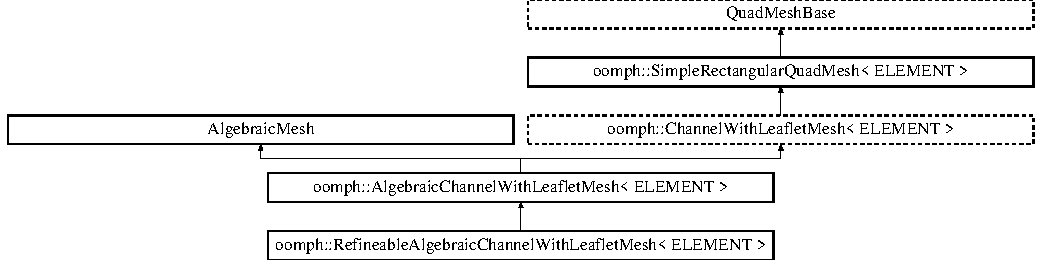
\includegraphics[height=4.200000cm]{classoomph_1_1AlgebraicChannelWithLeafletMesh}
\end{center}
\end{figure}
\subsection*{Public Member Functions}
\begin{DoxyCompactItemize}
\item 
\hyperlink{classoomph_1_1AlgebraicChannelWithLeafletMesh_a1e72e11c9971ed132efc95b808c83ccd}{Algebraic\+Channel\+With\+Leaflet\+Mesh} (\hyperlink{classoomph_1_1GeomObject}{Geom\+Object} $\ast$leaflet\+\_\+pt, const double \&lleft, const double \&lright, const double \&hleaflet, const double \&htot, const unsigned \&nleft, const unsigned \&nright, const unsigned \&ny1, const unsigned \&ny2, \hyperlink{classoomph_1_1TimeStepper}{Time\+Stepper} $\ast$time\+\_\+stepper\+\_\+pt=\&\hyperlink{classoomph_1_1Mesh_a12243d0fee2b1fcee729ee5a4777ea10}{Mesh\+::\+Default\+\_\+\+Time\+Stepper})
\begin{DoxyCompactList}\small\item\em Constructor\+: Pass pointer to \hyperlink{classoomph_1_1GeomObject}{Geom\+Object} that represents the leaflet, the length of the domain to left and right of the leaflet, the height of the leaflet and the overall height of the channel, the number of element columns to the left and right of the leaflet, the number of rows of elements from the bottom of the channel to the end of the leaflet, the number of rows of elements above the end of the leaflet. Timestepper defaults to \hyperlink{classoomph_1_1Steady}{Steady} default Timestepper defined in the \hyperlink{classoomph_1_1Mesh}{Mesh} base class. \end{DoxyCompactList}\item 
virtual \hyperlink{classoomph_1_1AlgebraicChannelWithLeafletMesh_a5b7c6a5f91427eae728c397b38de7c54}{$\sim$\+Algebraic\+Channel\+With\+Leaflet\+Mesh} ()
\begin{DoxyCompactList}\small\item\em Destructor\+: empty. \end{DoxyCompactList}\item 
void \hyperlink{classoomph_1_1AlgebraicChannelWithLeafletMesh_ace3a90b4e530c75bec8301e2291151eb}{update\+\_\+node\+\_\+update} (\hyperlink{classoomph_1_1AlgebraicNode}{Algebraic\+Node} $\ast$\&\hyperlink{classoomph_1_1AlgebraicMesh_aedeebbe95d2f8e67e9939cecd1be3933}{node\+\_\+pt})
\begin{DoxyCompactList}\small\item\em Update the geometric references that are used to update node after mesh adaptation. Empty -- no update of node update required without adaptivity. \end{DoxyCompactList}\item 
void \hyperlink{classoomph_1_1AlgebraicChannelWithLeafletMesh_a4c01b99ca83286f872c517fc5269a890}{algebraic\+\_\+node\+\_\+update} (const unsigned \&\hyperlink{cfortran_8h_af6f0bd3dc13317f895c91323c25c2b8f}{t}, \hyperlink{classoomph_1_1AlgebraicNode}{Algebraic\+Node} $\ast$\&\hyperlink{classoomph_1_1AlgebraicMesh_aedeebbe95d2f8e67e9939cecd1be3933}{node\+\_\+pt})
\begin{DoxyCompactList}\small\item\em Update nodal position at time level t (t=0\+: present; t$>$0\+: previous) \end{DoxyCompactList}\end{DoxyCompactItemize}
\subsection*{Protected Member Functions}
\begin{DoxyCompactItemize}
\item 
void \hyperlink{classoomph_1_1AlgebraicChannelWithLeafletMesh_a0d6cb8a8ffa830cdd73aa0f6686f150f}{setup\+\_\+algebraic\+\_\+node\+\_\+update} ()
\begin{DoxyCompactList}\small\item\em Function to setup the algebraic node update. \end{DoxyCompactList}\item 
void \hyperlink{classoomph_1_1AlgebraicChannelWithLeafletMesh_a53de0d31556bc78e22b5c06bb66bdd73}{node\+\_\+update\+\_\+I} (const unsigned \&\hyperlink{cfortran_8h_af6f0bd3dc13317f895c91323c25c2b8f}{t}, \hyperlink{classoomph_1_1AlgebraicNode}{Algebraic\+Node} $\ast$\&\hyperlink{classoomph_1_1AlgebraicMesh_aedeebbe95d2f8e67e9939cecd1be3933}{node\+\_\+pt})
\begin{DoxyCompactList}\small\item\em Update function for nodes in lower left region (I) \end{DoxyCompactList}\item 
void \hyperlink{classoomph_1_1AlgebraicChannelWithLeafletMesh_aafaeee96d0e7602cc990229abbd9c8fd}{node\+\_\+update\+\_\+\+II} (const unsigned \&\hyperlink{cfortran_8h_af6f0bd3dc13317f895c91323c25c2b8f}{t}, \hyperlink{classoomph_1_1AlgebraicNode}{Algebraic\+Node} $\ast$\&\hyperlink{classoomph_1_1AlgebraicMesh_aedeebbe95d2f8e67e9939cecd1be3933}{node\+\_\+pt})
\begin{DoxyCompactList}\small\item\em Update function for nodes in lower right region (II) \end{DoxyCompactList}\item 
void \hyperlink{classoomph_1_1AlgebraicChannelWithLeafletMesh_a5aed6f41b197dc7aab1d5d86b1b7d6d5}{node\+\_\+update\+\_\+\+I\+II} (const unsigned \&\hyperlink{cfortran_8h_af6f0bd3dc13317f895c91323c25c2b8f}{t}, \hyperlink{classoomph_1_1AlgebraicNode}{Algebraic\+Node} $\ast$\&\hyperlink{classoomph_1_1AlgebraicMesh_aedeebbe95d2f8e67e9939cecd1be3933}{node\+\_\+pt})
\begin{DoxyCompactList}\small\item\em Update function for nodes in upper left region (I\+II) \end{DoxyCompactList}\item 
void \hyperlink{classoomph_1_1AlgebraicChannelWithLeafletMesh_ac960faed226fa81f52ca605cffe3d1af}{node\+\_\+update\+\_\+\+IV} (const unsigned \&\hyperlink{cfortran_8h_af6f0bd3dc13317f895c91323c25c2b8f}{t}, \hyperlink{classoomph_1_1AlgebraicNode}{Algebraic\+Node} $\ast$\&\hyperlink{classoomph_1_1AlgebraicMesh_aedeebbe95d2f8e67e9939cecd1be3933}{node\+\_\+pt})
\begin{DoxyCompactList}\small\item\em Update function for nodes in upper right region (IV) \end{DoxyCompactList}\item 
void \hyperlink{classoomph_1_1AlgebraicChannelWithLeafletMesh_ab3659949ea5faac4ffa981828e98cf53}{slanted\+\_\+bound\+\_\+up} (const unsigned \&\hyperlink{cfortran_8h_af6f0bd3dc13317f895c91323c25c2b8f}{t}, const \hyperlink{classoomph_1_1Vector}{Vector}$<$ double $>$ \&zeta, \hyperlink{classoomph_1_1Vector}{Vector}$<$ double $>$ \&r)
\begin{DoxyCompactList}\small\item\em Helper function. \end{DoxyCompactList}\end{DoxyCompactItemize}
\subsection*{Protected Attributes}
\begin{DoxyCompactItemize}
\item 
double \hyperlink{classoomph_1_1AlgebraicChannelWithLeafletMesh_a1577beb584df4ad0f8517563934855fc}{X\+\_\+0}
\item 
double \hyperlink{classoomph_1_1AlgebraicChannelWithLeafletMesh_a22e6274b52941ae60cbe66287dd02fb4}{Hleaflet}
\end{DoxyCompactItemize}
\subsection*{Additional Inherited Members}


\subsection{Detailed Description}
\subsubsection*{template$<$class E\+L\+E\+M\+E\+NT$>$\newline
class oomph\+::\+Algebraic\+Channel\+With\+Leaflet\+Mesh$<$ E\+L\+E\+M\+E\+N\+T $>$}

Algebraic version of \hyperlink{classoomph_1_1ChannelWithLeafletMesh}{Channel\+With\+Leaflet\+Mesh}. Leaflet is assumed to be in its undeformed (straight vertical) position when the algebraic node update is set up. 

Definition at line 333 of file channel\+\_\+with\+\_\+leaflet\+\_\+mesh.\+template.\+h.



\subsection{Constructor \& Destructor Documentation}
\mbox{\Hypertarget{classoomph_1_1AlgebraicChannelWithLeafletMesh_a1e72e11c9971ed132efc95b808c83ccd}\label{classoomph_1_1AlgebraicChannelWithLeafletMesh_a1e72e11c9971ed132efc95b808c83ccd}} 
\index{oomph\+::\+Algebraic\+Channel\+With\+Leaflet\+Mesh@{oomph\+::\+Algebraic\+Channel\+With\+Leaflet\+Mesh}!Algebraic\+Channel\+With\+Leaflet\+Mesh@{Algebraic\+Channel\+With\+Leaflet\+Mesh}}
\index{Algebraic\+Channel\+With\+Leaflet\+Mesh@{Algebraic\+Channel\+With\+Leaflet\+Mesh}!oomph\+::\+Algebraic\+Channel\+With\+Leaflet\+Mesh@{oomph\+::\+Algebraic\+Channel\+With\+Leaflet\+Mesh}}
\subsubsection{\texorpdfstring{Algebraic\+Channel\+With\+Leaflet\+Mesh()}{AlgebraicChannelWithLeafletMesh()}}
{\footnotesize\ttfamily template$<$class E\+L\+E\+M\+E\+NT $>$ \\
\hyperlink{classoomph_1_1AlgebraicChannelWithLeafletMesh}{oomph\+::\+Algebraic\+Channel\+With\+Leaflet\+Mesh}$<$ E\+L\+E\+M\+E\+NT $>$\+::\hyperlink{classoomph_1_1AlgebraicChannelWithLeafletMesh}{Algebraic\+Channel\+With\+Leaflet\+Mesh} (\begin{DoxyParamCaption}\item[{\hyperlink{classoomph_1_1GeomObject}{Geom\+Object} $\ast$}]{leaflet\+\_\+pt,  }\item[{const double \&}]{lleft,  }\item[{const double \&}]{lright,  }\item[{const double \&}]{hleaflet,  }\item[{const double \&}]{htot,  }\item[{const unsigned \&}]{nleft,  }\item[{const unsigned \&}]{nright,  }\item[{const unsigned \&}]{ny1,  }\item[{const unsigned \&}]{ny2,  }\item[{\hyperlink{classoomph_1_1TimeStepper}{Time\+Stepper} $\ast$}]{time\+\_\+stepper\+\_\+pt = {\ttfamily \&\hyperlink{classoomph_1_1Mesh_a12243d0fee2b1fcee729ee5a4777ea10}{Mesh\+::\+Default\+\_\+\+Time\+Stepper}} }\end{DoxyParamCaption})\hspace{0.3cm}{\ttfamily [inline]}}



Constructor\+: Pass pointer to \hyperlink{classoomph_1_1GeomObject}{Geom\+Object} that represents the leaflet, the length of the domain to left and right of the leaflet, the height of the leaflet and the overall height of the channel, the number of element columns to the left and right of the leaflet, the number of rows of elements from the bottom of the channel to the end of the leaflet, the number of rows of elements above the end of the leaflet. Timestepper defaults to \hyperlink{classoomph_1_1Steady}{Steady} default Timestepper defined in the \hyperlink{classoomph_1_1Mesh}{Mesh} base class. 



Definition at line 346 of file channel\+\_\+with\+\_\+leaflet\+\_\+mesh.\+template.\+h.



References oomph\+::\+Algebraic\+Mesh\+::add\+\_\+geom\+\_\+object\+\_\+list\+\_\+pt(), oomph\+::\+Channel\+With\+Leaflet\+Mesh$<$ E\+L\+E\+M\+E\+N\+T $>$\+::\+Leaflet\+\_\+pt, and oomph\+::\+Geom\+Object\+::position().

\mbox{\Hypertarget{classoomph_1_1AlgebraicChannelWithLeafletMesh_a5b7c6a5f91427eae728c397b38de7c54}\label{classoomph_1_1AlgebraicChannelWithLeafletMesh_a5b7c6a5f91427eae728c397b38de7c54}} 
\index{oomph\+::\+Algebraic\+Channel\+With\+Leaflet\+Mesh@{oomph\+::\+Algebraic\+Channel\+With\+Leaflet\+Mesh}!````~Algebraic\+Channel\+With\+Leaflet\+Mesh@{$\sim$\+Algebraic\+Channel\+With\+Leaflet\+Mesh}}
\index{````~Algebraic\+Channel\+With\+Leaflet\+Mesh@{$\sim$\+Algebraic\+Channel\+With\+Leaflet\+Mesh}!oomph\+::\+Algebraic\+Channel\+With\+Leaflet\+Mesh@{oomph\+::\+Algebraic\+Channel\+With\+Leaflet\+Mesh}}
\subsubsection{\texorpdfstring{$\sim$\+Algebraic\+Channel\+With\+Leaflet\+Mesh()}{~AlgebraicChannelWithLeafletMesh()}}
{\footnotesize\ttfamily template$<$class E\+L\+E\+M\+E\+NT $>$ \\
virtual \hyperlink{classoomph_1_1AlgebraicChannelWithLeafletMesh}{oomph\+::\+Algebraic\+Channel\+With\+Leaflet\+Mesh}$<$ E\+L\+E\+M\+E\+NT $>$\+::$\sim$\hyperlink{classoomph_1_1AlgebraicChannelWithLeafletMesh}{Algebraic\+Channel\+With\+Leaflet\+Mesh} (\begin{DoxyParamCaption}{ }\end{DoxyParamCaption})\hspace{0.3cm}{\ttfamily [inline]}, {\ttfamily [virtual]}}



Destructor\+: empty. 



Definition at line 377 of file channel\+\_\+with\+\_\+leaflet\+\_\+mesh.\+template.\+h.



\subsection{Member Function Documentation}
\mbox{\Hypertarget{classoomph_1_1AlgebraicChannelWithLeafletMesh_a4c01b99ca83286f872c517fc5269a890}\label{classoomph_1_1AlgebraicChannelWithLeafletMesh_a4c01b99ca83286f872c517fc5269a890}} 
\index{oomph\+::\+Algebraic\+Channel\+With\+Leaflet\+Mesh@{oomph\+::\+Algebraic\+Channel\+With\+Leaflet\+Mesh}!algebraic\+\_\+node\+\_\+update@{algebraic\+\_\+node\+\_\+update}}
\index{algebraic\+\_\+node\+\_\+update@{algebraic\+\_\+node\+\_\+update}!oomph\+::\+Algebraic\+Channel\+With\+Leaflet\+Mesh@{oomph\+::\+Algebraic\+Channel\+With\+Leaflet\+Mesh}}
\subsubsection{\texorpdfstring{algebraic\+\_\+node\+\_\+update()}{algebraic\_node\_update()}}
{\footnotesize\ttfamily template$<$class E\+L\+E\+M\+E\+NT $>$ \\
void \hyperlink{classoomph_1_1AlgebraicChannelWithLeafletMesh}{oomph\+::\+Algebraic\+Channel\+With\+Leaflet\+Mesh}$<$ E\+L\+E\+M\+E\+NT $>$\+::algebraic\+\_\+node\+\_\+update (\begin{DoxyParamCaption}\item[{const unsigned \&}]{t,  }\item[{\hyperlink{classoomph_1_1AlgebraicNode}{Algebraic\+Node} $\ast$\&}]{node\+\_\+pt }\end{DoxyParamCaption})\hspace{0.3cm}{\ttfamily [virtual]}}



Update nodal position at time level t (t=0\+: present; t$>$0\+: previous) 

Perform algebraic node update. 

Implements \hyperlink{classoomph_1_1AlgebraicMesh_ab01d6f93354f3c4e5c9d1f0a5885a65b}{oomph\+::\+Algebraic\+Mesh}.



Definition at line 425 of file channel\+\_\+with\+\_\+leaflet\+\_\+mesh.\+template.\+cc.



References oomph\+::\+Algebraic\+Node\+::node\+\_\+update\+\_\+fct\+\_\+id(), and oomph\+::\+Global\+\_\+string\+\_\+for\+\_\+annotation\+::string().

\mbox{\Hypertarget{classoomph_1_1AlgebraicChannelWithLeafletMesh_a53de0d31556bc78e22b5c06bb66bdd73}\label{classoomph_1_1AlgebraicChannelWithLeafletMesh_a53de0d31556bc78e22b5c06bb66bdd73}} 
\index{oomph\+::\+Algebraic\+Channel\+With\+Leaflet\+Mesh@{oomph\+::\+Algebraic\+Channel\+With\+Leaflet\+Mesh}!node\+\_\+update\+\_\+I@{node\+\_\+update\+\_\+I}}
\index{node\+\_\+update\+\_\+I@{node\+\_\+update\+\_\+I}!oomph\+::\+Algebraic\+Channel\+With\+Leaflet\+Mesh@{oomph\+::\+Algebraic\+Channel\+With\+Leaflet\+Mesh}}
\subsubsection{\texorpdfstring{node\+\_\+update\+\_\+\+I()}{node\_update\_I()}}
{\footnotesize\ttfamily template$<$class E\+L\+E\+M\+E\+NT $>$ \\
void \hyperlink{classoomph_1_1AlgebraicChannelWithLeafletMesh}{oomph\+::\+Algebraic\+Channel\+With\+Leaflet\+Mesh}$<$ E\+L\+E\+M\+E\+NT $>$\+::node\+\_\+update\+\_\+I (\begin{DoxyParamCaption}\item[{const unsigned \&}]{t,  }\item[{\hyperlink{classoomph_1_1AlgebraicNode}{Algebraic\+Node} $\ast$\&}]{node\+\_\+pt }\end{DoxyParamCaption})\hspace{0.3cm}{\ttfamily [protected]}}



Update function for nodes in lower left region (I) 

\hyperlink{classoomph_1_1Node}{Node} update for region I. 

Definition at line 471 of file channel\+\_\+with\+\_\+leaflet\+\_\+mesh.\+template.\+cc.



References oomph\+::\+Channel\+With\+Leaflet\+Mesh$<$ E\+L\+E\+M\+E\+N\+T $>$\+::domain\+\_\+pt(), oomph\+::\+Channel\+With\+Leaflet\+Domain\+::lleft(), s, oomph\+::\+Algebraic\+Node\+::vector\+\_\+geom\+\_\+object\+\_\+pt(), oomph\+::\+Algebraic\+Node\+::vector\+\_\+ref\+\_\+value(), and oomph\+::\+Node\+::x().

\mbox{\Hypertarget{classoomph_1_1AlgebraicChannelWithLeafletMesh_aafaeee96d0e7602cc990229abbd9c8fd}\label{classoomph_1_1AlgebraicChannelWithLeafletMesh_aafaeee96d0e7602cc990229abbd9c8fd}} 
\index{oomph\+::\+Algebraic\+Channel\+With\+Leaflet\+Mesh@{oomph\+::\+Algebraic\+Channel\+With\+Leaflet\+Mesh}!node\+\_\+update\+\_\+\+II@{node\+\_\+update\+\_\+\+II}}
\index{node\+\_\+update\+\_\+\+II@{node\+\_\+update\+\_\+\+II}!oomph\+::\+Algebraic\+Channel\+With\+Leaflet\+Mesh@{oomph\+::\+Algebraic\+Channel\+With\+Leaflet\+Mesh}}
\subsubsection{\texorpdfstring{node\+\_\+update\+\_\+\+I\+I()}{node\_update\_II()}}
{\footnotesize\ttfamily template$<$class E\+L\+E\+M\+E\+NT $>$ \\
void \hyperlink{classoomph_1_1AlgebraicChannelWithLeafletMesh}{oomph\+::\+Algebraic\+Channel\+With\+Leaflet\+Mesh}$<$ E\+L\+E\+M\+E\+NT $>$\+::node\+\_\+update\+\_\+\+II (\begin{DoxyParamCaption}\item[{const unsigned \&}]{t,  }\item[{\hyperlink{classoomph_1_1AlgebraicNode}{Algebraic\+Node} $\ast$\&}]{node\+\_\+pt }\end{DoxyParamCaption})\hspace{0.3cm}{\ttfamily [protected]}}



Update function for nodes in lower right region (II) 

\hyperlink{classoomph_1_1Node}{Node} update for region II. 

Definition at line 516 of file channel\+\_\+with\+\_\+leaflet\+\_\+mesh.\+template.\+cc.



References oomph\+::\+Channel\+With\+Leaflet\+Mesh$<$ E\+L\+E\+M\+E\+N\+T $>$\+::domain\+\_\+pt(), oomph\+::\+Channel\+With\+Leaflet\+Domain\+::lright(), s, oomph\+::\+Algebraic\+Node\+::vector\+\_\+geom\+\_\+object\+\_\+pt(), oomph\+::\+Algebraic\+Node\+::vector\+\_\+ref\+\_\+value(), and oomph\+::\+Node\+::x().

\mbox{\Hypertarget{classoomph_1_1AlgebraicChannelWithLeafletMesh_a5aed6f41b197dc7aab1d5d86b1b7d6d5}\label{classoomph_1_1AlgebraicChannelWithLeafletMesh_a5aed6f41b197dc7aab1d5d86b1b7d6d5}} 
\index{oomph\+::\+Algebraic\+Channel\+With\+Leaflet\+Mesh@{oomph\+::\+Algebraic\+Channel\+With\+Leaflet\+Mesh}!node\+\_\+update\+\_\+\+I\+II@{node\+\_\+update\+\_\+\+I\+II}}
\index{node\+\_\+update\+\_\+\+I\+II@{node\+\_\+update\+\_\+\+I\+II}!oomph\+::\+Algebraic\+Channel\+With\+Leaflet\+Mesh@{oomph\+::\+Algebraic\+Channel\+With\+Leaflet\+Mesh}}
\subsubsection{\texorpdfstring{node\+\_\+update\+\_\+\+I\+I\+I()}{node\_update\_III()}}
{\footnotesize\ttfamily template$<$class E\+L\+E\+M\+E\+NT $>$ \\
void \hyperlink{classoomph_1_1AlgebraicChannelWithLeafletMesh}{oomph\+::\+Algebraic\+Channel\+With\+Leaflet\+Mesh}$<$ E\+L\+E\+M\+E\+NT $>$\+::node\+\_\+update\+\_\+\+I\+II (\begin{DoxyParamCaption}\item[{const unsigned \&}]{t,  }\item[{\hyperlink{classoomph_1_1AlgebraicNode}{Algebraic\+Node} $\ast$\&}]{node\+\_\+pt }\end{DoxyParamCaption})\hspace{0.3cm}{\ttfamily [protected]}}



Update function for nodes in upper left region (I\+II) 

\hyperlink{classoomph_1_1Node}{Node} update for region I\+II. 

Definition at line 582 of file channel\+\_\+with\+\_\+leaflet\+\_\+mesh.\+template.\+cc.



References oomph\+::\+Channel\+With\+Leaflet\+Mesh$<$ E\+L\+E\+M\+E\+N\+T $>$\+::domain\+\_\+pt(), oomph\+::\+Channel\+With\+Leaflet\+Domain\+::lleft(), s, oomph\+::\+Algebraic\+Node\+::vector\+\_\+ref\+\_\+value(), and oomph\+::\+Node\+::x().

\mbox{\Hypertarget{classoomph_1_1AlgebraicChannelWithLeafletMesh_ac960faed226fa81f52ca605cffe3d1af}\label{classoomph_1_1AlgebraicChannelWithLeafletMesh_ac960faed226fa81f52ca605cffe3d1af}} 
\index{oomph\+::\+Algebraic\+Channel\+With\+Leaflet\+Mesh@{oomph\+::\+Algebraic\+Channel\+With\+Leaflet\+Mesh}!node\+\_\+update\+\_\+\+IV@{node\+\_\+update\+\_\+\+IV}}
\index{node\+\_\+update\+\_\+\+IV@{node\+\_\+update\+\_\+\+IV}!oomph\+::\+Algebraic\+Channel\+With\+Leaflet\+Mesh@{oomph\+::\+Algebraic\+Channel\+With\+Leaflet\+Mesh}}
\subsubsection{\texorpdfstring{node\+\_\+update\+\_\+\+I\+V()}{node\_update\_IV()}}
{\footnotesize\ttfamily template$<$class E\+L\+E\+M\+E\+NT $>$ \\
void \hyperlink{classoomph_1_1AlgebraicChannelWithLeafletMesh}{oomph\+::\+Algebraic\+Channel\+With\+Leaflet\+Mesh}$<$ E\+L\+E\+M\+E\+NT $>$\+::node\+\_\+update\+\_\+\+IV (\begin{DoxyParamCaption}\item[{const unsigned \&}]{t,  }\item[{\hyperlink{classoomph_1_1AlgebraicNode}{Algebraic\+Node} $\ast$\&}]{node\+\_\+pt }\end{DoxyParamCaption})\hspace{0.3cm}{\ttfamily [protected]}}



Update function for nodes in upper right region (IV) 

\hyperlink{classoomph_1_1Node}{Node} update for region IV. 

Definition at line 616 of file channel\+\_\+with\+\_\+leaflet\+\_\+mesh.\+template.\+cc.



References oomph\+::\+Channel\+With\+Leaflet\+Mesh$<$ E\+L\+E\+M\+E\+N\+T $>$\+::domain\+\_\+pt(), oomph\+::\+Channel\+With\+Leaflet\+Domain\+::lright(), s, oomph\+::\+Algebraic\+Node\+::vector\+\_\+ref\+\_\+value(), and oomph\+::\+Node\+::x().

\mbox{\Hypertarget{classoomph_1_1AlgebraicChannelWithLeafletMesh_a0d6cb8a8ffa830cdd73aa0f6686f150f}\label{classoomph_1_1AlgebraicChannelWithLeafletMesh_a0d6cb8a8ffa830cdd73aa0f6686f150f}} 
\index{oomph\+::\+Algebraic\+Channel\+With\+Leaflet\+Mesh@{oomph\+::\+Algebraic\+Channel\+With\+Leaflet\+Mesh}!setup\+\_\+algebraic\+\_\+node\+\_\+update@{setup\+\_\+algebraic\+\_\+node\+\_\+update}}
\index{setup\+\_\+algebraic\+\_\+node\+\_\+update@{setup\+\_\+algebraic\+\_\+node\+\_\+update}!oomph\+::\+Algebraic\+Channel\+With\+Leaflet\+Mesh@{oomph\+::\+Algebraic\+Channel\+With\+Leaflet\+Mesh}}
\subsubsection{\texorpdfstring{setup\+\_\+algebraic\+\_\+node\+\_\+update()}{setup\_algebraic\_node\_update()}}
{\footnotesize\ttfamily template$<$class E\+L\+E\+M\+E\+NT $>$ \\
void \hyperlink{classoomph_1_1AlgebraicChannelWithLeafletMesh}{oomph\+::\+Algebraic\+Channel\+With\+Leaflet\+Mesh}$<$ E\+L\+E\+M\+E\+NT $>$\+::setup\+\_\+algebraic\+\_\+node\+\_\+update (\begin{DoxyParamCaption}{ }\end{DoxyParamCaption})\hspace{0.3cm}{\ttfamily [protected]}}



Function to setup the algebraic node update. 

Setup algebraic node update. Leaflet is assumed to be in its undeformed (straight vertical) position! 

Definition at line 246 of file channel\+\_\+with\+\_\+leaflet\+\_\+mesh.\+template.\+cc.



References oomph\+::\+Algebraic\+Node\+::add\+\_\+node\+\_\+update\+\_\+info(), oomph\+::\+Channel\+With\+Leaflet\+Mesh$<$ E\+L\+E\+M\+E\+N\+T $>$\+::domain\+\_\+pt(), oomph\+::\+Channel\+With\+Leaflet\+Domain\+::hleaflet(), oomph\+::\+Channel\+With\+Leaflet\+Domain\+::htot(), oomph\+::\+Channel\+With\+Leaflet\+Mesh$<$ E\+L\+E\+M\+E\+N\+T $>$\+::\+Leaflet\+\_\+pt, oomph\+::\+Channel\+With\+Leaflet\+Domain\+::lleft(), oomph\+::\+Geom\+Object\+::locate\+\_\+zeta(), oomph\+::\+Channel\+With\+Leaflet\+Domain\+::lright(), oomph\+::\+Mesh\+::nnode(), oomph\+::\+Mesh\+::node\+\_\+pt(), oomph\+::\+Geom\+Object\+::position(), s, and oomph\+::\+Node\+::x().

\mbox{\Hypertarget{classoomph_1_1AlgebraicChannelWithLeafletMesh_ab3659949ea5faac4ffa981828e98cf53}\label{classoomph_1_1AlgebraicChannelWithLeafletMesh_ab3659949ea5faac4ffa981828e98cf53}} 
\index{oomph\+::\+Algebraic\+Channel\+With\+Leaflet\+Mesh@{oomph\+::\+Algebraic\+Channel\+With\+Leaflet\+Mesh}!slanted\+\_\+bound\+\_\+up@{slanted\+\_\+bound\+\_\+up}}
\index{slanted\+\_\+bound\+\_\+up@{slanted\+\_\+bound\+\_\+up}!oomph\+::\+Algebraic\+Channel\+With\+Leaflet\+Mesh@{oomph\+::\+Algebraic\+Channel\+With\+Leaflet\+Mesh}}
\subsubsection{\texorpdfstring{slanted\+\_\+bound\+\_\+up()}{slanted\_bound\_up()}}
{\footnotesize\ttfamily template$<$class E\+L\+E\+M\+E\+NT $>$ \\
void \hyperlink{classoomph_1_1AlgebraicChannelWithLeafletMesh}{oomph\+::\+Algebraic\+Channel\+With\+Leaflet\+Mesh}$<$ E\+L\+E\+M\+E\+NT $>$\+::slanted\+\_\+bound\+\_\+up (\begin{DoxyParamCaption}\item[{const unsigned \&}]{t,  }\item[{const \hyperlink{classoomph_1_1Vector}{Vector}$<$ double $>$ \&}]{zeta,  }\item[{\hyperlink{classoomph_1_1Vector}{Vector}$<$ double $>$ \&}]{r }\end{DoxyParamCaption})\hspace{0.3cm}{\ttfamily [protected]}}



Helper function. 

Slanted bound \+: helper function. Coordinates of the point on the boundary beetween the upper and the lower part, in the same column, at the east. 

Definition at line 558 of file channel\+\_\+with\+\_\+leaflet\+\_\+mesh.\+template.\+cc.



References oomph\+::\+Channel\+With\+Leaflet\+Mesh$<$ E\+L\+E\+M\+E\+N\+T $>$\+::domain\+\_\+pt(), oomph\+::\+Channel\+With\+Leaflet\+Domain\+::htot(), oomph\+::\+Channel\+With\+Leaflet\+Mesh$<$ E\+L\+E\+M\+E\+N\+T $>$\+::\+Leaflet\+\_\+pt, and oomph\+::\+Geom\+Object\+::position().

\mbox{\Hypertarget{classoomph_1_1AlgebraicChannelWithLeafletMesh_ace3a90b4e530c75bec8301e2291151eb}\label{classoomph_1_1AlgebraicChannelWithLeafletMesh_ace3a90b4e530c75bec8301e2291151eb}} 
\index{oomph\+::\+Algebraic\+Channel\+With\+Leaflet\+Mesh@{oomph\+::\+Algebraic\+Channel\+With\+Leaflet\+Mesh}!update\+\_\+node\+\_\+update@{update\+\_\+node\+\_\+update}}
\index{update\+\_\+node\+\_\+update@{update\+\_\+node\+\_\+update}!oomph\+::\+Algebraic\+Channel\+With\+Leaflet\+Mesh@{oomph\+::\+Algebraic\+Channel\+With\+Leaflet\+Mesh}}
\subsubsection{\texorpdfstring{update\+\_\+node\+\_\+update()}{update\_node\_update()}}
{\footnotesize\ttfamily template$<$class E\+L\+E\+M\+E\+NT $>$ \\
void \hyperlink{classoomph_1_1AlgebraicChannelWithLeafletMesh}{oomph\+::\+Algebraic\+Channel\+With\+Leaflet\+Mesh}$<$ E\+L\+E\+M\+E\+NT $>$\+::update\+\_\+node\+\_\+update (\begin{DoxyParamCaption}\item[{\hyperlink{classoomph_1_1AlgebraicNode}{Algebraic\+Node} $\ast$\&}]{node\+\_\+pt }\end{DoxyParamCaption})\hspace{0.3cm}{\ttfamily [inline]}, {\ttfamily [virtual]}}



Update the geometric references that are used to update node after mesh adaptation. Empty -- no update of node update required without adaptivity. 



Implements \hyperlink{classoomph_1_1AlgebraicMesh_a6c6a35ae2be6e2766f5b80d85693c1ce}{oomph\+::\+Algebraic\+Mesh}.



Reimplemented in \hyperlink{classoomph_1_1RefineableAlgebraicChannelWithLeafletMesh_a8ee7168fbb84bb87880a2590dd52eaa8}{oomph\+::\+Refineable\+Algebraic\+Channel\+With\+Leaflet\+Mesh$<$ E\+L\+E\+M\+E\+N\+T $>$}.



Definition at line 383 of file channel\+\_\+with\+\_\+leaflet\+\_\+mesh.\+template.\+h.



References oomph\+::\+Mesh\+::node\+\_\+pt(), and t.



\subsection{Member Data Documentation}
\mbox{\Hypertarget{classoomph_1_1AlgebraicChannelWithLeafletMesh_a22e6274b52941ae60cbe66287dd02fb4}\label{classoomph_1_1AlgebraicChannelWithLeafletMesh_a22e6274b52941ae60cbe66287dd02fb4}} 
\index{oomph\+::\+Algebraic\+Channel\+With\+Leaflet\+Mesh@{oomph\+::\+Algebraic\+Channel\+With\+Leaflet\+Mesh}!Hleaflet@{Hleaflet}}
\index{Hleaflet@{Hleaflet}!oomph\+::\+Algebraic\+Channel\+With\+Leaflet\+Mesh@{oomph\+::\+Algebraic\+Channel\+With\+Leaflet\+Mesh}}
\subsubsection{\texorpdfstring{Hleaflet}{Hleaflet}}
{\footnotesize\ttfamily template$<$class E\+L\+E\+M\+E\+NT $>$ \\
double \hyperlink{classoomph_1_1AlgebraicChannelWithLeafletMesh}{oomph\+::\+Algebraic\+Channel\+With\+Leaflet\+Mesh}$<$ E\+L\+E\+M\+E\+NT $>$\+::Hleaflet\hspace{0.3cm}{\ttfamily [protected]}}

Length of the leaflet (stored explicitly for reference in algebraic node update -- it\textquotesingle{}s also stored independently in domain....) 

Definition at line 418 of file channel\+\_\+with\+\_\+leaflet\+\_\+mesh.\+template.\+h.

\mbox{\Hypertarget{classoomph_1_1AlgebraicChannelWithLeafletMesh_a1577beb584df4ad0f8517563934855fc}\label{classoomph_1_1AlgebraicChannelWithLeafletMesh_a1577beb584df4ad0f8517563934855fc}} 
\index{oomph\+::\+Algebraic\+Channel\+With\+Leaflet\+Mesh@{oomph\+::\+Algebraic\+Channel\+With\+Leaflet\+Mesh}!X\+\_\+0@{X\+\_\+0}}
\index{X\+\_\+0@{X\+\_\+0}!oomph\+::\+Algebraic\+Channel\+With\+Leaflet\+Mesh@{oomph\+::\+Algebraic\+Channel\+With\+Leaflet\+Mesh}}
\subsubsection{\texorpdfstring{X\+\_\+0}{X\_0}}
{\footnotesize\ttfamily template$<$class E\+L\+E\+M\+E\+NT $>$ \\
double \hyperlink{classoomph_1_1AlgebraicChannelWithLeafletMesh}{oomph\+::\+Algebraic\+Channel\+With\+Leaflet\+Mesh}$<$ E\+L\+E\+M\+E\+NT $>$\+::X\+\_\+0\hspace{0.3cm}{\ttfamily [protected]}}

Origin of the wall (stored explicitly for reference in algebraic node update -- it\textquotesingle{}s also stored independently in domain....) 

Definition at line 413 of file channel\+\_\+with\+\_\+leaflet\+\_\+mesh.\+template.\+h.



The documentation for this class was generated from the following files\+:\begin{DoxyCompactItemize}
\item 
\hyperlink{channel__with__leaflet__mesh_8template_8h}{channel\+\_\+with\+\_\+leaflet\+\_\+mesh.\+template.\+h}\item 
\hyperlink{channel__with__leaflet__mesh_8template_8cc}{channel\+\_\+with\+\_\+leaflet\+\_\+mesh.\+template.\+cc}\end{DoxyCompactItemize}

\hypertarget{classoomph_1_1AlgebraicCollapsibleChannelMesh}{}\section{oomph\+:\+:Algebraic\+Collapsible\+Channel\+Mesh$<$ E\+L\+E\+M\+E\+NT $>$ Class Template Reference}
\label{classoomph_1_1AlgebraicCollapsibleChannelMesh}\index{oomph\+::\+Algebraic\+Collapsible\+Channel\+Mesh$<$ E\+L\+E\+M\+E\+N\+T $>$@{oomph\+::\+Algebraic\+Collapsible\+Channel\+Mesh$<$ E\+L\+E\+M\+E\+N\+T $>$}}


Collapsible channel mesh with algebraic node update.  




{\ttfamily \#include $<$collapsible\+\_\+channel\+\_\+mesh.\+template.\+h$>$}

Inheritance diagram for oomph\+:\+:Algebraic\+Collapsible\+Channel\+Mesh$<$ E\+L\+E\+M\+E\+NT $>$\+:\begin{figure}[H]
\begin{center}
\leavevmode
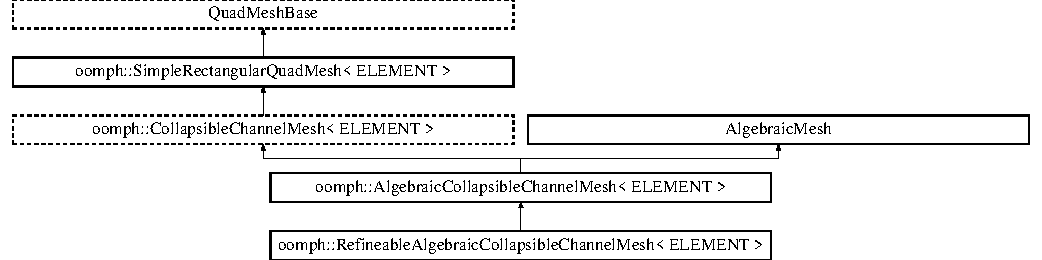
\includegraphics[height=3.500000cm]{classoomph_1_1AlgebraicCollapsibleChannelMesh}
\end{center}
\end{figure}
\subsection*{Public Member Functions}
\begin{DoxyCompactItemize}
\item 
\hyperlink{classoomph_1_1AlgebraicCollapsibleChannelMesh_ac2e77539dfed482cc3d8b7c9e17a9567}{Algebraic\+Collapsible\+Channel\+Mesh} (const unsigned \&nup, const unsigned \&ncollapsible, const unsigned \&ndown, const unsigned \&\hyperlink{classoomph_1_1SimpleRectangularQuadMesh_a45011f22dedd480392b1f376e4269921}{ny}, const double \&lup, const double \&lcollapsible, const double \&ldown, const double \&ly, Geom\+Object $\ast$\hyperlink{classoomph_1_1CollapsibleChannelMesh_a04ffeb61678763dfd250962ea9ba614b}{wall\+\_\+pt}, Time\+Stepper $\ast$time\+\_\+stepper\+\_\+pt=\&Mesh\+::\+Default\+\_\+\+Time\+Stepper)
\begin{DoxyCompactList}\small\item\em Constructor\+: Pass number of elements in upstream/collapsible/ downstream segment and across the channel; lengths of upstream/ collapsible/downstream segments and width of channel, pointer to Geom\+Object that defines the collapsible segment and pointer to Time\+Stepper (defaults to the default timestepper, Steady). \end{DoxyCompactList}\item 
virtual \hyperlink{classoomph_1_1AlgebraicCollapsibleChannelMesh_ab921ed3dbc5678fc5d39626fdf32c4ed}{$\sim$\+Algebraic\+Collapsible\+Channel\+Mesh} ()
\begin{DoxyCompactList}\small\item\em Destructor\+: empty. \end{DoxyCompactList}\item 
\hyperlink{classoomph_1_1AlgebraicCollapsibleChannelMesh_a3c19524e69a9408c79047d130b79d6b3}{Algebraic\+Collapsible\+Channel\+Mesh} (const unsigned \&nup, const unsigned \&ncollapsible, const unsigned \&ndown, const unsigned \&\hyperlink{classoomph_1_1SimpleRectangularQuadMesh_a45011f22dedd480392b1f376e4269921}{ny}, const double \&lup, const double \&lcollapsible, const double \&ldown, const double \&ly, Geom\+Object $\ast$\hyperlink{classoomph_1_1CollapsibleChannelMesh_a04ffeb61678763dfd250962ea9ba614b}{wall\+\_\+pt}, \hyperlink{classoomph_1_1CollapsibleChannelDomain_a2bf1d7943bfac134a5c27a54c7e1faed}{Collapsible\+Channel\+Domain\+::\+B\+L\+Squash\+Fct\+Pt} bl\+\_\+squash\+\_\+function\+\_\+pt, Time\+Stepper $\ast$time\+\_\+stepper\+\_\+pt=\&Mesh\+::\+Default\+\_\+\+Time\+Stepper)
\begin{DoxyCompactList}\small\item\em Constructor\+: Pass number of elements in upstream/collapsible/ downstream segment and across the channel; lengths of upstream/ collapsible/downstream segments and width of channel, pointer to Geom\+Object that defines the collapsible segment and pointer to Time\+Stepper (defaults to the default timestepper, Steady). \end{DoxyCompactList}\item 
\hyperlink{classoomph_1_1CollapsibleChannelDomain_a2bf1d7943bfac134a5c27a54c7e1faed}{Collapsible\+Channel\+Domain\+::\+B\+L\+Squash\+Fct\+Pt} \& \hyperlink{classoomph_1_1AlgebraicCollapsibleChannelMesh_abf1848b49f57419af4379a637464587d}{bl\+\_\+squash\+\_\+fct\+\_\+pt} ()
\begin{DoxyCompactList}\small\item\em Function pointer for function that squashes the mesh near the walls. Default trivial mapping (the identity) leaves vertical nodal positions unchanged. Mapping is used in underlying \hyperlink{classoomph_1_1CollapsibleChannelDomain}{Collapsible\+Channel\+Domain}. Broken function that overloads the version in the \hyperlink{classoomph_1_1CollapsibleChannelMesh}{Collapsible\+Channel\+Mesh}. It does not make sense to specify the function pointer after the mesh has been set up! \end{DoxyCompactList}\item 
\hyperlink{classoomph_1_1CollapsibleChannelDomain_a2bf1d7943bfac134a5c27a54c7e1faed}{Collapsible\+Channel\+Domain\+::\+B\+L\+Squash\+Fct\+Pt} \& \hyperlink{classoomph_1_1AlgebraicCollapsibleChannelMesh_afa53bd526ff0903526afbdf5e6f4f532}{axial\+\_\+spacing\+\_\+fct\+\_\+pt} ()
\begin{DoxyCompactList}\small\item\em Function pointer for function that redistributes nodes axially. Default trivial mapping (the identity) leaves vertical nodal positions unchanged. Mapping is used in underlying \hyperlink{classoomph_1_1CollapsibleChannelDomain}{Collapsible\+Channel\+Domain}. Broken function that overloads the version in the \hyperlink{classoomph_1_1CollapsibleChannelMesh}{Collapsible\+Channel\+Mesh}. It does not make sense to specify the function pointer after the mesh has been set up! \end{DoxyCompactList}\item 
void \hyperlink{classoomph_1_1AlgebraicCollapsibleChannelMesh_ae1ea6d9baa12e2ca87d21d4370f41870}{algebraic\+\_\+node\+\_\+update} (const unsigned \&t, Algebraic\+Node $\ast$\&node\+\_\+pt)
\begin{DoxyCompactList}\small\item\em Update nodal position at time level t (t=0\+: present; t$>$0\+: previous) \end{DoxyCompactList}\item 
void \hyperlink{classoomph_1_1AlgebraicCollapsibleChannelMesh_abad38fb50d067a126af1161a3a603972}{update\+\_\+node\+\_\+update} (Algebraic\+Node $\ast$\&node\+\_\+pt)
\begin{DoxyCompactList}\small\item\em Update the node-\/udate data after mesh adaptation. Empty -- no update of node update required as this is non-\/refineable mesh. \end{DoxyCompactList}\end{DoxyCompactItemize}
\subsection*{Protected Member Functions}
\begin{DoxyCompactItemize}
\item 
void \hyperlink{classoomph_1_1AlgebraicCollapsibleChannelMesh_a54e93316a561cd77a68c0774d2772030}{setup\+\_\+algebraic\+\_\+node\+\_\+update} ()
\begin{DoxyCompactList}\small\item\em Function to setup the algebraic node update. \end{DoxyCompactList}\end{DoxyCompactItemize}
\subsection*{Protected Attributes}
\begin{DoxyCompactItemize}
\item 
\hyperlink{classoomph_1_1CollapsibleChannelDomain_a2bf1d7943bfac134a5c27a54c7e1faed}{Collapsible\+Channel\+Domain\+::\+B\+L\+Squash\+Fct\+Pt} \hyperlink{classoomph_1_1AlgebraicCollapsibleChannelMesh_ab3848ae5c357f45addf4bcfeca1a9d18}{Dummy\+\_\+fct\+\_\+pt}
\begin{DoxyCompactList}\small\item\em Dummy function pointer. \end{DoxyCompactList}\end{DoxyCompactItemize}


\subsection{Detailed Description}
\subsubsection*{template$<$class E\+L\+E\+M\+E\+NT$>$\newline
class oomph\+::\+Algebraic\+Collapsible\+Channel\+Mesh$<$ E\+L\+E\+M\+E\+N\+T $>$}

Collapsible channel mesh with algebraic node update. 

Definition at line 434 of file collapsible\+\_\+channel\+\_\+mesh.\+template.\+h.



\subsection{Constructor \& Destructor Documentation}
\mbox{\Hypertarget{classoomph_1_1AlgebraicCollapsibleChannelMesh_ac2e77539dfed482cc3d8b7c9e17a9567}\label{classoomph_1_1AlgebraicCollapsibleChannelMesh_ac2e77539dfed482cc3d8b7c9e17a9567}} 
\index{oomph\+::\+Algebraic\+Collapsible\+Channel\+Mesh@{oomph\+::\+Algebraic\+Collapsible\+Channel\+Mesh}!Algebraic\+Collapsible\+Channel\+Mesh@{Algebraic\+Collapsible\+Channel\+Mesh}}
\index{Algebraic\+Collapsible\+Channel\+Mesh@{Algebraic\+Collapsible\+Channel\+Mesh}!oomph\+::\+Algebraic\+Collapsible\+Channel\+Mesh@{oomph\+::\+Algebraic\+Collapsible\+Channel\+Mesh}}
\subsubsection{\texorpdfstring{Algebraic\+Collapsible\+Channel\+Mesh()}{AlgebraicCollapsibleChannelMesh()}\hspace{0.1cm}{\footnotesize\ttfamily [1/2]}}
{\footnotesize\ttfamily template$<$class E\+L\+E\+M\+E\+NT $>$ \\
\hyperlink{classoomph_1_1AlgebraicCollapsibleChannelMesh}{oomph\+::\+Algebraic\+Collapsible\+Channel\+Mesh}$<$ E\+L\+E\+M\+E\+NT $>$\+::\hyperlink{classoomph_1_1AlgebraicCollapsibleChannelMesh}{Algebraic\+Collapsible\+Channel\+Mesh} (\begin{DoxyParamCaption}\item[{const unsigned \&}]{nup,  }\item[{const unsigned \&}]{ncollapsible,  }\item[{const unsigned \&}]{ndown,  }\item[{const unsigned \&}]{ny,  }\item[{const double \&}]{lup,  }\item[{const double \&}]{lcollapsible,  }\item[{const double \&}]{ldown,  }\item[{const double \&}]{ly,  }\item[{Geom\+Object $\ast$}]{wall\+\_\+pt,  }\item[{Time\+Stepper $\ast$}]{time\+\_\+stepper\+\_\+pt = {\ttfamily \&Mesh\+:\+:Default\+\_\+TimeStepper} }\end{DoxyParamCaption})\hspace{0.3cm}{\ttfamily [inline]}}



Constructor\+: Pass number of elements in upstream/collapsible/ downstream segment and across the channel; lengths of upstream/ collapsible/downstream segments and width of channel, pointer to Geom\+Object that defines the collapsible segment and pointer to Time\+Stepper (defaults to the default timestepper, Steady). 



Definition at line 447 of file collapsible\+\_\+channel\+\_\+mesh.\+template.\+h.

\mbox{\Hypertarget{classoomph_1_1AlgebraicCollapsibleChannelMesh_ab921ed3dbc5678fc5d39626fdf32c4ed}\label{classoomph_1_1AlgebraicCollapsibleChannelMesh_ab921ed3dbc5678fc5d39626fdf32c4ed}} 
\index{oomph\+::\+Algebraic\+Collapsible\+Channel\+Mesh@{oomph\+::\+Algebraic\+Collapsible\+Channel\+Mesh}!````~Algebraic\+Collapsible\+Channel\+Mesh@{$\sim$\+Algebraic\+Collapsible\+Channel\+Mesh}}
\index{````~Algebraic\+Collapsible\+Channel\+Mesh@{$\sim$\+Algebraic\+Collapsible\+Channel\+Mesh}!oomph\+::\+Algebraic\+Collapsible\+Channel\+Mesh@{oomph\+::\+Algebraic\+Collapsible\+Channel\+Mesh}}
\subsubsection{\texorpdfstring{$\sim$\+Algebraic\+Collapsible\+Channel\+Mesh()}{~AlgebraicCollapsibleChannelMesh()}}
{\footnotesize\ttfamily template$<$class E\+L\+E\+M\+E\+NT $>$ \\
virtual \hyperlink{classoomph_1_1AlgebraicCollapsibleChannelMesh}{oomph\+::\+Algebraic\+Collapsible\+Channel\+Mesh}$<$ E\+L\+E\+M\+E\+NT $>$\+::$\sim$\hyperlink{classoomph_1_1AlgebraicCollapsibleChannelMesh}{Algebraic\+Collapsible\+Channel\+Mesh} (\begin{DoxyParamCaption}{ }\end{DoxyParamCaption})\hspace{0.3cm}{\ttfamily [inline]}, {\ttfamily [virtual]}}



Destructor\+: empty. 



Definition at line 471 of file collapsible\+\_\+channel\+\_\+mesh.\+template.\+h.

\mbox{\Hypertarget{classoomph_1_1AlgebraicCollapsibleChannelMesh_a3c19524e69a9408c79047d130b79d6b3}\label{classoomph_1_1AlgebraicCollapsibleChannelMesh_a3c19524e69a9408c79047d130b79d6b3}} 
\index{oomph\+::\+Algebraic\+Collapsible\+Channel\+Mesh@{oomph\+::\+Algebraic\+Collapsible\+Channel\+Mesh}!Algebraic\+Collapsible\+Channel\+Mesh@{Algebraic\+Collapsible\+Channel\+Mesh}}
\index{Algebraic\+Collapsible\+Channel\+Mesh@{Algebraic\+Collapsible\+Channel\+Mesh}!oomph\+::\+Algebraic\+Collapsible\+Channel\+Mesh@{oomph\+::\+Algebraic\+Collapsible\+Channel\+Mesh}}
\subsubsection{\texorpdfstring{Algebraic\+Collapsible\+Channel\+Mesh()}{AlgebraicCollapsibleChannelMesh()}\hspace{0.1cm}{\footnotesize\ttfamily [2/2]}}
{\footnotesize\ttfamily template$<$class E\+L\+E\+M\+E\+NT $>$ \\
\hyperlink{classoomph_1_1AlgebraicCollapsibleChannelMesh}{oomph\+::\+Algebraic\+Collapsible\+Channel\+Mesh}$<$ E\+L\+E\+M\+E\+NT $>$\+::\hyperlink{classoomph_1_1AlgebraicCollapsibleChannelMesh}{Algebraic\+Collapsible\+Channel\+Mesh} (\begin{DoxyParamCaption}\item[{const unsigned \&}]{nup,  }\item[{const unsigned \&}]{ncollapsible,  }\item[{const unsigned \&}]{ndown,  }\item[{const unsigned \&}]{ny,  }\item[{const double \&}]{lup,  }\item[{const double \&}]{lcollapsible,  }\item[{const double \&}]{ldown,  }\item[{const double \&}]{ly,  }\item[{Geom\+Object $\ast$}]{wall\+\_\+pt,  }\item[{\hyperlink{classoomph_1_1CollapsibleChannelDomain_a2bf1d7943bfac134a5c27a54c7e1faed}{Collapsible\+Channel\+Domain\+::\+B\+L\+Squash\+Fct\+Pt}}]{bl\+\_\+squash\+\_\+function\+\_\+pt,  }\item[{Time\+Stepper $\ast$}]{time\+\_\+stepper\+\_\+pt = {\ttfamily \&Mesh\+:\+:Default\+\_\+TimeStepper} }\end{DoxyParamCaption})\hspace{0.3cm}{\ttfamily [inline]}}



Constructor\+: Pass number of elements in upstream/collapsible/ downstream segment and across the channel; lengths of upstream/ collapsible/downstream segments and width of channel, pointer to Geom\+Object that defines the collapsible segment and pointer to Time\+Stepper (defaults to the default timestepper, Steady). 



Definition at line 479 of file collapsible\+\_\+channel\+\_\+mesh.\+template.\+h.



References oomph\+::\+Collapsible\+Channel\+Domain\+::bl\+\_\+squash\+\_\+fct\+\_\+pt(), and oomph\+::\+Collapsible\+Channel\+Mesh$<$ E\+L\+E\+M\+E\+N\+T $>$\+::\+Domain\+\_\+pt.



\subsection{Member Function Documentation}
\mbox{\Hypertarget{classoomph_1_1AlgebraicCollapsibleChannelMesh_ae1ea6d9baa12e2ca87d21d4370f41870}\label{classoomph_1_1AlgebraicCollapsibleChannelMesh_ae1ea6d9baa12e2ca87d21d4370f41870}} 
\index{oomph\+::\+Algebraic\+Collapsible\+Channel\+Mesh@{oomph\+::\+Algebraic\+Collapsible\+Channel\+Mesh}!algebraic\+\_\+node\+\_\+update@{algebraic\+\_\+node\+\_\+update}}
\index{algebraic\+\_\+node\+\_\+update@{algebraic\+\_\+node\+\_\+update}!oomph\+::\+Algebraic\+Collapsible\+Channel\+Mesh@{oomph\+::\+Algebraic\+Collapsible\+Channel\+Mesh}}
\subsubsection{\texorpdfstring{algebraic\+\_\+node\+\_\+update()}{algebraic\_node\_update()}}
{\footnotesize\ttfamily template$<$class E\+L\+E\+M\+E\+NT $>$ \\
void \hyperlink{classoomph_1_1AlgebraicCollapsibleChannelMesh}{oomph\+::\+Algebraic\+Collapsible\+Channel\+Mesh}$<$ E\+L\+E\+M\+E\+NT $>$\+::algebraic\+\_\+node\+\_\+update (\begin{DoxyParamCaption}\item[{const unsigned \&}]{t,  }\item[{Algebraic\+Node $\ast$\&}]{node\+\_\+pt }\end{DoxyParamCaption})}



Update nodal position at time level t (t=0\+: present; t$>$0\+: previous) 

Perform algebraic mesh update at time level t (t=0\+: present; t$>$0\+: previous) 

Definition at line 240 of file collapsible\+\_\+channel\+\_\+mesh.\+template.\+cc.

\mbox{\Hypertarget{classoomph_1_1AlgebraicCollapsibleChannelMesh_afa53bd526ff0903526afbdf5e6f4f532}\label{classoomph_1_1AlgebraicCollapsibleChannelMesh_afa53bd526ff0903526afbdf5e6f4f532}} 
\index{oomph\+::\+Algebraic\+Collapsible\+Channel\+Mesh@{oomph\+::\+Algebraic\+Collapsible\+Channel\+Mesh}!axial\+\_\+spacing\+\_\+fct\+\_\+pt@{axial\+\_\+spacing\+\_\+fct\+\_\+pt}}
\index{axial\+\_\+spacing\+\_\+fct\+\_\+pt@{axial\+\_\+spacing\+\_\+fct\+\_\+pt}!oomph\+::\+Algebraic\+Collapsible\+Channel\+Mesh@{oomph\+::\+Algebraic\+Collapsible\+Channel\+Mesh}}
\subsubsection{\texorpdfstring{axial\+\_\+spacing\+\_\+fct\+\_\+pt()}{axial\_spacing\_fct\_pt()}}
{\footnotesize\ttfamily template$<$class E\+L\+E\+M\+E\+NT $>$ \\
\hyperlink{classoomph_1_1CollapsibleChannelDomain_a2bf1d7943bfac134a5c27a54c7e1faed}{Collapsible\+Channel\+Domain\+::\+B\+L\+Squash\+Fct\+Pt}\& \hyperlink{classoomph_1_1AlgebraicCollapsibleChannelMesh}{oomph\+::\+Algebraic\+Collapsible\+Channel\+Mesh}$<$ E\+L\+E\+M\+E\+NT $>$\+::axial\+\_\+spacing\+\_\+fct\+\_\+pt (\begin{DoxyParamCaption}{ }\end{DoxyParamCaption})\hspace{0.3cm}{\ttfamily [inline]}, {\ttfamily [virtual]}}



Function pointer for function that redistributes nodes axially. Default trivial mapping (the identity) leaves vertical nodal positions unchanged. Mapping is used in underlying \hyperlink{classoomph_1_1CollapsibleChannelDomain}{Collapsible\+Channel\+Domain}. Broken function that overloads the version in the \hyperlink{classoomph_1_1CollapsibleChannelMesh}{Collapsible\+Channel\+Mesh}. It does not make sense to specify the function pointer after the mesh has been set up! 



Reimplemented from \hyperlink{classoomph_1_1CollapsibleChannelMesh_ac7913dca6b8b11240caede54414f3c11}{oomph\+::\+Collapsible\+Channel\+Mesh$<$ E\+L\+E\+M\+E\+N\+T $>$}.



Definition at line 544 of file collapsible\+\_\+channel\+\_\+mesh.\+template.\+h.

\mbox{\Hypertarget{classoomph_1_1AlgebraicCollapsibleChannelMesh_abf1848b49f57419af4379a637464587d}\label{classoomph_1_1AlgebraicCollapsibleChannelMesh_abf1848b49f57419af4379a637464587d}} 
\index{oomph\+::\+Algebraic\+Collapsible\+Channel\+Mesh@{oomph\+::\+Algebraic\+Collapsible\+Channel\+Mesh}!bl\+\_\+squash\+\_\+fct\+\_\+pt@{bl\+\_\+squash\+\_\+fct\+\_\+pt}}
\index{bl\+\_\+squash\+\_\+fct\+\_\+pt@{bl\+\_\+squash\+\_\+fct\+\_\+pt}!oomph\+::\+Algebraic\+Collapsible\+Channel\+Mesh@{oomph\+::\+Algebraic\+Collapsible\+Channel\+Mesh}}
\subsubsection{\texorpdfstring{bl\+\_\+squash\+\_\+fct\+\_\+pt()}{bl\_squash\_fct\_pt()}}
{\footnotesize\ttfamily template$<$class E\+L\+E\+M\+E\+NT $>$ \\
\hyperlink{classoomph_1_1CollapsibleChannelDomain_a2bf1d7943bfac134a5c27a54c7e1faed}{Collapsible\+Channel\+Domain\+::\+B\+L\+Squash\+Fct\+Pt}\& \hyperlink{classoomph_1_1AlgebraicCollapsibleChannelMesh}{oomph\+::\+Algebraic\+Collapsible\+Channel\+Mesh}$<$ E\+L\+E\+M\+E\+NT $>$\+::bl\+\_\+squash\+\_\+fct\+\_\+pt (\begin{DoxyParamCaption}{ }\end{DoxyParamCaption})\hspace{0.3cm}{\ttfamily [inline]}, {\ttfamily [virtual]}}



Function pointer for function that squashes the mesh near the walls. Default trivial mapping (the identity) leaves vertical nodal positions unchanged. Mapping is used in underlying \hyperlink{classoomph_1_1CollapsibleChannelDomain}{Collapsible\+Channel\+Domain}. Broken function that overloads the version in the \hyperlink{classoomph_1_1CollapsibleChannelMesh}{Collapsible\+Channel\+Mesh}. It does not make sense to specify the function pointer after the mesh has been set up! 



Reimplemented from \hyperlink{classoomph_1_1CollapsibleChannelMesh_aac6057b4e572cb47923570b5e9c781c4}{oomph\+::\+Collapsible\+Channel\+Mesh$<$ E\+L\+E\+M\+E\+N\+T $>$}.



Definition at line 518 of file collapsible\+\_\+channel\+\_\+mesh.\+template.\+h.

\mbox{\Hypertarget{classoomph_1_1AlgebraicCollapsibleChannelMesh_a54e93316a561cd77a68c0774d2772030}\label{classoomph_1_1AlgebraicCollapsibleChannelMesh_a54e93316a561cd77a68c0774d2772030}} 
\index{oomph\+::\+Algebraic\+Collapsible\+Channel\+Mesh@{oomph\+::\+Algebraic\+Collapsible\+Channel\+Mesh}!setup\+\_\+algebraic\+\_\+node\+\_\+update@{setup\+\_\+algebraic\+\_\+node\+\_\+update}}
\index{setup\+\_\+algebraic\+\_\+node\+\_\+update@{setup\+\_\+algebraic\+\_\+node\+\_\+update}!oomph\+::\+Algebraic\+Collapsible\+Channel\+Mesh@{oomph\+::\+Algebraic\+Collapsible\+Channel\+Mesh}}
\subsubsection{\texorpdfstring{setup\+\_\+algebraic\+\_\+node\+\_\+update()}{setup\_algebraic\_node\_update()}}
{\footnotesize\ttfamily template$<$class E\+L\+E\+M\+E\+NT $>$ \\
void \hyperlink{classoomph_1_1AlgebraicCollapsibleChannelMesh}{oomph\+::\+Algebraic\+Collapsible\+Channel\+Mesh}$<$ E\+L\+E\+M\+E\+NT $>$\+::setup\+\_\+algebraic\+\_\+node\+\_\+update (\begin{DoxyParamCaption}{ }\end{DoxyParamCaption})\hspace{0.3cm}{\ttfamily [protected]}}



Function to setup the algebraic node update. 

Setup algebraic mesh update -- assumes that mesh has initially been set up with a flush upper wall 

Definition at line 330 of file collapsible\+\_\+channel\+\_\+mesh.\+template.\+cc.



References oomph\+::\+Collapsible\+Channel\+Mesh$<$ E\+L\+E\+M\+E\+N\+T $>$\+::domain\+\_\+pt(), oomph\+::\+Collapsible\+Channel\+Domain\+::l\+\_\+collapsible(), oomph\+::\+Collapsible\+Channel\+Domain\+::l\+\_\+up(), and oomph\+::\+Collapsible\+Channel\+Mesh$<$ E\+L\+E\+M\+E\+N\+T $>$\+::\+Wall\+\_\+pt.

\mbox{\Hypertarget{classoomph_1_1AlgebraicCollapsibleChannelMesh_abad38fb50d067a126af1161a3a603972}\label{classoomph_1_1AlgebraicCollapsibleChannelMesh_abad38fb50d067a126af1161a3a603972}} 
\index{oomph\+::\+Algebraic\+Collapsible\+Channel\+Mesh@{oomph\+::\+Algebraic\+Collapsible\+Channel\+Mesh}!update\+\_\+node\+\_\+update@{update\+\_\+node\+\_\+update}}
\index{update\+\_\+node\+\_\+update@{update\+\_\+node\+\_\+update}!oomph\+::\+Algebraic\+Collapsible\+Channel\+Mesh@{oomph\+::\+Algebraic\+Collapsible\+Channel\+Mesh}}
\subsubsection{\texorpdfstring{update\+\_\+node\+\_\+update()}{update\_node\_update()}}
{\footnotesize\ttfamily template$<$class E\+L\+E\+M\+E\+NT $>$ \\
void \hyperlink{classoomph_1_1AlgebraicCollapsibleChannelMesh}{oomph\+::\+Algebraic\+Collapsible\+Channel\+Mesh}$<$ E\+L\+E\+M\+E\+NT $>$\+::update\+\_\+node\+\_\+update (\begin{DoxyParamCaption}\item[{Algebraic\+Node $\ast$\&}]{node\+\_\+pt }\end{DoxyParamCaption})\hspace{0.3cm}{\ttfamily [inline]}}



Update the node-\/udate data after mesh adaptation. Empty -- no update of node update required as this is non-\/refineable mesh. 



Definition at line 570 of file collapsible\+\_\+channel\+\_\+mesh.\+template.\+h.



\subsection{Member Data Documentation}
\mbox{\Hypertarget{classoomph_1_1AlgebraicCollapsibleChannelMesh_ab3848ae5c357f45addf4bcfeca1a9d18}\label{classoomph_1_1AlgebraicCollapsibleChannelMesh_ab3848ae5c357f45addf4bcfeca1a9d18}} 
\index{oomph\+::\+Algebraic\+Collapsible\+Channel\+Mesh@{oomph\+::\+Algebraic\+Collapsible\+Channel\+Mesh}!Dummy\+\_\+fct\+\_\+pt@{Dummy\+\_\+fct\+\_\+pt}}
\index{Dummy\+\_\+fct\+\_\+pt@{Dummy\+\_\+fct\+\_\+pt}!oomph\+::\+Algebraic\+Collapsible\+Channel\+Mesh@{oomph\+::\+Algebraic\+Collapsible\+Channel\+Mesh}}
\subsubsection{\texorpdfstring{Dummy\+\_\+fct\+\_\+pt}{Dummy\_fct\_pt}}
{\footnotesize\ttfamily template$<$class E\+L\+E\+M\+E\+NT $>$ \\
\hyperlink{classoomph_1_1CollapsibleChannelDomain_a2bf1d7943bfac134a5c27a54c7e1faed}{Collapsible\+Channel\+Domain\+::\+B\+L\+Squash\+Fct\+Pt} \hyperlink{classoomph_1_1AlgebraicCollapsibleChannelMesh}{oomph\+::\+Algebraic\+Collapsible\+Channel\+Mesh}$<$ E\+L\+E\+M\+E\+NT $>$\+::Dummy\+\_\+fct\+\_\+pt\hspace{0.3cm}{\ttfamily [protected]}}



Dummy function pointer. 



Definition at line 578 of file collapsible\+\_\+channel\+\_\+mesh.\+template.\+h.



The documentation for this class was generated from the following files\+:\begin{DoxyCompactItemize}
\item 
\hyperlink{collapsible__channel__mesh_8template_8h}{collapsible\+\_\+channel\+\_\+mesh.\+template.\+h}\item 
\hyperlink{collapsible__channel__mesh_8template_8cc}{collapsible\+\_\+channel\+\_\+mesh.\+template.\+cc}\end{DoxyCompactItemize}

\hypertarget{classoomph_1_1AlgebraicCylinderWithFlagMesh}{}\section{oomph\+:\+:Algebraic\+Cylinder\+With\+Flag\+Mesh$<$ E\+L\+E\+M\+E\+NT $>$ Class Template Reference}
\label{classoomph_1_1AlgebraicCylinderWithFlagMesh}\index{oomph\+::\+Algebraic\+Cylinder\+With\+Flag\+Mesh$<$ E\+L\+E\+M\+E\+N\+T $>$@{oomph\+::\+Algebraic\+Cylinder\+With\+Flag\+Mesh$<$ E\+L\+E\+M\+E\+N\+T $>$}}


Algebraic version of \hyperlink{classoomph_1_1CylinderWithFlagMesh}{Cylinder\+With\+Flag\+Mesh}.  




{\ttfamily \#include $<$cylinder\+\_\+with\+\_\+flag\+\_\+mesh.\+template.\+h$>$}

Inheritance diagram for oomph\+:\+:Algebraic\+Cylinder\+With\+Flag\+Mesh$<$ E\+L\+E\+M\+E\+NT $>$\+:\begin{figure}[H]
\begin{center}
\leavevmode
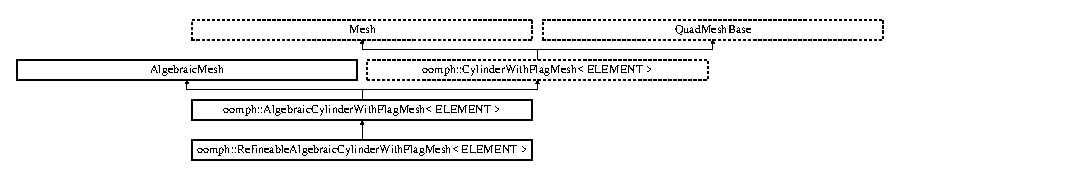
\includegraphics[height=1.924399cm]{classoomph_1_1AlgebraicCylinderWithFlagMesh}
\end{center}
\end{figure}
\subsection*{Public Member Functions}
\begin{DoxyCompactItemize}
\item 
\hyperlink{classoomph_1_1AlgebraicCylinderWithFlagMesh_a2c307b804fee56aa620ea414b41883d5}{Algebraic\+Cylinder\+With\+Flag\+Mesh} (Circle $\ast$cylinder\+\_\+pt, Geom\+Object $\ast$\hyperlink{classoomph_1_1AlgebraicCylinderWithFlagMesh_a06bc13adad4aaa037d989bba9e3bf79d}{top\+\_\+flag\+\_\+pt}, Geom\+Object $\ast$\hyperlink{classoomph_1_1AlgebraicCylinderWithFlagMesh_a9c362fcc5edeb1b6e773f27a83778495}{bottom\+\_\+flag\+\_\+pt}, Geom\+Object $\ast$\hyperlink{classoomph_1_1AlgebraicCylinderWithFlagMesh_ad6d22aaa02d79e3c740b06d98a1597ea}{tip\+\_\+flag\+\_\+pt}, const double \&length, const double \&height, const double \&flag\+\_\+length, const double \&flag\+\_\+height, const double \&centre\+\_\+x, const double \&centre\+\_\+y, const double \&a, Time\+Stepper $\ast$time\+\_\+stepper\+\_\+pt=\&Mesh\+::\+Default\+\_\+\+Time\+Stepper)
\begin{DoxyCompactList}\small\item\em Constructor. Pass the pointers to the Geom\+Objects that parametrise the cylinder, the three edges of the flag, the length and height of the domain, the length and height of the flag, the coordinates of the centre of the cylinder and its radius. Timestepper defaults to Steady default timestepper. \end{DoxyCompactList}\item 
virtual \hyperlink{classoomph_1_1AlgebraicCylinderWithFlagMesh_ac7e92a8dc3add0cd1f666dc8c9f8ca6f}{$\sim$\+Algebraic\+Cylinder\+With\+Flag\+Mesh} ()
\begin{DoxyCompactList}\small\item\em Destructor\+: empty. \end{DoxyCompactList}\item 
void \hyperlink{classoomph_1_1AlgebraicCylinderWithFlagMesh_a6aeef710528a9d8dd51023dd6ee131ea}{set\+\_\+bottom\+\_\+flag\+\_\+pt} (Geom\+Object $\ast$\hyperlink{classoomph_1_1AlgebraicCylinderWithFlagMesh_a9c362fcc5edeb1b6e773f27a83778495}{bottom\+\_\+flag\+\_\+pt})
\begin{DoxyCompactList}\small\item\em Set geometric object that defines the bottom face of the flag. \end{DoxyCompactList}\item 
void \hyperlink{classoomph_1_1AlgebraicCylinderWithFlagMesh_a9d7f04acdaed3e9f2133d9665dd4b799}{set\+\_\+top\+\_\+flag\+\_\+pt} (Geom\+Object $\ast$\hyperlink{classoomph_1_1AlgebraicCylinderWithFlagMesh_a06bc13adad4aaa037d989bba9e3bf79d}{top\+\_\+flag\+\_\+pt})
\begin{DoxyCompactList}\small\item\em Set the geometric object that defines the top face of the flag. \end{DoxyCompactList}\item 
void \hyperlink{classoomph_1_1AlgebraicCylinderWithFlagMesh_a191d736d9acbeb5927fc5f472420e9f6}{set\+\_\+tip\+\_\+flag\+\_\+pt} (Geom\+Object $\ast$\hyperlink{classoomph_1_1AlgebraicCylinderWithFlagMesh_ad6d22aaa02d79e3c740b06d98a1597ea}{tip\+\_\+flag\+\_\+pt})
\begin{DoxyCompactList}\small\item\em Set the geometric object that defines the tip of the flag. \end{DoxyCompactList}\item 
Geom\+Object $\ast$ \hyperlink{classoomph_1_1AlgebraicCylinderWithFlagMesh_a9c362fcc5edeb1b6e773f27a83778495}{bottom\+\_\+flag\+\_\+pt} () const
\begin{DoxyCompactList}\small\item\em Read-\/only access to geometric object that defines the bottom face of the flag. \end{DoxyCompactList}\item 
Geom\+Object $\ast$ \hyperlink{classoomph_1_1AlgebraicCylinderWithFlagMesh_a06bc13adad4aaa037d989bba9e3bf79d}{top\+\_\+flag\+\_\+pt} () const
\begin{DoxyCompactList}\small\item\em Read-\/only access to geometric object that defines the top face of the flag. \end{DoxyCompactList}\item 
Geom\+Object $\ast$ \hyperlink{classoomph_1_1AlgebraicCylinderWithFlagMesh_ad6d22aaa02d79e3c740b06d98a1597ea}{tip\+\_\+flag\+\_\+pt} () const
\begin{DoxyCompactList}\small\item\em Read-\/only access to geometric object that defines the tip of the flag. \end{DoxyCompactList}\item 
void \hyperlink{classoomph_1_1AlgebraicCylinderWithFlagMesh_a9d909de1db84a3b7e42494535b152d92}{update\+\_\+node\+\_\+update} (Algebraic\+Node $\ast$\&node\+\_\+pt)
\begin{DoxyCompactList}\small\item\em Update the geometric references that are used to update node after mesh adaptation. Empty -- no update of node update required without adaptativity. \end{DoxyCompactList}\item 
void \hyperlink{classoomph_1_1AlgebraicCylinderWithFlagMesh_a5e1e770e82577e5702470d8b87f8599d}{algebraic\+\_\+node\+\_\+update} (const unsigned \&t, Algebraic\+Node $\ast$\&node\+\_\+pt)
\begin{DoxyCompactList}\small\item\em Update nodal position at time level t (t=0\+: present;. \end{DoxyCompactList}\end{DoxyCompactItemize}
\subsection*{Protected Member Functions}
\begin{DoxyCompactItemize}
\item 
void \hyperlink{classoomph_1_1AlgebraicCylinderWithFlagMesh_ad6af2e420e0f152a7fb055f25400a5d0}{setup\+\_\+algebraic\+\_\+node\+\_\+update} ()
\begin{DoxyCompactList}\small\item\em Function to setup the algebraic node update. \end{DoxyCompactList}\item 
void \hyperlink{classoomph_1_1AlgebraicCylinderWithFlagMesh_a713cf7c2e1be91eae2667dc3e1fd8644}{node\+\_\+update\+\_\+I} (const unsigned \&t, Algebraic\+Node $\ast$\&node\+\_\+pt)
\begin{DoxyCompactList}\small\item\em Helper function. \end{DoxyCompactList}\item 
void \hyperlink{classoomph_1_1AlgebraicCylinderWithFlagMesh_a2717b4ae70a9641c24becc8176410b3e}{node\+\_\+update\+\_\+\+II} (const unsigned \&t, Algebraic\+Node $\ast$\&node\+\_\+pt)
\begin{DoxyCompactList}\small\item\em Helper function. \end{DoxyCompactList}\item 
void \hyperlink{classoomph_1_1AlgebraicCylinderWithFlagMesh_a3e8c71cc3ab123864b4f999e612345ee}{node\+\_\+update\+\_\+\+I\+II} (const unsigned \&t, Algebraic\+Node $\ast$\&node\+\_\+pt)
\begin{DoxyCompactList}\small\item\em Helper function. \end{DoxyCompactList}\item 
void \hyperlink{classoomph_1_1AlgebraicCylinderWithFlagMesh_a69ab465aa28dd9a65a0c50762c0a6d89}{node\+\_\+update\+\_\+\+IV} (const unsigned \&t, Algebraic\+Node $\ast$\&node\+\_\+pt)
\begin{DoxyCompactList}\small\item\em Helper function. \end{DoxyCompactList}\item 
void \hyperlink{classoomph_1_1AlgebraicCylinderWithFlagMesh_a035216f13c9758881ce2b7e33ad27926}{node\+\_\+update\+\_\+V} (const unsigned \&t, Algebraic\+Node $\ast$\&node\+\_\+pt)
\begin{DoxyCompactList}\small\item\em Helper function. \end{DoxyCompactList}\item 
void \hyperlink{classoomph_1_1AlgebraicCylinderWithFlagMesh_a989fe557f03ac20812e69a8de2dbb9a4}{node\+\_\+update\+\_\+\+VI} (const unsigned \&t, Algebraic\+Node $\ast$\&node\+\_\+pt)
\begin{DoxyCompactList}\small\item\em Helper function. \end{DoxyCompactList}\item 
void \hyperlink{classoomph_1_1AlgebraicCylinderWithFlagMesh_abb0565f0624583d2549f38602fd11e48}{node\+\_\+update\+\_\+\+V\+II} (const unsigned \&t, Algebraic\+Node $\ast$\&node\+\_\+pt)
\begin{DoxyCompactList}\small\item\em Helper function. \end{DoxyCompactList}\item 
void \hyperlink{classoomph_1_1AlgebraicCylinderWithFlagMesh_a85336e587d9c4cac7f4d77890dd7690b}{node\+\_\+update\+\_\+\+V\+I\+II} (const unsigned \&t, Algebraic\+Node $\ast$\&node\+\_\+pt)
\begin{DoxyCompactList}\small\item\em Helper function. \end{DoxyCompactList}\item 
void \hyperlink{classoomph_1_1AlgebraicCylinderWithFlagMesh_ae8e85400abd282b64463b67e21e9c13a}{node\+\_\+update\+\_\+\+IX} (const unsigned \&t, Algebraic\+Node $\ast$\&node\+\_\+pt)
\begin{DoxyCompactList}\small\item\em Helper function. \end{DoxyCompactList}\end{DoxyCompactItemize}
\subsection*{Protected Attributes}
\begin{DoxyCompactItemize}
\item 
Geom\+Object $\ast$ \hyperlink{classoomph_1_1AlgebraicCylinderWithFlagMesh_a423d4aa7ffcca5e707b2e5d820984957}{Cylinder\+\_\+pt}
\begin{DoxyCompactList}\small\item\em Cylinder. \end{DoxyCompactList}\item 
Geom\+Object $\ast$ \hyperlink{classoomph_1_1AlgebraicCylinderWithFlagMesh_a326e4789fe96b3052a8beb51ec9e94d0}{Top\+\_\+flag\+\_\+pt}
\begin{DoxyCompactList}\small\item\em Top flag. \end{DoxyCompactList}\item 
Geom\+Object $\ast$ \hyperlink{classoomph_1_1AlgebraicCylinderWithFlagMesh_ac1f7e1ba183ba813229302c5688ea1ba}{Bottom\+\_\+flag\+\_\+pt}
\begin{DoxyCompactList}\small\item\em Bottom flag. \end{DoxyCompactList}\item 
Geom\+Object $\ast$ \hyperlink{classoomph_1_1AlgebraicCylinderWithFlagMesh_ad22c8bfa595f4b1f129be85a1904762f}{Tip\+\_\+flag\+\_\+pt}
\begin{DoxyCompactList}\small\item\em Tip flag. \end{DoxyCompactList}\item 
double \hyperlink{classoomph_1_1AlgebraicCylinderWithFlagMesh_a7620fa5a4c36f638fb22c81b346b74a2}{Length}
\begin{DoxyCompactList}\small\item\em Length of the domain. \end{DoxyCompactList}\item 
double \hyperlink{classoomph_1_1AlgebraicCylinderWithFlagMesh_a29a0c970a11d46bdf03f3b5053d3ece2}{Height}
\begin{DoxyCompactList}\small\item\em Height of the domain. \end{DoxyCompactList}\item 
double \hyperlink{classoomph_1_1AlgebraicCylinderWithFlagMesh_a822ed90585320576084667f88c236396}{Flag\+\_\+length}
\begin{DoxyCompactList}\small\item\em Flag length. \end{DoxyCompactList}\item 
double \hyperlink{classoomph_1_1AlgebraicCylinderWithFlagMesh_a76a19a39dd500d5a48c10baae59797e0}{Flag\+\_\+height}
\begin{DoxyCompactList}\small\item\em Flag thickness. \end{DoxyCompactList}\item 
double \hyperlink{classoomph_1_1AlgebraicCylinderWithFlagMesh_a3290ac9103e43f4a4a997fe4692b6506}{Centre\+\_\+x}
\begin{DoxyCompactList}\small\item\em x position of the centre of the cylinder \end{DoxyCompactList}\item 
double \hyperlink{classoomph_1_1AlgebraicCylinderWithFlagMesh_a6b4575a9c3818e04bdb00d4150d49290}{Centre\+\_\+y}
\begin{DoxyCompactList}\small\item\em x position of the centre of the cylinder \end{DoxyCompactList}\item 
double \hyperlink{classoomph_1_1AlgebraicCylinderWithFlagMesh_aabc6cdfe508f04a4b1c92f2c2f1639c4}{A}
\begin{DoxyCompactList}\small\item\em radius of the cylinder \end{DoxyCompactList}\end{DoxyCompactItemize}


\subsection{Detailed Description}
\subsubsection*{template$<$class E\+L\+E\+M\+E\+NT$>$\newline
class oomph\+::\+Algebraic\+Cylinder\+With\+Flag\+Mesh$<$ E\+L\+E\+M\+E\+N\+T $>$}

Algebraic version of \hyperlink{classoomph_1_1CylinderWithFlagMesh}{Cylinder\+With\+Flag\+Mesh}. 

Definition at line 161 of file cylinder\+\_\+with\+\_\+flag\+\_\+mesh.\+template.\+h.



\subsection{Constructor \& Destructor Documentation}
\mbox{\Hypertarget{classoomph_1_1AlgebraicCylinderWithFlagMesh_a2c307b804fee56aa620ea414b41883d5}\label{classoomph_1_1AlgebraicCylinderWithFlagMesh_a2c307b804fee56aa620ea414b41883d5}} 
\index{oomph\+::\+Algebraic\+Cylinder\+With\+Flag\+Mesh@{oomph\+::\+Algebraic\+Cylinder\+With\+Flag\+Mesh}!Algebraic\+Cylinder\+With\+Flag\+Mesh@{Algebraic\+Cylinder\+With\+Flag\+Mesh}}
\index{Algebraic\+Cylinder\+With\+Flag\+Mesh@{Algebraic\+Cylinder\+With\+Flag\+Mesh}!oomph\+::\+Algebraic\+Cylinder\+With\+Flag\+Mesh@{oomph\+::\+Algebraic\+Cylinder\+With\+Flag\+Mesh}}
\subsubsection{\texorpdfstring{Algebraic\+Cylinder\+With\+Flag\+Mesh()}{AlgebraicCylinderWithFlagMesh()}}
{\footnotesize\ttfamily template$<$class E\+L\+E\+M\+E\+NT $>$ \\
\hyperlink{classoomph_1_1AlgebraicCylinderWithFlagMesh}{oomph\+::\+Algebraic\+Cylinder\+With\+Flag\+Mesh}$<$ E\+L\+E\+M\+E\+NT $>$\+::\hyperlink{classoomph_1_1AlgebraicCylinderWithFlagMesh}{Algebraic\+Cylinder\+With\+Flag\+Mesh} (\begin{DoxyParamCaption}\item[{Circle $\ast$}]{cylinder\+\_\+pt,  }\item[{Geom\+Object $\ast$}]{top\+\_\+flag\+\_\+pt,  }\item[{Geom\+Object $\ast$}]{bottom\+\_\+flag\+\_\+pt,  }\item[{Geom\+Object $\ast$}]{tip\+\_\+flag\+\_\+pt,  }\item[{const double \&}]{length,  }\item[{const double \&}]{height,  }\item[{const double \&}]{flag\+\_\+length,  }\item[{const double \&}]{flag\+\_\+height,  }\item[{const double \&}]{centre\+\_\+x,  }\item[{const double \&}]{centre\+\_\+y,  }\item[{const double \&}]{a,  }\item[{Time\+Stepper $\ast$}]{time\+\_\+stepper\+\_\+pt = {\ttfamily \&Mesh\+:\+:Default\+\_\+TimeStepper} }\end{DoxyParamCaption})\hspace{0.3cm}{\ttfamily [inline]}}



Constructor. Pass the pointers to the Geom\+Objects that parametrise the cylinder, the three edges of the flag, the length and height of the domain, the length and height of the flag, the coordinates of the centre of the cylinder and its radius. Timestepper defaults to Steady default timestepper. 



Definition at line 172 of file cylinder\+\_\+with\+\_\+flag\+\_\+mesh.\+template.\+h.

\mbox{\Hypertarget{classoomph_1_1AlgebraicCylinderWithFlagMesh_ac7e92a8dc3add0cd1f666dc8c9f8ca6f}\label{classoomph_1_1AlgebraicCylinderWithFlagMesh_ac7e92a8dc3add0cd1f666dc8c9f8ca6f}} 
\index{oomph\+::\+Algebraic\+Cylinder\+With\+Flag\+Mesh@{oomph\+::\+Algebraic\+Cylinder\+With\+Flag\+Mesh}!````~Algebraic\+Cylinder\+With\+Flag\+Mesh@{$\sim$\+Algebraic\+Cylinder\+With\+Flag\+Mesh}}
\index{````~Algebraic\+Cylinder\+With\+Flag\+Mesh@{$\sim$\+Algebraic\+Cylinder\+With\+Flag\+Mesh}!oomph\+::\+Algebraic\+Cylinder\+With\+Flag\+Mesh@{oomph\+::\+Algebraic\+Cylinder\+With\+Flag\+Mesh}}
\subsubsection{\texorpdfstring{$\sim$\+Algebraic\+Cylinder\+With\+Flag\+Mesh()}{~AlgebraicCylinderWithFlagMesh()}}
{\footnotesize\ttfamily template$<$class E\+L\+E\+M\+E\+NT $>$ \\
virtual \hyperlink{classoomph_1_1AlgebraicCylinderWithFlagMesh}{oomph\+::\+Algebraic\+Cylinder\+With\+Flag\+Mesh}$<$ E\+L\+E\+M\+E\+NT $>$\+::$\sim$\hyperlink{classoomph_1_1AlgebraicCylinderWithFlagMesh}{Algebraic\+Cylinder\+With\+Flag\+Mesh} (\begin{DoxyParamCaption}{ }\end{DoxyParamCaption})\hspace{0.3cm}{\ttfamily [inline]}, {\ttfamily [virtual]}}



Destructor\+: empty. 



Definition at line 205 of file cylinder\+\_\+with\+\_\+flag\+\_\+mesh.\+template.\+h.



\subsection{Member Function Documentation}
\mbox{\Hypertarget{classoomph_1_1AlgebraicCylinderWithFlagMesh_a5e1e770e82577e5702470d8b87f8599d}\label{classoomph_1_1AlgebraicCylinderWithFlagMesh_a5e1e770e82577e5702470d8b87f8599d}} 
\index{oomph\+::\+Algebraic\+Cylinder\+With\+Flag\+Mesh@{oomph\+::\+Algebraic\+Cylinder\+With\+Flag\+Mesh}!algebraic\+\_\+node\+\_\+update@{algebraic\+\_\+node\+\_\+update}}
\index{algebraic\+\_\+node\+\_\+update@{algebraic\+\_\+node\+\_\+update}!oomph\+::\+Algebraic\+Cylinder\+With\+Flag\+Mesh@{oomph\+::\+Algebraic\+Cylinder\+With\+Flag\+Mesh}}
\subsubsection{\texorpdfstring{algebraic\+\_\+node\+\_\+update()}{algebraic\_node\_update()}}
{\footnotesize\ttfamily template$<$class E\+L\+E\+M\+E\+NT $>$ \\
void \hyperlink{classoomph_1_1AlgebraicCylinderWithFlagMesh}{oomph\+::\+Algebraic\+Cylinder\+With\+Flag\+Mesh}$<$ E\+L\+E\+M\+E\+NT $>$\+::algebraic\+\_\+node\+\_\+update (\begin{DoxyParamCaption}\item[{const unsigned \&}]{t,  }\item[{Algebraic\+Node $\ast$\&}]{node\+\_\+pt }\end{DoxyParamCaption})}



Update nodal position at time level t (t=0\+: present;. 

The algebraic node update function.

t$>$0\+: previous) 

Definition at line 1367 of file cylinder\+\_\+with\+\_\+flag\+\_\+mesh.\+template.\+cc.

\mbox{\Hypertarget{classoomph_1_1AlgebraicCylinderWithFlagMesh_a9c362fcc5edeb1b6e773f27a83778495}\label{classoomph_1_1AlgebraicCylinderWithFlagMesh_a9c362fcc5edeb1b6e773f27a83778495}} 
\index{oomph\+::\+Algebraic\+Cylinder\+With\+Flag\+Mesh@{oomph\+::\+Algebraic\+Cylinder\+With\+Flag\+Mesh}!bottom\+\_\+flag\+\_\+pt@{bottom\+\_\+flag\+\_\+pt}}
\index{bottom\+\_\+flag\+\_\+pt@{bottom\+\_\+flag\+\_\+pt}!oomph\+::\+Algebraic\+Cylinder\+With\+Flag\+Mesh@{oomph\+::\+Algebraic\+Cylinder\+With\+Flag\+Mesh}}
\subsubsection{\texorpdfstring{bottom\+\_\+flag\+\_\+pt()}{bottom\_flag\_pt()}}
{\footnotesize\ttfamily template$<$class E\+L\+E\+M\+E\+NT $>$ \\
Geom\+Object$\ast$ \hyperlink{classoomph_1_1AlgebraicCylinderWithFlagMesh}{oomph\+::\+Algebraic\+Cylinder\+With\+Flag\+Mesh}$<$ E\+L\+E\+M\+E\+NT $>$\+::bottom\+\_\+flag\+\_\+pt (\begin{DoxyParamCaption}{ }\end{DoxyParamCaption}) const\hspace{0.3cm}{\ttfamily [inline]}}



Read-\/only access to geometric object that defines the bottom face of the flag. 



Definition at line 237 of file cylinder\+\_\+with\+\_\+flag\+\_\+mesh.\+template.\+h.

\mbox{\Hypertarget{classoomph_1_1AlgebraicCylinderWithFlagMesh_a713cf7c2e1be91eae2667dc3e1fd8644}\label{classoomph_1_1AlgebraicCylinderWithFlagMesh_a713cf7c2e1be91eae2667dc3e1fd8644}} 
\index{oomph\+::\+Algebraic\+Cylinder\+With\+Flag\+Mesh@{oomph\+::\+Algebraic\+Cylinder\+With\+Flag\+Mesh}!node\+\_\+update\+\_\+I@{node\+\_\+update\+\_\+I}}
\index{node\+\_\+update\+\_\+I@{node\+\_\+update\+\_\+I}!oomph\+::\+Algebraic\+Cylinder\+With\+Flag\+Mesh@{oomph\+::\+Algebraic\+Cylinder\+With\+Flag\+Mesh}}
\subsubsection{\texorpdfstring{node\+\_\+update\+\_\+\+I()}{node\_update\_I()}}
{\footnotesize\ttfamily template$<$class E\+L\+E\+M\+E\+NT $>$ \\
void \hyperlink{classoomph_1_1AlgebraicCylinderWithFlagMesh}{oomph\+::\+Algebraic\+Cylinder\+With\+Flag\+Mesh}$<$ E\+L\+E\+M\+E\+NT $>$\+::node\+\_\+update\+\_\+I (\begin{DoxyParamCaption}\item[{const unsigned \&}]{t,  }\item[{Algebraic\+Node $\ast$\&}]{node\+\_\+pt }\end{DoxyParamCaption})\hspace{0.3cm}{\ttfamily [protected]}}



Helper function. 

Node update for region I. 

Definition at line 1426 of file cylinder\+\_\+with\+\_\+flag\+\_\+mesh.\+template.\+cc.

\mbox{\Hypertarget{classoomph_1_1AlgebraicCylinderWithFlagMesh_a2717b4ae70a9641c24becc8176410b3e}\label{classoomph_1_1AlgebraicCylinderWithFlagMesh_a2717b4ae70a9641c24becc8176410b3e}} 
\index{oomph\+::\+Algebraic\+Cylinder\+With\+Flag\+Mesh@{oomph\+::\+Algebraic\+Cylinder\+With\+Flag\+Mesh}!node\+\_\+update\+\_\+\+II@{node\+\_\+update\+\_\+\+II}}
\index{node\+\_\+update\+\_\+\+II@{node\+\_\+update\+\_\+\+II}!oomph\+::\+Algebraic\+Cylinder\+With\+Flag\+Mesh@{oomph\+::\+Algebraic\+Cylinder\+With\+Flag\+Mesh}}
\subsubsection{\texorpdfstring{node\+\_\+update\+\_\+\+I\+I()}{node\_update\_II()}}
{\footnotesize\ttfamily template$<$class E\+L\+E\+M\+E\+NT $>$ \\
void \hyperlink{classoomph_1_1AlgebraicCylinderWithFlagMesh}{oomph\+::\+Algebraic\+Cylinder\+With\+Flag\+Mesh}$<$ E\+L\+E\+M\+E\+NT $>$\+::node\+\_\+update\+\_\+\+II (\begin{DoxyParamCaption}\item[{const unsigned \&}]{t,  }\item[{Algebraic\+Node $\ast$\&}]{node\+\_\+pt }\end{DoxyParamCaption})\hspace{0.3cm}{\ttfamily [protected]}}



Helper function. 

Node update for region II. 

Definition at line 1465 of file cylinder\+\_\+with\+\_\+flag\+\_\+mesh.\+template.\+cc.

\mbox{\Hypertarget{classoomph_1_1AlgebraicCylinderWithFlagMesh_a3e8c71cc3ab123864b4f999e612345ee}\label{classoomph_1_1AlgebraicCylinderWithFlagMesh_a3e8c71cc3ab123864b4f999e612345ee}} 
\index{oomph\+::\+Algebraic\+Cylinder\+With\+Flag\+Mesh@{oomph\+::\+Algebraic\+Cylinder\+With\+Flag\+Mesh}!node\+\_\+update\+\_\+\+I\+II@{node\+\_\+update\+\_\+\+I\+II}}
\index{node\+\_\+update\+\_\+\+I\+II@{node\+\_\+update\+\_\+\+I\+II}!oomph\+::\+Algebraic\+Cylinder\+With\+Flag\+Mesh@{oomph\+::\+Algebraic\+Cylinder\+With\+Flag\+Mesh}}
\subsubsection{\texorpdfstring{node\+\_\+update\+\_\+\+I\+I\+I()}{node\_update\_III()}}
{\footnotesize\ttfamily template$<$class E\+L\+E\+M\+E\+NT $>$ \\
void \hyperlink{classoomph_1_1AlgebraicCylinderWithFlagMesh}{oomph\+::\+Algebraic\+Cylinder\+With\+Flag\+Mesh}$<$ E\+L\+E\+M\+E\+NT $>$\+::node\+\_\+update\+\_\+\+I\+II (\begin{DoxyParamCaption}\item[{const unsigned \&}]{t,  }\item[{Algebraic\+Node $\ast$\&}]{node\+\_\+pt }\end{DoxyParamCaption})\hspace{0.3cm}{\ttfamily [protected]}}



Helper function. 

Node update for region I\+II. 

Definition at line 1501 of file cylinder\+\_\+with\+\_\+flag\+\_\+mesh.\+template.\+cc.

\mbox{\Hypertarget{classoomph_1_1AlgebraicCylinderWithFlagMesh_a69ab465aa28dd9a65a0c50762c0a6d89}\label{classoomph_1_1AlgebraicCylinderWithFlagMesh_a69ab465aa28dd9a65a0c50762c0a6d89}} 
\index{oomph\+::\+Algebraic\+Cylinder\+With\+Flag\+Mesh@{oomph\+::\+Algebraic\+Cylinder\+With\+Flag\+Mesh}!node\+\_\+update\+\_\+\+IV@{node\+\_\+update\+\_\+\+IV}}
\index{node\+\_\+update\+\_\+\+IV@{node\+\_\+update\+\_\+\+IV}!oomph\+::\+Algebraic\+Cylinder\+With\+Flag\+Mesh@{oomph\+::\+Algebraic\+Cylinder\+With\+Flag\+Mesh}}
\subsubsection{\texorpdfstring{node\+\_\+update\+\_\+\+I\+V()}{node\_update\_IV()}}
{\footnotesize\ttfamily template$<$class E\+L\+E\+M\+E\+NT $>$ \\
void \hyperlink{classoomph_1_1AlgebraicCylinderWithFlagMesh}{oomph\+::\+Algebraic\+Cylinder\+With\+Flag\+Mesh}$<$ E\+L\+E\+M\+E\+NT $>$\+::node\+\_\+update\+\_\+\+IV (\begin{DoxyParamCaption}\item[{const unsigned \&}]{t,  }\item[{Algebraic\+Node $\ast$\&}]{node\+\_\+pt }\end{DoxyParamCaption})\hspace{0.3cm}{\ttfamily [protected]}}



Helper function. 

Node update for region IV. 

Definition at line 1549 of file cylinder\+\_\+with\+\_\+flag\+\_\+mesh.\+template.\+cc.

\mbox{\Hypertarget{classoomph_1_1AlgebraicCylinderWithFlagMesh_ae8e85400abd282b64463b67e21e9c13a}\label{classoomph_1_1AlgebraicCylinderWithFlagMesh_ae8e85400abd282b64463b67e21e9c13a}} 
\index{oomph\+::\+Algebraic\+Cylinder\+With\+Flag\+Mesh@{oomph\+::\+Algebraic\+Cylinder\+With\+Flag\+Mesh}!node\+\_\+update\+\_\+\+IX@{node\+\_\+update\+\_\+\+IX}}
\index{node\+\_\+update\+\_\+\+IX@{node\+\_\+update\+\_\+\+IX}!oomph\+::\+Algebraic\+Cylinder\+With\+Flag\+Mesh@{oomph\+::\+Algebraic\+Cylinder\+With\+Flag\+Mesh}}
\subsubsection{\texorpdfstring{node\+\_\+update\+\_\+\+I\+X()}{node\_update\_IX()}}
{\footnotesize\ttfamily template$<$class E\+L\+E\+M\+E\+NT $>$ \\
void \hyperlink{classoomph_1_1AlgebraicCylinderWithFlagMesh}{oomph\+::\+Algebraic\+Cylinder\+With\+Flag\+Mesh}$<$ E\+L\+E\+M\+E\+NT $>$\+::node\+\_\+update\+\_\+\+IX (\begin{DoxyParamCaption}\item[{const unsigned \&}]{t,  }\item[{Algebraic\+Node $\ast$\&}]{node\+\_\+pt }\end{DoxyParamCaption})\hspace{0.3cm}{\ttfamily [protected]}}



Helper function. 

Node update for region IX. Extreme angles on circle 

Definition at line 1816 of file cylinder\+\_\+with\+\_\+flag\+\_\+mesh.\+template.\+cc.

\mbox{\Hypertarget{classoomph_1_1AlgebraicCylinderWithFlagMesh_a035216f13c9758881ce2b7e33ad27926}\label{classoomph_1_1AlgebraicCylinderWithFlagMesh_a035216f13c9758881ce2b7e33ad27926}} 
\index{oomph\+::\+Algebraic\+Cylinder\+With\+Flag\+Mesh@{oomph\+::\+Algebraic\+Cylinder\+With\+Flag\+Mesh}!node\+\_\+update\+\_\+V@{node\+\_\+update\+\_\+V}}
\index{node\+\_\+update\+\_\+V@{node\+\_\+update\+\_\+V}!oomph\+::\+Algebraic\+Cylinder\+With\+Flag\+Mesh@{oomph\+::\+Algebraic\+Cylinder\+With\+Flag\+Mesh}}
\subsubsection{\texorpdfstring{node\+\_\+update\+\_\+\+V()}{node\_update\_V()}}
{\footnotesize\ttfamily template$<$class E\+L\+E\+M\+E\+NT $>$ \\
void \hyperlink{classoomph_1_1AlgebraicCylinderWithFlagMesh}{oomph\+::\+Algebraic\+Cylinder\+With\+Flag\+Mesh}$<$ E\+L\+E\+M\+E\+NT $>$\+::node\+\_\+update\+\_\+V (\begin{DoxyParamCaption}\item[{const unsigned \&}]{t,  }\item[{Algebraic\+Node $\ast$\&}]{node\+\_\+pt }\end{DoxyParamCaption})\hspace{0.3cm}{\ttfamily [protected]}}



Helper function. 

Node update for region V. 

Definition at line 1596 of file cylinder\+\_\+with\+\_\+flag\+\_\+mesh.\+template.\+cc.

\mbox{\Hypertarget{classoomph_1_1AlgebraicCylinderWithFlagMesh_a989fe557f03ac20812e69a8de2dbb9a4}\label{classoomph_1_1AlgebraicCylinderWithFlagMesh_a989fe557f03ac20812e69a8de2dbb9a4}} 
\index{oomph\+::\+Algebraic\+Cylinder\+With\+Flag\+Mesh@{oomph\+::\+Algebraic\+Cylinder\+With\+Flag\+Mesh}!node\+\_\+update\+\_\+\+VI@{node\+\_\+update\+\_\+\+VI}}
\index{node\+\_\+update\+\_\+\+VI@{node\+\_\+update\+\_\+\+VI}!oomph\+::\+Algebraic\+Cylinder\+With\+Flag\+Mesh@{oomph\+::\+Algebraic\+Cylinder\+With\+Flag\+Mesh}}
\subsubsection{\texorpdfstring{node\+\_\+update\+\_\+\+V\+I()}{node\_update\_VI()}}
{\footnotesize\ttfamily template$<$class E\+L\+E\+M\+E\+NT $>$ \\
void \hyperlink{classoomph_1_1AlgebraicCylinderWithFlagMesh}{oomph\+::\+Algebraic\+Cylinder\+With\+Flag\+Mesh}$<$ E\+L\+E\+M\+E\+NT $>$\+::node\+\_\+update\+\_\+\+VI (\begin{DoxyParamCaption}\item[{const unsigned \&}]{t,  }\item[{Algebraic\+Node $\ast$\&}]{node\+\_\+pt }\end{DoxyParamCaption})\hspace{0.3cm}{\ttfamily [protected]}}



Helper function. 

Node update for region VI. 

Definition at line 1645 of file cylinder\+\_\+with\+\_\+flag\+\_\+mesh.\+template.\+cc.

\mbox{\Hypertarget{classoomph_1_1AlgebraicCylinderWithFlagMesh_abb0565f0624583d2549f38602fd11e48}\label{classoomph_1_1AlgebraicCylinderWithFlagMesh_abb0565f0624583d2549f38602fd11e48}} 
\index{oomph\+::\+Algebraic\+Cylinder\+With\+Flag\+Mesh@{oomph\+::\+Algebraic\+Cylinder\+With\+Flag\+Mesh}!node\+\_\+update\+\_\+\+V\+II@{node\+\_\+update\+\_\+\+V\+II}}
\index{node\+\_\+update\+\_\+\+V\+II@{node\+\_\+update\+\_\+\+V\+II}!oomph\+::\+Algebraic\+Cylinder\+With\+Flag\+Mesh@{oomph\+::\+Algebraic\+Cylinder\+With\+Flag\+Mesh}}
\subsubsection{\texorpdfstring{node\+\_\+update\+\_\+\+V\+I\+I()}{node\_update\_VII()}}
{\footnotesize\ttfamily template$<$class E\+L\+E\+M\+E\+NT $>$ \\
void \hyperlink{classoomph_1_1AlgebraicCylinderWithFlagMesh}{oomph\+::\+Algebraic\+Cylinder\+With\+Flag\+Mesh}$<$ E\+L\+E\+M\+E\+NT $>$\+::node\+\_\+update\+\_\+\+V\+II (\begin{DoxyParamCaption}\item[{const unsigned \&}]{t,  }\item[{Algebraic\+Node $\ast$\&}]{node\+\_\+pt }\end{DoxyParamCaption})\hspace{0.3cm}{\ttfamily [protected]}}



Helper function. 

Node update for region V\+II. 

Definition at line 1688 of file cylinder\+\_\+with\+\_\+flag\+\_\+mesh.\+template.\+cc.

\mbox{\Hypertarget{classoomph_1_1AlgebraicCylinderWithFlagMesh_a85336e587d9c4cac7f4d77890dd7690b}\label{classoomph_1_1AlgebraicCylinderWithFlagMesh_a85336e587d9c4cac7f4d77890dd7690b}} 
\index{oomph\+::\+Algebraic\+Cylinder\+With\+Flag\+Mesh@{oomph\+::\+Algebraic\+Cylinder\+With\+Flag\+Mesh}!node\+\_\+update\+\_\+\+V\+I\+II@{node\+\_\+update\+\_\+\+V\+I\+II}}
\index{node\+\_\+update\+\_\+\+V\+I\+II@{node\+\_\+update\+\_\+\+V\+I\+II}!oomph\+::\+Algebraic\+Cylinder\+With\+Flag\+Mesh@{oomph\+::\+Algebraic\+Cylinder\+With\+Flag\+Mesh}}
\subsubsection{\texorpdfstring{node\+\_\+update\+\_\+\+V\+I\+I\+I()}{node\_update\_VIII()}}
{\footnotesize\ttfamily template$<$class E\+L\+E\+M\+E\+NT $>$ \\
void \hyperlink{classoomph_1_1AlgebraicCylinderWithFlagMesh}{oomph\+::\+Algebraic\+Cylinder\+With\+Flag\+Mesh}$<$ E\+L\+E\+M\+E\+NT $>$\+::node\+\_\+update\+\_\+\+V\+I\+II (\begin{DoxyParamCaption}\item[{const unsigned \&}]{t,  }\item[{Algebraic\+Node $\ast$\&}]{node\+\_\+pt }\end{DoxyParamCaption})\hspace{0.3cm}{\ttfamily [protected]}}



Helper function. 

Node update for region V\+I\+II. Extreme angles on circle 

Definition at line 1732 of file cylinder\+\_\+with\+\_\+flag\+\_\+mesh.\+template.\+cc.

\mbox{\Hypertarget{classoomph_1_1AlgebraicCylinderWithFlagMesh_a6aeef710528a9d8dd51023dd6ee131ea}\label{classoomph_1_1AlgebraicCylinderWithFlagMesh_a6aeef710528a9d8dd51023dd6ee131ea}} 
\index{oomph\+::\+Algebraic\+Cylinder\+With\+Flag\+Mesh@{oomph\+::\+Algebraic\+Cylinder\+With\+Flag\+Mesh}!set\+\_\+bottom\+\_\+flag\+\_\+pt@{set\+\_\+bottom\+\_\+flag\+\_\+pt}}
\index{set\+\_\+bottom\+\_\+flag\+\_\+pt@{set\+\_\+bottom\+\_\+flag\+\_\+pt}!oomph\+::\+Algebraic\+Cylinder\+With\+Flag\+Mesh@{oomph\+::\+Algebraic\+Cylinder\+With\+Flag\+Mesh}}
\subsubsection{\texorpdfstring{set\+\_\+bottom\+\_\+flag\+\_\+pt()}{set\_bottom\_flag\_pt()}}
{\footnotesize\ttfamily template$<$class E\+L\+E\+M\+E\+NT $>$ \\
void \hyperlink{classoomph_1_1AlgebraicCylinderWithFlagMesh}{oomph\+::\+Algebraic\+Cylinder\+With\+Flag\+Mesh}$<$ E\+L\+E\+M\+E\+NT $>$\+::set\+\_\+bottom\+\_\+flag\+\_\+pt (\begin{DoxyParamCaption}\item[{Geom\+Object $\ast$}]{bottom\+\_\+flag\+\_\+pt }\end{DoxyParamCaption})\hspace{0.3cm}{\ttfamily [inline]}}



Set geometric object that defines the bottom face of the flag. 



Definition at line 210 of file cylinder\+\_\+with\+\_\+flag\+\_\+mesh.\+template.\+h.



References oomph\+::\+Cylinder\+With\+Flag\+Domain\+::bottom\+\_\+flag\+\_\+pt(), and oomph\+::\+Cylinder\+With\+Flag\+Mesh$<$ E\+L\+E\+M\+E\+N\+T $>$\+::domain\+\_\+pt().

\mbox{\Hypertarget{classoomph_1_1AlgebraicCylinderWithFlagMesh_a191d736d9acbeb5927fc5f472420e9f6}\label{classoomph_1_1AlgebraicCylinderWithFlagMesh_a191d736d9acbeb5927fc5f472420e9f6}} 
\index{oomph\+::\+Algebraic\+Cylinder\+With\+Flag\+Mesh@{oomph\+::\+Algebraic\+Cylinder\+With\+Flag\+Mesh}!set\+\_\+tip\+\_\+flag\+\_\+pt@{set\+\_\+tip\+\_\+flag\+\_\+pt}}
\index{set\+\_\+tip\+\_\+flag\+\_\+pt@{set\+\_\+tip\+\_\+flag\+\_\+pt}!oomph\+::\+Algebraic\+Cylinder\+With\+Flag\+Mesh@{oomph\+::\+Algebraic\+Cylinder\+With\+Flag\+Mesh}}
\subsubsection{\texorpdfstring{set\+\_\+tip\+\_\+flag\+\_\+pt()}{set\_tip\_flag\_pt()}}
{\footnotesize\ttfamily template$<$class E\+L\+E\+M\+E\+NT $>$ \\
void \hyperlink{classoomph_1_1AlgebraicCylinderWithFlagMesh}{oomph\+::\+Algebraic\+Cylinder\+With\+Flag\+Mesh}$<$ E\+L\+E\+M\+E\+NT $>$\+::set\+\_\+tip\+\_\+flag\+\_\+pt (\begin{DoxyParamCaption}\item[{Geom\+Object $\ast$}]{tip\+\_\+flag\+\_\+pt }\end{DoxyParamCaption})\hspace{0.3cm}{\ttfamily [inline]}}



Set the geometric object that defines the tip of the flag. 



Definition at line 228 of file cylinder\+\_\+with\+\_\+flag\+\_\+mesh.\+template.\+h.



References oomph\+::\+Cylinder\+With\+Flag\+Mesh$<$ E\+L\+E\+M\+E\+N\+T $>$\+::domain\+\_\+pt(), and oomph\+::\+Cylinder\+With\+Flag\+Domain\+::tip\+\_\+flag\+\_\+pt().

\mbox{\Hypertarget{classoomph_1_1AlgebraicCylinderWithFlagMesh_a9d7f04acdaed3e9f2133d9665dd4b799}\label{classoomph_1_1AlgebraicCylinderWithFlagMesh_a9d7f04acdaed3e9f2133d9665dd4b799}} 
\index{oomph\+::\+Algebraic\+Cylinder\+With\+Flag\+Mesh@{oomph\+::\+Algebraic\+Cylinder\+With\+Flag\+Mesh}!set\+\_\+top\+\_\+flag\+\_\+pt@{set\+\_\+top\+\_\+flag\+\_\+pt}}
\index{set\+\_\+top\+\_\+flag\+\_\+pt@{set\+\_\+top\+\_\+flag\+\_\+pt}!oomph\+::\+Algebraic\+Cylinder\+With\+Flag\+Mesh@{oomph\+::\+Algebraic\+Cylinder\+With\+Flag\+Mesh}}
\subsubsection{\texorpdfstring{set\+\_\+top\+\_\+flag\+\_\+pt()}{set\_top\_flag\_pt()}}
{\footnotesize\ttfamily template$<$class E\+L\+E\+M\+E\+NT $>$ \\
void \hyperlink{classoomph_1_1AlgebraicCylinderWithFlagMesh}{oomph\+::\+Algebraic\+Cylinder\+With\+Flag\+Mesh}$<$ E\+L\+E\+M\+E\+NT $>$\+::set\+\_\+top\+\_\+flag\+\_\+pt (\begin{DoxyParamCaption}\item[{Geom\+Object $\ast$}]{top\+\_\+flag\+\_\+pt }\end{DoxyParamCaption})\hspace{0.3cm}{\ttfamily [inline]}}



Set the geometric object that defines the top face of the flag. 



Definition at line 219 of file cylinder\+\_\+with\+\_\+flag\+\_\+mesh.\+template.\+h.



References oomph\+::\+Cylinder\+With\+Flag\+Mesh$<$ E\+L\+E\+M\+E\+N\+T $>$\+::domain\+\_\+pt(), and oomph\+::\+Cylinder\+With\+Flag\+Domain\+::top\+\_\+flag\+\_\+pt().

\mbox{\Hypertarget{classoomph_1_1AlgebraicCylinderWithFlagMesh_ad6af2e420e0f152a7fb055f25400a5d0}\label{classoomph_1_1AlgebraicCylinderWithFlagMesh_ad6af2e420e0f152a7fb055f25400a5d0}} 
\index{oomph\+::\+Algebraic\+Cylinder\+With\+Flag\+Mesh@{oomph\+::\+Algebraic\+Cylinder\+With\+Flag\+Mesh}!setup\+\_\+algebraic\+\_\+node\+\_\+update@{setup\+\_\+algebraic\+\_\+node\+\_\+update}}
\index{setup\+\_\+algebraic\+\_\+node\+\_\+update@{setup\+\_\+algebraic\+\_\+node\+\_\+update}!oomph\+::\+Algebraic\+Cylinder\+With\+Flag\+Mesh@{oomph\+::\+Algebraic\+Cylinder\+With\+Flag\+Mesh}}
\subsubsection{\texorpdfstring{setup\+\_\+algebraic\+\_\+node\+\_\+update()}{setup\_algebraic\_node\_update()}}
{\footnotesize\ttfamily template$<$class E\+L\+E\+M\+E\+NT $>$ \\
void \hyperlink{classoomph_1_1AlgebraicCylinderWithFlagMesh}{oomph\+::\+Algebraic\+Cylinder\+With\+Flag\+Mesh}$<$ E\+L\+E\+M\+E\+NT $>$\+::setup\+\_\+algebraic\+\_\+node\+\_\+update (\begin{DoxyParamCaption}{ }\end{DoxyParamCaption})\hspace{0.3cm}{\ttfamily [protected]}}



Function to setup the algebraic node update. 

Setup algebraic node update. set the size ?? 

Definition at line 935 of file cylinder\+\_\+with\+\_\+flag\+\_\+mesh.\+template.\+cc.

\mbox{\Hypertarget{classoomph_1_1AlgebraicCylinderWithFlagMesh_ad6d22aaa02d79e3c740b06d98a1597ea}\label{classoomph_1_1AlgebraicCylinderWithFlagMesh_ad6d22aaa02d79e3c740b06d98a1597ea}} 
\index{oomph\+::\+Algebraic\+Cylinder\+With\+Flag\+Mesh@{oomph\+::\+Algebraic\+Cylinder\+With\+Flag\+Mesh}!tip\+\_\+flag\+\_\+pt@{tip\+\_\+flag\+\_\+pt}}
\index{tip\+\_\+flag\+\_\+pt@{tip\+\_\+flag\+\_\+pt}!oomph\+::\+Algebraic\+Cylinder\+With\+Flag\+Mesh@{oomph\+::\+Algebraic\+Cylinder\+With\+Flag\+Mesh}}
\subsubsection{\texorpdfstring{tip\+\_\+flag\+\_\+pt()}{tip\_flag\_pt()}}
{\footnotesize\ttfamily template$<$class E\+L\+E\+M\+E\+NT $>$ \\
Geom\+Object$\ast$ \hyperlink{classoomph_1_1AlgebraicCylinderWithFlagMesh}{oomph\+::\+Algebraic\+Cylinder\+With\+Flag\+Mesh}$<$ E\+L\+E\+M\+E\+NT $>$\+::tip\+\_\+flag\+\_\+pt (\begin{DoxyParamCaption}{ }\end{DoxyParamCaption}) const\hspace{0.3cm}{\ttfamily [inline]}}



Read-\/only access to geometric object that defines the tip of the flag. 



Definition at line 252 of file cylinder\+\_\+with\+\_\+flag\+\_\+mesh.\+template.\+h.

\mbox{\Hypertarget{classoomph_1_1AlgebraicCylinderWithFlagMesh_a06bc13adad4aaa037d989bba9e3bf79d}\label{classoomph_1_1AlgebraicCylinderWithFlagMesh_a06bc13adad4aaa037d989bba9e3bf79d}} 
\index{oomph\+::\+Algebraic\+Cylinder\+With\+Flag\+Mesh@{oomph\+::\+Algebraic\+Cylinder\+With\+Flag\+Mesh}!top\+\_\+flag\+\_\+pt@{top\+\_\+flag\+\_\+pt}}
\index{top\+\_\+flag\+\_\+pt@{top\+\_\+flag\+\_\+pt}!oomph\+::\+Algebraic\+Cylinder\+With\+Flag\+Mesh@{oomph\+::\+Algebraic\+Cylinder\+With\+Flag\+Mesh}}
\subsubsection{\texorpdfstring{top\+\_\+flag\+\_\+pt()}{top\_flag\_pt()}}
{\footnotesize\ttfamily template$<$class E\+L\+E\+M\+E\+NT $>$ \\
Geom\+Object$\ast$ \hyperlink{classoomph_1_1AlgebraicCylinderWithFlagMesh}{oomph\+::\+Algebraic\+Cylinder\+With\+Flag\+Mesh}$<$ E\+L\+E\+M\+E\+NT $>$\+::top\+\_\+flag\+\_\+pt (\begin{DoxyParamCaption}{ }\end{DoxyParamCaption}) const\hspace{0.3cm}{\ttfamily [inline]}}



Read-\/only access to geometric object that defines the top face of the flag. 



Definition at line 245 of file cylinder\+\_\+with\+\_\+flag\+\_\+mesh.\+template.\+h.

\mbox{\Hypertarget{classoomph_1_1AlgebraicCylinderWithFlagMesh_a9d909de1db84a3b7e42494535b152d92}\label{classoomph_1_1AlgebraicCylinderWithFlagMesh_a9d909de1db84a3b7e42494535b152d92}} 
\index{oomph\+::\+Algebraic\+Cylinder\+With\+Flag\+Mesh@{oomph\+::\+Algebraic\+Cylinder\+With\+Flag\+Mesh}!update\+\_\+node\+\_\+update@{update\+\_\+node\+\_\+update}}
\index{update\+\_\+node\+\_\+update@{update\+\_\+node\+\_\+update}!oomph\+::\+Algebraic\+Cylinder\+With\+Flag\+Mesh@{oomph\+::\+Algebraic\+Cylinder\+With\+Flag\+Mesh}}
\subsubsection{\texorpdfstring{update\+\_\+node\+\_\+update()}{update\_node\_update()}}
{\footnotesize\ttfamily template$<$class E\+L\+E\+M\+E\+NT $>$ \\
void \hyperlink{classoomph_1_1AlgebraicCylinderWithFlagMesh}{oomph\+::\+Algebraic\+Cylinder\+With\+Flag\+Mesh}$<$ E\+L\+E\+M\+E\+NT $>$\+::update\+\_\+node\+\_\+update (\begin{DoxyParamCaption}\item[{Algebraic\+Node $\ast$\&}]{node\+\_\+pt }\end{DoxyParamCaption})\hspace{0.3cm}{\ttfamily [inline]}}



Update the geometric references that are used to update node after mesh adaptation. Empty -- no update of node update required without adaptativity. 



Definition at line 261 of file cylinder\+\_\+with\+\_\+flag\+\_\+mesh.\+template.\+h.



\subsection{Member Data Documentation}
\mbox{\Hypertarget{classoomph_1_1AlgebraicCylinderWithFlagMesh_aabc6cdfe508f04a4b1c92f2c2f1639c4}\label{classoomph_1_1AlgebraicCylinderWithFlagMesh_aabc6cdfe508f04a4b1c92f2c2f1639c4}} 
\index{oomph\+::\+Algebraic\+Cylinder\+With\+Flag\+Mesh@{oomph\+::\+Algebraic\+Cylinder\+With\+Flag\+Mesh}!A@{A}}
\index{A@{A}!oomph\+::\+Algebraic\+Cylinder\+With\+Flag\+Mesh@{oomph\+::\+Algebraic\+Cylinder\+With\+Flag\+Mesh}}
\subsubsection{\texorpdfstring{A}{A}}
{\footnotesize\ttfamily template$<$class E\+L\+E\+M\+E\+NT $>$ \\
double \hyperlink{classoomph_1_1AlgebraicCylinderWithFlagMesh}{oomph\+::\+Algebraic\+Cylinder\+With\+Flag\+Mesh}$<$ E\+L\+E\+M\+E\+NT $>$\+::A\hspace{0.3cm}{\ttfamily [protected]}}



radius of the cylinder 



Definition at line 331 of file cylinder\+\_\+with\+\_\+flag\+\_\+mesh.\+template.\+h.

\mbox{\Hypertarget{classoomph_1_1AlgebraicCylinderWithFlagMesh_ac1f7e1ba183ba813229302c5688ea1ba}\label{classoomph_1_1AlgebraicCylinderWithFlagMesh_ac1f7e1ba183ba813229302c5688ea1ba}} 
\index{oomph\+::\+Algebraic\+Cylinder\+With\+Flag\+Mesh@{oomph\+::\+Algebraic\+Cylinder\+With\+Flag\+Mesh}!Bottom\+\_\+flag\+\_\+pt@{Bottom\+\_\+flag\+\_\+pt}}
\index{Bottom\+\_\+flag\+\_\+pt@{Bottom\+\_\+flag\+\_\+pt}!oomph\+::\+Algebraic\+Cylinder\+With\+Flag\+Mesh@{oomph\+::\+Algebraic\+Cylinder\+With\+Flag\+Mesh}}
\subsubsection{\texorpdfstring{Bottom\+\_\+flag\+\_\+pt}{Bottom\_flag\_pt}}
{\footnotesize\ttfamily template$<$class E\+L\+E\+M\+E\+NT $>$ \\
Geom\+Object$\ast$ \hyperlink{classoomph_1_1AlgebraicCylinderWithFlagMesh}{oomph\+::\+Algebraic\+Cylinder\+With\+Flag\+Mesh}$<$ E\+L\+E\+M\+E\+NT $>$\+::Bottom\+\_\+flag\+\_\+pt\hspace{0.3cm}{\ttfamily [protected]}}



Bottom flag. 



Definition at line 307 of file cylinder\+\_\+with\+\_\+flag\+\_\+mesh.\+template.\+h.

\mbox{\Hypertarget{classoomph_1_1AlgebraicCylinderWithFlagMesh_a3290ac9103e43f4a4a997fe4692b6506}\label{classoomph_1_1AlgebraicCylinderWithFlagMesh_a3290ac9103e43f4a4a997fe4692b6506}} 
\index{oomph\+::\+Algebraic\+Cylinder\+With\+Flag\+Mesh@{oomph\+::\+Algebraic\+Cylinder\+With\+Flag\+Mesh}!Centre\+\_\+x@{Centre\+\_\+x}}
\index{Centre\+\_\+x@{Centre\+\_\+x}!oomph\+::\+Algebraic\+Cylinder\+With\+Flag\+Mesh@{oomph\+::\+Algebraic\+Cylinder\+With\+Flag\+Mesh}}
\subsubsection{\texorpdfstring{Centre\+\_\+x}{Centre\_x}}
{\footnotesize\ttfamily template$<$class E\+L\+E\+M\+E\+NT $>$ \\
double \hyperlink{classoomph_1_1AlgebraicCylinderWithFlagMesh}{oomph\+::\+Algebraic\+Cylinder\+With\+Flag\+Mesh}$<$ E\+L\+E\+M\+E\+NT $>$\+::Centre\+\_\+x\hspace{0.3cm}{\ttfamily [protected]}}



x position of the centre of the cylinder 



Definition at line 325 of file cylinder\+\_\+with\+\_\+flag\+\_\+mesh.\+template.\+h.

\mbox{\Hypertarget{classoomph_1_1AlgebraicCylinderWithFlagMesh_a6b4575a9c3818e04bdb00d4150d49290}\label{classoomph_1_1AlgebraicCylinderWithFlagMesh_a6b4575a9c3818e04bdb00d4150d49290}} 
\index{oomph\+::\+Algebraic\+Cylinder\+With\+Flag\+Mesh@{oomph\+::\+Algebraic\+Cylinder\+With\+Flag\+Mesh}!Centre\+\_\+y@{Centre\+\_\+y}}
\index{Centre\+\_\+y@{Centre\+\_\+y}!oomph\+::\+Algebraic\+Cylinder\+With\+Flag\+Mesh@{oomph\+::\+Algebraic\+Cylinder\+With\+Flag\+Mesh}}
\subsubsection{\texorpdfstring{Centre\+\_\+y}{Centre\_y}}
{\footnotesize\ttfamily template$<$class E\+L\+E\+M\+E\+NT $>$ \\
double \hyperlink{classoomph_1_1AlgebraicCylinderWithFlagMesh}{oomph\+::\+Algebraic\+Cylinder\+With\+Flag\+Mesh}$<$ E\+L\+E\+M\+E\+NT $>$\+::Centre\+\_\+y\hspace{0.3cm}{\ttfamily [protected]}}



x position of the centre of the cylinder 



Definition at line 328 of file cylinder\+\_\+with\+\_\+flag\+\_\+mesh.\+template.\+h.

\mbox{\Hypertarget{classoomph_1_1AlgebraicCylinderWithFlagMesh_a423d4aa7ffcca5e707b2e5d820984957}\label{classoomph_1_1AlgebraicCylinderWithFlagMesh_a423d4aa7ffcca5e707b2e5d820984957}} 
\index{oomph\+::\+Algebraic\+Cylinder\+With\+Flag\+Mesh@{oomph\+::\+Algebraic\+Cylinder\+With\+Flag\+Mesh}!Cylinder\+\_\+pt@{Cylinder\+\_\+pt}}
\index{Cylinder\+\_\+pt@{Cylinder\+\_\+pt}!oomph\+::\+Algebraic\+Cylinder\+With\+Flag\+Mesh@{oomph\+::\+Algebraic\+Cylinder\+With\+Flag\+Mesh}}
\subsubsection{\texorpdfstring{Cylinder\+\_\+pt}{Cylinder\_pt}}
{\footnotesize\ttfamily template$<$class E\+L\+E\+M\+E\+NT $>$ \\
Geom\+Object$\ast$ \hyperlink{classoomph_1_1AlgebraicCylinderWithFlagMesh}{oomph\+::\+Algebraic\+Cylinder\+With\+Flag\+Mesh}$<$ E\+L\+E\+M\+E\+NT $>$\+::Cylinder\+\_\+pt\hspace{0.3cm}{\ttfamily [protected]}}



Cylinder. 



Definition at line 301 of file cylinder\+\_\+with\+\_\+flag\+\_\+mesh.\+template.\+h.

\mbox{\Hypertarget{classoomph_1_1AlgebraicCylinderWithFlagMesh_a76a19a39dd500d5a48c10baae59797e0}\label{classoomph_1_1AlgebraicCylinderWithFlagMesh_a76a19a39dd500d5a48c10baae59797e0}} 
\index{oomph\+::\+Algebraic\+Cylinder\+With\+Flag\+Mesh@{oomph\+::\+Algebraic\+Cylinder\+With\+Flag\+Mesh}!Flag\+\_\+height@{Flag\+\_\+height}}
\index{Flag\+\_\+height@{Flag\+\_\+height}!oomph\+::\+Algebraic\+Cylinder\+With\+Flag\+Mesh@{oomph\+::\+Algebraic\+Cylinder\+With\+Flag\+Mesh}}
\subsubsection{\texorpdfstring{Flag\+\_\+height}{Flag\_height}}
{\footnotesize\ttfamily template$<$class E\+L\+E\+M\+E\+NT $>$ \\
double \hyperlink{classoomph_1_1AlgebraicCylinderWithFlagMesh}{oomph\+::\+Algebraic\+Cylinder\+With\+Flag\+Mesh}$<$ E\+L\+E\+M\+E\+NT $>$\+::Flag\+\_\+height\hspace{0.3cm}{\ttfamily [protected]}}



Flag thickness. 



Definition at line 322 of file cylinder\+\_\+with\+\_\+flag\+\_\+mesh.\+template.\+h.

\mbox{\Hypertarget{classoomph_1_1AlgebraicCylinderWithFlagMesh_a822ed90585320576084667f88c236396}\label{classoomph_1_1AlgebraicCylinderWithFlagMesh_a822ed90585320576084667f88c236396}} 
\index{oomph\+::\+Algebraic\+Cylinder\+With\+Flag\+Mesh@{oomph\+::\+Algebraic\+Cylinder\+With\+Flag\+Mesh}!Flag\+\_\+length@{Flag\+\_\+length}}
\index{Flag\+\_\+length@{Flag\+\_\+length}!oomph\+::\+Algebraic\+Cylinder\+With\+Flag\+Mesh@{oomph\+::\+Algebraic\+Cylinder\+With\+Flag\+Mesh}}
\subsubsection{\texorpdfstring{Flag\+\_\+length}{Flag\_length}}
{\footnotesize\ttfamily template$<$class E\+L\+E\+M\+E\+NT $>$ \\
double \hyperlink{classoomph_1_1AlgebraicCylinderWithFlagMesh}{oomph\+::\+Algebraic\+Cylinder\+With\+Flag\+Mesh}$<$ E\+L\+E\+M\+E\+NT $>$\+::Flag\+\_\+length\hspace{0.3cm}{\ttfamily [protected]}}



Flag length. 



Definition at line 319 of file cylinder\+\_\+with\+\_\+flag\+\_\+mesh.\+template.\+h.

\mbox{\Hypertarget{classoomph_1_1AlgebraicCylinderWithFlagMesh_a29a0c970a11d46bdf03f3b5053d3ece2}\label{classoomph_1_1AlgebraicCylinderWithFlagMesh_a29a0c970a11d46bdf03f3b5053d3ece2}} 
\index{oomph\+::\+Algebraic\+Cylinder\+With\+Flag\+Mesh@{oomph\+::\+Algebraic\+Cylinder\+With\+Flag\+Mesh}!Height@{Height}}
\index{Height@{Height}!oomph\+::\+Algebraic\+Cylinder\+With\+Flag\+Mesh@{oomph\+::\+Algebraic\+Cylinder\+With\+Flag\+Mesh}}
\subsubsection{\texorpdfstring{Height}{Height}}
{\footnotesize\ttfamily template$<$class E\+L\+E\+M\+E\+NT $>$ \\
double \hyperlink{classoomph_1_1AlgebraicCylinderWithFlagMesh}{oomph\+::\+Algebraic\+Cylinder\+With\+Flag\+Mesh}$<$ E\+L\+E\+M\+E\+NT $>$\+::Height\hspace{0.3cm}{\ttfamily [protected]}}



Height of the domain. 



Definition at line 316 of file cylinder\+\_\+with\+\_\+flag\+\_\+mesh.\+template.\+h.

\mbox{\Hypertarget{classoomph_1_1AlgebraicCylinderWithFlagMesh_a7620fa5a4c36f638fb22c81b346b74a2}\label{classoomph_1_1AlgebraicCylinderWithFlagMesh_a7620fa5a4c36f638fb22c81b346b74a2}} 
\index{oomph\+::\+Algebraic\+Cylinder\+With\+Flag\+Mesh@{oomph\+::\+Algebraic\+Cylinder\+With\+Flag\+Mesh}!Length@{Length}}
\index{Length@{Length}!oomph\+::\+Algebraic\+Cylinder\+With\+Flag\+Mesh@{oomph\+::\+Algebraic\+Cylinder\+With\+Flag\+Mesh}}
\subsubsection{\texorpdfstring{Length}{Length}}
{\footnotesize\ttfamily template$<$class E\+L\+E\+M\+E\+NT $>$ \\
double \hyperlink{classoomph_1_1AlgebraicCylinderWithFlagMesh}{oomph\+::\+Algebraic\+Cylinder\+With\+Flag\+Mesh}$<$ E\+L\+E\+M\+E\+NT $>$\+::Length\hspace{0.3cm}{\ttfamily [protected]}}



Length of the domain. 



Definition at line 313 of file cylinder\+\_\+with\+\_\+flag\+\_\+mesh.\+template.\+h.

\mbox{\Hypertarget{classoomph_1_1AlgebraicCylinderWithFlagMesh_ad22c8bfa595f4b1f129be85a1904762f}\label{classoomph_1_1AlgebraicCylinderWithFlagMesh_ad22c8bfa595f4b1f129be85a1904762f}} 
\index{oomph\+::\+Algebraic\+Cylinder\+With\+Flag\+Mesh@{oomph\+::\+Algebraic\+Cylinder\+With\+Flag\+Mesh}!Tip\+\_\+flag\+\_\+pt@{Tip\+\_\+flag\+\_\+pt}}
\index{Tip\+\_\+flag\+\_\+pt@{Tip\+\_\+flag\+\_\+pt}!oomph\+::\+Algebraic\+Cylinder\+With\+Flag\+Mesh@{oomph\+::\+Algebraic\+Cylinder\+With\+Flag\+Mesh}}
\subsubsection{\texorpdfstring{Tip\+\_\+flag\+\_\+pt}{Tip\_flag\_pt}}
{\footnotesize\ttfamily template$<$class E\+L\+E\+M\+E\+NT $>$ \\
Geom\+Object$\ast$ \hyperlink{classoomph_1_1AlgebraicCylinderWithFlagMesh}{oomph\+::\+Algebraic\+Cylinder\+With\+Flag\+Mesh}$<$ E\+L\+E\+M\+E\+NT $>$\+::Tip\+\_\+flag\+\_\+pt\hspace{0.3cm}{\ttfamily [protected]}}



Tip flag. 



Definition at line 310 of file cylinder\+\_\+with\+\_\+flag\+\_\+mesh.\+template.\+h.

\mbox{\Hypertarget{classoomph_1_1AlgebraicCylinderWithFlagMesh_a326e4789fe96b3052a8beb51ec9e94d0}\label{classoomph_1_1AlgebraicCylinderWithFlagMesh_a326e4789fe96b3052a8beb51ec9e94d0}} 
\index{oomph\+::\+Algebraic\+Cylinder\+With\+Flag\+Mesh@{oomph\+::\+Algebraic\+Cylinder\+With\+Flag\+Mesh}!Top\+\_\+flag\+\_\+pt@{Top\+\_\+flag\+\_\+pt}}
\index{Top\+\_\+flag\+\_\+pt@{Top\+\_\+flag\+\_\+pt}!oomph\+::\+Algebraic\+Cylinder\+With\+Flag\+Mesh@{oomph\+::\+Algebraic\+Cylinder\+With\+Flag\+Mesh}}
\subsubsection{\texorpdfstring{Top\+\_\+flag\+\_\+pt}{Top\_flag\_pt}}
{\footnotesize\ttfamily template$<$class E\+L\+E\+M\+E\+NT $>$ \\
Geom\+Object$\ast$ \hyperlink{classoomph_1_1AlgebraicCylinderWithFlagMesh}{oomph\+::\+Algebraic\+Cylinder\+With\+Flag\+Mesh}$<$ E\+L\+E\+M\+E\+NT $>$\+::Top\+\_\+flag\+\_\+pt\hspace{0.3cm}{\ttfamily [protected]}}



Top flag. 



Definition at line 304 of file cylinder\+\_\+with\+\_\+flag\+\_\+mesh.\+template.\+h.



The documentation for this class was generated from the following files\+:\begin{DoxyCompactItemize}
\item 
\hyperlink{cylinder__with__flag__mesh_8template_8h}{cylinder\+\_\+with\+\_\+flag\+\_\+mesh.\+template.\+h}\item 
\hyperlink{cylinder__with__flag__mesh_8template_8cc}{cylinder\+\_\+with\+\_\+flag\+\_\+mesh.\+template.\+cc}\end{DoxyCompactItemize}

\hypertarget{classoomph_1_1AlgebraicFishMesh}{}\section{oomph\+:\+:Algebraic\+Fish\+Mesh$<$ E\+L\+E\+M\+E\+NT $>$ Class Template Reference}
\label{classoomph_1_1AlgebraicFishMesh}\index{oomph\+::\+Algebraic\+Fish\+Mesh$<$ E\+L\+E\+M\+E\+N\+T $>$@{oomph\+::\+Algebraic\+Fish\+Mesh$<$ E\+L\+E\+M\+E\+N\+T $>$}}


Fish shaped mesh with algebraic node update function for nodes.  




{\ttfamily \#include $<$fish\+\_\+mesh.\+template.\+h$>$}

Inheritance diagram for oomph\+:\+:Algebraic\+Fish\+Mesh$<$ E\+L\+E\+M\+E\+NT $>$\+:\begin{figure}[H]
\begin{center}
\leavevmode
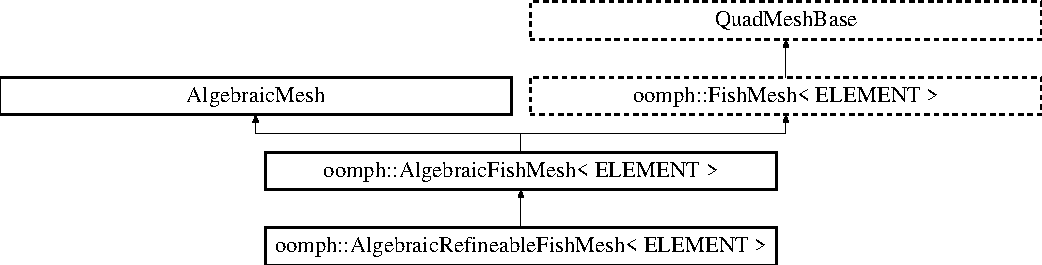
\includegraphics[height=3.555556cm]{classoomph_1_1AlgebraicFishMesh}
\end{center}
\end{figure}
\subsection*{Public Member Functions}
\begin{DoxyCompactItemize}
\item 
\hyperlink{classoomph_1_1AlgebraicFishMesh_a4382cbf0c75b2b76c9b28e9bae45fd4f}{Algebraic\+Fish\+Mesh} (Time\+Stepper $\ast$time\+\_\+stepper\+\_\+pt=\&Mesh\+::\+Default\+\_\+\+Time\+Stepper)
\begin{DoxyCompactList}\small\item\em Constructor\+: Pass pointer to timestepper. (defaults to (Steady) default timestepper defined in Mesh) \end{DoxyCompactList}\item 
\hyperlink{classoomph_1_1AlgebraicFishMesh_aac4b7f18a6e1d10c64edf431af921ce7}{Algebraic\+Fish\+Mesh} (Geom\+Object $\ast$back\+\_\+pt, Time\+Stepper $\ast$time\+\_\+stepper\+\_\+pt=\&Mesh\+::\+Default\+\_\+\+Time\+Stepper)
\begin{DoxyCompactList}\small\item\em Constructor\+: Pass pointer Geom\+Object that defines the fish\textquotesingle{}s back and pointer to timestepper (defaults to (Steady) default timestepper defined in Mesh). \end{DoxyCompactList}\item 
virtual \hyperlink{classoomph_1_1AlgebraicFishMesh_a027d54d158e22ce8fe3c1246cb030440}{$\sim$\+Algebraic\+Fish\+Mesh} ()
\begin{DoxyCompactList}\small\item\em Destructor\+: empty. \end{DoxyCompactList}\item 
void \hyperlink{classoomph_1_1AlgebraicFishMesh_ac66d6542472dac702a7414aa9d7f995f}{algebraic\+\_\+node\+\_\+update} (const unsigned \&t, Algebraic\+Node $\ast$\&node\+\_\+pt)
\begin{DoxyCompactList}\small\item\em Update nodal position at time level t (t=0\+: present; t$>$0\+: previous) \end{DoxyCompactList}\item 
virtual void \hyperlink{classoomph_1_1AlgebraicFishMesh_a39cd5a86b0f762efd09f4fefba6da1c3}{node\+\_\+update} (const bool \&update\+\_\+all\+\_\+solid\+\_\+nodes=false)
\begin{DoxyCompactList}\small\item\em Resolve the node update function (we neither want the broken empty one in the Mesh base class nor the macro-\/element-\/based one in the Refineable\+Quad\+Mesh base class but the Algebraic\+Element one). \mbox{[}It doesn\textquotesingle{}t make sense to use this mesh with Solid\+Elements so we buffer the case if update\+\_\+all\+\_\+solid\+\_\+nodes is set to true.\mbox{]}. \end{DoxyCompactList}\item 
void \hyperlink{classoomph_1_1AlgebraicFishMesh_a4f992939c299f87abc762c14aab50b5c}{update\+\_\+node\+\_\+update} (Algebraic\+Node $\ast$\&node\+\_\+pt)
\begin{DoxyCompactList}\small\item\em Update the geometric references that are used to update node after mesh adaptation. We\textquotesingle{}re assuming that the Geom\+Object that specifies the fish back does not have sub-\/objects, therefore no update is required -- all reference values can simply be scaled. We simply paranoid-\/check that this is actually the case, by checking if locate\+\_\+zeta() returns the original data. \end{DoxyCompactList}\end{DoxyCompactItemize}
\subsection*{Protected Member Functions}
\begin{DoxyCompactItemize}
\item 
void \hyperlink{classoomph_1_1AlgebraicFishMesh_a4aee83d1b0a42418fe886b2f244c1d49}{node\+\_\+update\+\_\+in\+\_\+body} (const unsigned \&t, Algebraic\+Node $\ast$\&node\+\_\+pt)
\begin{DoxyCompactList}\small\item\em Algebraic update function for nodes in upper/lower body. \end{DoxyCompactList}\item 
void \hyperlink{classoomph_1_1AlgebraicFishMesh_ad4a6f95e21e3d81b9defde90636e7d45}{node\+\_\+update\+\_\+in\+\_\+fin} (const unsigned \&t, Algebraic\+Node $\ast$\&node\+\_\+pt)
\begin{DoxyCompactList}\small\item\em Algebraic update function for nodes in upper/lower fin. \end{DoxyCompactList}\item 
void \hyperlink{classoomph_1_1AlgebraicFishMesh_a1a6d22eedc77299d843274e8ce34b560}{setup\+\_\+algebraic\+\_\+node\+\_\+update} ()
\begin{DoxyCompactList}\small\item\em Setup algebraic update operation for all nodes (separate function because this task needs to be performed by both constructors) \end{DoxyCompactList}\end{DoxyCompactItemize}
\subsection*{Additional Inherited Members}


\subsection{Detailed Description}
\subsubsection*{template$<$class E\+L\+E\+M\+E\+NT$>$\newline
class oomph\+::\+Algebraic\+Fish\+Mesh$<$ E\+L\+E\+M\+E\+N\+T $>$}

Fish shaped mesh with algebraic node update function for nodes. 

Definition at line 349 of file fish\+\_\+mesh.\+template.\+h.



\subsection{Constructor \& Destructor Documentation}
\mbox{\Hypertarget{classoomph_1_1AlgebraicFishMesh_a4382cbf0c75b2b76c9b28e9bae45fd4f}\label{classoomph_1_1AlgebraicFishMesh_a4382cbf0c75b2b76c9b28e9bae45fd4f}} 
\index{oomph\+::\+Algebraic\+Fish\+Mesh@{oomph\+::\+Algebraic\+Fish\+Mesh}!Algebraic\+Fish\+Mesh@{Algebraic\+Fish\+Mesh}}
\index{Algebraic\+Fish\+Mesh@{Algebraic\+Fish\+Mesh}!oomph\+::\+Algebraic\+Fish\+Mesh@{oomph\+::\+Algebraic\+Fish\+Mesh}}
\subsubsection{\texorpdfstring{Algebraic\+Fish\+Mesh()}{AlgebraicFishMesh()}\hspace{0.1cm}{\footnotesize\ttfamily [1/2]}}
{\footnotesize\ttfamily template$<$class E\+L\+E\+M\+E\+NT $>$ \\
\hyperlink{classoomph_1_1AlgebraicFishMesh}{oomph\+::\+Algebraic\+Fish\+Mesh}$<$ E\+L\+E\+M\+E\+NT $>$\+::\hyperlink{classoomph_1_1AlgebraicFishMesh}{Algebraic\+Fish\+Mesh} (\begin{DoxyParamCaption}\item[{Time\+Stepper $\ast$}]{time\+\_\+stepper\+\_\+pt = {\ttfamily \&Mesh\+:\+:Default\+\_\+TimeStepper} }\end{DoxyParamCaption})\hspace{0.3cm}{\ttfamily [inline]}}



Constructor\+: Pass pointer to timestepper. (defaults to (Steady) default timestepper defined in Mesh) 



Definition at line 357 of file fish\+\_\+mesh.\+template.\+h.

\mbox{\Hypertarget{classoomph_1_1AlgebraicFishMesh_aac4b7f18a6e1d10c64edf431af921ce7}\label{classoomph_1_1AlgebraicFishMesh_aac4b7f18a6e1d10c64edf431af921ce7}} 
\index{oomph\+::\+Algebraic\+Fish\+Mesh@{oomph\+::\+Algebraic\+Fish\+Mesh}!Algebraic\+Fish\+Mesh@{Algebraic\+Fish\+Mesh}}
\index{Algebraic\+Fish\+Mesh@{Algebraic\+Fish\+Mesh}!oomph\+::\+Algebraic\+Fish\+Mesh@{oomph\+::\+Algebraic\+Fish\+Mesh}}
\subsubsection{\texorpdfstring{Algebraic\+Fish\+Mesh()}{AlgebraicFishMesh()}\hspace{0.1cm}{\footnotesize\ttfamily [2/2]}}
{\footnotesize\ttfamily template$<$class E\+L\+E\+M\+E\+NT $>$ \\
\hyperlink{classoomph_1_1AlgebraicFishMesh}{oomph\+::\+Algebraic\+Fish\+Mesh}$<$ E\+L\+E\+M\+E\+NT $>$\+::\hyperlink{classoomph_1_1AlgebraicFishMesh}{Algebraic\+Fish\+Mesh} (\begin{DoxyParamCaption}\item[{Geom\+Object $\ast$}]{back\+\_\+pt,  }\item[{Time\+Stepper $\ast$}]{time\+\_\+stepper\+\_\+pt = {\ttfamily \&Mesh\+:\+:Default\+\_\+TimeStepper} }\end{DoxyParamCaption})\hspace{0.3cm}{\ttfamily [inline]}}



Constructor\+: Pass pointer Geom\+Object that defines the fish\textquotesingle{}s back and pointer to timestepper (defaults to (Steady) default timestepper defined in Mesh). 



Definition at line 367 of file fish\+\_\+mesh.\+template.\+h.

\mbox{\Hypertarget{classoomph_1_1AlgebraicFishMesh_a027d54d158e22ce8fe3c1246cb030440}\label{classoomph_1_1AlgebraicFishMesh_a027d54d158e22ce8fe3c1246cb030440}} 
\index{oomph\+::\+Algebraic\+Fish\+Mesh@{oomph\+::\+Algebraic\+Fish\+Mesh}!````~Algebraic\+Fish\+Mesh@{$\sim$\+Algebraic\+Fish\+Mesh}}
\index{````~Algebraic\+Fish\+Mesh@{$\sim$\+Algebraic\+Fish\+Mesh}!oomph\+::\+Algebraic\+Fish\+Mesh@{oomph\+::\+Algebraic\+Fish\+Mesh}}
\subsubsection{\texorpdfstring{$\sim$\+Algebraic\+Fish\+Mesh()}{~AlgebraicFishMesh()}}
{\footnotesize\ttfamily template$<$class E\+L\+E\+M\+E\+NT $>$ \\
virtual \hyperlink{classoomph_1_1AlgebraicFishMesh}{oomph\+::\+Algebraic\+Fish\+Mesh}$<$ E\+L\+E\+M\+E\+NT $>$\+::$\sim$\hyperlink{classoomph_1_1AlgebraicFishMesh}{Algebraic\+Fish\+Mesh} (\begin{DoxyParamCaption}{ }\end{DoxyParamCaption})\hspace{0.3cm}{\ttfamily [inline]}, {\ttfamily [virtual]}}



Destructor\+: empty. 



Definition at line 379 of file fish\+\_\+mesh.\+template.\+h.



\subsection{Member Function Documentation}
\mbox{\Hypertarget{classoomph_1_1AlgebraicFishMesh_ac66d6542472dac702a7414aa9d7f995f}\label{classoomph_1_1AlgebraicFishMesh_ac66d6542472dac702a7414aa9d7f995f}} 
\index{oomph\+::\+Algebraic\+Fish\+Mesh@{oomph\+::\+Algebraic\+Fish\+Mesh}!algebraic\+\_\+node\+\_\+update@{algebraic\+\_\+node\+\_\+update}}
\index{algebraic\+\_\+node\+\_\+update@{algebraic\+\_\+node\+\_\+update}!oomph\+::\+Algebraic\+Fish\+Mesh@{oomph\+::\+Algebraic\+Fish\+Mesh}}
\subsubsection{\texorpdfstring{algebraic\+\_\+node\+\_\+update()}{algebraic\_node\_update()}}
{\footnotesize\ttfamily template$<$class E\+L\+E\+M\+E\+NT $>$ \\
void \hyperlink{classoomph_1_1AlgebraicFishMesh}{oomph\+::\+Algebraic\+Fish\+Mesh}$<$ E\+L\+E\+M\+E\+NT $>$\+::algebraic\+\_\+node\+\_\+update (\begin{DoxyParamCaption}\item[{const unsigned \&}]{t,  }\item[{Algebraic\+Node $\ast$\&}]{node\+\_\+pt }\end{DoxyParamCaption})\hspace{0.3cm}{\ttfamily [inline]}}



Update nodal position at time level t (t=0\+: present; t$>$0\+: previous) 



Definition at line 383 of file fish\+\_\+mesh.\+template.\+h.



References oomph\+::\+Fish\+Mesh$<$ E\+L\+E\+M\+E\+N\+T $>$\+::\+Lower\+\_\+body, oomph\+::\+Fish\+Mesh$<$ E\+L\+E\+M\+E\+N\+T $>$\+::\+Lower\+\_\+fin, oomph\+::\+Fish\+Mesh$<$ E\+L\+E\+M\+E\+N\+T $>$\+::\+Upper\+\_\+body, and oomph\+::\+Fish\+Mesh$<$ E\+L\+E\+M\+E\+N\+T $>$\+::\+Upper\+\_\+fin.

\mbox{\Hypertarget{classoomph_1_1AlgebraicFishMesh_a39cd5a86b0f762efd09f4fefba6da1c3}\label{classoomph_1_1AlgebraicFishMesh_a39cd5a86b0f762efd09f4fefba6da1c3}} 
\index{oomph\+::\+Algebraic\+Fish\+Mesh@{oomph\+::\+Algebraic\+Fish\+Mesh}!node\+\_\+update@{node\+\_\+update}}
\index{node\+\_\+update@{node\+\_\+update}!oomph\+::\+Algebraic\+Fish\+Mesh@{oomph\+::\+Algebraic\+Fish\+Mesh}}
\subsubsection{\texorpdfstring{node\+\_\+update()}{node\_update()}}
{\footnotesize\ttfamily template$<$class E\+L\+E\+M\+E\+NT $>$ \\
virtual void \hyperlink{classoomph_1_1AlgebraicFishMesh}{oomph\+::\+Algebraic\+Fish\+Mesh}$<$ E\+L\+E\+M\+E\+NT $>$\+::node\+\_\+update (\begin{DoxyParamCaption}\item[{const bool \&}]{update\+\_\+all\+\_\+solid\+\_\+nodes = {\ttfamily false} }\end{DoxyParamCaption})\hspace{0.3cm}{\ttfamily [inline]}, {\ttfamily [virtual]}}



Resolve the node update function (we neither want the broken empty one in the Mesh base class nor the macro-\/element-\/based one in the Refineable\+Quad\+Mesh base class but the Algebraic\+Element one). \mbox{[}It doesn\textquotesingle{}t make sense to use this mesh with Solid\+Elements so we buffer the case if update\+\_\+all\+\_\+solid\+\_\+nodes is set to true.\mbox{]}. 



Reimplemented in \hyperlink{classoomph_1_1AlgebraicRefineableFishMesh_a8123da4b48355b39f19e0494a9d4545c}{oomph\+::\+Algebraic\+Refineable\+Fish\+Mesh$<$ E\+L\+E\+M\+E\+N\+T $>$}.



Definition at line 422 of file fish\+\_\+mesh.\+template.\+h.



Referenced by oomph\+::\+Algebraic\+Refineable\+Fish\+Mesh$<$ E\+L\+E\+M\+E\+N\+T $>$\+::node\+\_\+update().

\mbox{\Hypertarget{classoomph_1_1AlgebraicFishMesh_a4aee83d1b0a42418fe886b2f244c1d49}\label{classoomph_1_1AlgebraicFishMesh_a4aee83d1b0a42418fe886b2f244c1d49}} 
\index{oomph\+::\+Algebraic\+Fish\+Mesh@{oomph\+::\+Algebraic\+Fish\+Mesh}!node\+\_\+update\+\_\+in\+\_\+body@{node\+\_\+update\+\_\+in\+\_\+body}}
\index{node\+\_\+update\+\_\+in\+\_\+body@{node\+\_\+update\+\_\+in\+\_\+body}!oomph\+::\+Algebraic\+Fish\+Mesh@{oomph\+::\+Algebraic\+Fish\+Mesh}}
\subsubsection{\texorpdfstring{node\+\_\+update\+\_\+in\+\_\+body()}{node\_update\_in\_body()}}
{\footnotesize\ttfamily template$<$class E\+L\+E\+M\+E\+NT $>$ \\
void \hyperlink{classoomph_1_1AlgebraicFishMesh}{oomph\+::\+Algebraic\+Fish\+Mesh}$<$ E\+L\+E\+M\+E\+NT $>$\+::node\+\_\+update\+\_\+in\+\_\+body (\begin{DoxyParamCaption}\item[{const unsigned \&}]{t,  }\item[{Algebraic\+Node $\ast$\&}]{node\+\_\+pt }\end{DoxyParamCaption})\hspace{0.3cm}{\ttfamily [protected]}}



Algebraic update function for nodes in upper/lower body. 

Algebraic update function\+: Update in (upper or lower) body according to wall shape at time level t (t=0\+: present; t$>$0\+: previous) 

Definition at line 950 of file fish\+\_\+mesh.\+template.\+cc.



References oomph\+::\+Fish\+Mesh$<$ E\+L\+E\+M\+E\+N\+T $>$\+::\+Domain\+\_\+pt, oomph\+::\+Fish\+Domain\+::x\+\_\+mouth(), oomph\+::\+Fish\+Domain\+::xi\+\_\+nose(), and oomph\+::\+Fish\+Domain\+::xi\+\_\+tail().

\mbox{\Hypertarget{classoomph_1_1AlgebraicFishMesh_ad4a6f95e21e3d81b9defde90636e7d45}\label{classoomph_1_1AlgebraicFishMesh_ad4a6f95e21e3d81b9defde90636e7d45}} 
\index{oomph\+::\+Algebraic\+Fish\+Mesh@{oomph\+::\+Algebraic\+Fish\+Mesh}!node\+\_\+update\+\_\+in\+\_\+fin@{node\+\_\+update\+\_\+in\+\_\+fin}}
\index{node\+\_\+update\+\_\+in\+\_\+fin@{node\+\_\+update\+\_\+in\+\_\+fin}!oomph\+::\+Algebraic\+Fish\+Mesh@{oomph\+::\+Algebraic\+Fish\+Mesh}}
\subsubsection{\texorpdfstring{node\+\_\+update\+\_\+in\+\_\+fin()}{node\_update\_in\_fin()}}
{\footnotesize\ttfamily template$<$class E\+L\+E\+M\+E\+NT $>$ \\
void \hyperlink{classoomph_1_1AlgebraicFishMesh}{oomph\+::\+Algebraic\+Fish\+Mesh}$<$ E\+L\+E\+M\+E\+NT $>$\+::node\+\_\+update\+\_\+in\+\_\+fin (\begin{DoxyParamCaption}\item[{const unsigned \&}]{t,  }\item[{Algebraic\+Node $\ast$\&}]{node\+\_\+pt }\end{DoxyParamCaption})\hspace{0.3cm}{\ttfamily [protected]}}



Algebraic update function for nodes in upper/lower fin. 

Algebraic update function\+: Update in (upper or lower) fin according to wall shape at time level t (t=0\+: present; t$>$0\+: previous) 

Definition at line 1010 of file fish\+\_\+mesh.\+template.\+cc.



References oomph\+::\+Fish\+Mesh$<$ E\+L\+E\+M\+E\+N\+T $>$\+::\+Domain\+\_\+pt, oomph\+::\+Fish\+Domain\+::x\+\_\+fin(), oomph\+::\+Fish\+Domain\+::xi\+\_\+tail(), and oomph\+::\+Fish\+Domain\+::y\+\_\+fin().

\mbox{\Hypertarget{classoomph_1_1AlgebraicFishMesh_a1a6d22eedc77299d843274e8ce34b560}\label{classoomph_1_1AlgebraicFishMesh_a1a6d22eedc77299d843274e8ce34b560}} 
\index{oomph\+::\+Algebraic\+Fish\+Mesh@{oomph\+::\+Algebraic\+Fish\+Mesh}!setup\+\_\+algebraic\+\_\+node\+\_\+update@{setup\+\_\+algebraic\+\_\+node\+\_\+update}}
\index{setup\+\_\+algebraic\+\_\+node\+\_\+update@{setup\+\_\+algebraic\+\_\+node\+\_\+update}!oomph\+::\+Algebraic\+Fish\+Mesh@{oomph\+::\+Algebraic\+Fish\+Mesh}}
\subsubsection{\texorpdfstring{setup\+\_\+algebraic\+\_\+node\+\_\+update()}{setup\_algebraic\_node\_update()}}
{\footnotesize\ttfamily template$<$class E\+L\+E\+M\+E\+NT $>$ \\
void \hyperlink{classoomph_1_1AlgebraicFishMesh}{oomph\+::\+Algebraic\+Fish\+Mesh}$<$ E\+L\+E\+M\+E\+NT $>$\+::setup\+\_\+algebraic\+\_\+node\+\_\+update (\begin{DoxyParamCaption}{ }\end{DoxyParamCaption})\hspace{0.3cm}{\ttfamily [protected]}}



Setup algebraic update operation for all nodes (separate function because this task needs to be performed by both constructors) 

Setup algebraic update operation. Nodes are \char`\"{}suspended\char`\"{} from the fish\textquotesingle{}s back and the upper edge of the fin. Nodes in the lower half are placed symmetrically. Pointer to algebraic element in lower body 

Definition at line 728 of file fish\+\_\+mesh.\+template.\+cc.



References oomph\+::\+Fish\+Mesh$<$ E\+L\+E\+M\+E\+N\+T $>$\+::\+Back\+\_\+pt, oomph\+::\+Fish\+Mesh$<$ E\+L\+E\+M\+E\+N\+T $>$\+::\+Lower\+\_\+body, oomph\+::\+Fish\+Mesh$<$ E\+L\+E\+M\+E\+N\+T $>$\+::\+Lower\+\_\+fin, oomph\+::\+Fish\+Mesh$<$ E\+L\+E\+M\+E\+N\+T $>$\+::\+Upper\+\_\+body, and oomph\+::\+Fish\+Mesh$<$ E\+L\+E\+M\+E\+N\+T $>$\+::\+Upper\+\_\+fin.

\mbox{\Hypertarget{classoomph_1_1AlgebraicFishMesh_a4f992939c299f87abc762c14aab50b5c}\label{classoomph_1_1AlgebraicFishMesh_a4f992939c299f87abc762c14aab50b5c}} 
\index{oomph\+::\+Algebraic\+Fish\+Mesh@{oomph\+::\+Algebraic\+Fish\+Mesh}!update\+\_\+node\+\_\+update@{update\+\_\+node\+\_\+update}}
\index{update\+\_\+node\+\_\+update@{update\+\_\+node\+\_\+update}!oomph\+::\+Algebraic\+Fish\+Mesh@{oomph\+::\+Algebraic\+Fish\+Mesh}}
\subsubsection{\texorpdfstring{update\+\_\+node\+\_\+update()}{update\_node\_update()}}
{\footnotesize\ttfamily template$<$class E\+L\+E\+M\+E\+NT $>$ \\
void \hyperlink{classoomph_1_1AlgebraicFishMesh}{oomph\+::\+Algebraic\+Fish\+Mesh}$<$ E\+L\+E\+M\+E\+NT $>$\+::update\+\_\+node\+\_\+update (\begin{DoxyParamCaption}\item[{Algebraic\+Node $\ast$\&}]{node\+\_\+pt }\end{DoxyParamCaption})\hspace{0.3cm}{\ttfamily [inline]}}



Update the geometric references that are used to update node after mesh adaptation. We\textquotesingle{}re assuming that the Geom\+Object that specifies the fish back does not have sub-\/objects, therefore no update is required -- all reference values can simply be scaled. We simply paranoid-\/check that this is actually the case, by checking if locate\+\_\+zeta() returns the original data. 

Start coordinate on wall (near nose)

End coordinate on wall (near tail)

Check halfway along the object 

Definition at line 453 of file fish\+\_\+mesh.\+template.\+h.



References oomph\+::\+Fish\+Mesh$<$ E\+L\+E\+M\+E\+N\+T $>$\+::\+Back\+\_\+pt, oomph\+::\+Fish\+Mesh$<$ E\+L\+E\+M\+E\+N\+T $>$\+::\+Domain\+\_\+pt, oomph\+::\+Fish\+Domain\+::xi\+\_\+nose(), and oomph\+::\+Fish\+Domain\+::xi\+\_\+tail().



The documentation for this class was generated from the following files\+:\begin{DoxyCompactItemize}
\item 
\hyperlink{fish__mesh_8template_8h}{fish\+\_\+mesh.\+template.\+h}\item 
\hyperlink{fish__mesh_8template_8cc}{fish\+\_\+mesh.\+template.\+cc}\end{DoxyCompactItemize}

\hypertarget{classoomph_1_1AlgebraicFSIDrivenCavityMesh}{}\section{oomph\+:\+:Algebraic\+F\+S\+I\+Driven\+Cavity\+Mesh$<$ E\+L\+E\+M\+E\+NT $>$ Class Template Reference}
\label{classoomph_1_1AlgebraicFSIDrivenCavityMesh}\index{oomph\+::\+Algebraic\+F\+S\+I\+Driven\+Cavity\+Mesh$<$ E\+L\+E\+M\+E\+N\+T $>$@{oomph\+::\+Algebraic\+F\+S\+I\+Driven\+Cavity\+Mesh$<$ E\+L\+E\+M\+E\+N\+T $>$}}


{\ttfamily \#include $<$fsi\+\_\+driven\+\_\+cavity\+\_\+mesh.\+template.\+h$>$}

Inheritance diagram for oomph\+:\+:Algebraic\+F\+S\+I\+Driven\+Cavity\+Mesh$<$ E\+L\+E\+M\+E\+NT $>$\+:\begin{figure}[H]
\begin{center}
\leavevmode
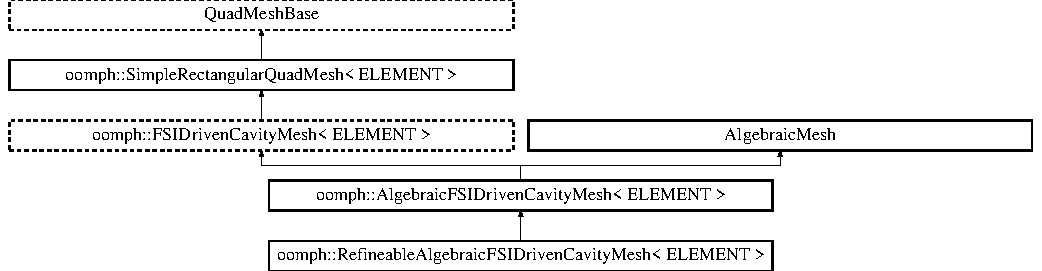
\includegraphics[height=4.375000cm]{classoomph_1_1AlgebraicFSIDrivenCavityMesh}
\end{center}
\end{figure}
\subsection*{Public Member Functions}
\begin{DoxyCompactItemize}
\item 
\hyperlink{classoomph_1_1AlgebraicFSIDrivenCavityMesh_a973ccadc769d98fed6bc9dd4eff32083}{Algebraic\+F\+S\+I\+Driven\+Cavity\+Mesh} (const unsigned \&\hyperlink{classoomph_1_1SimpleRectangularQuadMesh_a4ff7678ec433180e2245ea2147f222b7}{nx}, const unsigned \&\hyperlink{classoomph_1_1SimpleRectangularQuadMesh_a45011f22dedd480392b1f376e4269921}{ny}, const double \&lx, const double \&ly, const double \&gap\+\_\+fraction, \hyperlink{classoomph_1_1GeomObject}{Geom\+Object} $\ast$wall\+\_\+pt, \hyperlink{classoomph_1_1TimeStepper}{Time\+Stepper} $\ast$time\+\_\+stepper\+\_\+pt=\&\hyperlink{classoomph_1_1Mesh_a12243d0fee2b1fcee729ee5a4777ea10}{Mesh\+::\+Default\+\_\+\+Time\+Stepper})
\begin{DoxyCompactList}\small\item\em Constructor\+: Pass number of elements, lengths, pointer to \hyperlink{classoomph_1_1GeomObject}{Geom\+Object} that defines the collapsible segment and pointer to \hyperlink{classoomph_1_1TimeStepper}{Time\+Stepper} (defaults to the default timestepper, \hyperlink{classoomph_1_1Steady}{Steady}). \end{DoxyCompactList}\item 
virtual \hyperlink{classoomph_1_1AlgebraicFSIDrivenCavityMesh_a048a142aff0ca5fd62273f756bce4ab6}{$\sim$\+Algebraic\+F\+S\+I\+Driven\+Cavity\+Mesh} ()
\begin{DoxyCompactList}\small\item\em Destructor\+: empty. \end{DoxyCompactList}\item 
void \hyperlink{classoomph_1_1AlgebraicFSIDrivenCavityMesh_a56c72b78935e84f7fef3f6b5d85556c3}{algebraic\+\_\+node\+\_\+update} (const unsigned \&\hyperlink{cfortran_8h_af6f0bd3dc13317f895c91323c25c2b8f}{t}, \hyperlink{classoomph_1_1AlgebraicNode}{Algebraic\+Node} $\ast$\&\hyperlink{classoomph_1_1AlgebraicMesh_aedeebbe95d2f8e67e9939cecd1be3933}{node\+\_\+pt})
\begin{DoxyCompactList}\small\item\em Update nodal position at time level t (t=0\+: present; t$>$0\+: previous) \end{DoxyCompactList}\item 
void \hyperlink{classoomph_1_1AlgebraicFSIDrivenCavityMesh_a87d34d6cf84c62a9049773451c664176}{update\+\_\+node\+\_\+update} (\hyperlink{classoomph_1_1AlgebraicNode}{Algebraic\+Node} $\ast$\&\hyperlink{classoomph_1_1AlgebraicMesh_aedeebbe95d2f8e67e9939cecd1be3933}{node\+\_\+pt})
\begin{DoxyCompactList}\small\item\em Update the node-\/udate data after mesh adaptation. Empty -- no update of node update required as this is non-\/refineable mesh. \end{DoxyCompactList}\end{DoxyCompactItemize}
\subsection*{Protected Member Functions}
\begin{DoxyCompactItemize}
\item 
void \hyperlink{classoomph_1_1AlgebraicFSIDrivenCavityMesh_a7f6b7c3dae1c61c2cdb0cbd229173114}{setup\+\_\+algebraic\+\_\+node\+\_\+update} ()
\begin{DoxyCompactList}\small\item\em Function to setup the algebraic node update. \end{DoxyCompactList}\end{DoxyCompactItemize}
\subsection*{Additional Inherited Members}


\subsection{Detailed Description}
\subsubsection*{template$<$class E\+L\+E\+M\+E\+NT$>$\newline
class oomph\+::\+Algebraic\+F\+S\+I\+Driven\+Cavity\+Mesh$<$ E\+L\+E\+M\+E\+N\+T $>$}

Alebraic node update version of \hyperlink{classoomph_1_1FSIDrivenCavityMesh}{F\+S\+I\+Driven\+Cavity\+Mesh}
\begin{DoxyItemize}
\item Boundary 0 is the moving lid.
\item Boundary 1 is the gap above the moving lid on the right wall
\item Boundary 2 is the rigid part of the right wall
\item Boundary 3 is the moving (elastic) wall
\item Boundary 4 is the rigid part of the left wall
\item Boundary 5 is the gap above the moving lid on the left wall 
\end{DoxyItemize}

Definition at line 173 of file fsi\+\_\+driven\+\_\+cavity\+\_\+mesh.\+template.\+h.



\subsection{Constructor \& Destructor Documentation}
\mbox{\Hypertarget{classoomph_1_1AlgebraicFSIDrivenCavityMesh_a973ccadc769d98fed6bc9dd4eff32083}\label{classoomph_1_1AlgebraicFSIDrivenCavityMesh_a973ccadc769d98fed6bc9dd4eff32083}} 
\index{oomph\+::\+Algebraic\+F\+S\+I\+Driven\+Cavity\+Mesh@{oomph\+::\+Algebraic\+F\+S\+I\+Driven\+Cavity\+Mesh}!Algebraic\+F\+S\+I\+Driven\+Cavity\+Mesh@{Algebraic\+F\+S\+I\+Driven\+Cavity\+Mesh}}
\index{Algebraic\+F\+S\+I\+Driven\+Cavity\+Mesh@{Algebraic\+F\+S\+I\+Driven\+Cavity\+Mesh}!oomph\+::\+Algebraic\+F\+S\+I\+Driven\+Cavity\+Mesh@{oomph\+::\+Algebraic\+F\+S\+I\+Driven\+Cavity\+Mesh}}
\subsubsection{\texorpdfstring{Algebraic\+F\+S\+I\+Driven\+Cavity\+Mesh()}{AlgebraicFSIDrivenCavityMesh()}}
{\footnotesize\ttfamily template$<$class E\+L\+E\+M\+E\+NT $>$ \\
\hyperlink{classoomph_1_1AlgebraicFSIDrivenCavityMesh}{oomph\+::\+Algebraic\+F\+S\+I\+Driven\+Cavity\+Mesh}$<$ E\+L\+E\+M\+E\+NT $>$\+::\hyperlink{classoomph_1_1AlgebraicFSIDrivenCavityMesh}{Algebraic\+F\+S\+I\+Driven\+Cavity\+Mesh} (\begin{DoxyParamCaption}\item[{const unsigned \&}]{nx,  }\item[{const unsigned \&}]{ny,  }\item[{const double \&}]{lx,  }\item[{const double \&}]{ly,  }\item[{const double \&}]{gap\+\_\+fraction,  }\item[{\hyperlink{classoomph_1_1GeomObject}{Geom\+Object} $\ast$}]{wall\+\_\+pt,  }\item[{\hyperlink{classoomph_1_1TimeStepper}{Time\+Stepper} $\ast$}]{time\+\_\+stepper\+\_\+pt = {\ttfamily \&\hyperlink{classoomph_1_1Mesh_a12243d0fee2b1fcee729ee5a4777ea10}{Mesh\+::\+Default\+\_\+\+Time\+Stepper}} }\end{DoxyParamCaption})\hspace{0.3cm}{\ttfamily [inline]}}



Constructor\+: Pass number of elements, lengths, pointer to \hyperlink{classoomph_1_1GeomObject}{Geom\+Object} that defines the collapsible segment and pointer to \hyperlink{classoomph_1_1TimeStepper}{Time\+Stepper} (defaults to the default timestepper, \hyperlink{classoomph_1_1Steady}{Steady}). 



Definition at line 184 of file fsi\+\_\+driven\+\_\+cavity\+\_\+mesh.\+template.\+h.



References oomph\+::\+Algebraic\+Mesh\+::add\+\_\+geom\+\_\+object\+\_\+list\+\_\+pt().

\mbox{\Hypertarget{classoomph_1_1AlgebraicFSIDrivenCavityMesh_a048a142aff0ca5fd62273f756bce4ab6}\label{classoomph_1_1AlgebraicFSIDrivenCavityMesh_a048a142aff0ca5fd62273f756bce4ab6}} 
\index{oomph\+::\+Algebraic\+F\+S\+I\+Driven\+Cavity\+Mesh@{oomph\+::\+Algebraic\+F\+S\+I\+Driven\+Cavity\+Mesh}!````~Algebraic\+F\+S\+I\+Driven\+Cavity\+Mesh@{$\sim$\+Algebraic\+F\+S\+I\+Driven\+Cavity\+Mesh}}
\index{````~Algebraic\+F\+S\+I\+Driven\+Cavity\+Mesh@{$\sim$\+Algebraic\+F\+S\+I\+Driven\+Cavity\+Mesh}!oomph\+::\+Algebraic\+F\+S\+I\+Driven\+Cavity\+Mesh@{oomph\+::\+Algebraic\+F\+S\+I\+Driven\+Cavity\+Mesh}}
\subsubsection{\texorpdfstring{$\sim$\+Algebraic\+F\+S\+I\+Driven\+Cavity\+Mesh()}{~AlgebraicFSIDrivenCavityMesh()}}
{\footnotesize\ttfamily template$<$class E\+L\+E\+M\+E\+NT $>$ \\
virtual \hyperlink{classoomph_1_1AlgebraicFSIDrivenCavityMesh}{oomph\+::\+Algebraic\+F\+S\+I\+Driven\+Cavity\+Mesh}$<$ E\+L\+E\+M\+E\+NT $>$\+::$\sim$\hyperlink{classoomph_1_1AlgebraicFSIDrivenCavityMesh}{Algebraic\+F\+S\+I\+Driven\+Cavity\+Mesh} (\begin{DoxyParamCaption}{ }\end{DoxyParamCaption})\hspace{0.3cm}{\ttfamily [inline]}, {\ttfamily [virtual]}}



Destructor\+: empty. 



Definition at line 203 of file fsi\+\_\+driven\+\_\+cavity\+\_\+mesh.\+template.\+h.



References oomph\+::\+Mesh\+::node\+\_\+pt(), and t.



\subsection{Member Function Documentation}
\mbox{\Hypertarget{classoomph_1_1AlgebraicFSIDrivenCavityMesh_a56c72b78935e84f7fef3f6b5d85556c3}\label{classoomph_1_1AlgebraicFSIDrivenCavityMesh_a56c72b78935e84f7fef3f6b5d85556c3}} 
\index{oomph\+::\+Algebraic\+F\+S\+I\+Driven\+Cavity\+Mesh@{oomph\+::\+Algebraic\+F\+S\+I\+Driven\+Cavity\+Mesh}!algebraic\+\_\+node\+\_\+update@{algebraic\+\_\+node\+\_\+update}}
\index{algebraic\+\_\+node\+\_\+update@{algebraic\+\_\+node\+\_\+update}!oomph\+::\+Algebraic\+F\+S\+I\+Driven\+Cavity\+Mesh@{oomph\+::\+Algebraic\+F\+S\+I\+Driven\+Cavity\+Mesh}}
\subsubsection{\texorpdfstring{algebraic\+\_\+node\+\_\+update()}{algebraic\_node\_update()}}
{\footnotesize\ttfamily template$<$class E\+L\+E\+M\+E\+NT $>$ \\
void \hyperlink{classoomph_1_1AlgebraicFSIDrivenCavityMesh}{oomph\+::\+Algebraic\+F\+S\+I\+Driven\+Cavity\+Mesh}$<$ E\+L\+E\+M\+E\+NT $>$\+::algebraic\+\_\+node\+\_\+update (\begin{DoxyParamCaption}\item[{const unsigned \&}]{t,  }\item[{\hyperlink{classoomph_1_1AlgebraicNode}{Algebraic\+Node} $\ast$\&}]{node\+\_\+pt }\end{DoxyParamCaption})\hspace{0.3cm}{\ttfamily [virtual]}}



Update nodal position at time level t (t=0\+: present; t$>$0\+: previous) 

Perform algebraic mesh update at time level t (t=0\+: present; t$>$0\+: previous) 

Implements \hyperlink{classoomph_1_1AlgebraicMesh_ab01d6f93354f3c4e5c9d1f0a5885a65b}{oomph\+::\+Algebraic\+Mesh}.



Definition at line 203 of file fsi\+\_\+driven\+\_\+cavity\+\_\+mesh.\+template.\+cc.



References oomph\+::\+Time\+Stepper\+::nprev\+\_\+values(), oomph\+::\+Node\+::position\+\_\+time\+\_\+stepper\+\_\+pt(), s, oomph\+::\+Global\+\_\+string\+\_\+for\+\_\+annotation\+::string(), oomph\+::\+Algebraic\+Node\+::vector\+\_\+geom\+\_\+object\+\_\+pt(), oomph\+::\+Algebraic\+Node\+::vector\+\_\+ref\+\_\+value(), and oomph\+::\+Node\+::x().

\mbox{\Hypertarget{classoomph_1_1AlgebraicFSIDrivenCavityMesh_a7f6b7c3dae1c61c2cdb0cbd229173114}\label{classoomph_1_1AlgebraicFSIDrivenCavityMesh_a7f6b7c3dae1c61c2cdb0cbd229173114}} 
\index{oomph\+::\+Algebraic\+F\+S\+I\+Driven\+Cavity\+Mesh@{oomph\+::\+Algebraic\+F\+S\+I\+Driven\+Cavity\+Mesh}!setup\+\_\+algebraic\+\_\+node\+\_\+update@{setup\+\_\+algebraic\+\_\+node\+\_\+update}}
\index{setup\+\_\+algebraic\+\_\+node\+\_\+update@{setup\+\_\+algebraic\+\_\+node\+\_\+update}!oomph\+::\+Algebraic\+F\+S\+I\+Driven\+Cavity\+Mesh@{oomph\+::\+Algebraic\+F\+S\+I\+Driven\+Cavity\+Mesh}}
\subsubsection{\texorpdfstring{setup\+\_\+algebraic\+\_\+node\+\_\+update()}{setup\_algebraic\_node\_update()}}
{\footnotesize\ttfamily template$<$class E\+L\+E\+M\+E\+NT $>$ \\
void \hyperlink{classoomph_1_1AlgebraicFSIDrivenCavityMesh}{oomph\+::\+Algebraic\+F\+S\+I\+Driven\+Cavity\+Mesh}$<$ E\+L\+E\+M\+E\+NT $>$\+::setup\+\_\+algebraic\+\_\+node\+\_\+update (\begin{DoxyParamCaption}{ }\end{DoxyParamCaption})\hspace{0.3cm}{\ttfamily [protected]}}



Function to setup the algebraic node update. 

Setup algebraic mesh update -- assumes that mesh has initially been set up with a flush upper wall. 

Definition at line 293 of file fsi\+\_\+driven\+\_\+cavity\+\_\+mesh.\+template.\+cc.



References oomph\+::\+Algebraic\+Node\+::add\+\_\+node\+\_\+update\+\_\+info(), e, oomph\+::\+Geom\+Object\+::locate\+\_\+zeta(), oomph\+::\+Mesh\+::nnode(), oomph\+::\+Mesh\+::node\+\_\+pt(), oomph\+::\+Geom\+Object\+::position(), s, oomph\+::\+F\+S\+I\+Driven\+Cavity\+Mesh$<$ E\+L\+E\+M\+E\+N\+T $>$\+::\+Wall\+\_\+pt, and oomph\+::\+Node\+::x().

\mbox{\Hypertarget{classoomph_1_1AlgebraicFSIDrivenCavityMesh_a87d34d6cf84c62a9049773451c664176}\label{classoomph_1_1AlgebraicFSIDrivenCavityMesh_a87d34d6cf84c62a9049773451c664176}} 
\index{oomph\+::\+Algebraic\+F\+S\+I\+Driven\+Cavity\+Mesh@{oomph\+::\+Algebraic\+F\+S\+I\+Driven\+Cavity\+Mesh}!update\+\_\+node\+\_\+update@{update\+\_\+node\+\_\+update}}
\index{update\+\_\+node\+\_\+update@{update\+\_\+node\+\_\+update}!oomph\+::\+Algebraic\+F\+S\+I\+Driven\+Cavity\+Mesh@{oomph\+::\+Algebraic\+F\+S\+I\+Driven\+Cavity\+Mesh}}
\subsubsection{\texorpdfstring{update\+\_\+node\+\_\+update()}{update\_node\_update()}}
{\footnotesize\ttfamily template$<$class E\+L\+E\+M\+E\+NT $>$ \\
void \hyperlink{classoomph_1_1AlgebraicFSIDrivenCavityMesh}{oomph\+::\+Algebraic\+F\+S\+I\+Driven\+Cavity\+Mesh}$<$ E\+L\+E\+M\+E\+NT $>$\+::update\+\_\+node\+\_\+update (\begin{DoxyParamCaption}\item[{\hyperlink{classoomph_1_1AlgebraicNode}{Algebraic\+Node} $\ast$\&}]{node\+\_\+pt }\end{DoxyParamCaption})\hspace{0.3cm}{\ttfamily [inline]}, {\ttfamily [virtual]}}



Update the node-\/udate data after mesh adaptation. Empty -- no update of node update required as this is non-\/refineable mesh. 



Implements \hyperlink{classoomph_1_1AlgebraicMesh_a6c6a35ae2be6e2766f5b80d85693c1ce}{oomph\+::\+Algebraic\+Mesh}.



Reimplemented in \hyperlink{classoomph_1_1RefineableAlgebraicFSIDrivenCavityMesh_aa68685323573763e1ded0cceed5ad14f}{oomph\+::\+Refineable\+Algebraic\+F\+S\+I\+Driven\+Cavity\+Mesh$<$ E\+L\+E\+M\+E\+N\+T $>$}.



Definition at line 212 of file fsi\+\_\+driven\+\_\+cavity\+\_\+mesh.\+template.\+h.



The documentation for this class was generated from the following files\+:\begin{DoxyCompactItemize}
\item 
\hyperlink{fsi__driven__cavity__mesh_8template_8h}{fsi\+\_\+driven\+\_\+cavity\+\_\+mesh.\+template.\+h}\item 
\hyperlink{fsi__driven__cavity__mesh_8template_8cc}{fsi\+\_\+driven\+\_\+cavity\+\_\+mesh.\+template.\+cc}\end{DoxyCompactItemize}

\hypertarget{classoomph_1_1AlgebraicRefineableFishMesh}{}\section{oomph\+:\+:Algebraic\+Refineable\+Fish\+Mesh$<$ E\+L\+E\+M\+E\+NT $>$ Class Template Reference}
\label{classoomph_1_1AlgebraicRefineableFishMesh}\index{oomph\+::\+Algebraic\+Refineable\+Fish\+Mesh$<$ E\+L\+E\+M\+E\+N\+T $>$@{oomph\+::\+Algebraic\+Refineable\+Fish\+Mesh$<$ E\+L\+E\+M\+E\+N\+T $>$}}


Refineable fish shaped mesh with algebraic node update function.  




{\ttfamily \#include $<$fish\+\_\+mesh.\+template.\+h$>$}

Inheritance diagram for oomph\+:\+:Algebraic\+Refineable\+Fish\+Mesh$<$ E\+L\+E\+M\+E\+NT $>$\+:\begin{figure}[H]
\begin{center}
\leavevmode
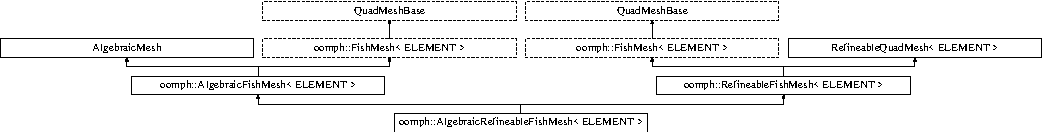
\includegraphics[height=2.488889cm]{classoomph_1_1AlgebraicRefineableFishMesh}
\end{center}
\end{figure}
\subsection*{Public Member Functions}
\begin{DoxyCompactItemize}
\item 
\hyperlink{classoomph_1_1AlgebraicRefineableFishMesh_afe4643b107e47fbad0c8836bc0516518}{Algebraic\+Refineable\+Fish\+Mesh} (\hyperlink{classoomph_1_1TimeStepper}{Time\+Stepper} $\ast$time\+\_\+stepper\+\_\+pt=\&\hyperlink{classoomph_1_1Mesh_a12243d0fee2b1fcee729ee5a4777ea10}{Mesh\+::\+Default\+\_\+\+Time\+Stepper})
\item 
\hyperlink{classoomph_1_1AlgebraicRefineableFishMesh_a04f6b6114c70638b4f26ac6b70f5c0fe}{Algebraic\+Refineable\+Fish\+Mesh} (\hyperlink{classoomph_1_1GeomObject}{Geom\+Object} $\ast$back\+\_\+pt, \hyperlink{classoomph_1_1TimeStepper}{Time\+Stepper} $\ast$time\+\_\+stepper\+\_\+pt=\&\hyperlink{classoomph_1_1Mesh_a12243d0fee2b1fcee729ee5a4777ea10}{Mesh\+::\+Default\+\_\+\+Time\+Stepper})
\begin{DoxyCompactList}\small\item\em Constructor\+: Pass pointer \hyperlink{classoomph_1_1GeomObject}{Geom\+Object} that defines the fish\textquotesingle{}s back and pointer to timestepper. (defaults to (\hyperlink{classoomph_1_1Steady}{Steady}) default timestepper defined in \hyperlink{classoomph_1_1Mesh}{Mesh}) \end{DoxyCompactList}\item 
virtual \hyperlink{classoomph_1_1AlgebraicRefineableFishMesh_a69145c9bf09e0fbc1a4bffe7bee379cd}{$\sim$\+Algebraic\+Refineable\+Fish\+Mesh} ()
\begin{DoxyCompactList}\small\item\em Destructor\+: empty. \end{DoxyCompactList}\item 
void \hyperlink{classoomph_1_1AlgebraicRefineableFishMesh_a8123da4b48355b39f19e0494a9d4545c}{node\+\_\+update} (const bool \&update\+\_\+all\+\_\+solid\+\_\+nodes=false)
\begin{DoxyCompactList}\small\item\em Resolve node update function\+: Use the one defined in the \hyperlink{classoomph_1_1AlgebraicFishMesh}{Algebraic\+Fish\+Mesh} (where the bool flag is explained) \end{DoxyCompactList}\end{DoxyCompactItemize}
\subsection*{Additional Inherited Members}


\subsection{Detailed Description}
\subsubsection*{template$<$class E\+L\+E\+M\+E\+NT$>$\newline
class oomph\+::\+Algebraic\+Refineable\+Fish\+Mesh$<$ E\+L\+E\+M\+E\+N\+T $>$}

Refineable fish shaped mesh with algebraic node update function. 

Definition at line 523 of file fish\+\_\+mesh.\+template.\+h.



\subsection{Constructor \& Destructor Documentation}
\mbox{\Hypertarget{classoomph_1_1AlgebraicRefineableFishMesh_afe4643b107e47fbad0c8836bc0516518}\label{classoomph_1_1AlgebraicRefineableFishMesh_afe4643b107e47fbad0c8836bc0516518}} 
\index{oomph\+::\+Algebraic\+Refineable\+Fish\+Mesh@{oomph\+::\+Algebraic\+Refineable\+Fish\+Mesh}!Algebraic\+Refineable\+Fish\+Mesh@{Algebraic\+Refineable\+Fish\+Mesh}}
\index{Algebraic\+Refineable\+Fish\+Mesh@{Algebraic\+Refineable\+Fish\+Mesh}!oomph\+::\+Algebraic\+Refineable\+Fish\+Mesh@{oomph\+::\+Algebraic\+Refineable\+Fish\+Mesh}}
\subsubsection{\texorpdfstring{Algebraic\+Refineable\+Fish\+Mesh()}{AlgebraicRefineableFishMesh()}\hspace{0.1cm}{\footnotesize\ttfamily [1/2]}}
{\footnotesize\ttfamily template$<$class E\+L\+E\+M\+E\+NT $>$ \\
\hyperlink{classoomph_1_1AlgebraicRefineableFishMesh}{oomph\+::\+Algebraic\+Refineable\+Fish\+Mesh}$<$ E\+L\+E\+M\+E\+NT $>$\+::\hyperlink{classoomph_1_1AlgebraicRefineableFishMesh}{Algebraic\+Refineable\+Fish\+Mesh} (\begin{DoxyParamCaption}\item[{\hyperlink{classoomph_1_1TimeStepper}{Time\+Stepper} $\ast$}]{time\+\_\+stepper\+\_\+pt = {\ttfamily \&\hyperlink{classoomph_1_1Mesh_a12243d0fee2b1fcee729ee5a4777ea10}{Mesh\+::\+Default\+\_\+\+Time\+Stepper}} }\end{DoxyParamCaption})\hspace{0.3cm}{\ttfamily [inline]}}

Constructor\+: Pass pointer to timestepper. (defaults to (\hyperlink{classoomph_1_1Steady}{Steady}) default timestepper defined in \hyperlink{classoomph_1_1Mesh}{Mesh}) 

Definition at line 537 of file fish\+\_\+mesh.\+template.\+h.

\mbox{\Hypertarget{classoomph_1_1AlgebraicRefineableFishMesh_a04f6b6114c70638b4f26ac6b70f5c0fe}\label{classoomph_1_1AlgebraicRefineableFishMesh_a04f6b6114c70638b4f26ac6b70f5c0fe}} 
\index{oomph\+::\+Algebraic\+Refineable\+Fish\+Mesh@{oomph\+::\+Algebraic\+Refineable\+Fish\+Mesh}!Algebraic\+Refineable\+Fish\+Mesh@{Algebraic\+Refineable\+Fish\+Mesh}}
\index{Algebraic\+Refineable\+Fish\+Mesh@{Algebraic\+Refineable\+Fish\+Mesh}!oomph\+::\+Algebraic\+Refineable\+Fish\+Mesh@{oomph\+::\+Algebraic\+Refineable\+Fish\+Mesh}}
\subsubsection{\texorpdfstring{Algebraic\+Refineable\+Fish\+Mesh()}{AlgebraicRefineableFishMesh()}\hspace{0.1cm}{\footnotesize\ttfamily [2/2]}}
{\footnotesize\ttfamily template$<$class E\+L\+E\+M\+E\+NT $>$ \\
\hyperlink{classoomph_1_1AlgebraicRefineableFishMesh}{oomph\+::\+Algebraic\+Refineable\+Fish\+Mesh}$<$ E\+L\+E\+M\+E\+NT $>$\+::\hyperlink{classoomph_1_1AlgebraicRefineableFishMesh}{Algebraic\+Refineable\+Fish\+Mesh} (\begin{DoxyParamCaption}\item[{\hyperlink{classoomph_1_1GeomObject}{Geom\+Object} $\ast$}]{back\+\_\+pt,  }\item[{\hyperlink{classoomph_1_1TimeStepper}{Time\+Stepper} $\ast$}]{time\+\_\+stepper\+\_\+pt = {\ttfamily \&\hyperlink{classoomph_1_1Mesh_a12243d0fee2b1fcee729ee5a4777ea10}{Mesh\+::\+Default\+\_\+\+Time\+Stepper}} }\end{DoxyParamCaption})\hspace{0.3cm}{\ttfamily [inline]}}



Constructor\+: Pass pointer \hyperlink{classoomph_1_1GeomObject}{Geom\+Object} that defines the fish\textquotesingle{}s back and pointer to timestepper. (defaults to (\hyperlink{classoomph_1_1Steady}{Steady}) default timestepper defined in \hyperlink{classoomph_1_1Mesh}{Mesh}) 



Definition at line 553 of file fish\+\_\+mesh.\+template.\+h.

\mbox{\Hypertarget{classoomph_1_1AlgebraicRefineableFishMesh_a69145c9bf09e0fbc1a4bffe7bee379cd}\label{classoomph_1_1AlgebraicRefineableFishMesh_a69145c9bf09e0fbc1a4bffe7bee379cd}} 
\index{oomph\+::\+Algebraic\+Refineable\+Fish\+Mesh@{oomph\+::\+Algebraic\+Refineable\+Fish\+Mesh}!````~Algebraic\+Refineable\+Fish\+Mesh@{$\sim$\+Algebraic\+Refineable\+Fish\+Mesh}}
\index{````~Algebraic\+Refineable\+Fish\+Mesh@{$\sim$\+Algebraic\+Refineable\+Fish\+Mesh}!oomph\+::\+Algebraic\+Refineable\+Fish\+Mesh@{oomph\+::\+Algebraic\+Refineable\+Fish\+Mesh}}
\subsubsection{\texorpdfstring{$\sim$\+Algebraic\+Refineable\+Fish\+Mesh()}{~AlgebraicRefineableFishMesh()}}
{\footnotesize\ttfamily template$<$class E\+L\+E\+M\+E\+NT $>$ \\
virtual \hyperlink{classoomph_1_1AlgebraicRefineableFishMesh}{oomph\+::\+Algebraic\+Refineable\+Fish\+Mesh}$<$ E\+L\+E\+M\+E\+NT $>$\+::$\sim$\hyperlink{classoomph_1_1AlgebraicRefineableFishMesh}{Algebraic\+Refineable\+Fish\+Mesh} (\begin{DoxyParamCaption}{ }\end{DoxyParamCaption})\hspace{0.3cm}{\ttfamily [inline]}, {\ttfamily [virtual]}}



Destructor\+: empty. 



Definition at line 563 of file fish\+\_\+mesh.\+template.\+h.



\subsection{Member Function Documentation}
\mbox{\Hypertarget{classoomph_1_1AlgebraicRefineableFishMesh_a8123da4b48355b39f19e0494a9d4545c}\label{classoomph_1_1AlgebraicRefineableFishMesh_a8123da4b48355b39f19e0494a9d4545c}} 
\index{oomph\+::\+Algebraic\+Refineable\+Fish\+Mesh@{oomph\+::\+Algebraic\+Refineable\+Fish\+Mesh}!node\+\_\+update@{node\+\_\+update}}
\index{node\+\_\+update@{node\+\_\+update}!oomph\+::\+Algebraic\+Refineable\+Fish\+Mesh@{oomph\+::\+Algebraic\+Refineable\+Fish\+Mesh}}
\subsubsection{\texorpdfstring{node\+\_\+update()}{node\_update()}}
{\footnotesize\ttfamily template$<$class E\+L\+E\+M\+E\+NT $>$ \\
void \hyperlink{classoomph_1_1AlgebraicRefineableFishMesh}{oomph\+::\+Algebraic\+Refineable\+Fish\+Mesh}$<$ E\+L\+E\+M\+E\+NT $>$\+::node\+\_\+update (\begin{DoxyParamCaption}\item[{const bool \&}]{update\+\_\+all\+\_\+solid\+\_\+nodes = {\ttfamily false} }\end{DoxyParamCaption})\hspace{0.3cm}{\ttfamily [inline]}, {\ttfamily [virtual]}}



Resolve node update function\+: Use the one defined in the \hyperlink{classoomph_1_1AlgebraicFishMesh}{Algebraic\+Fish\+Mesh} (where the bool flag is explained) 



Reimplemented from \hyperlink{classoomph_1_1AlgebraicFishMesh_a39cd5a86b0f762efd09f4fefba6da1c3}{oomph\+::\+Algebraic\+Fish\+Mesh$<$ E\+L\+E\+M\+E\+N\+T $>$}.



Definition at line 567 of file fish\+\_\+mesh.\+template.\+h.



References oomph\+::\+Algebraic\+Fish\+Mesh$<$ E\+L\+E\+M\+E\+N\+T $>$\+::node\+\_\+update().



The documentation for this class was generated from the following file\+:\begin{DoxyCompactItemize}
\item 
\hyperlink{fish__mesh_8template_8h}{fish\+\_\+mesh.\+template.\+h}\end{DoxyCompactItemize}

\hypertarget{classoomph_1_1AlgebraicRefineableQuarterCircleSectorMesh}{}\section{oomph\+:\+:Algebraic\+Refineable\+Quarter\+Circle\+Sector\+Mesh$<$ E\+L\+E\+M\+E\+NT $>$ Class Template Reference}
\label{classoomph_1_1AlgebraicRefineableQuarterCircleSectorMesh}\index{oomph\+::\+Algebraic\+Refineable\+Quarter\+Circle\+Sector\+Mesh$<$ E\+L\+E\+M\+E\+N\+T $>$@{oomph\+::\+Algebraic\+Refineable\+Quarter\+Circle\+Sector\+Mesh$<$ E\+L\+E\+M\+E\+N\+T $>$}}


{\ttfamily \#include $<$quarter\+\_\+circle\+\_\+sector\+\_\+mesh.\+template.\+h$>$}

Inheritance diagram for oomph\+:\+:Algebraic\+Refineable\+Quarter\+Circle\+Sector\+Mesh$<$ E\+L\+E\+M\+E\+NT $>$\+:\begin{figure}[H]
\begin{center}
\leavevmode
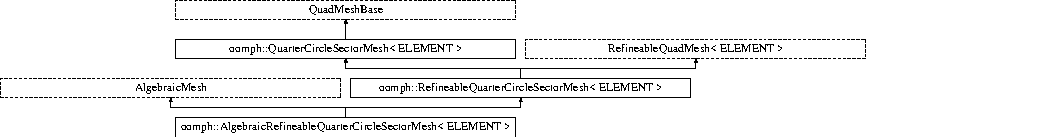
\includegraphics[height=1.839080cm]{classoomph_1_1AlgebraicRefineableQuarterCircleSectorMesh}
\end{center}
\end{figure}
\subsection*{Public Member Functions}
\begin{DoxyCompactItemize}
\item 
\hyperlink{classoomph_1_1AlgebraicRefineableQuarterCircleSectorMesh_a4245d6f0499af21053a0381bc69de271}{Algebraic\+Refineable\+Quarter\+Circle\+Sector\+Mesh} (Geom\+Object $\ast$\hyperlink{classoomph_1_1QuarterCircleSectorMesh_a0b03071bbe7e95cc6723c221ddc0998a}{wall\+\_\+pt}, const double \&xi\+\_\+lo, const double \&fract\+\_\+mid, const double \&xi\+\_\+hi, Time\+Stepper $\ast$time\+\_\+stepper\+\_\+pt=\&Mesh\+::\+Default\+\_\+\+Time\+Stepper)
\begin{DoxyCompactList}\small\item\em Constructor\+: Pass pointer to geometric object, start and end coordinates on the geometric object and the fraction along which the dividing line is to be placed when updating the nodal positions, and timestepper (defaults to (Steady) default timestepper defined in Mesh). Setup the refineable mesh (by calling the constructor for the underlying \hyperlink{classoomph_1_1RefineableQuarterCircleSectorMesh}{Refineable\+Quarter\+Circle\+Sector\+Mesh}) and the algebraic update functions for nodes. \end{DoxyCompactList}\item 
unsigned \hyperlink{classoomph_1_1AlgebraicRefineableQuarterCircleSectorMesh_a68d9738e3d3eedc4d2dd8e1b7fb09d8c}{self\+\_\+test} ()
\begin{DoxyCompactList}\small\item\em Run self-\/test for algebraic mesh -- return 0/1 for O\+K/failure. \end{DoxyCompactList}\item 
void \hyperlink{classoomph_1_1AlgebraicRefineableQuarterCircleSectorMesh_a32a096b894031167a90bafdab167ffc7}{node\+\_\+update} (const bool \&update\+\_\+all\+\_\+solid\+\_\+nodes=false)
\begin{DoxyCompactList}\small\item\em Resolve mesh update\+: Update current nodal positions via algebraic node update. \mbox{[}Doesn\textquotesingle{}t make sense to use this mesh with Solid\+Elements anyway, so we buffer the case if update\+\_\+all\+\_\+solid\+\_\+nodes is set to true.\mbox{]}. \end{DoxyCompactList}\item 
void \hyperlink{classoomph_1_1AlgebraicRefineableQuarterCircleSectorMesh_ac591df8f18ad687e1dc9b70b731c2de1}{algebraic\+\_\+node\+\_\+update} (const unsigned \&t, Algebraic\+Node $\ast$\&node\+\_\+pt)
\begin{DoxyCompactList}\small\item\em Implement the algebraic node update function for a node at time level t (t=0\+: present; t$>$0\+: previous)\+: Update with the node\textquotesingle{}s first (default) update function. \end{DoxyCompactList}\item 
void \hyperlink{classoomph_1_1AlgebraicRefineableQuarterCircleSectorMesh_a08abc1bf64e0637fc87c36638c41b846}{update\+\_\+node\+\_\+update} (Algebraic\+Node $\ast$\&node\+\_\+pt)
\begin{DoxyCompactList}\small\item\em Update the node update info for specified algebraic node following any spatial mesh adaptation. \end{DoxyCompactList}\end{DoxyCompactItemize}
\subsection*{Private Types}
\begin{DoxyCompactItemize}
\item 
enum \{ \hyperlink{classoomph_1_1AlgebraicRefineableQuarterCircleSectorMesh_a85eef4c11c2a88ba4bb5f99bc8406e67a070fa32a21fc9ed7e0ea2e4ee49bb226}{Central\+\_\+box}, 
\hyperlink{classoomph_1_1AlgebraicRefineableQuarterCircleSectorMesh_a85eef4c11c2a88ba4bb5f99bc8406e67a04eaf51389d87a087fa1e9b2b2bd0315}{Lower\+\_\+right\+\_\+box}, 
\hyperlink{classoomph_1_1AlgebraicRefineableQuarterCircleSectorMesh_a85eef4c11c2a88ba4bb5f99bc8406e67a5ff22a2cd960ec680a42f181d6cbdfb0}{Upper\+\_\+left\+\_\+box}
 \}\begin{DoxyCompactList}\small\item\em Remesh function ids. \end{DoxyCompactList}
\end{DoxyCompactItemize}
\subsection*{Private Member Functions}
\begin{DoxyCompactItemize}
\item 
void \hyperlink{classoomph_1_1AlgebraicRefineableQuarterCircleSectorMesh_a89dc4a592e3f188f9bfbffd5c7fdbbcc}{node\+\_\+update\+\_\+in\+\_\+central\+\_\+box} (const unsigned \&t, Algebraic\+Node $\ast$\&node\+\_\+pt)
\begin{DoxyCompactList}\small\item\em Algebraic update function for a node that is located in the central box. \end{DoxyCompactList}\item 
void \hyperlink{classoomph_1_1AlgebraicRefineableQuarterCircleSectorMesh_a9a7d3e4a2126346cdae3bde51eff7b36}{node\+\_\+update\+\_\+in\+\_\+lower\+\_\+right\+\_\+box} (const unsigned \&t, Algebraic\+Node $\ast$\&node\+\_\+pt)
\begin{DoxyCompactList}\small\item\em Algebraic update function for a node that is located in the lower right box. \end{DoxyCompactList}\item 
void \hyperlink{classoomph_1_1AlgebraicRefineableQuarterCircleSectorMesh_aeb36f6747d14cd68d4857169fa0f22d1}{node\+\_\+update\+\_\+in\+\_\+upper\+\_\+left\+\_\+box} (const unsigned \&t, Algebraic\+Node $\ast$\&node\+\_\+pt)
\begin{DoxyCompactList}\small\item\em Algebraic update function for a node that is located in the upper left box. \end{DoxyCompactList}\item 
void \hyperlink{classoomph_1_1AlgebraicRefineableQuarterCircleSectorMesh_a3eb269dc5c26355a808d1c5035190017}{setup\+\_\+algebraic\+\_\+node\+\_\+update} ()
\begin{DoxyCompactList}\small\item\em Setup algebraic update operation for all nodes. \end{DoxyCompactList}\item 
void \hyperlink{classoomph_1_1AlgebraicRefineableQuarterCircleSectorMesh_a77154a45d65fa66d220bad2a3e860c8e}{update\+\_\+node\+\_\+update\+\_\+in\+\_\+lower\+\_\+right\+\_\+box} (Algebraic\+Node $\ast$\&node\+\_\+pt)
\begin{DoxyCompactList}\small\item\em Update algebraic node update function for nodes in lower right box. \end{DoxyCompactList}\item 
void \hyperlink{classoomph_1_1AlgebraicRefineableQuarterCircleSectorMesh_ab1e4847ffef953e66aafff14f35b7141}{update\+\_\+node\+\_\+update\+\_\+in\+\_\+upper\+\_\+left\+\_\+box} (Algebraic\+Node $\ast$\&node\+\_\+pt)
\begin{DoxyCompactList}\small\item\em Update algebraic node update function for nodes in upper left box. \end{DoxyCompactList}\end{DoxyCompactItemize}
\subsection*{Private Attributes}
\begin{DoxyCompactItemize}
\item 
double \hyperlink{classoomph_1_1AlgebraicRefineableQuarterCircleSectorMesh_aed38fed1e464c86e3dedd377e2459de7}{Lambda\+\_\+x}
\begin{DoxyCompactList}\small\item\em Fractional width of central box. \end{DoxyCompactList}\item 
double \hyperlink{classoomph_1_1AlgebraicRefineableQuarterCircleSectorMesh_a2690e44e43dd4ed1e45b02f4b71ae43f}{Lambda\+\_\+y}
\begin{DoxyCompactList}\small\item\em Fractional height of central box. \end{DoxyCompactList}\end{DoxyCompactItemize}
\subsection*{Additional Inherited Members}


\subsection{Detailed Description}
\subsubsection*{template$<$class E\+L\+E\+M\+E\+NT$>$\newline
class oomph\+::\+Algebraic\+Refineable\+Quarter\+Circle\+Sector\+Mesh$<$ E\+L\+E\+M\+E\+N\+T $>$}

Algebraic version of \hyperlink{classoomph_1_1RefineableQuarterCircleSectorMesh}{Refineable\+Quarter\+Circle\+Sector\+Mesh}


\begin{DoxyCode}
                     ---\_\_\_
                    |      ---\_\_\_\_
                    |              -   BOUNDARY 1
                    |               /  
                    |     [2]      /  |  
                    |             /     | 
                    | N          /        |  
                    | |\_ E      /          |    
     BOUNDARY 2     |-----------           |  
                    |          |    [1]    |
                    |   [0]    |           |  ^
                    |          |           | / \(\backslash\)  direction of
                    | N        |    N      |  |   Lagrangian 
                    | |\_ E     |    |\_ E   |  |   coordinate 
                    |\_\_\_\_\_\_\_\_\_\_|\_\_\_\_\_\_\_\_\_\_\_|  |   along wall GeomObject

                         BOUNDARY 0

Within the elements (MacroElements), the local coordinates
are such that the (E)astern direction coincides with the positive 
s\_0 direction,  \textcolor{keywordflow}{while} the (N)orther direction coincides with the positive 
s\_1 direction.
\end{DoxyCode}


Domain is parametrised by three macro elements as sketched. Elements need to be derived from Algebraic\+Element\+Base. In addition to all the refinement procedures available for \hyperlink{classoomph_1_1RefineableQuarterCircleSectorMesh}{Refineable\+Quarter\+Circle\+Sector\+Mesh} which forms the basis for this mesh, we implement algebraic node update functions for the nodes. 

Definition at line 469 of file quarter\+\_\+circle\+\_\+sector\+\_\+mesh.\+template.\+h.



\subsection{Member Enumeration Documentation}
\mbox{\Hypertarget{classoomph_1_1AlgebraicRefineableQuarterCircleSectorMesh_a85eef4c11c2a88ba4bb5f99bc8406e67}\label{classoomph_1_1AlgebraicRefineableQuarterCircleSectorMesh_a85eef4c11c2a88ba4bb5f99bc8406e67}} 
\subsubsection{\texorpdfstring{anonymous enum}{anonymous enum}}
{\footnotesize\ttfamily template$<$class E\+L\+E\+M\+E\+NT $>$ \\
anonymous enum\hspace{0.3cm}{\ttfamily [private]}}



Remesh function ids. 

\begin{DoxyEnumFields}{Enumerator}
\raisebox{\heightof{T}}[0pt][0pt]{\index{Central\+\_\+box@{Central\+\_\+box}!oomph\+::\+Algebraic\+Refineable\+Quarter\+Circle\+Sector\+Mesh@{oomph\+::\+Algebraic\+Refineable\+Quarter\+Circle\+Sector\+Mesh}}\index{oomph\+::\+Algebraic\+Refineable\+Quarter\+Circle\+Sector\+Mesh@{oomph\+::\+Algebraic\+Refineable\+Quarter\+Circle\+Sector\+Mesh}!Central\+\_\+box@{Central\+\_\+box}}}\mbox{\Hypertarget{classoomph_1_1AlgebraicRefineableQuarterCircleSectorMesh_a85eef4c11c2a88ba4bb5f99bc8406e67a070fa32a21fc9ed7e0ea2e4ee49bb226}\label{classoomph_1_1AlgebraicRefineableQuarterCircleSectorMesh_a85eef4c11c2a88ba4bb5f99bc8406e67a070fa32a21fc9ed7e0ea2e4ee49bb226}} 
Central\+\_\+box&\\
\hline

\raisebox{\heightof{T}}[0pt][0pt]{\index{Lower\+\_\+right\+\_\+box@{Lower\+\_\+right\+\_\+box}!oomph\+::\+Algebraic\+Refineable\+Quarter\+Circle\+Sector\+Mesh@{oomph\+::\+Algebraic\+Refineable\+Quarter\+Circle\+Sector\+Mesh}}\index{oomph\+::\+Algebraic\+Refineable\+Quarter\+Circle\+Sector\+Mesh@{oomph\+::\+Algebraic\+Refineable\+Quarter\+Circle\+Sector\+Mesh}!Lower\+\_\+right\+\_\+box@{Lower\+\_\+right\+\_\+box}}}\mbox{\Hypertarget{classoomph_1_1AlgebraicRefineableQuarterCircleSectorMesh_a85eef4c11c2a88ba4bb5f99bc8406e67a04eaf51389d87a087fa1e9b2b2bd0315}\label{classoomph_1_1AlgebraicRefineableQuarterCircleSectorMesh_a85eef4c11c2a88ba4bb5f99bc8406e67a04eaf51389d87a087fa1e9b2b2bd0315}} 
Lower\+\_\+right\+\_\+box&\\
\hline

\raisebox{\heightof{T}}[0pt][0pt]{\index{Upper\+\_\+left\+\_\+box@{Upper\+\_\+left\+\_\+box}!oomph\+::\+Algebraic\+Refineable\+Quarter\+Circle\+Sector\+Mesh@{oomph\+::\+Algebraic\+Refineable\+Quarter\+Circle\+Sector\+Mesh}}\index{oomph\+::\+Algebraic\+Refineable\+Quarter\+Circle\+Sector\+Mesh@{oomph\+::\+Algebraic\+Refineable\+Quarter\+Circle\+Sector\+Mesh}!Upper\+\_\+left\+\_\+box@{Upper\+\_\+left\+\_\+box}}}\mbox{\Hypertarget{classoomph_1_1AlgebraicRefineableQuarterCircleSectorMesh_a85eef4c11c2a88ba4bb5f99bc8406e67a5ff22a2cd960ec680a42f181d6cbdfb0}\label{classoomph_1_1AlgebraicRefineableQuarterCircleSectorMesh_a85eef4c11c2a88ba4bb5f99bc8406e67a5ff22a2cd960ec680a42f181d6cbdfb0}} 
Upper\+\_\+left\+\_\+box&\\
\hline

\end{DoxyEnumFields}


Definition at line 674 of file quarter\+\_\+circle\+\_\+sector\+\_\+mesh.\+template.\+h.



\subsection{Constructor \& Destructor Documentation}
\mbox{\Hypertarget{classoomph_1_1AlgebraicRefineableQuarterCircleSectorMesh_a4245d6f0499af21053a0381bc69de271}\label{classoomph_1_1AlgebraicRefineableQuarterCircleSectorMesh_a4245d6f0499af21053a0381bc69de271}} 
\index{oomph\+::\+Algebraic\+Refineable\+Quarter\+Circle\+Sector\+Mesh@{oomph\+::\+Algebraic\+Refineable\+Quarter\+Circle\+Sector\+Mesh}!Algebraic\+Refineable\+Quarter\+Circle\+Sector\+Mesh@{Algebraic\+Refineable\+Quarter\+Circle\+Sector\+Mesh}}
\index{Algebraic\+Refineable\+Quarter\+Circle\+Sector\+Mesh@{Algebraic\+Refineable\+Quarter\+Circle\+Sector\+Mesh}!oomph\+::\+Algebraic\+Refineable\+Quarter\+Circle\+Sector\+Mesh@{oomph\+::\+Algebraic\+Refineable\+Quarter\+Circle\+Sector\+Mesh}}
\subsubsection{\texorpdfstring{Algebraic\+Refineable\+Quarter\+Circle\+Sector\+Mesh()}{AlgebraicRefineableQuarterCircleSectorMesh()}}
{\footnotesize\ttfamily template$<$class E\+L\+E\+M\+E\+NT $>$ \\
\hyperlink{classoomph_1_1AlgebraicRefineableQuarterCircleSectorMesh}{oomph\+::\+Algebraic\+Refineable\+Quarter\+Circle\+Sector\+Mesh}$<$ E\+L\+E\+M\+E\+NT $>$\+::\hyperlink{classoomph_1_1AlgebraicRefineableQuarterCircleSectorMesh}{Algebraic\+Refineable\+Quarter\+Circle\+Sector\+Mesh} (\begin{DoxyParamCaption}\item[{Geom\+Object $\ast$}]{wall\+\_\+pt,  }\item[{const double \&}]{xi\+\_\+lo,  }\item[{const double \&}]{fract\+\_\+mid,  }\item[{const double \&}]{xi\+\_\+hi,  }\item[{Time\+Stepper $\ast$}]{time\+\_\+stepper\+\_\+pt = {\ttfamily \&Mesh\+:\+:Default\+\_\+TimeStepper} }\end{DoxyParamCaption})\hspace{0.3cm}{\ttfamily [inline]}}



Constructor\+: Pass pointer to geometric object, start and end coordinates on the geometric object and the fraction along which the dividing line is to be placed when updating the nodal positions, and timestepper (defaults to (Steady) default timestepper defined in Mesh). Setup the refineable mesh (by calling the constructor for the underlying \hyperlink{classoomph_1_1RefineableQuarterCircleSectorMesh}{Refineable\+Quarter\+Circle\+Sector\+Mesh}) and the algebraic update functions for nodes. 



Definition at line 486 of file quarter\+\_\+circle\+\_\+sector\+\_\+mesh.\+template.\+h.



\subsection{Member Function Documentation}
\mbox{\Hypertarget{classoomph_1_1AlgebraicRefineableQuarterCircleSectorMesh_ac591df8f18ad687e1dc9b70b731c2de1}\label{classoomph_1_1AlgebraicRefineableQuarterCircleSectorMesh_ac591df8f18ad687e1dc9b70b731c2de1}} 
\index{oomph\+::\+Algebraic\+Refineable\+Quarter\+Circle\+Sector\+Mesh@{oomph\+::\+Algebraic\+Refineable\+Quarter\+Circle\+Sector\+Mesh}!algebraic\+\_\+node\+\_\+update@{algebraic\+\_\+node\+\_\+update}}
\index{algebraic\+\_\+node\+\_\+update@{algebraic\+\_\+node\+\_\+update}!oomph\+::\+Algebraic\+Refineable\+Quarter\+Circle\+Sector\+Mesh@{oomph\+::\+Algebraic\+Refineable\+Quarter\+Circle\+Sector\+Mesh}}
\subsubsection{\texorpdfstring{algebraic\+\_\+node\+\_\+update()}{algebraic\_node\_update()}}
{\footnotesize\ttfamily template$<$class E\+L\+E\+M\+E\+NT $>$ \\
void \hyperlink{classoomph_1_1AlgebraicRefineableQuarterCircleSectorMesh}{oomph\+::\+Algebraic\+Refineable\+Quarter\+Circle\+Sector\+Mesh}$<$ E\+L\+E\+M\+E\+NT $>$\+::algebraic\+\_\+node\+\_\+update (\begin{DoxyParamCaption}\item[{const unsigned \&}]{t,  }\item[{Algebraic\+Node $\ast$\&}]{node\+\_\+pt }\end{DoxyParamCaption})\hspace{0.3cm}{\ttfamily [inline]}}



Implement the algebraic node update function for a node at time level t (t=0\+: present; t$>$0\+: previous)\+: Update with the node\textquotesingle{}s first (default) update function. 



Definition at line 566 of file quarter\+\_\+circle\+\_\+sector\+\_\+mesh.\+template.\+h.

\mbox{\Hypertarget{classoomph_1_1AlgebraicRefineableQuarterCircleSectorMesh_a32a096b894031167a90bafdab167ffc7}\label{classoomph_1_1AlgebraicRefineableQuarterCircleSectorMesh_a32a096b894031167a90bafdab167ffc7}} 
\index{oomph\+::\+Algebraic\+Refineable\+Quarter\+Circle\+Sector\+Mesh@{oomph\+::\+Algebraic\+Refineable\+Quarter\+Circle\+Sector\+Mesh}!node\+\_\+update@{node\+\_\+update}}
\index{node\+\_\+update@{node\+\_\+update}!oomph\+::\+Algebraic\+Refineable\+Quarter\+Circle\+Sector\+Mesh@{oomph\+::\+Algebraic\+Refineable\+Quarter\+Circle\+Sector\+Mesh}}
\subsubsection{\texorpdfstring{node\+\_\+update()}{node\_update()}}
{\footnotesize\ttfamily template$<$class E\+L\+E\+M\+E\+NT $>$ \\
void \hyperlink{classoomph_1_1AlgebraicRefineableQuarterCircleSectorMesh}{oomph\+::\+Algebraic\+Refineable\+Quarter\+Circle\+Sector\+Mesh}$<$ E\+L\+E\+M\+E\+NT $>$\+::node\+\_\+update (\begin{DoxyParamCaption}\item[{const bool \&}]{update\+\_\+all\+\_\+solid\+\_\+nodes = {\ttfamily false} }\end{DoxyParamCaption})\hspace{0.3cm}{\ttfamily [inline]}}



Resolve mesh update\+: Update current nodal positions via algebraic node update. \mbox{[}Doesn\textquotesingle{}t make sense to use this mesh with Solid\+Elements anyway, so we buffer the case if update\+\_\+all\+\_\+solid\+\_\+nodes is set to true.\mbox{]}. 



Definition at line 538 of file quarter\+\_\+circle\+\_\+sector\+\_\+mesh.\+template.\+h.

\mbox{\Hypertarget{classoomph_1_1AlgebraicRefineableQuarterCircleSectorMesh_a89dc4a592e3f188f9bfbffd5c7fdbbcc}\label{classoomph_1_1AlgebraicRefineableQuarterCircleSectorMesh_a89dc4a592e3f188f9bfbffd5c7fdbbcc}} 
\index{oomph\+::\+Algebraic\+Refineable\+Quarter\+Circle\+Sector\+Mesh@{oomph\+::\+Algebraic\+Refineable\+Quarter\+Circle\+Sector\+Mesh}!node\+\_\+update\+\_\+in\+\_\+central\+\_\+box@{node\+\_\+update\+\_\+in\+\_\+central\+\_\+box}}
\index{node\+\_\+update\+\_\+in\+\_\+central\+\_\+box@{node\+\_\+update\+\_\+in\+\_\+central\+\_\+box}!oomph\+::\+Algebraic\+Refineable\+Quarter\+Circle\+Sector\+Mesh@{oomph\+::\+Algebraic\+Refineable\+Quarter\+Circle\+Sector\+Mesh}}
\subsubsection{\texorpdfstring{node\+\_\+update\+\_\+in\+\_\+central\+\_\+box()}{node\_update\_in\_central\_box()}}
{\footnotesize\ttfamily template$<$class E\+L\+E\+M\+E\+NT $>$ \\
void \hyperlink{classoomph_1_1AlgebraicRefineableQuarterCircleSectorMesh}{oomph\+::\+Algebraic\+Refineable\+Quarter\+Circle\+Sector\+Mesh}$<$ E\+L\+E\+M\+E\+NT $>$\+::node\+\_\+update\+\_\+in\+\_\+central\+\_\+box (\begin{DoxyParamCaption}\item[{const unsigned \&}]{t,  }\item[{Algebraic\+Node $\ast$\&}]{node\+\_\+pt }\end{DoxyParamCaption})\hspace{0.3cm}{\ttfamily [private]}}



Algebraic update function for a node that is located in the central box. 

Algebraic update function\+: Update in central box according to wall shape at time level t (t=0\+: present; t$>$0\+: previous) 

Definition at line 870 of file quarter\+\_\+circle\+\_\+sector\+\_\+mesh.\+template.\+cc.



References oomph\+::\+Algebraic\+Refineable\+Quarter\+Circle\+Sector\+Mesh$<$ E\+L\+E\+M\+E\+N\+T $>$\+::node\+\_\+update\+\_\+in\+\_\+lower\+\_\+right\+\_\+box().



Referenced by oomph\+::\+Algebraic\+Refineable\+Quarter\+Circle\+Sector\+Mesh$<$ E\+L\+E\+M\+E\+N\+T $>$\+::setup\+\_\+algebraic\+\_\+node\+\_\+update().

\mbox{\Hypertarget{classoomph_1_1AlgebraicRefineableQuarterCircleSectorMesh_a9a7d3e4a2126346cdae3bde51eff7b36}\label{classoomph_1_1AlgebraicRefineableQuarterCircleSectorMesh_a9a7d3e4a2126346cdae3bde51eff7b36}} 
\index{oomph\+::\+Algebraic\+Refineable\+Quarter\+Circle\+Sector\+Mesh@{oomph\+::\+Algebraic\+Refineable\+Quarter\+Circle\+Sector\+Mesh}!node\+\_\+update\+\_\+in\+\_\+lower\+\_\+right\+\_\+box@{node\+\_\+update\+\_\+in\+\_\+lower\+\_\+right\+\_\+box}}
\index{node\+\_\+update\+\_\+in\+\_\+lower\+\_\+right\+\_\+box@{node\+\_\+update\+\_\+in\+\_\+lower\+\_\+right\+\_\+box}!oomph\+::\+Algebraic\+Refineable\+Quarter\+Circle\+Sector\+Mesh@{oomph\+::\+Algebraic\+Refineable\+Quarter\+Circle\+Sector\+Mesh}}
\subsubsection{\texorpdfstring{node\+\_\+update\+\_\+in\+\_\+lower\+\_\+right\+\_\+box()}{node\_update\_in\_lower\_right\_box()}}
{\footnotesize\ttfamily template$<$class E\+L\+E\+M\+E\+NT $>$ \\
void \hyperlink{classoomph_1_1AlgebraicRefineableQuarterCircleSectorMesh}{oomph\+::\+Algebraic\+Refineable\+Quarter\+Circle\+Sector\+Mesh}$<$ E\+L\+E\+M\+E\+NT $>$\+::node\+\_\+update\+\_\+in\+\_\+lower\+\_\+right\+\_\+box (\begin{DoxyParamCaption}\item[{const unsigned \&}]{t,  }\item[{Algebraic\+Node $\ast$\&}]{node\+\_\+pt }\end{DoxyParamCaption})\hspace{0.3cm}{\ttfamily [private]}}



Algebraic update function for a node that is located in the lower right box. 

Algebraic update function\+: Update in lower right box according to wall shape at time level t (t=0\+: present; t$>$0\+: previous) 

Definition at line 961 of file quarter\+\_\+circle\+\_\+sector\+\_\+mesh.\+template.\+cc.



References oomph\+::\+Algebraic\+Refineable\+Quarter\+Circle\+Sector\+Mesh$<$ E\+L\+E\+M\+E\+N\+T $>$\+::node\+\_\+update\+\_\+in\+\_\+upper\+\_\+left\+\_\+box().



Referenced by oomph\+::\+Algebraic\+Refineable\+Quarter\+Circle\+Sector\+Mesh$<$ E\+L\+E\+M\+E\+N\+T $>$\+::node\+\_\+update\+\_\+in\+\_\+central\+\_\+box().

\mbox{\Hypertarget{classoomph_1_1AlgebraicRefineableQuarterCircleSectorMesh_aeb36f6747d14cd68d4857169fa0f22d1}\label{classoomph_1_1AlgebraicRefineableQuarterCircleSectorMesh_aeb36f6747d14cd68d4857169fa0f22d1}} 
\index{oomph\+::\+Algebraic\+Refineable\+Quarter\+Circle\+Sector\+Mesh@{oomph\+::\+Algebraic\+Refineable\+Quarter\+Circle\+Sector\+Mesh}!node\+\_\+update\+\_\+in\+\_\+upper\+\_\+left\+\_\+box@{node\+\_\+update\+\_\+in\+\_\+upper\+\_\+left\+\_\+box}}
\index{node\+\_\+update\+\_\+in\+\_\+upper\+\_\+left\+\_\+box@{node\+\_\+update\+\_\+in\+\_\+upper\+\_\+left\+\_\+box}!oomph\+::\+Algebraic\+Refineable\+Quarter\+Circle\+Sector\+Mesh@{oomph\+::\+Algebraic\+Refineable\+Quarter\+Circle\+Sector\+Mesh}}
\subsubsection{\texorpdfstring{node\+\_\+update\+\_\+in\+\_\+upper\+\_\+left\+\_\+box()}{node\_update\_in\_upper\_left\_box()}}
{\footnotesize\ttfamily template$<$class E\+L\+E\+M\+E\+NT $>$ \\
void \hyperlink{classoomph_1_1AlgebraicRefineableQuarterCircleSectorMesh}{oomph\+::\+Algebraic\+Refineable\+Quarter\+Circle\+Sector\+Mesh}$<$ E\+L\+E\+M\+E\+NT $>$\+::node\+\_\+update\+\_\+in\+\_\+upper\+\_\+left\+\_\+box (\begin{DoxyParamCaption}\item[{const unsigned \&}]{t,  }\item[{Algebraic\+Node $\ast$\&}]{node\+\_\+pt }\end{DoxyParamCaption})\hspace{0.3cm}{\ttfamily [private]}}



Algebraic update function for a node that is located in the upper left box. 

Algebraic update function\+: Update in upper left box according to wall shape at time level t (t=0\+: present; t$>$0\+: previous) 

Definition at line 1073 of file quarter\+\_\+circle\+\_\+sector\+\_\+mesh.\+template.\+cc.



References oomph\+::\+Algebraic\+Refineable\+Quarter\+Circle\+Sector\+Mesh$<$ E\+L\+E\+M\+E\+N\+T $>$\+::update\+\_\+node\+\_\+update\+\_\+in\+\_\+lower\+\_\+right\+\_\+box().



Referenced by oomph\+::\+Algebraic\+Refineable\+Quarter\+Circle\+Sector\+Mesh$<$ E\+L\+E\+M\+E\+N\+T $>$\+::node\+\_\+update\+\_\+in\+\_\+lower\+\_\+right\+\_\+box().

\mbox{\Hypertarget{classoomph_1_1AlgebraicRefineableQuarterCircleSectorMesh_a68d9738e3d3eedc4d2dd8e1b7fb09d8c}\label{classoomph_1_1AlgebraicRefineableQuarterCircleSectorMesh_a68d9738e3d3eedc4d2dd8e1b7fb09d8c}} 
\index{oomph\+::\+Algebraic\+Refineable\+Quarter\+Circle\+Sector\+Mesh@{oomph\+::\+Algebraic\+Refineable\+Quarter\+Circle\+Sector\+Mesh}!self\+\_\+test@{self\+\_\+test}}
\index{self\+\_\+test@{self\+\_\+test}!oomph\+::\+Algebraic\+Refineable\+Quarter\+Circle\+Sector\+Mesh@{oomph\+::\+Algebraic\+Refineable\+Quarter\+Circle\+Sector\+Mesh}}
\subsubsection{\texorpdfstring{self\+\_\+test()}{self\_test()}}
{\footnotesize\ttfamily template$<$class E\+L\+E\+M\+E\+NT $>$ \\
unsigned \hyperlink{classoomph_1_1AlgebraicRefineableQuarterCircleSectorMesh}{oomph\+::\+Algebraic\+Refineable\+Quarter\+Circle\+Sector\+Mesh}$<$ E\+L\+E\+M\+E\+NT $>$\+::self\+\_\+test (\begin{DoxyParamCaption}{ }\end{DoxyParamCaption})\hspace{0.3cm}{\ttfamily [inline]}}



Run self-\/test for algebraic mesh -- return 0/1 for O\+K/failure. 



Definition at line 528 of file quarter\+\_\+circle\+\_\+sector\+\_\+mesh.\+template.\+h.

\mbox{\Hypertarget{classoomph_1_1AlgebraicRefineableQuarterCircleSectorMesh_a3eb269dc5c26355a808d1c5035190017}\label{classoomph_1_1AlgebraicRefineableQuarterCircleSectorMesh_a3eb269dc5c26355a808d1c5035190017}} 
\index{oomph\+::\+Algebraic\+Refineable\+Quarter\+Circle\+Sector\+Mesh@{oomph\+::\+Algebraic\+Refineable\+Quarter\+Circle\+Sector\+Mesh}!setup\+\_\+algebraic\+\_\+node\+\_\+update@{setup\+\_\+algebraic\+\_\+node\+\_\+update}}
\index{setup\+\_\+algebraic\+\_\+node\+\_\+update@{setup\+\_\+algebraic\+\_\+node\+\_\+update}!oomph\+::\+Algebraic\+Refineable\+Quarter\+Circle\+Sector\+Mesh@{oomph\+::\+Algebraic\+Refineable\+Quarter\+Circle\+Sector\+Mesh}}
\subsubsection{\texorpdfstring{setup\+\_\+algebraic\+\_\+node\+\_\+update()}{setup\_algebraic\_node\_update()}}
{\footnotesize\ttfamily template$<$class E\+L\+E\+M\+E\+NT $>$ \\
void \hyperlink{classoomph_1_1AlgebraicRefineableQuarterCircleSectorMesh}{oomph\+::\+Algebraic\+Refineable\+Quarter\+Circle\+Sector\+Mesh}$<$ E\+L\+E\+M\+E\+NT $>$\+::setup\+\_\+algebraic\+\_\+node\+\_\+update (\begin{DoxyParamCaption}{ }\end{DoxyParamCaption})\hspace{0.3cm}{\ttfamily [private]}}



Setup algebraic update operation for all nodes. 

Setup algebraic update operation, based on individual blocks. Mesh is suspended from the `wall\textquotesingle{} Geom\+Object pointed to by wall\+\_\+pt. The lower right corner of the mesh is located at the wall\textquotesingle{}s coordinate xi\+\_\+lo, the upper left corner at xi\+\_\+hi; The dividing line between the two blocks at the outer ring is located at the fraction fract\+\_\+mid between these two coordinates. Node updating strategy\+:
\begin{DoxyItemize}
\item the shape of the central box remains rectangular; the position of its top right corner is located at a fixed fraction of the width and height of the domain. Nodes in this region are located at fixed horizontal and vertical fractions of the box.
\item Nodes in the two outer \char`\"{}ring\char`\"{} elements (bottom right and top left) are located on straight lines running from the edges of the central box to the outer wall. 
\end{DoxyItemize}Pointer to algebraic element in central box 

Definition at line 574 of file quarter\+\_\+circle\+\_\+sector\+\_\+mesh.\+template.\+cc.



References oomph\+::\+Algebraic\+Refineable\+Quarter\+Circle\+Sector\+Mesh$<$ E\+L\+E\+M\+E\+N\+T $>$\+::node\+\_\+update\+\_\+in\+\_\+central\+\_\+box(), and oomph\+::\+Quarter\+Circle\+Sector\+Mesh$<$ E\+L\+E\+M\+E\+N\+T $>$\+::\+Wall\+\_\+pt.



Referenced by oomph\+::\+Quarter\+Circle\+Sector\+Mesh$<$ E\+L\+E\+M\+E\+N\+T $>$\+::\+Quarter\+Circle\+Sector\+Mesh().

\mbox{\Hypertarget{classoomph_1_1AlgebraicRefineableQuarterCircleSectorMesh_a08abc1bf64e0637fc87c36638c41b846}\label{classoomph_1_1AlgebraicRefineableQuarterCircleSectorMesh_a08abc1bf64e0637fc87c36638c41b846}} 
\index{oomph\+::\+Algebraic\+Refineable\+Quarter\+Circle\+Sector\+Mesh@{oomph\+::\+Algebraic\+Refineable\+Quarter\+Circle\+Sector\+Mesh}!update\+\_\+node\+\_\+update@{update\+\_\+node\+\_\+update}}
\index{update\+\_\+node\+\_\+update@{update\+\_\+node\+\_\+update}!oomph\+::\+Algebraic\+Refineable\+Quarter\+Circle\+Sector\+Mesh@{oomph\+::\+Algebraic\+Refineable\+Quarter\+Circle\+Sector\+Mesh}}
\subsubsection{\texorpdfstring{update\+\_\+node\+\_\+update()}{update\_node\_update()}}
{\footnotesize\ttfamily template$<$class E\+L\+E\+M\+E\+NT $>$ \\
void \hyperlink{classoomph_1_1AlgebraicRefineableQuarterCircleSectorMesh}{oomph\+::\+Algebraic\+Refineable\+Quarter\+Circle\+Sector\+Mesh}$<$ E\+L\+E\+M\+E\+NT $>$\+::update\+\_\+node\+\_\+update (\begin{DoxyParamCaption}\item[{Algebraic\+Node $\ast$\&}]{node\+\_\+pt }\end{DoxyParamCaption})\hspace{0.3cm}{\ttfamily [inline]}}



Update the node update info for specified algebraic node following any spatial mesh adaptation. 



Definition at line 617 of file quarter\+\_\+circle\+\_\+sector\+\_\+mesh.\+template.\+h.

\mbox{\Hypertarget{classoomph_1_1AlgebraicRefineableQuarterCircleSectorMesh_a77154a45d65fa66d220bad2a3e860c8e}\label{classoomph_1_1AlgebraicRefineableQuarterCircleSectorMesh_a77154a45d65fa66d220bad2a3e860c8e}} 
\index{oomph\+::\+Algebraic\+Refineable\+Quarter\+Circle\+Sector\+Mesh@{oomph\+::\+Algebraic\+Refineable\+Quarter\+Circle\+Sector\+Mesh}!update\+\_\+node\+\_\+update\+\_\+in\+\_\+lower\+\_\+right\+\_\+box@{update\+\_\+node\+\_\+update\+\_\+in\+\_\+lower\+\_\+right\+\_\+box}}
\index{update\+\_\+node\+\_\+update\+\_\+in\+\_\+lower\+\_\+right\+\_\+box@{update\+\_\+node\+\_\+update\+\_\+in\+\_\+lower\+\_\+right\+\_\+box}!oomph\+::\+Algebraic\+Refineable\+Quarter\+Circle\+Sector\+Mesh@{oomph\+::\+Algebraic\+Refineable\+Quarter\+Circle\+Sector\+Mesh}}
\subsubsection{\texorpdfstring{update\+\_\+node\+\_\+update\+\_\+in\+\_\+lower\+\_\+right\+\_\+box()}{update\_node\_update\_in\_lower\_right\_box()}}
{\footnotesize\ttfamily template$<$class E\+L\+E\+M\+E\+NT $>$ \\
void \hyperlink{classoomph_1_1AlgebraicRefineableQuarterCircleSectorMesh}{oomph\+::\+Algebraic\+Refineable\+Quarter\+Circle\+Sector\+Mesh}$<$ E\+L\+E\+M\+E\+NT $>$\+::update\+\_\+node\+\_\+update\+\_\+in\+\_\+lower\+\_\+right\+\_\+box (\begin{DoxyParamCaption}\item[{Algebraic\+Node $\ast$\&}]{node\+\_\+pt }\end{DoxyParamCaption})\hspace{0.3cm}{\ttfamily [private]}}



Update algebraic node update function for nodes in lower right box. 

Update algebraic update function for nodes in lower right box. 

Definition at line 1187 of file quarter\+\_\+circle\+\_\+sector\+\_\+mesh.\+template.\+cc.



References oomph\+::\+Algebraic\+Refineable\+Quarter\+Circle\+Sector\+Mesh$<$ E\+L\+E\+M\+E\+N\+T $>$\+::update\+\_\+node\+\_\+update\+\_\+in\+\_\+upper\+\_\+left\+\_\+box(), and oomph\+::\+Quarter\+Circle\+Sector\+Mesh$<$ E\+L\+E\+M\+E\+N\+T $>$\+::\+Wall\+\_\+pt.



Referenced by oomph\+::\+Algebraic\+Refineable\+Quarter\+Circle\+Sector\+Mesh$<$ E\+L\+E\+M\+E\+N\+T $>$\+::node\+\_\+update\+\_\+in\+\_\+upper\+\_\+left\+\_\+box().

\mbox{\Hypertarget{classoomph_1_1AlgebraicRefineableQuarterCircleSectorMesh_ab1e4847ffef953e66aafff14f35b7141}\label{classoomph_1_1AlgebraicRefineableQuarterCircleSectorMesh_ab1e4847ffef953e66aafff14f35b7141}} 
\index{oomph\+::\+Algebraic\+Refineable\+Quarter\+Circle\+Sector\+Mesh@{oomph\+::\+Algebraic\+Refineable\+Quarter\+Circle\+Sector\+Mesh}!update\+\_\+node\+\_\+update\+\_\+in\+\_\+upper\+\_\+left\+\_\+box@{update\+\_\+node\+\_\+update\+\_\+in\+\_\+upper\+\_\+left\+\_\+box}}
\index{update\+\_\+node\+\_\+update\+\_\+in\+\_\+upper\+\_\+left\+\_\+box@{update\+\_\+node\+\_\+update\+\_\+in\+\_\+upper\+\_\+left\+\_\+box}!oomph\+::\+Algebraic\+Refineable\+Quarter\+Circle\+Sector\+Mesh@{oomph\+::\+Algebraic\+Refineable\+Quarter\+Circle\+Sector\+Mesh}}
\subsubsection{\texorpdfstring{update\+\_\+node\+\_\+update\+\_\+in\+\_\+upper\+\_\+left\+\_\+box()}{update\_node\_update\_in\_upper\_left\_box()}}
{\footnotesize\ttfamily template$<$class E\+L\+E\+M\+E\+NT $>$ \\
void \hyperlink{classoomph_1_1AlgebraicRefineableQuarterCircleSectorMesh}{oomph\+::\+Algebraic\+Refineable\+Quarter\+Circle\+Sector\+Mesh}$<$ E\+L\+E\+M\+E\+NT $>$\+::update\+\_\+node\+\_\+update\+\_\+in\+\_\+upper\+\_\+left\+\_\+box (\begin{DoxyParamCaption}\item[{Algebraic\+Node $\ast$\&}]{node\+\_\+pt }\end{DoxyParamCaption})\hspace{0.3cm}{\ttfamily [private]}}



Update algebraic node update function for nodes in upper left box. 

Update algebraic update function for nodes in upper left box. 

Definition at line 1292 of file quarter\+\_\+circle\+\_\+sector\+\_\+mesh.\+template.\+cc.



References oomph\+::\+Quarter\+Circle\+Sector\+Mesh$<$ E\+L\+E\+M\+E\+N\+T $>$\+::\+Wall\+\_\+pt.



Referenced by oomph\+::\+Algebraic\+Refineable\+Quarter\+Circle\+Sector\+Mesh$<$ E\+L\+E\+M\+E\+N\+T $>$\+::update\+\_\+node\+\_\+update\+\_\+in\+\_\+lower\+\_\+right\+\_\+box().



\subsection{Member Data Documentation}
\mbox{\Hypertarget{classoomph_1_1AlgebraicRefineableQuarterCircleSectorMesh_aed38fed1e464c86e3dedd377e2459de7}\label{classoomph_1_1AlgebraicRefineableQuarterCircleSectorMesh_aed38fed1e464c86e3dedd377e2459de7}} 
\index{oomph\+::\+Algebraic\+Refineable\+Quarter\+Circle\+Sector\+Mesh@{oomph\+::\+Algebraic\+Refineable\+Quarter\+Circle\+Sector\+Mesh}!Lambda\+\_\+x@{Lambda\+\_\+x}}
\index{Lambda\+\_\+x@{Lambda\+\_\+x}!oomph\+::\+Algebraic\+Refineable\+Quarter\+Circle\+Sector\+Mesh@{oomph\+::\+Algebraic\+Refineable\+Quarter\+Circle\+Sector\+Mesh}}
\subsubsection{\texorpdfstring{Lambda\+\_\+x}{Lambda\_x}}
{\footnotesize\ttfamily template$<$class E\+L\+E\+M\+E\+NT $>$ \\
double \hyperlink{classoomph_1_1AlgebraicRefineableQuarterCircleSectorMesh}{oomph\+::\+Algebraic\+Refineable\+Quarter\+Circle\+Sector\+Mesh}$<$ E\+L\+E\+M\+E\+NT $>$\+::Lambda\+\_\+x\hspace{0.3cm}{\ttfamily [private]}}



Fractional width of central box. 



Definition at line 678 of file quarter\+\_\+circle\+\_\+sector\+\_\+mesh.\+template.\+h.

\mbox{\Hypertarget{classoomph_1_1AlgebraicRefineableQuarterCircleSectorMesh_a2690e44e43dd4ed1e45b02f4b71ae43f}\label{classoomph_1_1AlgebraicRefineableQuarterCircleSectorMesh_a2690e44e43dd4ed1e45b02f4b71ae43f}} 
\index{oomph\+::\+Algebraic\+Refineable\+Quarter\+Circle\+Sector\+Mesh@{oomph\+::\+Algebraic\+Refineable\+Quarter\+Circle\+Sector\+Mesh}!Lambda\+\_\+y@{Lambda\+\_\+y}}
\index{Lambda\+\_\+y@{Lambda\+\_\+y}!oomph\+::\+Algebraic\+Refineable\+Quarter\+Circle\+Sector\+Mesh@{oomph\+::\+Algebraic\+Refineable\+Quarter\+Circle\+Sector\+Mesh}}
\subsubsection{\texorpdfstring{Lambda\+\_\+y}{Lambda\_y}}
{\footnotesize\ttfamily template$<$class E\+L\+E\+M\+E\+NT $>$ \\
double \hyperlink{classoomph_1_1AlgebraicRefineableQuarterCircleSectorMesh}{oomph\+::\+Algebraic\+Refineable\+Quarter\+Circle\+Sector\+Mesh}$<$ E\+L\+E\+M\+E\+NT $>$\+::Lambda\+\_\+y\hspace{0.3cm}{\ttfamily [private]}}



Fractional height of central box. 



Definition at line 681 of file quarter\+\_\+circle\+\_\+sector\+\_\+mesh.\+template.\+h.



The documentation for this class was generated from the following files\+:\begin{DoxyCompactItemize}
\item 
\hyperlink{quarter__circle__sector__mesh_8template_8h}{quarter\+\_\+circle\+\_\+sector\+\_\+mesh.\+template.\+h}\item 
\hyperlink{quarter__circle__sector__mesh_8template_8cc}{quarter\+\_\+circle\+\_\+sector\+\_\+mesh.\+template.\+cc}\end{DoxyCompactItemize}

\hypertarget{classoomph_1_1AlgebraicRefineableQuarterTubeMesh}{}\section{oomph\+:\+:Algebraic\+Refineable\+Quarter\+Tube\+Mesh$<$ E\+L\+E\+M\+E\+NT $>$ Class Template Reference}
\label{classoomph_1_1AlgebraicRefineableQuarterTubeMesh}\index{oomph\+::\+Algebraic\+Refineable\+Quarter\+Tube\+Mesh$<$ E\+L\+E\+M\+E\+N\+T $>$@{oomph\+::\+Algebraic\+Refineable\+Quarter\+Tube\+Mesh$<$ E\+L\+E\+M\+E\+N\+T $>$}}


\hyperlink{classoomph_1_1AlgebraicMesh}{Algebraic\+Mesh} version of \hyperlink{classoomph_1_1RefineableQuarterTubeMesh}{Refineable\+Quarter\+Tube\+Mesh}.  




{\ttfamily \#include $<$quarter\+\_\+tube\+\_\+mesh.\+template.\+h$>$}

Inheritance diagram for oomph\+:\+:Algebraic\+Refineable\+Quarter\+Tube\+Mesh$<$ E\+L\+E\+M\+E\+NT $>$\+:\begin{figure}[H]
\begin{center}
\leavevmode
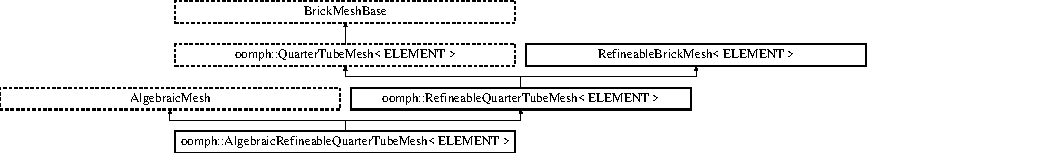
\includegraphics[height=2.699725cm]{classoomph_1_1AlgebraicRefineableQuarterTubeMesh}
\end{center}
\end{figure}
\subsection*{Public Member Functions}
\begin{DoxyCompactItemize}
\item 
\hyperlink{classoomph_1_1AlgebraicRefineableQuarterTubeMesh_ad8ff9f32d4d180d815da65ddc3c4b90a}{Algebraic\+Refineable\+Quarter\+Tube\+Mesh} (\hyperlink{classoomph_1_1GeomObject}{Geom\+Object} $\ast$\hyperlink{classoomph_1_1QuarterTubeMesh_af59c4cde343ddd76caea4bc8c8ad8b94}{wall\+\_\+pt}, const \hyperlink{classoomph_1_1Vector}{Vector}$<$ double $>$ \&xi\+\_\+lo, const double \&fract\+\_\+mid, const \hyperlink{classoomph_1_1Vector}{Vector}$<$ double $>$ \&xi\+\_\+hi, const unsigned \&nlayer, const double centre\+\_\+box\+\_\+size=1.\+0, \hyperlink{classoomph_1_1TimeStepper}{Time\+Stepper} $\ast$time\+\_\+stepper\+\_\+pt=\&\hyperlink{classoomph_1_1Mesh_a12243d0fee2b1fcee729ee5a4777ea10}{Mesh\+::\+Default\+\_\+\+Time\+Stepper})
\begin{DoxyCompactList}\small\item\em Constructor\+: Pass pointer to geometric object, start and end coordinates of the geometric object and the fraction along the 2nd Lagrangian coordinate at which the dividing line between region 1 and region 2 is to be placed, and timestepper (defaults to (\hyperlink{classoomph_1_1Steady}{Steady}) default timestepper defined in \hyperlink{classoomph_1_1Mesh}{Mesh}). Sets up the refineable mesh (by calling the constructor for the underlying \hyperlink{classoomph_1_1RefineableQuarterTubeMesh}{Refineable\+Quarter\+Tube\+Mesh}). \end{DoxyCompactList}\item 
unsigned \hyperlink{classoomph_1_1AlgebraicRefineableQuarterTubeMesh_a1ad71be8274f4073b7e18cb53d574f10}{self\+\_\+test} ()
\begin{DoxyCompactList}\small\item\em Run self-\/test for algebraic mesh -- return 0/1 for O\+K/failure. \end{DoxyCompactList}\item 
\hyperlink{classoomph_1_1QuarterTubeDomain_ae347af42a5dcb9b3b82c2247975b01db}{Quarter\+Tube\+Domain\+::\+Axial\+Spacing\+Fct\+Pt} \& \hyperlink{classoomph_1_1AlgebraicRefineableQuarterTubeMesh_ac6518f83dd81c5ef1a8d908be8c9f473}{axial\+\_\+spacing\+\_\+fct\+\_\+pt} ()
\begin{DoxyCompactList}\small\item\em Broken version of the \hyperlink{classoomph_1_1QuarterTubeDomain}{Quarter\+Tube\+Domain} function Function is broken because axial spacing isn\textquotesingle{}t implemented yet for the Algebraic version of the \hyperlink{classoomph_1_1RefineableQuarterTubeMesh}{Refineable\+Quarter\+Tube\+Mesh}. Note\+: this function must be used B\+E\+F\+O\+RE algebraic\+\_\+node\+\_\+update(...) is called. \end{DoxyCompactList}\item 
void \hyperlink{classoomph_1_1AlgebraicRefineableQuarterTubeMesh_af521c0a76cf0bd14692979bd7747507d}{node\+\_\+update} (const bool \&update\+\_\+all\+\_\+solid\+\_\+nodes=false)
\begin{DoxyCompactList}\small\item\em Resolve mesh update\+: Update current nodal positions via algebraic node update. \mbox{[}Doesn\textquotesingle{}t make sense to use this mesh with Solid\+Elements anyway, so we buffer the case if update\+\_\+all\+\_\+solid\+\_\+nodes is set to true.\mbox{]}. \end{DoxyCompactList}\item 
void \hyperlink{classoomph_1_1AlgebraicRefineableQuarterTubeMesh_af98a0aaff29c54ffa35f72f7dcf6b8c7}{algebraic\+\_\+node\+\_\+update} (const unsigned \&\hyperlink{cfortran_8h_af6f0bd3dc13317f895c91323c25c2b8f}{t}, \hyperlink{classoomph_1_1AlgebraicNode}{Algebraic\+Node} $\ast$\&\hyperlink{classoomph_1_1AlgebraicMesh_aedeebbe95d2f8e67e9939cecd1be3933}{node\+\_\+pt})
\begin{DoxyCompactList}\small\item\em Implement the algebraic node update function for a node at time level t (t=0\+: present; t$>$0\+: previous)\+: Update with the node\textquotesingle{}s first (default) update function. \end{DoxyCompactList}\item 
void \hyperlink{classoomph_1_1AlgebraicRefineableQuarterTubeMesh_a7ed9f4ce0442a6f962a1561318542a67}{update\+\_\+node\+\_\+update} (\hyperlink{classoomph_1_1AlgebraicNode}{Algebraic\+Node} $\ast$\&\hyperlink{classoomph_1_1AlgebraicMesh_aedeebbe95d2f8e67e9939cecd1be3933}{node\+\_\+pt})
\begin{DoxyCompactList}\small\item\em Update the node update info for specified algebraic node following any spatial mesh adaptation. \end{DoxyCompactList}\end{DoxyCompactItemize}
\subsection*{Private Types}
\begin{DoxyCompactItemize}
\item 
enum \{ \hyperlink{classoomph_1_1AlgebraicRefineableQuarterTubeMesh_a215c0430765f10553590b0d47203393da516de7eb4676b7b88ebd50f5967a5579}{Central\+\_\+region}, 
\hyperlink{classoomph_1_1AlgebraicRefineableQuarterTubeMesh_a215c0430765f10553590b0d47203393da05c833cf7edf44c3bd94251628400da3}{Lower\+\_\+right\+\_\+region}, 
\hyperlink{classoomph_1_1AlgebraicRefineableQuarterTubeMesh_a215c0430765f10553590b0d47203393da4e534010f6f42e81a575935509ace9ab}{Upper\+\_\+left\+\_\+region}
 \}\begin{DoxyCompactList}\small\item\em Remesh function ids. \end{DoxyCompactList}
\end{DoxyCompactItemize}
\subsection*{Private Member Functions}
\begin{DoxyCompactItemize}
\item 
void \hyperlink{classoomph_1_1AlgebraicRefineableQuarterTubeMesh_a064653020f5d2a0c7de789283dac305c}{node\+\_\+update\+\_\+central\+\_\+region} (const unsigned \&\hyperlink{cfortran_8h_af6f0bd3dc13317f895c91323c25c2b8f}{t}, \hyperlink{classoomph_1_1AlgebraicNode}{Algebraic\+Node} $\ast$\&\hyperlink{classoomph_1_1AlgebraicMesh_aedeebbe95d2f8e67e9939cecd1be3933}{node\+\_\+pt})
\begin{DoxyCompactList}\small\item\em Algebraic update function for a node that is located in the central region. \end{DoxyCompactList}\item 
void \hyperlink{classoomph_1_1AlgebraicRefineableQuarterTubeMesh_a52fb1161ebff25b5c638ac35cb541817}{node\+\_\+update\+\_\+lower\+\_\+right\+\_\+region} (const unsigned \&\hyperlink{cfortran_8h_af6f0bd3dc13317f895c91323c25c2b8f}{t}, \hyperlink{classoomph_1_1AlgebraicNode}{Algebraic\+Node} $\ast$\&\hyperlink{classoomph_1_1AlgebraicMesh_aedeebbe95d2f8e67e9939cecd1be3933}{node\+\_\+pt})
\begin{DoxyCompactList}\small\item\em Algebraic update function for a node that is located in the lower-\/right region. \end{DoxyCompactList}\item 
void \hyperlink{classoomph_1_1AlgebraicRefineableQuarterTubeMesh_ac82a39ccaed8016a9b1e841d91658a75}{node\+\_\+update\+\_\+upper\+\_\+left\+\_\+region} (const unsigned \&\hyperlink{cfortran_8h_af6f0bd3dc13317f895c91323c25c2b8f}{t}, \hyperlink{classoomph_1_1AlgebraicNode}{Algebraic\+Node} $\ast$\&\hyperlink{classoomph_1_1AlgebraicMesh_aedeebbe95d2f8e67e9939cecd1be3933}{node\+\_\+pt})
\begin{DoxyCompactList}\small\item\em Algebraic update function for a node that is located in the upper-\/left region. \end{DoxyCompactList}\item 
void \hyperlink{classoomph_1_1AlgebraicRefineableQuarterTubeMesh_a2d0312615834a2aec8d0d6d4e2c846ef}{setup\+\_\+algebraic\+\_\+node\+\_\+update} ()
\begin{DoxyCompactList}\small\item\em Setup algebraic update operation for all nodes. \end{DoxyCompactList}\item 
void \hyperlink{classoomph_1_1AlgebraicRefineableQuarterTubeMesh_ae2014e91ad7f5a226b35aa96964f4bf1}{update\+\_\+node\+\_\+update\+\_\+in\+\_\+region} (\hyperlink{classoomph_1_1AlgebraicNode}{Algebraic\+Node} $\ast$\&\hyperlink{classoomph_1_1AlgebraicMesh_aedeebbe95d2f8e67e9939cecd1be3933}{node\+\_\+pt}, int \&region\+\_\+id)
\begin{DoxyCompactList}\small\item\em Update algebraic node update function for nodes in the region defined by region\+\_\+id. \end{DoxyCompactList}\end{DoxyCompactItemize}
\subsection*{Private Attributes}
\begin{DoxyCompactItemize}
\item 
double \hyperlink{classoomph_1_1AlgebraicRefineableQuarterTubeMesh_a6006bcac5688f832ff2b6cbaae65102a}{Centre\+\_\+box\+\_\+size}
\begin{DoxyCompactList}\small\item\em Size of centre box. \end{DoxyCompactList}\item 
double \hyperlink{classoomph_1_1AlgebraicRefineableQuarterTubeMesh_a5bb15683ec46078f9e3ab6d9caba54cf}{Lambda\+\_\+x}
\begin{DoxyCompactList}\small\item\em Fractional width of central region. \end{DoxyCompactList}\item 
double \hyperlink{classoomph_1_1AlgebraicRefineableQuarterTubeMesh_a8e3b05ebb0b69e3ca3cbedb39b5b8e47}{Lambda\+\_\+y}
\begin{DoxyCompactList}\small\item\em Fractional height of central region. \end{DoxyCompactList}\end{DoxyCompactItemize}
\subsection*{Additional Inherited Members}


\subsection{Detailed Description}
\subsubsection*{template$<$class E\+L\+E\+M\+E\+NT$>$\newline
class oomph\+::\+Algebraic\+Refineable\+Quarter\+Tube\+Mesh$<$ E\+L\+E\+M\+E\+N\+T $>$}

\hyperlink{classoomph_1_1AlgebraicMesh}{Algebraic\+Mesh} version of \hyperlink{classoomph_1_1RefineableQuarterTubeMesh}{Refineable\+Quarter\+Tube\+Mesh}. 

Algebraic 3D quarter tube mesh class.

The mesh boundaries are numbered as follows\+:
\begin{DoxyItemize}
\item Boundary 0\+: \char`\"{}\+Inflow\char`\"{} cross section; located along the line parametrised by $ \xi_0 = \xi_0^{lo} $ on the geometric object that specifies the wall.
\item Boundary 1\+: Plane x=0
\item Boundary 2\+: Plane y=0
\item Boundary 3\+: The curved wall -\/ specified by the \hyperlink{classoomph_1_1GeomObject}{Geom\+Object} passed to the mesh constructor.
\item Boundary 4\+: \char`\"{}\+Outflow\char`\"{} cross section; located along the line parametrised by $ \xi_0 = \xi_0^{hi} $ on the geometric object that specifies the wall. Algebraic version of \hyperlink{classoomph_1_1RefineableQuarterTubeMesh}{Refineable\+Quarter\+Tube\+Mesh}
\end{DoxyItemize}

Cross section through mesh looking along tube......... \begin{DoxyVerb}                 ---___
                |      ---____
                |              -   BOUNDARY 3
                |                /
                |  [Region 2]   /  |
                |              /     |
                | N           /        |
                | |_ E       /          |
  BOUNDARY 1    |------------            |
                |            |            |
                | [Region 0] | [Region 1] |  ^
                |            |            | / \  direction of
                | N          |    N       |  |   2nd Lagrangian
                | |_ E       |    |_ E    |  |   coordinate
                |____________|____________|  |   along wall GeomObject

                      BOUNDARY 2
\end{DoxyVerb}


The \hyperlink{classoomph_1_1Domain}{Domain} is built of slices each consisting of three Macro\+Elements as sketched. The local coordinates are such that the (E)astern direction coincides with the positive s\+\_\+0 direction, while the (N)orther direction coincides with the positive s\+\_\+1 direction. The positive s\+\_\+2 direction points down the tube.

Elements need to be derived from \hyperlink{classoomph_1_1AlgebraicElementBase}{Algebraic\+Element\+Base}. In addition to the refinement procedures available for the \hyperlink{classoomph_1_1RefineableQuarterTubeMesh}{Refineable\+Quarter\+Tube\+Mesh} which forms the basis for this mesh, three algebraic node update functions are implemented for the nodes in the three regions defined by the \hyperlink{classoomph_1_1Domain}{Domain} Macro\+Elements. Note\+: it is assumed the cross section down the tube is uniform when \hyperlink{classoomph_1_1AlgebraicRefineableQuarterTubeMesh_a2d0312615834a2aec8d0d6d4e2c846ef}{setup\+\_\+algebraic\+\_\+node\+\_\+update()} is called. 

Definition at line 462 of file quarter\+\_\+tube\+\_\+mesh.\+template.\+h.



\subsection{Member Enumeration Documentation}
\mbox{\Hypertarget{classoomph_1_1AlgebraicRefineableQuarterTubeMesh_a215c0430765f10553590b0d47203393d}\label{classoomph_1_1AlgebraicRefineableQuarterTubeMesh_a215c0430765f10553590b0d47203393d}} 
\subsubsection{\texorpdfstring{anonymous enum}{anonymous enum}}
{\footnotesize\ttfamily template$<$class E\+L\+E\+M\+E\+NT $>$ \\
anonymous enum\hspace{0.3cm}{\ttfamily [private]}}



Remesh function ids. 

\begin{DoxyEnumFields}{Enumerator}
\raisebox{\heightof{T}}[0pt][0pt]{\index{Central\+\_\+region@{Central\+\_\+region}!oomph\+::\+Algebraic\+Refineable\+Quarter\+Tube\+Mesh@{oomph\+::\+Algebraic\+Refineable\+Quarter\+Tube\+Mesh}}\index{oomph\+::\+Algebraic\+Refineable\+Quarter\+Tube\+Mesh@{oomph\+::\+Algebraic\+Refineable\+Quarter\+Tube\+Mesh}!Central\+\_\+region@{Central\+\_\+region}}}\mbox{\Hypertarget{classoomph_1_1AlgebraicRefineableQuarterTubeMesh_a215c0430765f10553590b0d47203393da516de7eb4676b7b88ebd50f5967a5579}\label{classoomph_1_1AlgebraicRefineableQuarterTubeMesh_a215c0430765f10553590b0d47203393da516de7eb4676b7b88ebd50f5967a5579}} 
Central\+\_\+region&\\
\hline

\raisebox{\heightof{T}}[0pt][0pt]{\index{Lower\+\_\+right\+\_\+region@{Lower\+\_\+right\+\_\+region}!oomph\+::\+Algebraic\+Refineable\+Quarter\+Tube\+Mesh@{oomph\+::\+Algebraic\+Refineable\+Quarter\+Tube\+Mesh}}\index{oomph\+::\+Algebraic\+Refineable\+Quarter\+Tube\+Mesh@{oomph\+::\+Algebraic\+Refineable\+Quarter\+Tube\+Mesh}!Lower\+\_\+right\+\_\+region@{Lower\+\_\+right\+\_\+region}}}\mbox{\Hypertarget{classoomph_1_1AlgebraicRefineableQuarterTubeMesh_a215c0430765f10553590b0d47203393da05c833cf7edf44c3bd94251628400da3}\label{classoomph_1_1AlgebraicRefineableQuarterTubeMesh_a215c0430765f10553590b0d47203393da05c833cf7edf44c3bd94251628400da3}} 
Lower\+\_\+right\+\_\+region&\\
\hline

\raisebox{\heightof{T}}[0pt][0pt]{\index{Upper\+\_\+left\+\_\+region@{Upper\+\_\+left\+\_\+region}!oomph\+::\+Algebraic\+Refineable\+Quarter\+Tube\+Mesh@{oomph\+::\+Algebraic\+Refineable\+Quarter\+Tube\+Mesh}}\index{oomph\+::\+Algebraic\+Refineable\+Quarter\+Tube\+Mesh@{oomph\+::\+Algebraic\+Refineable\+Quarter\+Tube\+Mesh}!Upper\+\_\+left\+\_\+region@{Upper\+\_\+left\+\_\+region}}}\mbox{\Hypertarget{classoomph_1_1AlgebraicRefineableQuarterTubeMesh_a215c0430765f10553590b0d47203393da4e534010f6f42e81a575935509ace9ab}\label{classoomph_1_1AlgebraicRefineableQuarterTubeMesh_a215c0430765f10553590b0d47203393da4e534010f6f42e81a575935509ace9ab}} 
Upper\+\_\+left\+\_\+region&\\
\hline

\end{DoxyEnumFields}


Definition at line 653 of file quarter\+\_\+tube\+\_\+mesh.\+template.\+h.



\subsection{Constructor \& Destructor Documentation}
\mbox{\Hypertarget{classoomph_1_1AlgebraicRefineableQuarterTubeMesh_ad8ff9f32d4d180d815da65ddc3c4b90a}\label{classoomph_1_1AlgebraicRefineableQuarterTubeMesh_ad8ff9f32d4d180d815da65ddc3c4b90a}} 
\index{oomph\+::\+Algebraic\+Refineable\+Quarter\+Tube\+Mesh@{oomph\+::\+Algebraic\+Refineable\+Quarter\+Tube\+Mesh}!Algebraic\+Refineable\+Quarter\+Tube\+Mesh@{Algebraic\+Refineable\+Quarter\+Tube\+Mesh}}
\index{Algebraic\+Refineable\+Quarter\+Tube\+Mesh@{Algebraic\+Refineable\+Quarter\+Tube\+Mesh}!oomph\+::\+Algebraic\+Refineable\+Quarter\+Tube\+Mesh@{oomph\+::\+Algebraic\+Refineable\+Quarter\+Tube\+Mesh}}
\subsubsection{\texorpdfstring{Algebraic\+Refineable\+Quarter\+Tube\+Mesh()}{AlgebraicRefineableQuarterTubeMesh()}}
{\footnotesize\ttfamily template$<$class E\+L\+E\+M\+E\+NT $>$ \\
\hyperlink{classoomph_1_1AlgebraicRefineableQuarterTubeMesh}{oomph\+::\+Algebraic\+Refineable\+Quarter\+Tube\+Mesh}$<$ E\+L\+E\+M\+E\+NT $>$\+::\hyperlink{classoomph_1_1AlgebraicRefineableQuarterTubeMesh}{Algebraic\+Refineable\+Quarter\+Tube\+Mesh} (\begin{DoxyParamCaption}\item[{\hyperlink{classoomph_1_1GeomObject}{Geom\+Object} $\ast$}]{wall\+\_\+pt,  }\item[{const \hyperlink{classoomph_1_1Vector}{Vector}$<$ double $>$ \&}]{xi\+\_\+lo,  }\item[{const double \&}]{fract\+\_\+mid,  }\item[{const \hyperlink{classoomph_1_1Vector}{Vector}$<$ double $>$ \&}]{xi\+\_\+hi,  }\item[{const unsigned \&}]{nlayer,  }\item[{const double}]{centre\+\_\+box\+\_\+size = {\ttfamily 1.0},  }\item[{\hyperlink{classoomph_1_1TimeStepper}{Time\+Stepper} $\ast$}]{time\+\_\+stepper\+\_\+pt = {\ttfamily \&\hyperlink{classoomph_1_1Mesh_a12243d0fee2b1fcee729ee5a4777ea10}{Mesh\+::\+Default\+\_\+\+Time\+Stepper}} }\end{DoxyParamCaption})\hspace{0.3cm}{\ttfamily [inline]}}



Constructor\+: Pass pointer to geometric object, start and end coordinates of the geometric object and the fraction along the 2nd Lagrangian coordinate at which the dividing line between region 1 and region 2 is to be placed, and timestepper (defaults to (\hyperlink{classoomph_1_1Steady}{Steady}) default timestepper defined in \hyperlink{classoomph_1_1Mesh}{Mesh}). Sets up the refineable mesh (by calling the constructor for the underlying \hyperlink{classoomph_1_1RefineableQuarterTubeMesh}{Refineable\+Quarter\+Tube\+Mesh}). 



Definition at line 476 of file quarter\+\_\+tube\+\_\+mesh.\+template.\+h.



References oomph\+::\+Algebraic\+Mesh\+::add\+\_\+geom\+\_\+object\+\_\+list\+\_\+pt(), oomph\+::\+Mesh\+::node\+\_\+update(), and oomph\+::\+Global\+\_\+string\+\_\+for\+\_\+annotation\+::string().



\subsection{Member Function Documentation}
\mbox{\Hypertarget{classoomph_1_1AlgebraicRefineableQuarterTubeMesh_af98a0aaff29c54ffa35f72f7dcf6b8c7}\label{classoomph_1_1AlgebraicRefineableQuarterTubeMesh_af98a0aaff29c54ffa35f72f7dcf6b8c7}} 
\index{oomph\+::\+Algebraic\+Refineable\+Quarter\+Tube\+Mesh@{oomph\+::\+Algebraic\+Refineable\+Quarter\+Tube\+Mesh}!algebraic\+\_\+node\+\_\+update@{algebraic\+\_\+node\+\_\+update}}
\index{algebraic\+\_\+node\+\_\+update@{algebraic\+\_\+node\+\_\+update}!oomph\+::\+Algebraic\+Refineable\+Quarter\+Tube\+Mesh@{oomph\+::\+Algebraic\+Refineable\+Quarter\+Tube\+Mesh}}
\subsubsection{\texorpdfstring{algebraic\+\_\+node\+\_\+update()}{algebraic\_node\_update()}}
{\footnotesize\ttfamily template$<$class E\+L\+E\+M\+E\+NT $>$ \\
void \hyperlink{classoomph_1_1AlgebraicRefineableQuarterTubeMesh}{oomph\+::\+Algebraic\+Refineable\+Quarter\+Tube\+Mesh}$<$ E\+L\+E\+M\+E\+NT $>$\+::algebraic\+\_\+node\+\_\+update (\begin{DoxyParamCaption}\item[{const unsigned \&}]{t,  }\item[{\hyperlink{classoomph_1_1AlgebraicNode}{Algebraic\+Node} $\ast$\&}]{node\+\_\+pt }\end{DoxyParamCaption})\hspace{0.3cm}{\ttfamily [inline]}, {\ttfamily [virtual]}}



Implement the algebraic node update function for a node at time level t (t=0\+: present; t$>$0\+: previous)\+: Update with the node\textquotesingle{}s first (default) update function. 



Implements \hyperlink{classoomph_1_1AlgebraicMesh_ab01d6f93354f3c4e5c9d1f0a5885a65b}{oomph\+::\+Algebraic\+Mesh}.



Definition at line 585 of file quarter\+\_\+tube\+\_\+mesh.\+template.\+h.



References oomph\+::\+Algebraic\+Node\+::node\+\_\+update\+\_\+fct\+\_\+id(), and oomph\+::\+Global\+\_\+string\+\_\+for\+\_\+annotation\+::string().

\mbox{\Hypertarget{classoomph_1_1AlgebraicRefineableQuarterTubeMesh_ac6518f83dd81c5ef1a8d908be8c9f473}\label{classoomph_1_1AlgebraicRefineableQuarterTubeMesh_ac6518f83dd81c5ef1a8d908be8c9f473}} 
\index{oomph\+::\+Algebraic\+Refineable\+Quarter\+Tube\+Mesh@{oomph\+::\+Algebraic\+Refineable\+Quarter\+Tube\+Mesh}!axial\+\_\+spacing\+\_\+fct\+\_\+pt@{axial\+\_\+spacing\+\_\+fct\+\_\+pt}}
\index{axial\+\_\+spacing\+\_\+fct\+\_\+pt@{axial\+\_\+spacing\+\_\+fct\+\_\+pt}!oomph\+::\+Algebraic\+Refineable\+Quarter\+Tube\+Mesh@{oomph\+::\+Algebraic\+Refineable\+Quarter\+Tube\+Mesh}}
\subsubsection{\texorpdfstring{axial\+\_\+spacing\+\_\+fct\+\_\+pt()}{axial\_spacing\_fct\_pt()}}
{\footnotesize\ttfamily template$<$class E\+L\+E\+M\+E\+NT $>$ \\
\hyperlink{classoomph_1_1QuarterTubeDomain_ae347af42a5dcb9b3b82c2247975b01db}{Quarter\+Tube\+Domain\+::\+Axial\+Spacing\+Fct\+Pt}\& \hyperlink{classoomph_1_1AlgebraicRefineableQuarterTubeMesh}{oomph\+::\+Algebraic\+Refineable\+Quarter\+Tube\+Mesh}$<$ E\+L\+E\+M\+E\+NT $>$\+::axial\+\_\+spacing\+\_\+fct\+\_\+pt (\begin{DoxyParamCaption}{ }\end{DoxyParamCaption})\hspace{0.3cm}{\ttfamily [inline]}, {\ttfamily [virtual]}}



Broken version of the \hyperlink{classoomph_1_1QuarterTubeDomain}{Quarter\+Tube\+Domain} function Function is broken because axial spacing isn\textquotesingle{}t implemented yet for the Algebraic version of the \hyperlink{classoomph_1_1RefineableQuarterTubeMesh}{Refineable\+Quarter\+Tube\+Mesh}. Note\+: this function must be used B\+E\+F\+O\+RE algebraic\+\_\+node\+\_\+update(...) is called. 



Reimplemented from \hyperlink{classoomph_1_1QuarterTubeMesh_a5c880d6214a07676a533227f813634d8}{oomph\+::\+Quarter\+Tube\+Mesh$<$ E\+L\+E\+M\+E\+N\+T $>$}.



Definition at line 536 of file quarter\+\_\+tube\+\_\+mesh.\+template.\+h.



References oomph\+::\+Quarter\+Tube\+Domain\+::axial\+\_\+spacing\+\_\+fct\+\_\+pt(), oomph\+::\+Quarter\+Tube\+Mesh$<$ E\+L\+E\+M\+E\+N\+T $>$\+::\+Domain\+\_\+pt, and oomph\+::\+Global\+\_\+string\+\_\+for\+\_\+annotation\+::string().

\mbox{\Hypertarget{classoomph_1_1AlgebraicRefineableQuarterTubeMesh_af521c0a76cf0bd14692979bd7747507d}\label{classoomph_1_1AlgebraicRefineableQuarterTubeMesh_af521c0a76cf0bd14692979bd7747507d}} 
\index{oomph\+::\+Algebraic\+Refineable\+Quarter\+Tube\+Mesh@{oomph\+::\+Algebraic\+Refineable\+Quarter\+Tube\+Mesh}!node\+\_\+update@{node\+\_\+update}}
\index{node\+\_\+update@{node\+\_\+update}!oomph\+::\+Algebraic\+Refineable\+Quarter\+Tube\+Mesh@{oomph\+::\+Algebraic\+Refineable\+Quarter\+Tube\+Mesh}}
\subsubsection{\texorpdfstring{node\+\_\+update()}{node\_update()}}
{\footnotesize\ttfamily template$<$class E\+L\+E\+M\+E\+NT $>$ \\
void \hyperlink{classoomph_1_1AlgebraicRefineableQuarterTubeMesh}{oomph\+::\+Algebraic\+Refineable\+Quarter\+Tube\+Mesh}$<$ E\+L\+E\+M\+E\+NT $>$\+::node\+\_\+update (\begin{DoxyParamCaption}\item[{const bool \&}]{update\+\_\+all\+\_\+solid\+\_\+nodes = {\ttfamily false} }\end{DoxyParamCaption})\hspace{0.3cm}{\ttfamily [inline]}, {\ttfamily [virtual]}}



Resolve mesh update\+: Update current nodal positions via algebraic node update. \mbox{[}Doesn\textquotesingle{}t make sense to use this mesh with Solid\+Elements anyway, so we buffer the case if update\+\_\+all\+\_\+solid\+\_\+nodes is set to true.\mbox{]}. 



Reimplemented from \hyperlink{classoomph_1_1AlgebraicMesh_ad3a5638cacb6df1a47c475bb177b6ed7}{oomph\+::\+Algebraic\+Mesh}.



Definition at line 557 of file quarter\+\_\+tube\+\_\+mesh.\+template.\+h.



References oomph\+::\+Algebraic\+Mesh\+::node\+\_\+update(), and oomph\+::\+Global\+\_\+string\+\_\+for\+\_\+annotation\+::string().

\mbox{\Hypertarget{classoomph_1_1AlgebraicRefineableQuarterTubeMesh_a064653020f5d2a0c7de789283dac305c}\label{classoomph_1_1AlgebraicRefineableQuarterTubeMesh_a064653020f5d2a0c7de789283dac305c}} 
\index{oomph\+::\+Algebraic\+Refineable\+Quarter\+Tube\+Mesh@{oomph\+::\+Algebraic\+Refineable\+Quarter\+Tube\+Mesh}!node\+\_\+update\+\_\+central\+\_\+region@{node\+\_\+update\+\_\+central\+\_\+region}}
\index{node\+\_\+update\+\_\+central\+\_\+region@{node\+\_\+update\+\_\+central\+\_\+region}!oomph\+::\+Algebraic\+Refineable\+Quarter\+Tube\+Mesh@{oomph\+::\+Algebraic\+Refineable\+Quarter\+Tube\+Mesh}}
\subsubsection{\texorpdfstring{node\+\_\+update\+\_\+central\+\_\+region()}{node\_update\_central\_region()}}
{\footnotesize\ttfamily template$<$class E\+L\+E\+M\+E\+NT $>$ \\
void \hyperlink{classoomph_1_1AlgebraicRefineableQuarterTubeMesh}{oomph\+::\+Algebraic\+Refineable\+Quarter\+Tube\+Mesh}$<$ E\+L\+E\+M\+E\+NT $>$\+::node\+\_\+update\+\_\+central\+\_\+region (\begin{DoxyParamCaption}\item[{const unsigned \&}]{t,  }\item[{\hyperlink{classoomph_1_1AlgebraicNode}{Algebraic\+Node} $\ast$\&}]{node\+\_\+pt }\end{DoxyParamCaption})\hspace{0.3cm}{\ttfamily [private]}}



Algebraic update function for a node that is located in the central region. 

Algebraic update function\+: Update in central region according to wall shape at time level t (t=0\+: present; t$>$0\+: previous) 

Definition at line 1000 of file quarter\+\_\+tube\+\_\+mesh.\+template.\+cc.



References oomph\+::\+Geom\+Object\+::ndim(), oomph\+::\+Algebraic\+Refineable\+Quarter\+Tube\+Mesh$<$ E\+L\+E\+M\+E\+N\+T $>$\+::node\+\_\+update\+\_\+lower\+\_\+right\+\_\+region(), oomph\+::\+Time\+Stepper\+::nprev\+\_\+values(), oomph\+::\+Geom\+Object\+::position(), oomph\+::\+Node\+::position\+\_\+time\+\_\+stepper\+\_\+pt(), oomph\+::\+Global\+\_\+string\+\_\+for\+\_\+annotation\+::string(), oomph\+::\+Algebraic\+Node\+::vector\+\_\+ref\+\_\+value(), and oomph\+::\+Node\+::x().



Referenced by oomph\+::\+Algebraic\+Refineable\+Quarter\+Tube\+Mesh$<$ E\+L\+E\+M\+E\+N\+T $>$\+::setup\+\_\+algebraic\+\_\+node\+\_\+update().

\mbox{\Hypertarget{classoomph_1_1AlgebraicRefineableQuarterTubeMesh_a52fb1161ebff25b5c638ac35cb541817}\label{classoomph_1_1AlgebraicRefineableQuarterTubeMesh_a52fb1161ebff25b5c638ac35cb541817}} 
\index{oomph\+::\+Algebraic\+Refineable\+Quarter\+Tube\+Mesh@{oomph\+::\+Algebraic\+Refineable\+Quarter\+Tube\+Mesh}!node\+\_\+update\+\_\+lower\+\_\+right\+\_\+region@{node\+\_\+update\+\_\+lower\+\_\+right\+\_\+region}}
\index{node\+\_\+update\+\_\+lower\+\_\+right\+\_\+region@{node\+\_\+update\+\_\+lower\+\_\+right\+\_\+region}!oomph\+::\+Algebraic\+Refineable\+Quarter\+Tube\+Mesh@{oomph\+::\+Algebraic\+Refineable\+Quarter\+Tube\+Mesh}}
\subsubsection{\texorpdfstring{node\+\_\+update\+\_\+lower\+\_\+right\+\_\+region()}{node\_update\_lower\_right\_region()}}
{\footnotesize\ttfamily template$<$class E\+L\+E\+M\+E\+NT $>$ \\
void \hyperlink{classoomph_1_1AlgebraicRefineableQuarterTubeMesh}{oomph\+::\+Algebraic\+Refineable\+Quarter\+Tube\+Mesh}$<$ E\+L\+E\+M\+E\+NT $>$\+::node\+\_\+update\+\_\+lower\+\_\+right\+\_\+region (\begin{DoxyParamCaption}\item[{const unsigned \&}]{t,  }\item[{\hyperlink{classoomph_1_1AlgebraicNode}{Algebraic\+Node} $\ast$\&}]{node\+\_\+pt }\end{DoxyParamCaption})\hspace{0.3cm}{\ttfamily [private]}}



Algebraic update function for a node that is located in the lower-\/right region. 

Algebraic update function\+: Update in lower-\/right region according to wall shape at time level t (t=0\+: present; t$>$0\+: previous) 

Definition at line 1091 of file quarter\+\_\+tube\+\_\+mesh.\+template.\+cc.



References oomph\+::\+Quarter\+Tube\+Mesh$<$ E\+L\+E\+M\+E\+N\+T $>$\+::\+Domain\+\_\+pt, oomph\+::\+Geom\+Object\+::ndim(), oomph\+::\+Algebraic\+Refineable\+Quarter\+Tube\+Mesh$<$ E\+L\+E\+M\+E\+N\+T $>$\+::node\+\_\+update\+\_\+upper\+\_\+left\+\_\+region(), oomph\+::\+Time\+Stepper\+::nprev\+\_\+values(), oomph\+::\+Geom\+Object\+::position(), oomph\+::\+Node\+::position\+\_\+time\+\_\+stepper\+\_\+pt(), oomph\+::\+Quarter\+Tube\+Domain\+::s\+\_\+squashed(), oomph\+::\+Global\+\_\+string\+\_\+for\+\_\+annotation\+::string(), oomph\+::\+Algebraic\+Node\+::vector\+\_\+geom\+\_\+object\+\_\+pt(), oomph\+::\+Algebraic\+Node\+::vector\+\_\+ref\+\_\+value(), and oomph\+::\+Node\+::x().



Referenced by oomph\+::\+Algebraic\+Refineable\+Quarter\+Tube\+Mesh$<$ E\+L\+E\+M\+E\+N\+T $>$\+::node\+\_\+update\+\_\+central\+\_\+region().

\mbox{\Hypertarget{classoomph_1_1AlgebraicRefineableQuarterTubeMesh_ac82a39ccaed8016a9b1e841d91658a75}\label{classoomph_1_1AlgebraicRefineableQuarterTubeMesh_ac82a39ccaed8016a9b1e841d91658a75}} 
\index{oomph\+::\+Algebraic\+Refineable\+Quarter\+Tube\+Mesh@{oomph\+::\+Algebraic\+Refineable\+Quarter\+Tube\+Mesh}!node\+\_\+update\+\_\+upper\+\_\+left\+\_\+region@{node\+\_\+update\+\_\+upper\+\_\+left\+\_\+region}}
\index{node\+\_\+update\+\_\+upper\+\_\+left\+\_\+region@{node\+\_\+update\+\_\+upper\+\_\+left\+\_\+region}!oomph\+::\+Algebraic\+Refineable\+Quarter\+Tube\+Mesh@{oomph\+::\+Algebraic\+Refineable\+Quarter\+Tube\+Mesh}}
\subsubsection{\texorpdfstring{node\+\_\+update\+\_\+upper\+\_\+left\+\_\+region()}{node\_update\_upper\_left\_region()}}
{\footnotesize\ttfamily template$<$class E\+L\+E\+M\+E\+NT $>$ \\
void \hyperlink{classoomph_1_1AlgebraicRefineableQuarterTubeMesh}{oomph\+::\+Algebraic\+Refineable\+Quarter\+Tube\+Mesh}$<$ E\+L\+E\+M\+E\+NT $>$\+::node\+\_\+update\+\_\+upper\+\_\+left\+\_\+region (\begin{DoxyParamCaption}\item[{const unsigned \&}]{t,  }\item[{\hyperlink{classoomph_1_1AlgebraicNode}{Algebraic\+Node} $\ast$\&}]{node\+\_\+pt }\end{DoxyParamCaption})\hspace{0.3cm}{\ttfamily [private]}}



Algebraic update function for a node that is located in the upper-\/left region. 

Algebraic update function\+: Update in upper left region according to wall shape at time level t (t=0\+: present; t$>$0\+: previous) 

Definition at line 1211 of file quarter\+\_\+tube\+\_\+mesh.\+template.\+cc.



References oomph\+::\+Quarter\+Tube\+Mesh$<$ E\+L\+E\+M\+E\+N\+T $>$\+::\+Domain\+\_\+pt, oomph\+::\+Algebraic\+Node\+::geom\+\_\+object\+\_\+pt(), oomph\+::\+Geom\+Object\+::ndim(), oomph\+::\+Time\+Stepper\+::nprev\+\_\+values(), oomph\+::\+Geom\+Object\+::position(), oomph\+::\+Node\+::position\+\_\+time\+\_\+stepper\+\_\+pt(), oomph\+::\+Quarter\+Tube\+Domain\+::s\+\_\+squashed(), oomph\+::\+Global\+\_\+string\+\_\+for\+\_\+annotation\+::string(), oomph\+::\+Algebraic\+Refineable\+Quarter\+Tube\+Mesh$<$ E\+L\+E\+M\+E\+N\+T $>$\+::update\+\_\+node\+\_\+update\+\_\+in\+\_\+region(), oomph\+::\+Algebraic\+Node\+::vector\+\_\+geom\+\_\+object\+\_\+pt(), oomph\+::\+Algebraic\+Node\+::vector\+\_\+ref\+\_\+value(), and oomph\+::\+Node\+::x().



Referenced by oomph\+::\+Algebraic\+Refineable\+Quarter\+Tube\+Mesh$<$ E\+L\+E\+M\+E\+N\+T $>$\+::node\+\_\+update\+\_\+lower\+\_\+right\+\_\+region().

\mbox{\Hypertarget{classoomph_1_1AlgebraicRefineableQuarterTubeMesh_a1ad71be8274f4073b7e18cb53d574f10}\label{classoomph_1_1AlgebraicRefineableQuarterTubeMesh_a1ad71be8274f4073b7e18cb53d574f10}} 
\index{oomph\+::\+Algebraic\+Refineable\+Quarter\+Tube\+Mesh@{oomph\+::\+Algebraic\+Refineable\+Quarter\+Tube\+Mesh}!self\+\_\+test@{self\+\_\+test}}
\index{self\+\_\+test@{self\+\_\+test}!oomph\+::\+Algebraic\+Refineable\+Quarter\+Tube\+Mesh@{oomph\+::\+Algebraic\+Refineable\+Quarter\+Tube\+Mesh}}
\subsubsection{\texorpdfstring{self\+\_\+test()}{self\_test()}}
{\footnotesize\ttfamily template$<$class E\+L\+E\+M\+E\+NT $>$ \\
unsigned \hyperlink{classoomph_1_1AlgebraicRefineableQuarterTubeMesh}{oomph\+::\+Algebraic\+Refineable\+Quarter\+Tube\+Mesh}$<$ E\+L\+E\+M\+E\+NT $>$\+::self\+\_\+test (\begin{DoxyParamCaption}{ }\end{DoxyParamCaption})\hspace{0.3cm}{\ttfamily [inline]}}



Run self-\/test for algebraic mesh -- return 0/1 for O\+K/failure. 



Definition at line 526 of file quarter\+\_\+tube\+\_\+mesh.\+template.\+h.



References oomph\+::\+Algebraic\+Mesh\+::self\+\_\+test().

\mbox{\Hypertarget{classoomph_1_1AlgebraicRefineableQuarterTubeMesh_a2d0312615834a2aec8d0d6d4e2c846ef}\label{classoomph_1_1AlgebraicRefineableQuarterTubeMesh_a2d0312615834a2aec8d0d6d4e2c846ef}} 
\index{oomph\+::\+Algebraic\+Refineable\+Quarter\+Tube\+Mesh@{oomph\+::\+Algebraic\+Refineable\+Quarter\+Tube\+Mesh}!setup\+\_\+algebraic\+\_\+node\+\_\+update@{setup\+\_\+algebraic\+\_\+node\+\_\+update}}
\index{setup\+\_\+algebraic\+\_\+node\+\_\+update@{setup\+\_\+algebraic\+\_\+node\+\_\+update}!oomph\+::\+Algebraic\+Refineable\+Quarter\+Tube\+Mesh@{oomph\+::\+Algebraic\+Refineable\+Quarter\+Tube\+Mesh}}
\subsubsection{\texorpdfstring{setup\+\_\+algebraic\+\_\+node\+\_\+update()}{setup\_algebraic\_node\_update()}}
{\footnotesize\ttfamily template$<$class E\+L\+E\+M\+E\+NT $>$ \\
void \hyperlink{classoomph_1_1AlgebraicRefineableQuarterTubeMesh}{oomph\+::\+Algebraic\+Refineable\+Quarter\+Tube\+Mesh}$<$ E\+L\+E\+M\+E\+NT $>$\+::setup\+\_\+algebraic\+\_\+node\+\_\+update (\begin{DoxyParamCaption}{ }\end{DoxyParamCaption})\hspace{0.3cm}{\ttfamily [private]}}



Setup algebraic update operation for all nodes. 

Setup algebraic node update data, based on 3 regions, each undergoing a different node update strategy. These regions are defined by the three Macro\+Elements in each of the nlayer slices of the \hyperlink{classoomph_1_1QuarterTubeDomain}{Quarter\+Tube\+Domain} used to build the mesh. The \hyperlink{classoomph_1_1Mesh}{Mesh} is suspended from the `wall\textquotesingle{} \hyperlink{classoomph_1_1GeomObject}{Geom\+Object} pointed to by wall\+\_\+pt. The lower right edge of the mesh is located at the wall\textquotesingle{}s coordinate xi\mbox{[}1\mbox{]}==xi\+\_\+lo\mbox{[}1\mbox{]}, the upper left edge at xi\mbox{[}1\mbox{]}=xi\+\_\+hi\mbox{[}1\mbox{]}, i.\+e. a view looking down the tube length. The dividing line between the two outer regions is located at the fraction fract\+\_\+mid between these two coordinates. \hyperlink{classoomph_1_1Node}{Node} updating strategy\+:
\begin{DoxyItemize}
\item the starting cross sectional shape along the tube length is assumed to be uniform
\item the cross sectional shape of the central region remains rectangular; the position of its top right corner is located at a fixed fraction of the starting width and height of the domain measured at xi\mbox{[}1\mbox{]}==xi\+\_\+lo\mbox{[}1\mbox{]} and xi\mbox{[}1\mbox{]}==xi\+\_\+hi\mbox{[}1\mbox{]} respectively. Nodes in this region are located at fixed horizontal and vertical fractions of the region.
\item Nodes in the two outer regions (bottom right and top left) are located on straight lines running from the edges of the central region to the outer wall. 
\end{DoxyItemize}Pointer to first algebraic element in central region 

Definition at line 691 of file quarter\+\_\+tube\+\_\+mesh.\+template.\+cc.



References e, oomph\+::\+Mesh\+::element\+\_\+pt(), oomph\+::\+Mesh\+::finite\+\_\+element\+\_\+pt(), oomph\+::\+Geom\+Object\+::locate\+\_\+zeta(), oomph\+::\+Mesh\+::nelement(), oomph\+::\+Finite\+Element\+::nnode(), oomph\+::\+Finite\+Element\+::nnode\+\_\+1d(), oomph\+::\+Finite\+Element\+::node\+\_\+pt(), oomph\+::\+Algebraic\+Refineable\+Quarter\+Tube\+Mesh$<$ E\+L\+E\+M\+E\+N\+T $>$\+::node\+\_\+update\+\_\+central\+\_\+region(), oomph\+::\+Global\+\_\+string\+\_\+for\+\_\+annotation\+::string(), oomph\+::\+Quarter\+Tube\+Mesh$<$ E\+L\+E\+M\+E\+N\+T $>$\+::\+Wall\+\_\+pt, and oomph\+::\+Node\+::x().



Referenced by oomph\+::\+Quarter\+Tube\+Mesh$<$ E\+L\+E\+M\+E\+N\+T $>$\+::\+Quarter\+Tube\+Mesh().

\mbox{\Hypertarget{classoomph_1_1AlgebraicRefineableQuarterTubeMesh_a7ed9f4ce0442a6f962a1561318542a67}\label{classoomph_1_1AlgebraicRefineableQuarterTubeMesh_a7ed9f4ce0442a6f962a1561318542a67}} 
\index{oomph\+::\+Algebraic\+Refineable\+Quarter\+Tube\+Mesh@{oomph\+::\+Algebraic\+Refineable\+Quarter\+Tube\+Mesh}!update\+\_\+node\+\_\+update@{update\+\_\+node\+\_\+update}}
\index{update\+\_\+node\+\_\+update@{update\+\_\+node\+\_\+update}!oomph\+::\+Algebraic\+Refineable\+Quarter\+Tube\+Mesh@{oomph\+::\+Algebraic\+Refineable\+Quarter\+Tube\+Mesh}}
\subsubsection{\texorpdfstring{update\+\_\+node\+\_\+update()}{update\_node\_update()}}
{\footnotesize\ttfamily template$<$class E\+L\+E\+M\+E\+NT $>$ \\
void \hyperlink{classoomph_1_1AlgebraicRefineableQuarterTubeMesh}{oomph\+::\+Algebraic\+Refineable\+Quarter\+Tube\+Mesh}$<$ E\+L\+E\+M\+E\+NT $>$\+::update\+\_\+node\+\_\+update (\begin{DoxyParamCaption}\item[{\hyperlink{classoomph_1_1AlgebraicNode}{Algebraic\+Node} $\ast$\&}]{node\+\_\+pt }\end{DoxyParamCaption})\hspace{0.3cm}{\ttfamily [inline]}, {\ttfamily [virtual]}}



Update the node update info for specified algebraic node following any spatial mesh adaptation. 



Implements \hyperlink{classoomph_1_1AlgebraicMesh_a6c6a35ae2be6e2766f5b80d85693c1ce}{oomph\+::\+Algebraic\+Mesh}.



Definition at line 632 of file quarter\+\_\+tube\+\_\+mesh.\+template.\+h.



References i, and oomph\+::\+Algebraic\+Node\+::node\+\_\+update\+\_\+fct\+\_\+id().

\mbox{\Hypertarget{classoomph_1_1AlgebraicRefineableQuarterTubeMesh_ae2014e91ad7f5a226b35aa96964f4bf1}\label{classoomph_1_1AlgebraicRefineableQuarterTubeMesh_ae2014e91ad7f5a226b35aa96964f4bf1}} 
\index{oomph\+::\+Algebraic\+Refineable\+Quarter\+Tube\+Mesh@{oomph\+::\+Algebraic\+Refineable\+Quarter\+Tube\+Mesh}!update\+\_\+node\+\_\+update\+\_\+in\+\_\+region@{update\+\_\+node\+\_\+update\+\_\+in\+\_\+region}}
\index{update\+\_\+node\+\_\+update\+\_\+in\+\_\+region@{update\+\_\+node\+\_\+update\+\_\+in\+\_\+region}!oomph\+::\+Algebraic\+Refineable\+Quarter\+Tube\+Mesh@{oomph\+::\+Algebraic\+Refineable\+Quarter\+Tube\+Mesh}}
\subsubsection{\texorpdfstring{update\+\_\+node\+\_\+update\+\_\+in\+\_\+region()}{update\_node\_update\_in\_region()}}
{\footnotesize\ttfamily template$<$class E\+L\+E\+M\+E\+NT $>$ \\
void \hyperlink{classoomph_1_1AlgebraicRefineableQuarterTubeMesh}{oomph\+::\+Algebraic\+Refineable\+Quarter\+Tube\+Mesh}$<$ E\+L\+E\+M\+E\+NT $>$\+::update\+\_\+node\+\_\+update\+\_\+in\+\_\+region (\begin{DoxyParamCaption}\item[{\hyperlink{classoomph_1_1AlgebraicNode}{Algebraic\+Node} $\ast$\&}]{node\+\_\+pt,  }\item[{int \&}]{region\+\_\+id }\end{DoxyParamCaption})\hspace{0.3cm}{\ttfamily [private]}}



Update algebraic node update function for nodes in the region defined by region\+\_\+id. 

Update algebraic update function for nodes in region defined by region\+\_\+id. 

Definition at line 1334 of file quarter\+\_\+tube\+\_\+mesh.\+template.\+cc.



References oomph\+::\+Algebraic\+Node\+::add\+\_\+node\+\_\+update\+\_\+info(), oomph\+::\+Algebraic\+Node\+::kill\+\_\+node\+\_\+update\+\_\+info(), oomph\+::\+Geom\+Object\+::locate\+\_\+zeta(), oomph\+::\+Algebraic\+Node\+::vector\+\_\+geom\+\_\+object\+\_\+pt(), oomph\+::\+Algebraic\+Node\+::vector\+\_\+ref\+\_\+value(), and oomph\+::\+Quarter\+Tube\+Mesh$<$ E\+L\+E\+M\+E\+N\+T $>$\+::\+Wall\+\_\+pt.



Referenced by oomph\+::\+Algebraic\+Refineable\+Quarter\+Tube\+Mesh$<$ E\+L\+E\+M\+E\+N\+T $>$\+::node\+\_\+update\+\_\+upper\+\_\+left\+\_\+region().



\subsection{Member Data Documentation}
\mbox{\Hypertarget{classoomph_1_1AlgebraicRefineableQuarterTubeMesh_a6006bcac5688f832ff2b6cbaae65102a}\label{classoomph_1_1AlgebraicRefineableQuarterTubeMesh_a6006bcac5688f832ff2b6cbaae65102a}} 
\index{oomph\+::\+Algebraic\+Refineable\+Quarter\+Tube\+Mesh@{oomph\+::\+Algebraic\+Refineable\+Quarter\+Tube\+Mesh}!Centre\+\_\+box\+\_\+size@{Centre\+\_\+box\+\_\+size}}
\index{Centre\+\_\+box\+\_\+size@{Centre\+\_\+box\+\_\+size}!oomph\+::\+Algebraic\+Refineable\+Quarter\+Tube\+Mesh@{oomph\+::\+Algebraic\+Refineable\+Quarter\+Tube\+Mesh}}
\subsubsection{\texorpdfstring{Centre\+\_\+box\+\_\+size}{Centre\_box\_size}}
{\footnotesize\ttfamily template$<$class E\+L\+E\+M\+E\+NT $>$ \\
double \hyperlink{classoomph_1_1AlgebraicRefineableQuarterTubeMesh}{oomph\+::\+Algebraic\+Refineable\+Quarter\+Tube\+Mesh}$<$ E\+L\+E\+M\+E\+NT $>$\+::Centre\+\_\+box\+\_\+size\hspace{0.3cm}{\ttfamily [private]}}



Size of centre box. 



Definition at line 650 of file quarter\+\_\+tube\+\_\+mesh.\+template.\+h.

\mbox{\Hypertarget{classoomph_1_1AlgebraicRefineableQuarterTubeMesh_a5bb15683ec46078f9e3ab6d9caba54cf}\label{classoomph_1_1AlgebraicRefineableQuarterTubeMesh_a5bb15683ec46078f9e3ab6d9caba54cf}} 
\index{oomph\+::\+Algebraic\+Refineable\+Quarter\+Tube\+Mesh@{oomph\+::\+Algebraic\+Refineable\+Quarter\+Tube\+Mesh}!Lambda\+\_\+x@{Lambda\+\_\+x}}
\index{Lambda\+\_\+x@{Lambda\+\_\+x}!oomph\+::\+Algebraic\+Refineable\+Quarter\+Tube\+Mesh@{oomph\+::\+Algebraic\+Refineable\+Quarter\+Tube\+Mesh}}
\subsubsection{\texorpdfstring{Lambda\+\_\+x}{Lambda\_x}}
{\footnotesize\ttfamily template$<$class E\+L\+E\+M\+E\+NT $>$ \\
double \hyperlink{classoomph_1_1AlgebraicRefineableQuarterTubeMesh}{oomph\+::\+Algebraic\+Refineable\+Quarter\+Tube\+Mesh}$<$ E\+L\+E\+M\+E\+NT $>$\+::Lambda\+\_\+x\hspace{0.3cm}{\ttfamily [private]}}



Fractional width of central region. 



Definition at line 656 of file quarter\+\_\+tube\+\_\+mesh.\+template.\+h.

\mbox{\Hypertarget{classoomph_1_1AlgebraicRefineableQuarterTubeMesh_a8e3b05ebb0b69e3ca3cbedb39b5b8e47}\label{classoomph_1_1AlgebraicRefineableQuarterTubeMesh_a8e3b05ebb0b69e3ca3cbedb39b5b8e47}} 
\index{oomph\+::\+Algebraic\+Refineable\+Quarter\+Tube\+Mesh@{oomph\+::\+Algebraic\+Refineable\+Quarter\+Tube\+Mesh}!Lambda\+\_\+y@{Lambda\+\_\+y}}
\index{Lambda\+\_\+y@{Lambda\+\_\+y}!oomph\+::\+Algebraic\+Refineable\+Quarter\+Tube\+Mesh@{oomph\+::\+Algebraic\+Refineable\+Quarter\+Tube\+Mesh}}
\subsubsection{\texorpdfstring{Lambda\+\_\+y}{Lambda\_y}}
{\footnotesize\ttfamily template$<$class E\+L\+E\+M\+E\+NT $>$ \\
double \hyperlink{classoomph_1_1AlgebraicRefineableQuarterTubeMesh}{oomph\+::\+Algebraic\+Refineable\+Quarter\+Tube\+Mesh}$<$ E\+L\+E\+M\+E\+NT $>$\+::Lambda\+\_\+y\hspace{0.3cm}{\ttfamily [private]}}



Fractional height of central region. 



Definition at line 659 of file quarter\+\_\+tube\+\_\+mesh.\+template.\+h.



The documentation for this class was generated from the following files\+:\begin{DoxyCompactItemize}
\item 
\hyperlink{quarter__tube__mesh_8template_8h}{quarter\+\_\+tube\+\_\+mesh.\+template.\+h}\item 
\hyperlink{quarter__tube__mesh_8template_8cc}{quarter\+\_\+tube\+\_\+mesh.\+template.\+cc}\end{DoxyCompactItemize}

\hypertarget{classoomph_1_1AnnularDomain}{}\section{oomph\+:\+:Annular\+Domain Class Reference}
\label{classoomph_1_1AnnularDomain}\index{oomph\+::\+Annular\+Domain@{oomph\+::\+Annular\+Domain}}


Annular domain.  




{\ttfamily \#include $<$annular\+\_\+domain.\+h$>$}

Inheritance diagram for oomph\+:\+:Annular\+Domain\+:\begin{figure}[H]
\begin{center}
\leavevmode
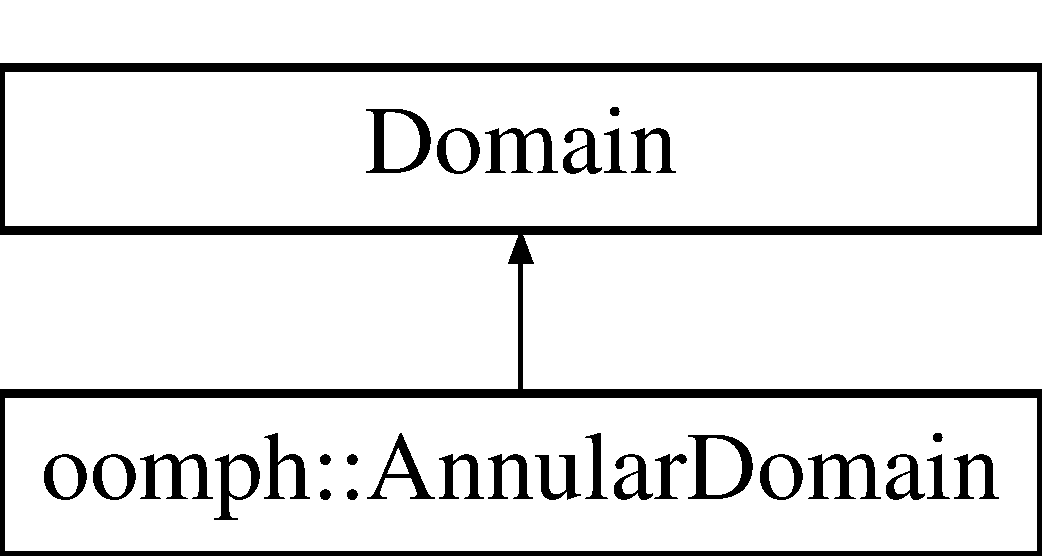
\includegraphics[height=2.000000cm]{classoomph_1_1AnnularDomain}
\end{center}
\end{figure}
\subsection*{Public Member Functions}
\begin{DoxyCompactItemize}
\item 
\hyperlink{classoomph_1_1AnnularDomain_aa0b4ad9d8e63de8aa0dc2d462a016143}{Annular\+Domain} (const double \&azimuthal\+\_\+fraction, const unsigned \&ntheta, const unsigned \&nr, const double \&a, const double \&h, const double \&phi)
\begin{DoxyCompactList}\small\item\em Constructor\+: Specify azimuthal fraction (1.\+0 is 360 degrees) number of macro elements in azimuthal and radial direction, inner radius and thickness. Rotate mesh by angle phi. \end{DoxyCompactList}\item 
\hyperlink{classoomph_1_1AnnularDomain_ad081791409dc419594d0a64e1c17fb09}{Annular\+Domain} (const \hyperlink{classoomph_1_1AnnularDomain}{Annular\+Domain} \&)
\begin{DoxyCompactList}\small\item\em Broken copy constructor. \end{DoxyCompactList}\item 
void \hyperlink{classoomph_1_1AnnularDomain_a1e66e1208af0b6d0ec4a7006a77dbb5f}{operator=} (const \hyperlink{classoomph_1_1AnnularDomain}{Annular\+Domain} \&)
\begin{DoxyCompactList}\small\item\em Broken assignment operator. \end{DoxyCompactList}\item 
\hyperlink{classoomph_1_1AnnularDomain_a99ee51c9e5fd12fdd123ede8da09c483}{$\sim$\+Annular\+Domain} ()
\begin{DoxyCompactList}\small\item\em Destructor\+: Kill all macro elements. \end{DoxyCompactList}\item 
void \hyperlink{classoomph_1_1AnnularDomain_ade8cfa0e6f2d41e7d3877250321bfff3}{macro\+\_\+element\+\_\+boundary} (const unsigned \&t, const unsigned \&i\+\_\+macro, const unsigned \&i\+\_\+direct, const Vector$<$ double $>$ \&s, Vector$<$ double $>$ \&f)
\begin{DoxyCompactList}\small\item\em Vector representation of the i\+\_\+macro-\/th macro element boundary i\+\_\+direct (N/\+S/\+W/E) at time level t (t=0\+: present; t$>$0\+: previous)\+: f(s). \end{DoxyCompactList}\end{DoxyCompactItemize}
\subsection*{Private Attributes}
\begin{DoxyCompactItemize}
\item 
double \hyperlink{classoomph_1_1AnnularDomain_ac6ea648ff2b80c412c6aec3a071945af}{Azimuthal\+\_\+fraction}
\begin{DoxyCompactList}\small\item\em Azimuthal fraction. \end{DoxyCompactList}\item 
double \hyperlink{classoomph_1_1AnnularDomain_a41bead396f1b49783caf334e56a6eb23}{Inner\+\_\+radius}
\begin{DoxyCompactList}\small\item\em Inner radius. \end{DoxyCompactList}\item 
double \hyperlink{classoomph_1_1AnnularDomain_a34008644354ffc3e7f48505557d95755}{Thickness}
\begin{DoxyCompactList}\small\item\em Thickness. \end{DoxyCompactList}\item 
unsigned \hyperlink{classoomph_1_1AnnularDomain_a42f197d2b806a961395f905d947b3e6e}{Ntheta}
\begin{DoxyCompactList}\small\item\em Number of macro elements in azimuthal direction. \end{DoxyCompactList}\item 
unsigned \hyperlink{classoomph_1_1AnnularDomain_a0cbd02650762aa5b6baf32936e553b64}{Nr}
\begin{DoxyCompactList}\small\item\em Number of macro elements in radial direction. \end{DoxyCompactList}\item 
double \hyperlink{classoomph_1_1AnnularDomain_a0280549bd7a88cabb84a7223ed114040}{Phi}
\begin{DoxyCompactList}\small\item\em Rotation angle. \end{DoxyCompactList}\end{DoxyCompactItemize}


\subsection{Detailed Description}
Annular domain. 

Definition at line 44 of file annular\+\_\+domain.\+h.



\subsection{Constructor \& Destructor Documentation}
\mbox{\Hypertarget{classoomph_1_1AnnularDomain_aa0b4ad9d8e63de8aa0dc2d462a016143}\label{classoomph_1_1AnnularDomain_aa0b4ad9d8e63de8aa0dc2d462a016143}} 
\index{oomph\+::\+Annular\+Domain@{oomph\+::\+Annular\+Domain}!Annular\+Domain@{Annular\+Domain}}
\index{Annular\+Domain@{Annular\+Domain}!oomph\+::\+Annular\+Domain@{oomph\+::\+Annular\+Domain}}
\subsubsection{\texorpdfstring{Annular\+Domain()}{AnnularDomain()}\hspace{0.1cm}{\footnotesize\ttfamily [1/2]}}
{\footnotesize\ttfamily oomph\+::\+Annular\+Domain\+::\+Annular\+Domain (\begin{DoxyParamCaption}\item[{const double \&}]{azimuthal\+\_\+fraction,  }\item[{const unsigned \&}]{ntheta,  }\item[{const unsigned \&}]{nr,  }\item[{const double \&}]{a,  }\item[{const double \&}]{h,  }\item[{const double \&}]{phi }\end{DoxyParamCaption})\hspace{0.3cm}{\ttfamily [inline]}}



Constructor\+: Specify azimuthal fraction (1.\+0 is 360 degrees) number of macro elements in azimuthal and radial direction, inner radius and thickness. Rotate mesh by angle phi. 



Definition at line 52 of file annular\+\_\+domain.\+h.

\mbox{\Hypertarget{classoomph_1_1AnnularDomain_ad081791409dc419594d0a64e1c17fb09}\label{classoomph_1_1AnnularDomain_ad081791409dc419594d0a64e1c17fb09}} 
\index{oomph\+::\+Annular\+Domain@{oomph\+::\+Annular\+Domain}!Annular\+Domain@{Annular\+Domain}}
\index{Annular\+Domain@{Annular\+Domain}!oomph\+::\+Annular\+Domain@{oomph\+::\+Annular\+Domain}}
\subsubsection{\texorpdfstring{Annular\+Domain()}{AnnularDomain()}\hspace{0.1cm}{\footnotesize\ttfamily [2/2]}}
{\footnotesize\ttfamily oomph\+::\+Annular\+Domain\+::\+Annular\+Domain (\begin{DoxyParamCaption}\item[{const \hyperlink{classoomph_1_1AnnularDomain}{Annular\+Domain} \&}]{ }\end{DoxyParamCaption})\hspace{0.3cm}{\ttfamily [inline]}}



Broken copy constructor. 



Definition at line 69 of file annular\+\_\+domain.\+h.

\mbox{\Hypertarget{classoomph_1_1AnnularDomain_a99ee51c9e5fd12fdd123ede8da09c483}\label{classoomph_1_1AnnularDomain_a99ee51c9e5fd12fdd123ede8da09c483}} 
\index{oomph\+::\+Annular\+Domain@{oomph\+::\+Annular\+Domain}!````~Annular\+Domain@{$\sim$\+Annular\+Domain}}
\index{````~Annular\+Domain@{$\sim$\+Annular\+Domain}!oomph\+::\+Annular\+Domain@{oomph\+::\+Annular\+Domain}}
\subsubsection{\texorpdfstring{$\sim$\+Annular\+Domain()}{~AnnularDomain()}}
{\footnotesize\ttfamily oomph\+::\+Annular\+Domain\+::$\sim$\+Annular\+Domain (\begin{DoxyParamCaption}{ }\end{DoxyParamCaption})\hspace{0.3cm}{\ttfamily [inline]}}



Destructor\+: Kill all macro elements. 



Definition at line 82 of file annular\+\_\+domain.\+h.



References macro\+\_\+element\+\_\+boundary().



\subsection{Member Function Documentation}
\mbox{\Hypertarget{classoomph_1_1AnnularDomain_ade8cfa0e6f2d41e7d3877250321bfff3}\label{classoomph_1_1AnnularDomain_ade8cfa0e6f2d41e7d3877250321bfff3}} 
\index{oomph\+::\+Annular\+Domain@{oomph\+::\+Annular\+Domain}!macro\+\_\+element\+\_\+boundary@{macro\+\_\+element\+\_\+boundary}}
\index{macro\+\_\+element\+\_\+boundary@{macro\+\_\+element\+\_\+boundary}!oomph\+::\+Annular\+Domain@{oomph\+::\+Annular\+Domain}}
\subsubsection{\texorpdfstring{macro\+\_\+element\+\_\+boundary()}{macro\_element\_boundary()}}
{\footnotesize\ttfamily void oomph\+::\+Annular\+Domain\+::macro\+\_\+element\+\_\+boundary (\begin{DoxyParamCaption}\item[{const unsigned \&}]{t,  }\item[{const unsigned \&}]{i\+\_\+macro,  }\item[{const unsigned \&}]{i\+\_\+direct,  }\item[{const Vector$<$ double $>$ \&}]{s,  }\item[{Vector$<$ double $>$ \&}]{f }\end{DoxyParamCaption})}



Vector representation of the i\+\_\+macro-\/th macro element boundary i\+\_\+direct (N/\+S/\+W/E) at time level t (t=0\+: present; t$>$0\+: previous)\+: f(s). 

Vector representation of the imacro-\/th macro element boundary idirect (N/\+S/\+W/E) at time level t (t=0\+: present; t$>$0\+: previous)\+: f(s) 

Definition at line 136 of file annular\+\_\+domain.\+h.



References Azimuthal\+\_\+fraction, Inner\+\_\+radius, Nr, Ntheta, Phi, and Thickness.



Referenced by $\sim$\+Annular\+Domain().

\mbox{\Hypertarget{classoomph_1_1AnnularDomain_a1e66e1208af0b6d0ec4a7006a77dbb5f}\label{classoomph_1_1AnnularDomain_a1e66e1208af0b6d0ec4a7006a77dbb5f}} 
\index{oomph\+::\+Annular\+Domain@{oomph\+::\+Annular\+Domain}!operator=@{operator=}}
\index{operator=@{operator=}!oomph\+::\+Annular\+Domain@{oomph\+::\+Annular\+Domain}}
\subsubsection{\texorpdfstring{operator=()}{operator=()}}
{\footnotesize\ttfamily void oomph\+::\+Annular\+Domain\+::operator= (\begin{DoxyParamCaption}\item[{const \hyperlink{classoomph_1_1AnnularDomain}{Annular\+Domain} \&}]{ }\end{DoxyParamCaption})\hspace{0.3cm}{\ttfamily [inline]}}



Broken assignment operator. 



Definition at line 75 of file annular\+\_\+domain.\+h.



\subsection{Member Data Documentation}
\mbox{\Hypertarget{classoomph_1_1AnnularDomain_ac6ea648ff2b80c412c6aec3a071945af}\label{classoomph_1_1AnnularDomain_ac6ea648ff2b80c412c6aec3a071945af}} 
\index{oomph\+::\+Annular\+Domain@{oomph\+::\+Annular\+Domain}!Azimuthal\+\_\+fraction@{Azimuthal\+\_\+fraction}}
\index{Azimuthal\+\_\+fraction@{Azimuthal\+\_\+fraction}!oomph\+::\+Annular\+Domain@{oomph\+::\+Annular\+Domain}}
\subsubsection{\texorpdfstring{Azimuthal\+\_\+fraction}{Azimuthal\_fraction}}
{\footnotesize\ttfamily double oomph\+::\+Annular\+Domain\+::\+Azimuthal\+\_\+fraction\hspace{0.3cm}{\ttfamily [private]}}



Azimuthal fraction. 



Definition at line 105 of file annular\+\_\+domain.\+h.



Referenced by macro\+\_\+element\+\_\+boundary().

\mbox{\Hypertarget{classoomph_1_1AnnularDomain_a41bead396f1b49783caf334e56a6eb23}\label{classoomph_1_1AnnularDomain_a41bead396f1b49783caf334e56a6eb23}} 
\index{oomph\+::\+Annular\+Domain@{oomph\+::\+Annular\+Domain}!Inner\+\_\+radius@{Inner\+\_\+radius}}
\index{Inner\+\_\+radius@{Inner\+\_\+radius}!oomph\+::\+Annular\+Domain@{oomph\+::\+Annular\+Domain}}
\subsubsection{\texorpdfstring{Inner\+\_\+radius}{Inner\_radius}}
{\footnotesize\ttfamily double oomph\+::\+Annular\+Domain\+::\+Inner\+\_\+radius\hspace{0.3cm}{\ttfamily [private]}}



Inner radius. 



Definition at line 108 of file annular\+\_\+domain.\+h.



Referenced by macro\+\_\+element\+\_\+boundary().

\mbox{\Hypertarget{classoomph_1_1AnnularDomain_a0cbd02650762aa5b6baf32936e553b64}\label{classoomph_1_1AnnularDomain_a0cbd02650762aa5b6baf32936e553b64}} 
\index{oomph\+::\+Annular\+Domain@{oomph\+::\+Annular\+Domain}!Nr@{Nr}}
\index{Nr@{Nr}!oomph\+::\+Annular\+Domain@{oomph\+::\+Annular\+Domain}}
\subsubsection{\texorpdfstring{Nr}{Nr}}
{\footnotesize\ttfamily unsigned oomph\+::\+Annular\+Domain\+::\+Nr\hspace{0.3cm}{\ttfamily [private]}}



Number of macro elements in radial direction. 



Definition at line 117 of file annular\+\_\+domain.\+h.



Referenced by macro\+\_\+element\+\_\+boundary().

\mbox{\Hypertarget{classoomph_1_1AnnularDomain_a42f197d2b806a961395f905d947b3e6e}\label{classoomph_1_1AnnularDomain_a42f197d2b806a961395f905d947b3e6e}} 
\index{oomph\+::\+Annular\+Domain@{oomph\+::\+Annular\+Domain}!Ntheta@{Ntheta}}
\index{Ntheta@{Ntheta}!oomph\+::\+Annular\+Domain@{oomph\+::\+Annular\+Domain}}
\subsubsection{\texorpdfstring{Ntheta}{Ntheta}}
{\footnotesize\ttfamily unsigned oomph\+::\+Annular\+Domain\+::\+Ntheta\hspace{0.3cm}{\ttfamily [private]}}



Number of macro elements in azimuthal direction. 



Definition at line 114 of file annular\+\_\+domain.\+h.



Referenced by macro\+\_\+element\+\_\+boundary().

\mbox{\Hypertarget{classoomph_1_1AnnularDomain_a0280549bd7a88cabb84a7223ed114040}\label{classoomph_1_1AnnularDomain_a0280549bd7a88cabb84a7223ed114040}} 
\index{oomph\+::\+Annular\+Domain@{oomph\+::\+Annular\+Domain}!Phi@{Phi}}
\index{Phi@{Phi}!oomph\+::\+Annular\+Domain@{oomph\+::\+Annular\+Domain}}
\subsubsection{\texorpdfstring{Phi}{Phi}}
{\footnotesize\ttfamily double oomph\+::\+Annular\+Domain\+::\+Phi\hspace{0.3cm}{\ttfamily [private]}}



Rotation angle. 



Definition at line 120 of file annular\+\_\+domain.\+h.



Referenced by macro\+\_\+element\+\_\+boundary().

\mbox{\Hypertarget{classoomph_1_1AnnularDomain_a34008644354ffc3e7f48505557d95755}\label{classoomph_1_1AnnularDomain_a34008644354ffc3e7f48505557d95755}} 
\index{oomph\+::\+Annular\+Domain@{oomph\+::\+Annular\+Domain}!Thickness@{Thickness}}
\index{Thickness@{Thickness}!oomph\+::\+Annular\+Domain@{oomph\+::\+Annular\+Domain}}
\subsubsection{\texorpdfstring{Thickness}{Thickness}}
{\footnotesize\ttfamily double oomph\+::\+Annular\+Domain\+::\+Thickness\hspace{0.3cm}{\ttfamily [private]}}



Thickness. 



Definition at line 111 of file annular\+\_\+domain.\+h.



Referenced by macro\+\_\+element\+\_\+boundary().



The documentation for this class was generated from the following file\+:\begin{DoxyCompactItemize}
\item 
\hyperlink{annular__domain_8h}{annular\+\_\+domain.\+h}\end{DoxyCompactItemize}

\hypertarget{classoomph_1_1BackwardStepQuadMesh}{}\section{oomph\+:\+:Backward\+Step\+Quad\+Mesh$<$ E\+L\+E\+M\+E\+NT $>$ Class Template Reference}
\label{classoomph_1_1BackwardStepQuadMesh}\index{oomph\+::\+Backward\+Step\+Quad\+Mesh$<$ E\+L\+E\+M\+E\+N\+T $>$@{oomph\+::\+Backward\+Step\+Quad\+Mesh$<$ E\+L\+E\+M\+E\+N\+T $>$}}


Backward step mesh.  




{\ttfamily \#include $<$backward\+\_\+step\+\_\+mesh.\+template.\+h$>$}

Inheritance diagram for oomph\+:\+:Backward\+Step\+Quad\+Mesh$<$ E\+L\+E\+M\+E\+NT $>$\+:\begin{figure}[H]
\begin{center}
\leavevmode
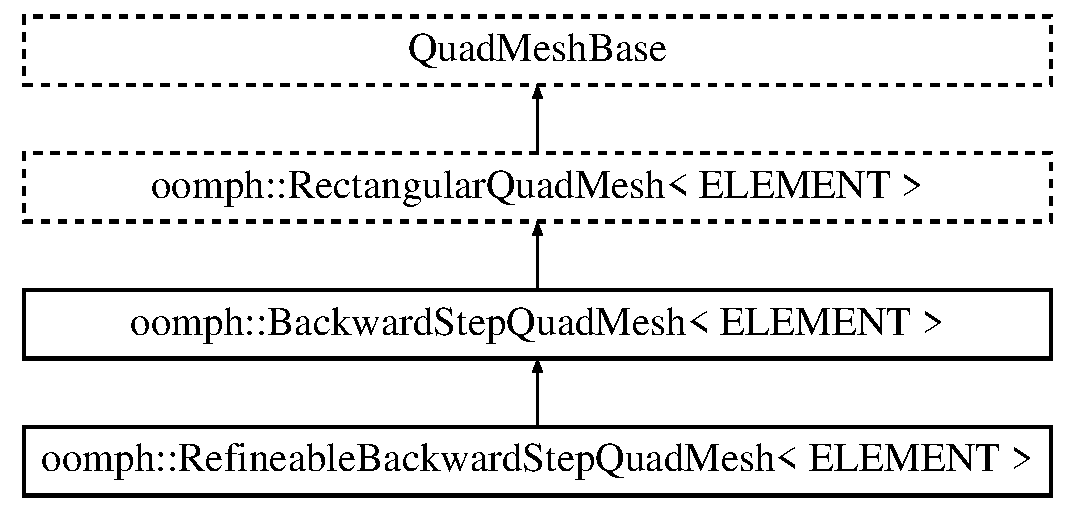
\includegraphics[height=5.000000cm]{classoomph_1_1BackwardStepQuadMesh}
\end{center}
\end{figure}
\subsection*{Public Member Functions}
\begin{DoxyCompactItemize}
\item 
\hyperlink{classoomph_1_1BackwardStepQuadMesh_ae8374ae7d3646c00fec4fc9c2d604cf8}{Backward\+Step\+Quad\+Mesh} (const unsigned \&\hyperlink{classoomph_1_1RectangularQuadMesh_abfef93d6322886cdce14a437186e4821}{nx}, const unsigned \&\hyperlink{classoomph_1_1RectangularQuadMesh_a86d76a55eb7c4e8bca9b74d23c8b0412}{ny}, const unsigned \&nx\+\_\+cut\+\_\+out, const unsigned \&ny\+\_\+cut\+\_\+out, const double \&lx, const double \&ly, \hyperlink{classoomph_1_1TimeStepper}{Time\+Stepper} $\ast$time\+\_\+stepper\+\_\+pt=\&\hyperlink{classoomph_1_1Mesh_a12243d0fee2b1fcee729ee5a4777ea10}{Mesh\+::\+Default\+\_\+\+Time\+Stepper})
\begin{DoxyCompactList}\small\item\em Pass overall number of elements in the horizontal and vertical directions, nx and ny, and the corresponding dimensions, lx and ly. nx\+\_\+cut\+\_\+out and ny\+\_\+cut\+\_\+out elements are cut out from the lower right corner to create the (reversed) backward step geometry. Timestepper defaults to \hyperlink{classoomph_1_1Steady}{Steady}. \end{DoxyCompactList}\item 
virtual \hyperlink{classoomph_1_1BackwardStepQuadMesh_aec4e05ad80d83327050653ebabce9564}{$\sim$\+Backward\+Step\+Quad\+Mesh} ()
\begin{DoxyCompactList}\small\item\em Destructor\+: Empty. \end{DoxyCompactList}\end{DoxyCompactItemize}
\subsection*{Private Member Functions}
\begin{DoxyCompactItemize}
\item 
void \hyperlink{classoomph_1_1BackwardStepQuadMesh_ab71a6f2854d36b845ed79dccb0101991}{build\+\_\+mesh} (const unsigned \&\hyperlink{classoomph_1_1RectangularQuadMesh_abfef93d6322886cdce14a437186e4821}{nx}, const unsigned \&\hyperlink{classoomph_1_1RectangularQuadMesh_a86d76a55eb7c4e8bca9b74d23c8b0412}{ny}, const unsigned \&nx\+\_\+cut\+\_\+out, const unsigned \&ny\+\_\+cut\+\_\+out, const double \&lx, const double \&ly)
\begin{DoxyCompactList}\small\item\em Actual build function. \end{DoxyCompactList}\end{DoxyCompactItemize}
\subsection*{Additional Inherited Members}


\subsection{Detailed Description}
\subsubsection*{template$<$class E\+L\+E\+M\+E\+NT$>$\newline
class oomph\+::\+Backward\+Step\+Quad\+Mesh$<$ E\+L\+E\+M\+E\+N\+T $>$}

Backward step mesh. 

Definition at line 51 of file backward\+\_\+step\+\_\+mesh.\+template.\+h.



\subsection{Constructor \& Destructor Documentation}
\mbox{\Hypertarget{classoomph_1_1BackwardStepQuadMesh_ae8374ae7d3646c00fec4fc9c2d604cf8}\label{classoomph_1_1BackwardStepQuadMesh_ae8374ae7d3646c00fec4fc9c2d604cf8}} 
\index{oomph\+::\+Backward\+Step\+Quad\+Mesh@{oomph\+::\+Backward\+Step\+Quad\+Mesh}!Backward\+Step\+Quad\+Mesh@{Backward\+Step\+Quad\+Mesh}}
\index{Backward\+Step\+Quad\+Mesh@{Backward\+Step\+Quad\+Mesh}!oomph\+::\+Backward\+Step\+Quad\+Mesh@{oomph\+::\+Backward\+Step\+Quad\+Mesh}}
\subsubsection{\texorpdfstring{Backward\+Step\+Quad\+Mesh()}{BackwardStepQuadMesh()}}
{\footnotesize\ttfamily template$<$class E\+L\+E\+M\+E\+NT $>$ \\
\hyperlink{classoomph_1_1BackwardStepQuadMesh}{oomph\+::\+Backward\+Step\+Quad\+Mesh}$<$ E\+L\+E\+M\+E\+NT $>$\+::\hyperlink{classoomph_1_1BackwardStepQuadMesh}{Backward\+Step\+Quad\+Mesh} (\begin{DoxyParamCaption}\item[{const unsigned \&}]{nx,  }\item[{const unsigned \&}]{ny,  }\item[{const unsigned \&}]{nx\+\_\+cut\+\_\+out,  }\item[{const unsigned \&}]{ny\+\_\+cut\+\_\+out,  }\item[{const double \&}]{lx,  }\item[{const double \&}]{ly,  }\item[{\hyperlink{classoomph_1_1TimeStepper}{Time\+Stepper} $\ast$}]{time\+\_\+stepper\+\_\+pt = {\ttfamily \&\hyperlink{classoomph_1_1Mesh_a12243d0fee2b1fcee729ee5a4777ea10}{Mesh\+::\+Default\+\_\+\+Time\+Stepper}} }\end{DoxyParamCaption})\hspace{0.3cm}{\ttfamily [inline]}}



Pass overall number of elements in the horizontal and vertical directions, nx and ny, and the corresponding dimensions, lx and ly. nx\+\_\+cut\+\_\+out and ny\+\_\+cut\+\_\+out elements are cut out from the lower right corner to create the (reversed) backward step geometry. Timestepper defaults to \hyperlink{classoomph_1_1Steady}{Steady}. 



Definition at line 63 of file backward\+\_\+step\+\_\+mesh.\+template.\+h.



References oomph\+::\+Backward\+Step\+Quad\+Mesh$<$ E\+L\+E\+M\+E\+N\+T $>$\+::build\+\_\+mesh().

\mbox{\Hypertarget{classoomph_1_1BackwardStepQuadMesh_aec4e05ad80d83327050653ebabce9564}\label{classoomph_1_1BackwardStepQuadMesh_aec4e05ad80d83327050653ebabce9564}} 
\index{oomph\+::\+Backward\+Step\+Quad\+Mesh@{oomph\+::\+Backward\+Step\+Quad\+Mesh}!````~Backward\+Step\+Quad\+Mesh@{$\sim$\+Backward\+Step\+Quad\+Mesh}}
\index{````~Backward\+Step\+Quad\+Mesh@{$\sim$\+Backward\+Step\+Quad\+Mesh}!oomph\+::\+Backward\+Step\+Quad\+Mesh@{oomph\+::\+Backward\+Step\+Quad\+Mesh}}
\subsubsection{\texorpdfstring{$\sim$\+Backward\+Step\+Quad\+Mesh()}{~BackwardStepQuadMesh()}}
{\footnotesize\ttfamily template$<$class E\+L\+E\+M\+E\+NT $>$ \\
virtual \hyperlink{classoomph_1_1BackwardStepQuadMesh}{oomph\+::\+Backward\+Step\+Quad\+Mesh}$<$ E\+L\+E\+M\+E\+NT $>$\+::$\sim$\hyperlink{classoomph_1_1BackwardStepQuadMesh}{Backward\+Step\+Quad\+Mesh} (\begin{DoxyParamCaption}{ }\end{DoxyParamCaption})\hspace{0.3cm}{\ttfamily [inline]}, {\ttfamily [virtual]}}



Destructor\+: Empty. 



Definition at line 78 of file backward\+\_\+step\+\_\+mesh.\+template.\+h.



References oomph\+::\+Backward\+Step\+Quad\+Mesh$<$ E\+L\+E\+M\+E\+N\+T $>$\+::build\+\_\+mesh(), oomph\+::\+Rectangular\+Quad\+Mesh$<$ E\+L\+E\+M\+E\+N\+T $>$\+::nx(), and oomph\+::\+Rectangular\+Quad\+Mesh$<$ E\+L\+E\+M\+E\+N\+T $>$\+::ny().



\subsection{Member Function Documentation}
\mbox{\Hypertarget{classoomph_1_1BackwardStepQuadMesh_ab71a6f2854d36b845ed79dccb0101991}\label{classoomph_1_1BackwardStepQuadMesh_ab71a6f2854d36b845ed79dccb0101991}} 
\index{oomph\+::\+Backward\+Step\+Quad\+Mesh@{oomph\+::\+Backward\+Step\+Quad\+Mesh}!build\+\_\+mesh@{build\+\_\+mesh}}
\index{build\+\_\+mesh@{build\+\_\+mesh}!oomph\+::\+Backward\+Step\+Quad\+Mesh@{oomph\+::\+Backward\+Step\+Quad\+Mesh}}
\subsubsection{\texorpdfstring{build\+\_\+mesh()}{build\_mesh()}}
{\footnotesize\ttfamily template$<$class E\+L\+E\+M\+E\+NT $>$ \\
void \hyperlink{classoomph_1_1BackwardStepQuadMesh}{oomph\+::\+Backward\+Step\+Quad\+Mesh}$<$ E\+L\+E\+M\+E\+NT $>$\+::build\+\_\+mesh (\begin{DoxyParamCaption}\item[{const unsigned \&}]{nx,  }\item[{const unsigned \&}]{ny,  }\item[{const unsigned \&}]{nx\+\_\+cut\+\_\+out,  }\item[{const unsigned \&}]{ny\+\_\+cut\+\_\+out,  }\item[{const double \&}]{lx,  }\item[{const double \&}]{ly }\end{DoxyParamCaption})\hspace{0.3cm}{\ttfamily [private]}}



Actual build function. 

Actual build function. Pass overall number of elements in the horizontal and vertical directions, nx and ny, and the corresponding dimensions, lx and ly. nx\+\_\+cut\+\_\+out and ny\+\_\+cut\+\_\+out elements are cut out from the lower right corner to create the (reversed) backward step geometry. Timestepper defaults to \hyperlink{classoomph_1_1Steady}{Steady}. 

Definition at line 52 of file backward\+\_\+step\+\_\+mesh.\+template.\+cc.



References e, i, oomph\+::\+Node\+::is\+\_\+on\+\_\+boundary(), oomph\+::\+Finite\+Element\+::nnode(), oomph\+::\+Finite\+Element\+::nnode\+\_\+1d(), and oomph\+::\+Finite\+Element\+::node\+\_\+pt().



Referenced by oomph\+::\+Backward\+Step\+Quad\+Mesh$<$ E\+L\+E\+M\+E\+N\+T $>$\+::\+Backward\+Step\+Quad\+Mesh(), and oomph\+::\+Backward\+Step\+Quad\+Mesh$<$ E\+L\+E\+M\+E\+N\+T $>$\+::$\sim$\+Backward\+Step\+Quad\+Mesh().



The documentation for this class was generated from the following files\+:\begin{DoxyCompactItemize}
\item 
\hyperlink{backward__step__mesh_8template_8h}{backward\+\_\+step\+\_\+mesh.\+template.\+h}\item 
\hyperlink{backward__step__mesh_8template_8cc}{backward\+\_\+step\+\_\+mesh.\+template.\+cc}\end{DoxyCompactItemize}

\hypertarget{classoomph_1_1BrethertonSpineMesh}{}\section{oomph\+:\+:Bretherton\+Spine\+Mesh$<$ E\+L\+E\+M\+E\+NT, I\+N\+T\+E\+R\+F\+A\+C\+E\+\_\+\+E\+L\+E\+M\+E\+NT $>$ Class Template Reference}
\label{classoomph_1_1BrethertonSpineMesh}\index{oomph\+::\+Bretherton\+Spine\+Mesh$<$ E\+L\+E\+M\+E\+N\+T, I\+N\+T\+E\+R\+F\+A\+C\+E\+\_\+\+E\+L\+E\+M\+E\+N\+T $>$@{oomph\+::\+Bretherton\+Spine\+Mesh$<$ E\+L\+E\+M\+E\+N\+T, I\+N\+T\+E\+R\+F\+A\+C\+E\+\_\+\+E\+L\+E\+M\+E\+N\+T $>$}}


{\ttfamily \#include $<$bretherton\+\_\+spine\+\_\+mesh.\+template.\+h$>$}

Inheritance diagram for oomph\+:\+:Bretherton\+Spine\+Mesh$<$ E\+L\+E\+M\+E\+NT, I\+N\+T\+E\+R\+F\+A\+C\+E\+\_\+\+E\+L\+E\+M\+E\+NT $>$\+:\begin{figure}[H]
\begin{center}
\leavevmode
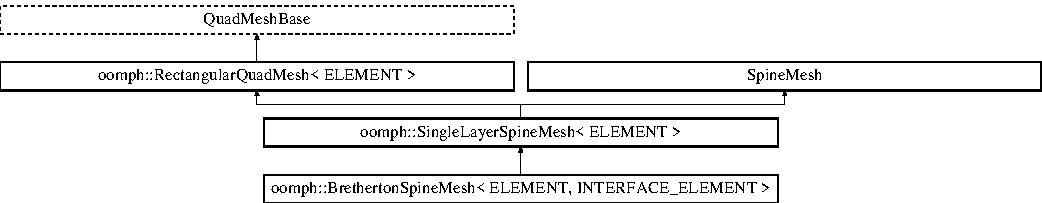
\includegraphics[height=2.731707cm]{classoomph_1_1BrethertonSpineMesh}
\end{center}
\end{figure}
\subsection*{Public Member Functions}
\begin{DoxyCompactItemize}
\item 
\hyperlink{classoomph_1_1BrethertonSpineMesh_a0e9c404141ee65b000ab4d1fdc4f11da}{Bretherton\+Spine\+Mesh} (const unsigned \&nx1, const unsigned \&nx2, const unsigned \&nx3, const unsigned \&nh, const unsigned \&nhalf, const double \&h, Geom\+Object $\ast$lower\+\_\+wall\+\_\+pt, Geom\+Object $\ast$upper\+\_\+wall\+\_\+pt, const double \&zeta\+\_\+start, const double \&zeta\+\_\+transition\+\_\+start, const double \&zeta\+\_\+transition\+\_\+end, const double \&zeta\+\_\+end, Time\+Stepper $\ast$time\+\_\+stepper\+\_\+pt=\&Mesh\+::\+Default\+\_\+\+Time\+Stepper)
\begin{DoxyCompactList}\small\item\em Constructor. Arguments\+: \end{DoxyCompactList}\item 
Finite\+Element $\ast$\& \hyperlink{classoomph_1_1BrethertonSpineMesh_a3d14f3985d718867099747e5b3750fec}{interface\+\_\+element\+\_\+pt} (const unsigned long \&i)
\begin{DoxyCompactList}\small\item\em Access functions for pointers to interface elements. \end{DoxyCompactList}\item 
unsigned long \hyperlink{classoomph_1_1BrethertonSpineMesh_ae1ecd7c00fe1032e1ee16d7a98156d5c}{ninterface\+\_\+element} () const
\begin{DoxyCompactList}\small\item\em Number of elements on interface. \end{DoxyCompactList}\item 
Finite\+Element $\ast$\& \hyperlink{classoomph_1_1BrethertonSpineMesh_a2fc2b4be08ff93fa313281f82e19d92e}{bulk\+\_\+element\+\_\+pt} (const unsigned long \&i)
\begin{DoxyCompactList}\small\item\em Access functions for pointers to elements in bulk. \end{DoxyCompactList}\item 
unsigned long \hyperlink{classoomph_1_1BrethertonSpineMesh_a47184866746a1fce6dd0ca27ab7e17ce}{nbulk} () const
\begin{DoxyCompactList}\small\item\em Number of elements in bulk. \end{DoxyCompactList}\item 
unsigned \hyperlink{classoomph_1_1BrethertonSpineMesh_ade4d0f2933beddda517b949d80928a18}{nfree\+\_\+surface\+\_\+spines} ()
\item 
double \hyperlink{classoomph_1_1BrethertonSpineMesh_ac80488ae4db2da00e1b38f6f07e0ff9d}{find\+\_\+distance\+\_\+to\+\_\+free\+\_\+surface} (Geom\+Object $\ast$const \&fs\+\_\+geom\+\_\+object\+\_\+pt, Vector$<$ double $>$ \&initial\+\_\+zeta, const Vector$<$ double $>$ \&spine\+\_\+base, const Vector$<$ double $>$ \&spine\+\_\+end)
\begin{DoxyCompactList}\small\item\em Recalculate the spine lengths after repositioning. \end{DoxyCompactList}\item 
void \hyperlink{classoomph_1_1BrethertonSpineMesh_a0dfeac5bc9a4fa4bfdcd443def30dcdb}{reposition\+\_\+spines} (const double \&zeta\+\_\+lo\+\_\+transition\+\_\+start, const double \&zeta\+\_\+lo\+\_\+transition\+\_\+end, const double \&zeta\+\_\+up\+\_\+transition\+\_\+start, const double \&zeta\+\_\+up\+\_\+transition\+\_\+end)
\begin{DoxyCompactList}\small\item\em Reposition the spines in response to changes in geometry. \end{DoxyCompactList}\item 
void \hyperlink{classoomph_1_1BrethertonSpineMesh_a507ea97977b837f2f0d9647407d770cd}{pin\+\_\+all\+\_\+spines} ()
\item 
void \hyperlink{classoomph_1_1BrethertonSpineMesh_a981301706d4940cfb24d3d769a7a523b}{spine\+\_\+node\+\_\+update} (Spine\+Node $\ast$spine\+\_\+node\+\_\+pt)
\begin{DoxyCompactList}\small\item\em General node update function implements pure virtual function defined in Spine\+Mesh base class and performs specific update actions, depending on the node update fct id stored for each node. \end{DoxyCompactList}\item 
E\+L\+E\+M\+E\+NT $\ast$ \hyperlink{classoomph_1_1BrethertonSpineMesh_a9b02893724c76098f75d9285e9985f4b}{control\+\_\+element\+\_\+pt} ()
\begin{DoxyCompactList}\small\item\em Pointer to control element (just under the symmetry line near the bubble tip, so the bubble tip is located at s=\mbox{[}1.\+0,1.\+0\mbox{]} in this element. \end{DoxyCompactList}\item 
double \hyperlink{classoomph_1_1BrethertonSpineMesh_a67f784e7b3a898af6c60515042c3ea73}{spine\+\_\+centre\+\_\+fraction} () const
\begin{DoxyCompactList}\small\item\em Read the value of the spine centre\textquotesingle{}s vertical fraction. \end{DoxyCompactList}\item 
void \hyperlink{classoomph_1_1BrethertonSpineMesh_a33c3ed5af92e7b22a22615f42c34c387}{set\+\_\+spine\+\_\+centre\+\_\+fraction\+\_\+pt} (double $\ast$const \&fraction\+\_\+pt)
\begin{DoxyCompactList}\small\item\em Set the pointer to the spine centre\textquotesingle{}s vertial fraction. \end{DoxyCompactList}\end{DoxyCompactItemize}
\subsection*{Protected Member Functions}
\begin{DoxyCompactItemize}
\item 
void \hyperlink{classoomph_1_1BrethertonSpineMesh_a0446cb0efaa31739f51ae0534a73d116}{spine\+\_\+node\+\_\+update\+\_\+film\+\_\+lower} (Spine\+Node $\ast$spine\+\_\+node\+\_\+pt)
\begin{DoxyCompactList}\small\item\em Update function for the deposited film region in the lower part of the domain\+: Vertical spines. \end{DoxyCompactList}\item 
void \hyperlink{classoomph_1_1BrethertonSpineMesh_a0dc35290fc96a075d864e79528e5fec8}{spine\+\_\+node\+\_\+update\+\_\+horizontal\+\_\+transition\+\_\+lower} (Spine\+Node $\ast$spine\+\_\+node\+\_\+pt)
\begin{DoxyCompactList}\small\item\em Update function for the horizontal transitition region in the lower part of the domain\+: Spine points from wall to origin. \end{DoxyCompactList}\item 
void \hyperlink{classoomph_1_1BrethertonSpineMesh_a9ec578183760e386ed5229ba193e1fdf}{spine\+\_\+node\+\_\+update\+\_\+vertical\+\_\+transition\+\_\+lower} (Spine\+Node $\ast$spine\+\_\+node\+\_\+pt)
\begin{DoxyCompactList}\small\item\em Update function for the vertical transitition region in the lower part of the domain\+: Spine points to origin. \end{DoxyCompactList}\item 
void \hyperlink{classoomph_1_1BrethertonSpineMesh_a6ddc62166abfd621219551957c9b1103}{spine\+\_\+node\+\_\+update\+\_\+vertical\+\_\+transition\+\_\+upper} (Spine\+Node $\ast$spine\+\_\+node\+\_\+pt)
\begin{DoxyCompactList}\small\item\em Update function for the vertical transitition region in the upper part of the domain\+: Spine points to origin. \end{DoxyCompactList}\item 
void \hyperlink{classoomph_1_1BrethertonSpineMesh_aa9fa4941d8fb02a388e933a7dd1c76a2}{spine\+\_\+node\+\_\+update\+\_\+horizontal\+\_\+transition\+\_\+upper} (Spine\+Node $\ast$spine\+\_\+node\+\_\+pt)
\begin{DoxyCompactList}\small\item\em Update function for the horizontal transitition region in the upper part of the domain\+: Spine points towards origin. \end{DoxyCompactList}\item 
void \hyperlink{classoomph_1_1BrethertonSpineMesh_a3919bd086252db283ee5242b4688f8d1}{spine\+\_\+node\+\_\+update\+\_\+film\+\_\+upper} (Spine\+Node $\ast$spine\+\_\+node\+\_\+pt)
\begin{DoxyCompactList}\small\item\em Update function for the deposited film region in the upper part of the domain\+: Vertical spines. \end{DoxyCompactList}\item 
void \hyperlink{classoomph_1_1BrethertonSpineMesh_a5a09b6d2f5e7ffd12a0ae882754ad818}{spine\+\_\+node\+\_\+update\+\_\+channel} (Spine\+Node $\ast$spine\+\_\+node\+\_\+pt)
\begin{DoxyCompactList}\small\item\em Update function for the nodes in the channel region ahead of the finger tip\+: Nodes are evenly distributed along vertical lines between the top and bottom walls. \end{DoxyCompactList}\item 
void \hyperlink{classoomph_1_1BrethertonSpineMesh_a52ffe1a705cb720d09c831b9cf5397f6}{initial\+\_\+element\+\_\+reorder} ()
\begin{DoxyCompactList}\small\item\em Initial reordering elements of the elements -- before the channel mesh is added. Vertical stacks of elements, each topped by their interface element -- this is (currently) identical to the version in the \hyperlink{classoomph_1_1SingleLayerSpineMesh}{Single\+Layer\+Spine\+Mesh} but it\textquotesingle{}s important that the element reordering is maintained in exactly this form for the rest of the mesh generation process to work properly. Therefore we keep a copy of the function in here. \end{DoxyCompactList}\end{DoxyCompactItemize}
\subsection*{Protected Attributes}
\begin{DoxyCompactItemize}
\item 
unsigned \hyperlink{classoomph_1_1BrethertonSpineMesh_af6ef10fb80559c3ad27a50116da60dcc}{Nx1}
\begin{DoxyCompactList}\small\item\em Number of elements along wall in deposited film region. \end{DoxyCompactList}\item 
unsigned \hyperlink{classoomph_1_1BrethertonSpineMesh_a237b4f516eb3f74e42e190f2a23f93c3}{Nx2}
\begin{DoxyCompactList}\small\item\em Number of elements along wall in horizontal transition region. \end{DoxyCompactList}\item 
unsigned \hyperlink{classoomph_1_1BrethertonSpineMesh_a26c57f832b7cdc495087cef7b54c98fd}{Nx3}
\begin{DoxyCompactList}\small\item\em Number of elements along wall in channel region. \end{DoxyCompactList}\item 
unsigned \hyperlink{classoomph_1_1BrethertonSpineMesh_a1e58d18dd2231c785008efa07260e8da}{Nhalf}
\begin{DoxyCompactList}\small\item\em Number of elements in vertical transition region (there are twice as many elements across the channel) \end{DoxyCompactList}\item 
unsigned \hyperlink{classoomph_1_1BrethertonSpineMesh_a4ba20dfa61b6c342f2defbc0cdb47851}{Nh}
\begin{DoxyCompactList}\small\item\em Number of elements across the deposited film. \end{DoxyCompactList}\item 
double \hyperlink{classoomph_1_1BrethertonSpineMesh_a3d711e1bc9d751ab14662f6839a900e3}{H}
\begin{DoxyCompactList}\small\item\em Thickness of deposited film. \end{DoxyCompactList}\item 
Geom\+Object $\ast$ \hyperlink{classoomph_1_1BrethertonSpineMesh_a1f97e78a12000afcc1bd754102b5b51a}{Upper\+\_\+wall\+\_\+pt}
\begin{DoxyCompactList}\small\item\em Pointer to geometric object that represents the upper wall. \end{DoxyCompactList}\item 
Geom\+Object $\ast$ \hyperlink{classoomph_1_1BrethertonSpineMesh_a04c0136de66c06a34347b89f453730e1}{Lower\+\_\+wall\+\_\+pt}
\begin{DoxyCompactList}\small\item\em Pointer to geometric object that represents the lower wall. \end{DoxyCompactList}\item 
double \hyperlink{classoomph_1_1BrethertonSpineMesh_a0f41083aa9a97fca03d498bd6ec21eb2}{Zeta\+\_\+start}
\begin{DoxyCompactList}\small\item\em Start coordinate on wall. \end{DoxyCompactList}\item 
double \hyperlink{classoomph_1_1BrethertonSpineMesh_ac1b5e005bfb5db65f54ca599942126ea}{Zeta\+\_\+end}
\begin{DoxyCompactList}\small\item\em Wall coordinate of end of liquid filled region (inflow) \end{DoxyCompactList}\item 
double \hyperlink{classoomph_1_1BrethertonSpineMesh_af701937d59d7804f40cb1b4c7a262391}{Zeta\+\_\+transition\+\_\+start}
\begin{DoxyCompactList}\small\item\em Wall coordinate of start of the transition region. \end{DoxyCompactList}\item 
double \hyperlink{classoomph_1_1BrethertonSpineMesh_a1d05bb741eba54ab7498ab4f3c55f1b7}{Zeta\+\_\+transition\+\_\+end}
\begin{DoxyCompactList}\small\item\em Wall coordinate of end of transition region. \end{DoxyCompactList}\item 
double $\ast$ \hyperlink{classoomph_1_1BrethertonSpineMesh_af5e7951a89bc13d73f2b137947cda8a3}{Spine\+\_\+centre\+\_\+fraction\+\_\+pt}
\begin{DoxyCompactList}\small\item\em Pointer to vertical fraction of the spine centre. \end{DoxyCompactList}\item 
double \hyperlink{classoomph_1_1BrethertonSpineMesh_a306cf8ae8f91a81054904de64195bb16}{Default\+\_\+spine\+\_\+centre\+\_\+fraction}
\begin{DoxyCompactList}\small\item\em Default spine fraction. \end{DoxyCompactList}\item 
E\+L\+E\+M\+E\+NT $\ast$ \hyperlink{classoomph_1_1BrethertonSpineMesh_a81ee86c0c747947dab52073c221d53c1}{Control\+\_\+element\+\_\+pt}
\begin{DoxyCompactList}\small\item\em Pointer to control element (just under the symmetry line near the bubble tip; the bubble tip is located at s=\mbox{[}1.\+0,1.\+0\mbox{]} in this element. \end{DoxyCompactList}\item 
Vector$<$ Finite\+Element $\ast$ $>$ \hyperlink{classoomph_1_1BrethertonSpineMesh_aeb4fa323886ed601b1497777f8e686bc}{Bulk\+\_\+element\+\_\+pt}
\begin{DoxyCompactList}\small\item\em Vector of pointers to element in the fluid layer. \end{DoxyCompactList}\item 
Vector$<$ Finite\+Element $\ast$ $>$ \hyperlink{classoomph_1_1BrethertonSpineMesh_a204c551bf8ac1a3a4ca4cd31c0db9c56}{Interface\+\_\+element\+\_\+pt}
\begin{DoxyCompactList}\small\item\em Vector of pointers to interface elements. \end{DoxyCompactList}\end{DoxyCompactItemize}


\subsection{Detailed Description}
\subsubsection*{template$<$class E\+L\+E\+M\+E\+NT, class I\+N\+T\+E\+R\+F\+A\+C\+E\+\_\+\+E\+L\+E\+M\+E\+NT$>$\newline
class oomph\+::\+Bretherton\+Spine\+Mesh$<$ E\+L\+E\+M\+E\+N\+T, I\+N\+T\+E\+R\+F\+A\+C\+E\+\_\+\+E\+L\+E\+M\+E\+N\+T $>$}

Mesh for 2D Bretherton problem -- based on single layer mesh. Templated by spine-\/ified Navier-\/\+Stokes element type (e.\+g. Spine\+Element$<$Q\+Crouzeix\+Raviart\+Element$<$2$>$ $>$ and the corresponding interface element (e.\+g. Spine\+Line\+Fluid\+Interface\+Element$<$Spine\+Element$<$Q\+Crouzeix\+Raviart\+Element$<$2$>$ $>$ $>$ 

Definition at line 50 of file bretherton\+\_\+spine\+\_\+mesh.\+template.\+h.



\subsection{Constructor \& Destructor Documentation}
\mbox{\Hypertarget{classoomph_1_1BrethertonSpineMesh_a0e9c404141ee65b000ab4d1fdc4f11da}\label{classoomph_1_1BrethertonSpineMesh_a0e9c404141ee65b000ab4d1fdc4f11da}} 
\index{oomph\+::\+Bretherton\+Spine\+Mesh@{oomph\+::\+Bretherton\+Spine\+Mesh}!Bretherton\+Spine\+Mesh@{Bretherton\+Spine\+Mesh}}
\index{Bretherton\+Spine\+Mesh@{Bretherton\+Spine\+Mesh}!oomph\+::\+Bretherton\+Spine\+Mesh@{oomph\+::\+Bretherton\+Spine\+Mesh}}
\subsubsection{\texorpdfstring{Bretherton\+Spine\+Mesh()}{BrethertonSpineMesh()}}
{\footnotesize\ttfamily template$<$class E\+L\+E\+M\+E\+NT , class I\+N\+T\+E\+R\+F\+A\+C\+E\+\_\+\+E\+L\+E\+M\+E\+NT $>$ \\
\hyperlink{classoomph_1_1BrethertonSpineMesh}{oomph\+::\+Bretherton\+Spine\+Mesh}$<$ E\+L\+E\+M\+E\+NT, I\+N\+T\+E\+R\+F\+A\+C\+E\+\_\+\+E\+L\+E\+M\+E\+NT $>$\+::\hyperlink{classoomph_1_1BrethertonSpineMesh}{Bretherton\+Spine\+Mesh} (\begin{DoxyParamCaption}\item[{const unsigned \&}]{nx1,  }\item[{const unsigned \&}]{nx2,  }\item[{const unsigned \&}]{nx3,  }\item[{const unsigned \&}]{nh,  }\item[{const unsigned \&}]{nhalf,  }\item[{const double \&}]{h,  }\item[{Geom\+Object $\ast$}]{lower\+\_\+wall\+\_\+pt,  }\item[{Geom\+Object $\ast$}]{upper\+\_\+wall\+\_\+pt,  }\item[{const double \&}]{zeta\+\_\+start,  }\item[{const double \&}]{zeta\+\_\+transition\+\_\+start,  }\item[{const double \&}]{zeta\+\_\+transition\+\_\+end,  }\item[{const double \&}]{zeta\+\_\+end,  }\item[{Time\+Stepper $\ast$}]{time\+\_\+stepper\+\_\+pt = {\ttfamily \&Mesh\+:\+:Default\+\_\+TimeStepper} }\end{DoxyParamCaption})}



Constructor. Arguments\+: 


\begin{DoxyItemize}
\item nx1\+: Number of elements along wall in deposited film region
\item nx2\+: Number of elements along wall in horizontal transition region
\item nx3\+: Number of elements along wall in channel region
\item nhalf\+: Number of elements in vertical transition region (there are twice as many elements across the channel)
\item nh\+: Number of elements across the deposited film
\item h\+: Thickness of deposited film
\item zeta0\+: Start coordinate on wall
\item zeta1\+: Wall coordinate of start of transition region
\item zeta2\+: Wall coordinate of end of liquid filled region (inflow)
\item lower\+\_\+wall\+\_\+pt\+: Pointer to geometric object that represents the lower wall
\item upper\+\_\+wall\+\_\+pt\+: Pointer to geometric object that represents the upper wall
\item time\+\_\+stepper\+\_\+pt\+: Pointer to timestepper; defaults to Steady
\end{DoxyItemize}

Constructor. Arguments\+:
\begin{DoxyItemize}
\item nx1\+: Number of elements along wall in deposited film region
\item nx2\+: Number of elements along wall in horizontal transition region
\item nx3\+: Number of elements along wall in channel region
\item nhalf\+: Number of elements in vertical transition region (there are twice as many elements across the channel)
\item nh\+: Number of elements across the deposited film
\item h\+: Thickness of deposited film
\item zeta0\+: Start coordinate on wall
\item zeta1\+: Wall coordinate of start of transition region
\item zeta2\+: Wall coordinate of end of liquid filled region (inflow)
\item lower\+\_\+wall\+\_\+pt\+: Pointer to geometric object that represents the lower wall
\item upper\+\_\+wall\+\_\+pt\+: Pointer to geometric object that represents the upper wall
\item time\+\_\+stepper\+\_\+pt\+: Pointer to timestepper; defaults to Static 
\end{DoxyItemize}

Definition at line 62 of file bretherton\+\_\+spine\+\_\+mesh.\+template.\+cc.



References oomph\+::\+Bretherton\+Spine\+Mesh$<$ E\+L\+E\+M\+E\+N\+T, I\+N\+T\+E\+R\+F\+A\+C\+E\+\_\+\+E\+L\+E\+M\+E\+N\+T $>$\+::\+Bulk\+\_\+element\+\_\+pt, oomph\+::\+Bretherton\+Spine\+Mesh$<$ E\+L\+E\+M\+E\+N\+T, I\+N\+T\+E\+R\+F\+A\+C\+E\+\_\+\+E\+L\+E\+M\+E\+N\+T $>$\+::\+Control\+\_\+element\+\_\+pt, oomph\+::\+Bretherton\+Spine\+Mesh$<$ E\+L\+E\+M\+E\+N\+T, I\+N\+T\+E\+R\+F\+A\+C\+E\+\_\+\+E\+L\+E\+M\+E\+N\+T $>$\+::H, oomph\+::\+Bretherton\+Spine\+Mesh$<$ E\+L\+E\+M\+E\+N\+T, I\+N\+T\+E\+R\+F\+A\+C\+E\+\_\+\+E\+L\+E\+M\+E\+N\+T $>$\+::initial\+\_\+element\+\_\+reorder(), oomph\+::\+Bretherton\+Spine\+Mesh$<$ E\+L\+E\+M\+E\+N\+T, I\+N\+T\+E\+R\+F\+A\+C\+E\+\_\+\+E\+L\+E\+M\+E\+N\+T $>$\+::\+Interface\+\_\+element\+\_\+pt, oomph\+::\+Bretherton\+Spine\+Mesh$<$ E\+L\+E\+M\+E\+N\+T, I\+N\+T\+E\+R\+F\+A\+C\+E\+\_\+\+E\+L\+E\+M\+E\+N\+T $>$\+::\+Lower\+\_\+wall\+\_\+pt, oomph\+::\+Bretherton\+Spine\+Mesh$<$ E\+L\+E\+M\+E\+N\+T, I\+N\+T\+E\+R\+F\+A\+C\+E\+\_\+\+E\+L\+E\+M\+E\+N\+T $>$\+::\+Nx3, oomph\+::\+Bretherton\+Spine\+Mesh$<$ E\+L\+E\+M\+E\+N\+T, I\+N\+T\+E\+R\+F\+A\+C\+E\+\_\+\+E\+L\+E\+M\+E\+N\+T $>$\+::spine\+\_\+centre\+\_\+fraction(), oomph\+::\+Bretherton\+Spine\+Mesh$<$ E\+L\+E\+M\+E\+N\+T, I\+N\+T\+E\+R\+F\+A\+C\+E\+\_\+\+E\+L\+E\+M\+E\+N\+T $>$\+::\+Upper\+\_\+wall\+\_\+pt, oomph\+::\+Bretherton\+Spine\+Mesh$<$ E\+L\+E\+M\+E\+N\+T, I\+N\+T\+E\+R\+F\+A\+C\+E\+\_\+\+E\+L\+E\+M\+E\+N\+T $>$\+::\+Zeta\+\_\+end, oomph\+::\+Bretherton\+Spine\+Mesh$<$ E\+L\+E\+M\+E\+N\+T, I\+N\+T\+E\+R\+F\+A\+C\+E\+\_\+\+E\+L\+E\+M\+E\+N\+T $>$\+::\+Zeta\+\_\+start, oomph\+::\+Bretherton\+Spine\+Mesh$<$ E\+L\+E\+M\+E\+N\+T, I\+N\+T\+E\+R\+F\+A\+C\+E\+\_\+\+E\+L\+E\+M\+E\+N\+T $>$\+::\+Zeta\+\_\+transition\+\_\+end, and oomph\+::\+Bretherton\+Spine\+Mesh$<$ E\+L\+E\+M\+E\+N\+T, I\+N\+T\+E\+R\+F\+A\+C\+E\+\_\+\+E\+L\+E\+M\+E\+N\+T $>$\+::\+Zeta\+\_\+transition\+\_\+start.



\subsection{Member Function Documentation}
\mbox{\Hypertarget{classoomph_1_1BrethertonSpineMesh_a2fc2b4be08ff93fa313281f82e19d92e}\label{classoomph_1_1BrethertonSpineMesh_a2fc2b4be08ff93fa313281f82e19d92e}} 
\index{oomph\+::\+Bretherton\+Spine\+Mesh@{oomph\+::\+Bretherton\+Spine\+Mesh}!bulk\+\_\+element\+\_\+pt@{bulk\+\_\+element\+\_\+pt}}
\index{bulk\+\_\+element\+\_\+pt@{bulk\+\_\+element\+\_\+pt}!oomph\+::\+Bretherton\+Spine\+Mesh@{oomph\+::\+Bretherton\+Spine\+Mesh}}
\subsubsection{\texorpdfstring{bulk\+\_\+element\+\_\+pt()}{bulk\_element\_pt()}}
{\footnotesize\ttfamily template$<$class E\+L\+E\+M\+E\+NT , class I\+N\+T\+E\+R\+F\+A\+C\+E\+\_\+\+E\+L\+E\+M\+E\+NT $>$ \\
Finite\+Element$\ast$ \& \hyperlink{classoomph_1_1BrethertonSpineMesh}{oomph\+::\+Bretherton\+Spine\+Mesh}$<$ E\+L\+E\+M\+E\+NT, I\+N\+T\+E\+R\+F\+A\+C\+E\+\_\+\+E\+L\+E\+M\+E\+NT $>$\+::bulk\+\_\+element\+\_\+pt (\begin{DoxyParamCaption}\item[{const unsigned long \&}]{i }\end{DoxyParamCaption})\hspace{0.3cm}{\ttfamily [inline]}}



Access functions for pointers to elements in bulk. 



Definition at line 94 of file bretherton\+\_\+spine\+\_\+mesh.\+template.\+h.



References oomph\+::\+Bretherton\+Spine\+Mesh$<$ E\+L\+E\+M\+E\+N\+T, I\+N\+T\+E\+R\+F\+A\+C\+E\+\_\+\+E\+L\+E\+M\+E\+N\+T $>$\+::\+Bulk\+\_\+element\+\_\+pt.

\mbox{\Hypertarget{classoomph_1_1BrethertonSpineMesh_a9b02893724c76098f75d9285e9985f4b}\label{classoomph_1_1BrethertonSpineMesh_a9b02893724c76098f75d9285e9985f4b}} 
\index{oomph\+::\+Bretherton\+Spine\+Mesh@{oomph\+::\+Bretherton\+Spine\+Mesh}!control\+\_\+element\+\_\+pt@{control\+\_\+element\+\_\+pt}}
\index{control\+\_\+element\+\_\+pt@{control\+\_\+element\+\_\+pt}!oomph\+::\+Bretherton\+Spine\+Mesh@{oomph\+::\+Bretherton\+Spine\+Mesh}}
\subsubsection{\texorpdfstring{control\+\_\+element\+\_\+pt()}{control\_element\_pt()}}
{\footnotesize\ttfamily template$<$class E\+L\+E\+M\+E\+NT , class I\+N\+T\+E\+R\+F\+A\+C\+E\+\_\+\+E\+L\+E\+M\+E\+NT $>$ \\
E\+L\+E\+M\+E\+NT$\ast$ \hyperlink{classoomph_1_1BrethertonSpineMesh}{oomph\+::\+Bretherton\+Spine\+Mesh}$<$ E\+L\+E\+M\+E\+NT, I\+N\+T\+E\+R\+F\+A\+C\+E\+\_\+\+E\+L\+E\+M\+E\+NT $>$\+::control\+\_\+element\+\_\+pt (\begin{DoxyParamCaption}{ }\end{DoxyParamCaption})\hspace{0.3cm}{\ttfamily [inline]}}



Pointer to control element (just under the symmetry line near the bubble tip, so the bubble tip is located at s=\mbox{[}1.\+0,1.\+0\mbox{]} in this element. 



Definition at line 184 of file bretherton\+\_\+spine\+\_\+mesh.\+template.\+h.



References oomph\+::\+Bretherton\+Spine\+Mesh$<$ E\+L\+E\+M\+E\+N\+T, I\+N\+T\+E\+R\+F\+A\+C\+E\+\_\+\+E\+L\+E\+M\+E\+N\+T $>$\+::\+Control\+\_\+element\+\_\+pt.

\mbox{\Hypertarget{classoomph_1_1BrethertonSpineMesh_ac80488ae4db2da00e1b38f6f07e0ff9d}\label{classoomph_1_1BrethertonSpineMesh_ac80488ae4db2da00e1b38f6f07e0ff9d}} 
\index{oomph\+::\+Bretherton\+Spine\+Mesh@{oomph\+::\+Bretherton\+Spine\+Mesh}!find\+\_\+distance\+\_\+to\+\_\+free\+\_\+surface@{find\+\_\+distance\+\_\+to\+\_\+free\+\_\+surface}}
\index{find\+\_\+distance\+\_\+to\+\_\+free\+\_\+surface@{find\+\_\+distance\+\_\+to\+\_\+free\+\_\+surface}!oomph\+::\+Bretherton\+Spine\+Mesh@{oomph\+::\+Bretherton\+Spine\+Mesh}}
\subsubsection{\texorpdfstring{find\+\_\+distance\+\_\+to\+\_\+free\+\_\+surface()}{find\_distance\_to\_free\_surface()}}
{\footnotesize\ttfamily template$<$class E\+L\+E\+M\+E\+NT , class I\+N\+T\+E\+R\+F\+A\+C\+E\+\_\+\+E\+L\+E\+M\+E\+NT $>$ \\
double \hyperlink{classoomph_1_1BrethertonSpineMesh}{oomph\+::\+Bretherton\+Spine\+Mesh}$<$ E\+L\+E\+M\+E\+NT, I\+N\+T\+E\+R\+F\+A\+C\+E\+\_\+\+E\+L\+E\+M\+E\+NT $>$\+::find\+\_\+distance\+\_\+to\+\_\+free\+\_\+surface (\begin{DoxyParamCaption}\item[{Geom\+Object $\ast$const \&}]{fs\+\_\+geom\+\_\+object\+\_\+pt,  }\item[{Vector$<$ double $>$ \&}]{initial\+\_\+zeta,  }\item[{const Vector$<$ double $>$ \&}]{spine\+\_\+base,  }\item[{const Vector$<$ double $>$ \&}]{spine\+\_\+end }\end{DoxyParamCaption})}



Recalculate the spine lengths after repositioning. 

Calculate the distance from the spine base to the free surface, i.\+e. the spine height. 

Definition at line 1055 of file bretherton\+\_\+spine\+\_\+mesh.\+template.\+cc.



Referenced by oomph\+::\+Bretherton\+Spine\+Mesh$<$ E\+L\+E\+M\+E\+N\+T, I\+N\+T\+E\+R\+F\+A\+C\+E\+\_\+\+E\+L\+E\+M\+E\+N\+T $>$\+::initial\+\_\+element\+\_\+reorder(), oomph\+::\+Bretherton\+Spine\+Mesh$<$ E\+L\+E\+M\+E\+N\+T, I\+N\+T\+E\+R\+F\+A\+C\+E\+\_\+\+E\+L\+E\+M\+E\+N\+T $>$\+::nfree\+\_\+surface\+\_\+spines(), and oomph\+::\+Bretherton\+Spine\+Mesh$<$ E\+L\+E\+M\+E\+N\+T, I\+N\+T\+E\+R\+F\+A\+C\+E\+\_\+\+E\+L\+E\+M\+E\+N\+T $>$\+::reposition\+\_\+spines().

\mbox{\Hypertarget{classoomph_1_1BrethertonSpineMesh_a52ffe1a705cb720d09c831b9cf5397f6}\label{classoomph_1_1BrethertonSpineMesh_a52ffe1a705cb720d09c831b9cf5397f6}} 
\index{oomph\+::\+Bretherton\+Spine\+Mesh@{oomph\+::\+Bretherton\+Spine\+Mesh}!initial\+\_\+element\+\_\+reorder@{initial\+\_\+element\+\_\+reorder}}
\index{initial\+\_\+element\+\_\+reorder@{initial\+\_\+element\+\_\+reorder}!oomph\+::\+Bretherton\+Spine\+Mesh@{oomph\+::\+Bretherton\+Spine\+Mesh}}
\subsubsection{\texorpdfstring{initial\+\_\+element\+\_\+reorder()}{initial\_element\_reorder()}}
{\footnotesize\ttfamily template$<$class E\+L\+E\+M\+E\+NT , class I\+N\+T\+E\+R\+F\+A\+C\+E\+\_\+\+E\+L\+E\+M\+E\+NT $>$ \\
void \hyperlink{classoomph_1_1BrethertonSpineMesh}{oomph\+::\+Bretherton\+Spine\+Mesh}$<$ E\+L\+E\+M\+E\+NT, I\+N\+T\+E\+R\+F\+A\+C\+E\+\_\+\+E\+L\+E\+M\+E\+NT $>$\+::initial\+\_\+element\+\_\+reorder (\begin{DoxyParamCaption}{ }\end{DoxyParamCaption})\hspace{0.3cm}{\ttfamily [protected]}}



Initial reordering elements of the elements -- before the channel mesh is added. Vertical stacks of elements, each topped by their interface element -- this is (currently) identical to the version in the \hyperlink{classoomph_1_1SingleLayerSpineMesh}{Single\+Layer\+Spine\+Mesh} but it\textquotesingle{}s important that the element reordering is maintained in exactly this form for the rest of the mesh generation process to work properly. Therefore we keep a copy of the function in here. 

Reorder elements\+: Vertical stacks of elements, each topped by their interface element -- this is (currently) identical to the version in the \hyperlink{classoomph_1_1SingleLayerSpineMesh}{Single\+Layer\+Spine\+Mesh} but it\textquotesingle{}s important that element reordering is maintained in exactly this form so to be on the safe side, we move the function in here. 

Definition at line 1016 of file bretherton\+\_\+spine\+\_\+mesh.\+template.\+cc.



References oomph\+::\+Bretherton\+Spine\+Mesh$<$ E\+L\+E\+M\+E\+N\+T, I\+N\+T\+E\+R\+F\+A\+C\+E\+\_\+\+E\+L\+E\+M\+E\+N\+T $>$\+::find\+\_\+distance\+\_\+to\+\_\+free\+\_\+surface(), oomph\+::\+Rectangular\+Quad\+Mesh$<$ E\+L\+E\+M\+E\+N\+T $>$\+::\+Nx, and oomph\+::\+Rectangular\+Quad\+Mesh$<$ E\+L\+E\+M\+E\+N\+T $>$\+::\+Ny.



Referenced by oomph\+::\+Bretherton\+Spine\+Mesh$<$ E\+L\+E\+M\+E\+N\+T, I\+N\+T\+E\+R\+F\+A\+C\+E\+\_\+\+E\+L\+E\+M\+E\+N\+T $>$\+::\+Bretherton\+Spine\+Mesh(), and oomph\+::\+Bretherton\+Spine\+Mesh$<$ E\+L\+E\+M\+E\+N\+T, I\+N\+T\+E\+R\+F\+A\+C\+E\+\_\+\+E\+L\+E\+M\+E\+N\+T $>$\+::spine\+\_\+node\+\_\+update\+\_\+channel().

\mbox{\Hypertarget{classoomph_1_1BrethertonSpineMesh_a3d14f3985d718867099747e5b3750fec}\label{classoomph_1_1BrethertonSpineMesh_a3d14f3985d718867099747e5b3750fec}} 
\index{oomph\+::\+Bretherton\+Spine\+Mesh@{oomph\+::\+Bretherton\+Spine\+Mesh}!interface\+\_\+element\+\_\+pt@{interface\+\_\+element\+\_\+pt}}
\index{interface\+\_\+element\+\_\+pt@{interface\+\_\+element\+\_\+pt}!oomph\+::\+Bretherton\+Spine\+Mesh@{oomph\+::\+Bretherton\+Spine\+Mesh}}
\subsubsection{\texorpdfstring{interface\+\_\+element\+\_\+pt()}{interface\_element\_pt()}}
{\footnotesize\ttfamily template$<$class E\+L\+E\+M\+E\+NT , class I\+N\+T\+E\+R\+F\+A\+C\+E\+\_\+\+E\+L\+E\+M\+E\+NT $>$ \\
Finite\+Element$\ast$ \& \hyperlink{classoomph_1_1BrethertonSpineMesh}{oomph\+::\+Bretherton\+Spine\+Mesh}$<$ E\+L\+E\+M\+E\+NT, I\+N\+T\+E\+R\+F\+A\+C\+E\+\_\+\+E\+L\+E\+M\+E\+NT $>$\+::interface\+\_\+element\+\_\+pt (\begin{DoxyParamCaption}\item[{const unsigned long \&}]{i }\end{DoxyParamCaption})\hspace{0.3cm}{\ttfamily [inline]}}



Access functions for pointers to interface elements. 



Definition at line 87 of file bretherton\+\_\+spine\+\_\+mesh.\+template.\+h.



References oomph\+::\+Bretherton\+Spine\+Mesh$<$ E\+L\+E\+M\+E\+N\+T, I\+N\+T\+E\+R\+F\+A\+C\+E\+\_\+\+E\+L\+E\+M\+E\+N\+T $>$\+::\+Interface\+\_\+element\+\_\+pt.

\mbox{\Hypertarget{classoomph_1_1BrethertonSpineMesh_a47184866746a1fce6dd0ca27ab7e17ce}\label{classoomph_1_1BrethertonSpineMesh_a47184866746a1fce6dd0ca27ab7e17ce}} 
\index{oomph\+::\+Bretherton\+Spine\+Mesh@{oomph\+::\+Bretherton\+Spine\+Mesh}!nbulk@{nbulk}}
\index{nbulk@{nbulk}!oomph\+::\+Bretherton\+Spine\+Mesh@{oomph\+::\+Bretherton\+Spine\+Mesh}}
\subsubsection{\texorpdfstring{nbulk()}{nbulk()}}
{\footnotesize\ttfamily template$<$class E\+L\+E\+M\+E\+NT , class I\+N\+T\+E\+R\+F\+A\+C\+E\+\_\+\+E\+L\+E\+M\+E\+NT $>$ \\
unsigned long \hyperlink{classoomph_1_1BrethertonSpineMesh}{oomph\+::\+Bretherton\+Spine\+Mesh}$<$ E\+L\+E\+M\+E\+NT, I\+N\+T\+E\+R\+F\+A\+C\+E\+\_\+\+E\+L\+E\+M\+E\+NT $>$\+::nbulk (\begin{DoxyParamCaption}{ }\end{DoxyParamCaption}) const\hspace{0.3cm}{\ttfamily [inline]}}



Number of elements in bulk. 



Definition at line 98 of file bretherton\+\_\+spine\+\_\+mesh.\+template.\+h.



References oomph\+::\+Bretherton\+Spine\+Mesh$<$ E\+L\+E\+M\+E\+N\+T, I\+N\+T\+E\+R\+F\+A\+C\+E\+\_\+\+E\+L\+E\+M\+E\+N\+T $>$\+::\+Bulk\+\_\+element\+\_\+pt.

\mbox{\Hypertarget{classoomph_1_1BrethertonSpineMesh_ade4d0f2933beddda517b949d80928a18}\label{classoomph_1_1BrethertonSpineMesh_ade4d0f2933beddda517b949d80928a18}} 
\index{oomph\+::\+Bretherton\+Spine\+Mesh@{oomph\+::\+Bretherton\+Spine\+Mesh}!nfree\+\_\+surface\+\_\+spines@{nfree\+\_\+surface\+\_\+spines}}
\index{nfree\+\_\+surface\+\_\+spines@{nfree\+\_\+surface\+\_\+spines}!oomph\+::\+Bretherton\+Spine\+Mesh@{oomph\+::\+Bretherton\+Spine\+Mesh}}
\subsubsection{\texorpdfstring{nfree\+\_\+surface\+\_\+spines()}{nfree\_surface\_spines()}}
{\footnotesize\ttfamily template$<$class E\+L\+E\+M\+E\+NT , class I\+N\+T\+E\+R\+F\+A\+C\+E\+\_\+\+E\+L\+E\+M\+E\+NT $>$ \\
unsigned \hyperlink{classoomph_1_1BrethertonSpineMesh}{oomph\+::\+Bretherton\+Spine\+Mesh}$<$ E\+L\+E\+M\+E\+NT, I\+N\+T\+E\+R\+F\+A\+C\+E\+\_\+\+E\+L\+E\+M\+E\+NT $>$\+::nfree\+\_\+surface\+\_\+spines (\begin{DoxyParamCaption}{ }\end{DoxyParamCaption})\hspace{0.3cm}{\ttfamily [inline]}}

Number of free-\/surface spines (i.\+e. excluding the dummy spines in the channel region) 

Definition at line 103 of file bretherton\+\_\+spine\+\_\+mesh.\+template.\+h.



References oomph\+::\+Bretherton\+Spine\+Mesh$<$ E\+L\+E\+M\+E\+N\+T, I\+N\+T\+E\+R\+F\+A\+C\+E\+\_\+\+E\+L\+E\+M\+E\+N\+T $>$\+::find\+\_\+distance\+\_\+to\+\_\+free\+\_\+surface(), oomph\+::\+Bretherton\+Spine\+Mesh$<$ E\+L\+E\+M\+E\+N\+T, I\+N\+T\+E\+R\+F\+A\+C\+E\+\_\+\+E\+L\+E\+M\+E\+N\+T $>$\+::\+Nhalf, oomph\+::\+Bretherton\+Spine\+Mesh$<$ E\+L\+E\+M\+E\+N\+T, I\+N\+T\+E\+R\+F\+A\+C\+E\+\_\+\+E\+L\+E\+M\+E\+N\+T $>$\+::\+Nx1, oomph\+::\+Bretherton\+Spine\+Mesh$<$ E\+L\+E\+M\+E\+N\+T, I\+N\+T\+E\+R\+F\+A\+C\+E\+\_\+\+E\+L\+E\+M\+E\+N\+T $>$\+::\+Nx2, and oomph\+::\+Bretherton\+Spine\+Mesh$<$ E\+L\+E\+M\+E\+N\+T, I\+N\+T\+E\+R\+F\+A\+C\+E\+\_\+\+E\+L\+E\+M\+E\+N\+T $>$\+::reposition\+\_\+spines().

\mbox{\Hypertarget{classoomph_1_1BrethertonSpineMesh_ae1ecd7c00fe1032e1ee16d7a98156d5c}\label{classoomph_1_1BrethertonSpineMesh_ae1ecd7c00fe1032e1ee16d7a98156d5c}} 
\index{oomph\+::\+Bretherton\+Spine\+Mesh@{oomph\+::\+Bretherton\+Spine\+Mesh}!ninterface\+\_\+element@{ninterface\+\_\+element}}
\index{ninterface\+\_\+element@{ninterface\+\_\+element}!oomph\+::\+Bretherton\+Spine\+Mesh@{oomph\+::\+Bretherton\+Spine\+Mesh}}
\subsubsection{\texorpdfstring{ninterface\+\_\+element()}{ninterface\_element()}}
{\footnotesize\ttfamily template$<$class E\+L\+E\+M\+E\+NT , class I\+N\+T\+E\+R\+F\+A\+C\+E\+\_\+\+E\+L\+E\+M\+E\+NT $>$ \\
unsigned long \hyperlink{classoomph_1_1BrethertonSpineMesh}{oomph\+::\+Bretherton\+Spine\+Mesh}$<$ E\+L\+E\+M\+E\+NT, I\+N\+T\+E\+R\+F\+A\+C\+E\+\_\+\+E\+L\+E\+M\+E\+NT $>$\+::ninterface\+\_\+element (\begin{DoxyParamCaption}{ }\end{DoxyParamCaption}) const\hspace{0.3cm}{\ttfamily [inline]}}



Number of elements on interface. 



Definition at line 91 of file bretherton\+\_\+spine\+\_\+mesh.\+template.\+h.



References oomph\+::\+Bretherton\+Spine\+Mesh$<$ E\+L\+E\+M\+E\+N\+T, I\+N\+T\+E\+R\+F\+A\+C\+E\+\_\+\+E\+L\+E\+M\+E\+N\+T $>$\+::\+Interface\+\_\+element\+\_\+pt.

\mbox{\Hypertarget{classoomph_1_1BrethertonSpineMesh_a507ea97977b837f2f0d9647407d770cd}\label{classoomph_1_1BrethertonSpineMesh_a507ea97977b837f2f0d9647407d770cd}} 
\index{oomph\+::\+Bretherton\+Spine\+Mesh@{oomph\+::\+Bretherton\+Spine\+Mesh}!pin\+\_\+all\+\_\+spines@{pin\+\_\+all\+\_\+spines}}
\index{pin\+\_\+all\+\_\+spines@{pin\+\_\+all\+\_\+spines}!oomph\+::\+Bretherton\+Spine\+Mesh@{oomph\+::\+Bretherton\+Spine\+Mesh}}
\subsubsection{\texorpdfstring{pin\+\_\+all\+\_\+spines()}{pin\_all\_spines()}}
{\footnotesize\ttfamily template$<$class E\+L\+E\+M\+E\+NT , class I\+N\+T\+E\+R\+F\+A\+C\+E\+\_\+\+E\+L\+E\+M\+E\+NT $>$ \\
void \hyperlink{classoomph_1_1BrethertonSpineMesh}{oomph\+::\+Bretherton\+Spine\+Mesh}$<$ E\+L\+E\+M\+E\+NT, I\+N\+T\+E\+R\+F\+A\+C\+E\+\_\+\+E\+L\+E\+M\+E\+NT $>$\+::pin\+\_\+all\+\_\+spines (\begin{DoxyParamCaption}{ }\end{DoxyParamCaption})\hspace{0.3cm}{\ttfamily [inline]}}

Pin all spines so the mesh can be used for computation without free surfaces 

Definition at line 124 of file bretherton\+\_\+spine\+\_\+mesh.\+template.\+h.

\mbox{\Hypertarget{classoomph_1_1BrethertonSpineMesh_a0dfeac5bc9a4fa4bfdcd443def30dcdb}\label{classoomph_1_1BrethertonSpineMesh_a0dfeac5bc9a4fa4bfdcd443def30dcdb}} 
\index{oomph\+::\+Bretherton\+Spine\+Mesh@{oomph\+::\+Bretherton\+Spine\+Mesh}!reposition\+\_\+spines@{reposition\+\_\+spines}}
\index{reposition\+\_\+spines@{reposition\+\_\+spines}!oomph\+::\+Bretherton\+Spine\+Mesh@{oomph\+::\+Bretherton\+Spine\+Mesh}}
\subsubsection{\texorpdfstring{reposition\+\_\+spines()}{reposition\_spines()}}
{\footnotesize\ttfamily template$<$class E\+L\+E\+M\+E\+NT , class I\+N\+T\+E\+R\+F\+A\+C\+E\+\_\+\+E\+L\+E\+M\+E\+NT $>$ \\
void \hyperlink{classoomph_1_1BrethertonSpineMesh}{oomph\+::\+Bretherton\+Spine\+Mesh}$<$ E\+L\+E\+M\+E\+NT, I\+N\+T\+E\+R\+F\+A\+C\+E\+\_\+\+E\+L\+E\+M\+E\+NT $>$\+::reposition\+\_\+spines (\begin{DoxyParamCaption}\item[{const double \&}]{zeta\+\_\+lo\+\_\+transition\+\_\+start,  }\item[{const double \&}]{zeta\+\_\+lo\+\_\+transition\+\_\+end,  }\item[{const double \&}]{zeta\+\_\+up\+\_\+transition\+\_\+start,  }\item[{const double \&}]{zeta\+\_\+up\+\_\+transition\+\_\+end }\end{DoxyParamCaption})}



Reposition the spines in response to changes in geometry. 

Reposition the spines that emenate from the lower wall. 

Definition at line 1135 of file bretherton\+\_\+spine\+\_\+mesh.\+template.\+cc.



References oomph\+::\+Bretherton\+Spine\+Mesh$<$ E\+L\+E\+M\+E\+N\+T, I\+N\+T\+E\+R\+F\+A\+C\+E\+\_\+\+E\+L\+E\+M\+E\+N\+T $>$\+::find\+\_\+distance\+\_\+to\+\_\+free\+\_\+surface(), oomph\+::\+Bretherton\+Spine\+Mesh$<$ E\+L\+E\+M\+E\+N\+T, I\+N\+T\+E\+R\+F\+A\+C\+E\+\_\+\+E\+L\+E\+M\+E\+N\+T $>$\+::\+Lower\+\_\+wall\+\_\+pt, oomph\+::\+Bretherton\+Spine\+Mesh$<$ E\+L\+E\+M\+E\+N\+T, I\+N\+T\+E\+R\+F\+A\+C\+E\+\_\+\+E\+L\+E\+M\+E\+N\+T $>$\+::\+Nh, oomph\+::\+Bretherton\+Spine\+Mesh$<$ E\+L\+E\+M\+E\+N\+T, I\+N\+T\+E\+R\+F\+A\+C\+E\+\_\+\+E\+L\+E\+M\+E\+N\+T $>$\+::\+Nhalf, oomph\+::\+Bretherton\+Spine\+Mesh$<$ E\+L\+E\+M\+E\+N\+T, I\+N\+T\+E\+R\+F\+A\+C\+E\+\_\+\+E\+L\+E\+M\+E\+N\+T $>$\+::\+Nx1, oomph\+::\+Bretherton\+Spine\+Mesh$<$ E\+L\+E\+M\+E\+N\+T, I\+N\+T\+E\+R\+F\+A\+C\+E\+\_\+\+E\+L\+E\+M\+E\+N\+T $>$\+::\+Nx2, oomph\+::\+Bretherton\+Spine\+Mesh$<$ E\+L\+E\+M\+E\+N\+T, I\+N\+T\+E\+R\+F\+A\+C\+E\+\_\+\+E\+L\+E\+M\+E\+N\+T $>$\+::\+Nx3, oomph\+::\+Bretherton\+Spine\+Mesh$<$ E\+L\+E\+M\+E\+N\+T, I\+N\+T\+E\+R\+F\+A\+C\+E\+\_\+\+E\+L\+E\+M\+E\+N\+T $>$\+::spine\+\_\+centre\+\_\+fraction(), oomph\+::\+Bretherton\+Spine\+Mesh$<$ E\+L\+E\+M\+E\+N\+T, I\+N\+T\+E\+R\+F\+A\+C\+E\+\_\+\+E\+L\+E\+M\+E\+N\+T $>$\+::\+Upper\+\_\+wall\+\_\+pt, oomph\+::\+Bretherton\+Spine\+Mesh$<$ E\+L\+E\+M\+E\+N\+T, I\+N\+T\+E\+R\+F\+A\+C\+E\+\_\+\+E\+L\+E\+M\+E\+N\+T $>$\+::\+Zeta\+\_\+end, and oomph\+::\+Bretherton\+Spine\+Mesh$<$ E\+L\+E\+M\+E\+N\+T, I\+N\+T\+E\+R\+F\+A\+C\+E\+\_\+\+E\+L\+E\+M\+E\+N\+T $>$\+::\+Zeta\+\_\+start.



Referenced by oomph\+::\+Bretherton\+Spine\+Mesh$<$ E\+L\+E\+M\+E\+N\+T, I\+N\+T\+E\+R\+F\+A\+C\+E\+\_\+\+E\+L\+E\+M\+E\+N\+T $>$\+::nfree\+\_\+surface\+\_\+spines().

\mbox{\Hypertarget{classoomph_1_1BrethertonSpineMesh_a33c3ed5af92e7b22a22615f42c34c387}\label{classoomph_1_1BrethertonSpineMesh_a33c3ed5af92e7b22a22615f42c34c387}} 
\index{oomph\+::\+Bretherton\+Spine\+Mesh@{oomph\+::\+Bretherton\+Spine\+Mesh}!set\+\_\+spine\+\_\+centre\+\_\+fraction\+\_\+pt@{set\+\_\+spine\+\_\+centre\+\_\+fraction\+\_\+pt}}
\index{set\+\_\+spine\+\_\+centre\+\_\+fraction\+\_\+pt@{set\+\_\+spine\+\_\+centre\+\_\+fraction\+\_\+pt}!oomph\+::\+Bretherton\+Spine\+Mesh@{oomph\+::\+Bretherton\+Spine\+Mesh}}
\subsubsection{\texorpdfstring{set\+\_\+spine\+\_\+centre\+\_\+fraction\+\_\+pt()}{set\_spine\_centre\_fraction\_pt()}}
{\footnotesize\ttfamily template$<$class E\+L\+E\+M\+E\+NT , class I\+N\+T\+E\+R\+F\+A\+C\+E\+\_\+\+E\+L\+E\+M\+E\+NT $>$ \\
void \hyperlink{classoomph_1_1BrethertonSpineMesh}{oomph\+::\+Bretherton\+Spine\+Mesh}$<$ E\+L\+E\+M\+E\+NT, I\+N\+T\+E\+R\+F\+A\+C\+E\+\_\+\+E\+L\+E\+M\+E\+NT $>$\+::set\+\_\+spine\+\_\+centre\+\_\+fraction\+\_\+pt (\begin{DoxyParamCaption}\item[{double $\ast$const \&}]{fraction\+\_\+pt }\end{DoxyParamCaption})\hspace{0.3cm}{\ttfamily [inline]}}



Set the pointer to the spine centre\textquotesingle{}s vertial fraction. 



Definition at line 192 of file bretherton\+\_\+spine\+\_\+mesh.\+template.\+h.



References oomph\+::\+Bretherton\+Spine\+Mesh$<$ E\+L\+E\+M\+E\+N\+T, I\+N\+T\+E\+R\+F\+A\+C\+E\+\_\+\+E\+L\+E\+M\+E\+N\+T $>$\+::\+Spine\+\_\+centre\+\_\+fraction\+\_\+pt.

\mbox{\Hypertarget{classoomph_1_1BrethertonSpineMesh_a67f784e7b3a898af6c60515042c3ea73}\label{classoomph_1_1BrethertonSpineMesh_a67f784e7b3a898af6c60515042c3ea73}} 
\index{oomph\+::\+Bretherton\+Spine\+Mesh@{oomph\+::\+Bretherton\+Spine\+Mesh}!spine\+\_\+centre\+\_\+fraction@{spine\+\_\+centre\+\_\+fraction}}
\index{spine\+\_\+centre\+\_\+fraction@{spine\+\_\+centre\+\_\+fraction}!oomph\+::\+Bretherton\+Spine\+Mesh@{oomph\+::\+Bretherton\+Spine\+Mesh}}
\subsubsection{\texorpdfstring{spine\+\_\+centre\+\_\+fraction()}{spine\_centre\_fraction()}}
{\footnotesize\ttfamily template$<$class E\+L\+E\+M\+E\+NT , class I\+N\+T\+E\+R\+F\+A\+C\+E\+\_\+\+E\+L\+E\+M\+E\+NT $>$ \\
double \hyperlink{classoomph_1_1BrethertonSpineMesh}{oomph\+::\+Bretherton\+Spine\+Mesh}$<$ E\+L\+E\+M\+E\+NT, I\+N\+T\+E\+R\+F\+A\+C\+E\+\_\+\+E\+L\+E\+M\+E\+NT $>$\+::spine\+\_\+centre\+\_\+fraction (\begin{DoxyParamCaption}{ }\end{DoxyParamCaption}) const\hspace{0.3cm}{\ttfamily [inline]}}



Read the value of the spine centre\textquotesingle{}s vertical fraction. 



Definition at line 188 of file bretherton\+\_\+spine\+\_\+mesh.\+template.\+h.



References oomph\+::\+Bretherton\+Spine\+Mesh$<$ E\+L\+E\+M\+E\+N\+T, I\+N\+T\+E\+R\+F\+A\+C\+E\+\_\+\+E\+L\+E\+M\+E\+N\+T $>$\+::\+Spine\+\_\+centre\+\_\+fraction\+\_\+pt.



Referenced by oomph\+::\+Bretherton\+Spine\+Mesh$<$ E\+L\+E\+M\+E\+N\+T, I\+N\+T\+E\+R\+F\+A\+C\+E\+\_\+\+E\+L\+E\+M\+E\+N\+T $>$\+::\+Bretherton\+Spine\+Mesh(), oomph\+::\+Bretherton\+Spine\+Mesh$<$ E\+L\+E\+M\+E\+N\+T, I\+N\+T\+E\+R\+F\+A\+C\+E\+\_\+\+E\+L\+E\+M\+E\+N\+T $>$\+::reposition\+\_\+spines(), oomph\+::\+Bretherton\+Spine\+Mesh$<$ E\+L\+E\+M\+E\+N\+T, I\+N\+T\+E\+R\+F\+A\+C\+E\+\_\+\+E\+L\+E\+M\+E\+N\+T $>$\+::spine\+\_\+node\+\_\+update\+\_\+horizontal\+\_\+transition\+\_\+lower(), oomph\+::\+Bretherton\+Spine\+Mesh$<$ E\+L\+E\+M\+E\+N\+T, I\+N\+T\+E\+R\+F\+A\+C\+E\+\_\+\+E\+L\+E\+M\+E\+N\+T $>$\+::spine\+\_\+node\+\_\+update\+\_\+horizontal\+\_\+transition\+\_\+upper(), oomph\+::\+Bretherton\+Spine\+Mesh$<$ E\+L\+E\+M\+E\+N\+T, I\+N\+T\+E\+R\+F\+A\+C\+E\+\_\+\+E\+L\+E\+M\+E\+N\+T $>$\+::spine\+\_\+node\+\_\+update\+\_\+vertical\+\_\+transition\+\_\+lower(), and oomph\+::\+Bretherton\+Spine\+Mesh$<$ E\+L\+E\+M\+E\+N\+T, I\+N\+T\+E\+R\+F\+A\+C\+E\+\_\+\+E\+L\+E\+M\+E\+N\+T $>$\+::spine\+\_\+node\+\_\+update\+\_\+vertical\+\_\+transition\+\_\+upper().

\mbox{\Hypertarget{classoomph_1_1BrethertonSpineMesh_a981301706d4940cfb24d3d769a7a523b}\label{classoomph_1_1BrethertonSpineMesh_a981301706d4940cfb24d3d769a7a523b}} 
\index{oomph\+::\+Bretherton\+Spine\+Mesh@{oomph\+::\+Bretherton\+Spine\+Mesh}!spine\+\_\+node\+\_\+update@{spine\+\_\+node\+\_\+update}}
\index{spine\+\_\+node\+\_\+update@{spine\+\_\+node\+\_\+update}!oomph\+::\+Bretherton\+Spine\+Mesh@{oomph\+::\+Bretherton\+Spine\+Mesh}}
\subsubsection{\texorpdfstring{spine\+\_\+node\+\_\+update()}{spine\_node\_update()}}
{\footnotesize\ttfamily template$<$class E\+L\+E\+M\+E\+NT , class I\+N\+T\+E\+R\+F\+A\+C\+E\+\_\+\+E\+L\+E\+M\+E\+NT $>$ \\
void \hyperlink{classoomph_1_1BrethertonSpineMesh}{oomph\+::\+Bretherton\+Spine\+Mesh}$<$ E\+L\+E\+M\+E\+NT, I\+N\+T\+E\+R\+F\+A\+C\+E\+\_\+\+E\+L\+E\+M\+E\+NT $>$\+::spine\+\_\+node\+\_\+update (\begin{DoxyParamCaption}\item[{Spine\+Node $\ast$}]{spine\+\_\+node\+\_\+pt }\end{DoxyParamCaption})\hspace{0.3cm}{\ttfamily [inline]}, {\ttfamily [virtual]}}



General node update function implements pure virtual function defined in Spine\+Mesh base class and performs specific update actions, depending on the node update fct id stored for each node. 



Reimplemented from \hyperlink{classoomph_1_1SingleLayerSpineMesh_a364648c15ab29c0c8d1cf7c2bc4cb792}{oomph\+::\+Single\+Layer\+Spine\+Mesh$<$ E\+L\+E\+M\+E\+N\+T $>$}.



Definition at line 136 of file bretherton\+\_\+spine\+\_\+mesh.\+template.\+h.



References oomph\+::\+Bretherton\+Spine\+Mesh$<$ E\+L\+E\+M\+E\+N\+T, I\+N\+T\+E\+R\+F\+A\+C\+E\+\_\+\+E\+L\+E\+M\+E\+N\+T $>$\+::spine\+\_\+node\+\_\+update\+\_\+channel(), oomph\+::\+Bretherton\+Spine\+Mesh$<$ E\+L\+E\+M\+E\+N\+T, I\+N\+T\+E\+R\+F\+A\+C\+E\+\_\+\+E\+L\+E\+M\+E\+N\+T $>$\+::spine\+\_\+node\+\_\+update\+\_\+film\+\_\+lower(), oomph\+::\+Bretherton\+Spine\+Mesh$<$ E\+L\+E\+M\+E\+N\+T, I\+N\+T\+E\+R\+F\+A\+C\+E\+\_\+\+E\+L\+E\+M\+E\+N\+T $>$\+::spine\+\_\+node\+\_\+update\+\_\+film\+\_\+upper(), oomph\+::\+Bretherton\+Spine\+Mesh$<$ E\+L\+E\+M\+E\+N\+T, I\+N\+T\+E\+R\+F\+A\+C\+E\+\_\+\+E\+L\+E\+M\+E\+N\+T $>$\+::spine\+\_\+node\+\_\+update\+\_\+horizontal\+\_\+transition\+\_\+lower(), oomph\+::\+Bretherton\+Spine\+Mesh$<$ E\+L\+E\+M\+E\+N\+T, I\+N\+T\+E\+R\+F\+A\+C\+E\+\_\+\+E\+L\+E\+M\+E\+N\+T $>$\+::spine\+\_\+node\+\_\+update\+\_\+horizontal\+\_\+transition\+\_\+upper(), oomph\+::\+Bretherton\+Spine\+Mesh$<$ E\+L\+E\+M\+E\+N\+T, I\+N\+T\+E\+R\+F\+A\+C\+E\+\_\+\+E\+L\+E\+M\+E\+N\+T $>$\+::spine\+\_\+node\+\_\+update\+\_\+vertical\+\_\+transition\+\_\+lower(), and oomph\+::\+Bretherton\+Spine\+Mesh$<$ E\+L\+E\+M\+E\+N\+T, I\+N\+T\+E\+R\+F\+A\+C\+E\+\_\+\+E\+L\+E\+M\+E\+N\+T $>$\+::spine\+\_\+node\+\_\+update\+\_\+vertical\+\_\+transition\+\_\+upper().

\mbox{\Hypertarget{classoomph_1_1BrethertonSpineMesh_a5a09b6d2f5e7ffd12a0ae882754ad818}\label{classoomph_1_1BrethertonSpineMesh_a5a09b6d2f5e7ffd12a0ae882754ad818}} 
\index{oomph\+::\+Bretherton\+Spine\+Mesh@{oomph\+::\+Bretherton\+Spine\+Mesh}!spine\+\_\+node\+\_\+update\+\_\+channel@{spine\+\_\+node\+\_\+update\+\_\+channel}}
\index{spine\+\_\+node\+\_\+update\+\_\+channel@{spine\+\_\+node\+\_\+update\+\_\+channel}!oomph\+::\+Bretherton\+Spine\+Mesh@{oomph\+::\+Bretherton\+Spine\+Mesh}}
\subsubsection{\texorpdfstring{spine\+\_\+node\+\_\+update\+\_\+channel()}{spine\_node\_update\_channel()}}
{\footnotesize\ttfamily template$<$class E\+L\+E\+M\+E\+NT , class I\+N\+T\+E\+R\+F\+A\+C\+E\+\_\+\+E\+L\+E\+M\+E\+NT $>$ \\
void \hyperlink{classoomph_1_1BrethertonSpineMesh}{oomph\+::\+Bretherton\+Spine\+Mesh}$<$ E\+L\+E\+M\+E\+NT, I\+N\+T\+E\+R\+F\+A\+C\+E\+\_\+\+E\+L\+E\+M\+E\+NT $>$\+::spine\+\_\+node\+\_\+update\+\_\+channel (\begin{DoxyParamCaption}\item[{Spine\+Node $\ast$}]{spine\+\_\+node\+\_\+pt }\end{DoxyParamCaption})\hspace{0.3cm}{\ttfamily [inline]}, {\ttfamily [protected]}}



Update function for the nodes in the channel region ahead of the finger tip\+: Nodes are evenly distributed along vertical lines between the top and bottom walls. 



Definition at line 454 of file bretherton\+\_\+spine\+\_\+mesh.\+template.\+h.



References oomph\+::\+Bretherton\+Spine\+Mesh$<$ E\+L\+E\+M\+E\+N\+T, I\+N\+T\+E\+R\+F\+A\+C\+E\+\_\+\+E\+L\+E\+M\+E\+N\+T $>$\+::initial\+\_\+element\+\_\+reorder().



Referenced by oomph\+::\+Bretherton\+Spine\+Mesh$<$ E\+L\+E\+M\+E\+N\+T, I\+N\+T\+E\+R\+F\+A\+C\+E\+\_\+\+E\+L\+E\+M\+E\+N\+T $>$\+::spine\+\_\+node\+\_\+update().

\mbox{\Hypertarget{classoomph_1_1BrethertonSpineMesh_a0446cb0efaa31739f51ae0534a73d116}\label{classoomph_1_1BrethertonSpineMesh_a0446cb0efaa31739f51ae0534a73d116}} 
\index{oomph\+::\+Bretherton\+Spine\+Mesh@{oomph\+::\+Bretherton\+Spine\+Mesh}!spine\+\_\+node\+\_\+update\+\_\+film\+\_\+lower@{spine\+\_\+node\+\_\+update\+\_\+film\+\_\+lower}}
\index{spine\+\_\+node\+\_\+update\+\_\+film\+\_\+lower@{spine\+\_\+node\+\_\+update\+\_\+film\+\_\+lower}!oomph\+::\+Bretherton\+Spine\+Mesh@{oomph\+::\+Bretherton\+Spine\+Mesh}}
\subsubsection{\texorpdfstring{spine\+\_\+node\+\_\+update\+\_\+film\+\_\+lower()}{spine\_node\_update\_film\_lower()}}
{\footnotesize\ttfamily template$<$class E\+L\+E\+M\+E\+NT , class I\+N\+T\+E\+R\+F\+A\+C\+E\+\_\+\+E\+L\+E\+M\+E\+NT $>$ \\
void \hyperlink{classoomph_1_1BrethertonSpineMesh}{oomph\+::\+Bretherton\+Spine\+Mesh}$<$ E\+L\+E\+M\+E\+NT, I\+N\+T\+E\+R\+F\+A\+C\+E\+\_\+\+E\+L\+E\+M\+E\+NT $>$\+::spine\+\_\+node\+\_\+update\+\_\+film\+\_\+lower (\begin{DoxyParamCaption}\item[{Spine\+Node $\ast$}]{spine\+\_\+node\+\_\+pt }\end{DoxyParamCaption})\hspace{0.3cm}{\ttfamily [inline]}, {\ttfamily [protected]}}



Update function for the deposited film region in the lower part of the domain\+: Vertical spines. 



Definition at line 199 of file bretherton\+\_\+spine\+\_\+mesh.\+template.\+h.



Referenced by oomph\+::\+Bretherton\+Spine\+Mesh$<$ E\+L\+E\+M\+E\+N\+T, I\+N\+T\+E\+R\+F\+A\+C\+E\+\_\+\+E\+L\+E\+M\+E\+N\+T $>$\+::spine\+\_\+node\+\_\+update().

\mbox{\Hypertarget{classoomph_1_1BrethertonSpineMesh_a3919bd086252db283ee5242b4688f8d1}\label{classoomph_1_1BrethertonSpineMesh_a3919bd086252db283ee5242b4688f8d1}} 
\index{oomph\+::\+Bretherton\+Spine\+Mesh@{oomph\+::\+Bretherton\+Spine\+Mesh}!spine\+\_\+node\+\_\+update\+\_\+film\+\_\+upper@{spine\+\_\+node\+\_\+update\+\_\+film\+\_\+upper}}
\index{spine\+\_\+node\+\_\+update\+\_\+film\+\_\+upper@{spine\+\_\+node\+\_\+update\+\_\+film\+\_\+upper}!oomph\+::\+Bretherton\+Spine\+Mesh@{oomph\+::\+Bretherton\+Spine\+Mesh}}
\subsubsection{\texorpdfstring{spine\+\_\+node\+\_\+update\+\_\+film\+\_\+upper()}{spine\_node\_update\_film\_upper()}}
{\footnotesize\ttfamily template$<$class E\+L\+E\+M\+E\+NT , class I\+N\+T\+E\+R\+F\+A\+C\+E\+\_\+\+E\+L\+E\+M\+E\+NT $>$ \\
void \hyperlink{classoomph_1_1BrethertonSpineMesh}{oomph\+::\+Bretherton\+Spine\+Mesh}$<$ E\+L\+E\+M\+E\+NT, I\+N\+T\+E\+R\+F\+A\+C\+E\+\_\+\+E\+L\+E\+M\+E\+NT $>$\+::spine\+\_\+node\+\_\+update\+\_\+film\+\_\+upper (\begin{DoxyParamCaption}\item[{Spine\+Node $\ast$}]{spine\+\_\+node\+\_\+pt }\end{DoxyParamCaption})\hspace{0.3cm}{\ttfamily [inline]}, {\ttfamily [protected]}}



Update function for the deposited film region in the upper part of the domain\+: Vertical spines. 



Definition at line 430 of file bretherton\+\_\+spine\+\_\+mesh.\+template.\+h.



Referenced by oomph\+::\+Bretherton\+Spine\+Mesh$<$ E\+L\+E\+M\+E\+N\+T, I\+N\+T\+E\+R\+F\+A\+C\+E\+\_\+\+E\+L\+E\+M\+E\+N\+T $>$\+::spine\+\_\+node\+\_\+update().

\mbox{\Hypertarget{classoomph_1_1BrethertonSpineMesh_a0dc35290fc96a075d864e79528e5fec8}\label{classoomph_1_1BrethertonSpineMesh_a0dc35290fc96a075d864e79528e5fec8}} 
\index{oomph\+::\+Bretherton\+Spine\+Mesh@{oomph\+::\+Bretherton\+Spine\+Mesh}!spine\+\_\+node\+\_\+update\+\_\+horizontal\+\_\+transition\+\_\+lower@{spine\+\_\+node\+\_\+update\+\_\+horizontal\+\_\+transition\+\_\+lower}}
\index{spine\+\_\+node\+\_\+update\+\_\+horizontal\+\_\+transition\+\_\+lower@{spine\+\_\+node\+\_\+update\+\_\+horizontal\+\_\+transition\+\_\+lower}!oomph\+::\+Bretherton\+Spine\+Mesh@{oomph\+::\+Bretherton\+Spine\+Mesh}}
\subsubsection{\texorpdfstring{spine\+\_\+node\+\_\+update\+\_\+horizontal\+\_\+transition\+\_\+lower()}{spine\_node\_update\_horizontal\_transition\_lower()}}
{\footnotesize\ttfamily template$<$class E\+L\+E\+M\+E\+NT , class I\+N\+T\+E\+R\+F\+A\+C\+E\+\_\+\+E\+L\+E\+M\+E\+NT $>$ \\
void \hyperlink{classoomph_1_1BrethertonSpineMesh}{oomph\+::\+Bretherton\+Spine\+Mesh}$<$ E\+L\+E\+M\+E\+NT, I\+N\+T\+E\+R\+F\+A\+C\+E\+\_\+\+E\+L\+E\+M\+E\+NT $>$\+::spine\+\_\+node\+\_\+update\+\_\+horizontal\+\_\+transition\+\_\+lower (\begin{DoxyParamCaption}\item[{Spine\+Node $\ast$}]{spine\+\_\+node\+\_\+pt }\end{DoxyParamCaption})\hspace{0.3cm}{\ttfamily [inline]}, {\ttfamily [protected]}}



Update function for the horizontal transitition region in the lower part of the domain\+: Spine points from wall to origin. 



Definition at line 222 of file bretherton\+\_\+spine\+\_\+mesh.\+template.\+h.



References oomph\+::\+Bretherton\+Spine\+Mesh$<$ E\+L\+E\+M\+E\+N\+T, I\+N\+T\+E\+R\+F\+A\+C\+E\+\_\+\+E\+L\+E\+M\+E\+N\+T $>$\+::spine\+\_\+centre\+\_\+fraction().



Referenced by oomph\+::\+Bretherton\+Spine\+Mesh$<$ E\+L\+E\+M\+E\+N\+T, I\+N\+T\+E\+R\+F\+A\+C\+E\+\_\+\+E\+L\+E\+M\+E\+N\+T $>$\+::spine\+\_\+node\+\_\+update().

\mbox{\Hypertarget{classoomph_1_1BrethertonSpineMesh_aa9fa4941d8fb02a388e933a7dd1c76a2}\label{classoomph_1_1BrethertonSpineMesh_aa9fa4941d8fb02a388e933a7dd1c76a2}} 
\index{oomph\+::\+Bretherton\+Spine\+Mesh@{oomph\+::\+Bretherton\+Spine\+Mesh}!spine\+\_\+node\+\_\+update\+\_\+horizontal\+\_\+transition\+\_\+upper@{spine\+\_\+node\+\_\+update\+\_\+horizontal\+\_\+transition\+\_\+upper}}
\index{spine\+\_\+node\+\_\+update\+\_\+horizontal\+\_\+transition\+\_\+upper@{spine\+\_\+node\+\_\+update\+\_\+horizontal\+\_\+transition\+\_\+upper}!oomph\+::\+Bretherton\+Spine\+Mesh@{oomph\+::\+Bretherton\+Spine\+Mesh}}
\subsubsection{\texorpdfstring{spine\+\_\+node\+\_\+update\+\_\+horizontal\+\_\+transition\+\_\+upper()}{spine\_node\_update\_horizontal\_transition\_upper()}}
{\footnotesize\ttfamily template$<$class E\+L\+E\+M\+E\+NT , class I\+N\+T\+E\+R\+F\+A\+C\+E\+\_\+\+E\+L\+E\+M\+E\+NT $>$ \\
void \hyperlink{classoomph_1_1BrethertonSpineMesh}{oomph\+::\+Bretherton\+Spine\+Mesh}$<$ E\+L\+E\+M\+E\+NT, I\+N\+T\+E\+R\+F\+A\+C\+E\+\_\+\+E\+L\+E\+M\+E\+NT $>$\+::spine\+\_\+node\+\_\+update\+\_\+horizontal\+\_\+transition\+\_\+upper (\begin{DoxyParamCaption}\item[{Spine\+Node $\ast$}]{spine\+\_\+node\+\_\+pt }\end{DoxyParamCaption})\hspace{0.3cm}{\ttfamily [inline]}, {\ttfamily [protected]}}



Update function for the horizontal transitition region in the upper part of the domain\+: Spine points towards origin. 



Definition at line 383 of file bretherton\+\_\+spine\+\_\+mesh.\+template.\+h.



References oomph\+::\+Bretherton\+Spine\+Mesh$<$ E\+L\+E\+M\+E\+N\+T, I\+N\+T\+E\+R\+F\+A\+C\+E\+\_\+\+E\+L\+E\+M\+E\+N\+T $>$\+::spine\+\_\+centre\+\_\+fraction().



Referenced by oomph\+::\+Bretherton\+Spine\+Mesh$<$ E\+L\+E\+M\+E\+N\+T, I\+N\+T\+E\+R\+F\+A\+C\+E\+\_\+\+E\+L\+E\+M\+E\+N\+T $>$\+::spine\+\_\+node\+\_\+update().

\mbox{\Hypertarget{classoomph_1_1BrethertonSpineMesh_a9ec578183760e386ed5229ba193e1fdf}\label{classoomph_1_1BrethertonSpineMesh_a9ec578183760e386ed5229ba193e1fdf}} 
\index{oomph\+::\+Bretherton\+Spine\+Mesh@{oomph\+::\+Bretherton\+Spine\+Mesh}!spine\+\_\+node\+\_\+update\+\_\+vertical\+\_\+transition\+\_\+lower@{spine\+\_\+node\+\_\+update\+\_\+vertical\+\_\+transition\+\_\+lower}}
\index{spine\+\_\+node\+\_\+update\+\_\+vertical\+\_\+transition\+\_\+lower@{spine\+\_\+node\+\_\+update\+\_\+vertical\+\_\+transition\+\_\+lower}!oomph\+::\+Bretherton\+Spine\+Mesh@{oomph\+::\+Bretherton\+Spine\+Mesh}}
\subsubsection{\texorpdfstring{spine\+\_\+node\+\_\+update\+\_\+vertical\+\_\+transition\+\_\+lower()}{spine\_node\_update\_vertical\_transition\_lower()}}
{\footnotesize\ttfamily template$<$class E\+L\+E\+M\+E\+NT , class I\+N\+T\+E\+R\+F\+A\+C\+E\+\_\+\+E\+L\+E\+M\+E\+NT $>$ \\
void \hyperlink{classoomph_1_1BrethertonSpineMesh}{oomph\+::\+Bretherton\+Spine\+Mesh}$<$ E\+L\+E\+M\+E\+NT, I\+N\+T\+E\+R\+F\+A\+C\+E\+\_\+\+E\+L\+E\+M\+E\+NT $>$\+::spine\+\_\+node\+\_\+update\+\_\+vertical\+\_\+transition\+\_\+lower (\begin{DoxyParamCaption}\item[{Spine\+Node $\ast$}]{spine\+\_\+node\+\_\+pt }\end{DoxyParamCaption})\hspace{0.3cm}{\ttfamily [inline]}, {\ttfamily [protected]}}



Update function for the vertical transitition region in the lower part of the domain\+: Spine points to origin. 



Definition at line 268 of file bretherton\+\_\+spine\+\_\+mesh.\+template.\+h.



References oomph\+::\+Bretherton\+Spine\+Mesh$<$ E\+L\+E\+M\+E\+N\+T, I\+N\+T\+E\+R\+F\+A\+C\+E\+\_\+\+E\+L\+E\+M\+E\+N\+T $>$\+::spine\+\_\+centre\+\_\+fraction().



Referenced by oomph\+::\+Bretherton\+Spine\+Mesh$<$ E\+L\+E\+M\+E\+N\+T, I\+N\+T\+E\+R\+F\+A\+C\+E\+\_\+\+E\+L\+E\+M\+E\+N\+T $>$\+::spine\+\_\+node\+\_\+update().

\mbox{\Hypertarget{classoomph_1_1BrethertonSpineMesh_a6ddc62166abfd621219551957c9b1103}\label{classoomph_1_1BrethertonSpineMesh_a6ddc62166abfd621219551957c9b1103}} 
\index{oomph\+::\+Bretherton\+Spine\+Mesh@{oomph\+::\+Bretherton\+Spine\+Mesh}!spine\+\_\+node\+\_\+update\+\_\+vertical\+\_\+transition\+\_\+upper@{spine\+\_\+node\+\_\+update\+\_\+vertical\+\_\+transition\+\_\+upper}}
\index{spine\+\_\+node\+\_\+update\+\_\+vertical\+\_\+transition\+\_\+upper@{spine\+\_\+node\+\_\+update\+\_\+vertical\+\_\+transition\+\_\+upper}!oomph\+::\+Bretherton\+Spine\+Mesh@{oomph\+::\+Bretherton\+Spine\+Mesh}}
\subsubsection{\texorpdfstring{spine\+\_\+node\+\_\+update\+\_\+vertical\+\_\+transition\+\_\+upper()}{spine\_node\_update\_vertical\_transition\_upper()}}
{\footnotesize\ttfamily template$<$class E\+L\+E\+M\+E\+NT , class I\+N\+T\+E\+R\+F\+A\+C\+E\+\_\+\+E\+L\+E\+M\+E\+NT $>$ \\
void \hyperlink{classoomph_1_1BrethertonSpineMesh}{oomph\+::\+Bretherton\+Spine\+Mesh}$<$ E\+L\+E\+M\+E\+NT, I\+N\+T\+E\+R\+F\+A\+C\+E\+\_\+\+E\+L\+E\+M\+E\+NT $>$\+::spine\+\_\+node\+\_\+update\+\_\+vertical\+\_\+transition\+\_\+upper (\begin{DoxyParamCaption}\item[{Spine\+Node $\ast$}]{spine\+\_\+node\+\_\+pt }\end{DoxyParamCaption})\hspace{0.3cm}{\ttfamily [inline]}, {\ttfamily [protected]}}



Update function for the vertical transitition region in the upper part of the domain\+: Spine points to origin. 



Definition at line 325 of file bretherton\+\_\+spine\+\_\+mesh.\+template.\+h.



References oomph\+::\+Bretherton\+Spine\+Mesh$<$ E\+L\+E\+M\+E\+N\+T, I\+N\+T\+E\+R\+F\+A\+C\+E\+\_\+\+E\+L\+E\+M\+E\+N\+T $>$\+::spine\+\_\+centre\+\_\+fraction().



Referenced by oomph\+::\+Bretherton\+Spine\+Mesh$<$ E\+L\+E\+M\+E\+N\+T, I\+N\+T\+E\+R\+F\+A\+C\+E\+\_\+\+E\+L\+E\+M\+E\+N\+T $>$\+::spine\+\_\+node\+\_\+update().



\subsection{Member Data Documentation}
\mbox{\Hypertarget{classoomph_1_1BrethertonSpineMesh_aeb4fa323886ed601b1497777f8e686bc}\label{classoomph_1_1BrethertonSpineMesh_aeb4fa323886ed601b1497777f8e686bc}} 
\index{oomph\+::\+Bretherton\+Spine\+Mesh@{oomph\+::\+Bretherton\+Spine\+Mesh}!Bulk\+\_\+element\+\_\+pt@{Bulk\+\_\+element\+\_\+pt}}
\index{Bulk\+\_\+element\+\_\+pt@{Bulk\+\_\+element\+\_\+pt}!oomph\+::\+Bretherton\+Spine\+Mesh@{oomph\+::\+Bretherton\+Spine\+Mesh}}
\subsubsection{\texorpdfstring{Bulk\+\_\+element\+\_\+pt}{Bulk\_element\_pt}}
{\footnotesize\ttfamily template$<$class E\+L\+E\+M\+E\+NT , class I\+N\+T\+E\+R\+F\+A\+C\+E\+\_\+\+E\+L\+E\+M\+E\+NT $>$ \\
Vector$<$Finite\+Element $\ast$$>$ \hyperlink{classoomph_1_1BrethertonSpineMesh}{oomph\+::\+Bretherton\+Spine\+Mesh}$<$ E\+L\+E\+M\+E\+NT, I\+N\+T\+E\+R\+F\+A\+C\+E\+\_\+\+E\+L\+E\+M\+E\+NT $>$\+::Bulk\+\_\+element\+\_\+pt\hspace{0.3cm}{\ttfamily [protected]}}



Vector of pointers to element in the fluid layer. 



Definition at line 534 of file bretherton\+\_\+spine\+\_\+mesh.\+template.\+h.



Referenced by oomph\+::\+Bretherton\+Spine\+Mesh$<$ E\+L\+E\+M\+E\+N\+T, I\+N\+T\+E\+R\+F\+A\+C\+E\+\_\+\+E\+L\+E\+M\+E\+N\+T $>$\+::\+Bretherton\+Spine\+Mesh(), oomph\+::\+Bretherton\+Spine\+Mesh$<$ E\+L\+E\+M\+E\+N\+T, I\+N\+T\+E\+R\+F\+A\+C\+E\+\_\+\+E\+L\+E\+M\+E\+N\+T $>$\+::bulk\+\_\+element\+\_\+pt(), and oomph\+::\+Bretherton\+Spine\+Mesh$<$ E\+L\+E\+M\+E\+N\+T, I\+N\+T\+E\+R\+F\+A\+C\+E\+\_\+\+E\+L\+E\+M\+E\+N\+T $>$\+::nbulk().

\mbox{\Hypertarget{classoomph_1_1BrethertonSpineMesh_a81ee86c0c747947dab52073c221d53c1}\label{classoomph_1_1BrethertonSpineMesh_a81ee86c0c747947dab52073c221d53c1}} 
\index{oomph\+::\+Bretherton\+Spine\+Mesh@{oomph\+::\+Bretherton\+Spine\+Mesh}!Control\+\_\+element\+\_\+pt@{Control\+\_\+element\+\_\+pt}}
\index{Control\+\_\+element\+\_\+pt@{Control\+\_\+element\+\_\+pt}!oomph\+::\+Bretherton\+Spine\+Mesh@{oomph\+::\+Bretherton\+Spine\+Mesh}}
\subsubsection{\texorpdfstring{Control\+\_\+element\+\_\+pt}{Control\_element\_pt}}
{\footnotesize\ttfamily template$<$class E\+L\+E\+M\+E\+NT , class I\+N\+T\+E\+R\+F\+A\+C\+E\+\_\+\+E\+L\+E\+M\+E\+NT $>$ \\
E\+L\+E\+M\+E\+NT$\ast$ \hyperlink{classoomph_1_1BrethertonSpineMesh}{oomph\+::\+Bretherton\+Spine\+Mesh}$<$ E\+L\+E\+M\+E\+NT, I\+N\+T\+E\+R\+F\+A\+C\+E\+\_\+\+E\+L\+E\+M\+E\+NT $>$\+::Control\+\_\+element\+\_\+pt\hspace{0.3cm}{\ttfamily [protected]}}



Pointer to control element (just under the symmetry line near the bubble tip; the bubble tip is located at s=\mbox{[}1.\+0,1.\+0\mbox{]} in this element. 



Definition at line 531 of file bretherton\+\_\+spine\+\_\+mesh.\+template.\+h.



Referenced by oomph\+::\+Bretherton\+Spine\+Mesh$<$ E\+L\+E\+M\+E\+N\+T, I\+N\+T\+E\+R\+F\+A\+C\+E\+\_\+\+E\+L\+E\+M\+E\+N\+T $>$\+::\+Bretherton\+Spine\+Mesh(), and oomph\+::\+Bretherton\+Spine\+Mesh$<$ E\+L\+E\+M\+E\+N\+T, I\+N\+T\+E\+R\+F\+A\+C\+E\+\_\+\+E\+L\+E\+M\+E\+N\+T $>$\+::control\+\_\+element\+\_\+pt().

\mbox{\Hypertarget{classoomph_1_1BrethertonSpineMesh_a306cf8ae8f91a81054904de64195bb16}\label{classoomph_1_1BrethertonSpineMesh_a306cf8ae8f91a81054904de64195bb16}} 
\index{oomph\+::\+Bretherton\+Spine\+Mesh@{oomph\+::\+Bretherton\+Spine\+Mesh}!Default\+\_\+spine\+\_\+centre\+\_\+fraction@{Default\+\_\+spine\+\_\+centre\+\_\+fraction}}
\index{Default\+\_\+spine\+\_\+centre\+\_\+fraction@{Default\+\_\+spine\+\_\+centre\+\_\+fraction}!oomph\+::\+Bretherton\+Spine\+Mesh@{oomph\+::\+Bretherton\+Spine\+Mesh}}
\subsubsection{\texorpdfstring{Default\+\_\+spine\+\_\+centre\+\_\+fraction}{Default\_spine\_centre\_fraction}}
{\footnotesize\ttfamily template$<$class E\+L\+E\+M\+E\+NT , class I\+N\+T\+E\+R\+F\+A\+C\+E\+\_\+\+E\+L\+E\+M\+E\+NT $>$ \\
double \hyperlink{classoomph_1_1BrethertonSpineMesh}{oomph\+::\+Bretherton\+Spine\+Mesh}$<$ E\+L\+E\+M\+E\+NT, I\+N\+T\+E\+R\+F\+A\+C\+E\+\_\+\+E\+L\+E\+M\+E\+NT $>$\+::Default\+\_\+spine\+\_\+centre\+\_\+fraction\hspace{0.3cm}{\ttfamily [protected]}}



Default spine fraction. 



Definition at line 526 of file bretherton\+\_\+spine\+\_\+mesh.\+template.\+h.

\mbox{\Hypertarget{classoomph_1_1BrethertonSpineMesh_a3d711e1bc9d751ab14662f6839a900e3}\label{classoomph_1_1BrethertonSpineMesh_a3d711e1bc9d751ab14662f6839a900e3}} 
\index{oomph\+::\+Bretherton\+Spine\+Mesh@{oomph\+::\+Bretherton\+Spine\+Mesh}!H@{H}}
\index{H@{H}!oomph\+::\+Bretherton\+Spine\+Mesh@{oomph\+::\+Bretherton\+Spine\+Mesh}}
\subsubsection{\texorpdfstring{H}{H}}
{\footnotesize\ttfamily template$<$class E\+L\+E\+M\+E\+NT , class I\+N\+T\+E\+R\+F\+A\+C\+E\+\_\+\+E\+L\+E\+M\+E\+NT $>$ \\
double \hyperlink{classoomph_1_1BrethertonSpineMesh}{oomph\+::\+Bretherton\+Spine\+Mesh}$<$ E\+L\+E\+M\+E\+NT, I\+N\+T\+E\+R\+F\+A\+C\+E\+\_\+\+E\+L\+E\+M\+E\+NT $>$\+::H\hspace{0.3cm}{\ttfamily [protected]}}



Thickness of deposited film. 



Definition at line 502 of file bretherton\+\_\+spine\+\_\+mesh.\+template.\+h.



Referenced by oomph\+::\+Bretherton\+Spine\+Mesh$<$ E\+L\+E\+M\+E\+N\+T, I\+N\+T\+E\+R\+F\+A\+C\+E\+\_\+\+E\+L\+E\+M\+E\+N\+T $>$\+::\+Bretherton\+Spine\+Mesh().

\mbox{\Hypertarget{classoomph_1_1BrethertonSpineMesh_a204c551bf8ac1a3a4ca4cd31c0db9c56}\label{classoomph_1_1BrethertonSpineMesh_a204c551bf8ac1a3a4ca4cd31c0db9c56}} 
\index{oomph\+::\+Bretherton\+Spine\+Mesh@{oomph\+::\+Bretherton\+Spine\+Mesh}!Interface\+\_\+element\+\_\+pt@{Interface\+\_\+element\+\_\+pt}}
\index{Interface\+\_\+element\+\_\+pt@{Interface\+\_\+element\+\_\+pt}!oomph\+::\+Bretherton\+Spine\+Mesh@{oomph\+::\+Bretherton\+Spine\+Mesh}}
\subsubsection{\texorpdfstring{Interface\+\_\+element\+\_\+pt}{Interface\_element\_pt}}
{\footnotesize\ttfamily template$<$class E\+L\+E\+M\+E\+NT , class I\+N\+T\+E\+R\+F\+A\+C\+E\+\_\+\+E\+L\+E\+M\+E\+NT $>$ \\
Vector$<$Finite\+Element $\ast$$>$ \hyperlink{classoomph_1_1BrethertonSpineMesh}{oomph\+::\+Bretherton\+Spine\+Mesh}$<$ E\+L\+E\+M\+E\+NT, I\+N\+T\+E\+R\+F\+A\+C\+E\+\_\+\+E\+L\+E\+M\+E\+NT $>$\+::Interface\+\_\+element\+\_\+pt\hspace{0.3cm}{\ttfamily [protected]}}



Vector of pointers to interface elements. 



Definition at line 537 of file bretherton\+\_\+spine\+\_\+mesh.\+template.\+h.



Referenced by oomph\+::\+Bretherton\+Spine\+Mesh$<$ E\+L\+E\+M\+E\+N\+T, I\+N\+T\+E\+R\+F\+A\+C\+E\+\_\+\+E\+L\+E\+M\+E\+N\+T $>$\+::\+Bretherton\+Spine\+Mesh(), oomph\+::\+Bretherton\+Spine\+Mesh$<$ E\+L\+E\+M\+E\+N\+T, I\+N\+T\+E\+R\+F\+A\+C\+E\+\_\+\+E\+L\+E\+M\+E\+N\+T $>$\+::interface\+\_\+element\+\_\+pt(), and oomph\+::\+Bretherton\+Spine\+Mesh$<$ E\+L\+E\+M\+E\+N\+T, I\+N\+T\+E\+R\+F\+A\+C\+E\+\_\+\+E\+L\+E\+M\+E\+N\+T $>$\+::ninterface\+\_\+element().

\mbox{\Hypertarget{classoomph_1_1BrethertonSpineMesh_a04c0136de66c06a34347b89f453730e1}\label{classoomph_1_1BrethertonSpineMesh_a04c0136de66c06a34347b89f453730e1}} 
\index{oomph\+::\+Bretherton\+Spine\+Mesh@{oomph\+::\+Bretherton\+Spine\+Mesh}!Lower\+\_\+wall\+\_\+pt@{Lower\+\_\+wall\+\_\+pt}}
\index{Lower\+\_\+wall\+\_\+pt@{Lower\+\_\+wall\+\_\+pt}!oomph\+::\+Bretherton\+Spine\+Mesh@{oomph\+::\+Bretherton\+Spine\+Mesh}}
\subsubsection{\texorpdfstring{Lower\+\_\+wall\+\_\+pt}{Lower\_wall\_pt}}
{\footnotesize\ttfamily template$<$class E\+L\+E\+M\+E\+NT , class I\+N\+T\+E\+R\+F\+A\+C\+E\+\_\+\+E\+L\+E\+M\+E\+NT $>$ \\
Geom\+Object$\ast$ \hyperlink{classoomph_1_1BrethertonSpineMesh}{oomph\+::\+Bretherton\+Spine\+Mesh}$<$ E\+L\+E\+M\+E\+NT, I\+N\+T\+E\+R\+F\+A\+C\+E\+\_\+\+E\+L\+E\+M\+E\+NT $>$\+::Lower\+\_\+wall\+\_\+pt\hspace{0.3cm}{\ttfamily [protected]}}



Pointer to geometric object that represents the lower wall. 



Definition at line 508 of file bretherton\+\_\+spine\+\_\+mesh.\+template.\+h.



Referenced by oomph\+::\+Bretherton\+Spine\+Mesh$<$ E\+L\+E\+M\+E\+N\+T, I\+N\+T\+E\+R\+F\+A\+C\+E\+\_\+\+E\+L\+E\+M\+E\+N\+T $>$\+::\+Bretherton\+Spine\+Mesh(), and oomph\+::\+Bretherton\+Spine\+Mesh$<$ E\+L\+E\+M\+E\+N\+T, I\+N\+T\+E\+R\+F\+A\+C\+E\+\_\+\+E\+L\+E\+M\+E\+N\+T $>$\+::reposition\+\_\+spines().

\mbox{\Hypertarget{classoomph_1_1BrethertonSpineMesh_a4ba20dfa61b6c342f2defbc0cdb47851}\label{classoomph_1_1BrethertonSpineMesh_a4ba20dfa61b6c342f2defbc0cdb47851}} 
\index{oomph\+::\+Bretherton\+Spine\+Mesh@{oomph\+::\+Bretherton\+Spine\+Mesh}!Nh@{Nh}}
\index{Nh@{Nh}!oomph\+::\+Bretherton\+Spine\+Mesh@{oomph\+::\+Bretherton\+Spine\+Mesh}}
\subsubsection{\texorpdfstring{Nh}{Nh}}
{\footnotesize\ttfamily template$<$class E\+L\+E\+M\+E\+NT , class I\+N\+T\+E\+R\+F\+A\+C\+E\+\_\+\+E\+L\+E\+M\+E\+NT $>$ \\
unsigned \hyperlink{classoomph_1_1BrethertonSpineMesh}{oomph\+::\+Bretherton\+Spine\+Mesh}$<$ E\+L\+E\+M\+E\+NT, I\+N\+T\+E\+R\+F\+A\+C\+E\+\_\+\+E\+L\+E\+M\+E\+NT $>$\+::Nh\hspace{0.3cm}{\ttfamily [protected]}}



Number of elements across the deposited film. 



Definition at line 499 of file bretherton\+\_\+spine\+\_\+mesh.\+template.\+h.



Referenced by oomph\+::\+Bretherton\+Spine\+Mesh$<$ E\+L\+E\+M\+E\+N\+T, I\+N\+T\+E\+R\+F\+A\+C\+E\+\_\+\+E\+L\+E\+M\+E\+N\+T $>$\+::reposition\+\_\+spines().

\mbox{\Hypertarget{classoomph_1_1BrethertonSpineMesh_a1e58d18dd2231c785008efa07260e8da}\label{classoomph_1_1BrethertonSpineMesh_a1e58d18dd2231c785008efa07260e8da}} 
\index{oomph\+::\+Bretherton\+Spine\+Mesh@{oomph\+::\+Bretherton\+Spine\+Mesh}!Nhalf@{Nhalf}}
\index{Nhalf@{Nhalf}!oomph\+::\+Bretherton\+Spine\+Mesh@{oomph\+::\+Bretherton\+Spine\+Mesh}}
\subsubsection{\texorpdfstring{Nhalf}{Nhalf}}
{\footnotesize\ttfamily template$<$class E\+L\+E\+M\+E\+NT , class I\+N\+T\+E\+R\+F\+A\+C\+E\+\_\+\+E\+L\+E\+M\+E\+NT $>$ \\
unsigned \hyperlink{classoomph_1_1BrethertonSpineMesh}{oomph\+::\+Bretherton\+Spine\+Mesh}$<$ E\+L\+E\+M\+E\+NT, I\+N\+T\+E\+R\+F\+A\+C\+E\+\_\+\+E\+L\+E\+M\+E\+NT $>$\+::Nhalf\hspace{0.3cm}{\ttfamily [protected]}}



Number of elements in vertical transition region (there are twice as many elements across the channel) 



Definition at line 496 of file bretherton\+\_\+spine\+\_\+mesh.\+template.\+h.



Referenced by oomph\+::\+Bretherton\+Spine\+Mesh$<$ E\+L\+E\+M\+E\+N\+T, I\+N\+T\+E\+R\+F\+A\+C\+E\+\_\+\+E\+L\+E\+M\+E\+N\+T $>$\+::nfree\+\_\+surface\+\_\+spines(), and oomph\+::\+Bretherton\+Spine\+Mesh$<$ E\+L\+E\+M\+E\+N\+T, I\+N\+T\+E\+R\+F\+A\+C\+E\+\_\+\+E\+L\+E\+M\+E\+N\+T $>$\+::reposition\+\_\+spines().

\mbox{\Hypertarget{classoomph_1_1BrethertonSpineMesh_af6ef10fb80559c3ad27a50116da60dcc}\label{classoomph_1_1BrethertonSpineMesh_af6ef10fb80559c3ad27a50116da60dcc}} 
\index{oomph\+::\+Bretherton\+Spine\+Mesh@{oomph\+::\+Bretherton\+Spine\+Mesh}!Nx1@{Nx1}}
\index{Nx1@{Nx1}!oomph\+::\+Bretherton\+Spine\+Mesh@{oomph\+::\+Bretherton\+Spine\+Mesh}}
\subsubsection{\texorpdfstring{Nx1}{Nx1}}
{\footnotesize\ttfamily template$<$class E\+L\+E\+M\+E\+NT , class I\+N\+T\+E\+R\+F\+A\+C\+E\+\_\+\+E\+L\+E\+M\+E\+NT $>$ \\
unsigned \hyperlink{classoomph_1_1BrethertonSpineMesh}{oomph\+::\+Bretherton\+Spine\+Mesh}$<$ E\+L\+E\+M\+E\+NT, I\+N\+T\+E\+R\+F\+A\+C\+E\+\_\+\+E\+L\+E\+M\+E\+NT $>$\+::Nx1\hspace{0.3cm}{\ttfamily [protected]}}



Number of elements along wall in deposited film region. 



Definition at line 486 of file bretherton\+\_\+spine\+\_\+mesh.\+template.\+h.



Referenced by oomph\+::\+Bretherton\+Spine\+Mesh$<$ E\+L\+E\+M\+E\+N\+T, I\+N\+T\+E\+R\+F\+A\+C\+E\+\_\+\+E\+L\+E\+M\+E\+N\+T $>$\+::nfree\+\_\+surface\+\_\+spines(), and oomph\+::\+Bretherton\+Spine\+Mesh$<$ E\+L\+E\+M\+E\+N\+T, I\+N\+T\+E\+R\+F\+A\+C\+E\+\_\+\+E\+L\+E\+M\+E\+N\+T $>$\+::reposition\+\_\+spines().

\mbox{\Hypertarget{classoomph_1_1BrethertonSpineMesh_a237b4f516eb3f74e42e190f2a23f93c3}\label{classoomph_1_1BrethertonSpineMesh_a237b4f516eb3f74e42e190f2a23f93c3}} 
\index{oomph\+::\+Bretherton\+Spine\+Mesh@{oomph\+::\+Bretherton\+Spine\+Mesh}!Nx2@{Nx2}}
\index{Nx2@{Nx2}!oomph\+::\+Bretherton\+Spine\+Mesh@{oomph\+::\+Bretherton\+Spine\+Mesh}}
\subsubsection{\texorpdfstring{Nx2}{Nx2}}
{\footnotesize\ttfamily template$<$class E\+L\+E\+M\+E\+NT , class I\+N\+T\+E\+R\+F\+A\+C\+E\+\_\+\+E\+L\+E\+M\+E\+NT $>$ \\
unsigned \hyperlink{classoomph_1_1BrethertonSpineMesh}{oomph\+::\+Bretherton\+Spine\+Mesh}$<$ E\+L\+E\+M\+E\+NT, I\+N\+T\+E\+R\+F\+A\+C\+E\+\_\+\+E\+L\+E\+M\+E\+NT $>$\+::Nx2\hspace{0.3cm}{\ttfamily [protected]}}



Number of elements along wall in horizontal transition region. 



Definition at line 489 of file bretherton\+\_\+spine\+\_\+mesh.\+template.\+h.



Referenced by oomph\+::\+Bretherton\+Spine\+Mesh$<$ E\+L\+E\+M\+E\+N\+T, I\+N\+T\+E\+R\+F\+A\+C\+E\+\_\+\+E\+L\+E\+M\+E\+N\+T $>$\+::nfree\+\_\+surface\+\_\+spines(), and oomph\+::\+Bretherton\+Spine\+Mesh$<$ E\+L\+E\+M\+E\+N\+T, I\+N\+T\+E\+R\+F\+A\+C\+E\+\_\+\+E\+L\+E\+M\+E\+N\+T $>$\+::reposition\+\_\+spines().

\mbox{\Hypertarget{classoomph_1_1BrethertonSpineMesh_a26c57f832b7cdc495087cef7b54c98fd}\label{classoomph_1_1BrethertonSpineMesh_a26c57f832b7cdc495087cef7b54c98fd}} 
\index{oomph\+::\+Bretherton\+Spine\+Mesh@{oomph\+::\+Bretherton\+Spine\+Mesh}!Nx3@{Nx3}}
\index{Nx3@{Nx3}!oomph\+::\+Bretherton\+Spine\+Mesh@{oomph\+::\+Bretherton\+Spine\+Mesh}}
\subsubsection{\texorpdfstring{Nx3}{Nx3}}
{\footnotesize\ttfamily template$<$class E\+L\+E\+M\+E\+NT , class I\+N\+T\+E\+R\+F\+A\+C\+E\+\_\+\+E\+L\+E\+M\+E\+NT $>$ \\
unsigned \hyperlink{classoomph_1_1BrethertonSpineMesh}{oomph\+::\+Bretherton\+Spine\+Mesh}$<$ E\+L\+E\+M\+E\+NT, I\+N\+T\+E\+R\+F\+A\+C\+E\+\_\+\+E\+L\+E\+M\+E\+NT $>$\+::Nx3\hspace{0.3cm}{\ttfamily [protected]}}



Number of elements along wall in channel region. 



Definition at line 492 of file bretherton\+\_\+spine\+\_\+mesh.\+template.\+h.



Referenced by oomph\+::\+Bretherton\+Spine\+Mesh$<$ E\+L\+E\+M\+E\+N\+T, I\+N\+T\+E\+R\+F\+A\+C\+E\+\_\+\+E\+L\+E\+M\+E\+N\+T $>$\+::\+Bretherton\+Spine\+Mesh(), and oomph\+::\+Bretherton\+Spine\+Mesh$<$ E\+L\+E\+M\+E\+N\+T, I\+N\+T\+E\+R\+F\+A\+C\+E\+\_\+\+E\+L\+E\+M\+E\+N\+T $>$\+::reposition\+\_\+spines().

\mbox{\Hypertarget{classoomph_1_1BrethertonSpineMesh_af5e7951a89bc13d73f2b137947cda8a3}\label{classoomph_1_1BrethertonSpineMesh_af5e7951a89bc13d73f2b137947cda8a3}} 
\index{oomph\+::\+Bretherton\+Spine\+Mesh@{oomph\+::\+Bretherton\+Spine\+Mesh}!Spine\+\_\+centre\+\_\+fraction\+\_\+pt@{Spine\+\_\+centre\+\_\+fraction\+\_\+pt}}
\index{Spine\+\_\+centre\+\_\+fraction\+\_\+pt@{Spine\+\_\+centre\+\_\+fraction\+\_\+pt}!oomph\+::\+Bretherton\+Spine\+Mesh@{oomph\+::\+Bretherton\+Spine\+Mesh}}
\subsubsection{\texorpdfstring{Spine\+\_\+centre\+\_\+fraction\+\_\+pt}{Spine\_centre\_fraction\_pt}}
{\footnotesize\ttfamily template$<$class E\+L\+E\+M\+E\+NT , class I\+N\+T\+E\+R\+F\+A\+C\+E\+\_\+\+E\+L\+E\+M\+E\+NT $>$ \\
double$\ast$ \hyperlink{classoomph_1_1BrethertonSpineMesh}{oomph\+::\+Bretherton\+Spine\+Mesh}$<$ E\+L\+E\+M\+E\+NT, I\+N\+T\+E\+R\+F\+A\+C\+E\+\_\+\+E\+L\+E\+M\+E\+NT $>$\+::Spine\+\_\+centre\+\_\+fraction\+\_\+pt\hspace{0.3cm}{\ttfamily [protected]}}



Pointer to vertical fraction of the spine centre. 



Definition at line 523 of file bretherton\+\_\+spine\+\_\+mesh.\+template.\+h.



Referenced by oomph\+::\+Bretherton\+Spine\+Mesh$<$ E\+L\+E\+M\+E\+N\+T, I\+N\+T\+E\+R\+F\+A\+C\+E\+\_\+\+E\+L\+E\+M\+E\+N\+T $>$\+::set\+\_\+spine\+\_\+centre\+\_\+fraction\+\_\+pt(), and oomph\+::\+Bretherton\+Spine\+Mesh$<$ E\+L\+E\+M\+E\+N\+T, I\+N\+T\+E\+R\+F\+A\+C\+E\+\_\+\+E\+L\+E\+M\+E\+N\+T $>$\+::spine\+\_\+centre\+\_\+fraction().

\mbox{\Hypertarget{classoomph_1_1BrethertonSpineMesh_a1f97e78a12000afcc1bd754102b5b51a}\label{classoomph_1_1BrethertonSpineMesh_a1f97e78a12000afcc1bd754102b5b51a}} 
\index{oomph\+::\+Bretherton\+Spine\+Mesh@{oomph\+::\+Bretherton\+Spine\+Mesh}!Upper\+\_\+wall\+\_\+pt@{Upper\+\_\+wall\+\_\+pt}}
\index{Upper\+\_\+wall\+\_\+pt@{Upper\+\_\+wall\+\_\+pt}!oomph\+::\+Bretherton\+Spine\+Mesh@{oomph\+::\+Bretherton\+Spine\+Mesh}}
\subsubsection{\texorpdfstring{Upper\+\_\+wall\+\_\+pt}{Upper\_wall\_pt}}
{\footnotesize\ttfamily template$<$class E\+L\+E\+M\+E\+NT , class I\+N\+T\+E\+R\+F\+A\+C\+E\+\_\+\+E\+L\+E\+M\+E\+NT $>$ \\
Geom\+Object$\ast$ \hyperlink{classoomph_1_1BrethertonSpineMesh}{oomph\+::\+Bretherton\+Spine\+Mesh}$<$ E\+L\+E\+M\+E\+NT, I\+N\+T\+E\+R\+F\+A\+C\+E\+\_\+\+E\+L\+E\+M\+E\+NT $>$\+::Upper\+\_\+wall\+\_\+pt\hspace{0.3cm}{\ttfamily [protected]}}



Pointer to geometric object that represents the upper wall. 



Definition at line 505 of file bretherton\+\_\+spine\+\_\+mesh.\+template.\+h.



Referenced by oomph\+::\+Bretherton\+Spine\+Mesh$<$ E\+L\+E\+M\+E\+N\+T, I\+N\+T\+E\+R\+F\+A\+C\+E\+\_\+\+E\+L\+E\+M\+E\+N\+T $>$\+::\+Bretherton\+Spine\+Mesh(), and oomph\+::\+Bretherton\+Spine\+Mesh$<$ E\+L\+E\+M\+E\+N\+T, I\+N\+T\+E\+R\+F\+A\+C\+E\+\_\+\+E\+L\+E\+M\+E\+N\+T $>$\+::reposition\+\_\+spines().

\mbox{\Hypertarget{classoomph_1_1BrethertonSpineMesh_ac1b5e005bfb5db65f54ca599942126ea}\label{classoomph_1_1BrethertonSpineMesh_ac1b5e005bfb5db65f54ca599942126ea}} 
\index{oomph\+::\+Bretherton\+Spine\+Mesh@{oomph\+::\+Bretherton\+Spine\+Mesh}!Zeta\+\_\+end@{Zeta\+\_\+end}}
\index{Zeta\+\_\+end@{Zeta\+\_\+end}!oomph\+::\+Bretherton\+Spine\+Mesh@{oomph\+::\+Bretherton\+Spine\+Mesh}}
\subsubsection{\texorpdfstring{Zeta\+\_\+end}{Zeta\_end}}
{\footnotesize\ttfamily template$<$class E\+L\+E\+M\+E\+NT , class I\+N\+T\+E\+R\+F\+A\+C\+E\+\_\+\+E\+L\+E\+M\+E\+NT $>$ \\
double \hyperlink{classoomph_1_1BrethertonSpineMesh}{oomph\+::\+Bretherton\+Spine\+Mesh}$<$ E\+L\+E\+M\+E\+NT, I\+N\+T\+E\+R\+F\+A\+C\+E\+\_\+\+E\+L\+E\+M\+E\+NT $>$\+::Zeta\+\_\+end\hspace{0.3cm}{\ttfamily [protected]}}



Wall coordinate of end of liquid filled region (inflow) 



Definition at line 514 of file bretherton\+\_\+spine\+\_\+mesh.\+template.\+h.



Referenced by oomph\+::\+Bretherton\+Spine\+Mesh$<$ E\+L\+E\+M\+E\+N\+T, I\+N\+T\+E\+R\+F\+A\+C\+E\+\_\+\+E\+L\+E\+M\+E\+N\+T $>$\+::\+Bretherton\+Spine\+Mesh(), and oomph\+::\+Bretherton\+Spine\+Mesh$<$ E\+L\+E\+M\+E\+N\+T, I\+N\+T\+E\+R\+F\+A\+C\+E\+\_\+\+E\+L\+E\+M\+E\+N\+T $>$\+::reposition\+\_\+spines().

\mbox{\Hypertarget{classoomph_1_1BrethertonSpineMesh_a0f41083aa9a97fca03d498bd6ec21eb2}\label{classoomph_1_1BrethertonSpineMesh_a0f41083aa9a97fca03d498bd6ec21eb2}} 
\index{oomph\+::\+Bretherton\+Spine\+Mesh@{oomph\+::\+Bretherton\+Spine\+Mesh}!Zeta\+\_\+start@{Zeta\+\_\+start}}
\index{Zeta\+\_\+start@{Zeta\+\_\+start}!oomph\+::\+Bretherton\+Spine\+Mesh@{oomph\+::\+Bretherton\+Spine\+Mesh}}
\subsubsection{\texorpdfstring{Zeta\+\_\+start}{Zeta\_start}}
{\footnotesize\ttfamily template$<$class E\+L\+E\+M\+E\+NT , class I\+N\+T\+E\+R\+F\+A\+C\+E\+\_\+\+E\+L\+E\+M\+E\+NT $>$ \\
double \hyperlink{classoomph_1_1BrethertonSpineMesh}{oomph\+::\+Bretherton\+Spine\+Mesh}$<$ E\+L\+E\+M\+E\+NT, I\+N\+T\+E\+R\+F\+A\+C\+E\+\_\+\+E\+L\+E\+M\+E\+NT $>$\+::Zeta\+\_\+start\hspace{0.3cm}{\ttfamily [protected]}}



Start coordinate on wall. 



Definition at line 511 of file bretherton\+\_\+spine\+\_\+mesh.\+template.\+h.



Referenced by oomph\+::\+Bretherton\+Spine\+Mesh$<$ E\+L\+E\+M\+E\+N\+T, I\+N\+T\+E\+R\+F\+A\+C\+E\+\_\+\+E\+L\+E\+M\+E\+N\+T $>$\+::\+Bretherton\+Spine\+Mesh(), and oomph\+::\+Bretherton\+Spine\+Mesh$<$ E\+L\+E\+M\+E\+N\+T, I\+N\+T\+E\+R\+F\+A\+C\+E\+\_\+\+E\+L\+E\+M\+E\+N\+T $>$\+::reposition\+\_\+spines().

\mbox{\Hypertarget{classoomph_1_1BrethertonSpineMesh_a1d05bb741eba54ab7498ab4f3c55f1b7}\label{classoomph_1_1BrethertonSpineMesh_a1d05bb741eba54ab7498ab4f3c55f1b7}} 
\index{oomph\+::\+Bretherton\+Spine\+Mesh@{oomph\+::\+Bretherton\+Spine\+Mesh}!Zeta\+\_\+transition\+\_\+end@{Zeta\+\_\+transition\+\_\+end}}
\index{Zeta\+\_\+transition\+\_\+end@{Zeta\+\_\+transition\+\_\+end}!oomph\+::\+Bretherton\+Spine\+Mesh@{oomph\+::\+Bretherton\+Spine\+Mesh}}
\subsubsection{\texorpdfstring{Zeta\+\_\+transition\+\_\+end}{Zeta\_transition\_end}}
{\footnotesize\ttfamily template$<$class E\+L\+E\+M\+E\+NT , class I\+N\+T\+E\+R\+F\+A\+C\+E\+\_\+\+E\+L\+E\+M\+E\+NT $>$ \\
double \hyperlink{classoomph_1_1BrethertonSpineMesh}{oomph\+::\+Bretherton\+Spine\+Mesh}$<$ E\+L\+E\+M\+E\+NT, I\+N\+T\+E\+R\+F\+A\+C\+E\+\_\+\+E\+L\+E\+M\+E\+NT $>$\+::Zeta\+\_\+transition\+\_\+end\hspace{0.3cm}{\ttfamily [protected]}}



Wall coordinate of end of transition region. 



Definition at line 520 of file bretherton\+\_\+spine\+\_\+mesh.\+template.\+h.



Referenced by oomph\+::\+Bretherton\+Spine\+Mesh$<$ E\+L\+E\+M\+E\+N\+T, I\+N\+T\+E\+R\+F\+A\+C\+E\+\_\+\+E\+L\+E\+M\+E\+N\+T $>$\+::\+Bretherton\+Spine\+Mesh().

\mbox{\Hypertarget{classoomph_1_1BrethertonSpineMesh_af701937d59d7804f40cb1b4c7a262391}\label{classoomph_1_1BrethertonSpineMesh_af701937d59d7804f40cb1b4c7a262391}} 
\index{oomph\+::\+Bretherton\+Spine\+Mesh@{oomph\+::\+Bretherton\+Spine\+Mesh}!Zeta\+\_\+transition\+\_\+start@{Zeta\+\_\+transition\+\_\+start}}
\index{Zeta\+\_\+transition\+\_\+start@{Zeta\+\_\+transition\+\_\+start}!oomph\+::\+Bretherton\+Spine\+Mesh@{oomph\+::\+Bretherton\+Spine\+Mesh}}
\subsubsection{\texorpdfstring{Zeta\+\_\+transition\+\_\+start}{Zeta\_transition\_start}}
{\footnotesize\ttfamily template$<$class E\+L\+E\+M\+E\+NT , class I\+N\+T\+E\+R\+F\+A\+C\+E\+\_\+\+E\+L\+E\+M\+E\+NT $>$ \\
double \hyperlink{classoomph_1_1BrethertonSpineMesh}{oomph\+::\+Bretherton\+Spine\+Mesh}$<$ E\+L\+E\+M\+E\+NT, I\+N\+T\+E\+R\+F\+A\+C\+E\+\_\+\+E\+L\+E\+M\+E\+NT $>$\+::Zeta\+\_\+transition\+\_\+start\hspace{0.3cm}{\ttfamily [protected]}}



Wall coordinate of start of the transition region. 



Definition at line 517 of file bretherton\+\_\+spine\+\_\+mesh.\+template.\+h.



Referenced by oomph\+::\+Bretherton\+Spine\+Mesh$<$ E\+L\+E\+M\+E\+N\+T, I\+N\+T\+E\+R\+F\+A\+C\+E\+\_\+\+E\+L\+E\+M\+E\+N\+T $>$\+::\+Bretherton\+Spine\+Mesh().



The documentation for this class was generated from the following files\+:\begin{DoxyCompactItemize}
\item 
\hyperlink{bretherton__spine__mesh_8template_8h}{bretherton\+\_\+spine\+\_\+mesh.\+template.\+h}\item 
\hyperlink{bretherton__spine__mesh_8template_8cc}{bretherton\+\_\+spine\+\_\+mesh.\+template.\+cc}\end{DoxyCompactItemize}

\hypertarget{classoomph_1_1BrickFromTetMesh}{}\section{oomph\+:\+:Brick\+From\+Tet\+Mesh$<$ E\+L\+E\+M\+E\+NT $>$ Class Template Reference}
\label{classoomph_1_1BrickFromTetMesh}\index{oomph\+::\+Brick\+From\+Tet\+Mesh$<$ E\+L\+E\+M\+E\+N\+T $>$@{oomph\+::\+Brick\+From\+Tet\+Mesh$<$ E\+L\+E\+M\+E\+N\+T $>$}}


{\ttfamily \#include $<$brick\+\_\+from\+\_\+tet\+\_\+mesh.\+template.\+h$>$}

Inheritance diagram for oomph\+:\+:Brick\+From\+Tet\+Mesh$<$ E\+L\+E\+M\+E\+NT $>$\+:\begin{figure}[H]
\begin{center}
\leavevmode
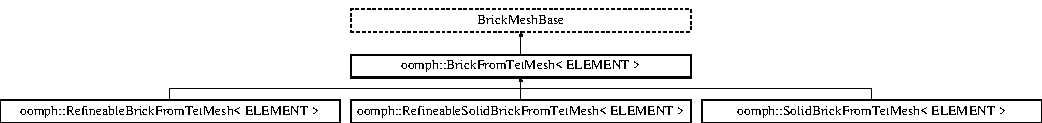
\includegraphics[height=1.651917cm]{classoomph_1_1BrickFromTetMesh}
\end{center}
\end{figure}
\subsection*{Public Member Functions}
\begin{DoxyCompactItemize}
\item 
\hyperlink{classoomph_1_1BrickFromTetMesh_abed00a445cc3c6b6cc00d32e0db4a366}{Brick\+From\+Tet\+Mesh} (const std\+::string xda\+\_\+file\+\_\+name, Time\+Stepper $\ast$time\+\_\+stepper\+\_\+pt=\&Mesh\+::\+Default\+\_\+\+Time\+Stepper)
\begin{DoxyCompactList}\small\item\em Constructor\+: Pass xda file name. \end{DoxyCompactList}\item 
\hyperlink{classoomph_1_1BrickFromTetMesh_af05fe6ff520986d7794c467fc1885f92}{Brick\+From\+Tet\+Mesh} (const std\+::string \&node\+\_\+file\+\_\+name, const std\+::string \&element\+\_\+file\+\_\+name, const std\+::string \&face\+\_\+file\+\_\+name, const bool \&split\+\_\+corner\+\_\+elements, Time\+Stepper $\ast$time\+\_\+stepper\+\_\+pt=\&Mesh\+::\+Default\+\_\+\+Time\+Stepper, const bool \&use\+\_\+attributes=false)
\begin{DoxyCompactList}\small\item\em Constructor\+: Pass the files required for the tetgen mesh. \end{DoxyCompactList}\item 
\hyperlink{classoomph_1_1BrickFromTetMesh_a49d6a583221a04f2997dae4509592350}{Brick\+From\+Tet\+Mesh} (const std\+::string xda\+\_\+file\+\_\+name, \hyperlink{classoomph_1_1XdaTetMesh}{Xda\+Tet\+Mesh}$<$ T\+Element$<$ 3, 3 $>$ $>$ $\ast$\&xda\+\_\+tet\+\_\+mesh\+\_\+pt, Time\+Stepper $\ast$time\+\_\+stepper\+\_\+pt=\&Mesh\+::\+Default\+\_\+\+Time\+Stepper)
\begin{DoxyCompactList}\small\item\em Constructor\+: Pass xda file name. This returns a pointer to the internally built \hyperlink{classoomph_1_1XdaTetMesh}{Xda\+Tet\+Mesh} for external use. Note that Y\+OU are responsible for deleting this mesh. \end{DoxyCompactList}\item 
Vector$<$ unsigned $>$ \hyperlink{classoomph_1_1BrickFromTetMesh_aeca8c8e899bdafb9eb24f36c500c7df6}{oomph\+\_\+lib\+\_\+boundary\+\_\+ids} (const unsigned \&xda\+\_\+boundary\+\_\+id)
\begin{DoxyCompactList}\small\item\em Access functions to the Vector of oomph-\/lib boundary ids that make up boundary b in the original xda enumeration. \end{DoxyCompactList}\end{DoxyCompactItemize}
\subsection*{Private Member Functions}
\begin{DoxyCompactItemize}
\item 
void \hyperlink{classoomph_1_1BrickFromTetMesh_a9b81e29d3b000f02764bf367fa762bfb}{build\+\_\+mesh} (\hyperlink{classoomph_1_1XdaTetMesh}{Xda\+Tet\+Mesh}$<$ T\+Element$<$ 3, 3 $>$ $>$ $\ast$tet\+\_\+mesh\+\_\+pt, Time\+Stepper $\ast$time\+\_\+stepper\+\_\+pt)
\begin{DoxyCompactList}\small\item\em Build fct\+: Pass pointer to existing tet mesh. \end{DoxyCompactList}\item 
void \hyperlink{classoomph_1_1BrickFromTetMesh_afd36d1606f796e926c61b1112b3b6117}{build\+\_\+mesh} (\hyperlink{classoomph_1_1TetgenMesh}{Tetgen\+Mesh}$<$ T\+Element$<$ 3, 3 $>$ $>$ $\ast$tet\+\_\+mesh\+\_\+pt, Time\+Stepper $\ast$time\+\_\+stepper\+\_\+pt)
\begin{DoxyCompactList}\small\item\em Build fct\+: Pass pointer to existing tet mesh. \end{DoxyCompactList}\end{DoxyCompactItemize}
\subsection*{Private Attributes}
\begin{DoxyCompactItemize}
\item 
Vector$<$ Vector$<$ unsigned $>$ $>$ \hyperlink{classoomph_1_1BrickFromTetMesh_a0f6a4b80993ee015038c36ff1aa5556f}{Boundary\+\_\+id}
\begin{DoxyCompactList}\small\item\em Vector of vectors containing the boundary I\+Ds of the overall boundary specified in the xda file. \end{DoxyCompactList}\end{DoxyCompactItemize}


\subsection{Detailed Description}
\subsubsection*{template$<$class E\+L\+E\+M\+E\+NT$>$\newline
class oomph\+::\+Brick\+From\+Tet\+Mesh$<$ E\+L\+E\+M\+E\+N\+T $>$}

Brick mesh built by brickifying an existing tet mesh -- each tet gets split into four bricks. Can only be built with quadratic (27 node) elements. 

Definition at line 66 of file brick\+\_\+from\+\_\+tet\+\_\+mesh.\+template.\+h.



\subsection{Constructor \& Destructor Documentation}
\mbox{\Hypertarget{classoomph_1_1BrickFromTetMesh_abed00a445cc3c6b6cc00d32e0db4a366}\label{classoomph_1_1BrickFromTetMesh_abed00a445cc3c6b6cc00d32e0db4a366}} 
\index{oomph\+::\+Brick\+From\+Tet\+Mesh@{oomph\+::\+Brick\+From\+Tet\+Mesh}!Brick\+From\+Tet\+Mesh@{Brick\+From\+Tet\+Mesh}}
\index{Brick\+From\+Tet\+Mesh@{Brick\+From\+Tet\+Mesh}!oomph\+::\+Brick\+From\+Tet\+Mesh@{oomph\+::\+Brick\+From\+Tet\+Mesh}}
\subsubsection{\texorpdfstring{Brick\+From\+Tet\+Mesh()}{BrickFromTetMesh()}\hspace{0.1cm}{\footnotesize\ttfamily [1/3]}}
{\footnotesize\ttfamily template$<$class E\+L\+E\+M\+E\+NT $>$ \\
\hyperlink{classoomph_1_1BrickFromTetMesh}{oomph\+::\+Brick\+From\+Tet\+Mesh}$<$ E\+L\+E\+M\+E\+NT $>$\+::\hyperlink{classoomph_1_1BrickFromTetMesh}{Brick\+From\+Tet\+Mesh} (\begin{DoxyParamCaption}\item[{const std\+::string}]{xda\+\_\+file\+\_\+name,  }\item[{Time\+Stepper $\ast$}]{time\+\_\+stepper\+\_\+pt = {\ttfamily \&Mesh\+:\+:Default\+\_\+TimeStepper} }\end{DoxyParamCaption})\hspace{0.3cm}{\ttfamily [inline]}}



Constructor\+: Pass xda file name. 



Definition at line 72 of file brick\+\_\+from\+\_\+tet\+\_\+mesh.\+template.\+h.



References oomph\+::\+Brick\+From\+Tet\+Mesh$<$ E\+L\+E\+M\+E\+N\+T $>$\+::build\+\_\+mesh().

\mbox{\Hypertarget{classoomph_1_1BrickFromTetMesh_af05fe6ff520986d7794c467fc1885f92}\label{classoomph_1_1BrickFromTetMesh_af05fe6ff520986d7794c467fc1885f92}} 
\index{oomph\+::\+Brick\+From\+Tet\+Mesh@{oomph\+::\+Brick\+From\+Tet\+Mesh}!Brick\+From\+Tet\+Mesh@{Brick\+From\+Tet\+Mesh}}
\index{Brick\+From\+Tet\+Mesh@{Brick\+From\+Tet\+Mesh}!oomph\+::\+Brick\+From\+Tet\+Mesh@{oomph\+::\+Brick\+From\+Tet\+Mesh}}
\subsubsection{\texorpdfstring{Brick\+From\+Tet\+Mesh()}{BrickFromTetMesh()}\hspace{0.1cm}{\footnotesize\ttfamily [2/3]}}
{\footnotesize\ttfamily template$<$class E\+L\+E\+M\+E\+NT $>$ \\
\hyperlink{classoomph_1_1BrickFromTetMesh}{oomph\+::\+Brick\+From\+Tet\+Mesh}$<$ E\+L\+E\+M\+E\+NT $>$\+::\hyperlink{classoomph_1_1BrickFromTetMesh}{Brick\+From\+Tet\+Mesh} (\begin{DoxyParamCaption}\item[{const std\+::string \&}]{node\+\_\+file\+\_\+name,  }\item[{const std\+::string \&}]{element\+\_\+file\+\_\+name,  }\item[{const std\+::string \&}]{face\+\_\+file\+\_\+name,  }\item[{const bool \&}]{split\+\_\+corner\+\_\+elements,  }\item[{Time\+Stepper $\ast$}]{time\+\_\+stepper\+\_\+pt = {\ttfamily \&Mesh\+:\+:Default\+\_\+TimeStepper},  }\item[{const bool \&}]{use\+\_\+attributes = {\ttfamily false} }\end{DoxyParamCaption})\hspace{0.3cm}{\ttfamily [inline]}}



Constructor\+: Pass the files required for the tetgen mesh. 



Definition at line 91 of file brick\+\_\+from\+\_\+tet\+\_\+mesh.\+template.\+h.



References oomph\+::\+Brick\+From\+Tet\+Mesh$<$ E\+L\+E\+M\+E\+N\+T $>$\+::build\+\_\+mesh().

\mbox{\Hypertarget{classoomph_1_1BrickFromTetMesh_a49d6a583221a04f2997dae4509592350}\label{classoomph_1_1BrickFromTetMesh_a49d6a583221a04f2997dae4509592350}} 
\index{oomph\+::\+Brick\+From\+Tet\+Mesh@{oomph\+::\+Brick\+From\+Tet\+Mesh}!Brick\+From\+Tet\+Mesh@{Brick\+From\+Tet\+Mesh}}
\index{Brick\+From\+Tet\+Mesh@{Brick\+From\+Tet\+Mesh}!oomph\+::\+Brick\+From\+Tet\+Mesh@{oomph\+::\+Brick\+From\+Tet\+Mesh}}
\subsubsection{\texorpdfstring{Brick\+From\+Tet\+Mesh()}{BrickFromTetMesh()}\hspace{0.1cm}{\footnotesize\ttfamily [3/3]}}
{\footnotesize\ttfamily template$<$class E\+L\+E\+M\+E\+NT $>$ \\
\hyperlink{classoomph_1_1BrickFromTetMesh}{oomph\+::\+Brick\+From\+Tet\+Mesh}$<$ E\+L\+E\+M\+E\+NT $>$\+::\hyperlink{classoomph_1_1BrickFromTetMesh}{Brick\+From\+Tet\+Mesh} (\begin{DoxyParamCaption}\item[{const std\+::string}]{xda\+\_\+file\+\_\+name,  }\item[{\hyperlink{classoomph_1_1XdaTetMesh}{Xda\+Tet\+Mesh}$<$ T\+Element$<$ 3, 3 $>$ $>$ $\ast$\&}]{xda\+\_\+tet\+\_\+mesh\+\_\+pt,  }\item[{Time\+Stepper $\ast$}]{time\+\_\+stepper\+\_\+pt = {\ttfamily \&Mesh\+:\+:Default\+\_\+TimeStepper} }\end{DoxyParamCaption})\hspace{0.3cm}{\ttfamily [inline]}}



Constructor\+: Pass xda file name. This returns a pointer to the internally built \hyperlink{classoomph_1_1XdaTetMesh}{Xda\+Tet\+Mesh} for external use. Note that Y\+OU are responsible for deleting this mesh. 



Definition at line 122 of file brick\+\_\+from\+\_\+tet\+\_\+mesh.\+template.\+h.



References oomph\+::\+Brick\+From\+Tet\+Mesh$<$ E\+L\+E\+M\+E\+N\+T $>$\+::build\+\_\+mesh().



\subsection{Member Function Documentation}
\mbox{\Hypertarget{classoomph_1_1BrickFromTetMesh_a9b81e29d3b000f02764bf367fa762bfb}\label{classoomph_1_1BrickFromTetMesh_a9b81e29d3b000f02764bf367fa762bfb}} 
\index{oomph\+::\+Brick\+From\+Tet\+Mesh@{oomph\+::\+Brick\+From\+Tet\+Mesh}!build\+\_\+mesh@{build\+\_\+mesh}}
\index{build\+\_\+mesh@{build\+\_\+mesh}!oomph\+::\+Brick\+From\+Tet\+Mesh@{oomph\+::\+Brick\+From\+Tet\+Mesh}}
\subsubsection{\texorpdfstring{build\+\_\+mesh()}{build\_mesh()}\hspace{0.1cm}{\footnotesize\ttfamily [1/2]}}
{\footnotesize\ttfamily template$<$class E\+L\+E\+M\+E\+NT $>$ \\
void \hyperlink{classoomph_1_1BrickFromTetMesh}{oomph\+::\+Brick\+From\+Tet\+Mesh}$<$ E\+L\+E\+M\+E\+NT $>$\+::build\+\_\+mesh (\begin{DoxyParamCaption}\item[{\hyperlink{classoomph_1_1XdaTetMesh}{Xda\+Tet\+Mesh}$<$ T\+Element$<$ 3, 3 $>$ $>$ $\ast$}]{tet\+\_\+mesh\+\_\+pt,  }\item[{Time\+Stepper $\ast$}]{time\+\_\+stepper\+\_\+pt }\end{DoxyParamCaption})\hspace{0.3cm}{\ttfamily [private]}}



Build fct\+: Pass pointer to existing tet mesh. 

Build fct\+: Pass pointer to existing tet mesh and timestepper Specialisation for \hyperlink{classoomph_1_1XdaTetMesh}{Xda\+Tet\+Mesh}$<$T\+Element$<$3,3$>$ $>$ 

Definition at line 45 of file brick\+\_\+from\+\_\+tet\+\_\+mesh.\+template.\+cc.



Referenced by oomph\+::\+Brick\+From\+Tet\+Mesh$<$ E\+L\+E\+M\+E\+N\+T $>$\+::\+Brick\+From\+Tet\+Mesh(), and oomph\+::\+Brick\+From\+Tet\+Mesh$<$ E\+L\+E\+M\+E\+N\+T $>$\+::oomph\+\_\+lib\+\_\+boundary\+\_\+ids().

\mbox{\Hypertarget{classoomph_1_1BrickFromTetMesh_afd36d1606f796e926c61b1112b3b6117}\label{classoomph_1_1BrickFromTetMesh_afd36d1606f796e926c61b1112b3b6117}} 
\index{oomph\+::\+Brick\+From\+Tet\+Mesh@{oomph\+::\+Brick\+From\+Tet\+Mesh}!build\+\_\+mesh@{build\+\_\+mesh}}
\index{build\+\_\+mesh@{build\+\_\+mesh}!oomph\+::\+Brick\+From\+Tet\+Mesh@{oomph\+::\+Brick\+From\+Tet\+Mesh}}
\subsubsection{\texorpdfstring{build\+\_\+mesh()}{build\_mesh()}\hspace{0.1cm}{\footnotesize\ttfamily [2/2]}}
{\footnotesize\ttfamily template$<$class E\+L\+E\+M\+E\+NT $>$ \\
void \hyperlink{classoomph_1_1BrickFromTetMesh}{oomph\+::\+Brick\+From\+Tet\+Mesh}$<$ E\+L\+E\+M\+E\+NT $>$\+::build\+\_\+mesh (\begin{DoxyParamCaption}\item[{\hyperlink{classoomph_1_1TetgenMesh}{Tetgen\+Mesh}$<$ T\+Element$<$ 3, 3 $>$ $>$ $\ast$}]{tet\+\_\+mesh\+\_\+pt,  }\item[{Time\+Stepper $\ast$}]{time\+\_\+stepper\+\_\+pt }\end{DoxyParamCaption})\hspace{0.3cm}{\ttfamily [private]}}



Build fct\+: Pass pointer to existing tet mesh. 

Build fct\+: Pass pointer to existing tet mesh and timestepper Specialisation for \hyperlink{classoomph_1_1TetgenMesh}{Tetgen\+Mesh}$<$T\+Element$<$3,3$>$ $>$ 

Definition at line 4944 of file brick\+\_\+from\+\_\+tet\+\_\+mesh.\+template.\+cc.

\mbox{\Hypertarget{classoomph_1_1BrickFromTetMesh_aeca8c8e899bdafb9eb24f36c500c7df6}\label{classoomph_1_1BrickFromTetMesh_aeca8c8e899bdafb9eb24f36c500c7df6}} 
\index{oomph\+::\+Brick\+From\+Tet\+Mesh@{oomph\+::\+Brick\+From\+Tet\+Mesh}!oomph\+\_\+lib\+\_\+boundary\+\_\+ids@{oomph\+\_\+lib\+\_\+boundary\+\_\+ids}}
\index{oomph\+\_\+lib\+\_\+boundary\+\_\+ids@{oomph\+\_\+lib\+\_\+boundary\+\_\+ids}!oomph\+::\+Brick\+From\+Tet\+Mesh@{oomph\+::\+Brick\+From\+Tet\+Mesh}}
\subsubsection{\texorpdfstring{oomph\+\_\+lib\+\_\+boundary\+\_\+ids()}{oomph\_lib\_boundary\_ids()}}
{\footnotesize\ttfamily template$<$class E\+L\+E\+M\+E\+NT $>$ \\
Vector$<$unsigned$>$ \hyperlink{classoomph_1_1BrickFromTetMesh}{oomph\+::\+Brick\+From\+Tet\+Mesh}$<$ E\+L\+E\+M\+E\+NT $>$\+::oomph\+\_\+lib\+\_\+boundary\+\_\+ids (\begin{DoxyParamCaption}\item[{const unsigned \&}]{xda\+\_\+boundary\+\_\+id }\end{DoxyParamCaption})\hspace{0.3cm}{\ttfamily [inline]}}



Access functions to the Vector of oomph-\/lib boundary ids that make up boundary b in the original xda enumeration. 



Definition at line 142 of file brick\+\_\+from\+\_\+tet\+\_\+mesh.\+template.\+h.



References oomph\+::\+Brick\+From\+Tet\+Mesh$<$ E\+L\+E\+M\+E\+N\+T $>$\+::\+Boundary\+\_\+id, and oomph\+::\+Brick\+From\+Tet\+Mesh$<$ E\+L\+E\+M\+E\+N\+T $>$\+::build\+\_\+mesh().



\subsection{Member Data Documentation}
\mbox{\Hypertarget{classoomph_1_1BrickFromTetMesh_a0f6a4b80993ee015038c36ff1aa5556f}\label{classoomph_1_1BrickFromTetMesh_a0f6a4b80993ee015038c36ff1aa5556f}} 
\index{oomph\+::\+Brick\+From\+Tet\+Mesh@{oomph\+::\+Brick\+From\+Tet\+Mesh}!Boundary\+\_\+id@{Boundary\+\_\+id}}
\index{Boundary\+\_\+id@{Boundary\+\_\+id}!oomph\+::\+Brick\+From\+Tet\+Mesh@{oomph\+::\+Brick\+From\+Tet\+Mesh}}
\subsubsection{\texorpdfstring{Boundary\+\_\+id}{Boundary\_id}}
{\footnotesize\ttfamily template$<$class E\+L\+E\+M\+E\+NT $>$ \\
Vector$<$Vector$<$unsigned$>$ $>$ \hyperlink{classoomph_1_1BrickFromTetMesh}{oomph\+::\+Brick\+From\+Tet\+Mesh}$<$ E\+L\+E\+M\+E\+NT $>$\+::Boundary\+\_\+id\hspace{0.3cm}{\ttfamily [private]}}



Vector of vectors containing the boundary I\+Ds of the overall boundary specified in the xda file. 



Definition at line 160 of file brick\+\_\+from\+\_\+tet\+\_\+mesh.\+template.\+h.



Referenced by oomph\+::\+Brick\+From\+Tet\+Mesh$<$ E\+L\+E\+M\+E\+N\+T $>$\+::oomph\+\_\+lib\+\_\+boundary\+\_\+ids().



The documentation for this class was generated from the following files\+:\begin{DoxyCompactItemize}
\item 
\hyperlink{brick__from__tet__mesh_8template_8h}{brick\+\_\+from\+\_\+tet\+\_\+mesh.\+template.\+h}\item 
\hyperlink{brick__from__tet__mesh_8template_8cc}{brick\+\_\+from\+\_\+tet\+\_\+mesh.\+template.\+cc}\end{DoxyCompactItemize}

\hypertarget{classoomph_1_1ChannelSpineMesh}{}\section{oomph\+:\+:Channel\+Spine\+Mesh$<$ E\+L\+E\+M\+E\+NT $>$ Class Template Reference}
\label{classoomph_1_1ChannelSpineMesh}\index{oomph\+::\+Channel\+Spine\+Mesh$<$ E\+L\+E\+M\+E\+N\+T $>$@{oomph\+::\+Channel\+Spine\+Mesh$<$ E\+L\+E\+M\+E\+N\+T $>$}}


{\ttfamily \#include $<$channel\+\_\+spine\+\_\+mesh.\+template.\+h$>$}

Inheritance diagram for oomph\+:\+:Channel\+Spine\+Mesh$<$ E\+L\+E\+M\+E\+NT $>$\+:\begin{figure}[H]
\begin{center}
\leavevmode
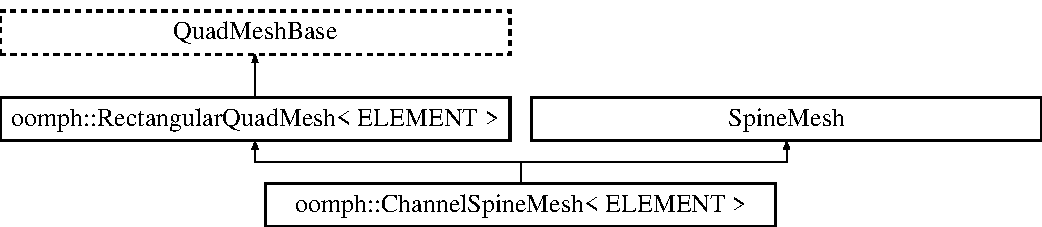
\includegraphics[height=3.000000cm]{classoomph_1_1ChannelSpineMesh}
\end{center}
\end{figure}
\subsection*{Public Member Functions}
\begin{DoxyCompactItemize}
\item 
\hyperlink{classoomph_1_1ChannelSpineMesh_a9f8cdd0476807b44bccb7b1ae6f97a4a}{Channel\+Spine\+Mesh} (const unsigned \&nx0, const unsigned \&nx1, const unsigned \&nx2, const unsigned \&\hyperlink{classoomph_1_1RectangularQuadMesh_a86d76a55eb7c4e8bca9b74d23c8b0412}{ny}, const double \&lx0, const double \&lx1, const double \&lx2, const double \&h, Geom\+Object $\ast$\hyperlink{classoomph_1_1ChannelSpineMesh_a741893ef460f1275f1df43496bb7536c}{wall\+\_\+pt}, Time\+Stepper $\ast$time\+\_\+stepper\+\_\+pt=\&Mesh\+::\+Default\+\_\+\+Time\+Stepper)
\begin{DoxyCompactList}\small\item\em Constructor\+: Pass number of elements in x-\/direction in regions 0,1 and 2, number of elements in y-\/direction, length in x direction in regions 0,1 and 2, height mesh, pointer to the Geom\+Object defining the heightof the central region and pointer to timestepper (defaults to Steady timestepper) \end{DoxyCompactList}\item 
\hyperlink{classoomph_1_1ChannelSpineMesh_afb1b729691c03cef065d351094092406}{Channel\+Spine\+Mesh} (const unsigned \&nx0, const unsigned \&nx1, const unsigned \&nx2, const unsigned \&\hyperlink{classoomph_1_1RectangularQuadMesh_a86d76a55eb7c4e8bca9b74d23c8b0412}{ny}, const double \&lx0, const double \&lx1, const double \&lx2, const double \&h, Geom\+Object $\ast$\hyperlink{classoomph_1_1ChannelSpineMesh_a741893ef460f1275f1df43496bb7536c}{wall\+\_\+pt}, const bool \&periodic\+\_\+in\+\_\+x, Time\+Stepper $\ast$time\+\_\+stepper\+\_\+pt=\&Mesh\+::\+Default\+\_\+\+Time\+Stepper)
\begin{DoxyCompactList}\small\item\em Constructor\+: Pass number of elements in x-\/direction in regions 0,1 and 2, number of elements in y-\/direction, length in x direction in regions 0,1 and 2, height mesh, pointer to the Geom\+Object defining the heightof the central region, a boolean flag to indicate whether or not the mesh is periodic and pointer to timestepper (defaults to Steady timestepper) \end{DoxyCompactList}\item 
Finite\+Element $\ast$\& \hyperlink{classoomph_1_1ChannelSpineMesh_a84cbf50caead0aba0170246f4ce7330f}{left\+\_\+element\+\_\+pt} (const unsigned long \&i)
\begin{DoxyCompactList}\small\item\em Access functions for pointers to the $ i $ -\/th element in the left region. \end{DoxyCompactList}\item 
Finite\+Element $\ast$\& \hyperlink{classoomph_1_1ChannelSpineMesh_a127dc05f48ad6af69f26dd1504eaeba5}{centre\+\_\+element\+\_\+pt} (const unsigned long \&i)
\begin{DoxyCompactList}\small\item\em Access functions for pointers to the $ i $ -\/th element in the centre region. \end{DoxyCompactList}\item 
Finite\+Element $\ast$\& \hyperlink{classoomph_1_1ChannelSpineMesh_a599b1d10bc47ceb9903a01b12036f400}{right\+\_\+element\+\_\+pt} (const unsigned long \&i)
\begin{DoxyCompactList}\small\item\em Access functions for pointers to the $ i $ -\/th element in the right region. \end{DoxyCompactList}\item 
unsigned long \hyperlink{classoomph_1_1ChannelSpineMesh_a6f7b8f540855876e49b5f1c3f0214d9a}{nleft} () const
\begin{DoxyCompactList}\small\item\em Number of elements in left region. \end{DoxyCompactList}\item 
unsigned long \hyperlink{classoomph_1_1ChannelSpineMesh_a422ed0d224b8da3c35732328e1aacdc0}{ncentre} () const
\begin{DoxyCompactList}\small\item\em Number of elements in centre region. \end{DoxyCompactList}\item 
unsigned long \hyperlink{classoomph_1_1ChannelSpineMesh_a559352375de869e889191d0e6c133031}{nright} () const
\begin{DoxyCompactList}\small\item\em Number of elements in right region. \end{DoxyCompactList}\item 
unsigned long \hyperlink{classoomph_1_1ChannelSpineMesh_a89f5523009288ce87d2f0d1cbb9fb488}{nbulk} () const
\begin{DoxyCompactList}\small\item\em Number of elements in bulk. \end{DoxyCompactList}\item 
void \hyperlink{classoomph_1_1ChannelSpineMesh_ad449460c4d06b2be64b53097143a3b09}{element\+\_\+reorder} ()
\begin{DoxyCompactList}\small\item\em Reorder the elements so we loop over them vertically first (advantageous in \char`\"{}wide\char`\"{} domains if a frontal solver is used). \end{DoxyCompactList}\item 
virtual void \hyperlink{classoomph_1_1ChannelSpineMesh_aefa38017e44e64ad0cd86d87d397bf8d}{spine\+\_\+node\+\_\+update} (Spine\+Node $\ast$spine\+\_\+node\+\_\+pt)
\begin{DoxyCompactList}\small\item\em General node update function implements pure virtual function defined in Spine\+Mesh base class and performs specific node update actions\+: along vertical spines. \end{DoxyCompactList}\item 
virtual double \hyperlink{classoomph_1_1ChannelSpineMesh_a16e0d4264443b1beb274753b0d6b970e}{x\+\_\+spacing\+\_\+function} (unsigned xelement, unsigned xnode, unsigned yelement, unsigned ynode)
\begin{DoxyCompactList}\small\item\em Return the value of the x-\/coordinate at the node given by the local node number (xnode, ynode) in the element (xelement,yelement). The description is in a \char`\"{}psudeo\char`\"{} two-\/dimensional coordinate system, so the range of xelement is \mbox{[}0,Nx-\/1\mbox{]}, yelement is \mbox{[}0,Ny-\/1\mbox{]}, and that of xnode and ynode is \mbox{[}0,Np-\/1\mbox{]}. The default is to return nodes that are equally spaced in the x coodinate. \end{DoxyCompactList}\item 
Spine $\ast$\& \hyperlink{classoomph_1_1ChannelSpineMesh_ad4ae203f8a69fa3c8f0541ede45d7630}{left\+\_\+spine\+\_\+pt} (const unsigned long \&i)
\begin{DoxyCompactList}\small\item\em Access function for spines in left region. \end{DoxyCompactList}\item 
Spine $\ast$\& \hyperlink{classoomph_1_1ChannelSpineMesh_a690cda061ec45945d981a24a2b206e69}{centre\+\_\+spine\+\_\+pt} (const unsigned long \&i)
\begin{DoxyCompactList}\small\item\em Access function for spines in centre region. \end{DoxyCompactList}\item 
Spine $\ast$\& \hyperlink{classoomph_1_1ChannelSpineMesh_a78a52a2e61a76bff0fa74b3fd2583092}{right\+\_\+spine\+\_\+pt} (const unsigned long \&i)
\begin{DoxyCompactList}\small\item\em Access function for spines in right region. \end{DoxyCompactList}\item 
unsigned \hyperlink{classoomph_1_1ChannelSpineMesh_af5ae7133c9939b90779f0809143676bd}{nleft\+\_\+spine} ()
\begin{DoxyCompactList}\small\item\em Access function for the number of spines in the left region. \end{DoxyCompactList}\item 
unsigned \hyperlink{classoomph_1_1ChannelSpineMesh_a85fa0910148e6aa5d8a1995ece5feeae}{ncentre\+\_\+spine} ()
\begin{DoxyCompactList}\small\item\em Access function for the number of spines in the centre region. \end{DoxyCompactList}\item 
unsigned \hyperlink{classoomph_1_1ChannelSpineMesh_a48ee9b7736e6884ff41e2affd4094842}{nright\+\_\+spine} ()
\begin{DoxyCompactList}\small\item\em Access function for the number of spines in the right region. \end{DoxyCompactList}\item 
Geom\+Object $\ast$ \hyperlink{classoomph_1_1ChannelSpineMesh_a741893ef460f1275f1df43496bb7536c}{wall\+\_\+pt} ()
\begin{DoxyCompactList}\small\item\em Access function to the Geom\+Object for upper wall. \end{DoxyCompactList}\item 
Geom\+Object $\ast$ \hyperlink{classoomph_1_1ChannelSpineMesh_a54818e02db7026d39451f5f502e1cf11}{straight\+\_\+wall\+\_\+pt} ()
\begin{DoxyCompactList}\small\item\em Access function to the Geom\+Object for the straight upper wall. \end{DoxyCompactList}\end{DoxyCompactItemize}
\subsection*{Protected Member Functions}
\begin{DoxyCompactItemize}
\item 
virtual void \hyperlink{classoomph_1_1ChannelSpineMesh_a12eae5013f54ae04f9eb1cdffacf3955}{build\+\_\+channel\+\_\+spine\+\_\+mesh} (Time\+Stepper $\ast$time\+\_\+stepper\+\_\+pt)
\begin{DoxyCompactList}\small\item\em Helper function to actually build the channel-\/spine mesh (called from various constructors) \end{DoxyCompactList}\end{DoxyCompactItemize}
\subsection*{Protected Attributes}
\begin{DoxyCompactItemize}
\item 
Vector$<$ Finite\+Element $\ast$ $>$ \hyperlink{classoomph_1_1ChannelSpineMesh_aaa8df0751eebdab02466afa0253dedbd}{Left\+\_\+element\+\_\+pt}
\begin{DoxyCompactList}\small\item\em Vector of pointers to element in the left region. \end{DoxyCompactList}\item 
Vector$<$ Finite\+Element $\ast$ $>$ \hyperlink{classoomph_1_1ChannelSpineMesh_aef52a18c46a4ec6121a129789d46db3e}{Centre\+\_\+element\+\_\+pt}
\begin{DoxyCompactList}\small\item\em Vector of pointers to element in the centre region. \end{DoxyCompactList}\item 
Vector$<$ Finite\+Element $\ast$ $>$ \hyperlink{classoomph_1_1ChannelSpineMesh_a1cc77e7badcd1756b03aa307534011ec}{Right\+\_\+element\+\_\+pt}
\begin{DoxyCompactList}\small\item\em Vector of pointers to element in the right region. \end{DoxyCompactList}\item 
unsigned \hyperlink{classoomph_1_1ChannelSpineMesh_a283ffaeb501cec43df629d3bf06fe3d2}{Nx0}
\begin{DoxyCompactList}\small\item\em Number of elements in the left region. \end{DoxyCompactList}\item 
unsigned \hyperlink{classoomph_1_1ChannelSpineMesh_a678cfaebcb1c7a31027188af36be9e7b}{Nx1}
\begin{DoxyCompactList}\small\item\em Number of elements in the centre region. \end{DoxyCompactList}\item 
unsigned \hyperlink{classoomph_1_1ChannelSpineMesh_a46534250de6f75890463bfddefdb39cd}{Nx2}
\begin{DoxyCompactList}\small\item\em Number of elements in the right region. \end{DoxyCompactList}\item 
double \hyperlink{classoomph_1_1ChannelSpineMesh_a3d61af363a8da156f4fe6d10e62f73c6}{Lx0}
\begin{DoxyCompactList}\small\item\em Length of left region. \end{DoxyCompactList}\item 
double \hyperlink{classoomph_1_1ChannelSpineMesh_a35f5d840478b2b93199a393cbdb50f2d}{Lx1}
\begin{DoxyCompactList}\small\item\em Length of centre region. \end{DoxyCompactList}\item 
double \hyperlink{classoomph_1_1ChannelSpineMesh_a4c295478a3f79335f5d0113da220844e}{Lx2}
\begin{DoxyCompactList}\small\item\em Length of right region. \end{DoxyCompactList}\item 
unsigned \hyperlink{classoomph_1_1ChannelSpineMesh_a56fbad56271c5e37cd7f1d2de7b7bb36}{Nleft\+\_\+spine}
\begin{DoxyCompactList}\small\item\em Number of spines in left region. \end{DoxyCompactList}\item 
unsigned \hyperlink{classoomph_1_1ChannelSpineMesh_af6ef1bb007083a803561e5f0062f820b}{Ncentre\+\_\+spine}
\begin{DoxyCompactList}\small\item\em Number of spines in centre region. \end{DoxyCompactList}\item 
unsigned \hyperlink{classoomph_1_1ChannelSpineMesh_a56f7259d8e5dee66a8c83ffe99526c62}{Nright\+\_\+spine}
\begin{DoxyCompactList}\small\item\em Number of spines in right region. \end{DoxyCompactList}\item 
Geom\+Object $\ast$ \hyperlink{classoomph_1_1ChannelSpineMesh_adaa23badd05b69c905b444bd9141b3a7}{Wall\+\_\+pt}
\begin{DoxyCompactList}\small\item\em Geom\+Object for upper wall. \end{DoxyCompactList}\item 
Geom\+Object $\ast$ \hyperlink{classoomph_1_1ChannelSpineMesh_a34f4583f2aa944d5d1ff723f6a4123bf}{Straight\+\_\+wall\+\_\+pt}
\begin{DoxyCompactList}\small\item\em Geom\+Object for the straight upper wall. \end{DoxyCompactList}\end{DoxyCompactItemize}


\subsection{Detailed Description}
\subsubsection*{template$<$class E\+L\+E\+M\+E\+NT$>$\newline
class oomph\+::\+Channel\+Spine\+Mesh$<$ E\+L\+E\+M\+E\+N\+T $>$}

Spine mesh class derived from standard 2D mesh. The mesh contains a Straight\+Line Geom\+Object which defines the height of the left and right regions (0,2) and another Geom\+Object is passed to the constructor to define the height in the central region. 

Definition at line 47 of file channel\+\_\+spine\+\_\+mesh.\+template.\+h.



\subsection{Constructor \& Destructor Documentation}
\mbox{\Hypertarget{classoomph_1_1ChannelSpineMesh_a9f8cdd0476807b44bccb7b1ae6f97a4a}\label{classoomph_1_1ChannelSpineMesh_a9f8cdd0476807b44bccb7b1ae6f97a4a}} 
\index{oomph\+::\+Channel\+Spine\+Mesh@{oomph\+::\+Channel\+Spine\+Mesh}!Channel\+Spine\+Mesh@{Channel\+Spine\+Mesh}}
\index{Channel\+Spine\+Mesh@{Channel\+Spine\+Mesh}!oomph\+::\+Channel\+Spine\+Mesh@{oomph\+::\+Channel\+Spine\+Mesh}}
\subsubsection{\texorpdfstring{Channel\+Spine\+Mesh()}{ChannelSpineMesh()}\hspace{0.1cm}{\footnotesize\ttfamily [1/2]}}
{\footnotesize\ttfamily template$<$class E\+L\+E\+M\+E\+NT $>$ \\
\hyperlink{classoomph_1_1ChannelSpineMesh}{oomph\+::\+Channel\+Spine\+Mesh}$<$ E\+L\+E\+M\+E\+NT $>$\+::\hyperlink{classoomph_1_1ChannelSpineMesh}{Channel\+Spine\+Mesh} (\begin{DoxyParamCaption}\item[{const unsigned \&}]{nx0,  }\item[{const unsigned \&}]{nx1,  }\item[{const unsigned \&}]{nx2,  }\item[{const unsigned \&}]{ny,  }\item[{const double \&}]{lx0,  }\item[{const double \&}]{lx1,  }\item[{const double \&}]{lx2,  }\item[{const double \&}]{h,  }\item[{Geom\+Object $\ast$}]{wall\+\_\+pt,  }\item[{Time\+Stepper $\ast$}]{time\+\_\+stepper\+\_\+pt = {\ttfamily \&Mesh\+:\+:Default\+\_\+TimeStepper} }\end{DoxyParamCaption})}



Constructor\+: Pass number of elements in x-\/direction in regions 0,1 and 2, number of elements in y-\/direction, length in x direction in regions 0,1 and 2, height mesh, pointer to the Geom\+Object defining the heightof the central region and pointer to timestepper (defaults to Steady timestepper) 

Constructor for spine 2D mesh\+: Pass number of elements in x-\/direction, number of elements in y-\/direction, axial length and height of layer, and pointer to timestepper (defaults to Static timestepper).

The mesh contains a layer of spinified fluid elements (of type E\+L\+E\+M\+E\+NT; e.\+g Spine\+Element$<$Q\+Crouzeix\+Raviart\+Element$<$2$>$) and a surface layer of corresponding Spine interface elements of type I\+N\+T\+E\+R\+F\+A\+C\+E\+\_\+\+E\+L\+E\+M\+E\+NT, e.\+g. Spine\+Line\+Fluid\+Interface\+Element$<$\+E\+L\+E\+M\+E\+N\+T$>$ for 2D planar problems. 

Definition at line 55 of file channel\+\_\+spine\+\_\+mesh.\+template.\+cc.



References oomph\+::\+Channel\+Spine\+Mesh$<$ E\+L\+E\+M\+E\+N\+T $>$\+::build\+\_\+channel\+\_\+spine\+\_\+mesh(), and oomph\+::\+Channel\+Spine\+Mesh$<$ E\+L\+E\+M\+E\+N\+T $>$\+::\+Straight\+\_\+wall\+\_\+pt.

\mbox{\Hypertarget{classoomph_1_1ChannelSpineMesh_afb1b729691c03cef065d351094092406}\label{classoomph_1_1ChannelSpineMesh_afb1b729691c03cef065d351094092406}} 
\index{oomph\+::\+Channel\+Spine\+Mesh@{oomph\+::\+Channel\+Spine\+Mesh}!Channel\+Spine\+Mesh@{Channel\+Spine\+Mesh}}
\index{Channel\+Spine\+Mesh@{Channel\+Spine\+Mesh}!oomph\+::\+Channel\+Spine\+Mesh@{oomph\+::\+Channel\+Spine\+Mesh}}
\subsubsection{\texorpdfstring{Channel\+Spine\+Mesh()}{ChannelSpineMesh()}\hspace{0.1cm}{\footnotesize\ttfamily [2/2]}}
{\footnotesize\ttfamily template$<$class E\+L\+E\+M\+E\+NT $>$ \\
\hyperlink{classoomph_1_1ChannelSpineMesh}{oomph\+::\+Channel\+Spine\+Mesh}$<$ E\+L\+E\+M\+E\+NT $>$\+::\hyperlink{classoomph_1_1ChannelSpineMesh}{Channel\+Spine\+Mesh} (\begin{DoxyParamCaption}\item[{const unsigned \&}]{nx0,  }\item[{const unsigned \&}]{nx1,  }\item[{const unsigned \&}]{nx2,  }\item[{const unsigned \&}]{ny,  }\item[{const double \&}]{lx0,  }\item[{const double \&}]{lx1,  }\item[{const double \&}]{lx2,  }\item[{const double \&}]{h,  }\item[{Geom\+Object $\ast$}]{wall\+\_\+pt,  }\item[{const bool \&}]{periodic\+\_\+in\+\_\+x,  }\item[{Time\+Stepper $\ast$}]{time\+\_\+stepper\+\_\+pt = {\ttfamily \&Mesh\+:\+:Default\+\_\+TimeStepper} }\end{DoxyParamCaption})}



Constructor\+: Pass number of elements in x-\/direction in regions 0,1 and 2, number of elements in y-\/direction, length in x direction in regions 0,1 and 2, height mesh, pointer to the Geom\+Object defining the heightof the central region, a boolean flag to indicate whether or not the mesh is periodic and pointer to timestepper (defaults to Steady timestepper) 

Constuctor for spine 2D mesh\+: Pass number of elements in x-\/direction, number of elements in y-\/direction, axial length and height of layer, a boolean flag to make the mesh periodic in the x-\/direction, and pointer to timestepper (defaults to Static timestepper).

The mesh contains a layer of elements (of type E\+L\+E\+M\+E\+NT) and a surface layer of corresponding Spine interface elements (of type Spine\+Line\+Fluid\+Interface\+Element$<$\+E\+L\+E\+M\+E\+N\+T$>$). 

Definition at line 103 of file channel\+\_\+spine\+\_\+mesh.\+template.\+cc.



References oomph\+::\+Channel\+Spine\+Mesh$<$ E\+L\+E\+M\+E\+N\+T $>$\+::build\+\_\+channel\+\_\+spine\+\_\+mesh(), and oomph\+::\+Channel\+Spine\+Mesh$<$ E\+L\+E\+M\+E\+N\+T $>$\+::\+Straight\+\_\+wall\+\_\+pt.



\subsection{Member Function Documentation}
\mbox{\Hypertarget{classoomph_1_1ChannelSpineMesh_a12eae5013f54ae04f9eb1cdffacf3955}\label{classoomph_1_1ChannelSpineMesh_a12eae5013f54ae04f9eb1cdffacf3955}} 
\index{oomph\+::\+Channel\+Spine\+Mesh@{oomph\+::\+Channel\+Spine\+Mesh}!build\+\_\+channel\+\_\+spine\+\_\+mesh@{build\+\_\+channel\+\_\+spine\+\_\+mesh}}
\index{build\+\_\+channel\+\_\+spine\+\_\+mesh@{build\+\_\+channel\+\_\+spine\+\_\+mesh}!oomph\+::\+Channel\+Spine\+Mesh@{oomph\+::\+Channel\+Spine\+Mesh}}
\subsubsection{\texorpdfstring{build\+\_\+channel\+\_\+spine\+\_\+mesh()}{build\_channel\_spine\_mesh()}}
{\footnotesize\ttfamily template$<$class E\+L\+E\+M\+E\+NT $>$ \\
void \hyperlink{classoomph_1_1ChannelSpineMesh}{oomph\+::\+Channel\+Spine\+Mesh}$<$ E\+L\+E\+M\+E\+NT $>$\+::build\+\_\+channel\+\_\+spine\+\_\+mesh (\begin{DoxyParamCaption}\item[{Time\+Stepper $\ast$}]{time\+\_\+stepper\+\_\+pt }\end{DoxyParamCaption})\hspace{0.3cm}{\ttfamily [protected]}, {\ttfamily [virtual]}}



Helper function to actually build the channel-\/spine mesh (called from various constructors) 

Helper function that actually builds the channel-\/spine mesh based on the parameters set in the various constructors 

Definition at line 147 of file channel\+\_\+spine\+\_\+mesh.\+template.\+cc.



References oomph\+::\+Rectangular\+Quad\+Mesh$<$ E\+L\+E\+M\+E\+N\+T $>$\+::build\+\_\+mesh(), oomph\+::\+Channel\+Spine\+Mesh$<$ E\+L\+E\+M\+E\+N\+T $>$\+::\+Centre\+\_\+element\+\_\+pt, oomph\+::\+Channel\+Spine\+Mesh$<$ E\+L\+E\+M\+E\+N\+T $>$\+::\+Left\+\_\+element\+\_\+pt, oomph\+::\+Channel\+Spine\+Mesh$<$ E\+L\+E\+M\+E\+N\+T $>$\+::\+Lx0, oomph\+::\+Channel\+Spine\+Mesh$<$ E\+L\+E\+M\+E\+N\+T $>$\+::\+Lx1, oomph\+::\+Channel\+Spine\+Mesh$<$ E\+L\+E\+M\+E\+N\+T $>$\+::\+Lx2, oomph\+::\+Channel\+Spine\+Mesh$<$ E\+L\+E\+M\+E\+N\+T $>$\+::ncentre(), oomph\+::\+Channel\+Spine\+Mesh$<$ E\+L\+E\+M\+E\+N\+T $>$\+::\+Ncentre\+\_\+spine, oomph\+::\+Channel\+Spine\+Mesh$<$ E\+L\+E\+M\+E\+N\+T $>$\+::nleft(), oomph\+::\+Channel\+Spine\+Mesh$<$ E\+L\+E\+M\+E\+N\+T $>$\+::\+Nleft\+\_\+spine, oomph\+::\+Channel\+Spine\+Mesh$<$ E\+L\+E\+M\+E\+N\+T $>$\+::nright(), oomph\+::\+Channel\+Spine\+Mesh$<$ E\+L\+E\+M\+E\+N\+T $>$\+::\+Nright\+\_\+spine, oomph\+::\+Rectangular\+Quad\+Mesh$<$ E\+L\+E\+M\+E\+N\+T $>$\+::\+Nx, oomph\+::\+Channel\+Spine\+Mesh$<$ E\+L\+E\+M\+E\+N\+T $>$\+::\+Nx0, oomph\+::\+Channel\+Spine\+Mesh$<$ E\+L\+E\+M\+E\+N\+T $>$\+::\+Nx1, oomph\+::\+Channel\+Spine\+Mesh$<$ E\+L\+E\+M\+E\+N\+T $>$\+::\+Nx2, oomph\+::\+Rectangular\+Quad\+Mesh$<$ E\+L\+E\+M\+E\+N\+T $>$\+::\+Ny, oomph\+::\+Channel\+Spine\+Mesh$<$ E\+L\+E\+M\+E\+N\+T $>$\+::\+Right\+\_\+element\+\_\+pt, oomph\+::\+Channel\+Spine\+Mesh$<$ E\+L\+E\+M\+E\+N\+T $>$\+::\+Straight\+\_\+wall\+\_\+pt, oomph\+::\+Channel\+Spine\+Mesh$<$ E\+L\+E\+M\+E\+N\+T $>$\+::\+Wall\+\_\+pt, and oomph\+::\+Rectangular\+Quad\+Mesh$<$ E\+L\+E\+M\+E\+N\+T $>$\+::\+Xperiodic.



Referenced by oomph\+::\+Channel\+Spine\+Mesh$<$ E\+L\+E\+M\+E\+N\+T $>$\+::\+Channel\+Spine\+Mesh().

\mbox{\Hypertarget{classoomph_1_1ChannelSpineMesh_a127dc05f48ad6af69f26dd1504eaeba5}\label{classoomph_1_1ChannelSpineMesh_a127dc05f48ad6af69f26dd1504eaeba5}} 
\index{oomph\+::\+Channel\+Spine\+Mesh@{oomph\+::\+Channel\+Spine\+Mesh}!centre\+\_\+element\+\_\+pt@{centre\+\_\+element\+\_\+pt}}
\index{centre\+\_\+element\+\_\+pt@{centre\+\_\+element\+\_\+pt}!oomph\+::\+Channel\+Spine\+Mesh@{oomph\+::\+Channel\+Spine\+Mesh}}
\subsubsection{\texorpdfstring{centre\+\_\+element\+\_\+pt()}{centre\_element\_pt()}}
{\footnotesize\ttfamily template$<$class E\+L\+E\+M\+E\+NT $>$ \\
Finite\+Element$\ast$ \& \hyperlink{classoomph_1_1ChannelSpineMesh}{oomph\+::\+Channel\+Spine\+Mesh}$<$ E\+L\+E\+M\+E\+NT $>$\+::centre\+\_\+element\+\_\+pt (\begin{DoxyParamCaption}\item[{const unsigned long \&}]{i }\end{DoxyParamCaption})\hspace{0.3cm}{\ttfamily [inline]}}



Access functions for pointers to the $ i $ -\/th element in the centre region. 



Definition at line 93 of file channel\+\_\+spine\+\_\+mesh.\+template.\+h.



References oomph\+::\+Channel\+Spine\+Mesh$<$ E\+L\+E\+M\+E\+N\+T $>$\+::\+Centre\+\_\+element\+\_\+pt.

\mbox{\Hypertarget{classoomph_1_1ChannelSpineMesh_a690cda061ec45945d981a24a2b206e69}\label{classoomph_1_1ChannelSpineMesh_a690cda061ec45945d981a24a2b206e69}} 
\index{oomph\+::\+Channel\+Spine\+Mesh@{oomph\+::\+Channel\+Spine\+Mesh}!centre\+\_\+spine\+\_\+pt@{centre\+\_\+spine\+\_\+pt}}
\index{centre\+\_\+spine\+\_\+pt@{centre\+\_\+spine\+\_\+pt}!oomph\+::\+Channel\+Spine\+Mesh@{oomph\+::\+Channel\+Spine\+Mesh}}
\subsubsection{\texorpdfstring{centre\+\_\+spine\+\_\+pt()}{centre\_spine\_pt()}}
{\footnotesize\ttfamily template$<$class E\+L\+E\+M\+E\+NT $>$ \\
Spine$\ast$\& \hyperlink{classoomph_1_1ChannelSpineMesh}{oomph\+::\+Channel\+Spine\+Mesh}$<$ E\+L\+E\+M\+E\+NT $>$\+::centre\+\_\+spine\+\_\+pt (\begin{DoxyParamCaption}\item[{const unsigned long \&}]{i }\end{DoxyParamCaption})\hspace{0.3cm}{\ttfamily [inline]}}



Access function for spines in centre region. 



Definition at line 201 of file channel\+\_\+spine\+\_\+mesh.\+template.\+h.



References oomph\+::\+Channel\+Spine\+Mesh$<$ E\+L\+E\+M\+E\+N\+T $>$\+::\+Ncentre\+\_\+spine, and oomph\+::\+Channel\+Spine\+Mesh$<$ E\+L\+E\+M\+E\+N\+T $>$\+::\+Nleft\+\_\+spine.

\mbox{\Hypertarget{classoomph_1_1ChannelSpineMesh_ad449460c4d06b2be64b53097143a3b09}\label{classoomph_1_1ChannelSpineMesh_ad449460c4d06b2be64b53097143a3b09}} 
\index{oomph\+::\+Channel\+Spine\+Mesh@{oomph\+::\+Channel\+Spine\+Mesh}!element\+\_\+reorder@{element\+\_\+reorder}}
\index{element\+\_\+reorder@{element\+\_\+reorder}!oomph\+::\+Channel\+Spine\+Mesh@{oomph\+::\+Channel\+Spine\+Mesh}}
\subsubsection{\texorpdfstring{element\+\_\+reorder()}{element\_reorder()}}
{\footnotesize\ttfamily template$<$class E\+L\+E\+M\+E\+NT $>$ \\
void \hyperlink{classoomph_1_1ChannelSpineMesh}{oomph\+::\+Channel\+Spine\+Mesh}$<$ E\+L\+E\+M\+E\+NT $>$\+::element\+\_\+reorder (\begin{DoxyParamCaption}{ }\end{DoxyParamCaption})\hspace{0.3cm}{\ttfamily [virtual]}}



Reorder the elements so we loop over them vertically first (advantageous in \char`\"{}wide\char`\"{} domains if a frontal solver is used). 

Reorder the elements, so we loop over them vertically first (advantageous in \char`\"{}wide\char`\"{} domains if a frontal solver is used). 

Reimplemented from \hyperlink{classoomph_1_1RectangularQuadMesh_ae1e1d67808d4efb6e16a3835162a4504}{oomph\+::\+Rectangular\+Quad\+Mesh$<$ E\+L\+E\+M\+E\+N\+T $>$}.



Definition at line 680 of file channel\+\_\+spine\+\_\+mesh.\+template.\+cc.



References oomph\+::\+Rectangular\+Quad\+Mesh$<$ E\+L\+E\+M\+E\+N\+T $>$\+::\+Nx, and oomph\+::\+Rectangular\+Quad\+Mesh$<$ E\+L\+E\+M\+E\+N\+T $>$\+::\+Ny.



Referenced by oomph\+::\+Channel\+Spine\+Mesh$<$ E\+L\+E\+M\+E\+N\+T $>$\+::nbulk().

\mbox{\Hypertarget{classoomph_1_1ChannelSpineMesh_a84cbf50caead0aba0170246f4ce7330f}\label{classoomph_1_1ChannelSpineMesh_a84cbf50caead0aba0170246f4ce7330f}} 
\index{oomph\+::\+Channel\+Spine\+Mesh@{oomph\+::\+Channel\+Spine\+Mesh}!left\+\_\+element\+\_\+pt@{left\+\_\+element\+\_\+pt}}
\index{left\+\_\+element\+\_\+pt@{left\+\_\+element\+\_\+pt}!oomph\+::\+Channel\+Spine\+Mesh@{oomph\+::\+Channel\+Spine\+Mesh}}
\subsubsection{\texorpdfstring{left\+\_\+element\+\_\+pt()}{left\_element\_pt()}}
{\footnotesize\ttfamily template$<$class E\+L\+E\+M\+E\+NT $>$ \\
Finite\+Element$\ast$ \& \hyperlink{classoomph_1_1ChannelSpineMesh}{oomph\+::\+Channel\+Spine\+Mesh}$<$ E\+L\+E\+M\+E\+NT $>$\+::left\+\_\+element\+\_\+pt (\begin{DoxyParamCaption}\item[{const unsigned long \&}]{i }\end{DoxyParamCaption})\hspace{0.3cm}{\ttfamily [inline]}}



Access functions for pointers to the $ i $ -\/th element in the left region. 



Definition at line 88 of file channel\+\_\+spine\+\_\+mesh.\+template.\+h.



References oomph\+::\+Channel\+Spine\+Mesh$<$ E\+L\+E\+M\+E\+N\+T $>$\+::\+Left\+\_\+element\+\_\+pt.

\mbox{\Hypertarget{classoomph_1_1ChannelSpineMesh_ad4ae203f8a69fa3c8f0541ede45d7630}\label{classoomph_1_1ChannelSpineMesh_ad4ae203f8a69fa3c8f0541ede45d7630}} 
\index{oomph\+::\+Channel\+Spine\+Mesh@{oomph\+::\+Channel\+Spine\+Mesh}!left\+\_\+spine\+\_\+pt@{left\+\_\+spine\+\_\+pt}}
\index{left\+\_\+spine\+\_\+pt@{left\+\_\+spine\+\_\+pt}!oomph\+::\+Channel\+Spine\+Mesh@{oomph\+::\+Channel\+Spine\+Mesh}}
\subsubsection{\texorpdfstring{left\+\_\+spine\+\_\+pt()}{left\_spine\_pt()}}
{\footnotesize\ttfamily template$<$class E\+L\+E\+M\+E\+NT $>$ \\
Spine$\ast$\& \hyperlink{classoomph_1_1ChannelSpineMesh}{oomph\+::\+Channel\+Spine\+Mesh}$<$ E\+L\+E\+M\+E\+NT $>$\+::left\+\_\+spine\+\_\+pt (\begin{DoxyParamCaption}\item[{const unsigned long \&}]{i }\end{DoxyParamCaption})\hspace{0.3cm}{\ttfamily [inline]}}



Access function for spines in left region. 



Definition at line 187 of file channel\+\_\+spine\+\_\+mesh.\+template.\+h.



References oomph\+::\+Channel\+Spine\+Mesh$<$ E\+L\+E\+M\+E\+N\+T $>$\+::\+Nleft\+\_\+spine.

\mbox{\Hypertarget{classoomph_1_1ChannelSpineMesh_a89f5523009288ce87d2f0d1cbb9fb488}\label{classoomph_1_1ChannelSpineMesh_a89f5523009288ce87d2f0d1cbb9fb488}} 
\index{oomph\+::\+Channel\+Spine\+Mesh@{oomph\+::\+Channel\+Spine\+Mesh}!nbulk@{nbulk}}
\index{nbulk@{nbulk}!oomph\+::\+Channel\+Spine\+Mesh@{oomph\+::\+Channel\+Spine\+Mesh}}
\subsubsection{\texorpdfstring{nbulk()}{nbulk()}}
{\footnotesize\ttfamily template$<$class E\+L\+E\+M\+E\+NT $>$ \\
unsigned long \hyperlink{classoomph_1_1ChannelSpineMesh}{oomph\+::\+Channel\+Spine\+Mesh}$<$ E\+L\+E\+M\+E\+NT $>$\+::nbulk (\begin{DoxyParamCaption}{ }\end{DoxyParamCaption}) const\hspace{0.3cm}{\ttfamily [inline]}}



Number of elements in bulk. 



Definition at line 111 of file channel\+\_\+spine\+\_\+mesh.\+template.\+h.



References oomph\+::\+Channel\+Spine\+Mesh$<$ E\+L\+E\+M\+E\+N\+T $>$\+::\+Centre\+\_\+element\+\_\+pt, oomph\+::\+Channel\+Spine\+Mesh$<$ E\+L\+E\+M\+E\+N\+T $>$\+::element\+\_\+reorder(), oomph\+::\+Channel\+Spine\+Mesh$<$ E\+L\+E\+M\+E\+N\+T $>$\+::\+Left\+\_\+element\+\_\+pt, and oomph\+::\+Channel\+Spine\+Mesh$<$ E\+L\+E\+M\+E\+N\+T $>$\+::\+Right\+\_\+element\+\_\+pt.

\mbox{\Hypertarget{classoomph_1_1ChannelSpineMesh_a422ed0d224b8da3c35732328e1aacdc0}\label{classoomph_1_1ChannelSpineMesh_a422ed0d224b8da3c35732328e1aacdc0}} 
\index{oomph\+::\+Channel\+Spine\+Mesh@{oomph\+::\+Channel\+Spine\+Mesh}!ncentre@{ncentre}}
\index{ncentre@{ncentre}!oomph\+::\+Channel\+Spine\+Mesh@{oomph\+::\+Channel\+Spine\+Mesh}}
\subsubsection{\texorpdfstring{ncentre()}{ncentre()}}
{\footnotesize\ttfamily template$<$class E\+L\+E\+M\+E\+NT $>$ \\
unsigned long \hyperlink{classoomph_1_1ChannelSpineMesh}{oomph\+::\+Channel\+Spine\+Mesh}$<$ E\+L\+E\+M\+E\+NT $>$\+::ncentre (\begin{DoxyParamCaption}{ }\end{DoxyParamCaption}) const\hspace{0.3cm}{\ttfamily [inline]}}



Number of elements in centre region. 



Definition at line 105 of file channel\+\_\+spine\+\_\+mesh.\+template.\+h.



References oomph\+::\+Channel\+Spine\+Mesh$<$ E\+L\+E\+M\+E\+N\+T $>$\+::\+Centre\+\_\+element\+\_\+pt.



Referenced by oomph\+::\+Channel\+Spine\+Mesh$<$ E\+L\+E\+M\+E\+N\+T $>$\+::build\+\_\+channel\+\_\+spine\+\_\+mesh().

\mbox{\Hypertarget{classoomph_1_1ChannelSpineMesh_a85fa0910148e6aa5d8a1995ece5feeae}\label{classoomph_1_1ChannelSpineMesh_a85fa0910148e6aa5d8a1995ece5feeae}} 
\index{oomph\+::\+Channel\+Spine\+Mesh@{oomph\+::\+Channel\+Spine\+Mesh}!ncentre\+\_\+spine@{ncentre\+\_\+spine}}
\index{ncentre\+\_\+spine@{ncentre\+\_\+spine}!oomph\+::\+Channel\+Spine\+Mesh@{oomph\+::\+Channel\+Spine\+Mesh}}
\subsubsection{\texorpdfstring{ncentre\+\_\+spine()}{ncentre\_spine()}}
{\footnotesize\ttfamily template$<$class E\+L\+E\+M\+E\+NT $>$ \\
unsigned \hyperlink{classoomph_1_1ChannelSpineMesh}{oomph\+::\+Channel\+Spine\+Mesh}$<$ E\+L\+E\+M\+E\+NT $>$\+::ncentre\+\_\+spine (\begin{DoxyParamCaption}{ }\end{DoxyParamCaption})\hspace{0.3cm}{\ttfamily [inline]}}



Access function for the number of spines in the centre region. 



Definition at line 234 of file channel\+\_\+spine\+\_\+mesh.\+template.\+h.



References oomph\+::\+Channel\+Spine\+Mesh$<$ E\+L\+E\+M\+E\+N\+T $>$\+::\+Ncentre\+\_\+spine.

\mbox{\Hypertarget{classoomph_1_1ChannelSpineMesh_a6f7b8f540855876e49b5f1c3f0214d9a}\label{classoomph_1_1ChannelSpineMesh_a6f7b8f540855876e49b5f1c3f0214d9a}} 
\index{oomph\+::\+Channel\+Spine\+Mesh@{oomph\+::\+Channel\+Spine\+Mesh}!nleft@{nleft}}
\index{nleft@{nleft}!oomph\+::\+Channel\+Spine\+Mesh@{oomph\+::\+Channel\+Spine\+Mesh}}
\subsubsection{\texorpdfstring{nleft()}{nleft()}}
{\footnotesize\ttfamily template$<$class E\+L\+E\+M\+E\+NT $>$ \\
unsigned long \hyperlink{classoomph_1_1ChannelSpineMesh}{oomph\+::\+Channel\+Spine\+Mesh}$<$ E\+L\+E\+M\+E\+NT $>$\+::nleft (\begin{DoxyParamCaption}{ }\end{DoxyParamCaption}) const\hspace{0.3cm}{\ttfamily [inline]}}



Number of elements in left region. 



Definition at line 102 of file channel\+\_\+spine\+\_\+mesh.\+template.\+h.



References oomph\+::\+Channel\+Spine\+Mesh$<$ E\+L\+E\+M\+E\+N\+T $>$\+::\+Left\+\_\+element\+\_\+pt.



Referenced by oomph\+::\+Channel\+Spine\+Mesh$<$ E\+L\+E\+M\+E\+N\+T $>$\+::build\+\_\+channel\+\_\+spine\+\_\+mesh().

\mbox{\Hypertarget{classoomph_1_1ChannelSpineMesh_af5ae7133c9939b90779f0809143676bd}\label{classoomph_1_1ChannelSpineMesh_af5ae7133c9939b90779f0809143676bd}} 
\index{oomph\+::\+Channel\+Spine\+Mesh@{oomph\+::\+Channel\+Spine\+Mesh}!nleft\+\_\+spine@{nleft\+\_\+spine}}
\index{nleft\+\_\+spine@{nleft\+\_\+spine}!oomph\+::\+Channel\+Spine\+Mesh@{oomph\+::\+Channel\+Spine\+Mesh}}
\subsubsection{\texorpdfstring{nleft\+\_\+spine()}{nleft\_spine()}}
{\footnotesize\ttfamily template$<$class E\+L\+E\+M\+E\+NT $>$ \\
unsigned \hyperlink{classoomph_1_1ChannelSpineMesh}{oomph\+::\+Channel\+Spine\+Mesh}$<$ E\+L\+E\+M\+E\+NT $>$\+::nleft\+\_\+spine (\begin{DoxyParamCaption}{ }\end{DoxyParamCaption})\hspace{0.3cm}{\ttfamily [inline]}}



Access function for the number of spines in the left region. 



Definition at line 231 of file channel\+\_\+spine\+\_\+mesh.\+template.\+h.



References oomph\+::\+Channel\+Spine\+Mesh$<$ E\+L\+E\+M\+E\+N\+T $>$\+::\+Nleft\+\_\+spine.

\mbox{\Hypertarget{classoomph_1_1ChannelSpineMesh_a559352375de869e889191d0e6c133031}\label{classoomph_1_1ChannelSpineMesh_a559352375de869e889191d0e6c133031}} 
\index{oomph\+::\+Channel\+Spine\+Mesh@{oomph\+::\+Channel\+Spine\+Mesh}!nright@{nright}}
\index{nright@{nright}!oomph\+::\+Channel\+Spine\+Mesh@{oomph\+::\+Channel\+Spine\+Mesh}}
\subsubsection{\texorpdfstring{nright()}{nright()}}
{\footnotesize\ttfamily template$<$class E\+L\+E\+M\+E\+NT $>$ \\
unsigned long \hyperlink{classoomph_1_1ChannelSpineMesh}{oomph\+::\+Channel\+Spine\+Mesh}$<$ E\+L\+E\+M\+E\+NT $>$\+::nright (\begin{DoxyParamCaption}{ }\end{DoxyParamCaption}) const\hspace{0.3cm}{\ttfamily [inline]}}



Number of elements in right region. 



Definition at line 108 of file channel\+\_\+spine\+\_\+mesh.\+template.\+h.



References oomph\+::\+Channel\+Spine\+Mesh$<$ E\+L\+E\+M\+E\+N\+T $>$\+::\+Right\+\_\+element\+\_\+pt.



Referenced by oomph\+::\+Channel\+Spine\+Mesh$<$ E\+L\+E\+M\+E\+N\+T $>$\+::build\+\_\+channel\+\_\+spine\+\_\+mesh().

\mbox{\Hypertarget{classoomph_1_1ChannelSpineMesh_a48ee9b7736e6884ff41e2affd4094842}\label{classoomph_1_1ChannelSpineMesh_a48ee9b7736e6884ff41e2affd4094842}} 
\index{oomph\+::\+Channel\+Spine\+Mesh@{oomph\+::\+Channel\+Spine\+Mesh}!nright\+\_\+spine@{nright\+\_\+spine}}
\index{nright\+\_\+spine@{nright\+\_\+spine}!oomph\+::\+Channel\+Spine\+Mesh@{oomph\+::\+Channel\+Spine\+Mesh}}
\subsubsection{\texorpdfstring{nright\+\_\+spine()}{nright\_spine()}}
{\footnotesize\ttfamily template$<$class E\+L\+E\+M\+E\+NT $>$ \\
unsigned \hyperlink{classoomph_1_1ChannelSpineMesh}{oomph\+::\+Channel\+Spine\+Mesh}$<$ E\+L\+E\+M\+E\+NT $>$\+::nright\+\_\+spine (\begin{DoxyParamCaption}{ }\end{DoxyParamCaption})\hspace{0.3cm}{\ttfamily [inline]}}



Access function for the number of spines in the right region. 



Definition at line 237 of file channel\+\_\+spine\+\_\+mesh.\+template.\+h.



References oomph\+::\+Channel\+Spine\+Mesh$<$ E\+L\+E\+M\+E\+N\+T $>$\+::\+Nright\+\_\+spine.

\mbox{\Hypertarget{classoomph_1_1ChannelSpineMesh_a599b1d10bc47ceb9903a01b12036f400}\label{classoomph_1_1ChannelSpineMesh_a599b1d10bc47ceb9903a01b12036f400}} 
\index{oomph\+::\+Channel\+Spine\+Mesh@{oomph\+::\+Channel\+Spine\+Mesh}!right\+\_\+element\+\_\+pt@{right\+\_\+element\+\_\+pt}}
\index{right\+\_\+element\+\_\+pt@{right\+\_\+element\+\_\+pt}!oomph\+::\+Channel\+Spine\+Mesh@{oomph\+::\+Channel\+Spine\+Mesh}}
\subsubsection{\texorpdfstring{right\+\_\+element\+\_\+pt()}{right\_element\_pt()}}
{\footnotesize\ttfamily template$<$class E\+L\+E\+M\+E\+NT $>$ \\
Finite\+Element$\ast$ \& \hyperlink{classoomph_1_1ChannelSpineMesh}{oomph\+::\+Channel\+Spine\+Mesh}$<$ E\+L\+E\+M\+E\+NT $>$\+::right\+\_\+element\+\_\+pt (\begin{DoxyParamCaption}\item[{const unsigned long \&}]{i }\end{DoxyParamCaption})\hspace{0.3cm}{\ttfamily [inline]}}



Access functions for pointers to the $ i $ -\/th element in the right region. 



Definition at line 98 of file channel\+\_\+spine\+\_\+mesh.\+template.\+h.



References oomph\+::\+Channel\+Spine\+Mesh$<$ E\+L\+E\+M\+E\+N\+T $>$\+::\+Right\+\_\+element\+\_\+pt.

\mbox{\Hypertarget{classoomph_1_1ChannelSpineMesh_a78a52a2e61a76bff0fa74b3fd2583092}\label{classoomph_1_1ChannelSpineMesh_a78a52a2e61a76bff0fa74b3fd2583092}} 
\index{oomph\+::\+Channel\+Spine\+Mesh@{oomph\+::\+Channel\+Spine\+Mesh}!right\+\_\+spine\+\_\+pt@{right\+\_\+spine\+\_\+pt}}
\index{right\+\_\+spine\+\_\+pt@{right\+\_\+spine\+\_\+pt}!oomph\+::\+Channel\+Spine\+Mesh@{oomph\+::\+Channel\+Spine\+Mesh}}
\subsubsection{\texorpdfstring{right\+\_\+spine\+\_\+pt()}{right\_spine\_pt()}}
{\footnotesize\ttfamily template$<$class E\+L\+E\+M\+E\+NT $>$ \\
Spine$\ast$\& \hyperlink{classoomph_1_1ChannelSpineMesh}{oomph\+::\+Channel\+Spine\+Mesh}$<$ E\+L\+E\+M\+E\+NT $>$\+::right\+\_\+spine\+\_\+pt (\begin{DoxyParamCaption}\item[{const unsigned long \&}]{i }\end{DoxyParamCaption})\hspace{0.3cm}{\ttfamily [inline]}}



Access function for spines in right region. 



Definition at line 216 of file channel\+\_\+spine\+\_\+mesh.\+template.\+h.



References oomph\+::\+Channel\+Spine\+Mesh$<$ E\+L\+E\+M\+E\+N\+T $>$\+::\+Ncentre\+\_\+spine, oomph\+::\+Channel\+Spine\+Mesh$<$ E\+L\+E\+M\+E\+N\+T $>$\+::\+Nleft\+\_\+spine, and oomph\+::\+Channel\+Spine\+Mesh$<$ E\+L\+E\+M\+E\+N\+T $>$\+::\+Nright\+\_\+spine.

\mbox{\Hypertarget{classoomph_1_1ChannelSpineMesh_aefa38017e44e64ad0cd86d87d397bf8d}\label{classoomph_1_1ChannelSpineMesh_aefa38017e44e64ad0cd86d87d397bf8d}} 
\index{oomph\+::\+Channel\+Spine\+Mesh@{oomph\+::\+Channel\+Spine\+Mesh}!spine\+\_\+node\+\_\+update@{spine\+\_\+node\+\_\+update}}
\index{spine\+\_\+node\+\_\+update@{spine\+\_\+node\+\_\+update}!oomph\+::\+Channel\+Spine\+Mesh@{oomph\+::\+Channel\+Spine\+Mesh}}
\subsubsection{\texorpdfstring{spine\+\_\+node\+\_\+update()}{spine\_node\_update()}}
{\footnotesize\ttfamily template$<$class E\+L\+E\+M\+E\+NT $>$ \\
virtual void \hyperlink{classoomph_1_1ChannelSpineMesh}{oomph\+::\+Channel\+Spine\+Mesh}$<$ E\+L\+E\+M\+E\+NT $>$\+::spine\+\_\+node\+\_\+update (\begin{DoxyParamCaption}\item[{Spine\+Node $\ast$}]{spine\+\_\+node\+\_\+pt }\end{DoxyParamCaption})\hspace{0.3cm}{\ttfamily [inline]}, {\ttfamily [virtual]}}



General node update function implements pure virtual function defined in Spine\+Mesh base class and performs specific node update actions\+: along vertical spines. 



Definition at line 125 of file channel\+\_\+spine\+\_\+mesh.\+template.\+h.



References oomph\+::\+Rectangular\+Quad\+Mesh$<$ E\+L\+E\+M\+E\+N\+T $>$\+::\+Ymin.

\mbox{\Hypertarget{classoomph_1_1ChannelSpineMesh_a54818e02db7026d39451f5f502e1cf11}\label{classoomph_1_1ChannelSpineMesh_a54818e02db7026d39451f5f502e1cf11}} 
\index{oomph\+::\+Channel\+Spine\+Mesh@{oomph\+::\+Channel\+Spine\+Mesh}!straight\+\_\+wall\+\_\+pt@{straight\+\_\+wall\+\_\+pt}}
\index{straight\+\_\+wall\+\_\+pt@{straight\+\_\+wall\+\_\+pt}!oomph\+::\+Channel\+Spine\+Mesh@{oomph\+::\+Channel\+Spine\+Mesh}}
\subsubsection{\texorpdfstring{straight\+\_\+wall\+\_\+pt()}{straight\_wall\_pt()}}
{\footnotesize\ttfamily template$<$class E\+L\+E\+M\+E\+NT $>$ \\
Geom\+Object$\ast$ \hyperlink{classoomph_1_1ChannelSpineMesh}{oomph\+::\+Channel\+Spine\+Mesh}$<$ E\+L\+E\+M\+E\+NT $>$\+::straight\+\_\+wall\+\_\+pt (\begin{DoxyParamCaption}{ }\end{DoxyParamCaption})\hspace{0.3cm}{\ttfamily [inline]}}



Access function to the Geom\+Object for the straight upper wall. 



Definition at line 243 of file channel\+\_\+spine\+\_\+mesh.\+template.\+h.



References oomph\+::\+Channel\+Spine\+Mesh$<$ E\+L\+E\+M\+E\+N\+T $>$\+::\+Straight\+\_\+wall\+\_\+pt.

\mbox{\Hypertarget{classoomph_1_1ChannelSpineMesh_a741893ef460f1275f1df43496bb7536c}\label{classoomph_1_1ChannelSpineMesh_a741893ef460f1275f1df43496bb7536c}} 
\index{oomph\+::\+Channel\+Spine\+Mesh@{oomph\+::\+Channel\+Spine\+Mesh}!wall\+\_\+pt@{wall\+\_\+pt}}
\index{wall\+\_\+pt@{wall\+\_\+pt}!oomph\+::\+Channel\+Spine\+Mesh@{oomph\+::\+Channel\+Spine\+Mesh}}
\subsubsection{\texorpdfstring{wall\+\_\+pt()}{wall\_pt()}}
{\footnotesize\ttfamily template$<$class E\+L\+E\+M\+E\+NT $>$ \\
Geom\+Object$\ast$ \hyperlink{classoomph_1_1ChannelSpineMesh}{oomph\+::\+Channel\+Spine\+Mesh}$<$ E\+L\+E\+M\+E\+NT $>$\+::wall\+\_\+pt (\begin{DoxyParamCaption}{ }\end{DoxyParamCaption})\hspace{0.3cm}{\ttfamily [inline]}}



Access function to the Geom\+Object for upper wall. 



Definition at line 240 of file channel\+\_\+spine\+\_\+mesh.\+template.\+h.



References oomph\+::\+Channel\+Spine\+Mesh$<$ E\+L\+E\+M\+E\+N\+T $>$\+::\+Wall\+\_\+pt.

\mbox{\Hypertarget{classoomph_1_1ChannelSpineMesh_a16e0d4264443b1beb274753b0d6b970e}\label{classoomph_1_1ChannelSpineMesh_a16e0d4264443b1beb274753b0d6b970e}} 
\index{oomph\+::\+Channel\+Spine\+Mesh@{oomph\+::\+Channel\+Spine\+Mesh}!x\+\_\+spacing\+\_\+function@{x\+\_\+spacing\+\_\+function}}
\index{x\+\_\+spacing\+\_\+function@{x\+\_\+spacing\+\_\+function}!oomph\+::\+Channel\+Spine\+Mesh@{oomph\+::\+Channel\+Spine\+Mesh}}
\subsubsection{\texorpdfstring{x\+\_\+spacing\+\_\+function()}{x\_spacing\_function()}}
{\footnotesize\ttfamily template$<$class E\+L\+E\+M\+E\+NT $>$ \\
virtual double \hyperlink{classoomph_1_1ChannelSpineMesh}{oomph\+::\+Channel\+Spine\+Mesh}$<$ E\+L\+E\+M\+E\+NT $>$\+::x\+\_\+spacing\+\_\+function (\begin{DoxyParamCaption}\item[{unsigned}]{xelement,  }\item[{unsigned}]{xnode,  }\item[{unsigned}]{yelement,  }\item[{unsigned}]{ynode }\end{DoxyParamCaption})\hspace{0.3cm}{\ttfamily [inline]}, {\ttfamily [virtual]}}



Return the value of the x-\/coordinate at the node given by the local node number (xnode, ynode) in the element (xelement,yelement). The description is in a \char`\"{}psudeo\char`\"{} two-\/dimensional coordinate system, so the range of xelement is \mbox{[}0,Nx-\/1\mbox{]}, yelement is \mbox{[}0,Ny-\/1\mbox{]}, and that of xnode and ynode is \mbox{[}0,Np-\/1\mbox{]}. The default is to return nodes that are equally spaced in the x coodinate. 



Reimplemented from \hyperlink{classoomph_1_1RectangularQuadMesh_ad4c2f349cf201cb3107f0a4e5447c16f}{oomph\+::\+Rectangular\+Quad\+Mesh$<$ E\+L\+E\+M\+E\+N\+T $>$}.



Definition at line 148 of file channel\+\_\+spine\+\_\+mesh.\+template.\+h.



References oomph\+::\+Channel\+Spine\+Mesh$<$ E\+L\+E\+M\+E\+N\+T $>$\+::\+Lx0, oomph\+::\+Channel\+Spine\+Mesh$<$ E\+L\+E\+M\+E\+N\+T $>$\+::\+Lx1, oomph\+::\+Channel\+Spine\+Mesh$<$ E\+L\+E\+M\+E\+N\+T $>$\+::\+Lx2, oomph\+::\+Rectangular\+Quad\+Mesh$<$ E\+L\+E\+M\+E\+N\+T $>$\+::\+Np, oomph\+::\+Channel\+Spine\+Mesh$<$ E\+L\+E\+M\+E\+N\+T $>$\+::\+Nx0, oomph\+::\+Channel\+Spine\+Mesh$<$ E\+L\+E\+M\+E\+N\+T $>$\+::\+Nx1, oomph\+::\+Channel\+Spine\+Mesh$<$ E\+L\+E\+M\+E\+N\+T $>$\+::\+Nx2, and oomph\+::\+Rectangular\+Quad\+Mesh$<$ E\+L\+E\+M\+E\+N\+T $>$\+::\+Xmin.



\subsection{Member Data Documentation}
\mbox{\Hypertarget{classoomph_1_1ChannelSpineMesh_aef52a18c46a4ec6121a129789d46db3e}\label{classoomph_1_1ChannelSpineMesh_aef52a18c46a4ec6121a129789d46db3e}} 
\index{oomph\+::\+Channel\+Spine\+Mesh@{oomph\+::\+Channel\+Spine\+Mesh}!Centre\+\_\+element\+\_\+pt@{Centre\+\_\+element\+\_\+pt}}
\index{Centre\+\_\+element\+\_\+pt@{Centre\+\_\+element\+\_\+pt}!oomph\+::\+Channel\+Spine\+Mesh@{oomph\+::\+Channel\+Spine\+Mesh}}
\subsubsection{\texorpdfstring{Centre\+\_\+element\+\_\+pt}{Centre\_element\_pt}}
{\footnotesize\ttfamily template$<$class E\+L\+E\+M\+E\+NT $>$ \\
Vector$<$Finite\+Element $\ast$$>$ \hyperlink{classoomph_1_1ChannelSpineMesh}{oomph\+::\+Channel\+Spine\+Mesh}$<$ E\+L\+E\+M\+E\+NT $>$\+::Centre\+\_\+element\+\_\+pt\hspace{0.3cm}{\ttfamily [protected]}}



Vector of pointers to element in the centre region. 



Definition at line 251 of file channel\+\_\+spine\+\_\+mesh.\+template.\+h.



Referenced by oomph\+::\+Channel\+Spine\+Mesh$<$ E\+L\+E\+M\+E\+N\+T $>$\+::build\+\_\+channel\+\_\+spine\+\_\+mesh(), oomph\+::\+Channel\+Spine\+Mesh$<$ E\+L\+E\+M\+E\+N\+T $>$\+::centre\+\_\+element\+\_\+pt(), oomph\+::\+Channel\+Spine\+Mesh$<$ E\+L\+E\+M\+E\+N\+T $>$\+::nbulk(), and oomph\+::\+Channel\+Spine\+Mesh$<$ E\+L\+E\+M\+E\+N\+T $>$\+::ncentre().

\mbox{\Hypertarget{classoomph_1_1ChannelSpineMesh_aaa8df0751eebdab02466afa0253dedbd}\label{classoomph_1_1ChannelSpineMesh_aaa8df0751eebdab02466afa0253dedbd}} 
\index{oomph\+::\+Channel\+Spine\+Mesh@{oomph\+::\+Channel\+Spine\+Mesh}!Left\+\_\+element\+\_\+pt@{Left\+\_\+element\+\_\+pt}}
\index{Left\+\_\+element\+\_\+pt@{Left\+\_\+element\+\_\+pt}!oomph\+::\+Channel\+Spine\+Mesh@{oomph\+::\+Channel\+Spine\+Mesh}}
\subsubsection{\texorpdfstring{Left\+\_\+element\+\_\+pt}{Left\_element\_pt}}
{\footnotesize\ttfamily template$<$class E\+L\+E\+M\+E\+NT $>$ \\
Vector$<$Finite\+Element $\ast$$>$ \hyperlink{classoomph_1_1ChannelSpineMesh}{oomph\+::\+Channel\+Spine\+Mesh}$<$ E\+L\+E\+M\+E\+NT $>$\+::Left\+\_\+element\+\_\+pt\hspace{0.3cm}{\ttfamily [protected]}}



Vector of pointers to element in the left region. 



Definition at line 248 of file channel\+\_\+spine\+\_\+mesh.\+template.\+h.



Referenced by oomph\+::\+Channel\+Spine\+Mesh$<$ E\+L\+E\+M\+E\+N\+T $>$\+::build\+\_\+channel\+\_\+spine\+\_\+mesh(), oomph\+::\+Channel\+Spine\+Mesh$<$ E\+L\+E\+M\+E\+N\+T $>$\+::left\+\_\+element\+\_\+pt(), oomph\+::\+Channel\+Spine\+Mesh$<$ E\+L\+E\+M\+E\+N\+T $>$\+::nbulk(), and oomph\+::\+Channel\+Spine\+Mesh$<$ E\+L\+E\+M\+E\+N\+T $>$\+::nleft().

\mbox{\Hypertarget{classoomph_1_1ChannelSpineMesh_a3d61af363a8da156f4fe6d10e62f73c6}\label{classoomph_1_1ChannelSpineMesh_a3d61af363a8da156f4fe6d10e62f73c6}} 
\index{oomph\+::\+Channel\+Spine\+Mesh@{oomph\+::\+Channel\+Spine\+Mesh}!Lx0@{Lx0}}
\index{Lx0@{Lx0}!oomph\+::\+Channel\+Spine\+Mesh@{oomph\+::\+Channel\+Spine\+Mesh}}
\subsubsection{\texorpdfstring{Lx0}{Lx0}}
{\footnotesize\ttfamily template$<$class E\+L\+E\+M\+E\+NT $>$ \\
double \hyperlink{classoomph_1_1ChannelSpineMesh}{oomph\+::\+Channel\+Spine\+Mesh}$<$ E\+L\+E\+M\+E\+NT $>$\+::Lx0\hspace{0.3cm}{\ttfamily [protected]}}



Length of left region. 



Definition at line 270 of file channel\+\_\+spine\+\_\+mesh.\+template.\+h.



Referenced by oomph\+::\+Channel\+Spine\+Mesh$<$ E\+L\+E\+M\+E\+N\+T $>$\+::build\+\_\+channel\+\_\+spine\+\_\+mesh(), and oomph\+::\+Channel\+Spine\+Mesh$<$ E\+L\+E\+M\+E\+N\+T $>$\+::x\+\_\+spacing\+\_\+function().

\mbox{\Hypertarget{classoomph_1_1ChannelSpineMesh_a35f5d840478b2b93199a393cbdb50f2d}\label{classoomph_1_1ChannelSpineMesh_a35f5d840478b2b93199a393cbdb50f2d}} 
\index{oomph\+::\+Channel\+Spine\+Mesh@{oomph\+::\+Channel\+Spine\+Mesh}!Lx1@{Lx1}}
\index{Lx1@{Lx1}!oomph\+::\+Channel\+Spine\+Mesh@{oomph\+::\+Channel\+Spine\+Mesh}}
\subsubsection{\texorpdfstring{Lx1}{Lx1}}
{\footnotesize\ttfamily template$<$class E\+L\+E\+M\+E\+NT $>$ \\
double \hyperlink{classoomph_1_1ChannelSpineMesh}{oomph\+::\+Channel\+Spine\+Mesh}$<$ E\+L\+E\+M\+E\+NT $>$\+::Lx1\hspace{0.3cm}{\ttfamily [protected]}}



Length of centre region. 



Definition at line 273 of file channel\+\_\+spine\+\_\+mesh.\+template.\+h.



Referenced by oomph\+::\+Channel\+Spine\+Mesh$<$ E\+L\+E\+M\+E\+N\+T $>$\+::build\+\_\+channel\+\_\+spine\+\_\+mesh(), and oomph\+::\+Channel\+Spine\+Mesh$<$ E\+L\+E\+M\+E\+N\+T $>$\+::x\+\_\+spacing\+\_\+function().

\mbox{\Hypertarget{classoomph_1_1ChannelSpineMesh_a4c295478a3f79335f5d0113da220844e}\label{classoomph_1_1ChannelSpineMesh_a4c295478a3f79335f5d0113da220844e}} 
\index{oomph\+::\+Channel\+Spine\+Mesh@{oomph\+::\+Channel\+Spine\+Mesh}!Lx2@{Lx2}}
\index{Lx2@{Lx2}!oomph\+::\+Channel\+Spine\+Mesh@{oomph\+::\+Channel\+Spine\+Mesh}}
\subsubsection{\texorpdfstring{Lx2}{Lx2}}
{\footnotesize\ttfamily template$<$class E\+L\+E\+M\+E\+NT $>$ \\
double \hyperlink{classoomph_1_1ChannelSpineMesh}{oomph\+::\+Channel\+Spine\+Mesh}$<$ E\+L\+E\+M\+E\+NT $>$\+::Lx2\hspace{0.3cm}{\ttfamily [protected]}}



Length of right region. 



Definition at line 276 of file channel\+\_\+spine\+\_\+mesh.\+template.\+h.



Referenced by oomph\+::\+Channel\+Spine\+Mesh$<$ E\+L\+E\+M\+E\+N\+T $>$\+::build\+\_\+channel\+\_\+spine\+\_\+mesh(), and oomph\+::\+Channel\+Spine\+Mesh$<$ E\+L\+E\+M\+E\+N\+T $>$\+::x\+\_\+spacing\+\_\+function().

\mbox{\Hypertarget{classoomph_1_1ChannelSpineMesh_af6ef1bb007083a803561e5f0062f820b}\label{classoomph_1_1ChannelSpineMesh_af6ef1bb007083a803561e5f0062f820b}} 
\index{oomph\+::\+Channel\+Spine\+Mesh@{oomph\+::\+Channel\+Spine\+Mesh}!Ncentre\+\_\+spine@{Ncentre\+\_\+spine}}
\index{Ncentre\+\_\+spine@{Ncentre\+\_\+spine}!oomph\+::\+Channel\+Spine\+Mesh@{oomph\+::\+Channel\+Spine\+Mesh}}
\subsubsection{\texorpdfstring{Ncentre\+\_\+spine}{Ncentre\_spine}}
{\footnotesize\ttfamily template$<$class E\+L\+E\+M\+E\+NT $>$ \\
unsigned \hyperlink{classoomph_1_1ChannelSpineMesh}{oomph\+::\+Channel\+Spine\+Mesh}$<$ E\+L\+E\+M\+E\+NT $>$\+::Ncentre\+\_\+spine\hspace{0.3cm}{\ttfamily [protected]}}



Number of spines in centre region. 



Definition at line 282 of file channel\+\_\+spine\+\_\+mesh.\+template.\+h.



Referenced by oomph\+::\+Channel\+Spine\+Mesh$<$ E\+L\+E\+M\+E\+N\+T $>$\+::build\+\_\+channel\+\_\+spine\+\_\+mesh(), oomph\+::\+Channel\+Spine\+Mesh$<$ E\+L\+E\+M\+E\+N\+T $>$\+::centre\+\_\+spine\+\_\+pt(), oomph\+::\+Channel\+Spine\+Mesh$<$ E\+L\+E\+M\+E\+N\+T $>$\+::ncentre\+\_\+spine(), and oomph\+::\+Channel\+Spine\+Mesh$<$ E\+L\+E\+M\+E\+N\+T $>$\+::right\+\_\+spine\+\_\+pt().

\mbox{\Hypertarget{classoomph_1_1ChannelSpineMesh_a56fbad56271c5e37cd7f1d2de7b7bb36}\label{classoomph_1_1ChannelSpineMesh_a56fbad56271c5e37cd7f1d2de7b7bb36}} 
\index{oomph\+::\+Channel\+Spine\+Mesh@{oomph\+::\+Channel\+Spine\+Mesh}!Nleft\+\_\+spine@{Nleft\+\_\+spine}}
\index{Nleft\+\_\+spine@{Nleft\+\_\+spine}!oomph\+::\+Channel\+Spine\+Mesh@{oomph\+::\+Channel\+Spine\+Mesh}}
\subsubsection{\texorpdfstring{Nleft\+\_\+spine}{Nleft\_spine}}
{\footnotesize\ttfamily template$<$class E\+L\+E\+M\+E\+NT $>$ \\
unsigned \hyperlink{classoomph_1_1ChannelSpineMesh}{oomph\+::\+Channel\+Spine\+Mesh}$<$ E\+L\+E\+M\+E\+NT $>$\+::Nleft\+\_\+spine\hspace{0.3cm}{\ttfamily [protected]}}



Number of spines in left region. 



Definition at line 279 of file channel\+\_\+spine\+\_\+mesh.\+template.\+h.



Referenced by oomph\+::\+Channel\+Spine\+Mesh$<$ E\+L\+E\+M\+E\+N\+T $>$\+::build\+\_\+channel\+\_\+spine\+\_\+mesh(), oomph\+::\+Channel\+Spine\+Mesh$<$ E\+L\+E\+M\+E\+N\+T $>$\+::centre\+\_\+spine\+\_\+pt(), oomph\+::\+Channel\+Spine\+Mesh$<$ E\+L\+E\+M\+E\+N\+T $>$\+::left\+\_\+spine\+\_\+pt(), oomph\+::\+Channel\+Spine\+Mesh$<$ E\+L\+E\+M\+E\+N\+T $>$\+::nleft\+\_\+spine(), and oomph\+::\+Channel\+Spine\+Mesh$<$ E\+L\+E\+M\+E\+N\+T $>$\+::right\+\_\+spine\+\_\+pt().

\mbox{\Hypertarget{classoomph_1_1ChannelSpineMesh_a56f7259d8e5dee66a8c83ffe99526c62}\label{classoomph_1_1ChannelSpineMesh_a56f7259d8e5dee66a8c83ffe99526c62}} 
\index{oomph\+::\+Channel\+Spine\+Mesh@{oomph\+::\+Channel\+Spine\+Mesh}!Nright\+\_\+spine@{Nright\+\_\+spine}}
\index{Nright\+\_\+spine@{Nright\+\_\+spine}!oomph\+::\+Channel\+Spine\+Mesh@{oomph\+::\+Channel\+Spine\+Mesh}}
\subsubsection{\texorpdfstring{Nright\+\_\+spine}{Nright\_spine}}
{\footnotesize\ttfamily template$<$class E\+L\+E\+M\+E\+NT $>$ \\
unsigned \hyperlink{classoomph_1_1ChannelSpineMesh}{oomph\+::\+Channel\+Spine\+Mesh}$<$ E\+L\+E\+M\+E\+NT $>$\+::Nright\+\_\+spine\hspace{0.3cm}{\ttfamily [protected]}}



Number of spines in right region. 



Definition at line 285 of file channel\+\_\+spine\+\_\+mesh.\+template.\+h.



Referenced by oomph\+::\+Channel\+Spine\+Mesh$<$ E\+L\+E\+M\+E\+N\+T $>$\+::build\+\_\+channel\+\_\+spine\+\_\+mesh(), oomph\+::\+Channel\+Spine\+Mesh$<$ E\+L\+E\+M\+E\+N\+T $>$\+::nright\+\_\+spine(), and oomph\+::\+Channel\+Spine\+Mesh$<$ E\+L\+E\+M\+E\+N\+T $>$\+::right\+\_\+spine\+\_\+pt().

\mbox{\Hypertarget{classoomph_1_1ChannelSpineMesh_a283ffaeb501cec43df629d3bf06fe3d2}\label{classoomph_1_1ChannelSpineMesh_a283ffaeb501cec43df629d3bf06fe3d2}} 
\index{oomph\+::\+Channel\+Spine\+Mesh@{oomph\+::\+Channel\+Spine\+Mesh}!Nx0@{Nx0}}
\index{Nx0@{Nx0}!oomph\+::\+Channel\+Spine\+Mesh@{oomph\+::\+Channel\+Spine\+Mesh}}
\subsubsection{\texorpdfstring{Nx0}{Nx0}}
{\footnotesize\ttfamily template$<$class E\+L\+E\+M\+E\+NT $>$ \\
unsigned \hyperlink{classoomph_1_1ChannelSpineMesh}{oomph\+::\+Channel\+Spine\+Mesh}$<$ E\+L\+E\+M\+E\+NT $>$\+::Nx0\hspace{0.3cm}{\ttfamily [protected]}}



Number of elements in the left region. 



Definition at line 261 of file channel\+\_\+spine\+\_\+mesh.\+template.\+h.



Referenced by oomph\+::\+Channel\+Spine\+Mesh$<$ E\+L\+E\+M\+E\+N\+T $>$\+::build\+\_\+channel\+\_\+spine\+\_\+mesh(), and oomph\+::\+Channel\+Spine\+Mesh$<$ E\+L\+E\+M\+E\+N\+T $>$\+::x\+\_\+spacing\+\_\+function().

\mbox{\Hypertarget{classoomph_1_1ChannelSpineMesh_a678cfaebcb1c7a31027188af36be9e7b}\label{classoomph_1_1ChannelSpineMesh_a678cfaebcb1c7a31027188af36be9e7b}} 
\index{oomph\+::\+Channel\+Spine\+Mesh@{oomph\+::\+Channel\+Spine\+Mesh}!Nx1@{Nx1}}
\index{Nx1@{Nx1}!oomph\+::\+Channel\+Spine\+Mesh@{oomph\+::\+Channel\+Spine\+Mesh}}
\subsubsection{\texorpdfstring{Nx1}{Nx1}}
{\footnotesize\ttfamily template$<$class E\+L\+E\+M\+E\+NT $>$ \\
unsigned \hyperlink{classoomph_1_1ChannelSpineMesh}{oomph\+::\+Channel\+Spine\+Mesh}$<$ E\+L\+E\+M\+E\+NT $>$\+::Nx1\hspace{0.3cm}{\ttfamily [protected]}}



Number of elements in the centre region. 



Definition at line 264 of file channel\+\_\+spine\+\_\+mesh.\+template.\+h.



Referenced by oomph\+::\+Channel\+Spine\+Mesh$<$ E\+L\+E\+M\+E\+N\+T $>$\+::build\+\_\+channel\+\_\+spine\+\_\+mesh(), and oomph\+::\+Channel\+Spine\+Mesh$<$ E\+L\+E\+M\+E\+N\+T $>$\+::x\+\_\+spacing\+\_\+function().

\mbox{\Hypertarget{classoomph_1_1ChannelSpineMesh_a46534250de6f75890463bfddefdb39cd}\label{classoomph_1_1ChannelSpineMesh_a46534250de6f75890463bfddefdb39cd}} 
\index{oomph\+::\+Channel\+Spine\+Mesh@{oomph\+::\+Channel\+Spine\+Mesh}!Nx2@{Nx2}}
\index{Nx2@{Nx2}!oomph\+::\+Channel\+Spine\+Mesh@{oomph\+::\+Channel\+Spine\+Mesh}}
\subsubsection{\texorpdfstring{Nx2}{Nx2}}
{\footnotesize\ttfamily template$<$class E\+L\+E\+M\+E\+NT $>$ \\
unsigned \hyperlink{classoomph_1_1ChannelSpineMesh}{oomph\+::\+Channel\+Spine\+Mesh}$<$ E\+L\+E\+M\+E\+NT $>$\+::Nx2\hspace{0.3cm}{\ttfamily [protected]}}



Number of elements in the right region. 



Definition at line 267 of file channel\+\_\+spine\+\_\+mesh.\+template.\+h.



Referenced by oomph\+::\+Channel\+Spine\+Mesh$<$ E\+L\+E\+M\+E\+N\+T $>$\+::build\+\_\+channel\+\_\+spine\+\_\+mesh(), and oomph\+::\+Channel\+Spine\+Mesh$<$ E\+L\+E\+M\+E\+N\+T $>$\+::x\+\_\+spacing\+\_\+function().

\mbox{\Hypertarget{classoomph_1_1ChannelSpineMesh_a1cc77e7badcd1756b03aa307534011ec}\label{classoomph_1_1ChannelSpineMesh_a1cc77e7badcd1756b03aa307534011ec}} 
\index{oomph\+::\+Channel\+Spine\+Mesh@{oomph\+::\+Channel\+Spine\+Mesh}!Right\+\_\+element\+\_\+pt@{Right\+\_\+element\+\_\+pt}}
\index{Right\+\_\+element\+\_\+pt@{Right\+\_\+element\+\_\+pt}!oomph\+::\+Channel\+Spine\+Mesh@{oomph\+::\+Channel\+Spine\+Mesh}}
\subsubsection{\texorpdfstring{Right\+\_\+element\+\_\+pt}{Right\_element\_pt}}
{\footnotesize\ttfamily template$<$class E\+L\+E\+M\+E\+NT $>$ \\
Vector$<$Finite\+Element $\ast$$>$ \hyperlink{classoomph_1_1ChannelSpineMesh}{oomph\+::\+Channel\+Spine\+Mesh}$<$ E\+L\+E\+M\+E\+NT $>$\+::Right\+\_\+element\+\_\+pt\hspace{0.3cm}{\ttfamily [protected]}}



Vector of pointers to element in the right region. 



Definition at line 254 of file channel\+\_\+spine\+\_\+mesh.\+template.\+h.



Referenced by oomph\+::\+Channel\+Spine\+Mesh$<$ E\+L\+E\+M\+E\+N\+T $>$\+::build\+\_\+channel\+\_\+spine\+\_\+mesh(), oomph\+::\+Channel\+Spine\+Mesh$<$ E\+L\+E\+M\+E\+N\+T $>$\+::nbulk(), oomph\+::\+Channel\+Spine\+Mesh$<$ E\+L\+E\+M\+E\+N\+T $>$\+::nright(), and oomph\+::\+Channel\+Spine\+Mesh$<$ E\+L\+E\+M\+E\+N\+T $>$\+::right\+\_\+element\+\_\+pt().

\mbox{\Hypertarget{classoomph_1_1ChannelSpineMesh_a34f4583f2aa944d5d1ff723f6a4123bf}\label{classoomph_1_1ChannelSpineMesh_a34f4583f2aa944d5d1ff723f6a4123bf}} 
\index{oomph\+::\+Channel\+Spine\+Mesh@{oomph\+::\+Channel\+Spine\+Mesh}!Straight\+\_\+wall\+\_\+pt@{Straight\+\_\+wall\+\_\+pt}}
\index{Straight\+\_\+wall\+\_\+pt@{Straight\+\_\+wall\+\_\+pt}!oomph\+::\+Channel\+Spine\+Mesh@{oomph\+::\+Channel\+Spine\+Mesh}}
\subsubsection{\texorpdfstring{Straight\+\_\+wall\+\_\+pt}{Straight\_wall\_pt}}
{\footnotesize\ttfamily template$<$class E\+L\+E\+M\+E\+NT $>$ \\
Geom\+Object$\ast$ \hyperlink{classoomph_1_1ChannelSpineMesh}{oomph\+::\+Channel\+Spine\+Mesh}$<$ E\+L\+E\+M\+E\+NT $>$\+::Straight\+\_\+wall\+\_\+pt\hspace{0.3cm}{\ttfamily [protected]}}



Geom\+Object for the straight upper wall. 



Definition at line 291 of file channel\+\_\+spine\+\_\+mesh.\+template.\+h.



Referenced by oomph\+::\+Channel\+Spine\+Mesh$<$ E\+L\+E\+M\+E\+N\+T $>$\+::build\+\_\+channel\+\_\+spine\+\_\+mesh(), oomph\+::\+Channel\+Spine\+Mesh$<$ E\+L\+E\+M\+E\+N\+T $>$\+::\+Channel\+Spine\+Mesh(), and oomph\+::\+Channel\+Spine\+Mesh$<$ E\+L\+E\+M\+E\+N\+T $>$\+::straight\+\_\+wall\+\_\+pt().

\mbox{\Hypertarget{classoomph_1_1ChannelSpineMesh_adaa23badd05b69c905b444bd9141b3a7}\label{classoomph_1_1ChannelSpineMesh_adaa23badd05b69c905b444bd9141b3a7}} 
\index{oomph\+::\+Channel\+Spine\+Mesh@{oomph\+::\+Channel\+Spine\+Mesh}!Wall\+\_\+pt@{Wall\+\_\+pt}}
\index{Wall\+\_\+pt@{Wall\+\_\+pt}!oomph\+::\+Channel\+Spine\+Mesh@{oomph\+::\+Channel\+Spine\+Mesh}}
\subsubsection{\texorpdfstring{Wall\+\_\+pt}{Wall\_pt}}
{\footnotesize\ttfamily template$<$class E\+L\+E\+M\+E\+NT $>$ \\
Geom\+Object$\ast$ \hyperlink{classoomph_1_1ChannelSpineMesh}{oomph\+::\+Channel\+Spine\+Mesh}$<$ E\+L\+E\+M\+E\+NT $>$\+::Wall\+\_\+pt\hspace{0.3cm}{\ttfamily [protected]}}



Geom\+Object for upper wall. 



Definition at line 288 of file channel\+\_\+spine\+\_\+mesh.\+template.\+h.



Referenced by oomph\+::\+Channel\+Spine\+Mesh$<$ E\+L\+E\+M\+E\+N\+T $>$\+::build\+\_\+channel\+\_\+spine\+\_\+mesh(), and oomph\+::\+Channel\+Spine\+Mesh$<$ E\+L\+E\+M\+E\+N\+T $>$\+::wall\+\_\+pt().



The documentation for this class was generated from the following files\+:\begin{DoxyCompactItemize}
\item 
\hyperlink{channel__spine__mesh_8template_8h}{channel\+\_\+spine\+\_\+mesh.\+template.\+h}\item 
\hyperlink{channel__spine__mesh_8template_8cc}{channel\+\_\+spine\+\_\+mesh.\+template.\+cc}\end{DoxyCompactItemize}

\hypertarget{classoomph_1_1ChannelWithLeafletDomain}{}\section{oomph\+:\+:Channel\+With\+Leaflet\+Domain Class Reference}
\label{classoomph_1_1ChannelWithLeafletDomain}\index{oomph\+::\+Channel\+With\+Leaflet\+Domain@{oomph\+::\+Channel\+With\+Leaflet\+Domain}}


{\ttfamily \#include $<$channel\+\_\+with\+\_\+leaflet\+\_\+domain.\+h$>$}

Inheritance diagram for oomph\+:\+:Channel\+With\+Leaflet\+Domain\+:\begin{figure}[H]
\begin{center}
\leavevmode
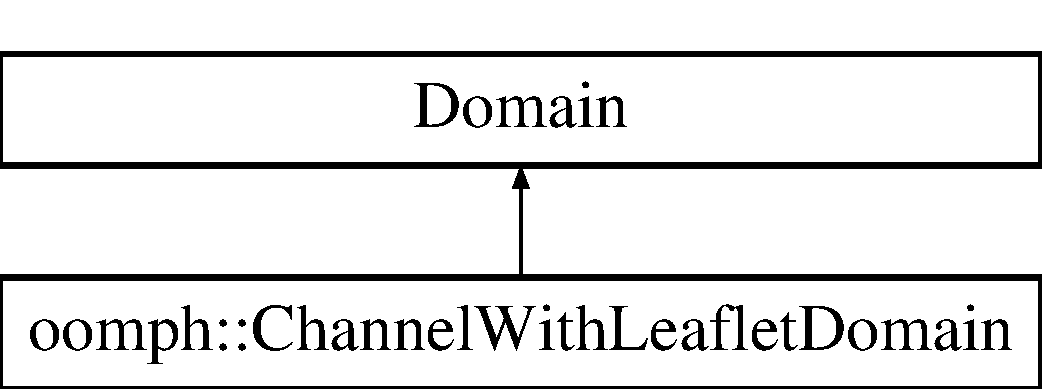
\includegraphics[height=2.000000cm]{classoomph_1_1ChannelWithLeafletDomain}
\end{center}
\end{figure}
\subsection*{Public Member Functions}
\begin{DoxyCompactItemize}
\item 
\hyperlink{classoomph_1_1ChannelWithLeafletDomain_a6cca7d06136de0c76facec2a92b0939e}{Channel\+With\+Leaflet\+Domain} (\hyperlink{classoomph_1_1GeomObject}{Geom\+Object} $\ast$\hyperlink{classoomph_1_1ChannelWithLeafletDomain_a91d7d8d2f564c5e9d2ee07449b2653c9}{leaflet\+\_\+pt}, const double \&\hyperlink{classoomph_1_1ChannelWithLeafletDomain_a5538092062970dbd2f02218a05639d49}{lleft}, const double \&\hyperlink{classoomph_1_1ChannelWithLeafletDomain_aee74846110e70cd5538386e1ccb0ce7c}{lright}, const double \&\hyperlink{classoomph_1_1ChannelWithLeafletDomain_af70ada72d505ebea468d1000b04c20e1}{hleaflet}, const double \&\hyperlink{classoomph_1_1ChannelWithLeafletDomain_aaf195c688423473ed97af61f8a1467ab}{htot}, const unsigned \&nleft, const unsigned \&nright, const unsigned \&ny1, const unsigned \&ny2)
\begin{DoxyCompactList}\small\item\em Constructor\+: Pass pointer to \hyperlink{classoomph_1_1GeomObject}{Geom\+Object} that represents the leaflet, the length of the domain to left and right of the leaflet, the height of the leaflet and the overall height of the channel, the number of element columns to the left and right of the leaflet, the number of rows of elements from the bottom of the channel to the end of the leaflet, the number of rows of elements above the end of the leaflet. \end{DoxyCompactList}\item 
\hyperlink{classoomph_1_1ChannelWithLeafletDomain_a7f00e3d9ed53ca70519671446fe60510}{$\sim$\+Channel\+With\+Leaflet\+Domain} ()
\begin{DoxyCompactList}\small\item\em Destructor\+: Kill macro elements. \end{DoxyCompactList}\item 
double \hyperlink{classoomph_1_1ChannelWithLeafletDomain_aaf195c688423473ed97af61f8a1467ab}{htot} ()
\begin{DoxyCompactList}\small\item\em Total height of domain (width of channel) \end{DoxyCompactList}\item 
double \hyperlink{classoomph_1_1ChannelWithLeafletDomain_af70ada72d505ebea468d1000b04c20e1}{hleaflet} ()
\begin{DoxyCompactList}\small\item\em Height of leaflet. \end{DoxyCompactList}\item 
double \hyperlink{classoomph_1_1ChannelWithLeafletDomain_a5538092062970dbd2f02218a05639d49}{lleft} ()
\begin{DoxyCompactList}\small\item\em Length of domain to the left of leaflet. \end{DoxyCompactList}\item 
double \hyperlink{classoomph_1_1ChannelWithLeafletDomain_aee74846110e70cd5538386e1ccb0ce7c}{lright} ()
\begin{DoxyCompactList}\small\item\em Length of domain to the right of leaflet. \end{DoxyCompactList}\item 
\hyperlink{classoomph_1_1GeomObject}{Geom\+Object} $\ast$\& \hyperlink{classoomph_1_1ChannelWithLeafletDomain_a91d7d8d2f564c5e9d2ee07449b2653c9}{leaflet\+\_\+pt} ()
\begin{DoxyCompactList}\small\item\em Pointer to the wall. \end{DoxyCompactList}\item 
void \hyperlink{classoomph_1_1ChannelWithLeafletDomain_ae4b123847f4ab6e242a0409d72fe5cbd}{macro\+\_\+element\+\_\+boundary} (const unsigned \&\hyperlink{cfortran_8h_af6f0bd3dc13317f895c91323c25c2b8f}{t}, const unsigned \&imacro, const unsigned \&idirect, const \hyperlink{classoomph_1_1Vector}{Vector}$<$ double $>$ \&zeta, \hyperlink{classoomph_1_1Vector}{Vector}$<$ double $>$ \&r)
\begin{DoxyCompactList}\small\item\em Parametrisation of macro element boundaries. \end{DoxyCompactList}\end{DoxyCompactItemize}
\subsection*{Protected Member Functions}
\begin{DoxyCompactItemize}
\item 
void \hyperlink{classoomph_1_1ChannelWithLeafletDomain_a08d97680e95f42a385a869d5c384e610}{macro\+\_\+bound\+\_\+\+I\+\_\+N} (const unsigned \&\hyperlink{cfortran_8h_af6f0bd3dc13317f895c91323c25c2b8f}{t}, const \hyperlink{classoomph_1_1Vector}{Vector}$<$ double $>$ \&zeta, \hyperlink{classoomph_1_1Vector}{Vector}$<$ double $>$ \&r, const unsigned \&\hyperlink{cfortran_8h_adb50e893b86b3e55e751a42eab3cba82}{i}, const unsigned \&j)
\begin{DoxyCompactList}\small\item\em Helper function. \end{DoxyCompactList}\item 
void \hyperlink{classoomph_1_1ChannelWithLeafletDomain_a20898c8b6747cf01e3e92e4a5c6ff5e4}{macro\+\_\+bound\+\_\+\+I\+\_\+S} (const unsigned \&\hyperlink{cfortran_8h_af6f0bd3dc13317f895c91323c25c2b8f}{t}, const \hyperlink{classoomph_1_1Vector}{Vector}$<$ double $>$ \&zeta, \hyperlink{classoomph_1_1Vector}{Vector}$<$ double $>$ \&r, const unsigned \&\hyperlink{cfortran_8h_adb50e893b86b3e55e751a42eab3cba82}{i}, const unsigned \&j)
\begin{DoxyCompactList}\small\item\em Helper function. \end{DoxyCompactList}\item 
void \hyperlink{classoomph_1_1ChannelWithLeafletDomain_a15e43fe342a04c8466a43112e3a48ff3}{macro\+\_\+bound\+\_\+\+I\+\_\+W} (const unsigned \&\hyperlink{cfortran_8h_af6f0bd3dc13317f895c91323c25c2b8f}{t}, const \hyperlink{classoomph_1_1Vector}{Vector}$<$ double $>$ \&zeta, \hyperlink{classoomph_1_1Vector}{Vector}$<$ double $>$ \&r, const unsigned \&\hyperlink{cfortran_8h_adb50e893b86b3e55e751a42eab3cba82}{i}, const unsigned \&j)
\begin{DoxyCompactList}\small\item\em Helper function. \end{DoxyCompactList}\item 
void \hyperlink{classoomph_1_1ChannelWithLeafletDomain_ac0bc6edb7d09bfdb310de99f846f5093}{macro\+\_\+bound\+\_\+\+I\+\_\+E} (const unsigned \&\hyperlink{cfortran_8h_af6f0bd3dc13317f895c91323c25c2b8f}{t}, const \hyperlink{classoomph_1_1Vector}{Vector}$<$ double $>$ \&zeta, \hyperlink{classoomph_1_1Vector}{Vector}$<$ double $>$ \&r, const unsigned \&\hyperlink{cfortran_8h_adb50e893b86b3e55e751a42eab3cba82}{i}, const unsigned \&j)
\begin{DoxyCompactList}\small\item\em Helper function. \end{DoxyCompactList}\item 
void \hyperlink{classoomph_1_1ChannelWithLeafletDomain_a1402c0d3fe42a8ffd6c9fb1d6df9d460}{macro\+\_\+bound\+\_\+\+I\+I\+\_\+N} (const unsigned \&\hyperlink{cfortran_8h_af6f0bd3dc13317f895c91323c25c2b8f}{t}, const \hyperlink{classoomph_1_1Vector}{Vector}$<$ double $>$ \&zeta, \hyperlink{classoomph_1_1Vector}{Vector}$<$ double $>$ \&r, const unsigned \&\hyperlink{cfortran_8h_adb50e893b86b3e55e751a42eab3cba82}{i}, const unsigned \&j)
\begin{DoxyCompactList}\small\item\em Helper function. \end{DoxyCompactList}\item 
void \hyperlink{classoomph_1_1ChannelWithLeafletDomain_a565166bede89908189cc8e426a898859}{macro\+\_\+bound\+\_\+\+I\+I\+\_\+S} (const unsigned \&\hyperlink{cfortran_8h_af6f0bd3dc13317f895c91323c25c2b8f}{t}, const \hyperlink{classoomph_1_1Vector}{Vector}$<$ double $>$ \&zeta, \hyperlink{classoomph_1_1Vector}{Vector}$<$ double $>$ \&r, const unsigned \&\hyperlink{cfortran_8h_adb50e893b86b3e55e751a42eab3cba82}{i}, const unsigned \&j)
\begin{DoxyCompactList}\small\item\em Helper function. \end{DoxyCompactList}\item 
void \hyperlink{classoomph_1_1ChannelWithLeafletDomain_afa35af75e7a60d3e5d4adf6a8097825e}{macro\+\_\+bound\+\_\+\+I\+I\+\_\+W} (const unsigned \&\hyperlink{cfortran_8h_af6f0bd3dc13317f895c91323c25c2b8f}{t}, const \hyperlink{classoomph_1_1Vector}{Vector}$<$ double $>$ \&zeta, \hyperlink{classoomph_1_1Vector}{Vector}$<$ double $>$ \&r, const unsigned \&\hyperlink{cfortran_8h_adb50e893b86b3e55e751a42eab3cba82}{i}, const unsigned \&j)
\begin{DoxyCompactList}\small\item\em Helper function. \end{DoxyCompactList}\item 
void \hyperlink{classoomph_1_1ChannelWithLeafletDomain_a9083a5ac562feb1cd33d78e6cc18b257}{macro\+\_\+bound\+\_\+\+I\+I\+\_\+E} (const unsigned \&\hyperlink{cfortran_8h_af6f0bd3dc13317f895c91323c25c2b8f}{t}, const \hyperlink{classoomph_1_1Vector}{Vector}$<$ double $>$ \&zeta, \hyperlink{classoomph_1_1Vector}{Vector}$<$ double $>$ \&r, const unsigned \&\hyperlink{cfortran_8h_adb50e893b86b3e55e751a42eab3cba82}{i}, const unsigned \&j)
\begin{DoxyCompactList}\small\item\em Helper function. \end{DoxyCompactList}\item 
void \hyperlink{classoomph_1_1ChannelWithLeafletDomain_a8b7f88fb218ceb09f0fde09ba22cd5b9}{macro\+\_\+bound\+\_\+\+I\+I\+I\+\_\+N} (const unsigned \&\hyperlink{cfortran_8h_af6f0bd3dc13317f895c91323c25c2b8f}{t}, const \hyperlink{classoomph_1_1Vector}{Vector}$<$ double $>$ \&zeta, \hyperlink{classoomph_1_1Vector}{Vector}$<$ double $>$ \&r, const unsigned \&\hyperlink{cfortran_8h_adb50e893b86b3e55e751a42eab3cba82}{i}, const unsigned \&j)
\begin{DoxyCompactList}\small\item\em Helper function. \end{DoxyCompactList}\item 
void \hyperlink{classoomph_1_1ChannelWithLeafletDomain_aacdeafe878caadb3e6d0cf98a87df25a}{macro\+\_\+bound\+\_\+\+I\+I\+I\+\_\+S} (const unsigned \&\hyperlink{cfortran_8h_af6f0bd3dc13317f895c91323c25c2b8f}{t}, const \hyperlink{classoomph_1_1Vector}{Vector}$<$ double $>$ \&zeta, \hyperlink{classoomph_1_1Vector}{Vector}$<$ double $>$ \&r, const unsigned \&\hyperlink{cfortran_8h_adb50e893b86b3e55e751a42eab3cba82}{i}, const unsigned \&j)
\begin{DoxyCompactList}\small\item\em Helper function. \end{DoxyCompactList}\item 
void \hyperlink{classoomph_1_1ChannelWithLeafletDomain_a06ccb5b6d160c3a31acf80174381a834}{macro\+\_\+bound\+\_\+\+I\+I\+I\+\_\+W} (const unsigned \&\hyperlink{cfortran_8h_af6f0bd3dc13317f895c91323c25c2b8f}{t}, const \hyperlink{classoomph_1_1Vector}{Vector}$<$ double $>$ \&zeta, \hyperlink{classoomph_1_1Vector}{Vector}$<$ double $>$ \&r, const unsigned \&\hyperlink{cfortran_8h_adb50e893b86b3e55e751a42eab3cba82}{i}, const unsigned \&j)
\begin{DoxyCompactList}\small\item\em Helper function. \end{DoxyCompactList}\item 
void \hyperlink{classoomph_1_1ChannelWithLeafletDomain_af17451c66c723d841aa6f16505c51be3}{macro\+\_\+bound\+\_\+\+I\+I\+I\+\_\+E} (const unsigned \&\hyperlink{cfortran_8h_af6f0bd3dc13317f895c91323c25c2b8f}{t}, const \hyperlink{classoomph_1_1Vector}{Vector}$<$ double $>$ \&zeta, \hyperlink{classoomph_1_1Vector}{Vector}$<$ double $>$ \&r, const unsigned \&\hyperlink{cfortran_8h_adb50e893b86b3e55e751a42eab3cba82}{i}, const unsigned \&j)
\begin{DoxyCompactList}\small\item\em Helper function. \end{DoxyCompactList}\item 
void \hyperlink{classoomph_1_1ChannelWithLeafletDomain_ae8d9410d270e27677cb89c5dfe9cc136}{macro\+\_\+bound\+\_\+\+I\+V\+\_\+N} (const unsigned \&\hyperlink{cfortran_8h_af6f0bd3dc13317f895c91323c25c2b8f}{t}, const \hyperlink{classoomph_1_1Vector}{Vector}$<$ double $>$ \&zeta, \hyperlink{classoomph_1_1Vector}{Vector}$<$ double $>$ \&r, const unsigned \&\hyperlink{cfortran_8h_adb50e893b86b3e55e751a42eab3cba82}{i}, const unsigned \&j)
\begin{DoxyCompactList}\small\item\em Helper function. \end{DoxyCompactList}\item 
void \hyperlink{classoomph_1_1ChannelWithLeafletDomain_a038eba8447f4d1643cd44642294bf43f}{macro\+\_\+bound\+\_\+\+I\+V\+\_\+S} (const unsigned \&\hyperlink{cfortran_8h_af6f0bd3dc13317f895c91323c25c2b8f}{t}, const \hyperlink{classoomph_1_1Vector}{Vector}$<$ double $>$ \&zeta, \hyperlink{classoomph_1_1Vector}{Vector}$<$ double $>$ \&r, const unsigned \&\hyperlink{cfortran_8h_adb50e893b86b3e55e751a42eab3cba82}{i}, const unsigned \&j)
\begin{DoxyCompactList}\small\item\em Helper function. \end{DoxyCompactList}\item 
void \hyperlink{classoomph_1_1ChannelWithLeafletDomain_ab9da487d185f947a30e03b43d0fc0c9b}{macro\+\_\+bound\+\_\+\+I\+V\+\_\+W} (const unsigned \&\hyperlink{cfortran_8h_af6f0bd3dc13317f895c91323c25c2b8f}{t}, const \hyperlink{classoomph_1_1Vector}{Vector}$<$ double $>$ \&zeta, \hyperlink{classoomph_1_1Vector}{Vector}$<$ double $>$ \&r, const unsigned \&\hyperlink{cfortran_8h_adb50e893b86b3e55e751a42eab3cba82}{i}, const unsigned \&j)
\begin{DoxyCompactList}\small\item\em Helper function. \end{DoxyCompactList}\item 
void \hyperlink{classoomph_1_1ChannelWithLeafletDomain_a16c8d718f5da2e6d9d73fe0455bacc0c}{macro\+\_\+bound\+\_\+\+I\+V\+\_\+E} (const unsigned \&\hyperlink{cfortran_8h_af6f0bd3dc13317f895c91323c25c2b8f}{t}, const \hyperlink{classoomph_1_1Vector}{Vector}$<$ double $>$ \&zeta, \hyperlink{classoomph_1_1Vector}{Vector}$<$ double $>$ \&r, const unsigned \&\hyperlink{cfortran_8h_adb50e893b86b3e55e751a42eab3cba82}{i}, const unsigned \&j)
\begin{DoxyCompactList}\small\item\em Helper function. \end{DoxyCompactList}\item 
void \hyperlink{classoomph_1_1ChannelWithLeafletDomain_aaca0af9c2a638c80bd8af783b9972599}{slanted\+\_\+bound\+\_\+up} (const unsigned \&\hyperlink{cfortran_8h_af6f0bd3dc13317f895c91323c25c2b8f}{t}, const \hyperlink{classoomph_1_1Vector}{Vector}$<$ double $>$ \&zeta, \hyperlink{classoomph_1_1Vector}{Vector}$<$ double $>$ \&r)
\begin{DoxyCompactList}\small\item\em Helper function. \end{DoxyCompactList}\end{DoxyCompactItemize}
\subsection*{Protected Attributes}
\begin{DoxyCompactItemize}
\item 
double \hyperlink{classoomph_1_1ChannelWithLeafletDomain_a6c1a799bbedc5f0ff08f38088eaedc68}{Lright}
\begin{DoxyCompactList}\small\item\em Length of the domain to the right of the leaflet. \end{DoxyCompactList}\item 
double \hyperlink{classoomph_1_1ChannelWithLeafletDomain_a0a50a8a7b274fb1dfc6d18c79ca884cd}{Lleft}
\begin{DoxyCompactList}\small\item\em Length of the domain to the left of the leaflet. \end{DoxyCompactList}\item 
double \hyperlink{classoomph_1_1ChannelWithLeafletDomain_a75ce3248efae5c33a9c9989b2f310139}{Hleaflet}
\begin{DoxyCompactList}\small\item\em Lagrangian coordinate at end of leaflet. \end{DoxyCompactList}\item 
double \hyperlink{classoomph_1_1ChannelWithLeafletDomain_ad32b0daa71b42d34aec81c7e3d25cb98}{Htot}
\begin{DoxyCompactList}\small\item\em Total width of the channel. \end{DoxyCompactList}\item 
unsigned \hyperlink{classoomph_1_1ChannelWithLeafletDomain_a11aac62965f9bcb7d4c0043669b28f15}{Nright}
\begin{DoxyCompactList}\small\item\em Number of macro element columnns to the right of the leaflet. \end{DoxyCompactList}\item 
unsigned \hyperlink{classoomph_1_1ChannelWithLeafletDomain_ad0abd8837f9f0924b801d2fb78c69532}{Nleft}
\begin{DoxyCompactList}\small\item\em Number of macro element columns to the left of the leaflet. \end{DoxyCompactList}\item 
unsigned \hyperlink{classoomph_1_1ChannelWithLeafletDomain_a3c6393ef6e626d7a2f2a8ea70c8addbe}{Ny1}
\begin{DoxyCompactList}\small\item\em Number of macro element rows up to the end of the leaflet. \end{DoxyCompactList}\item 
unsigned \hyperlink{classoomph_1_1ChannelWithLeafletDomain_a1596a538b4263b42d20f9c098c5f2752}{Ny2}
\begin{DoxyCompactList}\small\item\em Number of macro element rows above the leaflet. \end{DoxyCompactList}\item 
double \hyperlink{classoomph_1_1ChannelWithLeafletDomain_a165703af81538c28bbbd780d65bbb333}{X\+\_\+0}
\begin{DoxyCompactList}\small\item\em Center of the domain \+: origin of the leaflet, extracted from \hyperlink{classoomph_1_1GeomObject}{Geom\+Object} and stored for fast access. \end{DoxyCompactList}\item 
\hyperlink{classoomph_1_1GeomObject}{Geom\+Object} $\ast$ \hyperlink{classoomph_1_1ChannelWithLeafletDomain_a08a8eb7078cdc788dc7643e09e7405fb}{Leaflet\+\_\+pt}
\begin{DoxyCompactList}\small\item\em Pointer to leaflet. \end{DoxyCompactList}\end{DoxyCompactItemize}


\subsection{Detailed Description}
Rectangular domain with a leaflet blocking the lower half 

Definition at line 46 of file channel\+\_\+with\+\_\+leaflet\+\_\+domain.\+h.



\subsection{Constructor \& Destructor Documentation}
\mbox{\Hypertarget{classoomph_1_1ChannelWithLeafletDomain_a6cca7d06136de0c76facec2a92b0939e}\label{classoomph_1_1ChannelWithLeafletDomain_a6cca7d06136de0c76facec2a92b0939e}} 
\index{oomph\+::\+Channel\+With\+Leaflet\+Domain@{oomph\+::\+Channel\+With\+Leaflet\+Domain}!Channel\+With\+Leaflet\+Domain@{Channel\+With\+Leaflet\+Domain}}
\index{Channel\+With\+Leaflet\+Domain@{Channel\+With\+Leaflet\+Domain}!oomph\+::\+Channel\+With\+Leaflet\+Domain@{oomph\+::\+Channel\+With\+Leaflet\+Domain}}
\subsubsection{\texorpdfstring{Channel\+With\+Leaflet\+Domain()}{ChannelWithLeafletDomain()}}
{\footnotesize\ttfamily oomph\+::\+Channel\+With\+Leaflet\+Domain\+::\+Channel\+With\+Leaflet\+Domain (\begin{DoxyParamCaption}\item[{\hyperlink{classoomph_1_1GeomObject}{Geom\+Object} $\ast$}]{leaflet\+\_\+pt,  }\item[{const double \&}]{lleft,  }\item[{const double \&}]{lright,  }\item[{const double \&}]{hleaflet,  }\item[{const double \&}]{htot,  }\item[{const unsigned \&}]{nleft,  }\item[{const unsigned \&}]{nright,  }\item[{const unsigned \&}]{ny1,  }\item[{const unsigned \&}]{ny2 }\end{DoxyParamCaption})\hspace{0.3cm}{\ttfamily [inline]}}



Constructor\+: Pass pointer to \hyperlink{classoomph_1_1GeomObject}{Geom\+Object} that represents the leaflet, the length of the domain to left and right of the leaflet, the height of the leaflet and the overall height of the channel, the number of element columns to the left and right of the leaflet, the number of rows of elements from the bottom of the channel to the end of the leaflet, the number of rows of elements above the end of the leaflet. 



Definition at line 58 of file channel\+\_\+with\+\_\+leaflet\+\_\+domain.\+h.



References hleaflet(), Hleaflet, htot(), Htot, i, leaflet\+\_\+pt(), Leaflet\+\_\+pt, lleft(), Lleft, lright(), Lright, oomph\+::\+Domain\+::\+Macro\+\_\+element\+\_\+pt, Nleft, Nright, Ny1, Ny2, oomph\+::\+Geom\+Object\+::position(), and X\+\_\+0.

\mbox{\Hypertarget{classoomph_1_1ChannelWithLeafletDomain_a7f00e3d9ed53ca70519671446fe60510}\label{classoomph_1_1ChannelWithLeafletDomain_a7f00e3d9ed53ca70519671446fe60510}} 
\index{oomph\+::\+Channel\+With\+Leaflet\+Domain@{oomph\+::\+Channel\+With\+Leaflet\+Domain}!````~Channel\+With\+Leaflet\+Domain@{$\sim$\+Channel\+With\+Leaflet\+Domain}}
\index{````~Channel\+With\+Leaflet\+Domain@{$\sim$\+Channel\+With\+Leaflet\+Domain}!oomph\+::\+Channel\+With\+Leaflet\+Domain@{oomph\+::\+Channel\+With\+Leaflet\+Domain}}
\subsubsection{\texorpdfstring{$\sim$\+Channel\+With\+Leaflet\+Domain()}{~ChannelWithLeafletDomain()}}
{\footnotesize\ttfamily oomph\+::\+Channel\+With\+Leaflet\+Domain\+::$\sim$\+Channel\+With\+Leaflet\+Domain (\begin{DoxyParamCaption}{ }\end{DoxyParamCaption})\hspace{0.3cm}{\ttfamily [inline]}}



Destructor\+: Kill macro elements. 



Definition at line 96 of file channel\+\_\+with\+\_\+leaflet\+\_\+domain.\+h.



References i, oomph\+::\+Domain\+::\+Macro\+\_\+element\+\_\+pt, Nleft, Nright, Ny1, and Ny2.



\subsection{Member Function Documentation}
\mbox{\Hypertarget{classoomph_1_1ChannelWithLeafletDomain_af70ada72d505ebea468d1000b04c20e1}\label{classoomph_1_1ChannelWithLeafletDomain_af70ada72d505ebea468d1000b04c20e1}} 
\index{oomph\+::\+Channel\+With\+Leaflet\+Domain@{oomph\+::\+Channel\+With\+Leaflet\+Domain}!hleaflet@{hleaflet}}
\index{hleaflet@{hleaflet}!oomph\+::\+Channel\+With\+Leaflet\+Domain@{oomph\+::\+Channel\+With\+Leaflet\+Domain}}
\subsubsection{\texorpdfstring{hleaflet()}{hleaflet()}}
{\footnotesize\ttfamily double oomph\+::\+Channel\+With\+Leaflet\+Domain\+::hleaflet (\begin{DoxyParamCaption}{ }\end{DoxyParamCaption})\hspace{0.3cm}{\ttfamily [inline]}}



Height of leaflet. 



Definition at line 107 of file channel\+\_\+with\+\_\+leaflet\+\_\+domain.\+h.



References Hleaflet.



Referenced by Channel\+With\+Leaflet\+Domain(), and oomph\+::\+Algebraic\+Channel\+With\+Leaflet\+Mesh$<$ E\+L\+E\+M\+E\+N\+T $>$\+::setup\+\_\+algebraic\+\_\+node\+\_\+update().

\mbox{\Hypertarget{classoomph_1_1ChannelWithLeafletDomain_aaf195c688423473ed97af61f8a1467ab}\label{classoomph_1_1ChannelWithLeafletDomain_aaf195c688423473ed97af61f8a1467ab}} 
\index{oomph\+::\+Channel\+With\+Leaflet\+Domain@{oomph\+::\+Channel\+With\+Leaflet\+Domain}!htot@{htot}}
\index{htot@{htot}!oomph\+::\+Channel\+With\+Leaflet\+Domain@{oomph\+::\+Channel\+With\+Leaflet\+Domain}}
\subsubsection{\texorpdfstring{htot()}{htot()}}
{\footnotesize\ttfamily double oomph\+::\+Channel\+With\+Leaflet\+Domain\+::htot (\begin{DoxyParamCaption}{ }\end{DoxyParamCaption})\hspace{0.3cm}{\ttfamily [inline]}}



Total height of domain (width of channel) 



Definition at line 104 of file channel\+\_\+with\+\_\+leaflet\+\_\+domain.\+h.



References Htot.



Referenced by Channel\+With\+Leaflet\+Domain(), oomph\+::\+Algebraic\+Channel\+With\+Leaflet\+Mesh$<$ E\+L\+E\+M\+E\+N\+T $>$\+::setup\+\_\+algebraic\+\_\+node\+\_\+update(), and oomph\+::\+Algebraic\+Channel\+With\+Leaflet\+Mesh$<$ E\+L\+E\+M\+E\+N\+T $>$\+::slanted\+\_\+bound\+\_\+up().

\mbox{\Hypertarget{classoomph_1_1ChannelWithLeafletDomain_a91d7d8d2f564c5e9d2ee07449b2653c9}\label{classoomph_1_1ChannelWithLeafletDomain_a91d7d8d2f564c5e9d2ee07449b2653c9}} 
\index{oomph\+::\+Channel\+With\+Leaflet\+Domain@{oomph\+::\+Channel\+With\+Leaflet\+Domain}!leaflet\+\_\+pt@{leaflet\+\_\+pt}}
\index{leaflet\+\_\+pt@{leaflet\+\_\+pt}!oomph\+::\+Channel\+With\+Leaflet\+Domain@{oomph\+::\+Channel\+With\+Leaflet\+Domain}}
\subsubsection{\texorpdfstring{leaflet\+\_\+pt()}{leaflet\_pt()}}
{\footnotesize\ttfamily \hyperlink{classoomph_1_1GeomObject}{Geom\+Object}$\ast$\& oomph\+::\+Channel\+With\+Leaflet\+Domain\+::leaflet\+\_\+pt (\begin{DoxyParamCaption}{ }\end{DoxyParamCaption})\hspace{0.3cm}{\ttfamily [inline]}}



Pointer to the wall. 



Definition at line 116 of file channel\+\_\+with\+\_\+leaflet\+\_\+domain.\+h.



References i, Leaflet\+\_\+pt, macro\+\_\+bound\+\_\+\+I\+\_\+\+E(), macro\+\_\+bound\+\_\+\+I\+\_\+\+N(), macro\+\_\+bound\+\_\+\+I\+\_\+\+S(), macro\+\_\+bound\+\_\+\+I\+\_\+\+W(), macro\+\_\+bound\+\_\+\+I\+I\+\_\+\+E(), macro\+\_\+bound\+\_\+\+I\+I\+\_\+\+N(), macro\+\_\+bound\+\_\+\+I\+I\+\_\+\+S(), macro\+\_\+bound\+\_\+\+I\+I\+\_\+\+W(), macro\+\_\+bound\+\_\+\+I\+I\+I\+\_\+\+E(), macro\+\_\+bound\+\_\+\+I\+I\+I\+\_\+\+N(), macro\+\_\+bound\+\_\+\+I\+I\+I\+\_\+\+S(), macro\+\_\+bound\+\_\+\+I\+I\+I\+\_\+\+W(), macro\+\_\+bound\+\_\+\+I\+V\+\_\+\+E(), macro\+\_\+bound\+\_\+\+I\+V\+\_\+\+N(), macro\+\_\+bound\+\_\+\+I\+V\+\_\+\+S(), macro\+\_\+bound\+\_\+\+I\+V\+\_\+\+W(), macro\+\_\+element\+\_\+boundary(), slanted\+\_\+bound\+\_\+up(), and t.



Referenced by Channel\+With\+Leaflet\+Domain().

\mbox{\Hypertarget{classoomph_1_1ChannelWithLeafletDomain_a5538092062970dbd2f02218a05639d49}\label{classoomph_1_1ChannelWithLeafletDomain_a5538092062970dbd2f02218a05639d49}} 
\index{oomph\+::\+Channel\+With\+Leaflet\+Domain@{oomph\+::\+Channel\+With\+Leaflet\+Domain}!lleft@{lleft}}
\index{lleft@{lleft}!oomph\+::\+Channel\+With\+Leaflet\+Domain@{oomph\+::\+Channel\+With\+Leaflet\+Domain}}
\subsubsection{\texorpdfstring{lleft()}{lleft()}}
{\footnotesize\ttfamily double oomph\+::\+Channel\+With\+Leaflet\+Domain\+::lleft (\begin{DoxyParamCaption}{ }\end{DoxyParamCaption})\hspace{0.3cm}{\ttfamily [inline]}}



Length of domain to the left of leaflet. 



Definition at line 110 of file channel\+\_\+with\+\_\+leaflet\+\_\+domain.\+h.



References Lleft.



Referenced by Channel\+With\+Leaflet\+Domain(), oomph\+::\+Algebraic\+Channel\+With\+Leaflet\+Mesh$<$ E\+L\+E\+M\+E\+N\+T $>$\+::node\+\_\+update\+\_\+\+I(), oomph\+::\+Algebraic\+Channel\+With\+Leaflet\+Mesh$<$ E\+L\+E\+M\+E\+N\+T $>$\+::node\+\_\+update\+\_\+\+I\+I\+I(), and oomph\+::\+Algebraic\+Channel\+With\+Leaflet\+Mesh$<$ E\+L\+E\+M\+E\+N\+T $>$\+::setup\+\_\+algebraic\+\_\+node\+\_\+update().

\mbox{\Hypertarget{classoomph_1_1ChannelWithLeafletDomain_aee74846110e70cd5538386e1ccb0ce7c}\label{classoomph_1_1ChannelWithLeafletDomain_aee74846110e70cd5538386e1ccb0ce7c}} 
\index{oomph\+::\+Channel\+With\+Leaflet\+Domain@{oomph\+::\+Channel\+With\+Leaflet\+Domain}!lright@{lright}}
\index{lright@{lright}!oomph\+::\+Channel\+With\+Leaflet\+Domain@{oomph\+::\+Channel\+With\+Leaflet\+Domain}}
\subsubsection{\texorpdfstring{lright()}{lright()}}
{\footnotesize\ttfamily double oomph\+::\+Channel\+With\+Leaflet\+Domain\+::lright (\begin{DoxyParamCaption}{ }\end{DoxyParamCaption})\hspace{0.3cm}{\ttfamily [inline]}}



Length of domain to the right of leaflet. 



Definition at line 113 of file channel\+\_\+with\+\_\+leaflet\+\_\+domain.\+h.



References Lright.



Referenced by Channel\+With\+Leaflet\+Domain(), oomph\+::\+Algebraic\+Channel\+With\+Leaflet\+Mesh$<$ E\+L\+E\+M\+E\+N\+T $>$\+::node\+\_\+update\+\_\+\+I\+I(), oomph\+::\+Algebraic\+Channel\+With\+Leaflet\+Mesh$<$ E\+L\+E\+M\+E\+N\+T $>$\+::node\+\_\+update\+\_\+\+I\+V(), and oomph\+::\+Algebraic\+Channel\+With\+Leaflet\+Mesh$<$ E\+L\+E\+M\+E\+N\+T $>$\+::setup\+\_\+algebraic\+\_\+node\+\_\+update().

\mbox{\Hypertarget{classoomph_1_1ChannelWithLeafletDomain_ac0bc6edb7d09bfdb310de99f846f5093}\label{classoomph_1_1ChannelWithLeafletDomain_ac0bc6edb7d09bfdb310de99f846f5093}} 
\index{oomph\+::\+Channel\+With\+Leaflet\+Domain@{oomph\+::\+Channel\+With\+Leaflet\+Domain}!macro\+\_\+bound\+\_\+\+I\+\_\+E@{macro\+\_\+bound\+\_\+\+I\+\_\+E}}
\index{macro\+\_\+bound\+\_\+\+I\+\_\+E@{macro\+\_\+bound\+\_\+\+I\+\_\+E}!oomph\+::\+Channel\+With\+Leaflet\+Domain@{oomph\+::\+Channel\+With\+Leaflet\+Domain}}
\subsubsection{\texorpdfstring{macro\+\_\+bound\+\_\+\+I\+\_\+\+E()}{macro\_bound\_I\_E()}}
{\footnotesize\ttfamily void oomph\+::\+Channel\+With\+Leaflet\+Domain\+::macro\+\_\+bound\+\_\+\+I\+\_\+E (\begin{DoxyParamCaption}\item[{const unsigned \&}]{t,  }\item[{const \hyperlink{classoomph_1_1Vector}{Vector}$<$ double $>$ \&}]{zeta,  }\item[{\hyperlink{classoomph_1_1Vector}{Vector}$<$ double $>$ \&}]{r,  }\item[{const unsigned \&}]{i,  }\item[{const unsigned \&}]{j }\end{DoxyParamCaption})\hspace{0.3cm}{\ttfamily [protected]}}



Helper function. 

Helper function for eastern boundary in lower left region. Final expression of r 

Definition at line 375 of file channel\+\_\+with\+\_\+leaflet\+\_\+domain.\+h.



References Hleaflet, Leaflet\+\_\+pt, Lleft, Nleft, Ny1, oomph\+::\+Geom\+Object\+::position(), s, and X\+\_\+0.



Referenced by leaflet\+\_\+pt(), macro\+\_\+bound\+\_\+\+I\+\_\+\+N(), macro\+\_\+bound\+\_\+\+I\+\_\+\+S(), and macro\+\_\+element\+\_\+boundary().

\mbox{\Hypertarget{classoomph_1_1ChannelWithLeafletDomain_a08d97680e95f42a385a869d5c384e610}\label{classoomph_1_1ChannelWithLeafletDomain_a08d97680e95f42a385a869d5c384e610}} 
\index{oomph\+::\+Channel\+With\+Leaflet\+Domain@{oomph\+::\+Channel\+With\+Leaflet\+Domain}!macro\+\_\+bound\+\_\+\+I\+\_\+N@{macro\+\_\+bound\+\_\+\+I\+\_\+N}}
\index{macro\+\_\+bound\+\_\+\+I\+\_\+N@{macro\+\_\+bound\+\_\+\+I\+\_\+N}!oomph\+::\+Channel\+With\+Leaflet\+Domain@{oomph\+::\+Channel\+With\+Leaflet\+Domain}}
\subsubsection{\texorpdfstring{macro\+\_\+bound\+\_\+\+I\+\_\+\+N()}{macro\_bound\_I\_N()}}
{\footnotesize\ttfamily void oomph\+::\+Channel\+With\+Leaflet\+Domain\+::macro\+\_\+bound\+\_\+\+I\+\_\+N (\begin{DoxyParamCaption}\item[{const unsigned \&}]{t,  }\item[{const \hyperlink{classoomph_1_1Vector}{Vector}$<$ double $>$ \&}]{zeta,  }\item[{\hyperlink{classoomph_1_1Vector}{Vector}$<$ double $>$ \&}]{r,  }\item[{const unsigned \&}]{i,  }\item[{const unsigned \&}]{j }\end{DoxyParamCaption})\hspace{0.3cm}{\ttfamily [protected]}}



Helper function. 

Helper function for northern boundary in lower left region. 

Definition at line 464 of file channel\+\_\+with\+\_\+leaflet\+\_\+domain.\+h.



References macro\+\_\+bound\+\_\+\+I\+\_\+\+E(), and macro\+\_\+bound\+\_\+\+I\+\_\+\+W().



Referenced by leaflet\+\_\+pt(), and macro\+\_\+element\+\_\+boundary().

\mbox{\Hypertarget{classoomph_1_1ChannelWithLeafletDomain_a20898c8b6747cf01e3e92e4a5c6ff5e4}\label{classoomph_1_1ChannelWithLeafletDomain_a20898c8b6747cf01e3e92e4a5c6ff5e4}} 
\index{oomph\+::\+Channel\+With\+Leaflet\+Domain@{oomph\+::\+Channel\+With\+Leaflet\+Domain}!macro\+\_\+bound\+\_\+\+I\+\_\+S@{macro\+\_\+bound\+\_\+\+I\+\_\+S}}
\index{macro\+\_\+bound\+\_\+\+I\+\_\+S@{macro\+\_\+bound\+\_\+\+I\+\_\+S}!oomph\+::\+Channel\+With\+Leaflet\+Domain@{oomph\+::\+Channel\+With\+Leaflet\+Domain}}
\subsubsection{\texorpdfstring{macro\+\_\+bound\+\_\+\+I\+\_\+\+S()}{macro\_bound\_I\_S()}}
{\footnotesize\ttfamily void oomph\+::\+Channel\+With\+Leaflet\+Domain\+::macro\+\_\+bound\+\_\+\+I\+\_\+S (\begin{DoxyParamCaption}\item[{const unsigned \&}]{t,  }\item[{const \hyperlink{classoomph_1_1Vector}{Vector}$<$ double $>$ \&}]{zeta,  }\item[{\hyperlink{classoomph_1_1Vector}{Vector}$<$ double $>$ \&}]{r,  }\item[{const unsigned \&}]{i,  }\item[{const unsigned \&}]{j }\end{DoxyParamCaption})\hspace{0.3cm}{\ttfamily [protected]}}



Helper function. 

Helper function for southern boundary in lower left region. Find the coordinates of the two corners of the south boundary 

Definition at line 488 of file channel\+\_\+with\+\_\+leaflet\+\_\+domain.\+h.



References macro\+\_\+bound\+\_\+\+I\+\_\+\+E(), and macro\+\_\+bound\+\_\+\+I\+\_\+\+W().



Referenced by leaflet\+\_\+pt(), and macro\+\_\+element\+\_\+boundary().

\mbox{\Hypertarget{classoomph_1_1ChannelWithLeafletDomain_a15e43fe342a04c8466a43112e3a48ff3}\label{classoomph_1_1ChannelWithLeafletDomain_a15e43fe342a04c8466a43112e3a48ff3}} 
\index{oomph\+::\+Channel\+With\+Leaflet\+Domain@{oomph\+::\+Channel\+With\+Leaflet\+Domain}!macro\+\_\+bound\+\_\+\+I\+\_\+W@{macro\+\_\+bound\+\_\+\+I\+\_\+W}}
\index{macro\+\_\+bound\+\_\+\+I\+\_\+W@{macro\+\_\+bound\+\_\+\+I\+\_\+W}!oomph\+::\+Channel\+With\+Leaflet\+Domain@{oomph\+::\+Channel\+With\+Leaflet\+Domain}}
\subsubsection{\texorpdfstring{macro\+\_\+bound\+\_\+\+I\+\_\+\+W()}{macro\_bound\_I\_W()}}
{\footnotesize\ttfamily void oomph\+::\+Channel\+With\+Leaflet\+Domain\+::macro\+\_\+bound\+\_\+\+I\+\_\+W (\begin{DoxyParamCaption}\item[{const unsigned \&}]{t,  }\item[{const \hyperlink{classoomph_1_1Vector}{Vector}$<$ double $>$ \&}]{zeta,  }\item[{\hyperlink{classoomph_1_1Vector}{Vector}$<$ double $>$ \&}]{r,  }\item[{const unsigned \&}]{i,  }\item[{const unsigned \&}]{j }\end{DoxyParamCaption})\hspace{0.3cm}{\ttfamily [protected]}}



Helper function. 

Helper function for western boundary in lower left region. Final expression of r 

Definition at line 419 of file channel\+\_\+with\+\_\+leaflet\+\_\+domain.\+h.



References Hleaflet, Leaflet\+\_\+pt, Lleft, Nleft, Ny1, oomph\+::\+Geom\+Object\+::position(), s, and X\+\_\+0.



Referenced by leaflet\+\_\+pt(), macro\+\_\+bound\+\_\+\+I\+\_\+\+N(), macro\+\_\+bound\+\_\+\+I\+\_\+\+S(), and macro\+\_\+element\+\_\+boundary().

\mbox{\Hypertarget{classoomph_1_1ChannelWithLeafletDomain_a9083a5ac562feb1cd33d78e6cc18b257}\label{classoomph_1_1ChannelWithLeafletDomain_a9083a5ac562feb1cd33d78e6cc18b257}} 
\index{oomph\+::\+Channel\+With\+Leaflet\+Domain@{oomph\+::\+Channel\+With\+Leaflet\+Domain}!macro\+\_\+bound\+\_\+\+I\+I\+\_\+E@{macro\+\_\+bound\+\_\+\+I\+I\+\_\+E}}
\index{macro\+\_\+bound\+\_\+\+I\+I\+\_\+E@{macro\+\_\+bound\+\_\+\+I\+I\+\_\+E}!oomph\+::\+Channel\+With\+Leaflet\+Domain@{oomph\+::\+Channel\+With\+Leaflet\+Domain}}
\subsubsection{\texorpdfstring{macro\+\_\+bound\+\_\+\+I\+I\+\_\+\+E()}{macro\_bound\_II\_E()}}
{\footnotesize\ttfamily void oomph\+::\+Channel\+With\+Leaflet\+Domain\+::macro\+\_\+bound\+\_\+\+I\+I\+\_\+E (\begin{DoxyParamCaption}\item[{const unsigned \&}]{t,  }\item[{const \hyperlink{classoomph_1_1Vector}{Vector}$<$ double $>$ \&}]{zeta,  }\item[{\hyperlink{classoomph_1_1Vector}{Vector}$<$ double $>$ \&}]{r,  }\item[{const unsigned \&}]{i,  }\item[{const unsigned \&}]{j }\end{DoxyParamCaption})\hspace{0.3cm}{\ttfamily [protected]}}



Helper function. 

Helper function for eastern boundary in lower right region. Final expression of r 

Definition at line 523 of file channel\+\_\+with\+\_\+leaflet\+\_\+domain.\+h.



References Hleaflet, Leaflet\+\_\+pt, Lright, Nright, Ny1, oomph\+::\+Geom\+Object\+::position(), s, and X\+\_\+0.



Referenced by leaflet\+\_\+pt(), macro\+\_\+bound\+\_\+\+I\+I\+\_\+\+N(), macro\+\_\+bound\+\_\+\+I\+I\+\_\+\+S(), and macro\+\_\+element\+\_\+boundary().

\mbox{\Hypertarget{classoomph_1_1ChannelWithLeafletDomain_a1402c0d3fe42a8ffd6c9fb1d6df9d460}\label{classoomph_1_1ChannelWithLeafletDomain_a1402c0d3fe42a8ffd6c9fb1d6df9d460}} 
\index{oomph\+::\+Channel\+With\+Leaflet\+Domain@{oomph\+::\+Channel\+With\+Leaflet\+Domain}!macro\+\_\+bound\+\_\+\+I\+I\+\_\+N@{macro\+\_\+bound\+\_\+\+I\+I\+\_\+N}}
\index{macro\+\_\+bound\+\_\+\+I\+I\+\_\+N@{macro\+\_\+bound\+\_\+\+I\+I\+\_\+N}!oomph\+::\+Channel\+With\+Leaflet\+Domain@{oomph\+::\+Channel\+With\+Leaflet\+Domain}}
\subsubsection{\texorpdfstring{macro\+\_\+bound\+\_\+\+I\+I\+\_\+\+N()}{macro\_bound\_II\_N()}}
{\footnotesize\ttfamily void oomph\+::\+Channel\+With\+Leaflet\+Domain\+::macro\+\_\+bound\+\_\+\+I\+I\+\_\+N (\begin{DoxyParamCaption}\item[{const unsigned \&}]{t,  }\item[{const \hyperlink{classoomph_1_1Vector}{Vector}$<$ double $>$ \&}]{zeta,  }\item[{\hyperlink{classoomph_1_1Vector}{Vector}$<$ double $>$ \&}]{r,  }\item[{const unsigned \&}]{i,  }\item[{const unsigned \&}]{j }\end{DoxyParamCaption})\hspace{0.3cm}{\ttfamily [protected]}}



Helper function. 

Helper function for northern boundary in lower right region. 

Definition at line 616 of file channel\+\_\+with\+\_\+leaflet\+\_\+domain.\+h.



References macro\+\_\+bound\+\_\+\+I\+I\+\_\+\+E(), and macro\+\_\+bound\+\_\+\+I\+I\+\_\+\+W().



Referenced by leaflet\+\_\+pt(), and macro\+\_\+element\+\_\+boundary().

\mbox{\Hypertarget{classoomph_1_1ChannelWithLeafletDomain_a565166bede89908189cc8e426a898859}\label{classoomph_1_1ChannelWithLeafletDomain_a565166bede89908189cc8e426a898859}} 
\index{oomph\+::\+Channel\+With\+Leaflet\+Domain@{oomph\+::\+Channel\+With\+Leaflet\+Domain}!macro\+\_\+bound\+\_\+\+I\+I\+\_\+S@{macro\+\_\+bound\+\_\+\+I\+I\+\_\+S}}
\index{macro\+\_\+bound\+\_\+\+I\+I\+\_\+S@{macro\+\_\+bound\+\_\+\+I\+I\+\_\+S}!oomph\+::\+Channel\+With\+Leaflet\+Domain@{oomph\+::\+Channel\+With\+Leaflet\+Domain}}
\subsubsection{\texorpdfstring{macro\+\_\+bound\+\_\+\+I\+I\+\_\+\+S()}{macro\_bound\_II\_S()}}
{\footnotesize\ttfamily void oomph\+::\+Channel\+With\+Leaflet\+Domain\+::macro\+\_\+bound\+\_\+\+I\+I\+\_\+S (\begin{DoxyParamCaption}\item[{const unsigned \&}]{t,  }\item[{const \hyperlink{classoomph_1_1Vector}{Vector}$<$ double $>$ \&}]{zeta,  }\item[{\hyperlink{classoomph_1_1Vector}{Vector}$<$ double $>$ \&}]{r,  }\item[{const unsigned \&}]{i,  }\item[{const unsigned \&}]{j }\end{DoxyParamCaption})\hspace{0.3cm}{\ttfamily [protected]}}



Helper function. 

Helper function for southern boundary in lower right region. 

Definition at line 641 of file channel\+\_\+with\+\_\+leaflet\+\_\+domain.\+h.



References macro\+\_\+bound\+\_\+\+I\+I\+\_\+\+E(), and macro\+\_\+bound\+\_\+\+I\+I\+\_\+\+W().



Referenced by leaflet\+\_\+pt(), and macro\+\_\+element\+\_\+boundary().

\mbox{\Hypertarget{classoomph_1_1ChannelWithLeafletDomain_afa35af75e7a60d3e5d4adf6a8097825e}\label{classoomph_1_1ChannelWithLeafletDomain_afa35af75e7a60d3e5d4adf6a8097825e}} 
\index{oomph\+::\+Channel\+With\+Leaflet\+Domain@{oomph\+::\+Channel\+With\+Leaflet\+Domain}!macro\+\_\+bound\+\_\+\+I\+I\+\_\+W@{macro\+\_\+bound\+\_\+\+I\+I\+\_\+W}}
\index{macro\+\_\+bound\+\_\+\+I\+I\+\_\+W@{macro\+\_\+bound\+\_\+\+I\+I\+\_\+W}!oomph\+::\+Channel\+With\+Leaflet\+Domain@{oomph\+::\+Channel\+With\+Leaflet\+Domain}}
\subsubsection{\texorpdfstring{macro\+\_\+bound\+\_\+\+I\+I\+\_\+\+W()}{macro\_bound\_II\_W()}}
{\footnotesize\ttfamily void oomph\+::\+Channel\+With\+Leaflet\+Domain\+::macro\+\_\+bound\+\_\+\+I\+I\+\_\+W (\begin{DoxyParamCaption}\item[{const unsigned \&}]{t,  }\item[{const \hyperlink{classoomph_1_1Vector}{Vector}$<$ double $>$ \&}]{zeta,  }\item[{\hyperlink{classoomph_1_1Vector}{Vector}$<$ double $>$ \&}]{r,  }\item[{const unsigned \&}]{i,  }\item[{const unsigned \&}]{j }\end{DoxyParamCaption})\hspace{0.3cm}{\ttfamily [protected]}}



Helper function. 

Helper function for western boundary in lower right region. 

Definition at line 569 of file channel\+\_\+with\+\_\+leaflet\+\_\+domain.\+h.



References Hleaflet, Leaflet\+\_\+pt, Lright, Nright, Ny1, oomph\+::\+Geom\+Object\+::position(), s, and X\+\_\+0.



Referenced by leaflet\+\_\+pt(), macro\+\_\+bound\+\_\+\+I\+I\+\_\+\+N(), macro\+\_\+bound\+\_\+\+I\+I\+\_\+\+S(), and macro\+\_\+element\+\_\+boundary().

\mbox{\Hypertarget{classoomph_1_1ChannelWithLeafletDomain_af17451c66c723d841aa6f16505c51be3}\label{classoomph_1_1ChannelWithLeafletDomain_af17451c66c723d841aa6f16505c51be3}} 
\index{oomph\+::\+Channel\+With\+Leaflet\+Domain@{oomph\+::\+Channel\+With\+Leaflet\+Domain}!macro\+\_\+bound\+\_\+\+I\+I\+I\+\_\+E@{macro\+\_\+bound\+\_\+\+I\+I\+I\+\_\+E}}
\index{macro\+\_\+bound\+\_\+\+I\+I\+I\+\_\+E@{macro\+\_\+bound\+\_\+\+I\+I\+I\+\_\+E}!oomph\+::\+Channel\+With\+Leaflet\+Domain@{oomph\+::\+Channel\+With\+Leaflet\+Domain}}
\subsubsection{\texorpdfstring{macro\+\_\+bound\+\_\+\+I\+I\+I\+\_\+\+E()}{macro\_bound\_III\_E()}}
{\footnotesize\ttfamily void oomph\+::\+Channel\+With\+Leaflet\+Domain\+::macro\+\_\+bound\+\_\+\+I\+I\+I\+\_\+E (\begin{DoxyParamCaption}\item[{const unsigned \&}]{t,  }\item[{const \hyperlink{classoomph_1_1Vector}{Vector}$<$ double $>$ \&}]{zeta,  }\item[{\hyperlink{classoomph_1_1Vector}{Vector}$<$ double $>$ \&}]{r,  }\item[{const unsigned \&}]{i,  }\item[{const unsigned \&}]{j }\end{DoxyParamCaption})\hspace{0.3cm}{\ttfamily [protected]}}



Helper function. 

Helper function for eastern boundary in upper left region. Final expression of r 

Definition at line 700 of file channel\+\_\+with\+\_\+leaflet\+\_\+domain.\+h.



References Hleaflet, Htot, Lleft, Nleft, Ny2, s, slanted\+\_\+bound\+\_\+up(), and X\+\_\+0.



Referenced by leaflet\+\_\+pt(), macro\+\_\+bound\+\_\+\+I\+I\+I\+\_\+\+N(), macro\+\_\+bound\+\_\+\+I\+I\+I\+\_\+\+S(), and macro\+\_\+element\+\_\+boundary().

\mbox{\Hypertarget{classoomph_1_1ChannelWithLeafletDomain_a8b7f88fb218ceb09f0fde09ba22cd5b9}\label{classoomph_1_1ChannelWithLeafletDomain_a8b7f88fb218ceb09f0fde09ba22cd5b9}} 
\index{oomph\+::\+Channel\+With\+Leaflet\+Domain@{oomph\+::\+Channel\+With\+Leaflet\+Domain}!macro\+\_\+bound\+\_\+\+I\+I\+I\+\_\+N@{macro\+\_\+bound\+\_\+\+I\+I\+I\+\_\+N}}
\index{macro\+\_\+bound\+\_\+\+I\+I\+I\+\_\+N@{macro\+\_\+bound\+\_\+\+I\+I\+I\+\_\+N}!oomph\+::\+Channel\+With\+Leaflet\+Domain@{oomph\+::\+Channel\+With\+Leaflet\+Domain}}
\subsubsection{\texorpdfstring{macro\+\_\+bound\+\_\+\+I\+I\+I\+\_\+\+N()}{macro\_bound\_III\_N()}}
{\footnotesize\ttfamily void oomph\+::\+Channel\+With\+Leaflet\+Domain\+::macro\+\_\+bound\+\_\+\+I\+I\+I\+\_\+N (\begin{DoxyParamCaption}\item[{const unsigned \&}]{t,  }\item[{const \hyperlink{classoomph_1_1Vector}{Vector}$<$ double $>$ \&}]{zeta,  }\item[{\hyperlink{classoomph_1_1Vector}{Vector}$<$ double $>$ \&}]{r,  }\item[{const unsigned \&}]{i,  }\item[{const unsigned \&}]{j }\end{DoxyParamCaption})\hspace{0.3cm}{\ttfamily [protected]}}



Helper function. 

Helper function for northern boundary in upper left region. 

Definition at line 792 of file channel\+\_\+with\+\_\+leaflet\+\_\+domain.\+h.



References macro\+\_\+bound\+\_\+\+I\+I\+I\+\_\+\+E(), and macro\+\_\+bound\+\_\+\+I\+I\+I\+\_\+\+W().



Referenced by leaflet\+\_\+pt(), and macro\+\_\+element\+\_\+boundary().

\mbox{\Hypertarget{classoomph_1_1ChannelWithLeafletDomain_aacdeafe878caadb3e6d0cf98a87df25a}\label{classoomph_1_1ChannelWithLeafletDomain_aacdeafe878caadb3e6d0cf98a87df25a}} 
\index{oomph\+::\+Channel\+With\+Leaflet\+Domain@{oomph\+::\+Channel\+With\+Leaflet\+Domain}!macro\+\_\+bound\+\_\+\+I\+I\+I\+\_\+S@{macro\+\_\+bound\+\_\+\+I\+I\+I\+\_\+S}}
\index{macro\+\_\+bound\+\_\+\+I\+I\+I\+\_\+S@{macro\+\_\+bound\+\_\+\+I\+I\+I\+\_\+S}!oomph\+::\+Channel\+With\+Leaflet\+Domain@{oomph\+::\+Channel\+With\+Leaflet\+Domain}}
\subsubsection{\texorpdfstring{macro\+\_\+bound\+\_\+\+I\+I\+I\+\_\+\+S()}{macro\_bound\_III\_S()}}
{\footnotesize\ttfamily void oomph\+::\+Channel\+With\+Leaflet\+Domain\+::macro\+\_\+bound\+\_\+\+I\+I\+I\+\_\+S (\begin{DoxyParamCaption}\item[{const unsigned \&}]{t,  }\item[{const \hyperlink{classoomph_1_1Vector}{Vector}$<$ double $>$ \&}]{zeta,  }\item[{\hyperlink{classoomph_1_1Vector}{Vector}$<$ double $>$ \&}]{r,  }\item[{const unsigned \&}]{i,  }\item[{const unsigned \&}]{j }\end{DoxyParamCaption})\hspace{0.3cm}{\ttfamily [protected]}}



Helper function. 

Helper function for southern boundary in upper left region. 

Definition at line 816 of file channel\+\_\+with\+\_\+leaflet\+\_\+domain.\+h.



References macro\+\_\+bound\+\_\+\+I\+I\+I\+\_\+\+E(), and macro\+\_\+bound\+\_\+\+I\+I\+I\+\_\+\+W().



Referenced by leaflet\+\_\+pt(), and macro\+\_\+element\+\_\+boundary().

\mbox{\Hypertarget{classoomph_1_1ChannelWithLeafletDomain_a06ccb5b6d160c3a31acf80174381a834}\label{classoomph_1_1ChannelWithLeafletDomain_a06ccb5b6d160c3a31acf80174381a834}} 
\index{oomph\+::\+Channel\+With\+Leaflet\+Domain@{oomph\+::\+Channel\+With\+Leaflet\+Domain}!macro\+\_\+bound\+\_\+\+I\+I\+I\+\_\+W@{macro\+\_\+bound\+\_\+\+I\+I\+I\+\_\+W}}
\index{macro\+\_\+bound\+\_\+\+I\+I\+I\+\_\+W@{macro\+\_\+bound\+\_\+\+I\+I\+I\+\_\+W}!oomph\+::\+Channel\+With\+Leaflet\+Domain@{oomph\+::\+Channel\+With\+Leaflet\+Domain}}
\subsubsection{\texorpdfstring{macro\+\_\+bound\+\_\+\+I\+I\+I\+\_\+\+W()}{macro\_bound\_III\_W()}}
{\footnotesize\ttfamily void oomph\+::\+Channel\+With\+Leaflet\+Domain\+::macro\+\_\+bound\+\_\+\+I\+I\+I\+\_\+W (\begin{DoxyParamCaption}\item[{const unsigned \&}]{t,  }\item[{const \hyperlink{classoomph_1_1Vector}{Vector}$<$ double $>$ \&}]{zeta,  }\item[{\hyperlink{classoomph_1_1Vector}{Vector}$<$ double $>$ \&}]{r,  }\item[{const unsigned \&}]{i,  }\item[{const unsigned \&}]{j }\end{DoxyParamCaption})\hspace{0.3cm}{\ttfamily [protected]}}



Helper function. 

Helper function for western boundary in upper left region. 

Definition at line 746 of file channel\+\_\+with\+\_\+leaflet\+\_\+domain.\+h.



References Hleaflet, Htot, Lleft, Nleft, Ny2, s, slanted\+\_\+bound\+\_\+up(), and X\+\_\+0.



Referenced by leaflet\+\_\+pt(), macro\+\_\+bound\+\_\+\+I\+I\+I\+\_\+\+N(), macro\+\_\+bound\+\_\+\+I\+I\+I\+\_\+\+S(), and macro\+\_\+element\+\_\+boundary().

\mbox{\Hypertarget{classoomph_1_1ChannelWithLeafletDomain_a16c8d718f5da2e6d9d73fe0455bacc0c}\label{classoomph_1_1ChannelWithLeafletDomain_a16c8d718f5da2e6d9d73fe0455bacc0c}} 
\index{oomph\+::\+Channel\+With\+Leaflet\+Domain@{oomph\+::\+Channel\+With\+Leaflet\+Domain}!macro\+\_\+bound\+\_\+\+I\+V\+\_\+E@{macro\+\_\+bound\+\_\+\+I\+V\+\_\+E}}
\index{macro\+\_\+bound\+\_\+\+I\+V\+\_\+E@{macro\+\_\+bound\+\_\+\+I\+V\+\_\+E}!oomph\+::\+Channel\+With\+Leaflet\+Domain@{oomph\+::\+Channel\+With\+Leaflet\+Domain}}
\subsubsection{\texorpdfstring{macro\+\_\+bound\+\_\+\+I\+V\+\_\+\+E()}{macro\_bound\_IV\_E()}}
{\footnotesize\ttfamily void oomph\+::\+Channel\+With\+Leaflet\+Domain\+::macro\+\_\+bound\+\_\+\+I\+V\+\_\+E (\begin{DoxyParamCaption}\item[{const unsigned \&}]{t,  }\item[{const \hyperlink{classoomph_1_1Vector}{Vector}$<$ double $>$ \&}]{zeta,  }\item[{\hyperlink{classoomph_1_1Vector}{Vector}$<$ double $>$ \&}]{r,  }\item[{const unsigned \&}]{i,  }\item[{const unsigned \&}]{j }\end{DoxyParamCaption})\hspace{0.3cm}{\ttfamily [protected]}}



Helper function. 

Helper function for eastern boundary in upper right region. 

Definition at line 851 of file channel\+\_\+with\+\_\+leaflet\+\_\+domain.\+h.



References Hleaflet, Htot, Lright, Nright, Ny2, s, slanted\+\_\+bound\+\_\+up(), and X\+\_\+0.



Referenced by leaflet\+\_\+pt(), macro\+\_\+bound\+\_\+\+I\+V\+\_\+\+N(), macro\+\_\+bound\+\_\+\+I\+V\+\_\+\+S(), and macro\+\_\+element\+\_\+boundary().

\mbox{\Hypertarget{classoomph_1_1ChannelWithLeafletDomain_ae8d9410d270e27677cb89c5dfe9cc136}\label{classoomph_1_1ChannelWithLeafletDomain_ae8d9410d270e27677cb89c5dfe9cc136}} 
\index{oomph\+::\+Channel\+With\+Leaflet\+Domain@{oomph\+::\+Channel\+With\+Leaflet\+Domain}!macro\+\_\+bound\+\_\+\+I\+V\+\_\+N@{macro\+\_\+bound\+\_\+\+I\+V\+\_\+N}}
\index{macro\+\_\+bound\+\_\+\+I\+V\+\_\+N@{macro\+\_\+bound\+\_\+\+I\+V\+\_\+N}!oomph\+::\+Channel\+With\+Leaflet\+Domain@{oomph\+::\+Channel\+With\+Leaflet\+Domain}}
\subsubsection{\texorpdfstring{macro\+\_\+bound\+\_\+\+I\+V\+\_\+\+N()}{macro\_bound\_IV\_N()}}
{\footnotesize\ttfamily void oomph\+::\+Channel\+With\+Leaflet\+Domain\+::macro\+\_\+bound\+\_\+\+I\+V\+\_\+N (\begin{DoxyParamCaption}\item[{const unsigned \&}]{t,  }\item[{const \hyperlink{classoomph_1_1Vector}{Vector}$<$ double $>$ \&}]{zeta,  }\item[{\hyperlink{classoomph_1_1Vector}{Vector}$<$ double $>$ \&}]{r,  }\item[{const unsigned \&}]{i,  }\item[{const unsigned \&}]{j }\end{DoxyParamCaption})\hspace{0.3cm}{\ttfamily [protected]}}



Helper function. 

Helper function for northern boundary in upper right region. 

Definition at line 941 of file channel\+\_\+with\+\_\+leaflet\+\_\+domain.\+h.



References macro\+\_\+bound\+\_\+\+I\+V\+\_\+\+E(), and macro\+\_\+bound\+\_\+\+I\+V\+\_\+\+W().



Referenced by leaflet\+\_\+pt(), and macro\+\_\+element\+\_\+boundary().

\mbox{\Hypertarget{classoomph_1_1ChannelWithLeafletDomain_a038eba8447f4d1643cd44642294bf43f}\label{classoomph_1_1ChannelWithLeafletDomain_a038eba8447f4d1643cd44642294bf43f}} 
\index{oomph\+::\+Channel\+With\+Leaflet\+Domain@{oomph\+::\+Channel\+With\+Leaflet\+Domain}!macro\+\_\+bound\+\_\+\+I\+V\+\_\+S@{macro\+\_\+bound\+\_\+\+I\+V\+\_\+S}}
\index{macro\+\_\+bound\+\_\+\+I\+V\+\_\+S@{macro\+\_\+bound\+\_\+\+I\+V\+\_\+S}!oomph\+::\+Channel\+With\+Leaflet\+Domain@{oomph\+::\+Channel\+With\+Leaflet\+Domain}}
\subsubsection{\texorpdfstring{macro\+\_\+bound\+\_\+\+I\+V\+\_\+\+S()}{macro\_bound\_IV\_S()}}
{\footnotesize\ttfamily void oomph\+::\+Channel\+With\+Leaflet\+Domain\+::macro\+\_\+bound\+\_\+\+I\+V\+\_\+S (\begin{DoxyParamCaption}\item[{const unsigned \&}]{t,  }\item[{const \hyperlink{classoomph_1_1Vector}{Vector}$<$ double $>$ \&}]{zeta,  }\item[{\hyperlink{classoomph_1_1Vector}{Vector}$<$ double $>$ \&}]{r,  }\item[{const unsigned \&}]{i,  }\item[{const unsigned \&}]{j }\end{DoxyParamCaption})\hspace{0.3cm}{\ttfamily [protected]}}



Helper function. 

Helper function for southern boundary in upper right region. 

Definition at line 965 of file channel\+\_\+with\+\_\+leaflet\+\_\+domain.\+h.



References macro\+\_\+bound\+\_\+\+I\+V\+\_\+\+E(), and macro\+\_\+bound\+\_\+\+I\+V\+\_\+\+W().



Referenced by leaflet\+\_\+pt(), and macro\+\_\+element\+\_\+boundary().

\mbox{\Hypertarget{classoomph_1_1ChannelWithLeafletDomain_ab9da487d185f947a30e03b43d0fc0c9b}\label{classoomph_1_1ChannelWithLeafletDomain_ab9da487d185f947a30e03b43d0fc0c9b}} 
\index{oomph\+::\+Channel\+With\+Leaflet\+Domain@{oomph\+::\+Channel\+With\+Leaflet\+Domain}!macro\+\_\+bound\+\_\+\+I\+V\+\_\+W@{macro\+\_\+bound\+\_\+\+I\+V\+\_\+W}}
\index{macro\+\_\+bound\+\_\+\+I\+V\+\_\+W@{macro\+\_\+bound\+\_\+\+I\+V\+\_\+W}!oomph\+::\+Channel\+With\+Leaflet\+Domain@{oomph\+::\+Channel\+With\+Leaflet\+Domain}}
\subsubsection{\texorpdfstring{macro\+\_\+bound\+\_\+\+I\+V\+\_\+\+W()}{macro\_bound\_IV\_W()}}
{\footnotesize\ttfamily void oomph\+::\+Channel\+With\+Leaflet\+Domain\+::macro\+\_\+bound\+\_\+\+I\+V\+\_\+W (\begin{DoxyParamCaption}\item[{const unsigned \&}]{t,  }\item[{const \hyperlink{classoomph_1_1Vector}{Vector}$<$ double $>$ \&}]{zeta,  }\item[{\hyperlink{classoomph_1_1Vector}{Vector}$<$ double $>$ \&}]{r,  }\item[{const unsigned \&}]{i,  }\item[{const unsigned \&}]{j }\end{DoxyParamCaption})\hspace{0.3cm}{\ttfamily [protected]}}



Helper function. 

Helper function for western boundary in upper right region. 

Definition at line 896 of file channel\+\_\+with\+\_\+leaflet\+\_\+domain.\+h.



References Hleaflet, Htot, Lright, Nright, Ny2, s, slanted\+\_\+bound\+\_\+up(), and X\+\_\+0.



Referenced by leaflet\+\_\+pt(), macro\+\_\+bound\+\_\+\+I\+V\+\_\+\+N(), macro\+\_\+bound\+\_\+\+I\+V\+\_\+\+S(), and macro\+\_\+element\+\_\+boundary().

\mbox{\Hypertarget{classoomph_1_1ChannelWithLeafletDomain_ae4b123847f4ab6e242a0409d72fe5cbd}\label{classoomph_1_1ChannelWithLeafletDomain_ae4b123847f4ab6e242a0409d72fe5cbd}} 
\index{oomph\+::\+Channel\+With\+Leaflet\+Domain@{oomph\+::\+Channel\+With\+Leaflet\+Domain}!macro\+\_\+element\+\_\+boundary@{macro\+\_\+element\+\_\+boundary}}
\index{macro\+\_\+element\+\_\+boundary@{macro\+\_\+element\+\_\+boundary}!oomph\+::\+Channel\+With\+Leaflet\+Domain@{oomph\+::\+Channel\+With\+Leaflet\+Domain}}
\subsubsection{\texorpdfstring{macro\+\_\+element\+\_\+boundary()}{macro\_element\_boundary()}}
{\footnotesize\ttfamily void oomph\+::\+Channel\+With\+Leaflet\+Domain\+::macro\+\_\+element\+\_\+boundary (\begin{DoxyParamCaption}\item[{const unsigned \&}]{t,  }\item[{const unsigned \&}]{imacro,  }\item[{const unsigned \&}]{idirect,  }\item[{const \hyperlink{classoomph_1_1Vector}{Vector}$<$ double $>$ \&}]{zeta,  }\item[{\hyperlink{classoomph_1_1Vector}{Vector}$<$ double $>$ \&}]{r }\end{DoxyParamCaption})\hspace{0.3cm}{\ttfamily [virtual]}}



Parametrisation of macro element boundaries. 



Implements \hyperlink{classoomph_1_1Domain_a95f3e00d28ea37e6c4d3027bfac91096}{oomph\+::\+Domain}.



Definition at line 242 of file channel\+\_\+with\+\_\+leaflet\+\_\+domain.\+h.



References oomph\+::\+Quad\+Tree\+Names\+::E, i, macro\+\_\+bound\+\_\+\+I\+\_\+\+E(), macro\+\_\+bound\+\_\+\+I\+\_\+\+N(), macro\+\_\+bound\+\_\+\+I\+\_\+\+S(), macro\+\_\+bound\+\_\+\+I\+\_\+\+W(), macro\+\_\+bound\+\_\+\+I\+I\+\_\+\+E(), macro\+\_\+bound\+\_\+\+I\+I\+\_\+\+N(), macro\+\_\+bound\+\_\+\+I\+I\+\_\+\+S(), macro\+\_\+bound\+\_\+\+I\+I\+\_\+\+W(), macro\+\_\+bound\+\_\+\+I\+I\+I\+\_\+\+E(), macro\+\_\+bound\+\_\+\+I\+I\+I\+\_\+\+N(), macro\+\_\+bound\+\_\+\+I\+I\+I\+\_\+\+S(), macro\+\_\+bound\+\_\+\+I\+I\+I\+\_\+\+W(), macro\+\_\+bound\+\_\+\+I\+V\+\_\+\+E(), macro\+\_\+bound\+\_\+\+I\+V\+\_\+\+N(), macro\+\_\+bound\+\_\+\+I\+V\+\_\+\+S(), macro\+\_\+bound\+\_\+\+I\+V\+\_\+\+W(), oomph\+::\+Quad\+Tree\+Names\+::N, Nleft, Nright, Ny1, oomph\+::\+Quad\+Tree\+Names\+::S, and oomph\+::\+Quad\+Tree\+Names\+::W.



Referenced by leaflet\+\_\+pt().

\mbox{\Hypertarget{classoomph_1_1ChannelWithLeafletDomain_aaca0af9c2a638c80bd8af783b9972599}\label{classoomph_1_1ChannelWithLeafletDomain_aaca0af9c2a638c80bd8af783b9972599}} 
\index{oomph\+::\+Channel\+With\+Leaflet\+Domain@{oomph\+::\+Channel\+With\+Leaflet\+Domain}!slanted\+\_\+bound\+\_\+up@{slanted\+\_\+bound\+\_\+up}}
\index{slanted\+\_\+bound\+\_\+up@{slanted\+\_\+bound\+\_\+up}!oomph\+::\+Channel\+With\+Leaflet\+Domain@{oomph\+::\+Channel\+With\+Leaflet\+Domain}}
\subsubsection{\texorpdfstring{slanted\+\_\+bound\+\_\+up()}{slanted\_bound\_up()}}
{\footnotesize\ttfamily void oomph\+::\+Channel\+With\+Leaflet\+Domain\+::slanted\+\_\+bound\+\_\+up (\begin{DoxyParamCaption}\item[{const unsigned \&}]{t,  }\item[{const \hyperlink{classoomph_1_1Vector}{Vector}$<$ double $>$ \&}]{zeta,  }\item[{\hyperlink{classoomph_1_1Vector}{Vector}$<$ double $>$ \&}]{r }\end{DoxyParamCaption})\hspace{0.3cm}{\ttfamily [protected]}}



Helper function. 

Describe the line between the boundary north of the domain (at x=X\+\_\+0) and the top of the wall, when zeta goes from 0 to 1. 

Definition at line 678 of file channel\+\_\+with\+\_\+leaflet\+\_\+domain.\+h.



References Hleaflet, Htot, Leaflet\+\_\+pt, oomph\+::\+Geom\+Object\+::position(), and X\+\_\+0.



Referenced by leaflet\+\_\+pt(), macro\+\_\+bound\+\_\+\+I\+I\+I\+\_\+\+E(), macro\+\_\+bound\+\_\+\+I\+I\+I\+\_\+\+W(), macro\+\_\+bound\+\_\+\+I\+V\+\_\+\+E(), and macro\+\_\+bound\+\_\+\+I\+V\+\_\+\+W().



\subsection{Member Data Documentation}
\mbox{\Hypertarget{classoomph_1_1ChannelWithLeafletDomain_a75ce3248efae5c33a9c9989b2f310139}\label{classoomph_1_1ChannelWithLeafletDomain_a75ce3248efae5c33a9c9989b2f310139}} 
\index{oomph\+::\+Channel\+With\+Leaflet\+Domain@{oomph\+::\+Channel\+With\+Leaflet\+Domain}!Hleaflet@{Hleaflet}}
\index{Hleaflet@{Hleaflet}!oomph\+::\+Channel\+With\+Leaflet\+Domain@{oomph\+::\+Channel\+With\+Leaflet\+Domain}}
\subsubsection{\texorpdfstring{Hleaflet}{Hleaflet}}
{\footnotesize\ttfamily double oomph\+::\+Channel\+With\+Leaflet\+Domain\+::\+Hleaflet\hspace{0.3cm}{\ttfamily [protected]}}



Lagrangian coordinate at end of leaflet. 



Definition at line 211 of file channel\+\_\+with\+\_\+leaflet\+\_\+domain.\+h.



Referenced by Channel\+With\+Leaflet\+Domain(), hleaflet(), macro\+\_\+bound\+\_\+\+I\+\_\+\+E(), macro\+\_\+bound\+\_\+\+I\+\_\+\+W(), macro\+\_\+bound\+\_\+\+I\+I\+\_\+\+E(), macro\+\_\+bound\+\_\+\+I\+I\+\_\+\+W(), macro\+\_\+bound\+\_\+\+I\+I\+I\+\_\+\+E(), macro\+\_\+bound\+\_\+\+I\+I\+I\+\_\+\+W(), macro\+\_\+bound\+\_\+\+I\+V\+\_\+\+E(), macro\+\_\+bound\+\_\+\+I\+V\+\_\+\+W(), and slanted\+\_\+bound\+\_\+up().

\mbox{\Hypertarget{classoomph_1_1ChannelWithLeafletDomain_ad32b0daa71b42d34aec81c7e3d25cb98}\label{classoomph_1_1ChannelWithLeafletDomain_ad32b0daa71b42d34aec81c7e3d25cb98}} 
\index{oomph\+::\+Channel\+With\+Leaflet\+Domain@{oomph\+::\+Channel\+With\+Leaflet\+Domain}!Htot@{Htot}}
\index{Htot@{Htot}!oomph\+::\+Channel\+With\+Leaflet\+Domain@{oomph\+::\+Channel\+With\+Leaflet\+Domain}}
\subsubsection{\texorpdfstring{Htot}{Htot}}
{\footnotesize\ttfamily double oomph\+::\+Channel\+With\+Leaflet\+Domain\+::\+Htot\hspace{0.3cm}{\ttfamily [protected]}}



Total width of the channel. 



Definition at line 214 of file channel\+\_\+with\+\_\+leaflet\+\_\+domain.\+h.



Referenced by Channel\+With\+Leaflet\+Domain(), htot(), macro\+\_\+bound\+\_\+\+I\+I\+I\+\_\+\+E(), macro\+\_\+bound\+\_\+\+I\+I\+I\+\_\+\+W(), macro\+\_\+bound\+\_\+\+I\+V\+\_\+\+E(), macro\+\_\+bound\+\_\+\+I\+V\+\_\+\+W(), and slanted\+\_\+bound\+\_\+up().

\mbox{\Hypertarget{classoomph_1_1ChannelWithLeafletDomain_a08a8eb7078cdc788dc7643e09e7405fb}\label{classoomph_1_1ChannelWithLeafletDomain_a08a8eb7078cdc788dc7643e09e7405fb}} 
\index{oomph\+::\+Channel\+With\+Leaflet\+Domain@{oomph\+::\+Channel\+With\+Leaflet\+Domain}!Leaflet\+\_\+pt@{Leaflet\+\_\+pt}}
\index{Leaflet\+\_\+pt@{Leaflet\+\_\+pt}!oomph\+::\+Channel\+With\+Leaflet\+Domain@{oomph\+::\+Channel\+With\+Leaflet\+Domain}}
\subsubsection{\texorpdfstring{Leaflet\+\_\+pt}{Leaflet\_pt}}
{\footnotesize\ttfamily \hyperlink{classoomph_1_1GeomObject}{Geom\+Object}$\ast$ oomph\+::\+Channel\+With\+Leaflet\+Domain\+::\+Leaflet\+\_\+pt\hspace{0.3cm}{\ttfamily [protected]}}



Pointer to leaflet. 



Definition at line 233 of file channel\+\_\+with\+\_\+leaflet\+\_\+domain.\+h.



Referenced by Channel\+With\+Leaflet\+Domain(), leaflet\+\_\+pt(), macro\+\_\+bound\+\_\+\+I\+\_\+\+E(), macro\+\_\+bound\+\_\+\+I\+\_\+\+W(), macro\+\_\+bound\+\_\+\+I\+I\+\_\+\+E(), macro\+\_\+bound\+\_\+\+I\+I\+\_\+\+W(), and slanted\+\_\+bound\+\_\+up().

\mbox{\Hypertarget{classoomph_1_1ChannelWithLeafletDomain_a0a50a8a7b274fb1dfc6d18c79ca884cd}\label{classoomph_1_1ChannelWithLeafletDomain_a0a50a8a7b274fb1dfc6d18c79ca884cd}} 
\index{oomph\+::\+Channel\+With\+Leaflet\+Domain@{oomph\+::\+Channel\+With\+Leaflet\+Domain}!Lleft@{Lleft}}
\index{Lleft@{Lleft}!oomph\+::\+Channel\+With\+Leaflet\+Domain@{oomph\+::\+Channel\+With\+Leaflet\+Domain}}
\subsubsection{\texorpdfstring{Lleft}{Lleft}}
{\footnotesize\ttfamily double oomph\+::\+Channel\+With\+Leaflet\+Domain\+::\+Lleft\hspace{0.3cm}{\ttfamily [protected]}}



Length of the domain to the left of the leaflet. 



Definition at line 208 of file channel\+\_\+with\+\_\+leaflet\+\_\+domain.\+h.



Referenced by Channel\+With\+Leaflet\+Domain(), lleft(), macro\+\_\+bound\+\_\+\+I\+\_\+\+E(), macro\+\_\+bound\+\_\+\+I\+\_\+\+W(), macro\+\_\+bound\+\_\+\+I\+I\+I\+\_\+\+E(), and macro\+\_\+bound\+\_\+\+I\+I\+I\+\_\+\+W().

\mbox{\Hypertarget{classoomph_1_1ChannelWithLeafletDomain_a6c1a799bbedc5f0ff08f38088eaedc68}\label{classoomph_1_1ChannelWithLeafletDomain_a6c1a799bbedc5f0ff08f38088eaedc68}} 
\index{oomph\+::\+Channel\+With\+Leaflet\+Domain@{oomph\+::\+Channel\+With\+Leaflet\+Domain}!Lright@{Lright}}
\index{Lright@{Lright}!oomph\+::\+Channel\+With\+Leaflet\+Domain@{oomph\+::\+Channel\+With\+Leaflet\+Domain}}
\subsubsection{\texorpdfstring{Lright}{Lright}}
{\footnotesize\ttfamily double oomph\+::\+Channel\+With\+Leaflet\+Domain\+::\+Lright\hspace{0.3cm}{\ttfamily [protected]}}



Length of the domain to the right of the leaflet. 



Definition at line 205 of file channel\+\_\+with\+\_\+leaflet\+\_\+domain.\+h.



Referenced by Channel\+With\+Leaflet\+Domain(), lright(), macro\+\_\+bound\+\_\+\+I\+I\+\_\+\+E(), macro\+\_\+bound\+\_\+\+I\+I\+\_\+\+W(), macro\+\_\+bound\+\_\+\+I\+V\+\_\+\+E(), and macro\+\_\+bound\+\_\+\+I\+V\+\_\+\+W().

\mbox{\Hypertarget{classoomph_1_1ChannelWithLeafletDomain_ad0abd8837f9f0924b801d2fb78c69532}\label{classoomph_1_1ChannelWithLeafletDomain_ad0abd8837f9f0924b801d2fb78c69532}} 
\index{oomph\+::\+Channel\+With\+Leaflet\+Domain@{oomph\+::\+Channel\+With\+Leaflet\+Domain}!Nleft@{Nleft}}
\index{Nleft@{Nleft}!oomph\+::\+Channel\+With\+Leaflet\+Domain@{oomph\+::\+Channel\+With\+Leaflet\+Domain}}
\subsubsection{\texorpdfstring{Nleft}{Nleft}}
{\footnotesize\ttfamily unsigned oomph\+::\+Channel\+With\+Leaflet\+Domain\+::\+Nleft\hspace{0.3cm}{\ttfamily [protected]}}



Number of macro element columns to the left of the leaflet. 



Definition at line 220 of file channel\+\_\+with\+\_\+leaflet\+\_\+domain.\+h.



Referenced by Channel\+With\+Leaflet\+Domain(), macro\+\_\+bound\+\_\+\+I\+\_\+\+E(), macro\+\_\+bound\+\_\+\+I\+\_\+\+W(), macro\+\_\+bound\+\_\+\+I\+I\+I\+\_\+\+E(), macro\+\_\+bound\+\_\+\+I\+I\+I\+\_\+\+W(), macro\+\_\+element\+\_\+boundary(), and $\sim$\+Channel\+With\+Leaflet\+Domain().

\mbox{\Hypertarget{classoomph_1_1ChannelWithLeafletDomain_a11aac62965f9bcb7d4c0043669b28f15}\label{classoomph_1_1ChannelWithLeafletDomain_a11aac62965f9bcb7d4c0043669b28f15}} 
\index{oomph\+::\+Channel\+With\+Leaflet\+Domain@{oomph\+::\+Channel\+With\+Leaflet\+Domain}!Nright@{Nright}}
\index{Nright@{Nright}!oomph\+::\+Channel\+With\+Leaflet\+Domain@{oomph\+::\+Channel\+With\+Leaflet\+Domain}}
\subsubsection{\texorpdfstring{Nright}{Nright}}
{\footnotesize\ttfamily unsigned oomph\+::\+Channel\+With\+Leaflet\+Domain\+::\+Nright\hspace{0.3cm}{\ttfamily [protected]}}



Number of macro element columnns to the right of the leaflet. 



Definition at line 217 of file channel\+\_\+with\+\_\+leaflet\+\_\+domain.\+h.



Referenced by Channel\+With\+Leaflet\+Domain(), macro\+\_\+bound\+\_\+\+I\+I\+\_\+\+E(), macro\+\_\+bound\+\_\+\+I\+I\+\_\+\+W(), macro\+\_\+bound\+\_\+\+I\+V\+\_\+\+E(), macro\+\_\+bound\+\_\+\+I\+V\+\_\+\+W(), macro\+\_\+element\+\_\+boundary(), and $\sim$\+Channel\+With\+Leaflet\+Domain().

\mbox{\Hypertarget{classoomph_1_1ChannelWithLeafletDomain_a3c6393ef6e626d7a2f2a8ea70c8addbe}\label{classoomph_1_1ChannelWithLeafletDomain_a3c6393ef6e626d7a2f2a8ea70c8addbe}} 
\index{oomph\+::\+Channel\+With\+Leaflet\+Domain@{oomph\+::\+Channel\+With\+Leaflet\+Domain}!Ny1@{Ny1}}
\index{Ny1@{Ny1}!oomph\+::\+Channel\+With\+Leaflet\+Domain@{oomph\+::\+Channel\+With\+Leaflet\+Domain}}
\subsubsection{\texorpdfstring{Ny1}{Ny1}}
{\footnotesize\ttfamily unsigned oomph\+::\+Channel\+With\+Leaflet\+Domain\+::\+Ny1\hspace{0.3cm}{\ttfamily [protected]}}



Number of macro element rows up to the end of the leaflet. 



Definition at line 223 of file channel\+\_\+with\+\_\+leaflet\+\_\+domain.\+h.



Referenced by Channel\+With\+Leaflet\+Domain(), macro\+\_\+bound\+\_\+\+I\+\_\+\+E(), macro\+\_\+bound\+\_\+\+I\+\_\+\+W(), macro\+\_\+bound\+\_\+\+I\+I\+\_\+\+E(), macro\+\_\+bound\+\_\+\+I\+I\+\_\+\+W(), macro\+\_\+element\+\_\+boundary(), and $\sim$\+Channel\+With\+Leaflet\+Domain().

\mbox{\Hypertarget{classoomph_1_1ChannelWithLeafletDomain_a1596a538b4263b42d20f9c098c5f2752}\label{classoomph_1_1ChannelWithLeafletDomain_a1596a538b4263b42d20f9c098c5f2752}} 
\index{oomph\+::\+Channel\+With\+Leaflet\+Domain@{oomph\+::\+Channel\+With\+Leaflet\+Domain}!Ny2@{Ny2}}
\index{Ny2@{Ny2}!oomph\+::\+Channel\+With\+Leaflet\+Domain@{oomph\+::\+Channel\+With\+Leaflet\+Domain}}
\subsubsection{\texorpdfstring{Ny2}{Ny2}}
{\footnotesize\ttfamily unsigned oomph\+::\+Channel\+With\+Leaflet\+Domain\+::\+Ny2\hspace{0.3cm}{\ttfamily [protected]}}



Number of macro element rows above the leaflet. 



Definition at line 226 of file channel\+\_\+with\+\_\+leaflet\+\_\+domain.\+h.



Referenced by Channel\+With\+Leaflet\+Domain(), macro\+\_\+bound\+\_\+\+I\+I\+I\+\_\+\+E(), macro\+\_\+bound\+\_\+\+I\+I\+I\+\_\+\+W(), macro\+\_\+bound\+\_\+\+I\+V\+\_\+\+E(), macro\+\_\+bound\+\_\+\+I\+V\+\_\+\+W(), and $\sim$\+Channel\+With\+Leaflet\+Domain().

\mbox{\Hypertarget{classoomph_1_1ChannelWithLeafletDomain_a165703af81538c28bbbd780d65bbb333}\label{classoomph_1_1ChannelWithLeafletDomain_a165703af81538c28bbbd780d65bbb333}} 
\index{oomph\+::\+Channel\+With\+Leaflet\+Domain@{oomph\+::\+Channel\+With\+Leaflet\+Domain}!X\+\_\+0@{X\+\_\+0}}
\index{X\+\_\+0@{X\+\_\+0}!oomph\+::\+Channel\+With\+Leaflet\+Domain@{oomph\+::\+Channel\+With\+Leaflet\+Domain}}
\subsubsection{\texorpdfstring{X\+\_\+0}{X\_0}}
{\footnotesize\ttfamily double oomph\+::\+Channel\+With\+Leaflet\+Domain\+::\+X\+\_\+0\hspace{0.3cm}{\ttfamily [protected]}}



Center of the domain \+: origin of the leaflet, extracted from \hyperlink{classoomph_1_1GeomObject}{Geom\+Object} and stored for fast access. 



Definition at line 230 of file channel\+\_\+with\+\_\+leaflet\+\_\+domain.\+h.



Referenced by Channel\+With\+Leaflet\+Domain(), macro\+\_\+bound\+\_\+\+I\+\_\+\+E(), macro\+\_\+bound\+\_\+\+I\+\_\+\+W(), macro\+\_\+bound\+\_\+\+I\+I\+\_\+\+E(), macro\+\_\+bound\+\_\+\+I\+I\+\_\+\+W(), macro\+\_\+bound\+\_\+\+I\+I\+I\+\_\+\+E(), macro\+\_\+bound\+\_\+\+I\+I\+I\+\_\+\+W(), macro\+\_\+bound\+\_\+\+I\+V\+\_\+\+E(), macro\+\_\+bound\+\_\+\+I\+V\+\_\+\+W(), and slanted\+\_\+bound\+\_\+up().



The documentation for this class was generated from the following file\+:\begin{DoxyCompactItemize}
\item 
\hyperlink{channel__with__leaflet__domain_8h}{channel\+\_\+with\+\_\+leaflet\+\_\+domain.\+h}\end{DoxyCompactItemize}

\hypertarget{classoomph_1_1ChannelWithLeafletMesh}{}\section{oomph\+:\+:Channel\+With\+Leaflet\+Mesh$<$ E\+L\+E\+M\+E\+NT $>$ Class Template Reference}
\label{classoomph_1_1ChannelWithLeafletMesh}\index{oomph\+::\+Channel\+With\+Leaflet\+Mesh$<$ E\+L\+E\+M\+E\+N\+T $>$@{oomph\+::\+Channel\+With\+Leaflet\+Mesh$<$ E\+L\+E\+M\+E\+N\+T $>$}}


Channel with leaflet mesh.  




{\ttfamily \#include $<$channel\+\_\+with\+\_\+leaflet\+\_\+mesh.\+template.\+h$>$}

Inheritance diagram for oomph\+:\+:Channel\+With\+Leaflet\+Mesh$<$ E\+L\+E\+M\+E\+NT $>$\+:\begin{figure}[H]
\begin{center}
\leavevmode
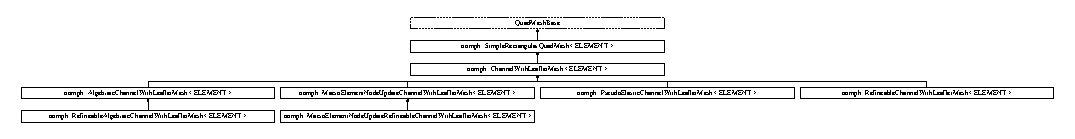
\includegraphics[height=1.696970cm]{classoomph_1_1ChannelWithLeafletMesh}
\end{center}
\end{figure}
\subsection*{Public Member Functions}
\begin{DoxyCompactItemize}
\item 
\hyperlink{classoomph_1_1ChannelWithLeafletMesh_ab210be34e9d7f72af9aefee618d41f3d}{Channel\+With\+Leaflet\+Mesh} (\hyperlink{classoomph_1_1GeomObject}{Geom\+Object} $\ast$leaflet\+\_\+pt, const double \&lleft, const double \&lright, const double \&hleaflet, const double \&htot, const unsigned \&nleft, const unsigned \&nright, const unsigned \&ny1, const unsigned \&ny2, \hyperlink{classoomph_1_1TimeStepper}{Time\+Stepper} $\ast$time\+\_\+stepper\+\_\+pt=\&\hyperlink{classoomph_1_1Mesh_a12243d0fee2b1fcee729ee5a4777ea10}{Mesh\+::\+Default\+\_\+\+Time\+Stepper})
\begin{DoxyCompactList}\small\item\em Constructor\+: Pass pointer to \hyperlink{classoomph_1_1GeomObject}{Geom\+Object} that represents the leaflet, the length of the domain to left and right of the leaflet, the height of the leaflet and the overall height of the channel, the number of element columns to the left and right of the leaflet, the number of rows of elements from the bottom of the channel to the end of the leaflet, the number of rows of elements above the end of the leaflet. Timestepper defaults to \hyperlink{classoomph_1_1Steady}{Steady} default Timestepper defined in the \hyperlink{classoomph_1_1Mesh}{Mesh} base class. \end{DoxyCompactList}\item 
virtual \hyperlink{classoomph_1_1ChannelWithLeafletMesh_ad767dc06cf65becc207f780f8100657c}{$\sim$\+Channel\+With\+Leaflet\+Mesh} ()
\begin{DoxyCompactList}\small\item\em Destructor \+: empty. \end{DoxyCompactList}\item 
\hyperlink{classoomph_1_1ChannelWithLeafletDomain}{Channel\+With\+Leaflet\+Domain} $\ast$ \hyperlink{classoomph_1_1ChannelWithLeafletMesh_a775c95ffa8fb9b7b512fc767528eab22}{domain\+\_\+pt} ()
\begin{DoxyCompactList}\small\item\em Access function to domain. \end{DoxyCompactList}\end{DoxyCompactItemize}
\subsection*{Protected Attributes}
\begin{DoxyCompactItemize}
\item 
\hyperlink{classoomph_1_1ChannelWithLeafletDomain}{Channel\+With\+Leaflet\+Domain} $\ast$ \hyperlink{classoomph_1_1ChannelWithLeafletMesh_a20dc25dbf38222156f72b6d6213c5246}{Domain\+\_\+pt}
\begin{DoxyCompactList}\small\item\em Pointer to domain. \end{DoxyCompactList}\item 
\hyperlink{classoomph_1_1GeomObject}{Geom\+Object} $\ast$ \hyperlink{classoomph_1_1ChannelWithLeafletMesh_ab0d744f2c35b9397dd35cc75a2db9e60}{Leaflet\+\_\+pt}
\begin{DoxyCompactList}\small\item\em Pointer to \hyperlink{classoomph_1_1GeomObject}{Geom\+Object} that represents the leaflet. \end{DoxyCompactList}\end{DoxyCompactItemize}
\subsection*{Additional Inherited Members}


\subsection{Detailed Description}
\subsubsection*{template$<$class E\+L\+E\+M\+E\+NT$>$\newline
class oomph\+::\+Channel\+With\+Leaflet\+Mesh$<$ E\+L\+E\+M\+E\+N\+T $>$}

Channel with leaflet mesh. 

Definition at line 59 of file channel\+\_\+with\+\_\+leaflet\+\_\+mesh.\+template.\+h.



\subsection{Constructor \& Destructor Documentation}
\mbox{\Hypertarget{classoomph_1_1ChannelWithLeafletMesh_ab210be34e9d7f72af9aefee618d41f3d}\label{classoomph_1_1ChannelWithLeafletMesh_ab210be34e9d7f72af9aefee618d41f3d}} 
\index{oomph\+::\+Channel\+With\+Leaflet\+Mesh@{oomph\+::\+Channel\+With\+Leaflet\+Mesh}!Channel\+With\+Leaflet\+Mesh@{Channel\+With\+Leaflet\+Mesh}}
\index{Channel\+With\+Leaflet\+Mesh@{Channel\+With\+Leaflet\+Mesh}!oomph\+::\+Channel\+With\+Leaflet\+Mesh@{oomph\+::\+Channel\+With\+Leaflet\+Mesh}}
\subsubsection{\texorpdfstring{Channel\+With\+Leaflet\+Mesh()}{ChannelWithLeafletMesh()}}
{\footnotesize\ttfamily template$<$class E\+L\+E\+M\+E\+NT $>$ \\
\hyperlink{classoomph_1_1ChannelWithLeafletMesh}{oomph\+::\+Channel\+With\+Leaflet\+Mesh}$<$ E\+L\+E\+M\+E\+NT $>$\+::\hyperlink{classoomph_1_1ChannelWithLeafletMesh}{Channel\+With\+Leaflet\+Mesh} (\begin{DoxyParamCaption}\item[{\hyperlink{classoomph_1_1GeomObject}{Geom\+Object} $\ast$}]{leaflet\+\_\+pt,  }\item[{const double \&}]{lleft,  }\item[{const double \&}]{lright,  }\item[{const double \&}]{hleaflet,  }\item[{const double \&}]{htot,  }\item[{const unsigned \&}]{nleft,  }\item[{const unsigned \&}]{nright,  }\item[{const unsigned \&}]{ny1,  }\item[{const unsigned \&}]{ny2,  }\item[{\hyperlink{classoomph_1_1TimeStepper}{Time\+Stepper} $\ast$}]{time\+\_\+stepper\+\_\+pt = {\ttfamily \&\hyperlink{classoomph_1_1Mesh_a12243d0fee2b1fcee729ee5a4777ea10}{Mesh\+::\+Default\+\_\+\+Time\+Stepper}} }\end{DoxyParamCaption})}



Constructor\+: Pass pointer to \hyperlink{classoomph_1_1GeomObject}{Geom\+Object} that represents the leaflet, the length of the domain to left and right of the leaflet, the height of the leaflet and the overall height of the channel, the number of element columns to the left and right of the leaflet, the number of rows of elements from the bottom of the channel to the end of the leaflet, the number of rows of elements above the end of the leaflet. Timestepper defaults to \hyperlink{classoomph_1_1Steady}{Steady} default Timestepper defined in the \hyperlink{classoomph_1_1Mesh}{Mesh} base class. 

Constructor\+: Pass pointer to \hyperlink{classoomph_1_1GeomObject}{Geom\+Object} that represents the leaflet, the length of the domain to left and right of the leaflet, the height of the leaflet and the overall height of the channel, the number of element columns to the left and right of the leaflet, the number of rows of elements from the bottom of the channel to the end of the leaflet, the number of rows of elements above the end of the leaflet. Timestepper defaults to \hyperlink{classoomph_1_1Steady}{Steady} default Timestepper defined in the \hyperlink{classoomph_1_1Mesh}{Mesh} base class 

Definition at line 54 of file channel\+\_\+with\+\_\+leaflet\+\_\+mesh.\+template.\+cc.



References oomph\+::\+Mesh\+::add\+\_\+boundary\+\_\+node(), oomph\+::\+Mesh\+::add\+\_\+node\+\_\+pt(), oomph\+::\+Mesh\+::\+Boundary\+\_\+coordinate\+\_\+exists, oomph\+::\+Mesh\+::convert\+\_\+to\+\_\+boundary\+\_\+node(), oomph\+::\+Channel\+With\+Leaflet\+Mesh$<$ E\+L\+E\+M\+E\+N\+T $>$\+::\+Domain\+\_\+pt, e, oomph\+::\+Mesh\+::finite\+\_\+element\+\_\+pt(), i, oomph\+::\+Channel\+With\+Leaflet\+Mesh$<$ E\+L\+E\+M\+E\+N\+T $>$\+::\+Leaflet\+\_\+pt, oomph\+::\+Domain\+::macro\+\_\+element\+\_\+pt(), oomph\+::\+Finite\+Element\+::nnode\+\_\+1d(), oomph\+::\+Finite\+Element\+::node\+\_\+pt(), oomph\+::\+Mesh\+::node\+\_\+update(), oomph\+::\+Mesh\+::remove\+\_\+boundary\+\_\+nodes(), oomph\+::\+Node\+::set\+\_\+coordinates\+\_\+on\+\_\+boundary(), oomph\+::\+Finite\+Element\+::set\+\_\+macro\+\_\+elem\+\_\+pt(), oomph\+::\+Mesh\+::set\+\_\+nboundary(), and oomph\+::\+Quad\+Mesh\+Base\+::setup\+\_\+boundary\+\_\+element\+\_\+info().

\mbox{\Hypertarget{classoomph_1_1ChannelWithLeafletMesh_ad767dc06cf65becc207f780f8100657c}\label{classoomph_1_1ChannelWithLeafletMesh_ad767dc06cf65becc207f780f8100657c}} 
\index{oomph\+::\+Channel\+With\+Leaflet\+Mesh@{oomph\+::\+Channel\+With\+Leaflet\+Mesh}!````~Channel\+With\+Leaflet\+Mesh@{$\sim$\+Channel\+With\+Leaflet\+Mesh}}
\index{````~Channel\+With\+Leaflet\+Mesh@{$\sim$\+Channel\+With\+Leaflet\+Mesh}!oomph\+::\+Channel\+With\+Leaflet\+Mesh@{oomph\+::\+Channel\+With\+Leaflet\+Mesh}}
\subsubsection{\texorpdfstring{$\sim$\+Channel\+With\+Leaflet\+Mesh()}{~ChannelWithLeafletMesh()}}
{\footnotesize\ttfamily template$<$class E\+L\+E\+M\+E\+NT $>$ \\
virtual \hyperlink{classoomph_1_1ChannelWithLeafletMesh}{oomph\+::\+Channel\+With\+Leaflet\+Mesh}$<$ E\+L\+E\+M\+E\+NT $>$\+::$\sim$\hyperlink{classoomph_1_1ChannelWithLeafletMesh}{Channel\+With\+Leaflet\+Mesh} (\begin{DoxyParamCaption}{ }\end{DoxyParamCaption})\hspace{0.3cm}{\ttfamily [inline]}, {\ttfamily [virtual]}}



Destructor \+: empty. 



Definition at line 81 of file channel\+\_\+with\+\_\+leaflet\+\_\+mesh.\+template.\+h.



\subsection{Member Function Documentation}
\mbox{\Hypertarget{classoomph_1_1ChannelWithLeafletMesh_a775c95ffa8fb9b7b512fc767528eab22}\label{classoomph_1_1ChannelWithLeafletMesh_a775c95ffa8fb9b7b512fc767528eab22}} 
\index{oomph\+::\+Channel\+With\+Leaflet\+Mesh@{oomph\+::\+Channel\+With\+Leaflet\+Mesh}!domain\+\_\+pt@{domain\+\_\+pt}}
\index{domain\+\_\+pt@{domain\+\_\+pt}!oomph\+::\+Channel\+With\+Leaflet\+Mesh@{oomph\+::\+Channel\+With\+Leaflet\+Mesh}}
\subsubsection{\texorpdfstring{domain\+\_\+pt()}{domain\_pt()}}
{\footnotesize\ttfamily template$<$class E\+L\+E\+M\+E\+NT $>$ \\
\hyperlink{classoomph_1_1ChannelWithLeafletDomain}{Channel\+With\+Leaflet\+Domain}$\ast$ \hyperlink{classoomph_1_1ChannelWithLeafletMesh}{oomph\+::\+Channel\+With\+Leaflet\+Mesh}$<$ E\+L\+E\+M\+E\+NT $>$\+::domain\+\_\+pt (\begin{DoxyParamCaption}{ }\end{DoxyParamCaption})\hspace{0.3cm}{\ttfamily [inline]}}



Access function to domain. 



Definition at line 84 of file channel\+\_\+with\+\_\+leaflet\+\_\+mesh.\+template.\+h.



References oomph\+::\+Channel\+With\+Leaflet\+Mesh$<$ E\+L\+E\+M\+E\+N\+T $>$\+::\+Domain\+\_\+pt.



Referenced by oomph\+::\+Macro\+Element\+Node\+Update\+Channel\+With\+Leaflet\+Mesh$<$ E\+L\+E\+M\+E\+N\+T $>$\+::\+Macro\+Element\+Node\+Update\+Channel\+With\+Leaflet\+Mesh(), oomph\+::\+Algebraic\+Channel\+With\+Leaflet\+Mesh$<$ E\+L\+E\+M\+E\+N\+T $>$\+::node\+\_\+update\+\_\+\+I(), oomph\+::\+Algebraic\+Channel\+With\+Leaflet\+Mesh$<$ E\+L\+E\+M\+E\+N\+T $>$\+::node\+\_\+update\+\_\+\+I\+I(), oomph\+::\+Algebraic\+Channel\+With\+Leaflet\+Mesh$<$ E\+L\+E\+M\+E\+N\+T $>$\+::node\+\_\+update\+\_\+\+I\+I\+I(), oomph\+::\+Algebraic\+Channel\+With\+Leaflet\+Mesh$<$ E\+L\+E\+M\+E\+N\+T $>$\+::node\+\_\+update\+\_\+\+I\+V(), oomph\+::\+Algebraic\+Channel\+With\+Leaflet\+Mesh$<$ E\+L\+E\+M\+E\+N\+T $>$\+::setup\+\_\+algebraic\+\_\+node\+\_\+update(), and oomph\+::\+Algebraic\+Channel\+With\+Leaflet\+Mesh$<$ E\+L\+E\+M\+E\+N\+T $>$\+::slanted\+\_\+bound\+\_\+up().



\subsection{Member Data Documentation}
\mbox{\Hypertarget{classoomph_1_1ChannelWithLeafletMesh_a20dc25dbf38222156f72b6d6213c5246}\label{classoomph_1_1ChannelWithLeafletMesh_a20dc25dbf38222156f72b6d6213c5246}} 
\index{oomph\+::\+Channel\+With\+Leaflet\+Mesh@{oomph\+::\+Channel\+With\+Leaflet\+Mesh}!Domain\+\_\+pt@{Domain\+\_\+pt}}
\index{Domain\+\_\+pt@{Domain\+\_\+pt}!oomph\+::\+Channel\+With\+Leaflet\+Mesh@{oomph\+::\+Channel\+With\+Leaflet\+Mesh}}
\subsubsection{\texorpdfstring{Domain\+\_\+pt}{Domain\_pt}}
{\footnotesize\ttfamily template$<$class E\+L\+E\+M\+E\+NT $>$ \\
\hyperlink{classoomph_1_1ChannelWithLeafletDomain}{Channel\+With\+Leaflet\+Domain}$\ast$ \hyperlink{classoomph_1_1ChannelWithLeafletMesh}{oomph\+::\+Channel\+With\+Leaflet\+Mesh}$<$ E\+L\+E\+M\+E\+NT $>$\+::Domain\+\_\+pt\hspace{0.3cm}{\ttfamily [protected]}}



Pointer to domain. 



Definition at line 89 of file channel\+\_\+with\+\_\+leaflet\+\_\+mesh.\+template.\+h.



Referenced by oomph\+::\+Channel\+With\+Leaflet\+Mesh$<$ E\+L\+E\+M\+E\+N\+T $>$\+::\+Channel\+With\+Leaflet\+Mesh(), and oomph\+::\+Channel\+With\+Leaflet\+Mesh$<$ E\+L\+E\+M\+E\+N\+T $>$\+::domain\+\_\+pt().

\mbox{\Hypertarget{classoomph_1_1ChannelWithLeafletMesh_ab0d744f2c35b9397dd35cc75a2db9e60}\label{classoomph_1_1ChannelWithLeafletMesh_ab0d744f2c35b9397dd35cc75a2db9e60}} 
\index{oomph\+::\+Channel\+With\+Leaflet\+Mesh@{oomph\+::\+Channel\+With\+Leaflet\+Mesh}!Leaflet\+\_\+pt@{Leaflet\+\_\+pt}}
\index{Leaflet\+\_\+pt@{Leaflet\+\_\+pt}!oomph\+::\+Channel\+With\+Leaflet\+Mesh@{oomph\+::\+Channel\+With\+Leaflet\+Mesh}}
\subsubsection{\texorpdfstring{Leaflet\+\_\+pt}{Leaflet\_pt}}
{\footnotesize\ttfamily template$<$class E\+L\+E\+M\+E\+NT $>$ \\
\hyperlink{classoomph_1_1GeomObject}{Geom\+Object}$\ast$ \hyperlink{classoomph_1_1ChannelWithLeafletMesh}{oomph\+::\+Channel\+With\+Leaflet\+Mesh}$<$ E\+L\+E\+M\+E\+NT $>$\+::Leaflet\+\_\+pt\hspace{0.3cm}{\ttfamily [protected]}}



Pointer to \hyperlink{classoomph_1_1GeomObject}{Geom\+Object} that represents the leaflet. 



Definition at line 92 of file channel\+\_\+with\+\_\+leaflet\+\_\+mesh.\+template.\+h.



Referenced by oomph\+::\+Algebraic\+Channel\+With\+Leaflet\+Mesh$<$ E\+L\+E\+M\+E\+N\+T $>$\+::\+Algebraic\+Channel\+With\+Leaflet\+Mesh(), oomph\+::\+Channel\+With\+Leaflet\+Mesh$<$ E\+L\+E\+M\+E\+N\+T $>$\+::\+Channel\+With\+Leaflet\+Mesh(), oomph\+::\+Macro\+Element\+Node\+Update\+Channel\+With\+Leaflet\+Mesh$<$ E\+L\+E\+M\+E\+N\+T $>$\+::\+Macro\+Element\+Node\+Update\+Channel\+With\+Leaflet\+Mesh(), oomph\+::\+Algebraic\+Channel\+With\+Leaflet\+Mesh$<$ E\+L\+E\+M\+E\+N\+T $>$\+::setup\+\_\+algebraic\+\_\+node\+\_\+update(), oomph\+::\+Algebraic\+Channel\+With\+Leaflet\+Mesh$<$ E\+L\+E\+M\+E\+N\+T $>$\+::slanted\+\_\+bound\+\_\+up(), and oomph\+::\+Refineable\+Algebraic\+Channel\+With\+Leaflet\+Mesh$<$ E\+L\+E\+M\+E\+N\+T $>$\+::update\+\_\+node\+\_\+update().



The documentation for this class was generated from the following files\+:\begin{DoxyCompactItemize}
\item 
\hyperlink{channel__with__leaflet__mesh_8template_8h}{channel\+\_\+with\+\_\+leaflet\+\_\+mesh.\+template.\+h}\item 
\hyperlink{channel__with__leaflet__mesh_8template_8cc}{channel\+\_\+with\+\_\+leaflet\+\_\+mesh.\+template.\+cc}\end{DoxyCompactItemize}

\hypertarget{classoomph_1_1CircularCylindricalShellMesh}{}\section{oomph\+:\+:Circular\+Cylindrical\+Shell\+Mesh$<$ E\+L\+E\+M\+E\+NT $>$ Class Template Reference}
\label{classoomph_1_1CircularCylindricalShellMesh}\index{oomph\+::\+Circular\+Cylindrical\+Shell\+Mesh$<$ E\+L\+E\+M\+E\+N\+T $>$@{oomph\+::\+Circular\+Cylindrical\+Shell\+Mesh$<$ E\+L\+E\+M\+E\+N\+T $>$}}


{\ttfamily \#include $<$circular\+\_\+shell\+\_\+mesh.\+template.\+h$>$}

Inheritance diagram for oomph\+:\+:Circular\+Cylindrical\+Shell\+Mesh$<$ E\+L\+E\+M\+E\+NT $>$\+:\begin{figure}[H]
\begin{center}
\leavevmode
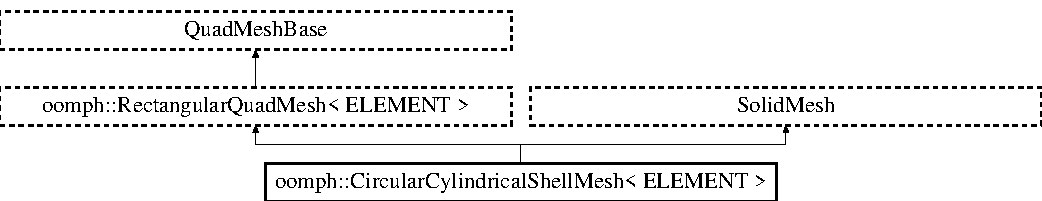
\includegraphics[height=2.700965cm]{classoomph_1_1CircularCylindricalShellMesh}
\end{center}
\end{figure}
\subsection*{Public Types}
\begin{DoxyCompactItemize}
\item 
typedef double($\ast$ \hyperlink{classoomph_1_1CircularCylindricalShellMesh_a770336fa72e8911f31b9fe3f70197a51}{Axial\+B\+L\+Stretching\+Fct\+Pt}) (const double \&x)
\begin{DoxyCompactList}\small\item\em Typedef for fct that defines the axial stretching fct. \end{DoxyCompactList}\end{DoxyCompactItemize}
\subsection*{Public Member Functions}
\begin{DoxyCompactItemize}
\item 
\hyperlink{classoomph_1_1CircularCylindricalShellMesh_ad392c085b9a8f87fd9a24e02738f5d60}{Circular\+Cylindrical\+Shell\+Mesh} (const unsigned \&\hyperlink{classoomph_1_1RectangularQuadMesh_abfef93d6322886cdce14a437186e4821}{nx}, const unsigned \&\hyperlink{classoomph_1_1RectangularQuadMesh_a86d76a55eb7c4e8bca9b74d23c8b0412}{ny}, const double \&lx, const double \&ly, Time\+Stepper $\ast$time\+\_\+stepper\+\_\+pt=\&Mesh\+::\+Default\+\_\+\+Time\+Stepper)
\begin{DoxyCompactList}\small\item\em Constructor for the mesh -- uniformly spaced elements. \end{DoxyCompactList}\item 
\hyperlink{classoomph_1_1CircularCylindricalShellMesh_a2382a9ed0cd210c7b697e6ba4f4e2b0b}{Circular\+Cylindrical\+Shell\+Mesh} (const unsigned \&\hyperlink{classoomph_1_1RectangularQuadMesh_abfef93d6322886cdce14a437186e4821}{nx}, const unsigned \&\hyperlink{classoomph_1_1RectangularQuadMesh_a86d76a55eb7c4e8bca9b74d23c8b0412}{ny}, const double \&lx, const double \&ly, \hyperlink{classoomph_1_1CircularCylindricalShellMesh_a770336fa72e8911f31b9fe3f70197a51}{Axial\+B\+L\+Stretching\+Fct\+Pt} \hyperlink{classoomph_1_1CircularCylindricalShellMesh_aa9c69dc3c6692d19706178d558d07f86}{axial\+\_\+bl\+\_\+stretching\+\_\+fct\+\_\+pt}, Time\+Stepper $\ast$time\+\_\+stepper\+\_\+pt=\&Mesh\+::\+Default\+\_\+\+Time\+Stepper)
\begin{DoxyCompactList}\small\item\em Constructor for the mesh -- specify fct that maps axial Lagr. coordinates to new positions to allow for better resolution of bending boundary layer. \end{DoxyCompactList}\item 
\hyperlink{classoomph_1_1CircularCylindricalShellMesh_aba83d68289f90a8567887443c3b9c6f0}{Circular\+Cylindrical\+Shell\+Mesh} (const unsigned \&\hyperlink{classoomph_1_1RectangularQuadMesh_abfef93d6322886cdce14a437186e4821}{nx}, const unsigned \&\hyperlink{classoomph_1_1RectangularQuadMesh_a86d76a55eb7c4e8bca9b74d23c8b0412}{ny}, const double \&lx, const double \&ly, const unsigned \&nx\+\_\+bl, const double \&delta\+\_\+bl, Time\+Stepper $\ast$time\+\_\+stepper\+\_\+pt=\&Mesh\+::\+Default\+\_\+\+Time\+Stepper)
\begin{DoxyCompactList}\small\item\em Constructor for the mesh. nx\+\_\+bl azimuthal layers of elements near the ends are squashed to that axial extent of the elements changes from lx/nx to delta\+\_\+bl. \end{DoxyCompactList}\item 
void \hyperlink{classoomph_1_1CircularCylindricalShellMesh_a03bba13301e4dec893d73716e146c71d}{assign\+\_\+undeformed\+\_\+positions} (Geom\+Object $\ast$const \&undeformed\+\_\+midplane\+\_\+pt)
\begin{DoxyCompactList}\small\item\em In all elastic problems, the nodes must be assigned an undeformed, or reference, position, corresponding to the stress-\/free state of the elastic body. This function assigns the undeformed position for the nodes on the elastic tube. \end{DoxyCompactList}\item 
\hyperlink{classoomph_1_1CircularCylindricalShellMesh_a770336fa72e8911f31b9fe3f70197a51}{Axial\+B\+L\+Stretching\+Fct\+Pt} \hyperlink{classoomph_1_1CircularCylindricalShellMesh_aa9c69dc3c6692d19706178d558d07f86}{axial\+\_\+bl\+\_\+stretching\+\_\+fct\+\_\+pt} () const
\begin{DoxyCompactList}\small\item\em Access to fct pointer to fct that defines the axial stretching fct. \end{DoxyCompactList}\end{DoxyCompactItemize}
\subsection*{Private Member Functions}
\begin{DoxyCompactItemize}
\item 
void \hyperlink{classoomph_1_1CircularCylindricalShellMesh_a032ddb9b1afa4ef446ca74c8a6965000}{build\+\_\+mesh} (const unsigned \&\hyperlink{classoomph_1_1RectangularQuadMesh_abfef93d6322886cdce14a437186e4821}{nx}, const unsigned \&\hyperlink{classoomph_1_1RectangularQuadMesh_a86d76a55eb7c4e8bca9b74d23c8b0412}{ny}, const double \&lx, const double \&ly)
\begin{DoxyCompactList}\small\item\em Mesh build helper fct. \end{DoxyCompactList}\item 
double \hyperlink{classoomph_1_1CircularCylindricalShellMesh_a4fb67c76ca3ad60efadfe2d3aabcfa0b}{scaled\+\_\+x} (const double \&x)
\begin{DoxyCompactList}\small\item\em Fct that defines the axial stretching to accomodate bending boundary layers. \end{DoxyCompactList}\item 
double \hyperlink{classoomph_1_1CircularCylindricalShellMesh_a5730df8baedd890ca909f31e5452f3db}{piecewise\+\_\+linear\+\_\+axial\+\_\+bl\+\_\+stretching\+\_\+fct} (const double \&xi)
\begin{DoxyCompactList}\small\item\em Default axial scaling fct. \end{DoxyCompactList}\end{DoxyCompactItemize}
\subsection*{Private Attributes}
\begin{DoxyCompactItemize}
\item 
\hyperlink{classoomph_1_1CircularCylindricalShellMesh_a770336fa72e8911f31b9fe3f70197a51}{Axial\+B\+L\+Stretching\+Fct\+Pt} \hyperlink{classoomph_1_1CircularCylindricalShellMesh_a5669a7c088fe0d30f7d011275861f6b9}{Axial\+\_\+bl\+\_\+stretching\+\_\+fct\+\_\+pt}
\begin{DoxyCompactList}\small\item\em Fct pointer to fct that defines the axial stretching fct. \end{DoxyCompactList}\item 
unsigned \hyperlink{classoomph_1_1CircularCylindricalShellMesh_a1a7ed3a5cd4c03c6254e5a8a0d3e532a}{Nx\+\_\+bl}
\begin{DoxyCompactList}\small\item\em Number of azimuthal element layers that get squashed into each of the the two boundary layers at the ends of the tube. \end{DoxyCompactList}\item 
double \hyperlink{classoomph_1_1CircularCylindricalShellMesh_a935925bc28901cf99f2ebdc2cff1b692}{Delta\+\_\+bl}
\begin{DoxyCompactList}\small\item\em Axial extent of the squashed boundary layer part of the mesh occupied by Nx\+\_\+bl elements (at each end of the tube) \end{DoxyCompactList}\end{DoxyCompactItemize}
\subsection*{Additional Inherited Members}


\subsection{Detailed Description}
\subsubsection*{template$<$class E\+L\+E\+M\+E\+NT$>$\newline
class oomph\+::\+Circular\+Cylindrical\+Shell\+Mesh$<$ E\+L\+E\+M\+E\+N\+T $>$}

A 2D solid mesh for (topologically) circular cylindrical shells. The shell is represented by two Lagrangian coordinates that correspond to z and theta in cylindrical polars. The required mesh is therefore a 2D mesh and is therefore inherited from the generic \hyperlink{classoomph_1_1RectangularQuadMesh}{Rectangular\+Quad\+Mesh} 

Definition at line 57 of file circular\+\_\+shell\+\_\+mesh.\+template.\+h.



\subsection{Member Typedef Documentation}
\mbox{\Hypertarget{classoomph_1_1CircularCylindricalShellMesh_a770336fa72e8911f31b9fe3f70197a51}\label{classoomph_1_1CircularCylindricalShellMesh_a770336fa72e8911f31b9fe3f70197a51}} 
\index{oomph\+::\+Circular\+Cylindrical\+Shell\+Mesh@{oomph\+::\+Circular\+Cylindrical\+Shell\+Mesh}!Axial\+B\+L\+Stretching\+Fct\+Pt@{Axial\+B\+L\+Stretching\+Fct\+Pt}}
\index{Axial\+B\+L\+Stretching\+Fct\+Pt@{Axial\+B\+L\+Stretching\+Fct\+Pt}!oomph\+::\+Circular\+Cylindrical\+Shell\+Mesh@{oomph\+::\+Circular\+Cylindrical\+Shell\+Mesh}}
\subsubsection{\texorpdfstring{Axial\+B\+L\+Stretching\+Fct\+Pt}{AxialBLStretchingFctPt}}
{\footnotesize\ttfamily template$<$class E\+L\+E\+M\+E\+NT $>$ \\
typedef double($\ast$ \hyperlink{classoomph_1_1CircularCylindricalShellMesh}{oomph\+::\+Circular\+Cylindrical\+Shell\+Mesh}$<$ E\+L\+E\+M\+E\+NT $>$\+::Axial\+B\+L\+Stretching\+Fct\+Pt) (const double \&x)}



Typedef for fct that defines the axial stretching fct. 



Definition at line 64 of file circular\+\_\+shell\+\_\+mesh.\+template.\+h.



\subsection{Constructor \& Destructor Documentation}
\mbox{\Hypertarget{classoomph_1_1CircularCylindricalShellMesh_ad392c085b9a8f87fd9a24e02738f5d60}\label{classoomph_1_1CircularCylindricalShellMesh_ad392c085b9a8f87fd9a24e02738f5d60}} 
\index{oomph\+::\+Circular\+Cylindrical\+Shell\+Mesh@{oomph\+::\+Circular\+Cylindrical\+Shell\+Mesh}!Circular\+Cylindrical\+Shell\+Mesh@{Circular\+Cylindrical\+Shell\+Mesh}}
\index{Circular\+Cylindrical\+Shell\+Mesh@{Circular\+Cylindrical\+Shell\+Mesh}!oomph\+::\+Circular\+Cylindrical\+Shell\+Mesh@{oomph\+::\+Circular\+Cylindrical\+Shell\+Mesh}}
\subsubsection{\texorpdfstring{Circular\+Cylindrical\+Shell\+Mesh()}{CircularCylindricalShellMesh()}\hspace{0.1cm}{\footnotesize\ttfamily [1/3]}}
{\footnotesize\ttfamily template$<$class E\+L\+E\+M\+E\+NT $>$ \\
\hyperlink{classoomph_1_1CircularCylindricalShellMesh}{oomph\+::\+Circular\+Cylindrical\+Shell\+Mesh}$<$ E\+L\+E\+M\+E\+NT $>$\+::\hyperlink{classoomph_1_1CircularCylindricalShellMesh}{Circular\+Cylindrical\+Shell\+Mesh} (\begin{DoxyParamCaption}\item[{const unsigned \&}]{nx,  }\item[{const unsigned \&}]{ny,  }\item[{const double \&}]{lx,  }\item[{const double \&}]{ly,  }\item[{Time\+Stepper $\ast$}]{time\+\_\+stepper\+\_\+pt = {\ttfamily \&Mesh\+:\+:Default\+\_\+TimeStepper} }\end{DoxyParamCaption})\hspace{0.3cm}{\ttfamily [inline]}}



Constructor for the mesh -- uniformly spaced elements. 



Definition at line 67 of file circular\+\_\+shell\+\_\+mesh.\+template.\+h.



References oomph\+::\+Circular\+Cylindrical\+Shell\+Mesh$<$ E\+L\+E\+M\+E\+N\+T $>$\+::\+Axial\+\_\+bl\+\_\+stretching\+\_\+fct\+\_\+pt, oomph\+::\+Circular\+Cylindrical\+Shell\+Mesh$<$ E\+L\+E\+M\+E\+N\+T $>$\+::build\+\_\+mesh(), oomph\+::\+Circular\+Cylindrical\+Shell\+Mesh$<$ E\+L\+E\+M\+E\+N\+T $>$\+::\+Delta\+\_\+bl, and oomph\+::\+Circular\+Cylindrical\+Shell\+Mesh$<$ E\+L\+E\+M\+E\+N\+T $>$\+::\+Nx\+\_\+bl.

\mbox{\Hypertarget{classoomph_1_1CircularCylindricalShellMesh_a2382a9ed0cd210c7b697e6ba4f4e2b0b}\label{classoomph_1_1CircularCylindricalShellMesh_a2382a9ed0cd210c7b697e6ba4f4e2b0b}} 
\index{oomph\+::\+Circular\+Cylindrical\+Shell\+Mesh@{oomph\+::\+Circular\+Cylindrical\+Shell\+Mesh}!Circular\+Cylindrical\+Shell\+Mesh@{Circular\+Cylindrical\+Shell\+Mesh}}
\index{Circular\+Cylindrical\+Shell\+Mesh@{Circular\+Cylindrical\+Shell\+Mesh}!oomph\+::\+Circular\+Cylindrical\+Shell\+Mesh@{oomph\+::\+Circular\+Cylindrical\+Shell\+Mesh}}
\subsubsection{\texorpdfstring{Circular\+Cylindrical\+Shell\+Mesh()}{CircularCylindricalShellMesh()}\hspace{0.1cm}{\footnotesize\ttfamily [2/3]}}
{\footnotesize\ttfamily template$<$class E\+L\+E\+M\+E\+NT $>$ \\
\hyperlink{classoomph_1_1CircularCylindricalShellMesh}{oomph\+::\+Circular\+Cylindrical\+Shell\+Mesh}$<$ E\+L\+E\+M\+E\+NT $>$\+::\hyperlink{classoomph_1_1CircularCylindricalShellMesh}{Circular\+Cylindrical\+Shell\+Mesh} (\begin{DoxyParamCaption}\item[{const unsigned \&}]{nx,  }\item[{const unsigned \&}]{ny,  }\item[{const double \&}]{lx,  }\item[{const double \&}]{ly,  }\item[{\hyperlink{classoomph_1_1CircularCylindricalShellMesh_a770336fa72e8911f31b9fe3f70197a51}{Axial\+B\+L\+Stretching\+Fct\+Pt}}]{axial\+\_\+bl\+\_\+stretching\+\_\+fct\+\_\+pt,  }\item[{Time\+Stepper $\ast$}]{time\+\_\+stepper\+\_\+pt = {\ttfamily \&Mesh\+:\+:Default\+\_\+TimeStepper} }\end{DoxyParamCaption})\hspace{0.3cm}{\ttfamily [inline]}}



Constructor for the mesh -- specify fct that maps axial Lagr. coordinates to new positions to allow for better resolution of bending boundary layer. 



Definition at line 90 of file circular\+\_\+shell\+\_\+mesh.\+template.\+h.



References oomph\+::\+Circular\+Cylindrical\+Shell\+Mesh$<$ E\+L\+E\+M\+E\+N\+T $>$\+::axial\+\_\+bl\+\_\+stretching\+\_\+fct\+\_\+pt(), oomph\+::\+Circular\+Cylindrical\+Shell\+Mesh$<$ E\+L\+E\+M\+E\+N\+T $>$\+::\+Axial\+\_\+bl\+\_\+stretching\+\_\+fct\+\_\+pt, oomph\+::\+Circular\+Cylindrical\+Shell\+Mesh$<$ E\+L\+E\+M\+E\+N\+T $>$\+::build\+\_\+mesh(), oomph\+::\+Circular\+Cylindrical\+Shell\+Mesh$<$ E\+L\+E\+M\+E\+N\+T $>$\+::\+Delta\+\_\+bl, and oomph\+::\+Circular\+Cylindrical\+Shell\+Mesh$<$ E\+L\+E\+M\+E\+N\+T $>$\+::\+Nx\+\_\+bl.

\mbox{\Hypertarget{classoomph_1_1CircularCylindricalShellMesh_aba83d68289f90a8567887443c3b9c6f0}\label{classoomph_1_1CircularCylindricalShellMesh_aba83d68289f90a8567887443c3b9c6f0}} 
\index{oomph\+::\+Circular\+Cylindrical\+Shell\+Mesh@{oomph\+::\+Circular\+Cylindrical\+Shell\+Mesh}!Circular\+Cylindrical\+Shell\+Mesh@{Circular\+Cylindrical\+Shell\+Mesh}}
\index{Circular\+Cylindrical\+Shell\+Mesh@{Circular\+Cylindrical\+Shell\+Mesh}!oomph\+::\+Circular\+Cylindrical\+Shell\+Mesh@{oomph\+::\+Circular\+Cylindrical\+Shell\+Mesh}}
\subsubsection{\texorpdfstring{Circular\+Cylindrical\+Shell\+Mesh()}{CircularCylindricalShellMesh()}\hspace{0.1cm}{\footnotesize\ttfamily [3/3]}}
{\footnotesize\ttfamily template$<$class E\+L\+E\+M\+E\+NT $>$ \\
\hyperlink{classoomph_1_1CircularCylindricalShellMesh}{oomph\+::\+Circular\+Cylindrical\+Shell\+Mesh}$<$ E\+L\+E\+M\+E\+NT $>$\+::\hyperlink{classoomph_1_1CircularCylindricalShellMesh}{Circular\+Cylindrical\+Shell\+Mesh} (\begin{DoxyParamCaption}\item[{const unsigned \&}]{nx,  }\item[{const unsigned \&}]{ny,  }\item[{const double \&}]{lx,  }\item[{const double \&}]{ly,  }\item[{const unsigned \&}]{nx\+\_\+bl,  }\item[{const double \&}]{delta\+\_\+bl,  }\item[{Time\+Stepper $\ast$}]{time\+\_\+stepper\+\_\+pt = {\ttfamily \&Mesh\+:\+:Default\+\_\+TimeStepper} }\end{DoxyParamCaption})\hspace{0.3cm}{\ttfamily [inline]}}



Constructor for the mesh. nx\+\_\+bl azimuthal layers of elements near the ends are squashed to that axial extent of the elements changes from lx/nx to delta\+\_\+bl. 



Definition at line 114 of file circular\+\_\+shell\+\_\+mesh.\+template.\+h.



References oomph\+::\+Circular\+Cylindrical\+Shell\+Mesh$<$ E\+L\+E\+M\+E\+N\+T $>$\+::assign\+\_\+undeformed\+\_\+positions(), oomph\+::\+Circular\+Cylindrical\+Shell\+Mesh$<$ E\+L\+E\+M\+E\+N\+T $>$\+::\+Axial\+\_\+bl\+\_\+stretching\+\_\+fct\+\_\+pt, oomph\+::\+Circular\+Cylindrical\+Shell\+Mesh$<$ E\+L\+E\+M\+E\+N\+T $>$\+::build\+\_\+mesh(), oomph\+::\+Circular\+Cylindrical\+Shell\+Mesh$<$ E\+L\+E\+M\+E\+N\+T $>$\+::\+Delta\+\_\+bl, and oomph\+::\+Circular\+Cylindrical\+Shell\+Mesh$<$ E\+L\+E\+M\+E\+N\+T $>$\+::\+Nx\+\_\+bl.



\subsection{Member Function Documentation}
\mbox{\Hypertarget{classoomph_1_1CircularCylindricalShellMesh_a03bba13301e4dec893d73716e146c71d}\label{classoomph_1_1CircularCylindricalShellMesh_a03bba13301e4dec893d73716e146c71d}} 
\index{oomph\+::\+Circular\+Cylindrical\+Shell\+Mesh@{oomph\+::\+Circular\+Cylindrical\+Shell\+Mesh}!assign\+\_\+undeformed\+\_\+positions@{assign\+\_\+undeformed\+\_\+positions}}
\index{assign\+\_\+undeformed\+\_\+positions@{assign\+\_\+undeformed\+\_\+positions}!oomph\+::\+Circular\+Cylindrical\+Shell\+Mesh@{oomph\+::\+Circular\+Cylindrical\+Shell\+Mesh}}
\subsubsection{\texorpdfstring{assign\+\_\+undeformed\+\_\+positions()}{assign\_undeformed\_positions()}}
{\footnotesize\ttfamily template$<$class E\+L\+E\+M\+E\+NT $>$ \\
void \hyperlink{classoomph_1_1CircularCylindricalShellMesh}{oomph\+::\+Circular\+Cylindrical\+Shell\+Mesh}$<$ E\+L\+E\+M\+E\+NT $>$\+::assign\+\_\+undeformed\+\_\+positions (\begin{DoxyParamCaption}\item[{Geom\+Object $\ast$const \&}]{undeformed\+\_\+midplane\+\_\+pt }\end{DoxyParamCaption})}



In all elastic problems, the nodes must be assigned an undeformed, or reference, position, corresponding to the stress-\/free state of the elastic body. This function assigns the undeformed position for the nodes on the elastic tube. 

Set the undeformed coordinates of the nodes. 

Definition at line 137 of file circular\+\_\+shell\+\_\+mesh.\+template.\+cc.



Referenced by oomph\+::\+Circular\+Cylindrical\+Shell\+Mesh$<$ E\+L\+E\+M\+E\+N\+T $>$\+::build\+\_\+mesh(), and oomph\+::\+Circular\+Cylindrical\+Shell\+Mesh$<$ E\+L\+E\+M\+E\+N\+T $>$\+::\+Circular\+Cylindrical\+Shell\+Mesh().

\mbox{\Hypertarget{classoomph_1_1CircularCylindricalShellMesh_aa9c69dc3c6692d19706178d558d07f86}\label{classoomph_1_1CircularCylindricalShellMesh_aa9c69dc3c6692d19706178d558d07f86}} 
\index{oomph\+::\+Circular\+Cylindrical\+Shell\+Mesh@{oomph\+::\+Circular\+Cylindrical\+Shell\+Mesh}!axial\+\_\+bl\+\_\+stretching\+\_\+fct\+\_\+pt@{axial\+\_\+bl\+\_\+stretching\+\_\+fct\+\_\+pt}}
\index{axial\+\_\+bl\+\_\+stretching\+\_\+fct\+\_\+pt@{axial\+\_\+bl\+\_\+stretching\+\_\+fct\+\_\+pt}!oomph\+::\+Circular\+Cylindrical\+Shell\+Mesh@{oomph\+::\+Circular\+Cylindrical\+Shell\+Mesh}}
\subsubsection{\texorpdfstring{axial\+\_\+bl\+\_\+stretching\+\_\+fct\+\_\+pt()}{axial\_bl\_stretching\_fct\_pt()}}
{\footnotesize\ttfamily template$<$class E\+L\+E\+M\+E\+NT $>$ \\
\hyperlink{classoomph_1_1CircularCylindricalShellMesh_a770336fa72e8911f31b9fe3f70197a51}{Axial\+B\+L\+Stretching\+Fct\+Pt} \hyperlink{classoomph_1_1CircularCylindricalShellMesh}{oomph\+::\+Circular\+Cylindrical\+Shell\+Mesh}$<$ E\+L\+E\+M\+E\+NT $>$\+::axial\+\_\+bl\+\_\+stretching\+\_\+fct\+\_\+pt (\begin{DoxyParamCaption}{ }\end{DoxyParamCaption}) const\hspace{0.3cm}{\ttfamily [inline]}}



Access to fct pointer to fct that defines the axial stretching fct. 



Definition at line 145 of file circular\+\_\+shell\+\_\+mesh.\+template.\+h.



References oomph\+::\+Circular\+Cylindrical\+Shell\+Mesh$<$ E\+L\+E\+M\+E\+N\+T $>$\+::\+Axial\+\_\+bl\+\_\+stretching\+\_\+fct\+\_\+pt, oomph\+::\+Circular\+Cylindrical\+Shell\+Mesh$<$ E\+L\+E\+M\+E\+N\+T $>$\+::build\+\_\+mesh(), oomph\+::\+Rectangular\+Quad\+Mesh$<$ E\+L\+E\+M\+E\+N\+T $>$\+::nx(), and oomph\+::\+Rectangular\+Quad\+Mesh$<$ E\+L\+E\+M\+E\+N\+T $>$\+::ny().



Referenced by oomph\+::\+Circular\+Cylindrical\+Shell\+Mesh$<$ E\+L\+E\+M\+E\+N\+T $>$\+::\+Circular\+Cylindrical\+Shell\+Mesh().

\mbox{\Hypertarget{classoomph_1_1CircularCylindricalShellMesh_a032ddb9b1afa4ef446ca74c8a6965000}\label{classoomph_1_1CircularCylindricalShellMesh_a032ddb9b1afa4ef446ca74c8a6965000}} 
\index{oomph\+::\+Circular\+Cylindrical\+Shell\+Mesh@{oomph\+::\+Circular\+Cylindrical\+Shell\+Mesh}!build\+\_\+mesh@{build\+\_\+mesh}}
\index{build\+\_\+mesh@{build\+\_\+mesh}!oomph\+::\+Circular\+Cylindrical\+Shell\+Mesh@{oomph\+::\+Circular\+Cylindrical\+Shell\+Mesh}}
\subsubsection{\texorpdfstring{build\+\_\+mesh()}{build\_mesh()}}
{\footnotesize\ttfamily template$<$class E\+L\+E\+M\+E\+NT $>$ \\
void \hyperlink{classoomph_1_1CircularCylindricalShellMesh}{oomph\+::\+Circular\+Cylindrical\+Shell\+Mesh}$<$ E\+L\+E\+M\+E\+NT $>$\+::build\+\_\+mesh (\begin{DoxyParamCaption}\item[{const unsigned \&}]{nx,  }\item[{const unsigned \&}]{ny,  }\item[{const double \&}]{lx,  }\item[{const double \&}]{ly }\end{DoxyParamCaption})\hspace{0.3cm}{\ttfamily [private]}}



Mesh build helper fct. 

Mesh build fct. 

Definition at line 47 of file circular\+\_\+shell\+\_\+mesh.\+template.\+cc.



References oomph\+::\+Circular\+Cylindrical\+Shell\+Mesh$<$ E\+L\+E\+M\+E\+N\+T $>$\+::assign\+\_\+undeformed\+\_\+positions().



Referenced by oomph\+::\+Circular\+Cylindrical\+Shell\+Mesh$<$ E\+L\+E\+M\+E\+N\+T $>$\+::axial\+\_\+bl\+\_\+stretching\+\_\+fct\+\_\+pt(), and oomph\+::\+Circular\+Cylindrical\+Shell\+Mesh$<$ E\+L\+E\+M\+E\+N\+T $>$\+::\+Circular\+Cylindrical\+Shell\+Mesh().

\mbox{\Hypertarget{classoomph_1_1CircularCylindricalShellMesh_a5730df8baedd890ca909f31e5452f3db}\label{classoomph_1_1CircularCylindricalShellMesh_a5730df8baedd890ca909f31e5452f3db}} 
\index{oomph\+::\+Circular\+Cylindrical\+Shell\+Mesh@{oomph\+::\+Circular\+Cylindrical\+Shell\+Mesh}!piecewise\+\_\+linear\+\_\+axial\+\_\+bl\+\_\+stretching\+\_\+fct@{piecewise\+\_\+linear\+\_\+axial\+\_\+bl\+\_\+stretching\+\_\+fct}}
\index{piecewise\+\_\+linear\+\_\+axial\+\_\+bl\+\_\+stretching\+\_\+fct@{piecewise\+\_\+linear\+\_\+axial\+\_\+bl\+\_\+stretching\+\_\+fct}!oomph\+::\+Circular\+Cylindrical\+Shell\+Mesh@{oomph\+::\+Circular\+Cylindrical\+Shell\+Mesh}}
\subsubsection{\texorpdfstring{piecewise\+\_\+linear\+\_\+axial\+\_\+bl\+\_\+stretching\+\_\+fct()}{piecewise\_linear\_axial\_bl\_stretching\_fct()}}
{\footnotesize\ttfamily template$<$class E\+L\+E\+M\+E\+NT $>$ \\
double \hyperlink{classoomph_1_1CircularCylindricalShellMesh}{oomph\+::\+Circular\+Cylindrical\+Shell\+Mesh}$<$ E\+L\+E\+M\+E\+NT $>$\+::piecewise\+\_\+linear\+\_\+axial\+\_\+bl\+\_\+stretching\+\_\+fct (\begin{DoxyParamCaption}\item[{const double \&}]{xi }\end{DoxyParamCaption})\hspace{0.3cm}{\ttfamily [inline]}, {\ttfamily [private]}}



Default axial scaling fct. 



Definition at line 174 of file circular\+\_\+shell\+\_\+mesh.\+template.\+h.



References oomph\+::\+Circular\+Cylindrical\+Shell\+Mesh$<$ E\+L\+E\+M\+E\+N\+T $>$\+::\+Delta\+\_\+bl, oomph\+::\+Rectangular\+Quad\+Mesh$<$ E\+L\+E\+M\+E\+N\+T $>$\+::\+Nx, oomph\+::\+Circular\+Cylindrical\+Shell\+Mesh$<$ E\+L\+E\+M\+E\+N\+T $>$\+::\+Nx\+\_\+bl, oomph\+::\+Rectangular\+Quad\+Mesh$<$ E\+L\+E\+M\+E\+N\+T $>$\+::\+Xmax, and oomph\+::\+Rectangular\+Quad\+Mesh$<$ E\+L\+E\+M\+E\+N\+T $>$\+::\+Xmin.



Referenced by oomph\+::\+Circular\+Cylindrical\+Shell\+Mesh$<$ E\+L\+E\+M\+E\+N\+T $>$\+::scaled\+\_\+x().

\mbox{\Hypertarget{classoomph_1_1CircularCylindricalShellMesh_a4fb67c76ca3ad60efadfe2d3aabcfa0b}\label{classoomph_1_1CircularCylindricalShellMesh_a4fb67c76ca3ad60efadfe2d3aabcfa0b}} 
\index{oomph\+::\+Circular\+Cylindrical\+Shell\+Mesh@{oomph\+::\+Circular\+Cylindrical\+Shell\+Mesh}!scaled\+\_\+x@{scaled\+\_\+x}}
\index{scaled\+\_\+x@{scaled\+\_\+x}!oomph\+::\+Circular\+Cylindrical\+Shell\+Mesh@{oomph\+::\+Circular\+Cylindrical\+Shell\+Mesh}}
\subsubsection{\texorpdfstring{scaled\+\_\+x()}{scaled\_x()}}
{\footnotesize\ttfamily template$<$class E\+L\+E\+M\+E\+NT $>$ \\
double \hyperlink{classoomph_1_1CircularCylindricalShellMesh}{oomph\+::\+Circular\+Cylindrical\+Shell\+Mesh}$<$ E\+L\+E\+M\+E\+NT $>$\+::scaled\+\_\+x (\begin{DoxyParamCaption}\item[{const double \&}]{x }\end{DoxyParamCaption})\hspace{0.3cm}{\ttfamily [inline]}, {\ttfamily [private]}}



Fct that defines the axial stretching to accomodate bending boundary layers. 



Definition at line 161 of file circular\+\_\+shell\+\_\+mesh.\+template.\+h.



References oomph\+::\+Circular\+Cylindrical\+Shell\+Mesh$<$ E\+L\+E\+M\+E\+N\+T $>$\+::\+Axial\+\_\+bl\+\_\+stretching\+\_\+fct\+\_\+pt, and oomph\+::\+Circular\+Cylindrical\+Shell\+Mesh$<$ E\+L\+E\+M\+E\+N\+T $>$\+::piecewise\+\_\+linear\+\_\+axial\+\_\+bl\+\_\+stretching\+\_\+fct().



\subsection{Member Data Documentation}
\mbox{\Hypertarget{classoomph_1_1CircularCylindricalShellMesh_a5669a7c088fe0d30f7d011275861f6b9}\label{classoomph_1_1CircularCylindricalShellMesh_a5669a7c088fe0d30f7d011275861f6b9}} 
\index{oomph\+::\+Circular\+Cylindrical\+Shell\+Mesh@{oomph\+::\+Circular\+Cylindrical\+Shell\+Mesh}!Axial\+\_\+bl\+\_\+stretching\+\_\+fct\+\_\+pt@{Axial\+\_\+bl\+\_\+stretching\+\_\+fct\+\_\+pt}}
\index{Axial\+\_\+bl\+\_\+stretching\+\_\+fct\+\_\+pt@{Axial\+\_\+bl\+\_\+stretching\+\_\+fct\+\_\+pt}!oomph\+::\+Circular\+Cylindrical\+Shell\+Mesh@{oomph\+::\+Circular\+Cylindrical\+Shell\+Mesh}}
\subsubsection{\texorpdfstring{Axial\+\_\+bl\+\_\+stretching\+\_\+fct\+\_\+pt}{Axial\_bl\_stretching\_fct\_pt}}
{\footnotesize\ttfamily template$<$class E\+L\+E\+M\+E\+NT $>$ \\
\hyperlink{classoomph_1_1CircularCylindricalShellMesh_a770336fa72e8911f31b9fe3f70197a51}{Axial\+B\+L\+Stretching\+Fct\+Pt} \hyperlink{classoomph_1_1CircularCylindricalShellMesh}{oomph\+::\+Circular\+Cylindrical\+Shell\+Mesh}$<$ E\+L\+E\+M\+E\+NT $>$\+::Axial\+\_\+bl\+\_\+stretching\+\_\+fct\+\_\+pt\hspace{0.3cm}{\ttfamily [private]}}



Fct pointer to fct that defines the axial stretching fct. 



Definition at line 202 of file circular\+\_\+shell\+\_\+mesh.\+template.\+h.



Referenced by oomph\+::\+Circular\+Cylindrical\+Shell\+Mesh$<$ E\+L\+E\+M\+E\+N\+T $>$\+::axial\+\_\+bl\+\_\+stretching\+\_\+fct\+\_\+pt(), oomph\+::\+Circular\+Cylindrical\+Shell\+Mesh$<$ E\+L\+E\+M\+E\+N\+T $>$\+::\+Circular\+Cylindrical\+Shell\+Mesh(), and oomph\+::\+Circular\+Cylindrical\+Shell\+Mesh$<$ E\+L\+E\+M\+E\+N\+T $>$\+::scaled\+\_\+x().

\mbox{\Hypertarget{classoomph_1_1CircularCylindricalShellMesh_a935925bc28901cf99f2ebdc2cff1b692}\label{classoomph_1_1CircularCylindricalShellMesh_a935925bc28901cf99f2ebdc2cff1b692}} 
\index{oomph\+::\+Circular\+Cylindrical\+Shell\+Mesh@{oomph\+::\+Circular\+Cylindrical\+Shell\+Mesh}!Delta\+\_\+bl@{Delta\+\_\+bl}}
\index{Delta\+\_\+bl@{Delta\+\_\+bl}!oomph\+::\+Circular\+Cylindrical\+Shell\+Mesh@{oomph\+::\+Circular\+Cylindrical\+Shell\+Mesh}}
\subsubsection{\texorpdfstring{Delta\+\_\+bl}{Delta\_bl}}
{\footnotesize\ttfamily template$<$class E\+L\+E\+M\+E\+NT $>$ \\
double \hyperlink{classoomph_1_1CircularCylindricalShellMesh}{oomph\+::\+Circular\+Cylindrical\+Shell\+Mesh}$<$ E\+L\+E\+M\+E\+NT $>$\+::Delta\+\_\+bl\hspace{0.3cm}{\ttfamily [private]}}



Axial extent of the squashed boundary layer part of the mesh occupied by Nx\+\_\+bl elements (at each end of the tube) 



Definition at line 210 of file circular\+\_\+shell\+\_\+mesh.\+template.\+h.



Referenced by oomph\+::\+Circular\+Cylindrical\+Shell\+Mesh$<$ E\+L\+E\+M\+E\+N\+T $>$\+::\+Circular\+Cylindrical\+Shell\+Mesh(), and oomph\+::\+Circular\+Cylindrical\+Shell\+Mesh$<$ E\+L\+E\+M\+E\+N\+T $>$\+::piecewise\+\_\+linear\+\_\+axial\+\_\+bl\+\_\+stretching\+\_\+fct().

\mbox{\Hypertarget{classoomph_1_1CircularCylindricalShellMesh_a1a7ed3a5cd4c03c6254e5a8a0d3e532a}\label{classoomph_1_1CircularCylindricalShellMesh_a1a7ed3a5cd4c03c6254e5a8a0d3e532a}} 
\index{oomph\+::\+Circular\+Cylindrical\+Shell\+Mesh@{oomph\+::\+Circular\+Cylindrical\+Shell\+Mesh}!Nx\+\_\+bl@{Nx\+\_\+bl}}
\index{Nx\+\_\+bl@{Nx\+\_\+bl}!oomph\+::\+Circular\+Cylindrical\+Shell\+Mesh@{oomph\+::\+Circular\+Cylindrical\+Shell\+Mesh}}
\subsubsection{\texorpdfstring{Nx\+\_\+bl}{Nx\_bl}}
{\footnotesize\ttfamily template$<$class E\+L\+E\+M\+E\+NT $>$ \\
unsigned \hyperlink{classoomph_1_1CircularCylindricalShellMesh}{oomph\+::\+Circular\+Cylindrical\+Shell\+Mesh}$<$ E\+L\+E\+M\+E\+NT $>$\+::Nx\+\_\+bl\hspace{0.3cm}{\ttfamily [private]}}



Number of azimuthal element layers that get squashed into each of the the two boundary layers at the ends of the tube. 



Definition at line 206 of file circular\+\_\+shell\+\_\+mesh.\+template.\+h.



Referenced by oomph\+::\+Circular\+Cylindrical\+Shell\+Mesh$<$ E\+L\+E\+M\+E\+N\+T $>$\+::\+Circular\+Cylindrical\+Shell\+Mesh(), and oomph\+::\+Circular\+Cylindrical\+Shell\+Mesh$<$ E\+L\+E\+M\+E\+N\+T $>$\+::piecewise\+\_\+linear\+\_\+axial\+\_\+bl\+\_\+stretching\+\_\+fct().



The documentation for this class was generated from the following files\+:\begin{DoxyCompactItemize}
\item 
\hyperlink{circular__shell__mesh_8template_8h}{circular\+\_\+shell\+\_\+mesh.\+template.\+h}\item 
\hyperlink{circular__shell__mesh_8template_8cc}{circular\+\_\+shell\+\_\+mesh.\+template.\+cc}\end{DoxyCompactItemize}

\hypertarget{structoomph_1_1classcomp}{}\section{oomph\+:\+:classcomp Struct Reference}
\label{structoomph_1_1classcomp}\index{oomph\+::classcomp@{oomph\+::classcomp}}
\subsection*{Public Member Functions}
\begin{DoxyCompactItemize}
\item 
bool \hyperlink{structoomph_1_1classcomp_a88bb6772be3619f5d4d5c7ec782215ae}{operator()} (const std\+::pair$<$ double, double $>$ \&lhs, const std\+::pair$<$ double, double $>$ \&rhs) const
\end{DoxyCompactItemize}
\subsection*{Static Public Attributes}
\begin{DoxyCompactItemize}
\item 
static double \hyperlink{structoomph_1_1classcomp_a383e0604797b23fc66a566f1b278b47b}{Tol} =1.\+0e-\/14
\end{DoxyCompactItemize}


\subsection{Detailed Description}


Definition at line 15033 of file triangle\+\_\+mesh.\+template.\+cc.



\subsection{Member Function Documentation}
\mbox{\Hypertarget{structoomph_1_1classcomp_a88bb6772be3619f5d4d5c7ec782215ae}\label{structoomph_1_1classcomp_a88bb6772be3619f5d4d5c7ec782215ae}} 
\index{oomph\+::classcomp@{oomph\+::classcomp}!operator()@{operator()}}
\index{operator()@{operator()}!oomph\+::classcomp@{oomph\+::classcomp}}
\subsubsection{\texorpdfstring{operator()()}{operator()()}}
{\footnotesize\ttfamily bool oomph\+::classcomp\+::operator() (\begin{DoxyParamCaption}\item[{const std\+::pair$<$ double, double $>$ \&}]{lhs,  }\item[{const std\+::pair$<$ double, double $>$ \&}]{rhs }\end{DoxyParamCaption}) const\hspace{0.3cm}{\ttfamily [inline]}}



Definition at line 15041 of file triangle\+\_\+mesh.\+template.\+cc.



References oomph\+::\+Bottom\+\_\+left\+\_\+sorter, and Tol.



\subsection{Member Data Documentation}
\mbox{\Hypertarget{structoomph_1_1classcomp_a383e0604797b23fc66a566f1b278b47b}\label{structoomph_1_1classcomp_a383e0604797b23fc66a566f1b278b47b}} 
\index{oomph\+::classcomp@{oomph\+::classcomp}!Tol@{Tol}}
\index{Tol@{Tol}!oomph\+::classcomp@{oomph\+::classcomp}}
\subsubsection{\texorpdfstring{Tol}{Tol}}
{\footnotesize\ttfamily double oomph\+::classcomp\+::\+Tol =1.\+0e-\/14\hspace{0.3cm}{\ttfamily [static]}}



Definition at line 15037 of file triangle\+\_\+mesh.\+template.\+cc.



Referenced by operator()(), and oomph\+::\+Refineable\+Triangle\+Mesh$<$ E\+L\+E\+M\+E\+N\+T $>$\+::sort\+\_\+nodes\+\_\+on\+\_\+shared\+\_\+boundaries().



The documentation for this struct was generated from the following file\+:\begin{DoxyCompactItemize}
\item 
\hyperlink{triangle__mesh_8template_8cc}{triangle\+\_\+mesh.\+template.\+cc}\end{DoxyCompactItemize}

\hypertarget{classoomph_1_1CollapsibleChannelDomain}{}\section{oomph\+:\+:Collapsible\+Channel\+Domain Class Reference}
\label{classoomph_1_1CollapsibleChannelDomain}\index{oomph\+::\+Collapsible\+Channel\+Domain@{oomph\+::\+Collapsible\+Channel\+Domain}}


Collapsible channel domain.  




{\ttfamily \#include $<$collapsible\+\_\+channel\+\_\+domain.\+h$>$}

Inheritance diagram for oomph\+:\+:Collapsible\+Channel\+Domain\+:\begin{figure}[H]
\begin{center}
\leavevmode
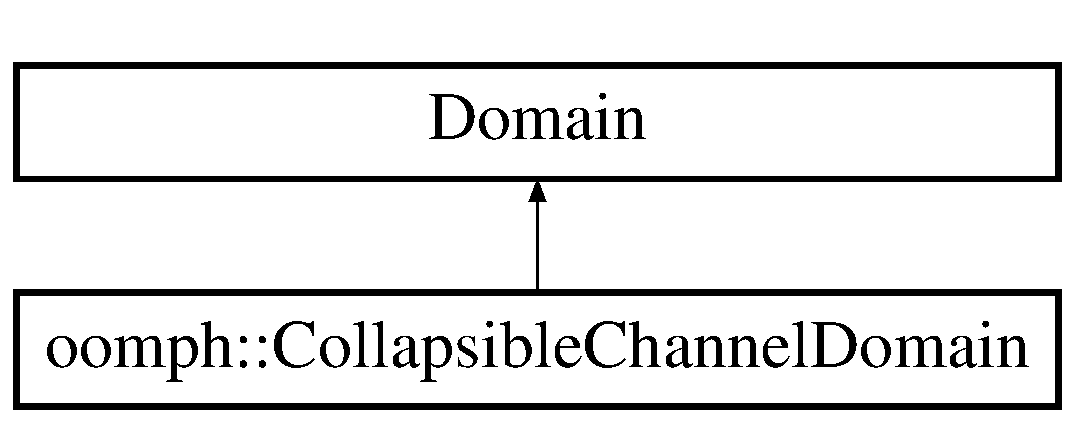
\includegraphics[height=2.000000cm]{classoomph_1_1CollapsibleChannelDomain}
\end{center}
\end{figure}
\subsection*{Public Types}
\begin{DoxyCompactItemize}
\item 
typedef double($\ast$ \hyperlink{classoomph_1_1CollapsibleChannelDomain_a2bf1d7943bfac134a5c27a54c7e1faed}{B\+L\+Squash\+Fct\+Pt}) (const double \&s)
\begin{DoxyCompactList}\small\item\em Typedef for function pointer for function that squashes the macro elements near the wall to help resolution of any wall boundary layers. \end{DoxyCompactList}\item 
typedef double($\ast$ \hyperlink{classoomph_1_1CollapsibleChannelDomain_a317472dab112beac771ecf6442a465f5}{Axial\+Spacing\+Fct\+Pt}) (const double \&xi)
\begin{DoxyCompactList}\small\item\em Typedef for function pointer for function that implements axial spacing of macro elements. \end{DoxyCompactList}\end{DoxyCompactItemize}
\subsection*{Public Member Functions}
\begin{DoxyCompactItemize}
\item 
\hyperlink{classoomph_1_1CollapsibleChannelDomain_a85e64b812b36155302407269d77dc6b3}{Collapsible\+Channel\+Domain} (const unsigned \&\hyperlink{classoomph_1_1CollapsibleChannelDomain_a7e098bcffc76332af4ca220701fd32e2}{nup}, const unsigned \&\hyperlink{classoomph_1_1CollapsibleChannelDomain_a59dd9d4001621752439ad95ceb8daa1b}{ncollapsible}, const unsigned \&\hyperlink{classoomph_1_1CollapsibleChannelDomain_a0e1c69ac122606e4f883e96b51989d9f}{ndown}, const unsigned \&\hyperlink{classoomph_1_1CollapsibleChannelDomain_a62e15782984f3d5e10ba44a6d8ad06ee}{ny}, const double \&lup, const double \&lcollapsible, const double \&ldown, const double \&ly, Geom\+Object $\ast$\hyperlink{classoomph_1_1CollapsibleChannelDomain_a0a98c02b478d61d2cd4c899d0d37344a}{wall\+\_\+pt})
\begin{DoxyCompactList}\small\item\em Constructor\+: Pass the number of (macro-\/)elements, the domain lengths in the x-\/ and y-\/direction and the pointer to the geometric object that specifies the shape of the \char`\"{}collapsible\char`\"{} segment. \end{DoxyCompactList}\item 
\hyperlink{classoomph_1_1CollapsibleChannelDomain_a22469fc91a872e6252133af6e97d6e48}{$\sim$\+Collapsible\+Channel\+Domain} ()
\begin{DoxyCompactList}\small\item\em Destructor. \end{DoxyCompactList}\item 
unsigned \hyperlink{classoomph_1_1CollapsibleChannelDomain_a7e098bcffc76332af4ca220701fd32e2}{nup} ()
\begin{DoxyCompactList}\small\item\em Number of vertical columns of macro elements the upstream section. \end{DoxyCompactList}\item 
unsigned \hyperlink{classoomph_1_1CollapsibleChannelDomain_a59dd9d4001621752439ad95ceb8daa1b}{ncollapsible} ()
\begin{DoxyCompactList}\small\item\em Number of vertical clumns of macro elements in the \char`\"{}collapsible\char`\"{} segment. \end{DoxyCompactList}\item 
unsigned \hyperlink{classoomph_1_1CollapsibleChannelDomain_a0e1c69ac122606e4f883e96b51989d9f}{ndown} ()
\begin{DoxyCompactList}\small\item\em Number of vertical columns of macro elements in the downstream section. \end{DoxyCompactList}\item 
unsigned \hyperlink{classoomph_1_1CollapsibleChannelDomain_a62e15782984f3d5e10ba44a6d8ad06ee}{ny} ()
\begin{DoxyCompactList}\small\item\em Number of macro-\/elements across the channel. \end{DoxyCompactList}\item 
double \hyperlink{classoomph_1_1CollapsibleChannelDomain_a3773afa34e21e3e4ed7a86cf42808dd7}{l\+\_\+up} ()
\begin{DoxyCompactList}\small\item\em Length of upstream section. \end{DoxyCompactList}\item 
double \hyperlink{classoomph_1_1CollapsibleChannelDomain_a0b38028581a27e6b34529ba2c3fa1af2}{l\+\_\+collapsible} ()
\begin{DoxyCompactList}\small\item\em Length of collapsible segment. \end{DoxyCompactList}\item 
double \hyperlink{classoomph_1_1CollapsibleChannelDomain_a93dc02b16ab1cbab2f42f62d0a7aeb8e}{l\+\_\+down} ()
\begin{DoxyCompactList}\small\item\em Length of downstream section. \end{DoxyCompactList}\item 
double \hyperlink{classoomph_1_1CollapsibleChannelDomain_ab95f48218b922883be6c8b9bfb39c2a8}{l\+\_\+y} ()
\begin{DoxyCompactList}\small\item\em Width of channel. \end{DoxyCompactList}\item 
Geom\+Object $\ast$\& \hyperlink{classoomph_1_1CollapsibleChannelDomain_a0a98c02b478d61d2cd4c899d0d37344a}{wall\+\_\+pt} ()
\begin{DoxyCompactList}\small\item\em Access to pointer to the geometric object that parametrises the collapsible wall. \end{DoxyCompactList}\item 
Geom\+Object $\ast$ \hyperlink{classoomph_1_1CollapsibleChannelDomain_a48237d8c4d10ff3ccdf68d02da5b29c7}{wall\+\_\+pt} () const
\begin{DoxyCompactList}\small\item\em Access to pointer to the geometric object that parametrises the collapsible wall (const version) \end{DoxyCompactList}\item 
\hyperlink{classoomph_1_1CollapsibleChannelDomain_a2bf1d7943bfac134a5c27a54c7e1faed}{B\+L\+Squash\+Fct\+Pt} \& \hyperlink{classoomph_1_1CollapsibleChannelDomain_a9c7def97a2248a8e5a2dca79ee3a54eb}{bl\+\_\+squash\+\_\+fct\+\_\+pt} ()
\begin{DoxyCompactList}\small\item\em Function pointer for function that squashes the macro elements near wall. Default mapping (identity) leaves the y-\/coordinate of the nodal points unchanged. \end{DoxyCompactList}\item 
double \hyperlink{classoomph_1_1CollapsibleChannelDomain_a638fd3959b72ef3287615f2b0f968e33}{s\+\_\+squash} (const double \&s)
\begin{DoxyCompactList}\small\item\em Function that squashes the macro elements near the wall. Input argument should vary between 0 and 1; function should return stretched/squashed coordinate in the same range. Default implementation is the identity; can be overloaded by specifying a different function pointer with \hyperlink{classoomph_1_1CollapsibleChannelDomain_a9c7def97a2248a8e5a2dca79ee3a54eb}{bl\+\_\+squash\+\_\+fct\+\_\+pt()}. \end{DoxyCompactList}\item 
\hyperlink{classoomph_1_1CollapsibleChannelDomain_a317472dab112beac771ecf6442a465f5}{Axial\+Spacing\+Fct\+Pt} \& \hyperlink{classoomph_1_1CollapsibleChannelDomain_a17bfb9fe218dc539669bdbdf0ecc4bf8}{axial\+\_\+spacing\+\_\+fct\+\_\+pt} ()
\begin{DoxyCompactList}\small\item\em Function pointer for function that implements axial spacing of macro elements. \end{DoxyCompactList}\item 
double \hyperlink{classoomph_1_1CollapsibleChannelDomain_abc7b20efd68bdd11f1bea5df79ae579d}{axial\+\_\+spacing\+\_\+fct} (const double \&xi)
\begin{DoxyCompactList}\small\item\em Function that implements axial spacing of macro elements. \end{DoxyCompactList}\item 
void \hyperlink{classoomph_1_1CollapsibleChannelDomain_a2c0a5bd21e12fbcc1cdd753c0f205da2}{macro\+\_\+element\+\_\+boundary} (const unsigned \&t, const unsigned \&imacro, const unsigned \&idirect, const Vector$<$ double $>$ \&zeta, Vector$<$ double $>$ \&r)
\begin{DoxyCompactList}\small\item\em Vector representation of the imacro-\/th macro element boundary idirect (N/\+S/\+W/E) at time level t (t=0\+: present; t$>$0\+: previous)\+: $ {\bf r}({\bf zeta}) $ Note that the local coordinate {\bfseries zeta} is a 1D Vector rather than a scalar -- this is unavoidable because this function implements the pure virtual function in the Domain base class. \end{DoxyCompactList}\end{DoxyCompactItemize}
\subsection*{Static Public Member Functions}
\begin{DoxyCompactItemize}
\item 
static double \hyperlink{classoomph_1_1CollapsibleChannelDomain_a4222184a903df3efdd93cc306bac4414}{default\+\_\+\+B\+L\+\_\+squash\+\_\+fct} (const double \&s)
\begin{DoxyCompactList}\small\item\em Default for function that squashes the macro elements near the walls. Identity. \end{DoxyCompactList}\end{DoxyCompactItemize}
\subsection*{Private Member Functions}
\begin{DoxyCompactItemize}
\item 
void \hyperlink{classoomph_1_1CollapsibleChannelDomain_aec5509d4e6a229da9fec78ceb78dcb18}{r\+\_\+\+N\+\_\+straight} (const Vector$<$ double $>$ \&zeta, Vector$<$ double $>$ \&r, const unsigned \&imacro, const unsigned \&part)
\begin{DoxyCompactList}\small\item\em Northern boundary of the macro element imacro in the upstream (part=0) or downstream (part=1) sections. \end{DoxyCompactList}\item 
void \hyperlink{classoomph_1_1CollapsibleChannelDomain_a94cebe8b3380c469cfd77924ec57d576}{r\+\_\+\+W\+\_\+straight} (const Vector$<$ double $>$ \&zeta, Vector$<$ double $>$ \&r, const unsigned \&imacro, const unsigned \&part)
\begin{DoxyCompactList}\small\item\em Western boundary of the macro element imacro in the upstream (part=0) or downstream (part=1) sections. \end{DoxyCompactList}\item 
void \hyperlink{classoomph_1_1CollapsibleChannelDomain_a12b9fbd546a2375fea2461a07b5db089}{r\+\_\+\+S\+\_\+straight} (const Vector$<$ double $>$ \&zeta, Vector$<$ double $>$ \&r, const unsigned \&imacro, const unsigned \&part)
\begin{DoxyCompactList}\small\item\em Southern boundary of the macro element imacro in the upstream (part=0) or downstream (part=1) sections. \end{DoxyCompactList}\item 
void \hyperlink{classoomph_1_1CollapsibleChannelDomain_a1f880915f7c2f9163fc1ec8cac676831}{r\+\_\+\+E\+\_\+straight} (const Vector$<$ double $>$ \&zeta, Vector$<$ double $>$ \&r, const unsigned \&imacro, const unsigned \&part)
\begin{DoxyCompactList}\small\item\em Eastern boundary of the macro element imacro in the upstream (part=0) or downstream (part=1) sections. \end{DoxyCompactList}\item 
void \hyperlink{classoomph_1_1CollapsibleChannelDomain_a0044d3e848b4c643a8a30f4f00a88e8d}{r\+\_\+\+N\+\_\+collapsible} (const unsigned \&t, const Vector$<$ double $>$ \&zeta, Vector$<$ double $>$ \&r, const unsigned \&imacro)
\begin{DoxyCompactList}\small\item\em Northern boundary of the macro element imacro in the collapsible section. \end{DoxyCompactList}\item 
void \hyperlink{classoomph_1_1CollapsibleChannelDomain_ab8b0f990e596b2725ca8d84f2c9750eb}{r\+\_\+\+W\+\_\+collapsible} (const unsigned \&t, const Vector$<$ double $>$ \&zeta, Vector$<$ double $>$ \&r, const unsigned \&imacro)
\begin{DoxyCompactList}\small\item\em Western boundary of the macro element imacro in the collapsible section. \end{DoxyCompactList}\item 
void \hyperlink{classoomph_1_1CollapsibleChannelDomain_a1cc35b555f16401ec12854ff5a486800}{r\+\_\+\+S\+\_\+collapsible} (const unsigned \&t, const Vector$<$ double $>$ \&zeta, Vector$<$ double $>$ \&r, const unsigned \&imacro)
\begin{DoxyCompactList}\small\item\em Southern boundary of the macro element imacro in the collapsible section. \end{DoxyCompactList}\item 
void \hyperlink{classoomph_1_1CollapsibleChannelDomain_af684e8e3271ed8f599a02495f794c4e8}{r\+\_\+\+E\+\_\+collapsible} (const unsigned \&t, const Vector$<$ double $>$ \&zeta, Vector$<$ double $>$ \&r, const unsigned \&imacro)
\begin{DoxyCompactList}\small\item\em Eastern boundary of the macro element imacro in the collapsible section. \end{DoxyCompactList}\end{DoxyCompactItemize}
\subsection*{Static Private Member Functions}
\begin{DoxyCompactItemize}
\item 
static double \hyperlink{classoomph_1_1CollapsibleChannelDomain_a3c814ed3312790877d193d4a018c30da}{default\+\_\+axial\+\_\+spacing\+\_\+fct} (const double \&xi)
\begin{DoxyCompactList}\small\item\em Default for function that implements axial spacing of macro elements. \end{DoxyCompactList}\end{DoxyCompactItemize}
\subsection*{Private Attributes}
\begin{DoxyCompactItemize}
\item 
\hyperlink{classoomph_1_1CollapsibleChannelDomain_a2bf1d7943bfac134a5c27a54c7e1faed}{B\+L\+Squash\+Fct\+Pt} \hyperlink{classoomph_1_1CollapsibleChannelDomain_a3d3f5d77c3221da20cd02bf02be800b7}{B\+L\+\_\+squash\+\_\+fct\+\_\+pt}
\begin{DoxyCompactList}\small\item\em Function pointer for function that squashes the macro elements near the walls. \end{DoxyCompactList}\item 
\hyperlink{classoomph_1_1CollapsibleChannelDomain_a317472dab112beac771ecf6442a465f5}{Axial\+Spacing\+Fct\+Pt} \hyperlink{classoomph_1_1CollapsibleChannelDomain_a6f4c3319be685553715f5cd776eea0fc}{Axial\+\_\+spacing\+\_\+fct\+\_\+pt}
\begin{DoxyCompactList}\small\item\em Function pointer for function that implements axial spacing of macro elements. \end{DoxyCompactList}\item 
unsigned \hyperlink{classoomph_1_1CollapsibleChannelDomain_a16bef61c4223f92cb1b0c35e9a7ea7d2}{Nup}
\begin{DoxyCompactList}\small\item\em Number of vertical element columns in upstream section. \end{DoxyCompactList}\item 
unsigned \hyperlink{classoomph_1_1CollapsibleChannelDomain_a607c389c3f0c06f0240d97aaca65cdf7}{Ncollapsible}
\begin{DoxyCompactList}\small\item\em Number of vertical element columns in \char`\"{}collapsible\char`\"{} section. \end{DoxyCompactList}\item 
unsigned \hyperlink{classoomph_1_1CollapsibleChannelDomain_a1f9c92507803d56e12cf5cb24b11cd83}{Ndown}
\begin{DoxyCompactList}\small\item\em Number of vertical element columns in downstream section. \end{DoxyCompactList}\item 
unsigned \hyperlink{classoomph_1_1CollapsibleChannelDomain_a13c992ef93891493c5da50afff67d38c}{Ny}
\begin{DoxyCompactList}\small\item\em Number of macro elements across channel. \end{DoxyCompactList}\item 
double \hyperlink{classoomph_1_1CollapsibleChannelDomain_a1c4dbe3313e696290ad9da4765d0a0e1}{Lup}
\begin{DoxyCompactList}\small\item\em x-\/length in the upstream part of the channel \end{DoxyCompactList}\item 
double \hyperlink{classoomph_1_1CollapsibleChannelDomain_aa44cd6613cea2a67dda8f4de0d9c6f1e}{Lcollapsible}
\begin{DoxyCompactList}\small\item\em x-\/length in the \char`\"{}collapsible\char`\"{} part of the channel \end{DoxyCompactList}\item 
double \hyperlink{classoomph_1_1CollapsibleChannelDomain_ade4ee8220972fe6c454211d1f837fcf9}{Ldown}
\begin{DoxyCompactList}\small\item\em x-\/length in the downstream part of the channel \end{DoxyCompactList}\item 
double \hyperlink{classoomph_1_1CollapsibleChannelDomain_ac70912e194ac3e211cc0ce625c8f5c41}{Ly}
\begin{DoxyCompactList}\small\item\em Width. \end{DoxyCompactList}\item 
Geom\+Object $\ast$ \hyperlink{classoomph_1_1CollapsibleChannelDomain_a6f1ef65c47937800e35477863b1439ab}{Wall\+\_\+pt}
\begin{DoxyCompactList}\small\item\em Pointer to the geometric object that parametrises the collapsible wall. \end{DoxyCompactList}\end{DoxyCompactItemize}


\subsection{Detailed Description}
Collapsible channel domain. 

Definition at line 45 of file collapsible\+\_\+channel\+\_\+domain.\+h.



\subsection{Member Typedef Documentation}
\mbox{\Hypertarget{classoomph_1_1CollapsibleChannelDomain_a317472dab112beac771ecf6442a465f5}\label{classoomph_1_1CollapsibleChannelDomain_a317472dab112beac771ecf6442a465f5}} 
\index{oomph\+::\+Collapsible\+Channel\+Domain@{oomph\+::\+Collapsible\+Channel\+Domain}!Axial\+Spacing\+Fct\+Pt@{Axial\+Spacing\+Fct\+Pt}}
\index{Axial\+Spacing\+Fct\+Pt@{Axial\+Spacing\+Fct\+Pt}!oomph\+::\+Collapsible\+Channel\+Domain@{oomph\+::\+Collapsible\+Channel\+Domain}}
\subsubsection{\texorpdfstring{Axial\+Spacing\+Fct\+Pt}{AxialSpacingFctPt}}
{\footnotesize\ttfamily typedef double($\ast$ oomph\+::\+Collapsible\+Channel\+Domain\+::\+Axial\+Spacing\+Fct\+Pt) (const double \&xi)}



Typedef for function pointer for function that implements axial spacing of macro elements. 



Definition at line 187 of file collapsible\+\_\+channel\+\_\+domain.\+h.

\mbox{\Hypertarget{classoomph_1_1CollapsibleChannelDomain_a2bf1d7943bfac134a5c27a54c7e1faed}\label{classoomph_1_1CollapsibleChannelDomain_a2bf1d7943bfac134a5c27a54c7e1faed}} 
\index{oomph\+::\+Collapsible\+Channel\+Domain@{oomph\+::\+Collapsible\+Channel\+Domain}!B\+L\+Squash\+Fct\+Pt@{B\+L\+Squash\+Fct\+Pt}}
\index{B\+L\+Squash\+Fct\+Pt@{B\+L\+Squash\+Fct\+Pt}!oomph\+::\+Collapsible\+Channel\+Domain@{oomph\+::\+Collapsible\+Channel\+Domain}}
\subsubsection{\texorpdfstring{B\+L\+Squash\+Fct\+Pt}{BLSquashFctPt}}
{\footnotesize\ttfamily typedef double($\ast$ oomph\+::\+Collapsible\+Channel\+Domain\+::\+B\+L\+Squash\+Fct\+Pt) (const double \&s)}



Typedef for function pointer for function that squashes the macro elements near the wall to help resolution of any wall boundary layers. 



Definition at line 157 of file collapsible\+\_\+channel\+\_\+domain.\+h.



\subsection{Constructor \& Destructor Documentation}
\mbox{\Hypertarget{classoomph_1_1CollapsibleChannelDomain_a85e64b812b36155302407269d77dc6b3}\label{classoomph_1_1CollapsibleChannelDomain_a85e64b812b36155302407269d77dc6b3}} 
\index{oomph\+::\+Collapsible\+Channel\+Domain@{oomph\+::\+Collapsible\+Channel\+Domain}!Collapsible\+Channel\+Domain@{Collapsible\+Channel\+Domain}}
\index{Collapsible\+Channel\+Domain@{Collapsible\+Channel\+Domain}!oomph\+::\+Collapsible\+Channel\+Domain@{oomph\+::\+Collapsible\+Channel\+Domain}}
\subsubsection{\texorpdfstring{Collapsible\+Channel\+Domain()}{CollapsibleChannelDomain()}}
{\footnotesize\ttfamily oomph\+::\+Collapsible\+Channel\+Domain\+::\+Collapsible\+Channel\+Domain (\begin{DoxyParamCaption}\item[{const unsigned \&}]{nup,  }\item[{const unsigned \&}]{ncollapsible,  }\item[{const unsigned \&}]{ndown,  }\item[{const unsigned \&}]{ny,  }\item[{const double \&}]{lup,  }\item[{const double \&}]{lcollapsible,  }\item[{const double \&}]{ldown,  }\item[{const double \&}]{ly,  }\item[{Geom\+Object $\ast$}]{wall\+\_\+pt }\end{DoxyParamCaption})\hspace{0.3cm}{\ttfamily [inline]}}



Constructor\+: Pass the number of (macro-\/)elements, the domain lengths in the x-\/ and y-\/direction and the pointer to the geometric object that specifies the shape of the \char`\"{}collapsible\char`\"{} segment. 



Definition at line 54 of file collapsible\+\_\+channel\+\_\+domain.\+h.



References Lcollapsible, Ldown, Lup, Ly, ncollapsible(), Ncollapsible, ndown(), Ndown, nup(), Nup, ny(), Ny, wall\+\_\+pt(), and Wall\+\_\+pt.

\mbox{\Hypertarget{classoomph_1_1CollapsibleChannelDomain_a22469fc91a872e6252133af6e97d6e48}\label{classoomph_1_1CollapsibleChannelDomain_a22469fc91a872e6252133af6e97d6e48}} 
\index{oomph\+::\+Collapsible\+Channel\+Domain@{oomph\+::\+Collapsible\+Channel\+Domain}!````~Collapsible\+Channel\+Domain@{$\sim$\+Collapsible\+Channel\+Domain}}
\index{````~Collapsible\+Channel\+Domain@{$\sim$\+Collapsible\+Channel\+Domain}!oomph\+::\+Collapsible\+Channel\+Domain@{oomph\+::\+Collapsible\+Channel\+Domain}}
\subsubsection{\texorpdfstring{$\sim$\+Collapsible\+Channel\+Domain()}{~CollapsibleChannelDomain()}}
{\footnotesize\ttfamily oomph\+::\+Collapsible\+Channel\+Domain\+::$\sim$\+Collapsible\+Channel\+Domain (\begin{DoxyParamCaption}{ }\end{DoxyParamCaption})\hspace{0.3cm}{\ttfamily [inline]}}



Destructor. 



Definition at line 89 of file collapsible\+\_\+channel\+\_\+domain.\+h.



References Ncollapsible, Ndown, Nup, and Ny.



\subsection{Member Function Documentation}
\mbox{\Hypertarget{classoomph_1_1CollapsibleChannelDomain_abc7b20efd68bdd11f1bea5df79ae579d}\label{classoomph_1_1CollapsibleChannelDomain_abc7b20efd68bdd11f1bea5df79ae579d}} 
\index{oomph\+::\+Collapsible\+Channel\+Domain@{oomph\+::\+Collapsible\+Channel\+Domain}!axial\+\_\+spacing\+\_\+fct@{axial\+\_\+spacing\+\_\+fct}}
\index{axial\+\_\+spacing\+\_\+fct@{axial\+\_\+spacing\+\_\+fct}!oomph\+::\+Collapsible\+Channel\+Domain@{oomph\+::\+Collapsible\+Channel\+Domain}}
\subsubsection{\texorpdfstring{axial\+\_\+spacing\+\_\+fct()}{axial\_spacing\_fct()}}
{\footnotesize\ttfamily double oomph\+::\+Collapsible\+Channel\+Domain\+::axial\+\_\+spacing\+\_\+fct (\begin{DoxyParamCaption}\item[{const double \&}]{xi }\end{DoxyParamCaption})\hspace{0.3cm}{\ttfamily [inline]}}



Function that implements axial spacing of macro elements. 



Definition at line 198 of file collapsible\+\_\+channel\+\_\+domain.\+h.



References Axial\+\_\+spacing\+\_\+fct\+\_\+pt, macro\+\_\+element\+\_\+boundary(), r\+\_\+\+E\+\_\+collapsible(), r\+\_\+\+E\+\_\+straight(), r\+\_\+\+N\+\_\+collapsible(), r\+\_\+\+N\+\_\+straight(), r\+\_\+\+S\+\_\+collapsible(), r\+\_\+\+S\+\_\+straight(), r\+\_\+\+W\+\_\+collapsible(), and r\+\_\+\+W\+\_\+straight().



Referenced by r\+\_\+\+E\+\_\+straight(), r\+\_\+\+N\+\_\+straight(), r\+\_\+\+S\+\_\+straight(), and r\+\_\+\+W\+\_\+straight().

\mbox{\Hypertarget{classoomph_1_1CollapsibleChannelDomain_a17bfb9fe218dc539669bdbdf0ecc4bf8}\label{classoomph_1_1CollapsibleChannelDomain_a17bfb9fe218dc539669bdbdf0ecc4bf8}} 
\index{oomph\+::\+Collapsible\+Channel\+Domain@{oomph\+::\+Collapsible\+Channel\+Domain}!axial\+\_\+spacing\+\_\+fct\+\_\+pt@{axial\+\_\+spacing\+\_\+fct\+\_\+pt}}
\index{axial\+\_\+spacing\+\_\+fct\+\_\+pt@{axial\+\_\+spacing\+\_\+fct\+\_\+pt}!oomph\+::\+Collapsible\+Channel\+Domain@{oomph\+::\+Collapsible\+Channel\+Domain}}
\subsubsection{\texorpdfstring{axial\+\_\+spacing\+\_\+fct\+\_\+pt()}{axial\_spacing\_fct\_pt()}}
{\footnotesize\ttfamily \hyperlink{classoomph_1_1CollapsibleChannelDomain_a317472dab112beac771ecf6442a465f5}{Axial\+Spacing\+Fct\+Pt}\& oomph\+::\+Collapsible\+Channel\+Domain\+::axial\+\_\+spacing\+\_\+fct\+\_\+pt (\begin{DoxyParamCaption}{ }\end{DoxyParamCaption})\hspace{0.3cm}{\ttfamily [inline]}}



Function pointer for function that implements axial spacing of macro elements. 



Definition at line 191 of file collapsible\+\_\+channel\+\_\+domain.\+h.



References Axial\+\_\+spacing\+\_\+fct\+\_\+pt.



Referenced by oomph\+::\+Collapsible\+Channel\+Mesh$<$ E\+L\+E\+M\+E\+N\+T $>$\+::axial\+\_\+spacing\+\_\+fct\+\_\+pt().

\mbox{\Hypertarget{classoomph_1_1CollapsibleChannelDomain_a9c7def97a2248a8e5a2dca79ee3a54eb}\label{classoomph_1_1CollapsibleChannelDomain_a9c7def97a2248a8e5a2dca79ee3a54eb}} 
\index{oomph\+::\+Collapsible\+Channel\+Domain@{oomph\+::\+Collapsible\+Channel\+Domain}!bl\+\_\+squash\+\_\+fct\+\_\+pt@{bl\+\_\+squash\+\_\+fct\+\_\+pt}}
\index{bl\+\_\+squash\+\_\+fct\+\_\+pt@{bl\+\_\+squash\+\_\+fct\+\_\+pt}!oomph\+::\+Collapsible\+Channel\+Domain@{oomph\+::\+Collapsible\+Channel\+Domain}}
\subsubsection{\texorpdfstring{bl\+\_\+squash\+\_\+fct\+\_\+pt()}{bl\_squash\_fct\_pt()}}
{\footnotesize\ttfamily \hyperlink{classoomph_1_1CollapsibleChannelDomain_a2bf1d7943bfac134a5c27a54c7e1faed}{B\+L\+Squash\+Fct\+Pt}\& oomph\+::\+Collapsible\+Channel\+Domain\+::bl\+\_\+squash\+\_\+fct\+\_\+pt (\begin{DoxyParamCaption}{ }\end{DoxyParamCaption})\hspace{0.3cm}{\ttfamily [inline]}}



Function pointer for function that squashes the macro elements near wall. Default mapping (identity) leaves the y-\/coordinate of the nodal points unchanged. 



Definition at line 170 of file collapsible\+\_\+channel\+\_\+domain.\+h.



References B\+L\+\_\+squash\+\_\+fct\+\_\+pt.



Referenced by oomph\+::\+Algebraic\+Collapsible\+Channel\+Mesh$<$ E\+L\+E\+M\+E\+N\+T $>$\+::\+Algebraic\+Collapsible\+Channel\+Mesh(), and oomph\+::\+Collapsible\+Channel\+Mesh$<$ E\+L\+E\+M\+E\+N\+T $>$\+::bl\+\_\+squash\+\_\+fct\+\_\+pt().

\mbox{\Hypertarget{classoomph_1_1CollapsibleChannelDomain_a3c814ed3312790877d193d4a018c30da}\label{classoomph_1_1CollapsibleChannelDomain_a3c814ed3312790877d193d4a018c30da}} 
\index{oomph\+::\+Collapsible\+Channel\+Domain@{oomph\+::\+Collapsible\+Channel\+Domain}!default\+\_\+axial\+\_\+spacing\+\_\+fct@{default\+\_\+axial\+\_\+spacing\+\_\+fct}}
\index{default\+\_\+axial\+\_\+spacing\+\_\+fct@{default\+\_\+axial\+\_\+spacing\+\_\+fct}!oomph\+::\+Collapsible\+Channel\+Domain@{oomph\+::\+Collapsible\+Channel\+Domain}}
\subsubsection{\texorpdfstring{default\+\_\+axial\+\_\+spacing\+\_\+fct()}{default\_axial\_spacing\_fct()}}
{\footnotesize\ttfamily static double oomph\+::\+Collapsible\+Channel\+Domain\+::default\+\_\+axial\+\_\+spacing\+\_\+fct (\begin{DoxyParamCaption}\item[{const double \&}]{xi }\end{DoxyParamCaption})\hspace{0.3cm}{\ttfamily [inline]}, {\ttfamily [static]}, {\ttfamily [private]}}



Default for function that implements axial spacing of macro elements. 



Definition at line 287 of file collapsible\+\_\+channel\+\_\+domain.\+h.

\mbox{\Hypertarget{classoomph_1_1CollapsibleChannelDomain_a4222184a903df3efdd93cc306bac4414}\label{classoomph_1_1CollapsibleChannelDomain_a4222184a903df3efdd93cc306bac4414}} 
\index{oomph\+::\+Collapsible\+Channel\+Domain@{oomph\+::\+Collapsible\+Channel\+Domain}!default\+\_\+\+B\+L\+\_\+squash\+\_\+fct@{default\+\_\+\+B\+L\+\_\+squash\+\_\+fct}}
\index{default\+\_\+\+B\+L\+\_\+squash\+\_\+fct@{default\+\_\+\+B\+L\+\_\+squash\+\_\+fct}!oomph\+::\+Collapsible\+Channel\+Domain@{oomph\+::\+Collapsible\+Channel\+Domain}}
\subsubsection{\texorpdfstring{default\+\_\+\+B\+L\+\_\+squash\+\_\+fct()}{default\_BL\_squash\_fct()}}
{\footnotesize\ttfamily static double oomph\+::\+Collapsible\+Channel\+Domain\+::default\+\_\+\+B\+L\+\_\+squash\+\_\+fct (\begin{DoxyParamCaption}\item[{const double \&}]{s }\end{DoxyParamCaption})\hspace{0.3cm}{\ttfamily [inline]}, {\ttfamily [static]}}



Default for function that squashes the macro elements near the walls. Identity. 



Definition at line 162 of file collapsible\+\_\+channel\+\_\+domain.\+h.

\mbox{\Hypertarget{classoomph_1_1CollapsibleChannelDomain_a0b38028581a27e6b34529ba2c3fa1af2}\label{classoomph_1_1CollapsibleChannelDomain_a0b38028581a27e6b34529ba2c3fa1af2}} 
\index{oomph\+::\+Collapsible\+Channel\+Domain@{oomph\+::\+Collapsible\+Channel\+Domain}!l\+\_\+collapsible@{l\+\_\+collapsible}}
\index{l\+\_\+collapsible@{l\+\_\+collapsible}!oomph\+::\+Collapsible\+Channel\+Domain@{oomph\+::\+Collapsible\+Channel\+Domain}}
\subsubsection{\texorpdfstring{l\+\_\+collapsible()}{l\_collapsible()}}
{\footnotesize\ttfamily double oomph\+::\+Collapsible\+Channel\+Domain\+::l\+\_\+collapsible (\begin{DoxyParamCaption}{ }\end{DoxyParamCaption})\hspace{0.3cm}{\ttfamily [inline]}}



Length of collapsible segment. 



Definition at line 128 of file collapsible\+\_\+channel\+\_\+domain.\+h.



References Lcollapsible.



Referenced by oomph\+::\+Algebraic\+Collapsible\+Channel\+Mesh$<$ E\+L\+E\+M\+E\+N\+T $>$\+::setup\+\_\+algebraic\+\_\+node\+\_\+update().

\mbox{\Hypertarget{classoomph_1_1CollapsibleChannelDomain_a93dc02b16ab1cbab2f42f62d0a7aeb8e}\label{classoomph_1_1CollapsibleChannelDomain_a93dc02b16ab1cbab2f42f62d0a7aeb8e}} 
\index{oomph\+::\+Collapsible\+Channel\+Domain@{oomph\+::\+Collapsible\+Channel\+Domain}!l\+\_\+down@{l\+\_\+down}}
\index{l\+\_\+down@{l\+\_\+down}!oomph\+::\+Collapsible\+Channel\+Domain@{oomph\+::\+Collapsible\+Channel\+Domain}}
\subsubsection{\texorpdfstring{l\+\_\+down()}{l\_down()}}
{\footnotesize\ttfamily double oomph\+::\+Collapsible\+Channel\+Domain\+::l\+\_\+down (\begin{DoxyParamCaption}{ }\end{DoxyParamCaption})\hspace{0.3cm}{\ttfamily [inline]}}



Length of downstream section. 



Definition at line 134 of file collapsible\+\_\+channel\+\_\+domain.\+h.



References Ldown.

\mbox{\Hypertarget{classoomph_1_1CollapsibleChannelDomain_a3773afa34e21e3e4ed7a86cf42808dd7}\label{classoomph_1_1CollapsibleChannelDomain_a3773afa34e21e3e4ed7a86cf42808dd7}} 
\index{oomph\+::\+Collapsible\+Channel\+Domain@{oomph\+::\+Collapsible\+Channel\+Domain}!l\+\_\+up@{l\+\_\+up}}
\index{l\+\_\+up@{l\+\_\+up}!oomph\+::\+Collapsible\+Channel\+Domain@{oomph\+::\+Collapsible\+Channel\+Domain}}
\subsubsection{\texorpdfstring{l\+\_\+up()}{l\_up()}}
{\footnotesize\ttfamily double oomph\+::\+Collapsible\+Channel\+Domain\+::l\+\_\+up (\begin{DoxyParamCaption}{ }\end{DoxyParamCaption})\hspace{0.3cm}{\ttfamily [inline]}}



Length of upstream section. 



Definition at line 122 of file collapsible\+\_\+channel\+\_\+domain.\+h.



References Lup.



Referenced by oomph\+::\+Algebraic\+Collapsible\+Channel\+Mesh$<$ E\+L\+E\+M\+E\+N\+T $>$\+::setup\+\_\+algebraic\+\_\+node\+\_\+update().

\mbox{\Hypertarget{classoomph_1_1CollapsibleChannelDomain_ab95f48218b922883be6c8b9bfb39c2a8}\label{classoomph_1_1CollapsibleChannelDomain_ab95f48218b922883be6c8b9bfb39c2a8}} 
\index{oomph\+::\+Collapsible\+Channel\+Domain@{oomph\+::\+Collapsible\+Channel\+Domain}!l\+\_\+y@{l\+\_\+y}}
\index{l\+\_\+y@{l\+\_\+y}!oomph\+::\+Collapsible\+Channel\+Domain@{oomph\+::\+Collapsible\+Channel\+Domain}}
\subsubsection{\texorpdfstring{l\+\_\+y()}{l\_y()}}
{\footnotesize\ttfamily double oomph\+::\+Collapsible\+Channel\+Domain\+::l\+\_\+y (\begin{DoxyParamCaption}{ }\end{DoxyParamCaption})\hspace{0.3cm}{\ttfamily [inline]}}



Width of channel. 



Definition at line 140 of file collapsible\+\_\+channel\+\_\+domain.\+h.



References Ly.

\mbox{\Hypertarget{classoomph_1_1CollapsibleChannelDomain_a2c0a5bd21e12fbcc1cdd753c0f205da2}\label{classoomph_1_1CollapsibleChannelDomain_a2c0a5bd21e12fbcc1cdd753c0f205da2}} 
\index{oomph\+::\+Collapsible\+Channel\+Domain@{oomph\+::\+Collapsible\+Channel\+Domain}!macro\+\_\+element\+\_\+boundary@{macro\+\_\+element\+\_\+boundary}}
\index{macro\+\_\+element\+\_\+boundary@{macro\+\_\+element\+\_\+boundary}!oomph\+::\+Collapsible\+Channel\+Domain@{oomph\+::\+Collapsible\+Channel\+Domain}}
\subsubsection{\texorpdfstring{macro\+\_\+element\+\_\+boundary()}{macro\_element\_boundary()}}
{\footnotesize\ttfamily void oomph\+::\+Collapsible\+Channel\+Domain\+::macro\+\_\+element\+\_\+boundary (\begin{DoxyParamCaption}\item[{const unsigned \&}]{t,  }\item[{const unsigned \&}]{imacro,  }\item[{const unsigned \&}]{idirect,  }\item[{const Vector$<$ double $>$ \&}]{zeta,  }\item[{Vector$<$ double $>$ \&}]{r }\end{DoxyParamCaption})}



Vector representation of the imacro-\/th macro element boundary idirect (N/\+S/\+W/E) at time level t (t=0\+: present; t$>$0\+: previous)\+: $ {\bf r}({\bf zeta}) $ Note that the local coordinate {\bfseries zeta} is a 1D Vector rather than a scalar -- this is unavoidable because this function implements the pure virtual function in the Domain base class. 

Vector representation of the imacro-\/th macro element boundary idirect (N/\+S/\+W/E) at time level t (t=0\+: present; t$>$0\+: previous)\+: $ {\bf r}({\bf zeta}) $ Note that the local coordinate {\bfseries zeta} is a 1D Vector rather than a scalar -- this is unavoidable because this function implements the pure virtual function in the Domain base class. 

Definition at line 335 of file collapsible\+\_\+channel\+\_\+domain.\+h.



References Ncollapsible, Ndown, Nup, r\+\_\+\+E\+\_\+collapsible(), r\+\_\+\+E\+\_\+straight(), r\+\_\+\+N\+\_\+collapsible(), r\+\_\+\+N\+\_\+straight(), r\+\_\+\+S\+\_\+collapsible(), r\+\_\+\+S\+\_\+straight(), r\+\_\+\+W\+\_\+collapsible(), and r\+\_\+\+W\+\_\+straight().



Referenced by axial\+\_\+spacing\+\_\+fct().

\mbox{\Hypertarget{classoomph_1_1CollapsibleChannelDomain_a59dd9d4001621752439ad95ceb8daa1b}\label{classoomph_1_1CollapsibleChannelDomain_a59dd9d4001621752439ad95ceb8daa1b}} 
\index{oomph\+::\+Collapsible\+Channel\+Domain@{oomph\+::\+Collapsible\+Channel\+Domain}!ncollapsible@{ncollapsible}}
\index{ncollapsible@{ncollapsible}!oomph\+::\+Collapsible\+Channel\+Domain@{oomph\+::\+Collapsible\+Channel\+Domain}}
\subsubsection{\texorpdfstring{ncollapsible()}{ncollapsible()}}
{\footnotesize\ttfamily unsigned oomph\+::\+Collapsible\+Channel\+Domain\+::ncollapsible (\begin{DoxyParamCaption}{ }\end{DoxyParamCaption})\hspace{0.3cm}{\ttfamily [inline]}}



Number of vertical clumns of macro elements in the \char`\"{}collapsible\char`\"{} segment. 



Definition at line 104 of file collapsible\+\_\+channel\+\_\+domain.\+h.



References Ncollapsible.



Referenced by Collapsible\+Channel\+Domain().

\mbox{\Hypertarget{classoomph_1_1CollapsibleChannelDomain_a0e1c69ac122606e4f883e96b51989d9f}\label{classoomph_1_1CollapsibleChannelDomain_a0e1c69ac122606e4f883e96b51989d9f}} 
\index{oomph\+::\+Collapsible\+Channel\+Domain@{oomph\+::\+Collapsible\+Channel\+Domain}!ndown@{ndown}}
\index{ndown@{ndown}!oomph\+::\+Collapsible\+Channel\+Domain@{oomph\+::\+Collapsible\+Channel\+Domain}}
\subsubsection{\texorpdfstring{ndown()}{ndown()}}
{\footnotesize\ttfamily unsigned oomph\+::\+Collapsible\+Channel\+Domain\+::ndown (\begin{DoxyParamCaption}{ }\end{DoxyParamCaption})\hspace{0.3cm}{\ttfamily [inline]}}



Number of vertical columns of macro elements in the downstream section. 



Definition at line 110 of file collapsible\+\_\+channel\+\_\+domain.\+h.



References Ndown.



Referenced by Collapsible\+Channel\+Domain().

\mbox{\Hypertarget{classoomph_1_1CollapsibleChannelDomain_a7e098bcffc76332af4ca220701fd32e2}\label{classoomph_1_1CollapsibleChannelDomain_a7e098bcffc76332af4ca220701fd32e2}} 
\index{oomph\+::\+Collapsible\+Channel\+Domain@{oomph\+::\+Collapsible\+Channel\+Domain}!nup@{nup}}
\index{nup@{nup}!oomph\+::\+Collapsible\+Channel\+Domain@{oomph\+::\+Collapsible\+Channel\+Domain}}
\subsubsection{\texorpdfstring{nup()}{nup()}}
{\footnotesize\ttfamily unsigned oomph\+::\+Collapsible\+Channel\+Domain\+::nup (\begin{DoxyParamCaption}{ }\end{DoxyParamCaption})\hspace{0.3cm}{\ttfamily [inline]}}



Number of vertical columns of macro elements the upstream section. 



Definition at line 98 of file collapsible\+\_\+channel\+\_\+domain.\+h.



References Nup.



Referenced by Collapsible\+Channel\+Domain().

\mbox{\Hypertarget{classoomph_1_1CollapsibleChannelDomain_a62e15782984f3d5e10ba44a6d8ad06ee}\label{classoomph_1_1CollapsibleChannelDomain_a62e15782984f3d5e10ba44a6d8ad06ee}} 
\index{oomph\+::\+Collapsible\+Channel\+Domain@{oomph\+::\+Collapsible\+Channel\+Domain}!ny@{ny}}
\index{ny@{ny}!oomph\+::\+Collapsible\+Channel\+Domain@{oomph\+::\+Collapsible\+Channel\+Domain}}
\subsubsection{\texorpdfstring{ny()}{ny()}}
{\footnotesize\ttfamily unsigned oomph\+::\+Collapsible\+Channel\+Domain\+::ny (\begin{DoxyParamCaption}{ }\end{DoxyParamCaption})\hspace{0.3cm}{\ttfamily [inline]}}



Number of macro-\/elements across the channel. 



Definition at line 116 of file collapsible\+\_\+channel\+\_\+domain.\+h.



References Ny.



Referenced by Collapsible\+Channel\+Domain().

\mbox{\Hypertarget{classoomph_1_1CollapsibleChannelDomain_af684e8e3271ed8f599a02495f794c4e8}\label{classoomph_1_1CollapsibleChannelDomain_af684e8e3271ed8f599a02495f794c4e8}} 
\index{oomph\+::\+Collapsible\+Channel\+Domain@{oomph\+::\+Collapsible\+Channel\+Domain}!r\+\_\+\+E\+\_\+collapsible@{r\+\_\+\+E\+\_\+collapsible}}
\index{r\+\_\+\+E\+\_\+collapsible@{r\+\_\+\+E\+\_\+collapsible}!oomph\+::\+Collapsible\+Channel\+Domain@{oomph\+::\+Collapsible\+Channel\+Domain}}
\subsubsection{\texorpdfstring{r\+\_\+\+E\+\_\+collapsible()}{r\_E\_collapsible()}}
{\footnotesize\ttfamily void oomph\+::\+Collapsible\+Channel\+Domain\+::r\+\_\+\+E\+\_\+collapsible (\begin{DoxyParamCaption}\item[{const unsigned \&}]{t,  }\item[{const Vector$<$ double $>$ \&}]{zeta,  }\item[{Vector$<$ double $>$ \&}]{r,  }\item[{const unsigned \&}]{imacro }\end{DoxyParamCaption})\hspace{0.3cm}{\ttfamily [private]}}



Eastern boundary of the macro element imacro in the collapsible section. 

Eastern edge of the macro element in the collapsible part of the channel; $ \zeta \in [-1,1] $ 

Definition at line 749 of file collapsible\+\_\+channel\+\_\+domain.\+h.



References Lcollapsible, Lup, Ncollapsible, Ndown, Nup, Ny, s\+\_\+squash(), and Wall\+\_\+pt.



Referenced by axial\+\_\+spacing\+\_\+fct(), and macro\+\_\+element\+\_\+boundary().

\mbox{\Hypertarget{classoomph_1_1CollapsibleChannelDomain_a1f880915f7c2f9163fc1ec8cac676831}\label{classoomph_1_1CollapsibleChannelDomain_a1f880915f7c2f9163fc1ec8cac676831}} 
\index{oomph\+::\+Collapsible\+Channel\+Domain@{oomph\+::\+Collapsible\+Channel\+Domain}!r\+\_\+\+E\+\_\+straight@{r\+\_\+\+E\+\_\+straight}}
\index{r\+\_\+\+E\+\_\+straight@{r\+\_\+\+E\+\_\+straight}!oomph\+::\+Collapsible\+Channel\+Domain@{oomph\+::\+Collapsible\+Channel\+Domain}}
\subsubsection{\texorpdfstring{r\+\_\+\+E\+\_\+straight()}{r\_E\_straight()}}
{\footnotesize\ttfamily void oomph\+::\+Collapsible\+Channel\+Domain\+::r\+\_\+\+E\+\_\+straight (\begin{DoxyParamCaption}\item[{const Vector$<$ double $>$ \&}]{zeta,  }\item[{Vector$<$ double $>$ \&}]{r,  }\item[{const unsigned \&}]{imacro,  }\item[{const unsigned \&}]{part }\end{DoxyParamCaption})\hspace{0.3cm}{\ttfamily [private]}}



Eastern boundary of the macro element imacro in the upstream (part=0) or downstream (part=1) sections. 

Eastern edge of the macro element in the straight parts of the channel; $ \zeta \in [-1,1] $ part=0 in the upstream part, part=1 in the downstream part. 

Definition at line 538 of file collapsible\+\_\+channel\+\_\+domain.\+h.



References axial\+\_\+spacing\+\_\+fct(), Lcollapsible, Ldown, Lup, Ly, Ncollapsible, Ndown, Nup, Ny, and s\+\_\+squash().



Referenced by axial\+\_\+spacing\+\_\+fct(), and macro\+\_\+element\+\_\+boundary().

\mbox{\Hypertarget{classoomph_1_1CollapsibleChannelDomain_a0044d3e848b4c643a8a30f4f00a88e8d}\label{classoomph_1_1CollapsibleChannelDomain_a0044d3e848b4c643a8a30f4f00a88e8d}} 
\index{oomph\+::\+Collapsible\+Channel\+Domain@{oomph\+::\+Collapsible\+Channel\+Domain}!r\+\_\+\+N\+\_\+collapsible@{r\+\_\+\+N\+\_\+collapsible}}
\index{r\+\_\+\+N\+\_\+collapsible@{r\+\_\+\+N\+\_\+collapsible}!oomph\+::\+Collapsible\+Channel\+Domain@{oomph\+::\+Collapsible\+Channel\+Domain}}
\subsubsection{\texorpdfstring{r\+\_\+\+N\+\_\+collapsible()}{r\_N\_collapsible()}}
{\footnotesize\ttfamily void oomph\+::\+Collapsible\+Channel\+Domain\+::r\+\_\+\+N\+\_\+collapsible (\begin{DoxyParamCaption}\item[{const unsigned \&}]{t,  }\item[{const Vector$<$ double $>$ \&}]{zeta,  }\item[{Vector$<$ double $>$ \&}]{r,  }\item[{const unsigned \&}]{imacro }\end{DoxyParamCaption})\hspace{0.3cm}{\ttfamily [private]}}



Northern boundary of the macro element imacro in the collapsible section. 

Northern edge of the macro element in the collapsible part of the channel; $ \zeta \in [-1,1] $ 

Definition at line 787 of file collapsible\+\_\+channel\+\_\+domain.\+h.



References Lcollapsible, Lup, Ncollapsible, Ndown, Nup, Ny, s\+\_\+squash(), and Wall\+\_\+pt.



Referenced by axial\+\_\+spacing\+\_\+fct(), and macro\+\_\+element\+\_\+boundary().

\mbox{\Hypertarget{classoomph_1_1CollapsibleChannelDomain_aec5509d4e6a229da9fec78ceb78dcb18}\label{classoomph_1_1CollapsibleChannelDomain_aec5509d4e6a229da9fec78ceb78dcb18}} 
\index{oomph\+::\+Collapsible\+Channel\+Domain@{oomph\+::\+Collapsible\+Channel\+Domain}!r\+\_\+\+N\+\_\+straight@{r\+\_\+\+N\+\_\+straight}}
\index{r\+\_\+\+N\+\_\+straight@{r\+\_\+\+N\+\_\+straight}!oomph\+::\+Collapsible\+Channel\+Domain@{oomph\+::\+Collapsible\+Channel\+Domain}}
\subsubsection{\texorpdfstring{r\+\_\+\+N\+\_\+straight()}{r\_N\_straight()}}
{\footnotesize\ttfamily void oomph\+::\+Collapsible\+Channel\+Domain\+::r\+\_\+\+N\+\_\+straight (\begin{DoxyParamCaption}\item[{const Vector$<$ double $>$ \&}]{zeta,  }\item[{Vector$<$ double $>$ \&}]{r,  }\item[{const unsigned \&}]{imacro,  }\item[{const unsigned \&}]{part }\end{DoxyParamCaption})\hspace{0.3cm}{\ttfamily [private]}}



Northern boundary of the macro element imacro in the upstream (part=0) or downstream (part=1) sections. 

Northern edge of the macro element in the straight parts of the channel; $ \zeta \in [-1,1] $ part=0 in the left part, part=1 in the right part. 

Definition at line 592 of file collapsible\+\_\+channel\+\_\+domain.\+h.



References axial\+\_\+spacing\+\_\+fct(), Lcollapsible, Ldown, Lup, Ly, Ncollapsible, Ndown, Nup, Ny, and s\+\_\+squash().



Referenced by axial\+\_\+spacing\+\_\+fct(), and macro\+\_\+element\+\_\+boundary().

\mbox{\Hypertarget{classoomph_1_1CollapsibleChannelDomain_a1cc35b555f16401ec12854ff5a486800}\label{classoomph_1_1CollapsibleChannelDomain_a1cc35b555f16401ec12854ff5a486800}} 
\index{oomph\+::\+Collapsible\+Channel\+Domain@{oomph\+::\+Collapsible\+Channel\+Domain}!r\+\_\+\+S\+\_\+collapsible@{r\+\_\+\+S\+\_\+collapsible}}
\index{r\+\_\+\+S\+\_\+collapsible@{r\+\_\+\+S\+\_\+collapsible}!oomph\+::\+Collapsible\+Channel\+Domain@{oomph\+::\+Collapsible\+Channel\+Domain}}
\subsubsection{\texorpdfstring{r\+\_\+\+S\+\_\+collapsible()}{r\_S\_collapsible()}}
{\footnotesize\ttfamily void oomph\+::\+Collapsible\+Channel\+Domain\+::r\+\_\+\+S\+\_\+collapsible (\begin{DoxyParamCaption}\item[{const unsigned \&}]{t,  }\item[{const Vector$<$ double $>$ \&}]{zeta,  }\item[{Vector$<$ double $>$ \&}]{r,  }\item[{const unsigned \&}]{imacro }\end{DoxyParamCaption})\hspace{0.3cm}{\ttfamily [private]}}



Southern boundary of the macro element imacro in the collapsible section. 

Southern edge of the macro element in the collapsible part of the channel; $ \zeta \in [-1,1] $ 

Definition at line 825 of file collapsible\+\_\+channel\+\_\+domain.\+h.



References Lcollapsible, Lup, Ncollapsible, Ndown, Nup, Ny, s\+\_\+squash(), and Wall\+\_\+pt.



Referenced by axial\+\_\+spacing\+\_\+fct(), and macro\+\_\+element\+\_\+boundary().

\mbox{\Hypertarget{classoomph_1_1CollapsibleChannelDomain_a12b9fbd546a2375fea2461a07b5db089}\label{classoomph_1_1CollapsibleChannelDomain_a12b9fbd546a2375fea2461a07b5db089}} 
\index{oomph\+::\+Collapsible\+Channel\+Domain@{oomph\+::\+Collapsible\+Channel\+Domain}!r\+\_\+\+S\+\_\+straight@{r\+\_\+\+S\+\_\+straight}}
\index{r\+\_\+\+S\+\_\+straight@{r\+\_\+\+S\+\_\+straight}!oomph\+::\+Collapsible\+Channel\+Domain@{oomph\+::\+Collapsible\+Channel\+Domain}}
\subsubsection{\texorpdfstring{r\+\_\+\+S\+\_\+straight()}{r\_S\_straight()}}
{\footnotesize\ttfamily void oomph\+::\+Collapsible\+Channel\+Domain\+::r\+\_\+\+S\+\_\+straight (\begin{DoxyParamCaption}\item[{const Vector$<$ double $>$ \&}]{zeta,  }\item[{Vector$<$ double $>$ \&}]{r,  }\item[{const unsigned \&}]{imacro,  }\item[{const unsigned \&}]{part }\end{DoxyParamCaption})\hspace{0.3cm}{\ttfamily [private]}}



Southern boundary of the macro element imacro in the upstream (part=0) or downstream (part=1) sections. 

Southern edge of the macro element in the straight parts of the channel; $ \zeta \in [-1,1] $ part=0 in the left part, part=1 in the right part. 

Definition at line 649 of file collapsible\+\_\+channel\+\_\+domain.\+h.



References axial\+\_\+spacing\+\_\+fct(), Lcollapsible, Ldown, Lup, Ly, Ncollapsible, Ndown, Nup, Ny, and s\+\_\+squash().



Referenced by axial\+\_\+spacing\+\_\+fct(), and macro\+\_\+element\+\_\+boundary().

\mbox{\Hypertarget{classoomph_1_1CollapsibleChannelDomain_ab8b0f990e596b2725ca8d84f2c9750eb}\label{classoomph_1_1CollapsibleChannelDomain_ab8b0f990e596b2725ca8d84f2c9750eb}} 
\index{oomph\+::\+Collapsible\+Channel\+Domain@{oomph\+::\+Collapsible\+Channel\+Domain}!r\+\_\+\+W\+\_\+collapsible@{r\+\_\+\+W\+\_\+collapsible}}
\index{r\+\_\+\+W\+\_\+collapsible@{r\+\_\+\+W\+\_\+collapsible}!oomph\+::\+Collapsible\+Channel\+Domain@{oomph\+::\+Collapsible\+Channel\+Domain}}
\subsubsection{\texorpdfstring{r\+\_\+\+W\+\_\+collapsible()}{r\_W\_collapsible()}}
{\footnotesize\ttfamily void oomph\+::\+Collapsible\+Channel\+Domain\+::r\+\_\+\+W\+\_\+collapsible (\begin{DoxyParamCaption}\item[{const unsigned \&}]{t,  }\item[{const Vector$<$ double $>$ \&}]{zeta,  }\item[{Vector$<$ double $>$ \&}]{r,  }\item[{const unsigned \&}]{imacro }\end{DoxyParamCaption})\hspace{0.3cm}{\ttfamily [private]}}



Western boundary of the macro element imacro in the collapsible section. 

Western edge of the macro element in the collapsible part of the channel; $ \zeta \in [-1,1] $. 

Definition at line 709 of file collapsible\+\_\+channel\+\_\+domain.\+h.



References Lcollapsible, Lup, Ncollapsible, Ndown, Nup, Ny, s\+\_\+squash(), and Wall\+\_\+pt.



Referenced by axial\+\_\+spacing\+\_\+fct(), and macro\+\_\+element\+\_\+boundary().

\mbox{\Hypertarget{classoomph_1_1CollapsibleChannelDomain_a94cebe8b3380c469cfd77924ec57d576}\label{classoomph_1_1CollapsibleChannelDomain_a94cebe8b3380c469cfd77924ec57d576}} 
\index{oomph\+::\+Collapsible\+Channel\+Domain@{oomph\+::\+Collapsible\+Channel\+Domain}!r\+\_\+\+W\+\_\+straight@{r\+\_\+\+W\+\_\+straight}}
\index{r\+\_\+\+W\+\_\+straight@{r\+\_\+\+W\+\_\+straight}!oomph\+::\+Collapsible\+Channel\+Domain@{oomph\+::\+Collapsible\+Channel\+Domain}}
\subsubsection{\texorpdfstring{r\+\_\+\+W\+\_\+straight()}{r\_W\_straight()}}
{\footnotesize\ttfamily void oomph\+::\+Collapsible\+Channel\+Domain\+::r\+\_\+\+W\+\_\+straight (\begin{DoxyParamCaption}\item[{const Vector$<$ double $>$ \&}]{zeta,  }\item[{Vector$<$ double $>$ \&}]{r,  }\item[{const unsigned \&}]{imacro,  }\item[{const unsigned \&}]{part }\end{DoxyParamCaption})\hspace{0.3cm}{\ttfamily [private]}}



Western boundary of the macro element imacro in the upstream (part=0) or downstream (part=1) sections. 

Western edge of the macro element in the upstream (part=0) or downstream (part=1) parts of the channel; $ \zeta \in [-1,1] $. 

Definition at line 483 of file collapsible\+\_\+channel\+\_\+domain.\+h.



References axial\+\_\+spacing\+\_\+fct(), Lcollapsible, Ldown, Lup, Ly, Ncollapsible, Ndown, Nup, Ny, and s\+\_\+squash().



Referenced by axial\+\_\+spacing\+\_\+fct(), and macro\+\_\+element\+\_\+boundary().

\mbox{\Hypertarget{classoomph_1_1CollapsibleChannelDomain_a638fd3959b72ef3287615f2b0f968e33}\label{classoomph_1_1CollapsibleChannelDomain_a638fd3959b72ef3287615f2b0f968e33}} 
\index{oomph\+::\+Collapsible\+Channel\+Domain@{oomph\+::\+Collapsible\+Channel\+Domain}!s\+\_\+squash@{s\+\_\+squash}}
\index{s\+\_\+squash@{s\+\_\+squash}!oomph\+::\+Collapsible\+Channel\+Domain@{oomph\+::\+Collapsible\+Channel\+Domain}}
\subsubsection{\texorpdfstring{s\+\_\+squash()}{s\_squash()}}
{\footnotesize\ttfamily double oomph\+::\+Collapsible\+Channel\+Domain\+::s\+\_\+squash (\begin{DoxyParamCaption}\item[{const double \&}]{s }\end{DoxyParamCaption})\hspace{0.3cm}{\ttfamily [inline]}}



Function that squashes the macro elements near the wall. Input argument should vary between 0 and 1; function should return stretched/squashed coordinate in the same range. Default implementation is the identity; can be overloaded by specifying a different function pointer with \hyperlink{classoomph_1_1CollapsibleChannelDomain_a9c7def97a2248a8e5a2dca79ee3a54eb}{bl\+\_\+squash\+\_\+fct\+\_\+pt()}. 



Definition at line 180 of file collapsible\+\_\+channel\+\_\+domain.\+h.



References B\+L\+\_\+squash\+\_\+fct\+\_\+pt.



Referenced by r\+\_\+\+E\+\_\+collapsible(), r\+\_\+\+E\+\_\+straight(), r\+\_\+\+N\+\_\+collapsible(), r\+\_\+\+N\+\_\+straight(), r\+\_\+\+S\+\_\+collapsible(), r\+\_\+\+S\+\_\+straight(), r\+\_\+\+W\+\_\+collapsible(), and r\+\_\+\+W\+\_\+straight().

\mbox{\Hypertarget{classoomph_1_1CollapsibleChannelDomain_a0a98c02b478d61d2cd4c899d0d37344a}\label{classoomph_1_1CollapsibleChannelDomain_a0a98c02b478d61d2cd4c899d0d37344a}} 
\index{oomph\+::\+Collapsible\+Channel\+Domain@{oomph\+::\+Collapsible\+Channel\+Domain}!wall\+\_\+pt@{wall\+\_\+pt}}
\index{wall\+\_\+pt@{wall\+\_\+pt}!oomph\+::\+Collapsible\+Channel\+Domain@{oomph\+::\+Collapsible\+Channel\+Domain}}
\subsubsection{\texorpdfstring{wall\+\_\+pt()}{wall\_pt()}\hspace{0.1cm}{\footnotesize\ttfamily [1/2]}}
{\footnotesize\ttfamily Geom\+Object$\ast$\& oomph\+::\+Collapsible\+Channel\+Domain\+::wall\+\_\+pt (\begin{DoxyParamCaption}{ }\end{DoxyParamCaption})\hspace{0.3cm}{\ttfamily [inline]}}



Access to pointer to the geometric object that parametrises the collapsible wall. 



Definition at line 147 of file collapsible\+\_\+channel\+\_\+domain.\+h.



References Wall\+\_\+pt.



Referenced by Collapsible\+Channel\+Domain().

\mbox{\Hypertarget{classoomph_1_1CollapsibleChannelDomain_a48237d8c4d10ff3ccdf68d02da5b29c7}\label{classoomph_1_1CollapsibleChannelDomain_a48237d8c4d10ff3ccdf68d02da5b29c7}} 
\index{oomph\+::\+Collapsible\+Channel\+Domain@{oomph\+::\+Collapsible\+Channel\+Domain}!wall\+\_\+pt@{wall\+\_\+pt}}
\index{wall\+\_\+pt@{wall\+\_\+pt}!oomph\+::\+Collapsible\+Channel\+Domain@{oomph\+::\+Collapsible\+Channel\+Domain}}
\subsubsection{\texorpdfstring{wall\+\_\+pt()}{wall\_pt()}\hspace{0.1cm}{\footnotesize\ttfamily [2/2]}}
{\footnotesize\ttfamily Geom\+Object$\ast$ oomph\+::\+Collapsible\+Channel\+Domain\+::wall\+\_\+pt (\begin{DoxyParamCaption}{ }\end{DoxyParamCaption}) const\hspace{0.3cm}{\ttfamily [inline]}}



Access to pointer to the geometric object that parametrises the collapsible wall (const version) 



Definition at line 152 of file collapsible\+\_\+channel\+\_\+domain.\+h.



References Wall\+\_\+pt.



\subsection{Member Data Documentation}
\mbox{\Hypertarget{classoomph_1_1CollapsibleChannelDomain_a6f4c3319be685553715f5cd776eea0fc}\label{classoomph_1_1CollapsibleChannelDomain_a6f4c3319be685553715f5cd776eea0fc}} 
\index{oomph\+::\+Collapsible\+Channel\+Domain@{oomph\+::\+Collapsible\+Channel\+Domain}!Axial\+\_\+spacing\+\_\+fct\+\_\+pt@{Axial\+\_\+spacing\+\_\+fct\+\_\+pt}}
\index{Axial\+\_\+spacing\+\_\+fct\+\_\+pt@{Axial\+\_\+spacing\+\_\+fct\+\_\+pt}!oomph\+::\+Collapsible\+Channel\+Domain@{oomph\+::\+Collapsible\+Channel\+Domain}}
\subsubsection{\texorpdfstring{Axial\+\_\+spacing\+\_\+fct\+\_\+pt}{Axial\_spacing\_fct\_pt}}
{\footnotesize\ttfamily \hyperlink{classoomph_1_1CollapsibleChannelDomain_a317472dab112beac771ecf6442a465f5}{Axial\+Spacing\+Fct\+Pt} oomph\+::\+Collapsible\+Channel\+Domain\+::\+Axial\+\_\+spacing\+\_\+fct\+\_\+pt\hspace{0.3cm}{\ttfamily [private]}}



Function pointer for function that implements axial spacing of macro elements. 



Definition at line 283 of file collapsible\+\_\+channel\+\_\+domain.\+h.



Referenced by axial\+\_\+spacing\+\_\+fct(), and axial\+\_\+spacing\+\_\+fct\+\_\+pt().

\mbox{\Hypertarget{classoomph_1_1CollapsibleChannelDomain_a3d3f5d77c3221da20cd02bf02be800b7}\label{classoomph_1_1CollapsibleChannelDomain_a3d3f5d77c3221da20cd02bf02be800b7}} 
\index{oomph\+::\+Collapsible\+Channel\+Domain@{oomph\+::\+Collapsible\+Channel\+Domain}!B\+L\+\_\+squash\+\_\+fct\+\_\+pt@{B\+L\+\_\+squash\+\_\+fct\+\_\+pt}}
\index{B\+L\+\_\+squash\+\_\+fct\+\_\+pt@{B\+L\+\_\+squash\+\_\+fct\+\_\+pt}!oomph\+::\+Collapsible\+Channel\+Domain@{oomph\+::\+Collapsible\+Channel\+Domain}}
\subsubsection{\texorpdfstring{B\+L\+\_\+squash\+\_\+fct\+\_\+pt}{BL\_squash\_fct\_pt}}
{\footnotesize\ttfamily \hyperlink{classoomph_1_1CollapsibleChannelDomain_a2bf1d7943bfac134a5c27a54c7e1faed}{B\+L\+Squash\+Fct\+Pt} oomph\+::\+Collapsible\+Channel\+Domain\+::\+B\+L\+\_\+squash\+\_\+fct\+\_\+pt\hspace{0.3cm}{\ttfamily [private]}}



Function pointer for function that squashes the macro elements near the walls. 



Definition at line 279 of file collapsible\+\_\+channel\+\_\+domain.\+h.



Referenced by bl\+\_\+squash\+\_\+fct\+\_\+pt(), and s\+\_\+squash().

\mbox{\Hypertarget{classoomph_1_1CollapsibleChannelDomain_aa44cd6613cea2a67dda8f4de0d9c6f1e}\label{classoomph_1_1CollapsibleChannelDomain_aa44cd6613cea2a67dda8f4de0d9c6f1e}} 
\index{oomph\+::\+Collapsible\+Channel\+Domain@{oomph\+::\+Collapsible\+Channel\+Domain}!Lcollapsible@{Lcollapsible}}
\index{Lcollapsible@{Lcollapsible}!oomph\+::\+Collapsible\+Channel\+Domain@{oomph\+::\+Collapsible\+Channel\+Domain}}
\subsubsection{\texorpdfstring{Lcollapsible}{Lcollapsible}}
{\footnotesize\ttfamily double oomph\+::\+Collapsible\+Channel\+Domain\+::\+Lcollapsible\hspace{0.3cm}{\ttfamily [private]}}



x-\/length in the \char`\"{}collapsible\char`\"{} part of the channel 



Definition at line 309 of file collapsible\+\_\+channel\+\_\+domain.\+h.



Referenced by Collapsible\+Channel\+Domain(), l\+\_\+collapsible(), r\+\_\+\+E\+\_\+collapsible(), r\+\_\+\+E\+\_\+straight(), r\+\_\+\+N\+\_\+collapsible(), r\+\_\+\+N\+\_\+straight(), r\+\_\+\+S\+\_\+collapsible(), r\+\_\+\+S\+\_\+straight(), r\+\_\+\+W\+\_\+collapsible(), and r\+\_\+\+W\+\_\+straight().

\mbox{\Hypertarget{classoomph_1_1CollapsibleChannelDomain_ade4ee8220972fe6c454211d1f837fcf9}\label{classoomph_1_1CollapsibleChannelDomain_ade4ee8220972fe6c454211d1f837fcf9}} 
\index{oomph\+::\+Collapsible\+Channel\+Domain@{oomph\+::\+Collapsible\+Channel\+Domain}!Ldown@{Ldown}}
\index{Ldown@{Ldown}!oomph\+::\+Collapsible\+Channel\+Domain@{oomph\+::\+Collapsible\+Channel\+Domain}}
\subsubsection{\texorpdfstring{Ldown}{Ldown}}
{\footnotesize\ttfamily double oomph\+::\+Collapsible\+Channel\+Domain\+::\+Ldown\hspace{0.3cm}{\ttfamily [private]}}



x-\/length in the downstream part of the channel 



Definition at line 312 of file collapsible\+\_\+channel\+\_\+domain.\+h.



Referenced by Collapsible\+Channel\+Domain(), l\+\_\+down(), r\+\_\+\+E\+\_\+straight(), r\+\_\+\+N\+\_\+straight(), r\+\_\+\+S\+\_\+straight(), and r\+\_\+\+W\+\_\+straight().

\mbox{\Hypertarget{classoomph_1_1CollapsibleChannelDomain_a1c4dbe3313e696290ad9da4765d0a0e1}\label{classoomph_1_1CollapsibleChannelDomain_a1c4dbe3313e696290ad9da4765d0a0e1}} 
\index{oomph\+::\+Collapsible\+Channel\+Domain@{oomph\+::\+Collapsible\+Channel\+Domain}!Lup@{Lup}}
\index{Lup@{Lup}!oomph\+::\+Collapsible\+Channel\+Domain@{oomph\+::\+Collapsible\+Channel\+Domain}}
\subsubsection{\texorpdfstring{Lup}{Lup}}
{\footnotesize\ttfamily double oomph\+::\+Collapsible\+Channel\+Domain\+::\+Lup\hspace{0.3cm}{\ttfamily [private]}}



x-\/length in the upstream part of the channel 



Definition at line 306 of file collapsible\+\_\+channel\+\_\+domain.\+h.



Referenced by Collapsible\+Channel\+Domain(), l\+\_\+up(), r\+\_\+\+E\+\_\+collapsible(), r\+\_\+\+E\+\_\+straight(), r\+\_\+\+N\+\_\+collapsible(), r\+\_\+\+N\+\_\+straight(), r\+\_\+\+S\+\_\+collapsible(), r\+\_\+\+S\+\_\+straight(), r\+\_\+\+W\+\_\+collapsible(), and r\+\_\+\+W\+\_\+straight().

\mbox{\Hypertarget{classoomph_1_1CollapsibleChannelDomain_ac70912e194ac3e211cc0ce625c8f5c41}\label{classoomph_1_1CollapsibleChannelDomain_ac70912e194ac3e211cc0ce625c8f5c41}} 
\index{oomph\+::\+Collapsible\+Channel\+Domain@{oomph\+::\+Collapsible\+Channel\+Domain}!Ly@{Ly}}
\index{Ly@{Ly}!oomph\+::\+Collapsible\+Channel\+Domain@{oomph\+::\+Collapsible\+Channel\+Domain}}
\subsubsection{\texorpdfstring{Ly}{Ly}}
{\footnotesize\ttfamily double oomph\+::\+Collapsible\+Channel\+Domain\+::\+Ly\hspace{0.3cm}{\ttfamily [private]}}



Width. 



Definition at line 315 of file collapsible\+\_\+channel\+\_\+domain.\+h.



Referenced by Collapsible\+Channel\+Domain(), l\+\_\+y(), r\+\_\+\+E\+\_\+straight(), r\+\_\+\+N\+\_\+straight(), r\+\_\+\+S\+\_\+straight(), and r\+\_\+\+W\+\_\+straight().

\mbox{\Hypertarget{classoomph_1_1CollapsibleChannelDomain_a607c389c3f0c06f0240d97aaca65cdf7}\label{classoomph_1_1CollapsibleChannelDomain_a607c389c3f0c06f0240d97aaca65cdf7}} 
\index{oomph\+::\+Collapsible\+Channel\+Domain@{oomph\+::\+Collapsible\+Channel\+Domain}!Ncollapsible@{Ncollapsible}}
\index{Ncollapsible@{Ncollapsible}!oomph\+::\+Collapsible\+Channel\+Domain@{oomph\+::\+Collapsible\+Channel\+Domain}}
\subsubsection{\texorpdfstring{Ncollapsible}{Ncollapsible}}
{\footnotesize\ttfamily unsigned oomph\+::\+Collapsible\+Channel\+Domain\+::\+Ncollapsible\hspace{0.3cm}{\ttfamily [private]}}



Number of vertical element columns in \char`\"{}collapsible\char`\"{} section. 



Definition at line 297 of file collapsible\+\_\+channel\+\_\+domain.\+h.



Referenced by Collapsible\+Channel\+Domain(), macro\+\_\+element\+\_\+boundary(), ncollapsible(), r\+\_\+\+E\+\_\+collapsible(), r\+\_\+\+E\+\_\+straight(), r\+\_\+\+N\+\_\+collapsible(), r\+\_\+\+N\+\_\+straight(), r\+\_\+\+S\+\_\+collapsible(), r\+\_\+\+S\+\_\+straight(), r\+\_\+\+W\+\_\+collapsible(), r\+\_\+\+W\+\_\+straight(), and $\sim$\+Collapsible\+Channel\+Domain().

\mbox{\Hypertarget{classoomph_1_1CollapsibleChannelDomain_a1f9c92507803d56e12cf5cb24b11cd83}\label{classoomph_1_1CollapsibleChannelDomain_a1f9c92507803d56e12cf5cb24b11cd83}} 
\index{oomph\+::\+Collapsible\+Channel\+Domain@{oomph\+::\+Collapsible\+Channel\+Domain}!Ndown@{Ndown}}
\index{Ndown@{Ndown}!oomph\+::\+Collapsible\+Channel\+Domain@{oomph\+::\+Collapsible\+Channel\+Domain}}
\subsubsection{\texorpdfstring{Ndown}{Ndown}}
{\footnotesize\ttfamily unsigned oomph\+::\+Collapsible\+Channel\+Domain\+::\+Ndown\hspace{0.3cm}{\ttfamily [private]}}



Number of vertical element columns in downstream section. 



Definition at line 300 of file collapsible\+\_\+channel\+\_\+domain.\+h.



Referenced by Collapsible\+Channel\+Domain(), macro\+\_\+element\+\_\+boundary(), ndown(), r\+\_\+\+E\+\_\+collapsible(), r\+\_\+\+E\+\_\+straight(), r\+\_\+\+N\+\_\+collapsible(), r\+\_\+\+N\+\_\+straight(), r\+\_\+\+S\+\_\+collapsible(), r\+\_\+\+S\+\_\+straight(), r\+\_\+\+W\+\_\+collapsible(), r\+\_\+\+W\+\_\+straight(), and $\sim$\+Collapsible\+Channel\+Domain().

\mbox{\Hypertarget{classoomph_1_1CollapsibleChannelDomain_a16bef61c4223f92cb1b0c35e9a7ea7d2}\label{classoomph_1_1CollapsibleChannelDomain_a16bef61c4223f92cb1b0c35e9a7ea7d2}} 
\index{oomph\+::\+Collapsible\+Channel\+Domain@{oomph\+::\+Collapsible\+Channel\+Domain}!Nup@{Nup}}
\index{Nup@{Nup}!oomph\+::\+Collapsible\+Channel\+Domain@{oomph\+::\+Collapsible\+Channel\+Domain}}
\subsubsection{\texorpdfstring{Nup}{Nup}}
{\footnotesize\ttfamily unsigned oomph\+::\+Collapsible\+Channel\+Domain\+::\+Nup\hspace{0.3cm}{\ttfamily [private]}}



Number of vertical element columns in upstream section. 



Definition at line 294 of file collapsible\+\_\+channel\+\_\+domain.\+h.



Referenced by Collapsible\+Channel\+Domain(), macro\+\_\+element\+\_\+boundary(), nup(), r\+\_\+\+E\+\_\+collapsible(), r\+\_\+\+E\+\_\+straight(), r\+\_\+\+N\+\_\+collapsible(), r\+\_\+\+N\+\_\+straight(), r\+\_\+\+S\+\_\+collapsible(), r\+\_\+\+S\+\_\+straight(), r\+\_\+\+W\+\_\+collapsible(), r\+\_\+\+W\+\_\+straight(), and $\sim$\+Collapsible\+Channel\+Domain().

\mbox{\Hypertarget{classoomph_1_1CollapsibleChannelDomain_a13c992ef93891493c5da50afff67d38c}\label{classoomph_1_1CollapsibleChannelDomain_a13c992ef93891493c5da50afff67d38c}} 
\index{oomph\+::\+Collapsible\+Channel\+Domain@{oomph\+::\+Collapsible\+Channel\+Domain}!Ny@{Ny}}
\index{Ny@{Ny}!oomph\+::\+Collapsible\+Channel\+Domain@{oomph\+::\+Collapsible\+Channel\+Domain}}
\subsubsection{\texorpdfstring{Ny}{Ny}}
{\footnotesize\ttfamily unsigned oomph\+::\+Collapsible\+Channel\+Domain\+::\+Ny\hspace{0.3cm}{\ttfamily [private]}}



Number of macro elements across channel. 



Definition at line 303 of file collapsible\+\_\+channel\+\_\+domain.\+h.



Referenced by Collapsible\+Channel\+Domain(), ny(), r\+\_\+\+E\+\_\+collapsible(), r\+\_\+\+E\+\_\+straight(), r\+\_\+\+N\+\_\+collapsible(), r\+\_\+\+N\+\_\+straight(), r\+\_\+\+S\+\_\+collapsible(), r\+\_\+\+S\+\_\+straight(), r\+\_\+\+W\+\_\+collapsible(), r\+\_\+\+W\+\_\+straight(), and $\sim$\+Collapsible\+Channel\+Domain().

\mbox{\Hypertarget{classoomph_1_1CollapsibleChannelDomain_a6f1ef65c47937800e35477863b1439ab}\label{classoomph_1_1CollapsibleChannelDomain_a6f1ef65c47937800e35477863b1439ab}} 
\index{oomph\+::\+Collapsible\+Channel\+Domain@{oomph\+::\+Collapsible\+Channel\+Domain}!Wall\+\_\+pt@{Wall\+\_\+pt}}
\index{Wall\+\_\+pt@{Wall\+\_\+pt}!oomph\+::\+Collapsible\+Channel\+Domain@{oomph\+::\+Collapsible\+Channel\+Domain}}
\subsubsection{\texorpdfstring{Wall\+\_\+pt}{Wall\_pt}}
{\footnotesize\ttfamily Geom\+Object$\ast$ oomph\+::\+Collapsible\+Channel\+Domain\+::\+Wall\+\_\+pt\hspace{0.3cm}{\ttfamily [private]}}



Pointer to the geometric object that parametrises the collapsible wall. 



Definition at line 318 of file collapsible\+\_\+channel\+\_\+domain.\+h.



Referenced by Collapsible\+Channel\+Domain(), r\+\_\+\+E\+\_\+collapsible(), r\+\_\+\+N\+\_\+collapsible(), r\+\_\+\+S\+\_\+collapsible(), r\+\_\+\+W\+\_\+collapsible(), and wall\+\_\+pt().



The documentation for this class was generated from the following file\+:\begin{DoxyCompactItemize}
\item 
\hyperlink{collapsible__channel__domain_8h}{collapsible\+\_\+channel\+\_\+domain.\+h}\end{DoxyCompactItemize}

\hypertarget{classoomph_1_1CollapsibleChannelMesh}{}\section{oomph\+:\+:Collapsible\+Channel\+Mesh$<$ E\+L\+E\+M\+E\+NT $>$ Class Template Reference}
\label{classoomph_1_1CollapsibleChannelMesh}\index{oomph\+::\+Collapsible\+Channel\+Mesh$<$ E\+L\+E\+M\+E\+N\+T $>$@{oomph\+::\+Collapsible\+Channel\+Mesh$<$ E\+L\+E\+M\+E\+N\+T $>$}}


Basic collapsible channel mesh. The mesh is derived from the {\ttfamily \hyperlink{classoomph_1_1SimpleRectangularQuadMesh}{Simple\+Rectangular\+Quad\+Mesh}} so it\textquotesingle{}s node and element numbering scheme is the same as in that mesh. Only the boundaries are numbered differently to allow the easy identification of the \char`\"{}collapsible\char`\"{} segment. Boundary coordinates are set up for all nodes located on boundary 3 (the collapsible segment). The curvilinear (\char`\"{}collapsible\char`\"{}) segment is defined by a {\ttfamily Geom\+Object}.  




{\ttfamily \#include $<$collapsible\+\_\+channel\+\_\+mesh.\+template.\+h$>$}

Inheritance diagram for oomph\+:\+:Collapsible\+Channel\+Mesh$<$ E\+L\+E\+M\+E\+NT $>$\+:\begin{figure}[H]
\begin{center}
\leavevmode
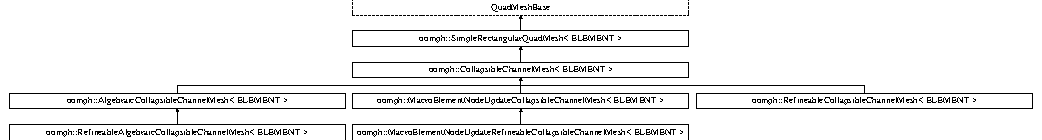
\includegraphics[height=1.885522cm]{classoomph_1_1CollapsibleChannelMesh}
\end{center}
\end{figure}
\subsection*{Public Member Functions}
\begin{DoxyCompactItemize}
\item 
\hyperlink{classoomph_1_1CollapsibleChannelMesh_a4e0b14ef4b4531f043b588150ca3c0f1}{Collapsible\+Channel\+Mesh} (const unsigned \&nup, const unsigned \&ncollapsible, const unsigned \&ndown, const unsigned \&\hyperlink{classoomph_1_1SimpleRectangularQuadMesh_a45011f22dedd480392b1f376e4269921}{ny}, const double \&lup, const double \&lcollapsible, const double \&ldown, const double \&ly, Geom\+Object $\ast$\hyperlink{classoomph_1_1CollapsibleChannelMesh_a04ffeb61678763dfd250962ea9ba614b}{wall\+\_\+pt}, Time\+Stepper $\ast$time\+\_\+stepper\+\_\+pt=\&Mesh\+::\+Default\+\_\+\+Time\+Stepper)
\begin{DoxyCompactList}\small\item\em Constructor\+: Pass number of elements in upstream/collapsible/ downstream segment and across the channel; lengths of upstream/ collapsible/downstream segments and width of channel, pointer to Geom\+Object that defines the collapsible segment and pointer to Time\+Stepper (defaults to the default timestepper, Steady). \end{DoxyCompactList}\item 
\hyperlink{classoomph_1_1CollapsibleChannelMesh_a1c9b2ab27f1fb2f764ae2dc6f9f7a429}{$\sim$\+Collapsible\+Channel\+Mesh} ()
\begin{DoxyCompactList}\small\item\em destructor \end{DoxyCompactList}\item 
Geom\+Object $\ast$\& \hyperlink{classoomph_1_1CollapsibleChannelMesh_a04ffeb61678763dfd250962ea9ba614b}{wall\+\_\+pt} ()
\begin{DoxyCompactList}\small\item\em Access function to Geom\+Object representing wall. \end{DoxyCompactList}\item 
\hyperlink{classoomph_1_1CollapsibleChannelDomain}{Collapsible\+Channel\+Domain} $\ast$ \hyperlink{classoomph_1_1CollapsibleChannelMesh_a379365813e6c3566639dc55a971f0b10}{domain\+\_\+pt} ()
\begin{DoxyCompactList}\small\item\em Access function to domain. \end{DoxyCompactList}\item 
virtual \hyperlink{classoomph_1_1CollapsibleChannelDomain_a2bf1d7943bfac134a5c27a54c7e1faed}{Collapsible\+Channel\+Domain\+::\+B\+L\+Squash\+Fct\+Pt} \& \hyperlink{classoomph_1_1CollapsibleChannelMesh_aac6057b4e572cb47923570b5e9c781c4}{bl\+\_\+squash\+\_\+fct\+\_\+pt} ()
\begin{DoxyCompactList}\small\item\em Function pointer for function that squashes the mesh near the walls. Default trivial mapping (the identity) leaves vertical nodal positions unchanged. Mapping is used in underlying \hyperlink{classoomph_1_1CollapsibleChannelDomain}{Collapsible\+Channel\+Domain}. Virtual so we can break it in derived classes (e.\+g. the Algebraic versions of this mesh where it doesn\textquotesingle{}t make any sense to provide the bl\+\_\+squash\+\_\+fct after the mesh has been built). \end{DoxyCompactList}\item 
\hyperlink{classoomph_1_1CollapsibleChannelDomain_a2bf1d7943bfac134a5c27a54c7e1faed}{Collapsible\+Channel\+Domain\+::\+B\+L\+Squash\+Fct\+Pt} \hyperlink{classoomph_1_1CollapsibleChannelMesh_a5c073c93cce7e6b6e9de86f36cb1e965}{bl\+\_\+squash\+\_\+fct\+\_\+pt} () const
\begin{DoxyCompactList}\small\item\em Function pointer for function that squashes the mesh near the walls. Default trivial mapping (the identity) leaves vertical nodal positions unchanged. Mapping is used in underlying \hyperlink{classoomph_1_1CollapsibleChannelDomain}{Collapsible\+Channel\+Domain}. Const version. \end{DoxyCompactList}\item 
virtual \hyperlink{classoomph_1_1CollapsibleChannelDomain_a317472dab112beac771ecf6442a465f5}{Collapsible\+Channel\+Domain\+::\+Axial\+Spacing\+Fct\+Pt} \& \hyperlink{classoomph_1_1CollapsibleChannelMesh_ac7913dca6b8b11240caede54414f3c11}{axial\+\_\+spacing\+\_\+fct\+\_\+pt} ()
\begin{DoxyCompactList}\small\item\em Function pointer for function that redistributes the elements in the axial direction. Virtual so we can break it in derived classes (e.\+g. the Algebraic versions of this mesh where it doesn\textquotesingle{}t make any sense to provide the bl\+\_\+squash\+\_\+fct after the mesh has been built). \end{DoxyCompactList}\item 
virtual \hyperlink{classoomph_1_1CollapsibleChannelDomain_a317472dab112beac771ecf6442a465f5}{Collapsible\+Channel\+Domain\+::\+Axial\+Spacing\+Fct\+Pt} \& \hyperlink{classoomph_1_1CollapsibleChannelMesh_a7a615ef1fcb4cb422e3c78267818ceec}{axial\+\_\+spacing\+\_\+fct\+\_\+pt} () const
\begin{DoxyCompactList}\small\item\em Function pointer for function that redistributes the elements in the axial direction. Const version. \end{DoxyCompactList}\end{DoxyCompactItemize}
\subsection*{Protected Attributes}
\begin{DoxyCompactItemize}
\item 
\hyperlink{classoomph_1_1CollapsibleChannelDomain}{Collapsible\+Channel\+Domain} $\ast$ \hyperlink{classoomph_1_1CollapsibleChannelMesh_ae7b9e4a110dded8399a6daf6f48a9e23}{Domain\+\_\+pt}
\begin{DoxyCompactList}\small\item\em Pointer to domain. \end{DoxyCompactList}\item 
unsigned \hyperlink{classoomph_1_1CollapsibleChannelMesh_aafd1c6d21bb891f1188ba6eed1705a45}{Nup}
\begin{DoxyCompactList}\small\item\em Number of element columns in upstream part. \end{DoxyCompactList}\item 
unsigned \hyperlink{classoomph_1_1CollapsibleChannelMesh_aa59ff7af47247b2e17b13c45f83fcf86}{Ncollapsible}
\begin{DoxyCompactList}\small\item\em Number of element columns in collapsible part. \end{DoxyCompactList}\item 
unsigned \hyperlink{classoomph_1_1CollapsibleChannelMesh_acd1b5ea7597a079b4321d3658f2e03f4}{Ndown}
\begin{DoxyCompactList}\small\item\em Number of element columns in downstream part. \end{DoxyCompactList}\item 
unsigned \hyperlink{classoomph_1_1CollapsibleChannelMesh_afa8d1dceef1cafeb166794d9275a30a3}{Ny}
\begin{DoxyCompactList}\small\item\em Number of element rows across channel. \end{DoxyCompactList}\item 
Geom\+Object $\ast$ \hyperlink{classoomph_1_1CollapsibleChannelMesh_a2457ac1492c962b0a3d962b13b51ea6e}{Wall\+\_\+pt}
\begin{DoxyCompactList}\small\item\em Pointer to geometric object that represents the moving wall. \end{DoxyCompactList}\end{DoxyCompactItemize}


\subsection{Detailed Description}
\subsubsection*{template$<$class E\+L\+E\+M\+E\+NT$>$\newline
class oomph\+::\+Collapsible\+Channel\+Mesh$<$ E\+L\+E\+M\+E\+N\+T $>$}

Basic collapsible channel mesh. The mesh is derived from the {\ttfamily \hyperlink{classoomph_1_1SimpleRectangularQuadMesh}{Simple\+Rectangular\+Quad\+Mesh}} so it\textquotesingle{}s node and element numbering scheme is the same as in that mesh. Only the boundaries are numbered differently to allow the easy identification of the \char`\"{}collapsible\char`\"{} segment. Boundary coordinates are set up for all nodes located on boundary 3 (the collapsible segment). The curvilinear (\char`\"{}collapsible\char`\"{}) segment is defined by a {\ttfamily Geom\+Object}. 

Definition at line 70 of file collapsible\+\_\+channel\+\_\+mesh.\+template.\+h.



\subsection{Constructor \& Destructor Documentation}
\mbox{\Hypertarget{classoomph_1_1CollapsibleChannelMesh_a4e0b14ef4b4531f043b588150ca3c0f1}\label{classoomph_1_1CollapsibleChannelMesh_a4e0b14ef4b4531f043b588150ca3c0f1}} 
\index{oomph\+::\+Collapsible\+Channel\+Mesh@{oomph\+::\+Collapsible\+Channel\+Mesh}!Collapsible\+Channel\+Mesh@{Collapsible\+Channel\+Mesh}}
\index{Collapsible\+Channel\+Mesh@{Collapsible\+Channel\+Mesh}!oomph\+::\+Collapsible\+Channel\+Mesh@{oomph\+::\+Collapsible\+Channel\+Mesh}}
\subsubsection{\texorpdfstring{Collapsible\+Channel\+Mesh()}{CollapsibleChannelMesh()}}
{\footnotesize\ttfamily template$<$class E\+L\+E\+M\+E\+NT $>$ \\
\hyperlink{classoomph_1_1CollapsibleChannelMesh}{oomph\+::\+Collapsible\+Channel\+Mesh}$<$ E\+L\+E\+M\+E\+NT $>$\+::\hyperlink{classoomph_1_1CollapsibleChannelMesh}{Collapsible\+Channel\+Mesh} (\begin{DoxyParamCaption}\item[{const unsigned \&}]{nup,  }\item[{const unsigned \&}]{ncollapsible,  }\item[{const unsigned \&}]{ndown,  }\item[{const unsigned \&}]{ny,  }\item[{const double \&}]{lup,  }\item[{const double \&}]{lcollapsible,  }\item[{const double \&}]{ldown,  }\item[{const double \&}]{ly,  }\item[{Geom\+Object $\ast$}]{wall\+\_\+pt,  }\item[{Time\+Stepper $\ast$}]{time\+\_\+stepper\+\_\+pt = {\ttfamily \&Mesh\+:\+:Default\+\_\+TimeStepper} }\end{DoxyParamCaption})}



Constructor\+: Pass number of elements in upstream/collapsible/ downstream segment and across the channel; lengths of upstream/ collapsible/downstream segments and width of channel, pointer to Geom\+Object that defines the collapsible segment and pointer to Time\+Stepper (defaults to the default timestepper, Steady). 

Constructor\+: Pass number of elements in upstream/collapsible/downstream segment and across the channel; lengths of upstream/collapsible/downstream segments and width of channel, pointer to Geom\+Object that defines the collapsible segment and pointer to Time\+Stepper (defaults to the default timestepper, Steady). 

Definition at line 48 of file collapsible\+\_\+channel\+\_\+mesh.\+template.\+cc.



References oomph\+::\+Collapsible\+Channel\+Mesh$<$ E\+L\+E\+M\+E\+N\+T $>$\+::\+Domain\+\_\+pt.

\mbox{\Hypertarget{classoomph_1_1CollapsibleChannelMesh_a1c9b2ab27f1fb2f764ae2dc6f9f7a429}\label{classoomph_1_1CollapsibleChannelMesh_a1c9b2ab27f1fb2f764ae2dc6f9f7a429}} 
\index{oomph\+::\+Collapsible\+Channel\+Mesh@{oomph\+::\+Collapsible\+Channel\+Mesh}!````~Collapsible\+Channel\+Mesh@{$\sim$\+Collapsible\+Channel\+Mesh}}
\index{````~Collapsible\+Channel\+Mesh@{$\sim$\+Collapsible\+Channel\+Mesh}!oomph\+::\+Collapsible\+Channel\+Mesh@{oomph\+::\+Collapsible\+Channel\+Mesh}}
\subsubsection{\texorpdfstring{$\sim$\+Collapsible\+Channel\+Mesh()}{~CollapsibleChannelMesh()}}
{\footnotesize\ttfamily template$<$class E\+L\+E\+M\+E\+NT $>$ \\
\hyperlink{classoomph_1_1CollapsibleChannelMesh}{oomph\+::\+Collapsible\+Channel\+Mesh}$<$ E\+L\+E\+M\+E\+NT $>$\+::$\sim$\hyperlink{classoomph_1_1CollapsibleChannelMesh}{Collapsible\+Channel\+Mesh} (\begin{DoxyParamCaption}{ }\end{DoxyParamCaption})\hspace{0.3cm}{\ttfamily [inline]}}



destructor 



Definition at line 93 of file collapsible\+\_\+channel\+\_\+mesh.\+template.\+h.



References oomph\+::\+Collapsible\+Channel\+Mesh$<$ E\+L\+E\+M\+E\+N\+T $>$\+::\+Domain\+\_\+pt.



\subsection{Member Function Documentation}
\mbox{\Hypertarget{classoomph_1_1CollapsibleChannelMesh_ac7913dca6b8b11240caede54414f3c11}\label{classoomph_1_1CollapsibleChannelMesh_ac7913dca6b8b11240caede54414f3c11}} 
\index{oomph\+::\+Collapsible\+Channel\+Mesh@{oomph\+::\+Collapsible\+Channel\+Mesh}!axial\+\_\+spacing\+\_\+fct\+\_\+pt@{axial\+\_\+spacing\+\_\+fct\+\_\+pt}}
\index{axial\+\_\+spacing\+\_\+fct\+\_\+pt@{axial\+\_\+spacing\+\_\+fct\+\_\+pt}!oomph\+::\+Collapsible\+Channel\+Mesh@{oomph\+::\+Collapsible\+Channel\+Mesh}}
\subsubsection{\texorpdfstring{axial\+\_\+spacing\+\_\+fct\+\_\+pt()}{axial\_spacing\_fct\_pt()}\hspace{0.1cm}{\footnotesize\ttfamily [1/2]}}
{\footnotesize\ttfamily template$<$class E\+L\+E\+M\+E\+NT $>$ \\
virtual \hyperlink{classoomph_1_1CollapsibleChannelDomain_a317472dab112beac771ecf6442a465f5}{Collapsible\+Channel\+Domain\+::\+Axial\+Spacing\+Fct\+Pt}\& \hyperlink{classoomph_1_1CollapsibleChannelMesh}{oomph\+::\+Collapsible\+Channel\+Mesh}$<$ E\+L\+E\+M\+E\+NT $>$\+::axial\+\_\+spacing\+\_\+fct\+\_\+pt (\begin{DoxyParamCaption}{ }\end{DoxyParamCaption})\hspace{0.3cm}{\ttfamily [inline]}, {\ttfamily [virtual]}}



Function pointer for function that redistributes the elements in the axial direction. Virtual so we can break it in derived classes (e.\+g. the Algebraic versions of this mesh where it doesn\textquotesingle{}t make any sense to provide the bl\+\_\+squash\+\_\+fct after the mesh has been built). 



Reimplemented in \hyperlink{classoomph_1_1AlgebraicCollapsibleChannelMesh_afa53bd526ff0903526afbdf5e6f4f532}{oomph\+::\+Algebraic\+Collapsible\+Channel\+Mesh$<$ E\+L\+E\+M\+E\+N\+T $>$}.



Definition at line 132 of file collapsible\+\_\+channel\+\_\+mesh.\+template.\+h.



References oomph\+::\+Collapsible\+Channel\+Domain\+::axial\+\_\+spacing\+\_\+fct\+\_\+pt(), and oomph\+::\+Collapsible\+Channel\+Mesh$<$ E\+L\+E\+M\+E\+N\+T $>$\+::\+Domain\+\_\+pt.

\mbox{\Hypertarget{classoomph_1_1CollapsibleChannelMesh_a7a615ef1fcb4cb422e3c78267818ceec}\label{classoomph_1_1CollapsibleChannelMesh_a7a615ef1fcb4cb422e3c78267818ceec}} 
\index{oomph\+::\+Collapsible\+Channel\+Mesh@{oomph\+::\+Collapsible\+Channel\+Mesh}!axial\+\_\+spacing\+\_\+fct\+\_\+pt@{axial\+\_\+spacing\+\_\+fct\+\_\+pt}}
\index{axial\+\_\+spacing\+\_\+fct\+\_\+pt@{axial\+\_\+spacing\+\_\+fct\+\_\+pt}!oomph\+::\+Collapsible\+Channel\+Mesh@{oomph\+::\+Collapsible\+Channel\+Mesh}}
\subsubsection{\texorpdfstring{axial\+\_\+spacing\+\_\+fct\+\_\+pt()}{axial\_spacing\_fct\_pt()}\hspace{0.1cm}{\footnotesize\ttfamily [2/2]}}
{\footnotesize\ttfamily template$<$class E\+L\+E\+M\+E\+NT $>$ \\
virtual \hyperlink{classoomph_1_1CollapsibleChannelDomain_a317472dab112beac771ecf6442a465f5}{Collapsible\+Channel\+Domain\+::\+Axial\+Spacing\+Fct\+Pt}\& \hyperlink{classoomph_1_1CollapsibleChannelMesh}{oomph\+::\+Collapsible\+Channel\+Mesh}$<$ E\+L\+E\+M\+E\+NT $>$\+::axial\+\_\+spacing\+\_\+fct\+\_\+pt (\begin{DoxyParamCaption}{ }\end{DoxyParamCaption}) const\hspace{0.3cm}{\ttfamily [inline]}, {\ttfamily [virtual]}}



Function pointer for function that redistributes the elements in the axial direction. Const version. 



Definition at line 140 of file collapsible\+\_\+channel\+\_\+mesh.\+template.\+h.



References oomph\+::\+Collapsible\+Channel\+Domain\+::axial\+\_\+spacing\+\_\+fct\+\_\+pt(), and oomph\+::\+Collapsible\+Channel\+Mesh$<$ E\+L\+E\+M\+E\+N\+T $>$\+::\+Domain\+\_\+pt.

\mbox{\Hypertarget{classoomph_1_1CollapsibleChannelMesh_aac6057b4e572cb47923570b5e9c781c4}\label{classoomph_1_1CollapsibleChannelMesh_aac6057b4e572cb47923570b5e9c781c4}} 
\index{oomph\+::\+Collapsible\+Channel\+Mesh@{oomph\+::\+Collapsible\+Channel\+Mesh}!bl\+\_\+squash\+\_\+fct\+\_\+pt@{bl\+\_\+squash\+\_\+fct\+\_\+pt}}
\index{bl\+\_\+squash\+\_\+fct\+\_\+pt@{bl\+\_\+squash\+\_\+fct\+\_\+pt}!oomph\+::\+Collapsible\+Channel\+Mesh@{oomph\+::\+Collapsible\+Channel\+Mesh}}
\subsubsection{\texorpdfstring{bl\+\_\+squash\+\_\+fct\+\_\+pt()}{bl\_squash\_fct\_pt()}\hspace{0.1cm}{\footnotesize\ttfamily [1/2]}}
{\footnotesize\ttfamily template$<$class E\+L\+E\+M\+E\+NT $>$ \\
virtual \hyperlink{classoomph_1_1CollapsibleChannelDomain_a2bf1d7943bfac134a5c27a54c7e1faed}{Collapsible\+Channel\+Domain\+::\+B\+L\+Squash\+Fct\+Pt}\& \hyperlink{classoomph_1_1CollapsibleChannelMesh}{oomph\+::\+Collapsible\+Channel\+Mesh}$<$ E\+L\+E\+M\+E\+NT $>$\+::bl\+\_\+squash\+\_\+fct\+\_\+pt (\begin{DoxyParamCaption}{ }\end{DoxyParamCaption})\hspace{0.3cm}{\ttfamily [inline]}, {\ttfamily [virtual]}}



Function pointer for function that squashes the mesh near the walls. Default trivial mapping (the identity) leaves vertical nodal positions unchanged. Mapping is used in underlying \hyperlink{classoomph_1_1CollapsibleChannelDomain}{Collapsible\+Channel\+Domain}. Virtual so we can break it in derived classes (e.\+g. the Algebraic versions of this mesh where it doesn\textquotesingle{}t make any sense to provide the bl\+\_\+squash\+\_\+fct after the mesh has been built). 



Reimplemented in \hyperlink{classoomph_1_1AlgebraicCollapsibleChannelMesh_abf1848b49f57419af4379a637464587d}{oomph\+::\+Algebraic\+Collapsible\+Channel\+Mesh$<$ E\+L\+E\+M\+E\+N\+T $>$}.



Definition at line 111 of file collapsible\+\_\+channel\+\_\+mesh.\+template.\+h.



References oomph\+::\+Collapsible\+Channel\+Domain\+::bl\+\_\+squash\+\_\+fct\+\_\+pt(), and oomph\+::\+Collapsible\+Channel\+Mesh$<$ E\+L\+E\+M\+E\+N\+T $>$\+::\+Domain\+\_\+pt.

\mbox{\Hypertarget{classoomph_1_1CollapsibleChannelMesh_a5c073c93cce7e6b6e9de86f36cb1e965}\label{classoomph_1_1CollapsibleChannelMesh_a5c073c93cce7e6b6e9de86f36cb1e965}} 
\index{oomph\+::\+Collapsible\+Channel\+Mesh@{oomph\+::\+Collapsible\+Channel\+Mesh}!bl\+\_\+squash\+\_\+fct\+\_\+pt@{bl\+\_\+squash\+\_\+fct\+\_\+pt}}
\index{bl\+\_\+squash\+\_\+fct\+\_\+pt@{bl\+\_\+squash\+\_\+fct\+\_\+pt}!oomph\+::\+Collapsible\+Channel\+Mesh@{oomph\+::\+Collapsible\+Channel\+Mesh}}
\subsubsection{\texorpdfstring{bl\+\_\+squash\+\_\+fct\+\_\+pt()}{bl\_squash\_fct\_pt()}\hspace{0.1cm}{\footnotesize\ttfamily [2/2]}}
{\footnotesize\ttfamily template$<$class E\+L\+E\+M\+E\+NT $>$ \\
\hyperlink{classoomph_1_1CollapsibleChannelDomain_a2bf1d7943bfac134a5c27a54c7e1faed}{Collapsible\+Channel\+Domain\+::\+B\+L\+Squash\+Fct\+Pt} \hyperlink{classoomph_1_1CollapsibleChannelMesh}{oomph\+::\+Collapsible\+Channel\+Mesh}$<$ E\+L\+E\+M\+E\+NT $>$\+::bl\+\_\+squash\+\_\+fct\+\_\+pt (\begin{DoxyParamCaption}{ }\end{DoxyParamCaption}) const\hspace{0.3cm}{\ttfamily [inline]}}



Function pointer for function that squashes the mesh near the walls. Default trivial mapping (the identity) leaves vertical nodal positions unchanged. Mapping is used in underlying \hyperlink{classoomph_1_1CollapsibleChannelDomain}{Collapsible\+Channel\+Domain}. Const version. 



Definition at line 121 of file collapsible\+\_\+channel\+\_\+mesh.\+template.\+h.



References oomph\+::\+Collapsible\+Channel\+Domain\+::bl\+\_\+squash\+\_\+fct\+\_\+pt(), and oomph\+::\+Collapsible\+Channel\+Mesh$<$ E\+L\+E\+M\+E\+N\+T $>$\+::\+Domain\+\_\+pt.

\mbox{\Hypertarget{classoomph_1_1CollapsibleChannelMesh_a379365813e6c3566639dc55a971f0b10}\label{classoomph_1_1CollapsibleChannelMesh_a379365813e6c3566639dc55a971f0b10}} 
\index{oomph\+::\+Collapsible\+Channel\+Mesh@{oomph\+::\+Collapsible\+Channel\+Mesh}!domain\+\_\+pt@{domain\+\_\+pt}}
\index{domain\+\_\+pt@{domain\+\_\+pt}!oomph\+::\+Collapsible\+Channel\+Mesh@{oomph\+::\+Collapsible\+Channel\+Mesh}}
\subsubsection{\texorpdfstring{domain\+\_\+pt()}{domain\_pt()}}
{\footnotesize\ttfamily template$<$class E\+L\+E\+M\+E\+NT $>$ \\
\hyperlink{classoomph_1_1CollapsibleChannelDomain}{Collapsible\+Channel\+Domain}$\ast$ \hyperlink{classoomph_1_1CollapsibleChannelMesh}{oomph\+::\+Collapsible\+Channel\+Mesh}$<$ E\+L\+E\+M\+E\+NT $>$\+::domain\+\_\+pt (\begin{DoxyParamCaption}{ }\end{DoxyParamCaption})\hspace{0.3cm}{\ttfamily [inline]}}



Access function to domain. 



Definition at line 102 of file collapsible\+\_\+channel\+\_\+mesh.\+template.\+h.



References oomph\+::\+Collapsible\+Channel\+Mesh$<$ E\+L\+E\+M\+E\+N\+T $>$\+::\+Domain\+\_\+pt.



Referenced by oomph\+::\+Macro\+Element\+Node\+Update\+Collapsible\+Channel\+Mesh$<$ E\+L\+E\+M\+E\+N\+T $>$\+::\+Macro\+Element\+Node\+Update\+Collapsible\+Channel\+Mesh(), and oomph\+::\+Algebraic\+Collapsible\+Channel\+Mesh$<$ E\+L\+E\+M\+E\+N\+T $>$\+::setup\+\_\+algebraic\+\_\+node\+\_\+update().

\mbox{\Hypertarget{classoomph_1_1CollapsibleChannelMesh_a04ffeb61678763dfd250962ea9ba614b}\label{classoomph_1_1CollapsibleChannelMesh_a04ffeb61678763dfd250962ea9ba614b}} 
\index{oomph\+::\+Collapsible\+Channel\+Mesh@{oomph\+::\+Collapsible\+Channel\+Mesh}!wall\+\_\+pt@{wall\+\_\+pt}}
\index{wall\+\_\+pt@{wall\+\_\+pt}!oomph\+::\+Collapsible\+Channel\+Mesh@{oomph\+::\+Collapsible\+Channel\+Mesh}}
\subsubsection{\texorpdfstring{wall\+\_\+pt()}{wall\_pt()}}
{\footnotesize\ttfamily template$<$class E\+L\+E\+M\+E\+NT $>$ \\
Geom\+Object$\ast$\& \hyperlink{classoomph_1_1CollapsibleChannelMesh}{oomph\+::\+Collapsible\+Channel\+Mesh}$<$ E\+L\+E\+M\+E\+NT $>$\+::wall\+\_\+pt (\begin{DoxyParamCaption}{ }\end{DoxyParamCaption})\hspace{0.3cm}{\ttfamily [inline]}}



Access function to Geom\+Object representing wall. 



Definition at line 99 of file collapsible\+\_\+channel\+\_\+mesh.\+template.\+h.



References oomph\+::\+Collapsible\+Channel\+Mesh$<$ E\+L\+E\+M\+E\+N\+T $>$\+::\+Wall\+\_\+pt.



\subsection{Member Data Documentation}
\mbox{\Hypertarget{classoomph_1_1CollapsibleChannelMesh_ae7b9e4a110dded8399a6daf6f48a9e23}\label{classoomph_1_1CollapsibleChannelMesh_ae7b9e4a110dded8399a6daf6f48a9e23}} 
\index{oomph\+::\+Collapsible\+Channel\+Mesh@{oomph\+::\+Collapsible\+Channel\+Mesh}!Domain\+\_\+pt@{Domain\+\_\+pt}}
\index{Domain\+\_\+pt@{Domain\+\_\+pt}!oomph\+::\+Collapsible\+Channel\+Mesh@{oomph\+::\+Collapsible\+Channel\+Mesh}}
\subsubsection{\texorpdfstring{Domain\+\_\+pt}{Domain\_pt}}
{\footnotesize\ttfamily template$<$class E\+L\+E\+M\+E\+NT $>$ \\
\hyperlink{classoomph_1_1CollapsibleChannelDomain}{Collapsible\+Channel\+Domain}$\ast$ \hyperlink{classoomph_1_1CollapsibleChannelMesh}{oomph\+::\+Collapsible\+Channel\+Mesh}$<$ E\+L\+E\+M\+E\+NT $>$\+::Domain\+\_\+pt\hspace{0.3cm}{\ttfamily [protected]}}



Pointer to domain. 



Definition at line 150 of file collapsible\+\_\+channel\+\_\+mesh.\+template.\+h.



Referenced by oomph\+::\+Algebraic\+Collapsible\+Channel\+Mesh$<$ E\+L\+E\+M\+E\+N\+T $>$\+::\+Algebraic\+Collapsible\+Channel\+Mesh(), oomph\+::\+Collapsible\+Channel\+Mesh$<$ E\+L\+E\+M\+E\+N\+T $>$\+::axial\+\_\+spacing\+\_\+fct\+\_\+pt(), oomph\+::\+Collapsible\+Channel\+Mesh$<$ E\+L\+E\+M\+E\+N\+T $>$\+::bl\+\_\+squash\+\_\+fct\+\_\+pt(), oomph\+::\+Collapsible\+Channel\+Mesh$<$ E\+L\+E\+M\+E\+N\+T $>$\+::\+Collapsible\+Channel\+Mesh(), oomph\+::\+Collapsible\+Channel\+Mesh$<$ E\+L\+E\+M\+E\+N\+T $>$\+::domain\+\_\+pt(), and oomph\+::\+Collapsible\+Channel\+Mesh$<$ E\+L\+E\+M\+E\+N\+T $>$\+::$\sim$\+Collapsible\+Channel\+Mesh().

\mbox{\Hypertarget{classoomph_1_1CollapsibleChannelMesh_aa59ff7af47247b2e17b13c45f83fcf86}\label{classoomph_1_1CollapsibleChannelMesh_aa59ff7af47247b2e17b13c45f83fcf86}} 
\index{oomph\+::\+Collapsible\+Channel\+Mesh@{oomph\+::\+Collapsible\+Channel\+Mesh}!Ncollapsible@{Ncollapsible}}
\index{Ncollapsible@{Ncollapsible}!oomph\+::\+Collapsible\+Channel\+Mesh@{oomph\+::\+Collapsible\+Channel\+Mesh}}
\subsubsection{\texorpdfstring{Ncollapsible}{Ncollapsible}}
{\footnotesize\ttfamily template$<$class E\+L\+E\+M\+E\+NT $>$ \\
unsigned \hyperlink{classoomph_1_1CollapsibleChannelMesh}{oomph\+::\+Collapsible\+Channel\+Mesh}$<$ E\+L\+E\+M\+E\+NT $>$\+::Ncollapsible\hspace{0.3cm}{\ttfamily [protected]}}



Number of element columns in collapsible part. 



Definition at line 156 of file collapsible\+\_\+channel\+\_\+mesh.\+template.\+h.

\mbox{\Hypertarget{classoomph_1_1CollapsibleChannelMesh_acd1b5ea7597a079b4321d3658f2e03f4}\label{classoomph_1_1CollapsibleChannelMesh_acd1b5ea7597a079b4321d3658f2e03f4}} 
\index{oomph\+::\+Collapsible\+Channel\+Mesh@{oomph\+::\+Collapsible\+Channel\+Mesh}!Ndown@{Ndown}}
\index{Ndown@{Ndown}!oomph\+::\+Collapsible\+Channel\+Mesh@{oomph\+::\+Collapsible\+Channel\+Mesh}}
\subsubsection{\texorpdfstring{Ndown}{Ndown}}
{\footnotesize\ttfamily template$<$class E\+L\+E\+M\+E\+NT $>$ \\
unsigned \hyperlink{classoomph_1_1CollapsibleChannelMesh}{oomph\+::\+Collapsible\+Channel\+Mesh}$<$ E\+L\+E\+M\+E\+NT $>$\+::Ndown\hspace{0.3cm}{\ttfamily [protected]}}



Number of element columns in downstream part. 



Definition at line 159 of file collapsible\+\_\+channel\+\_\+mesh.\+template.\+h.

\mbox{\Hypertarget{classoomph_1_1CollapsibleChannelMesh_aafd1c6d21bb891f1188ba6eed1705a45}\label{classoomph_1_1CollapsibleChannelMesh_aafd1c6d21bb891f1188ba6eed1705a45}} 
\index{oomph\+::\+Collapsible\+Channel\+Mesh@{oomph\+::\+Collapsible\+Channel\+Mesh}!Nup@{Nup}}
\index{Nup@{Nup}!oomph\+::\+Collapsible\+Channel\+Mesh@{oomph\+::\+Collapsible\+Channel\+Mesh}}
\subsubsection{\texorpdfstring{Nup}{Nup}}
{\footnotesize\ttfamily template$<$class E\+L\+E\+M\+E\+NT $>$ \\
unsigned \hyperlink{classoomph_1_1CollapsibleChannelMesh}{oomph\+::\+Collapsible\+Channel\+Mesh}$<$ E\+L\+E\+M\+E\+NT $>$\+::Nup\hspace{0.3cm}{\ttfamily [protected]}}



Number of element columns in upstream part. 



Definition at line 153 of file collapsible\+\_\+channel\+\_\+mesh.\+template.\+h.

\mbox{\Hypertarget{classoomph_1_1CollapsibleChannelMesh_afa8d1dceef1cafeb166794d9275a30a3}\label{classoomph_1_1CollapsibleChannelMesh_afa8d1dceef1cafeb166794d9275a30a3}} 
\index{oomph\+::\+Collapsible\+Channel\+Mesh@{oomph\+::\+Collapsible\+Channel\+Mesh}!Ny@{Ny}}
\index{Ny@{Ny}!oomph\+::\+Collapsible\+Channel\+Mesh@{oomph\+::\+Collapsible\+Channel\+Mesh}}
\subsubsection{\texorpdfstring{Ny}{Ny}}
{\footnotesize\ttfamily template$<$class E\+L\+E\+M\+E\+NT $>$ \\
unsigned \hyperlink{classoomph_1_1CollapsibleChannelMesh}{oomph\+::\+Collapsible\+Channel\+Mesh}$<$ E\+L\+E\+M\+E\+NT $>$\+::Ny\hspace{0.3cm}{\ttfamily [protected]}}



Number of element rows across channel. 



Definition at line 162 of file collapsible\+\_\+channel\+\_\+mesh.\+template.\+h.

\mbox{\Hypertarget{classoomph_1_1CollapsibleChannelMesh_a2457ac1492c962b0a3d962b13b51ea6e}\label{classoomph_1_1CollapsibleChannelMesh_a2457ac1492c962b0a3d962b13b51ea6e}} 
\index{oomph\+::\+Collapsible\+Channel\+Mesh@{oomph\+::\+Collapsible\+Channel\+Mesh}!Wall\+\_\+pt@{Wall\+\_\+pt}}
\index{Wall\+\_\+pt@{Wall\+\_\+pt}!oomph\+::\+Collapsible\+Channel\+Mesh@{oomph\+::\+Collapsible\+Channel\+Mesh}}
\subsubsection{\texorpdfstring{Wall\+\_\+pt}{Wall\_pt}}
{\footnotesize\ttfamily template$<$class E\+L\+E\+M\+E\+NT $>$ \\
Geom\+Object$\ast$ \hyperlink{classoomph_1_1CollapsibleChannelMesh}{oomph\+::\+Collapsible\+Channel\+Mesh}$<$ E\+L\+E\+M\+E\+NT $>$\+::Wall\+\_\+pt\hspace{0.3cm}{\ttfamily [protected]}}



Pointer to geometric object that represents the moving wall. 



Definition at line 165 of file collapsible\+\_\+channel\+\_\+mesh.\+template.\+h.



Referenced by oomph\+::\+Macro\+Element\+Node\+Update\+Collapsible\+Channel\+Mesh$<$ E\+L\+E\+M\+E\+N\+T $>$\+::\+Macro\+Element\+Node\+Update\+Collapsible\+Channel\+Mesh(), oomph\+::\+Algebraic\+Collapsible\+Channel\+Mesh$<$ E\+L\+E\+M\+E\+N\+T $>$\+::setup\+\_\+algebraic\+\_\+node\+\_\+update(), oomph\+::\+Refineable\+Algebraic\+Collapsible\+Channel\+Mesh$<$ E\+L\+E\+M\+E\+N\+T $>$\+::update\+\_\+node\+\_\+update(), and oomph\+::\+Collapsible\+Channel\+Mesh$<$ E\+L\+E\+M\+E\+N\+T $>$\+::wall\+\_\+pt().



The documentation for this class was generated from the following files\+:\begin{DoxyCompactItemize}
\item 
\hyperlink{collapsible__channel__mesh_8template_8h}{collapsible\+\_\+channel\+\_\+mesh.\+template.\+h}\item 
\hyperlink{collapsible__channel__mesh_8template_8cc}{collapsible\+\_\+channel\+\_\+mesh.\+template.\+cc}\end{DoxyCompactItemize}

\hypertarget{classoomph_1_1CylinderWithFlagDomain}{}\section{oomph\+:\+:Cylinder\+With\+Flag\+Domain Class Reference}
\label{classoomph_1_1CylinderWithFlagDomain}\index{oomph\+::\+Cylinder\+With\+Flag\+Domain@{oomph\+::\+Cylinder\+With\+Flag\+Domain}}


Domain for cylinder with flag as in Turek benchmark.  




{\ttfamily \#include $<$cylinder\+\_\+with\+\_\+flag\+\_\+domain.\+h$>$}

Inheritance diagram for oomph\+:\+:Cylinder\+With\+Flag\+Domain\+:\begin{figure}[H]
\begin{center}
\leavevmode
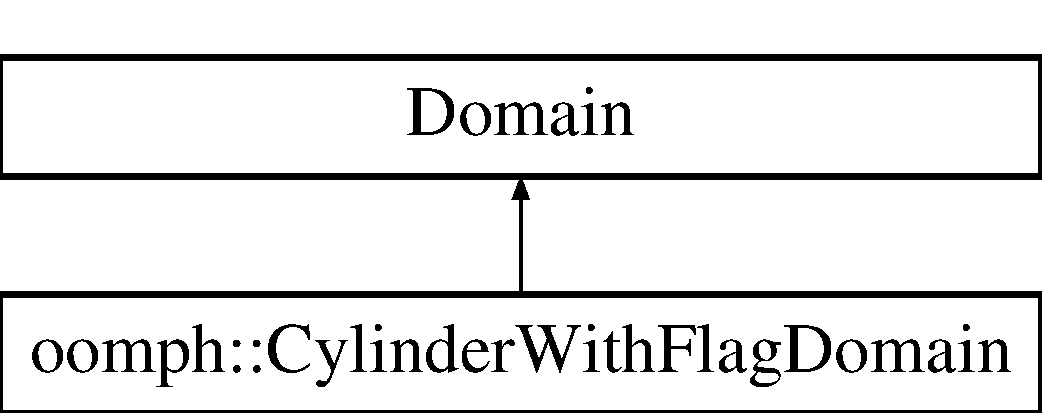
\includegraphics[height=2.000000cm]{classoomph_1_1CylinderWithFlagDomain}
\end{center}
\end{figure}
\subsection*{Public Member Functions}
\begin{DoxyCompactItemize}
\item 
\hyperlink{classoomph_1_1CylinderWithFlagDomain_aa393d14243edaf8b8eaa02c9a01bd869}{Cylinder\+With\+Flag\+Domain} (Circle $\ast$\hyperlink{classoomph_1_1CylinderWithFlagDomain_a783f430b790953da4e01720be56d1872}{cylinder\+\_\+pt}, Geom\+Object $\ast$\hyperlink{classoomph_1_1CylinderWithFlagDomain_a268642db566b31b686ba8185e8610d8a}{top\+\_\+flag\+\_\+pt}, Geom\+Object $\ast$\hyperlink{classoomph_1_1CylinderWithFlagDomain_a4da493b4e9ddc3fc62f6beb269781e81}{bottom\+\_\+flag\+\_\+pt}, Geom\+Object $\ast$\hyperlink{classoomph_1_1CylinderWithFlagDomain_a9977cf9b4b71f83ba0f4d253164d4e00}{tip\+\_\+flag\+\_\+pt}, const double \&length, const double \&height, const double \&flag\+\_\+length, const double \&flag\+\_\+height, const double \&centre\+\_\+x, const double \&centre\+\_\+y, const double \&a)
\item 
\hyperlink{classoomph_1_1CylinderWithFlagDomain_a726928362d0d681f0420d1f088776e80}{$\sim$\+Cylinder\+With\+Flag\+Domain} ()
\begin{DoxyCompactList}\small\item\em Destructor\+: Kill macro elements. \end{DoxyCompactList}\item 
void \hyperlink{classoomph_1_1CylinderWithFlagDomain_a40bca9a30f1f874c043e68621b28de74}{macro\+\_\+element\+\_\+boundary} (const unsigned \&time, const unsigned \&m, const unsigned \&direction, const Vector$<$ double $>$ \&s, Vector$<$ double $>$ \&f)
\begin{DoxyCompactList}\small\item\em Parametrisation of macro element boundaries\+: f(s) is the position vector to macro-\/element m\textquotesingle{}s boundary in the specified direction \mbox{[}N/\+S/\+E/W\mbox{]} at the specfied discrete time level (time=0\+: present; time$>$0\+: previous) \end{DoxyCompactList}\item 
Circle $\ast$ \hyperlink{classoomph_1_1CylinderWithFlagDomain_a783f430b790953da4e01720be56d1872}{cylinder\+\_\+pt} ()
\begin{DoxyCompactList}\small\item\em Access fct to Geom\+Object (of type Circle) that represents the cylinder. \end{DoxyCompactList}\item 
Geom\+Object $\ast$\& \hyperlink{classoomph_1_1CylinderWithFlagDomain_a4da493b4e9ddc3fc62f6beb269781e81}{bottom\+\_\+flag\+\_\+pt} ()
\begin{DoxyCompactList}\small\item\em Access fct to Geom\+Objects for top, bottom and tip. \end{DoxyCompactList}\item 
Geom\+Object $\ast$\& \hyperlink{classoomph_1_1CylinderWithFlagDomain_a268642db566b31b686ba8185e8610d8a}{top\+\_\+flag\+\_\+pt} ()
\item 
Geom\+Object $\ast$\& \hyperlink{classoomph_1_1CylinderWithFlagDomain_a9977cf9b4b71f83ba0f4d253164d4e00}{tip\+\_\+flag\+\_\+pt} ()
\end{DoxyCompactItemize}
\subsection*{Private Member Functions}
\begin{DoxyCompactItemize}
\item 
void \hyperlink{classoomph_1_1CylinderWithFlagDomain_aa0f0db0fdf2b271a6dde42ef36e9d40d}{linear\+\_\+interpolate} (const Vector$<$ double $>$ \&left, const Vector$<$ double $>$ \&right, const double \&s, Vector$<$ double $>$ \&f)
\begin{DoxyCompactList}\small\item\em Helper function to interpolate linearly between the \char`\"{}right\char`\"{} and \char`\"{}left\char`\"{} points; $ s \in [-1,1] $. \end{DoxyCompactList}\end{DoxyCompactItemize}
\subsection*{Private Attributes}
\begin{DoxyCompactItemize}
\item 
Vector$<$ double $>$ \hyperlink{classoomph_1_1CylinderWithFlagDomain_a22098b556345f035ddacbdf9ea1f7076}{p1}
\item 
Vector$<$ double $>$ \hyperlink{classoomph_1_1CylinderWithFlagDomain_a518fb98d53857ffd86d1cac4c23db0d9}{p2}
\item 
Vector$<$ double $>$ \hyperlink{classoomph_1_1CylinderWithFlagDomain_a6327976b3d8e582cfc232be01c45d975}{p3}
\item 
Vector$<$ double $>$ \hyperlink{classoomph_1_1CylinderWithFlagDomain_a060890ea588f8e5833d518fa707fe774}{p4}
\item 
Vector$<$ double $>$ \hyperlink{classoomph_1_1CylinderWithFlagDomain_ad4f4179e51afb966f11b999ef9ddd0a9}{p5}
\item 
Vector$<$ double $>$ \hyperlink{classoomph_1_1CylinderWithFlagDomain_a8af35f3606195d1bab1da58102b7fa15}{p6}
\item 
Vector$<$ double $>$ \hyperlink{classoomph_1_1CylinderWithFlagDomain_ae0aaa23dad312e7ea308e98b59015a51}{p7}
\item 
Vector$<$ double $>$ \hyperlink{classoomph_1_1CylinderWithFlagDomain_a20743a18902498e2537f557da2fec123}{p8}
\item 
Vector$<$ double $>$ \hyperlink{classoomph_1_1CylinderWithFlagDomain_a8ff949c600451d8cc9e53fc9b204dd79}{p9}
\item 
Vector$<$ double $>$ \hyperlink{classoomph_1_1CylinderWithFlagDomain_af9fe7cd9299c2fe162804d60455609c6}{p10}
\item 
Vector$<$ double $>$ \hyperlink{classoomph_1_1CylinderWithFlagDomain_af209469424b0b515eedb4587901453b6}{p11}
\item 
Vector$<$ double $>$ \hyperlink{classoomph_1_1CylinderWithFlagDomain_a8cd9138a4f584d439da6264e5aa65d2e}{p12}
\item 
Vector$<$ double $>$ \hyperlink{classoomph_1_1CylinderWithFlagDomain_af96f841048a399c0d5b7cd4519c22d72}{p13}
\item 
Vector$<$ double $>$ \hyperlink{classoomph_1_1CylinderWithFlagDomain_ac07282a9f587fc6f10b81506c59a2001}{p14}
\item 
Vector$<$ double $>$ \hyperlink{classoomph_1_1CylinderWithFlagDomain_a3ddcf9eca20ac5f31358b9711fef5a09}{p15}
\item 
Vector$<$ double $>$ \hyperlink{classoomph_1_1CylinderWithFlagDomain_a633feb876937a1b58c013209defbad7e}{p16}
\item 
Vector$<$ double $>$ \hyperlink{classoomph_1_1CylinderWithFlagDomain_a38c6ea86f1d6218dccce7482dd6daf48}{p17}
\item 
Vector$<$ double $>$ \hyperlink{classoomph_1_1CylinderWithFlagDomain_a0076ec3ac4fbd0213719a2d2679ab1db}{p18}
\item 
Vector$<$ double $>$ \hyperlink{classoomph_1_1CylinderWithFlagDomain_a0a3ba355180e34fc7372fef35a6accb7}{p19}
\item 
Vector$<$ double $>$ \hyperlink{classoomph_1_1CylinderWithFlagDomain_a5c13c0e741670b57b0b8ac2e50e4f157}{p20}
\item 
Vector$<$ double $>$ \hyperlink{classoomph_1_1CylinderWithFlagDomain_afb18b71be9144eb6ea2b36d113531b7e}{p21}
\item 
Vector$<$ double $>$ \hyperlink{classoomph_1_1CylinderWithFlagDomain_a69b821d40d982324df13380bb05db70b}{p22}
\item 
Vector$<$ double $>$ \hyperlink{classoomph_1_1CylinderWithFlagDomain_ad0ce5ac87bc9e4b455a99fc3a6cf5b9c}{p23}
\item 
Vector$<$ double $>$ \hyperlink{classoomph_1_1CylinderWithFlagDomain_a1e0ffc29a35d430c6ab123f8bc9a5d37}{p24}
\item 
Vector$<$ double $>$ \hyperlink{classoomph_1_1CylinderWithFlagDomain_abbcbd7a97f86134091e3750f04a3fdfd}{p25}
\item 
Vector$<$ double $>$ \hyperlink{classoomph_1_1CylinderWithFlagDomain_a85707f0839cd70631c82d9254ed8c5d0}{p26}
\item 
Vector$<$ double $>$ \hyperlink{classoomph_1_1CylinderWithFlagDomain_a4f485315dc6bb184e298d8bba550866e}{p27}
\item 
Vector$<$ double $>$ \hyperlink{classoomph_1_1CylinderWithFlagDomain_a56fdcc4a8538bdc4c10e2c11355163f0}{p28}
\item 
Vector$<$ double $>$ \hyperlink{classoomph_1_1CylinderWithFlagDomain_a5eb61c2f311296d0ce91ec428a5d5329}{p29}
\item 
Vector$<$ double $>$ \hyperlink{classoomph_1_1CylinderWithFlagDomain_af35a25c3f63e71f2bff61b1da3384630}{p30}
\item 
Vector$<$ double $>$ \hyperlink{classoomph_1_1CylinderWithFlagDomain_a73977bbf7e952fd71a465884e526c4db}{p31}
\item 
Vector$<$ double $>$ \hyperlink{classoomph_1_1CylinderWithFlagDomain_a600f1d0f8f3168e95b9f20931cdd5a26}{p32}
\item 
Vector$<$ double $>$ \hyperlink{classoomph_1_1CylinderWithFlagDomain_a2c3ddad128b8d2ca54bb015171637809}{p33}
\item 
Vector$<$ double $>$ \hyperlink{classoomph_1_1CylinderWithFlagDomain_a44aa94c4106c3f2d7c7575a50a56a98c}{p34}
\item 
Vector$<$ double $>$ \hyperlink{classoomph_1_1CylinderWithFlagDomain_afba63042c55f44d17628aaa0623e97b8}{p35}
\item 
Vector$<$ double $>$ \hyperlink{classoomph_1_1CylinderWithFlagDomain_a8366e523946d218b27c998aca522742e}{p36}
\item 
Vector$<$ double $>$ \hyperlink{classoomph_1_1CylinderWithFlagDomain_aa239d71da15390053e4418e4902c8608}{p37}
\item 
Vector$<$ double $>$ \hyperlink{classoomph_1_1CylinderWithFlagDomain_a986aabc271029813cb541ae8555d1696}{p38}
\item 
Vector$<$ double $>$ \hyperlink{classoomph_1_1CylinderWithFlagDomain_a0b6726667f09eeabad0885858e684ff0}{p39}
\item 
Vector$<$ double $>$ \hyperlink{classoomph_1_1CylinderWithFlagDomain_a9a6150121807b24c30f1a57e23c899ca}{p40}
\item 
Vector$<$ double $>$ \hyperlink{classoomph_1_1CylinderWithFlagDomain_ad40423594322c7cea0161a39501535a3}{p41}
\item 
Vector$<$ double $>$ \hyperlink{classoomph_1_1CylinderWithFlagDomain_a49f3169b5cd06322394e808f3fb8dc91}{p42}
\item 
Vector$<$ double $>$ \hyperlink{classoomph_1_1CylinderWithFlagDomain_a4cf79435459ac5399f94f6e0686e5a0a}{p43}
\item 
Vector$<$ double $>$ \hyperlink{classoomph_1_1CylinderWithFlagDomain_a4288652a4436b747a86ff94346c61ebc}{p44}
\item 
Vector$<$ double $>$ \hyperlink{classoomph_1_1CylinderWithFlagDomain_a6988e0912e925fe62d6cad22195e8c5d}{p45}
\item 
Vector$<$ double $>$ \hyperlink{classoomph_1_1CylinderWithFlagDomain_a5dedb150b33c1260e09a5e73924c6861}{p46}
\item 
Vector$<$ double $>$ \hyperlink{classoomph_1_1CylinderWithFlagDomain_a34928d206b87289667344fc94a307509}{p47}
\item 
Vector$<$ double $>$ \hyperlink{classoomph_1_1CylinderWithFlagDomain_ae02eac305b33b85a2e87df1764e4b8d8}{p48}
\item 
Vector$<$ double $>$ \hyperlink{classoomph_1_1CylinderWithFlagDomain_aa5418e036166408fb5df662d93479a84}{p49}
\item 
Vector$<$ double $>$ \hyperlink{classoomph_1_1CylinderWithFlagDomain_a0b46b0c29925ba405a04fda8b3ab9c06}{p50}
\item 
Circle $\ast$ \hyperlink{classoomph_1_1CylinderWithFlagDomain_afb13bdcd16005bc0505908bb3c844f33}{Cylinder\+\_\+pt}
\begin{DoxyCompactList}\small\item\em Pointer to geometric object that represents the central cylinder. \end{DoxyCompactList}\item 
Geom\+Object $\ast$ \hyperlink{classoomph_1_1CylinderWithFlagDomain_a92ae4556f99335233c1c653e15fa1f48}{Top\+\_\+flag\+\_\+pt}
\begin{DoxyCompactList}\small\item\em Pointer to geometric object that represents the top of the flag. \end{DoxyCompactList}\item 
Geom\+Object $\ast$ \hyperlink{classoomph_1_1CylinderWithFlagDomain_ae4bfb961e03aab16d01fc4662c0214e3}{Bottom\+\_\+flag\+\_\+pt}
\begin{DoxyCompactList}\small\item\em Pointer to geometric object that represents the bottom of the flag. \end{DoxyCompactList}\item 
Geom\+Object $\ast$ \hyperlink{classoomph_1_1CylinderWithFlagDomain_a2926eb3a4c171fbc924115f7dfd211a4}{Tip\+\_\+flag\+\_\+pt}
\begin{DoxyCompactList}\small\item\em Pointer to geometric object that represents the tip of the flag. \end{DoxyCompactList}\item 
double \hyperlink{classoomph_1_1CylinderWithFlagDomain_aba284322fcd3d9b9a4231ec71ea6d96b}{Lx}
\item 
double \hyperlink{classoomph_1_1CylinderWithFlagDomain_a733fc387ee7d25811edb6b99c796b242}{Ly}
\item 
double \hyperlink{classoomph_1_1CylinderWithFlagDomain_a9473fc0eb249a20c8a3456c708c8ba6f}{Centre\+\_\+x}
\item 
double \hyperlink{classoomph_1_1CylinderWithFlagDomain_aee096a172eec5ffc3719b625c52beb26}{Centre\+\_\+y}
\item 
double \hyperlink{classoomph_1_1CylinderWithFlagDomain_afdb4b1beb7e574e1bcfc7fbb8a6df700}{A}
\end{DoxyCompactItemize}


\subsection{Detailed Description}
Domain for cylinder with flag as in Turek benchmark. 

Definition at line 47 of file cylinder\+\_\+with\+\_\+flag\+\_\+domain.\+h.



\subsection{Constructor \& Destructor Documentation}
\mbox{\Hypertarget{classoomph_1_1CylinderWithFlagDomain_aa393d14243edaf8b8eaa02c9a01bd869}\label{classoomph_1_1CylinderWithFlagDomain_aa393d14243edaf8b8eaa02c9a01bd869}} 
\index{oomph\+::\+Cylinder\+With\+Flag\+Domain@{oomph\+::\+Cylinder\+With\+Flag\+Domain}!Cylinder\+With\+Flag\+Domain@{Cylinder\+With\+Flag\+Domain}}
\index{Cylinder\+With\+Flag\+Domain@{Cylinder\+With\+Flag\+Domain}!oomph\+::\+Cylinder\+With\+Flag\+Domain@{oomph\+::\+Cylinder\+With\+Flag\+Domain}}
\subsubsection{\texorpdfstring{Cylinder\+With\+Flag\+Domain()}{CylinderWithFlagDomain()}}
{\footnotesize\ttfamily oomph\+::\+Cylinder\+With\+Flag\+Domain\+::\+Cylinder\+With\+Flag\+Domain (\begin{DoxyParamCaption}\item[{Circle $\ast$}]{cylinder\+\_\+pt,  }\item[{Geom\+Object $\ast$}]{top\+\_\+flag\+\_\+pt,  }\item[{Geom\+Object $\ast$}]{bottom\+\_\+flag\+\_\+pt,  }\item[{Geom\+Object $\ast$}]{tip\+\_\+flag\+\_\+pt,  }\item[{const double \&}]{length,  }\item[{const double \&}]{height,  }\item[{const double \&}]{flag\+\_\+length,  }\item[{const double \&}]{flag\+\_\+height,  }\item[{const double \&}]{centre\+\_\+x,  }\item[{const double \&}]{centre\+\_\+y,  }\item[{const double \&}]{a }\end{DoxyParamCaption})}

Constructor. Pass the pointers to the Geom\+Objects that parametrise the cylinder, the three edges of the flag, the length and height of the domain, the length and height of the flag, the coordinates of the centre of the cylinder and its radius.

Constructor, Pass the pointers to the Geom\+Objects that parametrise the cylinder, the three edges of the flag, the length and height of the domain, the length and height of the flag, the coordinates of the centre of the cylinder and its radius. 

Definition at line 43 of file cylinder\+\_\+with\+\_\+flag\+\_\+domain.\+cc.



References A, Centre\+\_\+x, Centre\+\_\+y, p1, p10, p11, p12, p13, p14, p15, p16, p18, p2, p21, p22, p23, p24, p25, p27, p28, p29, p3, p30, p31, p33, p35, p36, p37, p38, p39, p4, p40, p41, p42, p43, p44, p45, p46, p47, p48, p49, p5, p50, p6, p7, p8, and p9.

\mbox{\Hypertarget{classoomph_1_1CylinderWithFlagDomain_a726928362d0d681f0420d1f088776e80}\label{classoomph_1_1CylinderWithFlagDomain_a726928362d0d681f0420d1f088776e80}} 
\index{oomph\+::\+Cylinder\+With\+Flag\+Domain@{oomph\+::\+Cylinder\+With\+Flag\+Domain}!````~Cylinder\+With\+Flag\+Domain@{$\sim$\+Cylinder\+With\+Flag\+Domain}}
\index{````~Cylinder\+With\+Flag\+Domain@{$\sim$\+Cylinder\+With\+Flag\+Domain}!oomph\+::\+Cylinder\+With\+Flag\+Domain@{oomph\+::\+Cylinder\+With\+Flag\+Domain}}
\subsubsection{\texorpdfstring{$\sim$\+Cylinder\+With\+Flag\+Domain()}{~CylinderWithFlagDomain()}}
{\footnotesize\ttfamily oomph\+::\+Cylinder\+With\+Flag\+Domain\+::$\sim$\+Cylinder\+With\+Flag\+Domain (\begin{DoxyParamCaption}{ }\end{DoxyParamCaption})\hspace{0.3cm}{\ttfamily [inline]}}



Destructor\+: Kill macro elements. 



Definition at line 70 of file cylinder\+\_\+with\+\_\+flag\+\_\+domain.\+h.



References macro\+\_\+element\+\_\+boundary().



\subsection{Member Function Documentation}
\mbox{\Hypertarget{classoomph_1_1CylinderWithFlagDomain_a4da493b4e9ddc3fc62f6beb269781e81}\label{classoomph_1_1CylinderWithFlagDomain_a4da493b4e9ddc3fc62f6beb269781e81}} 
\index{oomph\+::\+Cylinder\+With\+Flag\+Domain@{oomph\+::\+Cylinder\+With\+Flag\+Domain}!bottom\+\_\+flag\+\_\+pt@{bottom\+\_\+flag\+\_\+pt}}
\index{bottom\+\_\+flag\+\_\+pt@{bottom\+\_\+flag\+\_\+pt}!oomph\+::\+Cylinder\+With\+Flag\+Domain@{oomph\+::\+Cylinder\+With\+Flag\+Domain}}
\subsubsection{\texorpdfstring{bottom\+\_\+flag\+\_\+pt()}{bottom\_flag\_pt()}}
{\footnotesize\ttfamily Geom\+Object$\ast$\& oomph\+::\+Cylinder\+With\+Flag\+Domain\+::bottom\+\_\+flag\+\_\+pt (\begin{DoxyParamCaption}{ }\end{DoxyParamCaption})\hspace{0.3cm}{\ttfamily [inline]}}



Access fct to Geom\+Objects for top, bottom and tip. 



Definition at line 90 of file cylinder\+\_\+with\+\_\+flag\+\_\+domain.\+h.



References Bottom\+\_\+flag\+\_\+pt.



Referenced by oomph\+::\+Algebraic\+Cylinder\+With\+Flag\+Mesh$<$ E\+L\+E\+M\+E\+N\+T $>$\+::set\+\_\+bottom\+\_\+flag\+\_\+pt().

\mbox{\Hypertarget{classoomph_1_1CylinderWithFlagDomain_a783f430b790953da4e01720be56d1872}\label{classoomph_1_1CylinderWithFlagDomain_a783f430b790953da4e01720be56d1872}} 
\index{oomph\+::\+Cylinder\+With\+Flag\+Domain@{oomph\+::\+Cylinder\+With\+Flag\+Domain}!cylinder\+\_\+pt@{cylinder\+\_\+pt}}
\index{cylinder\+\_\+pt@{cylinder\+\_\+pt}!oomph\+::\+Cylinder\+With\+Flag\+Domain@{oomph\+::\+Cylinder\+With\+Flag\+Domain}}
\subsubsection{\texorpdfstring{cylinder\+\_\+pt()}{cylinder\_pt()}}
{\footnotesize\ttfamily Circle$\ast$ oomph\+::\+Cylinder\+With\+Flag\+Domain\+::cylinder\+\_\+pt (\begin{DoxyParamCaption}{ }\end{DoxyParamCaption})\hspace{0.3cm}{\ttfamily [inline]}}



Access fct to Geom\+Object (of type Circle) that represents the cylinder. 



Definition at line 87 of file cylinder\+\_\+with\+\_\+flag\+\_\+domain.\+h.



References Cylinder\+\_\+pt.

\mbox{\Hypertarget{classoomph_1_1CylinderWithFlagDomain_aa0f0db0fdf2b271a6dde42ef36e9d40d}\label{classoomph_1_1CylinderWithFlagDomain_aa0f0db0fdf2b271a6dde42ef36e9d40d}} 
\index{oomph\+::\+Cylinder\+With\+Flag\+Domain@{oomph\+::\+Cylinder\+With\+Flag\+Domain}!linear\+\_\+interpolate@{linear\+\_\+interpolate}}
\index{linear\+\_\+interpolate@{linear\+\_\+interpolate}!oomph\+::\+Cylinder\+With\+Flag\+Domain@{oomph\+::\+Cylinder\+With\+Flag\+Domain}}
\subsubsection{\texorpdfstring{linear\+\_\+interpolate()}{linear\_interpolate()}}
{\footnotesize\ttfamily void oomph\+::\+Cylinder\+With\+Flag\+Domain\+::linear\+\_\+interpolate (\begin{DoxyParamCaption}\item[{const Vector$<$ double $>$ \&}]{left,  }\item[{const Vector$<$ double $>$ \&}]{right,  }\item[{const double \&}]{s,  }\item[{Vector$<$ double $>$ \&}]{f }\end{DoxyParamCaption})\hspace{0.3cm}{\ttfamily [inline]}, {\ttfamily [private]}}



Helper function to interpolate linearly between the \char`\"{}right\char`\"{} and \char`\"{}left\char`\"{} points; $ s \in [-1,1] $. 



Definition at line 98 of file cylinder\+\_\+with\+\_\+flag\+\_\+domain.\+h.



Referenced by macro\+\_\+element\+\_\+boundary().

\mbox{\Hypertarget{classoomph_1_1CylinderWithFlagDomain_a40bca9a30f1f874c043e68621b28de74}\label{classoomph_1_1CylinderWithFlagDomain_a40bca9a30f1f874c043e68621b28de74}} 
\index{oomph\+::\+Cylinder\+With\+Flag\+Domain@{oomph\+::\+Cylinder\+With\+Flag\+Domain}!macro\+\_\+element\+\_\+boundary@{macro\+\_\+element\+\_\+boundary}}
\index{macro\+\_\+element\+\_\+boundary@{macro\+\_\+element\+\_\+boundary}!oomph\+::\+Cylinder\+With\+Flag\+Domain@{oomph\+::\+Cylinder\+With\+Flag\+Domain}}
\subsubsection{\texorpdfstring{macro\+\_\+element\+\_\+boundary()}{macro\_element\_boundary()}}
{\footnotesize\ttfamily void oomph\+::\+Cylinder\+With\+Flag\+Domain\+::macro\+\_\+element\+\_\+boundary (\begin{DoxyParamCaption}\item[{const unsigned \&}]{time,  }\item[{const unsigned \&}]{m,  }\item[{const unsigned \&}]{direction,  }\item[{const Vector$<$ double $>$ \&}]{s,  }\item[{Vector$<$ double $>$ \&}]{f }\end{DoxyParamCaption})}



Parametrisation of macro element boundaries\+: f(s) is the position vector to macro-\/element m\textquotesingle{}s boundary in the specified direction \mbox{[}N/\+S/\+E/W\mbox{]} at the specfied discrete time level (time=0\+: present; time$>$0\+: previous) 

Parametrisation of macro element boundaries\+: f(s) is the position vector to macro-\/element m\textquotesingle{}s boundary in the specified direction \mbox{[}N/\+S/\+E/W\mbox{]} at the specfied discrete time level (time=0\+: present; time$>$0\+: previous) 

Definition at line 227 of file cylinder\+\_\+with\+\_\+flag\+\_\+domain.\+cc.



References A, Bottom\+\_\+flag\+\_\+pt, Cylinder\+\_\+pt, linear\+\_\+interpolate(), Lx, Ly, p1, p10, p11, p12, p13, p14, p15, p16, p18, p2, p21, p22, p23, p24, p25, p27, p28, p29, p3, p30, p31, p33, p35, p36, p37, p38, p39, p4, p40, p41, p42, p43, p44, p45, p46, p47, p48, p49, p5, p50, p6, p7, p8, p9, Tip\+\_\+flag\+\_\+pt, and Top\+\_\+flag\+\_\+pt.



Referenced by $\sim$\+Cylinder\+With\+Flag\+Domain().

\mbox{\Hypertarget{classoomph_1_1CylinderWithFlagDomain_a9977cf9b4b71f83ba0f4d253164d4e00}\label{classoomph_1_1CylinderWithFlagDomain_a9977cf9b4b71f83ba0f4d253164d4e00}} 
\index{oomph\+::\+Cylinder\+With\+Flag\+Domain@{oomph\+::\+Cylinder\+With\+Flag\+Domain}!tip\+\_\+flag\+\_\+pt@{tip\+\_\+flag\+\_\+pt}}
\index{tip\+\_\+flag\+\_\+pt@{tip\+\_\+flag\+\_\+pt}!oomph\+::\+Cylinder\+With\+Flag\+Domain@{oomph\+::\+Cylinder\+With\+Flag\+Domain}}
\subsubsection{\texorpdfstring{tip\+\_\+flag\+\_\+pt()}{tip\_flag\_pt()}}
{\footnotesize\ttfamily Geom\+Object$\ast$\& oomph\+::\+Cylinder\+With\+Flag\+Domain\+::tip\+\_\+flag\+\_\+pt (\begin{DoxyParamCaption}{ }\end{DoxyParamCaption})\hspace{0.3cm}{\ttfamily [inline]}}



Definition at line 92 of file cylinder\+\_\+with\+\_\+flag\+\_\+domain.\+h.



References Tip\+\_\+flag\+\_\+pt.



Referenced by oomph\+::\+Algebraic\+Cylinder\+With\+Flag\+Mesh$<$ E\+L\+E\+M\+E\+N\+T $>$\+::set\+\_\+tip\+\_\+flag\+\_\+pt().

\mbox{\Hypertarget{classoomph_1_1CylinderWithFlagDomain_a268642db566b31b686ba8185e8610d8a}\label{classoomph_1_1CylinderWithFlagDomain_a268642db566b31b686ba8185e8610d8a}} 
\index{oomph\+::\+Cylinder\+With\+Flag\+Domain@{oomph\+::\+Cylinder\+With\+Flag\+Domain}!top\+\_\+flag\+\_\+pt@{top\+\_\+flag\+\_\+pt}}
\index{top\+\_\+flag\+\_\+pt@{top\+\_\+flag\+\_\+pt}!oomph\+::\+Cylinder\+With\+Flag\+Domain@{oomph\+::\+Cylinder\+With\+Flag\+Domain}}
\subsubsection{\texorpdfstring{top\+\_\+flag\+\_\+pt()}{top\_flag\_pt()}}
{\footnotesize\ttfamily Geom\+Object$\ast$\& oomph\+::\+Cylinder\+With\+Flag\+Domain\+::top\+\_\+flag\+\_\+pt (\begin{DoxyParamCaption}{ }\end{DoxyParamCaption})\hspace{0.3cm}{\ttfamily [inline]}}



Definition at line 91 of file cylinder\+\_\+with\+\_\+flag\+\_\+domain.\+h.



References Top\+\_\+flag\+\_\+pt.



Referenced by oomph\+::\+Algebraic\+Cylinder\+With\+Flag\+Mesh$<$ E\+L\+E\+M\+E\+N\+T $>$\+::set\+\_\+top\+\_\+flag\+\_\+pt().



\subsection{Member Data Documentation}
\mbox{\Hypertarget{classoomph_1_1CylinderWithFlagDomain_afdb4b1beb7e574e1bcfc7fbb8a6df700}\label{classoomph_1_1CylinderWithFlagDomain_afdb4b1beb7e574e1bcfc7fbb8a6df700}} 
\index{oomph\+::\+Cylinder\+With\+Flag\+Domain@{oomph\+::\+Cylinder\+With\+Flag\+Domain}!A@{A}}
\index{A@{A}!oomph\+::\+Cylinder\+With\+Flag\+Domain@{oomph\+::\+Cylinder\+With\+Flag\+Domain}}
\subsubsection{\texorpdfstring{A}{A}}
{\footnotesize\ttfamily double oomph\+::\+Cylinder\+With\+Flag\+Domain\+::A\hspace{0.3cm}{\ttfamily [private]}}



Definition at line 187 of file cylinder\+\_\+with\+\_\+flag\+\_\+domain.\+h.



Referenced by Cylinder\+With\+Flag\+Domain(), and macro\+\_\+element\+\_\+boundary().

\mbox{\Hypertarget{classoomph_1_1CylinderWithFlagDomain_ae4bfb961e03aab16d01fc4662c0214e3}\label{classoomph_1_1CylinderWithFlagDomain_ae4bfb961e03aab16d01fc4662c0214e3}} 
\index{oomph\+::\+Cylinder\+With\+Flag\+Domain@{oomph\+::\+Cylinder\+With\+Flag\+Domain}!Bottom\+\_\+flag\+\_\+pt@{Bottom\+\_\+flag\+\_\+pt}}
\index{Bottom\+\_\+flag\+\_\+pt@{Bottom\+\_\+flag\+\_\+pt}!oomph\+::\+Cylinder\+With\+Flag\+Domain@{oomph\+::\+Cylinder\+With\+Flag\+Domain}}
\subsubsection{\texorpdfstring{Bottom\+\_\+flag\+\_\+pt}{Bottom\_flag\_pt}}
{\footnotesize\ttfamily Geom\+Object$\ast$ oomph\+::\+Cylinder\+With\+Flag\+Domain\+::\+Bottom\+\_\+flag\+\_\+pt\hspace{0.3cm}{\ttfamily [private]}}



Pointer to geometric object that represents the bottom of the flag. 



Definition at line 169 of file cylinder\+\_\+with\+\_\+flag\+\_\+domain.\+h.



Referenced by bottom\+\_\+flag\+\_\+pt(), and macro\+\_\+element\+\_\+boundary().

\mbox{\Hypertarget{classoomph_1_1CylinderWithFlagDomain_a9473fc0eb249a20c8a3456c708c8ba6f}\label{classoomph_1_1CylinderWithFlagDomain_a9473fc0eb249a20c8a3456c708c8ba6f}} 
\index{oomph\+::\+Cylinder\+With\+Flag\+Domain@{oomph\+::\+Cylinder\+With\+Flag\+Domain}!Centre\+\_\+x@{Centre\+\_\+x}}
\index{Centre\+\_\+x@{Centre\+\_\+x}!oomph\+::\+Cylinder\+With\+Flag\+Domain@{oomph\+::\+Cylinder\+With\+Flag\+Domain}}
\subsubsection{\texorpdfstring{Centre\+\_\+x}{Centre\_x}}
{\footnotesize\ttfamily double oomph\+::\+Cylinder\+With\+Flag\+Domain\+::\+Centre\+\_\+x\hspace{0.3cm}{\ttfamily [private]}}



Definition at line 181 of file cylinder\+\_\+with\+\_\+flag\+\_\+domain.\+h.



Referenced by Cylinder\+With\+Flag\+Domain().

\mbox{\Hypertarget{classoomph_1_1CylinderWithFlagDomain_aee096a172eec5ffc3719b625c52beb26}\label{classoomph_1_1CylinderWithFlagDomain_aee096a172eec5ffc3719b625c52beb26}} 
\index{oomph\+::\+Cylinder\+With\+Flag\+Domain@{oomph\+::\+Cylinder\+With\+Flag\+Domain}!Centre\+\_\+y@{Centre\+\_\+y}}
\index{Centre\+\_\+y@{Centre\+\_\+y}!oomph\+::\+Cylinder\+With\+Flag\+Domain@{oomph\+::\+Cylinder\+With\+Flag\+Domain}}
\subsubsection{\texorpdfstring{Centre\+\_\+y}{Centre\_y}}
{\footnotesize\ttfamily double oomph\+::\+Cylinder\+With\+Flag\+Domain\+::\+Centre\+\_\+y\hspace{0.3cm}{\ttfamily [private]}}



Definition at line 184 of file cylinder\+\_\+with\+\_\+flag\+\_\+domain.\+h.



Referenced by Cylinder\+With\+Flag\+Domain().

\mbox{\Hypertarget{classoomph_1_1CylinderWithFlagDomain_afb13bdcd16005bc0505908bb3c844f33}\label{classoomph_1_1CylinderWithFlagDomain_afb13bdcd16005bc0505908bb3c844f33}} 
\index{oomph\+::\+Cylinder\+With\+Flag\+Domain@{oomph\+::\+Cylinder\+With\+Flag\+Domain}!Cylinder\+\_\+pt@{Cylinder\+\_\+pt}}
\index{Cylinder\+\_\+pt@{Cylinder\+\_\+pt}!oomph\+::\+Cylinder\+With\+Flag\+Domain@{oomph\+::\+Cylinder\+With\+Flag\+Domain}}
\subsubsection{\texorpdfstring{Cylinder\+\_\+pt}{Cylinder\_pt}}
{\footnotesize\ttfamily Circle$\ast$ oomph\+::\+Cylinder\+With\+Flag\+Domain\+::\+Cylinder\+\_\+pt\hspace{0.3cm}{\ttfamily [private]}}



Pointer to geometric object that represents the central cylinder. 



Definition at line 163 of file cylinder\+\_\+with\+\_\+flag\+\_\+domain.\+h.



Referenced by cylinder\+\_\+pt(), and macro\+\_\+element\+\_\+boundary().

\mbox{\Hypertarget{classoomph_1_1CylinderWithFlagDomain_aba284322fcd3d9b9a4231ec71ea6d96b}\label{classoomph_1_1CylinderWithFlagDomain_aba284322fcd3d9b9a4231ec71ea6d96b}} 
\index{oomph\+::\+Cylinder\+With\+Flag\+Domain@{oomph\+::\+Cylinder\+With\+Flag\+Domain}!Lx@{Lx}}
\index{Lx@{Lx}!oomph\+::\+Cylinder\+With\+Flag\+Domain@{oomph\+::\+Cylinder\+With\+Flag\+Domain}}
\subsubsection{\texorpdfstring{Lx}{Lx}}
{\footnotesize\ttfamily double oomph\+::\+Cylinder\+With\+Flag\+Domain\+::\+Lx\hspace{0.3cm}{\ttfamily [private]}}



Definition at line 175 of file cylinder\+\_\+with\+\_\+flag\+\_\+domain.\+h.



Referenced by macro\+\_\+element\+\_\+boundary().

\mbox{\Hypertarget{classoomph_1_1CylinderWithFlagDomain_a733fc387ee7d25811edb6b99c796b242}\label{classoomph_1_1CylinderWithFlagDomain_a733fc387ee7d25811edb6b99c796b242}} 
\index{oomph\+::\+Cylinder\+With\+Flag\+Domain@{oomph\+::\+Cylinder\+With\+Flag\+Domain}!Ly@{Ly}}
\index{Ly@{Ly}!oomph\+::\+Cylinder\+With\+Flag\+Domain@{oomph\+::\+Cylinder\+With\+Flag\+Domain}}
\subsubsection{\texorpdfstring{Ly}{Ly}}
{\footnotesize\ttfamily double oomph\+::\+Cylinder\+With\+Flag\+Domain\+::\+Ly\hspace{0.3cm}{\ttfamily [private]}}



Definition at line 178 of file cylinder\+\_\+with\+\_\+flag\+\_\+domain.\+h.



Referenced by macro\+\_\+element\+\_\+boundary().

\mbox{\Hypertarget{classoomph_1_1CylinderWithFlagDomain_a22098b556345f035ddacbdf9ea1f7076}\label{classoomph_1_1CylinderWithFlagDomain_a22098b556345f035ddacbdf9ea1f7076}} 
\index{oomph\+::\+Cylinder\+With\+Flag\+Domain@{oomph\+::\+Cylinder\+With\+Flag\+Domain}!p1@{p1}}
\index{p1@{p1}!oomph\+::\+Cylinder\+With\+Flag\+Domain@{oomph\+::\+Cylinder\+With\+Flag\+Domain}}
\subsubsection{\texorpdfstring{p1}{p1}}
{\footnotesize\ttfamily Vector$<$double$>$ oomph\+::\+Cylinder\+With\+Flag\+Domain\+::p1\hspace{0.3cm}{\ttfamily [private]}}



Definition at line 110 of file cylinder\+\_\+with\+\_\+flag\+\_\+domain.\+h.



Referenced by Cylinder\+With\+Flag\+Domain(), and macro\+\_\+element\+\_\+boundary().

\mbox{\Hypertarget{classoomph_1_1CylinderWithFlagDomain_af9fe7cd9299c2fe162804d60455609c6}\label{classoomph_1_1CylinderWithFlagDomain_af9fe7cd9299c2fe162804d60455609c6}} 
\index{oomph\+::\+Cylinder\+With\+Flag\+Domain@{oomph\+::\+Cylinder\+With\+Flag\+Domain}!p10@{p10}}
\index{p10@{p10}!oomph\+::\+Cylinder\+With\+Flag\+Domain@{oomph\+::\+Cylinder\+With\+Flag\+Domain}}
\subsubsection{\texorpdfstring{p10}{p10}}
{\footnotesize\ttfamily Vector$<$double$>$ oomph\+::\+Cylinder\+With\+Flag\+Domain\+::p10\hspace{0.3cm}{\ttfamily [private]}}



Definition at line 119 of file cylinder\+\_\+with\+\_\+flag\+\_\+domain.\+h.



Referenced by Cylinder\+With\+Flag\+Domain(), and macro\+\_\+element\+\_\+boundary().

\mbox{\Hypertarget{classoomph_1_1CylinderWithFlagDomain_af209469424b0b515eedb4587901453b6}\label{classoomph_1_1CylinderWithFlagDomain_af209469424b0b515eedb4587901453b6}} 
\index{oomph\+::\+Cylinder\+With\+Flag\+Domain@{oomph\+::\+Cylinder\+With\+Flag\+Domain}!p11@{p11}}
\index{p11@{p11}!oomph\+::\+Cylinder\+With\+Flag\+Domain@{oomph\+::\+Cylinder\+With\+Flag\+Domain}}
\subsubsection{\texorpdfstring{p11}{p11}}
{\footnotesize\ttfamily Vector$<$double$>$ oomph\+::\+Cylinder\+With\+Flag\+Domain\+::p11\hspace{0.3cm}{\ttfamily [private]}}



Definition at line 120 of file cylinder\+\_\+with\+\_\+flag\+\_\+domain.\+h.



Referenced by Cylinder\+With\+Flag\+Domain(), and macro\+\_\+element\+\_\+boundary().

\mbox{\Hypertarget{classoomph_1_1CylinderWithFlagDomain_a8cd9138a4f584d439da6264e5aa65d2e}\label{classoomph_1_1CylinderWithFlagDomain_a8cd9138a4f584d439da6264e5aa65d2e}} 
\index{oomph\+::\+Cylinder\+With\+Flag\+Domain@{oomph\+::\+Cylinder\+With\+Flag\+Domain}!p12@{p12}}
\index{p12@{p12}!oomph\+::\+Cylinder\+With\+Flag\+Domain@{oomph\+::\+Cylinder\+With\+Flag\+Domain}}
\subsubsection{\texorpdfstring{p12}{p12}}
{\footnotesize\ttfamily Vector$<$double$>$ oomph\+::\+Cylinder\+With\+Flag\+Domain\+::p12\hspace{0.3cm}{\ttfamily [private]}}



Definition at line 121 of file cylinder\+\_\+with\+\_\+flag\+\_\+domain.\+h.



Referenced by Cylinder\+With\+Flag\+Domain(), and macro\+\_\+element\+\_\+boundary().

\mbox{\Hypertarget{classoomph_1_1CylinderWithFlagDomain_af96f841048a399c0d5b7cd4519c22d72}\label{classoomph_1_1CylinderWithFlagDomain_af96f841048a399c0d5b7cd4519c22d72}} 
\index{oomph\+::\+Cylinder\+With\+Flag\+Domain@{oomph\+::\+Cylinder\+With\+Flag\+Domain}!p13@{p13}}
\index{p13@{p13}!oomph\+::\+Cylinder\+With\+Flag\+Domain@{oomph\+::\+Cylinder\+With\+Flag\+Domain}}
\subsubsection{\texorpdfstring{p13}{p13}}
{\footnotesize\ttfamily Vector$<$double$>$ oomph\+::\+Cylinder\+With\+Flag\+Domain\+::p13\hspace{0.3cm}{\ttfamily [private]}}



Definition at line 122 of file cylinder\+\_\+with\+\_\+flag\+\_\+domain.\+h.



Referenced by Cylinder\+With\+Flag\+Domain(), and macro\+\_\+element\+\_\+boundary().

\mbox{\Hypertarget{classoomph_1_1CylinderWithFlagDomain_ac07282a9f587fc6f10b81506c59a2001}\label{classoomph_1_1CylinderWithFlagDomain_ac07282a9f587fc6f10b81506c59a2001}} 
\index{oomph\+::\+Cylinder\+With\+Flag\+Domain@{oomph\+::\+Cylinder\+With\+Flag\+Domain}!p14@{p14}}
\index{p14@{p14}!oomph\+::\+Cylinder\+With\+Flag\+Domain@{oomph\+::\+Cylinder\+With\+Flag\+Domain}}
\subsubsection{\texorpdfstring{p14}{p14}}
{\footnotesize\ttfamily Vector$<$double$>$ oomph\+::\+Cylinder\+With\+Flag\+Domain\+::p14\hspace{0.3cm}{\ttfamily [private]}}



Definition at line 123 of file cylinder\+\_\+with\+\_\+flag\+\_\+domain.\+h.



Referenced by Cylinder\+With\+Flag\+Domain(), and macro\+\_\+element\+\_\+boundary().

\mbox{\Hypertarget{classoomph_1_1CylinderWithFlagDomain_a3ddcf9eca20ac5f31358b9711fef5a09}\label{classoomph_1_1CylinderWithFlagDomain_a3ddcf9eca20ac5f31358b9711fef5a09}} 
\index{oomph\+::\+Cylinder\+With\+Flag\+Domain@{oomph\+::\+Cylinder\+With\+Flag\+Domain}!p15@{p15}}
\index{p15@{p15}!oomph\+::\+Cylinder\+With\+Flag\+Domain@{oomph\+::\+Cylinder\+With\+Flag\+Domain}}
\subsubsection{\texorpdfstring{p15}{p15}}
{\footnotesize\ttfamily Vector$<$double$>$ oomph\+::\+Cylinder\+With\+Flag\+Domain\+::p15\hspace{0.3cm}{\ttfamily [private]}}



Definition at line 124 of file cylinder\+\_\+with\+\_\+flag\+\_\+domain.\+h.



Referenced by Cylinder\+With\+Flag\+Domain(), and macro\+\_\+element\+\_\+boundary().

\mbox{\Hypertarget{classoomph_1_1CylinderWithFlagDomain_a633feb876937a1b58c013209defbad7e}\label{classoomph_1_1CylinderWithFlagDomain_a633feb876937a1b58c013209defbad7e}} 
\index{oomph\+::\+Cylinder\+With\+Flag\+Domain@{oomph\+::\+Cylinder\+With\+Flag\+Domain}!p16@{p16}}
\index{p16@{p16}!oomph\+::\+Cylinder\+With\+Flag\+Domain@{oomph\+::\+Cylinder\+With\+Flag\+Domain}}
\subsubsection{\texorpdfstring{p16}{p16}}
{\footnotesize\ttfamily Vector$<$double$>$ oomph\+::\+Cylinder\+With\+Flag\+Domain\+::p16\hspace{0.3cm}{\ttfamily [private]}}



Definition at line 125 of file cylinder\+\_\+with\+\_\+flag\+\_\+domain.\+h.



Referenced by Cylinder\+With\+Flag\+Domain(), and macro\+\_\+element\+\_\+boundary().

\mbox{\Hypertarget{classoomph_1_1CylinderWithFlagDomain_a38c6ea86f1d6218dccce7482dd6daf48}\label{classoomph_1_1CylinderWithFlagDomain_a38c6ea86f1d6218dccce7482dd6daf48}} 
\index{oomph\+::\+Cylinder\+With\+Flag\+Domain@{oomph\+::\+Cylinder\+With\+Flag\+Domain}!p17@{p17}}
\index{p17@{p17}!oomph\+::\+Cylinder\+With\+Flag\+Domain@{oomph\+::\+Cylinder\+With\+Flag\+Domain}}
\subsubsection{\texorpdfstring{p17}{p17}}
{\footnotesize\ttfamily Vector$<$double$>$ oomph\+::\+Cylinder\+With\+Flag\+Domain\+::p17\hspace{0.3cm}{\ttfamily [private]}}



Definition at line 126 of file cylinder\+\_\+with\+\_\+flag\+\_\+domain.\+h.

\mbox{\Hypertarget{classoomph_1_1CylinderWithFlagDomain_a0076ec3ac4fbd0213719a2d2679ab1db}\label{classoomph_1_1CylinderWithFlagDomain_a0076ec3ac4fbd0213719a2d2679ab1db}} 
\index{oomph\+::\+Cylinder\+With\+Flag\+Domain@{oomph\+::\+Cylinder\+With\+Flag\+Domain}!p18@{p18}}
\index{p18@{p18}!oomph\+::\+Cylinder\+With\+Flag\+Domain@{oomph\+::\+Cylinder\+With\+Flag\+Domain}}
\subsubsection{\texorpdfstring{p18}{p18}}
{\footnotesize\ttfamily Vector$<$double$>$ oomph\+::\+Cylinder\+With\+Flag\+Domain\+::p18\hspace{0.3cm}{\ttfamily [private]}}



Definition at line 127 of file cylinder\+\_\+with\+\_\+flag\+\_\+domain.\+h.



Referenced by Cylinder\+With\+Flag\+Domain(), and macro\+\_\+element\+\_\+boundary().

\mbox{\Hypertarget{classoomph_1_1CylinderWithFlagDomain_a0a3ba355180e34fc7372fef35a6accb7}\label{classoomph_1_1CylinderWithFlagDomain_a0a3ba355180e34fc7372fef35a6accb7}} 
\index{oomph\+::\+Cylinder\+With\+Flag\+Domain@{oomph\+::\+Cylinder\+With\+Flag\+Domain}!p19@{p19}}
\index{p19@{p19}!oomph\+::\+Cylinder\+With\+Flag\+Domain@{oomph\+::\+Cylinder\+With\+Flag\+Domain}}
\subsubsection{\texorpdfstring{p19}{p19}}
{\footnotesize\ttfamily Vector$<$double$>$ oomph\+::\+Cylinder\+With\+Flag\+Domain\+::p19\hspace{0.3cm}{\ttfamily [private]}}



Definition at line 128 of file cylinder\+\_\+with\+\_\+flag\+\_\+domain.\+h.

\mbox{\Hypertarget{classoomph_1_1CylinderWithFlagDomain_a518fb98d53857ffd86d1cac4c23db0d9}\label{classoomph_1_1CylinderWithFlagDomain_a518fb98d53857ffd86d1cac4c23db0d9}} 
\index{oomph\+::\+Cylinder\+With\+Flag\+Domain@{oomph\+::\+Cylinder\+With\+Flag\+Domain}!p2@{p2}}
\index{p2@{p2}!oomph\+::\+Cylinder\+With\+Flag\+Domain@{oomph\+::\+Cylinder\+With\+Flag\+Domain}}
\subsubsection{\texorpdfstring{p2}{p2}}
{\footnotesize\ttfamily Vector$<$double$>$ oomph\+::\+Cylinder\+With\+Flag\+Domain\+::p2\hspace{0.3cm}{\ttfamily [private]}}



Definition at line 111 of file cylinder\+\_\+with\+\_\+flag\+\_\+domain.\+h.



Referenced by Cylinder\+With\+Flag\+Domain(), and macro\+\_\+element\+\_\+boundary().

\mbox{\Hypertarget{classoomph_1_1CylinderWithFlagDomain_a5c13c0e741670b57b0b8ac2e50e4f157}\label{classoomph_1_1CylinderWithFlagDomain_a5c13c0e741670b57b0b8ac2e50e4f157}} 
\index{oomph\+::\+Cylinder\+With\+Flag\+Domain@{oomph\+::\+Cylinder\+With\+Flag\+Domain}!p20@{p20}}
\index{p20@{p20}!oomph\+::\+Cylinder\+With\+Flag\+Domain@{oomph\+::\+Cylinder\+With\+Flag\+Domain}}
\subsubsection{\texorpdfstring{p20}{p20}}
{\footnotesize\ttfamily Vector$<$double$>$ oomph\+::\+Cylinder\+With\+Flag\+Domain\+::p20\hspace{0.3cm}{\ttfamily [private]}}



Definition at line 129 of file cylinder\+\_\+with\+\_\+flag\+\_\+domain.\+h.

\mbox{\Hypertarget{classoomph_1_1CylinderWithFlagDomain_afb18b71be9144eb6ea2b36d113531b7e}\label{classoomph_1_1CylinderWithFlagDomain_afb18b71be9144eb6ea2b36d113531b7e}} 
\index{oomph\+::\+Cylinder\+With\+Flag\+Domain@{oomph\+::\+Cylinder\+With\+Flag\+Domain}!p21@{p21}}
\index{p21@{p21}!oomph\+::\+Cylinder\+With\+Flag\+Domain@{oomph\+::\+Cylinder\+With\+Flag\+Domain}}
\subsubsection{\texorpdfstring{p21}{p21}}
{\footnotesize\ttfamily Vector$<$double$>$ oomph\+::\+Cylinder\+With\+Flag\+Domain\+::p21\hspace{0.3cm}{\ttfamily [private]}}



Definition at line 130 of file cylinder\+\_\+with\+\_\+flag\+\_\+domain.\+h.



Referenced by Cylinder\+With\+Flag\+Domain(), and macro\+\_\+element\+\_\+boundary().

\mbox{\Hypertarget{classoomph_1_1CylinderWithFlagDomain_a69b821d40d982324df13380bb05db70b}\label{classoomph_1_1CylinderWithFlagDomain_a69b821d40d982324df13380bb05db70b}} 
\index{oomph\+::\+Cylinder\+With\+Flag\+Domain@{oomph\+::\+Cylinder\+With\+Flag\+Domain}!p22@{p22}}
\index{p22@{p22}!oomph\+::\+Cylinder\+With\+Flag\+Domain@{oomph\+::\+Cylinder\+With\+Flag\+Domain}}
\subsubsection{\texorpdfstring{p22}{p22}}
{\footnotesize\ttfamily Vector$<$double$>$ oomph\+::\+Cylinder\+With\+Flag\+Domain\+::p22\hspace{0.3cm}{\ttfamily [private]}}



Definition at line 131 of file cylinder\+\_\+with\+\_\+flag\+\_\+domain.\+h.



Referenced by Cylinder\+With\+Flag\+Domain(), and macro\+\_\+element\+\_\+boundary().

\mbox{\Hypertarget{classoomph_1_1CylinderWithFlagDomain_ad0ce5ac87bc9e4b455a99fc3a6cf5b9c}\label{classoomph_1_1CylinderWithFlagDomain_ad0ce5ac87bc9e4b455a99fc3a6cf5b9c}} 
\index{oomph\+::\+Cylinder\+With\+Flag\+Domain@{oomph\+::\+Cylinder\+With\+Flag\+Domain}!p23@{p23}}
\index{p23@{p23}!oomph\+::\+Cylinder\+With\+Flag\+Domain@{oomph\+::\+Cylinder\+With\+Flag\+Domain}}
\subsubsection{\texorpdfstring{p23}{p23}}
{\footnotesize\ttfamily Vector$<$double$>$ oomph\+::\+Cylinder\+With\+Flag\+Domain\+::p23\hspace{0.3cm}{\ttfamily [private]}}



Definition at line 132 of file cylinder\+\_\+with\+\_\+flag\+\_\+domain.\+h.



Referenced by Cylinder\+With\+Flag\+Domain(), and macro\+\_\+element\+\_\+boundary().

\mbox{\Hypertarget{classoomph_1_1CylinderWithFlagDomain_a1e0ffc29a35d430c6ab123f8bc9a5d37}\label{classoomph_1_1CylinderWithFlagDomain_a1e0ffc29a35d430c6ab123f8bc9a5d37}} 
\index{oomph\+::\+Cylinder\+With\+Flag\+Domain@{oomph\+::\+Cylinder\+With\+Flag\+Domain}!p24@{p24}}
\index{p24@{p24}!oomph\+::\+Cylinder\+With\+Flag\+Domain@{oomph\+::\+Cylinder\+With\+Flag\+Domain}}
\subsubsection{\texorpdfstring{p24}{p24}}
{\footnotesize\ttfamily Vector$<$double$>$ oomph\+::\+Cylinder\+With\+Flag\+Domain\+::p24\hspace{0.3cm}{\ttfamily [private]}}



Definition at line 133 of file cylinder\+\_\+with\+\_\+flag\+\_\+domain.\+h.



Referenced by Cylinder\+With\+Flag\+Domain(), and macro\+\_\+element\+\_\+boundary().

\mbox{\Hypertarget{classoomph_1_1CylinderWithFlagDomain_abbcbd7a97f86134091e3750f04a3fdfd}\label{classoomph_1_1CylinderWithFlagDomain_abbcbd7a97f86134091e3750f04a3fdfd}} 
\index{oomph\+::\+Cylinder\+With\+Flag\+Domain@{oomph\+::\+Cylinder\+With\+Flag\+Domain}!p25@{p25}}
\index{p25@{p25}!oomph\+::\+Cylinder\+With\+Flag\+Domain@{oomph\+::\+Cylinder\+With\+Flag\+Domain}}
\subsubsection{\texorpdfstring{p25}{p25}}
{\footnotesize\ttfamily Vector$<$double$>$ oomph\+::\+Cylinder\+With\+Flag\+Domain\+::p25\hspace{0.3cm}{\ttfamily [private]}}



Definition at line 134 of file cylinder\+\_\+with\+\_\+flag\+\_\+domain.\+h.



Referenced by Cylinder\+With\+Flag\+Domain(), and macro\+\_\+element\+\_\+boundary().

\mbox{\Hypertarget{classoomph_1_1CylinderWithFlagDomain_a85707f0839cd70631c82d9254ed8c5d0}\label{classoomph_1_1CylinderWithFlagDomain_a85707f0839cd70631c82d9254ed8c5d0}} 
\index{oomph\+::\+Cylinder\+With\+Flag\+Domain@{oomph\+::\+Cylinder\+With\+Flag\+Domain}!p26@{p26}}
\index{p26@{p26}!oomph\+::\+Cylinder\+With\+Flag\+Domain@{oomph\+::\+Cylinder\+With\+Flag\+Domain}}
\subsubsection{\texorpdfstring{p26}{p26}}
{\footnotesize\ttfamily Vector$<$double$>$ oomph\+::\+Cylinder\+With\+Flag\+Domain\+::p26\hspace{0.3cm}{\ttfamily [private]}}



Definition at line 135 of file cylinder\+\_\+with\+\_\+flag\+\_\+domain.\+h.

\mbox{\Hypertarget{classoomph_1_1CylinderWithFlagDomain_a4f485315dc6bb184e298d8bba550866e}\label{classoomph_1_1CylinderWithFlagDomain_a4f485315dc6bb184e298d8bba550866e}} 
\index{oomph\+::\+Cylinder\+With\+Flag\+Domain@{oomph\+::\+Cylinder\+With\+Flag\+Domain}!p27@{p27}}
\index{p27@{p27}!oomph\+::\+Cylinder\+With\+Flag\+Domain@{oomph\+::\+Cylinder\+With\+Flag\+Domain}}
\subsubsection{\texorpdfstring{p27}{p27}}
{\footnotesize\ttfamily Vector$<$double$>$ oomph\+::\+Cylinder\+With\+Flag\+Domain\+::p27\hspace{0.3cm}{\ttfamily [private]}}



Definition at line 136 of file cylinder\+\_\+with\+\_\+flag\+\_\+domain.\+h.



Referenced by Cylinder\+With\+Flag\+Domain(), and macro\+\_\+element\+\_\+boundary().

\mbox{\Hypertarget{classoomph_1_1CylinderWithFlagDomain_a56fdcc4a8538bdc4c10e2c11355163f0}\label{classoomph_1_1CylinderWithFlagDomain_a56fdcc4a8538bdc4c10e2c11355163f0}} 
\index{oomph\+::\+Cylinder\+With\+Flag\+Domain@{oomph\+::\+Cylinder\+With\+Flag\+Domain}!p28@{p28}}
\index{p28@{p28}!oomph\+::\+Cylinder\+With\+Flag\+Domain@{oomph\+::\+Cylinder\+With\+Flag\+Domain}}
\subsubsection{\texorpdfstring{p28}{p28}}
{\footnotesize\ttfamily Vector$<$double$>$ oomph\+::\+Cylinder\+With\+Flag\+Domain\+::p28\hspace{0.3cm}{\ttfamily [private]}}



Definition at line 137 of file cylinder\+\_\+with\+\_\+flag\+\_\+domain.\+h.



Referenced by Cylinder\+With\+Flag\+Domain(), and macro\+\_\+element\+\_\+boundary().

\mbox{\Hypertarget{classoomph_1_1CylinderWithFlagDomain_a5eb61c2f311296d0ce91ec428a5d5329}\label{classoomph_1_1CylinderWithFlagDomain_a5eb61c2f311296d0ce91ec428a5d5329}} 
\index{oomph\+::\+Cylinder\+With\+Flag\+Domain@{oomph\+::\+Cylinder\+With\+Flag\+Domain}!p29@{p29}}
\index{p29@{p29}!oomph\+::\+Cylinder\+With\+Flag\+Domain@{oomph\+::\+Cylinder\+With\+Flag\+Domain}}
\subsubsection{\texorpdfstring{p29}{p29}}
{\footnotesize\ttfamily Vector$<$double$>$ oomph\+::\+Cylinder\+With\+Flag\+Domain\+::p29\hspace{0.3cm}{\ttfamily [private]}}



Definition at line 138 of file cylinder\+\_\+with\+\_\+flag\+\_\+domain.\+h.



Referenced by Cylinder\+With\+Flag\+Domain(), and macro\+\_\+element\+\_\+boundary().

\mbox{\Hypertarget{classoomph_1_1CylinderWithFlagDomain_a6327976b3d8e582cfc232be01c45d975}\label{classoomph_1_1CylinderWithFlagDomain_a6327976b3d8e582cfc232be01c45d975}} 
\index{oomph\+::\+Cylinder\+With\+Flag\+Domain@{oomph\+::\+Cylinder\+With\+Flag\+Domain}!p3@{p3}}
\index{p3@{p3}!oomph\+::\+Cylinder\+With\+Flag\+Domain@{oomph\+::\+Cylinder\+With\+Flag\+Domain}}
\subsubsection{\texorpdfstring{p3}{p3}}
{\footnotesize\ttfamily Vector$<$double$>$ oomph\+::\+Cylinder\+With\+Flag\+Domain\+::p3\hspace{0.3cm}{\ttfamily [private]}}



Definition at line 112 of file cylinder\+\_\+with\+\_\+flag\+\_\+domain.\+h.



Referenced by Cylinder\+With\+Flag\+Domain(), and macro\+\_\+element\+\_\+boundary().

\mbox{\Hypertarget{classoomph_1_1CylinderWithFlagDomain_af35a25c3f63e71f2bff61b1da3384630}\label{classoomph_1_1CylinderWithFlagDomain_af35a25c3f63e71f2bff61b1da3384630}} 
\index{oomph\+::\+Cylinder\+With\+Flag\+Domain@{oomph\+::\+Cylinder\+With\+Flag\+Domain}!p30@{p30}}
\index{p30@{p30}!oomph\+::\+Cylinder\+With\+Flag\+Domain@{oomph\+::\+Cylinder\+With\+Flag\+Domain}}
\subsubsection{\texorpdfstring{p30}{p30}}
{\footnotesize\ttfamily Vector$<$double$>$ oomph\+::\+Cylinder\+With\+Flag\+Domain\+::p30\hspace{0.3cm}{\ttfamily [private]}}



Definition at line 139 of file cylinder\+\_\+with\+\_\+flag\+\_\+domain.\+h.



Referenced by Cylinder\+With\+Flag\+Domain(), and macro\+\_\+element\+\_\+boundary().

\mbox{\Hypertarget{classoomph_1_1CylinderWithFlagDomain_a73977bbf7e952fd71a465884e526c4db}\label{classoomph_1_1CylinderWithFlagDomain_a73977bbf7e952fd71a465884e526c4db}} 
\index{oomph\+::\+Cylinder\+With\+Flag\+Domain@{oomph\+::\+Cylinder\+With\+Flag\+Domain}!p31@{p31}}
\index{p31@{p31}!oomph\+::\+Cylinder\+With\+Flag\+Domain@{oomph\+::\+Cylinder\+With\+Flag\+Domain}}
\subsubsection{\texorpdfstring{p31}{p31}}
{\footnotesize\ttfamily Vector$<$double$>$ oomph\+::\+Cylinder\+With\+Flag\+Domain\+::p31\hspace{0.3cm}{\ttfamily [private]}}



Definition at line 140 of file cylinder\+\_\+with\+\_\+flag\+\_\+domain.\+h.



Referenced by Cylinder\+With\+Flag\+Domain(), and macro\+\_\+element\+\_\+boundary().

\mbox{\Hypertarget{classoomph_1_1CylinderWithFlagDomain_a600f1d0f8f3168e95b9f20931cdd5a26}\label{classoomph_1_1CylinderWithFlagDomain_a600f1d0f8f3168e95b9f20931cdd5a26}} 
\index{oomph\+::\+Cylinder\+With\+Flag\+Domain@{oomph\+::\+Cylinder\+With\+Flag\+Domain}!p32@{p32}}
\index{p32@{p32}!oomph\+::\+Cylinder\+With\+Flag\+Domain@{oomph\+::\+Cylinder\+With\+Flag\+Domain}}
\subsubsection{\texorpdfstring{p32}{p32}}
{\footnotesize\ttfamily Vector$<$double$>$ oomph\+::\+Cylinder\+With\+Flag\+Domain\+::p32\hspace{0.3cm}{\ttfamily [private]}}



Definition at line 141 of file cylinder\+\_\+with\+\_\+flag\+\_\+domain.\+h.

\mbox{\Hypertarget{classoomph_1_1CylinderWithFlagDomain_a2c3ddad128b8d2ca54bb015171637809}\label{classoomph_1_1CylinderWithFlagDomain_a2c3ddad128b8d2ca54bb015171637809}} 
\index{oomph\+::\+Cylinder\+With\+Flag\+Domain@{oomph\+::\+Cylinder\+With\+Flag\+Domain}!p33@{p33}}
\index{p33@{p33}!oomph\+::\+Cylinder\+With\+Flag\+Domain@{oomph\+::\+Cylinder\+With\+Flag\+Domain}}
\subsubsection{\texorpdfstring{p33}{p33}}
{\footnotesize\ttfamily Vector$<$double$>$ oomph\+::\+Cylinder\+With\+Flag\+Domain\+::p33\hspace{0.3cm}{\ttfamily [private]}}



Definition at line 142 of file cylinder\+\_\+with\+\_\+flag\+\_\+domain.\+h.



Referenced by Cylinder\+With\+Flag\+Domain(), and macro\+\_\+element\+\_\+boundary().

\mbox{\Hypertarget{classoomph_1_1CylinderWithFlagDomain_a44aa94c4106c3f2d7c7575a50a56a98c}\label{classoomph_1_1CylinderWithFlagDomain_a44aa94c4106c3f2d7c7575a50a56a98c}} 
\index{oomph\+::\+Cylinder\+With\+Flag\+Domain@{oomph\+::\+Cylinder\+With\+Flag\+Domain}!p34@{p34}}
\index{p34@{p34}!oomph\+::\+Cylinder\+With\+Flag\+Domain@{oomph\+::\+Cylinder\+With\+Flag\+Domain}}
\subsubsection{\texorpdfstring{p34}{p34}}
{\footnotesize\ttfamily Vector$<$double$>$ oomph\+::\+Cylinder\+With\+Flag\+Domain\+::p34\hspace{0.3cm}{\ttfamily [private]}}



Definition at line 143 of file cylinder\+\_\+with\+\_\+flag\+\_\+domain.\+h.

\mbox{\Hypertarget{classoomph_1_1CylinderWithFlagDomain_afba63042c55f44d17628aaa0623e97b8}\label{classoomph_1_1CylinderWithFlagDomain_afba63042c55f44d17628aaa0623e97b8}} 
\index{oomph\+::\+Cylinder\+With\+Flag\+Domain@{oomph\+::\+Cylinder\+With\+Flag\+Domain}!p35@{p35}}
\index{p35@{p35}!oomph\+::\+Cylinder\+With\+Flag\+Domain@{oomph\+::\+Cylinder\+With\+Flag\+Domain}}
\subsubsection{\texorpdfstring{p35}{p35}}
{\footnotesize\ttfamily Vector$<$double$>$ oomph\+::\+Cylinder\+With\+Flag\+Domain\+::p35\hspace{0.3cm}{\ttfamily [private]}}



Definition at line 144 of file cylinder\+\_\+with\+\_\+flag\+\_\+domain.\+h.



Referenced by Cylinder\+With\+Flag\+Domain(), and macro\+\_\+element\+\_\+boundary().

\mbox{\Hypertarget{classoomph_1_1CylinderWithFlagDomain_a8366e523946d218b27c998aca522742e}\label{classoomph_1_1CylinderWithFlagDomain_a8366e523946d218b27c998aca522742e}} 
\index{oomph\+::\+Cylinder\+With\+Flag\+Domain@{oomph\+::\+Cylinder\+With\+Flag\+Domain}!p36@{p36}}
\index{p36@{p36}!oomph\+::\+Cylinder\+With\+Flag\+Domain@{oomph\+::\+Cylinder\+With\+Flag\+Domain}}
\subsubsection{\texorpdfstring{p36}{p36}}
{\footnotesize\ttfamily Vector$<$double$>$ oomph\+::\+Cylinder\+With\+Flag\+Domain\+::p36\hspace{0.3cm}{\ttfamily [private]}}



Definition at line 145 of file cylinder\+\_\+with\+\_\+flag\+\_\+domain.\+h.



Referenced by Cylinder\+With\+Flag\+Domain(), and macro\+\_\+element\+\_\+boundary().

\mbox{\Hypertarget{classoomph_1_1CylinderWithFlagDomain_aa239d71da15390053e4418e4902c8608}\label{classoomph_1_1CylinderWithFlagDomain_aa239d71da15390053e4418e4902c8608}} 
\index{oomph\+::\+Cylinder\+With\+Flag\+Domain@{oomph\+::\+Cylinder\+With\+Flag\+Domain}!p37@{p37}}
\index{p37@{p37}!oomph\+::\+Cylinder\+With\+Flag\+Domain@{oomph\+::\+Cylinder\+With\+Flag\+Domain}}
\subsubsection{\texorpdfstring{p37}{p37}}
{\footnotesize\ttfamily Vector$<$double$>$ oomph\+::\+Cylinder\+With\+Flag\+Domain\+::p37\hspace{0.3cm}{\ttfamily [private]}}



Definition at line 146 of file cylinder\+\_\+with\+\_\+flag\+\_\+domain.\+h.



Referenced by Cylinder\+With\+Flag\+Domain(), and macro\+\_\+element\+\_\+boundary().

\mbox{\Hypertarget{classoomph_1_1CylinderWithFlagDomain_a986aabc271029813cb541ae8555d1696}\label{classoomph_1_1CylinderWithFlagDomain_a986aabc271029813cb541ae8555d1696}} 
\index{oomph\+::\+Cylinder\+With\+Flag\+Domain@{oomph\+::\+Cylinder\+With\+Flag\+Domain}!p38@{p38}}
\index{p38@{p38}!oomph\+::\+Cylinder\+With\+Flag\+Domain@{oomph\+::\+Cylinder\+With\+Flag\+Domain}}
\subsubsection{\texorpdfstring{p38}{p38}}
{\footnotesize\ttfamily Vector$<$double$>$ oomph\+::\+Cylinder\+With\+Flag\+Domain\+::p38\hspace{0.3cm}{\ttfamily [private]}}



Definition at line 147 of file cylinder\+\_\+with\+\_\+flag\+\_\+domain.\+h.



Referenced by Cylinder\+With\+Flag\+Domain(), and macro\+\_\+element\+\_\+boundary().

\mbox{\Hypertarget{classoomph_1_1CylinderWithFlagDomain_a0b6726667f09eeabad0885858e684ff0}\label{classoomph_1_1CylinderWithFlagDomain_a0b6726667f09eeabad0885858e684ff0}} 
\index{oomph\+::\+Cylinder\+With\+Flag\+Domain@{oomph\+::\+Cylinder\+With\+Flag\+Domain}!p39@{p39}}
\index{p39@{p39}!oomph\+::\+Cylinder\+With\+Flag\+Domain@{oomph\+::\+Cylinder\+With\+Flag\+Domain}}
\subsubsection{\texorpdfstring{p39}{p39}}
{\footnotesize\ttfamily Vector$<$double$>$ oomph\+::\+Cylinder\+With\+Flag\+Domain\+::p39\hspace{0.3cm}{\ttfamily [private]}}



Definition at line 148 of file cylinder\+\_\+with\+\_\+flag\+\_\+domain.\+h.



Referenced by Cylinder\+With\+Flag\+Domain(), and macro\+\_\+element\+\_\+boundary().

\mbox{\Hypertarget{classoomph_1_1CylinderWithFlagDomain_a060890ea588f8e5833d518fa707fe774}\label{classoomph_1_1CylinderWithFlagDomain_a060890ea588f8e5833d518fa707fe774}} 
\index{oomph\+::\+Cylinder\+With\+Flag\+Domain@{oomph\+::\+Cylinder\+With\+Flag\+Domain}!p4@{p4}}
\index{p4@{p4}!oomph\+::\+Cylinder\+With\+Flag\+Domain@{oomph\+::\+Cylinder\+With\+Flag\+Domain}}
\subsubsection{\texorpdfstring{p4}{p4}}
{\footnotesize\ttfamily Vector$<$double$>$ oomph\+::\+Cylinder\+With\+Flag\+Domain\+::p4\hspace{0.3cm}{\ttfamily [private]}}



Definition at line 113 of file cylinder\+\_\+with\+\_\+flag\+\_\+domain.\+h.



Referenced by Cylinder\+With\+Flag\+Domain(), and macro\+\_\+element\+\_\+boundary().

\mbox{\Hypertarget{classoomph_1_1CylinderWithFlagDomain_a9a6150121807b24c30f1a57e23c899ca}\label{classoomph_1_1CylinderWithFlagDomain_a9a6150121807b24c30f1a57e23c899ca}} 
\index{oomph\+::\+Cylinder\+With\+Flag\+Domain@{oomph\+::\+Cylinder\+With\+Flag\+Domain}!p40@{p40}}
\index{p40@{p40}!oomph\+::\+Cylinder\+With\+Flag\+Domain@{oomph\+::\+Cylinder\+With\+Flag\+Domain}}
\subsubsection{\texorpdfstring{p40}{p40}}
{\footnotesize\ttfamily Vector$<$double$>$ oomph\+::\+Cylinder\+With\+Flag\+Domain\+::p40\hspace{0.3cm}{\ttfamily [private]}}



Definition at line 149 of file cylinder\+\_\+with\+\_\+flag\+\_\+domain.\+h.



Referenced by Cylinder\+With\+Flag\+Domain(), and macro\+\_\+element\+\_\+boundary().

\mbox{\Hypertarget{classoomph_1_1CylinderWithFlagDomain_ad40423594322c7cea0161a39501535a3}\label{classoomph_1_1CylinderWithFlagDomain_ad40423594322c7cea0161a39501535a3}} 
\index{oomph\+::\+Cylinder\+With\+Flag\+Domain@{oomph\+::\+Cylinder\+With\+Flag\+Domain}!p41@{p41}}
\index{p41@{p41}!oomph\+::\+Cylinder\+With\+Flag\+Domain@{oomph\+::\+Cylinder\+With\+Flag\+Domain}}
\subsubsection{\texorpdfstring{p41}{p41}}
{\footnotesize\ttfamily Vector$<$double$>$ oomph\+::\+Cylinder\+With\+Flag\+Domain\+::p41\hspace{0.3cm}{\ttfamily [private]}}



Definition at line 150 of file cylinder\+\_\+with\+\_\+flag\+\_\+domain.\+h.



Referenced by Cylinder\+With\+Flag\+Domain(), and macro\+\_\+element\+\_\+boundary().

\mbox{\Hypertarget{classoomph_1_1CylinderWithFlagDomain_a49f3169b5cd06322394e808f3fb8dc91}\label{classoomph_1_1CylinderWithFlagDomain_a49f3169b5cd06322394e808f3fb8dc91}} 
\index{oomph\+::\+Cylinder\+With\+Flag\+Domain@{oomph\+::\+Cylinder\+With\+Flag\+Domain}!p42@{p42}}
\index{p42@{p42}!oomph\+::\+Cylinder\+With\+Flag\+Domain@{oomph\+::\+Cylinder\+With\+Flag\+Domain}}
\subsubsection{\texorpdfstring{p42}{p42}}
{\footnotesize\ttfamily Vector$<$double$>$ oomph\+::\+Cylinder\+With\+Flag\+Domain\+::p42\hspace{0.3cm}{\ttfamily [private]}}



Definition at line 151 of file cylinder\+\_\+with\+\_\+flag\+\_\+domain.\+h.



Referenced by Cylinder\+With\+Flag\+Domain(), and macro\+\_\+element\+\_\+boundary().

\mbox{\Hypertarget{classoomph_1_1CylinderWithFlagDomain_a4cf79435459ac5399f94f6e0686e5a0a}\label{classoomph_1_1CylinderWithFlagDomain_a4cf79435459ac5399f94f6e0686e5a0a}} 
\index{oomph\+::\+Cylinder\+With\+Flag\+Domain@{oomph\+::\+Cylinder\+With\+Flag\+Domain}!p43@{p43}}
\index{p43@{p43}!oomph\+::\+Cylinder\+With\+Flag\+Domain@{oomph\+::\+Cylinder\+With\+Flag\+Domain}}
\subsubsection{\texorpdfstring{p43}{p43}}
{\footnotesize\ttfamily Vector$<$double$>$ oomph\+::\+Cylinder\+With\+Flag\+Domain\+::p43\hspace{0.3cm}{\ttfamily [private]}}



Definition at line 152 of file cylinder\+\_\+with\+\_\+flag\+\_\+domain.\+h.



Referenced by Cylinder\+With\+Flag\+Domain(), and macro\+\_\+element\+\_\+boundary().

\mbox{\Hypertarget{classoomph_1_1CylinderWithFlagDomain_a4288652a4436b747a86ff94346c61ebc}\label{classoomph_1_1CylinderWithFlagDomain_a4288652a4436b747a86ff94346c61ebc}} 
\index{oomph\+::\+Cylinder\+With\+Flag\+Domain@{oomph\+::\+Cylinder\+With\+Flag\+Domain}!p44@{p44}}
\index{p44@{p44}!oomph\+::\+Cylinder\+With\+Flag\+Domain@{oomph\+::\+Cylinder\+With\+Flag\+Domain}}
\subsubsection{\texorpdfstring{p44}{p44}}
{\footnotesize\ttfamily Vector$<$double$>$ oomph\+::\+Cylinder\+With\+Flag\+Domain\+::p44\hspace{0.3cm}{\ttfamily [private]}}



Definition at line 153 of file cylinder\+\_\+with\+\_\+flag\+\_\+domain.\+h.



Referenced by Cylinder\+With\+Flag\+Domain(), and macro\+\_\+element\+\_\+boundary().

\mbox{\Hypertarget{classoomph_1_1CylinderWithFlagDomain_a6988e0912e925fe62d6cad22195e8c5d}\label{classoomph_1_1CylinderWithFlagDomain_a6988e0912e925fe62d6cad22195e8c5d}} 
\index{oomph\+::\+Cylinder\+With\+Flag\+Domain@{oomph\+::\+Cylinder\+With\+Flag\+Domain}!p45@{p45}}
\index{p45@{p45}!oomph\+::\+Cylinder\+With\+Flag\+Domain@{oomph\+::\+Cylinder\+With\+Flag\+Domain}}
\subsubsection{\texorpdfstring{p45}{p45}}
{\footnotesize\ttfamily Vector$<$double$>$ oomph\+::\+Cylinder\+With\+Flag\+Domain\+::p45\hspace{0.3cm}{\ttfamily [private]}}



Definition at line 154 of file cylinder\+\_\+with\+\_\+flag\+\_\+domain.\+h.



Referenced by Cylinder\+With\+Flag\+Domain(), and macro\+\_\+element\+\_\+boundary().

\mbox{\Hypertarget{classoomph_1_1CylinderWithFlagDomain_a5dedb150b33c1260e09a5e73924c6861}\label{classoomph_1_1CylinderWithFlagDomain_a5dedb150b33c1260e09a5e73924c6861}} 
\index{oomph\+::\+Cylinder\+With\+Flag\+Domain@{oomph\+::\+Cylinder\+With\+Flag\+Domain}!p46@{p46}}
\index{p46@{p46}!oomph\+::\+Cylinder\+With\+Flag\+Domain@{oomph\+::\+Cylinder\+With\+Flag\+Domain}}
\subsubsection{\texorpdfstring{p46}{p46}}
{\footnotesize\ttfamily Vector$<$double$>$ oomph\+::\+Cylinder\+With\+Flag\+Domain\+::p46\hspace{0.3cm}{\ttfamily [private]}}



Definition at line 155 of file cylinder\+\_\+with\+\_\+flag\+\_\+domain.\+h.



Referenced by Cylinder\+With\+Flag\+Domain(), and macro\+\_\+element\+\_\+boundary().

\mbox{\Hypertarget{classoomph_1_1CylinderWithFlagDomain_a34928d206b87289667344fc94a307509}\label{classoomph_1_1CylinderWithFlagDomain_a34928d206b87289667344fc94a307509}} 
\index{oomph\+::\+Cylinder\+With\+Flag\+Domain@{oomph\+::\+Cylinder\+With\+Flag\+Domain}!p47@{p47}}
\index{p47@{p47}!oomph\+::\+Cylinder\+With\+Flag\+Domain@{oomph\+::\+Cylinder\+With\+Flag\+Domain}}
\subsubsection{\texorpdfstring{p47}{p47}}
{\footnotesize\ttfamily Vector$<$double$>$ oomph\+::\+Cylinder\+With\+Flag\+Domain\+::p47\hspace{0.3cm}{\ttfamily [private]}}



Definition at line 156 of file cylinder\+\_\+with\+\_\+flag\+\_\+domain.\+h.



Referenced by Cylinder\+With\+Flag\+Domain(), and macro\+\_\+element\+\_\+boundary().

\mbox{\Hypertarget{classoomph_1_1CylinderWithFlagDomain_ae02eac305b33b85a2e87df1764e4b8d8}\label{classoomph_1_1CylinderWithFlagDomain_ae02eac305b33b85a2e87df1764e4b8d8}} 
\index{oomph\+::\+Cylinder\+With\+Flag\+Domain@{oomph\+::\+Cylinder\+With\+Flag\+Domain}!p48@{p48}}
\index{p48@{p48}!oomph\+::\+Cylinder\+With\+Flag\+Domain@{oomph\+::\+Cylinder\+With\+Flag\+Domain}}
\subsubsection{\texorpdfstring{p48}{p48}}
{\footnotesize\ttfamily Vector$<$double$>$ oomph\+::\+Cylinder\+With\+Flag\+Domain\+::p48\hspace{0.3cm}{\ttfamily [private]}}



Definition at line 157 of file cylinder\+\_\+with\+\_\+flag\+\_\+domain.\+h.



Referenced by Cylinder\+With\+Flag\+Domain(), and macro\+\_\+element\+\_\+boundary().

\mbox{\Hypertarget{classoomph_1_1CylinderWithFlagDomain_aa5418e036166408fb5df662d93479a84}\label{classoomph_1_1CylinderWithFlagDomain_aa5418e036166408fb5df662d93479a84}} 
\index{oomph\+::\+Cylinder\+With\+Flag\+Domain@{oomph\+::\+Cylinder\+With\+Flag\+Domain}!p49@{p49}}
\index{p49@{p49}!oomph\+::\+Cylinder\+With\+Flag\+Domain@{oomph\+::\+Cylinder\+With\+Flag\+Domain}}
\subsubsection{\texorpdfstring{p49}{p49}}
{\footnotesize\ttfamily Vector$<$double$>$ oomph\+::\+Cylinder\+With\+Flag\+Domain\+::p49\hspace{0.3cm}{\ttfamily [private]}}



Definition at line 158 of file cylinder\+\_\+with\+\_\+flag\+\_\+domain.\+h.



Referenced by Cylinder\+With\+Flag\+Domain(), and macro\+\_\+element\+\_\+boundary().

\mbox{\Hypertarget{classoomph_1_1CylinderWithFlagDomain_ad4f4179e51afb966f11b999ef9ddd0a9}\label{classoomph_1_1CylinderWithFlagDomain_ad4f4179e51afb966f11b999ef9ddd0a9}} 
\index{oomph\+::\+Cylinder\+With\+Flag\+Domain@{oomph\+::\+Cylinder\+With\+Flag\+Domain}!p5@{p5}}
\index{p5@{p5}!oomph\+::\+Cylinder\+With\+Flag\+Domain@{oomph\+::\+Cylinder\+With\+Flag\+Domain}}
\subsubsection{\texorpdfstring{p5}{p5}}
{\footnotesize\ttfamily Vector$<$double$>$ oomph\+::\+Cylinder\+With\+Flag\+Domain\+::p5\hspace{0.3cm}{\ttfamily [private]}}



Definition at line 114 of file cylinder\+\_\+with\+\_\+flag\+\_\+domain.\+h.



Referenced by Cylinder\+With\+Flag\+Domain(), and macro\+\_\+element\+\_\+boundary().

\mbox{\Hypertarget{classoomph_1_1CylinderWithFlagDomain_a0b46b0c29925ba405a04fda8b3ab9c06}\label{classoomph_1_1CylinderWithFlagDomain_a0b46b0c29925ba405a04fda8b3ab9c06}} 
\index{oomph\+::\+Cylinder\+With\+Flag\+Domain@{oomph\+::\+Cylinder\+With\+Flag\+Domain}!p50@{p50}}
\index{p50@{p50}!oomph\+::\+Cylinder\+With\+Flag\+Domain@{oomph\+::\+Cylinder\+With\+Flag\+Domain}}
\subsubsection{\texorpdfstring{p50}{p50}}
{\footnotesize\ttfamily Vector$<$double$>$ oomph\+::\+Cylinder\+With\+Flag\+Domain\+::p50\hspace{0.3cm}{\ttfamily [private]}}



Definition at line 159 of file cylinder\+\_\+with\+\_\+flag\+\_\+domain.\+h.



Referenced by Cylinder\+With\+Flag\+Domain(), and macro\+\_\+element\+\_\+boundary().

\mbox{\Hypertarget{classoomph_1_1CylinderWithFlagDomain_a8af35f3606195d1bab1da58102b7fa15}\label{classoomph_1_1CylinderWithFlagDomain_a8af35f3606195d1bab1da58102b7fa15}} 
\index{oomph\+::\+Cylinder\+With\+Flag\+Domain@{oomph\+::\+Cylinder\+With\+Flag\+Domain}!p6@{p6}}
\index{p6@{p6}!oomph\+::\+Cylinder\+With\+Flag\+Domain@{oomph\+::\+Cylinder\+With\+Flag\+Domain}}
\subsubsection{\texorpdfstring{p6}{p6}}
{\footnotesize\ttfamily Vector$<$double$>$ oomph\+::\+Cylinder\+With\+Flag\+Domain\+::p6\hspace{0.3cm}{\ttfamily [private]}}



Definition at line 115 of file cylinder\+\_\+with\+\_\+flag\+\_\+domain.\+h.



Referenced by Cylinder\+With\+Flag\+Domain(), and macro\+\_\+element\+\_\+boundary().

\mbox{\Hypertarget{classoomph_1_1CylinderWithFlagDomain_ae0aaa23dad312e7ea308e98b59015a51}\label{classoomph_1_1CylinderWithFlagDomain_ae0aaa23dad312e7ea308e98b59015a51}} 
\index{oomph\+::\+Cylinder\+With\+Flag\+Domain@{oomph\+::\+Cylinder\+With\+Flag\+Domain}!p7@{p7}}
\index{p7@{p7}!oomph\+::\+Cylinder\+With\+Flag\+Domain@{oomph\+::\+Cylinder\+With\+Flag\+Domain}}
\subsubsection{\texorpdfstring{p7}{p7}}
{\footnotesize\ttfamily Vector$<$double$>$ oomph\+::\+Cylinder\+With\+Flag\+Domain\+::p7\hspace{0.3cm}{\ttfamily [private]}}



Definition at line 116 of file cylinder\+\_\+with\+\_\+flag\+\_\+domain.\+h.



Referenced by Cylinder\+With\+Flag\+Domain(), and macro\+\_\+element\+\_\+boundary().

\mbox{\Hypertarget{classoomph_1_1CylinderWithFlagDomain_a20743a18902498e2537f557da2fec123}\label{classoomph_1_1CylinderWithFlagDomain_a20743a18902498e2537f557da2fec123}} 
\index{oomph\+::\+Cylinder\+With\+Flag\+Domain@{oomph\+::\+Cylinder\+With\+Flag\+Domain}!p8@{p8}}
\index{p8@{p8}!oomph\+::\+Cylinder\+With\+Flag\+Domain@{oomph\+::\+Cylinder\+With\+Flag\+Domain}}
\subsubsection{\texorpdfstring{p8}{p8}}
{\footnotesize\ttfamily Vector$<$double$>$ oomph\+::\+Cylinder\+With\+Flag\+Domain\+::p8\hspace{0.3cm}{\ttfamily [private]}}



Definition at line 117 of file cylinder\+\_\+with\+\_\+flag\+\_\+domain.\+h.



Referenced by Cylinder\+With\+Flag\+Domain(), and macro\+\_\+element\+\_\+boundary().

\mbox{\Hypertarget{classoomph_1_1CylinderWithFlagDomain_a8ff949c600451d8cc9e53fc9b204dd79}\label{classoomph_1_1CylinderWithFlagDomain_a8ff949c600451d8cc9e53fc9b204dd79}} 
\index{oomph\+::\+Cylinder\+With\+Flag\+Domain@{oomph\+::\+Cylinder\+With\+Flag\+Domain}!p9@{p9}}
\index{p9@{p9}!oomph\+::\+Cylinder\+With\+Flag\+Domain@{oomph\+::\+Cylinder\+With\+Flag\+Domain}}
\subsubsection{\texorpdfstring{p9}{p9}}
{\footnotesize\ttfamily Vector$<$double$>$ oomph\+::\+Cylinder\+With\+Flag\+Domain\+::p9\hspace{0.3cm}{\ttfamily [private]}}



Definition at line 118 of file cylinder\+\_\+with\+\_\+flag\+\_\+domain.\+h.



Referenced by Cylinder\+With\+Flag\+Domain(), and macro\+\_\+element\+\_\+boundary().

\mbox{\Hypertarget{classoomph_1_1CylinderWithFlagDomain_a2926eb3a4c171fbc924115f7dfd211a4}\label{classoomph_1_1CylinderWithFlagDomain_a2926eb3a4c171fbc924115f7dfd211a4}} 
\index{oomph\+::\+Cylinder\+With\+Flag\+Domain@{oomph\+::\+Cylinder\+With\+Flag\+Domain}!Tip\+\_\+flag\+\_\+pt@{Tip\+\_\+flag\+\_\+pt}}
\index{Tip\+\_\+flag\+\_\+pt@{Tip\+\_\+flag\+\_\+pt}!oomph\+::\+Cylinder\+With\+Flag\+Domain@{oomph\+::\+Cylinder\+With\+Flag\+Domain}}
\subsubsection{\texorpdfstring{Tip\+\_\+flag\+\_\+pt}{Tip\_flag\_pt}}
{\footnotesize\ttfamily Geom\+Object$\ast$ oomph\+::\+Cylinder\+With\+Flag\+Domain\+::\+Tip\+\_\+flag\+\_\+pt\hspace{0.3cm}{\ttfamily [private]}}



Pointer to geometric object that represents the tip of the flag. 



Definition at line 172 of file cylinder\+\_\+with\+\_\+flag\+\_\+domain.\+h.



Referenced by macro\+\_\+element\+\_\+boundary(), and tip\+\_\+flag\+\_\+pt().

\mbox{\Hypertarget{classoomph_1_1CylinderWithFlagDomain_a92ae4556f99335233c1c653e15fa1f48}\label{classoomph_1_1CylinderWithFlagDomain_a92ae4556f99335233c1c653e15fa1f48}} 
\index{oomph\+::\+Cylinder\+With\+Flag\+Domain@{oomph\+::\+Cylinder\+With\+Flag\+Domain}!Top\+\_\+flag\+\_\+pt@{Top\+\_\+flag\+\_\+pt}}
\index{Top\+\_\+flag\+\_\+pt@{Top\+\_\+flag\+\_\+pt}!oomph\+::\+Cylinder\+With\+Flag\+Domain@{oomph\+::\+Cylinder\+With\+Flag\+Domain}}
\subsubsection{\texorpdfstring{Top\+\_\+flag\+\_\+pt}{Top\_flag\_pt}}
{\footnotesize\ttfamily Geom\+Object$\ast$ oomph\+::\+Cylinder\+With\+Flag\+Domain\+::\+Top\+\_\+flag\+\_\+pt\hspace{0.3cm}{\ttfamily [private]}}



Pointer to geometric object that represents the top of the flag. 



Definition at line 166 of file cylinder\+\_\+with\+\_\+flag\+\_\+domain.\+h.



Referenced by macro\+\_\+element\+\_\+boundary(), and top\+\_\+flag\+\_\+pt().



The documentation for this class was generated from the following files\+:\begin{DoxyCompactItemize}
\item 
\hyperlink{cylinder__with__flag__domain_8h}{cylinder\+\_\+with\+\_\+flag\+\_\+domain.\+h}\item 
\hyperlink{cylinder__with__flag__domain_8cc}{cylinder\+\_\+with\+\_\+flag\+\_\+domain.\+cc}\end{DoxyCompactItemize}

\hypertarget{classoomph_1_1CylinderWithFlagMesh}{}\section{oomph\+:\+:Cylinder\+With\+Flag\+Mesh$<$ E\+L\+E\+M\+E\+NT $>$ Class Template Reference}
\label{classoomph_1_1CylinderWithFlagMesh}\index{oomph\+::\+Cylinder\+With\+Flag\+Mesh$<$ E\+L\+E\+M\+E\+N\+T $>$@{oomph\+::\+Cylinder\+With\+Flag\+Mesh$<$ E\+L\+E\+M\+E\+N\+T $>$}}


{\ttfamily \#include $<$cylinder\+\_\+with\+\_\+flag\+\_\+mesh.\+template.\+h$>$}

Inheritance diagram for oomph\+:\+:Cylinder\+With\+Flag\+Mesh$<$ E\+L\+E\+M\+E\+NT $>$\+:\begin{figure}[H]
\begin{center}
\leavevmode
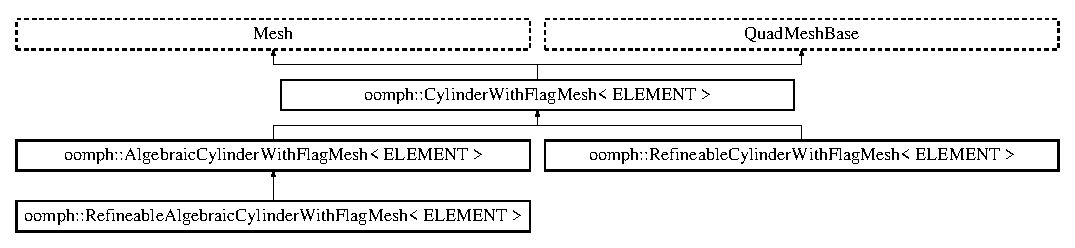
\includegraphics[height=2.886598cm]{classoomph_1_1CylinderWithFlagMesh}
\end{center}
\end{figure}
\subsection*{Public Member Functions}
\begin{DoxyCompactItemize}
\item 
\hyperlink{classoomph_1_1CylinderWithFlagMesh_a6591a2b9fdcb8080c899e34b9c8277cd}{Cylinder\+With\+Flag\+Mesh} (Circle $\ast$cylinder\+\_\+pt, Geom\+Object $\ast$top\+\_\+flag\+\_\+pt, Geom\+Object $\ast$bottom\+\_\+flag\+\_\+pt, Geom\+Object $\ast$tip\+\_\+flag\+\_\+pt, const double \&length, const double \&height, const double \&flag\+\_\+length, const double \&flag\+\_\+height, const double \&centre\+\_\+x, const double \&centre\+\_\+y, const double \&a, Time\+Stepper $\ast$time\+\_\+stepper\+\_\+pt=\&Mesh\+::\+Default\+\_\+\+Time\+Stepper)
\begin{DoxyCompactList}\small\item\em Constructor. Pass the pointers to the Geom\+Objects that parametrise the cylinder, the three edges of the flag, the length and height of the domain, the length and height of the flag, the coordinates of the centre of the cylinder and its radius. Timestepper defaults to Steady default timestepper. \end{DoxyCompactList}\item 
virtual \hyperlink{classoomph_1_1CylinderWithFlagMesh_a04fb9a6ea7a70eb8dbfb83ef73ed7b48}{$\sim$\+Cylinder\+With\+Flag\+Mesh} ()
\begin{DoxyCompactList}\small\item\em Destructor\+: Kill the domain. \end{DoxyCompactList}\item 
\hyperlink{classoomph_1_1CylinderWithFlagDomain}{Cylinder\+With\+Flag\+Domain} $\ast$ \hyperlink{classoomph_1_1CylinderWithFlagMesh_abfaa03615a4a6f99ddc9100f739cb94f}{domain\+\_\+pt} ()
\begin{DoxyCompactList}\small\item\em Access function to the domain. \end{DoxyCompactList}\end{DoxyCompactItemize}
\subsection*{Protected Attributes}
\begin{DoxyCompactItemize}
\item 
\hyperlink{classoomph_1_1CylinderWithFlagDomain}{Cylinder\+With\+Flag\+Domain} $\ast$ \hyperlink{classoomph_1_1CylinderWithFlagMesh_a257b36fed6fb0d20d108a27c6a1c5f86}{Domain\+\_\+pt}
\begin{DoxyCompactList}\small\item\em Pointer to the domain. \end{DoxyCompactList}\end{DoxyCompactItemize}


\subsection{Detailed Description}
\subsubsection*{template$<$class E\+L\+E\+M\+E\+NT$>$\newline
class oomph\+::\+Cylinder\+With\+Flag\+Mesh$<$ E\+L\+E\+M\+E\+N\+T $>$}

Domain-\/based mesh for cylinder with flag as in Turek benchmark. 

Definition at line 53 of file cylinder\+\_\+with\+\_\+flag\+\_\+mesh.\+template.\+h.



\subsection{Constructor \& Destructor Documentation}
\mbox{\Hypertarget{classoomph_1_1CylinderWithFlagMesh_a6591a2b9fdcb8080c899e34b9c8277cd}\label{classoomph_1_1CylinderWithFlagMesh_a6591a2b9fdcb8080c899e34b9c8277cd}} 
\index{oomph\+::\+Cylinder\+With\+Flag\+Mesh@{oomph\+::\+Cylinder\+With\+Flag\+Mesh}!Cylinder\+With\+Flag\+Mesh@{Cylinder\+With\+Flag\+Mesh}}
\index{Cylinder\+With\+Flag\+Mesh@{Cylinder\+With\+Flag\+Mesh}!oomph\+::\+Cylinder\+With\+Flag\+Mesh@{oomph\+::\+Cylinder\+With\+Flag\+Mesh}}
\subsubsection{\texorpdfstring{Cylinder\+With\+Flag\+Mesh()}{CylinderWithFlagMesh()}}
{\footnotesize\ttfamily template$<$class E\+L\+E\+M\+E\+NT $>$ \\
\hyperlink{classoomph_1_1CylinderWithFlagMesh}{oomph\+::\+Cylinder\+With\+Flag\+Mesh}$<$ E\+L\+E\+M\+E\+NT $>$\+::\hyperlink{classoomph_1_1CylinderWithFlagMesh}{Cylinder\+With\+Flag\+Mesh} (\begin{DoxyParamCaption}\item[{Circle $\ast$}]{cylinder\+\_\+pt,  }\item[{Geom\+Object $\ast$}]{top\+\_\+flag\+\_\+pt,  }\item[{Geom\+Object $\ast$}]{bottom\+\_\+flag\+\_\+pt,  }\item[{Geom\+Object $\ast$}]{tip\+\_\+flag\+\_\+pt,  }\item[{const double \&}]{length,  }\item[{const double \&}]{height,  }\item[{const double \&}]{flag\+\_\+length,  }\item[{const double \&}]{flag\+\_\+height,  }\item[{const double \&}]{centre\+\_\+x,  }\item[{const double \&}]{centre\+\_\+y,  }\item[{const double \&}]{a,  }\item[{Time\+Stepper $\ast$}]{time\+\_\+stepper\+\_\+pt = {\ttfamily \&Mesh\+:\+:Default\+\_\+TimeStepper} }\end{DoxyParamCaption})}



Constructor. Pass the pointers to the Geom\+Objects that parametrise the cylinder, the three edges of the flag, the length and height of the domain, the length and height of the flag, the coordinates of the centre of the cylinder and its radius. Timestepper defaults to Steady default timestepper. 



Definition at line 48 of file cylinder\+\_\+with\+\_\+flag\+\_\+mesh.\+template.\+cc.

\mbox{\Hypertarget{classoomph_1_1CylinderWithFlagMesh_a04fb9a6ea7a70eb8dbfb83ef73ed7b48}\label{classoomph_1_1CylinderWithFlagMesh_a04fb9a6ea7a70eb8dbfb83ef73ed7b48}} 
\index{oomph\+::\+Cylinder\+With\+Flag\+Mesh@{oomph\+::\+Cylinder\+With\+Flag\+Mesh}!````~Cylinder\+With\+Flag\+Mesh@{$\sim$\+Cylinder\+With\+Flag\+Mesh}}
\index{````~Cylinder\+With\+Flag\+Mesh@{$\sim$\+Cylinder\+With\+Flag\+Mesh}!oomph\+::\+Cylinder\+With\+Flag\+Mesh@{oomph\+::\+Cylinder\+With\+Flag\+Mesh}}
\subsubsection{\texorpdfstring{$\sim$\+Cylinder\+With\+Flag\+Mesh()}{~CylinderWithFlagMesh()}}
{\footnotesize\ttfamily template$<$class E\+L\+E\+M\+E\+NT $>$ \\
virtual \hyperlink{classoomph_1_1CylinderWithFlagMesh}{oomph\+::\+Cylinder\+With\+Flag\+Mesh}$<$ E\+L\+E\+M\+E\+NT $>$\+::$\sim$\hyperlink{classoomph_1_1CylinderWithFlagMesh}{Cylinder\+With\+Flag\+Mesh} (\begin{DoxyParamCaption}{ }\end{DoxyParamCaption})\hspace{0.3cm}{\ttfamily [inline]}, {\ttfamily [virtual]}}



Destructor\+: Kill the domain. 



Definition at line 78 of file cylinder\+\_\+with\+\_\+flag\+\_\+mesh.\+template.\+h.



References oomph\+::\+Cylinder\+With\+Flag\+Mesh$<$ E\+L\+E\+M\+E\+N\+T $>$\+::\+Domain\+\_\+pt.



\subsection{Member Function Documentation}
\mbox{\Hypertarget{classoomph_1_1CylinderWithFlagMesh_abfaa03615a4a6f99ddc9100f739cb94f}\label{classoomph_1_1CylinderWithFlagMesh_abfaa03615a4a6f99ddc9100f739cb94f}} 
\index{oomph\+::\+Cylinder\+With\+Flag\+Mesh@{oomph\+::\+Cylinder\+With\+Flag\+Mesh}!domain\+\_\+pt@{domain\+\_\+pt}}
\index{domain\+\_\+pt@{domain\+\_\+pt}!oomph\+::\+Cylinder\+With\+Flag\+Mesh@{oomph\+::\+Cylinder\+With\+Flag\+Mesh}}
\subsubsection{\texorpdfstring{domain\+\_\+pt()}{domain\_pt()}}
{\footnotesize\ttfamily template$<$class E\+L\+E\+M\+E\+NT $>$ \\
\hyperlink{classoomph_1_1CylinderWithFlagDomain}{Cylinder\+With\+Flag\+Domain}$\ast$ \hyperlink{classoomph_1_1CylinderWithFlagMesh}{oomph\+::\+Cylinder\+With\+Flag\+Mesh}$<$ E\+L\+E\+M\+E\+NT $>$\+::domain\+\_\+pt (\begin{DoxyParamCaption}{ }\end{DoxyParamCaption})\hspace{0.3cm}{\ttfamily [inline]}}



Access function to the domain. 



Definition at line 84 of file cylinder\+\_\+with\+\_\+flag\+\_\+mesh.\+template.\+h.



References oomph\+::\+Cylinder\+With\+Flag\+Mesh$<$ E\+L\+E\+M\+E\+N\+T $>$\+::\+Domain\+\_\+pt.



Referenced by oomph\+::\+Algebraic\+Cylinder\+With\+Flag\+Mesh$<$ E\+L\+E\+M\+E\+N\+T $>$\+::set\+\_\+bottom\+\_\+flag\+\_\+pt(), oomph\+::\+Algebraic\+Cylinder\+With\+Flag\+Mesh$<$ E\+L\+E\+M\+E\+N\+T $>$\+::set\+\_\+tip\+\_\+flag\+\_\+pt(), and oomph\+::\+Algebraic\+Cylinder\+With\+Flag\+Mesh$<$ E\+L\+E\+M\+E\+N\+T $>$\+::set\+\_\+top\+\_\+flag\+\_\+pt().



\subsection{Member Data Documentation}
\mbox{\Hypertarget{classoomph_1_1CylinderWithFlagMesh_a257b36fed6fb0d20d108a27c6a1c5f86}\label{classoomph_1_1CylinderWithFlagMesh_a257b36fed6fb0d20d108a27c6a1c5f86}} 
\index{oomph\+::\+Cylinder\+With\+Flag\+Mesh@{oomph\+::\+Cylinder\+With\+Flag\+Mesh}!Domain\+\_\+pt@{Domain\+\_\+pt}}
\index{Domain\+\_\+pt@{Domain\+\_\+pt}!oomph\+::\+Cylinder\+With\+Flag\+Mesh@{oomph\+::\+Cylinder\+With\+Flag\+Mesh}}
\subsubsection{\texorpdfstring{Domain\+\_\+pt}{Domain\_pt}}
{\footnotesize\ttfamily template$<$class E\+L\+E\+M\+E\+NT $>$ \\
\hyperlink{classoomph_1_1CylinderWithFlagDomain}{Cylinder\+With\+Flag\+Domain}$\ast$ \hyperlink{classoomph_1_1CylinderWithFlagMesh}{oomph\+::\+Cylinder\+With\+Flag\+Mesh}$<$ E\+L\+E\+M\+E\+NT $>$\+::Domain\+\_\+pt\hspace{0.3cm}{\ttfamily [protected]}}



Pointer to the domain. 



Definition at line 89 of file cylinder\+\_\+with\+\_\+flag\+\_\+mesh.\+template.\+h.



Referenced by oomph\+::\+Cylinder\+With\+Flag\+Mesh$<$ E\+L\+E\+M\+E\+N\+T $>$\+::domain\+\_\+pt(), and oomph\+::\+Cylinder\+With\+Flag\+Mesh$<$ E\+L\+E\+M\+E\+N\+T $>$\+::$\sim$\+Cylinder\+With\+Flag\+Mesh().



The documentation for this class was generated from the following files\+:\begin{DoxyCompactItemize}
\item 
\hyperlink{cylinder__with__flag__mesh_8template_8h}{cylinder\+\_\+with\+\_\+flag\+\_\+mesh.\+template.\+h}\item 
\hyperlink{cylinder__with__flag__mesh_8template_8cc}{cylinder\+\_\+with\+\_\+flag\+\_\+mesh.\+template.\+cc}\end{DoxyCompactItemize}

\hypertarget{classoomph_1_1EighthSphereDomain}{}\section{oomph\+:\+:Eighth\+Sphere\+Domain Class Reference}
\label{classoomph_1_1EighthSphereDomain}\index{oomph\+::\+Eighth\+Sphere\+Domain@{oomph\+::\+Eighth\+Sphere\+Domain}}


Eighth sphere as domain. \hyperlink{classoomph_1_1Domain}{Domain} is parametrised by four macro elements.  




{\ttfamily \#include $<$eighth\+\_\+sphere\+\_\+domain.\+h$>$}

Inheritance diagram for oomph\+:\+:Eighth\+Sphere\+Domain\+:\begin{figure}[H]
\begin{center}
\leavevmode
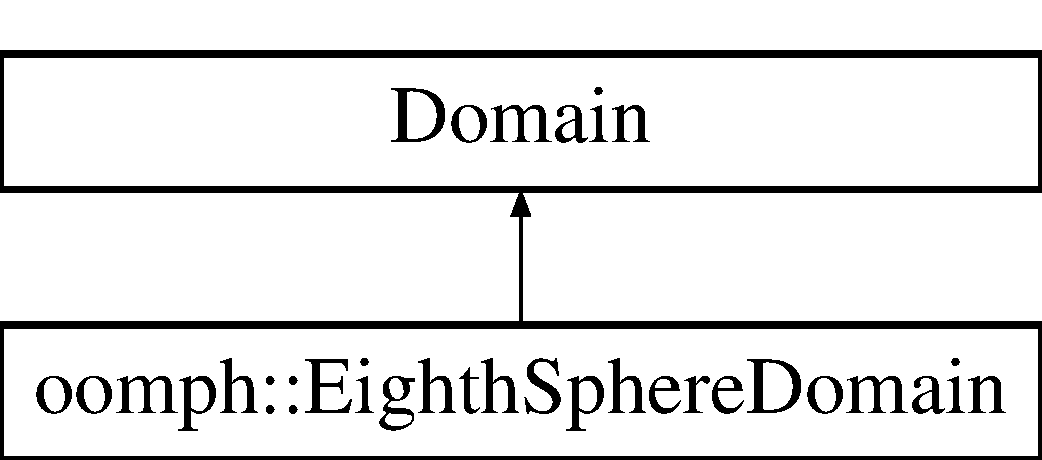
\includegraphics[height=2.000000cm]{classoomph_1_1EighthSphereDomain}
\end{center}
\end{figure}
\subsection*{Public Member Functions}
\begin{DoxyCompactItemize}
\item 
\hyperlink{classoomph_1_1EighthSphereDomain_a82c8a6b479e41bf07b9478e3d903b465}{Eighth\+Sphere\+Domain} (const double \&radius)
\begin{DoxyCompactList}\small\item\em Constructor\+: Pass the radius of the sphere. \end{DoxyCompactList}\item 
\hyperlink{classoomph_1_1EighthSphereDomain_af831fd06346e57808dca43940385e970}{Eighth\+Sphere\+Domain} (const \hyperlink{classoomph_1_1EighthSphereDomain}{Eighth\+Sphere\+Domain} \&)
\begin{DoxyCompactList}\small\item\em Broken copy constructor. \end{DoxyCompactList}\item 
void \hyperlink{classoomph_1_1EighthSphereDomain_a3533eb2f34986e995a779d2841267b12}{operator=} (const \hyperlink{classoomph_1_1EighthSphereDomain}{Eighth\+Sphere\+Domain} \&)
\begin{DoxyCompactList}\small\item\em Broken assignment operator. \end{DoxyCompactList}\item 
\hyperlink{classoomph_1_1EighthSphereDomain_ab299e8bd818573e3fca246973f1030b2}{$\sim$\+Eighth\+Sphere\+Domain} ()
\begin{DoxyCompactList}\small\item\em Destructor\+: Kill macro elements. \end{DoxyCompactList}\item 
void \hyperlink{classoomph_1_1EighthSphereDomain_a281727105819669ea9dab9fec120ea63}{macro\+\_\+element\+\_\+boundary} (const unsigned \&\hyperlink{cfortran_8h_af6f0bd3dc13317f895c91323c25c2b8f}{t}, const unsigned \&imacro, const unsigned \&idirect, const \hyperlink{classoomph_1_1Vector}{Vector}$<$ double $>$ \&\hyperlink{cfortran_8h_ab7123126e4885ef647dd9c6e3807a21c}{s}, \hyperlink{classoomph_1_1Vector}{Vector}$<$ double $>$ \&f)
\begin{DoxyCompactList}\small\item\em \hyperlink{classoomph_1_1Vector}{Vector} representation of the imacro-\/th macro element boundary idirect (L/\+R/\+D/\+U/\+B/F) at time level t (t=0\+: present; t$>$0\+: previous)\+: f(s). \end{DoxyCompactList}\end{DoxyCompactItemize}
\subsection*{Private Member Functions}
\begin{DoxyCompactItemize}
\item 
void \hyperlink{classoomph_1_1EighthSphereDomain_adc5634bf44b0689994ad68daf203e11f}{r\+\_\+centr\+\_\+L} (const unsigned \&\hyperlink{cfortran_8h_af6f0bd3dc13317f895c91323c25c2b8f}{t}, const \hyperlink{classoomph_1_1Vector}{Vector}$<$ double $>$ \&zeta, \hyperlink{classoomph_1_1Vector}{Vector}$<$ double $>$ \&f)
\begin{DoxyCompactList}\small\item\em Boundary of central box macro element zeta $ \in [-1,1]^2 $. \end{DoxyCompactList}\item 
void \hyperlink{classoomph_1_1EighthSphereDomain_a226c7c3bbcc59aa73c1033af523ef653}{r\+\_\+centr\+\_\+R} (const unsigned \&\hyperlink{cfortran_8h_af6f0bd3dc13317f895c91323c25c2b8f}{t}, const \hyperlink{classoomph_1_1Vector}{Vector}$<$ double $>$ \&zeta, \hyperlink{classoomph_1_1Vector}{Vector}$<$ double $>$ \&f)
\begin{DoxyCompactList}\small\item\em Boundary of central box macro element zeta $ \in [-1,1]^2 $. \end{DoxyCompactList}\item 
void \hyperlink{classoomph_1_1EighthSphereDomain_aa7c38e9c33934b556f59c044654500ce}{r\+\_\+centr\+\_\+D} (const unsigned \&\hyperlink{cfortran_8h_af6f0bd3dc13317f895c91323c25c2b8f}{t}, const \hyperlink{classoomph_1_1Vector}{Vector}$<$ double $>$ \&zeta, \hyperlink{classoomph_1_1Vector}{Vector}$<$ double $>$ \&f)
\begin{DoxyCompactList}\small\item\em Boundary of central box macro element zeta $ \in [-1,1]^2 $. \end{DoxyCompactList}\item 
void \hyperlink{classoomph_1_1EighthSphereDomain_afda0d6220482758cc0ad81ea848de45b}{r\+\_\+centr\+\_\+U} (const unsigned \&\hyperlink{cfortran_8h_af6f0bd3dc13317f895c91323c25c2b8f}{t}, const \hyperlink{classoomph_1_1Vector}{Vector}$<$ double $>$ \&zeta, \hyperlink{classoomph_1_1Vector}{Vector}$<$ double $>$ \&f)
\begin{DoxyCompactList}\small\item\em Boundary of central box macro element zeta $ \in [-1,1]^2 $. \end{DoxyCompactList}\item 
void \hyperlink{classoomph_1_1EighthSphereDomain_a3ba94d9786fc6c544d82a392f8bf3dd6}{r\+\_\+centr\+\_\+B} (const unsigned \&\hyperlink{cfortran_8h_af6f0bd3dc13317f895c91323c25c2b8f}{t}, const \hyperlink{classoomph_1_1Vector}{Vector}$<$ double $>$ \&zeta, \hyperlink{classoomph_1_1Vector}{Vector}$<$ double $>$ \&f)
\begin{DoxyCompactList}\small\item\em Boundary of central box macro element zeta $ \in [-1,1]^2 $. \end{DoxyCompactList}\item 
void \hyperlink{classoomph_1_1EighthSphereDomain_a080334e0a4e7cd61c97f0b2bf1174f00}{r\+\_\+centr\+\_\+F} (const unsigned \&\hyperlink{cfortran_8h_af6f0bd3dc13317f895c91323c25c2b8f}{t}, const \hyperlink{classoomph_1_1Vector}{Vector}$<$ double $>$ \&zeta, \hyperlink{classoomph_1_1Vector}{Vector}$<$ double $>$ \&f)
\begin{DoxyCompactList}\small\item\em Boundary of central box macro element zeta $ \in [-1,1]^2 $. \end{DoxyCompactList}\item 
void \hyperlink{classoomph_1_1EighthSphereDomain_ad029a857dd1b83ed10281613e0c56800}{r\+\_\+right\+\_\+L} (const unsigned \&\hyperlink{cfortran_8h_af6f0bd3dc13317f895c91323c25c2b8f}{t}, const \hyperlink{classoomph_1_1Vector}{Vector}$<$ double $>$ \&zeta, \hyperlink{classoomph_1_1Vector}{Vector}$<$ double $>$ \&f)
\begin{DoxyCompactList}\small\item\em Boundary of right box macro element zeta $ \in [-1,1]^2 $. \end{DoxyCompactList}\item 
void \hyperlink{classoomph_1_1EighthSphereDomain_a58ec95dc35f526fe5c6baa2578a2f786}{r\+\_\+right\+\_\+R} (const unsigned \&\hyperlink{cfortran_8h_af6f0bd3dc13317f895c91323c25c2b8f}{t}, const \hyperlink{classoomph_1_1Vector}{Vector}$<$ double $>$ \&zeta, \hyperlink{classoomph_1_1Vector}{Vector}$<$ double $>$ \&f)
\begin{DoxyCompactList}\small\item\em Boundary of right box macro element zeta $ \in [-1,1]^2 $. \end{DoxyCompactList}\item 
void \hyperlink{classoomph_1_1EighthSphereDomain_a7a4a1a98b542afd49a5ec8abfda287fc}{r\+\_\+right\+\_\+D} (const unsigned \&\hyperlink{cfortran_8h_af6f0bd3dc13317f895c91323c25c2b8f}{t}, const \hyperlink{classoomph_1_1Vector}{Vector}$<$ double $>$ \&zeta, \hyperlink{classoomph_1_1Vector}{Vector}$<$ double $>$ \&f)
\begin{DoxyCompactList}\small\item\em Boundary of right box macro element zeta $ \in [-1,1]^2 $. \end{DoxyCompactList}\item 
void \hyperlink{classoomph_1_1EighthSphereDomain_a004a1adfe832e2b233f8ec1b6a58b9aa}{r\+\_\+right\+\_\+U} (const unsigned \&\hyperlink{cfortran_8h_af6f0bd3dc13317f895c91323c25c2b8f}{t}, const \hyperlink{classoomph_1_1Vector}{Vector}$<$ double $>$ \&zeta, \hyperlink{classoomph_1_1Vector}{Vector}$<$ double $>$ \&f)
\begin{DoxyCompactList}\small\item\em Boundary of right box macro element zeta $ \in [-1,1]^2 $. \end{DoxyCompactList}\item 
void \hyperlink{classoomph_1_1EighthSphereDomain_ac013c364bfe2f0bb1d3393696149d249}{r\+\_\+right\+\_\+B} (const unsigned \&\hyperlink{cfortran_8h_af6f0bd3dc13317f895c91323c25c2b8f}{t}, const \hyperlink{classoomph_1_1Vector}{Vector}$<$ double $>$ \&zeta, \hyperlink{classoomph_1_1Vector}{Vector}$<$ double $>$ \&f)
\begin{DoxyCompactList}\small\item\em Boundary of right box macro element zeta $ \in [-1,1]^2 $. \end{DoxyCompactList}\item 
void \hyperlink{classoomph_1_1EighthSphereDomain_aa08635438bff5a3d377d45c8c9c2b377}{r\+\_\+right\+\_\+F} (const unsigned \&\hyperlink{cfortran_8h_af6f0bd3dc13317f895c91323c25c2b8f}{t}, const \hyperlink{classoomph_1_1Vector}{Vector}$<$ double $>$ \&zeta, \hyperlink{classoomph_1_1Vector}{Vector}$<$ double $>$ \&f)
\begin{DoxyCompactList}\small\item\em Boundary of right box macro element zeta $ \in [-1,1]^2 $. \end{DoxyCompactList}\item 
void \hyperlink{classoomph_1_1EighthSphereDomain_af9ab515958ed3699ea5ed95ec9a87d9e}{r\+\_\+up\+\_\+L} (const unsigned \&\hyperlink{cfortran_8h_af6f0bd3dc13317f895c91323c25c2b8f}{t}, const \hyperlink{classoomph_1_1Vector}{Vector}$<$ double $>$ \&zeta, \hyperlink{classoomph_1_1Vector}{Vector}$<$ double $>$ \&f)
\begin{DoxyCompactList}\small\item\em Boundary of top left box macro element zeta $ \in [-1,1]^2 $. \end{DoxyCompactList}\item 
void \hyperlink{classoomph_1_1EighthSphereDomain_ad38d27ad06d83c94c768fbda98c939e7}{r\+\_\+up\+\_\+R} (const unsigned \&\hyperlink{cfortran_8h_af6f0bd3dc13317f895c91323c25c2b8f}{t}, const \hyperlink{classoomph_1_1Vector}{Vector}$<$ double $>$ \&zeta, \hyperlink{classoomph_1_1Vector}{Vector}$<$ double $>$ \&f)
\begin{DoxyCompactList}\small\item\em Boundary of top left box macro element zeta $ \in [-1,1]^2 $. \end{DoxyCompactList}\item 
void \hyperlink{classoomph_1_1EighthSphereDomain_ad55bde69a74b24f1c9c6cc6bb277e39b}{r\+\_\+up\+\_\+D} (const unsigned \&\hyperlink{cfortran_8h_af6f0bd3dc13317f895c91323c25c2b8f}{t}, const \hyperlink{classoomph_1_1Vector}{Vector}$<$ double $>$ \&zeta, \hyperlink{classoomph_1_1Vector}{Vector}$<$ double $>$ \&f)
\begin{DoxyCompactList}\small\item\em Boundary of top left box macro element zeta $ \in [-1,1]^2 $. \end{DoxyCompactList}\item 
void \hyperlink{classoomph_1_1EighthSphereDomain_a303c406fe673675f497522dae69f849c}{r\+\_\+up\+\_\+U} (const unsigned \&\hyperlink{cfortran_8h_af6f0bd3dc13317f895c91323c25c2b8f}{t}, const \hyperlink{classoomph_1_1Vector}{Vector}$<$ double $>$ \&zeta, \hyperlink{classoomph_1_1Vector}{Vector}$<$ double $>$ \&f)
\begin{DoxyCompactList}\small\item\em Boundary of top left box macro element zeta $ \in [-1,1]^2 $. \end{DoxyCompactList}\item 
void \hyperlink{classoomph_1_1EighthSphereDomain_aaac560ab6bbe35010c1ff61a466d1252}{r\+\_\+up\+\_\+B} (const unsigned \&\hyperlink{cfortran_8h_af6f0bd3dc13317f895c91323c25c2b8f}{t}, const \hyperlink{classoomph_1_1Vector}{Vector}$<$ double $>$ \&zeta, \hyperlink{classoomph_1_1Vector}{Vector}$<$ double $>$ \&f)
\begin{DoxyCompactList}\small\item\em Boundary of top left box macro element zeta $ \in [-1,1]^2 $. \end{DoxyCompactList}\item 
void \hyperlink{classoomph_1_1EighthSphereDomain_a9e419235f4800eab872523bdbfe72fb6}{r\+\_\+up\+\_\+F} (const unsigned \&\hyperlink{cfortran_8h_af6f0bd3dc13317f895c91323c25c2b8f}{t}, const \hyperlink{classoomph_1_1Vector}{Vector}$<$ double $>$ \&zeta, \hyperlink{classoomph_1_1Vector}{Vector}$<$ double $>$ \&f)
\begin{DoxyCompactList}\small\item\em Boundary of top left box macro element zeta $ \in [-1,1]^2 $. \end{DoxyCompactList}\item 
void \hyperlink{classoomph_1_1EighthSphereDomain_a161d1ad8c0e991e9228a0725d7c9ccd9}{r\+\_\+front\+\_\+L} (const unsigned \&\hyperlink{cfortran_8h_af6f0bd3dc13317f895c91323c25c2b8f}{t}, const \hyperlink{classoomph_1_1Vector}{Vector}$<$ double $>$ \&zeta, \hyperlink{classoomph_1_1Vector}{Vector}$<$ double $>$ \&f)
\begin{DoxyCompactList}\small\item\em Boundary of top left box macro element zeta $ \in [-1,1]^2 $. \end{DoxyCompactList}\item 
void \hyperlink{classoomph_1_1EighthSphereDomain_a5d32fe51e8ca993b12f911593ad46ca7}{r\+\_\+front\+\_\+R} (const unsigned \&\hyperlink{cfortran_8h_af6f0bd3dc13317f895c91323c25c2b8f}{t}, const \hyperlink{classoomph_1_1Vector}{Vector}$<$ double $>$ \&zeta, \hyperlink{classoomph_1_1Vector}{Vector}$<$ double $>$ \&f)
\begin{DoxyCompactList}\small\item\em Boundary of top left box macro element zeta $ \in [-1,1]^2 $. \end{DoxyCompactList}\item 
void \hyperlink{classoomph_1_1EighthSphereDomain_a46ccabe44dd16cae048c302d5cfe26ee}{r\+\_\+front\+\_\+D} (const unsigned \&\hyperlink{cfortran_8h_af6f0bd3dc13317f895c91323c25c2b8f}{t}, const \hyperlink{classoomph_1_1Vector}{Vector}$<$ double $>$ \&zeta, \hyperlink{classoomph_1_1Vector}{Vector}$<$ double $>$ \&f)
\begin{DoxyCompactList}\small\item\em Boundary of top left box macro element zeta $ \in [-1,1]^2 $. \end{DoxyCompactList}\item 
void \hyperlink{classoomph_1_1EighthSphereDomain_aef12fa8f21592009e8ab51d88c301388}{r\+\_\+front\+\_\+U} (const unsigned \&\hyperlink{cfortran_8h_af6f0bd3dc13317f895c91323c25c2b8f}{t}, const \hyperlink{classoomph_1_1Vector}{Vector}$<$ double $>$ \&zeta, \hyperlink{classoomph_1_1Vector}{Vector}$<$ double $>$ \&f)
\begin{DoxyCompactList}\small\item\em Boundary of top left box macro element zeta $ \in [-1,1]^2 $. \end{DoxyCompactList}\item 
void \hyperlink{classoomph_1_1EighthSphereDomain_aa62bb16a2963530246c8cc9ef905c944}{r\+\_\+front\+\_\+B} (const unsigned \&\hyperlink{cfortran_8h_af6f0bd3dc13317f895c91323c25c2b8f}{t}, const \hyperlink{classoomph_1_1Vector}{Vector}$<$ double $>$ \&zeta, \hyperlink{classoomph_1_1Vector}{Vector}$<$ double $>$ \&f)
\begin{DoxyCompactList}\small\item\em Boundary of top left box macro element zeta $ \in [-1,1]^2 $. \end{DoxyCompactList}\item 
void \hyperlink{classoomph_1_1EighthSphereDomain_a71d48567ee2661821f41dd50793a6eb1}{r\+\_\+front\+\_\+F} (const unsigned \&\hyperlink{cfortran_8h_af6f0bd3dc13317f895c91323c25c2b8f}{t}, const \hyperlink{classoomph_1_1Vector}{Vector}$<$ double $>$ \&zeta, \hyperlink{classoomph_1_1Vector}{Vector}$<$ double $>$ \&f)
\begin{DoxyCompactList}\small\item\em Boundary of top left box macro element zeta $ \in [-1,1]^2 $. \end{DoxyCompactList}\end{DoxyCompactItemize}
\subsection*{Private Attributes}
\begin{DoxyCompactItemize}
\item 
double \hyperlink{classoomph_1_1EighthSphereDomain_a9ef9d21c2c9ed0ea28652011b1756419}{Radius}
\end{DoxyCompactItemize}
\subsection*{Additional Inherited Members}


\subsection{Detailed Description}
Eighth sphere as domain. \hyperlink{classoomph_1_1Domain}{Domain} is parametrised by four macro elements. 

Definition at line 47 of file eighth\+\_\+sphere\+\_\+domain.\+h.



\subsection{Constructor \& Destructor Documentation}
\mbox{\Hypertarget{classoomph_1_1EighthSphereDomain_a82c8a6b479e41bf07b9478e3d903b465}\label{classoomph_1_1EighthSphereDomain_a82c8a6b479e41bf07b9478e3d903b465}} 
\index{oomph\+::\+Eighth\+Sphere\+Domain@{oomph\+::\+Eighth\+Sphere\+Domain}!Eighth\+Sphere\+Domain@{Eighth\+Sphere\+Domain}}
\index{Eighth\+Sphere\+Domain@{Eighth\+Sphere\+Domain}!oomph\+::\+Eighth\+Sphere\+Domain@{oomph\+::\+Eighth\+Sphere\+Domain}}
\subsubsection{\texorpdfstring{Eighth\+Sphere\+Domain()}{EighthSphereDomain()}\hspace{0.1cm}{\footnotesize\ttfamily [1/2]}}
{\footnotesize\ttfamily oomph\+::\+Eighth\+Sphere\+Domain\+::\+Eighth\+Sphere\+Domain (\begin{DoxyParamCaption}\item[{const double \&}]{radius }\end{DoxyParamCaption})\hspace{0.3cm}{\ttfamily [inline]}}



Constructor\+: Pass the radius of the sphere. 



Definition at line 53 of file eighth\+\_\+sphere\+\_\+domain.\+h.



References i, and oomph\+::\+Domain\+::\+Macro\+\_\+element\+\_\+pt.

\mbox{\Hypertarget{classoomph_1_1EighthSphereDomain_af831fd06346e57808dca43940385e970}\label{classoomph_1_1EighthSphereDomain_af831fd06346e57808dca43940385e970}} 
\index{oomph\+::\+Eighth\+Sphere\+Domain@{oomph\+::\+Eighth\+Sphere\+Domain}!Eighth\+Sphere\+Domain@{Eighth\+Sphere\+Domain}}
\index{Eighth\+Sphere\+Domain@{Eighth\+Sphere\+Domain}!oomph\+::\+Eighth\+Sphere\+Domain@{oomph\+::\+Eighth\+Sphere\+Domain}}
\subsubsection{\texorpdfstring{Eighth\+Sphere\+Domain()}{EighthSphereDomain()}\hspace{0.1cm}{\footnotesize\ttfamily [2/2]}}
{\footnotesize\ttfamily oomph\+::\+Eighth\+Sphere\+Domain\+::\+Eighth\+Sphere\+Domain (\begin{DoxyParamCaption}\item[{const \hyperlink{classoomph_1_1EighthSphereDomain}{Eighth\+Sphere\+Domain} \&}]{ }\end{DoxyParamCaption})\hspace{0.3cm}{\ttfamily [inline]}}



Broken copy constructor. 



Definition at line 69 of file eighth\+\_\+sphere\+\_\+domain.\+h.



References oomph\+::\+Broken\+Copy\+::broken\+\_\+copy().

\mbox{\Hypertarget{classoomph_1_1EighthSphereDomain_ab299e8bd818573e3fca246973f1030b2}\label{classoomph_1_1EighthSphereDomain_ab299e8bd818573e3fca246973f1030b2}} 
\index{oomph\+::\+Eighth\+Sphere\+Domain@{oomph\+::\+Eighth\+Sphere\+Domain}!````~Eighth\+Sphere\+Domain@{$\sim$\+Eighth\+Sphere\+Domain}}
\index{````~Eighth\+Sphere\+Domain@{$\sim$\+Eighth\+Sphere\+Domain}!oomph\+::\+Eighth\+Sphere\+Domain@{oomph\+::\+Eighth\+Sphere\+Domain}}
\subsubsection{\texorpdfstring{$\sim$\+Eighth\+Sphere\+Domain()}{~EighthSphereDomain()}}
{\footnotesize\ttfamily oomph\+::\+Eighth\+Sphere\+Domain\+::$\sim$\+Eighth\+Sphere\+Domain (\begin{DoxyParamCaption}{ }\end{DoxyParamCaption})\hspace{0.3cm}{\ttfamily [inline]}}



Destructor\+: Kill macro elements. 



Definition at line 82 of file eighth\+\_\+sphere\+\_\+domain.\+h.



References i, and oomph\+::\+Domain\+::\+Macro\+\_\+element\+\_\+pt.



\subsection{Member Function Documentation}
\mbox{\Hypertarget{classoomph_1_1EighthSphereDomain_a281727105819669ea9dab9fec120ea63}\label{classoomph_1_1EighthSphereDomain_a281727105819669ea9dab9fec120ea63}} 
\index{oomph\+::\+Eighth\+Sphere\+Domain@{oomph\+::\+Eighth\+Sphere\+Domain}!macro\+\_\+element\+\_\+boundary@{macro\+\_\+element\+\_\+boundary}}
\index{macro\+\_\+element\+\_\+boundary@{macro\+\_\+element\+\_\+boundary}!oomph\+::\+Eighth\+Sphere\+Domain@{oomph\+::\+Eighth\+Sphere\+Domain}}
\subsubsection{\texorpdfstring{macro\+\_\+element\+\_\+boundary()}{macro\_element\_boundary()}}
{\footnotesize\ttfamily void oomph\+::\+Eighth\+Sphere\+Domain\+::macro\+\_\+element\+\_\+boundary (\begin{DoxyParamCaption}\item[{const unsigned \&}]{t,  }\item[{const unsigned \&}]{imacro,  }\item[{const unsigned \&}]{idirect,  }\item[{const \hyperlink{classoomph_1_1Vector}{Vector}$<$ double $>$ \&}]{s,  }\item[{\hyperlink{classoomph_1_1Vector}{Vector}$<$ double $>$ \&}]{f }\end{DoxyParamCaption})\hspace{0.3cm}{\ttfamily [inline]}, {\ttfamily [virtual]}}



\hyperlink{classoomph_1_1Vector}{Vector} representation of the imacro-\/th macro element boundary idirect (L/\+R/\+D/\+U/\+B/F) at time level t (t=0\+: present; t$>$0\+: previous)\+: f(s). 



Implements \hyperlink{classoomph_1_1Domain_a95f3e00d28ea37e6c4d3027bfac91096}{oomph\+::\+Domain}.



Definition at line 95 of file eighth\+\_\+sphere\+\_\+domain.\+h.



References oomph\+::\+Oc\+Tree\+Names\+::B, oomph\+::\+Oc\+Tree\+Names\+::D, oomph\+::\+Oc\+Tree\+::\+Direct\+\_\+string, oomph\+::\+Oc\+Tree\+Names\+::F, oomph\+::\+Binary\+Tree\+Names\+::L, oomph\+::\+Binary\+Tree\+Names\+::R, r\+\_\+centr\+\_\+\+B(), r\+\_\+centr\+\_\+\+D(), r\+\_\+centr\+\_\+\+F(), r\+\_\+centr\+\_\+\+L(), r\+\_\+centr\+\_\+\+R(), r\+\_\+centr\+\_\+\+U(), r\+\_\+front\+\_\+\+B(), r\+\_\+front\+\_\+\+D(), r\+\_\+front\+\_\+\+F(), r\+\_\+front\+\_\+\+L(), r\+\_\+front\+\_\+\+R(), r\+\_\+front\+\_\+\+U(), r\+\_\+right\+\_\+\+B(), r\+\_\+right\+\_\+\+D(), r\+\_\+right\+\_\+\+F(), r\+\_\+right\+\_\+\+L(), r\+\_\+right\+\_\+\+R(), r\+\_\+right\+\_\+\+U(), r\+\_\+up\+\_\+\+B(), r\+\_\+up\+\_\+\+D(), r\+\_\+up\+\_\+\+F(), r\+\_\+up\+\_\+\+L(), r\+\_\+up\+\_\+\+R(), r\+\_\+up\+\_\+\+U(), and oomph\+::\+Oc\+Tree\+Names\+::U.

\mbox{\Hypertarget{classoomph_1_1EighthSphereDomain_a3533eb2f34986e995a779d2841267b12}\label{classoomph_1_1EighthSphereDomain_a3533eb2f34986e995a779d2841267b12}} 
\index{oomph\+::\+Eighth\+Sphere\+Domain@{oomph\+::\+Eighth\+Sphere\+Domain}!operator=@{operator=}}
\index{operator=@{operator=}!oomph\+::\+Eighth\+Sphere\+Domain@{oomph\+::\+Eighth\+Sphere\+Domain}}
\subsubsection{\texorpdfstring{operator=()}{operator=()}}
{\footnotesize\ttfamily void oomph\+::\+Eighth\+Sphere\+Domain\+::operator= (\begin{DoxyParamCaption}\item[{const \hyperlink{classoomph_1_1EighthSphereDomain}{Eighth\+Sphere\+Domain} \&}]{ }\end{DoxyParamCaption})\hspace{0.3cm}{\ttfamily [inline]}}



Broken assignment operator. 



Definition at line 75 of file eighth\+\_\+sphere\+\_\+domain.\+h.



References oomph\+::\+Broken\+Copy\+::broken\+\_\+assign().

\mbox{\Hypertarget{classoomph_1_1EighthSphereDomain_a3ba94d9786fc6c544d82a392f8bf3dd6}\label{classoomph_1_1EighthSphereDomain_a3ba94d9786fc6c544d82a392f8bf3dd6}} 
\index{oomph\+::\+Eighth\+Sphere\+Domain@{oomph\+::\+Eighth\+Sphere\+Domain}!r\+\_\+centr\+\_\+B@{r\+\_\+centr\+\_\+B}}
\index{r\+\_\+centr\+\_\+B@{r\+\_\+centr\+\_\+B}!oomph\+::\+Eighth\+Sphere\+Domain@{oomph\+::\+Eighth\+Sphere\+Domain}}
\subsubsection{\texorpdfstring{r\+\_\+centr\+\_\+\+B()}{r\_centr\_B()}}
{\footnotesize\ttfamily void oomph\+::\+Eighth\+Sphere\+Domain\+::r\+\_\+centr\+\_\+B (\begin{DoxyParamCaption}\item[{const unsigned \&}]{t,  }\item[{const \hyperlink{classoomph_1_1Vector}{Vector}$<$ double $>$ \&}]{zeta,  }\item[{\hyperlink{classoomph_1_1Vector}{Vector}$<$ double $>$ \&}]{f }\end{DoxyParamCaption})\hspace{0.3cm}{\ttfamily [private]}}



Boundary of central box macro element zeta $ \in [-1,1]^2 $. 

Boundary of central box macro element zeta $ \in [-1,1]^2 $ 

Definition at line 495 of file eighth\+\_\+sphere\+\_\+domain.\+h.



References Radius.



Referenced by macro\+\_\+element\+\_\+boundary().

\mbox{\Hypertarget{classoomph_1_1EighthSphereDomain_aa7c38e9c33934b556f59c044654500ce}\label{classoomph_1_1EighthSphereDomain_aa7c38e9c33934b556f59c044654500ce}} 
\index{oomph\+::\+Eighth\+Sphere\+Domain@{oomph\+::\+Eighth\+Sphere\+Domain}!r\+\_\+centr\+\_\+D@{r\+\_\+centr\+\_\+D}}
\index{r\+\_\+centr\+\_\+D@{r\+\_\+centr\+\_\+D}!oomph\+::\+Eighth\+Sphere\+Domain@{oomph\+::\+Eighth\+Sphere\+Domain}}
\subsubsection{\texorpdfstring{r\+\_\+centr\+\_\+\+D()}{r\_centr\_D()}}
{\footnotesize\ttfamily void oomph\+::\+Eighth\+Sphere\+Domain\+::r\+\_\+centr\+\_\+D (\begin{DoxyParamCaption}\item[{const unsigned \&}]{t,  }\item[{const \hyperlink{classoomph_1_1Vector}{Vector}$<$ double $>$ \&}]{zeta,  }\item[{\hyperlink{classoomph_1_1Vector}{Vector}$<$ double $>$ \&}]{f }\end{DoxyParamCaption})\hspace{0.3cm}{\ttfamily [private]}}



Boundary of central box macro element zeta $ \in [-1,1]^2 $. 

Boundary of central box macro element zeta $ \in [-1,1]^2 $ 

Definition at line 466 of file eighth\+\_\+sphere\+\_\+domain.\+h.



References Radius.



Referenced by macro\+\_\+element\+\_\+boundary().

\mbox{\Hypertarget{classoomph_1_1EighthSphereDomain_a080334e0a4e7cd61c97f0b2bf1174f00}\label{classoomph_1_1EighthSphereDomain_a080334e0a4e7cd61c97f0b2bf1174f00}} 
\index{oomph\+::\+Eighth\+Sphere\+Domain@{oomph\+::\+Eighth\+Sphere\+Domain}!r\+\_\+centr\+\_\+F@{r\+\_\+centr\+\_\+F}}
\index{r\+\_\+centr\+\_\+F@{r\+\_\+centr\+\_\+F}!oomph\+::\+Eighth\+Sphere\+Domain@{oomph\+::\+Eighth\+Sphere\+Domain}}
\subsubsection{\texorpdfstring{r\+\_\+centr\+\_\+\+F()}{r\_centr\_F()}}
{\footnotesize\ttfamily void oomph\+::\+Eighth\+Sphere\+Domain\+::r\+\_\+centr\+\_\+F (\begin{DoxyParamCaption}\item[{const unsigned \&}]{t,  }\item[{const \hyperlink{classoomph_1_1Vector}{Vector}$<$ double $>$ \&}]{zeta,  }\item[{\hyperlink{classoomph_1_1Vector}{Vector}$<$ double $>$ \&}]{f }\end{DoxyParamCaption})\hspace{0.3cm}{\ttfamily [private]}}



Boundary of central box macro element zeta $ \in [-1,1]^2 $. 

Boundary of central box macro element zeta $ \in [-1,1]^2 $ 

Definition at line 508 of file eighth\+\_\+sphere\+\_\+domain.\+h.



References Radius.



Referenced by macro\+\_\+element\+\_\+boundary(), and r\+\_\+front\+\_\+\+B().

\mbox{\Hypertarget{classoomph_1_1EighthSphereDomain_adc5634bf44b0689994ad68daf203e11f}\label{classoomph_1_1EighthSphereDomain_adc5634bf44b0689994ad68daf203e11f}} 
\index{oomph\+::\+Eighth\+Sphere\+Domain@{oomph\+::\+Eighth\+Sphere\+Domain}!r\+\_\+centr\+\_\+L@{r\+\_\+centr\+\_\+L}}
\index{r\+\_\+centr\+\_\+L@{r\+\_\+centr\+\_\+L}!oomph\+::\+Eighth\+Sphere\+Domain@{oomph\+::\+Eighth\+Sphere\+Domain}}
\subsubsection{\texorpdfstring{r\+\_\+centr\+\_\+\+L()}{r\_centr\_L()}}
{\footnotesize\ttfamily void oomph\+::\+Eighth\+Sphere\+Domain\+::r\+\_\+centr\+\_\+L (\begin{DoxyParamCaption}\item[{const unsigned \&}]{t,  }\item[{const \hyperlink{classoomph_1_1Vector}{Vector}$<$ double $>$ \&}]{zeta,  }\item[{\hyperlink{classoomph_1_1Vector}{Vector}$<$ double $>$ \&}]{f }\end{DoxyParamCaption})\hspace{0.3cm}{\ttfamily [private]}}



Boundary of central box macro element zeta $ \in [-1,1]^2 $. 

Boundary of central box macro element zeta $ \in [-1,1]^2 $ 

Definition at line 436 of file eighth\+\_\+sphere\+\_\+domain.\+h.



References Radius.



Referenced by macro\+\_\+element\+\_\+boundary().

\mbox{\Hypertarget{classoomph_1_1EighthSphereDomain_a226c7c3bbcc59aa73c1033af523ef653}\label{classoomph_1_1EighthSphereDomain_a226c7c3bbcc59aa73c1033af523ef653}} 
\index{oomph\+::\+Eighth\+Sphere\+Domain@{oomph\+::\+Eighth\+Sphere\+Domain}!r\+\_\+centr\+\_\+R@{r\+\_\+centr\+\_\+R}}
\index{r\+\_\+centr\+\_\+R@{r\+\_\+centr\+\_\+R}!oomph\+::\+Eighth\+Sphere\+Domain@{oomph\+::\+Eighth\+Sphere\+Domain}}
\subsubsection{\texorpdfstring{r\+\_\+centr\+\_\+\+R()}{r\_centr\_R()}}
{\footnotesize\ttfamily void oomph\+::\+Eighth\+Sphere\+Domain\+::r\+\_\+centr\+\_\+R (\begin{DoxyParamCaption}\item[{const unsigned \&}]{t,  }\item[{const \hyperlink{classoomph_1_1Vector}{Vector}$<$ double $>$ \&}]{zeta,  }\item[{\hyperlink{classoomph_1_1Vector}{Vector}$<$ double $>$ \&}]{f }\end{DoxyParamCaption})\hspace{0.3cm}{\ttfamily [private]}}



Boundary of central box macro element zeta $ \in [-1,1]^2 $. 

Boundary of central box macro element zeta $ \in [-1,1]^2 $ 

Definition at line 450 of file eighth\+\_\+sphere\+\_\+domain.\+h.



References Radius.



Referenced by macro\+\_\+element\+\_\+boundary(), and r\+\_\+right\+\_\+\+L().

\mbox{\Hypertarget{classoomph_1_1EighthSphereDomain_afda0d6220482758cc0ad81ea848de45b}\label{classoomph_1_1EighthSphereDomain_afda0d6220482758cc0ad81ea848de45b}} 
\index{oomph\+::\+Eighth\+Sphere\+Domain@{oomph\+::\+Eighth\+Sphere\+Domain}!r\+\_\+centr\+\_\+U@{r\+\_\+centr\+\_\+U}}
\index{r\+\_\+centr\+\_\+U@{r\+\_\+centr\+\_\+U}!oomph\+::\+Eighth\+Sphere\+Domain@{oomph\+::\+Eighth\+Sphere\+Domain}}
\subsubsection{\texorpdfstring{r\+\_\+centr\+\_\+\+U()}{r\_centr\_U()}}
{\footnotesize\ttfamily void oomph\+::\+Eighth\+Sphere\+Domain\+::r\+\_\+centr\+\_\+U (\begin{DoxyParamCaption}\item[{const unsigned \&}]{t,  }\item[{const \hyperlink{classoomph_1_1Vector}{Vector}$<$ double $>$ \&}]{zeta,  }\item[{\hyperlink{classoomph_1_1Vector}{Vector}$<$ double $>$ \&}]{f }\end{DoxyParamCaption})\hspace{0.3cm}{\ttfamily [private]}}



Boundary of central box macro element zeta $ \in [-1,1]^2 $. 

Boundary of central box macro element zeta $ \in [-1,1]^2 $ 

Definition at line 480 of file eighth\+\_\+sphere\+\_\+domain.\+h.



References Radius.



Referenced by macro\+\_\+element\+\_\+boundary(), and r\+\_\+up\+\_\+\+D().

\mbox{\Hypertarget{classoomph_1_1EighthSphereDomain_aa62bb16a2963530246c8cc9ef905c944}\label{classoomph_1_1EighthSphereDomain_aa62bb16a2963530246c8cc9ef905c944}} 
\index{oomph\+::\+Eighth\+Sphere\+Domain@{oomph\+::\+Eighth\+Sphere\+Domain}!r\+\_\+front\+\_\+B@{r\+\_\+front\+\_\+B}}
\index{r\+\_\+front\+\_\+B@{r\+\_\+front\+\_\+B}!oomph\+::\+Eighth\+Sphere\+Domain@{oomph\+::\+Eighth\+Sphere\+Domain}}
\subsubsection{\texorpdfstring{r\+\_\+front\+\_\+\+B()}{r\_front\_B()}}
{\footnotesize\ttfamily void oomph\+::\+Eighth\+Sphere\+Domain\+::r\+\_\+front\+\_\+B (\begin{DoxyParamCaption}\item[{const unsigned \&}]{t,  }\item[{const \hyperlink{classoomph_1_1Vector}{Vector}$<$ double $>$ \&}]{zeta,  }\item[{\hyperlink{classoomph_1_1Vector}{Vector}$<$ double $>$ \&}]{f }\end{DoxyParamCaption})\hspace{0.3cm}{\ttfamily [private]}}



Boundary of top left box macro element zeta $ \in [-1,1]^2 $. 

Boundary of top left box macro element zeta $ \in [-1,1]^2 $ 

Definition at line 908 of file eighth\+\_\+sphere\+\_\+domain.\+h.



References r\+\_\+centr\+\_\+\+F().



Referenced by macro\+\_\+element\+\_\+boundary().

\mbox{\Hypertarget{classoomph_1_1EighthSphereDomain_a46ccabe44dd16cae048c302d5cfe26ee}\label{classoomph_1_1EighthSphereDomain_a46ccabe44dd16cae048c302d5cfe26ee}} 
\index{oomph\+::\+Eighth\+Sphere\+Domain@{oomph\+::\+Eighth\+Sphere\+Domain}!r\+\_\+front\+\_\+D@{r\+\_\+front\+\_\+D}}
\index{r\+\_\+front\+\_\+D@{r\+\_\+front\+\_\+D}!oomph\+::\+Eighth\+Sphere\+Domain@{oomph\+::\+Eighth\+Sphere\+Domain}}
\subsubsection{\texorpdfstring{r\+\_\+front\+\_\+\+D()}{r\_front\_D()}}
{\footnotesize\ttfamily void oomph\+::\+Eighth\+Sphere\+Domain\+::r\+\_\+front\+\_\+D (\begin{DoxyParamCaption}\item[{const unsigned \&}]{t,  }\item[{const \hyperlink{classoomph_1_1Vector}{Vector}$<$ double $>$ \&}]{zeta,  }\item[{\hyperlink{classoomph_1_1Vector}{Vector}$<$ double $>$ \&}]{f }\end{DoxyParamCaption})\hspace{0.3cm}{\ttfamily [private]}}



Boundary of top left box macro element zeta $ \in [-1,1]^2 $. 

Boundary of top left box macro element zeta $ \in [-1,1]^2 $ 

Definition at line 867 of file eighth\+\_\+sphere\+\_\+domain.\+h.



References i, r\+\_\+front\+\_\+\+F(), and Radius.



Referenced by macro\+\_\+element\+\_\+boundary().

\mbox{\Hypertarget{classoomph_1_1EighthSphereDomain_a71d48567ee2661821f41dd50793a6eb1}\label{classoomph_1_1EighthSphereDomain_a71d48567ee2661821f41dd50793a6eb1}} 
\index{oomph\+::\+Eighth\+Sphere\+Domain@{oomph\+::\+Eighth\+Sphere\+Domain}!r\+\_\+front\+\_\+F@{r\+\_\+front\+\_\+F}}
\index{r\+\_\+front\+\_\+F@{r\+\_\+front\+\_\+F}!oomph\+::\+Eighth\+Sphere\+Domain@{oomph\+::\+Eighth\+Sphere\+Domain}}
\subsubsection{\texorpdfstring{r\+\_\+front\+\_\+\+F()}{r\_front\_F()}}
{\footnotesize\ttfamily void oomph\+::\+Eighth\+Sphere\+Domain\+::r\+\_\+front\+\_\+F (\begin{DoxyParamCaption}\item[{const unsigned \&}]{t,  }\item[{const \hyperlink{classoomph_1_1Vector}{Vector}$<$ double $>$ \&}]{zeta,  }\item[{\hyperlink{classoomph_1_1Vector}{Vector}$<$ double $>$ \&}]{f }\end{DoxyParamCaption})\hspace{0.3cm}{\ttfamily [private]}}



Boundary of top left box macro element zeta $ \in [-1,1]^2 $. 

Boundary of top left box macro element zeta $ \in [-1,1]^2 $ 

Definition at line 920 of file eighth\+\_\+sphere\+\_\+domain.\+h.



References i, and Radius.



Referenced by macro\+\_\+element\+\_\+boundary(), r\+\_\+front\+\_\+\+D(), and r\+\_\+front\+\_\+\+L().

\mbox{\Hypertarget{classoomph_1_1EighthSphereDomain_a161d1ad8c0e991e9228a0725d7c9ccd9}\label{classoomph_1_1EighthSphereDomain_a161d1ad8c0e991e9228a0725d7c9ccd9}} 
\index{oomph\+::\+Eighth\+Sphere\+Domain@{oomph\+::\+Eighth\+Sphere\+Domain}!r\+\_\+front\+\_\+L@{r\+\_\+front\+\_\+L}}
\index{r\+\_\+front\+\_\+L@{r\+\_\+front\+\_\+L}!oomph\+::\+Eighth\+Sphere\+Domain@{oomph\+::\+Eighth\+Sphere\+Domain}}
\subsubsection{\texorpdfstring{r\+\_\+front\+\_\+\+L()}{r\_front\_L()}}
{\footnotesize\ttfamily void oomph\+::\+Eighth\+Sphere\+Domain\+::r\+\_\+front\+\_\+L (\begin{DoxyParamCaption}\item[{const unsigned \&}]{t,  }\item[{const \hyperlink{classoomph_1_1Vector}{Vector}$<$ double $>$ \&}]{zeta,  }\item[{\hyperlink{classoomph_1_1Vector}{Vector}$<$ double $>$ \&}]{f }\end{DoxyParamCaption})\hspace{0.3cm}{\ttfamily [private]}}



Boundary of top left box macro element zeta $ \in [-1,1]^2 $. 

Boundary of top left box macro element zeta $ \in [-1,1]^2 $ 

Definition at line 823 of file eighth\+\_\+sphere\+\_\+domain.\+h.



References i, r\+\_\+front\+\_\+\+F(), and Radius.



Referenced by macro\+\_\+element\+\_\+boundary().

\mbox{\Hypertarget{classoomph_1_1EighthSphereDomain_a5d32fe51e8ca993b12f911593ad46ca7}\label{classoomph_1_1EighthSphereDomain_a5d32fe51e8ca993b12f911593ad46ca7}} 
\index{oomph\+::\+Eighth\+Sphere\+Domain@{oomph\+::\+Eighth\+Sphere\+Domain}!r\+\_\+front\+\_\+R@{r\+\_\+front\+\_\+R}}
\index{r\+\_\+front\+\_\+R@{r\+\_\+front\+\_\+R}!oomph\+::\+Eighth\+Sphere\+Domain@{oomph\+::\+Eighth\+Sphere\+Domain}}
\subsubsection{\texorpdfstring{r\+\_\+front\+\_\+\+R()}{r\_front\_R()}}
{\footnotesize\ttfamily void oomph\+::\+Eighth\+Sphere\+Domain\+::r\+\_\+front\+\_\+R (\begin{DoxyParamCaption}\item[{const unsigned \&}]{t,  }\item[{const \hyperlink{classoomph_1_1Vector}{Vector}$<$ double $>$ \&}]{zeta,  }\item[{\hyperlink{classoomph_1_1Vector}{Vector}$<$ double $>$ \&}]{f }\end{DoxyParamCaption})\hspace{0.3cm}{\ttfamily [private]}}



Boundary of top left box macro element zeta $ \in [-1,1]^2 $. 

Boundary of top left box macro element zeta $ \in [-1,1]^2 $ 

Definition at line 852 of file eighth\+\_\+sphere\+\_\+domain.\+h.



References r\+\_\+right\+\_\+\+F().



Referenced by macro\+\_\+element\+\_\+boundary().

\mbox{\Hypertarget{classoomph_1_1EighthSphereDomain_aef12fa8f21592009e8ab51d88c301388}\label{classoomph_1_1EighthSphereDomain_aef12fa8f21592009e8ab51d88c301388}} 
\index{oomph\+::\+Eighth\+Sphere\+Domain@{oomph\+::\+Eighth\+Sphere\+Domain}!r\+\_\+front\+\_\+U@{r\+\_\+front\+\_\+U}}
\index{r\+\_\+front\+\_\+U@{r\+\_\+front\+\_\+U}!oomph\+::\+Eighth\+Sphere\+Domain@{oomph\+::\+Eighth\+Sphere\+Domain}}
\subsubsection{\texorpdfstring{r\+\_\+front\+\_\+\+U()}{r\_front\_U()}}
{\footnotesize\ttfamily void oomph\+::\+Eighth\+Sphere\+Domain\+::r\+\_\+front\+\_\+U (\begin{DoxyParamCaption}\item[{const unsigned \&}]{t,  }\item[{const \hyperlink{classoomph_1_1Vector}{Vector}$<$ double $>$ \&}]{zeta,  }\item[{\hyperlink{classoomph_1_1Vector}{Vector}$<$ double $>$ \&}]{f }\end{DoxyParamCaption})\hspace{0.3cm}{\ttfamily [private]}}



Boundary of top left box macro element zeta $ \in [-1,1]^2 $. 

Boundary of top left box macro element zeta $ \in [-1,1]^2 $ 

Definition at line 896 of file eighth\+\_\+sphere\+\_\+domain.\+h.



References r\+\_\+up\+\_\+\+F().



Referenced by macro\+\_\+element\+\_\+boundary().

\mbox{\Hypertarget{classoomph_1_1EighthSphereDomain_ac013c364bfe2f0bb1d3393696149d249}\label{classoomph_1_1EighthSphereDomain_ac013c364bfe2f0bb1d3393696149d249}} 
\index{oomph\+::\+Eighth\+Sphere\+Domain@{oomph\+::\+Eighth\+Sphere\+Domain}!r\+\_\+right\+\_\+B@{r\+\_\+right\+\_\+B}}
\index{r\+\_\+right\+\_\+B@{r\+\_\+right\+\_\+B}!oomph\+::\+Eighth\+Sphere\+Domain@{oomph\+::\+Eighth\+Sphere\+Domain}}
\subsubsection{\texorpdfstring{r\+\_\+right\+\_\+\+B()}{r\_right\_B()}}
{\footnotesize\ttfamily void oomph\+::\+Eighth\+Sphere\+Domain\+::r\+\_\+right\+\_\+B (\begin{DoxyParamCaption}\item[{const unsigned \&}]{t,  }\item[{const \hyperlink{classoomph_1_1Vector}{Vector}$<$ double $>$ \&}]{zeta,  }\item[{\hyperlink{classoomph_1_1Vector}{Vector}$<$ double $>$ \&}]{f }\end{DoxyParamCaption})\hspace{0.3cm}{\ttfamily [private]}}



Boundary of right box macro element zeta $ \in [-1,1]^2 $. 

Boundary of right box macro element zeta $ \in [-1,1]^2 $ 

Definition at line 624 of file eighth\+\_\+sphere\+\_\+domain.\+h.



References i, r\+\_\+right\+\_\+\+R(), and Radius.



Referenced by macro\+\_\+element\+\_\+boundary().

\mbox{\Hypertarget{classoomph_1_1EighthSphereDomain_a7a4a1a98b542afd49a5ec8abfda287fc}\label{classoomph_1_1EighthSphereDomain_a7a4a1a98b542afd49a5ec8abfda287fc}} 
\index{oomph\+::\+Eighth\+Sphere\+Domain@{oomph\+::\+Eighth\+Sphere\+Domain}!r\+\_\+right\+\_\+D@{r\+\_\+right\+\_\+D}}
\index{r\+\_\+right\+\_\+D@{r\+\_\+right\+\_\+D}!oomph\+::\+Eighth\+Sphere\+Domain@{oomph\+::\+Eighth\+Sphere\+Domain}}
\subsubsection{\texorpdfstring{r\+\_\+right\+\_\+\+D()}{r\_right\_D()}}
{\footnotesize\ttfamily void oomph\+::\+Eighth\+Sphere\+Domain\+::r\+\_\+right\+\_\+D (\begin{DoxyParamCaption}\item[{const unsigned \&}]{t,  }\item[{const \hyperlink{classoomph_1_1Vector}{Vector}$<$ double $>$ \&}]{zeta,  }\item[{\hyperlink{classoomph_1_1Vector}{Vector}$<$ double $>$ \&}]{f }\end{DoxyParamCaption})\hspace{0.3cm}{\ttfamily [private]}}



Boundary of right box macro element zeta $ \in [-1,1]^2 $. 

Boundary of right box macro element zeta $ \in [-1,1]^2 $ 

Definition at line 569 of file eighth\+\_\+sphere\+\_\+domain.\+h.



References i, r\+\_\+right\+\_\+\+R(), and Radius.



Referenced by macro\+\_\+element\+\_\+boundary().

\mbox{\Hypertarget{classoomph_1_1EighthSphereDomain_aa08635438bff5a3d377d45c8c9c2b377}\label{classoomph_1_1EighthSphereDomain_aa08635438bff5a3d377d45c8c9c2b377}} 
\index{oomph\+::\+Eighth\+Sphere\+Domain@{oomph\+::\+Eighth\+Sphere\+Domain}!r\+\_\+right\+\_\+F@{r\+\_\+right\+\_\+F}}
\index{r\+\_\+right\+\_\+F@{r\+\_\+right\+\_\+F}!oomph\+::\+Eighth\+Sphere\+Domain@{oomph\+::\+Eighth\+Sphere\+Domain}}
\subsubsection{\texorpdfstring{r\+\_\+right\+\_\+\+F()}{r\_right\_F()}}
{\footnotesize\ttfamily void oomph\+::\+Eighth\+Sphere\+Domain\+::r\+\_\+right\+\_\+F (\begin{DoxyParamCaption}\item[{const unsigned \&}]{t,  }\item[{const \hyperlink{classoomph_1_1Vector}{Vector}$<$ double $>$ \&}]{zeta,  }\item[{\hyperlink{classoomph_1_1Vector}{Vector}$<$ double $>$ \&}]{f }\end{DoxyParamCaption})\hspace{0.3cm}{\ttfamily [private]}}



Boundary of right box macro element zeta $ \in [-1,1]^2 $. 

Boundary of right box macro element zeta $ \in [-1,1]^2 $ 

Definition at line 652 of file eighth\+\_\+sphere\+\_\+domain.\+h.



References i, r\+\_\+right\+\_\+\+R(), and Radius.



Referenced by macro\+\_\+element\+\_\+boundary(), and r\+\_\+front\+\_\+\+R().

\mbox{\Hypertarget{classoomph_1_1EighthSphereDomain_ad029a857dd1b83ed10281613e0c56800}\label{classoomph_1_1EighthSphereDomain_ad029a857dd1b83ed10281613e0c56800}} 
\index{oomph\+::\+Eighth\+Sphere\+Domain@{oomph\+::\+Eighth\+Sphere\+Domain}!r\+\_\+right\+\_\+L@{r\+\_\+right\+\_\+L}}
\index{r\+\_\+right\+\_\+L@{r\+\_\+right\+\_\+L}!oomph\+::\+Eighth\+Sphere\+Domain@{oomph\+::\+Eighth\+Sphere\+Domain}}
\subsubsection{\texorpdfstring{r\+\_\+right\+\_\+\+L()}{r\_right\_L()}}
{\footnotesize\ttfamily void oomph\+::\+Eighth\+Sphere\+Domain\+::r\+\_\+right\+\_\+L (\begin{DoxyParamCaption}\item[{const unsigned \&}]{t,  }\item[{const \hyperlink{classoomph_1_1Vector}{Vector}$<$ double $>$ \&}]{zeta,  }\item[{\hyperlink{classoomph_1_1Vector}{Vector}$<$ double $>$ \&}]{f }\end{DoxyParamCaption})\hspace{0.3cm}{\ttfamily [private]}}



Boundary of right box macro element zeta $ \in [-1,1]^2 $. 

Boundary of right box macro element zeta $ \in [-1,1]^2 $ 

Definition at line 523 of file eighth\+\_\+sphere\+\_\+domain.\+h.



References r\+\_\+centr\+\_\+\+R().



Referenced by macro\+\_\+element\+\_\+boundary().

\mbox{\Hypertarget{classoomph_1_1EighthSphereDomain_a58ec95dc35f526fe5c6baa2578a2f786}\label{classoomph_1_1EighthSphereDomain_a58ec95dc35f526fe5c6baa2578a2f786}} 
\index{oomph\+::\+Eighth\+Sphere\+Domain@{oomph\+::\+Eighth\+Sphere\+Domain}!r\+\_\+right\+\_\+R@{r\+\_\+right\+\_\+R}}
\index{r\+\_\+right\+\_\+R@{r\+\_\+right\+\_\+R}!oomph\+::\+Eighth\+Sphere\+Domain@{oomph\+::\+Eighth\+Sphere\+Domain}}
\subsubsection{\texorpdfstring{r\+\_\+right\+\_\+\+R()}{r\_right\_R()}}
{\footnotesize\ttfamily void oomph\+::\+Eighth\+Sphere\+Domain\+::r\+\_\+right\+\_\+R (\begin{DoxyParamCaption}\item[{const unsigned \&}]{t,  }\item[{const \hyperlink{classoomph_1_1Vector}{Vector}$<$ double $>$ \&}]{zeta,  }\item[{\hyperlink{classoomph_1_1Vector}{Vector}$<$ double $>$ \&}]{f }\end{DoxyParamCaption})\hspace{0.3cm}{\ttfamily [private]}}



Boundary of right box macro element zeta $ \in [-1,1]^2 $. 

Boundary of right box macro element zeta $ \in [-1,1]^2 $ 

Definition at line 535 of file eighth\+\_\+sphere\+\_\+domain.\+h.



References i, and Radius.



Referenced by macro\+\_\+element\+\_\+boundary(), r\+\_\+right\+\_\+\+B(), r\+\_\+right\+\_\+\+D(), r\+\_\+right\+\_\+\+F(), and r\+\_\+right\+\_\+\+U().

\mbox{\Hypertarget{classoomph_1_1EighthSphereDomain_a004a1adfe832e2b233f8ec1b6a58b9aa}\label{classoomph_1_1EighthSphereDomain_a004a1adfe832e2b233f8ec1b6a58b9aa}} 
\index{oomph\+::\+Eighth\+Sphere\+Domain@{oomph\+::\+Eighth\+Sphere\+Domain}!r\+\_\+right\+\_\+U@{r\+\_\+right\+\_\+U}}
\index{r\+\_\+right\+\_\+U@{r\+\_\+right\+\_\+U}!oomph\+::\+Eighth\+Sphere\+Domain@{oomph\+::\+Eighth\+Sphere\+Domain}}
\subsubsection{\texorpdfstring{r\+\_\+right\+\_\+\+U()}{r\_right\_U()}}
{\footnotesize\ttfamily void oomph\+::\+Eighth\+Sphere\+Domain\+::r\+\_\+right\+\_\+U (\begin{DoxyParamCaption}\item[{const unsigned \&}]{t,  }\item[{const \hyperlink{classoomph_1_1Vector}{Vector}$<$ double $>$ \&}]{zeta,  }\item[{\hyperlink{classoomph_1_1Vector}{Vector}$<$ double $>$ \&}]{f }\end{DoxyParamCaption})\hspace{0.3cm}{\ttfamily [private]}}



Boundary of right box macro element zeta $ \in [-1,1]^2 $. 

Boundary of right box macro element zeta $ \in [-1,1]^2 $ 

Definition at line 597 of file eighth\+\_\+sphere\+\_\+domain.\+h.



References i, r\+\_\+right\+\_\+\+R(), and Radius.



Referenced by macro\+\_\+element\+\_\+boundary(), and r\+\_\+up\+\_\+\+R().

\mbox{\Hypertarget{classoomph_1_1EighthSphereDomain_aaac560ab6bbe35010c1ff61a466d1252}\label{classoomph_1_1EighthSphereDomain_aaac560ab6bbe35010c1ff61a466d1252}} 
\index{oomph\+::\+Eighth\+Sphere\+Domain@{oomph\+::\+Eighth\+Sphere\+Domain}!r\+\_\+up\+\_\+B@{r\+\_\+up\+\_\+B}}
\index{r\+\_\+up\+\_\+B@{r\+\_\+up\+\_\+B}!oomph\+::\+Eighth\+Sphere\+Domain@{oomph\+::\+Eighth\+Sphere\+Domain}}
\subsubsection{\texorpdfstring{r\+\_\+up\+\_\+\+B()}{r\_up\_B()}}
{\footnotesize\ttfamily void oomph\+::\+Eighth\+Sphere\+Domain\+::r\+\_\+up\+\_\+B (\begin{DoxyParamCaption}\item[{const unsigned \&}]{t,  }\item[{const \hyperlink{classoomph_1_1Vector}{Vector}$<$ double $>$ \&}]{zeta,  }\item[{\hyperlink{classoomph_1_1Vector}{Vector}$<$ double $>$ \&}]{f }\end{DoxyParamCaption})\hspace{0.3cm}{\ttfamily [private]}}



Boundary of top left box macro element zeta $ \in [-1,1]^2 $. 

Boundary of top left box macro element zeta $ \in [-1,1]^2 $ 

Definition at line 766 of file eighth\+\_\+sphere\+\_\+domain.\+h.



References i, r\+\_\+up\+\_\+\+U(), and Radius.



Referenced by macro\+\_\+element\+\_\+boundary().

\mbox{\Hypertarget{classoomph_1_1EighthSphereDomain_ad55bde69a74b24f1c9c6cc6bb277e39b}\label{classoomph_1_1EighthSphereDomain_ad55bde69a74b24f1c9c6cc6bb277e39b}} 
\index{oomph\+::\+Eighth\+Sphere\+Domain@{oomph\+::\+Eighth\+Sphere\+Domain}!r\+\_\+up\+\_\+D@{r\+\_\+up\+\_\+D}}
\index{r\+\_\+up\+\_\+D@{r\+\_\+up\+\_\+D}!oomph\+::\+Eighth\+Sphere\+Domain@{oomph\+::\+Eighth\+Sphere\+Domain}}
\subsubsection{\texorpdfstring{r\+\_\+up\+\_\+\+D()}{r\_up\_D()}}
{\footnotesize\ttfamily void oomph\+::\+Eighth\+Sphere\+Domain\+::r\+\_\+up\+\_\+D (\begin{DoxyParamCaption}\item[{const unsigned \&}]{t,  }\item[{const \hyperlink{classoomph_1_1Vector}{Vector}$<$ double $>$ \&}]{zeta,  }\item[{\hyperlink{classoomph_1_1Vector}{Vector}$<$ double $>$ \&}]{f }\end{DoxyParamCaption})\hspace{0.3cm}{\ttfamily [private]}}



Boundary of top left box macro element zeta $ \in [-1,1]^2 $. 

Boundary of top left box macro element zeta $ \in [-1,1]^2 $ 

Definition at line 720 of file eighth\+\_\+sphere\+\_\+domain.\+h.



References r\+\_\+centr\+\_\+\+U().



Referenced by macro\+\_\+element\+\_\+boundary().

\mbox{\Hypertarget{classoomph_1_1EighthSphereDomain_a9e419235f4800eab872523bdbfe72fb6}\label{classoomph_1_1EighthSphereDomain_a9e419235f4800eab872523bdbfe72fb6}} 
\index{oomph\+::\+Eighth\+Sphere\+Domain@{oomph\+::\+Eighth\+Sphere\+Domain}!r\+\_\+up\+\_\+F@{r\+\_\+up\+\_\+F}}
\index{r\+\_\+up\+\_\+F@{r\+\_\+up\+\_\+F}!oomph\+::\+Eighth\+Sphere\+Domain@{oomph\+::\+Eighth\+Sphere\+Domain}}
\subsubsection{\texorpdfstring{r\+\_\+up\+\_\+\+F()}{r\_up\_F()}}
{\footnotesize\ttfamily void oomph\+::\+Eighth\+Sphere\+Domain\+::r\+\_\+up\+\_\+F (\begin{DoxyParamCaption}\item[{const unsigned \&}]{t,  }\item[{const \hyperlink{classoomph_1_1Vector}{Vector}$<$ double $>$ \&}]{zeta,  }\item[{\hyperlink{classoomph_1_1Vector}{Vector}$<$ double $>$ \&}]{f }\end{DoxyParamCaption})\hspace{0.3cm}{\ttfamily [private]}}



Boundary of top left box macro element zeta $ \in [-1,1]^2 $. 

Boundary of top left box macro element zeta $ \in [-1,1]^2 $ 

Definition at line 795 of file eighth\+\_\+sphere\+\_\+domain.\+h.



References i, r\+\_\+up\+\_\+\+U(), and Radius.



Referenced by macro\+\_\+element\+\_\+boundary(), and r\+\_\+front\+\_\+\+U().

\mbox{\Hypertarget{classoomph_1_1EighthSphereDomain_af9ab515958ed3699ea5ed95ec9a87d9e}\label{classoomph_1_1EighthSphereDomain_af9ab515958ed3699ea5ed95ec9a87d9e}} 
\index{oomph\+::\+Eighth\+Sphere\+Domain@{oomph\+::\+Eighth\+Sphere\+Domain}!r\+\_\+up\+\_\+L@{r\+\_\+up\+\_\+L}}
\index{r\+\_\+up\+\_\+L@{r\+\_\+up\+\_\+L}!oomph\+::\+Eighth\+Sphere\+Domain@{oomph\+::\+Eighth\+Sphere\+Domain}}
\subsubsection{\texorpdfstring{r\+\_\+up\+\_\+\+L()}{r\_up\_L()}}
{\footnotesize\ttfamily void oomph\+::\+Eighth\+Sphere\+Domain\+::r\+\_\+up\+\_\+L (\begin{DoxyParamCaption}\item[{const unsigned \&}]{t,  }\item[{const \hyperlink{classoomph_1_1Vector}{Vector}$<$ double $>$ \&}]{zeta,  }\item[{\hyperlink{classoomph_1_1Vector}{Vector}$<$ double $>$ \&}]{f }\end{DoxyParamCaption})\hspace{0.3cm}{\ttfamily [private]}}



Boundary of top left box macro element zeta $ \in [-1,1]^2 $. 

Boundary of top left box macro element zeta $ \in [-1,1]^2 $ 

Definition at line 680 of file eighth\+\_\+sphere\+\_\+domain.\+h.



References i, r\+\_\+up\+\_\+\+U(), and Radius.



Referenced by macro\+\_\+element\+\_\+boundary().

\mbox{\Hypertarget{classoomph_1_1EighthSphereDomain_ad38d27ad06d83c94c768fbda98c939e7}\label{classoomph_1_1EighthSphereDomain_ad38d27ad06d83c94c768fbda98c939e7}} 
\index{oomph\+::\+Eighth\+Sphere\+Domain@{oomph\+::\+Eighth\+Sphere\+Domain}!r\+\_\+up\+\_\+R@{r\+\_\+up\+\_\+R}}
\index{r\+\_\+up\+\_\+R@{r\+\_\+up\+\_\+R}!oomph\+::\+Eighth\+Sphere\+Domain@{oomph\+::\+Eighth\+Sphere\+Domain}}
\subsubsection{\texorpdfstring{r\+\_\+up\+\_\+\+R()}{r\_up\_R()}}
{\footnotesize\ttfamily void oomph\+::\+Eighth\+Sphere\+Domain\+::r\+\_\+up\+\_\+R (\begin{DoxyParamCaption}\item[{const unsigned \&}]{t,  }\item[{const \hyperlink{classoomph_1_1Vector}{Vector}$<$ double $>$ \&}]{zeta,  }\item[{\hyperlink{classoomph_1_1Vector}{Vector}$<$ double $>$ \&}]{f }\end{DoxyParamCaption})\hspace{0.3cm}{\ttfamily [private]}}



Boundary of top left box macro element zeta $ \in [-1,1]^2 $. 

Boundary of top left box macro element zeta $ \in [-1,1]^2 $ 

Definition at line 708 of file eighth\+\_\+sphere\+\_\+domain.\+h.



References r\+\_\+right\+\_\+\+U().



Referenced by macro\+\_\+element\+\_\+boundary().

\mbox{\Hypertarget{classoomph_1_1EighthSphereDomain_a303c406fe673675f497522dae69f849c}\label{classoomph_1_1EighthSphereDomain_a303c406fe673675f497522dae69f849c}} 
\index{oomph\+::\+Eighth\+Sphere\+Domain@{oomph\+::\+Eighth\+Sphere\+Domain}!r\+\_\+up\+\_\+U@{r\+\_\+up\+\_\+U}}
\index{r\+\_\+up\+\_\+U@{r\+\_\+up\+\_\+U}!oomph\+::\+Eighth\+Sphere\+Domain@{oomph\+::\+Eighth\+Sphere\+Domain}}
\subsubsection{\texorpdfstring{r\+\_\+up\+\_\+\+U()}{r\_up\_U()}}
{\footnotesize\ttfamily void oomph\+::\+Eighth\+Sphere\+Domain\+::r\+\_\+up\+\_\+U (\begin{DoxyParamCaption}\item[{const unsigned \&}]{t,  }\item[{const \hyperlink{classoomph_1_1Vector}{Vector}$<$ double $>$ \&}]{zeta,  }\item[{\hyperlink{classoomph_1_1Vector}{Vector}$<$ double $>$ \&}]{f }\end{DoxyParamCaption})\hspace{0.3cm}{\ttfamily [private]}}



Boundary of top left box macro element zeta $ \in [-1,1]^2 $. 

Boundary of top left box macro element zeta $ \in [-1,1]^2 $ 

Definition at line 731 of file eighth\+\_\+sphere\+\_\+domain.\+h.



References i, and Radius.



Referenced by macro\+\_\+element\+\_\+boundary(), r\+\_\+up\+\_\+\+B(), r\+\_\+up\+\_\+\+F(), and r\+\_\+up\+\_\+\+L().



\subsection{Member Data Documentation}
\mbox{\Hypertarget{classoomph_1_1EighthSphereDomain_a9ef9d21c2c9ed0ea28652011b1756419}\label{classoomph_1_1EighthSphereDomain_a9ef9d21c2c9ed0ea28652011b1756419}} 
\index{oomph\+::\+Eighth\+Sphere\+Domain@{oomph\+::\+Eighth\+Sphere\+Domain}!Radius@{Radius}}
\index{Radius@{Radius}!oomph\+::\+Eighth\+Sphere\+Domain@{oomph\+::\+Eighth\+Sphere\+Domain}}
\subsubsection{\texorpdfstring{Radius}{Radius}}
{\footnotesize\ttfamily double oomph\+::\+Eighth\+Sphere\+Domain\+::\+Radius\hspace{0.3cm}{\ttfamily [private]}}



Definition at line 302 of file eighth\+\_\+sphere\+\_\+domain.\+h.



Referenced by r\+\_\+centr\+\_\+\+B(), r\+\_\+centr\+\_\+\+D(), r\+\_\+centr\+\_\+\+F(), r\+\_\+centr\+\_\+\+L(), r\+\_\+centr\+\_\+\+R(), r\+\_\+centr\+\_\+\+U(), r\+\_\+front\+\_\+\+D(), r\+\_\+front\+\_\+\+F(), r\+\_\+front\+\_\+\+L(), r\+\_\+right\+\_\+\+B(), r\+\_\+right\+\_\+\+D(), r\+\_\+right\+\_\+\+F(), r\+\_\+right\+\_\+\+R(), r\+\_\+right\+\_\+\+U(), r\+\_\+up\+\_\+\+B(), r\+\_\+up\+\_\+\+F(), r\+\_\+up\+\_\+\+L(), and r\+\_\+up\+\_\+\+U().



The documentation for this class was generated from the following file\+:\begin{DoxyCompactItemize}
\item 
\hyperlink{eighth__sphere__domain_8h}{eighth\+\_\+sphere\+\_\+domain.\+h}\end{DoxyCompactItemize}

\hypertarget{classoomph_1_1EighthSphereMesh}{}\section{oomph\+:\+:Eighth\+Sphere\+Mesh$<$ E\+L\+E\+M\+E\+NT $>$ Class Template Reference}
\label{classoomph_1_1EighthSphereMesh}\index{oomph\+::\+Eighth\+Sphere\+Mesh$<$ E\+L\+E\+M\+E\+N\+T $>$@{oomph\+::\+Eighth\+Sphere\+Mesh$<$ E\+L\+E\+M\+E\+N\+T $>$}}


{\ttfamily \#include $<$eighth\+\_\+sphere\+\_\+mesh.\+template.\+h$>$}

Inheritance diagram for oomph\+:\+:Eighth\+Sphere\+Mesh$<$ E\+L\+E\+M\+E\+NT $>$\+:\begin{figure}[H]
\begin{center}
\leavevmode
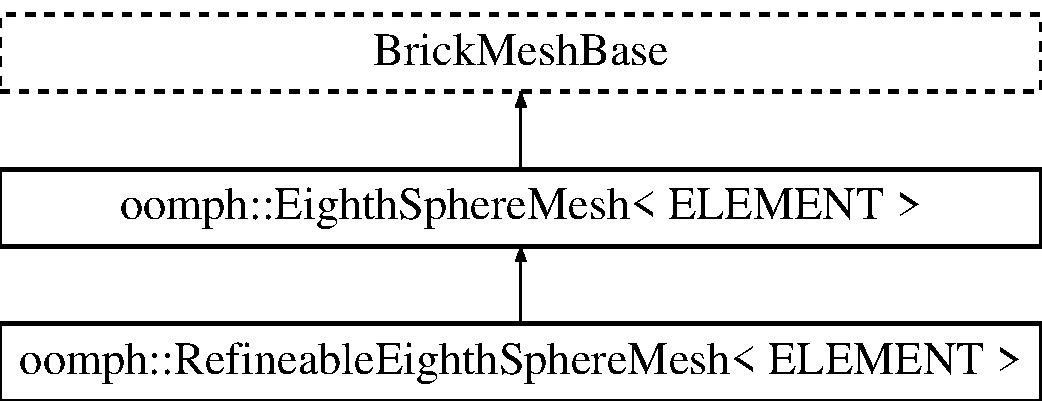
\includegraphics[height=4.000000cm]{classoomph_1_1EighthSphereMesh}
\end{center}
\end{figure}
\subsection*{Public Member Functions}
\begin{DoxyCompactItemize}
\item 
\hyperlink{classoomph_1_1EighthSphereMesh_a0457fc188d930a1e8853a3f0e1effbb3}{Eighth\+Sphere\+Mesh} (const double \&radius, \hyperlink{classoomph_1_1TimeStepper}{Time\+Stepper} $\ast$time\+\_\+stepper\+\_\+pt=\&\hyperlink{classoomph_1_1Mesh_a12243d0fee2b1fcee729ee5a4777ea10}{Mesh\+::\+Default\+\_\+\+Time\+Stepper})
\begin{DoxyCompactList}\small\item\em Constructor\+: Pass radius and timestepper; defaults to static default timestepper. \end{DoxyCompactList}\item 
\hyperlink{classoomph_1_1EighthSphereMesh_a425c3de92974d00dbb126f4cbbaf8e3b}{$\sim$\+Eighth\+Sphere\+Mesh} ()
\begin{DoxyCompactList}\small\item\em Destructor. \end{DoxyCompactList}\end{DoxyCompactItemize}
\subsection*{Protected Attributes}
\begin{DoxyCompactItemize}
\item 
\hyperlink{classoomph_1_1Domain}{Domain} $\ast$ \hyperlink{classoomph_1_1EighthSphereMesh_a4b08d71a9da8cbd278cc51919cbb1a17}{Domain\+\_\+pt}
\begin{DoxyCompactList}\small\item\em Pointer to the domain. \end{DoxyCompactList}\item 
double \hyperlink{classoomph_1_1EighthSphereMesh_a6dbcd3a6d27416a0d9ef25cc631f6043}{Radius}
\begin{DoxyCompactList}\small\item\em Radius of the sphere. \end{DoxyCompactList}\end{DoxyCompactItemize}
\subsection*{Additional Inherited Members}


\subsection{Detailed Description}
\subsubsection*{template$<$class E\+L\+E\+M\+E\+NT$>$\newline
class oomph\+::\+Eighth\+Sphere\+Mesh$<$ E\+L\+E\+M\+E\+N\+T $>$}

Eight of a sphere brick mesh, based on the Eight\+Sphere\+Domain Non-\/refineable version with four brick elements. The eighth-\/sphere is located in the positive octant, centred at the origin. The mesh boundaries are numbered as follows\+:
\begin{DoxyItemize}
\item Boundary 0\+: Plane x=0
\item Boundary 1\+: Plane y=0
\item Boundary 2\+: Plane z=0
\item Boundary 3\+: The surface of the sphere. 
\end{DoxyItemize}

Definition at line 59 of file eighth\+\_\+sphere\+\_\+mesh.\+template.\+h.



\subsection{Constructor \& Destructor Documentation}
\mbox{\Hypertarget{classoomph_1_1EighthSphereMesh_a0457fc188d930a1e8853a3f0e1effbb3}\label{classoomph_1_1EighthSphereMesh_a0457fc188d930a1e8853a3f0e1effbb3}} 
\index{oomph\+::\+Eighth\+Sphere\+Mesh@{oomph\+::\+Eighth\+Sphere\+Mesh}!Eighth\+Sphere\+Mesh@{Eighth\+Sphere\+Mesh}}
\index{Eighth\+Sphere\+Mesh@{Eighth\+Sphere\+Mesh}!oomph\+::\+Eighth\+Sphere\+Mesh@{oomph\+::\+Eighth\+Sphere\+Mesh}}
\subsubsection{\texorpdfstring{Eighth\+Sphere\+Mesh()}{EighthSphereMesh()}}
{\footnotesize\ttfamily template$<$class E\+L\+E\+M\+E\+NT $>$ \\
\hyperlink{classoomph_1_1EighthSphereMesh}{oomph\+::\+Eighth\+Sphere\+Mesh}$<$ E\+L\+E\+M\+E\+NT $>$\+::\hyperlink{classoomph_1_1EighthSphereMesh}{Eighth\+Sphere\+Mesh} (\begin{DoxyParamCaption}\item[{const double \&}]{radius,  }\item[{\hyperlink{classoomph_1_1TimeStepper}{Time\+Stepper} $\ast$}]{time\+\_\+stepper\+\_\+pt = {\ttfamily \&\hyperlink{classoomph_1_1Mesh_a12243d0fee2b1fcee729ee5a4777ea10}{Mesh\+::\+Default\+\_\+\+Time\+Stepper}} }\end{DoxyParamCaption})}



Constructor\+: Pass radius and timestepper; defaults to static default timestepper. 

Constructor for the eighth of a sphere mesh\+: Pass timestepper; defaults to static default timestepper. 

Definition at line 44 of file eighth\+\_\+sphere\+\_\+mesh.\+template.\+cc.



References oomph\+::\+Mesh\+::add\+\_\+boundary\+\_\+node(), oomph\+::\+Eighth\+Sphere\+Mesh$<$ E\+L\+E\+M\+E\+N\+T $>$\+::\+Domain\+\_\+pt, oomph\+::\+Mesh\+::\+Element\+\_\+pt, oomph\+::\+Mesh\+::finite\+\_\+element\+\_\+pt(), i, oomph\+::\+Finite\+Element\+::local\+\_\+fraction\+\_\+of\+\_\+node(), oomph\+::\+Domain\+::macro\+\_\+element\+\_\+pt(), oomph\+::\+Macro\+Element\+::macro\+\_\+map(), oomph\+::\+Finite\+Element\+::nnode\+\_\+1d(), oomph\+::\+Mesh\+::\+Node\+\_\+pt, oomph\+::\+Mesh\+::node\+\_\+pt(), oomph\+::\+Finite\+Element\+::node\+\_\+pt(), oomph\+::\+Eighth\+Sphere\+Mesh$<$ E\+L\+E\+M\+E\+N\+T $>$\+::\+Radius, s, oomph\+::\+Mesh\+::set\+\_\+nboundary(), oomph\+::\+Brick\+Mesh\+Base\+::setup\+\_\+boundary\+\_\+element\+\_\+info(), and oomph\+::\+Node\+::x().

\mbox{\Hypertarget{classoomph_1_1EighthSphereMesh_a425c3de92974d00dbb126f4cbbaf8e3b}\label{classoomph_1_1EighthSphereMesh_a425c3de92974d00dbb126f4cbbaf8e3b}} 
\index{oomph\+::\+Eighth\+Sphere\+Mesh@{oomph\+::\+Eighth\+Sphere\+Mesh}!````~Eighth\+Sphere\+Mesh@{$\sim$\+Eighth\+Sphere\+Mesh}}
\index{````~Eighth\+Sphere\+Mesh@{$\sim$\+Eighth\+Sphere\+Mesh}!oomph\+::\+Eighth\+Sphere\+Mesh@{oomph\+::\+Eighth\+Sphere\+Mesh}}
\subsubsection{\texorpdfstring{$\sim$\+Eighth\+Sphere\+Mesh()}{~EighthSphereMesh()}}
{\footnotesize\ttfamily template$<$class E\+L\+E\+M\+E\+NT $>$ \\
\hyperlink{classoomph_1_1EighthSphereMesh}{oomph\+::\+Eighth\+Sphere\+Mesh}$<$ E\+L\+E\+M\+E\+NT $>$\+::$\sim$\hyperlink{classoomph_1_1EighthSphereMesh}{Eighth\+Sphere\+Mesh} (\begin{DoxyParamCaption}{ }\end{DoxyParamCaption})\hspace{0.3cm}{\ttfamily [inline]}}



Destructor. 



Definition at line 71 of file eighth\+\_\+sphere\+\_\+mesh.\+template.\+h.



References oomph\+::\+Eighth\+Sphere\+Mesh$<$ E\+L\+E\+M\+E\+N\+T $>$\+::\+Domain\+\_\+pt.



\subsection{Member Data Documentation}
\mbox{\Hypertarget{classoomph_1_1EighthSphereMesh_a4b08d71a9da8cbd278cc51919cbb1a17}\label{classoomph_1_1EighthSphereMesh_a4b08d71a9da8cbd278cc51919cbb1a17}} 
\index{oomph\+::\+Eighth\+Sphere\+Mesh@{oomph\+::\+Eighth\+Sphere\+Mesh}!Domain\+\_\+pt@{Domain\+\_\+pt}}
\index{Domain\+\_\+pt@{Domain\+\_\+pt}!oomph\+::\+Eighth\+Sphere\+Mesh@{oomph\+::\+Eighth\+Sphere\+Mesh}}
\subsubsection{\texorpdfstring{Domain\+\_\+pt}{Domain\_pt}}
{\footnotesize\ttfamily template$<$class E\+L\+E\+M\+E\+NT $>$ \\
\hyperlink{classoomph_1_1Domain}{Domain}$\ast$ \hyperlink{classoomph_1_1EighthSphereMesh}{oomph\+::\+Eighth\+Sphere\+Mesh}$<$ E\+L\+E\+M\+E\+NT $>$\+::Domain\+\_\+pt\hspace{0.3cm}{\ttfamily [protected]}}



Pointer to the domain. 



Definition at line 80 of file eighth\+\_\+sphere\+\_\+mesh.\+template.\+h.



Referenced by oomph\+::\+Eighth\+Sphere\+Mesh$<$ E\+L\+E\+M\+E\+N\+T $>$\+::\+Eighth\+Sphere\+Mesh(), oomph\+::\+Refineable\+Eighth\+Sphere\+Mesh$<$ E\+L\+E\+M\+E\+N\+T $>$\+::\+Refineable\+Eighth\+Sphere\+Mesh(), and oomph\+::\+Eighth\+Sphere\+Mesh$<$ E\+L\+E\+M\+E\+N\+T $>$\+::$\sim$\+Eighth\+Sphere\+Mesh().

\mbox{\Hypertarget{classoomph_1_1EighthSphereMesh_a6dbcd3a6d27416a0d9ef25cc631f6043}\label{classoomph_1_1EighthSphereMesh_a6dbcd3a6d27416a0d9ef25cc631f6043}} 
\index{oomph\+::\+Eighth\+Sphere\+Mesh@{oomph\+::\+Eighth\+Sphere\+Mesh}!Radius@{Radius}}
\index{Radius@{Radius}!oomph\+::\+Eighth\+Sphere\+Mesh@{oomph\+::\+Eighth\+Sphere\+Mesh}}
\subsubsection{\texorpdfstring{Radius}{Radius}}
{\footnotesize\ttfamily template$<$class E\+L\+E\+M\+E\+NT $>$ \\
double \hyperlink{classoomph_1_1EighthSphereMesh}{oomph\+::\+Eighth\+Sphere\+Mesh}$<$ E\+L\+E\+M\+E\+NT $>$\+::Radius\hspace{0.3cm}{\ttfamily [protected]}}



Radius of the sphere. 



Definition at line 83 of file eighth\+\_\+sphere\+\_\+mesh.\+template.\+h.



Referenced by oomph\+::\+Eighth\+Sphere\+Mesh$<$ E\+L\+E\+M\+E\+N\+T $>$\+::\+Eighth\+Sphere\+Mesh().



The documentation for this class was generated from the following files\+:\begin{DoxyCompactItemize}
\item 
\hyperlink{eighth__sphere__mesh_8template_8h}{eighth\+\_\+sphere\+\_\+mesh.\+template.\+h}\item 
\hyperlink{eighth__sphere__mesh_8template_8cc}{eighth\+\_\+sphere\+\_\+mesh.\+template.\+cc}\end{DoxyCompactItemize}

\hypertarget{classoomph_1_1ElasticQuarterPipeMesh}{}\section{oomph\+:\+:Elastic\+Quarter\+Pipe\+Mesh$<$ E\+L\+E\+M\+E\+NT $>$ Class Template Reference}
\label{classoomph_1_1ElasticQuarterPipeMesh}\index{oomph\+::\+Elastic\+Quarter\+Pipe\+Mesh$<$ E\+L\+E\+M\+E\+N\+T $>$@{oomph\+::\+Elastic\+Quarter\+Pipe\+Mesh$<$ E\+L\+E\+M\+E\+N\+T $>$}}


{\ttfamily \#include $<$quarter\+\_\+pipe\+\_\+mesh.\+template.\+h$>$}

Inheritance diagram for oomph\+:\+:Elastic\+Quarter\+Pipe\+Mesh$<$ E\+L\+E\+M\+E\+NT $>$\+:\begin{figure}[H]
\begin{center}
\leavevmode
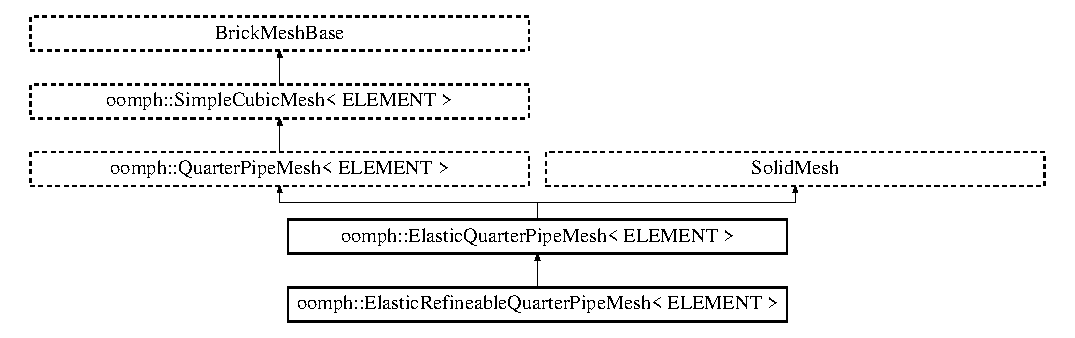
\includegraphics[height=4.093567cm]{classoomph_1_1ElasticQuarterPipeMesh}
\end{center}
\end{figure}
\subsection*{Public Member Functions}
\begin{DoxyCompactItemize}
\item 
\hyperlink{classoomph_1_1ElasticQuarterPipeMesh_a4ccb6983820b774bc72b7d469728ca30}{Elastic\+Quarter\+Pipe\+Mesh} (const unsigned \&ntheta, const unsigned \&nr, const unsigned \&\hyperlink{classoomph_1_1SimpleCubicMesh_ad78725440e4e87598fd9339653b28e61}{nz}, const double \&rmin, const double \&rmax, const double \&length, Time\+Stepper $\ast$time\+\_\+stepper\+\_\+pt=\&Mesh\+::\+Default\+\_\+\+Time\+Stepper)
\begin{DoxyCompactList}\small\item\em Constructor\+: Pass number of elements in various directions, the inner and outer radius and the length of the tube. Builds mesh and copies Eulerian coords to Lagrangian ones so that the initial configuration is the stress-\/free one. \end{DoxyCompactList}\end{DoxyCompactItemize}
\subsection*{Additional Inherited Members}


\subsection{Detailed Description}
\subsubsection*{template$<$class E\+L\+E\+M\+E\+NT$>$\newline
class oomph\+::\+Elastic\+Quarter\+Pipe\+Mesh$<$ E\+L\+E\+M\+E\+N\+T $>$}

Non refineable elastic quarter pipe mesh class setup lagrangian coordinates for solid mechanics problems 

Definition at line 175 of file quarter\+\_\+pipe\+\_\+mesh.\+template.\+h.



\subsection{Constructor \& Destructor Documentation}
\mbox{\Hypertarget{classoomph_1_1ElasticQuarterPipeMesh_a4ccb6983820b774bc72b7d469728ca30}\label{classoomph_1_1ElasticQuarterPipeMesh_a4ccb6983820b774bc72b7d469728ca30}} 
\index{oomph\+::\+Elastic\+Quarter\+Pipe\+Mesh@{oomph\+::\+Elastic\+Quarter\+Pipe\+Mesh}!Elastic\+Quarter\+Pipe\+Mesh@{Elastic\+Quarter\+Pipe\+Mesh}}
\index{Elastic\+Quarter\+Pipe\+Mesh@{Elastic\+Quarter\+Pipe\+Mesh}!oomph\+::\+Elastic\+Quarter\+Pipe\+Mesh@{oomph\+::\+Elastic\+Quarter\+Pipe\+Mesh}}
\subsubsection{\texorpdfstring{Elastic\+Quarter\+Pipe\+Mesh()}{ElasticQuarterPipeMesh()}}
{\footnotesize\ttfamily template$<$class E\+L\+E\+M\+E\+NT $>$ \\
\hyperlink{classoomph_1_1ElasticQuarterPipeMesh}{oomph\+::\+Elastic\+Quarter\+Pipe\+Mesh}$<$ E\+L\+E\+M\+E\+NT $>$\+::\hyperlink{classoomph_1_1ElasticQuarterPipeMesh}{Elastic\+Quarter\+Pipe\+Mesh} (\begin{DoxyParamCaption}\item[{const unsigned \&}]{ntheta,  }\item[{const unsigned \&}]{nr,  }\item[{const unsigned \&}]{nz,  }\item[{const double \&}]{rmin,  }\item[{const double \&}]{rmax,  }\item[{const double \&}]{length,  }\item[{Time\+Stepper $\ast$}]{time\+\_\+stepper\+\_\+pt = {\ttfamily \&Mesh\+:\+:Default\+\_\+TimeStepper} }\end{DoxyParamCaption})\hspace{0.3cm}{\ttfamily [inline]}}



Constructor\+: Pass number of elements in various directions, the inner and outer radius and the length of the tube. Builds mesh and copies Eulerian coords to Lagrangian ones so that the initial configuration is the stress-\/free one. 

Make the current configuration the undeformed one by setting the nodal Lagrangian coordinates to their current Eulerian ones 

Definition at line 187 of file quarter\+\_\+pipe\+\_\+mesh.\+template.\+h.



The documentation for this class was generated from the following file\+:\begin{DoxyCompactItemize}
\item 
\hyperlink{quarter__pipe__mesh_8template_8h}{quarter\+\_\+pipe\+\_\+mesh.\+template.\+h}\end{DoxyCompactItemize}

\hypertarget{classoomph_1_1ElasticRectangularQuadMesh}{}\section{oomph\+:\+:Elastic\+Rectangular\+Quad\+Mesh$<$ E\+L\+E\+M\+E\+NT $>$ Class Template Reference}
\label{classoomph_1_1ElasticRectangularQuadMesh}\index{oomph\+::\+Elastic\+Rectangular\+Quad\+Mesh$<$ E\+L\+E\+M\+E\+N\+T $>$@{oomph\+::\+Elastic\+Rectangular\+Quad\+Mesh$<$ E\+L\+E\+M\+E\+N\+T $>$}}


{\ttfamily \#include $<$rectangular\+\_\+quadmesh.\+template.\+h$>$}

Inheritance diagram for oomph\+:\+:Elastic\+Rectangular\+Quad\+Mesh$<$ E\+L\+E\+M\+E\+NT $>$\+:\begin{figure}[H]
\begin{center}
\leavevmode
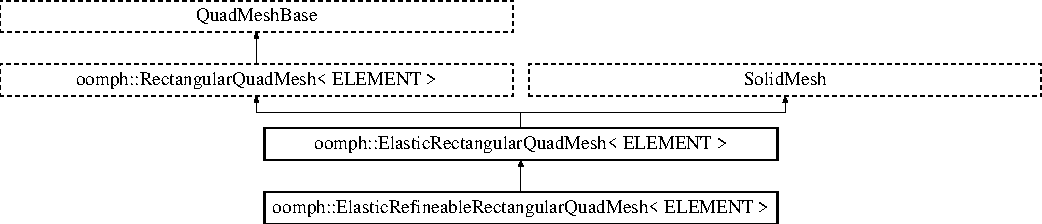
\includegraphics[height=3.010753cm]{classoomph_1_1ElasticRectangularQuadMesh}
\end{center}
\end{figure}
\subsection*{Public Member Functions}
\begin{DoxyCompactItemize}
\item 
\hyperlink{classoomph_1_1ElasticRectangularQuadMesh_aad1e395c3f314854b68c4f1df9256230}{Elastic\+Rectangular\+Quad\+Mesh} (const unsigned \&\hyperlink{classoomph_1_1RectangularQuadMesh_abfef93d6322886cdce14a437186e4821}{nx}, const unsigned \&\hyperlink{classoomph_1_1RectangularQuadMesh_a86d76a55eb7c4e8bca9b74d23c8b0412}{ny}, const double \&lx, const double \&ly, const Vector$<$ double $>$ \&origin, Time\+Stepper $\ast$time\+\_\+stepper\+\_\+pt=\&Mesh\+::\+Default\+\_\+\+Time\+Stepper)
\begin{DoxyCompactList}\small\item\em Constructor\+: Build mesh and copy Eulerian coords to Lagrangian ones so that the initial configuration is the stress-\/free one and assign boundary coordinates. Origin specifies an additional rigid-\/body displacement. \end{DoxyCompactList}\item 
\hyperlink{classoomph_1_1ElasticRectangularQuadMesh_a57b701739dcc5c643a1a9bae94a4b7d8}{Elastic\+Rectangular\+Quad\+Mesh} (const unsigned \&\hyperlink{classoomph_1_1RectangularQuadMesh_abfef93d6322886cdce14a437186e4821}{nx}, const unsigned \&\hyperlink{classoomph_1_1RectangularQuadMesh_a86d76a55eb7c4e8bca9b74d23c8b0412}{ny}, const double \&lx, const double \&ly, Time\+Stepper $\ast$time\+\_\+stepper\+\_\+pt=\&Mesh\+::\+Default\+\_\+\+Time\+Stepper)
\begin{DoxyCompactList}\small\item\em Constructor\+: Build mesh and copy Eulerian coords to Lagrangian ones so that the initial configuration is the stress-\/free one and assign boundary coordinates. \end{DoxyCompactList}\item 
\hyperlink{classoomph_1_1ElasticRectangularQuadMesh_a3865acefe6df1aac212d8306f516ebd1}{Elastic\+Rectangular\+Quad\+Mesh} (const unsigned \&\hyperlink{classoomph_1_1RectangularQuadMesh_abfef93d6322886cdce14a437186e4821}{nx}, const unsigned \&\hyperlink{classoomph_1_1RectangularQuadMesh_a86d76a55eb7c4e8bca9b74d23c8b0412}{ny}, const double \&lx, const double \&ly, const bool \&periodic\+\_\+in\+\_\+x, Time\+Stepper $\ast$time\+\_\+stepper\+\_\+pt=\&Mesh\+::\+Default\+\_\+\+Time\+Stepper)
\begin{DoxyCompactList}\small\item\em Constructor\+: Build mesh and copy Eulerian coords to Lagrangian ones so that the initial configuration is the stress-\/free one and assign boundary coordinates. This includes a boolean flag to specify if the mesh is periodic in the x-\/direction. \end{DoxyCompactList}\end{DoxyCompactItemize}
\subsection*{Private Member Functions}
\begin{DoxyCompactItemize}
\item 
void \hyperlink{classoomph_1_1ElasticRectangularQuadMesh_a84db22a37c49bf3958e149d67997bead}{set\+\_\+boundary\+\_\+coordinates} (const Vector$<$ double $>$ \&origin)
\begin{DoxyCompactList}\small\item\em Setup the boundary coordinates. Vector origin specifies the coordinates of the lower left corner of the mesh. \end{DoxyCompactList}\end{DoxyCompactItemize}
\subsection*{Additional Inherited Members}


\subsection{Detailed Description}
\subsubsection*{template$<$class E\+L\+E\+M\+E\+NT$>$\newline
class oomph\+::\+Elastic\+Rectangular\+Quad\+Mesh$<$ E\+L\+E\+M\+E\+N\+T $>$}

Elastic quad mesh with functionality to attach traction elements to the specified boundaries. We \char`\"{}upgrade\char`\"{} the \hyperlink{classoomph_1_1RectangularQuadMesh}{Rectangular\+Quad\+Mesh} to become an Solid\+Mesh and equate the Eulerian and Lagrangian coordinates, thus making the domain represented by the mesh the stress-\/free configuration. 

Definition at line 373 of file rectangular\+\_\+quadmesh.\+template.\+h.



\subsection{Constructor \& Destructor Documentation}
\mbox{\Hypertarget{classoomph_1_1ElasticRectangularQuadMesh_aad1e395c3f314854b68c4f1df9256230}\label{classoomph_1_1ElasticRectangularQuadMesh_aad1e395c3f314854b68c4f1df9256230}} 
\index{oomph\+::\+Elastic\+Rectangular\+Quad\+Mesh@{oomph\+::\+Elastic\+Rectangular\+Quad\+Mesh}!Elastic\+Rectangular\+Quad\+Mesh@{Elastic\+Rectangular\+Quad\+Mesh}}
\index{Elastic\+Rectangular\+Quad\+Mesh@{Elastic\+Rectangular\+Quad\+Mesh}!oomph\+::\+Elastic\+Rectangular\+Quad\+Mesh@{oomph\+::\+Elastic\+Rectangular\+Quad\+Mesh}}
\subsubsection{\texorpdfstring{Elastic\+Rectangular\+Quad\+Mesh()}{ElasticRectangularQuadMesh()}\hspace{0.1cm}{\footnotesize\ttfamily [1/3]}}
{\footnotesize\ttfamily template$<$class E\+L\+E\+M\+E\+NT$>$ \\
\hyperlink{classoomph_1_1ElasticRectangularQuadMesh}{oomph\+::\+Elastic\+Rectangular\+Quad\+Mesh}$<$ E\+L\+E\+M\+E\+NT $>$\+::\hyperlink{classoomph_1_1ElasticRectangularQuadMesh}{Elastic\+Rectangular\+Quad\+Mesh} (\begin{DoxyParamCaption}\item[{const unsigned \&}]{nx,  }\item[{const unsigned \&}]{ny,  }\item[{const double \&}]{lx,  }\item[{const double \&}]{ly,  }\item[{const Vector$<$ double $>$ \&}]{origin,  }\item[{Time\+Stepper $\ast$}]{time\+\_\+stepper\+\_\+pt = {\ttfamily \&Mesh\+:\+:Default\+\_\+TimeStepper} }\end{DoxyParamCaption})\hspace{0.3cm}{\ttfamily [inline]}}



Constructor\+: Build mesh and copy Eulerian coords to Lagrangian ones so that the initial configuration is the stress-\/free one and assign boundary coordinates. Origin specifies an additional rigid-\/body displacement. 

Make the current configuration the undeformed one by setting the nodal Lagrangian coordinates to their current Eulerian ones 

Definition at line 385 of file rectangular\+\_\+quadmesh.\+template.\+h.

\mbox{\Hypertarget{classoomph_1_1ElasticRectangularQuadMesh_a57b701739dcc5c643a1a9bae94a4b7d8}\label{classoomph_1_1ElasticRectangularQuadMesh_a57b701739dcc5c643a1a9bae94a4b7d8}} 
\index{oomph\+::\+Elastic\+Rectangular\+Quad\+Mesh@{oomph\+::\+Elastic\+Rectangular\+Quad\+Mesh}!Elastic\+Rectangular\+Quad\+Mesh@{Elastic\+Rectangular\+Quad\+Mesh}}
\index{Elastic\+Rectangular\+Quad\+Mesh@{Elastic\+Rectangular\+Quad\+Mesh}!oomph\+::\+Elastic\+Rectangular\+Quad\+Mesh@{oomph\+::\+Elastic\+Rectangular\+Quad\+Mesh}}
\subsubsection{\texorpdfstring{Elastic\+Rectangular\+Quad\+Mesh()}{ElasticRectangularQuadMesh()}\hspace{0.1cm}{\footnotesize\ttfamily [2/3]}}
{\footnotesize\ttfamily template$<$class E\+L\+E\+M\+E\+NT$>$ \\
\hyperlink{classoomph_1_1ElasticRectangularQuadMesh}{oomph\+::\+Elastic\+Rectangular\+Quad\+Mesh}$<$ E\+L\+E\+M\+E\+NT $>$\+::\hyperlink{classoomph_1_1ElasticRectangularQuadMesh}{Elastic\+Rectangular\+Quad\+Mesh} (\begin{DoxyParamCaption}\item[{const unsigned \&}]{nx,  }\item[{const unsigned \&}]{ny,  }\item[{const double \&}]{lx,  }\item[{const double \&}]{ly,  }\item[{Time\+Stepper $\ast$}]{time\+\_\+stepper\+\_\+pt = {\ttfamily \&Mesh\+:\+:Default\+\_\+TimeStepper} }\end{DoxyParamCaption})\hspace{0.3cm}{\ttfamily [inline]}}



Constructor\+: Build mesh and copy Eulerian coords to Lagrangian ones so that the initial configuration is the stress-\/free one and assign boundary coordinates. 

Make the current configuration the undeformed one by setting the nodal Lagrangian coordinates to their current Eulerian ones 

Definition at line 418 of file rectangular\+\_\+quadmesh.\+template.\+h.

\mbox{\Hypertarget{classoomph_1_1ElasticRectangularQuadMesh_a3865acefe6df1aac212d8306f516ebd1}\label{classoomph_1_1ElasticRectangularQuadMesh_a3865acefe6df1aac212d8306f516ebd1}} 
\index{oomph\+::\+Elastic\+Rectangular\+Quad\+Mesh@{oomph\+::\+Elastic\+Rectangular\+Quad\+Mesh}!Elastic\+Rectangular\+Quad\+Mesh@{Elastic\+Rectangular\+Quad\+Mesh}}
\index{Elastic\+Rectangular\+Quad\+Mesh@{Elastic\+Rectangular\+Quad\+Mesh}!oomph\+::\+Elastic\+Rectangular\+Quad\+Mesh@{oomph\+::\+Elastic\+Rectangular\+Quad\+Mesh}}
\subsubsection{\texorpdfstring{Elastic\+Rectangular\+Quad\+Mesh()}{ElasticRectangularQuadMesh()}\hspace{0.1cm}{\footnotesize\ttfamily [3/3]}}
{\footnotesize\ttfamily template$<$class E\+L\+E\+M\+E\+NT$>$ \\
\hyperlink{classoomph_1_1ElasticRectangularQuadMesh}{oomph\+::\+Elastic\+Rectangular\+Quad\+Mesh}$<$ E\+L\+E\+M\+E\+NT $>$\+::\hyperlink{classoomph_1_1ElasticRectangularQuadMesh}{Elastic\+Rectangular\+Quad\+Mesh} (\begin{DoxyParamCaption}\item[{const unsigned \&}]{nx,  }\item[{const unsigned \&}]{ny,  }\item[{const double \&}]{lx,  }\item[{const double \&}]{ly,  }\item[{const bool \&}]{periodic\+\_\+in\+\_\+x,  }\item[{Time\+Stepper $\ast$}]{time\+\_\+stepper\+\_\+pt = {\ttfamily \&Mesh\+:\+:Default\+\_\+TimeStepper} }\end{DoxyParamCaption})\hspace{0.3cm}{\ttfamily [inline]}}



Constructor\+: Build mesh and copy Eulerian coords to Lagrangian ones so that the initial configuration is the stress-\/free one and assign boundary coordinates. This includes a boolean flag to specify if the mesh is periodic in the x-\/direction. 

Make the current configuration the undeformed one by setting the nodal Lagrangian coordinates to their current Eulerian ones 

Definition at line 444 of file rectangular\+\_\+quadmesh.\+template.\+h.



\subsection{Member Function Documentation}
\mbox{\Hypertarget{classoomph_1_1ElasticRectangularQuadMesh_a84db22a37c49bf3958e149d67997bead}\label{classoomph_1_1ElasticRectangularQuadMesh_a84db22a37c49bf3958e149d67997bead}} 
\index{oomph\+::\+Elastic\+Rectangular\+Quad\+Mesh@{oomph\+::\+Elastic\+Rectangular\+Quad\+Mesh}!set\+\_\+boundary\+\_\+coordinates@{set\+\_\+boundary\+\_\+coordinates}}
\index{set\+\_\+boundary\+\_\+coordinates@{set\+\_\+boundary\+\_\+coordinates}!oomph\+::\+Elastic\+Rectangular\+Quad\+Mesh@{oomph\+::\+Elastic\+Rectangular\+Quad\+Mesh}}
\subsubsection{\texorpdfstring{set\+\_\+boundary\+\_\+coordinates()}{set\_boundary\_coordinates()}}
{\footnotesize\ttfamily template$<$class E\+L\+E\+M\+E\+NT$>$ \\
void \hyperlink{classoomph_1_1ElasticRectangularQuadMesh}{oomph\+::\+Elastic\+Rectangular\+Quad\+Mesh}$<$ E\+L\+E\+M\+E\+NT $>$\+::set\+\_\+boundary\+\_\+coordinates (\begin{DoxyParamCaption}\item[{const Vector$<$ double $>$ \&}]{origin }\end{DoxyParamCaption})\hspace{0.3cm}{\ttfamily [inline]}, {\ttfamily [private]}}



Setup the boundary coordinates. Vector origin specifies the coordinates of the lower left corner of the mesh. 



Definition at line 471 of file rectangular\+\_\+quadmesh.\+template.\+h.



References oomph\+::\+Rectangular\+Quad\+Mesh$<$ E\+L\+E\+M\+E\+N\+T $>$\+::\+Ymax, and oomph\+::\+Rectangular\+Quad\+Mesh$<$ E\+L\+E\+M\+E\+N\+T $>$\+::\+Ymin.



The documentation for this class was generated from the following file\+:\begin{DoxyCompactItemize}
\item 
\hyperlink{rectangular__quadmesh_8template_8h}{rectangular\+\_\+quadmesh.\+template.\+h}\end{DoxyCompactItemize}

\hypertarget{classoomph_1_1ElasticRefineableQuarterPipeMesh}{}\section{oomph\+:\+:Elastic\+Refineable\+Quarter\+Pipe\+Mesh$<$ E\+L\+E\+M\+E\+NT $>$ Class Template Reference}
\label{classoomph_1_1ElasticRefineableQuarterPipeMesh}\index{oomph\+::\+Elastic\+Refineable\+Quarter\+Pipe\+Mesh$<$ E\+L\+E\+M\+E\+N\+T $>$@{oomph\+::\+Elastic\+Refineable\+Quarter\+Pipe\+Mesh$<$ E\+L\+E\+M\+E\+N\+T $>$}}


Refineable elastic quarter pipe mesh class.  




{\ttfamily \#include $<$quarter\+\_\+pipe\+\_\+mesh.\+template.\+h$>$}

Inheritance diagram for oomph\+:\+:Elastic\+Refineable\+Quarter\+Pipe\+Mesh$<$ E\+L\+E\+M\+E\+NT $>$\+:\begin{figure}[H]
\begin{center}
\leavevmode
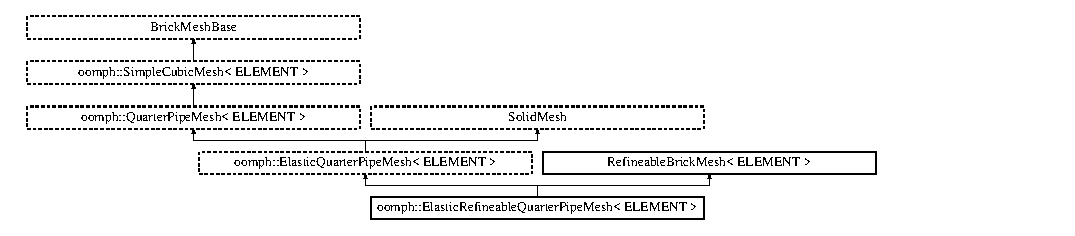
\includegraphics[height=2.456140cm]{classoomph_1_1ElasticRefineableQuarterPipeMesh}
\end{center}
\end{figure}
\subsection*{Public Member Functions}
\begin{DoxyCompactItemize}
\item 
\hyperlink{classoomph_1_1ElasticRefineableQuarterPipeMesh_a5d90778b3a060b97353b5d9ff5a9dd3d}{Elastic\+Refineable\+Quarter\+Pipe\+Mesh} (const unsigned \&ntheta, const unsigned \&nr, const unsigned \&\hyperlink{classoomph_1_1SimpleCubicMesh_ad78725440e4e87598fd9339653b28e61}{nz}, const double \&rmin, const double \&rmax, const double \&length, \hyperlink{classoomph_1_1TimeStepper}{Time\+Stepper} $\ast$time\+\_\+stepper\+\_\+pt=\&\hyperlink{classoomph_1_1Mesh_a12243d0fee2b1fcee729ee5a4777ea10}{Mesh\+::\+Default\+\_\+\+Time\+Stepper})
\begin{DoxyCompactList}\small\item\em Constructor\+: Pass number of elements in various directions, the inner and outer radius and the length of the tube. Builds mesh and copies Eulerian coords to Lagrangian ones so that the initial configuration is the stress-\/free one. \end{DoxyCompactList}\end{DoxyCompactItemize}
\subsection*{Additional Inherited Members}


\subsection{Detailed Description}
\subsubsection*{template$<$class E\+L\+E\+M\+E\+NT$>$\newline
class oomph\+::\+Elastic\+Refineable\+Quarter\+Pipe\+Mesh$<$ E\+L\+E\+M\+E\+N\+T $>$}

Refineable elastic quarter pipe mesh class. 

Definition at line 215 of file quarter\+\_\+pipe\+\_\+mesh.\+template.\+h.



\subsection{Constructor \& Destructor Documentation}
\mbox{\Hypertarget{classoomph_1_1ElasticRefineableQuarterPipeMesh_a5d90778b3a060b97353b5d9ff5a9dd3d}\label{classoomph_1_1ElasticRefineableQuarterPipeMesh_a5d90778b3a060b97353b5d9ff5a9dd3d}} 
\index{oomph\+::\+Elastic\+Refineable\+Quarter\+Pipe\+Mesh@{oomph\+::\+Elastic\+Refineable\+Quarter\+Pipe\+Mesh}!Elastic\+Refineable\+Quarter\+Pipe\+Mesh@{Elastic\+Refineable\+Quarter\+Pipe\+Mesh}}
\index{Elastic\+Refineable\+Quarter\+Pipe\+Mesh@{Elastic\+Refineable\+Quarter\+Pipe\+Mesh}!oomph\+::\+Elastic\+Refineable\+Quarter\+Pipe\+Mesh@{oomph\+::\+Elastic\+Refineable\+Quarter\+Pipe\+Mesh}}
\subsubsection{\texorpdfstring{Elastic\+Refineable\+Quarter\+Pipe\+Mesh()}{ElasticRefineableQuarterPipeMesh()}}
{\footnotesize\ttfamily template$<$class E\+L\+E\+M\+E\+NT $>$ \\
\hyperlink{classoomph_1_1ElasticRefineableQuarterPipeMesh}{oomph\+::\+Elastic\+Refineable\+Quarter\+Pipe\+Mesh}$<$ E\+L\+E\+M\+E\+NT $>$\+::\hyperlink{classoomph_1_1ElasticRefineableQuarterPipeMesh}{Elastic\+Refineable\+Quarter\+Pipe\+Mesh} (\begin{DoxyParamCaption}\item[{const unsigned \&}]{ntheta,  }\item[{const unsigned \&}]{nr,  }\item[{const unsigned \&}]{nz,  }\item[{const double \&}]{rmin,  }\item[{const double \&}]{rmax,  }\item[{const double \&}]{length,  }\item[{\hyperlink{classoomph_1_1TimeStepper}{Time\+Stepper} $\ast$}]{time\+\_\+stepper\+\_\+pt = {\ttfamily \&\hyperlink{classoomph_1_1Mesh_a12243d0fee2b1fcee729ee5a4777ea10}{Mesh\+::\+Default\+\_\+\+Time\+Stepper}} }\end{DoxyParamCaption})\hspace{0.3cm}{\ttfamily [inline]}}



Constructor\+: Pass number of elements in various directions, the inner and outer radius and the length of the tube. Builds mesh and copies Eulerian coords to Lagrangian ones so that the initial configuration is the stress-\/free one. 



Definition at line 226 of file quarter\+\_\+pipe\+\_\+mesh.\+template.\+h.



References oomph\+::\+Quarter\+Pipe\+Mesh$<$ E\+L\+E\+M\+E\+N\+T $>$\+::\+Domain\+\_\+pt, e, oomph\+::\+Mesh\+::element\+\_\+pt(), oomph\+::\+Mesh\+::finite\+\_\+element\+\_\+pt(), oomph\+::\+Domain\+::macro\+\_\+element\+\_\+pt(), oomph\+::\+Mesh\+::nelement(), and oomph\+::\+Simple\+Cubic\+Mesh$<$ E\+L\+E\+M\+E\+N\+T $>$\+::nz().



The documentation for this class was generated from the following file\+:\begin{DoxyCompactItemize}
\item 
\hyperlink{quarter__pipe__mesh_8template_8h}{quarter\+\_\+pipe\+\_\+mesh.\+template.\+h}\end{DoxyCompactItemize}

\hypertarget{classoomph_1_1ElasticRefineableRectangularQuadMesh}{}\section{oomph\+:\+:Elastic\+Refineable\+Rectangular\+Quad\+Mesh$<$ E\+L\+E\+M\+E\+NT $>$ Class Template Reference}
\label{classoomph_1_1ElasticRefineableRectangularQuadMesh}\index{oomph\+::\+Elastic\+Refineable\+Rectangular\+Quad\+Mesh$<$ E\+L\+E\+M\+E\+N\+T $>$@{oomph\+::\+Elastic\+Refineable\+Rectangular\+Quad\+Mesh$<$ E\+L\+E\+M\+E\+N\+T $>$}}


{\ttfamily \#include $<$rectangular\+\_\+quadmesh.\+template.\+h$>$}

Inheritance diagram for oomph\+:\+:Elastic\+Refineable\+Rectangular\+Quad\+Mesh$<$ E\+L\+E\+M\+E\+NT $>$\+:\begin{figure}[H]
\begin{center}
\leavevmode
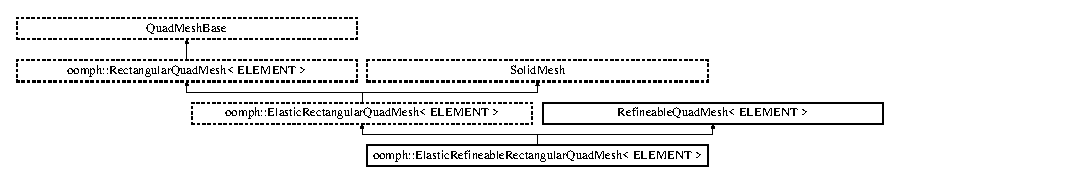
\includegraphics[height=2.258065cm]{classoomph_1_1ElasticRefineableRectangularQuadMesh}
\end{center}
\end{figure}
\subsection*{Public Member Functions}
\begin{DoxyCompactItemize}
\item 
\hyperlink{classoomph_1_1ElasticRefineableRectangularQuadMesh_aa3d9df728974ce172bf942bc4f6c1a2d}{Elastic\+Refineable\+Rectangular\+Quad\+Mesh} (const unsigned \&\hyperlink{classoomph_1_1RectangularQuadMesh_abfef93d6322886cdce14a437186e4821}{nx}, const unsigned \&\hyperlink{classoomph_1_1RectangularQuadMesh_a86d76a55eb7c4e8bca9b74d23c8b0412}{ny}, const double \&lx, const double \&ly, \hyperlink{classoomph_1_1TimeStepper}{Time\+Stepper} $\ast$time\+\_\+stepper\+\_\+pt=\&\hyperlink{classoomph_1_1Mesh_a12243d0fee2b1fcee729ee5a4777ea10}{Mesh\+::\+Default\+\_\+\+Time\+Stepper})
\begin{DoxyCompactList}\small\item\em Constructor\+: Build mesh and copy Eulerian coords to Lagrangian ones so that the initial configuration is the stress-\/free one and assign boundary coordinates (variable Lagrangian coordinates along the relevant boundaries). \end{DoxyCompactList}\item 
\hyperlink{classoomph_1_1ElasticRefineableRectangularQuadMesh_a8925d6c0eb669afc420564a4610b34bd}{Elastic\+Refineable\+Rectangular\+Quad\+Mesh} (const unsigned \&\hyperlink{classoomph_1_1RectangularQuadMesh_abfef93d6322886cdce14a437186e4821}{nx}, const unsigned \&\hyperlink{classoomph_1_1RectangularQuadMesh_a86d76a55eb7c4e8bca9b74d23c8b0412}{ny}, const double \&lx, const double \&ly, const bool \&periodic\+\_\+in\+\_\+x, \hyperlink{classoomph_1_1TimeStepper}{Time\+Stepper} $\ast$time\+\_\+stepper\+\_\+pt=\&\hyperlink{classoomph_1_1Mesh_a12243d0fee2b1fcee729ee5a4777ea10}{Mesh\+::\+Default\+\_\+\+Time\+Stepper})
\begin{DoxyCompactList}\small\item\em Constructor\+: Build mesh and copy Eulerian coords to Lagrangian ones so that the initial configuration is the stress-\/free one and assign boundary coordinates. This includes a boolean flag to specify if the mesh is periodic in the x-\/direction. \end{DoxyCompactList}\item 
\hyperlink{classoomph_1_1ElasticRefineableRectangularQuadMesh_a1cea0e91f2d8687182a8f5de6737a511}{Elastic\+Refineable\+Rectangular\+Quad\+Mesh} (const unsigned \&\hyperlink{classoomph_1_1RectangularQuadMesh_abfef93d6322886cdce14a437186e4821}{nx}, const unsigned \&\hyperlink{classoomph_1_1RectangularQuadMesh_a86d76a55eb7c4e8bca9b74d23c8b0412}{ny}, const double \&lx, const double \&ly, const \hyperlink{classoomph_1_1Vector}{Vector}$<$ double $>$ \&origin, \hyperlink{classoomph_1_1TimeStepper}{Time\+Stepper} $\ast$time\+\_\+stepper\+\_\+pt=\&\hyperlink{classoomph_1_1Mesh_a12243d0fee2b1fcee729ee5a4777ea10}{Mesh\+::\+Default\+\_\+\+Time\+Stepper})
\begin{DoxyCompactList}\small\item\em Constructor\+: Build mesh and copy Eulerian coords to Lagrangian ones so that the initial configuration is the stress-\/free one and assign boundary coordinates (variable Lagrangian coordinates along the relevant boundaries). Origin specifies an additional rigid-\/body displacement. \end{DoxyCompactList}\end{DoxyCompactItemize}
\subsection*{Additional Inherited Members}


\subsection{Detailed Description}
\subsubsection*{template$<$class E\+L\+E\+M\+E\+NT$>$\newline
class oomph\+::\+Elastic\+Refineable\+Rectangular\+Quad\+Mesh$<$ E\+L\+E\+M\+E\+N\+T $>$}

Elastic refineable quad mesh with functionality to attach traction elements to the specified boundaries. We \char`\"{}upgrade\char`\"{} the \hyperlink{classoomph_1_1RefineableRectangularQuadMesh}{Refineable\+Rectangular\+Quad\+Mesh} to become an \hyperlink{classoomph_1_1SolidMesh}{Solid\+Mesh} and equate the Eulerian and Lagrangian coordinates, thus making the domain represented by the mesh the stress-\/free configuration. We also move the mesh \char`\"{}down\char`\"{} by half the the \char`\"{}height\char`\"{} so x=0 is located on the centreline -- appropriate for the beam-\/type problems for which this mesh was developed. 

Definition at line 537 of file rectangular\+\_\+quadmesh.\+template.\+h.



\subsection{Constructor \& Destructor Documentation}
\mbox{\Hypertarget{classoomph_1_1ElasticRefineableRectangularQuadMesh_aa3d9df728974ce172bf942bc4f6c1a2d}\label{classoomph_1_1ElasticRefineableRectangularQuadMesh_aa3d9df728974ce172bf942bc4f6c1a2d}} 
\index{oomph\+::\+Elastic\+Refineable\+Rectangular\+Quad\+Mesh@{oomph\+::\+Elastic\+Refineable\+Rectangular\+Quad\+Mesh}!Elastic\+Refineable\+Rectangular\+Quad\+Mesh@{Elastic\+Refineable\+Rectangular\+Quad\+Mesh}}
\index{Elastic\+Refineable\+Rectangular\+Quad\+Mesh@{Elastic\+Refineable\+Rectangular\+Quad\+Mesh}!oomph\+::\+Elastic\+Refineable\+Rectangular\+Quad\+Mesh@{oomph\+::\+Elastic\+Refineable\+Rectangular\+Quad\+Mesh}}
\subsubsection{\texorpdfstring{Elastic\+Refineable\+Rectangular\+Quad\+Mesh()}{ElasticRefineableRectangularQuadMesh()}\hspace{0.1cm}{\footnotesize\ttfamily [1/3]}}
{\footnotesize\ttfamily template$<$class E\+L\+E\+M\+E\+NT$>$ \\
\hyperlink{classoomph_1_1ElasticRefineableRectangularQuadMesh}{oomph\+::\+Elastic\+Refineable\+Rectangular\+Quad\+Mesh}$<$ E\+L\+E\+M\+E\+NT $>$\+::\hyperlink{classoomph_1_1ElasticRefineableRectangularQuadMesh}{Elastic\+Refineable\+Rectangular\+Quad\+Mesh} (\begin{DoxyParamCaption}\item[{const unsigned \&}]{nx,  }\item[{const unsigned \&}]{ny,  }\item[{const double \&}]{lx,  }\item[{const double \&}]{ly,  }\item[{\hyperlink{classoomph_1_1TimeStepper}{Time\+Stepper} $\ast$}]{time\+\_\+stepper\+\_\+pt = {\ttfamily \&\hyperlink{classoomph_1_1Mesh_a12243d0fee2b1fcee729ee5a4777ea10}{Mesh\+::\+Default\+\_\+\+Time\+Stepper}} }\end{DoxyParamCaption})\hspace{0.3cm}{\ttfamily [inline]}}



Constructor\+: Build mesh and copy Eulerian coords to Lagrangian ones so that the initial configuration is the stress-\/free one and assign boundary coordinates (variable Lagrangian coordinates along the relevant boundaries). 



Definition at line 548 of file rectangular\+\_\+quadmesh.\+template.\+h.

\mbox{\Hypertarget{classoomph_1_1ElasticRefineableRectangularQuadMesh_a8925d6c0eb669afc420564a4610b34bd}\label{classoomph_1_1ElasticRefineableRectangularQuadMesh_a8925d6c0eb669afc420564a4610b34bd}} 
\index{oomph\+::\+Elastic\+Refineable\+Rectangular\+Quad\+Mesh@{oomph\+::\+Elastic\+Refineable\+Rectangular\+Quad\+Mesh}!Elastic\+Refineable\+Rectangular\+Quad\+Mesh@{Elastic\+Refineable\+Rectangular\+Quad\+Mesh}}
\index{Elastic\+Refineable\+Rectangular\+Quad\+Mesh@{Elastic\+Refineable\+Rectangular\+Quad\+Mesh}!oomph\+::\+Elastic\+Refineable\+Rectangular\+Quad\+Mesh@{oomph\+::\+Elastic\+Refineable\+Rectangular\+Quad\+Mesh}}
\subsubsection{\texorpdfstring{Elastic\+Refineable\+Rectangular\+Quad\+Mesh()}{ElasticRefineableRectangularQuadMesh()}\hspace{0.1cm}{\footnotesize\ttfamily [2/3]}}
{\footnotesize\ttfamily template$<$class E\+L\+E\+M\+E\+NT$>$ \\
\hyperlink{classoomph_1_1ElasticRefineableRectangularQuadMesh}{oomph\+::\+Elastic\+Refineable\+Rectangular\+Quad\+Mesh}$<$ E\+L\+E\+M\+E\+NT $>$\+::\hyperlink{classoomph_1_1ElasticRefineableRectangularQuadMesh}{Elastic\+Refineable\+Rectangular\+Quad\+Mesh} (\begin{DoxyParamCaption}\item[{const unsigned \&}]{nx,  }\item[{const unsigned \&}]{ny,  }\item[{const double \&}]{lx,  }\item[{const double \&}]{ly,  }\item[{const bool \&}]{periodic\+\_\+in\+\_\+x,  }\item[{\hyperlink{classoomph_1_1TimeStepper}{Time\+Stepper} $\ast$}]{time\+\_\+stepper\+\_\+pt = {\ttfamily \&\hyperlink{classoomph_1_1Mesh_a12243d0fee2b1fcee729ee5a4777ea10}{Mesh\+::\+Default\+\_\+\+Time\+Stepper}} }\end{DoxyParamCaption})\hspace{0.3cm}{\ttfamily [inline]}}



Constructor\+: Build mesh and copy Eulerian coords to Lagrangian ones so that the initial configuration is the stress-\/free one and assign boundary coordinates. This includes a boolean flag to specify if the mesh is periodic in the x-\/direction. 



Definition at line 568 of file rectangular\+\_\+quadmesh.\+template.\+h.

\mbox{\Hypertarget{classoomph_1_1ElasticRefineableRectangularQuadMesh_a1cea0e91f2d8687182a8f5de6737a511}\label{classoomph_1_1ElasticRefineableRectangularQuadMesh_a1cea0e91f2d8687182a8f5de6737a511}} 
\index{oomph\+::\+Elastic\+Refineable\+Rectangular\+Quad\+Mesh@{oomph\+::\+Elastic\+Refineable\+Rectangular\+Quad\+Mesh}!Elastic\+Refineable\+Rectangular\+Quad\+Mesh@{Elastic\+Refineable\+Rectangular\+Quad\+Mesh}}
\index{Elastic\+Refineable\+Rectangular\+Quad\+Mesh@{Elastic\+Refineable\+Rectangular\+Quad\+Mesh}!oomph\+::\+Elastic\+Refineable\+Rectangular\+Quad\+Mesh@{oomph\+::\+Elastic\+Refineable\+Rectangular\+Quad\+Mesh}}
\subsubsection{\texorpdfstring{Elastic\+Refineable\+Rectangular\+Quad\+Mesh()}{ElasticRefineableRectangularQuadMesh()}\hspace{0.1cm}{\footnotesize\ttfamily [3/3]}}
{\footnotesize\ttfamily template$<$class E\+L\+E\+M\+E\+NT$>$ \\
\hyperlink{classoomph_1_1ElasticRefineableRectangularQuadMesh}{oomph\+::\+Elastic\+Refineable\+Rectangular\+Quad\+Mesh}$<$ E\+L\+E\+M\+E\+NT $>$\+::\hyperlink{classoomph_1_1ElasticRefineableRectangularQuadMesh}{Elastic\+Refineable\+Rectangular\+Quad\+Mesh} (\begin{DoxyParamCaption}\item[{const unsigned \&}]{nx,  }\item[{const unsigned \&}]{ny,  }\item[{const double \&}]{lx,  }\item[{const double \&}]{ly,  }\item[{const \hyperlink{classoomph_1_1Vector}{Vector}$<$ double $>$ \&}]{origin,  }\item[{\hyperlink{classoomph_1_1TimeStepper}{Time\+Stepper} $\ast$}]{time\+\_\+stepper\+\_\+pt = {\ttfamily \&\hyperlink{classoomph_1_1Mesh_a12243d0fee2b1fcee729ee5a4777ea10}{Mesh\+::\+Default\+\_\+\+Time\+Stepper}} }\end{DoxyParamCaption})\hspace{0.3cm}{\ttfamily [inline]}}



Constructor\+: Build mesh and copy Eulerian coords to Lagrangian ones so that the initial configuration is the stress-\/free one and assign boundary coordinates (variable Lagrangian coordinates along the relevant boundaries). Origin specifies an additional rigid-\/body displacement. 



Definition at line 590 of file rectangular\+\_\+quadmesh.\+template.\+h.



The documentation for this class was generated from the following file\+:\begin{DoxyCompactItemize}
\item 
\hyperlink{rectangular__quadmesh_8template_8h}{rectangular\+\_\+quadmesh.\+template.\+h}\end{DoxyCompactItemize}

\hypertarget{classoomph_1_1FishDomain}{}\section{oomph\+:\+:Fish\+Domain Class Reference}
\label{classoomph_1_1FishDomain}\index{oomph\+::\+Fish\+Domain@{oomph\+::\+Fish\+Domain}}


Fish shaped domain, represented by four Macro\+Elements. Shape is parametrised by Geom\+Object that represents the fish\textquotesingle{}s back.  




{\ttfamily \#include $<$fish\+\_\+domain.\+h$>$}

Inheritance diagram for oomph\+:\+:Fish\+Domain\+:\begin{figure}[H]
\begin{center}
\leavevmode
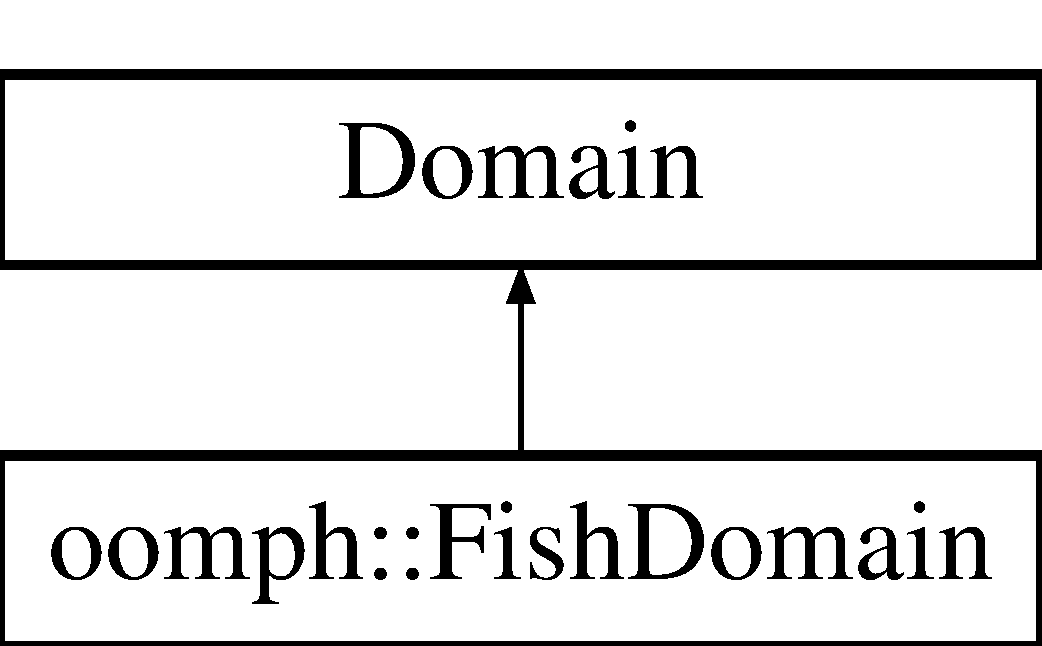
\includegraphics[height=2.000000cm]{classoomph_1_1FishDomain}
\end{center}
\end{figure}
\subsection*{Public Member Functions}
\begin{DoxyCompactItemize}
\item 
\hyperlink{classoomph_1_1FishDomain_a96f1e192900962ee55d063577822cd12}{Fish\+Domain} (Geom\+Object $\ast$back\+\_\+pt, const double \&\hyperlink{classoomph_1_1FishDomain_a773b98977806c2b27531425ecf5e3f8e}{xi\+\_\+nose}, const double \&\hyperlink{classoomph_1_1FishDomain_ae2bcc0014506ba2225b928f319a27c9d}{xi\+\_\+tail})
\begin{DoxyCompactList}\small\item\em Constructor\+: Pass pointer to Geom\+Object that represents the (upper) curved boundary of the fish\textquotesingle{}s body, and the start and end values of the Lagrangian coordinates along the Geom\+Object. \end{DoxyCompactList}\item 
\hyperlink{classoomph_1_1FishDomain_a9436a46493f270e194b1cff950c6670e}{Fish\+Domain} (const \hyperlink{classoomph_1_1FishDomain}{Fish\+Domain} \&)
\begin{DoxyCompactList}\small\item\em Broken copy constructor. \end{DoxyCompactList}\item 
void \hyperlink{classoomph_1_1FishDomain_a87fdf6ae5c6d51e2dcd1aecb494ddaee}{operator=} (const \hyperlink{classoomph_1_1FishDomain}{Fish\+Domain} \&)
\begin{DoxyCompactList}\small\item\em Broken assignment operator. \end{DoxyCompactList}\item 
virtual \hyperlink{classoomph_1_1FishDomain_ab51c01c611efba9f940409e5154c9cd0}{$\sim$\+Fish\+Domain} ()
\begin{DoxyCompactList}\small\item\em Destructor for \hyperlink{classoomph_1_1FishDomain}{Fish\+Domain}\+: Kill macro elements. \end{DoxyCompactList}\item 
double \& \hyperlink{classoomph_1_1FishDomain_ae5343cbda69a625a56a7949edd43cad4}{x\+\_\+fin} ()
\begin{DoxyCompactList}\small\item\em x-\/position of fin tip \end{DoxyCompactList}\item 
double \& \hyperlink{classoomph_1_1FishDomain_ae1a869cee7946b178a09214725e27f29}{y\+\_\+fin} ()
\begin{DoxyCompactList}\small\item\em y-\/position of fin tip \end{DoxyCompactList}\item 
double \& \hyperlink{classoomph_1_1FishDomain_adf87e9ae261cc914173bc18d7eb5bfd8}{x\+\_\+mouth} ()
\begin{DoxyCompactList}\small\item\em x-\/position of mouth \end{DoxyCompactList}\item 
double \& \hyperlink{classoomph_1_1FishDomain_a773b98977806c2b27531425ecf5e3f8e}{xi\+\_\+nose} ()
\begin{DoxyCompactList}\small\item\em Start coordinate on wall (near nose) \end{DoxyCompactList}\item 
double \& \hyperlink{classoomph_1_1FishDomain_ae2bcc0014506ba2225b928f319a27c9d}{xi\+\_\+tail} ()
\begin{DoxyCompactList}\small\item\em End coordinate on wall (near tail) \end{DoxyCompactList}\item 
void \hyperlink{classoomph_1_1FishDomain_a383b0fb396d605932ba6fb0779dacbf9}{macro\+\_\+element\+\_\+boundary} (const unsigned \&t, const unsigned \&i\+\_\+macro, const unsigned \&i\+\_\+direct, const Vector$<$ double $>$ \&zeta, Vector$<$ double $>$ \&r)
\begin{DoxyCompactList}\small\item\em Vector representation of the i\+\_\+macro-\/th macro element boundary i\+\_\+direct (N/\+S/\+W/E) at the discrete time level t (t=0\+: present; t$>$0\+: previous)\+: $ {\bf r}({\bf zeta}) $ Note that the local coordinate {\bfseries zeta} is a 1D Vector rather than a scalar -- this is unavoidable because this function implements the pure virtual function in the Domain base class. \end{DoxyCompactList}\end{DoxyCompactItemize}
\subsection*{Private Member Functions}
\begin{DoxyCompactItemize}
\item 
void \hyperlink{classoomph_1_1FishDomain_a45f1d71d2cf6f4102486b04362ba8b0b}{r\+\_\+upper\+\_\+body\+\_\+N} (const unsigned \&t, const Vector$<$ double $>$ \&zeta, Vector$<$ double $>$ \&f)
\begin{DoxyCompactList}\small\item\em Boundary of upper body macro element zeta $ \in [-1,1] $. \end{DoxyCompactList}\item 
void \hyperlink{classoomph_1_1FishDomain_ac0fadb2212e194bfe9f2ff7f0c892c22}{r\+\_\+upper\+\_\+body\+\_\+W} (const unsigned \&t, const Vector$<$ double $>$ \&zeta, Vector$<$ double $>$ \&f)
\begin{DoxyCompactList}\small\item\em Boundary of upper body macro element zeta $ \in [-1,1] $. \end{DoxyCompactList}\item 
void \hyperlink{classoomph_1_1FishDomain_af30cc8b5bc73f1d2e71099c19b2a0d98}{r\+\_\+upper\+\_\+body\+\_\+S} (const unsigned \&t, const Vector$<$ double $>$ \&zeta, Vector$<$ double $>$ \&f)
\begin{DoxyCompactList}\small\item\em Boundary of upper body macro element zeta $ \in [-1,1] $. \end{DoxyCompactList}\item 
void \hyperlink{classoomph_1_1FishDomain_a47bdf57eebfa025628e70da2a1ab9e19}{r\+\_\+upper\+\_\+body\+\_\+E} (const unsigned \&t, const Vector$<$ double $>$ \&zeta, Vector$<$ double $>$ \&f)
\begin{DoxyCompactList}\small\item\em Boundary of upper body macro element zeta $ \in [-1,1] $. \end{DoxyCompactList}\item 
void \hyperlink{classoomph_1_1FishDomain_a6b0cc31071869ef0e4b4794fe5a46d2f}{r\+\_\+upper\+\_\+fin\+\_\+N} (const unsigned \&t, const Vector$<$ double $>$ \&zeta, Vector$<$ double $>$ \&f)
\begin{DoxyCompactList}\small\item\em Boundary of upper fin macro element zeta $ \in [-1,1] $. \end{DoxyCompactList}\item 
void \hyperlink{classoomph_1_1FishDomain_a750c0daa893d08038a52fbf20a4b23b8}{r\+\_\+upper\+\_\+fin\+\_\+W} (const unsigned \&t, const Vector$<$ double $>$ \&zeta, Vector$<$ double $>$ \&f)
\begin{DoxyCompactList}\small\item\em Boundary of upper fin macro element zeta $ \in [-1,1] $. \end{DoxyCompactList}\item 
void \hyperlink{classoomph_1_1FishDomain_acd62f651648d85a79e04ced3193c3a2a}{r\+\_\+upper\+\_\+fin\+\_\+S} (const unsigned \&t, const Vector$<$ double $>$ \&zeta, Vector$<$ double $>$ \&f)
\begin{DoxyCompactList}\small\item\em Boundary of upper fin macro element zeta $ \in [-1,1] $. \end{DoxyCompactList}\item 
void \hyperlink{classoomph_1_1FishDomain_a063912bd40138bb84b3cdfc23133eff2}{r\+\_\+upper\+\_\+fin\+\_\+E} (const unsigned \&t, const Vector$<$ double $>$ \&zeta, Vector$<$ double $>$ \&f)
\begin{DoxyCompactList}\small\item\em Boundary of upper fin macro element zeta $ \in [-1,1] $. \end{DoxyCompactList}\item 
void \hyperlink{classoomph_1_1FishDomain_a75131ac72e23d5b1d701b588c0596b5d}{r\+\_\+lower\+\_\+body\+\_\+N} (const unsigned \&t, const Vector$<$ double $>$ \&zeta, Vector$<$ double $>$ \&f)
\begin{DoxyCompactList}\small\item\em Boundary of lower body macro element zeta $ \in [-1,1] $. \end{DoxyCompactList}\item 
void \hyperlink{classoomph_1_1FishDomain_a4466e68eb38c1e931743db93af2e9ba9}{r\+\_\+lower\+\_\+body\+\_\+W} (const unsigned \&t, const Vector$<$ double $>$ \&zeta, Vector$<$ double $>$ \&f)
\begin{DoxyCompactList}\small\item\em Boundary of lower body macro element zeta $ \in [-1,1] $. \end{DoxyCompactList}\item 
void \hyperlink{classoomph_1_1FishDomain_aa33b19ceef5cd574ee0a6756bcfc6da7}{r\+\_\+lower\+\_\+body\+\_\+S} (const unsigned \&t, const Vector$<$ double $>$ \&zeta, Vector$<$ double $>$ \&f)
\begin{DoxyCompactList}\small\item\em Southern boundary of lower body macro element zeta $\in [-1,1] $. \end{DoxyCompactList}\item 
void \hyperlink{classoomph_1_1FishDomain_abb85a2acd9cf3cd8fae60fd9e487bd1c}{r\+\_\+lower\+\_\+body\+\_\+E} (const unsigned \&t, const Vector$<$ double $>$ \&zeta, Vector$<$ double $>$ \&f)
\begin{DoxyCompactList}\small\item\em Boundary of lower body macro element zeta $ \in [-1,1] $. \end{DoxyCompactList}\item 
void \hyperlink{classoomph_1_1FishDomain_a6d45dba13043b2b6df831848da665f21}{r\+\_\+lower\+\_\+fin\+\_\+N} (const unsigned \&t, const Vector$<$ double $>$ \&zeta, Vector$<$ double $>$ \&f)
\begin{DoxyCompactList}\small\item\em Boundary of lower fin macro element zeta $ \in [-1,1] $. \end{DoxyCompactList}\item 
void \hyperlink{classoomph_1_1FishDomain_aaf5f3eb1842dc9d7e3f51d4b727632f9}{r\+\_\+lower\+\_\+fin\+\_\+W} (const unsigned \&t, const Vector$<$ double $>$ \&zeta, Vector$<$ double $>$ \&f)
\begin{DoxyCompactList}\small\item\em Boundary of lower fin macro element zeta $ \in [-1,1] $. \end{DoxyCompactList}\item 
void \hyperlink{classoomph_1_1FishDomain_a2110fb0b776654460d6a3477fbc4979d}{r\+\_\+lower\+\_\+fin\+\_\+S} (const unsigned \&t, const Vector$<$ double $>$ \&zeta, Vector$<$ double $>$ \&f)
\begin{DoxyCompactList}\small\item\em Boundary of lower fin macro element zeta $ \in [-1,1] $. \end{DoxyCompactList}\item 
void \hyperlink{classoomph_1_1FishDomain_a956dcbb87e9b37a0b965fcddb9911de3}{r\+\_\+lower\+\_\+fin\+\_\+E} (const unsigned \&t, const Vector$<$ double $>$ \&zeta, Vector$<$ double $>$ \&f)
\begin{DoxyCompactList}\small\item\em Boundary of lower fin macro element zeta $ \in [-1,1] $. \end{DoxyCompactList}\end{DoxyCompactItemize}
\subsection*{Private Attributes}
\begin{DoxyCompactItemize}
\item 
double \hyperlink{classoomph_1_1FishDomain_af85c4be86bb87528939778e3f63a40a5}{Xi\+\_\+nose}
\begin{DoxyCompactList}\small\item\em \char`\"{}\+Nose\char`\"{} limit for the (1D) coordinates along the wall \end{DoxyCompactList}\item 
double \hyperlink{classoomph_1_1FishDomain_a38633d4f3e2777be9544b907d1de5870}{Xi\+\_\+tail}
\begin{DoxyCompactList}\small\item\em \char`\"{}\+Tail\char`\"{} limit for the (1D) coordinates along the wall \end{DoxyCompactList}\item 
double \hyperlink{classoomph_1_1FishDomain_af27c51fe0272df3dec2ad93c5c231d59}{X\+\_\+fin}
\begin{DoxyCompactList}\small\item\em X coordinate of fin tip. \end{DoxyCompactList}\item 
double \hyperlink{classoomph_1_1FishDomain_a162b4a35d8d0e986d254651571844253}{Y\+\_\+fin}
\begin{DoxyCompactList}\small\item\em Y coordinate of fin tip. \end{DoxyCompactList}\item 
double \hyperlink{classoomph_1_1FishDomain_aa25f3280c2453dd725d59f23a478ee11}{X\+\_\+mouth}
\begin{DoxyCompactList}\small\item\em X coordinate of corner of mouth. \end{DoxyCompactList}\item 
Geom\+Object $\ast$ \hyperlink{classoomph_1_1FishDomain_ae943e7fe48ce09dded2d5351ab980f93}{Back\+\_\+pt}
\begin{DoxyCompactList}\small\item\em Pointer to the fish\textquotesingle{}s back. \end{DoxyCompactList}\end{DoxyCompactItemize}


\subsection{Detailed Description}
Fish shaped domain, represented by four Macro\+Elements. Shape is parametrised by Geom\+Object that represents the fish\textquotesingle{}s back. 

Definition at line 49 of file fish\+\_\+domain.\+h.



\subsection{Constructor \& Destructor Documentation}
\mbox{\Hypertarget{classoomph_1_1FishDomain_a96f1e192900962ee55d063577822cd12}\label{classoomph_1_1FishDomain_a96f1e192900962ee55d063577822cd12}} 
\index{oomph\+::\+Fish\+Domain@{oomph\+::\+Fish\+Domain}!Fish\+Domain@{Fish\+Domain}}
\index{Fish\+Domain@{Fish\+Domain}!oomph\+::\+Fish\+Domain@{oomph\+::\+Fish\+Domain}}
\subsubsection{\texorpdfstring{Fish\+Domain()}{FishDomain()}\hspace{0.1cm}{\footnotesize\ttfamily [1/2]}}
{\footnotesize\ttfamily oomph\+::\+Fish\+Domain\+::\+Fish\+Domain (\begin{DoxyParamCaption}\item[{Geom\+Object $\ast$}]{back\+\_\+pt,  }\item[{const double \&}]{xi\+\_\+nose,  }\item[{const double \&}]{xi\+\_\+tail }\end{DoxyParamCaption})\hspace{0.3cm}{\ttfamily [inline]}}



Constructor\+: Pass pointer to Geom\+Object that represents the (upper) curved boundary of the fish\textquotesingle{}s body, and the start and end values of the Lagrangian coordinates along the Geom\+Object. 



Definition at line 57 of file fish\+\_\+domain.\+h.



References X\+\_\+fin, X\+\_\+mouth, and Y\+\_\+fin.

\mbox{\Hypertarget{classoomph_1_1FishDomain_a9436a46493f270e194b1cff950c6670e}\label{classoomph_1_1FishDomain_a9436a46493f270e194b1cff950c6670e}} 
\index{oomph\+::\+Fish\+Domain@{oomph\+::\+Fish\+Domain}!Fish\+Domain@{Fish\+Domain}}
\index{Fish\+Domain@{Fish\+Domain}!oomph\+::\+Fish\+Domain@{oomph\+::\+Fish\+Domain}}
\subsubsection{\texorpdfstring{Fish\+Domain()}{FishDomain()}\hspace{0.1cm}{\footnotesize\ttfamily [2/2]}}
{\footnotesize\ttfamily oomph\+::\+Fish\+Domain\+::\+Fish\+Domain (\begin{DoxyParamCaption}\item[{const \hyperlink{classoomph_1_1FishDomain}{Fish\+Domain} \&}]{ }\end{DoxyParamCaption})\hspace{0.3cm}{\ttfamily [inline]}}



Broken copy constructor. 



Definition at line 82 of file fish\+\_\+domain.\+h.

\mbox{\Hypertarget{classoomph_1_1FishDomain_ab51c01c611efba9f940409e5154c9cd0}\label{classoomph_1_1FishDomain_ab51c01c611efba9f940409e5154c9cd0}} 
\index{oomph\+::\+Fish\+Domain@{oomph\+::\+Fish\+Domain}!````~Fish\+Domain@{$\sim$\+Fish\+Domain}}
\index{````~Fish\+Domain@{$\sim$\+Fish\+Domain}!oomph\+::\+Fish\+Domain@{oomph\+::\+Fish\+Domain}}
\subsubsection{\texorpdfstring{$\sim$\+Fish\+Domain()}{~FishDomain()}}
{\footnotesize\ttfamily virtual oomph\+::\+Fish\+Domain\+::$\sim$\+Fish\+Domain (\begin{DoxyParamCaption}{ }\end{DoxyParamCaption})\hspace{0.3cm}{\ttfamily [inline]}, {\ttfamily [virtual]}}



Destructor for \hyperlink{classoomph_1_1FishDomain}{Fish\+Domain}\+: Kill macro elements. 



Definition at line 96 of file fish\+\_\+domain.\+h.



\subsection{Member Function Documentation}
\mbox{\Hypertarget{classoomph_1_1FishDomain_a383b0fb396d605932ba6fb0779dacbf9}\label{classoomph_1_1FishDomain_a383b0fb396d605932ba6fb0779dacbf9}} 
\index{oomph\+::\+Fish\+Domain@{oomph\+::\+Fish\+Domain}!macro\+\_\+element\+\_\+boundary@{macro\+\_\+element\+\_\+boundary}}
\index{macro\+\_\+element\+\_\+boundary@{macro\+\_\+element\+\_\+boundary}!oomph\+::\+Fish\+Domain@{oomph\+::\+Fish\+Domain}}
\subsubsection{\texorpdfstring{macro\+\_\+element\+\_\+boundary()}{macro\_element\_boundary()}}
{\footnotesize\ttfamily void oomph\+::\+Fish\+Domain\+::macro\+\_\+element\+\_\+boundary (\begin{DoxyParamCaption}\item[{const unsigned \&}]{t,  }\item[{const unsigned \&}]{i\+\_\+macro,  }\item[{const unsigned \&}]{i\+\_\+direct,  }\item[{const Vector$<$ double $>$ \&}]{zeta,  }\item[{Vector$<$ double $>$ \&}]{r }\end{DoxyParamCaption})}



Vector representation of the i\+\_\+macro-\/th macro element boundary i\+\_\+direct (N/\+S/\+W/E) at the discrete time level t (t=0\+: present; t$>$0\+: previous)\+: $ {\bf r}({\bf zeta}) $ Note that the local coordinate {\bfseries zeta} is a 1D Vector rather than a scalar -- this is unavoidable because this function implements the pure virtual function in the Domain base class. 

Vector representation of the imacro-\/th macro element boundary idirect (N/\+S/\+W/E) at time level t (t=0\+: present; t$>$0\+: previous)\+: $ {\bf r}({\bf zeta}) $ Note that the local coordinate {\bfseries zeta} is a 1D Vector rather than a scalar -- this is unavoidable because this function implements the pure virtual function in the Domain base class. 

Definition at line 301 of file fish\+\_\+domain.\+h.



References r\+\_\+lower\+\_\+body\+\_\+\+E(), r\+\_\+lower\+\_\+body\+\_\+\+N(), r\+\_\+lower\+\_\+body\+\_\+\+S(), r\+\_\+lower\+\_\+body\+\_\+\+W(), r\+\_\+lower\+\_\+fin\+\_\+\+E(), r\+\_\+lower\+\_\+fin\+\_\+\+N(), r\+\_\+lower\+\_\+fin\+\_\+\+S(), r\+\_\+lower\+\_\+fin\+\_\+\+W(), r\+\_\+upper\+\_\+body\+\_\+\+E(), r\+\_\+upper\+\_\+body\+\_\+\+N(), r\+\_\+upper\+\_\+body\+\_\+\+S(), r\+\_\+upper\+\_\+body\+\_\+\+W(), r\+\_\+upper\+\_\+fin\+\_\+\+E(), r\+\_\+upper\+\_\+fin\+\_\+\+N(), r\+\_\+upper\+\_\+fin\+\_\+\+S(), and r\+\_\+upper\+\_\+fin\+\_\+\+W().



Referenced by xi\+\_\+tail().

\mbox{\Hypertarget{classoomph_1_1FishDomain_a87fdf6ae5c6d51e2dcd1aecb494ddaee}\label{classoomph_1_1FishDomain_a87fdf6ae5c6d51e2dcd1aecb494ddaee}} 
\index{oomph\+::\+Fish\+Domain@{oomph\+::\+Fish\+Domain}!operator=@{operator=}}
\index{operator=@{operator=}!oomph\+::\+Fish\+Domain@{oomph\+::\+Fish\+Domain}}
\subsubsection{\texorpdfstring{operator=()}{operator=()}}
{\footnotesize\ttfamily void oomph\+::\+Fish\+Domain\+::operator= (\begin{DoxyParamCaption}\item[{const \hyperlink{classoomph_1_1FishDomain}{Fish\+Domain} \&}]{ }\end{DoxyParamCaption})\hspace{0.3cm}{\ttfamily [inline]}}



Broken assignment operator. 



Definition at line 89 of file fish\+\_\+domain.\+h.

\mbox{\Hypertarget{classoomph_1_1FishDomain_abb85a2acd9cf3cd8fae60fd9e487bd1c}\label{classoomph_1_1FishDomain_abb85a2acd9cf3cd8fae60fd9e487bd1c}} 
\index{oomph\+::\+Fish\+Domain@{oomph\+::\+Fish\+Domain}!r\+\_\+lower\+\_\+body\+\_\+E@{r\+\_\+lower\+\_\+body\+\_\+E}}
\index{r\+\_\+lower\+\_\+body\+\_\+E@{r\+\_\+lower\+\_\+body\+\_\+E}!oomph\+::\+Fish\+Domain@{oomph\+::\+Fish\+Domain}}
\subsubsection{\texorpdfstring{r\+\_\+lower\+\_\+body\+\_\+\+E()}{r\_lower\_body\_E()}}
{\footnotesize\ttfamily void oomph\+::\+Fish\+Domain\+::r\+\_\+lower\+\_\+body\+\_\+E (\begin{DoxyParamCaption}\item[{const unsigned \&}]{t,  }\item[{const Vector$<$ double $>$ \&}]{zeta,  }\item[{Vector$<$ double $>$ \&}]{f }\end{DoxyParamCaption})\hspace{0.3cm}{\ttfamily [inline]}, {\ttfamily [private]}}



Boundary of lower body macro element zeta $ \in [-1,1] $. 



Definition at line 220 of file fish\+\_\+domain.\+h.



References r\+\_\+upper\+\_\+body\+\_\+\+E().



Referenced by macro\+\_\+element\+\_\+boundary().

\mbox{\Hypertarget{classoomph_1_1FishDomain_a75131ac72e23d5b1d701b588c0596b5d}\label{classoomph_1_1FishDomain_a75131ac72e23d5b1d701b588c0596b5d}} 
\index{oomph\+::\+Fish\+Domain@{oomph\+::\+Fish\+Domain}!r\+\_\+lower\+\_\+body\+\_\+N@{r\+\_\+lower\+\_\+body\+\_\+N}}
\index{r\+\_\+lower\+\_\+body\+\_\+N@{r\+\_\+lower\+\_\+body\+\_\+N}!oomph\+::\+Fish\+Domain@{oomph\+::\+Fish\+Domain}}
\subsubsection{\texorpdfstring{r\+\_\+lower\+\_\+body\+\_\+\+N()}{r\_lower\_body\_N()}}
{\footnotesize\ttfamily void oomph\+::\+Fish\+Domain\+::r\+\_\+lower\+\_\+body\+\_\+N (\begin{DoxyParamCaption}\item[{const unsigned \&}]{t,  }\item[{const Vector$<$ double $>$ \&}]{zeta,  }\item[{Vector$<$ double $>$ \&}]{f }\end{DoxyParamCaption})\hspace{0.3cm}{\ttfamily [inline]}, {\ttfamily [private]}}



Boundary of lower body macro element zeta $ \in [-1,1] $. 



Definition at line 184 of file fish\+\_\+domain.\+h.



References r\+\_\+upper\+\_\+body\+\_\+\+S().



Referenced by macro\+\_\+element\+\_\+boundary().

\mbox{\Hypertarget{classoomph_1_1FishDomain_aa33b19ceef5cd574ee0a6756bcfc6da7}\label{classoomph_1_1FishDomain_aa33b19ceef5cd574ee0a6756bcfc6da7}} 
\index{oomph\+::\+Fish\+Domain@{oomph\+::\+Fish\+Domain}!r\+\_\+lower\+\_\+body\+\_\+S@{r\+\_\+lower\+\_\+body\+\_\+S}}
\index{r\+\_\+lower\+\_\+body\+\_\+S@{r\+\_\+lower\+\_\+body\+\_\+S}!oomph\+::\+Fish\+Domain@{oomph\+::\+Fish\+Domain}}
\subsubsection{\texorpdfstring{r\+\_\+lower\+\_\+body\+\_\+\+S()}{r\_lower\_body\_S()}}
{\footnotesize\ttfamily void oomph\+::\+Fish\+Domain\+::r\+\_\+lower\+\_\+body\+\_\+S (\begin{DoxyParamCaption}\item[{const unsigned \&}]{t,  }\item[{const Vector$<$ double $>$ \&}]{zeta,  }\item[{Vector$<$ double $>$ \&}]{f }\end{DoxyParamCaption})\hspace{0.3cm}{\ttfamily [inline]}, {\ttfamily [private]}}



Southern boundary of lower body macro element zeta $\in [-1,1] $. 



Definition at line 209 of file fish\+\_\+domain.\+h.



References r\+\_\+upper\+\_\+body\+\_\+\+N().



Referenced by macro\+\_\+element\+\_\+boundary().

\mbox{\Hypertarget{classoomph_1_1FishDomain_a4466e68eb38c1e931743db93af2e9ba9}\label{classoomph_1_1FishDomain_a4466e68eb38c1e931743db93af2e9ba9}} 
\index{oomph\+::\+Fish\+Domain@{oomph\+::\+Fish\+Domain}!r\+\_\+lower\+\_\+body\+\_\+W@{r\+\_\+lower\+\_\+body\+\_\+W}}
\index{r\+\_\+lower\+\_\+body\+\_\+W@{r\+\_\+lower\+\_\+body\+\_\+W}!oomph\+::\+Fish\+Domain@{oomph\+::\+Fish\+Domain}}
\subsubsection{\texorpdfstring{r\+\_\+lower\+\_\+body\+\_\+\+W()}{r\_lower\_body\_W()}}
{\footnotesize\ttfamily void oomph\+::\+Fish\+Domain\+::r\+\_\+lower\+\_\+body\+\_\+W (\begin{DoxyParamCaption}\item[{const unsigned \&}]{t,  }\item[{const Vector$<$ double $>$ \&}]{zeta,  }\item[{Vector$<$ double $>$ \&}]{f }\end{DoxyParamCaption})\hspace{0.3cm}{\ttfamily [inline]}, {\ttfamily [private]}}



Boundary of lower body macro element zeta $ \in [-1,1] $. 



Definition at line 196 of file fish\+\_\+domain.\+h.



References r\+\_\+upper\+\_\+body\+\_\+\+W().



Referenced by macro\+\_\+element\+\_\+boundary().

\mbox{\Hypertarget{classoomph_1_1FishDomain_a956dcbb87e9b37a0b965fcddb9911de3}\label{classoomph_1_1FishDomain_a956dcbb87e9b37a0b965fcddb9911de3}} 
\index{oomph\+::\+Fish\+Domain@{oomph\+::\+Fish\+Domain}!r\+\_\+lower\+\_\+fin\+\_\+E@{r\+\_\+lower\+\_\+fin\+\_\+E}}
\index{r\+\_\+lower\+\_\+fin\+\_\+E@{r\+\_\+lower\+\_\+fin\+\_\+E}!oomph\+::\+Fish\+Domain@{oomph\+::\+Fish\+Domain}}
\subsubsection{\texorpdfstring{r\+\_\+lower\+\_\+fin\+\_\+\+E()}{r\_lower\_fin\_E()}}
{\footnotesize\ttfamily void oomph\+::\+Fish\+Domain\+::r\+\_\+lower\+\_\+fin\+\_\+E (\begin{DoxyParamCaption}\item[{const unsigned \&}]{t,  }\item[{const Vector$<$ double $>$ \&}]{zeta,  }\item[{Vector$<$ double $>$ \&}]{f }\end{DoxyParamCaption})\hspace{0.3cm}{\ttfamily [inline]}, {\ttfamily [private]}}



Boundary of lower fin macro element zeta $ \in [-1,1] $. 



Definition at line 270 of file fish\+\_\+domain.\+h.



References r\+\_\+upper\+\_\+fin\+\_\+\+E().



Referenced by macro\+\_\+element\+\_\+boundary().

\mbox{\Hypertarget{classoomph_1_1FishDomain_a6d45dba13043b2b6df831848da665f21}\label{classoomph_1_1FishDomain_a6d45dba13043b2b6df831848da665f21}} 
\index{oomph\+::\+Fish\+Domain@{oomph\+::\+Fish\+Domain}!r\+\_\+lower\+\_\+fin\+\_\+N@{r\+\_\+lower\+\_\+fin\+\_\+N}}
\index{r\+\_\+lower\+\_\+fin\+\_\+N@{r\+\_\+lower\+\_\+fin\+\_\+N}!oomph\+::\+Fish\+Domain@{oomph\+::\+Fish\+Domain}}
\subsubsection{\texorpdfstring{r\+\_\+lower\+\_\+fin\+\_\+\+N()}{r\_lower\_fin\_N()}}
{\footnotesize\ttfamily void oomph\+::\+Fish\+Domain\+::r\+\_\+lower\+\_\+fin\+\_\+N (\begin{DoxyParamCaption}\item[{const unsigned \&}]{t,  }\item[{const Vector$<$ double $>$ \&}]{zeta,  }\item[{Vector$<$ double $>$ \&}]{f }\end{DoxyParamCaption})\hspace{0.3cm}{\ttfamily [inline]}, {\ttfamily [private]}}



Boundary of lower fin macro element zeta $ \in [-1,1] $. 



Definition at line 234 of file fish\+\_\+domain.\+h.



References r\+\_\+upper\+\_\+fin\+\_\+\+S().



Referenced by macro\+\_\+element\+\_\+boundary().

\mbox{\Hypertarget{classoomph_1_1FishDomain_a2110fb0b776654460d6a3477fbc4979d}\label{classoomph_1_1FishDomain_a2110fb0b776654460d6a3477fbc4979d}} 
\index{oomph\+::\+Fish\+Domain@{oomph\+::\+Fish\+Domain}!r\+\_\+lower\+\_\+fin\+\_\+S@{r\+\_\+lower\+\_\+fin\+\_\+S}}
\index{r\+\_\+lower\+\_\+fin\+\_\+S@{r\+\_\+lower\+\_\+fin\+\_\+S}!oomph\+::\+Fish\+Domain@{oomph\+::\+Fish\+Domain}}
\subsubsection{\texorpdfstring{r\+\_\+lower\+\_\+fin\+\_\+\+S()}{r\_lower\_fin\_S()}}
{\footnotesize\ttfamily void oomph\+::\+Fish\+Domain\+::r\+\_\+lower\+\_\+fin\+\_\+S (\begin{DoxyParamCaption}\item[{const unsigned \&}]{t,  }\item[{const Vector$<$ double $>$ \&}]{zeta,  }\item[{Vector$<$ double $>$ \&}]{f }\end{DoxyParamCaption})\hspace{0.3cm}{\ttfamily [inline]}, {\ttfamily [private]}}



Boundary of lower fin macro element zeta $ \in [-1,1] $. 



Definition at line 259 of file fish\+\_\+domain.\+h.



References r\+\_\+upper\+\_\+fin\+\_\+\+N().



Referenced by macro\+\_\+element\+\_\+boundary().

\mbox{\Hypertarget{classoomph_1_1FishDomain_aaf5f3eb1842dc9d7e3f51d4b727632f9}\label{classoomph_1_1FishDomain_aaf5f3eb1842dc9d7e3f51d4b727632f9}} 
\index{oomph\+::\+Fish\+Domain@{oomph\+::\+Fish\+Domain}!r\+\_\+lower\+\_\+fin\+\_\+W@{r\+\_\+lower\+\_\+fin\+\_\+W}}
\index{r\+\_\+lower\+\_\+fin\+\_\+W@{r\+\_\+lower\+\_\+fin\+\_\+W}!oomph\+::\+Fish\+Domain@{oomph\+::\+Fish\+Domain}}
\subsubsection{\texorpdfstring{r\+\_\+lower\+\_\+fin\+\_\+\+W()}{r\_lower\_fin\_W()}}
{\footnotesize\ttfamily void oomph\+::\+Fish\+Domain\+::r\+\_\+lower\+\_\+fin\+\_\+W (\begin{DoxyParamCaption}\item[{const unsigned \&}]{t,  }\item[{const Vector$<$ double $>$ \&}]{zeta,  }\item[{Vector$<$ double $>$ \&}]{f }\end{DoxyParamCaption})\hspace{0.3cm}{\ttfamily [inline]}, {\ttfamily [private]}}



Boundary of lower fin macro element zeta $ \in [-1,1] $. 



Definition at line 246 of file fish\+\_\+domain.\+h.



References r\+\_\+upper\+\_\+fin\+\_\+\+W().



Referenced by macro\+\_\+element\+\_\+boundary().

\mbox{\Hypertarget{classoomph_1_1FishDomain_a47bdf57eebfa025628e70da2a1ab9e19}\label{classoomph_1_1FishDomain_a47bdf57eebfa025628e70da2a1ab9e19}} 
\index{oomph\+::\+Fish\+Domain@{oomph\+::\+Fish\+Domain}!r\+\_\+upper\+\_\+body\+\_\+E@{r\+\_\+upper\+\_\+body\+\_\+E}}
\index{r\+\_\+upper\+\_\+body\+\_\+E@{r\+\_\+upper\+\_\+body\+\_\+E}!oomph\+::\+Fish\+Domain@{oomph\+::\+Fish\+Domain}}
\subsubsection{\texorpdfstring{r\+\_\+upper\+\_\+body\+\_\+\+E()}{r\_upper\_body\_E()}}
{\footnotesize\ttfamily void oomph\+::\+Fish\+Domain\+::r\+\_\+upper\+\_\+body\+\_\+E (\begin{DoxyParamCaption}\item[{const unsigned \&}]{t,  }\item[{const Vector$<$ double $>$ \&}]{zeta,  }\item[{Vector$<$ double $>$ \&}]{f }\end{DoxyParamCaption})\hspace{0.3cm}{\ttfamily [private]}}



Boundary of upper body macro element zeta $ \in [-1,1] $. 

Eastern edge of upper body macro element; $ \zeta \in [-1,1] $. 

Definition at line 594 of file fish\+\_\+domain.\+h.



References Back\+\_\+pt, and Xi\+\_\+tail.



Referenced by macro\+\_\+element\+\_\+boundary(), and r\+\_\+lower\+\_\+body\+\_\+\+E().

\mbox{\Hypertarget{classoomph_1_1FishDomain_a45f1d71d2cf6f4102486b04362ba8b0b}\label{classoomph_1_1FishDomain_a45f1d71d2cf6f4102486b04362ba8b0b}} 
\index{oomph\+::\+Fish\+Domain@{oomph\+::\+Fish\+Domain}!r\+\_\+upper\+\_\+body\+\_\+N@{r\+\_\+upper\+\_\+body\+\_\+N}}
\index{r\+\_\+upper\+\_\+body\+\_\+N@{r\+\_\+upper\+\_\+body\+\_\+N}!oomph\+::\+Fish\+Domain@{oomph\+::\+Fish\+Domain}}
\subsubsection{\texorpdfstring{r\+\_\+upper\+\_\+body\+\_\+\+N()}{r\_upper\_body\_N()}}
{\footnotesize\ttfamily void oomph\+::\+Fish\+Domain\+::r\+\_\+upper\+\_\+body\+\_\+N (\begin{DoxyParamCaption}\item[{const unsigned \&}]{t,  }\item[{const Vector$<$ double $>$ \&}]{zeta,  }\item[{Vector$<$ double $>$ \&}]{f }\end{DoxyParamCaption})\hspace{0.3cm}{\ttfamily [private]}}



Boundary of upper body macro element zeta $ \in [-1,1] $. 

Northern edge of upper body macro element; $ \zeta \in [-1,1] $. 

Definition at line 574 of file fish\+\_\+domain.\+h.



References Back\+\_\+pt, Xi\+\_\+nose, and Xi\+\_\+tail.



Referenced by macro\+\_\+element\+\_\+boundary(), and r\+\_\+lower\+\_\+body\+\_\+\+S().

\mbox{\Hypertarget{classoomph_1_1FishDomain_af30cc8b5bc73f1d2e71099c19b2a0d98}\label{classoomph_1_1FishDomain_af30cc8b5bc73f1d2e71099c19b2a0d98}} 
\index{oomph\+::\+Fish\+Domain@{oomph\+::\+Fish\+Domain}!r\+\_\+upper\+\_\+body\+\_\+S@{r\+\_\+upper\+\_\+body\+\_\+S}}
\index{r\+\_\+upper\+\_\+body\+\_\+S@{r\+\_\+upper\+\_\+body\+\_\+S}!oomph\+::\+Fish\+Domain@{oomph\+::\+Fish\+Domain}}
\subsubsection{\texorpdfstring{r\+\_\+upper\+\_\+body\+\_\+\+S()}{r\_upper\_body\_S()}}
{\footnotesize\ttfamily void oomph\+::\+Fish\+Domain\+::r\+\_\+upper\+\_\+body\+\_\+S (\begin{DoxyParamCaption}\item[{const unsigned \&}]{t,  }\item[{const Vector$<$ double $>$ \&}]{zeta,  }\item[{Vector$<$ double $>$ \&}]{f }\end{DoxyParamCaption})\hspace{0.3cm}{\ttfamily [private]}}



Boundary of upper body macro element zeta $ \in [-1,1] $. 

Southern edge of upper body macro element; $ \zeta \in [-1,1] $. 

Definition at line 622 of file fish\+\_\+domain.\+h.



References Back\+\_\+pt, X\+\_\+mouth, and Xi\+\_\+tail.



Referenced by macro\+\_\+element\+\_\+boundary(), and r\+\_\+lower\+\_\+body\+\_\+\+N().

\mbox{\Hypertarget{classoomph_1_1FishDomain_ac0fadb2212e194bfe9f2ff7f0c892c22}\label{classoomph_1_1FishDomain_ac0fadb2212e194bfe9f2ff7f0c892c22}} 
\index{oomph\+::\+Fish\+Domain@{oomph\+::\+Fish\+Domain}!r\+\_\+upper\+\_\+body\+\_\+W@{r\+\_\+upper\+\_\+body\+\_\+W}}
\index{r\+\_\+upper\+\_\+body\+\_\+W@{r\+\_\+upper\+\_\+body\+\_\+W}!oomph\+::\+Fish\+Domain@{oomph\+::\+Fish\+Domain}}
\subsubsection{\texorpdfstring{r\+\_\+upper\+\_\+body\+\_\+\+W()}{r\_upper\_body\_W()}}
{\footnotesize\ttfamily void oomph\+::\+Fish\+Domain\+::r\+\_\+upper\+\_\+body\+\_\+W (\begin{DoxyParamCaption}\item[{const unsigned \&}]{t,  }\item[{const Vector$<$ double $>$ \&}]{zeta,  }\item[{Vector$<$ double $>$ \&}]{f }\end{DoxyParamCaption})\hspace{0.3cm}{\ttfamily [private]}}



Boundary of upper body macro element zeta $ \in [-1,1] $. 

Western edge of upper body macro element; $ \zeta \in [-1,1] $. 

Definition at line 644 of file fish\+\_\+domain.\+h.



References Back\+\_\+pt, X\+\_\+mouth, and Xi\+\_\+nose.



Referenced by macro\+\_\+element\+\_\+boundary(), and r\+\_\+lower\+\_\+body\+\_\+\+W().

\mbox{\Hypertarget{classoomph_1_1FishDomain_a063912bd40138bb84b3cdfc23133eff2}\label{classoomph_1_1FishDomain_a063912bd40138bb84b3cdfc23133eff2}} 
\index{oomph\+::\+Fish\+Domain@{oomph\+::\+Fish\+Domain}!r\+\_\+upper\+\_\+fin\+\_\+E@{r\+\_\+upper\+\_\+fin\+\_\+E}}
\index{r\+\_\+upper\+\_\+fin\+\_\+E@{r\+\_\+upper\+\_\+fin\+\_\+E}!oomph\+::\+Fish\+Domain@{oomph\+::\+Fish\+Domain}}
\subsubsection{\texorpdfstring{r\+\_\+upper\+\_\+fin\+\_\+\+E()}{r\_upper\_fin\_E()}}
{\footnotesize\ttfamily void oomph\+::\+Fish\+Domain\+::r\+\_\+upper\+\_\+fin\+\_\+E (\begin{DoxyParamCaption}\item[{const unsigned \&}]{t,  }\item[{const Vector$<$ double $>$ \&}]{zeta,  }\item[{Vector$<$ double $>$ \&}]{f }\end{DoxyParamCaption})\hspace{0.3cm}{\ttfamily [private]}}



Boundary of upper fin macro element zeta $ \in [-1,1] $. 

Eastern edge of upper fin macro element; $ \zeta \in [-1,1] $. 

Definition at line 560 of file fish\+\_\+domain.\+h.



References X\+\_\+fin, and Y\+\_\+fin.



Referenced by macro\+\_\+element\+\_\+boundary(), and r\+\_\+lower\+\_\+fin\+\_\+\+E().

\mbox{\Hypertarget{classoomph_1_1FishDomain_a6b0cc31071869ef0e4b4794fe5a46d2f}\label{classoomph_1_1FishDomain_a6b0cc31071869ef0e4b4794fe5a46d2f}} 
\index{oomph\+::\+Fish\+Domain@{oomph\+::\+Fish\+Domain}!r\+\_\+upper\+\_\+fin\+\_\+N@{r\+\_\+upper\+\_\+fin\+\_\+N}}
\index{r\+\_\+upper\+\_\+fin\+\_\+N@{r\+\_\+upper\+\_\+fin\+\_\+N}!oomph\+::\+Fish\+Domain@{oomph\+::\+Fish\+Domain}}
\subsubsection{\texorpdfstring{r\+\_\+upper\+\_\+fin\+\_\+\+N()}{r\_upper\_fin\_N()}}
{\footnotesize\ttfamily void oomph\+::\+Fish\+Domain\+::r\+\_\+upper\+\_\+fin\+\_\+N (\begin{DoxyParamCaption}\item[{const unsigned \&}]{t,  }\item[{const Vector$<$ double $>$ \&}]{zeta,  }\item[{Vector$<$ double $>$ \&}]{f }\end{DoxyParamCaption})\hspace{0.3cm}{\ttfamily [private]}}



Boundary of upper fin macro element zeta $ \in [-1,1] $. 

Northern edge of upper fin macro element; $ \zeta \in [-1,1] $. 

Definition at line 485 of file fish\+\_\+domain.\+h.



References Back\+\_\+pt, X\+\_\+fin, Xi\+\_\+tail, and Y\+\_\+fin.



Referenced by macro\+\_\+element\+\_\+boundary(), and r\+\_\+lower\+\_\+fin\+\_\+\+S().

\mbox{\Hypertarget{classoomph_1_1FishDomain_acd62f651648d85a79e04ced3193c3a2a}\label{classoomph_1_1FishDomain_acd62f651648d85a79e04ced3193c3a2a}} 
\index{oomph\+::\+Fish\+Domain@{oomph\+::\+Fish\+Domain}!r\+\_\+upper\+\_\+fin\+\_\+S@{r\+\_\+upper\+\_\+fin\+\_\+S}}
\index{r\+\_\+upper\+\_\+fin\+\_\+S@{r\+\_\+upper\+\_\+fin\+\_\+S}!oomph\+::\+Fish\+Domain@{oomph\+::\+Fish\+Domain}}
\subsubsection{\texorpdfstring{r\+\_\+upper\+\_\+fin\+\_\+\+S()}{r\_upper\_fin\_S()}}
{\footnotesize\ttfamily void oomph\+::\+Fish\+Domain\+::r\+\_\+upper\+\_\+fin\+\_\+S (\begin{DoxyParamCaption}\item[{const unsigned \&}]{t,  }\item[{const Vector$<$ double $>$ \&}]{zeta,  }\item[{Vector$<$ double $>$ \&}]{f }\end{DoxyParamCaption})\hspace{0.3cm}{\ttfamily [private]}}



Boundary of upper fin macro element zeta $ \in [-1,1] $. 

Southern edge of upper fin macro element; $ \zeta \in [-1,1] $. 

Definition at line 538 of file fish\+\_\+domain.\+h.



References Back\+\_\+pt, and Xi\+\_\+tail.



Referenced by macro\+\_\+element\+\_\+boundary(), and r\+\_\+lower\+\_\+fin\+\_\+\+N().

\mbox{\Hypertarget{classoomph_1_1FishDomain_a750c0daa893d08038a52fbf20a4b23b8}\label{classoomph_1_1FishDomain_a750c0daa893d08038a52fbf20a4b23b8}} 
\index{oomph\+::\+Fish\+Domain@{oomph\+::\+Fish\+Domain}!r\+\_\+upper\+\_\+fin\+\_\+W@{r\+\_\+upper\+\_\+fin\+\_\+W}}
\index{r\+\_\+upper\+\_\+fin\+\_\+W@{r\+\_\+upper\+\_\+fin\+\_\+W}!oomph\+::\+Fish\+Domain@{oomph\+::\+Fish\+Domain}}
\subsubsection{\texorpdfstring{r\+\_\+upper\+\_\+fin\+\_\+\+W()}{r\_upper\_fin\_W()}}
{\footnotesize\ttfamily void oomph\+::\+Fish\+Domain\+::r\+\_\+upper\+\_\+fin\+\_\+W (\begin{DoxyParamCaption}\item[{const unsigned \&}]{t,  }\item[{const Vector$<$ double $>$ \&}]{zeta,  }\item[{Vector$<$ double $>$ \&}]{f }\end{DoxyParamCaption})\hspace{0.3cm}{\ttfamily [private]}}



Boundary of upper fin macro element zeta $ \in [-1,1] $. 

Western edge of upper fin macro element; $ \zeta \in [-1,1] $. 

Definition at line 515 of file fish\+\_\+domain.\+h.



References Back\+\_\+pt, and Xi\+\_\+tail.



Referenced by macro\+\_\+element\+\_\+boundary(), and r\+\_\+lower\+\_\+fin\+\_\+\+W().

\mbox{\Hypertarget{classoomph_1_1FishDomain_ae5343cbda69a625a56a7949edd43cad4}\label{classoomph_1_1FishDomain_ae5343cbda69a625a56a7949edd43cad4}} 
\index{oomph\+::\+Fish\+Domain@{oomph\+::\+Fish\+Domain}!x\+\_\+fin@{x\+\_\+fin}}
\index{x\+\_\+fin@{x\+\_\+fin}!oomph\+::\+Fish\+Domain@{oomph\+::\+Fish\+Domain}}
\subsubsection{\texorpdfstring{x\+\_\+fin()}{x\_fin()}}
{\footnotesize\ttfamily double\& oomph\+::\+Fish\+Domain\+::x\+\_\+fin (\begin{DoxyParamCaption}{ }\end{DoxyParamCaption})\hspace{0.3cm}{\ttfamily [inline]}}



x-\/position of fin tip 



Definition at line 102 of file fish\+\_\+domain.\+h.



References X\+\_\+fin.



Referenced by oomph\+::\+Algebraic\+Fish\+Mesh$<$ E\+L\+E\+M\+E\+N\+T $>$\+::node\+\_\+update\+\_\+in\+\_\+fin().

\mbox{\Hypertarget{classoomph_1_1FishDomain_adf87e9ae261cc914173bc18d7eb5bfd8}\label{classoomph_1_1FishDomain_adf87e9ae261cc914173bc18d7eb5bfd8}} 
\index{oomph\+::\+Fish\+Domain@{oomph\+::\+Fish\+Domain}!x\+\_\+mouth@{x\+\_\+mouth}}
\index{x\+\_\+mouth@{x\+\_\+mouth}!oomph\+::\+Fish\+Domain@{oomph\+::\+Fish\+Domain}}
\subsubsection{\texorpdfstring{x\+\_\+mouth()}{x\_mouth()}}
{\footnotesize\ttfamily double\& oomph\+::\+Fish\+Domain\+::x\+\_\+mouth (\begin{DoxyParamCaption}{ }\end{DoxyParamCaption})\hspace{0.3cm}{\ttfamily [inline]}}



x-\/position of mouth 



Definition at line 108 of file fish\+\_\+domain.\+h.



References X\+\_\+mouth.



Referenced by oomph\+::\+Algebraic\+Fish\+Mesh$<$ E\+L\+E\+M\+E\+N\+T $>$\+::node\+\_\+update\+\_\+in\+\_\+body().

\mbox{\Hypertarget{classoomph_1_1FishDomain_a773b98977806c2b27531425ecf5e3f8e}\label{classoomph_1_1FishDomain_a773b98977806c2b27531425ecf5e3f8e}} 
\index{oomph\+::\+Fish\+Domain@{oomph\+::\+Fish\+Domain}!xi\+\_\+nose@{xi\+\_\+nose}}
\index{xi\+\_\+nose@{xi\+\_\+nose}!oomph\+::\+Fish\+Domain@{oomph\+::\+Fish\+Domain}}
\subsubsection{\texorpdfstring{xi\+\_\+nose()}{xi\_nose()}}
{\footnotesize\ttfamily double\& oomph\+::\+Fish\+Domain\+::xi\+\_\+nose (\begin{DoxyParamCaption}{ }\end{DoxyParamCaption})\hspace{0.3cm}{\ttfamily [inline]}}



Start coordinate on wall (near nose) 



Definition at line 111 of file fish\+\_\+domain.\+h.



References Xi\+\_\+nose.



Referenced by oomph\+::\+Algebraic\+Fish\+Mesh$<$ E\+L\+E\+M\+E\+N\+T $>$\+::node\+\_\+update\+\_\+in\+\_\+body(), and oomph\+::\+Algebraic\+Fish\+Mesh$<$ E\+L\+E\+M\+E\+N\+T $>$\+::update\+\_\+node\+\_\+update().

\mbox{\Hypertarget{classoomph_1_1FishDomain_ae2bcc0014506ba2225b928f319a27c9d}\label{classoomph_1_1FishDomain_ae2bcc0014506ba2225b928f319a27c9d}} 
\index{oomph\+::\+Fish\+Domain@{oomph\+::\+Fish\+Domain}!xi\+\_\+tail@{xi\+\_\+tail}}
\index{xi\+\_\+tail@{xi\+\_\+tail}!oomph\+::\+Fish\+Domain@{oomph\+::\+Fish\+Domain}}
\subsubsection{\texorpdfstring{xi\+\_\+tail()}{xi\_tail()}}
{\footnotesize\ttfamily double\& oomph\+::\+Fish\+Domain\+::xi\+\_\+tail (\begin{DoxyParamCaption}{ }\end{DoxyParamCaption})\hspace{0.3cm}{\ttfamily [inline]}}



End coordinate on wall (near tail) 



Definition at line 114 of file fish\+\_\+domain.\+h.



References macro\+\_\+element\+\_\+boundary(), and Xi\+\_\+tail.



Referenced by oomph\+::\+Algebraic\+Fish\+Mesh$<$ E\+L\+E\+M\+E\+N\+T $>$\+::node\+\_\+update\+\_\+in\+\_\+body(), oomph\+::\+Algebraic\+Fish\+Mesh$<$ E\+L\+E\+M\+E\+N\+T $>$\+::node\+\_\+update\+\_\+in\+\_\+fin(), and oomph\+::\+Algebraic\+Fish\+Mesh$<$ E\+L\+E\+M\+E\+N\+T $>$\+::update\+\_\+node\+\_\+update().

\mbox{\Hypertarget{classoomph_1_1FishDomain_ae1a869cee7946b178a09214725e27f29}\label{classoomph_1_1FishDomain_ae1a869cee7946b178a09214725e27f29}} 
\index{oomph\+::\+Fish\+Domain@{oomph\+::\+Fish\+Domain}!y\+\_\+fin@{y\+\_\+fin}}
\index{y\+\_\+fin@{y\+\_\+fin}!oomph\+::\+Fish\+Domain@{oomph\+::\+Fish\+Domain}}
\subsubsection{\texorpdfstring{y\+\_\+fin()}{y\_fin()}}
{\footnotesize\ttfamily double\& oomph\+::\+Fish\+Domain\+::y\+\_\+fin (\begin{DoxyParamCaption}{ }\end{DoxyParamCaption})\hspace{0.3cm}{\ttfamily [inline]}}



y-\/position of fin tip 



Definition at line 105 of file fish\+\_\+domain.\+h.



References Y\+\_\+fin.



Referenced by oomph\+::\+Algebraic\+Fish\+Mesh$<$ E\+L\+E\+M\+E\+N\+T $>$\+::node\+\_\+update\+\_\+in\+\_\+fin().



\subsection{Member Data Documentation}
\mbox{\Hypertarget{classoomph_1_1FishDomain_ae943e7fe48ce09dded2d5351ab980f93}\label{classoomph_1_1FishDomain_ae943e7fe48ce09dded2d5351ab980f93}} 
\index{oomph\+::\+Fish\+Domain@{oomph\+::\+Fish\+Domain}!Back\+\_\+pt@{Back\+\_\+pt}}
\index{Back\+\_\+pt@{Back\+\_\+pt}!oomph\+::\+Fish\+Domain@{oomph\+::\+Fish\+Domain}}
\subsubsection{\texorpdfstring{Back\+\_\+pt}{Back\_pt}}
{\footnotesize\ttfamily Geom\+Object$\ast$ oomph\+::\+Fish\+Domain\+::\+Back\+\_\+pt\hspace{0.3cm}{\ttfamily [private]}}



Pointer to the fish\textquotesingle{}s back. 



Definition at line 147 of file fish\+\_\+domain.\+h.



Referenced by r\+\_\+upper\+\_\+body\+\_\+\+E(), r\+\_\+upper\+\_\+body\+\_\+\+N(), r\+\_\+upper\+\_\+body\+\_\+\+S(), r\+\_\+upper\+\_\+body\+\_\+\+W(), r\+\_\+upper\+\_\+fin\+\_\+\+N(), r\+\_\+upper\+\_\+fin\+\_\+\+S(), and r\+\_\+upper\+\_\+fin\+\_\+\+W().

\mbox{\Hypertarget{classoomph_1_1FishDomain_af27c51fe0272df3dec2ad93c5c231d59}\label{classoomph_1_1FishDomain_af27c51fe0272df3dec2ad93c5c231d59}} 
\index{oomph\+::\+Fish\+Domain@{oomph\+::\+Fish\+Domain}!X\+\_\+fin@{X\+\_\+fin}}
\index{X\+\_\+fin@{X\+\_\+fin}!oomph\+::\+Fish\+Domain@{oomph\+::\+Fish\+Domain}}
\subsubsection{\texorpdfstring{X\+\_\+fin}{X\_fin}}
{\footnotesize\ttfamily double oomph\+::\+Fish\+Domain\+::\+X\+\_\+fin\hspace{0.3cm}{\ttfamily [private]}}



X coordinate of fin tip. 



Definition at line 138 of file fish\+\_\+domain.\+h.



Referenced by Fish\+Domain(), r\+\_\+upper\+\_\+fin\+\_\+\+E(), r\+\_\+upper\+\_\+fin\+\_\+\+N(), and x\+\_\+fin().

\mbox{\Hypertarget{classoomph_1_1FishDomain_aa25f3280c2453dd725d59f23a478ee11}\label{classoomph_1_1FishDomain_aa25f3280c2453dd725d59f23a478ee11}} 
\index{oomph\+::\+Fish\+Domain@{oomph\+::\+Fish\+Domain}!X\+\_\+mouth@{X\+\_\+mouth}}
\index{X\+\_\+mouth@{X\+\_\+mouth}!oomph\+::\+Fish\+Domain@{oomph\+::\+Fish\+Domain}}
\subsubsection{\texorpdfstring{X\+\_\+mouth}{X\_mouth}}
{\footnotesize\ttfamily double oomph\+::\+Fish\+Domain\+::\+X\+\_\+mouth\hspace{0.3cm}{\ttfamily [private]}}



X coordinate of corner of mouth. 



Definition at line 144 of file fish\+\_\+domain.\+h.



Referenced by Fish\+Domain(), r\+\_\+upper\+\_\+body\+\_\+\+S(), r\+\_\+upper\+\_\+body\+\_\+\+W(), and x\+\_\+mouth().

\mbox{\Hypertarget{classoomph_1_1FishDomain_af85c4be86bb87528939778e3f63a40a5}\label{classoomph_1_1FishDomain_af85c4be86bb87528939778e3f63a40a5}} 
\index{oomph\+::\+Fish\+Domain@{oomph\+::\+Fish\+Domain}!Xi\+\_\+nose@{Xi\+\_\+nose}}
\index{Xi\+\_\+nose@{Xi\+\_\+nose}!oomph\+::\+Fish\+Domain@{oomph\+::\+Fish\+Domain}}
\subsubsection{\texorpdfstring{Xi\+\_\+nose}{Xi\_nose}}
{\footnotesize\ttfamily double oomph\+::\+Fish\+Domain\+::\+Xi\+\_\+nose\hspace{0.3cm}{\ttfamily [private]}}



\char`\"{}\+Nose\char`\"{} limit for the (1D) coordinates along the wall 



Definition at line 132 of file fish\+\_\+domain.\+h.



Referenced by r\+\_\+upper\+\_\+body\+\_\+\+N(), r\+\_\+upper\+\_\+body\+\_\+\+W(), and xi\+\_\+nose().

\mbox{\Hypertarget{classoomph_1_1FishDomain_a38633d4f3e2777be9544b907d1de5870}\label{classoomph_1_1FishDomain_a38633d4f3e2777be9544b907d1de5870}} 
\index{oomph\+::\+Fish\+Domain@{oomph\+::\+Fish\+Domain}!Xi\+\_\+tail@{Xi\+\_\+tail}}
\index{Xi\+\_\+tail@{Xi\+\_\+tail}!oomph\+::\+Fish\+Domain@{oomph\+::\+Fish\+Domain}}
\subsubsection{\texorpdfstring{Xi\+\_\+tail}{Xi\_tail}}
{\footnotesize\ttfamily double oomph\+::\+Fish\+Domain\+::\+Xi\+\_\+tail\hspace{0.3cm}{\ttfamily [private]}}



\char`\"{}\+Tail\char`\"{} limit for the (1D) coordinates along the wall 



Definition at line 135 of file fish\+\_\+domain.\+h.



Referenced by r\+\_\+upper\+\_\+body\+\_\+\+E(), r\+\_\+upper\+\_\+body\+\_\+\+N(), r\+\_\+upper\+\_\+body\+\_\+\+S(), r\+\_\+upper\+\_\+fin\+\_\+\+N(), r\+\_\+upper\+\_\+fin\+\_\+\+S(), r\+\_\+upper\+\_\+fin\+\_\+\+W(), and xi\+\_\+tail().

\mbox{\Hypertarget{classoomph_1_1FishDomain_a162b4a35d8d0e986d254651571844253}\label{classoomph_1_1FishDomain_a162b4a35d8d0e986d254651571844253}} 
\index{oomph\+::\+Fish\+Domain@{oomph\+::\+Fish\+Domain}!Y\+\_\+fin@{Y\+\_\+fin}}
\index{Y\+\_\+fin@{Y\+\_\+fin}!oomph\+::\+Fish\+Domain@{oomph\+::\+Fish\+Domain}}
\subsubsection{\texorpdfstring{Y\+\_\+fin}{Y\_fin}}
{\footnotesize\ttfamily double oomph\+::\+Fish\+Domain\+::\+Y\+\_\+fin\hspace{0.3cm}{\ttfamily [private]}}



Y coordinate of fin tip. 



Definition at line 141 of file fish\+\_\+domain.\+h.



Referenced by Fish\+Domain(), r\+\_\+upper\+\_\+fin\+\_\+\+E(), r\+\_\+upper\+\_\+fin\+\_\+\+N(), and y\+\_\+fin().



The documentation for this class was generated from the following file\+:\begin{DoxyCompactItemize}
\item 
\hyperlink{fish__domain_8h}{fish\+\_\+domain.\+h}\end{DoxyCompactItemize}

\hypertarget{classoomph_1_1FishMesh}{}\section{oomph\+:\+:Fish\+Mesh$<$ E\+L\+E\+M\+E\+NT $>$ Class Template Reference}
\label{classoomph_1_1FishMesh}\index{oomph\+::\+Fish\+Mesh$<$ E\+L\+E\+M\+E\+N\+T $>$@{oomph\+::\+Fish\+Mesh$<$ E\+L\+E\+M\+E\+N\+T $>$}}


Fish shaped mesh. The geometry is defined by the Domain object \hyperlink{classoomph_1_1FishDomain}{Fish\+Domain}.  




{\ttfamily \#include $<$fish\+\_\+mesh.\+template.\+h$>$}

Inheritance diagram for oomph\+:\+:Fish\+Mesh$<$ E\+L\+E\+M\+E\+NT $>$\+:\begin{figure}[H]
\begin{center}
\leavevmode
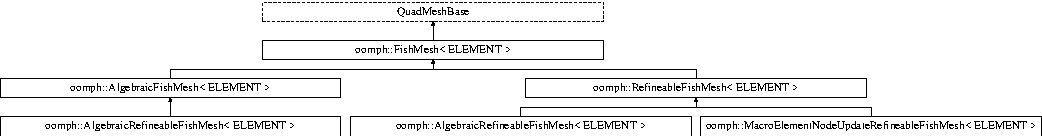
\includegraphics[height=1.821138cm]{classoomph_1_1FishMesh}
\end{center}
\end{figure}
\subsection*{Public Member Functions}
\begin{DoxyCompactItemize}
\item 
\hyperlink{classoomph_1_1FishMesh_a492c0535a4a0bf97729dfdff3754d211}{Fish\+Mesh} (Time\+Stepper $\ast$time\+\_\+stepper\+\_\+pt=\&Mesh\+::\+Default\+\_\+\+Time\+Stepper)
\begin{DoxyCompactList}\small\item\em Constructor\+: Pass pointer to timestepper (defaults to the (Steady) default timestepper defined in Mesh) \end{DoxyCompactList}\item 
\hyperlink{classoomph_1_1FishMesh_ac0b931509ec02c03f8ee5676355f196b}{Fish\+Mesh} (Geom\+Object $\ast$back\+\_\+pt, Time\+Stepper $\ast$time\+\_\+stepper\+\_\+pt=\&Mesh\+::\+Default\+\_\+\+Time\+Stepper)
\begin{DoxyCompactList}\small\item\em Constructor\+: Pass pointer Geom\+Object that defines the fish\textquotesingle{}s back and pointer to timestepper (defaults to the (Steady) default timestepper defined in Mesh) \end{DoxyCompactList}\item 
virtual \hyperlink{classoomph_1_1FishMesh_a3763b9be54c74d15a8c5b2129e0f4fae}{$\sim$\+Fish\+Mesh} ()
\begin{DoxyCompactList}\small\item\em Destructor\+: Kill the geom object that represents the fish\textquotesingle{}s back (if necessary) \end{DoxyCompactList}\item 
Geom\+Object $\ast$\& \hyperlink{classoomph_1_1FishMesh_aa6d659caf657ce5fd549431fadb009d7}{fish\+\_\+back\+\_\+pt} ()
\begin{DoxyCompactList}\small\item\em Access function to geom object that represents the fish\textquotesingle{}s back. \end{DoxyCompactList}\item 
\hyperlink{classoomph_1_1FishDomain}{Fish\+Domain} $\ast$\& \hyperlink{classoomph_1_1FishMesh_ad5076610d83a07e6306375a2632ee460}{domain\+\_\+pt} ()
\begin{DoxyCompactList}\small\item\em Access function to \hyperlink{classoomph_1_1FishDomain}{Fish\+Domain}. \end{DoxyCompactList}\end{DoxyCompactItemize}
\subsection*{Protected Types}
\begin{DoxyCompactItemize}
\item 
enum \{ \hyperlink{classoomph_1_1FishMesh_a4a4137c4add890a283e51651c5c47f62a3d3771209da5e9d30eedf957678f24fb}{Lower\+\_\+body}, 
\hyperlink{classoomph_1_1FishMesh_a4a4137c4add890a283e51651c5c47f62aee1779e3610fcc506554edb97df12b81}{Upper\+\_\+body}, 
\hyperlink{classoomph_1_1FishMesh_a4a4137c4add890a283e51651c5c47f62a616ba7504cd0d8970e1e275579f5606d}{Lower\+\_\+fin}, 
\hyperlink{classoomph_1_1FishMesh_a4a4137c4add890a283e51651c5c47f62a773d3896b889d4f05ed5902482650da1}{Upper\+\_\+fin}
 \}\begin{DoxyCompactList}\small\item\em Remesh function ids. \end{DoxyCompactList}
\end{DoxyCompactItemize}
\subsection*{Protected Member Functions}
\begin{DoxyCompactItemize}
\item 
void \hyperlink{classoomph_1_1FishMesh_aabde81364817d938f0924997bf4f63cc}{build\+\_\+mesh} (Time\+Stepper $\ast$time\+\_\+stepper\+\_\+pt)
\begin{DoxyCompactList}\small\item\em Build the mesh, using the geometric object identified by Back\+\_\+pt. \end{DoxyCompactList}\end{DoxyCompactItemize}
\subsection*{Protected Attributes}
\begin{DoxyCompactItemize}
\item 
Geom\+Object $\ast$ \hyperlink{classoomph_1_1FishMesh_a26e8eb98c11d6b45cc3b5c5a8e45b530}{Back\+\_\+pt}
\begin{DoxyCompactList}\small\item\em Pointer to fish back. \end{DoxyCompactList}\item 
\hyperlink{classoomph_1_1FishDomain}{Fish\+Domain} $\ast$ \hyperlink{classoomph_1_1FishMesh_ae18c3154ad99054c073840c6b134c49b}{Domain\+\_\+pt}
\begin{DoxyCompactList}\small\item\em Pointer to domain. \end{DoxyCompactList}\item 
bool \hyperlink{classoomph_1_1FishMesh_ad1dd5a431f711d3ac14498cc6ab4d856}{Must\+\_\+kill\+\_\+fish\+\_\+back}
\begin{DoxyCompactList}\small\item\em Do I need to kill the fish back geom object? \end{DoxyCompactList}\end{DoxyCompactItemize}


\subsection{Detailed Description}
\subsubsection*{template$<$class E\+L\+E\+M\+E\+NT$>$\newline
class oomph\+::\+Fish\+Mesh$<$ E\+L\+E\+M\+E\+N\+T $>$}

Fish shaped mesh. The geometry is defined by the Domain object \hyperlink{classoomph_1_1FishDomain}{Fish\+Domain}. 

Definition at line 59 of file fish\+\_\+mesh.\+template.\+h.



\subsection{Member Enumeration Documentation}
\mbox{\Hypertarget{classoomph_1_1FishMesh_a4a4137c4add890a283e51651c5c47f62}\label{classoomph_1_1FishMesh_a4a4137c4add890a283e51651c5c47f62}} 
\subsubsection{\texorpdfstring{anonymous enum}{anonymous enum}}
{\footnotesize\ttfamily template$<$class E\+L\+E\+M\+E\+NT $>$ \\
anonymous enum\hspace{0.3cm}{\ttfamily [protected]}}



Remesh function ids. 

\begin{DoxyEnumFields}{Enumerator}
\raisebox{\heightof{T}}[0pt][0pt]{\index{Lower\+\_\+body@{Lower\+\_\+body}!oomph\+::\+Fish\+Mesh@{oomph\+::\+Fish\+Mesh}}\index{oomph\+::\+Fish\+Mesh@{oomph\+::\+Fish\+Mesh}!Lower\+\_\+body@{Lower\+\_\+body}}}\mbox{\Hypertarget{classoomph_1_1FishMesh_a4a4137c4add890a283e51651c5c47f62a3d3771209da5e9d30eedf957678f24fb}\label{classoomph_1_1FishMesh_a4a4137c4add890a283e51651c5c47f62a3d3771209da5e9d30eedf957678f24fb}} 
Lower\+\_\+body&\\
\hline

\raisebox{\heightof{T}}[0pt][0pt]{\index{Upper\+\_\+body@{Upper\+\_\+body}!oomph\+::\+Fish\+Mesh@{oomph\+::\+Fish\+Mesh}}\index{oomph\+::\+Fish\+Mesh@{oomph\+::\+Fish\+Mesh}!Upper\+\_\+body@{Upper\+\_\+body}}}\mbox{\Hypertarget{classoomph_1_1FishMesh_a4a4137c4add890a283e51651c5c47f62aee1779e3610fcc506554edb97df12b81}\label{classoomph_1_1FishMesh_a4a4137c4add890a283e51651c5c47f62aee1779e3610fcc506554edb97df12b81}} 
Upper\+\_\+body&\\
\hline

\raisebox{\heightof{T}}[0pt][0pt]{\index{Lower\+\_\+fin@{Lower\+\_\+fin}!oomph\+::\+Fish\+Mesh@{oomph\+::\+Fish\+Mesh}}\index{oomph\+::\+Fish\+Mesh@{oomph\+::\+Fish\+Mesh}!Lower\+\_\+fin@{Lower\+\_\+fin}}}\mbox{\Hypertarget{classoomph_1_1FishMesh_a4a4137c4add890a283e51651c5c47f62a616ba7504cd0d8970e1e275579f5606d}\label{classoomph_1_1FishMesh_a4a4137c4add890a283e51651c5c47f62a616ba7504cd0d8970e1e275579f5606d}} 
Lower\+\_\+fin&\\
\hline

\raisebox{\heightof{T}}[0pt][0pt]{\index{Upper\+\_\+fin@{Upper\+\_\+fin}!oomph\+::\+Fish\+Mesh@{oomph\+::\+Fish\+Mesh}}\index{oomph\+::\+Fish\+Mesh@{oomph\+::\+Fish\+Mesh}!Upper\+\_\+fin@{Upper\+\_\+fin}}}\mbox{\Hypertarget{classoomph_1_1FishMesh_a4a4137c4add890a283e51651c5c47f62a773d3896b889d4f05ed5902482650da1}\label{classoomph_1_1FishMesh_a4a4137c4add890a283e51651c5c47f62a773d3896b889d4f05ed5902482650da1}} 
Upper\+\_\+fin&\\
\hline

\end{DoxyEnumFields}


Definition at line 102 of file fish\+\_\+mesh.\+template.\+h.



\subsection{Constructor \& Destructor Documentation}
\mbox{\Hypertarget{classoomph_1_1FishMesh_a492c0535a4a0bf97729dfdff3754d211}\label{classoomph_1_1FishMesh_a492c0535a4a0bf97729dfdff3754d211}} 
\index{oomph\+::\+Fish\+Mesh@{oomph\+::\+Fish\+Mesh}!Fish\+Mesh@{Fish\+Mesh}}
\index{Fish\+Mesh@{Fish\+Mesh}!oomph\+::\+Fish\+Mesh@{oomph\+::\+Fish\+Mesh}}
\subsubsection{\texorpdfstring{Fish\+Mesh()}{FishMesh()}\hspace{0.1cm}{\footnotesize\ttfamily [1/2]}}
{\footnotesize\ttfamily template$<$class E\+L\+E\+M\+E\+NT $>$ \\
\hyperlink{classoomph_1_1FishMesh}{oomph\+::\+Fish\+Mesh}$<$ E\+L\+E\+M\+E\+NT $>$\+::\hyperlink{classoomph_1_1FishMesh}{Fish\+Mesh} (\begin{DoxyParamCaption}\item[{Time\+Stepper $\ast$}]{time\+\_\+stepper\+\_\+pt = {\ttfamily \&Mesh\+:\+:Default\+\_\+TimeStepper} }\end{DoxyParamCaption})}



Constructor\+: Pass pointer to timestepper (defaults to the (Steady) default timestepper defined in Mesh) 

Constructor\+: Pass pointer to timestepper. (defaults to (Steady) default timestepper defined in Mesh) 

Definition at line 44 of file fish\+\_\+mesh.\+template.\+cc.

\mbox{\Hypertarget{classoomph_1_1FishMesh_ac0b931509ec02c03f8ee5676355f196b}\label{classoomph_1_1FishMesh_ac0b931509ec02c03f8ee5676355f196b}} 
\index{oomph\+::\+Fish\+Mesh@{oomph\+::\+Fish\+Mesh}!Fish\+Mesh@{Fish\+Mesh}}
\index{Fish\+Mesh@{Fish\+Mesh}!oomph\+::\+Fish\+Mesh@{oomph\+::\+Fish\+Mesh}}
\subsubsection{\texorpdfstring{Fish\+Mesh()}{FishMesh()}\hspace{0.1cm}{\footnotesize\ttfamily [2/2]}}
{\footnotesize\ttfamily template$<$class E\+L\+E\+M\+E\+NT $>$ \\
\hyperlink{classoomph_1_1FishMesh}{oomph\+::\+Fish\+Mesh}$<$ E\+L\+E\+M\+E\+NT $>$\+::\hyperlink{classoomph_1_1FishMesh}{Fish\+Mesh} (\begin{DoxyParamCaption}\item[{Geom\+Object $\ast$}]{back\+\_\+pt,  }\item[{Time\+Stepper $\ast$}]{time\+\_\+stepper\+\_\+pt = {\ttfamily \&Mesh\+:\+:Default\+\_\+TimeStepper} }\end{DoxyParamCaption})}



Constructor\+: Pass pointer Geom\+Object that defines the fish\textquotesingle{}s back and pointer to timestepper (defaults to the (Steady) default timestepper defined in Mesh) 

Constructor\+: Pass pointer Geom\+Object that defines the fish\textquotesingle{}s back and pointer to timestepper. (defaults to (Steady) default timestepper defined in Mesh) 

Definition at line 70 of file fish\+\_\+mesh.\+template.\+cc.



References oomph\+::\+Fish\+Mesh$<$ E\+L\+E\+M\+E\+N\+T $>$\+::build\+\_\+mesh(), and oomph\+::\+Fish\+Mesh$<$ E\+L\+E\+M\+E\+N\+T $>$\+::\+Must\+\_\+kill\+\_\+fish\+\_\+back.

\mbox{\Hypertarget{classoomph_1_1FishMesh_a3763b9be54c74d15a8c5b2129e0f4fae}\label{classoomph_1_1FishMesh_a3763b9be54c74d15a8c5b2129e0f4fae}} 
\index{oomph\+::\+Fish\+Mesh@{oomph\+::\+Fish\+Mesh}!````~Fish\+Mesh@{$\sim$\+Fish\+Mesh}}
\index{````~Fish\+Mesh@{$\sim$\+Fish\+Mesh}!oomph\+::\+Fish\+Mesh@{oomph\+::\+Fish\+Mesh}}
\subsubsection{\texorpdfstring{$\sim$\+Fish\+Mesh()}{~FishMesh()}}
{\footnotesize\ttfamily template$<$class E\+L\+E\+M\+E\+NT $>$ \\
virtual \hyperlink{classoomph_1_1FishMesh}{oomph\+::\+Fish\+Mesh}$<$ E\+L\+E\+M\+E\+NT $>$\+::$\sim$\hyperlink{classoomph_1_1FishMesh}{Fish\+Mesh} (\begin{DoxyParamCaption}{ }\end{DoxyParamCaption})\hspace{0.3cm}{\ttfamily [inline]}, {\ttfamily [virtual]}}



Destructor\+: Kill the geom object that represents the fish\textquotesingle{}s back (if necessary) 



Definition at line 77 of file fish\+\_\+mesh.\+template.\+h.



References oomph\+::\+Fish\+Mesh$<$ E\+L\+E\+M\+E\+N\+T $>$\+::\+Back\+\_\+pt, and oomph\+::\+Fish\+Mesh$<$ E\+L\+E\+M\+E\+N\+T $>$\+::\+Must\+\_\+kill\+\_\+fish\+\_\+back.



\subsection{Member Function Documentation}
\mbox{\Hypertarget{classoomph_1_1FishMesh_aabde81364817d938f0924997bf4f63cc}\label{classoomph_1_1FishMesh_aabde81364817d938f0924997bf4f63cc}} 
\index{oomph\+::\+Fish\+Mesh@{oomph\+::\+Fish\+Mesh}!build\+\_\+mesh@{build\+\_\+mesh}}
\index{build\+\_\+mesh@{build\+\_\+mesh}!oomph\+::\+Fish\+Mesh@{oomph\+::\+Fish\+Mesh}}
\subsubsection{\texorpdfstring{build\+\_\+mesh()}{build\_mesh()}}
{\footnotesize\ttfamily template$<$class E\+L\+E\+M\+E\+NT $>$ \\
void \hyperlink{classoomph_1_1FishMesh}{oomph\+::\+Fish\+Mesh}$<$ E\+L\+E\+M\+E\+NT $>$\+::build\+\_\+mesh (\begin{DoxyParamCaption}\item[{Time\+Stepper $\ast$}]{time\+\_\+stepper\+\_\+pt }\end{DoxyParamCaption})\hspace{0.3cm}{\ttfamily [protected]}}



Build the mesh, using the geometric object identified by Back\+\_\+pt. 

Build the mesh, using the geometric object that defines the fish\textquotesingle{}s back. 

Definition at line 89 of file fish\+\_\+mesh.\+template.\+cc.



References oomph\+::\+Fish\+Mesh$<$ E\+L\+E\+M\+E\+N\+T $>$\+::\+Back\+\_\+pt, and oomph\+::\+Fish\+Mesh$<$ E\+L\+E\+M\+E\+N\+T $>$\+::\+Domain\+\_\+pt.



Referenced by oomph\+::\+Fish\+Mesh$<$ E\+L\+E\+M\+E\+N\+T $>$\+::\+Fish\+Mesh().

\mbox{\Hypertarget{classoomph_1_1FishMesh_ad5076610d83a07e6306375a2632ee460}\label{classoomph_1_1FishMesh_ad5076610d83a07e6306375a2632ee460}} 
\index{oomph\+::\+Fish\+Mesh@{oomph\+::\+Fish\+Mesh}!domain\+\_\+pt@{domain\+\_\+pt}}
\index{domain\+\_\+pt@{domain\+\_\+pt}!oomph\+::\+Fish\+Mesh@{oomph\+::\+Fish\+Mesh}}
\subsubsection{\texorpdfstring{domain\+\_\+pt()}{domain\_pt()}}
{\footnotesize\ttfamily template$<$class E\+L\+E\+M\+E\+NT $>$ \\
\hyperlink{classoomph_1_1FishDomain}{Fish\+Domain}$\ast$\& \hyperlink{classoomph_1_1FishMesh}{oomph\+::\+Fish\+Mesh}$<$ E\+L\+E\+M\+E\+NT $>$\+::domain\+\_\+pt (\begin{DoxyParamCaption}{ }\end{DoxyParamCaption})\hspace{0.3cm}{\ttfamily [inline]}}



Access function to \hyperlink{classoomph_1_1FishDomain}{Fish\+Domain}. 



Definition at line 94 of file fish\+\_\+mesh.\+template.\+h.



References oomph\+::\+Fish\+Mesh$<$ E\+L\+E\+M\+E\+N\+T $>$\+::\+Domain\+\_\+pt.



Referenced by oomph\+::\+Macro\+Element\+Node\+Update\+Refineable\+Fish\+Mesh$<$ E\+L\+E\+M\+E\+N\+T $>$\+::\+Macro\+Element\+Node\+Update\+Refineable\+Fish\+Mesh().

\mbox{\Hypertarget{classoomph_1_1FishMesh_aa6d659caf657ce5fd549431fadb009d7}\label{classoomph_1_1FishMesh_aa6d659caf657ce5fd549431fadb009d7}} 
\index{oomph\+::\+Fish\+Mesh@{oomph\+::\+Fish\+Mesh}!fish\+\_\+back\+\_\+pt@{fish\+\_\+back\+\_\+pt}}
\index{fish\+\_\+back\+\_\+pt@{fish\+\_\+back\+\_\+pt}!oomph\+::\+Fish\+Mesh@{oomph\+::\+Fish\+Mesh}}
\subsubsection{\texorpdfstring{fish\+\_\+back\+\_\+pt()}{fish\_back\_pt()}}
{\footnotesize\ttfamily template$<$class E\+L\+E\+M\+E\+NT $>$ \\
Geom\+Object$\ast$\& \hyperlink{classoomph_1_1FishMesh}{oomph\+::\+Fish\+Mesh}$<$ E\+L\+E\+M\+E\+NT $>$\+::fish\+\_\+back\+\_\+pt (\begin{DoxyParamCaption}{ }\end{DoxyParamCaption})\hspace{0.3cm}{\ttfamily [inline]}}



Access function to geom object that represents the fish\textquotesingle{}s back. 



Definition at line 87 of file fish\+\_\+mesh.\+template.\+h.



References oomph\+::\+Fish\+Mesh$<$ E\+L\+E\+M\+E\+N\+T $>$\+::\+Back\+\_\+pt.



\subsection{Member Data Documentation}
\mbox{\Hypertarget{classoomph_1_1FishMesh_a26e8eb98c11d6b45cc3b5c5a8e45b530}\label{classoomph_1_1FishMesh_a26e8eb98c11d6b45cc3b5c5a8e45b530}} 
\index{oomph\+::\+Fish\+Mesh@{oomph\+::\+Fish\+Mesh}!Back\+\_\+pt@{Back\+\_\+pt}}
\index{Back\+\_\+pt@{Back\+\_\+pt}!oomph\+::\+Fish\+Mesh@{oomph\+::\+Fish\+Mesh}}
\subsubsection{\texorpdfstring{Back\+\_\+pt}{Back\_pt}}
{\footnotesize\ttfamily template$<$class E\+L\+E\+M\+E\+NT $>$ \\
Geom\+Object$\ast$ \hyperlink{classoomph_1_1FishMesh}{oomph\+::\+Fish\+Mesh}$<$ E\+L\+E\+M\+E\+NT $>$\+::Back\+\_\+pt\hspace{0.3cm}{\ttfamily [protected]}}



Pointer to fish back. 



Definition at line 108 of file fish\+\_\+mesh.\+template.\+h.



Referenced by oomph\+::\+Fish\+Mesh$<$ E\+L\+E\+M\+E\+N\+T $>$\+::build\+\_\+mesh(), oomph\+::\+Fish\+Mesh$<$ E\+L\+E\+M\+E\+N\+T $>$\+::fish\+\_\+back\+\_\+pt(), oomph\+::\+Macro\+Element\+Node\+Update\+Refineable\+Fish\+Mesh$<$ E\+L\+E\+M\+E\+N\+T $>$\+::\+Macro\+Element\+Node\+Update\+Refineable\+Fish\+Mesh(), oomph\+::\+Algebraic\+Fish\+Mesh$<$ E\+L\+E\+M\+E\+N\+T $>$\+::setup\+\_\+algebraic\+\_\+node\+\_\+update(), oomph\+::\+Algebraic\+Fish\+Mesh$<$ E\+L\+E\+M\+E\+N\+T $>$\+::update\+\_\+node\+\_\+update(), and oomph\+::\+Fish\+Mesh$<$ E\+L\+E\+M\+E\+N\+T $>$\+::$\sim$\+Fish\+Mesh().

\mbox{\Hypertarget{classoomph_1_1FishMesh_ae18c3154ad99054c073840c6b134c49b}\label{classoomph_1_1FishMesh_ae18c3154ad99054c073840c6b134c49b}} 
\index{oomph\+::\+Fish\+Mesh@{oomph\+::\+Fish\+Mesh}!Domain\+\_\+pt@{Domain\+\_\+pt}}
\index{Domain\+\_\+pt@{Domain\+\_\+pt}!oomph\+::\+Fish\+Mesh@{oomph\+::\+Fish\+Mesh}}
\subsubsection{\texorpdfstring{Domain\+\_\+pt}{Domain\_pt}}
{\footnotesize\ttfamily template$<$class E\+L\+E\+M\+E\+NT $>$ \\
\hyperlink{classoomph_1_1FishDomain}{Fish\+Domain}$\ast$ \hyperlink{classoomph_1_1FishMesh}{oomph\+::\+Fish\+Mesh}$<$ E\+L\+E\+M\+E\+NT $>$\+::Domain\+\_\+pt\hspace{0.3cm}{\ttfamily [protected]}}



Pointer to domain. 



Definition at line 111 of file fish\+\_\+mesh.\+template.\+h.



Referenced by oomph\+::\+Fish\+Mesh$<$ E\+L\+E\+M\+E\+N\+T $>$\+::build\+\_\+mesh(), oomph\+::\+Fish\+Mesh$<$ E\+L\+E\+M\+E\+N\+T $>$\+::domain\+\_\+pt(), oomph\+::\+Algebraic\+Fish\+Mesh$<$ E\+L\+E\+M\+E\+N\+T $>$\+::node\+\_\+update\+\_\+in\+\_\+body(), oomph\+::\+Algebraic\+Fish\+Mesh$<$ E\+L\+E\+M\+E\+N\+T $>$\+::node\+\_\+update\+\_\+in\+\_\+fin(), and oomph\+::\+Algebraic\+Fish\+Mesh$<$ E\+L\+E\+M\+E\+N\+T $>$\+::update\+\_\+node\+\_\+update().

\mbox{\Hypertarget{classoomph_1_1FishMesh_ad1dd5a431f711d3ac14498cc6ab4d856}\label{classoomph_1_1FishMesh_ad1dd5a431f711d3ac14498cc6ab4d856}} 
\index{oomph\+::\+Fish\+Mesh@{oomph\+::\+Fish\+Mesh}!Must\+\_\+kill\+\_\+fish\+\_\+back@{Must\+\_\+kill\+\_\+fish\+\_\+back}}
\index{Must\+\_\+kill\+\_\+fish\+\_\+back@{Must\+\_\+kill\+\_\+fish\+\_\+back}!oomph\+::\+Fish\+Mesh@{oomph\+::\+Fish\+Mesh}}
\subsubsection{\texorpdfstring{Must\+\_\+kill\+\_\+fish\+\_\+back}{Must\_kill\_fish\_back}}
{\footnotesize\ttfamily template$<$class E\+L\+E\+M\+E\+NT $>$ \\
bool \hyperlink{classoomph_1_1FishMesh}{oomph\+::\+Fish\+Mesh}$<$ E\+L\+E\+M\+E\+NT $>$\+::Must\+\_\+kill\+\_\+fish\+\_\+back\hspace{0.3cm}{\ttfamily [protected]}}



Do I need to kill the fish back geom object? 



Definition at line 114 of file fish\+\_\+mesh.\+template.\+h.



Referenced by oomph\+::\+Fish\+Mesh$<$ E\+L\+E\+M\+E\+N\+T $>$\+::\+Fish\+Mesh(), and oomph\+::\+Fish\+Mesh$<$ E\+L\+E\+M\+E\+N\+T $>$\+::$\sim$\+Fish\+Mesh().



The documentation for this class was generated from the following files\+:\begin{DoxyCompactItemize}
\item 
\hyperlink{fish__mesh_8template_8h}{fish\+\_\+mesh.\+template.\+h}\item 
\hyperlink{fish__mesh_8template_8cc}{fish\+\_\+mesh.\+template.\+cc}\end{DoxyCompactItemize}

\hypertarget{classoomph_1_1FSIDrivenCavityMesh}{}\section{oomph\+:\+:F\+S\+I\+Driven\+Cavity\+Mesh$<$ E\+L\+E\+M\+E\+NT $>$ Class Template Reference}
\label{classoomph_1_1FSIDrivenCavityMesh}\index{oomph\+::\+F\+S\+I\+Driven\+Cavity\+Mesh$<$ E\+L\+E\+M\+E\+N\+T $>$@{oomph\+::\+F\+S\+I\+Driven\+Cavity\+Mesh$<$ E\+L\+E\+M\+E\+N\+T $>$}}


\hyperlink{classoomph_1_1Mesh}{Mesh} for W. Wall\textquotesingle{}s F\+SI driven cavity problem. The mesh is derived from the {\ttfamily \hyperlink{classoomph_1_1SimpleRectangularQuadMesh}{Simple\+Rectangular\+Quad\+Mesh}} so it\textquotesingle{}s node and element numbering scheme is the same as in that mesh. Only the boundaries are numbered differently to allow the easy identification of the \char`\"{}collapsible\char`\"{} segment. Boundary coordinates are set up for all nodes located on boundary 3 (the collapsible segment). The curvilinear (\char`\"{}collapsible\char`\"{}) segment is defined by a {\ttfamily \hyperlink{classoomph_1_1GeomObject}{Geom\+Object}}.  




{\ttfamily \#include $<$fsi\+\_\+driven\+\_\+cavity\+\_\+mesh.\+template.\+h$>$}

Inheritance diagram for oomph\+:\+:F\+S\+I\+Driven\+Cavity\+Mesh$<$ E\+L\+E\+M\+E\+NT $>$\+:\begin{figure}[H]
\begin{center}
\leavevmode
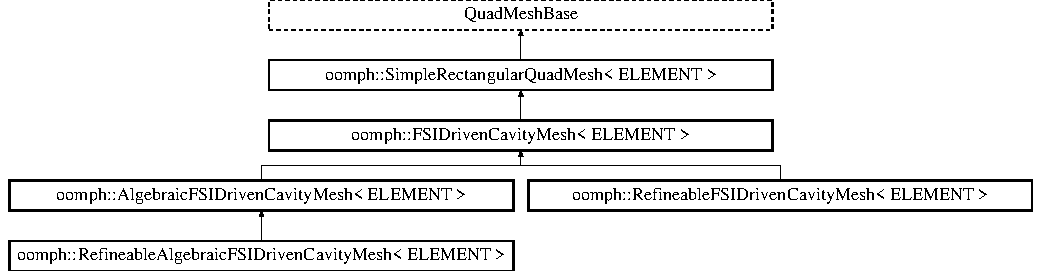
\includegraphics[height=4.375000cm]{classoomph_1_1FSIDrivenCavityMesh}
\end{center}
\end{figure}
\subsection*{Public Member Functions}
\begin{DoxyCompactItemize}
\item 
\hyperlink{classoomph_1_1FSIDrivenCavityMesh_af227477a1de5faf56352d21913a91feb}{F\+S\+I\+Driven\+Cavity\+Mesh} (const unsigned \&\hyperlink{classoomph_1_1SimpleRectangularQuadMesh_a4ff7678ec433180e2245ea2147f222b7}{nx}, const unsigned \&\hyperlink{classoomph_1_1SimpleRectangularQuadMesh_a45011f22dedd480392b1f376e4269921}{ny}, const double \&lx, const double \&ly, const double \&gap\+\_\+fraction, \hyperlink{classoomph_1_1GeomObject}{Geom\+Object} $\ast$wall\+\_\+pt, \hyperlink{classoomph_1_1TimeStepper}{Time\+Stepper} $\ast$time\+\_\+stepper\+\_\+pt=\&\hyperlink{classoomph_1_1Mesh_a12243d0fee2b1fcee729ee5a4777ea10}{Mesh\+::\+Default\+\_\+\+Time\+Stepper})
\begin{DoxyCompactList}\small\item\em Constructor\+: Pass number of elements, number of elements, fractional height of the gap above the moving wall, pointer to \hyperlink{classoomph_1_1GeomObject}{Geom\+Object} that defines the collapsible segment and pointer to \hyperlink{classoomph_1_1TimeStepper}{Time\+Stepper} (defaults to the default timestepper, \hyperlink{classoomph_1_1Steady}{Steady}). \end{DoxyCompactList}\end{DoxyCompactItemize}
\subsection*{Protected Attributes}
\begin{DoxyCompactItemize}
\item 
unsigned \hyperlink{classoomph_1_1FSIDrivenCavityMesh_a179f742e7bb521e8943107be3005d49b}{Nx}
\begin{DoxyCompactList}\small\item\em Number of elements in x direction. \end{DoxyCompactList}\item 
unsigned \hyperlink{classoomph_1_1FSIDrivenCavityMesh_af80a5662c2f61ebe49caba4ab08886b9}{Ny}
\begin{DoxyCompactList}\small\item\em Number of elements in y direction. \end{DoxyCompactList}\item 
double \hyperlink{classoomph_1_1FSIDrivenCavityMesh_ad95b3650cfa765b1ac6a0f131d407b23}{Gap\+\_\+fraction}
\begin{DoxyCompactList}\small\item\em Fraction of the gap next to moving lid, relative to the height of the domain. \end{DoxyCompactList}\item 
\hyperlink{classoomph_1_1GeomObject}{Geom\+Object} $\ast$ \hyperlink{classoomph_1_1FSIDrivenCavityMesh_a4f05e03a223ac1f8370bdd39c56a5638}{Wall\+\_\+pt}
\begin{DoxyCompactList}\small\item\em Pointer to geometric object that represents the moving wall. \end{DoxyCompactList}\end{DoxyCompactItemize}
\subsection*{Additional Inherited Members}


\subsection{Detailed Description}
\subsubsection*{template$<$class E\+L\+E\+M\+E\+NT$>$\newline
class oomph\+::\+F\+S\+I\+Driven\+Cavity\+Mesh$<$ E\+L\+E\+M\+E\+N\+T $>$}

\hyperlink{classoomph_1_1Mesh}{Mesh} for W. Wall\textquotesingle{}s F\+SI driven cavity problem. The mesh is derived from the {\ttfamily \hyperlink{classoomph_1_1SimpleRectangularQuadMesh}{Simple\+Rectangular\+Quad\+Mesh}} so it\textquotesingle{}s node and element numbering scheme is the same as in that mesh. Only the boundaries are numbered differently to allow the easy identification of the \char`\"{}collapsible\char`\"{} segment. Boundary coordinates are set up for all nodes located on boundary 3 (the collapsible segment). The curvilinear (\char`\"{}collapsible\char`\"{}) segment is defined by a {\ttfamily \hyperlink{classoomph_1_1GeomObject}{Geom\+Object}}. 


\begin{DoxyItemize}
\item Boundary 0 is the moving lid.
\item Boundary 1 is the gap above the moving lid on the right wall
\item Boundary 2 is the rigid part of the right wall
\item Boundary 3 is the moving (elastic) wall
\item Boundary 4 is the rigid part of the left wall
\item Boundary 5 is the gap above the moving lid on the left wall 
\end{DoxyItemize}

Definition at line 71 of file fsi\+\_\+driven\+\_\+cavity\+\_\+mesh.\+template.\+h.



\subsection{Constructor \& Destructor Documentation}
\mbox{\Hypertarget{classoomph_1_1FSIDrivenCavityMesh_af227477a1de5faf56352d21913a91feb}\label{classoomph_1_1FSIDrivenCavityMesh_af227477a1de5faf56352d21913a91feb}} 
\index{oomph\+::\+F\+S\+I\+Driven\+Cavity\+Mesh@{oomph\+::\+F\+S\+I\+Driven\+Cavity\+Mesh}!F\+S\+I\+Driven\+Cavity\+Mesh@{F\+S\+I\+Driven\+Cavity\+Mesh}}
\index{F\+S\+I\+Driven\+Cavity\+Mesh@{F\+S\+I\+Driven\+Cavity\+Mesh}!oomph\+::\+F\+S\+I\+Driven\+Cavity\+Mesh@{oomph\+::\+F\+S\+I\+Driven\+Cavity\+Mesh}}
\subsubsection{\texorpdfstring{F\+S\+I\+Driven\+Cavity\+Mesh()}{FSIDrivenCavityMesh()}}
{\footnotesize\ttfamily template$<$class E\+L\+E\+M\+E\+NT $>$ \\
\hyperlink{classoomph_1_1FSIDrivenCavityMesh}{oomph\+::\+F\+S\+I\+Driven\+Cavity\+Mesh}$<$ E\+L\+E\+M\+E\+NT $>$\+::\hyperlink{classoomph_1_1FSIDrivenCavityMesh}{F\+S\+I\+Driven\+Cavity\+Mesh} (\begin{DoxyParamCaption}\item[{const unsigned \&}]{nx,  }\item[{const unsigned \&}]{ny,  }\item[{const double \&}]{lx,  }\item[{const double \&}]{ly,  }\item[{const double \&}]{gap\+\_\+fraction,  }\item[{\hyperlink{classoomph_1_1GeomObject}{Geom\+Object} $\ast$}]{wall\+\_\+pt,  }\item[{\hyperlink{classoomph_1_1TimeStepper}{Time\+Stepper} $\ast$}]{time\+\_\+stepper\+\_\+pt = {\ttfamily \&\hyperlink{classoomph_1_1Mesh_a12243d0fee2b1fcee729ee5a4777ea10}{Mesh\+::\+Default\+\_\+\+Time\+Stepper}} }\end{DoxyParamCaption})}



Constructor\+: Pass number of elements, number of elements, fractional height of the gap above the moving wall, pointer to \hyperlink{classoomph_1_1GeomObject}{Geom\+Object} that defines the collapsible segment and pointer to \hyperlink{classoomph_1_1TimeStepper}{Time\+Stepper} (defaults to the default timestepper, \hyperlink{classoomph_1_1Steady}{Steady}). 

Constructor\+: Pass number of elements, lengths, pointer to \hyperlink{classoomph_1_1GeomObject}{Geom\+Object} that defines the collapsible segment and pointer to \hyperlink{classoomph_1_1TimeStepper}{Time\+Stepper} (defaults to the default timestepper, \hyperlink{classoomph_1_1Steady}{Steady}). 

Definition at line 46 of file fsi\+\_\+driven\+\_\+cavity\+\_\+mesh.\+template.\+cc.



References oomph\+::\+Mesh\+::add\+\_\+boundary\+\_\+node(), oomph\+::\+Mesh\+::\+Boundary\+\_\+coordinate\+\_\+exists, e, oomph\+::\+Mesh\+::finite\+\_\+element\+\_\+pt(), oomph\+::\+F\+S\+I\+Driven\+Cavity\+Mesh$<$ E\+L\+E\+M\+E\+N\+T $>$\+::\+Gap\+\_\+fraction, i, oomph\+::\+Mesh\+::nboundary(), oomph\+::\+Mesh\+::nelement(), oomph\+::\+Mesh\+::nnode(), oomph\+::\+Finite\+Element\+::nnode\+\_\+1d(), oomph\+::\+Mesh\+::node\+\_\+pt(), oomph\+::\+Finite\+Element\+::node\+\_\+pt(), oomph\+::\+Mesh\+::remove\+\_\+boundary\+\_\+nodes(), oomph\+::\+Mesh\+::set\+\_\+nboundary(), oomph\+::\+Quad\+Mesh\+Base\+::setup\+\_\+boundary\+\_\+element\+\_\+info(), and oomph\+::\+Node\+::x().



\subsection{Member Data Documentation}
\mbox{\Hypertarget{classoomph_1_1FSIDrivenCavityMesh_ad95b3650cfa765b1ac6a0f131d407b23}\label{classoomph_1_1FSIDrivenCavityMesh_ad95b3650cfa765b1ac6a0f131d407b23}} 
\index{oomph\+::\+F\+S\+I\+Driven\+Cavity\+Mesh@{oomph\+::\+F\+S\+I\+Driven\+Cavity\+Mesh}!Gap\+\_\+fraction@{Gap\+\_\+fraction}}
\index{Gap\+\_\+fraction@{Gap\+\_\+fraction}!oomph\+::\+F\+S\+I\+Driven\+Cavity\+Mesh@{oomph\+::\+F\+S\+I\+Driven\+Cavity\+Mesh}}
\subsubsection{\texorpdfstring{Gap\+\_\+fraction}{Gap\_fraction}}
{\footnotesize\ttfamily template$<$class E\+L\+E\+M\+E\+NT $>$ \\
double \hyperlink{classoomph_1_1FSIDrivenCavityMesh}{oomph\+::\+F\+S\+I\+Driven\+Cavity\+Mesh}$<$ E\+L\+E\+M\+E\+NT $>$\+::Gap\+\_\+fraction\hspace{0.3cm}{\ttfamily [protected]}}



Fraction of the gap next to moving lid, relative to the height of the domain. 



Definition at line 99 of file fsi\+\_\+driven\+\_\+cavity\+\_\+mesh.\+template.\+h.



Referenced by oomph\+::\+F\+S\+I\+Driven\+Cavity\+Mesh$<$ E\+L\+E\+M\+E\+N\+T $>$\+::\+F\+S\+I\+Driven\+Cavity\+Mesh().

\mbox{\Hypertarget{classoomph_1_1FSIDrivenCavityMesh_a179f742e7bb521e8943107be3005d49b}\label{classoomph_1_1FSIDrivenCavityMesh_a179f742e7bb521e8943107be3005d49b}} 
\index{oomph\+::\+F\+S\+I\+Driven\+Cavity\+Mesh@{oomph\+::\+F\+S\+I\+Driven\+Cavity\+Mesh}!Nx@{Nx}}
\index{Nx@{Nx}!oomph\+::\+F\+S\+I\+Driven\+Cavity\+Mesh@{oomph\+::\+F\+S\+I\+Driven\+Cavity\+Mesh}}
\subsubsection{\texorpdfstring{Nx}{Nx}}
{\footnotesize\ttfamily template$<$class E\+L\+E\+M\+E\+NT $>$ \\
unsigned \hyperlink{classoomph_1_1FSIDrivenCavityMesh}{oomph\+::\+F\+S\+I\+Driven\+Cavity\+Mesh}$<$ E\+L\+E\+M\+E\+NT $>$\+::Nx\hspace{0.3cm}{\ttfamily [protected]}}



Number of elements in x direction. 



Definition at line 92 of file fsi\+\_\+driven\+\_\+cavity\+\_\+mesh.\+template.\+h.

\mbox{\Hypertarget{classoomph_1_1FSIDrivenCavityMesh_af80a5662c2f61ebe49caba4ab08886b9}\label{classoomph_1_1FSIDrivenCavityMesh_af80a5662c2f61ebe49caba4ab08886b9}} 
\index{oomph\+::\+F\+S\+I\+Driven\+Cavity\+Mesh@{oomph\+::\+F\+S\+I\+Driven\+Cavity\+Mesh}!Ny@{Ny}}
\index{Ny@{Ny}!oomph\+::\+F\+S\+I\+Driven\+Cavity\+Mesh@{oomph\+::\+F\+S\+I\+Driven\+Cavity\+Mesh}}
\subsubsection{\texorpdfstring{Ny}{Ny}}
{\footnotesize\ttfamily template$<$class E\+L\+E\+M\+E\+NT $>$ \\
unsigned \hyperlink{classoomph_1_1FSIDrivenCavityMesh}{oomph\+::\+F\+S\+I\+Driven\+Cavity\+Mesh}$<$ E\+L\+E\+M\+E\+NT $>$\+::Ny\hspace{0.3cm}{\ttfamily [protected]}}



Number of elements in y direction. 



Definition at line 95 of file fsi\+\_\+driven\+\_\+cavity\+\_\+mesh.\+template.\+h.

\mbox{\Hypertarget{classoomph_1_1FSIDrivenCavityMesh_a4f05e03a223ac1f8370bdd39c56a5638}\label{classoomph_1_1FSIDrivenCavityMesh_a4f05e03a223ac1f8370bdd39c56a5638}} 
\index{oomph\+::\+F\+S\+I\+Driven\+Cavity\+Mesh@{oomph\+::\+F\+S\+I\+Driven\+Cavity\+Mesh}!Wall\+\_\+pt@{Wall\+\_\+pt}}
\index{Wall\+\_\+pt@{Wall\+\_\+pt}!oomph\+::\+F\+S\+I\+Driven\+Cavity\+Mesh@{oomph\+::\+F\+S\+I\+Driven\+Cavity\+Mesh}}
\subsubsection{\texorpdfstring{Wall\+\_\+pt}{Wall\_pt}}
{\footnotesize\ttfamily template$<$class E\+L\+E\+M\+E\+NT $>$ \\
\hyperlink{classoomph_1_1GeomObject}{Geom\+Object}$\ast$ \hyperlink{classoomph_1_1FSIDrivenCavityMesh}{oomph\+::\+F\+S\+I\+Driven\+Cavity\+Mesh}$<$ E\+L\+E\+M\+E\+NT $>$\+::Wall\+\_\+pt\hspace{0.3cm}{\ttfamily [protected]}}



Pointer to geometric object that represents the moving wall. 



Definition at line 102 of file fsi\+\_\+driven\+\_\+cavity\+\_\+mesh.\+template.\+h.



Referenced by oomph\+::\+Algebraic\+F\+S\+I\+Driven\+Cavity\+Mesh$<$ E\+L\+E\+M\+E\+N\+T $>$\+::setup\+\_\+algebraic\+\_\+node\+\_\+update(), and oomph\+::\+Refineable\+Algebraic\+F\+S\+I\+Driven\+Cavity\+Mesh$<$ E\+L\+E\+M\+E\+N\+T $>$\+::update\+\_\+node\+\_\+update().



The documentation for this class was generated from the following files\+:\begin{DoxyCompactItemize}
\item 
\hyperlink{fsi__driven__cavity__mesh_8template_8h}{fsi\+\_\+driven\+\_\+cavity\+\_\+mesh.\+template.\+h}\item 
\hyperlink{fsi__driven__cavity__mesh_8template_8cc}{fsi\+\_\+driven\+\_\+cavity\+\_\+mesh.\+template.\+cc}\end{DoxyCompactItemize}

\hypertarget{classoomph_1_1FullCircleDomain}{}\section{oomph\+:\+:Full\+Circle\+Domain Class Reference}
\label{classoomph_1_1FullCircleDomain}\index{oomph\+::\+Full\+Circle\+Domain@{oomph\+::\+Full\+Circle\+Domain}}


Topologically circular domain, e.\+g. a tube cross section. The entire domain must be defined by a \hyperlink{classoomph_1_1GeomObject}{Geom\+Object} with the following convention\+: zeta\mbox{[}0\mbox{]} is the radial coordinate and zeta\mbox{[}1\mbox{]} is the theta coordinate around the cross-\/sectin. The outer boundary must lie at zeta\mbox{[}0\mbox{]} = 1.  




{\ttfamily \#include $<$full\+\_\+circle\+\_\+domain.\+h$>$}

Inheritance diagram for oomph\+:\+:Full\+Circle\+Domain\+:\begin{figure}[H]
\begin{center}
\leavevmode
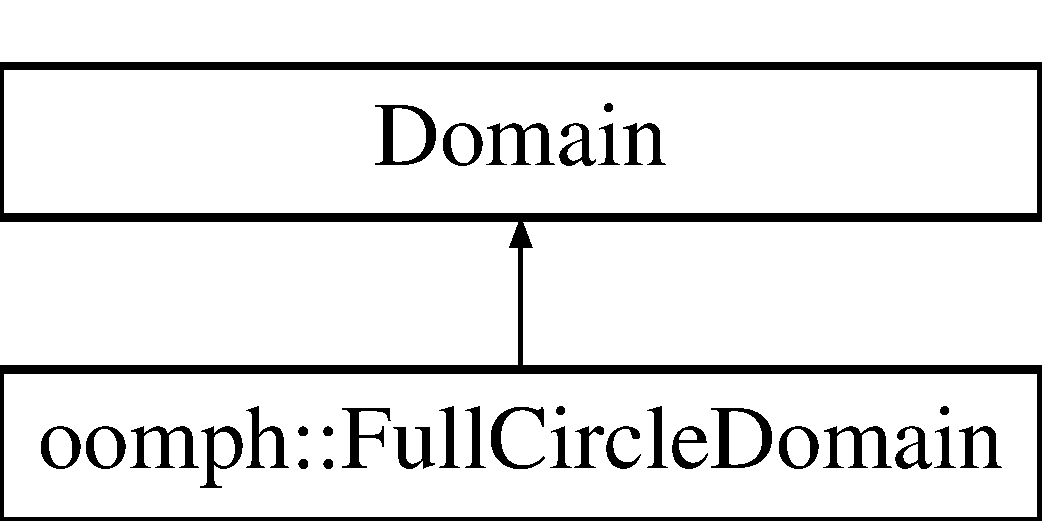
\includegraphics[height=2.000000cm]{classoomph_1_1FullCircleDomain}
\end{center}
\end{figure}
\subsection*{Public Member Functions}
\begin{DoxyCompactItemize}
\item 
\hyperlink{classoomph_1_1FullCircleDomain_a35697cff7683dde517a2b8cf912a6aac}{Full\+Circle\+Domain} (\hyperlink{classoomph_1_1GeomObject}{Geom\+Object} $\ast$area\+\_\+geom\+\_\+object\+\_\+pt, const \hyperlink{classoomph_1_1Vector}{Vector}$<$ double $>$ \&theta\+\_\+positions, const \hyperlink{classoomph_1_1Vector}{Vector}$<$ double $>$ \&radius\+\_\+box)
\begin{DoxyCompactList}\small\item\em Constructor\+: Pass geometric object; the theta locations marking the division between the elements of the outer ring, labelled from the lower left to the upper left in order, theta should be in the range $-\pi$ to $\pi$; and the corresponding fractions of the radius at which the central box is to be placed. \end{DoxyCompactList}\item 
\hyperlink{classoomph_1_1FullCircleDomain_a36c2bdc01a19f511c97a89f87cd5b7dc}{Full\+Circle\+Domain} (const \hyperlink{classoomph_1_1FullCircleDomain}{Full\+Circle\+Domain} \&)
\begin{DoxyCompactList}\small\item\em Broken copy constructor. \end{DoxyCompactList}\item 
void \hyperlink{classoomph_1_1FullCircleDomain_a9293b7e09e37a9bc3cc4e495e6a22587}{operator=} (const \hyperlink{classoomph_1_1FullCircleDomain}{Full\+Circle\+Domain} \&)
\begin{DoxyCompactList}\small\item\em Broken assignment operator. \end{DoxyCompactList}\item 
\hyperlink{classoomph_1_1FullCircleDomain_afbdae044de6d958491a0b1a8cfcbc175}{$\sim$\+Full\+Circle\+Domain} ()
\begin{DoxyCompactList}\small\item\em Destructor\+: Kill all macro elements. \end{DoxyCompactList}\item 
void \hyperlink{classoomph_1_1FullCircleDomain_a93253d6c878c3ab40a582e0d2070a69d}{macro\+\_\+element\+\_\+boundary} (const unsigned \&\hyperlink{cfortran_8h_af6f0bd3dc13317f895c91323c25c2b8f}{t}, const unsigned \&i\+\_\+macro, const unsigned \&i\+\_\+direct, const \hyperlink{classoomph_1_1Vector}{Vector}$<$ double $>$ \&\hyperlink{cfortran_8h_ab7123126e4885ef647dd9c6e3807a21c}{s}, \hyperlink{classoomph_1_1Vector}{Vector}$<$ double $>$ \&f)
\begin{DoxyCompactList}\small\item\em \hyperlink{classoomph_1_1Vector}{Vector} representation of the i\+\_\+macro-\/th macro element boundary i\+\_\+direct (N/\+S/\+W/E) at time level t (t=0\+: present; t$>$0\+: previous)\+: f(s). \end{DoxyCompactList}\end{DoxyCompactItemize}
\subsection*{Private Member Functions}
\begin{DoxyCompactItemize}
\item 
void \hyperlink{classoomph_1_1FullCircleDomain_a77b7b1454eb0082545b1b63310cb978a}{lin\+\_\+interpolate} (const \hyperlink{classoomph_1_1Vector}{Vector}$<$ double $>$ \&low, const \hyperlink{classoomph_1_1Vector}{Vector}$<$ double $>$ \&high, const double \&\hyperlink{cfortran_8h_ab7123126e4885ef647dd9c6e3807a21c}{s}, \hyperlink{classoomph_1_1Vector}{Vector}$<$ double $>$ \&f)
\begin{DoxyCompactList}\small\item\em A very little linear interpolation helper. Interpolate from the low point to the high point using the coordinate s, which is assumed to run from -\/1 to 1. \end{DoxyCompactList}\end{DoxyCompactItemize}
\subsection*{Private Attributes}
\begin{DoxyCompactItemize}
\item 
\hyperlink{classoomph_1_1Vector}{Vector}$<$ double $>$ \hyperlink{classoomph_1_1FullCircleDomain_ab995977e0da3045269da04fb15fd2cb6}{Theta\+\_\+positions}
\begin{DoxyCompactList}\small\item\em Storage for the dividing lines on the boundary starting from the lower left and proceeding anticlockwise to the upper left. \end{DoxyCompactList}\item 
\hyperlink{classoomph_1_1Vector}{Vector}$<$ double $>$ \hyperlink{classoomph_1_1FullCircleDomain_a96d5b35a7b41251a033d923afc953636}{Radius\+\_\+box}
\item 
\hyperlink{classoomph_1_1GeomObject}{Geom\+Object} $\ast$ \hyperlink{classoomph_1_1FullCircleDomain_a49eca6b304caf0840bd99bd18a9a32cd}{Area\+\_\+pt}
\begin{DoxyCompactList}\small\item\em Pointer to geometric object that represents the domain. \end{DoxyCompactList}\end{DoxyCompactItemize}
\subsection*{Additional Inherited Members}


\subsection{Detailed Description}
Topologically circular domain, e.\+g. a tube cross section. The entire domain must be defined by a \hyperlink{classoomph_1_1GeomObject}{Geom\+Object} with the following convention\+: zeta\mbox{[}0\mbox{]} is the radial coordinate and zeta\mbox{[}1\mbox{]} is the theta coordinate around the cross-\/sectin. The outer boundary must lie at zeta\mbox{[}0\mbox{]} = 1. 

The domain is parametrised by five macro elements (a central box surrounded by four curved elements). The labelling of the macro elements is shown below. 

 $\vert$\textbackslash{} /$\vert$ $\vert$ \textbackslash{} Macro / $\vert$ $\vert$ 3 Element 3 2 $\vert$ $\vert$ \textbackslash{} / $\vert$ $\vert$ -\/-\/-\/-\/-\/-\/-\/-\/-\/-\/-\/-\/-\/---/ $\vert$ $\vert$ $\vert$ $\vert$ $\vert$ $\vert$ 4 $\vert$ Macro $\vert$ $\vert$ $\vert$ $\vert$ Element 0 $\vert$ 2 $\vert$ $\vert$ $\vert$ $\vert$ $\vert$ $\vert$ -\/-\/-\/-\/-\/-\/-\/-\/-\/-\/-\/-\/-\/-\/--- $\vert$ $\vert$ / \textbackslash{} $\vert$ $\vert$ 0 Macro 1 $\vert$ $\vert$ / Element 1 \textbackslash{} $\vert$ $\vert$ / $|$ $\vert$/-\/-\/-\/-\/-\/-\/-\/-\/-\/-\/-\/-\/-\/-\/-\/-\/-\/-\/-\/-\/-\/-\/---$\vert$ 

Definition at line 73 of file full\+\_\+circle\+\_\+domain.\+h.



\subsection{Constructor \& Destructor Documentation}
\mbox{\Hypertarget{classoomph_1_1FullCircleDomain_a35697cff7683dde517a2b8cf912a6aac}\label{classoomph_1_1FullCircleDomain_a35697cff7683dde517a2b8cf912a6aac}} 
\index{oomph\+::\+Full\+Circle\+Domain@{oomph\+::\+Full\+Circle\+Domain}!Full\+Circle\+Domain@{Full\+Circle\+Domain}}
\index{Full\+Circle\+Domain@{Full\+Circle\+Domain}!oomph\+::\+Full\+Circle\+Domain@{oomph\+::\+Full\+Circle\+Domain}}
\subsubsection{\texorpdfstring{Full\+Circle\+Domain()}{FullCircleDomain()}\hspace{0.1cm}{\footnotesize\ttfamily [1/2]}}
{\footnotesize\ttfamily oomph\+::\+Full\+Circle\+Domain\+::\+Full\+Circle\+Domain (\begin{DoxyParamCaption}\item[{\hyperlink{classoomph_1_1GeomObject}{Geom\+Object} $\ast$}]{area\+\_\+geom\+\_\+object\+\_\+pt,  }\item[{const \hyperlink{classoomph_1_1Vector}{Vector}$<$ double $>$ \&}]{theta\+\_\+positions,  }\item[{const \hyperlink{classoomph_1_1Vector}{Vector}$<$ double $>$ \&}]{radius\+\_\+box }\end{DoxyParamCaption})\hspace{0.3cm}{\ttfamily [inline]}}



Constructor\+: Pass geometric object; the theta locations marking the division between the elements of the outer ring, labelled from the lower left to the upper left in order, theta should be in the range $-\pi$ to $\pi$; and the corresponding fractions of the radius at which the central box is to be placed. 



Definition at line 84 of file full\+\_\+circle\+\_\+domain.\+h.



References i, and oomph\+::\+Domain\+::\+Macro\+\_\+element\+\_\+pt.

\mbox{\Hypertarget{classoomph_1_1FullCircleDomain_a36c2bdc01a19f511c97a89f87cd5b7dc}\label{classoomph_1_1FullCircleDomain_a36c2bdc01a19f511c97a89f87cd5b7dc}} 
\index{oomph\+::\+Full\+Circle\+Domain@{oomph\+::\+Full\+Circle\+Domain}!Full\+Circle\+Domain@{Full\+Circle\+Domain}}
\index{Full\+Circle\+Domain@{Full\+Circle\+Domain}!oomph\+::\+Full\+Circle\+Domain@{oomph\+::\+Full\+Circle\+Domain}}
\subsubsection{\texorpdfstring{Full\+Circle\+Domain()}{FullCircleDomain()}\hspace{0.1cm}{\footnotesize\ttfamily [2/2]}}
{\footnotesize\ttfamily oomph\+::\+Full\+Circle\+Domain\+::\+Full\+Circle\+Domain (\begin{DoxyParamCaption}\item[{const \hyperlink{classoomph_1_1FullCircleDomain}{Full\+Circle\+Domain} \&}]{ }\end{DoxyParamCaption})\hspace{0.3cm}{\ttfamily [inline]}}



Broken copy constructor. 



Definition at line 102 of file full\+\_\+circle\+\_\+domain.\+h.



References oomph\+::\+Broken\+Copy\+::broken\+\_\+copy().

\mbox{\Hypertarget{classoomph_1_1FullCircleDomain_afbdae044de6d958491a0b1a8cfcbc175}\label{classoomph_1_1FullCircleDomain_afbdae044de6d958491a0b1a8cfcbc175}} 
\index{oomph\+::\+Full\+Circle\+Domain@{oomph\+::\+Full\+Circle\+Domain}!````~Full\+Circle\+Domain@{$\sim$\+Full\+Circle\+Domain}}
\index{````~Full\+Circle\+Domain@{$\sim$\+Full\+Circle\+Domain}!oomph\+::\+Full\+Circle\+Domain@{oomph\+::\+Full\+Circle\+Domain}}
\subsubsection{\texorpdfstring{$\sim$\+Full\+Circle\+Domain()}{~FullCircleDomain()}}
{\footnotesize\ttfamily oomph\+::\+Full\+Circle\+Domain\+::$\sim$\+Full\+Circle\+Domain (\begin{DoxyParamCaption}{ }\end{DoxyParamCaption})\hspace{0.3cm}{\ttfamily [inline]}}



Destructor\+: Kill all macro elements. 



Definition at line 115 of file full\+\_\+circle\+\_\+domain.\+h.



References i, macro\+\_\+element\+\_\+boundary(), oomph\+::\+Domain\+::\+Macro\+\_\+element\+\_\+pt, s, and t.



\subsection{Member Function Documentation}
\mbox{\Hypertarget{classoomph_1_1FullCircleDomain_a77b7b1454eb0082545b1b63310cb978a}\label{classoomph_1_1FullCircleDomain_a77b7b1454eb0082545b1b63310cb978a}} 
\index{oomph\+::\+Full\+Circle\+Domain@{oomph\+::\+Full\+Circle\+Domain}!lin\+\_\+interpolate@{lin\+\_\+interpolate}}
\index{lin\+\_\+interpolate@{lin\+\_\+interpolate}!oomph\+::\+Full\+Circle\+Domain@{oomph\+::\+Full\+Circle\+Domain}}
\subsubsection{\texorpdfstring{lin\+\_\+interpolate()}{lin\_interpolate()}}
{\footnotesize\ttfamily void oomph\+::\+Full\+Circle\+Domain\+::lin\+\_\+interpolate (\begin{DoxyParamCaption}\item[{const \hyperlink{classoomph_1_1Vector}{Vector}$<$ double $>$ \&}]{low,  }\item[{const \hyperlink{classoomph_1_1Vector}{Vector}$<$ double $>$ \&}]{high,  }\item[{const double \&}]{s,  }\item[{\hyperlink{classoomph_1_1Vector}{Vector}$<$ double $>$ \&}]{f }\end{DoxyParamCaption})\hspace{0.3cm}{\ttfamily [inline]}, {\ttfamily [private]}}



A very little linear interpolation helper. Interpolate from the low point to the high point using the coordinate s, which is assumed to run from -\/1 to 1. 



Definition at line 152 of file full\+\_\+circle\+\_\+domain.\+h.



References i.



Referenced by macro\+\_\+element\+\_\+boundary().

\mbox{\Hypertarget{classoomph_1_1FullCircleDomain_a93253d6c878c3ab40a582e0d2070a69d}\label{classoomph_1_1FullCircleDomain_a93253d6c878c3ab40a582e0d2070a69d}} 
\index{oomph\+::\+Full\+Circle\+Domain@{oomph\+::\+Full\+Circle\+Domain}!macro\+\_\+element\+\_\+boundary@{macro\+\_\+element\+\_\+boundary}}
\index{macro\+\_\+element\+\_\+boundary@{macro\+\_\+element\+\_\+boundary}!oomph\+::\+Full\+Circle\+Domain@{oomph\+::\+Full\+Circle\+Domain}}
\subsubsection{\texorpdfstring{macro\+\_\+element\+\_\+boundary()}{macro\_element\_boundary()}}
{\footnotesize\ttfamily void oomph\+::\+Full\+Circle\+Domain\+::macro\+\_\+element\+\_\+boundary (\begin{DoxyParamCaption}\item[{const unsigned \&}]{t,  }\item[{const unsigned \&}]{i\+\_\+macro,  }\item[{const unsigned \&}]{i\+\_\+direct,  }\item[{const \hyperlink{classoomph_1_1Vector}{Vector}$<$ double $>$ \&}]{s,  }\item[{\hyperlink{classoomph_1_1Vector}{Vector}$<$ double $>$ \&}]{f }\end{DoxyParamCaption})\hspace{0.3cm}{\ttfamily [virtual]}}



\hyperlink{classoomph_1_1Vector}{Vector} representation of the i\+\_\+macro-\/th macro element boundary i\+\_\+direct (N/\+S/\+W/E) at time level t (t=0\+: present; t$>$0\+: previous)\+: f(s). 

\hyperlink{classoomph_1_1Vector}{Vector} representation of the imacro-\/th macro element boundary idirect (N/\+S/\+W/E) at time level t (t=0\+: present; t$>$0\+: previous)\+: f(s) 

Implements \hyperlink{classoomph_1_1Domain_a95f3e00d28ea37e6c4d3027bfac91096}{oomph\+::\+Domain}.



Definition at line 178 of file full\+\_\+circle\+\_\+domain.\+h.



References Area\+\_\+pt, oomph\+::\+Quad\+Tree\+Names\+::E, lin\+\_\+interpolate(), oomph\+::\+Quad\+Tree\+Names\+::N, oomph\+::\+Mathematical\+Constants\+::\+Pi, oomph\+::\+Geom\+Object\+::position(), Radius\+\_\+box, oomph\+::\+Quad\+Tree\+Names\+::S, Theta\+\_\+positions, and oomph\+::\+Quad\+Tree\+Names\+::W.



Referenced by $\sim$\+Full\+Circle\+Domain().

\mbox{\Hypertarget{classoomph_1_1FullCircleDomain_a9293b7e09e37a9bc3cc4e495e6a22587}\label{classoomph_1_1FullCircleDomain_a9293b7e09e37a9bc3cc4e495e6a22587}} 
\index{oomph\+::\+Full\+Circle\+Domain@{oomph\+::\+Full\+Circle\+Domain}!operator=@{operator=}}
\index{operator=@{operator=}!oomph\+::\+Full\+Circle\+Domain@{oomph\+::\+Full\+Circle\+Domain}}
\subsubsection{\texorpdfstring{operator=()}{operator=()}}
{\footnotesize\ttfamily void oomph\+::\+Full\+Circle\+Domain\+::operator= (\begin{DoxyParamCaption}\item[{const \hyperlink{classoomph_1_1FullCircleDomain}{Full\+Circle\+Domain} \&}]{ }\end{DoxyParamCaption})\hspace{0.3cm}{\ttfamily [inline]}}



Broken assignment operator. 



Definition at line 108 of file full\+\_\+circle\+\_\+domain.\+h.



References oomph\+::\+Broken\+Copy\+::broken\+\_\+assign().



\subsection{Member Data Documentation}
\mbox{\Hypertarget{classoomph_1_1FullCircleDomain_a49eca6b304caf0840bd99bd18a9a32cd}\label{classoomph_1_1FullCircleDomain_a49eca6b304caf0840bd99bd18a9a32cd}} 
\index{oomph\+::\+Full\+Circle\+Domain@{oomph\+::\+Full\+Circle\+Domain}!Area\+\_\+pt@{Area\+\_\+pt}}
\index{Area\+\_\+pt@{Area\+\_\+pt}!oomph\+::\+Full\+Circle\+Domain@{oomph\+::\+Full\+Circle\+Domain}}
\subsubsection{\texorpdfstring{Area\+\_\+pt}{Area\_pt}}
{\footnotesize\ttfamily \hyperlink{classoomph_1_1GeomObject}{Geom\+Object}$\ast$ oomph\+::\+Full\+Circle\+Domain\+::\+Area\+\_\+pt\hspace{0.3cm}{\ttfamily [private]}}



Pointer to geometric object that represents the domain. 



Definition at line 146 of file full\+\_\+circle\+\_\+domain.\+h.



Referenced by macro\+\_\+element\+\_\+boundary().

\mbox{\Hypertarget{classoomph_1_1FullCircleDomain_a96d5b35a7b41251a033d923afc953636}\label{classoomph_1_1FullCircleDomain_a96d5b35a7b41251a033d923afc953636}} 
\index{oomph\+::\+Full\+Circle\+Domain@{oomph\+::\+Full\+Circle\+Domain}!Radius\+\_\+box@{Radius\+\_\+box}}
\index{Radius\+\_\+box@{Radius\+\_\+box}!oomph\+::\+Full\+Circle\+Domain@{oomph\+::\+Full\+Circle\+Domain}}
\subsubsection{\texorpdfstring{Radius\+\_\+box}{Radius\_box}}
{\footnotesize\ttfamily \hyperlink{classoomph_1_1Vector}{Vector}$<$double$>$ oomph\+::\+Full\+Circle\+Domain\+::\+Radius\+\_\+box\hspace{0.3cm}{\ttfamily [private]}}

Storage for the fraction of the radius at which the central box should be located corresponding to the chosen values of theta. 

Definition at line 143 of file full\+\_\+circle\+\_\+domain.\+h.



Referenced by macro\+\_\+element\+\_\+boundary().

\mbox{\Hypertarget{classoomph_1_1FullCircleDomain_ab995977e0da3045269da04fb15fd2cb6}\label{classoomph_1_1FullCircleDomain_ab995977e0da3045269da04fb15fd2cb6}} 
\index{oomph\+::\+Full\+Circle\+Domain@{oomph\+::\+Full\+Circle\+Domain}!Theta\+\_\+positions@{Theta\+\_\+positions}}
\index{Theta\+\_\+positions@{Theta\+\_\+positions}!oomph\+::\+Full\+Circle\+Domain@{oomph\+::\+Full\+Circle\+Domain}}
\subsubsection{\texorpdfstring{Theta\+\_\+positions}{Theta\_positions}}
{\footnotesize\ttfamily \hyperlink{classoomph_1_1Vector}{Vector}$<$double$>$ oomph\+::\+Full\+Circle\+Domain\+::\+Theta\+\_\+positions\hspace{0.3cm}{\ttfamily [private]}}



Storage for the dividing lines on the boundary starting from the lower left and proceeding anticlockwise to the upper left. 



Definition at line 139 of file full\+\_\+circle\+\_\+domain.\+h.



Referenced by macro\+\_\+element\+\_\+boundary().



The documentation for this class was generated from the following file\+:\begin{DoxyCompactItemize}
\item 
\hyperlink{full__circle__domain_8h}{full\+\_\+circle\+\_\+domain.\+h}\end{DoxyCompactItemize}

\hypertarget{classoomph_1_1FullCircleMesh}{}\section{oomph\+:\+:Full\+Circle\+Mesh$<$ E\+L\+E\+M\+E\+NT $>$ Class Template Reference}
\label{classoomph_1_1FullCircleMesh}\index{oomph\+::\+Full\+Circle\+Mesh$<$ E\+L\+E\+M\+E\+N\+T $>$@{oomph\+::\+Full\+Circle\+Mesh$<$ E\+L\+E\+M\+E\+N\+T $>$}}


Full circle mesh class. The domain is specified by the \hyperlink{classoomph_1_1GeomObject}{Geom\+Object} that identifies the entire area. Non-\/refineable base version!  




{\ttfamily \#include $<$full\+\_\+circle\+\_\+mesh.\+template.\+h$>$}

Inheritance diagram for oomph\+:\+:Full\+Circle\+Mesh$<$ E\+L\+E\+M\+E\+NT $>$\+:\begin{figure}[H]
\begin{center}
\leavevmode
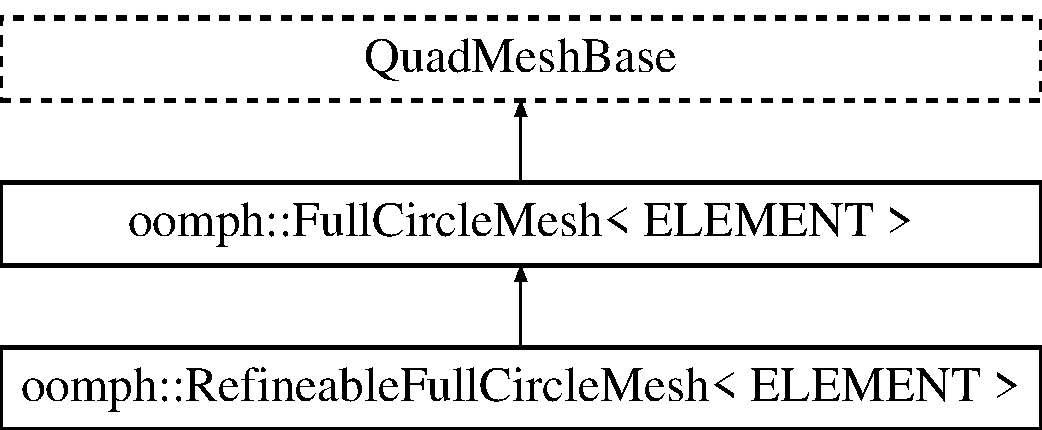
\includegraphics[height=4.000000cm]{classoomph_1_1FullCircleMesh}
\end{center}
\end{figure}
\subsection*{Public Member Functions}
\begin{DoxyCompactItemize}
\item 
\hyperlink{classoomph_1_1FullCircleMesh_acf4dee3c3072751597d7897176b1e7f1}{Full\+Circle\+Mesh} (\hyperlink{classoomph_1_1GeomObject}{Geom\+Object} $\ast$wall\+\_\+pt, const \hyperlink{classoomph_1_1Vector}{Vector}$<$ double $>$ \&theta\+\_\+positions, const \hyperlink{classoomph_1_1Vector}{Vector}$<$ double $>$ \&radius\+\_\+box, \hyperlink{classoomph_1_1TimeStepper}{Time\+Stepper} $\ast$time\+\_\+stepper\+\_\+pt=\&\hyperlink{classoomph_1_1Mesh_a12243d0fee2b1fcee729ee5a4777ea10}{Mesh\+::\+Default\+\_\+\+Time\+Stepper})
\begin{DoxyCompactList}\small\item\em Constructor\+: Pass pointer to geometric object that specifies the area; values of theta at which dividing lines are to be placed, fractions of the radius for the central box at the dividing lines and the timestepper. Timestepper defaults to \hyperlink{classoomph_1_1Steady}{Steady} dummy timestepper. \end{DoxyCompactList}\item 
virtual \hyperlink{classoomph_1_1FullCircleMesh_a7acf128e8eeaefcd79b5b3cd5e9cbaa9}{$\sim$\+Full\+Circle\+Mesh} ()
\begin{DoxyCompactList}\small\item\em Destructor\+: empty. \end{DoxyCompactList}\item 
\hyperlink{classoomph_1_1GeomObject}{Geom\+Object} $\ast$\& \hyperlink{classoomph_1_1FullCircleMesh_a0ee479af0a6562231d7a7d1c5533beb9}{area\+\_\+pt} ()
\begin{DoxyCompactList}\small\item\em Access function to \hyperlink{classoomph_1_1GeomObject}{Geom\+Object} representing wall. \end{DoxyCompactList}\item 
\hyperlink{classoomph_1_1FullCircleDomain}{Full\+Circle\+Domain} $\ast$ \hyperlink{classoomph_1_1FullCircleMesh_aade9e5e2a9d65f8b7f5d041da4536d99}{domain\+\_\+pt} ()
\begin{DoxyCompactList}\small\item\em Access function to domain. \end{DoxyCompactList}\item 
\hyperlink{classoomph_1_1FullCircleDomain}{Full\+Circle\+Domain} $\ast$ \hyperlink{classoomph_1_1FullCircleMesh_ae912045c32ae004812d61a58161e531f}{domain\+\_\+pt} () const
\begin{DoxyCompactList}\small\item\em Access function to underlying domain. \end{DoxyCompactList}\end{DoxyCompactItemize}
\subsection*{Protected Attributes}
\begin{DoxyCompactItemize}
\item 
\hyperlink{classoomph_1_1FullCircleDomain}{Full\+Circle\+Domain} $\ast$ \hyperlink{classoomph_1_1FullCircleMesh_a042c0729727a71bee0660f44c33f8691}{Domain\+\_\+pt}
\begin{DoxyCompactList}\small\item\em Pointer to domain. \end{DoxyCompactList}\item 
\hyperlink{classoomph_1_1GeomObject}{Geom\+Object} $\ast$ \hyperlink{classoomph_1_1FullCircleMesh_a0eb9088080115746b8570264f444c37f}{Area\+\_\+pt}
\begin{DoxyCompactList}\small\item\em Pointer to the geometric object that represents the entire domain. \end{DoxyCompactList}\end{DoxyCompactItemize}
\subsection*{Additional Inherited Members}


\subsection{Detailed Description}
\subsubsection*{template$<$class E\+L\+E\+M\+E\+NT$>$\newline
class oomph\+::\+Full\+Circle\+Mesh$<$ E\+L\+E\+M\+E\+N\+T $>$}

Full circle mesh class. The domain is specified by the \hyperlink{classoomph_1_1GeomObject}{Geom\+Object} that identifies the entire area. Non-\/refineable base version! 

The mesh boundaries are numbered as follows\+:
\begin{DoxyItemize}
\item Boundary 0\+: The outer wall, represented by $\xi_1 = 1$.
\end{DoxyItemize}

Definition at line 54 of file full\+\_\+circle\+\_\+mesh.\+template.\+h.



\subsection{Constructor \& Destructor Documentation}
\mbox{\Hypertarget{classoomph_1_1FullCircleMesh_acf4dee3c3072751597d7897176b1e7f1}\label{classoomph_1_1FullCircleMesh_acf4dee3c3072751597d7897176b1e7f1}} 
\index{oomph\+::\+Full\+Circle\+Mesh@{oomph\+::\+Full\+Circle\+Mesh}!Full\+Circle\+Mesh@{Full\+Circle\+Mesh}}
\index{Full\+Circle\+Mesh@{Full\+Circle\+Mesh}!oomph\+::\+Full\+Circle\+Mesh@{oomph\+::\+Full\+Circle\+Mesh}}
\subsubsection{\texorpdfstring{Full\+Circle\+Mesh()}{FullCircleMesh()}}
{\footnotesize\ttfamily template$<$class E\+L\+E\+M\+E\+NT $>$ \\
\hyperlink{classoomph_1_1FullCircleMesh}{oomph\+::\+Full\+Circle\+Mesh}$<$ E\+L\+E\+M\+E\+NT $>$\+::\hyperlink{classoomph_1_1FullCircleMesh}{Full\+Circle\+Mesh} (\begin{DoxyParamCaption}\item[{\hyperlink{classoomph_1_1GeomObject}{Geom\+Object} $\ast$}]{wall\+\_\+pt,  }\item[{const \hyperlink{classoomph_1_1Vector}{Vector}$<$ double $>$ \&}]{theta\+\_\+positions,  }\item[{const \hyperlink{classoomph_1_1Vector}{Vector}$<$ double $>$ \&}]{radius\+\_\+box,  }\item[{\hyperlink{classoomph_1_1TimeStepper}{Time\+Stepper} $\ast$}]{time\+\_\+stepper\+\_\+pt = {\ttfamily \&\hyperlink{classoomph_1_1Mesh_a12243d0fee2b1fcee729ee5a4777ea10}{Mesh\+::\+Default\+\_\+\+Time\+Stepper}} }\end{DoxyParamCaption})}



Constructor\+: Pass pointer to geometric object that specifies the area; values of theta at which dividing lines are to be placed, fractions of the radius for the central box at the dividing lines and the timestepper. Timestepper defaults to \hyperlink{classoomph_1_1Steady}{Steady} dummy timestepper. 

Constructor for deformable quarter tube mesh class. The domain is specified by the \hyperlink{classoomph_1_1GeomObject}{Geom\+Object} that identifies the entire volume. 

Definition at line 45 of file full\+\_\+circle\+\_\+mesh.\+template.\+cc.



References oomph\+::\+Mesh\+::add\+\_\+boundary\+\_\+node(), oomph\+::\+Mesh\+::\+Boundary\+\_\+coordinate\+\_\+exists, oomph\+::\+Mesh\+::convert\+\_\+to\+\_\+boundary\+\_\+node(), oomph\+::\+Full\+Circle\+Mesh$<$ E\+L\+E\+M\+E\+N\+T $>$\+::\+Domain\+\_\+pt, oomph\+::\+Mesh\+::\+Element\+\_\+pt, oomph\+::\+Mesh\+::finite\+\_\+element\+\_\+pt(), i, oomph\+::\+Mesh\+::\+Node\+\_\+pt, oomph\+::\+Mesh\+::node\+\_\+pt(), oomph\+::\+Finite\+Element\+::node\+\_\+pt(), oomph\+::oomph\+\_\+info, oomph\+::\+Mathematical\+Constants\+::\+Pi, s, oomph\+::\+Mesh\+::set\+\_\+nboundary(), oomph\+::\+Quad\+Mesh\+Base\+::setup\+\_\+boundary\+\_\+element\+\_\+info(), oomph\+::\+Global\+\_\+string\+\_\+for\+\_\+annotation\+::string(), and oomph\+::\+Node\+::x().

\mbox{\Hypertarget{classoomph_1_1FullCircleMesh_a7acf128e8eeaefcd79b5b3cd5e9cbaa9}\label{classoomph_1_1FullCircleMesh_a7acf128e8eeaefcd79b5b3cd5e9cbaa9}} 
\index{oomph\+::\+Full\+Circle\+Mesh@{oomph\+::\+Full\+Circle\+Mesh}!````~Full\+Circle\+Mesh@{$\sim$\+Full\+Circle\+Mesh}}
\index{````~Full\+Circle\+Mesh@{$\sim$\+Full\+Circle\+Mesh}!oomph\+::\+Full\+Circle\+Mesh@{oomph\+::\+Full\+Circle\+Mesh}}
\subsubsection{\texorpdfstring{$\sim$\+Full\+Circle\+Mesh()}{~FullCircleMesh()}}
{\footnotesize\ttfamily template$<$class E\+L\+E\+M\+E\+NT $>$ \\
virtual \hyperlink{classoomph_1_1FullCircleMesh}{oomph\+::\+Full\+Circle\+Mesh}$<$ E\+L\+E\+M\+E\+NT $>$\+::$\sim$\hyperlink{classoomph_1_1FullCircleMesh}{Full\+Circle\+Mesh} (\begin{DoxyParamCaption}{ }\end{DoxyParamCaption})\hspace{0.3cm}{\ttfamily [inline]}, {\ttfamily [virtual]}}



Destructor\+: empty. 



Definition at line 70 of file full\+\_\+circle\+\_\+mesh.\+template.\+h.



References oomph\+::\+Full\+Circle\+Mesh$<$ E\+L\+E\+M\+E\+N\+T $>$\+::\+Domain\+\_\+pt.



\subsection{Member Function Documentation}
\mbox{\Hypertarget{classoomph_1_1FullCircleMesh_a0ee479af0a6562231d7a7d1c5533beb9}\label{classoomph_1_1FullCircleMesh_a0ee479af0a6562231d7a7d1c5533beb9}} 
\index{oomph\+::\+Full\+Circle\+Mesh@{oomph\+::\+Full\+Circle\+Mesh}!area\+\_\+pt@{area\+\_\+pt}}
\index{area\+\_\+pt@{area\+\_\+pt}!oomph\+::\+Full\+Circle\+Mesh@{oomph\+::\+Full\+Circle\+Mesh}}
\subsubsection{\texorpdfstring{area\+\_\+pt()}{area\_pt()}}
{\footnotesize\ttfamily template$<$class E\+L\+E\+M\+E\+NT $>$ \\
\hyperlink{classoomph_1_1GeomObject}{Geom\+Object}$\ast$\& \hyperlink{classoomph_1_1FullCircleMesh}{oomph\+::\+Full\+Circle\+Mesh}$<$ E\+L\+E\+M\+E\+NT $>$\+::area\+\_\+pt (\begin{DoxyParamCaption}{ }\end{DoxyParamCaption})\hspace{0.3cm}{\ttfamily [inline]}}



Access function to \hyperlink{classoomph_1_1GeomObject}{Geom\+Object} representing wall. 



Definition at line 76 of file full\+\_\+circle\+\_\+mesh.\+template.\+h.



References oomph\+::\+Full\+Circle\+Mesh$<$ E\+L\+E\+M\+E\+N\+T $>$\+::\+Area\+\_\+pt.

\mbox{\Hypertarget{classoomph_1_1FullCircleMesh_aade9e5e2a9d65f8b7f5d041da4536d99}\label{classoomph_1_1FullCircleMesh_aade9e5e2a9d65f8b7f5d041da4536d99}} 
\index{oomph\+::\+Full\+Circle\+Mesh@{oomph\+::\+Full\+Circle\+Mesh}!domain\+\_\+pt@{domain\+\_\+pt}}
\index{domain\+\_\+pt@{domain\+\_\+pt}!oomph\+::\+Full\+Circle\+Mesh@{oomph\+::\+Full\+Circle\+Mesh}}
\subsubsection{\texorpdfstring{domain\+\_\+pt()}{domain\_pt()}\hspace{0.1cm}{\footnotesize\ttfamily [1/2]}}
{\footnotesize\ttfamily template$<$class E\+L\+E\+M\+E\+NT $>$ \\
\hyperlink{classoomph_1_1FullCircleDomain}{Full\+Circle\+Domain}$\ast$ \hyperlink{classoomph_1_1FullCircleMesh}{oomph\+::\+Full\+Circle\+Mesh}$<$ E\+L\+E\+M\+E\+NT $>$\+::domain\+\_\+pt (\begin{DoxyParamCaption}{ }\end{DoxyParamCaption})\hspace{0.3cm}{\ttfamily [inline]}}



Access function to domain. 



Definition at line 79 of file full\+\_\+circle\+\_\+mesh.\+template.\+h.



References oomph\+::\+Full\+Circle\+Mesh$<$ E\+L\+E\+M\+E\+N\+T $>$\+::\+Domain\+\_\+pt.

\mbox{\Hypertarget{classoomph_1_1FullCircleMesh_ae912045c32ae004812d61a58161e531f}\label{classoomph_1_1FullCircleMesh_ae912045c32ae004812d61a58161e531f}} 
\index{oomph\+::\+Full\+Circle\+Mesh@{oomph\+::\+Full\+Circle\+Mesh}!domain\+\_\+pt@{domain\+\_\+pt}}
\index{domain\+\_\+pt@{domain\+\_\+pt}!oomph\+::\+Full\+Circle\+Mesh@{oomph\+::\+Full\+Circle\+Mesh}}
\subsubsection{\texorpdfstring{domain\+\_\+pt()}{domain\_pt()}\hspace{0.1cm}{\footnotesize\ttfamily [2/2]}}
{\footnotesize\ttfamily template$<$class E\+L\+E\+M\+E\+NT $>$ \\
\hyperlink{classoomph_1_1FullCircleDomain}{Full\+Circle\+Domain}$\ast$ \hyperlink{classoomph_1_1FullCircleMesh}{oomph\+::\+Full\+Circle\+Mesh}$<$ E\+L\+E\+M\+E\+NT $>$\+::domain\+\_\+pt (\begin{DoxyParamCaption}{ }\end{DoxyParamCaption}) const\hspace{0.3cm}{\ttfamily [inline]}}



Access function to underlying domain. 



Definition at line 82 of file full\+\_\+circle\+\_\+mesh.\+template.\+h.



References oomph\+::\+Full\+Circle\+Mesh$<$ E\+L\+E\+M\+E\+N\+T $>$\+::\+Domain\+\_\+pt.



\subsection{Member Data Documentation}
\mbox{\Hypertarget{classoomph_1_1FullCircleMesh_a0eb9088080115746b8570264f444c37f}\label{classoomph_1_1FullCircleMesh_a0eb9088080115746b8570264f444c37f}} 
\index{oomph\+::\+Full\+Circle\+Mesh@{oomph\+::\+Full\+Circle\+Mesh}!Area\+\_\+pt@{Area\+\_\+pt}}
\index{Area\+\_\+pt@{Area\+\_\+pt}!oomph\+::\+Full\+Circle\+Mesh@{oomph\+::\+Full\+Circle\+Mesh}}
\subsubsection{\texorpdfstring{Area\+\_\+pt}{Area\_pt}}
{\footnotesize\ttfamily template$<$class E\+L\+E\+M\+E\+NT $>$ \\
\hyperlink{classoomph_1_1GeomObject}{Geom\+Object}$\ast$ \hyperlink{classoomph_1_1FullCircleMesh}{oomph\+::\+Full\+Circle\+Mesh}$<$ E\+L\+E\+M\+E\+NT $>$\+::Area\+\_\+pt\hspace{0.3cm}{\ttfamily [protected]}}



Pointer to the geometric object that represents the entire domain. 



Definition at line 90 of file full\+\_\+circle\+\_\+mesh.\+template.\+h.



Referenced by oomph\+::\+Full\+Circle\+Mesh$<$ E\+L\+E\+M\+E\+N\+T $>$\+::area\+\_\+pt().

\mbox{\Hypertarget{classoomph_1_1FullCircleMesh_a042c0729727a71bee0660f44c33f8691}\label{classoomph_1_1FullCircleMesh_a042c0729727a71bee0660f44c33f8691}} 
\index{oomph\+::\+Full\+Circle\+Mesh@{oomph\+::\+Full\+Circle\+Mesh}!Domain\+\_\+pt@{Domain\+\_\+pt}}
\index{Domain\+\_\+pt@{Domain\+\_\+pt}!oomph\+::\+Full\+Circle\+Mesh@{oomph\+::\+Full\+Circle\+Mesh}}
\subsubsection{\texorpdfstring{Domain\+\_\+pt}{Domain\_pt}}
{\footnotesize\ttfamily template$<$class E\+L\+E\+M\+E\+NT $>$ \\
\hyperlink{classoomph_1_1FullCircleDomain}{Full\+Circle\+Domain}$\ast$ \hyperlink{classoomph_1_1FullCircleMesh}{oomph\+::\+Full\+Circle\+Mesh}$<$ E\+L\+E\+M\+E\+NT $>$\+::Domain\+\_\+pt\hspace{0.3cm}{\ttfamily [protected]}}



Pointer to domain. 



Definition at line 87 of file full\+\_\+circle\+\_\+mesh.\+template.\+h.



Referenced by oomph\+::\+Full\+Circle\+Mesh$<$ E\+L\+E\+M\+E\+N\+T $>$\+::domain\+\_\+pt(), oomph\+::\+Full\+Circle\+Mesh$<$ E\+L\+E\+M\+E\+N\+T $>$\+::\+Full\+Circle\+Mesh(), oomph\+::\+Refineable\+Full\+Circle\+Mesh$<$ E\+L\+E\+M\+E\+N\+T $>$\+::\+Refineable\+Full\+Circle\+Mesh(), and oomph\+::\+Full\+Circle\+Mesh$<$ E\+L\+E\+M\+E\+N\+T $>$\+::$\sim$\+Full\+Circle\+Mesh().



The documentation for this class was generated from the following files\+:\begin{DoxyCompactItemize}
\item 
\hyperlink{full__circle__mesh_8template_8h}{full\+\_\+circle\+\_\+mesh.\+template.\+h}\item 
\hyperlink{full__circle__mesh_8template_8cc}{full\+\_\+circle\+\_\+mesh.\+template.\+cc}\end{DoxyCompactItemize}

\hypertarget{classoomph_1_1GeompackQuadMesh}{}\section{oomph\+:\+:Geompack\+Quad\+Mesh$<$ E\+L\+E\+M\+E\+NT $>$ Class Template Reference}
\label{classoomph_1_1GeompackQuadMesh}\index{oomph\+::\+Geompack\+Quad\+Mesh$<$ E\+L\+E\+M\+E\+N\+T $>$@{oomph\+::\+Geompack\+Quad\+Mesh$<$ E\+L\+E\+M\+E\+N\+T $>$}}


{\ttfamily \#include $<$geompack\+\_\+mesh.\+template.\+h$>$}

Inheritance diagram for oomph\+:\+:Geompack\+Quad\+Mesh$<$ E\+L\+E\+M\+E\+NT $>$\+:\begin{figure}[H]
\begin{center}
\leavevmode
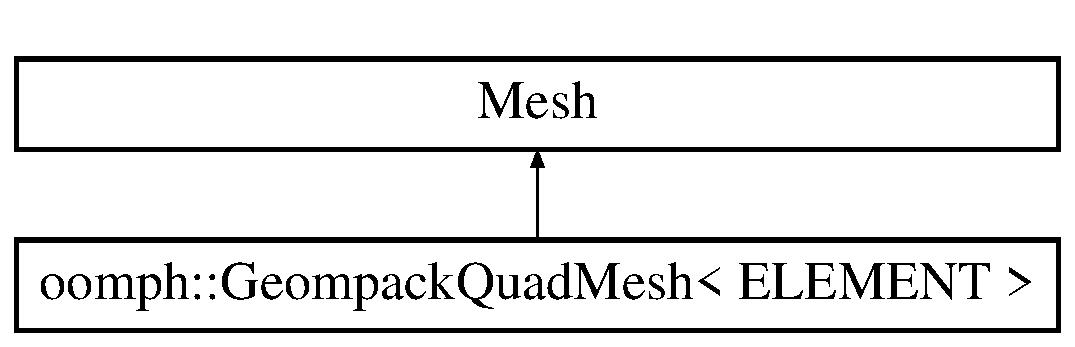
\includegraphics[height=2.000000cm]{classoomph_1_1GeompackQuadMesh}
\end{center}
\end{figure}
\subsection*{Public Member Functions}
\begin{DoxyCompactItemize}
\item 
\hyperlink{classoomph_1_1GeompackQuadMesh_aa1de3a1b4fedf1c404d6ed5bbebfb800}{Geompack\+Quad\+Mesh} (const std\+::string \&mesh\+\_\+file\+\_\+name, const std\+::string \&curve\+\_\+file\+\_\+name, \hyperlink{classoomph_1_1TimeStepper}{Time\+Stepper} $\ast$time\+\_\+stepper\+\_\+pt=\&\hyperlink{classoomph_1_1Mesh_a12243d0fee2b1fcee729ee5a4777ea10}{Mesh\+::\+Default\+\_\+\+Time\+Stepper})
\begin{DoxyCompactList}\small\item\em Constructor with the input files. \end{DoxyCompactList}\item 
\hyperlink{classoomph_1_1GeompackQuadMesh_a7795c44ea2da182fbeffa30808481ffb}{$\sim$\+Geompack\+Quad\+Mesh} ()
\begin{DoxyCompactList}\small\item\em Empty destructor. \end{DoxyCompactList}\end{DoxyCompactItemize}
\subsection*{Private Member Functions}
\begin{DoxyCompactItemize}
\item 
void \hyperlink{classoomph_1_1GeompackQuadMesh_a714ee07999e06676f08080bac8c024db}{build\+\_\+from\+\_\+scaffold} (\hyperlink{classoomph_1_1TimeStepper}{Time\+Stepper} $\ast$time\+\_\+stepper\+\_\+pt)
\begin{DoxyCompactList}\small\item\em Build mesh from scaffold. \end{DoxyCompactList}\end{DoxyCompactItemize}
\subsection*{Private Attributes}
\begin{DoxyCompactItemize}
\item 
\hyperlink{classoomph_1_1GeompackQuadScaffoldMesh}{Geompack\+Quad\+Scaffold\+Mesh} $\ast$ \hyperlink{classoomph_1_1GeompackQuadMesh_a0b7edabf329aed8f4fb00eddb41b3299}{Tmp\+\_\+mesh\+\_\+pt}
\begin{DoxyCompactList}\small\item\em Temporary scaffold mesh. \end{DoxyCompactList}\end{DoxyCompactItemize}
\subsection*{Additional Inherited Members}


\subsection{Detailed Description}
\subsubsection*{template$<$class E\+L\+E\+M\+E\+NT$>$\newline
class oomph\+::\+Geompack\+Quad\+Mesh$<$ E\+L\+E\+M\+E\+N\+T $>$}

Quadrilateral mesh generator; Uses input from Geompack++. See\+: \href{http://members.shaw.ca/bjoe/}{\tt http\+://members.\+shaw.\+ca/bjoe/} Currently only for four-\/noded quads -- extension to higher-\/order quads should be trivial (see the corresponding classes for triangular meshes). 

Definition at line 46 of file geompack\+\_\+mesh.\+template.\+h.



\subsection{Constructor \& Destructor Documentation}
\mbox{\Hypertarget{classoomph_1_1GeompackQuadMesh_aa1de3a1b4fedf1c404d6ed5bbebfb800}\label{classoomph_1_1GeompackQuadMesh_aa1de3a1b4fedf1c404d6ed5bbebfb800}} 
\index{oomph\+::\+Geompack\+Quad\+Mesh@{oomph\+::\+Geompack\+Quad\+Mesh}!Geompack\+Quad\+Mesh@{Geompack\+Quad\+Mesh}}
\index{Geompack\+Quad\+Mesh@{Geompack\+Quad\+Mesh}!oomph\+::\+Geompack\+Quad\+Mesh@{oomph\+::\+Geompack\+Quad\+Mesh}}
\subsubsection{\texorpdfstring{Geompack\+Quad\+Mesh()}{GeompackQuadMesh()}}
{\footnotesize\ttfamily template$<$class E\+L\+E\+M\+E\+NT $>$ \\
\hyperlink{classoomph_1_1GeompackQuadMesh}{oomph\+::\+Geompack\+Quad\+Mesh}$<$ E\+L\+E\+M\+E\+NT $>$\+::\hyperlink{classoomph_1_1GeompackQuadMesh}{Geompack\+Quad\+Mesh} (\begin{DoxyParamCaption}\item[{const std\+::string \&}]{mesh\+\_\+file\+\_\+name,  }\item[{const std\+::string \&}]{curve\+\_\+file\+\_\+name,  }\item[{\hyperlink{classoomph_1_1TimeStepper}{Time\+Stepper} $\ast$}]{time\+\_\+stepper\+\_\+pt = {\ttfamily \&\hyperlink{classoomph_1_1Mesh_a12243d0fee2b1fcee729ee5a4777ea10}{Mesh\+::\+Default\+\_\+\+Time\+Stepper}} }\end{DoxyParamCaption})\hspace{0.3cm}{\ttfamily [inline]}}



Constructor with the input files. 



Definition at line 52 of file geompack\+\_\+mesh.\+template.\+h.



References oomph\+::\+Geompack\+Quad\+Mesh$<$ E\+L\+E\+M\+E\+N\+T $>$\+::build\+\_\+from\+\_\+scaffold(), and oomph\+::\+Geompack\+Quad\+Mesh$<$ E\+L\+E\+M\+E\+N\+T $>$\+::\+Tmp\+\_\+mesh\+\_\+pt.

\mbox{\Hypertarget{classoomph_1_1GeompackQuadMesh_a7795c44ea2da182fbeffa30808481ffb}\label{classoomph_1_1GeompackQuadMesh_a7795c44ea2da182fbeffa30808481ffb}} 
\index{oomph\+::\+Geompack\+Quad\+Mesh@{oomph\+::\+Geompack\+Quad\+Mesh}!````~Geompack\+Quad\+Mesh@{$\sim$\+Geompack\+Quad\+Mesh}}
\index{````~Geompack\+Quad\+Mesh@{$\sim$\+Geompack\+Quad\+Mesh}!oomph\+::\+Geompack\+Quad\+Mesh@{oomph\+::\+Geompack\+Quad\+Mesh}}
\subsubsection{\texorpdfstring{$\sim$\+Geompack\+Quad\+Mesh()}{~GeompackQuadMesh()}}
{\footnotesize\ttfamily template$<$class E\+L\+E\+M\+E\+NT $>$ \\
\hyperlink{classoomph_1_1GeompackQuadMesh}{oomph\+::\+Geompack\+Quad\+Mesh}$<$ E\+L\+E\+M\+E\+NT $>$\+::$\sim$\hyperlink{classoomph_1_1GeompackQuadMesh}{Geompack\+Quad\+Mesh} (\begin{DoxyParamCaption}{ }\end{DoxyParamCaption})\hspace{0.3cm}{\ttfamily [inline]}}



Empty destructor. 



Definition at line 73 of file geompack\+\_\+mesh.\+template.\+h.



\subsection{Member Function Documentation}
\mbox{\Hypertarget{classoomph_1_1GeompackQuadMesh_a714ee07999e06676f08080bac8c024db}\label{classoomph_1_1GeompackQuadMesh_a714ee07999e06676f08080bac8c024db}} 
\index{oomph\+::\+Geompack\+Quad\+Mesh@{oomph\+::\+Geompack\+Quad\+Mesh}!build\+\_\+from\+\_\+scaffold@{build\+\_\+from\+\_\+scaffold}}
\index{build\+\_\+from\+\_\+scaffold@{build\+\_\+from\+\_\+scaffold}!oomph\+::\+Geompack\+Quad\+Mesh@{oomph\+::\+Geompack\+Quad\+Mesh}}
\subsubsection{\texorpdfstring{build\+\_\+from\+\_\+scaffold()}{build\_from\_scaffold()}}
{\footnotesize\ttfamily template$<$class E\+L\+E\+M\+E\+NT $>$ \\
void \hyperlink{classoomph_1_1GeompackQuadMesh}{oomph\+::\+Geompack\+Quad\+Mesh}$<$ E\+L\+E\+M\+E\+NT $>$\+::build\+\_\+from\+\_\+scaffold (\begin{DoxyParamCaption}\item[{\hyperlink{classoomph_1_1TimeStepper}{Time\+Stepper} $\ast$}]{time\+\_\+stepper\+\_\+pt }\end{DoxyParamCaption})\hspace{0.3cm}{\ttfamily [private]}}



Build mesh from scaffold. 

Quadrilateral mesh generator; Uses input from Geompack++. See\+: \href{http://members.shaw.ca/bjoe/}{\tt http\+://members.\+shaw.\+ca/bjoe/} Currently only for four-\/noded quads -- extension to higher-\/order quads should be trivial (see the corresponding classes for triangular meshes). 

Definition at line 49 of file geompack\+\_\+mesh.\+template.\+cc.



References e, oomph\+::\+Node\+::get\+\_\+boundaries\+\_\+pt(), oomph\+::\+Global\+\_\+string\+\_\+for\+\_\+annotation\+::string(), and oomph\+::\+Node\+::x().



Referenced by oomph\+::\+Geompack\+Quad\+Mesh$<$ E\+L\+E\+M\+E\+N\+T $>$\+::\+Geompack\+Quad\+Mesh().



\subsection{Member Data Documentation}
\mbox{\Hypertarget{classoomph_1_1GeompackQuadMesh_a0b7edabf329aed8f4fb00eddb41b3299}\label{classoomph_1_1GeompackQuadMesh_a0b7edabf329aed8f4fb00eddb41b3299}} 
\index{oomph\+::\+Geompack\+Quad\+Mesh@{oomph\+::\+Geompack\+Quad\+Mesh}!Tmp\+\_\+mesh\+\_\+pt@{Tmp\+\_\+mesh\+\_\+pt}}
\index{Tmp\+\_\+mesh\+\_\+pt@{Tmp\+\_\+mesh\+\_\+pt}!oomph\+::\+Geompack\+Quad\+Mesh@{oomph\+::\+Geompack\+Quad\+Mesh}}
\subsubsection{\texorpdfstring{Tmp\+\_\+mesh\+\_\+pt}{Tmp\_mesh\_pt}}
{\footnotesize\ttfamily template$<$class E\+L\+E\+M\+E\+NT $>$ \\
\hyperlink{classoomph_1_1GeompackQuadScaffoldMesh}{Geompack\+Quad\+Scaffold\+Mesh}$\ast$ \hyperlink{classoomph_1_1GeompackQuadMesh}{oomph\+::\+Geompack\+Quad\+Mesh}$<$ E\+L\+E\+M\+E\+NT $>$\+::Tmp\+\_\+mesh\+\_\+pt\hspace{0.3cm}{\ttfamily [private]}}



Temporary scaffold mesh. 



Definition at line 78 of file geompack\+\_\+mesh.\+template.\+h.



Referenced by oomph\+::\+Geompack\+Quad\+Mesh$<$ E\+L\+E\+M\+E\+N\+T $>$\+::\+Geompack\+Quad\+Mesh().



The documentation for this class was generated from the following files\+:\begin{DoxyCompactItemize}
\item 
\hyperlink{geompack__mesh_8template_8h}{geompack\+\_\+mesh.\+template.\+h}\item 
\hyperlink{geompack__mesh_8template_8cc}{geompack\+\_\+mesh.\+template.\+cc}\end{DoxyCompactItemize}

\hypertarget{classoomph_1_1GmshParameters}{}\section{oomph\+:\+:Gmsh\+Parameters Class Reference}
\label{classoomph_1_1GmshParameters}\index{oomph\+::\+Gmsh\+Parameters@{oomph\+::\+Gmsh\+Parameters}}


Class to collate parameters for Gmsh mesh generation.  




{\ttfamily \#include $<$gmsh\+\_\+tet\+\_\+mesh.\+template.\+h$>$}

\subsection*{Public Member Functions}
\begin{DoxyCompactItemize}
\item 
\hyperlink{classoomph_1_1GmshParameters_a6a4e43f09a5de3155dee5b3d5c1a206b}{Gmsh\+Parameters} (Tet\+Mesh\+Faceted\+Closed\+Surface $\ast$const \&\hyperlink{classoomph_1_1GmshParameters_abdd71edac9d5fd08a6a9c978d2673a2e}{outer\+\_\+boundary\+\_\+pt}, const std\+::string \&\hyperlink{classoomph_1_1GmshParameters_aaf19a5b331893637974f5a5be8da048c}{gmsh\+\_\+command\+\_\+line\+\_\+invocation})
\begin{DoxyCompactList}\small\item\em Specify outer boundary of domain to be meshed. Other parameters get default values and can be set via member functions. \end{DoxyCompactList}\item 
Tet\+Mesh\+Faceted\+Closed\+Surface $\ast$\& \hyperlink{classoomph_1_1GmshParameters_abdd71edac9d5fd08a6a9c978d2673a2e}{outer\+\_\+boundary\+\_\+pt} ()
\begin{DoxyCompactList}\small\item\em Outer boundary. \end{DoxyCompactList}\item 
Vector$<$ Tet\+Mesh\+Faceted\+Surface $\ast$ $>$ \& \hyperlink{classoomph_1_1GmshParameters_a10f845ea8fb16bf617f5c6ca05e21bf9}{internal\+\_\+surface\+\_\+pt} ()
\begin{DoxyCompactList}\small\item\em Internal boundaries. \end{DoxyCompactList}\item 
double \& \hyperlink{classoomph_1_1GmshParameters_a4c085fa1661d1a27ee95461d275b686f}{element\+\_\+volume} ()
\begin{DoxyCompactList}\small\item\em Uniform target element volume. \end{DoxyCompactList}\item 
std\+::string \& \hyperlink{classoomph_1_1GmshParameters_a89c7ff40c1dd70b20b0ae22d30fe5c8a}{target\+\_\+size\+\_\+file\+\_\+name} ()
\begin{DoxyCompactList}\small\item\em Filename for target volumes (for system-\/call based transfer to gmsh during mesh adaptation). Default\+: .gmsh\+\_\+target\+\_\+size\+\_\+for\+\_\+adaptation.\+dat. \end{DoxyCompactList}\item 
std\+::string \& \hyperlink{classoomph_1_1GmshParameters_aaf19a5b331893637974f5a5be8da048c}{gmsh\+\_\+command\+\_\+line\+\_\+invocation} ()
\begin{DoxyCompactList}\small\item\em String to be issued via system command to activate gmsh. \end{DoxyCompactList}\item 
std\+::string \& \hyperlink{classoomph_1_1GmshParameters_ab9ae54d3d474392b5aefcf2a12aae1a8}{geo\+\_\+and\+\_\+msh\+\_\+file\+\_\+stem} ()
\begin{DoxyCompactList}\small\item\em Stem for geo and msh files (input/output to command-\/line gmsh invocation) \end{DoxyCompactList}\item 
double \& \hyperlink{classoomph_1_1GmshParameters_afd08195fd9f804b7ced23728b6a63e15}{max\+\_\+element\+\_\+size} ()
\begin{DoxyCompactList}\small\item\em Max. element size during refinement. \end{DoxyCompactList}\item 
double \& \hyperlink{classoomph_1_1GmshParameters_a4afd4f1f72b1f45b3ca51b186737f264}{min\+\_\+element\+\_\+size} ()
\begin{DoxyCompactList}\small\item\em Min. element size during refinement. \end{DoxyCompactList}\item 
double \& \hyperlink{classoomph_1_1GmshParameters_afe2deda55a1eb76d4f782aab9a58089c}{max\+\_\+permitted\+\_\+edge\+\_\+ratio} ()
\begin{DoxyCompactList}\small\item\em Max. permitted edge ratio. \end{DoxyCompactList}\item 
double \& \hyperlink{classoomph_1_1GmshParameters_ae5db3c2aca27f73ee53e32178255130d}{dx\+\_\+for\+\_\+target\+\_\+size\+\_\+transfer} ()
\begin{DoxyCompactList}\small\item\em (Isotropic) grid spacing for target size transfer \end{DoxyCompactList}\item 
unsigned \& \hyperlink{classoomph_1_1GmshParameters_a7b7dfff74a8e3183858ecd42b8f1a049}{max\+\_\+sample\+\_\+points\+\_\+for\+\_\+limited\+\_\+locate\+\_\+zeta\+\_\+during\+\_\+target\+\_\+size\+\_\+transfer} ()
\begin{DoxyCompactList}\small\item\em Target size is transferred onto regular grid (for gmsh) by locate zeta. We try to find the exact point in the existing mesh but if we fail to converge from the nearest specified number of sample points we use the nearest of those. \end{DoxyCompactList}\item 
std\+::string \& \hyperlink{classoomph_1_1GmshParameters_a6006bbce01fab0e48e474f077fc926e7}{stem\+\_\+for\+\_\+filename\+\_\+gmsh\+\_\+size\+\_\+transfer} ()
\begin{DoxyCompactList}\small\item\em Stem for filename used to doc target element sizes on gmsh grid. No doc if stem is equal to empty string (or counter is negative) \end{DoxyCompactList}\item 
int \& \hyperlink{classoomph_1_1GmshParameters_acf8155883aab25f0fc13c1eab7c03e9c}{counter\+\_\+for\+\_\+filename\+\_\+gmsh\+\_\+size\+\_\+transfer} ()
\begin{DoxyCompactList}\small\item\em Counter for filename used to doc target element sizes on gmsh grid. No doc if stem is equal to empty string (or counter is negative) \end{DoxyCompactList}\item 
bool \hyperlink{classoomph_1_1GmshParameters_ac8b37d79ebc135382c2320c3ba405a3f}{projection\+\_\+is\+\_\+disabled} ()
\begin{DoxyCompactList}\small\item\em Is projection of old solution onto new mesh disabled? \end{DoxyCompactList}\item 
void \hyperlink{classoomph_1_1GmshParameters_ad9c1ebc0ae01551b7899364a1cf25f19}{disable\+\_\+projection} ()
\begin{DoxyCompactList}\small\item\em Disable projection of old solution onto new mesh. \end{DoxyCompactList}\item 
void \hyperlink{classoomph_1_1GmshParameters_afa3a44a5a06632733efa49912a272865}{enable\+\_\+projection} ()
\begin{DoxyCompactList}\small\item\em Disable projection of old solution onto new mesh. \end{DoxyCompactList}\item 
std\+::string \& \hyperlink{classoomph_1_1GmshParameters_ac712c282aec129e50646e6cf07a7a92e}{gmsh\+\_\+onscreen\+\_\+output\+\_\+file\+\_\+name} ()
\begin{DoxyCompactList}\small\item\em Output filename for gmsh on-\/screen output. \end{DoxyCompactList}\item 
unsigned \& \hyperlink{classoomph_1_1GmshParameters_afde31eadaa2ca1862837624f68ea8d34}{gmsh\+\_\+onscreen\+\_\+output\+\_\+counter} ()
\begin{DoxyCompactList}\small\item\em Counter for marker that indicates where we are in gmsh on-\/screen output. \end{DoxyCompactList}\end{DoxyCompactItemize}
\subsection*{Private Attributes}
\begin{DoxyCompactItemize}
\item 
Tet\+Mesh\+Faceted\+Closed\+Surface $\ast$ \hyperlink{classoomph_1_1GmshParameters_a310ecaffe67e67b334aafaca82c4d50a}{Outer\+\_\+boundary\+\_\+pt}
\begin{DoxyCompactList}\small\item\em Pointer to outer boundary. \end{DoxyCompactList}\item 
Vector$<$ Tet\+Mesh\+Faceted\+Surface $\ast$ $>$ \hyperlink{classoomph_1_1GmshParameters_aaa4afdde73a7fc67d5c2ba2976235381}{Internal\+\_\+surface\+\_\+pt}
\begin{DoxyCompactList}\small\item\em Internal boundaries. \end{DoxyCompactList}\item 
double \hyperlink{classoomph_1_1GmshParameters_aa7993da33a0468681e5f661ac5b00bfb}{Element\+\_\+volume}
\begin{DoxyCompactList}\small\item\em Uniform element volume. \end{DoxyCompactList}\item 
std\+::string \hyperlink{classoomph_1_1GmshParameters_ae2f3eabe211e22c18df2bf7b093bbdfb}{Target\+\_\+size\+\_\+file\+\_\+name}
\begin{DoxyCompactList}\small\item\em Filename for target volume (for system-\/call based transfer to gmsh during mesh adaptation) \end{DoxyCompactList}\item 
std\+::string \hyperlink{classoomph_1_1GmshParameters_a478a41ae94e177f02d38db90ea27d582}{Geo\+\_\+and\+\_\+msh\+\_\+file\+\_\+stem}
\begin{DoxyCompactList}\small\item\em Stem for geo and msh files (input/output to command-\/line gmsh invocation) \end{DoxyCompactList}\item 
std\+::string \hyperlink{classoomph_1_1GmshParameters_a5605a771916b353925ad55b6a6e914cb}{Gmsh\+\_\+command\+\_\+line\+\_\+invocation}
\begin{DoxyCompactList}\small\item\em Gmsh command line invocation string. \end{DoxyCompactList}\item 
double \hyperlink{classoomph_1_1GmshParameters_a65bd88591891ff4284fb4e03d6f49c14}{Max\+\_\+element\+\_\+size}
\begin{DoxyCompactList}\small\item\em Max. element size during refinement. \end{DoxyCompactList}\item 
double \hyperlink{classoomph_1_1GmshParameters_a8efec35bdf92a73cf71f25cff41520b7}{Min\+\_\+element\+\_\+size}
\begin{DoxyCompactList}\small\item\em Min. element size during refinement. \end{DoxyCompactList}\item 
double \hyperlink{classoomph_1_1GmshParameters_ac62bbb70b5a1bd650f7b0b7c8fbe1d8f}{Max\+\_\+permitted\+\_\+edge\+\_\+ratio}
\begin{DoxyCompactList}\small\item\em Max edge ratio before remesh gets triggered. \end{DoxyCompactList}\item 
double \hyperlink{classoomph_1_1GmshParameters_a0c4d7e327d44f9514eb0ac0894f6f9d9}{Dx\+\_\+for\+\_\+target\+\_\+size\+\_\+transfer}
\begin{DoxyCompactList}\small\item\em (Isotropic) grid spacing for target size transfer \end{DoxyCompactList}\item 
unsigned \hyperlink{classoomph_1_1GmshParameters_a7a75351daca7e20f9dcb95919691d863}{Max\+\_\+sample\+\_\+points\+\_\+for\+\_\+limited\+\_\+locate\+\_\+zeta\+\_\+during\+\_\+target\+\_\+size\+\_\+transfer}
\begin{DoxyCompactList}\small\item\em Target size is transferred onto regular grid (for gmsh) by locate zeta. We try to find the exact point in the existing mesh but if we fail to converge from the nearest specified number of sample points we use the nearest of those. \end{DoxyCompactList}\item 
std\+::string \hyperlink{classoomph_1_1GmshParameters_ad0151a908bc36fee2d955551b1da4016}{Stem\+\_\+for\+\_\+filename\+\_\+gmsh\+\_\+size\+\_\+transfer}
\begin{DoxyCompactList}\small\item\em Stem for filename used to doc target element sizes on gmsh grid. No doc if stem is equal to empty string (or counter is negative) \end{DoxyCompactList}\item 
int \hyperlink{classoomph_1_1GmshParameters_af6ca2a71d6aae3f8c51e9b4ad53b787a}{Counter\+\_\+for\+\_\+filename\+\_\+gmsh\+\_\+size\+\_\+transfer}
\begin{DoxyCompactList}\small\item\em Counter for filename used to doc target element sizes on gmsh grid. No doc if stem is equal to empty string (or counter is negative) \end{DoxyCompactList}\item 
bool \hyperlink{classoomph_1_1GmshParameters_aebabc7ca82ac23e87e164655b6dc9bb4}{Projection\+\_\+is\+\_\+disabled}
\begin{DoxyCompactList}\small\item\em Is projection of old solution onto new mesh disabled? \end{DoxyCompactList}\item 
std\+::string \hyperlink{classoomph_1_1GmshParameters_af2da0d4c57e32c06c70a6aa25d1461ac}{Gmsh\+\_\+onscreen\+\_\+output\+\_\+file\+\_\+name}
\begin{DoxyCompactList}\small\item\em Output filename for gmsh on-\/screen output. \end{DoxyCompactList}\item 
unsigned \hyperlink{classoomph_1_1GmshParameters_ab3648c8847da428cddca41e676042e33}{Gmsh\+\_\+onscreen\+\_\+output\+\_\+counter}
\begin{DoxyCompactList}\small\item\em Counter for marker that indicates where we are in gmsh on-\/screen output. \end{DoxyCompactList}\end{DoxyCompactItemize}


\subsection{Detailed Description}
Class to collate parameters for Gmsh mesh generation. 

Definition at line 56 of file gmsh\+\_\+tet\+\_\+mesh.\+template.\+h.



\subsection{Constructor \& Destructor Documentation}
\mbox{\Hypertarget{classoomph_1_1GmshParameters_a6a4e43f09a5de3155dee5b3d5c1a206b}\label{classoomph_1_1GmshParameters_a6a4e43f09a5de3155dee5b3d5c1a206b}} 
\index{oomph\+::\+Gmsh\+Parameters@{oomph\+::\+Gmsh\+Parameters}!Gmsh\+Parameters@{Gmsh\+Parameters}}
\index{Gmsh\+Parameters@{Gmsh\+Parameters}!oomph\+::\+Gmsh\+Parameters@{oomph\+::\+Gmsh\+Parameters}}
\subsubsection{\texorpdfstring{Gmsh\+Parameters()}{GmshParameters()}}
{\footnotesize\ttfamily oomph\+::\+Gmsh\+Parameters\+::\+Gmsh\+Parameters (\begin{DoxyParamCaption}\item[{Tet\+Mesh\+Faceted\+Closed\+Surface $\ast$const \&}]{outer\+\_\+boundary\+\_\+pt,  }\item[{const std\+::string \&}]{gmsh\+\_\+command\+\_\+line\+\_\+invocation }\end{DoxyParamCaption})\hspace{0.3cm}{\ttfamily [inline]}}



Specify outer boundary of domain to be meshed. Other parameters get default values and can be set via member functions. 



Definition at line 64 of file gmsh\+\_\+tet\+\_\+mesh.\+template.\+h.



\subsection{Member Function Documentation}
\mbox{\Hypertarget{classoomph_1_1GmshParameters_acf8155883aab25f0fc13c1eab7c03e9c}\label{classoomph_1_1GmshParameters_acf8155883aab25f0fc13c1eab7c03e9c}} 
\index{oomph\+::\+Gmsh\+Parameters@{oomph\+::\+Gmsh\+Parameters}!counter\+\_\+for\+\_\+filename\+\_\+gmsh\+\_\+size\+\_\+transfer@{counter\+\_\+for\+\_\+filename\+\_\+gmsh\+\_\+size\+\_\+transfer}}
\index{counter\+\_\+for\+\_\+filename\+\_\+gmsh\+\_\+size\+\_\+transfer@{counter\+\_\+for\+\_\+filename\+\_\+gmsh\+\_\+size\+\_\+transfer}!oomph\+::\+Gmsh\+Parameters@{oomph\+::\+Gmsh\+Parameters}}
\subsubsection{\texorpdfstring{counter\+\_\+for\+\_\+filename\+\_\+gmsh\+\_\+size\+\_\+transfer()}{counter\_for\_filename\_gmsh\_size\_transfer()}}
{\footnotesize\ttfamily int\& oomph\+::\+Gmsh\+Parameters\+::counter\+\_\+for\+\_\+filename\+\_\+gmsh\+\_\+size\+\_\+transfer (\begin{DoxyParamCaption}{ }\end{DoxyParamCaption})\hspace{0.3cm}{\ttfamily [inline]}}



Counter for filename used to doc target element sizes on gmsh grid. No doc if stem is equal to empty string (or counter is negative) 



Definition at line 164 of file gmsh\+\_\+tet\+\_\+mesh.\+template.\+h.



References Counter\+\_\+for\+\_\+filename\+\_\+gmsh\+\_\+size\+\_\+transfer.

\mbox{\Hypertarget{classoomph_1_1GmshParameters_ad9c1ebc0ae01551b7899364a1cf25f19}\label{classoomph_1_1GmshParameters_ad9c1ebc0ae01551b7899364a1cf25f19}} 
\index{oomph\+::\+Gmsh\+Parameters@{oomph\+::\+Gmsh\+Parameters}!disable\+\_\+projection@{disable\+\_\+projection}}
\index{disable\+\_\+projection@{disable\+\_\+projection}!oomph\+::\+Gmsh\+Parameters@{oomph\+::\+Gmsh\+Parameters}}
\subsubsection{\texorpdfstring{disable\+\_\+projection()}{disable\_projection()}}
{\footnotesize\ttfamily void oomph\+::\+Gmsh\+Parameters\+::disable\+\_\+projection (\begin{DoxyParamCaption}{ }\end{DoxyParamCaption})\hspace{0.3cm}{\ttfamily [inline]}}



Disable projection of old solution onto new mesh. 



Definition at line 176 of file gmsh\+\_\+tet\+\_\+mesh.\+template.\+h.



References Projection\+\_\+is\+\_\+disabled.

\mbox{\Hypertarget{classoomph_1_1GmshParameters_ae5db3c2aca27f73ee53e32178255130d}\label{classoomph_1_1GmshParameters_ae5db3c2aca27f73ee53e32178255130d}} 
\index{oomph\+::\+Gmsh\+Parameters@{oomph\+::\+Gmsh\+Parameters}!dx\+\_\+for\+\_\+target\+\_\+size\+\_\+transfer@{dx\+\_\+for\+\_\+target\+\_\+size\+\_\+transfer}}
\index{dx\+\_\+for\+\_\+target\+\_\+size\+\_\+transfer@{dx\+\_\+for\+\_\+target\+\_\+size\+\_\+transfer}!oomph\+::\+Gmsh\+Parameters@{oomph\+::\+Gmsh\+Parameters}}
\subsubsection{\texorpdfstring{dx\+\_\+for\+\_\+target\+\_\+size\+\_\+transfer()}{dx\_for\_target\_size\_transfer()}}
{\footnotesize\ttfamily double\& oomph\+::\+Gmsh\+Parameters\+::dx\+\_\+for\+\_\+target\+\_\+size\+\_\+transfer (\begin{DoxyParamCaption}{ }\end{DoxyParamCaption})\hspace{0.3cm}{\ttfamily [inline]}}



(Isotropic) grid spacing for target size transfer 



Definition at line 139 of file gmsh\+\_\+tet\+\_\+mesh.\+template.\+h.



References Dx\+\_\+for\+\_\+target\+\_\+size\+\_\+transfer.

\mbox{\Hypertarget{classoomph_1_1GmshParameters_a4c085fa1661d1a27ee95461d275b686f}\label{classoomph_1_1GmshParameters_a4c085fa1661d1a27ee95461d275b686f}} 
\index{oomph\+::\+Gmsh\+Parameters@{oomph\+::\+Gmsh\+Parameters}!element\+\_\+volume@{element\+\_\+volume}}
\index{element\+\_\+volume@{element\+\_\+volume}!oomph\+::\+Gmsh\+Parameters@{oomph\+::\+Gmsh\+Parameters}}
\subsubsection{\texorpdfstring{element\+\_\+volume()}{element\_volume()}}
{\footnotesize\ttfamily double\& oomph\+::\+Gmsh\+Parameters\+::element\+\_\+volume (\begin{DoxyParamCaption}{ }\end{DoxyParamCaption})\hspace{0.3cm}{\ttfamily [inline]}}



Uniform target element volume. 



Definition at line 94 of file gmsh\+\_\+tet\+\_\+mesh.\+template.\+h.



References Element\+\_\+volume.



Referenced by oomph\+::\+Gmsh\+Tet\+Scaffold\+Mesh\+::write\+\_\+geo\+\_\+file().

\mbox{\Hypertarget{classoomph_1_1GmshParameters_afa3a44a5a06632733efa49912a272865}\label{classoomph_1_1GmshParameters_afa3a44a5a06632733efa49912a272865}} 
\index{oomph\+::\+Gmsh\+Parameters@{oomph\+::\+Gmsh\+Parameters}!enable\+\_\+projection@{enable\+\_\+projection}}
\index{enable\+\_\+projection@{enable\+\_\+projection}!oomph\+::\+Gmsh\+Parameters@{oomph\+::\+Gmsh\+Parameters}}
\subsubsection{\texorpdfstring{enable\+\_\+projection()}{enable\_projection()}}
{\footnotesize\ttfamily void oomph\+::\+Gmsh\+Parameters\+::enable\+\_\+projection (\begin{DoxyParamCaption}{ }\end{DoxyParamCaption})\hspace{0.3cm}{\ttfamily [inline]}}



Disable projection of old solution onto new mesh. 



Definition at line 182 of file gmsh\+\_\+tet\+\_\+mesh.\+template.\+h.



References Projection\+\_\+is\+\_\+disabled.

\mbox{\Hypertarget{classoomph_1_1GmshParameters_ab9ae54d3d474392b5aefcf2a12aae1a8}\label{classoomph_1_1GmshParameters_ab9ae54d3d474392b5aefcf2a12aae1a8}} 
\index{oomph\+::\+Gmsh\+Parameters@{oomph\+::\+Gmsh\+Parameters}!geo\+\_\+and\+\_\+msh\+\_\+file\+\_\+stem@{geo\+\_\+and\+\_\+msh\+\_\+file\+\_\+stem}}
\index{geo\+\_\+and\+\_\+msh\+\_\+file\+\_\+stem@{geo\+\_\+and\+\_\+msh\+\_\+file\+\_\+stem}!oomph\+::\+Gmsh\+Parameters@{oomph\+::\+Gmsh\+Parameters}}
\subsubsection{\texorpdfstring{geo\+\_\+and\+\_\+msh\+\_\+file\+\_\+stem()}{geo\_and\_msh\_file\_stem()}}
{\footnotesize\ttfamily std\+::string\& oomph\+::\+Gmsh\+Parameters\+::geo\+\_\+and\+\_\+msh\+\_\+file\+\_\+stem (\begin{DoxyParamCaption}{ }\end{DoxyParamCaption})\hspace{0.3cm}{\ttfamily [inline]}}



Stem for geo and msh files (input/output to command-\/line gmsh invocation) 



Definition at line 114 of file gmsh\+\_\+tet\+\_\+mesh.\+template.\+h.



References Geo\+\_\+and\+\_\+msh\+\_\+file\+\_\+stem.



Referenced by oomph\+::\+Gmsh\+Tet\+Scaffold\+Mesh\+::create\+\_\+mesh\+\_\+from\+\_\+msh\+\_\+file().

\mbox{\Hypertarget{classoomph_1_1GmshParameters_aaf19a5b331893637974f5a5be8da048c}\label{classoomph_1_1GmshParameters_aaf19a5b331893637974f5a5be8da048c}} 
\index{oomph\+::\+Gmsh\+Parameters@{oomph\+::\+Gmsh\+Parameters}!gmsh\+\_\+command\+\_\+line\+\_\+invocation@{gmsh\+\_\+command\+\_\+line\+\_\+invocation}}
\index{gmsh\+\_\+command\+\_\+line\+\_\+invocation@{gmsh\+\_\+command\+\_\+line\+\_\+invocation}!oomph\+::\+Gmsh\+Parameters@{oomph\+::\+Gmsh\+Parameters}}
\subsubsection{\texorpdfstring{gmsh\+\_\+command\+\_\+line\+\_\+invocation()}{gmsh\_command\_line\_invocation()}}
{\footnotesize\ttfamily std\+::string\& oomph\+::\+Gmsh\+Parameters\+::gmsh\+\_\+command\+\_\+line\+\_\+invocation (\begin{DoxyParamCaption}{ }\end{DoxyParamCaption})\hspace{0.3cm}{\ttfamily [inline]}}



String to be issued via system command to activate gmsh. 



Definition at line 107 of file gmsh\+\_\+tet\+\_\+mesh.\+template.\+h.



References Gmsh\+\_\+command\+\_\+line\+\_\+invocation.

\mbox{\Hypertarget{classoomph_1_1GmshParameters_afde31eadaa2ca1862837624f68ea8d34}\label{classoomph_1_1GmshParameters_afde31eadaa2ca1862837624f68ea8d34}} 
\index{oomph\+::\+Gmsh\+Parameters@{oomph\+::\+Gmsh\+Parameters}!gmsh\+\_\+onscreen\+\_\+output\+\_\+counter@{gmsh\+\_\+onscreen\+\_\+output\+\_\+counter}}
\index{gmsh\+\_\+onscreen\+\_\+output\+\_\+counter@{gmsh\+\_\+onscreen\+\_\+output\+\_\+counter}!oomph\+::\+Gmsh\+Parameters@{oomph\+::\+Gmsh\+Parameters}}
\subsubsection{\texorpdfstring{gmsh\+\_\+onscreen\+\_\+output\+\_\+counter()}{gmsh\_onscreen\_output\_counter()}}
{\footnotesize\ttfamily unsigned\& oomph\+::\+Gmsh\+Parameters\+::gmsh\+\_\+onscreen\+\_\+output\+\_\+counter (\begin{DoxyParamCaption}{ }\end{DoxyParamCaption})\hspace{0.3cm}{\ttfamily [inline]}}



Counter for marker that indicates where we are in gmsh on-\/screen output. 



Definition at line 195 of file gmsh\+\_\+tet\+\_\+mesh.\+template.\+h.



References Gmsh\+\_\+onscreen\+\_\+output\+\_\+counter.



Referenced by oomph\+::\+Gmsh\+Tet\+Scaffold\+Mesh\+::\+Gmsh\+Tet\+Scaffold\+Mesh().

\mbox{\Hypertarget{classoomph_1_1GmshParameters_ac712c282aec129e50646e6cf07a7a92e}\label{classoomph_1_1GmshParameters_ac712c282aec129e50646e6cf07a7a92e}} 
\index{oomph\+::\+Gmsh\+Parameters@{oomph\+::\+Gmsh\+Parameters}!gmsh\+\_\+onscreen\+\_\+output\+\_\+file\+\_\+name@{gmsh\+\_\+onscreen\+\_\+output\+\_\+file\+\_\+name}}
\index{gmsh\+\_\+onscreen\+\_\+output\+\_\+file\+\_\+name@{gmsh\+\_\+onscreen\+\_\+output\+\_\+file\+\_\+name}!oomph\+::\+Gmsh\+Parameters@{oomph\+::\+Gmsh\+Parameters}}
\subsubsection{\texorpdfstring{gmsh\+\_\+onscreen\+\_\+output\+\_\+file\+\_\+name()}{gmsh\_onscreen\_output\_file\_name()}}
{\footnotesize\ttfamily std\+::string\& oomph\+::\+Gmsh\+Parameters\+::gmsh\+\_\+onscreen\+\_\+output\+\_\+file\+\_\+name (\begin{DoxyParamCaption}{ }\end{DoxyParamCaption})\hspace{0.3cm}{\ttfamily [inline]}}



Output filename for gmsh on-\/screen output. 



Definition at line 188 of file gmsh\+\_\+tet\+\_\+mesh.\+template.\+h.



References Gmsh\+\_\+onscreen\+\_\+output\+\_\+file\+\_\+name.



Referenced by oomph\+::\+Gmsh\+Tet\+Scaffold\+Mesh\+::\+Gmsh\+Tet\+Scaffold\+Mesh().

\mbox{\Hypertarget{classoomph_1_1GmshParameters_a10f845ea8fb16bf617f5c6ca05e21bf9}\label{classoomph_1_1GmshParameters_a10f845ea8fb16bf617f5c6ca05e21bf9}} 
\index{oomph\+::\+Gmsh\+Parameters@{oomph\+::\+Gmsh\+Parameters}!internal\+\_\+surface\+\_\+pt@{internal\+\_\+surface\+\_\+pt}}
\index{internal\+\_\+surface\+\_\+pt@{internal\+\_\+surface\+\_\+pt}!oomph\+::\+Gmsh\+Parameters@{oomph\+::\+Gmsh\+Parameters}}
\subsubsection{\texorpdfstring{internal\+\_\+surface\+\_\+pt()}{internal\_surface\_pt()}}
{\footnotesize\ttfamily Vector$<$Tet\+Mesh\+Faceted\+Surface$\ast$$>$\& oomph\+::\+Gmsh\+Parameters\+::internal\+\_\+surface\+\_\+pt (\begin{DoxyParamCaption}{ }\end{DoxyParamCaption})\hspace{0.3cm}{\ttfamily [inline]}}



Internal boundaries. 



Definition at line 88 of file gmsh\+\_\+tet\+\_\+mesh.\+template.\+h.



References Internal\+\_\+surface\+\_\+pt.



Referenced by oomph\+::\+Gmsh\+Tet\+Mesh$<$ E\+L\+E\+M\+E\+N\+T $>$\+::build\+\_\+it(), and oomph\+::\+Gmsh\+Tet\+Scaffold\+Mesh\+::write\+\_\+geo\+\_\+file().

\mbox{\Hypertarget{classoomph_1_1GmshParameters_afd08195fd9f804b7ced23728b6a63e15}\label{classoomph_1_1GmshParameters_afd08195fd9f804b7ced23728b6a63e15}} 
\index{oomph\+::\+Gmsh\+Parameters@{oomph\+::\+Gmsh\+Parameters}!max\+\_\+element\+\_\+size@{max\+\_\+element\+\_\+size}}
\index{max\+\_\+element\+\_\+size@{max\+\_\+element\+\_\+size}!oomph\+::\+Gmsh\+Parameters@{oomph\+::\+Gmsh\+Parameters}}
\subsubsection{\texorpdfstring{max\+\_\+element\+\_\+size()}{max\_element\_size()}}
{\footnotesize\ttfamily double\& oomph\+::\+Gmsh\+Parameters\+::max\+\_\+element\+\_\+size (\begin{DoxyParamCaption}{ }\end{DoxyParamCaption})\hspace{0.3cm}{\ttfamily [inline]}}



Max. element size during refinement. 



Definition at line 121 of file gmsh\+\_\+tet\+\_\+mesh.\+template.\+h.



References Max\+\_\+element\+\_\+size.

\mbox{\Hypertarget{classoomph_1_1GmshParameters_afe2deda55a1eb76d4f782aab9a58089c}\label{classoomph_1_1GmshParameters_afe2deda55a1eb76d4f782aab9a58089c}} 
\index{oomph\+::\+Gmsh\+Parameters@{oomph\+::\+Gmsh\+Parameters}!max\+\_\+permitted\+\_\+edge\+\_\+ratio@{max\+\_\+permitted\+\_\+edge\+\_\+ratio}}
\index{max\+\_\+permitted\+\_\+edge\+\_\+ratio@{max\+\_\+permitted\+\_\+edge\+\_\+ratio}!oomph\+::\+Gmsh\+Parameters@{oomph\+::\+Gmsh\+Parameters}}
\subsubsection{\texorpdfstring{max\+\_\+permitted\+\_\+edge\+\_\+ratio()}{max\_permitted\_edge\_ratio()}}
{\footnotesize\ttfamily double\& oomph\+::\+Gmsh\+Parameters\+::max\+\_\+permitted\+\_\+edge\+\_\+ratio (\begin{DoxyParamCaption}{ }\end{DoxyParamCaption})\hspace{0.3cm}{\ttfamily [inline]}}



Max. permitted edge ratio. 



Definition at line 133 of file gmsh\+\_\+tet\+\_\+mesh.\+template.\+h.



References Max\+\_\+permitted\+\_\+edge\+\_\+ratio.

\mbox{\Hypertarget{classoomph_1_1GmshParameters_a7b7dfff74a8e3183858ecd42b8f1a049}\label{classoomph_1_1GmshParameters_a7b7dfff74a8e3183858ecd42b8f1a049}} 
\index{oomph\+::\+Gmsh\+Parameters@{oomph\+::\+Gmsh\+Parameters}!max\+\_\+sample\+\_\+points\+\_\+for\+\_\+limited\+\_\+locate\+\_\+zeta\+\_\+during\+\_\+target\+\_\+size\+\_\+transfer@{max\+\_\+sample\+\_\+points\+\_\+for\+\_\+limited\+\_\+locate\+\_\+zeta\+\_\+during\+\_\+target\+\_\+size\+\_\+transfer}}
\index{max\+\_\+sample\+\_\+points\+\_\+for\+\_\+limited\+\_\+locate\+\_\+zeta\+\_\+during\+\_\+target\+\_\+size\+\_\+transfer@{max\+\_\+sample\+\_\+points\+\_\+for\+\_\+limited\+\_\+locate\+\_\+zeta\+\_\+during\+\_\+target\+\_\+size\+\_\+transfer}!oomph\+::\+Gmsh\+Parameters@{oomph\+::\+Gmsh\+Parameters}}
\subsubsection{\texorpdfstring{max\+\_\+sample\+\_\+points\+\_\+for\+\_\+limited\+\_\+locate\+\_\+zeta\+\_\+during\+\_\+target\+\_\+size\+\_\+transfer()}{max\_sample\_points\_for\_limited\_locate\_zeta\_during\_target\_size\_transfer()}}
{\footnotesize\ttfamily unsigned\& oomph\+::\+Gmsh\+Parameters\+::max\+\_\+sample\+\_\+points\+\_\+for\+\_\+limited\+\_\+locate\+\_\+zeta\+\_\+during\+\_\+target\+\_\+size\+\_\+transfer (\begin{DoxyParamCaption}{ }\end{DoxyParamCaption})\hspace{0.3cm}{\ttfamily [inline]}}



Target size is transferred onto regular grid (for gmsh) by locate zeta. We try to find the exact point in the existing mesh but if we fail to converge from the nearest specified number of sample points we use the nearest of those. 



Definition at line 148 of file gmsh\+\_\+tet\+\_\+mesh.\+template.\+h.



References Max\+\_\+sample\+\_\+points\+\_\+for\+\_\+limited\+\_\+locate\+\_\+zeta\+\_\+during\+\_\+target\+\_\+size\+\_\+transfer.

\mbox{\Hypertarget{classoomph_1_1GmshParameters_a4afd4f1f72b1f45b3ca51b186737f264}\label{classoomph_1_1GmshParameters_a4afd4f1f72b1f45b3ca51b186737f264}} 
\index{oomph\+::\+Gmsh\+Parameters@{oomph\+::\+Gmsh\+Parameters}!min\+\_\+element\+\_\+size@{min\+\_\+element\+\_\+size}}
\index{min\+\_\+element\+\_\+size@{min\+\_\+element\+\_\+size}!oomph\+::\+Gmsh\+Parameters@{oomph\+::\+Gmsh\+Parameters}}
\subsubsection{\texorpdfstring{min\+\_\+element\+\_\+size()}{min\_element\_size()}}
{\footnotesize\ttfamily double\& oomph\+::\+Gmsh\+Parameters\+::min\+\_\+element\+\_\+size (\begin{DoxyParamCaption}{ }\end{DoxyParamCaption})\hspace{0.3cm}{\ttfamily [inline]}}



Min. element size during refinement. 



Definition at line 127 of file gmsh\+\_\+tet\+\_\+mesh.\+template.\+h.



References Min\+\_\+element\+\_\+size.

\mbox{\Hypertarget{classoomph_1_1GmshParameters_abdd71edac9d5fd08a6a9c978d2673a2e}\label{classoomph_1_1GmshParameters_abdd71edac9d5fd08a6a9c978d2673a2e}} 
\index{oomph\+::\+Gmsh\+Parameters@{oomph\+::\+Gmsh\+Parameters}!outer\+\_\+boundary\+\_\+pt@{outer\+\_\+boundary\+\_\+pt}}
\index{outer\+\_\+boundary\+\_\+pt@{outer\+\_\+boundary\+\_\+pt}!oomph\+::\+Gmsh\+Parameters@{oomph\+::\+Gmsh\+Parameters}}
\subsubsection{\texorpdfstring{outer\+\_\+boundary\+\_\+pt()}{outer\_boundary\_pt()}}
{\footnotesize\ttfamily Tet\+Mesh\+Faceted\+Closed\+Surface$\ast$\& oomph\+::\+Gmsh\+Parameters\+::outer\+\_\+boundary\+\_\+pt (\begin{DoxyParamCaption}{ }\end{DoxyParamCaption})\hspace{0.3cm}{\ttfamily [inline]}}



Outer boundary. 



Definition at line 82 of file gmsh\+\_\+tet\+\_\+mesh.\+template.\+h.



References Outer\+\_\+boundary\+\_\+pt.



Referenced by oomph\+::\+Gmsh\+Tet\+Mesh$<$ E\+L\+E\+M\+E\+N\+T $>$\+::build\+\_\+it(), and oomph\+::\+Gmsh\+Tet\+Scaffold\+Mesh\+::write\+\_\+geo\+\_\+file().

\mbox{\Hypertarget{classoomph_1_1GmshParameters_ac8b37d79ebc135382c2320c3ba405a3f}\label{classoomph_1_1GmshParameters_ac8b37d79ebc135382c2320c3ba405a3f}} 
\index{oomph\+::\+Gmsh\+Parameters@{oomph\+::\+Gmsh\+Parameters}!projection\+\_\+is\+\_\+disabled@{projection\+\_\+is\+\_\+disabled}}
\index{projection\+\_\+is\+\_\+disabled@{projection\+\_\+is\+\_\+disabled}!oomph\+::\+Gmsh\+Parameters@{oomph\+::\+Gmsh\+Parameters}}
\subsubsection{\texorpdfstring{projection\+\_\+is\+\_\+disabled()}{projection\_is\_disabled()}}
{\footnotesize\ttfamily bool oomph\+::\+Gmsh\+Parameters\+::projection\+\_\+is\+\_\+disabled (\begin{DoxyParamCaption}{ }\end{DoxyParamCaption})\hspace{0.3cm}{\ttfamily [inline]}}



Is projection of old solution onto new mesh disabled? 



Definition at line 170 of file gmsh\+\_\+tet\+\_\+mesh.\+template.\+h.



References Projection\+\_\+is\+\_\+disabled.

\mbox{\Hypertarget{classoomph_1_1GmshParameters_a6006bbce01fab0e48e474f077fc926e7}\label{classoomph_1_1GmshParameters_a6006bbce01fab0e48e474f077fc926e7}} 
\index{oomph\+::\+Gmsh\+Parameters@{oomph\+::\+Gmsh\+Parameters}!stem\+\_\+for\+\_\+filename\+\_\+gmsh\+\_\+size\+\_\+transfer@{stem\+\_\+for\+\_\+filename\+\_\+gmsh\+\_\+size\+\_\+transfer}}
\index{stem\+\_\+for\+\_\+filename\+\_\+gmsh\+\_\+size\+\_\+transfer@{stem\+\_\+for\+\_\+filename\+\_\+gmsh\+\_\+size\+\_\+transfer}!oomph\+::\+Gmsh\+Parameters@{oomph\+::\+Gmsh\+Parameters}}
\subsubsection{\texorpdfstring{stem\+\_\+for\+\_\+filename\+\_\+gmsh\+\_\+size\+\_\+transfer()}{stem\_for\_filename\_gmsh\_size\_transfer()}}
{\footnotesize\ttfamily std\+::string\& oomph\+::\+Gmsh\+Parameters\+::stem\+\_\+for\+\_\+filename\+\_\+gmsh\+\_\+size\+\_\+transfer (\begin{DoxyParamCaption}{ }\end{DoxyParamCaption})\hspace{0.3cm}{\ttfamily [inline]}}



Stem for filename used to doc target element sizes on gmsh grid. No doc if stem is equal to empty string (or counter is negative) 



Definition at line 156 of file gmsh\+\_\+tet\+\_\+mesh.\+template.\+h.



References Stem\+\_\+for\+\_\+filename\+\_\+gmsh\+\_\+size\+\_\+transfer.

\mbox{\Hypertarget{classoomph_1_1GmshParameters_a89c7ff40c1dd70b20b0ae22d30fe5c8a}\label{classoomph_1_1GmshParameters_a89c7ff40c1dd70b20b0ae22d30fe5c8a}} 
\index{oomph\+::\+Gmsh\+Parameters@{oomph\+::\+Gmsh\+Parameters}!target\+\_\+size\+\_\+file\+\_\+name@{target\+\_\+size\+\_\+file\+\_\+name}}
\index{target\+\_\+size\+\_\+file\+\_\+name@{target\+\_\+size\+\_\+file\+\_\+name}!oomph\+::\+Gmsh\+Parameters@{oomph\+::\+Gmsh\+Parameters}}
\subsubsection{\texorpdfstring{target\+\_\+size\+\_\+file\+\_\+name()}{target\_size\_file\_name()}}
{\footnotesize\ttfamily std\+::string\& oomph\+::\+Gmsh\+Parameters\+::target\+\_\+size\+\_\+file\+\_\+name (\begin{DoxyParamCaption}{ }\end{DoxyParamCaption})\hspace{0.3cm}{\ttfamily [inline]}}



Filename for target volumes (for system-\/call based transfer to gmsh during mesh adaptation). Default\+: .gmsh\+\_\+target\+\_\+size\+\_\+for\+\_\+adaptation.\+dat. 



Definition at line 101 of file gmsh\+\_\+tet\+\_\+mesh.\+template.\+h.



References Target\+\_\+size\+\_\+file\+\_\+name.



Referenced by oomph\+::\+Gmsh\+Tet\+Scaffold\+Mesh\+::write\+\_\+geo\+\_\+file().



\subsection{Member Data Documentation}
\mbox{\Hypertarget{classoomph_1_1GmshParameters_af6ca2a71d6aae3f8c51e9b4ad53b787a}\label{classoomph_1_1GmshParameters_af6ca2a71d6aae3f8c51e9b4ad53b787a}} 
\index{oomph\+::\+Gmsh\+Parameters@{oomph\+::\+Gmsh\+Parameters}!Counter\+\_\+for\+\_\+filename\+\_\+gmsh\+\_\+size\+\_\+transfer@{Counter\+\_\+for\+\_\+filename\+\_\+gmsh\+\_\+size\+\_\+transfer}}
\index{Counter\+\_\+for\+\_\+filename\+\_\+gmsh\+\_\+size\+\_\+transfer@{Counter\+\_\+for\+\_\+filename\+\_\+gmsh\+\_\+size\+\_\+transfer}!oomph\+::\+Gmsh\+Parameters@{oomph\+::\+Gmsh\+Parameters}}
\subsubsection{\texorpdfstring{Counter\+\_\+for\+\_\+filename\+\_\+gmsh\+\_\+size\+\_\+transfer}{Counter\_for\_filename\_gmsh\_size\_transfer}}
{\footnotesize\ttfamily int oomph\+::\+Gmsh\+Parameters\+::\+Counter\+\_\+for\+\_\+filename\+\_\+gmsh\+\_\+size\+\_\+transfer\hspace{0.3cm}{\ttfamily [private]}}



Counter for filename used to doc target element sizes on gmsh grid. No doc if stem is equal to empty string (or counter is negative) 



Definition at line 248 of file gmsh\+\_\+tet\+\_\+mesh.\+template.\+h.



Referenced by counter\+\_\+for\+\_\+filename\+\_\+gmsh\+\_\+size\+\_\+transfer().

\mbox{\Hypertarget{classoomph_1_1GmshParameters_a0c4d7e327d44f9514eb0ac0894f6f9d9}\label{classoomph_1_1GmshParameters_a0c4d7e327d44f9514eb0ac0894f6f9d9}} 
\index{oomph\+::\+Gmsh\+Parameters@{oomph\+::\+Gmsh\+Parameters}!Dx\+\_\+for\+\_\+target\+\_\+size\+\_\+transfer@{Dx\+\_\+for\+\_\+target\+\_\+size\+\_\+transfer}}
\index{Dx\+\_\+for\+\_\+target\+\_\+size\+\_\+transfer@{Dx\+\_\+for\+\_\+target\+\_\+size\+\_\+transfer}!oomph\+::\+Gmsh\+Parameters@{oomph\+::\+Gmsh\+Parameters}}
\subsubsection{\texorpdfstring{Dx\+\_\+for\+\_\+target\+\_\+size\+\_\+transfer}{Dx\_for\_target\_size\_transfer}}
{\footnotesize\ttfamily double oomph\+::\+Gmsh\+Parameters\+::\+Dx\+\_\+for\+\_\+target\+\_\+size\+\_\+transfer\hspace{0.3cm}{\ttfamily [private]}}



(Isotropic) grid spacing for target size transfer 



Definition at line 232 of file gmsh\+\_\+tet\+\_\+mesh.\+template.\+h.



Referenced by dx\+\_\+for\+\_\+target\+\_\+size\+\_\+transfer().

\mbox{\Hypertarget{classoomph_1_1GmshParameters_aa7993da33a0468681e5f661ac5b00bfb}\label{classoomph_1_1GmshParameters_aa7993da33a0468681e5f661ac5b00bfb}} 
\index{oomph\+::\+Gmsh\+Parameters@{oomph\+::\+Gmsh\+Parameters}!Element\+\_\+volume@{Element\+\_\+volume}}
\index{Element\+\_\+volume@{Element\+\_\+volume}!oomph\+::\+Gmsh\+Parameters@{oomph\+::\+Gmsh\+Parameters}}
\subsubsection{\texorpdfstring{Element\+\_\+volume}{Element\_volume}}
{\footnotesize\ttfamily double oomph\+::\+Gmsh\+Parameters\+::\+Element\+\_\+volume\hspace{0.3cm}{\ttfamily [private]}}



Uniform element volume. 



Definition at line 209 of file gmsh\+\_\+tet\+\_\+mesh.\+template.\+h.



Referenced by element\+\_\+volume().

\mbox{\Hypertarget{classoomph_1_1GmshParameters_a478a41ae94e177f02d38db90ea27d582}\label{classoomph_1_1GmshParameters_a478a41ae94e177f02d38db90ea27d582}} 
\index{oomph\+::\+Gmsh\+Parameters@{oomph\+::\+Gmsh\+Parameters}!Geo\+\_\+and\+\_\+msh\+\_\+file\+\_\+stem@{Geo\+\_\+and\+\_\+msh\+\_\+file\+\_\+stem}}
\index{Geo\+\_\+and\+\_\+msh\+\_\+file\+\_\+stem@{Geo\+\_\+and\+\_\+msh\+\_\+file\+\_\+stem}!oomph\+::\+Gmsh\+Parameters@{oomph\+::\+Gmsh\+Parameters}}
\subsubsection{\texorpdfstring{Geo\+\_\+and\+\_\+msh\+\_\+file\+\_\+stem}{Geo\_and\_msh\_file\_stem}}
{\footnotesize\ttfamily std\+::string oomph\+::\+Gmsh\+Parameters\+::\+Geo\+\_\+and\+\_\+msh\+\_\+file\+\_\+stem\hspace{0.3cm}{\ttfamily [private]}}



Stem for geo and msh files (input/output to command-\/line gmsh invocation) 



Definition at line 217 of file gmsh\+\_\+tet\+\_\+mesh.\+template.\+h.



Referenced by geo\+\_\+and\+\_\+msh\+\_\+file\+\_\+stem().

\mbox{\Hypertarget{classoomph_1_1GmshParameters_a5605a771916b353925ad55b6a6e914cb}\label{classoomph_1_1GmshParameters_a5605a771916b353925ad55b6a6e914cb}} 
\index{oomph\+::\+Gmsh\+Parameters@{oomph\+::\+Gmsh\+Parameters}!Gmsh\+\_\+command\+\_\+line\+\_\+invocation@{Gmsh\+\_\+command\+\_\+line\+\_\+invocation}}
\index{Gmsh\+\_\+command\+\_\+line\+\_\+invocation@{Gmsh\+\_\+command\+\_\+line\+\_\+invocation}!oomph\+::\+Gmsh\+Parameters@{oomph\+::\+Gmsh\+Parameters}}
\subsubsection{\texorpdfstring{Gmsh\+\_\+command\+\_\+line\+\_\+invocation}{Gmsh\_command\_line\_invocation}}
{\footnotesize\ttfamily std\+::string oomph\+::\+Gmsh\+Parameters\+::\+Gmsh\+\_\+command\+\_\+line\+\_\+invocation\hspace{0.3cm}{\ttfamily [private]}}



Gmsh command line invocation string. 



Definition at line 220 of file gmsh\+\_\+tet\+\_\+mesh.\+template.\+h.



Referenced by gmsh\+\_\+command\+\_\+line\+\_\+invocation().

\mbox{\Hypertarget{classoomph_1_1GmshParameters_ab3648c8847da428cddca41e676042e33}\label{classoomph_1_1GmshParameters_ab3648c8847da428cddca41e676042e33}} 
\index{oomph\+::\+Gmsh\+Parameters@{oomph\+::\+Gmsh\+Parameters}!Gmsh\+\_\+onscreen\+\_\+output\+\_\+counter@{Gmsh\+\_\+onscreen\+\_\+output\+\_\+counter}}
\index{Gmsh\+\_\+onscreen\+\_\+output\+\_\+counter@{Gmsh\+\_\+onscreen\+\_\+output\+\_\+counter}!oomph\+::\+Gmsh\+Parameters@{oomph\+::\+Gmsh\+Parameters}}
\subsubsection{\texorpdfstring{Gmsh\+\_\+onscreen\+\_\+output\+\_\+counter}{Gmsh\_onscreen\_output\_counter}}
{\footnotesize\ttfamily unsigned oomph\+::\+Gmsh\+Parameters\+::\+Gmsh\+\_\+onscreen\+\_\+output\+\_\+counter\hspace{0.3cm}{\ttfamily [private]}}



Counter for marker that indicates where we are in gmsh on-\/screen output. 



Definition at line 258 of file gmsh\+\_\+tet\+\_\+mesh.\+template.\+h.



Referenced by gmsh\+\_\+onscreen\+\_\+output\+\_\+counter().

\mbox{\Hypertarget{classoomph_1_1GmshParameters_af2da0d4c57e32c06c70a6aa25d1461ac}\label{classoomph_1_1GmshParameters_af2da0d4c57e32c06c70a6aa25d1461ac}} 
\index{oomph\+::\+Gmsh\+Parameters@{oomph\+::\+Gmsh\+Parameters}!Gmsh\+\_\+onscreen\+\_\+output\+\_\+file\+\_\+name@{Gmsh\+\_\+onscreen\+\_\+output\+\_\+file\+\_\+name}}
\index{Gmsh\+\_\+onscreen\+\_\+output\+\_\+file\+\_\+name@{Gmsh\+\_\+onscreen\+\_\+output\+\_\+file\+\_\+name}!oomph\+::\+Gmsh\+Parameters@{oomph\+::\+Gmsh\+Parameters}}
\subsubsection{\texorpdfstring{Gmsh\+\_\+onscreen\+\_\+output\+\_\+file\+\_\+name}{Gmsh\_onscreen\_output\_file\_name}}
{\footnotesize\ttfamily std\+::string oomph\+::\+Gmsh\+Parameters\+::\+Gmsh\+\_\+onscreen\+\_\+output\+\_\+file\+\_\+name\hspace{0.3cm}{\ttfamily [private]}}



Output filename for gmsh on-\/screen output. 



Definition at line 254 of file gmsh\+\_\+tet\+\_\+mesh.\+template.\+h.



Referenced by gmsh\+\_\+onscreen\+\_\+output\+\_\+file\+\_\+name().

\mbox{\Hypertarget{classoomph_1_1GmshParameters_aaa4afdde73a7fc67d5c2ba2976235381}\label{classoomph_1_1GmshParameters_aaa4afdde73a7fc67d5c2ba2976235381}} 
\index{oomph\+::\+Gmsh\+Parameters@{oomph\+::\+Gmsh\+Parameters}!Internal\+\_\+surface\+\_\+pt@{Internal\+\_\+surface\+\_\+pt}}
\index{Internal\+\_\+surface\+\_\+pt@{Internal\+\_\+surface\+\_\+pt}!oomph\+::\+Gmsh\+Parameters@{oomph\+::\+Gmsh\+Parameters}}
\subsubsection{\texorpdfstring{Internal\+\_\+surface\+\_\+pt}{Internal\_surface\_pt}}
{\footnotesize\ttfamily Vector$<$Tet\+Mesh\+Faceted\+Surface$\ast$$>$ oomph\+::\+Gmsh\+Parameters\+::\+Internal\+\_\+surface\+\_\+pt\hspace{0.3cm}{\ttfamily [private]}}



Internal boundaries. 



Definition at line 206 of file gmsh\+\_\+tet\+\_\+mesh.\+template.\+h.



Referenced by oomph\+::\+Gmsh\+Tet\+Mesh$<$ E\+L\+E\+M\+E\+N\+T $>$\+::build\+\_\+it(), and internal\+\_\+surface\+\_\+pt().

\mbox{\Hypertarget{classoomph_1_1GmshParameters_a65bd88591891ff4284fb4e03d6f49c14}\label{classoomph_1_1GmshParameters_a65bd88591891ff4284fb4e03d6f49c14}} 
\index{oomph\+::\+Gmsh\+Parameters@{oomph\+::\+Gmsh\+Parameters}!Max\+\_\+element\+\_\+size@{Max\+\_\+element\+\_\+size}}
\index{Max\+\_\+element\+\_\+size@{Max\+\_\+element\+\_\+size}!oomph\+::\+Gmsh\+Parameters@{oomph\+::\+Gmsh\+Parameters}}
\subsubsection{\texorpdfstring{Max\+\_\+element\+\_\+size}{Max\_element\_size}}
{\footnotesize\ttfamily double oomph\+::\+Gmsh\+Parameters\+::\+Max\+\_\+element\+\_\+size\hspace{0.3cm}{\ttfamily [private]}}



Max. element size during refinement. 



Definition at line 223 of file gmsh\+\_\+tet\+\_\+mesh.\+template.\+h.



Referenced by oomph\+::\+Refineable\+Gmsh\+Tet\+Mesh$<$ E\+L\+E\+M\+E\+N\+T $>$\+::initialise\+\_\+adaptation\+\_\+data(), and max\+\_\+element\+\_\+size().

\mbox{\Hypertarget{classoomph_1_1GmshParameters_ac62bbb70b5a1bd650f7b0b7c8fbe1d8f}\label{classoomph_1_1GmshParameters_ac62bbb70b5a1bd650f7b0b7c8fbe1d8f}} 
\index{oomph\+::\+Gmsh\+Parameters@{oomph\+::\+Gmsh\+Parameters}!Max\+\_\+permitted\+\_\+edge\+\_\+ratio@{Max\+\_\+permitted\+\_\+edge\+\_\+ratio}}
\index{Max\+\_\+permitted\+\_\+edge\+\_\+ratio@{Max\+\_\+permitted\+\_\+edge\+\_\+ratio}!oomph\+::\+Gmsh\+Parameters@{oomph\+::\+Gmsh\+Parameters}}
\subsubsection{\texorpdfstring{Max\+\_\+permitted\+\_\+edge\+\_\+ratio}{Max\_permitted\_edge\_ratio}}
{\footnotesize\ttfamily double oomph\+::\+Gmsh\+Parameters\+::\+Max\+\_\+permitted\+\_\+edge\+\_\+ratio\hspace{0.3cm}{\ttfamily [private]}}



Max edge ratio before remesh gets triggered. 



Definition at line 229 of file gmsh\+\_\+tet\+\_\+mesh.\+template.\+h.



Referenced by oomph\+::\+Refineable\+Gmsh\+Tet\+Mesh$<$ E\+L\+E\+M\+E\+N\+T $>$\+::initialise\+\_\+adaptation\+\_\+data(), and max\+\_\+permitted\+\_\+edge\+\_\+ratio().

\mbox{\Hypertarget{classoomph_1_1GmshParameters_a7a75351daca7e20f9dcb95919691d863}\label{classoomph_1_1GmshParameters_a7a75351daca7e20f9dcb95919691d863}} 
\index{oomph\+::\+Gmsh\+Parameters@{oomph\+::\+Gmsh\+Parameters}!Max\+\_\+sample\+\_\+points\+\_\+for\+\_\+limited\+\_\+locate\+\_\+zeta\+\_\+during\+\_\+target\+\_\+size\+\_\+transfer@{Max\+\_\+sample\+\_\+points\+\_\+for\+\_\+limited\+\_\+locate\+\_\+zeta\+\_\+during\+\_\+target\+\_\+size\+\_\+transfer}}
\index{Max\+\_\+sample\+\_\+points\+\_\+for\+\_\+limited\+\_\+locate\+\_\+zeta\+\_\+during\+\_\+target\+\_\+size\+\_\+transfer@{Max\+\_\+sample\+\_\+points\+\_\+for\+\_\+limited\+\_\+locate\+\_\+zeta\+\_\+during\+\_\+target\+\_\+size\+\_\+transfer}!oomph\+::\+Gmsh\+Parameters@{oomph\+::\+Gmsh\+Parameters}}
\subsubsection{\texorpdfstring{Max\+\_\+sample\+\_\+points\+\_\+for\+\_\+limited\+\_\+locate\+\_\+zeta\+\_\+during\+\_\+target\+\_\+size\+\_\+transfer}{Max\_sample\_points\_for\_limited\_locate\_zeta\_during\_target\_size\_transfer}}
{\footnotesize\ttfamily unsigned oomph\+::\+Gmsh\+Parameters\+::\+Max\+\_\+sample\+\_\+points\+\_\+for\+\_\+limited\+\_\+locate\+\_\+zeta\+\_\+during\+\_\+target\+\_\+size\+\_\+transfer\hspace{0.3cm}{\ttfamily [private]}}



Target size is transferred onto regular grid (for gmsh) by locate zeta. We try to find the exact point in the existing mesh but if we fail to converge from the nearest specified number of sample points we use the nearest of those. 



Definition at line 238 of file gmsh\+\_\+tet\+\_\+mesh.\+template.\+h.



Referenced by max\+\_\+sample\+\_\+points\+\_\+for\+\_\+limited\+\_\+locate\+\_\+zeta\+\_\+during\+\_\+target\+\_\+size\+\_\+transfer().

\mbox{\Hypertarget{classoomph_1_1GmshParameters_a8efec35bdf92a73cf71f25cff41520b7}\label{classoomph_1_1GmshParameters_a8efec35bdf92a73cf71f25cff41520b7}} 
\index{oomph\+::\+Gmsh\+Parameters@{oomph\+::\+Gmsh\+Parameters}!Min\+\_\+element\+\_\+size@{Min\+\_\+element\+\_\+size}}
\index{Min\+\_\+element\+\_\+size@{Min\+\_\+element\+\_\+size}!oomph\+::\+Gmsh\+Parameters@{oomph\+::\+Gmsh\+Parameters}}
\subsubsection{\texorpdfstring{Min\+\_\+element\+\_\+size}{Min\_element\_size}}
{\footnotesize\ttfamily double oomph\+::\+Gmsh\+Parameters\+::\+Min\+\_\+element\+\_\+size\hspace{0.3cm}{\ttfamily [private]}}



Min. element size during refinement. 



Definition at line 226 of file gmsh\+\_\+tet\+\_\+mesh.\+template.\+h.



Referenced by oomph\+::\+Refineable\+Gmsh\+Tet\+Mesh$<$ E\+L\+E\+M\+E\+N\+T $>$\+::initialise\+\_\+adaptation\+\_\+data(), and min\+\_\+element\+\_\+size().

\mbox{\Hypertarget{classoomph_1_1GmshParameters_a310ecaffe67e67b334aafaca82c4d50a}\label{classoomph_1_1GmshParameters_a310ecaffe67e67b334aafaca82c4d50a}} 
\index{oomph\+::\+Gmsh\+Parameters@{oomph\+::\+Gmsh\+Parameters}!Outer\+\_\+boundary\+\_\+pt@{Outer\+\_\+boundary\+\_\+pt}}
\index{Outer\+\_\+boundary\+\_\+pt@{Outer\+\_\+boundary\+\_\+pt}!oomph\+::\+Gmsh\+Parameters@{oomph\+::\+Gmsh\+Parameters}}
\subsubsection{\texorpdfstring{Outer\+\_\+boundary\+\_\+pt}{Outer\_boundary\_pt}}
{\footnotesize\ttfamily Tet\+Mesh\+Faceted\+Closed\+Surface$\ast$ oomph\+::\+Gmsh\+Parameters\+::\+Outer\+\_\+boundary\+\_\+pt\hspace{0.3cm}{\ttfamily [private]}}



Pointer to outer boundary. 



Definition at line 203 of file gmsh\+\_\+tet\+\_\+mesh.\+template.\+h.



Referenced by oomph\+::\+Gmsh\+Tet\+Mesh$<$ E\+L\+E\+M\+E\+N\+T $>$\+::build\+\_\+it(), and outer\+\_\+boundary\+\_\+pt().

\mbox{\Hypertarget{classoomph_1_1GmshParameters_aebabc7ca82ac23e87e164655b6dc9bb4}\label{classoomph_1_1GmshParameters_aebabc7ca82ac23e87e164655b6dc9bb4}} 
\index{oomph\+::\+Gmsh\+Parameters@{oomph\+::\+Gmsh\+Parameters}!Projection\+\_\+is\+\_\+disabled@{Projection\+\_\+is\+\_\+disabled}}
\index{Projection\+\_\+is\+\_\+disabled@{Projection\+\_\+is\+\_\+disabled}!oomph\+::\+Gmsh\+Parameters@{oomph\+::\+Gmsh\+Parameters}}
\subsubsection{\texorpdfstring{Projection\+\_\+is\+\_\+disabled}{Projection\_is\_disabled}}
{\footnotesize\ttfamily bool oomph\+::\+Gmsh\+Parameters\+::\+Projection\+\_\+is\+\_\+disabled\hspace{0.3cm}{\ttfamily [private]}}



Is projection of old solution onto new mesh disabled? 



Definition at line 251 of file gmsh\+\_\+tet\+\_\+mesh.\+template.\+h.



Referenced by disable\+\_\+projection(), enable\+\_\+projection(), and projection\+\_\+is\+\_\+disabled().

\mbox{\Hypertarget{classoomph_1_1GmshParameters_ad0151a908bc36fee2d955551b1da4016}\label{classoomph_1_1GmshParameters_ad0151a908bc36fee2d955551b1da4016}} 
\index{oomph\+::\+Gmsh\+Parameters@{oomph\+::\+Gmsh\+Parameters}!Stem\+\_\+for\+\_\+filename\+\_\+gmsh\+\_\+size\+\_\+transfer@{Stem\+\_\+for\+\_\+filename\+\_\+gmsh\+\_\+size\+\_\+transfer}}
\index{Stem\+\_\+for\+\_\+filename\+\_\+gmsh\+\_\+size\+\_\+transfer@{Stem\+\_\+for\+\_\+filename\+\_\+gmsh\+\_\+size\+\_\+transfer}!oomph\+::\+Gmsh\+Parameters@{oomph\+::\+Gmsh\+Parameters}}
\subsubsection{\texorpdfstring{Stem\+\_\+for\+\_\+filename\+\_\+gmsh\+\_\+size\+\_\+transfer}{Stem\_for\_filename\_gmsh\_size\_transfer}}
{\footnotesize\ttfamily std\+::string oomph\+::\+Gmsh\+Parameters\+::\+Stem\+\_\+for\+\_\+filename\+\_\+gmsh\+\_\+size\+\_\+transfer\hspace{0.3cm}{\ttfamily [private]}}



Stem for filename used to doc target element sizes on gmsh grid. No doc if stem is equal to empty string (or counter is negative) 



Definition at line 243 of file gmsh\+\_\+tet\+\_\+mesh.\+template.\+h.



Referenced by stem\+\_\+for\+\_\+filename\+\_\+gmsh\+\_\+size\+\_\+transfer().

\mbox{\Hypertarget{classoomph_1_1GmshParameters_ae2f3eabe211e22c18df2bf7b093bbdfb}\label{classoomph_1_1GmshParameters_ae2f3eabe211e22c18df2bf7b093bbdfb}} 
\index{oomph\+::\+Gmsh\+Parameters@{oomph\+::\+Gmsh\+Parameters}!Target\+\_\+size\+\_\+file\+\_\+name@{Target\+\_\+size\+\_\+file\+\_\+name}}
\index{Target\+\_\+size\+\_\+file\+\_\+name@{Target\+\_\+size\+\_\+file\+\_\+name}!oomph\+::\+Gmsh\+Parameters@{oomph\+::\+Gmsh\+Parameters}}
\subsubsection{\texorpdfstring{Target\+\_\+size\+\_\+file\+\_\+name}{Target\_size\_file\_name}}
{\footnotesize\ttfamily std\+::string oomph\+::\+Gmsh\+Parameters\+::\+Target\+\_\+size\+\_\+file\+\_\+name\hspace{0.3cm}{\ttfamily [private]}}



Filename for target volume (for system-\/call based transfer to gmsh during mesh adaptation) 



Definition at line 213 of file gmsh\+\_\+tet\+\_\+mesh.\+template.\+h.



Referenced by target\+\_\+size\+\_\+file\+\_\+name().



The documentation for this class was generated from the following file\+:\begin{DoxyCompactItemize}
\item 
\hyperlink{gmsh__tet__mesh_8template_8h}{gmsh\+\_\+tet\+\_\+mesh.\+template.\+h}\end{DoxyCompactItemize}

\hypertarget{classoomph_1_1GmshTetMesh}{}\section{oomph\+:\+:Gmsh\+Tet\+Mesh$<$ E\+L\+E\+M\+E\+NT $>$ Class Template Reference}
\label{classoomph_1_1GmshTetMesh}\index{oomph\+::\+Gmsh\+Tet\+Mesh$<$ E\+L\+E\+M\+E\+N\+T $>$@{oomph\+::\+Gmsh\+Tet\+Mesh$<$ E\+L\+E\+M\+E\+N\+T $>$}}


Forward declaration.  




{\ttfamily \#include $<$gmsh\+\_\+tet\+\_\+mesh.\+template.\+h$>$}

Inheritance diagram for oomph\+:\+:Gmsh\+Tet\+Mesh$<$ E\+L\+E\+M\+E\+NT $>$\+:\begin{figure}[H]
\begin{center}
\leavevmode
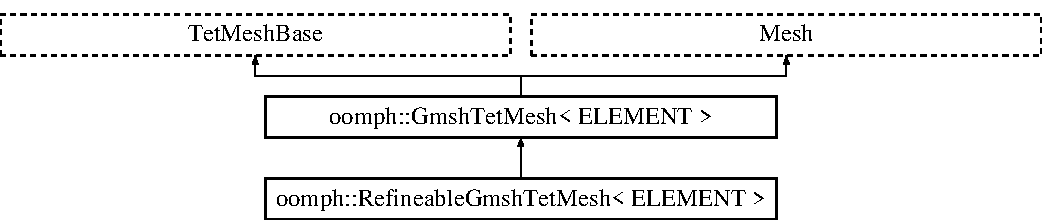
\includegraphics[height=2.957747cm]{classoomph_1_1GmshTetMesh}
\end{center}
\end{figure}
\subsection*{Public Member Functions}
\begin{DoxyCompactItemize}
\item 
\hyperlink{classoomph_1_1GmshTetMesh_a3f9c7d2c2a617f4b497778ff44109dbc}{Gmsh\+Tet\+Mesh} (\hyperlink{classoomph_1_1GmshParameters}{Gmsh\+Parameters} $\ast$gmsh\+\_\+parameters\+\_\+pt, Time\+Stepper $\ast$time\+\_\+stepper\+\_\+pt=\&Mesh\+::\+Default\+\_\+\+Time\+Stepper)
\begin{DoxyCompactList}\small\item\em Constructor. \end{DoxyCompactList}\item 
\hyperlink{classoomph_1_1GmshTetMesh_a8b93f46d9a6a442f6d5e9b8e86f33882}{Gmsh\+Tet\+Mesh} (\hyperlink{classoomph_1_1GmshParameters}{Gmsh\+Parameters} $\ast$gmsh\+\_\+parameters\+\_\+pt, const bool \&use\+\_\+mesh\+\_\+grading\+\_\+from\+\_\+file, Time\+Stepper $\ast$time\+\_\+stepper\+\_\+pt=\&Mesh\+::\+Default\+\_\+\+Time\+Stepper)
\begin{DoxyCompactList}\small\item\em Constructor. If boolean is set to true, the target element sizes are read from file (used during adaptation; otherwise uniform target size is used). \end{DoxyCompactList}\end{DoxyCompactItemize}
\subsection*{Protected Attributes}
\begin{DoxyCompactItemize}
\item 
\hyperlink{classoomph_1_1GmshParameters}{Gmsh\+Parameters} $\ast$ \hyperlink{classoomph_1_1GmshTetMesh_a6d9878df9dfca45b4883909ed1e78536}{Gmsh\+\_\+parameters\+\_\+pt}
\begin{DoxyCompactList}\small\item\em Parameters. \end{DoxyCompactList}\end{DoxyCompactItemize}
\subsection*{Private Member Functions}
\begin{DoxyCompactItemize}
\item 
void \hyperlink{classoomph_1_1GmshTetMesh_aaec22ccd211f81dd440e9618d6667718}{build\+\_\+it} (Time\+Stepper $\ast$time\+\_\+stepper\+\_\+pt, const bool \&use\+\_\+mesh\+\_\+grading\+\_\+from\+\_\+file)
\item 
void \hyperlink{classoomph_1_1GmshTetMesh_a80132087ae6dd00c7631823a8453e078}{build\+\_\+from\+\_\+scaffold} (\hyperlink{classoomph_1_1GmshTetScaffoldMesh}{Gmsh\+Tet\+Scaffold\+Mesh} $\ast$tmp\+\_\+scaffold\+\_\+mesh\+\_\+pt, Time\+Stepper $\ast$time\+\_\+stepper\+\_\+pt)
\begin{DoxyCompactList}\small\item\em Build unstructured tet gmesh mesh based on output from scaffold. \end{DoxyCompactList}\end{DoxyCompactItemize}


\subsection{Detailed Description}
\subsubsection*{template$<$class E\+L\+E\+M\+E\+NT$>$\newline
class oomph\+::\+Gmsh\+Tet\+Mesh$<$ E\+L\+E\+M\+E\+N\+T $>$}

Forward declaration. 

Definition at line 371 of file gmsh\+\_\+tet\+\_\+mesh.\+template.\+h.



\subsection{Constructor \& Destructor Documentation}
\mbox{\Hypertarget{classoomph_1_1GmshTetMesh_a3f9c7d2c2a617f4b497778ff44109dbc}\label{classoomph_1_1GmshTetMesh_a3f9c7d2c2a617f4b497778ff44109dbc}} 
\index{oomph\+::\+Gmsh\+Tet\+Mesh@{oomph\+::\+Gmsh\+Tet\+Mesh}!Gmsh\+Tet\+Mesh@{Gmsh\+Tet\+Mesh}}
\index{Gmsh\+Tet\+Mesh@{Gmsh\+Tet\+Mesh}!oomph\+::\+Gmsh\+Tet\+Mesh@{oomph\+::\+Gmsh\+Tet\+Mesh}}
\subsubsection{\texorpdfstring{Gmsh\+Tet\+Mesh()}{GmshTetMesh()}\hspace{0.1cm}{\footnotesize\ttfamily [1/2]}}
{\footnotesize\ttfamily template$<$class E\+L\+E\+M\+E\+NT$>$ \\
\hyperlink{classoomph_1_1GmshTetMesh}{oomph\+::\+Gmsh\+Tet\+Mesh}$<$ E\+L\+E\+M\+E\+NT $>$\+::\hyperlink{classoomph_1_1GmshTetMesh}{Gmsh\+Tet\+Mesh} (\begin{DoxyParamCaption}\item[{\hyperlink{classoomph_1_1GmshParameters}{Gmsh\+Parameters} $\ast$}]{gmsh\+\_\+parameters\+\_\+pt,  }\item[{Time\+Stepper $\ast$}]{time\+\_\+stepper\+\_\+pt = {\ttfamily \&Mesh\+:\+:Default\+\_\+TimeStepper} }\end{DoxyParamCaption})\hspace{0.3cm}{\ttfamily [inline]}}



Constructor. 



Definition at line 1700 of file gmsh\+\_\+tet\+\_\+mesh.\+template.\+h.

\mbox{\Hypertarget{classoomph_1_1GmshTetMesh_a8b93f46d9a6a442f6d5e9b8e86f33882}\label{classoomph_1_1GmshTetMesh_a8b93f46d9a6a442f6d5e9b8e86f33882}} 
\index{oomph\+::\+Gmsh\+Tet\+Mesh@{oomph\+::\+Gmsh\+Tet\+Mesh}!Gmsh\+Tet\+Mesh@{Gmsh\+Tet\+Mesh}}
\index{Gmsh\+Tet\+Mesh@{Gmsh\+Tet\+Mesh}!oomph\+::\+Gmsh\+Tet\+Mesh@{oomph\+::\+Gmsh\+Tet\+Mesh}}
\subsubsection{\texorpdfstring{Gmsh\+Tet\+Mesh()}{GmshTetMesh()}\hspace{0.1cm}{\footnotesize\ttfamily [2/2]}}
{\footnotesize\ttfamily template$<$class E\+L\+E\+M\+E\+NT$>$ \\
\hyperlink{classoomph_1_1GmshTetMesh}{oomph\+::\+Gmsh\+Tet\+Mesh}$<$ E\+L\+E\+M\+E\+NT $>$\+::\hyperlink{classoomph_1_1GmshTetMesh}{Gmsh\+Tet\+Mesh} (\begin{DoxyParamCaption}\item[{\hyperlink{classoomph_1_1GmshParameters}{Gmsh\+Parameters} $\ast$}]{gmsh\+\_\+parameters\+\_\+pt,  }\item[{const bool \&}]{use\+\_\+mesh\+\_\+grading\+\_\+from\+\_\+file,  }\item[{Time\+Stepper $\ast$}]{time\+\_\+stepper\+\_\+pt = {\ttfamily \&Mesh\+:\+:Default\+\_\+TimeStepper} }\end{DoxyParamCaption})\hspace{0.3cm}{\ttfamily [inline]}}



Constructor. If boolean is set to true, the target element sizes are read from file (used during adaptation; otherwise uniform target size is used). 



Definition at line 1711 of file gmsh\+\_\+tet\+\_\+mesh.\+template.\+h.



\subsection{Member Function Documentation}
\mbox{\Hypertarget{classoomph_1_1GmshTetMesh_a80132087ae6dd00c7631823a8453e078}\label{classoomph_1_1GmshTetMesh_a80132087ae6dd00c7631823a8453e078}} 
\index{oomph\+::\+Gmsh\+Tet\+Mesh@{oomph\+::\+Gmsh\+Tet\+Mesh}!build\+\_\+from\+\_\+scaffold@{build\+\_\+from\+\_\+scaffold}}
\index{build\+\_\+from\+\_\+scaffold@{build\+\_\+from\+\_\+scaffold}!oomph\+::\+Gmsh\+Tet\+Mesh@{oomph\+::\+Gmsh\+Tet\+Mesh}}
\subsubsection{\texorpdfstring{build\+\_\+from\+\_\+scaffold()}{build\_from\_scaffold()}}
{\footnotesize\ttfamily template$<$class E\+L\+E\+M\+E\+NT$>$ \\
void \hyperlink{classoomph_1_1GmshTetMesh}{oomph\+::\+Gmsh\+Tet\+Mesh}$<$ E\+L\+E\+M\+E\+NT $>$\+::build\+\_\+from\+\_\+scaffold (\begin{DoxyParamCaption}\item[{\hyperlink{classoomph_1_1GmshTetScaffoldMesh}{Gmsh\+Tet\+Scaffold\+Mesh} $\ast$}]{tmp\+\_\+scaffold\+\_\+mesh\+\_\+pt,  }\item[{Time\+Stepper $\ast$}]{time\+\_\+stepper\+\_\+pt }\end{DoxyParamCaption})\hspace{0.3cm}{\ttfamily [inline]}, {\ttfamily [private]}}



Build unstructured tet gmesh mesh based on output from scaffold. 



Definition at line 1833 of file gmsh\+\_\+tet\+\_\+mesh.\+template.\+h.

\mbox{\Hypertarget{classoomph_1_1GmshTetMesh_aaec22ccd211f81dd440e9618d6667718}\label{classoomph_1_1GmshTetMesh_aaec22ccd211f81dd440e9618d6667718}} 
\index{oomph\+::\+Gmsh\+Tet\+Mesh@{oomph\+::\+Gmsh\+Tet\+Mesh}!build\+\_\+it@{build\+\_\+it}}
\index{build\+\_\+it@{build\+\_\+it}!oomph\+::\+Gmsh\+Tet\+Mesh@{oomph\+::\+Gmsh\+Tet\+Mesh}}
\subsubsection{\texorpdfstring{build\+\_\+it()}{build\_it()}}
{\footnotesize\ttfamily template$<$class E\+L\+E\+M\+E\+NT$>$ \\
void \hyperlink{classoomph_1_1GmshTetMesh}{oomph\+::\+Gmsh\+Tet\+Mesh}$<$ E\+L\+E\+M\+E\+NT $>$\+::build\+\_\+it (\begin{DoxyParamCaption}\item[{Time\+Stepper $\ast$}]{time\+\_\+stepper\+\_\+pt,  }\item[{const bool \&}]{use\+\_\+mesh\+\_\+grading\+\_\+from\+\_\+file }\end{DoxyParamCaption})\hspace{0.3cm}{\ttfamily [inline]}, {\ttfamily [private]}}



Definition at line 1723 of file gmsh\+\_\+tet\+\_\+mesh.\+template.\+h.



References oomph\+::\+Gmsh\+Parameters\+::internal\+\_\+surface\+\_\+pt(), oomph\+::\+Gmsh\+Parameters\+::\+Internal\+\_\+surface\+\_\+pt, oomph\+::\+Gmsh\+Parameters\+::outer\+\_\+boundary\+\_\+pt(), and oomph\+::\+Gmsh\+Parameters\+::\+Outer\+\_\+boundary\+\_\+pt.



\subsection{Member Data Documentation}
\mbox{\Hypertarget{classoomph_1_1GmshTetMesh_a6d9878df9dfca45b4883909ed1e78536}\label{classoomph_1_1GmshTetMesh_a6d9878df9dfca45b4883909ed1e78536}} 
\index{oomph\+::\+Gmsh\+Tet\+Mesh@{oomph\+::\+Gmsh\+Tet\+Mesh}!Gmsh\+\_\+parameters\+\_\+pt@{Gmsh\+\_\+parameters\+\_\+pt}}
\index{Gmsh\+\_\+parameters\+\_\+pt@{Gmsh\+\_\+parameters\+\_\+pt}!oomph\+::\+Gmsh\+Tet\+Mesh@{oomph\+::\+Gmsh\+Tet\+Mesh}}
\subsubsection{\texorpdfstring{Gmsh\+\_\+parameters\+\_\+pt}{Gmsh\_parameters\_pt}}
{\footnotesize\ttfamily template$<$class E\+L\+E\+M\+E\+NT$>$ \\
\hyperlink{classoomph_1_1GmshParameters}{Gmsh\+Parameters}$\ast$ \hyperlink{classoomph_1_1GmshTetMesh}{oomph\+::\+Gmsh\+Tet\+Mesh}$<$ E\+L\+E\+M\+E\+NT $>$\+::Gmsh\+\_\+parameters\+\_\+pt\hspace{0.3cm}{\ttfamily [protected]}}



Parameters. 



Definition at line 1827 of file gmsh\+\_\+tet\+\_\+mesh.\+template.\+h.



The documentation for this class was generated from the following file\+:\begin{DoxyCompactItemize}
\item 
\hyperlink{gmsh__tet__mesh_8template_8h}{gmsh\+\_\+tet\+\_\+mesh.\+template.\+h}\end{DoxyCompactItemize}

\hypertarget{classoomph_1_1GmshTetScaffoldMesh}{}\section{oomph\+:\+:Gmsh\+Tet\+Scaffold\+Mesh Class Reference}
\label{classoomph_1_1GmshTetScaffoldMesh}\index{oomph\+::\+Gmsh\+Tet\+Scaffold\+Mesh@{oomph\+::\+Gmsh\+Tet\+Scaffold\+Mesh}}


{\ttfamily \#include $<$gmsh\+\_\+tet\+\_\+mesh.\+template.\+h$>$}

Inheritance diagram for oomph\+:\+:Gmsh\+Tet\+Scaffold\+Mesh\+:\begin{figure}[H]
\begin{center}
\leavevmode
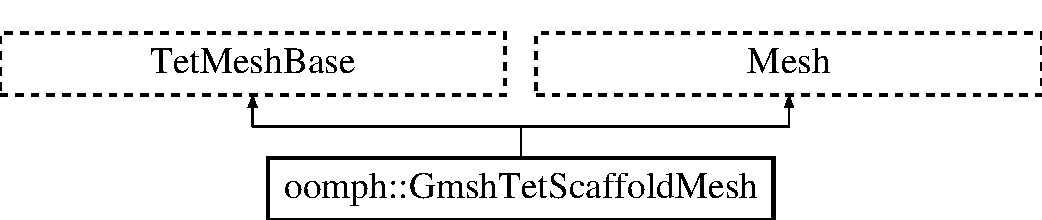
\includegraphics[height=2.000000cm]{classoomph_1_1GmshTetScaffoldMesh}
\end{center}
\end{figure}
\subsection*{Public Member Functions}
\begin{DoxyCompactItemize}
\item 
\hyperlink{classoomph_1_1GmshTetScaffoldMesh_a16430cc97edb1f4ec0eab6cfa5b94563}{Gmsh\+Tet\+Scaffold\+Mesh} (\hyperlink{classoomph_1_1GmshParameters}{Gmsh\+Parameters} $\ast$gmsh\+\_\+parameters\+\_\+pt, const bool \&use\+\_\+mesh\+\_\+grading\+\_\+from\+\_\+file)
\begin{DoxyCompactList}\small\item\em Build mesh, based on specified parameters. If boolean is set to true, the target element sizes are read from file (used during adaptation; otherwise uniform target size is used). \end{DoxyCompactList}\end{DoxyCompactItemize}
\subsection*{Private Member Functions}
\begin{DoxyCompactItemize}
\item 
void \hyperlink{classoomph_1_1GmshTetScaffoldMesh_a13c5fa9a126fc1707534031826d8f43f}{create\+\_\+mesh\+\_\+from\+\_\+msh\+\_\+file} ()
\begin{DoxyCompactList}\small\item\em Create mesh from msh file (created internally via disk-\/based operations) \end{DoxyCompactList}\item 
void \hyperlink{classoomph_1_1GmshTetScaffoldMesh_a20ba8fb06fe0264c4ba0b586b104f969}{write\+\_\+geo\+\_\+file} (const bool \&use\+\_\+mesh\+\_\+grading\+\_\+from\+\_\+file)
\begin{DoxyCompactList}\small\item\em Write geo file for gmsh. \end{DoxyCompactList}\end{DoxyCompactItemize}
\subsection*{Private Attributes}
\begin{DoxyCompactItemize}
\item 
\hyperlink{classoomph_1_1GmshParameters}{Gmsh\+Parameters} $\ast$ \hyperlink{classoomph_1_1GmshTetScaffoldMesh_afce3676b4f42501024ba1a933f04600d}{Gmsh\+\_\+parameters\+\_\+pt}
\begin{DoxyCompactList}\small\item\em Parameters. \end{DoxyCompactList}\end{DoxyCompactItemize}
\subsection*{Friends}
\begin{DoxyCompactItemize}
\item 
{\footnotesize template$<$class E\+L\+E\+M\+E\+NT $>$ }\\class \hyperlink{classoomph_1_1GmshTetScaffoldMesh_a542660fc34eb890a935f0d42a3b4eb8a}{Gmsh\+Tet\+Mesh}
\begin{DoxyCompactList}\small\item\em We\textquotesingle{}re friends with the actual mesh. \end{DoxyCompactList}\end{DoxyCompactItemize}


\subsection{Detailed Description}


Definition at line 377 of file gmsh\+\_\+tet\+\_\+mesh.\+template.\+h.



\subsection{Constructor \& Destructor Documentation}
\mbox{\Hypertarget{classoomph_1_1GmshTetScaffoldMesh_a16430cc97edb1f4ec0eab6cfa5b94563}\label{classoomph_1_1GmshTetScaffoldMesh_a16430cc97edb1f4ec0eab6cfa5b94563}} 
\index{oomph\+::\+Gmsh\+Tet\+Scaffold\+Mesh@{oomph\+::\+Gmsh\+Tet\+Scaffold\+Mesh}!Gmsh\+Tet\+Scaffold\+Mesh@{Gmsh\+Tet\+Scaffold\+Mesh}}
\index{Gmsh\+Tet\+Scaffold\+Mesh@{Gmsh\+Tet\+Scaffold\+Mesh}!oomph\+::\+Gmsh\+Tet\+Scaffold\+Mesh@{oomph\+::\+Gmsh\+Tet\+Scaffold\+Mesh}}
\subsubsection{\texorpdfstring{Gmsh\+Tet\+Scaffold\+Mesh()}{GmshTetScaffoldMesh()}}
{\footnotesize\ttfamily oomph\+::\+Gmsh\+Tet\+Scaffold\+Mesh\+::\+Gmsh\+Tet\+Scaffold\+Mesh (\begin{DoxyParamCaption}\item[{\hyperlink{classoomph_1_1GmshParameters}{Gmsh\+Parameters} $\ast$}]{gmsh\+\_\+parameters\+\_\+pt,  }\item[{const bool \&}]{use\+\_\+mesh\+\_\+grading\+\_\+from\+\_\+file }\end{DoxyParamCaption})\hspace{0.3cm}{\ttfamily [inline]}}



Build mesh, based on specified parameters. If boolean is set to true, the target element sizes are read from file (used during adaptation; otherwise uniform target size is used). 



Definition at line 390 of file gmsh\+\_\+tet\+\_\+mesh.\+template.\+h.



References oomph\+::\+Gmsh\+Parameters\+::gmsh\+\_\+onscreen\+\_\+output\+\_\+counter(), and oomph\+::\+Gmsh\+Parameters\+::gmsh\+\_\+onscreen\+\_\+output\+\_\+file\+\_\+name().



\subsection{Member Function Documentation}
\mbox{\Hypertarget{classoomph_1_1GmshTetScaffoldMesh_a13c5fa9a126fc1707534031826d8f43f}\label{classoomph_1_1GmshTetScaffoldMesh_a13c5fa9a126fc1707534031826d8f43f}} 
\index{oomph\+::\+Gmsh\+Tet\+Scaffold\+Mesh@{oomph\+::\+Gmsh\+Tet\+Scaffold\+Mesh}!create\+\_\+mesh\+\_\+from\+\_\+msh\+\_\+file@{create\+\_\+mesh\+\_\+from\+\_\+msh\+\_\+file}}
\index{create\+\_\+mesh\+\_\+from\+\_\+msh\+\_\+file@{create\+\_\+mesh\+\_\+from\+\_\+msh\+\_\+file}!oomph\+::\+Gmsh\+Tet\+Scaffold\+Mesh@{oomph\+::\+Gmsh\+Tet\+Scaffold\+Mesh}}
\subsubsection{\texorpdfstring{create\+\_\+mesh\+\_\+from\+\_\+msh\+\_\+file()}{create\_mesh\_from\_msh\_file()}}
{\footnotesize\ttfamily void oomph\+::\+Gmsh\+Tet\+Scaffold\+Mesh\+::create\+\_\+mesh\+\_\+from\+\_\+msh\+\_\+file (\begin{DoxyParamCaption}{ }\end{DoxyParamCaption})\hspace{0.3cm}{\ttfamily [inline]}, {\ttfamily [private]}}



Create mesh from msh file (created internally via disk-\/based operations) 



Definition at line 460 of file gmsh\+\_\+tet\+\_\+mesh.\+template.\+h.



References oomph\+::\+Gmsh\+Parameters\+::geo\+\_\+and\+\_\+msh\+\_\+file\+\_\+stem().

\mbox{\Hypertarget{classoomph_1_1GmshTetScaffoldMesh_a20ba8fb06fe0264c4ba0b586b104f969}\label{classoomph_1_1GmshTetScaffoldMesh_a20ba8fb06fe0264c4ba0b586b104f969}} 
\index{oomph\+::\+Gmsh\+Tet\+Scaffold\+Mesh@{oomph\+::\+Gmsh\+Tet\+Scaffold\+Mesh}!write\+\_\+geo\+\_\+file@{write\+\_\+geo\+\_\+file}}
\index{write\+\_\+geo\+\_\+file@{write\+\_\+geo\+\_\+file}!oomph\+::\+Gmsh\+Tet\+Scaffold\+Mesh@{oomph\+::\+Gmsh\+Tet\+Scaffold\+Mesh}}
\subsubsection{\texorpdfstring{write\+\_\+geo\+\_\+file()}{write\_geo\_file()}}
{\footnotesize\ttfamily void oomph\+::\+Gmsh\+Tet\+Scaffold\+Mesh\+::write\+\_\+geo\+\_\+file (\begin{DoxyParamCaption}\item[{const bool \&}]{use\+\_\+mesh\+\_\+grading\+\_\+from\+\_\+file }\end{DoxyParamCaption})\hspace{0.3cm}{\ttfamily [inline]}, {\ttfamily [private]}}



Write geo file for gmsh. 



Definition at line 1034 of file gmsh\+\_\+tet\+\_\+mesh.\+template.\+h.



References oomph\+::\+Gmsh\+Parameters\+::element\+\_\+volume(), oomph\+::\+Gmsh\+Parameters\+::internal\+\_\+surface\+\_\+pt(), oomph\+::\+Tet\+Edge\+::is\+\_\+reversed(), oomph\+::\+Gmsh\+Parameters\+::outer\+\_\+boundary\+\_\+pt(), and oomph\+::\+Gmsh\+Parameters\+::target\+\_\+size\+\_\+file\+\_\+name().



\subsection{Friends And Related Function Documentation}
\mbox{\Hypertarget{classoomph_1_1GmshTetScaffoldMesh_a542660fc34eb890a935f0d42a3b4eb8a}\label{classoomph_1_1GmshTetScaffoldMesh_a542660fc34eb890a935f0d42a3b4eb8a}} 
\index{oomph\+::\+Gmsh\+Tet\+Scaffold\+Mesh@{oomph\+::\+Gmsh\+Tet\+Scaffold\+Mesh}!Gmsh\+Tet\+Mesh@{Gmsh\+Tet\+Mesh}}
\index{Gmsh\+Tet\+Mesh@{Gmsh\+Tet\+Mesh}!oomph\+::\+Gmsh\+Tet\+Scaffold\+Mesh@{oomph\+::\+Gmsh\+Tet\+Scaffold\+Mesh}}
\subsubsection{\texorpdfstring{Gmsh\+Tet\+Mesh}{GmshTetMesh}}
{\footnotesize\ttfamily template$<$class E\+L\+E\+M\+E\+NT $>$ \\
friend class \hyperlink{classoomph_1_1GmshTetMesh}{Gmsh\+Tet\+Mesh}\hspace{0.3cm}{\ttfamily [friend]}}



We\textquotesingle{}re friends with the actual mesh. 



Definition at line 385 of file gmsh\+\_\+tet\+\_\+mesh.\+template.\+h.



\subsection{Member Data Documentation}
\mbox{\Hypertarget{classoomph_1_1GmshTetScaffoldMesh_afce3676b4f42501024ba1a933f04600d}\label{classoomph_1_1GmshTetScaffoldMesh_afce3676b4f42501024ba1a933f04600d}} 
\index{oomph\+::\+Gmsh\+Tet\+Scaffold\+Mesh@{oomph\+::\+Gmsh\+Tet\+Scaffold\+Mesh}!Gmsh\+\_\+parameters\+\_\+pt@{Gmsh\+\_\+parameters\+\_\+pt}}
\index{Gmsh\+\_\+parameters\+\_\+pt@{Gmsh\+\_\+parameters\+\_\+pt}!oomph\+::\+Gmsh\+Tet\+Scaffold\+Mesh@{oomph\+::\+Gmsh\+Tet\+Scaffold\+Mesh}}
\subsubsection{\texorpdfstring{Gmsh\+\_\+parameters\+\_\+pt}{Gmsh\_parameters\_pt}}
{\footnotesize\ttfamily \hyperlink{classoomph_1_1GmshParameters}{Gmsh\+Parameters}$\ast$ oomph\+::\+Gmsh\+Tet\+Scaffold\+Mesh\+::\+Gmsh\+\_\+parameters\+\_\+pt\hspace{0.3cm}{\ttfamily [private]}}



Parameters. 



Definition at line 1674 of file gmsh\+\_\+tet\+\_\+mesh.\+template.\+h.



The documentation for this class was generated from the following file\+:\begin{DoxyCompactItemize}
\item 
\hyperlink{gmsh__tet__mesh_8template_8h}{gmsh\+\_\+tet\+\_\+mesh.\+template.\+h}\end{DoxyCompactItemize}

\hypertarget{classoomph_1_1HermiteQuadMesh}{}\section{oomph\+:\+:Hermite\+Quad\+Mesh$<$ E\+L\+E\+M\+E\+NT $>$ Class Template Reference}
\label{classoomph_1_1HermiteQuadMesh}\index{oomph\+::\+Hermite\+Quad\+Mesh$<$ E\+L\+E\+M\+E\+N\+T $>$@{oomph\+::\+Hermite\+Quad\+Mesh$<$ E\+L\+E\+M\+E\+N\+T $>$}}


A two dimensional Hermite bicubic element quadrilateral mesh for a topologically rectangular domain. The geometry of the problem must be prescribed using the \hyperlink{classoomph_1_1TopologicallyRectangularDomain}{Topologically\+Rectangular\+Domain}. Non uniform node spacing can be prescribed using a function pointer.  




{\ttfamily \#include $<$hermite\+\_\+element\+\_\+quad\+\_\+mesh.\+template.\+h$>$}

Inheritance diagram for oomph\+:\+:Hermite\+Quad\+Mesh$<$ E\+L\+E\+M\+E\+NT $>$\+:\begin{figure}[H]
\begin{center}
\leavevmode
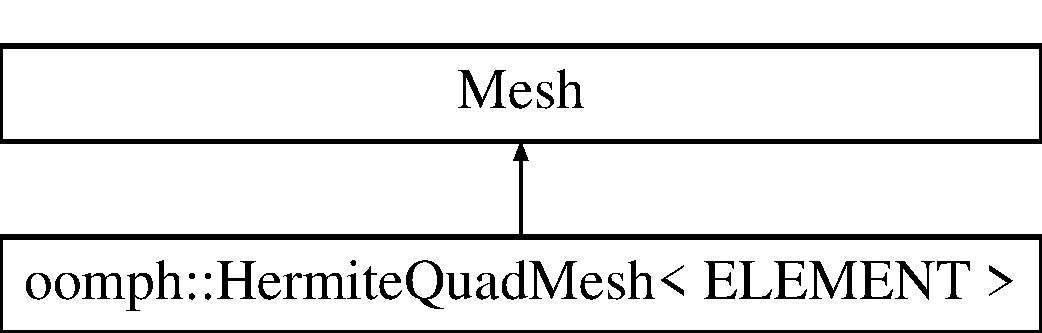
\includegraphics[height=2.000000cm]{classoomph_1_1HermiteQuadMesh}
\end{center}
\end{figure}
\subsection*{Public Types}
\begin{DoxyCompactItemize}
\item 
typedef void($\ast$ \hyperlink{classoomph_1_1HermiteQuadMesh_abebf4806b300591f976398404ed0ef3f}{Mesh\+Spacing\+Fn\+Ptr}) (const \hyperlink{classoomph_1_1Vector}{Vector}$<$ double $>$ \&m\+\_\+uniform\+\_\+spacing, \hyperlink{classoomph_1_1Vector}{Vector}$<$ double $>$ \&m\+\_\+non\+\_\+uniform\+\_\+spacing)
\begin{DoxyCompactList}\small\item\em \hyperlink{classoomph_1_1Mesh}{Mesh} Spacing Function Pointer -\/ an optional function pointer to prescibe the node spacing in a non-\/uniformly spaced mesh -\/ takes the position of a node (in macro element coordinates) in the uniformly spaced mesh and return the position in the non-\/uniformly spaced mesh. \end{DoxyCompactList}\end{DoxyCompactItemize}
\subsection*{Public Member Functions}
\begin{DoxyCompactItemize}
\item 
\hyperlink{classoomph_1_1HermiteQuadMesh_aea2e2144668d092f4e358f195bbc74e7}{Hermite\+Quad\+Mesh} (const unsigned \&nx, const unsigned \&ny, \hyperlink{classoomph_1_1TopologicallyRectangularDomain}{Topologically\+Rectangular\+Domain} $\ast$domain, const bool \&periodic\+\_\+in\+\_\+x=false, \hyperlink{classoomph_1_1TimeStepper}{Time\+Stepper} $\ast$time\+\_\+stepper\+\_\+pt=\&\hyperlink{classoomph_1_1Mesh_a12243d0fee2b1fcee729ee5a4777ea10}{Mesh\+::\+Default\+\_\+\+Time\+Stepper})
\begin{DoxyCompactList}\small\item\em \hyperlink{classoomph_1_1Mesh}{Mesh} Constructor (for a uniformly spaced mesh). Takes the following arguments \+: nx \+: number of elements in x direction; ny \+: number of elements in y direction; domain \+: topologically rectangular domain; periodic\+\_\+in\+\_\+x \+: flag specifying if the mesh is periodic in the x direction (default = false); time\+\_\+stepper\+\_\+pt \+: pointer to the time stepper (default = no timestepper);. \end{DoxyCompactList}\item 
\hyperlink{classoomph_1_1HermiteQuadMesh_ae28d471336aebafc5fe5e9f303ab0ad8}{Hermite\+Quad\+Mesh} (const unsigned \&nx, const unsigned \&ny, \hyperlink{classoomph_1_1TopologicallyRectangularDomain}{Topologically\+Rectangular\+Domain} $\ast$domain, const \hyperlink{classoomph_1_1HermiteQuadMesh_abebf4806b300591f976398404ed0ef3f}{Mesh\+Spacing\+Fn\+Ptr} spacing\+\_\+fn, const bool \&periodic\+\_\+in\+\_\+x=false, \hyperlink{classoomph_1_1TimeStepper}{Time\+Stepper} $\ast$time\+\_\+stepper\+\_\+pt=\&\hyperlink{classoomph_1_1Mesh_a12243d0fee2b1fcee729ee5a4777ea10}{Mesh\+::\+Default\+\_\+\+Time\+Stepper})
\begin{DoxyCompactList}\small\item\em \hyperlink{classoomph_1_1Mesh}{Mesh} Constructor (for a non-\/uniformly spaced mesh). Takes the following arguments \+: nx \+: number of elements in x direction; ny \+: number of elements in y direction; domain \+: topologically rectangular domain; spacing\+\_\+fn \+: spacing function prescribing a non-\/uniformly spaced mesh periodic\+\_\+in\+\_\+x \+: flag specifying if the mesh is periodic in the x direction (default = false); time\+\_\+stepper\+\_\+pt \+: pointer to the time stepper (default = notimestepper);. \end{DoxyCompactList}\item 
\hyperlink{classoomph_1_1HermiteQuadMesh_a81f14d729df268911cd3943efc125492}{$\sim$\+Hermite\+Quad\+Mesh} ()
\begin{DoxyCompactList}\small\item\em Destructor -\/ does nothing -\/ handled in mesh base class. \end{DoxyCompactList}\item 
unsigned \& \hyperlink{classoomph_1_1HermiteQuadMesh_a06599366634a9ac89e25a0f110d0a35b}{nelement\+\_\+in\+\_\+dim} (const unsigned \&d)
\begin{DoxyCompactList}\small\item\em Access function for number of elements in mesh in each dimension. \end{DoxyCompactList}\end{DoxyCompactItemize}
\subsection*{Private Member Functions}
\begin{DoxyCompactItemize}
\item 
void \hyperlink{classoomph_1_1HermiteQuadMesh_a745a06530e60580e95826bedcf2e3e01}{macro\+\_\+coordinate\+\_\+position} (const unsigned \&node\+\_\+num\+\_\+x, const unsigned \&node\+\_\+num\+\_\+y, \hyperlink{classoomph_1_1Vector}{Vector}$<$ double $>$ \&macro\+\_\+element\+\_\+position)
\begin{DoxyCompactList}\small\item\em returns the macro element position of the node that is the x-\/th node along from the L\+HS and the y-\/th node up from the lower edge \end{DoxyCompactList}\item 
void \hyperlink{classoomph_1_1HermiteQuadMesh_abaac1dedc4a2e578b73b0d849c9a68e8}{set\+\_\+position\+\_\+of\+\_\+node} (const unsigned \&node\+\_\+num\+\_\+x, const unsigned \&node\+\_\+num\+\_\+y, \hyperlink{classoomph_1_1Node}{Node} $\ast$\hyperlink{classoomph_1_1Mesh_aebdb699466fe07f2e27aa4404008cde4}{node\+\_\+pt})
\begin{DoxyCompactList}\small\item\em sets the generalised position of the node (i.\+e. -\/ x\+\_\+i, dx\+\_\+i/ds\+\_\+0, dx\+\_\+i/ds\+\_\+1 \& d2x\+\_\+i/ds\+\_\+0ds\+\_\+1 for i = 1,2). Takes the x,y coordinates of the node from which its position can be determined. \end{DoxyCompactList}\item 
void \hyperlink{classoomph_1_1HermiteQuadMesh_a735fd20f847ac98c5bd5db5196ff3ea4}{set\+\_\+position\+\_\+of\+\_\+boundary\+\_\+node} (const unsigned \&node\+\_\+num\+\_\+x, const unsigned \&node\+\_\+num\+\_\+y, \hyperlink{classoomph_1_1BoundaryNode}{Boundary\+Node}$<$ \hyperlink{classoomph_1_1Node}{Node} $>$ $\ast$\hyperlink{classoomph_1_1Mesh_aebdb699466fe07f2e27aa4404008cde4}{node\+\_\+pt})
\begin{DoxyCompactList}\small\item\em sets the generalised position of the node (i.\+e. -\/ x\+\_\+i, dx\+\_\+i/ds\+\_\+0, dx\+\_\+i/ds\+\_\+1 \& d2x\+\_\+i/ds\+\_\+0ds\+\_\+1 for i = 1,2). Takes the x,y coordinates of the node from which its position can be determined. Also sets coordinates on boundary vector for the node to be the generalised position of the node in macro element coordinates \end{DoxyCompactList}\item 
void \hyperlink{classoomph_1_1HermiteQuadMesh_a17d8992ae7fa8b46b568d156306d3c89}{generalised\+\_\+macro\+\_\+element\+\_\+position\+\_\+of\+\_\+node} (const unsigned \&node\+\_\+num\+\_\+x, const unsigned \&node\+\_\+num\+\_\+y, \hyperlink{classoomph_1_1DenseMatrix}{Dense\+Matrix}$<$ double $>$ \&m\+\_\+gen)
\begin{DoxyCompactList}\small\item\em computes the generalised position of the node at position (node\+\_\+num\+\_\+x, node\+\_\+num\+\_\+y) in the macro element coordinate scheme. index 0 of m\+\_\+gen \+: 0 -\/ m\+\_\+i 1 -\/ dm\+\_\+i/ds\+\_\+0 2 -\/ dm\+\_\+i/ds\+\_\+1 3 -\/ d2m\+\_\+i/ds\+\_\+0ds\+\_\+1 (where i is index 1 of m\+\_\+gen) \end{DoxyCompactList}\item 
virtual void \hyperlink{classoomph_1_1HermiteQuadMesh_af72fd9b700fdee643ce6d6259c0e8e6f}{build\+\_\+mesh} (\hyperlink{classoomph_1_1TimeStepper}{Time\+Stepper} $\ast$time\+\_\+stepper\+\_\+pt)
\begin{DoxyCompactList}\small\item\em Generic mesh construction function to build the mesh. \end{DoxyCompactList}\item 
virtual void \hyperlink{classoomph_1_1HermiteQuadMesh_a6eefe872b5bf8a06174b536d9727ea44}{setup\+\_\+boundary\+\_\+element\+\_\+info} ()
\item 
virtual void \hyperlink{classoomph_1_1HermiteQuadMesh_a0e4cd3df0828e87a762c61b09121e1c0}{setup\+\_\+boundary\+\_\+element\+\_\+info} (std\+::ostream \&outfile)
\begin{DoxyCompactList}\small\item\em Setup lookup schemes which establish which elements are located next to which boundaries (Doc to outfile if it\textquotesingle{}s open). Specific version for \hyperlink{classoomph_1_1HermiteQuadMesh}{Hermite\+Quad\+Mesh} to ensure that the order of the elements in Boundary\+\_\+element\+\_\+pt matches the actual order along the boundary. This is required when hijacking the \hyperlink{classoomph_1_1BiharmonicElement}{Biharmonic\+Element} to apply the \hyperlink{classoomph_1_1BiharmonicFluidBoundaryElement}{Biharmonic\+Fluid\+Boundary\+Element} in \hyperlink{classoomph_1_1BiharmonicFluidProblem_a1cc57555bbd0ceef1d93010c133ac597}{Biharmonic\+Fluid\+Problem\+::impose\+\_\+traction\+\_\+free\+\_\+edge}(...) \end{DoxyCompactList}\end{DoxyCompactItemize}
\subsection*{Private Attributes}
\begin{DoxyCompactItemize}
\item 
\hyperlink{classoomph_1_1Vector}{Vector}$<$ unsigned $>$ \hyperlink{classoomph_1_1HermiteQuadMesh_a0d02ca1a2769955ce57f09616195bd27}{Nelement}
\begin{DoxyCompactList}\small\item\em number of elements in each coordinate direction \end{DoxyCompactList}\item 
bool \hyperlink{classoomph_1_1HermiteQuadMesh_af1c2c974dc0d2e599b6bbe3921c5bb77}{Xperiodic}
\begin{DoxyCompactList}\small\item\em boolean variable to determine whether the mesh is periodic in the x-\/direction \end{DoxyCompactList}\item 
\hyperlink{classoomph_1_1TopologicallyRectangularDomain}{Topologically\+Rectangular\+Domain} $\ast$ \hyperlink{classoomph_1_1HermiteQuadMesh_af6bae1864691e8fe94d7c61995ae560a}{Domain\+\_\+pt}
\begin{DoxyCompactList}\small\item\em Pointer to the topologically rectangular domain which prescribes the problem domain. \end{DoxyCompactList}\item 
\hyperlink{classoomph_1_1HermiteQuadMesh_abebf4806b300591f976398404ed0ef3f}{Mesh\+Spacing\+Fn\+Ptr} \hyperlink{classoomph_1_1HermiteQuadMesh_a3b3cc55576538fc29e6975def870536f}{Node\+\_\+spacing\+\_\+fn}
\begin{DoxyCompactList}\small\item\em non uniform mesh spacing function pointer \end{DoxyCompactList}\end{DoxyCompactItemize}
\subsection*{Additional Inherited Members}


\subsection{Detailed Description}
\subsubsection*{template$<$class E\+L\+E\+M\+E\+NT$>$\newline
class oomph\+::\+Hermite\+Quad\+Mesh$<$ E\+L\+E\+M\+E\+N\+T $>$}

A two dimensional Hermite bicubic element quadrilateral mesh for a topologically rectangular domain. The geometry of the problem must be prescribed using the \hyperlink{classoomph_1_1TopologicallyRectangularDomain}{Topologically\+Rectangular\+Domain}. Non uniform node spacing can be prescribed using a function pointer. 

Definition at line 58 of file hermite\+\_\+element\+\_\+quad\+\_\+mesh.\+template.\+h.



\subsection{Member Typedef Documentation}
\mbox{\Hypertarget{classoomph_1_1HermiteQuadMesh_abebf4806b300591f976398404ed0ef3f}\label{classoomph_1_1HermiteQuadMesh_abebf4806b300591f976398404ed0ef3f}} 
\index{oomph\+::\+Hermite\+Quad\+Mesh@{oomph\+::\+Hermite\+Quad\+Mesh}!Mesh\+Spacing\+Fn\+Ptr@{Mesh\+Spacing\+Fn\+Ptr}}
\index{Mesh\+Spacing\+Fn\+Ptr@{Mesh\+Spacing\+Fn\+Ptr}!oomph\+::\+Hermite\+Quad\+Mesh@{oomph\+::\+Hermite\+Quad\+Mesh}}
\subsubsection{\texorpdfstring{Mesh\+Spacing\+Fn\+Ptr}{MeshSpacingFnPtr}}
{\footnotesize\ttfamily template$<$class E\+L\+E\+M\+E\+NT$>$ \\
typedef void($\ast$ \hyperlink{classoomph_1_1HermiteQuadMesh}{oomph\+::\+Hermite\+Quad\+Mesh}$<$ E\+L\+E\+M\+E\+NT $>$\+::Mesh\+Spacing\+Fn\+Ptr) (const \hyperlink{classoomph_1_1Vector}{Vector}$<$ double $>$ \&m\+\_\+uniform\+\_\+spacing, \hyperlink{classoomph_1_1Vector}{Vector}$<$ double $>$ \&m\+\_\+non\+\_\+uniform\+\_\+spacing)}



\hyperlink{classoomph_1_1Mesh}{Mesh} Spacing Function Pointer -\/ an optional function pointer to prescibe the node spacing in a non-\/uniformly spaced mesh -\/ takes the position of a node (in macro element coordinates) in the uniformly spaced mesh and return the position in the non-\/uniformly spaced mesh. 



Definition at line 69 of file hermite\+\_\+element\+\_\+quad\+\_\+mesh.\+template.\+h.



\subsection{Constructor \& Destructor Documentation}
\mbox{\Hypertarget{classoomph_1_1HermiteQuadMesh_aea2e2144668d092f4e358f195bbc74e7}\label{classoomph_1_1HermiteQuadMesh_aea2e2144668d092f4e358f195bbc74e7}} 
\index{oomph\+::\+Hermite\+Quad\+Mesh@{oomph\+::\+Hermite\+Quad\+Mesh}!Hermite\+Quad\+Mesh@{Hermite\+Quad\+Mesh}}
\index{Hermite\+Quad\+Mesh@{Hermite\+Quad\+Mesh}!oomph\+::\+Hermite\+Quad\+Mesh@{oomph\+::\+Hermite\+Quad\+Mesh}}
\subsubsection{\texorpdfstring{Hermite\+Quad\+Mesh()}{HermiteQuadMesh()}\hspace{0.1cm}{\footnotesize\ttfamily [1/2]}}
{\footnotesize\ttfamily template$<$class E\+L\+E\+M\+E\+NT$>$ \\
\hyperlink{classoomph_1_1HermiteQuadMesh}{oomph\+::\+Hermite\+Quad\+Mesh}$<$ E\+L\+E\+M\+E\+NT $>$\+::\hyperlink{classoomph_1_1HermiteQuadMesh}{Hermite\+Quad\+Mesh} (\begin{DoxyParamCaption}\item[{const unsigned \&}]{nx,  }\item[{const unsigned \&}]{ny,  }\item[{\hyperlink{classoomph_1_1TopologicallyRectangularDomain}{Topologically\+Rectangular\+Domain} $\ast$}]{domain,  }\item[{const bool \&}]{periodic\+\_\+in\+\_\+x = {\ttfamily false},  }\item[{\hyperlink{classoomph_1_1TimeStepper}{Time\+Stepper} $\ast$}]{time\+\_\+stepper\+\_\+pt = {\ttfamily \&\hyperlink{classoomph_1_1Mesh_a12243d0fee2b1fcee729ee5a4777ea10}{Mesh\+::\+Default\+\_\+\+Time\+Stepper}} }\end{DoxyParamCaption})\hspace{0.3cm}{\ttfamily [inline]}}



\hyperlink{classoomph_1_1Mesh}{Mesh} Constructor (for a uniformly spaced mesh). Takes the following arguments \+: nx \+: number of elements in x direction; ny \+: number of elements in y direction; domain \+: topologically rectangular domain; periodic\+\_\+in\+\_\+x \+: flag specifying if the mesh is periodic in the x direction (default = false); time\+\_\+stepper\+\_\+pt \+: pointer to the time stepper (default = no timestepper);. 



Definition at line 81 of file hermite\+\_\+element\+\_\+quad\+\_\+mesh.\+template.\+h.



References oomph\+::\+Hermite\+Quad\+Mesh$<$ E\+L\+E\+M\+E\+N\+T $>$\+::build\+\_\+mesh(), oomph\+::\+Hermite\+Quad\+Mesh$<$ E\+L\+E\+M\+E\+N\+T $>$\+::\+Domain\+\_\+pt, oomph\+::\+Hermite\+Quad\+Mesh$<$ E\+L\+E\+M\+E\+N\+T $>$\+::\+Nelement, oomph\+::\+Hermite\+Quad\+Mesh$<$ E\+L\+E\+M\+E\+N\+T $>$\+::\+Node\+\_\+spacing\+\_\+fn, and oomph\+::\+Hermite\+Quad\+Mesh$<$ E\+L\+E\+M\+E\+N\+T $>$\+::\+Xperiodic.

\mbox{\Hypertarget{classoomph_1_1HermiteQuadMesh_ae28d471336aebafc5fe5e9f303ab0ad8}\label{classoomph_1_1HermiteQuadMesh_ae28d471336aebafc5fe5e9f303ab0ad8}} 
\index{oomph\+::\+Hermite\+Quad\+Mesh@{oomph\+::\+Hermite\+Quad\+Mesh}!Hermite\+Quad\+Mesh@{Hermite\+Quad\+Mesh}}
\index{Hermite\+Quad\+Mesh@{Hermite\+Quad\+Mesh}!oomph\+::\+Hermite\+Quad\+Mesh@{oomph\+::\+Hermite\+Quad\+Mesh}}
\subsubsection{\texorpdfstring{Hermite\+Quad\+Mesh()}{HermiteQuadMesh()}\hspace{0.1cm}{\footnotesize\ttfamily [2/2]}}
{\footnotesize\ttfamily template$<$class E\+L\+E\+M\+E\+NT$>$ \\
\hyperlink{classoomph_1_1HermiteQuadMesh}{oomph\+::\+Hermite\+Quad\+Mesh}$<$ E\+L\+E\+M\+E\+NT $>$\+::\hyperlink{classoomph_1_1HermiteQuadMesh}{Hermite\+Quad\+Mesh} (\begin{DoxyParamCaption}\item[{const unsigned \&}]{nx,  }\item[{const unsigned \&}]{ny,  }\item[{\hyperlink{classoomph_1_1TopologicallyRectangularDomain}{Topologically\+Rectangular\+Domain} $\ast$}]{domain,  }\item[{const \hyperlink{classoomph_1_1HermiteQuadMesh_abebf4806b300591f976398404ed0ef3f}{Mesh\+Spacing\+Fn\+Ptr}}]{spacing\+\_\+fn,  }\item[{const bool \&}]{periodic\+\_\+in\+\_\+x = {\ttfamily false},  }\item[{\hyperlink{classoomph_1_1TimeStepper}{Time\+Stepper} $\ast$}]{time\+\_\+stepper\+\_\+pt = {\ttfamily \&\hyperlink{classoomph_1_1Mesh_a12243d0fee2b1fcee729ee5a4777ea10}{Mesh\+::\+Default\+\_\+\+Time\+Stepper}} }\end{DoxyParamCaption})\hspace{0.3cm}{\ttfamily [inline]}}



\hyperlink{classoomph_1_1Mesh}{Mesh} Constructor (for a non-\/uniformly spaced mesh). Takes the following arguments \+: nx \+: number of elements in x direction; ny \+: number of elements in y direction; domain \+: topologically rectangular domain; spacing\+\_\+fn \+: spacing function prescribing a non-\/uniformly spaced mesh periodic\+\_\+in\+\_\+x \+: flag specifying if the mesh is periodic in the x direction (default = false); time\+\_\+stepper\+\_\+pt \+: pointer to the time stepper (default = notimestepper);. 

build the mesh 

Definition at line 120 of file hermite\+\_\+element\+\_\+quad\+\_\+mesh.\+template.\+h.



References oomph\+::\+Hermite\+Quad\+Mesh$<$ E\+L\+E\+M\+E\+N\+T $>$\+::build\+\_\+mesh(), oomph\+::\+Hermite\+Quad\+Mesh$<$ E\+L\+E\+M\+E\+N\+T $>$\+::\+Domain\+\_\+pt, oomph\+::\+Hermite\+Quad\+Mesh$<$ E\+L\+E\+M\+E\+N\+T $>$\+::\+Nelement, oomph\+::\+Hermite\+Quad\+Mesh$<$ E\+L\+E\+M\+E\+N\+T $>$\+::\+Node\+\_\+spacing\+\_\+fn, and oomph\+::\+Hermite\+Quad\+Mesh$<$ E\+L\+E\+M\+E\+N\+T $>$\+::\+Xperiodic.

\mbox{\Hypertarget{classoomph_1_1HermiteQuadMesh_a81f14d729df268911cd3943efc125492}\label{classoomph_1_1HermiteQuadMesh_a81f14d729df268911cd3943efc125492}} 
\index{oomph\+::\+Hermite\+Quad\+Mesh@{oomph\+::\+Hermite\+Quad\+Mesh}!````~Hermite\+Quad\+Mesh@{$\sim$\+Hermite\+Quad\+Mesh}}
\index{````~Hermite\+Quad\+Mesh@{$\sim$\+Hermite\+Quad\+Mesh}!oomph\+::\+Hermite\+Quad\+Mesh@{oomph\+::\+Hermite\+Quad\+Mesh}}
\subsubsection{\texorpdfstring{$\sim$\+Hermite\+Quad\+Mesh()}{~HermiteQuadMesh()}}
{\footnotesize\ttfamily template$<$class E\+L\+E\+M\+E\+NT$>$ \\
\hyperlink{classoomph_1_1HermiteQuadMesh}{oomph\+::\+Hermite\+Quad\+Mesh}$<$ E\+L\+E\+M\+E\+NT $>$\+::$\sim$\hyperlink{classoomph_1_1HermiteQuadMesh}{Hermite\+Quad\+Mesh} (\begin{DoxyParamCaption}{ }\end{DoxyParamCaption})\hspace{0.3cm}{\ttfamily [inline]}}



Destructor -\/ does nothing -\/ handled in mesh base class. 



Definition at line 149 of file hermite\+\_\+element\+\_\+quad\+\_\+mesh.\+template.\+h.



\subsection{Member Function Documentation}
\mbox{\Hypertarget{classoomph_1_1HermiteQuadMesh_af72fd9b700fdee643ce6d6259c0e8e6f}\label{classoomph_1_1HermiteQuadMesh_af72fd9b700fdee643ce6d6259c0e8e6f}} 
\index{oomph\+::\+Hermite\+Quad\+Mesh@{oomph\+::\+Hermite\+Quad\+Mesh}!build\+\_\+mesh@{build\+\_\+mesh}}
\index{build\+\_\+mesh@{build\+\_\+mesh}!oomph\+::\+Hermite\+Quad\+Mesh@{oomph\+::\+Hermite\+Quad\+Mesh}}
\subsubsection{\texorpdfstring{build\+\_\+mesh()}{build\_mesh()}}
{\footnotesize\ttfamily template$<$class E\+L\+E\+M\+E\+NT $>$ \\
void \hyperlink{classoomph_1_1HermiteQuadMesh}{oomph\+::\+Hermite\+Quad\+Mesh}$<$ E\+L\+E\+M\+E\+NT $>$\+::build\+\_\+mesh (\begin{DoxyParamCaption}\item[{\hyperlink{classoomph_1_1TimeStepper}{Time\+Stepper} $\ast$}]{time\+\_\+stepper\+\_\+pt }\end{DoxyParamCaption})\hspace{0.3cm}{\ttfamily [private]}, {\ttfamily [virtual]}}



Generic mesh construction function to build the mesh. 



Definition at line 607 of file hermite\+\_\+element\+\_\+quad\+\_\+mesh.\+template.\+cc.



References i, and oomph\+::\+Hermite\+Quad\+Mesh$<$ E\+L\+E\+M\+E\+N\+T $>$\+::setup\+\_\+boundary\+\_\+element\+\_\+info().



Referenced by oomph\+::\+Hermite\+Quad\+Mesh$<$ E\+L\+E\+M\+E\+N\+T $>$\+::\+Hermite\+Quad\+Mesh(), and oomph\+::\+Hermite\+Quad\+Mesh$<$ E\+L\+E\+M\+E\+N\+T $>$\+::macro\+\_\+coordinate\+\_\+position().

\mbox{\Hypertarget{classoomph_1_1HermiteQuadMesh_a17d8992ae7fa8b46b568d156306d3c89}\label{classoomph_1_1HermiteQuadMesh_a17d8992ae7fa8b46b568d156306d3c89}} 
\index{oomph\+::\+Hermite\+Quad\+Mesh@{oomph\+::\+Hermite\+Quad\+Mesh}!generalised\+\_\+macro\+\_\+element\+\_\+position\+\_\+of\+\_\+node@{generalised\+\_\+macro\+\_\+element\+\_\+position\+\_\+of\+\_\+node}}
\index{generalised\+\_\+macro\+\_\+element\+\_\+position\+\_\+of\+\_\+node@{generalised\+\_\+macro\+\_\+element\+\_\+position\+\_\+of\+\_\+node}!oomph\+::\+Hermite\+Quad\+Mesh@{oomph\+::\+Hermite\+Quad\+Mesh}}
\subsubsection{\texorpdfstring{generalised\+\_\+macro\+\_\+element\+\_\+position\+\_\+of\+\_\+node()}{generalised\_macro\_element\_position\_of\_node()}}
{\footnotesize\ttfamily template$<$class E\+L\+E\+M\+E\+NT $>$ \\
void \hyperlink{classoomph_1_1HermiteQuadMesh}{oomph\+::\+Hermite\+Quad\+Mesh}$<$ E\+L\+E\+M\+E\+NT $>$\+::generalised\+\_\+macro\+\_\+element\+\_\+position\+\_\+of\+\_\+node (\begin{DoxyParamCaption}\item[{const unsigned \&}]{node\+\_\+num\+\_\+x,  }\item[{const unsigned \&}]{node\+\_\+num\+\_\+y,  }\item[{\hyperlink{classoomph_1_1DenseMatrix}{Dense\+Matrix}$<$ double $>$ \&}]{m\+\_\+gen }\end{DoxyParamCaption})\hspace{0.3cm}{\ttfamily [private]}}



computes the generalised position of the node at position (node\+\_\+num\+\_\+x, node\+\_\+num\+\_\+y) in the macro element coordinate scheme. index 0 of m\+\_\+gen \+: 0 -\/ m\+\_\+i 1 -\/ dm\+\_\+i/ds\+\_\+0 2 -\/ dm\+\_\+i/ds\+\_\+1 3 -\/ d2m\+\_\+i/ds\+\_\+0ds\+\_\+1 (where i is index 1 of m\+\_\+gen) 



Definition at line 210 of file hermite\+\_\+element\+\_\+quad\+\_\+mesh.\+template.\+cc.



Referenced by oomph\+::\+Hermite\+Quad\+Mesh$<$ E\+L\+E\+M\+E\+N\+T $>$\+::macro\+\_\+coordinate\+\_\+position(), and oomph\+::\+Hermite\+Quad\+Mesh$<$ E\+L\+E\+M\+E\+N\+T $>$\+::set\+\_\+position\+\_\+of\+\_\+boundary\+\_\+node().

\mbox{\Hypertarget{classoomph_1_1HermiteQuadMesh_a745a06530e60580e95826bedcf2e3e01}\label{classoomph_1_1HermiteQuadMesh_a745a06530e60580e95826bedcf2e3e01}} 
\index{oomph\+::\+Hermite\+Quad\+Mesh@{oomph\+::\+Hermite\+Quad\+Mesh}!macro\+\_\+coordinate\+\_\+position@{macro\+\_\+coordinate\+\_\+position}}
\index{macro\+\_\+coordinate\+\_\+position@{macro\+\_\+coordinate\+\_\+position}!oomph\+::\+Hermite\+Quad\+Mesh@{oomph\+::\+Hermite\+Quad\+Mesh}}
\subsubsection{\texorpdfstring{macro\+\_\+coordinate\+\_\+position()}{macro\_coordinate\_position()}}
{\footnotesize\ttfamily template$<$class E\+L\+E\+M\+E\+NT$>$ \\
void \hyperlink{classoomph_1_1HermiteQuadMesh}{oomph\+::\+Hermite\+Quad\+Mesh}$<$ E\+L\+E\+M\+E\+NT $>$\+::macro\+\_\+coordinate\+\_\+position (\begin{DoxyParamCaption}\item[{const unsigned \&}]{node\+\_\+num\+\_\+x,  }\item[{const unsigned \&}]{node\+\_\+num\+\_\+y,  }\item[{\hyperlink{classoomph_1_1Vector}{Vector}$<$ double $>$ \&}]{macro\+\_\+element\+\_\+position }\end{DoxyParamCaption})\hspace{0.3cm}{\ttfamily [inline]}, {\ttfamily [private]}}



returns the macro element position of the node that is the x-\/th node along from the L\+HS and the y-\/th node up from the lower edge 



Definition at line 163 of file hermite\+\_\+element\+\_\+quad\+\_\+mesh.\+template.\+h.



References oomph\+::\+Hermite\+Quad\+Mesh$<$ E\+L\+E\+M\+E\+N\+T $>$\+::build\+\_\+mesh(), oomph\+::\+Hermite\+Quad\+Mesh$<$ E\+L\+E\+M\+E\+N\+T $>$\+::generalised\+\_\+macro\+\_\+element\+\_\+position\+\_\+of\+\_\+node(), oomph\+::\+Hermite\+Quad\+Mesh$<$ E\+L\+E\+M\+E\+N\+T $>$\+::\+Nelement, oomph\+::\+Mesh\+::node\+\_\+pt(), oomph\+::\+Hermite\+Quad\+Mesh$<$ E\+L\+E\+M\+E\+N\+T $>$\+::\+Node\+\_\+spacing\+\_\+fn, oomph\+::\+Hermite\+Quad\+Mesh$<$ E\+L\+E\+M\+E\+N\+T $>$\+::set\+\_\+position\+\_\+of\+\_\+boundary\+\_\+node(), and oomph\+::\+Hermite\+Quad\+Mesh$<$ E\+L\+E\+M\+E\+N\+T $>$\+::set\+\_\+position\+\_\+of\+\_\+node().

\mbox{\Hypertarget{classoomph_1_1HermiteQuadMesh_a06599366634a9ac89e25a0f110d0a35b}\label{classoomph_1_1HermiteQuadMesh_a06599366634a9ac89e25a0f110d0a35b}} 
\index{oomph\+::\+Hermite\+Quad\+Mesh@{oomph\+::\+Hermite\+Quad\+Mesh}!nelement\+\_\+in\+\_\+dim@{nelement\+\_\+in\+\_\+dim}}
\index{nelement\+\_\+in\+\_\+dim@{nelement\+\_\+in\+\_\+dim}!oomph\+::\+Hermite\+Quad\+Mesh@{oomph\+::\+Hermite\+Quad\+Mesh}}
\subsubsection{\texorpdfstring{nelement\+\_\+in\+\_\+dim()}{nelement\_in\_dim()}}
{\footnotesize\ttfamily template$<$class E\+L\+E\+M\+E\+NT$>$ \\
unsigned\& \hyperlink{classoomph_1_1HermiteQuadMesh}{oomph\+::\+Hermite\+Quad\+Mesh}$<$ E\+L\+E\+M\+E\+NT $>$\+::nelement\+\_\+in\+\_\+dim (\begin{DoxyParamCaption}\item[{const unsigned \&}]{d }\end{DoxyParamCaption})\hspace{0.3cm}{\ttfamily [inline]}}



Access function for number of elements in mesh in each dimension. 



Definition at line 153 of file hermite\+\_\+element\+\_\+quad\+\_\+mesh.\+template.\+h.



References oomph\+::\+Hermite\+Quad\+Mesh$<$ E\+L\+E\+M\+E\+N\+T $>$\+::\+Nelement.

\mbox{\Hypertarget{classoomph_1_1HermiteQuadMesh_a735fd20f847ac98c5bd5db5196ff3ea4}\label{classoomph_1_1HermiteQuadMesh_a735fd20f847ac98c5bd5db5196ff3ea4}} 
\index{oomph\+::\+Hermite\+Quad\+Mesh@{oomph\+::\+Hermite\+Quad\+Mesh}!set\+\_\+position\+\_\+of\+\_\+boundary\+\_\+node@{set\+\_\+position\+\_\+of\+\_\+boundary\+\_\+node}}
\index{set\+\_\+position\+\_\+of\+\_\+boundary\+\_\+node@{set\+\_\+position\+\_\+of\+\_\+boundary\+\_\+node}!oomph\+::\+Hermite\+Quad\+Mesh@{oomph\+::\+Hermite\+Quad\+Mesh}}
\subsubsection{\texorpdfstring{set\+\_\+position\+\_\+of\+\_\+boundary\+\_\+node()}{set\_position\_of\_boundary\_node()}}
{\footnotesize\ttfamily template$<$class E\+L\+E\+M\+E\+NT $>$ \\
void \hyperlink{classoomph_1_1HermiteQuadMesh}{oomph\+::\+Hermite\+Quad\+Mesh}$<$ E\+L\+E\+M\+E\+NT $>$\+::set\+\_\+position\+\_\+of\+\_\+boundary\+\_\+node (\begin{DoxyParamCaption}\item[{const unsigned \&}]{node\+\_\+num\+\_\+x,  }\item[{const unsigned \&}]{node\+\_\+num\+\_\+y,  }\item[{\hyperlink{classoomph_1_1BoundaryNode}{Boundary\+Node}$<$ \hyperlink{classoomph_1_1Node}{Node} $>$ $\ast$}]{node\+\_\+pt }\end{DoxyParamCaption})\hspace{0.3cm}{\ttfamily [private]}}



sets the generalised position of the node (i.\+e. -\/ x\+\_\+i, dx\+\_\+i/ds\+\_\+0, dx\+\_\+i/ds\+\_\+1 \& d2x\+\_\+i/ds\+\_\+0ds\+\_\+1 for i = 1,2). Takes the x,y coordinates of the node from which its position can be determined. Also sets coordinates on boundary vector for the node to be the generalised position of the node in macro element coordinates 



Definition at line 125 of file hermite\+\_\+element\+\_\+quad\+\_\+mesh.\+template.\+cc.



References oomph\+::\+Hermite\+Quad\+Mesh$<$ E\+L\+E\+M\+E\+N\+T $>$\+::generalised\+\_\+macro\+\_\+element\+\_\+position\+\_\+of\+\_\+node(), i, oomph\+::\+Boundary\+Node$<$ N\+O\+D\+E\+\_\+\+T\+Y\+P\+E $>$\+::is\+\_\+on\+\_\+boundary(), and oomph\+::\+Boundary\+Node$<$ N\+O\+D\+E\+\_\+\+T\+Y\+P\+E $>$\+::set\+\_\+coordinates\+\_\+on\+\_\+boundary().



Referenced by oomph\+::\+Hermite\+Quad\+Mesh$<$ E\+L\+E\+M\+E\+N\+T $>$\+::macro\+\_\+coordinate\+\_\+position(), and oomph\+::\+Hermite\+Quad\+Mesh$<$ E\+L\+E\+M\+E\+N\+T $>$\+::set\+\_\+position\+\_\+of\+\_\+node().

\mbox{\Hypertarget{classoomph_1_1HermiteQuadMesh_abaac1dedc4a2e578b73b0d849c9a68e8}\label{classoomph_1_1HermiteQuadMesh_abaac1dedc4a2e578b73b0d849c9a68e8}} 
\index{oomph\+::\+Hermite\+Quad\+Mesh@{oomph\+::\+Hermite\+Quad\+Mesh}!set\+\_\+position\+\_\+of\+\_\+node@{set\+\_\+position\+\_\+of\+\_\+node}}
\index{set\+\_\+position\+\_\+of\+\_\+node@{set\+\_\+position\+\_\+of\+\_\+node}!oomph\+::\+Hermite\+Quad\+Mesh@{oomph\+::\+Hermite\+Quad\+Mesh}}
\subsubsection{\texorpdfstring{set\+\_\+position\+\_\+of\+\_\+node()}{set\_position\_of\_node()}}
{\footnotesize\ttfamily template$<$class E\+L\+E\+M\+E\+NT $>$ \\
void \hyperlink{classoomph_1_1HermiteQuadMesh}{oomph\+::\+Hermite\+Quad\+Mesh}$<$ E\+L\+E\+M\+E\+NT $>$\+::set\+\_\+position\+\_\+of\+\_\+node (\begin{DoxyParamCaption}\item[{const unsigned \&}]{node\+\_\+num\+\_\+x,  }\item[{const unsigned \&}]{node\+\_\+num\+\_\+y,  }\item[{\hyperlink{classoomph_1_1Node}{Node} $\ast$}]{node\+\_\+pt }\end{DoxyParamCaption})\hspace{0.3cm}{\ttfamily [private]}}



sets the generalised position of the node (i.\+e. -\/ x\+\_\+i, dx\+\_\+i/ds\+\_\+0, dx\+\_\+i/ds\+\_\+1 \& d2x\+\_\+i/ds\+\_\+0ds\+\_\+1 for i = 1,2). Takes the x,y coordinates of the node from which its position can be determined. 



Definition at line 54 of file hermite\+\_\+element\+\_\+quad\+\_\+mesh.\+template.\+cc.



References i, oomph\+::\+Hermite\+Quad\+Mesh$<$ E\+L\+E\+M\+E\+N\+T $>$\+::set\+\_\+position\+\_\+of\+\_\+boundary\+\_\+node(), and oomph\+::\+Node\+::x\+\_\+gen().



Referenced by oomph\+::\+Hermite\+Quad\+Mesh$<$ E\+L\+E\+M\+E\+N\+T $>$\+::macro\+\_\+coordinate\+\_\+position().

\mbox{\Hypertarget{classoomph_1_1HermiteQuadMesh_a6eefe872b5bf8a06174b536d9727ea44}\label{classoomph_1_1HermiteQuadMesh_a6eefe872b5bf8a06174b536d9727ea44}} 
\index{oomph\+::\+Hermite\+Quad\+Mesh@{oomph\+::\+Hermite\+Quad\+Mesh}!setup\+\_\+boundary\+\_\+element\+\_\+info@{setup\+\_\+boundary\+\_\+element\+\_\+info}}
\index{setup\+\_\+boundary\+\_\+element\+\_\+info@{setup\+\_\+boundary\+\_\+element\+\_\+info}!oomph\+::\+Hermite\+Quad\+Mesh@{oomph\+::\+Hermite\+Quad\+Mesh}}
\subsubsection{\texorpdfstring{setup\+\_\+boundary\+\_\+element\+\_\+info()}{setup\_boundary\_element\_info()}\hspace{0.1cm}{\footnotesize\ttfamily [1/2]}}
{\footnotesize\ttfamily template$<$class E\+L\+E\+M\+E\+NT$>$ \\
virtual void \hyperlink{classoomph_1_1HermiteQuadMesh}{oomph\+::\+Hermite\+Quad\+Mesh}$<$ E\+L\+E\+M\+E\+NT $>$\+::setup\+\_\+boundary\+\_\+element\+\_\+info (\begin{DoxyParamCaption}{ }\end{DoxyParamCaption})\hspace{0.3cm}{\ttfamily [inline]}, {\ttfamily [private]}, {\ttfamily [virtual]}}

Setup lookup schemes which establish whic elements are located next to mesh\textquotesingle{}s boundaries (wrapper to suppress doc). Specific version for \hyperlink{classoomph_1_1HermiteQuadMesh}{Hermite\+Quad\+Mesh} to ensure that the order of the elements in Boundary\+\_\+element\+\_\+pt matches the actual order along the boundary. This is required when hijacking the \hyperlink{classoomph_1_1BiharmonicElement}{Biharmonic\+Element} to apply the \hyperlink{classoomph_1_1BiharmonicFluidBoundaryElement}{Biharmonic\+Fluid\+Boundary\+Element} in \hyperlink{classoomph_1_1BiharmonicFluidProblem_a1cc57555bbd0ceef1d93010c133ac597}{Biharmonic\+Fluid\+Problem\+::impose\+\_\+traction\+\_\+free\+\_\+edge}(...) 

Reimplemented from \hyperlink{classoomph_1_1Mesh_a6cc8bcd6b41209f0e9295cc993d9c6bb}{oomph\+::\+Mesh}.



Definition at line 219 of file hermite\+\_\+element\+\_\+quad\+\_\+mesh.\+template.\+h.



Referenced by oomph\+::\+Hermite\+Quad\+Mesh$<$ E\+L\+E\+M\+E\+N\+T $>$\+::build\+\_\+mesh().

\mbox{\Hypertarget{classoomph_1_1HermiteQuadMesh_a0e4cd3df0828e87a762c61b09121e1c0}\label{classoomph_1_1HermiteQuadMesh_a0e4cd3df0828e87a762c61b09121e1c0}} 
\index{oomph\+::\+Hermite\+Quad\+Mesh@{oomph\+::\+Hermite\+Quad\+Mesh}!setup\+\_\+boundary\+\_\+element\+\_\+info@{setup\+\_\+boundary\+\_\+element\+\_\+info}}
\index{setup\+\_\+boundary\+\_\+element\+\_\+info@{setup\+\_\+boundary\+\_\+element\+\_\+info}!oomph\+::\+Hermite\+Quad\+Mesh@{oomph\+::\+Hermite\+Quad\+Mesh}}
\subsubsection{\texorpdfstring{setup\+\_\+boundary\+\_\+element\+\_\+info()}{setup\_boundary\_element\_info()}\hspace{0.1cm}{\footnotesize\ttfamily [2/2]}}
{\footnotesize\ttfamily template$<$class E\+L\+E\+M\+E\+NT $>$ \\
void \hyperlink{classoomph_1_1HermiteQuadMesh}{oomph\+::\+Hermite\+Quad\+Mesh}$<$ E\+L\+E\+M\+E\+NT $>$\+::setup\+\_\+boundary\+\_\+element\+\_\+info (\begin{DoxyParamCaption}\item[{std\+::ostream \&}]{outfile }\end{DoxyParamCaption})\hspace{0.3cm}{\ttfamily [private]}, {\ttfamily [virtual]}}



Setup lookup schemes which establish which elements are located next to which boundaries (Doc to outfile if it\textquotesingle{}s open). Specific version for \hyperlink{classoomph_1_1HermiteQuadMesh}{Hermite\+Quad\+Mesh} to ensure that the order of the elements in Boundary\+\_\+element\+\_\+pt matches the actual order along the boundary. This is required when hijacking the \hyperlink{classoomph_1_1BiharmonicElement}{Biharmonic\+Element} to apply the \hyperlink{classoomph_1_1BiharmonicFluidBoundaryElement}{Biharmonic\+Fluid\+Boundary\+Element} in \hyperlink{classoomph_1_1BiharmonicFluidProblem_a1cc57555bbd0ceef1d93010c133ac597}{Biharmonic\+Fluid\+Problem\+::impose\+\_\+traction\+\_\+free\+\_\+edge}(...) 



Reimplemented from \hyperlink{classoomph_1_1Mesh_a413cbcbea4fb1111703da9ee97429640}{oomph\+::\+Mesh}.



Definition at line 1263 of file hermite\+\_\+element\+\_\+quad\+\_\+mesh.\+template.\+cc.



References oomph\+::\+Finite\+Element\+::dim(), oomph\+::\+Leak\+Check\+Names\+::doc(), e, oomph\+::\+Node\+::get\+\_\+boundaries\+\_\+pt(), i, oomph\+::\+Finite\+Element\+::nnode\+\_\+1d(), oomph\+::\+Finite\+Element\+::node\+\_\+pt(), and oomph\+::\+Global\+\_\+string\+\_\+for\+\_\+annotation\+::string().



\subsection{Member Data Documentation}
\mbox{\Hypertarget{classoomph_1_1HermiteQuadMesh_af6bae1864691e8fe94d7c61995ae560a}\label{classoomph_1_1HermiteQuadMesh_af6bae1864691e8fe94d7c61995ae560a}} 
\index{oomph\+::\+Hermite\+Quad\+Mesh@{oomph\+::\+Hermite\+Quad\+Mesh}!Domain\+\_\+pt@{Domain\+\_\+pt}}
\index{Domain\+\_\+pt@{Domain\+\_\+pt}!oomph\+::\+Hermite\+Quad\+Mesh@{oomph\+::\+Hermite\+Quad\+Mesh}}
\subsubsection{\texorpdfstring{Domain\+\_\+pt}{Domain\_pt}}
{\footnotesize\ttfamily template$<$class E\+L\+E\+M\+E\+NT$>$ \\
\hyperlink{classoomph_1_1TopologicallyRectangularDomain}{Topologically\+Rectangular\+Domain}$\ast$ \hyperlink{classoomph_1_1HermiteQuadMesh}{oomph\+::\+Hermite\+Quad\+Mesh}$<$ E\+L\+E\+M\+E\+NT $>$\+::Domain\+\_\+pt\hspace{0.3cm}{\ttfamily [private]}}



Pointer to the topologically rectangular domain which prescribes the problem domain. 



Definition at line 245 of file hermite\+\_\+element\+\_\+quad\+\_\+mesh.\+template.\+h.



Referenced by oomph\+::\+Hermite\+Quad\+Mesh$<$ E\+L\+E\+M\+E\+N\+T $>$\+::\+Hermite\+Quad\+Mesh().

\mbox{\Hypertarget{classoomph_1_1HermiteQuadMesh_a0d02ca1a2769955ce57f09616195bd27}\label{classoomph_1_1HermiteQuadMesh_a0d02ca1a2769955ce57f09616195bd27}} 
\index{oomph\+::\+Hermite\+Quad\+Mesh@{oomph\+::\+Hermite\+Quad\+Mesh}!Nelement@{Nelement}}
\index{Nelement@{Nelement}!oomph\+::\+Hermite\+Quad\+Mesh@{oomph\+::\+Hermite\+Quad\+Mesh}}
\subsubsection{\texorpdfstring{Nelement}{Nelement}}
{\footnotesize\ttfamily template$<$class E\+L\+E\+M\+E\+NT$>$ \\
\hyperlink{classoomph_1_1Vector}{Vector}$<$unsigned$>$ \hyperlink{classoomph_1_1HermiteQuadMesh}{oomph\+::\+Hermite\+Quad\+Mesh}$<$ E\+L\+E\+M\+E\+NT $>$\+::Nelement\hspace{0.3cm}{\ttfamily [private]}}



number of elements in each coordinate direction 



Definition at line 237 of file hermite\+\_\+element\+\_\+quad\+\_\+mesh.\+template.\+h.



Referenced by oomph\+::\+Hermite\+Quad\+Mesh$<$ E\+L\+E\+M\+E\+N\+T $>$\+::\+Hermite\+Quad\+Mesh(), oomph\+::\+Hermite\+Quad\+Mesh$<$ E\+L\+E\+M\+E\+N\+T $>$\+::macro\+\_\+coordinate\+\_\+position(), and oomph\+::\+Hermite\+Quad\+Mesh$<$ E\+L\+E\+M\+E\+N\+T $>$\+::nelement\+\_\+in\+\_\+dim().

\mbox{\Hypertarget{classoomph_1_1HermiteQuadMesh_a3b3cc55576538fc29e6975def870536f}\label{classoomph_1_1HermiteQuadMesh_a3b3cc55576538fc29e6975def870536f}} 
\index{oomph\+::\+Hermite\+Quad\+Mesh@{oomph\+::\+Hermite\+Quad\+Mesh}!Node\+\_\+spacing\+\_\+fn@{Node\+\_\+spacing\+\_\+fn}}
\index{Node\+\_\+spacing\+\_\+fn@{Node\+\_\+spacing\+\_\+fn}!oomph\+::\+Hermite\+Quad\+Mesh@{oomph\+::\+Hermite\+Quad\+Mesh}}
\subsubsection{\texorpdfstring{Node\+\_\+spacing\+\_\+fn}{Node\_spacing\_fn}}
{\footnotesize\ttfamily template$<$class E\+L\+E\+M\+E\+NT$>$ \\
\hyperlink{classoomph_1_1HermiteQuadMesh_abebf4806b300591f976398404ed0ef3f}{Mesh\+Spacing\+Fn\+Ptr} \hyperlink{classoomph_1_1HermiteQuadMesh}{oomph\+::\+Hermite\+Quad\+Mesh}$<$ E\+L\+E\+M\+E\+NT $>$\+::Node\+\_\+spacing\+\_\+fn\hspace{0.3cm}{\ttfamily [private]}}



non uniform mesh spacing function pointer 



Definition at line 248 of file hermite\+\_\+element\+\_\+quad\+\_\+mesh.\+template.\+h.



Referenced by oomph\+::\+Hermite\+Quad\+Mesh$<$ E\+L\+E\+M\+E\+N\+T $>$\+::\+Hermite\+Quad\+Mesh(), and oomph\+::\+Hermite\+Quad\+Mesh$<$ E\+L\+E\+M\+E\+N\+T $>$\+::macro\+\_\+coordinate\+\_\+position().

\mbox{\Hypertarget{classoomph_1_1HermiteQuadMesh_af1c2c974dc0d2e599b6bbe3921c5bb77}\label{classoomph_1_1HermiteQuadMesh_af1c2c974dc0d2e599b6bbe3921c5bb77}} 
\index{oomph\+::\+Hermite\+Quad\+Mesh@{oomph\+::\+Hermite\+Quad\+Mesh}!Xperiodic@{Xperiodic}}
\index{Xperiodic@{Xperiodic}!oomph\+::\+Hermite\+Quad\+Mesh@{oomph\+::\+Hermite\+Quad\+Mesh}}
\subsubsection{\texorpdfstring{Xperiodic}{Xperiodic}}
{\footnotesize\ttfamily template$<$class E\+L\+E\+M\+E\+NT$>$ \\
bool \hyperlink{classoomph_1_1HermiteQuadMesh}{oomph\+::\+Hermite\+Quad\+Mesh}$<$ E\+L\+E\+M\+E\+NT $>$\+::Xperiodic\hspace{0.3cm}{\ttfamily [private]}}



boolean variable to determine whether the mesh is periodic in the x-\/direction 



Definition at line 241 of file hermite\+\_\+element\+\_\+quad\+\_\+mesh.\+template.\+h.



Referenced by oomph\+::\+Hermite\+Quad\+Mesh$<$ E\+L\+E\+M\+E\+N\+T $>$\+::\+Hermite\+Quad\+Mesh().



The documentation for this class was generated from the following files\+:\begin{DoxyCompactItemize}
\item 
\hyperlink{hermite__element__quad__mesh_8template_8h}{hermite\+\_\+element\+\_\+quad\+\_\+mesh.\+template.\+h}\item 
\hyperlink{hermite__element__quad__mesh_8template_8cc}{hermite\+\_\+element\+\_\+quad\+\_\+mesh.\+template.\+cc}\end{DoxyCompactItemize}

\hypertarget{classoomph_1_1HorizontalSingleLayerSpineMesh}{}\section{oomph\+:\+:Horizontal\+Single\+Layer\+Spine\+Mesh$<$ E\+L\+E\+M\+E\+NT $>$ Class Template Reference}
\label{classoomph_1_1HorizontalSingleLayerSpineMesh}\index{oomph\+::\+Horizontal\+Single\+Layer\+Spine\+Mesh$<$ E\+L\+E\+M\+E\+N\+T $>$@{oomph\+::\+Horizontal\+Single\+Layer\+Spine\+Mesh$<$ E\+L\+E\+M\+E\+N\+T $>$}}


{\ttfamily \#include $<$horizontal\+\_\+single\+\_\+layer\+\_\+spine\+\_\+mesh.\+template.\+h$>$}

Inheritance diagram for oomph\+:\+:Horizontal\+Single\+Layer\+Spine\+Mesh$<$ E\+L\+E\+M\+E\+NT $>$\+:\begin{figure}[H]
\begin{center}
\leavevmode
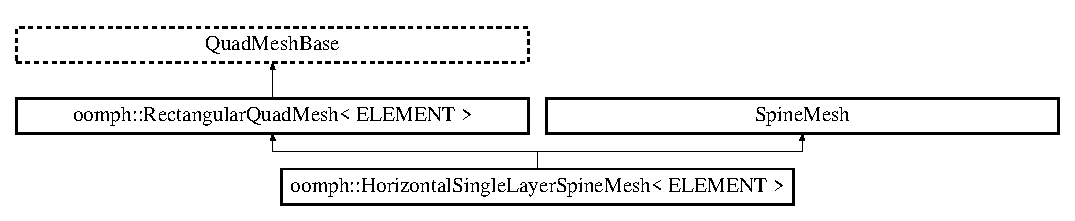
\includegraphics[height=3.363364cm]{classoomph_1_1HorizontalSingleLayerSpineMesh}
\end{center}
\end{figure}
\subsection*{Public Member Functions}
\begin{DoxyCompactItemize}
\item 
\hyperlink{classoomph_1_1HorizontalSingleLayerSpineMesh_a765856597150d37a20eabdb53e58d49c}{Horizontal\+Single\+Layer\+Spine\+Mesh} (const unsigned \&\hyperlink{classoomph_1_1RectangularQuadMesh_abfef93d6322886cdce14a437186e4821}{nx}, const unsigned \&\hyperlink{classoomph_1_1RectangularQuadMesh_a86d76a55eb7c4e8bca9b74d23c8b0412}{ny}, const double \&lx, const double \&h, \hyperlink{classoomph_1_1TimeStepper}{Time\+Stepper} $\ast$time\+\_\+stepper\+\_\+pt=\&\hyperlink{classoomph_1_1Mesh_a12243d0fee2b1fcee729ee5a4777ea10}{Mesh\+::\+Default\+\_\+\+Time\+Stepper})
\begin{DoxyCompactList}\small\item\em Constructor\+: Pass number of elements in x-\/direction, number of elements in y-\/direction, axial length, height of layer, and pointer to timestepper (defaults to \hyperlink{classoomph_1_1Steady}{Steady} timestepper) \end{DoxyCompactList}\item 
virtual void \hyperlink{classoomph_1_1HorizontalSingleLayerSpineMesh_a4b9b833a281aa64a809b4e47159282e6}{spine\+\_\+node\+\_\+update} (\hyperlink{classoomph_1_1SpineNode}{Spine\+Node} $\ast$spine\+\_\+node\+\_\+pt)
\begin{DoxyCompactList}\small\item\em General node update function implements pure virtual function defined in \hyperlink{classoomph_1_1SpineMesh}{Spine\+Mesh} base class and performs specific node update actions\+: along vertical spines. \end{DoxyCompactList}\end{DoxyCompactItemize}
\subsection*{Protected Member Functions}
\begin{DoxyCompactItemize}
\item 
virtual void \hyperlink{classoomph_1_1HorizontalSingleLayerSpineMesh_a9bd06cd24d2c48c499bf149b1773b442}{build\+\_\+horizontal\+\_\+single\+\_\+layer\+\_\+mesh} (\hyperlink{classoomph_1_1TimeStepper}{Time\+Stepper} $\ast$time\+\_\+stepper\+\_\+pt)
\begin{DoxyCompactList}\small\item\em Helper function to actually build the single-\/layer spine mesh (called from various constructors) \end{DoxyCompactList}\end{DoxyCompactItemize}
\subsection*{Additional Inherited Members}


\subsection{Detailed Description}
\subsubsection*{template$<$class E\+L\+E\+M\+E\+NT$>$\newline
class oomph\+::\+Horizontal\+Single\+Layer\+Spine\+Mesh$<$ E\+L\+E\+M\+E\+N\+T $>$}

Horizontal Single-\/layer spine mesh class derived from standard 2D mesh. The mesh contains a layer of spinified fluid elements (of type E\+L\+E\+M\+E\+NT; e.\+g \hyperlink{classoomph_1_1SpineElement}{Spine\+Element}$<$Q\+Crouzeix\+Raviart\+Element$<$2$>$) and the information required to update their position. Additional equations must be specified in order to determine how the spines move. 

Definition at line 50 of file horizontal\+\_\+single\+\_\+layer\+\_\+spine\+\_\+mesh.\+template.\+h.



\subsection{Constructor \& Destructor Documentation}
\mbox{\Hypertarget{classoomph_1_1HorizontalSingleLayerSpineMesh_a765856597150d37a20eabdb53e58d49c}\label{classoomph_1_1HorizontalSingleLayerSpineMesh_a765856597150d37a20eabdb53e58d49c}} 
\index{oomph\+::\+Horizontal\+Single\+Layer\+Spine\+Mesh@{oomph\+::\+Horizontal\+Single\+Layer\+Spine\+Mesh}!Horizontal\+Single\+Layer\+Spine\+Mesh@{Horizontal\+Single\+Layer\+Spine\+Mesh}}
\index{Horizontal\+Single\+Layer\+Spine\+Mesh@{Horizontal\+Single\+Layer\+Spine\+Mesh}!oomph\+::\+Horizontal\+Single\+Layer\+Spine\+Mesh@{oomph\+::\+Horizontal\+Single\+Layer\+Spine\+Mesh}}
\subsubsection{\texorpdfstring{Horizontal\+Single\+Layer\+Spine\+Mesh()}{HorizontalSingleLayerSpineMesh()}}
{\footnotesize\ttfamily template$<$class E\+L\+E\+M\+E\+NT $>$ \\
\hyperlink{classoomph_1_1HorizontalSingleLayerSpineMesh}{oomph\+::\+Horizontal\+Single\+Layer\+Spine\+Mesh}$<$ E\+L\+E\+M\+E\+NT $>$\+::\hyperlink{classoomph_1_1HorizontalSingleLayerSpineMesh}{Horizontal\+Single\+Layer\+Spine\+Mesh} (\begin{DoxyParamCaption}\item[{const unsigned \&}]{nx,  }\item[{const unsigned \&}]{ny,  }\item[{const double \&}]{lx,  }\item[{const double \&}]{h,  }\item[{\hyperlink{classoomph_1_1TimeStepper}{Time\+Stepper} $\ast$}]{time\+\_\+stepper\+\_\+pt = {\ttfamily \&\hyperlink{classoomph_1_1Mesh_a12243d0fee2b1fcee729ee5a4777ea10}{Mesh\+::\+Default\+\_\+\+Time\+Stepper}} }\end{DoxyParamCaption})}



Constructor\+: Pass number of elements in x-\/direction, number of elements in y-\/direction, axial length, height of layer, and pointer to timestepper (defaults to \hyperlink{classoomph_1_1Steady}{Steady} timestepper) 

Constructor for spine 2D mesh\+: Pass number of elements in x-\/direction, number of elements in y-\/direction, axial length and height of layer, and pointer to timestepper (defaults to Static timestepper).

The mesh contains a layer of spinified fluid elements (of type E\+L\+E\+M\+E\+NT; e.\+g \hyperlink{classoomph_1_1SpineElement}{Spine\+Element}$<$Q\+Crouzeix\+Raviart\+Element$<$2$>$) and information about how the internal nodes positions are affected by changes in spine length. Additional equations that determine the spine heights must be specified in order to use this mesh. 

Definition at line 53 of file horizontal\+\_\+single\+\_\+layer\+\_\+spine\+\_\+mesh.\+template.\+cc.



References oomph\+::\+Horizontal\+Single\+Layer\+Spine\+Mesh$<$ E\+L\+E\+M\+E\+N\+T $>$\+::build\+\_\+horizontal\+\_\+single\+\_\+layer\+\_\+mesh().



\subsection{Member Function Documentation}
\mbox{\Hypertarget{classoomph_1_1HorizontalSingleLayerSpineMesh_a9bd06cd24d2c48c499bf149b1773b442}\label{classoomph_1_1HorizontalSingleLayerSpineMesh_a9bd06cd24d2c48c499bf149b1773b442}} 
\index{oomph\+::\+Horizontal\+Single\+Layer\+Spine\+Mesh@{oomph\+::\+Horizontal\+Single\+Layer\+Spine\+Mesh}!build\+\_\+horizontal\+\_\+single\+\_\+layer\+\_\+mesh@{build\+\_\+horizontal\+\_\+single\+\_\+layer\+\_\+mesh}}
\index{build\+\_\+horizontal\+\_\+single\+\_\+layer\+\_\+mesh@{build\+\_\+horizontal\+\_\+single\+\_\+layer\+\_\+mesh}!oomph\+::\+Horizontal\+Single\+Layer\+Spine\+Mesh@{oomph\+::\+Horizontal\+Single\+Layer\+Spine\+Mesh}}
\subsubsection{\texorpdfstring{build\+\_\+horizontal\+\_\+single\+\_\+layer\+\_\+mesh()}{build\_horizontal\_single\_layer\_mesh()}}
{\footnotesize\ttfamily template$<$class E\+L\+E\+M\+E\+NT $>$ \\
void \hyperlink{classoomph_1_1HorizontalSingleLayerSpineMesh}{oomph\+::\+Horizontal\+Single\+Layer\+Spine\+Mesh}$<$ E\+L\+E\+M\+E\+NT $>$\+::build\+\_\+horizontal\+\_\+single\+\_\+layer\+\_\+mesh (\begin{DoxyParamCaption}\item[{\hyperlink{classoomph_1_1TimeStepper}{Time\+Stepper} $\ast$}]{time\+\_\+stepper\+\_\+pt }\end{DoxyParamCaption})\hspace{0.3cm}{\ttfamily [protected]}, {\ttfamily [virtual]}}



Helper function to actually build the single-\/layer spine mesh (called from various constructors) 

Helper function that actually builds the single-\/layer spine mesh based on the parameters set in the various constructors 

Definition at line 78 of file horizontal\+\_\+single\+\_\+layer\+\_\+spine\+\_\+mesh.\+template.\+cc.



References oomph\+::\+Rectangular\+Quad\+Mesh$<$ E\+L\+E\+M\+E\+N\+T $>$\+::build\+\_\+mesh(), oomph\+::\+Spine\+Mesh\+::element\+\_\+node\+\_\+pt(), oomph\+::\+Mesh\+::finite\+\_\+element\+\_\+pt(), oomph\+::\+Spine\+Node\+::fraction(), i, oomph\+::\+Rectangular\+Quad\+Mesh$<$ E\+L\+E\+M\+E\+N\+T $>$\+::\+Nx, oomph\+::\+Rectangular\+Quad\+Mesh$<$ E\+L\+E\+M\+E\+N\+T $>$\+::\+Ny, oomph\+::\+Spine\+Node\+::spine\+\_\+mesh\+\_\+pt(), oomph\+::\+Spine\+Node\+::spine\+\_\+pt(), and oomph\+::\+Spine\+Mesh\+::\+Spine\+\_\+pt.



Referenced by oomph\+::\+Horizontal\+Single\+Layer\+Spine\+Mesh$<$ E\+L\+E\+M\+E\+N\+T $>$\+::\+Horizontal\+Single\+Layer\+Spine\+Mesh(), and oomph\+::\+Horizontal\+Single\+Layer\+Spine\+Mesh$<$ E\+L\+E\+M\+E\+N\+T $>$\+::spine\+\_\+node\+\_\+update().

\mbox{\Hypertarget{classoomph_1_1HorizontalSingleLayerSpineMesh_a4b9b833a281aa64a809b4e47159282e6}\label{classoomph_1_1HorizontalSingleLayerSpineMesh_a4b9b833a281aa64a809b4e47159282e6}} 
\index{oomph\+::\+Horizontal\+Single\+Layer\+Spine\+Mesh@{oomph\+::\+Horizontal\+Single\+Layer\+Spine\+Mesh}!spine\+\_\+node\+\_\+update@{spine\+\_\+node\+\_\+update}}
\index{spine\+\_\+node\+\_\+update@{spine\+\_\+node\+\_\+update}!oomph\+::\+Horizontal\+Single\+Layer\+Spine\+Mesh@{oomph\+::\+Horizontal\+Single\+Layer\+Spine\+Mesh}}
\subsubsection{\texorpdfstring{spine\+\_\+node\+\_\+update()}{spine\_node\_update()}}
{\footnotesize\ttfamily template$<$class E\+L\+E\+M\+E\+NT $>$ \\
virtual void \hyperlink{classoomph_1_1HorizontalSingleLayerSpineMesh}{oomph\+::\+Horizontal\+Single\+Layer\+Spine\+Mesh}$<$ E\+L\+E\+M\+E\+NT $>$\+::spine\+\_\+node\+\_\+update (\begin{DoxyParamCaption}\item[{\hyperlink{classoomph_1_1SpineNode}{Spine\+Node} $\ast$}]{spine\+\_\+node\+\_\+pt }\end{DoxyParamCaption})\hspace{0.3cm}{\ttfamily [inline]}, {\ttfamily [virtual]}}



General node update function implements pure virtual function defined in \hyperlink{classoomph_1_1SpineMesh}{Spine\+Mesh} base class and performs specific node update actions\+: along vertical spines. 



Implements \hyperlink{classoomph_1_1SpineMesh_aa7843aadce3c540f34442671f59eb75b}{oomph\+::\+Spine\+Mesh}.



Definition at line 70 of file horizontal\+\_\+single\+\_\+layer\+\_\+spine\+\_\+mesh.\+template.\+h.



References oomph\+::\+Horizontal\+Single\+Layer\+Spine\+Mesh$<$ E\+L\+E\+M\+E\+N\+T $>$\+::build\+\_\+horizontal\+\_\+single\+\_\+layer\+\_\+mesh(), oomph\+::\+Spine\+Node\+::fraction(), oomph\+::\+Spine\+Node\+::h(), oomph\+::\+Quad\+Tree\+Names\+::W, and oomph\+::\+Node\+::x().



The documentation for this class was generated from the following files\+:\begin{DoxyCompactItemize}
\item 
\hyperlink{horizontal__single__layer__spine__mesh_8template_8h}{horizontal\+\_\+single\+\_\+layer\+\_\+spine\+\_\+mesh.\+template.\+h}\item 
\hyperlink{horizontal__single__layer__spine__mesh_8template_8cc}{horizontal\+\_\+single\+\_\+layer\+\_\+spine\+\_\+mesh.\+template.\+cc}\end{DoxyCompactItemize}

\hypertarget{classoomph_1_1MacroElementNodeUpdateChannelWithLeafletMesh}{}\section{oomph\+:\+:Macro\+Element\+Node\+Update\+Channel\+With\+Leaflet\+Mesh$<$ E\+L\+E\+M\+E\+NT $>$ Class Template Reference}
\label{classoomph_1_1MacroElementNodeUpdateChannelWithLeafletMesh}\index{oomph\+::\+Macro\+Element\+Node\+Update\+Channel\+With\+Leaflet\+Mesh$<$ E\+L\+E\+M\+E\+N\+T $>$@{oomph\+::\+Macro\+Element\+Node\+Update\+Channel\+With\+Leaflet\+Mesh$<$ E\+L\+E\+M\+E\+N\+T $>$}}


{\ttfamily \#include $<$channel\+\_\+with\+\_\+leaflet\+\_\+mesh.\+template.\+h$>$}

Inheritance diagram for oomph\+:\+:Macro\+Element\+Node\+Update\+Channel\+With\+Leaflet\+Mesh$<$ E\+L\+E\+M\+E\+NT $>$\+:\begin{figure}[H]
\begin{center}
\leavevmode
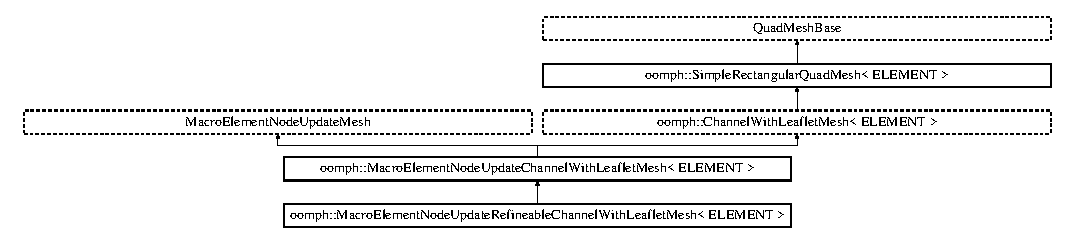
\includegraphics[height=3.393939cm]{classoomph_1_1MacroElementNodeUpdateChannelWithLeafletMesh}
\end{center}
\end{figure}
\subsection*{Public Member Functions}
\begin{DoxyCompactItemize}
\item 
\hyperlink{classoomph_1_1MacroElementNodeUpdateChannelWithLeafletMesh_a8b2ddfc283a8f1ff6927c7a0c7f0ed21}{Macro\+Element\+Node\+Update\+Channel\+With\+Leaflet\+Mesh} (\hyperlink{classoomph_1_1GeomObject}{Geom\+Object} $\ast$leaflet\+\_\+pt, const double \&lleft, const double \&lright, const double \&hleaflet, const double \&htot, const unsigned \&nleft, const unsigned \&nright, const unsigned \&ny1, const unsigned \&ny2, \hyperlink{classoomph_1_1TimeStepper}{Time\+Stepper} $\ast$time\+\_\+stepper\+\_\+pt=\&\hyperlink{classoomph_1_1Mesh_a12243d0fee2b1fcee729ee5a4777ea10}{Mesh\+::\+Default\+\_\+\+Time\+Stepper})
\begin{DoxyCompactList}\small\item\em Constructor\+: Pass pointer to \hyperlink{classoomph_1_1GeomObject}{Geom\+Object} that represents the leaflet, the length of the domain to left and right of the leaflet, the height of the leaflet and the overall height of the channel, the number of element columns to the left and right of the leaflet, the number of rows of elements from the bottom of the channel to the end of the leaflet, the number of rows of elements above the end of the leaflet. Timestepper defaults to \hyperlink{classoomph_1_1Steady}{Steady} default Timestepper defined in the \hyperlink{classoomph_1_1Mesh}{Mesh} base class. \end{DoxyCompactList}\item 
virtual \hyperlink{classoomph_1_1MacroElementNodeUpdateChannelWithLeafletMesh_a5debbfa68133a5ad9bd621b24b2fd086}{$\sim$\+Macro\+Element\+Node\+Update\+Channel\+With\+Leaflet\+Mesh} ()
\begin{DoxyCompactList}\small\item\em Destructor\+: empty. \end{DoxyCompactList}\end{DoxyCompactItemize}
\subsection*{Additional Inherited Members}


\subsection{Detailed Description}
\subsubsection*{template$<$class E\+L\+E\+M\+E\+NT$>$\newline
class oomph\+::\+Macro\+Element\+Node\+Update\+Channel\+With\+Leaflet\+Mesh$<$ E\+L\+E\+M\+E\+N\+T $>$}

Channel with leaflet mesh with Macro\+Element-\/based node update. The leaflet is represented by the specified geometric object. Some or all of the geometric \hyperlink{classoomph_1_1Data}{Data} in that geometric object may contain unknowns in the global \hyperlink{classoomph_1_1Problem}{Problem}. The dependency on these unknowns is taken into account when setting up the Jacobian matrix of the elements. For this purpose, the element (whose type is specified by the template parameter) must inherit from \hyperlink{classoomph_1_1MacroElementNodeUpdateElementBase}{Macro\+Element\+Node\+Update\+Element\+Base}. 

Definition at line 159 of file channel\+\_\+with\+\_\+leaflet\+\_\+mesh.\+template.\+h.



\subsection{Constructor \& Destructor Documentation}
\mbox{\Hypertarget{classoomph_1_1MacroElementNodeUpdateChannelWithLeafletMesh_a8b2ddfc283a8f1ff6927c7a0c7f0ed21}\label{classoomph_1_1MacroElementNodeUpdateChannelWithLeafletMesh_a8b2ddfc283a8f1ff6927c7a0c7f0ed21}} 
\index{oomph\+::\+Macro\+Element\+Node\+Update\+Channel\+With\+Leaflet\+Mesh@{oomph\+::\+Macro\+Element\+Node\+Update\+Channel\+With\+Leaflet\+Mesh}!Macro\+Element\+Node\+Update\+Channel\+With\+Leaflet\+Mesh@{Macro\+Element\+Node\+Update\+Channel\+With\+Leaflet\+Mesh}}
\index{Macro\+Element\+Node\+Update\+Channel\+With\+Leaflet\+Mesh@{Macro\+Element\+Node\+Update\+Channel\+With\+Leaflet\+Mesh}!oomph\+::\+Macro\+Element\+Node\+Update\+Channel\+With\+Leaflet\+Mesh@{oomph\+::\+Macro\+Element\+Node\+Update\+Channel\+With\+Leaflet\+Mesh}}
\subsubsection{\texorpdfstring{Macro\+Element\+Node\+Update\+Channel\+With\+Leaflet\+Mesh()}{MacroElementNodeUpdateChannelWithLeafletMesh()}}
{\footnotesize\ttfamily template$<$class E\+L\+E\+M\+E\+NT $>$ \\
\hyperlink{classoomph_1_1MacroElementNodeUpdateChannelWithLeafletMesh}{oomph\+::\+Macro\+Element\+Node\+Update\+Channel\+With\+Leaflet\+Mesh}$<$ E\+L\+E\+M\+E\+NT $>$\+::\hyperlink{classoomph_1_1MacroElementNodeUpdateChannelWithLeafletMesh}{Macro\+Element\+Node\+Update\+Channel\+With\+Leaflet\+Mesh} (\begin{DoxyParamCaption}\item[{\hyperlink{classoomph_1_1GeomObject}{Geom\+Object} $\ast$}]{leaflet\+\_\+pt,  }\item[{const double \&}]{lleft,  }\item[{const double \&}]{lright,  }\item[{const double \&}]{hleaflet,  }\item[{const double \&}]{htot,  }\item[{const unsigned \&}]{nleft,  }\item[{const unsigned \&}]{nright,  }\item[{const unsigned \&}]{ny1,  }\item[{const unsigned \&}]{ny2,  }\item[{\hyperlink{classoomph_1_1TimeStepper}{Time\+Stepper} $\ast$}]{time\+\_\+stepper\+\_\+pt = {\ttfamily \&\hyperlink{classoomph_1_1Mesh_a12243d0fee2b1fcee729ee5a4777ea10}{Mesh\+::\+Default\+\_\+\+Time\+Stepper}} }\end{DoxyParamCaption})\hspace{0.3cm}{\ttfamily [inline]}}



Constructor\+: Pass pointer to \hyperlink{classoomph_1_1GeomObject}{Geom\+Object} that represents the leaflet, the length of the domain to left and right of the leaflet, the height of the leaflet and the overall height of the channel, the number of element columns to the left and right of the leaflet, the number of rows of elements from the bottom of the channel to the end of the leaflet, the number of rows of elements above the end of the leaflet. Timestepper defaults to \hyperlink{classoomph_1_1Steady}{Steady} default Timestepper defined in the \hyperlink{classoomph_1_1Mesh}{Mesh} base class. 



Definition at line 174 of file channel\+\_\+with\+\_\+leaflet\+\_\+mesh.\+template.\+h.



References oomph\+::\+Channel\+With\+Leaflet\+Mesh$<$ E\+L\+E\+M\+E\+N\+T $>$\+::domain\+\_\+pt(), oomph\+::\+Mesh\+::element\+\_\+pt(), i, oomph\+::\+Channel\+With\+Leaflet\+Mesh$<$ E\+L\+E\+M\+E\+N\+T $>$\+::\+Leaflet\+\_\+pt, oomph\+::\+Macro\+Element\+Node\+Update\+Mesh\+::macro\+\_\+domain\+\_\+pt(), oomph\+::\+Mesh\+::nelement(), oomph\+::\+Macro\+Element\+Node\+Update\+Mesh\+::set\+\_\+geom\+\_\+object\+\_\+vector\+\_\+pt(), and oomph\+::\+Global\+\_\+string\+\_\+for\+\_\+annotation\+::string().

\mbox{\Hypertarget{classoomph_1_1MacroElementNodeUpdateChannelWithLeafletMesh_a5debbfa68133a5ad9bd621b24b2fd086}\label{classoomph_1_1MacroElementNodeUpdateChannelWithLeafletMesh_a5debbfa68133a5ad9bd621b24b2fd086}} 
\index{oomph\+::\+Macro\+Element\+Node\+Update\+Channel\+With\+Leaflet\+Mesh@{oomph\+::\+Macro\+Element\+Node\+Update\+Channel\+With\+Leaflet\+Mesh}!````~Macro\+Element\+Node\+Update\+Channel\+With\+Leaflet\+Mesh@{$\sim$\+Macro\+Element\+Node\+Update\+Channel\+With\+Leaflet\+Mesh}}
\index{````~Macro\+Element\+Node\+Update\+Channel\+With\+Leaflet\+Mesh@{$\sim$\+Macro\+Element\+Node\+Update\+Channel\+With\+Leaflet\+Mesh}!oomph\+::\+Macro\+Element\+Node\+Update\+Channel\+With\+Leaflet\+Mesh@{oomph\+::\+Macro\+Element\+Node\+Update\+Channel\+With\+Leaflet\+Mesh}}
\subsubsection{\texorpdfstring{$\sim$\+Macro\+Element\+Node\+Update\+Channel\+With\+Leaflet\+Mesh()}{~MacroElementNodeUpdateChannelWithLeafletMesh()}}
{\footnotesize\ttfamily template$<$class E\+L\+E\+M\+E\+NT $>$ \\
virtual \hyperlink{classoomph_1_1MacroElementNodeUpdateChannelWithLeafletMesh}{oomph\+::\+Macro\+Element\+Node\+Update\+Channel\+With\+Leaflet\+Mesh}$<$ E\+L\+E\+M\+E\+NT $>$\+::$\sim$\hyperlink{classoomph_1_1MacroElementNodeUpdateChannelWithLeafletMesh}{Macro\+Element\+Node\+Update\+Channel\+With\+Leaflet\+Mesh} (\begin{DoxyParamCaption}{ }\end{DoxyParamCaption})\hspace{0.3cm}{\ttfamily [inline]}, {\ttfamily [virtual]}}



Destructor\+: empty. 



Definition at line 264 of file channel\+\_\+with\+\_\+leaflet\+\_\+mesh.\+template.\+h.



The documentation for this class was generated from the following file\+:\begin{DoxyCompactItemize}
\item 
\hyperlink{channel__with__leaflet__mesh_8template_8h}{channel\+\_\+with\+\_\+leaflet\+\_\+mesh.\+template.\+h}\end{DoxyCompactItemize}

\hypertarget{classoomph_1_1MacroElementNodeUpdateCollapsibleChannelMesh}{}\section{oomph\+:\+:Macro\+Element\+Node\+Update\+Collapsible\+Channel\+Mesh$<$ E\+L\+E\+M\+E\+NT $>$ Class Template Reference}
\label{classoomph_1_1MacroElementNodeUpdateCollapsibleChannelMesh}\index{oomph\+::\+Macro\+Element\+Node\+Update\+Collapsible\+Channel\+Mesh$<$ E\+L\+E\+M\+E\+N\+T $>$@{oomph\+::\+Macro\+Element\+Node\+Update\+Collapsible\+Channel\+Mesh$<$ E\+L\+E\+M\+E\+N\+T $>$}}


{\ttfamily \#include $<$collapsible\+\_\+channel\+\_\+mesh.\+template.\+h$>$}

Inheritance diagram for oomph\+:\+:Macro\+Element\+Node\+Update\+Collapsible\+Channel\+Mesh$<$ E\+L\+E\+M\+E\+NT $>$\+:\begin{figure}[H]
\begin{center}
\leavevmode
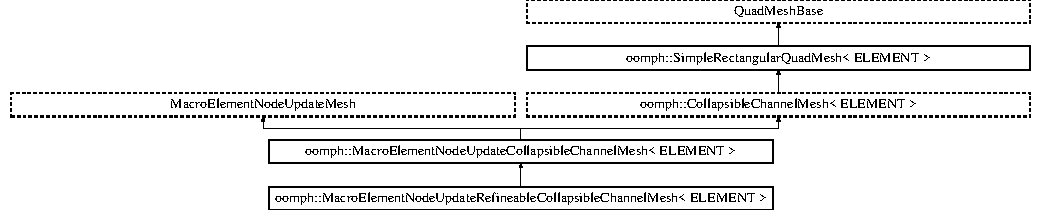
\includegraphics[height=2.828283cm]{classoomph_1_1MacroElementNodeUpdateCollapsibleChannelMesh}
\end{center}
\end{figure}
\subsection*{Public Member Functions}
\begin{DoxyCompactItemize}
\item 
\hyperlink{classoomph_1_1MacroElementNodeUpdateCollapsibleChannelMesh_a5b7f150c4569c8d59d8220980a84cac5}{Macro\+Element\+Node\+Update\+Collapsible\+Channel\+Mesh} (const unsigned \&nup, const unsigned \&ncollapsible, const unsigned \&ndown, const unsigned \&\hyperlink{classoomph_1_1SimpleRectangularQuadMesh_a45011f22dedd480392b1f376e4269921}{ny}, const double \&lup, const double \&lcollapsible, const double \&ldown, const double \&ly, Geom\+Object $\ast$\hyperlink{classoomph_1_1CollapsibleChannelMesh_a04ffeb61678763dfd250962ea9ba614b}{wall\+\_\+pt}, Time\+Stepper $\ast$time\+\_\+stepper\+\_\+pt=\&Mesh\+::\+Default\+\_\+\+Time\+Stepper)
\begin{DoxyCompactList}\small\item\em Constructor\+: Pass numbers of elements and dimensions of the various parts of the collapsible channel, pointer to geometric object that represents the wall and pointer to timestepper (defaults to Steady). \end{DoxyCompactList}\item 
virtual \hyperlink{classoomph_1_1MacroElementNodeUpdateCollapsibleChannelMesh_a284ffdb8ab08e5f817b14d69913f4496}{$\sim$\+Macro\+Element\+Node\+Update\+Collapsible\+Channel\+Mesh} ()
\begin{DoxyCompactList}\small\item\em Destructor\+: empty. \end{DoxyCompactList}\end{DoxyCompactItemize}
\subsection*{Additional Inherited Members}


\subsection{Detailed Description}
\subsubsection*{template$<$class E\+L\+E\+M\+E\+NT$>$\newline
class oomph\+::\+Macro\+Element\+Node\+Update\+Collapsible\+Channel\+Mesh$<$ E\+L\+E\+M\+E\+N\+T $>$}

Collapsible channel mesh with Macro\+Element-\/based node update. The collapsible segment is represented by the specified geometric object. Some or all of the geometric Data in that geometric object may contain unknowns in the global Problem. The dependency on these unknowns is taken into account when setting up the Jacobian matrix of the elements. For this purpose, the element (whose type is specified by the template parameter) must inherit from Macro\+Element\+Node\+Update\+Element\+Base. 

Definition at line 243 of file collapsible\+\_\+channel\+\_\+mesh.\+template.\+h.



\subsection{Constructor \& Destructor Documentation}
\mbox{\Hypertarget{classoomph_1_1MacroElementNodeUpdateCollapsibleChannelMesh_a5b7f150c4569c8d59d8220980a84cac5}\label{classoomph_1_1MacroElementNodeUpdateCollapsibleChannelMesh_a5b7f150c4569c8d59d8220980a84cac5}} 
\index{oomph\+::\+Macro\+Element\+Node\+Update\+Collapsible\+Channel\+Mesh@{oomph\+::\+Macro\+Element\+Node\+Update\+Collapsible\+Channel\+Mesh}!Macro\+Element\+Node\+Update\+Collapsible\+Channel\+Mesh@{Macro\+Element\+Node\+Update\+Collapsible\+Channel\+Mesh}}
\index{Macro\+Element\+Node\+Update\+Collapsible\+Channel\+Mesh@{Macro\+Element\+Node\+Update\+Collapsible\+Channel\+Mesh}!oomph\+::\+Macro\+Element\+Node\+Update\+Collapsible\+Channel\+Mesh@{oomph\+::\+Macro\+Element\+Node\+Update\+Collapsible\+Channel\+Mesh}}
\subsubsection{\texorpdfstring{Macro\+Element\+Node\+Update\+Collapsible\+Channel\+Mesh()}{MacroElementNodeUpdateCollapsibleChannelMesh()}}
{\footnotesize\ttfamily template$<$class E\+L\+E\+M\+E\+NT $>$ \\
\hyperlink{classoomph_1_1MacroElementNodeUpdateCollapsibleChannelMesh}{oomph\+::\+Macro\+Element\+Node\+Update\+Collapsible\+Channel\+Mesh}$<$ E\+L\+E\+M\+E\+NT $>$\+::\hyperlink{classoomph_1_1MacroElementNodeUpdateCollapsibleChannelMesh}{Macro\+Element\+Node\+Update\+Collapsible\+Channel\+Mesh} (\begin{DoxyParamCaption}\item[{const unsigned \&}]{nup,  }\item[{const unsigned \&}]{ncollapsible,  }\item[{const unsigned \&}]{ndown,  }\item[{const unsigned \&}]{ny,  }\item[{const double \&}]{lup,  }\item[{const double \&}]{lcollapsible,  }\item[{const double \&}]{ldown,  }\item[{const double \&}]{ly,  }\item[{Geom\+Object $\ast$}]{wall\+\_\+pt,  }\item[{Time\+Stepper $\ast$}]{time\+\_\+stepper\+\_\+pt = {\ttfamily \&Mesh\+:\+:Default\+\_\+TimeStepper} }\end{DoxyParamCaption})\hspace{0.3cm}{\ttfamily [inline]}}



Constructor\+: Pass numbers of elements and dimensions of the various parts of the collapsible channel, pointer to geometric object that represents the wall and pointer to timestepper (defaults to Steady). 



Definition at line 254 of file collapsible\+\_\+channel\+\_\+mesh.\+template.\+h.



References oomph\+::\+Collapsible\+Channel\+Mesh$<$ E\+L\+E\+M\+E\+N\+T $>$\+::domain\+\_\+pt(), and oomph\+::\+Collapsible\+Channel\+Mesh$<$ E\+L\+E\+M\+E\+N\+T $>$\+::\+Wall\+\_\+pt.

\mbox{\Hypertarget{classoomph_1_1MacroElementNodeUpdateCollapsibleChannelMesh_a284ffdb8ab08e5f817b14d69913f4496}\label{classoomph_1_1MacroElementNodeUpdateCollapsibleChannelMesh_a284ffdb8ab08e5f817b14d69913f4496}} 
\index{oomph\+::\+Macro\+Element\+Node\+Update\+Collapsible\+Channel\+Mesh@{oomph\+::\+Macro\+Element\+Node\+Update\+Collapsible\+Channel\+Mesh}!````~Macro\+Element\+Node\+Update\+Collapsible\+Channel\+Mesh@{$\sim$\+Macro\+Element\+Node\+Update\+Collapsible\+Channel\+Mesh}}
\index{````~Macro\+Element\+Node\+Update\+Collapsible\+Channel\+Mesh@{$\sim$\+Macro\+Element\+Node\+Update\+Collapsible\+Channel\+Mesh}!oomph\+::\+Macro\+Element\+Node\+Update\+Collapsible\+Channel\+Mesh@{oomph\+::\+Macro\+Element\+Node\+Update\+Collapsible\+Channel\+Mesh}}
\subsubsection{\texorpdfstring{$\sim$\+Macro\+Element\+Node\+Update\+Collapsible\+Channel\+Mesh()}{~MacroElementNodeUpdateCollapsibleChannelMesh()}}
{\footnotesize\ttfamily template$<$class E\+L\+E\+M\+E\+NT $>$ \\
virtual \hyperlink{classoomph_1_1MacroElementNodeUpdateCollapsibleChannelMesh}{oomph\+::\+Macro\+Element\+Node\+Update\+Collapsible\+Channel\+Mesh}$<$ E\+L\+E\+M\+E\+NT $>$\+::$\sim$\hyperlink{classoomph_1_1MacroElementNodeUpdateCollapsibleChannelMesh}{Macro\+Element\+Node\+Update\+Collapsible\+Channel\+Mesh} (\begin{DoxyParamCaption}{ }\end{DoxyParamCaption})\hspace{0.3cm}{\ttfamily [inline]}, {\ttfamily [virtual]}}



Destructor\+: empty. 



Definition at line 352 of file collapsible\+\_\+channel\+\_\+mesh.\+template.\+h.



The documentation for this class was generated from the following file\+:\begin{DoxyCompactItemize}
\item 
\hyperlink{collapsible__channel__mesh_8template_8h}{collapsible\+\_\+channel\+\_\+mesh.\+template.\+h}\end{DoxyCompactItemize}

\hypertarget{classoomph_1_1MacroElementNodeUpdateRefineableChannelWithLeafletMesh}{}\section{oomph\+:\+:Macro\+Element\+Node\+Update\+Refineable\+Channel\+With\+Leaflet\+Mesh$<$ E\+L\+E\+M\+E\+NT $>$ Class Template Reference}
\label{classoomph_1_1MacroElementNodeUpdateRefineableChannelWithLeafletMesh}\index{oomph\+::\+Macro\+Element\+Node\+Update\+Refineable\+Channel\+With\+Leaflet\+Mesh$<$ E\+L\+E\+M\+E\+N\+T $>$@{oomph\+::\+Macro\+Element\+Node\+Update\+Refineable\+Channel\+With\+Leaflet\+Mesh$<$ E\+L\+E\+M\+E\+N\+T $>$}}


Refineable mesh with Macro\+Element-\/based node update.  




{\ttfamily \#include $<$channel\+\_\+with\+\_\+leaflet\+\_\+mesh.\+template.\+h$>$}

Inheritance diagram for oomph\+:\+:Macro\+Element\+Node\+Update\+Refineable\+Channel\+With\+Leaflet\+Mesh$<$ E\+L\+E\+M\+E\+NT $>$\+:\begin{figure}[H]
\begin{center}
\leavevmode
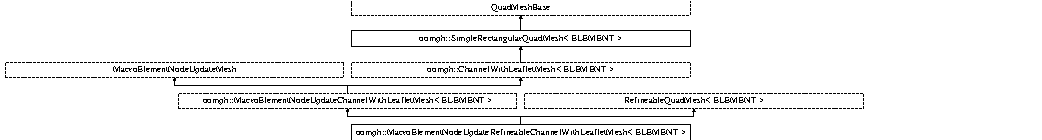
\includegraphics[height=1.696970cm]{classoomph_1_1MacroElementNodeUpdateRefineableChannelWithLeafletMesh}
\end{center}
\end{figure}
\subsection*{Public Member Functions}
\begin{DoxyCompactItemize}
\item 
\hyperlink{classoomph_1_1MacroElementNodeUpdateRefineableChannelWithLeafletMesh_aa15c165d7e755e4e885d895e16bb76b8}{Macro\+Element\+Node\+Update\+Refineable\+Channel\+With\+Leaflet\+Mesh} (\hyperlink{classoomph_1_1GeomObject}{Geom\+Object} $\ast$leaflet\+\_\+pt, const double \&lleft, const double \&lright, const double \&hleaflet, const double \&htot, const unsigned \&nleft, const unsigned \&nright, const unsigned \&ny1, const unsigned \&ny2, \hyperlink{classoomph_1_1TimeStepper}{Time\+Stepper} $\ast$time\+\_\+stepper\+\_\+pt=\&\hyperlink{classoomph_1_1Mesh_a12243d0fee2b1fcee729ee5a4777ea10}{Mesh\+::\+Default\+\_\+\+Time\+Stepper})
\begin{DoxyCompactList}\small\item\em Constructor\+: Pass pointer to \hyperlink{classoomph_1_1GeomObject}{Geom\+Object} that represents the leaflet, the length of the domain to left and right of the leaflet, the height of the leaflet and the overall height of the channel, the number of element columns to the left and right of the leaflet, the number of rows of elements from the bottom of the channel to the end of the leaflet, the number of rows of elements above the end of the leaflet. Timestepper defaults to \hyperlink{classoomph_1_1Steady}{Steady} default Timestepper defined in the \hyperlink{classoomph_1_1Mesh}{Mesh} base class. \end{DoxyCompactList}\item 
virtual \hyperlink{classoomph_1_1MacroElementNodeUpdateRefineableChannelWithLeafletMesh_af22b4288c7db553beb8658c29eb2cdaf}{$\sim$\+Macro\+Element\+Node\+Update\+Refineable\+Channel\+With\+Leaflet\+Mesh} ()
\begin{DoxyCompactList}\small\item\em Destructor\+: empty. \end{DoxyCompactList}\end{DoxyCompactItemize}
\subsection*{Additional Inherited Members}


\subsection{Detailed Description}
\subsubsection*{template$<$class E\+L\+E\+M\+E\+NT$>$\newline
class oomph\+::\+Macro\+Element\+Node\+Update\+Refineable\+Channel\+With\+Leaflet\+Mesh$<$ E\+L\+E\+M\+E\+N\+T $>$}

Refineable mesh with Macro\+Element-\/based node update. 

Definition at line 281 of file channel\+\_\+with\+\_\+leaflet\+\_\+mesh.\+template.\+h.



\subsection{Constructor \& Destructor Documentation}
\mbox{\Hypertarget{classoomph_1_1MacroElementNodeUpdateRefineableChannelWithLeafletMesh_aa15c165d7e755e4e885d895e16bb76b8}\label{classoomph_1_1MacroElementNodeUpdateRefineableChannelWithLeafletMesh_aa15c165d7e755e4e885d895e16bb76b8}} 
\index{oomph\+::\+Macro\+Element\+Node\+Update\+Refineable\+Channel\+With\+Leaflet\+Mesh@{oomph\+::\+Macro\+Element\+Node\+Update\+Refineable\+Channel\+With\+Leaflet\+Mesh}!Macro\+Element\+Node\+Update\+Refineable\+Channel\+With\+Leaflet\+Mesh@{Macro\+Element\+Node\+Update\+Refineable\+Channel\+With\+Leaflet\+Mesh}}
\index{Macro\+Element\+Node\+Update\+Refineable\+Channel\+With\+Leaflet\+Mesh@{Macro\+Element\+Node\+Update\+Refineable\+Channel\+With\+Leaflet\+Mesh}!oomph\+::\+Macro\+Element\+Node\+Update\+Refineable\+Channel\+With\+Leaflet\+Mesh@{oomph\+::\+Macro\+Element\+Node\+Update\+Refineable\+Channel\+With\+Leaflet\+Mesh}}
\subsubsection{\texorpdfstring{Macro\+Element\+Node\+Update\+Refineable\+Channel\+With\+Leaflet\+Mesh()}{MacroElementNodeUpdateRefineableChannelWithLeafletMesh()}}
{\footnotesize\ttfamily template$<$class E\+L\+E\+M\+E\+NT $>$ \\
\hyperlink{classoomph_1_1MacroElementNodeUpdateRefineableChannelWithLeafletMesh}{oomph\+::\+Macro\+Element\+Node\+Update\+Refineable\+Channel\+With\+Leaflet\+Mesh}$<$ E\+L\+E\+M\+E\+NT $>$\+::\hyperlink{classoomph_1_1MacroElementNodeUpdateRefineableChannelWithLeafletMesh}{Macro\+Element\+Node\+Update\+Refineable\+Channel\+With\+Leaflet\+Mesh} (\begin{DoxyParamCaption}\item[{\hyperlink{classoomph_1_1GeomObject}{Geom\+Object} $\ast$}]{leaflet\+\_\+pt,  }\item[{const double \&}]{lleft,  }\item[{const double \&}]{lright,  }\item[{const double \&}]{hleaflet,  }\item[{const double \&}]{htot,  }\item[{const unsigned \&}]{nleft,  }\item[{const unsigned \&}]{nright,  }\item[{const unsigned \&}]{ny1,  }\item[{const unsigned \&}]{ny2,  }\item[{\hyperlink{classoomph_1_1TimeStepper}{Time\+Stepper} $\ast$}]{time\+\_\+stepper\+\_\+pt = {\ttfamily \&\hyperlink{classoomph_1_1Mesh_a12243d0fee2b1fcee729ee5a4777ea10}{Mesh\+::\+Default\+\_\+\+Time\+Stepper}} }\end{DoxyParamCaption})\hspace{0.3cm}{\ttfamily [inline]}}



Constructor\+: Pass pointer to \hyperlink{classoomph_1_1GeomObject}{Geom\+Object} that represents the leaflet, the length of the domain to left and right of the leaflet, the height of the leaflet and the overall height of the channel, the number of element columns to the left and right of the leaflet, the number of rows of elements from the bottom of the channel to the end of the leaflet, the number of rows of elements above the end of the leaflet. Timestepper defaults to \hyperlink{classoomph_1_1Steady}{Steady} default Timestepper defined in the \hyperlink{classoomph_1_1Mesh}{Mesh} base class. 



Definition at line 296 of file channel\+\_\+with\+\_\+leaflet\+\_\+mesh.\+template.\+h.

\mbox{\Hypertarget{classoomph_1_1MacroElementNodeUpdateRefineableChannelWithLeafletMesh_af22b4288c7db553beb8658c29eb2cdaf}\label{classoomph_1_1MacroElementNodeUpdateRefineableChannelWithLeafletMesh_af22b4288c7db553beb8658c29eb2cdaf}} 
\index{oomph\+::\+Macro\+Element\+Node\+Update\+Refineable\+Channel\+With\+Leaflet\+Mesh@{oomph\+::\+Macro\+Element\+Node\+Update\+Refineable\+Channel\+With\+Leaflet\+Mesh}!````~Macro\+Element\+Node\+Update\+Refineable\+Channel\+With\+Leaflet\+Mesh@{$\sim$\+Macro\+Element\+Node\+Update\+Refineable\+Channel\+With\+Leaflet\+Mesh}}
\index{````~Macro\+Element\+Node\+Update\+Refineable\+Channel\+With\+Leaflet\+Mesh@{$\sim$\+Macro\+Element\+Node\+Update\+Refineable\+Channel\+With\+Leaflet\+Mesh}!oomph\+::\+Macro\+Element\+Node\+Update\+Refineable\+Channel\+With\+Leaflet\+Mesh@{oomph\+::\+Macro\+Element\+Node\+Update\+Refineable\+Channel\+With\+Leaflet\+Mesh}}
\subsubsection{\texorpdfstring{$\sim$\+Macro\+Element\+Node\+Update\+Refineable\+Channel\+With\+Leaflet\+Mesh()}{~MacroElementNodeUpdateRefineableChannelWithLeafletMesh()}}
{\footnotesize\ttfamily template$<$class E\+L\+E\+M\+E\+NT $>$ \\
virtual \hyperlink{classoomph_1_1MacroElementNodeUpdateRefineableChannelWithLeafletMesh}{oomph\+::\+Macro\+Element\+Node\+Update\+Refineable\+Channel\+With\+Leaflet\+Mesh}$<$ E\+L\+E\+M\+E\+NT $>$\+::$\sim$\hyperlink{classoomph_1_1MacroElementNodeUpdateRefineableChannelWithLeafletMesh}{Macro\+Element\+Node\+Update\+Refineable\+Channel\+With\+Leaflet\+Mesh} (\begin{DoxyParamCaption}{ }\end{DoxyParamCaption})\hspace{0.3cm}{\ttfamily [inline]}, {\ttfamily [virtual]}}



Destructor\+: empty. 



Definition at line 317 of file channel\+\_\+with\+\_\+leaflet\+\_\+mesh.\+template.\+h.



The documentation for this class was generated from the following file\+:\begin{DoxyCompactItemize}
\item 
\hyperlink{channel__with__leaflet__mesh_8template_8h}{channel\+\_\+with\+\_\+leaflet\+\_\+mesh.\+template.\+h}\end{DoxyCompactItemize}

\hypertarget{classoomph_1_1MacroElementNodeUpdateRefineableCollapsibleChannelMesh}{}\section{oomph\+:\+:Macro\+Element\+Node\+Update\+Refineable\+Collapsible\+Channel\+Mesh$<$ E\+L\+E\+M\+E\+NT $>$ Class Template Reference}
\label{classoomph_1_1MacroElementNodeUpdateRefineableCollapsibleChannelMesh}\index{oomph\+::\+Macro\+Element\+Node\+Update\+Refineable\+Collapsible\+Channel\+Mesh$<$ E\+L\+E\+M\+E\+N\+T $>$@{oomph\+::\+Macro\+Element\+Node\+Update\+Refineable\+Collapsible\+Channel\+Mesh$<$ E\+L\+E\+M\+E\+N\+T $>$}}


{\ttfamily \#include $<$collapsible\+\_\+channel\+\_\+mesh.\+template.\+h$>$}

Inheritance diagram for oomph\+:\+:Macro\+Element\+Node\+Update\+Refineable\+Collapsible\+Channel\+Mesh$<$ E\+L\+E\+M\+E\+NT $>$\+:\begin{figure}[H]
\begin{center}
\leavevmode
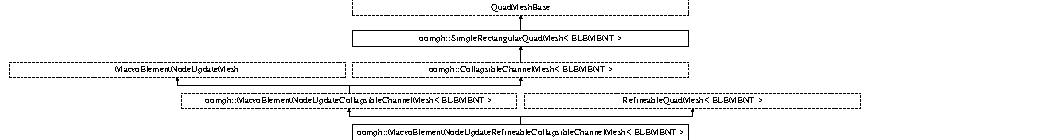
\includegraphics[height=1.885522cm]{classoomph_1_1MacroElementNodeUpdateRefineableCollapsibleChannelMesh}
\end{center}
\end{figure}
\subsection*{Public Member Functions}
\begin{DoxyCompactItemize}
\item 
\hyperlink{classoomph_1_1MacroElementNodeUpdateRefineableCollapsibleChannelMesh_a6e3dfbb3d4dee7897d59aa10cde2dab1}{Macro\+Element\+Node\+Update\+Refineable\+Collapsible\+Channel\+Mesh} (const unsigned \&nup, const unsigned \&ncollapsible, const unsigned \&ndown, const unsigned \&\hyperlink{classoomph_1_1SimpleRectangularQuadMesh_a45011f22dedd480392b1f376e4269921}{ny}, const double \&lup, const double \&lcollapsible, const double \&ldown, const double \&ly, Geom\+Object $\ast$\hyperlink{classoomph_1_1CollapsibleChannelMesh_a04ffeb61678763dfd250962ea9ba614b}{wall\+\_\+pt}, Time\+Stepper $\ast$time\+\_\+stepper\+\_\+pt=\&Mesh\+::\+Default\+\_\+\+Time\+Stepper)
\begin{DoxyCompactList}\small\item\em Constructor\+: Pass numbers of elements and dimensions of the various parts of the collapsible channel, pointer to geometric object that represents the wall and pointer to timestepper (defaults to Steady). \end{DoxyCompactList}\item 
virtual \hyperlink{classoomph_1_1MacroElementNodeUpdateRefineableCollapsibleChannelMesh_a5f0960e124d26e10cc70e2143744a07f}{$\sim$\+Macro\+Element\+Node\+Update\+Refineable\+Collapsible\+Channel\+Mesh} ()
\begin{DoxyCompactList}\small\item\em Destructor\+: empty. \end{DoxyCompactList}\end{DoxyCompactItemize}
\subsection*{Additional Inherited Members}


\subsection{Detailed Description}
\subsubsection*{template$<$class E\+L\+E\+M\+E\+NT$>$\newline
class oomph\+::\+Macro\+Element\+Node\+Update\+Refineable\+Collapsible\+Channel\+Mesh$<$ E\+L\+E\+M\+E\+N\+T $>$}

Refineable collapsible channel mesh with Macro\+Element-\/based node update. The collapsible segment is represented by the specified geometric object. Some or all of the geometric Data in that geometric object may contain unknowns in the global Problem. The dependency on these unknowns is taken into account when setting up the Jacobian matrix of the elements. For this purpose, the element (whose type is specified by the template parameter) must inherit from Macro\+Element\+Node\+Update\+Element\+Base. 

Definition at line 375 of file collapsible\+\_\+channel\+\_\+mesh.\+template.\+h.



\subsection{Constructor \& Destructor Documentation}
\mbox{\Hypertarget{classoomph_1_1MacroElementNodeUpdateRefineableCollapsibleChannelMesh_a6e3dfbb3d4dee7897d59aa10cde2dab1}\label{classoomph_1_1MacroElementNodeUpdateRefineableCollapsibleChannelMesh_a6e3dfbb3d4dee7897d59aa10cde2dab1}} 
\index{oomph\+::\+Macro\+Element\+Node\+Update\+Refineable\+Collapsible\+Channel\+Mesh@{oomph\+::\+Macro\+Element\+Node\+Update\+Refineable\+Collapsible\+Channel\+Mesh}!Macro\+Element\+Node\+Update\+Refineable\+Collapsible\+Channel\+Mesh@{Macro\+Element\+Node\+Update\+Refineable\+Collapsible\+Channel\+Mesh}}
\index{Macro\+Element\+Node\+Update\+Refineable\+Collapsible\+Channel\+Mesh@{Macro\+Element\+Node\+Update\+Refineable\+Collapsible\+Channel\+Mesh}!oomph\+::\+Macro\+Element\+Node\+Update\+Refineable\+Collapsible\+Channel\+Mesh@{oomph\+::\+Macro\+Element\+Node\+Update\+Refineable\+Collapsible\+Channel\+Mesh}}
\subsubsection{\texorpdfstring{Macro\+Element\+Node\+Update\+Refineable\+Collapsible\+Channel\+Mesh()}{MacroElementNodeUpdateRefineableCollapsibleChannelMesh()}}
{\footnotesize\ttfamily template$<$class E\+L\+E\+M\+E\+NT$>$ \\
\hyperlink{classoomph_1_1MacroElementNodeUpdateRefineableCollapsibleChannelMesh}{oomph\+::\+Macro\+Element\+Node\+Update\+Refineable\+Collapsible\+Channel\+Mesh}$<$ E\+L\+E\+M\+E\+NT $>$\+::\hyperlink{classoomph_1_1MacroElementNodeUpdateRefineableCollapsibleChannelMesh}{Macro\+Element\+Node\+Update\+Refineable\+Collapsible\+Channel\+Mesh} (\begin{DoxyParamCaption}\item[{const unsigned \&}]{nup,  }\item[{const unsigned \&}]{ncollapsible,  }\item[{const unsigned \&}]{ndown,  }\item[{const unsigned \&}]{ny,  }\item[{const double \&}]{lup,  }\item[{const double \&}]{lcollapsible,  }\item[{const double \&}]{ldown,  }\item[{const double \&}]{ly,  }\item[{Geom\+Object $\ast$}]{wall\+\_\+pt,  }\item[{Time\+Stepper $\ast$}]{time\+\_\+stepper\+\_\+pt = {\ttfamily \&Mesh\+:\+:Default\+\_\+TimeStepper} }\end{DoxyParamCaption})\hspace{0.3cm}{\ttfamily [inline]}}



Constructor\+: Pass numbers of elements and dimensions of the various parts of the collapsible channel, pointer to geometric object that represents the wall and pointer to timestepper (defaults to Steady). 



Definition at line 386 of file collapsible\+\_\+channel\+\_\+mesh.\+template.\+h.

\mbox{\Hypertarget{classoomph_1_1MacroElementNodeUpdateRefineableCollapsibleChannelMesh_a5f0960e124d26e10cc70e2143744a07f}\label{classoomph_1_1MacroElementNodeUpdateRefineableCollapsibleChannelMesh_a5f0960e124d26e10cc70e2143744a07f}} 
\index{oomph\+::\+Macro\+Element\+Node\+Update\+Refineable\+Collapsible\+Channel\+Mesh@{oomph\+::\+Macro\+Element\+Node\+Update\+Refineable\+Collapsible\+Channel\+Mesh}!````~Macro\+Element\+Node\+Update\+Refineable\+Collapsible\+Channel\+Mesh@{$\sim$\+Macro\+Element\+Node\+Update\+Refineable\+Collapsible\+Channel\+Mesh}}
\index{````~Macro\+Element\+Node\+Update\+Refineable\+Collapsible\+Channel\+Mesh@{$\sim$\+Macro\+Element\+Node\+Update\+Refineable\+Collapsible\+Channel\+Mesh}!oomph\+::\+Macro\+Element\+Node\+Update\+Refineable\+Collapsible\+Channel\+Mesh@{oomph\+::\+Macro\+Element\+Node\+Update\+Refineable\+Collapsible\+Channel\+Mesh}}
\subsubsection{\texorpdfstring{$\sim$\+Macro\+Element\+Node\+Update\+Refineable\+Collapsible\+Channel\+Mesh()}{~MacroElementNodeUpdateRefineableCollapsibleChannelMesh()}}
{\footnotesize\ttfamily template$<$class E\+L\+E\+M\+E\+NT$>$ \\
virtual \hyperlink{classoomph_1_1MacroElementNodeUpdateRefineableCollapsibleChannelMesh}{oomph\+::\+Macro\+Element\+Node\+Update\+Refineable\+Collapsible\+Channel\+Mesh}$<$ E\+L\+E\+M\+E\+NT $>$\+::$\sim$\hyperlink{classoomph_1_1MacroElementNodeUpdateRefineableCollapsibleChannelMesh}{Macro\+Element\+Node\+Update\+Refineable\+Collapsible\+Channel\+Mesh} (\begin{DoxyParamCaption}{ }\end{DoxyParamCaption})\hspace{0.3cm}{\ttfamily [inline]}, {\ttfamily [virtual]}}



Destructor\+: empty. 



Definition at line 416 of file collapsible\+\_\+channel\+\_\+mesh.\+template.\+h.



The documentation for this class was generated from the following file\+:\begin{DoxyCompactItemize}
\item 
\hyperlink{collapsible__channel__mesh_8template_8h}{collapsible\+\_\+channel\+\_\+mesh.\+template.\+h}\end{DoxyCompactItemize}

\hypertarget{classoomph_1_1MacroElementNodeUpdateRefineableFishMesh}{}\section{oomph\+:\+:Macro\+Element\+Node\+Update\+Refineable\+Fish\+Mesh$<$ E\+L\+E\+M\+E\+NT $>$ Class Template Reference}
\label{classoomph_1_1MacroElementNodeUpdateRefineableFishMesh}\index{oomph\+::\+Macro\+Element\+Node\+Update\+Refineable\+Fish\+Mesh$<$ E\+L\+E\+M\+E\+N\+T $>$@{oomph\+::\+Macro\+Element\+Node\+Update\+Refineable\+Fish\+Mesh$<$ E\+L\+E\+M\+E\+N\+T $>$}}


{\ttfamily \#include $<$fish\+\_\+mesh.\+template.\+h$>$}

Inheritance diagram for oomph\+:\+:Macro\+Element\+Node\+Update\+Refineable\+Fish\+Mesh$<$ E\+L\+E\+M\+E\+NT $>$\+:\begin{figure}[H]
\begin{center}
\leavevmode
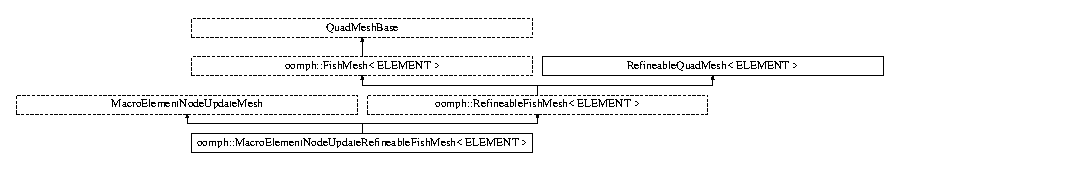
\includegraphics[height=1.821138cm]{classoomph_1_1MacroElementNodeUpdateRefineableFishMesh}
\end{center}
\end{figure}
\subsection*{Public Member Functions}
\begin{DoxyCompactItemize}
\item 
\hyperlink{classoomph_1_1MacroElementNodeUpdateRefineableFishMesh_a7adcb19be3d66c63d88bf87d4822dacc}{Macro\+Element\+Node\+Update\+Refineable\+Fish\+Mesh} (Geom\+Object $\ast$back\+\_\+pt, Time\+Stepper $\ast$time\+\_\+stepper\+\_\+pt=\&Mesh\+::\+Default\+\_\+\+Time\+Stepper)
\begin{DoxyCompactList}\small\item\em Constructor\+: Pass pointer Geom\+Object that defines the fish\textquotesingle{}s back and pointer to timestepper (defaults to (Steady) default timestepper defined in Mesh). \end{DoxyCompactList}\item 
virtual \hyperlink{classoomph_1_1MacroElementNodeUpdateRefineableFishMesh_a68cdd294ca61ad64dbcd1313356d2ca4}{$\sim$\+Macro\+Element\+Node\+Update\+Refineable\+Fish\+Mesh} ()
\begin{DoxyCompactList}\small\item\em Destructor\+: empty. \end{DoxyCompactList}\item 
void \hyperlink{classoomph_1_1MacroElementNodeUpdateRefineableFishMesh_a1008dd9faa50699dcef68c8c35d6979c}{node\+\_\+update} (const bool \&update\+\_\+all\+\_\+solid\+\_\+nodes=false)
\begin{DoxyCompactList}\small\item\em Resolve mesh update\+: Node\+Update current nodal positions via sparse Macro\+Element-\/based update. \mbox{[}Doesn\textquotesingle{}t make sense to use this mesh with Solid\+Elements anyway, so we buffer the case if update\+\_\+all\+\_\+solid\+\_\+nodes is set to true.\mbox{]}. \end{DoxyCompactList}\end{DoxyCompactItemize}
\subsection*{Additional Inherited Members}


\subsection{Detailed Description}
\subsubsection*{template$<$class E\+L\+E\+M\+E\+NT$>$\newline
class oomph\+::\+Macro\+Element\+Node\+Update\+Refineable\+Fish\+Mesh$<$ E\+L\+E\+M\+E\+N\+T $>$}

Refineable fish shaped mesh with Macro\+Element-\/based node update. The fish\textquotesingle{}s back is represented by a specified geometric object. Some or all of the geometric Data in that geometric object may contain unknowns in the global Problem. The dependency on these unknowns is taken into account when setting up the Jacobian matrix of the elements. For this purpose, the element (whose type is specified by the template parameter) must inherit from Macro\+Element\+Node\+Update\+Element\+Base. 

Definition at line 208 of file fish\+\_\+mesh.\+template.\+h.



\subsection{Constructor \& Destructor Documentation}
\mbox{\Hypertarget{classoomph_1_1MacroElementNodeUpdateRefineableFishMesh_a7adcb19be3d66c63d88bf87d4822dacc}\label{classoomph_1_1MacroElementNodeUpdateRefineableFishMesh_a7adcb19be3d66c63d88bf87d4822dacc}} 
\index{oomph\+::\+Macro\+Element\+Node\+Update\+Refineable\+Fish\+Mesh@{oomph\+::\+Macro\+Element\+Node\+Update\+Refineable\+Fish\+Mesh}!Macro\+Element\+Node\+Update\+Refineable\+Fish\+Mesh@{Macro\+Element\+Node\+Update\+Refineable\+Fish\+Mesh}}
\index{Macro\+Element\+Node\+Update\+Refineable\+Fish\+Mesh@{Macro\+Element\+Node\+Update\+Refineable\+Fish\+Mesh}!oomph\+::\+Macro\+Element\+Node\+Update\+Refineable\+Fish\+Mesh@{oomph\+::\+Macro\+Element\+Node\+Update\+Refineable\+Fish\+Mesh}}
\subsubsection{\texorpdfstring{Macro\+Element\+Node\+Update\+Refineable\+Fish\+Mesh()}{MacroElementNodeUpdateRefineableFishMesh()}}
{\footnotesize\ttfamily template$<$class E\+L\+E\+M\+E\+NT $>$ \\
\hyperlink{classoomph_1_1MacroElementNodeUpdateRefineableFishMesh}{oomph\+::\+Macro\+Element\+Node\+Update\+Refineable\+Fish\+Mesh}$<$ E\+L\+E\+M\+E\+NT $>$\+::\hyperlink{classoomph_1_1MacroElementNodeUpdateRefineableFishMesh}{Macro\+Element\+Node\+Update\+Refineable\+Fish\+Mesh} (\begin{DoxyParamCaption}\item[{Geom\+Object $\ast$}]{back\+\_\+pt,  }\item[{Time\+Stepper $\ast$}]{time\+\_\+stepper\+\_\+pt = {\ttfamily \&Mesh\+:\+:Default\+\_\+TimeStepper} }\end{DoxyParamCaption})\hspace{0.3cm}{\ttfamily [inline]}}



Constructor\+: Pass pointer Geom\+Object that defines the fish\textquotesingle{}s back and pointer to timestepper (defaults to (Steady) default timestepper defined in Mesh). 



Definition at line 218 of file fish\+\_\+mesh.\+template.\+h.



References oomph\+::\+Fish\+Mesh$<$ E\+L\+E\+M\+E\+N\+T $>$\+::\+Back\+\_\+pt, and oomph\+::\+Fish\+Mesh$<$ E\+L\+E\+M\+E\+N\+T $>$\+::domain\+\_\+pt().

\mbox{\Hypertarget{classoomph_1_1MacroElementNodeUpdateRefineableFishMesh_a68cdd294ca61ad64dbcd1313356d2ca4}\label{classoomph_1_1MacroElementNodeUpdateRefineableFishMesh_a68cdd294ca61ad64dbcd1313356d2ca4}} 
\index{oomph\+::\+Macro\+Element\+Node\+Update\+Refineable\+Fish\+Mesh@{oomph\+::\+Macro\+Element\+Node\+Update\+Refineable\+Fish\+Mesh}!````~Macro\+Element\+Node\+Update\+Refineable\+Fish\+Mesh@{$\sim$\+Macro\+Element\+Node\+Update\+Refineable\+Fish\+Mesh}}
\index{````~Macro\+Element\+Node\+Update\+Refineable\+Fish\+Mesh@{$\sim$\+Macro\+Element\+Node\+Update\+Refineable\+Fish\+Mesh}!oomph\+::\+Macro\+Element\+Node\+Update\+Refineable\+Fish\+Mesh@{oomph\+::\+Macro\+Element\+Node\+Update\+Refineable\+Fish\+Mesh}}
\subsubsection{\texorpdfstring{$\sim$\+Macro\+Element\+Node\+Update\+Refineable\+Fish\+Mesh()}{~MacroElementNodeUpdateRefineableFishMesh()}}
{\footnotesize\ttfamily template$<$class E\+L\+E\+M\+E\+NT $>$ \\
virtual \hyperlink{classoomph_1_1MacroElementNodeUpdateRefineableFishMesh}{oomph\+::\+Macro\+Element\+Node\+Update\+Refineable\+Fish\+Mesh}$<$ E\+L\+E\+M\+E\+NT $>$\+::$\sim$\hyperlink{classoomph_1_1MacroElementNodeUpdateRefineableFishMesh}{Macro\+Element\+Node\+Update\+Refineable\+Fish\+Mesh} (\begin{DoxyParamCaption}{ }\end{DoxyParamCaption})\hspace{0.3cm}{\ttfamily [inline]}, {\ttfamily [virtual]}}



Destructor\+: empty. 



Definition at line 300 of file fish\+\_\+mesh.\+template.\+h.



\subsection{Member Function Documentation}
\mbox{\Hypertarget{classoomph_1_1MacroElementNodeUpdateRefineableFishMesh_a1008dd9faa50699dcef68c8c35d6979c}\label{classoomph_1_1MacroElementNodeUpdateRefineableFishMesh_a1008dd9faa50699dcef68c8c35d6979c}} 
\index{oomph\+::\+Macro\+Element\+Node\+Update\+Refineable\+Fish\+Mesh@{oomph\+::\+Macro\+Element\+Node\+Update\+Refineable\+Fish\+Mesh}!node\+\_\+update@{node\+\_\+update}}
\index{node\+\_\+update@{node\+\_\+update}!oomph\+::\+Macro\+Element\+Node\+Update\+Refineable\+Fish\+Mesh@{oomph\+::\+Macro\+Element\+Node\+Update\+Refineable\+Fish\+Mesh}}
\subsubsection{\texorpdfstring{node\+\_\+update()}{node\_update()}}
{\footnotesize\ttfamily template$<$class E\+L\+E\+M\+E\+NT $>$ \\
void \hyperlink{classoomph_1_1MacroElementNodeUpdateRefineableFishMesh}{oomph\+::\+Macro\+Element\+Node\+Update\+Refineable\+Fish\+Mesh}$<$ E\+L\+E\+M\+E\+NT $>$\+::node\+\_\+update (\begin{DoxyParamCaption}\item[{const bool \&}]{update\+\_\+all\+\_\+solid\+\_\+nodes = {\ttfamily false} }\end{DoxyParamCaption})\hspace{0.3cm}{\ttfamily [inline]}}



Resolve mesh update\+: Node\+Update current nodal positions via sparse Macro\+Element-\/based update. \mbox{[}Doesn\textquotesingle{}t make sense to use this mesh with Solid\+Elements anyway, so we buffer the case if update\+\_\+all\+\_\+solid\+\_\+nodes is set to true.\mbox{]}. 



Definition at line 307 of file fish\+\_\+mesh.\+template.\+h.



The documentation for this class was generated from the following file\+:\begin{DoxyCompactItemize}
\item 
\hyperlink{fish__mesh_8template_8h}{fish\+\_\+mesh.\+template.\+h}\end{DoxyCompactItemize}

\hypertarget{classoomph_1_1MacroElementNodeUpdateRefineableQuarterCircleSectorMesh}{}\section{oomph\+:\+:Macro\+Element\+Node\+Update\+Refineable\+Quarter\+Circle\+Sector\+Mesh$<$ E\+L\+E\+M\+E\+NT $>$ Class Template Reference}
\label{classoomph_1_1MacroElementNodeUpdateRefineableQuarterCircleSectorMesh}\index{oomph\+::\+Macro\+Element\+Node\+Update\+Refineable\+Quarter\+Circle\+Sector\+Mesh$<$ E\+L\+E\+M\+E\+N\+T $>$@{oomph\+::\+Macro\+Element\+Node\+Update\+Refineable\+Quarter\+Circle\+Sector\+Mesh$<$ E\+L\+E\+M\+E\+N\+T $>$}}


{\ttfamily \#include $<$quarter\+\_\+circle\+\_\+sector\+\_\+mesh.\+template.\+h$>$}

Inheritance diagram for oomph\+:\+:Macro\+Element\+Node\+Update\+Refineable\+Quarter\+Circle\+Sector\+Mesh$<$ E\+L\+E\+M\+E\+NT $>$\+:\begin{figure}[H]
\begin{center}
\leavevmode
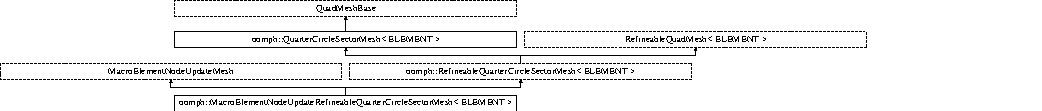
\includegraphics[height=1.490353cm]{classoomph_1_1MacroElementNodeUpdateRefineableQuarterCircleSectorMesh}
\end{center}
\end{figure}
\subsection*{Public Member Functions}
\begin{DoxyCompactItemize}
\item 
\hyperlink{classoomph_1_1MacroElementNodeUpdateRefineableQuarterCircleSectorMesh_ace75c8edb3d87019dc7f06152205adab}{Macro\+Element\+Node\+Update\+Refineable\+Quarter\+Circle\+Sector\+Mesh} (Geom\+Object $\ast$\hyperlink{classoomph_1_1QuarterCircleSectorMesh_a0b03071bbe7e95cc6723c221ddc0998a}{wall\+\_\+pt}, const double \&xi\+\_\+lo, const double \&fract\+\_\+mid, const double \&xi\+\_\+hi, Time\+Stepper $\ast$time\+\_\+stepper\+\_\+pt=\&Mesh\+::\+Default\+\_\+\+Time\+Stepper)
\begin{DoxyCompactList}\small\item\em Constructor\+: Pass pointer to geometric object, start and end coordinates on the geometric object and the fraction along which the dividing line is to be placed when updating the nodal positions, and timestepper (defaults to (Steady) default timestepper defined in Mesh). Setup the refineable mesh (by calling the constructor for the underlying \hyperlink{classoomph_1_1RefineableQuarterCircleSectorMesh}{Refineable\+Quarter\+Circle\+Sector\+Mesh}) and the algebraic node update functions for nodes. \end{DoxyCompactList}\item 
virtual \hyperlink{classoomph_1_1MacroElementNodeUpdateRefineableQuarterCircleSectorMesh_a2d8953d309eba614524fce77c44c8d46}{$\sim$\+Macro\+Element\+Node\+Update\+Refineable\+Quarter\+Circle\+Sector\+Mesh} ()
\begin{DoxyCompactList}\small\item\em Destructor\+: empty. \end{DoxyCompactList}\item 
void \hyperlink{classoomph_1_1MacroElementNodeUpdateRefineableQuarterCircleSectorMesh_a99403c711c3fdc2a601b478deebef9fe}{node\+\_\+update} (const bool \&update\+\_\+all\+\_\+solid\+\_\+nodes=false)
\begin{DoxyCompactList}\small\item\em Resolve mesh update\+: Update current nodal positions via sparse Macro\+Element-\/based update. \mbox{[}Doesn\textquotesingle{}t make sense to use this mesh with Solid\+Elements anyway, so we buffer the case if update\+\_\+all\+\_\+solid\+\_\+nodes is set to true.\mbox{]}. \end{DoxyCompactList}\end{DoxyCompactItemize}
\subsection*{Private Member Functions}
\begin{DoxyCompactItemize}
\item 
void \hyperlink{classoomph_1_1MacroElementNodeUpdateRefineableQuarterCircleSectorMesh_a94b5efa53ac7689757dad989098df7ed}{setup\+\_\+macro\+\_\+element\+\_\+node\+\_\+update} ()
\begin{DoxyCompactList}\small\item\em Setup all the information that\textquotesingle{}s required for Macro\+Element-\/based node update\+: Tell the elements that their geometry depends on the geometric object that parametrises the wall. \end{DoxyCompactList}\end{DoxyCompactItemize}
\subsection*{Additional Inherited Members}


\subsection{Detailed Description}
\subsubsection*{template$<$class E\+L\+E\+M\+E\+NT$>$\newline
class oomph\+::\+Macro\+Element\+Node\+Update\+Refineable\+Quarter\+Circle\+Sector\+Mesh$<$ E\+L\+E\+M\+E\+N\+T $>$}

Macro\+Element\+Node\+Update version of \hyperlink{classoomph_1_1RefineableQuarterCircleSectorMesh}{Refineable\+Quarter\+Circle\+Sector\+Mesh}


\begin{DoxyCode}
                     ---\_\_\_
                    |      ---\_\_\_\_
                    |              -   BOUNDARY 1
                    |               /  
                    |     [2]      /  |  
                    |             /     | 
                    | N          /        |  
                    | |\_ E      /          |    
     BOUNDARY 2     |-----------           |  
                    |          |    [1]    |
                    |   [0]    |           |  ^
                    |          |           | / \(\backslash\)  direction of
                    | N        |    N      |  |   Lagrangian 
                    | |\_ E     |    |\_ E   |  |   coordinate 
                    |\_\_\_\_\_\_\_\_\_\_|\_\_\_\_\_\_\_\_\_\_\_|  |   along wall GeomObject

                         BOUNDARY 0

Within the elements (MacroElements), the local coordinates
are such that the (E)astern direction coincides with the positive 
s\_0 direction,  \textcolor{keywordflow}{while} the (N)orther direction coincides with the positive 
s\_1 direction.
\end{DoxyCode}


Domain is parametrised by three macro elements as sketched. Elements need to be derived from Macro\+Element\+Node\+Update\+Element\+Base. 

Definition at line 275 of file quarter\+\_\+circle\+\_\+sector\+\_\+mesh.\+template.\+h.



\subsection{Constructor \& Destructor Documentation}
\mbox{\Hypertarget{classoomph_1_1MacroElementNodeUpdateRefineableQuarterCircleSectorMesh_ace75c8edb3d87019dc7f06152205adab}\label{classoomph_1_1MacroElementNodeUpdateRefineableQuarterCircleSectorMesh_ace75c8edb3d87019dc7f06152205adab}} 
\index{oomph\+::\+Macro\+Element\+Node\+Update\+Refineable\+Quarter\+Circle\+Sector\+Mesh@{oomph\+::\+Macro\+Element\+Node\+Update\+Refineable\+Quarter\+Circle\+Sector\+Mesh}!Macro\+Element\+Node\+Update\+Refineable\+Quarter\+Circle\+Sector\+Mesh@{Macro\+Element\+Node\+Update\+Refineable\+Quarter\+Circle\+Sector\+Mesh}}
\index{Macro\+Element\+Node\+Update\+Refineable\+Quarter\+Circle\+Sector\+Mesh@{Macro\+Element\+Node\+Update\+Refineable\+Quarter\+Circle\+Sector\+Mesh}!oomph\+::\+Macro\+Element\+Node\+Update\+Refineable\+Quarter\+Circle\+Sector\+Mesh@{oomph\+::\+Macro\+Element\+Node\+Update\+Refineable\+Quarter\+Circle\+Sector\+Mesh}}
\subsubsection{\texorpdfstring{Macro\+Element\+Node\+Update\+Refineable\+Quarter\+Circle\+Sector\+Mesh()}{MacroElementNodeUpdateRefineableQuarterCircleSectorMesh()}}
{\footnotesize\ttfamily template$<$class E\+L\+E\+M\+E\+NT $>$ \\
\hyperlink{classoomph_1_1MacroElementNodeUpdateRefineableQuarterCircleSectorMesh}{oomph\+::\+Macro\+Element\+Node\+Update\+Refineable\+Quarter\+Circle\+Sector\+Mesh}$<$ E\+L\+E\+M\+E\+NT $>$\+::\hyperlink{classoomph_1_1MacroElementNodeUpdateRefineableQuarterCircleSectorMesh}{Macro\+Element\+Node\+Update\+Refineable\+Quarter\+Circle\+Sector\+Mesh} (\begin{DoxyParamCaption}\item[{Geom\+Object $\ast$}]{wall\+\_\+pt,  }\item[{const double \&}]{xi\+\_\+lo,  }\item[{const double \&}]{fract\+\_\+mid,  }\item[{const double \&}]{xi\+\_\+hi,  }\item[{Time\+Stepper $\ast$}]{time\+\_\+stepper\+\_\+pt = {\ttfamily \&Mesh\+:\+:Default\+\_\+TimeStepper} }\end{DoxyParamCaption})\hspace{0.3cm}{\ttfamily [inline]}}



Constructor\+: Pass pointer to geometric object, start and end coordinates on the geometric object and the fraction along which the dividing line is to be placed when updating the nodal positions, and timestepper (defaults to (Steady) default timestepper defined in Mesh). Setup the refineable mesh (by calling the constructor for the underlying \hyperlink{classoomph_1_1RefineableQuarterCircleSectorMesh}{Refineable\+Quarter\+Circle\+Sector\+Mesh}) and the algebraic node update functions for nodes. 



Definition at line 292 of file quarter\+\_\+circle\+\_\+sector\+\_\+mesh.\+template.\+h.

\mbox{\Hypertarget{classoomph_1_1MacroElementNodeUpdateRefineableQuarterCircleSectorMesh_a2d8953d309eba614524fce77c44c8d46}\label{classoomph_1_1MacroElementNodeUpdateRefineableQuarterCircleSectorMesh_a2d8953d309eba614524fce77c44c8d46}} 
\index{oomph\+::\+Macro\+Element\+Node\+Update\+Refineable\+Quarter\+Circle\+Sector\+Mesh@{oomph\+::\+Macro\+Element\+Node\+Update\+Refineable\+Quarter\+Circle\+Sector\+Mesh}!````~Macro\+Element\+Node\+Update\+Refineable\+Quarter\+Circle\+Sector\+Mesh@{$\sim$\+Macro\+Element\+Node\+Update\+Refineable\+Quarter\+Circle\+Sector\+Mesh}}
\index{````~Macro\+Element\+Node\+Update\+Refineable\+Quarter\+Circle\+Sector\+Mesh@{$\sim$\+Macro\+Element\+Node\+Update\+Refineable\+Quarter\+Circle\+Sector\+Mesh}!oomph\+::\+Macro\+Element\+Node\+Update\+Refineable\+Quarter\+Circle\+Sector\+Mesh@{oomph\+::\+Macro\+Element\+Node\+Update\+Refineable\+Quarter\+Circle\+Sector\+Mesh}}
\subsubsection{\texorpdfstring{$\sim$\+Macro\+Element\+Node\+Update\+Refineable\+Quarter\+Circle\+Sector\+Mesh()}{~MacroElementNodeUpdateRefineableQuarterCircleSectorMesh()}}
{\footnotesize\ttfamily template$<$class E\+L\+E\+M\+E\+NT $>$ \\
virtual \hyperlink{classoomph_1_1MacroElementNodeUpdateRefineableQuarterCircleSectorMesh}{oomph\+::\+Macro\+Element\+Node\+Update\+Refineable\+Quarter\+Circle\+Sector\+Mesh}$<$ E\+L\+E\+M\+E\+NT $>$\+::$\sim$\hyperlink{classoomph_1_1MacroElementNodeUpdateRefineableQuarterCircleSectorMesh}{Macro\+Element\+Node\+Update\+Refineable\+Quarter\+Circle\+Sector\+Mesh} (\begin{DoxyParamCaption}{ }\end{DoxyParamCaption})\hspace{0.3cm}{\ttfamily [inline]}, {\ttfamily [virtual]}}



Destructor\+: empty. 



Definition at line 335 of file quarter\+\_\+circle\+\_\+sector\+\_\+mesh.\+template.\+h.



\subsection{Member Function Documentation}
\mbox{\Hypertarget{classoomph_1_1MacroElementNodeUpdateRefineableQuarterCircleSectorMesh_a99403c711c3fdc2a601b478deebef9fe}\label{classoomph_1_1MacroElementNodeUpdateRefineableQuarterCircleSectorMesh_a99403c711c3fdc2a601b478deebef9fe}} 
\index{oomph\+::\+Macro\+Element\+Node\+Update\+Refineable\+Quarter\+Circle\+Sector\+Mesh@{oomph\+::\+Macro\+Element\+Node\+Update\+Refineable\+Quarter\+Circle\+Sector\+Mesh}!node\+\_\+update@{node\+\_\+update}}
\index{node\+\_\+update@{node\+\_\+update}!oomph\+::\+Macro\+Element\+Node\+Update\+Refineable\+Quarter\+Circle\+Sector\+Mesh@{oomph\+::\+Macro\+Element\+Node\+Update\+Refineable\+Quarter\+Circle\+Sector\+Mesh}}
\subsubsection{\texorpdfstring{node\+\_\+update()}{node\_update()}}
{\footnotesize\ttfamily template$<$class E\+L\+E\+M\+E\+NT $>$ \\
void \hyperlink{classoomph_1_1MacroElementNodeUpdateRefineableQuarterCircleSectorMesh}{oomph\+::\+Macro\+Element\+Node\+Update\+Refineable\+Quarter\+Circle\+Sector\+Mesh}$<$ E\+L\+E\+M\+E\+NT $>$\+::node\+\_\+update (\begin{DoxyParamCaption}\item[{const bool \&}]{update\+\_\+all\+\_\+solid\+\_\+nodes = {\ttfamily false} }\end{DoxyParamCaption})\hspace{0.3cm}{\ttfamily [inline]}}



Resolve mesh update\+: Update current nodal positions via sparse Macro\+Element-\/based update. \mbox{[}Doesn\textquotesingle{}t make sense to use this mesh with Solid\+Elements anyway, so we buffer the case if update\+\_\+all\+\_\+solid\+\_\+nodes is set to true.\mbox{]}. 



Definition at line 342 of file quarter\+\_\+circle\+\_\+sector\+\_\+mesh.\+template.\+h.

\mbox{\Hypertarget{classoomph_1_1MacroElementNodeUpdateRefineableQuarterCircleSectorMesh_a94b5efa53ac7689757dad989098df7ed}\label{classoomph_1_1MacroElementNodeUpdateRefineableQuarterCircleSectorMesh_a94b5efa53ac7689757dad989098df7ed}} 
\index{oomph\+::\+Macro\+Element\+Node\+Update\+Refineable\+Quarter\+Circle\+Sector\+Mesh@{oomph\+::\+Macro\+Element\+Node\+Update\+Refineable\+Quarter\+Circle\+Sector\+Mesh}!setup\+\_\+macro\+\_\+element\+\_\+node\+\_\+update@{setup\+\_\+macro\+\_\+element\+\_\+node\+\_\+update}}
\index{setup\+\_\+macro\+\_\+element\+\_\+node\+\_\+update@{setup\+\_\+macro\+\_\+element\+\_\+node\+\_\+update}!oomph\+::\+Macro\+Element\+Node\+Update\+Refineable\+Quarter\+Circle\+Sector\+Mesh@{oomph\+::\+Macro\+Element\+Node\+Update\+Refineable\+Quarter\+Circle\+Sector\+Mesh}}
\subsubsection{\texorpdfstring{setup\+\_\+macro\+\_\+element\+\_\+node\+\_\+update()}{setup\_macro\_element\_node\_update()}}
{\footnotesize\ttfamily template$<$class E\+L\+E\+M\+E\+NT $>$ \\
void \hyperlink{classoomph_1_1MacroElementNodeUpdateRefineableQuarterCircleSectorMesh}{oomph\+::\+Macro\+Element\+Node\+Update\+Refineable\+Quarter\+Circle\+Sector\+Mesh}$<$ E\+L\+E\+M\+E\+NT $>$\+::setup\+\_\+macro\+\_\+element\+\_\+node\+\_\+update (\begin{DoxyParamCaption}{ }\end{DoxyParamCaption})\hspace{0.3cm}{\ttfamily [inline]}, {\ttfamily [private]}}



Setup all the information that\textquotesingle{}s required for Macro\+Element-\/based node update\+: Tell the elements that their geometry depends on the geometric object that parametrises the wall. 



Definition at line 370 of file quarter\+\_\+circle\+\_\+sector\+\_\+mesh.\+template.\+h.



References oomph\+::\+Quarter\+Circle\+Sector\+Mesh$<$ E\+L\+E\+M\+E\+N\+T $>$\+::domain\+\_\+pt(), and oomph\+::\+Quarter\+Circle\+Sector\+Mesh$<$ E\+L\+E\+M\+E\+N\+T $>$\+::\+Wall\+\_\+pt.



The documentation for this class was generated from the following file\+:\begin{DoxyCompactItemize}
\item 
\hyperlink{quarter__circle__sector__mesh_8template_8h}{quarter\+\_\+circle\+\_\+sector\+\_\+mesh.\+template.\+h}\end{DoxyCompactItemize}

\hypertarget{classoomph_1_1MacroElementNodeUpdateRefineableQuarterTubeMesh}{}\section{oomph\+:\+:Macro\+Element\+Node\+Update\+Refineable\+Quarter\+Tube\+Mesh$<$ E\+L\+E\+M\+E\+NT $>$ Class Template Reference}
\label{classoomph_1_1MacroElementNodeUpdateRefineableQuarterTubeMesh}\index{oomph\+::\+Macro\+Element\+Node\+Update\+Refineable\+Quarter\+Tube\+Mesh$<$ E\+L\+E\+M\+E\+N\+T $>$@{oomph\+::\+Macro\+Element\+Node\+Update\+Refineable\+Quarter\+Tube\+Mesh$<$ E\+L\+E\+M\+E\+N\+T $>$}}


Macro\+Element\+Node\+Update version of \hyperlink{classoomph_1_1RefineableQuarterTubeMesh}{Refineable\+Quarter\+Tube\+Mesh}.  




{\ttfamily \#include $<$quarter\+\_\+tube\+\_\+mesh.\+template.\+h$>$}

Inheritance diagram for oomph\+:\+:Macro\+Element\+Node\+Update\+Refineable\+Quarter\+Tube\+Mesh$<$ E\+L\+E\+M\+E\+NT $>$\+:\begin{figure}[H]
\begin{center}
\leavevmode
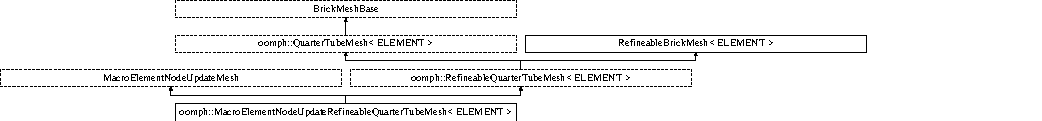
\includegraphics[height=2.139738cm]{classoomph_1_1MacroElementNodeUpdateRefineableQuarterTubeMesh}
\end{center}
\end{figure}
\subsection*{Public Member Functions}
\begin{DoxyCompactItemize}
\item 
\hyperlink{classoomph_1_1MacroElementNodeUpdateRefineableQuarterTubeMesh_a05355134c7930d4aa73969f6c743ed17}{Macro\+Element\+Node\+Update\+Refineable\+Quarter\+Tube\+Mesh} (\hyperlink{classoomph_1_1GeomObject}{Geom\+Object} $\ast$\hyperlink{classoomph_1_1QuarterTubeMesh_af59c4cde343ddd76caea4bc8c8ad8b94}{wall\+\_\+pt}, const \hyperlink{classoomph_1_1Vector}{Vector}$<$ double $>$ \&xi\+\_\+lo, const double \&fract\+\_\+mid, const \hyperlink{classoomph_1_1Vector}{Vector}$<$ double $>$ \&xi\+\_\+hi, const unsigned \&nlayer, \hyperlink{classoomph_1_1TimeStepper}{Time\+Stepper} $\ast$time\+\_\+stepper\+\_\+pt=\&\hyperlink{classoomph_1_1Mesh_a12243d0fee2b1fcee729ee5a4777ea10}{Mesh\+::\+Default\+\_\+\+Time\+Stepper})
\begin{DoxyCompactList}\small\item\em Constructor\+: Pass pointer to geometric object, start and end coordinates on the geometric object and the fraction along which the dividing line is to be placed when updating the nodal positions, and timestepper (defaults to (\hyperlink{classoomph_1_1Steady}{Steady}) default timestepper defined in \hyperlink{classoomph_1_1Mesh}{Mesh}). Setup the refineable mesh (by calling the constructor for the underlying \hyperlink{classoomph_1_1RefineableQuarterTubeMesh}{Refineable\+Quarter\+Tube\+Mesh}) and the algebraic node update functions for nodes. \end{DoxyCompactList}\item 
virtual \hyperlink{classoomph_1_1MacroElementNodeUpdateRefineableQuarterTubeMesh_ae4a4028ac41a7721c87bd484be894d02}{$\sim$\+Macro\+Element\+Node\+Update\+Refineable\+Quarter\+Tube\+Mesh} ()
\begin{DoxyCompactList}\small\item\em Destructor\+: empty. \end{DoxyCompactList}\item 
void \hyperlink{classoomph_1_1MacroElementNodeUpdateRefineableQuarterTubeMesh_a6255c22765a484ac11642ade0c084082}{node\+\_\+update} (const bool \&update\+\_\+all\+\_\+solid\+\_\+nodes=false)
\begin{DoxyCompactList}\small\item\em Resolve mesh update\+: Update current nodal positions via sparse Macro\+Element-\/based update. \mbox{[}Doesn\textquotesingle{}t make sense to use this mesh with Solid\+Elements anyway, so we buffer the case if update\+\_\+all\+\_\+solid\+\_\+nodes is set to true.\mbox{]}. \end{DoxyCompactList}\end{DoxyCompactItemize}
\subsection*{Private Member Functions}
\begin{DoxyCompactItemize}
\item 
void \hyperlink{classoomph_1_1MacroElementNodeUpdateRefineableQuarterTubeMesh_ae98ab46cf2030928d805894dffe1b642}{setup\+\_\+macro\+\_\+element\+\_\+node\+\_\+update} ()
\begin{DoxyCompactList}\small\item\em Setup all the information that\textquotesingle{}s required for Macro\+Element-\/based node update\+: Tell the elements that their geometry depends on the geometric object that parametrises the wall. \end{DoxyCompactList}\end{DoxyCompactItemize}
\subsection*{Additional Inherited Members}


\subsection{Detailed Description}
\subsubsection*{template$<$class E\+L\+E\+M\+E\+NT$>$\newline
class oomph\+::\+Macro\+Element\+Node\+Update\+Refineable\+Quarter\+Tube\+Mesh$<$ E\+L\+E\+M\+E\+N\+T $>$}

Macro\+Element\+Node\+Update version of \hyperlink{classoomph_1_1RefineableQuarterTubeMesh}{Refineable\+Quarter\+Tube\+Mesh}. 

Definition at line 251 of file quarter\+\_\+tube\+\_\+mesh.\+template.\+h.



\subsection{Constructor \& Destructor Documentation}
\mbox{\Hypertarget{classoomph_1_1MacroElementNodeUpdateRefineableQuarterTubeMesh_a05355134c7930d4aa73969f6c743ed17}\label{classoomph_1_1MacroElementNodeUpdateRefineableQuarterTubeMesh_a05355134c7930d4aa73969f6c743ed17}} 
\index{oomph\+::\+Macro\+Element\+Node\+Update\+Refineable\+Quarter\+Tube\+Mesh@{oomph\+::\+Macro\+Element\+Node\+Update\+Refineable\+Quarter\+Tube\+Mesh}!Macro\+Element\+Node\+Update\+Refineable\+Quarter\+Tube\+Mesh@{Macro\+Element\+Node\+Update\+Refineable\+Quarter\+Tube\+Mesh}}
\index{Macro\+Element\+Node\+Update\+Refineable\+Quarter\+Tube\+Mesh@{Macro\+Element\+Node\+Update\+Refineable\+Quarter\+Tube\+Mesh}!oomph\+::\+Macro\+Element\+Node\+Update\+Refineable\+Quarter\+Tube\+Mesh@{oomph\+::\+Macro\+Element\+Node\+Update\+Refineable\+Quarter\+Tube\+Mesh}}
\subsubsection{\texorpdfstring{Macro\+Element\+Node\+Update\+Refineable\+Quarter\+Tube\+Mesh()}{MacroElementNodeUpdateRefineableQuarterTubeMesh()}}
{\footnotesize\ttfamily template$<$class E\+L\+E\+M\+E\+NT $>$ \\
\hyperlink{classoomph_1_1MacroElementNodeUpdateRefineableQuarterTubeMesh}{oomph\+::\+Macro\+Element\+Node\+Update\+Refineable\+Quarter\+Tube\+Mesh}$<$ E\+L\+E\+M\+E\+NT $>$\+::\hyperlink{classoomph_1_1MacroElementNodeUpdateRefineableQuarterTubeMesh}{Macro\+Element\+Node\+Update\+Refineable\+Quarter\+Tube\+Mesh} (\begin{DoxyParamCaption}\item[{\hyperlink{classoomph_1_1GeomObject}{Geom\+Object} $\ast$}]{wall\+\_\+pt,  }\item[{const \hyperlink{classoomph_1_1Vector}{Vector}$<$ double $>$ \&}]{xi\+\_\+lo,  }\item[{const double \&}]{fract\+\_\+mid,  }\item[{const \hyperlink{classoomph_1_1Vector}{Vector}$<$ double $>$ \&}]{xi\+\_\+hi,  }\item[{const unsigned \&}]{nlayer,  }\item[{\hyperlink{classoomph_1_1TimeStepper}{Time\+Stepper} $\ast$}]{time\+\_\+stepper\+\_\+pt = {\ttfamily \&\hyperlink{classoomph_1_1Mesh_a12243d0fee2b1fcee729ee5a4777ea10}{Mesh\+::\+Default\+\_\+\+Time\+Stepper}} }\end{DoxyParamCaption})\hspace{0.3cm}{\ttfamily [inline]}}



Constructor\+: Pass pointer to geometric object, start and end coordinates on the geometric object and the fraction along which the dividing line is to be placed when updating the nodal positions, and timestepper (defaults to (\hyperlink{classoomph_1_1Steady}{Steady}) default timestepper defined in \hyperlink{classoomph_1_1Mesh}{Mesh}). Setup the refineable mesh (by calling the constructor for the underlying \hyperlink{classoomph_1_1RefineableQuarterTubeMesh}{Refineable\+Quarter\+Tube\+Mesh}) and the algebraic node update functions for nodes. 



Definition at line 267 of file quarter\+\_\+tube\+\_\+mesh.\+template.\+h.



References oomph\+::\+Global\+\_\+string\+\_\+for\+\_\+annotation\+::string().

\mbox{\Hypertarget{classoomph_1_1MacroElementNodeUpdateRefineableQuarterTubeMesh_ae4a4028ac41a7721c87bd484be894d02}\label{classoomph_1_1MacroElementNodeUpdateRefineableQuarterTubeMesh_ae4a4028ac41a7721c87bd484be894d02}} 
\index{oomph\+::\+Macro\+Element\+Node\+Update\+Refineable\+Quarter\+Tube\+Mesh@{oomph\+::\+Macro\+Element\+Node\+Update\+Refineable\+Quarter\+Tube\+Mesh}!````~Macro\+Element\+Node\+Update\+Refineable\+Quarter\+Tube\+Mesh@{$\sim$\+Macro\+Element\+Node\+Update\+Refineable\+Quarter\+Tube\+Mesh}}
\index{````~Macro\+Element\+Node\+Update\+Refineable\+Quarter\+Tube\+Mesh@{$\sim$\+Macro\+Element\+Node\+Update\+Refineable\+Quarter\+Tube\+Mesh}!oomph\+::\+Macro\+Element\+Node\+Update\+Refineable\+Quarter\+Tube\+Mesh@{oomph\+::\+Macro\+Element\+Node\+Update\+Refineable\+Quarter\+Tube\+Mesh}}
\subsubsection{\texorpdfstring{$\sim$\+Macro\+Element\+Node\+Update\+Refineable\+Quarter\+Tube\+Mesh()}{~MacroElementNodeUpdateRefineableQuarterTubeMesh()}}
{\footnotesize\ttfamily template$<$class E\+L\+E\+M\+E\+NT $>$ \\
virtual \hyperlink{classoomph_1_1MacroElementNodeUpdateRefineableQuarterTubeMesh}{oomph\+::\+Macro\+Element\+Node\+Update\+Refineable\+Quarter\+Tube\+Mesh}$<$ E\+L\+E\+M\+E\+NT $>$\+::$\sim$\hyperlink{classoomph_1_1MacroElementNodeUpdateRefineableQuarterTubeMesh}{Macro\+Element\+Node\+Update\+Refineable\+Quarter\+Tube\+Mesh} (\begin{DoxyParamCaption}{ }\end{DoxyParamCaption})\hspace{0.3cm}{\ttfamily [inline]}, {\ttfamily [virtual]}}



Destructor\+: empty. 



Definition at line 313 of file quarter\+\_\+tube\+\_\+mesh.\+template.\+h.



\subsection{Member Function Documentation}
\mbox{\Hypertarget{classoomph_1_1MacroElementNodeUpdateRefineableQuarterTubeMesh_a6255c22765a484ac11642ade0c084082}\label{classoomph_1_1MacroElementNodeUpdateRefineableQuarterTubeMesh_a6255c22765a484ac11642ade0c084082}} 
\index{oomph\+::\+Macro\+Element\+Node\+Update\+Refineable\+Quarter\+Tube\+Mesh@{oomph\+::\+Macro\+Element\+Node\+Update\+Refineable\+Quarter\+Tube\+Mesh}!node\+\_\+update@{node\+\_\+update}}
\index{node\+\_\+update@{node\+\_\+update}!oomph\+::\+Macro\+Element\+Node\+Update\+Refineable\+Quarter\+Tube\+Mesh@{oomph\+::\+Macro\+Element\+Node\+Update\+Refineable\+Quarter\+Tube\+Mesh}}
\subsubsection{\texorpdfstring{node\+\_\+update()}{node\_update()}}
{\footnotesize\ttfamily template$<$class E\+L\+E\+M\+E\+NT $>$ \\
void \hyperlink{classoomph_1_1MacroElementNodeUpdateRefineableQuarterTubeMesh}{oomph\+::\+Macro\+Element\+Node\+Update\+Refineable\+Quarter\+Tube\+Mesh}$<$ E\+L\+E\+M\+E\+NT $>$\+::node\+\_\+update (\begin{DoxyParamCaption}\item[{const bool \&}]{update\+\_\+all\+\_\+solid\+\_\+nodes = {\ttfamily false} }\end{DoxyParamCaption})\hspace{0.3cm}{\ttfamily [inline]}, {\ttfamily [virtual]}}



Resolve mesh update\+: Update current nodal positions via sparse Macro\+Element-\/based update. \mbox{[}Doesn\textquotesingle{}t make sense to use this mesh with Solid\+Elements anyway, so we buffer the case if update\+\_\+all\+\_\+solid\+\_\+nodes is set to true.\mbox{]}. 



Reimplemented from \hyperlink{classoomph_1_1MacroElementNodeUpdateMesh_ab5271c4514bcd236271307361423ac9d}{oomph\+::\+Macro\+Element\+Node\+Update\+Mesh}.



Definition at line 320 of file quarter\+\_\+tube\+\_\+mesh.\+template.\+h.



References oomph\+::\+Macro\+Element\+Node\+Update\+Mesh\+::node\+\_\+update(), and oomph\+::\+Global\+\_\+string\+\_\+for\+\_\+annotation\+::string().

\mbox{\Hypertarget{classoomph_1_1MacroElementNodeUpdateRefineableQuarterTubeMesh_ae98ab46cf2030928d805894dffe1b642}\label{classoomph_1_1MacroElementNodeUpdateRefineableQuarterTubeMesh_ae98ab46cf2030928d805894dffe1b642}} 
\index{oomph\+::\+Macro\+Element\+Node\+Update\+Refineable\+Quarter\+Tube\+Mesh@{oomph\+::\+Macro\+Element\+Node\+Update\+Refineable\+Quarter\+Tube\+Mesh}!setup\+\_\+macro\+\_\+element\+\_\+node\+\_\+update@{setup\+\_\+macro\+\_\+element\+\_\+node\+\_\+update}}
\index{setup\+\_\+macro\+\_\+element\+\_\+node\+\_\+update@{setup\+\_\+macro\+\_\+element\+\_\+node\+\_\+update}!oomph\+::\+Macro\+Element\+Node\+Update\+Refineable\+Quarter\+Tube\+Mesh@{oomph\+::\+Macro\+Element\+Node\+Update\+Refineable\+Quarter\+Tube\+Mesh}}
\subsubsection{\texorpdfstring{setup\+\_\+macro\+\_\+element\+\_\+node\+\_\+update()}{setup\_macro\_element\_node\_update()}}
{\footnotesize\ttfamily template$<$class E\+L\+E\+M\+E\+NT $>$ \\
void \hyperlink{classoomph_1_1MacroElementNodeUpdateRefineableQuarterTubeMesh}{oomph\+::\+Macro\+Element\+Node\+Update\+Refineable\+Quarter\+Tube\+Mesh}$<$ E\+L\+E\+M\+E\+NT $>$\+::setup\+\_\+macro\+\_\+element\+\_\+node\+\_\+update (\begin{DoxyParamCaption}{ }\end{DoxyParamCaption})\hspace{0.3cm}{\ttfamily [inline]}, {\ttfamily [private]}}



Setup all the information that\textquotesingle{}s required for Macro\+Element-\/based node update\+: Tell the elements that their geometry depends on the geometric object that parametrises the wall. 



Definition at line 348 of file quarter\+\_\+tube\+\_\+mesh.\+template.\+h.



References oomph\+::\+Quarter\+Tube\+Mesh$<$ E\+L\+E\+M\+E\+N\+T $>$\+::domain\+\_\+pt(), oomph\+::\+Mesh\+::element\+\_\+pt(), i, oomph\+::\+Macro\+Element\+Node\+Update\+Mesh\+::macro\+\_\+domain\+\_\+pt(), oomph\+::\+Mesh\+::nelement(), oomph\+::\+Macro\+Element\+Node\+Update\+Mesh\+::set\+\_\+geom\+\_\+object\+\_\+vector\+\_\+pt(), oomph\+::\+Global\+\_\+string\+\_\+for\+\_\+annotation\+::string(), and oomph\+::\+Quarter\+Tube\+Mesh$<$ E\+L\+E\+M\+E\+N\+T $>$\+::\+Wall\+\_\+pt.



The documentation for this class was generated from the following file\+:\begin{DoxyCompactItemize}
\item 
\hyperlink{quarter__tube__mesh_8template_8h}{quarter\+\_\+tube\+\_\+mesh.\+template.\+h}\end{DoxyCompactItemize}

\hypertarget{classoomph_1_1OneDLagrangianMesh}{}\section{oomph\+:\+:One\+D\+Lagrangian\+Mesh$<$ E\+L\+E\+M\+E\+NT $>$ Class Template Reference}
\label{classoomph_1_1OneDLagrangianMesh}\index{oomph\+::\+One\+D\+Lagrangian\+Mesh$<$ E\+L\+E\+M\+E\+N\+T $>$@{oomph\+::\+One\+D\+Lagrangian\+Mesh$<$ E\+L\+E\+M\+E\+N\+T $>$}}


{\ttfamily \#include $<$one\+\_\+d\+\_\+lagrangian\+\_\+mesh.\+template.\+h$>$}

Inheritance diagram for oomph\+:\+:One\+D\+Lagrangian\+Mesh$<$ E\+L\+E\+M\+E\+NT $>$\+:\begin{figure}[H]
\begin{center}
\leavevmode
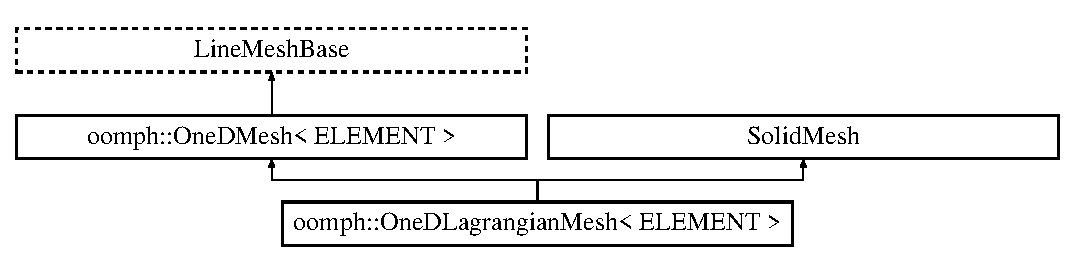
\includegraphics[height=3.000000cm]{classoomph_1_1OneDLagrangianMesh}
\end{center}
\end{figure}
\subsection*{Public Member Functions}
\begin{DoxyCompactItemize}
\item 
\hyperlink{classoomph_1_1OneDLagrangianMesh_a7061998be3fb4131c6b58c4943595d49}{One\+D\+Lagrangian\+Mesh} (const unsigned \&n\+\_\+element, const double \&length, Geom\+Object $\ast$undef\+\_\+eulerian\+\_\+posn\+\_\+pt, Time\+Stepper $\ast$time\+\_\+stepper\+\_\+pt=\&Mesh\+::\+Default\+\_\+\+Time\+Stepper)
\begin{DoxyCompactList}\small\item\em Constructor\+: Pass number of elements, length, pointer to Geom\+Object that defines the undeformed Eulerian position, and the timestepper -- defaults to (Steady) default timestepper defined in the Mesh base class. \end{DoxyCompactList}\item 
\hyperlink{classoomph_1_1OneDLagrangianMesh_a20e1ab05b023f65bea5503938cd70385}{One\+D\+Lagrangian\+Mesh} (const unsigned \&n\+\_\+element, const double \&xmin, const double \&xmax, Geom\+Object $\ast$undef\+\_\+eulerian\+\_\+posn\+\_\+pt, Time\+Stepper $\ast$time\+\_\+stepper\+\_\+pt=\&Mesh\+::\+Default\+\_\+\+Time\+Stepper)
\begin{DoxyCompactList}\small\item\em Constructor\+: Pass number of elements, xmin, xmax pointer to Geom\+Object that defines the undeformed Eulerian position, and the timestepper -- defaults to (Steady) default timestepper defined in the Mesh base class. \end{DoxyCompactList}\end{DoxyCompactItemize}
\subsection*{Private Member Functions}
\begin{DoxyCompactItemize}
\item 
void \hyperlink{classoomph_1_1OneDLagrangianMesh_a7a4eabf4901a90b3015d2620fc70f648}{assign\+\_\+default\+\_\+element\+\_\+gradients} ()
\begin{DoxyCompactList}\small\item\em Set the default gradients of the elements. \end{DoxyCompactList}\item 
void \hyperlink{classoomph_1_1OneDLagrangianMesh_a1eebb0eddd75a7c2847615c05b5fb4d8}{assign\+\_\+undeformed\+\_\+positions} ()
\begin{DoxyCompactList}\small\item\em Assign the undeformed Eulerian positions to the nodes. \end{DoxyCompactList}\end{DoxyCompactItemize}
\subsection*{Private Attributes}
\begin{DoxyCompactItemize}
\item 
Geom\+Object $\ast$ \hyperlink{classoomph_1_1OneDLagrangianMesh_af9b27f687d7ec160a01d6ed8c07570ed}{Undef\+\_\+eulerian\+\_\+posn\+\_\+pt}
\begin{DoxyCompactList}\small\item\em Undeformed Eulerian shape. \end{DoxyCompactList}\end{DoxyCompactItemize}
\subsection*{Additional Inherited Members}


\subsection{Detailed Description}
\subsubsection*{template$<$class E\+L\+E\+M\+E\+NT$>$\newline
class oomph\+::\+One\+D\+Lagrangian\+Mesh$<$ E\+L\+E\+M\+E\+N\+T $>$}

1D mesh parametrised in terms of a 1D Lagrangian coordinate. The Eulerian positions of the nodes are determined by the Geom\+Object. 

Definition at line 50 of file one\+\_\+d\+\_\+lagrangian\+\_\+mesh.\+template.\+h.



\subsection{Constructor \& Destructor Documentation}
\mbox{\Hypertarget{classoomph_1_1OneDLagrangianMesh_a7061998be3fb4131c6b58c4943595d49}\label{classoomph_1_1OneDLagrangianMesh_a7061998be3fb4131c6b58c4943595d49}} 
\index{oomph\+::\+One\+D\+Lagrangian\+Mesh@{oomph\+::\+One\+D\+Lagrangian\+Mesh}!One\+D\+Lagrangian\+Mesh@{One\+D\+Lagrangian\+Mesh}}
\index{One\+D\+Lagrangian\+Mesh@{One\+D\+Lagrangian\+Mesh}!oomph\+::\+One\+D\+Lagrangian\+Mesh@{oomph\+::\+One\+D\+Lagrangian\+Mesh}}
\subsubsection{\texorpdfstring{One\+D\+Lagrangian\+Mesh()}{OneDLagrangianMesh()}\hspace{0.1cm}{\footnotesize\ttfamily [1/2]}}
{\footnotesize\ttfamily template$<$class E\+L\+E\+M\+E\+NT $>$ \\
\hyperlink{classoomph_1_1OneDLagrangianMesh}{oomph\+::\+One\+D\+Lagrangian\+Mesh}$<$ E\+L\+E\+M\+E\+NT $>$\+::\hyperlink{classoomph_1_1OneDLagrangianMesh}{One\+D\+Lagrangian\+Mesh} (\begin{DoxyParamCaption}\item[{const unsigned \&}]{n\+\_\+element,  }\item[{const double \&}]{length,  }\item[{Geom\+Object $\ast$}]{undef\+\_\+eulerian\+\_\+posn\+\_\+pt,  }\item[{Time\+Stepper $\ast$}]{time\+\_\+stepper\+\_\+pt = {\ttfamily \&Mesh\+:\+:Default\+\_\+TimeStepper} }\end{DoxyParamCaption})}



Constructor\+: Pass number of elements, length, pointer to Geom\+Object that defines the undeformed Eulerian position, and the timestepper -- defaults to (Steady) default timestepper defined in the Mesh base class. 

Constructor for 1D mesh\+: n\+\_\+element \+: number of elements length \+: length of domain undef\+\_\+eulerian\+\_\+posn\+\_\+pt\+: pointer to geom object that describes the initial Eulerian position of the mesh. time\+\_\+stepper\+\_\+pt \+: timestepper 

Definition at line 55 of file one\+\_\+d\+\_\+lagrangian\+\_\+mesh.\+template.\+cc.



References oomph\+::\+One\+D\+Lagrangian\+Mesh$<$ E\+L\+E\+M\+E\+N\+T $>$\+::assign\+\_\+default\+\_\+element\+\_\+gradients(), and oomph\+::\+One\+D\+Lagrangian\+Mesh$<$ E\+L\+E\+M\+E\+N\+T $>$\+::assign\+\_\+undeformed\+\_\+positions().

\mbox{\Hypertarget{classoomph_1_1OneDLagrangianMesh_a20e1ab05b023f65bea5503938cd70385}\label{classoomph_1_1OneDLagrangianMesh_a20e1ab05b023f65bea5503938cd70385}} 
\index{oomph\+::\+One\+D\+Lagrangian\+Mesh@{oomph\+::\+One\+D\+Lagrangian\+Mesh}!One\+D\+Lagrangian\+Mesh@{One\+D\+Lagrangian\+Mesh}}
\index{One\+D\+Lagrangian\+Mesh@{One\+D\+Lagrangian\+Mesh}!oomph\+::\+One\+D\+Lagrangian\+Mesh@{oomph\+::\+One\+D\+Lagrangian\+Mesh}}
\subsubsection{\texorpdfstring{One\+D\+Lagrangian\+Mesh()}{OneDLagrangianMesh()}\hspace{0.1cm}{\footnotesize\ttfamily [2/2]}}
{\footnotesize\ttfamily template$<$class E\+L\+E\+M\+E\+NT $>$ \\
\hyperlink{classoomph_1_1OneDLagrangianMesh}{oomph\+::\+One\+D\+Lagrangian\+Mesh}$<$ E\+L\+E\+M\+E\+NT $>$\+::\hyperlink{classoomph_1_1OneDLagrangianMesh}{One\+D\+Lagrangian\+Mesh} (\begin{DoxyParamCaption}\item[{const unsigned \&}]{n\+\_\+element,  }\item[{const double \&}]{xmin,  }\item[{const double \&}]{xmax,  }\item[{Geom\+Object $\ast$}]{undef\+\_\+eulerian\+\_\+posn\+\_\+pt,  }\item[{Time\+Stepper $\ast$}]{time\+\_\+stepper\+\_\+pt = {\ttfamily \&Mesh\+:\+:Default\+\_\+TimeStepper} }\end{DoxyParamCaption})}



Constructor\+: Pass number of elements, xmin, xmax pointer to Geom\+Object that defines the undeformed Eulerian position, and the timestepper -- defaults to (Steady) default timestepper defined in the Mesh base class. 

Constructor for 1D mesh\+: n\+\_\+element \+: number of elements xmin \+: minimum coordinate value (LH end) xmax \+: maximum coordinate value (RH end) undef\+\_\+eulerian\+\_\+posn\+\_\+pt\+: pointer to geom object that describes the initial Eulerian position of the mesh. time\+\_\+stepper\+\_\+pt \+: timestepper 

Definition at line 86 of file one\+\_\+d\+\_\+lagrangian\+\_\+mesh.\+template.\+cc.



References oomph\+::\+One\+D\+Lagrangian\+Mesh$<$ E\+L\+E\+M\+E\+N\+T $>$\+::assign\+\_\+default\+\_\+element\+\_\+gradients(), and oomph\+::\+One\+D\+Lagrangian\+Mesh$<$ E\+L\+E\+M\+E\+N\+T $>$\+::assign\+\_\+undeformed\+\_\+positions().



\subsection{Member Function Documentation}
\mbox{\Hypertarget{classoomph_1_1OneDLagrangianMesh_a7a4eabf4901a90b3015d2620fc70f648}\label{classoomph_1_1OneDLagrangianMesh_a7a4eabf4901a90b3015d2620fc70f648}} 
\index{oomph\+::\+One\+D\+Lagrangian\+Mesh@{oomph\+::\+One\+D\+Lagrangian\+Mesh}!assign\+\_\+default\+\_\+element\+\_\+gradients@{assign\+\_\+default\+\_\+element\+\_\+gradients}}
\index{assign\+\_\+default\+\_\+element\+\_\+gradients@{assign\+\_\+default\+\_\+element\+\_\+gradients}!oomph\+::\+One\+D\+Lagrangian\+Mesh@{oomph\+::\+One\+D\+Lagrangian\+Mesh}}
\subsubsection{\texorpdfstring{assign\+\_\+default\+\_\+element\+\_\+gradients()}{assign\_default\_element\_gradients()}}
{\footnotesize\ttfamily template$<$class E\+L\+E\+M\+E\+NT $>$ \\
void \hyperlink{classoomph_1_1OneDLagrangianMesh}{oomph\+::\+One\+D\+Lagrangian\+Mesh}$<$ E\+L\+E\+M\+E\+NT $>$\+::assign\+\_\+default\+\_\+element\+\_\+gradients (\begin{DoxyParamCaption}{ }\end{DoxyParamCaption})\hspace{0.3cm}{\ttfamily [private]}}



Set the default gradients of the elements. 

Set the default (initial) gradients within each element, which are merely the distances between the nodes, scaled by 0.\+5 because the elements have length 2 in local coordinates. N.\+B. This only works for Q\+Hermite\+Elements at the moment 

Definition at line 116 of file one\+\_\+d\+\_\+lagrangian\+\_\+mesh.\+template.\+cc.



Referenced by oomph\+::\+One\+D\+Lagrangian\+Mesh$<$ E\+L\+E\+M\+E\+N\+T $>$\+::\+One\+D\+Lagrangian\+Mesh().

\mbox{\Hypertarget{classoomph_1_1OneDLagrangianMesh_a1eebb0eddd75a7c2847615c05b5fb4d8}\label{classoomph_1_1OneDLagrangianMesh_a1eebb0eddd75a7c2847615c05b5fb4d8}} 
\index{oomph\+::\+One\+D\+Lagrangian\+Mesh@{oomph\+::\+One\+D\+Lagrangian\+Mesh}!assign\+\_\+undeformed\+\_\+positions@{assign\+\_\+undeformed\+\_\+positions}}
\index{assign\+\_\+undeformed\+\_\+positions@{assign\+\_\+undeformed\+\_\+positions}!oomph\+::\+One\+D\+Lagrangian\+Mesh@{oomph\+::\+One\+D\+Lagrangian\+Mesh}}
\subsubsection{\texorpdfstring{assign\+\_\+undeformed\+\_\+positions()}{assign\_undeformed\_positions()}}
{\footnotesize\ttfamily template$<$class E\+L\+E\+M\+E\+NT $>$ \\
void \hyperlink{classoomph_1_1OneDLagrangianMesh}{oomph\+::\+One\+D\+Lagrangian\+Mesh}$<$ E\+L\+E\+M\+E\+NT $>$\+::assign\+\_\+undeformed\+\_\+positions (\begin{DoxyParamCaption}{ }\end{DoxyParamCaption})\hspace{0.3cm}{\ttfamily [private]}}



Assign the undeformed Eulerian positions to the nodes. 

Set the initial (2D Eulerian!) positions of the nodes. 

Definition at line 143 of file one\+\_\+d\+\_\+lagrangian\+\_\+mesh.\+template.\+cc.



References oomph\+::\+One\+D\+Lagrangian\+Mesh$<$ E\+L\+E\+M\+E\+N\+T $>$\+::\+Undef\+\_\+eulerian\+\_\+posn\+\_\+pt.



Referenced by oomph\+::\+One\+D\+Lagrangian\+Mesh$<$ E\+L\+E\+M\+E\+N\+T $>$\+::\+One\+D\+Lagrangian\+Mesh().



\subsection{Member Data Documentation}
\mbox{\Hypertarget{classoomph_1_1OneDLagrangianMesh_af9b27f687d7ec160a01d6ed8c07570ed}\label{classoomph_1_1OneDLagrangianMesh_af9b27f687d7ec160a01d6ed8c07570ed}} 
\index{oomph\+::\+One\+D\+Lagrangian\+Mesh@{oomph\+::\+One\+D\+Lagrangian\+Mesh}!Undef\+\_\+eulerian\+\_\+posn\+\_\+pt@{Undef\+\_\+eulerian\+\_\+posn\+\_\+pt}}
\index{Undef\+\_\+eulerian\+\_\+posn\+\_\+pt@{Undef\+\_\+eulerian\+\_\+posn\+\_\+pt}!oomph\+::\+One\+D\+Lagrangian\+Mesh@{oomph\+::\+One\+D\+Lagrangian\+Mesh}}
\subsubsection{\texorpdfstring{Undef\+\_\+eulerian\+\_\+posn\+\_\+pt}{Undef\_eulerian\_posn\_pt}}
{\footnotesize\ttfamily template$<$class E\+L\+E\+M\+E\+NT $>$ \\
Geom\+Object$\ast$ \hyperlink{classoomph_1_1OneDLagrangianMesh}{oomph\+::\+One\+D\+Lagrangian\+Mesh}$<$ E\+L\+E\+M\+E\+NT $>$\+::Undef\+\_\+eulerian\+\_\+posn\+\_\+pt\hspace{0.3cm}{\ttfamily [private]}}



Undeformed Eulerian shape. 



Definition at line 56 of file one\+\_\+d\+\_\+lagrangian\+\_\+mesh.\+template.\+h.



Referenced by oomph\+::\+One\+D\+Lagrangian\+Mesh$<$ E\+L\+E\+M\+E\+N\+T $>$\+::assign\+\_\+undeformed\+\_\+positions().



The documentation for this class was generated from the following files\+:\begin{DoxyCompactItemize}
\item 
\hyperlink{one__d__lagrangian__mesh_8template_8h}{one\+\_\+d\+\_\+lagrangian\+\_\+mesh.\+template.\+h}\item 
\hyperlink{one__d__lagrangian__mesh_8template_8cc}{one\+\_\+d\+\_\+lagrangian\+\_\+mesh.\+template.\+cc}\end{DoxyCompactItemize}

\hypertarget{classoomph_1_1OneDMesh}{}\section{oomph\+:\+:One\+D\+Mesh$<$ E\+L\+E\+M\+E\+NT $>$ Class Template Reference}
\label{classoomph_1_1OneDMesh}\index{oomph\+::\+One\+D\+Mesh$<$ E\+L\+E\+M\+E\+N\+T $>$@{oomph\+::\+One\+D\+Mesh$<$ E\+L\+E\+M\+E\+N\+T $>$}}


{\ttfamily \#include $<$one\+\_\+d\+\_\+mesh.\+template.\+h$>$}

Inheritance diagram for oomph\+:\+:One\+D\+Mesh$<$ E\+L\+E\+M\+E\+NT $>$\+:\begin{figure}[H]
\begin{center}
\leavevmode
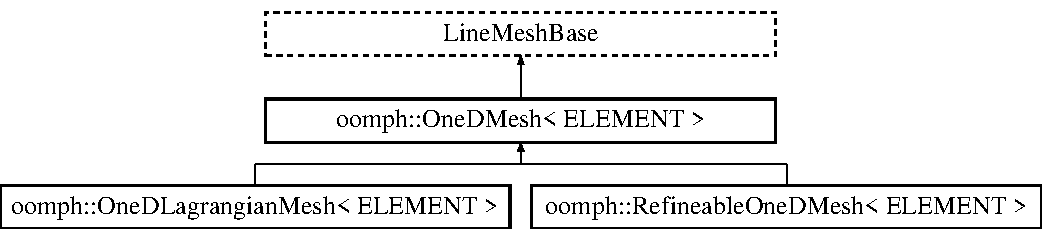
\includegraphics[height=3.000000cm]{classoomph_1_1OneDMesh}
\end{center}
\end{figure}
\subsection*{Public Member Functions}
\begin{DoxyCompactItemize}
\item 
\hyperlink{classoomph_1_1OneDMesh_ac6962f5c0184d302544253e3b4407c48}{One\+D\+Mesh} (const unsigned \&n\+\_\+element, const double \&length, Time\+Stepper $\ast$time\+\_\+stepper\+\_\+pt=\&Mesh\+::\+Default\+\_\+\+Time\+Stepper)
\begin{DoxyCompactList}\small\item\em Constructor\+: Pass number of elements, n\+\_\+element, length of domain, length, and pointer to timestepper (defaults to a Steady timestepper so we don\textquotesingle{}t need to specify one in problems without time-\/dependence). \end{DoxyCompactList}\item 
\hyperlink{classoomph_1_1OneDMesh_a1a8b9e65226f10dfbb48fe2362e83014}{One\+D\+Mesh} (const unsigned \&n\+\_\+element, const double \&xmin, const double \&xmax, Time\+Stepper $\ast$time\+\_\+stepper\+\_\+pt=\&Mesh\+::\+Default\+\_\+\+Time\+Stepper)
\begin{DoxyCompactList}\small\item\em Constructor\+: Pass number of elements, n\+\_\+element, minimum coordinate, xmin, maximum coordinate, xmax, and a pointer to a timestepper. \end{DoxyCompactList}\end{DoxyCompactItemize}
\subsection*{Protected Member Functions}
\begin{DoxyCompactItemize}
\item 
void \hyperlink{classoomph_1_1OneDMesh_a780eb2a0fdf02690aa5e93efe5ff3848}{check\+\_\+1d} () const
\item 
void \hyperlink{classoomph_1_1OneDMesh_a5a1a27eaa9d58bb85facb617127e9f0a}{build\+\_\+mesh} (Time\+Stepper $\ast$time\+\_\+stepper\+\_\+pt=\&Mesh\+::\+Default\+\_\+\+Time\+Stepper)
\begin{DoxyCompactList}\small\item\em Generic mesh constuction routine, called by all constructors. \end{DoxyCompactList}\end{DoxyCompactItemize}
\subsection*{Protected Attributes}
\begin{DoxyCompactItemize}
\item 
double \hyperlink{classoomph_1_1OneDMesh_ab1c25c2437f203dd1f6d42ec0613e6a1}{Xmin}
\begin{DoxyCompactList}\small\item\em Minimum coordinate. \end{DoxyCompactList}\item 
double \hyperlink{classoomph_1_1OneDMesh_ac625d93f5299895ad5801918a20aea31}{Xmax}
\begin{DoxyCompactList}\small\item\em Maximum coordinate. \end{DoxyCompactList}\item 
double \hyperlink{classoomph_1_1OneDMesh_a9c5ebabd7b2286b5f489563b1106e1b4}{Length}
\begin{DoxyCompactList}\small\item\em Length of the domain. \end{DoxyCompactList}\item 
unsigned \hyperlink{classoomph_1_1OneDMesh_a6f6f4087d7dd7417c79f39f2c3a2865a}{N}
\begin{DoxyCompactList}\small\item\em Number of elements. \end{DoxyCompactList}\end{DoxyCompactItemize}


\subsection{Detailed Description}
\subsubsection*{template$<$class E\+L\+E\+M\+E\+NT$>$\newline
class oomph\+::\+One\+D\+Mesh$<$ E\+L\+E\+M\+E\+N\+T $>$}

1D mesh consisting of N one-\/dimensional elements from the Q\+Element family. \[ x \in [Xmin,Xmax] \] The mesh has two boundaries\+:
\begin{DoxyItemize}
\item Boundary 0 is at $x=Xmin$.
\item Boundary 1 is at $x=Xmax$.
\end{DoxyItemize}There is one node on each of these boundaries. 

Definition at line 56 of file one\+\_\+d\+\_\+mesh.\+template.\+h.



\subsection{Constructor \& Destructor Documentation}
\mbox{\Hypertarget{classoomph_1_1OneDMesh_ac6962f5c0184d302544253e3b4407c48}\label{classoomph_1_1OneDMesh_ac6962f5c0184d302544253e3b4407c48}} 
\index{oomph\+::\+One\+D\+Mesh@{oomph\+::\+One\+D\+Mesh}!One\+D\+Mesh@{One\+D\+Mesh}}
\index{One\+D\+Mesh@{One\+D\+Mesh}!oomph\+::\+One\+D\+Mesh@{oomph\+::\+One\+D\+Mesh}}
\subsubsection{\texorpdfstring{One\+D\+Mesh()}{OneDMesh()}\hspace{0.1cm}{\footnotesize\ttfamily [1/2]}}
{\footnotesize\ttfamily template$<$class E\+L\+E\+M\+E\+NT$>$ \\
\hyperlink{classoomph_1_1OneDMesh}{oomph\+::\+One\+D\+Mesh}$<$ E\+L\+E\+M\+E\+NT $>$\+::\hyperlink{classoomph_1_1OneDMesh}{One\+D\+Mesh} (\begin{DoxyParamCaption}\item[{const unsigned \&}]{n\+\_\+element,  }\item[{const double \&}]{length,  }\item[{Time\+Stepper $\ast$}]{time\+\_\+stepper\+\_\+pt = {\ttfamily \&Mesh\+:\+:Default\+\_\+TimeStepper} }\end{DoxyParamCaption})\hspace{0.3cm}{\ttfamily [inline]}}



Constructor\+: Pass number of elements, n\+\_\+element, length of domain, length, and pointer to timestepper (defaults to a Steady timestepper so we don\textquotesingle{}t need to specify one in problems without time-\/dependence). 



Definition at line 65 of file one\+\_\+d\+\_\+mesh.\+template.\+h.

\mbox{\Hypertarget{classoomph_1_1OneDMesh_a1a8b9e65226f10dfbb48fe2362e83014}\label{classoomph_1_1OneDMesh_a1a8b9e65226f10dfbb48fe2362e83014}} 
\index{oomph\+::\+One\+D\+Mesh@{oomph\+::\+One\+D\+Mesh}!One\+D\+Mesh@{One\+D\+Mesh}}
\index{One\+D\+Mesh@{One\+D\+Mesh}!oomph\+::\+One\+D\+Mesh@{oomph\+::\+One\+D\+Mesh}}
\subsubsection{\texorpdfstring{One\+D\+Mesh()}{OneDMesh()}\hspace{0.1cm}{\footnotesize\ttfamily [2/2]}}
{\footnotesize\ttfamily template$<$class E\+L\+E\+M\+E\+NT$>$ \\
\hyperlink{classoomph_1_1OneDMesh}{oomph\+::\+One\+D\+Mesh}$<$ E\+L\+E\+M\+E\+NT $>$\+::\hyperlink{classoomph_1_1OneDMesh}{One\+D\+Mesh} (\begin{DoxyParamCaption}\item[{const unsigned \&}]{n\+\_\+element,  }\item[{const double \&}]{xmin,  }\item[{const double \&}]{xmax,  }\item[{Time\+Stepper $\ast$}]{time\+\_\+stepper\+\_\+pt = {\ttfamily \&Mesh\+:\+:Default\+\_\+TimeStepper} }\end{DoxyParamCaption})\hspace{0.3cm}{\ttfamily [inline]}}



Constructor\+: Pass number of elements, n\+\_\+element, minimum coordinate, xmin, maximum coordinate, xmax, and a pointer to a timestepper. 



Definition at line 77 of file one\+\_\+d\+\_\+mesh.\+template.\+h.



\subsection{Member Function Documentation}
\mbox{\Hypertarget{classoomph_1_1OneDMesh_a5a1a27eaa9d58bb85facb617127e9f0a}\label{classoomph_1_1OneDMesh_a5a1a27eaa9d58bb85facb617127e9f0a}} 
\index{oomph\+::\+One\+D\+Mesh@{oomph\+::\+One\+D\+Mesh}!build\+\_\+mesh@{build\+\_\+mesh}}
\index{build\+\_\+mesh@{build\+\_\+mesh}!oomph\+::\+One\+D\+Mesh@{oomph\+::\+One\+D\+Mesh}}
\subsubsection{\texorpdfstring{build\+\_\+mesh()}{build\_mesh()}}
{\footnotesize\ttfamily template$<$class E\+L\+E\+M\+E\+NT $>$ \\
void \hyperlink{classoomph_1_1OneDMesh}{oomph\+::\+One\+D\+Mesh}$<$ E\+L\+E\+M\+E\+NT $>$\+::build\+\_\+mesh (\begin{DoxyParamCaption}\item[{Time\+Stepper $\ast$}]{time\+\_\+stepper\+\_\+pt = {\ttfamily \&Mesh\+:\+:Default\+\_\+TimeStepper} }\end{DoxyParamCaption})\hspace{0.3cm}{\ttfamily [protected]}}



Generic mesh constuction routine, called by all constructors. 

The generic mesh construction routine --- this contains all the hard work and is called by all constructors 

Definition at line 47 of file one\+\_\+d\+\_\+mesh.\+template.\+cc.



Referenced by oomph\+::\+One\+D\+Mesh$<$ F\+S\+I\+Hermite\+Beam\+Element $>$\+::\+One\+D\+Mesh().

\mbox{\Hypertarget{classoomph_1_1OneDMesh_a780eb2a0fdf02690aa5e93efe5ff3848}\label{classoomph_1_1OneDMesh_a780eb2a0fdf02690aa5e93efe5ff3848}} 
\index{oomph\+::\+One\+D\+Mesh@{oomph\+::\+One\+D\+Mesh}!check\+\_\+1d@{check\+\_\+1d}}
\index{check\+\_\+1d@{check\+\_\+1d}!oomph\+::\+One\+D\+Mesh@{oomph\+::\+One\+D\+Mesh}}
\subsubsection{\texorpdfstring{check\+\_\+1d()}{check\_1d()}}
{\footnotesize\ttfamily template$<$class E\+L\+E\+M\+E\+NT$>$ \\
void \hyperlink{classoomph_1_1OneDMesh}{oomph\+::\+One\+D\+Mesh}$<$ E\+L\+E\+M\+E\+NT $>$\+::check\+\_\+1d (\begin{DoxyParamCaption}{ }\end{DoxyParamCaption}) const\hspace{0.3cm}{\ttfamily [inline]}, {\ttfamily [protected]}}

Mesh can only be built with 1D elements (but can be either T or Q so can\textquotesingle{}t use the normal assert\+\_\+geometric\+\_\+element function. 

Definition at line 90 of file one\+\_\+d\+\_\+mesh.\+template.\+h.



Referenced by oomph\+::\+One\+D\+Mesh$<$ F\+S\+I\+Hermite\+Beam\+Element $>$\+::\+One\+D\+Mesh().



\subsection{Member Data Documentation}
\mbox{\Hypertarget{classoomph_1_1OneDMesh_a9c5ebabd7b2286b5f489563b1106e1b4}\label{classoomph_1_1OneDMesh_a9c5ebabd7b2286b5f489563b1106e1b4}} 
\index{oomph\+::\+One\+D\+Mesh@{oomph\+::\+One\+D\+Mesh}!Length@{Length}}
\index{Length@{Length}!oomph\+::\+One\+D\+Mesh@{oomph\+::\+One\+D\+Mesh}}
\subsubsection{\texorpdfstring{Length}{Length}}
{\footnotesize\ttfamily template$<$class E\+L\+E\+M\+E\+NT$>$ \\
double \hyperlink{classoomph_1_1OneDMesh}{oomph\+::\+One\+D\+Mesh}$<$ E\+L\+E\+M\+E\+NT $>$\+::Length\hspace{0.3cm}{\ttfamily [protected]}}



Length of the domain. 



Definition at line 111 of file one\+\_\+d\+\_\+mesh.\+template.\+h.

\mbox{\Hypertarget{classoomph_1_1OneDMesh_a6f6f4087d7dd7417c79f39f2c3a2865a}\label{classoomph_1_1OneDMesh_a6f6f4087d7dd7417c79f39f2c3a2865a}} 
\index{oomph\+::\+One\+D\+Mesh@{oomph\+::\+One\+D\+Mesh}!N@{N}}
\index{N@{N}!oomph\+::\+One\+D\+Mesh@{oomph\+::\+One\+D\+Mesh}}
\subsubsection{\texorpdfstring{N}{N}}
{\footnotesize\ttfamily template$<$class E\+L\+E\+M\+E\+NT$>$ \\
unsigned \hyperlink{classoomph_1_1OneDMesh}{oomph\+::\+One\+D\+Mesh}$<$ E\+L\+E\+M\+E\+NT $>$\+::N\hspace{0.3cm}{\ttfamily [protected]}}



Number of elements. 



Definition at line 114 of file one\+\_\+d\+\_\+mesh.\+template.\+h.

\mbox{\Hypertarget{classoomph_1_1OneDMesh_ac625d93f5299895ad5801918a20aea31}\label{classoomph_1_1OneDMesh_ac625d93f5299895ad5801918a20aea31}} 
\index{oomph\+::\+One\+D\+Mesh@{oomph\+::\+One\+D\+Mesh}!Xmax@{Xmax}}
\index{Xmax@{Xmax}!oomph\+::\+One\+D\+Mesh@{oomph\+::\+One\+D\+Mesh}}
\subsubsection{\texorpdfstring{Xmax}{Xmax}}
{\footnotesize\ttfamily template$<$class E\+L\+E\+M\+E\+NT$>$ \\
double \hyperlink{classoomph_1_1OneDMesh}{oomph\+::\+One\+D\+Mesh}$<$ E\+L\+E\+M\+E\+NT $>$\+::Xmax\hspace{0.3cm}{\ttfamily [protected]}}



Maximum coordinate. 



Definition at line 108 of file one\+\_\+d\+\_\+mesh.\+template.\+h.

\mbox{\Hypertarget{classoomph_1_1OneDMesh_ab1c25c2437f203dd1f6d42ec0613e6a1}\label{classoomph_1_1OneDMesh_ab1c25c2437f203dd1f6d42ec0613e6a1}} 
\index{oomph\+::\+One\+D\+Mesh@{oomph\+::\+One\+D\+Mesh}!Xmin@{Xmin}}
\index{Xmin@{Xmin}!oomph\+::\+One\+D\+Mesh@{oomph\+::\+One\+D\+Mesh}}
\subsubsection{\texorpdfstring{Xmin}{Xmin}}
{\footnotesize\ttfamily template$<$class E\+L\+E\+M\+E\+NT$>$ \\
double \hyperlink{classoomph_1_1OneDMesh}{oomph\+::\+One\+D\+Mesh}$<$ E\+L\+E\+M\+E\+NT $>$\+::Xmin\hspace{0.3cm}{\ttfamily [protected]}}



Minimum coordinate. 



Definition at line 105 of file one\+\_\+d\+\_\+mesh.\+template.\+h.



The documentation for this class was generated from the following files\+:\begin{DoxyCompactItemize}
\item 
\hyperlink{one__d__mesh_8template_8h}{one\+\_\+d\+\_\+mesh.\+template.\+h}\item 
\hyperlink{one__d__mesh_8template_8cc}{one\+\_\+d\+\_\+mesh.\+template.\+cc}\end{DoxyCompactItemize}

\hypertarget{structoomph_1_1TriangleMesh_1_1Point}{}\section{oomph\+:\+:Triangle\+Mesh$<$ E\+L\+E\+M\+E\+NT $>$\+:\+:Point Struct Reference}
\label{structoomph_1_1TriangleMesh_1_1Point}\index{oomph\+::\+Triangle\+Mesh$<$ E\+L\+E\+M\+E\+N\+T $>$\+::\+Point@{oomph\+::\+Triangle\+Mesh$<$ E\+L\+E\+M\+E\+N\+T $>$\+::\+Point}}
\subsection*{Public Member Functions}
\begin{DoxyCompactItemize}
\item 
bool \hyperlink{structoomph_1_1TriangleMesh_1_1Point_a51a65a16bcb72e3b18102f0ab8001d0c}{operator$<$} (const \hyperlink{structoomph_1_1TriangleMesh_1_1Point}{Point} \&p) const
\end{DoxyCompactItemize}
\subsection*{Public Attributes}
\begin{DoxyCompactItemize}
\item 
\hyperlink{classoomph_1_1TriangleMesh_ad50b14a66b40a3bfb22a43df86c9006e}{coord\+\_\+t} \hyperlink{structoomph_1_1TriangleMesh_1_1Point_a3d99bdf85c838801260dda624a518133}{x}
\item 
\hyperlink{classoomph_1_1TriangleMesh_ad50b14a66b40a3bfb22a43df86c9006e}{coord\+\_\+t} \hyperlink{structoomph_1_1TriangleMesh_1_1Point_a0ce04810567f9e1cd9acf211073a35da}{y}
\end{DoxyCompactItemize}


\subsection{Detailed Description}
\subsubsection*{template$<$class E\+L\+E\+M\+E\+NT$>$\newline
struct oomph\+::\+Triangle\+Mesh$<$ E\+L\+E\+M\+E\+N\+T $>$\+::\+Point}



Definition at line 2074 of file triangle\+\_\+mesh.\+template.\+h.



\subsection{Member Function Documentation}
\mbox{\Hypertarget{structoomph_1_1TriangleMesh_1_1Point_a51a65a16bcb72e3b18102f0ab8001d0c}\label{structoomph_1_1TriangleMesh_1_1Point_a51a65a16bcb72e3b18102f0ab8001d0c}} 
\index{oomph\+::\+Triangle\+Mesh\+::\+Point@{oomph\+::\+Triangle\+Mesh\+::\+Point}!operator$<$@{operator$<$}}
\index{operator$<$@{operator$<$}!oomph\+::\+Triangle\+Mesh\+::\+Point@{oomph\+::\+Triangle\+Mesh\+::\+Point}}
\subsubsection{\texorpdfstring{operator$<$()}{operator<()}}
{\footnotesize\ttfamily template$<$class E\+L\+E\+M\+E\+NT$>$ \\
bool \hyperlink{classoomph_1_1TriangleMesh}{oomph\+::\+Triangle\+Mesh}$<$ E\+L\+E\+M\+E\+NT $>$\+::Point\+::operator$<$ (\begin{DoxyParamCaption}\item[{const \hyperlink{structoomph_1_1TriangleMesh_1_1Point}{Point} \&}]{p }\end{DoxyParamCaption}) const\hspace{0.3cm}{\ttfamily [inline]}}



Definition at line 2077 of file triangle\+\_\+mesh.\+template.\+h.



References oomph\+::\+Triangle\+Mesh$<$ E\+L\+E\+M\+E\+N\+T $>$\+::\+Point\+::x, and oomph\+::\+Triangle\+Mesh$<$ E\+L\+E\+M\+E\+N\+T $>$\+::\+Point\+::y.



\subsection{Member Data Documentation}
\mbox{\Hypertarget{structoomph_1_1TriangleMesh_1_1Point_a3d99bdf85c838801260dda624a518133}\label{structoomph_1_1TriangleMesh_1_1Point_a3d99bdf85c838801260dda624a518133}} 
\index{oomph\+::\+Triangle\+Mesh\+::\+Point@{oomph\+::\+Triangle\+Mesh\+::\+Point}!x@{x}}
\index{x@{x}!oomph\+::\+Triangle\+Mesh\+::\+Point@{oomph\+::\+Triangle\+Mesh\+::\+Point}}
\subsubsection{\texorpdfstring{x}{x}}
{\footnotesize\ttfamily template$<$class E\+L\+E\+M\+E\+NT$>$ \\
\hyperlink{classoomph_1_1TriangleMesh_ad50b14a66b40a3bfb22a43df86c9006e}{coord\+\_\+t} \hyperlink{classoomph_1_1TriangleMesh}{oomph\+::\+Triangle\+Mesh}$<$ E\+L\+E\+M\+E\+NT $>$\+::Point\+::x}



Definition at line 2075 of file triangle\+\_\+mesh.\+template.\+h.



Referenced by oomph\+::\+Triangle\+Mesh$<$ E\+L\+E\+M\+E\+N\+T $>$\+::cross(), oomph\+::\+Triangle\+Mesh$<$ E\+L\+E\+M\+E\+N\+T $>$\+::\+Point\+::operator$<$(), and oomph\+::\+Triangle\+Mesh$<$ E\+L\+E\+M\+E\+N\+T $>$\+::update\+\_\+holes\+\_\+information\+\_\+helper().

\mbox{\Hypertarget{structoomph_1_1TriangleMesh_1_1Point_a0ce04810567f9e1cd9acf211073a35da}\label{structoomph_1_1TriangleMesh_1_1Point_a0ce04810567f9e1cd9acf211073a35da}} 
\index{oomph\+::\+Triangle\+Mesh\+::\+Point@{oomph\+::\+Triangle\+Mesh\+::\+Point}!y@{y}}
\index{y@{y}!oomph\+::\+Triangle\+Mesh\+::\+Point@{oomph\+::\+Triangle\+Mesh\+::\+Point}}
\subsubsection{\texorpdfstring{y}{y}}
{\footnotesize\ttfamily template$<$class E\+L\+E\+M\+E\+NT$>$ \\
\hyperlink{classoomph_1_1TriangleMesh_ad50b14a66b40a3bfb22a43df86c9006e}{coord\+\_\+t} \hyperlink{classoomph_1_1TriangleMesh}{oomph\+::\+Triangle\+Mesh}$<$ E\+L\+E\+M\+E\+NT $>$\+::Point\+::y}



Definition at line 2075 of file triangle\+\_\+mesh.\+template.\+h.



Referenced by oomph\+::\+Triangle\+Mesh$<$ E\+L\+E\+M\+E\+N\+T $>$\+::cross(), oomph\+::\+Triangle\+Mesh$<$ E\+L\+E\+M\+E\+N\+T $>$\+::\+Point\+::operator$<$(), and oomph\+::\+Triangle\+Mesh$<$ E\+L\+E\+M\+E\+N\+T $>$\+::update\+\_\+holes\+\_\+information\+\_\+helper().



The documentation for this struct was generated from the following file\+:\begin{DoxyCompactItemize}
\item 
\hyperlink{triangle__mesh_8template_8h}{triangle\+\_\+mesh.\+template.\+h}\end{DoxyCompactItemize}

\hypertarget{classoomph_1_1PseudoElasticChannelWithLeafletMesh}{}\section{oomph\+:\+:Pseudo\+Elastic\+Channel\+With\+Leaflet\+Mesh$<$ E\+L\+E\+M\+E\+NT $>$ Class Template Reference}
\label{classoomph_1_1PseudoElasticChannelWithLeafletMesh}\index{oomph\+::\+Pseudo\+Elastic\+Channel\+With\+Leaflet\+Mesh$<$ E\+L\+E\+M\+E\+N\+T $>$@{oomph\+::\+Pseudo\+Elastic\+Channel\+With\+Leaflet\+Mesh$<$ E\+L\+E\+M\+E\+N\+T $>$}}


Channel with leaflet mesh upgraded to (pseudo-\/)solid mesh.  




{\ttfamily \#include $<$channel\+\_\+with\+\_\+leaflet\+\_\+mesh.\+template.\+h$>$}

Inheritance diagram for oomph\+:\+:Pseudo\+Elastic\+Channel\+With\+Leaflet\+Mesh$<$ E\+L\+E\+M\+E\+NT $>$\+:\begin{figure}[H]
\begin{center}
\leavevmode
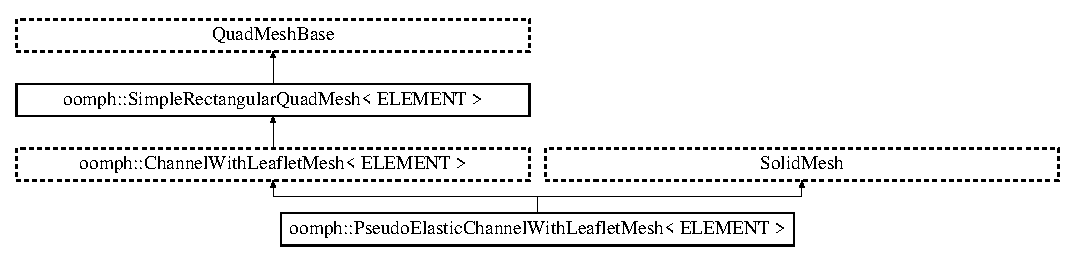
\includegraphics[height=3.076923cm]{classoomph_1_1PseudoElasticChannelWithLeafletMesh}
\end{center}
\end{figure}
\subsection*{Public Member Functions}
\begin{DoxyCompactItemize}
\item 
\hyperlink{classoomph_1_1PseudoElasticChannelWithLeafletMesh_a240a700ff3e934607b29d4ad14c6d70e}{Pseudo\+Elastic\+Channel\+With\+Leaflet\+Mesh} (Geom\+Object $\ast$leaflet\+\_\+pt, const double \&lleft, const double \&lright, const double \&hleaflet, const double \&htot, const unsigned \&nleft, const unsigned \&nright, const unsigned \&ny1, const unsigned \&ny2, Time\+Stepper $\ast$time\+\_\+stepper\+\_\+pt=\&Mesh\+::\+Default\+\_\+\+Time\+Stepper)
\begin{DoxyCompactList}\small\item\em Constructor\+: Pass pointer to Geom\+Object that represents the leaflet, the length of the domain to left and right of the leaflet, the height of the leaflet and the overall height of the channel, the number of element columns to the left and right of the leaflet, the number of rows of elements from the bottom of the channel to the end of the leaflet, the number of rows of elements above the end of the leaflet. Timestepper defaults to Steady default Timestepper defined in the Mesh base class. \end{DoxyCompactList}\item 
virtual \hyperlink{classoomph_1_1PseudoElasticChannelWithLeafletMesh_aaf0a9484052254d5840b4cde85a10a75}{$\sim$\+Pseudo\+Elastic\+Channel\+With\+Leaflet\+Mesh} ()
\begin{DoxyCompactList}\small\item\em Destructor \+: empty. \end{DoxyCompactList}\end{DoxyCompactItemize}
\subsection*{Additional Inherited Members}


\subsection{Detailed Description}
\subsubsection*{template$<$class E\+L\+E\+M\+E\+NT$>$\newline
class oomph\+::\+Pseudo\+Elastic\+Channel\+With\+Leaflet\+Mesh$<$ E\+L\+E\+M\+E\+N\+T $>$}

Channel with leaflet mesh upgraded to (pseudo-\/)solid mesh. 

Definition at line 483 of file channel\+\_\+with\+\_\+leaflet\+\_\+mesh.\+template.\+h.



\subsection{Constructor \& Destructor Documentation}
\mbox{\Hypertarget{classoomph_1_1PseudoElasticChannelWithLeafletMesh_a240a700ff3e934607b29d4ad14c6d70e}\label{classoomph_1_1PseudoElasticChannelWithLeafletMesh_a240a700ff3e934607b29d4ad14c6d70e}} 
\index{oomph\+::\+Pseudo\+Elastic\+Channel\+With\+Leaflet\+Mesh@{oomph\+::\+Pseudo\+Elastic\+Channel\+With\+Leaflet\+Mesh}!Pseudo\+Elastic\+Channel\+With\+Leaflet\+Mesh@{Pseudo\+Elastic\+Channel\+With\+Leaflet\+Mesh}}
\index{Pseudo\+Elastic\+Channel\+With\+Leaflet\+Mesh@{Pseudo\+Elastic\+Channel\+With\+Leaflet\+Mesh}!oomph\+::\+Pseudo\+Elastic\+Channel\+With\+Leaflet\+Mesh@{oomph\+::\+Pseudo\+Elastic\+Channel\+With\+Leaflet\+Mesh}}
\subsubsection{\texorpdfstring{Pseudo\+Elastic\+Channel\+With\+Leaflet\+Mesh()}{PseudoElasticChannelWithLeafletMesh()}}
{\footnotesize\ttfamily template$<$class E\+L\+E\+M\+E\+NT $>$ \\
\hyperlink{classoomph_1_1PseudoElasticChannelWithLeafletMesh}{oomph\+::\+Pseudo\+Elastic\+Channel\+With\+Leaflet\+Mesh}$<$ E\+L\+E\+M\+E\+NT $>$\+::\hyperlink{classoomph_1_1PseudoElasticChannelWithLeafletMesh}{Pseudo\+Elastic\+Channel\+With\+Leaflet\+Mesh} (\begin{DoxyParamCaption}\item[{Geom\+Object $\ast$}]{leaflet\+\_\+pt,  }\item[{const double \&}]{lleft,  }\item[{const double \&}]{lright,  }\item[{const double \&}]{hleaflet,  }\item[{const double \&}]{htot,  }\item[{const unsigned \&}]{nleft,  }\item[{const unsigned \&}]{nright,  }\item[{const unsigned \&}]{ny1,  }\item[{const unsigned \&}]{ny2,  }\item[{Time\+Stepper $\ast$}]{time\+\_\+stepper\+\_\+pt = {\ttfamily \&Mesh\+:\+:Default\+\_\+TimeStepper} }\end{DoxyParamCaption})\hspace{0.3cm}{\ttfamily [inline]}}



Constructor\+: Pass pointer to Geom\+Object that represents the leaflet, the length of the domain to left and right of the leaflet, the height of the leaflet and the overall height of the channel, the number of element columns to the left and right of the leaflet, the number of rows of elements from the bottom of the channel to the end of the leaflet, the number of rows of elements above the end of the leaflet. Timestepper defaults to Steady default Timestepper defined in the Mesh base class. 



Definition at line 497 of file channel\+\_\+with\+\_\+leaflet\+\_\+mesh.\+template.\+h.

\mbox{\Hypertarget{classoomph_1_1PseudoElasticChannelWithLeafletMesh_aaf0a9484052254d5840b4cde85a10a75}\label{classoomph_1_1PseudoElasticChannelWithLeafletMesh_aaf0a9484052254d5840b4cde85a10a75}} 
\index{oomph\+::\+Pseudo\+Elastic\+Channel\+With\+Leaflet\+Mesh@{oomph\+::\+Pseudo\+Elastic\+Channel\+With\+Leaflet\+Mesh}!````~Pseudo\+Elastic\+Channel\+With\+Leaflet\+Mesh@{$\sim$\+Pseudo\+Elastic\+Channel\+With\+Leaflet\+Mesh}}
\index{````~Pseudo\+Elastic\+Channel\+With\+Leaflet\+Mesh@{$\sim$\+Pseudo\+Elastic\+Channel\+With\+Leaflet\+Mesh}!oomph\+::\+Pseudo\+Elastic\+Channel\+With\+Leaflet\+Mesh@{oomph\+::\+Pseudo\+Elastic\+Channel\+With\+Leaflet\+Mesh}}
\subsubsection{\texorpdfstring{$\sim$\+Pseudo\+Elastic\+Channel\+With\+Leaflet\+Mesh()}{~PseudoElasticChannelWithLeafletMesh()}}
{\footnotesize\ttfamily template$<$class E\+L\+E\+M\+E\+NT $>$ \\
virtual \hyperlink{classoomph_1_1PseudoElasticChannelWithLeafletMesh}{oomph\+::\+Pseudo\+Elastic\+Channel\+With\+Leaflet\+Mesh}$<$ E\+L\+E\+M\+E\+NT $>$\+::$\sim$\hyperlink{classoomph_1_1PseudoElasticChannelWithLeafletMesh}{Pseudo\+Elastic\+Channel\+With\+Leaflet\+Mesh} (\begin{DoxyParamCaption}{ }\end{DoxyParamCaption})\hspace{0.3cm}{\ttfamily [inline]}, {\ttfamily [virtual]}}



Destructor \+: empty. 



Definition at line 524 of file channel\+\_\+with\+\_\+leaflet\+\_\+mesh.\+template.\+h.



The documentation for this class was generated from the following file\+:\begin{DoxyCompactItemize}
\item 
\hyperlink{channel__with__leaflet__mesh_8template_8h}{channel\+\_\+with\+\_\+leaflet\+\_\+mesh.\+template.\+h}\end{DoxyCompactItemize}

\hypertarget{classoomph_1_1QuadFromTriangleMesh}{}\section{oomph\+:\+:Quad\+From\+Triangle\+Mesh$<$ E\+L\+E\+M\+E\+NT $>$ Class Template Reference}
\label{classoomph_1_1QuadFromTriangleMesh}\index{oomph\+::\+Quad\+From\+Triangle\+Mesh$<$ E\+L\+E\+M\+E\+N\+T $>$@{oomph\+::\+Quad\+From\+Triangle\+Mesh$<$ E\+L\+E\+M\+E\+N\+T $>$}}


{\ttfamily \#include $<$quad\+\_\+from\+\_\+triangle\+\_\+mesh.\+template.\+h$>$}

Inheritance diagram for oomph\+:\+:Quad\+From\+Triangle\+Mesh$<$ E\+L\+E\+M\+E\+NT $>$\+:\begin{figure}[H]
\begin{center}
\leavevmode
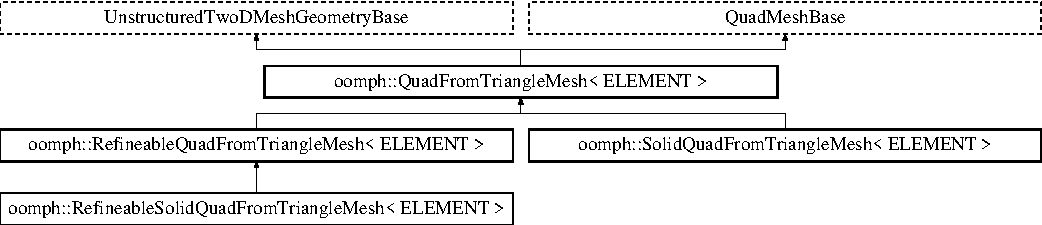
\includegraphics[height=3.027027cm]{classoomph_1_1QuadFromTriangleMesh}
\end{center}
\end{figure}
\subsection*{Public Member Functions}
\begin{DoxyCompactItemize}
\item 
\hyperlink{classoomph_1_1QuadFromTriangleMesh_af94e552be1bd35ec03eed1bcfcbc40af}{Quad\+From\+Triangle\+Mesh} ()
\begin{DoxyCompactList}\small\item\em Empty constructor. \end{DoxyCompactList}\item 
\hyperlink{classoomph_1_1QuadFromTriangleMesh_ab6fd5b49a1c1a4b29fc000953b732b98}{Quad\+From\+Triangle\+Mesh} (const std\+::string \&node\+\_\+file\+\_\+name, const std\+::string \&element\+\_\+file\+\_\+name, const std\+::string \&poly\+\_\+file\+\_\+name, Time\+Stepper $\ast$time\+\_\+stepper\+\_\+pt=\&Mesh\+::\+Default\+\_\+\+Time\+Stepper, const bool \&use\+\_\+attributes=false, const bool \&allow\+\_\+automatic\+\_\+creation\+\_\+of\+\_\+vertices\+\_\+on\+\_\+boundaries=true)
\begin{DoxyCompactList}\small\item\em Constructor with the input files. \end{DoxyCompactList}\item 
\hyperlink{classoomph_1_1QuadFromTriangleMesh_a78f9c12882d4554e4484255640b6bf51}{Quad\+From\+Triangle\+Mesh} (\hyperlink{classoomph_1_1TriangleMeshParameters}{Triangle\+Mesh\+Parameters} \&triangle\+\_\+mesh\+\_\+parameters, Time\+Stepper $\ast$time\+\_\+stepper\+\_\+pt=\&Mesh\+::\+Default\+\_\+\+Time\+Stepper)
\begin{DoxyCompactList}\small\item\em Build mesh, based on the specifications on \hyperlink{classoomph_1_1TriangleMeshParameters}{Triangle\+Mesh\+Parameters}. All the actual work is done in Unstructured\+Two\+D\+Mesh\+Geometry\+Base. \end{DoxyCompactList}\item 
void \hyperlink{classoomph_1_1QuadFromTriangleMesh_ae2036525cc3a3b2bdd8edfa01783a303}{generic\+\_\+constructor} (Vector$<$ Triangle\+Mesh\+Polygon $\ast$$>$ \&outer\+\_\+boundary\+\_\+pt, Vector$<$ Triangle\+Mesh\+Polygon $\ast$$>$ \&internal\+\_\+polygon\+\_\+pt, Vector$<$ Triangle\+Mesh\+Open\+Curve $\ast$$>$ \&open\+\_\+polylines\+\_\+pt, const double \&element\+\_\+area, Vector$<$ Vector$<$ double $>$ $>$ \&extra\+\_\+holes\+\_\+coordinates, std\+::map$<$ unsigned, Vector$<$ double $>$ $>$ \&regions\+\_\+coordinates, std\+::map$<$ unsigned, double $>$ \&regions\+\_\+areas, Time\+Stepper $\ast$time\+\_\+stepper\+\_\+pt, const bool \&use\+\_\+attributes, const bool \&refine\+\_\+boundary, const bool \&refine\+\_\+internal\+\_\+boundary)
\begin{DoxyCompactList}\small\item\em A general-\/purpose construction function that builds the mesh once the different specific constructors have assembled the appropriate information. \end{DoxyCompactList}\item 
\hyperlink{classoomph_1_1QuadFromTriangleMesh_adc45cf7389f505a2f05d477474b2dcbb}{Quad\+From\+Triangle\+Mesh} (const \hyperlink{classoomph_1_1QuadFromTriangleMesh}{Quad\+From\+Triangle\+Mesh} \&dummy)
\begin{DoxyCompactList}\small\item\em Broken copy constructor. \end{DoxyCompactList}\item 
void \hyperlink{classoomph_1_1QuadFromTriangleMesh_a873e7ed187ae267ad985e61e71e3b90c}{operator=} (const \hyperlink{classoomph_1_1QuadFromTriangleMesh}{Quad\+From\+Triangle\+Mesh} \&)
\begin{DoxyCompactList}\small\item\em Broken assignment operator. \end{DoxyCompactList}\item 
\hyperlink{classoomph_1_1QuadFromTriangleMesh_aa8737e7a7e845cab4fb6fd82c8f3506d}{$\sim$\+Quad\+From\+Triangle\+Mesh} ()
\begin{DoxyCompactList}\small\item\em Empty destructor. \end{DoxyCompactList}\item 
void \hyperlink{classoomph_1_1QuadFromTriangleMesh_ae4146d9e92cce365c292f92fcdc88c47}{build\+\_\+from\+\_\+scaffold} (Triangle\+Scaffold\+Mesh $\ast$tmp\+\_\+mesh\+\_\+pt, Time\+Stepper $\ast$time\+\_\+stepper\+\_\+pt, const bool \&use\+\_\+attributes)
\begin{DoxyCompactList}\small\item\em Build the quad mesh from the given scaffold mesh. \end{DoxyCompactList}\end{DoxyCompactItemize}
\subsection*{Public Attributes}
\begin{DoxyCompactItemize}
\item 
Time\+Stepper $\ast$ \hyperlink{classoomph_1_1QuadFromTriangleMesh_a4a4b155283407ae37a804d258ac8c6dd}{Time\+\_\+stepper\+\_\+pt}
\begin{DoxyCompactList}\small\item\em Timestepper used to build elements. \end{DoxyCompactList}\item 
bool \hyperlink{classoomph_1_1QuadFromTriangleMesh_ac654f77f031a4126e6e2707d1fa7dad1}{Use\+\_\+attributes}
\end{DoxyCompactItemize}


\subsection{Detailed Description}
\subsubsection*{template$<$class E\+L\+E\+M\+E\+NT$>$\newline
class oomph\+::\+Quad\+From\+Triangle\+Mesh$<$ E\+L\+E\+M\+E\+N\+T $>$}

Quad mesh built on top of triangle scaffold mesh coming from the triangle mesh generator Triangle. \href{http://www.cs.cmu.edu/~quake/triangle.html}{\tt http\+://www.\+cs.\+cmu.\+edu/$\sim$quake/triangle.\+html} 

Definition at line 72 of file quad\+\_\+from\+\_\+triangle\+\_\+mesh.\+template.\+h.



\subsection{Constructor \& Destructor Documentation}
\mbox{\Hypertarget{classoomph_1_1QuadFromTriangleMesh_af94e552be1bd35ec03eed1bcfcbc40af}\label{classoomph_1_1QuadFromTriangleMesh_af94e552be1bd35ec03eed1bcfcbc40af}} 
\index{oomph\+::\+Quad\+From\+Triangle\+Mesh@{oomph\+::\+Quad\+From\+Triangle\+Mesh}!Quad\+From\+Triangle\+Mesh@{Quad\+From\+Triangle\+Mesh}}
\index{Quad\+From\+Triangle\+Mesh@{Quad\+From\+Triangle\+Mesh}!oomph\+::\+Quad\+From\+Triangle\+Mesh@{oomph\+::\+Quad\+From\+Triangle\+Mesh}}
\subsubsection{\texorpdfstring{Quad\+From\+Triangle\+Mesh()}{QuadFromTriangleMesh()}\hspace{0.1cm}{\footnotesize\ttfamily [1/4]}}
{\footnotesize\ttfamily template$<$class E\+L\+E\+M\+E\+NT $>$ \\
\hyperlink{classoomph_1_1QuadFromTriangleMesh}{oomph\+::\+Quad\+From\+Triangle\+Mesh}$<$ E\+L\+E\+M\+E\+NT $>$\+::\hyperlink{classoomph_1_1QuadFromTriangleMesh}{Quad\+From\+Triangle\+Mesh} (\begin{DoxyParamCaption}{ }\end{DoxyParamCaption})\hspace{0.3cm}{\ttfamily [inline]}}



Empty constructor. 



Definition at line 79 of file quad\+\_\+from\+\_\+triangle\+\_\+mesh.\+template.\+h.

\mbox{\Hypertarget{classoomph_1_1QuadFromTriangleMesh_ab6fd5b49a1c1a4b29fc000953b732b98}\label{classoomph_1_1QuadFromTriangleMesh_ab6fd5b49a1c1a4b29fc000953b732b98}} 
\index{oomph\+::\+Quad\+From\+Triangle\+Mesh@{oomph\+::\+Quad\+From\+Triangle\+Mesh}!Quad\+From\+Triangle\+Mesh@{Quad\+From\+Triangle\+Mesh}}
\index{Quad\+From\+Triangle\+Mesh@{Quad\+From\+Triangle\+Mesh}!oomph\+::\+Quad\+From\+Triangle\+Mesh@{oomph\+::\+Quad\+From\+Triangle\+Mesh}}
\subsubsection{\texorpdfstring{Quad\+From\+Triangle\+Mesh()}{QuadFromTriangleMesh()}\hspace{0.1cm}{\footnotesize\ttfamily [2/4]}}
{\footnotesize\ttfamily template$<$class E\+L\+E\+M\+E\+NT $>$ \\
\hyperlink{classoomph_1_1QuadFromTriangleMesh}{oomph\+::\+Quad\+From\+Triangle\+Mesh}$<$ E\+L\+E\+M\+E\+NT $>$\+::\hyperlink{classoomph_1_1QuadFromTriangleMesh}{Quad\+From\+Triangle\+Mesh} (\begin{DoxyParamCaption}\item[{const std\+::string \&}]{node\+\_\+file\+\_\+name,  }\item[{const std\+::string \&}]{element\+\_\+file\+\_\+name,  }\item[{const std\+::string \&}]{poly\+\_\+file\+\_\+name,  }\item[{Time\+Stepper $\ast$}]{time\+\_\+stepper\+\_\+pt = {\ttfamily \&Mesh\+:\+:Default\+\_\+TimeStepper},  }\item[{const bool \&}]{use\+\_\+attributes = {\ttfamily false},  }\item[{const bool \&}]{allow\+\_\+automatic\+\_\+creation\+\_\+of\+\_\+vertices\+\_\+on\+\_\+boundaries = {\ttfamily true} }\end{DoxyParamCaption})\hspace{0.3cm}{\ttfamily [inline]}}



Constructor with the input files. 



Definition at line 92 of file quad\+\_\+from\+\_\+triangle\+\_\+mesh.\+template.\+h.

\mbox{\Hypertarget{classoomph_1_1QuadFromTriangleMesh_a78f9c12882d4554e4484255640b6bf51}\label{classoomph_1_1QuadFromTriangleMesh_a78f9c12882d4554e4484255640b6bf51}} 
\index{oomph\+::\+Quad\+From\+Triangle\+Mesh@{oomph\+::\+Quad\+From\+Triangle\+Mesh}!Quad\+From\+Triangle\+Mesh@{Quad\+From\+Triangle\+Mesh}}
\index{Quad\+From\+Triangle\+Mesh@{Quad\+From\+Triangle\+Mesh}!oomph\+::\+Quad\+From\+Triangle\+Mesh@{oomph\+::\+Quad\+From\+Triangle\+Mesh}}
\subsubsection{\texorpdfstring{Quad\+From\+Triangle\+Mesh()}{QuadFromTriangleMesh()}\hspace{0.1cm}{\footnotesize\ttfamily [3/4]}}
{\footnotesize\ttfamily template$<$class E\+L\+E\+M\+E\+NT $>$ \\
\hyperlink{classoomph_1_1QuadFromTriangleMesh}{oomph\+::\+Quad\+From\+Triangle\+Mesh}$<$ E\+L\+E\+M\+E\+NT $>$\+::\hyperlink{classoomph_1_1QuadFromTriangleMesh}{Quad\+From\+Triangle\+Mesh} (\begin{DoxyParamCaption}\item[{\hyperlink{classoomph_1_1TriangleMeshParameters}{Triangle\+Mesh\+Parameters} \&}]{triangle\+\_\+mesh\+\_\+parameters,  }\item[{Time\+Stepper $\ast$}]{time\+\_\+stepper\+\_\+pt = {\ttfamily \&Mesh\+:\+:Default\+\_\+TimeStepper} }\end{DoxyParamCaption})\hspace{0.3cm}{\ttfamily [inline]}}



Build mesh, based on the specifications on \hyperlink{classoomph_1_1TriangleMeshParameters}{Triangle\+Mesh\+Parameters}. All the actual work is done in Unstructured\+Two\+D\+Mesh\+Geometry\+Base. 



Definition at line 138 of file quad\+\_\+from\+\_\+triangle\+\_\+mesh.\+template.\+h.



References oomph\+::\+Triangle\+Mesh\+Parameters\+::communicator\+\_\+pt(), oomph\+::\+Triangle\+Mesh\+Parameters\+::element\+\_\+area(), oomph\+::\+Triangle\+Mesh\+Parameters\+::extra\+\_\+holes\+\_\+coordinates(), oomph\+::\+Triangle\+Mesh\+Parameters\+::internal\+\_\+closed\+\_\+curve\+\_\+pt(), oomph\+::\+Triangle\+Mesh\+Parameters\+::internal\+\_\+open\+\_\+curves\+\_\+pt(), oomph\+::\+Triangle\+Mesh\+Parameters\+::is\+\_\+automatic\+\_\+creation\+\_\+of\+\_\+vertices\+\_\+on\+\_\+boundaries\+\_\+allowed(), oomph\+::\+Triangle\+Mesh\+Parameters\+::is\+\_\+boundary\+\_\+refinement\+\_\+allowed(), oomph\+::\+Triangle\+Mesh\+Parameters\+::is\+\_\+internal\+\_\+boundary\+\_\+refinement\+\_\+allowed(), oomph\+::\+Triangle\+Mesh\+Parameters\+::is\+\_\+mesh\+\_\+distributed(), oomph\+::\+Triangle\+Mesh\+Parameters\+::is\+\_\+use\+\_\+attributes(), oomph\+::\+Triangle\+Mesh\+Parameters\+::outer\+\_\+boundary\+\_\+pt(), oomph\+::\+Triangle\+Mesh\+Parameters\+::regions\+\_\+coordinates(), and oomph\+::\+Triangle\+Mesh\+Parameters\+::target\+\_\+area\+\_\+for\+\_\+region().

\mbox{\Hypertarget{classoomph_1_1QuadFromTriangleMesh_adc45cf7389f505a2f05d477474b2dcbb}\label{classoomph_1_1QuadFromTriangleMesh_adc45cf7389f505a2f05d477474b2dcbb}} 
\index{oomph\+::\+Quad\+From\+Triangle\+Mesh@{oomph\+::\+Quad\+From\+Triangle\+Mesh}!Quad\+From\+Triangle\+Mesh@{Quad\+From\+Triangle\+Mesh}}
\index{Quad\+From\+Triangle\+Mesh@{Quad\+From\+Triangle\+Mesh}!oomph\+::\+Quad\+From\+Triangle\+Mesh@{oomph\+::\+Quad\+From\+Triangle\+Mesh}}
\subsubsection{\texorpdfstring{Quad\+From\+Triangle\+Mesh()}{QuadFromTriangleMesh()}\hspace{0.1cm}{\footnotesize\ttfamily [4/4]}}
{\footnotesize\ttfamily template$<$class E\+L\+E\+M\+E\+NT $>$ \\
\hyperlink{classoomph_1_1QuadFromTriangleMesh}{oomph\+::\+Quad\+From\+Triangle\+Mesh}$<$ E\+L\+E\+M\+E\+NT $>$\+::\hyperlink{classoomph_1_1QuadFromTriangleMesh}{Quad\+From\+Triangle\+Mesh} (\begin{DoxyParamCaption}\item[{const \hyperlink{classoomph_1_1QuadFromTriangleMesh}{Quad\+From\+Triangle\+Mesh}$<$ E\+L\+E\+M\+E\+NT $>$ \&}]{dummy }\end{DoxyParamCaption})\hspace{0.3cm}{\ttfamily [inline]}}



Broken copy constructor. 



Definition at line 502 of file quad\+\_\+from\+\_\+triangle\+\_\+mesh.\+template.\+h.

\mbox{\Hypertarget{classoomph_1_1QuadFromTriangleMesh_aa8737e7a7e845cab4fb6fd82c8f3506d}\label{classoomph_1_1QuadFromTriangleMesh_aa8737e7a7e845cab4fb6fd82c8f3506d}} 
\index{oomph\+::\+Quad\+From\+Triangle\+Mesh@{oomph\+::\+Quad\+From\+Triangle\+Mesh}!````~Quad\+From\+Triangle\+Mesh@{$\sim$\+Quad\+From\+Triangle\+Mesh}}
\index{````~Quad\+From\+Triangle\+Mesh@{$\sim$\+Quad\+From\+Triangle\+Mesh}!oomph\+::\+Quad\+From\+Triangle\+Mesh@{oomph\+::\+Quad\+From\+Triangle\+Mesh}}
\subsubsection{\texorpdfstring{$\sim$\+Quad\+From\+Triangle\+Mesh()}{~QuadFromTriangleMesh()}}
{\footnotesize\ttfamily template$<$class E\+L\+E\+M\+E\+NT $>$ \\
\hyperlink{classoomph_1_1QuadFromTriangleMesh}{oomph\+::\+Quad\+From\+Triangle\+Mesh}$<$ E\+L\+E\+M\+E\+NT $>$\+::$\sim$\hyperlink{classoomph_1_1QuadFromTriangleMesh}{Quad\+From\+Triangle\+Mesh} (\begin{DoxyParamCaption}{ }\end{DoxyParamCaption})\hspace{0.3cm}{\ttfamily [inline]}}



Empty destructor. 



Definition at line 515 of file quad\+\_\+from\+\_\+triangle\+\_\+mesh.\+template.\+h.



\subsection{Member Function Documentation}
\mbox{\Hypertarget{classoomph_1_1QuadFromTriangleMesh_ae4146d9e92cce365c292f92fcdc88c47}\label{classoomph_1_1QuadFromTriangleMesh_ae4146d9e92cce365c292f92fcdc88c47}} 
\index{oomph\+::\+Quad\+From\+Triangle\+Mesh@{oomph\+::\+Quad\+From\+Triangle\+Mesh}!build\+\_\+from\+\_\+scaffold@{build\+\_\+from\+\_\+scaffold}}
\index{build\+\_\+from\+\_\+scaffold@{build\+\_\+from\+\_\+scaffold}!oomph\+::\+Quad\+From\+Triangle\+Mesh@{oomph\+::\+Quad\+From\+Triangle\+Mesh}}
\subsubsection{\texorpdfstring{build\+\_\+from\+\_\+scaffold()}{build\_from\_scaffold()}}
{\footnotesize\ttfamily template$<$class E\+L\+E\+M\+E\+NT $>$ \\
void \hyperlink{classoomph_1_1QuadFromTriangleMesh}{oomph\+::\+Quad\+From\+Triangle\+Mesh}$<$ E\+L\+E\+M\+E\+NT $>$\+::build\+\_\+from\+\_\+scaffold (\begin{DoxyParamCaption}\item[{Triangle\+Scaffold\+Mesh $\ast$}]{tmp\+\_\+mesh\+\_\+pt,  }\item[{Time\+Stepper $\ast$}]{time\+\_\+stepper\+\_\+pt,  }\item[{const bool \&}]{use\+\_\+attributes }\end{DoxyParamCaption})}



Build the quad mesh from the given scaffold mesh. 

Build the full mesh with the help of the scaffold mesh coming from the triangle mesh generator, Triangle. To build this quad element based mesh we make use of the fact that a triangle element can be split as shown in the diagram below\+:

N2 $\vert$ $\vert$ N0 \+: 1st scaffold element node $\vert$ $\vert$ N1 \+: 2nd scaffold element node $\vert$ $\vert$ N2 \+: 3rd scaffold element node $\vert$ $\vert$ C $\vert$ Q\+\_\+2 $\vert$ B Edge 0 \+: N0 --$>$ N1 $\vert$ $\vert$ $\vert$ $\vert$ Edge 1 \+: N1 --$>$ N2 $\vert$ $\vert$ $\vert$ $\vert$ Edge 2 \+: N2 --$>$ N0 $\vert$ $\vert$ $\vert$ $\vert$ $\vert$ $\vert$ $\vert$ $\vert$ A \+: Midpoint of edge 0 $\vert$ Q\+\_\+0 $\vert$ Q\+\_\+1 $\vert$ B \+: Midpoint of edge 1 $\vert$ $\vert$ $\vert$ C \+: Midpoint of edge 2 $\vert$ $\vert$ $\vert$ N0 \+\_\+\+\_\+\+\_\+\+\_\+\+\_\+\+\_\+\+\_\+\+\_\+\+\_\+\+\_\+$\vert$\+\_\+\+\_\+\+\_\+\+\_\+\+\_\+\+\_\+\+\_\+\+\_\+\+\_\+\+\_\+ N1 A

The intersection of all three quad elements is the centroid. Using this splitting, the subsequent mesh will consist of quadrilaterals whose shape which depend on the structure of the underlying mesh. 

Definition at line 75 of file quad\+\_\+from\+\_\+triangle\+\_\+mesh.\+template.\+cc.

\mbox{\Hypertarget{classoomph_1_1QuadFromTriangleMesh_ae2036525cc3a3b2bdd8edfa01783a303}\label{classoomph_1_1QuadFromTriangleMesh_ae2036525cc3a3b2bdd8edfa01783a303}} 
\index{oomph\+::\+Quad\+From\+Triangle\+Mesh@{oomph\+::\+Quad\+From\+Triangle\+Mesh}!generic\+\_\+constructor@{generic\+\_\+constructor}}
\index{generic\+\_\+constructor@{generic\+\_\+constructor}!oomph\+::\+Quad\+From\+Triangle\+Mesh@{oomph\+::\+Quad\+From\+Triangle\+Mesh}}
\subsubsection{\texorpdfstring{generic\+\_\+constructor()}{generic\_constructor()}}
{\footnotesize\ttfamily template$<$class E\+L\+E\+M\+E\+NT $>$ \\
void \hyperlink{classoomph_1_1QuadFromTriangleMesh}{oomph\+::\+Quad\+From\+Triangle\+Mesh}$<$ E\+L\+E\+M\+E\+NT $>$\+::generic\+\_\+constructor (\begin{DoxyParamCaption}\item[{Vector$<$ Triangle\+Mesh\+Polygon $\ast$$>$ \&}]{outer\+\_\+boundary\+\_\+pt,  }\item[{Vector$<$ Triangle\+Mesh\+Polygon $\ast$$>$ \&}]{internal\+\_\+polygon\+\_\+pt,  }\item[{Vector$<$ Triangle\+Mesh\+Open\+Curve $\ast$$>$ \&}]{open\+\_\+polylines\+\_\+pt,  }\item[{const double \&}]{element\+\_\+area,  }\item[{Vector$<$ Vector$<$ double $>$ $>$ \&}]{extra\+\_\+holes\+\_\+coordinates,  }\item[{std\+::map$<$ unsigned, Vector$<$ double $>$ $>$ \&}]{regions\+\_\+coordinates,  }\item[{std\+::map$<$ unsigned, double $>$ \&}]{regions\+\_\+areas,  }\item[{Time\+Stepper $\ast$}]{time\+\_\+stepper\+\_\+pt,  }\item[{const bool \&}]{use\+\_\+attributes,  }\item[{const bool \&}]{refine\+\_\+boundary,  }\item[{const bool \&}]{refine\+\_\+internal\+\_\+boundary }\end{DoxyParamCaption})\hspace{0.3cm}{\ttfamily [inline]}}



A general-\/purpose construction function that builds the mesh once the different specific constructors have assembled the appropriate information. 



Definition at line 364 of file quad\+\_\+from\+\_\+triangle\+\_\+mesh.\+template.\+h.



References oomph\+::triangulate().

\mbox{\Hypertarget{classoomph_1_1QuadFromTriangleMesh_a873e7ed187ae267ad985e61e71e3b90c}\label{classoomph_1_1QuadFromTriangleMesh_a873e7ed187ae267ad985e61e71e3b90c}} 
\index{oomph\+::\+Quad\+From\+Triangle\+Mesh@{oomph\+::\+Quad\+From\+Triangle\+Mesh}!operator=@{operator=}}
\index{operator=@{operator=}!oomph\+::\+Quad\+From\+Triangle\+Mesh@{oomph\+::\+Quad\+From\+Triangle\+Mesh}}
\subsubsection{\texorpdfstring{operator=()}{operator=()}}
{\footnotesize\ttfamily template$<$class E\+L\+E\+M\+E\+NT $>$ \\
void \hyperlink{classoomph_1_1QuadFromTriangleMesh}{oomph\+::\+Quad\+From\+Triangle\+Mesh}$<$ E\+L\+E\+M\+E\+NT $>$\+::operator= (\begin{DoxyParamCaption}\item[{const \hyperlink{classoomph_1_1QuadFromTriangleMesh}{Quad\+From\+Triangle\+Mesh}$<$ E\+L\+E\+M\+E\+NT $>$ \&}]{ }\end{DoxyParamCaption})\hspace{0.3cm}{\ttfamily [inline]}}



Broken assignment operator. 



Definition at line 508 of file quad\+\_\+from\+\_\+triangle\+\_\+mesh.\+template.\+h.



\subsection{Member Data Documentation}
\mbox{\Hypertarget{classoomph_1_1QuadFromTriangleMesh_a4a4b155283407ae37a804d258ac8c6dd}\label{classoomph_1_1QuadFromTriangleMesh_a4a4b155283407ae37a804d258ac8c6dd}} 
\index{oomph\+::\+Quad\+From\+Triangle\+Mesh@{oomph\+::\+Quad\+From\+Triangle\+Mesh}!Time\+\_\+stepper\+\_\+pt@{Time\+\_\+stepper\+\_\+pt}}
\index{Time\+\_\+stepper\+\_\+pt@{Time\+\_\+stepper\+\_\+pt}!oomph\+::\+Quad\+From\+Triangle\+Mesh@{oomph\+::\+Quad\+From\+Triangle\+Mesh}}
\subsubsection{\texorpdfstring{Time\+\_\+stepper\+\_\+pt}{Time\_stepper\_pt}}
{\footnotesize\ttfamily template$<$class E\+L\+E\+M\+E\+NT $>$ \\
Time\+Stepper$\ast$ \hyperlink{classoomph_1_1QuadFromTriangleMesh}{oomph\+::\+Quad\+From\+Triangle\+Mesh}$<$ E\+L\+E\+M\+E\+NT $>$\+::Time\+\_\+stepper\+\_\+pt}



Timestepper used to build elements. 



Definition at line 552 of file quad\+\_\+from\+\_\+triangle\+\_\+mesh.\+template.\+h.

\mbox{\Hypertarget{classoomph_1_1QuadFromTriangleMesh_ac654f77f031a4126e6e2707d1fa7dad1}\label{classoomph_1_1QuadFromTriangleMesh_ac654f77f031a4126e6e2707d1fa7dad1}} 
\index{oomph\+::\+Quad\+From\+Triangle\+Mesh@{oomph\+::\+Quad\+From\+Triangle\+Mesh}!Use\+\_\+attributes@{Use\+\_\+attributes}}
\index{Use\+\_\+attributes@{Use\+\_\+attributes}!oomph\+::\+Quad\+From\+Triangle\+Mesh@{oomph\+::\+Quad\+From\+Triangle\+Mesh}}
\subsubsection{\texorpdfstring{Use\+\_\+attributes}{Use\_attributes}}
{\footnotesize\ttfamily template$<$class E\+L\+E\+M\+E\+NT $>$ \\
bool \hyperlink{classoomph_1_1QuadFromTriangleMesh}{oomph\+::\+Quad\+From\+Triangle\+Mesh}$<$ E\+L\+E\+M\+E\+NT $>$\+::Use\+\_\+attributes}

Boolean flag to indicate whether to use attributes or not (required for multidomain meshes) 

Definition at line 556 of file quad\+\_\+from\+\_\+triangle\+\_\+mesh.\+template.\+h.



The documentation for this class was generated from the following files\+:\begin{DoxyCompactItemize}
\item 
\hyperlink{quad__from__triangle__mesh_8template_8h}{quad\+\_\+from\+\_\+triangle\+\_\+mesh.\+template.\+h}\item 
\hyperlink{quad__from__triangle__mesh_8template_8cc}{quad\+\_\+from\+\_\+triangle\+\_\+mesh.\+template.\+cc}\end{DoxyCompactItemize}

\hypertarget{classoomph_1_1QuarterCircleSectorDomain}{}\section{oomph\+:\+:Quarter\+Circle\+Sector\+Domain Class Reference}
\label{classoomph_1_1QuarterCircleSectorDomain}\index{oomph\+::\+Quarter\+Circle\+Sector\+Domain@{oomph\+::\+Quarter\+Circle\+Sector\+Domain}}


Circular sector as domain. \hyperlink{classoomph_1_1Domain}{Domain} is bounded by curved boundary which is represented by a \hyperlink{classoomph_1_1GeomObject}{Geom\+Object}. \hyperlink{classoomph_1_1Domain}{Domain} is parametrised by three macro elements.  




{\ttfamily \#include $<$quarter\+\_\+circle\+\_\+sector\+\_\+domain.\+h$>$}

Inheritance diagram for oomph\+:\+:Quarter\+Circle\+Sector\+Domain\+:\begin{figure}[H]
\begin{center}
\leavevmode
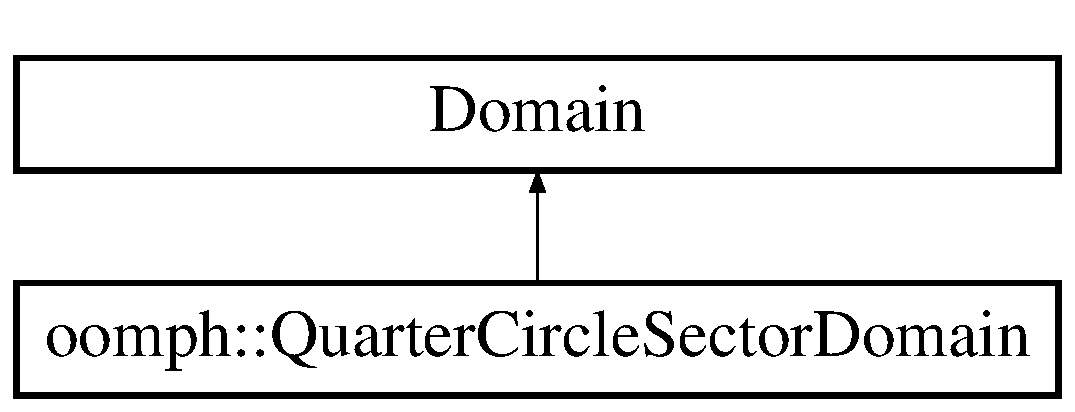
\includegraphics[height=2.000000cm]{classoomph_1_1QuarterCircleSectorDomain}
\end{center}
\end{figure}
\subsection*{Public Types}
\begin{DoxyCompactItemize}
\item 
typedef double($\ast$ \hyperlink{classoomph_1_1QuarterCircleSectorDomain_a6cffab57f87c9f4ab01744647240bb1e}{B\+L\+Squash\+Fct\+Pt}) (const double \&\hyperlink{cfortran_8h_ab7123126e4885ef647dd9c6e3807a21c}{s})
\begin{DoxyCompactList}\small\item\em Typedef for function pointer for function that squashes the outer two macro elements towards the wall by mapping the input value of the \char`\"{}radial\char`\"{} macro element coordinate to the return value. \end{DoxyCompactList}\end{DoxyCompactItemize}
\subsection*{Public Member Functions}
\begin{DoxyCompactItemize}
\item 
\hyperlink{classoomph_1_1QuarterCircleSectorDomain_accee19bdd94e0e3fe0d7c347ede685de}{Quarter\+Circle\+Sector\+Domain} (\hyperlink{classoomph_1_1GeomObject}{Geom\+Object} $\ast$boundary\+\_\+geom\+\_\+object\+\_\+pt, const double \&xi\+\_\+lo, const double \&fract\+\_\+mid, const double \&xi\+\_\+hi)
\begin{DoxyCompactList}\small\item\em Constructor\+: Pass boundary object and start and end coordinates and fraction along boundary object where outer ring is divided. \end{DoxyCompactList}\item 
\hyperlink{classoomph_1_1QuarterCircleSectorDomain_a08d26f31016ef7b40e6bdadfc1eee29a}{Quarter\+Circle\+Sector\+Domain} (const \hyperlink{classoomph_1_1QuarterCircleSectorDomain}{Quarter\+Circle\+Sector\+Domain} \&)
\begin{DoxyCompactList}\small\item\em Broken copy constructor. \end{DoxyCompactList}\item 
void \hyperlink{classoomph_1_1QuarterCircleSectorDomain_a13bb4a1ac04f99ded56c398474676ce1}{operator=} (const \hyperlink{classoomph_1_1QuarterCircleSectorDomain}{Quarter\+Circle\+Sector\+Domain} \&)
\begin{DoxyCompactList}\small\item\em Broken assignment operator. \end{DoxyCompactList}\item 
\hyperlink{classoomph_1_1QuarterCircleSectorDomain_aea4997af819b532c8d8588123785950a}{$\sim$\+Quarter\+Circle\+Sector\+Domain} ()
\begin{DoxyCompactList}\small\item\em Destructor\+: Kill macro elements. \end{DoxyCompactList}\item 
\hyperlink{classoomph_1_1QuarterCircleSectorDomain_a6cffab57f87c9f4ab01744647240bb1e}{B\+L\+Squash\+Fct\+Pt} \& \hyperlink{classoomph_1_1QuarterCircleSectorDomain_ad8f22c0c3dc71c104465a24dac9b7c17}{bl\+\_\+squash\+\_\+fct\+\_\+pt} ()
\begin{DoxyCompactList}\small\item\em Function pointer for function that squashes the outer two macro elements towards the wall by mapping the input value of the \char`\"{}radial\char`\"{} macro element coordinate to the return value. \end{DoxyCompactList}\item 
double \hyperlink{classoomph_1_1QuarterCircleSectorDomain_a5b66f846233b3cf976ed63d9bf54f0c7}{s\+\_\+squashed} (const double \&\hyperlink{cfortran_8h_ab7123126e4885ef647dd9c6e3807a21c}{s})
\begin{DoxyCompactList}\small\item\em Function that squashes the outer two macro elements towards the wall by mapping the input value of the \char`\"{}radial\char`\"{} macro element coordinate to the return value. \end{DoxyCompactList}\item 
void \hyperlink{classoomph_1_1QuarterCircleSectorDomain_a9faddf9d13e0a7633f732bac1ddda80b}{macro\+\_\+element\+\_\+boundary} (const unsigned \&\hyperlink{cfortran_8h_af6f0bd3dc13317f895c91323c25c2b8f}{t}, const unsigned \&i\+\_\+macro, const unsigned \&i\+\_\+direct, const \hyperlink{classoomph_1_1Vector}{Vector}$<$ double $>$ \&\hyperlink{cfortran_8h_ab7123126e4885ef647dd9c6e3807a21c}{s}, \hyperlink{classoomph_1_1Vector}{Vector}$<$ double $>$ \&f)
\begin{DoxyCompactList}\small\item\em \hyperlink{classoomph_1_1Vector}{Vector} representation of the i\+\_\+macro-\/th macro element boundary i\+\_\+direct (N/\+S/\+W/E) at time level t (t=0\+: present; t$>$0\+: previous)\+: f(s). Note that the local coordinate {\bfseries s} is a 1D \hyperlink{classoomph_1_1Vector}{Vector} rather than a scalar -- this is unavoidable because this function implements the pure virtual function in the \hyperlink{classoomph_1_1Domain}{Domain} base class. \end{DoxyCompactList}\end{DoxyCompactItemize}
\subsection*{Private Member Functions}
\begin{DoxyCompactItemize}
\item 
void \hyperlink{classoomph_1_1QuarterCircleSectorDomain_af1520e712b46c8e1b0f098596fa63101}{r\+\_\+top\+\_\+left\+\_\+N} (const unsigned \&\hyperlink{cfortran_8h_af6f0bd3dc13317f895c91323c25c2b8f}{t}, const \hyperlink{classoomph_1_1Vector}{Vector}$<$ double $>$ \&zeta, \hyperlink{classoomph_1_1Vector}{Vector}$<$ double $>$ \&f)
\begin{DoxyCompactList}\small\item\em Boundary of top left macro element zeta $ \in [-1,1] $. \end{DoxyCompactList}\item 
void \hyperlink{classoomph_1_1QuarterCircleSectorDomain_a84f4970adc3a93392ef1a57f19df96a1}{r\+\_\+top\+\_\+left\+\_\+W} (const unsigned \&\hyperlink{cfortran_8h_af6f0bd3dc13317f895c91323c25c2b8f}{t}, const \hyperlink{classoomph_1_1Vector}{Vector}$<$ double $>$ \&zeta, \hyperlink{classoomph_1_1Vector}{Vector}$<$ double $>$ \&f)
\begin{DoxyCompactList}\small\item\em Boundary of top left macro element zeta $ \in [-1,1] $. \end{DoxyCompactList}\item 
void \hyperlink{classoomph_1_1QuarterCircleSectorDomain_a0bb74af9c782bd0a0a8d3ccfd708af55}{r\+\_\+top\+\_\+left\+\_\+S} (const unsigned \&\hyperlink{cfortran_8h_af6f0bd3dc13317f895c91323c25c2b8f}{t}, const \hyperlink{classoomph_1_1Vector}{Vector}$<$ double $>$ \&zeta, \hyperlink{classoomph_1_1Vector}{Vector}$<$ double $>$ \&f)
\begin{DoxyCompactList}\small\item\em Boundary of top left macro element zeta $ \in [-1,1] $. \end{DoxyCompactList}\item 
void \hyperlink{classoomph_1_1QuarterCircleSectorDomain_a951bc38c7e96a40f33c60b3ccee820bf}{r\+\_\+top\+\_\+left\+\_\+E} (const unsigned \&\hyperlink{cfortran_8h_af6f0bd3dc13317f895c91323c25c2b8f}{t}, const \hyperlink{classoomph_1_1Vector}{Vector}$<$ double $>$ \&zeta, \hyperlink{classoomph_1_1Vector}{Vector}$<$ double $>$ \&f)
\begin{DoxyCompactList}\small\item\em Boundary of top left macro element zeta $ \in [-1,1] $. \end{DoxyCompactList}\item 
void \hyperlink{classoomph_1_1QuarterCircleSectorDomain_ad937b0da664b5c01063e7f8de6427fce}{r\+\_\+bot\+\_\+right\+\_\+N} (const unsigned \&\hyperlink{cfortran_8h_af6f0bd3dc13317f895c91323c25c2b8f}{t}, const \hyperlink{classoomph_1_1Vector}{Vector}$<$ double $>$ \&zeta, \hyperlink{classoomph_1_1Vector}{Vector}$<$ double $>$ \&f)
\begin{DoxyCompactList}\small\item\em Boundary of bottom right macro element zeta $ \in [-1,1] $. \end{DoxyCompactList}\item 
void \hyperlink{classoomph_1_1QuarterCircleSectorDomain_a85ba295aaeff2833644691978deac247}{r\+\_\+bot\+\_\+right\+\_\+W} (const unsigned \&\hyperlink{cfortran_8h_af6f0bd3dc13317f895c91323c25c2b8f}{t}, const \hyperlink{classoomph_1_1Vector}{Vector}$<$ double $>$ \&zeta, \hyperlink{classoomph_1_1Vector}{Vector}$<$ double $>$ \&f)
\begin{DoxyCompactList}\small\item\em Boundary of bottom right macro element zeta $ \in [-1,1] $. \end{DoxyCompactList}\item 
void \hyperlink{classoomph_1_1QuarterCircleSectorDomain_a552f9bfc6fd451669f44ee02c8bb0d38}{r\+\_\+bot\+\_\+right\+\_\+S} (const unsigned \&\hyperlink{cfortran_8h_af6f0bd3dc13317f895c91323c25c2b8f}{t}, const \hyperlink{classoomph_1_1Vector}{Vector}$<$ double $>$ \&zeta, \hyperlink{classoomph_1_1Vector}{Vector}$<$ double $>$ \&f)
\begin{DoxyCompactList}\small\item\em Boundary of bottom right macro element zeta $ \in [-1,1] $. \end{DoxyCompactList}\item 
void \hyperlink{classoomph_1_1QuarterCircleSectorDomain_abb05f2e719d81f167fc0f608e80c5696}{r\+\_\+bot\+\_\+right\+\_\+E} (const unsigned \&\hyperlink{cfortran_8h_af6f0bd3dc13317f895c91323c25c2b8f}{t}, const \hyperlink{classoomph_1_1Vector}{Vector}$<$ double $>$ \&zeta, \hyperlink{classoomph_1_1Vector}{Vector}$<$ double $>$ \&f)
\begin{DoxyCompactList}\small\item\em Boundary of bottom right macro element zeta $ \in [-1,1] $. \end{DoxyCompactList}\item 
void \hyperlink{classoomph_1_1QuarterCircleSectorDomain_a1cb12e9b1d2e17f8bd5c3d6691be3b1d}{r\+\_\+centr\+\_\+N} (const unsigned \&\hyperlink{cfortran_8h_af6f0bd3dc13317f895c91323c25c2b8f}{t}, const \hyperlink{classoomph_1_1Vector}{Vector}$<$ double $>$ \&zeta, \hyperlink{classoomph_1_1Vector}{Vector}$<$ double $>$ \&f)
\begin{DoxyCompactList}\small\item\em Boundary of central box macro element zeta $ \in [-1,1] $. \end{DoxyCompactList}\item 
void \hyperlink{classoomph_1_1QuarterCircleSectorDomain_ae4558d37a4f9bb3f9d78b6878cb77a49}{r\+\_\+centr\+\_\+E} (const unsigned \&\hyperlink{cfortran_8h_af6f0bd3dc13317f895c91323c25c2b8f}{t}, const \hyperlink{classoomph_1_1Vector}{Vector}$<$ double $>$ \&zeta, \hyperlink{classoomph_1_1Vector}{Vector}$<$ double $>$ \&f)
\begin{DoxyCompactList}\small\item\em Boundary of central box macro element zeta $ \in [-1,1] $. \end{DoxyCompactList}\item 
void \hyperlink{classoomph_1_1QuarterCircleSectorDomain_aaa17ff1d6529000f8309005396966830}{r\+\_\+centr\+\_\+S} (const unsigned \&\hyperlink{cfortran_8h_af6f0bd3dc13317f895c91323c25c2b8f}{t}, const \hyperlink{classoomph_1_1Vector}{Vector}$<$ double $>$ \&zeta, \hyperlink{classoomph_1_1Vector}{Vector}$<$ double $>$ \&f)
\begin{DoxyCompactList}\small\item\em Boundary of central box macro element zeta $ \in [-1,1] $. \end{DoxyCompactList}\item 
void \hyperlink{classoomph_1_1QuarterCircleSectorDomain_a453fc6f043f57031c1347065d521a1c3}{r\+\_\+centr\+\_\+W} (const unsigned \&\hyperlink{cfortran_8h_af6f0bd3dc13317f895c91323c25c2b8f}{t}, const \hyperlink{classoomph_1_1Vector}{Vector}$<$ double $>$ \&zeta, \hyperlink{classoomph_1_1Vector}{Vector}$<$ double $>$ \&f)
\begin{DoxyCompactList}\small\item\em Boundary of central box macro element zeta $ \in [-1,1] $. \end{DoxyCompactList}\end{DoxyCompactItemize}
\subsection*{Static Private Member Functions}
\begin{DoxyCompactItemize}
\item 
static double \hyperlink{classoomph_1_1QuarterCircleSectorDomain_adce1f0c6cf5405d6f8e9e6e0390d8c68}{default\+\_\+\+B\+L\+\_\+squash\+\_\+fct} (const double \&\hyperlink{cfortran_8h_ab7123126e4885ef647dd9c6e3807a21c}{s})
\begin{DoxyCompactList}\small\item\em Default for function that squashes the outer two macro elements towards the wall by mapping the input value of the \char`\"{}radial\char`\"{} macro element coordinate to the return value\+: Identity. \end{DoxyCompactList}\end{DoxyCompactItemize}
\subsection*{Private Attributes}
\begin{DoxyCompactItemize}
\item 
double \hyperlink{classoomph_1_1QuarterCircleSectorDomain_afed5ccc21ccf6c6cd1dca65d58a5b708}{Xi\+\_\+lo}
\begin{DoxyCompactList}\small\item\em Lower limit for the (1D) coordinates along the wall. \end{DoxyCompactList}\item 
double \hyperlink{classoomph_1_1QuarterCircleSectorDomain_ade78897c44c26af82ac90052f799796c}{Fract\+\_\+mid}
\begin{DoxyCompactList}\small\item\em Fraction along wall where outer ring is to be divided. \end{DoxyCompactList}\item 
double \hyperlink{classoomph_1_1QuarterCircleSectorDomain_aba0cc67782144fe066dd0d04ac9d79dd}{Xi\+\_\+hi}
\begin{DoxyCompactList}\small\item\em Upper limit for the (1D) coordinates along the wall. \end{DoxyCompactList}\item 
\hyperlink{classoomph_1_1GeomObject}{Geom\+Object} $\ast$ \hyperlink{classoomph_1_1QuarterCircleSectorDomain_a59722c43d41fef0bc3df4cf6571930a8}{Wall\+\_\+pt}
\begin{DoxyCompactList}\small\item\em Pointer to geometric object that represents the curved wall. \end{DoxyCompactList}\item 
\hyperlink{classoomph_1_1QuarterCircleSectorDomain_a6cffab57f87c9f4ab01744647240bb1e}{B\+L\+Squash\+Fct\+Pt} \hyperlink{classoomph_1_1QuarterCircleSectorDomain_ae9b74ffcade9fdc1eeba26b4acced7a8}{B\+L\+\_\+squash\+\_\+fct\+\_\+pt}
\begin{DoxyCompactList}\small\item\em Function pointer for function that squashes the outer two macro elements towards the wall by mapping the input value of the \char`\"{}radial\char`\"{} macro element coordinate to the return value. \end{DoxyCompactList}\end{DoxyCompactItemize}
\subsection*{Additional Inherited Members}


\subsection{Detailed Description}
Circular sector as domain. \hyperlink{classoomph_1_1Domain}{Domain} is bounded by curved boundary which is represented by a \hyperlink{classoomph_1_1GeomObject}{Geom\+Object}. \hyperlink{classoomph_1_1Domain}{Domain} is parametrised by three macro elements. 

Definition at line 50 of file quarter\+\_\+circle\+\_\+sector\+\_\+domain.\+h.



\subsection{Member Typedef Documentation}
\mbox{\Hypertarget{classoomph_1_1QuarterCircleSectorDomain_a6cffab57f87c9f4ab01744647240bb1e}\label{classoomph_1_1QuarterCircleSectorDomain_a6cffab57f87c9f4ab01744647240bb1e}} 
\index{oomph\+::\+Quarter\+Circle\+Sector\+Domain@{oomph\+::\+Quarter\+Circle\+Sector\+Domain}!B\+L\+Squash\+Fct\+Pt@{B\+L\+Squash\+Fct\+Pt}}
\index{B\+L\+Squash\+Fct\+Pt@{B\+L\+Squash\+Fct\+Pt}!oomph\+::\+Quarter\+Circle\+Sector\+Domain@{oomph\+::\+Quarter\+Circle\+Sector\+Domain}}
\subsubsection{\texorpdfstring{B\+L\+Squash\+Fct\+Pt}{BLSquashFctPt}}
{\footnotesize\ttfamily typedef double($\ast$ oomph\+::\+Quarter\+Circle\+Sector\+Domain\+::\+B\+L\+Squash\+Fct\+Pt) (const double \&\hyperlink{cfortran_8h_ab7123126e4885ef647dd9c6e3807a21c}{s})}



Typedef for function pointer for function that squashes the outer two macro elements towards the wall by mapping the input value of the \char`\"{}radial\char`\"{} macro element coordinate to the return value. 



Definition at line 106 of file quarter\+\_\+circle\+\_\+sector\+\_\+domain.\+h.



\subsection{Constructor \& Destructor Documentation}
\mbox{\Hypertarget{classoomph_1_1QuarterCircleSectorDomain_accee19bdd94e0e3fe0d7c347ede685de}\label{classoomph_1_1QuarterCircleSectorDomain_accee19bdd94e0e3fe0d7c347ede685de}} 
\index{oomph\+::\+Quarter\+Circle\+Sector\+Domain@{oomph\+::\+Quarter\+Circle\+Sector\+Domain}!Quarter\+Circle\+Sector\+Domain@{Quarter\+Circle\+Sector\+Domain}}
\index{Quarter\+Circle\+Sector\+Domain@{Quarter\+Circle\+Sector\+Domain}!oomph\+::\+Quarter\+Circle\+Sector\+Domain@{oomph\+::\+Quarter\+Circle\+Sector\+Domain}}
\subsubsection{\texorpdfstring{Quarter\+Circle\+Sector\+Domain()}{QuarterCircleSectorDomain()}\hspace{0.1cm}{\footnotesize\ttfamily [1/2]}}
{\footnotesize\ttfamily oomph\+::\+Quarter\+Circle\+Sector\+Domain\+::\+Quarter\+Circle\+Sector\+Domain (\begin{DoxyParamCaption}\item[{\hyperlink{classoomph_1_1GeomObject}{Geom\+Object} $\ast$}]{boundary\+\_\+geom\+\_\+object\+\_\+pt,  }\item[{const double \&}]{xi\+\_\+lo,  }\item[{const double \&}]{fract\+\_\+mid,  }\item[{const double \&}]{xi\+\_\+hi }\end{DoxyParamCaption})\hspace{0.3cm}{\ttfamily [inline]}}



Constructor\+: Pass boundary object and start and end coordinates and fraction along boundary object where outer ring is divided. 



Definition at line 59 of file quarter\+\_\+circle\+\_\+sector\+\_\+domain.\+h.



References i, and oomph\+::\+Domain\+::\+Macro\+\_\+element\+\_\+pt.

\mbox{\Hypertarget{classoomph_1_1QuarterCircleSectorDomain_a08d26f31016ef7b40e6bdadfc1eee29a}\label{classoomph_1_1QuarterCircleSectorDomain_a08d26f31016ef7b40e6bdadfc1eee29a}} 
\index{oomph\+::\+Quarter\+Circle\+Sector\+Domain@{oomph\+::\+Quarter\+Circle\+Sector\+Domain}!Quarter\+Circle\+Sector\+Domain@{Quarter\+Circle\+Sector\+Domain}}
\index{Quarter\+Circle\+Sector\+Domain@{Quarter\+Circle\+Sector\+Domain}!oomph\+::\+Quarter\+Circle\+Sector\+Domain@{oomph\+::\+Quarter\+Circle\+Sector\+Domain}}
\subsubsection{\texorpdfstring{Quarter\+Circle\+Sector\+Domain()}{QuarterCircleSectorDomain()}\hspace{0.1cm}{\footnotesize\ttfamily [2/2]}}
{\footnotesize\ttfamily oomph\+::\+Quarter\+Circle\+Sector\+Domain\+::\+Quarter\+Circle\+Sector\+Domain (\begin{DoxyParamCaption}\item[{const \hyperlink{classoomph_1_1QuarterCircleSectorDomain}{Quarter\+Circle\+Sector\+Domain} \&}]{ }\end{DoxyParamCaption})\hspace{0.3cm}{\ttfamily [inline]}}



Broken copy constructor. 



Definition at line 81 of file quarter\+\_\+circle\+\_\+sector\+\_\+domain.\+h.



References oomph\+::\+Broken\+Copy\+::broken\+\_\+copy().

\mbox{\Hypertarget{classoomph_1_1QuarterCircleSectorDomain_aea4997af819b532c8d8588123785950a}\label{classoomph_1_1QuarterCircleSectorDomain_aea4997af819b532c8d8588123785950a}} 
\index{oomph\+::\+Quarter\+Circle\+Sector\+Domain@{oomph\+::\+Quarter\+Circle\+Sector\+Domain}!````~Quarter\+Circle\+Sector\+Domain@{$\sim$\+Quarter\+Circle\+Sector\+Domain}}
\index{````~Quarter\+Circle\+Sector\+Domain@{$\sim$\+Quarter\+Circle\+Sector\+Domain}!oomph\+::\+Quarter\+Circle\+Sector\+Domain@{oomph\+::\+Quarter\+Circle\+Sector\+Domain}}
\subsubsection{\texorpdfstring{$\sim$\+Quarter\+Circle\+Sector\+Domain()}{~QuarterCircleSectorDomain()}}
{\footnotesize\ttfamily oomph\+::\+Quarter\+Circle\+Sector\+Domain\+::$\sim$\+Quarter\+Circle\+Sector\+Domain (\begin{DoxyParamCaption}{ }\end{DoxyParamCaption})\hspace{0.3cm}{\ttfamily [inline]}}



Destructor\+: Kill macro elements. 



Definition at line 94 of file quarter\+\_\+circle\+\_\+sector\+\_\+domain.\+h.



References i, and oomph\+::\+Domain\+::\+Macro\+\_\+element\+\_\+pt.



\subsection{Member Function Documentation}
\mbox{\Hypertarget{classoomph_1_1QuarterCircleSectorDomain_ad8f22c0c3dc71c104465a24dac9b7c17}\label{classoomph_1_1QuarterCircleSectorDomain_ad8f22c0c3dc71c104465a24dac9b7c17}} 
\index{oomph\+::\+Quarter\+Circle\+Sector\+Domain@{oomph\+::\+Quarter\+Circle\+Sector\+Domain}!bl\+\_\+squash\+\_\+fct\+\_\+pt@{bl\+\_\+squash\+\_\+fct\+\_\+pt}}
\index{bl\+\_\+squash\+\_\+fct\+\_\+pt@{bl\+\_\+squash\+\_\+fct\+\_\+pt}!oomph\+::\+Quarter\+Circle\+Sector\+Domain@{oomph\+::\+Quarter\+Circle\+Sector\+Domain}}
\subsubsection{\texorpdfstring{bl\+\_\+squash\+\_\+fct\+\_\+pt()}{bl\_squash\_fct\_pt()}}
{\footnotesize\ttfamily \hyperlink{classoomph_1_1QuarterCircleSectorDomain_a6cffab57f87c9f4ab01744647240bb1e}{B\+L\+Squash\+Fct\+Pt}\& oomph\+::\+Quarter\+Circle\+Sector\+Domain\+::bl\+\_\+squash\+\_\+fct\+\_\+pt (\begin{DoxyParamCaption}{ }\end{DoxyParamCaption})\hspace{0.3cm}{\ttfamily [inline]}}



Function pointer for function that squashes the outer two macro elements towards the wall by mapping the input value of the \char`\"{}radial\char`\"{} macro element coordinate to the return value. 



Definition at line 113 of file quarter\+\_\+circle\+\_\+sector\+\_\+domain.\+h.



References B\+L\+\_\+squash\+\_\+fct\+\_\+pt.



Referenced by oomph\+::\+Quarter\+Circle\+Sector\+Mesh$<$ E\+L\+E\+M\+E\+N\+T $>$\+::bl\+\_\+squash\+\_\+fct\+\_\+pt().

\mbox{\Hypertarget{classoomph_1_1QuarterCircleSectorDomain_adce1f0c6cf5405d6f8e9e6e0390d8c68}\label{classoomph_1_1QuarterCircleSectorDomain_adce1f0c6cf5405d6f8e9e6e0390d8c68}} 
\index{oomph\+::\+Quarter\+Circle\+Sector\+Domain@{oomph\+::\+Quarter\+Circle\+Sector\+Domain}!default\+\_\+\+B\+L\+\_\+squash\+\_\+fct@{default\+\_\+\+B\+L\+\_\+squash\+\_\+fct}}
\index{default\+\_\+\+B\+L\+\_\+squash\+\_\+fct@{default\+\_\+\+B\+L\+\_\+squash\+\_\+fct}!oomph\+::\+Quarter\+Circle\+Sector\+Domain@{oomph\+::\+Quarter\+Circle\+Sector\+Domain}}
\subsubsection{\texorpdfstring{default\+\_\+\+B\+L\+\_\+squash\+\_\+fct()}{default\_BL\_squash\_fct()}}
{\footnotesize\ttfamily static double oomph\+::\+Quarter\+Circle\+Sector\+Domain\+::default\+\_\+\+B\+L\+\_\+squash\+\_\+fct (\begin{DoxyParamCaption}\item[{const double \&}]{s }\end{DoxyParamCaption})\hspace{0.3cm}{\ttfamily [inline]}, {\ttfamily [static]}, {\ttfamily [private]}}



Default for function that squashes the outer two macro elements towards the wall by mapping the input value of the \char`\"{}radial\char`\"{} macro element coordinate to the return value\+: Identity. 



Definition at line 165 of file quarter\+\_\+circle\+\_\+sector\+\_\+domain.\+h.



References r\+\_\+bot\+\_\+right\+\_\+\+E(), r\+\_\+bot\+\_\+right\+\_\+\+N(), r\+\_\+bot\+\_\+right\+\_\+\+S(), r\+\_\+bot\+\_\+right\+\_\+\+W(), r\+\_\+centr\+\_\+\+E(), r\+\_\+centr\+\_\+\+N(), r\+\_\+centr\+\_\+\+S(), r\+\_\+centr\+\_\+\+W(), r\+\_\+top\+\_\+left\+\_\+\+E(), r\+\_\+top\+\_\+left\+\_\+\+N(), r\+\_\+top\+\_\+left\+\_\+\+S(), r\+\_\+top\+\_\+left\+\_\+\+W(), and s.

\mbox{\Hypertarget{classoomph_1_1QuarterCircleSectorDomain_a9faddf9d13e0a7633f732bac1ddda80b}\label{classoomph_1_1QuarterCircleSectorDomain_a9faddf9d13e0a7633f732bac1ddda80b}} 
\index{oomph\+::\+Quarter\+Circle\+Sector\+Domain@{oomph\+::\+Quarter\+Circle\+Sector\+Domain}!macro\+\_\+element\+\_\+boundary@{macro\+\_\+element\+\_\+boundary}}
\index{macro\+\_\+element\+\_\+boundary@{macro\+\_\+element\+\_\+boundary}!oomph\+::\+Quarter\+Circle\+Sector\+Domain@{oomph\+::\+Quarter\+Circle\+Sector\+Domain}}
\subsubsection{\texorpdfstring{macro\+\_\+element\+\_\+boundary()}{macro\_element\_boundary()}}
{\footnotesize\ttfamily void oomph\+::\+Quarter\+Circle\+Sector\+Domain\+::macro\+\_\+element\+\_\+boundary (\begin{DoxyParamCaption}\item[{const unsigned \&}]{t,  }\item[{const unsigned \&}]{imacro,  }\item[{const unsigned \&}]{idirect,  }\item[{const \hyperlink{classoomph_1_1Vector}{Vector}$<$ double $>$ \&}]{s,  }\item[{\hyperlink{classoomph_1_1Vector}{Vector}$<$ double $>$ \&}]{f }\end{DoxyParamCaption})\hspace{0.3cm}{\ttfamily [virtual]}}



\hyperlink{classoomph_1_1Vector}{Vector} representation of the i\+\_\+macro-\/th macro element boundary i\+\_\+direct (N/\+S/\+W/E) at time level t (t=0\+: present; t$>$0\+: previous)\+: f(s). Note that the local coordinate {\bfseries s} is a 1D \hyperlink{classoomph_1_1Vector}{Vector} rather than a scalar -- this is unavoidable because this function implements the pure virtual function in the \hyperlink{classoomph_1_1Domain}{Domain} base class. 

\hyperlink{classoomph_1_1Vector}{Vector} representation of the imacro-\/th macro element boundary idirect (N/\+S/\+W/E) at time level t (t=0\+: present; t$>$0\+: previous)\+: f(s) 

Implements \hyperlink{classoomph_1_1Domain_a95f3e00d28ea37e6c4d3027bfac91096}{oomph\+::\+Domain}.



Definition at line 233 of file quarter\+\_\+circle\+\_\+sector\+\_\+domain.\+h.



References oomph\+::\+Quad\+Tree\+Names\+::E, oomph\+::\+Quad\+Tree\+Names\+::N, r\+\_\+bot\+\_\+right\+\_\+\+E(), r\+\_\+bot\+\_\+right\+\_\+\+N(), r\+\_\+bot\+\_\+right\+\_\+\+S(), r\+\_\+bot\+\_\+right\+\_\+\+W(), r\+\_\+centr\+\_\+\+E(), r\+\_\+centr\+\_\+\+N(), r\+\_\+centr\+\_\+\+S(), r\+\_\+centr\+\_\+\+W(), r\+\_\+top\+\_\+left\+\_\+\+E(), r\+\_\+top\+\_\+left\+\_\+\+N(), r\+\_\+top\+\_\+left\+\_\+\+S(), r\+\_\+top\+\_\+left\+\_\+\+W(), oomph\+::\+Quad\+Tree\+Names\+::S, and oomph\+::\+Quad\+Tree\+Names\+::W.



Referenced by s\+\_\+squashed().

\mbox{\Hypertarget{classoomph_1_1QuarterCircleSectorDomain_a13bb4a1ac04f99ded56c398474676ce1}\label{classoomph_1_1QuarterCircleSectorDomain_a13bb4a1ac04f99ded56c398474676ce1}} 
\index{oomph\+::\+Quarter\+Circle\+Sector\+Domain@{oomph\+::\+Quarter\+Circle\+Sector\+Domain}!operator=@{operator=}}
\index{operator=@{operator=}!oomph\+::\+Quarter\+Circle\+Sector\+Domain@{oomph\+::\+Quarter\+Circle\+Sector\+Domain}}
\subsubsection{\texorpdfstring{operator=()}{operator=()}}
{\footnotesize\ttfamily void oomph\+::\+Quarter\+Circle\+Sector\+Domain\+::operator= (\begin{DoxyParamCaption}\item[{const \hyperlink{classoomph_1_1QuarterCircleSectorDomain}{Quarter\+Circle\+Sector\+Domain} \&}]{ }\end{DoxyParamCaption})\hspace{0.3cm}{\ttfamily [inline]}}



Broken assignment operator. 



Definition at line 87 of file quarter\+\_\+circle\+\_\+sector\+\_\+domain.\+h.



References oomph\+::\+Broken\+Copy\+::broken\+\_\+assign().

\mbox{\Hypertarget{classoomph_1_1QuarterCircleSectorDomain_abb05f2e719d81f167fc0f608e80c5696}\label{classoomph_1_1QuarterCircleSectorDomain_abb05f2e719d81f167fc0f608e80c5696}} 
\index{oomph\+::\+Quarter\+Circle\+Sector\+Domain@{oomph\+::\+Quarter\+Circle\+Sector\+Domain}!r\+\_\+bot\+\_\+right\+\_\+E@{r\+\_\+bot\+\_\+right\+\_\+E}}
\index{r\+\_\+bot\+\_\+right\+\_\+E@{r\+\_\+bot\+\_\+right\+\_\+E}!oomph\+::\+Quarter\+Circle\+Sector\+Domain@{oomph\+::\+Quarter\+Circle\+Sector\+Domain}}
\subsubsection{\texorpdfstring{r\+\_\+bot\+\_\+right\+\_\+\+E()}{r\_bot\_right\_E()}}
{\footnotesize\ttfamily void oomph\+::\+Quarter\+Circle\+Sector\+Domain\+::r\+\_\+bot\+\_\+right\+\_\+E (\begin{DoxyParamCaption}\item[{const unsigned \&}]{t,  }\item[{const \hyperlink{classoomph_1_1Vector}{Vector}$<$ double $>$ \&}]{zeta,  }\item[{\hyperlink{classoomph_1_1Vector}{Vector}$<$ double $>$ \&}]{f }\end{DoxyParamCaption})\hspace{0.3cm}{\ttfamily [private]}}



Boundary of bottom right macro element zeta $ \in [-1,1] $. 

Eastern edge of bottom right macro element. 

Definition at line 538 of file quarter\+\_\+circle\+\_\+sector\+\_\+domain.\+h.



References Fract\+\_\+mid, oomph\+::\+Geom\+Object\+::position(), Wall\+\_\+pt, Xi\+\_\+hi, and Xi\+\_\+lo.



Referenced by default\+\_\+\+B\+L\+\_\+squash\+\_\+fct(), and macro\+\_\+element\+\_\+boundary().

\mbox{\Hypertarget{classoomph_1_1QuarterCircleSectorDomain_ad937b0da664b5c01063e7f8de6427fce}\label{classoomph_1_1QuarterCircleSectorDomain_ad937b0da664b5c01063e7f8de6427fce}} 
\index{oomph\+::\+Quarter\+Circle\+Sector\+Domain@{oomph\+::\+Quarter\+Circle\+Sector\+Domain}!r\+\_\+bot\+\_\+right\+\_\+N@{r\+\_\+bot\+\_\+right\+\_\+N}}
\index{r\+\_\+bot\+\_\+right\+\_\+N@{r\+\_\+bot\+\_\+right\+\_\+N}!oomph\+::\+Quarter\+Circle\+Sector\+Domain@{oomph\+::\+Quarter\+Circle\+Sector\+Domain}}
\subsubsection{\texorpdfstring{r\+\_\+bot\+\_\+right\+\_\+\+N()}{r\_bot\_right\_N()}}
{\footnotesize\ttfamily void oomph\+::\+Quarter\+Circle\+Sector\+Domain\+::r\+\_\+bot\+\_\+right\+\_\+N (\begin{DoxyParamCaption}\item[{const unsigned \&}]{t,  }\item[{const \hyperlink{classoomph_1_1Vector}{Vector}$<$ double $>$ \&}]{zeta,  }\item[{\hyperlink{classoomph_1_1Vector}{Vector}$<$ double $>$ \&}]{f }\end{DoxyParamCaption})\hspace{0.3cm}{\ttfamily [private]}}



Boundary of bottom right macro element zeta $ \in [-1,1] $. 

Northern edge of bottom right macro element. 

Definition at line 483 of file quarter\+\_\+circle\+\_\+sector\+\_\+domain.\+h.



References r\+\_\+top\+\_\+left\+\_\+\+E().



Referenced by default\+\_\+\+B\+L\+\_\+squash\+\_\+fct(), and macro\+\_\+element\+\_\+boundary().

\mbox{\Hypertarget{classoomph_1_1QuarterCircleSectorDomain_a552f9bfc6fd451669f44ee02c8bb0d38}\label{classoomph_1_1QuarterCircleSectorDomain_a552f9bfc6fd451669f44ee02c8bb0d38}} 
\index{oomph\+::\+Quarter\+Circle\+Sector\+Domain@{oomph\+::\+Quarter\+Circle\+Sector\+Domain}!r\+\_\+bot\+\_\+right\+\_\+S@{r\+\_\+bot\+\_\+right\+\_\+S}}
\index{r\+\_\+bot\+\_\+right\+\_\+S@{r\+\_\+bot\+\_\+right\+\_\+S}!oomph\+::\+Quarter\+Circle\+Sector\+Domain@{oomph\+::\+Quarter\+Circle\+Sector\+Domain}}
\subsubsection{\texorpdfstring{r\+\_\+bot\+\_\+right\+\_\+\+S()}{r\_bot\_right\_S()}}
{\footnotesize\ttfamily void oomph\+::\+Quarter\+Circle\+Sector\+Domain\+::r\+\_\+bot\+\_\+right\+\_\+S (\begin{DoxyParamCaption}\item[{const unsigned \&}]{t,  }\item[{const \hyperlink{classoomph_1_1Vector}{Vector}$<$ double $>$ \&}]{zeta,  }\item[{\hyperlink{classoomph_1_1Vector}{Vector}$<$ double $>$ \&}]{f }\end{DoxyParamCaption})\hspace{0.3cm}{\ttfamily [private]}}



Boundary of bottom right macro element zeta $ \in [-1,1] $. 

Southern edge of bottom right macro element. 

Definition at line 518 of file quarter\+\_\+circle\+\_\+sector\+\_\+domain.\+h.



References oomph\+::\+Geom\+Object\+::position(), s\+\_\+squashed(), Wall\+\_\+pt, and Xi\+\_\+lo.



Referenced by default\+\_\+\+B\+L\+\_\+squash\+\_\+fct(), and macro\+\_\+element\+\_\+boundary().

\mbox{\Hypertarget{classoomph_1_1QuarterCircleSectorDomain_a85ba295aaeff2833644691978deac247}\label{classoomph_1_1QuarterCircleSectorDomain_a85ba295aaeff2833644691978deac247}} 
\index{oomph\+::\+Quarter\+Circle\+Sector\+Domain@{oomph\+::\+Quarter\+Circle\+Sector\+Domain}!r\+\_\+bot\+\_\+right\+\_\+W@{r\+\_\+bot\+\_\+right\+\_\+W}}
\index{r\+\_\+bot\+\_\+right\+\_\+W@{r\+\_\+bot\+\_\+right\+\_\+W}!oomph\+::\+Quarter\+Circle\+Sector\+Domain@{oomph\+::\+Quarter\+Circle\+Sector\+Domain}}
\subsubsection{\texorpdfstring{r\+\_\+bot\+\_\+right\+\_\+\+W()}{r\_bot\_right\_W()}}
{\footnotesize\ttfamily void oomph\+::\+Quarter\+Circle\+Sector\+Domain\+::r\+\_\+bot\+\_\+right\+\_\+W (\begin{DoxyParamCaption}\item[{const unsigned \&}]{t,  }\item[{const \hyperlink{classoomph_1_1Vector}{Vector}$<$ double $>$ \&}]{zeta,  }\item[{\hyperlink{classoomph_1_1Vector}{Vector}$<$ double $>$ \&}]{f }\end{DoxyParamCaption})\hspace{0.3cm}{\ttfamily [private]}}



Boundary of bottom right macro element zeta $ \in [-1,1] $. 

Western edge of bottom right macro element. 

Definition at line 493 of file quarter\+\_\+circle\+\_\+sector\+\_\+domain.\+h.



References oomph\+::\+Geom\+Object\+::position(), Wall\+\_\+pt, Xi\+\_\+hi, and Xi\+\_\+lo.



Referenced by default\+\_\+\+B\+L\+\_\+squash\+\_\+fct(), macro\+\_\+element\+\_\+boundary(), and r\+\_\+centr\+\_\+\+E().

\mbox{\Hypertarget{classoomph_1_1QuarterCircleSectorDomain_ae4558d37a4f9bb3f9d78b6878cb77a49}\label{classoomph_1_1QuarterCircleSectorDomain_ae4558d37a4f9bb3f9d78b6878cb77a49}} 
\index{oomph\+::\+Quarter\+Circle\+Sector\+Domain@{oomph\+::\+Quarter\+Circle\+Sector\+Domain}!r\+\_\+centr\+\_\+E@{r\+\_\+centr\+\_\+E}}
\index{r\+\_\+centr\+\_\+E@{r\+\_\+centr\+\_\+E}!oomph\+::\+Quarter\+Circle\+Sector\+Domain@{oomph\+::\+Quarter\+Circle\+Sector\+Domain}}
\subsubsection{\texorpdfstring{r\+\_\+centr\+\_\+\+E()}{r\_centr\_E()}}
{\footnotesize\ttfamily void oomph\+::\+Quarter\+Circle\+Sector\+Domain\+::r\+\_\+centr\+\_\+E (\begin{DoxyParamCaption}\item[{const unsigned \&}]{t,  }\item[{const \hyperlink{classoomph_1_1Vector}{Vector}$<$ double $>$ \&}]{zeta,  }\item[{\hyperlink{classoomph_1_1Vector}{Vector}$<$ double $>$ \&}]{f }\end{DoxyParamCaption})\hspace{0.3cm}{\ttfamily [private]}}



Boundary of central box macro element zeta $ \in [-1,1] $. 

Eastern edge of central box. 

Definition at line 568 of file quarter\+\_\+circle\+\_\+sector\+\_\+domain.\+h.



References r\+\_\+bot\+\_\+right\+\_\+\+W().



Referenced by default\+\_\+\+B\+L\+\_\+squash\+\_\+fct(), and macro\+\_\+element\+\_\+boundary().

\mbox{\Hypertarget{classoomph_1_1QuarterCircleSectorDomain_a1cb12e9b1d2e17f8bd5c3d6691be3b1d}\label{classoomph_1_1QuarterCircleSectorDomain_a1cb12e9b1d2e17f8bd5c3d6691be3b1d}} 
\index{oomph\+::\+Quarter\+Circle\+Sector\+Domain@{oomph\+::\+Quarter\+Circle\+Sector\+Domain}!r\+\_\+centr\+\_\+N@{r\+\_\+centr\+\_\+N}}
\index{r\+\_\+centr\+\_\+N@{r\+\_\+centr\+\_\+N}!oomph\+::\+Quarter\+Circle\+Sector\+Domain@{oomph\+::\+Quarter\+Circle\+Sector\+Domain}}
\subsubsection{\texorpdfstring{r\+\_\+centr\+\_\+\+N()}{r\_centr\_N()}}
{\footnotesize\ttfamily void oomph\+::\+Quarter\+Circle\+Sector\+Domain\+::r\+\_\+centr\+\_\+N (\begin{DoxyParamCaption}\item[{const unsigned \&}]{t,  }\item[{const \hyperlink{classoomph_1_1Vector}{Vector}$<$ double $>$ \&}]{zeta,  }\item[{\hyperlink{classoomph_1_1Vector}{Vector}$<$ double $>$ \&}]{f }\end{DoxyParamCaption})\hspace{0.3cm}{\ttfamily [private]}}



Boundary of central box macro element zeta $ \in [-1,1] $. 

Northern edge of central box. 

Definition at line 555 of file quarter\+\_\+circle\+\_\+sector\+\_\+domain.\+h.



References r\+\_\+top\+\_\+left\+\_\+\+S().



Referenced by default\+\_\+\+B\+L\+\_\+squash\+\_\+fct(), and macro\+\_\+element\+\_\+boundary().

\mbox{\Hypertarget{classoomph_1_1QuarterCircleSectorDomain_aaa17ff1d6529000f8309005396966830}\label{classoomph_1_1QuarterCircleSectorDomain_aaa17ff1d6529000f8309005396966830}} 
\index{oomph\+::\+Quarter\+Circle\+Sector\+Domain@{oomph\+::\+Quarter\+Circle\+Sector\+Domain}!r\+\_\+centr\+\_\+S@{r\+\_\+centr\+\_\+S}}
\index{r\+\_\+centr\+\_\+S@{r\+\_\+centr\+\_\+S}!oomph\+::\+Quarter\+Circle\+Sector\+Domain@{oomph\+::\+Quarter\+Circle\+Sector\+Domain}}
\subsubsection{\texorpdfstring{r\+\_\+centr\+\_\+\+S()}{r\_centr\_S()}}
{\footnotesize\ttfamily void oomph\+::\+Quarter\+Circle\+Sector\+Domain\+::r\+\_\+centr\+\_\+S (\begin{DoxyParamCaption}\item[{const unsigned \&}]{t,  }\item[{const \hyperlink{classoomph_1_1Vector}{Vector}$<$ double $>$ \&}]{zeta,  }\item[{\hyperlink{classoomph_1_1Vector}{Vector}$<$ double $>$ \&}]{f }\end{DoxyParamCaption})\hspace{0.3cm}{\ttfamily [private]}}



Boundary of central box macro element zeta $ \in [-1,1] $. 

Southern edge of central box. 

Definition at line 581 of file quarter\+\_\+circle\+\_\+sector\+\_\+domain.\+h.



References oomph\+::\+Geom\+Object\+::position(), Wall\+\_\+pt, and Xi\+\_\+lo.



Referenced by default\+\_\+\+B\+L\+\_\+squash\+\_\+fct(), and macro\+\_\+element\+\_\+boundary().

\mbox{\Hypertarget{classoomph_1_1QuarterCircleSectorDomain_a453fc6f043f57031c1347065d521a1c3}\label{classoomph_1_1QuarterCircleSectorDomain_a453fc6f043f57031c1347065d521a1c3}} 
\index{oomph\+::\+Quarter\+Circle\+Sector\+Domain@{oomph\+::\+Quarter\+Circle\+Sector\+Domain}!r\+\_\+centr\+\_\+W@{r\+\_\+centr\+\_\+W}}
\index{r\+\_\+centr\+\_\+W@{r\+\_\+centr\+\_\+W}!oomph\+::\+Quarter\+Circle\+Sector\+Domain@{oomph\+::\+Quarter\+Circle\+Sector\+Domain}}
\subsubsection{\texorpdfstring{r\+\_\+centr\+\_\+\+W()}{r\_centr\_W()}}
{\footnotesize\ttfamily void oomph\+::\+Quarter\+Circle\+Sector\+Domain\+::r\+\_\+centr\+\_\+W (\begin{DoxyParamCaption}\item[{const unsigned \&}]{t,  }\item[{const \hyperlink{classoomph_1_1Vector}{Vector}$<$ double $>$ \&}]{zeta,  }\item[{\hyperlink{classoomph_1_1Vector}{Vector}$<$ double $>$ \&}]{f }\end{DoxyParamCaption})\hspace{0.3cm}{\ttfamily [private]}}



Boundary of central box macro element zeta $ \in [-1,1] $. 

Western edge of central box. 

Definition at line 602 of file quarter\+\_\+circle\+\_\+sector\+\_\+domain.\+h.



References oomph\+::\+Geom\+Object\+::position(), Wall\+\_\+pt, and Xi\+\_\+hi.



Referenced by default\+\_\+\+B\+L\+\_\+squash\+\_\+fct(), and macro\+\_\+element\+\_\+boundary().

\mbox{\Hypertarget{classoomph_1_1QuarterCircleSectorDomain_a951bc38c7e96a40f33c60b3ccee820bf}\label{classoomph_1_1QuarterCircleSectorDomain_a951bc38c7e96a40f33c60b3ccee820bf}} 
\index{oomph\+::\+Quarter\+Circle\+Sector\+Domain@{oomph\+::\+Quarter\+Circle\+Sector\+Domain}!r\+\_\+top\+\_\+left\+\_\+E@{r\+\_\+top\+\_\+left\+\_\+E}}
\index{r\+\_\+top\+\_\+left\+\_\+E@{r\+\_\+top\+\_\+left\+\_\+E}!oomph\+::\+Quarter\+Circle\+Sector\+Domain@{oomph\+::\+Quarter\+Circle\+Sector\+Domain}}
\subsubsection{\texorpdfstring{r\+\_\+top\+\_\+left\+\_\+\+E()}{r\_top\_left\_E()}}
{\footnotesize\ttfamily void oomph\+::\+Quarter\+Circle\+Sector\+Domain\+::r\+\_\+top\+\_\+left\+\_\+E (\begin{DoxyParamCaption}\item[{const unsigned \&}]{t,  }\item[{const \hyperlink{classoomph_1_1Vector}{Vector}$<$ double $>$ \&}]{zeta,  }\item[{\hyperlink{classoomph_1_1Vector}{Vector}$<$ double $>$ \&}]{f }\end{DoxyParamCaption})\hspace{0.3cm}{\ttfamily [private]}}



Boundary of top left macro element zeta $ \in [-1,1] $. 

Eastern edge of top left macro element $ s \in [-1,1] $. 

Definition at line 446 of file quarter\+\_\+circle\+\_\+sector\+\_\+domain.\+h.



References Fract\+\_\+mid, oomph\+::\+Geom\+Object\+::position(), s\+\_\+squashed(), Wall\+\_\+pt, Xi\+\_\+hi, and Xi\+\_\+lo.



Referenced by default\+\_\+\+B\+L\+\_\+squash\+\_\+fct(), macro\+\_\+element\+\_\+boundary(), and r\+\_\+bot\+\_\+right\+\_\+\+N().

\mbox{\Hypertarget{classoomph_1_1QuarterCircleSectorDomain_af1520e712b46c8e1b0f098596fa63101}\label{classoomph_1_1QuarterCircleSectorDomain_af1520e712b46c8e1b0f098596fa63101}} 
\index{oomph\+::\+Quarter\+Circle\+Sector\+Domain@{oomph\+::\+Quarter\+Circle\+Sector\+Domain}!r\+\_\+top\+\_\+left\+\_\+N@{r\+\_\+top\+\_\+left\+\_\+N}}
\index{r\+\_\+top\+\_\+left\+\_\+N@{r\+\_\+top\+\_\+left\+\_\+N}!oomph\+::\+Quarter\+Circle\+Sector\+Domain@{oomph\+::\+Quarter\+Circle\+Sector\+Domain}}
\subsubsection{\texorpdfstring{r\+\_\+top\+\_\+left\+\_\+\+N()}{r\_top\_left\_N()}}
{\footnotesize\ttfamily void oomph\+::\+Quarter\+Circle\+Sector\+Domain\+::r\+\_\+top\+\_\+left\+\_\+N (\begin{DoxyParamCaption}\item[{const unsigned \&}]{t,  }\item[{const \hyperlink{classoomph_1_1Vector}{Vector}$<$ double $>$ \&}]{zeta,  }\item[{\hyperlink{classoomph_1_1Vector}{Vector}$<$ double $>$ \&}]{f }\end{DoxyParamCaption})\hspace{0.3cm}{\ttfamily [private]}}



Boundary of top left macro element zeta $ \in [-1,1] $. 

Northern edge of top left macro element $ s \in [-1,1] $. 

Definition at line 378 of file quarter\+\_\+circle\+\_\+sector\+\_\+domain.\+h.



References Fract\+\_\+mid, oomph\+::\+Geom\+Object\+::position(), Wall\+\_\+pt, Xi\+\_\+hi, and Xi\+\_\+lo.



Referenced by default\+\_\+\+B\+L\+\_\+squash\+\_\+fct(), and macro\+\_\+element\+\_\+boundary().

\mbox{\Hypertarget{classoomph_1_1QuarterCircleSectorDomain_a0bb74af9c782bd0a0a8d3ccfd708af55}\label{classoomph_1_1QuarterCircleSectorDomain_a0bb74af9c782bd0a0a8d3ccfd708af55}} 
\index{oomph\+::\+Quarter\+Circle\+Sector\+Domain@{oomph\+::\+Quarter\+Circle\+Sector\+Domain}!r\+\_\+top\+\_\+left\+\_\+S@{r\+\_\+top\+\_\+left\+\_\+S}}
\index{r\+\_\+top\+\_\+left\+\_\+S@{r\+\_\+top\+\_\+left\+\_\+S}!oomph\+::\+Quarter\+Circle\+Sector\+Domain@{oomph\+::\+Quarter\+Circle\+Sector\+Domain}}
\subsubsection{\texorpdfstring{r\+\_\+top\+\_\+left\+\_\+\+S()}{r\_top\_left\_S()}}
{\footnotesize\ttfamily void oomph\+::\+Quarter\+Circle\+Sector\+Domain\+::r\+\_\+top\+\_\+left\+\_\+S (\begin{DoxyParamCaption}\item[{const unsigned \&}]{t,  }\item[{const \hyperlink{classoomph_1_1Vector}{Vector}$<$ double $>$ \&}]{zeta,  }\item[{\hyperlink{classoomph_1_1Vector}{Vector}$<$ double $>$ \&}]{f }\end{DoxyParamCaption})\hspace{0.3cm}{\ttfamily [private]}}



Boundary of top left macro element zeta $ \in [-1,1] $. 

Southern edge of top left macro element $ s \in [-1,1] $. 

Definition at line 417 of file quarter\+\_\+circle\+\_\+sector\+\_\+domain.\+h.



References oomph\+::\+Geom\+Object\+::position(), Wall\+\_\+pt, and Xi\+\_\+hi.



Referenced by default\+\_\+\+B\+L\+\_\+squash\+\_\+fct(), macro\+\_\+element\+\_\+boundary(), and r\+\_\+centr\+\_\+\+N().

\mbox{\Hypertarget{classoomph_1_1QuarterCircleSectorDomain_a84f4970adc3a93392ef1a57f19df96a1}\label{classoomph_1_1QuarterCircleSectorDomain_a84f4970adc3a93392ef1a57f19df96a1}} 
\index{oomph\+::\+Quarter\+Circle\+Sector\+Domain@{oomph\+::\+Quarter\+Circle\+Sector\+Domain}!r\+\_\+top\+\_\+left\+\_\+W@{r\+\_\+top\+\_\+left\+\_\+W}}
\index{r\+\_\+top\+\_\+left\+\_\+W@{r\+\_\+top\+\_\+left\+\_\+W}!oomph\+::\+Quarter\+Circle\+Sector\+Domain@{oomph\+::\+Quarter\+Circle\+Sector\+Domain}}
\subsubsection{\texorpdfstring{r\+\_\+top\+\_\+left\+\_\+\+W()}{r\_top\_left\_W()}}
{\footnotesize\ttfamily void oomph\+::\+Quarter\+Circle\+Sector\+Domain\+::r\+\_\+top\+\_\+left\+\_\+W (\begin{DoxyParamCaption}\item[{const unsigned \&}]{t,  }\item[{const \hyperlink{classoomph_1_1Vector}{Vector}$<$ double $>$ \&}]{zeta,  }\item[{\hyperlink{classoomph_1_1Vector}{Vector}$<$ double $>$ \&}]{f }\end{DoxyParamCaption})\hspace{0.3cm}{\ttfamily [private]}}



Boundary of top left macro element zeta $ \in [-1,1] $. 

Western edge of top left macro element $s \in [-1,1] $. 

Definition at line 396 of file quarter\+\_\+circle\+\_\+sector\+\_\+domain.\+h.



References oomph\+::\+Geom\+Object\+::position(), s\+\_\+squashed(), Wall\+\_\+pt, and Xi\+\_\+hi.



Referenced by default\+\_\+\+B\+L\+\_\+squash\+\_\+fct(), and macro\+\_\+element\+\_\+boundary().

\mbox{\Hypertarget{classoomph_1_1QuarterCircleSectorDomain_a5b66f846233b3cf976ed63d9bf54f0c7}\label{classoomph_1_1QuarterCircleSectorDomain_a5b66f846233b3cf976ed63d9bf54f0c7}} 
\index{oomph\+::\+Quarter\+Circle\+Sector\+Domain@{oomph\+::\+Quarter\+Circle\+Sector\+Domain}!s\+\_\+squashed@{s\+\_\+squashed}}
\index{s\+\_\+squashed@{s\+\_\+squashed}!oomph\+::\+Quarter\+Circle\+Sector\+Domain@{oomph\+::\+Quarter\+Circle\+Sector\+Domain}}
\subsubsection{\texorpdfstring{s\+\_\+squashed()}{s\_squashed()}}
{\footnotesize\ttfamily double oomph\+::\+Quarter\+Circle\+Sector\+Domain\+::s\+\_\+squashed (\begin{DoxyParamCaption}\item[{const double \&}]{s }\end{DoxyParamCaption})\hspace{0.3cm}{\ttfamily [inline]}}



Function that squashes the outer two macro elements towards the wall by mapping the input value of the \char`\"{}radial\char`\"{} macro element coordinate to the return value. 



Definition at line 122 of file quarter\+\_\+circle\+\_\+sector\+\_\+domain.\+h.



References B\+L\+\_\+squash\+\_\+fct\+\_\+pt, macro\+\_\+element\+\_\+boundary(), s, and t.



Referenced by r\+\_\+bot\+\_\+right\+\_\+\+S(), r\+\_\+top\+\_\+left\+\_\+\+E(), and r\+\_\+top\+\_\+left\+\_\+\+W().



\subsection{Member Data Documentation}
\mbox{\Hypertarget{classoomph_1_1QuarterCircleSectorDomain_ae9b74ffcade9fdc1eeba26b4acced7a8}\label{classoomph_1_1QuarterCircleSectorDomain_ae9b74ffcade9fdc1eeba26b4acced7a8}} 
\index{oomph\+::\+Quarter\+Circle\+Sector\+Domain@{oomph\+::\+Quarter\+Circle\+Sector\+Domain}!B\+L\+\_\+squash\+\_\+fct\+\_\+pt@{B\+L\+\_\+squash\+\_\+fct\+\_\+pt}}
\index{B\+L\+\_\+squash\+\_\+fct\+\_\+pt@{B\+L\+\_\+squash\+\_\+fct\+\_\+pt}!oomph\+::\+Quarter\+Circle\+Sector\+Domain@{oomph\+::\+Quarter\+Circle\+Sector\+Domain}}
\subsubsection{\texorpdfstring{B\+L\+\_\+squash\+\_\+fct\+\_\+pt}{BL\_squash\_fct\_pt}}
{\footnotesize\ttfamily \hyperlink{classoomph_1_1QuarterCircleSectorDomain_a6cffab57f87c9f4ab01744647240bb1e}{B\+L\+Squash\+Fct\+Pt} oomph\+::\+Quarter\+Circle\+Sector\+Domain\+::\+B\+L\+\_\+squash\+\_\+fct\+\_\+pt\hspace{0.3cm}{\ttfamily [private]}}



Function pointer for function that squashes the outer two macro elements towards the wall by mapping the input value of the \char`\"{}radial\char`\"{} macro element coordinate to the return value. 



Definition at line 159 of file quarter\+\_\+circle\+\_\+sector\+\_\+domain.\+h.



Referenced by bl\+\_\+squash\+\_\+fct\+\_\+pt(), and s\+\_\+squashed().

\mbox{\Hypertarget{classoomph_1_1QuarterCircleSectorDomain_ade78897c44c26af82ac90052f799796c}\label{classoomph_1_1QuarterCircleSectorDomain_ade78897c44c26af82ac90052f799796c}} 
\index{oomph\+::\+Quarter\+Circle\+Sector\+Domain@{oomph\+::\+Quarter\+Circle\+Sector\+Domain}!Fract\+\_\+mid@{Fract\+\_\+mid}}
\index{Fract\+\_\+mid@{Fract\+\_\+mid}!oomph\+::\+Quarter\+Circle\+Sector\+Domain@{oomph\+::\+Quarter\+Circle\+Sector\+Domain}}
\subsubsection{\texorpdfstring{Fract\+\_\+mid}{Fract\_mid}}
{\footnotesize\ttfamily double oomph\+::\+Quarter\+Circle\+Sector\+Domain\+::\+Fract\+\_\+mid\hspace{0.3cm}{\ttfamily [private]}}



Fraction along wall where outer ring is to be divided. 



Definition at line 147 of file quarter\+\_\+circle\+\_\+sector\+\_\+domain.\+h.



Referenced by r\+\_\+bot\+\_\+right\+\_\+\+E(), r\+\_\+top\+\_\+left\+\_\+\+E(), and r\+\_\+top\+\_\+left\+\_\+\+N().

\mbox{\Hypertarget{classoomph_1_1QuarterCircleSectorDomain_a59722c43d41fef0bc3df4cf6571930a8}\label{classoomph_1_1QuarterCircleSectorDomain_a59722c43d41fef0bc3df4cf6571930a8}} 
\index{oomph\+::\+Quarter\+Circle\+Sector\+Domain@{oomph\+::\+Quarter\+Circle\+Sector\+Domain}!Wall\+\_\+pt@{Wall\+\_\+pt}}
\index{Wall\+\_\+pt@{Wall\+\_\+pt}!oomph\+::\+Quarter\+Circle\+Sector\+Domain@{oomph\+::\+Quarter\+Circle\+Sector\+Domain}}
\subsubsection{\texorpdfstring{Wall\+\_\+pt}{Wall\_pt}}
{\footnotesize\ttfamily \hyperlink{classoomph_1_1GeomObject}{Geom\+Object}$\ast$ oomph\+::\+Quarter\+Circle\+Sector\+Domain\+::\+Wall\+\_\+pt\hspace{0.3cm}{\ttfamily [private]}}



Pointer to geometric object that represents the curved wall. 



Definition at line 153 of file quarter\+\_\+circle\+\_\+sector\+\_\+domain.\+h.



Referenced by r\+\_\+bot\+\_\+right\+\_\+\+E(), r\+\_\+bot\+\_\+right\+\_\+\+S(), r\+\_\+bot\+\_\+right\+\_\+\+W(), r\+\_\+centr\+\_\+\+S(), r\+\_\+centr\+\_\+\+W(), r\+\_\+top\+\_\+left\+\_\+\+E(), r\+\_\+top\+\_\+left\+\_\+\+N(), r\+\_\+top\+\_\+left\+\_\+\+S(), and r\+\_\+top\+\_\+left\+\_\+\+W().

\mbox{\Hypertarget{classoomph_1_1QuarterCircleSectorDomain_aba0cc67782144fe066dd0d04ac9d79dd}\label{classoomph_1_1QuarterCircleSectorDomain_aba0cc67782144fe066dd0d04ac9d79dd}} 
\index{oomph\+::\+Quarter\+Circle\+Sector\+Domain@{oomph\+::\+Quarter\+Circle\+Sector\+Domain}!Xi\+\_\+hi@{Xi\+\_\+hi}}
\index{Xi\+\_\+hi@{Xi\+\_\+hi}!oomph\+::\+Quarter\+Circle\+Sector\+Domain@{oomph\+::\+Quarter\+Circle\+Sector\+Domain}}
\subsubsection{\texorpdfstring{Xi\+\_\+hi}{Xi\_hi}}
{\footnotesize\ttfamily double oomph\+::\+Quarter\+Circle\+Sector\+Domain\+::\+Xi\+\_\+hi\hspace{0.3cm}{\ttfamily [private]}}



Upper limit for the (1D) coordinates along the wall. 



Definition at line 150 of file quarter\+\_\+circle\+\_\+sector\+\_\+domain.\+h.



Referenced by r\+\_\+bot\+\_\+right\+\_\+\+E(), r\+\_\+bot\+\_\+right\+\_\+\+W(), r\+\_\+centr\+\_\+\+W(), r\+\_\+top\+\_\+left\+\_\+\+E(), r\+\_\+top\+\_\+left\+\_\+\+N(), r\+\_\+top\+\_\+left\+\_\+\+S(), and r\+\_\+top\+\_\+left\+\_\+\+W().

\mbox{\Hypertarget{classoomph_1_1QuarterCircleSectorDomain_afed5ccc21ccf6c6cd1dca65d58a5b708}\label{classoomph_1_1QuarterCircleSectorDomain_afed5ccc21ccf6c6cd1dca65d58a5b708}} 
\index{oomph\+::\+Quarter\+Circle\+Sector\+Domain@{oomph\+::\+Quarter\+Circle\+Sector\+Domain}!Xi\+\_\+lo@{Xi\+\_\+lo}}
\index{Xi\+\_\+lo@{Xi\+\_\+lo}!oomph\+::\+Quarter\+Circle\+Sector\+Domain@{oomph\+::\+Quarter\+Circle\+Sector\+Domain}}
\subsubsection{\texorpdfstring{Xi\+\_\+lo}{Xi\_lo}}
{\footnotesize\ttfamily double oomph\+::\+Quarter\+Circle\+Sector\+Domain\+::\+Xi\+\_\+lo\hspace{0.3cm}{\ttfamily [private]}}



Lower limit for the (1D) coordinates along the wall. 



Definition at line 144 of file quarter\+\_\+circle\+\_\+sector\+\_\+domain.\+h.



Referenced by r\+\_\+bot\+\_\+right\+\_\+\+E(), r\+\_\+bot\+\_\+right\+\_\+\+S(), r\+\_\+bot\+\_\+right\+\_\+\+W(), r\+\_\+centr\+\_\+\+S(), r\+\_\+top\+\_\+left\+\_\+\+E(), and r\+\_\+top\+\_\+left\+\_\+\+N().



The documentation for this class was generated from the following file\+:\begin{DoxyCompactItemize}
\item 
\hyperlink{quarter__circle__sector__domain_8h}{quarter\+\_\+circle\+\_\+sector\+\_\+domain.\+h}\end{DoxyCompactItemize}

\hypertarget{classoomph_1_1QuarterCircleSectorMesh}{}\section{oomph\+:\+:Quarter\+Circle\+Sector\+Mesh$<$ E\+L\+E\+M\+E\+NT $>$ Class Template Reference}
\label{classoomph_1_1QuarterCircleSectorMesh}\index{oomph\+::\+Quarter\+Circle\+Sector\+Mesh$<$ E\+L\+E\+M\+E\+N\+T $>$@{oomph\+::\+Quarter\+Circle\+Sector\+Mesh$<$ E\+L\+E\+M\+E\+N\+T $>$}}


{\ttfamily \#include $<$quarter\+\_\+circle\+\_\+sector\+\_\+mesh.\+template.\+h$>$}

Inheritance diagram for oomph\+:\+:Quarter\+Circle\+Sector\+Mesh$<$ E\+L\+E\+M\+E\+NT $>$\+:\begin{figure}[H]
\begin{center}
\leavevmode
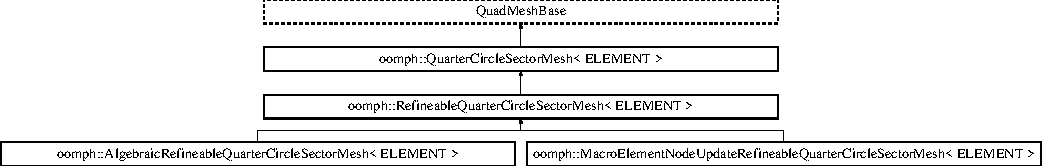
\includegraphics[height=2.794411cm]{classoomph_1_1QuarterCircleSectorMesh}
\end{center}
\end{figure}
\subsection*{Public Member Functions}
\begin{DoxyCompactItemize}
\item 
\hyperlink{classoomph_1_1QuarterCircleSectorMesh_a3fbcc7dd28aefc3dddda607785695afc}{Quarter\+Circle\+Sector\+Mesh} (\hyperlink{classoomph_1_1GeomObject}{Geom\+Object} $\ast$\hyperlink{classoomph_1_1QuarterCircleSectorMesh_a0b03071bbe7e95cc6723c221ddc0998a}{wall\+\_\+pt}, const double \&xi\+\_\+lo, const double \&fract\+\_\+mid, const double \&xi\+\_\+hi, \hyperlink{classoomph_1_1TimeStepper}{Time\+Stepper} $\ast$time\+\_\+stepper\+\_\+pt=\&\hyperlink{classoomph_1_1Mesh_a12243d0fee2b1fcee729ee5a4777ea10}{Mesh\+::\+Default\+\_\+\+Time\+Stepper})
\begin{DoxyCompactList}\small\item\em Constructor\+: Pass pointer to geometric object that specifies the wall, start and end coordinates on the geometric object, and the fraction along which the dividing line is to be placed, and the timestepper (defaults to (\hyperlink{classoomph_1_1Steady}{Steady}) default timestepper defined in \hyperlink{classoomph_1_1Mesh}{Mesh}) \end{DoxyCompactList}\item 
virtual \hyperlink{classoomph_1_1QuarterCircleSectorMesh_af3aec899bd005cacb011c13bcb6e5f22}{$\sim$\+Quarter\+Circle\+Sector\+Mesh} ()
\begin{DoxyCompactList}\small\item\em Destructor\+: \end{DoxyCompactList}\item 
\hyperlink{classoomph_1_1GeomObject}{Geom\+Object} $\ast$\& \hyperlink{classoomph_1_1QuarterCircleSectorMesh_a0b03071bbe7e95cc6723c221ddc0998a}{wall\+\_\+pt} ()
\begin{DoxyCompactList}\small\item\em Access function to \hyperlink{classoomph_1_1GeomObject}{Geom\+Object} representing wall. \end{DoxyCompactList}\item 
\hyperlink{classoomph_1_1QuarterCircleSectorDomain}{Quarter\+Circle\+Sector\+Domain} $\ast$ \hyperlink{classoomph_1_1QuarterCircleSectorMesh_a53adafee1a15301fe99a481b641df45b}{domain\+\_\+pt} ()
\begin{DoxyCompactList}\small\item\em Access function to domain. \end{DoxyCompactList}\item 
\hyperlink{classoomph_1_1QuarterCircleSectorDomain_a6cffab57f87c9f4ab01744647240bb1e}{Quarter\+Circle\+Sector\+Domain\+::\+B\+L\+Squash\+Fct\+Pt} \& \hyperlink{classoomph_1_1QuarterCircleSectorMesh_a6f149022d7a40bd0efed49adacd716bf}{bl\+\_\+squash\+\_\+fct\+\_\+pt} ()
\begin{DoxyCompactList}\small\item\em Function pointer for function that squashes the outer two macro elements towards the wall by mapping the input value of the \char`\"{}radial\char`\"{} macro element coordinate to the return value (defined in the underlying \hyperlink{classoomph_1_1Domain}{Domain} object) \end{DoxyCompactList}\end{DoxyCompactItemize}
\subsection*{Protected Attributes}
\begin{DoxyCompactItemize}
\item 
\hyperlink{classoomph_1_1QuarterCircleSectorDomain}{Quarter\+Circle\+Sector\+Domain} $\ast$ \hyperlink{classoomph_1_1QuarterCircleSectorMesh_a49e72c17a9409ec4a2b7a1ebf98fb4a1}{Domain\+\_\+pt}
\begin{DoxyCompactList}\small\item\em Pointer to \hyperlink{classoomph_1_1Domain}{Domain}. \end{DoxyCompactList}\item 
\hyperlink{classoomph_1_1GeomObject}{Geom\+Object} $\ast$ \hyperlink{classoomph_1_1QuarterCircleSectorMesh_a2cbdec5f0ee2f370c38f1fdc4e2904f8}{Wall\+\_\+pt}
\begin{DoxyCompactList}\small\item\em Pointer to the geometric object that represents the curved wall (mesh boundary 1) \end{DoxyCompactList}\item 
double \hyperlink{classoomph_1_1QuarterCircleSectorMesh_ab5c1e4484c69eb78bd3323321605a93c}{Xi\+\_\+lo}
\begin{DoxyCompactList}\small\item\em Lower limit for the (1D) coordinates along the wall. \end{DoxyCompactList}\item 
double \hyperlink{classoomph_1_1QuarterCircleSectorMesh_a149224b002f785eb357553f8210ad5d3}{Fract\+\_\+mid}
\begin{DoxyCompactList}\small\item\em Fraction along wall where outer ring is to be divided. \end{DoxyCompactList}\item 
double \hyperlink{classoomph_1_1QuarterCircleSectorMesh_a1fa3bfeddd4467e9fe0ec45fbfac0740}{Xi\+\_\+hi}
\begin{DoxyCompactList}\small\item\em Upper limit for the (1D) coordinates along the wall. \end{DoxyCompactList}\end{DoxyCompactItemize}
\subsection*{Additional Inherited Members}


\subsection{Detailed Description}
\subsubsection*{template$<$class E\+L\+E\+M\+E\+NT$>$\newline
class oomph\+::\+Quarter\+Circle\+Sector\+Mesh$<$ E\+L\+E\+M\+E\+N\+T $>$}

2D quarter ring mesh class. The domain is specified by the \hyperlink{classoomph_1_1GeomObject}{Geom\+Object} that identifies boundary 1.


\begin{DoxyCode}
                     ---\_\_\_
                    |      ---\_\_\_\_
                    |              -   BOUNDARY 1
                    |               /  
                    |     [2]      /  |  
                    |             /     | 
                    | \hyperlink{namespaceoomph_1_1QuadTreeNames_a8954a5947b19986b8c4b755bc7639f7dabc60bec4cc294aa2adf92726c6d6823a}{N}          /        |  
                    | |\_ \hyperlink{namespaceoomph_1_1QuadTreeNames_a8954a5947b19986b8c4b755bc7639f7da585070bd0e3801c3bbed287ef3c4a265}{E}      /          |    
     BOUNDARY 2     |-----------           |  
                    |          |    [1]    |
                    |   [0]    |           |  ^
                    |          |           | / \(\backslash\)  direction of
                    | \hyperlink{namespaceoomph_1_1QuadTreeNames_a8954a5947b19986b8c4b755bc7639f7dabc60bec4cc294aa2adf92726c6d6823a}{N}        |    \hyperlink{namespaceoomph_1_1QuadTreeNames_a8954a5947b19986b8c4b755bc7639f7dabc60bec4cc294aa2adf92726c6d6823a}{N}      |  |   Lagrangian 
                    | |\_ \hyperlink{namespaceoomph_1_1QuadTreeNames_a8954a5947b19986b8c4b755bc7639f7da585070bd0e3801c3bbed287ef3c4a265}{E}     |    |\_ \hyperlink{namespaceoomph_1_1QuadTreeNames_a8954a5947b19986b8c4b755bc7639f7da585070bd0e3801c3bbed287ef3c4a265}{E}   |  |   coordinate 
                    |\_\_\_\_\_\_\_\_\_\_|\_\_\_\_\_\_\_\_\_\_\_|  |   along wall GeomObject

                         BOUNDARY 0

Within the elements (MacroElements), the local coordinates
are such that the (\hyperlink{namespaceoomph_1_1QuadTreeNames_a8954a5947b19986b8c4b755bc7639f7da585070bd0e3801c3bbed287ef3c4a265}{E})astern direction coincides with the positive 
s\_0 direction,  \textcolor{keywordflow}{while} the (\hyperlink{namespaceoomph_1_1QuadTreeNames_a8954a5947b19986b8c4b755bc7639f7dabc60bec4cc294aa2adf92726c6d6823a}{N})orther direction coincides with the positive 
s\_1 direction.
\end{DoxyCode}


\hyperlink{classoomph_1_1Domain}{Domain} is parametrised by three macro elements as sketched. Nodal positions are determined via macro-\/element-\/based representation of the \hyperlink{classoomph_1_1Domain}{Domain} (as a \hyperlink{classoomph_1_1QuarterCircleSectorDomain}{Quarter\+Circle\+Sector\+Domain}). 

Definition at line 92 of file quarter\+\_\+circle\+\_\+sector\+\_\+mesh.\+template.\+h.



\subsection{Constructor \& Destructor Documentation}
\mbox{\Hypertarget{classoomph_1_1QuarterCircleSectorMesh_a3fbcc7dd28aefc3dddda607785695afc}\label{classoomph_1_1QuarterCircleSectorMesh_a3fbcc7dd28aefc3dddda607785695afc}} 
\index{oomph\+::\+Quarter\+Circle\+Sector\+Mesh@{oomph\+::\+Quarter\+Circle\+Sector\+Mesh}!Quarter\+Circle\+Sector\+Mesh@{Quarter\+Circle\+Sector\+Mesh}}
\index{Quarter\+Circle\+Sector\+Mesh@{Quarter\+Circle\+Sector\+Mesh}!oomph\+::\+Quarter\+Circle\+Sector\+Mesh@{oomph\+::\+Quarter\+Circle\+Sector\+Mesh}}
\subsubsection{\texorpdfstring{Quarter\+Circle\+Sector\+Mesh()}{QuarterCircleSectorMesh()}}
{\footnotesize\ttfamily template$<$class E\+L\+E\+M\+E\+NT $>$ \\
\hyperlink{classoomph_1_1QuarterCircleSectorMesh}{oomph\+::\+Quarter\+Circle\+Sector\+Mesh}$<$ E\+L\+E\+M\+E\+NT $>$\+::\hyperlink{classoomph_1_1QuarterCircleSectorMesh}{Quarter\+Circle\+Sector\+Mesh} (\begin{DoxyParamCaption}\item[{\hyperlink{classoomph_1_1GeomObject}{Geom\+Object} $\ast$}]{wall\+\_\+pt,  }\item[{const double \&}]{xi\+\_\+lo,  }\item[{const double \&}]{fract\+\_\+mid,  }\item[{const double \&}]{xi\+\_\+hi,  }\item[{\hyperlink{classoomph_1_1TimeStepper}{Time\+Stepper} $\ast$}]{time\+\_\+stepper\+\_\+pt = {\ttfamily \&\hyperlink{classoomph_1_1Mesh_a12243d0fee2b1fcee729ee5a4777ea10}{Mesh\+::\+Default\+\_\+\+Time\+Stepper}} }\end{DoxyParamCaption})}



Constructor\+: Pass pointer to geometric object that specifies the wall, start and end coordinates on the geometric object, and the fraction along which the dividing line is to be placed, and the timestepper (defaults to (\hyperlink{classoomph_1_1Steady}{Steady}) default timestepper defined in \hyperlink{classoomph_1_1Mesh}{Mesh}) 

Constructor for deformable 2D Ring mesh class. Pass pointer to geometric object that specifies the wall, start and end coordinates on the geometric object, and the fraction along which the dividing line is to be placed, and the timestepper (defaults to (\hyperlink{classoomph_1_1Steady}{Steady}) default timestepper defined in \hyperlink{classoomph_1_1Mesh}{Mesh}). Nodal positions are determined via macro-\/element-\/based representation of the \hyperlink{classoomph_1_1Domain}{Domain} (as a \hyperlink{classoomph_1_1QuarterCircleSectorDomain}{Quarter\+Circle\+Sector\+Domain}). 

Definition at line 49 of file quarter\+\_\+circle\+\_\+sector\+\_\+mesh.\+template.\+cc.



References oomph\+::\+Mesh\+::add\+\_\+boundary\+\_\+node(), oomph\+::\+Mesh\+::\+Boundary\+\_\+coordinate\+\_\+exists, oomph\+::\+Quarter\+Circle\+Sector\+Mesh$<$ E\+L\+E\+M\+E\+N\+T $>$\+::\+Domain\+\_\+pt, e, oomph\+::\+Mesh\+::\+Element\+\_\+pt, oomph\+::\+Mesh\+::element\+\_\+pt(), oomph\+::\+Mesh\+::finite\+\_\+element\+\_\+pt(), oomph\+::\+Quarter\+Circle\+Sector\+Mesh$<$ E\+L\+E\+M\+E\+N\+T $>$\+::\+Fract\+\_\+mid, oomph\+::\+Mesh\+::nelement(), oomph\+::\+Mesh\+::\+Node\+\_\+pt, oomph\+::\+Finite\+Element\+::node\+\_\+pt(), s, oomph\+::\+Mesh\+::set\+\_\+nboundary(), oomph\+::\+Algebraic\+Refineable\+Quarter\+Circle\+Sector\+Mesh$<$ E\+L\+E\+M\+E\+N\+T $>$\+::setup\+\_\+algebraic\+\_\+node\+\_\+update(), oomph\+::\+Quad\+Mesh\+Base\+::setup\+\_\+boundary\+\_\+element\+\_\+info(), oomph\+::\+Quarter\+Circle\+Sector\+Mesh$<$ E\+L\+E\+M\+E\+N\+T $>$\+::\+Xi\+\_\+hi, and oomph\+::\+Quarter\+Circle\+Sector\+Mesh$<$ E\+L\+E\+M\+E\+N\+T $>$\+::\+Xi\+\_\+lo.

\mbox{\Hypertarget{classoomph_1_1QuarterCircleSectorMesh_af3aec899bd005cacb011c13bcb6e5f22}\label{classoomph_1_1QuarterCircleSectorMesh_af3aec899bd005cacb011c13bcb6e5f22}} 
\index{oomph\+::\+Quarter\+Circle\+Sector\+Mesh@{oomph\+::\+Quarter\+Circle\+Sector\+Mesh}!````~Quarter\+Circle\+Sector\+Mesh@{$\sim$\+Quarter\+Circle\+Sector\+Mesh}}
\index{````~Quarter\+Circle\+Sector\+Mesh@{$\sim$\+Quarter\+Circle\+Sector\+Mesh}!oomph\+::\+Quarter\+Circle\+Sector\+Mesh@{oomph\+::\+Quarter\+Circle\+Sector\+Mesh}}
\subsubsection{\texorpdfstring{$\sim$\+Quarter\+Circle\+Sector\+Mesh()}{~QuarterCircleSectorMesh()}}
{\footnotesize\ttfamily template$<$class E\+L\+E\+M\+E\+NT$>$ \\
virtual \hyperlink{classoomph_1_1QuarterCircleSectorMesh}{oomph\+::\+Quarter\+Circle\+Sector\+Mesh}$<$ E\+L\+E\+M\+E\+NT $>$\+::$\sim$\hyperlink{classoomph_1_1QuarterCircleSectorMesh}{Quarter\+Circle\+Sector\+Mesh} (\begin{DoxyParamCaption}{ }\end{DoxyParamCaption})\hspace{0.3cm}{\ttfamily [inline]}, {\ttfamily [virtual]}}



Destructor\+: 



Definition at line 111 of file quarter\+\_\+circle\+\_\+sector\+\_\+mesh.\+template.\+h.



\subsection{Member Function Documentation}
\mbox{\Hypertarget{classoomph_1_1QuarterCircleSectorMesh_a6f149022d7a40bd0efed49adacd716bf}\label{classoomph_1_1QuarterCircleSectorMesh_a6f149022d7a40bd0efed49adacd716bf}} 
\index{oomph\+::\+Quarter\+Circle\+Sector\+Mesh@{oomph\+::\+Quarter\+Circle\+Sector\+Mesh}!bl\+\_\+squash\+\_\+fct\+\_\+pt@{bl\+\_\+squash\+\_\+fct\+\_\+pt}}
\index{bl\+\_\+squash\+\_\+fct\+\_\+pt@{bl\+\_\+squash\+\_\+fct\+\_\+pt}!oomph\+::\+Quarter\+Circle\+Sector\+Mesh@{oomph\+::\+Quarter\+Circle\+Sector\+Mesh}}
\subsubsection{\texorpdfstring{bl\+\_\+squash\+\_\+fct\+\_\+pt()}{bl\_squash\_fct\_pt()}}
{\footnotesize\ttfamily template$<$class E\+L\+E\+M\+E\+NT$>$ \\
\hyperlink{classoomph_1_1QuarterCircleSectorDomain_a6cffab57f87c9f4ab01744647240bb1e}{Quarter\+Circle\+Sector\+Domain\+::\+B\+L\+Squash\+Fct\+Pt}\& \hyperlink{classoomph_1_1QuarterCircleSectorMesh}{oomph\+::\+Quarter\+Circle\+Sector\+Mesh}$<$ E\+L\+E\+M\+E\+NT $>$\+::bl\+\_\+squash\+\_\+fct\+\_\+pt (\begin{DoxyParamCaption}{ }\end{DoxyParamCaption})\hspace{0.3cm}{\ttfamily [inline]}}



Function pointer for function that squashes the outer two macro elements towards the wall by mapping the input value of the \char`\"{}radial\char`\"{} macro element coordinate to the return value (defined in the underlying \hyperlink{classoomph_1_1Domain}{Domain} object) 



Definition at line 123 of file quarter\+\_\+circle\+\_\+sector\+\_\+mesh.\+template.\+h.



References oomph\+::\+Quarter\+Circle\+Sector\+Domain\+::bl\+\_\+squash\+\_\+fct\+\_\+pt(), and oomph\+::\+Quarter\+Circle\+Sector\+Mesh$<$ E\+L\+E\+M\+E\+N\+T $>$\+::\+Domain\+\_\+pt.

\mbox{\Hypertarget{classoomph_1_1QuarterCircleSectorMesh_a53adafee1a15301fe99a481b641df45b}\label{classoomph_1_1QuarterCircleSectorMesh_a53adafee1a15301fe99a481b641df45b}} 
\index{oomph\+::\+Quarter\+Circle\+Sector\+Mesh@{oomph\+::\+Quarter\+Circle\+Sector\+Mesh}!domain\+\_\+pt@{domain\+\_\+pt}}
\index{domain\+\_\+pt@{domain\+\_\+pt}!oomph\+::\+Quarter\+Circle\+Sector\+Mesh@{oomph\+::\+Quarter\+Circle\+Sector\+Mesh}}
\subsubsection{\texorpdfstring{domain\+\_\+pt()}{domain\_pt()}}
{\footnotesize\ttfamily template$<$class E\+L\+E\+M\+E\+NT$>$ \\
\hyperlink{classoomph_1_1QuarterCircleSectorDomain}{Quarter\+Circle\+Sector\+Domain}$\ast$ \hyperlink{classoomph_1_1QuarterCircleSectorMesh}{oomph\+::\+Quarter\+Circle\+Sector\+Mesh}$<$ E\+L\+E\+M\+E\+NT $>$\+::domain\+\_\+pt (\begin{DoxyParamCaption}{ }\end{DoxyParamCaption})\hspace{0.3cm}{\ttfamily [inline]}}



Access function to domain. 



Definition at line 117 of file quarter\+\_\+circle\+\_\+sector\+\_\+mesh.\+template.\+h.



References oomph\+::\+Quarter\+Circle\+Sector\+Mesh$<$ E\+L\+E\+M\+E\+N\+T $>$\+::\+Domain\+\_\+pt.



Referenced by oomph\+::\+Macro\+Element\+Node\+Update\+Refineable\+Quarter\+Circle\+Sector\+Mesh$<$ E\+L\+E\+M\+E\+N\+T $>$\+::setup\+\_\+macro\+\_\+element\+\_\+node\+\_\+update().

\mbox{\Hypertarget{classoomph_1_1QuarterCircleSectorMesh_a0b03071bbe7e95cc6723c221ddc0998a}\label{classoomph_1_1QuarterCircleSectorMesh_a0b03071bbe7e95cc6723c221ddc0998a}} 
\index{oomph\+::\+Quarter\+Circle\+Sector\+Mesh@{oomph\+::\+Quarter\+Circle\+Sector\+Mesh}!wall\+\_\+pt@{wall\+\_\+pt}}
\index{wall\+\_\+pt@{wall\+\_\+pt}!oomph\+::\+Quarter\+Circle\+Sector\+Mesh@{oomph\+::\+Quarter\+Circle\+Sector\+Mesh}}
\subsubsection{\texorpdfstring{wall\+\_\+pt()}{wall\_pt()}}
{\footnotesize\ttfamily template$<$class E\+L\+E\+M\+E\+NT$>$ \\
\hyperlink{classoomph_1_1GeomObject}{Geom\+Object}$\ast$\& \hyperlink{classoomph_1_1QuarterCircleSectorMesh}{oomph\+::\+Quarter\+Circle\+Sector\+Mesh}$<$ E\+L\+E\+M\+E\+NT $>$\+::wall\+\_\+pt (\begin{DoxyParamCaption}{ }\end{DoxyParamCaption})\hspace{0.3cm}{\ttfamily [inline]}}



Access function to \hyperlink{classoomph_1_1GeomObject}{Geom\+Object} representing wall. 



Definition at line 114 of file quarter\+\_\+circle\+\_\+sector\+\_\+mesh.\+template.\+h.



References oomph\+::\+Quarter\+Circle\+Sector\+Mesh$<$ E\+L\+E\+M\+E\+N\+T $>$\+::\+Wall\+\_\+pt.



\subsection{Member Data Documentation}
\mbox{\Hypertarget{classoomph_1_1QuarterCircleSectorMesh_a49e72c17a9409ec4a2b7a1ebf98fb4a1}\label{classoomph_1_1QuarterCircleSectorMesh_a49e72c17a9409ec4a2b7a1ebf98fb4a1}} 
\index{oomph\+::\+Quarter\+Circle\+Sector\+Mesh@{oomph\+::\+Quarter\+Circle\+Sector\+Mesh}!Domain\+\_\+pt@{Domain\+\_\+pt}}
\index{Domain\+\_\+pt@{Domain\+\_\+pt}!oomph\+::\+Quarter\+Circle\+Sector\+Mesh@{oomph\+::\+Quarter\+Circle\+Sector\+Mesh}}
\subsubsection{\texorpdfstring{Domain\+\_\+pt}{Domain\_pt}}
{\footnotesize\ttfamily template$<$class E\+L\+E\+M\+E\+NT$>$ \\
\hyperlink{classoomph_1_1QuarterCircleSectorDomain}{Quarter\+Circle\+Sector\+Domain}$\ast$ \hyperlink{classoomph_1_1QuarterCircleSectorMesh}{oomph\+::\+Quarter\+Circle\+Sector\+Mesh}$<$ E\+L\+E\+M\+E\+NT $>$\+::Domain\+\_\+pt\hspace{0.3cm}{\ttfamily [protected]}}



Pointer to \hyperlink{classoomph_1_1Domain}{Domain}. 



Definition at line 134 of file quarter\+\_\+circle\+\_\+sector\+\_\+mesh.\+template.\+h.



Referenced by oomph\+::\+Quarter\+Circle\+Sector\+Mesh$<$ E\+L\+E\+M\+E\+N\+T $>$\+::bl\+\_\+squash\+\_\+fct\+\_\+pt(), oomph\+::\+Quarter\+Circle\+Sector\+Mesh$<$ E\+L\+E\+M\+E\+N\+T $>$\+::domain\+\_\+pt(), and oomph\+::\+Quarter\+Circle\+Sector\+Mesh$<$ E\+L\+E\+M\+E\+N\+T $>$\+::\+Quarter\+Circle\+Sector\+Mesh().

\mbox{\Hypertarget{classoomph_1_1QuarterCircleSectorMesh_a149224b002f785eb357553f8210ad5d3}\label{classoomph_1_1QuarterCircleSectorMesh_a149224b002f785eb357553f8210ad5d3}} 
\index{oomph\+::\+Quarter\+Circle\+Sector\+Mesh@{oomph\+::\+Quarter\+Circle\+Sector\+Mesh}!Fract\+\_\+mid@{Fract\+\_\+mid}}
\index{Fract\+\_\+mid@{Fract\+\_\+mid}!oomph\+::\+Quarter\+Circle\+Sector\+Mesh@{oomph\+::\+Quarter\+Circle\+Sector\+Mesh}}
\subsubsection{\texorpdfstring{Fract\+\_\+mid}{Fract\_mid}}
{\footnotesize\ttfamily template$<$class E\+L\+E\+M\+E\+NT$>$ \\
double \hyperlink{classoomph_1_1QuarterCircleSectorMesh}{oomph\+::\+Quarter\+Circle\+Sector\+Mesh}$<$ E\+L\+E\+M\+E\+NT $>$\+::Fract\+\_\+mid\hspace{0.3cm}{\ttfamily [protected]}}



Fraction along wall where outer ring is to be divided. 



Definition at line 144 of file quarter\+\_\+circle\+\_\+sector\+\_\+mesh.\+template.\+h.



Referenced by oomph\+::\+Quarter\+Circle\+Sector\+Mesh$<$ E\+L\+E\+M\+E\+N\+T $>$\+::\+Quarter\+Circle\+Sector\+Mesh().

\mbox{\Hypertarget{classoomph_1_1QuarterCircleSectorMesh_a2cbdec5f0ee2f370c38f1fdc4e2904f8}\label{classoomph_1_1QuarterCircleSectorMesh_a2cbdec5f0ee2f370c38f1fdc4e2904f8}} 
\index{oomph\+::\+Quarter\+Circle\+Sector\+Mesh@{oomph\+::\+Quarter\+Circle\+Sector\+Mesh}!Wall\+\_\+pt@{Wall\+\_\+pt}}
\index{Wall\+\_\+pt@{Wall\+\_\+pt}!oomph\+::\+Quarter\+Circle\+Sector\+Mesh@{oomph\+::\+Quarter\+Circle\+Sector\+Mesh}}
\subsubsection{\texorpdfstring{Wall\+\_\+pt}{Wall\_pt}}
{\footnotesize\ttfamily template$<$class E\+L\+E\+M\+E\+NT$>$ \\
\hyperlink{classoomph_1_1GeomObject}{Geom\+Object}$\ast$ \hyperlink{classoomph_1_1QuarterCircleSectorMesh}{oomph\+::\+Quarter\+Circle\+Sector\+Mesh}$<$ E\+L\+E\+M\+E\+NT $>$\+::Wall\+\_\+pt\hspace{0.3cm}{\ttfamily [protected]}}



Pointer to the geometric object that represents the curved wall (mesh boundary 1) 



Definition at line 138 of file quarter\+\_\+circle\+\_\+sector\+\_\+mesh.\+template.\+h.



Referenced by oomph\+::\+Algebraic\+Refineable\+Quarter\+Circle\+Sector\+Mesh$<$ E\+L\+E\+M\+E\+N\+T $>$\+::setup\+\_\+algebraic\+\_\+node\+\_\+update(), oomph\+::\+Macro\+Element\+Node\+Update\+Refineable\+Quarter\+Circle\+Sector\+Mesh$<$ E\+L\+E\+M\+E\+N\+T $>$\+::setup\+\_\+macro\+\_\+element\+\_\+node\+\_\+update(), oomph\+::\+Algebraic\+Refineable\+Quarter\+Circle\+Sector\+Mesh$<$ E\+L\+E\+M\+E\+N\+T $>$\+::update\+\_\+node\+\_\+update\+\_\+in\+\_\+lower\+\_\+right\+\_\+box(), oomph\+::\+Algebraic\+Refineable\+Quarter\+Circle\+Sector\+Mesh$<$ E\+L\+E\+M\+E\+N\+T $>$\+::update\+\_\+node\+\_\+update\+\_\+in\+\_\+upper\+\_\+left\+\_\+box(), and oomph\+::\+Quarter\+Circle\+Sector\+Mesh$<$ E\+L\+E\+M\+E\+N\+T $>$\+::wall\+\_\+pt().

\mbox{\Hypertarget{classoomph_1_1QuarterCircleSectorMesh_a1fa3bfeddd4467e9fe0ec45fbfac0740}\label{classoomph_1_1QuarterCircleSectorMesh_a1fa3bfeddd4467e9fe0ec45fbfac0740}} 
\index{oomph\+::\+Quarter\+Circle\+Sector\+Mesh@{oomph\+::\+Quarter\+Circle\+Sector\+Mesh}!Xi\+\_\+hi@{Xi\+\_\+hi}}
\index{Xi\+\_\+hi@{Xi\+\_\+hi}!oomph\+::\+Quarter\+Circle\+Sector\+Mesh@{oomph\+::\+Quarter\+Circle\+Sector\+Mesh}}
\subsubsection{\texorpdfstring{Xi\+\_\+hi}{Xi\_hi}}
{\footnotesize\ttfamily template$<$class E\+L\+E\+M\+E\+NT$>$ \\
double \hyperlink{classoomph_1_1QuarterCircleSectorMesh}{oomph\+::\+Quarter\+Circle\+Sector\+Mesh}$<$ E\+L\+E\+M\+E\+NT $>$\+::Xi\+\_\+hi\hspace{0.3cm}{\ttfamily [protected]}}



Upper limit for the (1D) coordinates along the wall. 



Definition at line 147 of file quarter\+\_\+circle\+\_\+sector\+\_\+mesh.\+template.\+h.



Referenced by oomph\+::\+Quarter\+Circle\+Sector\+Mesh$<$ E\+L\+E\+M\+E\+N\+T $>$\+::\+Quarter\+Circle\+Sector\+Mesh().

\mbox{\Hypertarget{classoomph_1_1QuarterCircleSectorMesh_ab5c1e4484c69eb78bd3323321605a93c}\label{classoomph_1_1QuarterCircleSectorMesh_ab5c1e4484c69eb78bd3323321605a93c}} 
\index{oomph\+::\+Quarter\+Circle\+Sector\+Mesh@{oomph\+::\+Quarter\+Circle\+Sector\+Mesh}!Xi\+\_\+lo@{Xi\+\_\+lo}}
\index{Xi\+\_\+lo@{Xi\+\_\+lo}!oomph\+::\+Quarter\+Circle\+Sector\+Mesh@{oomph\+::\+Quarter\+Circle\+Sector\+Mesh}}
\subsubsection{\texorpdfstring{Xi\+\_\+lo}{Xi\_lo}}
{\footnotesize\ttfamily template$<$class E\+L\+E\+M\+E\+NT$>$ \\
double \hyperlink{classoomph_1_1QuarterCircleSectorMesh}{oomph\+::\+Quarter\+Circle\+Sector\+Mesh}$<$ E\+L\+E\+M\+E\+NT $>$\+::Xi\+\_\+lo\hspace{0.3cm}{\ttfamily [protected]}}



Lower limit for the (1D) coordinates along the wall. 



Definition at line 141 of file quarter\+\_\+circle\+\_\+sector\+\_\+mesh.\+template.\+h.



Referenced by oomph\+::\+Quarter\+Circle\+Sector\+Mesh$<$ E\+L\+E\+M\+E\+N\+T $>$\+::\+Quarter\+Circle\+Sector\+Mesh().



The documentation for this class was generated from the following files\+:\begin{DoxyCompactItemize}
\item 
\hyperlink{quarter__circle__sector__mesh_8template_8h}{quarter\+\_\+circle\+\_\+sector\+\_\+mesh.\+template.\+h}\item 
\hyperlink{quarter__circle__sector__mesh_8template_8cc}{quarter\+\_\+circle\+\_\+sector\+\_\+mesh.\+template.\+cc}\end{DoxyCompactItemize}

\hypertarget{classoomph_1_1QuarterPipeDomain}{}\section{oomph\+:\+:Quarter\+Pipe\+Domain Class Reference}
\label{classoomph_1_1QuarterPipeDomain}\index{oomph\+::\+Quarter\+Pipe\+Domain@{oomph\+::\+Quarter\+Pipe\+Domain}}


\hyperlink{classoomph_1_1Domain}{Domain} representing a quarter pipe.  




{\ttfamily \#include $<$quarter\+\_\+pipe\+\_\+domain.\+h$>$}

Inheritance diagram for oomph\+:\+:Quarter\+Pipe\+Domain\+:\begin{figure}[H]
\begin{center}
\leavevmode
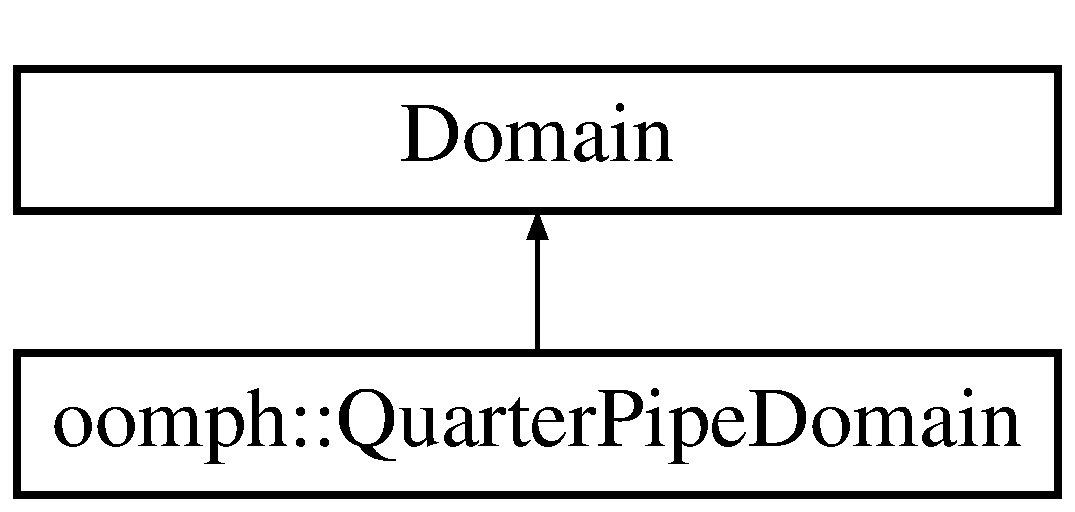
\includegraphics[height=2.000000cm]{classoomph_1_1QuarterPipeDomain}
\end{center}
\end{figure}
\subsection*{Public Types}
\begin{DoxyCompactItemize}
\item 
typedef double($\ast$ \hyperlink{classoomph_1_1QuarterPipeDomain_a540d441b38146aacb12938d5f885789c}{Axial\+Spacing\+Fct\+Pt}) (const double \&xi)
\begin{DoxyCompactList}\small\item\em Typedef for function pointer for function that implements axial spacing of macro elements. \end{DoxyCompactList}\end{DoxyCompactItemize}
\subsection*{Public Member Functions}
\begin{DoxyCompactItemize}
\item 
\hyperlink{classoomph_1_1QuarterPipeDomain_afb9763dac929fd4371a6ef860d9a5caf}{Quarter\+Pipe\+Domain} (const unsigned \&ntheta, const unsigned \&nr, const unsigned \&nz, const double \&rmin, const double \&rmax, const double \&length)
\begin{DoxyCompactList}\small\item\em Constructor\+: Pass number of elements in various directions, the inner and outer radius and the length of the tube. \end{DoxyCompactList}\item 
\hyperlink{classoomph_1_1QuarterPipeDomain_a09e3620b090b3bae5d2bf8c2e6ac9812}{Quarter\+Pipe\+Domain} (const \hyperlink{classoomph_1_1QuarterPipeDomain}{Quarter\+Pipe\+Domain} \&)
\begin{DoxyCompactList}\small\item\em Broken copy constructor. \end{DoxyCompactList}\item 
void \hyperlink{classoomph_1_1QuarterPipeDomain_ab6aec719fb0b333abf3ef9a1bf0414ac}{operator=} (const \hyperlink{classoomph_1_1QuarterPipeDomain}{Quarter\+Pipe\+Domain} \&)
\begin{DoxyCompactList}\small\item\em Broken assignment operator. \end{DoxyCompactList}\item 
\hyperlink{classoomph_1_1QuarterPipeDomain_a872560e53bf73ef0bd1b69f2a40612c8}{$\sim$\+Quarter\+Pipe\+Domain} ()
\begin{DoxyCompactList}\small\item\em Destructor\+: Cleanup. \end{DoxyCompactList}\item 
\hyperlink{classoomph_1_1QuarterPipeDomain_a540d441b38146aacb12938d5f885789c}{Axial\+Spacing\+Fct\+Pt} \& \hyperlink{classoomph_1_1QuarterPipeDomain_aa2731d4c5fb22dc0a5d2faa32f99505e}{axial\+\_\+spacing\+\_\+fct\+\_\+pt} ()
\begin{DoxyCompactList}\small\item\em Function pointer for function that implements axial spacing of macro elements. \end{DoxyCompactList}\item 
double \hyperlink{classoomph_1_1QuarterPipeDomain_a035e27884c0fa1bc31d1d9bed28c37bd}{axial\+\_\+spacing\+\_\+fct} (const double \&xi)
\begin{DoxyCompactList}\small\item\em Function that implements axial spacing of macro elements. \end{DoxyCompactList}\item 
void \hyperlink{classoomph_1_1QuarterPipeDomain_ae8cc6433c58dcfb265335744ed8a330a}{macro\+\_\+element\+\_\+boundary} (const unsigned \&\hyperlink{cfortran_8h_af6f0bd3dc13317f895c91323c25c2b8f}{t}, const unsigned \&i\+\_\+macro, const unsigned \&i\+\_\+direct, const \hyperlink{classoomph_1_1Vector}{Vector}$<$ double $>$ \&\hyperlink{cfortran_8h_ab7123126e4885ef647dd9c6e3807a21c}{s}, \hyperlink{classoomph_1_1Vector}{Vector}$<$ double $>$ \&f)
\begin{DoxyCompactList}\small\item\em \hyperlink{classoomph_1_1Vector}{Vector} representation of the i\+\_\+macro-\/th macro element boundary i\+\_\+direct (U/\+D/\+L/\+R/\+F/B) at time level t (t=0\+: present; t$>$0\+: previous)\+: f(s). \end{DoxyCompactList}\end{DoxyCompactItemize}
\subsection*{Private Member Functions}
\begin{DoxyCompactItemize}
\item 
void \hyperlink{classoomph_1_1QuarterPipeDomain_a5c023c7a9d6e43d123566bc2f7bb21f0}{r\+\_\+U} (const unsigned \&\hyperlink{cfortran_8h_af6f0bd3dc13317f895c91323c25c2b8f}{t}, const \hyperlink{classoomph_1_1Vector}{Vector}$<$ double $>$ \&zeta, \hyperlink{classoomph_1_1Vector}{Vector}$<$ double $>$ \&f, const double \&rmin, const double \&rmax, const double \&thetamin, const double \&thetamax, const double \&zmin, const double \&zmax)
\begin{DoxyCompactList}\small\item\em Boundary of macro element zeta $ \in [-1,1]x[-1,1] $. \end{DoxyCompactList}\item 
void \hyperlink{classoomph_1_1QuarterPipeDomain_a21c58b76f546300c308d6e1f303a3433}{r\+\_\+L} (const unsigned \&\hyperlink{cfortran_8h_af6f0bd3dc13317f895c91323c25c2b8f}{t}, const \hyperlink{classoomph_1_1Vector}{Vector}$<$ double $>$ \&zeta, \hyperlink{classoomph_1_1Vector}{Vector}$<$ double $>$ \&f, const double \&rmin, const double \&rmax, const double \&thetamin, const double \&thetamax, const double \&zmin, const double \&zmax)
\begin{DoxyCompactList}\small\item\em Boundary of macro element zeta $ \in [-1,1]x[-1,1] $. \end{DoxyCompactList}\item 
void \hyperlink{classoomph_1_1QuarterPipeDomain_aeb6e4d3fbb8afb4ad2597601f1a46afd}{r\+\_\+D} (const unsigned \&\hyperlink{cfortran_8h_af6f0bd3dc13317f895c91323c25c2b8f}{t}, const \hyperlink{classoomph_1_1Vector}{Vector}$<$ double $>$ \&zeta, \hyperlink{classoomph_1_1Vector}{Vector}$<$ double $>$ \&f, const double \&rmin, const double \&rmax, const double \&thetamin, const double \&thetamax, const double \&zmin, const double \&zmax)
\begin{DoxyCompactList}\small\item\em Boundary of macro element zeta $ \in [-1,1]x[-1,1] $. \end{DoxyCompactList}\item 
void \hyperlink{classoomph_1_1QuarterPipeDomain_aab6f3fd79bc6dea1eb267f3b55630a2b}{r\+\_\+R} (const unsigned \&\hyperlink{cfortran_8h_af6f0bd3dc13317f895c91323c25c2b8f}{t}, const \hyperlink{classoomph_1_1Vector}{Vector}$<$ double $>$ \&zeta, \hyperlink{classoomph_1_1Vector}{Vector}$<$ double $>$ \&f, const double \&rmin, const double \&rmax, const double \&thetamin, const double \&thetamax, const double \&zmin, const double \&zmax)
\begin{DoxyCompactList}\small\item\em Boundary of macro element zeta $ \in [-1,1]x[-1,1] $. \end{DoxyCompactList}\item 
void \hyperlink{classoomph_1_1QuarterPipeDomain_a85aaa5d1217c49e2144bbfd37dbad0fd}{r\+\_\+F} (const unsigned \&\hyperlink{cfortran_8h_af6f0bd3dc13317f895c91323c25c2b8f}{t}, const \hyperlink{classoomph_1_1Vector}{Vector}$<$ double $>$ \&zeta, \hyperlink{classoomph_1_1Vector}{Vector}$<$ double $>$ \&f, const double \&rmin, const double \&rmax, const double \&thetamin, const double \&thetamax, const double \&zmin, const double \&zmax)
\begin{DoxyCompactList}\small\item\em Boundary of macro element zeta $ \in [-1,1]x[-1,1] $. \end{DoxyCompactList}\item 
void \hyperlink{classoomph_1_1QuarterPipeDomain_aba1af5e7f1bc6e88ff8e9ee59e965630}{r\+\_\+B} (const unsigned \&\hyperlink{cfortran_8h_af6f0bd3dc13317f895c91323c25c2b8f}{t}, const \hyperlink{classoomph_1_1Vector}{Vector}$<$ double $>$ \&zeta, \hyperlink{classoomph_1_1Vector}{Vector}$<$ double $>$ \&f, const double \&rmin, const double \&rmax, const double \&thetamin, const double \&thetamax, const double \&zmin, const double \&zmax)
\begin{DoxyCompactList}\small\item\em Boundary of macro element zeta $ \in [-1,1]x[-1,1] $. \end{DoxyCompactList}\end{DoxyCompactItemize}
\subsection*{Static Private Member Functions}
\begin{DoxyCompactItemize}
\item 
static double \hyperlink{classoomph_1_1QuarterPipeDomain_a3b79d0bf40336f7961a8b2bb58080dba}{default\+\_\+axial\+\_\+spacing\+\_\+fct} (const double \&xi)
\begin{DoxyCompactList}\small\item\em Default for function that implements axial spacing of macro elements. \end{DoxyCompactList}\end{DoxyCompactItemize}
\subsection*{Private Attributes}
\begin{DoxyCompactItemize}
\item 
unsigned \hyperlink{classoomph_1_1QuarterPipeDomain_aeb912b40da8cd2883768fe2ca989e640}{Ntheta}
\begin{DoxyCompactList}\small\item\em Number of elements azimuthal direction. \end{DoxyCompactList}\item 
unsigned \hyperlink{classoomph_1_1QuarterPipeDomain_a18ac22546af74ac9b76a870d3f5abe3d}{Nr}
\begin{DoxyCompactList}\small\item\em Number of elements radial direction. \end{DoxyCompactList}\item 
unsigned \hyperlink{classoomph_1_1QuarterPipeDomain_aab1bf3900c3537c44942e3fee0c3d24e}{Nz}
\begin{DoxyCompactList}\small\item\em Number of elements axial direction. \end{DoxyCompactList}\item 
double \hyperlink{classoomph_1_1QuarterPipeDomain_ac71370e6c78fd37aa59e7a52d62d1cbe}{Rmin}
\begin{DoxyCompactList}\small\item\em Inner radius. \end{DoxyCompactList}\item 
double \hyperlink{classoomph_1_1QuarterPipeDomain_a5e2252883456cd65902663fda09296d5}{Rmax}
\begin{DoxyCompactList}\small\item\em Outer radius. \end{DoxyCompactList}\item 
double \hyperlink{classoomph_1_1QuarterPipeDomain_a0798f3962e840bdb3d31e4e0dada055d}{Length}
\begin{DoxyCompactList}\small\item\em Length. \end{DoxyCompactList}\item 
\hyperlink{classoomph_1_1GeomObject}{Geom\+Object} $\ast$ \hyperlink{classoomph_1_1QuarterPipeDomain_adad2a4e638bb58eda89a19eaf5e18969}{Outer\+\_\+boundary\+\_\+cross\+\_\+section\+\_\+pt}
\begin{DoxyCompactList}\small\item\em Geom object representing the outer boundary of the cross section. \end{DoxyCompactList}\item 
\hyperlink{classoomph_1_1GeomObject}{Geom\+Object} $\ast$ \hyperlink{classoomph_1_1QuarterPipeDomain_a2760038e136d58a41dcbcd045bd13ae4}{Inner\+\_\+boundary\+\_\+cross\+\_\+section\+\_\+pt}
\begin{DoxyCompactList}\small\item\em Geom object representing the inner boundary of the cross section. \end{DoxyCompactList}\item 
\hyperlink{classoomph_1_1QuarterPipeDomain_a540d441b38146aacb12938d5f885789c}{Axial\+Spacing\+Fct\+Pt} \hyperlink{classoomph_1_1QuarterPipeDomain_ada15e8a576d3715e8ed88ea9bef5508a}{Axial\+\_\+spacing\+\_\+fct\+\_\+pt}
\begin{DoxyCompactList}\small\item\em Function pointer for function that implements axial spacing of macro elements. \end{DoxyCompactList}\end{DoxyCompactItemize}
\subsection*{Additional Inherited Members}


\subsection{Detailed Description}
\hyperlink{classoomph_1_1Domain}{Domain} representing a quarter pipe. 

Definition at line 46 of file quarter\+\_\+pipe\+\_\+domain.\+h.



\subsection{Member Typedef Documentation}
\mbox{\Hypertarget{classoomph_1_1QuarterPipeDomain_a540d441b38146aacb12938d5f885789c}\label{classoomph_1_1QuarterPipeDomain_a540d441b38146aacb12938d5f885789c}} 
\index{oomph\+::\+Quarter\+Pipe\+Domain@{oomph\+::\+Quarter\+Pipe\+Domain}!Axial\+Spacing\+Fct\+Pt@{Axial\+Spacing\+Fct\+Pt}}
\index{Axial\+Spacing\+Fct\+Pt@{Axial\+Spacing\+Fct\+Pt}!oomph\+::\+Quarter\+Pipe\+Domain@{oomph\+::\+Quarter\+Pipe\+Domain}}
\subsubsection{\texorpdfstring{Axial\+Spacing\+Fct\+Pt}{AxialSpacingFctPt}}
{\footnotesize\ttfamily typedef double($\ast$ oomph\+::\+Quarter\+Pipe\+Domain\+::\+Axial\+Spacing\+Fct\+Pt) (const double \&xi)}



Typedef for function pointer for function that implements axial spacing of macro elements. 



Definition at line 105 of file quarter\+\_\+pipe\+\_\+domain.\+h.



\subsection{Constructor \& Destructor Documentation}
\mbox{\Hypertarget{classoomph_1_1QuarterPipeDomain_afb9763dac929fd4371a6ef860d9a5caf}\label{classoomph_1_1QuarterPipeDomain_afb9763dac929fd4371a6ef860d9a5caf}} 
\index{oomph\+::\+Quarter\+Pipe\+Domain@{oomph\+::\+Quarter\+Pipe\+Domain}!Quarter\+Pipe\+Domain@{Quarter\+Pipe\+Domain}}
\index{Quarter\+Pipe\+Domain@{Quarter\+Pipe\+Domain}!oomph\+::\+Quarter\+Pipe\+Domain@{oomph\+::\+Quarter\+Pipe\+Domain}}
\subsubsection{\texorpdfstring{Quarter\+Pipe\+Domain()}{QuarterPipeDomain()}\hspace{0.1cm}{\footnotesize\ttfamily [1/2]}}
{\footnotesize\ttfamily oomph\+::\+Quarter\+Pipe\+Domain\+::\+Quarter\+Pipe\+Domain (\begin{DoxyParamCaption}\item[{const unsigned \&}]{ntheta,  }\item[{const unsigned \&}]{nr,  }\item[{const unsigned \&}]{nz,  }\item[{const double \&}]{rmin,  }\item[{const double \&}]{rmax,  }\item[{const double \&}]{length }\end{DoxyParamCaption})\hspace{0.3cm}{\ttfamily [inline]}}



Constructor\+: Pass number of elements in various directions, the inner and outer radius and the length of the tube. 



Definition at line 53 of file quarter\+\_\+pipe\+\_\+domain.\+h.



References i, Inner\+\_\+boundary\+\_\+cross\+\_\+section\+\_\+pt, oomph\+::\+Domain\+::\+Macro\+\_\+element\+\_\+pt, and Outer\+\_\+boundary\+\_\+cross\+\_\+section\+\_\+pt.

\mbox{\Hypertarget{classoomph_1_1QuarterPipeDomain_a09e3620b090b3bae5d2bf8c2e6ac9812}\label{classoomph_1_1QuarterPipeDomain_a09e3620b090b3bae5d2bf8c2e6ac9812}} 
\index{oomph\+::\+Quarter\+Pipe\+Domain@{oomph\+::\+Quarter\+Pipe\+Domain}!Quarter\+Pipe\+Domain@{Quarter\+Pipe\+Domain}}
\index{Quarter\+Pipe\+Domain@{Quarter\+Pipe\+Domain}!oomph\+::\+Quarter\+Pipe\+Domain@{oomph\+::\+Quarter\+Pipe\+Domain}}
\subsubsection{\texorpdfstring{Quarter\+Pipe\+Domain()}{QuarterPipeDomain()}\hspace{0.1cm}{\footnotesize\ttfamily [2/2]}}
{\footnotesize\ttfamily oomph\+::\+Quarter\+Pipe\+Domain\+::\+Quarter\+Pipe\+Domain (\begin{DoxyParamCaption}\item[{const \hyperlink{classoomph_1_1QuarterPipeDomain}{Quarter\+Pipe\+Domain} \&}]{ }\end{DoxyParamCaption})\hspace{0.3cm}{\ttfamily [inline]}}



Broken copy constructor. 



Definition at line 79 of file quarter\+\_\+pipe\+\_\+domain.\+h.



References oomph\+::\+Broken\+Copy\+::broken\+\_\+copy().

\mbox{\Hypertarget{classoomph_1_1QuarterPipeDomain_a872560e53bf73ef0bd1b69f2a40612c8}\label{classoomph_1_1QuarterPipeDomain_a872560e53bf73ef0bd1b69f2a40612c8}} 
\index{oomph\+::\+Quarter\+Pipe\+Domain@{oomph\+::\+Quarter\+Pipe\+Domain}!````~Quarter\+Pipe\+Domain@{$\sim$\+Quarter\+Pipe\+Domain}}
\index{````~Quarter\+Pipe\+Domain@{$\sim$\+Quarter\+Pipe\+Domain}!oomph\+::\+Quarter\+Pipe\+Domain@{oomph\+::\+Quarter\+Pipe\+Domain}}
\subsubsection{\texorpdfstring{$\sim$\+Quarter\+Pipe\+Domain()}{~QuarterPipeDomain()}}
{\footnotesize\ttfamily oomph\+::\+Quarter\+Pipe\+Domain\+::$\sim$\+Quarter\+Pipe\+Domain (\begin{DoxyParamCaption}{ }\end{DoxyParamCaption})\hspace{0.3cm}{\ttfamily [inline]}}



Destructor\+: Cleanup. 



Definition at line 92 of file quarter\+\_\+pipe\+\_\+domain.\+h.



References i, Inner\+\_\+boundary\+\_\+cross\+\_\+section\+\_\+pt, oomph\+::\+Domain\+::\+Macro\+\_\+element\+\_\+pt, Nr, Ntheta, Nz, and Outer\+\_\+boundary\+\_\+cross\+\_\+section\+\_\+pt.



\subsection{Member Function Documentation}
\mbox{\Hypertarget{classoomph_1_1QuarterPipeDomain_a035e27884c0fa1bc31d1d9bed28c37bd}\label{classoomph_1_1QuarterPipeDomain_a035e27884c0fa1bc31d1d9bed28c37bd}} 
\index{oomph\+::\+Quarter\+Pipe\+Domain@{oomph\+::\+Quarter\+Pipe\+Domain}!axial\+\_\+spacing\+\_\+fct@{axial\+\_\+spacing\+\_\+fct}}
\index{axial\+\_\+spacing\+\_\+fct@{axial\+\_\+spacing\+\_\+fct}!oomph\+::\+Quarter\+Pipe\+Domain@{oomph\+::\+Quarter\+Pipe\+Domain}}
\subsubsection{\texorpdfstring{axial\+\_\+spacing\+\_\+fct()}{axial\_spacing\_fct()}}
{\footnotesize\ttfamily double oomph\+::\+Quarter\+Pipe\+Domain\+::axial\+\_\+spacing\+\_\+fct (\begin{DoxyParamCaption}\item[{const double \&}]{xi }\end{DoxyParamCaption})\hspace{0.3cm}{\ttfamily [inline]}}



Function that implements axial spacing of macro elements. 



Definition at line 116 of file quarter\+\_\+pipe\+\_\+domain.\+h.



References Axial\+\_\+spacing\+\_\+fct\+\_\+pt, macro\+\_\+element\+\_\+boundary(), s, and t.



Referenced by macro\+\_\+element\+\_\+boundary().

\mbox{\Hypertarget{classoomph_1_1QuarterPipeDomain_aa2731d4c5fb22dc0a5d2faa32f99505e}\label{classoomph_1_1QuarterPipeDomain_aa2731d4c5fb22dc0a5d2faa32f99505e}} 
\index{oomph\+::\+Quarter\+Pipe\+Domain@{oomph\+::\+Quarter\+Pipe\+Domain}!axial\+\_\+spacing\+\_\+fct\+\_\+pt@{axial\+\_\+spacing\+\_\+fct\+\_\+pt}}
\index{axial\+\_\+spacing\+\_\+fct\+\_\+pt@{axial\+\_\+spacing\+\_\+fct\+\_\+pt}!oomph\+::\+Quarter\+Pipe\+Domain@{oomph\+::\+Quarter\+Pipe\+Domain}}
\subsubsection{\texorpdfstring{axial\+\_\+spacing\+\_\+fct\+\_\+pt()}{axial\_spacing\_fct\_pt()}}
{\footnotesize\ttfamily \hyperlink{classoomph_1_1QuarterPipeDomain_a540d441b38146aacb12938d5f885789c}{Axial\+Spacing\+Fct\+Pt}\& oomph\+::\+Quarter\+Pipe\+Domain\+::axial\+\_\+spacing\+\_\+fct\+\_\+pt (\begin{DoxyParamCaption}{ }\end{DoxyParamCaption})\hspace{0.3cm}{\ttfamily [inline]}}



Function pointer for function that implements axial spacing of macro elements. 



Definition at line 109 of file quarter\+\_\+pipe\+\_\+domain.\+h.



References Axial\+\_\+spacing\+\_\+fct\+\_\+pt.

\mbox{\Hypertarget{classoomph_1_1QuarterPipeDomain_a3b79d0bf40336f7961a8b2bb58080dba}\label{classoomph_1_1QuarterPipeDomain_a3b79d0bf40336f7961a8b2bb58080dba}} 
\index{oomph\+::\+Quarter\+Pipe\+Domain@{oomph\+::\+Quarter\+Pipe\+Domain}!default\+\_\+axial\+\_\+spacing\+\_\+fct@{default\+\_\+axial\+\_\+spacing\+\_\+fct}}
\index{default\+\_\+axial\+\_\+spacing\+\_\+fct@{default\+\_\+axial\+\_\+spacing\+\_\+fct}!oomph\+::\+Quarter\+Pipe\+Domain@{oomph\+::\+Quarter\+Pipe\+Domain}}
\subsubsection{\texorpdfstring{default\+\_\+axial\+\_\+spacing\+\_\+fct()}{default\_axial\_spacing\_fct()}}
{\footnotesize\ttfamily static double oomph\+::\+Quarter\+Pipe\+Domain\+::default\+\_\+axial\+\_\+spacing\+\_\+fct (\begin{DoxyParamCaption}\item[{const double \&}]{xi }\end{DoxyParamCaption})\hspace{0.3cm}{\ttfamily [inline]}, {\ttfamily [static]}, {\ttfamily [private]}}



Default for function that implements axial spacing of macro elements. 



Definition at line 164 of file quarter\+\_\+pipe\+\_\+domain.\+h.



References r\+\_\+\+B(), r\+\_\+\+D(), r\+\_\+\+F(), r\+\_\+\+L(), r\+\_\+\+R(), and r\+\_\+\+U().

\mbox{\Hypertarget{classoomph_1_1QuarterPipeDomain_ae8cc6433c58dcfb265335744ed8a330a}\label{classoomph_1_1QuarterPipeDomain_ae8cc6433c58dcfb265335744ed8a330a}} 
\index{oomph\+::\+Quarter\+Pipe\+Domain@{oomph\+::\+Quarter\+Pipe\+Domain}!macro\+\_\+element\+\_\+boundary@{macro\+\_\+element\+\_\+boundary}}
\index{macro\+\_\+element\+\_\+boundary@{macro\+\_\+element\+\_\+boundary}!oomph\+::\+Quarter\+Pipe\+Domain@{oomph\+::\+Quarter\+Pipe\+Domain}}
\subsubsection{\texorpdfstring{macro\+\_\+element\+\_\+boundary()}{macro\_element\_boundary()}}
{\footnotesize\ttfamily void oomph\+::\+Quarter\+Pipe\+Domain\+::macro\+\_\+element\+\_\+boundary (\begin{DoxyParamCaption}\item[{const unsigned \&}]{t,  }\item[{const unsigned \&}]{imacro,  }\item[{const unsigned \&}]{idirect,  }\item[{const \hyperlink{classoomph_1_1Vector}{Vector}$<$ double $>$ \&}]{s,  }\item[{\hyperlink{classoomph_1_1Vector}{Vector}$<$ double $>$ \&}]{f }\end{DoxyParamCaption})\hspace{0.3cm}{\ttfamily [virtual]}}



\hyperlink{classoomph_1_1Vector}{Vector} representation of the i\+\_\+macro-\/th macro element boundary i\+\_\+direct (U/\+D/\+L/\+R/\+F/B) at time level t (t=0\+: present; t$>$0\+: previous)\+: f(s). 

\hyperlink{classoomph_1_1Vector}{Vector} representation of the imacro-\/th macro element boundary idirect (U/\+D/\+L/\+R/\+F/B) at time level t\+: f(s) 

Implements \hyperlink{classoomph_1_1Domain_a95f3e00d28ea37e6c4d3027bfac91096}{oomph\+::\+Domain}.



Definition at line 222 of file quarter\+\_\+pipe\+\_\+domain.\+h.



References axial\+\_\+spacing\+\_\+fct(), oomph\+::\+Oc\+Tree\+Names\+::B, oomph\+::\+Oc\+Tree\+Names\+::D, oomph\+::\+Oc\+Tree\+Names\+::F, oomph\+::\+Binary\+Tree\+Names\+::L, Length, Nr, Ntheta, Nz, oomph\+::\+Mathematical\+Constants\+::\+Pi, oomph\+::\+Binary\+Tree\+Names\+::R, r\+\_\+\+B(), r\+\_\+\+D(), r\+\_\+\+F(), r\+\_\+\+L(), r\+\_\+\+R(), r\+\_\+\+U(), Rmax, Rmin, and oomph\+::\+Oc\+Tree\+Names\+::U.



Referenced by axial\+\_\+spacing\+\_\+fct().

\mbox{\Hypertarget{classoomph_1_1QuarterPipeDomain_ab6aec719fb0b333abf3ef9a1bf0414ac}\label{classoomph_1_1QuarterPipeDomain_ab6aec719fb0b333abf3ef9a1bf0414ac}} 
\index{oomph\+::\+Quarter\+Pipe\+Domain@{oomph\+::\+Quarter\+Pipe\+Domain}!operator=@{operator=}}
\index{operator=@{operator=}!oomph\+::\+Quarter\+Pipe\+Domain@{oomph\+::\+Quarter\+Pipe\+Domain}}
\subsubsection{\texorpdfstring{operator=()}{operator=()}}
{\footnotesize\ttfamily void oomph\+::\+Quarter\+Pipe\+Domain\+::operator= (\begin{DoxyParamCaption}\item[{const \hyperlink{classoomph_1_1QuarterPipeDomain}{Quarter\+Pipe\+Domain} \&}]{ }\end{DoxyParamCaption})\hspace{0.3cm}{\ttfamily [inline]}}



Broken assignment operator. 



Definition at line 86 of file quarter\+\_\+pipe\+\_\+domain.\+h.



References oomph\+::\+Broken\+Copy\+::broken\+\_\+assign().

\mbox{\Hypertarget{classoomph_1_1QuarterPipeDomain_aba1af5e7f1bc6e88ff8e9ee59e965630}\label{classoomph_1_1QuarterPipeDomain_aba1af5e7f1bc6e88ff8e9ee59e965630}} 
\index{oomph\+::\+Quarter\+Pipe\+Domain@{oomph\+::\+Quarter\+Pipe\+Domain}!r\+\_\+B@{r\+\_\+B}}
\index{r\+\_\+B@{r\+\_\+B}!oomph\+::\+Quarter\+Pipe\+Domain@{oomph\+::\+Quarter\+Pipe\+Domain}}
\subsubsection{\texorpdfstring{r\+\_\+\+B()}{r\_B()}}
{\footnotesize\ttfamily void oomph\+::\+Quarter\+Pipe\+Domain\+::r\+\_\+B (\begin{DoxyParamCaption}\item[{const unsigned \&}]{t,  }\item[{const \hyperlink{classoomph_1_1Vector}{Vector}$<$ double $>$ \&}]{zeta,  }\item[{\hyperlink{classoomph_1_1Vector}{Vector}$<$ double $>$ \&}]{f,  }\item[{const double \&}]{rmin,  }\item[{const double \&}]{rmax,  }\item[{const double \&}]{thetamin,  }\item[{const double \&}]{thetamax,  }\item[{const double \&}]{zmin,  }\item[{const double \&}]{zmax }\end{DoxyParamCaption})\hspace{0.3cm}{\ttfamily [private]}}



Boundary of macro element zeta $ \in [-1,1]x[-1,1] $. 

Back face of a macro element $ s \in [-1,1]*[-1,1] $. 

Definition at line 472 of file quarter\+\_\+pipe\+\_\+domain.\+h.



References i, Inner\+\_\+boundary\+\_\+cross\+\_\+section\+\_\+pt, Outer\+\_\+boundary\+\_\+cross\+\_\+section\+\_\+pt, oomph\+::\+Geom\+Object\+::position(), Rmax, and Rmin.



Referenced by default\+\_\+axial\+\_\+spacing\+\_\+fct(), and macro\+\_\+element\+\_\+boundary().

\mbox{\Hypertarget{classoomph_1_1QuarterPipeDomain_aeb6e4d3fbb8afb4ad2597601f1a46afd}\label{classoomph_1_1QuarterPipeDomain_aeb6e4d3fbb8afb4ad2597601f1a46afd}} 
\index{oomph\+::\+Quarter\+Pipe\+Domain@{oomph\+::\+Quarter\+Pipe\+Domain}!r\+\_\+D@{r\+\_\+D}}
\index{r\+\_\+D@{r\+\_\+D}!oomph\+::\+Quarter\+Pipe\+Domain@{oomph\+::\+Quarter\+Pipe\+Domain}}
\subsubsection{\texorpdfstring{r\+\_\+\+D()}{r\_D()}}
{\footnotesize\ttfamily void oomph\+::\+Quarter\+Pipe\+Domain\+::r\+\_\+D (\begin{DoxyParamCaption}\item[{const unsigned \&}]{t,  }\item[{const \hyperlink{classoomph_1_1Vector}{Vector}$<$ double $>$ \&}]{zeta,  }\item[{\hyperlink{classoomph_1_1Vector}{Vector}$<$ double $>$ \&}]{f,  }\item[{const double \&}]{rmin,  }\item[{const double \&}]{rmax,  }\item[{const double \&}]{thetamin,  }\item[{const double \&}]{thetamax,  }\item[{const double \&}]{zmin,  }\item[{const double \&}]{zmax }\end{DoxyParamCaption})\hspace{0.3cm}{\ttfamily [private]}}



Boundary of macro element zeta $ \in [-1,1]x[-1,1] $. 

Left face of a macro element $s \in [-1,1]*[-1,1] $. 

Definition at line 376 of file quarter\+\_\+pipe\+\_\+domain.\+h.



References i, Inner\+\_\+boundary\+\_\+cross\+\_\+section\+\_\+pt, Outer\+\_\+boundary\+\_\+cross\+\_\+section\+\_\+pt, oomph\+::\+Geom\+Object\+::position(), Rmax, and Rmin.



Referenced by default\+\_\+axial\+\_\+spacing\+\_\+fct(), and macro\+\_\+element\+\_\+boundary().

\mbox{\Hypertarget{classoomph_1_1QuarterPipeDomain_a85aaa5d1217c49e2144bbfd37dbad0fd}\label{classoomph_1_1QuarterPipeDomain_a85aaa5d1217c49e2144bbfd37dbad0fd}} 
\index{oomph\+::\+Quarter\+Pipe\+Domain@{oomph\+::\+Quarter\+Pipe\+Domain}!r\+\_\+F@{r\+\_\+F}}
\index{r\+\_\+F@{r\+\_\+F}!oomph\+::\+Quarter\+Pipe\+Domain@{oomph\+::\+Quarter\+Pipe\+Domain}}
\subsubsection{\texorpdfstring{r\+\_\+\+F()}{r\_F()}}
{\footnotesize\ttfamily void oomph\+::\+Quarter\+Pipe\+Domain\+::r\+\_\+F (\begin{DoxyParamCaption}\item[{const unsigned \&}]{t,  }\item[{const \hyperlink{classoomph_1_1Vector}{Vector}$<$ double $>$ \&}]{zeta,  }\item[{\hyperlink{classoomph_1_1Vector}{Vector}$<$ double $>$ \&}]{f,  }\item[{const double \&}]{rmin,  }\item[{const double \&}]{rmax,  }\item[{const double \&}]{thetamin,  }\item[{const double \&}]{thetamax,  }\item[{const double \&}]{zmin,  }\item[{const double \&}]{zmax }\end{DoxyParamCaption})\hspace{0.3cm}{\ttfamily [private]}}



Boundary of macro element zeta $ \in [-1,1]x[-1,1] $. 

Front face of a macro element $ s \in [-1,1]*[-1,1] $. 

Definition at line 441 of file quarter\+\_\+pipe\+\_\+domain.\+h.



References i, Inner\+\_\+boundary\+\_\+cross\+\_\+section\+\_\+pt, Outer\+\_\+boundary\+\_\+cross\+\_\+section\+\_\+pt, oomph\+::\+Geom\+Object\+::position(), Rmax, and Rmin.



Referenced by default\+\_\+axial\+\_\+spacing\+\_\+fct(), and macro\+\_\+element\+\_\+boundary().

\mbox{\Hypertarget{classoomph_1_1QuarterPipeDomain_a21c58b76f546300c308d6e1f303a3433}\label{classoomph_1_1QuarterPipeDomain_a21c58b76f546300c308d6e1f303a3433}} 
\index{oomph\+::\+Quarter\+Pipe\+Domain@{oomph\+::\+Quarter\+Pipe\+Domain}!r\+\_\+L@{r\+\_\+L}}
\index{r\+\_\+L@{r\+\_\+L}!oomph\+::\+Quarter\+Pipe\+Domain@{oomph\+::\+Quarter\+Pipe\+Domain}}
\subsubsection{\texorpdfstring{r\+\_\+\+L()}{r\_L()}}
{\footnotesize\ttfamily void oomph\+::\+Quarter\+Pipe\+Domain\+::r\+\_\+L (\begin{DoxyParamCaption}\item[{const unsigned \&}]{t,  }\item[{const \hyperlink{classoomph_1_1Vector}{Vector}$<$ double $>$ \&}]{zeta,  }\item[{\hyperlink{classoomph_1_1Vector}{Vector}$<$ double $>$ \&}]{f,  }\item[{const double \&}]{rmin,  }\item[{const double \&}]{rmax,  }\item[{const double \&}]{thetamin,  }\item[{const double \&}]{thetamax,  }\item[{const double \&}]{zmin,  }\item[{const double \&}]{zmax }\end{DoxyParamCaption})\hspace{0.3cm}{\ttfamily [private]}}



Boundary of macro element zeta $ \in [-1,1]x[-1,1] $. 

Left face of a macro element $ s \in [-1,1]*[-1,1] $. 

Definition at line 300 of file quarter\+\_\+pipe\+\_\+domain.\+h.



References i, Inner\+\_\+boundary\+\_\+cross\+\_\+section\+\_\+pt, Outer\+\_\+boundary\+\_\+cross\+\_\+section\+\_\+pt, oomph\+::\+Geom\+Object\+::position(), Rmax, and Rmin.



Referenced by default\+\_\+axial\+\_\+spacing\+\_\+fct(), and macro\+\_\+element\+\_\+boundary().

\mbox{\Hypertarget{classoomph_1_1QuarterPipeDomain_aab6f3fd79bc6dea1eb267f3b55630a2b}\label{classoomph_1_1QuarterPipeDomain_aab6f3fd79bc6dea1eb267f3b55630a2b}} 
\index{oomph\+::\+Quarter\+Pipe\+Domain@{oomph\+::\+Quarter\+Pipe\+Domain}!r\+\_\+R@{r\+\_\+R}}
\index{r\+\_\+R@{r\+\_\+R}!oomph\+::\+Quarter\+Pipe\+Domain@{oomph\+::\+Quarter\+Pipe\+Domain}}
\subsubsection{\texorpdfstring{r\+\_\+\+R()}{r\_R()}}
{\footnotesize\ttfamily void oomph\+::\+Quarter\+Pipe\+Domain\+::r\+\_\+R (\begin{DoxyParamCaption}\item[{const unsigned \&}]{t,  }\item[{const \hyperlink{classoomph_1_1Vector}{Vector}$<$ double $>$ \&}]{zeta,  }\item[{\hyperlink{classoomph_1_1Vector}{Vector}$<$ double $>$ \&}]{f,  }\item[{const double \&}]{rmin,  }\item[{const double \&}]{rmax,  }\item[{const double \&}]{thetamin,  }\item[{const double \&}]{thetamax,  }\item[{const double \&}]{zmin,  }\item[{const double \&}]{zmax }\end{DoxyParamCaption})\hspace{0.3cm}{\ttfamily [private]}}



Boundary of macro element zeta $ \in [-1,1]x[-1,1] $. 

Right face of a macro element $ s \in [-1,1]*[-1,1] $. 

Definition at line 336 of file quarter\+\_\+pipe\+\_\+domain.\+h.



References i, Inner\+\_\+boundary\+\_\+cross\+\_\+section\+\_\+pt, Outer\+\_\+boundary\+\_\+cross\+\_\+section\+\_\+pt, oomph\+::\+Geom\+Object\+::position(), Rmax, and Rmin.



Referenced by default\+\_\+axial\+\_\+spacing\+\_\+fct(), and macro\+\_\+element\+\_\+boundary().

\mbox{\Hypertarget{classoomph_1_1QuarterPipeDomain_a5c023c7a9d6e43d123566bc2f7bb21f0}\label{classoomph_1_1QuarterPipeDomain_a5c023c7a9d6e43d123566bc2f7bb21f0}} 
\index{oomph\+::\+Quarter\+Pipe\+Domain@{oomph\+::\+Quarter\+Pipe\+Domain}!r\+\_\+U@{r\+\_\+U}}
\index{r\+\_\+U@{r\+\_\+U}!oomph\+::\+Quarter\+Pipe\+Domain@{oomph\+::\+Quarter\+Pipe\+Domain}}
\subsubsection{\texorpdfstring{r\+\_\+\+U()}{r\_U()}}
{\footnotesize\ttfamily void oomph\+::\+Quarter\+Pipe\+Domain\+::r\+\_\+U (\begin{DoxyParamCaption}\item[{const unsigned \&}]{t,  }\item[{const \hyperlink{classoomph_1_1Vector}{Vector}$<$ double $>$ \&}]{zeta,  }\item[{\hyperlink{classoomph_1_1Vector}{Vector}$<$ double $>$ \&}]{f,  }\item[{const double \&}]{rmin,  }\item[{const double \&}]{rmax,  }\item[{const double \&}]{thetamin,  }\item[{const double \&}]{thetamax,  }\item[{const double \&}]{zmin,  }\item[{const double \&}]{zmax }\end{DoxyParamCaption})\hspace{0.3cm}{\ttfamily [private]}}



Boundary of macro element zeta $ \in [-1,1]x[-1,1] $. 

Right face of a macro element $ s \in [-1,1]*[-1,1] $. 

Definition at line 408 of file quarter\+\_\+pipe\+\_\+domain.\+h.



References i, Inner\+\_\+boundary\+\_\+cross\+\_\+section\+\_\+pt, Outer\+\_\+boundary\+\_\+cross\+\_\+section\+\_\+pt, oomph\+::\+Geom\+Object\+::position(), Rmax, and Rmin.



Referenced by default\+\_\+axial\+\_\+spacing\+\_\+fct(), and macro\+\_\+element\+\_\+boundary().



\subsection{Member Data Documentation}
\mbox{\Hypertarget{classoomph_1_1QuarterPipeDomain_ada15e8a576d3715e8ed88ea9bef5508a}\label{classoomph_1_1QuarterPipeDomain_ada15e8a576d3715e8ed88ea9bef5508a}} 
\index{oomph\+::\+Quarter\+Pipe\+Domain@{oomph\+::\+Quarter\+Pipe\+Domain}!Axial\+\_\+spacing\+\_\+fct\+\_\+pt@{Axial\+\_\+spacing\+\_\+fct\+\_\+pt}}
\index{Axial\+\_\+spacing\+\_\+fct\+\_\+pt@{Axial\+\_\+spacing\+\_\+fct\+\_\+pt}!oomph\+::\+Quarter\+Pipe\+Domain@{oomph\+::\+Quarter\+Pipe\+Domain}}
\subsubsection{\texorpdfstring{Axial\+\_\+spacing\+\_\+fct\+\_\+pt}{Axial\_spacing\_fct\_pt}}
{\footnotesize\ttfamily \hyperlink{classoomph_1_1QuarterPipeDomain_a540d441b38146aacb12938d5f885789c}{Axial\+Spacing\+Fct\+Pt} oomph\+::\+Quarter\+Pipe\+Domain\+::\+Axial\+\_\+spacing\+\_\+fct\+\_\+pt\hspace{0.3cm}{\ttfamily [private]}}



Function pointer for function that implements axial spacing of macro elements. 



Definition at line 160 of file quarter\+\_\+pipe\+\_\+domain.\+h.



Referenced by axial\+\_\+spacing\+\_\+fct(), and axial\+\_\+spacing\+\_\+fct\+\_\+pt().

\mbox{\Hypertarget{classoomph_1_1QuarterPipeDomain_a2760038e136d58a41dcbcd045bd13ae4}\label{classoomph_1_1QuarterPipeDomain_a2760038e136d58a41dcbcd045bd13ae4}} 
\index{oomph\+::\+Quarter\+Pipe\+Domain@{oomph\+::\+Quarter\+Pipe\+Domain}!Inner\+\_\+boundary\+\_\+cross\+\_\+section\+\_\+pt@{Inner\+\_\+boundary\+\_\+cross\+\_\+section\+\_\+pt}}
\index{Inner\+\_\+boundary\+\_\+cross\+\_\+section\+\_\+pt@{Inner\+\_\+boundary\+\_\+cross\+\_\+section\+\_\+pt}!oomph\+::\+Quarter\+Pipe\+Domain@{oomph\+::\+Quarter\+Pipe\+Domain}}
\subsubsection{\texorpdfstring{Inner\+\_\+boundary\+\_\+cross\+\_\+section\+\_\+pt}{Inner\_boundary\_cross\_section\_pt}}
{\footnotesize\ttfamily \hyperlink{classoomph_1_1GeomObject}{Geom\+Object}$\ast$ oomph\+::\+Quarter\+Pipe\+Domain\+::\+Inner\+\_\+boundary\+\_\+cross\+\_\+section\+\_\+pt\hspace{0.3cm}{\ttfamily [private]}}



Geom object representing the inner boundary of the cross section. 



Definition at line 156 of file quarter\+\_\+pipe\+\_\+domain.\+h.



Referenced by Quarter\+Pipe\+Domain(), r\+\_\+\+B(), r\+\_\+\+D(), r\+\_\+\+F(), r\+\_\+\+L(), r\+\_\+\+R(), r\+\_\+\+U(), and $\sim$\+Quarter\+Pipe\+Domain().

\mbox{\Hypertarget{classoomph_1_1QuarterPipeDomain_a0798f3962e840bdb3d31e4e0dada055d}\label{classoomph_1_1QuarterPipeDomain_a0798f3962e840bdb3d31e4e0dada055d}} 
\index{oomph\+::\+Quarter\+Pipe\+Domain@{oomph\+::\+Quarter\+Pipe\+Domain}!Length@{Length}}
\index{Length@{Length}!oomph\+::\+Quarter\+Pipe\+Domain@{oomph\+::\+Quarter\+Pipe\+Domain}}
\subsubsection{\texorpdfstring{Length}{Length}}
{\footnotesize\ttfamily double oomph\+::\+Quarter\+Pipe\+Domain\+::\+Length\hspace{0.3cm}{\ttfamily [private]}}



Length. 



Definition at line 148 of file quarter\+\_\+pipe\+\_\+domain.\+h.



Referenced by macro\+\_\+element\+\_\+boundary().

\mbox{\Hypertarget{classoomph_1_1QuarterPipeDomain_a18ac22546af74ac9b76a870d3f5abe3d}\label{classoomph_1_1QuarterPipeDomain_a18ac22546af74ac9b76a870d3f5abe3d}} 
\index{oomph\+::\+Quarter\+Pipe\+Domain@{oomph\+::\+Quarter\+Pipe\+Domain}!Nr@{Nr}}
\index{Nr@{Nr}!oomph\+::\+Quarter\+Pipe\+Domain@{oomph\+::\+Quarter\+Pipe\+Domain}}
\subsubsection{\texorpdfstring{Nr}{Nr}}
{\footnotesize\ttfamily unsigned oomph\+::\+Quarter\+Pipe\+Domain\+::\+Nr\hspace{0.3cm}{\ttfamily [private]}}



Number of elements radial direction. 



Definition at line 136 of file quarter\+\_\+pipe\+\_\+domain.\+h.



Referenced by macro\+\_\+element\+\_\+boundary(), and $\sim$\+Quarter\+Pipe\+Domain().

\mbox{\Hypertarget{classoomph_1_1QuarterPipeDomain_aeb912b40da8cd2883768fe2ca989e640}\label{classoomph_1_1QuarterPipeDomain_aeb912b40da8cd2883768fe2ca989e640}} 
\index{oomph\+::\+Quarter\+Pipe\+Domain@{oomph\+::\+Quarter\+Pipe\+Domain}!Ntheta@{Ntheta}}
\index{Ntheta@{Ntheta}!oomph\+::\+Quarter\+Pipe\+Domain@{oomph\+::\+Quarter\+Pipe\+Domain}}
\subsubsection{\texorpdfstring{Ntheta}{Ntheta}}
{\footnotesize\ttfamily unsigned oomph\+::\+Quarter\+Pipe\+Domain\+::\+Ntheta\hspace{0.3cm}{\ttfamily [private]}}



Number of elements azimuthal direction. 



Definition at line 133 of file quarter\+\_\+pipe\+\_\+domain.\+h.



Referenced by macro\+\_\+element\+\_\+boundary(), and $\sim$\+Quarter\+Pipe\+Domain().

\mbox{\Hypertarget{classoomph_1_1QuarterPipeDomain_aab1bf3900c3537c44942e3fee0c3d24e}\label{classoomph_1_1QuarterPipeDomain_aab1bf3900c3537c44942e3fee0c3d24e}} 
\index{oomph\+::\+Quarter\+Pipe\+Domain@{oomph\+::\+Quarter\+Pipe\+Domain}!Nz@{Nz}}
\index{Nz@{Nz}!oomph\+::\+Quarter\+Pipe\+Domain@{oomph\+::\+Quarter\+Pipe\+Domain}}
\subsubsection{\texorpdfstring{Nz}{Nz}}
{\footnotesize\ttfamily unsigned oomph\+::\+Quarter\+Pipe\+Domain\+::\+Nz\hspace{0.3cm}{\ttfamily [private]}}



Number of elements axial direction. 



Definition at line 139 of file quarter\+\_\+pipe\+\_\+domain.\+h.



Referenced by macro\+\_\+element\+\_\+boundary(), and $\sim$\+Quarter\+Pipe\+Domain().

\mbox{\Hypertarget{classoomph_1_1QuarterPipeDomain_adad2a4e638bb58eda89a19eaf5e18969}\label{classoomph_1_1QuarterPipeDomain_adad2a4e638bb58eda89a19eaf5e18969}} 
\index{oomph\+::\+Quarter\+Pipe\+Domain@{oomph\+::\+Quarter\+Pipe\+Domain}!Outer\+\_\+boundary\+\_\+cross\+\_\+section\+\_\+pt@{Outer\+\_\+boundary\+\_\+cross\+\_\+section\+\_\+pt}}
\index{Outer\+\_\+boundary\+\_\+cross\+\_\+section\+\_\+pt@{Outer\+\_\+boundary\+\_\+cross\+\_\+section\+\_\+pt}!oomph\+::\+Quarter\+Pipe\+Domain@{oomph\+::\+Quarter\+Pipe\+Domain}}
\subsubsection{\texorpdfstring{Outer\+\_\+boundary\+\_\+cross\+\_\+section\+\_\+pt}{Outer\_boundary\_cross\_section\_pt}}
{\footnotesize\ttfamily \hyperlink{classoomph_1_1GeomObject}{Geom\+Object}$\ast$ oomph\+::\+Quarter\+Pipe\+Domain\+::\+Outer\+\_\+boundary\+\_\+cross\+\_\+section\+\_\+pt\hspace{0.3cm}{\ttfamily [private]}}



Geom object representing the outer boundary of the cross section. 



Definition at line 152 of file quarter\+\_\+pipe\+\_\+domain.\+h.



Referenced by Quarter\+Pipe\+Domain(), r\+\_\+\+B(), r\+\_\+\+D(), r\+\_\+\+F(), r\+\_\+\+L(), r\+\_\+\+R(), r\+\_\+\+U(), and $\sim$\+Quarter\+Pipe\+Domain().

\mbox{\Hypertarget{classoomph_1_1QuarterPipeDomain_a5e2252883456cd65902663fda09296d5}\label{classoomph_1_1QuarterPipeDomain_a5e2252883456cd65902663fda09296d5}} 
\index{oomph\+::\+Quarter\+Pipe\+Domain@{oomph\+::\+Quarter\+Pipe\+Domain}!Rmax@{Rmax}}
\index{Rmax@{Rmax}!oomph\+::\+Quarter\+Pipe\+Domain@{oomph\+::\+Quarter\+Pipe\+Domain}}
\subsubsection{\texorpdfstring{Rmax}{Rmax}}
{\footnotesize\ttfamily double oomph\+::\+Quarter\+Pipe\+Domain\+::\+Rmax\hspace{0.3cm}{\ttfamily [private]}}



Outer radius. 



Definition at line 145 of file quarter\+\_\+pipe\+\_\+domain.\+h.



Referenced by macro\+\_\+element\+\_\+boundary(), r\+\_\+\+B(), r\+\_\+\+D(), r\+\_\+\+F(), r\+\_\+\+L(), r\+\_\+\+R(), and r\+\_\+\+U().

\mbox{\Hypertarget{classoomph_1_1QuarterPipeDomain_ac71370e6c78fd37aa59e7a52d62d1cbe}\label{classoomph_1_1QuarterPipeDomain_ac71370e6c78fd37aa59e7a52d62d1cbe}} 
\index{oomph\+::\+Quarter\+Pipe\+Domain@{oomph\+::\+Quarter\+Pipe\+Domain}!Rmin@{Rmin}}
\index{Rmin@{Rmin}!oomph\+::\+Quarter\+Pipe\+Domain@{oomph\+::\+Quarter\+Pipe\+Domain}}
\subsubsection{\texorpdfstring{Rmin}{Rmin}}
{\footnotesize\ttfamily double oomph\+::\+Quarter\+Pipe\+Domain\+::\+Rmin\hspace{0.3cm}{\ttfamily [private]}}



Inner radius. 



Definition at line 142 of file quarter\+\_\+pipe\+\_\+domain.\+h.



Referenced by macro\+\_\+element\+\_\+boundary(), r\+\_\+\+B(), r\+\_\+\+D(), r\+\_\+\+F(), r\+\_\+\+L(), r\+\_\+\+R(), and r\+\_\+\+U().



The documentation for this class was generated from the following file\+:\begin{DoxyCompactItemize}
\item 
\hyperlink{quarter__pipe__domain_8h}{quarter\+\_\+pipe\+\_\+domain.\+h}\end{DoxyCompactItemize}

\hypertarget{classoomph_1_1QuarterPipeMesh}{}\section{oomph\+:\+:Quarter\+Pipe\+Mesh$<$ E\+L\+E\+M\+E\+NT $>$ Class Template Reference}
\label{classoomph_1_1QuarterPipeMesh}\index{oomph\+::\+Quarter\+Pipe\+Mesh$<$ E\+L\+E\+M\+E\+N\+T $>$@{oomph\+::\+Quarter\+Pipe\+Mesh$<$ E\+L\+E\+M\+E\+N\+T $>$}}


{\ttfamily \#include $<$quarter\+\_\+pipe\+\_\+mesh.\+template.\+h$>$}

Inheritance diagram for oomph\+:\+:Quarter\+Pipe\+Mesh$<$ E\+L\+E\+M\+E\+NT $>$\+:\begin{figure}[H]
\begin{center}
\leavevmode
\includegraphics[height=4.912281cm]{classoomph_1_1QuarterPipeMesh}
\end{center}
\end{figure}
\subsection*{Public Member Functions}
\begin{DoxyCompactItemize}
\item 
\hyperlink{classoomph_1_1QuarterPipeMesh_a453b84a80ccde867b8526e538135f43b}{Quarter\+Pipe\+Mesh} (const unsigned \&ntheta, const unsigned \&nr, const unsigned \&\hyperlink{classoomph_1_1SimpleCubicMesh_ad78725440e4e87598fd9339653b28e61}{nz}, const double \&rmin, const double \&rmax, const double \&length, \hyperlink{classoomph_1_1TimeStepper}{Time\+Stepper} $\ast$time\+\_\+stepper\+\_\+pt=\&\hyperlink{classoomph_1_1Mesh_a12243d0fee2b1fcee729ee5a4777ea10}{Mesh\+::\+Default\+\_\+\+Time\+Stepper})
\begin{DoxyCompactList}\small\item\em Constructor\+: Pass number of elements in various directions, the inner and outer radius and the length of the tube. \end{DoxyCompactList}\item 
virtual \hyperlink{classoomph_1_1QuarterPipeMesh_a591e2d48bd5783bb390093a18c066ffc}{$\sim$\+Quarter\+Pipe\+Mesh} ()
\begin{DoxyCompactList}\small\item\em Empty Destructor. \end{DoxyCompactList}\item 
\hyperlink{classoomph_1_1QuarterPipeDomain}{Quarter\+Pipe\+Domain} $\ast$ \hyperlink{classoomph_1_1QuarterPipeMesh_a9a1bce41d07ab1bdb8f83e77f59c4a1b}{domain\+\_\+pt} ()
\begin{DoxyCompactList}\small\item\em Access function to domain. \end{DoxyCompactList}\item 
\hyperlink{classoomph_1_1QuarterPipeDomain}{Quarter\+Pipe\+Domain} $\ast$ \hyperlink{classoomph_1_1QuarterPipeMesh_ade9c9f2cbf3c9e722a480e7a056d4c63}{domain\+\_\+pt} () const
\begin{DoxyCompactList}\small\item\em Access function to underlying domain. \end{DoxyCompactList}\end{DoxyCompactItemize}
\subsection*{Protected Attributes}
\begin{DoxyCompactItemize}
\item 
unsigned \hyperlink{classoomph_1_1QuarterPipeMesh_aabe271e163f56d913936d12d2c4d0f21}{Ntheta}
\begin{DoxyCompactList}\small\item\em Number of elements azimuthal direction. \end{DoxyCompactList}\item 
unsigned \hyperlink{classoomph_1_1QuarterPipeMesh_a8e6896852024ecf017ab687926fb3ef3}{Nr}
\begin{DoxyCompactList}\small\item\em Number of elements radial direction. \end{DoxyCompactList}\item 
unsigned \hyperlink{classoomph_1_1QuarterPipeMesh_a43bdaa4d81e936615332c5d43e347413}{Nz}
\begin{DoxyCompactList}\small\item\em Number of elements axial direction. \end{DoxyCompactList}\item 
double \hyperlink{classoomph_1_1QuarterPipeMesh_aa75ba32bf5f825254f1e92a00109af3e}{Rmin}
\begin{DoxyCompactList}\small\item\em Inner radius. \end{DoxyCompactList}\item 
double \hyperlink{classoomph_1_1QuarterPipeMesh_ab080d887f508016140bac78d82be37d4}{Rmax}
\begin{DoxyCompactList}\small\item\em Outer radius. \end{DoxyCompactList}\item 
double \hyperlink{classoomph_1_1QuarterPipeMesh_a00530b53de926a9a4f37cace7e2ffbdb}{Length}
\begin{DoxyCompactList}\small\item\em Length. \end{DoxyCompactList}\item 
\hyperlink{classoomph_1_1QuarterPipeDomain}{Quarter\+Pipe\+Domain} $\ast$ \hyperlink{classoomph_1_1QuarterPipeMesh_a1b3656a71bc9f6159aa237d3a76d5a15}{Domain\+\_\+pt}
\begin{DoxyCompactList}\small\item\em Pointer to domain. \end{DoxyCompactList}\end{DoxyCompactItemize}
\subsection*{Additional Inherited Members}


\subsection{Detailed Description}
\subsubsection*{template$<$class E\+L\+E\+M\+E\+NT$>$\newline
class oomph\+::\+Quarter\+Pipe\+Mesh$<$ E\+L\+E\+M\+E\+N\+T $>$}

Non refineable quarter pipe mesh class Deform a simple cubic mesh into a quarter pipe r\+: radial direction theta\+: azimuthal direction z\+: axis direction 

Definition at line 59 of file quarter\+\_\+pipe\+\_\+mesh.\+template.\+h.



\subsection{Constructor \& Destructor Documentation}
\mbox{\Hypertarget{classoomph_1_1QuarterPipeMesh_a453b84a80ccde867b8526e538135f43b}\label{classoomph_1_1QuarterPipeMesh_a453b84a80ccde867b8526e538135f43b}} 
\index{oomph\+::\+Quarter\+Pipe\+Mesh@{oomph\+::\+Quarter\+Pipe\+Mesh}!Quarter\+Pipe\+Mesh@{Quarter\+Pipe\+Mesh}}
\index{Quarter\+Pipe\+Mesh@{Quarter\+Pipe\+Mesh}!oomph\+::\+Quarter\+Pipe\+Mesh@{oomph\+::\+Quarter\+Pipe\+Mesh}}
\subsubsection{\texorpdfstring{Quarter\+Pipe\+Mesh()}{QuarterPipeMesh()}}
{\footnotesize\ttfamily template$<$class E\+L\+E\+M\+E\+NT $>$ \\
\hyperlink{classoomph_1_1QuarterPipeMesh}{oomph\+::\+Quarter\+Pipe\+Mesh}$<$ E\+L\+E\+M\+E\+NT $>$\+::\hyperlink{classoomph_1_1QuarterPipeMesh}{Quarter\+Pipe\+Mesh} (\begin{DoxyParamCaption}\item[{const unsigned \&}]{ntheta,  }\item[{const unsigned \&}]{nr,  }\item[{const unsigned \&}]{nz,  }\item[{const double \&}]{rmin,  }\item[{const double \&}]{rmax,  }\item[{const double \&}]{length,  }\item[{\hyperlink{classoomph_1_1TimeStepper}{Time\+Stepper} $\ast$}]{time\+\_\+stepper\+\_\+pt = {\ttfamily \&\hyperlink{classoomph_1_1Mesh_a12243d0fee2b1fcee729ee5a4777ea10}{Mesh\+::\+Default\+\_\+\+Time\+Stepper}} }\end{DoxyParamCaption})}



Constructor\+: Pass number of elements in various directions, the inner and outer radius and the length of the tube. 

Constructor\+: Pass number of elements in various directions, the inner and outer radius and the length of the tube 

Definition at line 45 of file quarter\+\_\+pipe\+\_\+mesh.\+template.\+cc.



References oomph\+::\+Mesh\+::\+Boundary\+\_\+coordinate\+\_\+exists, oomph\+::\+Mesh\+::boundary\+\_\+node\+\_\+pt(), oomph\+::\+Quarter\+Pipe\+Mesh$<$ E\+L\+E\+M\+E\+N\+T $>$\+::\+Domain\+\_\+pt, e, oomph\+::\+Mesh\+::element\+\_\+pt(), oomph\+::\+Quarter\+Pipe\+Mesh$<$ E\+L\+E\+M\+E\+N\+T $>$\+::\+Length, oomph\+::\+Domain\+::macro\+\_\+element\+\_\+pt(), oomph\+::\+Mesh\+::nboundary\+\_\+node(), oomph\+::\+Mesh\+::nelement(), oomph\+::\+Mesh\+::node\+\_\+update(), oomph\+::\+Quarter\+Pipe\+Mesh$<$ E\+L\+E\+M\+E\+N\+T $>$\+::\+Nr, oomph\+::\+Quarter\+Pipe\+Mesh$<$ E\+L\+E\+M\+E\+N\+T $>$\+::\+Ntheta, oomph\+::\+Quarter\+Pipe\+Mesh$<$ E\+L\+E\+M\+E\+N\+T $>$\+::\+Nz, oomph\+::\+Simple\+Cubic\+Mesh$<$ E\+L\+E\+M\+E\+N\+T $>$\+::nz(), oomph\+::\+Quarter\+Pipe\+Mesh$<$ E\+L\+E\+M\+E\+N\+T $>$\+::\+Rmax, oomph\+::\+Quarter\+Pipe\+Mesh$<$ E\+L\+E\+M\+E\+N\+T $>$\+::\+Rmin, oomph\+::\+Node\+::set\+\_\+coordinates\+\_\+on\+\_\+boundary(), oomph\+::\+Finite\+Element\+::set\+\_\+macro\+\_\+elem\+\_\+pt(), and oomph\+::\+Node\+::x().

\mbox{\Hypertarget{classoomph_1_1QuarterPipeMesh_a591e2d48bd5783bb390093a18c066ffc}\label{classoomph_1_1QuarterPipeMesh_a591e2d48bd5783bb390093a18c066ffc}} 
\index{oomph\+::\+Quarter\+Pipe\+Mesh@{oomph\+::\+Quarter\+Pipe\+Mesh}!````~Quarter\+Pipe\+Mesh@{$\sim$\+Quarter\+Pipe\+Mesh}}
\index{````~Quarter\+Pipe\+Mesh@{$\sim$\+Quarter\+Pipe\+Mesh}!oomph\+::\+Quarter\+Pipe\+Mesh@{oomph\+::\+Quarter\+Pipe\+Mesh}}
\subsubsection{\texorpdfstring{$\sim$\+Quarter\+Pipe\+Mesh()}{~QuarterPipeMesh()}}
{\footnotesize\ttfamily template$<$class E\+L\+E\+M\+E\+NT $>$ \\
virtual \hyperlink{classoomph_1_1QuarterPipeMesh}{oomph\+::\+Quarter\+Pipe\+Mesh}$<$ E\+L\+E\+M\+E\+NT $>$\+::$\sim$\hyperlink{classoomph_1_1QuarterPipeMesh}{Quarter\+Pipe\+Mesh} (\begin{DoxyParamCaption}{ }\end{DoxyParamCaption})\hspace{0.3cm}{\ttfamily [inline]}, {\ttfamily [virtual]}}



Empty Destructor. 



Definition at line 74 of file quarter\+\_\+pipe\+\_\+mesh.\+template.\+h.



References oomph\+::\+Quarter\+Pipe\+Mesh$<$ E\+L\+E\+M\+E\+N\+T $>$\+::\+Domain\+\_\+pt.



\subsection{Member Function Documentation}
\mbox{\Hypertarget{classoomph_1_1QuarterPipeMesh_a9a1bce41d07ab1bdb8f83e77f59c4a1b}\label{classoomph_1_1QuarterPipeMesh_a9a1bce41d07ab1bdb8f83e77f59c4a1b}} 
\index{oomph\+::\+Quarter\+Pipe\+Mesh@{oomph\+::\+Quarter\+Pipe\+Mesh}!domain\+\_\+pt@{domain\+\_\+pt}}
\index{domain\+\_\+pt@{domain\+\_\+pt}!oomph\+::\+Quarter\+Pipe\+Mesh@{oomph\+::\+Quarter\+Pipe\+Mesh}}
\subsubsection{\texorpdfstring{domain\+\_\+pt()}{domain\_pt()}\hspace{0.1cm}{\footnotesize\ttfamily [1/2]}}
{\footnotesize\ttfamily template$<$class E\+L\+E\+M\+E\+NT $>$ \\
\hyperlink{classoomph_1_1QuarterPipeDomain}{Quarter\+Pipe\+Domain}$\ast$ \hyperlink{classoomph_1_1QuarterPipeMesh}{oomph\+::\+Quarter\+Pipe\+Mesh}$<$ E\+L\+E\+M\+E\+NT $>$\+::domain\+\_\+pt (\begin{DoxyParamCaption}{ }\end{DoxyParamCaption})\hspace{0.3cm}{\ttfamily [inline]}}



Access function to domain. 



Definition at line 80 of file quarter\+\_\+pipe\+\_\+mesh.\+template.\+h.



References oomph\+::\+Quarter\+Pipe\+Mesh$<$ E\+L\+E\+M\+E\+N\+T $>$\+::\+Domain\+\_\+pt.

\mbox{\Hypertarget{classoomph_1_1QuarterPipeMesh_ade9c9f2cbf3c9e722a480e7a056d4c63}\label{classoomph_1_1QuarterPipeMesh_ade9c9f2cbf3c9e722a480e7a056d4c63}} 
\index{oomph\+::\+Quarter\+Pipe\+Mesh@{oomph\+::\+Quarter\+Pipe\+Mesh}!domain\+\_\+pt@{domain\+\_\+pt}}
\index{domain\+\_\+pt@{domain\+\_\+pt}!oomph\+::\+Quarter\+Pipe\+Mesh@{oomph\+::\+Quarter\+Pipe\+Mesh}}
\subsubsection{\texorpdfstring{domain\+\_\+pt()}{domain\_pt()}\hspace{0.1cm}{\footnotesize\ttfamily [2/2]}}
{\footnotesize\ttfamily template$<$class E\+L\+E\+M\+E\+NT $>$ \\
\hyperlink{classoomph_1_1QuarterPipeDomain}{Quarter\+Pipe\+Domain}$\ast$ \hyperlink{classoomph_1_1QuarterPipeMesh}{oomph\+::\+Quarter\+Pipe\+Mesh}$<$ E\+L\+E\+M\+E\+NT $>$\+::domain\+\_\+pt (\begin{DoxyParamCaption}{ }\end{DoxyParamCaption}) const\hspace{0.3cm}{\ttfamily [inline]}}



Access function to underlying domain. 



Definition at line 83 of file quarter\+\_\+pipe\+\_\+mesh.\+template.\+h.



References oomph\+::\+Quarter\+Pipe\+Mesh$<$ E\+L\+E\+M\+E\+N\+T $>$\+::\+Domain\+\_\+pt.



\subsection{Member Data Documentation}
\mbox{\Hypertarget{classoomph_1_1QuarterPipeMesh_a1b3656a71bc9f6159aa237d3a76d5a15}\label{classoomph_1_1QuarterPipeMesh_a1b3656a71bc9f6159aa237d3a76d5a15}} 
\index{oomph\+::\+Quarter\+Pipe\+Mesh@{oomph\+::\+Quarter\+Pipe\+Mesh}!Domain\+\_\+pt@{Domain\+\_\+pt}}
\index{Domain\+\_\+pt@{Domain\+\_\+pt}!oomph\+::\+Quarter\+Pipe\+Mesh@{oomph\+::\+Quarter\+Pipe\+Mesh}}
\subsubsection{\texorpdfstring{Domain\+\_\+pt}{Domain\_pt}}
{\footnotesize\ttfamily template$<$class E\+L\+E\+M\+E\+NT $>$ \\
\hyperlink{classoomph_1_1QuarterPipeDomain}{Quarter\+Pipe\+Domain}$\ast$ \hyperlink{classoomph_1_1QuarterPipeMesh}{oomph\+::\+Quarter\+Pipe\+Mesh}$<$ E\+L\+E\+M\+E\+NT $>$\+::Domain\+\_\+pt\hspace{0.3cm}{\ttfamily [protected]}}



Pointer to domain. 



Definition at line 106 of file quarter\+\_\+pipe\+\_\+mesh.\+template.\+h.



Referenced by oomph\+::\+Quarter\+Pipe\+Mesh$<$ E\+L\+E\+M\+E\+N\+T $>$\+::domain\+\_\+pt(), oomph\+::\+Elastic\+Refineable\+Quarter\+Pipe\+Mesh$<$ E\+L\+E\+M\+E\+N\+T $>$\+::\+Elastic\+Refineable\+Quarter\+Pipe\+Mesh(), oomph\+::\+Quarter\+Pipe\+Mesh$<$ E\+L\+E\+M\+E\+N\+T $>$\+::\+Quarter\+Pipe\+Mesh(), and oomph\+::\+Quarter\+Pipe\+Mesh$<$ E\+L\+E\+M\+E\+N\+T $>$\+::$\sim$\+Quarter\+Pipe\+Mesh().

\mbox{\Hypertarget{classoomph_1_1QuarterPipeMesh_a00530b53de926a9a4f37cace7e2ffbdb}\label{classoomph_1_1QuarterPipeMesh_a00530b53de926a9a4f37cace7e2ffbdb}} 
\index{oomph\+::\+Quarter\+Pipe\+Mesh@{oomph\+::\+Quarter\+Pipe\+Mesh}!Length@{Length}}
\index{Length@{Length}!oomph\+::\+Quarter\+Pipe\+Mesh@{oomph\+::\+Quarter\+Pipe\+Mesh}}
\subsubsection{\texorpdfstring{Length}{Length}}
{\footnotesize\ttfamily template$<$class E\+L\+E\+M\+E\+NT $>$ \\
double \hyperlink{classoomph_1_1QuarterPipeMesh}{oomph\+::\+Quarter\+Pipe\+Mesh}$<$ E\+L\+E\+M\+E\+NT $>$\+::Length\hspace{0.3cm}{\ttfamily [protected]}}



Length. 



Definition at line 103 of file quarter\+\_\+pipe\+\_\+mesh.\+template.\+h.



Referenced by oomph\+::\+Quarter\+Pipe\+Mesh$<$ E\+L\+E\+M\+E\+N\+T $>$\+::\+Quarter\+Pipe\+Mesh().

\mbox{\Hypertarget{classoomph_1_1QuarterPipeMesh_a8e6896852024ecf017ab687926fb3ef3}\label{classoomph_1_1QuarterPipeMesh_a8e6896852024ecf017ab687926fb3ef3}} 
\index{oomph\+::\+Quarter\+Pipe\+Mesh@{oomph\+::\+Quarter\+Pipe\+Mesh}!Nr@{Nr}}
\index{Nr@{Nr}!oomph\+::\+Quarter\+Pipe\+Mesh@{oomph\+::\+Quarter\+Pipe\+Mesh}}
\subsubsection{\texorpdfstring{Nr}{Nr}}
{\footnotesize\ttfamily template$<$class E\+L\+E\+M\+E\+NT $>$ \\
unsigned \hyperlink{classoomph_1_1QuarterPipeMesh}{oomph\+::\+Quarter\+Pipe\+Mesh}$<$ E\+L\+E\+M\+E\+NT $>$\+::Nr\hspace{0.3cm}{\ttfamily [protected]}}



Number of elements radial direction. 



Definition at line 91 of file quarter\+\_\+pipe\+\_\+mesh.\+template.\+h.



Referenced by oomph\+::\+Quarter\+Pipe\+Mesh$<$ E\+L\+E\+M\+E\+N\+T $>$\+::\+Quarter\+Pipe\+Mesh().

\mbox{\Hypertarget{classoomph_1_1QuarterPipeMesh_aabe271e163f56d913936d12d2c4d0f21}\label{classoomph_1_1QuarterPipeMesh_aabe271e163f56d913936d12d2c4d0f21}} 
\index{oomph\+::\+Quarter\+Pipe\+Mesh@{oomph\+::\+Quarter\+Pipe\+Mesh}!Ntheta@{Ntheta}}
\index{Ntheta@{Ntheta}!oomph\+::\+Quarter\+Pipe\+Mesh@{oomph\+::\+Quarter\+Pipe\+Mesh}}
\subsubsection{\texorpdfstring{Ntheta}{Ntheta}}
{\footnotesize\ttfamily template$<$class E\+L\+E\+M\+E\+NT $>$ \\
unsigned \hyperlink{classoomph_1_1QuarterPipeMesh}{oomph\+::\+Quarter\+Pipe\+Mesh}$<$ E\+L\+E\+M\+E\+NT $>$\+::Ntheta\hspace{0.3cm}{\ttfamily [protected]}}



Number of elements azimuthal direction. 



Definition at line 88 of file quarter\+\_\+pipe\+\_\+mesh.\+template.\+h.



Referenced by oomph\+::\+Quarter\+Pipe\+Mesh$<$ E\+L\+E\+M\+E\+N\+T $>$\+::\+Quarter\+Pipe\+Mesh().

\mbox{\Hypertarget{classoomph_1_1QuarterPipeMesh_a43bdaa4d81e936615332c5d43e347413}\label{classoomph_1_1QuarterPipeMesh_a43bdaa4d81e936615332c5d43e347413}} 
\index{oomph\+::\+Quarter\+Pipe\+Mesh@{oomph\+::\+Quarter\+Pipe\+Mesh}!Nz@{Nz}}
\index{Nz@{Nz}!oomph\+::\+Quarter\+Pipe\+Mesh@{oomph\+::\+Quarter\+Pipe\+Mesh}}
\subsubsection{\texorpdfstring{Nz}{Nz}}
{\footnotesize\ttfamily template$<$class E\+L\+E\+M\+E\+NT $>$ \\
unsigned \hyperlink{classoomph_1_1QuarterPipeMesh}{oomph\+::\+Quarter\+Pipe\+Mesh}$<$ E\+L\+E\+M\+E\+NT $>$\+::Nz\hspace{0.3cm}{\ttfamily [protected]}}



Number of elements axial direction. 



Definition at line 94 of file quarter\+\_\+pipe\+\_\+mesh.\+template.\+h.



Referenced by oomph\+::\+Quarter\+Pipe\+Mesh$<$ E\+L\+E\+M\+E\+N\+T $>$\+::\+Quarter\+Pipe\+Mesh().

\mbox{\Hypertarget{classoomph_1_1QuarterPipeMesh_ab080d887f508016140bac78d82be37d4}\label{classoomph_1_1QuarterPipeMesh_ab080d887f508016140bac78d82be37d4}} 
\index{oomph\+::\+Quarter\+Pipe\+Mesh@{oomph\+::\+Quarter\+Pipe\+Mesh}!Rmax@{Rmax}}
\index{Rmax@{Rmax}!oomph\+::\+Quarter\+Pipe\+Mesh@{oomph\+::\+Quarter\+Pipe\+Mesh}}
\subsubsection{\texorpdfstring{Rmax}{Rmax}}
{\footnotesize\ttfamily template$<$class E\+L\+E\+M\+E\+NT $>$ \\
double \hyperlink{classoomph_1_1QuarterPipeMesh}{oomph\+::\+Quarter\+Pipe\+Mesh}$<$ E\+L\+E\+M\+E\+NT $>$\+::Rmax\hspace{0.3cm}{\ttfamily [protected]}}



Outer radius. 



Definition at line 100 of file quarter\+\_\+pipe\+\_\+mesh.\+template.\+h.



Referenced by oomph\+::\+Quarter\+Pipe\+Mesh$<$ E\+L\+E\+M\+E\+N\+T $>$\+::\+Quarter\+Pipe\+Mesh().

\mbox{\Hypertarget{classoomph_1_1QuarterPipeMesh_aa75ba32bf5f825254f1e92a00109af3e}\label{classoomph_1_1QuarterPipeMesh_aa75ba32bf5f825254f1e92a00109af3e}} 
\index{oomph\+::\+Quarter\+Pipe\+Mesh@{oomph\+::\+Quarter\+Pipe\+Mesh}!Rmin@{Rmin}}
\index{Rmin@{Rmin}!oomph\+::\+Quarter\+Pipe\+Mesh@{oomph\+::\+Quarter\+Pipe\+Mesh}}
\subsubsection{\texorpdfstring{Rmin}{Rmin}}
{\footnotesize\ttfamily template$<$class E\+L\+E\+M\+E\+NT $>$ \\
double \hyperlink{classoomph_1_1QuarterPipeMesh}{oomph\+::\+Quarter\+Pipe\+Mesh}$<$ E\+L\+E\+M\+E\+NT $>$\+::Rmin\hspace{0.3cm}{\ttfamily [protected]}}



Inner radius. 



Definition at line 97 of file quarter\+\_\+pipe\+\_\+mesh.\+template.\+h.



Referenced by oomph\+::\+Quarter\+Pipe\+Mesh$<$ E\+L\+E\+M\+E\+N\+T $>$\+::\+Quarter\+Pipe\+Mesh().



The documentation for this class was generated from the following files\+:\begin{DoxyCompactItemize}
\item 
\hyperlink{quarter__pipe__mesh_8template_8h}{quarter\+\_\+pipe\+\_\+mesh.\+template.\+h}\item 
\hyperlink{quarter__pipe__mesh_8template_8cc}{quarter\+\_\+pipe\+\_\+mesh.\+template.\+cc}\end{DoxyCompactItemize}

\hypertarget{classoomph_1_1QuarterTubeDomain}{}\section{oomph\+:\+:Quarter\+Tube\+Domain Class Reference}
\label{classoomph_1_1QuarterTubeDomain}\index{oomph\+::\+Quarter\+Tube\+Domain@{oomph\+::\+Quarter\+Tube\+Domain}}


Quarter tube as domain. Domain is bounded by curved boundary which is represented by a Geom\+Object. Domain is parametrised by three macro elements in each of the nlayer slices.  




{\ttfamily \#include $<$quarter\+\_\+tube\+\_\+domain.\+h$>$}

Inheritance diagram for oomph\+:\+:Quarter\+Tube\+Domain\+:\begin{figure}[H]
\begin{center}
\leavevmode
\includegraphics[height=2.000000cm]{classoomph_1_1QuarterTubeDomain}
\end{center}
\end{figure}
\subsection*{Public Types}
\begin{DoxyCompactItemize}
\item 
typedef double($\ast$ \hyperlink{classoomph_1_1QuarterTubeDomain_a3d8c15c17d9912d8c519c028437c0b2c}{B\+L\+Squash\+Fct\+Pt}) (const double \&s)
\begin{DoxyCompactList}\small\item\em Typedef for function pointer for function that squashes the outer two macro elements towards the wall by mapping the input value of the \char`\"{}radial\char`\"{} macro element coordinate to the return value. \end{DoxyCompactList}\item 
typedef double($\ast$ \hyperlink{classoomph_1_1QuarterTubeDomain_ae347af42a5dcb9b3b82c2247975b01db}{Axial\+Spacing\+Fct\+Pt}) (const double \&xi)
\begin{DoxyCompactList}\small\item\em Typedef for function pointer for function that implements axial spacing of macro elements. \end{DoxyCompactList}\end{DoxyCompactItemize}
\subsection*{Public Member Functions}
\begin{DoxyCompactItemize}
\item 
\hyperlink{classoomph_1_1QuarterTubeDomain_a51cea676b1cdf56cc3f1ff5fbec952f8}{Quarter\+Tube\+Domain} (Geom\+Object $\ast$boundary\+\_\+geom\+\_\+object\+\_\+pt, const Vector$<$ double $>$ \&xi\+\_\+lo, const double \&fract\+\_\+mid, const Vector$<$ double $>$ \&xi\+\_\+hi, const unsigned \&nlayer)
\begin{DoxyCompactList}\small\item\em Constructor\+: Pass boundary object and start and end coordinates and fraction along boundary object where outer ring is divided. We form nlayer axial slices. \end{DoxyCompactList}\item 
\hyperlink{classoomph_1_1QuarterTubeDomain_a3784528b5fb419be94556912166975f8}{Quarter\+Tube\+Domain} (const \hyperlink{classoomph_1_1QuarterTubeDomain}{Quarter\+Tube\+Domain} \&)
\begin{DoxyCompactList}\small\item\em Broken copy constructor. \end{DoxyCompactList}\item 
void \hyperlink{classoomph_1_1QuarterTubeDomain_aad4f59dfaa325e7d8a67ed477114700b}{operator=} (const \hyperlink{classoomph_1_1QuarterTubeDomain}{Quarter\+Tube\+Domain} \&)
\begin{DoxyCompactList}\small\item\em Broken assignment operator. \end{DoxyCompactList}\item 
\hyperlink{classoomph_1_1QuarterTubeDomain_a191be8daa569473cebcc1466d8235175}{$\sim$\+Quarter\+Tube\+Domain} ()
\begin{DoxyCompactList}\small\item\em Destructor\+: Kill macro elements. \end{DoxyCompactList}\item 
\hyperlink{classoomph_1_1QuarterTubeDomain_a3d8c15c17d9912d8c519c028437c0b2c}{B\+L\+Squash\+Fct\+Pt} \& \hyperlink{classoomph_1_1QuarterTubeDomain_a11251924a7d83e09208138b3bedba160}{bl\+\_\+squash\+\_\+fct\+\_\+pt} ()
\begin{DoxyCompactList}\small\item\em Function pointer for function that squashes the outer two macro elements towards the wall by mapping the input value of the \char`\"{}radial\char`\"{} macro element coordinate to the return value. \end{DoxyCompactList}\item 
double \hyperlink{classoomph_1_1QuarterTubeDomain_a6ecbb8cd59208abef45384d7780853e1}{s\+\_\+squashed} (const double \&s)
\begin{DoxyCompactList}\small\item\em Function that squashes the outer two macro elements towards the wall by mapping the input value of the \char`\"{}radial\char`\"{} macro element coordinate to the return value. \end{DoxyCompactList}\item 
\hyperlink{classoomph_1_1QuarterTubeDomain_ae347af42a5dcb9b3b82c2247975b01db}{Axial\+Spacing\+Fct\+Pt} \& \hyperlink{classoomph_1_1QuarterTubeDomain_a05cf314c7317632829f96a30fee24cde}{axial\+\_\+spacing\+\_\+fct\+\_\+pt} ()
\begin{DoxyCompactList}\small\item\em Function pointer for function that implements axial spacing of macro elements. \end{DoxyCompactList}\item 
double \hyperlink{classoomph_1_1QuarterTubeDomain_a3574feea9f42e4ec95b6edec36da245a}{axial\+\_\+spacing\+\_\+fct} (const double \&xi)
\begin{DoxyCompactList}\small\item\em Function that implements axial spacing of macro elements. \end{DoxyCompactList}\item 
void \hyperlink{classoomph_1_1QuarterTubeDomain_afacee4fe8a6fbc33618643398f5b8ab1}{macro\+\_\+element\+\_\+boundary} (const unsigned \&t, const unsigned \&i\+\_\+macro, const unsigned \&i\+\_\+direct, const Vector$<$ double $>$ \&s, Vector$<$ double $>$ \&f)
\begin{DoxyCompactList}\small\item\em Vector representation of the i\+\_\+macro-\/th macro element boundary i\+\_\+direct (L/\+R/\+D/\+U/\+B/F) at time level t (t=0\+: present; t$>$0\+: previous)\+: f(s). \end{DoxyCompactList}\end{DoxyCompactItemize}
\subsection*{Private Member Functions}
\begin{DoxyCompactItemize}
\item 
void \hyperlink{classoomph_1_1QuarterTubeDomain_ad150b2df8858d3936e7b6fb856de7ce1}{r\+\_\+centr\+\_\+L} (const unsigned \&t, const Vector$<$ double $>$ \&zeta, const unsigned \&i\+\_\+layer, Vector$<$ double $>$ \&f)
\begin{DoxyCompactList}\small\item\em Boundary of central box macro element in layer i\+\_\+layer zeta $ \in [-1,1]^2 $. \end{DoxyCompactList}\item 
void \hyperlink{classoomph_1_1QuarterTubeDomain_ae7312c0c8754d36a69e475cbf97e479e}{r\+\_\+centr\+\_\+R} (const unsigned \&t, const Vector$<$ double $>$ \&zeta, const unsigned \&i\+\_\+layer, Vector$<$ double $>$ \&f)
\begin{DoxyCompactList}\small\item\em Boundary of central box macro element in layer i\+\_\+layer zeta $ \in [-1,1]^2 $. \end{DoxyCompactList}\item 
void \hyperlink{classoomph_1_1QuarterTubeDomain_a4012aa5d6f8c535150823478164639c3}{r\+\_\+centr\+\_\+D} (const unsigned \&t, const Vector$<$ double $>$ \&zeta, const unsigned \&i\+\_\+layer, Vector$<$ double $>$ \&f)
\begin{DoxyCompactList}\small\item\em Boundary of central box macro element in layer i\+\_\+layer zeta $ \in [-1,1]^2 $. \end{DoxyCompactList}\item 
void \hyperlink{classoomph_1_1QuarterTubeDomain_afb2013af63e8207676102ee16d856dca}{r\+\_\+centr\+\_\+U} (const unsigned \&t, const Vector$<$ double $>$ \&zeta, const unsigned \&i\+\_\+layer, Vector$<$ double $>$ \&f)
\begin{DoxyCompactList}\small\item\em Boundary of central box macro element in layer i\+\_\+layer zeta $ \in [-1,1]^2 $. \end{DoxyCompactList}\item 
void \hyperlink{classoomph_1_1QuarterTubeDomain_a32896043befe8df1ff01d9de166c1201}{r\+\_\+centr\+\_\+B} (const unsigned \&t, const Vector$<$ double $>$ \&zeta, const unsigned \&i\+\_\+layer, Vector$<$ double $>$ \&f)
\begin{DoxyCompactList}\small\item\em Boundary of central box macro element in layer i\+\_\+layer zeta $ \in [-1,1]^2 $. \end{DoxyCompactList}\item 
void \hyperlink{classoomph_1_1QuarterTubeDomain_ace2c74d570fcb6a1ddf7a045ab3975c6}{r\+\_\+centr\+\_\+F} (const unsigned \&t, const Vector$<$ double $>$ \&zeta, const unsigned \&i\+\_\+layer, Vector$<$ double $>$ \&f)
\begin{DoxyCompactList}\small\item\em Boundary of central box macro element in layer i\+\_\+layer zeta $ \in [-1,1]^2 $. \end{DoxyCompactList}\item 
void \hyperlink{classoomph_1_1QuarterTubeDomain_a1c28597fc3361c177620ed914d1731ac}{r\+\_\+bot\+\_\+right\+\_\+L} (const unsigned \&t, const Vector$<$ double $>$ \&zeta, const unsigned \&i\+\_\+layer, Vector$<$ double $>$ \&f)
\begin{DoxyCompactList}\small\item\em Boundary of bottom right box macro element in layer i\+\_\+layer zeta $ \in [-1,1]^2 $. \end{DoxyCompactList}\item 
void \hyperlink{classoomph_1_1QuarterTubeDomain_ac269033d05cfc31f78ef6c555723ba3e}{r\+\_\+bot\+\_\+right\+\_\+R} (const unsigned \&t, const Vector$<$ double $>$ \&zeta, const unsigned \&i\+\_\+layer, Vector$<$ double $>$ \&f)
\begin{DoxyCompactList}\small\item\em Boundary of bottom right box macro element in layer i\+\_\+layer zeta $ \in [-1,1]^2 $. \end{DoxyCompactList}\item 
void \hyperlink{classoomph_1_1QuarterTubeDomain_a8f4332d868af0473ec2591790e8498ae}{r\+\_\+bot\+\_\+right\+\_\+D} (const unsigned \&t, const Vector$<$ double $>$ \&zeta, const unsigned \&i\+\_\+layer, Vector$<$ double $>$ \&f)
\begin{DoxyCompactList}\small\item\em Boundary of bottom right box macro element in layer i\+\_\+layer zeta $ \in [-1,1]^2 $. \end{DoxyCompactList}\item 
void \hyperlink{classoomph_1_1QuarterTubeDomain_aa733400bf322afaa379bad3e21e6ade0}{r\+\_\+bot\+\_\+right\+\_\+U} (const unsigned \&t, const Vector$<$ double $>$ \&zeta, const unsigned \&i\+\_\+layer, Vector$<$ double $>$ \&f)
\begin{DoxyCompactList}\small\item\em Boundary of bottom right box macro element in layer i\+\_\+layer zeta $ \in [-1,1]^2 $. \end{DoxyCompactList}\item 
void \hyperlink{classoomph_1_1QuarterTubeDomain_aef8a75f0a0790e2a43f2702524a48e60}{r\+\_\+bot\+\_\+right\+\_\+B} (const unsigned \&t, const Vector$<$ double $>$ \&zeta, const unsigned \&i\+\_\+layer, Vector$<$ double $>$ \&f)
\begin{DoxyCompactList}\small\item\em Boundary of bottom right box macro element in layer i\+\_\+layer zeta $ \in [-1,1]^2 $. \end{DoxyCompactList}\item 
void \hyperlink{classoomph_1_1QuarterTubeDomain_a7d71f1ff7b0ea3a9bdbf68b6248a60fe}{r\+\_\+bot\+\_\+right\+\_\+F} (const unsigned \&t, const Vector$<$ double $>$ \&zeta, const unsigned \&i\+\_\+layer, Vector$<$ double $>$ \&f)
\begin{DoxyCompactList}\small\item\em Boundary of bottom right box macro element in layer i\+\_\+layer zeta $ \in [-1,1]^2 $. \end{DoxyCompactList}\item 
void \hyperlink{classoomph_1_1QuarterTubeDomain_a17a846a90e283ec86538f17145ad7923}{r\+\_\+top\+\_\+left\+\_\+L} (const unsigned \&t, const Vector$<$ double $>$ \&zeta, const unsigned \&i\+\_\+layer, Vector$<$ double $>$ \&f)
\begin{DoxyCompactList}\small\item\em Boundary of top left box macro element in layer i\+\_\+layer zeta $ \in [-1,1]^2 $. \end{DoxyCompactList}\item 
void \hyperlink{classoomph_1_1QuarterTubeDomain_a1aded600b61798fbc080189fadd1c603}{r\+\_\+top\+\_\+left\+\_\+R} (const unsigned \&t, const Vector$<$ double $>$ \&zeta, const unsigned \&i\+\_\+layer, Vector$<$ double $>$ \&f)
\begin{DoxyCompactList}\small\item\em Boundary of top left box macro element in layer i\+\_\+layer zeta $ \in [-1,1]^2 $. \end{DoxyCompactList}\item 
void \hyperlink{classoomph_1_1QuarterTubeDomain_a07e5e6c5549b5cda5adbc91c8c9fdcbb}{r\+\_\+top\+\_\+left\+\_\+D} (const unsigned \&t, const Vector$<$ double $>$ \&zeta, const unsigned \&i\+\_\+layer, Vector$<$ double $>$ \&f)
\begin{DoxyCompactList}\small\item\em Boundary of top left box macro element in layer i\+\_\+layer zeta $ \in [-1,1]^2 $. \end{DoxyCompactList}\item 
void \hyperlink{classoomph_1_1QuarterTubeDomain_ac1cda2361ed175bdf52032dce05f4365}{r\+\_\+top\+\_\+left\+\_\+U} (const unsigned \&t, const Vector$<$ double $>$ \&zeta, const unsigned \&i\+\_\+layer, Vector$<$ double $>$ \&f)
\begin{DoxyCompactList}\small\item\em Boundary of top left box macro element in layer i\+\_\+layer zeta $ \in [-1,1]^2 $. \end{DoxyCompactList}\item 
void \hyperlink{classoomph_1_1QuarterTubeDomain_ab7a0b29926aff44bb26d5544c8dadfb0}{r\+\_\+top\+\_\+left\+\_\+B} (const unsigned \&t, const Vector$<$ double $>$ \&zeta, const unsigned \&i\+\_\+layer, Vector$<$ double $>$ \&f)
\begin{DoxyCompactList}\small\item\em Boundary of top left box macro element in layer i\+\_\+layer zeta $ \in [-1,1]^2 $. \end{DoxyCompactList}\item 
void \hyperlink{classoomph_1_1QuarterTubeDomain_aee4f92da89db4fd8a7ff6e25995e1ca5}{r\+\_\+top\+\_\+left\+\_\+F} (const unsigned \&t, const Vector$<$ double $>$ \&zeta, const unsigned \&i\+\_\+layer, Vector$<$ double $>$ \&f)
\begin{DoxyCompactList}\small\item\em Boundary of top left box macro element in layer i\+\_\+layer zeta $ \in [-1,1]^2 $. \end{DoxyCompactList}\end{DoxyCompactItemize}
\subsection*{Static Private Member Functions}
\begin{DoxyCompactItemize}
\item 
static double \hyperlink{classoomph_1_1QuarterTubeDomain_a3dc9c2857eb6bd7e3ee89d2a7c86bd3b}{default\+\_\+\+B\+L\+\_\+squash\+\_\+fct} (const double \&s)
\begin{DoxyCompactList}\small\item\em Default for function that squashes the outer two macro elements towards the wall by mapping the input value of the \char`\"{}radial\char`\"{} macro element coordinate to the return value\+: Identity. \end{DoxyCompactList}\item 
static double \hyperlink{classoomph_1_1QuarterTubeDomain_ae568259fc1321c4bcbfae24e42e3b0f6}{default\+\_\+axial\+\_\+spacing\+\_\+fct} (const double \&xi)
\begin{DoxyCompactList}\small\item\em Default for function that implements axial spacing of macro elements. \end{DoxyCompactList}\end{DoxyCompactItemize}
\subsection*{Private Attributes}
\begin{DoxyCompactItemize}
\item 
Vector$<$ double $>$ \hyperlink{classoomph_1_1QuarterTubeDomain_a63fb621521e3e01a84ae393f73fc7117}{Xi\+\_\+lo}
\begin{DoxyCompactList}\small\item\em Lower limit for the coordinates along the wall. \end{DoxyCompactList}\item 
double \hyperlink{classoomph_1_1QuarterTubeDomain_aed92f9d08bf052a1575d4de159adfb7a}{Fract\+\_\+mid}
\begin{DoxyCompactList}\small\item\em Fraction along wall where outer ring is to be divided. \end{DoxyCompactList}\item 
Vector$<$ double $>$ \hyperlink{classoomph_1_1QuarterTubeDomain_ab28aec59a8756da42f74c0affb7276c2}{Xi\+\_\+hi}
\begin{DoxyCompactList}\small\item\em Upper limit for the coordinates along the wall. \end{DoxyCompactList}\item 
unsigned \hyperlink{classoomph_1_1QuarterTubeDomain_a64d806aba766a439eb6ea49798c50b13}{Nlayer}
\begin{DoxyCompactList}\small\item\em Number of layers. \end{DoxyCompactList}\item 
Geom\+Object $\ast$ \hyperlink{classoomph_1_1QuarterTubeDomain_af394493bc3c3b0f06d9f591e1d02c0f9}{Wall\+\_\+pt}
\begin{DoxyCompactList}\small\item\em Pointer to geometric object that represents the curved wall. \end{DoxyCompactList}\item 
\hyperlink{classoomph_1_1QuarterTubeDomain_a3d8c15c17d9912d8c519c028437c0b2c}{B\+L\+Squash\+Fct\+Pt} \hyperlink{classoomph_1_1QuarterTubeDomain_a2c55367b6f92fa1928326b8e0c62115b}{B\+L\+\_\+squash\+\_\+fct\+\_\+pt}
\begin{DoxyCompactList}\small\item\em Function pointer for function that squashes the outer two macro elements towards the wall by mapping the input value of the \char`\"{}radial\char`\"{} macro element coordinate to the return value. \end{DoxyCompactList}\item 
\hyperlink{classoomph_1_1QuarterTubeDomain_ae347af42a5dcb9b3b82c2247975b01db}{Axial\+Spacing\+Fct\+Pt} \hyperlink{classoomph_1_1QuarterTubeDomain_ad084b0e50d50b1948c2e9a600e3dcbd0}{Axial\+\_\+spacing\+\_\+fct\+\_\+pt}
\begin{DoxyCompactList}\small\item\em Function pointer for function that implements axial spacing of macro elements. \end{DoxyCompactList}\end{DoxyCompactItemize}


\subsection{Detailed Description}
Quarter tube as domain. Domain is bounded by curved boundary which is represented by a Geom\+Object. Domain is parametrised by three macro elements in each of the nlayer slices. 

Definition at line 50 of file quarter\+\_\+tube\+\_\+domain.\+h.



\subsection{Member Typedef Documentation}
\mbox{\Hypertarget{classoomph_1_1QuarterTubeDomain_ae347af42a5dcb9b3b82c2247975b01db}\label{classoomph_1_1QuarterTubeDomain_ae347af42a5dcb9b3b82c2247975b01db}} 
\index{oomph\+::\+Quarter\+Tube\+Domain@{oomph\+::\+Quarter\+Tube\+Domain}!Axial\+Spacing\+Fct\+Pt@{Axial\+Spacing\+Fct\+Pt}}
\index{Axial\+Spacing\+Fct\+Pt@{Axial\+Spacing\+Fct\+Pt}!oomph\+::\+Quarter\+Tube\+Domain@{oomph\+::\+Quarter\+Tube\+Domain}}
\subsubsection{\texorpdfstring{Axial\+Spacing\+Fct\+Pt}{AxialSpacingFctPt}}
{\footnotesize\ttfamily typedef double($\ast$ oomph\+::\+Quarter\+Tube\+Domain\+::\+Axial\+Spacing\+Fct\+Pt) (const double \&xi)}



Typedef for function pointer for function that implements axial spacing of macro elements. 



Definition at line 130 of file quarter\+\_\+tube\+\_\+domain.\+h.

\mbox{\Hypertarget{classoomph_1_1QuarterTubeDomain_a3d8c15c17d9912d8c519c028437c0b2c}\label{classoomph_1_1QuarterTubeDomain_a3d8c15c17d9912d8c519c028437c0b2c}} 
\index{oomph\+::\+Quarter\+Tube\+Domain@{oomph\+::\+Quarter\+Tube\+Domain}!B\+L\+Squash\+Fct\+Pt@{B\+L\+Squash\+Fct\+Pt}}
\index{B\+L\+Squash\+Fct\+Pt@{B\+L\+Squash\+Fct\+Pt}!oomph\+::\+Quarter\+Tube\+Domain@{oomph\+::\+Quarter\+Tube\+Domain}}
\subsubsection{\texorpdfstring{B\+L\+Squash\+Fct\+Pt}{BLSquashFctPt}}
{\footnotesize\ttfamily typedef double($\ast$ oomph\+::\+Quarter\+Tube\+Domain\+::\+B\+L\+Squash\+Fct\+Pt) (const double \&s)}



Typedef for function pointer for function that squashes the outer two macro elements towards the wall by mapping the input value of the \char`\"{}radial\char`\"{} macro element coordinate to the return value. 



Definition at line 106 of file quarter\+\_\+tube\+\_\+domain.\+h.



\subsection{Constructor \& Destructor Documentation}
\mbox{\Hypertarget{classoomph_1_1QuarterTubeDomain_a51cea676b1cdf56cc3f1ff5fbec952f8}\label{classoomph_1_1QuarterTubeDomain_a51cea676b1cdf56cc3f1ff5fbec952f8}} 
\index{oomph\+::\+Quarter\+Tube\+Domain@{oomph\+::\+Quarter\+Tube\+Domain}!Quarter\+Tube\+Domain@{Quarter\+Tube\+Domain}}
\index{Quarter\+Tube\+Domain@{Quarter\+Tube\+Domain}!oomph\+::\+Quarter\+Tube\+Domain@{oomph\+::\+Quarter\+Tube\+Domain}}
\subsubsection{\texorpdfstring{Quarter\+Tube\+Domain()}{QuarterTubeDomain()}\hspace{0.1cm}{\footnotesize\ttfamily [1/2]}}
{\footnotesize\ttfamily oomph\+::\+Quarter\+Tube\+Domain\+::\+Quarter\+Tube\+Domain (\begin{DoxyParamCaption}\item[{Geom\+Object $\ast$}]{boundary\+\_\+geom\+\_\+object\+\_\+pt,  }\item[{const Vector$<$ double $>$ \&}]{xi\+\_\+lo,  }\item[{const double \&}]{fract\+\_\+mid,  }\item[{const Vector$<$ double $>$ \&}]{xi\+\_\+hi,  }\item[{const unsigned \&}]{nlayer }\end{DoxyParamCaption})\hspace{0.3cm}{\ttfamily [inline]}}



Constructor\+: Pass boundary object and start and end coordinates and fraction along boundary object where outer ring is divided. We form nlayer axial slices. 



Definition at line 58 of file quarter\+\_\+tube\+\_\+domain.\+h.

\mbox{\Hypertarget{classoomph_1_1QuarterTubeDomain_a3784528b5fb419be94556912166975f8}\label{classoomph_1_1QuarterTubeDomain_a3784528b5fb419be94556912166975f8}} 
\index{oomph\+::\+Quarter\+Tube\+Domain@{oomph\+::\+Quarter\+Tube\+Domain}!Quarter\+Tube\+Domain@{Quarter\+Tube\+Domain}}
\index{Quarter\+Tube\+Domain@{Quarter\+Tube\+Domain}!oomph\+::\+Quarter\+Tube\+Domain@{oomph\+::\+Quarter\+Tube\+Domain}}
\subsubsection{\texorpdfstring{Quarter\+Tube\+Domain()}{QuarterTubeDomain()}\hspace{0.1cm}{\footnotesize\ttfamily [2/2]}}
{\footnotesize\ttfamily oomph\+::\+Quarter\+Tube\+Domain\+::\+Quarter\+Tube\+Domain (\begin{DoxyParamCaption}\item[{const \hyperlink{classoomph_1_1QuarterTubeDomain}{Quarter\+Tube\+Domain} \&}]{ }\end{DoxyParamCaption})\hspace{0.3cm}{\ttfamily [inline]}}



Broken copy constructor. 



Definition at line 81 of file quarter\+\_\+tube\+\_\+domain.\+h.

\mbox{\Hypertarget{classoomph_1_1QuarterTubeDomain_a191be8daa569473cebcc1466d8235175}\label{classoomph_1_1QuarterTubeDomain_a191be8daa569473cebcc1466d8235175}} 
\index{oomph\+::\+Quarter\+Tube\+Domain@{oomph\+::\+Quarter\+Tube\+Domain}!````~Quarter\+Tube\+Domain@{$\sim$\+Quarter\+Tube\+Domain}}
\index{````~Quarter\+Tube\+Domain@{$\sim$\+Quarter\+Tube\+Domain}!oomph\+::\+Quarter\+Tube\+Domain@{oomph\+::\+Quarter\+Tube\+Domain}}
\subsubsection{\texorpdfstring{$\sim$\+Quarter\+Tube\+Domain()}{~QuarterTubeDomain()}}
{\footnotesize\ttfamily oomph\+::\+Quarter\+Tube\+Domain\+::$\sim$\+Quarter\+Tube\+Domain (\begin{DoxyParamCaption}{ }\end{DoxyParamCaption})\hspace{0.3cm}{\ttfamily [inline]}}



Destructor\+: Kill macro elements. 



Definition at line 94 of file quarter\+\_\+tube\+\_\+domain.\+h.



References Nlayer.



\subsection{Member Function Documentation}
\mbox{\Hypertarget{classoomph_1_1QuarterTubeDomain_a3574feea9f42e4ec95b6edec36da245a}\label{classoomph_1_1QuarterTubeDomain_a3574feea9f42e4ec95b6edec36da245a}} 
\index{oomph\+::\+Quarter\+Tube\+Domain@{oomph\+::\+Quarter\+Tube\+Domain}!axial\+\_\+spacing\+\_\+fct@{axial\+\_\+spacing\+\_\+fct}}
\index{axial\+\_\+spacing\+\_\+fct@{axial\+\_\+spacing\+\_\+fct}!oomph\+::\+Quarter\+Tube\+Domain@{oomph\+::\+Quarter\+Tube\+Domain}}
\subsubsection{\texorpdfstring{axial\+\_\+spacing\+\_\+fct()}{axial\_spacing\_fct()}}
{\footnotesize\ttfamily double oomph\+::\+Quarter\+Tube\+Domain\+::axial\+\_\+spacing\+\_\+fct (\begin{DoxyParamCaption}\item[{const double \&}]{xi }\end{DoxyParamCaption})\hspace{0.3cm}{\ttfamily [inline]}}



Function that implements axial spacing of macro elements. 



Definition at line 142 of file quarter\+\_\+tube\+\_\+domain.\+h.



References Axial\+\_\+spacing\+\_\+fct\+\_\+pt, and macro\+\_\+element\+\_\+boundary().



Referenced by r\+\_\+bot\+\_\+right\+\_\+\+B(), r\+\_\+bot\+\_\+right\+\_\+\+D(), r\+\_\+bot\+\_\+right\+\_\+\+F(), r\+\_\+bot\+\_\+right\+\_\+\+R(), r\+\_\+bot\+\_\+right\+\_\+\+U(), r\+\_\+centr\+\_\+\+B(), r\+\_\+centr\+\_\+\+D(), r\+\_\+centr\+\_\+\+F(), r\+\_\+centr\+\_\+\+L(), r\+\_\+centr\+\_\+\+R(), r\+\_\+centr\+\_\+\+U(), r\+\_\+top\+\_\+left\+\_\+\+B(), r\+\_\+top\+\_\+left\+\_\+\+F(), r\+\_\+top\+\_\+left\+\_\+\+L(), and r\+\_\+top\+\_\+left\+\_\+\+U().

\mbox{\Hypertarget{classoomph_1_1QuarterTubeDomain_a05cf314c7317632829f96a30fee24cde}\label{classoomph_1_1QuarterTubeDomain_a05cf314c7317632829f96a30fee24cde}} 
\index{oomph\+::\+Quarter\+Tube\+Domain@{oomph\+::\+Quarter\+Tube\+Domain}!axial\+\_\+spacing\+\_\+fct\+\_\+pt@{axial\+\_\+spacing\+\_\+fct\+\_\+pt}}
\index{axial\+\_\+spacing\+\_\+fct\+\_\+pt@{axial\+\_\+spacing\+\_\+fct\+\_\+pt}!oomph\+::\+Quarter\+Tube\+Domain@{oomph\+::\+Quarter\+Tube\+Domain}}
\subsubsection{\texorpdfstring{axial\+\_\+spacing\+\_\+fct\+\_\+pt()}{axial\_spacing\_fct\_pt()}}
{\footnotesize\ttfamily \hyperlink{classoomph_1_1QuarterTubeDomain_ae347af42a5dcb9b3b82c2247975b01db}{Axial\+Spacing\+Fct\+Pt}\& oomph\+::\+Quarter\+Tube\+Domain\+::axial\+\_\+spacing\+\_\+fct\+\_\+pt (\begin{DoxyParamCaption}{ }\end{DoxyParamCaption})\hspace{0.3cm}{\ttfamily [inline]}}



Function pointer for function that implements axial spacing of macro elements. 



Definition at line 135 of file quarter\+\_\+tube\+\_\+domain.\+h.



References Axial\+\_\+spacing\+\_\+fct\+\_\+pt.



Referenced by oomph\+::\+Quarter\+Tube\+Mesh$<$ E\+L\+E\+M\+E\+N\+T $>$\+::axial\+\_\+spacing\+\_\+fct\+\_\+pt(), and oomph\+::\+Algebraic\+Refineable\+Quarter\+Tube\+Mesh$<$ E\+L\+E\+M\+E\+N\+T $>$\+::axial\+\_\+spacing\+\_\+fct\+\_\+pt().

\mbox{\Hypertarget{classoomph_1_1QuarterTubeDomain_a11251924a7d83e09208138b3bedba160}\label{classoomph_1_1QuarterTubeDomain_a11251924a7d83e09208138b3bedba160}} 
\index{oomph\+::\+Quarter\+Tube\+Domain@{oomph\+::\+Quarter\+Tube\+Domain}!bl\+\_\+squash\+\_\+fct\+\_\+pt@{bl\+\_\+squash\+\_\+fct\+\_\+pt}}
\index{bl\+\_\+squash\+\_\+fct\+\_\+pt@{bl\+\_\+squash\+\_\+fct\+\_\+pt}!oomph\+::\+Quarter\+Tube\+Domain@{oomph\+::\+Quarter\+Tube\+Domain}}
\subsubsection{\texorpdfstring{bl\+\_\+squash\+\_\+fct\+\_\+pt()}{bl\_squash\_fct\_pt()}}
{\footnotesize\ttfamily \hyperlink{classoomph_1_1QuarterTubeDomain_a3d8c15c17d9912d8c519c028437c0b2c}{B\+L\+Squash\+Fct\+Pt}\& oomph\+::\+Quarter\+Tube\+Domain\+::bl\+\_\+squash\+\_\+fct\+\_\+pt (\begin{DoxyParamCaption}{ }\end{DoxyParamCaption})\hspace{0.3cm}{\ttfamily [inline]}}



Function pointer for function that squashes the outer two macro elements towards the wall by mapping the input value of the \char`\"{}radial\char`\"{} macro element coordinate to the return value. 



Definition at line 113 of file quarter\+\_\+tube\+\_\+domain.\+h.



References B\+L\+\_\+squash\+\_\+fct\+\_\+pt.



Referenced by oomph\+::\+Quarter\+Tube\+Mesh$<$ E\+L\+E\+M\+E\+N\+T $>$\+::bl\+\_\+squash\+\_\+fct\+\_\+pt().

\mbox{\Hypertarget{classoomph_1_1QuarterTubeDomain_ae568259fc1321c4bcbfae24e42e3b0f6}\label{classoomph_1_1QuarterTubeDomain_ae568259fc1321c4bcbfae24e42e3b0f6}} 
\index{oomph\+::\+Quarter\+Tube\+Domain@{oomph\+::\+Quarter\+Tube\+Domain}!default\+\_\+axial\+\_\+spacing\+\_\+fct@{default\+\_\+axial\+\_\+spacing\+\_\+fct}}
\index{default\+\_\+axial\+\_\+spacing\+\_\+fct@{default\+\_\+axial\+\_\+spacing\+\_\+fct}!oomph\+::\+Quarter\+Tube\+Domain@{oomph\+::\+Quarter\+Tube\+Domain}}
\subsubsection{\texorpdfstring{default\+\_\+axial\+\_\+spacing\+\_\+fct()}{default\_axial\_spacing\_fct()}}
{\footnotesize\ttfamily static double oomph\+::\+Quarter\+Tube\+Domain\+::default\+\_\+axial\+\_\+spacing\+\_\+fct (\begin{DoxyParamCaption}\item[{const double \&}]{xi }\end{DoxyParamCaption})\hspace{0.3cm}{\ttfamily [inline]}, {\ttfamily [static]}, {\ttfamily [private]}}



Default for function that implements axial spacing of macro elements. 



Definition at line 200 of file quarter\+\_\+tube\+\_\+domain.\+h.



References r\+\_\+bot\+\_\+right\+\_\+\+B(), r\+\_\+bot\+\_\+right\+\_\+\+D(), r\+\_\+bot\+\_\+right\+\_\+\+F(), r\+\_\+bot\+\_\+right\+\_\+\+L(), r\+\_\+bot\+\_\+right\+\_\+\+R(), r\+\_\+bot\+\_\+right\+\_\+\+U(), r\+\_\+centr\+\_\+\+B(), r\+\_\+centr\+\_\+\+D(), r\+\_\+centr\+\_\+\+F(), r\+\_\+centr\+\_\+\+L(), r\+\_\+centr\+\_\+\+R(), r\+\_\+centr\+\_\+\+U(), r\+\_\+top\+\_\+left\+\_\+\+B(), r\+\_\+top\+\_\+left\+\_\+\+D(), r\+\_\+top\+\_\+left\+\_\+\+F(), r\+\_\+top\+\_\+left\+\_\+\+L(), r\+\_\+top\+\_\+left\+\_\+\+R(), and r\+\_\+top\+\_\+left\+\_\+\+U().

\mbox{\Hypertarget{classoomph_1_1QuarterTubeDomain_a3dc9c2857eb6bd7e3ee89d2a7c86bd3b}\label{classoomph_1_1QuarterTubeDomain_a3dc9c2857eb6bd7e3ee89d2a7c86bd3b}} 
\index{oomph\+::\+Quarter\+Tube\+Domain@{oomph\+::\+Quarter\+Tube\+Domain}!default\+\_\+\+B\+L\+\_\+squash\+\_\+fct@{default\+\_\+\+B\+L\+\_\+squash\+\_\+fct}}
\index{default\+\_\+\+B\+L\+\_\+squash\+\_\+fct@{default\+\_\+\+B\+L\+\_\+squash\+\_\+fct}!oomph\+::\+Quarter\+Tube\+Domain@{oomph\+::\+Quarter\+Tube\+Domain}}
\subsubsection{\texorpdfstring{default\+\_\+\+B\+L\+\_\+squash\+\_\+fct()}{default\_BL\_squash\_fct()}}
{\footnotesize\ttfamily static double oomph\+::\+Quarter\+Tube\+Domain\+::default\+\_\+\+B\+L\+\_\+squash\+\_\+fct (\begin{DoxyParamCaption}\item[{const double \&}]{s }\end{DoxyParamCaption})\hspace{0.3cm}{\ttfamily [inline]}, {\ttfamily [static]}, {\ttfamily [private]}}



Default for function that squashes the outer two macro elements towards the wall by mapping the input value of the \char`\"{}radial\char`\"{} macro element coordinate to the return value\+: Identity. 



Definition at line 187 of file quarter\+\_\+tube\+\_\+domain.\+h.

\mbox{\Hypertarget{classoomph_1_1QuarterTubeDomain_afacee4fe8a6fbc33618643398f5b8ab1}\label{classoomph_1_1QuarterTubeDomain_afacee4fe8a6fbc33618643398f5b8ab1}} 
\index{oomph\+::\+Quarter\+Tube\+Domain@{oomph\+::\+Quarter\+Tube\+Domain}!macro\+\_\+element\+\_\+boundary@{macro\+\_\+element\+\_\+boundary}}
\index{macro\+\_\+element\+\_\+boundary@{macro\+\_\+element\+\_\+boundary}!oomph\+::\+Quarter\+Tube\+Domain@{oomph\+::\+Quarter\+Tube\+Domain}}
\subsubsection{\texorpdfstring{macro\+\_\+element\+\_\+boundary()}{macro\_element\_boundary()}}
{\footnotesize\ttfamily void oomph\+::\+Quarter\+Tube\+Domain\+::macro\+\_\+element\+\_\+boundary (\begin{DoxyParamCaption}\item[{const unsigned \&}]{t,  }\item[{const unsigned \&}]{i\+\_\+macro,  }\item[{const unsigned \&}]{i\+\_\+direct,  }\item[{const Vector$<$ double $>$ \&}]{s,  }\item[{Vector$<$ double $>$ \&}]{f }\end{DoxyParamCaption})}



Vector representation of the i\+\_\+macro-\/th macro element boundary i\+\_\+direct (L/\+R/\+D/\+U/\+B/F) at time level t (t=0\+: present; t$>$0\+: previous)\+: f(s). 

Vector representation of the imacro-\/th macro element boundary idirect (L/\+R/\+D/\+U/\+B/F) at time level t (t=0\+: present; t$>$0\+: previous)\+: f(s) 

Definition at line 319 of file quarter\+\_\+tube\+\_\+domain.\+h.



References r\+\_\+bot\+\_\+right\+\_\+\+B(), r\+\_\+bot\+\_\+right\+\_\+\+D(), r\+\_\+bot\+\_\+right\+\_\+\+F(), r\+\_\+bot\+\_\+right\+\_\+\+L(), r\+\_\+bot\+\_\+right\+\_\+\+R(), r\+\_\+bot\+\_\+right\+\_\+\+U(), r\+\_\+centr\+\_\+\+B(), r\+\_\+centr\+\_\+\+D(), r\+\_\+centr\+\_\+\+F(), r\+\_\+centr\+\_\+\+L(), r\+\_\+centr\+\_\+\+R(), r\+\_\+centr\+\_\+\+U(), r\+\_\+top\+\_\+left\+\_\+\+B(), r\+\_\+top\+\_\+left\+\_\+\+D(), r\+\_\+top\+\_\+left\+\_\+\+F(), r\+\_\+top\+\_\+left\+\_\+\+L(), r\+\_\+top\+\_\+left\+\_\+\+R(), and r\+\_\+top\+\_\+left\+\_\+\+U().



Referenced by axial\+\_\+spacing\+\_\+fct().

\mbox{\Hypertarget{classoomph_1_1QuarterTubeDomain_aad4f59dfaa325e7d8a67ed477114700b}\label{classoomph_1_1QuarterTubeDomain_aad4f59dfaa325e7d8a67ed477114700b}} 
\index{oomph\+::\+Quarter\+Tube\+Domain@{oomph\+::\+Quarter\+Tube\+Domain}!operator=@{operator=}}
\index{operator=@{operator=}!oomph\+::\+Quarter\+Tube\+Domain@{oomph\+::\+Quarter\+Tube\+Domain}}
\subsubsection{\texorpdfstring{operator=()}{operator=()}}
{\footnotesize\ttfamily void oomph\+::\+Quarter\+Tube\+Domain\+::operator= (\begin{DoxyParamCaption}\item[{const \hyperlink{classoomph_1_1QuarterTubeDomain}{Quarter\+Tube\+Domain} \&}]{ }\end{DoxyParamCaption})\hspace{0.3cm}{\ttfamily [inline]}}



Broken assignment operator. 



Definition at line 87 of file quarter\+\_\+tube\+\_\+domain.\+h.

\mbox{\Hypertarget{classoomph_1_1QuarterTubeDomain_aef8a75f0a0790e2a43f2702524a48e60}\label{classoomph_1_1QuarterTubeDomain_aef8a75f0a0790e2a43f2702524a48e60}} 
\index{oomph\+::\+Quarter\+Tube\+Domain@{oomph\+::\+Quarter\+Tube\+Domain}!r\+\_\+bot\+\_\+right\+\_\+B@{r\+\_\+bot\+\_\+right\+\_\+B}}
\index{r\+\_\+bot\+\_\+right\+\_\+B@{r\+\_\+bot\+\_\+right\+\_\+B}!oomph\+::\+Quarter\+Tube\+Domain@{oomph\+::\+Quarter\+Tube\+Domain}}
\subsubsection{\texorpdfstring{r\+\_\+bot\+\_\+right\+\_\+\+B()}{r\_bot\_right\_B()}}
{\footnotesize\ttfamily void oomph\+::\+Quarter\+Tube\+Domain\+::r\+\_\+bot\+\_\+right\+\_\+B (\begin{DoxyParamCaption}\item[{const unsigned \&}]{t,  }\item[{const Vector$<$ double $>$ \&}]{zeta,  }\item[{const unsigned \&}]{i\+\_\+layer,  }\item[{Vector$<$ double $>$ \&}]{f }\end{DoxyParamCaption})\hspace{0.3cm}{\ttfamily [private]}}



Boundary of bottom right box macro element in layer i\+\_\+layer zeta $ \in [-1,1]^2 $. 



Definition at line 853 of file quarter\+\_\+tube\+\_\+domain.\+h.



References axial\+\_\+spacing\+\_\+fct(), Fract\+\_\+mid, Nlayer, r\+\_\+centr\+\_\+\+R(), s\+\_\+squashed(), Wall\+\_\+pt, Xi\+\_\+hi, and Xi\+\_\+lo.



Referenced by default\+\_\+axial\+\_\+spacing\+\_\+fct(), and macro\+\_\+element\+\_\+boundary().

\mbox{\Hypertarget{classoomph_1_1QuarterTubeDomain_a8f4332d868af0473ec2591790e8498ae}\label{classoomph_1_1QuarterTubeDomain_a8f4332d868af0473ec2591790e8498ae}} 
\index{oomph\+::\+Quarter\+Tube\+Domain@{oomph\+::\+Quarter\+Tube\+Domain}!r\+\_\+bot\+\_\+right\+\_\+D@{r\+\_\+bot\+\_\+right\+\_\+D}}
\index{r\+\_\+bot\+\_\+right\+\_\+D@{r\+\_\+bot\+\_\+right\+\_\+D}!oomph\+::\+Quarter\+Tube\+Domain@{oomph\+::\+Quarter\+Tube\+Domain}}
\subsubsection{\texorpdfstring{r\+\_\+bot\+\_\+right\+\_\+\+D()}{r\_bot\_right\_D()}}
{\footnotesize\ttfamily void oomph\+::\+Quarter\+Tube\+Domain\+::r\+\_\+bot\+\_\+right\+\_\+D (\begin{DoxyParamCaption}\item[{const unsigned \&}]{t,  }\item[{const Vector$<$ double $>$ \&}]{zeta,  }\item[{const unsigned \&}]{i\+\_\+layer,  }\item[{Vector$<$ double $>$ \&}]{f }\end{DoxyParamCaption})\hspace{0.3cm}{\ttfamily [private]}}



Boundary of bottom right box macro element in layer i\+\_\+layer zeta $ \in [-1,1]^2 $. 



Definition at line 781 of file quarter\+\_\+tube\+\_\+domain.\+h.



References axial\+\_\+spacing\+\_\+fct(), Nlayer, s\+\_\+squashed(), Wall\+\_\+pt, Xi\+\_\+hi, and Xi\+\_\+lo.



Referenced by default\+\_\+axial\+\_\+spacing\+\_\+fct(), and macro\+\_\+element\+\_\+boundary().

\mbox{\Hypertarget{classoomph_1_1QuarterTubeDomain_a7d71f1ff7b0ea3a9bdbf68b6248a60fe}\label{classoomph_1_1QuarterTubeDomain_a7d71f1ff7b0ea3a9bdbf68b6248a60fe}} 
\index{oomph\+::\+Quarter\+Tube\+Domain@{oomph\+::\+Quarter\+Tube\+Domain}!r\+\_\+bot\+\_\+right\+\_\+F@{r\+\_\+bot\+\_\+right\+\_\+F}}
\index{r\+\_\+bot\+\_\+right\+\_\+F@{r\+\_\+bot\+\_\+right\+\_\+F}!oomph\+::\+Quarter\+Tube\+Domain@{oomph\+::\+Quarter\+Tube\+Domain}}
\subsubsection{\texorpdfstring{r\+\_\+bot\+\_\+right\+\_\+\+F()}{r\_bot\_right\_F()}}
{\footnotesize\ttfamily void oomph\+::\+Quarter\+Tube\+Domain\+::r\+\_\+bot\+\_\+right\+\_\+F (\begin{DoxyParamCaption}\item[{const unsigned \&}]{t,  }\item[{const Vector$<$ double $>$ \&}]{zeta,  }\item[{const unsigned \&}]{i\+\_\+layer,  }\item[{Vector$<$ double $>$ \&}]{f }\end{DoxyParamCaption})\hspace{0.3cm}{\ttfamily [private]}}



Boundary of bottom right box macro element in layer i\+\_\+layer zeta $ \in [-1,1]^2 $. 



Definition at line 894 of file quarter\+\_\+tube\+\_\+domain.\+h.



References axial\+\_\+spacing\+\_\+fct(), Fract\+\_\+mid, Nlayer, r\+\_\+centr\+\_\+\+R(), s\+\_\+squashed(), Wall\+\_\+pt, Xi\+\_\+hi, and Xi\+\_\+lo.



Referenced by default\+\_\+axial\+\_\+spacing\+\_\+fct(), and macro\+\_\+element\+\_\+boundary().

\mbox{\Hypertarget{classoomph_1_1QuarterTubeDomain_a1c28597fc3361c177620ed914d1731ac}\label{classoomph_1_1QuarterTubeDomain_a1c28597fc3361c177620ed914d1731ac}} 
\index{oomph\+::\+Quarter\+Tube\+Domain@{oomph\+::\+Quarter\+Tube\+Domain}!r\+\_\+bot\+\_\+right\+\_\+L@{r\+\_\+bot\+\_\+right\+\_\+L}}
\index{r\+\_\+bot\+\_\+right\+\_\+L@{r\+\_\+bot\+\_\+right\+\_\+L}!oomph\+::\+Quarter\+Tube\+Domain@{oomph\+::\+Quarter\+Tube\+Domain}}
\subsubsection{\texorpdfstring{r\+\_\+bot\+\_\+right\+\_\+\+L()}{r\_bot\_right\_L()}}
{\footnotesize\ttfamily void oomph\+::\+Quarter\+Tube\+Domain\+::r\+\_\+bot\+\_\+right\+\_\+L (\begin{DoxyParamCaption}\item[{const unsigned \&}]{t,  }\item[{const Vector$<$ double $>$ \&}]{zeta,  }\item[{const unsigned \&}]{i\+\_\+layer,  }\item[{Vector$<$ double $>$ \&}]{f }\end{DoxyParamCaption})\hspace{0.3cm}{\ttfamily [private]}}



Boundary of bottom right box macro element in layer i\+\_\+layer zeta $ \in [-1,1]^2 $. 



Definition at line 743 of file quarter\+\_\+tube\+\_\+domain.\+h.



References r\+\_\+centr\+\_\+\+R().



Referenced by default\+\_\+axial\+\_\+spacing\+\_\+fct(), and macro\+\_\+element\+\_\+boundary().

\mbox{\Hypertarget{classoomph_1_1QuarterTubeDomain_ac269033d05cfc31f78ef6c555723ba3e}\label{classoomph_1_1QuarterTubeDomain_ac269033d05cfc31f78ef6c555723ba3e}} 
\index{oomph\+::\+Quarter\+Tube\+Domain@{oomph\+::\+Quarter\+Tube\+Domain}!r\+\_\+bot\+\_\+right\+\_\+R@{r\+\_\+bot\+\_\+right\+\_\+R}}
\index{r\+\_\+bot\+\_\+right\+\_\+R@{r\+\_\+bot\+\_\+right\+\_\+R}!oomph\+::\+Quarter\+Tube\+Domain@{oomph\+::\+Quarter\+Tube\+Domain}}
\subsubsection{\texorpdfstring{r\+\_\+bot\+\_\+right\+\_\+\+R()}{r\_bot\_right\_R()}}
{\footnotesize\ttfamily void oomph\+::\+Quarter\+Tube\+Domain\+::r\+\_\+bot\+\_\+right\+\_\+R (\begin{DoxyParamCaption}\item[{const unsigned \&}]{t,  }\item[{const Vector$<$ double $>$ \&}]{zeta,  }\item[{const unsigned \&}]{i\+\_\+layer,  }\item[{Vector$<$ double $>$ \&}]{f }\end{DoxyParamCaption})\hspace{0.3cm}{\ttfamily [private]}}



Boundary of bottom right box macro element in layer i\+\_\+layer zeta $ \in [-1,1]^2 $. 



Definition at line 757 of file quarter\+\_\+tube\+\_\+domain.\+h.



References axial\+\_\+spacing\+\_\+fct(), Fract\+\_\+mid, Nlayer, Wall\+\_\+pt, Xi\+\_\+hi, and Xi\+\_\+lo.



Referenced by default\+\_\+axial\+\_\+spacing\+\_\+fct(), and macro\+\_\+element\+\_\+boundary().

\mbox{\Hypertarget{classoomph_1_1QuarterTubeDomain_aa733400bf322afaa379bad3e21e6ade0}\label{classoomph_1_1QuarterTubeDomain_aa733400bf322afaa379bad3e21e6ade0}} 
\index{oomph\+::\+Quarter\+Tube\+Domain@{oomph\+::\+Quarter\+Tube\+Domain}!r\+\_\+bot\+\_\+right\+\_\+U@{r\+\_\+bot\+\_\+right\+\_\+U}}
\index{r\+\_\+bot\+\_\+right\+\_\+U@{r\+\_\+bot\+\_\+right\+\_\+U}!oomph\+::\+Quarter\+Tube\+Domain@{oomph\+::\+Quarter\+Tube\+Domain}}
\subsubsection{\texorpdfstring{r\+\_\+bot\+\_\+right\+\_\+\+U()}{r\_bot\_right\_U()}}
{\footnotesize\ttfamily void oomph\+::\+Quarter\+Tube\+Domain\+::r\+\_\+bot\+\_\+right\+\_\+U (\begin{DoxyParamCaption}\item[{const unsigned \&}]{t,  }\item[{const Vector$<$ double $>$ \&}]{zeta,  }\item[{const unsigned \&}]{i\+\_\+layer,  }\item[{Vector$<$ double $>$ \&}]{f }\end{DoxyParamCaption})\hspace{0.3cm}{\ttfamily [private]}}



Boundary of bottom right box macro element in layer i\+\_\+layer zeta $ \in [-1,1]^2 $. 



Definition at line 814 of file quarter\+\_\+tube\+\_\+domain.\+h.



References axial\+\_\+spacing\+\_\+fct(), Fract\+\_\+mid, Nlayer, r\+\_\+centr\+\_\+\+R(), s\+\_\+squashed(), Wall\+\_\+pt, Xi\+\_\+hi, and Xi\+\_\+lo.



Referenced by default\+\_\+axial\+\_\+spacing\+\_\+fct(), macro\+\_\+element\+\_\+boundary(), and r\+\_\+top\+\_\+left\+\_\+\+R().

\mbox{\Hypertarget{classoomph_1_1QuarterTubeDomain_a32896043befe8df1ff01d9de166c1201}\label{classoomph_1_1QuarterTubeDomain_a32896043befe8df1ff01d9de166c1201}} 
\index{oomph\+::\+Quarter\+Tube\+Domain@{oomph\+::\+Quarter\+Tube\+Domain}!r\+\_\+centr\+\_\+B@{r\+\_\+centr\+\_\+B}}
\index{r\+\_\+centr\+\_\+B@{r\+\_\+centr\+\_\+B}!oomph\+::\+Quarter\+Tube\+Domain@{oomph\+::\+Quarter\+Tube\+Domain}}
\subsubsection{\texorpdfstring{r\+\_\+centr\+\_\+\+B()}{r\_centr\_B()}}
{\footnotesize\ttfamily void oomph\+::\+Quarter\+Tube\+Domain\+::r\+\_\+centr\+\_\+B (\begin{DoxyParamCaption}\item[{const unsigned \&}]{t,  }\item[{const Vector$<$ double $>$ \&}]{zeta,  }\item[{const unsigned \&}]{i\+\_\+layer,  }\item[{Vector$<$ double $>$ \&}]{f }\end{DoxyParamCaption})\hspace{0.3cm}{\ttfamily [private]}}



Boundary of central box macro element in layer i\+\_\+layer zeta $ \in [-1,1]^2 $. 



Definition at line 652 of file quarter\+\_\+tube\+\_\+domain.\+h.



References axial\+\_\+spacing\+\_\+fct(), Nlayer, Wall\+\_\+pt, Xi\+\_\+hi, and Xi\+\_\+lo.



Referenced by default\+\_\+axial\+\_\+spacing\+\_\+fct(), and macro\+\_\+element\+\_\+boundary().

\mbox{\Hypertarget{classoomph_1_1QuarterTubeDomain_a4012aa5d6f8c535150823478164639c3}\label{classoomph_1_1QuarterTubeDomain_a4012aa5d6f8c535150823478164639c3}} 
\index{oomph\+::\+Quarter\+Tube\+Domain@{oomph\+::\+Quarter\+Tube\+Domain}!r\+\_\+centr\+\_\+D@{r\+\_\+centr\+\_\+D}}
\index{r\+\_\+centr\+\_\+D@{r\+\_\+centr\+\_\+D}!oomph\+::\+Quarter\+Tube\+Domain@{oomph\+::\+Quarter\+Tube\+Domain}}
\subsubsection{\texorpdfstring{r\+\_\+centr\+\_\+\+D()}{r\_centr\_D()}}
{\footnotesize\ttfamily void oomph\+::\+Quarter\+Tube\+Domain\+::r\+\_\+centr\+\_\+D (\begin{DoxyParamCaption}\item[{const unsigned \&}]{t,  }\item[{const Vector$<$ double $>$ \&}]{zeta,  }\item[{const unsigned \&}]{i\+\_\+layer,  }\item[{Vector$<$ double $>$ \&}]{f }\end{DoxyParamCaption})\hspace{0.3cm}{\ttfamily [private]}}



Boundary of central box macro element in layer i\+\_\+layer zeta $ \in [-1,1]^2 $. 



Definition at line 577 of file quarter\+\_\+tube\+\_\+domain.\+h.



References axial\+\_\+spacing\+\_\+fct(), Nlayer, Wall\+\_\+pt, Xi\+\_\+hi, and Xi\+\_\+lo.



Referenced by default\+\_\+axial\+\_\+spacing\+\_\+fct(), and macro\+\_\+element\+\_\+boundary().

\mbox{\Hypertarget{classoomph_1_1QuarterTubeDomain_ace2c74d570fcb6a1ddf7a045ab3975c6}\label{classoomph_1_1QuarterTubeDomain_ace2c74d570fcb6a1ddf7a045ab3975c6}} 
\index{oomph\+::\+Quarter\+Tube\+Domain@{oomph\+::\+Quarter\+Tube\+Domain}!r\+\_\+centr\+\_\+F@{r\+\_\+centr\+\_\+F}}
\index{r\+\_\+centr\+\_\+F@{r\+\_\+centr\+\_\+F}!oomph\+::\+Quarter\+Tube\+Domain@{oomph\+::\+Quarter\+Tube\+Domain}}
\subsubsection{\texorpdfstring{r\+\_\+centr\+\_\+\+F()}{r\_centr\_F()}}
{\footnotesize\ttfamily void oomph\+::\+Quarter\+Tube\+Domain\+::r\+\_\+centr\+\_\+F (\begin{DoxyParamCaption}\item[{const unsigned \&}]{t,  }\item[{const Vector$<$ double $>$ \&}]{zeta,  }\item[{const unsigned \&}]{i\+\_\+layer,  }\item[{Vector$<$ double $>$ \&}]{f }\end{DoxyParamCaption})\hspace{0.3cm}{\ttfamily [private]}}



Boundary of central box macro element in layer i\+\_\+layer zeta $ \in [-1,1]^2 $. 



Definition at line 696 of file quarter\+\_\+tube\+\_\+domain.\+h.



References axial\+\_\+spacing\+\_\+fct(), Nlayer, Wall\+\_\+pt, Xi\+\_\+hi, and Xi\+\_\+lo.



Referenced by default\+\_\+axial\+\_\+spacing\+\_\+fct(), and macro\+\_\+element\+\_\+boundary().

\mbox{\Hypertarget{classoomph_1_1QuarterTubeDomain_ad150b2df8858d3936e7b6fb856de7ce1}\label{classoomph_1_1QuarterTubeDomain_ad150b2df8858d3936e7b6fb856de7ce1}} 
\index{oomph\+::\+Quarter\+Tube\+Domain@{oomph\+::\+Quarter\+Tube\+Domain}!r\+\_\+centr\+\_\+L@{r\+\_\+centr\+\_\+L}}
\index{r\+\_\+centr\+\_\+L@{r\+\_\+centr\+\_\+L}!oomph\+::\+Quarter\+Tube\+Domain@{oomph\+::\+Quarter\+Tube\+Domain}}
\subsubsection{\texorpdfstring{r\+\_\+centr\+\_\+\+L()}{r\_centr\_L()}}
{\footnotesize\ttfamily void oomph\+::\+Quarter\+Tube\+Domain\+::r\+\_\+centr\+\_\+L (\begin{DoxyParamCaption}\item[{const unsigned \&}]{t,  }\item[{const Vector$<$ double $>$ \&}]{zeta,  }\item[{const unsigned \&}]{i\+\_\+layer,  }\item[{Vector$<$ double $>$ \&}]{f }\end{DoxyParamCaption})\hspace{0.3cm}{\ttfamily [private]}}



Boundary of central box macro element in layer i\+\_\+layer zeta $ \in [-1,1]^2 $. 



Definition at line 495 of file quarter\+\_\+tube\+\_\+domain.\+h.



References axial\+\_\+spacing\+\_\+fct(), Nlayer, Wall\+\_\+pt, Xi\+\_\+hi, and Xi\+\_\+lo.



Referenced by default\+\_\+axial\+\_\+spacing\+\_\+fct(), and macro\+\_\+element\+\_\+boundary().

\mbox{\Hypertarget{classoomph_1_1QuarterTubeDomain_ae7312c0c8754d36a69e475cbf97e479e}\label{classoomph_1_1QuarterTubeDomain_ae7312c0c8754d36a69e475cbf97e479e}} 
\index{oomph\+::\+Quarter\+Tube\+Domain@{oomph\+::\+Quarter\+Tube\+Domain}!r\+\_\+centr\+\_\+R@{r\+\_\+centr\+\_\+R}}
\index{r\+\_\+centr\+\_\+R@{r\+\_\+centr\+\_\+R}!oomph\+::\+Quarter\+Tube\+Domain@{oomph\+::\+Quarter\+Tube\+Domain}}
\subsubsection{\texorpdfstring{r\+\_\+centr\+\_\+\+R()}{r\_centr\_R()}}
{\footnotesize\ttfamily void oomph\+::\+Quarter\+Tube\+Domain\+::r\+\_\+centr\+\_\+R (\begin{DoxyParamCaption}\item[{const unsigned \&}]{t,  }\item[{const Vector$<$ double $>$ \&}]{zeta,  }\item[{const unsigned \&}]{i\+\_\+layer,  }\item[{Vector$<$ double $>$ \&}]{f }\end{DoxyParamCaption})\hspace{0.3cm}{\ttfamily [private]}}



Boundary of central box macro element in layer i\+\_\+layer zeta $ \in [-1,1]^2 $. 



Definition at line 529 of file quarter\+\_\+tube\+\_\+domain.\+h.



References axial\+\_\+spacing\+\_\+fct(), Nlayer, Wall\+\_\+pt, Xi\+\_\+hi, and Xi\+\_\+lo.



Referenced by default\+\_\+axial\+\_\+spacing\+\_\+fct(), macro\+\_\+element\+\_\+boundary(), r\+\_\+bot\+\_\+right\+\_\+\+B(), r\+\_\+bot\+\_\+right\+\_\+\+F(), r\+\_\+bot\+\_\+right\+\_\+\+L(), and r\+\_\+bot\+\_\+right\+\_\+\+U().

\mbox{\Hypertarget{classoomph_1_1QuarterTubeDomain_afb2013af63e8207676102ee16d856dca}\label{classoomph_1_1QuarterTubeDomain_afb2013af63e8207676102ee16d856dca}} 
\index{oomph\+::\+Quarter\+Tube\+Domain@{oomph\+::\+Quarter\+Tube\+Domain}!r\+\_\+centr\+\_\+U@{r\+\_\+centr\+\_\+U}}
\index{r\+\_\+centr\+\_\+U@{r\+\_\+centr\+\_\+U}!oomph\+::\+Quarter\+Tube\+Domain@{oomph\+::\+Quarter\+Tube\+Domain}}
\subsubsection{\texorpdfstring{r\+\_\+centr\+\_\+\+U()}{r\_centr\_U()}}
{\footnotesize\ttfamily void oomph\+::\+Quarter\+Tube\+Domain\+::r\+\_\+centr\+\_\+U (\begin{DoxyParamCaption}\item[{const unsigned \&}]{t,  }\item[{const Vector$<$ double $>$ \&}]{zeta,  }\item[{const unsigned \&}]{i\+\_\+layer,  }\item[{Vector$<$ double $>$ \&}]{f }\end{DoxyParamCaption})\hspace{0.3cm}{\ttfamily [private]}}



Boundary of central box macro element in layer i\+\_\+layer zeta $ \in [-1,1]^2 $. 



Definition at line 610 of file quarter\+\_\+tube\+\_\+domain.\+h.



References axial\+\_\+spacing\+\_\+fct(), Nlayer, Wall\+\_\+pt, Xi\+\_\+hi, and Xi\+\_\+lo.



Referenced by default\+\_\+axial\+\_\+spacing\+\_\+fct(), macro\+\_\+element\+\_\+boundary(), r\+\_\+top\+\_\+left\+\_\+\+B(), r\+\_\+top\+\_\+left\+\_\+\+D(), and r\+\_\+top\+\_\+left\+\_\+\+F().

\mbox{\Hypertarget{classoomph_1_1QuarterTubeDomain_ab7a0b29926aff44bb26d5544c8dadfb0}\label{classoomph_1_1QuarterTubeDomain_ab7a0b29926aff44bb26d5544c8dadfb0}} 
\index{oomph\+::\+Quarter\+Tube\+Domain@{oomph\+::\+Quarter\+Tube\+Domain}!r\+\_\+top\+\_\+left\+\_\+B@{r\+\_\+top\+\_\+left\+\_\+B}}
\index{r\+\_\+top\+\_\+left\+\_\+B@{r\+\_\+top\+\_\+left\+\_\+B}!oomph\+::\+Quarter\+Tube\+Domain@{oomph\+::\+Quarter\+Tube\+Domain}}
\subsubsection{\texorpdfstring{r\+\_\+top\+\_\+left\+\_\+\+B()}{r\_top\_left\_B()}}
{\footnotesize\ttfamily void oomph\+::\+Quarter\+Tube\+Domain\+::r\+\_\+top\+\_\+left\+\_\+B (\begin{DoxyParamCaption}\item[{const unsigned \&}]{t,  }\item[{const Vector$<$ double $>$ \&}]{zeta,  }\item[{const unsigned \&}]{i\+\_\+layer,  }\item[{Vector$<$ double $>$ \&}]{f }\end{DoxyParamCaption})\hspace{0.3cm}{\ttfamily [private]}}



Boundary of top left box macro element in layer i\+\_\+layer zeta $ \in [-1,1]^2 $. 



Definition at line 1025 of file quarter\+\_\+tube\+\_\+domain.\+h.



References axial\+\_\+spacing\+\_\+fct(), Fract\+\_\+mid, Nlayer, r\+\_\+centr\+\_\+\+U(), s\+\_\+squashed(), Wall\+\_\+pt, Xi\+\_\+hi, and Xi\+\_\+lo.



Referenced by default\+\_\+axial\+\_\+spacing\+\_\+fct(), and macro\+\_\+element\+\_\+boundary().

\mbox{\Hypertarget{classoomph_1_1QuarterTubeDomain_a07e5e6c5549b5cda5adbc91c8c9fdcbb}\label{classoomph_1_1QuarterTubeDomain_a07e5e6c5549b5cda5adbc91c8c9fdcbb}} 
\index{oomph\+::\+Quarter\+Tube\+Domain@{oomph\+::\+Quarter\+Tube\+Domain}!r\+\_\+top\+\_\+left\+\_\+D@{r\+\_\+top\+\_\+left\+\_\+D}}
\index{r\+\_\+top\+\_\+left\+\_\+D@{r\+\_\+top\+\_\+left\+\_\+D}!oomph\+::\+Quarter\+Tube\+Domain@{oomph\+::\+Quarter\+Tube\+Domain}}
\subsubsection{\texorpdfstring{r\+\_\+top\+\_\+left\+\_\+\+D()}{r\_top\_left\_D()}}
{\footnotesize\ttfamily void oomph\+::\+Quarter\+Tube\+Domain\+::r\+\_\+top\+\_\+left\+\_\+D (\begin{DoxyParamCaption}\item[{const unsigned \&}]{t,  }\item[{const Vector$<$ double $>$ \&}]{zeta,  }\item[{const unsigned \&}]{i\+\_\+layer,  }\item[{Vector$<$ double $>$ \&}]{f }\end{DoxyParamCaption})\hspace{0.3cm}{\ttfamily [private]}}



Boundary of top left box macro element in layer i\+\_\+layer zeta $ \in [-1,1]^2 $. 



Definition at line 988 of file quarter\+\_\+tube\+\_\+domain.\+h.



References r\+\_\+centr\+\_\+\+U().



Referenced by default\+\_\+axial\+\_\+spacing\+\_\+fct(), and macro\+\_\+element\+\_\+boundary().

\mbox{\Hypertarget{classoomph_1_1QuarterTubeDomain_aee4f92da89db4fd8a7ff6e25995e1ca5}\label{classoomph_1_1QuarterTubeDomain_aee4f92da89db4fd8a7ff6e25995e1ca5}} 
\index{oomph\+::\+Quarter\+Tube\+Domain@{oomph\+::\+Quarter\+Tube\+Domain}!r\+\_\+top\+\_\+left\+\_\+F@{r\+\_\+top\+\_\+left\+\_\+F}}
\index{r\+\_\+top\+\_\+left\+\_\+F@{r\+\_\+top\+\_\+left\+\_\+F}!oomph\+::\+Quarter\+Tube\+Domain@{oomph\+::\+Quarter\+Tube\+Domain}}
\subsubsection{\texorpdfstring{r\+\_\+top\+\_\+left\+\_\+\+F()}{r\_top\_left\_F()}}
{\footnotesize\ttfamily void oomph\+::\+Quarter\+Tube\+Domain\+::r\+\_\+top\+\_\+left\+\_\+F (\begin{DoxyParamCaption}\item[{const unsigned \&}]{t,  }\item[{const Vector$<$ double $>$ \&}]{zeta,  }\item[{const unsigned \&}]{i\+\_\+layer,  }\item[{Vector$<$ double $>$ \&}]{f }\end{DoxyParamCaption})\hspace{0.3cm}{\ttfamily [private]}}



Boundary of top left box macro element in layer i\+\_\+layer zeta $ \in [-1,1]^2 $. 



Definition at line 1065 of file quarter\+\_\+tube\+\_\+domain.\+h.



References axial\+\_\+spacing\+\_\+fct(), Fract\+\_\+mid, Nlayer, r\+\_\+centr\+\_\+\+U(), s\+\_\+squashed(), Wall\+\_\+pt, Xi\+\_\+hi, and Xi\+\_\+lo.



Referenced by default\+\_\+axial\+\_\+spacing\+\_\+fct(), and macro\+\_\+element\+\_\+boundary().

\mbox{\Hypertarget{classoomph_1_1QuarterTubeDomain_a17a846a90e283ec86538f17145ad7923}\label{classoomph_1_1QuarterTubeDomain_a17a846a90e283ec86538f17145ad7923}} 
\index{oomph\+::\+Quarter\+Tube\+Domain@{oomph\+::\+Quarter\+Tube\+Domain}!r\+\_\+top\+\_\+left\+\_\+L@{r\+\_\+top\+\_\+left\+\_\+L}}
\index{r\+\_\+top\+\_\+left\+\_\+L@{r\+\_\+top\+\_\+left\+\_\+L}!oomph\+::\+Quarter\+Tube\+Domain@{oomph\+::\+Quarter\+Tube\+Domain}}
\subsubsection{\texorpdfstring{r\+\_\+top\+\_\+left\+\_\+\+L()}{r\_top\_left\_L()}}
{\footnotesize\ttfamily void oomph\+::\+Quarter\+Tube\+Domain\+::r\+\_\+top\+\_\+left\+\_\+L (\begin{DoxyParamCaption}\item[{const unsigned \&}]{t,  }\item[{const Vector$<$ double $>$ \&}]{zeta,  }\item[{const unsigned \&}]{i\+\_\+layer,  }\item[{Vector$<$ double $>$ \&}]{f }\end{DoxyParamCaption})\hspace{0.3cm}{\ttfamily [private]}}



Boundary of top left box macro element in layer i\+\_\+layer zeta $ \in [-1,1]^2 $. 



Definition at line 936 of file quarter\+\_\+tube\+\_\+domain.\+h.



References axial\+\_\+spacing\+\_\+fct(), Nlayer, s\+\_\+squashed(), Wall\+\_\+pt, Xi\+\_\+hi, and Xi\+\_\+lo.



Referenced by default\+\_\+axial\+\_\+spacing\+\_\+fct(), and macro\+\_\+element\+\_\+boundary().

\mbox{\Hypertarget{classoomph_1_1QuarterTubeDomain_a1aded600b61798fbc080189fadd1c603}\label{classoomph_1_1QuarterTubeDomain_a1aded600b61798fbc080189fadd1c603}} 
\index{oomph\+::\+Quarter\+Tube\+Domain@{oomph\+::\+Quarter\+Tube\+Domain}!r\+\_\+top\+\_\+left\+\_\+R@{r\+\_\+top\+\_\+left\+\_\+R}}
\index{r\+\_\+top\+\_\+left\+\_\+R@{r\+\_\+top\+\_\+left\+\_\+R}!oomph\+::\+Quarter\+Tube\+Domain@{oomph\+::\+Quarter\+Tube\+Domain}}
\subsubsection{\texorpdfstring{r\+\_\+top\+\_\+left\+\_\+\+R()}{r\_top\_left\_R()}}
{\footnotesize\ttfamily void oomph\+::\+Quarter\+Tube\+Domain\+::r\+\_\+top\+\_\+left\+\_\+R (\begin{DoxyParamCaption}\item[{const unsigned \&}]{t,  }\item[{const Vector$<$ double $>$ \&}]{zeta,  }\item[{const unsigned \&}]{i\+\_\+layer,  }\item[{Vector$<$ double $>$ \&}]{f }\end{DoxyParamCaption})\hspace{0.3cm}{\ttfamily [private]}}



Boundary of top left box macro element in layer i\+\_\+layer zeta $ \in [-1,1]^2 $. 



Definition at line 969 of file quarter\+\_\+tube\+\_\+domain.\+h.



References r\+\_\+bot\+\_\+right\+\_\+\+U().



Referenced by default\+\_\+axial\+\_\+spacing\+\_\+fct(), and macro\+\_\+element\+\_\+boundary().

\mbox{\Hypertarget{classoomph_1_1QuarterTubeDomain_ac1cda2361ed175bdf52032dce05f4365}\label{classoomph_1_1QuarterTubeDomain_ac1cda2361ed175bdf52032dce05f4365}} 
\index{oomph\+::\+Quarter\+Tube\+Domain@{oomph\+::\+Quarter\+Tube\+Domain}!r\+\_\+top\+\_\+left\+\_\+U@{r\+\_\+top\+\_\+left\+\_\+U}}
\index{r\+\_\+top\+\_\+left\+\_\+U@{r\+\_\+top\+\_\+left\+\_\+U}!oomph\+::\+Quarter\+Tube\+Domain@{oomph\+::\+Quarter\+Tube\+Domain}}
\subsubsection{\texorpdfstring{r\+\_\+top\+\_\+left\+\_\+\+U()}{r\_top\_left\_U()}}
{\footnotesize\ttfamily void oomph\+::\+Quarter\+Tube\+Domain\+::r\+\_\+top\+\_\+left\+\_\+U (\begin{DoxyParamCaption}\item[{const unsigned \&}]{t,  }\item[{const Vector$<$ double $>$ \&}]{zeta,  }\item[{const unsigned \&}]{i\+\_\+layer,  }\item[{Vector$<$ double $>$ \&}]{f }\end{DoxyParamCaption})\hspace{0.3cm}{\ttfamily [private]}}



Boundary of top left box macro element in layer i\+\_\+layer zeta $ \in [-1,1]^2 $. 



Definition at line 1001 of file quarter\+\_\+tube\+\_\+domain.\+h.



References axial\+\_\+spacing\+\_\+fct(), Fract\+\_\+mid, Nlayer, Wall\+\_\+pt, Xi\+\_\+hi, and Xi\+\_\+lo.



Referenced by default\+\_\+axial\+\_\+spacing\+\_\+fct(), and macro\+\_\+element\+\_\+boundary().

\mbox{\Hypertarget{classoomph_1_1QuarterTubeDomain_a6ecbb8cd59208abef45384d7780853e1}\label{classoomph_1_1QuarterTubeDomain_a6ecbb8cd59208abef45384d7780853e1}} 
\index{oomph\+::\+Quarter\+Tube\+Domain@{oomph\+::\+Quarter\+Tube\+Domain}!s\+\_\+squashed@{s\+\_\+squashed}}
\index{s\+\_\+squashed@{s\+\_\+squashed}!oomph\+::\+Quarter\+Tube\+Domain@{oomph\+::\+Quarter\+Tube\+Domain}}
\subsubsection{\texorpdfstring{s\+\_\+squashed()}{s\_squashed()}}
{\footnotesize\ttfamily double oomph\+::\+Quarter\+Tube\+Domain\+::s\+\_\+squashed (\begin{DoxyParamCaption}\item[{const double \&}]{s }\end{DoxyParamCaption})\hspace{0.3cm}{\ttfamily [inline]}}



Function that squashes the outer two macro elements towards the wall by mapping the input value of the \char`\"{}radial\char`\"{} macro element coordinate to the return value. 



Definition at line 122 of file quarter\+\_\+tube\+\_\+domain.\+h.



References B\+L\+\_\+squash\+\_\+fct\+\_\+pt.



Referenced by oomph\+::\+Algebraic\+Refineable\+Quarter\+Tube\+Mesh$<$ E\+L\+E\+M\+E\+N\+T $>$\+::node\+\_\+update\+\_\+lower\+\_\+right\+\_\+region(), oomph\+::\+Algebraic\+Refineable\+Quarter\+Tube\+Mesh$<$ E\+L\+E\+M\+E\+N\+T $>$\+::node\+\_\+update\+\_\+upper\+\_\+left\+\_\+region(), r\+\_\+bot\+\_\+right\+\_\+\+B(), r\+\_\+bot\+\_\+right\+\_\+\+D(), r\+\_\+bot\+\_\+right\+\_\+\+F(), r\+\_\+bot\+\_\+right\+\_\+\+U(), r\+\_\+top\+\_\+left\+\_\+\+B(), r\+\_\+top\+\_\+left\+\_\+\+F(), and r\+\_\+top\+\_\+left\+\_\+\+L().



\subsection{Member Data Documentation}
\mbox{\Hypertarget{classoomph_1_1QuarterTubeDomain_ad084b0e50d50b1948c2e9a600e3dcbd0}\label{classoomph_1_1QuarterTubeDomain_ad084b0e50d50b1948c2e9a600e3dcbd0}} 
\index{oomph\+::\+Quarter\+Tube\+Domain@{oomph\+::\+Quarter\+Tube\+Domain}!Axial\+\_\+spacing\+\_\+fct\+\_\+pt@{Axial\+\_\+spacing\+\_\+fct\+\_\+pt}}
\index{Axial\+\_\+spacing\+\_\+fct\+\_\+pt@{Axial\+\_\+spacing\+\_\+fct\+\_\+pt}!oomph\+::\+Quarter\+Tube\+Domain@{oomph\+::\+Quarter\+Tube\+Domain}}
\subsubsection{\texorpdfstring{Axial\+\_\+spacing\+\_\+fct\+\_\+pt}{Axial\_spacing\_fct\_pt}}
{\footnotesize\ttfamily \hyperlink{classoomph_1_1QuarterTubeDomain_ae347af42a5dcb9b3b82c2247975b01db}{Axial\+Spacing\+Fct\+Pt} oomph\+::\+Quarter\+Tube\+Domain\+::\+Axial\+\_\+spacing\+\_\+fct\+\_\+pt\hspace{0.3cm}{\ttfamily [private]}}



Function pointer for function that implements axial spacing of macro elements. 



Definition at line 195 of file quarter\+\_\+tube\+\_\+domain.\+h.



Referenced by axial\+\_\+spacing\+\_\+fct(), and axial\+\_\+spacing\+\_\+fct\+\_\+pt().

\mbox{\Hypertarget{classoomph_1_1QuarterTubeDomain_a2c55367b6f92fa1928326b8e0c62115b}\label{classoomph_1_1QuarterTubeDomain_a2c55367b6f92fa1928326b8e0c62115b}} 
\index{oomph\+::\+Quarter\+Tube\+Domain@{oomph\+::\+Quarter\+Tube\+Domain}!B\+L\+\_\+squash\+\_\+fct\+\_\+pt@{B\+L\+\_\+squash\+\_\+fct\+\_\+pt}}
\index{B\+L\+\_\+squash\+\_\+fct\+\_\+pt@{B\+L\+\_\+squash\+\_\+fct\+\_\+pt}!oomph\+::\+Quarter\+Tube\+Domain@{oomph\+::\+Quarter\+Tube\+Domain}}
\subsubsection{\texorpdfstring{B\+L\+\_\+squash\+\_\+fct\+\_\+pt}{BL\_squash\_fct\_pt}}
{\footnotesize\ttfamily \hyperlink{classoomph_1_1QuarterTubeDomain_a3d8c15c17d9912d8c519c028437c0b2c}{B\+L\+Squash\+Fct\+Pt} oomph\+::\+Quarter\+Tube\+Domain\+::\+B\+L\+\_\+squash\+\_\+fct\+\_\+pt\hspace{0.3cm}{\ttfamily [private]}}



Function pointer for function that squashes the outer two macro elements towards the wall by mapping the input value of the \char`\"{}radial\char`\"{} macro element coordinate to the return value. 



Definition at line 180 of file quarter\+\_\+tube\+\_\+domain.\+h.



Referenced by bl\+\_\+squash\+\_\+fct\+\_\+pt(), and s\+\_\+squashed().

\mbox{\Hypertarget{classoomph_1_1QuarterTubeDomain_aed92f9d08bf052a1575d4de159adfb7a}\label{classoomph_1_1QuarterTubeDomain_aed92f9d08bf052a1575d4de159adfb7a}} 
\index{oomph\+::\+Quarter\+Tube\+Domain@{oomph\+::\+Quarter\+Tube\+Domain}!Fract\+\_\+mid@{Fract\+\_\+mid}}
\index{Fract\+\_\+mid@{Fract\+\_\+mid}!oomph\+::\+Quarter\+Tube\+Domain@{oomph\+::\+Quarter\+Tube\+Domain}}
\subsubsection{\texorpdfstring{Fract\+\_\+mid}{Fract\_mid}}
{\footnotesize\ttfamily double oomph\+::\+Quarter\+Tube\+Domain\+::\+Fract\+\_\+mid\hspace{0.3cm}{\ttfamily [private]}}



Fraction along wall where outer ring is to be divided. 



Definition at line 164 of file quarter\+\_\+tube\+\_\+domain.\+h.



Referenced by r\+\_\+bot\+\_\+right\+\_\+\+B(), r\+\_\+bot\+\_\+right\+\_\+\+F(), r\+\_\+bot\+\_\+right\+\_\+\+R(), r\+\_\+bot\+\_\+right\+\_\+\+U(), r\+\_\+top\+\_\+left\+\_\+\+B(), r\+\_\+top\+\_\+left\+\_\+\+F(), and r\+\_\+top\+\_\+left\+\_\+\+U().

\mbox{\Hypertarget{classoomph_1_1QuarterTubeDomain_a64d806aba766a439eb6ea49798c50b13}\label{classoomph_1_1QuarterTubeDomain_a64d806aba766a439eb6ea49798c50b13}} 
\index{oomph\+::\+Quarter\+Tube\+Domain@{oomph\+::\+Quarter\+Tube\+Domain}!Nlayer@{Nlayer}}
\index{Nlayer@{Nlayer}!oomph\+::\+Quarter\+Tube\+Domain@{oomph\+::\+Quarter\+Tube\+Domain}}
\subsubsection{\texorpdfstring{Nlayer}{Nlayer}}
{\footnotesize\ttfamily unsigned oomph\+::\+Quarter\+Tube\+Domain\+::\+Nlayer\hspace{0.3cm}{\ttfamily [private]}}



Number of layers. 



Definition at line 170 of file quarter\+\_\+tube\+\_\+domain.\+h.



Referenced by r\+\_\+bot\+\_\+right\+\_\+\+B(), r\+\_\+bot\+\_\+right\+\_\+\+D(), r\+\_\+bot\+\_\+right\+\_\+\+F(), r\+\_\+bot\+\_\+right\+\_\+\+R(), r\+\_\+bot\+\_\+right\+\_\+\+U(), r\+\_\+centr\+\_\+\+B(), r\+\_\+centr\+\_\+\+D(), r\+\_\+centr\+\_\+\+F(), r\+\_\+centr\+\_\+\+L(), r\+\_\+centr\+\_\+\+R(), r\+\_\+centr\+\_\+\+U(), r\+\_\+top\+\_\+left\+\_\+\+B(), r\+\_\+top\+\_\+left\+\_\+\+F(), r\+\_\+top\+\_\+left\+\_\+\+L(), r\+\_\+top\+\_\+left\+\_\+\+U(), and $\sim$\+Quarter\+Tube\+Domain().

\mbox{\Hypertarget{classoomph_1_1QuarterTubeDomain_af394493bc3c3b0f06d9f591e1d02c0f9}\label{classoomph_1_1QuarterTubeDomain_af394493bc3c3b0f06d9f591e1d02c0f9}} 
\index{oomph\+::\+Quarter\+Tube\+Domain@{oomph\+::\+Quarter\+Tube\+Domain}!Wall\+\_\+pt@{Wall\+\_\+pt}}
\index{Wall\+\_\+pt@{Wall\+\_\+pt}!oomph\+::\+Quarter\+Tube\+Domain@{oomph\+::\+Quarter\+Tube\+Domain}}
\subsubsection{\texorpdfstring{Wall\+\_\+pt}{Wall\_pt}}
{\footnotesize\ttfamily Geom\+Object$\ast$ oomph\+::\+Quarter\+Tube\+Domain\+::\+Wall\+\_\+pt\hspace{0.3cm}{\ttfamily [private]}}



Pointer to geometric object that represents the curved wall. 



Definition at line 173 of file quarter\+\_\+tube\+\_\+domain.\+h.



Referenced by r\+\_\+bot\+\_\+right\+\_\+\+B(), r\+\_\+bot\+\_\+right\+\_\+\+D(), r\+\_\+bot\+\_\+right\+\_\+\+F(), r\+\_\+bot\+\_\+right\+\_\+\+R(), r\+\_\+bot\+\_\+right\+\_\+\+U(), r\+\_\+centr\+\_\+\+B(), r\+\_\+centr\+\_\+\+D(), r\+\_\+centr\+\_\+\+F(), r\+\_\+centr\+\_\+\+L(), r\+\_\+centr\+\_\+\+R(), r\+\_\+centr\+\_\+\+U(), r\+\_\+top\+\_\+left\+\_\+\+B(), r\+\_\+top\+\_\+left\+\_\+\+F(), r\+\_\+top\+\_\+left\+\_\+\+L(), and r\+\_\+top\+\_\+left\+\_\+\+U().

\mbox{\Hypertarget{classoomph_1_1QuarterTubeDomain_ab28aec59a8756da42f74c0affb7276c2}\label{classoomph_1_1QuarterTubeDomain_ab28aec59a8756da42f74c0affb7276c2}} 
\index{oomph\+::\+Quarter\+Tube\+Domain@{oomph\+::\+Quarter\+Tube\+Domain}!Xi\+\_\+hi@{Xi\+\_\+hi}}
\index{Xi\+\_\+hi@{Xi\+\_\+hi}!oomph\+::\+Quarter\+Tube\+Domain@{oomph\+::\+Quarter\+Tube\+Domain}}
\subsubsection{\texorpdfstring{Xi\+\_\+hi}{Xi\_hi}}
{\footnotesize\ttfamily Vector$<$double$>$ oomph\+::\+Quarter\+Tube\+Domain\+::\+Xi\+\_\+hi\hspace{0.3cm}{\ttfamily [private]}}



Upper limit for the coordinates along the wall. 



Definition at line 167 of file quarter\+\_\+tube\+\_\+domain.\+h.



Referenced by r\+\_\+bot\+\_\+right\+\_\+\+B(), r\+\_\+bot\+\_\+right\+\_\+\+D(), r\+\_\+bot\+\_\+right\+\_\+\+F(), r\+\_\+bot\+\_\+right\+\_\+\+R(), r\+\_\+bot\+\_\+right\+\_\+\+U(), r\+\_\+centr\+\_\+\+B(), r\+\_\+centr\+\_\+\+D(), r\+\_\+centr\+\_\+\+F(), r\+\_\+centr\+\_\+\+L(), r\+\_\+centr\+\_\+\+R(), r\+\_\+centr\+\_\+\+U(), r\+\_\+top\+\_\+left\+\_\+\+B(), r\+\_\+top\+\_\+left\+\_\+\+F(), r\+\_\+top\+\_\+left\+\_\+\+L(), and r\+\_\+top\+\_\+left\+\_\+\+U().

\mbox{\Hypertarget{classoomph_1_1QuarterTubeDomain_a63fb621521e3e01a84ae393f73fc7117}\label{classoomph_1_1QuarterTubeDomain_a63fb621521e3e01a84ae393f73fc7117}} 
\index{oomph\+::\+Quarter\+Tube\+Domain@{oomph\+::\+Quarter\+Tube\+Domain}!Xi\+\_\+lo@{Xi\+\_\+lo}}
\index{Xi\+\_\+lo@{Xi\+\_\+lo}!oomph\+::\+Quarter\+Tube\+Domain@{oomph\+::\+Quarter\+Tube\+Domain}}
\subsubsection{\texorpdfstring{Xi\+\_\+lo}{Xi\_lo}}
{\footnotesize\ttfamily Vector$<$double$>$ oomph\+::\+Quarter\+Tube\+Domain\+::\+Xi\+\_\+lo\hspace{0.3cm}{\ttfamily [private]}}



Lower limit for the coordinates along the wall. 



Definition at line 161 of file quarter\+\_\+tube\+\_\+domain.\+h.



Referenced by r\+\_\+bot\+\_\+right\+\_\+\+B(), r\+\_\+bot\+\_\+right\+\_\+\+D(), r\+\_\+bot\+\_\+right\+\_\+\+F(), r\+\_\+bot\+\_\+right\+\_\+\+R(), r\+\_\+bot\+\_\+right\+\_\+\+U(), r\+\_\+centr\+\_\+\+B(), r\+\_\+centr\+\_\+\+D(), r\+\_\+centr\+\_\+\+F(), r\+\_\+centr\+\_\+\+L(), r\+\_\+centr\+\_\+\+R(), r\+\_\+centr\+\_\+\+U(), r\+\_\+top\+\_\+left\+\_\+\+B(), r\+\_\+top\+\_\+left\+\_\+\+F(), r\+\_\+top\+\_\+left\+\_\+\+L(), and r\+\_\+top\+\_\+left\+\_\+\+U().



The documentation for this class was generated from the following file\+:\begin{DoxyCompactItemize}
\item 
\hyperlink{quarter__tube__domain_8h}{quarter\+\_\+tube\+\_\+domain.\+h}\end{DoxyCompactItemize}

\hypertarget{classoomph_1_1QuarterTubeMesh}{}\section{oomph\+:\+:Quarter\+Tube\+Mesh$<$ E\+L\+E\+M\+E\+NT $>$ Class Template Reference}
\label{classoomph_1_1QuarterTubeMesh}\index{oomph\+::\+Quarter\+Tube\+Mesh$<$ E\+L\+E\+M\+E\+N\+T $>$@{oomph\+::\+Quarter\+Tube\+Mesh$<$ E\+L\+E\+M\+E\+N\+T $>$}}


3D quarter tube mesh class. The domain is specified by the Geom\+Object that identifies boundary 3. Non-\/refineable base version!  




{\ttfamily \#include $<$quarter\+\_\+tube\+\_\+mesh.\+template.\+h$>$}

Inheritance diagram for oomph\+:\+:Quarter\+Tube\+Mesh$<$ E\+L\+E\+M\+E\+NT $>$\+:\begin{figure}[H]
\begin{center}
\leavevmode
\includegraphics[height=2.445415cm]{classoomph_1_1QuarterTubeMesh}
\end{center}
\end{figure}
\subsection*{Public Member Functions}
\begin{DoxyCompactItemize}
\item 
\hyperlink{classoomph_1_1QuarterTubeMesh_a4dfb9a85b3c07d8bafa0f916c445c18a}{Quarter\+Tube\+Mesh} (Geom\+Object $\ast$\hyperlink{classoomph_1_1QuarterTubeMesh_af59c4cde343ddd76caea4bc8c8ad8b94}{wall\+\_\+pt}, const Vector$<$ double $>$ \&xi\+\_\+lo, const double \&fract\+\_\+mid, const Vector$<$ double $>$ \&xi\+\_\+hi, const unsigned \&nlayer, Time\+Stepper $\ast$time\+\_\+stepper\+\_\+pt=\&Mesh\+::\+Default\+\_\+\+Time\+Stepper)
\begin{DoxyCompactList}\small\item\em Constructor\+: Pass pointer to geometric object that specifies the wall, start and end coordinates on the geometric object, and the fraction along which the dividing line is to be placed, and the timestepper. Timestepper defaults to Steady dummy timestepper. \end{DoxyCompactList}\item 
virtual \hyperlink{classoomph_1_1QuarterTubeMesh_aeb6ec7337a9e1666ebc6c942e788bab7}{$\sim$\+Quarter\+Tube\+Mesh} ()
\begin{DoxyCompactList}\small\item\em Destructor\+: empty. \end{DoxyCompactList}\item 
Geom\+Object $\ast$\& \hyperlink{classoomph_1_1QuarterTubeMesh_af59c4cde343ddd76caea4bc8c8ad8b94}{wall\+\_\+pt} ()
\begin{DoxyCompactList}\small\item\em Access function to Geom\+Object representing wall. \end{DoxyCompactList}\item 
\hyperlink{classoomph_1_1QuarterTubeDomain}{Quarter\+Tube\+Domain} $\ast$ \hyperlink{classoomph_1_1QuarterTubeMesh_a5629c3a0d3f8a60165fb7024b851e3e3}{domain\+\_\+pt} ()
\begin{DoxyCompactList}\small\item\em Access function to domain. \end{DoxyCompactList}\item 
\hyperlink{classoomph_1_1QuarterTubeDomain_a3d8c15c17d9912d8c519c028437c0b2c}{Quarter\+Tube\+Domain\+::\+B\+L\+Squash\+Fct\+Pt} \& \hyperlink{classoomph_1_1QuarterTubeMesh_afa145689b62afa7e66573c8c42bda8dd}{bl\+\_\+squash\+\_\+fct\+\_\+pt} ()
\begin{DoxyCompactList}\small\item\em Function pointer for function that squashes the outer macro elements towards the wall by mapping the input value of the \char`\"{}radial\char`\"{} macro element coordinate to the return value (defined in the underlying Domain object) \end{DoxyCompactList}\item 
virtual \hyperlink{classoomph_1_1QuarterTubeDomain_ae347af42a5dcb9b3b82c2247975b01db}{Quarter\+Tube\+Domain\+::\+Axial\+Spacing\+Fct\+Pt} \& \hyperlink{classoomph_1_1QuarterTubeMesh_a5c880d6214a07676a533227f813634d8}{axial\+\_\+spacing\+\_\+fct\+\_\+pt} ()
\begin{DoxyCompactList}\small\item\em Function pointer for function for axial spacing. \end{DoxyCompactList}\item 
\hyperlink{classoomph_1_1QuarterTubeDomain}{Quarter\+Tube\+Domain} $\ast$ \hyperlink{classoomph_1_1QuarterTubeMesh_a351b2060f43c881d7bda9b7ef4a1c32e}{domain\+\_\+pt} () const
\begin{DoxyCompactList}\small\item\em Access function to underlying domain. \end{DoxyCompactList}\end{DoxyCompactItemize}
\subsection*{Protected Attributes}
\begin{DoxyCompactItemize}
\item 
\hyperlink{classoomph_1_1QuarterTubeDomain}{Quarter\+Tube\+Domain} $\ast$ \hyperlink{classoomph_1_1QuarterTubeMesh_a250577dc1d699b4035a42ddabd84c121}{Domain\+\_\+pt}
\begin{DoxyCompactList}\small\item\em Pointer to domain. \end{DoxyCompactList}\item 
Geom\+Object $\ast$ \hyperlink{classoomph_1_1QuarterTubeMesh_a961bf18652514913c6a63c4850088e8b}{Wall\+\_\+pt}
\begin{DoxyCompactList}\small\item\em Pointer to the geometric object that represents the curved wall. \end{DoxyCompactList}\item 
Vector$<$ double $>$ \hyperlink{classoomph_1_1QuarterTubeMesh_a323243990ecc860e5083d205c1ab247c}{Xi\+\_\+lo}
\begin{DoxyCompactList}\small\item\em Lower limits for the coordinates along the wall. \end{DoxyCompactList}\item 
double \hyperlink{classoomph_1_1QuarterTubeMesh_ac7422bd566e566fd901bbbc98d8cb3b7}{Fract\+\_\+mid}
\begin{DoxyCompactList}\small\item\em Fraction along wall where outer ring is to be divided. \end{DoxyCompactList}\item 
Vector$<$ double $>$ \hyperlink{classoomph_1_1QuarterTubeMesh_aabb226a0b0208c579f426e58d944685c}{Xi\+\_\+hi}
\begin{DoxyCompactList}\small\item\em Upper limits for the coordinates along the wall. \end{DoxyCompactList}\end{DoxyCompactItemize}


\subsection{Detailed Description}
\subsubsection*{template$<$class E\+L\+E\+M\+E\+NT$>$\newline
class oomph\+::\+Quarter\+Tube\+Mesh$<$ E\+L\+E\+M\+E\+N\+T $>$}

3D quarter tube mesh class. The domain is specified by the Geom\+Object that identifies boundary 3. Non-\/refineable base version! 

The mesh boundaries are numbered as follows\+:
\begin{DoxyItemize}
\item Boundary 0\+: \char`\"{}\+Inflow\char`\"{} cross section; located along the line parametrised by $ \xi_0 = \xi_0^{lo} $ on the geometric object that specifies the wall.
\item Boundary 1\+: Plane x=0
\item Boundary 2\+: Plane y=0
\item Boundary 3\+: The curved wall
\item Boundary 4\+: \char`\"{}\+Outflow\char`\"{} cross section; located along the line parametrised by $ \xi_0 = \xi_0^{hi} $ on the geometric object that specifies the wall.
\end{DoxyItemize}

I\+M\+P\+O\+R\+T\+A\+NT N\+O\+TE\+: The interface looks more general than it should. The toplogy must remain that of a quarter tube, or the mesh generation will break. 

Definition at line 70 of file quarter\+\_\+tube\+\_\+mesh.\+template.\+h.



\subsection{Constructor \& Destructor Documentation}
\mbox{\Hypertarget{classoomph_1_1QuarterTubeMesh_a4dfb9a85b3c07d8bafa0f916c445c18a}\label{classoomph_1_1QuarterTubeMesh_a4dfb9a85b3c07d8bafa0f916c445c18a}} 
\index{oomph\+::\+Quarter\+Tube\+Mesh@{oomph\+::\+Quarter\+Tube\+Mesh}!Quarter\+Tube\+Mesh@{Quarter\+Tube\+Mesh}}
\index{Quarter\+Tube\+Mesh@{Quarter\+Tube\+Mesh}!oomph\+::\+Quarter\+Tube\+Mesh@{oomph\+::\+Quarter\+Tube\+Mesh}}
\subsubsection{\texorpdfstring{Quarter\+Tube\+Mesh()}{QuarterTubeMesh()}}
{\footnotesize\ttfamily template$<$class E\+L\+E\+M\+E\+NT $>$ \\
\hyperlink{classoomph_1_1QuarterTubeMesh}{oomph\+::\+Quarter\+Tube\+Mesh}$<$ E\+L\+E\+M\+E\+NT $>$\+::\hyperlink{classoomph_1_1QuarterTubeMesh}{Quarter\+Tube\+Mesh} (\begin{DoxyParamCaption}\item[{Geom\+Object $\ast$}]{wall\+\_\+pt,  }\item[{const Vector$<$ double $>$ \&}]{xi\+\_\+lo,  }\item[{const double \&}]{fract\+\_\+mid,  }\item[{const Vector$<$ double $>$ \&}]{xi\+\_\+hi,  }\item[{const unsigned \&}]{nlayer,  }\item[{Time\+Stepper $\ast$}]{time\+\_\+stepper\+\_\+pt = {\ttfamily \&Mesh\+:\+:Default\+\_\+TimeStepper} }\end{DoxyParamCaption})}



Constructor\+: Pass pointer to geometric object that specifies the wall, start and end coordinates on the geometric object, and the fraction along which the dividing line is to be placed, and the timestepper. Timestepper defaults to Steady dummy timestepper. 

Constructor for deformable quarter tube mesh class. The domain is specified by the Geom\+Object that identifies boundary 3. Pass pointer to geometric object that specifies the wall, start and end coordinates on the geometric object, and the fraction along which the dividing line is to be placed, and the timestepper. Timestepper defaults to Static dummy timestepper. 

Definition at line 50 of file quarter\+\_\+tube\+\_\+mesh.\+template.\+cc.



References oomph\+::\+Quarter\+Tube\+Mesh$<$ E\+L\+E\+M\+E\+N\+T $>$\+::\+Domain\+\_\+pt, oomph\+::\+Algebraic\+Refineable\+Quarter\+Tube\+Mesh$<$ E\+L\+E\+M\+E\+N\+T $>$\+::setup\+\_\+algebraic\+\_\+node\+\_\+update(), oomph\+::\+Quarter\+Tube\+Mesh$<$ E\+L\+E\+M\+E\+N\+T $>$\+::\+Xi\+\_\+hi, and oomph\+::\+Quarter\+Tube\+Mesh$<$ E\+L\+E\+M\+E\+N\+T $>$\+::\+Xi\+\_\+lo.

\mbox{\Hypertarget{classoomph_1_1QuarterTubeMesh_aeb6ec7337a9e1666ebc6c942e788bab7}\label{classoomph_1_1QuarterTubeMesh_aeb6ec7337a9e1666ebc6c942e788bab7}} 
\index{oomph\+::\+Quarter\+Tube\+Mesh@{oomph\+::\+Quarter\+Tube\+Mesh}!````~Quarter\+Tube\+Mesh@{$\sim$\+Quarter\+Tube\+Mesh}}
\index{````~Quarter\+Tube\+Mesh@{$\sim$\+Quarter\+Tube\+Mesh}!oomph\+::\+Quarter\+Tube\+Mesh@{oomph\+::\+Quarter\+Tube\+Mesh}}
\subsubsection{\texorpdfstring{$\sim$\+Quarter\+Tube\+Mesh()}{~QuarterTubeMesh()}}
{\footnotesize\ttfamily template$<$class E\+L\+E\+M\+E\+NT$>$ \\
virtual \hyperlink{classoomph_1_1QuarterTubeMesh}{oomph\+::\+Quarter\+Tube\+Mesh}$<$ E\+L\+E\+M\+E\+NT $>$\+::$\sim$\hyperlink{classoomph_1_1QuarterTubeMesh}{Quarter\+Tube\+Mesh} (\begin{DoxyParamCaption}{ }\end{DoxyParamCaption})\hspace{0.3cm}{\ttfamily [inline]}, {\ttfamily [virtual]}}



Destructor\+: empty. 



Definition at line 89 of file quarter\+\_\+tube\+\_\+mesh.\+template.\+h.



References oomph\+::\+Quarter\+Tube\+Mesh$<$ E\+L\+E\+M\+E\+N\+T $>$\+::\+Domain\+\_\+pt.



\subsection{Member Function Documentation}
\mbox{\Hypertarget{classoomph_1_1QuarterTubeMesh_a5c880d6214a07676a533227f813634d8}\label{classoomph_1_1QuarterTubeMesh_a5c880d6214a07676a533227f813634d8}} 
\index{oomph\+::\+Quarter\+Tube\+Mesh@{oomph\+::\+Quarter\+Tube\+Mesh}!axial\+\_\+spacing\+\_\+fct\+\_\+pt@{axial\+\_\+spacing\+\_\+fct\+\_\+pt}}
\index{axial\+\_\+spacing\+\_\+fct\+\_\+pt@{axial\+\_\+spacing\+\_\+fct\+\_\+pt}!oomph\+::\+Quarter\+Tube\+Mesh@{oomph\+::\+Quarter\+Tube\+Mesh}}
\subsubsection{\texorpdfstring{axial\+\_\+spacing\+\_\+fct\+\_\+pt()}{axial\_spacing\_fct\_pt()}}
{\footnotesize\ttfamily template$<$class E\+L\+E\+M\+E\+NT$>$ \\
virtual \hyperlink{classoomph_1_1QuarterTubeDomain_ae347af42a5dcb9b3b82c2247975b01db}{Quarter\+Tube\+Domain\+::\+Axial\+Spacing\+Fct\+Pt}\& \hyperlink{classoomph_1_1QuarterTubeMesh}{oomph\+::\+Quarter\+Tube\+Mesh}$<$ E\+L\+E\+M\+E\+NT $>$\+::axial\+\_\+spacing\+\_\+fct\+\_\+pt (\begin{DoxyParamCaption}{ }\end{DoxyParamCaption})\hspace{0.3cm}{\ttfamily [inline]}, {\ttfamily [virtual]}}



Function pointer for function for axial spacing. 



Reimplemented in \hyperlink{classoomph_1_1AlgebraicRefineableQuarterTubeMesh_ac6518f83dd81c5ef1a8d908be8c9f473}{oomph\+::\+Algebraic\+Refineable\+Quarter\+Tube\+Mesh$<$ E\+L\+E\+M\+E\+N\+T $>$}.



Definition at line 111 of file quarter\+\_\+tube\+\_\+mesh.\+template.\+h.



References oomph\+::\+Quarter\+Tube\+Domain\+::axial\+\_\+spacing\+\_\+fct\+\_\+pt(), and oomph\+::\+Quarter\+Tube\+Mesh$<$ E\+L\+E\+M\+E\+N\+T $>$\+::\+Domain\+\_\+pt.

\mbox{\Hypertarget{classoomph_1_1QuarterTubeMesh_afa145689b62afa7e66573c8c42bda8dd}\label{classoomph_1_1QuarterTubeMesh_afa145689b62afa7e66573c8c42bda8dd}} 
\index{oomph\+::\+Quarter\+Tube\+Mesh@{oomph\+::\+Quarter\+Tube\+Mesh}!bl\+\_\+squash\+\_\+fct\+\_\+pt@{bl\+\_\+squash\+\_\+fct\+\_\+pt}}
\index{bl\+\_\+squash\+\_\+fct\+\_\+pt@{bl\+\_\+squash\+\_\+fct\+\_\+pt}!oomph\+::\+Quarter\+Tube\+Mesh@{oomph\+::\+Quarter\+Tube\+Mesh}}
\subsubsection{\texorpdfstring{bl\+\_\+squash\+\_\+fct\+\_\+pt()}{bl\_squash\_fct\_pt()}}
{\footnotesize\ttfamily template$<$class E\+L\+E\+M\+E\+NT$>$ \\
\hyperlink{classoomph_1_1QuarterTubeDomain_a3d8c15c17d9912d8c519c028437c0b2c}{Quarter\+Tube\+Domain\+::\+B\+L\+Squash\+Fct\+Pt}\& \hyperlink{classoomph_1_1QuarterTubeMesh}{oomph\+::\+Quarter\+Tube\+Mesh}$<$ E\+L\+E\+M\+E\+NT $>$\+::bl\+\_\+squash\+\_\+fct\+\_\+pt (\begin{DoxyParamCaption}{ }\end{DoxyParamCaption})\hspace{0.3cm}{\ttfamily [inline]}}



Function pointer for function that squashes the outer macro elements towards the wall by mapping the input value of the \char`\"{}radial\char`\"{} macro element coordinate to the return value (defined in the underlying Domain object) 



Definition at line 104 of file quarter\+\_\+tube\+\_\+mesh.\+template.\+h.



References oomph\+::\+Quarter\+Tube\+Domain\+::bl\+\_\+squash\+\_\+fct\+\_\+pt(), and oomph\+::\+Quarter\+Tube\+Mesh$<$ E\+L\+E\+M\+E\+N\+T $>$\+::\+Domain\+\_\+pt.

\mbox{\Hypertarget{classoomph_1_1QuarterTubeMesh_a5629c3a0d3f8a60165fb7024b851e3e3}\label{classoomph_1_1QuarterTubeMesh_a5629c3a0d3f8a60165fb7024b851e3e3}} 
\index{oomph\+::\+Quarter\+Tube\+Mesh@{oomph\+::\+Quarter\+Tube\+Mesh}!domain\+\_\+pt@{domain\+\_\+pt}}
\index{domain\+\_\+pt@{domain\+\_\+pt}!oomph\+::\+Quarter\+Tube\+Mesh@{oomph\+::\+Quarter\+Tube\+Mesh}}
\subsubsection{\texorpdfstring{domain\+\_\+pt()}{domain\_pt()}\hspace{0.1cm}{\footnotesize\ttfamily [1/2]}}
{\footnotesize\ttfamily template$<$class E\+L\+E\+M\+E\+NT$>$ \\
\hyperlink{classoomph_1_1QuarterTubeDomain}{Quarter\+Tube\+Domain}$\ast$ \hyperlink{classoomph_1_1QuarterTubeMesh}{oomph\+::\+Quarter\+Tube\+Mesh}$<$ E\+L\+E\+M\+E\+NT $>$\+::domain\+\_\+pt (\begin{DoxyParamCaption}{ }\end{DoxyParamCaption})\hspace{0.3cm}{\ttfamily [inline]}}



Access function to domain. 



Definition at line 98 of file quarter\+\_\+tube\+\_\+mesh.\+template.\+h.



References oomph\+::\+Quarter\+Tube\+Mesh$<$ E\+L\+E\+M\+E\+N\+T $>$\+::\+Domain\+\_\+pt.



Referenced by oomph\+::\+Macro\+Element\+Node\+Update\+Refineable\+Quarter\+Tube\+Mesh$<$ E\+L\+E\+M\+E\+N\+T $>$\+::setup\+\_\+macro\+\_\+element\+\_\+node\+\_\+update().

\mbox{\Hypertarget{classoomph_1_1QuarterTubeMesh_a351b2060f43c881d7bda9b7ef4a1c32e}\label{classoomph_1_1QuarterTubeMesh_a351b2060f43c881d7bda9b7ef4a1c32e}} 
\index{oomph\+::\+Quarter\+Tube\+Mesh@{oomph\+::\+Quarter\+Tube\+Mesh}!domain\+\_\+pt@{domain\+\_\+pt}}
\index{domain\+\_\+pt@{domain\+\_\+pt}!oomph\+::\+Quarter\+Tube\+Mesh@{oomph\+::\+Quarter\+Tube\+Mesh}}
\subsubsection{\texorpdfstring{domain\+\_\+pt()}{domain\_pt()}\hspace{0.1cm}{\footnotesize\ttfamily [2/2]}}
{\footnotesize\ttfamily template$<$class E\+L\+E\+M\+E\+NT$>$ \\
\hyperlink{classoomph_1_1QuarterTubeDomain}{Quarter\+Tube\+Domain}$\ast$ \hyperlink{classoomph_1_1QuarterTubeMesh}{oomph\+::\+Quarter\+Tube\+Mesh}$<$ E\+L\+E\+M\+E\+NT $>$\+::domain\+\_\+pt (\begin{DoxyParamCaption}{ }\end{DoxyParamCaption}) const\hspace{0.3cm}{\ttfamily [inline]}}



Access function to underlying domain. 



Definition at line 117 of file quarter\+\_\+tube\+\_\+mesh.\+template.\+h.



References oomph\+::\+Quarter\+Tube\+Mesh$<$ E\+L\+E\+M\+E\+N\+T $>$\+::\+Domain\+\_\+pt.

\mbox{\Hypertarget{classoomph_1_1QuarterTubeMesh_af59c4cde343ddd76caea4bc8c8ad8b94}\label{classoomph_1_1QuarterTubeMesh_af59c4cde343ddd76caea4bc8c8ad8b94}} 
\index{oomph\+::\+Quarter\+Tube\+Mesh@{oomph\+::\+Quarter\+Tube\+Mesh}!wall\+\_\+pt@{wall\+\_\+pt}}
\index{wall\+\_\+pt@{wall\+\_\+pt}!oomph\+::\+Quarter\+Tube\+Mesh@{oomph\+::\+Quarter\+Tube\+Mesh}}
\subsubsection{\texorpdfstring{wall\+\_\+pt()}{wall\_pt()}}
{\footnotesize\ttfamily template$<$class E\+L\+E\+M\+E\+NT$>$ \\
Geom\+Object$\ast$\& \hyperlink{classoomph_1_1QuarterTubeMesh}{oomph\+::\+Quarter\+Tube\+Mesh}$<$ E\+L\+E\+M\+E\+NT $>$\+::wall\+\_\+pt (\begin{DoxyParamCaption}{ }\end{DoxyParamCaption})\hspace{0.3cm}{\ttfamily [inline]}}



Access function to Geom\+Object representing wall. 



Definition at line 95 of file quarter\+\_\+tube\+\_\+mesh.\+template.\+h.



References oomph\+::\+Quarter\+Tube\+Mesh$<$ E\+L\+E\+M\+E\+N\+T $>$\+::\+Wall\+\_\+pt.



\subsection{Member Data Documentation}
\mbox{\Hypertarget{classoomph_1_1QuarterTubeMesh_a250577dc1d699b4035a42ddabd84c121}\label{classoomph_1_1QuarterTubeMesh_a250577dc1d699b4035a42ddabd84c121}} 
\index{oomph\+::\+Quarter\+Tube\+Mesh@{oomph\+::\+Quarter\+Tube\+Mesh}!Domain\+\_\+pt@{Domain\+\_\+pt}}
\index{Domain\+\_\+pt@{Domain\+\_\+pt}!oomph\+::\+Quarter\+Tube\+Mesh@{oomph\+::\+Quarter\+Tube\+Mesh}}
\subsubsection{\texorpdfstring{Domain\+\_\+pt}{Domain\_pt}}
{\footnotesize\ttfamily template$<$class E\+L\+E\+M\+E\+NT$>$ \\
\hyperlink{classoomph_1_1QuarterTubeDomain}{Quarter\+Tube\+Domain}$\ast$ \hyperlink{classoomph_1_1QuarterTubeMesh}{oomph\+::\+Quarter\+Tube\+Mesh}$<$ E\+L\+E\+M\+E\+NT $>$\+::Domain\+\_\+pt\hspace{0.3cm}{\ttfamily [protected]}}



Pointer to domain. 



Definition at line 122 of file quarter\+\_\+tube\+\_\+mesh.\+template.\+h.



Referenced by oomph\+::\+Quarter\+Tube\+Mesh$<$ E\+L\+E\+M\+E\+N\+T $>$\+::axial\+\_\+spacing\+\_\+fct\+\_\+pt(), oomph\+::\+Algebraic\+Refineable\+Quarter\+Tube\+Mesh$<$ E\+L\+E\+M\+E\+N\+T $>$\+::axial\+\_\+spacing\+\_\+fct\+\_\+pt(), oomph\+::\+Quarter\+Tube\+Mesh$<$ E\+L\+E\+M\+E\+N\+T $>$\+::bl\+\_\+squash\+\_\+fct\+\_\+pt(), oomph\+::\+Quarter\+Tube\+Mesh$<$ E\+L\+E\+M\+E\+N\+T $>$\+::domain\+\_\+pt(), oomph\+::\+Algebraic\+Refineable\+Quarter\+Tube\+Mesh$<$ E\+L\+E\+M\+E\+N\+T $>$\+::node\+\_\+update\+\_\+lower\+\_\+right\+\_\+region(), oomph\+::\+Algebraic\+Refineable\+Quarter\+Tube\+Mesh$<$ E\+L\+E\+M\+E\+N\+T $>$\+::node\+\_\+update\+\_\+upper\+\_\+left\+\_\+region(), oomph\+::\+Quarter\+Tube\+Mesh$<$ E\+L\+E\+M\+E\+N\+T $>$\+::\+Quarter\+Tube\+Mesh(), oomph\+::\+Refineable\+Quarter\+Tube\+Mesh$<$ E\+L\+E\+M\+E\+N\+T $>$\+::\+Refineable\+Quarter\+Tube\+Mesh(), and oomph\+::\+Quarter\+Tube\+Mesh$<$ E\+L\+E\+M\+E\+N\+T $>$\+::$\sim$\+Quarter\+Tube\+Mesh().

\mbox{\Hypertarget{classoomph_1_1QuarterTubeMesh_ac7422bd566e566fd901bbbc98d8cb3b7}\label{classoomph_1_1QuarterTubeMesh_ac7422bd566e566fd901bbbc98d8cb3b7}} 
\index{oomph\+::\+Quarter\+Tube\+Mesh@{oomph\+::\+Quarter\+Tube\+Mesh}!Fract\+\_\+mid@{Fract\+\_\+mid}}
\index{Fract\+\_\+mid@{Fract\+\_\+mid}!oomph\+::\+Quarter\+Tube\+Mesh@{oomph\+::\+Quarter\+Tube\+Mesh}}
\subsubsection{\texorpdfstring{Fract\+\_\+mid}{Fract\_mid}}
{\footnotesize\ttfamily template$<$class E\+L\+E\+M\+E\+NT$>$ \\
double \hyperlink{classoomph_1_1QuarterTubeMesh}{oomph\+::\+Quarter\+Tube\+Mesh}$<$ E\+L\+E\+M\+E\+NT $>$\+::Fract\+\_\+mid\hspace{0.3cm}{\ttfamily [protected]}}



Fraction along wall where outer ring is to be divided. 



Definition at line 131 of file quarter\+\_\+tube\+\_\+mesh.\+template.\+h.

\mbox{\Hypertarget{classoomph_1_1QuarterTubeMesh_a961bf18652514913c6a63c4850088e8b}\label{classoomph_1_1QuarterTubeMesh_a961bf18652514913c6a63c4850088e8b}} 
\index{oomph\+::\+Quarter\+Tube\+Mesh@{oomph\+::\+Quarter\+Tube\+Mesh}!Wall\+\_\+pt@{Wall\+\_\+pt}}
\index{Wall\+\_\+pt@{Wall\+\_\+pt}!oomph\+::\+Quarter\+Tube\+Mesh@{oomph\+::\+Quarter\+Tube\+Mesh}}
\subsubsection{\texorpdfstring{Wall\+\_\+pt}{Wall\_pt}}
{\footnotesize\ttfamily template$<$class E\+L\+E\+M\+E\+NT$>$ \\
Geom\+Object$\ast$ \hyperlink{classoomph_1_1QuarterTubeMesh}{oomph\+::\+Quarter\+Tube\+Mesh}$<$ E\+L\+E\+M\+E\+NT $>$\+::Wall\+\_\+pt\hspace{0.3cm}{\ttfamily [protected]}}



Pointer to the geometric object that represents the curved wall. 



Definition at line 125 of file quarter\+\_\+tube\+\_\+mesh.\+template.\+h.



Referenced by oomph\+::\+Algebraic\+Refineable\+Quarter\+Tube\+Mesh$<$ E\+L\+E\+M\+E\+N\+T $>$\+::setup\+\_\+algebraic\+\_\+node\+\_\+update(), oomph\+::\+Macro\+Element\+Node\+Update\+Refineable\+Quarter\+Tube\+Mesh$<$ E\+L\+E\+M\+E\+N\+T $>$\+::setup\+\_\+macro\+\_\+element\+\_\+node\+\_\+update(), oomph\+::\+Algebraic\+Refineable\+Quarter\+Tube\+Mesh$<$ E\+L\+E\+M\+E\+N\+T $>$\+::update\+\_\+node\+\_\+update\+\_\+in\+\_\+region(), and oomph\+::\+Quarter\+Tube\+Mesh$<$ E\+L\+E\+M\+E\+N\+T $>$\+::wall\+\_\+pt().

\mbox{\Hypertarget{classoomph_1_1QuarterTubeMesh_aabb226a0b0208c579f426e58d944685c}\label{classoomph_1_1QuarterTubeMesh_aabb226a0b0208c579f426e58d944685c}} 
\index{oomph\+::\+Quarter\+Tube\+Mesh@{oomph\+::\+Quarter\+Tube\+Mesh}!Xi\+\_\+hi@{Xi\+\_\+hi}}
\index{Xi\+\_\+hi@{Xi\+\_\+hi}!oomph\+::\+Quarter\+Tube\+Mesh@{oomph\+::\+Quarter\+Tube\+Mesh}}
\subsubsection{\texorpdfstring{Xi\+\_\+hi}{Xi\_hi}}
{\footnotesize\ttfamily template$<$class E\+L\+E\+M\+E\+NT$>$ \\
Vector$<$double$>$ \hyperlink{classoomph_1_1QuarterTubeMesh}{oomph\+::\+Quarter\+Tube\+Mesh}$<$ E\+L\+E\+M\+E\+NT $>$\+::Xi\+\_\+hi\hspace{0.3cm}{\ttfamily [protected]}}



Upper limits for the coordinates along the wall. 



Definition at line 134 of file quarter\+\_\+tube\+\_\+mesh.\+template.\+h.



Referenced by oomph\+::\+Quarter\+Tube\+Mesh$<$ E\+L\+E\+M\+E\+N\+T $>$\+::\+Quarter\+Tube\+Mesh().

\mbox{\Hypertarget{classoomph_1_1QuarterTubeMesh_a323243990ecc860e5083d205c1ab247c}\label{classoomph_1_1QuarterTubeMesh_a323243990ecc860e5083d205c1ab247c}} 
\index{oomph\+::\+Quarter\+Tube\+Mesh@{oomph\+::\+Quarter\+Tube\+Mesh}!Xi\+\_\+lo@{Xi\+\_\+lo}}
\index{Xi\+\_\+lo@{Xi\+\_\+lo}!oomph\+::\+Quarter\+Tube\+Mesh@{oomph\+::\+Quarter\+Tube\+Mesh}}
\subsubsection{\texorpdfstring{Xi\+\_\+lo}{Xi\_lo}}
{\footnotesize\ttfamily template$<$class E\+L\+E\+M\+E\+NT$>$ \\
Vector$<$double$>$ \hyperlink{classoomph_1_1QuarterTubeMesh}{oomph\+::\+Quarter\+Tube\+Mesh}$<$ E\+L\+E\+M\+E\+NT $>$\+::Xi\+\_\+lo\hspace{0.3cm}{\ttfamily [protected]}}



Lower limits for the coordinates along the wall. 



Definition at line 128 of file quarter\+\_\+tube\+\_\+mesh.\+template.\+h.



Referenced by oomph\+::\+Quarter\+Tube\+Mesh$<$ E\+L\+E\+M\+E\+N\+T $>$\+::\+Quarter\+Tube\+Mesh().



The documentation for this class was generated from the following files\+:\begin{DoxyCompactItemize}
\item 
\hyperlink{quarter__tube__mesh_8template_8h}{quarter\+\_\+tube\+\_\+mesh.\+template.\+h}\item 
\hyperlink{quarter__tube__mesh_8template_8cc}{quarter\+\_\+tube\+\_\+mesh.\+template.\+cc}\end{DoxyCompactItemize}

\hypertarget{classoomph_1_1RectangleWithHoleDomain}{}\section{oomph\+:\+:Rectangle\+With\+Hole\+Domain Class Reference}
\label{classoomph_1_1RectangleWithHoleDomain}\index{oomph\+::\+Rectangle\+With\+Hole\+Domain@{oomph\+::\+Rectangle\+With\+Hole\+Domain}}


Rectangular domain with circular whole.  




{\ttfamily \#include $<$rectangle\+\_\+with\+\_\+hole\+\_\+domain.\+h$>$}

Inheritance diagram for oomph\+:\+:Rectangle\+With\+Hole\+Domain\+:\begin{figure}[H]
\begin{center}
\leavevmode
\includegraphics[height=2.000000cm]{classoomph_1_1RectangleWithHoleDomain}
\end{center}
\end{figure}
\subsection*{Public Member Functions}
\begin{DoxyCompactItemize}
\item 
\hyperlink{classoomph_1_1RectangleWithHoleDomain_a3c685f6d35bb842d50062ccaa63a5486}{Rectangle\+With\+Hole\+Domain} (Geom\+Object $\ast$cylinder\+\_\+pt, const double \&length)
\begin{DoxyCompactList}\small\item\em Constructor. Pass pointer to geometric object that represents the cylinder, the length of the (square) domain. The Geom\+Object must be parametrised such that $\zeta \in [0,2\pi]$ sweeps around the circumference in anticlockwise direction. \end{DoxyCompactList}\item 
\hyperlink{classoomph_1_1RectangleWithHoleDomain_adae7fabe3167ec35c1c0d4af813a4dca}{$\sim$\+Rectangle\+With\+Hole\+Domain} ()
\begin{DoxyCompactList}\small\item\em Destructor\+: Kill macro elements, why isn\textquotesingle{}t this generic? \end{DoxyCompactList}\item 
void \hyperlink{classoomph_1_1RectangleWithHoleDomain_a9548ab705821b22c43850b658a893fd8}{linear\+\_\+interpolate} (Vector$<$ double $>$ left, Vector$<$ double $>$ right, const double \&s, Vector$<$ double $>$ \&f)
\begin{DoxyCompactList}\small\item\em Helper function to interpolate linearly between the \char`\"{}right\char`\"{} and \char`\"{}left\char`\"{} points; $ s \in [-1,1] $. \end{DoxyCompactList}\item 
void \hyperlink{classoomph_1_1RectangleWithHoleDomain_a514085f80059aa9f0cc3334a3cb408c1}{macro\+\_\+element\+\_\+boundary} (const unsigned \&time, const unsigned \&m, const unsigned \&direction, const Vector$<$ double $>$ \&s, Vector$<$ double $>$ \&f)
\begin{DoxyCompactList}\small\item\em Parametrisation of macro element boundaries\+: f(s) is the position vector to macro-\/element m\textquotesingle{}s boundary in the specified direction \mbox{[}N/\+S/\+E/W\mbox{]} at the specfied discrete time level (time=0\+: present; time$>$0\+: previous) \end{DoxyCompactList}\end{DoxyCompactItemize}
\subsection*{Private Attributes}
\begin{DoxyCompactItemize}
\item 
Vector$<$ double $>$ \hyperlink{classoomph_1_1RectangleWithHoleDomain_a6926164244a3726aa904023c014e2cf0}{Lower\+\_\+left}
\begin{DoxyCompactList}\small\item\em Lower left corner of rectangle. \end{DoxyCompactList}\item 
Vector$<$ double $>$ \hyperlink{classoomph_1_1RectangleWithHoleDomain_ab71febd980c61d0c2ba0a76eca053a97}{Lower\+\_\+right}
\begin{DoxyCompactList}\small\item\em Lower right corner of rectangle. \end{DoxyCompactList}\item 
Vector$<$ double $>$ \hyperlink{classoomph_1_1RectangleWithHoleDomain_aa643600f8269e6037a76832dd0fba0f9}{Lower\+\_\+mid\+\_\+left}
\begin{DoxyCompactList}\small\item\em Where the \char`\"{}radial\char`\"{} line from circle meets lower boundary on left. \end{DoxyCompactList}\item 
Vector$<$ double $>$ \hyperlink{classoomph_1_1RectangleWithHoleDomain_a9ef86489e71e2f67eec783b460694be2}{Lower\+\_\+mid\+\_\+right}
\begin{DoxyCompactList}\small\item\em Where the \char`\"{}radial\char`\"{} line from circle meets lower boundary on right. \end{DoxyCompactList}\item 
Vector$<$ double $>$ \hyperlink{classoomph_1_1RectangleWithHoleDomain_a0e5a29a907836dace560edd72a70917d}{Upper\+\_\+left}
\begin{DoxyCompactList}\small\item\em Upper left corner of rectangle. \end{DoxyCompactList}\item 
Vector$<$ double $>$ \hyperlink{classoomph_1_1RectangleWithHoleDomain_a3bc6d59a004c8fe1b634b43b6665c9b9}{Upper\+\_\+right}
\begin{DoxyCompactList}\small\item\em Upper right corner of rectangle. \end{DoxyCompactList}\item 
Vector$<$ double $>$ \hyperlink{classoomph_1_1RectangleWithHoleDomain_a025fb05e2f6905e62459ecd45ed389e2}{Upper\+\_\+mid\+\_\+left}
\begin{DoxyCompactList}\small\item\em Where the \char`\"{}radial\char`\"{} line from circle meets upper boundary on left. \end{DoxyCompactList}\item 
Vector$<$ double $>$ \hyperlink{classoomph_1_1RectangleWithHoleDomain_aa38db31456f7dd847e13d03d96fc99aa}{Upper\+\_\+mid\+\_\+right}
\begin{DoxyCompactList}\small\item\em Where the \char`\"{}radial\char`\"{} line from circle meets upper boundary on right. \end{DoxyCompactList}\item 
Geom\+Object $\ast$ \hyperlink{classoomph_1_1RectangleWithHoleDomain_a4ca65e1f063e65c4254a594db66fabf8}{Cylinder\+\_\+pt}
\begin{DoxyCompactList}\small\item\em Pointer to geometric object that represents the central cylinder. \end{DoxyCompactList}\end{DoxyCompactItemize}


\subsection{Detailed Description}
Rectangular domain with circular whole. 

Definition at line 49 of file rectangle\+\_\+with\+\_\+hole\+\_\+domain.\+h.



\subsection{Constructor \& Destructor Documentation}
\mbox{\Hypertarget{classoomph_1_1RectangleWithHoleDomain_a3c685f6d35bb842d50062ccaa63a5486}\label{classoomph_1_1RectangleWithHoleDomain_a3c685f6d35bb842d50062ccaa63a5486}} 
\index{oomph\+::\+Rectangle\+With\+Hole\+Domain@{oomph\+::\+Rectangle\+With\+Hole\+Domain}!Rectangle\+With\+Hole\+Domain@{Rectangle\+With\+Hole\+Domain}}
\index{Rectangle\+With\+Hole\+Domain@{Rectangle\+With\+Hole\+Domain}!oomph\+::\+Rectangle\+With\+Hole\+Domain@{oomph\+::\+Rectangle\+With\+Hole\+Domain}}
\subsubsection{\texorpdfstring{Rectangle\+With\+Hole\+Domain()}{RectangleWithHoleDomain()}}
{\footnotesize\ttfamily oomph\+::\+Rectangle\+With\+Hole\+Domain\+::\+Rectangle\+With\+Hole\+Domain (\begin{DoxyParamCaption}\item[{Geom\+Object $\ast$}]{cylinder\+\_\+pt,  }\item[{const double \&}]{length }\end{DoxyParamCaption})\hspace{0.3cm}{\ttfamily [inline]}}



Constructor. Pass pointer to geometric object that represents the cylinder, the length of the (square) domain. The Geom\+Object must be parametrised such that $\zeta \in [0,2\pi]$ sweeps around the circumference in anticlockwise direction. 



Definition at line 60 of file rectangle\+\_\+with\+\_\+hole\+\_\+domain.\+h.



References Lower\+\_\+left, Lower\+\_\+mid\+\_\+left, Lower\+\_\+mid\+\_\+right, Lower\+\_\+right, Upper\+\_\+left, Upper\+\_\+mid\+\_\+left, Upper\+\_\+mid\+\_\+right, and Upper\+\_\+right.

\mbox{\Hypertarget{classoomph_1_1RectangleWithHoleDomain_adae7fabe3167ec35c1c0d4af813a4dca}\label{classoomph_1_1RectangleWithHoleDomain_adae7fabe3167ec35c1c0d4af813a4dca}} 
\index{oomph\+::\+Rectangle\+With\+Hole\+Domain@{oomph\+::\+Rectangle\+With\+Hole\+Domain}!````~Rectangle\+With\+Hole\+Domain@{$\sim$\+Rectangle\+With\+Hole\+Domain}}
\index{````~Rectangle\+With\+Hole\+Domain@{$\sim$\+Rectangle\+With\+Hole\+Domain}!oomph\+::\+Rectangle\+With\+Hole\+Domain@{oomph\+::\+Rectangle\+With\+Hole\+Domain}}
\subsubsection{\texorpdfstring{$\sim$\+Rectangle\+With\+Hole\+Domain()}{~RectangleWithHoleDomain()}}
{\footnotesize\ttfamily oomph\+::\+Rectangle\+With\+Hole\+Domain\+::$\sim$\+Rectangle\+With\+Hole\+Domain (\begin{DoxyParamCaption}{ }\end{DoxyParamCaption})\hspace{0.3cm}{\ttfamily [inline]}}



Destructor\+: Kill macro elements, why isn\textquotesingle{}t this generic? 



Definition at line 113 of file rectangle\+\_\+with\+\_\+hole\+\_\+domain.\+h.



\subsection{Member Function Documentation}
\mbox{\Hypertarget{classoomph_1_1RectangleWithHoleDomain_a9548ab705821b22c43850b658a893fd8}\label{classoomph_1_1RectangleWithHoleDomain_a9548ab705821b22c43850b658a893fd8}} 
\index{oomph\+::\+Rectangle\+With\+Hole\+Domain@{oomph\+::\+Rectangle\+With\+Hole\+Domain}!linear\+\_\+interpolate@{linear\+\_\+interpolate}}
\index{linear\+\_\+interpolate@{linear\+\_\+interpolate}!oomph\+::\+Rectangle\+With\+Hole\+Domain@{oomph\+::\+Rectangle\+With\+Hole\+Domain}}
\subsubsection{\texorpdfstring{linear\+\_\+interpolate()}{linear\_interpolate()}}
{\footnotesize\ttfamily void oomph\+::\+Rectangle\+With\+Hole\+Domain\+::linear\+\_\+interpolate (\begin{DoxyParamCaption}\item[{Vector$<$ double $>$}]{left,  }\item[{Vector$<$ double $>$}]{right,  }\item[{const double \&}]{s,  }\item[{Vector$<$ double $>$ \&}]{f }\end{DoxyParamCaption})\hspace{0.3cm}{\ttfamily [inline]}}



Helper function to interpolate linearly between the \char`\"{}right\char`\"{} and \char`\"{}left\char`\"{} points; $ s \in [-1,1] $. 



Definition at line 121 of file rectangle\+\_\+with\+\_\+hole\+\_\+domain.\+h.



Referenced by macro\+\_\+element\+\_\+boundary().

\mbox{\Hypertarget{classoomph_1_1RectangleWithHoleDomain_a514085f80059aa9f0cc3334a3cb408c1}\label{classoomph_1_1RectangleWithHoleDomain_a514085f80059aa9f0cc3334a3cb408c1}} 
\index{oomph\+::\+Rectangle\+With\+Hole\+Domain@{oomph\+::\+Rectangle\+With\+Hole\+Domain}!macro\+\_\+element\+\_\+boundary@{macro\+\_\+element\+\_\+boundary}}
\index{macro\+\_\+element\+\_\+boundary@{macro\+\_\+element\+\_\+boundary}!oomph\+::\+Rectangle\+With\+Hole\+Domain@{oomph\+::\+Rectangle\+With\+Hole\+Domain}}
\subsubsection{\texorpdfstring{macro\+\_\+element\+\_\+boundary()}{macro\_element\_boundary()}}
{\footnotesize\ttfamily void oomph\+::\+Rectangle\+With\+Hole\+Domain\+::macro\+\_\+element\+\_\+boundary (\begin{DoxyParamCaption}\item[{const unsigned \&}]{time,  }\item[{const unsigned \&}]{m,  }\item[{const unsigned \&}]{direction,  }\item[{const Vector$<$ double $>$ \&}]{s,  }\item[{Vector$<$ double $>$ \&}]{f }\end{DoxyParamCaption})\hspace{0.3cm}{\ttfamily [inline]}}



Parametrisation of macro element boundaries\+: f(s) is the position vector to macro-\/element m\textquotesingle{}s boundary in the specified direction \mbox{[}N/\+S/\+E/W\mbox{]} at the specfied discrete time level (time=0\+: present; time$>$0\+: previous) 



Definition at line 135 of file rectangle\+\_\+with\+\_\+hole\+\_\+domain.\+h.



References Cylinder\+\_\+pt, linear\+\_\+interpolate(), Lower\+\_\+mid\+\_\+left, Lower\+\_\+mid\+\_\+right, Upper\+\_\+mid\+\_\+left, and Upper\+\_\+mid\+\_\+right.



\subsection{Member Data Documentation}
\mbox{\Hypertarget{classoomph_1_1RectangleWithHoleDomain_a4ca65e1f063e65c4254a594db66fabf8}\label{classoomph_1_1RectangleWithHoleDomain_a4ca65e1f063e65c4254a594db66fabf8}} 
\index{oomph\+::\+Rectangle\+With\+Hole\+Domain@{oomph\+::\+Rectangle\+With\+Hole\+Domain}!Cylinder\+\_\+pt@{Cylinder\+\_\+pt}}
\index{Cylinder\+\_\+pt@{Cylinder\+\_\+pt}!oomph\+::\+Rectangle\+With\+Hole\+Domain@{oomph\+::\+Rectangle\+With\+Hole\+Domain}}
\subsubsection{\texorpdfstring{Cylinder\+\_\+pt}{Cylinder\_pt}}
{\footnotesize\ttfamily Geom\+Object$\ast$ oomph\+::\+Rectangle\+With\+Hole\+Domain\+::\+Cylinder\+\_\+pt\hspace{0.3cm}{\ttfamily [private]}}



Pointer to geometric object that represents the central cylinder. 



Definition at line 348 of file rectangle\+\_\+with\+\_\+hole\+\_\+domain.\+h.



Referenced by macro\+\_\+element\+\_\+boundary().

\mbox{\Hypertarget{classoomph_1_1RectangleWithHoleDomain_a6926164244a3726aa904023c014e2cf0}\label{classoomph_1_1RectangleWithHoleDomain_a6926164244a3726aa904023c014e2cf0}} 
\index{oomph\+::\+Rectangle\+With\+Hole\+Domain@{oomph\+::\+Rectangle\+With\+Hole\+Domain}!Lower\+\_\+left@{Lower\+\_\+left}}
\index{Lower\+\_\+left@{Lower\+\_\+left}!oomph\+::\+Rectangle\+With\+Hole\+Domain@{oomph\+::\+Rectangle\+With\+Hole\+Domain}}
\subsubsection{\texorpdfstring{Lower\+\_\+left}{Lower\_left}}
{\footnotesize\ttfamily Vector$<$double$>$ oomph\+::\+Rectangle\+With\+Hole\+Domain\+::\+Lower\+\_\+left\hspace{0.3cm}{\ttfamily [private]}}



Lower left corner of rectangle. 



Definition at line 324 of file rectangle\+\_\+with\+\_\+hole\+\_\+domain.\+h.



Referenced by Rectangle\+With\+Hole\+Domain().

\mbox{\Hypertarget{classoomph_1_1RectangleWithHoleDomain_aa643600f8269e6037a76832dd0fba0f9}\label{classoomph_1_1RectangleWithHoleDomain_aa643600f8269e6037a76832dd0fba0f9}} 
\index{oomph\+::\+Rectangle\+With\+Hole\+Domain@{oomph\+::\+Rectangle\+With\+Hole\+Domain}!Lower\+\_\+mid\+\_\+left@{Lower\+\_\+mid\+\_\+left}}
\index{Lower\+\_\+mid\+\_\+left@{Lower\+\_\+mid\+\_\+left}!oomph\+::\+Rectangle\+With\+Hole\+Domain@{oomph\+::\+Rectangle\+With\+Hole\+Domain}}
\subsubsection{\texorpdfstring{Lower\+\_\+mid\+\_\+left}{Lower\_mid\_left}}
{\footnotesize\ttfamily Vector$<$double$>$ oomph\+::\+Rectangle\+With\+Hole\+Domain\+::\+Lower\+\_\+mid\+\_\+left\hspace{0.3cm}{\ttfamily [private]}}



Where the \char`\"{}radial\char`\"{} line from circle meets lower boundary on left. 



Definition at line 330 of file rectangle\+\_\+with\+\_\+hole\+\_\+domain.\+h.



Referenced by macro\+\_\+element\+\_\+boundary(), and Rectangle\+With\+Hole\+Domain().

\mbox{\Hypertarget{classoomph_1_1RectangleWithHoleDomain_a9ef86489e71e2f67eec783b460694be2}\label{classoomph_1_1RectangleWithHoleDomain_a9ef86489e71e2f67eec783b460694be2}} 
\index{oomph\+::\+Rectangle\+With\+Hole\+Domain@{oomph\+::\+Rectangle\+With\+Hole\+Domain}!Lower\+\_\+mid\+\_\+right@{Lower\+\_\+mid\+\_\+right}}
\index{Lower\+\_\+mid\+\_\+right@{Lower\+\_\+mid\+\_\+right}!oomph\+::\+Rectangle\+With\+Hole\+Domain@{oomph\+::\+Rectangle\+With\+Hole\+Domain}}
\subsubsection{\texorpdfstring{Lower\+\_\+mid\+\_\+right}{Lower\_mid\_right}}
{\footnotesize\ttfamily Vector$<$double$>$ oomph\+::\+Rectangle\+With\+Hole\+Domain\+::\+Lower\+\_\+mid\+\_\+right\hspace{0.3cm}{\ttfamily [private]}}



Where the \char`\"{}radial\char`\"{} line from circle meets lower boundary on right. 



Definition at line 333 of file rectangle\+\_\+with\+\_\+hole\+\_\+domain.\+h.



Referenced by macro\+\_\+element\+\_\+boundary(), and Rectangle\+With\+Hole\+Domain().

\mbox{\Hypertarget{classoomph_1_1RectangleWithHoleDomain_ab71febd980c61d0c2ba0a76eca053a97}\label{classoomph_1_1RectangleWithHoleDomain_ab71febd980c61d0c2ba0a76eca053a97}} 
\index{oomph\+::\+Rectangle\+With\+Hole\+Domain@{oomph\+::\+Rectangle\+With\+Hole\+Domain}!Lower\+\_\+right@{Lower\+\_\+right}}
\index{Lower\+\_\+right@{Lower\+\_\+right}!oomph\+::\+Rectangle\+With\+Hole\+Domain@{oomph\+::\+Rectangle\+With\+Hole\+Domain}}
\subsubsection{\texorpdfstring{Lower\+\_\+right}{Lower\_right}}
{\footnotesize\ttfamily Vector$<$double$>$ oomph\+::\+Rectangle\+With\+Hole\+Domain\+::\+Lower\+\_\+right\hspace{0.3cm}{\ttfamily [private]}}



Lower right corner of rectangle. 



Definition at line 327 of file rectangle\+\_\+with\+\_\+hole\+\_\+domain.\+h.



Referenced by Rectangle\+With\+Hole\+Domain().

\mbox{\Hypertarget{classoomph_1_1RectangleWithHoleDomain_a0e5a29a907836dace560edd72a70917d}\label{classoomph_1_1RectangleWithHoleDomain_a0e5a29a907836dace560edd72a70917d}} 
\index{oomph\+::\+Rectangle\+With\+Hole\+Domain@{oomph\+::\+Rectangle\+With\+Hole\+Domain}!Upper\+\_\+left@{Upper\+\_\+left}}
\index{Upper\+\_\+left@{Upper\+\_\+left}!oomph\+::\+Rectangle\+With\+Hole\+Domain@{oomph\+::\+Rectangle\+With\+Hole\+Domain}}
\subsubsection{\texorpdfstring{Upper\+\_\+left}{Upper\_left}}
{\footnotesize\ttfamily Vector$<$double$>$ oomph\+::\+Rectangle\+With\+Hole\+Domain\+::\+Upper\+\_\+left\hspace{0.3cm}{\ttfamily [private]}}



Upper left corner of rectangle. 



Definition at line 336 of file rectangle\+\_\+with\+\_\+hole\+\_\+domain.\+h.



Referenced by Rectangle\+With\+Hole\+Domain().

\mbox{\Hypertarget{classoomph_1_1RectangleWithHoleDomain_a025fb05e2f6905e62459ecd45ed389e2}\label{classoomph_1_1RectangleWithHoleDomain_a025fb05e2f6905e62459ecd45ed389e2}} 
\index{oomph\+::\+Rectangle\+With\+Hole\+Domain@{oomph\+::\+Rectangle\+With\+Hole\+Domain}!Upper\+\_\+mid\+\_\+left@{Upper\+\_\+mid\+\_\+left}}
\index{Upper\+\_\+mid\+\_\+left@{Upper\+\_\+mid\+\_\+left}!oomph\+::\+Rectangle\+With\+Hole\+Domain@{oomph\+::\+Rectangle\+With\+Hole\+Domain}}
\subsubsection{\texorpdfstring{Upper\+\_\+mid\+\_\+left}{Upper\_mid\_left}}
{\footnotesize\ttfamily Vector$<$double$>$ oomph\+::\+Rectangle\+With\+Hole\+Domain\+::\+Upper\+\_\+mid\+\_\+left\hspace{0.3cm}{\ttfamily [private]}}



Where the \char`\"{}radial\char`\"{} line from circle meets upper boundary on left. 



Definition at line 342 of file rectangle\+\_\+with\+\_\+hole\+\_\+domain.\+h.



Referenced by macro\+\_\+element\+\_\+boundary(), and Rectangle\+With\+Hole\+Domain().

\mbox{\Hypertarget{classoomph_1_1RectangleWithHoleDomain_aa38db31456f7dd847e13d03d96fc99aa}\label{classoomph_1_1RectangleWithHoleDomain_aa38db31456f7dd847e13d03d96fc99aa}} 
\index{oomph\+::\+Rectangle\+With\+Hole\+Domain@{oomph\+::\+Rectangle\+With\+Hole\+Domain}!Upper\+\_\+mid\+\_\+right@{Upper\+\_\+mid\+\_\+right}}
\index{Upper\+\_\+mid\+\_\+right@{Upper\+\_\+mid\+\_\+right}!oomph\+::\+Rectangle\+With\+Hole\+Domain@{oomph\+::\+Rectangle\+With\+Hole\+Domain}}
\subsubsection{\texorpdfstring{Upper\+\_\+mid\+\_\+right}{Upper\_mid\_right}}
{\footnotesize\ttfamily Vector$<$double$>$ oomph\+::\+Rectangle\+With\+Hole\+Domain\+::\+Upper\+\_\+mid\+\_\+right\hspace{0.3cm}{\ttfamily [private]}}



Where the \char`\"{}radial\char`\"{} line from circle meets upper boundary on right. 



Definition at line 345 of file rectangle\+\_\+with\+\_\+hole\+\_\+domain.\+h.



Referenced by macro\+\_\+element\+\_\+boundary(), and Rectangle\+With\+Hole\+Domain().

\mbox{\Hypertarget{classoomph_1_1RectangleWithHoleDomain_a3bc6d59a004c8fe1b634b43b6665c9b9}\label{classoomph_1_1RectangleWithHoleDomain_a3bc6d59a004c8fe1b634b43b6665c9b9}} 
\index{oomph\+::\+Rectangle\+With\+Hole\+Domain@{oomph\+::\+Rectangle\+With\+Hole\+Domain}!Upper\+\_\+right@{Upper\+\_\+right}}
\index{Upper\+\_\+right@{Upper\+\_\+right}!oomph\+::\+Rectangle\+With\+Hole\+Domain@{oomph\+::\+Rectangle\+With\+Hole\+Domain}}
\subsubsection{\texorpdfstring{Upper\+\_\+right}{Upper\_right}}
{\footnotesize\ttfamily Vector$<$double$>$ oomph\+::\+Rectangle\+With\+Hole\+Domain\+::\+Upper\+\_\+right\hspace{0.3cm}{\ttfamily [private]}}



Upper right corner of rectangle. 



Definition at line 339 of file rectangle\+\_\+with\+\_\+hole\+\_\+domain.\+h.



Referenced by Rectangle\+With\+Hole\+Domain().



The documentation for this class was generated from the following file\+:\begin{DoxyCompactItemize}
\item 
\hyperlink{rectangle__with__hole__domain_8h}{rectangle\+\_\+with\+\_\+hole\+\_\+domain.\+h}\end{DoxyCompactItemize}

\hypertarget{classoomph_1_1RectangleWithHoleMesh}{}\section{oomph\+:\+:Rectangle\+With\+Hole\+Mesh$<$ E\+L\+E\+M\+E\+NT $>$ Class Template Reference}
\label{classoomph_1_1RectangleWithHoleMesh}\index{oomph\+::\+Rectangle\+With\+Hole\+Mesh$<$ E\+L\+E\+M\+E\+N\+T $>$@{oomph\+::\+Rectangle\+With\+Hole\+Mesh$<$ E\+L\+E\+M\+E\+N\+T $>$}}


Domain-\/based mesh for rectangular mesh with circular hole.  




{\ttfamily \#include $<$rectangle\+\_\+with\+\_\+hole\+\_\+mesh.\+template.\+h$>$}

Inheritance diagram for oomph\+:\+:Rectangle\+With\+Hole\+Mesh$<$ E\+L\+E\+M\+E\+NT $>$\+:\begin{figure}[H]
\begin{center}
\leavevmode
\includegraphics[height=3.000000cm]{classoomph_1_1RectangleWithHoleMesh}
\end{center}
\end{figure}
\subsection*{Public Member Functions}
\begin{DoxyCompactItemize}
\item 
\hyperlink{classoomph_1_1RectangleWithHoleMesh_aa5080c0cbd60211cafda6f8d77326eae}{Rectangle\+With\+Hole\+Mesh} (\hyperlink{classoomph_1_1GeomObject}{Geom\+Object} $\ast$cylinder\+\_\+pt, const double \&length, \hyperlink{classoomph_1_1TimeStepper}{Time\+Stepper} $\ast$time\+\_\+stepper\+\_\+pt=\&\hyperlink{classoomph_1_1Mesh_a12243d0fee2b1fcee729ee5a4777ea10}{Mesh\+::\+Default\+\_\+\+Time\+Stepper})
\begin{DoxyCompactList}\small\item\em Constructor\+: Pass pointer to geometric object that represents the cylinder, the length and height of the domain. The \hyperlink{classoomph_1_1GeomObject}{Geom\+Object} must be parametrised such that $\zeta \in [0,2\pi]$ sweeps around the circumference in anticlockwise direction. Timestepper defaults to \hyperlink{classoomph_1_1Steady}{Steady} default timestepper. \end{DoxyCompactList}\item 
\hyperlink{classoomph_1_1RectangleWithHoleDomain}{Rectangle\+With\+Hole\+Domain} $\ast$ \hyperlink{classoomph_1_1RectangleWithHoleMesh_a800865b6bb11c07a505245967c0febd0}{domain\+\_\+pt} ()
\begin{DoxyCompactList}\small\item\em Access function to the domain. \end{DoxyCompactList}\end{DoxyCompactItemize}
\subsection*{Protected Attributes}
\begin{DoxyCompactItemize}
\item 
\hyperlink{classoomph_1_1RectangleWithHoleDomain}{Rectangle\+With\+Hole\+Domain} $\ast$ \hyperlink{classoomph_1_1RectangleWithHoleMesh_a04b200644403da650d38e707285e2b53}{Domain\+\_\+pt}
\begin{DoxyCompactList}\small\item\em Pointer to the domain. \end{DoxyCompactList}\end{DoxyCompactItemize}
\subsection*{Additional Inherited Members}


\subsection{Detailed Description}
\subsubsection*{template$<$class E\+L\+E\+M\+E\+NT$>$\newline
class oomph\+::\+Rectangle\+With\+Hole\+Mesh$<$ E\+L\+E\+M\+E\+N\+T $>$}

Domain-\/based mesh for rectangular mesh with circular hole. 

Definition at line 54 of file rectangle\+\_\+with\+\_\+hole\+\_\+mesh.\+template.\+h.



\subsection{Constructor \& Destructor Documentation}
\mbox{\Hypertarget{classoomph_1_1RectangleWithHoleMesh_aa5080c0cbd60211cafda6f8d77326eae}\label{classoomph_1_1RectangleWithHoleMesh_aa5080c0cbd60211cafda6f8d77326eae}} 
\index{oomph\+::\+Rectangle\+With\+Hole\+Mesh@{oomph\+::\+Rectangle\+With\+Hole\+Mesh}!Rectangle\+With\+Hole\+Mesh@{Rectangle\+With\+Hole\+Mesh}}
\index{Rectangle\+With\+Hole\+Mesh@{Rectangle\+With\+Hole\+Mesh}!oomph\+::\+Rectangle\+With\+Hole\+Mesh@{oomph\+::\+Rectangle\+With\+Hole\+Mesh}}
\subsubsection{\texorpdfstring{Rectangle\+With\+Hole\+Mesh()}{RectangleWithHoleMesh()}}
{\footnotesize\ttfamily template$<$class E\+L\+E\+M\+E\+NT $>$ \\
\hyperlink{classoomph_1_1RectangleWithHoleMesh}{oomph\+::\+Rectangle\+With\+Hole\+Mesh}$<$ E\+L\+E\+M\+E\+NT $>$\+::\hyperlink{classoomph_1_1RectangleWithHoleMesh}{Rectangle\+With\+Hole\+Mesh} (\begin{DoxyParamCaption}\item[{\hyperlink{classoomph_1_1GeomObject}{Geom\+Object} $\ast$}]{cylinder\+\_\+pt,  }\item[{const double \&}]{length,  }\item[{\hyperlink{classoomph_1_1TimeStepper}{Time\+Stepper} $\ast$}]{time\+\_\+stepper\+\_\+pt = {\ttfamily \&\hyperlink{classoomph_1_1Mesh_a12243d0fee2b1fcee729ee5a4777ea10}{Mesh\+::\+Default\+\_\+\+Time\+Stepper}} }\end{DoxyParamCaption})\hspace{0.3cm}{\ttfamily [inline]}}



Constructor\+: Pass pointer to geometric object that represents the cylinder, the length and height of the domain. The \hyperlink{classoomph_1_1GeomObject}{Geom\+Object} must be parametrised such that $\zeta \in [0,2\pi]$ sweeps around the circumference in anticlockwise direction. Timestepper defaults to \hyperlink{classoomph_1_1Steady}{Steady} default timestepper. 



Definition at line 66 of file rectangle\+\_\+with\+\_\+hole\+\_\+mesh.\+template.\+h.



References oomph\+::\+Mesh\+::add\+\_\+boundary\+\_\+node(), oomph\+::\+Mesh\+::convert\+\_\+to\+\_\+boundary\+\_\+node(), oomph\+::\+Rectangle\+With\+Hole\+Mesh$<$ E\+L\+E\+M\+E\+N\+T $>$\+::\+Domain\+\_\+pt, e, oomph\+::\+Mesh\+::\+Element\+\_\+pt, oomph\+::\+Mesh\+::finite\+\_\+element\+\_\+pt(), oomph\+::\+Domain\+::macro\+\_\+element\+\_\+pt(), oomph\+::\+Macro\+Element\+::macro\+\_\+map(), oomph\+::\+Domain\+::nmacro\+\_\+element(), oomph\+::\+Mesh\+::\+Node\+\_\+pt, oomph\+::\+Finite\+Element\+::node\+\_\+pt(), s, and oomph\+::\+Mesh\+::set\+\_\+nboundary().



\subsection{Member Function Documentation}
\mbox{\Hypertarget{classoomph_1_1RectangleWithHoleMesh_a800865b6bb11c07a505245967c0febd0}\label{classoomph_1_1RectangleWithHoleMesh_a800865b6bb11c07a505245967c0febd0}} 
\index{oomph\+::\+Rectangle\+With\+Hole\+Mesh@{oomph\+::\+Rectangle\+With\+Hole\+Mesh}!domain\+\_\+pt@{domain\+\_\+pt}}
\index{domain\+\_\+pt@{domain\+\_\+pt}!oomph\+::\+Rectangle\+With\+Hole\+Mesh@{oomph\+::\+Rectangle\+With\+Hole\+Mesh}}
\subsubsection{\texorpdfstring{domain\+\_\+pt()}{domain\_pt()}}
{\footnotesize\ttfamily template$<$class E\+L\+E\+M\+E\+NT $>$ \\
\hyperlink{classoomph_1_1RectangleWithHoleDomain}{Rectangle\+With\+Hole\+Domain}$\ast$ \hyperlink{classoomph_1_1RectangleWithHoleMesh}{oomph\+::\+Rectangle\+With\+Hole\+Mesh}$<$ E\+L\+E\+M\+E\+NT $>$\+::domain\+\_\+pt (\begin{DoxyParamCaption}{ }\end{DoxyParamCaption})\hspace{0.3cm}{\ttfamily [inline]}}



Access function to the domain. 



Definition at line 243 of file rectangle\+\_\+with\+\_\+hole\+\_\+mesh.\+template.\+h.



References oomph\+::\+Rectangle\+With\+Hole\+Mesh$<$ E\+L\+E\+M\+E\+N\+T $>$\+::\+Domain\+\_\+pt.



\subsection{Member Data Documentation}
\mbox{\Hypertarget{classoomph_1_1RectangleWithHoleMesh_a04b200644403da650d38e707285e2b53}\label{classoomph_1_1RectangleWithHoleMesh_a04b200644403da650d38e707285e2b53}} 
\index{oomph\+::\+Rectangle\+With\+Hole\+Mesh@{oomph\+::\+Rectangle\+With\+Hole\+Mesh}!Domain\+\_\+pt@{Domain\+\_\+pt}}
\index{Domain\+\_\+pt@{Domain\+\_\+pt}!oomph\+::\+Rectangle\+With\+Hole\+Mesh@{oomph\+::\+Rectangle\+With\+Hole\+Mesh}}
\subsubsection{\texorpdfstring{Domain\+\_\+pt}{Domain\_pt}}
{\footnotesize\ttfamily template$<$class E\+L\+E\+M\+E\+NT $>$ \\
\hyperlink{classoomph_1_1RectangleWithHoleDomain}{Rectangle\+With\+Hole\+Domain}$\ast$ \hyperlink{classoomph_1_1RectangleWithHoleMesh}{oomph\+::\+Rectangle\+With\+Hole\+Mesh}$<$ E\+L\+E\+M\+E\+NT $>$\+::Domain\+\_\+pt\hspace{0.3cm}{\ttfamily [protected]}}



Pointer to the domain. 



Definition at line 248 of file rectangle\+\_\+with\+\_\+hole\+\_\+mesh.\+template.\+h.



Referenced by oomph\+::\+Rectangle\+With\+Hole\+Mesh$<$ E\+L\+E\+M\+E\+N\+T $>$\+::domain\+\_\+pt(), oomph\+::\+Rectangle\+With\+Hole\+Mesh$<$ E\+L\+E\+M\+E\+N\+T $>$\+::\+Rectangle\+With\+Hole\+Mesh(), and oomph\+::\+Refineable\+Rectangle\+With\+Hole\+Mesh$<$ E\+L\+E\+M\+E\+N\+T $>$\+::\+Refineable\+Rectangle\+With\+Hole\+Mesh().



The documentation for this class was generated from the following file\+:\begin{DoxyCompactItemize}
\item 
\hyperlink{rectangle__with__hole__mesh_8template_8h}{rectangle\+\_\+with\+\_\+hole\+\_\+mesh.\+template.\+h}\end{DoxyCompactItemize}

\hypertarget{classoomph_1_1RectangularQuadMesh}{}\section{oomph\+:\+:Rectangular\+Quad\+Mesh$<$ E\+L\+E\+M\+E\+NT $>$ Class Template Reference}
\label{classoomph_1_1RectangularQuadMesh}\index{oomph\+::\+Rectangular\+Quad\+Mesh$<$ E\+L\+E\+M\+E\+N\+T $>$@{oomph\+::\+Rectangular\+Quad\+Mesh$<$ E\+L\+E\+M\+E\+N\+T $>$}}


{\ttfamily \#include $<$rectangular\+\_\+quadmesh.\+template.\+h$>$}

Inheritance diagram for oomph\+:\+:Rectangular\+Quad\+Mesh$<$ E\+L\+E\+M\+E\+NT $>$\+:\begin{figure}[H]
\begin{center}
\leavevmode
\includegraphics[height=10.865671cm]{classoomph_1_1RectangularQuadMesh}
\end{center}
\end{figure}
\subsection*{Public Member Functions}
\begin{DoxyCompactItemize}
\item 
\hyperlink{classoomph_1_1RectangularQuadMesh_a1f906bca42da3d44765382013667e40d}{Rectangular\+Quad\+Mesh} (const unsigned \&\hyperlink{classoomph_1_1RectangularQuadMesh_abfef93d6322886cdce14a437186e4821}{nx}, const unsigned \&\hyperlink{classoomph_1_1RectangularQuadMesh_a86d76a55eb7c4e8bca9b74d23c8b0412}{ny}, const double \&lx, const double \&ly, \hyperlink{classoomph_1_1TimeStepper}{Time\+Stepper} $\ast$time\+\_\+stepper\+\_\+pt=\&\hyperlink{classoomph_1_1Mesh_a12243d0fee2b1fcee729ee5a4777ea10}{Mesh\+::\+Default\+\_\+\+Time\+Stepper})
\begin{DoxyCompactList}\small\item\em Simple constructor\+: nx\+: number of elements in x direction; ny\+: number of elements in y direction; lx, length of domain in x direction (0,lx); ly, length of domain in y direction (0,ly) Also pass pointer to timestepper (defaults to \hyperlink{classoomph_1_1Steady}{Steady}) \end{DoxyCompactList}\item 
\hyperlink{classoomph_1_1RectangularQuadMesh_aea506679674e4fc5c43b62a53798d0be}{Rectangular\+Quad\+Mesh} (const unsigned \&\hyperlink{classoomph_1_1RectangularQuadMesh_abfef93d6322886cdce14a437186e4821}{nx}, const unsigned \&\hyperlink{classoomph_1_1RectangularQuadMesh_a86d76a55eb7c4e8bca9b74d23c8b0412}{ny}, const double \&xmin, const double \&xmax, const double \&ymin, const double \&ymax, \hyperlink{classoomph_1_1TimeStepper}{Time\+Stepper} $\ast$time\+\_\+stepper\+\_\+pt=\&\hyperlink{classoomph_1_1Mesh_a12243d0fee2b1fcee729ee5a4777ea10}{Mesh\+::\+Default\+\_\+\+Time\+Stepper})
\begin{DoxyCompactList}\small\item\em Constructor that allows the specification of minimum and maximum values of x and y coordinates. \end{DoxyCompactList}\item 
\hyperlink{classoomph_1_1RectangularQuadMesh_a40f120e00d682026e54593ca0f823535}{Rectangular\+Quad\+Mesh} (const unsigned \&\hyperlink{classoomph_1_1RectangularQuadMesh_abfef93d6322886cdce14a437186e4821}{nx}, const unsigned \&\hyperlink{classoomph_1_1RectangularQuadMesh_a86d76a55eb7c4e8bca9b74d23c8b0412}{ny}, const double \&lx, const double \&ly, const bool \&periodic\+\_\+in\+\_\+x, \hyperlink{classoomph_1_1TimeStepper}{Time\+Stepper} $\ast$time\+\_\+stepper\+\_\+pt=\&\hyperlink{classoomph_1_1Mesh_a12243d0fee2b1fcee729ee5a4777ea10}{Mesh\+::\+Default\+\_\+\+Time\+Stepper})
\begin{DoxyCompactList}\small\item\em Simple constructor\+: nx\+: number of elements in x direction; ny\+: number of elements in y direction; lx, length of domain in x direction (0,lx); ly, length of domain in y direction (0,ly) Boolean flag specifies if the mesh is periodic in the x-\/direction. Also pass pointer to timestepper (defaults to \hyperlink{classoomph_1_1Steady}{Steady}) \end{DoxyCompactList}\item 
\hyperlink{classoomph_1_1RectangularQuadMesh_ac36869a7d72ec7524b18272657cb6167}{Rectangular\+Quad\+Mesh} (const unsigned \&\hyperlink{classoomph_1_1RectangularQuadMesh_abfef93d6322886cdce14a437186e4821}{nx}, const unsigned \&\hyperlink{classoomph_1_1RectangularQuadMesh_a86d76a55eb7c4e8bca9b74d23c8b0412}{ny}, const double \&xmin, const double \&xmax, const double \&ymin, const double \&ymax, const bool \&periodic\+\_\+in\+\_\+x, \hyperlink{classoomph_1_1TimeStepper}{Time\+Stepper} $\ast$time\+\_\+stepper\+\_\+pt=\&\hyperlink{classoomph_1_1Mesh_a12243d0fee2b1fcee729ee5a4777ea10}{Mesh\+::\+Default\+\_\+\+Time\+Stepper})
\begin{DoxyCompactList}\small\item\em Constructor that allows the specification of minimum and maximum values of x and y coordinates. Boolean flag specifies if the mesh is periodic in the x-\/direction. \end{DoxyCompactList}\item 
const unsigned \& \hyperlink{classoomph_1_1RectangularQuadMesh_abfef93d6322886cdce14a437186e4821}{nx} () const
\begin{DoxyCompactList}\small\item\em Return number of elements in x direction. \end{DoxyCompactList}\item 
const unsigned \& \hyperlink{classoomph_1_1RectangularQuadMesh_a86d76a55eb7c4e8bca9b74d23c8b0412}{ny} () const
\begin{DoxyCompactList}\small\item\em Return number of elements in y direction. \end{DoxyCompactList}\item 
const double \hyperlink{classoomph_1_1RectangularQuadMesh_ab311c3bec7f9f721bae1f93e0798ab2c}{x\+\_\+min} () const
\begin{DoxyCompactList}\small\item\em Return the minimum value of x coordinate. \end{DoxyCompactList}\item 
const double \hyperlink{classoomph_1_1RectangularQuadMesh_a3449b36a5e4fc4728e517bd38d7b0cc6}{x\+\_\+max} () const
\begin{DoxyCompactList}\small\item\em Return the maximum value of x coordinate. \end{DoxyCompactList}\item 
const double \hyperlink{classoomph_1_1RectangularQuadMesh_a1c493af1dae35746bed7a31e61b46c5b}{y\+\_\+min} () const
\begin{DoxyCompactList}\small\item\em Return the minimum value of y coordinate. \end{DoxyCompactList}\item 
const double \hyperlink{classoomph_1_1RectangularQuadMesh_a7d4a00a545efc20451b00a9b8ad1e17d}{y\+\_\+max} () const
\begin{DoxyCompactList}\small\item\em Return the maximum value of y coordinate. \end{DoxyCompactList}\item 
virtual void \hyperlink{classoomph_1_1RectangularQuadMesh_ae1e1d67808d4efb6e16a3835162a4504}{element\+\_\+reorder} ()
\begin{DoxyCompactList}\small\item\em Reorder the elements\+: By default they are ordered in \char`\"{}horizontal\char`\"{} layers (increasing in x, then in y). This function changes this to an ordering in the vertical direction (y first, then x). This is more efficient if a frontal solver is used and the mesh has more elements in the x than the y direction. Can be overloaded in specific derived meshes. \end{DoxyCompactList}\item 
virtual double \hyperlink{classoomph_1_1RectangularQuadMesh_ad4c2f349cf201cb3107f0a4e5447c16f}{x\+\_\+spacing\+\_\+function} (unsigned xelement, unsigned xnode, unsigned yelement, unsigned ynode)
\begin{DoxyCompactList}\small\item\em Return the value of the x-\/coordinate at the node given by the local node number (xnode, ynode) in the element (xelement,yelement). The description is in a \char`\"{}psudeo\char`\"{} two-\/dimensional coordinate system, so the range of xelement is \mbox{[}0,Nx-\/1\mbox{]}, yelement is \mbox{[}0,Ny-\/1\mbox{]}, and that of xnode and ynode is \mbox{[}0,Np-\/1\mbox{]}. The default is to return nodes that are equally spaced in the x coodinate. \end{DoxyCompactList}\item 
virtual double \hyperlink{classoomph_1_1RectangularQuadMesh_ae78204de1f176cdf2e819673bd34e78a}{y\+\_\+spacing\+\_\+function} (unsigned xelement, unsigned xnode, unsigned yelement, unsigned ynode)
\begin{DoxyCompactList}\small\item\em Return the value of the y-\/coordinate at the node given by the local node number (xnode, ynode) in the element (xelement,yelement). The description is in a \char`\"{}psudeo\char`\"{} two-\/dimensional coordinate system, so the range of xelement is \mbox{[}0,Nx-\/1\mbox{]}, yelement is \mbox{[}0,Ny-\/1\mbox{]}, and that of xnode and ynode is \mbox{[}0,Np-\/1\mbox{]}. The default it to return nodes that are equally spaced in the y coordinate. \end{DoxyCompactList}\end{DoxyCompactItemize}
\subsection*{Protected Member Functions}
\begin{DoxyCompactItemize}
\item 
void \hyperlink{classoomph_1_1RectangularQuadMesh_afa579b413a2d8120e8228d840cb3582c}{build\+\_\+mesh} (\hyperlink{classoomph_1_1TimeStepper}{Time\+Stepper} $\ast$time\+\_\+stepper\+\_\+pt=\&\hyperlink{classoomph_1_1Mesh_a12243d0fee2b1fcee729ee5a4777ea10}{Mesh\+::\+Default\+\_\+\+Time\+Stepper})
\begin{DoxyCompactList}\small\item\em Generic mesh construction function\+: contains all the hard work. \end{DoxyCompactList}\item 
\hyperlink{classoomph_1_1RectangularQuadMesh_aeda49fb3896e9e3aec328391b196a6bf}{Rectangular\+Quad\+Mesh} (const unsigned \&\hyperlink{classoomph_1_1RectangularQuadMesh_abfef93d6322886cdce14a437186e4821}{nx}, const unsigned \&\hyperlink{classoomph_1_1RectangularQuadMesh_a86d76a55eb7c4e8bca9b74d23c8b0412}{ny}, const double \&xmin, const double \&xmax, const double \&ymin, const double \&ymax, const bool \&periodic\+\_\+in\+\_\+x, const bool \&build, \hyperlink{classoomph_1_1TimeStepper}{Time\+Stepper} $\ast$time\+\_\+stepper\+\_\+pt=\&\hyperlink{classoomph_1_1Mesh_a12243d0fee2b1fcee729ee5a4777ea10}{Mesh\+::\+Default\+\_\+\+Time\+Stepper})
\begin{DoxyCompactList}\small\item\em Constructor that allows the specification of minimum and maximum values of x and y coordinates and does not build the mesh This is intend to be used in derived classes that overload the spacing functions. T\+His is scheduled to be changed, however. The reason why this M\+U\+ST be done is because the virtual spacing functions cannot be called in the base constructur, because they will not have been overloaded yet!! \end{DoxyCompactList}\end{DoxyCompactItemize}
\subsection*{Protected Attributes}
\begin{DoxyCompactItemize}
\item 
unsigned \hyperlink{classoomph_1_1RectangularQuadMesh_a1b2c0a2d1f8399713033953c72d399ee}{Nx}
\begin{DoxyCompactList}\small\item\em Nx\+: number of elements in x-\/direction. \end{DoxyCompactList}\item 
unsigned \hyperlink{classoomph_1_1RectangularQuadMesh_a49a5ee7ef86ce837fb807eb6014a296d}{Ny}
\begin{DoxyCompactList}\small\item\em Ny\+: number of elements in y-\/direction. \end{DoxyCompactList}\item 
unsigned \hyperlink{classoomph_1_1RectangularQuadMesh_a92502c7536a6644ebffd806841cd4d98}{Np}
\begin{DoxyCompactList}\small\item\em Np\+: number of (linear) points in the element. \end{DoxyCompactList}\item 
double \hyperlink{classoomph_1_1RectangularQuadMesh_af3aab508d077460545031e758396514a}{Xmin}
\begin{DoxyCompactList}\small\item\em Minimum value of x coordinate. \end{DoxyCompactList}\item 
double \hyperlink{classoomph_1_1RectangularQuadMesh_ab8e4ddba0ce8315cf480cdd1f3447684}{Xmax}
\begin{DoxyCompactList}\small\item\em Maximum value of x coordinate. \end{DoxyCompactList}\item 
double \hyperlink{classoomph_1_1RectangularQuadMesh_ade53fec7446044418ccba9f55d692adb}{Ymin}
\begin{DoxyCompactList}\small\item\em Minimum value of y coordinate. \end{DoxyCompactList}\item 
double \hyperlink{classoomph_1_1RectangularQuadMesh_aacbacc3a0e6ea8508abb3140ba343ffa}{Ymax}
\begin{DoxyCompactList}\small\item\em Maximum value of y coordinate. \end{DoxyCompactList}\item 
bool \hyperlink{classoomph_1_1RectangularQuadMesh_a83dd0ace2eb47449f5e30522f71d9f59}{Xperiodic}
\begin{DoxyCompactList}\small\item\em Boolean variable used to determine whether the mesh is periodic in the x-\/direction. \end{DoxyCompactList}\end{DoxyCompactItemize}
\subsection*{Additional Inherited Members}


\subsection{Detailed Description}
\subsubsection*{template$<$class E\+L\+E\+M\+E\+NT$>$\newline
class oomph\+::\+Rectangular\+Quad\+Mesh$<$ E\+L\+E\+M\+E\+N\+T $>$}

\hyperlink{classoomph_1_1RectangularQuadMesh}{Rectangular\+Quad\+Mesh} is a two-\/dimensional mesh of Quad elements with Nx elements in the \char`\"{}x\char`\"{} (horizonal) direction and Ny elements in the \char`\"{}y\char`\"{} (vertical) direction. Two Constructors are provided. The basic constructor assumes that the lower-\/left-\/hand corner of the mesh is (0,0) and takes only the arguments, Nx, Ny, Xmax and Ymax. The more complex constructor takes the additional arguments Xmin and Ymin.

This class is designed to be used as a Base class for more complex two dimensional meshes. The virtual functions \hyperlink{classoomph_1_1RectangularQuadMesh_ad4c2f349cf201cb3107f0a4e5447c16f}{x\+\_\+spacing\+\_\+function()} and \hyperlink{classoomph_1_1RectangularQuadMesh_ae78204de1f176cdf2e819673bd34e78a}{y\+\_\+spacing\+\_\+function()} may be overloaded to provide arbitrary node spacing. The default is uniformly spaced nodes in each direction.

It is also possible to make the solution periodic in the x direction. 

Definition at line 63 of file rectangular\+\_\+quadmesh.\+template.\+h.



\subsection{Constructor \& Destructor Documentation}
\mbox{\Hypertarget{classoomph_1_1RectangularQuadMesh_aeda49fb3896e9e3aec328391b196a6bf}\label{classoomph_1_1RectangularQuadMesh_aeda49fb3896e9e3aec328391b196a6bf}} 
\index{oomph\+::\+Rectangular\+Quad\+Mesh@{oomph\+::\+Rectangular\+Quad\+Mesh}!Rectangular\+Quad\+Mesh@{Rectangular\+Quad\+Mesh}}
\index{Rectangular\+Quad\+Mesh@{Rectangular\+Quad\+Mesh}!oomph\+::\+Rectangular\+Quad\+Mesh@{oomph\+::\+Rectangular\+Quad\+Mesh}}
\subsubsection{\texorpdfstring{Rectangular\+Quad\+Mesh()}{RectangularQuadMesh()}\hspace{0.1cm}{\footnotesize\ttfamily [1/5]}}
{\footnotesize\ttfamily template$<$class E\+L\+E\+M\+E\+NT $>$ \\
\hyperlink{classoomph_1_1RectangularQuadMesh}{oomph\+::\+Rectangular\+Quad\+Mesh}$<$ E\+L\+E\+M\+E\+NT $>$\+::\hyperlink{classoomph_1_1RectangularQuadMesh}{Rectangular\+Quad\+Mesh} (\begin{DoxyParamCaption}\item[{const unsigned \&}]{nx,  }\item[{const unsigned \&}]{ny,  }\item[{const double \&}]{xmin,  }\item[{const double \&}]{xmax,  }\item[{const double \&}]{ymin,  }\item[{const double \&}]{ymax,  }\item[{const bool \&}]{periodic\+\_\+in\+\_\+x,  }\item[{const bool \&}]{build,  }\item[{\hyperlink{classoomph_1_1TimeStepper}{Time\+Stepper} $\ast$}]{time\+\_\+stepper\+\_\+pt = {\ttfamily \&\hyperlink{classoomph_1_1Mesh_a12243d0fee2b1fcee729ee5a4777ea10}{Mesh\+::\+Default\+\_\+\+Time\+Stepper}} }\end{DoxyParamCaption})\hspace{0.3cm}{\ttfamily [inline]}, {\ttfamily [protected]}}



Constructor that allows the specification of minimum and maximum values of x and y coordinates and does not build the mesh This is intend to be used in derived classes that overload the spacing functions. T\+His is scheduled to be changed, however. The reason why this M\+U\+ST be done is because the virtual spacing functions cannot be called in the base constructur, because they will not have been overloaded yet!! 



Definition at line 98 of file rectangular\+\_\+quadmesh.\+template.\+h.



References oomph\+::\+Rectangular\+Quad\+Mesh$<$ E\+L\+E\+M\+E\+N\+T $>$\+::build\+\_\+mesh().

\mbox{\Hypertarget{classoomph_1_1RectangularQuadMesh_a1f906bca42da3d44765382013667e40d}\label{classoomph_1_1RectangularQuadMesh_a1f906bca42da3d44765382013667e40d}} 
\index{oomph\+::\+Rectangular\+Quad\+Mesh@{oomph\+::\+Rectangular\+Quad\+Mesh}!Rectangular\+Quad\+Mesh@{Rectangular\+Quad\+Mesh}}
\index{Rectangular\+Quad\+Mesh@{Rectangular\+Quad\+Mesh}!oomph\+::\+Rectangular\+Quad\+Mesh@{oomph\+::\+Rectangular\+Quad\+Mesh}}
\subsubsection{\texorpdfstring{Rectangular\+Quad\+Mesh()}{RectangularQuadMesh()}\hspace{0.1cm}{\footnotesize\ttfamily [2/5]}}
{\footnotesize\ttfamily template$<$class E\+L\+E\+M\+E\+NT $>$ \\
\hyperlink{classoomph_1_1RectangularQuadMesh}{oomph\+::\+Rectangular\+Quad\+Mesh}$<$ E\+L\+E\+M\+E\+NT $>$\+::\hyperlink{classoomph_1_1RectangularQuadMesh}{Rectangular\+Quad\+Mesh} (\begin{DoxyParamCaption}\item[{const unsigned \&}]{nx,  }\item[{const unsigned \&}]{ny,  }\item[{const double \&}]{lx,  }\item[{const double \&}]{ly,  }\item[{\hyperlink{classoomph_1_1TimeStepper}{Time\+Stepper} $\ast$}]{time\+\_\+stepper\+\_\+pt = {\ttfamily \&\hyperlink{classoomph_1_1Mesh_a12243d0fee2b1fcee729ee5a4777ea10}{Mesh\+::\+Default\+\_\+\+Time\+Stepper}} }\end{DoxyParamCaption})\hspace{0.3cm}{\ttfamily [inline]}}



Simple constructor\+: nx\+: number of elements in x direction; ny\+: number of elements in y direction; lx, length of domain in x direction (0,lx); ly, length of domain in y direction (0,ly) Also pass pointer to timestepper (defaults to \hyperlink{classoomph_1_1Steady}{Steady}) 



Definition at line 120 of file rectangular\+\_\+quadmesh.\+template.\+h.



References oomph\+::\+Rectangular\+Quad\+Mesh$<$ E\+L\+E\+M\+E\+N\+T $>$\+::build\+\_\+mesh().

\mbox{\Hypertarget{classoomph_1_1RectangularQuadMesh_aea506679674e4fc5c43b62a53798d0be}\label{classoomph_1_1RectangularQuadMesh_aea506679674e4fc5c43b62a53798d0be}} 
\index{oomph\+::\+Rectangular\+Quad\+Mesh@{oomph\+::\+Rectangular\+Quad\+Mesh}!Rectangular\+Quad\+Mesh@{Rectangular\+Quad\+Mesh}}
\index{Rectangular\+Quad\+Mesh@{Rectangular\+Quad\+Mesh}!oomph\+::\+Rectangular\+Quad\+Mesh@{oomph\+::\+Rectangular\+Quad\+Mesh}}
\subsubsection{\texorpdfstring{Rectangular\+Quad\+Mesh()}{RectangularQuadMesh()}\hspace{0.1cm}{\footnotesize\ttfamily [3/5]}}
{\footnotesize\ttfamily template$<$class E\+L\+E\+M\+E\+NT $>$ \\
\hyperlink{classoomph_1_1RectangularQuadMesh}{oomph\+::\+Rectangular\+Quad\+Mesh}$<$ E\+L\+E\+M\+E\+NT $>$\+::\hyperlink{classoomph_1_1RectangularQuadMesh}{Rectangular\+Quad\+Mesh} (\begin{DoxyParamCaption}\item[{const unsigned \&}]{nx,  }\item[{const unsigned \&}]{ny,  }\item[{const double \&}]{xmin,  }\item[{const double \&}]{xmax,  }\item[{const double \&}]{ymin,  }\item[{const double \&}]{ymax,  }\item[{\hyperlink{classoomph_1_1TimeStepper}{Time\+Stepper} $\ast$}]{time\+\_\+stepper\+\_\+pt = {\ttfamily \&\hyperlink{classoomph_1_1Mesh_a12243d0fee2b1fcee729ee5a4777ea10}{Mesh\+::\+Default\+\_\+\+Time\+Stepper}} }\end{DoxyParamCaption})\hspace{0.3cm}{\ttfamily [inline]}}



Constructor that allows the specification of minimum and maximum values of x and y coordinates. 



Definition at line 134 of file rectangular\+\_\+quadmesh.\+template.\+h.



References oomph\+::\+Rectangular\+Quad\+Mesh$<$ E\+L\+E\+M\+E\+N\+T $>$\+::build\+\_\+mesh().

\mbox{\Hypertarget{classoomph_1_1RectangularQuadMesh_a40f120e00d682026e54593ca0f823535}\label{classoomph_1_1RectangularQuadMesh_a40f120e00d682026e54593ca0f823535}} 
\index{oomph\+::\+Rectangular\+Quad\+Mesh@{oomph\+::\+Rectangular\+Quad\+Mesh}!Rectangular\+Quad\+Mesh@{Rectangular\+Quad\+Mesh}}
\index{Rectangular\+Quad\+Mesh@{Rectangular\+Quad\+Mesh}!oomph\+::\+Rectangular\+Quad\+Mesh@{oomph\+::\+Rectangular\+Quad\+Mesh}}
\subsubsection{\texorpdfstring{Rectangular\+Quad\+Mesh()}{RectangularQuadMesh()}\hspace{0.1cm}{\footnotesize\ttfamily [4/5]}}
{\footnotesize\ttfamily template$<$class E\+L\+E\+M\+E\+NT $>$ \\
\hyperlink{classoomph_1_1RectangularQuadMesh}{oomph\+::\+Rectangular\+Quad\+Mesh}$<$ E\+L\+E\+M\+E\+NT $>$\+::\hyperlink{classoomph_1_1RectangularQuadMesh}{Rectangular\+Quad\+Mesh} (\begin{DoxyParamCaption}\item[{const unsigned \&}]{nx,  }\item[{const unsigned \&}]{ny,  }\item[{const double \&}]{lx,  }\item[{const double \&}]{ly,  }\item[{const bool \&}]{periodic\+\_\+in\+\_\+x,  }\item[{\hyperlink{classoomph_1_1TimeStepper}{Time\+Stepper} $\ast$}]{time\+\_\+stepper\+\_\+pt = {\ttfamily \&\hyperlink{classoomph_1_1Mesh_a12243d0fee2b1fcee729ee5a4777ea10}{Mesh\+::\+Default\+\_\+\+Time\+Stepper}} }\end{DoxyParamCaption})\hspace{0.3cm}{\ttfamily [inline]}}



Simple constructor\+: nx\+: number of elements in x direction; ny\+: number of elements in y direction; lx, length of domain in x direction (0,lx); ly, length of domain in y direction (0,ly) Boolean flag specifies if the mesh is periodic in the x-\/direction. Also pass pointer to timestepper (defaults to \hyperlink{classoomph_1_1Steady}{Steady}) 



Definition at line 153 of file rectangular\+\_\+quadmesh.\+template.\+h.



References oomph\+::\+Rectangular\+Quad\+Mesh$<$ E\+L\+E\+M\+E\+N\+T $>$\+::build\+\_\+mesh().

\mbox{\Hypertarget{classoomph_1_1RectangularQuadMesh_ac36869a7d72ec7524b18272657cb6167}\label{classoomph_1_1RectangularQuadMesh_ac36869a7d72ec7524b18272657cb6167}} 
\index{oomph\+::\+Rectangular\+Quad\+Mesh@{oomph\+::\+Rectangular\+Quad\+Mesh}!Rectangular\+Quad\+Mesh@{Rectangular\+Quad\+Mesh}}
\index{Rectangular\+Quad\+Mesh@{Rectangular\+Quad\+Mesh}!oomph\+::\+Rectangular\+Quad\+Mesh@{oomph\+::\+Rectangular\+Quad\+Mesh}}
\subsubsection{\texorpdfstring{Rectangular\+Quad\+Mesh()}{RectangularQuadMesh()}\hspace{0.1cm}{\footnotesize\ttfamily [5/5]}}
{\footnotesize\ttfamily template$<$class E\+L\+E\+M\+E\+NT $>$ \\
\hyperlink{classoomph_1_1RectangularQuadMesh}{oomph\+::\+Rectangular\+Quad\+Mesh}$<$ E\+L\+E\+M\+E\+NT $>$\+::\hyperlink{classoomph_1_1RectangularQuadMesh}{Rectangular\+Quad\+Mesh} (\begin{DoxyParamCaption}\item[{const unsigned \&}]{nx,  }\item[{const unsigned \&}]{ny,  }\item[{const double \&}]{xmin,  }\item[{const double \&}]{xmax,  }\item[{const double \&}]{ymin,  }\item[{const double \&}]{ymax,  }\item[{const bool \&}]{periodic\+\_\+in\+\_\+x,  }\item[{\hyperlink{classoomph_1_1TimeStepper}{Time\+Stepper} $\ast$}]{time\+\_\+stepper\+\_\+pt = {\ttfamily \&\hyperlink{classoomph_1_1Mesh_a12243d0fee2b1fcee729ee5a4777ea10}{Mesh\+::\+Default\+\_\+\+Time\+Stepper}} }\end{DoxyParamCaption})\hspace{0.3cm}{\ttfamily [inline]}}



Constructor that allows the specification of minimum and maximum values of x and y coordinates. Boolean flag specifies if the mesh is periodic in the x-\/direction. 



Definition at line 170 of file rectangular\+\_\+quadmesh.\+template.\+h.



References oomph\+::\+Rectangular\+Quad\+Mesh$<$ E\+L\+E\+M\+E\+N\+T $>$\+::build\+\_\+mesh().



\subsection{Member Function Documentation}
\mbox{\Hypertarget{classoomph_1_1RectangularQuadMesh_afa579b413a2d8120e8228d840cb3582c}\label{classoomph_1_1RectangularQuadMesh_afa579b413a2d8120e8228d840cb3582c}} 
\index{oomph\+::\+Rectangular\+Quad\+Mesh@{oomph\+::\+Rectangular\+Quad\+Mesh}!build\+\_\+mesh@{build\+\_\+mesh}}
\index{build\+\_\+mesh@{build\+\_\+mesh}!oomph\+::\+Rectangular\+Quad\+Mesh@{oomph\+::\+Rectangular\+Quad\+Mesh}}
\subsubsection{\texorpdfstring{build\+\_\+mesh()}{build\_mesh()}}
{\footnotesize\ttfamily template$<$class E\+L\+E\+M\+E\+NT $>$ \\
void \hyperlink{classoomph_1_1RectangularQuadMesh}{oomph\+::\+Rectangular\+Quad\+Mesh}$<$ E\+L\+E\+M\+E\+NT $>$\+::build\+\_\+mesh (\begin{DoxyParamCaption}\item[{\hyperlink{classoomph_1_1TimeStepper}{Time\+Stepper} $\ast$}]{time\+\_\+stepper\+\_\+pt = {\ttfamily \&\hyperlink{classoomph_1_1Mesh_a12243d0fee2b1fcee729ee5a4777ea10}{Mesh\+::\+Default\+\_\+\+Time\+Stepper}} }\end{DoxyParamCaption})\hspace{0.3cm}{\ttfamily [protected]}}



Generic mesh construction function\+: contains all the hard work. 

Generic mesh construction. This function contains the \char`\"{}guts\char`\"{} of the mesh generation process, including all the tedious loops, counting and spacing functions. The function should be called in all constuctors of any derived classes. 

Definition at line 48 of file rectangular\+\_\+quadmesh.\+template.\+cc.



References i.



Referenced by oomph\+::\+Channel\+Spine\+Mesh$<$ E\+L\+E\+M\+E\+N\+T $>$\+::build\+\_\+channel\+\_\+spine\+\_\+mesh(), oomph\+::\+Horizontal\+Single\+Layer\+Spine\+Mesh$<$ E\+L\+E\+M\+E\+N\+T $>$\+::build\+\_\+horizontal\+\_\+single\+\_\+layer\+\_\+mesh(), oomph\+::\+Single\+Layer\+Spine\+Mesh$<$ E\+L\+E\+M\+E\+N\+T $>$\+::build\+\_\+single\+\_\+layer\+\_\+mesh(), oomph\+::\+Two\+Layer\+Spine\+Mesh$<$ E\+L\+E\+M\+E\+N\+T $>$\+::build\+\_\+two\+\_\+layer\+\_\+mesh(), and oomph\+::\+Rectangular\+Quad\+Mesh$<$ E\+L\+E\+M\+E\+N\+T $>$\+::\+Rectangular\+Quad\+Mesh().

\mbox{\Hypertarget{classoomph_1_1RectangularQuadMesh_ae1e1d67808d4efb6e16a3835162a4504}\label{classoomph_1_1RectangularQuadMesh_ae1e1d67808d4efb6e16a3835162a4504}} 
\index{oomph\+::\+Rectangular\+Quad\+Mesh@{oomph\+::\+Rectangular\+Quad\+Mesh}!element\+\_\+reorder@{element\+\_\+reorder}}
\index{element\+\_\+reorder@{element\+\_\+reorder}!oomph\+::\+Rectangular\+Quad\+Mesh@{oomph\+::\+Rectangular\+Quad\+Mesh}}
\subsubsection{\texorpdfstring{element\+\_\+reorder()}{element\_reorder()}}
{\footnotesize\ttfamily template$<$class E\+L\+E\+M\+E\+NT $>$ \\
void \hyperlink{classoomph_1_1RectangularQuadMesh}{oomph\+::\+Rectangular\+Quad\+Mesh}$<$ E\+L\+E\+M\+E\+NT $>$\+::element\+\_\+reorder (\begin{DoxyParamCaption}{ }\end{DoxyParamCaption})\hspace{0.3cm}{\ttfamily [virtual]}}



Reorder the elements\+: By default they are ordered in \char`\"{}horizontal\char`\"{} layers (increasing in x, then in y). This function changes this to an ordering in the vertical direction (y first, then x). This is more efficient if a frontal solver is used and the mesh has more elements in the x than the y direction. Can be overloaded in specific derived meshes. 

Reorder the elements so they are listed in vertical slices (more efficient during the frontal solution if the domain is long in the x-\/direction. 

Reimplemented in \hyperlink{classoomph_1_1ChannelSpineMesh_ad449460c4d06b2be64b53097143a3b09}{oomph\+::\+Channel\+Spine\+Mesh$<$ E\+L\+E\+M\+E\+N\+T $>$}.



Definition at line 805 of file rectangular\+\_\+quadmesh.\+template.\+cc.



References e, and i.



Referenced by oomph\+::\+Rectangular\+Quad\+Mesh$<$ E\+L\+E\+M\+E\+N\+T $>$\+::y\+\_\+max().

\mbox{\Hypertarget{classoomph_1_1RectangularQuadMesh_abfef93d6322886cdce14a437186e4821}\label{classoomph_1_1RectangularQuadMesh_abfef93d6322886cdce14a437186e4821}} 
\index{oomph\+::\+Rectangular\+Quad\+Mesh@{oomph\+::\+Rectangular\+Quad\+Mesh}!nx@{nx}}
\index{nx@{nx}!oomph\+::\+Rectangular\+Quad\+Mesh@{oomph\+::\+Rectangular\+Quad\+Mesh}}
\subsubsection{\texorpdfstring{nx()}{nx()}}
{\footnotesize\ttfamily template$<$class E\+L\+E\+M\+E\+NT $>$ \\
const unsigned\& \hyperlink{classoomph_1_1RectangularQuadMesh}{oomph\+::\+Rectangular\+Quad\+Mesh}$<$ E\+L\+E\+M\+E\+NT $>$\+::nx (\begin{DoxyParamCaption}{ }\end{DoxyParamCaption}) const\hspace{0.3cm}{\ttfamily [inline]}}



Return number of elements in x direction. 



Definition at line 186 of file rectangular\+\_\+quadmesh.\+template.\+h.



References oomph\+::\+Rectangular\+Quad\+Mesh$<$ E\+L\+E\+M\+E\+N\+T $>$\+::\+Nx.



Referenced by oomph\+::\+Circular\+Cylindrical\+Shell\+Mesh$<$ E\+L\+E\+M\+E\+N\+T $>$\+::axial\+\_\+bl\+\_\+stretching\+\_\+fct\+\_\+pt(), and oomph\+::\+Backward\+Step\+Quad\+Mesh$<$ E\+L\+E\+M\+E\+N\+T $>$\+::$\sim$\+Backward\+Step\+Quad\+Mesh().

\mbox{\Hypertarget{classoomph_1_1RectangularQuadMesh_a86d76a55eb7c4e8bca9b74d23c8b0412}\label{classoomph_1_1RectangularQuadMesh_a86d76a55eb7c4e8bca9b74d23c8b0412}} 
\index{oomph\+::\+Rectangular\+Quad\+Mesh@{oomph\+::\+Rectangular\+Quad\+Mesh}!ny@{ny}}
\index{ny@{ny}!oomph\+::\+Rectangular\+Quad\+Mesh@{oomph\+::\+Rectangular\+Quad\+Mesh}}
\subsubsection{\texorpdfstring{ny()}{ny()}}
{\footnotesize\ttfamily template$<$class E\+L\+E\+M\+E\+NT $>$ \\
const unsigned\& \hyperlink{classoomph_1_1RectangularQuadMesh}{oomph\+::\+Rectangular\+Quad\+Mesh}$<$ E\+L\+E\+M\+E\+NT $>$\+::ny (\begin{DoxyParamCaption}{ }\end{DoxyParamCaption}) const\hspace{0.3cm}{\ttfamily [inline]}}



Return number of elements in y direction. 



Definition at line 193 of file rectangular\+\_\+quadmesh.\+template.\+h.



References oomph\+::\+Rectangular\+Quad\+Mesh$<$ E\+L\+E\+M\+E\+N\+T $>$\+::\+Ny.



Referenced by oomph\+::\+Circular\+Cylindrical\+Shell\+Mesh$<$ E\+L\+E\+M\+E\+N\+T $>$\+::axial\+\_\+bl\+\_\+stretching\+\_\+fct\+\_\+pt(), and oomph\+::\+Backward\+Step\+Quad\+Mesh$<$ E\+L\+E\+M\+E\+N\+T $>$\+::$\sim$\+Backward\+Step\+Quad\+Mesh().

\mbox{\Hypertarget{classoomph_1_1RectangularQuadMesh_a3449b36a5e4fc4728e517bd38d7b0cc6}\label{classoomph_1_1RectangularQuadMesh_a3449b36a5e4fc4728e517bd38d7b0cc6}} 
\index{oomph\+::\+Rectangular\+Quad\+Mesh@{oomph\+::\+Rectangular\+Quad\+Mesh}!x\+\_\+max@{x\+\_\+max}}
\index{x\+\_\+max@{x\+\_\+max}!oomph\+::\+Rectangular\+Quad\+Mesh@{oomph\+::\+Rectangular\+Quad\+Mesh}}
\subsubsection{\texorpdfstring{x\+\_\+max()}{x\_max()}}
{\footnotesize\ttfamily template$<$class E\+L\+E\+M\+E\+NT $>$ \\
const double \hyperlink{classoomph_1_1RectangularQuadMesh}{oomph\+::\+Rectangular\+Quad\+Mesh}$<$ E\+L\+E\+M\+E\+NT $>$\+::x\+\_\+max (\begin{DoxyParamCaption}{ }\end{DoxyParamCaption}) const\hspace{0.3cm}{\ttfamily [inline]}}



Return the maximum value of x coordinate. 



Definition at line 207 of file rectangular\+\_\+quadmesh.\+template.\+h.



References oomph\+::\+Rectangular\+Quad\+Mesh$<$ E\+L\+E\+M\+E\+N\+T $>$\+::\+Xmax.

\mbox{\Hypertarget{classoomph_1_1RectangularQuadMesh_ab311c3bec7f9f721bae1f93e0798ab2c}\label{classoomph_1_1RectangularQuadMesh_ab311c3bec7f9f721bae1f93e0798ab2c}} 
\index{oomph\+::\+Rectangular\+Quad\+Mesh@{oomph\+::\+Rectangular\+Quad\+Mesh}!x\+\_\+min@{x\+\_\+min}}
\index{x\+\_\+min@{x\+\_\+min}!oomph\+::\+Rectangular\+Quad\+Mesh@{oomph\+::\+Rectangular\+Quad\+Mesh}}
\subsubsection{\texorpdfstring{x\+\_\+min()}{x\_min()}}
{\footnotesize\ttfamily template$<$class E\+L\+E\+M\+E\+NT $>$ \\
const double \hyperlink{classoomph_1_1RectangularQuadMesh}{oomph\+::\+Rectangular\+Quad\+Mesh}$<$ E\+L\+E\+M\+E\+NT $>$\+::x\+\_\+min (\begin{DoxyParamCaption}{ }\end{DoxyParamCaption}) const\hspace{0.3cm}{\ttfamily [inline]}}



Return the minimum value of x coordinate. 



Definition at line 200 of file rectangular\+\_\+quadmesh.\+template.\+h.



References oomph\+::\+Rectangular\+Quad\+Mesh$<$ E\+L\+E\+M\+E\+N\+T $>$\+::\+Xmin.

\mbox{\Hypertarget{classoomph_1_1RectangularQuadMesh_ad4c2f349cf201cb3107f0a4e5447c16f}\label{classoomph_1_1RectangularQuadMesh_ad4c2f349cf201cb3107f0a4e5447c16f}} 
\index{oomph\+::\+Rectangular\+Quad\+Mesh@{oomph\+::\+Rectangular\+Quad\+Mesh}!x\+\_\+spacing\+\_\+function@{x\+\_\+spacing\+\_\+function}}
\index{x\+\_\+spacing\+\_\+function@{x\+\_\+spacing\+\_\+function}!oomph\+::\+Rectangular\+Quad\+Mesh@{oomph\+::\+Rectangular\+Quad\+Mesh}}
\subsubsection{\texorpdfstring{x\+\_\+spacing\+\_\+function()}{x\_spacing\_function()}}
{\footnotesize\ttfamily template$<$class E\+L\+E\+M\+E\+NT $>$ \\
virtual double \hyperlink{classoomph_1_1RectangularQuadMesh}{oomph\+::\+Rectangular\+Quad\+Mesh}$<$ E\+L\+E\+M\+E\+NT $>$\+::x\+\_\+spacing\+\_\+function (\begin{DoxyParamCaption}\item[{unsigned}]{xelement,  }\item[{unsigned}]{xnode,  }\item[{unsigned}]{yelement,  }\item[{unsigned}]{ynode }\end{DoxyParamCaption})\hspace{0.3cm}{\ttfamily [inline]}, {\ttfamily [virtual]}}



Return the value of the x-\/coordinate at the node given by the local node number (xnode, ynode) in the element (xelement,yelement). The description is in a \char`\"{}psudeo\char`\"{} two-\/dimensional coordinate system, so the range of xelement is \mbox{[}0,Nx-\/1\mbox{]}, yelement is \mbox{[}0,Ny-\/1\mbox{]}, and that of xnode and ynode is \mbox{[}0,Np-\/1\mbox{]}. The default is to return nodes that are equally spaced in the x coodinate. 



Reimplemented in \hyperlink{classoomph_1_1TwoLayerSpineMesh_a5fd9eae27ba19788e0b397936f0c5ead}{oomph\+::\+Two\+Layer\+Spine\+Mesh$<$ E\+L\+E\+M\+E\+N\+T $>$}, and \hyperlink{classoomph_1_1ChannelSpineMesh_a16e0d4264443b1beb274753b0d6b970e}{oomph\+::\+Channel\+Spine\+Mesh$<$ E\+L\+E\+M\+E\+N\+T $>$}.



Definition at line 241 of file rectangular\+\_\+quadmesh.\+template.\+h.



References oomph\+::\+Rectangular\+Quad\+Mesh$<$ E\+L\+E\+M\+E\+N\+T $>$\+::\+Nx, and oomph\+::\+Rectangular\+Quad\+Mesh$<$ E\+L\+E\+M\+E\+N\+T $>$\+::\+Xmin.

\mbox{\Hypertarget{classoomph_1_1RectangularQuadMesh_a7d4a00a545efc20451b00a9b8ad1e17d}\label{classoomph_1_1RectangularQuadMesh_a7d4a00a545efc20451b00a9b8ad1e17d}} 
\index{oomph\+::\+Rectangular\+Quad\+Mesh@{oomph\+::\+Rectangular\+Quad\+Mesh}!y\+\_\+max@{y\+\_\+max}}
\index{y\+\_\+max@{y\+\_\+max}!oomph\+::\+Rectangular\+Quad\+Mesh@{oomph\+::\+Rectangular\+Quad\+Mesh}}
\subsubsection{\texorpdfstring{y\+\_\+max()}{y\_max()}}
{\footnotesize\ttfamily template$<$class E\+L\+E\+M\+E\+NT $>$ \\
const double \hyperlink{classoomph_1_1RectangularQuadMesh}{oomph\+::\+Rectangular\+Quad\+Mesh}$<$ E\+L\+E\+M\+E\+NT $>$\+::y\+\_\+max (\begin{DoxyParamCaption}{ }\end{DoxyParamCaption}) const\hspace{0.3cm}{\ttfamily [inline]}}



Return the maximum value of y coordinate. 



Definition at line 221 of file rectangular\+\_\+quadmesh.\+template.\+h.



References oomph\+::\+Rectangular\+Quad\+Mesh$<$ E\+L\+E\+M\+E\+N\+T $>$\+::element\+\_\+reorder(), and oomph\+::\+Rectangular\+Quad\+Mesh$<$ E\+L\+E\+M\+E\+N\+T $>$\+::\+Ymax.

\mbox{\Hypertarget{classoomph_1_1RectangularQuadMesh_a1c493af1dae35746bed7a31e61b46c5b}\label{classoomph_1_1RectangularQuadMesh_a1c493af1dae35746bed7a31e61b46c5b}} 
\index{oomph\+::\+Rectangular\+Quad\+Mesh@{oomph\+::\+Rectangular\+Quad\+Mesh}!y\+\_\+min@{y\+\_\+min}}
\index{y\+\_\+min@{y\+\_\+min}!oomph\+::\+Rectangular\+Quad\+Mesh@{oomph\+::\+Rectangular\+Quad\+Mesh}}
\subsubsection{\texorpdfstring{y\+\_\+min()}{y\_min()}}
{\footnotesize\ttfamily template$<$class E\+L\+E\+M\+E\+NT $>$ \\
const double \hyperlink{classoomph_1_1RectangularQuadMesh}{oomph\+::\+Rectangular\+Quad\+Mesh}$<$ E\+L\+E\+M\+E\+NT $>$\+::y\+\_\+min (\begin{DoxyParamCaption}{ }\end{DoxyParamCaption}) const\hspace{0.3cm}{\ttfamily [inline]}}



Return the minimum value of y coordinate. 



Definition at line 214 of file rectangular\+\_\+quadmesh.\+template.\+h.



References oomph\+::\+Rectangular\+Quad\+Mesh$<$ E\+L\+E\+M\+E\+N\+T $>$\+::\+Ymin.

\mbox{\Hypertarget{classoomph_1_1RectangularQuadMesh_ae78204de1f176cdf2e819673bd34e78a}\label{classoomph_1_1RectangularQuadMesh_ae78204de1f176cdf2e819673bd34e78a}} 
\index{oomph\+::\+Rectangular\+Quad\+Mesh@{oomph\+::\+Rectangular\+Quad\+Mesh}!y\+\_\+spacing\+\_\+function@{y\+\_\+spacing\+\_\+function}}
\index{y\+\_\+spacing\+\_\+function@{y\+\_\+spacing\+\_\+function}!oomph\+::\+Rectangular\+Quad\+Mesh@{oomph\+::\+Rectangular\+Quad\+Mesh}}
\subsubsection{\texorpdfstring{y\+\_\+spacing\+\_\+function()}{y\_spacing\_function()}}
{\footnotesize\ttfamily template$<$class E\+L\+E\+M\+E\+NT $>$ \\
virtual double \hyperlink{classoomph_1_1RectangularQuadMesh}{oomph\+::\+Rectangular\+Quad\+Mesh}$<$ E\+L\+E\+M\+E\+NT $>$\+::y\+\_\+spacing\+\_\+function (\begin{DoxyParamCaption}\item[{unsigned}]{xelement,  }\item[{unsigned}]{xnode,  }\item[{unsigned}]{yelement,  }\item[{unsigned}]{ynode }\end{DoxyParamCaption})\hspace{0.3cm}{\ttfamily [inline]}, {\ttfamily [virtual]}}



Return the value of the y-\/coordinate at the node given by the local node number (xnode, ynode) in the element (xelement,yelement). The description is in a \char`\"{}psudeo\char`\"{} two-\/dimensional coordinate system, so the range of xelement is \mbox{[}0,Nx-\/1\mbox{]}, yelement is \mbox{[}0,Ny-\/1\mbox{]}, and that of xnode and ynode is \mbox{[}0,Np-\/1\mbox{]}. The default it to return nodes that are equally spaced in the y coordinate. 



Reimplemented in \hyperlink{classoomph_1_1TwoLayerSpineMesh_a2d05d5228e3831021ab48dd429ada890}{oomph\+::\+Two\+Layer\+Spine\+Mesh$<$ E\+L\+E\+M\+E\+N\+T $>$}.



Definition at line 256 of file rectangular\+\_\+quadmesh.\+template.\+h.



References oomph\+::\+Rectangular\+Quad\+Mesh$<$ E\+L\+E\+M\+E\+N\+T $>$\+::\+Ny, and oomph\+::\+Rectangular\+Quad\+Mesh$<$ E\+L\+E\+M\+E\+N\+T $>$\+::\+Ymin.



\subsection{Member Data Documentation}
\mbox{\Hypertarget{classoomph_1_1RectangularQuadMesh_a92502c7536a6644ebffd806841cd4d98}\label{classoomph_1_1RectangularQuadMesh_a92502c7536a6644ebffd806841cd4d98}} 
\index{oomph\+::\+Rectangular\+Quad\+Mesh@{oomph\+::\+Rectangular\+Quad\+Mesh}!Np@{Np}}
\index{Np@{Np}!oomph\+::\+Rectangular\+Quad\+Mesh@{oomph\+::\+Rectangular\+Quad\+Mesh}}
\subsubsection{\texorpdfstring{Np}{Np}}
{\footnotesize\ttfamily template$<$class E\+L\+E\+M\+E\+NT $>$ \\
unsigned \hyperlink{classoomph_1_1RectangularQuadMesh}{oomph\+::\+Rectangular\+Quad\+Mesh}$<$ E\+L\+E\+M\+E\+NT $>$\+::Np\hspace{0.3cm}{\ttfamily [protected]}}



Np\+: number of (linear) points in the element. 



Definition at line 72 of file rectangular\+\_\+quadmesh.\+template.\+h.



Referenced by oomph\+::\+Channel\+Spine\+Mesh$<$ E\+L\+E\+M\+E\+N\+T $>$\+::x\+\_\+spacing\+\_\+function(), and oomph\+::\+Two\+Layer\+Spine\+Mesh$<$ E\+L\+E\+M\+E\+N\+T $>$\+::x\+\_\+spacing\+\_\+function().

\mbox{\Hypertarget{classoomph_1_1RectangularQuadMesh_a1b2c0a2d1f8399713033953c72d399ee}\label{classoomph_1_1RectangularQuadMesh_a1b2c0a2d1f8399713033953c72d399ee}} 
\index{oomph\+::\+Rectangular\+Quad\+Mesh@{oomph\+::\+Rectangular\+Quad\+Mesh}!Nx@{Nx}}
\index{Nx@{Nx}!oomph\+::\+Rectangular\+Quad\+Mesh@{oomph\+::\+Rectangular\+Quad\+Mesh}}
\subsubsection{\texorpdfstring{Nx}{Nx}}
{\footnotesize\ttfamily template$<$class E\+L\+E\+M\+E\+NT $>$ \\
unsigned \hyperlink{classoomph_1_1RectangularQuadMesh}{oomph\+::\+Rectangular\+Quad\+Mesh}$<$ E\+L\+E\+M\+E\+NT $>$\+::Nx\hspace{0.3cm}{\ttfamily [protected]}}



Nx\+: number of elements in x-\/direction. 



Definition at line 68 of file rectangular\+\_\+quadmesh.\+template.\+h.



Referenced by oomph\+::\+Channel\+Spine\+Mesh$<$ E\+L\+E\+M\+E\+N\+T $>$\+::build\+\_\+channel\+\_\+spine\+\_\+mesh(), oomph\+::\+Horizontal\+Single\+Layer\+Spine\+Mesh$<$ E\+L\+E\+M\+E\+N\+T $>$\+::build\+\_\+horizontal\+\_\+single\+\_\+layer\+\_\+mesh(), oomph\+::\+Single\+Layer\+Spine\+Mesh$<$ E\+L\+E\+M\+E\+N\+T $>$\+::build\+\_\+single\+\_\+layer\+\_\+mesh(), oomph\+::\+Two\+Layer\+Spine\+Mesh$<$ E\+L\+E\+M\+E\+N\+T $>$\+::build\+\_\+two\+\_\+layer\+\_\+mesh(), oomph\+::\+Channel\+Spine\+Mesh$<$ E\+L\+E\+M\+E\+N\+T $>$\+::element\+\_\+reorder(), oomph\+::\+Bretherton\+Spine\+Mesh$<$ E\+L\+E\+M\+E\+N\+T, I\+N\+T\+E\+R\+F\+A\+C\+E\+\_\+\+E\+L\+E\+M\+E\+N\+T $>$\+::initial\+\_\+element\+\_\+reorder(), oomph\+::\+Rectangular\+Quad\+Mesh$<$ E\+L\+E\+M\+E\+N\+T $>$\+::nx(), oomph\+::\+Circular\+Cylindrical\+Shell\+Mesh$<$ E\+L\+E\+M\+E\+N\+T $>$\+::piecewise\+\_\+linear\+\_\+axial\+\_\+bl\+\_\+stretching\+\_\+fct(), oomph\+::\+Two\+Layer\+Spine\+Mesh$<$ E\+L\+E\+M\+E\+N\+T $>$\+::x\+\_\+spacing\+\_\+function(), and oomph\+::\+Rectangular\+Quad\+Mesh$<$ E\+L\+E\+M\+E\+N\+T $>$\+::x\+\_\+spacing\+\_\+function().

\mbox{\Hypertarget{classoomph_1_1RectangularQuadMesh_a49a5ee7ef86ce837fb807eb6014a296d}\label{classoomph_1_1RectangularQuadMesh_a49a5ee7ef86ce837fb807eb6014a296d}} 
\index{oomph\+::\+Rectangular\+Quad\+Mesh@{oomph\+::\+Rectangular\+Quad\+Mesh}!Ny@{Ny}}
\index{Ny@{Ny}!oomph\+::\+Rectangular\+Quad\+Mesh@{oomph\+::\+Rectangular\+Quad\+Mesh}}
\subsubsection{\texorpdfstring{Ny}{Ny}}
{\footnotesize\ttfamily template$<$class E\+L\+E\+M\+E\+NT $>$ \\
unsigned \hyperlink{classoomph_1_1RectangularQuadMesh}{oomph\+::\+Rectangular\+Quad\+Mesh}$<$ E\+L\+E\+M\+E\+NT $>$\+::Ny\hspace{0.3cm}{\ttfamily [protected]}}



Ny\+: number of elements in y-\/direction. 



Definition at line 70 of file rectangular\+\_\+quadmesh.\+template.\+h.



Referenced by oomph\+::\+Channel\+Spine\+Mesh$<$ E\+L\+E\+M\+E\+N\+T $>$\+::build\+\_\+channel\+\_\+spine\+\_\+mesh(), oomph\+::\+Horizontal\+Single\+Layer\+Spine\+Mesh$<$ E\+L\+E\+M\+E\+N\+T $>$\+::build\+\_\+horizontal\+\_\+single\+\_\+layer\+\_\+mesh(), oomph\+::\+Single\+Layer\+Spine\+Mesh$<$ E\+L\+E\+M\+E\+N\+T $>$\+::build\+\_\+single\+\_\+layer\+\_\+mesh(), oomph\+::\+Channel\+Spine\+Mesh$<$ E\+L\+E\+M\+E\+N\+T $>$\+::element\+\_\+reorder(), oomph\+::\+Bretherton\+Spine\+Mesh$<$ E\+L\+E\+M\+E\+N\+T, I\+N\+T\+E\+R\+F\+A\+C\+E\+\_\+\+E\+L\+E\+M\+E\+N\+T $>$\+::initial\+\_\+element\+\_\+reorder(), oomph\+::\+Rectangular\+Quad\+Mesh$<$ E\+L\+E\+M\+E\+N\+T $>$\+::ny(), and oomph\+::\+Rectangular\+Quad\+Mesh$<$ E\+L\+E\+M\+E\+N\+T $>$\+::y\+\_\+spacing\+\_\+function().

\mbox{\Hypertarget{classoomph_1_1RectangularQuadMesh_ab8e4ddba0ce8315cf480cdd1f3447684}\label{classoomph_1_1RectangularQuadMesh_ab8e4ddba0ce8315cf480cdd1f3447684}} 
\index{oomph\+::\+Rectangular\+Quad\+Mesh@{oomph\+::\+Rectangular\+Quad\+Mesh}!Xmax@{Xmax}}
\index{Xmax@{Xmax}!oomph\+::\+Rectangular\+Quad\+Mesh@{oomph\+::\+Rectangular\+Quad\+Mesh}}
\subsubsection{\texorpdfstring{Xmax}{Xmax}}
{\footnotesize\ttfamily template$<$class E\+L\+E\+M\+E\+NT $>$ \\
double \hyperlink{classoomph_1_1RectangularQuadMesh}{oomph\+::\+Rectangular\+Quad\+Mesh}$<$ E\+L\+E\+M\+E\+NT $>$\+::Xmax\hspace{0.3cm}{\ttfamily [protected]}}



Maximum value of x coordinate. 



Definition at line 77 of file rectangular\+\_\+quadmesh.\+template.\+h.



Referenced by oomph\+::\+Circular\+Cylindrical\+Shell\+Mesh$<$ E\+L\+E\+M\+E\+N\+T $>$\+::piecewise\+\_\+linear\+\_\+axial\+\_\+bl\+\_\+stretching\+\_\+fct(), oomph\+::\+Rectangular\+Quad\+Mesh$<$ E\+L\+E\+M\+E\+N\+T $>$\+::x\+\_\+max(), and oomph\+::\+Two\+Layer\+Spine\+Mesh$<$ E\+L\+E\+M\+E\+N\+T $>$\+::x\+\_\+spacing\+\_\+function().

\mbox{\Hypertarget{classoomph_1_1RectangularQuadMesh_af3aab508d077460545031e758396514a}\label{classoomph_1_1RectangularQuadMesh_af3aab508d077460545031e758396514a}} 
\index{oomph\+::\+Rectangular\+Quad\+Mesh@{oomph\+::\+Rectangular\+Quad\+Mesh}!Xmin@{Xmin}}
\index{Xmin@{Xmin}!oomph\+::\+Rectangular\+Quad\+Mesh@{oomph\+::\+Rectangular\+Quad\+Mesh}}
\subsubsection{\texorpdfstring{Xmin}{Xmin}}
{\footnotesize\ttfamily template$<$class E\+L\+E\+M\+E\+NT $>$ \\
double \hyperlink{classoomph_1_1RectangularQuadMesh}{oomph\+::\+Rectangular\+Quad\+Mesh}$<$ E\+L\+E\+M\+E\+NT $>$\+::Xmin\hspace{0.3cm}{\ttfamily [protected]}}



Minimum value of x coordinate. 



Definition at line 75 of file rectangular\+\_\+quadmesh.\+template.\+h.



Referenced by oomph\+::\+Circular\+Cylindrical\+Shell\+Mesh$<$ E\+L\+E\+M\+E\+N\+T $>$\+::piecewise\+\_\+linear\+\_\+axial\+\_\+bl\+\_\+stretching\+\_\+fct(), oomph\+::\+Rectangular\+Quad\+Mesh$<$ E\+L\+E\+M\+E\+N\+T $>$\+::x\+\_\+min(), oomph\+::\+Channel\+Spine\+Mesh$<$ E\+L\+E\+M\+E\+N\+T $>$\+::x\+\_\+spacing\+\_\+function(), oomph\+::\+Two\+Layer\+Spine\+Mesh$<$ E\+L\+E\+M\+E\+N\+T $>$\+::x\+\_\+spacing\+\_\+function(), and oomph\+::\+Rectangular\+Quad\+Mesh$<$ E\+L\+E\+M\+E\+N\+T $>$\+::x\+\_\+spacing\+\_\+function().

\mbox{\Hypertarget{classoomph_1_1RectangularQuadMesh_a83dd0ace2eb47449f5e30522f71d9f59}\label{classoomph_1_1RectangularQuadMesh_a83dd0ace2eb47449f5e30522f71d9f59}} 
\index{oomph\+::\+Rectangular\+Quad\+Mesh@{oomph\+::\+Rectangular\+Quad\+Mesh}!Xperiodic@{Xperiodic}}
\index{Xperiodic@{Xperiodic}!oomph\+::\+Rectangular\+Quad\+Mesh@{oomph\+::\+Rectangular\+Quad\+Mesh}}
\subsubsection{\texorpdfstring{Xperiodic}{Xperiodic}}
{\footnotesize\ttfamily template$<$class E\+L\+E\+M\+E\+NT $>$ \\
bool \hyperlink{classoomph_1_1RectangularQuadMesh}{oomph\+::\+Rectangular\+Quad\+Mesh}$<$ E\+L\+E\+M\+E\+NT $>$\+::Xperiodic\hspace{0.3cm}{\ttfamily [protected]}}



Boolean variable used to determine whether the mesh is periodic in the x-\/direction. 



Definition at line 86 of file rectangular\+\_\+quadmesh.\+template.\+h.



Referenced by oomph\+::\+Channel\+Spine\+Mesh$<$ E\+L\+E\+M\+E\+N\+T $>$\+::build\+\_\+channel\+\_\+spine\+\_\+mesh(), oomph\+::\+Single\+Layer\+Spine\+Mesh$<$ E\+L\+E\+M\+E\+N\+T $>$\+::build\+\_\+single\+\_\+layer\+\_\+mesh(), and oomph\+::\+Two\+Layer\+Spine\+Mesh$<$ E\+L\+E\+M\+E\+N\+T $>$\+::build\+\_\+two\+\_\+layer\+\_\+mesh().

\mbox{\Hypertarget{classoomph_1_1RectangularQuadMesh_aacbacc3a0e6ea8508abb3140ba343ffa}\label{classoomph_1_1RectangularQuadMesh_aacbacc3a0e6ea8508abb3140ba343ffa}} 
\index{oomph\+::\+Rectangular\+Quad\+Mesh@{oomph\+::\+Rectangular\+Quad\+Mesh}!Ymax@{Ymax}}
\index{Ymax@{Ymax}!oomph\+::\+Rectangular\+Quad\+Mesh@{oomph\+::\+Rectangular\+Quad\+Mesh}}
\subsubsection{\texorpdfstring{Ymax}{Ymax}}
{\footnotesize\ttfamily template$<$class E\+L\+E\+M\+E\+NT $>$ \\
double \hyperlink{classoomph_1_1RectangularQuadMesh}{oomph\+::\+Rectangular\+Quad\+Mesh}$<$ E\+L\+E\+M\+E\+NT $>$\+::Ymax\hspace{0.3cm}{\ttfamily [protected]}}



Maximum value of y coordinate. 



Definition at line 82 of file rectangular\+\_\+quadmesh.\+template.\+h.



Referenced by oomph\+::\+Elastic\+Rectangular\+Quad\+Mesh$<$ E\+L\+E\+M\+E\+N\+T $>$\+::set\+\_\+boundary\+\_\+coordinates(), oomph\+::\+Two\+Layer\+Spine\+Mesh$<$ E\+L\+E\+M\+E\+N\+T $>$\+::spine\+\_\+node\+\_\+update\+\_\+upper(), oomph\+::\+Rectangular\+Quad\+Mesh$<$ E\+L\+E\+M\+E\+N\+T $>$\+::y\+\_\+max(), and oomph\+::\+Two\+Layer\+Spine\+Mesh$<$ E\+L\+E\+M\+E\+N\+T $>$\+::y\+\_\+spacing\+\_\+function().

\mbox{\Hypertarget{classoomph_1_1RectangularQuadMesh_ade53fec7446044418ccba9f55d692adb}\label{classoomph_1_1RectangularQuadMesh_ade53fec7446044418ccba9f55d692adb}} 
\index{oomph\+::\+Rectangular\+Quad\+Mesh@{oomph\+::\+Rectangular\+Quad\+Mesh}!Ymin@{Ymin}}
\index{Ymin@{Ymin}!oomph\+::\+Rectangular\+Quad\+Mesh@{oomph\+::\+Rectangular\+Quad\+Mesh}}
\subsubsection{\texorpdfstring{Ymin}{Ymin}}
{\footnotesize\ttfamily template$<$class E\+L\+E\+M\+E\+NT $>$ \\
double \hyperlink{classoomph_1_1RectangularQuadMesh}{oomph\+::\+Rectangular\+Quad\+Mesh}$<$ E\+L\+E\+M\+E\+NT $>$\+::Ymin\hspace{0.3cm}{\ttfamily [protected]}}



Minimum value of y coordinate. 



Definition at line 80 of file rectangular\+\_\+quadmesh.\+template.\+h.



Referenced by oomph\+::\+Two\+Layer\+Spine\+Mesh$<$ E\+L\+E\+M\+E\+N\+T $>$\+::build\+\_\+two\+\_\+layer\+\_\+mesh(), oomph\+::\+Elastic\+Rectangular\+Quad\+Mesh$<$ E\+L\+E\+M\+E\+N\+T $>$\+::set\+\_\+boundary\+\_\+coordinates(), oomph\+::\+Single\+Layer\+Spine\+Mesh$<$ E\+L\+E\+M\+E\+N\+T $>$\+::spine\+\_\+node\+\_\+update(), oomph\+::\+Channel\+Spine\+Mesh$<$ E\+L\+E\+M\+E\+N\+T $>$\+::spine\+\_\+node\+\_\+update(), oomph\+::\+Two\+Layer\+Spine\+Mesh$<$ E\+L\+E\+M\+E\+N\+T $>$\+::spine\+\_\+node\+\_\+update\+\_\+lower(), oomph\+::\+Two\+Layer\+Spine\+Mesh$<$ E\+L\+E\+M\+E\+N\+T $>$\+::spine\+\_\+node\+\_\+update\+\_\+upper(), oomph\+::\+Rectangular\+Quad\+Mesh$<$ E\+L\+E\+M\+E\+N\+T $>$\+::y\+\_\+min(), oomph\+::\+Two\+Layer\+Spine\+Mesh$<$ E\+L\+E\+M\+E\+N\+T $>$\+::y\+\_\+spacing\+\_\+function(), and oomph\+::\+Rectangular\+Quad\+Mesh$<$ E\+L\+E\+M\+E\+N\+T $>$\+::y\+\_\+spacing\+\_\+function().



The documentation for this class was generated from the following files\+:\begin{DoxyCompactItemize}
\item 
\hyperlink{rectangular__quadmesh_8template_8h}{rectangular\+\_\+quadmesh.\+template.\+h}\item 
\hyperlink{rectangular__quadmesh_8template_8cc}{rectangular\+\_\+quadmesh.\+template.\+cc}\end{DoxyCompactItemize}

\hypertarget{classoomph_1_1RefineableAlgebraicChannelWithLeafletMesh}{}\section{oomph\+:\+:Refineable\+Algebraic\+Channel\+With\+Leaflet\+Mesh$<$ E\+L\+E\+M\+E\+NT $>$ Class Template Reference}
\label{classoomph_1_1RefineableAlgebraicChannelWithLeafletMesh}\index{oomph\+::\+Refineable\+Algebraic\+Channel\+With\+Leaflet\+Mesh$<$ E\+L\+E\+M\+E\+N\+T $>$@{oomph\+::\+Refineable\+Algebraic\+Channel\+With\+Leaflet\+Mesh$<$ E\+L\+E\+M\+E\+N\+T $>$}}


Refineable version of algebraic \hyperlink{classoomph_1_1ChannelWithLeafletMesh}{Channel\+With\+Leaflet\+Mesh}.  




{\ttfamily \#include $<$channel\+\_\+with\+\_\+leaflet\+\_\+mesh.\+template.\+h$>$}

Inheritance diagram for oomph\+:\+:Refineable\+Algebraic\+Channel\+With\+Leaflet\+Mesh$<$ E\+L\+E\+M\+E\+NT $>$\+:\begin{figure}[H]
\begin{center}
\leavevmode
\includegraphics[height=2.333333cm]{classoomph_1_1RefineableAlgebraicChannelWithLeafletMesh}
\end{center}
\end{figure}
\subsection*{Public Member Functions}
\begin{DoxyCompactItemize}
\item 
\hyperlink{classoomph_1_1RefineableAlgebraicChannelWithLeafletMesh_a6f67c948b27ed9350e57b2c92b573610}{Refineable\+Algebraic\+Channel\+With\+Leaflet\+Mesh} (Geom\+Object $\ast$leaflet\+\_\+pt, const double \&lleft, const double \&lright, const double \&hleaflet, const double \&htot, const unsigned \&nleft, const unsigned \&nright, const unsigned \&ny1, const unsigned \&ny2, Time\+Stepper $\ast$time\+\_\+stepper\+\_\+pt=\&Mesh\+::\+Default\+\_\+\+Time\+Stepper)
\begin{DoxyCompactList}\small\item\em Constructor\+: Pass pointer to Geom\+Object that represents the leaflet, the length of the domain to left and right of the leaflet, the height of the leaflet and the overall height of the channel, the number of element columns to the left and right of the leaflet, the number of rows of elements from the bottom of the channel to the end of the leaflet, the number of rows of elements above the end of the leaflet. Timestepper defaults to Steady default Timestepper defined in the Mesh base class. \end{DoxyCompactList}\item 
void \hyperlink{classoomph_1_1RefineableAlgebraicChannelWithLeafletMesh_a8ee7168fbb84bb87880a2590dd52eaa8}{update\+\_\+node\+\_\+update} (Algebraic\+Node $\ast$\&node\+\_\+pt)
\begin{DoxyCompactList}\small\item\em Update the node update data for specified node following any mesh adapation. \end{DoxyCompactList}\end{DoxyCompactItemize}
\subsection*{Additional Inherited Members}


\subsection{Detailed Description}
\subsubsection*{template$<$class E\+L\+E\+M\+E\+NT$>$\newline
class oomph\+::\+Refineable\+Algebraic\+Channel\+With\+Leaflet\+Mesh$<$ E\+L\+E\+M\+E\+N\+T $>$}

Refineable version of algebraic \hyperlink{classoomph_1_1ChannelWithLeafletMesh}{Channel\+With\+Leaflet\+Mesh}. 

Definition at line 432 of file channel\+\_\+with\+\_\+leaflet\+\_\+mesh.\+template.\+h.



\subsection{Constructor \& Destructor Documentation}
\mbox{\Hypertarget{classoomph_1_1RefineableAlgebraicChannelWithLeafletMesh_a6f67c948b27ed9350e57b2c92b573610}\label{classoomph_1_1RefineableAlgebraicChannelWithLeafletMesh_a6f67c948b27ed9350e57b2c92b573610}} 
\index{oomph\+::\+Refineable\+Algebraic\+Channel\+With\+Leaflet\+Mesh@{oomph\+::\+Refineable\+Algebraic\+Channel\+With\+Leaflet\+Mesh}!Refineable\+Algebraic\+Channel\+With\+Leaflet\+Mesh@{Refineable\+Algebraic\+Channel\+With\+Leaflet\+Mesh}}
\index{Refineable\+Algebraic\+Channel\+With\+Leaflet\+Mesh@{Refineable\+Algebraic\+Channel\+With\+Leaflet\+Mesh}!oomph\+::\+Refineable\+Algebraic\+Channel\+With\+Leaflet\+Mesh@{oomph\+::\+Refineable\+Algebraic\+Channel\+With\+Leaflet\+Mesh}}
\subsubsection{\texorpdfstring{Refineable\+Algebraic\+Channel\+With\+Leaflet\+Mesh()}{RefineableAlgebraicChannelWithLeafletMesh()}}
{\footnotesize\ttfamily template$<$class E\+L\+E\+M\+E\+NT $>$ \\
\hyperlink{classoomph_1_1RefineableAlgebraicChannelWithLeafletMesh}{oomph\+::\+Refineable\+Algebraic\+Channel\+With\+Leaflet\+Mesh}$<$ E\+L\+E\+M\+E\+NT $>$\+::\hyperlink{classoomph_1_1RefineableAlgebraicChannelWithLeafletMesh}{Refineable\+Algebraic\+Channel\+With\+Leaflet\+Mesh} (\begin{DoxyParamCaption}\item[{Geom\+Object $\ast$}]{leaflet\+\_\+pt,  }\item[{const double \&}]{lleft,  }\item[{const double \&}]{lright,  }\item[{const double \&}]{hleaflet,  }\item[{const double \&}]{htot,  }\item[{const unsigned \&}]{nleft,  }\item[{const unsigned \&}]{nright,  }\item[{const unsigned \&}]{ny1,  }\item[{const unsigned \&}]{ny2,  }\item[{Time\+Stepper $\ast$}]{time\+\_\+stepper\+\_\+pt = {\ttfamily \&Mesh\+:\+:Default\+\_\+TimeStepper} }\end{DoxyParamCaption})\hspace{0.3cm}{\ttfamily [inline]}}



Constructor\+: Pass pointer to Geom\+Object that represents the leaflet, the length of the domain to left and right of the leaflet, the height of the leaflet and the overall height of the channel, the number of element columns to the left and right of the leaflet, the number of rows of elements from the bottom of the channel to the end of the leaflet, the number of rows of elements above the end of the leaflet. Timestepper defaults to Steady default Timestepper defined in the Mesh base class. 



Definition at line 447 of file channel\+\_\+with\+\_\+leaflet\+\_\+mesh.\+template.\+h.



\subsection{Member Function Documentation}
\mbox{\Hypertarget{classoomph_1_1RefineableAlgebraicChannelWithLeafletMesh_a8ee7168fbb84bb87880a2590dd52eaa8}\label{classoomph_1_1RefineableAlgebraicChannelWithLeafletMesh_a8ee7168fbb84bb87880a2590dd52eaa8}} 
\index{oomph\+::\+Refineable\+Algebraic\+Channel\+With\+Leaflet\+Mesh@{oomph\+::\+Refineable\+Algebraic\+Channel\+With\+Leaflet\+Mesh}!update\+\_\+node\+\_\+update@{update\+\_\+node\+\_\+update}}
\index{update\+\_\+node\+\_\+update@{update\+\_\+node\+\_\+update}!oomph\+::\+Refineable\+Algebraic\+Channel\+With\+Leaflet\+Mesh@{oomph\+::\+Refineable\+Algebraic\+Channel\+With\+Leaflet\+Mesh}}
\subsubsection{\texorpdfstring{update\+\_\+node\+\_\+update()}{update\_node\_update()}}
{\footnotesize\ttfamily template$<$class E\+L\+E\+M\+E\+NT $>$ \\
void \hyperlink{classoomph_1_1RefineableAlgebraicChannelWithLeafletMesh}{oomph\+::\+Refineable\+Algebraic\+Channel\+With\+Leaflet\+Mesh}$<$ E\+L\+E\+M\+E\+NT $>$\+::update\+\_\+node\+\_\+update (\begin{DoxyParamCaption}\item[{Algebraic\+Node $\ast$\&}]{node\+\_\+pt }\end{DoxyParamCaption})}



Update the node update data for specified node following any mesh adapation. 

Update the node update functions. 

Definition at line 658 of file channel\+\_\+with\+\_\+leaflet\+\_\+mesh.\+template.\+cc.



References oomph\+::\+Channel\+With\+Leaflet\+Mesh$<$ E\+L\+E\+M\+E\+N\+T $>$\+::\+Leaflet\+\_\+pt.



The documentation for this class was generated from the following files\+:\begin{DoxyCompactItemize}
\item 
\hyperlink{channel__with__leaflet__mesh_8template_8h}{channel\+\_\+with\+\_\+leaflet\+\_\+mesh.\+template.\+h}\item 
\hyperlink{channel__with__leaflet__mesh_8template_8cc}{channel\+\_\+with\+\_\+leaflet\+\_\+mesh.\+template.\+cc}\end{DoxyCompactItemize}

\hypertarget{classoomph_1_1RefineableAlgebraicCollapsibleChannelMesh}{}\section{oomph\+:\+:Refineable\+Algebraic\+Collapsible\+Channel\+Mesh$<$ E\+L\+E\+M\+E\+NT $>$ Class Template Reference}
\label{classoomph_1_1RefineableAlgebraicCollapsibleChannelMesh}\index{oomph\+::\+Refineable\+Algebraic\+Collapsible\+Channel\+Mesh$<$ E\+L\+E\+M\+E\+N\+T $>$@{oomph\+::\+Refineable\+Algebraic\+Collapsible\+Channel\+Mesh$<$ E\+L\+E\+M\+E\+N\+T $>$}}


{\ttfamily \#include $<$collapsible\+\_\+channel\+\_\+mesh.\+template.\+h$>$}

Inheritance diagram for oomph\+:\+:Refineable\+Algebraic\+Collapsible\+Channel\+Mesh$<$ E\+L\+E\+M\+E\+NT $>$\+:\begin{figure}[H]
\begin{center}
\leavevmode
\includegraphics[height=2.333333cm]{classoomph_1_1RefineableAlgebraicCollapsibleChannelMesh}
\end{center}
\end{figure}
\subsection*{Public Member Functions}
\begin{DoxyCompactItemize}
\item 
\hyperlink{classoomph_1_1RefineableAlgebraicCollapsibleChannelMesh_a4d55ff9ee001c13c51d3c914f5cdcce8}{Refineable\+Algebraic\+Collapsible\+Channel\+Mesh} (const unsigned \&nup, const unsigned \&ncollapsible, const unsigned \&ndown, const unsigned \&\hyperlink{classoomph_1_1SimpleRectangularQuadMesh_a45011f22dedd480392b1f376e4269921}{ny}, const double \&lup, const double \&lcollapsible, const double \&ldown, const double \&ly, Geom\+Object $\ast$\hyperlink{classoomph_1_1CollapsibleChannelMesh_a04ffeb61678763dfd250962ea9ba614b}{wall\+\_\+pt}, Time\+Stepper $\ast$time\+\_\+stepper\+\_\+pt=\&Mesh\+::\+Default\+\_\+\+Time\+Stepper)
\begin{DoxyCompactList}\small\item\em Constructor\+: Pass number of elements in upstream/collapsible/ downstream segment and across the channel; lengths of upstream/ collapsible/downstream segments and width of channel, pointer to Geom\+Object that defines the collapsible segment and pointer to Time\+Stepper (defaults to the default timestepper, Steady). \end{DoxyCompactList}\item 
\hyperlink{classoomph_1_1RefineableAlgebraicCollapsibleChannelMesh_af36c924e3d8cc2a8659db4185d6612be}{Refineable\+Algebraic\+Collapsible\+Channel\+Mesh} (const unsigned \&nup, const unsigned \&ncollapsible, const unsigned \&ndown, const unsigned \&\hyperlink{classoomph_1_1SimpleRectangularQuadMesh_a45011f22dedd480392b1f376e4269921}{ny}, const double \&lup, const double \&lcollapsible, const double \&ldown, const double \&ly, Geom\+Object $\ast$\hyperlink{classoomph_1_1CollapsibleChannelMesh_a04ffeb61678763dfd250962ea9ba614b}{wall\+\_\+pt}, \hyperlink{classoomph_1_1CollapsibleChannelDomain_a2bf1d7943bfac134a5c27a54c7e1faed}{Collapsible\+Channel\+Domain\+::\+B\+L\+Squash\+Fct\+Pt} bl\+\_\+squash\+\_\+function\+\_\+pt, Time\+Stepper $\ast$time\+\_\+stepper\+\_\+pt=\&Mesh\+::\+Default\+\_\+\+Time\+Stepper)
\begin{DoxyCompactList}\small\item\em Constructor\+: Pass number of elements in upstream/collapsible/ downstream segment and across the channel; lengths of upstream/ collapsible/downstream segments and width of channel, pointer to Geom\+Object that defines the collapsible segment and pointer to Time\+Stepper (defaults to the default timestepper, Steady). \end{DoxyCompactList}\item 
void \hyperlink{classoomph_1_1RefineableAlgebraicCollapsibleChannelMesh_a4bc2b99f24e5e5dc534fe5906d4f4e6e}{update\+\_\+node\+\_\+update} (Algebraic\+Node $\ast$\&node\+\_\+pt)
\begin{DoxyCompactList}\small\item\em Update the node update data for specified node following any mesh adapation. \end{DoxyCompactList}\end{DoxyCompactItemize}
\subsection*{Additional Inherited Members}


\subsection{Detailed Description}
\subsubsection*{template$<$class E\+L\+E\+M\+E\+NT$>$\newline
class oomph\+::\+Refineable\+Algebraic\+Collapsible\+Channel\+Mesh$<$ E\+L\+E\+M\+E\+N\+T $>$}

Refineable version of the Collapsible\+Channel mesh with algebraic node update. 

Definition at line 597 of file collapsible\+\_\+channel\+\_\+mesh.\+template.\+h.



\subsection{Constructor \& Destructor Documentation}
\mbox{\Hypertarget{classoomph_1_1RefineableAlgebraicCollapsibleChannelMesh_a4d55ff9ee001c13c51d3c914f5cdcce8}\label{classoomph_1_1RefineableAlgebraicCollapsibleChannelMesh_a4d55ff9ee001c13c51d3c914f5cdcce8}} 
\index{oomph\+::\+Refineable\+Algebraic\+Collapsible\+Channel\+Mesh@{oomph\+::\+Refineable\+Algebraic\+Collapsible\+Channel\+Mesh}!Refineable\+Algebraic\+Collapsible\+Channel\+Mesh@{Refineable\+Algebraic\+Collapsible\+Channel\+Mesh}}
\index{Refineable\+Algebraic\+Collapsible\+Channel\+Mesh@{Refineable\+Algebraic\+Collapsible\+Channel\+Mesh}!oomph\+::\+Refineable\+Algebraic\+Collapsible\+Channel\+Mesh@{oomph\+::\+Refineable\+Algebraic\+Collapsible\+Channel\+Mesh}}
\subsubsection{\texorpdfstring{Refineable\+Algebraic\+Collapsible\+Channel\+Mesh()}{RefineableAlgebraicCollapsibleChannelMesh()}\hspace{0.1cm}{\footnotesize\ttfamily [1/2]}}
{\footnotesize\ttfamily template$<$class E\+L\+E\+M\+E\+NT$>$ \\
\hyperlink{classoomph_1_1RefineableAlgebraicCollapsibleChannelMesh}{oomph\+::\+Refineable\+Algebraic\+Collapsible\+Channel\+Mesh}$<$ E\+L\+E\+M\+E\+NT $>$\+::\hyperlink{classoomph_1_1RefineableAlgebraicCollapsibleChannelMesh}{Refineable\+Algebraic\+Collapsible\+Channel\+Mesh} (\begin{DoxyParamCaption}\item[{const unsigned \&}]{nup,  }\item[{const unsigned \&}]{ncollapsible,  }\item[{const unsigned \&}]{ndown,  }\item[{const unsigned \&}]{ny,  }\item[{const double \&}]{lup,  }\item[{const double \&}]{lcollapsible,  }\item[{const double \&}]{ldown,  }\item[{const double \&}]{ly,  }\item[{Geom\+Object $\ast$}]{wall\+\_\+pt,  }\item[{Time\+Stepper $\ast$}]{time\+\_\+stepper\+\_\+pt = {\ttfamily \&Mesh\+:\+:Default\+\_\+TimeStepper} }\end{DoxyParamCaption})\hspace{0.3cm}{\ttfamily [inline]}}



Constructor\+: Pass number of elements in upstream/collapsible/ downstream segment and across the channel; lengths of upstream/ collapsible/downstream segments and width of channel, pointer to Geom\+Object that defines the collapsible segment and pointer to Time\+Stepper (defaults to the default timestepper, Steady). 



Definition at line 610 of file collapsible\+\_\+channel\+\_\+mesh.\+template.\+h.

\mbox{\Hypertarget{classoomph_1_1RefineableAlgebraicCollapsibleChannelMesh_af36c924e3d8cc2a8659db4185d6612be}\label{classoomph_1_1RefineableAlgebraicCollapsibleChannelMesh_af36c924e3d8cc2a8659db4185d6612be}} 
\index{oomph\+::\+Refineable\+Algebraic\+Collapsible\+Channel\+Mesh@{oomph\+::\+Refineable\+Algebraic\+Collapsible\+Channel\+Mesh}!Refineable\+Algebraic\+Collapsible\+Channel\+Mesh@{Refineable\+Algebraic\+Collapsible\+Channel\+Mesh}}
\index{Refineable\+Algebraic\+Collapsible\+Channel\+Mesh@{Refineable\+Algebraic\+Collapsible\+Channel\+Mesh}!oomph\+::\+Refineable\+Algebraic\+Collapsible\+Channel\+Mesh@{oomph\+::\+Refineable\+Algebraic\+Collapsible\+Channel\+Mesh}}
\subsubsection{\texorpdfstring{Refineable\+Algebraic\+Collapsible\+Channel\+Mesh()}{RefineableAlgebraicCollapsibleChannelMesh()}\hspace{0.1cm}{\footnotesize\ttfamily [2/2]}}
{\footnotesize\ttfamily template$<$class E\+L\+E\+M\+E\+NT$>$ \\
\hyperlink{classoomph_1_1RefineableAlgebraicCollapsibleChannelMesh}{oomph\+::\+Refineable\+Algebraic\+Collapsible\+Channel\+Mesh}$<$ E\+L\+E\+M\+E\+NT $>$\+::\hyperlink{classoomph_1_1RefineableAlgebraicCollapsibleChannelMesh}{Refineable\+Algebraic\+Collapsible\+Channel\+Mesh} (\begin{DoxyParamCaption}\item[{const unsigned \&}]{nup,  }\item[{const unsigned \&}]{ncollapsible,  }\item[{const unsigned \&}]{ndown,  }\item[{const unsigned \&}]{ny,  }\item[{const double \&}]{lup,  }\item[{const double \&}]{lcollapsible,  }\item[{const double \&}]{ldown,  }\item[{const double \&}]{ly,  }\item[{Geom\+Object $\ast$}]{wall\+\_\+pt,  }\item[{\hyperlink{classoomph_1_1CollapsibleChannelDomain_a2bf1d7943bfac134a5c27a54c7e1faed}{Collapsible\+Channel\+Domain\+::\+B\+L\+Squash\+Fct\+Pt}}]{bl\+\_\+squash\+\_\+function\+\_\+pt,  }\item[{Time\+Stepper $\ast$}]{time\+\_\+stepper\+\_\+pt = {\ttfamily \&Mesh\+:\+:Default\+\_\+TimeStepper} }\end{DoxyParamCaption})\hspace{0.3cm}{\ttfamily [inline]}}



Constructor\+: Pass number of elements in upstream/collapsible/ downstream segment and across the channel; lengths of upstream/ collapsible/downstream segments and width of channel, pointer to Geom\+Object that defines the collapsible segment and pointer to Time\+Stepper (defaults to the default timestepper, Steady). 



Definition at line 642 of file collapsible\+\_\+channel\+\_\+mesh.\+template.\+h.



\subsection{Member Function Documentation}
\mbox{\Hypertarget{classoomph_1_1RefineableAlgebraicCollapsibleChannelMesh_a4bc2b99f24e5e5dc534fe5906d4f4e6e}\label{classoomph_1_1RefineableAlgebraicCollapsibleChannelMesh_a4bc2b99f24e5e5dc534fe5906d4f4e6e}} 
\index{oomph\+::\+Refineable\+Algebraic\+Collapsible\+Channel\+Mesh@{oomph\+::\+Refineable\+Algebraic\+Collapsible\+Channel\+Mesh}!update\+\_\+node\+\_\+update@{update\+\_\+node\+\_\+update}}
\index{update\+\_\+node\+\_\+update@{update\+\_\+node\+\_\+update}!oomph\+::\+Refineable\+Algebraic\+Collapsible\+Channel\+Mesh@{oomph\+::\+Refineable\+Algebraic\+Collapsible\+Channel\+Mesh}}
\subsubsection{\texorpdfstring{update\+\_\+node\+\_\+update()}{update\_node\_update()}}
{\footnotesize\ttfamily template$<$class E\+L\+E\+M\+E\+NT $>$ \\
void \hyperlink{classoomph_1_1RefineableAlgebraicCollapsibleChannelMesh}{oomph\+::\+Refineable\+Algebraic\+Collapsible\+Channel\+Mesh}$<$ E\+L\+E\+M\+E\+NT $>$\+::update\+\_\+node\+\_\+update (\begin{DoxyParamCaption}\item[{Algebraic\+Node $\ast$\&}]{node\+\_\+pt }\end{DoxyParamCaption})}



Update the node update data for specified node following any mesh adapation. 

Update the geometric references that are used to update node after mesh adaptation. 

Definition at line 452 of file collapsible\+\_\+channel\+\_\+mesh.\+template.\+cc.



References oomph\+::\+Collapsible\+Channel\+Mesh$<$ E\+L\+E\+M\+E\+N\+T $>$\+::\+Wall\+\_\+pt.



The documentation for this class was generated from the following files\+:\begin{DoxyCompactItemize}
\item 
\hyperlink{collapsible__channel__mesh_8template_8h}{collapsible\+\_\+channel\+\_\+mesh.\+template.\+h}\item 
\hyperlink{collapsible__channel__mesh_8template_8cc}{collapsible\+\_\+channel\+\_\+mesh.\+template.\+cc}\end{DoxyCompactItemize}

\hypertarget{classoomph_1_1RefineableAlgebraicCylinderWithFlagMesh}{}\section{oomph\+:\+:Refineable\+Algebraic\+Cylinder\+With\+Flag\+Mesh$<$ E\+L\+E\+M\+E\+NT $>$ Class Template Reference}
\label{classoomph_1_1RefineableAlgebraicCylinderWithFlagMesh}\index{oomph\+::\+Refineable\+Algebraic\+Cylinder\+With\+Flag\+Mesh$<$ E\+L\+E\+M\+E\+N\+T $>$@{oomph\+::\+Refineable\+Algebraic\+Cylinder\+With\+Flag\+Mesh$<$ E\+L\+E\+M\+E\+N\+T $>$}}


Refineable version of \hyperlink{classoomph_1_1AlgebraicCylinderWithFlagMesh}{Algebraic\+Cylinder\+With\+Flag\+Mesh}.  




{\ttfamily \#include $<$cylinder\+\_\+with\+\_\+flag\+\_\+mesh.\+template.\+h$>$}

Inheritance diagram for oomph\+:\+:Refineable\+Algebraic\+Cylinder\+With\+Flag\+Mesh$<$ E\+L\+E\+M\+E\+NT $>$\+:\begin{figure}[H]
\begin{center}
\leavevmode
\includegraphics[height=1.731959cm]{classoomph_1_1RefineableAlgebraicCylinderWithFlagMesh}
\end{center}
\end{figure}
\subsection*{Public Member Functions}
\begin{DoxyCompactItemize}
\item 
\hyperlink{classoomph_1_1RefineableAlgebraicCylinderWithFlagMesh_a9ddd203e89075036bfdfe6b695fb3395}{Refineable\+Algebraic\+Cylinder\+With\+Flag\+Mesh} (\hyperlink{classoomph_1_1Circle}{Circle} $\ast$cylinder\+\_\+pt, \hyperlink{classoomph_1_1GeomObject}{Geom\+Object} $\ast$\hyperlink{classoomph_1_1AlgebraicCylinderWithFlagMesh_a06bc13adad4aaa037d989bba9e3bf79d}{top\+\_\+flag\+\_\+pt}, \hyperlink{classoomph_1_1GeomObject}{Geom\+Object} $\ast$\hyperlink{classoomph_1_1AlgebraicCylinderWithFlagMesh_a9c362fcc5edeb1b6e773f27a83778495}{bottom\+\_\+flag\+\_\+pt}, \hyperlink{classoomph_1_1GeomObject}{Geom\+Object} $\ast$\hyperlink{classoomph_1_1AlgebraicCylinderWithFlagMesh_ad6d22aaa02d79e3c740b06d98a1597ea}{tip\+\_\+flag\+\_\+pt}, const double \&length, const double \&height, const double \&flag\+\_\+length, const double \&flag\+\_\+height, const double \&centre\+\_\+x, const double \&centre\+\_\+y, const double \&a, \hyperlink{classoomph_1_1TimeStepper}{Time\+Stepper} $\ast$time\+\_\+stepper\+\_\+pt=\&\hyperlink{classoomph_1_1Mesh_a12243d0fee2b1fcee729ee5a4777ea10}{Mesh\+::\+Default\+\_\+\+Time\+Stepper})
\begin{DoxyCompactList}\small\item\em Constructor\+: Pass the pointers to the Geom\+Objects that parametrise the cylinder, the three edges of the flag, the length and height of the domain, the length and height of the flag, the coordinates of the centre of the cylinder and its radius. Timestepper defaults to \hyperlink{classoomph_1_1Steady}{Steady} default timestepper. \end{DoxyCompactList}\item 
void \hyperlink{classoomph_1_1RefineableAlgebraicCylinderWithFlagMesh_a186963cf4b1fc118929e49e012eba4d2}{update\+\_\+node\+\_\+update} (\hyperlink{classoomph_1_1AlgebraicNode}{Algebraic\+Node} $\ast$\&\hyperlink{classoomph_1_1AlgebraicMesh_aedeebbe95d2f8e67e9939cecd1be3933}{node\+\_\+pt})
\begin{DoxyCompactList}\small\item\em Update the node update data for specified node following any mesh adapation. \end{DoxyCompactList}\end{DoxyCompactItemize}
\subsection*{Additional Inherited Members}


\subsection{Detailed Description}
\subsubsection*{template$<$class E\+L\+E\+M\+E\+NT$>$\newline
class oomph\+::\+Refineable\+Algebraic\+Cylinder\+With\+Flag\+Mesh$<$ E\+L\+E\+M\+E\+N\+T $>$}

Refineable version of \hyperlink{classoomph_1_1AlgebraicCylinderWithFlagMesh}{Algebraic\+Cylinder\+With\+Flag\+Mesh}. 

Definition at line 344 of file cylinder\+\_\+with\+\_\+flag\+\_\+mesh.\+template.\+h.



\subsection{Constructor \& Destructor Documentation}
\mbox{\Hypertarget{classoomph_1_1RefineableAlgebraicCylinderWithFlagMesh_a9ddd203e89075036bfdfe6b695fb3395}\label{classoomph_1_1RefineableAlgebraicCylinderWithFlagMesh_a9ddd203e89075036bfdfe6b695fb3395}} 
\index{oomph\+::\+Refineable\+Algebraic\+Cylinder\+With\+Flag\+Mesh@{oomph\+::\+Refineable\+Algebraic\+Cylinder\+With\+Flag\+Mesh}!Refineable\+Algebraic\+Cylinder\+With\+Flag\+Mesh@{Refineable\+Algebraic\+Cylinder\+With\+Flag\+Mesh}}
\index{Refineable\+Algebraic\+Cylinder\+With\+Flag\+Mesh@{Refineable\+Algebraic\+Cylinder\+With\+Flag\+Mesh}!oomph\+::\+Refineable\+Algebraic\+Cylinder\+With\+Flag\+Mesh@{oomph\+::\+Refineable\+Algebraic\+Cylinder\+With\+Flag\+Mesh}}
\subsubsection{\texorpdfstring{Refineable\+Algebraic\+Cylinder\+With\+Flag\+Mesh()}{RefineableAlgebraicCylinderWithFlagMesh()}}
{\footnotesize\ttfamily template$<$class E\+L\+E\+M\+E\+NT $>$ \\
\hyperlink{classoomph_1_1RefineableAlgebraicCylinderWithFlagMesh}{oomph\+::\+Refineable\+Algebraic\+Cylinder\+With\+Flag\+Mesh}$<$ E\+L\+E\+M\+E\+NT $>$\+::\hyperlink{classoomph_1_1RefineableAlgebraicCylinderWithFlagMesh}{Refineable\+Algebraic\+Cylinder\+With\+Flag\+Mesh} (\begin{DoxyParamCaption}\item[{\hyperlink{classoomph_1_1Circle}{Circle} $\ast$}]{cylinder\+\_\+pt,  }\item[{\hyperlink{classoomph_1_1GeomObject}{Geom\+Object} $\ast$}]{top\+\_\+flag\+\_\+pt,  }\item[{\hyperlink{classoomph_1_1GeomObject}{Geom\+Object} $\ast$}]{bottom\+\_\+flag\+\_\+pt,  }\item[{\hyperlink{classoomph_1_1GeomObject}{Geom\+Object} $\ast$}]{tip\+\_\+flag\+\_\+pt,  }\item[{const double \&}]{length,  }\item[{const double \&}]{height,  }\item[{const double \&}]{flag\+\_\+length,  }\item[{const double \&}]{flag\+\_\+height,  }\item[{const double \&}]{centre\+\_\+x,  }\item[{const double \&}]{centre\+\_\+y,  }\item[{const double \&}]{a,  }\item[{\hyperlink{classoomph_1_1TimeStepper}{Time\+Stepper} $\ast$}]{time\+\_\+stepper\+\_\+pt = {\ttfamily \&\hyperlink{classoomph_1_1Mesh_a12243d0fee2b1fcee729ee5a4777ea10}{Mesh\+::\+Default\+\_\+\+Time\+Stepper}} }\end{DoxyParamCaption})\hspace{0.3cm}{\ttfamily [inline]}}



Constructor\+: Pass the pointers to the Geom\+Objects that parametrise the cylinder, the three edges of the flag, the length and height of the domain, the length and height of the flag, the coordinates of the centre of the cylinder and its radius. Timestepper defaults to \hyperlink{classoomph_1_1Steady}{Steady} default timestepper. 



Definition at line 356 of file cylinder\+\_\+with\+\_\+flag\+\_\+mesh.\+template.\+h.



References oomph\+::\+Mesh\+::node\+\_\+pt().



\subsection{Member Function Documentation}
\mbox{\Hypertarget{classoomph_1_1RefineableAlgebraicCylinderWithFlagMesh_a186963cf4b1fc118929e49e012eba4d2}\label{classoomph_1_1RefineableAlgebraicCylinderWithFlagMesh_a186963cf4b1fc118929e49e012eba4d2}} 
\index{oomph\+::\+Refineable\+Algebraic\+Cylinder\+With\+Flag\+Mesh@{oomph\+::\+Refineable\+Algebraic\+Cylinder\+With\+Flag\+Mesh}!update\+\_\+node\+\_\+update@{update\+\_\+node\+\_\+update}}
\index{update\+\_\+node\+\_\+update@{update\+\_\+node\+\_\+update}!oomph\+::\+Refineable\+Algebraic\+Cylinder\+With\+Flag\+Mesh@{oomph\+::\+Refineable\+Algebraic\+Cylinder\+With\+Flag\+Mesh}}
\subsubsection{\texorpdfstring{update\+\_\+node\+\_\+update()}{update\_node\_update()}}
{\footnotesize\ttfamily template$<$class E\+L\+E\+M\+E\+NT $>$ \\
void \hyperlink{classoomph_1_1RefineableAlgebraicCylinderWithFlagMesh}{oomph\+::\+Refineable\+Algebraic\+Cylinder\+With\+Flag\+Mesh}$<$ E\+L\+E\+M\+E\+NT $>$\+::update\+\_\+node\+\_\+update (\begin{DoxyParamCaption}\item[{\hyperlink{classoomph_1_1AlgebraicNode}{Algebraic\+Node} $\ast$\&}]{node\+\_\+pt }\end{DoxyParamCaption})\hspace{0.3cm}{\ttfamily [virtual]}}



Update the node update data for specified node following any mesh adapation. 

Update the node update functions. 

Reimplemented from \hyperlink{classoomph_1_1AlgebraicCylinderWithFlagMesh_a9d909de1db84a3b7e42494535b152d92}{oomph\+::\+Algebraic\+Cylinder\+With\+Flag\+Mesh$<$ E\+L\+E\+M\+E\+N\+T $>$}.



Definition at line 1904 of file cylinder\+\_\+with\+\_\+flag\+\_\+mesh.\+template.\+cc.



References oomph\+::\+Algebraic\+Node\+::add\+\_\+node\+\_\+update\+\_\+info(), oomph\+::\+Algebraic\+Node\+::kill\+\_\+node\+\_\+update\+\_\+info(), oomph\+::\+Geom\+Object\+::locate\+\_\+zeta(), oomph\+::\+Algebraic\+Node\+::node\+\_\+update\+\_\+fct\+\_\+id(), s, oomph\+::\+Algebraic\+Node\+::vector\+\_\+geom\+\_\+object\+\_\+pt(), and oomph\+::\+Algebraic\+Node\+::vector\+\_\+ref\+\_\+value().



The documentation for this class was generated from the following files\+:\begin{DoxyCompactItemize}
\item 
\hyperlink{cylinder__with__flag__mesh_8template_8h}{cylinder\+\_\+with\+\_\+flag\+\_\+mesh.\+template.\+h}\item 
\hyperlink{cylinder__with__flag__mesh_8template_8cc}{cylinder\+\_\+with\+\_\+flag\+\_\+mesh.\+template.\+cc}\end{DoxyCompactItemize}

\hypertarget{classoomph_1_1RefineableAlgebraicFSIDrivenCavityMesh}{}\section{oomph\+:\+:Refineable\+Algebraic\+F\+S\+I\+Driven\+Cavity\+Mesh$<$ E\+L\+E\+M\+E\+NT $>$ Class Template Reference}
\label{classoomph_1_1RefineableAlgebraicFSIDrivenCavityMesh}\index{oomph\+::\+Refineable\+Algebraic\+F\+S\+I\+Driven\+Cavity\+Mesh$<$ E\+L\+E\+M\+E\+N\+T $>$@{oomph\+::\+Refineable\+Algebraic\+F\+S\+I\+Driven\+Cavity\+Mesh$<$ E\+L\+E\+M\+E\+N\+T $>$}}


{\ttfamily \#include $<$fsi\+\_\+driven\+\_\+cavity\+\_\+mesh.\+template.\+h$>$}

Inheritance diagram for oomph\+:\+:Refineable\+Algebraic\+F\+S\+I\+Driven\+Cavity\+Mesh$<$ E\+L\+E\+M\+E\+NT $>$\+:\begin{figure}[H]
\begin{center}
\leavevmode
\includegraphics[height=2.430556cm]{classoomph_1_1RefineableAlgebraicFSIDrivenCavityMesh}
\end{center}
\end{figure}
\subsection*{Public Member Functions}
\begin{DoxyCompactItemize}
\item 
\hyperlink{classoomph_1_1RefineableAlgebraicFSIDrivenCavityMesh_a123b12382b582eb20dd2749d9f85cd8c}{Refineable\+Algebraic\+F\+S\+I\+Driven\+Cavity\+Mesh} (const unsigned \&\hyperlink{classoomph_1_1SimpleRectangularQuadMesh_a4ff7678ec433180e2245ea2147f222b7}{nx}, const unsigned \&\hyperlink{classoomph_1_1SimpleRectangularQuadMesh_a45011f22dedd480392b1f376e4269921}{ny}, const double \&lx, const double \&ly, const double \&gap\+\_\+fraction, Geom\+Object $\ast$wall\+\_\+pt, Time\+Stepper $\ast$time\+\_\+stepper\+\_\+pt=\&Mesh\+::\+Default\+\_\+\+Time\+Stepper)
\begin{DoxyCompactList}\small\item\em Constructor\+: Pass number of elements, lengths, pointer to Geom\+Object that defines the collapsible segment and pointer to Time\+Stepper (defaults to the default timestepper, Steady). \end{DoxyCompactList}\item 
void \hyperlink{classoomph_1_1RefineableAlgebraicFSIDrivenCavityMesh_aa68685323573763e1ded0cceed5ad14f}{update\+\_\+node\+\_\+update} (Algebraic\+Node $\ast$\&node\+\_\+pt)
\begin{DoxyCompactList}\small\item\em Update the node update data for specified node following any mesh adapation. \end{DoxyCompactList}\end{DoxyCompactItemize}
\subsection*{Additional Inherited Members}


\subsection{Detailed Description}
\subsubsection*{template$<$class E\+L\+E\+M\+E\+NT$>$\newline
class oomph\+::\+Refineable\+Algebraic\+F\+S\+I\+Driven\+Cavity\+Mesh$<$ E\+L\+E\+M\+E\+N\+T $>$}

Refineable version algebraic \hyperlink{classoomph_1_1FSIDrivenCavityMesh}{F\+S\+I\+Driven\+Cavity\+Mesh}.
\begin{DoxyItemize}
\item Boundary 0 is the moving lid.
\item Boundary 1 is the gap above the moving lid on the right wall
\item Boundary 2 is the rigid part of the right wall
\item Boundary 3 is the moving (elastic) wall
\item Boundary 4 is the rigid part of the left wall
\item Boundary 5 is the gap above the moving lid on the left wall 
\end{DoxyItemize}

Definition at line 241 of file fsi\+\_\+driven\+\_\+cavity\+\_\+mesh.\+template.\+h.



\subsection{Constructor \& Destructor Documentation}
\mbox{\Hypertarget{classoomph_1_1RefineableAlgebraicFSIDrivenCavityMesh_a123b12382b582eb20dd2749d9f85cd8c}\label{classoomph_1_1RefineableAlgebraicFSIDrivenCavityMesh_a123b12382b582eb20dd2749d9f85cd8c}} 
\index{oomph\+::\+Refineable\+Algebraic\+F\+S\+I\+Driven\+Cavity\+Mesh@{oomph\+::\+Refineable\+Algebraic\+F\+S\+I\+Driven\+Cavity\+Mesh}!Refineable\+Algebraic\+F\+S\+I\+Driven\+Cavity\+Mesh@{Refineable\+Algebraic\+F\+S\+I\+Driven\+Cavity\+Mesh}}
\index{Refineable\+Algebraic\+F\+S\+I\+Driven\+Cavity\+Mesh@{Refineable\+Algebraic\+F\+S\+I\+Driven\+Cavity\+Mesh}!oomph\+::\+Refineable\+Algebraic\+F\+S\+I\+Driven\+Cavity\+Mesh@{oomph\+::\+Refineable\+Algebraic\+F\+S\+I\+Driven\+Cavity\+Mesh}}
\subsubsection{\texorpdfstring{Refineable\+Algebraic\+F\+S\+I\+Driven\+Cavity\+Mesh()}{RefineableAlgebraicFSIDrivenCavityMesh()}}
{\footnotesize\ttfamily template$<$class E\+L\+E\+M\+E\+NT $>$ \\
\hyperlink{classoomph_1_1RefineableAlgebraicFSIDrivenCavityMesh}{oomph\+::\+Refineable\+Algebraic\+F\+S\+I\+Driven\+Cavity\+Mesh}$<$ E\+L\+E\+M\+E\+NT $>$\+::\hyperlink{classoomph_1_1RefineableAlgebraicFSIDrivenCavityMesh}{Refineable\+Algebraic\+F\+S\+I\+Driven\+Cavity\+Mesh} (\begin{DoxyParamCaption}\item[{const unsigned \&}]{nx,  }\item[{const unsigned \&}]{ny,  }\item[{const double \&}]{lx,  }\item[{const double \&}]{ly,  }\item[{const double \&}]{gap\+\_\+fraction,  }\item[{Geom\+Object $\ast$}]{wall\+\_\+pt,  }\item[{Time\+Stepper $\ast$}]{time\+\_\+stepper\+\_\+pt = {\ttfamily \&Mesh\+:\+:Default\+\_\+TimeStepper} }\end{DoxyParamCaption})\hspace{0.3cm}{\ttfamily [inline]}}



Constructor\+: Pass number of elements, lengths, pointer to Geom\+Object that defines the collapsible segment and pointer to Time\+Stepper (defaults to the default timestepper, Steady). 



Definition at line 252 of file fsi\+\_\+driven\+\_\+cavity\+\_\+mesh.\+template.\+h.



\subsection{Member Function Documentation}
\mbox{\Hypertarget{classoomph_1_1RefineableAlgebraicFSIDrivenCavityMesh_aa68685323573763e1ded0cceed5ad14f}\label{classoomph_1_1RefineableAlgebraicFSIDrivenCavityMesh_aa68685323573763e1ded0cceed5ad14f}} 
\index{oomph\+::\+Refineable\+Algebraic\+F\+S\+I\+Driven\+Cavity\+Mesh@{oomph\+::\+Refineable\+Algebraic\+F\+S\+I\+Driven\+Cavity\+Mesh}!update\+\_\+node\+\_\+update@{update\+\_\+node\+\_\+update}}
\index{update\+\_\+node\+\_\+update@{update\+\_\+node\+\_\+update}!oomph\+::\+Refineable\+Algebraic\+F\+S\+I\+Driven\+Cavity\+Mesh@{oomph\+::\+Refineable\+Algebraic\+F\+S\+I\+Driven\+Cavity\+Mesh}}
\subsubsection{\texorpdfstring{update\+\_\+node\+\_\+update()}{update\_node\_update()}}
{\footnotesize\ttfamily template$<$class E\+L\+E\+M\+E\+NT $>$ \\
void \hyperlink{classoomph_1_1RefineableAlgebraicFSIDrivenCavityMesh}{oomph\+::\+Refineable\+Algebraic\+F\+S\+I\+Driven\+Cavity\+Mesh}$<$ E\+L\+E\+M\+E\+NT $>$\+::update\+\_\+node\+\_\+update (\begin{DoxyParamCaption}\item[{Algebraic\+Node $\ast$\&}]{node\+\_\+pt }\end{DoxyParamCaption})}



Update the node update data for specified node following any mesh adapation. 

Update the geometric references that are used to update node after mesh adaptation. 

Definition at line 407 of file fsi\+\_\+driven\+\_\+cavity\+\_\+mesh.\+template.\+cc.



References oomph\+::\+F\+S\+I\+Driven\+Cavity\+Mesh$<$ E\+L\+E\+M\+E\+N\+T $>$\+::\+Wall\+\_\+pt.



The documentation for this class was generated from the following files\+:\begin{DoxyCompactItemize}
\item 
\hyperlink{fsi__driven__cavity__mesh_8template_8h}{fsi\+\_\+driven\+\_\+cavity\+\_\+mesh.\+template.\+h}\item 
\hyperlink{fsi__driven__cavity__mesh_8template_8cc}{fsi\+\_\+driven\+\_\+cavity\+\_\+mesh.\+template.\+cc}\end{DoxyCompactItemize}

\hypertarget{classoomph_1_1RefineableBackwardStepQuadMesh}{}\section{oomph\+:\+:Refineable\+Backward\+Step\+Quad\+Mesh$<$ E\+L\+E\+M\+E\+NT $>$ Class Template Reference}
\label{classoomph_1_1RefineableBackwardStepQuadMesh}\index{oomph\+::\+Refineable\+Backward\+Step\+Quad\+Mesh$<$ E\+L\+E\+M\+E\+N\+T $>$@{oomph\+::\+Refineable\+Backward\+Step\+Quad\+Mesh$<$ E\+L\+E\+M\+E\+N\+T $>$}}


Refineable backward step mesh.  




{\ttfamily \#include $<$backward\+\_\+step\+\_\+mesh.\+template.\+h$>$}

Inheritance diagram for oomph\+:\+:Refineable\+Backward\+Step\+Quad\+Mesh$<$ E\+L\+E\+M\+E\+NT $>$\+:\begin{figure}[H]
\begin{center}
\leavevmode
\includegraphics[height=3.218391cm]{classoomph_1_1RefineableBackwardStepQuadMesh}
\end{center}
\end{figure}
\subsection*{Public Member Functions}
\begin{DoxyCompactItemize}
\item 
\hyperlink{classoomph_1_1RefineableBackwardStepQuadMesh_a0502cd96a9edc2789f9ddf6ec7b1d2ca}{Refineable\+Backward\+Step\+Quad\+Mesh} (const unsigned \&\hyperlink{classoomph_1_1RectangularQuadMesh_abfef93d6322886cdce14a437186e4821}{nx}, const unsigned \&\hyperlink{classoomph_1_1RectangularQuadMesh_a86d76a55eb7c4e8bca9b74d23c8b0412}{ny}, const unsigned \&nx\+\_\+cut\+\_\+out, const unsigned \&ny\+\_\+cut\+\_\+out, const double \&lx, const double \&ly, Time\+Stepper $\ast$time\+\_\+stepper\+\_\+pt=\&Mesh\+::\+Default\+\_\+\+Time\+Stepper)
\begin{DoxyCompactList}\small\item\em Pass overall number of elements in the horizontal and vertical directions, nx and ny, and the corresponding dimensions, lx and ly. nx\+\_\+cut\+\_\+out and ny\+\_\+cut\+\_\+out elements are cut out from the lower right corner to create the (reversed) backward step geometry. Timestepper defaults to Steady. \end{DoxyCompactList}\item 
virtual \hyperlink{classoomph_1_1RefineableBackwardStepQuadMesh_af30cb7d5ef893e64b184d540ed415e11}{$\sim$\+Refineable\+Backward\+Step\+Quad\+Mesh} ()
\begin{DoxyCompactList}\small\item\em Destructor\+: Empty. \end{DoxyCompactList}\end{DoxyCompactItemize}
\subsection*{Additional Inherited Members}


\subsection{Detailed Description}
\subsubsection*{template$<$class E\+L\+E\+M\+E\+NT$>$\newline
class oomph\+::\+Refineable\+Backward\+Step\+Quad\+Mesh$<$ E\+L\+E\+M\+E\+N\+T $>$}

Refineable backward step mesh. 

Definition at line 102 of file backward\+\_\+step\+\_\+mesh.\+template.\+h.



\subsection{Constructor \& Destructor Documentation}
\mbox{\Hypertarget{classoomph_1_1RefineableBackwardStepQuadMesh_a0502cd96a9edc2789f9ddf6ec7b1d2ca}\label{classoomph_1_1RefineableBackwardStepQuadMesh_a0502cd96a9edc2789f9ddf6ec7b1d2ca}} 
\index{oomph\+::\+Refineable\+Backward\+Step\+Quad\+Mesh@{oomph\+::\+Refineable\+Backward\+Step\+Quad\+Mesh}!Refineable\+Backward\+Step\+Quad\+Mesh@{Refineable\+Backward\+Step\+Quad\+Mesh}}
\index{Refineable\+Backward\+Step\+Quad\+Mesh@{Refineable\+Backward\+Step\+Quad\+Mesh}!oomph\+::\+Refineable\+Backward\+Step\+Quad\+Mesh@{oomph\+::\+Refineable\+Backward\+Step\+Quad\+Mesh}}
\subsubsection{\texorpdfstring{Refineable\+Backward\+Step\+Quad\+Mesh()}{RefineableBackwardStepQuadMesh()}}
{\footnotesize\ttfamily template$<$class E\+L\+E\+M\+E\+NT $>$ \\
\hyperlink{classoomph_1_1RefineableBackwardStepQuadMesh}{oomph\+::\+Refineable\+Backward\+Step\+Quad\+Mesh}$<$ E\+L\+E\+M\+E\+NT $>$\+::\hyperlink{classoomph_1_1RefineableBackwardStepQuadMesh}{Refineable\+Backward\+Step\+Quad\+Mesh} (\begin{DoxyParamCaption}\item[{const unsigned \&}]{nx,  }\item[{const unsigned \&}]{ny,  }\item[{const unsigned \&}]{nx\+\_\+cut\+\_\+out,  }\item[{const unsigned \&}]{ny\+\_\+cut\+\_\+out,  }\item[{const double \&}]{lx,  }\item[{const double \&}]{ly,  }\item[{Time\+Stepper $\ast$}]{time\+\_\+stepper\+\_\+pt = {\ttfamily \&Mesh\+:\+:Default\+\_\+TimeStepper} }\end{DoxyParamCaption})\hspace{0.3cm}{\ttfamily [inline]}}



Pass overall number of elements in the horizontal and vertical directions, nx and ny, and the corresponding dimensions, lx and ly. nx\+\_\+cut\+\_\+out and ny\+\_\+cut\+\_\+out elements are cut out from the lower right corner to create the (reversed) backward step geometry. Timestepper defaults to Steady. 



Definition at line 115 of file backward\+\_\+step\+\_\+mesh.\+template.\+h.

\mbox{\Hypertarget{classoomph_1_1RefineableBackwardStepQuadMesh_af30cb7d5ef893e64b184d540ed415e11}\label{classoomph_1_1RefineableBackwardStepQuadMesh_af30cb7d5ef893e64b184d540ed415e11}} 
\index{oomph\+::\+Refineable\+Backward\+Step\+Quad\+Mesh@{oomph\+::\+Refineable\+Backward\+Step\+Quad\+Mesh}!````~Refineable\+Backward\+Step\+Quad\+Mesh@{$\sim$\+Refineable\+Backward\+Step\+Quad\+Mesh}}
\index{````~Refineable\+Backward\+Step\+Quad\+Mesh@{$\sim$\+Refineable\+Backward\+Step\+Quad\+Mesh}!oomph\+::\+Refineable\+Backward\+Step\+Quad\+Mesh@{oomph\+::\+Refineable\+Backward\+Step\+Quad\+Mesh}}
\subsubsection{\texorpdfstring{$\sim$\+Refineable\+Backward\+Step\+Quad\+Mesh()}{~RefineableBackwardStepQuadMesh()}}
{\footnotesize\ttfamily template$<$class E\+L\+E\+M\+E\+NT $>$ \\
virtual \hyperlink{classoomph_1_1RefineableBackwardStepQuadMesh}{oomph\+::\+Refineable\+Backward\+Step\+Quad\+Mesh}$<$ E\+L\+E\+M\+E\+NT $>$\+::$\sim$\hyperlink{classoomph_1_1RefineableBackwardStepQuadMesh}{Refineable\+Backward\+Step\+Quad\+Mesh} (\begin{DoxyParamCaption}{ }\end{DoxyParamCaption})\hspace{0.3cm}{\ttfamily [inline]}, {\ttfamily [virtual]}}



Destructor\+: Empty. 



Definition at line 136 of file backward\+\_\+step\+\_\+mesh.\+template.\+h.



The documentation for this class was generated from the following file\+:\begin{DoxyCompactItemize}
\item 
\hyperlink{backward__step__mesh_8template_8h}{backward\+\_\+step\+\_\+mesh.\+template.\+h}\end{DoxyCompactItemize}

\hypertarget{classoomph_1_1RefineableBrickFromTetMesh}{}\section{oomph\+:\+:Refineable\+Brick\+From\+Tet\+Mesh$<$ E\+L\+E\+M\+E\+NT $>$ Class Template Reference}
\label{classoomph_1_1RefineableBrickFromTetMesh}\index{oomph\+::\+Refineable\+Brick\+From\+Tet\+Mesh$<$ E\+L\+E\+M\+E\+N\+T $>$@{oomph\+::\+Refineable\+Brick\+From\+Tet\+Mesh$<$ E\+L\+E\+M\+E\+N\+T $>$}}


{\ttfamily \#include $<$brick\+\_\+from\+\_\+tet\+\_\+mesh.\+template.\+h$>$}

Inheritance diagram for oomph\+:\+:Refineable\+Brick\+From\+Tet\+Mesh$<$ E\+L\+E\+M\+E\+NT $>$\+:\begin{figure}[H]
\begin{center}
\leavevmode
\includegraphics[height=2.700965cm]{classoomph_1_1RefineableBrickFromTetMesh}
\end{center}
\end{figure}
\subsection*{Public Member Functions}
\begin{DoxyCompactItemize}
\item 
\hyperlink{classoomph_1_1RefineableBrickFromTetMesh_ad46067054ab0f2d078171060956821b4}{Refineable\+Brick\+From\+Tet\+Mesh} (const std\+::string xda\+\_\+file\+\_\+name, Time\+Stepper $\ast$time\+\_\+stepper\+\_\+pt=\&Mesh\+::\+Default\+\_\+\+Time\+Stepper)
\begin{DoxyCompactList}\small\item\em Constructor\+: Pass xda file name. \end{DoxyCompactList}\item 
\hyperlink{classoomph_1_1RefineableBrickFromTetMesh_a108febc7390d0c449d6dbd4a514c173e}{Refineable\+Brick\+From\+Tet\+Mesh} (const std\+::string xda\+\_\+file\+\_\+name, \hyperlink{classoomph_1_1XdaTetMesh}{Xda\+Tet\+Mesh}$<$ T\+Element$<$ 3, 3 $>$ $>$ $\ast$\&xda\+\_\+tet\+\_\+mesh\+\_\+pt, Time\+Stepper $\ast$time\+\_\+stepper\+\_\+pt=\&Mesh\+::\+Default\+\_\+\+Time\+Stepper)
\begin{DoxyCompactList}\small\item\em Constructor\+: Pass xda file name. This returns a pointer to the internally built \hyperlink{classoomph_1_1XdaTetMesh}{Xda\+Tet\+Mesh} for external use. Note that Y\+OU are responsible for deleting this mesh. \end{DoxyCompactList}\end{DoxyCompactItemize}


\subsection{Detailed Description}
\subsubsection*{template$<$class E\+L\+E\+M\+E\+NT$>$\newline
class oomph\+::\+Refineable\+Brick\+From\+Tet\+Mesh$<$ E\+L\+E\+M\+E\+N\+T $>$}

Refineable brick mesh built by brickifying an existing tet mesh -- each tet gets split into four bricks. Can only be built with quadratic (27 node) elements. 

Definition at line 227 of file brick\+\_\+from\+\_\+tet\+\_\+mesh.\+template.\+h.



\subsection{Constructor \& Destructor Documentation}
\mbox{\Hypertarget{classoomph_1_1RefineableBrickFromTetMesh_ad46067054ab0f2d078171060956821b4}\label{classoomph_1_1RefineableBrickFromTetMesh_ad46067054ab0f2d078171060956821b4}} 
\index{oomph\+::\+Refineable\+Brick\+From\+Tet\+Mesh@{oomph\+::\+Refineable\+Brick\+From\+Tet\+Mesh}!Refineable\+Brick\+From\+Tet\+Mesh@{Refineable\+Brick\+From\+Tet\+Mesh}}
\index{Refineable\+Brick\+From\+Tet\+Mesh@{Refineable\+Brick\+From\+Tet\+Mesh}!oomph\+::\+Refineable\+Brick\+From\+Tet\+Mesh@{oomph\+::\+Refineable\+Brick\+From\+Tet\+Mesh}}
\subsubsection{\texorpdfstring{Refineable\+Brick\+From\+Tet\+Mesh()}{RefineableBrickFromTetMesh()}\hspace{0.1cm}{\footnotesize\ttfamily [1/2]}}
{\footnotesize\ttfamily template$<$class E\+L\+E\+M\+E\+NT $>$ \\
\hyperlink{classoomph_1_1RefineableBrickFromTetMesh}{oomph\+::\+Refineable\+Brick\+From\+Tet\+Mesh}$<$ E\+L\+E\+M\+E\+NT $>$\+::\hyperlink{classoomph_1_1RefineableBrickFromTetMesh}{Refineable\+Brick\+From\+Tet\+Mesh} (\begin{DoxyParamCaption}\item[{const std\+::string}]{xda\+\_\+file\+\_\+name,  }\item[{Time\+Stepper $\ast$}]{time\+\_\+stepper\+\_\+pt = {\ttfamily \&Mesh\+:\+:Default\+\_\+TimeStepper} }\end{DoxyParamCaption})\hspace{0.3cm}{\ttfamily [inline]}}



Constructor\+: Pass xda file name. 



Definition at line 234 of file brick\+\_\+from\+\_\+tet\+\_\+mesh.\+template.\+h.

\mbox{\Hypertarget{classoomph_1_1RefineableBrickFromTetMesh_a108febc7390d0c449d6dbd4a514c173e}\label{classoomph_1_1RefineableBrickFromTetMesh_a108febc7390d0c449d6dbd4a514c173e}} 
\index{oomph\+::\+Refineable\+Brick\+From\+Tet\+Mesh@{oomph\+::\+Refineable\+Brick\+From\+Tet\+Mesh}!Refineable\+Brick\+From\+Tet\+Mesh@{Refineable\+Brick\+From\+Tet\+Mesh}}
\index{Refineable\+Brick\+From\+Tet\+Mesh@{Refineable\+Brick\+From\+Tet\+Mesh}!oomph\+::\+Refineable\+Brick\+From\+Tet\+Mesh@{oomph\+::\+Refineable\+Brick\+From\+Tet\+Mesh}}
\subsubsection{\texorpdfstring{Refineable\+Brick\+From\+Tet\+Mesh()}{RefineableBrickFromTetMesh()}\hspace{0.1cm}{\footnotesize\ttfamily [2/2]}}
{\footnotesize\ttfamily template$<$class E\+L\+E\+M\+E\+NT $>$ \\
\hyperlink{classoomph_1_1RefineableBrickFromTetMesh}{oomph\+::\+Refineable\+Brick\+From\+Tet\+Mesh}$<$ E\+L\+E\+M\+E\+NT $>$\+::\hyperlink{classoomph_1_1RefineableBrickFromTetMesh}{Refineable\+Brick\+From\+Tet\+Mesh} (\begin{DoxyParamCaption}\item[{const std\+::string}]{xda\+\_\+file\+\_\+name,  }\item[{\hyperlink{classoomph_1_1XdaTetMesh}{Xda\+Tet\+Mesh}$<$ T\+Element$<$ 3, 3 $>$ $>$ $\ast$\&}]{xda\+\_\+tet\+\_\+mesh\+\_\+pt,  }\item[{Time\+Stepper $\ast$}]{time\+\_\+stepper\+\_\+pt = {\ttfamily \&Mesh\+:\+:Default\+\_\+TimeStepper} }\end{DoxyParamCaption})\hspace{0.3cm}{\ttfamily [inline]}}



Constructor\+: Pass xda file name. This returns a pointer to the internally built \hyperlink{classoomph_1_1XdaTetMesh}{Xda\+Tet\+Mesh} for external use. Note that Y\+OU are responsible for deleting this mesh. 



Definition at line 248 of file brick\+\_\+from\+\_\+tet\+\_\+mesh.\+template.\+h.



The documentation for this class was generated from the following file\+:\begin{DoxyCompactItemize}
\item 
\hyperlink{brick__from__tet__mesh_8template_8h}{brick\+\_\+from\+\_\+tet\+\_\+mesh.\+template.\+h}\end{DoxyCompactItemize}

\hypertarget{classoomph_1_1RefineableChannelWithLeafletMesh}{}\section{oomph\+:\+:Refineable\+Channel\+With\+Leaflet\+Mesh$<$ E\+L\+E\+M\+E\+NT $>$ Class Template Reference}
\label{classoomph_1_1RefineableChannelWithLeafletMesh}\index{oomph\+::\+Refineable\+Channel\+With\+Leaflet\+Mesh$<$ E\+L\+E\+M\+E\+N\+T $>$@{oomph\+::\+Refineable\+Channel\+With\+Leaflet\+Mesh$<$ E\+L\+E\+M\+E\+N\+T $>$}}


Refineable version of \hyperlink{classoomph_1_1ChannelWithLeafletMesh}{Channel\+With\+Leaflet\+Mesh}.  




{\ttfamily \#include $<$channel\+\_\+with\+\_\+leaflet\+\_\+mesh.\+template.\+h$>$}

Inheritance diagram for oomph\+:\+:Refineable\+Channel\+With\+Leaflet\+Mesh$<$ E\+L\+E\+M\+E\+NT $>$\+:\begin{figure}[H]
\begin{center}
\leavevmode
\includegraphics[height=3.246377cm]{classoomph_1_1RefineableChannelWithLeafletMesh}
\end{center}
\end{figure}
\subsection*{Public Member Functions}
\begin{DoxyCompactItemize}
\item 
\hyperlink{classoomph_1_1RefineableChannelWithLeafletMesh_a9af91f13b3fd683029e2bdfbfe3abd66}{Refineable\+Channel\+With\+Leaflet\+Mesh} (Geom\+Object $\ast$leaflet\+\_\+pt, const double \&lleft, const double \&lright, const double \&hleaflet, const double \&htot, const unsigned \&nleft, const unsigned \&nright, const unsigned \&ny1, const unsigned \&ny2, Time\+Stepper $\ast$time\+\_\+stepper\+\_\+pt=\&Mesh\+::\+Default\+\_\+\+Time\+Stepper)
\begin{DoxyCompactList}\small\item\em Constructor\+: Pass pointer to Geom\+Object that represents the leaflet, the length of the domain to left and right of the leaflet, the height of the leaflet and the overall height of the channel, the number of element columns to the left and right of the leaflet, the number of rows of elements from the bottom of the channel to the end of the leaflet, the number of rows of elements above the end of the leaflet. Timestepper defaults to Steady default Timestepper defined in the Mesh base class. \end{DoxyCompactList}\item 
virtual \hyperlink{classoomph_1_1RefineableChannelWithLeafletMesh_aed441c6ae7a9078b649d733a033bd2b5}{$\sim$\+Refineable\+Channel\+With\+Leaflet\+Mesh} ()
\begin{DoxyCompactList}\small\item\em Destructor (empty) \end{DoxyCompactList}\end{DoxyCompactItemize}
\subsection*{Additional Inherited Members}


\subsection{Detailed Description}
\subsubsection*{template$<$class E\+L\+E\+M\+E\+NT$>$\newline
class oomph\+::\+Refineable\+Channel\+With\+Leaflet\+Mesh$<$ E\+L\+E\+M\+E\+N\+T $>$}

Refineable version of \hyperlink{classoomph_1_1ChannelWithLeafletMesh}{Channel\+With\+Leaflet\+Mesh}. 

Definition at line 107 of file channel\+\_\+with\+\_\+leaflet\+\_\+mesh.\+template.\+h.



\subsection{Constructor \& Destructor Documentation}
\mbox{\Hypertarget{classoomph_1_1RefineableChannelWithLeafletMesh_a9af91f13b3fd683029e2bdfbfe3abd66}\label{classoomph_1_1RefineableChannelWithLeafletMesh_a9af91f13b3fd683029e2bdfbfe3abd66}} 
\index{oomph\+::\+Refineable\+Channel\+With\+Leaflet\+Mesh@{oomph\+::\+Refineable\+Channel\+With\+Leaflet\+Mesh}!Refineable\+Channel\+With\+Leaflet\+Mesh@{Refineable\+Channel\+With\+Leaflet\+Mesh}}
\index{Refineable\+Channel\+With\+Leaflet\+Mesh@{Refineable\+Channel\+With\+Leaflet\+Mesh}!oomph\+::\+Refineable\+Channel\+With\+Leaflet\+Mesh@{oomph\+::\+Refineable\+Channel\+With\+Leaflet\+Mesh}}
\subsubsection{\texorpdfstring{Refineable\+Channel\+With\+Leaflet\+Mesh()}{RefineableChannelWithLeafletMesh()}}
{\footnotesize\ttfamily template$<$class E\+L\+E\+M\+E\+NT $>$ \\
\hyperlink{classoomph_1_1RefineableChannelWithLeafletMesh}{oomph\+::\+Refineable\+Channel\+With\+Leaflet\+Mesh}$<$ E\+L\+E\+M\+E\+NT $>$\+::\hyperlink{classoomph_1_1RefineableChannelWithLeafletMesh}{Refineable\+Channel\+With\+Leaflet\+Mesh} (\begin{DoxyParamCaption}\item[{Geom\+Object $\ast$}]{leaflet\+\_\+pt,  }\item[{const double \&}]{lleft,  }\item[{const double \&}]{lright,  }\item[{const double \&}]{hleaflet,  }\item[{const double \&}]{htot,  }\item[{const unsigned \&}]{nleft,  }\item[{const unsigned \&}]{nright,  }\item[{const unsigned \&}]{ny1,  }\item[{const unsigned \&}]{ny2,  }\item[{Time\+Stepper $\ast$}]{time\+\_\+stepper\+\_\+pt = {\ttfamily \&Mesh\+:\+:Default\+\_\+TimeStepper} }\end{DoxyParamCaption})\hspace{0.3cm}{\ttfamily [inline]}}



Constructor\+: Pass pointer to Geom\+Object that represents the leaflet, the length of the domain to left and right of the leaflet, the height of the leaflet and the overall height of the channel, the number of element columns to the left and right of the leaflet, the number of rows of elements from the bottom of the channel to the end of the leaflet, the number of rows of elements above the end of the leaflet. Timestepper defaults to Steady default Timestepper defined in the Mesh base class. 



Definition at line 121 of file channel\+\_\+with\+\_\+leaflet\+\_\+mesh.\+template.\+h.

\mbox{\Hypertarget{classoomph_1_1RefineableChannelWithLeafletMesh_aed441c6ae7a9078b649d733a033bd2b5}\label{classoomph_1_1RefineableChannelWithLeafletMesh_aed441c6ae7a9078b649d733a033bd2b5}} 
\index{oomph\+::\+Refineable\+Channel\+With\+Leaflet\+Mesh@{oomph\+::\+Refineable\+Channel\+With\+Leaflet\+Mesh}!````~Refineable\+Channel\+With\+Leaflet\+Mesh@{$\sim$\+Refineable\+Channel\+With\+Leaflet\+Mesh}}
\index{````~Refineable\+Channel\+With\+Leaflet\+Mesh@{$\sim$\+Refineable\+Channel\+With\+Leaflet\+Mesh}!oomph\+::\+Refineable\+Channel\+With\+Leaflet\+Mesh@{oomph\+::\+Refineable\+Channel\+With\+Leaflet\+Mesh}}
\subsubsection{\texorpdfstring{$\sim$\+Refineable\+Channel\+With\+Leaflet\+Mesh()}{~RefineableChannelWithLeafletMesh()}}
{\footnotesize\ttfamily template$<$class E\+L\+E\+M\+E\+NT $>$ \\
virtual \hyperlink{classoomph_1_1RefineableChannelWithLeafletMesh}{oomph\+::\+Refineable\+Channel\+With\+Leaflet\+Mesh}$<$ E\+L\+E\+M\+E\+NT $>$\+::$\sim$\hyperlink{classoomph_1_1RefineableChannelWithLeafletMesh}{Refineable\+Channel\+With\+Leaflet\+Mesh} (\begin{DoxyParamCaption}{ }\end{DoxyParamCaption})\hspace{0.3cm}{\ttfamily [inline]}, {\ttfamily [virtual]}}



Destructor (empty) 



Definition at line 137 of file channel\+\_\+with\+\_\+leaflet\+\_\+mesh.\+template.\+h.



The documentation for this class was generated from the following file\+:\begin{DoxyCompactItemize}
\item 
\hyperlink{channel__with__leaflet__mesh_8template_8h}{channel\+\_\+with\+\_\+leaflet\+\_\+mesh.\+template.\+h}\end{DoxyCompactItemize}

\hypertarget{classoomph_1_1RefineableCollapsibleChannelMesh}{}\section{oomph\+:\+:Refineable\+Collapsible\+Channel\+Mesh$<$ E\+L\+E\+M\+E\+NT $>$ Class Template Reference}
\label{classoomph_1_1RefineableCollapsibleChannelMesh}\index{oomph\+::\+Refineable\+Collapsible\+Channel\+Mesh$<$ E\+L\+E\+M\+E\+N\+T $>$@{oomph\+::\+Refineable\+Collapsible\+Channel\+Mesh$<$ E\+L\+E\+M\+E\+N\+T $>$}}


{\ttfamily \#include $<$collapsible\+\_\+channel\+\_\+mesh.\+template.\+h$>$}

Inheritance diagram for oomph\+:\+:Refineable\+Collapsible\+Channel\+Mesh$<$ E\+L\+E\+M\+E\+NT $>$\+:\begin{figure}[H]
\begin{center}
\leavevmode
\includegraphics[height=4.057971cm]{classoomph_1_1RefineableCollapsibleChannelMesh}
\end{center}
\end{figure}
\subsection*{Public Member Functions}
\begin{DoxyCompactItemize}
\item 
\hyperlink{classoomph_1_1RefineableCollapsibleChannelMesh_a0abc3741a7b74dd543096fb303b96243}{Refineable\+Collapsible\+Channel\+Mesh} (const unsigned \&nup, const unsigned \&ncollapsible, const unsigned \&ndown, const unsigned \&\hyperlink{classoomph_1_1SimpleRectangularQuadMesh_a45011f22dedd480392b1f376e4269921}{ny}, const double \&lup, const double \&lcollapsible, const double \&ldown, const double \&ly, Geom\+Object $\ast$\hyperlink{classoomph_1_1CollapsibleChannelMesh_a04ffeb61678763dfd250962ea9ba614b}{wall\+\_\+pt}, Time\+Stepper $\ast$time\+\_\+stepper\+\_\+pt=\&Mesh\+::\+Default\+\_\+\+Time\+Stepper)
\begin{DoxyCompactList}\small\item\em Constructor\+: Pass number of elements, lengths, pointer to geometric object that describes the wall and timestepper. \end{DoxyCompactList}\item 
\hyperlink{classoomph_1_1RefineableCollapsibleChannelMesh_ae429201cc0fe53f5abf96b7d9564df65}{$\sim$\+Refineable\+Collapsible\+Channel\+Mesh} ()
\begin{DoxyCompactList}\small\item\em Destructor(empty) \end{DoxyCompactList}\end{DoxyCompactItemize}
\subsection*{Additional Inherited Members}


\subsection{Detailed Description}
\subsubsection*{template$<$class E\+L\+E\+M\+E\+NT$>$\newline
class oomph\+::\+Refineable\+Collapsible\+Channel\+Mesh$<$ E\+L\+E\+M\+E\+N\+T $>$}

Refineable collapsible channel mesh. The mesh is derived from the {\ttfamily \hyperlink{classoomph_1_1SimpleRectangularQuadMesh}{Simple\+Rectangular\+Quad\+Mesh}} so it\textquotesingle{}s node and element numbering scheme is the same as in that mesh. Only the boundaries are numbered differently to allow the easy identification of the \char`\"{}collapsible\char`\"{} segment. Boundary coordinates are set up for all nodes located on boundary 3 (the collapsible segment). The curvilinear (\char`\"{}collapsible\char`\"{}) segment is defined by a {\ttfamily Geom\+Object}. 

Definition at line 189 of file collapsible\+\_\+channel\+\_\+mesh.\+template.\+h.



\subsection{Constructor \& Destructor Documentation}
\mbox{\Hypertarget{classoomph_1_1RefineableCollapsibleChannelMesh_a0abc3741a7b74dd543096fb303b96243}\label{classoomph_1_1RefineableCollapsibleChannelMesh_a0abc3741a7b74dd543096fb303b96243}} 
\index{oomph\+::\+Refineable\+Collapsible\+Channel\+Mesh@{oomph\+::\+Refineable\+Collapsible\+Channel\+Mesh}!Refineable\+Collapsible\+Channel\+Mesh@{Refineable\+Collapsible\+Channel\+Mesh}}
\index{Refineable\+Collapsible\+Channel\+Mesh@{Refineable\+Collapsible\+Channel\+Mesh}!oomph\+::\+Refineable\+Collapsible\+Channel\+Mesh@{oomph\+::\+Refineable\+Collapsible\+Channel\+Mesh}}
\subsubsection{\texorpdfstring{Refineable\+Collapsible\+Channel\+Mesh()}{RefineableCollapsibleChannelMesh()}}
{\footnotesize\ttfamily template$<$class E\+L\+E\+M\+E\+NT$>$ \\
\hyperlink{classoomph_1_1RefineableCollapsibleChannelMesh}{oomph\+::\+Refineable\+Collapsible\+Channel\+Mesh}$<$ E\+L\+E\+M\+E\+NT $>$\+::\hyperlink{classoomph_1_1RefineableCollapsibleChannelMesh}{Refineable\+Collapsible\+Channel\+Mesh} (\begin{DoxyParamCaption}\item[{const unsigned \&}]{nup,  }\item[{const unsigned \&}]{ncollapsible,  }\item[{const unsigned \&}]{ndown,  }\item[{const unsigned \&}]{ny,  }\item[{const double \&}]{lup,  }\item[{const double \&}]{lcollapsible,  }\item[{const double \&}]{ldown,  }\item[{const double \&}]{ly,  }\item[{Geom\+Object $\ast$}]{wall\+\_\+pt,  }\item[{Time\+Stepper $\ast$}]{time\+\_\+stepper\+\_\+pt = {\ttfamily \&Mesh\+:\+:Default\+\_\+TimeStepper} }\end{DoxyParamCaption})\hspace{0.3cm}{\ttfamily [inline]}}



Constructor\+: Pass number of elements, lengths, pointer to geometric object that describes the wall and timestepper. 



Definition at line 198 of file collapsible\+\_\+channel\+\_\+mesh.\+template.\+h.

\mbox{\Hypertarget{classoomph_1_1RefineableCollapsibleChannelMesh_ae429201cc0fe53f5abf96b7d9564df65}\label{classoomph_1_1RefineableCollapsibleChannelMesh_ae429201cc0fe53f5abf96b7d9564df65}} 
\index{oomph\+::\+Refineable\+Collapsible\+Channel\+Mesh@{oomph\+::\+Refineable\+Collapsible\+Channel\+Mesh}!````~Refineable\+Collapsible\+Channel\+Mesh@{$\sim$\+Refineable\+Collapsible\+Channel\+Mesh}}
\index{````~Refineable\+Collapsible\+Channel\+Mesh@{$\sim$\+Refineable\+Collapsible\+Channel\+Mesh}!oomph\+::\+Refineable\+Collapsible\+Channel\+Mesh@{oomph\+::\+Refineable\+Collapsible\+Channel\+Mesh}}
\subsubsection{\texorpdfstring{$\sim$\+Refineable\+Collapsible\+Channel\+Mesh()}{~RefineableCollapsibleChannelMesh()}}
{\footnotesize\ttfamily template$<$class E\+L\+E\+M\+E\+NT$>$ \\
\hyperlink{classoomph_1_1RefineableCollapsibleChannelMesh}{oomph\+::\+Refineable\+Collapsible\+Channel\+Mesh}$<$ E\+L\+E\+M\+E\+NT $>$\+::$\sim$\hyperlink{classoomph_1_1RefineableCollapsibleChannelMesh}{Refineable\+Collapsible\+Channel\+Mesh} (\begin{DoxyParamCaption}{ }\end{DoxyParamCaption})\hspace{0.3cm}{\ttfamily [inline]}}



Destructor(empty) 



Definition at line 220 of file collapsible\+\_\+channel\+\_\+mesh.\+template.\+h.



The documentation for this class was generated from the following file\+:\begin{DoxyCompactItemize}
\item 
\hyperlink{collapsible__channel__mesh_8template_8h}{collapsible\+\_\+channel\+\_\+mesh.\+template.\+h}\end{DoxyCompactItemize}

\hypertarget{classoomph_1_1RefineableCylinderWithFlagMesh}{}\section{oomph\+:\+:Refineable\+Cylinder\+With\+Flag\+Mesh$<$ E\+L\+E\+M\+E\+NT $>$ Class Template Reference}
\label{classoomph_1_1RefineableCylinderWithFlagMesh}\index{oomph\+::\+Refineable\+Cylinder\+With\+Flag\+Mesh$<$ E\+L\+E\+M\+E\+N\+T $>$@{oomph\+::\+Refineable\+Cylinder\+With\+Flag\+Mesh$<$ E\+L\+E\+M\+E\+N\+T $>$}}


Refineable version of \hyperlink{classoomph_1_1CylinderWithFlagMesh}{Cylinder\+With\+Flag\+Mesh}.  




{\ttfamily \#include $<$cylinder\+\_\+with\+\_\+flag\+\_\+mesh.\+template.\+h$>$}

Inheritance diagram for oomph\+:\+:Refineable\+Cylinder\+With\+Flag\+Mesh$<$ E\+L\+E\+M\+E\+NT $>$\+:\begin{figure}[H]
\begin{center}
\leavevmode
\includegraphics[height=1.681682cm]{classoomph_1_1RefineableCylinderWithFlagMesh}
\end{center}
\end{figure}
\subsection*{Public Member Functions}
\begin{DoxyCompactItemize}
\item 
\hyperlink{classoomph_1_1RefineableCylinderWithFlagMesh_ab5cca3144d26422aecc5aa709e8f1ff9}{Refineable\+Cylinder\+With\+Flag\+Mesh} (Circle $\ast$cylinder\+\_\+pt, Geom\+Object $\ast$top\+\_\+flag\+\_\+pt, Geom\+Object $\ast$bottom\+\_\+flag\+\_\+pt, Geom\+Object $\ast$tip\+\_\+flag\+\_\+pt, const double \&length, const double \&height, const double \&flag\+\_\+length, const double \&flag\+\_\+height, const double \&centre\+\_\+x, const double \&centre\+\_\+y, const double \&a, Time\+Stepper $\ast$time\+\_\+stepper\+\_\+pt=\&Mesh\+::\+Default\+\_\+\+Time\+Stepper)
\begin{DoxyCompactList}\small\item\em Constructor. Pass the pointers to the Geom\+Objects that parametrise the cylinder, the three edges of the flag, the length and height of the domain, the length and height of the flag, the coordinates of the centre of the cylinder and its radius. Timestepper defaults to Steady default timestepper. \end{DoxyCompactList}\item 
virtual \hyperlink{classoomph_1_1RefineableCylinderWithFlagMesh_a61744e809a7b7c74288273dfbc448751}{$\sim$\+Refineable\+Cylinder\+With\+Flag\+Mesh} ()
\begin{DoxyCompactList}\small\item\em Destructor\+: Empty. \end{DoxyCompactList}\end{DoxyCompactItemize}
\subsection*{Additional Inherited Members}


\subsection{Detailed Description}
\subsubsection*{template$<$class E\+L\+E\+M\+E\+NT$>$\newline
class oomph\+::\+Refineable\+Cylinder\+With\+Flag\+Mesh$<$ E\+L\+E\+M\+E\+N\+T $>$}

Refineable version of \hyperlink{classoomph_1_1CylinderWithFlagMesh}{Cylinder\+With\+Flag\+Mesh}. 

Definition at line 104 of file cylinder\+\_\+with\+\_\+flag\+\_\+mesh.\+template.\+h.



\subsection{Constructor \& Destructor Documentation}
\mbox{\Hypertarget{classoomph_1_1RefineableCylinderWithFlagMesh_ab5cca3144d26422aecc5aa709e8f1ff9}\label{classoomph_1_1RefineableCylinderWithFlagMesh_ab5cca3144d26422aecc5aa709e8f1ff9}} 
\index{oomph\+::\+Refineable\+Cylinder\+With\+Flag\+Mesh@{oomph\+::\+Refineable\+Cylinder\+With\+Flag\+Mesh}!Refineable\+Cylinder\+With\+Flag\+Mesh@{Refineable\+Cylinder\+With\+Flag\+Mesh}}
\index{Refineable\+Cylinder\+With\+Flag\+Mesh@{Refineable\+Cylinder\+With\+Flag\+Mesh}!oomph\+::\+Refineable\+Cylinder\+With\+Flag\+Mesh@{oomph\+::\+Refineable\+Cylinder\+With\+Flag\+Mesh}}
\subsubsection{\texorpdfstring{Refineable\+Cylinder\+With\+Flag\+Mesh()}{RefineableCylinderWithFlagMesh()}}
{\footnotesize\ttfamily template$<$class E\+L\+E\+M\+E\+NT $>$ \\
\hyperlink{classoomph_1_1RefineableCylinderWithFlagMesh}{oomph\+::\+Refineable\+Cylinder\+With\+Flag\+Mesh}$<$ E\+L\+E\+M\+E\+NT $>$\+::\hyperlink{classoomph_1_1RefineableCylinderWithFlagMesh}{Refineable\+Cylinder\+With\+Flag\+Mesh} (\begin{DoxyParamCaption}\item[{Circle $\ast$}]{cylinder\+\_\+pt,  }\item[{Geom\+Object $\ast$}]{top\+\_\+flag\+\_\+pt,  }\item[{Geom\+Object $\ast$}]{bottom\+\_\+flag\+\_\+pt,  }\item[{Geom\+Object $\ast$}]{tip\+\_\+flag\+\_\+pt,  }\item[{const double \&}]{length,  }\item[{const double \&}]{height,  }\item[{const double \&}]{flag\+\_\+length,  }\item[{const double \&}]{flag\+\_\+height,  }\item[{const double \&}]{centre\+\_\+x,  }\item[{const double \&}]{centre\+\_\+y,  }\item[{const double \&}]{a,  }\item[{Time\+Stepper $\ast$}]{time\+\_\+stepper\+\_\+pt = {\ttfamily \&Mesh\+:\+:Default\+\_\+TimeStepper} }\end{DoxyParamCaption})\hspace{0.3cm}{\ttfamily [inline]}}



Constructor. Pass the pointers to the Geom\+Objects that parametrise the cylinder, the three edges of the flag, the length and height of the domain, the length and height of the flag, the coordinates of the centre of the cylinder and its radius. Timestepper defaults to Steady default timestepper. 



Definition at line 114 of file cylinder\+\_\+with\+\_\+flag\+\_\+mesh.\+template.\+h.

\mbox{\Hypertarget{classoomph_1_1RefineableCylinderWithFlagMesh_a61744e809a7b7c74288273dfbc448751}\label{classoomph_1_1RefineableCylinderWithFlagMesh_a61744e809a7b7c74288273dfbc448751}} 
\index{oomph\+::\+Refineable\+Cylinder\+With\+Flag\+Mesh@{oomph\+::\+Refineable\+Cylinder\+With\+Flag\+Mesh}!````~Refineable\+Cylinder\+With\+Flag\+Mesh@{$\sim$\+Refineable\+Cylinder\+With\+Flag\+Mesh}}
\index{````~Refineable\+Cylinder\+With\+Flag\+Mesh@{$\sim$\+Refineable\+Cylinder\+With\+Flag\+Mesh}!oomph\+::\+Refineable\+Cylinder\+With\+Flag\+Mesh@{oomph\+::\+Refineable\+Cylinder\+With\+Flag\+Mesh}}
\subsubsection{\texorpdfstring{$\sim$\+Refineable\+Cylinder\+With\+Flag\+Mesh()}{~RefineableCylinderWithFlagMesh()}}
{\footnotesize\ttfamily template$<$class E\+L\+E\+M\+E\+NT $>$ \\
virtual \hyperlink{classoomph_1_1RefineableCylinderWithFlagMesh}{oomph\+::\+Refineable\+Cylinder\+With\+Flag\+Mesh}$<$ E\+L\+E\+M\+E\+NT $>$\+::$\sim$\hyperlink{classoomph_1_1RefineableCylinderWithFlagMesh}{Refineable\+Cylinder\+With\+Flag\+Mesh} (\begin{DoxyParamCaption}{ }\end{DoxyParamCaption})\hspace{0.3cm}{\ttfamily [inline]}, {\ttfamily [virtual]}}



Destructor\+: Empty. 



Definition at line 145 of file cylinder\+\_\+with\+\_\+flag\+\_\+mesh.\+template.\+h.



The documentation for this class was generated from the following file\+:\begin{DoxyCompactItemize}
\item 
\hyperlink{cylinder__with__flag__mesh_8template_8h}{cylinder\+\_\+with\+\_\+flag\+\_\+mesh.\+template.\+h}\end{DoxyCompactItemize}

\hypertarget{classoomph_1_1RefineableEighthSphereMesh}{}\section{oomph\+:\+:Refineable\+Eighth\+Sphere\+Mesh$<$ E\+L\+E\+M\+E\+NT $>$ Class Template Reference}
\label{classoomph_1_1RefineableEighthSphereMesh}\index{oomph\+::\+Refineable\+Eighth\+Sphere\+Mesh$<$ E\+L\+E\+M\+E\+N\+T $>$@{oomph\+::\+Refineable\+Eighth\+Sphere\+Mesh$<$ E\+L\+E\+M\+E\+N\+T $>$}}


{\ttfamily \#include $<$eighth\+\_\+sphere\+\_\+mesh.\+template.\+h$>$}

Inheritance diagram for oomph\+:\+:Refineable\+Eighth\+Sphere\+Mesh$<$ E\+L\+E\+M\+E\+NT $>$\+:\begin{figure}[H]
\begin{center}
\leavevmode
\includegraphics[height=3.589744cm]{classoomph_1_1RefineableEighthSphereMesh}
\end{center}
\end{figure}
\subsection*{Public Member Functions}
\begin{DoxyCompactItemize}
\item 
\hyperlink{classoomph_1_1RefineableEighthSphereMesh_a975d12a45de7356f50bd69f3197659aa}{Refineable\+Eighth\+Sphere\+Mesh} (const double \&radius, \hyperlink{classoomph_1_1TimeStepper}{Time\+Stepper} $\ast$time\+\_\+stepper\+\_\+pt=\&\hyperlink{classoomph_1_1Mesh_a12243d0fee2b1fcee729ee5a4777ea10}{Mesh\+::\+Default\+\_\+\+Time\+Stepper})
\begin{DoxyCompactList}\small\item\em Constructor\+: Pass radius and timestepper; defaults to static default timestepper. \end{DoxyCompactList}\end{DoxyCompactItemize}
\subsection*{Additional Inherited Members}


\subsection{Detailed Description}
\subsubsection*{template$<$class E\+L\+E\+M\+E\+NT$>$\newline
class oomph\+::\+Refineable\+Eighth\+Sphere\+Mesh$<$ E\+L\+E\+M\+E\+N\+T $>$}

Refineable version of the eight of a sphere brick mesh. The eighth-\/sphere is located in the positive octant, centred at the origin. The mesh boundaries are numbered as follows\+:
\begin{DoxyItemize}
\item Boundary 0\+: Plane x=0
\item Boundary 1\+: Plane y=0
\item Boundary 2\+: Plane z=0
\item Boundary 3\+: The surface of the sphere. 
\end{DoxyItemize}

Definition at line 102 of file eighth\+\_\+sphere\+\_\+mesh.\+template.\+h.



\subsection{Constructor \& Destructor Documentation}
\mbox{\Hypertarget{classoomph_1_1RefineableEighthSphereMesh_a975d12a45de7356f50bd69f3197659aa}\label{classoomph_1_1RefineableEighthSphereMesh_a975d12a45de7356f50bd69f3197659aa}} 
\index{oomph\+::\+Refineable\+Eighth\+Sphere\+Mesh@{oomph\+::\+Refineable\+Eighth\+Sphere\+Mesh}!Refineable\+Eighth\+Sphere\+Mesh@{Refineable\+Eighth\+Sphere\+Mesh}}
\index{Refineable\+Eighth\+Sphere\+Mesh@{Refineable\+Eighth\+Sphere\+Mesh}!oomph\+::\+Refineable\+Eighth\+Sphere\+Mesh@{oomph\+::\+Refineable\+Eighth\+Sphere\+Mesh}}
\subsubsection{\texorpdfstring{Refineable\+Eighth\+Sphere\+Mesh()}{RefineableEighthSphereMesh()}}
{\footnotesize\ttfamily template$<$class E\+L\+E\+M\+E\+NT $>$ \\
\hyperlink{classoomph_1_1RefineableEighthSphereMesh}{oomph\+::\+Refineable\+Eighth\+Sphere\+Mesh}$<$ E\+L\+E\+M\+E\+NT $>$\+::\hyperlink{classoomph_1_1RefineableEighthSphereMesh}{Refineable\+Eighth\+Sphere\+Mesh} (\begin{DoxyParamCaption}\item[{const double \&}]{radius,  }\item[{\hyperlink{classoomph_1_1TimeStepper}{Time\+Stepper} $\ast$}]{time\+\_\+stepper\+\_\+pt = {\ttfamily \&\hyperlink{classoomph_1_1Mesh_a12243d0fee2b1fcee729ee5a4777ea10}{Mesh\+::\+Default\+\_\+\+Time\+Stepper}} }\end{DoxyParamCaption})\hspace{0.3cm}{\ttfamily [inline]}}



Constructor\+: Pass radius and timestepper; defaults to static default timestepper. 



Definition at line 110 of file eighth\+\_\+sphere\+\_\+mesh.\+template.\+h.



References oomph\+::\+Eighth\+Sphere\+Mesh$<$ E\+L\+E\+M\+E\+N\+T $>$\+::\+Domain\+\_\+pt, e, oomph\+::\+Mesh\+::element\+\_\+pt(), oomph\+::\+Mesh\+::finite\+\_\+element\+\_\+pt(), oomph\+::\+Domain\+::macro\+\_\+element\+\_\+pt(), oomph\+::\+Mesh\+::nelement(), oomph\+::\+Mesh\+::self\+\_\+test(), and oomph\+::\+Oc\+Tree\+::setup\+\_\+static\+\_\+data().



The documentation for this class was generated from the following file\+:\begin{DoxyCompactItemize}
\item 
\hyperlink{eighth__sphere__mesh_8template_8h}{eighth\+\_\+sphere\+\_\+mesh.\+template.\+h}\end{DoxyCompactItemize}

\hypertarget{classoomph_1_1RefineableFishMesh}{}\section{oomph\+:\+:Refineable\+Fish\+Mesh$<$ E\+L\+E\+M\+E\+NT $>$ Class Template Reference}
\label{classoomph_1_1RefineableFishMesh}\index{oomph\+::\+Refineable\+Fish\+Mesh$<$ E\+L\+E\+M\+E\+N\+T $>$@{oomph\+::\+Refineable\+Fish\+Mesh$<$ E\+L\+E\+M\+E\+N\+T $>$}}


{\ttfamily \#include $<$fish\+\_\+mesh.\+template.\+h$>$}

Inheritance diagram for oomph\+:\+:Refineable\+Fish\+Mesh$<$ E\+L\+E\+M\+E\+NT $>$\+:\begin{figure}[H]
\begin{center}
\leavevmode
\includegraphics[height=2.731707cm]{classoomph_1_1RefineableFishMesh}
\end{center}
\end{figure}
\subsection*{Public Member Functions}
\begin{DoxyCompactItemize}
\item 
\hyperlink{classoomph_1_1RefineableFishMesh_a7f31e65306286e83a5d17459bae9163d}{Refineable\+Fish\+Mesh} (Time\+Stepper $\ast$time\+\_\+stepper\+\_\+pt=\&Mesh\+::\+Default\+\_\+\+Time\+Stepper)
\begin{DoxyCompactList}\small\item\em Constructor\+: Pass pointer to timestepper -- defaults to (Steady) default timestepper defined in the Mesh base class. \end{DoxyCompactList}\item 
\hyperlink{classoomph_1_1RefineableFishMesh_a82bc04aea6deaf2faa7306aa047e12ef}{Refineable\+Fish\+Mesh} (Geom\+Object $\ast$back\+\_\+pt, Time\+Stepper $\ast$time\+\_\+stepper\+\_\+pt=\&Mesh\+::\+Default\+\_\+\+Time\+Stepper)
\begin{DoxyCompactList}\small\item\em Constructor\+: Pass pointer Geom\+Object that defines the fish\textquotesingle{}s back and pointer to timestepper (defaults to (Steady) default timestepper defined in Mesh) \end{DoxyCompactList}\item 
virtual \hyperlink{classoomph_1_1RefineableFishMesh_a8304d093e015001a6d56faebdd2d4636}{$\sim$\+Refineable\+Fish\+Mesh} ()
\begin{DoxyCompactList}\small\item\em Destructor\+: Empty -- all cleanup gets handled in the base classes. \end{DoxyCompactList}\end{DoxyCompactItemize}
\subsection*{Protected Member Functions}
\begin{DoxyCompactItemize}
\item 
void \hyperlink{classoomph_1_1RefineableFishMesh_a1fb10f94f78c7a4e37113fbf4c72f00c}{setup\+\_\+adaptivity} ()
\begin{DoxyCompactList}\small\item\em Setup all the information that\textquotesingle{}s required for spatial adaptivity\+: Set pointers to macro elements and build quadtree forest. (contained in separate function as this functionality is common to both constructors),. \end{DoxyCompactList}\end{DoxyCompactItemize}
\subsection*{Additional Inherited Members}


\subsection{Detailed Description}
\subsubsection*{template$<$class E\+L\+E\+M\+E\+NT$>$\newline
class oomph\+::\+Refineable\+Fish\+Mesh$<$ E\+L\+E\+M\+E\+N\+T $>$}

Refineable fish shaped mesh. The geometry is defined by the Domain object \hyperlink{classoomph_1_1FishDomain}{Fish\+Domain}. 

Definition at line 134 of file fish\+\_\+mesh.\+template.\+h.



\subsection{Constructor \& Destructor Documentation}
\mbox{\Hypertarget{classoomph_1_1RefineableFishMesh_a7f31e65306286e83a5d17459bae9163d}\label{classoomph_1_1RefineableFishMesh_a7f31e65306286e83a5d17459bae9163d}} 
\index{oomph\+::\+Refineable\+Fish\+Mesh@{oomph\+::\+Refineable\+Fish\+Mesh}!Refineable\+Fish\+Mesh@{Refineable\+Fish\+Mesh}}
\index{Refineable\+Fish\+Mesh@{Refineable\+Fish\+Mesh}!oomph\+::\+Refineable\+Fish\+Mesh@{oomph\+::\+Refineable\+Fish\+Mesh}}
\subsubsection{\texorpdfstring{Refineable\+Fish\+Mesh()}{RefineableFishMesh()}\hspace{0.1cm}{\footnotesize\ttfamily [1/2]}}
{\footnotesize\ttfamily template$<$class E\+L\+E\+M\+E\+NT $>$ \\
\hyperlink{classoomph_1_1RefineableFishMesh}{oomph\+::\+Refineable\+Fish\+Mesh}$<$ E\+L\+E\+M\+E\+NT $>$\+::\hyperlink{classoomph_1_1RefineableFishMesh}{Refineable\+Fish\+Mesh} (\begin{DoxyParamCaption}\item[{Time\+Stepper $\ast$}]{time\+\_\+stepper\+\_\+pt = {\ttfamily \&Mesh\+:\+:Default\+\_\+TimeStepper} }\end{DoxyParamCaption})\hspace{0.3cm}{\ttfamily [inline]}}



Constructor\+: Pass pointer to timestepper -- defaults to (Steady) default timestepper defined in the Mesh base class. 



Definition at line 144 of file fish\+\_\+mesh.\+template.\+h.

\mbox{\Hypertarget{classoomph_1_1RefineableFishMesh_a82bc04aea6deaf2faa7306aa047e12ef}\label{classoomph_1_1RefineableFishMesh_a82bc04aea6deaf2faa7306aa047e12ef}} 
\index{oomph\+::\+Refineable\+Fish\+Mesh@{oomph\+::\+Refineable\+Fish\+Mesh}!Refineable\+Fish\+Mesh@{Refineable\+Fish\+Mesh}}
\index{Refineable\+Fish\+Mesh@{Refineable\+Fish\+Mesh}!oomph\+::\+Refineable\+Fish\+Mesh@{oomph\+::\+Refineable\+Fish\+Mesh}}
\subsubsection{\texorpdfstring{Refineable\+Fish\+Mesh()}{RefineableFishMesh()}\hspace{0.1cm}{\footnotesize\ttfamily [2/2]}}
{\footnotesize\ttfamily template$<$class E\+L\+E\+M\+E\+NT $>$ \\
\hyperlink{classoomph_1_1RefineableFishMesh}{oomph\+::\+Refineable\+Fish\+Mesh}$<$ E\+L\+E\+M\+E\+NT $>$\+::\hyperlink{classoomph_1_1RefineableFishMesh}{Refineable\+Fish\+Mesh} (\begin{DoxyParamCaption}\item[{Geom\+Object $\ast$}]{back\+\_\+pt,  }\item[{Time\+Stepper $\ast$}]{time\+\_\+stepper\+\_\+pt = {\ttfamily \&Mesh\+:\+:Default\+\_\+TimeStepper} }\end{DoxyParamCaption})\hspace{0.3cm}{\ttfamily [inline]}}



Constructor\+: Pass pointer Geom\+Object that defines the fish\textquotesingle{}s back and pointer to timestepper (defaults to (Steady) default timestepper defined in Mesh) 



Definition at line 159 of file fish\+\_\+mesh.\+template.\+h.

\mbox{\Hypertarget{classoomph_1_1RefineableFishMesh_a8304d093e015001a6d56faebdd2d4636}\label{classoomph_1_1RefineableFishMesh_a8304d093e015001a6d56faebdd2d4636}} 
\index{oomph\+::\+Refineable\+Fish\+Mesh@{oomph\+::\+Refineable\+Fish\+Mesh}!````~Refineable\+Fish\+Mesh@{$\sim$\+Refineable\+Fish\+Mesh}}
\index{````~Refineable\+Fish\+Mesh@{$\sim$\+Refineable\+Fish\+Mesh}!oomph\+::\+Refineable\+Fish\+Mesh@{oomph\+::\+Refineable\+Fish\+Mesh}}
\subsubsection{\texorpdfstring{$\sim$\+Refineable\+Fish\+Mesh()}{~RefineableFishMesh()}}
{\footnotesize\ttfamily template$<$class E\+L\+E\+M\+E\+NT $>$ \\
virtual \hyperlink{classoomph_1_1RefineableFishMesh}{oomph\+::\+Refineable\+Fish\+Mesh}$<$ E\+L\+E\+M\+E\+NT $>$\+::$\sim$\hyperlink{classoomph_1_1RefineableFishMesh}{Refineable\+Fish\+Mesh} (\begin{DoxyParamCaption}{ }\end{DoxyParamCaption})\hspace{0.3cm}{\ttfamily [inline]}, {\ttfamily [virtual]}}



Destructor\+: Empty -- all cleanup gets handled in the base classes. 



Definition at line 172 of file fish\+\_\+mesh.\+template.\+h.



\subsection{Member Function Documentation}
\mbox{\Hypertarget{classoomph_1_1RefineableFishMesh_a1fb10f94f78c7a4e37113fbf4c72f00c}\label{classoomph_1_1RefineableFishMesh_a1fb10f94f78c7a4e37113fbf4c72f00c}} 
\index{oomph\+::\+Refineable\+Fish\+Mesh@{oomph\+::\+Refineable\+Fish\+Mesh}!setup\+\_\+adaptivity@{setup\+\_\+adaptivity}}
\index{setup\+\_\+adaptivity@{setup\+\_\+adaptivity}!oomph\+::\+Refineable\+Fish\+Mesh@{oomph\+::\+Refineable\+Fish\+Mesh}}
\subsubsection{\texorpdfstring{setup\+\_\+adaptivity()}{setup\_adaptivity()}}
{\footnotesize\ttfamily template$<$class E\+L\+E\+M\+E\+NT $>$ \\
void \hyperlink{classoomph_1_1RefineableFishMesh}{oomph\+::\+Refineable\+Fish\+Mesh}$<$ E\+L\+E\+M\+E\+NT $>$\+::setup\+\_\+adaptivity (\begin{DoxyParamCaption}{ }\end{DoxyParamCaption})\hspace{0.3cm}{\ttfamily [protected]}}



Setup all the information that\textquotesingle{}s required for spatial adaptivity\+: Set pointers to macro elements and build quadtree forest. (contained in separate function as this functionality is common to both constructors),. 

Setup all the information that\textquotesingle{}s required for spatial adaptivity\+: Build quadtree forest. 

Definition at line 702 of file fish\+\_\+mesh.\+template.\+cc.



The documentation for this class was generated from the following files\+:\begin{DoxyCompactItemize}
\item 
\hyperlink{fish__mesh_8template_8h}{fish\+\_\+mesh.\+template.\+h}\item 
\hyperlink{fish__mesh_8template_8cc}{fish\+\_\+mesh.\+template.\+cc}\end{DoxyCompactItemize}

\hypertarget{classoomph_1_1RefineableFSIDrivenCavityMesh}{}\section{oomph\+:\+:Refineable\+F\+S\+I\+Driven\+Cavity\+Mesh$<$ E\+L\+E\+M\+E\+NT $>$ Class Template Reference}
\label{classoomph_1_1RefineableFSIDrivenCavityMesh}\index{oomph\+::\+Refineable\+F\+S\+I\+Driven\+Cavity\+Mesh$<$ E\+L\+E\+M\+E\+N\+T $>$@{oomph\+::\+Refineable\+F\+S\+I\+Driven\+Cavity\+Mesh$<$ E\+L\+E\+M\+E\+N\+T $>$}}


{\ttfamily \#include $<$fsi\+\_\+driven\+\_\+cavity\+\_\+mesh.\+template.\+h$>$}

Inheritance diagram for oomph\+:\+:Refineable\+F\+S\+I\+Driven\+Cavity\+Mesh$<$ E\+L\+E\+M\+E\+NT $>$\+:\begin{figure}[H]
\begin{center}
\leavevmode
\includegraphics[height=3.404255cm]{classoomph_1_1RefineableFSIDrivenCavityMesh}
\end{center}
\end{figure}
\subsection*{Public Member Functions}
\begin{DoxyCompactItemize}
\item 
\hyperlink{classoomph_1_1RefineableFSIDrivenCavityMesh_a91c0ab00784098cb0e583ab0882b0e0e}{Refineable\+F\+S\+I\+Driven\+Cavity\+Mesh} (const unsigned \&\hyperlink{classoomph_1_1SimpleRectangularQuadMesh_a4ff7678ec433180e2245ea2147f222b7}{nx}, const unsigned \&\hyperlink{classoomph_1_1SimpleRectangularQuadMesh_a45011f22dedd480392b1f376e4269921}{ny}, const double \&lx, const double \&ly, const double \&gap\+\_\+fraction, Geom\+Object $\ast$wall\+\_\+pt, Time\+Stepper $\ast$time\+\_\+stepper\+\_\+pt=\&Mesh\+::\+Default\+\_\+\+Time\+Stepper)
\begin{DoxyCompactList}\small\item\em Constructor\+: Pass number of elements, lengths, pointer to geometric object that describes the wall and timestepper. \end{DoxyCompactList}\item 
\hyperlink{classoomph_1_1RefineableFSIDrivenCavityMesh_a01e9f73b3d9344b6df2aeda2c57de628}{$\sim$\+Refineable\+F\+S\+I\+Driven\+Cavity\+Mesh} ()
\begin{DoxyCompactList}\small\item\em Destructor(empty) \end{DoxyCompactList}\end{DoxyCompactItemize}
\subsection*{Additional Inherited Members}


\subsection{Detailed Description}
\subsubsection*{template$<$class E\+L\+E\+M\+E\+NT$>$\newline
class oomph\+::\+Refineable\+F\+S\+I\+Driven\+Cavity\+Mesh$<$ E\+L\+E\+M\+E\+N\+T $>$}

Refineable version of \hyperlink{classoomph_1_1FSIDrivenCavityMesh}{F\+S\+I\+Driven\+Cavity\+Mesh}. The mesh is derived from the {\ttfamily \hyperlink{classoomph_1_1SimpleRectangularQuadMesh}{Simple\+Rectangular\+Quad\+Mesh}} so it\textquotesingle{}s node and element numbering scheme is the same as in that mesh. Only the boundaries are numbered differently to allow the easy identification of the \char`\"{}collapsible\char`\"{} segment. Boundary coordinates are set up for all nodes located on boundary 3 (the collapsible segment). The curvilinear (\char`\"{}collapsible\char`\"{}) segment is defined by a {\ttfamily Geom\+Object}.
\begin{DoxyItemize}
\item Boundary 0 is the moving lid.
\item Boundary 1 is the gap above the moving lid on the right wall
\item Boundary 2 is the rigid part of the right wall
\item Boundary 3 is the moving (elastic) wall
\item Boundary 4 is the rigid part of the left wall
\item Boundary 5 is the gap above the moving lid on the left wall 
\end{DoxyItemize}

Definition at line 132 of file fsi\+\_\+driven\+\_\+cavity\+\_\+mesh.\+template.\+h.



\subsection{Constructor \& Destructor Documentation}
\mbox{\Hypertarget{classoomph_1_1RefineableFSIDrivenCavityMesh_a91c0ab00784098cb0e583ab0882b0e0e}\label{classoomph_1_1RefineableFSIDrivenCavityMesh_a91c0ab00784098cb0e583ab0882b0e0e}} 
\index{oomph\+::\+Refineable\+F\+S\+I\+Driven\+Cavity\+Mesh@{oomph\+::\+Refineable\+F\+S\+I\+Driven\+Cavity\+Mesh}!Refineable\+F\+S\+I\+Driven\+Cavity\+Mesh@{Refineable\+F\+S\+I\+Driven\+Cavity\+Mesh}}
\index{Refineable\+F\+S\+I\+Driven\+Cavity\+Mesh@{Refineable\+F\+S\+I\+Driven\+Cavity\+Mesh}!oomph\+::\+Refineable\+F\+S\+I\+Driven\+Cavity\+Mesh@{oomph\+::\+Refineable\+F\+S\+I\+Driven\+Cavity\+Mesh}}
\subsubsection{\texorpdfstring{Refineable\+F\+S\+I\+Driven\+Cavity\+Mesh()}{RefineableFSIDrivenCavityMesh()}}
{\footnotesize\ttfamily template$<$class E\+L\+E\+M\+E\+NT $>$ \\
\hyperlink{classoomph_1_1RefineableFSIDrivenCavityMesh}{oomph\+::\+Refineable\+F\+S\+I\+Driven\+Cavity\+Mesh}$<$ E\+L\+E\+M\+E\+NT $>$\+::\hyperlink{classoomph_1_1RefineableFSIDrivenCavityMesh}{Refineable\+F\+S\+I\+Driven\+Cavity\+Mesh} (\begin{DoxyParamCaption}\item[{const unsigned \&}]{nx,  }\item[{const unsigned \&}]{ny,  }\item[{const double \&}]{lx,  }\item[{const double \&}]{ly,  }\item[{const double \&}]{gap\+\_\+fraction,  }\item[{Geom\+Object $\ast$}]{wall\+\_\+pt,  }\item[{Time\+Stepper $\ast$}]{time\+\_\+stepper\+\_\+pt = {\ttfamily \&Mesh\+:\+:Default\+\_\+TimeStepper} }\end{DoxyParamCaption})\hspace{0.3cm}{\ttfamily [inline]}}



Constructor\+: Pass number of elements, lengths, pointer to geometric object that describes the wall and timestepper. 



Definition at line 141 of file fsi\+\_\+driven\+\_\+cavity\+\_\+mesh.\+template.\+h.

\mbox{\Hypertarget{classoomph_1_1RefineableFSIDrivenCavityMesh_a01e9f73b3d9344b6df2aeda2c57de628}\label{classoomph_1_1RefineableFSIDrivenCavityMesh_a01e9f73b3d9344b6df2aeda2c57de628}} 
\index{oomph\+::\+Refineable\+F\+S\+I\+Driven\+Cavity\+Mesh@{oomph\+::\+Refineable\+F\+S\+I\+Driven\+Cavity\+Mesh}!````~Refineable\+F\+S\+I\+Driven\+Cavity\+Mesh@{$\sim$\+Refineable\+F\+S\+I\+Driven\+Cavity\+Mesh}}
\index{````~Refineable\+F\+S\+I\+Driven\+Cavity\+Mesh@{$\sim$\+Refineable\+F\+S\+I\+Driven\+Cavity\+Mesh}!oomph\+::\+Refineable\+F\+S\+I\+Driven\+Cavity\+Mesh@{oomph\+::\+Refineable\+F\+S\+I\+Driven\+Cavity\+Mesh}}
\subsubsection{\texorpdfstring{$\sim$\+Refineable\+F\+S\+I\+Driven\+Cavity\+Mesh()}{~RefineableFSIDrivenCavityMesh()}}
{\footnotesize\ttfamily template$<$class E\+L\+E\+M\+E\+NT $>$ \\
\hyperlink{classoomph_1_1RefineableFSIDrivenCavityMesh}{oomph\+::\+Refineable\+F\+S\+I\+Driven\+Cavity\+Mesh}$<$ E\+L\+E\+M\+E\+NT $>$\+::$\sim$\hyperlink{classoomph_1_1RefineableFSIDrivenCavityMesh}{Refineable\+F\+S\+I\+Driven\+Cavity\+Mesh} (\begin{DoxyParamCaption}{ }\end{DoxyParamCaption})\hspace{0.3cm}{\ttfamily [inline]}}



Destructor(empty) 



Definition at line 158 of file fsi\+\_\+driven\+\_\+cavity\+\_\+mesh.\+template.\+h.



The documentation for this class was generated from the following file\+:\begin{DoxyCompactItemize}
\item 
\hyperlink{fsi__driven__cavity__mesh_8template_8h}{fsi\+\_\+driven\+\_\+cavity\+\_\+mesh.\+template.\+h}\end{DoxyCompactItemize}

\hypertarget{classoomph_1_1RefineableFullCircleMesh}{}\section{oomph\+:\+:Refineable\+Full\+Circle\+Mesh$<$ E\+L\+E\+M\+E\+NT $>$ Class Template Reference}
\label{classoomph_1_1RefineableFullCircleMesh}\index{oomph\+::\+Refineable\+Full\+Circle\+Mesh$<$ E\+L\+E\+M\+E\+N\+T $>$@{oomph\+::\+Refineable\+Full\+Circle\+Mesh$<$ E\+L\+E\+M\+E\+N\+T $>$}}


{\ttfamily \#include $<$full\+\_\+circle\+\_\+mesh.\+template.\+h$>$}

Inheritance diagram for oomph\+:\+:Refineable\+Full\+Circle\+Mesh$<$ E\+L\+E\+M\+E\+NT $>$\+:\begin{figure}[H]
\begin{center}
\leavevmode
\includegraphics[height=3.771044cm]{classoomph_1_1RefineableFullCircleMesh}
\end{center}
\end{figure}
\subsection*{Public Member Functions}
\begin{DoxyCompactItemize}
\item 
\hyperlink{classoomph_1_1RefineableFullCircleMesh_a08abf23ee7b1c7cc3082bcf8aa9fc8c9}{Refineable\+Full\+Circle\+Mesh} (\hyperlink{classoomph_1_1GeomObject}{Geom\+Object} $\ast$wall\+\_\+pt, const \hyperlink{classoomph_1_1Vector}{Vector}$<$ double $>$ \&theta\+\_\+positions, const \hyperlink{classoomph_1_1Vector}{Vector}$<$ double $>$ \&radius\+\_\+box, \hyperlink{classoomph_1_1TimeStepper}{Time\+Stepper} $\ast$time\+\_\+stepper\+\_\+pt=\&\hyperlink{classoomph_1_1Mesh_a12243d0fee2b1fcee729ee5a4777ea10}{Mesh\+::\+Default\+\_\+\+Time\+Stepper})
\begin{DoxyCompactList}\small\item\em Constructor for adaptive deformable quarter tube mesh class. Pass pointer to geometric object that specifies the volume, start and end coordinates for the centreline on the geometric object. Values of theta at which dividing lines are to be placed, fractions of the radius for the central box at the dividing lines, the number of layers and the timestepper. Timestepper defaults to \hyperlink{classoomph_1_1Steady}{Steady} dummy timestepper. \end{DoxyCompactList}\item 
virtual \hyperlink{classoomph_1_1RefineableFullCircleMesh_ac50b75d390504a37ecc8a86daebc78ee}{$\sim$\+Refineable\+Full\+Circle\+Mesh} ()
\begin{DoxyCompactList}\small\item\em Destructor\+: empty. \end{DoxyCompactList}\end{DoxyCompactItemize}
\subsection*{Additional Inherited Members}


\subsection{Detailed Description}
\subsubsection*{template$<$class E\+L\+E\+M\+E\+NT$>$\newline
class oomph\+::\+Refineable\+Full\+Circle\+Mesh$<$ E\+L\+E\+M\+E\+N\+T $>$}

Adaptative version of the \hyperlink{classoomph_1_1FullCircleMesh}{Full\+Circle\+Mesh} base mesh. The domain is specified by the \hyperlink{classoomph_1_1GeomObject}{Geom\+Object} that identifies the entire area

The mesh boundaries are numbered as follows\+:
\begin{DoxyItemize}
\item Boundary 1\+: The outer wall, represetned by $\xi_1 = 1$.
\end{DoxyItemize}

Definition at line 116 of file full\+\_\+circle\+\_\+mesh.\+template.\+h.



\subsection{Constructor \& Destructor Documentation}
\mbox{\Hypertarget{classoomph_1_1RefineableFullCircleMesh_a08abf23ee7b1c7cc3082bcf8aa9fc8c9}\label{classoomph_1_1RefineableFullCircleMesh_a08abf23ee7b1c7cc3082bcf8aa9fc8c9}} 
\index{oomph\+::\+Refineable\+Full\+Circle\+Mesh@{oomph\+::\+Refineable\+Full\+Circle\+Mesh}!Refineable\+Full\+Circle\+Mesh@{Refineable\+Full\+Circle\+Mesh}}
\index{Refineable\+Full\+Circle\+Mesh@{Refineable\+Full\+Circle\+Mesh}!oomph\+::\+Refineable\+Full\+Circle\+Mesh@{oomph\+::\+Refineable\+Full\+Circle\+Mesh}}
\subsubsection{\texorpdfstring{Refineable\+Full\+Circle\+Mesh()}{RefineableFullCircleMesh()}}
{\footnotesize\ttfamily template$<$class E\+L\+E\+M\+E\+NT $>$ \\
\hyperlink{classoomph_1_1RefineableFullCircleMesh}{oomph\+::\+Refineable\+Full\+Circle\+Mesh}$<$ E\+L\+E\+M\+E\+NT $>$\+::\hyperlink{classoomph_1_1RefineableFullCircleMesh}{Refineable\+Full\+Circle\+Mesh} (\begin{DoxyParamCaption}\item[{\hyperlink{classoomph_1_1GeomObject}{Geom\+Object} $\ast$}]{wall\+\_\+pt,  }\item[{const \hyperlink{classoomph_1_1Vector}{Vector}$<$ double $>$ \&}]{theta\+\_\+positions,  }\item[{const \hyperlink{classoomph_1_1Vector}{Vector}$<$ double $>$ \&}]{radius\+\_\+box,  }\item[{\hyperlink{classoomph_1_1TimeStepper}{Time\+Stepper} $\ast$}]{time\+\_\+stepper\+\_\+pt = {\ttfamily \&\hyperlink{classoomph_1_1Mesh_a12243d0fee2b1fcee729ee5a4777ea10}{Mesh\+::\+Default\+\_\+\+Time\+Stepper}} }\end{DoxyParamCaption})\hspace{0.3cm}{\ttfamily [inline]}}



Constructor for adaptive deformable quarter tube mesh class. Pass pointer to geometric object that specifies the volume, start and end coordinates for the centreline on the geometric object. Values of theta at which dividing lines are to be placed, fractions of the radius for the central box at the dividing lines, the number of layers and the timestepper. Timestepper defaults to \hyperlink{classoomph_1_1Steady}{Steady} dummy timestepper. 



Definition at line 131 of file full\+\_\+circle\+\_\+mesh.\+template.\+h.



References oomph\+::\+Full\+Circle\+Mesh$<$ E\+L\+E\+M\+E\+N\+T $>$\+::\+Domain\+\_\+pt, oomph\+::\+Mesh\+::element\+\_\+pt(), oomph\+::\+Mesh\+::finite\+\_\+element\+\_\+pt(), oomph\+::\+Domain\+::macro\+\_\+element\+\_\+pt(), oomph\+::oomph\+\_\+info, and oomph\+::\+Mesh\+::self\+\_\+test().

\mbox{\Hypertarget{classoomph_1_1RefineableFullCircleMesh_ac50b75d390504a37ecc8a86daebc78ee}\label{classoomph_1_1RefineableFullCircleMesh_ac50b75d390504a37ecc8a86daebc78ee}} 
\index{oomph\+::\+Refineable\+Full\+Circle\+Mesh@{oomph\+::\+Refineable\+Full\+Circle\+Mesh}!````~Refineable\+Full\+Circle\+Mesh@{$\sim$\+Refineable\+Full\+Circle\+Mesh}}
\index{````~Refineable\+Full\+Circle\+Mesh@{$\sim$\+Refineable\+Full\+Circle\+Mesh}!oomph\+::\+Refineable\+Full\+Circle\+Mesh@{oomph\+::\+Refineable\+Full\+Circle\+Mesh}}
\subsubsection{\texorpdfstring{$\sim$\+Refineable\+Full\+Circle\+Mesh()}{~RefineableFullCircleMesh()}}
{\footnotesize\ttfamily template$<$class E\+L\+E\+M\+E\+NT $>$ \\
virtual \hyperlink{classoomph_1_1RefineableFullCircleMesh}{oomph\+::\+Refineable\+Full\+Circle\+Mesh}$<$ E\+L\+E\+M\+E\+NT $>$\+::$\sim$\hyperlink{classoomph_1_1RefineableFullCircleMesh}{Refineable\+Full\+Circle\+Mesh} (\begin{DoxyParamCaption}{ }\end{DoxyParamCaption})\hspace{0.3cm}{\ttfamily [inline]}, {\ttfamily [virtual]}}



Destructor\+: empty. 



Definition at line 181 of file full\+\_\+circle\+\_\+mesh.\+template.\+h.



The documentation for this class was generated from the following file\+:\begin{DoxyCompactItemize}
\item 
\hyperlink{full__circle__mesh_8template_8h}{full\+\_\+circle\+\_\+mesh.\+template.\+h}\end{DoxyCompactItemize}

\hypertarget{classoomph_1_1RefineableGmshTetMesh}{}\section{oomph\+:\+:Refineable\+Gmsh\+Tet\+Mesh$<$ E\+L\+E\+M\+E\+NT $>$ Class Template Reference}
\label{classoomph_1_1RefineableGmshTetMesh}\index{oomph\+::\+Refineable\+Gmsh\+Tet\+Mesh$<$ E\+L\+E\+M\+E\+N\+T $>$@{oomph\+::\+Refineable\+Gmsh\+Tet\+Mesh$<$ E\+L\+E\+M\+E\+N\+T $>$}}


{\ttfamily \#include $<$gmsh\+\_\+tet\+\_\+mesh.\+template.\+h$>$}

Inheritance diagram for oomph\+:\+:Refineable\+Gmsh\+Tet\+Mesh$<$ E\+L\+E\+M\+E\+NT $>$\+:\begin{figure}[H]
\begin{center}
\leavevmode
\includegraphics[height=1.971831cm]{classoomph_1_1RefineableGmshTetMesh}
\end{center}
\end{figure}
\subsection*{Public Member Functions}
\begin{DoxyCompactItemize}
\item 
\hyperlink{classoomph_1_1RefineableGmshTetMesh_ae7f3a8f3481168bdb8039f6355b50cf0}{Refineable\+Gmsh\+Tet\+Mesh} (\hyperlink{classoomph_1_1GmshParameters}{Gmsh\+Parameters} $\ast$gmsh\+\_\+parameters\+\_\+pt, const bool \&use\+\_\+mesh\+\_\+grading\+\_\+from\+\_\+file, Time\+Stepper $\ast$time\+\_\+stepper\+\_\+pt=\&Mesh\+::\+Default\+\_\+\+Time\+Stepper)
\begin{DoxyCompactList}\small\item\em Constructor. If boolean is set to true, the target element sizes are read from file (used during adaptation; otherwise uniform target size is used). \end{DoxyCompactList}\item 
\hyperlink{classoomph_1_1RefineableGmshTetMesh_ac2e041133fd618679af2594465ee4758}{Refineable\+Gmsh\+Tet\+Mesh} (\hyperlink{classoomph_1_1GmshParameters}{Gmsh\+Parameters} $\ast$gmsh\+\_\+parameters\+\_\+pt, Time\+Stepper $\ast$time\+\_\+stepper\+\_\+pt=\&Mesh\+::\+Default\+\_\+\+Time\+Stepper)
\begin{DoxyCompactList}\small\item\em Constructor. \end{DoxyCompactList}\item 
void \hyperlink{classoomph_1_1RefineableGmshTetMesh_ad3ee00690d125ab8211f64d5c85dd3b9}{adapt} (const Vector$<$ double $>$ \&elem\+\_\+error)
\begin{DoxyCompactList}\small\item\em Adapt mesh, based on elemental error provided. \end{DoxyCompactList}\item 
unsigned \hyperlink{classoomph_1_1RefineableGmshTetMesh_aa243fd14b5f168f541e5451766a9f68d}{unrefine\+\_\+uniformly} ()
\begin{DoxyCompactList}\small\item\em Refine uniformly. \end{DoxyCompactList}\item 
void \hyperlink{classoomph_1_1RefineableGmshTetMesh_a8d71e18a1181d79c475217cfab320674}{refine\+\_\+uniformly} (Doc\+Info \&doc\+\_\+info)
\begin{DoxyCompactList}\small\item\em Unrefine uniformly. \end{DoxyCompactList}\end{DoxyCompactItemize}
\subsection*{Protected Member Functions}
\begin{DoxyCompactItemize}
\item 
void \hyperlink{classoomph_1_1RefineableGmshTetMesh_aea1e1c26bb8772231ce5b2b8d915f764}{initialise\+\_\+adaptation\+\_\+data} ()
\begin{DoxyCompactList}\small\item\em Helper function to initialise data associated with adaptation. \end{DoxyCompactList}\end{DoxyCompactItemize}
\subsection*{Additional Inherited Members}


\subsection{Detailed Description}
\subsubsection*{template$<$class E\+L\+E\+M\+E\+NT$>$\newline
class oomph\+::\+Refineable\+Gmsh\+Tet\+Mesh$<$ E\+L\+E\+M\+E\+N\+T $>$}



Definition at line 2314 of file gmsh\+\_\+tet\+\_\+mesh.\+template.\+h.



\subsection{Constructor \& Destructor Documentation}
\mbox{\Hypertarget{classoomph_1_1RefineableGmshTetMesh_ae7f3a8f3481168bdb8039f6355b50cf0}\label{classoomph_1_1RefineableGmshTetMesh_ae7f3a8f3481168bdb8039f6355b50cf0}} 
\index{oomph\+::\+Refineable\+Gmsh\+Tet\+Mesh@{oomph\+::\+Refineable\+Gmsh\+Tet\+Mesh}!Refineable\+Gmsh\+Tet\+Mesh@{Refineable\+Gmsh\+Tet\+Mesh}}
\index{Refineable\+Gmsh\+Tet\+Mesh@{Refineable\+Gmsh\+Tet\+Mesh}!oomph\+::\+Refineable\+Gmsh\+Tet\+Mesh@{oomph\+::\+Refineable\+Gmsh\+Tet\+Mesh}}
\subsubsection{\texorpdfstring{Refineable\+Gmsh\+Tet\+Mesh()}{RefineableGmshTetMesh()}\hspace{0.1cm}{\footnotesize\ttfamily [1/2]}}
{\footnotesize\ttfamily template$<$class E\+L\+E\+M\+E\+NT$>$ \\
\hyperlink{classoomph_1_1RefineableGmshTetMesh}{oomph\+::\+Refineable\+Gmsh\+Tet\+Mesh}$<$ E\+L\+E\+M\+E\+NT $>$\+::\hyperlink{classoomph_1_1RefineableGmshTetMesh}{Refineable\+Gmsh\+Tet\+Mesh} (\begin{DoxyParamCaption}\item[{\hyperlink{classoomph_1_1GmshParameters}{Gmsh\+Parameters} $\ast$}]{gmsh\+\_\+parameters\+\_\+pt,  }\item[{const bool \&}]{use\+\_\+mesh\+\_\+grading\+\_\+from\+\_\+file,  }\item[{Time\+Stepper $\ast$}]{time\+\_\+stepper\+\_\+pt = {\ttfamily \&Mesh\+:\+:Default\+\_\+TimeStepper} }\end{DoxyParamCaption})\hspace{0.3cm}{\ttfamily [inline]}}



Constructor. If boolean is set to true, the target element sizes are read from file (used during adaptation; otherwise uniform target size is used). 



Definition at line 2323 of file gmsh\+\_\+tet\+\_\+mesh.\+template.\+h.

\mbox{\Hypertarget{classoomph_1_1RefineableGmshTetMesh_ac2e041133fd618679af2594465ee4758}\label{classoomph_1_1RefineableGmshTetMesh_ac2e041133fd618679af2594465ee4758}} 
\index{oomph\+::\+Refineable\+Gmsh\+Tet\+Mesh@{oomph\+::\+Refineable\+Gmsh\+Tet\+Mesh}!Refineable\+Gmsh\+Tet\+Mesh@{Refineable\+Gmsh\+Tet\+Mesh}}
\index{Refineable\+Gmsh\+Tet\+Mesh@{Refineable\+Gmsh\+Tet\+Mesh}!oomph\+::\+Refineable\+Gmsh\+Tet\+Mesh@{oomph\+::\+Refineable\+Gmsh\+Tet\+Mesh}}
\subsubsection{\texorpdfstring{Refineable\+Gmsh\+Tet\+Mesh()}{RefineableGmshTetMesh()}\hspace{0.1cm}{\footnotesize\ttfamily [2/2]}}
{\footnotesize\ttfamily template$<$class E\+L\+E\+M\+E\+NT$>$ \\
\hyperlink{classoomph_1_1RefineableGmshTetMesh}{oomph\+::\+Refineable\+Gmsh\+Tet\+Mesh}$<$ E\+L\+E\+M\+E\+NT $>$\+::\hyperlink{classoomph_1_1RefineableGmshTetMesh}{Refineable\+Gmsh\+Tet\+Mesh} (\begin{DoxyParamCaption}\item[{\hyperlink{classoomph_1_1GmshParameters}{Gmsh\+Parameters} $\ast$}]{gmsh\+\_\+parameters\+\_\+pt,  }\item[{Time\+Stepper $\ast$}]{time\+\_\+stepper\+\_\+pt = {\ttfamily \&Mesh\+:\+:Default\+\_\+TimeStepper} }\end{DoxyParamCaption})\hspace{0.3cm}{\ttfamily [inline]}}



Constructor. 



Definition at line 2336 of file gmsh\+\_\+tet\+\_\+mesh.\+template.\+h.



\subsection{Member Function Documentation}
\mbox{\Hypertarget{classoomph_1_1RefineableGmshTetMesh_ad3ee00690d125ab8211f64d5c85dd3b9}\label{classoomph_1_1RefineableGmshTetMesh_ad3ee00690d125ab8211f64d5c85dd3b9}} 
\index{oomph\+::\+Refineable\+Gmsh\+Tet\+Mesh@{oomph\+::\+Refineable\+Gmsh\+Tet\+Mesh}!adapt@{adapt}}
\index{adapt@{adapt}!oomph\+::\+Refineable\+Gmsh\+Tet\+Mesh@{oomph\+::\+Refineable\+Gmsh\+Tet\+Mesh}}
\subsubsection{\texorpdfstring{adapt()}{adapt()}}
{\footnotesize\ttfamily template$<$class E\+L\+E\+M\+E\+NT $>$ \\
void \hyperlink{classoomph_1_1RefineableGmshTetMesh}{oomph\+::\+Refineable\+Gmsh\+Tet\+Mesh}$<$ E\+L\+E\+M\+E\+NT $>$\+::adapt (\begin{DoxyParamCaption}\item[{const Vector$<$ double $>$ \&}]{elem\+\_\+error }\end{DoxyParamCaption})}



Adapt mesh, based on elemental error provided. 

Adapt problem based on specified elemental error estimates. 

Definition at line 45 of file gmsh\+\_\+tet\+\_\+mesh.\+template.\+cc.

\mbox{\Hypertarget{classoomph_1_1RefineableGmshTetMesh_aea1e1c26bb8772231ce5b2b8d915f764}\label{classoomph_1_1RefineableGmshTetMesh_aea1e1c26bb8772231ce5b2b8d915f764}} 
\index{oomph\+::\+Refineable\+Gmsh\+Tet\+Mesh@{oomph\+::\+Refineable\+Gmsh\+Tet\+Mesh}!initialise\+\_\+adaptation\+\_\+data@{initialise\+\_\+adaptation\+\_\+data}}
\index{initialise\+\_\+adaptation\+\_\+data@{initialise\+\_\+adaptation\+\_\+data}!oomph\+::\+Refineable\+Gmsh\+Tet\+Mesh@{oomph\+::\+Refineable\+Gmsh\+Tet\+Mesh}}
\subsubsection{\texorpdfstring{initialise\+\_\+adaptation\+\_\+data()}{initialise\_adaptation\_data()}}
{\footnotesize\ttfamily template$<$class E\+L\+E\+M\+E\+NT$>$ \\
void \hyperlink{classoomph_1_1RefineableGmshTetMesh}{oomph\+::\+Refineable\+Gmsh\+Tet\+Mesh}$<$ E\+L\+E\+M\+E\+NT $>$\+::initialise\+\_\+adaptation\+\_\+data (\begin{DoxyParamCaption}{ }\end{DoxyParamCaption})\hspace{0.3cm}{\ttfamily [inline]}, {\ttfamily [protected]}}



Helper function to initialise data associated with adaptation. 



Definition at line 2374 of file gmsh\+\_\+tet\+\_\+mesh.\+template.\+h.



References oomph\+::\+Gmsh\+Parameters\+::\+Max\+\_\+element\+\_\+size, oomph\+::\+Gmsh\+Parameters\+::\+Max\+\_\+permitted\+\_\+edge\+\_\+ratio, and oomph\+::\+Gmsh\+Parameters\+::\+Min\+\_\+element\+\_\+size.

\mbox{\Hypertarget{classoomph_1_1RefineableGmshTetMesh_a8d71e18a1181d79c475217cfab320674}\label{classoomph_1_1RefineableGmshTetMesh_a8d71e18a1181d79c475217cfab320674}} 
\index{oomph\+::\+Refineable\+Gmsh\+Tet\+Mesh@{oomph\+::\+Refineable\+Gmsh\+Tet\+Mesh}!refine\+\_\+uniformly@{refine\+\_\+uniformly}}
\index{refine\+\_\+uniformly@{refine\+\_\+uniformly}!oomph\+::\+Refineable\+Gmsh\+Tet\+Mesh@{oomph\+::\+Refineable\+Gmsh\+Tet\+Mesh}}
\subsubsection{\texorpdfstring{refine\+\_\+uniformly()}{refine\_uniformly()}}
{\footnotesize\ttfamily template$<$class E\+L\+E\+M\+E\+NT$>$ \\
void \hyperlink{classoomph_1_1RefineableGmshTetMesh}{oomph\+::\+Refineable\+Gmsh\+Tet\+Mesh}$<$ E\+L\+E\+M\+E\+NT $>$\+::refine\+\_\+uniformly (\begin{DoxyParamCaption}\item[{Doc\+Info \&}]{doc\+\_\+info }\end{DoxyParamCaption})\hspace{0.3cm}{\ttfamily [inline]}}



Unrefine uniformly. 



Definition at line 2361 of file gmsh\+\_\+tet\+\_\+mesh.\+template.\+h.

\mbox{\Hypertarget{classoomph_1_1RefineableGmshTetMesh_aa243fd14b5f168f541e5451766a9f68d}\label{classoomph_1_1RefineableGmshTetMesh_aa243fd14b5f168f541e5451766a9f68d}} 
\index{oomph\+::\+Refineable\+Gmsh\+Tet\+Mesh@{oomph\+::\+Refineable\+Gmsh\+Tet\+Mesh}!unrefine\+\_\+uniformly@{unrefine\+\_\+uniformly}}
\index{unrefine\+\_\+uniformly@{unrefine\+\_\+uniformly}!oomph\+::\+Refineable\+Gmsh\+Tet\+Mesh@{oomph\+::\+Refineable\+Gmsh\+Tet\+Mesh}}
\subsubsection{\texorpdfstring{unrefine\+\_\+uniformly()}{unrefine\_uniformly()}}
{\footnotesize\ttfamily template$<$class E\+L\+E\+M\+E\+NT$>$ \\
unsigned \hyperlink{classoomph_1_1RefineableGmshTetMesh}{oomph\+::\+Refineable\+Gmsh\+Tet\+Mesh}$<$ E\+L\+E\+M\+E\+NT $>$\+::unrefine\+\_\+uniformly (\begin{DoxyParamCaption}{ }\end{DoxyParamCaption})\hspace{0.3cm}{\ttfamily [inline]}}



Refine uniformly. 



Definition at line 2351 of file gmsh\+\_\+tet\+\_\+mesh.\+template.\+h.



The documentation for this class was generated from the following files\+:\begin{DoxyCompactItemize}
\item 
\hyperlink{gmsh__tet__mesh_8template_8h}{gmsh\+\_\+tet\+\_\+mesh.\+template.\+h}\item 
\hyperlink{gmsh__tet__mesh_8template_8cc}{gmsh\+\_\+tet\+\_\+mesh.\+template.\+cc}\end{DoxyCompactItemize}

\hypertarget{classoomph_1_1RefineableOneDMesh}{}\section{oomph\+:\+:Refineable\+One\+D\+Mesh$<$ E\+L\+E\+M\+E\+NT $>$ Class Template Reference}
\label{classoomph_1_1RefineableOneDMesh}\index{oomph\+::\+Refineable\+One\+D\+Mesh$<$ E\+L\+E\+M\+E\+N\+T $>$@{oomph\+::\+Refineable\+One\+D\+Mesh$<$ E\+L\+E\+M\+E\+N\+T $>$}}


Refineable version of the \hyperlink{classoomph_1_1OneDMesh}{One\+D\+Mesh}.  




{\ttfamily \#include $<$one\+\_\+d\+\_\+mesh.\+template.\+h$>$}

Inheritance diagram for oomph\+:\+:Refineable\+One\+D\+Mesh$<$ E\+L\+E\+M\+E\+NT $>$\+:\begin{figure}[H]
\begin{center}
\leavevmode
\includegraphics[height=3.000000cm]{classoomph_1_1RefineableOneDMesh}
\end{center}
\end{figure}
\subsection*{Public Member Functions}
\begin{DoxyCompactItemize}
\item 
\hyperlink{classoomph_1_1RefineableOneDMesh_afd56915c8d1092fe6063184431c2d322}{Refineable\+One\+D\+Mesh} (const unsigned \&n\+\_\+element, const double \&length, Time\+Stepper $\ast$time\+\_\+stepper\+\_\+pt=\&Mesh\+::\+Default\+\_\+\+Time\+Stepper)
\begin{DoxyCompactList}\small\item\em Constructor\+: Pass number of elements, n\+\_\+element, length of domain, length, and pointer to timestepper (defaults to Steady) \end{DoxyCompactList}\item 
\hyperlink{classoomph_1_1RefineableOneDMesh_a6745ddd579ead642b9eac1b1520d4b5c}{Refineable\+One\+D\+Mesh} (const unsigned \&n\+\_\+element, const double \&xmin, const double \&xmax, Time\+Stepper $\ast$time\+\_\+stepper\+\_\+pt=\&Mesh\+::\+Default\+\_\+\+Time\+Stepper)
\begin{DoxyCompactList}\small\item\em Constructor that allows the specification of minimum and maximum values of x coordinates. Also pass pointer to timestepper (defaults to Steady). \end{DoxyCompactList}\end{DoxyCompactItemize}
\subsection*{Additional Inherited Members}


\subsection{Detailed Description}
\subsubsection*{template$<$class E\+L\+E\+M\+E\+NT$>$\newline
class oomph\+::\+Refineable\+One\+D\+Mesh$<$ E\+L\+E\+M\+E\+N\+T $>$}

Refineable version of the \hyperlink{classoomph_1_1OneDMesh}{One\+D\+Mesh}. 

Definition at line 127 of file one\+\_\+d\+\_\+mesh.\+template.\+h.



\subsection{Constructor \& Destructor Documentation}
\mbox{\Hypertarget{classoomph_1_1RefineableOneDMesh_afd56915c8d1092fe6063184431c2d322}\label{classoomph_1_1RefineableOneDMesh_afd56915c8d1092fe6063184431c2d322}} 
\index{oomph\+::\+Refineable\+One\+D\+Mesh@{oomph\+::\+Refineable\+One\+D\+Mesh}!Refineable\+One\+D\+Mesh@{Refineable\+One\+D\+Mesh}}
\index{Refineable\+One\+D\+Mesh@{Refineable\+One\+D\+Mesh}!oomph\+::\+Refineable\+One\+D\+Mesh@{oomph\+::\+Refineable\+One\+D\+Mesh}}
\subsubsection{\texorpdfstring{Refineable\+One\+D\+Mesh()}{RefineableOneDMesh()}\hspace{0.1cm}{\footnotesize\ttfamily [1/2]}}
{\footnotesize\ttfamily template$<$class E\+L\+E\+M\+E\+NT $>$ \\
\hyperlink{classoomph_1_1RefineableOneDMesh}{oomph\+::\+Refineable\+One\+D\+Mesh}$<$ E\+L\+E\+M\+E\+NT $>$\+::\hyperlink{classoomph_1_1RefineableOneDMesh}{Refineable\+One\+D\+Mesh} (\begin{DoxyParamCaption}\item[{const unsigned \&}]{n\+\_\+element,  }\item[{const double \&}]{length,  }\item[{Time\+Stepper $\ast$}]{time\+\_\+stepper\+\_\+pt = {\ttfamily \&Mesh\+:\+:Default\+\_\+TimeStepper} }\end{DoxyParamCaption})\hspace{0.3cm}{\ttfamily [inline]}}



Constructor\+: Pass number of elements, n\+\_\+element, length of domain, length, and pointer to timestepper (defaults to Steady) 



Definition at line 135 of file one\+\_\+d\+\_\+mesh.\+template.\+h.

\mbox{\Hypertarget{classoomph_1_1RefineableOneDMesh_a6745ddd579ead642b9eac1b1520d4b5c}\label{classoomph_1_1RefineableOneDMesh_a6745ddd579ead642b9eac1b1520d4b5c}} 
\index{oomph\+::\+Refineable\+One\+D\+Mesh@{oomph\+::\+Refineable\+One\+D\+Mesh}!Refineable\+One\+D\+Mesh@{Refineable\+One\+D\+Mesh}}
\index{Refineable\+One\+D\+Mesh@{Refineable\+One\+D\+Mesh}!oomph\+::\+Refineable\+One\+D\+Mesh@{oomph\+::\+Refineable\+One\+D\+Mesh}}
\subsubsection{\texorpdfstring{Refineable\+One\+D\+Mesh()}{RefineableOneDMesh()}\hspace{0.1cm}{\footnotesize\ttfamily [2/2]}}
{\footnotesize\ttfamily template$<$class E\+L\+E\+M\+E\+NT $>$ \\
\hyperlink{classoomph_1_1RefineableOneDMesh}{oomph\+::\+Refineable\+One\+D\+Mesh}$<$ E\+L\+E\+M\+E\+NT $>$\+::\hyperlink{classoomph_1_1RefineableOneDMesh}{Refineable\+One\+D\+Mesh} (\begin{DoxyParamCaption}\item[{const unsigned \&}]{n\+\_\+element,  }\item[{const double \&}]{xmin,  }\item[{const double \&}]{xmax,  }\item[{Time\+Stepper $\ast$}]{time\+\_\+stepper\+\_\+pt = {\ttfamily \&Mesh\+:\+:Default\+\_\+TimeStepper} }\end{DoxyParamCaption})\hspace{0.3cm}{\ttfamily [inline]}}



Constructor that allows the specification of minimum and maximum values of x coordinates. Also pass pointer to timestepper (defaults to Steady). 



Definition at line 147 of file one\+\_\+d\+\_\+mesh.\+template.\+h.



The documentation for this class was generated from the following file\+:\begin{DoxyCompactItemize}
\item 
\hyperlink{one__d__mesh_8template_8h}{one\+\_\+d\+\_\+mesh.\+template.\+h}\end{DoxyCompactItemize}

\hypertarget{classoomph_1_1RefineableQuadFromTriangleMesh}{}\section{oomph\+:\+:Refineable\+Quad\+From\+Triangle\+Mesh$<$ E\+L\+E\+M\+E\+NT $>$ Class Template Reference}
\label{classoomph_1_1RefineableQuadFromTriangleMesh}\index{oomph\+::\+Refineable\+Quad\+From\+Triangle\+Mesh$<$ E\+L\+E\+M\+E\+N\+T $>$@{oomph\+::\+Refineable\+Quad\+From\+Triangle\+Mesh$<$ E\+L\+E\+M\+E\+N\+T $>$}}


Unstructured refineable \hyperlink{classoomph_1_1QuadFromTriangleMesh}{Quad\+From\+Triangle\+Mesh}.  




{\ttfamily \#include $<$quad\+\_\+from\+\_\+triangle\+\_\+mesh.\+template.\+h$>$}

Inheritance diagram for oomph\+:\+:Refineable\+Quad\+From\+Triangle\+Mesh$<$ E\+L\+E\+M\+E\+NT $>$\+:\begin{figure}[H]
\begin{center}
\leavevmode
\includegraphics[height=2.018018cm]{classoomph_1_1RefineableQuadFromTriangleMesh}
\end{center}
\end{figure}
\subsection*{Public Member Functions}
\begin{DoxyCompactItemize}
\item 
\hyperlink{classoomph_1_1RefineableQuadFromTriangleMesh_a76122fefb9de7f79d3f8093f730c3dd4}{Refineable\+Quad\+From\+Triangle\+Mesh} (\hyperlink{classoomph_1_1TriangleMeshParameters}{Triangle\+Mesh\+Parameters} \&triangle\+\_\+mesh\+\_\+parameters, Time\+Stepper $\ast$time\+\_\+stepper\+\_\+pt=\&Mesh\+::\+Default\+\_\+\+Time\+Stepper)
\begin{DoxyCompactList}\small\item\em Build mesh, based on the specifications on \hyperlink{classoomph_1_1TriangleMeshParameters}{Triangle\+Mesh\+Parameters}. \end{DoxyCompactList}\item 
virtual void \hyperlink{classoomph_1_1RefineableQuadFromTriangleMesh_a73e88bb8c1cc8464f079e928e89a4a14}{refine\+\_\+uniformly} ()
\begin{DoxyCompactList}\small\item\em Refine mesh uniformly. \end{DoxyCompactList}\item 
void \hyperlink{classoomph_1_1RefineableQuadFromTriangleMesh_ab78f50c13f9ccf7d1f359bc443fe2a9d}{refine\+\_\+uniformly} (Doc\+Info \&doc\+\_\+info)
\begin{DoxyCompactList}\small\item\em Refine mesh uniformly and doc process. \end{DoxyCompactList}\item 
void \hyperlink{classoomph_1_1RefineableQuadFromTriangleMesh_a7d2efa292dd5dd4930e661fd32e42eec}{adapt} (const Vector$<$ double $>$ \&elem\+\_\+error)
\begin{DoxyCompactList}\small\item\em Overload the adapt function (to ensure nodes are snapped to the boundary) \end{DoxyCompactList}\item 
\hyperlink{classoomph_1_1RefineableQuadFromTriangleMesh_aa2607a703a228947cc65d9edf0ca8b0e}{Refineable\+Quad\+From\+Triangle\+Mesh} (const std\+::string \&node\+\_\+file\+\_\+name, const std\+::string \&element\+\_\+file\+\_\+name, const std\+::string \&poly\+\_\+file\+\_\+name, Time\+Stepper $\ast$time\+\_\+stepper\+\_\+pt=\&Mesh\+::\+Default\+\_\+\+Time\+Stepper)
\begin{DoxyCompactList}\small\item\em Build mesh, based on the polyfiles. \end{DoxyCompactList}\item 
virtual \hyperlink{classoomph_1_1RefineableQuadFromTriangleMesh_aaa5c1de240765e38b30f2a10613faf59}{$\sim$\+Refineable\+Quad\+From\+Triangle\+Mesh} ()
\begin{DoxyCompactList}\small\item\em Empty Destructor. \end{DoxyCompactList}\end{DoxyCompactItemize}
\subsection*{Additional Inherited Members}


\subsection{Detailed Description}
\subsubsection*{template$<$class E\+L\+E\+M\+E\+NT$>$\newline
class oomph\+::\+Refineable\+Quad\+From\+Triangle\+Mesh$<$ E\+L\+E\+M\+E\+N\+T $>$}

Unstructured refineable \hyperlink{classoomph_1_1QuadFromTriangleMesh}{Quad\+From\+Triangle\+Mesh}. 

Definition at line 571 of file quad\+\_\+from\+\_\+triangle\+\_\+mesh.\+template.\+h.



\subsection{Constructor \& Destructor Documentation}
\mbox{\Hypertarget{classoomph_1_1RefineableQuadFromTriangleMesh_a76122fefb9de7f79d3f8093f730c3dd4}\label{classoomph_1_1RefineableQuadFromTriangleMesh_a76122fefb9de7f79d3f8093f730c3dd4}} 
\index{oomph\+::\+Refineable\+Quad\+From\+Triangle\+Mesh@{oomph\+::\+Refineable\+Quad\+From\+Triangle\+Mesh}!Refineable\+Quad\+From\+Triangle\+Mesh@{Refineable\+Quad\+From\+Triangle\+Mesh}}
\index{Refineable\+Quad\+From\+Triangle\+Mesh@{Refineable\+Quad\+From\+Triangle\+Mesh}!oomph\+::\+Refineable\+Quad\+From\+Triangle\+Mesh@{oomph\+::\+Refineable\+Quad\+From\+Triangle\+Mesh}}
\subsubsection{\texorpdfstring{Refineable\+Quad\+From\+Triangle\+Mesh()}{RefineableQuadFromTriangleMesh()}\hspace{0.1cm}{\footnotesize\ttfamily [1/2]}}
{\footnotesize\ttfamily template$<$class E\+L\+E\+M\+E\+NT $>$ \\
\hyperlink{classoomph_1_1RefineableQuadFromTriangleMesh}{oomph\+::\+Refineable\+Quad\+From\+Triangle\+Mesh}$<$ E\+L\+E\+M\+E\+NT $>$\+::\hyperlink{classoomph_1_1RefineableQuadFromTriangleMesh}{Refineable\+Quad\+From\+Triangle\+Mesh} (\begin{DoxyParamCaption}\item[{\hyperlink{classoomph_1_1TriangleMeshParameters}{Triangle\+Mesh\+Parameters} \&}]{triangle\+\_\+mesh\+\_\+parameters,  }\item[{Time\+Stepper $\ast$}]{time\+\_\+stepper\+\_\+pt = {\ttfamily \&Mesh\+:\+:Default\+\_\+TimeStepper} }\end{DoxyParamCaption})\hspace{0.3cm}{\ttfamily [inline]}}



Build mesh, based on the specifications on \hyperlink{classoomph_1_1TriangleMeshParameters}{Triangle\+Mesh\+Parameters}. 



Definition at line 582 of file quad\+\_\+from\+\_\+triangle\+\_\+mesh.\+template.\+h.

\mbox{\Hypertarget{classoomph_1_1RefineableQuadFromTriangleMesh_aa2607a703a228947cc65d9edf0ca8b0e}\label{classoomph_1_1RefineableQuadFromTriangleMesh_aa2607a703a228947cc65d9edf0ca8b0e}} 
\index{oomph\+::\+Refineable\+Quad\+From\+Triangle\+Mesh@{oomph\+::\+Refineable\+Quad\+From\+Triangle\+Mesh}!Refineable\+Quad\+From\+Triangle\+Mesh@{Refineable\+Quad\+From\+Triangle\+Mesh}}
\index{Refineable\+Quad\+From\+Triangle\+Mesh@{Refineable\+Quad\+From\+Triangle\+Mesh}!oomph\+::\+Refineable\+Quad\+From\+Triangle\+Mesh@{oomph\+::\+Refineable\+Quad\+From\+Triangle\+Mesh}}
\subsubsection{\texorpdfstring{Refineable\+Quad\+From\+Triangle\+Mesh()}{RefineableQuadFromTriangleMesh()}\hspace{0.1cm}{\footnotesize\ttfamily [2/2]}}
{\footnotesize\ttfamily template$<$class E\+L\+E\+M\+E\+NT $>$ \\
\hyperlink{classoomph_1_1RefineableQuadFromTriangleMesh}{oomph\+::\+Refineable\+Quad\+From\+Triangle\+Mesh}$<$ E\+L\+E\+M\+E\+NT $>$\+::\hyperlink{classoomph_1_1RefineableQuadFromTriangleMesh}{Refineable\+Quad\+From\+Triangle\+Mesh} (\begin{DoxyParamCaption}\item[{const std\+::string \&}]{node\+\_\+file\+\_\+name,  }\item[{const std\+::string \&}]{element\+\_\+file\+\_\+name,  }\item[{const std\+::string \&}]{poly\+\_\+file\+\_\+name,  }\item[{Time\+Stepper $\ast$}]{time\+\_\+stepper\+\_\+pt = {\ttfamily \&Mesh\+:\+:Default\+\_\+TimeStepper} }\end{DoxyParamCaption})\hspace{0.3cm}{\ttfamily [inline]}}



Build mesh, based on the polyfiles. 



Definition at line 619 of file quad\+\_\+from\+\_\+triangle\+\_\+mesh.\+template.\+h.

\mbox{\Hypertarget{classoomph_1_1RefineableQuadFromTriangleMesh_aaa5c1de240765e38b30f2a10613faf59}\label{classoomph_1_1RefineableQuadFromTriangleMesh_aaa5c1de240765e38b30f2a10613faf59}} 
\index{oomph\+::\+Refineable\+Quad\+From\+Triangle\+Mesh@{oomph\+::\+Refineable\+Quad\+From\+Triangle\+Mesh}!````~Refineable\+Quad\+From\+Triangle\+Mesh@{$\sim$\+Refineable\+Quad\+From\+Triangle\+Mesh}}
\index{````~Refineable\+Quad\+From\+Triangle\+Mesh@{$\sim$\+Refineable\+Quad\+From\+Triangle\+Mesh}!oomph\+::\+Refineable\+Quad\+From\+Triangle\+Mesh@{oomph\+::\+Refineable\+Quad\+From\+Triangle\+Mesh}}
\subsubsection{\texorpdfstring{$\sim$\+Refineable\+Quad\+From\+Triangle\+Mesh()}{~RefineableQuadFromTriangleMesh()}}
{\footnotesize\ttfamily template$<$class E\+L\+E\+M\+E\+NT $>$ \\
virtual \hyperlink{classoomph_1_1RefineableQuadFromTriangleMesh}{oomph\+::\+Refineable\+Quad\+From\+Triangle\+Mesh}$<$ E\+L\+E\+M\+E\+NT $>$\+::$\sim$\hyperlink{classoomph_1_1RefineableQuadFromTriangleMesh}{Refineable\+Quad\+From\+Triangle\+Mesh} (\begin{DoxyParamCaption}{ }\end{DoxyParamCaption})\hspace{0.3cm}{\ttfamily [inline]}, {\ttfamily [virtual]}}



Empty Destructor. 



Definition at line 633 of file quad\+\_\+from\+\_\+triangle\+\_\+mesh.\+template.\+h.



\subsection{Member Function Documentation}
\mbox{\Hypertarget{classoomph_1_1RefineableQuadFromTriangleMesh_a7d2efa292dd5dd4930e661fd32e42eec}\label{classoomph_1_1RefineableQuadFromTriangleMesh_a7d2efa292dd5dd4930e661fd32e42eec}} 
\index{oomph\+::\+Refineable\+Quad\+From\+Triangle\+Mesh@{oomph\+::\+Refineable\+Quad\+From\+Triangle\+Mesh}!adapt@{adapt}}
\index{adapt@{adapt}!oomph\+::\+Refineable\+Quad\+From\+Triangle\+Mesh@{oomph\+::\+Refineable\+Quad\+From\+Triangle\+Mesh}}
\subsubsection{\texorpdfstring{adapt()}{adapt()}}
{\footnotesize\ttfamily template$<$class E\+L\+E\+M\+E\+NT $>$ \\
void \hyperlink{classoomph_1_1RefineableQuadFromTriangleMesh}{oomph\+::\+Refineable\+Quad\+From\+Triangle\+Mesh}$<$ E\+L\+E\+M\+E\+NT $>$\+::adapt (\begin{DoxyParamCaption}\item[{const Vector$<$ double $>$ \&}]{elem\+\_\+error }\end{DoxyParamCaption})}



Overload the adapt function (to ensure nodes are snapped to the boundary) 

Adapt problem based on specified elemental error estimates. 

Definition at line 1016 of file quad\+\_\+from\+\_\+triangle\+\_\+mesh.\+template.\+cc.

\mbox{\Hypertarget{classoomph_1_1RefineableQuadFromTriangleMesh_a73e88bb8c1cc8464f079e928e89a4a14}\label{classoomph_1_1RefineableQuadFromTriangleMesh_a73e88bb8c1cc8464f079e928e89a4a14}} 
\index{oomph\+::\+Refineable\+Quad\+From\+Triangle\+Mesh@{oomph\+::\+Refineable\+Quad\+From\+Triangle\+Mesh}!refine\+\_\+uniformly@{refine\+\_\+uniformly}}
\index{refine\+\_\+uniformly@{refine\+\_\+uniformly}!oomph\+::\+Refineable\+Quad\+From\+Triangle\+Mesh@{oomph\+::\+Refineable\+Quad\+From\+Triangle\+Mesh}}
\subsubsection{\texorpdfstring{refine\+\_\+uniformly()}{refine\_uniformly()}\hspace{0.1cm}{\footnotesize\ttfamily [1/2]}}
{\footnotesize\ttfamily template$<$class E\+L\+E\+M\+E\+NT $>$ \\
virtual void \hyperlink{classoomph_1_1RefineableQuadFromTriangleMesh}{oomph\+::\+Refineable\+Quad\+From\+Triangle\+Mesh}$<$ E\+L\+E\+M\+E\+NT $>$\+::refine\+\_\+uniformly (\begin{DoxyParamCaption}{ }\end{DoxyParamCaption})\hspace{0.3cm}{\ttfamily [inline]}, {\ttfamily [virtual]}}



Refine mesh uniformly. 



Definition at line 594 of file quad\+\_\+from\+\_\+triangle\+\_\+mesh.\+template.\+h.

\mbox{\Hypertarget{classoomph_1_1RefineableQuadFromTriangleMesh_ab78f50c13f9ccf7d1f359bc443fe2a9d}\label{classoomph_1_1RefineableQuadFromTriangleMesh_ab78f50c13f9ccf7d1f359bc443fe2a9d}} 
\index{oomph\+::\+Refineable\+Quad\+From\+Triangle\+Mesh@{oomph\+::\+Refineable\+Quad\+From\+Triangle\+Mesh}!refine\+\_\+uniformly@{refine\+\_\+uniformly}}
\index{refine\+\_\+uniformly@{refine\+\_\+uniformly}!oomph\+::\+Refineable\+Quad\+From\+Triangle\+Mesh@{oomph\+::\+Refineable\+Quad\+From\+Triangle\+Mesh}}
\subsubsection{\texorpdfstring{refine\+\_\+uniformly()}{refine\_uniformly()}\hspace{0.1cm}{\footnotesize\ttfamily [2/2]}}
{\footnotesize\ttfamily template$<$class E\+L\+E\+M\+E\+NT $>$ \\
void \hyperlink{classoomph_1_1RefineableQuadFromTriangleMesh}{oomph\+::\+Refineable\+Quad\+From\+Triangle\+Mesh}$<$ E\+L\+E\+M\+E\+NT $>$\+::refine\+\_\+uniformly (\begin{DoxyParamCaption}\item[{Doc\+Info \&}]{doc\+\_\+info }\end{DoxyParamCaption})\hspace{0.3cm}{\ttfamily [inline]}}



Refine mesh uniformly and doc process. 



Definition at line 603 of file quad\+\_\+from\+\_\+triangle\+\_\+mesh.\+template.\+h.



The documentation for this class was generated from the following files\+:\begin{DoxyCompactItemize}
\item 
\hyperlink{quad__from__triangle__mesh_8template_8h}{quad\+\_\+from\+\_\+triangle\+\_\+mesh.\+template.\+h}\item 
\hyperlink{quad__from__triangle__mesh_8template_8cc}{quad\+\_\+from\+\_\+triangle\+\_\+mesh.\+template.\+cc}\end{DoxyCompactItemize}

\hypertarget{classoomph_1_1RefineableQuarterCircleSectorMesh}{}\section{oomph\+:\+:Refineable\+Quarter\+Circle\+Sector\+Mesh$<$ E\+L\+E\+M\+E\+NT $>$ Class Template Reference}
\label{classoomph_1_1RefineableQuarterCircleSectorMesh}\index{oomph\+::\+Refineable\+Quarter\+Circle\+Sector\+Mesh$<$ E\+L\+E\+M\+E\+N\+T $>$@{oomph\+::\+Refineable\+Quarter\+Circle\+Sector\+Mesh$<$ E\+L\+E\+M\+E\+N\+T $>$}}


{\ttfamily \#include $<$quarter\+\_\+circle\+\_\+sector\+\_\+mesh.\+template.\+h$>$}

Inheritance diagram for oomph\+:\+:Refineable\+Quarter\+Circle\+Sector\+Mesh$<$ E\+L\+E\+M\+E\+NT $>$\+:\begin{figure}[H]
\begin{center}
\leavevmode
\includegraphics[height=2.608117cm]{classoomph_1_1RefineableQuarterCircleSectorMesh}
\end{center}
\end{figure}
\subsection*{Public Member Functions}
\begin{DoxyCompactItemize}
\item 
\hyperlink{classoomph_1_1RefineableQuarterCircleSectorMesh_a07b183ff3e548456e67b92b6fce41cde}{Refineable\+Quarter\+Circle\+Sector\+Mesh} (\hyperlink{classoomph_1_1GeomObject}{Geom\+Object} $\ast$\hyperlink{classoomph_1_1QuarterCircleSectorMesh_a0b03071bbe7e95cc6723c221ddc0998a}{wall\+\_\+pt}, const double \&xi\+\_\+lo, const double \&fract\+\_\+mid, const double \&xi\+\_\+hi, \hyperlink{classoomph_1_1TimeStepper}{Time\+Stepper} $\ast$time\+\_\+stepper\+\_\+pt=\&\hyperlink{classoomph_1_1Mesh_a12243d0fee2b1fcee729ee5a4777ea10}{Mesh\+::\+Default\+\_\+\+Time\+Stepper})
\begin{DoxyCompactList}\small\item\em Constructor\+: Pass pointer to geometric object that specifies the wall, start and end coordinates on the geometric object, and the fraction along which the dividing line is to be placed, and the timestepper (defaults to (\hyperlink{classoomph_1_1Steady}{Steady}) default timestepper defined in \hyperlink{classoomph_1_1Mesh}{Mesh}). Adds refinement data to elements of \hyperlink{classoomph_1_1QuarterCircleSectorMesh}{Quarter\+Circle\+Sector\+Mesh}. \end{DoxyCompactList}\item 
virtual \hyperlink{classoomph_1_1RefineableQuarterCircleSectorMesh_abf958060ab5ea27a2ca079cba58af8f5}{$\sim$\+Refineable\+Quarter\+Circle\+Sector\+Mesh} ()
\begin{DoxyCompactList}\small\item\em Destructor\+: Empty. \end{DoxyCompactList}\end{DoxyCompactItemize}
\subsection*{Additional Inherited Members}


\subsection{Detailed Description}
\subsubsection*{template$<$class E\+L\+E\+M\+E\+NT$>$\newline
class oomph\+::\+Refineable\+Quarter\+Circle\+Sector\+Mesh$<$ E\+L\+E\+M\+E\+N\+T $>$}

2D quarter ring mesh class inherited from \hyperlink{classoomph_1_1RefineableQuadMesh}{Refineable\+Quad\+Mesh}. The domain is specified by the \hyperlink{classoomph_1_1GeomObject}{Geom\+Object} that identifies boundary 1.


\begin{DoxyCode}
                     ---\_\_\_
                    |      ---\_\_\_\_
                    |              -   BOUNDARY 1
                    |               /  
                    |     [2]      /  |  
                    |             /     | 
                    | \hyperlink{namespaceoomph_1_1QuadTreeNames_a8954a5947b19986b8c4b755bc7639f7dabc60bec4cc294aa2adf92726c6d6823a}{N}          /        |  
                    | |\_ \hyperlink{namespaceoomph_1_1QuadTreeNames_a8954a5947b19986b8c4b755bc7639f7da585070bd0e3801c3bbed287ef3c4a265}{E}      /          |    
     BOUNDARY 2     |-----------           |  
                    |          |    [1]    |
                    |   [0]    |           |  ^
                    |          |           | / \(\backslash\)  direction of
                    | \hyperlink{namespaceoomph_1_1QuadTreeNames_a8954a5947b19986b8c4b755bc7639f7dabc60bec4cc294aa2adf92726c6d6823a}{N}        |    \hyperlink{namespaceoomph_1_1QuadTreeNames_a8954a5947b19986b8c4b755bc7639f7dabc60bec4cc294aa2adf92726c6d6823a}{N}      |  |   Lagrangian 
                    | |\_ \hyperlink{namespaceoomph_1_1QuadTreeNames_a8954a5947b19986b8c4b755bc7639f7da585070bd0e3801c3bbed287ef3c4a265}{E}     |    |\_ \hyperlink{namespaceoomph_1_1QuadTreeNames_a8954a5947b19986b8c4b755bc7639f7da585070bd0e3801c3bbed287ef3c4a265}{E}   |  |   coordinate 
                    |\_\_\_\_\_\_\_\_\_\_|\_\_\_\_\_\_\_\_\_\_\_|  |   along wall GeomObject

                         BOUNDARY 0

Within the elements (MacroElements), the local coordinates
are such that the (\hyperlink{namespaceoomph_1_1QuadTreeNames_a8954a5947b19986b8c4b755bc7639f7da585070bd0e3801c3bbed287ef3c4a265}{E})astern direction coincides with the positive 
s\_0 direction,  \textcolor{keywordflow}{while} the (\hyperlink{namespaceoomph_1_1QuadTreeNames_a8954a5947b19986b8c4b755bc7639f7dabc60bec4cc294aa2adf92726c6d6823a}{N})orther direction coincides with the positive 
s\_1 direction.
\end{DoxyCode}


\hyperlink{classoomph_1_1Domain}{Domain} is parametrised by three macro elements as sketched. 

Definition at line 196 of file quarter\+\_\+circle\+\_\+sector\+\_\+mesh.\+template.\+h.



\subsection{Constructor \& Destructor Documentation}
\mbox{\Hypertarget{classoomph_1_1RefineableQuarterCircleSectorMesh_a07b183ff3e548456e67b92b6fce41cde}\label{classoomph_1_1RefineableQuarterCircleSectorMesh_a07b183ff3e548456e67b92b6fce41cde}} 
\index{oomph\+::\+Refineable\+Quarter\+Circle\+Sector\+Mesh@{oomph\+::\+Refineable\+Quarter\+Circle\+Sector\+Mesh}!Refineable\+Quarter\+Circle\+Sector\+Mesh@{Refineable\+Quarter\+Circle\+Sector\+Mesh}}
\index{Refineable\+Quarter\+Circle\+Sector\+Mesh@{Refineable\+Quarter\+Circle\+Sector\+Mesh}!oomph\+::\+Refineable\+Quarter\+Circle\+Sector\+Mesh@{oomph\+::\+Refineable\+Quarter\+Circle\+Sector\+Mesh}}
\subsubsection{\texorpdfstring{Refineable\+Quarter\+Circle\+Sector\+Mesh()}{RefineableQuarterCircleSectorMesh()}}
{\footnotesize\ttfamily template$<$class E\+L\+E\+M\+E\+NT $>$ \\
\hyperlink{classoomph_1_1RefineableQuarterCircleSectorMesh}{oomph\+::\+Refineable\+Quarter\+Circle\+Sector\+Mesh}$<$ E\+L\+E\+M\+E\+NT $>$\+::\hyperlink{classoomph_1_1RefineableQuarterCircleSectorMesh}{Refineable\+Quarter\+Circle\+Sector\+Mesh} (\begin{DoxyParamCaption}\item[{\hyperlink{classoomph_1_1GeomObject}{Geom\+Object} $\ast$}]{wall\+\_\+pt,  }\item[{const double \&}]{xi\+\_\+lo,  }\item[{const double \&}]{fract\+\_\+mid,  }\item[{const double \&}]{xi\+\_\+hi,  }\item[{\hyperlink{classoomph_1_1TimeStepper}{Time\+Stepper} $\ast$}]{time\+\_\+stepper\+\_\+pt = {\ttfamily \&\hyperlink{classoomph_1_1Mesh_a12243d0fee2b1fcee729ee5a4777ea10}{Mesh\+::\+Default\+\_\+\+Time\+Stepper}} }\end{DoxyParamCaption})\hspace{0.3cm}{\ttfamily [inline]}}



Constructor\+: Pass pointer to geometric object that specifies the wall, start and end coordinates on the geometric object, and the fraction along which the dividing line is to be placed, and the timestepper (defaults to (\hyperlink{classoomph_1_1Steady}{Steady}) default timestepper defined in \hyperlink{classoomph_1_1Mesh}{Mesh}). Adds refinement data to elements of \hyperlink{classoomph_1_1QuarterCircleSectorMesh}{Quarter\+Circle\+Sector\+Mesh}. 



Definition at line 210 of file quarter\+\_\+circle\+\_\+sector\+\_\+mesh.\+template.\+h.

\mbox{\Hypertarget{classoomph_1_1RefineableQuarterCircleSectorMesh_abf958060ab5ea27a2ca079cba58af8f5}\label{classoomph_1_1RefineableQuarterCircleSectorMesh_abf958060ab5ea27a2ca079cba58af8f5}} 
\index{oomph\+::\+Refineable\+Quarter\+Circle\+Sector\+Mesh@{oomph\+::\+Refineable\+Quarter\+Circle\+Sector\+Mesh}!````~Refineable\+Quarter\+Circle\+Sector\+Mesh@{$\sim$\+Refineable\+Quarter\+Circle\+Sector\+Mesh}}
\index{````~Refineable\+Quarter\+Circle\+Sector\+Mesh@{$\sim$\+Refineable\+Quarter\+Circle\+Sector\+Mesh}!oomph\+::\+Refineable\+Quarter\+Circle\+Sector\+Mesh@{oomph\+::\+Refineable\+Quarter\+Circle\+Sector\+Mesh}}
\subsubsection{\texorpdfstring{$\sim$\+Refineable\+Quarter\+Circle\+Sector\+Mesh()}{~RefineableQuarterCircleSectorMesh()}}
{\footnotesize\ttfamily template$<$class E\+L\+E\+M\+E\+NT $>$ \\
virtual \hyperlink{classoomph_1_1RefineableQuarterCircleSectorMesh}{oomph\+::\+Refineable\+Quarter\+Circle\+Sector\+Mesh}$<$ E\+L\+E\+M\+E\+NT $>$\+::$\sim$\hyperlink{classoomph_1_1RefineableQuarterCircleSectorMesh}{Refineable\+Quarter\+Circle\+Sector\+Mesh} (\begin{DoxyParamCaption}{ }\end{DoxyParamCaption})\hspace{0.3cm}{\ttfamily [inline]}, {\ttfamily [virtual]}}



Destructor\+: Empty. 



Definition at line 227 of file quarter\+\_\+circle\+\_\+sector\+\_\+mesh.\+template.\+h.



The documentation for this class was generated from the following file\+:\begin{DoxyCompactItemize}
\item 
\hyperlink{quarter__circle__sector__mesh_8template_8h}{quarter\+\_\+circle\+\_\+sector\+\_\+mesh.\+template.\+h}\end{DoxyCompactItemize}

\hypertarget{classoomph_1_1RefineableQuarterPipeMesh}{}\section{oomph\+:\+:Refineable\+Quarter\+Pipe\+Mesh$<$ E\+L\+E\+M\+E\+NT $>$ Class Template Reference}
\label{classoomph_1_1RefineableQuarterPipeMesh}\index{oomph\+::\+Refineable\+Quarter\+Pipe\+Mesh$<$ E\+L\+E\+M\+E\+N\+T $>$@{oomph\+::\+Refineable\+Quarter\+Pipe\+Mesh$<$ E\+L\+E\+M\+E\+N\+T $>$}}


Refineable quarter pipe mesh class.  




{\ttfamily \#include $<$quarter\+\_\+pipe\+\_\+mesh.\+template.\+h$>$}

Inheritance diagram for oomph\+:\+:Refineable\+Quarter\+Pipe\+Mesh$<$ E\+L\+E\+M\+E\+NT $>$\+:\begin{figure}[H]
\begin{center}
\leavevmode
\includegraphics[height=3.672131cm]{classoomph_1_1RefineableQuarterPipeMesh}
\end{center}
\end{figure}
\subsection*{Public Member Functions}
\begin{DoxyCompactItemize}
\item 
\hyperlink{classoomph_1_1RefineableQuarterPipeMesh_ac4b3f592279a2437487ddce284b406a6}{Refineable\+Quarter\+Pipe\+Mesh} (const unsigned \&ntheta, const unsigned \&nr, const unsigned \&\hyperlink{classoomph_1_1SimpleCubicMesh_ad78725440e4e87598fd9339653b28e61}{nz}, const double \&rmin, const double \&rmax, const double \&length, Time\+Stepper $\ast$time\+\_\+stepper\+\_\+pt=\&Mesh\+::\+Default\+\_\+\+Time\+Stepper)
\begin{DoxyCompactList}\small\item\em Constructor\+: Pass number of elements in various directions, the inner and outer radius and the length of the tube. \end{DoxyCompactList}\item 
virtual \hyperlink{classoomph_1_1RefineableQuarterPipeMesh_ad2015da2ae7382f3fe2c3a088f4fa021}{$\sim$\+Refineable\+Quarter\+Pipe\+Mesh} ()
\begin{DoxyCompactList}\small\item\em Destructor -- delete forest. \end{DoxyCompactList}\end{DoxyCompactItemize}
\subsection*{Additional Inherited Members}


\subsection{Detailed Description}
\subsubsection*{template$<$class E\+L\+E\+M\+E\+NT$>$\newline
class oomph\+::\+Refineable\+Quarter\+Pipe\+Mesh$<$ E\+L\+E\+M\+E\+N\+T $>$}

Refineable quarter pipe mesh class. 

Definition at line 122 of file quarter\+\_\+pipe\+\_\+mesh.\+template.\+h.



\subsection{Constructor \& Destructor Documentation}
\mbox{\Hypertarget{classoomph_1_1RefineableQuarterPipeMesh_ac4b3f592279a2437487ddce284b406a6}\label{classoomph_1_1RefineableQuarterPipeMesh_ac4b3f592279a2437487ddce284b406a6}} 
\index{oomph\+::\+Refineable\+Quarter\+Pipe\+Mesh@{oomph\+::\+Refineable\+Quarter\+Pipe\+Mesh}!Refineable\+Quarter\+Pipe\+Mesh@{Refineable\+Quarter\+Pipe\+Mesh}}
\index{Refineable\+Quarter\+Pipe\+Mesh@{Refineable\+Quarter\+Pipe\+Mesh}!oomph\+::\+Refineable\+Quarter\+Pipe\+Mesh@{oomph\+::\+Refineable\+Quarter\+Pipe\+Mesh}}
\subsubsection{\texorpdfstring{Refineable\+Quarter\+Pipe\+Mesh()}{RefineableQuarterPipeMesh()}}
{\footnotesize\ttfamily template$<$class E\+L\+E\+M\+E\+NT $>$ \\
\hyperlink{classoomph_1_1RefineableQuarterPipeMesh}{oomph\+::\+Refineable\+Quarter\+Pipe\+Mesh}$<$ E\+L\+E\+M\+E\+NT $>$\+::\hyperlink{classoomph_1_1RefineableQuarterPipeMesh}{Refineable\+Quarter\+Pipe\+Mesh} (\begin{DoxyParamCaption}\item[{const unsigned \&}]{ntheta,  }\item[{const unsigned \&}]{nr,  }\item[{const unsigned \&}]{nz,  }\item[{const double \&}]{rmin,  }\item[{const double \&}]{rmax,  }\item[{const double \&}]{length,  }\item[{Time\+Stepper $\ast$}]{time\+\_\+stepper\+\_\+pt = {\ttfamily \&Mesh\+:\+:Default\+\_\+TimeStepper} }\end{DoxyParamCaption})\hspace{0.3cm}{\ttfamily [inline]}}



Constructor\+: Pass number of elements in various directions, the inner and outer radius and the length of the tube. 



Definition at line 131 of file quarter\+\_\+pipe\+\_\+mesh.\+template.\+h.



References oomph\+::\+Simple\+Cubic\+Mesh$<$ E\+L\+E\+M\+E\+N\+T $>$\+::nz().

\mbox{\Hypertarget{classoomph_1_1RefineableQuarterPipeMesh_ad2015da2ae7382f3fe2c3a088f4fa021}\label{classoomph_1_1RefineableQuarterPipeMesh_ad2015da2ae7382f3fe2c3a088f4fa021}} 
\index{oomph\+::\+Refineable\+Quarter\+Pipe\+Mesh@{oomph\+::\+Refineable\+Quarter\+Pipe\+Mesh}!````~Refineable\+Quarter\+Pipe\+Mesh@{$\sim$\+Refineable\+Quarter\+Pipe\+Mesh}}
\index{````~Refineable\+Quarter\+Pipe\+Mesh@{$\sim$\+Refineable\+Quarter\+Pipe\+Mesh}!oomph\+::\+Refineable\+Quarter\+Pipe\+Mesh@{oomph\+::\+Refineable\+Quarter\+Pipe\+Mesh}}
\subsubsection{\texorpdfstring{$\sim$\+Refineable\+Quarter\+Pipe\+Mesh()}{~RefineableQuarterPipeMesh()}}
{\footnotesize\ttfamily template$<$class E\+L\+E\+M\+E\+NT $>$ \\
virtual \hyperlink{classoomph_1_1RefineableQuarterPipeMesh}{oomph\+::\+Refineable\+Quarter\+Pipe\+Mesh}$<$ E\+L\+E\+M\+E\+NT $>$\+::$\sim$\hyperlink{classoomph_1_1RefineableQuarterPipeMesh}{Refineable\+Quarter\+Pipe\+Mesh} (\begin{DoxyParamCaption}{ }\end{DoxyParamCaption})\hspace{0.3cm}{\ttfamily [inline]}, {\ttfamily [virtual]}}



Destructor -- delete forest. 



Definition at line 155 of file quarter\+\_\+pipe\+\_\+mesh.\+template.\+h.



The documentation for this class was generated from the following file\+:\begin{DoxyCompactItemize}
\item 
\hyperlink{quarter__pipe__mesh_8template_8h}{quarter\+\_\+pipe\+\_\+mesh.\+template.\+h}\end{DoxyCompactItemize}

\hypertarget{classoomph_1_1RefineableQuarterTubeMesh}{}\section{oomph\+:\+:Refineable\+Quarter\+Tube\+Mesh$<$ E\+L\+E\+M\+E\+NT $>$ Class Template Reference}
\label{classoomph_1_1RefineableQuarterTubeMesh}\index{oomph\+::\+Refineable\+Quarter\+Tube\+Mesh$<$ E\+L\+E\+M\+E\+N\+T $>$@{oomph\+::\+Refineable\+Quarter\+Tube\+Mesh$<$ E\+L\+E\+M\+E\+N\+T $>$}}


{\ttfamily \#include $<$quarter\+\_\+tube\+\_\+mesh.\+template.\+h$>$}

Inheritance diagram for oomph\+:\+:Refineable\+Quarter\+Tube\+Mesh$<$ E\+L\+E\+M\+E\+NT $>$\+:\begin{figure}[H]
\begin{center}
\leavevmode
\includegraphics[height=2.852984cm]{classoomph_1_1RefineableQuarterTubeMesh}
\end{center}
\end{figure}
\subsection*{Public Member Functions}
\begin{DoxyCompactItemize}
\item 
\hyperlink{classoomph_1_1RefineableQuarterTubeMesh_a8aaace5bc465614ace0a9117b3ee169c}{Refineable\+Quarter\+Tube\+Mesh} (\hyperlink{classoomph_1_1GeomObject}{Geom\+Object} $\ast$\hyperlink{classoomph_1_1QuarterTubeMesh_af59c4cde343ddd76caea4bc8c8ad8b94}{wall\+\_\+pt}, const \hyperlink{classoomph_1_1Vector}{Vector}$<$ double $>$ \&xi\+\_\+lo, const double \&fract\+\_\+mid, const \hyperlink{classoomph_1_1Vector}{Vector}$<$ double $>$ \&xi\+\_\+hi, const unsigned \&nlayer, \hyperlink{classoomph_1_1TimeStepper}{Time\+Stepper} $\ast$time\+\_\+stepper\+\_\+pt=\&\hyperlink{classoomph_1_1Mesh_a12243d0fee2b1fcee729ee5a4777ea10}{Mesh\+::\+Default\+\_\+\+Time\+Stepper})
\begin{DoxyCompactList}\small\item\em Constructor for adaptive deformable quarter tube mesh class. The domain is specified by the \hyperlink{classoomph_1_1GeomObject}{Geom\+Object} that identifies boundary 3. Pass pointer to geometric object that specifies the wall, start and end coordinates on the geometric object, and the fraction along which the dividing line is to be placed, and the timestepper. Timestepper defaults to \hyperlink{classoomph_1_1Steady}{Steady} dummy timestepper. \end{DoxyCompactList}\item 
virtual \hyperlink{classoomph_1_1RefineableQuarterTubeMesh_a229ad0335ba60176c578897b558790eb}{$\sim$\+Refineable\+Quarter\+Tube\+Mesh} ()
\begin{DoxyCompactList}\small\item\em Destructor\+: empty. \end{DoxyCompactList}\end{DoxyCompactItemize}
\subsection*{Additional Inherited Members}


\subsection{Detailed Description}
\subsubsection*{template$<$class E\+L\+E\+M\+E\+NT$>$\newline
class oomph\+::\+Refineable\+Quarter\+Tube\+Mesh$<$ E\+L\+E\+M\+E\+N\+T $>$}

Adaptative version of the \hyperlink{classoomph_1_1QuarterTubeMesh}{Quarter\+Tube\+Mesh} base mesh. The domain is specified by the \hyperlink{classoomph_1_1GeomObject}{Geom\+Object} that identifies boundary 3.

The mesh boundaries are numbered as follows\+:
\begin{DoxyItemize}
\item Boundary 0\+: \char`\"{}\+Inflow\char`\"{} cross section; located along the line parametrised by $ \xi_0 = \xi_0^{lo} $ on the geometric object that specifies the wall.
\item Boundary 1\+: Plane x=0
\item Boundary 2\+: Plane y=0
\item Boundary 3\+: The curved wall
\item Boundary 4\+: \char`\"{}\+Outflow\char`\"{} cross section; located along the line parametrised by $ \xi_0 = \xi_0^{hi} $ on the geometric object that specifies the wall. 
\end{DoxyItemize}

Definition at line 166 of file quarter\+\_\+tube\+\_\+mesh.\+template.\+h.



\subsection{Constructor \& Destructor Documentation}
\mbox{\Hypertarget{classoomph_1_1RefineableQuarterTubeMesh_a8aaace5bc465614ace0a9117b3ee169c}\label{classoomph_1_1RefineableQuarterTubeMesh_a8aaace5bc465614ace0a9117b3ee169c}} 
\index{oomph\+::\+Refineable\+Quarter\+Tube\+Mesh@{oomph\+::\+Refineable\+Quarter\+Tube\+Mesh}!Refineable\+Quarter\+Tube\+Mesh@{Refineable\+Quarter\+Tube\+Mesh}}
\index{Refineable\+Quarter\+Tube\+Mesh@{Refineable\+Quarter\+Tube\+Mesh}!oomph\+::\+Refineable\+Quarter\+Tube\+Mesh@{oomph\+::\+Refineable\+Quarter\+Tube\+Mesh}}
\subsubsection{\texorpdfstring{Refineable\+Quarter\+Tube\+Mesh()}{RefineableQuarterTubeMesh()}}
{\footnotesize\ttfamily template$<$class E\+L\+E\+M\+E\+NT $>$ \\
\hyperlink{classoomph_1_1RefineableQuarterTubeMesh}{oomph\+::\+Refineable\+Quarter\+Tube\+Mesh}$<$ E\+L\+E\+M\+E\+NT $>$\+::\hyperlink{classoomph_1_1RefineableQuarterTubeMesh}{Refineable\+Quarter\+Tube\+Mesh} (\begin{DoxyParamCaption}\item[{\hyperlink{classoomph_1_1GeomObject}{Geom\+Object} $\ast$}]{wall\+\_\+pt,  }\item[{const \hyperlink{classoomph_1_1Vector}{Vector}$<$ double $>$ \&}]{xi\+\_\+lo,  }\item[{const double \&}]{fract\+\_\+mid,  }\item[{const \hyperlink{classoomph_1_1Vector}{Vector}$<$ double $>$ \&}]{xi\+\_\+hi,  }\item[{const unsigned \&}]{nlayer,  }\item[{\hyperlink{classoomph_1_1TimeStepper}{Time\+Stepper} $\ast$}]{time\+\_\+stepper\+\_\+pt = {\ttfamily \&\hyperlink{classoomph_1_1Mesh_a12243d0fee2b1fcee729ee5a4777ea10}{Mesh\+::\+Default\+\_\+\+Time\+Stepper}} }\end{DoxyParamCaption})\hspace{0.3cm}{\ttfamily [inline]}}



Constructor for adaptive deformable quarter tube mesh class. The domain is specified by the \hyperlink{classoomph_1_1GeomObject}{Geom\+Object} that identifies boundary 3. Pass pointer to geometric object that specifies the wall, start and end coordinates on the geometric object, and the fraction along which the dividing line is to be placed, and the timestepper. Timestepper defaults to \hyperlink{classoomph_1_1Steady}{Steady} dummy timestepper. 



Definition at line 180 of file quarter\+\_\+tube\+\_\+mesh.\+template.\+h.



References oomph\+::\+Quarter\+Tube\+Mesh$<$ E\+L\+E\+M\+E\+N\+T $>$\+::\+Domain\+\_\+pt, oomph\+::\+Mesh\+::element\+\_\+pt(), oomph\+::\+Mesh\+::finite\+\_\+element\+\_\+pt(), oomph\+::\+Domain\+::macro\+\_\+element\+\_\+pt(), oomph\+::oomph\+\_\+info, and oomph\+::\+Mesh\+::self\+\_\+test().

\mbox{\Hypertarget{classoomph_1_1RefineableQuarterTubeMesh_a229ad0335ba60176c578897b558790eb}\label{classoomph_1_1RefineableQuarterTubeMesh_a229ad0335ba60176c578897b558790eb}} 
\index{oomph\+::\+Refineable\+Quarter\+Tube\+Mesh@{oomph\+::\+Refineable\+Quarter\+Tube\+Mesh}!````~Refineable\+Quarter\+Tube\+Mesh@{$\sim$\+Refineable\+Quarter\+Tube\+Mesh}}
\index{````~Refineable\+Quarter\+Tube\+Mesh@{$\sim$\+Refineable\+Quarter\+Tube\+Mesh}!oomph\+::\+Refineable\+Quarter\+Tube\+Mesh@{oomph\+::\+Refineable\+Quarter\+Tube\+Mesh}}
\subsubsection{\texorpdfstring{$\sim$\+Refineable\+Quarter\+Tube\+Mesh()}{~RefineableQuarterTubeMesh()}}
{\footnotesize\ttfamily template$<$class E\+L\+E\+M\+E\+NT $>$ \\
virtual \hyperlink{classoomph_1_1RefineableQuarterTubeMesh}{oomph\+::\+Refineable\+Quarter\+Tube\+Mesh}$<$ E\+L\+E\+M\+E\+NT $>$\+::$\sim$\hyperlink{classoomph_1_1RefineableQuarterTubeMesh}{Refineable\+Quarter\+Tube\+Mesh} (\begin{DoxyParamCaption}{ }\end{DoxyParamCaption})\hspace{0.3cm}{\ttfamily [inline]}, {\ttfamily [virtual]}}



Destructor\+: empty. 



Definition at line 231 of file quarter\+\_\+tube\+\_\+mesh.\+template.\+h.



The documentation for this class was generated from the following file\+:\begin{DoxyCompactItemize}
\item 
\hyperlink{quarter__tube__mesh_8template_8h}{quarter\+\_\+tube\+\_\+mesh.\+template.\+h}\end{DoxyCompactItemize}

\hypertarget{classoomph_1_1RefineableRectangleWithHoleMesh}{}\section{oomph\+:\+:Refineable\+Rectangle\+With\+Hole\+Mesh$<$ E\+L\+E\+M\+E\+NT $>$ Class Template Reference}
\label{classoomph_1_1RefineableRectangleWithHoleMesh}\index{oomph\+::\+Refineable\+Rectangle\+With\+Hole\+Mesh$<$ E\+L\+E\+M\+E\+N\+T $>$@{oomph\+::\+Refineable\+Rectangle\+With\+Hole\+Mesh$<$ E\+L\+E\+M\+E\+N\+T $>$}}


{\ttfamily \#include $<$rectangle\+\_\+with\+\_\+hole\+\_\+mesh.\+template.\+h$>$}

Inheritance diagram for oomph\+:\+:Refineable\+Rectangle\+With\+Hole\+Mesh$<$ E\+L\+E\+M\+E\+NT $>$\+:\begin{figure}[H]
\begin{center}
\leavevmode
\includegraphics[height=3.274854cm]{classoomph_1_1RefineableRectangleWithHoleMesh}
\end{center}
\end{figure}
\subsection*{Public Member Functions}
\begin{DoxyCompactItemize}
\item 
\hyperlink{classoomph_1_1RefineableRectangleWithHoleMesh_a1b403fb6e31836c816e9a9cdfaa7703b}{Refineable\+Rectangle\+With\+Hole\+Mesh} (\hyperlink{classoomph_1_1GeomObject}{Geom\+Object} $\ast$cylinder\+\_\+pt, const double \&length, \hyperlink{classoomph_1_1TimeStepper}{Time\+Stepper} $\ast$time\+\_\+stepper\+\_\+pt=\&\hyperlink{classoomph_1_1Mesh_a12243d0fee2b1fcee729ee5a4777ea10}{Mesh\+::\+Default\+\_\+\+Time\+Stepper})
\begin{DoxyCompactList}\small\item\em Constructor. Pass pointer to geometric object that represents the cylinder, the length and height of the domain. The \hyperlink{classoomph_1_1GeomObject}{Geom\+Object} must be parametrised such that $\zeta \in [0,2\pi]$ sweeps around the circumference in anticlockwise direction. Timestepper defaults to \hyperlink{classoomph_1_1Steady}{Steady} default timestepper. \end{DoxyCompactList}\item 
virtual \hyperlink{classoomph_1_1RefineableRectangleWithHoleMesh_a1a04b6a5da21108a50934c4909625cf1}{$\sim$\+Refineable\+Rectangle\+With\+Hole\+Mesh} ()
\begin{DoxyCompactList}\small\item\em Destructor\+: Empty. \end{DoxyCompactList}\end{DoxyCompactItemize}
\subsection*{Additional Inherited Members}


\subsection{Detailed Description}
\subsubsection*{template$<$class E\+L\+E\+M\+E\+NT$>$\newline
class oomph\+::\+Refineable\+Rectangle\+With\+Hole\+Mesh$<$ E\+L\+E\+M\+E\+N\+T $>$}

Refineable version of \hyperlink{classoomph_1_1RectangleWithHoleMesh}{Rectangle\+With\+Hole\+Mesh}. For some reason this needs on uniform refinement to work... 

Definition at line 263 of file rectangle\+\_\+with\+\_\+hole\+\_\+mesh.\+template.\+h.



\subsection{Constructor \& Destructor Documentation}
\mbox{\Hypertarget{classoomph_1_1RefineableRectangleWithHoleMesh_a1b403fb6e31836c816e9a9cdfaa7703b}\label{classoomph_1_1RefineableRectangleWithHoleMesh_a1b403fb6e31836c816e9a9cdfaa7703b}} 
\index{oomph\+::\+Refineable\+Rectangle\+With\+Hole\+Mesh@{oomph\+::\+Refineable\+Rectangle\+With\+Hole\+Mesh}!Refineable\+Rectangle\+With\+Hole\+Mesh@{Refineable\+Rectangle\+With\+Hole\+Mesh}}
\index{Refineable\+Rectangle\+With\+Hole\+Mesh@{Refineable\+Rectangle\+With\+Hole\+Mesh}!oomph\+::\+Refineable\+Rectangle\+With\+Hole\+Mesh@{oomph\+::\+Refineable\+Rectangle\+With\+Hole\+Mesh}}
\subsubsection{\texorpdfstring{Refineable\+Rectangle\+With\+Hole\+Mesh()}{RefineableRectangleWithHoleMesh()}}
{\footnotesize\ttfamily template$<$class E\+L\+E\+M\+E\+NT $>$ \\
\hyperlink{classoomph_1_1RefineableRectangleWithHoleMesh}{oomph\+::\+Refineable\+Rectangle\+With\+Hole\+Mesh}$<$ E\+L\+E\+M\+E\+NT $>$\+::\hyperlink{classoomph_1_1RefineableRectangleWithHoleMesh}{Refineable\+Rectangle\+With\+Hole\+Mesh} (\begin{DoxyParamCaption}\item[{\hyperlink{classoomph_1_1GeomObject}{Geom\+Object} $\ast$}]{cylinder\+\_\+pt,  }\item[{const double \&}]{length,  }\item[{\hyperlink{classoomph_1_1TimeStepper}{Time\+Stepper} $\ast$}]{time\+\_\+stepper\+\_\+pt = {\ttfamily \&\hyperlink{classoomph_1_1Mesh_a12243d0fee2b1fcee729ee5a4777ea10}{Mesh\+::\+Default\+\_\+\+Time\+Stepper}} }\end{DoxyParamCaption})\hspace{0.3cm}{\ttfamily [inline]}}



Constructor. Pass pointer to geometric object that represents the cylinder, the length and height of the domain. The \hyperlink{classoomph_1_1GeomObject}{Geom\+Object} must be parametrised such that $\zeta \in [0,2\pi]$ sweeps around the circumference in anticlockwise direction. Timestepper defaults to \hyperlink{classoomph_1_1Steady}{Steady} default timestepper. 



Definition at line 275 of file rectangle\+\_\+with\+\_\+hole\+\_\+mesh.\+template.\+h.



References oomph\+::\+Rectangle\+With\+Hole\+Mesh$<$ E\+L\+E\+M\+E\+N\+T $>$\+::\+Domain\+\_\+pt, e, oomph\+::\+Mesh\+::element\+\_\+pt(), oomph\+::\+Domain\+::macro\+\_\+element\+\_\+pt(), and oomph\+::\+Mesh\+::setup\+\_\+boundary\+\_\+element\+\_\+info().

\mbox{\Hypertarget{classoomph_1_1RefineableRectangleWithHoleMesh_a1a04b6a5da21108a50934c4909625cf1}\label{classoomph_1_1RefineableRectangleWithHoleMesh_a1a04b6a5da21108a50934c4909625cf1}} 
\index{oomph\+::\+Refineable\+Rectangle\+With\+Hole\+Mesh@{oomph\+::\+Refineable\+Rectangle\+With\+Hole\+Mesh}!````~Refineable\+Rectangle\+With\+Hole\+Mesh@{$\sim$\+Refineable\+Rectangle\+With\+Hole\+Mesh}}
\index{````~Refineable\+Rectangle\+With\+Hole\+Mesh@{$\sim$\+Refineable\+Rectangle\+With\+Hole\+Mesh}!oomph\+::\+Refineable\+Rectangle\+With\+Hole\+Mesh@{oomph\+::\+Refineable\+Rectangle\+With\+Hole\+Mesh}}
\subsubsection{\texorpdfstring{$\sim$\+Refineable\+Rectangle\+With\+Hole\+Mesh()}{~RefineableRectangleWithHoleMesh()}}
{\footnotesize\ttfamily template$<$class E\+L\+E\+M\+E\+NT $>$ \\
virtual \hyperlink{classoomph_1_1RefineableRectangleWithHoleMesh}{oomph\+::\+Refineable\+Rectangle\+With\+Hole\+Mesh}$<$ E\+L\+E\+M\+E\+NT $>$\+::$\sim$\hyperlink{classoomph_1_1RefineableRectangleWithHoleMesh}{Refineable\+Rectangle\+With\+Hole\+Mesh} (\begin{DoxyParamCaption}{ }\end{DoxyParamCaption})\hspace{0.3cm}{\ttfamily [inline]}, {\ttfamily [virtual]}}



Destructor\+: Empty. 



Definition at line 301 of file rectangle\+\_\+with\+\_\+hole\+\_\+mesh.\+template.\+h.



The documentation for this class was generated from the following file\+:\begin{DoxyCompactItemize}
\item 
\hyperlink{rectangle__with__hole__mesh_8template_8h}{rectangle\+\_\+with\+\_\+hole\+\_\+mesh.\+template.\+h}\end{DoxyCompactItemize}

\hypertarget{classoomph_1_1RefineableRectangularQuadMesh}{}\section{oomph\+:\+:Refineable\+Rectangular\+Quad\+Mesh$<$ E\+L\+E\+M\+E\+NT $>$ Class Template Reference}
\label{classoomph_1_1RefineableRectangularQuadMesh}\index{oomph\+::\+Refineable\+Rectangular\+Quad\+Mesh$<$ E\+L\+E\+M\+E\+N\+T $>$@{oomph\+::\+Refineable\+Rectangular\+Quad\+Mesh$<$ E\+L\+E\+M\+E\+N\+T $>$}}


{\ttfamily \#include $<$rectangular\+\_\+quadmesh.\+template.\+h$>$}

Inheritance diagram for oomph\+:\+:Refineable\+Rectangular\+Quad\+Mesh$<$ E\+L\+E\+M\+E\+NT $>$\+:\begin{figure}[H]
\begin{center}
\leavevmode
\includegraphics[height=3.343283cm]{classoomph_1_1RefineableRectangularQuadMesh}
\end{center}
\end{figure}
\subsection*{Public Member Functions}
\begin{DoxyCompactItemize}
\item 
\hyperlink{classoomph_1_1RefineableRectangularQuadMesh_ac00e380a8fa1bdfc63fd25fdf9b5fbf0}{Refineable\+Rectangular\+Quad\+Mesh} (const unsigned \&\hyperlink{classoomph_1_1RectangularQuadMesh_abfef93d6322886cdce14a437186e4821}{nx}, const unsigned \&\hyperlink{classoomph_1_1RectangularQuadMesh_a86d76a55eb7c4e8bca9b74d23c8b0412}{ny}, const double \&lx, const double \&ly, \hyperlink{classoomph_1_1TimeStepper}{Time\+Stepper} $\ast$time\+\_\+stepper\+\_\+pt=\&\hyperlink{classoomph_1_1Mesh_a12243d0fee2b1fcee729ee5a4777ea10}{Mesh\+::\+Default\+\_\+\+Time\+Stepper})
\begin{DoxyCompactList}\small\item\em Simple constructor\+: nx\+: number of elements in x direction; ny\+: number of elements in y direction; lx, length of domain in x direction (0,lx); ly, length of domain in y direction (0,ly). Also pass pointer to timestepper (defaults to \hyperlink{classoomph_1_1Steady}{Steady}) \end{DoxyCompactList}\item 
\hyperlink{classoomph_1_1RefineableRectangularQuadMesh_aa49c7a67bd80678dd088430d7fc0bfc9}{Refineable\+Rectangular\+Quad\+Mesh} (const unsigned \&\hyperlink{classoomph_1_1RectangularQuadMesh_abfef93d6322886cdce14a437186e4821}{nx}, const unsigned \&\hyperlink{classoomph_1_1RectangularQuadMesh_a86d76a55eb7c4e8bca9b74d23c8b0412}{ny}, const double \&lx, const double \&ly, const bool \&periodic\+\_\+in\+\_\+x, \hyperlink{classoomph_1_1TimeStepper}{Time\+Stepper} $\ast$time\+\_\+stepper\+\_\+pt=\&\hyperlink{classoomph_1_1Mesh_a12243d0fee2b1fcee729ee5a4777ea10}{Mesh\+::\+Default\+\_\+\+Time\+Stepper})
\begin{DoxyCompactList}\small\item\em Simple constructor\+: nx\+: number of elements in x direction; ny\+: number of elements in y direction; lx, length of domain in x direction (0,lx); ly, length of domain in y direction (0,ly); periodic\+\_\+in\+\_\+x, periodicity in x. Also pass pointer to timestepper (defaults to \hyperlink{classoomph_1_1Steady}{Steady}) \end{DoxyCompactList}\item 
\hyperlink{classoomph_1_1RefineableRectangularQuadMesh_ad4e8f11be4917fe7eeb9de2213a98f7b}{Refineable\+Rectangular\+Quad\+Mesh} (const unsigned \&\hyperlink{classoomph_1_1RectangularQuadMesh_abfef93d6322886cdce14a437186e4821}{nx}, const unsigned \&\hyperlink{classoomph_1_1RectangularQuadMesh_a86d76a55eb7c4e8bca9b74d23c8b0412}{ny}, const double \&xmin, const double \&xmax, const double \&ymin, const double \&ymax, \hyperlink{classoomph_1_1TimeStepper}{Time\+Stepper} $\ast$time\+\_\+stepper\+\_\+pt=\&\hyperlink{classoomph_1_1Mesh_a12243d0fee2b1fcee729ee5a4777ea10}{Mesh\+::\+Default\+\_\+\+Time\+Stepper})
\begin{DoxyCompactList}\small\item\em Constructor that allows the specification of minimum and maximum values of x and y coordinates Also pass pointer to timestepper (defaults to \hyperlink{classoomph_1_1Steady}{Steady}) \end{DoxyCompactList}\item 
\hyperlink{classoomph_1_1RefineableRectangularQuadMesh_a4d9b146956f5b6c4df25afe9cb2a6e96}{Refineable\+Rectangular\+Quad\+Mesh} (const unsigned \&\hyperlink{classoomph_1_1RectangularQuadMesh_abfef93d6322886cdce14a437186e4821}{nx}, const unsigned \&\hyperlink{classoomph_1_1RectangularQuadMesh_a86d76a55eb7c4e8bca9b74d23c8b0412}{ny}, const double \&xmin, const double \&xmax, const double \&ymin, const double \&ymax, const bool \&periodic\+\_\+in\+\_\+x, \hyperlink{classoomph_1_1TimeStepper}{Time\+Stepper} $\ast$time\+\_\+stepper\+\_\+pt=\&\hyperlink{classoomph_1_1Mesh_a12243d0fee2b1fcee729ee5a4777ea10}{Mesh\+::\+Default\+\_\+\+Time\+Stepper})
\begin{DoxyCompactList}\small\item\em Constructor that allows the specification of minimum and maximum values of x and y coordinates and periodicity Also pass pointer to timestepper (defaults to \hyperlink{classoomph_1_1Steady}{Steady}) \end{DoxyCompactList}\end{DoxyCompactItemize}
\subsection*{Additional Inherited Members}


\subsection{Detailed Description}
\subsubsection*{template$<$class E\+L\+E\+M\+E\+NT$>$\newline
class oomph\+::\+Refineable\+Rectangular\+Quad\+Mesh$<$ E\+L\+E\+M\+E\+N\+T $>$}

Refineable version of the \hyperlink{classoomph_1_1RectangularQuadMesh}{Rectangular\+Quad\+Mesh}\+: A two-\/dimensional mesh of Quad elements with Nx elements in the \char`\"{}x\char`\"{} (horizonal) direction and Ny elements in the \char`\"{}y\char`\"{} (vertical) direction. Two Constructors are provided. The basic constructor assumes that the lower-\/left-\/hand corner of the mesh is (0,0) and takes only the arguments, Nx, Ny, Xmax and Ymax. The more complex constructor takes the additional arguments Xmin and Ymin.

This class is designed to be used as a Base class for more complex two dimensional meshes. The virtual functions \hyperlink{classoomph_1_1RectangularQuadMesh_ad4c2f349cf201cb3107f0a4e5447c16f}{x\+\_\+spacing\+\_\+function()} and \hyperlink{classoomph_1_1RectangularQuadMesh_ae78204de1f176cdf2e819673bd34e78a}{y\+\_\+spacing\+\_\+function()} may be overloaded to provide arbitrary node spacing. The default is uniformly spaced nodes in each direction. 

Definition at line 285 of file rectangular\+\_\+quadmesh.\+template.\+h.



\subsection{Constructor \& Destructor Documentation}
\mbox{\Hypertarget{classoomph_1_1RefineableRectangularQuadMesh_ac00e380a8fa1bdfc63fd25fdf9b5fbf0}\label{classoomph_1_1RefineableRectangularQuadMesh_ac00e380a8fa1bdfc63fd25fdf9b5fbf0}} 
\index{oomph\+::\+Refineable\+Rectangular\+Quad\+Mesh@{oomph\+::\+Refineable\+Rectangular\+Quad\+Mesh}!Refineable\+Rectangular\+Quad\+Mesh@{Refineable\+Rectangular\+Quad\+Mesh}}
\index{Refineable\+Rectangular\+Quad\+Mesh@{Refineable\+Rectangular\+Quad\+Mesh}!oomph\+::\+Refineable\+Rectangular\+Quad\+Mesh@{oomph\+::\+Refineable\+Rectangular\+Quad\+Mesh}}
\subsubsection{\texorpdfstring{Refineable\+Rectangular\+Quad\+Mesh()}{RefineableRectangularQuadMesh()}\hspace{0.1cm}{\footnotesize\ttfamily [1/4]}}
{\footnotesize\ttfamily template$<$class E\+L\+E\+M\+E\+NT $>$ \\
\hyperlink{classoomph_1_1RefineableRectangularQuadMesh}{oomph\+::\+Refineable\+Rectangular\+Quad\+Mesh}$<$ E\+L\+E\+M\+E\+NT $>$\+::\hyperlink{classoomph_1_1RefineableRectangularQuadMesh}{Refineable\+Rectangular\+Quad\+Mesh} (\begin{DoxyParamCaption}\item[{const unsigned \&}]{nx,  }\item[{const unsigned \&}]{ny,  }\item[{const double \&}]{lx,  }\item[{const double \&}]{ly,  }\item[{\hyperlink{classoomph_1_1TimeStepper}{Time\+Stepper} $\ast$}]{time\+\_\+stepper\+\_\+pt = {\ttfamily \&\hyperlink{classoomph_1_1Mesh_a12243d0fee2b1fcee729ee5a4777ea10}{Mesh\+::\+Default\+\_\+\+Time\+Stepper}} }\end{DoxyParamCaption})\hspace{0.3cm}{\ttfamily [inline]}}



Simple constructor\+: nx\+: number of elements in x direction; ny\+: number of elements in y direction; lx, length of domain in x direction (0,lx); ly, length of domain in y direction (0,ly). Also pass pointer to timestepper (defaults to \hyperlink{classoomph_1_1Steady}{Steady}) 



Definition at line 296 of file rectangular\+\_\+quadmesh.\+template.\+h.

\mbox{\Hypertarget{classoomph_1_1RefineableRectangularQuadMesh_aa49c7a67bd80678dd088430d7fc0bfc9}\label{classoomph_1_1RefineableRectangularQuadMesh_aa49c7a67bd80678dd088430d7fc0bfc9}} 
\index{oomph\+::\+Refineable\+Rectangular\+Quad\+Mesh@{oomph\+::\+Refineable\+Rectangular\+Quad\+Mesh}!Refineable\+Rectangular\+Quad\+Mesh@{Refineable\+Rectangular\+Quad\+Mesh}}
\index{Refineable\+Rectangular\+Quad\+Mesh@{Refineable\+Rectangular\+Quad\+Mesh}!oomph\+::\+Refineable\+Rectangular\+Quad\+Mesh@{oomph\+::\+Refineable\+Rectangular\+Quad\+Mesh}}
\subsubsection{\texorpdfstring{Refineable\+Rectangular\+Quad\+Mesh()}{RefineableRectangularQuadMesh()}\hspace{0.1cm}{\footnotesize\ttfamily [2/4]}}
{\footnotesize\ttfamily template$<$class E\+L\+E\+M\+E\+NT $>$ \\
\hyperlink{classoomph_1_1RefineableRectangularQuadMesh}{oomph\+::\+Refineable\+Rectangular\+Quad\+Mesh}$<$ E\+L\+E\+M\+E\+NT $>$\+::\hyperlink{classoomph_1_1RefineableRectangularQuadMesh}{Refineable\+Rectangular\+Quad\+Mesh} (\begin{DoxyParamCaption}\item[{const unsigned \&}]{nx,  }\item[{const unsigned \&}]{ny,  }\item[{const double \&}]{lx,  }\item[{const double \&}]{ly,  }\item[{const bool \&}]{periodic\+\_\+in\+\_\+x,  }\item[{\hyperlink{classoomph_1_1TimeStepper}{Time\+Stepper} $\ast$}]{time\+\_\+stepper\+\_\+pt = {\ttfamily \&\hyperlink{classoomph_1_1Mesh_a12243d0fee2b1fcee729ee5a4777ea10}{Mesh\+::\+Default\+\_\+\+Time\+Stepper}} }\end{DoxyParamCaption})\hspace{0.3cm}{\ttfamily [inline]}}



Simple constructor\+: nx\+: number of elements in x direction; ny\+: number of elements in y direction; lx, length of domain in x direction (0,lx); ly, length of domain in y direction (0,ly); periodic\+\_\+in\+\_\+x, periodicity in x. Also pass pointer to timestepper (defaults to \hyperlink{classoomph_1_1Steady}{Steady}) 



Definition at line 312 of file rectangular\+\_\+quadmesh.\+template.\+h.

\mbox{\Hypertarget{classoomph_1_1RefineableRectangularQuadMesh_ad4e8f11be4917fe7eeb9de2213a98f7b}\label{classoomph_1_1RefineableRectangularQuadMesh_ad4e8f11be4917fe7eeb9de2213a98f7b}} 
\index{oomph\+::\+Refineable\+Rectangular\+Quad\+Mesh@{oomph\+::\+Refineable\+Rectangular\+Quad\+Mesh}!Refineable\+Rectangular\+Quad\+Mesh@{Refineable\+Rectangular\+Quad\+Mesh}}
\index{Refineable\+Rectangular\+Quad\+Mesh@{Refineable\+Rectangular\+Quad\+Mesh}!oomph\+::\+Refineable\+Rectangular\+Quad\+Mesh@{oomph\+::\+Refineable\+Rectangular\+Quad\+Mesh}}
\subsubsection{\texorpdfstring{Refineable\+Rectangular\+Quad\+Mesh()}{RefineableRectangularQuadMesh()}\hspace{0.1cm}{\footnotesize\ttfamily [3/4]}}
{\footnotesize\ttfamily template$<$class E\+L\+E\+M\+E\+NT $>$ \\
\hyperlink{classoomph_1_1RefineableRectangularQuadMesh}{oomph\+::\+Refineable\+Rectangular\+Quad\+Mesh}$<$ E\+L\+E\+M\+E\+NT $>$\+::\hyperlink{classoomph_1_1RefineableRectangularQuadMesh}{Refineable\+Rectangular\+Quad\+Mesh} (\begin{DoxyParamCaption}\item[{const unsigned \&}]{nx,  }\item[{const unsigned \&}]{ny,  }\item[{const double \&}]{xmin,  }\item[{const double \&}]{xmax,  }\item[{const double \&}]{ymin,  }\item[{const double \&}]{ymax,  }\item[{\hyperlink{classoomph_1_1TimeStepper}{Time\+Stepper} $\ast$}]{time\+\_\+stepper\+\_\+pt = {\ttfamily \&\hyperlink{classoomph_1_1Mesh_a12243d0fee2b1fcee729ee5a4777ea10}{Mesh\+::\+Default\+\_\+\+Time\+Stepper}} }\end{DoxyParamCaption})\hspace{0.3cm}{\ttfamily [inline]}}



Constructor that allows the specification of minimum and maximum values of x and y coordinates Also pass pointer to timestepper (defaults to \hyperlink{classoomph_1_1Steady}{Steady}) 



Definition at line 327 of file rectangular\+\_\+quadmesh.\+template.\+h.

\mbox{\Hypertarget{classoomph_1_1RefineableRectangularQuadMesh_a4d9b146956f5b6c4df25afe9cb2a6e96}\label{classoomph_1_1RefineableRectangularQuadMesh_a4d9b146956f5b6c4df25afe9cb2a6e96}} 
\index{oomph\+::\+Refineable\+Rectangular\+Quad\+Mesh@{oomph\+::\+Refineable\+Rectangular\+Quad\+Mesh}!Refineable\+Rectangular\+Quad\+Mesh@{Refineable\+Rectangular\+Quad\+Mesh}}
\index{Refineable\+Rectangular\+Quad\+Mesh@{Refineable\+Rectangular\+Quad\+Mesh}!oomph\+::\+Refineable\+Rectangular\+Quad\+Mesh@{oomph\+::\+Refineable\+Rectangular\+Quad\+Mesh}}
\subsubsection{\texorpdfstring{Refineable\+Rectangular\+Quad\+Mesh()}{RefineableRectangularQuadMesh()}\hspace{0.1cm}{\footnotesize\ttfamily [4/4]}}
{\footnotesize\ttfamily template$<$class E\+L\+E\+M\+E\+NT $>$ \\
\hyperlink{classoomph_1_1RefineableRectangularQuadMesh}{oomph\+::\+Refineable\+Rectangular\+Quad\+Mesh}$<$ E\+L\+E\+M\+E\+NT $>$\+::\hyperlink{classoomph_1_1RefineableRectangularQuadMesh}{Refineable\+Rectangular\+Quad\+Mesh} (\begin{DoxyParamCaption}\item[{const unsigned \&}]{nx,  }\item[{const unsigned \&}]{ny,  }\item[{const double \&}]{xmin,  }\item[{const double \&}]{xmax,  }\item[{const double \&}]{ymin,  }\item[{const double \&}]{ymax,  }\item[{const bool \&}]{periodic\+\_\+in\+\_\+x,  }\item[{\hyperlink{classoomph_1_1TimeStepper}{Time\+Stepper} $\ast$}]{time\+\_\+stepper\+\_\+pt = {\ttfamily \&\hyperlink{classoomph_1_1Mesh_a12243d0fee2b1fcee729ee5a4777ea10}{Mesh\+::\+Default\+\_\+\+Time\+Stepper}} }\end{DoxyParamCaption})\hspace{0.3cm}{\ttfamily [inline]}}



Constructor that allows the specification of minimum and maximum values of x and y coordinates and periodicity Also pass pointer to timestepper (defaults to \hyperlink{classoomph_1_1Steady}{Steady}) 



Definition at line 342 of file rectangular\+\_\+quadmesh.\+template.\+h.



The documentation for this class was generated from the following file\+:\begin{DoxyCompactItemize}
\item 
\hyperlink{rectangular__quadmesh_8template_8h}{rectangular\+\_\+quadmesh.\+template.\+h}\end{DoxyCompactItemize}

\hypertarget{classoomph_1_1RefineableSimpleCubicMesh}{}\section{oomph\+:\+:Refineable\+Simple\+Cubic\+Mesh$<$ E\+L\+E\+M\+E\+NT $>$ Class Template Reference}
\label{classoomph_1_1RefineableSimpleCubicMesh}\index{oomph\+::\+Refineable\+Simple\+Cubic\+Mesh$<$ E\+L\+E\+M\+E\+N\+T $>$@{oomph\+::\+Refineable\+Simple\+Cubic\+Mesh$<$ E\+L\+E\+M\+E\+N\+T $>$}}


Refineable version of simple cubic 3D Brick mesh class.  




{\ttfamily \#include $<$simple\+\_\+cubic\+\_\+mesh.\+template.\+h$>$}

Inheritance diagram for oomph\+:\+:Refineable\+Simple\+Cubic\+Mesh$<$ E\+L\+E\+M\+E\+NT $>$\+:\begin{figure}[H]
\begin{center}
\leavevmode
\includegraphics[height=2.745098cm]{classoomph_1_1RefineableSimpleCubicMesh}
\end{center}
\end{figure}
\subsection*{Public Member Functions}
\begin{DoxyCompactItemize}
\item 
\hyperlink{classoomph_1_1RefineableSimpleCubicMesh_a71fab83f3bdc3f0cf7676afb5e313d10}{Refineable\+Simple\+Cubic\+Mesh} (const unsigned \&\hyperlink{classoomph_1_1SimpleCubicMesh_ad29c917ec0adb29ad24e086e3dcd0b6f}{nx}, const unsigned \&\hyperlink{classoomph_1_1SimpleCubicMesh_a16979ec3b0e88fb37730415190021c1c}{ny}, const unsigned \&\hyperlink{classoomph_1_1SimpleCubicMesh_ad78725440e4e87598fd9339653b28e61}{nz}, const double \&lx, const double \&ly, const double \&lz, Time\+Stepper $\ast$time\+\_\+stepper\+\_\+pt=\&Mesh\+::\+Default\+\_\+\+Time\+Stepper)
\begin{DoxyCompactList}\small\item\em Constructor\+: Pass number of elements in the x, y, and z directions, and the corresponding dimensions. Assume that the back lower left corner is located at (0,0,0) Timestepper defaults to Steady. \end{DoxyCompactList}\item 
\hyperlink{classoomph_1_1RefineableSimpleCubicMesh_a058dc3781f5bf9b5580380e1161ad7d5}{Refineable\+Simple\+Cubic\+Mesh} (const unsigned \&\hyperlink{classoomph_1_1SimpleCubicMesh_ad29c917ec0adb29ad24e086e3dcd0b6f}{nx}, const unsigned \&\hyperlink{classoomph_1_1SimpleCubicMesh_a16979ec3b0e88fb37730415190021c1c}{ny}, const unsigned \&\hyperlink{classoomph_1_1SimpleCubicMesh_ad78725440e4e87598fd9339653b28e61}{nz}, const double \&xmin, const double \&xmax, const double \&ymin, const double \&ymax, const double \&zmin, const double \&zmax, Time\+Stepper $\ast$time\+\_\+stepper\+\_\+pt=\&Mesh\+::\+Default\+\_\+\+Time\+Stepper)
\begin{DoxyCompactList}\small\item\em Constructor\+: Pass the number of elements in the x,y and z directions and the correspoding minimum and maximum values of the coordinates in each direction. \end{DoxyCompactList}\end{DoxyCompactItemize}
\subsection*{Additional Inherited Members}


\subsection{Detailed Description}
\subsubsection*{template$<$class E\+L\+E\+M\+E\+NT$>$\newline
class oomph\+::\+Refineable\+Simple\+Cubic\+Mesh$<$ E\+L\+E\+M\+E\+N\+T $>$}

Refineable version of simple cubic 3D Brick mesh class. 

Definition at line 144 of file simple\+\_\+cubic\+\_\+mesh.\+template.\+h.



\subsection{Constructor \& Destructor Documentation}
\mbox{\Hypertarget{classoomph_1_1RefineableSimpleCubicMesh_a71fab83f3bdc3f0cf7676afb5e313d10}\label{classoomph_1_1RefineableSimpleCubicMesh_a71fab83f3bdc3f0cf7676afb5e313d10}} 
\index{oomph\+::\+Refineable\+Simple\+Cubic\+Mesh@{oomph\+::\+Refineable\+Simple\+Cubic\+Mesh}!Refineable\+Simple\+Cubic\+Mesh@{Refineable\+Simple\+Cubic\+Mesh}}
\index{Refineable\+Simple\+Cubic\+Mesh@{Refineable\+Simple\+Cubic\+Mesh}!oomph\+::\+Refineable\+Simple\+Cubic\+Mesh@{oomph\+::\+Refineable\+Simple\+Cubic\+Mesh}}
\subsubsection{\texorpdfstring{Refineable\+Simple\+Cubic\+Mesh()}{RefineableSimpleCubicMesh()}\hspace{0.1cm}{\footnotesize\ttfamily [1/2]}}
{\footnotesize\ttfamily template$<$class E\+L\+E\+M\+E\+NT $>$ \\
\hyperlink{classoomph_1_1RefineableSimpleCubicMesh}{oomph\+::\+Refineable\+Simple\+Cubic\+Mesh}$<$ E\+L\+E\+M\+E\+NT $>$\+::\hyperlink{classoomph_1_1RefineableSimpleCubicMesh}{Refineable\+Simple\+Cubic\+Mesh} (\begin{DoxyParamCaption}\item[{const unsigned \&}]{nx,  }\item[{const unsigned \&}]{ny,  }\item[{const unsigned \&}]{nz,  }\item[{const double \&}]{lx,  }\item[{const double \&}]{ly,  }\item[{const double \&}]{lz,  }\item[{Time\+Stepper $\ast$}]{time\+\_\+stepper\+\_\+pt = {\ttfamily \&Mesh\+:\+:Default\+\_\+TimeStepper} }\end{DoxyParamCaption})\hspace{0.3cm}{\ttfamily [inline]}}



Constructor\+: Pass number of elements in the x, y, and z directions, and the corresponding dimensions. Assume that the back lower left corner is located at (0,0,0) Timestepper defaults to Steady. 



Definition at line 153 of file simple\+\_\+cubic\+\_\+mesh.\+template.\+h.

\mbox{\Hypertarget{classoomph_1_1RefineableSimpleCubicMesh_a058dc3781f5bf9b5580380e1161ad7d5}\label{classoomph_1_1RefineableSimpleCubicMesh_a058dc3781f5bf9b5580380e1161ad7d5}} 
\index{oomph\+::\+Refineable\+Simple\+Cubic\+Mesh@{oomph\+::\+Refineable\+Simple\+Cubic\+Mesh}!Refineable\+Simple\+Cubic\+Mesh@{Refineable\+Simple\+Cubic\+Mesh}}
\index{Refineable\+Simple\+Cubic\+Mesh@{Refineable\+Simple\+Cubic\+Mesh}!oomph\+::\+Refineable\+Simple\+Cubic\+Mesh@{oomph\+::\+Refineable\+Simple\+Cubic\+Mesh}}
\subsubsection{\texorpdfstring{Refineable\+Simple\+Cubic\+Mesh()}{RefineableSimpleCubicMesh()}\hspace{0.1cm}{\footnotesize\ttfamily [2/2]}}
{\footnotesize\ttfamily template$<$class E\+L\+E\+M\+E\+NT $>$ \\
\hyperlink{classoomph_1_1RefineableSimpleCubicMesh}{oomph\+::\+Refineable\+Simple\+Cubic\+Mesh}$<$ E\+L\+E\+M\+E\+NT $>$\+::\hyperlink{classoomph_1_1RefineableSimpleCubicMesh}{Refineable\+Simple\+Cubic\+Mesh} (\begin{DoxyParamCaption}\item[{const unsigned \&}]{nx,  }\item[{const unsigned \&}]{ny,  }\item[{const unsigned \&}]{nz,  }\item[{const double \&}]{xmin,  }\item[{const double \&}]{xmax,  }\item[{const double \&}]{ymin,  }\item[{const double \&}]{ymax,  }\item[{const double \&}]{zmin,  }\item[{const double \&}]{zmax,  }\item[{Time\+Stepper $\ast$}]{time\+\_\+stepper\+\_\+pt = {\ttfamily \&Mesh\+:\+:Default\+\_\+TimeStepper} }\end{DoxyParamCaption})\hspace{0.3cm}{\ttfamily [inline]}}



Constructor\+: Pass the number of elements in the x,y and z directions and the correspoding minimum and maximum values of the coordinates in each direction. 



Definition at line 172 of file simple\+\_\+cubic\+\_\+mesh.\+template.\+h.



The documentation for this class was generated from the following file\+:\begin{DoxyCompactItemize}
\item 
\hyperlink{simple__cubic__mesh_8template_8h}{simple\+\_\+cubic\+\_\+mesh.\+template.\+h}\end{DoxyCompactItemize}

\hypertarget{classoomph_1_1RefineableSolidBrickFromTetMesh}{}\section{oomph\+:\+:Refineable\+Solid\+Brick\+From\+Tet\+Mesh$<$ E\+L\+E\+M\+E\+NT $>$ Class Template Reference}
\label{classoomph_1_1RefineableSolidBrickFromTetMesh}\index{oomph\+::\+Refineable\+Solid\+Brick\+From\+Tet\+Mesh$<$ E\+L\+E\+M\+E\+N\+T $>$@{oomph\+::\+Refineable\+Solid\+Brick\+From\+Tet\+Mesh$<$ E\+L\+E\+M\+E\+N\+T $>$}}


{\ttfamily \#include $<$brick\+\_\+from\+\_\+tet\+\_\+mesh.\+template.\+h$>$}

Inheritance diagram for oomph\+:\+:Refineable\+Solid\+Brick\+From\+Tet\+Mesh$<$ E\+L\+E\+M\+E\+NT $>$\+:\begin{figure}[H]
\begin{center}
\leavevmode
\includegraphics[height=1.651917cm]{classoomph_1_1RefineableSolidBrickFromTetMesh}
\end{center}
\end{figure}
\subsection*{Public Member Functions}
\begin{DoxyCompactItemize}
\item 
\hyperlink{classoomph_1_1RefineableSolidBrickFromTetMesh_a21676e62a225b6d698af7a58de4e3553}{Refineable\+Solid\+Brick\+From\+Tet\+Mesh} (const std\+::string xda\+\_\+file\+\_\+name, Time\+Stepper $\ast$time\+\_\+stepper\+\_\+pt=\&Mesh\+::\+Default\+\_\+\+Time\+Stepper)
\begin{DoxyCompactList}\small\item\em Constructor\+: Pass xda file name. \end{DoxyCompactList}\item 
\hyperlink{classoomph_1_1RefineableSolidBrickFromTetMesh_a178ef2547dfaa31b2f88e50b26315d00}{Refineable\+Solid\+Brick\+From\+Tet\+Mesh} (const std\+::string xda\+\_\+file\+\_\+name, \hyperlink{classoomph_1_1XdaTetMesh}{Xda\+Tet\+Mesh}$<$ T\+Element$<$ 3, 3 $>$ $>$ $\ast$\&xda\+\_\+tet\+\_\+mesh\+\_\+pt, Time\+Stepper $\ast$time\+\_\+stepper\+\_\+pt=\&Mesh\+::\+Default\+\_\+\+Time\+Stepper)
\begin{DoxyCompactList}\small\item\em Constructor\+: Pass xda file name. This returns a pointer to the internally built \hyperlink{classoomph_1_1XdaTetMesh}{Xda\+Tet\+Mesh} for external use. Note that Y\+OU are responsible for deleting this mesh. \end{DoxyCompactList}\end{DoxyCompactItemize}


\subsection{Detailed Description}
\subsubsection*{template$<$class E\+L\+E\+M\+E\+NT$>$\newline
class oomph\+::\+Refineable\+Solid\+Brick\+From\+Tet\+Mesh$<$ E\+L\+E\+M\+E\+N\+T $>$}

Refineable solid brick mesh built by brickifying an existing tet mesh -- each tet gets split into four bricks. Can only be built with quadratic (27 node) elements. 

Definition at line 275 of file brick\+\_\+from\+\_\+tet\+\_\+mesh.\+template.\+h.



\subsection{Constructor \& Destructor Documentation}
\mbox{\Hypertarget{classoomph_1_1RefineableSolidBrickFromTetMesh_a21676e62a225b6d698af7a58de4e3553}\label{classoomph_1_1RefineableSolidBrickFromTetMesh_a21676e62a225b6d698af7a58de4e3553}} 
\index{oomph\+::\+Refineable\+Solid\+Brick\+From\+Tet\+Mesh@{oomph\+::\+Refineable\+Solid\+Brick\+From\+Tet\+Mesh}!Refineable\+Solid\+Brick\+From\+Tet\+Mesh@{Refineable\+Solid\+Brick\+From\+Tet\+Mesh}}
\index{Refineable\+Solid\+Brick\+From\+Tet\+Mesh@{Refineable\+Solid\+Brick\+From\+Tet\+Mesh}!oomph\+::\+Refineable\+Solid\+Brick\+From\+Tet\+Mesh@{oomph\+::\+Refineable\+Solid\+Brick\+From\+Tet\+Mesh}}
\subsubsection{\texorpdfstring{Refineable\+Solid\+Brick\+From\+Tet\+Mesh()}{RefineableSolidBrickFromTetMesh()}\hspace{0.1cm}{\footnotesize\ttfamily [1/2]}}
{\footnotesize\ttfamily template$<$class E\+L\+E\+M\+E\+NT $>$ \\
\hyperlink{classoomph_1_1RefineableSolidBrickFromTetMesh}{oomph\+::\+Refineable\+Solid\+Brick\+From\+Tet\+Mesh}$<$ E\+L\+E\+M\+E\+NT $>$\+::\hyperlink{classoomph_1_1RefineableSolidBrickFromTetMesh}{Refineable\+Solid\+Brick\+From\+Tet\+Mesh} (\begin{DoxyParamCaption}\item[{const std\+::string}]{xda\+\_\+file\+\_\+name,  }\item[{Time\+Stepper $\ast$}]{time\+\_\+stepper\+\_\+pt = {\ttfamily \&Mesh\+:\+:Default\+\_\+TimeStepper} }\end{DoxyParamCaption})\hspace{0.3cm}{\ttfamily [inline]}}



Constructor\+: Pass xda file name. 



Definition at line 285 of file brick\+\_\+from\+\_\+tet\+\_\+mesh.\+template.\+h.

\mbox{\Hypertarget{classoomph_1_1RefineableSolidBrickFromTetMesh_a178ef2547dfaa31b2f88e50b26315d00}\label{classoomph_1_1RefineableSolidBrickFromTetMesh_a178ef2547dfaa31b2f88e50b26315d00}} 
\index{oomph\+::\+Refineable\+Solid\+Brick\+From\+Tet\+Mesh@{oomph\+::\+Refineable\+Solid\+Brick\+From\+Tet\+Mesh}!Refineable\+Solid\+Brick\+From\+Tet\+Mesh@{Refineable\+Solid\+Brick\+From\+Tet\+Mesh}}
\index{Refineable\+Solid\+Brick\+From\+Tet\+Mesh@{Refineable\+Solid\+Brick\+From\+Tet\+Mesh}!oomph\+::\+Refineable\+Solid\+Brick\+From\+Tet\+Mesh@{oomph\+::\+Refineable\+Solid\+Brick\+From\+Tet\+Mesh}}
\subsubsection{\texorpdfstring{Refineable\+Solid\+Brick\+From\+Tet\+Mesh()}{RefineableSolidBrickFromTetMesh()}\hspace{0.1cm}{\footnotesize\ttfamily [2/2]}}
{\footnotesize\ttfamily template$<$class E\+L\+E\+M\+E\+NT $>$ \\
\hyperlink{classoomph_1_1RefineableSolidBrickFromTetMesh}{oomph\+::\+Refineable\+Solid\+Brick\+From\+Tet\+Mesh}$<$ E\+L\+E\+M\+E\+NT $>$\+::\hyperlink{classoomph_1_1RefineableSolidBrickFromTetMesh}{Refineable\+Solid\+Brick\+From\+Tet\+Mesh} (\begin{DoxyParamCaption}\item[{const std\+::string}]{xda\+\_\+file\+\_\+name,  }\item[{\hyperlink{classoomph_1_1XdaTetMesh}{Xda\+Tet\+Mesh}$<$ T\+Element$<$ 3, 3 $>$ $>$ $\ast$\&}]{xda\+\_\+tet\+\_\+mesh\+\_\+pt,  }\item[{Time\+Stepper $\ast$}]{time\+\_\+stepper\+\_\+pt = {\ttfamily \&Mesh\+:\+:Default\+\_\+TimeStepper} }\end{DoxyParamCaption})\hspace{0.3cm}{\ttfamily [inline]}}



Constructor\+: Pass xda file name. This returns a pointer to the internally built \hyperlink{classoomph_1_1XdaTetMesh}{Xda\+Tet\+Mesh} for external use. Note that Y\+OU are responsible for deleting this mesh. 



Definition at line 305 of file brick\+\_\+from\+\_\+tet\+\_\+mesh.\+template.\+h.



The documentation for this class was generated from the following file\+:\begin{DoxyCompactItemize}
\item 
\hyperlink{brick__from__tet__mesh_8template_8h}{brick\+\_\+from\+\_\+tet\+\_\+mesh.\+template.\+h}\end{DoxyCompactItemize}

\hypertarget{classoomph_1_1RefineableSolidQuadFromTriangleMesh}{}\section{oomph\+:\+:Refineable\+Solid\+Quad\+From\+Triangle\+Mesh$<$ E\+L\+E\+M\+E\+NT $>$ Class Template Reference}
\label{classoomph_1_1RefineableSolidQuadFromTriangleMesh}\index{oomph\+::\+Refineable\+Solid\+Quad\+From\+Triangle\+Mesh$<$ E\+L\+E\+M\+E\+N\+T $>$@{oomph\+::\+Refineable\+Solid\+Quad\+From\+Triangle\+Mesh$<$ E\+L\+E\+M\+E\+N\+T $>$}}


Unstructured refineable \hyperlink{classoomph_1_1QuadFromTriangleMesh}{Quad\+From\+Triangle\+Mesh} upgraded to solid mesh.  




{\ttfamily \#include $<$quad\+\_\+from\+\_\+triangle\+\_\+mesh.\+template.\+h$>$}

Inheritance diagram for oomph\+:\+:Refineable\+Solid\+Quad\+From\+Triangle\+Mesh$<$ E\+L\+E\+M\+E\+NT $>$\+:\begin{figure}[H]
\begin{center}
\leavevmode
\includegraphics[height=2.018018cm]{classoomph_1_1RefineableSolidQuadFromTriangleMesh}
\end{center}
\end{figure}
\subsection*{Public Member Functions}
\begin{DoxyCompactItemize}
\item 
\hyperlink{classoomph_1_1RefineableSolidQuadFromTriangleMesh_add069deb878fe3142334acac0c2d86af}{Refineable\+Solid\+Quad\+From\+Triangle\+Mesh} (const std\+::string \&node\+\_\+file\+\_\+name, const std\+::string \&element\+\_\+file\+\_\+name, const std\+::string \&poly\+\_\+file\+\_\+name, Time\+Stepper $\ast$time\+\_\+stepper\+\_\+pt=\&Mesh\+::\+Default\+\_\+\+Time\+Stepper, const bool \&use\+\_\+attributes=false)
\begin{DoxyCompactList}\small\item\em Build mesh from specified triangulation and associated target areas for elements in it. \end{DoxyCompactList}\item 
\hyperlink{classoomph_1_1RefineableSolidQuadFromTriangleMesh_a2c73a5df8ad33217f0978417e9d6c690}{Refineable\+Solid\+Quad\+From\+Triangle\+Mesh} (\hyperlink{classoomph_1_1TriangleMeshParameters}{Triangle\+Mesh\+Parameters} \&triangle\+\_\+mesh\+\_\+parameters, Time\+Stepper $\ast$time\+\_\+stepper\+\_\+pt=\&Mesh\+::\+Default\+\_\+\+Time\+Stepper)
\begin{DoxyCompactList}\small\item\em Build mesh, based on the specifications on Triangle\+Mesh\+Parameter. \end{DoxyCompactList}\item 
virtual \hyperlink{classoomph_1_1RefineableSolidQuadFromTriangleMesh_a2b6bc173d4ef48f285f9cf7330db2878}{$\sim$\+Refineable\+Solid\+Quad\+From\+Triangle\+Mesh} ()
\begin{DoxyCompactList}\small\item\em Empty Destructor. \end{DoxyCompactList}\end{DoxyCompactItemize}
\subsection*{Additional Inherited Members}


\subsection{Detailed Description}
\subsubsection*{template$<$class E\+L\+E\+M\+E\+NT$>$\newline
class oomph\+::\+Refineable\+Solid\+Quad\+From\+Triangle\+Mesh$<$ E\+L\+E\+M\+E\+N\+T $>$}

Unstructured refineable \hyperlink{classoomph_1_1QuadFromTriangleMesh}{Quad\+From\+Triangle\+Mesh} upgraded to solid mesh. 

Definition at line 701 of file quad\+\_\+from\+\_\+triangle\+\_\+mesh.\+template.\+h.



\subsection{Constructor \& Destructor Documentation}
\mbox{\Hypertarget{classoomph_1_1RefineableSolidQuadFromTriangleMesh_add069deb878fe3142334acac0c2d86af}\label{classoomph_1_1RefineableSolidQuadFromTriangleMesh_add069deb878fe3142334acac0c2d86af}} 
\index{oomph\+::\+Refineable\+Solid\+Quad\+From\+Triangle\+Mesh@{oomph\+::\+Refineable\+Solid\+Quad\+From\+Triangle\+Mesh}!Refineable\+Solid\+Quad\+From\+Triangle\+Mesh@{Refineable\+Solid\+Quad\+From\+Triangle\+Mesh}}
\index{Refineable\+Solid\+Quad\+From\+Triangle\+Mesh@{Refineable\+Solid\+Quad\+From\+Triangle\+Mesh}!oomph\+::\+Refineable\+Solid\+Quad\+From\+Triangle\+Mesh@{oomph\+::\+Refineable\+Solid\+Quad\+From\+Triangle\+Mesh}}
\subsubsection{\texorpdfstring{Refineable\+Solid\+Quad\+From\+Triangle\+Mesh()}{RefineableSolidQuadFromTriangleMesh()}\hspace{0.1cm}{\footnotesize\ttfamily [1/2]}}
{\footnotesize\ttfamily template$<$class E\+L\+E\+M\+E\+NT $>$ \\
\hyperlink{classoomph_1_1RefineableSolidQuadFromTriangleMesh}{oomph\+::\+Refineable\+Solid\+Quad\+From\+Triangle\+Mesh}$<$ E\+L\+E\+M\+E\+NT $>$\+::\hyperlink{classoomph_1_1RefineableSolidQuadFromTriangleMesh}{Refineable\+Solid\+Quad\+From\+Triangle\+Mesh} (\begin{DoxyParamCaption}\item[{const std\+::string \&}]{node\+\_\+file\+\_\+name,  }\item[{const std\+::string \&}]{element\+\_\+file\+\_\+name,  }\item[{const std\+::string \&}]{poly\+\_\+file\+\_\+name,  }\item[{Time\+Stepper $\ast$}]{time\+\_\+stepper\+\_\+pt = {\ttfamily \&Mesh\+:\+:Default\+\_\+TimeStepper},  }\item[{const bool \&}]{use\+\_\+attributes = {\ttfamily false} }\end{DoxyParamCaption})\hspace{0.3cm}{\ttfamily [inline]}}



Build mesh from specified triangulation and associated target areas for elements in it. 



Definition at line 710 of file quad\+\_\+from\+\_\+triangle\+\_\+mesh.\+template.\+h.

\mbox{\Hypertarget{classoomph_1_1RefineableSolidQuadFromTriangleMesh_a2c73a5df8ad33217f0978417e9d6c690}\label{classoomph_1_1RefineableSolidQuadFromTriangleMesh_a2c73a5df8ad33217f0978417e9d6c690}} 
\index{oomph\+::\+Refineable\+Solid\+Quad\+From\+Triangle\+Mesh@{oomph\+::\+Refineable\+Solid\+Quad\+From\+Triangle\+Mesh}!Refineable\+Solid\+Quad\+From\+Triangle\+Mesh@{Refineable\+Solid\+Quad\+From\+Triangle\+Mesh}}
\index{Refineable\+Solid\+Quad\+From\+Triangle\+Mesh@{Refineable\+Solid\+Quad\+From\+Triangle\+Mesh}!oomph\+::\+Refineable\+Solid\+Quad\+From\+Triangle\+Mesh@{oomph\+::\+Refineable\+Solid\+Quad\+From\+Triangle\+Mesh}}
\subsubsection{\texorpdfstring{Refineable\+Solid\+Quad\+From\+Triangle\+Mesh()}{RefineableSolidQuadFromTriangleMesh()}\hspace{0.1cm}{\footnotesize\ttfamily [2/2]}}
{\footnotesize\ttfamily template$<$class E\+L\+E\+M\+E\+NT $>$ \\
\hyperlink{classoomph_1_1RefineableSolidQuadFromTriangleMesh}{oomph\+::\+Refineable\+Solid\+Quad\+From\+Triangle\+Mesh}$<$ E\+L\+E\+M\+E\+NT $>$\+::\hyperlink{classoomph_1_1RefineableSolidQuadFromTriangleMesh}{Refineable\+Solid\+Quad\+From\+Triangle\+Mesh} (\begin{DoxyParamCaption}\item[{\hyperlink{classoomph_1_1TriangleMeshParameters}{Triangle\+Mesh\+Parameters} \&}]{triangle\+\_\+mesh\+\_\+parameters,  }\item[{Time\+Stepper $\ast$}]{time\+\_\+stepper\+\_\+pt = {\ttfamily \&Mesh\+:\+:Default\+\_\+TimeStepper} }\end{DoxyParamCaption})\hspace{0.3cm}{\ttfamily [inline]}}



Build mesh, based on the specifications on Triangle\+Mesh\+Parameter. 



Definition at line 730 of file quad\+\_\+from\+\_\+triangle\+\_\+mesh.\+template.\+h.

\mbox{\Hypertarget{classoomph_1_1RefineableSolidQuadFromTriangleMesh_a2b6bc173d4ef48f285f9cf7330db2878}\label{classoomph_1_1RefineableSolidQuadFromTriangleMesh_a2b6bc173d4ef48f285f9cf7330db2878}} 
\index{oomph\+::\+Refineable\+Solid\+Quad\+From\+Triangle\+Mesh@{oomph\+::\+Refineable\+Solid\+Quad\+From\+Triangle\+Mesh}!````~Refineable\+Solid\+Quad\+From\+Triangle\+Mesh@{$\sim$\+Refineable\+Solid\+Quad\+From\+Triangle\+Mesh}}
\index{````~Refineable\+Solid\+Quad\+From\+Triangle\+Mesh@{$\sim$\+Refineable\+Solid\+Quad\+From\+Triangle\+Mesh}!oomph\+::\+Refineable\+Solid\+Quad\+From\+Triangle\+Mesh@{oomph\+::\+Refineable\+Solid\+Quad\+From\+Triangle\+Mesh}}
\subsubsection{\texorpdfstring{$\sim$\+Refineable\+Solid\+Quad\+From\+Triangle\+Mesh()}{~RefineableSolidQuadFromTriangleMesh()}}
{\footnotesize\ttfamily template$<$class E\+L\+E\+M\+E\+NT $>$ \\
virtual \hyperlink{classoomph_1_1RefineableSolidQuadFromTriangleMesh}{oomph\+::\+Refineable\+Solid\+Quad\+From\+Triangle\+Mesh}$<$ E\+L\+E\+M\+E\+NT $>$\+::$\sim$\hyperlink{classoomph_1_1RefineableSolidQuadFromTriangleMesh}{Refineable\+Solid\+Quad\+From\+Triangle\+Mesh} (\begin{DoxyParamCaption}{ }\end{DoxyParamCaption})\hspace{0.3cm}{\ttfamily [inline]}, {\ttfamily [virtual]}}



Empty Destructor. 



Definition at line 744 of file quad\+\_\+from\+\_\+triangle\+\_\+mesh.\+template.\+h.



The documentation for this class was generated from the following file\+:\begin{DoxyCompactItemize}
\item 
\hyperlink{quad__from__triangle__mesh_8template_8h}{quad\+\_\+from\+\_\+triangle\+\_\+mesh.\+template.\+h}\end{DoxyCompactItemize}

\hypertarget{classoomph_1_1RefineableSolidThinLayerBrickOnTetMesh}{}\section{oomph\+:\+:Refineable\+Solid\+Thin\+Layer\+Brick\+On\+Tet\+Mesh$<$ E\+L\+E\+M\+E\+NT $>$ Class Template Reference}
\label{classoomph_1_1RefineableSolidThinLayerBrickOnTetMesh}\index{oomph\+::\+Refineable\+Solid\+Thin\+Layer\+Brick\+On\+Tet\+Mesh$<$ E\+L\+E\+M\+E\+N\+T $>$@{oomph\+::\+Refineable\+Solid\+Thin\+Layer\+Brick\+On\+Tet\+Mesh$<$ E\+L\+E\+M\+E\+N\+T $>$}}


{\ttfamily \#include $<$thin\+\_\+layer\+\_\+brick\+\_\+on\+\_\+tet\+\_\+mesh.\+template.\+h$>$}

Inheritance diagram for oomph\+:\+:Refineable\+Solid\+Thin\+Layer\+Brick\+On\+Tet\+Mesh$<$ E\+L\+E\+M\+E\+NT $>$\+:\begin{figure}[H]
\begin{center}
\leavevmode
\includegraphics[height=1.458333cm]{classoomph_1_1RefineableSolidThinLayerBrickOnTetMesh}
\end{center}
\end{figure}
\subsection*{Public Types}
\begin{DoxyCompactItemize}
\item 
typedef void($\ast$ \hyperlink{classoomph_1_1RefineableSolidThinLayerBrickOnTetMesh_a45af8cb1926cec40d597eb18b75b96da}{Thickness\+Fct\+Pt}) (const Vector$<$ double $>$ \&x, double \&h\+\_\+thick)
\begin{DoxyCompactList}\small\item\em Function pointer to function that specifies the wall thickness as a fct of the coordinates of the inner surface. \end{DoxyCompactList}\end{DoxyCompactItemize}
\subsection*{Public Member Functions}
\begin{DoxyCompactItemize}
\item 
\hyperlink{classoomph_1_1RefineableSolidThinLayerBrickOnTetMesh_adda15e0208b20e1c1f5404c27850fb1b}{Refineable\+Solid\+Thin\+Layer\+Brick\+On\+Tet\+Mesh} (Mesh $\ast$tet\+\_\+mesh\+\_\+pt, const Vector$<$ unsigned $>$ \&boundary\+\_\+ids, \hyperlink{classoomph_1_1RefineableSolidThinLayerBrickOnTetMesh_a45af8cb1926cec40d597eb18b75b96da}{Thickness\+Fct\+Pt} thickness\+\_\+fct\+\_\+pt, const unsigned \&nlayer, const Vector$<$ Vector$<$ unsigned $>$ $>$ \&\hyperlink{classoomph_1_1ThinLayerBrickOnTetMesh_a3cfd55eb5bbd6801e9d4cd271e602cd8}{in\+\_\+out\+\_\+boundary\+\_\+id}, Time\+Stepper $\ast$time\+\_\+stepper\+\_\+pt=\&Mesh\+::\+Default\+\_\+\+Time\+Stepper)
\begin{DoxyCompactList}\small\item\em Constructor\+: Specify (quadratic) tet mesh, boundary I\+Ds of boundary on which the current mesh is to be erected (in an F\+SI context this boundary tends to be the F\+SI boundary of the fluid mesh. Also specify the uniform thickness of layer, and the number of element layers. The vectors stored in in\+\_\+out\+\_\+boundary\+\_\+ids contain the boundary I\+Ds of the other boundaries in the tet mesh. In an F\+SI context these typically identify the in/outflow boundaries in the fluid mesh. The boundary enumeration of the current mesh follows the one of the underlying fluid mesh\+: The enumeration of the F\+SI boundary matches (to enable the setup of the F\+SI matching); the \char`\"{}in/outflow\char`\"{} faces in this mesh inherit the same enumeration as the in/outflow faces in the underlying fluid mesh. Finally, the \char`\"{}outer\char`\"{} boundary gets its own boundary ID. Timestepper defaults to steady pseudo-\/timestepper. \end{DoxyCompactList}\end{DoxyCompactItemize}


\subsection{Detailed Description}
\subsubsection*{template$<$class E\+L\+E\+M\+E\+NT$>$\newline
class oomph\+::\+Refineable\+Solid\+Thin\+Layer\+Brick\+On\+Tet\+Mesh$<$ E\+L\+E\+M\+E\+N\+T $>$}

Refineable solid brick mesh layer built on top of a given tet mesh. Typically used in F\+SI problems where the tet mesh is the fluid mesh and this mesh acts as the solid mesh that surrounds the F\+SI interface. 

Definition at line 263 of file thin\+\_\+layer\+\_\+brick\+\_\+on\+\_\+tet\+\_\+mesh.\+template.\+h.



\subsection{Member Typedef Documentation}
\mbox{\Hypertarget{classoomph_1_1RefineableSolidThinLayerBrickOnTetMesh_a45af8cb1926cec40d597eb18b75b96da}\label{classoomph_1_1RefineableSolidThinLayerBrickOnTetMesh_a45af8cb1926cec40d597eb18b75b96da}} 
\index{oomph\+::\+Refineable\+Solid\+Thin\+Layer\+Brick\+On\+Tet\+Mesh@{oomph\+::\+Refineable\+Solid\+Thin\+Layer\+Brick\+On\+Tet\+Mesh}!Thickness\+Fct\+Pt@{Thickness\+Fct\+Pt}}
\index{Thickness\+Fct\+Pt@{Thickness\+Fct\+Pt}!oomph\+::\+Refineable\+Solid\+Thin\+Layer\+Brick\+On\+Tet\+Mesh@{oomph\+::\+Refineable\+Solid\+Thin\+Layer\+Brick\+On\+Tet\+Mesh}}
\subsubsection{\texorpdfstring{Thickness\+Fct\+Pt}{ThicknessFctPt}}
{\footnotesize\ttfamily template$<$class E\+L\+E\+M\+E\+NT $>$ \\
typedef void($\ast$ \hyperlink{classoomph_1_1RefineableSolidThinLayerBrickOnTetMesh}{oomph\+::\+Refineable\+Solid\+Thin\+Layer\+Brick\+On\+Tet\+Mesh}$<$ E\+L\+E\+M\+E\+NT $>$\+::Thickness\+Fct\+Pt) (const Vector$<$ double $>$ \&x, double \&h\+\_\+thick)}



Function pointer to function that specifies the wall thickness as a fct of the coordinates of the inner surface. 



Definition at line 273 of file thin\+\_\+layer\+\_\+brick\+\_\+on\+\_\+tet\+\_\+mesh.\+template.\+h.



\subsection{Constructor \& Destructor Documentation}
\mbox{\Hypertarget{classoomph_1_1RefineableSolidThinLayerBrickOnTetMesh_adda15e0208b20e1c1f5404c27850fb1b}\label{classoomph_1_1RefineableSolidThinLayerBrickOnTetMesh_adda15e0208b20e1c1f5404c27850fb1b}} 
\index{oomph\+::\+Refineable\+Solid\+Thin\+Layer\+Brick\+On\+Tet\+Mesh@{oomph\+::\+Refineable\+Solid\+Thin\+Layer\+Brick\+On\+Tet\+Mesh}!Refineable\+Solid\+Thin\+Layer\+Brick\+On\+Tet\+Mesh@{Refineable\+Solid\+Thin\+Layer\+Brick\+On\+Tet\+Mesh}}
\index{Refineable\+Solid\+Thin\+Layer\+Brick\+On\+Tet\+Mesh@{Refineable\+Solid\+Thin\+Layer\+Brick\+On\+Tet\+Mesh}!oomph\+::\+Refineable\+Solid\+Thin\+Layer\+Brick\+On\+Tet\+Mesh@{oomph\+::\+Refineable\+Solid\+Thin\+Layer\+Brick\+On\+Tet\+Mesh}}
\subsubsection{\texorpdfstring{Refineable\+Solid\+Thin\+Layer\+Brick\+On\+Tet\+Mesh()}{RefineableSolidThinLayerBrickOnTetMesh()}}
{\footnotesize\ttfamily template$<$class E\+L\+E\+M\+E\+NT $>$ \\
\hyperlink{classoomph_1_1RefineableSolidThinLayerBrickOnTetMesh}{oomph\+::\+Refineable\+Solid\+Thin\+Layer\+Brick\+On\+Tet\+Mesh}$<$ E\+L\+E\+M\+E\+NT $>$\+::\hyperlink{classoomph_1_1RefineableSolidThinLayerBrickOnTetMesh}{Refineable\+Solid\+Thin\+Layer\+Brick\+On\+Tet\+Mesh} (\begin{DoxyParamCaption}\item[{Mesh $\ast$}]{tet\+\_\+mesh\+\_\+pt,  }\item[{const Vector$<$ unsigned $>$ \&}]{boundary\+\_\+ids,  }\item[{\hyperlink{classoomph_1_1RefineableSolidThinLayerBrickOnTetMesh_a45af8cb1926cec40d597eb18b75b96da}{Thickness\+Fct\+Pt}}]{thickness\+\_\+fct\+\_\+pt,  }\item[{const unsigned \&}]{nlayer,  }\item[{const Vector$<$ Vector$<$ unsigned $>$ $>$ \&}]{in\+\_\+out\+\_\+boundary\+\_\+id,  }\item[{Time\+Stepper $\ast$}]{time\+\_\+stepper\+\_\+pt = {\ttfamily \&Mesh\+:\+:Default\+\_\+TimeStepper} }\end{DoxyParamCaption})\hspace{0.3cm}{\ttfamily [inline]}}



Constructor\+: Specify (quadratic) tet mesh, boundary I\+Ds of boundary on which the current mesh is to be erected (in an F\+SI context this boundary tends to be the F\+SI boundary of the fluid mesh. Also specify the uniform thickness of layer, and the number of element layers. The vectors stored in in\+\_\+out\+\_\+boundary\+\_\+ids contain the boundary I\+Ds of the other boundaries in the tet mesh. In an F\+SI context these typically identify the in/outflow boundaries in the fluid mesh. The boundary enumeration of the current mesh follows the one of the underlying fluid mesh\+: The enumeration of the F\+SI boundary matches (to enable the setup of the F\+SI matching); the \char`\"{}in/outflow\char`\"{} faces in this mesh inherit the same enumeration as the in/outflow faces in the underlying fluid mesh. Finally, the \char`\"{}outer\char`\"{} boundary gets its own boundary ID. Timestepper defaults to steady pseudo-\/timestepper. 



Definition at line 289 of file thin\+\_\+layer\+\_\+brick\+\_\+on\+\_\+tet\+\_\+mesh.\+template.\+h.



The documentation for this class was generated from the following file\+:\begin{DoxyCompactItemize}
\item 
\hyperlink{thin__layer__brick__on__tet__mesh_8template_8h}{thin\+\_\+layer\+\_\+brick\+\_\+on\+\_\+tet\+\_\+mesh.\+template.\+h}\end{DoxyCompactItemize}

\hypertarget{classoomph_1_1RefineableSolidTriangleMesh}{}\section{oomph\+:\+:Refineable\+Solid\+Triangle\+Mesh$<$ E\+L\+E\+M\+E\+NT $>$ Class Template Reference}
\label{classoomph_1_1RefineableSolidTriangleMesh}\index{oomph\+::\+Refineable\+Solid\+Triangle\+Mesh$<$ E\+L\+E\+M\+E\+N\+T $>$@{oomph\+::\+Refineable\+Solid\+Triangle\+Mesh$<$ E\+L\+E\+M\+E\+N\+T $>$}}


Unstructured refineable Triangle Mesh upgraded to solid mesh.  




{\ttfamily \#include $<$triangle\+\_\+mesh.\+template.\+h$>$}

Inheritance diagram for oomph\+:\+:Refineable\+Solid\+Triangle\+Mesh$<$ E\+L\+E\+M\+E\+NT $>$\+:\begin{figure}[H]
\begin{center}
\leavevmode
\includegraphics[height=2.408602cm]{classoomph_1_1RefineableSolidTriangleMesh}
\end{center}
\end{figure}
\subsection*{Public Member Functions}
\begin{DoxyCompactItemize}
\item 
\hyperlink{classoomph_1_1RefineableSolidTriangleMesh_a813f756c2576d7ef129a603f4ac441ba}{Refineable\+Solid\+Triangle\+Mesh} (\hyperlink{classoomph_1_1TriangleMeshParameters}{Triangle\+Mesh\+Parameters} \&triangle\+\_\+mesh\+\_\+parameters, Time\+Stepper $\ast$time\+\_\+stepper\+\_\+pt=\&Mesh\+::\+Default\+\_\+\+Time\+Stepper)
\begin{DoxyCompactList}\small\item\em Build mesh, based on the specifications on Triangle\+Mesh\+Parameter. \end{DoxyCompactList}\item 
\hyperlink{classoomph_1_1RefineableSolidTriangleMesh_ab5924620ada32f8f95be71fd0bc6a110}{Refineable\+Solid\+Triangle\+Mesh} (const Vector$<$ double $>$ \&target\+\_\+area, Triangulate\+IO \&triangulate\+\_\+io, Time\+Stepper $\ast$time\+\_\+stepper\+\_\+pt=\&Mesh\+::\+Default\+\_\+\+Time\+Stepper, const bool \&use\+\_\+attributes=false, const bool \&allow\+\_\+automatic\+\_\+creation\+\_\+of\+\_\+vertices\+\_\+on\+\_\+boundaries=true, Oomph\+Communicator $\ast$comm\+\_\+pt=0)
\begin{DoxyCompactList}\small\item\em Build mesh from specified triangulation and associated target areas for elements in it. \end{DoxyCompactList}\item 
virtual \hyperlink{classoomph_1_1RefineableSolidTriangleMesh_a8b4ea32b78a6f80536dba20538452e7b}{$\sim$\+Refineable\+Solid\+Triangle\+Mesh} ()
\begin{DoxyCompactList}\small\item\em Empty Destructor. \end{DoxyCompactList}\end{DoxyCompactItemize}
\subsection*{Additional Inherited Members}


\subsection{Detailed Description}
\subsubsection*{template$<$class E\+L\+E\+M\+E\+NT$>$\newline
class oomph\+::\+Refineable\+Solid\+Triangle\+Mesh$<$ E\+L\+E\+M\+E\+N\+T $>$}

Unstructured refineable Triangle Mesh upgraded to solid mesh. 

Definition at line 3792 of file triangle\+\_\+mesh.\+template.\+h.



\subsection{Constructor \& Destructor Documentation}
\mbox{\Hypertarget{classoomph_1_1RefineableSolidTriangleMesh_a813f756c2576d7ef129a603f4ac441ba}\label{classoomph_1_1RefineableSolidTriangleMesh_a813f756c2576d7ef129a603f4ac441ba}} 
\index{oomph\+::\+Refineable\+Solid\+Triangle\+Mesh@{oomph\+::\+Refineable\+Solid\+Triangle\+Mesh}!Refineable\+Solid\+Triangle\+Mesh@{Refineable\+Solid\+Triangle\+Mesh}}
\index{Refineable\+Solid\+Triangle\+Mesh@{Refineable\+Solid\+Triangle\+Mesh}!oomph\+::\+Refineable\+Solid\+Triangle\+Mesh@{oomph\+::\+Refineable\+Solid\+Triangle\+Mesh}}
\subsubsection{\texorpdfstring{Refineable\+Solid\+Triangle\+Mesh()}{RefineableSolidTriangleMesh()}\hspace{0.1cm}{\footnotesize\ttfamily [1/2]}}
{\footnotesize\ttfamily template$<$class E\+L\+E\+M\+E\+NT$>$ \\
\hyperlink{classoomph_1_1RefineableSolidTriangleMesh}{oomph\+::\+Refineable\+Solid\+Triangle\+Mesh}$<$ E\+L\+E\+M\+E\+NT $>$\+::\hyperlink{classoomph_1_1RefineableSolidTriangleMesh}{Refineable\+Solid\+Triangle\+Mesh} (\begin{DoxyParamCaption}\item[{\hyperlink{classoomph_1_1TriangleMeshParameters}{Triangle\+Mesh\+Parameters} \&}]{triangle\+\_\+mesh\+\_\+parameters,  }\item[{Time\+Stepper $\ast$}]{time\+\_\+stepper\+\_\+pt = {\ttfamily \&Mesh\+:\+:Default\+\_\+TimeStepper} }\end{DoxyParamCaption})\hspace{0.3cm}{\ttfamily [inline]}}



Build mesh, based on the specifications on Triangle\+Mesh\+Parameter. 



Definition at line 3801 of file triangle\+\_\+mesh.\+template.\+h.

\mbox{\Hypertarget{classoomph_1_1RefineableSolidTriangleMesh_ab5924620ada32f8f95be71fd0bc6a110}\label{classoomph_1_1RefineableSolidTriangleMesh_ab5924620ada32f8f95be71fd0bc6a110}} 
\index{oomph\+::\+Refineable\+Solid\+Triangle\+Mesh@{oomph\+::\+Refineable\+Solid\+Triangle\+Mesh}!Refineable\+Solid\+Triangle\+Mesh@{Refineable\+Solid\+Triangle\+Mesh}}
\index{Refineable\+Solid\+Triangle\+Mesh@{Refineable\+Solid\+Triangle\+Mesh}!oomph\+::\+Refineable\+Solid\+Triangle\+Mesh@{oomph\+::\+Refineable\+Solid\+Triangle\+Mesh}}
\subsubsection{\texorpdfstring{Refineable\+Solid\+Triangle\+Mesh()}{RefineableSolidTriangleMesh()}\hspace{0.1cm}{\footnotesize\ttfamily [2/2]}}
{\footnotesize\ttfamily template$<$class E\+L\+E\+M\+E\+NT$>$ \\
\hyperlink{classoomph_1_1RefineableSolidTriangleMesh}{oomph\+::\+Refineable\+Solid\+Triangle\+Mesh}$<$ E\+L\+E\+M\+E\+NT $>$\+::\hyperlink{classoomph_1_1RefineableSolidTriangleMesh}{Refineable\+Solid\+Triangle\+Mesh} (\begin{DoxyParamCaption}\item[{const Vector$<$ double $>$ \&}]{target\+\_\+area,  }\item[{Triangulate\+IO \&}]{triangulate\+\_\+io,  }\item[{Time\+Stepper $\ast$}]{time\+\_\+stepper\+\_\+pt = {\ttfamily \&Mesh\+:\+:Default\+\_\+TimeStepper},  }\item[{const bool \&}]{use\+\_\+attributes = {\ttfamily false},  }\item[{const bool \&}]{allow\+\_\+automatic\+\_\+creation\+\_\+of\+\_\+vertices\+\_\+on\+\_\+boundaries = {\ttfamily true},  }\item[{Oomph\+Communicator $\ast$}]{comm\+\_\+pt = {\ttfamily 0} }\end{DoxyParamCaption})\hspace{0.3cm}{\ttfamily [inline]}}



Build mesh from specified triangulation and associated target areas for elements in it. 



Definition at line 3815 of file triangle\+\_\+mesh.\+template.\+h.

\mbox{\Hypertarget{classoomph_1_1RefineableSolidTriangleMesh_a8b4ea32b78a6f80536dba20538452e7b}\label{classoomph_1_1RefineableSolidTriangleMesh_a8b4ea32b78a6f80536dba20538452e7b}} 
\index{oomph\+::\+Refineable\+Solid\+Triangle\+Mesh@{oomph\+::\+Refineable\+Solid\+Triangle\+Mesh}!````~Refineable\+Solid\+Triangle\+Mesh@{$\sim$\+Refineable\+Solid\+Triangle\+Mesh}}
\index{````~Refineable\+Solid\+Triangle\+Mesh@{$\sim$\+Refineable\+Solid\+Triangle\+Mesh}!oomph\+::\+Refineable\+Solid\+Triangle\+Mesh@{oomph\+::\+Refineable\+Solid\+Triangle\+Mesh}}
\subsubsection{\texorpdfstring{$\sim$\+Refineable\+Solid\+Triangle\+Mesh()}{~RefineableSolidTriangleMesh()}}
{\footnotesize\ttfamily template$<$class E\+L\+E\+M\+E\+NT$>$ \\
virtual \hyperlink{classoomph_1_1RefineableSolidTriangleMesh}{oomph\+::\+Refineable\+Solid\+Triangle\+Mesh}$<$ E\+L\+E\+M\+E\+NT $>$\+::$\sim$\hyperlink{classoomph_1_1RefineableSolidTriangleMesh}{Refineable\+Solid\+Triangle\+Mesh} (\begin{DoxyParamCaption}{ }\end{DoxyParamCaption})\hspace{0.3cm}{\ttfamily [inline]}, {\ttfamily [virtual]}}



Empty Destructor. 



Definition at line 3837 of file triangle\+\_\+mesh.\+template.\+h.



The documentation for this class was generated from the following file\+:\begin{DoxyCompactItemize}
\item 
\hyperlink{triangle__mesh_8template_8h}{triangle\+\_\+mesh.\+template.\+h}\end{DoxyCompactItemize}

\hypertarget{classoomph_1_1RefineableTetgenMesh}{}\section{oomph\+:\+:Refineable\+Tetgen\+Mesh$<$ E\+L\+E\+M\+E\+NT $>$ Class Template Reference}
\label{classoomph_1_1RefineableTetgenMesh}\index{oomph\+::\+Refineable\+Tetgen\+Mesh$<$ E\+L\+E\+M\+E\+N\+T $>$@{oomph\+::\+Refineable\+Tetgen\+Mesh$<$ E\+L\+E\+M\+E\+N\+T $>$}}


{\ttfamily \#include $<$refineable\+\_\+tetgen\+\_\+mesh.\+template.\+h$>$}

Inheritance diagram for oomph\+:\+:Refineable\+Tetgen\+Mesh$<$ E\+L\+E\+M\+E\+NT $>$\+:\begin{figure}[H]
\begin{center}
\leavevmode
\includegraphics[height=4.000000cm]{classoomph_1_1RefineableTetgenMesh}
\end{center}
\end{figure}
\subsection*{Public Member Functions}
\begin{DoxyCompactItemize}
\item 
\hyperlink{classoomph_1_1RefineableTetgenMesh_a9ac439f3e1825013c81098e0fa35733b}{Refineable\+Tetgen\+Mesh} (\hyperlink{classoomph_1_1TetMeshFacetedClosedSurface}{Tet\+Mesh\+Faceted\+Closed\+Surface} $\ast$const \&outer\+\_\+boundary\+\_\+pt, \hyperlink{classoomph_1_1Vector}{Vector}$<$ \hyperlink{classoomph_1_1TetMeshFacetedSurface}{Tet\+Mesh\+Faceted\+Surface} $\ast$$>$ \&internal\+\_\+closed\+\_\+surface\+\_\+pt, const double \&element\+\_\+volume, \hyperlink{classoomph_1_1TimeStepper}{Time\+Stepper} $\ast$time\+\_\+stepper\+\_\+pt=\&\hyperlink{classoomph_1_1Mesh_a12243d0fee2b1fcee729ee5a4777ea10}{Mesh\+::\+Default\+\_\+\+Time\+Stepper}, const bool \&use\+\_\+attributes=false, const bool \&split\+\_\+corner\+\_\+elements=false)
\begin{DoxyCompactList}\small\item\em Build mesh, based on a \hyperlink{classoomph_1_1TetMeshFacetedClosedSurface}{Tet\+Mesh\+Faceted\+Closed\+Surface} that specifies the outer boundary of the domain and any number of internal closed curves, specified by Tet\+Mesh\+Faceted\+Surfaces. Also specify target volume for uniform element size. \end{DoxyCompactList}\item 
virtual \hyperlink{classoomph_1_1RefineableTetgenMesh_ac2ac6c6961647d0f332a6742f52dd27d}{$\sim$\+Refineable\+Tetgen\+Mesh} ()
\begin{DoxyCompactList}\small\item\em Empty Destructor. \end{DoxyCompactList}\item 
void \hyperlink{classoomph_1_1RefineableTetgenMesh_a5ddc94b2545c82bfb2795583f9b98db2}{refine\+\_\+uniformly} (\hyperlink{classoomph_1_1DocInfo}{Doc\+Info} \&\hyperlink{classoomph_1_1RefineableMeshBase_a266f8b2a1499cc2ae7b24b19813923ee}{doc\+\_\+info})
\begin{DoxyCompactList}\small\item\em Refine mesh uniformly and doc process. \end{DoxyCompactList}\item 
unsigned \hyperlink{classoomph_1_1RefineableTetgenMesh_add609c3184ffa1786e183f4c6dc24a57}{unrefine\+\_\+uniformly} ()
\begin{DoxyCompactList}\small\item\em Unrefine mesh uniformly\+: Return 0 for success, 1 for failure (if unrefinement has reached the coarsest permitted level) \end{DoxyCompactList}\item 
void \hyperlink{classoomph_1_1RefineableTetgenMesh_ad75ff5f1e088e611311c3f6a30feea5b}{adapt} (const \hyperlink{classoomph_1_1Vector}{Vector}$<$ double $>$ \&elem\+\_\+error)
\begin{DoxyCompactList}\small\item\em Adapt mesh, based on elemental error provided. \end{DoxyCompactList}\item 
bool \hyperlink{classoomph_1_1RefineableTetgenMesh_a3c2bb21844f02403fa687fefc55ba5ad}{projection\+\_\+is\+\_\+disabled} ()
\begin{DoxyCompactList}\small\item\em Is projection of old solution onto new mesh disabled? \end{DoxyCompactList}\item 
void \hyperlink{classoomph_1_1RefineableTetgenMesh_af5342732d4a4e715a443688a53801c00}{disable\+\_\+projection} ()
\begin{DoxyCompactList}\small\item\em Disable projection of old solution onto new mesh. \end{DoxyCompactList}\item 
void \hyperlink{classoomph_1_1RefineableTetgenMesh_a7fabe6ae591918c313213fd0528e21d1}{enable\+\_\+projection} ()
\begin{DoxyCompactList}\small\item\em Disable projection of old solution onto new mesh. \end{DoxyCompactList}\end{DoxyCompactItemize}
\subsection*{Protected Member Functions}
\begin{DoxyCompactItemize}
\item 
void \hyperlink{classoomph_1_1RefineableTetgenMesh_a78ed78a656617d294c73118eda904253}{initialise\+\_\+adaptation\+\_\+data} ()
\begin{DoxyCompactList}\small\item\em Helper function to initialise data associated with adaptation. \end{DoxyCompactList}\end{DoxyCompactItemize}
\subsection*{Protected Attributes}
\begin{DoxyCompactItemize}
\item 
bool \hyperlink{classoomph_1_1RefineableTetgenMesh_a274ebedf983f3b34620fa2bbb1980fcd}{Projection\+\_\+is\+\_\+disabled}
\begin{DoxyCompactList}\small\item\em Disable projection of solution onto new mesh during adaptation. \end{DoxyCompactList}\item 
bool \hyperlink{classoomph_1_1RefineableTetgenMesh_a72b505d4bfd018471ef1543e18ae5fce}{Corner\+\_\+elements\+\_\+must\+\_\+be\+\_\+split}
\begin{DoxyCompactList}\small\item\em Corner elements which have all of their nodes on the outer boundary are to be split into elements which have some non-\/boundary nodes. \end{DoxyCompactList}\end{DoxyCompactItemize}
\subsection*{Private Member Functions}
\begin{DoxyCompactItemize}
\item 
\hyperlink{classoomph_1_1RefineableTetgenMesh_ab1c379c483f5f2a025a68683fbada666}{Refineable\+Tetgen\+Mesh} (const \hyperlink{classoomph_1_1Vector}{Vector}$<$ double $>$ \&target\+\_\+volume, tetgenio $\ast$const \&tetgen\+\_\+io\+\_\+pt, \hyperlink{classoomph_1_1TetMeshFacetedClosedSurface}{Tet\+Mesh\+Faceted\+Closed\+Surface} $\ast$const \&outer\+\_\+boundary\+\_\+pt, \hyperlink{classoomph_1_1Vector}{Vector}$<$ \hyperlink{classoomph_1_1TetMeshFacetedSurface}{Tet\+Mesh\+Faceted\+Surface} $\ast$$>$ \&internal\+\_\+surface\+\_\+pt, \hyperlink{classoomph_1_1TimeStepper}{Time\+Stepper} $\ast$time\+\_\+stepper\+\_\+pt=\&\hyperlink{classoomph_1_1Mesh_a12243d0fee2b1fcee729ee5a4777ea10}{Mesh\+::\+Default\+\_\+\+Time\+Stepper}, const bool \&use\+\_\+attributes=false)
\begin{DoxyCompactList}\small\item\em Specialised constructor used during adaptation only. Element sizes are specified by vector tetgen\+\_\+io is passed in from previous mesh (is then modified to build new mesh) Ditto with use\+\_\+attributes, which comes from the previous mesh. \end{DoxyCompactList}\end{DoxyCompactItemize}
\subsection*{Additional Inherited Members}


\subsection{Detailed Description}
\subsubsection*{template$<$class E\+L\+E\+M\+E\+NT$>$\newline
class oomph\+::\+Refineable\+Tetgen\+Mesh$<$ E\+L\+E\+M\+E\+N\+T $>$}



Definition at line 54 of file refineable\+\_\+tetgen\+\_\+mesh.\+template.\+h.



\subsection{Constructor \& Destructor Documentation}
\mbox{\Hypertarget{classoomph_1_1RefineableTetgenMesh_a9ac439f3e1825013c81098e0fa35733b}\label{classoomph_1_1RefineableTetgenMesh_a9ac439f3e1825013c81098e0fa35733b}} 
\index{oomph\+::\+Refineable\+Tetgen\+Mesh@{oomph\+::\+Refineable\+Tetgen\+Mesh}!Refineable\+Tetgen\+Mesh@{Refineable\+Tetgen\+Mesh}}
\index{Refineable\+Tetgen\+Mesh@{Refineable\+Tetgen\+Mesh}!oomph\+::\+Refineable\+Tetgen\+Mesh@{oomph\+::\+Refineable\+Tetgen\+Mesh}}
\subsubsection{\texorpdfstring{Refineable\+Tetgen\+Mesh()}{RefineableTetgenMesh()}\hspace{0.1cm}{\footnotesize\ttfamily [1/2]}}
{\footnotesize\ttfamily template$<$class E\+L\+E\+M\+E\+NT$>$ \\
\hyperlink{classoomph_1_1RefineableTetgenMesh}{oomph\+::\+Refineable\+Tetgen\+Mesh}$<$ E\+L\+E\+M\+E\+NT $>$\+::\hyperlink{classoomph_1_1RefineableTetgenMesh}{Refineable\+Tetgen\+Mesh} (\begin{DoxyParamCaption}\item[{\hyperlink{classoomph_1_1TetMeshFacetedClosedSurface}{Tet\+Mesh\+Faceted\+Closed\+Surface} $\ast$const \&}]{outer\+\_\+boundary\+\_\+pt,  }\item[{\hyperlink{classoomph_1_1Vector}{Vector}$<$ \hyperlink{classoomph_1_1TetMeshFacetedSurface}{Tet\+Mesh\+Faceted\+Surface} $\ast$$>$ \&}]{internal\+\_\+closed\+\_\+surface\+\_\+pt,  }\item[{const double \&}]{element\+\_\+volume,  }\item[{\hyperlink{classoomph_1_1TimeStepper}{Time\+Stepper} $\ast$}]{time\+\_\+stepper\+\_\+pt = {\ttfamily \&\hyperlink{classoomph_1_1Mesh_a12243d0fee2b1fcee729ee5a4777ea10}{Mesh\+::\+Default\+\_\+\+Time\+Stepper}},  }\item[{const bool \&}]{use\+\_\+attributes = {\ttfamily false},  }\item[{const bool \&}]{split\+\_\+corner\+\_\+elements = {\ttfamily false} }\end{DoxyParamCaption})\hspace{0.3cm}{\ttfamily [inline]}}



Build mesh, based on a \hyperlink{classoomph_1_1TetMeshFacetedClosedSurface}{Tet\+Mesh\+Faceted\+Closed\+Surface} that specifies the outer boundary of the domain and any number of internal closed curves, specified by Tet\+Mesh\+Faceted\+Surfaces. Also specify target volume for uniform element size. 



Definition at line 64 of file refineable\+\_\+tetgen\+\_\+mesh.\+template.\+h.



References oomph\+::\+Refineable\+Tetgen\+Mesh$<$ E\+L\+E\+M\+E\+N\+T $>$\+::initialise\+\_\+adaptation\+\_\+data().

\mbox{\Hypertarget{classoomph_1_1RefineableTetgenMesh_ab1c379c483f5f2a025a68683fbada666}\label{classoomph_1_1RefineableTetgenMesh_ab1c379c483f5f2a025a68683fbada666}} 
\index{oomph\+::\+Refineable\+Tetgen\+Mesh@{oomph\+::\+Refineable\+Tetgen\+Mesh}!Refineable\+Tetgen\+Mesh@{Refineable\+Tetgen\+Mesh}}
\index{Refineable\+Tetgen\+Mesh@{Refineable\+Tetgen\+Mesh}!oomph\+::\+Refineable\+Tetgen\+Mesh@{oomph\+::\+Refineable\+Tetgen\+Mesh}}
\subsubsection{\texorpdfstring{Refineable\+Tetgen\+Mesh()}{RefineableTetgenMesh()}\hspace{0.1cm}{\footnotesize\ttfamily [2/2]}}
{\footnotesize\ttfamily template$<$class E\+L\+E\+M\+E\+NT$>$ \\
\hyperlink{classoomph_1_1RefineableTetgenMesh}{oomph\+::\+Refineable\+Tetgen\+Mesh}$<$ E\+L\+E\+M\+E\+NT $>$\+::\hyperlink{classoomph_1_1RefineableTetgenMesh}{Refineable\+Tetgen\+Mesh} (\begin{DoxyParamCaption}\item[{const \hyperlink{classoomph_1_1Vector}{Vector}$<$ double $>$ \&}]{target\+\_\+volume,  }\item[{tetgenio $\ast$const \&}]{tetgen\+\_\+io\+\_\+pt,  }\item[{\hyperlink{classoomph_1_1TetMeshFacetedClosedSurface}{Tet\+Mesh\+Faceted\+Closed\+Surface} $\ast$const \&}]{outer\+\_\+boundary\+\_\+pt,  }\item[{\hyperlink{classoomph_1_1Vector}{Vector}$<$ \hyperlink{classoomph_1_1TetMeshFacetedSurface}{Tet\+Mesh\+Faceted\+Surface} $\ast$$>$ \&}]{internal\+\_\+surface\+\_\+pt,  }\item[{\hyperlink{classoomph_1_1TimeStepper}{Time\+Stepper} $\ast$}]{time\+\_\+stepper\+\_\+pt = {\ttfamily \&\hyperlink{classoomph_1_1Mesh_a12243d0fee2b1fcee729ee5a4777ea10}{Mesh\+::\+Default\+\_\+\+Time\+Stepper}},  }\item[{const bool \&}]{use\+\_\+attributes = {\ttfamily false} }\end{DoxyParamCaption})\hspace{0.3cm}{\ttfamily [inline]}, {\ttfamily [private]}}



Specialised constructor used during adaptation only. Element sizes are specified by vector tetgen\+\_\+io is passed in from previous mesh (is then modified to build new mesh) Ditto with use\+\_\+attributes, which comes from the previous mesh. 



Definition at line 89 of file refineable\+\_\+tetgen\+\_\+mesh.\+template.\+h.



References oomph\+::\+Tetgen\+Mesh$<$ E\+L\+E\+M\+E\+N\+T $>$\+::build\+\_\+from\+\_\+scaffold(), oomph\+::\+Tetgen\+Mesh$<$ E\+L\+E\+M\+E\+N\+T $>$\+::deep\+\_\+copy\+\_\+of\+\_\+tetgenio(), e, oomph\+::\+Tet\+Mesh\+Faceted\+Surface\+::facet\+\_\+pt(), i, oomph\+::\+Refineable\+Tetgen\+Mesh$<$ E\+L\+E\+M\+E\+N\+T $>$\+::initialise\+\_\+adaptation\+\_\+data(), oomph\+::\+Tet\+Mesh\+Base\+::\+Internal\+\_\+surface\+\_\+pt, oomph\+::\+Mesh\+::nboundary(), oomph\+::\+Tet\+Mesh\+Faceted\+Surface\+::nfacet(), oomph\+::\+Tet\+Mesh\+Faceted\+Surface\+::one\+\_\+based\+\_\+facet\+\_\+boundary\+\_\+id(), oomph\+::\+Tet\+Mesh\+Base\+::\+Outer\+\_\+boundary\+\_\+pt, oomph\+::\+Tet\+Mesh\+Base\+::snap\+\_\+nodes\+\_\+onto\+\_\+geometric\+\_\+objects(), oomph\+::\+Tet\+Mesh\+Base\+::\+Tet\+\_\+mesh\+\_\+facet\+\_\+pt, oomph\+::\+Tet\+Mesh\+Base\+::\+Tet\+\_\+mesh\+\_\+faceted\+\_\+surface\+\_\+pt, oomph\+::\+Tetgen\+Mesh$<$ E\+L\+E\+M\+E\+N\+T $>$\+::\+Tetgenio\+\_\+exists, oomph\+::\+Tetgen\+Mesh$<$ E\+L\+E\+M\+E\+N\+T $>$\+::\+Tetgenio\+\_\+pt, oomph\+::\+Tet\+Mesh\+Base\+::\+Time\+\_\+stepper\+\_\+pt, and oomph\+::\+Tetgen\+Mesh$<$ E\+L\+E\+M\+E\+N\+T $>$\+::\+Tmp\+\_\+mesh\+\_\+pt.

\mbox{\Hypertarget{classoomph_1_1RefineableTetgenMesh_ac2ac6c6961647d0f332a6742f52dd27d}\label{classoomph_1_1RefineableTetgenMesh_ac2ac6c6961647d0f332a6742f52dd27d}} 
\index{oomph\+::\+Refineable\+Tetgen\+Mesh@{oomph\+::\+Refineable\+Tetgen\+Mesh}!````~Refineable\+Tetgen\+Mesh@{$\sim$\+Refineable\+Tetgen\+Mesh}}
\index{````~Refineable\+Tetgen\+Mesh@{$\sim$\+Refineable\+Tetgen\+Mesh}!oomph\+::\+Refineable\+Tetgen\+Mesh@{oomph\+::\+Refineable\+Tetgen\+Mesh}}
\subsubsection{\texorpdfstring{$\sim$\+Refineable\+Tetgen\+Mesh()}{~RefineableTetgenMesh()}}
{\footnotesize\ttfamily template$<$class E\+L\+E\+M\+E\+NT$>$ \\
virtual \hyperlink{classoomph_1_1RefineableTetgenMesh}{oomph\+::\+Refineable\+Tetgen\+Mesh}$<$ E\+L\+E\+M\+E\+NT $>$\+::$\sim$\hyperlink{classoomph_1_1RefineableTetgenMesh}{Refineable\+Tetgen\+Mesh} (\begin{DoxyParamCaption}{ }\end{DoxyParamCaption})\hspace{0.3cm}{\ttfamily [inline]}, {\ttfamily [virtual]}}



Empty Destructor. 



Definition at line 235 of file refineable\+\_\+tetgen\+\_\+mesh.\+template.\+h.



\subsection{Member Function Documentation}
\mbox{\Hypertarget{classoomph_1_1RefineableTetgenMesh_ad75ff5f1e088e611311c3f6a30feea5b}\label{classoomph_1_1RefineableTetgenMesh_ad75ff5f1e088e611311c3f6a30feea5b}} 
\index{oomph\+::\+Refineable\+Tetgen\+Mesh@{oomph\+::\+Refineable\+Tetgen\+Mesh}!adapt@{adapt}}
\index{adapt@{adapt}!oomph\+::\+Refineable\+Tetgen\+Mesh@{oomph\+::\+Refineable\+Tetgen\+Mesh}}
\subsubsection{\texorpdfstring{adapt()}{adapt()}}
{\footnotesize\ttfamily template$<$class E\+L\+E\+M\+E\+NT $>$ \\
void \hyperlink{classoomph_1_1RefineableTetgenMesh}{oomph\+::\+Refineable\+Tetgen\+Mesh}$<$ E\+L\+E\+M\+E\+NT $>$\+::adapt (\begin{DoxyParamCaption}\item[{const \hyperlink{classoomph_1_1Vector}{Vector}$<$ double $>$ \&}]{elem\+\_\+error }\end{DoxyParamCaption})\hspace{0.3cm}{\ttfamily [virtual]}}



Adapt mesh, based on elemental error provided. 

Adapt problem based on specified elemental error estimates. 

Implements \hyperlink{classoomph_1_1RefineableMeshBase_aabe38fc56f2f12e91f2a2e8a4cf663b0}{oomph\+::\+Refineable\+Mesh\+Base}.



Definition at line 52 of file refineable\+\_\+tetgen\+\_\+mesh.\+template.\+cc.



References oomph\+::\+Tet\+Mesh\+Base\+::boundary\+\_\+element\+\_\+in\+\_\+region\+\_\+pt(), oomph\+::\+Mesh\+::boundary\+\_\+element\+\_\+pt(), oomph\+::\+Mesh\+::boundary\+\_\+node\+\_\+pt(), e, oomph\+::\+Mesh\+::element\+\_\+pt(), oomph\+::\+Sample\+Point\+Container\+Parameters\+::enable\+\_\+use\+\_\+eulerian\+\_\+coordinates\+\_\+during\+\_\+setup(), oomph\+::\+Mesh\+::face\+\_\+index\+\_\+at\+\_\+boundary(), oomph\+::\+Tet\+Mesh\+Base\+::face\+\_\+index\+\_\+at\+\_\+boundary\+\_\+in\+\_\+region(), oomph\+::\+Mesh\+::finite\+\_\+element\+\_\+pt(), oomph\+::\+Mesh\+::flush\+\_\+element\+\_\+and\+\_\+node\+\_\+storage(), i, oomph\+::\+Problem\+::mesh\+\_\+pt(), oomph\+::\+Mesh\+::nboundary(), oomph\+::\+Mesh\+::nboundary\+\_\+element(), oomph\+::\+Tet\+Mesh\+Base\+::nboundary\+\_\+element\+\_\+in\+\_\+region(), oomph\+::\+Mesh\+::nboundary\+\_\+node(), oomph\+::\+Mesh\+::nelement(), oomph\+::\+Mesh\+::nnode(), oomph\+::\+Mesh\+::node\+\_\+pt(), oomph\+::\+Finite\+Element\+::node\+\_\+pt(), oomph\+::\+Tet\+Mesh\+Base\+::nregion(), oomph\+::\+Tet\+Mesh\+Base\+::nregion\+\_\+element(), oomph\+::oomph\+\_\+info, oomph\+::\+Projection\+Problem$<$ P\+R\+O\+J\+E\+C\+T\+A\+B\+L\+E\+\_\+\+E\+L\+E\+M\+E\+N\+T $>$\+::project(), oomph\+::\+Tet\+Mesh\+Base\+::region\+\_\+attribute(), oomph\+::\+Tet\+Mesh\+Base\+::region\+\_\+element\+\_\+pt(), s, oomph\+::\+Finite\+Element\+::size(), oomph\+::\+Tetgen\+Mesh$<$ E\+L\+E\+M\+E\+N\+T $>$\+::tetgenio\+\_\+pt(), oomph\+::\+Timing\+Helpers\+::timer(), and oomph\+::\+Node\+::x().



Referenced by oomph\+::\+Refineable\+Tetgen\+Mesh$<$ E\+L\+E\+M\+E\+N\+T $>$\+::unrefine\+\_\+uniformly().

\mbox{\Hypertarget{classoomph_1_1RefineableTetgenMesh_af5342732d4a4e715a443688a53801c00}\label{classoomph_1_1RefineableTetgenMesh_af5342732d4a4e715a443688a53801c00}} 
\index{oomph\+::\+Refineable\+Tetgen\+Mesh@{oomph\+::\+Refineable\+Tetgen\+Mesh}!disable\+\_\+projection@{disable\+\_\+projection}}
\index{disable\+\_\+projection@{disable\+\_\+projection}!oomph\+::\+Refineable\+Tetgen\+Mesh@{oomph\+::\+Refineable\+Tetgen\+Mesh}}
\subsubsection{\texorpdfstring{disable\+\_\+projection()}{disable\_projection()}}
{\footnotesize\ttfamily template$<$class E\+L\+E\+M\+E\+NT$>$ \\
void \hyperlink{classoomph_1_1RefineableTetgenMesh}{oomph\+::\+Refineable\+Tetgen\+Mesh}$<$ E\+L\+E\+M\+E\+NT $>$\+::disable\+\_\+projection (\begin{DoxyParamCaption}{ }\end{DoxyParamCaption})\hspace{0.3cm}{\ttfamily [inline]}}



Disable projection of old solution onto new mesh. 



Definition at line 270 of file refineable\+\_\+tetgen\+\_\+mesh.\+template.\+h.



References oomph\+::\+Refineable\+Tetgen\+Mesh$<$ E\+L\+E\+M\+E\+N\+T $>$\+::\+Projection\+\_\+is\+\_\+disabled.

\mbox{\Hypertarget{classoomph_1_1RefineableTetgenMesh_a7fabe6ae591918c313213fd0528e21d1}\label{classoomph_1_1RefineableTetgenMesh_a7fabe6ae591918c313213fd0528e21d1}} 
\index{oomph\+::\+Refineable\+Tetgen\+Mesh@{oomph\+::\+Refineable\+Tetgen\+Mesh}!enable\+\_\+projection@{enable\+\_\+projection}}
\index{enable\+\_\+projection@{enable\+\_\+projection}!oomph\+::\+Refineable\+Tetgen\+Mesh@{oomph\+::\+Refineable\+Tetgen\+Mesh}}
\subsubsection{\texorpdfstring{enable\+\_\+projection()}{enable\_projection()}}
{\footnotesize\ttfamily template$<$class E\+L\+E\+M\+E\+NT$>$ \\
void \hyperlink{classoomph_1_1RefineableTetgenMesh}{oomph\+::\+Refineable\+Tetgen\+Mesh}$<$ E\+L\+E\+M\+E\+NT $>$\+::enable\+\_\+projection (\begin{DoxyParamCaption}{ }\end{DoxyParamCaption})\hspace{0.3cm}{\ttfamily [inline]}}



Disable projection of old solution onto new mesh. 



Definition at line 276 of file refineable\+\_\+tetgen\+\_\+mesh.\+template.\+h.



References oomph\+::\+Refineable\+Tetgen\+Mesh$<$ E\+L\+E\+M\+E\+N\+T $>$\+::\+Projection\+\_\+is\+\_\+disabled.

\mbox{\Hypertarget{classoomph_1_1RefineableTetgenMesh_a78ed78a656617d294c73118eda904253}\label{classoomph_1_1RefineableTetgenMesh_a78ed78a656617d294c73118eda904253}} 
\index{oomph\+::\+Refineable\+Tetgen\+Mesh@{oomph\+::\+Refineable\+Tetgen\+Mesh}!initialise\+\_\+adaptation\+\_\+data@{initialise\+\_\+adaptation\+\_\+data}}
\index{initialise\+\_\+adaptation\+\_\+data@{initialise\+\_\+adaptation\+\_\+data}!oomph\+::\+Refineable\+Tetgen\+Mesh@{oomph\+::\+Refineable\+Tetgen\+Mesh}}
\subsubsection{\texorpdfstring{initialise\+\_\+adaptation\+\_\+data()}{initialise\_adaptation\_data()}}
{\footnotesize\ttfamily template$<$class E\+L\+E\+M\+E\+NT$>$ \\
void \hyperlink{classoomph_1_1RefineableTetgenMesh}{oomph\+::\+Refineable\+Tetgen\+Mesh}$<$ E\+L\+E\+M\+E\+NT $>$\+::initialise\+\_\+adaptation\+\_\+data (\begin{DoxyParamCaption}{ }\end{DoxyParamCaption})\hspace{0.3cm}{\ttfamily [inline]}, {\ttfamily [protected]}}



Helper function to initialise data associated with adaptation. 

By default we project solution onto new mesh during adaptation 

Definition at line 285 of file refineable\+\_\+tetgen\+\_\+mesh.\+template.\+h.



References oomph\+::\+Refineable\+Tet\+Mesh\+Base\+::\+Max\+\_\+element\+\_\+size, oomph\+::\+Refineable\+Tet\+Mesh\+Base\+::\+Max\+\_\+permitted\+\_\+edge\+\_\+ratio, oomph\+::\+Refineable\+Tet\+Mesh\+Base\+::\+Min\+\_\+element\+\_\+size, and oomph\+::\+Refineable\+Tetgen\+Mesh$<$ E\+L\+E\+M\+E\+N\+T $>$\+::\+Projection\+\_\+is\+\_\+disabled.



Referenced by oomph\+::\+Refineable\+Tetgen\+Mesh$<$ E\+L\+E\+M\+E\+N\+T $>$\+::\+Refineable\+Tetgen\+Mesh().

\mbox{\Hypertarget{classoomph_1_1RefineableTetgenMesh_a3c2bb21844f02403fa687fefc55ba5ad}\label{classoomph_1_1RefineableTetgenMesh_a3c2bb21844f02403fa687fefc55ba5ad}} 
\index{oomph\+::\+Refineable\+Tetgen\+Mesh@{oomph\+::\+Refineable\+Tetgen\+Mesh}!projection\+\_\+is\+\_\+disabled@{projection\+\_\+is\+\_\+disabled}}
\index{projection\+\_\+is\+\_\+disabled@{projection\+\_\+is\+\_\+disabled}!oomph\+::\+Refineable\+Tetgen\+Mesh@{oomph\+::\+Refineable\+Tetgen\+Mesh}}
\subsubsection{\texorpdfstring{projection\+\_\+is\+\_\+disabled()}{projection\_is\_disabled()}}
{\footnotesize\ttfamily template$<$class E\+L\+E\+M\+E\+NT$>$ \\
bool \hyperlink{classoomph_1_1RefineableTetgenMesh}{oomph\+::\+Refineable\+Tetgen\+Mesh}$<$ E\+L\+E\+M\+E\+NT $>$\+::projection\+\_\+is\+\_\+disabled (\begin{DoxyParamCaption}{ }\end{DoxyParamCaption})\hspace{0.3cm}{\ttfamily [inline]}}



Is projection of old solution onto new mesh disabled? 



Definition at line 264 of file refineable\+\_\+tetgen\+\_\+mesh.\+template.\+h.



References oomph\+::\+Refineable\+Tetgen\+Mesh$<$ E\+L\+E\+M\+E\+N\+T $>$\+::\+Projection\+\_\+is\+\_\+disabled.

\mbox{\Hypertarget{classoomph_1_1RefineableTetgenMesh_a5ddc94b2545c82bfb2795583f9b98db2}\label{classoomph_1_1RefineableTetgenMesh_a5ddc94b2545c82bfb2795583f9b98db2}} 
\index{oomph\+::\+Refineable\+Tetgen\+Mesh@{oomph\+::\+Refineable\+Tetgen\+Mesh}!refine\+\_\+uniformly@{refine\+\_\+uniformly}}
\index{refine\+\_\+uniformly@{refine\+\_\+uniformly}!oomph\+::\+Refineable\+Tetgen\+Mesh@{oomph\+::\+Refineable\+Tetgen\+Mesh}}
\subsubsection{\texorpdfstring{refine\+\_\+uniformly()}{refine\_uniformly()}}
{\footnotesize\ttfamily template$<$class E\+L\+E\+M\+E\+NT$>$ \\
void \hyperlink{classoomph_1_1RefineableTetgenMesh}{oomph\+::\+Refineable\+Tetgen\+Mesh}$<$ E\+L\+E\+M\+E\+NT $>$\+::refine\+\_\+uniformly (\begin{DoxyParamCaption}\item[{\hyperlink{classoomph_1_1DocInfo}{Doc\+Info} \&}]{doc\+\_\+info }\end{DoxyParamCaption})\hspace{0.3cm}{\ttfamily [inline]}, {\ttfamily [virtual]}}



Refine mesh uniformly and doc process. 



Implements \hyperlink{classoomph_1_1RefineableMeshBase_afe5810e718ce1939f3f81e3eb5743768}{oomph\+::\+Refineable\+Mesh\+Base}.



Definition at line 238 of file refineable\+\_\+tetgen\+\_\+mesh.\+template.\+h.

\mbox{\Hypertarget{classoomph_1_1RefineableTetgenMesh_add609c3184ffa1786e183f4c6dc24a57}\label{classoomph_1_1RefineableTetgenMesh_add609c3184ffa1786e183f4c6dc24a57}} 
\index{oomph\+::\+Refineable\+Tetgen\+Mesh@{oomph\+::\+Refineable\+Tetgen\+Mesh}!unrefine\+\_\+uniformly@{unrefine\+\_\+uniformly}}
\index{unrefine\+\_\+uniformly@{unrefine\+\_\+uniformly}!oomph\+::\+Refineable\+Tetgen\+Mesh@{oomph\+::\+Refineable\+Tetgen\+Mesh}}
\subsubsection{\texorpdfstring{unrefine\+\_\+uniformly()}{unrefine\_uniformly()}}
{\footnotesize\ttfamily template$<$class E\+L\+E\+M\+E\+NT$>$ \\
unsigned \hyperlink{classoomph_1_1RefineableTetgenMesh}{oomph\+::\+Refineable\+Tetgen\+Mesh}$<$ E\+L\+E\+M\+E\+NT $>$\+::unrefine\+\_\+uniformly (\begin{DoxyParamCaption}{ }\end{DoxyParamCaption})\hspace{0.3cm}{\ttfamily [inline]}, {\ttfamily [virtual]}}



Unrefine mesh uniformly\+: Return 0 for success, 1 for failure (if unrefinement has reached the coarsest permitted level) 



Implements \hyperlink{classoomph_1_1RefineableMeshBase_a5bbd5c85e7c5c9e75c5a28155ac3f956}{oomph\+::\+Refineable\+Mesh\+Base}.



Definition at line 249 of file refineable\+\_\+tetgen\+\_\+mesh.\+template.\+h.



References oomph\+::\+Refineable\+Tetgen\+Mesh$<$ E\+L\+E\+M\+E\+N\+T $>$\+::adapt().



\subsection{Member Data Documentation}
\mbox{\Hypertarget{classoomph_1_1RefineableTetgenMesh_a72b505d4bfd018471ef1543e18ae5fce}\label{classoomph_1_1RefineableTetgenMesh_a72b505d4bfd018471ef1543e18ae5fce}} 
\index{oomph\+::\+Refineable\+Tetgen\+Mesh@{oomph\+::\+Refineable\+Tetgen\+Mesh}!Corner\+\_\+elements\+\_\+must\+\_\+be\+\_\+split@{Corner\+\_\+elements\+\_\+must\+\_\+be\+\_\+split}}
\index{Corner\+\_\+elements\+\_\+must\+\_\+be\+\_\+split@{Corner\+\_\+elements\+\_\+must\+\_\+be\+\_\+split}!oomph\+::\+Refineable\+Tetgen\+Mesh@{oomph\+::\+Refineable\+Tetgen\+Mesh}}
\subsubsection{\texorpdfstring{Corner\+\_\+elements\+\_\+must\+\_\+be\+\_\+split}{Corner\_elements\_must\_be\_split}}
{\footnotesize\ttfamily template$<$class E\+L\+E\+M\+E\+NT$>$ \\
bool \hyperlink{classoomph_1_1RefineableTetgenMesh}{oomph\+::\+Refineable\+Tetgen\+Mesh}$<$ E\+L\+E\+M\+E\+NT $>$\+::Corner\+\_\+elements\+\_\+must\+\_\+be\+\_\+split\hspace{0.3cm}{\ttfamily [protected]}}



Corner elements which have all of their nodes on the outer boundary are to be split into elements which have some non-\/boundary nodes. 



Definition at line 302 of file refineable\+\_\+tetgen\+\_\+mesh.\+template.\+h.

\mbox{\Hypertarget{classoomph_1_1RefineableTetgenMesh_a274ebedf983f3b34620fa2bbb1980fcd}\label{classoomph_1_1RefineableTetgenMesh_a274ebedf983f3b34620fa2bbb1980fcd}} 
\index{oomph\+::\+Refineable\+Tetgen\+Mesh@{oomph\+::\+Refineable\+Tetgen\+Mesh}!Projection\+\_\+is\+\_\+disabled@{Projection\+\_\+is\+\_\+disabled}}
\index{Projection\+\_\+is\+\_\+disabled@{Projection\+\_\+is\+\_\+disabled}!oomph\+::\+Refineable\+Tetgen\+Mesh@{oomph\+::\+Refineable\+Tetgen\+Mesh}}
\subsubsection{\texorpdfstring{Projection\+\_\+is\+\_\+disabled}{Projection\_is\_disabled}}
{\footnotesize\ttfamily template$<$class E\+L\+E\+M\+E\+NT$>$ \\
bool \hyperlink{classoomph_1_1RefineableTetgenMesh}{oomph\+::\+Refineable\+Tetgen\+Mesh}$<$ E\+L\+E\+M\+E\+NT $>$\+::Projection\+\_\+is\+\_\+disabled\hspace{0.3cm}{\ttfamily [protected]}}



Disable projection of solution onto new mesh during adaptation. 



Definition at line 297 of file refineable\+\_\+tetgen\+\_\+mesh.\+template.\+h.



Referenced by oomph\+::\+Refineable\+Tetgen\+Mesh$<$ E\+L\+E\+M\+E\+N\+T $>$\+::disable\+\_\+projection(), oomph\+::\+Refineable\+Tetgen\+Mesh$<$ E\+L\+E\+M\+E\+N\+T $>$\+::enable\+\_\+projection(), oomph\+::\+Refineable\+Tetgen\+Mesh$<$ E\+L\+E\+M\+E\+N\+T $>$\+::initialise\+\_\+adaptation\+\_\+data(), and oomph\+::\+Refineable\+Tetgen\+Mesh$<$ E\+L\+E\+M\+E\+N\+T $>$\+::projection\+\_\+is\+\_\+disabled().



The documentation for this class was generated from the following files\+:\begin{DoxyCompactItemize}
\item 
\hyperlink{refineable__tetgen__mesh_8template_8h}{refineable\+\_\+tetgen\+\_\+mesh.\+template.\+h}\item 
\hyperlink{refineable__tetgen__mesh_8template_8cc}{refineable\+\_\+tetgen\+\_\+mesh.\+template.\+cc}\end{DoxyCompactItemize}

\hypertarget{classoomph_1_1RefineableThinLayerBrickOnTetMesh}{}\section{oomph\+:\+:Refineable\+Thin\+Layer\+Brick\+On\+Tet\+Mesh$<$ E\+L\+E\+M\+E\+NT $>$ Class Template Reference}
\label{classoomph_1_1RefineableThinLayerBrickOnTetMesh}\index{oomph\+::\+Refineable\+Thin\+Layer\+Brick\+On\+Tet\+Mesh$<$ E\+L\+E\+M\+E\+N\+T $>$@{oomph\+::\+Refineable\+Thin\+Layer\+Brick\+On\+Tet\+Mesh$<$ E\+L\+E\+M\+E\+N\+T $>$}}


{\ttfamily \#include $<$thin\+\_\+layer\+\_\+brick\+\_\+on\+\_\+tet\+\_\+mesh.\+template.\+h$>$}

Inheritance diagram for oomph\+:\+:Refineable\+Thin\+Layer\+Brick\+On\+Tet\+Mesh$<$ E\+L\+E\+M\+E\+NT $>$\+:\begin{figure}[H]
\begin{center}
\leavevmode
\includegraphics[height=3.146067cm]{classoomph_1_1RefineableThinLayerBrickOnTetMesh}
\end{center}
\end{figure}
\subsection*{Public Types}
\begin{DoxyCompactItemize}
\item 
typedef void($\ast$ \hyperlink{classoomph_1_1RefineableThinLayerBrickOnTetMesh_a744583cb70486874441d5a748f23168d}{Thickness\+Fct\+Pt}) (const \hyperlink{classoomph_1_1Vector}{Vector}$<$ double $>$ \&x, double \&h\+\_\+thick)
\begin{DoxyCompactList}\small\item\em Function pointer to function that specifies the wall thickness as a fct of the coordinates of the inner surface. \end{DoxyCompactList}\end{DoxyCompactItemize}
\subsection*{Public Member Functions}
\begin{DoxyCompactItemize}
\item 
\hyperlink{classoomph_1_1RefineableThinLayerBrickOnTetMesh_a3f1a8807362ae98ae73bbf577e858e51}{Refineable\+Thin\+Layer\+Brick\+On\+Tet\+Mesh} (\hyperlink{classoomph_1_1Mesh}{Mesh} $\ast$tet\+\_\+mesh\+\_\+pt, const \hyperlink{classoomph_1_1Vector}{Vector}$<$ unsigned $>$ \&boundary\+\_\+ids, \hyperlink{classoomph_1_1RefineableThinLayerBrickOnTetMesh_a744583cb70486874441d5a748f23168d}{Thickness\+Fct\+Pt} thickness\+\_\+fct\+\_\+pt, const unsigned \&nlayer, const \hyperlink{classoomph_1_1Vector}{Vector}$<$ \hyperlink{classoomph_1_1Vector}{Vector}$<$ unsigned $>$ $>$ \&\hyperlink{classoomph_1_1ThinLayerBrickOnTetMesh_a3cfd55eb5bbd6801e9d4cd271e602cd8}{in\+\_\+out\+\_\+boundary\+\_\+id}, \hyperlink{classoomph_1_1TimeStepper}{Time\+Stepper} $\ast$time\+\_\+stepper\+\_\+pt=\&\hyperlink{classoomph_1_1Mesh_a12243d0fee2b1fcee729ee5a4777ea10}{Mesh\+::\+Default\+\_\+\+Time\+Stepper})
\begin{DoxyCompactList}\small\item\em Constructor\+: Specify (quadratic) tet mesh, boundary I\+Ds of boundary on which the current mesh is to be erected (in an F\+SI context this boundary tends to be the F\+SI boundary of the fluid mesh. Also specify the uniform thickness of layer, and the number of element layers. The vectors stored in in\+\_\+out\+\_\+boundary\+\_\+ids contain the boundary I\+Ds of the other boundaries in the tet mesh. In an F\+SI context these typically identify the in/outflow boundaries in the fluid mesh. The boundary enumeration of the current mesh follows the one of the underlying fluid mesh\+: The enumeration of the F\+SI boundary matches (to enable the setup of the F\+SI matching); the \char`\"{}in/outflow\char`\"{} faces in this mesh inherit the same enumeration as the in/outflow faces in the underlying fluid mesh. Finally, the \char`\"{}outer\char`\"{} boundary gets its own boundary ID. Timestepper defaults to steady pseudo-\/timestepper. \end{DoxyCompactList}\end{DoxyCompactItemize}
\subsection*{Additional Inherited Members}


\subsection{Detailed Description}
\subsubsection*{template$<$class E\+L\+E\+M\+E\+NT$>$\newline
class oomph\+::\+Refineable\+Thin\+Layer\+Brick\+On\+Tet\+Mesh$<$ E\+L\+E\+M\+E\+N\+T $>$}

Refineable brick mesh layer built on top of a given tet mesh. Typically used in F\+SI problems where the tet mesh is the fluid mesh and this mesh acts as the solid mesh that surrounds the F\+SI interface. 

Definition at line 138 of file thin\+\_\+layer\+\_\+brick\+\_\+on\+\_\+tet\+\_\+mesh.\+template.\+h.



\subsection{Member Typedef Documentation}
\mbox{\Hypertarget{classoomph_1_1RefineableThinLayerBrickOnTetMesh_a744583cb70486874441d5a748f23168d}\label{classoomph_1_1RefineableThinLayerBrickOnTetMesh_a744583cb70486874441d5a748f23168d}} 
\index{oomph\+::\+Refineable\+Thin\+Layer\+Brick\+On\+Tet\+Mesh@{oomph\+::\+Refineable\+Thin\+Layer\+Brick\+On\+Tet\+Mesh}!Thickness\+Fct\+Pt@{Thickness\+Fct\+Pt}}
\index{Thickness\+Fct\+Pt@{Thickness\+Fct\+Pt}!oomph\+::\+Refineable\+Thin\+Layer\+Brick\+On\+Tet\+Mesh@{oomph\+::\+Refineable\+Thin\+Layer\+Brick\+On\+Tet\+Mesh}}
\subsubsection{\texorpdfstring{Thickness\+Fct\+Pt}{ThicknessFctPt}}
{\footnotesize\ttfamily template$<$class E\+L\+E\+M\+E\+NT $>$ \\
typedef void($\ast$ \hyperlink{classoomph_1_1RefineableThinLayerBrickOnTetMesh}{oomph\+::\+Refineable\+Thin\+Layer\+Brick\+On\+Tet\+Mesh}$<$ E\+L\+E\+M\+E\+NT $>$\+::Thickness\+Fct\+Pt) (const \hyperlink{classoomph_1_1Vector}{Vector}$<$ double $>$ \&x, double \&h\+\_\+thick)}



Function pointer to function that specifies the wall thickness as a fct of the coordinates of the inner surface. 



Definition at line 147 of file thin\+\_\+layer\+\_\+brick\+\_\+on\+\_\+tet\+\_\+mesh.\+template.\+h.



\subsection{Constructor \& Destructor Documentation}
\mbox{\Hypertarget{classoomph_1_1RefineableThinLayerBrickOnTetMesh_a3f1a8807362ae98ae73bbf577e858e51}\label{classoomph_1_1RefineableThinLayerBrickOnTetMesh_a3f1a8807362ae98ae73bbf577e858e51}} 
\index{oomph\+::\+Refineable\+Thin\+Layer\+Brick\+On\+Tet\+Mesh@{oomph\+::\+Refineable\+Thin\+Layer\+Brick\+On\+Tet\+Mesh}!Refineable\+Thin\+Layer\+Brick\+On\+Tet\+Mesh@{Refineable\+Thin\+Layer\+Brick\+On\+Tet\+Mesh}}
\index{Refineable\+Thin\+Layer\+Brick\+On\+Tet\+Mesh@{Refineable\+Thin\+Layer\+Brick\+On\+Tet\+Mesh}!oomph\+::\+Refineable\+Thin\+Layer\+Brick\+On\+Tet\+Mesh@{oomph\+::\+Refineable\+Thin\+Layer\+Brick\+On\+Tet\+Mesh}}
\subsubsection{\texorpdfstring{Refineable\+Thin\+Layer\+Brick\+On\+Tet\+Mesh()}{RefineableThinLayerBrickOnTetMesh()}}
{\footnotesize\ttfamily template$<$class E\+L\+E\+M\+E\+NT $>$ \\
\hyperlink{classoomph_1_1RefineableThinLayerBrickOnTetMesh}{oomph\+::\+Refineable\+Thin\+Layer\+Brick\+On\+Tet\+Mesh}$<$ E\+L\+E\+M\+E\+NT $>$\+::\hyperlink{classoomph_1_1RefineableThinLayerBrickOnTetMesh}{Refineable\+Thin\+Layer\+Brick\+On\+Tet\+Mesh} (\begin{DoxyParamCaption}\item[{\hyperlink{classoomph_1_1Mesh}{Mesh} $\ast$}]{tet\+\_\+mesh\+\_\+pt,  }\item[{const \hyperlink{classoomph_1_1Vector}{Vector}$<$ unsigned $>$ \&}]{boundary\+\_\+ids,  }\item[{\hyperlink{classoomph_1_1RefineableThinLayerBrickOnTetMesh_a744583cb70486874441d5a748f23168d}{Thickness\+Fct\+Pt}}]{thickness\+\_\+fct\+\_\+pt,  }\item[{const unsigned \&}]{nlayer,  }\item[{const \hyperlink{classoomph_1_1Vector}{Vector}$<$ \hyperlink{classoomph_1_1Vector}{Vector}$<$ unsigned $>$ $>$ \&}]{in\+\_\+out\+\_\+boundary\+\_\+id,  }\item[{\hyperlink{classoomph_1_1TimeStepper}{Time\+Stepper} $\ast$}]{time\+\_\+stepper\+\_\+pt = {\ttfamily \&\hyperlink{classoomph_1_1Mesh_a12243d0fee2b1fcee729ee5a4777ea10}{Mesh\+::\+Default\+\_\+\+Time\+Stepper}} }\end{DoxyParamCaption})\hspace{0.3cm}{\ttfamily [inline]}}



Constructor\+: Specify (quadratic) tet mesh, boundary I\+Ds of boundary on which the current mesh is to be erected (in an F\+SI context this boundary tends to be the F\+SI boundary of the fluid mesh. Also specify the uniform thickness of layer, and the number of element layers. The vectors stored in in\+\_\+out\+\_\+boundary\+\_\+ids contain the boundary I\+Ds of the other boundaries in the tet mesh. In an F\+SI context these typically identify the in/outflow boundaries in the fluid mesh. The boundary enumeration of the current mesh follows the one of the underlying fluid mesh\+: The enumeration of the F\+SI boundary matches (to enable the setup of the F\+SI matching); the \char`\"{}in/outflow\char`\"{} faces in this mesh inherit the same enumeration as the in/outflow faces in the underlying fluid mesh. Finally, the \char`\"{}outer\char`\"{} boundary gets its own boundary ID. Timestepper defaults to steady pseudo-\/timestepper. 



Definition at line 163 of file thin\+\_\+layer\+\_\+brick\+\_\+on\+\_\+tet\+\_\+mesh.\+template.\+h.



The documentation for this class was generated from the following file\+:\begin{DoxyCompactItemize}
\item 
\hyperlink{thin__layer__brick__on__tet__mesh_8template_8h}{thin\+\_\+layer\+\_\+brick\+\_\+on\+\_\+tet\+\_\+mesh.\+template.\+h}\end{DoxyCompactItemize}

\hypertarget{classoomph_1_1RefineableTriangleMesh}{}\section{oomph\+:\+:Refineable\+Triangle\+Mesh$<$ E\+L\+E\+M\+E\+NT $>$ Class Template Reference}
\label{classoomph_1_1RefineableTriangleMesh}\index{oomph\+::\+Refineable\+Triangle\+Mesh$<$ E\+L\+E\+M\+E\+N\+T $>$@{oomph\+::\+Refineable\+Triangle\+Mesh$<$ E\+L\+E\+M\+E\+N\+T $>$}}


Unstructured refineable Triangle \hyperlink{classoomph_1_1Mesh}{Mesh}.  




{\ttfamily \#include $<$triangle\+\_\+mesh.\+template.\+h$>$}

Inheritance diagram for oomph\+:\+:Refineable\+Triangle\+Mesh$<$ E\+L\+E\+M\+E\+NT $>$\+:\begin{figure}[H]
\begin{center}
\leavevmode
\includegraphics[height=3.612903cm]{classoomph_1_1RefineableTriangleMesh}
\end{center}
\end{figure}
\subsection*{Public Types}
\begin{DoxyCompactItemize}
\item 
typedef void($\ast$ \hyperlink{classoomph_1_1RefineableTriangleMesh_aa78ffa56b66a1371aec25e25f7aaff9e}{Mesh\+Update\+Fct\+Pt}) (\hyperlink{classoomph_1_1Mesh}{Mesh} $\ast$mesh\+\_\+pt)
\begin{DoxyCompactList}\small\item\em Function pointer to function that updates the mesh following the snapping of boundary nodes to the boundaries (e.\+g. to move boundary nodes very slightly to satisfy volume constraints) \end{DoxyCompactList}\item 
typedef void($\ast$ \hyperlink{classoomph_1_1RefineableTriangleMesh_aa6831f42aa1941f4ae0b9186d01f9d7c}{Internal\+Hole\+Point\+Update\+Fct\+Pt}) (const unsigned \&ihole, \hyperlink{classoomph_1_1TriangleMeshPolygon}{Triangle\+Mesh\+Polygon} $\ast$poly\+\_\+pt)
\begin{DoxyCompactList}\small\item\em Function pointer to a function that can generate a point within the ihole-\/th hole, so that this can be overloaded by the user if they have a better way of doing it than our clunky default. The function should update the components of the \hyperlink{classoomph_1_1Vector}{Vector} poly\+\_\+pt-\/$>$internal\+\_\+point() \end{DoxyCompactList}\end{DoxyCompactItemize}
\subsection*{Public Member Functions}
\begin{DoxyCompactItemize}
\item 
\hyperlink{classoomph_1_1RefineableTriangleMesh_a8285dea563df94b4e450e283088da6d6}{Refineable\+Triangle\+Mesh} (\hyperlink{classoomph_1_1TriangleMeshParameters}{Triangle\+Mesh\+Parameters} \&triangle\+\_\+mesh\+\_\+parameters, \hyperlink{classoomph_1_1TimeStepper}{Time\+Stepper} $\ast$time\+\_\+stepper\+\_\+pt=\&\hyperlink{classoomph_1_1Mesh_a12243d0fee2b1fcee729ee5a4777ea10}{Mesh\+::\+Default\+\_\+\+Time\+Stepper})
\begin{DoxyCompactList}\small\item\em Build mesh, based on the specifications on \hyperlink{classoomph_1_1TriangleMeshParameters}{Triangle\+Mesh\+Parameters}. \end{DoxyCompactList}\item 
\hyperlink{classoomph_1_1RefineableTriangleMesh_a72c24c96f89006c905551b650db29cc7}{Refineable\+Triangle\+Mesh} (const std\+::string \&node\+\_\+file\+\_\+name, const std\+::string \&element\+\_\+file\+\_\+name, const std\+::string \&poly\+\_\+file\+\_\+name, \hyperlink{classoomph_1_1TimeStepper}{Time\+Stepper} $\ast$time\+\_\+stepper\+\_\+pt=\&\hyperlink{classoomph_1_1Mesh_a12243d0fee2b1fcee729ee5a4777ea10}{Mesh\+::\+Default\+\_\+\+Time\+Stepper}, const bool \&allow\+\_\+automatic\+\_\+creation\+\_\+of\+\_\+vertices\+\_\+on\+\_\+boundaries=true)
\begin{DoxyCompactList}\small\item\em Build mesh, based on the polyfiles. \end{DoxyCompactList}\item 
virtual \hyperlink{classoomph_1_1RefineableTriangleMesh_a1b8b8e3142e215013533c6ee14c5484e}{$\sim$\+Refineable\+Triangle\+Mesh} ()
\begin{DoxyCompactList}\small\item\em Empty Destructor. \end{DoxyCompactList}\item 
void \hyperlink{classoomph_1_1RefineableTriangleMesh_a0f961b7194d4ee2fc4fc5677a46cdb1c}{enable\+\_\+timings\+\_\+tranfering\+\_\+target\+\_\+areas} ()
\begin{DoxyCompactList}\small\item\em Enables info. and timings for tranferring of target areas. \end{DoxyCompactList}\item 
void \hyperlink{classoomph_1_1RefineableTriangleMesh_ac40e14bcf3cabbf69bbe7df5896a2c5f}{disable\+\_\+timings\+\_\+tranfering\+\_\+target\+\_\+areas} ()
\begin{DoxyCompactList}\small\item\em Disables info. and timings for tranferring of target areas. \end{DoxyCompactList}\item 
void \hyperlink{classoomph_1_1RefineableTriangleMesh_a9cbf49d194c39396c7a6765b1c4520fc}{enable\+\_\+projection} ()
\begin{DoxyCompactList}\small\item\em Enables the solution projection step during adaptation. \end{DoxyCompactList}\item 
void \hyperlink{classoomph_1_1RefineableTriangleMesh_a6498186dd8e741789fd34f615b785c84}{disable\+\_\+projection} ()
\begin{DoxyCompactList}\small\item\em Disables the solution projection step during adaptation. \end{DoxyCompactList}\item 
void \hyperlink{classoomph_1_1RefineableTriangleMesh_a3228cb1170b25ce7f24fb520b1df184d}{enable\+\_\+timings\+\_\+projection} ()
\begin{DoxyCompactList}\small\item\em Enables info. and timings for projection. \end{DoxyCompactList}\item 
void \hyperlink{classoomph_1_1RefineableTriangleMesh_a44307109bc432cee8c16bb9d1c921d9e}{disable\+\_\+timings\+\_\+projection} ()
\begin{DoxyCompactList}\small\item\em Disables info. and timings for projection. \end{DoxyCompactList}\item 
unsigned \& \hyperlink{classoomph_1_1RefineableTriangleMesh_a6c52f0bc155980b2c36fb867ce9ec2d7}{nbin\+\_\+x\+\_\+for\+\_\+area\+\_\+transfer} ()
\begin{DoxyCompactList}\small\item\em Read/write access to number of bins in the x-\/direction when transferring target areas by bin method. Only used if we don\textquotesingle{}t have C\+G\+A\+L! \end{DoxyCompactList}\item 
unsigned \& \hyperlink{classoomph_1_1RefineableTriangleMesh_a063dc0162d4e352cbbcbbf72b1171f97}{nbin\+\_\+y\+\_\+for\+\_\+area\+\_\+transfer} ()
\begin{DoxyCompactList}\small\item\em Read/write access to number of bins in the y-\/direction when transferring target areas by bin method. Only used if we don\textquotesingle{}t have C\+G\+A\+L! \end{DoxyCompactList}\item 
unsigned \hyperlink{classoomph_1_1RefineableTriangleMesh_a6ba54a6ea103236a3e5c31c2e8a11af9}{max\+\_\+sample\+\_\+points\+\_\+for\+\_\+limited\+\_\+locate\+\_\+zeta\+\_\+during\+\_\+target\+\_\+area\+\_\+transfer} ()
\begin{DoxyCompactList}\small\item\em Read/write access to number of sample points from which we try to locate zeta by Newton method when transferring target areas using cgal-\/based sample point container. If Newton method doesn\textquotesingle{}t converge from any of these we use the nearest sample point. \end{DoxyCompactList}\item 
double \& \hyperlink{classoomph_1_1RefineableTriangleMesh_a60fabb7d4e9389f827d6cfd332237c15}{max\+\_\+element\+\_\+size} ()
\begin{DoxyCompactList}\small\item\em Max element size allowed during adaptation. \end{DoxyCompactList}\item 
double \& \hyperlink{classoomph_1_1RefineableTriangleMesh_ad25cf23f688c1007b5fbbe41d2ec6cfc}{min\+\_\+element\+\_\+size} ()
\begin{DoxyCompactList}\small\item\em Min element size allowed during adaptation. \end{DoxyCompactList}\item 
double \& \hyperlink{classoomph_1_1RefineableTriangleMesh_a85f0515f33a727c75b80bfbbfe4b53f9}{min\+\_\+permitted\+\_\+angle} ()
\begin{DoxyCompactList}\small\item\em Min angle before remesh gets triggered. \end{DoxyCompactList}\item 
bool \hyperlink{classoomph_1_1RefineableTriangleMesh_ae2f0885e6e3fc4c0566986d9c8d2fe65}{use\+\_\+iterative\+\_\+solver\+\_\+for\+\_\+projection} ()
\item 
void \hyperlink{classoomph_1_1RefineableTriangleMesh_aa0e6f48ae67efc2931c03ca22eaa9ca0}{enable\+\_\+iterative\+\_\+solver\+\_\+for\+\_\+projection} ()
\item 
void \hyperlink{classoomph_1_1RefineableTriangleMesh_a081ddf29176d5599c6af173f73dd4a8d}{disable\+\_\+iterative\+\_\+solver\+\_\+for\+\_\+projection} ()
\item 
void \hyperlink{classoomph_1_1RefineableTriangleMesh_a53f7ac7fbe9fdde0fb52b634d7370221}{enable\+\_\+print\+\_\+timings\+\_\+adaptation} (const unsigned \&print\+\_\+level=1)
\begin{DoxyCompactList}\small\item\em Enables printing of timings for adaptation. \end{DoxyCompactList}\item 
void \hyperlink{classoomph_1_1RefineableTriangleMesh_aa4c245df63f0fe2feb82bf2bf05e65ef}{disable\+\_\+print\+\_\+timings\+\_\+adaptation} ()
\begin{DoxyCompactList}\small\item\em Disables printing of timings for adaptation. \end{DoxyCompactList}\item 
void \hyperlink{classoomph_1_1RefineableTriangleMesh_a3580283bfa7acd135e294051890c62a4}{set\+\_\+print\+\_\+level\+\_\+timings\+\_\+adaptation} (const unsigned \&print\+\_\+level)
\begin{DoxyCompactList}\small\item\em Sets the printing level of timings for adaptation. \end{DoxyCompactList}\item 
void \hyperlink{classoomph_1_1RefineableTriangleMesh_a262467b16b4d2749230e9ace5649b8cf}{enable\+\_\+print\+\_\+timings\+\_\+load\+\_\+balance} (const unsigned \&print\+\_\+level=1)
\begin{DoxyCompactList}\small\item\em Enables printing of timings for load balance. \end{DoxyCompactList}\item 
void \hyperlink{classoomph_1_1RefineableTriangleMesh_a380e00a99cdcbdf262e1ebfc1af30007}{disable\+\_\+print\+\_\+timings\+\_\+load\+\_\+balance} ()
\begin{DoxyCompactList}\small\item\em Disables printing of timings for load balance. \end{DoxyCompactList}\item 
void \hyperlink{classoomph_1_1RefineableTriangleMesh_a1bde786a756e1a076df48fe11b8640f9}{set\+\_\+print\+\_\+level\+\_\+timings\+\_\+load\+\_\+balance} (const unsigned \&print\+\_\+level)
\begin{DoxyCompactList}\small\item\em Sets the printing level of timings for load balance. \end{DoxyCompactList}\item 
void \hyperlink{classoomph_1_1RefineableTriangleMesh_a8b04c27cba8938936f73d90e00d70b22}{doc\+\_\+adaptivity\+\_\+targets} (std\+::ostream \&outfile)
\begin{DoxyCompactList}\small\item\em Doc the targets for mesh adaptation. \end{DoxyCompactList}\item 
void \hyperlink{classoomph_1_1RefineableTriangleMesh_a4820744f95d69328dfa4185fff21dd7b}{refine\+\_\+uniformly} (\hyperlink{classoomph_1_1DocInfo}{Doc\+Info} \&\hyperlink{classoomph_1_1RefineableMeshBase_a266f8b2a1499cc2ae7b24b19813923ee}{doc\+\_\+info})
\begin{DoxyCompactList}\small\item\em Refine mesh uniformly and doc process. \end{DoxyCompactList}\item 
unsigned \hyperlink{classoomph_1_1RefineableTriangleMesh_ae52c6aea299625c683522f00a89ff33d}{unrefine\+\_\+uniformly} ()
\begin{DoxyCompactList}\small\item\em Unrefine mesh uniformly\+: Return 0 for success, 1 for failure (if unrefinement has reached the coarsest permitted level) \end{DoxyCompactList}\item 
void \hyperlink{classoomph_1_1RefineableTriangleMesh_affc156d32aa40f84479e223f1217ebed}{adapt} (const \hyperlink{classoomph_1_1Vector}{Vector}$<$ double $>$ \&elem\+\_\+error)
\begin{DoxyCompactList}\small\item\em Adapt mesh, based on elemental error provided. \end{DoxyCompactList}\item 
\hyperlink{classoomph_1_1RefineableTriangleMesh_aa78ffa56b66a1371aec25e25f7aaff9e}{Mesh\+Update\+Fct\+Pt} \& \hyperlink{classoomph_1_1RefineableTriangleMesh_a09e932b9b9b3a42616524dd3fcb35fd3}{mesh\+\_\+update\+\_\+fct\+\_\+pt} ()
\begin{DoxyCompactList}\small\item\em Access to function pointer to function that updates the mesh following the snapping of boundary nodes to the boundaries (e.\+g. to move boundary nodes very slightly to satisfy volume constraints) \end{DoxyCompactList}\item 
\hyperlink{classoomph_1_1RefineableTriangleMesh_aa6831f42aa1941f4ae0b9186d01f9d7c}{Internal\+Hole\+Point\+Update\+Fct\+Pt} \& \hyperlink{classoomph_1_1RefineableTriangleMesh_af6e60e92bff82e8bf26ffd170125559c}{internal\+\_\+hole\+\_\+point\+\_\+update\+\_\+fct\+\_\+pt} ()
\begin{DoxyCompactList}\small\item\em Access to function pointer to can be used to generate the internal point for the ihole-\/th hole. \end{DoxyCompactList}\item 
unsigned \hyperlink{classoomph_1_1RefineableTriangleMesh_ad75bed93a7986b69f9bf928d88af294b}{nsorted\+\_\+shared\+\_\+boundary\+\_\+node} (unsigned \&b)
\item 
void \hyperlink{classoomph_1_1RefineableTriangleMesh_ad217a5617c922036481ded0de5e40aec}{flush\+\_\+sorted\+\_\+shared\+\_\+boundary\+\_\+node} ()
\item 
\hyperlink{classoomph_1_1Node}{Node} $\ast$ \hyperlink{classoomph_1_1RefineableTriangleMesh_a83d026092113ef41bd74e4d73928ebef}{sorted\+\_\+shared\+\_\+boundary\+\_\+node\+\_\+pt} (unsigned \&b, unsigned \&\hyperlink{cfortran_8h_adb50e893b86b3e55e751a42eab3cba82}{i})
\item 
\hyperlink{classoomph_1_1Vector}{Vector}$<$ \hyperlink{classoomph_1_1Node}{Node} $\ast$ $>$ \hyperlink{classoomph_1_1RefineableTriangleMesh_a99f0a509d5e79e97129a6aa66644f0b7}{sorted\+\_\+shared\+\_\+boundary\+\_\+node\+\_\+pt} (unsigned \&b)
\item 
void \hyperlink{classoomph_1_1RefineableTriangleMesh_aeae7ba7543ed8e97d32c7c688da48521}{create\+\_\+polylines\+\_\+from\+\_\+polyfiles} (const std\+::string \&node\+\_\+file\+\_\+name, const std\+::string \&poly\+\_\+file\+\_\+name)
\begin{DoxyCompactList}\small\item\em Helper function to create polylines and fill associate data. \end{DoxyCompactList}\item 
void \hyperlink{classoomph_1_1RefineableTriangleMesh_adeac705bdac96a1fb1f9f75fb5552ef6}{fill\+\_\+boundary\+\_\+elements\+\_\+and\+\_\+nodes\+\_\+for\+\_\+internal\+\_\+boundaries} ()
\item 
void \hyperlink{classoomph_1_1RefineableTriangleMesh_a85db79355838698642937d8dd875970a}{fill\+\_\+boundary\+\_\+elements\+\_\+and\+\_\+nodes\+\_\+for\+\_\+internal\+\_\+boundaries} (std\+::ofstream \&outfile)
\item 
void \hyperlink{classoomph_1_1RefineableTriangleMesh_a3ecdb3b15c3fefbc96f407c4fdf5b155}{reestablish\+\_\+distribution\+\_\+info\+\_\+for\+\_\+restart} (\hyperlink{classoomph_1_1OomphCommunicator}{Oomph\+Communicator} $\ast$comm\+\_\+pt, std\+::istream \&restart\+\_\+file)
\item 
void \hyperlink{classoomph_1_1RefineableTriangleMesh_a26cdfda4b77158dd24641cb5889ad2ff}{update\+\_\+polyline\+\_\+representation\+\_\+from\+\_\+restart} ()
\begin{DoxyCompactList}\small\item\em Method used to update the polylines representation after restart. \end{DoxyCompactList}\item 
void \hyperlink{classoomph_1_1RefineableTriangleMesh_aaffa40b7d036f8ed8639bf9396f1088a}{load\+\_\+balance} (const \hyperlink{classoomph_1_1Vector}{Vector}$<$ unsigned $>$ \&input\+\_\+target\+\_\+domain\+\_\+for\+\_\+local\+\_\+non\+\_\+halo\+\_\+element)
\begin{DoxyCompactList}\small\item\em Performs the load balancing for unstructured meshes, the load balancing strategy is based on mesh migration. \end{DoxyCompactList}\item 
void \hyperlink{classoomph_1_1RefineableTriangleMesh_a51a28f4e7fccb020234c055bb42b8ef5}{get\+\_\+shared\+\_\+boundary\+\_\+elements\+\_\+and\+\_\+face\+\_\+indexes} (const \hyperlink{classoomph_1_1Vector}{Vector}$<$ \hyperlink{classoomph_1_1FiniteElement}{Finite\+Element} $\ast$$>$ \&first\+\_\+element\+\_\+pt, const \hyperlink{classoomph_1_1Vector}{Vector}$<$ \hyperlink{classoomph_1_1FiniteElement}{Finite\+Element} $\ast$$>$ \&second\+\_\+element\+\_\+pt, \hyperlink{classoomph_1_1Vector}{Vector}$<$ \hyperlink{classoomph_1_1FiniteElement}{Finite\+Element} $\ast$$>$ \&first\+\_\+shared\+\_\+boundary\+\_\+element\+\_\+pt, \hyperlink{classoomph_1_1Vector}{Vector}$<$ unsigned $>$ \&first\+\_\+shared\+\_\+boundary\+\_\+element\+\_\+face\+\_\+index, \hyperlink{classoomph_1_1Vector}{Vector}$<$ \hyperlink{classoomph_1_1FiniteElement}{Finite\+Element} $\ast$$>$ \&second\+\_\+shared\+\_\+boundary\+\_\+element\+\_\+pt, \hyperlink{classoomph_1_1Vector}{Vector}$<$ unsigned $>$ \&second\+\_\+shared\+\_\+boundary\+\_\+element\+\_\+face\+\_\+index)
\begin{DoxyCompactList}\small\item\em Use the first and second group of elements to find the intersection between them to get the shared boundary elements from the first and second group. \end{DoxyCompactList}\item 
void \hyperlink{classoomph_1_1RefineableTriangleMesh_adb26d1dbe4f06311599020171ec45140}{create\+\_\+new\+\_\+shared\+\_\+boundaries} (std\+::set$<$ \hyperlink{classoomph_1_1FiniteElement}{Finite\+Element} $\ast$$>$ \&element\+\_\+in\+\_\+processor\+\_\+pt, \hyperlink{classoomph_1_1Vector}{Vector}$<$ \hyperlink{classoomph_1_1Vector}{Vector}$<$ \hyperlink{classoomph_1_1FiniteElement}{Finite\+Element} $\ast$$>$ $>$ \&new\+\_\+shared\+\_\+boundary\+\_\+element\+\_\+pt, \hyperlink{classoomph_1_1Vector}{Vector}$<$ \hyperlink{classoomph_1_1Vector}{Vector}$<$ unsigned $>$ $>$ \&new\+\_\+shared\+\_\+boundary\+\_\+element\+\_\+face\+\_\+index)
\begin{DoxyCompactList}\small\item\em Creates the new shared boundaries, this method is also in charge of computing the shared boundaries ids of each processor and send that info. to all the processors. \end{DoxyCompactList}\item 
void \hyperlink{classoomph_1_1RefineableTriangleMesh_a4c2c3ff989c57ac84bbc9a8b5fb1db26}{compute\+\_\+shared\+\_\+node\+\_\+degree\+\_\+helper} (\hyperlink{classoomph_1_1Vector}{Vector}$<$ \hyperlink{classoomph_1_1Vector}{Vector}$<$ \hyperlink{classoomph_1_1FiniteElement}{Finite\+Element} $\ast$$>$ $>$ \&unsorted\+\_\+face\+\_\+ele\+\_\+pt, std\+::map$<$ \hyperlink{classoomph_1_1Node}{Node} $\ast$, unsigned $>$ \&global\+\_\+node\+\_\+degree)
\begin{DoxyCompactList}\small\item\em Computes the degree of the nodes on the shared boundaries, the degree of the node is computed from the global graph created by the shared boundaries of all processors. \end{DoxyCompactList}\item 
void \hyperlink{classoomph_1_1RefineableTriangleMesh_a9a7862f1bcea07095590070bbc0305a7}{create\+\_\+adjacency\+\_\+matrix\+\_\+new\+\_\+shared\+\_\+edges\+\_\+helper} (\hyperlink{classoomph_1_1Vector}{Vector}$<$ \hyperlink{classoomph_1_1Vector}{Vector}$<$ \hyperlink{classoomph_1_1FiniteElement}{Finite\+Element} $\ast$$>$ $>$ \&unsorted\+\_\+face\+\_\+ele\+\_\+pt, \hyperlink{classoomph_1_1Vector}{Vector}$<$ \hyperlink{classoomph_1_1Vector}{Vector}$<$ \hyperlink{classoomph_1_1Node}{Node} $\ast$$>$ $>$ \&tmp\+\_\+sorted\+\_\+shared\+\_\+node\+\_\+pt, std\+::map$<$ \hyperlink{classoomph_1_1Node}{Node} $\ast$, \hyperlink{classoomph_1_1Vector}{Vector}$<$ \hyperlink{classoomph_1_1Vector}{Vector}$<$ unsigned $>$ $>$ $>$ \&node\+\_\+alias, \hyperlink{classoomph_1_1Vector}{Vector}$<$ \hyperlink{classoomph_1_1Vector}{Vector}$<$ \hyperlink{classoomph_1_1Vector}{Vector}$<$ unsigned $>$ $>$ $>$ \&adjacency\+\_\+matrix)
\begin{DoxyCompactList}\small\item\em Sort the nodes on the new shared boundaries (after load balancing), computes the alias of the nodes and creates the adjacency matrix that represent the graph created by the shared edges between each pair of processors. \end{DoxyCompactList}\item 
void \hyperlink{classoomph_1_1RefineableTriangleMesh_ab0a063a42df73f4c5bac4c120aa400d4}{get\+\_\+shared\+\_\+boundary\+\_\+segment\+\_\+nodes\+\_\+helper} (const unsigned \&shd\+\_\+bnd\+\_\+id, \hyperlink{classoomph_1_1Vector}{Vector}$<$ \hyperlink{classoomph_1_1Vector}{Vector}$<$ \hyperlink{classoomph_1_1Node}{Node} $\ast$$>$ $>$ \&tmp\+\_\+segment\+\_\+nodes)
\begin{DoxyCompactList}\small\item\em Get the nodes on the shared boundary (b), these are stored in the segment they belong. \end{DoxyCompactList}\item 
void \hyperlink{classoomph_1_1RefineableTriangleMesh_aad6d4838c8e0e61359ad48f10a01bacd}{get\+\_\+boundary\+\_\+segment\+\_\+nodes\+\_\+helper} (const unsigned \&b, \hyperlink{classoomph_1_1Vector}{Vector}$<$ \hyperlink{classoomph_1_1Vector}{Vector}$<$ \hyperlink{classoomph_1_1Node}{Node} $\ast$$>$ $>$ \&tmp\+\_\+segment\+\_\+nodes)
\begin{DoxyCompactList}\small\item\em Get the nodes on the boundary (b), these are stored in the segment they belong (also used by the load balance method to re-\/set the number of segments per boundary after load balance has taken place) \end{DoxyCompactList}\item 
void \hyperlink{classoomph_1_1RefineableTriangleMesh_a2bac2ff237ca916e19d8ed632fef9fa4}{enable\+\_\+boundary\+\_\+unrefinement\+\_\+constrained\+\_\+by\+\_\+target\+\_\+areas} ()
\begin{DoxyCompactList}\small\item\em Enable/disable unrefinement/refinement methods for original boundaries. \end{DoxyCompactList}\item 
void \hyperlink{classoomph_1_1RefineableTriangleMesh_a1c02ef23cd60668f2fa34f13bbc7b5ba}{disable\+\_\+boundary\+\_\+unrefinement\+\_\+constrained\+\_\+by\+\_\+target\+\_\+areas} ()
\item 
void \hyperlink{classoomph_1_1RefineableTriangleMesh_a6aa74a37a5c5416613c8a6d12ad7320c}{enable\+\_\+boundary\+\_\+refinement\+\_\+constrained\+\_\+by\+\_\+target\+\_\+areas} ()
\item 
void \hyperlink{classoomph_1_1RefineableTriangleMesh_a58d4a0b0d1d72b325d738affcef905e9}{disable\+\_\+boundary\+\_\+refinement\+\_\+constrained\+\_\+by\+\_\+target\+\_\+areas} ()
\item 
void \hyperlink{classoomph_1_1RefineableTriangleMesh_a3c1e3be7d06a03d0707f4f9f68c168b9}{enable\+\_\+shared\+\_\+boundary\+\_\+unrefinement\+\_\+constrained\+\_\+by\+\_\+target\+\_\+areas} ()
\begin{DoxyCompactList}\small\item\em Enable/disable unrefinement/refinement methods for shared boundaries. \end{DoxyCompactList}\item 
void \hyperlink{classoomph_1_1RefineableTriangleMesh_a6f8615dc6e68b6a8fdf0e4f3b5bb1e12}{disable\+\_\+shared\+\_\+boundary\+\_\+unrefinement\+\_\+constrained\+\_\+by\+\_\+target\+\_\+areas} ()
\item 
void \hyperlink{classoomph_1_1RefineableTriangleMesh_adc4d8e616b73c6b3805501fe4761b24f}{enable\+\_\+shared\+\_\+boundary\+\_\+refinement\+\_\+constrained\+\_\+by\+\_\+target\+\_\+areas} ()
\item 
void \hyperlink{classoomph_1_1RefineableTriangleMesh_a7c0a6d1e167ae19275556d3bb1a6b232}{disable\+\_\+shared\+\_\+boundary\+\_\+refinement\+\_\+constrained\+\_\+by\+\_\+target\+\_\+areas} ()
\end{DoxyCompactItemize}
\subsection*{Protected Member Functions}
\begin{DoxyCompactItemize}
\item 
\hyperlink{classoomph_1_1RefineableTriangleMesh_a488004263be96473c332468e13e80a83}{Refineable\+Triangle\+Mesh} (const \hyperlink{classoomph_1_1Vector}{Vector}$<$ double $>$ \&target\+\_\+area, \hyperlink{structoomph_1_1TriangulateIO}{Triangulate\+IO} \&triangulate\+\_\+io, \hyperlink{classoomph_1_1TimeStepper}{Time\+Stepper} $\ast$time\+\_\+stepper\+\_\+pt=\&\hyperlink{classoomph_1_1Mesh_a12243d0fee2b1fcee729ee5a4777ea10}{Mesh\+::\+Default\+\_\+\+Time\+Stepper}, const bool \&use\+\_\+attributes=false, const bool \&allow\+\_\+automatic\+\_\+creation\+\_\+of\+\_\+vertices\+\_\+on\+\_\+boundaries=true, \hyperlink{classoomph_1_1OomphCommunicator}{Oomph\+Communicator} $\ast$comm\+\_\+pt=0)
\begin{DoxyCompactList}\small\item\em Build mesh from specified triangulation and associated target areas for elements in it N\+O\+TE\+: This is used O\+N\+LY during adaptation and should not be used as a method of constructing a \hyperlink{classoomph_1_1TriangleMesh}{Triangle\+Mesh} object in demo drivers! \end{DoxyCompactList}\item 
const bool \hyperlink{classoomph_1_1RefineableTriangleMesh_a44ebcc99018e3d6795eca66ea20628b0}{boundary\+\_\+connections} (const unsigned \&b, const unsigned \&c, std\+::set$<$ \hyperlink{classoomph_1_1Vector}{Vector}$<$ double $>$ $>$ \&vertices)
\begin{DoxyCompactList}\small\item\em Verifies if the given boundary receives a connection, and if that is the case then returns the list of vertices that receive the connections. \end{DoxyCompactList}\item 
const void \hyperlink{classoomph_1_1RefineableTriangleMesh_ad9966aa29b0174bdddf6b1584a03f59f}{synchronize\+\_\+shared\+\_\+boundary\+\_\+connections} ()
\begin{DoxyCompactList}\small\item\em Synchronise the vertices that are marked for non deletion. \end{DoxyCompactList}\item 
void \hyperlink{classoomph_1_1RefineableTriangleMesh_ae876bda052e22ece09c21ff531aac8d2}{add\+\_\+vertices\+\_\+for\+\_\+non\+\_\+deletion} ()
\begin{DoxyCompactList}\small\item\em Mark the vertices that are not allowed for deletion by the unrefienment/refinement polyline methods. In charge of filling the Boundary\+\_\+chunk\+\_\+connections\+\_\+pt structure. \end{DoxyCompactList}\item 
void \hyperlink{classoomph_1_1RefineableTriangleMesh_a2d290418f7617412aebc3d66bcace8b1}{add\+\_\+non\+\_\+delete\+\_\+vertices\+\_\+from\+\_\+boundary\+\_\+helper} (\hyperlink{classoomph_1_1Vector}{Vector}$<$ \hyperlink{classoomph_1_1Vector}{Vector}$<$ \hyperlink{classoomph_1_1Node}{Node} $\ast$$>$ $>$ src\+\_\+bound\+\_\+segment\+\_\+node\+\_\+pt, \hyperlink{classoomph_1_1Vector}{Vector}$<$ \hyperlink{classoomph_1_1Vector}{Vector}$<$ \hyperlink{classoomph_1_1Node}{Node} $\ast$$>$ $>$ dst\+\_\+bound\+\_\+segment\+\_\+node\+\_\+pt, const unsigned \&dst\+\_\+bnd\+\_\+id, const unsigned \&dst\+\_\+bnd\+\_\+chunk)
\begin{DoxyCompactList}\small\item\em Adds the vertices from the sources boundary that are repeated in the destination boundary to the list of non delete-\/able vertices in the destination boundary. \end{DoxyCompactList}\item 
void \hyperlink{classoomph_1_1RefineableTriangleMesh_aa0d2608c4671777754eb84c5083c9fcb}{create\+\_\+temporary\+\_\+boundary\+\_\+connections} (\hyperlink{classoomph_1_1Vector}{Vector}$<$ \hyperlink{classoomph_1_1TriangleMeshPolygon}{Triangle\+Mesh\+Polygon} $\ast$$>$ \&tmp\+\_\+outer\+\_\+polygons\+\_\+pt, \hyperlink{classoomph_1_1Vector}{Vector}$<$ \hyperlink{classoomph_1_1TriangleMeshOpenCurve}{Triangle\+Mesh\+Open\+Curve} $\ast$$>$ \&tmp\+\_\+open\+\_\+curves\+\_\+pt)
\begin{DoxyCompactList}\small\item\em After unrefinement and refinement has taken place compute the new vertices numbers of the temporary representation of the. \end{DoxyCompactList}\item 
void \hyperlink{classoomph_1_1RefineableTriangleMesh_a844986a9cfbce009209f0e01ef5f5918}{restore\+\_\+boundary\+\_\+connections} (\hyperlink{classoomph_1_1Vector}{Vector}$<$ \hyperlink{classoomph_1_1TriangleMeshPolyLine}{Triangle\+Mesh\+Poly\+Line} $\ast$$>$ \&resume\+\_\+initial\+\_\+connection\+\_\+polyline\+\_\+pt, \hyperlink{classoomph_1_1Vector}{Vector}$<$ \hyperlink{classoomph_1_1TriangleMeshPolyLine}{Triangle\+Mesh\+Poly\+Line} $\ast$$>$ \&resume\+\_\+final\+\_\+connection\+\_\+polyline\+\_\+pt)
\begin{DoxyCompactList}\small\item\em After unrefinement and refinement has taken place compute the new vertices numbers of the boundaries to connect (in a distributed scheme it may be possible that the destination boundary does no longer exist, therefore the connection is suspended and resumed after the adaptation processor. \end{DoxyCompactList}\item 
void \hyperlink{classoomph_1_1RefineableTriangleMesh_ad88a1e3f1d31392623f348d8a4718a56}{restore\+\_\+polyline\+\_\+connections\+\_\+helper} (\hyperlink{classoomph_1_1TriangleMeshPolyLine}{Triangle\+Mesh\+Poly\+Line} $\ast$polyline\+\_\+pt, \hyperlink{classoomph_1_1Vector}{Vector}$<$ \hyperlink{classoomph_1_1TriangleMeshPolyLine}{Triangle\+Mesh\+Poly\+Line} $\ast$$>$ \&resume\+\_\+initial\+\_\+connection\+\_\+polyline\+\_\+pt, \hyperlink{classoomph_1_1Vector}{Vector}$<$ \hyperlink{classoomph_1_1TriangleMeshPolyLine}{Triangle\+Mesh\+Poly\+Line} $\ast$$>$ \&resume\+\_\+final\+\_\+connection\+\_\+polyline\+\_\+pt)
\begin{DoxyCompactList}\small\item\em Restore the connections of the specific polyline The vertices numbering on the destination boundaries may have change because of (un)refinement in the destination boundaries. Also deals with connection that do not longer exist because the destination boundary does no longer exist because of the distribution process. \end{DoxyCompactList}\item 
void \hyperlink{classoomph_1_1RefineableTriangleMesh_a418d6f148c3c62a0e714831dd0d73acf}{resume\+\_\+boundary\+\_\+connections} (\hyperlink{classoomph_1_1Vector}{Vector}$<$ \hyperlink{classoomph_1_1TriangleMeshPolyLine}{Triangle\+Mesh\+Poly\+Line} $\ast$$>$ \&resume\+\_\+initial\+\_\+connection\+\_\+polyline\+\_\+pt, \hyperlink{classoomph_1_1Vector}{Vector}$<$ \hyperlink{classoomph_1_1TriangleMeshPolyLine}{Triangle\+Mesh\+Poly\+Line} $\ast$$>$ \&resume\+\_\+final\+\_\+connection\+\_\+polyline\+\_\+pt)
\begin{DoxyCompactList}\small\item\em Resume the boundary connections that may have been suspended because the destination boundary is no part of the domain. The connections are no permanently suspended because if load balance takes place the destination boundary may be part of the new domain representation therefore the connection would exist. \end{DoxyCompactList}\item 
bool \hyperlink{classoomph_1_1RefineableTriangleMesh_a097fbc660755f2127f575580d086c3aa}{get\+\_\+connected\+\_\+vertex\+\_\+number\+\_\+on\+\_\+dst\+\_\+boundary} (\hyperlink{classoomph_1_1Vector}{Vector}$<$ double $>$ \&vertex\+\_\+coordinates, const unsigned \&dst\+\_\+b\+\_\+id, unsigned \&vertex\+\_\+number)
\begin{DoxyCompactList}\small\item\em Computes the associated vertex number on the destination boundary. \end{DoxyCompactList}\item 
bool \hyperlink{classoomph_1_1RefineableTriangleMesh_a504b89cdb0149dc7cbbf50bc270829fe}{unrefine\+\_\+boundary} (const unsigned \&b, const unsigned \&c, \hyperlink{classoomph_1_1Vector}{Vector}$<$ \hyperlink{classoomph_1_1Vector}{Vector}$<$ double $>$ $>$ \&vector\+\_\+bnd\+\_\+vertices, double \&unrefinement\+\_\+tolerance, const bool \&check\+\_\+only=false)
\begin{DoxyCompactList}\small\item\em Helper function that performs the unrefinement process. \end{DoxyCompactList}\item 
bool \hyperlink{classoomph_1_1RefineableTriangleMesh_a9bd4d46e9a61131b8b8f2b68579ac972}{refine\+\_\+boundary} (\hyperlink{classoomph_1_1Mesh}{Mesh} $\ast$face\+\_\+mesh\+\_\+pt, \hyperlink{classoomph_1_1Vector}{Vector}$<$ \hyperlink{classoomph_1_1Vector}{Vector}$<$ double $>$ $>$ \&vector\+\_\+bnd\+\_\+vertices, double \&refinement\+\_\+tolerance, const bool \&check\+\_\+only=false)
\begin{DoxyCompactList}\small\item\em Helper function that performs the refinement process on the specified boundary by using the provided vertices representation. Optional boolean is used to run it as test only (if true is specified as input) in which case vertex coordinates aren\textquotesingle{}t actually modified. Returned boolean indicates if polyline was (or would have been -- if called with check\+\_\+only=false) changed. \end{DoxyCompactList}\item 
bool \hyperlink{classoomph_1_1RefineableTriangleMesh_abcfd90d11b4bc87de160736c0542d65c}{apply\+\_\+max\+\_\+length\+\_\+constraint} (\hyperlink{classoomph_1_1Mesh}{Mesh} $\ast$face\+\_\+mesh\+\_\+pt, \hyperlink{classoomph_1_1Vector}{Vector}$<$ \hyperlink{classoomph_1_1Vector}{Vector}$<$ double $>$ $>$ \&vector\+\_\+bnd\+\_\+vertices, double \&max\+\_\+length\+\_\+constraint)
\item 
bool \hyperlink{classoomph_1_1RefineableTriangleMesh_ad06aa82d81a16d5948b4317608a67aae}{unrefine\+\_\+boundary\+\_\+constrained\+\_\+by\+\_\+target\+\_\+area} (const unsigned \&b, const unsigned \&c, \hyperlink{classoomph_1_1Vector}{Vector}$<$ \hyperlink{classoomph_1_1Vector}{Vector}$<$ double $>$ $>$ \&vector\+\_\+bnd\+\_\+vertices, double \&unrefinement\+\_\+tolerance, \hyperlink{classoomph_1_1Vector}{Vector}$<$ double $>$ \&area\+\_\+constraint)
\begin{DoxyCompactList}\small\item\em Helper function that performs the unrefinement process on the specified boundary by using the provided vertices representation and the associated target area. Used only when the \textquotesingle{}allow\+\_\+automatic\+\_\+creation\+\_\+of\+\_\+vertices\+\_\+on\+\_\+boundaries\textquotesingle{} flag is set to true. \end{DoxyCompactList}\item 
bool \hyperlink{classoomph_1_1RefineableTriangleMesh_abd9edf3c6c57a337301abe8828ca0567}{refine\+\_\+boundary\+\_\+constrained\+\_\+by\+\_\+target\+\_\+area} (\hyperlink{classoomph_1_1MeshAsGeomObject}{Mesh\+As\+Geom\+Object} $\ast$mesh\+\_\+geom\+\_\+obj\+\_\+pt, \hyperlink{classoomph_1_1Vector}{Vector}$<$ \hyperlink{classoomph_1_1Vector}{Vector}$<$ double $>$ $>$ \&vector\+\_\+bnd\+\_\+vertices, double \&refinement\+\_\+tolerance, \hyperlink{classoomph_1_1Vector}{Vector}$<$ double $>$ \&area\+\_\+constraint)
\begin{DoxyCompactList}\small\item\em Helper function that performs the refinement process on the specified boundary by using the provided vertices representation and the associated elements target area. Used only when the \textquotesingle{}allow\+\_\+automatic\+\_\+creation\+\_\+of\+\_\+vertices\+\_\+on\+\_\+boundaries\textquotesingle{} flag is set to true. \end{DoxyCompactList}\item 
bool \hyperlink{classoomph_1_1RefineableTriangleMesh_a4631299a76f524bb6bed190836e26bcd}{unrefine\+\_\+shared\+\_\+boundary\+\_\+constrained\+\_\+by\+\_\+target\+\_\+area} (const unsigned \&b, const unsigned \&c, \hyperlink{classoomph_1_1Vector}{Vector}$<$ \hyperlink{classoomph_1_1Vector}{Vector}$<$ double $>$ $>$ \&vector\+\_\+bnd\+\_\+vertices, \hyperlink{classoomph_1_1Vector}{Vector}$<$ double $>$ \&area\+\_\+constraint)
\begin{DoxyCompactList}\small\item\em Helper function that performs the unrefinement process on the specified boundary by using the provided vertices representation and the associated target area. N\+O\+TE\+: This is the version that applies unrefinement to shared boundaries. \end{DoxyCompactList}\item 
bool \hyperlink{classoomph_1_1RefineableTriangleMesh_adf7951948c93e9b0f259a7a05c15f1c5}{refine\+\_\+shared\+\_\+boundary\+\_\+constrained\+\_\+by\+\_\+target\+\_\+area} (\hyperlink{classoomph_1_1Vector}{Vector}$<$ \hyperlink{classoomph_1_1Vector}{Vector}$<$ double $>$ $>$ \&vector\+\_\+bnd\+\_\+vertices, \hyperlink{classoomph_1_1Vector}{Vector}$<$ double $>$ \&area\+\_\+constraint)
\begin{DoxyCompactList}\small\item\em Helper function that performs the refinement process on the specified boundary by using the provided vertices representation and the associated elements target area. N\+O\+TE\+: This is the version that applies refinement to shared boundaries. \end{DoxyCompactList}\item 
void \hyperlink{classoomph_1_1RefineableTriangleMesh_a29588a5cec8225492e3c5816105c6c49}{initialise\+\_\+boundary\+\_\+refinement\+\_\+data} ()
\begin{DoxyCompactList}\small\item\em Set all the flags to true (the default values) \end{DoxyCompactList}\item 
void \hyperlink{classoomph_1_1RefineableTriangleMesh_a6ba5b8344a33bc5ad28e4bc5e8e59cb0}{sort\+\_\+nodes\+\_\+on\+\_\+shared\+\_\+boundaries} ()
\begin{DoxyCompactList}\small\item\em Sort the nodes on shared boundaries so that the processors that share a boundary agree with the order of the nodes on the boundary. \end{DoxyCompactList}\item 
void \hyperlink{classoomph_1_1RefineableTriangleMesh_a43f080841444e0d085669db4ae580f2f}{reset\+\_\+shared\+\_\+boundary\+\_\+elements\+\_\+and\+\_\+nodes} (const bool flush\+\_\+elements=true, const bool update\+\_\+elements=true, const bool flush\+\_\+nodes=true, const bool update\+\_\+nodes=true)
\begin{DoxyCompactList}\small\item\em Re-\/establish the shared boundary elements after the adaptation process (the updating of shared nodes is optional and performed by default) \end{DoxyCompactList}\item 
void \hyperlink{classoomph_1_1RefineableTriangleMesh_a9ba5601a6630b8c2c2ee75fe11d2c6be}{reset\+\_\+halo\+\_\+haloed\+\_\+scheme} ()
\begin{DoxyCompactList}\small\item\em In charge of. re-\/establish the halo(ed) scheme on all processors. Sends info. to create halo elements and nodes on the processors that need it. It uses and all to all communication strategy therefore must be called on all processors. \end{DoxyCompactList}\item 
void \hyperlink{classoomph_1_1RefineableTriangleMesh_a6f98720e48868896fd4360ee10ebdd09}{compute\+\_\+global\+\_\+node\+\_\+names\+\_\+and\+\_\+shared\+\_\+nodes} (\hyperlink{classoomph_1_1Vector}{Vector}$<$ \hyperlink{classoomph_1_1Vector}{Vector}$<$ \hyperlink{classoomph_1_1Vector}{Vector}$<$ std\+::map$<$ unsigned, \hyperlink{classoomph_1_1Node}{Node} $\ast$$>$ $>$ $>$ $>$ \&other\+\_\+proc\+\_\+shd\+\_\+bnd\+\_\+node\+\_\+pt, \hyperlink{classoomph_1_1Vector}{Vector}$<$ \hyperlink{classoomph_1_1Vector}{Vector}$<$ \hyperlink{classoomph_1_1Vector}{Vector}$<$ unsigned $>$ $>$ $>$ \&global\+\_\+node\+\_\+names, std\+::map$<$ \hyperlink{classoomph_1_1Vector}{Vector}$<$ unsigned $>$, unsigned $>$ \&node\+\_\+name\+\_\+to\+\_\+global\+\_\+index, \hyperlink{classoomph_1_1Vector}{Vector}$<$ \hyperlink{classoomph_1_1Node}{Node} $\ast$$>$ \&global\+\_\+shared\+\_\+node\+\_\+pt)
\begin{DoxyCompactList}\small\item\em Compute the names of the nodes on shared boundaries in this (my\+\_\+rank) processor with other processors. Also compute the names of nodes on shared boundaries of other processors with other processors (useful when there is an element that requires to be sent to this (my\+\_\+rank) processor because there is a shared node between this (my\+\_\+rank) and other processors B\+UT there is not a shared boundary between this and the other processor. \end{DoxyCompactList}\item 
void \hyperlink{classoomph_1_1RefineableTriangleMesh_a995a2a4b90565b3d53e06fdc2ed24be1}{send\+\_\+boundary\+\_\+node\+\_\+info\+\_\+of\+\_\+shared\+\_\+nodes} (\hyperlink{classoomph_1_1Vector}{Vector}$<$ \hyperlink{classoomph_1_1Vector}{Vector}$<$ \hyperlink{classoomph_1_1Vector}{Vector}$<$ unsigned $>$ $>$ $>$ \&global\+\_\+node\+\_\+names, std\+::map$<$ \hyperlink{classoomph_1_1Vector}{Vector}$<$ unsigned $>$, unsigned $>$ \&node\+\_\+name\+\_\+to\+\_\+global\+\_\+index, \hyperlink{classoomph_1_1Vector}{Vector}$<$ \hyperlink{classoomph_1_1Node}{Node} $\ast$$>$ \&global\+\_\+shared\+\_\+node\+\_\+pt)
\begin{DoxyCompactList}\small\item\em Get the original boundaries to which is associated each shared node, and send the info. to the related processors. We need to do this so that at the reset of halo(ed) info. stage, the info. be already updated. \end{DoxyCompactList}\item 
void \hyperlink{classoomph_1_1RefineableTriangleMesh_a604ab6d1fc1c54e1255845da75f8dc6d}{reset\+\_\+halo\+\_\+haloed\+\_\+scheme\+\_\+helper} (\hyperlink{classoomph_1_1Vector}{Vector}$<$ \hyperlink{classoomph_1_1Vector}{Vector}$<$ \hyperlink{classoomph_1_1Vector}{Vector}$<$ std\+::map$<$ unsigned, \hyperlink{classoomph_1_1Node}{Node} $\ast$$>$ $>$ $>$ $>$ \&other\+\_\+proc\+\_\+shd\+\_\+bnd\+\_\+node\+\_\+pt, \hyperlink{classoomph_1_1Vector}{Vector}$<$ \hyperlink{classoomph_1_1Vector}{Vector}$<$ \hyperlink{classoomph_1_1Node}{Node} $\ast$$>$ $>$ \&iproc\+\_\+currently\+\_\+created\+\_\+nodes\+\_\+pt, \hyperlink{classoomph_1_1Vector}{Vector}$<$ \hyperlink{classoomph_1_1Vector}{Vector}$<$ \hyperlink{classoomph_1_1Vector}{Vector}$<$ unsigned $>$ $>$ $>$ \&global\+\_\+node\+\_\+names, std\+::map$<$ \hyperlink{classoomph_1_1Vector}{Vector}$<$ unsigned $>$, unsigned $>$ \&node\+\_\+name\+\_\+to\+\_\+global\+\_\+index, \hyperlink{classoomph_1_1Vector}{Vector}$<$ \hyperlink{classoomph_1_1Node}{Node} $\ast$$>$ \&global\+\_\+shared\+\_\+node\+\_\+pt)
\begin{DoxyCompactList}\small\item\em In charge of creating additional halo(ed) elements on those processors that have no shared boundaries in common but have shared nodes. \end{DoxyCompactList}\item 
unsigned \hyperlink{classoomph_1_1RefineableTriangleMesh_ab7a6b91dd228553391d1c666c1e78353}{try\+\_\+to\+\_\+add\+\_\+element\+\_\+pt\+\_\+load\+\_\+balance} (\hyperlink{classoomph_1_1Vector}{Vector}$<$ \hyperlink{classoomph_1_1FiniteElement}{Finite\+Element} $\ast$$>$ \&new\+\_\+elements\+\_\+on\+\_\+domain, \hyperlink{classoomph_1_1FiniteElement}{Finite\+Element} $\ast$\&ele\+\_\+pt)
\begin{DoxyCompactList}\small\item\em Check if necessary to add the element to the new domain or if it has been previously added. \end{DoxyCompactList}\item 
void \hyperlink{classoomph_1_1RefineableTriangleMesh_a83ad5e6390903ae481046c480e02ff65}{get\+\_\+required\+\_\+elemental\+\_\+information\+\_\+load\+\_\+balance\+\_\+helper} (unsigned \&iproc, \hyperlink{classoomph_1_1Vector}{Vector}$<$ \hyperlink{classoomph_1_1Vector}{Vector}$<$ \hyperlink{classoomph_1_1FiniteElement}{Finite\+Element} $\ast$$>$ $>$ \&f\+\_\+haloed\+\_\+ele\+\_\+pt, \hyperlink{classoomph_1_1FiniteElement}{Finite\+Element} $\ast$ele\+\_\+pt)
\begin{DoxyCompactList}\small\item\em Helper function to get the required elemental information from the element to be sent. This info. involves the association of the element to a boundary or region, and if its part of the halo(ed) elements within a processor. \end{DoxyCompactList}\item 
unsigned \hyperlink{classoomph_1_1RefineableTriangleMesh_a74ffc2a74516677536fa41d0c1d957ad}{try\+\_\+to\+\_\+add\+\_\+node\+\_\+pt\+\_\+load\+\_\+balance} (\hyperlink{classoomph_1_1Vector}{Vector}$<$ \hyperlink{classoomph_1_1Node}{Node} $\ast$$>$ \&new\+\_\+nodes\+\_\+on\+\_\+domain, \hyperlink{classoomph_1_1Node}{Node} $\ast$\&\hyperlink{classoomph_1_1Mesh_aebdb699466fe07f2e27aa4404008cde4}{node\+\_\+pt})
\begin{DoxyCompactList}\small\item\em Check if necessary to add the node to the new domain or if it has been already added. \end{DoxyCompactList}\item 
void \hyperlink{classoomph_1_1RefineableTriangleMesh_a153def40c53393fdec956c17b6368bda}{add\+\_\+node\+\_\+load\+\_\+balance\+\_\+helper} (unsigned \&iproc, \hyperlink{classoomph_1_1Vector}{Vector}$<$ \hyperlink{classoomph_1_1Vector}{Vector}$<$ \hyperlink{classoomph_1_1FiniteElement}{Finite\+Element} $\ast$$>$ $>$ \&f\+\_\+halo\+\_\+ele\+\_\+pt, \hyperlink{classoomph_1_1Vector}{Vector}$<$ \hyperlink{classoomph_1_1Node}{Node} $\ast$$>$ \&new\+\_\+nodes\+\_\+on\+\_\+domain, \hyperlink{classoomph_1_1Node}{Node} $\ast$nod\+\_\+pt)
\begin{DoxyCompactList}\small\item\em Helper function to add haloed node. \end{DoxyCompactList}\item 
void \hyperlink{classoomph_1_1RefineableTriangleMesh_a96166ff7172e5ea1ba299ffb65d462bc}{get\+\_\+required\+\_\+nodal\+\_\+information\+\_\+load\+\_\+balance\+\_\+helper} (\hyperlink{classoomph_1_1Vector}{Vector}$<$ \hyperlink{classoomph_1_1Vector}{Vector}$<$ \hyperlink{classoomph_1_1FiniteElement}{Finite\+Element} $\ast$$>$ $>$ \&f\+\_\+halo\+\_\+ele\+\_\+pt, unsigned \&iproc, \hyperlink{classoomph_1_1Node}{Node} $\ast$nod\+\_\+pt)
\begin{DoxyCompactList}\small\item\em Helper function to get the required nodal information from an haloed node so that a fully-\/functional node (and therefore element) can be created on the receiving process (this is the specific version for the load balance strategy, the difference with the original method is that it checks if the node is on a shared boundary no associated with the current processor --my\+\_\+rank--, or in a haloed element from other processors. \end{DoxyCompactList}\item 
void \hyperlink{classoomph_1_1RefineableTriangleMesh_a27d0ec7e44fc3adebf78d5e581d79e6d}{create\+\_\+element\+\_\+load\+\_\+balance\+\_\+helper} (unsigned \&iproc, \hyperlink{classoomph_1_1Vector}{Vector}$<$ \hyperlink{classoomph_1_1Vector}{Vector}$<$ \hyperlink{classoomph_1_1FiniteElement}{Finite\+Element} $\ast$$>$ $>$ \&f\+\_\+haloed\+\_\+ele\+\_\+pt, \hyperlink{classoomph_1_1Vector}{Vector}$<$ \hyperlink{classoomph_1_1Vector}{Vector}$<$ std\+::map$<$ unsigned, \hyperlink{classoomph_1_1FiniteElement}{Finite\+Element} $\ast$$>$ $>$ $>$ \&received\+\_\+old\+\_\+haloed\+\_\+element\+\_\+pt, \hyperlink{classoomph_1_1Vector}{Vector}$<$ \hyperlink{classoomph_1_1FiniteElement}{Finite\+Element} $\ast$$>$ \&new\+\_\+elements\+\_\+on\+\_\+domain, \hyperlink{classoomph_1_1Vector}{Vector}$<$ \hyperlink{classoomph_1_1Node}{Node} $\ast$$>$ \&new\+\_\+nodes\+\_\+on\+\_\+domain, \hyperlink{classoomph_1_1Vector}{Vector}$<$ \hyperlink{classoomph_1_1Vector}{Vector}$<$ \hyperlink{classoomph_1_1Vector}{Vector}$<$ std\+::map$<$ unsigned, \hyperlink{classoomph_1_1Node}{Node} $\ast$$>$ $>$ $>$ $>$ \&other\+\_\+proc\+\_\+shd\+\_\+bnd\+\_\+node\+\_\+pt, \hyperlink{classoomph_1_1Vector}{Vector}$<$ \hyperlink{classoomph_1_1Vector}{Vector}$<$ \hyperlink{classoomph_1_1Vector}{Vector}$<$ unsigned $>$ $>$ $>$ \&global\+\_\+node\+\_\+names, std\+::map$<$ \hyperlink{classoomph_1_1Vector}{Vector}$<$ unsigned $>$, unsigned $>$ \&node\+\_\+name\+\_\+to\+\_\+global\+\_\+index, \hyperlink{classoomph_1_1Vector}{Vector}$<$ \hyperlink{classoomph_1_1Node}{Node} $\ast$$>$ \&global\+\_\+shared\+\_\+node\+\_\+pt)
\begin{DoxyCompactList}\small\item\em Helper function to create elements on the loop process based on the info received in send\+\_\+and\+\_\+received\+\_\+elements\+\_\+nodes\+\_\+info. \end{DoxyCompactList}\item 
void \hyperlink{classoomph_1_1RefineableTriangleMesh_aaab12a2182859c1a8f4ece3752116944}{add\+\_\+element\+\_\+load\+\_\+balance\+\_\+helper} (const unsigned \&iproc, \hyperlink{classoomph_1_1Vector}{Vector}$<$ \hyperlink{classoomph_1_1Vector}{Vector}$<$ std\+::map$<$ unsigned, \hyperlink{classoomph_1_1FiniteElement}{Finite\+Element} $\ast$$>$ $>$ $>$ \&received\+\_\+old\+\_\+haloed\+\_\+element\+\_\+pt, \hyperlink{classoomph_1_1FiniteElement}{Finite\+Element} $\ast$ele\+\_\+pt)
\begin{DoxyCompactList}\small\item\em Helper function to create elements on the loop process based on the info received in send\+\_\+and\+\_\+received\+\_\+elements\+\_\+nodes\+\_\+info This function is in charge of verify if the element is associated to a boundary and associate to it if that is the case. \end{DoxyCompactList}\item 
void \hyperlink{classoomph_1_1RefineableTriangleMesh_a2bdd1a67bb1c83fc9d3c7b1438dc61c4}{add\+\_\+received\+\_\+node\+\_\+load\+\_\+balance\+\_\+helper} (\hyperlink{classoomph_1_1Node}{Node} $\ast$\&new\+\_\+nod\+\_\+pt, \hyperlink{classoomph_1_1Vector}{Vector}$<$ \hyperlink{classoomph_1_1Vector}{Vector}$<$ \hyperlink{classoomph_1_1FiniteElement}{Finite\+Element} $\ast$$>$ $>$ \&f\+\_\+haloed\+\_\+ele\+\_\+pt, \hyperlink{classoomph_1_1Vector}{Vector}$<$ \hyperlink{classoomph_1_1Vector}{Vector}$<$ std\+::map$<$ unsigned, \hyperlink{classoomph_1_1FiniteElement}{Finite\+Element} $\ast$$>$ $>$ $>$ \&received\+\_\+old\+\_\+haloed\+\_\+element\+\_\+pt, \hyperlink{classoomph_1_1Vector}{Vector}$<$ \hyperlink{classoomph_1_1Node}{Node} $\ast$$>$ \&new\+\_\+nodes\+\_\+on\+\_\+domain, \hyperlink{classoomph_1_1Vector}{Vector}$<$ \hyperlink{classoomph_1_1Vector}{Vector}$<$ \hyperlink{classoomph_1_1Vector}{Vector}$<$ std\+::map$<$ unsigned, \hyperlink{classoomph_1_1Node}{Node} $\ast$$>$ $>$ $>$ $>$ \&other\+\_\+proc\+\_\+shd\+\_\+bnd\+\_\+node\+\_\+pt, unsigned \&iproc, unsigned \&node\+\_\+index, \hyperlink{classoomph_1_1FiniteElement}{Finite\+Element} $\ast$const \&new\+\_\+el\+\_\+pt, \hyperlink{classoomph_1_1Vector}{Vector}$<$ \hyperlink{classoomph_1_1Vector}{Vector}$<$ \hyperlink{classoomph_1_1Vector}{Vector}$<$ unsigned $>$ $>$ $>$ \&global\+\_\+node\+\_\+names, std\+::map$<$ \hyperlink{classoomph_1_1Vector}{Vector}$<$ unsigned $>$, unsigned $>$ \&node\+\_\+name\+\_\+to\+\_\+global\+\_\+index, \hyperlink{classoomph_1_1Vector}{Vector}$<$ \hyperlink{classoomph_1_1Node}{Node} $\ast$$>$ \&global\+\_\+shared\+\_\+node\+\_\+pt)
\begin{DoxyCompactList}\small\item\em Helper function to add a new node from load balance. \end{DoxyCompactList}\item 
void \hyperlink{classoomph_1_1RefineableTriangleMesh_aa772a7cb98786a8296cc1d0b51e40f88}{construct\+\_\+new\+\_\+node\+\_\+load\+\_\+balance\+\_\+helper} (\hyperlink{classoomph_1_1Node}{Node} $\ast$\&new\+\_\+nod\+\_\+pt, \hyperlink{classoomph_1_1Vector}{Vector}$<$ \hyperlink{classoomph_1_1Vector}{Vector}$<$ \hyperlink{classoomph_1_1FiniteElement}{Finite\+Element} $\ast$$>$ $>$ \&f\+\_\+haloed\+\_\+ele\+\_\+pt, \hyperlink{classoomph_1_1Vector}{Vector}$<$ \hyperlink{classoomph_1_1Vector}{Vector}$<$ std\+::map$<$ unsigned, \hyperlink{classoomph_1_1FiniteElement}{Finite\+Element} $\ast$$>$ $>$ $>$ \&received\+\_\+old\+\_\+haloed\+\_\+element\+\_\+pt, \hyperlink{classoomph_1_1Vector}{Vector}$<$ \hyperlink{classoomph_1_1Node}{Node} $\ast$$>$ \&new\+\_\+nodes\+\_\+on\+\_\+domain, \hyperlink{classoomph_1_1Vector}{Vector}$<$ \hyperlink{classoomph_1_1Vector}{Vector}$<$ \hyperlink{classoomph_1_1Vector}{Vector}$<$ std\+::map$<$ unsigned, \hyperlink{classoomph_1_1Node}{Node} $\ast$$>$ $>$ $>$ $>$ \&other\+\_\+proc\+\_\+shd\+\_\+bnd\+\_\+node\+\_\+pt, unsigned \&iproc, unsigned \&node\+\_\+index, \hyperlink{classoomph_1_1FiniteElement}{Finite\+Element} $\ast$const \&new\+\_\+el\+\_\+pt, \hyperlink{classoomph_1_1Vector}{Vector}$<$ \hyperlink{classoomph_1_1Vector}{Vector}$<$ \hyperlink{classoomph_1_1Vector}{Vector}$<$ unsigned $>$ $>$ $>$ \&global\+\_\+node\+\_\+names, std\+::map$<$ \hyperlink{classoomph_1_1Vector}{Vector}$<$ unsigned $>$, unsigned $>$ \&node\+\_\+name\+\_\+to\+\_\+global\+\_\+index, \hyperlink{classoomph_1_1Vector}{Vector}$<$ \hyperlink{classoomph_1_1Node}{Node} $\ast$$>$ \&global\+\_\+shared\+\_\+node\+\_\+pt)
\begin{DoxyCompactList}\small\item\em Helper function which constructs a new node (on an element) with the information sent from the load balance process. \end{DoxyCompactList}\item 
unsigned \hyperlink{classoomph_1_1RefineableTriangleMesh_a40ed8992d60508600cb3f3d0b9fb2c46}{try\+\_\+to\+\_\+add\+\_\+root\+\_\+haloed\+\_\+element\+\_\+pt} (const unsigned \&p, \hyperlink{classoomph_1_1GeneralisedElement}{Generalised\+Element} $\ast$\&el\+\_\+pt)
\begin{DoxyCompactList}\small\item\em Check if necessary to add the element as haloed or if it has been previously added to the haloed scheme. \end{DoxyCompactList}\item 
unsigned \hyperlink{classoomph_1_1RefineableTriangleMesh_a0bc1283a0cf4ea45abefea1930ef748a}{try\+\_\+to\+\_\+add\+\_\+haloed\+\_\+node\+\_\+pt} (const unsigned \&p, \hyperlink{classoomph_1_1Node}{Node} $\ast$\&nod\+\_\+pt)
\begin{DoxyCompactList}\small\item\em Check if necessary to add the node as haloed or if it has been previously added to the haloed scheme. \end{DoxyCompactList}\item 
void \hyperlink{classoomph_1_1RefineableTriangleMesh_a3aa0f6e9e28b77d42505e24b3d68af8a}{get\+\_\+required\+\_\+elemental\+\_\+information\+\_\+helper} (unsigned \&iproc, \hyperlink{classoomph_1_1FiniteElement}{Finite\+Element} $\ast$ele\+\_\+pt)
\begin{DoxyCompactList}\small\item\em Helper function to get the required elemental information from an haloed element. This info. involves the association of the element to a boundary or region. \end{DoxyCompactList}\item 
void \hyperlink{classoomph_1_1RefineableTriangleMesh_abfe2134892b2f845440947429d54539f}{get\+\_\+required\+\_\+nodal\+\_\+information\+\_\+helper} (unsigned \&iproc, \hyperlink{classoomph_1_1Node}{Node} $\ast$nod\+\_\+pt)
\begin{DoxyCompactList}\small\item\em Helper function to get the required nodal information from a haloed node so that a fully-\/functional halo node (and therefore element) can be created on the receiving process. \end{DoxyCompactList}\item 
void \hyperlink{classoomph_1_1RefineableTriangleMesh_abe41b8b8aa2cc51d507c5e17957faf38}{add\+\_\+haloed\+\_\+node\+\_\+helper} (unsigned \&iproc, \hyperlink{classoomph_1_1Node}{Node} $\ast$nod\+\_\+pt)
\begin{DoxyCompactList}\small\item\em Helper function to add haloed node. \end{DoxyCompactList}\item 
void \hyperlink{classoomph_1_1RefineableTriangleMesh_a2c0b3b2f5bf635ea8b3cba6554cc96b3}{send\+\_\+and\+\_\+receive\+\_\+elements\+\_\+nodes\+\_\+info} (int \&send\+\_\+proc, int \&recv\+\_\+proc)
\begin{DoxyCompactList}\small\item\em Helper function to send back halo and haloed information. \end{DoxyCompactList}\item 
void \hyperlink{classoomph_1_1RefineableTriangleMesh_aac106ac220a5e794234ca75378371342}{create\+\_\+halo\+\_\+element} (unsigned \&iproc, \hyperlink{classoomph_1_1Vector}{Vector}$<$ \hyperlink{classoomph_1_1Node}{Node} $\ast$$>$ \&new\+\_\+nodes\+\_\+on\+\_\+domain, \hyperlink{classoomph_1_1Vector}{Vector}$<$ \hyperlink{classoomph_1_1Vector}{Vector}$<$ \hyperlink{classoomph_1_1Vector}{Vector}$<$ std\+::map$<$ unsigned, \hyperlink{classoomph_1_1Node}{Node} $\ast$$>$ $>$ $>$ $>$ \&other\+\_\+proc\+\_\+shd\+\_\+bnd\+\_\+node\+\_\+pt, \hyperlink{classoomph_1_1Vector}{Vector}$<$ \hyperlink{classoomph_1_1Vector}{Vector}$<$ \hyperlink{classoomph_1_1Vector}{Vector}$<$ unsigned $>$ $>$ $>$ \&global\+\_\+node\+\_\+names, std\+::map$<$ \hyperlink{classoomph_1_1Vector}{Vector}$<$ unsigned $>$, unsigned $>$ \&node\+\_\+name\+\_\+to\+\_\+global\+\_\+index, \hyperlink{classoomph_1_1Vector}{Vector}$<$ \hyperlink{classoomph_1_1Node}{Node} $\ast$$>$ \&global\+\_\+shared\+\_\+node\+\_\+pt)
\begin{DoxyCompactList}\small\item\em Helper function to create (halo) elements on the loop process based on the info received in send\+\_\+and\+\_\+received\+\_\+located\+\_\+info. \end{DoxyCompactList}\item 
void \hyperlink{classoomph_1_1RefineableTriangleMesh_ad08155d333cd4f57cc23818b6f328b6e}{add\+\_\+halo\+\_\+element\+\_\+helper} (unsigned \&iproc, \hyperlink{classoomph_1_1FiniteElement}{Finite\+Element} $\ast$ele\+\_\+pt)
\begin{DoxyCompactList}\small\item\em Helper function to create (halo) elements on the loop process based on the info received in send\+\_\+and\+\_\+received\+\_\+located\+\_\+info This function is in charge of verify if the element is associated to a boundary. \end{DoxyCompactList}\item 
void \hyperlink{classoomph_1_1RefineableTriangleMesh_a1ea169baf7b9d85c2f3334ea5dd3199a}{add\+\_\+halo\+\_\+node\+\_\+helper} (\hyperlink{classoomph_1_1Node}{Node} $\ast$\&new\+\_\+nod\+\_\+pt, \hyperlink{classoomph_1_1Vector}{Vector}$<$ \hyperlink{classoomph_1_1Node}{Node} $\ast$$>$ \&new\+\_\+nodes\+\_\+on\+\_\+domain, \hyperlink{classoomph_1_1Vector}{Vector}$<$ \hyperlink{classoomph_1_1Vector}{Vector}$<$ \hyperlink{classoomph_1_1Vector}{Vector}$<$ std\+::map$<$ unsigned, \hyperlink{classoomph_1_1Node}{Node} $\ast$$>$ $>$ $>$ $>$ \&other\+\_\+proc\+\_\+shd\+\_\+bnd\+\_\+node\+\_\+pt, unsigned \&iproc, unsigned \&node\+\_\+index, \hyperlink{classoomph_1_1FiniteElement}{Finite\+Element} $\ast$const \&new\+\_\+el\+\_\+pt, \hyperlink{classoomph_1_1Vector}{Vector}$<$ \hyperlink{classoomph_1_1Vector}{Vector}$<$ \hyperlink{classoomph_1_1Vector}{Vector}$<$ unsigned $>$ $>$ $>$ \&global\+\_\+node\+\_\+names, std\+::map$<$ \hyperlink{classoomph_1_1Vector}{Vector}$<$ unsigned $>$, unsigned $>$ \&node\+\_\+name\+\_\+to\+\_\+global\+\_\+index, \hyperlink{classoomph_1_1Vector}{Vector}$<$ \hyperlink{classoomph_1_1Node}{Node} $\ast$$>$ \&global\+\_\+shared\+\_\+node\+\_\+pt)
\begin{DoxyCompactList}\small\item\em Helper function to add halo node. \end{DoxyCompactList}\item 
void \hyperlink{classoomph_1_1RefineableTriangleMesh_a19f9fe6c36b1be3c4ede935c2ad12fcc}{construct\+\_\+new\+\_\+halo\+\_\+node\+\_\+helper} (\hyperlink{classoomph_1_1Node}{Node} $\ast$\&new\+\_\+nod\+\_\+pt, \hyperlink{classoomph_1_1Vector}{Vector}$<$ \hyperlink{classoomph_1_1Node}{Node} $\ast$$>$ \&new\+\_\+nodes\+\_\+on\+\_\+domain, \hyperlink{classoomph_1_1Vector}{Vector}$<$ \hyperlink{classoomph_1_1Vector}{Vector}$<$ \hyperlink{classoomph_1_1Vector}{Vector}$<$ std\+::map$<$ unsigned, \hyperlink{classoomph_1_1Node}{Node} $\ast$$>$ $>$ $>$ $>$ \&other\+\_\+proc\+\_\+shd\+\_\+bnd\+\_\+node\+\_\+pt, unsigned \&iproc, unsigned \&node\+\_\+index, \hyperlink{classoomph_1_1FiniteElement}{Finite\+Element} $\ast$const \&new\+\_\+el\+\_\+pt, \hyperlink{classoomph_1_1Vector}{Vector}$<$ \hyperlink{classoomph_1_1Vector}{Vector}$<$ \hyperlink{classoomph_1_1Vector}{Vector}$<$ unsigned $>$ $>$ $>$ \&global\+\_\+node\+\_\+names, std\+::map$<$ \hyperlink{classoomph_1_1Vector}{Vector}$<$ unsigned $>$, unsigned $>$ \&node\+\_\+name\+\_\+to\+\_\+global\+\_\+index, \hyperlink{classoomph_1_1Vector}{Vector}$<$ \hyperlink{classoomph_1_1Node}{Node} $\ast$$>$ \&global\+\_\+shared\+\_\+node\+\_\+pt)
\begin{DoxyCompactList}\small\item\em Helper function which constructs a new halo node (on an element) with the information sent from the haloed process. \end{DoxyCompactList}\item 
void \hyperlink{classoomph_1_1RefineableTriangleMesh_aca337c6faea5466e63fa109b4404aaad}{update\+\_\+other\+\_\+proc\+\_\+shd\+\_\+bnd\+\_\+node\+\_\+helper} (\hyperlink{classoomph_1_1Node}{Node} $\ast$\&new\+\_\+nod\+\_\+pt, \hyperlink{classoomph_1_1Vector}{Vector}$<$ \hyperlink{classoomph_1_1Vector}{Vector}$<$ \hyperlink{classoomph_1_1Vector}{Vector}$<$ std\+::map$<$ unsigned, \hyperlink{classoomph_1_1Node}{Node} $\ast$$>$ $>$ $>$ $>$ \&other\+\_\+proc\+\_\+shd\+\_\+bnd\+\_\+node\+\_\+pt, \hyperlink{classoomph_1_1Vector}{Vector}$<$ unsigned $>$ \&other\+\_\+processor\+\_\+1, \hyperlink{classoomph_1_1Vector}{Vector}$<$ unsigned $>$ \&other\+\_\+processor\+\_\+2, \hyperlink{classoomph_1_1Vector}{Vector}$<$ unsigned $>$ \&other\+\_\+shared\+\_\+boundaries, \hyperlink{classoomph_1_1Vector}{Vector}$<$ unsigned $>$ \&other\+\_\+indexes, \hyperlink{classoomph_1_1Vector}{Vector}$<$ \hyperlink{classoomph_1_1Vector}{Vector}$<$ \hyperlink{classoomph_1_1Vector}{Vector}$<$ unsigned $>$ $>$ $>$ \&global\+\_\+node\+\_\+names, std\+::map$<$ \hyperlink{classoomph_1_1Vector}{Vector}$<$ unsigned $>$, unsigned $>$ \&node\+\_\+name\+\_\+to\+\_\+global\+\_\+index, \hyperlink{classoomph_1_1Vector}{Vector}$<$ \hyperlink{classoomph_1_1Node}{Node} $\ast$$>$ \&global\+\_\+shared\+\_\+node\+\_\+pt)
\begin{DoxyCompactList}\small\item\em Helper function that assigns/updates the references to the node so that it can be found with any other reference. The return value indicates whether or not a node was found on the same reference. \end{DoxyCompactList}\item 
bool \hyperlink{classoomph_1_1RefineableTriangleMesh_ae089d459099bb928ced9b8a306b99df5}{update\+\_\+polygon\+\_\+using\+\_\+face\+\_\+mesh} (\hyperlink{classoomph_1_1TriangleMeshPolygon}{Triangle\+Mesh\+Polygon} $\ast$polygon\+\_\+pt, const bool \&check\+\_\+only=false)
\begin{DoxyCompactList}\small\item\em Helper function that updates the input polygon\textquotesingle{}s P\+S\+LG by using the end-\/points of elements from Face\+Mesh(es) that are constructed for the boundaries associated with the segments of the polygon. Optional boolean is used to run it as test only (if true is specified as input) in which case polygon isn\textquotesingle{}t actually modified. Returned boolean indicates if polygon was (or would have been -- if called with check\+\_\+only=false) changed. \end{DoxyCompactList}\item 
bool \hyperlink{classoomph_1_1RefineableTriangleMesh_ab8fb7db201e871f082afe3170ddb812f}{update\+\_\+open\+\_\+curve\+\_\+using\+\_\+face\+\_\+mesh} (\hyperlink{classoomph_1_1TriangleMeshOpenCurve}{Triangle\+Mesh\+Open\+Curve} $\ast$open\+\_\+polyline\+\_\+pt, const bool \&check\+\_\+only=false)
\begin{DoxyCompactList}\small\item\em Helper function that updates the input open curve by using end-\/points of elements from Face\+Mesh(es) that are constructed for the boundaries associated with the polylines. Optional boolean is used to run it as test only (if true is specified as input) in which case the polylines are not actually modified. Returned boolean indicates if polylines were (or would have been -- if called with check\+\_\+only=false) changed. \end{DoxyCompactList}\item 
virtual bool \hyperlink{classoomph_1_1RefineableTriangleMesh_a7189d208a062fda132f6fa814e4385cf}{surface\+\_\+remesh\+\_\+for\+\_\+inner\+\_\+hole\+\_\+boundaries} (\hyperlink{classoomph_1_1Vector}{Vector}$<$ \hyperlink{classoomph_1_1Vector}{Vector}$<$ double $>$ $>$ \&internal\+\_\+point\+\_\+coord, const bool \&check\+\_\+only=false)
\begin{DoxyCompactList}\small\item\em Generate a new P\+S\+LG representation of the inner hole boundaries. Optional boolean is used to run it as test only (if true is specified as input) in which case P\+S\+LG isn\textquotesingle{}t actually modified. Returned boolean indicates if P\+S\+LG was (or would have been -- if called with check\+\_\+only=false) changed. \end{DoxyCompactList}\item 
void \hyperlink{classoomph_1_1RefineableTriangleMesh_a3c302af1c17063eb32f56abe9f000360}{snap\+\_\+nodes\+\_\+onto\+\_\+boundary} (\hyperlink{classoomph_1_1RefineableTriangleMesh}{Refineable\+Triangle\+Mesh}$<$ E\+L\+E\+M\+E\+NT $>$ $\ast$\&new\+\_\+mesh\+\_\+pt, const unsigned \&b)
\begin{DoxyCompactList}\small\item\em Snap the boundary nodes onto any curvilinear boundaries. \end{DoxyCompactList}\item 
void \hyperlink{classoomph_1_1RefineableTriangleMesh_ab1268ab0f9ea49ef262e51a0e90136b5}{create\+\_\+unsorted\+\_\+face\+\_\+mesh\+\_\+representation} (const unsigned \&boundary\+\_\+id, \hyperlink{classoomph_1_1Mesh}{Mesh} $\ast$face\+\_\+mesh\+\_\+pt)
\begin{DoxyCompactList}\small\item\em Helper function Creates an unsorted face mesh representation from the specified boundary id. It means that the elements are not sorted along the boundary. \end{DoxyCompactList}\item 
void \hyperlink{classoomph_1_1RefineableTriangleMesh_a8ad12ebe7625ff189c1f7beb1eabff04}{create\+\_\+sorted\+\_\+face\+\_\+mesh\+\_\+representation} (const unsigned \&boundary\+\_\+id, \hyperlink{classoomph_1_1Mesh}{Mesh} $\ast$face\+\_\+mesh\+\_\+pt, std\+::map$<$ \hyperlink{classoomph_1_1FiniteElement}{Finite\+Element} $\ast$, bool $>$ \&is\+\_\+inverted, bool \&inverted\+\_\+face\+\_\+mesh)
\begin{DoxyCompactList}\small\item\em Helper function Creates a sorted face mesh representation of the specified Poly\+Line It means that the elements are sorted along the boundary It also returns a map that indicated the inverted elements. \end{DoxyCompactList}\item 
void \hyperlink{classoomph_1_1RefineableTriangleMesh_a5ebb485316134f608bc89ab9854eac6c}{get\+\_\+face\+\_\+mesh\+\_\+representation} (\hyperlink{classoomph_1_1TriangleMeshPolygon}{Triangle\+Mesh\+Polygon} $\ast$polygon\+\_\+pt, \hyperlink{classoomph_1_1Vector}{Vector}$<$ \hyperlink{classoomph_1_1Mesh}{Mesh} $\ast$$>$ \&face\+\_\+mesh\+\_\+pt)
\begin{DoxyCompactList}\small\item\em Helper function to construct face mesh representation of all polylines, possibly with segments re-\/distributed between polylines to maintain an appxroximately even sub-\/division of the polygon. \end{DoxyCompactList}\item 
void \hyperlink{classoomph_1_1RefineableTriangleMesh_a8e233cfcfb0b0e5b287c347f31980786}{get\+\_\+face\+\_\+mesh\+\_\+representation} (\hyperlink{classoomph_1_1TriangleMeshOpenCurve}{Triangle\+Mesh\+Open\+Curve} $\ast$open\+\_\+polyline\+\_\+pt, \hyperlink{classoomph_1_1Vector}{Vector}$<$ \hyperlink{classoomph_1_1Mesh}{Mesh} $\ast$$>$ \&face\+\_\+mesh\+\_\+pt)
\begin{DoxyCompactList}\small\item\em Helper function to construct face mesh representation of open curves. \end{DoxyCompactList}\item 
void \hyperlink{classoomph_1_1RefineableTriangleMesh_ae1046fa27f50e13ad7081408a341eb20}{update\+\_\+polygon\+\_\+after\+\_\+restart} (\hyperlink{classoomph_1_1TriangleMeshPolygon}{Triangle\+Mesh\+Polygon} $\ast$\&polygon\+\_\+pt)
\begin{DoxyCompactList}\small\item\em Updates the polylines representation after restart. \end{DoxyCompactList}\item 
void \hyperlink{classoomph_1_1RefineableTriangleMesh_a8f136c97cfe472ca5a5a2791f490abf0}{update\+\_\+open\+\_\+curve\+\_\+after\+\_\+restart} (\hyperlink{classoomph_1_1TriangleMeshOpenCurve}{Triangle\+Mesh\+Open\+Curve} $\ast$\&open\+\_\+curve\+\_\+pt)
\begin{DoxyCompactList}\small\item\em Updates the open curve representation after restart. \end{DoxyCompactList}\item 
bool \hyperlink{classoomph_1_1RefineableTriangleMesh_aebc1eb8c96cac1b50cacbe317351e3fb}{update\+\_\+polygon\+\_\+using\+\_\+elements\+\_\+area} (\hyperlink{classoomph_1_1TriangleMeshPolygon}{Triangle\+Mesh\+Polygon} $\ast$\&polygon\+\_\+pt, const \hyperlink{classoomph_1_1Vector}{Vector}$<$ double $>$ \&target\+\_\+area)
\begin{DoxyCompactList}\small\item\em Updates the polylines using the elements area as constraint for the number of points along the boundaries. \end{DoxyCompactList}\item 
bool \hyperlink{classoomph_1_1RefineableTriangleMesh_a75a9af063616474dc96e951b5a3025b9}{update\+\_\+open\+\_\+curve\+\_\+using\+\_\+elements\+\_\+area} (\hyperlink{classoomph_1_1TriangleMeshOpenCurve}{Triangle\+Mesh\+Open\+Curve} $\ast$\&open\+\_\+curve\+\_\+pt, const \hyperlink{classoomph_1_1Vector}{Vector}$<$ double $>$ \&target\+\_\+area)
\begin{DoxyCompactList}\small\item\em Updates the open curve but using the elements area instead of the default refinement and unrefinement methods. \end{DoxyCompactList}\item 
bool \hyperlink{classoomph_1_1RefineableTriangleMesh_abf6df1f560c8559467673c45a5b26e2e}{update\+\_\+shared\+\_\+curve\+\_\+using\+\_\+elements\+\_\+area} (\hyperlink{classoomph_1_1Vector}{Vector}$<$ \hyperlink{classoomph_1_1TriangleMeshPolyLine}{Triangle\+Mesh\+Poly\+Line} $\ast$$>$ \&vector\+\_\+polyline\+\_\+pt, const \hyperlink{classoomph_1_1Vector}{Vector}$<$ double $>$ \&target\+\_\+areas)
\begin{DoxyCompactList}\small\item\em Updates the polylines using the elements area as constraint for the number of points along the boundaries. \end{DoxyCompactList}\item 
void \hyperlink{classoomph_1_1RefineableTriangleMesh_a42bd18f8738951f58bf755085ebb71c2}{update\+\_\+shared\+\_\+curve\+\_\+after\+\_\+restart} (\hyperlink{classoomph_1_1Vector}{Vector}$<$ \hyperlink{classoomph_1_1TriangleMeshPolyLine}{Triangle\+Mesh\+Poly\+Line} $\ast$$>$ \&vector\+\_\+polyline\+\_\+pt)
\begin{DoxyCompactList}\small\item\em Updates the shared polylines representation after restart. \end{DoxyCompactList}\item 
void \hyperlink{classoomph_1_1RefineableTriangleMesh_a1d3d0ec0b197741f6289e24de549f737}{initialise\+\_\+adaptation\+\_\+data} ()
\begin{DoxyCompactList}\small\item\em Helper function to initialise data associated with adaptation. \end{DoxyCompactList}\item 
void \hyperlink{classoomph_1_1RefineableTriangleMesh_aad5cd84d53d6a902a47fda4bcc734e40}{refine\+\_\+triangulateio} (\hyperlink{structoomph_1_1TriangulateIO}{Triangulate\+IO} \&triangulate\+\_\+io, const \hyperlink{classoomph_1_1Vector}{Vector}$<$ double $>$ \&target\+\_\+area, \hyperlink{structoomph_1_1TriangulateIO}{Triangulate\+IO} \&triangle\+\_\+refine)
\begin{DoxyCompactList}\small\item\em Build a new \hyperlink{structoomph_1_1TriangulateIO}{Triangulate\+IO} object from previous \hyperlink{structoomph_1_1TriangulateIO}{Triangulate\+IO} based on target area for each element. \end{DoxyCompactList}\item 
double \hyperlink{classoomph_1_1RefineableTriangleMesh_a0e2797cd90b0f9afabac4ec28576de05}{compute\+\_\+area\+\_\+target} (const \hyperlink{classoomph_1_1Vector}{Vector}$<$ double $>$ \&elem\+\_\+error, \hyperlink{classoomph_1_1Vector}{Vector}$<$ double $>$ \&target\+\_\+area)
\begin{DoxyCompactList}\small\item\em Compute target area based on the element\textquotesingle{}s error and the error target; return minimum angle (in degrees) \end{DoxyCompactList}\end{DoxyCompactItemize}
\subsection*{Protected Attributes}
\begin{DoxyCompactItemize}
\item 
std\+::map$<$ unsigned, std\+::set$<$ \hyperlink{classoomph_1_1Vector}{Vector}$<$ double $>$ $>$ $>$ \hyperlink{classoomph_1_1RefineableTriangleMesh_a099ddd14a05c116188ecc3d6ec2f68d1}{Boundary\+\_\+connections\+\_\+pt}
\begin{DoxyCompactList}\small\item\em A map that stores the vertices that receive connections, they are identified by the boundary number that receive the connection This is necessary for not erasing them on the adaptation process, specifically for the un-\/refinement process. \end{DoxyCompactList}\item 
bool \hyperlink{classoomph_1_1RefineableTriangleMesh_a859abc98c895069efdd3af5c578e993e}{Do\+\_\+boundary\+\_\+unrefinement\+\_\+constrained\+\_\+by\+\_\+target\+\_\+areas}
\begin{DoxyCompactList}\small\item\em Flag that enables or disables boundary unrefinement (true by default) \end{DoxyCompactList}\item 
bool \hyperlink{classoomph_1_1RefineableTriangleMesh_aae4994b1d7eaf5f408dffa1376c1a743}{Do\+\_\+boundary\+\_\+refinement\+\_\+constrained\+\_\+by\+\_\+target\+\_\+areas}
\begin{DoxyCompactList}\small\item\em Flag that enables or disables boundary refinement (true by default) \end{DoxyCompactList}\item 
bool \hyperlink{classoomph_1_1RefineableTriangleMesh_a33354e28a1dc5f457f7e22ae19c1db4f}{Do\+\_\+shared\+\_\+boundary\+\_\+unrefinement\+\_\+constrained\+\_\+by\+\_\+target\+\_\+areas}
\begin{DoxyCompactList}\small\item\em Flag that enables or disables boundary unrefinement (true by default) \end{DoxyCompactList}\item 
bool \hyperlink{classoomph_1_1RefineableTriangleMesh_ab6a6a7aa732c31a8895ad502466ab242}{Do\+\_\+shared\+\_\+boundary\+\_\+refinement\+\_\+constrained\+\_\+by\+\_\+target\+\_\+areas}
\begin{DoxyCompactList}\small\item\em Flag that enables or disables boundary unrefinement (true by default) \end{DoxyCompactList}\item 
std\+::map$<$ unsigned, \hyperlink{classoomph_1_1Vector}{Vector}$<$ \hyperlink{classoomph_1_1Node}{Node} $\ast$ $>$ $>$ \hyperlink{classoomph_1_1RefineableTriangleMesh_ab22bada72171b4403ce2424a3f36b0d3}{Sorted\+\_\+shared\+\_\+boundary\+\_\+node\+\_\+pt}
\begin{DoxyCompactList}\small\item\em Stores the nodes in the boundaries in the same order in all the processors Sorted\+\_\+shared\+\_\+boundary\+\_\+node\+\_\+pt\mbox{[}bnd\+\_\+id\mbox{]}\mbox{[}i-\/th node\mbox{]} = Node$\ast$ It is a map since the boundary id may not start at zero. \end{DoxyCompactList}\item 
\hyperlink{classoomph_1_1Vector}{Vector}$<$ double $>$ \hyperlink{classoomph_1_1RefineableTriangleMesh_afd370f91590e5f7e21194d58c00b6ba0}{Flat\+\_\+packed\+\_\+doubles}
\begin{DoxyCompactList}\small\item\em \hyperlink{classoomph_1_1Vector}{Vector} of flat-\/packed doubles to be communicated with other processors. \end{DoxyCompactList}\item 
unsigned \hyperlink{classoomph_1_1RefineableTriangleMesh_a5fc09234e6d14789d597b40fd66b3d4f}{Counter\+\_\+for\+\_\+flat\+\_\+packed\+\_\+doubles}
\begin{DoxyCompactList}\small\item\em Counter used when processing vector of flat-\/packed doubles. \end{DoxyCompactList}\item 
\hyperlink{classoomph_1_1Vector}{Vector}$<$ unsigned $>$ \hyperlink{classoomph_1_1RefineableTriangleMesh_a162fd7e805e4899cf4590cb5245849f2}{Flat\+\_\+packed\+\_\+unsigneds}
\begin{DoxyCompactList}\small\item\em \hyperlink{classoomph_1_1Vector}{Vector} of flat-\/packed unsigneds to be communicated with other processors. \end{DoxyCompactList}\item 
unsigned \hyperlink{classoomph_1_1RefineableTriangleMesh_a5bb1b8a504779c77968538fe612a157d}{Counter\+\_\+for\+\_\+flat\+\_\+packed\+\_\+unsigneds}
\begin{DoxyCompactList}\small\item\em Counter used when processing vector of flat-\/packed unsigneds. \end{DoxyCompactList}\item 
\hyperlink{classoomph_1_1Vector}{Vector}$<$ std\+::string $>$ \hyperlink{classoomph_1_1RefineableTriangleMesh_aff72d905fab5ad211c1f7d4b77d24149}{Flat\+\_\+packed\+\_\+unsigneds\+\_\+string}
\begin{DoxyCompactList}\small\item\em Temporary vector of strings to enable full annotation of \hyperlink{classoomph_1_1RefineableTriangleMesh}{Refineable\+Triangle\+Mesh} comms. \end{DoxyCompactList}\item 
unsigned \hyperlink{classoomph_1_1RefineableTriangleMesh_a3a9e90149a6ccc80f1bccca77f46fb2e}{Nbin\+\_\+x\+\_\+for\+\_\+area\+\_\+transfer}
\begin{DoxyCompactList}\small\item\em Number of bins in the x-\/direction when transferring target areas by bin method. Only used if we don\textquotesingle{}t have C\+G\+A\+L! \end{DoxyCompactList}\item 
unsigned \hyperlink{classoomph_1_1RefineableTriangleMesh_af2c7213f1094f8e81e7dbd28b60cff18}{Nbin\+\_\+y\+\_\+for\+\_\+area\+\_\+transfer}
\begin{DoxyCompactList}\small\item\em Number of bins in the y-\/direction when transferring target areas by bin method. Only used if we don\textquotesingle{}t have C\+G\+A\+L! \end{DoxyCompactList}\item 
unsigned \hyperlink{classoomph_1_1RefineableTriangleMesh_a8b3f579874e42d3480734d8e98d689e5}{Max\+\_\+sample\+\_\+points\+\_\+for\+\_\+limited\+\_\+locate\+\_\+zeta\+\_\+during\+\_\+target\+\_\+area\+\_\+transfer}
\begin{DoxyCompactList}\small\item\em Default value for max. number of sample points used for locate\+\_\+zeta when transferring target areas using cgal-\/based sample point container. \end{DoxyCompactList}\item 
double \hyperlink{classoomph_1_1RefineableTriangleMesh_a35205d1ccdc32f0242f75941162f982e}{Max\+\_\+element\+\_\+size}
\begin{DoxyCompactList}\small\item\em Max permitted element size. \end{DoxyCompactList}\item 
double \hyperlink{classoomph_1_1RefineableTriangleMesh_ab242d22770f3248b35553a3eaf08f877}{Min\+\_\+element\+\_\+size}
\begin{DoxyCompactList}\small\item\em Min permitted element size. \end{DoxyCompactList}\item 
double \hyperlink{classoomph_1_1RefineableTriangleMesh_a7b7b3acbda9a79f8a1f0cc195dc72cb9}{Min\+\_\+permitted\+\_\+angle}
\begin{DoxyCompactList}\small\item\em Min angle before remesh gets triggered. \end{DoxyCompactList}\item 
bool \hyperlink{classoomph_1_1RefineableTriangleMesh_a7825ce22a479fecd30361ae09750f15a}{Disable\+\_\+projection}
\begin{DoxyCompactList}\small\item\em Enable/disable solution projection during adaptation. \end{DoxyCompactList}\item 
bool \hyperlink{classoomph_1_1RefineableTriangleMesh_a6b38d79f86053e7acb8f92efe06d9c9a}{Use\+\_\+iterative\+\_\+solver\+\_\+for\+\_\+projection}
\item 
bool \hyperlink{classoomph_1_1RefineableTriangleMesh_acd5c63891d8a4052ce629610697561b6}{Print\+\_\+timings\+\_\+transfering\+\_\+target\+\_\+areas}
\begin{DoxyCompactList}\small\item\em Enable/disable printing timings for transfering target areas. \end{DoxyCompactList}\item 
bool \hyperlink{classoomph_1_1RefineableTriangleMesh_ac0e10dae151eb6c03f90be0bc3462f8d}{Print\+\_\+timings\+\_\+projection}
\begin{DoxyCompactList}\small\item\em Enable/disable printing timings for projection. \end{DoxyCompactList}\item 
unsigned \hyperlink{classoomph_1_1RefineableTriangleMesh_a0b8c7af317c5279a00a13aa39ea896f2}{Print\+\_\+timings\+\_\+level\+\_\+adaptation}
\begin{DoxyCompactList}\small\item\em The printing level for adaptation. \end{DoxyCompactList}\item 
unsigned \hyperlink{classoomph_1_1RefineableTriangleMesh_ad2abc4d856b22d59ecc5640669700b31}{Print\+\_\+timings\+\_\+level\+\_\+load\+\_\+balance}
\begin{DoxyCompactList}\small\item\em The printing level for load balance. \end{DoxyCompactList}\item 
\hyperlink{classoomph_1_1RefineableTriangleMesh_aa78ffa56b66a1371aec25e25f7aaff9e}{Mesh\+Update\+Fct\+Pt} \hyperlink{classoomph_1_1RefineableTriangleMesh_a4fbf41991a5b25054d43d6cd9af599a8}{Mesh\+\_\+update\+\_\+fct\+\_\+pt}
\begin{DoxyCompactList}\small\item\em Function pointer to function that updates the mesh following the snapping of boundary nodes to the boundaries (e.\+g. to move boundary nodes very slightly to satisfy volume constraints) \end{DoxyCompactList}\item 
\hyperlink{classoomph_1_1RefineableTriangleMesh_aa6831f42aa1941f4ae0b9186d01f9d7c}{Internal\+Hole\+Point\+Update\+Fct\+Pt} \hyperlink{classoomph_1_1RefineableTriangleMesh_a64228789345c2ef62942f66058c96a5e}{Internal\+\_\+hole\+\_\+point\+\_\+update\+\_\+fct\+\_\+pt}
\begin{DoxyCompactList}\small\item\em Function pointer to function that can be set to update the position of the central point in internal holes. \end{DoxyCompactList}\end{DoxyCompactItemize}
\subsection*{Additional Inherited Members}


\subsection{Detailed Description}
\subsubsection*{template$<$class E\+L\+E\+M\+E\+NT$>$\newline
class oomph\+::\+Refineable\+Triangle\+Mesh$<$ E\+L\+E\+M\+E\+N\+T $>$}

Unstructured refineable Triangle \hyperlink{classoomph_1_1Mesh}{Mesh}. 

Definition at line 2132 of file triangle\+\_\+mesh.\+template.\+h.



\subsection{Member Typedef Documentation}
\mbox{\Hypertarget{classoomph_1_1RefineableTriangleMesh_aa6831f42aa1941f4ae0b9186d01f9d7c}\label{classoomph_1_1RefineableTriangleMesh_aa6831f42aa1941f4ae0b9186d01f9d7c}} 
\index{oomph\+::\+Refineable\+Triangle\+Mesh@{oomph\+::\+Refineable\+Triangle\+Mesh}!Internal\+Hole\+Point\+Update\+Fct\+Pt@{Internal\+Hole\+Point\+Update\+Fct\+Pt}}
\index{Internal\+Hole\+Point\+Update\+Fct\+Pt@{Internal\+Hole\+Point\+Update\+Fct\+Pt}!oomph\+::\+Refineable\+Triangle\+Mesh@{oomph\+::\+Refineable\+Triangle\+Mesh}}
\subsubsection{\texorpdfstring{Internal\+Hole\+Point\+Update\+Fct\+Pt}{InternalHolePointUpdateFctPt}}
{\footnotesize\ttfamily template$<$class E\+L\+E\+M\+E\+NT$>$ \\
typedef void($\ast$ \hyperlink{classoomph_1_1RefineableTriangleMesh}{oomph\+::\+Refineable\+Triangle\+Mesh}$<$ E\+L\+E\+M\+E\+NT $>$\+::Internal\+Hole\+Point\+Update\+Fct\+Pt) (const unsigned \&ihole, \hyperlink{classoomph_1_1TriangleMeshPolygon}{Triangle\+Mesh\+Polygon} $\ast$poly\+\_\+pt)}



Function pointer to a function that can generate a point within the ihole-\/th hole, so that this can be overloaded by the user if they have a better way of doing it than our clunky default. The function should update the components of the \hyperlink{classoomph_1_1Vector}{Vector} poly\+\_\+pt-\/$>$internal\+\_\+point() 



Definition at line 2150 of file triangle\+\_\+mesh.\+template.\+h.

\mbox{\Hypertarget{classoomph_1_1RefineableTriangleMesh_aa78ffa56b66a1371aec25e25f7aaff9e}\label{classoomph_1_1RefineableTriangleMesh_aa78ffa56b66a1371aec25e25f7aaff9e}} 
\index{oomph\+::\+Refineable\+Triangle\+Mesh@{oomph\+::\+Refineable\+Triangle\+Mesh}!Mesh\+Update\+Fct\+Pt@{Mesh\+Update\+Fct\+Pt}}
\index{Mesh\+Update\+Fct\+Pt@{Mesh\+Update\+Fct\+Pt}!oomph\+::\+Refineable\+Triangle\+Mesh@{oomph\+::\+Refineable\+Triangle\+Mesh}}
\subsubsection{\texorpdfstring{Mesh\+Update\+Fct\+Pt}{MeshUpdateFctPt}}
{\footnotesize\ttfamily template$<$class E\+L\+E\+M\+E\+NT$>$ \\
typedef void($\ast$ \hyperlink{classoomph_1_1RefineableTriangleMesh}{oomph\+::\+Refineable\+Triangle\+Mesh}$<$ E\+L\+E\+M\+E\+NT $>$\+::Mesh\+Update\+Fct\+Pt) (\hyperlink{classoomph_1_1Mesh}{Mesh} $\ast$mesh\+\_\+pt)}



Function pointer to function that updates the mesh following the snapping of boundary nodes to the boundaries (e.\+g. to move boundary nodes very slightly to satisfy volume constraints) 



Definition at line 2142 of file triangle\+\_\+mesh.\+template.\+h.



\subsection{Constructor \& Destructor Documentation}
\mbox{\Hypertarget{classoomph_1_1RefineableTriangleMesh_a8285dea563df94b4e450e283088da6d6}\label{classoomph_1_1RefineableTriangleMesh_a8285dea563df94b4e450e283088da6d6}} 
\index{oomph\+::\+Refineable\+Triangle\+Mesh@{oomph\+::\+Refineable\+Triangle\+Mesh}!Refineable\+Triangle\+Mesh@{Refineable\+Triangle\+Mesh}}
\index{Refineable\+Triangle\+Mesh@{Refineable\+Triangle\+Mesh}!oomph\+::\+Refineable\+Triangle\+Mesh@{oomph\+::\+Refineable\+Triangle\+Mesh}}
\subsubsection{\texorpdfstring{Refineable\+Triangle\+Mesh()}{RefineableTriangleMesh()}\hspace{0.1cm}{\footnotesize\ttfamily [1/3]}}
{\footnotesize\ttfamily template$<$class E\+L\+E\+M\+E\+NT$>$ \\
\hyperlink{classoomph_1_1RefineableTriangleMesh}{oomph\+::\+Refineable\+Triangle\+Mesh}$<$ E\+L\+E\+M\+E\+NT $>$\+::\hyperlink{classoomph_1_1RefineableTriangleMesh}{Refineable\+Triangle\+Mesh} (\begin{DoxyParamCaption}\item[{\hyperlink{classoomph_1_1TriangleMeshParameters}{Triangle\+Mesh\+Parameters} \&}]{triangle\+\_\+mesh\+\_\+parameters,  }\item[{\hyperlink{classoomph_1_1TimeStepper}{Time\+Stepper} $\ast$}]{time\+\_\+stepper\+\_\+pt = {\ttfamily \&\hyperlink{classoomph_1_1Mesh_a12243d0fee2b1fcee729ee5a4777ea10}{Mesh\+::\+Default\+\_\+\+Time\+Stepper}} }\end{DoxyParamCaption})\hspace{0.3cm}{\ttfamily [inline]}}



Build mesh, based on the specifications on \hyperlink{classoomph_1_1TriangleMeshParameters}{Triangle\+Mesh\+Parameters}. 



Definition at line 2157 of file triangle\+\_\+mesh.\+template.\+h.

\mbox{\Hypertarget{classoomph_1_1RefineableTriangleMesh_a72c24c96f89006c905551b650db29cc7}\label{classoomph_1_1RefineableTriangleMesh_a72c24c96f89006c905551b650db29cc7}} 
\index{oomph\+::\+Refineable\+Triangle\+Mesh@{oomph\+::\+Refineable\+Triangle\+Mesh}!Refineable\+Triangle\+Mesh@{Refineable\+Triangle\+Mesh}}
\index{Refineable\+Triangle\+Mesh@{Refineable\+Triangle\+Mesh}!oomph\+::\+Refineable\+Triangle\+Mesh@{oomph\+::\+Refineable\+Triangle\+Mesh}}
\subsubsection{\texorpdfstring{Refineable\+Triangle\+Mesh()}{RefineableTriangleMesh()}\hspace{0.1cm}{\footnotesize\ttfamily [2/3]}}
{\footnotesize\ttfamily template$<$class E\+L\+E\+M\+E\+NT$>$ \\
\hyperlink{classoomph_1_1RefineableTriangleMesh}{oomph\+::\+Refineable\+Triangle\+Mesh}$<$ E\+L\+E\+M\+E\+NT $>$\+::\hyperlink{classoomph_1_1RefineableTriangleMesh}{Refineable\+Triangle\+Mesh} (\begin{DoxyParamCaption}\item[{const std\+::string \&}]{node\+\_\+file\+\_\+name,  }\item[{const std\+::string \&}]{element\+\_\+file\+\_\+name,  }\item[{const std\+::string \&}]{poly\+\_\+file\+\_\+name,  }\item[{\hyperlink{classoomph_1_1TimeStepper}{Time\+Stepper} $\ast$}]{time\+\_\+stepper\+\_\+pt = {\ttfamily \&\hyperlink{classoomph_1_1Mesh_a12243d0fee2b1fcee729ee5a4777ea10}{Mesh\+::\+Default\+\_\+\+Time\+Stepper}},  }\item[{const bool \&}]{allow\+\_\+automatic\+\_\+creation\+\_\+of\+\_\+vertices\+\_\+on\+\_\+boundaries = {\ttfamily true} }\end{DoxyParamCaption})\hspace{0.3cm}{\ttfamily [inline]}}



Build mesh, based on the polyfiles. 



Definition at line 2173 of file triangle\+\_\+mesh.\+template.\+h.

\mbox{\Hypertarget{classoomph_1_1RefineableTriangleMesh_a488004263be96473c332468e13e80a83}\label{classoomph_1_1RefineableTriangleMesh_a488004263be96473c332468e13e80a83}} 
\index{oomph\+::\+Refineable\+Triangle\+Mesh@{oomph\+::\+Refineable\+Triangle\+Mesh}!Refineable\+Triangle\+Mesh@{Refineable\+Triangle\+Mesh}}
\index{Refineable\+Triangle\+Mesh@{Refineable\+Triangle\+Mesh}!oomph\+::\+Refineable\+Triangle\+Mesh@{oomph\+::\+Refineable\+Triangle\+Mesh}}
\subsubsection{\texorpdfstring{Refineable\+Triangle\+Mesh()}{RefineableTriangleMesh()}\hspace{0.1cm}{\footnotesize\ttfamily [3/3]}}
{\footnotesize\ttfamily template$<$class E\+L\+E\+M\+E\+NT$>$ \\
\hyperlink{classoomph_1_1RefineableTriangleMesh}{oomph\+::\+Refineable\+Triangle\+Mesh}$<$ E\+L\+E\+M\+E\+NT $>$\+::\hyperlink{classoomph_1_1RefineableTriangleMesh}{Refineable\+Triangle\+Mesh} (\begin{DoxyParamCaption}\item[{const \hyperlink{classoomph_1_1Vector}{Vector}$<$ double $>$ \&}]{target\+\_\+area,  }\item[{\hyperlink{structoomph_1_1TriangulateIO}{Triangulate\+IO} \&}]{triangulate\+\_\+io,  }\item[{\hyperlink{classoomph_1_1TimeStepper}{Time\+Stepper} $\ast$}]{time\+\_\+stepper\+\_\+pt = {\ttfamily \&\hyperlink{classoomph_1_1Mesh_a12243d0fee2b1fcee729ee5a4777ea10}{Mesh\+::\+Default\+\_\+\+Time\+Stepper}},  }\item[{const bool \&}]{use\+\_\+attributes = {\ttfamily false},  }\item[{const bool \&}]{allow\+\_\+automatic\+\_\+creation\+\_\+of\+\_\+vertices\+\_\+on\+\_\+boundaries = {\ttfamily true},  }\item[{\hyperlink{classoomph_1_1OomphCommunicator}{Oomph\+Communicator} $\ast$}]{comm\+\_\+pt = {\ttfamily 0} }\end{DoxyParamCaption})\hspace{0.3cm}{\ttfamily [inline]}, {\ttfamily [protected]}}



Build mesh from specified triangulation and associated target areas for elements in it N\+O\+TE\+: This is used O\+N\+LY during adaptation and should not be used as a method of constructing a \hyperlink{classoomph_1_1TriangleMesh}{Triangle\+Mesh} object in demo drivers! 



Definition at line 2204 of file triangle\+\_\+mesh.\+template.\+h.



References oomph\+::\+Triangle\+Mesh\+Parameters\+::\+Allow\+\_\+automatic\+\_\+creation\+\_\+of\+\_\+vertices\+\_\+on\+\_\+boundaries, oomph\+::\+Triangle\+Helper\+::clear\+\_\+triangulateio(), oomph\+::\+Triangle\+Helper\+::initialise\+\_\+triangulateio(), oomph\+::\+Triangle\+Mesh\+Parameters\+::set\+\_\+communicator\+\_\+pt(), oomph\+::triangulate(), and oomph\+::\+Triangle\+Mesh\+Parameters\+::\+Use\+\_\+attributes.

\mbox{\Hypertarget{classoomph_1_1RefineableTriangleMesh_a1b8b8e3142e215013533c6ee14c5484e}\label{classoomph_1_1RefineableTriangleMesh_a1b8b8e3142e215013533c6ee14c5484e}} 
\index{oomph\+::\+Refineable\+Triangle\+Mesh@{oomph\+::\+Refineable\+Triangle\+Mesh}!````~Refineable\+Triangle\+Mesh@{$\sim$\+Refineable\+Triangle\+Mesh}}
\index{````~Refineable\+Triangle\+Mesh@{$\sim$\+Refineable\+Triangle\+Mesh}!oomph\+::\+Refineable\+Triangle\+Mesh@{oomph\+::\+Refineable\+Triangle\+Mesh}}
\subsubsection{\texorpdfstring{$\sim$\+Refineable\+Triangle\+Mesh()}{~RefineableTriangleMesh()}}
{\footnotesize\ttfamily template$<$class E\+L\+E\+M\+E\+NT$>$ \\
virtual \hyperlink{classoomph_1_1RefineableTriangleMesh}{oomph\+::\+Refineable\+Triangle\+Mesh}$<$ E\+L\+E\+M\+E\+NT $>$\+::$\sim$\hyperlink{classoomph_1_1RefineableTriangleMesh}{Refineable\+Triangle\+Mesh} (\begin{DoxyParamCaption}{ }\end{DoxyParamCaption})\hspace{0.3cm}{\ttfamily [inline]}, {\ttfamily [virtual]}}



Empty Destructor. 



Definition at line 2295 of file triangle\+\_\+mesh.\+template.\+h.



\subsection{Member Function Documentation}
\mbox{\Hypertarget{classoomph_1_1RefineableTriangleMesh_affc156d32aa40f84479e223f1217ebed}\label{classoomph_1_1RefineableTriangleMesh_affc156d32aa40f84479e223f1217ebed}} 
\index{oomph\+::\+Refineable\+Triangle\+Mesh@{oomph\+::\+Refineable\+Triangle\+Mesh}!adapt@{adapt}}
\index{adapt@{adapt}!oomph\+::\+Refineable\+Triangle\+Mesh@{oomph\+::\+Refineable\+Triangle\+Mesh}}
\subsubsection{\texorpdfstring{adapt()}{adapt()}}
{\footnotesize\ttfamily template$<$class E\+L\+E\+M\+E\+NT $>$ \\
void \hyperlink{classoomph_1_1RefineableTriangleMesh}{oomph\+::\+Refineable\+Triangle\+Mesh}$<$ E\+L\+E\+M\+E\+NT $>$\+::adapt (\begin{DoxyParamCaption}\item[{const \hyperlink{classoomph_1_1Vector}{Vector}$<$ double $>$ \&}]{elem\+\_\+error }\end{DoxyParamCaption})\hspace{0.3cm}{\ttfamily [virtual]}}



Adapt mesh, based on elemental error provided. 

Adapt problem based on specified elemental error estimates This function implement serial and parallel mesh adaptation, the sections for parallel mesh adaptation are clearly identified by checking whether the mesh is distributed or not 

Implements \hyperlink{classoomph_1_1RefineableMeshBase_aabe38fc56f2f12e91f2a2e8a4cf663b0}{oomph\+::\+Refineable\+Mesh\+Base}.



Definition at line 29348 of file triangle\+\_\+mesh.\+template.\+cc.



References oomph\+::\+Problem\+::add\+\_\+time\+\_\+stepper\+\_\+pt(), oomph\+::\+Unstructured\+Two\+D\+Mesh\+Geometry\+Base\+::boundary\+\_\+coordinate\+\_\+limits(), oomph\+::\+Unstructured\+Two\+D\+Mesh\+Geometry\+Base\+::boundary\+\_\+element\+\_\+in\+\_\+region\+\_\+pt(), oomph\+::\+Mesh\+::boundary\+\_\+element\+\_\+pt(), oomph\+::\+Unstructured\+Two\+D\+Mesh\+Geometry\+Base\+::boundary\+\_\+geom\+\_\+object\+\_\+pt(), oomph\+::\+Mesh\+::boundary\+\_\+node\+\_\+pt(), oomph\+::\+Triangle\+Helper\+::clear\+\_\+triangulateio(), oomph\+::\+Triangle\+Helper\+::deep\+\_\+copy\+\_\+of\+\_\+triangulateio\+\_\+representation(), oomph\+::\+Bin\+Array\+Parameters\+::dimensions\+\_\+of\+\_\+bin\+\_\+array(), oomph\+::\+Triangle\+Mesh\+Parameters\+::disable\+\_\+automatic\+\_\+creation\+\_\+of\+\_\+vertices\+\_\+on\+\_\+boundaries(), oomph\+::\+Projection\+Problem$<$ P\+R\+O\+J\+E\+C\+T\+A\+B\+L\+E\+\_\+\+E\+L\+E\+M\+E\+N\+T $>$\+::disable\+\_\+use\+\_\+iterative\+\_\+solver\+\_\+for\+\_\+projection(), oomph\+::\+Multi\+\_\+domain\+\_\+functions\+::\+Doc\+\_\+full\+\_\+stats, oomph\+::\+Multi\+\_\+domain\+\_\+functions\+::\+Doc\+\_\+stats, oomph\+::\+Multi\+\_\+domain\+\_\+functions\+::\+Doc\+\_\+timings, e, oomph\+::\+Triangle\+Mesh\+Parameters\+::element\+\_\+area(), oomph\+::\+Mesh\+::element\+\_\+pt(), oomph\+::\+Problem\+::enable\+\_\+problem\+\_\+distributed(), oomph\+::\+Triangle\+Mesh\+Parameters\+::enable\+\_\+use\+\_\+attributes(), oomph\+::\+Sample\+Point\+Container\+Parameters\+::enable\+\_\+use\+\_\+eulerian\+\_\+coordinates\+\_\+during\+\_\+setup(), oomph\+::\+Triangle\+Mesh\+Parameters\+::extra\+\_\+holes\+\_\+coordinates(), oomph\+::\+Mesh\+::face\+\_\+index\+\_\+at\+\_\+boundary(), oomph\+::\+Unstructured\+Two\+D\+Mesh\+Geometry\+Base\+::face\+\_\+index\+\_\+at\+\_\+boundary\+\_\+in\+\_\+region(), Non\+Refineable\+Bin\+Array\+::fill\+\_\+bin\+\_\+by\+\_\+diffusion(), oomph\+::\+Mesh\+::finite\+\_\+element\+\_\+pt(), oomph\+::\+Mesh\+::flush\+\_\+element\+\_\+and\+\_\+node\+\_\+storage(), Non\+Refineable\+Bin\+Array\+::get\+\_\+all\+\_\+bins\+\_\+content(), Non\+Refineable\+Bin\+Array\+::get\+\_\+bin(), Non\+Refineable\+Bin\+Array\+::get\+\_\+fill\+\_\+stats(), i, oomph\+::\+Triangle\+Mesh\+Parameters\+::internal\+\_\+closed\+\_\+curve\+\_\+pt(), oomph\+::\+Triangle\+Mesh\+Parameters\+::internal\+\_\+open\+\_\+curves\+\_\+pt(), oomph\+::\+Generalised\+Element\+::is\+\_\+halo(), oomph\+::\+Refineable\+Triangle\+Mesh$<$ E\+L\+E\+M\+E\+N\+T $>$\+::max\+\_\+element\+\_\+size(), oomph\+::\+Problem\+::mesh\+\_\+pt(), oomph\+::\+Refineable\+Triangle\+Mesh$<$ E\+L\+E\+M\+E\+N\+T $>$\+::min\+\_\+element\+\_\+size(), oomph\+::\+Refineable\+Triangle\+Mesh$<$ E\+L\+E\+M\+E\+N\+T $>$\+::min\+\_\+permitted\+\_\+angle(), oomph\+::\+Mesh\+::nboundary(), oomph\+::\+Mesh\+::nboundary\+\_\+element(), oomph\+::\+Unstructured\+Two\+D\+Mesh\+Geometry\+Base\+::nboundary\+\_\+element\+\_\+in\+\_\+region(), oomph\+::\+Mesh\+::nboundary\+\_\+node(), oomph\+::\+Unstructured\+Two\+D\+Mesh\+Geometry\+Base\+::nboundary\+\_\+segment(), oomph\+::\+Mesh\+::nelement(), oomph\+::\+Mesh\+::nnode(), oomph\+::\+Mesh\+::node\+\_\+pt(), oomph\+::\+Finite\+Element\+::node\+\_\+pt(), oomph\+::\+Unstructured\+Two\+D\+Mesh\+Geometry\+Base\+::nregion(), oomph\+::\+Unstructured\+Two\+D\+Mesh\+Geometry\+Base\+::nregion\+\_\+element(), oomph\+::oomph\+\_\+info, oomph\+::\+Triangle\+Mesh$<$ E\+L\+E\+M\+E\+N\+T $>$\+::oomph\+\_\+vertex\+\_\+nodes\+\_\+id(), oomph\+::\+Projection\+Problem$<$ P\+R\+O\+J\+E\+C\+T\+A\+B\+L\+E\+\_\+\+E\+L\+E\+M\+E\+N\+T $>$\+::project(), oomph\+::\+Unstructured\+Two\+D\+Mesh\+Geometry\+Base\+::region\+\_\+attribute(), oomph\+::\+Unstructured\+Two\+D\+Mesh\+Geometry\+Base\+::region\+\_\+element\+\_\+pt(), oomph\+::\+Triangle\+Mesh\+Parameters\+::regions\+\_\+coordinates(), oomph\+::\+Node\+::remove\+\_\+from\+\_\+boundary(), s, oomph\+::\+Triangle\+Mesh\+Parameters\+::set\+\_\+communicator\+\_\+pt(), oomph\+::\+Triangle\+Mesh$<$ E\+L\+E\+M\+E\+N\+T $>$\+::set\+\_\+mesh\+\_\+level\+\_\+time\+\_\+stepper(), oomph\+::\+Mesh\+::set\+\_\+nodal\+\_\+and\+\_\+elemental\+\_\+time\+\_\+stepper(), oomph\+::\+Triangle\+Mesh$<$ E\+L\+E\+M\+E\+N\+T $>$\+::shared\+\_\+boundaries\+\_\+ids(), oomph\+::\+Triangle\+Mesh$<$ E\+L\+E\+M\+E\+N\+T $>$\+::shared\+\_\+boundary\+\_\+overlaps\+\_\+internal\+\_\+boundary(), oomph\+::\+Finite\+Element\+::size(), oomph\+::\+Timing\+Helpers\+::timer(), oomph\+::\+Triangle\+Mesh\+Base\+::triangulateio\+\_\+representation(), and oomph\+::\+Node\+::x().

\mbox{\Hypertarget{classoomph_1_1RefineableTriangleMesh_aaab12a2182859c1a8f4ece3752116944}\label{classoomph_1_1RefineableTriangleMesh_aaab12a2182859c1a8f4ece3752116944}} 
\index{oomph\+::\+Refineable\+Triangle\+Mesh@{oomph\+::\+Refineable\+Triangle\+Mesh}!add\+\_\+element\+\_\+load\+\_\+balance\+\_\+helper@{add\+\_\+element\+\_\+load\+\_\+balance\+\_\+helper}}
\index{add\+\_\+element\+\_\+load\+\_\+balance\+\_\+helper@{add\+\_\+element\+\_\+load\+\_\+balance\+\_\+helper}!oomph\+::\+Refineable\+Triangle\+Mesh@{oomph\+::\+Refineable\+Triangle\+Mesh}}
\subsubsection{\texorpdfstring{add\+\_\+element\+\_\+load\+\_\+balance\+\_\+helper()}{add\_element\_load\_balance\_helper()}}
{\footnotesize\ttfamily template$<$class E\+L\+E\+M\+E\+NT $>$ \\
void \hyperlink{classoomph_1_1RefineableTriangleMesh}{oomph\+::\+Refineable\+Triangle\+Mesh}$<$ E\+L\+E\+M\+E\+NT $>$\+::add\+\_\+element\+\_\+load\+\_\+balance\+\_\+helper (\begin{DoxyParamCaption}\item[{const unsigned \&}]{iproc,  }\item[{\hyperlink{classoomph_1_1Vector}{Vector}$<$ \hyperlink{classoomph_1_1Vector}{Vector}$<$ std\+::map$<$ unsigned, \hyperlink{classoomph_1_1FiniteElement}{Finite\+Element} $\ast$$>$ $>$ $>$ \&}]{received\+\_\+old\+\_\+haloed\+\_\+element\+\_\+pt,  }\item[{\hyperlink{classoomph_1_1FiniteElement}{Finite\+Element} $\ast$}]{ele\+\_\+pt }\end{DoxyParamCaption})\hspace{0.3cm}{\ttfamily [protected]}}



Helper function to create elements on the loop process based on the info received in send\+\_\+and\+\_\+received\+\_\+elements\+\_\+nodes\+\_\+info This function is in charge of verify if the element is associated to a boundary and associate to it if that is the case. 



Definition at line 27316 of file triangle\+\_\+mesh.\+template.\+cc.



References oomph\+::\+Refineable\+Triangle\+Mesh$<$ E\+L\+E\+M\+E\+N\+T $>$\+::add\+\_\+received\+\_\+node\+\_\+load\+\_\+balance\+\_\+helper(), oomph\+::\+Multi\+\_\+domain\+\_\+functions\+::\+Counter\+\_\+for\+\_\+flat\+\_\+packed\+\_\+unsigneds, oomph\+::\+Multi\+\_\+domain\+\_\+functions\+::\+Flat\+\_\+packed\+\_\+unsigneds, and oomph\+::oomph\+\_\+info.



Referenced by oomph\+::\+Refineable\+Triangle\+Mesh$<$ E\+L\+E\+M\+E\+N\+T $>$\+::create\+\_\+element\+\_\+load\+\_\+balance\+\_\+helper().

\mbox{\Hypertarget{classoomph_1_1RefineableTriangleMesh_ad08155d333cd4f57cc23818b6f328b6e}\label{classoomph_1_1RefineableTriangleMesh_ad08155d333cd4f57cc23818b6f328b6e}} 
\index{oomph\+::\+Refineable\+Triangle\+Mesh@{oomph\+::\+Refineable\+Triangle\+Mesh}!add\+\_\+halo\+\_\+element\+\_\+helper@{add\+\_\+halo\+\_\+element\+\_\+helper}}
\index{add\+\_\+halo\+\_\+element\+\_\+helper@{add\+\_\+halo\+\_\+element\+\_\+helper}!oomph\+::\+Refineable\+Triangle\+Mesh@{oomph\+::\+Refineable\+Triangle\+Mesh}}
\subsubsection{\texorpdfstring{add\+\_\+halo\+\_\+element\+\_\+helper()}{add\_halo\_element\_helper()}}
{\footnotesize\ttfamily template$<$class E\+L\+E\+M\+E\+NT $>$ \\
void \hyperlink{classoomph_1_1RefineableTriangleMesh}{oomph\+::\+Refineable\+Triangle\+Mesh}$<$ E\+L\+E\+M\+E\+NT $>$\+::add\+\_\+halo\+\_\+element\+\_\+helper (\begin{DoxyParamCaption}\item[{unsigned \&}]{iproc,  }\item[{\hyperlink{classoomph_1_1FiniteElement}{Finite\+Element} $\ast$}]{ele\+\_\+pt }\end{DoxyParamCaption})\hspace{0.3cm}{\ttfamily [protected]}}



Helper function to create (halo) elements on the loop process based on the info received in send\+\_\+and\+\_\+received\+\_\+located\+\_\+info This function is in charge of verify if the element is associated to a boundary. 



Definition at line 18963 of file triangle\+\_\+mesh.\+template.\+cc.



References oomph\+::\+Refineable\+Triangle\+Mesh$<$ E\+L\+E\+M\+E\+N\+T $>$\+::add\+\_\+halo\+\_\+node\+\_\+helper(), oomph\+::\+Multi\+\_\+domain\+\_\+functions\+::\+Counter\+\_\+for\+\_\+flat\+\_\+packed\+\_\+unsigneds, oomph\+::\+Multi\+\_\+domain\+\_\+functions\+::\+Flat\+\_\+packed\+\_\+unsigneds, and oomph\+::oomph\+\_\+info.



Referenced by oomph\+::\+Refineable\+Triangle\+Mesh$<$ E\+L\+E\+M\+E\+N\+T $>$\+::create\+\_\+halo\+\_\+element().

\mbox{\Hypertarget{classoomph_1_1RefineableTriangleMesh_a1ea169baf7b9d85c2f3334ea5dd3199a}\label{classoomph_1_1RefineableTriangleMesh_a1ea169baf7b9d85c2f3334ea5dd3199a}} 
\index{oomph\+::\+Refineable\+Triangle\+Mesh@{oomph\+::\+Refineable\+Triangle\+Mesh}!add\+\_\+halo\+\_\+node\+\_\+helper@{add\+\_\+halo\+\_\+node\+\_\+helper}}
\index{add\+\_\+halo\+\_\+node\+\_\+helper@{add\+\_\+halo\+\_\+node\+\_\+helper}!oomph\+::\+Refineable\+Triangle\+Mesh@{oomph\+::\+Refineable\+Triangle\+Mesh}}
\subsubsection{\texorpdfstring{add\+\_\+halo\+\_\+node\+\_\+helper()}{add\_halo\_node\_helper()}}
{\footnotesize\ttfamily template$<$class E\+L\+E\+M\+E\+NT $>$ \\
void \hyperlink{classoomph_1_1RefineableTriangleMesh}{oomph\+::\+Refineable\+Triangle\+Mesh}$<$ E\+L\+E\+M\+E\+NT $>$\+::add\+\_\+halo\+\_\+node\+\_\+helper (\begin{DoxyParamCaption}\item[{\hyperlink{classoomph_1_1Node}{Node} $\ast$\&}]{new\+\_\+nod\+\_\+pt,  }\item[{\hyperlink{classoomph_1_1Vector}{Vector}$<$ \hyperlink{classoomph_1_1Node}{Node} $\ast$$>$ \&}]{new\+\_\+nodes\+\_\+on\+\_\+domain,  }\item[{\hyperlink{classoomph_1_1Vector}{Vector}$<$ \hyperlink{classoomph_1_1Vector}{Vector}$<$ \hyperlink{classoomph_1_1Vector}{Vector}$<$ std\+::map$<$ unsigned, \hyperlink{classoomph_1_1Node}{Node} $\ast$$>$ $>$ $>$ $>$ \&}]{other\+\_\+proc\+\_\+shd\+\_\+bnd\+\_\+node\+\_\+pt,  }\item[{unsigned \&}]{iproc,  }\item[{unsigned \&}]{node\+\_\+index,  }\item[{\hyperlink{classoomph_1_1FiniteElement}{Finite\+Element} $\ast$const \&}]{new\+\_\+el\+\_\+pt,  }\item[{\hyperlink{classoomph_1_1Vector}{Vector}$<$ \hyperlink{classoomph_1_1Vector}{Vector}$<$ \hyperlink{classoomph_1_1Vector}{Vector}$<$ unsigned $>$ $>$ $>$ \&}]{global\+\_\+node\+\_\+names,  }\item[{std\+::map$<$ \hyperlink{classoomph_1_1Vector}{Vector}$<$ unsigned $>$, unsigned $>$ \&}]{node\+\_\+name\+\_\+to\+\_\+global\+\_\+index,  }\item[{\hyperlink{classoomph_1_1Vector}{Vector}$<$ \hyperlink{classoomph_1_1Node}{Node} $\ast$$>$ \&}]{global\+\_\+shared\+\_\+node\+\_\+pt }\end{DoxyParamCaption})\hspace{0.3cm}{\ttfamily [protected]}}



Helper function to add halo node. 



Definition at line 19132 of file triangle\+\_\+mesh.\+template.\+cc.



References oomph\+::\+Refineable\+Triangle\+Mesh$<$ E\+L\+E\+M\+E\+N\+T $>$\+::construct\+\_\+new\+\_\+halo\+\_\+node\+\_\+helper(), oomph\+::\+Multi\+\_\+domain\+\_\+functions\+::\+Counter\+\_\+for\+\_\+flat\+\_\+packed\+\_\+unsigneds, oomph\+::\+Multi\+\_\+domain\+\_\+functions\+::\+Flat\+\_\+packed\+\_\+unsigneds, oomph\+::\+Finite\+Element\+::node\+\_\+pt(), and oomph\+::oomph\+\_\+info.



Referenced by oomph\+::\+Refineable\+Triangle\+Mesh$<$ E\+L\+E\+M\+E\+N\+T $>$\+::add\+\_\+halo\+\_\+element\+\_\+helper().

\mbox{\Hypertarget{classoomph_1_1RefineableTriangleMesh_abe41b8b8aa2cc51d507c5e17957faf38}\label{classoomph_1_1RefineableTriangleMesh_abe41b8b8aa2cc51d507c5e17957faf38}} 
\index{oomph\+::\+Refineable\+Triangle\+Mesh@{oomph\+::\+Refineable\+Triangle\+Mesh}!add\+\_\+haloed\+\_\+node\+\_\+helper@{add\+\_\+haloed\+\_\+node\+\_\+helper}}
\index{add\+\_\+haloed\+\_\+node\+\_\+helper@{add\+\_\+haloed\+\_\+node\+\_\+helper}!oomph\+::\+Refineable\+Triangle\+Mesh@{oomph\+::\+Refineable\+Triangle\+Mesh}}
\subsubsection{\texorpdfstring{add\+\_\+haloed\+\_\+node\+\_\+helper()}{add\_haloed\_node\_helper()}}
{\footnotesize\ttfamily template$<$class E\+L\+E\+M\+E\+NT $>$ \\
void \hyperlink{classoomph_1_1RefineableTriangleMesh}{oomph\+::\+Refineable\+Triangle\+Mesh}$<$ E\+L\+E\+M\+E\+NT $>$\+::add\+\_\+haloed\+\_\+node\+\_\+helper (\begin{DoxyParamCaption}\item[{unsigned \&}]{iproc,  }\item[{\hyperlink{classoomph_1_1Node}{Node} $\ast$}]{nod\+\_\+pt }\end{DoxyParamCaption})\hspace{0.3cm}{\ttfamily [protected]}}



Helper function to add haloed node. 

Helper to add external haloed node that is not a master. 

Definition at line 18700 of file triangle\+\_\+mesh.\+template.\+cc.



References oomph\+::\+Multi\+\_\+domain\+\_\+functions\+::\+Flat\+\_\+packed\+\_\+unsigneds, oomph\+::\+Missing\+\_\+masters\+\_\+functions\+::\+Flat\+\_\+packed\+\_\+unsigneds\+\_\+string, oomph\+::\+Missing\+\_\+masters\+\_\+functions\+::get\+\_\+required\+\_\+nodal\+\_\+information\+\_\+helper(), and oomph\+::\+Refineable\+Triangle\+Mesh$<$ E\+L\+E\+M\+E\+N\+T $>$\+::send\+\_\+and\+\_\+receive\+\_\+elements\+\_\+nodes\+\_\+info().



Referenced by oomph\+::\+Refineable\+Triangle\+Mesh$<$ E\+L\+E\+M\+E\+N\+T $>$\+::get\+\_\+required\+\_\+nodal\+\_\+information\+\_\+helper().

\mbox{\Hypertarget{classoomph_1_1RefineableTriangleMesh_a153def40c53393fdec956c17b6368bda}\label{classoomph_1_1RefineableTriangleMesh_a153def40c53393fdec956c17b6368bda}} 
\index{oomph\+::\+Refineable\+Triangle\+Mesh@{oomph\+::\+Refineable\+Triangle\+Mesh}!add\+\_\+node\+\_\+load\+\_\+balance\+\_\+helper@{add\+\_\+node\+\_\+load\+\_\+balance\+\_\+helper}}
\index{add\+\_\+node\+\_\+load\+\_\+balance\+\_\+helper@{add\+\_\+node\+\_\+load\+\_\+balance\+\_\+helper}!oomph\+::\+Refineable\+Triangle\+Mesh@{oomph\+::\+Refineable\+Triangle\+Mesh}}
\subsubsection{\texorpdfstring{add\+\_\+node\+\_\+load\+\_\+balance\+\_\+helper()}{add\_node\_load\_balance\_helper()}}
{\footnotesize\ttfamily template$<$class E\+L\+E\+M\+E\+NT $>$ \\
void \hyperlink{classoomph_1_1RefineableTriangleMesh}{oomph\+::\+Refineable\+Triangle\+Mesh}$<$ E\+L\+E\+M\+E\+NT $>$\+::add\+\_\+node\+\_\+load\+\_\+balance\+\_\+helper (\begin{DoxyParamCaption}\item[{unsigned \&}]{iproc,  }\item[{\hyperlink{classoomph_1_1Vector}{Vector}$<$ \hyperlink{classoomph_1_1Vector}{Vector}$<$ \hyperlink{classoomph_1_1FiniteElement}{Finite\+Element} $\ast$$>$ $>$ \&}]{f\+\_\+halo\+\_\+ele\+\_\+pt,  }\item[{\hyperlink{classoomph_1_1Vector}{Vector}$<$ \hyperlink{classoomph_1_1Node}{Node} $\ast$$>$ \&}]{new\+\_\+nodes\+\_\+on\+\_\+domain,  }\item[{\hyperlink{classoomph_1_1Node}{Node} $\ast$}]{nod\+\_\+pt }\end{DoxyParamCaption})\hspace{0.3cm}{\ttfamily [protected]}}



Helper function to add haloed node. 

Helper function to add nodes on a new domain as a result of load balance. 

Definition at line 26475 of file triangle\+\_\+mesh.\+template.\+cc.



References oomph\+::\+Multi\+\_\+domain\+\_\+functions\+::\+Flat\+\_\+packed\+\_\+unsigneds, oomph\+::\+Missing\+\_\+masters\+\_\+functions\+::\+Flat\+\_\+packed\+\_\+unsigneds\+\_\+string, and oomph\+::\+Refineable\+Triangle\+Mesh$<$ E\+L\+E\+M\+E\+N\+T $>$\+::get\+\_\+required\+\_\+nodal\+\_\+information\+\_\+load\+\_\+balance\+\_\+helper().



Referenced by oomph\+::\+Refineable\+Triangle\+Mesh$<$ E\+L\+E\+M\+E\+N\+T $>$\+::get\+\_\+required\+\_\+elemental\+\_\+information\+\_\+load\+\_\+balance\+\_\+helper().

\mbox{\Hypertarget{classoomph_1_1RefineableTriangleMesh_a2d290418f7617412aebc3d66bcace8b1}\label{classoomph_1_1RefineableTriangleMesh_a2d290418f7617412aebc3d66bcace8b1}} 
\index{oomph\+::\+Refineable\+Triangle\+Mesh@{oomph\+::\+Refineable\+Triangle\+Mesh}!add\+\_\+non\+\_\+delete\+\_\+vertices\+\_\+from\+\_\+boundary\+\_\+helper@{add\+\_\+non\+\_\+delete\+\_\+vertices\+\_\+from\+\_\+boundary\+\_\+helper}}
\index{add\+\_\+non\+\_\+delete\+\_\+vertices\+\_\+from\+\_\+boundary\+\_\+helper@{add\+\_\+non\+\_\+delete\+\_\+vertices\+\_\+from\+\_\+boundary\+\_\+helper}!oomph\+::\+Refineable\+Triangle\+Mesh@{oomph\+::\+Refineable\+Triangle\+Mesh}}
\subsubsection{\texorpdfstring{add\+\_\+non\+\_\+delete\+\_\+vertices\+\_\+from\+\_\+boundary\+\_\+helper()}{add\_non\_delete\_vertices\_from\_boundary\_helper()}}
{\footnotesize\ttfamily template$<$class E\+L\+E\+M\+E\+NT $>$ \\
void \hyperlink{classoomph_1_1RefineableTriangleMesh}{oomph\+::\+Refineable\+Triangle\+Mesh}$<$ E\+L\+E\+M\+E\+NT $>$\+::add\+\_\+non\+\_\+delete\+\_\+vertices\+\_\+from\+\_\+boundary\+\_\+helper (\begin{DoxyParamCaption}\item[{\hyperlink{classoomph_1_1Vector}{Vector}$<$ \hyperlink{classoomph_1_1Vector}{Vector}$<$ \hyperlink{classoomph_1_1Node}{Node} $\ast$$>$ $>$}]{src\+\_\+bound\+\_\+segment\+\_\+node\+\_\+pt,  }\item[{\hyperlink{classoomph_1_1Vector}{Vector}$<$ \hyperlink{classoomph_1_1Vector}{Vector}$<$ \hyperlink{classoomph_1_1Node}{Node} $\ast$$>$ $>$}]{dst\+\_\+bound\+\_\+segment\+\_\+node\+\_\+pt,  }\item[{const unsigned \&}]{dst\+\_\+bnd\+\_\+id,  }\item[{const unsigned \&}]{dst\+\_\+bnd\+\_\+chunk }\end{DoxyParamCaption})\hspace{0.3cm}{\ttfamily [protected]}}



Adds the vertices from the sources boundary that are repeated in the destination boundary to the list of non delete-\/able vertices in the destination boundary. 



Definition at line 32325 of file triangle\+\_\+mesh.\+template.\+cc.



References oomph\+::\+Refineable\+Triangle\+Mesh$<$ E\+L\+E\+M\+E\+N\+T $>$\+::synchronize\+\_\+shared\+\_\+boundary\+\_\+connections(), and oomph\+::\+Node\+::x().



Referenced by oomph\+::\+Refineable\+Triangle\+Mesh$<$ E\+L\+E\+M\+E\+N\+T $>$\+::add\+\_\+vertices\+\_\+for\+\_\+non\+\_\+deletion().

\mbox{\Hypertarget{classoomph_1_1RefineableTriangleMesh_a2bdd1a67bb1c83fc9d3c7b1438dc61c4}\label{classoomph_1_1RefineableTriangleMesh_a2bdd1a67bb1c83fc9d3c7b1438dc61c4}} 
\index{oomph\+::\+Refineable\+Triangle\+Mesh@{oomph\+::\+Refineable\+Triangle\+Mesh}!add\+\_\+received\+\_\+node\+\_\+load\+\_\+balance\+\_\+helper@{add\+\_\+received\+\_\+node\+\_\+load\+\_\+balance\+\_\+helper}}
\index{add\+\_\+received\+\_\+node\+\_\+load\+\_\+balance\+\_\+helper@{add\+\_\+received\+\_\+node\+\_\+load\+\_\+balance\+\_\+helper}!oomph\+::\+Refineable\+Triangle\+Mesh@{oomph\+::\+Refineable\+Triangle\+Mesh}}
\subsubsection{\texorpdfstring{add\+\_\+received\+\_\+node\+\_\+load\+\_\+balance\+\_\+helper()}{add\_received\_node\_load\_balance\_helper()}}
{\footnotesize\ttfamily template$<$class E\+L\+E\+M\+E\+NT $>$ \\
void \hyperlink{classoomph_1_1RefineableTriangleMesh}{oomph\+::\+Refineable\+Triangle\+Mesh}$<$ E\+L\+E\+M\+E\+NT $>$\+::add\+\_\+received\+\_\+node\+\_\+load\+\_\+balance\+\_\+helper (\begin{DoxyParamCaption}\item[{\hyperlink{classoomph_1_1Node}{Node} $\ast$\&}]{new\+\_\+nod\+\_\+pt,  }\item[{\hyperlink{classoomph_1_1Vector}{Vector}$<$ \hyperlink{classoomph_1_1Vector}{Vector}$<$ \hyperlink{classoomph_1_1FiniteElement}{Finite\+Element} $\ast$$>$ $>$ \&}]{f\+\_\+haloed\+\_\+ele\+\_\+pt,  }\item[{\hyperlink{classoomph_1_1Vector}{Vector}$<$ \hyperlink{classoomph_1_1Vector}{Vector}$<$ std\+::map$<$ unsigned, \hyperlink{classoomph_1_1FiniteElement}{Finite\+Element} $\ast$$>$ $>$ $>$ \&}]{received\+\_\+old\+\_\+haloed\+\_\+element\+\_\+pt,  }\item[{\hyperlink{classoomph_1_1Vector}{Vector}$<$ \hyperlink{classoomph_1_1Node}{Node} $\ast$$>$ \&}]{new\+\_\+nodes\+\_\+on\+\_\+domain,  }\item[{\hyperlink{classoomph_1_1Vector}{Vector}$<$ \hyperlink{classoomph_1_1Vector}{Vector}$<$ \hyperlink{classoomph_1_1Vector}{Vector}$<$ std\+::map$<$ unsigned, \hyperlink{classoomph_1_1Node}{Node} $\ast$$>$ $>$ $>$ $>$ \&}]{other\+\_\+proc\+\_\+shd\+\_\+bnd\+\_\+node\+\_\+pt,  }\item[{unsigned \&}]{iproc,  }\item[{unsigned \&}]{node\+\_\+index,  }\item[{\hyperlink{classoomph_1_1FiniteElement}{Finite\+Element} $\ast$const \&}]{new\+\_\+el\+\_\+pt,  }\item[{\hyperlink{classoomph_1_1Vector}{Vector}$<$ \hyperlink{classoomph_1_1Vector}{Vector}$<$ \hyperlink{classoomph_1_1Vector}{Vector}$<$ unsigned $>$ $>$ $>$ \&}]{global\+\_\+node\+\_\+names,  }\item[{std\+::map$<$ \hyperlink{classoomph_1_1Vector}{Vector}$<$ unsigned $>$, unsigned $>$ \&}]{node\+\_\+name\+\_\+to\+\_\+global\+\_\+index,  }\item[{\hyperlink{classoomph_1_1Vector}{Vector}$<$ \hyperlink{classoomph_1_1Node}{Node} $\ast$$>$ \&}]{global\+\_\+shared\+\_\+node\+\_\+pt }\end{DoxyParamCaption})\hspace{0.3cm}{\ttfamily [protected]}}



Helper function to add a new node from load balance. 



Definition at line 27581 of file triangle\+\_\+mesh.\+template.\+cc.



References oomph\+::\+Refineable\+Triangle\+Mesh$<$ E\+L\+E\+M\+E\+N\+T $>$\+::construct\+\_\+new\+\_\+node\+\_\+load\+\_\+balance\+\_\+helper(), oomph\+::\+Multi\+\_\+domain\+\_\+functions\+::\+Counter\+\_\+for\+\_\+flat\+\_\+packed\+\_\+unsigneds, oomph\+::\+Multi\+\_\+domain\+\_\+functions\+::\+Flat\+\_\+packed\+\_\+unsigneds, oomph\+::\+Finite\+Element\+::node\+\_\+pt(), and oomph\+::oomph\+\_\+info.



Referenced by oomph\+::\+Refineable\+Triangle\+Mesh$<$ E\+L\+E\+M\+E\+N\+T $>$\+::add\+\_\+element\+\_\+load\+\_\+balance\+\_\+helper().

\mbox{\Hypertarget{classoomph_1_1RefineableTriangleMesh_ae876bda052e22ece09c21ff531aac8d2}\label{classoomph_1_1RefineableTriangleMesh_ae876bda052e22ece09c21ff531aac8d2}} 
\index{oomph\+::\+Refineable\+Triangle\+Mesh@{oomph\+::\+Refineable\+Triangle\+Mesh}!add\+\_\+vertices\+\_\+for\+\_\+non\+\_\+deletion@{add\+\_\+vertices\+\_\+for\+\_\+non\+\_\+deletion}}
\index{add\+\_\+vertices\+\_\+for\+\_\+non\+\_\+deletion@{add\+\_\+vertices\+\_\+for\+\_\+non\+\_\+deletion}!oomph\+::\+Refineable\+Triangle\+Mesh@{oomph\+::\+Refineable\+Triangle\+Mesh}}
\subsubsection{\texorpdfstring{add\+\_\+vertices\+\_\+for\+\_\+non\+\_\+deletion()}{add\_vertices\_for\_non\_deletion()}}
{\footnotesize\ttfamily template$<$class E\+L\+E\+M\+E\+NT $>$ \\
void \hyperlink{classoomph_1_1RefineableTriangleMesh}{oomph\+::\+Refineable\+Triangle\+Mesh}$<$ E\+L\+E\+M\+E\+NT $>$\+::add\+\_\+vertices\+\_\+for\+\_\+non\+\_\+deletion (\begin{DoxyParamCaption}{ }\end{DoxyParamCaption})\hspace{0.3cm}{\ttfamily [protected]}}



Mark the vertices that are not allowed for deletion by the unrefienment/refinement polyline methods. In charge of filling the Boundary\+\_\+chunk\+\_\+connections\+\_\+pt structure. 

\textbackslash{} short Mark the vertices that are not allowed for deletion by the unrefienment/refinement polyline methods. In charge of filling the Boundary\+\_\+connections\+\_\+pt structure 

Definition at line 31602 of file triangle\+\_\+mesh.\+template.\+cc.



References oomph\+::\+Refineable\+Triangle\+Mesh$<$ E\+L\+E\+M\+E\+N\+T $>$\+::add\+\_\+non\+\_\+delete\+\_\+vertices\+\_\+from\+\_\+boundary\+\_\+helper(), oomph\+::\+Triangle\+Mesh\+Poly\+Line\+::boundary\+\_\+id(), oomph\+::\+Triangle\+Mesh\+Curve\+Section\+::final\+\_\+vertex\+\_\+connected\+\_\+bnd\+\_\+id(), oomph\+::\+Triangle\+Mesh\+Curve\+Section\+::final\+\_\+vertex\+\_\+connected\+\_\+n\+\_\+chunk(), i, oomph\+::\+Triangle\+Mesh\+Curve\+Section\+::initial\+\_\+vertex\+\_\+connected\+\_\+bnd\+\_\+id(), oomph\+::\+Triangle\+Mesh\+Curve\+Section\+::initial\+\_\+vertex\+\_\+connected\+\_\+n\+\_\+chunk(), oomph\+::\+Triangle\+Mesh\+Curve\+Section\+::is\+\_\+final\+\_\+vertex\+\_\+connected(), oomph\+::\+Triangle\+Mesh\+Curve\+Section\+::is\+\_\+initial\+\_\+vertex\+\_\+connected(), oomph\+::\+Triangle\+Mesh\+Curve\+::ncurve\+\_\+section(), oomph\+::\+Triangle\+Mesh\+Polygon\+::npolyline(), oomph\+::\+Triangle\+Mesh\+Polygon\+::polyline\+\_\+pt(), and oomph\+::\+Triangle\+Mesh\+Open\+Curve\+::polyline\+\_\+pt().

\mbox{\Hypertarget{classoomph_1_1RefineableTriangleMesh_abcfd90d11b4bc87de160736c0542d65c}\label{classoomph_1_1RefineableTriangleMesh_abcfd90d11b4bc87de160736c0542d65c}} 
\index{oomph\+::\+Refineable\+Triangle\+Mesh@{oomph\+::\+Refineable\+Triangle\+Mesh}!apply\+\_\+max\+\_\+length\+\_\+constraint@{apply\+\_\+max\+\_\+length\+\_\+constraint}}
\index{apply\+\_\+max\+\_\+length\+\_\+constraint@{apply\+\_\+max\+\_\+length\+\_\+constraint}!oomph\+::\+Refineable\+Triangle\+Mesh@{oomph\+::\+Refineable\+Triangle\+Mesh}}
\subsubsection{\texorpdfstring{apply\+\_\+max\+\_\+length\+\_\+constraint()}{apply\_max\_length\_constraint()}}
{\footnotesize\ttfamily template$<$class E\+L\+E\+M\+E\+NT $>$ \\
bool \hyperlink{classoomph_1_1RefineableTriangleMesh}{oomph\+::\+Refineable\+Triangle\+Mesh}$<$ E\+L\+E\+M\+E\+NT $>$\+::apply\+\_\+max\+\_\+length\+\_\+constraint (\begin{DoxyParamCaption}\item[{\hyperlink{classoomph_1_1Mesh}{Mesh} $\ast$}]{face\+\_\+mesh\+\_\+pt,  }\item[{\hyperlink{classoomph_1_1Vector}{Vector}$<$ \hyperlink{classoomph_1_1Vector}{Vector}$<$ double $>$ $>$ \&}]{vector\+\_\+bnd\+\_\+vertices,  }\item[{double \&}]{max\+\_\+length\+\_\+constraint }\end{DoxyParamCaption})\hspace{0.3cm}{\ttfamily [protected]}}

Get the size of the vector that now includes all added nodes 

Definition at line 35283 of file triangle\+\_\+mesh.\+template.\+cc.



References oomph\+::\+Refineable\+Triangle\+Mesh$<$ E\+L\+E\+M\+E\+N\+T $>$\+::create\+\_\+unsorted\+\_\+face\+\_\+mesh\+\_\+representation(), i, oomph\+::\+Mesh\+As\+Geom\+Object\+::position(), and s.



Referenced by oomph\+::\+Refineable\+Triangle\+Mesh$<$ E\+L\+E\+M\+E\+N\+T $>$\+::refine\+\_\+boundary().

\mbox{\Hypertarget{classoomph_1_1RefineableTriangleMesh_a44ebcc99018e3d6795eca66ea20628b0}\label{classoomph_1_1RefineableTriangleMesh_a44ebcc99018e3d6795eca66ea20628b0}} 
\index{oomph\+::\+Refineable\+Triangle\+Mesh@{oomph\+::\+Refineable\+Triangle\+Mesh}!boundary\+\_\+connections@{boundary\+\_\+connections}}
\index{boundary\+\_\+connections@{boundary\+\_\+connections}!oomph\+::\+Refineable\+Triangle\+Mesh@{oomph\+::\+Refineable\+Triangle\+Mesh}}
\subsubsection{\texorpdfstring{boundary\+\_\+connections()}{boundary\_connections()}}
{\footnotesize\ttfamily template$<$class E\+L\+E\+M\+E\+NT$>$ \\
const bool \hyperlink{classoomph_1_1RefineableTriangleMesh}{oomph\+::\+Refineable\+Triangle\+Mesh}$<$ E\+L\+E\+M\+E\+NT $>$\+::boundary\+\_\+connections (\begin{DoxyParamCaption}\item[{const unsigned \&}]{b,  }\item[{const unsigned \&}]{c,  }\item[{std\+::set$<$ \hyperlink{classoomph_1_1Vector}{Vector}$<$ double $>$ $>$ \&}]{vertices }\end{DoxyParamCaption})\hspace{0.3cm}{\ttfamily [inline]}, {\ttfamily [protected]}}



Verifies if the given boundary receives a connection, and if that is the case then returns the list of vertices that receive the connections. 



Definition at line 2768 of file triangle\+\_\+mesh.\+template.\+h.

\mbox{\Hypertarget{classoomph_1_1RefineableTriangleMesh_a0e2797cd90b0f9afabac4ec28576de05}\label{classoomph_1_1RefineableTriangleMesh_a0e2797cd90b0f9afabac4ec28576de05}} 
\index{oomph\+::\+Refineable\+Triangle\+Mesh@{oomph\+::\+Refineable\+Triangle\+Mesh}!compute\+\_\+area\+\_\+target@{compute\+\_\+area\+\_\+target}}
\index{compute\+\_\+area\+\_\+target@{compute\+\_\+area\+\_\+target}!oomph\+::\+Refineable\+Triangle\+Mesh@{oomph\+::\+Refineable\+Triangle\+Mesh}}
\subsubsection{\texorpdfstring{compute\+\_\+area\+\_\+target()}{compute\_area\_target()}}
{\footnotesize\ttfamily template$<$class E\+L\+E\+M\+E\+NT$>$ \\
double \hyperlink{classoomph_1_1RefineableTriangleMesh}{oomph\+::\+Refineable\+Triangle\+Mesh}$<$ E\+L\+E\+M\+E\+NT $>$\+::compute\+\_\+area\+\_\+target (\begin{DoxyParamCaption}\item[{const \hyperlink{classoomph_1_1Vector}{Vector}$<$ double $>$ \&}]{elem\+\_\+error,  }\item[{\hyperlink{classoomph_1_1Vector}{Vector}$<$ double $>$ \&}]{target\+\_\+area }\end{DoxyParamCaption})\hspace{0.3cm}{\ttfamily [inline]}, {\ttfamily [protected]}}



Compute target area based on the element\textquotesingle{}s error and the error target; return minimum angle (in degrees) 



Definition at line 3544 of file triangle\+\_\+mesh.\+template.\+h.



References e, oomph\+::\+Finite\+Element\+::node\+\_\+pt(), oomph\+::oomph\+\_\+info, oomph\+::\+Mathematical\+Constants\+::\+Pi, oomph\+::\+Triangle\+Mesh\+Parameters\+::\+Regions\+\_\+areas, oomph\+::\+Finite\+Element\+::size(), and oomph\+::\+Node\+::x().

\mbox{\Hypertarget{classoomph_1_1RefineableTriangleMesh_a6f98720e48868896fd4360ee10ebdd09}\label{classoomph_1_1RefineableTriangleMesh_a6f98720e48868896fd4360ee10ebdd09}} 
\index{oomph\+::\+Refineable\+Triangle\+Mesh@{oomph\+::\+Refineable\+Triangle\+Mesh}!compute\+\_\+global\+\_\+node\+\_\+names\+\_\+and\+\_\+shared\+\_\+nodes@{compute\+\_\+global\+\_\+node\+\_\+names\+\_\+and\+\_\+shared\+\_\+nodes}}
\index{compute\+\_\+global\+\_\+node\+\_\+names\+\_\+and\+\_\+shared\+\_\+nodes@{compute\+\_\+global\+\_\+node\+\_\+names\+\_\+and\+\_\+shared\+\_\+nodes}!oomph\+::\+Refineable\+Triangle\+Mesh@{oomph\+::\+Refineable\+Triangle\+Mesh}}
\subsubsection{\texorpdfstring{compute\+\_\+global\+\_\+node\+\_\+names\+\_\+and\+\_\+shared\+\_\+nodes()}{compute\_global\_node\_names\_and\_shared\_nodes()}}
{\footnotesize\ttfamily template$<$class E\+L\+E\+M\+E\+NT $>$ \\
void \hyperlink{classoomph_1_1RefineableTriangleMesh}{oomph\+::\+Refineable\+Triangle\+Mesh}$<$ E\+L\+E\+M\+E\+NT $>$\+::compute\+\_\+global\+\_\+node\+\_\+names\+\_\+and\+\_\+shared\+\_\+nodes (\begin{DoxyParamCaption}\item[{\hyperlink{classoomph_1_1Vector}{Vector}$<$ \hyperlink{classoomph_1_1Vector}{Vector}$<$ \hyperlink{classoomph_1_1Vector}{Vector}$<$ std\+::map$<$ unsigned, \hyperlink{classoomph_1_1Node}{Node} $\ast$$>$ $>$ $>$ $>$ \&}]{other\+\_\+proc\+\_\+shd\+\_\+bnd\+\_\+node\+\_\+pt,  }\item[{\hyperlink{classoomph_1_1Vector}{Vector}$<$ \hyperlink{classoomph_1_1Vector}{Vector}$<$ \hyperlink{classoomph_1_1Vector}{Vector}$<$ unsigned $>$ $>$ $>$ \&}]{global\+\_\+node\+\_\+names,  }\item[{std\+::map$<$ \hyperlink{classoomph_1_1Vector}{Vector}$<$ unsigned $>$, unsigned $>$ \&}]{node\+\_\+name\+\_\+to\+\_\+global\+\_\+index,  }\item[{\hyperlink{classoomph_1_1Vector}{Vector}$<$ \hyperlink{classoomph_1_1Node}{Node} $\ast$$>$ \&}]{global\+\_\+shared\+\_\+node\+\_\+pt }\end{DoxyParamCaption})\hspace{0.3cm}{\ttfamily [protected]}}



Compute the names of the nodes on shared boundaries in this (my\+\_\+rank) processor with other processors. Also compute the names of nodes on shared boundaries of other processors with other processors (useful when there is an element that requires to be sent to this (my\+\_\+rank) processor because there is a shared node between this (my\+\_\+rank) and other processors B\+UT there is not a shared boundary between this and the other processor. 



Definition at line 15898 of file triangle\+\_\+mesh.\+template.\+cc.



References e, i, oomph\+::\+Finite\+Element\+::nnode(), oomph\+::\+Finite\+Element\+::node\+\_\+pt(), oomph\+::\+Refineable\+Triangle\+Mesh$<$ E\+L\+E\+M\+E\+N\+T $>$\+::send\+\_\+boundary\+\_\+node\+\_\+info\+\_\+of\+\_\+shared\+\_\+nodes(), and oomph\+::\+Node\+::x().



Referenced by oomph\+::\+Refineable\+Triangle\+Mesh$<$ E\+L\+E\+M\+E\+N\+T $>$\+::reset\+\_\+halo\+\_\+haloed\+\_\+scheme().

\mbox{\Hypertarget{classoomph_1_1RefineableTriangleMesh_a4c2c3ff989c57ac84bbc9a8b5fb1db26}\label{classoomph_1_1RefineableTriangleMesh_a4c2c3ff989c57ac84bbc9a8b5fb1db26}} 
\index{oomph\+::\+Refineable\+Triangle\+Mesh@{oomph\+::\+Refineable\+Triangle\+Mesh}!compute\+\_\+shared\+\_\+node\+\_\+degree\+\_\+helper@{compute\+\_\+shared\+\_\+node\+\_\+degree\+\_\+helper}}
\index{compute\+\_\+shared\+\_\+node\+\_\+degree\+\_\+helper@{compute\+\_\+shared\+\_\+node\+\_\+degree\+\_\+helper}!oomph\+::\+Refineable\+Triangle\+Mesh@{oomph\+::\+Refineable\+Triangle\+Mesh}}
\subsubsection{\texorpdfstring{compute\+\_\+shared\+\_\+node\+\_\+degree\+\_\+helper()}{compute\_shared\_node\_degree\_helper()}}
{\footnotesize\ttfamily template$<$class E\+L\+E\+M\+E\+NT $>$ \\
void \hyperlink{classoomph_1_1RefineableTriangleMesh}{oomph\+::\+Refineable\+Triangle\+Mesh}$<$ E\+L\+E\+M\+E\+NT $>$\+::compute\+\_\+shared\+\_\+node\+\_\+degree\+\_\+helper (\begin{DoxyParamCaption}\item[{\hyperlink{classoomph_1_1Vector}{Vector}$<$ \hyperlink{classoomph_1_1Vector}{Vector}$<$ \hyperlink{classoomph_1_1FiniteElement}{Finite\+Element} $\ast$$>$ $>$ \&}]{unsorted\+\_\+face\+\_\+ele\+\_\+pt,  }\item[{std\+::map$<$ \hyperlink{classoomph_1_1Node}{Node} $\ast$, unsigned $>$ \&}]{global\+\_\+node\+\_\+degree }\end{DoxyParamCaption})}



Computes the degree of the nodes on the shared boundaries, the degree of the node is computed from the global graph created by the shared boundaries of all processors. 



Definition at line 24593 of file triangle\+\_\+mesh.\+template.\+cc.



References oomph\+::\+Refineable\+Triangle\+Mesh$<$ E\+L\+E\+M\+E\+N\+T $>$\+::create\+\_\+adjacency\+\_\+matrix\+\_\+new\+\_\+shared\+\_\+edges\+\_\+helper(), and i.



Referenced by oomph\+::\+Refineable\+Triangle\+Mesh$<$ E\+L\+E\+M\+E\+N\+T $>$\+::create\+\_\+new\+\_\+shared\+\_\+boundaries().

\mbox{\Hypertarget{classoomph_1_1RefineableTriangleMesh_a19f9fe6c36b1be3c4ede935c2ad12fcc}\label{classoomph_1_1RefineableTriangleMesh_a19f9fe6c36b1be3c4ede935c2ad12fcc}} 
\index{oomph\+::\+Refineable\+Triangle\+Mesh@{oomph\+::\+Refineable\+Triangle\+Mesh}!construct\+\_\+new\+\_\+halo\+\_\+node\+\_\+helper@{construct\+\_\+new\+\_\+halo\+\_\+node\+\_\+helper}}
\index{construct\+\_\+new\+\_\+halo\+\_\+node\+\_\+helper@{construct\+\_\+new\+\_\+halo\+\_\+node\+\_\+helper}!oomph\+::\+Refineable\+Triangle\+Mesh@{oomph\+::\+Refineable\+Triangle\+Mesh}}
\subsubsection{\texorpdfstring{construct\+\_\+new\+\_\+halo\+\_\+node\+\_\+helper()}{construct\_new\_halo\_node\_helper()}}
{\footnotesize\ttfamily template$<$class E\+L\+E\+M\+E\+NT $>$ \\
void \hyperlink{classoomph_1_1RefineableTriangleMesh}{oomph\+::\+Refineable\+Triangle\+Mesh}$<$ E\+L\+E\+M\+E\+NT $>$\+::construct\+\_\+new\+\_\+halo\+\_\+node\+\_\+helper (\begin{DoxyParamCaption}\item[{\hyperlink{classoomph_1_1Node}{Node} $\ast$\&}]{new\+\_\+nod\+\_\+pt,  }\item[{\hyperlink{classoomph_1_1Vector}{Vector}$<$ \hyperlink{classoomph_1_1Node}{Node} $\ast$$>$ \&}]{new\+\_\+nodes\+\_\+on\+\_\+domain,  }\item[{\hyperlink{classoomph_1_1Vector}{Vector}$<$ \hyperlink{classoomph_1_1Vector}{Vector}$<$ \hyperlink{classoomph_1_1Vector}{Vector}$<$ std\+::map$<$ unsigned, \hyperlink{classoomph_1_1Node}{Node} $\ast$$>$ $>$ $>$ $>$ \&}]{other\+\_\+proc\+\_\+shd\+\_\+bnd\+\_\+node\+\_\+pt,  }\item[{unsigned \&}]{iproc,  }\item[{unsigned \&}]{node\+\_\+index,  }\item[{\hyperlink{classoomph_1_1FiniteElement}{Finite\+Element} $\ast$const \&}]{new\+\_\+el\+\_\+pt,  }\item[{\hyperlink{classoomph_1_1Vector}{Vector}$<$ \hyperlink{classoomph_1_1Vector}{Vector}$<$ \hyperlink{classoomph_1_1Vector}{Vector}$<$ unsigned $>$ $>$ $>$ \&}]{global\+\_\+node\+\_\+names,  }\item[{std\+::map$<$ \hyperlink{classoomph_1_1Vector}{Vector}$<$ unsigned $>$, unsigned $>$ \&}]{node\+\_\+name\+\_\+to\+\_\+global\+\_\+index,  }\item[{\hyperlink{classoomph_1_1Vector}{Vector}$<$ \hyperlink{classoomph_1_1Node}{Node} $\ast$$>$ \&}]{global\+\_\+shared\+\_\+node\+\_\+pt }\end{DoxyParamCaption})\hspace{0.3cm}{\ttfamily [protected]}}



Helper function which constructs a new halo node (on an element) with the information sent from the haloed process. 

The first entry of All\+\_\+alg\+\_\+nodal\+\_\+info contains the default node update id e.\+g. for the quarter circle there are \char`\"{}\+Upper\+\_\+left\+\_\+box\char`\"{}, \char`\"{}\+Lower right box\char`\"{} etc...

again we need the size of this vector as it varies between meshes; we also need some indication as to which geometric object should be used...

For the received update\+\_\+id, ref\+\_\+value, geom\+\_\+object call add\+\_\+node\+\_\+update\+\_\+info

Now call update\+\_\+node\+\_\+update 

Definition at line 19187 of file triangle\+\_\+mesh.\+template.\+cc.



References oomph\+::\+Algebraic\+Node\+::add\+\_\+node\+\_\+update\+\_\+info(), oomph\+::\+Finite\+Element\+::construct\+\_\+boundary\+\_\+node(), oomph\+::\+Finite\+Element\+::construct\+\_\+node(), oomph\+::\+Multi\+\_\+domain\+\_\+functions\+::\+Counter\+\_\+for\+\_\+flat\+\_\+packed\+\_\+doubles, oomph\+::\+Multi\+\_\+domain\+\_\+functions\+::\+Counter\+\_\+for\+\_\+flat\+\_\+packed\+\_\+unsigneds, oomph\+::\+Multi\+\_\+domain\+\_\+functions\+::\+Flat\+\_\+packed\+\_\+doubles, oomph\+::\+Multi\+\_\+domain\+\_\+functions\+::\+Flat\+\_\+packed\+\_\+unsigneds, oomph\+::\+Macro\+Element\+Node\+Update\+Mesh\+::geom\+\_\+object\+\_\+vector\+\_\+pt(), i, oomph\+::\+Boundary\+Node\+Base\+::index\+\_\+of\+\_\+first\+\_\+value\+\_\+assigned\+\_\+by\+\_\+face\+\_\+element\+\_\+pt(), oomph\+::\+Finite\+Element\+::local\+\_\+coordinate\+\_\+of\+\_\+node(), oomph\+::\+Node\+::ndim(), oomph\+::\+Finite\+Element\+::node\+\_\+pt(), oomph\+::\+Time\+Stepper\+::ntstorage(), oomph\+::\+Data\+::nvalue(), oomph\+::oomph\+\_\+info, oomph\+::\+Solid\+Node\+::read\+\_\+values\+\_\+from\+\_\+vector(), oomph\+::\+Node\+::resize(), oomph\+::\+Node\+::set\+\_\+coordinates\+\_\+on\+\_\+boundary(), oomph\+::\+Macro\+Element\+Node\+Update\+Node\+::set\+\_\+node\+\_\+update\+\_\+info(), oomph\+::\+Data\+::set\+\_\+value(), t, oomph\+::\+Algebraic\+Mesh\+::update\+\_\+node\+\_\+update(), oomph\+::\+Refineable\+Triangle\+Mesh$<$ E\+L\+E\+M\+E\+N\+T $>$\+::update\+\_\+other\+\_\+proc\+\_\+shd\+\_\+bnd\+\_\+node\+\_\+helper(), oomph\+::\+Solid\+Node\+::variable\+\_\+position\+\_\+pt(), and oomph\+::\+Node\+::x().



Referenced by oomph\+::\+Refineable\+Triangle\+Mesh$<$ E\+L\+E\+M\+E\+N\+T $>$\+::add\+\_\+halo\+\_\+node\+\_\+helper().

\mbox{\Hypertarget{classoomph_1_1RefineableTriangleMesh_aa772a7cb98786a8296cc1d0b51e40f88}\label{classoomph_1_1RefineableTriangleMesh_aa772a7cb98786a8296cc1d0b51e40f88}} 
\index{oomph\+::\+Refineable\+Triangle\+Mesh@{oomph\+::\+Refineable\+Triangle\+Mesh}!construct\+\_\+new\+\_\+node\+\_\+load\+\_\+balance\+\_\+helper@{construct\+\_\+new\+\_\+node\+\_\+load\+\_\+balance\+\_\+helper}}
\index{construct\+\_\+new\+\_\+node\+\_\+load\+\_\+balance\+\_\+helper@{construct\+\_\+new\+\_\+node\+\_\+load\+\_\+balance\+\_\+helper}!oomph\+::\+Refineable\+Triangle\+Mesh@{oomph\+::\+Refineable\+Triangle\+Mesh}}
\subsubsection{\texorpdfstring{construct\+\_\+new\+\_\+node\+\_\+load\+\_\+balance\+\_\+helper()}{construct\_new\_node\_load\_balance\_helper()}}
{\footnotesize\ttfamily template$<$class E\+L\+E\+M\+E\+NT $>$ \\
void \hyperlink{classoomph_1_1RefineableTriangleMesh}{oomph\+::\+Refineable\+Triangle\+Mesh}$<$ E\+L\+E\+M\+E\+NT $>$\+::construct\+\_\+new\+\_\+node\+\_\+load\+\_\+balance\+\_\+helper (\begin{DoxyParamCaption}\item[{\hyperlink{classoomph_1_1Node}{Node} $\ast$\&}]{new\+\_\+nod\+\_\+pt,  }\item[{\hyperlink{classoomph_1_1Vector}{Vector}$<$ \hyperlink{classoomph_1_1Vector}{Vector}$<$ \hyperlink{classoomph_1_1FiniteElement}{Finite\+Element} $\ast$$>$ $>$ \&}]{f\+\_\+haloed\+\_\+ele\+\_\+pt,  }\item[{\hyperlink{classoomph_1_1Vector}{Vector}$<$ \hyperlink{classoomph_1_1Vector}{Vector}$<$ std\+::map$<$ unsigned, \hyperlink{classoomph_1_1FiniteElement}{Finite\+Element} $\ast$$>$ $>$ $>$ \&}]{received\+\_\+old\+\_\+haloed\+\_\+element\+\_\+pt,  }\item[{\hyperlink{classoomph_1_1Vector}{Vector}$<$ \hyperlink{classoomph_1_1Node}{Node} $\ast$$>$ \&}]{new\+\_\+nodes\+\_\+on\+\_\+domain,  }\item[{\hyperlink{classoomph_1_1Vector}{Vector}$<$ \hyperlink{classoomph_1_1Vector}{Vector}$<$ \hyperlink{classoomph_1_1Vector}{Vector}$<$ std\+::map$<$ unsigned, \hyperlink{classoomph_1_1Node}{Node} $\ast$$>$ $>$ $>$ $>$ \&}]{other\+\_\+proc\+\_\+shd\+\_\+bnd\+\_\+node\+\_\+pt,  }\item[{unsigned \&}]{iproc,  }\item[{unsigned \&}]{node\+\_\+index,  }\item[{\hyperlink{classoomph_1_1FiniteElement}{Finite\+Element} $\ast$const \&}]{new\+\_\+el\+\_\+pt,  }\item[{\hyperlink{classoomph_1_1Vector}{Vector}$<$ \hyperlink{classoomph_1_1Vector}{Vector}$<$ \hyperlink{classoomph_1_1Vector}{Vector}$<$ unsigned $>$ $>$ $>$ \&}]{global\+\_\+node\+\_\+names,  }\item[{std\+::map$<$ \hyperlink{classoomph_1_1Vector}{Vector}$<$ unsigned $>$, unsigned $>$ \&}]{node\+\_\+name\+\_\+to\+\_\+global\+\_\+index,  }\item[{\hyperlink{classoomph_1_1Vector}{Vector}$<$ \hyperlink{classoomph_1_1Node}{Node} $\ast$$>$ \&}]{global\+\_\+shared\+\_\+node\+\_\+pt }\end{DoxyParamCaption})\hspace{0.3cm}{\ttfamily [protected]}}



Helper function which constructs a new node (on an element) with the information sent from the load balance process. 

The first entry of All\+\_\+alg\+\_\+nodal\+\_\+info contains the default node update id e.\+g. for the quarter circle there are \char`\"{}\+Upper\+\_\+left\+\_\+box\char`\"{}, \char`\"{}\+Lower right box\char`\"{} etc...

again we need the size of this vector as it varies between meshes; we also need some indication as to which geometric object should be used...

For the received update\+\_\+id, ref\+\_\+value, geom\+\_\+object call add\+\_\+node\+\_\+update\+\_\+info

Now call update\+\_\+node\+\_\+update 

Definition at line 27652 of file triangle\+\_\+mesh.\+template.\+cc.



References oomph\+::\+Algebraic\+Node\+::add\+\_\+node\+\_\+update\+\_\+info(), oomph\+::\+Finite\+Element\+::construct\+\_\+boundary\+\_\+node(), oomph\+::\+Finite\+Element\+::construct\+\_\+node(), oomph\+::\+Multi\+\_\+domain\+\_\+functions\+::\+Counter\+\_\+for\+\_\+flat\+\_\+packed\+\_\+doubles, oomph\+::\+Multi\+\_\+domain\+\_\+functions\+::\+Counter\+\_\+for\+\_\+flat\+\_\+packed\+\_\+unsigneds, oomph\+::\+Multi\+\_\+domain\+\_\+functions\+::\+Flat\+\_\+packed\+\_\+doubles, oomph\+::\+Multi\+\_\+domain\+\_\+functions\+::\+Flat\+\_\+packed\+\_\+unsigneds, oomph\+::\+Macro\+Element\+Node\+Update\+Mesh\+::geom\+\_\+object\+\_\+vector\+\_\+pt(), i, oomph\+::\+Boundary\+Node\+Base\+::index\+\_\+of\+\_\+first\+\_\+value\+\_\+assigned\+\_\+by\+\_\+face\+\_\+element\+\_\+pt(), oomph\+::\+Finite\+Element\+::local\+\_\+coordinate\+\_\+of\+\_\+node(), oomph\+::\+Node\+::ndim(), oomph\+::\+Finite\+Element\+::node\+\_\+pt(), oomph\+::\+Time\+Stepper\+::ntstorage(), oomph\+::\+Data\+::nvalue(), oomph\+::oomph\+\_\+info, oomph\+::\+Solid\+Node\+::read\+\_\+values\+\_\+from\+\_\+vector(), oomph\+::\+Node\+::resize(), oomph\+::\+Node\+::set\+\_\+coordinates\+\_\+on\+\_\+boundary(), oomph\+::\+Macro\+Element\+Node\+Update\+Node\+::set\+\_\+node\+\_\+update\+\_\+info(), oomph\+::\+Data\+::set\+\_\+value(), t, oomph\+::\+Algebraic\+Mesh\+::update\+\_\+node\+\_\+update(), oomph\+::\+Solid\+Node\+::variable\+\_\+position\+\_\+pt(), and oomph\+::\+Node\+::x().



Referenced by oomph\+::\+Refineable\+Triangle\+Mesh$<$ E\+L\+E\+M\+E\+N\+T $>$\+::add\+\_\+received\+\_\+node\+\_\+load\+\_\+balance\+\_\+helper().

\mbox{\Hypertarget{classoomph_1_1RefineableTriangleMesh_a9a7862f1bcea07095590070bbc0305a7}\label{classoomph_1_1RefineableTriangleMesh_a9a7862f1bcea07095590070bbc0305a7}} 
\index{oomph\+::\+Refineable\+Triangle\+Mesh@{oomph\+::\+Refineable\+Triangle\+Mesh}!create\+\_\+adjacency\+\_\+matrix\+\_\+new\+\_\+shared\+\_\+edges\+\_\+helper@{create\+\_\+adjacency\+\_\+matrix\+\_\+new\+\_\+shared\+\_\+edges\+\_\+helper}}
\index{create\+\_\+adjacency\+\_\+matrix\+\_\+new\+\_\+shared\+\_\+edges\+\_\+helper@{create\+\_\+adjacency\+\_\+matrix\+\_\+new\+\_\+shared\+\_\+edges\+\_\+helper}!oomph\+::\+Refineable\+Triangle\+Mesh@{oomph\+::\+Refineable\+Triangle\+Mesh}}
\subsubsection{\texorpdfstring{create\+\_\+adjacency\+\_\+matrix\+\_\+new\+\_\+shared\+\_\+edges\+\_\+helper()}{create\_adjacency\_matrix\_new\_shared\_edges\_helper()}}
{\footnotesize\ttfamily template$<$class E\+L\+E\+M\+E\+NT $>$ \\
void \hyperlink{classoomph_1_1RefineableTriangleMesh}{oomph\+::\+Refineable\+Triangle\+Mesh}$<$ E\+L\+E\+M\+E\+NT $>$\+::create\+\_\+adjacency\+\_\+matrix\+\_\+new\+\_\+shared\+\_\+edges\+\_\+helper (\begin{DoxyParamCaption}\item[{\hyperlink{classoomph_1_1Vector}{Vector}$<$ \hyperlink{classoomph_1_1Vector}{Vector}$<$ \hyperlink{classoomph_1_1FiniteElement}{Finite\+Element} $\ast$$>$ $>$ \&}]{unsorted\+\_\+face\+\_\+ele\+\_\+pt,  }\item[{\hyperlink{classoomph_1_1Vector}{Vector}$<$ \hyperlink{classoomph_1_1Vector}{Vector}$<$ \hyperlink{classoomph_1_1Node}{Node} $\ast$$>$ $>$ \&}]{tmp\+\_\+sorted\+\_\+shared\+\_\+node\+\_\+pt,  }\item[{std\+::map$<$ \hyperlink{classoomph_1_1Node}{Node} $\ast$, \hyperlink{classoomph_1_1Vector}{Vector}$<$ \hyperlink{classoomph_1_1Vector}{Vector}$<$ unsigned $>$ $>$ $>$ \&}]{node\+\_\+alias,  }\item[{\hyperlink{classoomph_1_1Vector}{Vector}$<$ \hyperlink{classoomph_1_1Vector}{Vector}$<$ \hyperlink{classoomph_1_1Vector}{Vector}$<$ unsigned $>$ $>$ $>$ \&}]{adjacency\+\_\+matrix }\end{DoxyParamCaption})}



Sort the nodes on the new shared boundaries (after load balancing), computes the alias of the nodes and creates the adjacency matrix that represent the graph created by the shared edges between each pair of processors. 



Definition at line 25591 of file triangle\+\_\+mesh.\+template.\+cc.



References e, oomph\+::\+Refineable\+Triangle\+Mesh$<$ E\+L\+E\+M\+E\+N\+T $>$\+::get\+\_\+shared\+\_\+boundary\+\_\+segment\+\_\+nodes\+\_\+helper(), i, oomph\+::\+Finite\+Element\+::nnode(), and oomph\+::\+Finite\+Element\+::node\+\_\+pt().



Referenced by oomph\+::\+Refineable\+Triangle\+Mesh$<$ E\+L\+E\+M\+E\+N\+T $>$\+::compute\+\_\+shared\+\_\+node\+\_\+degree\+\_\+helper().

\mbox{\Hypertarget{classoomph_1_1RefineableTriangleMesh_a27d0ec7e44fc3adebf78d5e581d79e6d}\label{classoomph_1_1RefineableTriangleMesh_a27d0ec7e44fc3adebf78d5e581d79e6d}} 
\index{oomph\+::\+Refineable\+Triangle\+Mesh@{oomph\+::\+Refineable\+Triangle\+Mesh}!create\+\_\+element\+\_\+load\+\_\+balance\+\_\+helper@{create\+\_\+element\+\_\+load\+\_\+balance\+\_\+helper}}
\index{create\+\_\+element\+\_\+load\+\_\+balance\+\_\+helper@{create\+\_\+element\+\_\+load\+\_\+balance\+\_\+helper}!oomph\+::\+Refineable\+Triangle\+Mesh@{oomph\+::\+Refineable\+Triangle\+Mesh}}
\subsubsection{\texorpdfstring{create\+\_\+element\+\_\+load\+\_\+balance\+\_\+helper()}{create\_element\_load\_balance\_helper()}}
{\footnotesize\ttfamily template$<$class E\+L\+E\+M\+E\+NT $>$ \\
void \hyperlink{classoomph_1_1RefineableTriangleMesh}{oomph\+::\+Refineable\+Triangle\+Mesh}$<$ E\+L\+E\+M\+E\+NT $>$\+::create\+\_\+element\+\_\+load\+\_\+balance\+\_\+helper (\begin{DoxyParamCaption}\item[{unsigned \&}]{iproc,  }\item[{\hyperlink{classoomph_1_1Vector}{Vector}$<$ \hyperlink{classoomph_1_1Vector}{Vector}$<$ \hyperlink{classoomph_1_1FiniteElement}{Finite\+Element} $\ast$$>$ $>$ \&}]{f\+\_\+haloed\+\_\+ele\+\_\+pt,  }\item[{\hyperlink{classoomph_1_1Vector}{Vector}$<$ \hyperlink{classoomph_1_1Vector}{Vector}$<$ std\+::map$<$ unsigned, \hyperlink{classoomph_1_1FiniteElement}{Finite\+Element} $\ast$$>$ $>$ $>$ \&}]{received\+\_\+old\+\_\+haloed\+\_\+element\+\_\+pt,  }\item[{\hyperlink{classoomph_1_1Vector}{Vector}$<$ \hyperlink{classoomph_1_1FiniteElement}{Finite\+Element} $\ast$$>$ \&}]{new\+\_\+elements\+\_\+on\+\_\+domain,  }\item[{\hyperlink{classoomph_1_1Vector}{Vector}$<$ \hyperlink{classoomph_1_1Node}{Node} $\ast$$>$ \&}]{new\+\_\+nodes\+\_\+on\+\_\+domain,  }\item[{\hyperlink{classoomph_1_1Vector}{Vector}$<$ \hyperlink{classoomph_1_1Vector}{Vector}$<$ \hyperlink{classoomph_1_1Vector}{Vector}$<$ std\+::map$<$ unsigned, \hyperlink{classoomph_1_1Node}{Node} $\ast$$>$ $>$ $>$ $>$ \&}]{other\+\_\+proc\+\_\+shd\+\_\+bnd\+\_\+node\+\_\+pt,  }\item[{\hyperlink{classoomph_1_1Vector}{Vector}$<$ \hyperlink{classoomph_1_1Vector}{Vector}$<$ \hyperlink{classoomph_1_1Vector}{Vector}$<$ unsigned $>$ $>$ $>$ \&}]{global\+\_\+node\+\_\+names,  }\item[{std\+::map$<$ \hyperlink{classoomph_1_1Vector}{Vector}$<$ unsigned $>$, unsigned $>$ \&}]{node\+\_\+name\+\_\+to\+\_\+global\+\_\+index,  }\item[{\hyperlink{classoomph_1_1Vector}{Vector}$<$ \hyperlink{classoomph_1_1Node}{Node} $\ast$$>$ \&}]{global\+\_\+shared\+\_\+node\+\_\+pt }\end{DoxyParamCaption})\hspace{0.3cm}{\ttfamily [protected]}}



Helper function to create elements on the loop process based on the info received in send\+\_\+and\+\_\+received\+\_\+elements\+\_\+nodes\+\_\+info. 



Definition at line 27231 of file triangle\+\_\+mesh.\+template.\+cc.



References oomph\+::\+Refineable\+Triangle\+Mesh$<$ E\+L\+E\+M\+E\+N\+T $>$\+::add\+\_\+element\+\_\+load\+\_\+balance\+\_\+helper(), oomph\+::\+Multi\+\_\+domain\+\_\+functions\+::\+Counter\+\_\+for\+\_\+flat\+\_\+packed\+\_\+unsigneds, oomph\+::\+Multi\+\_\+domain\+\_\+functions\+::\+Flat\+\_\+packed\+\_\+unsigneds, oomph\+::\+Finite\+Element\+::nnode(), and oomph\+::oomph\+\_\+info.

\mbox{\Hypertarget{classoomph_1_1RefineableTriangleMesh_aac106ac220a5e794234ca75378371342}\label{classoomph_1_1RefineableTriangleMesh_aac106ac220a5e794234ca75378371342}} 
\index{oomph\+::\+Refineable\+Triangle\+Mesh@{oomph\+::\+Refineable\+Triangle\+Mesh}!create\+\_\+halo\+\_\+element@{create\+\_\+halo\+\_\+element}}
\index{create\+\_\+halo\+\_\+element@{create\+\_\+halo\+\_\+element}!oomph\+::\+Refineable\+Triangle\+Mesh@{oomph\+::\+Refineable\+Triangle\+Mesh}}
\subsubsection{\texorpdfstring{create\+\_\+halo\+\_\+element()}{create\_halo\_element()}}
{\footnotesize\ttfamily template$<$class E\+L\+E\+M\+E\+NT $>$ \\
void \hyperlink{classoomph_1_1RefineableTriangleMesh}{oomph\+::\+Refineable\+Triangle\+Mesh}$<$ E\+L\+E\+M\+E\+NT $>$\+::create\+\_\+halo\+\_\+element (\begin{DoxyParamCaption}\item[{unsigned \&}]{iproc,  }\item[{\hyperlink{classoomph_1_1Vector}{Vector}$<$ \hyperlink{classoomph_1_1Node}{Node} $\ast$$>$ \&}]{new\+\_\+nodes\+\_\+on\+\_\+domain,  }\item[{\hyperlink{classoomph_1_1Vector}{Vector}$<$ \hyperlink{classoomph_1_1Vector}{Vector}$<$ \hyperlink{classoomph_1_1Vector}{Vector}$<$ std\+::map$<$ unsigned, \hyperlink{classoomph_1_1Node}{Node} $\ast$$>$ $>$ $>$ $>$ \&}]{other\+\_\+proc\+\_\+shd\+\_\+bnd\+\_\+node\+\_\+pt,  }\item[{\hyperlink{classoomph_1_1Vector}{Vector}$<$ \hyperlink{classoomph_1_1Vector}{Vector}$<$ \hyperlink{classoomph_1_1Vector}{Vector}$<$ unsigned $>$ $>$ $>$ \&}]{global\+\_\+node\+\_\+names,  }\item[{std\+::map$<$ \hyperlink{classoomph_1_1Vector}{Vector}$<$ unsigned $>$, unsigned $>$ \&}]{node\+\_\+name\+\_\+to\+\_\+global\+\_\+index,  }\item[{\hyperlink{classoomph_1_1Vector}{Vector}$<$ \hyperlink{classoomph_1_1Node}{Node} $\ast$$>$ \&}]{global\+\_\+shared\+\_\+node\+\_\+pt }\end{DoxyParamCaption})\hspace{0.3cm}{\ttfamily [protected]}}



Helper function to create (halo) elements on the loop process based on the info received in send\+\_\+and\+\_\+received\+\_\+located\+\_\+info. 

Creates (halo) element on the loop process based on the information received from each processor 

Definition at line 18871 of file triangle\+\_\+mesh.\+template.\+cc.



References oomph\+::\+Refineable\+Triangle\+Mesh$<$ E\+L\+E\+M\+E\+N\+T $>$\+::add\+\_\+halo\+\_\+element\+\_\+helper(), oomph\+::\+Multi\+\_\+domain\+\_\+functions\+::\+Counter\+\_\+for\+\_\+flat\+\_\+packed\+\_\+unsigneds, oomph\+::\+Multi\+\_\+domain\+\_\+functions\+::\+Flat\+\_\+packed\+\_\+unsigneds, oomph\+::\+Finite\+Element\+::nnode(), and oomph\+::oomph\+\_\+info.



Referenced by oomph\+::\+Refineable\+Triangle\+Mesh$<$ E\+L\+E\+M\+E\+N\+T $>$\+::send\+\_\+and\+\_\+receive\+\_\+elements\+\_\+nodes\+\_\+info().

\mbox{\Hypertarget{classoomph_1_1RefineableTriangleMesh_adb26d1dbe4f06311599020171ec45140}\label{classoomph_1_1RefineableTriangleMesh_adb26d1dbe4f06311599020171ec45140}} 
\index{oomph\+::\+Refineable\+Triangle\+Mesh@{oomph\+::\+Refineable\+Triangle\+Mesh}!create\+\_\+new\+\_\+shared\+\_\+boundaries@{create\+\_\+new\+\_\+shared\+\_\+boundaries}}
\index{create\+\_\+new\+\_\+shared\+\_\+boundaries@{create\+\_\+new\+\_\+shared\+\_\+boundaries}!oomph\+::\+Refineable\+Triangle\+Mesh@{oomph\+::\+Refineable\+Triangle\+Mesh}}
\subsubsection{\texorpdfstring{create\+\_\+new\+\_\+shared\+\_\+boundaries()}{create\_new\_shared\_boundaries()}}
{\footnotesize\ttfamily template$<$class E\+L\+E\+M\+E\+NT $>$ \\
void \hyperlink{classoomph_1_1RefineableTriangleMesh}{oomph\+::\+Refineable\+Triangle\+Mesh}$<$ E\+L\+E\+M\+E\+NT $>$\+::create\+\_\+new\+\_\+shared\+\_\+boundaries (\begin{DoxyParamCaption}\item[{std\+::set$<$ \hyperlink{classoomph_1_1FiniteElement}{Finite\+Element} $\ast$$>$ \&}]{element\+\_\+in\+\_\+processor\+\_\+pt,  }\item[{\hyperlink{classoomph_1_1Vector}{Vector}$<$ \hyperlink{classoomph_1_1Vector}{Vector}$<$ \hyperlink{classoomph_1_1FiniteElement}{Finite\+Element} $\ast$$>$ $>$ \&}]{new\+\_\+shared\+\_\+boundary\+\_\+element\+\_\+pt,  }\item[{\hyperlink{classoomph_1_1Vector}{Vector}$<$ \hyperlink{classoomph_1_1Vector}{Vector}$<$ unsigned $>$ $>$ \&}]{new\+\_\+shared\+\_\+boundary\+\_\+element\+\_\+face\+\_\+index }\end{DoxyParamCaption})}



Creates the new shared boundaries, this method is also in charge of computing the shared boundaries ids of each processor and send that info. to all the processors. 



Definition at line 22466 of file triangle\+\_\+mesh.\+template.\+cc.



References oomph\+::\+Refineable\+Triangle\+Mesh$<$ E\+L\+E\+M\+E\+N\+T $>$\+::compute\+\_\+shared\+\_\+node\+\_\+degree\+\_\+helper(), e, oomph\+::\+Triangle\+Mesh\+Curve\+Section\+::final\+\_\+vertex\+\_\+connected\+\_\+bnd\+\_\+id(), oomph\+::\+Triangle\+Mesh\+Curve\+Section\+::final\+\_\+vertex\+\_\+connected\+\_\+n\+\_\+chunk(), i, oomph\+::\+Triangle\+Mesh\+Curve\+Section\+::initial\+\_\+vertex\+\_\+connected\+\_\+bnd\+\_\+id(), oomph\+::\+Triangle\+Mesh\+Curve\+Section\+::initial\+\_\+vertex\+\_\+connected\+\_\+n\+\_\+chunk(), oomph\+::\+Finite\+Element\+::nnode(), oomph\+::\+Finite\+Element\+::node\+\_\+pt(), oomph\+::oomph\+\_\+info, oomph\+::\+Triangle\+Mesh\+Curve\+Section\+::set\+\_\+final\+\_\+vertex\+\_\+connected(), oomph\+::\+Triangle\+Mesh\+Curve\+Section\+::set\+\_\+initial\+\_\+vertex\+\_\+connected(), oomph\+::\+Timing\+Helpers\+::timer(), and oomph\+::\+Node\+::x().



Referenced by oomph\+::\+Refineable\+Triangle\+Mesh$<$ E\+L\+E\+M\+E\+N\+T $>$\+::get\+\_\+shared\+\_\+boundary\+\_\+elements\+\_\+and\+\_\+face\+\_\+indexes().

\mbox{\Hypertarget{classoomph_1_1RefineableTriangleMesh_aeae7ba7543ed8e97d32c7c688da48521}\label{classoomph_1_1RefineableTriangleMesh_aeae7ba7543ed8e97d32c7c688da48521}} 
\index{oomph\+::\+Refineable\+Triangle\+Mesh@{oomph\+::\+Refineable\+Triangle\+Mesh}!create\+\_\+polylines\+\_\+from\+\_\+polyfiles@{create\+\_\+polylines\+\_\+from\+\_\+polyfiles}}
\index{create\+\_\+polylines\+\_\+from\+\_\+polyfiles@{create\+\_\+polylines\+\_\+from\+\_\+polyfiles}!oomph\+::\+Refineable\+Triangle\+Mesh@{oomph\+::\+Refineable\+Triangle\+Mesh}}
\subsubsection{\texorpdfstring{create\+\_\+polylines\+\_\+from\+\_\+polyfiles()}{create\_polylines\_from\_polyfiles()}}
{\footnotesize\ttfamily template$<$class E\+L\+E\+M\+E\+NT $>$ \\
void \hyperlink{classoomph_1_1RefineableTriangleMesh}{oomph\+::\+Refineable\+Triangle\+Mesh}$<$ E\+L\+E\+M\+E\+NT $>$\+::create\+\_\+polylines\+\_\+from\+\_\+polyfiles (\begin{DoxyParamCaption}\item[{const std\+::string \&}]{node\+\_\+file\+\_\+name,  }\item[{const std\+::string \&}]{poly\+\_\+file\+\_\+name }\end{DoxyParamCaption})}



Helper function to create polylines and fill associate data. 

Create the polylines and fill associate data structures, used when creating from a mesh from polyfiles 

Definition at line 36397 of file triangle\+\_\+mesh.\+template.\+cc.



References i, oomph\+::\+Triangle\+Mesh\+Poly\+Line\+::nvertex(), oomph\+::\+Global\+\_\+string\+\_\+for\+\_\+annotation\+::string(), oomph\+::\+Refineable\+Triangle\+Mesh$<$ E\+L\+E\+M\+E\+N\+T $>$\+::update\+\_\+polygon\+\_\+using\+\_\+elements\+\_\+area(), and oomph\+::\+Triangle\+Mesh\+Poly\+Line\+::vertex\+\_\+coordinate().



Referenced by oomph\+::\+Refineable\+Triangle\+Mesh$<$ E\+L\+E\+M\+E\+N\+T $>$\+::surface\+\_\+remesh\+\_\+for\+\_\+inner\+\_\+hole\+\_\+boundaries().

\mbox{\Hypertarget{classoomph_1_1RefineableTriangleMesh_a8ad12ebe7625ff189c1f7beb1eabff04}\label{classoomph_1_1RefineableTriangleMesh_a8ad12ebe7625ff189c1f7beb1eabff04}} 
\index{oomph\+::\+Refineable\+Triangle\+Mesh@{oomph\+::\+Refineable\+Triangle\+Mesh}!create\+\_\+sorted\+\_\+face\+\_\+mesh\+\_\+representation@{create\+\_\+sorted\+\_\+face\+\_\+mesh\+\_\+representation}}
\index{create\+\_\+sorted\+\_\+face\+\_\+mesh\+\_\+representation@{create\+\_\+sorted\+\_\+face\+\_\+mesh\+\_\+representation}!oomph\+::\+Refineable\+Triangle\+Mesh@{oomph\+::\+Refineable\+Triangle\+Mesh}}
\subsubsection{\texorpdfstring{create\+\_\+sorted\+\_\+face\+\_\+mesh\+\_\+representation()}{create\_sorted\_face\_mesh\_representation()}}
{\footnotesize\ttfamily template$<$class E\+L\+E\+M\+E\+NT $>$ \\
void \hyperlink{classoomph_1_1RefineableTriangleMesh}{oomph\+::\+Refineable\+Triangle\+Mesh}$<$ E\+L\+E\+M\+E\+NT $>$\+::create\+\_\+sorted\+\_\+face\+\_\+mesh\+\_\+representation (\begin{DoxyParamCaption}\item[{const unsigned \&}]{boundary\+\_\+id,  }\item[{\hyperlink{classoomph_1_1Mesh}{Mesh} $\ast$}]{face\+\_\+mesh\+\_\+pt,  }\item[{std\+::map$<$ \hyperlink{classoomph_1_1FiniteElement}{Finite\+Element} $\ast$, bool $>$ \&}]{is\+\_\+inverted,  }\item[{bool \&}]{inverted\+\_\+face\+\_\+mesh }\end{DoxyParamCaption})\hspace{0.3cm}{\ttfamily [protected]}}



Helper function Creates a sorted face mesh representation of the specified Poly\+Line It means that the elements are sorted along the boundary It also returns a map that indicated the inverted elements. 

Helper function Creates a sorted face mesh representation of the specified Poly\+Line It means that the elements are sorted along the boundary. 

Definition at line 35438 of file triangle\+\_\+mesh.\+template.\+cc.



References oomph\+::\+Mesh\+::add\+\_\+element\+\_\+pt(), e, oomph\+::\+Mesh\+::finite\+\_\+element\+\_\+pt(), oomph\+::\+Refineable\+Triangle\+Mesh$<$ E\+L\+E\+M\+E\+N\+T $>$\+::get\+\_\+face\+\_\+mesh\+\_\+representation(), oomph\+::\+Mesh\+::nelement(), oomph\+::\+Finite\+Element\+::nnode(), oomph\+::\+Finite\+Element\+::node\+\_\+pt(), oomph\+::\+Tolerance\+For\+Vertex\+Mismatch\+In\+Polygons\+::\+Tolerable\+\_\+error, oomph\+::\+Triangle\+Mesh\+Poly\+Line\+::vertex\+\_\+coordinate(), and oomph\+::\+Node\+::x().



Referenced by oomph\+::\+Refineable\+Triangle\+Mesh$<$ E\+L\+E\+M\+E\+N\+T $>$\+::create\+\_\+unsorted\+\_\+face\+\_\+mesh\+\_\+representation().

\mbox{\Hypertarget{classoomph_1_1RefineableTriangleMesh_aa0d2608c4671777754eb84c5083c9fcb}\label{classoomph_1_1RefineableTriangleMesh_aa0d2608c4671777754eb84c5083c9fcb}} 
\index{oomph\+::\+Refineable\+Triangle\+Mesh@{oomph\+::\+Refineable\+Triangle\+Mesh}!create\+\_\+temporary\+\_\+boundary\+\_\+connections@{create\+\_\+temporary\+\_\+boundary\+\_\+connections}}
\index{create\+\_\+temporary\+\_\+boundary\+\_\+connections@{create\+\_\+temporary\+\_\+boundary\+\_\+connections}!oomph\+::\+Refineable\+Triangle\+Mesh@{oomph\+::\+Refineable\+Triangle\+Mesh}}
\subsubsection{\texorpdfstring{create\+\_\+temporary\+\_\+boundary\+\_\+connections()}{create\_temporary\_boundary\_connections()}}
{\footnotesize\ttfamily template$<$class E\+L\+E\+M\+E\+NT $>$ \\
void \hyperlink{classoomph_1_1RefineableTriangleMesh}{oomph\+::\+Refineable\+Triangle\+Mesh}$<$ E\+L\+E\+M\+E\+NT $>$\+::create\+\_\+temporary\+\_\+boundary\+\_\+connections (\begin{DoxyParamCaption}\item[{\hyperlink{classoomph_1_1Vector}{Vector}$<$ \hyperlink{classoomph_1_1TriangleMeshPolygon}{Triangle\+Mesh\+Polygon} $\ast$$>$ \&}]{tmp\+\_\+outer\+\_\+polygons\+\_\+pt,  }\item[{\hyperlink{classoomph_1_1Vector}{Vector}$<$ \hyperlink{classoomph_1_1TriangleMeshOpenCurve}{Triangle\+Mesh\+Open\+Curve} $\ast$$>$ \&}]{tmp\+\_\+open\+\_\+curves\+\_\+pt }\end{DoxyParamCaption})\hspace{0.3cm}{\ttfamily [protected]}}



After unrefinement and refinement has taken place compute the new vertices numbers of the temporary representation of the. 



Definition at line 32761 of file triangle\+\_\+mesh.\+template.\+cc.



References oomph\+::\+Triangle\+Mesh\+Poly\+Line\+::boundary\+\_\+id(), i, oomph\+::\+Triangle\+Mesh\+Curve\+::ncurve\+\_\+section(), oomph\+::\+Triangle\+Mesh\+Polygon\+::npolyline(), oomph\+::\+Triangle\+Mesh\+Polygon\+::polyline\+\_\+pt(), and oomph\+::\+Triangle\+Mesh\+Open\+Curve\+::polyline\+\_\+pt().

\mbox{\Hypertarget{classoomph_1_1RefineableTriangleMesh_ab1268ab0f9ea49ef262e51a0e90136b5}\label{classoomph_1_1RefineableTriangleMesh_ab1268ab0f9ea49ef262e51a0e90136b5}} 
\index{oomph\+::\+Refineable\+Triangle\+Mesh@{oomph\+::\+Refineable\+Triangle\+Mesh}!create\+\_\+unsorted\+\_\+face\+\_\+mesh\+\_\+representation@{create\+\_\+unsorted\+\_\+face\+\_\+mesh\+\_\+representation}}
\index{create\+\_\+unsorted\+\_\+face\+\_\+mesh\+\_\+representation@{create\+\_\+unsorted\+\_\+face\+\_\+mesh\+\_\+representation}!oomph\+::\+Refineable\+Triangle\+Mesh@{oomph\+::\+Refineable\+Triangle\+Mesh}}
\subsubsection{\texorpdfstring{create\+\_\+unsorted\+\_\+face\+\_\+mesh\+\_\+representation()}{create\_unsorted\_face\_mesh\_representation()}}
{\footnotesize\ttfamily template$<$class E\+L\+E\+M\+E\+NT $>$ \\
void \hyperlink{classoomph_1_1RefineableTriangleMesh}{oomph\+::\+Refineable\+Triangle\+Mesh}$<$ E\+L\+E\+M\+E\+NT $>$\+::create\+\_\+unsorted\+\_\+face\+\_\+mesh\+\_\+representation (\begin{DoxyParamCaption}\item[{const unsigned \&}]{boundary\+\_\+id,  }\item[{\hyperlink{classoomph_1_1Mesh}{Mesh} $\ast$}]{face\+\_\+mesh\+\_\+pt }\end{DoxyParamCaption})\hspace{0.3cm}{\ttfamily [protected]}}



Helper function Creates an unsorted face mesh representation from the specified boundary id. It means that the elements are not sorted along the boundary. 



Definition at line 35401 of file triangle\+\_\+mesh.\+template.\+cc.



References oomph\+::\+Refineable\+Triangle\+Mesh$<$ E\+L\+E\+M\+E\+N\+T $>$\+::create\+\_\+sorted\+\_\+face\+\_\+mesh\+\_\+representation(), e, oomph\+::\+Mesh\+::element\+\_\+pt(), oomph\+::\+Mesh\+::nelement(), and oomph\+::\+Face\+Element\+::set\+\_\+boundary\+\_\+number\+\_\+in\+\_\+bulk\+\_\+mesh().



Referenced by oomph\+::\+Refineable\+Triangle\+Mesh$<$ E\+L\+E\+M\+E\+N\+T $>$\+::apply\+\_\+max\+\_\+length\+\_\+constraint().

\mbox{\Hypertarget{classoomph_1_1RefineableTriangleMesh_a58d4a0b0d1d72b325d738affcef905e9}\label{classoomph_1_1RefineableTriangleMesh_a58d4a0b0d1d72b325d738affcef905e9}} 
\index{oomph\+::\+Refineable\+Triangle\+Mesh@{oomph\+::\+Refineable\+Triangle\+Mesh}!disable\+\_\+boundary\+\_\+refinement\+\_\+constrained\+\_\+by\+\_\+target\+\_\+areas@{disable\+\_\+boundary\+\_\+refinement\+\_\+constrained\+\_\+by\+\_\+target\+\_\+areas}}
\index{disable\+\_\+boundary\+\_\+refinement\+\_\+constrained\+\_\+by\+\_\+target\+\_\+areas@{disable\+\_\+boundary\+\_\+refinement\+\_\+constrained\+\_\+by\+\_\+target\+\_\+areas}!oomph\+::\+Refineable\+Triangle\+Mesh@{oomph\+::\+Refineable\+Triangle\+Mesh}}
\subsubsection{\texorpdfstring{disable\+\_\+boundary\+\_\+refinement\+\_\+constrained\+\_\+by\+\_\+target\+\_\+areas()}{disable\_boundary\_refinement\_constrained\_by\_target\_areas()}}
{\footnotesize\ttfamily template$<$class E\+L\+E\+M\+E\+NT$>$ \\
void \hyperlink{classoomph_1_1RefineableTriangleMesh}{oomph\+::\+Refineable\+Triangle\+Mesh}$<$ E\+L\+E\+M\+E\+NT $>$\+::disable\+\_\+boundary\+\_\+refinement\+\_\+constrained\+\_\+by\+\_\+target\+\_\+areas (\begin{DoxyParamCaption}{ }\end{DoxyParamCaption})\hspace{0.3cm}{\ttfamily [inline]}}



Definition at line 2739 of file triangle\+\_\+mesh.\+template.\+h.

\mbox{\Hypertarget{classoomph_1_1RefineableTriangleMesh_a1c02ef23cd60668f2fa34f13bbc7b5ba}\label{classoomph_1_1RefineableTriangleMesh_a1c02ef23cd60668f2fa34f13bbc7b5ba}} 
\index{oomph\+::\+Refineable\+Triangle\+Mesh@{oomph\+::\+Refineable\+Triangle\+Mesh}!disable\+\_\+boundary\+\_\+unrefinement\+\_\+constrained\+\_\+by\+\_\+target\+\_\+areas@{disable\+\_\+boundary\+\_\+unrefinement\+\_\+constrained\+\_\+by\+\_\+target\+\_\+areas}}
\index{disable\+\_\+boundary\+\_\+unrefinement\+\_\+constrained\+\_\+by\+\_\+target\+\_\+areas@{disable\+\_\+boundary\+\_\+unrefinement\+\_\+constrained\+\_\+by\+\_\+target\+\_\+areas}!oomph\+::\+Refineable\+Triangle\+Mesh@{oomph\+::\+Refineable\+Triangle\+Mesh}}
\subsubsection{\texorpdfstring{disable\+\_\+boundary\+\_\+unrefinement\+\_\+constrained\+\_\+by\+\_\+target\+\_\+areas()}{disable\_boundary\_unrefinement\_constrained\_by\_target\_areas()}}
{\footnotesize\ttfamily template$<$class E\+L\+E\+M\+E\+NT$>$ \\
void \hyperlink{classoomph_1_1RefineableTriangleMesh}{oomph\+::\+Refineable\+Triangle\+Mesh}$<$ E\+L\+E\+M\+E\+NT $>$\+::disable\+\_\+boundary\+\_\+unrefinement\+\_\+constrained\+\_\+by\+\_\+target\+\_\+areas (\begin{DoxyParamCaption}{ }\end{DoxyParamCaption})\hspace{0.3cm}{\ttfamily [inline]}}



Definition at line 2733 of file triangle\+\_\+mesh.\+template.\+h.

\mbox{\Hypertarget{classoomph_1_1RefineableTriangleMesh_a081ddf29176d5599c6af173f73dd4a8d}\label{classoomph_1_1RefineableTriangleMesh_a081ddf29176d5599c6af173f73dd4a8d}} 
\index{oomph\+::\+Refineable\+Triangle\+Mesh@{oomph\+::\+Refineable\+Triangle\+Mesh}!disable\+\_\+iterative\+\_\+solver\+\_\+for\+\_\+projection@{disable\+\_\+iterative\+\_\+solver\+\_\+for\+\_\+projection}}
\index{disable\+\_\+iterative\+\_\+solver\+\_\+for\+\_\+projection@{disable\+\_\+iterative\+\_\+solver\+\_\+for\+\_\+projection}!oomph\+::\+Refineable\+Triangle\+Mesh@{oomph\+::\+Refineable\+Triangle\+Mesh}}
\subsubsection{\texorpdfstring{disable\+\_\+iterative\+\_\+solver\+\_\+for\+\_\+projection()}{disable\_iterative\_solver\_for\_projection()}}
{\footnotesize\ttfamily template$<$class E\+L\+E\+M\+E\+NT$>$ \\
void \hyperlink{classoomph_1_1RefineableTriangleMesh}{oomph\+::\+Refineable\+Triangle\+Mesh}$<$ E\+L\+E\+M\+E\+NT $>$\+::disable\+\_\+iterative\+\_\+solver\+\_\+for\+\_\+projection (\begin{DoxyParamCaption}{ }\end{DoxyParamCaption})\hspace{0.3cm}{\ttfamily [inline]}}

Enables the use of an iterative solver for the projection problem 

Definition at line 2363 of file triangle\+\_\+mesh.\+template.\+h.

\mbox{\Hypertarget{classoomph_1_1RefineableTriangleMesh_aa4c245df63f0fe2feb82bf2bf05e65ef}\label{classoomph_1_1RefineableTriangleMesh_aa4c245df63f0fe2feb82bf2bf05e65ef}} 
\index{oomph\+::\+Refineable\+Triangle\+Mesh@{oomph\+::\+Refineable\+Triangle\+Mesh}!disable\+\_\+print\+\_\+timings\+\_\+adaptation@{disable\+\_\+print\+\_\+timings\+\_\+adaptation}}
\index{disable\+\_\+print\+\_\+timings\+\_\+adaptation@{disable\+\_\+print\+\_\+timings\+\_\+adaptation}!oomph\+::\+Refineable\+Triangle\+Mesh@{oomph\+::\+Refineable\+Triangle\+Mesh}}
\subsubsection{\texorpdfstring{disable\+\_\+print\+\_\+timings\+\_\+adaptation()}{disable\_print\_timings\_adaptation()}}
{\footnotesize\ttfamily template$<$class E\+L\+E\+M\+E\+NT$>$ \\
void \hyperlink{classoomph_1_1RefineableTriangleMesh}{oomph\+::\+Refineable\+Triangle\+Mesh}$<$ E\+L\+E\+M\+E\+NT $>$\+::disable\+\_\+print\+\_\+timings\+\_\+adaptation (\begin{DoxyParamCaption}{ }\end{DoxyParamCaption})\hspace{0.3cm}{\ttfamily [inline]}}



Disables printing of timings for adaptation. 



Definition at line 2371 of file triangle\+\_\+mesh.\+template.\+h.

\mbox{\Hypertarget{classoomph_1_1RefineableTriangleMesh_a380e00a99cdcbdf262e1ebfc1af30007}\label{classoomph_1_1RefineableTriangleMesh_a380e00a99cdcbdf262e1ebfc1af30007}} 
\index{oomph\+::\+Refineable\+Triangle\+Mesh@{oomph\+::\+Refineable\+Triangle\+Mesh}!disable\+\_\+print\+\_\+timings\+\_\+load\+\_\+balance@{disable\+\_\+print\+\_\+timings\+\_\+load\+\_\+balance}}
\index{disable\+\_\+print\+\_\+timings\+\_\+load\+\_\+balance@{disable\+\_\+print\+\_\+timings\+\_\+load\+\_\+balance}!oomph\+::\+Refineable\+Triangle\+Mesh@{oomph\+::\+Refineable\+Triangle\+Mesh}}
\subsubsection{\texorpdfstring{disable\+\_\+print\+\_\+timings\+\_\+load\+\_\+balance()}{disable\_print\_timings\_load\_balance()}}
{\footnotesize\ttfamily template$<$class E\+L\+E\+M\+E\+NT$>$ \\
void \hyperlink{classoomph_1_1RefineableTriangleMesh}{oomph\+::\+Refineable\+Triangle\+Mesh}$<$ E\+L\+E\+M\+E\+NT $>$\+::disable\+\_\+print\+\_\+timings\+\_\+load\+\_\+balance (\begin{DoxyParamCaption}{ }\end{DoxyParamCaption})\hspace{0.3cm}{\ttfamily [inline]}}



Disables printing of timings for load balance. 



Definition at line 2394 of file triangle\+\_\+mesh.\+template.\+h.

\mbox{\Hypertarget{classoomph_1_1RefineableTriangleMesh_a6498186dd8e741789fd34f615b785c84}\label{classoomph_1_1RefineableTriangleMesh_a6498186dd8e741789fd34f615b785c84}} 
\index{oomph\+::\+Refineable\+Triangle\+Mesh@{oomph\+::\+Refineable\+Triangle\+Mesh}!disable\+\_\+projection@{disable\+\_\+projection}}
\index{disable\+\_\+projection@{disable\+\_\+projection}!oomph\+::\+Refineable\+Triangle\+Mesh@{oomph\+::\+Refineable\+Triangle\+Mesh}}
\subsubsection{\texorpdfstring{disable\+\_\+projection()}{disable\_projection()}}
{\footnotesize\ttfamily template$<$class E\+L\+E\+M\+E\+NT$>$ \\
void \hyperlink{classoomph_1_1RefineableTriangleMesh}{oomph\+::\+Refineable\+Triangle\+Mesh}$<$ E\+L\+E\+M\+E\+NT $>$\+::disable\+\_\+projection (\begin{DoxyParamCaption}{ }\end{DoxyParamCaption})\hspace{0.3cm}{\ttfamily [inline]}}



Disables the solution projection step during adaptation. 



Definition at line 2312 of file triangle\+\_\+mesh.\+template.\+h.

\mbox{\Hypertarget{classoomph_1_1RefineableTriangleMesh_a7c0a6d1e167ae19275556d3bb1a6b232}\label{classoomph_1_1RefineableTriangleMesh_a7c0a6d1e167ae19275556d3bb1a6b232}} 
\index{oomph\+::\+Refineable\+Triangle\+Mesh@{oomph\+::\+Refineable\+Triangle\+Mesh}!disable\+\_\+shared\+\_\+boundary\+\_\+refinement\+\_\+constrained\+\_\+by\+\_\+target\+\_\+areas@{disable\+\_\+shared\+\_\+boundary\+\_\+refinement\+\_\+constrained\+\_\+by\+\_\+target\+\_\+areas}}
\index{disable\+\_\+shared\+\_\+boundary\+\_\+refinement\+\_\+constrained\+\_\+by\+\_\+target\+\_\+areas@{disable\+\_\+shared\+\_\+boundary\+\_\+refinement\+\_\+constrained\+\_\+by\+\_\+target\+\_\+areas}!oomph\+::\+Refineable\+Triangle\+Mesh@{oomph\+::\+Refineable\+Triangle\+Mesh}}
\subsubsection{\texorpdfstring{disable\+\_\+shared\+\_\+boundary\+\_\+refinement\+\_\+constrained\+\_\+by\+\_\+target\+\_\+areas()}{disable\_shared\_boundary\_refinement\_constrained\_by\_target\_areas()}}
{\footnotesize\ttfamily template$<$class E\+L\+E\+M\+E\+NT$>$ \\
void \hyperlink{classoomph_1_1RefineableTriangleMesh}{oomph\+::\+Refineable\+Triangle\+Mesh}$<$ E\+L\+E\+M\+E\+NT $>$\+::disable\+\_\+shared\+\_\+boundary\+\_\+refinement\+\_\+constrained\+\_\+by\+\_\+target\+\_\+areas (\begin{DoxyParamCaption}{ }\end{DoxyParamCaption})\hspace{0.3cm}{\ttfamily [inline]}}



Definition at line 2753 of file triangle\+\_\+mesh.\+template.\+h.

\mbox{\Hypertarget{classoomph_1_1RefineableTriangleMesh_a6f8615dc6e68b6a8fdf0e4f3b5bb1e12}\label{classoomph_1_1RefineableTriangleMesh_a6f8615dc6e68b6a8fdf0e4f3b5bb1e12}} 
\index{oomph\+::\+Refineable\+Triangle\+Mesh@{oomph\+::\+Refineable\+Triangle\+Mesh}!disable\+\_\+shared\+\_\+boundary\+\_\+unrefinement\+\_\+constrained\+\_\+by\+\_\+target\+\_\+areas@{disable\+\_\+shared\+\_\+boundary\+\_\+unrefinement\+\_\+constrained\+\_\+by\+\_\+target\+\_\+areas}}
\index{disable\+\_\+shared\+\_\+boundary\+\_\+unrefinement\+\_\+constrained\+\_\+by\+\_\+target\+\_\+areas@{disable\+\_\+shared\+\_\+boundary\+\_\+unrefinement\+\_\+constrained\+\_\+by\+\_\+target\+\_\+areas}!oomph\+::\+Refineable\+Triangle\+Mesh@{oomph\+::\+Refineable\+Triangle\+Mesh}}
\subsubsection{\texorpdfstring{disable\+\_\+shared\+\_\+boundary\+\_\+unrefinement\+\_\+constrained\+\_\+by\+\_\+target\+\_\+areas()}{disable\_shared\_boundary\_unrefinement\_constrained\_by\_target\_areas()}}
{\footnotesize\ttfamily template$<$class E\+L\+E\+M\+E\+NT$>$ \\
void \hyperlink{classoomph_1_1RefineableTriangleMesh}{oomph\+::\+Refineable\+Triangle\+Mesh}$<$ E\+L\+E\+M\+E\+NT $>$\+::disable\+\_\+shared\+\_\+boundary\+\_\+unrefinement\+\_\+constrained\+\_\+by\+\_\+target\+\_\+areas (\begin{DoxyParamCaption}{ }\end{DoxyParamCaption})\hspace{0.3cm}{\ttfamily [inline]}}



Definition at line 2747 of file triangle\+\_\+mesh.\+template.\+h.

\mbox{\Hypertarget{classoomph_1_1RefineableTriangleMesh_a44307109bc432cee8c16bb9d1c921d9e}\label{classoomph_1_1RefineableTriangleMesh_a44307109bc432cee8c16bb9d1c921d9e}} 
\index{oomph\+::\+Refineable\+Triangle\+Mesh@{oomph\+::\+Refineable\+Triangle\+Mesh}!disable\+\_\+timings\+\_\+projection@{disable\+\_\+timings\+\_\+projection}}
\index{disable\+\_\+timings\+\_\+projection@{disable\+\_\+timings\+\_\+projection}!oomph\+::\+Refineable\+Triangle\+Mesh@{oomph\+::\+Refineable\+Triangle\+Mesh}}
\subsubsection{\texorpdfstring{disable\+\_\+timings\+\_\+projection()}{disable\_timings\_projection()}}
{\footnotesize\ttfamily template$<$class E\+L\+E\+M\+E\+NT$>$ \\
void \hyperlink{classoomph_1_1RefineableTriangleMesh}{oomph\+::\+Refineable\+Triangle\+Mesh}$<$ E\+L\+E\+M\+E\+NT $>$\+::disable\+\_\+timings\+\_\+projection (\begin{DoxyParamCaption}{ }\end{DoxyParamCaption})\hspace{0.3cm}{\ttfamily [inline]}}



Disables info. and timings for projection. 



Definition at line 2320 of file triangle\+\_\+mesh.\+template.\+h.

\mbox{\Hypertarget{classoomph_1_1RefineableTriangleMesh_ac40e14bcf3cabbf69bbe7df5896a2c5f}\label{classoomph_1_1RefineableTriangleMesh_ac40e14bcf3cabbf69bbe7df5896a2c5f}} 
\index{oomph\+::\+Refineable\+Triangle\+Mesh@{oomph\+::\+Refineable\+Triangle\+Mesh}!disable\+\_\+timings\+\_\+tranfering\+\_\+target\+\_\+areas@{disable\+\_\+timings\+\_\+tranfering\+\_\+target\+\_\+areas}}
\index{disable\+\_\+timings\+\_\+tranfering\+\_\+target\+\_\+areas@{disable\+\_\+timings\+\_\+tranfering\+\_\+target\+\_\+areas}!oomph\+::\+Refineable\+Triangle\+Mesh@{oomph\+::\+Refineable\+Triangle\+Mesh}}
\subsubsection{\texorpdfstring{disable\+\_\+timings\+\_\+tranfering\+\_\+target\+\_\+areas()}{disable\_timings\_tranfering\_target\_areas()}}
{\footnotesize\ttfamily template$<$class E\+L\+E\+M\+E\+NT$>$ \\
void \hyperlink{classoomph_1_1RefineableTriangleMesh}{oomph\+::\+Refineable\+Triangle\+Mesh}$<$ E\+L\+E\+M\+E\+NT $>$\+::disable\+\_\+timings\+\_\+tranfering\+\_\+target\+\_\+areas (\begin{DoxyParamCaption}{ }\end{DoxyParamCaption})\hspace{0.3cm}{\ttfamily [inline]}}



Disables info. and timings for tranferring of target areas. 



Definition at line 2304 of file triangle\+\_\+mesh.\+template.\+h.

\mbox{\Hypertarget{classoomph_1_1RefineableTriangleMesh_a8b04c27cba8938936f73d90e00d70b22}\label{classoomph_1_1RefineableTriangleMesh_a8b04c27cba8938936f73d90e00d70b22}} 
\index{oomph\+::\+Refineable\+Triangle\+Mesh@{oomph\+::\+Refineable\+Triangle\+Mesh}!doc\+\_\+adaptivity\+\_\+targets@{doc\+\_\+adaptivity\+\_\+targets}}
\index{doc\+\_\+adaptivity\+\_\+targets@{doc\+\_\+adaptivity\+\_\+targets}!oomph\+::\+Refineable\+Triangle\+Mesh@{oomph\+::\+Refineable\+Triangle\+Mesh}}
\subsubsection{\texorpdfstring{doc\+\_\+adaptivity\+\_\+targets()}{doc\_adaptivity\_targets()}}
{\footnotesize\ttfamily template$<$class E\+L\+E\+M\+E\+NT$>$ \\
void \hyperlink{classoomph_1_1RefineableTriangleMesh}{oomph\+::\+Refineable\+Triangle\+Mesh}$<$ E\+L\+E\+M\+E\+NT $>$\+::doc\+\_\+adaptivity\+\_\+targets (\begin{DoxyParamCaption}\item[{std\+::ostream \&}]{outfile }\end{DoxyParamCaption})\hspace{0.3cm}{\ttfamily [inline]}, {\ttfamily [virtual]}}



Doc the targets for mesh adaptation. 



Reimplemented from \hyperlink{classoomph_1_1RefineableMeshBase_a9f54bbde6fbfe2fef719c4d3fa5e0ae7}{oomph\+::\+Refineable\+Mesh\+Base}.



Definition at line 2413 of file triangle\+\_\+mesh.\+template.\+h.

\mbox{\Hypertarget{classoomph_1_1RefineableTriangleMesh_a6aa74a37a5c5416613c8a6d12ad7320c}\label{classoomph_1_1RefineableTriangleMesh_a6aa74a37a5c5416613c8a6d12ad7320c}} 
\index{oomph\+::\+Refineable\+Triangle\+Mesh@{oomph\+::\+Refineable\+Triangle\+Mesh}!enable\+\_\+boundary\+\_\+refinement\+\_\+constrained\+\_\+by\+\_\+target\+\_\+areas@{enable\+\_\+boundary\+\_\+refinement\+\_\+constrained\+\_\+by\+\_\+target\+\_\+areas}}
\index{enable\+\_\+boundary\+\_\+refinement\+\_\+constrained\+\_\+by\+\_\+target\+\_\+areas@{enable\+\_\+boundary\+\_\+refinement\+\_\+constrained\+\_\+by\+\_\+target\+\_\+areas}!oomph\+::\+Refineable\+Triangle\+Mesh@{oomph\+::\+Refineable\+Triangle\+Mesh}}
\subsubsection{\texorpdfstring{enable\+\_\+boundary\+\_\+refinement\+\_\+constrained\+\_\+by\+\_\+target\+\_\+areas()}{enable\_boundary\_refinement\_constrained\_by\_target\_areas()}}
{\footnotesize\ttfamily template$<$class E\+L\+E\+M\+E\+NT$>$ \\
void \hyperlink{classoomph_1_1RefineableTriangleMesh}{oomph\+::\+Refineable\+Triangle\+Mesh}$<$ E\+L\+E\+M\+E\+NT $>$\+::enable\+\_\+boundary\+\_\+refinement\+\_\+constrained\+\_\+by\+\_\+target\+\_\+areas (\begin{DoxyParamCaption}{ }\end{DoxyParamCaption})\hspace{0.3cm}{\ttfamily [inline]}}



Definition at line 2736 of file triangle\+\_\+mesh.\+template.\+h.

\mbox{\Hypertarget{classoomph_1_1RefineableTriangleMesh_a2bac2ff237ca916e19d8ed632fef9fa4}\label{classoomph_1_1RefineableTriangleMesh_a2bac2ff237ca916e19d8ed632fef9fa4}} 
\index{oomph\+::\+Refineable\+Triangle\+Mesh@{oomph\+::\+Refineable\+Triangle\+Mesh}!enable\+\_\+boundary\+\_\+unrefinement\+\_\+constrained\+\_\+by\+\_\+target\+\_\+areas@{enable\+\_\+boundary\+\_\+unrefinement\+\_\+constrained\+\_\+by\+\_\+target\+\_\+areas}}
\index{enable\+\_\+boundary\+\_\+unrefinement\+\_\+constrained\+\_\+by\+\_\+target\+\_\+areas@{enable\+\_\+boundary\+\_\+unrefinement\+\_\+constrained\+\_\+by\+\_\+target\+\_\+areas}!oomph\+::\+Refineable\+Triangle\+Mesh@{oomph\+::\+Refineable\+Triangle\+Mesh}}
\subsubsection{\texorpdfstring{enable\+\_\+boundary\+\_\+unrefinement\+\_\+constrained\+\_\+by\+\_\+target\+\_\+areas()}{enable\_boundary\_unrefinement\_constrained\_by\_target\_areas()}}
{\footnotesize\ttfamily template$<$class E\+L\+E\+M\+E\+NT$>$ \\
void \hyperlink{classoomph_1_1RefineableTriangleMesh}{oomph\+::\+Refineable\+Triangle\+Mesh}$<$ E\+L\+E\+M\+E\+NT $>$\+::enable\+\_\+boundary\+\_\+unrefinement\+\_\+constrained\+\_\+by\+\_\+target\+\_\+areas (\begin{DoxyParamCaption}{ }\end{DoxyParamCaption})\hspace{0.3cm}{\ttfamily [inline]}}



Enable/disable unrefinement/refinement methods for original boundaries. 



Definition at line 2730 of file triangle\+\_\+mesh.\+template.\+h.

\mbox{\Hypertarget{classoomph_1_1RefineableTriangleMesh_aa0e6f48ae67efc2931c03ca22eaa9ca0}\label{classoomph_1_1RefineableTriangleMesh_aa0e6f48ae67efc2931c03ca22eaa9ca0}} 
\index{oomph\+::\+Refineable\+Triangle\+Mesh@{oomph\+::\+Refineable\+Triangle\+Mesh}!enable\+\_\+iterative\+\_\+solver\+\_\+for\+\_\+projection@{enable\+\_\+iterative\+\_\+solver\+\_\+for\+\_\+projection}}
\index{enable\+\_\+iterative\+\_\+solver\+\_\+for\+\_\+projection@{enable\+\_\+iterative\+\_\+solver\+\_\+for\+\_\+projection}!oomph\+::\+Refineable\+Triangle\+Mesh@{oomph\+::\+Refineable\+Triangle\+Mesh}}
\subsubsection{\texorpdfstring{enable\+\_\+iterative\+\_\+solver\+\_\+for\+\_\+projection()}{enable\_iterative\_solver\_for\_projection()}}
{\footnotesize\ttfamily template$<$class E\+L\+E\+M\+E\+NT$>$ \\
void \hyperlink{classoomph_1_1RefineableTriangleMesh}{oomph\+::\+Refineable\+Triangle\+Mesh}$<$ E\+L\+E\+M\+E\+NT $>$\+::enable\+\_\+iterative\+\_\+solver\+\_\+for\+\_\+projection (\begin{DoxyParamCaption}{ }\end{DoxyParamCaption})\hspace{0.3cm}{\ttfamily [inline]}}

Enables the use of an iterative solver for the projection problem 

Definition at line 2358 of file triangle\+\_\+mesh.\+template.\+h.

\mbox{\Hypertarget{classoomph_1_1RefineableTriangleMesh_a53f7ac7fbe9fdde0fb52b634d7370221}\label{classoomph_1_1RefineableTriangleMesh_a53f7ac7fbe9fdde0fb52b634d7370221}} 
\index{oomph\+::\+Refineable\+Triangle\+Mesh@{oomph\+::\+Refineable\+Triangle\+Mesh}!enable\+\_\+print\+\_\+timings\+\_\+adaptation@{enable\+\_\+print\+\_\+timings\+\_\+adaptation}}
\index{enable\+\_\+print\+\_\+timings\+\_\+adaptation@{enable\+\_\+print\+\_\+timings\+\_\+adaptation}!oomph\+::\+Refineable\+Triangle\+Mesh@{oomph\+::\+Refineable\+Triangle\+Mesh}}
\subsubsection{\texorpdfstring{enable\+\_\+print\+\_\+timings\+\_\+adaptation()}{enable\_print\_timings\_adaptation()}}
{\footnotesize\ttfamily template$<$class E\+L\+E\+M\+E\+NT$>$ \\
void \hyperlink{classoomph_1_1RefineableTriangleMesh}{oomph\+::\+Refineable\+Triangle\+Mesh}$<$ E\+L\+E\+M\+E\+NT $>$\+::enable\+\_\+print\+\_\+timings\+\_\+adaptation (\begin{DoxyParamCaption}\item[{const unsigned \&}]{print\+\_\+level = {\ttfamily 1} }\end{DoxyParamCaption})\hspace{0.3cm}{\ttfamily [inline]}}



Enables printing of timings for adaptation. 



Definition at line 2367 of file triangle\+\_\+mesh.\+template.\+h.

\mbox{\Hypertarget{classoomph_1_1RefineableTriangleMesh_a262467b16b4d2749230e9ace5649b8cf}\label{classoomph_1_1RefineableTriangleMesh_a262467b16b4d2749230e9ace5649b8cf}} 
\index{oomph\+::\+Refineable\+Triangle\+Mesh@{oomph\+::\+Refineable\+Triangle\+Mesh}!enable\+\_\+print\+\_\+timings\+\_\+load\+\_\+balance@{enable\+\_\+print\+\_\+timings\+\_\+load\+\_\+balance}}
\index{enable\+\_\+print\+\_\+timings\+\_\+load\+\_\+balance@{enable\+\_\+print\+\_\+timings\+\_\+load\+\_\+balance}!oomph\+::\+Refineable\+Triangle\+Mesh@{oomph\+::\+Refineable\+Triangle\+Mesh}}
\subsubsection{\texorpdfstring{enable\+\_\+print\+\_\+timings\+\_\+load\+\_\+balance()}{enable\_print\_timings\_load\_balance()}}
{\footnotesize\ttfamily template$<$class E\+L\+E\+M\+E\+NT$>$ \\
void \hyperlink{classoomph_1_1RefineableTriangleMesh}{oomph\+::\+Refineable\+Triangle\+Mesh}$<$ E\+L\+E\+M\+E\+NT $>$\+::enable\+\_\+print\+\_\+timings\+\_\+load\+\_\+balance (\begin{DoxyParamCaption}\item[{const unsigned \&}]{print\+\_\+level = {\ttfamily 1} }\end{DoxyParamCaption})\hspace{0.3cm}{\ttfamily [inline]}}



Enables printing of timings for load balance. 



Definition at line 2390 of file triangle\+\_\+mesh.\+template.\+h.

\mbox{\Hypertarget{classoomph_1_1RefineableTriangleMesh_a9cbf49d194c39396c7a6765b1c4520fc}\label{classoomph_1_1RefineableTriangleMesh_a9cbf49d194c39396c7a6765b1c4520fc}} 
\index{oomph\+::\+Refineable\+Triangle\+Mesh@{oomph\+::\+Refineable\+Triangle\+Mesh}!enable\+\_\+projection@{enable\+\_\+projection}}
\index{enable\+\_\+projection@{enable\+\_\+projection}!oomph\+::\+Refineable\+Triangle\+Mesh@{oomph\+::\+Refineable\+Triangle\+Mesh}}
\subsubsection{\texorpdfstring{enable\+\_\+projection()}{enable\_projection()}}
{\footnotesize\ttfamily template$<$class E\+L\+E\+M\+E\+NT$>$ \\
void \hyperlink{classoomph_1_1RefineableTriangleMesh}{oomph\+::\+Refineable\+Triangle\+Mesh}$<$ E\+L\+E\+M\+E\+NT $>$\+::enable\+\_\+projection (\begin{DoxyParamCaption}{ }\end{DoxyParamCaption})\hspace{0.3cm}{\ttfamily [inline]}}



Enables the solution projection step during adaptation. 



Definition at line 2308 of file triangle\+\_\+mesh.\+template.\+h.

\mbox{\Hypertarget{classoomph_1_1RefineableTriangleMesh_adc4d8e616b73c6b3805501fe4761b24f}\label{classoomph_1_1RefineableTriangleMesh_adc4d8e616b73c6b3805501fe4761b24f}} 
\index{oomph\+::\+Refineable\+Triangle\+Mesh@{oomph\+::\+Refineable\+Triangle\+Mesh}!enable\+\_\+shared\+\_\+boundary\+\_\+refinement\+\_\+constrained\+\_\+by\+\_\+target\+\_\+areas@{enable\+\_\+shared\+\_\+boundary\+\_\+refinement\+\_\+constrained\+\_\+by\+\_\+target\+\_\+areas}}
\index{enable\+\_\+shared\+\_\+boundary\+\_\+refinement\+\_\+constrained\+\_\+by\+\_\+target\+\_\+areas@{enable\+\_\+shared\+\_\+boundary\+\_\+refinement\+\_\+constrained\+\_\+by\+\_\+target\+\_\+areas}!oomph\+::\+Refineable\+Triangle\+Mesh@{oomph\+::\+Refineable\+Triangle\+Mesh}}
\subsubsection{\texorpdfstring{enable\+\_\+shared\+\_\+boundary\+\_\+refinement\+\_\+constrained\+\_\+by\+\_\+target\+\_\+areas()}{enable\_shared\_boundary\_refinement\_constrained\_by\_target\_areas()}}
{\footnotesize\ttfamily template$<$class E\+L\+E\+M\+E\+NT$>$ \\
void \hyperlink{classoomph_1_1RefineableTriangleMesh}{oomph\+::\+Refineable\+Triangle\+Mesh}$<$ E\+L\+E\+M\+E\+NT $>$\+::enable\+\_\+shared\+\_\+boundary\+\_\+refinement\+\_\+constrained\+\_\+by\+\_\+target\+\_\+areas (\begin{DoxyParamCaption}{ }\end{DoxyParamCaption})\hspace{0.3cm}{\ttfamily [inline]}}



Definition at line 2750 of file triangle\+\_\+mesh.\+template.\+h.

\mbox{\Hypertarget{classoomph_1_1RefineableTriangleMesh_a3c1e3be7d06a03d0707f4f9f68c168b9}\label{classoomph_1_1RefineableTriangleMesh_a3c1e3be7d06a03d0707f4f9f68c168b9}} 
\index{oomph\+::\+Refineable\+Triangle\+Mesh@{oomph\+::\+Refineable\+Triangle\+Mesh}!enable\+\_\+shared\+\_\+boundary\+\_\+unrefinement\+\_\+constrained\+\_\+by\+\_\+target\+\_\+areas@{enable\+\_\+shared\+\_\+boundary\+\_\+unrefinement\+\_\+constrained\+\_\+by\+\_\+target\+\_\+areas}}
\index{enable\+\_\+shared\+\_\+boundary\+\_\+unrefinement\+\_\+constrained\+\_\+by\+\_\+target\+\_\+areas@{enable\+\_\+shared\+\_\+boundary\+\_\+unrefinement\+\_\+constrained\+\_\+by\+\_\+target\+\_\+areas}!oomph\+::\+Refineable\+Triangle\+Mesh@{oomph\+::\+Refineable\+Triangle\+Mesh}}
\subsubsection{\texorpdfstring{enable\+\_\+shared\+\_\+boundary\+\_\+unrefinement\+\_\+constrained\+\_\+by\+\_\+target\+\_\+areas()}{enable\_shared\_boundary\_unrefinement\_constrained\_by\_target\_areas()}}
{\footnotesize\ttfamily template$<$class E\+L\+E\+M\+E\+NT$>$ \\
void \hyperlink{classoomph_1_1RefineableTriangleMesh}{oomph\+::\+Refineable\+Triangle\+Mesh}$<$ E\+L\+E\+M\+E\+NT $>$\+::enable\+\_\+shared\+\_\+boundary\+\_\+unrefinement\+\_\+constrained\+\_\+by\+\_\+target\+\_\+areas (\begin{DoxyParamCaption}{ }\end{DoxyParamCaption})\hspace{0.3cm}{\ttfamily [inline]}}



Enable/disable unrefinement/refinement methods for shared boundaries. 



Definition at line 2744 of file triangle\+\_\+mesh.\+template.\+h.

\mbox{\Hypertarget{classoomph_1_1RefineableTriangleMesh_a3228cb1170b25ce7f24fb520b1df184d}\label{classoomph_1_1RefineableTriangleMesh_a3228cb1170b25ce7f24fb520b1df184d}} 
\index{oomph\+::\+Refineable\+Triangle\+Mesh@{oomph\+::\+Refineable\+Triangle\+Mesh}!enable\+\_\+timings\+\_\+projection@{enable\+\_\+timings\+\_\+projection}}
\index{enable\+\_\+timings\+\_\+projection@{enable\+\_\+timings\+\_\+projection}!oomph\+::\+Refineable\+Triangle\+Mesh@{oomph\+::\+Refineable\+Triangle\+Mesh}}
\subsubsection{\texorpdfstring{enable\+\_\+timings\+\_\+projection()}{enable\_timings\_projection()}}
{\footnotesize\ttfamily template$<$class E\+L\+E\+M\+E\+NT$>$ \\
void \hyperlink{classoomph_1_1RefineableTriangleMesh}{oomph\+::\+Refineable\+Triangle\+Mesh}$<$ E\+L\+E\+M\+E\+NT $>$\+::enable\+\_\+timings\+\_\+projection (\begin{DoxyParamCaption}{ }\end{DoxyParamCaption})\hspace{0.3cm}{\ttfamily [inline]}}



Enables info. and timings for projection. 



Definition at line 2316 of file triangle\+\_\+mesh.\+template.\+h.

\mbox{\Hypertarget{classoomph_1_1RefineableTriangleMesh_a0f961b7194d4ee2fc4fc5677a46cdb1c}\label{classoomph_1_1RefineableTriangleMesh_a0f961b7194d4ee2fc4fc5677a46cdb1c}} 
\index{oomph\+::\+Refineable\+Triangle\+Mesh@{oomph\+::\+Refineable\+Triangle\+Mesh}!enable\+\_\+timings\+\_\+tranfering\+\_\+target\+\_\+areas@{enable\+\_\+timings\+\_\+tranfering\+\_\+target\+\_\+areas}}
\index{enable\+\_\+timings\+\_\+tranfering\+\_\+target\+\_\+areas@{enable\+\_\+timings\+\_\+tranfering\+\_\+target\+\_\+areas}!oomph\+::\+Refineable\+Triangle\+Mesh@{oomph\+::\+Refineable\+Triangle\+Mesh}}
\subsubsection{\texorpdfstring{enable\+\_\+timings\+\_\+tranfering\+\_\+target\+\_\+areas()}{enable\_timings\_tranfering\_target\_areas()}}
{\footnotesize\ttfamily template$<$class E\+L\+E\+M\+E\+NT$>$ \\
void \hyperlink{classoomph_1_1RefineableTriangleMesh}{oomph\+::\+Refineable\+Triangle\+Mesh}$<$ E\+L\+E\+M\+E\+NT $>$\+::enable\+\_\+timings\+\_\+tranfering\+\_\+target\+\_\+areas (\begin{DoxyParamCaption}{ }\end{DoxyParamCaption})\hspace{0.3cm}{\ttfamily [inline]}}



Enables info. and timings for tranferring of target areas. 



Definition at line 2299 of file triangle\+\_\+mesh.\+template.\+h.

\mbox{\Hypertarget{classoomph_1_1RefineableTriangleMesh_adeac705bdac96a1fb1f9f75fb5552ef6}\label{classoomph_1_1RefineableTriangleMesh_adeac705bdac96a1fb1f9f75fb5552ef6}} 
\index{oomph\+::\+Refineable\+Triangle\+Mesh@{oomph\+::\+Refineable\+Triangle\+Mesh}!fill\+\_\+boundary\+\_\+elements\+\_\+and\+\_\+nodes\+\_\+for\+\_\+internal\+\_\+boundaries@{fill\+\_\+boundary\+\_\+elements\+\_\+and\+\_\+nodes\+\_\+for\+\_\+internal\+\_\+boundaries}}
\index{fill\+\_\+boundary\+\_\+elements\+\_\+and\+\_\+nodes\+\_\+for\+\_\+internal\+\_\+boundaries@{fill\+\_\+boundary\+\_\+elements\+\_\+and\+\_\+nodes\+\_\+for\+\_\+internal\+\_\+boundaries}!oomph\+::\+Refineable\+Triangle\+Mesh@{oomph\+::\+Refineable\+Triangle\+Mesh}}
\subsubsection{\texorpdfstring{fill\+\_\+boundary\+\_\+elements\+\_\+and\+\_\+nodes\+\_\+for\+\_\+internal\+\_\+boundaries()}{fill\_boundary\_elements\_and\_nodes\_for\_internal\_boundaries()}\hspace{0.1cm}{\footnotesize\ttfamily [1/2]}}
{\footnotesize\ttfamily template$<$class E\+L\+E\+M\+E\+NT $>$ \\
void \hyperlink{classoomph_1_1RefineableTriangleMesh}{oomph\+::\+Refineable\+Triangle\+Mesh}$<$ E\+L\+E\+M\+E\+NT $>$\+::fill\+\_\+boundary\+\_\+elements\+\_\+and\+\_\+nodes\+\_\+for\+\_\+internal\+\_\+boundaries (\begin{DoxyParamCaption}{ }\end{DoxyParamCaption})}



Definition at line 43096 of file triangle\+\_\+mesh.\+template.\+cc.



Referenced by oomph\+::\+Refineable\+Triangle\+Mesh$<$ E\+L\+E\+M\+E\+N\+T $>$\+::update\+\_\+shared\+\_\+curve\+\_\+after\+\_\+restart().

\mbox{\Hypertarget{classoomph_1_1RefineableTriangleMesh_a85db79355838698642937d8dd875970a}\label{classoomph_1_1RefineableTriangleMesh_a85db79355838698642937d8dd875970a}} 
\index{oomph\+::\+Refineable\+Triangle\+Mesh@{oomph\+::\+Refineable\+Triangle\+Mesh}!fill\+\_\+boundary\+\_\+elements\+\_\+and\+\_\+nodes\+\_\+for\+\_\+internal\+\_\+boundaries@{fill\+\_\+boundary\+\_\+elements\+\_\+and\+\_\+nodes\+\_\+for\+\_\+internal\+\_\+boundaries}}
\index{fill\+\_\+boundary\+\_\+elements\+\_\+and\+\_\+nodes\+\_\+for\+\_\+internal\+\_\+boundaries@{fill\+\_\+boundary\+\_\+elements\+\_\+and\+\_\+nodes\+\_\+for\+\_\+internal\+\_\+boundaries}!oomph\+::\+Refineable\+Triangle\+Mesh@{oomph\+::\+Refineable\+Triangle\+Mesh}}
\subsubsection{\texorpdfstring{fill\+\_\+boundary\+\_\+elements\+\_\+and\+\_\+nodes\+\_\+for\+\_\+internal\+\_\+boundaries()}{fill\_boundary\_elements\_and\_nodes\_for\_internal\_boundaries()}\hspace{0.1cm}{\footnotesize\ttfamily [2/2]}}
{\footnotesize\ttfamily template$<$class E\+L\+E\+M\+E\+NT $>$ \\
void \hyperlink{classoomph_1_1RefineableTriangleMesh}{oomph\+::\+Refineable\+Triangle\+Mesh}$<$ E\+L\+E\+M\+E\+NT $>$\+::fill\+\_\+boundary\+\_\+elements\+\_\+and\+\_\+nodes\+\_\+for\+\_\+internal\+\_\+boundaries (\begin{DoxyParamCaption}\item[{std\+::ofstream \&}]{outfile }\end{DoxyParamCaption})}



Definition at line 43109 of file triangle\+\_\+mesh.\+template.\+cc.



References i.

\mbox{\Hypertarget{classoomph_1_1RefineableTriangleMesh_ad217a5617c922036481ded0de5e40aec}\label{classoomph_1_1RefineableTriangleMesh_ad217a5617c922036481ded0de5e40aec}} 
\index{oomph\+::\+Refineable\+Triangle\+Mesh@{oomph\+::\+Refineable\+Triangle\+Mesh}!flush\+\_\+sorted\+\_\+shared\+\_\+boundary\+\_\+node@{flush\+\_\+sorted\+\_\+shared\+\_\+boundary\+\_\+node}}
\index{flush\+\_\+sorted\+\_\+shared\+\_\+boundary\+\_\+node@{flush\+\_\+sorted\+\_\+shared\+\_\+boundary\+\_\+node}!oomph\+::\+Refineable\+Triangle\+Mesh@{oomph\+::\+Refineable\+Triangle\+Mesh}}
\subsubsection{\texorpdfstring{flush\+\_\+sorted\+\_\+shared\+\_\+boundary\+\_\+node()}{flush\_sorted\_shared\_boundary\_node()}}
{\footnotesize\ttfamily template$<$class E\+L\+E\+M\+E\+NT$>$ \\
void \hyperlink{classoomph_1_1RefineableTriangleMesh}{oomph\+::\+Refineable\+Triangle\+Mesh}$<$ E\+L\+E\+M\+E\+NT $>$\+::flush\+\_\+sorted\+\_\+shared\+\_\+boundary\+\_\+node (\begin{DoxyParamCaption}{ }\end{DoxyParamCaption})\hspace{0.3cm}{\ttfamily [inline]}}



Definition at line 2504 of file triangle\+\_\+mesh.\+template.\+h.

\mbox{\Hypertarget{classoomph_1_1RefineableTriangleMesh_aad6d4838c8e0e61359ad48f10a01bacd}\label{classoomph_1_1RefineableTriangleMesh_aad6d4838c8e0e61359ad48f10a01bacd}} 
\index{oomph\+::\+Refineable\+Triangle\+Mesh@{oomph\+::\+Refineable\+Triangle\+Mesh}!get\+\_\+boundary\+\_\+segment\+\_\+nodes\+\_\+helper@{get\+\_\+boundary\+\_\+segment\+\_\+nodes\+\_\+helper}}
\index{get\+\_\+boundary\+\_\+segment\+\_\+nodes\+\_\+helper@{get\+\_\+boundary\+\_\+segment\+\_\+nodes\+\_\+helper}!oomph\+::\+Refineable\+Triangle\+Mesh@{oomph\+::\+Refineable\+Triangle\+Mesh}}
\subsubsection{\texorpdfstring{get\+\_\+boundary\+\_\+segment\+\_\+nodes\+\_\+helper()}{get\_boundary\_segment\_nodes\_helper()}}
{\footnotesize\ttfamily template$<$class E\+L\+E\+M\+E\+NT $>$ \\
void \hyperlink{classoomph_1_1RefineableTriangleMesh}{oomph\+::\+Refineable\+Triangle\+Mesh}$<$ E\+L\+E\+M\+E\+NT $>$\+::get\+\_\+boundary\+\_\+segment\+\_\+nodes\+\_\+helper (\begin{DoxyParamCaption}\item[{const unsigned \&}]{b,  }\item[{\hyperlink{classoomph_1_1Vector}{Vector}$<$ \hyperlink{classoomph_1_1Vector}{Vector}$<$ \hyperlink{classoomph_1_1Node}{Node} $\ast$$>$ $>$ \&}]{tmp\+\_\+segment\+\_\+nodes }\end{DoxyParamCaption})}



Get the nodes on the boundary (b), these are stored in the segment they belong (also used by the load balance method to re-\/set the number of segments per boundary after load balance has taken place) 



Definition at line 28824 of file triangle\+\_\+mesh.\+template.\+cc.



References e, oomph\+::\+Generalised\+Element\+::is\+\_\+halo(), oomph\+::\+Finite\+Element\+::nnode(), and oomph\+::\+Finite\+Element\+::node\+\_\+pt().

\mbox{\Hypertarget{classoomph_1_1RefineableTriangleMesh_a097fbc660755f2127f575580d086c3aa}\label{classoomph_1_1RefineableTriangleMesh_a097fbc660755f2127f575580d086c3aa}} 
\index{oomph\+::\+Refineable\+Triangle\+Mesh@{oomph\+::\+Refineable\+Triangle\+Mesh}!get\+\_\+connected\+\_\+vertex\+\_\+number\+\_\+on\+\_\+dst\+\_\+boundary@{get\+\_\+connected\+\_\+vertex\+\_\+number\+\_\+on\+\_\+dst\+\_\+boundary}}
\index{get\+\_\+connected\+\_\+vertex\+\_\+number\+\_\+on\+\_\+dst\+\_\+boundary@{get\+\_\+connected\+\_\+vertex\+\_\+number\+\_\+on\+\_\+dst\+\_\+boundary}!oomph\+::\+Refineable\+Triangle\+Mesh@{oomph\+::\+Refineable\+Triangle\+Mesh}}
\subsubsection{\texorpdfstring{get\+\_\+connected\+\_\+vertex\+\_\+number\+\_\+on\+\_\+dst\+\_\+boundary()}{get\_connected\_vertex\_number\_on\_dst\_boundary()}}
{\footnotesize\ttfamily template$<$class E\+L\+E\+M\+E\+NT $>$ \\
bool \hyperlink{classoomph_1_1RefineableTriangleMesh}{oomph\+::\+Refineable\+Triangle\+Mesh}$<$ E\+L\+E\+M\+E\+NT $>$\+::get\+\_\+connected\+\_\+vertex\+\_\+number\+\_\+on\+\_\+dst\+\_\+boundary (\begin{DoxyParamCaption}\item[{\hyperlink{classoomph_1_1Vector}{Vector}$<$ double $>$ \&}]{vertex\+\_\+coordinates,  }\item[{const unsigned \&}]{dst\+\_\+b\+\_\+id,  }\item[{unsigned \&}]{vertex\+\_\+number }\end{DoxyParamCaption})\hspace{0.3cm}{\ttfamily [protected]}}



Computes the associated vertex number on the destination boundary. 

Gets the associated vertex number according to the vertex coordinates on the destination boundary. 

Definition at line 33824 of file triangle\+\_\+mesh.\+template.\+cc.



References i, oomph\+::\+Triangle\+Mesh\+Poly\+Line\+::nvertex(), oomph\+::\+Tolerance\+For\+Vertex\+Mismatch\+In\+Polygons\+::\+Tolerable\+\_\+error, oomph\+::\+Refineable\+Triangle\+Mesh$<$ E\+L\+E\+M\+E\+N\+T $>$\+::update\+\_\+polygon\+\_\+using\+\_\+face\+\_\+mesh(), and oomph\+::\+Triangle\+Mesh\+Poly\+Line\+::vertex\+\_\+coordinate().



Referenced by oomph\+::\+Refineable\+Triangle\+Mesh$<$ E\+L\+E\+M\+E\+N\+T $>$\+::resume\+\_\+boundary\+\_\+connections().

\mbox{\Hypertarget{classoomph_1_1RefineableTriangleMesh_a5ebb485316134f608bc89ab9854eac6c}\label{classoomph_1_1RefineableTriangleMesh_a5ebb485316134f608bc89ab9854eac6c}} 
\index{oomph\+::\+Refineable\+Triangle\+Mesh@{oomph\+::\+Refineable\+Triangle\+Mesh}!get\+\_\+face\+\_\+mesh\+\_\+representation@{get\+\_\+face\+\_\+mesh\+\_\+representation}}
\index{get\+\_\+face\+\_\+mesh\+\_\+representation@{get\+\_\+face\+\_\+mesh\+\_\+representation}!oomph\+::\+Refineable\+Triangle\+Mesh@{oomph\+::\+Refineable\+Triangle\+Mesh}}
\subsubsection{\texorpdfstring{get\+\_\+face\+\_\+mesh\+\_\+representation()}{get\_face\_mesh\_representation()}\hspace{0.1cm}{\footnotesize\ttfamily [1/2]}}
{\footnotesize\ttfamily template$<$class E\+L\+E\+M\+E\+NT $>$ \\
void \hyperlink{classoomph_1_1RefineableTriangleMesh}{oomph\+::\+Refineable\+Triangle\+Mesh}$<$ E\+L\+E\+M\+E\+NT $>$\+::get\+\_\+face\+\_\+mesh\+\_\+representation (\begin{DoxyParamCaption}\item[{\hyperlink{classoomph_1_1TriangleMeshPolygon}{Triangle\+Mesh\+Polygon} $\ast$}]{polygon\+\_\+pt,  }\item[{\hyperlink{classoomph_1_1Vector}{Vector}$<$ \hyperlink{classoomph_1_1Mesh}{Mesh} $\ast$$>$ \&}]{face\+\_\+mesh\+\_\+pt }\end{DoxyParamCaption})\hspace{0.3cm}{\ttfamily [protected]}}



Helper function to construct face mesh representation of all polylines, possibly with segments re-\/distributed between polylines to maintain an appxroximately even sub-\/division of the polygon. 

Helper function to construct face mesh representation of all polylines, possibly with segments re-\/distributed between polylines to maintain an approximately even sub-\/division of the polygon 

Definition at line 35635 of file triangle\+\_\+mesh.\+template.\+cc.



References oomph\+::\+Triangle\+Mesh\+Poly\+Line\+::boundary\+\_\+id(), e, i, oomph\+::\+Triangle\+Mesh\+Polygon\+::is\+\_\+redistribution\+\_\+of\+\_\+segments\+\_\+between\+\_\+polylines\+\_\+enabled(), oomph\+::\+Finite\+Element\+::nnode(), oomph\+::\+Finite\+Element\+::node\+\_\+pt(), oomph\+::\+Triangle\+Mesh\+Polygon\+::npolyline(), oomph\+::\+Triangle\+Mesh\+Polygon\+::polyline\+\_\+pt(), s, oomph\+::\+Face\+Element\+::set\+\_\+boundary\+\_\+number\+\_\+in\+\_\+bulk\+\_\+mesh(), and oomph\+::\+Node\+::x().



Referenced by oomph\+::\+Refineable\+Triangle\+Mesh$<$ E\+L\+E\+M\+E\+N\+T $>$\+::create\+\_\+sorted\+\_\+face\+\_\+mesh\+\_\+representation().

\mbox{\Hypertarget{classoomph_1_1RefineableTriangleMesh_a8e233cfcfb0b0e5b287c347f31980786}\label{classoomph_1_1RefineableTriangleMesh_a8e233cfcfb0b0e5b287c347f31980786}} 
\index{oomph\+::\+Refineable\+Triangle\+Mesh@{oomph\+::\+Refineable\+Triangle\+Mesh}!get\+\_\+face\+\_\+mesh\+\_\+representation@{get\+\_\+face\+\_\+mesh\+\_\+representation}}
\index{get\+\_\+face\+\_\+mesh\+\_\+representation@{get\+\_\+face\+\_\+mesh\+\_\+representation}!oomph\+::\+Refineable\+Triangle\+Mesh@{oomph\+::\+Refineable\+Triangle\+Mesh}}
\subsubsection{\texorpdfstring{get\+\_\+face\+\_\+mesh\+\_\+representation()}{get\_face\_mesh\_representation()}\hspace{0.1cm}{\footnotesize\ttfamily [2/2]}}
{\footnotesize\ttfamily template$<$class E\+L\+E\+M\+E\+NT $>$ \\
void \hyperlink{classoomph_1_1RefineableTriangleMesh}{oomph\+::\+Refineable\+Triangle\+Mesh}$<$ E\+L\+E\+M\+E\+NT $>$\+::get\+\_\+face\+\_\+mesh\+\_\+representation (\begin{DoxyParamCaption}\item[{\hyperlink{classoomph_1_1TriangleMeshOpenCurve}{Triangle\+Mesh\+Open\+Curve} $\ast$}]{open\+\_\+polyline\+\_\+pt,  }\item[{\hyperlink{classoomph_1_1Vector}{Vector}$<$ \hyperlink{classoomph_1_1Mesh}{Mesh} $\ast$$>$ \&}]{face\+\_\+mesh\+\_\+pt }\end{DoxyParamCaption})\hspace{0.3cm}{\ttfamily [protected]}}



Helper function to construct face mesh representation of open curves. 

Helper function to construct face mesh representation of all polylines. 

Definition at line 36175 of file triangle\+\_\+mesh.\+template.\+cc.



References oomph\+::\+Triangle\+Mesh\+Curve\+Section\+::boundary\+\_\+id(), oomph\+::\+Triangle\+Mesh\+Curve\+::curve\+\_\+section\+\_\+pt(), oomph\+::\+Triangle\+Mesh\+Curve\+::ncurve\+\_\+section(), and oomph\+::\+Refineable\+Triangle\+Mesh$<$ E\+L\+E\+M\+E\+N\+T $>$\+::surface\+\_\+remesh\+\_\+for\+\_\+inner\+\_\+hole\+\_\+boundaries().

\mbox{\Hypertarget{classoomph_1_1RefineableTriangleMesh_a3aa0f6e9e28b77d42505e24b3d68af8a}\label{classoomph_1_1RefineableTriangleMesh_a3aa0f6e9e28b77d42505e24b3d68af8a}} 
\index{oomph\+::\+Refineable\+Triangle\+Mesh@{oomph\+::\+Refineable\+Triangle\+Mesh}!get\+\_\+required\+\_\+elemental\+\_\+information\+\_\+helper@{get\+\_\+required\+\_\+elemental\+\_\+information\+\_\+helper}}
\index{get\+\_\+required\+\_\+elemental\+\_\+information\+\_\+helper@{get\+\_\+required\+\_\+elemental\+\_\+information\+\_\+helper}!oomph\+::\+Refineable\+Triangle\+Mesh@{oomph\+::\+Refineable\+Triangle\+Mesh}}
\subsubsection{\texorpdfstring{get\+\_\+required\+\_\+elemental\+\_\+information\+\_\+helper()}{get\_required\_elemental\_information\_helper()}}
{\footnotesize\ttfamily template$<$class E\+L\+E\+M\+E\+NT $>$ \\
void \hyperlink{classoomph_1_1RefineableTriangleMesh}{oomph\+::\+Refineable\+Triangle\+Mesh}$<$ E\+L\+E\+M\+E\+NT $>$\+::get\+\_\+required\+\_\+elemental\+\_\+information\+\_\+helper (\begin{DoxyParamCaption}\item[{unsigned \&}]{iproc,  }\item[{\hyperlink{classoomph_1_1FiniteElement}{Finite\+Element} $\ast$}]{ele\+\_\+pt }\end{DoxyParamCaption})\hspace{0.3cm}{\ttfamily [protected]}}



Helper function to get the required elemental information from an haloed element. This info. involves the association of the element to a boundary or region. 



Definition at line 17800 of file triangle\+\_\+mesh.\+template.\+cc.



References e, oomph\+::\+Multi\+\_\+domain\+\_\+functions\+::\+Flat\+\_\+packed\+\_\+unsigneds, oomph\+::\+Missing\+\_\+masters\+\_\+functions\+::\+Flat\+\_\+packed\+\_\+unsigneds\+\_\+string, oomph\+::\+Refineable\+Triangle\+Mesh$<$ E\+L\+E\+M\+E\+N\+T $>$\+::get\+\_\+required\+\_\+nodal\+\_\+information\+\_\+helper(), and i.



Referenced by oomph\+::\+Refineable\+Triangle\+Mesh$<$ E\+L\+E\+M\+E\+N\+T $>$\+::reset\+\_\+halo\+\_\+haloed\+\_\+scheme\+\_\+helper().

\mbox{\Hypertarget{classoomph_1_1RefineableTriangleMesh_a83ad5e6390903ae481046c480e02ff65}\label{classoomph_1_1RefineableTriangleMesh_a83ad5e6390903ae481046c480e02ff65}} 
\index{oomph\+::\+Refineable\+Triangle\+Mesh@{oomph\+::\+Refineable\+Triangle\+Mesh}!get\+\_\+required\+\_\+elemental\+\_\+information\+\_\+load\+\_\+balance\+\_\+helper@{get\+\_\+required\+\_\+elemental\+\_\+information\+\_\+load\+\_\+balance\+\_\+helper}}
\index{get\+\_\+required\+\_\+elemental\+\_\+information\+\_\+load\+\_\+balance\+\_\+helper@{get\+\_\+required\+\_\+elemental\+\_\+information\+\_\+load\+\_\+balance\+\_\+helper}!oomph\+::\+Refineable\+Triangle\+Mesh@{oomph\+::\+Refineable\+Triangle\+Mesh}}
\subsubsection{\texorpdfstring{get\+\_\+required\+\_\+elemental\+\_\+information\+\_\+load\+\_\+balance\+\_\+helper()}{get\_required\_elemental\_information\_load\_balance\_helper()}}
{\footnotesize\ttfamily template$<$class E\+L\+E\+M\+E\+NT $>$ \\
void \hyperlink{classoomph_1_1RefineableTriangleMesh}{oomph\+::\+Refineable\+Triangle\+Mesh}$<$ E\+L\+E\+M\+E\+NT $>$\+::get\+\_\+required\+\_\+elemental\+\_\+information\+\_\+load\+\_\+balance\+\_\+helper (\begin{DoxyParamCaption}\item[{unsigned \&}]{iproc,  }\item[{\hyperlink{classoomph_1_1Vector}{Vector}$<$ \hyperlink{classoomph_1_1Vector}{Vector}$<$ \hyperlink{classoomph_1_1FiniteElement}{Finite\+Element} $\ast$$>$ $>$ \&}]{f\+\_\+haloed\+\_\+ele\+\_\+pt,  }\item[{\hyperlink{classoomph_1_1FiniteElement}{Finite\+Element} $\ast$}]{ele\+\_\+pt }\end{DoxyParamCaption})\hspace{0.3cm}{\ttfamily [protected]}}



Helper function to get the required elemental information from the element to be sent. This info. involves the association of the element to a boundary or region, and if its part of the halo(ed) elements within a processor. 

Helper function to get the required elemental information from the element that will be sent to iproc processor. This info. involves the association of the element to a boundary or region. 

Definition at line 26104 of file triangle\+\_\+mesh.\+template.\+cc.



References oomph\+::\+Refineable\+Triangle\+Mesh$<$ E\+L\+E\+M\+E\+N\+T $>$\+::add\+\_\+node\+\_\+load\+\_\+balance\+\_\+helper(), e, oomph\+::\+Multi\+\_\+domain\+\_\+functions\+::\+Flat\+\_\+packed\+\_\+unsigneds, oomph\+::\+Missing\+\_\+masters\+\_\+functions\+::\+Flat\+\_\+packed\+\_\+unsigneds\+\_\+string, and i.



Referenced by oomph\+::\+Refineable\+Triangle\+Mesh$<$ E\+L\+E\+M\+E\+N\+T $>$\+::get\+\_\+shared\+\_\+boundary\+\_\+segment\+\_\+nodes\+\_\+helper().

\mbox{\Hypertarget{classoomph_1_1RefineableTriangleMesh_abfe2134892b2f845440947429d54539f}\label{classoomph_1_1RefineableTriangleMesh_abfe2134892b2f845440947429d54539f}} 
\index{oomph\+::\+Refineable\+Triangle\+Mesh@{oomph\+::\+Refineable\+Triangle\+Mesh}!get\+\_\+required\+\_\+nodal\+\_\+information\+\_\+helper@{get\+\_\+required\+\_\+nodal\+\_\+information\+\_\+helper}}
\index{get\+\_\+required\+\_\+nodal\+\_\+information\+\_\+helper@{get\+\_\+required\+\_\+nodal\+\_\+information\+\_\+helper}!oomph\+::\+Refineable\+Triangle\+Mesh@{oomph\+::\+Refineable\+Triangle\+Mesh}}
\subsubsection{\texorpdfstring{get\+\_\+required\+\_\+nodal\+\_\+information\+\_\+helper()}{get\_required\_nodal\_information\_helper()}}
{\footnotesize\ttfamily template$<$class E\+L\+E\+M\+E\+NT $>$ \\
void \hyperlink{classoomph_1_1RefineableTriangleMesh}{oomph\+::\+Refineable\+Triangle\+Mesh}$<$ E\+L\+E\+M\+E\+NT $>$\+::get\+\_\+required\+\_\+nodal\+\_\+information\+\_\+helper (\begin{DoxyParamCaption}\item[{unsigned \&}]{iproc,  }\item[{\hyperlink{classoomph_1_1Node}{Node} $\ast$}]{nod\+\_\+pt }\end{DoxyParamCaption})\hspace{0.3cm}{\ttfamily [protected]}}



Helper function to get the required nodal information from a haloed node so that a fully-\/functional halo node (and therefore element) can be created on the receiving process. 

Helper function to get the required nodal information from an haloed node so that a fully-\/functional halo node (and therefore element) can be created on the receiving process 

Definition at line 18121 of file triangle\+\_\+mesh.\+template.\+cc.



References oomph\+::\+Refineable\+Triangle\+Mesh$<$ E\+L\+E\+M\+E\+N\+T $>$\+::add\+\_\+haloed\+\_\+node\+\_\+helper(), oomph\+::\+Solid\+Node\+::add\+\_\+values\+\_\+to\+\_\+vector(), oomph\+::\+Multi\+\_\+domain\+\_\+functions\+::\+Flat\+\_\+packed\+\_\+doubles, oomph\+::\+Multi\+\_\+domain\+\_\+functions\+::\+Flat\+\_\+packed\+\_\+unsigneds, oomph\+::\+Missing\+\_\+masters\+\_\+functions\+::\+Flat\+\_\+packed\+\_\+unsigneds\+\_\+string, oomph\+::\+Algebraic\+Mesh\+::geom\+\_\+object\+\_\+list\+\_\+pt(), oomph\+::\+Algebraic\+Node\+::geom\+\_\+object\+\_\+pt(), oomph\+::\+Node\+::get\+\_\+coordinates\+\_\+on\+\_\+boundary(), i, oomph\+::\+Node\+::is\+\_\+on\+\_\+boundary(), oomph\+::\+Node\+::ndim(), oomph\+::\+Algebraic\+Node\+::ngeom\+\_\+object(), oomph\+::\+Algebraic\+Mesh\+::ngeom\+\_\+object\+\_\+list\+\_\+pt(), oomph\+::\+Algebraic\+Node\+::node\+\_\+update\+\_\+fct\+\_\+id(), oomph\+::\+Algebraic\+Node\+::nref\+\_\+value(), oomph\+::\+Data\+::nvalue(), oomph\+::\+Algebraic\+Node\+::ref\+\_\+value(), t, oomph\+::\+Node\+::value(), oomph\+::\+Solid\+Node\+::variable\+\_\+position\+\_\+pt(), and oomph\+::\+Node\+::x().



Referenced by oomph\+::\+Refineable\+Triangle\+Mesh$<$ E\+L\+E\+M\+E\+N\+T $>$\+::get\+\_\+required\+\_\+elemental\+\_\+information\+\_\+helper().

\mbox{\Hypertarget{classoomph_1_1RefineableTriangleMesh_a96166ff7172e5ea1ba299ffb65d462bc}\label{classoomph_1_1RefineableTriangleMesh_a96166ff7172e5ea1ba299ffb65d462bc}} 
\index{oomph\+::\+Refineable\+Triangle\+Mesh@{oomph\+::\+Refineable\+Triangle\+Mesh}!get\+\_\+required\+\_\+nodal\+\_\+information\+\_\+load\+\_\+balance\+\_\+helper@{get\+\_\+required\+\_\+nodal\+\_\+information\+\_\+load\+\_\+balance\+\_\+helper}}
\index{get\+\_\+required\+\_\+nodal\+\_\+information\+\_\+load\+\_\+balance\+\_\+helper@{get\+\_\+required\+\_\+nodal\+\_\+information\+\_\+load\+\_\+balance\+\_\+helper}!oomph\+::\+Refineable\+Triangle\+Mesh@{oomph\+::\+Refineable\+Triangle\+Mesh}}
\subsubsection{\texorpdfstring{get\+\_\+required\+\_\+nodal\+\_\+information\+\_\+load\+\_\+balance\+\_\+helper()}{get\_required\_nodal\_information\_load\_balance\_helper()}}
{\footnotesize\ttfamily template$<$class E\+L\+E\+M\+E\+NT $>$ \\
void \hyperlink{classoomph_1_1RefineableTriangleMesh}{oomph\+::\+Refineable\+Triangle\+Mesh}$<$ E\+L\+E\+M\+E\+NT $>$\+::get\+\_\+required\+\_\+nodal\+\_\+information\+\_\+load\+\_\+balance\+\_\+helper (\begin{DoxyParamCaption}\item[{\hyperlink{classoomph_1_1Vector}{Vector}$<$ \hyperlink{classoomph_1_1Vector}{Vector}$<$ \hyperlink{classoomph_1_1FiniteElement}{Finite\+Element} $\ast$$>$ $>$ \&}]{f\+\_\+halo\+\_\+ele\+\_\+pt,  }\item[{unsigned \&}]{iproc,  }\item[{\hyperlink{classoomph_1_1Node}{Node} $\ast$}]{nod\+\_\+pt }\end{DoxyParamCaption})\hspace{0.3cm}{\ttfamily [protected]}}



Helper function to get the required nodal information from an haloed node so that a fully-\/functional node (and therefore element) can be created on the receiving process (this is the specific version for the load balance strategy, the difference with the original method is that it checks if the node is on a shared boundary no associated with the current processor --my\+\_\+rank--, or in a haloed element from other processors. 

Helper function to get the required nodal information from an haloed node so that a fully-\/functional halo node (and therefore element) can be created on the receiving process 

Definition at line 26534 of file triangle\+\_\+mesh.\+template.\+cc.



References oomph\+::\+Solid\+Node\+::add\+\_\+values\+\_\+to\+\_\+vector(), oomph\+::\+Multi\+\_\+domain\+\_\+functions\+::\+Flat\+\_\+packed\+\_\+doubles, oomph\+::\+Multi\+\_\+domain\+\_\+functions\+::\+Flat\+\_\+packed\+\_\+unsigneds, oomph\+::\+Missing\+\_\+masters\+\_\+functions\+::\+Flat\+\_\+packed\+\_\+unsigneds\+\_\+string, oomph\+::\+Algebraic\+Mesh\+::geom\+\_\+object\+\_\+list\+\_\+pt(), oomph\+::\+Algebraic\+Node\+::geom\+\_\+object\+\_\+pt(), oomph\+::\+Node\+::get\+\_\+coordinates\+\_\+on\+\_\+boundary(), i, oomph\+::\+Node\+::is\+\_\+on\+\_\+boundary(), oomph\+::\+Node\+::ndim(), oomph\+::\+Algebraic\+Node\+::ngeom\+\_\+object(), oomph\+::\+Algebraic\+Mesh\+::ngeom\+\_\+object\+\_\+list\+\_\+pt(), oomph\+::\+Finite\+Element\+::nnode(), oomph\+::\+Finite\+Element\+::node\+\_\+pt(), oomph\+::\+Algebraic\+Node\+::node\+\_\+update\+\_\+fct\+\_\+id(), oomph\+::\+Algebraic\+Node\+::nref\+\_\+value(), oomph\+::\+Data\+::nvalue(), oomph\+::\+Algebraic\+Node\+::ref\+\_\+value(), t, oomph\+::\+Node\+::value(), oomph\+::\+Solid\+Node\+::variable\+\_\+position\+\_\+pt(), and oomph\+::\+Node\+::x().



Referenced by oomph\+::\+Refineable\+Triangle\+Mesh$<$ E\+L\+E\+M\+E\+N\+T $>$\+::add\+\_\+node\+\_\+load\+\_\+balance\+\_\+helper().

\mbox{\Hypertarget{classoomph_1_1RefineableTriangleMesh_a51a28f4e7fccb020234c055bb42b8ef5}\label{classoomph_1_1RefineableTriangleMesh_a51a28f4e7fccb020234c055bb42b8ef5}} 
\index{oomph\+::\+Refineable\+Triangle\+Mesh@{oomph\+::\+Refineable\+Triangle\+Mesh}!get\+\_\+shared\+\_\+boundary\+\_\+elements\+\_\+and\+\_\+face\+\_\+indexes@{get\+\_\+shared\+\_\+boundary\+\_\+elements\+\_\+and\+\_\+face\+\_\+indexes}}
\index{get\+\_\+shared\+\_\+boundary\+\_\+elements\+\_\+and\+\_\+face\+\_\+indexes@{get\+\_\+shared\+\_\+boundary\+\_\+elements\+\_\+and\+\_\+face\+\_\+indexes}!oomph\+::\+Refineable\+Triangle\+Mesh@{oomph\+::\+Refineable\+Triangle\+Mesh}}
\subsubsection{\texorpdfstring{get\+\_\+shared\+\_\+boundary\+\_\+elements\+\_\+and\+\_\+face\+\_\+indexes()}{get\_shared\_boundary\_elements\_and\_face\_indexes()}}
{\footnotesize\ttfamily template$<$class E\+L\+E\+M\+E\+NT $>$ \\
void \hyperlink{classoomph_1_1RefineableTriangleMesh}{oomph\+::\+Refineable\+Triangle\+Mesh}$<$ E\+L\+E\+M\+E\+NT $>$\+::get\+\_\+shared\+\_\+boundary\+\_\+elements\+\_\+and\+\_\+face\+\_\+indexes (\begin{DoxyParamCaption}\item[{const \hyperlink{classoomph_1_1Vector}{Vector}$<$ \hyperlink{classoomph_1_1FiniteElement}{Finite\+Element} $\ast$$>$ \&}]{first\+\_\+element\+\_\+pt,  }\item[{const \hyperlink{classoomph_1_1Vector}{Vector}$<$ \hyperlink{classoomph_1_1FiniteElement}{Finite\+Element} $\ast$$>$ \&}]{second\+\_\+element\+\_\+pt,  }\item[{\hyperlink{classoomph_1_1Vector}{Vector}$<$ \hyperlink{classoomph_1_1FiniteElement}{Finite\+Element} $\ast$$>$ \&}]{first\+\_\+shared\+\_\+boundary\+\_\+element\+\_\+pt,  }\item[{\hyperlink{classoomph_1_1Vector}{Vector}$<$ unsigned $>$ \&}]{first\+\_\+shared\+\_\+boundary\+\_\+element\+\_\+face\+\_\+index,  }\item[{\hyperlink{classoomph_1_1Vector}{Vector}$<$ \hyperlink{classoomph_1_1FiniteElement}{Finite\+Element} $\ast$$>$ \&}]{second\+\_\+shared\+\_\+boundary\+\_\+element\+\_\+pt,  }\item[{\hyperlink{classoomph_1_1Vector}{Vector}$<$ unsigned $>$ \&}]{second\+\_\+shared\+\_\+boundary\+\_\+element\+\_\+face\+\_\+index }\end{DoxyParamCaption})}



Use the first and second group of elements to find the intersection between them to get the shared boundary elements from the first and second group. 

Use the first and second group of elements to find the intersection between them to get the shared boundary elements from the first and second group 

Definition at line 22311 of file triangle\+\_\+mesh.\+template.\+cc.



References oomph\+::\+Refineable\+Triangle\+Mesh$<$ E\+L\+E\+M\+E\+N\+T $>$\+::create\+\_\+new\+\_\+shared\+\_\+boundaries(), oomph\+::\+Generalised\+Element\+::is\+\_\+halo(), and oomph\+::\+Finite\+Element\+::node\+\_\+pt().



Referenced by oomph\+::\+Refineable\+Triangle\+Mesh$<$ E\+L\+E\+M\+E\+N\+T $>$\+::load\+\_\+balance().

\mbox{\Hypertarget{classoomph_1_1RefineableTriangleMesh_ab0a063a42df73f4c5bac4c120aa400d4}\label{classoomph_1_1RefineableTriangleMesh_ab0a063a42df73f4c5bac4c120aa400d4}} 
\index{oomph\+::\+Refineable\+Triangle\+Mesh@{oomph\+::\+Refineable\+Triangle\+Mesh}!get\+\_\+shared\+\_\+boundary\+\_\+segment\+\_\+nodes\+\_\+helper@{get\+\_\+shared\+\_\+boundary\+\_\+segment\+\_\+nodes\+\_\+helper}}
\index{get\+\_\+shared\+\_\+boundary\+\_\+segment\+\_\+nodes\+\_\+helper@{get\+\_\+shared\+\_\+boundary\+\_\+segment\+\_\+nodes\+\_\+helper}!oomph\+::\+Refineable\+Triangle\+Mesh@{oomph\+::\+Refineable\+Triangle\+Mesh}}
\subsubsection{\texorpdfstring{get\+\_\+shared\+\_\+boundary\+\_\+segment\+\_\+nodes\+\_\+helper()}{get\_shared\_boundary\_segment\_nodes\_helper()}}
{\footnotesize\ttfamily template$<$class E\+L\+E\+M\+E\+NT $>$ \\
void \hyperlink{classoomph_1_1RefineableTriangleMesh}{oomph\+::\+Refineable\+Triangle\+Mesh}$<$ E\+L\+E\+M\+E\+NT $>$\+::get\+\_\+shared\+\_\+boundary\+\_\+segment\+\_\+nodes\+\_\+helper (\begin{DoxyParamCaption}\item[{const unsigned \&}]{shd\+\_\+bnd\+\_\+id,  }\item[{\hyperlink{classoomph_1_1Vector}{Vector}$<$ \hyperlink{classoomph_1_1Vector}{Vector}$<$ \hyperlink{classoomph_1_1Node}{Node} $\ast$$>$ $>$ \&}]{tmp\+\_\+segment\+\_\+nodes }\end{DoxyParamCaption})}



Get the nodes on the shared boundary (b), these are stored in the segment they belong. 



Definition at line 25777 of file triangle\+\_\+mesh.\+template.\+cc.



References e, oomph\+::\+Refineable\+Triangle\+Mesh$<$ E\+L\+E\+M\+E\+N\+T $>$\+::get\+\_\+required\+\_\+elemental\+\_\+information\+\_\+load\+\_\+balance\+\_\+helper(), oomph\+::\+Generalised\+Element\+::is\+\_\+halo(), oomph\+::\+Finite\+Element\+::nnode(), and oomph\+::\+Finite\+Element\+::node\+\_\+pt().



Referenced by oomph\+::\+Refineable\+Triangle\+Mesh$<$ E\+L\+E\+M\+E\+N\+T $>$\+::create\+\_\+adjacency\+\_\+matrix\+\_\+new\+\_\+shared\+\_\+edges\+\_\+helper().

\mbox{\Hypertarget{classoomph_1_1RefineableTriangleMesh_a1d3d0ec0b197741f6289e24de549f737}\label{classoomph_1_1RefineableTriangleMesh_a1d3d0ec0b197741f6289e24de549f737}} 
\index{oomph\+::\+Refineable\+Triangle\+Mesh@{oomph\+::\+Refineable\+Triangle\+Mesh}!initialise\+\_\+adaptation\+\_\+data@{initialise\+\_\+adaptation\+\_\+data}}
\index{initialise\+\_\+adaptation\+\_\+data@{initialise\+\_\+adaptation\+\_\+data}!oomph\+::\+Refineable\+Triangle\+Mesh@{oomph\+::\+Refineable\+Triangle\+Mesh}}
\subsubsection{\texorpdfstring{initialise\+\_\+adaptation\+\_\+data()}{initialise\_adaptation\_data()}}
{\footnotesize\ttfamily template$<$class E\+L\+E\+M\+E\+NT$>$ \\
void \hyperlink{classoomph_1_1RefineableTriangleMesh}{oomph\+::\+Refineable\+Triangle\+Mesh}$<$ E\+L\+E\+M\+E\+NT $>$\+::initialise\+\_\+adaptation\+\_\+data (\begin{DoxyParamCaption}{ }\end{DoxyParamCaption})\hspace{0.3cm}{\ttfamily [inline]}, {\ttfamily [protected]}}



Helper function to initialise data associated with adaptation. 



Definition at line 3480 of file triangle\+\_\+mesh.\+template.\+h.

\mbox{\Hypertarget{classoomph_1_1RefineableTriangleMesh_a29588a5cec8225492e3c5816105c6c49}\label{classoomph_1_1RefineableTriangleMesh_a29588a5cec8225492e3c5816105c6c49}} 
\index{oomph\+::\+Refineable\+Triangle\+Mesh@{oomph\+::\+Refineable\+Triangle\+Mesh}!initialise\+\_\+boundary\+\_\+refinement\+\_\+data@{initialise\+\_\+boundary\+\_\+refinement\+\_\+data}}
\index{initialise\+\_\+boundary\+\_\+refinement\+\_\+data@{initialise\+\_\+boundary\+\_\+refinement\+\_\+data}!oomph\+::\+Refineable\+Triangle\+Mesh@{oomph\+::\+Refineable\+Triangle\+Mesh}}
\subsubsection{\texorpdfstring{initialise\+\_\+boundary\+\_\+refinement\+\_\+data()}{initialise\_boundary\_refinement\_data()}}
{\footnotesize\ttfamily template$<$class E\+L\+E\+M\+E\+NT$>$ \\
void \hyperlink{classoomph_1_1RefineableTriangleMesh}{oomph\+::\+Refineable\+Triangle\+Mesh}$<$ E\+L\+E\+M\+E\+NT $>$\+::initialise\+\_\+boundary\+\_\+refinement\+\_\+data (\begin{DoxyParamCaption}{ }\end{DoxyParamCaption})\hspace{0.3cm}{\ttfamily [inline]}, {\ttfamily [protected]}}



Set all the flags to true (the default values) 



Definition at line 2934 of file triangle\+\_\+mesh.\+template.\+h.

\mbox{\Hypertarget{classoomph_1_1RefineableTriangleMesh_af6e60e92bff82e8bf26ffd170125559c}\label{classoomph_1_1RefineableTriangleMesh_af6e60e92bff82e8bf26ffd170125559c}} 
\index{oomph\+::\+Refineable\+Triangle\+Mesh@{oomph\+::\+Refineable\+Triangle\+Mesh}!internal\+\_\+hole\+\_\+point\+\_\+update\+\_\+fct\+\_\+pt@{internal\+\_\+hole\+\_\+point\+\_\+update\+\_\+fct\+\_\+pt}}
\index{internal\+\_\+hole\+\_\+point\+\_\+update\+\_\+fct\+\_\+pt@{internal\+\_\+hole\+\_\+point\+\_\+update\+\_\+fct\+\_\+pt}!oomph\+::\+Refineable\+Triangle\+Mesh@{oomph\+::\+Refineable\+Triangle\+Mesh}}
\subsubsection{\texorpdfstring{internal\+\_\+hole\+\_\+point\+\_\+update\+\_\+fct\+\_\+pt()}{internal\_hole\_point\_update\_fct\_pt()}}
{\footnotesize\ttfamily template$<$class E\+L\+E\+M\+E\+NT$>$ \\
\hyperlink{classoomph_1_1RefineableTriangleMesh_aa6831f42aa1941f4ae0b9186d01f9d7c}{Internal\+Hole\+Point\+Update\+Fct\+Pt}\& \hyperlink{classoomph_1_1RefineableTriangleMesh}{oomph\+::\+Refineable\+Triangle\+Mesh}$<$ E\+L\+E\+M\+E\+NT $>$\+::internal\+\_\+hole\+\_\+point\+\_\+update\+\_\+fct\+\_\+pt (\begin{DoxyParamCaption}{ }\end{DoxyParamCaption})\hspace{0.3cm}{\ttfamily [inline]}}



Access to function pointer to can be used to generate the internal point for the ihole-\/th hole. 



Definition at line 2479 of file triangle\+\_\+mesh.\+template.\+h.

\mbox{\Hypertarget{classoomph_1_1RefineableTriangleMesh_aaffa40b7d036f8ed8639bf9396f1088a}\label{classoomph_1_1RefineableTriangleMesh_aaffa40b7d036f8ed8639bf9396f1088a}} 
\index{oomph\+::\+Refineable\+Triangle\+Mesh@{oomph\+::\+Refineable\+Triangle\+Mesh}!load\+\_\+balance@{load\+\_\+balance}}
\index{load\+\_\+balance@{load\+\_\+balance}!oomph\+::\+Refineable\+Triangle\+Mesh@{oomph\+::\+Refineable\+Triangle\+Mesh}}
\subsubsection{\texorpdfstring{load\+\_\+balance()}{load\_balance()}}
{\footnotesize\ttfamily template$<$class E\+L\+E\+M\+E\+NT $>$ \\
void \hyperlink{classoomph_1_1RefineableTriangleMesh}{oomph\+::\+Refineable\+Triangle\+Mesh}$<$ E\+L\+E\+M\+E\+NT $>$\+::load\+\_\+balance (\begin{DoxyParamCaption}\item[{const \hyperlink{classoomph_1_1Vector}{Vector}$<$ unsigned $>$ \&}]{input\+\_\+target\+\_\+domain\+\_\+for\+\_\+local\+\_\+non\+\_\+halo\+\_\+element }\end{DoxyParamCaption})\hspace{0.3cm}{\ttfamily [virtual]}}



Performs the load balancing for unstructured meshes, the load balancing strategy is based on mesh migration. 



Reimplemented from \hyperlink{classoomph_1_1TriangleMesh_a712bfd68d4b55e9c475347c0146fc8ac}{oomph\+::\+Triangle\+Mesh$<$ E\+L\+E\+M\+E\+N\+T $>$}.



Definition at line 20245 of file triangle\+\_\+mesh.\+template.\+cc.



References oomph\+::\+Multi\+\_\+domain\+\_\+functions\+::\+Counter\+\_\+for\+\_\+flat\+\_\+packed\+\_\+doubles, oomph\+::\+Multi\+\_\+domain\+\_\+functions\+::\+Counter\+\_\+for\+\_\+flat\+\_\+packed\+\_\+unsigneds, e, oomph\+::\+Multi\+\_\+domain\+\_\+functions\+::\+Flat\+\_\+packed\+\_\+doubles, oomph\+::\+Multi\+\_\+domain\+\_\+functions\+::\+Flat\+\_\+packed\+\_\+unsigneds, oomph\+::\+Missing\+\_\+masters\+\_\+functions\+::\+Flat\+\_\+packed\+\_\+unsigneds\+\_\+string, oomph\+::\+Refineable\+Triangle\+Mesh$<$ E\+L\+E\+M\+E\+N\+T $>$\+::get\+\_\+shared\+\_\+boundary\+\_\+elements\+\_\+and\+\_\+face\+\_\+indexes(), i, oomph\+::\+Generalised\+Element\+::is\+\_\+halo(), oomph\+::\+Finite\+Element\+::nnode(), oomph\+::\+Finite\+Element\+::node\+\_\+pt(), oomph\+::oomph\+\_\+info, oomph\+::\+Node\+::set\+\_\+non\+\_\+obsolete(), and oomph\+::\+Timing\+Helpers\+::timer().



Referenced by oomph\+::\+Refineable\+Triangle\+Mesh$<$ E\+L\+E\+M\+E\+N\+T $>$\+::update\+\_\+other\+\_\+proc\+\_\+shd\+\_\+bnd\+\_\+node\+\_\+helper().

\mbox{\Hypertarget{classoomph_1_1RefineableTriangleMesh_a60fabb7d4e9389f827d6cfd332237c15}\label{classoomph_1_1RefineableTriangleMesh_a60fabb7d4e9389f827d6cfd332237c15}} 
\index{oomph\+::\+Refineable\+Triangle\+Mesh@{oomph\+::\+Refineable\+Triangle\+Mesh}!max\+\_\+element\+\_\+size@{max\+\_\+element\+\_\+size}}
\index{max\+\_\+element\+\_\+size@{max\+\_\+element\+\_\+size}!oomph\+::\+Refineable\+Triangle\+Mesh@{oomph\+::\+Refineable\+Triangle\+Mesh}}
\subsubsection{\texorpdfstring{max\+\_\+element\+\_\+size()}{max\_element\_size()}}
{\footnotesize\ttfamily template$<$class E\+L\+E\+M\+E\+NT$>$ \\
double\& \hyperlink{classoomph_1_1RefineableTriangleMesh}{oomph\+::\+Refineable\+Triangle\+Mesh}$<$ E\+L\+E\+M\+E\+NT $>$\+::max\+\_\+element\+\_\+size (\begin{DoxyParamCaption}{ }\end{DoxyParamCaption})\hspace{0.3cm}{\ttfamily [inline]}}



Max element size allowed during adaptation. 



Definition at line 2343 of file triangle\+\_\+mesh.\+template.\+h.



Referenced by oomph\+::\+Refineable\+Triangle\+Mesh$<$ E\+L\+E\+M\+E\+N\+T $>$\+::adapt().

\mbox{\Hypertarget{classoomph_1_1RefineableTriangleMesh_a6ba54a6ea103236a3e5c31c2e8a11af9}\label{classoomph_1_1RefineableTriangleMesh_a6ba54a6ea103236a3e5c31c2e8a11af9}} 
\index{oomph\+::\+Refineable\+Triangle\+Mesh@{oomph\+::\+Refineable\+Triangle\+Mesh}!max\+\_\+sample\+\_\+points\+\_\+for\+\_\+limited\+\_\+locate\+\_\+zeta\+\_\+during\+\_\+target\+\_\+area\+\_\+transfer@{max\+\_\+sample\+\_\+points\+\_\+for\+\_\+limited\+\_\+locate\+\_\+zeta\+\_\+during\+\_\+target\+\_\+area\+\_\+transfer}}
\index{max\+\_\+sample\+\_\+points\+\_\+for\+\_\+limited\+\_\+locate\+\_\+zeta\+\_\+during\+\_\+target\+\_\+area\+\_\+transfer@{max\+\_\+sample\+\_\+points\+\_\+for\+\_\+limited\+\_\+locate\+\_\+zeta\+\_\+during\+\_\+target\+\_\+area\+\_\+transfer}!oomph\+::\+Refineable\+Triangle\+Mesh@{oomph\+::\+Refineable\+Triangle\+Mesh}}
\subsubsection{\texorpdfstring{max\+\_\+sample\+\_\+points\+\_\+for\+\_\+limited\+\_\+locate\+\_\+zeta\+\_\+during\+\_\+target\+\_\+area\+\_\+transfer()}{max\_sample\_points\_for\_limited\_locate\_zeta\_during\_target\_area\_transfer()}}
{\footnotesize\ttfamily template$<$class E\+L\+E\+M\+E\+NT$>$ \\
unsigned \hyperlink{classoomph_1_1RefineableTriangleMesh}{oomph\+::\+Refineable\+Triangle\+Mesh}$<$ E\+L\+E\+M\+E\+NT $>$\+::max\+\_\+sample\+\_\+points\+\_\+for\+\_\+limited\+\_\+locate\+\_\+zeta\+\_\+during\+\_\+target\+\_\+area\+\_\+transfer (\begin{DoxyParamCaption}{ }\end{DoxyParamCaption})\hspace{0.3cm}{\ttfamily [inline]}}



Read/write access to number of sample points from which we try to locate zeta by Newton method when transferring target areas using cgal-\/based sample point container. If Newton method doesn\textquotesingle{}t converge from any of these we use the nearest sample point. 



Definition at line 2337 of file triangle\+\_\+mesh.\+template.\+h.

\mbox{\Hypertarget{classoomph_1_1RefineableTriangleMesh_a09e932b9b9b3a42616524dd3fcb35fd3}\label{classoomph_1_1RefineableTriangleMesh_a09e932b9b9b3a42616524dd3fcb35fd3}} 
\index{oomph\+::\+Refineable\+Triangle\+Mesh@{oomph\+::\+Refineable\+Triangle\+Mesh}!mesh\+\_\+update\+\_\+fct\+\_\+pt@{mesh\+\_\+update\+\_\+fct\+\_\+pt}}
\index{mesh\+\_\+update\+\_\+fct\+\_\+pt@{mesh\+\_\+update\+\_\+fct\+\_\+pt}!oomph\+::\+Refineable\+Triangle\+Mesh@{oomph\+::\+Refineable\+Triangle\+Mesh}}
\subsubsection{\texorpdfstring{mesh\+\_\+update\+\_\+fct\+\_\+pt()}{mesh\_update\_fct\_pt()}}
{\footnotesize\ttfamily template$<$class E\+L\+E\+M\+E\+NT$>$ \\
\hyperlink{classoomph_1_1RefineableTriangleMesh_aa78ffa56b66a1371aec25e25f7aaff9e}{Mesh\+Update\+Fct\+Pt}\& \hyperlink{classoomph_1_1RefineableTriangleMesh}{oomph\+::\+Refineable\+Triangle\+Mesh}$<$ E\+L\+E\+M\+E\+NT $>$\+::mesh\+\_\+update\+\_\+fct\+\_\+pt (\begin{DoxyParamCaption}{ }\end{DoxyParamCaption})\hspace{0.3cm}{\ttfamily [inline]}}



Access to function pointer to function that updates the mesh following the snapping of boundary nodes to the boundaries (e.\+g. to move boundary nodes very slightly to satisfy volume constraints) 



Definition at line 2471 of file triangle\+\_\+mesh.\+template.\+h.

\mbox{\Hypertarget{classoomph_1_1RefineableTriangleMesh_ad25cf23f688c1007b5fbbe41d2ec6cfc}\label{classoomph_1_1RefineableTriangleMesh_ad25cf23f688c1007b5fbbe41d2ec6cfc}} 
\index{oomph\+::\+Refineable\+Triangle\+Mesh@{oomph\+::\+Refineable\+Triangle\+Mesh}!min\+\_\+element\+\_\+size@{min\+\_\+element\+\_\+size}}
\index{min\+\_\+element\+\_\+size@{min\+\_\+element\+\_\+size}!oomph\+::\+Refineable\+Triangle\+Mesh@{oomph\+::\+Refineable\+Triangle\+Mesh}}
\subsubsection{\texorpdfstring{min\+\_\+element\+\_\+size()}{min\_element\_size()}}
{\footnotesize\ttfamily template$<$class E\+L\+E\+M\+E\+NT$>$ \\
double\& \hyperlink{classoomph_1_1RefineableTriangleMesh}{oomph\+::\+Refineable\+Triangle\+Mesh}$<$ E\+L\+E\+M\+E\+NT $>$\+::min\+\_\+element\+\_\+size (\begin{DoxyParamCaption}{ }\end{DoxyParamCaption})\hspace{0.3cm}{\ttfamily [inline]}}



Min element size allowed during adaptation. 



Definition at line 2346 of file triangle\+\_\+mesh.\+template.\+h.



Referenced by oomph\+::\+Refineable\+Triangle\+Mesh$<$ E\+L\+E\+M\+E\+N\+T $>$\+::adapt().

\mbox{\Hypertarget{classoomph_1_1RefineableTriangleMesh_a85f0515f33a727c75b80bfbbfe4b53f9}\label{classoomph_1_1RefineableTriangleMesh_a85f0515f33a727c75b80bfbbfe4b53f9}} 
\index{oomph\+::\+Refineable\+Triangle\+Mesh@{oomph\+::\+Refineable\+Triangle\+Mesh}!min\+\_\+permitted\+\_\+angle@{min\+\_\+permitted\+\_\+angle}}
\index{min\+\_\+permitted\+\_\+angle@{min\+\_\+permitted\+\_\+angle}!oomph\+::\+Refineable\+Triangle\+Mesh@{oomph\+::\+Refineable\+Triangle\+Mesh}}
\subsubsection{\texorpdfstring{min\+\_\+permitted\+\_\+angle()}{min\_permitted\_angle()}}
{\footnotesize\ttfamily template$<$class E\+L\+E\+M\+E\+NT$>$ \\
double\& \hyperlink{classoomph_1_1RefineableTriangleMesh}{oomph\+::\+Refineable\+Triangle\+Mesh}$<$ E\+L\+E\+M\+E\+NT $>$\+::min\+\_\+permitted\+\_\+angle (\begin{DoxyParamCaption}{ }\end{DoxyParamCaption})\hspace{0.3cm}{\ttfamily [inline]}}



Min angle before remesh gets triggered. 



Definition at line 2349 of file triangle\+\_\+mesh.\+template.\+h.



Referenced by oomph\+::\+Refineable\+Triangle\+Mesh$<$ E\+L\+E\+M\+E\+N\+T $>$\+::adapt().

\mbox{\Hypertarget{classoomph_1_1RefineableTriangleMesh_a6c52f0bc155980b2c36fb867ce9ec2d7}\label{classoomph_1_1RefineableTriangleMesh_a6c52f0bc155980b2c36fb867ce9ec2d7}} 
\index{oomph\+::\+Refineable\+Triangle\+Mesh@{oomph\+::\+Refineable\+Triangle\+Mesh}!nbin\+\_\+x\+\_\+for\+\_\+area\+\_\+transfer@{nbin\+\_\+x\+\_\+for\+\_\+area\+\_\+transfer}}
\index{nbin\+\_\+x\+\_\+for\+\_\+area\+\_\+transfer@{nbin\+\_\+x\+\_\+for\+\_\+area\+\_\+transfer}!oomph\+::\+Refineable\+Triangle\+Mesh@{oomph\+::\+Refineable\+Triangle\+Mesh}}
\subsubsection{\texorpdfstring{nbin\+\_\+x\+\_\+for\+\_\+area\+\_\+transfer()}{nbin\_x\_for\_area\_transfer()}}
{\footnotesize\ttfamily template$<$class E\+L\+E\+M\+E\+NT$>$ \\
unsigned\& \hyperlink{classoomph_1_1RefineableTriangleMesh}{oomph\+::\+Refineable\+Triangle\+Mesh}$<$ E\+L\+E\+M\+E\+NT $>$\+::nbin\+\_\+x\+\_\+for\+\_\+area\+\_\+transfer (\begin{DoxyParamCaption}{ }\end{DoxyParamCaption})\hspace{0.3cm}{\ttfamily [inline]}}



Read/write access to number of bins in the x-\/direction when transferring target areas by bin method. Only used if we don\textquotesingle{}t have C\+G\+A\+L! 



Definition at line 2326 of file triangle\+\_\+mesh.\+template.\+h.

\mbox{\Hypertarget{classoomph_1_1RefineableTriangleMesh_a063dc0162d4e352cbbcbbf72b1171f97}\label{classoomph_1_1RefineableTriangleMesh_a063dc0162d4e352cbbcbbf72b1171f97}} 
\index{oomph\+::\+Refineable\+Triangle\+Mesh@{oomph\+::\+Refineable\+Triangle\+Mesh}!nbin\+\_\+y\+\_\+for\+\_\+area\+\_\+transfer@{nbin\+\_\+y\+\_\+for\+\_\+area\+\_\+transfer}}
\index{nbin\+\_\+y\+\_\+for\+\_\+area\+\_\+transfer@{nbin\+\_\+y\+\_\+for\+\_\+area\+\_\+transfer}!oomph\+::\+Refineable\+Triangle\+Mesh@{oomph\+::\+Refineable\+Triangle\+Mesh}}
\subsubsection{\texorpdfstring{nbin\+\_\+y\+\_\+for\+\_\+area\+\_\+transfer()}{nbin\_y\_for\_area\_transfer()}}
{\footnotesize\ttfamily template$<$class E\+L\+E\+M\+E\+NT$>$ \\
unsigned\& \hyperlink{classoomph_1_1RefineableTriangleMesh}{oomph\+::\+Refineable\+Triangle\+Mesh}$<$ E\+L\+E\+M\+E\+NT $>$\+::nbin\+\_\+y\+\_\+for\+\_\+area\+\_\+transfer (\begin{DoxyParamCaption}{ }\end{DoxyParamCaption})\hspace{0.3cm}{\ttfamily [inline]}}



Read/write access to number of bins in the y-\/direction when transferring target areas by bin method. Only used if we don\textquotesingle{}t have C\+G\+A\+L! 



Definition at line 2331 of file triangle\+\_\+mesh.\+template.\+h.

\mbox{\Hypertarget{classoomph_1_1RefineableTriangleMesh_ad75bed93a7986b69f9bf928d88af294b}\label{classoomph_1_1RefineableTriangleMesh_ad75bed93a7986b69f9bf928d88af294b}} 
\index{oomph\+::\+Refineable\+Triangle\+Mesh@{oomph\+::\+Refineable\+Triangle\+Mesh}!nsorted\+\_\+shared\+\_\+boundary\+\_\+node@{nsorted\+\_\+shared\+\_\+boundary\+\_\+node}}
\index{nsorted\+\_\+shared\+\_\+boundary\+\_\+node@{nsorted\+\_\+shared\+\_\+boundary\+\_\+node}!oomph\+::\+Refineable\+Triangle\+Mesh@{oomph\+::\+Refineable\+Triangle\+Mesh}}
\subsubsection{\texorpdfstring{nsorted\+\_\+shared\+\_\+boundary\+\_\+node()}{nsorted\_shared\_boundary\_node()}}
{\footnotesize\ttfamily template$<$class E\+L\+E\+M\+E\+NT$>$ \\
unsigned \hyperlink{classoomph_1_1RefineableTriangleMesh}{oomph\+::\+Refineable\+Triangle\+Mesh}$<$ E\+L\+E\+M\+E\+NT $>$\+::nsorted\+\_\+shared\+\_\+boundary\+\_\+node (\begin{DoxyParamCaption}\item[{unsigned \&}]{b }\end{DoxyParamCaption})\hspace{0.3cm}{\ttfamily [inline]}}



Definition at line 2488 of file triangle\+\_\+mesh.\+template.\+h.

\mbox{\Hypertarget{classoomph_1_1RefineableTriangleMesh_a3ecdb3b15c3fefbc96f407c4fdf5b155}\label{classoomph_1_1RefineableTriangleMesh_a3ecdb3b15c3fefbc96f407c4fdf5b155}} 
\index{oomph\+::\+Refineable\+Triangle\+Mesh@{oomph\+::\+Refineable\+Triangle\+Mesh}!reestablish\+\_\+distribution\+\_\+info\+\_\+for\+\_\+restart@{reestablish\+\_\+distribution\+\_\+info\+\_\+for\+\_\+restart}}
\index{reestablish\+\_\+distribution\+\_\+info\+\_\+for\+\_\+restart@{reestablish\+\_\+distribution\+\_\+info\+\_\+for\+\_\+restart}!oomph\+::\+Refineable\+Triangle\+Mesh@{oomph\+::\+Refineable\+Triangle\+Mesh}}
\subsubsection{\texorpdfstring{reestablish\+\_\+distribution\+\_\+info\+\_\+for\+\_\+restart()}{reestablish\_distribution\_info\_for\_restart()}}
{\footnotesize\ttfamily template$<$class E\+L\+E\+M\+E\+NT$>$ \\
void \hyperlink{classoomph_1_1RefineableTriangleMesh}{oomph\+::\+Refineable\+Triangle\+Mesh}$<$ E\+L\+E\+M\+E\+NT $>$\+::reestablish\+\_\+distribution\+\_\+info\+\_\+for\+\_\+restart (\begin{DoxyParamCaption}\item[{\hyperlink{classoomph_1_1OomphCommunicator}{Oomph\+Communicator} $\ast$}]{comm\+\_\+pt,  }\item[{std\+::istream \&}]{restart\+\_\+file }\end{DoxyParamCaption})\hspace{0.3cm}{\ttfamily [inline]}, {\ttfamily [virtual]}}

Used to re-\/establish any additional info. related with the distribution after a re-\/starting for triangle meshes 

Reimplemented from \hyperlink{classoomph_1_1TriangleMesh_aa4b1cfd4537c1e511fe1f2fb14b1e8a6}{oomph\+::\+Triangle\+Mesh$<$ E\+L\+E\+M\+E\+N\+T $>$}.



Definition at line 2561 of file triangle\+\_\+mesh.\+template.\+h.



References oomph\+::\+Triangle\+Mesh\+Parameters\+::is\+\_\+mesh\+\_\+distributed().

\mbox{\Hypertarget{classoomph_1_1RefineableTriangleMesh_a9bd4d46e9a61131b8b8f2b68579ac972}\label{classoomph_1_1RefineableTriangleMesh_a9bd4d46e9a61131b8b8f2b68579ac972}} 
\index{oomph\+::\+Refineable\+Triangle\+Mesh@{oomph\+::\+Refineable\+Triangle\+Mesh}!refine\+\_\+boundary@{refine\+\_\+boundary}}
\index{refine\+\_\+boundary@{refine\+\_\+boundary}!oomph\+::\+Refineable\+Triangle\+Mesh@{oomph\+::\+Refineable\+Triangle\+Mesh}}
\subsubsection{\texorpdfstring{refine\+\_\+boundary()}{refine\_boundary()}}
{\footnotesize\ttfamily template$<$class E\+L\+E\+M\+E\+NT $>$ \\
bool \hyperlink{classoomph_1_1RefineableTriangleMesh}{oomph\+::\+Refineable\+Triangle\+Mesh}$<$ E\+L\+E\+M\+E\+NT $>$\+::refine\+\_\+boundary (\begin{DoxyParamCaption}\item[{\hyperlink{classoomph_1_1Mesh}{Mesh} $\ast$}]{face\+\_\+mesh\+\_\+pt,  }\item[{\hyperlink{classoomph_1_1Vector}{Vector}$<$ \hyperlink{classoomph_1_1Vector}{Vector}$<$ double $>$ $>$ \&}]{vector\+\_\+bnd\+\_\+vertices,  }\item[{double \&}]{refinement\+\_\+tolerance,  }\item[{const bool \&}]{check\+\_\+only = {\ttfamily false} }\end{DoxyParamCaption})\hspace{0.3cm}{\ttfamily [protected]}}



Helper function that performs the refinement process on the specified boundary by using the provided vertices representation. Optional boolean is used to run it as test only (if true is specified as input) in which case vertex coordinates aren\textquotesingle{}t actually modified. Returned boolean indicates if polyline was (or would have been -- if called with check\+\_\+only=false) changed. 

Get the size of the vector that now includes all added nodes 

Definition at line 35133 of file triangle\+\_\+mesh.\+template.\+cc.



References oomph\+::\+Refineable\+Triangle\+Mesh$<$ E\+L\+E\+M\+E\+N\+T $>$\+::apply\+\_\+max\+\_\+length\+\_\+constraint(), i, and oomph\+::\+Mesh\+As\+Geom\+Object\+::position().



Referenced by oomph\+::\+Refineable\+Triangle\+Mesh$<$ E\+L\+E\+M\+E\+N\+T $>$\+::unrefine\+\_\+boundary().

\mbox{\Hypertarget{classoomph_1_1RefineableTriangleMesh_abd9edf3c6c57a337301abe8828ca0567}\label{classoomph_1_1RefineableTriangleMesh_abd9edf3c6c57a337301abe8828ca0567}} 
\index{oomph\+::\+Refineable\+Triangle\+Mesh@{oomph\+::\+Refineable\+Triangle\+Mesh}!refine\+\_\+boundary\+\_\+constrained\+\_\+by\+\_\+target\+\_\+area@{refine\+\_\+boundary\+\_\+constrained\+\_\+by\+\_\+target\+\_\+area}}
\index{refine\+\_\+boundary\+\_\+constrained\+\_\+by\+\_\+target\+\_\+area@{refine\+\_\+boundary\+\_\+constrained\+\_\+by\+\_\+target\+\_\+area}!oomph\+::\+Refineable\+Triangle\+Mesh@{oomph\+::\+Refineable\+Triangle\+Mesh}}
\subsubsection{\texorpdfstring{refine\+\_\+boundary\+\_\+constrained\+\_\+by\+\_\+target\+\_\+area()}{refine\_boundary\_constrained\_by\_target\_area()}}
{\footnotesize\ttfamily template$<$class E\+L\+E\+M\+E\+NT $>$ \\
bool \hyperlink{classoomph_1_1RefineableTriangleMesh}{oomph\+::\+Refineable\+Triangle\+Mesh}$<$ E\+L\+E\+M\+E\+NT $>$\+::refine\+\_\+boundary\+\_\+constrained\+\_\+by\+\_\+target\+\_\+area (\begin{DoxyParamCaption}\item[{\hyperlink{classoomph_1_1MeshAsGeomObject}{Mesh\+As\+Geom\+Object} $\ast$}]{mesh\+\_\+geom\+\_\+obj\+\_\+pt,  }\item[{\hyperlink{classoomph_1_1Vector}{Vector}$<$ \hyperlink{classoomph_1_1Vector}{Vector}$<$ double $>$ $>$ \&}]{vector\+\_\+bnd\+\_\+vertices,  }\item[{double \&}]{refinement\+\_\+tolerance,  }\item[{\hyperlink{classoomph_1_1Vector}{Vector}$<$ double $>$ \&}]{area\+\_\+constraint }\end{DoxyParamCaption})\hspace{0.3cm}{\ttfamily [protected]}}



Helper function that performs the refinement process on the specified boundary by using the provided vertices representation and the associated elements target area. Used only when the \textquotesingle{}allow\+\_\+automatic\+\_\+creation\+\_\+of\+\_\+vertices\+\_\+on\+\_\+boundaries\textquotesingle{} flag is set to true. 

Helper function that performs the refinement process on the specified boundary by using the provided vertices representation and the associated elements target area. 

Definition at line 40523 of file triangle\+\_\+mesh.\+template.\+cc.



References i, oomph\+::\+Mesh\+As\+Geom\+Object\+::position(), s, and oomph\+::\+Refineable\+Triangle\+Mesh$<$ E\+L\+E\+M\+E\+N\+T $>$\+::unrefine\+\_\+shared\+\_\+boundary\+\_\+constrained\+\_\+by\+\_\+target\+\_\+area().



Referenced by oomph\+::\+Refineable\+Triangle\+Mesh$<$ E\+L\+E\+M\+E\+N\+T $>$\+::unrefine\+\_\+boundary\+\_\+constrained\+\_\+by\+\_\+target\+\_\+area().

\mbox{\Hypertarget{classoomph_1_1RefineableTriangleMesh_adf7951948c93e9b0f259a7a05c15f1c5}\label{classoomph_1_1RefineableTriangleMesh_adf7951948c93e9b0f259a7a05c15f1c5}} 
\index{oomph\+::\+Refineable\+Triangle\+Mesh@{oomph\+::\+Refineable\+Triangle\+Mesh}!refine\+\_\+shared\+\_\+boundary\+\_\+constrained\+\_\+by\+\_\+target\+\_\+area@{refine\+\_\+shared\+\_\+boundary\+\_\+constrained\+\_\+by\+\_\+target\+\_\+area}}
\index{refine\+\_\+shared\+\_\+boundary\+\_\+constrained\+\_\+by\+\_\+target\+\_\+area@{refine\+\_\+shared\+\_\+boundary\+\_\+constrained\+\_\+by\+\_\+target\+\_\+area}!oomph\+::\+Refineable\+Triangle\+Mesh@{oomph\+::\+Refineable\+Triangle\+Mesh}}
\subsubsection{\texorpdfstring{refine\+\_\+shared\+\_\+boundary\+\_\+constrained\+\_\+by\+\_\+target\+\_\+area()}{refine\_shared\_boundary\_constrained\_by\_target\_area()}}
{\footnotesize\ttfamily template$<$class E\+L\+E\+M\+E\+NT $>$ \\
bool \hyperlink{classoomph_1_1RefineableTriangleMesh}{oomph\+::\+Refineable\+Triangle\+Mesh}$<$ E\+L\+E\+M\+E\+NT $>$\+::refine\+\_\+shared\+\_\+boundary\+\_\+constrained\+\_\+by\+\_\+target\+\_\+area (\begin{DoxyParamCaption}\item[{\hyperlink{classoomph_1_1Vector}{Vector}$<$ \hyperlink{classoomph_1_1Vector}{Vector}$<$ double $>$ $>$ \&}]{vector\+\_\+bnd\+\_\+vertices,  }\item[{\hyperlink{classoomph_1_1Vector}{Vector}$<$ double $>$ \&}]{area\+\_\+constraint }\end{DoxyParamCaption})\hspace{0.3cm}{\ttfamily [protected]}}



Helper function that performs the refinement process on the specified boundary by using the provided vertices representation and the associated elements target area. N\+O\+TE\+: This is the version that applies refinement to shared boundaries. 



Definition at line 40877 of file triangle\+\_\+mesh.\+template.\+cc.



References i, s, and oomph\+::\+Refineable\+Triangle\+Mesh$<$ E\+L\+E\+M\+E\+N\+T $>$\+::update\+\_\+polygon\+\_\+after\+\_\+restart().



Referenced by oomph\+::\+Refineable\+Triangle\+Mesh$<$ E\+L\+E\+M\+E\+N\+T $>$\+::unrefine\+\_\+shared\+\_\+boundary\+\_\+constrained\+\_\+by\+\_\+target\+\_\+area().

\mbox{\Hypertarget{classoomph_1_1RefineableTriangleMesh_aad5cd84d53d6a902a47fda4bcc734e40}\label{classoomph_1_1RefineableTriangleMesh_aad5cd84d53d6a902a47fda4bcc734e40}} 
\index{oomph\+::\+Refineable\+Triangle\+Mesh@{oomph\+::\+Refineable\+Triangle\+Mesh}!refine\+\_\+triangulateio@{refine\+\_\+triangulateio}}
\index{refine\+\_\+triangulateio@{refine\+\_\+triangulateio}!oomph\+::\+Refineable\+Triangle\+Mesh@{oomph\+::\+Refineable\+Triangle\+Mesh}}
\subsubsection{\texorpdfstring{refine\+\_\+triangulateio()}{refine\_triangulateio()}}
{\footnotesize\ttfamily template$<$class E\+L\+E\+M\+E\+NT $>$ \\
void \hyperlink{classoomph_1_1RefineableTriangleMesh}{oomph\+::\+Refineable\+Triangle\+Mesh}$<$ E\+L\+E\+M\+E\+NT $>$\+::refine\+\_\+triangulateio (\begin{DoxyParamCaption}\item[{\hyperlink{structoomph_1_1TriangulateIO}{Triangulate\+IO} \&}]{triangulate\+\_\+io,  }\item[{const \hyperlink{classoomph_1_1Vector}{Vector}$<$ double $>$ \&}]{target\+\_\+area,  }\item[{\hyperlink{structoomph_1_1TriangulateIO}{Triangulate\+IO} \&}]{triangle\+\_\+refine }\end{DoxyParamCaption})\hspace{0.3cm}{\ttfamily [protected]}}



Build a new \hyperlink{structoomph_1_1TriangulateIO}{Triangulate\+IO} object from previous \hyperlink{structoomph_1_1TriangulateIO}{Triangulate\+IO} based on target area for each element. 

Build a new \hyperlink{structoomph_1_1TriangulateIO}{Triangulate\+IO} object based on target areas specified. 

Definition at line 14886 of file triangle\+\_\+mesh.\+template.\+cc.



References oomph\+::\+Triangulate\+I\+O\+::holelist, oomph\+::\+Triangle\+Helper\+::initialise\+\_\+triangulateio(), oomph\+::\+Triangulate\+I\+O\+::numberofcorners, oomph\+::\+Triangulate\+I\+O\+::numberofholes, oomph\+::\+Triangulate\+I\+O\+::numberofpoints, oomph\+::\+Triangulate\+I\+O\+::numberofsegments, oomph\+::\+Triangulate\+I\+O\+::numberoftriangleattributes, oomph\+::\+Triangulate\+I\+O\+::numberoftriangles, oomph\+::\+Triangulate\+I\+O\+::pointlist, oomph\+::\+Triangulate\+I\+O\+::pointmarkerlist, oomph\+::\+Triangulate\+I\+O\+::segmentlist, oomph\+::\+Triangulate\+I\+O\+::segmentmarkerlist, oomph\+::\+Triangulate\+I\+O\+::trianglearealist, oomph\+::\+Triangulate\+I\+O\+::triangleattributelist, and oomph\+::\+Triangulate\+I\+O\+::trianglelist.

\mbox{\Hypertarget{classoomph_1_1RefineableTriangleMesh_a4820744f95d69328dfa4185fff21dd7b}\label{classoomph_1_1RefineableTriangleMesh_a4820744f95d69328dfa4185fff21dd7b}} 
\index{oomph\+::\+Refineable\+Triangle\+Mesh@{oomph\+::\+Refineable\+Triangle\+Mesh}!refine\+\_\+uniformly@{refine\+\_\+uniformly}}
\index{refine\+\_\+uniformly@{refine\+\_\+uniformly}!oomph\+::\+Refineable\+Triangle\+Mesh@{oomph\+::\+Refineable\+Triangle\+Mesh}}
\subsubsection{\texorpdfstring{refine\+\_\+uniformly()}{refine\_uniformly()}}
{\footnotesize\ttfamily template$<$class E\+L\+E\+M\+E\+NT$>$ \\
void \hyperlink{classoomph_1_1RefineableTriangleMesh}{oomph\+::\+Refineable\+Triangle\+Mesh}$<$ E\+L\+E\+M\+E\+NT $>$\+::refine\+\_\+uniformly (\begin{DoxyParamCaption}\item[{\hyperlink{classoomph_1_1DocInfo}{Doc\+Info} \&}]{doc\+\_\+info }\end{DoxyParamCaption})\hspace{0.3cm}{\ttfamily [inline]}, {\ttfamily [virtual]}}



Refine mesh uniformly and doc process. 



Implements \hyperlink{classoomph_1_1RefineableMeshBase_afe5810e718ce1939f3f81e3eb5743768}{oomph\+::\+Refineable\+Mesh\+Base}.



Definition at line 2429 of file triangle\+\_\+mesh.\+template.\+h.

\mbox{\Hypertarget{classoomph_1_1RefineableTriangleMesh_a9ba5601a6630b8c2c2ee75fe11d2c6be}\label{classoomph_1_1RefineableTriangleMesh_a9ba5601a6630b8c2c2ee75fe11d2c6be}} 
\index{oomph\+::\+Refineable\+Triangle\+Mesh@{oomph\+::\+Refineable\+Triangle\+Mesh}!reset\+\_\+halo\+\_\+haloed\+\_\+scheme@{reset\+\_\+halo\+\_\+haloed\+\_\+scheme}}
\index{reset\+\_\+halo\+\_\+haloed\+\_\+scheme@{reset\+\_\+halo\+\_\+haloed\+\_\+scheme}!oomph\+::\+Refineable\+Triangle\+Mesh@{oomph\+::\+Refineable\+Triangle\+Mesh}}
\subsubsection{\texorpdfstring{reset\+\_\+halo\+\_\+haloed\+\_\+scheme()}{reset\_halo\_haloed\_scheme()}}
{\footnotesize\ttfamily template$<$class E\+L\+E\+M\+E\+NT $>$ \\
void \hyperlink{classoomph_1_1RefineableTriangleMesh}{oomph\+::\+Refineable\+Triangle\+Mesh}$<$ E\+L\+E\+M\+E\+NT $>$\+::reset\+\_\+halo\+\_\+haloed\+\_\+scheme (\begin{DoxyParamCaption}{ }\end{DoxyParamCaption})\hspace{0.3cm}{\ttfamily [protected]}}



In charge of. re-\/establish the halo(ed) scheme on all processors. Sends info. to create halo elements and nodes on the processors that need it. It uses and all to all communication strategy therefore must be called on all processors. 



Definition at line 15327 of file triangle\+\_\+mesh.\+template.\+cc.



References oomph\+::\+Refineable\+Triangle\+Mesh$<$ E\+L\+E\+M\+E\+N\+T $>$\+::compute\+\_\+global\+\_\+node\+\_\+names\+\_\+and\+\_\+shared\+\_\+nodes(), oomph\+::\+Multi\+\_\+domain\+\_\+functions\+::\+Counter\+\_\+for\+\_\+flat\+\_\+packed\+\_\+doubles, oomph\+::\+Multi\+\_\+domain\+\_\+functions\+::\+Counter\+\_\+for\+\_\+flat\+\_\+packed\+\_\+unsigneds, oomph\+::\+Doc\+Info\+::disable\+\_\+doc(), oomph\+::\+Global\+\_\+timings\+::\+Doc\+\_\+comprehensive\+\_\+timings, e, oomph\+::\+Multi\+\_\+domain\+\_\+functions\+::\+Flat\+\_\+packed\+\_\+doubles, oomph\+::\+Multi\+\_\+domain\+\_\+functions\+::\+Flat\+\_\+packed\+\_\+unsigneds, oomph\+::\+Missing\+\_\+masters\+\_\+functions\+::\+Flat\+\_\+packed\+\_\+unsigneds\+\_\+string, oomph\+::\+Finite\+Element\+::nnode(), oomph\+::\+Finite\+Element\+::node\+\_\+pt(), oomph\+::oomph\+\_\+info, and oomph\+::\+Timing\+Helpers\+::timer().

\mbox{\Hypertarget{classoomph_1_1RefineableTriangleMesh_a604ab6d1fc1c54e1255845da75f8dc6d}\label{classoomph_1_1RefineableTriangleMesh_a604ab6d1fc1c54e1255845da75f8dc6d}} 
\index{oomph\+::\+Refineable\+Triangle\+Mesh@{oomph\+::\+Refineable\+Triangle\+Mesh}!reset\+\_\+halo\+\_\+haloed\+\_\+scheme\+\_\+helper@{reset\+\_\+halo\+\_\+haloed\+\_\+scheme\+\_\+helper}}
\index{reset\+\_\+halo\+\_\+haloed\+\_\+scheme\+\_\+helper@{reset\+\_\+halo\+\_\+haloed\+\_\+scheme\+\_\+helper}!oomph\+::\+Refineable\+Triangle\+Mesh@{oomph\+::\+Refineable\+Triangle\+Mesh}}
\subsubsection{\texorpdfstring{reset\+\_\+halo\+\_\+haloed\+\_\+scheme\+\_\+helper()}{reset\_halo\_haloed\_scheme\_helper()}}
{\footnotesize\ttfamily template$<$class E\+L\+E\+M\+E\+NT $>$ \\
void \hyperlink{classoomph_1_1RefineableTriangleMesh}{oomph\+::\+Refineable\+Triangle\+Mesh}$<$ E\+L\+E\+M\+E\+NT $>$\+::reset\+\_\+halo\+\_\+haloed\+\_\+scheme\+\_\+helper (\begin{DoxyParamCaption}\item[{\hyperlink{classoomph_1_1Vector}{Vector}$<$ \hyperlink{classoomph_1_1Vector}{Vector}$<$ \hyperlink{classoomph_1_1Vector}{Vector}$<$ std\+::map$<$ unsigned, \hyperlink{classoomph_1_1Node}{Node} $\ast$$>$ $>$ $>$ $>$ \&}]{other\+\_\+proc\+\_\+shd\+\_\+bnd\+\_\+node\+\_\+pt,  }\item[{\hyperlink{classoomph_1_1Vector}{Vector}$<$ \hyperlink{classoomph_1_1Vector}{Vector}$<$ \hyperlink{classoomph_1_1Node}{Node} $\ast$$>$ $>$ \&}]{iproc\+\_\+currently\+\_\+created\+\_\+nodes\+\_\+pt,  }\item[{\hyperlink{classoomph_1_1Vector}{Vector}$<$ \hyperlink{classoomph_1_1Vector}{Vector}$<$ \hyperlink{classoomph_1_1Vector}{Vector}$<$ unsigned $>$ $>$ $>$ \&}]{global\+\_\+node\+\_\+names,  }\item[{std\+::map$<$ \hyperlink{classoomph_1_1Vector}{Vector}$<$ unsigned $>$, unsigned $>$ \&}]{node\+\_\+name\+\_\+to\+\_\+global\+\_\+index,  }\item[{\hyperlink{classoomph_1_1Vector}{Vector}$<$ \hyperlink{classoomph_1_1Node}{Node} $\ast$$>$ \&}]{global\+\_\+shared\+\_\+node\+\_\+pt }\end{DoxyParamCaption})\hspace{0.3cm}{\ttfamily [protected]}}



In charge of creating additional halo(ed) elements on those processors that have no shared boundaries in common but have shared nodes. 



Definition at line 17463 of file triangle\+\_\+mesh.\+template.\+cc.



References oomph\+::\+Multi\+\_\+domain\+\_\+functions\+::\+Counter\+\_\+for\+\_\+flat\+\_\+packed\+\_\+doubles, oomph\+::\+Multi\+\_\+domain\+\_\+functions\+::\+Counter\+\_\+for\+\_\+flat\+\_\+packed\+\_\+unsigneds, e, oomph\+::\+Multi\+\_\+domain\+\_\+functions\+::\+Flat\+\_\+packed\+\_\+doubles, oomph\+::\+Multi\+\_\+domain\+\_\+functions\+::\+Flat\+\_\+packed\+\_\+unsigneds, oomph\+::\+Missing\+\_\+masters\+\_\+functions\+::\+Flat\+\_\+packed\+\_\+unsigneds\+\_\+string, oomph\+::\+Refineable\+Triangle\+Mesh$<$ E\+L\+E\+M\+E\+N\+T $>$\+::get\+\_\+required\+\_\+elemental\+\_\+information\+\_\+helper(), i, oomph\+::\+Finite\+Element\+::nnode(), oomph\+::\+Finite\+Element\+::node\+\_\+pt(), and oomph\+::oomph\+\_\+info.

\mbox{\Hypertarget{classoomph_1_1RefineableTriangleMesh_a43f080841444e0d085669db4ae580f2f}\label{classoomph_1_1RefineableTriangleMesh_a43f080841444e0d085669db4ae580f2f}} 
\index{oomph\+::\+Refineable\+Triangle\+Mesh@{oomph\+::\+Refineable\+Triangle\+Mesh}!reset\+\_\+shared\+\_\+boundary\+\_\+elements\+\_\+and\+\_\+nodes@{reset\+\_\+shared\+\_\+boundary\+\_\+elements\+\_\+and\+\_\+nodes}}
\index{reset\+\_\+shared\+\_\+boundary\+\_\+elements\+\_\+and\+\_\+nodes@{reset\+\_\+shared\+\_\+boundary\+\_\+elements\+\_\+and\+\_\+nodes}!oomph\+::\+Refineable\+Triangle\+Mesh@{oomph\+::\+Refineable\+Triangle\+Mesh}}
\subsubsection{\texorpdfstring{reset\+\_\+shared\+\_\+boundary\+\_\+elements\+\_\+and\+\_\+nodes()}{reset\_shared\_boundary\_elements\_and\_nodes()}}
{\footnotesize\ttfamily template$<$class E\+L\+E\+M\+E\+NT $>$ \\
void \hyperlink{classoomph_1_1RefineableTriangleMesh}{oomph\+::\+Refineable\+Triangle\+Mesh}$<$ E\+L\+E\+M\+E\+NT $>$\+::reset\+\_\+shared\+\_\+boundary\+\_\+elements\+\_\+and\+\_\+nodes (\begin{DoxyParamCaption}\item[{const bool}]{flush\+\_\+elements = {\ttfamily true},  }\item[{const bool}]{update\+\_\+elements = {\ttfamily true},  }\item[{const bool}]{flush\+\_\+nodes = {\ttfamily true},  }\item[{const bool}]{update\+\_\+nodes = {\ttfamily true} }\end{DoxyParamCaption})\hspace{0.3cm}{\ttfamily [protected]}}



Re-\/establish the shared boundary elements after the adaptation process (the updating of shared nodes is optional and performed by default) 



Definition at line 15241 of file triangle\+\_\+mesh.\+template.\+cc.



References e.



Referenced by oomph\+::\+Refineable\+Triangle\+Mesh$<$ E\+L\+E\+M\+E\+N\+T $>$\+::sort\+\_\+nodes\+\_\+on\+\_\+shared\+\_\+boundaries().

\mbox{\Hypertarget{classoomph_1_1RefineableTriangleMesh_a844986a9cfbce009209f0e01ef5f5918}\label{classoomph_1_1RefineableTriangleMesh_a844986a9cfbce009209f0e01ef5f5918}} 
\index{oomph\+::\+Refineable\+Triangle\+Mesh@{oomph\+::\+Refineable\+Triangle\+Mesh}!restore\+\_\+boundary\+\_\+connections@{restore\+\_\+boundary\+\_\+connections}}
\index{restore\+\_\+boundary\+\_\+connections@{restore\+\_\+boundary\+\_\+connections}!oomph\+::\+Refineable\+Triangle\+Mesh@{oomph\+::\+Refineable\+Triangle\+Mesh}}
\subsubsection{\texorpdfstring{restore\+\_\+boundary\+\_\+connections()}{restore\_boundary\_connections()}}
{\footnotesize\ttfamily template$<$class E\+L\+E\+M\+E\+NT $>$ \\
void \hyperlink{classoomph_1_1RefineableTriangleMesh}{oomph\+::\+Refineable\+Triangle\+Mesh}$<$ E\+L\+E\+M\+E\+NT $>$\+::restore\+\_\+boundary\+\_\+connections (\begin{DoxyParamCaption}\item[{\hyperlink{classoomph_1_1Vector}{Vector}$<$ \hyperlink{classoomph_1_1TriangleMeshPolyLine}{Triangle\+Mesh\+Poly\+Line} $\ast$$>$ \&}]{resume\+\_\+initial\+\_\+connection\+\_\+polyline\+\_\+pt,  }\item[{\hyperlink{classoomph_1_1Vector}{Vector}$<$ \hyperlink{classoomph_1_1TriangleMeshPolyLine}{Triangle\+Mesh\+Poly\+Line} $\ast$$>$ \&}]{resume\+\_\+final\+\_\+connection\+\_\+polyline\+\_\+pt }\end{DoxyParamCaption})\hspace{0.3cm}{\ttfamily [protected]}}



After unrefinement and refinement has taken place compute the new vertices numbers of the boundaries to connect (in a distributed scheme it may be possible that the destination boundary does no longer exist, therefore the connection is suspended and resumed after the adaptation processor. 

After unrefinement and refinement has taken place compute the new vertices numbers of the boundaries to connect (in a distributed scheme it may be possible that the destination boundary does no longer exist, therefore the connection is suspended. It is not permanently deleted because if load balance takes place it may be possible that the boundary to connect be part of the new domain representation, so the connection would exist) 

Definition at line 32888 of file triangle\+\_\+mesh.\+template.\+cc.



References i, oomph\+::\+Triangle\+Mesh\+Curve\+::ncurve\+\_\+section(), oomph\+::\+Triangle\+Mesh\+Polygon\+::npolyline(), oomph\+::\+Triangle\+Mesh\+Polygon\+::polyline\+\_\+pt(), oomph\+::\+Triangle\+Mesh\+Open\+Curve\+::polyline\+\_\+pt(), and oomph\+::\+Refineable\+Triangle\+Mesh$<$ E\+L\+E\+M\+E\+N\+T $>$\+::restore\+\_\+polyline\+\_\+connections\+\_\+helper().

\mbox{\Hypertarget{classoomph_1_1RefineableTriangleMesh_ad88a1e3f1d31392623f348d8a4718a56}\label{classoomph_1_1RefineableTriangleMesh_ad88a1e3f1d31392623f348d8a4718a56}} 
\index{oomph\+::\+Refineable\+Triangle\+Mesh@{oomph\+::\+Refineable\+Triangle\+Mesh}!restore\+\_\+polyline\+\_\+connections\+\_\+helper@{restore\+\_\+polyline\+\_\+connections\+\_\+helper}}
\index{restore\+\_\+polyline\+\_\+connections\+\_\+helper@{restore\+\_\+polyline\+\_\+connections\+\_\+helper}!oomph\+::\+Refineable\+Triangle\+Mesh@{oomph\+::\+Refineable\+Triangle\+Mesh}}
\subsubsection{\texorpdfstring{restore\+\_\+polyline\+\_\+connections\+\_\+helper()}{restore\_polyline\_connections\_helper()}}
{\footnotesize\ttfamily template$<$class E\+L\+E\+M\+E\+NT $>$ \\
void \hyperlink{classoomph_1_1RefineableTriangleMesh}{oomph\+::\+Refineable\+Triangle\+Mesh}$<$ E\+L\+E\+M\+E\+NT $>$\+::restore\+\_\+polyline\+\_\+connections\+\_\+helper (\begin{DoxyParamCaption}\item[{\hyperlink{classoomph_1_1TriangleMeshPolyLine}{Triangle\+Mesh\+Poly\+Line} $\ast$}]{polyline\+\_\+pt,  }\item[{\hyperlink{classoomph_1_1Vector}{Vector}$<$ \hyperlink{classoomph_1_1TriangleMeshPolyLine}{Triangle\+Mesh\+Poly\+Line} $\ast$$>$ \&}]{resume\+\_\+initial\+\_\+connection\+\_\+polyline\+\_\+pt,  }\item[{\hyperlink{classoomph_1_1Vector}{Vector}$<$ \hyperlink{classoomph_1_1TriangleMeshPolyLine}{Triangle\+Mesh\+Poly\+Line} $\ast$$>$ \&}]{resume\+\_\+final\+\_\+connection\+\_\+polyline\+\_\+pt }\end{DoxyParamCaption})\hspace{0.3cm}{\ttfamily [protected]}}



Restore the connections of the specific polyline The vertices numbering on the destination boundaries may have change because of (un)refinement in the destination boundaries. Also deals with connection that do not longer exist because the destination boundary does no longer exist because of the distribution process. 



Definition at line 33012 of file triangle\+\_\+mesh.\+template.\+cc.



References oomph\+::\+Triangle\+Mesh\+Poly\+Line\+::boundary\+\_\+id(), oomph\+::\+Triangle\+Mesh\+Curve\+Section\+::final\+\_\+vertex\+\_\+connected\+\_\+bnd\+\_\+id(), oomph\+::\+Triangle\+Mesh\+Curve\+Section\+::final\+\_\+vertex\+\_\+connected\+\_\+n\+\_\+chunk(), oomph\+::\+Triangle\+Mesh\+Curve\+Section\+::final\+\_\+vertex\+\_\+connected\+\_\+n\+\_\+vertex(), i, oomph\+::\+Triangle\+Mesh\+Curve\+Section\+::initial\+\_\+vertex\+\_\+connected\+\_\+bnd\+\_\+id(), oomph\+::\+Triangle\+Mesh\+Curve\+Section\+::initial\+\_\+vertex\+\_\+connected\+\_\+n\+\_\+chunk(), oomph\+::\+Triangle\+Mesh\+Curve\+Section\+::initial\+\_\+vertex\+\_\+connected\+\_\+n\+\_\+vertex(), oomph\+::\+Triangle\+Mesh\+Curve\+Section\+::is\+\_\+final\+\_\+vertex\+\_\+connected(), oomph\+::\+Triangle\+Mesh\+Curve\+Section\+::is\+\_\+initial\+\_\+vertex\+\_\+connected(), oomph\+::\+Triangle\+Mesh\+Poly\+Line\+::nvertex(), oomph\+::\+Triangle\+Mesh\+Curve\+Section\+::suspend\+\_\+final\+\_\+vertex\+\_\+connected(), oomph\+::\+Triangle\+Mesh\+Curve\+Section\+::suspend\+\_\+initial\+\_\+vertex\+\_\+connected(), and oomph\+::\+Triangle\+Mesh\+Poly\+Line\+::vertex\+\_\+coordinate().



Referenced by oomph\+::\+Refineable\+Triangle\+Mesh$<$ E\+L\+E\+M\+E\+N\+T $>$\+::restore\+\_\+boundary\+\_\+connections().

\mbox{\Hypertarget{classoomph_1_1RefineableTriangleMesh_a418d6f148c3c62a0e714831dd0d73acf}\label{classoomph_1_1RefineableTriangleMesh_a418d6f148c3c62a0e714831dd0d73acf}} 
\index{oomph\+::\+Refineable\+Triangle\+Mesh@{oomph\+::\+Refineable\+Triangle\+Mesh}!resume\+\_\+boundary\+\_\+connections@{resume\+\_\+boundary\+\_\+connections}}
\index{resume\+\_\+boundary\+\_\+connections@{resume\+\_\+boundary\+\_\+connections}!oomph\+::\+Refineable\+Triangle\+Mesh@{oomph\+::\+Refineable\+Triangle\+Mesh}}
\subsubsection{\texorpdfstring{resume\+\_\+boundary\+\_\+connections()}{resume\_boundary\_connections()}}
{\footnotesize\ttfamily template$<$class E\+L\+E\+M\+E\+NT $>$ \\
void \hyperlink{classoomph_1_1RefineableTriangleMesh}{oomph\+::\+Refineable\+Triangle\+Mesh}$<$ E\+L\+E\+M\+E\+NT $>$\+::resume\+\_\+boundary\+\_\+connections (\begin{DoxyParamCaption}\item[{\hyperlink{classoomph_1_1Vector}{Vector}$<$ \hyperlink{classoomph_1_1TriangleMeshPolyLine}{Triangle\+Mesh\+Poly\+Line} $\ast$$>$ \&}]{resume\+\_\+initial\+\_\+connection\+\_\+polyline\+\_\+pt,  }\item[{\hyperlink{classoomph_1_1Vector}{Vector}$<$ \hyperlink{classoomph_1_1TriangleMeshPolyLine}{Triangle\+Mesh\+Poly\+Line} $\ast$$>$ \&}]{resume\+\_\+final\+\_\+connection\+\_\+polyline\+\_\+pt }\end{DoxyParamCaption})\hspace{0.3cm}{\ttfamily [protected]}}



Resume the boundary connections that may have been suspended because the destination boundary is no part of the domain. The connections are no permanently suspended because if load balance takes place the destination boundary may be part of the new domain representation therefore the connection would exist. 



Definition at line 33778 of file triangle\+\_\+mesh.\+template.\+cc.



References oomph\+::\+Refineable\+Triangle\+Mesh$<$ E\+L\+E\+M\+E\+N\+T $>$\+::get\+\_\+connected\+\_\+vertex\+\_\+number\+\_\+on\+\_\+dst\+\_\+boundary(), oomph\+::\+Triangle\+Mesh\+Curve\+Section\+::resume\+\_\+final\+\_\+vertex\+\_\+connected(), and oomph\+::\+Triangle\+Mesh\+Curve\+Section\+::resume\+\_\+initial\+\_\+vertex\+\_\+connected().

\mbox{\Hypertarget{classoomph_1_1RefineableTriangleMesh_a2c0b3b2f5bf635ea8b3cba6554cc96b3}\label{classoomph_1_1RefineableTriangleMesh_a2c0b3b2f5bf635ea8b3cba6554cc96b3}} 
\index{oomph\+::\+Refineable\+Triangle\+Mesh@{oomph\+::\+Refineable\+Triangle\+Mesh}!send\+\_\+and\+\_\+receive\+\_\+elements\+\_\+nodes\+\_\+info@{send\+\_\+and\+\_\+receive\+\_\+elements\+\_\+nodes\+\_\+info}}
\index{send\+\_\+and\+\_\+receive\+\_\+elements\+\_\+nodes\+\_\+info@{send\+\_\+and\+\_\+receive\+\_\+elements\+\_\+nodes\+\_\+info}!oomph\+::\+Refineable\+Triangle\+Mesh@{oomph\+::\+Refineable\+Triangle\+Mesh}}
\subsubsection{\texorpdfstring{send\+\_\+and\+\_\+receive\+\_\+elements\+\_\+nodes\+\_\+info()}{send\_and\_receive\_elements\_nodes\_info()}}
{\footnotesize\ttfamily template$<$class E\+L\+E\+M\+E\+NT $>$ \\
void \hyperlink{classoomph_1_1RefineableTriangleMesh}{oomph\+::\+Refineable\+Triangle\+Mesh}$<$ E\+L\+E\+M\+E\+NT $>$\+::send\+\_\+and\+\_\+receive\+\_\+elements\+\_\+nodes\+\_\+info (\begin{DoxyParamCaption}\item[{int \&}]{send\+\_\+proc,  }\item[{int \&}]{recv\+\_\+proc }\end{DoxyParamCaption})\hspace{0.3cm}{\ttfamily [protected]}}



Helper function to send back halo and haloed information. 

Send the information of the elements that will be created on the other processor 

Definition at line 18753 of file triangle\+\_\+mesh.\+template.\+cc.



References oomph\+::\+Refineable\+Triangle\+Mesh$<$ E\+L\+E\+M\+E\+N\+T $>$\+::create\+\_\+halo\+\_\+element(), oomph\+::\+Multi\+\_\+domain\+\_\+functions\+::\+Flat\+\_\+packed\+\_\+doubles, oomph\+::\+Multi\+\_\+domain\+\_\+functions\+::\+Flat\+\_\+packed\+\_\+unsigneds, oomph\+::\+Missing\+\_\+masters\+\_\+functions\+::\+Flat\+\_\+packed\+\_\+unsigneds\+\_\+string, i, and oomph\+::oomph\+\_\+info.



Referenced by oomph\+::\+Refineable\+Triangle\+Mesh$<$ E\+L\+E\+M\+E\+N\+T $>$\+::add\+\_\+haloed\+\_\+node\+\_\+helper().

\mbox{\Hypertarget{classoomph_1_1RefineableTriangleMesh_a995a2a4b90565b3d53e06fdc2ed24be1}\label{classoomph_1_1RefineableTriangleMesh_a995a2a4b90565b3d53e06fdc2ed24be1}} 
\index{oomph\+::\+Refineable\+Triangle\+Mesh@{oomph\+::\+Refineable\+Triangle\+Mesh}!send\+\_\+boundary\+\_\+node\+\_\+info\+\_\+of\+\_\+shared\+\_\+nodes@{send\+\_\+boundary\+\_\+node\+\_\+info\+\_\+of\+\_\+shared\+\_\+nodes}}
\index{send\+\_\+boundary\+\_\+node\+\_\+info\+\_\+of\+\_\+shared\+\_\+nodes@{send\+\_\+boundary\+\_\+node\+\_\+info\+\_\+of\+\_\+shared\+\_\+nodes}!oomph\+::\+Refineable\+Triangle\+Mesh@{oomph\+::\+Refineable\+Triangle\+Mesh}}
\subsubsection{\texorpdfstring{send\+\_\+boundary\+\_\+node\+\_\+info\+\_\+of\+\_\+shared\+\_\+nodes()}{send\_boundary\_node\_info\_of\_shared\_nodes()}}
{\footnotesize\ttfamily template$<$class E\+L\+E\+M\+E\+NT $>$ \\
void \hyperlink{classoomph_1_1RefineableTriangleMesh}{oomph\+::\+Refineable\+Triangle\+Mesh}$<$ E\+L\+E\+M\+E\+NT $>$\+::send\+\_\+boundary\+\_\+node\+\_\+info\+\_\+of\+\_\+shared\+\_\+nodes (\begin{DoxyParamCaption}\item[{\hyperlink{classoomph_1_1Vector}{Vector}$<$ \hyperlink{classoomph_1_1Vector}{Vector}$<$ \hyperlink{classoomph_1_1Vector}{Vector}$<$ unsigned $>$ $>$ $>$ \&}]{global\+\_\+node\+\_\+names,  }\item[{std\+::map$<$ \hyperlink{classoomph_1_1Vector}{Vector}$<$ unsigned $>$, unsigned $>$ \&}]{node\+\_\+name\+\_\+to\+\_\+global\+\_\+index,  }\item[{\hyperlink{classoomph_1_1Vector}{Vector}$<$ \hyperlink{classoomph_1_1Node}{Node} $\ast$$>$ \&}]{global\+\_\+shared\+\_\+node\+\_\+pt }\end{DoxyParamCaption})\hspace{0.3cm}{\ttfamily [protected]}}



Get the original boundaries to which is associated each shared node, and send the info. to the related processors. We need to do this so that at the reset of halo(ed) info. stage, the info. be already updated. 



Definition at line 16898 of file triangle\+\_\+mesh.\+template.\+cc.



References oomph\+::\+Node\+::get\+\_\+coordinates\+\_\+on\+\_\+boundary(), i, oomph\+::\+Node\+::is\+\_\+on\+\_\+boundary(), oomph\+::\+Node\+::set\+\_\+coordinates\+\_\+on\+\_\+boundary(), and oomph\+::\+Node\+::x().



Referenced by oomph\+::\+Refineable\+Triangle\+Mesh$<$ E\+L\+E\+M\+E\+N\+T $>$\+::compute\+\_\+global\+\_\+node\+\_\+names\+\_\+and\+\_\+shared\+\_\+nodes().

\mbox{\Hypertarget{classoomph_1_1RefineableTriangleMesh_a3580283bfa7acd135e294051890c62a4}\label{classoomph_1_1RefineableTriangleMesh_a3580283bfa7acd135e294051890c62a4}} 
\index{oomph\+::\+Refineable\+Triangle\+Mesh@{oomph\+::\+Refineable\+Triangle\+Mesh}!set\+\_\+print\+\_\+level\+\_\+timings\+\_\+adaptation@{set\+\_\+print\+\_\+level\+\_\+timings\+\_\+adaptation}}
\index{set\+\_\+print\+\_\+level\+\_\+timings\+\_\+adaptation@{set\+\_\+print\+\_\+level\+\_\+timings\+\_\+adaptation}!oomph\+::\+Refineable\+Triangle\+Mesh@{oomph\+::\+Refineable\+Triangle\+Mesh}}
\subsubsection{\texorpdfstring{set\+\_\+print\+\_\+level\+\_\+timings\+\_\+adaptation()}{set\_print\_level\_timings\_adaptation()}}
{\footnotesize\ttfamily template$<$class E\+L\+E\+M\+E\+NT$>$ \\
void \hyperlink{classoomph_1_1RefineableTriangleMesh}{oomph\+::\+Refineable\+Triangle\+Mesh}$<$ E\+L\+E\+M\+E\+NT $>$\+::set\+\_\+print\+\_\+level\+\_\+timings\+\_\+adaptation (\begin{DoxyParamCaption}\item[{const unsigned \&}]{print\+\_\+level }\end{DoxyParamCaption})\hspace{0.3cm}{\ttfamily [inline]}}



Sets the printing level of timings for adaptation. 



Definition at line 2375 of file triangle\+\_\+mesh.\+template.\+h.

\mbox{\Hypertarget{classoomph_1_1RefineableTriangleMesh_a1bde786a756e1a076df48fe11b8640f9}\label{classoomph_1_1RefineableTriangleMesh_a1bde786a756e1a076df48fe11b8640f9}} 
\index{oomph\+::\+Refineable\+Triangle\+Mesh@{oomph\+::\+Refineable\+Triangle\+Mesh}!set\+\_\+print\+\_\+level\+\_\+timings\+\_\+load\+\_\+balance@{set\+\_\+print\+\_\+level\+\_\+timings\+\_\+load\+\_\+balance}}
\index{set\+\_\+print\+\_\+level\+\_\+timings\+\_\+load\+\_\+balance@{set\+\_\+print\+\_\+level\+\_\+timings\+\_\+load\+\_\+balance}!oomph\+::\+Refineable\+Triangle\+Mesh@{oomph\+::\+Refineable\+Triangle\+Mesh}}
\subsubsection{\texorpdfstring{set\+\_\+print\+\_\+level\+\_\+timings\+\_\+load\+\_\+balance()}{set\_print\_level\_timings\_load\_balance()}}
{\footnotesize\ttfamily template$<$class E\+L\+E\+M\+E\+NT$>$ \\
void \hyperlink{classoomph_1_1RefineableTriangleMesh}{oomph\+::\+Refineable\+Triangle\+Mesh}$<$ E\+L\+E\+M\+E\+NT $>$\+::set\+\_\+print\+\_\+level\+\_\+timings\+\_\+load\+\_\+balance (\begin{DoxyParamCaption}\item[{const unsigned \&}]{print\+\_\+level }\end{DoxyParamCaption})\hspace{0.3cm}{\ttfamily [inline]}}



Sets the printing level of timings for load balance. 



Definition at line 2398 of file triangle\+\_\+mesh.\+template.\+h.

\mbox{\Hypertarget{classoomph_1_1RefineableTriangleMesh_a3c302af1c17063eb32f56abe9f000360}\label{classoomph_1_1RefineableTriangleMesh_a3c302af1c17063eb32f56abe9f000360}} 
\index{oomph\+::\+Refineable\+Triangle\+Mesh@{oomph\+::\+Refineable\+Triangle\+Mesh}!snap\+\_\+nodes\+\_\+onto\+\_\+boundary@{snap\+\_\+nodes\+\_\+onto\+\_\+boundary}}
\index{snap\+\_\+nodes\+\_\+onto\+\_\+boundary@{snap\+\_\+nodes\+\_\+onto\+\_\+boundary}!oomph\+::\+Refineable\+Triangle\+Mesh@{oomph\+::\+Refineable\+Triangle\+Mesh}}
\subsubsection{\texorpdfstring{snap\+\_\+nodes\+\_\+onto\+\_\+boundary()}{snap\_nodes\_onto\_boundary()}}
{\footnotesize\ttfamily template$<$class E\+L\+E\+M\+E\+NT $>$ \\
void \hyperlink{classoomph_1_1RefineableTriangleMesh}{oomph\+::\+Refineable\+Triangle\+Mesh}$<$ E\+L\+E\+M\+E\+NT $>$\+::snap\+\_\+nodes\+\_\+onto\+\_\+boundary (\begin{DoxyParamCaption}\item[{\hyperlink{classoomph_1_1RefineableTriangleMesh}{Refineable\+Triangle\+Mesh}$<$ E\+L\+E\+M\+E\+NT $>$ $\ast$\&}]{new\+\_\+mesh\+\_\+pt,  }\item[{const unsigned \&}]{b }\end{DoxyParamCaption})\hspace{0.3cm}{\ttfamily [protected]}}



Snap the boundary nodes onto any curvilinear boundaries. 

Move the boundary nodes onto the boundary defined by the old mesh. Correct!? Because assigned again below 

 \subsubsection*{Repositioning of mid-\/side nodes }

Definition at line 43322 of file triangle\+\_\+mesh.\+template.\+cc.



References oomph\+::\+Mesh\+::boundary\+\_\+element\+\_\+pt(), oomph\+::\+Mesh\+::boundary\+\_\+node\+\_\+pt(), oomph\+::\+Triangle\+Mesh$<$ E\+L\+E\+M\+E\+N\+T $>$\+::boundary\+\_\+segment\+\_\+node\+\_\+pt(), e, oomph\+::\+Mesh\+::flush\+\_\+node\+\_\+storage(), oomph\+::\+Node\+::get\+\_\+coordinates\+\_\+on\+\_\+boundary(), i, oomph\+::\+Generalised\+Element\+::is\+\_\+halo(), oomph\+::\+Node\+::is\+\_\+on\+\_\+boundary(), oomph\+::\+Finite\+Element\+::local\+\_\+coordinate\+\_\+of\+\_\+node(), oomph\+::\+Mesh\+::nboundary\+\_\+element(), oomph\+::\+Mesh\+::nboundary\+\_\+node(), oomph\+::\+Unstructured\+Two\+D\+Mesh\+Geometry\+Base\+::nboundary\+\_\+segment(), oomph\+::\+Unstructured\+Two\+D\+Mesh\+Geometry\+Base\+::nboundary\+\_\+segment\+\_\+node(), oomph\+::\+Finite\+Element\+::nnode(), oomph\+::\+Finite\+Element\+::node\+\_\+pt(), oomph\+::\+Mesh\+As\+Geom\+Object\+::position(), s, oomph\+::\+Finite\+Element\+::size(), and oomph\+::\+Node\+::x().

\mbox{\Hypertarget{classoomph_1_1RefineableTriangleMesh_a6ba5b8344a33bc5ad28e4bc5e8e59cb0}\label{classoomph_1_1RefineableTriangleMesh_a6ba5b8344a33bc5ad28e4bc5e8e59cb0}} 
\index{oomph\+::\+Refineable\+Triangle\+Mesh@{oomph\+::\+Refineable\+Triangle\+Mesh}!sort\+\_\+nodes\+\_\+on\+\_\+shared\+\_\+boundaries@{sort\+\_\+nodes\+\_\+on\+\_\+shared\+\_\+boundaries}}
\index{sort\+\_\+nodes\+\_\+on\+\_\+shared\+\_\+boundaries@{sort\+\_\+nodes\+\_\+on\+\_\+shared\+\_\+boundaries}!oomph\+::\+Refineable\+Triangle\+Mesh@{oomph\+::\+Refineable\+Triangle\+Mesh}}
\subsubsection{\texorpdfstring{sort\+\_\+nodes\+\_\+on\+\_\+shared\+\_\+boundaries()}{sort\_nodes\_on\_shared\_boundaries()}}
{\footnotesize\ttfamily template$<$class E\+L\+E\+M\+E\+NT $>$ \\
void \hyperlink{classoomph_1_1RefineableTriangleMesh}{oomph\+::\+Refineable\+Triangle\+Mesh}$<$ E\+L\+E\+M\+E\+NT $>$\+::sort\+\_\+nodes\+\_\+on\+\_\+shared\+\_\+boundaries (\begin{DoxyParamCaption}{ }\end{DoxyParamCaption})\hspace{0.3cm}{\ttfamily [protected]}}



Sort the nodes on shared boundaries so that the processors that share a boundary agree with the order of the nodes on the boundary. 



Definition at line 15131 of file triangle\+\_\+mesh.\+template.\+cc.



References oomph\+::\+Bottom\+\_\+left\+\_\+sorter, i, oomph\+::\+Refineable\+Triangle\+Mesh$<$ E\+L\+E\+M\+E\+N\+T $>$\+::reset\+\_\+shared\+\_\+boundary\+\_\+elements\+\_\+and\+\_\+nodes(), oomph\+::classcomp\+::\+Tol, and oomph\+::\+Node\+::x().

\mbox{\Hypertarget{classoomph_1_1RefineableTriangleMesh_a83d026092113ef41bd74e4d73928ebef}\label{classoomph_1_1RefineableTriangleMesh_a83d026092113ef41bd74e4d73928ebef}} 
\index{oomph\+::\+Refineable\+Triangle\+Mesh@{oomph\+::\+Refineable\+Triangle\+Mesh}!sorted\+\_\+shared\+\_\+boundary\+\_\+node\+\_\+pt@{sorted\+\_\+shared\+\_\+boundary\+\_\+node\+\_\+pt}}
\index{sorted\+\_\+shared\+\_\+boundary\+\_\+node\+\_\+pt@{sorted\+\_\+shared\+\_\+boundary\+\_\+node\+\_\+pt}!oomph\+::\+Refineable\+Triangle\+Mesh@{oomph\+::\+Refineable\+Triangle\+Mesh}}
\subsubsection{\texorpdfstring{sorted\+\_\+shared\+\_\+boundary\+\_\+node\+\_\+pt()}{sorted\_shared\_boundary\_node\_pt()}\hspace{0.1cm}{\footnotesize\ttfamily [1/2]}}
{\footnotesize\ttfamily template$<$class E\+L\+E\+M\+E\+NT$>$ \\
\hyperlink{classoomph_1_1Node}{Node}$\ast$ \hyperlink{classoomph_1_1RefineableTriangleMesh}{oomph\+::\+Refineable\+Triangle\+Mesh}$<$ E\+L\+E\+M\+E\+NT $>$\+::sorted\+\_\+shared\+\_\+boundary\+\_\+node\+\_\+pt (\begin{DoxyParamCaption}\item[{unsigned \&}]{b,  }\item[{unsigned \&}]{i }\end{DoxyParamCaption})\hspace{0.3cm}{\ttfamily [inline]}}



Definition at line 2507 of file triangle\+\_\+mesh.\+template.\+h.

\mbox{\Hypertarget{classoomph_1_1RefineableTriangleMesh_a99f0a509d5e79e97129a6aa66644f0b7}\label{classoomph_1_1RefineableTriangleMesh_a99f0a509d5e79e97129a6aa66644f0b7}} 
\index{oomph\+::\+Refineable\+Triangle\+Mesh@{oomph\+::\+Refineable\+Triangle\+Mesh}!sorted\+\_\+shared\+\_\+boundary\+\_\+node\+\_\+pt@{sorted\+\_\+shared\+\_\+boundary\+\_\+node\+\_\+pt}}
\index{sorted\+\_\+shared\+\_\+boundary\+\_\+node\+\_\+pt@{sorted\+\_\+shared\+\_\+boundary\+\_\+node\+\_\+pt}!oomph\+::\+Refineable\+Triangle\+Mesh@{oomph\+::\+Refineable\+Triangle\+Mesh}}
\subsubsection{\texorpdfstring{sorted\+\_\+shared\+\_\+boundary\+\_\+node\+\_\+pt()}{sorted\_shared\_boundary\_node\_pt()}\hspace{0.1cm}{\footnotesize\ttfamily [2/2]}}
{\footnotesize\ttfamily template$<$class E\+L\+E\+M\+E\+NT$>$ \\
\hyperlink{classoomph_1_1Vector}{Vector}$<$\hyperlink{classoomph_1_1Node}{Node}$\ast$$>$ \hyperlink{classoomph_1_1RefineableTriangleMesh}{oomph\+::\+Refineable\+Triangle\+Mesh}$<$ E\+L\+E\+M\+E\+NT $>$\+::sorted\+\_\+shared\+\_\+boundary\+\_\+node\+\_\+pt (\begin{DoxyParamCaption}\item[{unsigned \&}]{b }\end{DoxyParamCaption})\hspace{0.3cm}{\ttfamily [inline]}}



Definition at line 2524 of file triangle\+\_\+mesh.\+template.\+h.



References oomph\+::\+Global\+\_\+string\+\_\+for\+\_\+annotation\+::string().

\mbox{\Hypertarget{classoomph_1_1RefineableTriangleMesh_a7189d208a062fda132f6fa814e4385cf}\label{classoomph_1_1RefineableTriangleMesh_a7189d208a062fda132f6fa814e4385cf}} 
\index{oomph\+::\+Refineable\+Triangle\+Mesh@{oomph\+::\+Refineable\+Triangle\+Mesh}!surface\+\_\+remesh\+\_\+for\+\_\+inner\+\_\+hole\+\_\+boundaries@{surface\+\_\+remesh\+\_\+for\+\_\+inner\+\_\+hole\+\_\+boundaries}}
\index{surface\+\_\+remesh\+\_\+for\+\_\+inner\+\_\+hole\+\_\+boundaries@{surface\+\_\+remesh\+\_\+for\+\_\+inner\+\_\+hole\+\_\+boundaries}!oomph\+::\+Refineable\+Triangle\+Mesh@{oomph\+::\+Refineable\+Triangle\+Mesh}}
\subsubsection{\texorpdfstring{surface\+\_\+remesh\+\_\+for\+\_\+inner\+\_\+hole\+\_\+boundaries()}{surface\_remesh\_for\_inner\_hole\_boundaries()}}
{\footnotesize\ttfamily template$<$class E\+L\+E\+M\+E\+NT $>$ \\
bool \hyperlink{classoomph_1_1RefineableTriangleMesh}{oomph\+::\+Refineable\+Triangle\+Mesh}$<$ E\+L\+E\+M\+E\+NT $>$\+::surface\+\_\+remesh\+\_\+for\+\_\+inner\+\_\+hole\+\_\+boundaries (\begin{DoxyParamCaption}\item[{\hyperlink{classoomph_1_1Vector}{Vector}$<$ \hyperlink{classoomph_1_1Vector}{Vector}$<$ double $>$ $>$ \&}]{internal\+\_\+point\+\_\+coord,  }\item[{const bool \&}]{check\+\_\+only = {\ttfamily false} }\end{DoxyParamCaption})\hspace{0.3cm}{\ttfamily [protected]}, {\ttfamily [virtual]}}



Generate a new P\+S\+LG representation of the inner hole boundaries. Optional boolean is used to run it as test only (if true is specified as input) in which case P\+S\+LG isn\textquotesingle{}t actually modified. Returned boolean indicates if P\+S\+LG was (or would have been -- if called with check\+\_\+only=false) changed. 

Update the P\+S\+LG that define the inner boundaries of the mesh. Optional boolean is used to run it as test only (if true is specified as input) in which case P\+S\+LG isn\textquotesingle{}t actually modified. Returned boolean indicates if P\+S\+LG was (or would have been -- if called with check\+\_\+only=false) changed. 

Definition at line 36208 of file triangle\+\_\+mesh.\+template.\+cc.



References oomph\+::\+Triangle\+Mesh\+Polygon\+::can\+\_\+update\+\_\+reference\+\_\+configuration(), oomph\+::\+Refineable\+Triangle\+Mesh$<$ E\+L\+E\+M\+E\+N\+T $>$\+::create\+\_\+polylines\+\_\+from\+\_\+polyfiles(), i, oomph\+::\+Triangle\+Mesh\+Closed\+Curve\+::internal\+\_\+point(), oomph\+::\+Triangle\+Mesh\+Closed\+Curve\+::is\+\_\+internal\+\_\+point\+\_\+fixed(), oomph\+::\+Triangle\+Mesh\+Polygon\+::npolyline(), oomph\+::\+Triangle\+Mesh\+Poly\+Line\+::nvertex(), oomph\+::\+Triangle\+Mesh\+Polygon\+::polyline\+\_\+pt(), oomph\+::\+Triangle\+Mesh\+Polygon\+::reset\+\_\+reference\+\_\+configuration(), and oomph\+::\+Triangle\+Mesh\+Poly\+Line\+::vertex\+\_\+coordinate().



Referenced by oomph\+::\+Refineable\+Triangle\+Mesh$<$ E\+L\+E\+M\+E\+N\+T $>$\+::get\+\_\+face\+\_\+mesh\+\_\+representation().

\mbox{\Hypertarget{classoomph_1_1RefineableTriangleMesh_ad9966aa29b0174bdddf6b1584a03f59f}\label{classoomph_1_1RefineableTriangleMesh_ad9966aa29b0174bdddf6b1584a03f59f}} 
\index{oomph\+::\+Refineable\+Triangle\+Mesh@{oomph\+::\+Refineable\+Triangle\+Mesh}!synchronize\+\_\+shared\+\_\+boundary\+\_\+connections@{synchronize\+\_\+shared\+\_\+boundary\+\_\+connections}}
\index{synchronize\+\_\+shared\+\_\+boundary\+\_\+connections@{synchronize\+\_\+shared\+\_\+boundary\+\_\+connections}!oomph\+::\+Refineable\+Triangle\+Mesh@{oomph\+::\+Refineable\+Triangle\+Mesh}}
\subsubsection{\texorpdfstring{synchronize\+\_\+shared\+\_\+boundary\+\_\+connections()}{synchronize\_shared\_boundary\_connections()}}
{\footnotesize\ttfamily template$<$class E\+L\+E\+M\+E\+NT $>$ \\
const void \hyperlink{classoomph_1_1RefineableTriangleMesh}{oomph\+::\+Refineable\+Triangle\+Mesh}$<$ E\+L\+E\+M\+E\+NT $>$\+::synchronize\+\_\+shared\+\_\+boundary\+\_\+connections (\begin{DoxyParamCaption}{ }\end{DoxyParamCaption})\hspace{0.3cm}{\ttfamily [protected]}}



Synchronise the vertices that are marked for non deletion. 



Definition at line 32412 of file triangle\+\_\+mesh.\+template.\+cc.



References oomph\+::\+Triangle\+Mesh\+Poly\+Line\+::boundary\+\_\+chunk(), and i.



Referenced by oomph\+::\+Refineable\+Triangle\+Mesh$<$ E\+L\+E\+M\+E\+N\+T $>$\+::add\+\_\+non\+\_\+delete\+\_\+vertices\+\_\+from\+\_\+boundary\+\_\+helper().

\mbox{\Hypertarget{classoomph_1_1RefineableTriangleMesh_ab7a6b91dd228553391d1c666c1e78353}\label{classoomph_1_1RefineableTriangleMesh_ab7a6b91dd228553391d1c666c1e78353}} 
\index{oomph\+::\+Refineable\+Triangle\+Mesh@{oomph\+::\+Refineable\+Triangle\+Mesh}!try\+\_\+to\+\_\+add\+\_\+element\+\_\+pt\+\_\+load\+\_\+balance@{try\+\_\+to\+\_\+add\+\_\+element\+\_\+pt\+\_\+load\+\_\+balance}}
\index{try\+\_\+to\+\_\+add\+\_\+element\+\_\+pt\+\_\+load\+\_\+balance@{try\+\_\+to\+\_\+add\+\_\+element\+\_\+pt\+\_\+load\+\_\+balance}!oomph\+::\+Refineable\+Triangle\+Mesh@{oomph\+::\+Refineable\+Triangle\+Mesh}}
\subsubsection{\texorpdfstring{try\+\_\+to\+\_\+add\+\_\+element\+\_\+pt\+\_\+load\+\_\+balance()}{try\_to\_add\_element\_pt\_load\_balance()}}
{\footnotesize\ttfamily template$<$class E\+L\+E\+M\+E\+NT$>$ \\
unsigned \hyperlink{classoomph_1_1RefineableTriangleMesh}{oomph\+::\+Refineable\+Triangle\+Mesh}$<$ E\+L\+E\+M\+E\+NT $>$\+::try\+\_\+to\+\_\+add\+\_\+element\+\_\+pt\+\_\+load\+\_\+balance (\begin{DoxyParamCaption}\item[{\hyperlink{classoomph_1_1Vector}{Vector}$<$ \hyperlink{classoomph_1_1FiniteElement}{Finite\+Element} $\ast$$>$ \&}]{new\+\_\+elements\+\_\+on\+\_\+domain,  }\item[{\hyperlink{classoomph_1_1FiniteElement}{Finite\+Element} $\ast$\&}]{ele\+\_\+pt }\end{DoxyParamCaption})\hspace{0.3cm}{\ttfamily [inline]}, {\ttfamily [protected]}}



Check if necessary to add the element to the new domain or if it has been previously added. 



Definition at line 3020 of file triangle\+\_\+mesh.\+template.\+h.



References e.

\mbox{\Hypertarget{classoomph_1_1RefineableTriangleMesh_a0bc1283a0cf4ea45abefea1930ef748a}\label{classoomph_1_1RefineableTriangleMesh_a0bc1283a0cf4ea45abefea1930ef748a}} 
\index{oomph\+::\+Refineable\+Triangle\+Mesh@{oomph\+::\+Refineable\+Triangle\+Mesh}!try\+\_\+to\+\_\+add\+\_\+haloed\+\_\+node\+\_\+pt@{try\+\_\+to\+\_\+add\+\_\+haloed\+\_\+node\+\_\+pt}}
\index{try\+\_\+to\+\_\+add\+\_\+haloed\+\_\+node\+\_\+pt@{try\+\_\+to\+\_\+add\+\_\+haloed\+\_\+node\+\_\+pt}!oomph\+::\+Refineable\+Triangle\+Mesh@{oomph\+::\+Refineable\+Triangle\+Mesh}}
\subsubsection{\texorpdfstring{try\+\_\+to\+\_\+add\+\_\+haloed\+\_\+node\+\_\+pt()}{try\_to\_add\_haloed\_node\_pt()}}
{\footnotesize\ttfamily template$<$class E\+L\+E\+M\+E\+NT$>$ \\
unsigned \hyperlink{classoomph_1_1RefineableTriangleMesh}{oomph\+::\+Refineable\+Triangle\+Mesh}$<$ E\+L\+E\+M\+E\+NT $>$\+::try\+\_\+to\+\_\+add\+\_\+haloed\+\_\+node\+\_\+pt (\begin{DoxyParamCaption}\item[{const unsigned \&}]{p,  }\item[{\hyperlink{classoomph_1_1Node}{Node} $\ast$\&}]{nod\+\_\+pt }\end{DoxyParamCaption})\hspace{0.3cm}{\ttfamily [inline]}, {\ttfamily [protected]}, {\ttfamily [virtual]}}



Check if necessary to add the node as haloed or if it has been previously added to the haloed scheme. 



Reimplemented from \hyperlink{classoomph_1_1Mesh_a261da18d83f808fdf62b8f3c127266b1}{oomph\+::\+Mesh}.



Definition at line 3265 of file triangle\+\_\+mesh.\+template.\+h.



References oomph\+::\+Missing\+\_\+masters\+\_\+functions\+::get\+\_\+required\+\_\+nodal\+\_\+information\+\_\+helper().

\mbox{\Hypertarget{classoomph_1_1RefineableTriangleMesh_a74ffc2a74516677536fa41d0c1d957ad}\label{classoomph_1_1RefineableTriangleMesh_a74ffc2a74516677536fa41d0c1d957ad}} 
\index{oomph\+::\+Refineable\+Triangle\+Mesh@{oomph\+::\+Refineable\+Triangle\+Mesh}!try\+\_\+to\+\_\+add\+\_\+node\+\_\+pt\+\_\+load\+\_\+balance@{try\+\_\+to\+\_\+add\+\_\+node\+\_\+pt\+\_\+load\+\_\+balance}}
\index{try\+\_\+to\+\_\+add\+\_\+node\+\_\+pt\+\_\+load\+\_\+balance@{try\+\_\+to\+\_\+add\+\_\+node\+\_\+pt\+\_\+load\+\_\+balance}!oomph\+::\+Refineable\+Triangle\+Mesh@{oomph\+::\+Refineable\+Triangle\+Mesh}}
\subsubsection{\texorpdfstring{try\+\_\+to\+\_\+add\+\_\+node\+\_\+pt\+\_\+load\+\_\+balance()}{try\_to\_add\_node\_pt\_load\_balance()}}
{\footnotesize\ttfamily template$<$class E\+L\+E\+M\+E\+NT$>$ \\
unsigned \hyperlink{classoomph_1_1RefineableTriangleMesh}{oomph\+::\+Refineable\+Triangle\+Mesh}$<$ E\+L\+E\+M\+E\+NT $>$\+::try\+\_\+to\+\_\+add\+\_\+node\+\_\+pt\+\_\+load\+\_\+balance (\begin{DoxyParamCaption}\item[{\hyperlink{classoomph_1_1Vector}{Vector}$<$ \hyperlink{classoomph_1_1Node}{Node} $\ast$$>$ \&}]{new\+\_\+nodes\+\_\+on\+\_\+domain,  }\item[{\hyperlink{classoomph_1_1Node}{Node} $\ast$\&}]{node\+\_\+pt }\end{DoxyParamCaption})\hspace{0.3cm}{\ttfamily [inline]}, {\ttfamily [protected]}}



Check if necessary to add the node to the new domain or if it has been already added. 



Definition at line 3070 of file triangle\+\_\+mesh.\+template.\+h.

\mbox{\Hypertarget{classoomph_1_1RefineableTriangleMesh_a40ed8992d60508600cb3f3d0b9fb2c46}\label{classoomph_1_1RefineableTriangleMesh_a40ed8992d60508600cb3f3d0b9fb2c46}} 
\index{oomph\+::\+Refineable\+Triangle\+Mesh@{oomph\+::\+Refineable\+Triangle\+Mesh}!try\+\_\+to\+\_\+add\+\_\+root\+\_\+haloed\+\_\+element\+\_\+pt@{try\+\_\+to\+\_\+add\+\_\+root\+\_\+haloed\+\_\+element\+\_\+pt}}
\index{try\+\_\+to\+\_\+add\+\_\+root\+\_\+haloed\+\_\+element\+\_\+pt@{try\+\_\+to\+\_\+add\+\_\+root\+\_\+haloed\+\_\+element\+\_\+pt}!oomph\+::\+Refineable\+Triangle\+Mesh@{oomph\+::\+Refineable\+Triangle\+Mesh}}
\subsubsection{\texorpdfstring{try\+\_\+to\+\_\+add\+\_\+root\+\_\+haloed\+\_\+element\+\_\+pt()}{try\_to\_add\_root\_haloed\_element\_pt()}}
{\footnotesize\ttfamily template$<$class E\+L\+E\+M\+E\+NT$>$ \\
unsigned \hyperlink{classoomph_1_1RefineableTriangleMesh}{oomph\+::\+Refineable\+Triangle\+Mesh}$<$ E\+L\+E\+M\+E\+NT $>$\+::try\+\_\+to\+\_\+add\+\_\+root\+\_\+haloed\+\_\+element\+\_\+pt (\begin{DoxyParamCaption}\item[{const unsigned \&}]{p,  }\item[{\hyperlink{classoomph_1_1GeneralisedElement}{Generalised\+Element} $\ast$\&}]{el\+\_\+pt }\end{DoxyParamCaption})\hspace{0.3cm}{\ttfamily [inline]}, {\ttfamily [protected]}, {\ttfamily [virtual]}}



Check if necessary to add the element as haloed or if it has been previously added to the haloed scheme. 



Reimplemented from \hyperlink{classoomph_1_1Mesh_aafe4f0a71859972be0c7c0957c69d5de}{oomph\+::\+Mesh}.



Definition at line 3227 of file triangle\+\_\+mesh.\+template.\+h.

\mbox{\Hypertarget{classoomph_1_1RefineableTriangleMesh_a504b89cdb0149dc7cbbf50bc270829fe}\label{classoomph_1_1RefineableTriangleMesh_a504b89cdb0149dc7cbbf50bc270829fe}} 
\index{oomph\+::\+Refineable\+Triangle\+Mesh@{oomph\+::\+Refineable\+Triangle\+Mesh}!unrefine\+\_\+boundary@{unrefine\+\_\+boundary}}
\index{unrefine\+\_\+boundary@{unrefine\+\_\+boundary}!oomph\+::\+Refineable\+Triangle\+Mesh@{oomph\+::\+Refineable\+Triangle\+Mesh}}
\subsubsection{\texorpdfstring{unrefine\+\_\+boundary()}{unrefine\_boundary()}}
{\footnotesize\ttfamily template$<$class E\+L\+E\+M\+E\+NT $>$ \\
bool \hyperlink{classoomph_1_1RefineableTriangleMesh}{oomph\+::\+Refineable\+Triangle\+Mesh}$<$ E\+L\+E\+M\+E\+NT $>$\+::unrefine\+\_\+boundary (\begin{DoxyParamCaption}\item[{const unsigned \&}]{b,  }\item[{const unsigned \&}]{c,  }\item[{\hyperlink{classoomph_1_1Vector}{Vector}$<$ \hyperlink{classoomph_1_1Vector}{Vector}$<$ double $>$ $>$ \&}]{vector\+\_\+bnd\+\_\+vertices,  }\item[{double \&}]{unrefinement\+\_\+tolerance,  }\item[{const bool \&}]{check\+\_\+only = {\ttfamily false} }\end{DoxyParamCaption})\hspace{0.3cm}{\ttfamily [protected]}}



Helper function that performs the unrefinement process. 

Helper function that performs the unrefinement process on the specified boundary by using the provided vertices representation. Optional boolean is used to run it as test only (if true is specified as input) in which case vertex coordinates aren\textquotesingle{}t actually modified. Returned boolean indicates if polyline was (or would have been -- if called with check\+\_\+only=false) changed.

representation. Optional boolean is used to run it as test only (if true is specified as input) in which case vertex coordinates aren\textquotesingle{}t actually modified. Returned boolean indicates if polyline was (or would have been -- if called with check\+\_\+only=false) changed. Get the size of the vector that now includes all remaining nodes

Copy back 

Definition at line 34848 of file triangle\+\_\+mesh.\+template.\+cc.



References e, i, oomph\+::\+Refineable\+Triangle\+Mesh$<$ E\+L\+E\+M\+E\+N\+T $>$\+::refine\+\_\+boundary(), and oomph\+::\+Tolerance\+For\+Vertex\+Mismatch\+In\+Polygons\+::\+Tolerable\+\_\+error.



Referenced by oomph\+::\+Refineable\+Triangle\+Mesh$<$ E\+L\+E\+M\+E\+N\+T $>$\+::update\+\_\+open\+\_\+curve\+\_\+using\+\_\+face\+\_\+mesh().

\mbox{\Hypertarget{classoomph_1_1RefineableTriangleMesh_ad06aa82d81a16d5948b4317608a67aae}\label{classoomph_1_1RefineableTriangleMesh_ad06aa82d81a16d5948b4317608a67aae}} 
\index{oomph\+::\+Refineable\+Triangle\+Mesh@{oomph\+::\+Refineable\+Triangle\+Mesh}!unrefine\+\_\+boundary\+\_\+constrained\+\_\+by\+\_\+target\+\_\+area@{unrefine\+\_\+boundary\+\_\+constrained\+\_\+by\+\_\+target\+\_\+area}}
\index{unrefine\+\_\+boundary\+\_\+constrained\+\_\+by\+\_\+target\+\_\+area@{unrefine\+\_\+boundary\+\_\+constrained\+\_\+by\+\_\+target\+\_\+area}!oomph\+::\+Refineable\+Triangle\+Mesh@{oomph\+::\+Refineable\+Triangle\+Mesh}}
\subsubsection{\texorpdfstring{unrefine\+\_\+boundary\+\_\+constrained\+\_\+by\+\_\+target\+\_\+area()}{unrefine\_boundary\_constrained\_by\_target\_area()}}
{\footnotesize\ttfamily template$<$class E\+L\+E\+M\+E\+NT $>$ \\
bool \hyperlink{classoomph_1_1RefineableTriangleMesh}{oomph\+::\+Refineable\+Triangle\+Mesh}$<$ E\+L\+E\+M\+E\+NT $>$\+::unrefine\+\_\+boundary\+\_\+constrained\+\_\+by\+\_\+target\+\_\+area (\begin{DoxyParamCaption}\item[{const unsigned \&}]{b,  }\item[{const unsigned \&}]{c,  }\item[{\hyperlink{classoomph_1_1Vector}{Vector}$<$ \hyperlink{classoomph_1_1Vector}{Vector}$<$ double $>$ $>$ \&}]{vector\+\_\+bnd\+\_\+vertices,  }\item[{double \&}]{unrefinement\+\_\+tolerance,  }\item[{\hyperlink{classoomph_1_1Vector}{Vector}$<$ double $>$ \&}]{area\+\_\+constraint }\end{DoxyParamCaption})\hspace{0.3cm}{\ttfamily [protected]}}



Helper function that performs the unrefinement process on the specified boundary by using the provided vertices representation and the associated target area. Used only when the \textquotesingle{}allow\+\_\+automatic\+\_\+creation\+\_\+of\+\_\+vertices\+\_\+on\+\_\+boundaries\textquotesingle{} flag is set to true. 

Helper function that performs the unrefinement process on the specified boundary by using the provided vertices representation and the associated target area. 

Definition at line 40268 of file triangle\+\_\+mesh.\+template.\+cc.



References e, i, oomph\+::\+Refineable\+Triangle\+Mesh$<$ E\+L\+E\+M\+E\+N\+T $>$\+::refine\+\_\+boundary\+\_\+constrained\+\_\+by\+\_\+target\+\_\+area(), and oomph\+::\+Tolerance\+For\+Vertex\+Mismatch\+In\+Polygons\+::\+Tolerable\+\_\+error.



Referenced by oomph\+::\+Refineable\+Triangle\+Mesh$<$ E\+L\+E\+M\+E\+N\+T $>$\+::update\+\_\+shared\+\_\+curve\+\_\+using\+\_\+elements\+\_\+area().

\mbox{\Hypertarget{classoomph_1_1RefineableTriangleMesh_a4631299a76f524bb6bed190836e26bcd}\label{classoomph_1_1RefineableTriangleMesh_a4631299a76f524bb6bed190836e26bcd}} 
\index{oomph\+::\+Refineable\+Triangle\+Mesh@{oomph\+::\+Refineable\+Triangle\+Mesh}!unrefine\+\_\+shared\+\_\+boundary\+\_\+constrained\+\_\+by\+\_\+target\+\_\+area@{unrefine\+\_\+shared\+\_\+boundary\+\_\+constrained\+\_\+by\+\_\+target\+\_\+area}}
\index{unrefine\+\_\+shared\+\_\+boundary\+\_\+constrained\+\_\+by\+\_\+target\+\_\+area@{unrefine\+\_\+shared\+\_\+boundary\+\_\+constrained\+\_\+by\+\_\+target\+\_\+area}!oomph\+::\+Refineable\+Triangle\+Mesh@{oomph\+::\+Refineable\+Triangle\+Mesh}}
\subsubsection{\texorpdfstring{unrefine\+\_\+shared\+\_\+boundary\+\_\+constrained\+\_\+by\+\_\+target\+\_\+area()}{unrefine\_shared\_boundary\_constrained\_by\_target\_area()}}
{\footnotesize\ttfamily template$<$class E\+L\+E\+M\+E\+NT $>$ \\
bool \hyperlink{classoomph_1_1RefineableTriangleMesh}{oomph\+::\+Refineable\+Triangle\+Mesh}$<$ E\+L\+E\+M\+E\+NT $>$\+::unrefine\+\_\+shared\+\_\+boundary\+\_\+constrained\+\_\+by\+\_\+target\+\_\+area (\begin{DoxyParamCaption}\item[{const unsigned \&}]{b,  }\item[{const unsigned \&}]{c,  }\item[{\hyperlink{classoomph_1_1Vector}{Vector}$<$ \hyperlink{classoomph_1_1Vector}{Vector}$<$ double $>$ $>$ \&}]{vector\+\_\+bnd\+\_\+vertices,  }\item[{\hyperlink{classoomph_1_1Vector}{Vector}$<$ double $>$ \&}]{area\+\_\+constraint }\end{DoxyParamCaption})\hspace{0.3cm}{\ttfamily [protected]}}



Helper function that performs the unrefinement process on the specified boundary by using the provided vertices representation and the associated target area. N\+O\+TE\+: This is the version that applies unrefinement to shared boundaries. 



Definition at line 40667 of file triangle\+\_\+mesh.\+template.\+cc.



References i, oomph\+::\+Refineable\+Triangle\+Mesh$<$ E\+L\+E\+M\+E\+N\+T $>$\+::refine\+\_\+shared\+\_\+boundary\+\_\+constrained\+\_\+by\+\_\+target\+\_\+area(), and oomph\+::\+Tolerance\+For\+Vertex\+Mismatch\+In\+Polygons\+::\+Tolerable\+\_\+error.



Referenced by oomph\+::\+Refineable\+Triangle\+Mesh$<$ E\+L\+E\+M\+E\+N\+T $>$\+::refine\+\_\+boundary\+\_\+constrained\+\_\+by\+\_\+target\+\_\+area().

\mbox{\Hypertarget{classoomph_1_1RefineableTriangleMesh_ae52c6aea299625c683522f00a89ff33d}\label{classoomph_1_1RefineableTriangleMesh_ae52c6aea299625c683522f00a89ff33d}} 
\index{oomph\+::\+Refineable\+Triangle\+Mesh@{oomph\+::\+Refineable\+Triangle\+Mesh}!unrefine\+\_\+uniformly@{unrefine\+\_\+uniformly}}
\index{unrefine\+\_\+uniformly@{unrefine\+\_\+uniformly}!oomph\+::\+Refineable\+Triangle\+Mesh@{oomph\+::\+Refineable\+Triangle\+Mesh}}
\subsubsection{\texorpdfstring{unrefine\+\_\+uniformly()}{unrefine\_uniformly()}}
{\footnotesize\ttfamily template$<$class E\+L\+E\+M\+E\+NT$>$ \\
unsigned \hyperlink{classoomph_1_1RefineableTriangleMesh}{oomph\+::\+Refineable\+Triangle\+Mesh}$<$ E\+L\+E\+M\+E\+NT $>$\+::unrefine\+\_\+uniformly (\begin{DoxyParamCaption}{ }\end{DoxyParamCaption})\hspace{0.3cm}{\ttfamily [inline]}, {\ttfamily [virtual]}}



Unrefine mesh uniformly\+: Return 0 for success, 1 for failure (if unrefinement has reached the coarsest permitted level) 



Implements \hyperlink{classoomph_1_1RefineableMeshBase_a5bbd5c85e7c5c9e75c5a28155ac3f956}{oomph\+::\+Refineable\+Mesh\+Base}.



Definition at line 2455 of file triangle\+\_\+mesh.\+template.\+h.

\mbox{\Hypertarget{classoomph_1_1RefineableTriangleMesh_a8f136c97cfe472ca5a5a2791f490abf0}\label{classoomph_1_1RefineableTriangleMesh_a8f136c97cfe472ca5a5a2791f490abf0}} 
\index{oomph\+::\+Refineable\+Triangle\+Mesh@{oomph\+::\+Refineable\+Triangle\+Mesh}!update\+\_\+open\+\_\+curve\+\_\+after\+\_\+restart@{update\+\_\+open\+\_\+curve\+\_\+after\+\_\+restart}}
\index{update\+\_\+open\+\_\+curve\+\_\+after\+\_\+restart@{update\+\_\+open\+\_\+curve\+\_\+after\+\_\+restart}!oomph\+::\+Refineable\+Triangle\+Mesh@{oomph\+::\+Refineable\+Triangle\+Mesh}}
\subsubsection{\texorpdfstring{update\+\_\+open\+\_\+curve\+\_\+after\+\_\+restart()}{update\_open\_curve\_after\_restart()}}
{\footnotesize\ttfamily template$<$class E\+L\+E\+M\+E\+NT $>$ \\
void \hyperlink{classoomph_1_1RefineableTriangleMesh}{oomph\+::\+Refineable\+Triangle\+Mesh}$<$ E\+L\+E\+M\+E\+NT $>$\+::update\+\_\+open\+\_\+curve\+\_\+after\+\_\+restart (\begin{DoxyParamCaption}\item[{\hyperlink{classoomph_1_1TriangleMeshOpenCurve}{Triangle\+Mesh\+Open\+Curve} $\ast$\&}]{open\+\_\+curve\+\_\+pt }\end{DoxyParamCaption})\hspace{0.3cm}{\ttfamily [protected]}}



Updates the open curve representation after restart. 

Use a vector of vector for vertices and target areas to deal with the cases when the boundaries are split bn the distribution process. Internal boundaries may be completely or partially overlapped by shared boundaries 

Definition at line 41735 of file triangle\+\_\+mesh.\+template.\+cc.



References oomph\+::\+Triangle\+Mesh\+Curve\+Section\+::boundary\+\_\+id(), oomph\+::\+Triangle\+Mesh\+Curve\+::curve\+\_\+section\+\_\+pt(), oomph\+::\+Node\+::get\+\_\+coordinates\+\_\+on\+\_\+boundary(), i, oomph\+::\+Generalised\+Element\+::is\+\_\+halo(), oomph\+::\+Triangle\+Mesh\+Curve\+Section\+::maximum\+\_\+length(), oomph\+::\+Triangle\+Mesh\+Curve\+::ncurve\+\_\+section(), oomph\+::\+Finite\+Element\+::nnode(), oomph\+::\+Finite\+Element\+::node\+\_\+pt(), oomph\+::\+Triangle\+Mesh\+Curve\+Section\+::nvertex(), oomph\+::\+Triangle\+Mesh\+Open\+Curve\+::polyline\+\_\+pt(), oomph\+::\+Triangle\+Mesh\+Curve\+Section\+::refinement\+\_\+tolerance(), oomph\+::\+Triangle\+Mesh\+Poly\+Line\+::reverse(), oomph\+::\+Triangle\+Mesh\+Curve\+Section\+::set\+\_\+maximum\+\_\+length(), oomph\+::\+Triangle\+Mesh\+Curve\+Section\+::set\+\_\+refinement\+\_\+tolerance(), oomph\+::\+Triangle\+Mesh\+Curve\+Section\+::set\+\_\+unrefinement\+\_\+tolerance(), oomph\+::\+Tolerance\+For\+Vertex\+Mismatch\+In\+Polygons\+::\+Tolerable\+\_\+error, oomph\+::\+Triangle\+Mesh\+Curve\+Section\+::unrefinement\+\_\+tolerance(), oomph\+::\+Refineable\+Triangle\+Mesh$<$ E\+L\+E\+M\+E\+N\+T $>$\+::update\+\_\+shared\+\_\+curve\+\_\+after\+\_\+restart(), oomph\+::\+Triangle\+Mesh\+Poly\+Line\+::vertex\+\_\+coordinate(), and oomph\+::\+Node\+::x().



Referenced by oomph\+::\+Refineable\+Triangle\+Mesh$<$ E\+L\+E\+M\+E\+N\+T $>$\+::update\+\_\+polygon\+\_\+after\+\_\+restart().

\mbox{\Hypertarget{classoomph_1_1RefineableTriangleMesh_a75a9af063616474dc96e951b5a3025b9}\label{classoomph_1_1RefineableTriangleMesh_a75a9af063616474dc96e951b5a3025b9}} 
\index{oomph\+::\+Refineable\+Triangle\+Mesh@{oomph\+::\+Refineable\+Triangle\+Mesh}!update\+\_\+open\+\_\+curve\+\_\+using\+\_\+elements\+\_\+area@{update\+\_\+open\+\_\+curve\+\_\+using\+\_\+elements\+\_\+area}}
\index{update\+\_\+open\+\_\+curve\+\_\+using\+\_\+elements\+\_\+area@{update\+\_\+open\+\_\+curve\+\_\+using\+\_\+elements\+\_\+area}!oomph\+::\+Refineable\+Triangle\+Mesh@{oomph\+::\+Refineable\+Triangle\+Mesh}}
\subsubsection{\texorpdfstring{update\+\_\+open\+\_\+curve\+\_\+using\+\_\+elements\+\_\+area()}{update\_open\_curve\_using\_elements\_area()}}
{\footnotesize\ttfamily template$<$class E\+L\+E\+M\+E\+NT $>$ \\
bool \hyperlink{classoomph_1_1RefineableTriangleMesh}{oomph\+::\+Refineable\+Triangle\+Mesh}$<$ E\+L\+E\+M\+E\+NT $>$\+::update\+\_\+open\+\_\+curve\+\_\+using\+\_\+elements\+\_\+area (\begin{DoxyParamCaption}\item[{\hyperlink{classoomph_1_1TriangleMeshOpenCurve}{Triangle\+Mesh\+Open\+Curve} $\ast$\&}]{open\+\_\+curve\+\_\+pt,  }\item[{const \hyperlink{classoomph_1_1Vector}{Vector}$<$ double $>$ \&}]{target\+\_\+area }\end{DoxyParamCaption})\hspace{0.3cm}{\ttfamily [protected]}}



Updates the open curve but using the elements area instead of the default refinement and unrefinement methods. 

Use a vector of vector for vertices and target areas to deal with the cases when the boundaries are split by the distribution process. Internal boundaries may be completely or partially overlapped by shared boundaries 

Definition at line 38367 of file triangle\+\_\+mesh.\+template.\+cc.



References oomph\+::\+Triangle\+Mesh\+Curve\+Section\+::boundary\+\_\+chunk(), oomph\+::\+Triangle\+Mesh\+Curve\+Section\+::boundary\+\_\+id(), oomph\+::\+Triangle\+Mesh\+Curve\+::curve\+\_\+section\+\_\+pt(), oomph\+::\+Node\+::get\+\_\+coordinates\+\_\+on\+\_\+boundary(), i, oomph\+::\+Generalised\+Element\+::is\+\_\+halo(), oomph\+::\+Triangle\+Mesh\+Curve\+Section\+::maximum\+\_\+length(), oomph\+::\+Triangle\+Mesh\+Curve\+::ncurve\+\_\+section(), oomph\+::\+Finite\+Element\+::nnode(), oomph\+::\+Finite\+Element\+::node\+\_\+pt(), oomph\+::\+Triangle\+Mesh\+Curve\+Section\+::nvertex(), oomph\+::\+Triangle\+Mesh\+Open\+Curve\+::polyline\+\_\+pt(), oomph\+::\+Triangle\+Mesh\+Curve\+Section\+::refinement\+\_\+tolerance(), oomph\+::\+Triangle\+Mesh\+Poly\+Line\+::reverse(), oomph\+::\+Triangle\+Mesh\+Curve\+Section\+::set\+\_\+maximum\+\_\+length(), oomph\+::\+Triangle\+Mesh\+Curve\+Section\+::set\+\_\+refinement\+\_\+tolerance(), oomph\+::\+Triangle\+Mesh\+Curve\+Section\+::set\+\_\+unrefinement\+\_\+tolerance(), oomph\+::\+Tolerance\+For\+Vertex\+Mismatch\+In\+Polygons\+::\+Tolerable\+\_\+error, oomph\+::\+Triangle\+Mesh\+Curve\+Section\+::unrefinement\+\_\+tolerance(), oomph\+::\+Refineable\+Triangle\+Mesh$<$ E\+L\+E\+M\+E\+N\+T $>$\+::update\+\_\+shared\+\_\+curve\+\_\+using\+\_\+elements\+\_\+area(), oomph\+::\+Triangle\+Mesh\+Poly\+Line\+::vertex\+\_\+coordinate(), and oomph\+::\+Node\+::x().



Referenced by oomph\+::\+Refineable\+Triangle\+Mesh$<$ E\+L\+E\+M\+E\+N\+T $>$\+::update\+\_\+polygon\+\_\+using\+\_\+elements\+\_\+area().

\mbox{\Hypertarget{classoomph_1_1RefineableTriangleMesh_ab8fb7db201e871f082afe3170ddb812f}\label{classoomph_1_1RefineableTriangleMesh_ab8fb7db201e871f082afe3170ddb812f}} 
\index{oomph\+::\+Refineable\+Triangle\+Mesh@{oomph\+::\+Refineable\+Triangle\+Mesh}!update\+\_\+open\+\_\+curve\+\_\+using\+\_\+face\+\_\+mesh@{update\+\_\+open\+\_\+curve\+\_\+using\+\_\+face\+\_\+mesh}}
\index{update\+\_\+open\+\_\+curve\+\_\+using\+\_\+face\+\_\+mesh@{update\+\_\+open\+\_\+curve\+\_\+using\+\_\+face\+\_\+mesh}!oomph\+::\+Refineable\+Triangle\+Mesh@{oomph\+::\+Refineable\+Triangle\+Mesh}}
\subsubsection{\texorpdfstring{update\+\_\+open\+\_\+curve\+\_\+using\+\_\+face\+\_\+mesh()}{update\_open\_curve\_using\_face\_mesh()}}
{\footnotesize\ttfamily template$<$class E\+L\+E\+M\+E\+NT $>$ \\
bool \hyperlink{classoomph_1_1RefineableTriangleMesh}{oomph\+::\+Refineable\+Triangle\+Mesh}$<$ E\+L\+E\+M\+E\+NT $>$\+::update\+\_\+open\+\_\+curve\+\_\+using\+\_\+face\+\_\+mesh (\begin{DoxyParamCaption}\item[{\hyperlink{classoomph_1_1TriangleMeshOpenCurve}{Triangle\+Mesh\+Open\+Curve} $\ast$}]{open\+\_\+polyline\+\_\+pt,  }\item[{const bool \&}]{check\+\_\+only = {\ttfamily false} }\end{DoxyParamCaption})\hspace{0.3cm}{\ttfamily [protected]}}



Helper function that updates the input open curve by using end-\/points of elements from Face\+Mesh(es) that are constructed for the boundaries associated with the polylines. Optional boolean is used to run it as test only (if true is specified as input) in which case the polylines are not actually modified. Returned boolean indicates if polylines were (or would have been -- if called with check\+\_\+only=false) changed. 

Refinement 

Definition at line 34366 of file triangle\+\_\+mesh.\+template.\+cc.



References oomph\+::\+Triangle\+Mesh\+Curve\+Section\+::boundary\+\_\+chunk(), oomph\+::\+Triangle\+Mesh\+Curve\+Section\+::boundary\+\_\+id(), oomph\+::\+Triangle\+Mesh\+Curve\+::curve\+\_\+section\+\_\+pt(), e, oomph\+::\+Node\+::get\+\_\+coordinates\+\_\+on\+\_\+boundary(), i, oomph\+::\+Triangle\+Mesh\+Curve\+Section\+::maximum\+\_\+length(), oomph\+::\+Triangle\+Mesh\+Curve\+::ncurve\+\_\+section(), oomph\+::\+Finite\+Element\+::nnode(), oomph\+::\+Finite\+Element\+::node\+\_\+pt(), oomph\+::\+Triangle\+Mesh\+Open\+Curve\+::polyline\+\_\+pt(), oomph\+::\+Triangle\+Mesh\+Curve\+Section\+::refinement\+\_\+tolerance(), oomph\+::\+Triangle\+Mesh\+Poly\+Line\+::reverse(), oomph\+::\+Triangle\+Mesh\+Curve\+Section\+::set\+\_\+maximum\+\_\+length(), oomph\+::\+Triangle\+Mesh\+Curve\+Section\+::set\+\_\+refinement\+\_\+tolerance(), oomph\+::\+Triangle\+Mesh\+Curve\+Section\+::set\+\_\+unrefinement\+\_\+tolerance(), oomph\+::\+Tolerance\+For\+Vertex\+Mismatch\+In\+Polygons\+::\+Tolerable\+\_\+error, oomph\+::\+Refineable\+Triangle\+Mesh$<$ E\+L\+E\+M\+E\+N\+T $>$\+::unrefine\+\_\+boundary(), oomph\+::\+Triangle\+Mesh\+Curve\+Section\+::unrefinement\+\_\+tolerance(), and oomph\+::\+Node\+::x().



Referenced by oomph\+::\+Refineable\+Triangle\+Mesh$<$ E\+L\+E\+M\+E\+N\+T $>$\+::update\+\_\+polygon\+\_\+using\+\_\+face\+\_\+mesh().

\mbox{\Hypertarget{classoomph_1_1RefineableTriangleMesh_aca337c6faea5466e63fa109b4404aaad}\label{classoomph_1_1RefineableTriangleMesh_aca337c6faea5466e63fa109b4404aaad}} 
\index{oomph\+::\+Refineable\+Triangle\+Mesh@{oomph\+::\+Refineable\+Triangle\+Mesh}!update\+\_\+other\+\_\+proc\+\_\+shd\+\_\+bnd\+\_\+node\+\_\+helper@{update\+\_\+other\+\_\+proc\+\_\+shd\+\_\+bnd\+\_\+node\+\_\+helper}}
\index{update\+\_\+other\+\_\+proc\+\_\+shd\+\_\+bnd\+\_\+node\+\_\+helper@{update\+\_\+other\+\_\+proc\+\_\+shd\+\_\+bnd\+\_\+node\+\_\+helper}!oomph\+::\+Refineable\+Triangle\+Mesh@{oomph\+::\+Refineable\+Triangle\+Mesh}}
\subsubsection{\texorpdfstring{update\+\_\+other\+\_\+proc\+\_\+shd\+\_\+bnd\+\_\+node\+\_\+helper()}{update\_other\_proc\_shd\_bnd\_node\_helper()}}
{\footnotesize\ttfamily template$<$class E\+L\+E\+M\+E\+NT $>$ \\
void \hyperlink{classoomph_1_1RefineableTriangleMesh}{oomph\+::\+Refineable\+Triangle\+Mesh}$<$ E\+L\+E\+M\+E\+NT $>$\+::update\+\_\+other\+\_\+proc\+\_\+shd\+\_\+bnd\+\_\+node\+\_\+helper (\begin{DoxyParamCaption}\item[{\hyperlink{classoomph_1_1Node}{Node} $\ast$\&}]{new\+\_\+nod\+\_\+pt,  }\item[{\hyperlink{classoomph_1_1Vector}{Vector}$<$ \hyperlink{classoomph_1_1Vector}{Vector}$<$ \hyperlink{classoomph_1_1Vector}{Vector}$<$ std\+::map$<$ unsigned, \hyperlink{classoomph_1_1Node}{Node} $\ast$$>$ $>$ $>$ $>$ \&}]{other\+\_\+proc\+\_\+shd\+\_\+bnd\+\_\+node\+\_\+pt,  }\item[{\hyperlink{classoomph_1_1Vector}{Vector}$<$ unsigned $>$ \&}]{other\+\_\+processor\+\_\+1,  }\item[{\hyperlink{classoomph_1_1Vector}{Vector}$<$ unsigned $>$ \&}]{other\+\_\+processor\+\_\+2,  }\item[{\hyperlink{classoomph_1_1Vector}{Vector}$<$ unsigned $>$ \&}]{other\+\_\+shared\+\_\+boundaries,  }\item[{\hyperlink{classoomph_1_1Vector}{Vector}$<$ unsigned $>$ \&}]{other\+\_\+indexes,  }\item[{\hyperlink{classoomph_1_1Vector}{Vector}$<$ \hyperlink{classoomph_1_1Vector}{Vector}$<$ \hyperlink{classoomph_1_1Vector}{Vector}$<$ unsigned $>$ $>$ $>$ \&}]{global\+\_\+node\+\_\+names,  }\item[{std\+::map$<$ \hyperlink{classoomph_1_1Vector}{Vector}$<$ unsigned $>$, unsigned $>$ \&}]{node\+\_\+name\+\_\+to\+\_\+global\+\_\+index,  }\item[{\hyperlink{classoomph_1_1Vector}{Vector}$<$ \hyperlink{classoomph_1_1Node}{Node} $\ast$$>$ \&}]{global\+\_\+shared\+\_\+node\+\_\+pt }\end{DoxyParamCaption})\hspace{0.3cm}{\ttfamily [protected]}}



Helper function that assigns/updates the references to the node so that it can be found with any other reference. The return value indicates whether or not a node was found on the same reference. 



Definition at line 20086 of file triangle\+\_\+mesh.\+template.\+cc.



References oomph\+::\+Refineable\+Triangle\+Mesh$<$ E\+L\+E\+M\+E\+N\+T $>$\+::load\+\_\+balance().



Referenced by oomph\+::\+Refineable\+Triangle\+Mesh$<$ E\+L\+E\+M\+E\+N\+T $>$\+::construct\+\_\+new\+\_\+halo\+\_\+node\+\_\+helper().

\mbox{\Hypertarget{classoomph_1_1RefineableTriangleMesh_ae1046fa27f50e13ad7081408a341eb20}\label{classoomph_1_1RefineableTriangleMesh_ae1046fa27f50e13ad7081408a341eb20}} 
\index{oomph\+::\+Refineable\+Triangle\+Mesh@{oomph\+::\+Refineable\+Triangle\+Mesh}!update\+\_\+polygon\+\_\+after\+\_\+restart@{update\+\_\+polygon\+\_\+after\+\_\+restart}}
\index{update\+\_\+polygon\+\_\+after\+\_\+restart@{update\+\_\+polygon\+\_\+after\+\_\+restart}!oomph\+::\+Refineable\+Triangle\+Mesh@{oomph\+::\+Refineable\+Triangle\+Mesh}}
\subsubsection{\texorpdfstring{update\+\_\+polygon\+\_\+after\+\_\+restart()}{update\_polygon\_after\_restart()}}
{\footnotesize\ttfamily template$<$class E\+L\+E\+M\+E\+NT $>$ \\
void \hyperlink{classoomph_1_1RefineableTriangleMesh}{oomph\+::\+Refineable\+Triangle\+Mesh}$<$ E\+L\+E\+M\+E\+NT $>$\+::update\+\_\+polygon\+\_\+after\+\_\+restart (\begin{DoxyParamCaption}\item[{\hyperlink{classoomph_1_1TriangleMeshPolygon}{Triangle\+Mesh\+Polygon} $\ast$\&}]{polygon\+\_\+pt }\end{DoxyParamCaption})\hspace{0.3cm}{\ttfamily [protected]}}



Updates the polylines representation after restart. 

Use a vector of vector for vertices and target areas to deal with the cases when the boundaries are split by the distribution process 

Definition at line 40981 of file triangle\+\_\+mesh.\+template.\+cc.



References oomph\+::\+Triangle\+Mesh\+Curve\+Section\+::boundary\+\_\+id(), oomph\+::\+Triangle\+Mesh\+Curve\+::curve\+\_\+section\+\_\+pt(), oomph\+::\+Node\+::get\+\_\+coordinates\+\_\+on\+\_\+boundary(), i, oomph\+::\+Generalised\+Element\+::is\+\_\+halo(), oomph\+::\+Triangle\+Mesh\+Curve\+Section\+::maximum\+\_\+length(), oomph\+::\+Finite\+Element\+::nnode(), oomph\+::\+Finite\+Element\+::node\+\_\+pt(), oomph\+::\+Triangle\+Mesh\+Polygon\+::npolyline(), oomph\+::\+Triangle\+Mesh\+Curve\+Section\+::nvertex(), oomph\+::\+Triangle\+Mesh\+Polygon\+::polyline\+\_\+pt(), oomph\+::\+Triangle\+Mesh\+Curve\+Section\+::refinement\+\_\+tolerance(), oomph\+::\+Triangle\+Mesh\+Poly\+Line\+::reverse(), oomph\+::\+Triangle\+Mesh\+Curve\+Section\+::set\+\_\+maximum\+\_\+length(), oomph\+::\+Triangle\+Mesh\+Curve\+Section\+::set\+\_\+refinement\+\_\+tolerance(), oomph\+::\+Triangle\+Mesh\+Curve\+Section\+::set\+\_\+unrefinement\+\_\+tolerance(), oomph\+::\+Tolerance\+For\+Vertex\+Mismatch\+In\+Polygons\+::\+Tolerable\+\_\+error, oomph\+::\+Triangle\+Mesh\+Curve\+Section\+::unrefinement\+\_\+tolerance(), oomph\+::\+Refineable\+Triangle\+Mesh$<$ E\+L\+E\+M\+E\+N\+T $>$\+::update\+\_\+open\+\_\+curve\+\_\+after\+\_\+restart(), and oomph\+::\+Node\+::x().



Referenced by oomph\+::\+Refineable\+Triangle\+Mesh$<$ E\+L\+E\+M\+E\+N\+T $>$\+::refine\+\_\+shared\+\_\+boundary\+\_\+constrained\+\_\+by\+\_\+target\+\_\+area().

\mbox{\Hypertarget{classoomph_1_1RefineableTriangleMesh_aebc1eb8c96cac1b50cacbe317351e3fb}\label{classoomph_1_1RefineableTriangleMesh_aebc1eb8c96cac1b50cacbe317351e3fb}} 
\index{oomph\+::\+Refineable\+Triangle\+Mesh@{oomph\+::\+Refineable\+Triangle\+Mesh}!update\+\_\+polygon\+\_\+using\+\_\+elements\+\_\+area@{update\+\_\+polygon\+\_\+using\+\_\+elements\+\_\+area}}
\index{update\+\_\+polygon\+\_\+using\+\_\+elements\+\_\+area@{update\+\_\+polygon\+\_\+using\+\_\+elements\+\_\+area}!oomph\+::\+Refineable\+Triangle\+Mesh@{oomph\+::\+Refineable\+Triangle\+Mesh}}
\subsubsection{\texorpdfstring{update\+\_\+polygon\+\_\+using\+\_\+elements\+\_\+area()}{update\_polygon\_using\_elements\_area()}}
{\footnotesize\ttfamily template$<$class E\+L\+E\+M\+E\+NT $>$ \\
bool \hyperlink{classoomph_1_1RefineableTriangleMesh}{oomph\+::\+Refineable\+Triangle\+Mesh}$<$ E\+L\+E\+M\+E\+NT $>$\+::update\+\_\+polygon\+\_\+using\+\_\+elements\+\_\+area (\begin{DoxyParamCaption}\item[{\hyperlink{classoomph_1_1TriangleMeshPolygon}{Triangle\+Mesh\+Polygon} $\ast$\&}]{polygon\+\_\+pt,  }\item[{const \hyperlink{classoomph_1_1Vector}{Vector}$<$ double $>$ \&}]{target\+\_\+area }\end{DoxyParamCaption})\hspace{0.3cm}{\ttfamily [protected]}}



Updates the polylines using the elements area as constraint for the number of points along the boundaries. 

Updates the polygon but using the elements area instead of the default refinement and unrefinement methods. Use a vector of vector for vertices and target areas to deal with the cases when the boundaries are split by the distribution process 

Definition at line 37425 of file triangle\+\_\+mesh.\+template.\+cc.



References oomph\+::\+Triangle\+Mesh\+Curve\+Section\+::boundary\+\_\+chunk(), oomph\+::\+Triangle\+Mesh\+Curve\+Section\+::boundary\+\_\+id(), oomph\+::\+Triangle\+Mesh\+Curve\+::curve\+\_\+section\+\_\+pt(), oomph\+::\+Node\+::get\+\_\+coordinates\+\_\+on\+\_\+boundary(), i, oomph\+::\+Generalised\+Element\+::is\+\_\+halo(), oomph\+::\+Triangle\+Mesh\+Curve\+Section\+::maximum\+\_\+length(), oomph\+::\+Finite\+Element\+::nnode(), oomph\+::\+Finite\+Element\+::node\+\_\+pt(), oomph\+::\+Triangle\+Mesh\+Polygon\+::npolyline(), oomph\+::\+Triangle\+Mesh\+Curve\+Section\+::nvertex(), oomph\+::\+Triangle\+Mesh\+Polygon\+::polyline\+\_\+pt(), oomph\+::\+Triangle\+Mesh\+Curve\+Section\+::refinement\+\_\+tolerance(), oomph\+::\+Triangle\+Mesh\+Poly\+Line\+::reverse(), oomph\+::\+Triangle\+Mesh\+Curve\+Section\+::set\+\_\+maximum\+\_\+length(), oomph\+::\+Triangle\+Mesh\+Curve\+Section\+::set\+\_\+refinement\+\_\+tolerance(), oomph\+::\+Triangle\+Mesh\+Curve\+Section\+::set\+\_\+unrefinement\+\_\+tolerance(), oomph\+::\+Tolerance\+For\+Vertex\+Mismatch\+In\+Polygons\+::\+Tolerable\+\_\+error, oomph\+::\+Triangle\+Mesh\+Curve\+Section\+::unrefinement\+\_\+tolerance(), oomph\+::\+Refineable\+Triangle\+Mesh$<$ E\+L\+E\+M\+E\+N\+T $>$\+::update\+\_\+open\+\_\+curve\+\_\+using\+\_\+elements\+\_\+area(), and oomph\+::\+Node\+::x().



Referenced by oomph\+::\+Refineable\+Triangle\+Mesh$<$ E\+L\+E\+M\+E\+N\+T $>$\+::create\+\_\+polylines\+\_\+from\+\_\+polyfiles().

\mbox{\Hypertarget{classoomph_1_1RefineableTriangleMesh_ae089d459099bb928ced9b8a306b99df5}\label{classoomph_1_1RefineableTriangleMesh_ae089d459099bb928ced9b8a306b99df5}} 
\index{oomph\+::\+Refineable\+Triangle\+Mesh@{oomph\+::\+Refineable\+Triangle\+Mesh}!update\+\_\+polygon\+\_\+using\+\_\+face\+\_\+mesh@{update\+\_\+polygon\+\_\+using\+\_\+face\+\_\+mesh}}
\index{update\+\_\+polygon\+\_\+using\+\_\+face\+\_\+mesh@{update\+\_\+polygon\+\_\+using\+\_\+face\+\_\+mesh}!oomph\+::\+Refineable\+Triangle\+Mesh@{oomph\+::\+Refineable\+Triangle\+Mesh}}
\subsubsection{\texorpdfstring{update\+\_\+polygon\+\_\+using\+\_\+face\+\_\+mesh()}{update\_polygon\_using\_face\_mesh()}}
{\footnotesize\ttfamily template$<$class E\+L\+E\+M\+E\+NT $>$ \\
bool \hyperlink{classoomph_1_1RefineableTriangleMesh}{oomph\+::\+Refineable\+Triangle\+Mesh}$<$ E\+L\+E\+M\+E\+NT $>$\+::update\+\_\+polygon\+\_\+using\+\_\+face\+\_\+mesh (\begin{DoxyParamCaption}\item[{\hyperlink{classoomph_1_1TriangleMeshPolygon}{Triangle\+Mesh\+Polygon} $\ast$}]{polygon\+\_\+pt,  }\item[{const bool \&}]{check\+\_\+only = {\ttfamily false} }\end{DoxyParamCaption})\hspace{0.3cm}{\ttfamily [protected]}}



Helper function that updates the input polygon\textquotesingle{}s P\+S\+LG by using the end-\/points of elements from Face\+Mesh(es) that are constructed for the boundaries associated with the segments of the polygon. Optional boolean is used to run it as test only (if true is specified as input) in which case polygon isn\textquotesingle{}t actually modified. Returned boolean indicates if polygon was (or would have been -- if called with check\+\_\+only=false) changed. 



Definition at line 33880 of file triangle\+\_\+mesh.\+template.\+cc.



References oomph\+::\+Triangle\+Mesh\+Curve\+Section\+::boundary\+\_\+chunk(), oomph\+::\+Triangle\+Mesh\+Curve\+Section\+::boundary\+\_\+id(), oomph\+::\+Triangle\+Mesh\+Curve\+::curve\+\_\+section\+\_\+pt(), e, oomph\+::\+Node\+::get\+\_\+coordinates\+\_\+on\+\_\+boundary(), i, oomph\+::\+Generalised\+Element\+::is\+\_\+halo(), oomph\+::\+Triangle\+Mesh\+Curve\+Section\+::maximum\+\_\+length(), oomph\+::\+Finite\+Element\+::nnode(), oomph\+::\+Finite\+Element\+::node\+\_\+pt(), oomph\+::\+Triangle\+Mesh\+Polygon\+::npolyline(), oomph\+::\+Triangle\+Mesh\+Curve\+Section\+::nvertex(), oomph\+::\+Triangle\+Mesh\+Polygon\+::polyline\+\_\+pt(), oomph\+::\+Triangle\+Mesh\+Curve\+Section\+::refinement\+\_\+tolerance(), oomph\+::\+Triangle\+Mesh\+Poly\+Line\+::reverse(), oomph\+::\+Triangle\+Mesh\+Curve\+Section\+::set\+\_\+maximum\+\_\+length(), oomph\+::\+Triangle\+Mesh\+Curve\+Section\+::set\+\_\+refinement\+\_\+tolerance(), oomph\+::\+Triangle\+Mesh\+Curve\+Section\+::set\+\_\+unrefinement\+\_\+tolerance(), oomph\+::\+Tolerance\+For\+Vertex\+Mismatch\+In\+Polygons\+::\+Tolerable\+\_\+error, oomph\+::\+Triangle\+Mesh\+Curve\+Section\+::unrefinement\+\_\+tolerance(), oomph\+::\+Refineable\+Triangle\+Mesh$<$ E\+L\+E\+M\+E\+N\+T $>$\+::update\+\_\+open\+\_\+curve\+\_\+using\+\_\+face\+\_\+mesh(), and oomph\+::\+Node\+::x().



Referenced by oomph\+::\+Refineable\+Triangle\+Mesh$<$ E\+L\+E\+M\+E\+N\+T $>$\+::get\+\_\+connected\+\_\+vertex\+\_\+number\+\_\+on\+\_\+dst\+\_\+boundary().

\mbox{\Hypertarget{classoomph_1_1RefineableTriangleMesh_a26cdfda4b77158dd24641cb5889ad2ff}\label{classoomph_1_1RefineableTriangleMesh_a26cdfda4b77158dd24641cb5889ad2ff}} 
\index{oomph\+::\+Refineable\+Triangle\+Mesh@{oomph\+::\+Refineable\+Triangle\+Mesh}!update\+\_\+polyline\+\_\+representation\+\_\+from\+\_\+restart@{update\+\_\+polyline\+\_\+representation\+\_\+from\+\_\+restart}}
\index{update\+\_\+polyline\+\_\+representation\+\_\+from\+\_\+restart@{update\+\_\+polyline\+\_\+representation\+\_\+from\+\_\+restart}!oomph\+::\+Refineable\+Triangle\+Mesh@{oomph\+::\+Refineable\+Triangle\+Mesh}}
\subsubsection{\texorpdfstring{update\+\_\+polyline\+\_\+representation\+\_\+from\+\_\+restart()}{update\_polyline\_representation\_from\_restart()}}
{\footnotesize\ttfamily template$<$class E\+L\+E\+M\+E\+NT$>$ \\
void \hyperlink{classoomph_1_1RefineableTriangleMesh}{oomph\+::\+Refineable\+Triangle\+Mesh}$<$ E\+L\+E\+M\+E\+NT $>$\+::update\+\_\+polyline\+\_\+representation\+\_\+from\+\_\+restart (\begin{DoxyParamCaption}{ }\end{DoxyParamCaption})\hspace{0.3cm}{\ttfamily [inline]}, {\ttfamily [virtual]}}



Method used to update the polylines representation after restart. 



Reimplemented from \hyperlink{classoomph_1_1TriangleMeshBase_ae822f78ce56d1ff9a3c06d7ec8bc2563}{oomph\+::\+Triangle\+Mesh\+Base}.



Definition at line 2613 of file triangle\+\_\+mesh.\+template.\+h.



References oomph\+::\+Triangle\+Mesh\+Parameters\+::communicator\+\_\+pt(), i, oomph\+::\+Triangle\+Mesh\+Parameters\+::is\+\_\+mesh\+\_\+distributed(), and oomph\+::\+Triangle\+Mesh\+Parameters\+::\+Outer\+\_\+boundary\+\_\+pt.

\mbox{\Hypertarget{classoomph_1_1RefineableTriangleMesh_a42bd18f8738951f58bf755085ebb71c2}\label{classoomph_1_1RefineableTriangleMesh_a42bd18f8738951f58bf755085ebb71c2}} 
\index{oomph\+::\+Refineable\+Triangle\+Mesh@{oomph\+::\+Refineable\+Triangle\+Mesh}!update\+\_\+shared\+\_\+curve\+\_\+after\+\_\+restart@{update\+\_\+shared\+\_\+curve\+\_\+after\+\_\+restart}}
\index{update\+\_\+shared\+\_\+curve\+\_\+after\+\_\+restart@{update\+\_\+shared\+\_\+curve\+\_\+after\+\_\+restart}!oomph\+::\+Refineable\+Triangle\+Mesh@{oomph\+::\+Refineable\+Triangle\+Mesh}}
\subsubsection{\texorpdfstring{update\+\_\+shared\+\_\+curve\+\_\+after\+\_\+restart()}{update\_shared\_curve\_after\_restart()}}
{\footnotesize\ttfamily template$<$class E\+L\+E\+M\+E\+NT $>$ \\
void \hyperlink{classoomph_1_1RefineableTriangleMesh}{oomph\+::\+Refineable\+Triangle\+Mesh}$<$ E\+L\+E\+M\+E\+NT $>$\+::update\+\_\+shared\+\_\+curve\+\_\+after\+\_\+restart (\begin{DoxyParamCaption}\item[{\hyperlink{classoomph_1_1Vector}{Vector}$<$ \hyperlink{classoomph_1_1TriangleMeshPolyLine}{Triangle\+Mesh\+Poly\+Line} $\ast$$>$ \&}]{vector\+\_\+polyline\+\_\+pt }\end{DoxyParamCaption})\hspace{0.3cm}{\ttfamily [protected]}}



Updates the shared polylines representation after restart. 



Definition at line 42680 of file triangle\+\_\+mesh.\+template.\+cc.



References e, oomph\+::\+Refineable\+Triangle\+Mesh$<$ E\+L\+E\+M\+E\+N\+T $>$\+::fill\+\_\+boundary\+\_\+elements\+\_\+and\+\_\+nodes\+\_\+for\+\_\+internal\+\_\+boundaries(), i, oomph\+::\+Generalised\+Element\+::is\+\_\+halo(), and oomph\+::\+Finite\+Element\+::node\+\_\+pt().



Referenced by oomph\+::\+Refineable\+Triangle\+Mesh$<$ E\+L\+E\+M\+E\+N\+T $>$\+::update\+\_\+open\+\_\+curve\+\_\+after\+\_\+restart().

\mbox{\Hypertarget{classoomph_1_1RefineableTriangleMesh_abf6df1f560c8559467673c45a5b26e2e}\label{classoomph_1_1RefineableTriangleMesh_abf6df1f560c8559467673c45a5b26e2e}} 
\index{oomph\+::\+Refineable\+Triangle\+Mesh@{oomph\+::\+Refineable\+Triangle\+Mesh}!update\+\_\+shared\+\_\+curve\+\_\+using\+\_\+elements\+\_\+area@{update\+\_\+shared\+\_\+curve\+\_\+using\+\_\+elements\+\_\+area}}
\index{update\+\_\+shared\+\_\+curve\+\_\+using\+\_\+elements\+\_\+area@{update\+\_\+shared\+\_\+curve\+\_\+using\+\_\+elements\+\_\+area}!oomph\+::\+Refineable\+Triangle\+Mesh@{oomph\+::\+Refineable\+Triangle\+Mesh}}
\subsubsection{\texorpdfstring{update\+\_\+shared\+\_\+curve\+\_\+using\+\_\+elements\+\_\+area()}{update\_shared\_curve\_using\_elements\_area()}}
{\footnotesize\ttfamily template$<$class E\+L\+E\+M\+E\+NT $>$ \\
bool \hyperlink{classoomph_1_1RefineableTriangleMesh}{oomph\+::\+Refineable\+Triangle\+Mesh}$<$ E\+L\+E\+M\+E\+NT $>$\+::update\+\_\+shared\+\_\+curve\+\_\+using\+\_\+elements\+\_\+area (\begin{DoxyParamCaption}\item[{\hyperlink{classoomph_1_1Vector}{Vector}$<$ \hyperlink{classoomph_1_1TriangleMeshPolyLine}{Triangle\+Mesh\+Poly\+Line} $\ast$$>$ \&}]{vector\+\_\+polyline\+\_\+pt,  }\item[{const \hyperlink{classoomph_1_1Vector}{Vector}$<$ double $>$ \&}]{target\+\_\+areas }\end{DoxyParamCaption})\hspace{0.3cm}{\ttfamily [protected]}}



Updates the polylines using the elements area as constraint for the number of points along the boundaries. 



Definition at line 39611 of file triangle\+\_\+mesh.\+template.\+cc.



References e, oomph\+::\+Generalised\+Element\+::is\+\_\+halo(), oomph\+::\+Finite\+Element\+::nnode(), oomph\+::\+Finite\+Element\+::node\+\_\+pt(), s, and oomph\+::\+Refineable\+Triangle\+Mesh$<$ E\+L\+E\+M\+E\+N\+T $>$\+::unrefine\+\_\+boundary\+\_\+constrained\+\_\+by\+\_\+target\+\_\+area().



Referenced by oomph\+::\+Refineable\+Triangle\+Mesh$<$ E\+L\+E\+M\+E\+N\+T $>$\+::update\+\_\+open\+\_\+curve\+\_\+using\+\_\+elements\+\_\+area().

\mbox{\Hypertarget{classoomph_1_1RefineableTriangleMesh_ae2f0885e6e3fc4c0566986d9c8d2fe65}\label{classoomph_1_1RefineableTriangleMesh_ae2f0885e6e3fc4c0566986d9c8d2fe65}} 
\index{oomph\+::\+Refineable\+Triangle\+Mesh@{oomph\+::\+Refineable\+Triangle\+Mesh}!use\+\_\+iterative\+\_\+solver\+\_\+for\+\_\+projection@{use\+\_\+iterative\+\_\+solver\+\_\+for\+\_\+projection}}
\index{use\+\_\+iterative\+\_\+solver\+\_\+for\+\_\+projection@{use\+\_\+iterative\+\_\+solver\+\_\+for\+\_\+projection}!oomph\+::\+Refineable\+Triangle\+Mesh@{oomph\+::\+Refineable\+Triangle\+Mesh}}
\subsubsection{\texorpdfstring{use\+\_\+iterative\+\_\+solver\+\_\+for\+\_\+projection()}{use\_iterative\_solver\_for\_projection()}}
{\footnotesize\ttfamily template$<$class E\+L\+E\+M\+E\+NT$>$ \\
bool \hyperlink{classoomph_1_1RefineableTriangleMesh}{oomph\+::\+Refineable\+Triangle\+Mesh}$<$ E\+L\+E\+M\+E\+NT $>$\+::use\+\_\+iterative\+\_\+solver\+\_\+for\+\_\+projection (\begin{DoxyParamCaption}{ }\end{DoxyParamCaption})\hspace{0.3cm}{\ttfamily [inline]}}



Definition at line 2353 of file triangle\+\_\+mesh.\+template.\+h.



\subsection{Member Data Documentation}
\mbox{\Hypertarget{classoomph_1_1RefineableTriangleMesh_a099ddd14a05c116188ecc3d6ec2f68d1}\label{classoomph_1_1RefineableTriangleMesh_a099ddd14a05c116188ecc3d6ec2f68d1}} 
\index{oomph\+::\+Refineable\+Triangle\+Mesh@{oomph\+::\+Refineable\+Triangle\+Mesh}!Boundary\+\_\+connections\+\_\+pt@{Boundary\+\_\+connections\+\_\+pt}}
\index{Boundary\+\_\+connections\+\_\+pt@{Boundary\+\_\+connections\+\_\+pt}!oomph\+::\+Refineable\+Triangle\+Mesh@{oomph\+::\+Refineable\+Triangle\+Mesh}}
\subsubsection{\texorpdfstring{Boundary\+\_\+connections\+\_\+pt}{Boundary\_connections\_pt}}
{\footnotesize\ttfamily template$<$class E\+L\+E\+M\+E\+NT$>$ \\
std\+::map$<$unsigned, std\+::set$<$\hyperlink{classoomph_1_1Vector}{Vector}$<$double$>$ $>$ $>$ \hyperlink{classoomph_1_1RefineableTriangleMesh}{oomph\+::\+Refineable\+Triangle\+Mesh}$<$ E\+L\+E\+M\+E\+NT $>$\+::Boundary\+\_\+connections\+\_\+pt\hspace{0.3cm}{\ttfamily [protected]}}



A map that stores the vertices that receive connections, they are identified by the boundary number that receive the connection This is necessary for not erasing them on the adaptation process, specifically for the un-\/refinement process. 



Definition at line 2763 of file triangle\+\_\+mesh.\+template.\+h.

\mbox{\Hypertarget{classoomph_1_1RefineableTriangleMesh_a5fc09234e6d14789d597b40fd66b3d4f}\label{classoomph_1_1RefineableTriangleMesh_a5fc09234e6d14789d597b40fd66b3d4f}} 
\index{oomph\+::\+Refineable\+Triangle\+Mesh@{oomph\+::\+Refineable\+Triangle\+Mesh}!Counter\+\_\+for\+\_\+flat\+\_\+packed\+\_\+doubles@{Counter\+\_\+for\+\_\+flat\+\_\+packed\+\_\+doubles}}
\index{Counter\+\_\+for\+\_\+flat\+\_\+packed\+\_\+doubles@{Counter\+\_\+for\+\_\+flat\+\_\+packed\+\_\+doubles}!oomph\+::\+Refineable\+Triangle\+Mesh@{oomph\+::\+Refineable\+Triangle\+Mesh}}
\subsubsection{\texorpdfstring{Counter\+\_\+for\+\_\+flat\+\_\+packed\+\_\+doubles}{Counter\_for\_flat\_packed\_doubles}}
{\footnotesize\ttfamily template$<$class E\+L\+E\+M\+E\+NT$>$ \\
unsigned \hyperlink{classoomph_1_1RefineableTriangleMesh}{oomph\+::\+Refineable\+Triangle\+Mesh}$<$ E\+L\+E\+M\+E\+NT $>$\+::Counter\+\_\+for\+\_\+flat\+\_\+packed\+\_\+doubles\hspace{0.3cm}{\ttfamily [protected]}}



Counter used when processing vector of flat-\/packed doubles. 



Definition at line 3201 of file triangle\+\_\+mesh.\+template.\+h.

\mbox{\Hypertarget{classoomph_1_1RefineableTriangleMesh_a5bb1b8a504779c77968538fe612a157d}\label{classoomph_1_1RefineableTriangleMesh_a5bb1b8a504779c77968538fe612a157d}} 
\index{oomph\+::\+Refineable\+Triangle\+Mesh@{oomph\+::\+Refineable\+Triangle\+Mesh}!Counter\+\_\+for\+\_\+flat\+\_\+packed\+\_\+unsigneds@{Counter\+\_\+for\+\_\+flat\+\_\+packed\+\_\+unsigneds}}
\index{Counter\+\_\+for\+\_\+flat\+\_\+packed\+\_\+unsigneds@{Counter\+\_\+for\+\_\+flat\+\_\+packed\+\_\+unsigneds}!oomph\+::\+Refineable\+Triangle\+Mesh@{oomph\+::\+Refineable\+Triangle\+Mesh}}
\subsubsection{\texorpdfstring{Counter\+\_\+for\+\_\+flat\+\_\+packed\+\_\+unsigneds}{Counter\_for\_flat\_packed\_unsigneds}}
{\footnotesize\ttfamily template$<$class E\+L\+E\+M\+E\+NT$>$ \\
unsigned \hyperlink{classoomph_1_1RefineableTriangleMesh}{oomph\+::\+Refineable\+Triangle\+Mesh}$<$ E\+L\+E\+M\+E\+NT $>$\+::Counter\+\_\+for\+\_\+flat\+\_\+packed\+\_\+unsigneds\hspace{0.3cm}{\ttfamily [protected]}}



Counter used when processing vector of flat-\/packed unsigneds. 



Definition at line 3209 of file triangle\+\_\+mesh.\+template.\+h.

\mbox{\Hypertarget{classoomph_1_1RefineableTriangleMesh_a7825ce22a479fecd30361ae09750f15a}\label{classoomph_1_1RefineableTriangleMesh_a7825ce22a479fecd30361ae09750f15a}} 
\index{oomph\+::\+Refineable\+Triangle\+Mesh@{oomph\+::\+Refineable\+Triangle\+Mesh}!Disable\+\_\+projection@{Disable\+\_\+projection}}
\index{Disable\+\_\+projection@{Disable\+\_\+projection}!oomph\+::\+Refineable\+Triangle\+Mesh@{oomph\+::\+Refineable\+Triangle\+Mesh}}
\subsubsection{\texorpdfstring{Disable\+\_\+projection}{Disable\_projection}}
{\footnotesize\ttfamily template$<$class E\+L\+E\+M\+E\+NT$>$ \\
bool \hyperlink{classoomph_1_1RefineableTriangleMesh}{oomph\+::\+Refineable\+Triangle\+Mesh}$<$ E\+L\+E\+M\+E\+NT $>$\+::Disable\+\_\+projection\hspace{0.3cm}{\ttfamily [protected]}}



Enable/disable solution projection during adaptation. 



Definition at line 3697 of file triangle\+\_\+mesh.\+template.\+h.

\mbox{\Hypertarget{classoomph_1_1RefineableTriangleMesh_aae4994b1d7eaf5f408dffa1376c1a743}\label{classoomph_1_1RefineableTriangleMesh_aae4994b1d7eaf5f408dffa1376c1a743}} 
\index{oomph\+::\+Refineable\+Triangle\+Mesh@{oomph\+::\+Refineable\+Triangle\+Mesh}!Do\+\_\+boundary\+\_\+refinement\+\_\+constrained\+\_\+by\+\_\+target\+\_\+areas@{Do\+\_\+boundary\+\_\+refinement\+\_\+constrained\+\_\+by\+\_\+target\+\_\+areas}}
\index{Do\+\_\+boundary\+\_\+refinement\+\_\+constrained\+\_\+by\+\_\+target\+\_\+areas@{Do\+\_\+boundary\+\_\+refinement\+\_\+constrained\+\_\+by\+\_\+target\+\_\+areas}!oomph\+::\+Refineable\+Triangle\+Mesh@{oomph\+::\+Refineable\+Triangle\+Mesh}}
\subsubsection{\texorpdfstring{Do\+\_\+boundary\+\_\+refinement\+\_\+constrained\+\_\+by\+\_\+target\+\_\+areas}{Do\_boundary\_refinement\_constrained\_by\_target\_areas}}
{\footnotesize\ttfamily template$<$class E\+L\+E\+M\+E\+NT$>$ \\
bool \hyperlink{classoomph_1_1RefineableTriangleMesh}{oomph\+::\+Refineable\+Triangle\+Mesh}$<$ E\+L\+E\+M\+E\+NT $>$\+::Do\+\_\+boundary\+\_\+refinement\+\_\+constrained\+\_\+by\+\_\+target\+\_\+areas\hspace{0.3cm}{\ttfamily [protected]}}



Flag that enables or disables boundary refinement (true by default) 



Definition at line 2925 of file triangle\+\_\+mesh.\+template.\+h.

\mbox{\Hypertarget{classoomph_1_1RefineableTriangleMesh_a859abc98c895069efdd3af5c578e993e}\label{classoomph_1_1RefineableTriangleMesh_a859abc98c895069efdd3af5c578e993e}} 
\index{oomph\+::\+Refineable\+Triangle\+Mesh@{oomph\+::\+Refineable\+Triangle\+Mesh}!Do\+\_\+boundary\+\_\+unrefinement\+\_\+constrained\+\_\+by\+\_\+target\+\_\+areas@{Do\+\_\+boundary\+\_\+unrefinement\+\_\+constrained\+\_\+by\+\_\+target\+\_\+areas}}
\index{Do\+\_\+boundary\+\_\+unrefinement\+\_\+constrained\+\_\+by\+\_\+target\+\_\+areas@{Do\+\_\+boundary\+\_\+unrefinement\+\_\+constrained\+\_\+by\+\_\+target\+\_\+areas}!oomph\+::\+Refineable\+Triangle\+Mesh@{oomph\+::\+Refineable\+Triangle\+Mesh}}
\subsubsection{\texorpdfstring{Do\+\_\+boundary\+\_\+unrefinement\+\_\+constrained\+\_\+by\+\_\+target\+\_\+areas}{Do\_boundary\_unrefinement\_constrained\_by\_target\_areas}}
{\footnotesize\ttfamily template$<$class E\+L\+E\+M\+E\+NT$>$ \\
bool \hyperlink{classoomph_1_1RefineableTriangleMesh}{oomph\+::\+Refineable\+Triangle\+Mesh}$<$ E\+L\+E\+M\+E\+NT $>$\+::Do\+\_\+boundary\+\_\+unrefinement\+\_\+constrained\+\_\+by\+\_\+target\+\_\+areas\hspace{0.3cm}{\ttfamily [protected]}}



Flag that enables or disables boundary unrefinement (true by default) 



Definition at line 2922 of file triangle\+\_\+mesh.\+template.\+h.

\mbox{\Hypertarget{classoomph_1_1RefineableTriangleMesh_ab6a6a7aa732c31a8895ad502466ab242}\label{classoomph_1_1RefineableTriangleMesh_ab6a6a7aa732c31a8895ad502466ab242}} 
\index{oomph\+::\+Refineable\+Triangle\+Mesh@{oomph\+::\+Refineable\+Triangle\+Mesh}!Do\+\_\+shared\+\_\+boundary\+\_\+refinement\+\_\+constrained\+\_\+by\+\_\+target\+\_\+areas@{Do\+\_\+shared\+\_\+boundary\+\_\+refinement\+\_\+constrained\+\_\+by\+\_\+target\+\_\+areas}}
\index{Do\+\_\+shared\+\_\+boundary\+\_\+refinement\+\_\+constrained\+\_\+by\+\_\+target\+\_\+areas@{Do\+\_\+shared\+\_\+boundary\+\_\+refinement\+\_\+constrained\+\_\+by\+\_\+target\+\_\+areas}!oomph\+::\+Refineable\+Triangle\+Mesh@{oomph\+::\+Refineable\+Triangle\+Mesh}}
\subsubsection{\texorpdfstring{Do\+\_\+shared\+\_\+boundary\+\_\+refinement\+\_\+constrained\+\_\+by\+\_\+target\+\_\+areas}{Do\_shared\_boundary\_refinement\_constrained\_by\_target\_areas}}
{\footnotesize\ttfamily template$<$class E\+L\+E\+M\+E\+NT$>$ \\
bool \hyperlink{classoomph_1_1RefineableTriangleMesh}{oomph\+::\+Refineable\+Triangle\+Mesh}$<$ E\+L\+E\+M\+E\+NT $>$\+::Do\+\_\+shared\+\_\+boundary\+\_\+refinement\+\_\+constrained\+\_\+by\+\_\+target\+\_\+areas\hspace{0.3cm}{\ttfamily [protected]}}



Flag that enables or disables boundary unrefinement (true by default) 



Definition at line 2931 of file triangle\+\_\+mesh.\+template.\+h.

\mbox{\Hypertarget{classoomph_1_1RefineableTriangleMesh_a33354e28a1dc5f457f7e22ae19c1db4f}\label{classoomph_1_1RefineableTriangleMesh_a33354e28a1dc5f457f7e22ae19c1db4f}} 
\index{oomph\+::\+Refineable\+Triangle\+Mesh@{oomph\+::\+Refineable\+Triangle\+Mesh}!Do\+\_\+shared\+\_\+boundary\+\_\+unrefinement\+\_\+constrained\+\_\+by\+\_\+target\+\_\+areas@{Do\+\_\+shared\+\_\+boundary\+\_\+unrefinement\+\_\+constrained\+\_\+by\+\_\+target\+\_\+areas}}
\index{Do\+\_\+shared\+\_\+boundary\+\_\+unrefinement\+\_\+constrained\+\_\+by\+\_\+target\+\_\+areas@{Do\+\_\+shared\+\_\+boundary\+\_\+unrefinement\+\_\+constrained\+\_\+by\+\_\+target\+\_\+areas}!oomph\+::\+Refineable\+Triangle\+Mesh@{oomph\+::\+Refineable\+Triangle\+Mesh}}
\subsubsection{\texorpdfstring{Do\+\_\+shared\+\_\+boundary\+\_\+unrefinement\+\_\+constrained\+\_\+by\+\_\+target\+\_\+areas}{Do\_shared\_boundary\_unrefinement\_constrained\_by\_target\_areas}}
{\footnotesize\ttfamily template$<$class E\+L\+E\+M\+E\+NT$>$ \\
bool \hyperlink{classoomph_1_1RefineableTriangleMesh}{oomph\+::\+Refineable\+Triangle\+Mesh}$<$ E\+L\+E\+M\+E\+NT $>$\+::Do\+\_\+shared\+\_\+boundary\+\_\+unrefinement\+\_\+constrained\+\_\+by\+\_\+target\+\_\+areas\hspace{0.3cm}{\ttfamily [protected]}}



Flag that enables or disables boundary unrefinement (true by default) 



Definition at line 2928 of file triangle\+\_\+mesh.\+template.\+h.

\mbox{\Hypertarget{classoomph_1_1RefineableTriangleMesh_afd370f91590e5f7e21194d58c00b6ba0}\label{classoomph_1_1RefineableTriangleMesh_afd370f91590e5f7e21194d58c00b6ba0}} 
\index{oomph\+::\+Refineable\+Triangle\+Mesh@{oomph\+::\+Refineable\+Triangle\+Mesh}!Flat\+\_\+packed\+\_\+doubles@{Flat\+\_\+packed\+\_\+doubles}}
\index{Flat\+\_\+packed\+\_\+doubles@{Flat\+\_\+packed\+\_\+doubles}!oomph\+::\+Refineable\+Triangle\+Mesh@{oomph\+::\+Refineable\+Triangle\+Mesh}}
\subsubsection{\texorpdfstring{Flat\+\_\+packed\+\_\+doubles}{Flat\_packed\_doubles}}
{\footnotesize\ttfamily template$<$class E\+L\+E\+M\+E\+NT$>$ \\
\hyperlink{classoomph_1_1Vector}{Vector}$<$double$>$ \hyperlink{classoomph_1_1RefineableTriangleMesh}{oomph\+::\+Refineable\+Triangle\+Mesh}$<$ E\+L\+E\+M\+E\+NT $>$\+::Flat\+\_\+packed\+\_\+doubles\hspace{0.3cm}{\ttfamily [protected]}}



\hyperlink{classoomph_1_1Vector}{Vector} of flat-\/packed doubles to be communicated with other processors. 



Definition at line 3197 of file triangle\+\_\+mesh.\+template.\+h.

\mbox{\Hypertarget{classoomph_1_1RefineableTriangleMesh_a162fd7e805e4899cf4590cb5245849f2}\label{classoomph_1_1RefineableTriangleMesh_a162fd7e805e4899cf4590cb5245849f2}} 
\index{oomph\+::\+Refineable\+Triangle\+Mesh@{oomph\+::\+Refineable\+Triangle\+Mesh}!Flat\+\_\+packed\+\_\+unsigneds@{Flat\+\_\+packed\+\_\+unsigneds}}
\index{Flat\+\_\+packed\+\_\+unsigneds@{Flat\+\_\+packed\+\_\+unsigneds}!oomph\+::\+Refineable\+Triangle\+Mesh@{oomph\+::\+Refineable\+Triangle\+Mesh}}
\subsubsection{\texorpdfstring{Flat\+\_\+packed\+\_\+unsigneds}{Flat\_packed\_unsigneds}}
{\footnotesize\ttfamily template$<$class E\+L\+E\+M\+E\+NT$>$ \\
\hyperlink{classoomph_1_1Vector}{Vector}$<$unsigned$>$ \hyperlink{classoomph_1_1RefineableTriangleMesh}{oomph\+::\+Refineable\+Triangle\+Mesh}$<$ E\+L\+E\+M\+E\+NT $>$\+::Flat\+\_\+packed\+\_\+unsigneds\hspace{0.3cm}{\ttfamily [protected]}}



\hyperlink{classoomph_1_1Vector}{Vector} of flat-\/packed unsigneds to be communicated with other processors. 



Definition at line 3205 of file triangle\+\_\+mesh.\+template.\+h.

\mbox{\Hypertarget{classoomph_1_1RefineableTriangleMesh_aff72d905fab5ad211c1f7d4b77d24149}\label{classoomph_1_1RefineableTriangleMesh_aff72d905fab5ad211c1f7d4b77d24149}} 
\index{oomph\+::\+Refineable\+Triangle\+Mesh@{oomph\+::\+Refineable\+Triangle\+Mesh}!Flat\+\_\+packed\+\_\+unsigneds\+\_\+string@{Flat\+\_\+packed\+\_\+unsigneds\+\_\+string}}
\index{Flat\+\_\+packed\+\_\+unsigneds\+\_\+string@{Flat\+\_\+packed\+\_\+unsigneds\+\_\+string}!oomph\+::\+Refineable\+Triangle\+Mesh@{oomph\+::\+Refineable\+Triangle\+Mesh}}
\subsubsection{\texorpdfstring{Flat\+\_\+packed\+\_\+unsigneds\+\_\+string}{Flat\_packed\_unsigneds\_string}}
{\footnotesize\ttfamily template$<$class E\+L\+E\+M\+E\+NT$>$ \\
\hyperlink{classoomph_1_1Vector}{Vector}$<$std\+::string$>$ \hyperlink{classoomph_1_1RefineableTriangleMesh}{oomph\+::\+Refineable\+Triangle\+Mesh}$<$ E\+L\+E\+M\+E\+NT $>$\+::Flat\+\_\+packed\+\_\+unsigneds\+\_\+string\hspace{0.3cm}{\ttfamily [protected]}}



Temporary vector of strings to enable full annotation of \hyperlink{classoomph_1_1RefineableTriangleMesh}{Refineable\+Triangle\+Mesh} comms. 



Definition at line 3214 of file triangle\+\_\+mesh.\+template.\+h.

\mbox{\Hypertarget{classoomph_1_1RefineableTriangleMesh_a64228789345c2ef62942f66058c96a5e}\label{classoomph_1_1RefineableTriangleMesh_a64228789345c2ef62942f66058c96a5e}} 
\index{oomph\+::\+Refineable\+Triangle\+Mesh@{oomph\+::\+Refineable\+Triangle\+Mesh}!Internal\+\_\+hole\+\_\+point\+\_\+update\+\_\+fct\+\_\+pt@{Internal\+\_\+hole\+\_\+point\+\_\+update\+\_\+fct\+\_\+pt}}
\index{Internal\+\_\+hole\+\_\+point\+\_\+update\+\_\+fct\+\_\+pt@{Internal\+\_\+hole\+\_\+point\+\_\+update\+\_\+fct\+\_\+pt}!oomph\+::\+Refineable\+Triangle\+Mesh@{oomph\+::\+Refineable\+Triangle\+Mesh}}
\subsubsection{\texorpdfstring{Internal\+\_\+hole\+\_\+point\+\_\+update\+\_\+fct\+\_\+pt}{Internal\_hole\_point\_update\_fct\_pt}}
{\footnotesize\ttfamily template$<$class E\+L\+E\+M\+E\+NT$>$ \\
\hyperlink{classoomph_1_1RefineableTriangleMesh_aa6831f42aa1941f4ae0b9186d01f9d7c}{Internal\+Hole\+Point\+Update\+Fct\+Pt} \hyperlink{classoomph_1_1RefineableTriangleMesh}{oomph\+::\+Refineable\+Triangle\+Mesh}$<$ E\+L\+E\+M\+E\+NT $>$\+::Internal\+\_\+hole\+\_\+point\+\_\+update\+\_\+fct\+\_\+pt\hspace{0.3cm}{\ttfamily [protected]}}



Function pointer to function that can be set to update the position of the central point in internal holes. 



Definition at line 3724 of file triangle\+\_\+mesh.\+template.\+h.

\mbox{\Hypertarget{classoomph_1_1RefineableTriangleMesh_a35205d1ccdc32f0242f75941162f982e}\label{classoomph_1_1RefineableTriangleMesh_a35205d1ccdc32f0242f75941162f982e}} 
\index{oomph\+::\+Refineable\+Triangle\+Mesh@{oomph\+::\+Refineable\+Triangle\+Mesh}!Max\+\_\+element\+\_\+size@{Max\+\_\+element\+\_\+size}}
\index{Max\+\_\+element\+\_\+size@{Max\+\_\+element\+\_\+size}!oomph\+::\+Refineable\+Triangle\+Mesh@{oomph\+::\+Refineable\+Triangle\+Mesh}}
\subsubsection{\texorpdfstring{Max\+\_\+element\+\_\+size}{Max\_element\_size}}
{\footnotesize\ttfamily template$<$class E\+L\+E\+M\+E\+NT$>$ \\
double \hyperlink{classoomph_1_1RefineableTriangleMesh}{oomph\+::\+Refineable\+Triangle\+Mesh}$<$ E\+L\+E\+M\+E\+NT $>$\+::Max\+\_\+element\+\_\+size\hspace{0.3cm}{\ttfamily [protected]}}



Max permitted element size. 



Definition at line 3688 of file triangle\+\_\+mesh.\+template.\+h.

\mbox{\Hypertarget{classoomph_1_1RefineableTriangleMesh_a8b3f579874e42d3480734d8e98d689e5}\label{classoomph_1_1RefineableTriangleMesh_a8b3f579874e42d3480734d8e98d689e5}} 
\index{oomph\+::\+Refineable\+Triangle\+Mesh@{oomph\+::\+Refineable\+Triangle\+Mesh}!Max\+\_\+sample\+\_\+points\+\_\+for\+\_\+limited\+\_\+locate\+\_\+zeta\+\_\+during\+\_\+target\+\_\+area\+\_\+transfer@{Max\+\_\+sample\+\_\+points\+\_\+for\+\_\+limited\+\_\+locate\+\_\+zeta\+\_\+during\+\_\+target\+\_\+area\+\_\+transfer}}
\index{Max\+\_\+sample\+\_\+points\+\_\+for\+\_\+limited\+\_\+locate\+\_\+zeta\+\_\+during\+\_\+target\+\_\+area\+\_\+transfer@{Max\+\_\+sample\+\_\+points\+\_\+for\+\_\+limited\+\_\+locate\+\_\+zeta\+\_\+during\+\_\+target\+\_\+area\+\_\+transfer}!oomph\+::\+Refineable\+Triangle\+Mesh@{oomph\+::\+Refineable\+Triangle\+Mesh}}
\subsubsection{\texorpdfstring{Max\+\_\+sample\+\_\+points\+\_\+for\+\_\+limited\+\_\+locate\+\_\+zeta\+\_\+during\+\_\+target\+\_\+area\+\_\+transfer}{Max\_sample\_points\_for\_limited\_locate\_zeta\_during\_target\_area\_transfer}}
{\footnotesize\ttfamily template$<$class E\+L\+E\+M\+E\+NT$>$ \\
unsigned \hyperlink{classoomph_1_1RefineableTriangleMesh}{oomph\+::\+Refineable\+Triangle\+Mesh}$<$ E\+L\+E\+M\+E\+NT $>$\+::Max\+\_\+sample\+\_\+points\+\_\+for\+\_\+limited\+\_\+locate\+\_\+zeta\+\_\+during\+\_\+target\+\_\+area\+\_\+transfer\hspace{0.3cm}{\ttfamily [protected]}}



Default value for max. number of sample points used for locate\+\_\+zeta when transferring target areas using cgal-\/based sample point container. 



Definition at line 3685 of file triangle\+\_\+mesh.\+template.\+h.

\mbox{\Hypertarget{classoomph_1_1RefineableTriangleMesh_a4fbf41991a5b25054d43d6cd9af599a8}\label{classoomph_1_1RefineableTriangleMesh_a4fbf41991a5b25054d43d6cd9af599a8}} 
\index{oomph\+::\+Refineable\+Triangle\+Mesh@{oomph\+::\+Refineable\+Triangle\+Mesh}!Mesh\+\_\+update\+\_\+fct\+\_\+pt@{Mesh\+\_\+update\+\_\+fct\+\_\+pt}}
\index{Mesh\+\_\+update\+\_\+fct\+\_\+pt@{Mesh\+\_\+update\+\_\+fct\+\_\+pt}!oomph\+::\+Refineable\+Triangle\+Mesh@{oomph\+::\+Refineable\+Triangle\+Mesh}}
\subsubsection{\texorpdfstring{Mesh\+\_\+update\+\_\+fct\+\_\+pt}{Mesh\_update\_fct\_pt}}
{\footnotesize\ttfamily template$<$class E\+L\+E\+M\+E\+NT$>$ \\
\hyperlink{classoomph_1_1RefineableTriangleMesh_aa78ffa56b66a1371aec25e25f7aaff9e}{Mesh\+Update\+Fct\+Pt} \hyperlink{classoomph_1_1RefineableTriangleMesh}{oomph\+::\+Refineable\+Triangle\+Mesh}$<$ E\+L\+E\+M\+E\+NT $>$\+::Mesh\+\_\+update\+\_\+fct\+\_\+pt\hspace{0.3cm}{\ttfamily [protected]}}



Function pointer to function that updates the mesh following the snapping of boundary nodes to the boundaries (e.\+g. to move boundary nodes very slightly to satisfy volume constraints) 



Definition at line 3719 of file triangle\+\_\+mesh.\+template.\+h.

\mbox{\Hypertarget{classoomph_1_1RefineableTriangleMesh_ab242d22770f3248b35553a3eaf08f877}\label{classoomph_1_1RefineableTriangleMesh_ab242d22770f3248b35553a3eaf08f877}} 
\index{oomph\+::\+Refineable\+Triangle\+Mesh@{oomph\+::\+Refineable\+Triangle\+Mesh}!Min\+\_\+element\+\_\+size@{Min\+\_\+element\+\_\+size}}
\index{Min\+\_\+element\+\_\+size@{Min\+\_\+element\+\_\+size}!oomph\+::\+Refineable\+Triangle\+Mesh@{oomph\+::\+Refineable\+Triangle\+Mesh}}
\subsubsection{\texorpdfstring{Min\+\_\+element\+\_\+size}{Min\_element\_size}}
{\footnotesize\ttfamily template$<$class E\+L\+E\+M\+E\+NT$>$ \\
double \hyperlink{classoomph_1_1RefineableTriangleMesh}{oomph\+::\+Refineable\+Triangle\+Mesh}$<$ E\+L\+E\+M\+E\+NT $>$\+::Min\+\_\+element\+\_\+size\hspace{0.3cm}{\ttfamily [protected]}}



Min permitted element size. 



Definition at line 3691 of file triangle\+\_\+mesh.\+template.\+h.

\mbox{\Hypertarget{classoomph_1_1RefineableTriangleMesh_a7b7b3acbda9a79f8a1f0cc195dc72cb9}\label{classoomph_1_1RefineableTriangleMesh_a7b7b3acbda9a79f8a1f0cc195dc72cb9}} 
\index{oomph\+::\+Refineable\+Triangle\+Mesh@{oomph\+::\+Refineable\+Triangle\+Mesh}!Min\+\_\+permitted\+\_\+angle@{Min\+\_\+permitted\+\_\+angle}}
\index{Min\+\_\+permitted\+\_\+angle@{Min\+\_\+permitted\+\_\+angle}!oomph\+::\+Refineable\+Triangle\+Mesh@{oomph\+::\+Refineable\+Triangle\+Mesh}}
\subsubsection{\texorpdfstring{Min\+\_\+permitted\+\_\+angle}{Min\_permitted\_angle}}
{\footnotesize\ttfamily template$<$class E\+L\+E\+M\+E\+NT$>$ \\
double \hyperlink{classoomph_1_1RefineableTriangleMesh}{oomph\+::\+Refineable\+Triangle\+Mesh}$<$ E\+L\+E\+M\+E\+NT $>$\+::Min\+\_\+permitted\+\_\+angle\hspace{0.3cm}{\ttfamily [protected]}}



Min angle before remesh gets triggered. 



Definition at line 3694 of file triangle\+\_\+mesh.\+template.\+h.

\mbox{\Hypertarget{classoomph_1_1RefineableTriangleMesh_a3a9e90149a6ccc80f1bccca77f46fb2e}\label{classoomph_1_1RefineableTriangleMesh_a3a9e90149a6ccc80f1bccca77f46fb2e}} 
\index{oomph\+::\+Refineable\+Triangle\+Mesh@{oomph\+::\+Refineable\+Triangle\+Mesh}!Nbin\+\_\+x\+\_\+for\+\_\+area\+\_\+transfer@{Nbin\+\_\+x\+\_\+for\+\_\+area\+\_\+transfer}}
\index{Nbin\+\_\+x\+\_\+for\+\_\+area\+\_\+transfer@{Nbin\+\_\+x\+\_\+for\+\_\+area\+\_\+transfer}!oomph\+::\+Refineable\+Triangle\+Mesh@{oomph\+::\+Refineable\+Triangle\+Mesh}}
\subsubsection{\texorpdfstring{Nbin\+\_\+x\+\_\+for\+\_\+area\+\_\+transfer}{Nbin\_x\_for\_area\_transfer}}
{\footnotesize\ttfamily template$<$class E\+L\+E\+M\+E\+NT$>$ \\
unsigned \hyperlink{classoomph_1_1RefineableTriangleMesh}{oomph\+::\+Refineable\+Triangle\+Mesh}$<$ E\+L\+E\+M\+E\+NT $>$\+::Nbin\+\_\+x\+\_\+for\+\_\+area\+\_\+transfer\hspace{0.3cm}{\ttfamily [protected]}}



Number of bins in the x-\/direction when transferring target areas by bin method. Only used if we don\textquotesingle{}t have C\+G\+A\+L! 



Definition at line 3676 of file triangle\+\_\+mesh.\+template.\+h.

\mbox{\Hypertarget{classoomph_1_1RefineableTriangleMesh_af2c7213f1094f8e81e7dbd28b60cff18}\label{classoomph_1_1RefineableTriangleMesh_af2c7213f1094f8e81e7dbd28b60cff18}} 
\index{oomph\+::\+Refineable\+Triangle\+Mesh@{oomph\+::\+Refineable\+Triangle\+Mesh}!Nbin\+\_\+y\+\_\+for\+\_\+area\+\_\+transfer@{Nbin\+\_\+y\+\_\+for\+\_\+area\+\_\+transfer}}
\index{Nbin\+\_\+y\+\_\+for\+\_\+area\+\_\+transfer@{Nbin\+\_\+y\+\_\+for\+\_\+area\+\_\+transfer}!oomph\+::\+Refineable\+Triangle\+Mesh@{oomph\+::\+Refineable\+Triangle\+Mesh}}
\subsubsection{\texorpdfstring{Nbin\+\_\+y\+\_\+for\+\_\+area\+\_\+transfer}{Nbin\_y\_for\_area\_transfer}}
{\footnotesize\ttfamily template$<$class E\+L\+E\+M\+E\+NT$>$ \\
unsigned \hyperlink{classoomph_1_1RefineableTriangleMesh}{oomph\+::\+Refineable\+Triangle\+Mesh}$<$ E\+L\+E\+M\+E\+NT $>$\+::Nbin\+\_\+y\+\_\+for\+\_\+area\+\_\+transfer\hspace{0.3cm}{\ttfamily [protected]}}



Number of bins in the y-\/direction when transferring target areas by bin method. Only used if we don\textquotesingle{}t have C\+G\+A\+L! 



Definition at line 3681 of file triangle\+\_\+mesh.\+template.\+h.

\mbox{\Hypertarget{classoomph_1_1RefineableTriangleMesh_a0b8c7af317c5279a00a13aa39ea896f2}\label{classoomph_1_1RefineableTriangleMesh_a0b8c7af317c5279a00a13aa39ea896f2}} 
\index{oomph\+::\+Refineable\+Triangle\+Mesh@{oomph\+::\+Refineable\+Triangle\+Mesh}!Print\+\_\+timings\+\_\+level\+\_\+adaptation@{Print\+\_\+timings\+\_\+level\+\_\+adaptation}}
\index{Print\+\_\+timings\+\_\+level\+\_\+adaptation@{Print\+\_\+timings\+\_\+level\+\_\+adaptation}!oomph\+::\+Refineable\+Triangle\+Mesh@{oomph\+::\+Refineable\+Triangle\+Mesh}}
\subsubsection{\texorpdfstring{Print\+\_\+timings\+\_\+level\+\_\+adaptation}{Print\_timings\_level\_adaptation}}
{\footnotesize\ttfamily template$<$class E\+L\+E\+M\+E\+NT$>$ \\
unsigned \hyperlink{classoomph_1_1RefineableTriangleMesh}{oomph\+::\+Refineable\+Triangle\+Mesh}$<$ E\+L\+E\+M\+E\+NT $>$\+::Print\+\_\+timings\+\_\+level\+\_\+adaptation\hspace{0.3cm}{\ttfamily [protected]}}



The printing level for adaptation. 



Definition at line 3710 of file triangle\+\_\+mesh.\+template.\+h.

\mbox{\Hypertarget{classoomph_1_1RefineableTriangleMesh_ad2abc4d856b22d59ecc5640669700b31}\label{classoomph_1_1RefineableTriangleMesh_ad2abc4d856b22d59ecc5640669700b31}} 
\index{oomph\+::\+Refineable\+Triangle\+Mesh@{oomph\+::\+Refineable\+Triangle\+Mesh}!Print\+\_\+timings\+\_\+level\+\_\+load\+\_\+balance@{Print\+\_\+timings\+\_\+level\+\_\+load\+\_\+balance}}
\index{Print\+\_\+timings\+\_\+level\+\_\+load\+\_\+balance@{Print\+\_\+timings\+\_\+level\+\_\+load\+\_\+balance}!oomph\+::\+Refineable\+Triangle\+Mesh@{oomph\+::\+Refineable\+Triangle\+Mesh}}
\subsubsection{\texorpdfstring{Print\+\_\+timings\+\_\+level\+\_\+load\+\_\+balance}{Print\_timings\_level\_load\_balance}}
{\footnotesize\ttfamily template$<$class E\+L\+E\+M\+E\+NT$>$ \\
unsigned \hyperlink{classoomph_1_1RefineableTriangleMesh}{oomph\+::\+Refineable\+Triangle\+Mesh}$<$ E\+L\+E\+M\+E\+NT $>$\+::Print\+\_\+timings\+\_\+level\+\_\+load\+\_\+balance\hspace{0.3cm}{\ttfamily [protected]}}



The printing level for load balance. 



Definition at line 3713 of file triangle\+\_\+mesh.\+template.\+h.

\mbox{\Hypertarget{classoomph_1_1RefineableTriangleMesh_ac0e10dae151eb6c03f90be0bc3462f8d}\label{classoomph_1_1RefineableTriangleMesh_ac0e10dae151eb6c03f90be0bc3462f8d}} 
\index{oomph\+::\+Refineable\+Triangle\+Mesh@{oomph\+::\+Refineable\+Triangle\+Mesh}!Print\+\_\+timings\+\_\+projection@{Print\+\_\+timings\+\_\+projection}}
\index{Print\+\_\+timings\+\_\+projection@{Print\+\_\+timings\+\_\+projection}!oomph\+::\+Refineable\+Triangle\+Mesh@{oomph\+::\+Refineable\+Triangle\+Mesh}}
\subsubsection{\texorpdfstring{Print\+\_\+timings\+\_\+projection}{Print\_timings\_projection}}
{\footnotesize\ttfamily template$<$class E\+L\+E\+M\+E\+NT$>$ \\
bool \hyperlink{classoomph_1_1RefineableTriangleMesh}{oomph\+::\+Refineable\+Triangle\+Mesh}$<$ E\+L\+E\+M\+E\+NT $>$\+::Print\+\_\+timings\+\_\+projection\hspace{0.3cm}{\ttfamily [protected]}}



Enable/disable printing timings for projection. 



Definition at line 3707 of file triangle\+\_\+mesh.\+template.\+h.

\mbox{\Hypertarget{classoomph_1_1RefineableTriangleMesh_acd5c63891d8a4052ce629610697561b6}\label{classoomph_1_1RefineableTriangleMesh_acd5c63891d8a4052ce629610697561b6}} 
\index{oomph\+::\+Refineable\+Triangle\+Mesh@{oomph\+::\+Refineable\+Triangle\+Mesh}!Print\+\_\+timings\+\_\+transfering\+\_\+target\+\_\+areas@{Print\+\_\+timings\+\_\+transfering\+\_\+target\+\_\+areas}}
\index{Print\+\_\+timings\+\_\+transfering\+\_\+target\+\_\+areas@{Print\+\_\+timings\+\_\+transfering\+\_\+target\+\_\+areas}!oomph\+::\+Refineable\+Triangle\+Mesh@{oomph\+::\+Refineable\+Triangle\+Mesh}}
\subsubsection{\texorpdfstring{Print\+\_\+timings\+\_\+transfering\+\_\+target\+\_\+areas}{Print\_timings\_transfering\_target\_areas}}
{\footnotesize\ttfamily template$<$class E\+L\+E\+M\+E\+NT$>$ \\
bool \hyperlink{classoomph_1_1RefineableTriangleMesh}{oomph\+::\+Refineable\+Triangle\+Mesh}$<$ E\+L\+E\+M\+E\+NT $>$\+::Print\+\_\+timings\+\_\+transfering\+\_\+target\+\_\+areas\hspace{0.3cm}{\ttfamily [protected]}}



Enable/disable printing timings for transfering target areas. 



Definition at line 3704 of file triangle\+\_\+mesh.\+template.\+h.

\mbox{\Hypertarget{classoomph_1_1RefineableTriangleMesh_ab22bada72171b4403ce2424a3f36b0d3}\label{classoomph_1_1RefineableTriangleMesh_ab22bada72171b4403ce2424a3f36b0d3}} 
\index{oomph\+::\+Refineable\+Triangle\+Mesh@{oomph\+::\+Refineable\+Triangle\+Mesh}!Sorted\+\_\+shared\+\_\+boundary\+\_\+node\+\_\+pt@{Sorted\+\_\+shared\+\_\+boundary\+\_\+node\+\_\+pt}}
\index{Sorted\+\_\+shared\+\_\+boundary\+\_\+node\+\_\+pt@{Sorted\+\_\+shared\+\_\+boundary\+\_\+node\+\_\+pt}!oomph\+::\+Refineable\+Triangle\+Mesh@{oomph\+::\+Refineable\+Triangle\+Mesh}}
\subsubsection{\texorpdfstring{Sorted\+\_\+shared\+\_\+boundary\+\_\+node\+\_\+pt}{Sorted\_shared\_boundary\_node\_pt}}
{\footnotesize\ttfamily template$<$class E\+L\+E\+M\+E\+NT$>$ \\
std\+::map$<$unsigned, \hyperlink{classoomph_1_1Vector}{Vector}$<$\hyperlink{classoomph_1_1Node}{Node}$\ast$$>$ $>$ \hyperlink{classoomph_1_1RefineableTriangleMesh}{oomph\+::\+Refineable\+Triangle\+Mesh}$<$ E\+L\+E\+M\+E\+NT $>$\+::Sorted\+\_\+shared\+\_\+boundary\+\_\+node\+\_\+pt\hspace{0.3cm}{\ttfamily [protected]}}



Stores the nodes in the boundaries in the same order in all the processors Sorted\+\_\+shared\+\_\+boundary\+\_\+node\+\_\+pt\mbox{[}bnd\+\_\+id\mbox{]}\mbox{[}i-\/th node\mbox{]} = Node$\ast$ It is a map since the boundary id may not start at zero. 



Definition at line 2949 of file triangle\+\_\+mesh.\+template.\+h.

\mbox{\Hypertarget{classoomph_1_1RefineableTriangleMesh_a6b38d79f86053e7acb8f92efe06d9c9a}\label{classoomph_1_1RefineableTriangleMesh_a6b38d79f86053e7acb8f92efe06d9c9a}} 
\index{oomph\+::\+Refineable\+Triangle\+Mesh@{oomph\+::\+Refineable\+Triangle\+Mesh}!Use\+\_\+iterative\+\_\+solver\+\_\+for\+\_\+projection@{Use\+\_\+iterative\+\_\+solver\+\_\+for\+\_\+projection}}
\index{Use\+\_\+iterative\+\_\+solver\+\_\+for\+\_\+projection@{Use\+\_\+iterative\+\_\+solver\+\_\+for\+\_\+projection}!oomph\+::\+Refineable\+Triangle\+Mesh@{oomph\+::\+Refineable\+Triangle\+Mesh}}
\subsubsection{\texorpdfstring{Use\+\_\+iterative\+\_\+solver\+\_\+for\+\_\+projection}{Use\_iterative\_solver\_for\_projection}}
{\footnotesize\ttfamily template$<$class E\+L\+E\+M\+E\+NT$>$ \\
bool \hyperlink{classoomph_1_1RefineableTriangleMesh}{oomph\+::\+Refineable\+Triangle\+Mesh}$<$ E\+L\+E\+M\+E\+NT $>$\+::Use\+\_\+iterative\+\_\+solver\+\_\+for\+\_\+projection\hspace{0.3cm}{\ttfamily [protected]}}

Flag to indicate whether to use or not an iterative solver (\hyperlink{classoomph_1_1CG}{CG} with diagonal preconditioned) for the projection problem 

Definition at line 3701 of file triangle\+\_\+mesh.\+template.\+h.



The documentation for this class was generated from the following files\+:\begin{DoxyCompactItemize}
\item 
\hyperlink{triangle__mesh_8template_8h}{triangle\+\_\+mesh.\+template.\+h}\item 
\hyperlink{triangle__mesh_8template_8cc}{triangle\+\_\+mesh.\+template.\+cc}\end{DoxyCompactItemize}

\hypertarget{classoomph_1_1RefineableTubeMesh}{}\section{oomph\+:\+:Refineable\+Tube\+Mesh$<$ E\+L\+E\+M\+E\+NT $>$ Class Template Reference}
\label{classoomph_1_1RefineableTubeMesh}\index{oomph\+::\+Refineable\+Tube\+Mesh$<$ E\+L\+E\+M\+E\+N\+T $>$@{oomph\+::\+Refineable\+Tube\+Mesh$<$ E\+L\+E\+M\+E\+N\+T $>$}}


{\ttfamily \#include $<$tube\+\_\+mesh.\+template.\+h$>$}

Inheritance diagram for oomph\+:\+:Refineable\+Tube\+Mesh$<$ E\+L\+E\+M\+E\+NT $>$\+:\begin{figure}[H]
\begin{center}
\leavevmode
\includegraphics[height=3.771044cm]{classoomph_1_1RefineableTubeMesh}
\end{center}
\end{figure}
\subsection*{Public Member Functions}
\begin{DoxyCompactItemize}
\item 
\hyperlink{classoomph_1_1RefineableTubeMesh_a0b8e2307c2d4594196f78a6278d9bbf7}{Refineable\+Tube\+Mesh} (\hyperlink{classoomph_1_1GeomObject}{Geom\+Object} $\ast$wall\+\_\+pt, const \hyperlink{classoomph_1_1Vector}{Vector}$<$ double $>$ \&centreline\+\_\+limits, const \hyperlink{classoomph_1_1Vector}{Vector}$<$ double $>$ \&theta\+\_\+positions, const \hyperlink{classoomph_1_1Vector}{Vector}$<$ double $>$ \&radius\+\_\+box, const unsigned \&nlayer, \hyperlink{classoomph_1_1TimeStepper}{Time\+Stepper} $\ast$time\+\_\+stepper\+\_\+pt=\&\hyperlink{classoomph_1_1Mesh_a12243d0fee2b1fcee729ee5a4777ea10}{Mesh\+::\+Default\+\_\+\+Time\+Stepper})
\begin{DoxyCompactList}\small\item\em Constructor for adaptive deformable quarter tube mesh class. Pass pointer to geometric object that specifies the volume, start and end coordinates for the centreline on the geometric object. Values of theta at which dividing lines are to be placed, fractions of the radius for the central box at the dividing lines, the number of layers and the timestepper. Timestepper defaults to \hyperlink{classoomph_1_1Steady}{Steady} dummy timestepper. \end{DoxyCompactList}\item 
virtual \hyperlink{classoomph_1_1RefineableTubeMesh_a743f3d17c3d5f0abe88ee1a7bda0b149}{$\sim$\+Refineable\+Tube\+Mesh} ()
\begin{DoxyCompactList}\small\item\em Destructor\+: empty. \end{DoxyCompactList}\end{DoxyCompactItemize}
\subsection*{Additional Inherited Members}


\subsection{Detailed Description}
\subsubsection*{template$<$class E\+L\+E\+M\+E\+NT$>$\newline
class oomph\+::\+Refineable\+Tube\+Mesh$<$ E\+L\+E\+M\+E\+N\+T $>$}

Adaptative version of the \hyperlink{classoomph_1_1TubeMesh}{Tube\+Mesh} base mesh. The domain is specified by the \hyperlink{classoomph_1_1GeomObject}{Geom\+Object} that identifies the entire volume

The mesh boundaries are numbered as follows\+:
\begin{DoxyItemize}
\item Boundary 0\+: \char`\"{}\+Inflow\char`\"{} cross section; located along the line parametrised by $ \xi_0 = \xi_0^{lo} $.
\item Boundary 1\+: The outer wall, represetned by $\xi_2 = 1$.
\item Boundary 2\+: The out flow, represented by $\xi_0 = \xi_0^{hi}$. 
\end{DoxyItemize}

Definition at line 131 of file tube\+\_\+mesh.\+template.\+h.



\subsection{Constructor \& Destructor Documentation}
\mbox{\Hypertarget{classoomph_1_1RefineableTubeMesh_a0b8e2307c2d4594196f78a6278d9bbf7}\label{classoomph_1_1RefineableTubeMesh_a0b8e2307c2d4594196f78a6278d9bbf7}} 
\index{oomph\+::\+Refineable\+Tube\+Mesh@{oomph\+::\+Refineable\+Tube\+Mesh}!Refineable\+Tube\+Mesh@{Refineable\+Tube\+Mesh}}
\index{Refineable\+Tube\+Mesh@{Refineable\+Tube\+Mesh}!oomph\+::\+Refineable\+Tube\+Mesh@{oomph\+::\+Refineable\+Tube\+Mesh}}
\subsubsection{\texorpdfstring{Refineable\+Tube\+Mesh()}{RefineableTubeMesh()}}
{\footnotesize\ttfamily template$<$class E\+L\+E\+M\+E\+NT $>$ \\
\hyperlink{classoomph_1_1RefineableTubeMesh}{oomph\+::\+Refineable\+Tube\+Mesh}$<$ E\+L\+E\+M\+E\+NT $>$\+::\hyperlink{classoomph_1_1RefineableTubeMesh}{Refineable\+Tube\+Mesh} (\begin{DoxyParamCaption}\item[{\hyperlink{classoomph_1_1GeomObject}{Geom\+Object} $\ast$}]{wall\+\_\+pt,  }\item[{const \hyperlink{classoomph_1_1Vector}{Vector}$<$ double $>$ \&}]{centreline\+\_\+limits,  }\item[{const \hyperlink{classoomph_1_1Vector}{Vector}$<$ double $>$ \&}]{theta\+\_\+positions,  }\item[{const \hyperlink{classoomph_1_1Vector}{Vector}$<$ double $>$ \&}]{radius\+\_\+box,  }\item[{const unsigned \&}]{nlayer,  }\item[{\hyperlink{classoomph_1_1TimeStepper}{Time\+Stepper} $\ast$}]{time\+\_\+stepper\+\_\+pt = {\ttfamily \&\hyperlink{classoomph_1_1Mesh_a12243d0fee2b1fcee729ee5a4777ea10}{Mesh\+::\+Default\+\_\+\+Time\+Stepper}} }\end{DoxyParamCaption})\hspace{0.3cm}{\ttfamily [inline]}}



Constructor for adaptive deformable quarter tube mesh class. Pass pointer to geometric object that specifies the volume, start and end coordinates for the centreline on the geometric object. Values of theta at which dividing lines are to be placed, fractions of the radius for the central box at the dividing lines, the number of layers and the timestepper. Timestepper defaults to \hyperlink{classoomph_1_1Steady}{Steady} dummy timestepper. 



Definition at line 146 of file tube\+\_\+mesh.\+template.\+h.



References oomph\+::\+Tube\+Mesh$<$ E\+L\+E\+M\+E\+N\+T $>$\+::\+Domain\+\_\+pt, oomph\+::\+Mesh\+::element\+\_\+pt(), oomph\+::\+Mesh\+::finite\+\_\+element\+\_\+pt(), oomph\+::\+Domain\+::macro\+\_\+element\+\_\+pt(), oomph\+::oomph\+\_\+info, and oomph\+::\+Mesh\+::self\+\_\+test().

\mbox{\Hypertarget{classoomph_1_1RefineableTubeMesh_a743f3d17c3d5f0abe88ee1a7bda0b149}\label{classoomph_1_1RefineableTubeMesh_a743f3d17c3d5f0abe88ee1a7bda0b149}} 
\index{oomph\+::\+Refineable\+Tube\+Mesh@{oomph\+::\+Refineable\+Tube\+Mesh}!````~Refineable\+Tube\+Mesh@{$\sim$\+Refineable\+Tube\+Mesh}}
\index{````~Refineable\+Tube\+Mesh@{$\sim$\+Refineable\+Tube\+Mesh}!oomph\+::\+Refineable\+Tube\+Mesh@{oomph\+::\+Refineable\+Tube\+Mesh}}
\subsubsection{\texorpdfstring{$\sim$\+Refineable\+Tube\+Mesh()}{~RefineableTubeMesh()}}
{\footnotesize\ttfamily template$<$class E\+L\+E\+M\+E\+NT $>$ \\
virtual \hyperlink{classoomph_1_1RefineableTubeMesh}{oomph\+::\+Refineable\+Tube\+Mesh}$<$ E\+L\+E\+M\+E\+NT $>$\+::$\sim$\hyperlink{classoomph_1_1RefineableTubeMesh}{Refineable\+Tube\+Mesh} (\begin{DoxyParamCaption}{ }\end{DoxyParamCaption})\hspace{0.3cm}{\ttfamily [inline]}, {\ttfamily [virtual]}}



Destructor\+: empty. 



Definition at line 198 of file tube\+\_\+mesh.\+template.\+h.



The documentation for this class was generated from the following file\+:\begin{DoxyCompactItemize}
\item 
\hyperlink{tube__mesh_8template_8h}{tube\+\_\+mesh.\+template.\+h}\end{DoxyCompactItemize}

\hypertarget{classoomph_1_1RefineableTwoDAnnularMesh}{}\section{oomph\+:\+:Refineable\+Two\+D\+Annular\+Mesh$<$ E\+L\+E\+M\+E\+NT $>$ Class Template Reference}
\label{classoomph_1_1RefineableTwoDAnnularMesh}\index{oomph\+::\+Refineable\+Two\+D\+Annular\+Mesh$<$ E\+L\+E\+M\+E\+N\+T $>$@{oomph\+::\+Refineable\+Two\+D\+Annular\+Mesh$<$ E\+L\+E\+M\+E\+N\+T $>$}}


{\ttfamily \#include $<$annular\+\_\+mesh.\+template.\+h$>$}

Inheritance diagram for oomph\+:\+:Refineable\+Two\+D\+Annular\+Mesh$<$ E\+L\+E\+M\+E\+NT $>$\+:\begin{figure}[H]
\begin{center}
\leavevmode
\includegraphics[height=3.578275cm]{classoomph_1_1RefineableTwoDAnnularMesh}
\end{center}
\end{figure}
\subsection*{Public Member Functions}
\begin{DoxyCompactItemize}
\item 
\hyperlink{classoomph_1_1RefineableTwoDAnnularMesh_ae2ade4a5af04871f53de1906a428d6ff}{Refineable\+Two\+D\+Annular\+Mesh} (const bool \&periodic, const double \&azimuthal\+\_\+fraction, const unsigned \&ntheta, const unsigned \&nr, const double \&a, const double \&h, \hyperlink{classoomph_1_1TimeStepper}{Time\+Stepper} $\ast$time\+\_\+stepper\+\_\+pt=\&\hyperlink{classoomph_1_1Mesh_a12243d0fee2b1fcee729ee5a4777ea10}{Mesh\+::\+Default\+\_\+\+Time\+Stepper})
\begin{DoxyCompactList}\small\item\em Constructor. \end{DoxyCompactList}\item 
\hyperlink{classoomph_1_1RefineableTwoDAnnularMesh_a5efdb906168255f7264ee22a963d7eb6}{Refineable\+Two\+D\+Annular\+Mesh} (const bool \&periodic, const double \&azimuthal\+\_\+fraction, const unsigned \&ntheta, const unsigned \&nr, const double \&a, const double \&h, const double \&phi, \hyperlink{classoomph_1_1TimeStepper}{Time\+Stepper} $\ast$time\+\_\+stepper\+\_\+pt=\&\hyperlink{classoomph_1_1Mesh_a12243d0fee2b1fcee729ee5a4777ea10}{Mesh\+::\+Default\+\_\+\+Time\+Stepper})
\begin{DoxyCompactList}\small\item\em Constructor; rotate mesh by angle phi. \end{DoxyCompactList}\end{DoxyCompactItemize}
\subsection*{Private Attributes}
\begin{DoxyCompactItemize}
\item 
\hyperlink{classoomph_1_1AnnularDomain}{Annular\+Domain} $\ast$ \hyperlink{classoomph_1_1RefineableTwoDAnnularMesh_abcf8125abca9f4e5659f03ceffcb9584}{Domain\+\_\+pt}
\begin{DoxyCompactList}\small\item\em Pointer to domain. \end{DoxyCompactList}\end{DoxyCompactItemize}
\subsection*{Additional Inherited Members}


\subsection{Detailed Description}
\subsubsection*{template$<$class E\+L\+E\+M\+E\+NT$>$\newline
class oomph\+::\+Refineable\+Two\+D\+Annular\+Mesh$<$ E\+L\+E\+M\+E\+N\+T $>$}

Refineable 2D annular mesh with a unit circle in the middle and a layer of thickness h surrounding it. 

Definition at line 110 of file annular\+\_\+mesh.\+template.\+h.



\subsection{Constructor \& Destructor Documentation}
\mbox{\Hypertarget{classoomph_1_1RefineableTwoDAnnularMesh_ae2ade4a5af04871f53de1906a428d6ff}\label{classoomph_1_1RefineableTwoDAnnularMesh_ae2ade4a5af04871f53de1906a428d6ff}} 
\index{oomph\+::\+Refineable\+Two\+D\+Annular\+Mesh@{oomph\+::\+Refineable\+Two\+D\+Annular\+Mesh}!Refineable\+Two\+D\+Annular\+Mesh@{Refineable\+Two\+D\+Annular\+Mesh}}
\index{Refineable\+Two\+D\+Annular\+Mesh@{Refineable\+Two\+D\+Annular\+Mesh}!oomph\+::\+Refineable\+Two\+D\+Annular\+Mesh@{oomph\+::\+Refineable\+Two\+D\+Annular\+Mesh}}
\subsubsection{\texorpdfstring{Refineable\+Two\+D\+Annular\+Mesh()}{RefineableTwoDAnnularMesh()}\hspace{0.1cm}{\footnotesize\ttfamily [1/2]}}
{\footnotesize\ttfamily template$<$class E\+L\+E\+M\+E\+NT $>$ \\
\hyperlink{classoomph_1_1RefineableTwoDAnnularMesh}{oomph\+::\+Refineable\+Two\+D\+Annular\+Mesh}$<$ E\+L\+E\+M\+E\+NT $>$\+::\hyperlink{classoomph_1_1RefineableTwoDAnnularMesh}{Refineable\+Two\+D\+Annular\+Mesh} (\begin{DoxyParamCaption}\item[{const bool \&}]{periodic,  }\item[{const double \&}]{azimuthal\+\_\+fraction,  }\item[{const unsigned \&}]{ntheta,  }\item[{const unsigned \&}]{nr,  }\item[{const double \&}]{a,  }\item[{const double \&}]{h,  }\item[{\hyperlink{classoomph_1_1TimeStepper}{Time\+Stepper} $\ast$}]{time\+\_\+stepper\+\_\+pt = {\ttfamily \&\hyperlink{classoomph_1_1Mesh_a12243d0fee2b1fcee729ee5a4777ea10}{Mesh\+::\+Default\+\_\+\+Time\+Stepper}} }\end{DoxyParamCaption})\hspace{0.3cm}{\ttfamily [inline]}}



Constructor. 



Definition at line 117 of file annular\+\_\+mesh.\+template.\+h.



References oomph\+::\+Quad\+Tree\+Names\+::E, oomph\+::\+Mesh\+::element\+\_\+pt(), i, oomph\+::\+Mesh\+::nelement(), oomph\+::\+Mesh\+::node\+\_\+update(), and oomph\+::\+Quad\+Tree\+Names\+::W.

\mbox{\Hypertarget{classoomph_1_1RefineableTwoDAnnularMesh_a5efdb906168255f7264ee22a963d7eb6}\label{classoomph_1_1RefineableTwoDAnnularMesh_a5efdb906168255f7264ee22a963d7eb6}} 
\index{oomph\+::\+Refineable\+Two\+D\+Annular\+Mesh@{oomph\+::\+Refineable\+Two\+D\+Annular\+Mesh}!Refineable\+Two\+D\+Annular\+Mesh@{Refineable\+Two\+D\+Annular\+Mesh}}
\index{Refineable\+Two\+D\+Annular\+Mesh@{Refineable\+Two\+D\+Annular\+Mesh}!oomph\+::\+Refineable\+Two\+D\+Annular\+Mesh@{oomph\+::\+Refineable\+Two\+D\+Annular\+Mesh}}
\subsubsection{\texorpdfstring{Refineable\+Two\+D\+Annular\+Mesh()}{RefineableTwoDAnnularMesh()}\hspace{0.1cm}{\footnotesize\ttfamily [2/2]}}
{\footnotesize\ttfamily template$<$class E\+L\+E\+M\+E\+NT $>$ \\
\hyperlink{classoomph_1_1RefineableTwoDAnnularMesh}{oomph\+::\+Refineable\+Two\+D\+Annular\+Mesh}$<$ E\+L\+E\+M\+E\+NT $>$\+::\hyperlink{classoomph_1_1RefineableTwoDAnnularMesh}{Refineable\+Two\+D\+Annular\+Mesh} (\begin{DoxyParamCaption}\item[{const bool \&}]{periodic,  }\item[{const double \&}]{azimuthal\+\_\+fraction,  }\item[{const unsigned \&}]{ntheta,  }\item[{const unsigned \&}]{nr,  }\item[{const double \&}]{a,  }\item[{const double \&}]{h,  }\item[{const double \&}]{phi,  }\item[{\hyperlink{classoomph_1_1TimeStepper}{Time\+Stepper} $\ast$}]{time\+\_\+stepper\+\_\+pt = {\ttfamily \&\hyperlink{classoomph_1_1Mesh_a12243d0fee2b1fcee729ee5a4777ea10}{Mesh\+::\+Default\+\_\+\+Time\+Stepper}} }\end{DoxyParamCaption})\hspace{0.3cm}{\ttfamily [inline]}}



Constructor; rotate mesh by angle phi. 



Definition at line 186 of file annular\+\_\+mesh.\+template.\+h.



References oomph\+::\+Quad\+Tree\+Names\+::E, oomph\+::\+Mesh\+::element\+\_\+pt(), i, oomph\+::\+Mesh\+::nelement(), oomph\+::\+Mesh\+::node\+\_\+update(), and oomph\+::\+Quad\+Tree\+Names\+::W.



\subsection{Member Data Documentation}
\mbox{\Hypertarget{classoomph_1_1RefineableTwoDAnnularMesh_abcf8125abca9f4e5659f03ceffcb9584}\label{classoomph_1_1RefineableTwoDAnnularMesh_abcf8125abca9f4e5659f03ceffcb9584}} 
\index{oomph\+::\+Refineable\+Two\+D\+Annular\+Mesh@{oomph\+::\+Refineable\+Two\+D\+Annular\+Mesh}!Domain\+\_\+pt@{Domain\+\_\+pt}}
\index{Domain\+\_\+pt@{Domain\+\_\+pt}!oomph\+::\+Refineable\+Two\+D\+Annular\+Mesh@{oomph\+::\+Refineable\+Two\+D\+Annular\+Mesh}}
\subsubsection{\texorpdfstring{Domain\+\_\+pt}{Domain\_pt}}
{\footnotesize\ttfamily template$<$class E\+L\+E\+M\+E\+NT $>$ \\
\hyperlink{classoomph_1_1AnnularDomain}{Annular\+Domain}$\ast$ \hyperlink{classoomph_1_1RefineableTwoDAnnularMesh}{oomph\+::\+Refineable\+Two\+D\+Annular\+Mesh}$<$ E\+L\+E\+M\+E\+NT $>$\+::Domain\+\_\+pt\hspace{0.3cm}{\ttfamily [private]}}



Pointer to domain. 



Definition at line 256 of file annular\+\_\+mesh.\+template.\+h.



The documentation for this class was generated from the following file\+:\begin{DoxyCompactItemize}
\item 
\hyperlink{annular__mesh_8template_8h}{annular\+\_\+mesh.\+template.\+h}\end{DoxyCompactItemize}

\hypertarget{classoomph_1_1SimpleCubicMesh}{}\section{oomph\+:\+:Simple\+Cubic\+Mesh$<$ E\+L\+E\+M\+E\+NT $>$ Class Template Reference}
\label{classoomph_1_1SimpleCubicMesh}\index{oomph\+::\+Simple\+Cubic\+Mesh$<$ E\+L\+E\+M\+E\+N\+T $>$@{oomph\+::\+Simple\+Cubic\+Mesh$<$ E\+L\+E\+M\+E\+N\+T $>$}}


Simple cubic 3D Brick mesh class.  




{\ttfamily \#include $<$simple\+\_\+cubic\+\_\+mesh.\+template.\+h$>$}

Inheritance diagram for oomph\+:\+:Simple\+Cubic\+Mesh$<$ E\+L\+E\+M\+E\+NT $>$\+:\begin{figure}[H]
\begin{center}
\leavevmode
\includegraphics[height=2.046783cm]{classoomph_1_1SimpleCubicMesh}
\end{center}
\end{figure}
\subsection*{Public Member Functions}
\begin{DoxyCompactItemize}
\item 
\hyperlink{classoomph_1_1SimpleCubicMesh_a6732b9fc1cd2e98929158fc300b5b0c7}{Simple\+Cubic\+Mesh} (const unsigned \&\hyperlink{classoomph_1_1SimpleCubicMesh_ad29c917ec0adb29ad24e086e3dcd0b6f}{nx}, const unsigned \&\hyperlink{classoomph_1_1SimpleCubicMesh_a16979ec3b0e88fb37730415190021c1c}{ny}, const unsigned \&\hyperlink{classoomph_1_1SimpleCubicMesh_ad78725440e4e87598fd9339653b28e61}{nz}, const double \&lx, const double \&ly, const double \&lz, Time\+Stepper $\ast$time\+\_\+stepper\+\_\+pt=\&Mesh\+::\+Default\+\_\+\+Time\+Stepper)
\begin{DoxyCompactList}\small\item\em Constructor\+: Pass number of elements in the x, y, and z directions, and the corresponding dimensions. Assume that the back lower left corner is located at (0,0,0) Timestepper defaults to Steady. \end{DoxyCompactList}\item 
\hyperlink{classoomph_1_1SimpleCubicMesh_a22d32a0d85ab3ec9ac3e52cad0bb81d7}{Simple\+Cubic\+Mesh} (const unsigned \&\hyperlink{classoomph_1_1SimpleCubicMesh_ad29c917ec0adb29ad24e086e3dcd0b6f}{nx}, const unsigned \&\hyperlink{classoomph_1_1SimpleCubicMesh_a16979ec3b0e88fb37730415190021c1c}{ny}, const unsigned \&\hyperlink{classoomph_1_1SimpleCubicMesh_ad78725440e4e87598fd9339653b28e61}{nz}, const double \&xmin, const double \&xmax, const double \&ymin, const double \&ymax, const double \&zmin, const double \&zmax, Time\+Stepper $\ast$time\+\_\+stepper\+\_\+pt=\&Mesh\+::\+Default\+\_\+\+Time\+Stepper)
\begin{DoxyCompactList}\small\item\em Constructor\+: Pass the number of elements in the x,y and z directions and the correspoding minimum and maximum values of the coordinates in each direction. \end{DoxyCompactList}\item 
const unsigned \& \hyperlink{classoomph_1_1SimpleCubicMesh_ad29c917ec0adb29ad24e086e3dcd0b6f}{nx} () const
\begin{DoxyCompactList}\small\item\em Access function for number of elements in x directions. \end{DoxyCompactList}\item 
const unsigned \& \hyperlink{classoomph_1_1SimpleCubicMesh_a16979ec3b0e88fb37730415190021c1c}{ny} () const
\begin{DoxyCompactList}\small\item\em Access function for number of elements in y directions. \end{DoxyCompactList}\item 
const unsigned \& \hyperlink{classoomph_1_1SimpleCubicMesh_ad78725440e4e87598fd9339653b28e61}{nz} () const
\begin{DoxyCompactList}\small\item\em Access function for number of elements in y directions. \end{DoxyCompactList}\end{DoxyCompactItemize}
\subsection*{Protected Member Functions}
\begin{DoxyCompactItemize}
\item 
void \hyperlink{classoomph_1_1SimpleCubicMesh_aea141bf600aaed7c7c9ccfa3f4f1edfc}{build\+\_\+mesh} (Time\+Stepper $\ast$time\+\_\+stepper\+\_\+pt=\&Mesh\+::\+Default\+\_\+\+Time\+Stepper)
\begin{DoxyCompactList}\small\item\em Generic mesh construction function\+: contains all the hard work. \end{DoxyCompactList}\end{DoxyCompactItemize}
\subsection*{Protected Attributes}
\begin{DoxyCompactItemize}
\item 
unsigned \hyperlink{classoomph_1_1SimpleCubicMesh_aad51fb31a4f31f2681740793a07594e9}{Nx}
\begin{DoxyCompactList}\small\item\em Number of elements in x direction. \end{DoxyCompactList}\item 
unsigned \hyperlink{classoomph_1_1SimpleCubicMesh_a084445d7cbea1c3d1d67739934bbd6ec}{Ny}
\begin{DoxyCompactList}\small\item\em Number of elements in y direction. \end{DoxyCompactList}\item 
unsigned \hyperlink{classoomph_1_1SimpleCubicMesh_a370e4597208fa51bca60750ae1e5acd4}{Nz}
\begin{DoxyCompactList}\small\item\em Number of elements in y direction. \end{DoxyCompactList}\item 
double \hyperlink{classoomph_1_1SimpleCubicMesh_ad04c180e97b51e795d79759916006d0f}{Xmin}
\begin{DoxyCompactList}\small\item\em Minimum value of x coordinate. \end{DoxyCompactList}\item 
double \hyperlink{classoomph_1_1SimpleCubicMesh_afdfcb28e93c910a57b9c6ab116f5fd2f}{Xmax}
\begin{DoxyCompactList}\small\item\em Maximum value of x coordinate. \end{DoxyCompactList}\item 
double \hyperlink{classoomph_1_1SimpleCubicMesh_a7a004fc52edde081924073c49b0dd853}{Ymin}
\begin{DoxyCompactList}\small\item\em Minimum value of y coordinate. \end{DoxyCompactList}\item 
double \hyperlink{classoomph_1_1SimpleCubicMesh_a7933aa6e3d1755d6a5fbcc2a16af79a7}{Ymax}
\begin{DoxyCompactList}\small\item\em Minimum value of y coordinate. \end{DoxyCompactList}\item 
double \hyperlink{classoomph_1_1SimpleCubicMesh_af01c08e1e33360eaa2102d0bebb11bcd}{Zmin}
\begin{DoxyCompactList}\small\item\em Minimum value of z coordinate. \end{DoxyCompactList}\item 
double \hyperlink{classoomph_1_1SimpleCubicMesh_aec11ab3ae84b1ba658024d833b7eafbf}{Zmax}
\begin{DoxyCompactList}\small\item\em Maximum value of z coordinate. \end{DoxyCompactList}\end{DoxyCompactItemize}


\subsection{Detailed Description}
\subsubsection*{template$<$class E\+L\+E\+M\+E\+NT$>$\newline
class oomph\+::\+Simple\+Cubic\+Mesh$<$ E\+L\+E\+M\+E\+N\+T $>$}

Simple cubic 3D Brick mesh class. 

Definition at line 52 of file simple\+\_\+cubic\+\_\+mesh.\+template.\+h.



\subsection{Constructor \& Destructor Documentation}
\mbox{\Hypertarget{classoomph_1_1SimpleCubicMesh_a6732b9fc1cd2e98929158fc300b5b0c7}\label{classoomph_1_1SimpleCubicMesh_a6732b9fc1cd2e98929158fc300b5b0c7}} 
\index{oomph\+::\+Simple\+Cubic\+Mesh@{oomph\+::\+Simple\+Cubic\+Mesh}!Simple\+Cubic\+Mesh@{Simple\+Cubic\+Mesh}}
\index{Simple\+Cubic\+Mesh@{Simple\+Cubic\+Mesh}!oomph\+::\+Simple\+Cubic\+Mesh@{oomph\+::\+Simple\+Cubic\+Mesh}}
\subsubsection{\texorpdfstring{Simple\+Cubic\+Mesh()}{SimpleCubicMesh()}\hspace{0.1cm}{\footnotesize\ttfamily [1/2]}}
{\footnotesize\ttfamily template$<$class E\+L\+E\+M\+E\+NT $>$ \\
\hyperlink{classoomph_1_1SimpleCubicMesh}{oomph\+::\+Simple\+Cubic\+Mesh}$<$ E\+L\+E\+M\+E\+NT $>$\+::\hyperlink{classoomph_1_1SimpleCubicMesh}{Simple\+Cubic\+Mesh} (\begin{DoxyParamCaption}\item[{const unsigned \&}]{nx,  }\item[{const unsigned \&}]{ny,  }\item[{const unsigned \&}]{nz,  }\item[{const double \&}]{lx,  }\item[{const double \&}]{ly,  }\item[{const double \&}]{lz,  }\item[{Time\+Stepper $\ast$}]{time\+\_\+stepper\+\_\+pt = {\ttfamily \&Mesh\+:\+:Default\+\_\+TimeStepper} }\end{DoxyParamCaption})\hspace{0.3cm}{\ttfamily [inline]}}



Constructor\+: Pass number of elements in the x, y, and z directions, and the corresponding dimensions. Assume that the back lower left corner is located at (0,0,0) Timestepper defaults to Steady. 



Definition at line 61 of file simple\+\_\+cubic\+\_\+mesh.\+template.\+h.



References oomph\+::\+Simple\+Cubic\+Mesh$<$ E\+L\+E\+M\+E\+N\+T $>$\+::build\+\_\+mesh().

\mbox{\Hypertarget{classoomph_1_1SimpleCubicMesh_a22d32a0d85ab3ec9ac3e52cad0bb81d7}\label{classoomph_1_1SimpleCubicMesh_a22d32a0d85ab3ec9ac3e52cad0bb81d7}} 
\index{oomph\+::\+Simple\+Cubic\+Mesh@{oomph\+::\+Simple\+Cubic\+Mesh}!Simple\+Cubic\+Mesh@{Simple\+Cubic\+Mesh}}
\index{Simple\+Cubic\+Mesh@{Simple\+Cubic\+Mesh}!oomph\+::\+Simple\+Cubic\+Mesh@{oomph\+::\+Simple\+Cubic\+Mesh}}
\subsubsection{\texorpdfstring{Simple\+Cubic\+Mesh()}{SimpleCubicMesh()}\hspace{0.1cm}{\footnotesize\ttfamily [2/2]}}
{\footnotesize\ttfamily template$<$class E\+L\+E\+M\+E\+NT $>$ \\
\hyperlink{classoomph_1_1SimpleCubicMesh}{oomph\+::\+Simple\+Cubic\+Mesh}$<$ E\+L\+E\+M\+E\+NT $>$\+::\hyperlink{classoomph_1_1SimpleCubicMesh}{Simple\+Cubic\+Mesh} (\begin{DoxyParamCaption}\item[{const unsigned \&}]{nx,  }\item[{const unsigned \&}]{ny,  }\item[{const unsigned \&}]{nz,  }\item[{const double \&}]{xmin,  }\item[{const double \&}]{xmax,  }\item[{const double \&}]{ymin,  }\item[{const double \&}]{ymax,  }\item[{const double \&}]{zmin,  }\item[{const double \&}]{zmax,  }\item[{Time\+Stepper $\ast$}]{time\+\_\+stepper\+\_\+pt = {\ttfamily \&Mesh\+:\+:Default\+\_\+TimeStepper} }\end{DoxyParamCaption})\hspace{0.3cm}{\ttfamily [inline]}}



Constructor\+: Pass the number of elements in the x,y and z directions and the correspoding minimum and maximum values of the coordinates in each direction. 



Definition at line 77 of file simple\+\_\+cubic\+\_\+mesh.\+template.\+h.



References oomph\+::\+Simple\+Cubic\+Mesh$<$ E\+L\+E\+M\+E\+N\+T $>$\+::build\+\_\+mesh().



\subsection{Member Function Documentation}
\mbox{\Hypertarget{classoomph_1_1SimpleCubicMesh_aea141bf600aaed7c7c9ccfa3f4f1edfc}\label{classoomph_1_1SimpleCubicMesh_aea141bf600aaed7c7c9ccfa3f4f1edfc}} 
\index{oomph\+::\+Simple\+Cubic\+Mesh@{oomph\+::\+Simple\+Cubic\+Mesh}!build\+\_\+mesh@{build\+\_\+mesh}}
\index{build\+\_\+mesh@{build\+\_\+mesh}!oomph\+::\+Simple\+Cubic\+Mesh@{oomph\+::\+Simple\+Cubic\+Mesh}}
\subsubsection{\texorpdfstring{build\+\_\+mesh()}{build\_mesh()}}
{\footnotesize\ttfamily template$<$class E\+L\+E\+M\+E\+NT $>$ \\
void \hyperlink{classoomph_1_1SimpleCubicMesh}{oomph\+::\+Simple\+Cubic\+Mesh}$<$ E\+L\+E\+M\+E\+NT $>$\+::build\+\_\+mesh (\begin{DoxyParamCaption}\item[{Time\+Stepper $\ast$}]{time\+\_\+stepper\+\_\+pt = {\ttfamily \&Mesh\+:\+:Default\+\_\+TimeStepper} }\end{DoxyParamCaption})\hspace{0.3cm}{\ttfamily [protected]}}



Generic mesh construction function\+: contains all the hard work. 

Generic mesh construction. This function contains all the details of the mesh generation process, including all the tedious loops, counting spacing and boundary functions. 

Definition at line 45 of file simple\+\_\+cubic\+\_\+mesh.\+template.\+cc.



Referenced by oomph\+::\+Simple\+Cubic\+Mesh$<$ E\+L\+E\+M\+E\+N\+T $>$\+::\+Simple\+Cubic\+Mesh().

\mbox{\Hypertarget{classoomph_1_1SimpleCubicMesh_ad29c917ec0adb29ad24e086e3dcd0b6f}\label{classoomph_1_1SimpleCubicMesh_ad29c917ec0adb29ad24e086e3dcd0b6f}} 
\index{oomph\+::\+Simple\+Cubic\+Mesh@{oomph\+::\+Simple\+Cubic\+Mesh}!nx@{nx}}
\index{nx@{nx}!oomph\+::\+Simple\+Cubic\+Mesh@{oomph\+::\+Simple\+Cubic\+Mesh}}
\subsubsection{\texorpdfstring{nx()}{nx()}}
{\footnotesize\ttfamily template$<$class E\+L\+E\+M\+E\+NT $>$ \\
const unsigned\& \hyperlink{classoomph_1_1SimpleCubicMesh}{oomph\+::\+Simple\+Cubic\+Mesh}$<$ E\+L\+E\+M\+E\+NT $>$\+::nx (\begin{DoxyParamCaption}{ }\end{DoxyParamCaption}) const\hspace{0.3cm}{\ttfamily [inline]}}



Access function for number of elements in x directions. 



Definition at line 93 of file simple\+\_\+cubic\+\_\+mesh.\+template.\+h.



References oomph\+::\+Simple\+Cubic\+Mesh$<$ E\+L\+E\+M\+E\+N\+T $>$\+::\+Nx.

\mbox{\Hypertarget{classoomph_1_1SimpleCubicMesh_a16979ec3b0e88fb37730415190021c1c}\label{classoomph_1_1SimpleCubicMesh_a16979ec3b0e88fb37730415190021c1c}} 
\index{oomph\+::\+Simple\+Cubic\+Mesh@{oomph\+::\+Simple\+Cubic\+Mesh}!ny@{ny}}
\index{ny@{ny}!oomph\+::\+Simple\+Cubic\+Mesh@{oomph\+::\+Simple\+Cubic\+Mesh}}
\subsubsection{\texorpdfstring{ny()}{ny()}}
{\footnotesize\ttfamily template$<$class E\+L\+E\+M\+E\+NT $>$ \\
const unsigned\& \hyperlink{classoomph_1_1SimpleCubicMesh}{oomph\+::\+Simple\+Cubic\+Mesh}$<$ E\+L\+E\+M\+E\+NT $>$\+::ny (\begin{DoxyParamCaption}{ }\end{DoxyParamCaption}) const\hspace{0.3cm}{\ttfamily [inline]}}



Access function for number of elements in y directions. 



Definition at line 96 of file simple\+\_\+cubic\+\_\+mesh.\+template.\+h.



References oomph\+::\+Simple\+Cubic\+Mesh$<$ E\+L\+E\+M\+E\+N\+T $>$\+::\+Ny.

\mbox{\Hypertarget{classoomph_1_1SimpleCubicMesh_ad78725440e4e87598fd9339653b28e61}\label{classoomph_1_1SimpleCubicMesh_ad78725440e4e87598fd9339653b28e61}} 
\index{oomph\+::\+Simple\+Cubic\+Mesh@{oomph\+::\+Simple\+Cubic\+Mesh}!nz@{nz}}
\index{nz@{nz}!oomph\+::\+Simple\+Cubic\+Mesh@{oomph\+::\+Simple\+Cubic\+Mesh}}
\subsubsection{\texorpdfstring{nz()}{nz()}}
{\footnotesize\ttfamily template$<$class E\+L\+E\+M\+E\+NT $>$ \\
const unsigned\& \hyperlink{classoomph_1_1SimpleCubicMesh}{oomph\+::\+Simple\+Cubic\+Mesh}$<$ E\+L\+E\+M\+E\+NT $>$\+::nz (\begin{DoxyParamCaption}{ }\end{DoxyParamCaption}) const\hspace{0.3cm}{\ttfamily [inline]}}



Access function for number of elements in y directions. 



Definition at line 99 of file simple\+\_\+cubic\+\_\+mesh.\+template.\+h.



References oomph\+::\+Simple\+Cubic\+Mesh$<$ E\+L\+E\+M\+E\+N\+T $>$\+::\+Nx.



Referenced by oomph\+::\+Elastic\+Refineable\+Quarter\+Pipe\+Mesh$<$ E\+L\+E\+M\+E\+N\+T $>$\+::\+Elastic\+Refineable\+Quarter\+Pipe\+Mesh(), oomph\+::\+Quarter\+Pipe\+Mesh$<$ E\+L\+E\+M\+E\+N\+T $>$\+::\+Quarter\+Pipe\+Mesh(), and oomph\+::\+Refineable\+Quarter\+Pipe\+Mesh$<$ E\+L\+E\+M\+E\+N\+T $>$\+::\+Refineable\+Quarter\+Pipe\+Mesh().



\subsection{Member Data Documentation}
\mbox{\Hypertarget{classoomph_1_1SimpleCubicMesh_aad51fb31a4f31f2681740793a07594e9}\label{classoomph_1_1SimpleCubicMesh_aad51fb31a4f31f2681740793a07594e9}} 
\index{oomph\+::\+Simple\+Cubic\+Mesh@{oomph\+::\+Simple\+Cubic\+Mesh}!Nx@{Nx}}
\index{Nx@{Nx}!oomph\+::\+Simple\+Cubic\+Mesh@{oomph\+::\+Simple\+Cubic\+Mesh}}
\subsubsection{\texorpdfstring{Nx}{Nx}}
{\footnotesize\ttfamily template$<$class E\+L\+E\+M\+E\+NT $>$ \\
unsigned \hyperlink{classoomph_1_1SimpleCubicMesh}{oomph\+::\+Simple\+Cubic\+Mesh}$<$ E\+L\+E\+M\+E\+NT $>$\+::Nx\hspace{0.3cm}{\ttfamily [protected]}}



Number of elements in x direction. 



Definition at line 104 of file simple\+\_\+cubic\+\_\+mesh.\+template.\+h.



Referenced by oomph\+::\+Single\+Layer\+Cubic\+Spine\+Mesh$<$ E\+L\+E\+M\+E\+N\+T $>$\+::build\+\_\+single\+\_\+layer\+\_\+mesh(), oomph\+::\+Simple\+Cubic\+Mesh$<$ E\+L\+E\+M\+E\+N\+T $>$\+::nx(), and oomph\+::\+Simple\+Cubic\+Mesh$<$ E\+L\+E\+M\+E\+N\+T $>$\+::nz().

\mbox{\Hypertarget{classoomph_1_1SimpleCubicMesh_a084445d7cbea1c3d1d67739934bbd6ec}\label{classoomph_1_1SimpleCubicMesh_a084445d7cbea1c3d1d67739934bbd6ec}} 
\index{oomph\+::\+Simple\+Cubic\+Mesh@{oomph\+::\+Simple\+Cubic\+Mesh}!Ny@{Ny}}
\index{Ny@{Ny}!oomph\+::\+Simple\+Cubic\+Mesh@{oomph\+::\+Simple\+Cubic\+Mesh}}
\subsubsection{\texorpdfstring{Ny}{Ny}}
{\footnotesize\ttfamily template$<$class E\+L\+E\+M\+E\+NT $>$ \\
unsigned \hyperlink{classoomph_1_1SimpleCubicMesh}{oomph\+::\+Simple\+Cubic\+Mesh}$<$ E\+L\+E\+M\+E\+NT $>$\+::Ny\hspace{0.3cm}{\ttfamily [protected]}}



Number of elements in y direction. 



Definition at line 107 of file simple\+\_\+cubic\+\_\+mesh.\+template.\+h.



Referenced by oomph\+::\+Single\+Layer\+Cubic\+Spine\+Mesh$<$ E\+L\+E\+M\+E\+N\+T $>$\+::build\+\_\+single\+\_\+layer\+\_\+mesh(), and oomph\+::\+Simple\+Cubic\+Mesh$<$ E\+L\+E\+M\+E\+N\+T $>$\+::ny().

\mbox{\Hypertarget{classoomph_1_1SimpleCubicMesh_a370e4597208fa51bca60750ae1e5acd4}\label{classoomph_1_1SimpleCubicMesh_a370e4597208fa51bca60750ae1e5acd4}} 
\index{oomph\+::\+Simple\+Cubic\+Mesh@{oomph\+::\+Simple\+Cubic\+Mesh}!Nz@{Nz}}
\index{Nz@{Nz}!oomph\+::\+Simple\+Cubic\+Mesh@{oomph\+::\+Simple\+Cubic\+Mesh}}
\subsubsection{\texorpdfstring{Nz}{Nz}}
{\footnotesize\ttfamily template$<$class E\+L\+E\+M\+E\+NT $>$ \\
unsigned \hyperlink{classoomph_1_1SimpleCubicMesh}{oomph\+::\+Simple\+Cubic\+Mesh}$<$ E\+L\+E\+M\+E\+NT $>$\+::Nz\hspace{0.3cm}{\ttfamily [protected]}}



Number of elements in y direction. 



Definition at line 110 of file simple\+\_\+cubic\+\_\+mesh.\+template.\+h.



Referenced by oomph\+::\+Single\+Layer\+Cubic\+Spine\+Mesh$<$ E\+L\+E\+M\+E\+N\+T $>$\+::build\+\_\+single\+\_\+layer\+\_\+mesh().

\mbox{\Hypertarget{classoomph_1_1SimpleCubicMesh_afdfcb28e93c910a57b9c6ab116f5fd2f}\label{classoomph_1_1SimpleCubicMesh_afdfcb28e93c910a57b9c6ab116f5fd2f}} 
\index{oomph\+::\+Simple\+Cubic\+Mesh@{oomph\+::\+Simple\+Cubic\+Mesh}!Xmax@{Xmax}}
\index{Xmax@{Xmax}!oomph\+::\+Simple\+Cubic\+Mesh@{oomph\+::\+Simple\+Cubic\+Mesh}}
\subsubsection{\texorpdfstring{Xmax}{Xmax}}
{\footnotesize\ttfamily template$<$class E\+L\+E\+M\+E\+NT $>$ \\
double \hyperlink{classoomph_1_1SimpleCubicMesh}{oomph\+::\+Simple\+Cubic\+Mesh}$<$ E\+L\+E\+M\+E\+NT $>$\+::Xmax\hspace{0.3cm}{\ttfamily [protected]}}



Maximum value of x coordinate. 



Definition at line 116 of file simple\+\_\+cubic\+\_\+mesh.\+template.\+h.

\mbox{\Hypertarget{classoomph_1_1SimpleCubicMesh_ad04c180e97b51e795d79759916006d0f}\label{classoomph_1_1SimpleCubicMesh_ad04c180e97b51e795d79759916006d0f}} 
\index{oomph\+::\+Simple\+Cubic\+Mesh@{oomph\+::\+Simple\+Cubic\+Mesh}!Xmin@{Xmin}}
\index{Xmin@{Xmin}!oomph\+::\+Simple\+Cubic\+Mesh@{oomph\+::\+Simple\+Cubic\+Mesh}}
\subsubsection{\texorpdfstring{Xmin}{Xmin}}
{\footnotesize\ttfamily template$<$class E\+L\+E\+M\+E\+NT $>$ \\
double \hyperlink{classoomph_1_1SimpleCubicMesh}{oomph\+::\+Simple\+Cubic\+Mesh}$<$ E\+L\+E\+M\+E\+NT $>$\+::Xmin\hspace{0.3cm}{\ttfamily [protected]}}



Minimum value of x coordinate. 



Definition at line 113 of file simple\+\_\+cubic\+\_\+mesh.\+template.\+h.

\mbox{\Hypertarget{classoomph_1_1SimpleCubicMesh_a7933aa6e3d1755d6a5fbcc2a16af79a7}\label{classoomph_1_1SimpleCubicMesh_a7933aa6e3d1755d6a5fbcc2a16af79a7}} 
\index{oomph\+::\+Simple\+Cubic\+Mesh@{oomph\+::\+Simple\+Cubic\+Mesh}!Ymax@{Ymax}}
\index{Ymax@{Ymax}!oomph\+::\+Simple\+Cubic\+Mesh@{oomph\+::\+Simple\+Cubic\+Mesh}}
\subsubsection{\texorpdfstring{Ymax}{Ymax}}
{\footnotesize\ttfamily template$<$class E\+L\+E\+M\+E\+NT $>$ \\
double \hyperlink{classoomph_1_1SimpleCubicMesh}{oomph\+::\+Simple\+Cubic\+Mesh}$<$ E\+L\+E\+M\+E\+NT $>$\+::Ymax\hspace{0.3cm}{\ttfamily [protected]}}



Minimum value of y coordinate. 



Definition at line 122 of file simple\+\_\+cubic\+\_\+mesh.\+template.\+h.

\mbox{\Hypertarget{classoomph_1_1SimpleCubicMesh_a7a004fc52edde081924073c49b0dd853}\label{classoomph_1_1SimpleCubicMesh_a7a004fc52edde081924073c49b0dd853}} 
\index{oomph\+::\+Simple\+Cubic\+Mesh@{oomph\+::\+Simple\+Cubic\+Mesh}!Ymin@{Ymin}}
\index{Ymin@{Ymin}!oomph\+::\+Simple\+Cubic\+Mesh@{oomph\+::\+Simple\+Cubic\+Mesh}}
\subsubsection{\texorpdfstring{Ymin}{Ymin}}
{\footnotesize\ttfamily template$<$class E\+L\+E\+M\+E\+NT $>$ \\
double \hyperlink{classoomph_1_1SimpleCubicMesh}{oomph\+::\+Simple\+Cubic\+Mesh}$<$ E\+L\+E\+M\+E\+NT $>$\+::Ymin\hspace{0.3cm}{\ttfamily [protected]}}



Minimum value of y coordinate. 



Definition at line 119 of file simple\+\_\+cubic\+\_\+mesh.\+template.\+h.

\mbox{\Hypertarget{classoomph_1_1SimpleCubicMesh_aec11ab3ae84b1ba658024d833b7eafbf}\label{classoomph_1_1SimpleCubicMesh_aec11ab3ae84b1ba658024d833b7eafbf}} 
\index{oomph\+::\+Simple\+Cubic\+Mesh@{oomph\+::\+Simple\+Cubic\+Mesh}!Zmax@{Zmax}}
\index{Zmax@{Zmax}!oomph\+::\+Simple\+Cubic\+Mesh@{oomph\+::\+Simple\+Cubic\+Mesh}}
\subsubsection{\texorpdfstring{Zmax}{Zmax}}
{\footnotesize\ttfamily template$<$class E\+L\+E\+M\+E\+NT $>$ \\
double \hyperlink{classoomph_1_1SimpleCubicMesh}{oomph\+::\+Simple\+Cubic\+Mesh}$<$ E\+L\+E\+M\+E\+NT $>$\+::Zmax\hspace{0.3cm}{\ttfamily [protected]}}



Maximum value of z coordinate. 



Definition at line 128 of file simple\+\_\+cubic\+\_\+mesh.\+template.\+h.

\mbox{\Hypertarget{classoomph_1_1SimpleCubicMesh_af01c08e1e33360eaa2102d0bebb11bcd}\label{classoomph_1_1SimpleCubicMesh_af01c08e1e33360eaa2102d0bebb11bcd}} 
\index{oomph\+::\+Simple\+Cubic\+Mesh@{oomph\+::\+Simple\+Cubic\+Mesh}!Zmin@{Zmin}}
\index{Zmin@{Zmin}!oomph\+::\+Simple\+Cubic\+Mesh@{oomph\+::\+Simple\+Cubic\+Mesh}}
\subsubsection{\texorpdfstring{Zmin}{Zmin}}
{\footnotesize\ttfamily template$<$class E\+L\+E\+M\+E\+NT $>$ \\
double \hyperlink{classoomph_1_1SimpleCubicMesh}{oomph\+::\+Simple\+Cubic\+Mesh}$<$ E\+L\+E\+M\+E\+NT $>$\+::Zmin\hspace{0.3cm}{\ttfamily [protected]}}



Minimum value of z coordinate. 



Definition at line 125 of file simple\+\_\+cubic\+\_\+mesh.\+template.\+h.



Referenced by oomph\+::\+Single\+Layer\+Cubic\+Spine\+Mesh$<$ E\+L\+E\+M\+E\+N\+T $>$\+::spine\+\_\+node\+\_\+update().



The documentation for this class was generated from the following files\+:\begin{DoxyCompactItemize}
\item 
\hyperlink{simple__cubic__mesh_8template_8h}{simple\+\_\+cubic\+\_\+mesh.\+template.\+h}\item 
\hyperlink{simple__cubic__mesh_8template_8cc}{simple\+\_\+cubic\+\_\+mesh.\+template.\+cc}\end{DoxyCompactItemize}

\hypertarget{classoomph_1_1SimpleCubicTetMesh}{}\section{oomph\+:\+:Simple\+Cubic\+Tet\+Mesh$<$ E\+L\+E\+M\+E\+NT $>$ Class Template Reference}
\label{classoomph_1_1SimpleCubicTetMesh}\index{oomph\+::\+Simple\+Cubic\+Tet\+Mesh$<$ E\+L\+E\+M\+E\+N\+T $>$@{oomph\+::\+Simple\+Cubic\+Tet\+Mesh$<$ E\+L\+E\+M\+E\+N\+T $>$}}


My\+Simple 3D tet mesh for T\+Elements.  




{\ttfamily \#include $<$simple\+\_\+cubic\+\_\+tet\+\_\+mesh.\+template.\+h$>$}

Inheritance diagram for oomph\+:\+:Simple\+Cubic\+Tet\+Mesh$<$ E\+L\+E\+M\+E\+NT $>$\+:\begin{figure}[H]
\begin{center}
\leavevmode
\includegraphics[height=2.000000cm]{classoomph_1_1SimpleCubicTetMesh}
\end{center}
\end{figure}
\subsection*{Public Member Functions}
\begin{DoxyCompactItemize}
\item 
\hyperlink{classoomph_1_1SimpleCubicTetMesh_a636c5d124ede05ff29abdcf7fdd08391}{Simple\+Cubic\+Tet\+Mesh} (const unsigned \&n\+\_\+x, const unsigned \&n\+\_\+y, const unsigned \&n\+\_\+z, const double \&l\+\_\+x, const double \&l\+\_\+y, const double \&l\+\_\+z, Time\+Stepper $\ast$time\+\_\+stepper\+\_\+pt=\&Mesh\+::\+Default\+\_\+\+Time\+Stepper)
\begin{DoxyCompactList}\small\item\em Constructor\+: Pass number of element blocks in the x, y and z directions and the corresponding dimensions. Timestepper defaults to Steady. \end{DoxyCompactList}\end{DoxyCompactItemize}
\subsection*{Private Member Functions}
\begin{DoxyCompactItemize}
\item 
void \hyperlink{classoomph_1_1SimpleCubicTetMesh_a558c1fcc4bd91cdb2830977df2171537}{build\+\_\+from\+\_\+scaffold} (Time\+Stepper $\ast$time\+\_\+stepper\+\_\+pt)
\begin{DoxyCompactList}\small\item\em Build mesh from scaffold mesh. \end{DoxyCompactList}\end{DoxyCompactItemize}
\subsection*{Private Attributes}
\begin{DoxyCompactItemize}
\item 
Mesh $\ast$ \hyperlink{classoomph_1_1SimpleCubicTetMesh_a125fc9ec4d3d74e147ac7f17f867e1a3}{Tmp\+\_\+mesh\+\_\+pt}
\begin{DoxyCompactList}\small\item\em Temporary scaffold mesh. \end{DoxyCompactList}\end{DoxyCompactItemize}


\subsection{Detailed Description}
\subsubsection*{template$<$class E\+L\+E\+M\+E\+NT$>$\newline
class oomph\+::\+Simple\+Cubic\+Tet\+Mesh$<$ E\+L\+E\+M\+E\+N\+T $>$}

My\+Simple 3D tet mesh for T\+Elements. 

Definition at line 44 of file simple\+\_\+cubic\+\_\+tet\+\_\+mesh.\+template.\+h.



\subsection{Constructor \& Destructor Documentation}
\mbox{\Hypertarget{classoomph_1_1SimpleCubicTetMesh_a636c5d124ede05ff29abdcf7fdd08391}\label{classoomph_1_1SimpleCubicTetMesh_a636c5d124ede05ff29abdcf7fdd08391}} 
\index{oomph\+::\+Simple\+Cubic\+Tet\+Mesh@{oomph\+::\+Simple\+Cubic\+Tet\+Mesh}!Simple\+Cubic\+Tet\+Mesh@{Simple\+Cubic\+Tet\+Mesh}}
\index{Simple\+Cubic\+Tet\+Mesh@{Simple\+Cubic\+Tet\+Mesh}!oomph\+::\+Simple\+Cubic\+Tet\+Mesh@{oomph\+::\+Simple\+Cubic\+Tet\+Mesh}}
\subsubsection{\texorpdfstring{Simple\+Cubic\+Tet\+Mesh()}{SimpleCubicTetMesh()}}
{\footnotesize\ttfamily template$<$class E\+L\+E\+M\+E\+NT $>$ \\
\hyperlink{classoomph_1_1SimpleCubicTetMesh}{oomph\+::\+Simple\+Cubic\+Tet\+Mesh}$<$ E\+L\+E\+M\+E\+NT $>$\+::\hyperlink{classoomph_1_1SimpleCubicTetMesh}{Simple\+Cubic\+Tet\+Mesh} (\begin{DoxyParamCaption}\item[{const unsigned \&}]{n\+\_\+x,  }\item[{const unsigned \&}]{n\+\_\+y,  }\item[{const unsigned \&}]{n\+\_\+z,  }\item[{const double \&}]{l\+\_\+x,  }\item[{const double \&}]{l\+\_\+y,  }\item[{const double \&}]{l\+\_\+z,  }\item[{Time\+Stepper $\ast$}]{time\+\_\+stepper\+\_\+pt = {\ttfamily \&Mesh\+:\+:Default\+\_\+TimeStepper} }\end{DoxyParamCaption})\hspace{0.3cm}{\ttfamily [inline]}}



Constructor\+: Pass number of element blocks in the x, y and z directions and the corresponding dimensions. Timestepper defaults to Steady. 



Definition at line 52 of file simple\+\_\+cubic\+\_\+tet\+\_\+mesh.\+template.\+h.



References oomph\+::\+Simple\+Cubic\+Tet\+Mesh$<$ E\+L\+E\+M\+E\+N\+T $>$\+::build\+\_\+from\+\_\+scaffold(), and oomph\+::\+Simple\+Cubic\+Tet\+Mesh$<$ E\+L\+E\+M\+E\+N\+T $>$\+::\+Tmp\+\_\+mesh\+\_\+pt.



\subsection{Member Function Documentation}
\mbox{\Hypertarget{classoomph_1_1SimpleCubicTetMesh_a558c1fcc4bd91cdb2830977df2171537}\label{classoomph_1_1SimpleCubicTetMesh_a558c1fcc4bd91cdb2830977df2171537}} 
\index{oomph\+::\+Simple\+Cubic\+Tet\+Mesh@{oomph\+::\+Simple\+Cubic\+Tet\+Mesh}!build\+\_\+from\+\_\+scaffold@{build\+\_\+from\+\_\+scaffold}}
\index{build\+\_\+from\+\_\+scaffold@{build\+\_\+from\+\_\+scaffold}!oomph\+::\+Simple\+Cubic\+Tet\+Mesh@{oomph\+::\+Simple\+Cubic\+Tet\+Mesh}}
\subsubsection{\texorpdfstring{build\+\_\+from\+\_\+scaffold()}{build\_from\_scaffold()}}
{\footnotesize\ttfamily template$<$class E\+L\+E\+M\+E\+NT $>$ \\
void \hyperlink{classoomph_1_1SimpleCubicTetMesh}{oomph\+::\+Simple\+Cubic\+Tet\+Mesh}$<$ E\+L\+E\+M\+E\+NT $>$\+::build\+\_\+from\+\_\+scaffold (\begin{DoxyParamCaption}\item[{Time\+Stepper $\ast$}]{time\+\_\+stepper\+\_\+pt }\end{DoxyParamCaption})\hspace{0.3cm}{\ttfamily [private]}}



Build mesh from scaffold mesh. 

Simple tetrahedral mesh -\/ with 24 tet elements constructed within a \char`\"{}brick\char`\"{} form for each element block. 

Definition at line 50 of file simple\+\_\+cubic\+\_\+tet\+\_\+mesh.\+template.\+cc.



Referenced by oomph\+::\+Simple\+Cubic\+Tet\+Mesh$<$ E\+L\+E\+M\+E\+N\+T $>$\+::\+Simple\+Cubic\+Tet\+Mesh().



\subsection{Member Data Documentation}
\mbox{\Hypertarget{classoomph_1_1SimpleCubicTetMesh_a125fc9ec4d3d74e147ac7f17f867e1a3}\label{classoomph_1_1SimpleCubicTetMesh_a125fc9ec4d3d74e147ac7f17f867e1a3}} 
\index{oomph\+::\+Simple\+Cubic\+Tet\+Mesh@{oomph\+::\+Simple\+Cubic\+Tet\+Mesh}!Tmp\+\_\+mesh\+\_\+pt@{Tmp\+\_\+mesh\+\_\+pt}}
\index{Tmp\+\_\+mesh\+\_\+pt@{Tmp\+\_\+mesh\+\_\+pt}!oomph\+::\+Simple\+Cubic\+Tet\+Mesh@{oomph\+::\+Simple\+Cubic\+Tet\+Mesh}}
\subsubsection{\texorpdfstring{Tmp\+\_\+mesh\+\_\+pt}{Tmp\_mesh\_pt}}
{\footnotesize\ttfamily template$<$class E\+L\+E\+M\+E\+NT $>$ \\
Mesh$\ast$ \hyperlink{classoomph_1_1SimpleCubicTetMesh}{oomph\+::\+Simple\+Cubic\+Tet\+Mesh}$<$ E\+L\+E\+M\+E\+NT $>$\+::Tmp\+\_\+mesh\+\_\+pt\hspace{0.3cm}{\ttfamily [private]}}



Temporary scaffold mesh. 



Definition at line 92 of file simple\+\_\+cubic\+\_\+tet\+\_\+mesh.\+template.\+h.



Referenced by oomph\+::\+Simple\+Cubic\+Tet\+Mesh$<$ E\+L\+E\+M\+E\+N\+T $>$\+::\+Simple\+Cubic\+Tet\+Mesh().



The documentation for this class was generated from the following files\+:\begin{DoxyCompactItemize}
\item 
\hyperlink{simple__cubic__tet__mesh_8template_8h}{simple\+\_\+cubic\+\_\+tet\+\_\+mesh.\+template.\+h}\item 
\hyperlink{simple__cubic__tet__mesh_8template_8cc}{simple\+\_\+cubic\+\_\+tet\+\_\+mesh.\+template.\+cc}\end{DoxyCompactItemize}

\hypertarget{classoomph_1_1SimpleRectangularQuadMesh}{}\section{oomph\+:\+:Simple\+Rectangular\+Quad\+Mesh$<$ E\+L\+E\+M\+E\+NT $>$ Class Template Reference}
\label{classoomph_1_1SimpleRectangularQuadMesh}\index{oomph\+::\+Simple\+Rectangular\+Quad\+Mesh$<$ E\+L\+E\+M\+E\+N\+T $>$@{oomph\+::\+Simple\+Rectangular\+Quad\+Mesh$<$ E\+L\+E\+M\+E\+N\+T $>$}}


{\ttfamily \#include $<$simple\+\_\+rectangular\+\_\+quadmesh.\+template.\+h$>$}

Inheritance diagram for oomph\+:\+:Simple\+Rectangular\+Quad\+Mesh$<$ E\+L\+E\+M\+E\+NT $>$\+:\begin{figure}[H]
\begin{center}
\leavevmode
\includegraphics[height=1.501916cm]{classoomph_1_1SimpleRectangularQuadMesh}
\end{center}
\end{figure}
\subsection*{Public Member Functions}
\begin{DoxyCompactItemize}
\item 
\hyperlink{classoomph_1_1SimpleRectangularQuadMesh_a8224b55f7d99a36debacb3f4cc293407}{Simple\+Rectangular\+Quad\+Mesh} (const unsigned \&Nx, const unsigned \&Ny, const double \&Lx, const double \&Ly, Time\+Stepper $\ast$time\+\_\+stepper\+\_\+pt=\&Mesh\+::\+Default\+\_\+\+Time\+Stepper)
\begin{DoxyCompactList}\small\item\em Constructor\+: Pass number of elements in the horizontal and vertical directions, and the corresponding dimensions. Timestepper defaults to Steady. \end{DoxyCompactList}\item 
const unsigned \& \hyperlink{classoomph_1_1SimpleRectangularQuadMesh_a4ff7678ec433180e2245ea2147f222b7}{nx} () const
\begin{DoxyCompactList}\small\item\em Access function for number of elements in x directions. \end{DoxyCompactList}\item 
const unsigned \& \hyperlink{classoomph_1_1SimpleRectangularQuadMesh_a45011f22dedd480392b1f376e4269921}{ny} () const
\begin{DoxyCompactList}\small\item\em Access function for number of elements in y directions. \end{DoxyCompactList}\end{DoxyCompactItemize}
\subsection*{Private Attributes}
\begin{DoxyCompactItemize}
\item 
unsigned \hyperlink{classoomph_1_1SimpleRectangularQuadMesh_ab6ec406039698222f051d4ec977f1788}{NX}
\begin{DoxyCompactList}\small\item\em Number of elements in x direction. \end{DoxyCompactList}\item 
unsigned \hyperlink{classoomph_1_1SimpleRectangularQuadMesh_a6db96125790b46858fb00eef46bf7201}{NY}
\begin{DoxyCompactList}\small\item\em Number of elements in y direction. \end{DoxyCompactList}\end{DoxyCompactItemize}


\subsection{Detailed Description}
\subsubsection*{template$<$class E\+L\+E\+M\+E\+NT$>$\newline
class oomph\+::\+Simple\+Rectangular\+Quad\+Mesh$<$ E\+L\+E\+M\+E\+N\+T $>$}

Simple rectangular 2D Quad mesh class. Nx \+: number of elements in the x direction

Ny \+: number of elements in the y direction

Lx \+: length in the x direction

Ly \+: length in the y direction

Ordering of elements\+: \textquotesingle{}Lower left\textquotesingle{} to \textquotesingle{}lower right\textquotesingle{} then \textquotesingle{}upwards\textquotesingle{}

Timestepper defaults to Steady. 

Definition at line 62 of file simple\+\_\+rectangular\+\_\+quadmesh.\+template.\+h.



\subsection{Constructor \& Destructor Documentation}
\mbox{\Hypertarget{classoomph_1_1SimpleRectangularQuadMesh_a8224b55f7d99a36debacb3f4cc293407}\label{classoomph_1_1SimpleRectangularQuadMesh_a8224b55f7d99a36debacb3f4cc293407}} 
\index{oomph\+::\+Simple\+Rectangular\+Quad\+Mesh@{oomph\+::\+Simple\+Rectangular\+Quad\+Mesh}!Simple\+Rectangular\+Quad\+Mesh@{Simple\+Rectangular\+Quad\+Mesh}}
\index{Simple\+Rectangular\+Quad\+Mesh@{Simple\+Rectangular\+Quad\+Mesh}!oomph\+::\+Simple\+Rectangular\+Quad\+Mesh@{oomph\+::\+Simple\+Rectangular\+Quad\+Mesh}}
\subsubsection{\texorpdfstring{Simple\+Rectangular\+Quad\+Mesh()}{SimpleRectangularQuadMesh()}}
{\footnotesize\ttfamily template$<$class E\+L\+E\+M\+E\+NT $>$ \\
\hyperlink{classoomph_1_1SimpleRectangularQuadMesh}{oomph\+::\+Simple\+Rectangular\+Quad\+Mesh}$<$ E\+L\+E\+M\+E\+NT $>$\+::\hyperlink{classoomph_1_1SimpleRectangularQuadMesh}{Simple\+Rectangular\+Quad\+Mesh} (\begin{DoxyParamCaption}\item[{const unsigned \&}]{Nx,  }\item[{const unsigned \&}]{Ny,  }\item[{const double \&}]{Lx,  }\item[{const double \&}]{Ly,  }\item[{Time\+Stepper $\ast$}]{time\+\_\+stepper\+\_\+pt = {\ttfamily \&Mesh\+:\+:Default\+\_\+TimeStepper} }\end{DoxyParamCaption})}



Constructor\+: Pass number of elements in the horizontal and vertical directions, and the corresponding dimensions. Timestepper defaults to Steady. 

Constructor for 2D Quad mesh class\+:

Nx \+: number of elements in the x direction

Ny \+: number of elements in the y direction

Lx \+: length in the x direction

Ly \+: length in the y direction

Ordering of elements\+: \textquotesingle{}Lower left\textquotesingle{} to \textquotesingle{}lower right\textquotesingle{} then \textquotesingle{}upwards\textquotesingle{}

Timestepper defaults to Steady. 

Definition at line 57 of file simple\+\_\+rectangular\+\_\+quadmesh.\+template.\+cc.



\subsection{Member Function Documentation}
\mbox{\Hypertarget{classoomph_1_1SimpleRectangularQuadMesh_a4ff7678ec433180e2245ea2147f222b7}\label{classoomph_1_1SimpleRectangularQuadMesh_a4ff7678ec433180e2245ea2147f222b7}} 
\index{oomph\+::\+Simple\+Rectangular\+Quad\+Mesh@{oomph\+::\+Simple\+Rectangular\+Quad\+Mesh}!nx@{nx}}
\index{nx@{nx}!oomph\+::\+Simple\+Rectangular\+Quad\+Mesh@{oomph\+::\+Simple\+Rectangular\+Quad\+Mesh}}
\subsubsection{\texorpdfstring{nx()}{nx()}}
{\footnotesize\ttfamily template$<$class E\+L\+E\+M\+E\+NT$>$ \\
const unsigned\& \hyperlink{classoomph_1_1SimpleRectangularQuadMesh}{oomph\+::\+Simple\+Rectangular\+Quad\+Mesh}$<$ E\+L\+E\+M\+E\+NT $>$\+::nx (\begin{DoxyParamCaption}{ }\end{DoxyParamCaption}) const\hspace{0.3cm}{\ttfamily [inline]}}



Access function for number of elements in x directions. 



Definition at line 76 of file simple\+\_\+rectangular\+\_\+quadmesh.\+template.\+h.



References oomph\+::\+Simple\+Rectangular\+Quad\+Mesh$<$ E\+L\+E\+M\+E\+N\+T $>$\+::\+NX.

\mbox{\Hypertarget{classoomph_1_1SimpleRectangularQuadMesh_a45011f22dedd480392b1f376e4269921}\label{classoomph_1_1SimpleRectangularQuadMesh_a45011f22dedd480392b1f376e4269921}} 
\index{oomph\+::\+Simple\+Rectangular\+Quad\+Mesh@{oomph\+::\+Simple\+Rectangular\+Quad\+Mesh}!ny@{ny}}
\index{ny@{ny}!oomph\+::\+Simple\+Rectangular\+Quad\+Mesh@{oomph\+::\+Simple\+Rectangular\+Quad\+Mesh}}
\subsubsection{\texorpdfstring{ny()}{ny()}}
{\footnotesize\ttfamily template$<$class E\+L\+E\+M\+E\+NT$>$ \\
const unsigned\& \hyperlink{classoomph_1_1SimpleRectangularQuadMesh}{oomph\+::\+Simple\+Rectangular\+Quad\+Mesh}$<$ E\+L\+E\+M\+E\+NT $>$\+::ny (\begin{DoxyParamCaption}{ }\end{DoxyParamCaption}) const\hspace{0.3cm}{\ttfamily [inline]}}



Access function for number of elements in y directions. 



Definition at line 79 of file simple\+\_\+rectangular\+\_\+quadmesh.\+template.\+h.



References oomph\+::\+Simple\+Rectangular\+Quad\+Mesh$<$ E\+L\+E\+M\+E\+N\+T $>$\+::\+NY.



\subsection{Member Data Documentation}
\mbox{\Hypertarget{classoomph_1_1SimpleRectangularQuadMesh_ab6ec406039698222f051d4ec977f1788}\label{classoomph_1_1SimpleRectangularQuadMesh_ab6ec406039698222f051d4ec977f1788}} 
\index{oomph\+::\+Simple\+Rectangular\+Quad\+Mesh@{oomph\+::\+Simple\+Rectangular\+Quad\+Mesh}!NX@{NX}}
\index{NX@{NX}!oomph\+::\+Simple\+Rectangular\+Quad\+Mesh@{oomph\+::\+Simple\+Rectangular\+Quad\+Mesh}}
\subsubsection{\texorpdfstring{NX}{NX}}
{\footnotesize\ttfamily template$<$class E\+L\+E\+M\+E\+NT$>$ \\
unsigned \hyperlink{classoomph_1_1SimpleRectangularQuadMesh}{oomph\+::\+Simple\+Rectangular\+Quad\+Mesh}$<$ E\+L\+E\+M\+E\+NT $>$\+::NX\hspace{0.3cm}{\ttfamily [private]}}



Number of elements in x direction. 



Definition at line 84 of file simple\+\_\+rectangular\+\_\+quadmesh.\+template.\+h.



Referenced by oomph\+::\+Simple\+Rectangular\+Quad\+Mesh$<$ E\+L\+E\+M\+E\+N\+T $>$\+::nx().

\mbox{\Hypertarget{classoomph_1_1SimpleRectangularQuadMesh_a6db96125790b46858fb00eef46bf7201}\label{classoomph_1_1SimpleRectangularQuadMesh_a6db96125790b46858fb00eef46bf7201}} 
\index{oomph\+::\+Simple\+Rectangular\+Quad\+Mesh@{oomph\+::\+Simple\+Rectangular\+Quad\+Mesh}!NY@{NY}}
\index{NY@{NY}!oomph\+::\+Simple\+Rectangular\+Quad\+Mesh@{oomph\+::\+Simple\+Rectangular\+Quad\+Mesh}}
\subsubsection{\texorpdfstring{NY}{NY}}
{\footnotesize\ttfamily template$<$class E\+L\+E\+M\+E\+NT$>$ \\
unsigned \hyperlink{classoomph_1_1SimpleRectangularQuadMesh}{oomph\+::\+Simple\+Rectangular\+Quad\+Mesh}$<$ E\+L\+E\+M\+E\+NT $>$\+::NY\hspace{0.3cm}{\ttfamily [private]}}



Number of elements in y direction. 



Definition at line 87 of file simple\+\_\+rectangular\+\_\+quadmesh.\+template.\+h.



Referenced by oomph\+::\+Simple\+Rectangular\+Quad\+Mesh$<$ E\+L\+E\+M\+E\+N\+T $>$\+::ny().



The documentation for this class was generated from the following files\+:\begin{DoxyCompactItemize}
\item 
\hyperlink{simple__rectangular__quadmesh_8template_8h}{simple\+\_\+rectangular\+\_\+quadmesh.\+template.\+h}\item 
\hyperlink{simple__rectangular__quadmesh_8template_8cc}{simple\+\_\+rectangular\+\_\+quadmesh.\+template.\+cc}\end{DoxyCompactItemize}

\hypertarget{classoomph_1_1SimpleRectangularTriMesh}{}\section{oomph\+:\+:Simple\+Rectangular\+Tri\+Mesh$<$ E\+L\+E\+M\+E\+NT $>$ Class Template Reference}
\label{classoomph_1_1SimpleRectangularTriMesh}\index{oomph\+::\+Simple\+Rectangular\+Tri\+Mesh$<$ E\+L\+E\+M\+E\+N\+T $>$@{oomph\+::\+Simple\+Rectangular\+Tri\+Mesh$<$ E\+L\+E\+M\+E\+N\+T $>$}}


Simple 2D triangular mesh for T\+Elements.  




{\ttfamily \#include $<$simple\+\_\+rectangular\+\_\+tri\+\_\+mesh.\+template.\+h$>$}

Inheritance diagram for oomph\+:\+:Simple\+Rectangular\+Tri\+Mesh$<$ E\+L\+E\+M\+E\+NT $>$\+:\begin{figure}[H]
\begin{center}
\leavevmode
\includegraphics[height=2.000000cm]{classoomph_1_1SimpleRectangularTriMesh}
\end{center}
\end{figure}
\subsection*{Public Member Functions}
\begin{DoxyCompactItemize}
\item 
\hyperlink{classoomph_1_1SimpleRectangularTriMesh_a4a4e728bd6245b820d4698de28ee7d38}{Simple\+Rectangular\+Tri\+Mesh} (const unsigned \&n\+\_\+x, const unsigned \&n\+\_\+y, const double \&l\+\_\+x, const double \&l\+\_\+y, Time\+Stepper $\ast$time\+\_\+stepper\+\_\+pt=\&Mesh\+::\+Default\+\_\+\+Time\+Stepper)
\begin{DoxyCompactList}\small\item\em Constructor n\+\_\+x \+: number of elements in the x direction; n\+\_\+y \+: number of elements in the y direction; l\+\_\+x \+: length in the x direction l\+\_\+y \+: length in the y direction Ordering of elements\+: \textquotesingle{}lower left\textquotesingle{} to \textquotesingle{}lower right\textquotesingle{} then \textquotesingle{}upwards\textquotesingle{}. \end{DoxyCompactList}\item 
const unsigned \& \hyperlink{classoomph_1_1SimpleRectangularTriMesh_ac8fcc898b00209b300684dd8addd9b4f}{nx} () const
\begin{DoxyCompactList}\small\item\em Access function for number of elements in x directions. \end{DoxyCompactList}\item 
const unsigned \& \hyperlink{classoomph_1_1SimpleRectangularTriMesh_a39f3713497e6c9fef258d5f239ad5d3b}{ny} () const
\begin{DoxyCompactList}\small\item\em Access function for number of elements in y directions. \end{DoxyCompactList}\end{DoxyCompactItemize}
\subsection*{Private Attributes}
\begin{DoxyCompactItemize}
\item 
unsigned \hyperlink{classoomph_1_1SimpleRectangularTriMesh_ad997a3ce1ed243b79cd49eb5a0687844}{Nx}
\begin{DoxyCompactList}\small\item\em Number of elements in x direction. \end{DoxyCompactList}\item 
unsigned \hyperlink{classoomph_1_1SimpleRectangularTriMesh_ac180c4ab5947c4417d912bc75621fc7e}{Ny}
\begin{DoxyCompactList}\small\item\em Number of elements in y directions. \end{DoxyCompactList}\item 
double \hyperlink{classoomph_1_1SimpleRectangularTriMesh_a85d3446550324f92540d389dfb4d063b}{Lx}
\begin{DoxyCompactList}\small\item\em Length of mesh in x-\/direction. \end{DoxyCompactList}\item 
double \hyperlink{classoomph_1_1SimpleRectangularTriMesh_adc35409d2a480d6de11d8df4ec23d1cf}{Ly}
\begin{DoxyCompactList}\small\item\em Length of mesh in y-\/direction. \end{DoxyCompactList}\end{DoxyCompactItemize}


\subsection{Detailed Description}
\subsubsection*{template$<$class E\+L\+E\+M\+E\+NT$>$\newline
class oomph\+::\+Simple\+Rectangular\+Tri\+Mesh$<$ E\+L\+E\+M\+E\+N\+T $>$}

Simple 2D triangular mesh for T\+Elements. 

Definition at line 53 of file simple\+\_\+rectangular\+\_\+tri\+\_\+mesh.\+template.\+h.



\subsection{Constructor \& Destructor Documentation}
\mbox{\Hypertarget{classoomph_1_1SimpleRectangularTriMesh_a4a4e728bd6245b820d4698de28ee7d38}\label{classoomph_1_1SimpleRectangularTriMesh_a4a4e728bd6245b820d4698de28ee7d38}} 
\index{oomph\+::\+Simple\+Rectangular\+Tri\+Mesh@{oomph\+::\+Simple\+Rectangular\+Tri\+Mesh}!Simple\+Rectangular\+Tri\+Mesh@{Simple\+Rectangular\+Tri\+Mesh}}
\index{Simple\+Rectangular\+Tri\+Mesh@{Simple\+Rectangular\+Tri\+Mesh}!oomph\+::\+Simple\+Rectangular\+Tri\+Mesh@{oomph\+::\+Simple\+Rectangular\+Tri\+Mesh}}
\subsubsection{\texorpdfstring{Simple\+Rectangular\+Tri\+Mesh()}{SimpleRectangularTriMesh()}}
{\footnotesize\ttfamily template$<$class E\+L\+E\+M\+E\+NT $>$ \\
\hyperlink{classoomph_1_1SimpleRectangularTriMesh}{oomph\+::\+Simple\+Rectangular\+Tri\+Mesh}$<$ E\+L\+E\+M\+E\+NT $>$\+::\hyperlink{classoomph_1_1SimpleRectangularTriMesh}{Simple\+Rectangular\+Tri\+Mesh} (\begin{DoxyParamCaption}\item[{const unsigned \&}]{n\+\_\+x,  }\item[{const unsigned \&}]{n\+\_\+y,  }\item[{const double \&}]{l\+\_\+x,  }\item[{const double \&}]{l\+\_\+y,  }\item[{Time\+Stepper $\ast$}]{time\+\_\+stepper\+\_\+pt = {\ttfamily \&Mesh\+:\+:Default\+\_\+TimeStepper} }\end{DoxyParamCaption})}



Constructor n\+\_\+x \+: number of elements in the x direction; n\+\_\+y \+: number of elements in the y direction; l\+\_\+x \+: length in the x direction l\+\_\+y \+: length in the y direction Ordering of elements\+: \textquotesingle{}lower left\textquotesingle{} to \textquotesingle{}lower right\textquotesingle{} then \textquotesingle{}upwards\textquotesingle{}. 

Constructor for simple 2D triangular mesh class\+:

n\+\_\+x \+: number of elements in the x direction

n\+\_\+y \+: number of elements in the y direction

l\+\_\+x \+: length in the x direction

l\+\_\+y \+: length in the y direction

Ordering of elements\+: \textquotesingle{}lower left\textquotesingle{} to \textquotesingle{}lower right\textquotesingle{} then \textquotesingle{}upwards\textquotesingle{} 

Definition at line 61 of file simple\+\_\+rectangular\+\_\+tri\+\_\+mesh.\+template.\+cc.



References oomph\+::\+Simple\+Rectangular\+Tri\+Mesh$<$ E\+L\+E\+M\+E\+N\+T $>$\+::\+Lx, oomph\+::\+Simple\+Rectangular\+Tri\+Mesh$<$ E\+L\+E\+M\+E\+N\+T $>$\+::\+Ly, oomph\+::\+Simple\+Rectangular\+Tri\+Mesh$<$ E\+L\+E\+M\+E\+N\+T $>$\+::\+Nx, and oomph\+::\+Simple\+Rectangular\+Tri\+Mesh$<$ E\+L\+E\+M\+E\+N\+T $>$\+::\+Ny.



\subsection{Member Function Documentation}
\mbox{\Hypertarget{classoomph_1_1SimpleRectangularTriMesh_ac8fcc898b00209b300684dd8addd9b4f}\label{classoomph_1_1SimpleRectangularTriMesh_ac8fcc898b00209b300684dd8addd9b4f}} 
\index{oomph\+::\+Simple\+Rectangular\+Tri\+Mesh@{oomph\+::\+Simple\+Rectangular\+Tri\+Mesh}!nx@{nx}}
\index{nx@{nx}!oomph\+::\+Simple\+Rectangular\+Tri\+Mesh@{oomph\+::\+Simple\+Rectangular\+Tri\+Mesh}}
\subsubsection{\texorpdfstring{nx()}{nx()}}
{\footnotesize\ttfamily template$<$class E\+L\+E\+M\+E\+NT $>$ \\
const unsigned\& \hyperlink{classoomph_1_1SimpleRectangularTriMesh}{oomph\+::\+Simple\+Rectangular\+Tri\+Mesh}$<$ E\+L\+E\+M\+E\+NT $>$\+::nx (\begin{DoxyParamCaption}{ }\end{DoxyParamCaption}) const\hspace{0.3cm}{\ttfamily [inline]}}



Access function for number of elements in x directions. 



Definition at line 69 of file simple\+\_\+rectangular\+\_\+tri\+\_\+mesh.\+template.\+h.



References oomph\+::\+Simple\+Rectangular\+Tri\+Mesh$<$ E\+L\+E\+M\+E\+N\+T $>$\+::\+Nx.

\mbox{\Hypertarget{classoomph_1_1SimpleRectangularTriMesh_a39f3713497e6c9fef258d5f239ad5d3b}\label{classoomph_1_1SimpleRectangularTriMesh_a39f3713497e6c9fef258d5f239ad5d3b}} 
\index{oomph\+::\+Simple\+Rectangular\+Tri\+Mesh@{oomph\+::\+Simple\+Rectangular\+Tri\+Mesh}!ny@{ny}}
\index{ny@{ny}!oomph\+::\+Simple\+Rectangular\+Tri\+Mesh@{oomph\+::\+Simple\+Rectangular\+Tri\+Mesh}}
\subsubsection{\texorpdfstring{ny()}{ny()}}
{\footnotesize\ttfamily template$<$class E\+L\+E\+M\+E\+NT $>$ \\
const unsigned\& \hyperlink{classoomph_1_1SimpleRectangularTriMesh}{oomph\+::\+Simple\+Rectangular\+Tri\+Mesh}$<$ E\+L\+E\+M\+E\+NT $>$\+::ny (\begin{DoxyParamCaption}{ }\end{DoxyParamCaption}) const\hspace{0.3cm}{\ttfamily [inline]}}



Access function for number of elements in y directions. 



Definition at line 72 of file simple\+\_\+rectangular\+\_\+tri\+\_\+mesh.\+template.\+h.



References oomph\+::\+Simple\+Rectangular\+Tri\+Mesh$<$ E\+L\+E\+M\+E\+N\+T $>$\+::\+Ny.



\subsection{Member Data Documentation}
\mbox{\Hypertarget{classoomph_1_1SimpleRectangularTriMesh_a85d3446550324f92540d389dfb4d063b}\label{classoomph_1_1SimpleRectangularTriMesh_a85d3446550324f92540d389dfb4d063b}} 
\index{oomph\+::\+Simple\+Rectangular\+Tri\+Mesh@{oomph\+::\+Simple\+Rectangular\+Tri\+Mesh}!Lx@{Lx}}
\index{Lx@{Lx}!oomph\+::\+Simple\+Rectangular\+Tri\+Mesh@{oomph\+::\+Simple\+Rectangular\+Tri\+Mesh}}
\subsubsection{\texorpdfstring{Lx}{Lx}}
{\footnotesize\ttfamily template$<$class E\+L\+E\+M\+E\+NT $>$ \\
double \hyperlink{classoomph_1_1SimpleRectangularTriMesh}{oomph\+::\+Simple\+Rectangular\+Tri\+Mesh}$<$ E\+L\+E\+M\+E\+NT $>$\+::Lx\hspace{0.3cm}{\ttfamily [private]}}



Length of mesh in x-\/direction. 



Definition at line 83 of file simple\+\_\+rectangular\+\_\+tri\+\_\+mesh.\+template.\+h.



Referenced by oomph\+::\+Simple\+Rectangular\+Tri\+Mesh$<$ E\+L\+E\+M\+E\+N\+T $>$\+::\+Simple\+Rectangular\+Tri\+Mesh().

\mbox{\Hypertarget{classoomph_1_1SimpleRectangularTriMesh_adc35409d2a480d6de11d8df4ec23d1cf}\label{classoomph_1_1SimpleRectangularTriMesh_adc35409d2a480d6de11d8df4ec23d1cf}} 
\index{oomph\+::\+Simple\+Rectangular\+Tri\+Mesh@{oomph\+::\+Simple\+Rectangular\+Tri\+Mesh}!Ly@{Ly}}
\index{Ly@{Ly}!oomph\+::\+Simple\+Rectangular\+Tri\+Mesh@{oomph\+::\+Simple\+Rectangular\+Tri\+Mesh}}
\subsubsection{\texorpdfstring{Ly}{Ly}}
{\footnotesize\ttfamily template$<$class E\+L\+E\+M\+E\+NT $>$ \\
double \hyperlink{classoomph_1_1SimpleRectangularTriMesh}{oomph\+::\+Simple\+Rectangular\+Tri\+Mesh}$<$ E\+L\+E\+M\+E\+NT $>$\+::Ly\hspace{0.3cm}{\ttfamily [private]}}



Length of mesh in y-\/direction. 



Definition at line 86 of file simple\+\_\+rectangular\+\_\+tri\+\_\+mesh.\+template.\+h.



Referenced by oomph\+::\+Simple\+Rectangular\+Tri\+Mesh$<$ E\+L\+E\+M\+E\+N\+T $>$\+::\+Simple\+Rectangular\+Tri\+Mesh().

\mbox{\Hypertarget{classoomph_1_1SimpleRectangularTriMesh_ad997a3ce1ed243b79cd49eb5a0687844}\label{classoomph_1_1SimpleRectangularTriMesh_ad997a3ce1ed243b79cd49eb5a0687844}} 
\index{oomph\+::\+Simple\+Rectangular\+Tri\+Mesh@{oomph\+::\+Simple\+Rectangular\+Tri\+Mesh}!Nx@{Nx}}
\index{Nx@{Nx}!oomph\+::\+Simple\+Rectangular\+Tri\+Mesh@{oomph\+::\+Simple\+Rectangular\+Tri\+Mesh}}
\subsubsection{\texorpdfstring{Nx}{Nx}}
{\footnotesize\ttfamily template$<$class E\+L\+E\+M\+E\+NT $>$ \\
unsigned \hyperlink{classoomph_1_1SimpleRectangularTriMesh}{oomph\+::\+Simple\+Rectangular\+Tri\+Mesh}$<$ E\+L\+E\+M\+E\+NT $>$\+::Nx\hspace{0.3cm}{\ttfamily [private]}}



Number of elements in x direction. 



Definition at line 77 of file simple\+\_\+rectangular\+\_\+tri\+\_\+mesh.\+template.\+h.



Referenced by oomph\+::\+Simple\+Rectangular\+Tri\+Mesh$<$ E\+L\+E\+M\+E\+N\+T $>$\+::nx(), and oomph\+::\+Simple\+Rectangular\+Tri\+Mesh$<$ E\+L\+E\+M\+E\+N\+T $>$\+::\+Simple\+Rectangular\+Tri\+Mesh().

\mbox{\Hypertarget{classoomph_1_1SimpleRectangularTriMesh_ac180c4ab5947c4417d912bc75621fc7e}\label{classoomph_1_1SimpleRectangularTriMesh_ac180c4ab5947c4417d912bc75621fc7e}} 
\index{oomph\+::\+Simple\+Rectangular\+Tri\+Mesh@{oomph\+::\+Simple\+Rectangular\+Tri\+Mesh}!Ny@{Ny}}
\index{Ny@{Ny}!oomph\+::\+Simple\+Rectangular\+Tri\+Mesh@{oomph\+::\+Simple\+Rectangular\+Tri\+Mesh}}
\subsubsection{\texorpdfstring{Ny}{Ny}}
{\footnotesize\ttfamily template$<$class E\+L\+E\+M\+E\+NT $>$ \\
unsigned \hyperlink{classoomph_1_1SimpleRectangularTriMesh}{oomph\+::\+Simple\+Rectangular\+Tri\+Mesh}$<$ E\+L\+E\+M\+E\+NT $>$\+::Ny\hspace{0.3cm}{\ttfamily [private]}}



Number of elements in y directions. 



Definition at line 80 of file simple\+\_\+rectangular\+\_\+tri\+\_\+mesh.\+template.\+h.



Referenced by oomph\+::\+Simple\+Rectangular\+Tri\+Mesh$<$ E\+L\+E\+M\+E\+N\+T $>$\+::ny(), and oomph\+::\+Simple\+Rectangular\+Tri\+Mesh$<$ E\+L\+E\+M\+E\+N\+T $>$\+::\+Simple\+Rectangular\+Tri\+Mesh().



The documentation for this class was generated from the following files\+:\begin{DoxyCompactItemize}
\item 
\hyperlink{simple__rectangular__tri__mesh_8template_8h}{simple\+\_\+rectangular\+\_\+tri\+\_\+mesh.\+template.\+h}\item 
\hyperlink{simple__rectangular__tri__mesh_8template_8cc}{simple\+\_\+rectangular\+\_\+tri\+\_\+mesh.\+template.\+cc}\end{DoxyCompactItemize}

\hypertarget{classoomph_1_1SingleLayerCubicSpineMesh}{}\section{oomph\+:\+:Single\+Layer\+Cubic\+Spine\+Mesh$<$ E\+L\+E\+M\+E\+NT $>$ Class Template Reference}
\label{classoomph_1_1SingleLayerCubicSpineMesh}\index{oomph\+::\+Single\+Layer\+Cubic\+Spine\+Mesh$<$ E\+L\+E\+M\+E\+N\+T $>$@{oomph\+::\+Single\+Layer\+Cubic\+Spine\+Mesh$<$ E\+L\+E\+M\+E\+N\+T $>$}}


{\ttfamily \#include $<$single\+\_\+layer\+\_\+cubic\+\_\+spine\+\_\+mesh.\+template.\+h$>$}

Inheritance diagram for oomph\+:\+:Single\+Layer\+Cubic\+Spine\+Mesh$<$ E\+L\+E\+M\+E\+NT $>$\+:\begin{figure}[H]
\begin{center}
\leavevmode
\includegraphics[height=2.718446cm]{classoomph_1_1SingleLayerCubicSpineMesh}
\end{center}
\end{figure}
\subsection*{Public Member Functions}
\begin{DoxyCompactItemize}
\item 
\hyperlink{classoomph_1_1SingleLayerCubicSpineMesh_a99a1c68b949c75b5afc9bb0eb93fec3e}{Single\+Layer\+Cubic\+Spine\+Mesh} (const unsigned \&\hyperlink{classoomph_1_1SimpleCubicMesh_ad29c917ec0adb29ad24e086e3dcd0b6f}{nx}, const unsigned \&\hyperlink{classoomph_1_1SimpleCubicMesh_a16979ec3b0e88fb37730415190021c1c}{ny}, const unsigned \&\hyperlink{classoomph_1_1SimpleCubicMesh_ad78725440e4e87598fd9339653b28e61}{nz}, const double \&lx, const double \&ly, const double \&h, Time\+Stepper $\ast$time\+\_\+stepper\+\_\+pt=\&Mesh\+::\+Default\+\_\+\+Time\+Stepper)
\begin{DoxyCompactList}\small\item\em Constructor\+: Pass number of elements in x-\/direction, number of elements in y-\/direction, number of elements in z-\/direction, lengths in x-\/ and y-\/ directions, height of layer, and pointer to timestepper (defaults to Steady timestepper) \end{DoxyCompactList}\item 
virtual void \hyperlink{classoomph_1_1SingleLayerCubicSpineMesh_a4851fbaed5be21441ad4f7b7f2a660e0}{spine\+\_\+node\+\_\+update} (Spine\+Node $\ast$spine\+\_\+node\+\_\+pt)
\begin{DoxyCompactList}\small\item\em General node update function implements pure virtual function defined in Spine\+Mesh base class and performs specific node update actions\+: along vertical spines. \end{DoxyCompactList}\end{DoxyCompactItemize}
\subsection*{Protected Member Functions}
\begin{DoxyCompactItemize}
\item 
virtual void \hyperlink{classoomph_1_1SingleLayerCubicSpineMesh_a975e6943dbdcf2474c78261d3ec00f28}{build\+\_\+single\+\_\+layer\+\_\+mesh} (Time\+Stepper $\ast$time\+\_\+stepper\+\_\+pt)
\begin{DoxyCompactList}\small\item\em Helper function to actually build the single-\/layer spine mesh (called from various constructors) \end{DoxyCompactList}\end{DoxyCompactItemize}
\subsection*{Additional Inherited Members}


\subsection{Detailed Description}
\subsubsection*{template$<$class E\+L\+E\+M\+E\+NT$>$\newline
class oomph\+::\+Single\+Layer\+Cubic\+Spine\+Mesh$<$ E\+L\+E\+M\+E\+N\+T $>$}

Spine mesh class derived from standard cubic 3D mesh. The mesh contains a layer of spinified fluid elements (of type E\+L\+E\+M\+E\+NT; e.\+g Spine\+Element$<$Q\+Crouzeix\+Raviart\+Element$<$3$>$) for 3D problems, in which the interface\textquotesingle{}s vertical position can vary

This mesh has been carefully designed so that the numeration of the nodes on the boundaries 0 and 5 (bottom and top) coincides with the numeration of the spines 

Definition at line 51 of file single\+\_\+layer\+\_\+cubic\+\_\+spine\+\_\+mesh.\+template.\+h.



\subsection{Constructor \& Destructor Documentation}
\mbox{\Hypertarget{classoomph_1_1SingleLayerCubicSpineMesh_a99a1c68b949c75b5afc9bb0eb93fec3e}\label{classoomph_1_1SingleLayerCubicSpineMesh_a99a1c68b949c75b5afc9bb0eb93fec3e}} 
\index{oomph\+::\+Single\+Layer\+Cubic\+Spine\+Mesh@{oomph\+::\+Single\+Layer\+Cubic\+Spine\+Mesh}!Single\+Layer\+Cubic\+Spine\+Mesh@{Single\+Layer\+Cubic\+Spine\+Mesh}}
\index{Single\+Layer\+Cubic\+Spine\+Mesh@{Single\+Layer\+Cubic\+Spine\+Mesh}!oomph\+::\+Single\+Layer\+Cubic\+Spine\+Mesh@{oomph\+::\+Single\+Layer\+Cubic\+Spine\+Mesh}}
\subsubsection{\texorpdfstring{Single\+Layer\+Cubic\+Spine\+Mesh()}{SingleLayerCubicSpineMesh()}}
{\footnotesize\ttfamily template$<$class E\+L\+E\+M\+E\+NT $>$ \\
\hyperlink{classoomph_1_1SingleLayerCubicSpineMesh}{oomph\+::\+Single\+Layer\+Cubic\+Spine\+Mesh}$<$ E\+L\+E\+M\+E\+NT $>$\+::\hyperlink{classoomph_1_1SingleLayerCubicSpineMesh}{Single\+Layer\+Cubic\+Spine\+Mesh} (\begin{DoxyParamCaption}\item[{const unsigned \&}]{nx,  }\item[{const unsigned \&}]{ny,  }\item[{const unsigned \&}]{nz,  }\item[{const double \&}]{lx,  }\item[{const double \&}]{ly,  }\item[{const double \&}]{h,  }\item[{Time\+Stepper $\ast$}]{time\+\_\+stepper\+\_\+pt = {\ttfamily \&Mesh\+:\+:Default\+\_\+TimeStepper} }\end{DoxyParamCaption})}



Constructor\+: Pass number of elements in x-\/direction, number of elements in y-\/direction, number of elements in z-\/direction, lengths in x-\/ and y-\/ directions, height of layer, and pointer to timestepper (defaults to Steady timestepper) 

Constructor for spine 3D mesh\+: Pass number of elements in x-\/direction, number of elements in y-\/direction, number elements in z-\/direction, length, width and height of layer, and pointer to timestepper (defaults to Static timestepper). 

Definition at line 47 of file single\+\_\+layer\+\_\+cubic\+\_\+spine\+\_\+mesh.\+template.\+cc.



References oomph\+::\+Single\+Layer\+Cubic\+Spine\+Mesh$<$ E\+L\+E\+M\+E\+N\+T $>$\+::build\+\_\+single\+\_\+layer\+\_\+mesh().



\subsection{Member Function Documentation}
\mbox{\Hypertarget{classoomph_1_1SingleLayerCubicSpineMesh_a975e6943dbdcf2474c78261d3ec00f28}\label{classoomph_1_1SingleLayerCubicSpineMesh_a975e6943dbdcf2474c78261d3ec00f28}} 
\index{oomph\+::\+Single\+Layer\+Cubic\+Spine\+Mesh@{oomph\+::\+Single\+Layer\+Cubic\+Spine\+Mesh}!build\+\_\+single\+\_\+layer\+\_\+mesh@{build\+\_\+single\+\_\+layer\+\_\+mesh}}
\index{build\+\_\+single\+\_\+layer\+\_\+mesh@{build\+\_\+single\+\_\+layer\+\_\+mesh}!oomph\+::\+Single\+Layer\+Cubic\+Spine\+Mesh@{oomph\+::\+Single\+Layer\+Cubic\+Spine\+Mesh}}
\subsubsection{\texorpdfstring{build\+\_\+single\+\_\+layer\+\_\+mesh()}{build\_single\_layer\_mesh()}}
{\footnotesize\ttfamily template$<$class E\+L\+E\+M\+E\+NT $>$ \\
void \hyperlink{classoomph_1_1SingleLayerCubicSpineMesh}{oomph\+::\+Single\+Layer\+Cubic\+Spine\+Mesh}$<$ E\+L\+E\+M\+E\+NT $>$\+::build\+\_\+single\+\_\+layer\+\_\+mesh (\begin{DoxyParamCaption}\item[{Time\+Stepper $\ast$}]{time\+\_\+stepper\+\_\+pt }\end{DoxyParamCaption})\hspace{0.3cm}{\ttfamily [protected]}, {\ttfamily [virtual]}}



Helper function to actually build the single-\/layer spine mesh (called from various constructors) 

Helper function that actually builds the single-\/layer spine mesh based on the parameters set in the various constructors 

Definition at line 69 of file single\+\_\+layer\+\_\+cubic\+\_\+spine\+\_\+mesh.\+template.\+cc.



References oomph\+::\+Simple\+Cubic\+Mesh$<$ E\+L\+E\+M\+E\+N\+T $>$\+::\+Nx, oomph\+::\+Simple\+Cubic\+Mesh$<$ E\+L\+E\+M\+E\+N\+T $>$\+::\+Ny, and oomph\+::\+Simple\+Cubic\+Mesh$<$ E\+L\+E\+M\+E\+N\+T $>$\+::\+Nz.



Referenced by oomph\+::\+Single\+Layer\+Cubic\+Spine\+Mesh$<$ E\+L\+E\+M\+E\+N\+T $>$\+::\+Single\+Layer\+Cubic\+Spine\+Mesh(), and oomph\+::\+Single\+Layer\+Cubic\+Spine\+Mesh$<$ E\+L\+E\+M\+E\+N\+T $>$\+::spine\+\_\+node\+\_\+update().

\mbox{\Hypertarget{classoomph_1_1SingleLayerCubicSpineMesh_a4851fbaed5be21441ad4f7b7f2a660e0}\label{classoomph_1_1SingleLayerCubicSpineMesh_a4851fbaed5be21441ad4f7b7f2a660e0}} 
\index{oomph\+::\+Single\+Layer\+Cubic\+Spine\+Mesh@{oomph\+::\+Single\+Layer\+Cubic\+Spine\+Mesh}!spine\+\_\+node\+\_\+update@{spine\+\_\+node\+\_\+update}}
\index{spine\+\_\+node\+\_\+update@{spine\+\_\+node\+\_\+update}!oomph\+::\+Single\+Layer\+Cubic\+Spine\+Mesh@{oomph\+::\+Single\+Layer\+Cubic\+Spine\+Mesh}}
\subsubsection{\texorpdfstring{spine\+\_\+node\+\_\+update()}{spine\_node\_update()}}
{\footnotesize\ttfamily template$<$class E\+L\+E\+M\+E\+NT $>$ \\
virtual void \hyperlink{classoomph_1_1SingleLayerCubicSpineMesh}{oomph\+::\+Single\+Layer\+Cubic\+Spine\+Mesh}$<$ E\+L\+E\+M\+E\+NT $>$\+::spine\+\_\+node\+\_\+update (\begin{DoxyParamCaption}\item[{Spine\+Node $\ast$}]{spine\+\_\+node\+\_\+pt }\end{DoxyParamCaption})\hspace{0.3cm}{\ttfamily [inline]}, {\ttfamily [virtual]}}



General node update function implements pure virtual function defined in Spine\+Mesh base class and performs specific node update actions\+: along vertical spines. 



Definition at line 73 of file single\+\_\+layer\+\_\+cubic\+\_\+spine\+\_\+mesh.\+template.\+h.



References oomph\+::\+Single\+Layer\+Cubic\+Spine\+Mesh$<$ E\+L\+E\+M\+E\+N\+T $>$\+::build\+\_\+single\+\_\+layer\+\_\+mesh(), and oomph\+::\+Simple\+Cubic\+Mesh$<$ E\+L\+E\+M\+E\+N\+T $>$\+::\+Zmin.



The documentation for this class was generated from the following files\+:\begin{DoxyCompactItemize}
\item 
\hyperlink{single__layer__cubic__spine__mesh_8template_8h}{single\+\_\+layer\+\_\+cubic\+\_\+spine\+\_\+mesh.\+template.\+h}\item 
\hyperlink{single__layer__cubic__spine__mesh_8template_8cc}{single\+\_\+layer\+\_\+cubic\+\_\+spine\+\_\+mesh.\+template.\+cc}\end{DoxyCompactItemize}

\hypertarget{classoomph_1_1SingleLayerSpineMesh}{}\section{oomph\+:\+:Single\+Layer\+Spine\+Mesh$<$ E\+L\+E\+M\+E\+NT $>$ Class Template Reference}
\label{classoomph_1_1SingleLayerSpineMesh}\index{oomph\+::\+Single\+Layer\+Spine\+Mesh$<$ E\+L\+E\+M\+E\+N\+T $>$@{oomph\+::\+Single\+Layer\+Spine\+Mesh$<$ E\+L\+E\+M\+E\+N\+T $>$}}


{\ttfamily \#include $<$single\+\_\+layer\+\_\+spine\+\_\+mesh.\+template.\+h$>$}

Inheritance diagram for oomph\+:\+:Single\+Layer\+Spine\+Mesh$<$ E\+L\+E\+M\+E\+NT $>$\+:\begin{figure}[H]
\begin{center}
\leavevmode
\includegraphics[height=2.731707cm]{classoomph_1_1SingleLayerSpineMesh}
\end{center}
\end{figure}
\subsection*{Public Member Functions}
\begin{DoxyCompactItemize}
\item 
\hyperlink{classoomph_1_1SingleLayerSpineMesh_a2cdbf36114a4da773fb7d659218d09cb}{Single\+Layer\+Spine\+Mesh} (const unsigned \&\hyperlink{classoomph_1_1RectangularQuadMesh_abfef93d6322886cdce14a437186e4821}{nx}, const unsigned \&\hyperlink{classoomph_1_1RectangularQuadMesh_a86d76a55eb7c4e8bca9b74d23c8b0412}{ny}, const double \&lx, const double \&h, Time\+Stepper $\ast$time\+\_\+stepper\+\_\+pt=\&Mesh\+::\+Default\+\_\+\+Time\+Stepper)
\begin{DoxyCompactList}\small\item\em Constructor\+: Pass number of elements in x-\/direction, number of elements in y-\/direction, axial length, height of layer, and pointer to timestepper (defaults to Steady timestepper) \end{DoxyCompactList}\item 
\hyperlink{classoomph_1_1SingleLayerSpineMesh_afb908e31d988eaa930e949a54eeea37f}{Single\+Layer\+Spine\+Mesh} (const unsigned \&\hyperlink{classoomph_1_1RectangularQuadMesh_abfef93d6322886cdce14a437186e4821}{nx}, const unsigned \&\hyperlink{classoomph_1_1RectangularQuadMesh_a86d76a55eb7c4e8bca9b74d23c8b0412}{ny}, const double \&lx, const double \&h, const bool \&periodic\+\_\+in\+\_\+x, Time\+Stepper $\ast$time\+\_\+stepper\+\_\+pt=\&Mesh\+::\+Default\+\_\+\+Time\+Stepper)
\begin{DoxyCompactList}\small\item\em Constructor\+: Pass number of elements in x-\/direction, number of elements in y-\/direction, axial length, height of layer, a boolean flag to make the mesh periodic in the x-\/direction, and a pointer to timestepper (defaults to Steady timestepper) \end{DoxyCompactList}\item 
virtual void \hyperlink{classoomph_1_1SingleLayerSpineMesh_a364648c15ab29c0c8d1cf7c2bc4cb792}{spine\+\_\+node\+\_\+update} (Spine\+Node $\ast$spine\+\_\+node\+\_\+pt)
\begin{DoxyCompactList}\small\item\em General node update function implements pure virtual function defined in Spine\+Mesh base class and performs specific node update actions\+: along vertical spines. \end{DoxyCompactList}\end{DoxyCompactItemize}
\subsection*{Protected Member Functions}
\begin{DoxyCompactItemize}
\item 
virtual void \hyperlink{classoomph_1_1SingleLayerSpineMesh_a6829fa8216137c0e2f5eb40b389dda35}{build\+\_\+single\+\_\+layer\+\_\+mesh} (Time\+Stepper $\ast$time\+\_\+stepper\+\_\+pt)
\begin{DoxyCompactList}\small\item\em Helper function to actually build the single-\/layer spine mesh (called from various constructors) \end{DoxyCompactList}\end{DoxyCompactItemize}
\subsection*{Additional Inherited Members}


\subsection{Detailed Description}
\subsubsection*{template$<$class E\+L\+E\+M\+E\+NT$>$\newline
class oomph\+::\+Single\+Layer\+Spine\+Mesh$<$ E\+L\+E\+M\+E\+N\+T $>$}

Single-\/layer spine mesh class derived from standard 2D mesh. The mesh contains a layer of spinified fluid elements (of type E\+L\+E\+M\+E\+NT; e.\+g Spine\+Element$<$Q\+Crouzeix\+Raviart\+Element$<$2$>$). It constructs the spines and contains the information on how to update the nodal positions within the mesh as a function of the spine lengths. Equations that determine the spine heights (even if they are pinned) must be specified externally or else there will be problems. 

Definition at line 51 of file single\+\_\+layer\+\_\+spine\+\_\+mesh.\+template.\+h.



\subsection{Constructor \& Destructor Documentation}
\mbox{\Hypertarget{classoomph_1_1SingleLayerSpineMesh_a2cdbf36114a4da773fb7d659218d09cb}\label{classoomph_1_1SingleLayerSpineMesh_a2cdbf36114a4da773fb7d659218d09cb}} 
\index{oomph\+::\+Single\+Layer\+Spine\+Mesh@{oomph\+::\+Single\+Layer\+Spine\+Mesh}!Single\+Layer\+Spine\+Mesh@{Single\+Layer\+Spine\+Mesh}}
\index{Single\+Layer\+Spine\+Mesh@{Single\+Layer\+Spine\+Mesh}!oomph\+::\+Single\+Layer\+Spine\+Mesh@{oomph\+::\+Single\+Layer\+Spine\+Mesh}}
\subsubsection{\texorpdfstring{Single\+Layer\+Spine\+Mesh()}{SingleLayerSpineMesh()}\hspace{0.1cm}{\footnotesize\ttfamily [1/2]}}
{\footnotesize\ttfamily template$<$class E\+L\+E\+M\+E\+NT $>$ \\
\hyperlink{classoomph_1_1SingleLayerSpineMesh}{oomph\+::\+Single\+Layer\+Spine\+Mesh}$<$ E\+L\+E\+M\+E\+NT $>$\+::\hyperlink{classoomph_1_1SingleLayerSpineMesh}{Single\+Layer\+Spine\+Mesh} (\begin{DoxyParamCaption}\item[{const unsigned \&}]{nx,  }\item[{const unsigned \&}]{ny,  }\item[{const double \&}]{lx,  }\item[{const double \&}]{h,  }\item[{Time\+Stepper $\ast$}]{time\+\_\+stepper\+\_\+pt = {\ttfamily \&Mesh\+:\+:Default\+\_\+TimeStepper} }\end{DoxyParamCaption})}



Constructor\+: Pass number of elements in x-\/direction, number of elements in y-\/direction, axial length, height of layer, and pointer to timestepper (defaults to Steady timestepper) 

Constructor for spine 2D mesh\+: Pass number of elements in x-\/direction, number of elements in y-\/direction, axial length and height of layer, and pointer to timestepper (defaults to Static timestepper).

The mesh must be called with spinified elements and it constructs the spines and contains the information on how to update the nodal positions within the mesh as a function of the spine lengths. Equations that determine the spine heights (even if they are pinned) must be specified externally or else there will be problems. 

Definition at line 55 of file single\+\_\+layer\+\_\+spine\+\_\+mesh.\+template.\+cc.



References oomph\+::\+Single\+Layer\+Spine\+Mesh$<$ E\+L\+E\+M\+E\+N\+T $>$\+::build\+\_\+single\+\_\+layer\+\_\+mesh().

\mbox{\Hypertarget{classoomph_1_1SingleLayerSpineMesh_afb908e31d988eaa930e949a54eeea37f}\label{classoomph_1_1SingleLayerSpineMesh_afb908e31d988eaa930e949a54eeea37f}} 
\index{oomph\+::\+Single\+Layer\+Spine\+Mesh@{oomph\+::\+Single\+Layer\+Spine\+Mesh}!Single\+Layer\+Spine\+Mesh@{Single\+Layer\+Spine\+Mesh}}
\index{Single\+Layer\+Spine\+Mesh@{Single\+Layer\+Spine\+Mesh}!oomph\+::\+Single\+Layer\+Spine\+Mesh@{oomph\+::\+Single\+Layer\+Spine\+Mesh}}
\subsubsection{\texorpdfstring{Single\+Layer\+Spine\+Mesh()}{SingleLayerSpineMesh()}\hspace{0.1cm}{\footnotesize\ttfamily [2/2]}}
{\footnotesize\ttfamily template$<$class E\+L\+E\+M\+E\+NT $>$ \\
\hyperlink{classoomph_1_1SingleLayerSpineMesh}{oomph\+::\+Single\+Layer\+Spine\+Mesh}$<$ E\+L\+E\+M\+E\+NT $>$\+::\hyperlink{classoomph_1_1SingleLayerSpineMesh}{Single\+Layer\+Spine\+Mesh} (\begin{DoxyParamCaption}\item[{const unsigned \&}]{nx,  }\item[{const unsigned \&}]{ny,  }\item[{const double \&}]{lx,  }\item[{const double \&}]{h,  }\item[{const bool \&}]{periodic\+\_\+in\+\_\+x,  }\item[{Time\+Stepper $\ast$}]{time\+\_\+stepper\+\_\+pt = {\ttfamily \&Mesh\+:\+:Default\+\_\+TimeStepper} }\end{DoxyParamCaption})}



Constructor\+: Pass number of elements in x-\/direction, number of elements in y-\/direction, axial length, height of layer, a boolean flag to make the mesh periodic in the x-\/direction, and a pointer to timestepper (defaults to Steady timestepper) 

Constuctor for spine 2D mesh\+: Pass number of elements in x-\/direction, number of elements in y-\/direction, axial length and height of layer, a boolean flag to make the mesh periodic in the x-\/direction, and pointer to timestepper (defaults to Static timestepper).

The mesh must be called with spinified elements and it constructs the spines and contains the information on how to update the nodal positions within the mesh as a function of the spine lengths. Equations that determine the spine heights (even if they are pinned) must be specified externally or else there will be problems. 

Definition at line 89 of file single\+\_\+layer\+\_\+spine\+\_\+mesh.\+template.\+cc.



References oomph\+::\+Single\+Layer\+Spine\+Mesh$<$ E\+L\+E\+M\+E\+N\+T $>$\+::build\+\_\+single\+\_\+layer\+\_\+mesh().



\subsection{Member Function Documentation}
\mbox{\Hypertarget{classoomph_1_1SingleLayerSpineMesh_a6829fa8216137c0e2f5eb40b389dda35}\label{classoomph_1_1SingleLayerSpineMesh_a6829fa8216137c0e2f5eb40b389dda35}} 
\index{oomph\+::\+Single\+Layer\+Spine\+Mesh@{oomph\+::\+Single\+Layer\+Spine\+Mesh}!build\+\_\+single\+\_\+layer\+\_\+mesh@{build\+\_\+single\+\_\+layer\+\_\+mesh}}
\index{build\+\_\+single\+\_\+layer\+\_\+mesh@{build\+\_\+single\+\_\+layer\+\_\+mesh}!oomph\+::\+Single\+Layer\+Spine\+Mesh@{oomph\+::\+Single\+Layer\+Spine\+Mesh}}
\subsubsection{\texorpdfstring{build\+\_\+single\+\_\+layer\+\_\+mesh()}{build\_single\_layer\_mesh()}}
{\footnotesize\ttfamily template$<$class E\+L\+E\+M\+E\+NT $>$ \\
void \hyperlink{classoomph_1_1SingleLayerSpineMesh}{oomph\+::\+Single\+Layer\+Spine\+Mesh}$<$ E\+L\+E\+M\+E\+NT $>$\+::build\+\_\+single\+\_\+layer\+\_\+mesh (\begin{DoxyParamCaption}\item[{Time\+Stepper $\ast$}]{time\+\_\+stepper\+\_\+pt }\end{DoxyParamCaption})\hspace{0.3cm}{\ttfamily [protected]}, {\ttfamily [virtual]}}



Helper function to actually build the single-\/layer spine mesh (called from various constructors) 

Helper function that actually builds the single-\/layer spine mesh based on the parameters set in the various constructors 

Definition at line 119 of file single\+\_\+layer\+\_\+spine\+\_\+mesh.\+template.\+cc.



References oomph\+::\+Rectangular\+Quad\+Mesh$<$ E\+L\+E\+M\+E\+N\+T $>$\+::build\+\_\+mesh(), oomph\+::\+Rectangular\+Quad\+Mesh$<$ E\+L\+E\+M\+E\+N\+T $>$\+::\+Nx, oomph\+::\+Rectangular\+Quad\+Mesh$<$ E\+L\+E\+M\+E\+N\+T $>$\+::\+Ny, and oomph\+::\+Rectangular\+Quad\+Mesh$<$ E\+L\+E\+M\+E\+N\+T $>$\+::\+Xperiodic.



Referenced by oomph\+::\+Single\+Layer\+Spine\+Mesh$<$ E\+L\+E\+M\+E\+N\+T $>$\+::\+Single\+Layer\+Spine\+Mesh(), and oomph\+::\+Single\+Layer\+Spine\+Mesh$<$ E\+L\+E\+M\+E\+N\+T $>$\+::spine\+\_\+node\+\_\+update().

\mbox{\Hypertarget{classoomph_1_1SingleLayerSpineMesh_a364648c15ab29c0c8d1cf7c2bc4cb792}\label{classoomph_1_1SingleLayerSpineMesh_a364648c15ab29c0c8d1cf7c2bc4cb792}} 
\index{oomph\+::\+Single\+Layer\+Spine\+Mesh@{oomph\+::\+Single\+Layer\+Spine\+Mesh}!spine\+\_\+node\+\_\+update@{spine\+\_\+node\+\_\+update}}
\index{spine\+\_\+node\+\_\+update@{spine\+\_\+node\+\_\+update}!oomph\+::\+Single\+Layer\+Spine\+Mesh@{oomph\+::\+Single\+Layer\+Spine\+Mesh}}
\subsubsection{\texorpdfstring{spine\+\_\+node\+\_\+update()}{spine\_node\_update()}}
{\footnotesize\ttfamily template$<$class E\+L\+E\+M\+E\+NT $>$ \\
virtual void \hyperlink{classoomph_1_1SingleLayerSpineMesh}{oomph\+::\+Single\+Layer\+Spine\+Mesh}$<$ E\+L\+E\+M\+E\+NT $>$\+::spine\+\_\+node\+\_\+update (\begin{DoxyParamCaption}\item[{Spine\+Node $\ast$}]{spine\+\_\+node\+\_\+pt }\end{DoxyParamCaption})\hspace{0.3cm}{\ttfamily [inline]}, {\ttfamily [virtual]}}



General node update function implements pure virtual function defined in Spine\+Mesh base class and performs specific node update actions\+: along vertical spines. 



Reimplemented in \hyperlink{classoomph_1_1BrethertonSpineMesh_a981301706d4940cfb24d3d769a7a523b}{oomph\+::\+Bretherton\+Spine\+Mesh$<$ E\+L\+E\+M\+E\+N\+T, I\+N\+T\+E\+R\+F\+A\+C\+E\+\_\+\+E\+L\+E\+M\+E\+N\+T $>$}.



Definition at line 83 of file single\+\_\+layer\+\_\+spine\+\_\+mesh.\+template.\+h.



References oomph\+::\+Single\+Layer\+Spine\+Mesh$<$ E\+L\+E\+M\+E\+N\+T $>$\+::build\+\_\+single\+\_\+layer\+\_\+mesh(), Global\+\_\+\+Physical\+\_\+\+Variables\+::H, and oomph\+::\+Rectangular\+Quad\+Mesh$<$ E\+L\+E\+M\+E\+N\+T $>$\+::\+Ymin.



The documentation for this class was generated from the following files\+:\begin{DoxyCompactItemize}
\item 
\hyperlink{single__layer__spine__mesh_8template_8h}{single\+\_\+layer\+\_\+spine\+\_\+mesh.\+template.\+h}\item 
\hyperlink{single__layer__spine__mesh_8template_8cc}{single\+\_\+layer\+\_\+spine\+\_\+mesh.\+template.\+cc}\end{DoxyCompactItemize}

\hypertarget{classoomph_1_1SolidBrickFromTetMesh}{}\section{oomph\+:\+:Solid\+Brick\+From\+Tet\+Mesh$<$ E\+L\+E\+M\+E\+NT $>$ Class Template Reference}
\label{classoomph_1_1SolidBrickFromTetMesh}\index{oomph\+::\+Solid\+Brick\+From\+Tet\+Mesh$<$ E\+L\+E\+M\+E\+N\+T $>$@{oomph\+::\+Solid\+Brick\+From\+Tet\+Mesh$<$ E\+L\+E\+M\+E\+N\+T $>$}}


{\ttfamily \#include $<$brick\+\_\+from\+\_\+tet\+\_\+mesh.\+template.\+h$>$}

Inheritance diagram for oomph\+:\+:Solid\+Brick\+From\+Tet\+Mesh$<$ E\+L\+E\+M\+E\+NT $>$\+:\begin{figure}[H]
\begin{center}
\leavevmode
\includegraphics[height=4.000000cm]{classoomph_1_1SolidBrickFromTetMesh}
\end{center}
\end{figure}
\subsection*{Public Member Functions}
\begin{DoxyCompactItemize}
\item 
\hyperlink{classoomph_1_1SolidBrickFromTetMesh_afffe8e29788d8f748fcc6aa9d818420d}{Solid\+Brick\+From\+Tet\+Mesh} (const std\+::string xda\+\_\+file\+\_\+name, \hyperlink{classoomph_1_1TimeStepper}{Time\+Stepper} $\ast$time\+\_\+stepper\+\_\+pt=\&\hyperlink{classoomph_1_1Mesh_a12243d0fee2b1fcee729ee5a4777ea10}{Mesh\+::\+Default\+\_\+\+Time\+Stepper})
\begin{DoxyCompactList}\small\item\em Constructor\+: Pass xda file name. \end{DoxyCompactList}\item 
\hyperlink{classoomph_1_1SolidBrickFromTetMesh_a6d45c13e6c02bb636b23e72d32240619}{Solid\+Brick\+From\+Tet\+Mesh} (const std\+::string xda\+\_\+file\+\_\+name, \hyperlink{classoomph_1_1XdaTetMesh}{Xda\+Tet\+Mesh}$<$ \hyperlink{classoomph_1_1TElement}{T\+Element}$<$ 3, 3 $>$ $>$ $\ast$\&xda\+\_\+tet\+\_\+mesh\+\_\+pt, \hyperlink{classoomph_1_1TimeStepper}{Time\+Stepper} $\ast$time\+\_\+stepper\+\_\+pt=\&\hyperlink{classoomph_1_1Mesh_a12243d0fee2b1fcee729ee5a4777ea10}{Mesh\+::\+Default\+\_\+\+Time\+Stepper})
\begin{DoxyCompactList}\small\item\em Constructor\+: Pass xda file name. This returns a pointer to the internally built \hyperlink{classoomph_1_1XdaTetMesh}{Xda\+Tet\+Mesh} for external use. Note that Y\+OU are responsible for deleting this mesh. \end{DoxyCompactList}\end{DoxyCompactItemize}
\subsection*{Additional Inherited Members}


\subsection{Detailed Description}
\subsubsection*{template$<$class E\+L\+E\+M\+E\+NT$>$\newline
class oomph\+::\+Solid\+Brick\+From\+Tet\+Mesh$<$ E\+L\+E\+M\+E\+N\+T $>$}

Solid brick mesh built by brickifying an existing tet mesh -- each tet gets split into four bricks. Can only be built with quadratic (27 node) elements. 

Definition at line 176 of file brick\+\_\+from\+\_\+tet\+\_\+mesh.\+template.\+h.



\subsection{Constructor \& Destructor Documentation}
\mbox{\Hypertarget{classoomph_1_1SolidBrickFromTetMesh_afffe8e29788d8f748fcc6aa9d818420d}\label{classoomph_1_1SolidBrickFromTetMesh_afffe8e29788d8f748fcc6aa9d818420d}} 
\index{oomph\+::\+Solid\+Brick\+From\+Tet\+Mesh@{oomph\+::\+Solid\+Brick\+From\+Tet\+Mesh}!Solid\+Brick\+From\+Tet\+Mesh@{Solid\+Brick\+From\+Tet\+Mesh}}
\index{Solid\+Brick\+From\+Tet\+Mesh@{Solid\+Brick\+From\+Tet\+Mesh}!oomph\+::\+Solid\+Brick\+From\+Tet\+Mesh@{oomph\+::\+Solid\+Brick\+From\+Tet\+Mesh}}
\subsubsection{\texorpdfstring{Solid\+Brick\+From\+Tet\+Mesh()}{SolidBrickFromTetMesh()}\hspace{0.1cm}{\footnotesize\ttfamily [1/2]}}
{\footnotesize\ttfamily template$<$class E\+L\+E\+M\+E\+NT $>$ \\
\hyperlink{classoomph_1_1SolidBrickFromTetMesh}{oomph\+::\+Solid\+Brick\+From\+Tet\+Mesh}$<$ E\+L\+E\+M\+E\+NT $>$\+::\hyperlink{classoomph_1_1SolidBrickFromTetMesh}{Solid\+Brick\+From\+Tet\+Mesh} (\begin{DoxyParamCaption}\item[{const std\+::string}]{xda\+\_\+file\+\_\+name,  }\item[{\hyperlink{classoomph_1_1TimeStepper}{Time\+Stepper} $\ast$}]{time\+\_\+stepper\+\_\+pt = {\ttfamily \&\hyperlink{classoomph_1_1Mesh_a12243d0fee2b1fcee729ee5a4777ea10}{Mesh\+::\+Default\+\_\+\+Time\+Stepper}} }\end{DoxyParamCaption})\hspace{0.3cm}{\ttfamily [inline]}}



Constructor\+: Pass xda file name. 



Definition at line 183 of file brick\+\_\+from\+\_\+tet\+\_\+mesh.\+template.\+h.

\mbox{\Hypertarget{classoomph_1_1SolidBrickFromTetMesh_a6d45c13e6c02bb636b23e72d32240619}\label{classoomph_1_1SolidBrickFromTetMesh_a6d45c13e6c02bb636b23e72d32240619}} 
\index{oomph\+::\+Solid\+Brick\+From\+Tet\+Mesh@{oomph\+::\+Solid\+Brick\+From\+Tet\+Mesh}!Solid\+Brick\+From\+Tet\+Mesh@{Solid\+Brick\+From\+Tet\+Mesh}}
\index{Solid\+Brick\+From\+Tet\+Mesh@{Solid\+Brick\+From\+Tet\+Mesh}!oomph\+::\+Solid\+Brick\+From\+Tet\+Mesh@{oomph\+::\+Solid\+Brick\+From\+Tet\+Mesh}}
\subsubsection{\texorpdfstring{Solid\+Brick\+From\+Tet\+Mesh()}{SolidBrickFromTetMesh()}\hspace{0.1cm}{\footnotesize\ttfamily [2/2]}}
{\footnotesize\ttfamily template$<$class E\+L\+E\+M\+E\+NT $>$ \\
\hyperlink{classoomph_1_1SolidBrickFromTetMesh}{oomph\+::\+Solid\+Brick\+From\+Tet\+Mesh}$<$ E\+L\+E\+M\+E\+NT $>$\+::\hyperlink{classoomph_1_1SolidBrickFromTetMesh}{Solid\+Brick\+From\+Tet\+Mesh} (\begin{DoxyParamCaption}\item[{const std\+::string}]{xda\+\_\+file\+\_\+name,  }\item[{\hyperlink{classoomph_1_1XdaTetMesh}{Xda\+Tet\+Mesh}$<$ \hyperlink{classoomph_1_1TElement}{T\+Element}$<$ 3, 3 $>$ $>$ $\ast$\&}]{xda\+\_\+tet\+\_\+mesh\+\_\+pt,  }\item[{\hyperlink{classoomph_1_1TimeStepper}{Time\+Stepper} $\ast$}]{time\+\_\+stepper\+\_\+pt = {\ttfamily \&\hyperlink{classoomph_1_1Mesh_a12243d0fee2b1fcee729ee5a4777ea10}{Mesh\+::\+Default\+\_\+\+Time\+Stepper}} }\end{DoxyParamCaption})\hspace{0.3cm}{\ttfamily [inline]}}



Constructor\+: Pass xda file name. This returns a pointer to the internally built \hyperlink{classoomph_1_1XdaTetMesh}{Xda\+Tet\+Mesh} for external use. Note that Y\+OU are responsible for deleting this mesh. 



Definition at line 198 of file brick\+\_\+from\+\_\+tet\+\_\+mesh.\+template.\+h.



The documentation for this class was generated from the following file\+:\begin{DoxyCompactItemize}
\item 
\hyperlink{brick__from__tet__mesh_8template_8h}{brick\+\_\+from\+\_\+tet\+\_\+mesh.\+template.\+h}\end{DoxyCompactItemize}

\hypertarget{classoomph_1_1SolidQuadFromTriangleMesh}{}\section{oomph\+:\+:Solid\+Quad\+From\+Triangle\+Mesh$<$ E\+L\+E\+M\+E\+NT $>$ Class Template Reference}
\label{classoomph_1_1SolidQuadFromTriangleMesh}\index{oomph\+::\+Solid\+Quad\+From\+Triangle\+Mesh$<$ E\+L\+E\+M\+E\+N\+T $>$@{oomph\+::\+Solid\+Quad\+From\+Triangle\+Mesh$<$ E\+L\+E\+M\+E\+N\+T $>$}}


Unstructured \hyperlink{classoomph_1_1QuadFromTriangleMesh}{Quad\+From\+Triangle\+Mesh} upgraded to solid mesh.  




{\ttfamily \#include $<$quad\+\_\+from\+\_\+triangle\+\_\+mesh.\+template.\+h$>$}

Inheritance diagram for oomph\+:\+:Solid\+Quad\+From\+Triangle\+Mesh$<$ E\+L\+E\+M\+E\+NT $>$\+:\begin{figure}[H]
\begin{center}
\leavevmode
\includegraphics[height=1.806452cm]{classoomph_1_1SolidQuadFromTriangleMesh}
\end{center}
\end{figure}
\subsection*{Public Member Functions}
\begin{DoxyCompactItemize}
\item 
\hyperlink{classoomph_1_1SolidQuadFromTriangleMesh_ad4bc87ca77ca074e6153c383d04c1499}{Solid\+Quad\+From\+Triangle\+Mesh} (const std\+::string \&node\+\_\+file\+\_\+name, const std\+::string \&element\+\_\+file\+\_\+name, const std\+::string \&poly\+\_\+file\+\_\+name, Time\+Stepper $\ast$time\+\_\+stepper\+\_\+pt=\&Mesh\+::\+Default\+\_\+\+Time\+Stepper, const bool \&use\+\_\+attributes=false)
\item 
\hyperlink{classoomph_1_1SolidQuadFromTriangleMesh_a2840a2b887344189d0921c9d6ff2cf63}{Solid\+Quad\+From\+Triangle\+Mesh} (\hyperlink{classoomph_1_1TriangleMeshParameters}{Triangle\+Mesh\+Parameters} \&triangle\+\_\+mesh\+\_\+parameters, Time\+Stepper $\ast$time\+\_\+stepper\+\_\+pt=\&Mesh\+::\+Default\+\_\+\+Time\+Stepper)
\begin{DoxyCompactList}\small\item\em Build mesh, based on closed curve that specifies the outer boundary of the domain and any number of internal clsed curves. Specify target area for uniform element size. \end{DoxyCompactList}\item 
virtual \hyperlink{classoomph_1_1SolidQuadFromTriangleMesh_af9aaccc5a15dfefab81b91b059217aa3}{$\sim$\+Solid\+Quad\+From\+Triangle\+Mesh} ()
\begin{DoxyCompactList}\small\item\em Empty Destructor. \end{DoxyCompactList}\end{DoxyCompactItemize}
\subsection*{Additional Inherited Members}


\subsection{Detailed Description}
\subsubsection*{template$<$class E\+L\+E\+M\+E\+NT$>$\newline
class oomph\+::\+Solid\+Quad\+From\+Triangle\+Mesh$<$ E\+L\+E\+M\+E\+N\+T $>$}

Unstructured \hyperlink{classoomph_1_1QuadFromTriangleMesh}{Quad\+From\+Triangle\+Mesh} upgraded to solid mesh. 

Definition at line 648 of file quad\+\_\+from\+\_\+triangle\+\_\+mesh.\+template.\+h.



\subsection{Constructor \& Destructor Documentation}
\mbox{\Hypertarget{classoomph_1_1SolidQuadFromTriangleMesh_ad4bc87ca77ca074e6153c383d04c1499}\label{classoomph_1_1SolidQuadFromTriangleMesh_ad4bc87ca77ca074e6153c383d04c1499}} 
\index{oomph\+::\+Solid\+Quad\+From\+Triangle\+Mesh@{oomph\+::\+Solid\+Quad\+From\+Triangle\+Mesh}!Solid\+Quad\+From\+Triangle\+Mesh@{Solid\+Quad\+From\+Triangle\+Mesh}}
\index{Solid\+Quad\+From\+Triangle\+Mesh@{Solid\+Quad\+From\+Triangle\+Mesh}!oomph\+::\+Solid\+Quad\+From\+Triangle\+Mesh@{oomph\+::\+Solid\+Quad\+From\+Triangle\+Mesh}}
\subsubsection{\texorpdfstring{Solid\+Quad\+From\+Triangle\+Mesh()}{SolidQuadFromTriangleMesh()}\hspace{0.1cm}{\footnotesize\ttfamily [1/2]}}
{\footnotesize\ttfamily template$<$class E\+L\+E\+M\+E\+NT $>$ \\
\hyperlink{classoomph_1_1SolidQuadFromTriangleMesh}{oomph\+::\+Solid\+Quad\+From\+Triangle\+Mesh}$<$ E\+L\+E\+M\+E\+NT $>$\+::\hyperlink{classoomph_1_1SolidQuadFromTriangleMesh}{Solid\+Quad\+From\+Triangle\+Mesh} (\begin{DoxyParamCaption}\item[{const std\+::string \&}]{node\+\_\+file\+\_\+name,  }\item[{const std\+::string \&}]{element\+\_\+file\+\_\+name,  }\item[{const std\+::string \&}]{poly\+\_\+file\+\_\+name,  }\item[{Time\+Stepper $\ast$}]{time\+\_\+stepper\+\_\+pt = {\ttfamily \&Mesh\+:\+:Default\+\_\+TimeStepper},  }\item[{const bool \&}]{use\+\_\+attributes = {\ttfamily false} }\end{DoxyParamCaption})\hspace{0.3cm}{\ttfamily [inline]}}



Definition at line 654 of file quad\+\_\+from\+\_\+triangle\+\_\+mesh.\+template.\+h.

\mbox{\Hypertarget{classoomph_1_1SolidQuadFromTriangleMesh_a2840a2b887344189d0921c9d6ff2cf63}\label{classoomph_1_1SolidQuadFromTriangleMesh_a2840a2b887344189d0921c9d6ff2cf63}} 
\index{oomph\+::\+Solid\+Quad\+From\+Triangle\+Mesh@{oomph\+::\+Solid\+Quad\+From\+Triangle\+Mesh}!Solid\+Quad\+From\+Triangle\+Mesh@{Solid\+Quad\+From\+Triangle\+Mesh}}
\index{Solid\+Quad\+From\+Triangle\+Mesh@{Solid\+Quad\+From\+Triangle\+Mesh}!oomph\+::\+Solid\+Quad\+From\+Triangle\+Mesh@{oomph\+::\+Solid\+Quad\+From\+Triangle\+Mesh}}
\subsubsection{\texorpdfstring{Solid\+Quad\+From\+Triangle\+Mesh()}{SolidQuadFromTriangleMesh()}\hspace{0.1cm}{\footnotesize\ttfamily [2/2]}}
{\footnotesize\ttfamily template$<$class E\+L\+E\+M\+E\+NT $>$ \\
\hyperlink{classoomph_1_1SolidQuadFromTriangleMesh}{oomph\+::\+Solid\+Quad\+From\+Triangle\+Mesh}$<$ E\+L\+E\+M\+E\+NT $>$\+::\hyperlink{classoomph_1_1SolidQuadFromTriangleMesh}{Solid\+Quad\+From\+Triangle\+Mesh} (\begin{DoxyParamCaption}\item[{\hyperlink{classoomph_1_1TriangleMeshParameters}{Triangle\+Mesh\+Parameters} \&}]{triangle\+\_\+mesh\+\_\+parameters,  }\item[{Time\+Stepper $\ast$}]{time\+\_\+stepper\+\_\+pt = {\ttfamily \&Mesh\+:\+:Default\+\_\+TimeStepper} }\end{DoxyParamCaption})\hspace{0.3cm}{\ttfamily [inline]}}



Build mesh, based on closed curve that specifies the outer boundary of the domain and any number of internal clsed curves. Specify target area for uniform element size. 



Definition at line 675 of file quad\+\_\+from\+\_\+triangle\+\_\+mesh.\+template.\+h.

\mbox{\Hypertarget{classoomph_1_1SolidQuadFromTriangleMesh_af9aaccc5a15dfefab81b91b059217aa3}\label{classoomph_1_1SolidQuadFromTriangleMesh_af9aaccc5a15dfefab81b91b059217aa3}} 
\index{oomph\+::\+Solid\+Quad\+From\+Triangle\+Mesh@{oomph\+::\+Solid\+Quad\+From\+Triangle\+Mesh}!````~Solid\+Quad\+From\+Triangle\+Mesh@{$\sim$\+Solid\+Quad\+From\+Triangle\+Mesh}}
\index{````~Solid\+Quad\+From\+Triangle\+Mesh@{$\sim$\+Solid\+Quad\+From\+Triangle\+Mesh}!oomph\+::\+Solid\+Quad\+From\+Triangle\+Mesh@{oomph\+::\+Solid\+Quad\+From\+Triangle\+Mesh}}
\subsubsection{\texorpdfstring{$\sim$\+Solid\+Quad\+From\+Triangle\+Mesh()}{~SolidQuadFromTriangleMesh()}}
{\footnotesize\ttfamily template$<$class E\+L\+E\+M\+E\+NT $>$ \\
virtual \hyperlink{classoomph_1_1SolidQuadFromTriangleMesh}{oomph\+::\+Solid\+Quad\+From\+Triangle\+Mesh}$<$ E\+L\+E\+M\+E\+NT $>$\+::$\sim$\hyperlink{classoomph_1_1SolidQuadFromTriangleMesh}{Solid\+Quad\+From\+Triangle\+Mesh} (\begin{DoxyParamCaption}{ }\end{DoxyParamCaption})\hspace{0.3cm}{\ttfamily [inline]}, {\ttfamily [virtual]}}



Empty Destructor. 



Definition at line 687 of file quad\+\_\+from\+\_\+triangle\+\_\+mesh.\+template.\+h.



The documentation for this class was generated from the following file\+:\begin{DoxyCompactItemize}
\item 
\hyperlink{quad__from__triangle__mesh_8template_8h}{quad\+\_\+from\+\_\+triangle\+\_\+mesh.\+template.\+h}\end{DoxyCompactItemize}

\hypertarget{classoomph_1_1SolidTetgenMesh}{}\section{oomph\+:\+:Solid\+Tetgen\+Mesh$<$ E\+L\+E\+M\+E\+NT $>$ Class Template Reference}
\label{classoomph_1_1SolidTetgenMesh}\index{oomph\+::\+Solid\+Tetgen\+Mesh$<$ E\+L\+E\+M\+E\+N\+T $>$@{oomph\+::\+Solid\+Tetgen\+Mesh$<$ E\+L\+E\+M\+E\+N\+T $>$}}


{\ttfamily \#include $<$tetgen\+\_\+mesh.\+template.\+h$>$}

Inheritance diagram for oomph\+:\+:Solid\+Tetgen\+Mesh$<$ E\+L\+E\+M\+E\+NT $>$\+:\begin{figure}[H]
\begin{center}
\leavevmode
\includegraphics[height=3.000000cm]{classoomph_1_1SolidTetgenMesh}
\end{center}
\end{figure}
\subsection*{Public Member Functions}
\begin{DoxyCompactItemize}
\item 
\hyperlink{classoomph_1_1SolidTetgenMesh_a0672182524354abfccbbd85007753bbe}{Solid\+Tetgen\+Mesh} (const std\+::string \&node\+\_\+file\+\_\+name, const std\+::string \&element\+\_\+file\+\_\+name, const std\+::string \&face\+\_\+file\+\_\+name, const bool \&split\+\_\+corner\+\_\+elements, Time\+Stepper $\ast$time\+\_\+stepper\+\_\+pt=\&Mesh\+::\+Default\+\_\+\+Time\+Stepper, const bool \&use\+\_\+attributes=false)
\begin{DoxyCompactList}\small\item\em Constructor. Boundary coordinates are setup automatically. \end{DoxyCompactList}\item 
\hyperlink{classoomph_1_1SolidTetgenMesh_a465c659e5bac66790a81f013bef23157}{Solid\+Tetgen\+Mesh} (const std\+::string \&node\+\_\+file\+\_\+name, const std\+::string \&element\+\_\+file\+\_\+name, const std\+::string \&face\+\_\+file\+\_\+name, const bool \&split\+\_\+corner\+\_\+elements, const bool \&switch\+\_\+normal, Time\+Stepper $\ast$time\+\_\+stepper\+\_\+pt=\&Mesh\+::\+Default\+\_\+\+Time\+Stepper, const bool \&use\+\_\+attributes=false)
\begin{DoxyCompactList}\small\item\em Constructor. Boundary coordinates are re-\/setup automatically, with the orientation of the outer unit normal determined by switch\+\_\+normal. \end{DoxyCompactList}\item 
virtual \hyperlink{classoomph_1_1SolidTetgenMesh_afbd361be70e8d0f585a63cc300a26af7}{$\sim$\+Solid\+Tetgen\+Mesh} ()
\begin{DoxyCompactList}\small\item\em Empty Destructor. \end{DoxyCompactList}\end{DoxyCompactItemize}
\subsection*{Additional Inherited Members}


\subsection{Detailed Description}
\subsubsection*{template$<$class E\+L\+E\+M\+E\+NT$>$\newline
class oomph\+::\+Solid\+Tetgen\+Mesh$<$ E\+L\+E\+M\+E\+N\+T $>$}

Tetgen-\/based mesh upgraded to become a solid mesh. Automatically enumerates all boundaries. 

Definition at line 752 of file tetgen\+\_\+mesh.\+template.\+h.



\subsection{Constructor \& Destructor Documentation}
\mbox{\Hypertarget{classoomph_1_1SolidTetgenMesh_a0672182524354abfccbbd85007753bbe}\label{classoomph_1_1SolidTetgenMesh_a0672182524354abfccbbd85007753bbe}} 
\index{oomph\+::\+Solid\+Tetgen\+Mesh@{oomph\+::\+Solid\+Tetgen\+Mesh}!Solid\+Tetgen\+Mesh@{Solid\+Tetgen\+Mesh}}
\index{Solid\+Tetgen\+Mesh@{Solid\+Tetgen\+Mesh}!oomph\+::\+Solid\+Tetgen\+Mesh@{oomph\+::\+Solid\+Tetgen\+Mesh}}
\subsubsection{\texorpdfstring{Solid\+Tetgen\+Mesh()}{SolidTetgenMesh()}\hspace{0.1cm}{\footnotesize\ttfamily [1/2]}}
{\footnotesize\ttfamily template$<$class E\+L\+E\+M\+E\+NT $>$ \\
\hyperlink{classoomph_1_1SolidTetgenMesh}{oomph\+::\+Solid\+Tetgen\+Mesh}$<$ E\+L\+E\+M\+E\+NT $>$\+::\hyperlink{classoomph_1_1SolidTetgenMesh}{Solid\+Tetgen\+Mesh} (\begin{DoxyParamCaption}\item[{const std\+::string \&}]{node\+\_\+file\+\_\+name,  }\item[{const std\+::string \&}]{element\+\_\+file\+\_\+name,  }\item[{const std\+::string \&}]{face\+\_\+file\+\_\+name,  }\item[{const bool \&}]{split\+\_\+corner\+\_\+elements,  }\item[{Time\+Stepper $\ast$}]{time\+\_\+stepper\+\_\+pt = {\ttfamily \&Mesh\+:\+:Default\+\_\+TimeStepper},  }\item[{const bool \&}]{use\+\_\+attributes = {\ttfamily false} }\end{DoxyParamCaption})\hspace{0.3cm}{\ttfamily [inline]}}



Constructor. Boundary coordinates are setup automatically. 



Definition at line 760 of file tetgen\+\_\+mesh.\+template.\+h.

\mbox{\Hypertarget{classoomph_1_1SolidTetgenMesh_a465c659e5bac66790a81f013bef23157}\label{classoomph_1_1SolidTetgenMesh_a465c659e5bac66790a81f013bef23157}} 
\index{oomph\+::\+Solid\+Tetgen\+Mesh@{oomph\+::\+Solid\+Tetgen\+Mesh}!Solid\+Tetgen\+Mesh@{Solid\+Tetgen\+Mesh}}
\index{Solid\+Tetgen\+Mesh@{Solid\+Tetgen\+Mesh}!oomph\+::\+Solid\+Tetgen\+Mesh@{oomph\+::\+Solid\+Tetgen\+Mesh}}
\subsubsection{\texorpdfstring{Solid\+Tetgen\+Mesh()}{SolidTetgenMesh()}\hspace{0.1cm}{\footnotesize\ttfamily [2/2]}}
{\footnotesize\ttfamily template$<$class E\+L\+E\+M\+E\+NT $>$ \\
\hyperlink{classoomph_1_1SolidTetgenMesh}{oomph\+::\+Solid\+Tetgen\+Mesh}$<$ E\+L\+E\+M\+E\+NT $>$\+::\hyperlink{classoomph_1_1SolidTetgenMesh}{Solid\+Tetgen\+Mesh} (\begin{DoxyParamCaption}\item[{const std\+::string \&}]{node\+\_\+file\+\_\+name,  }\item[{const std\+::string \&}]{element\+\_\+file\+\_\+name,  }\item[{const std\+::string \&}]{face\+\_\+file\+\_\+name,  }\item[{const bool \&}]{split\+\_\+corner\+\_\+elements,  }\item[{const bool \&}]{switch\+\_\+normal,  }\item[{Time\+Stepper $\ast$}]{time\+\_\+stepper\+\_\+pt = {\ttfamily \&Mesh\+:\+:Default\+\_\+TimeStepper},  }\item[{const bool \&}]{use\+\_\+attributes = {\ttfamily false} }\end{DoxyParamCaption})\hspace{0.3cm}{\ttfamily [inline]}}



Constructor. Boundary coordinates are re-\/setup automatically, with the orientation of the outer unit normal determined by switch\+\_\+normal. 



Definition at line 778 of file tetgen\+\_\+mesh.\+template.\+h.

\mbox{\Hypertarget{classoomph_1_1SolidTetgenMesh_afbd361be70e8d0f585a63cc300a26af7}\label{classoomph_1_1SolidTetgenMesh_afbd361be70e8d0f585a63cc300a26af7}} 
\index{oomph\+::\+Solid\+Tetgen\+Mesh@{oomph\+::\+Solid\+Tetgen\+Mesh}!````~Solid\+Tetgen\+Mesh@{$\sim$\+Solid\+Tetgen\+Mesh}}
\index{````~Solid\+Tetgen\+Mesh@{$\sim$\+Solid\+Tetgen\+Mesh}!oomph\+::\+Solid\+Tetgen\+Mesh@{oomph\+::\+Solid\+Tetgen\+Mesh}}
\subsubsection{\texorpdfstring{$\sim$\+Solid\+Tetgen\+Mesh()}{~SolidTetgenMesh()}}
{\footnotesize\ttfamily template$<$class E\+L\+E\+M\+E\+NT $>$ \\
virtual \hyperlink{classoomph_1_1SolidTetgenMesh}{oomph\+::\+Solid\+Tetgen\+Mesh}$<$ E\+L\+E\+M\+E\+NT $>$\+::$\sim$\hyperlink{classoomph_1_1SolidTetgenMesh}{Solid\+Tetgen\+Mesh} (\begin{DoxyParamCaption}{ }\end{DoxyParamCaption})\hspace{0.3cm}{\ttfamily [inline]}, {\ttfamily [virtual]}}



Empty Destructor. 



Definition at line 804 of file tetgen\+\_\+mesh.\+template.\+h.



The documentation for this class was generated from the following file\+:\begin{DoxyCompactItemize}
\item 
\hyperlink{tetgen__mesh_8template_8h}{tetgen\+\_\+mesh.\+template.\+h}\end{DoxyCompactItemize}

\hypertarget{classoomph_1_1SolidThinLayerBrickOnTetMesh}{}\section{oomph\+:\+:Solid\+Thin\+Layer\+Brick\+On\+Tet\+Mesh$<$ E\+L\+E\+M\+E\+NT $>$ Class Template Reference}
\label{classoomph_1_1SolidThinLayerBrickOnTetMesh}\index{oomph\+::\+Solid\+Thin\+Layer\+Brick\+On\+Tet\+Mesh$<$ E\+L\+E\+M\+E\+N\+T $>$@{oomph\+::\+Solid\+Thin\+Layer\+Brick\+On\+Tet\+Mesh$<$ E\+L\+E\+M\+E\+N\+T $>$}}


{\ttfamily \#include $<$thin\+\_\+layer\+\_\+brick\+\_\+on\+\_\+tet\+\_\+mesh.\+template.\+h$>$}

Inheritance diagram for oomph\+:\+:Solid\+Thin\+Layer\+Brick\+On\+Tet\+Mesh$<$ E\+L\+E\+M\+E\+NT $>$\+:\begin{figure}[H]
\begin{center}
\leavevmode
\includegraphics[height=2.592592cm]{classoomph_1_1SolidThinLayerBrickOnTetMesh}
\end{center}
\end{figure}
\subsection*{Public Types}
\begin{DoxyCompactItemize}
\item 
typedef void($\ast$ \hyperlink{classoomph_1_1SolidThinLayerBrickOnTetMesh_ae4289650b0c0eccb2fd3d661b85e85ee}{Thickness\+Fct\+Pt}) (const Vector$<$ double $>$ \&x, double \&h\+\_\+thick)
\begin{DoxyCompactList}\small\item\em Function pointer to function that specifies the wall thickness as a fct of the coordinates of the inner surface. \end{DoxyCompactList}\end{DoxyCompactItemize}
\subsection*{Public Member Functions}
\begin{DoxyCompactItemize}
\item 
\hyperlink{classoomph_1_1SolidThinLayerBrickOnTetMesh_ac06a05511ae55f0d554e940789661de1}{Solid\+Thin\+Layer\+Brick\+On\+Tet\+Mesh} (Mesh $\ast$tet\+\_\+mesh\+\_\+pt, const Vector$<$ unsigned $>$ \&boundary\+\_\+ids, \hyperlink{classoomph_1_1SolidThinLayerBrickOnTetMesh_ae4289650b0c0eccb2fd3d661b85e85ee}{Thickness\+Fct\+Pt} thickness\+\_\+fct\+\_\+pt, const unsigned \&nlayer, const Vector$<$ Vector$<$ unsigned $>$ $>$ \&\hyperlink{classoomph_1_1ThinLayerBrickOnTetMesh_a3cfd55eb5bbd6801e9d4cd271e602cd8}{in\+\_\+out\+\_\+boundary\+\_\+id}, Time\+Stepper $\ast$time\+\_\+stepper\+\_\+pt=\&Mesh\+::\+Default\+\_\+\+Time\+Stepper)
\begin{DoxyCompactList}\small\item\em Constructor\+: Specify (quadratic) tet mesh, boundary I\+Ds of boundary on which the current mesh is to be erected (in an F\+SI context this boundary tends to be the F\+SI boundary of the fluid mesh. Also specify the uniform thickness of layer, and the number of element layers. The vectors stored in in\+\_\+out\+\_\+boundary\+\_\+ids contain the boundary I\+Ds of the other boundaries in the tet mesh. In an F\+SI context these typically identify the in/outflow boundaries in the fluid mesh. The boundary enumeration of the current mesh follows the one of the underlying fluid mesh\+: The enumeration of the F\+SI boundary matches (to enable the setup of the F\+SI matching); the \char`\"{}in/outflow\char`\"{} faces in this mesh inherit the same enumeration as the in/outflow faces in the underlying fluid mesh. Finally, the \char`\"{}outer\char`\"{} boundary gets its own boundary ID. Timestepper defaults to steady pseudo-\/timestepper. \end{DoxyCompactList}\end{DoxyCompactItemize}


\subsection{Detailed Description}
\subsubsection*{template$<$class E\+L\+E\+M\+E\+NT$>$\newline
class oomph\+::\+Solid\+Thin\+Layer\+Brick\+On\+Tet\+Mesh$<$ E\+L\+E\+M\+E\+N\+T $>$}

Solid brick mesh layer built on top of a given tet mesh. Typically used in F\+SI problems where the tet mesh is the fluid mesh and this mesh acts as the solid mesh that surrounds the F\+SI interface. 

Definition at line 200 of file thin\+\_\+layer\+\_\+brick\+\_\+on\+\_\+tet\+\_\+mesh.\+template.\+h.



\subsection{Member Typedef Documentation}
\mbox{\Hypertarget{classoomph_1_1SolidThinLayerBrickOnTetMesh_ae4289650b0c0eccb2fd3d661b85e85ee}\label{classoomph_1_1SolidThinLayerBrickOnTetMesh_ae4289650b0c0eccb2fd3d661b85e85ee}} 
\index{oomph\+::\+Solid\+Thin\+Layer\+Brick\+On\+Tet\+Mesh@{oomph\+::\+Solid\+Thin\+Layer\+Brick\+On\+Tet\+Mesh}!Thickness\+Fct\+Pt@{Thickness\+Fct\+Pt}}
\index{Thickness\+Fct\+Pt@{Thickness\+Fct\+Pt}!oomph\+::\+Solid\+Thin\+Layer\+Brick\+On\+Tet\+Mesh@{oomph\+::\+Solid\+Thin\+Layer\+Brick\+On\+Tet\+Mesh}}
\subsubsection{\texorpdfstring{Thickness\+Fct\+Pt}{ThicknessFctPt}}
{\footnotesize\ttfamily template$<$class E\+L\+E\+M\+E\+NT $>$ \\
typedef void($\ast$ \hyperlink{classoomph_1_1SolidThinLayerBrickOnTetMesh}{oomph\+::\+Solid\+Thin\+Layer\+Brick\+On\+Tet\+Mesh}$<$ E\+L\+E\+M\+E\+NT $>$\+::Thickness\+Fct\+Pt) (const Vector$<$ double $>$ \&x, double \&h\+\_\+thick)}



Function pointer to function that specifies the wall thickness as a fct of the coordinates of the inner surface. 



Definition at line 209 of file thin\+\_\+layer\+\_\+brick\+\_\+on\+\_\+tet\+\_\+mesh.\+template.\+h.



\subsection{Constructor \& Destructor Documentation}
\mbox{\Hypertarget{classoomph_1_1SolidThinLayerBrickOnTetMesh_ac06a05511ae55f0d554e940789661de1}\label{classoomph_1_1SolidThinLayerBrickOnTetMesh_ac06a05511ae55f0d554e940789661de1}} 
\index{oomph\+::\+Solid\+Thin\+Layer\+Brick\+On\+Tet\+Mesh@{oomph\+::\+Solid\+Thin\+Layer\+Brick\+On\+Tet\+Mesh}!Solid\+Thin\+Layer\+Brick\+On\+Tet\+Mesh@{Solid\+Thin\+Layer\+Brick\+On\+Tet\+Mesh}}
\index{Solid\+Thin\+Layer\+Brick\+On\+Tet\+Mesh@{Solid\+Thin\+Layer\+Brick\+On\+Tet\+Mesh}!oomph\+::\+Solid\+Thin\+Layer\+Brick\+On\+Tet\+Mesh@{oomph\+::\+Solid\+Thin\+Layer\+Brick\+On\+Tet\+Mesh}}
\subsubsection{\texorpdfstring{Solid\+Thin\+Layer\+Brick\+On\+Tet\+Mesh()}{SolidThinLayerBrickOnTetMesh()}}
{\footnotesize\ttfamily template$<$class E\+L\+E\+M\+E\+NT $>$ \\
\hyperlink{classoomph_1_1SolidThinLayerBrickOnTetMesh}{oomph\+::\+Solid\+Thin\+Layer\+Brick\+On\+Tet\+Mesh}$<$ E\+L\+E\+M\+E\+NT $>$\+::\hyperlink{classoomph_1_1SolidThinLayerBrickOnTetMesh}{Solid\+Thin\+Layer\+Brick\+On\+Tet\+Mesh} (\begin{DoxyParamCaption}\item[{Mesh $\ast$}]{tet\+\_\+mesh\+\_\+pt,  }\item[{const Vector$<$ unsigned $>$ \&}]{boundary\+\_\+ids,  }\item[{\hyperlink{classoomph_1_1SolidThinLayerBrickOnTetMesh_ae4289650b0c0eccb2fd3d661b85e85ee}{Thickness\+Fct\+Pt}}]{thickness\+\_\+fct\+\_\+pt,  }\item[{const unsigned \&}]{nlayer,  }\item[{const Vector$<$ Vector$<$ unsigned $>$ $>$ \&}]{in\+\_\+out\+\_\+boundary\+\_\+id,  }\item[{Time\+Stepper $\ast$}]{time\+\_\+stepper\+\_\+pt = {\ttfamily \&Mesh\+:\+:Default\+\_\+TimeStepper} }\end{DoxyParamCaption})\hspace{0.3cm}{\ttfamily [inline]}}



Constructor\+: Specify (quadratic) tet mesh, boundary I\+Ds of boundary on which the current mesh is to be erected (in an F\+SI context this boundary tends to be the F\+SI boundary of the fluid mesh. Also specify the uniform thickness of layer, and the number of element layers. The vectors stored in in\+\_\+out\+\_\+boundary\+\_\+ids contain the boundary I\+Ds of the other boundaries in the tet mesh. In an F\+SI context these typically identify the in/outflow boundaries in the fluid mesh. The boundary enumeration of the current mesh follows the one of the underlying fluid mesh\+: The enumeration of the F\+SI boundary matches (to enable the setup of the F\+SI matching); the \char`\"{}in/outflow\char`\"{} faces in this mesh inherit the same enumeration as the in/outflow faces in the underlying fluid mesh. Finally, the \char`\"{}outer\char`\"{} boundary gets its own boundary ID. Timestepper defaults to steady pseudo-\/timestepper. 



Definition at line 225 of file thin\+\_\+layer\+\_\+brick\+\_\+on\+\_\+tet\+\_\+mesh.\+template.\+h.



The documentation for this class was generated from the following file\+:\begin{DoxyCompactItemize}
\item 
\hyperlink{thin__layer__brick__on__tet__mesh_8template_8h}{thin\+\_\+layer\+\_\+brick\+\_\+on\+\_\+tet\+\_\+mesh.\+template.\+h}\end{DoxyCompactItemize}

\hypertarget{classoomph_1_1SolidTriangleMesh}{}\section{oomph\+:\+:Solid\+Triangle\+Mesh$<$ E\+L\+E\+M\+E\+NT $>$ Class Template Reference}
\label{classoomph_1_1SolidTriangleMesh}\index{oomph\+::\+Solid\+Triangle\+Mesh$<$ E\+L\+E\+M\+E\+N\+T $>$@{oomph\+::\+Solid\+Triangle\+Mesh$<$ E\+L\+E\+M\+E\+N\+T $>$}}


Unstructured Triangle \hyperlink{classoomph_1_1Mesh}{Mesh} upgraded to solid mesh.  




{\ttfamily \#include $<$triangle\+\_\+mesh.\+template.\+h$>$}

Inheritance diagram for oomph\+:\+:Solid\+Triangle\+Mesh$<$ E\+L\+E\+M\+E\+NT $>$\+:\begin{figure}[H]
\begin{center}
\leavevmode
\includegraphics[height=3.333333cm]{classoomph_1_1SolidTriangleMesh}
\end{center}
\end{figure}
\subsection*{Public Member Functions}
\begin{DoxyCompactItemize}
\item 
\hyperlink{classoomph_1_1SolidTriangleMesh_a0319b61fc3444922e2b55c9978f381f3}{Solid\+Triangle\+Mesh} (\hyperlink{classoomph_1_1TriangleMeshParameters}{Triangle\+Mesh\+Parameters} \&triangle\+\_\+mesh\+\_\+parameters, \hyperlink{classoomph_1_1TimeStepper}{Time\+Stepper} $\ast$time\+\_\+stepper\+\_\+pt=\&\hyperlink{classoomph_1_1Mesh_a12243d0fee2b1fcee729ee5a4777ea10}{Mesh\+::\+Default\+\_\+\+Time\+Stepper})
\begin{DoxyCompactList}\small\item\em Build mesh, based on closed curve that specifies the outer boundary of the domain and any number of internal clsed curves. Specify target area for uniform element size. \end{DoxyCompactList}\item 
\hyperlink{classoomph_1_1SolidTriangleMesh_a15a943bd43fece042e2ffdefc8ceb0f4}{Solid\+Triangle\+Mesh} (const std\+::string \&node\+\_\+file\+\_\+name, const std\+::string \&element\+\_\+file\+\_\+name, const std\+::string \&poly\+\_\+file\+\_\+name, \hyperlink{classoomph_1_1TimeStepper}{Time\+Stepper} $\ast$time\+\_\+stepper\+\_\+pt=\&\hyperlink{classoomph_1_1Mesh_a12243d0fee2b1fcee729ee5a4777ea10}{Mesh\+::\+Default\+\_\+\+Time\+Stepper}, const bool \&allow\+\_\+automatic\+\_\+creation\+\_\+of\+\_\+vertices\+\_\+on\+\_\+boundaries=true)
\item 
virtual \hyperlink{classoomph_1_1SolidTriangleMesh_a5ab5a2ac3aee1a80fbb72b27fc929783}{$\sim$\+Solid\+Triangle\+Mesh} ()
\begin{DoxyCompactList}\small\item\em Empty Destructor. \end{DoxyCompactList}\end{DoxyCompactItemize}
\subsection*{Additional Inherited Members}


\subsection{Detailed Description}
\subsubsection*{template$<$class E\+L\+E\+M\+E\+NT$>$\newline
class oomph\+::\+Solid\+Triangle\+Mesh$<$ E\+L\+E\+M\+E\+N\+T $>$}

Unstructured Triangle \hyperlink{classoomph_1_1Mesh}{Mesh} upgraded to solid mesh. 

Definition at line 3738 of file triangle\+\_\+mesh.\+template.\+h.



\subsection{Constructor \& Destructor Documentation}
\mbox{\Hypertarget{classoomph_1_1SolidTriangleMesh_a0319b61fc3444922e2b55c9978f381f3}\label{classoomph_1_1SolidTriangleMesh_a0319b61fc3444922e2b55c9978f381f3}} 
\index{oomph\+::\+Solid\+Triangle\+Mesh@{oomph\+::\+Solid\+Triangle\+Mesh}!Solid\+Triangle\+Mesh@{Solid\+Triangle\+Mesh}}
\index{Solid\+Triangle\+Mesh@{Solid\+Triangle\+Mesh}!oomph\+::\+Solid\+Triangle\+Mesh@{oomph\+::\+Solid\+Triangle\+Mesh}}
\subsubsection{\texorpdfstring{Solid\+Triangle\+Mesh()}{SolidTriangleMesh()}\hspace{0.1cm}{\footnotesize\ttfamily [1/2]}}
{\footnotesize\ttfamily template$<$class E\+L\+E\+M\+E\+NT $>$ \\
\hyperlink{classoomph_1_1SolidTriangleMesh}{oomph\+::\+Solid\+Triangle\+Mesh}$<$ E\+L\+E\+M\+E\+NT $>$\+::\hyperlink{classoomph_1_1SolidTriangleMesh}{Solid\+Triangle\+Mesh} (\begin{DoxyParamCaption}\item[{\hyperlink{classoomph_1_1TriangleMeshParameters}{Triangle\+Mesh\+Parameters} \&}]{triangle\+\_\+mesh\+\_\+parameters,  }\item[{\hyperlink{classoomph_1_1TimeStepper}{Time\+Stepper} $\ast$}]{time\+\_\+stepper\+\_\+pt = {\ttfamily \&\hyperlink{classoomph_1_1Mesh_a12243d0fee2b1fcee729ee5a4777ea10}{Mesh\+::\+Default\+\_\+\+Time\+Stepper}} }\end{DoxyParamCaption})\hspace{0.3cm}{\ttfamily [inline]}}



Build mesh, based on closed curve that specifies the outer boundary of the domain and any number of internal clsed curves. Specify target area for uniform element size. 



Definition at line 3749 of file triangle\+\_\+mesh.\+template.\+h.

\mbox{\Hypertarget{classoomph_1_1SolidTriangleMesh_a15a943bd43fece042e2ffdefc8ceb0f4}\label{classoomph_1_1SolidTriangleMesh_a15a943bd43fece042e2ffdefc8ceb0f4}} 
\index{oomph\+::\+Solid\+Triangle\+Mesh@{oomph\+::\+Solid\+Triangle\+Mesh}!Solid\+Triangle\+Mesh@{Solid\+Triangle\+Mesh}}
\index{Solid\+Triangle\+Mesh@{Solid\+Triangle\+Mesh}!oomph\+::\+Solid\+Triangle\+Mesh@{oomph\+::\+Solid\+Triangle\+Mesh}}
\subsubsection{\texorpdfstring{Solid\+Triangle\+Mesh()}{SolidTriangleMesh()}\hspace{0.1cm}{\footnotesize\ttfamily [2/2]}}
{\footnotesize\ttfamily template$<$class E\+L\+E\+M\+E\+NT $>$ \\
\hyperlink{classoomph_1_1SolidTriangleMesh}{oomph\+::\+Solid\+Triangle\+Mesh}$<$ E\+L\+E\+M\+E\+NT $>$\+::\hyperlink{classoomph_1_1SolidTriangleMesh}{Solid\+Triangle\+Mesh} (\begin{DoxyParamCaption}\item[{const std\+::string \&}]{node\+\_\+file\+\_\+name,  }\item[{const std\+::string \&}]{element\+\_\+file\+\_\+name,  }\item[{const std\+::string \&}]{poly\+\_\+file\+\_\+name,  }\item[{\hyperlink{classoomph_1_1TimeStepper}{Time\+Stepper} $\ast$}]{time\+\_\+stepper\+\_\+pt = {\ttfamily \&\hyperlink{classoomph_1_1Mesh_a12243d0fee2b1fcee729ee5a4777ea10}{Mesh\+::\+Default\+\_\+\+Time\+Stepper}},  }\item[{const bool \&}]{allow\+\_\+automatic\+\_\+creation\+\_\+of\+\_\+vertices\+\_\+on\+\_\+boundaries = {\ttfamily true} }\end{DoxyParamCaption})\hspace{0.3cm}{\ttfamily [inline]}}



Definition at line 3760 of file triangle\+\_\+mesh.\+template.\+h.

\mbox{\Hypertarget{classoomph_1_1SolidTriangleMesh_a5ab5a2ac3aee1a80fbb72b27fc929783}\label{classoomph_1_1SolidTriangleMesh_a5ab5a2ac3aee1a80fbb72b27fc929783}} 
\index{oomph\+::\+Solid\+Triangle\+Mesh@{oomph\+::\+Solid\+Triangle\+Mesh}!````~Solid\+Triangle\+Mesh@{$\sim$\+Solid\+Triangle\+Mesh}}
\index{````~Solid\+Triangle\+Mesh@{$\sim$\+Solid\+Triangle\+Mesh}!oomph\+::\+Solid\+Triangle\+Mesh@{oomph\+::\+Solid\+Triangle\+Mesh}}
\subsubsection{\texorpdfstring{$\sim$\+Solid\+Triangle\+Mesh()}{~SolidTriangleMesh()}}
{\footnotesize\ttfamily template$<$class E\+L\+E\+M\+E\+NT $>$ \\
virtual \hyperlink{classoomph_1_1SolidTriangleMesh}{oomph\+::\+Solid\+Triangle\+Mesh}$<$ E\+L\+E\+M\+E\+NT $>$\+::$\sim$\hyperlink{classoomph_1_1SolidTriangleMesh}{Solid\+Triangle\+Mesh} (\begin{DoxyParamCaption}{ }\end{DoxyParamCaption})\hspace{0.3cm}{\ttfamily [inline]}, {\ttfamily [virtual]}}



Empty Destructor. 



Definition at line 3778 of file triangle\+\_\+mesh.\+template.\+h.



The documentation for this class was generated from the following file\+:\begin{DoxyCompactItemize}
\item 
\hyperlink{triangle__mesh_8template_8h}{triangle\+\_\+mesh.\+template.\+h}\end{DoxyCompactItemize}

\hypertarget{classoomph_1_1SolidXdaTetMesh}{}\section{oomph\+:\+:Solid\+Xda\+Tet\+Mesh$<$ E\+L\+E\+M\+E\+NT $>$ Class Template Reference}
\label{classoomph_1_1SolidXdaTetMesh}\index{oomph\+::\+Solid\+Xda\+Tet\+Mesh$<$ E\+L\+E\+M\+E\+N\+T $>$@{oomph\+::\+Solid\+Xda\+Tet\+Mesh$<$ E\+L\+E\+M\+E\+N\+T $>$}}


Xda-\/based tet mesh upgraded to become a solid mesh.  




{\ttfamily \#include $<$xda\+\_\+tet\+\_\+mesh.\+template.\+h$>$}

Inheritance diagram for oomph\+:\+:Solid\+Xda\+Tet\+Mesh$<$ E\+L\+E\+M\+E\+NT $>$\+:\begin{figure}[H]
\begin{center}
\leavevmode
\includegraphics[height=3.000000cm]{classoomph_1_1SolidXdaTetMesh}
\end{center}
\end{figure}
\subsection*{Public Member Functions}
\begin{DoxyCompactItemize}
\item 
\hyperlink{classoomph_1_1SolidXdaTetMesh_a1242b23a2df9f424ec17aa2059ba116d}{Solid\+Xda\+Tet\+Mesh} (const std\+::string xda\+\_\+file\+\_\+name, Time\+Stepper $\ast$time\+\_\+stepper\+\_\+pt=\&Mesh\+::\+Default\+\_\+\+Time\+Stepper)
\begin{DoxyCompactList}\small\item\em Constructor. Boundary coordinates are setup automatically. \end{DoxyCompactList}\item 
virtual \hyperlink{classoomph_1_1SolidXdaTetMesh_a9425d53bae183deb23fb3a1019a48ca8}{$\sim$\+Solid\+Xda\+Tet\+Mesh} ()
\begin{DoxyCompactList}\small\item\em Empty Destructor. \end{DoxyCompactList}\end{DoxyCompactItemize}


\subsection{Detailed Description}
\subsubsection*{template$<$class E\+L\+E\+M\+E\+NT$>$\newline
class oomph\+::\+Solid\+Xda\+Tet\+Mesh$<$ E\+L\+E\+M\+E\+N\+T $>$}

Xda-\/based tet mesh upgraded to become a solid mesh. 

Definition at line 139 of file xda\+\_\+tet\+\_\+mesh.\+template.\+h.



\subsection{Constructor \& Destructor Documentation}
\mbox{\Hypertarget{classoomph_1_1SolidXdaTetMesh_a1242b23a2df9f424ec17aa2059ba116d}\label{classoomph_1_1SolidXdaTetMesh_a1242b23a2df9f424ec17aa2059ba116d}} 
\index{oomph\+::\+Solid\+Xda\+Tet\+Mesh@{oomph\+::\+Solid\+Xda\+Tet\+Mesh}!Solid\+Xda\+Tet\+Mesh@{Solid\+Xda\+Tet\+Mesh}}
\index{Solid\+Xda\+Tet\+Mesh@{Solid\+Xda\+Tet\+Mesh}!oomph\+::\+Solid\+Xda\+Tet\+Mesh@{oomph\+::\+Solid\+Xda\+Tet\+Mesh}}
\subsubsection{\texorpdfstring{Solid\+Xda\+Tet\+Mesh()}{SolidXdaTetMesh()}}
{\footnotesize\ttfamily template$<$class E\+L\+E\+M\+E\+NT $>$ \\
\hyperlink{classoomph_1_1SolidXdaTetMesh}{oomph\+::\+Solid\+Xda\+Tet\+Mesh}$<$ E\+L\+E\+M\+E\+NT $>$\+::\hyperlink{classoomph_1_1SolidXdaTetMesh}{Solid\+Xda\+Tet\+Mesh} (\begin{DoxyParamCaption}\item[{const std\+::string}]{xda\+\_\+file\+\_\+name,  }\item[{Time\+Stepper $\ast$}]{time\+\_\+stepper\+\_\+pt = {\ttfamily \&Mesh\+:\+:Default\+\_\+TimeStepper} }\end{DoxyParamCaption})\hspace{0.3cm}{\ttfamily [inline]}}



Constructor. Boundary coordinates are setup automatically. 



Definition at line 147 of file xda\+\_\+tet\+\_\+mesh.\+template.\+h.

\mbox{\Hypertarget{classoomph_1_1SolidXdaTetMesh_a9425d53bae183deb23fb3a1019a48ca8}\label{classoomph_1_1SolidXdaTetMesh_a9425d53bae183deb23fb3a1019a48ca8}} 
\index{oomph\+::\+Solid\+Xda\+Tet\+Mesh@{oomph\+::\+Solid\+Xda\+Tet\+Mesh}!````~Solid\+Xda\+Tet\+Mesh@{$\sim$\+Solid\+Xda\+Tet\+Mesh}}
\index{````~Solid\+Xda\+Tet\+Mesh@{$\sim$\+Solid\+Xda\+Tet\+Mesh}!oomph\+::\+Solid\+Xda\+Tet\+Mesh@{oomph\+::\+Solid\+Xda\+Tet\+Mesh}}
\subsubsection{\texorpdfstring{$\sim$\+Solid\+Xda\+Tet\+Mesh()}{~SolidXdaTetMesh()}}
{\footnotesize\ttfamily template$<$class E\+L\+E\+M\+E\+NT $>$ \\
virtual \hyperlink{classoomph_1_1SolidXdaTetMesh}{oomph\+::\+Solid\+Xda\+Tet\+Mesh}$<$ E\+L\+E\+M\+E\+NT $>$\+::$\sim$\hyperlink{classoomph_1_1SolidXdaTetMesh}{Solid\+Xda\+Tet\+Mesh} (\begin{DoxyParamCaption}{ }\end{DoxyParamCaption})\hspace{0.3cm}{\ttfamily [inline]}, {\ttfamily [virtual]}}



Empty Destructor. 



Definition at line 158 of file xda\+\_\+tet\+\_\+mesh.\+template.\+h.



The documentation for this class was generated from the following file\+:\begin{DoxyCompactItemize}
\item 
\hyperlink{xda__tet__mesh_8template_8h}{xda\+\_\+tet\+\_\+mesh.\+template.\+h}\end{DoxyCompactItemize}

\hypertarget{classoomph_1_1TetEdge}{}\section{oomph\+:\+:Tet\+Edge Class Reference}
\label{classoomph_1_1TetEdge}\index{oomph\+::\+Tet\+Edge@{oomph\+::\+Tet\+Edge}}


Helper class to keep track of edges in tet mesh generation.  




{\ttfamily \#include $<$gmsh\+\_\+tet\+\_\+mesh.\+template.\+h$>$}

\subsection*{Public Member Functions}
\begin{DoxyCompactItemize}
\item 
\hyperlink{classoomph_1_1TetEdge_aa50127a0f255985cced5d90ec2325c0c}{Tet\+Edge} (const unsigned \&vertex1, const unsigned \&vertex2)
\begin{DoxyCompactList}\small\item\em Constructor\+: Pass two vertices, identified by their indices \hyperlink{classoomph_1_1Edge}{Edge} \char`\"{}direction\char`\"{} is from lower vertex to higher vertex id so can compare if we\textquotesingle{}re dealing with the same one... \end{DoxyCompactList}\item 
unsigned \hyperlink{classoomph_1_1TetEdge_acc26fa59e15615e1620fade6f9d1bbe1}{first\+\_\+vertex\+\_\+id} () const
\begin{DoxyCompactList}\small\item\em First vertex id. \end{DoxyCompactList}\item 
unsigned \hyperlink{classoomph_1_1TetEdge_a5ab63d3dece25fd81b5dad00b7fc8b3f}{second\+\_\+vertex\+\_\+id} () const
\begin{DoxyCompactList}\small\item\em Second vertex id. \end{DoxyCompactList}\item 
bool \hyperlink{classoomph_1_1TetEdge_a9a124de5c191e1b0e43ed92c2a867c55}{is\+\_\+reversed} () const
\begin{DoxyCompactList}\small\item\em \hyperlink{classoomph_1_1Edge}{Edge} is reversed in the sense that vertex1 actually has a higher id than vertex2 (when specified in the constructor) \end{DoxyCompactList}\item 
bool \hyperlink{classoomph_1_1TetEdge_a07cbad9bf3e951fcdfab23575c42e379}{operator==} (const \hyperlink{classoomph_1_1TetEdge}{Tet\+Edge} \&tet\+\_\+edge) const
\begin{DoxyCompactList}\small\item\em Comparison operator\+: Edges are identical if their sorted (and therefore possibly reversed) vertex ids agree. \end{DoxyCompactList}\item 
bool \hyperlink{classoomph_1_1TetEdge_ac8d4b17db0a1e741664d8029ffb419b9}{operator$<$} (const \hyperlink{classoomph_1_1TetEdge}{Tet\+Edge} \&tet\+\_\+edge) const
\begin{DoxyCompactList}\small\item\em Comparison operator. Lexicographic comparison based on vertex ids. \end{DoxyCompactList}\end{DoxyCompactItemize}
\subsection*{Private Attributes}
\begin{DoxyCompactItemize}
\item 
std\+::pair$<$ unsigned, unsigned $>$ \hyperlink{classoomph_1_1TetEdge_a6dc6e07e15c5ffd5a2d7c162f4322eef}{Vertex\+\_\+pair}
\begin{DoxyCompactList}\small\item\em The vertices (sorted by vertex ids) \end{DoxyCompactList}\item 
bool \hyperlink{classoomph_1_1TetEdge_ad2832c145c84cf2655a2c02a8e86a4fa}{Reversed}
\begin{DoxyCompactList}\small\item\em Is it reversed? I.\+e. is the first input vertex stored after the second one? \end{DoxyCompactList}\end{DoxyCompactItemize}


\subsection{Detailed Description}
Helper class to keep track of edges in tet mesh generation. 

Definition at line 272 of file gmsh\+\_\+tet\+\_\+mesh.\+template.\+h.



\subsection{Constructor \& Destructor Documentation}
\mbox{\Hypertarget{classoomph_1_1TetEdge_aa50127a0f255985cced5d90ec2325c0c}\label{classoomph_1_1TetEdge_aa50127a0f255985cced5d90ec2325c0c}} 
\index{oomph\+::\+Tet\+Edge@{oomph\+::\+Tet\+Edge}!Tet\+Edge@{Tet\+Edge}}
\index{Tet\+Edge@{Tet\+Edge}!oomph\+::\+Tet\+Edge@{oomph\+::\+Tet\+Edge}}
\subsubsection{\texorpdfstring{Tet\+Edge()}{TetEdge()}}
{\footnotesize\ttfamily oomph\+::\+Tet\+Edge\+::\+Tet\+Edge (\begin{DoxyParamCaption}\item[{const unsigned \&}]{vertex1,  }\item[{const unsigned \&}]{vertex2 }\end{DoxyParamCaption})\hspace{0.3cm}{\ttfamily [inline]}}



Constructor\+: Pass two vertices, identified by their indices \hyperlink{classoomph_1_1Edge}{Edge} \char`\"{}direction\char`\"{} is from lower vertex to higher vertex id so can compare if we\textquotesingle{}re dealing with the same one... 



Definition at line 279 of file gmsh\+\_\+tet\+\_\+mesh.\+template.\+h.



\subsection{Member Function Documentation}
\mbox{\Hypertarget{classoomph_1_1TetEdge_acc26fa59e15615e1620fade6f9d1bbe1}\label{classoomph_1_1TetEdge_acc26fa59e15615e1620fade6f9d1bbe1}} 
\index{oomph\+::\+Tet\+Edge@{oomph\+::\+Tet\+Edge}!first\+\_\+vertex\+\_\+id@{first\+\_\+vertex\+\_\+id}}
\index{first\+\_\+vertex\+\_\+id@{first\+\_\+vertex\+\_\+id}!oomph\+::\+Tet\+Edge@{oomph\+::\+Tet\+Edge}}
\subsubsection{\texorpdfstring{first\+\_\+vertex\+\_\+id()}{first\_vertex\_id()}}
{\footnotesize\ttfamily unsigned oomph\+::\+Tet\+Edge\+::first\+\_\+vertex\+\_\+id (\begin{DoxyParamCaption}{ }\end{DoxyParamCaption}) const\hspace{0.3cm}{\ttfamily [inline]}}



First vertex id. 



Definition at line 302 of file gmsh\+\_\+tet\+\_\+mesh.\+template.\+h.



Referenced by operator$<$(), and operator==().

\mbox{\Hypertarget{classoomph_1_1TetEdge_a9a124de5c191e1b0e43ed92c2a867c55}\label{classoomph_1_1TetEdge_a9a124de5c191e1b0e43ed92c2a867c55}} 
\index{oomph\+::\+Tet\+Edge@{oomph\+::\+Tet\+Edge}!is\+\_\+reversed@{is\+\_\+reversed}}
\index{is\+\_\+reversed@{is\+\_\+reversed}!oomph\+::\+Tet\+Edge@{oomph\+::\+Tet\+Edge}}
\subsubsection{\texorpdfstring{is\+\_\+reversed()}{is\_reversed()}}
{\footnotesize\ttfamily bool oomph\+::\+Tet\+Edge\+::is\+\_\+reversed (\begin{DoxyParamCaption}{ }\end{DoxyParamCaption}) const\hspace{0.3cm}{\ttfamily [inline]}}



\hyperlink{classoomph_1_1Edge}{Edge} is reversed in the sense that vertex1 actually has a higher id than vertex2 (when specified in the constructor) 



Definition at line 316 of file gmsh\+\_\+tet\+\_\+mesh.\+template.\+h.



Referenced by oomph\+::\+Gmsh\+Tet\+Scaffold\+Mesh\+::write\+\_\+geo\+\_\+file().

\mbox{\Hypertarget{classoomph_1_1TetEdge_ac8d4b17db0a1e741664d8029ffb419b9}\label{classoomph_1_1TetEdge_ac8d4b17db0a1e741664d8029ffb419b9}} 
\index{oomph\+::\+Tet\+Edge@{oomph\+::\+Tet\+Edge}!operator$<$@{operator$<$}}
\index{operator$<$@{operator$<$}!oomph\+::\+Tet\+Edge@{oomph\+::\+Tet\+Edge}}
\subsubsection{\texorpdfstring{operator$<$()}{operator<()}}
{\footnotesize\ttfamily bool oomph\+::\+Tet\+Edge\+::operator$<$ (\begin{DoxyParamCaption}\item[{const \hyperlink{classoomph_1_1TetEdge}{Tet\+Edge} \&}]{tet\+\_\+edge }\end{DoxyParamCaption}) const\hspace{0.3cm}{\ttfamily [inline]}}



Comparison operator. Lexicographic comparison based on vertex ids. 



Definition at line 331 of file gmsh\+\_\+tet\+\_\+mesh.\+template.\+h.



References first\+\_\+vertex\+\_\+id(), and second\+\_\+vertex\+\_\+id().

\mbox{\Hypertarget{classoomph_1_1TetEdge_a07cbad9bf3e951fcdfab23575c42e379}\label{classoomph_1_1TetEdge_a07cbad9bf3e951fcdfab23575c42e379}} 
\index{oomph\+::\+Tet\+Edge@{oomph\+::\+Tet\+Edge}!operator==@{operator==}}
\index{operator==@{operator==}!oomph\+::\+Tet\+Edge@{oomph\+::\+Tet\+Edge}}
\subsubsection{\texorpdfstring{operator==()}{operator==()}}
{\footnotesize\ttfamily bool oomph\+::\+Tet\+Edge\+::operator== (\begin{DoxyParamCaption}\item[{const \hyperlink{classoomph_1_1TetEdge}{Tet\+Edge} \&}]{tet\+\_\+edge }\end{DoxyParamCaption}) const\hspace{0.3cm}{\ttfamily [inline]}}



Comparison operator\+: Edges are identical if their sorted (and therefore possibly reversed) vertex ids agree. 



Definition at line 323 of file gmsh\+\_\+tet\+\_\+mesh.\+template.\+h.



References first\+\_\+vertex\+\_\+id(), and second\+\_\+vertex\+\_\+id().

\mbox{\Hypertarget{classoomph_1_1TetEdge_a5ab63d3dece25fd81b5dad00b7fc8b3f}\label{classoomph_1_1TetEdge_a5ab63d3dece25fd81b5dad00b7fc8b3f}} 
\index{oomph\+::\+Tet\+Edge@{oomph\+::\+Tet\+Edge}!second\+\_\+vertex\+\_\+id@{second\+\_\+vertex\+\_\+id}}
\index{second\+\_\+vertex\+\_\+id@{second\+\_\+vertex\+\_\+id}!oomph\+::\+Tet\+Edge@{oomph\+::\+Tet\+Edge}}
\subsubsection{\texorpdfstring{second\+\_\+vertex\+\_\+id()}{second\_vertex\_id()}}
{\footnotesize\ttfamily unsigned oomph\+::\+Tet\+Edge\+::second\+\_\+vertex\+\_\+id (\begin{DoxyParamCaption}{ }\end{DoxyParamCaption}) const\hspace{0.3cm}{\ttfamily [inline]}}



Second vertex id. 



Definition at line 308 of file gmsh\+\_\+tet\+\_\+mesh.\+template.\+h.



Referenced by operator$<$(), and operator==().



\subsection{Member Data Documentation}
\mbox{\Hypertarget{classoomph_1_1TetEdge_ad2832c145c84cf2655a2c02a8e86a4fa}\label{classoomph_1_1TetEdge_ad2832c145c84cf2655a2c02a8e86a4fa}} 
\index{oomph\+::\+Tet\+Edge@{oomph\+::\+Tet\+Edge}!Reversed@{Reversed}}
\index{Reversed@{Reversed}!oomph\+::\+Tet\+Edge@{oomph\+::\+Tet\+Edge}}
\subsubsection{\texorpdfstring{Reversed}{Reversed}}
{\footnotesize\ttfamily bool oomph\+::\+Tet\+Edge\+::\+Reversed\hspace{0.3cm}{\ttfamily [private]}}



Is it reversed? I.\+e. is the first input vertex stored after the second one? 



Definition at line 359 of file gmsh\+\_\+tet\+\_\+mesh.\+template.\+h.

\mbox{\Hypertarget{classoomph_1_1TetEdge_a6dc6e07e15c5ffd5a2d7c162f4322eef}\label{classoomph_1_1TetEdge_a6dc6e07e15c5ffd5a2d7c162f4322eef}} 
\index{oomph\+::\+Tet\+Edge@{oomph\+::\+Tet\+Edge}!Vertex\+\_\+pair@{Vertex\+\_\+pair}}
\index{Vertex\+\_\+pair@{Vertex\+\_\+pair}!oomph\+::\+Tet\+Edge@{oomph\+::\+Tet\+Edge}}
\subsubsection{\texorpdfstring{Vertex\+\_\+pair}{Vertex\_pair}}
{\footnotesize\ttfamily std\+::pair$<$unsigned,unsigned$>$ oomph\+::\+Tet\+Edge\+::\+Vertex\+\_\+pair\hspace{0.3cm}{\ttfamily [private]}}



The vertices (sorted by vertex ids) 



Definition at line 355 of file gmsh\+\_\+tet\+\_\+mesh.\+template.\+h.



The documentation for this class was generated from the following file\+:\begin{DoxyCompactItemize}
\item 
\hyperlink{gmsh__tet__mesh_8template_8h}{gmsh\+\_\+tet\+\_\+mesh.\+template.\+h}\end{DoxyCompactItemize}

\hypertarget{classoomph_1_1TetgenMesh}{}\section{oomph\+:\+:Tetgen\+Mesh$<$ E\+L\+E\+M\+E\+NT $>$ Class Template Reference}
\label{classoomph_1_1TetgenMesh}\index{oomph\+::\+Tetgen\+Mesh$<$ E\+L\+E\+M\+E\+N\+T $>$@{oomph\+::\+Tetgen\+Mesh$<$ E\+L\+E\+M\+E\+N\+T $>$}}


Unstructured tet mesh based on output from Tetgen\+: \href{http://wias-berlin.de/software/tetgen/}{\tt http\+://wias-\/berlin.\+de/software/tetgen/}.  




{\ttfamily \#include $<$tetgen\+\_\+mesh.\+template.\+h$>$}

Inheritance diagram for oomph\+:\+:Tetgen\+Mesh$<$ E\+L\+E\+M\+E\+NT $>$\+:\begin{figure}[H]
\begin{center}
\leavevmode
\includegraphics[height=4.000000cm]{classoomph_1_1TetgenMesh}
\end{center}
\end{figure}
\subsection*{Public Member Functions}
\begin{DoxyCompactItemize}
\item 
\hyperlink{classoomph_1_1TetgenMesh_a2d2c7796e578f9fed1faf17569893531}{Tetgen\+Mesh} ()
\begin{DoxyCompactList}\small\item\em Empty constructor. \end{DoxyCompactList}\item 
\hyperlink{classoomph_1_1TetgenMesh_a10976b817c361f04da4ce996bd019c02}{Tetgen\+Mesh} (const std\+::string \&node\+\_\+file\+\_\+name, const std\+::string \&element\+\_\+file\+\_\+name, const std\+::string \&face\+\_\+file\+\_\+name, \hyperlink{classoomph_1_1TimeStepper}{Time\+Stepper} $\ast$time\+\_\+stepper\+\_\+pt=\&\hyperlink{classoomph_1_1Mesh_a12243d0fee2b1fcee729ee5a4777ea10}{Mesh\+::\+Default\+\_\+\+Time\+Stepper}, const bool \&use\+\_\+attributes=false)
\begin{DoxyCompactList}\small\item\em Constructor with the input files. \end{DoxyCompactList}\item 
\hyperlink{classoomph_1_1TetgenMesh_ace863f736d0dfa0a059b28959fced51d}{Tetgen\+Mesh} (tetgenio \&tetgen\+\_\+data, \hyperlink{classoomph_1_1TimeStepper}{Time\+Stepper} $\ast$time\+\_\+stepper\+\_\+pt=\&\hyperlink{classoomph_1_1Mesh_a12243d0fee2b1fcee729ee5a4777ea10}{Mesh\+::\+Default\+\_\+\+Time\+Stepper}, const bool \&use\+\_\+attributes=false)
\begin{DoxyCompactList}\small\item\em Constructor with tetgenio data structure. \end{DoxyCompactList}\item 
\hyperlink{classoomph_1_1TetgenMesh_a867b3f70bd0f5063901720d04f28e95e}{Tetgen\+Mesh} (const std\+::string \&node\+\_\+file\+\_\+name, const std\+::string \&element\+\_\+file\+\_\+name, const std\+::string \&face\+\_\+file\+\_\+name, const bool \&split\+\_\+corner\+\_\+elements, \hyperlink{classoomph_1_1TimeStepper}{Time\+Stepper} $\ast$time\+\_\+stepper\+\_\+pt=\&\hyperlink{classoomph_1_1Mesh_a12243d0fee2b1fcee729ee5a4777ea10}{Mesh\+::\+Default\+\_\+\+Time\+Stepper}, const bool \&use\+\_\+attributes=false)
\begin{DoxyCompactList}\small\item\em Constructor with the input files. Setting the boolean flag to true splits \char`\"{}corner\char`\"{} elements, i.\+e. elements that that have at least three faces on a domain boundary. The relevant elements are split without introducing hanging nodes so the sons have a \char`\"{}worse\char`\"{} shape than their fathers. However, this step avoids otherwise-\/hard-\/to-\/diagnose problems in fluids problems where the application of boundary conditions at such \char`\"{}corner\char`\"{} elements can overconstrain the solution. \end{DoxyCompactList}\item 
\hyperlink{classoomph_1_1TetgenMesh_a0fa783641ea515a942941425c468df01}{Tetgen\+Mesh} (tetgenio \&tetgen\+\_\+data, const bool \&split\+\_\+corner\+\_\+elements, \hyperlink{classoomph_1_1TimeStepper}{Time\+Stepper} $\ast$time\+\_\+stepper\+\_\+pt=\&\hyperlink{classoomph_1_1Mesh_a12243d0fee2b1fcee729ee5a4777ea10}{Mesh\+::\+Default\+\_\+\+Time\+Stepper}, const bool \&use\+\_\+attributes=false)
\begin{DoxyCompactList}\small\item\em Constructor with tetgen data structure Setting the boolean flag to true splits \char`\"{}corner\char`\"{} elements, i.\+e. elements that that have at least three faces on a domain boundary. The relevant elements are split without introducing hanging nodes so the sons have a \char`\"{}worse\char`\"{} shape than their fathers. However, this step avoids otherwise-\/hard-\/to-\/diagnose problems in fluids problems where the application of boundary conditions at such \char`\"{}corner\char`\"{} elements can overconstrain the solution. \end{DoxyCompactList}\item 
\hyperlink{classoomph_1_1TetgenMesh_afe49b6f5fc0ff75d8ddfbfab204d6f20}{Tetgen\+Mesh} (\hyperlink{classoomph_1_1TetMeshFacetedClosedSurface}{Tet\+Mesh\+Faceted\+Closed\+Surface} $\ast$const \&outer\+\_\+boundary\+\_\+pt, \hyperlink{classoomph_1_1Vector}{Vector}$<$ \hyperlink{classoomph_1_1TetMeshFacetedSurface}{Tet\+Mesh\+Faceted\+Surface} $\ast$$>$ \&internal\+\_\+surface\+\_\+pt, const double \&element\+\_\+volume, \hyperlink{classoomph_1_1TimeStepper}{Time\+Stepper} $\ast$time\+\_\+stepper\+\_\+pt=\&\hyperlink{classoomph_1_1Mesh_a12243d0fee2b1fcee729ee5a4777ea10}{Mesh\+::\+Default\+\_\+\+Time\+Stepper}, const bool \&use\+\_\+attributes=false, const bool \&split\+\_\+corner\+\_\+elements=false)
\begin{DoxyCompactList}\small\item\em Build mesh, based on a Tetgen\+Mesh\+Facted\+Closed\+Surface that specifies the outer boundary of the domain and any number of internal boundaries, specified by Tet\+Mesh\+Faceted\+Surfaces. Also specify target size for uniform element size. \end{DoxyCompactList}\item 
void \hyperlink{classoomph_1_1TetgenMesh_a5a805a008ca5ae48af1aaae06de092b1}{build\+\_\+tetgenio} (\hyperlink{classoomph_1_1TetMeshFacetedSurface}{Tet\+Mesh\+Faceted\+Surface} $\ast$const \&outer\+\_\+boundary\+\_\+pt, \hyperlink{classoomph_1_1Vector}{Vector}$<$ \hyperlink{classoomph_1_1TetMeshFacetedSurface}{Tet\+Mesh\+Faceted\+Surface} $\ast$$>$ \&internal\+\_\+surface\+\_\+pt, tetgenio \&tetgen\+\_\+io)
\begin{DoxyCompactList}\small\item\em Build tetgenio object from the Tet\+Mesh\+Faceted\+Surfaces. \end{DoxyCompactList}\item 
\hyperlink{classoomph_1_1TetgenMesh_a9a83c64b6481463161f6eb87f347ee9e}{$\sim$\+Tetgen\+Mesh} ()
\begin{DoxyCompactList}\small\item\em Empty destructor. \end{DoxyCompactList}\item 
void \hyperlink{classoomph_1_1TetgenMesh_a9c0441ea7404e7ea404979955ffbb5dd}{set\+\_\+mesh\+\_\+level\+\_\+time\+\_\+stepper} (\hyperlink{classoomph_1_1TimeStepper}{Time\+Stepper} $\ast$const \&time\+\_\+stepper\+\_\+pt, const bool \&preserve\+\_\+existing\+\_\+data)
\begin{DoxyCompactList}\small\item\em Overload set\+\_\+mesh\+\_\+level\+\_\+time\+\_\+stepper so that the stored time stepper now corresponds to the new timestepper. \end{DoxyCompactList}\item 
bool \hyperlink{classoomph_1_1TetgenMesh_aeab19209f141e65511a52f195d89d6ac}{tetgenio\+\_\+exists} () const
\begin{DoxyCompactList}\small\item\em Boolen defining whether tetgenio object has been built or not. \end{DoxyCompactList}\item 
tetgenio $\ast$\& \hyperlink{classoomph_1_1TetgenMesh_a47071bb8a8c0df965a5e013f0a8fb1ba}{tetgenio\+\_\+pt} ()
\begin{DoxyCompactList}\small\item\em Access to the triangulateio representation of the mesh. \end{DoxyCompactList}\item 
void \hyperlink{classoomph_1_1TetgenMesh_a8758320eb646d20b578414c35145f0d7}{set\+\_\+deep\+\_\+copy\+\_\+tetgenio\+\_\+pt} (tetgenio $\ast$const \&\hyperlink{classoomph_1_1TetgenMesh_a47071bb8a8c0df965a5e013f0a8fb1ba}{tetgenio\+\_\+pt})
\begin{DoxyCompactList}\small\item\em Set the tetgen pointer by a deep copy. \end{DoxyCompactList}\item 
void \hyperlink{classoomph_1_1TetgenMesh_a93e764a63a21a93d4a2548058eb1a7c4}{deep\+\_\+copy\+\_\+of\+\_\+tetgenio} (tetgenio $\ast$const \&input\+\_\+pt, tetgenio $\ast$\&output\+\_\+pt)
\end{DoxyCompactItemize}
\subsection*{Protected Member Functions}
\begin{DoxyCompactItemize}
\item 
void \hyperlink{classoomph_1_1TetgenMesh_a3b0d214cb14243f7ecc2c82e6641930b}{build\+\_\+from\+\_\+scaffold} (\hyperlink{classoomph_1_1TimeStepper}{Time\+Stepper} $\ast$time\+\_\+stepper\+\_\+pt, const bool \&use\+\_\+attributes)
\begin{DoxyCompactList}\small\item\em Build mesh from scaffold. \end{DoxyCompactList}\end{DoxyCompactItemize}
\subsection*{Protected Attributes}
\begin{DoxyCompactItemize}
\item 
\hyperlink{classoomph_1_1TetgenScaffoldMesh}{Tetgen\+Scaffold\+Mesh} $\ast$ \hyperlink{classoomph_1_1TetgenMesh_ac11e90fcf927bbf8317800db7723bad2}{Tmp\+\_\+mesh\+\_\+pt}
\begin{DoxyCompactList}\small\item\em Temporary scaffold mesh. \end{DoxyCompactList}\item 
bool \hyperlink{classoomph_1_1TetgenMesh_ab9aa31216620790d084d133b8781be37}{Tetgenio\+\_\+exists}
\begin{DoxyCompactList}\small\item\em Boolean to indicate whether a tetgenio representation of the mesh exists. \end{DoxyCompactList}\item 
tetgenio $\ast$ \hyperlink{classoomph_1_1TetgenMesh_a508672e33aa773da58c834a526cb5c59}{Tetgenio\+\_\+pt}
\begin{DoxyCompactList}\small\item\em Tetgen representation of mesh. \end{DoxyCompactList}\item 
bool \hyperlink{classoomph_1_1TetgenMesh_a94c4ac3940ecfdd87679167d300ce75d}{Use\+\_\+attributes}
\begin{DoxyCompactList}\small\item\em Boolean flag to indicate whether to use attributes or not (required for multidomain meshes) \end{DoxyCompactList}\end{DoxyCompactItemize}
\subsection*{Additional Inherited Members}


\subsection{Detailed Description}
\subsubsection*{template$<$class E\+L\+E\+M\+E\+NT$>$\newline
class oomph\+::\+Tetgen\+Mesh$<$ E\+L\+E\+M\+E\+N\+T $>$}

Unstructured tet mesh based on output from Tetgen\+: \href{http://wias-berlin.de/software/tetgen/}{\tt http\+://wias-\/berlin.\+de/software/tetgen/}. 

Definition at line 56 of file tetgen\+\_\+mesh.\+template.\+h.



\subsection{Constructor \& Destructor Documentation}
\mbox{\Hypertarget{classoomph_1_1TetgenMesh_a2d2c7796e578f9fed1faf17569893531}\label{classoomph_1_1TetgenMesh_a2d2c7796e578f9fed1faf17569893531}} 
\index{oomph\+::\+Tetgen\+Mesh@{oomph\+::\+Tetgen\+Mesh}!Tetgen\+Mesh@{Tetgen\+Mesh}}
\index{Tetgen\+Mesh@{Tetgen\+Mesh}!oomph\+::\+Tetgen\+Mesh@{oomph\+::\+Tetgen\+Mesh}}
\subsubsection{\texorpdfstring{Tetgen\+Mesh()}{TetgenMesh()}\hspace{0.1cm}{\footnotesize\ttfamily [1/6]}}
{\footnotesize\ttfamily template$<$class E\+L\+E\+M\+E\+NT$>$ \\
\hyperlink{classoomph_1_1TetgenMesh}{oomph\+::\+Tetgen\+Mesh}$<$ E\+L\+E\+M\+E\+NT $>$\+::\hyperlink{classoomph_1_1TetgenMesh}{Tetgen\+Mesh} (\begin{DoxyParamCaption}{ }\end{DoxyParamCaption})\hspace{0.3cm}{\ttfamily [inline]}}



Empty constructor. 



Definition at line 62 of file tetgen\+\_\+mesh.\+template.\+h.

\mbox{\Hypertarget{classoomph_1_1TetgenMesh_a10976b817c361f04da4ce996bd019c02}\label{classoomph_1_1TetgenMesh_a10976b817c361f04da4ce996bd019c02}} 
\index{oomph\+::\+Tetgen\+Mesh@{oomph\+::\+Tetgen\+Mesh}!Tetgen\+Mesh@{Tetgen\+Mesh}}
\index{Tetgen\+Mesh@{Tetgen\+Mesh}!oomph\+::\+Tetgen\+Mesh@{oomph\+::\+Tetgen\+Mesh}}
\subsubsection{\texorpdfstring{Tetgen\+Mesh()}{TetgenMesh()}\hspace{0.1cm}{\footnotesize\ttfamily [2/6]}}
{\footnotesize\ttfamily template$<$class E\+L\+E\+M\+E\+NT$>$ \\
\hyperlink{classoomph_1_1TetgenMesh}{oomph\+::\+Tetgen\+Mesh}$<$ E\+L\+E\+M\+E\+NT $>$\+::\hyperlink{classoomph_1_1TetgenMesh}{Tetgen\+Mesh} (\begin{DoxyParamCaption}\item[{const std\+::string \&}]{node\+\_\+file\+\_\+name,  }\item[{const std\+::string \&}]{element\+\_\+file\+\_\+name,  }\item[{const std\+::string \&}]{face\+\_\+file\+\_\+name,  }\item[{\hyperlink{classoomph_1_1TimeStepper}{Time\+Stepper} $\ast$}]{time\+\_\+stepper\+\_\+pt = {\ttfamily \&\hyperlink{classoomph_1_1Mesh_a12243d0fee2b1fcee729ee5a4777ea10}{Mesh\+::\+Default\+\_\+\+Time\+Stepper}},  }\item[{const bool \&}]{use\+\_\+attributes = {\ttfamily false} }\end{DoxyParamCaption})\hspace{0.3cm}{\ttfamily [inline]}}



Constructor with the input files. 



Definition at line 69 of file tetgen\+\_\+mesh.\+template.\+h.



References oomph\+::\+Tetgen\+Mesh$<$ E\+L\+E\+M\+E\+N\+T $>$\+::build\+\_\+from\+\_\+scaffold(), oomph\+::\+Mesh\+::nboundary(), oomph\+::\+Tet\+Mesh\+Base\+::\+Time\+\_\+stepper\+\_\+pt, oomph\+::\+Tetgen\+Mesh$<$ E\+L\+E\+M\+E\+N\+T $>$\+::\+Tmp\+\_\+mesh\+\_\+pt, and oomph\+::\+Tetgen\+Mesh$<$ E\+L\+E\+M\+E\+N\+T $>$\+::\+Use\+\_\+attributes.

\mbox{\Hypertarget{classoomph_1_1TetgenMesh_ace863f736d0dfa0a059b28959fced51d}\label{classoomph_1_1TetgenMesh_ace863f736d0dfa0a059b28959fced51d}} 
\index{oomph\+::\+Tetgen\+Mesh@{oomph\+::\+Tetgen\+Mesh}!Tetgen\+Mesh@{Tetgen\+Mesh}}
\index{Tetgen\+Mesh@{Tetgen\+Mesh}!oomph\+::\+Tetgen\+Mesh@{oomph\+::\+Tetgen\+Mesh}}
\subsubsection{\texorpdfstring{Tetgen\+Mesh()}{TetgenMesh()}\hspace{0.1cm}{\footnotesize\ttfamily [3/6]}}
{\footnotesize\ttfamily template$<$class E\+L\+E\+M\+E\+NT$>$ \\
\hyperlink{classoomph_1_1TetgenMesh}{oomph\+::\+Tetgen\+Mesh}$<$ E\+L\+E\+M\+E\+NT $>$\+::\hyperlink{classoomph_1_1TetgenMesh}{Tetgen\+Mesh} (\begin{DoxyParamCaption}\item[{tetgenio \&}]{tetgen\+\_\+data,  }\item[{\hyperlink{classoomph_1_1TimeStepper}{Time\+Stepper} $\ast$}]{time\+\_\+stepper\+\_\+pt = {\ttfamily \&\hyperlink{classoomph_1_1Mesh_a12243d0fee2b1fcee729ee5a4777ea10}{Mesh\+::\+Default\+\_\+\+Time\+Stepper}},  }\item[{const bool \&}]{use\+\_\+attributes = {\ttfamily false} }\end{DoxyParamCaption})\hspace{0.3cm}{\ttfamily [inline]}}



Constructor with tetgenio data structure. 



Definition at line 109 of file tetgen\+\_\+mesh.\+template.\+h.



References oomph\+::\+Tetgen\+Mesh$<$ E\+L\+E\+M\+E\+N\+T $>$\+::build\+\_\+from\+\_\+scaffold(), oomph\+::\+Mesh\+::nboundary(), oomph\+::\+Tetgen\+Mesh$<$ E\+L\+E\+M\+E\+N\+T $>$\+::\+Tetgenio\+\_\+exists, oomph\+::\+Tetgen\+Mesh$<$ E\+L\+E\+M\+E\+N\+T $>$\+::\+Tetgenio\+\_\+pt, oomph\+::\+Tet\+Mesh\+Base\+::\+Time\+\_\+stepper\+\_\+pt, oomph\+::\+Tetgen\+Mesh$<$ E\+L\+E\+M\+E\+N\+T $>$\+::\+Tmp\+\_\+mesh\+\_\+pt, and oomph\+::\+Tetgen\+Mesh$<$ E\+L\+E\+M\+E\+N\+T $>$\+::\+Use\+\_\+attributes.

\mbox{\Hypertarget{classoomph_1_1TetgenMesh_a867b3f70bd0f5063901720d04f28e95e}\label{classoomph_1_1TetgenMesh_a867b3f70bd0f5063901720d04f28e95e}} 
\index{oomph\+::\+Tetgen\+Mesh@{oomph\+::\+Tetgen\+Mesh}!Tetgen\+Mesh@{Tetgen\+Mesh}}
\index{Tetgen\+Mesh@{Tetgen\+Mesh}!oomph\+::\+Tetgen\+Mesh@{oomph\+::\+Tetgen\+Mesh}}
\subsubsection{\texorpdfstring{Tetgen\+Mesh()}{TetgenMesh()}\hspace{0.1cm}{\footnotesize\ttfamily [4/6]}}
{\footnotesize\ttfamily template$<$class E\+L\+E\+M\+E\+NT$>$ \\
\hyperlink{classoomph_1_1TetgenMesh}{oomph\+::\+Tetgen\+Mesh}$<$ E\+L\+E\+M\+E\+NT $>$\+::\hyperlink{classoomph_1_1TetgenMesh}{Tetgen\+Mesh} (\begin{DoxyParamCaption}\item[{const std\+::string \&}]{node\+\_\+file\+\_\+name,  }\item[{const std\+::string \&}]{element\+\_\+file\+\_\+name,  }\item[{const std\+::string \&}]{face\+\_\+file\+\_\+name,  }\item[{const bool \&}]{split\+\_\+corner\+\_\+elements,  }\item[{\hyperlink{classoomph_1_1TimeStepper}{Time\+Stepper} $\ast$}]{time\+\_\+stepper\+\_\+pt = {\ttfamily \&\hyperlink{classoomph_1_1Mesh_a12243d0fee2b1fcee729ee5a4777ea10}{Mesh\+::\+Default\+\_\+\+Time\+Stepper}},  }\item[{const bool \&}]{use\+\_\+attributes = {\ttfamily false} }\end{DoxyParamCaption})\hspace{0.3cm}{\ttfamily [inline]}}



Constructor with the input files. Setting the boolean flag to true splits \char`\"{}corner\char`\"{} elements, i.\+e. elements that that have at least three faces on a domain boundary. The relevant elements are split without introducing hanging nodes so the sons have a \char`\"{}worse\char`\"{} shape than their fathers. However, this step avoids otherwise-\/hard-\/to-\/diagnose problems in fluids problems where the application of boundary conditions at such \char`\"{}corner\char`\"{} elements can overconstrain the solution. 



Definition at line 158 of file tetgen\+\_\+mesh.\+template.\+h.



References oomph\+::\+Tetgen\+Mesh$<$ E\+L\+E\+M\+E\+N\+T $>$\+::build\+\_\+from\+\_\+scaffold(), oomph\+::\+Mesh\+::nboundary(), oomph\+::\+Tetgen\+Mesh$<$ E\+L\+E\+M\+E\+N\+T $>$\+::\+Tetgenio\+\_\+exists, oomph\+::\+Tetgen\+Mesh$<$ E\+L\+E\+M\+E\+N\+T $>$\+::\+Tetgenio\+\_\+pt, oomph\+::\+Tet\+Mesh\+Base\+::\+Time\+\_\+stepper\+\_\+pt, oomph\+::\+Tetgen\+Mesh$<$ E\+L\+E\+M\+E\+N\+T $>$\+::\+Tmp\+\_\+mesh\+\_\+pt, and oomph\+::\+Tetgen\+Mesh$<$ E\+L\+E\+M\+E\+N\+T $>$\+::\+Use\+\_\+attributes.

\mbox{\Hypertarget{classoomph_1_1TetgenMesh_a0fa783641ea515a942941425c468df01}\label{classoomph_1_1TetgenMesh_a0fa783641ea515a942941425c468df01}} 
\index{oomph\+::\+Tetgen\+Mesh@{oomph\+::\+Tetgen\+Mesh}!Tetgen\+Mesh@{Tetgen\+Mesh}}
\index{Tetgen\+Mesh@{Tetgen\+Mesh}!oomph\+::\+Tetgen\+Mesh@{oomph\+::\+Tetgen\+Mesh}}
\subsubsection{\texorpdfstring{Tetgen\+Mesh()}{TetgenMesh()}\hspace{0.1cm}{\footnotesize\ttfamily [5/6]}}
{\footnotesize\ttfamily template$<$class E\+L\+E\+M\+E\+NT$>$ \\
\hyperlink{classoomph_1_1TetgenMesh}{oomph\+::\+Tetgen\+Mesh}$<$ E\+L\+E\+M\+E\+NT $>$\+::\hyperlink{classoomph_1_1TetgenMesh}{Tetgen\+Mesh} (\begin{DoxyParamCaption}\item[{tetgenio \&}]{tetgen\+\_\+data,  }\item[{const bool \&}]{split\+\_\+corner\+\_\+elements,  }\item[{\hyperlink{classoomph_1_1TimeStepper}{Time\+Stepper} $\ast$}]{time\+\_\+stepper\+\_\+pt = {\ttfamily \&\hyperlink{classoomph_1_1Mesh_a12243d0fee2b1fcee729ee5a4777ea10}{Mesh\+::\+Default\+\_\+\+Time\+Stepper}},  }\item[{const bool \&}]{use\+\_\+attributes = {\ttfamily false} }\end{DoxyParamCaption})\hspace{0.3cm}{\ttfamily [inline]}}



Constructor with tetgen data structure Setting the boolean flag to true splits \char`\"{}corner\char`\"{} elements, i.\+e. elements that that have at least three faces on a domain boundary. The relevant elements are split without introducing hanging nodes so the sons have a \char`\"{}worse\char`\"{} shape than their fathers. However, this step avoids otherwise-\/hard-\/to-\/diagnose problems in fluids problems where the application of boundary conditions at such \char`\"{}corner\char`\"{} elements can overconstrain the solution. 



Definition at line 215 of file tetgen\+\_\+mesh.\+template.\+h.



References oomph\+::\+Tetgen\+Mesh$<$ E\+L\+E\+M\+E\+N\+T $>$\+::build\+\_\+from\+\_\+scaffold(), oomph\+::\+Mesh\+::nboundary(), oomph\+::\+Tetgen\+Mesh$<$ E\+L\+E\+M\+E\+N\+T $>$\+::\+Tetgenio\+\_\+exists, oomph\+::\+Tetgen\+Mesh$<$ E\+L\+E\+M\+E\+N\+T $>$\+::\+Tetgenio\+\_\+pt, oomph\+::\+Tet\+Mesh\+Base\+::\+Time\+\_\+stepper\+\_\+pt, oomph\+::\+Tetgen\+Mesh$<$ E\+L\+E\+M\+E\+N\+T $>$\+::\+Tmp\+\_\+mesh\+\_\+pt, and oomph\+::\+Tetgen\+Mesh$<$ E\+L\+E\+M\+E\+N\+T $>$\+::\+Use\+\_\+attributes.

\mbox{\Hypertarget{classoomph_1_1TetgenMesh_afe49b6f5fc0ff75d8ddfbfab204d6f20}\label{classoomph_1_1TetgenMesh_afe49b6f5fc0ff75d8ddfbfab204d6f20}} 
\index{oomph\+::\+Tetgen\+Mesh@{oomph\+::\+Tetgen\+Mesh}!Tetgen\+Mesh@{Tetgen\+Mesh}}
\index{Tetgen\+Mesh@{Tetgen\+Mesh}!oomph\+::\+Tetgen\+Mesh@{oomph\+::\+Tetgen\+Mesh}}
\subsubsection{\texorpdfstring{Tetgen\+Mesh()}{TetgenMesh()}\hspace{0.1cm}{\footnotesize\ttfamily [6/6]}}
{\footnotesize\ttfamily template$<$class E\+L\+E\+M\+E\+NT$>$ \\
\hyperlink{classoomph_1_1TetgenMesh}{oomph\+::\+Tetgen\+Mesh}$<$ E\+L\+E\+M\+E\+NT $>$\+::\hyperlink{classoomph_1_1TetgenMesh}{Tetgen\+Mesh} (\begin{DoxyParamCaption}\item[{\hyperlink{classoomph_1_1TetMeshFacetedClosedSurface}{Tet\+Mesh\+Faceted\+Closed\+Surface} $\ast$const \&}]{outer\+\_\+boundary\+\_\+pt,  }\item[{\hyperlink{classoomph_1_1Vector}{Vector}$<$ \hyperlink{classoomph_1_1TetMeshFacetedSurface}{Tet\+Mesh\+Faceted\+Surface} $\ast$$>$ \&}]{internal\+\_\+surface\+\_\+pt,  }\item[{const double \&}]{element\+\_\+volume,  }\item[{\hyperlink{classoomph_1_1TimeStepper}{Time\+Stepper} $\ast$}]{time\+\_\+stepper\+\_\+pt = {\ttfamily \&\hyperlink{classoomph_1_1Mesh_a12243d0fee2b1fcee729ee5a4777ea10}{Mesh\+::\+Default\+\_\+\+Time\+Stepper}},  }\item[{const bool \&}]{use\+\_\+attributes = {\ttfamily false},  }\item[{const bool \&}]{split\+\_\+corner\+\_\+elements = {\ttfamily false} }\end{DoxyParamCaption})\hspace{0.3cm}{\ttfamily [inline]}}



Build mesh, based on a Tetgen\+Mesh\+Facted\+Closed\+Surface that specifies the outer boundary of the domain and any number of internal boundaries, specified by Tet\+Mesh\+Faceted\+Surfaces. Also specify target size for uniform element size. 



Definition at line 265 of file tetgen\+\_\+mesh.\+template.\+h.



References oomph\+::\+Tet\+Mesh\+Faceted\+Surface\+::boundaries\+\_\+can\+\_\+be\+\_\+split\+\_\+in\+\_\+tetgen(), oomph\+::\+Tetgen\+Mesh$<$ E\+L\+E\+M\+E\+N\+T $>$\+::build\+\_\+from\+\_\+scaffold(), oomph\+::\+Tetgen\+Mesh$<$ E\+L\+E\+M\+E\+N\+T $>$\+::build\+\_\+tetgenio(), oomph\+::\+Tet\+Mesh\+Faceted\+Surface\+::facet\+\_\+pt(), i, oomph\+::\+Tet\+Mesh\+Faceted\+Closed\+Surface\+::internal\+\_\+point\+\_\+identifies\+\_\+region\+\_\+for\+\_\+tetgen(), oomph\+::\+Tet\+Mesh\+Base\+::\+Internal\+\_\+surface\+\_\+pt, oomph\+::\+Mesh\+::nboundary(), oomph\+::\+Tet\+Mesh\+Faceted\+Surface\+::nfacet(), oomph\+::\+Tet\+Mesh\+Faceted\+Closed\+Surface\+::ninternal\+\_\+point\+\_\+for\+\_\+tetgen(), oomph\+::\+Tet\+Mesh\+Faceted\+Surface\+::one\+\_\+based\+\_\+facet\+\_\+boundary\+\_\+id(), oomph\+::\+Tet\+Mesh\+Base\+::\+Outer\+\_\+boundary\+\_\+pt, oomph\+::\+Tet\+Mesh\+Base\+::snap\+\_\+nodes\+\_\+onto\+\_\+geometric\+\_\+objects(), oomph\+::\+Tet\+Mesh\+Base\+::\+Tet\+\_\+mesh\+\_\+facet\+\_\+pt, oomph\+::\+Tet\+Mesh\+Base\+::\+Tet\+\_\+mesh\+\_\+faceted\+\_\+surface\+\_\+pt, oomph\+::\+Tetgen\+Mesh$<$ E\+L\+E\+M\+E\+N\+T $>$\+::\+Tetgenio\+\_\+exists, oomph\+::\+Tetgen\+Mesh$<$ E\+L\+E\+M\+E\+N\+T $>$\+::\+Tetgenio\+\_\+pt, oomph\+::\+Tet\+Mesh\+Base\+::\+Time\+\_\+stepper\+\_\+pt, oomph\+::\+Tetgen\+Mesh$<$ E\+L\+E\+M\+E\+N\+T $>$\+::\+Tmp\+\_\+mesh\+\_\+pt, and oomph\+::\+Tetgen\+Mesh$<$ E\+L\+E\+M\+E\+N\+T $>$\+::\+Use\+\_\+attributes.

\mbox{\Hypertarget{classoomph_1_1TetgenMesh_a9a83c64b6481463161f6eb87f347ee9e}\label{classoomph_1_1TetgenMesh_a9a83c64b6481463161f6eb87f347ee9e}} 
\index{oomph\+::\+Tetgen\+Mesh@{oomph\+::\+Tetgen\+Mesh}!````~Tetgen\+Mesh@{$\sim$\+Tetgen\+Mesh}}
\index{````~Tetgen\+Mesh@{$\sim$\+Tetgen\+Mesh}!oomph\+::\+Tetgen\+Mesh@{oomph\+::\+Tetgen\+Mesh}}
\subsubsection{\texorpdfstring{$\sim$\+Tetgen\+Mesh()}{~TetgenMesh()}}
{\footnotesize\ttfamily template$<$class E\+L\+E\+M\+E\+NT$>$ \\
\hyperlink{classoomph_1_1TetgenMesh}{oomph\+::\+Tetgen\+Mesh}$<$ E\+L\+E\+M\+E\+NT $>$\+::$\sim$\hyperlink{classoomph_1_1TetgenMesh}{Tetgen\+Mesh} (\begin{DoxyParamCaption}{ }\end{DoxyParamCaption})\hspace{0.3cm}{\ttfamily [inline]}}



Empty destructor. 



Definition at line 674 of file tetgen\+\_\+mesh.\+template.\+h.



References oomph\+::\+Tetgen\+Mesh$<$ E\+L\+E\+M\+E\+N\+T $>$\+::\+Tetgenio\+\_\+exists, and oomph\+::\+Tetgen\+Mesh$<$ E\+L\+E\+M\+E\+N\+T $>$\+::\+Tetgenio\+\_\+pt.



\subsection{Member Function Documentation}
\mbox{\Hypertarget{classoomph_1_1TetgenMesh_a3b0d214cb14243f7ecc2c82e6641930b}\label{classoomph_1_1TetgenMesh_a3b0d214cb14243f7ecc2c82e6641930b}} 
\index{oomph\+::\+Tetgen\+Mesh@{oomph\+::\+Tetgen\+Mesh}!build\+\_\+from\+\_\+scaffold@{build\+\_\+from\+\_\+scaffold}}
\index{build\+\_\+from\+\_\+scaffold@{build\+\_\+from\+\_\+scaffold}!oomph\+::\+Tetgen\+Mesh@{oomph\+::\+Tetgen\+Mesh}}
\subsubsection{\texorpdfstring{build\+\_\+from\+\_\+scaffold()}{build\_from\_scaffold()}}
{\footnotesize\ttfamily template$<$class E\+L\+E\+M\+E\+NT $>$ \\
void \hyperlink{classoomph_1_1TetgenMesh}{oomph\+::\+Tetgen\+Mesh}$<$ E\+L\+E\+M\+E\+NT $>$\+::build\+\_\+from\+\_\+scaffold (\begin{DoxyParamCaption}\item[{\hyperlink{classoomph_1_1TimeStepper}{Time\+Stepper} $\ast$}]{time\+\_\+stepper\+\_\+pt,  }\item[{const bool \&}]{use\+\_\+attributes }\end{DoxyParamCaption})\hspace{0.3cm}{\ttfamily [protected]}}



Build mesh from scaffold. 

Build unstructured tet mesh based on output from scaffold. 

Definition at line 57 of file tetgen\+\_\+mesh.\+template.\+cc.



References oomph\+::\+Finite\+Element\+::construct\+\_\+boundary\+\_\+node(), oomph\+::\+Finite\+Element\+::construct\+\_\+node(), e, oomph\+::\+Node\+::get\+\_\+boundaries\+\_\+pt(), i, oomph\+::\+Finite\+Element\+::interpolated\+\_\+x(), oomph\+::\+Finite\+Element\+::local\+\_\+coordinate\+\_\+of\+\_\+node(), oomph\+::\+Finite\+Element\+::node\+\_\+pt(), s, and oomph\+::\+Node\+::x().



Referenced by oomph\+::\+Refineable\+Tetgen\+Mesh$<$ E\+L\+E\+M\+E\+N\+T $>$\+::\+Refineable\+Tetgen\+Mesh(), oomph\+::\+Tetgen\+Mesh$<$ E\+L\+E\+M\+E\+N\+T $>$\+::set\+\_\+deep\+\_\+copy\+\_\+tetgenio\+\_\+pt(), and oomph\+::\+Tetgen\+Mesh$<$ E\+L\+E\+M\+E\+N\+T $>$\+::\+Tetgen\+Mesh().

\mbox{\Hypertarget{classoomph_1_1TetgenMesh_a5a805a008ca5ae48af1aaae06de092b1}\label{classoomph_1_1TetgenMesh_a5a805a008ca5ae48af1aaae06de092b1}} 
\index{oomph\+::\+Tetgen\+Mesh@{oomph\+::\+Tetgen\+Mesh}!build\+\_\+tetgenio@{build\+\_\+tetgenio}}
\index{build\+\_\+tetgenio@{build\+\_\+tetgenio}!oomph\+::\+Tetgen\+Mesh@{oomph\+::\+Tetgen\+Mesh}}
\subsubsection{\texorpdfstring{build\+\_\+tetgenio()}{build\_tetgenio()}}
{\footnotesize\ttfamily template$<$class E\+L\+E\+M\+E\+NT$>$ \\
void \hyperlink{classoomph_1_1TetgenMesh}{oomph\+::\+Tetgen\+Mesh}$<$ E\+L\+E\+M\+E\+NT $>$\+::build\+\_\+tetgenio (\begin{DoxyParamCaption}\item[{\hyperlink{classoomph_1_1TetMeshFacetedSurface}{Tet\+Mesh\+Faceted\+Surface} $\ast$const \&}]{outer\+\_\+boundary\+\_\+pt,  }\item[{\hyperlink{classoomph_1_1Vector}{Vector}$<$ \hyperlink{classoomph_1_1TetMeshFacetedSurface}{Tet\+Mesh\+Faceted\+Surface} $\ast$$>$ \&}]{internal\+\_\+surface\+\_\+pt,  }\item[{tetgenio \&}]{tetgen\+\_\+io }\end{DoxyParamCaption})\hspace{0.3cm}{\ttfamily [inline]}}



Build tetgenio object from the Tet\+Mesh\+Faceted\+Surfaces. 

A\+LH\+: This may not be needed 

Definition at line 434 of file tetgen\+\_\+mesh.\+template.\+h.



References i, oomph\+::\+Tet\+Mesh\+Faceted\+Closed\+Surface\+::internal\+\_\+point\+\_\+for\+\_\+tetgen(), oomph\+::\+Tet\+Mesh\+Faceted\+Closed\+Surface\+::internal\+\_\+point\+\_\+identifies\+\_\+hole\+\_\+for\+\_\+tetgen(), oomph\+::\+Tet\+Mesh\+Faceted\+Closed\+Surface\+::internal\+\_\+point\+\_\+identifies\+\_\+region\+\_\+for\+\_\+tetgen(), oomph\+::\+Tet\+Mesh\+Faceted\+Surface\+::nfacet(), oomph\+::\+Tet\+Mesh\+Faceted\+Closed\+Surface\+::ninternal\+\_\+point\+\_\+for\+\_\+tetgen(), oomph\+::\+Tet\+Mesh\+Faceted\+Surface\+::nvertex(), oomph\+::\+Tet\+Mesh\+Faceted\+Surface\+::one\+\_\+based\+\_\+facet\+\_\+boundary\+\_\+id(), oomph\+::\+Tet\+Mesh\+Faceted\+Surface\+::one\+\_\+based\+\_\+vertex\+\_\+boundary\+\_\+id(), oomph\+::\+Tet\+Mesh\+Faceted\+Closed\+Surface\+::region\+\_\+id\+\_\+for\+\_\+tetgen(), oomph\+::\+Tet\+Mesh\+Faceted\+Surface\+::vertex\+\_\+coordinate(), and oomph\+::\+Tet\+Mesh\+Faceted\+Surface\+::vertex\+\_\+index\+\_\+in\+\_\+tetgen().



Referenced by oomph\+::\+Tetgen\+Mesh$<$ E\+L\+E\+M\+E\+N\+T $>$\+::\+Tetgen\+Mesh().

\mbox{\Hypertarget{classoomph_1_1TetgenMesh_a93e764a63a21a93d4a2548058eb1a7c4}\label{classoomph_1_1TetgenMesh_a93e764a63a21a93d4a2548058eb1a7c4}} 
\index{oomph\+::\+Tetgen\+Mesh@{oomph\+::\+Tetgen\+Mesh}!deep\+\_\+copy\+\_\+of\+\_\+tetgenio@{deep\+\_\+copy\+\_\+of\+\_\+tetgenio}}
\index{deep\+\_\+copy\+\_\+of\+\_\+tetgenio@{deep\+\_\+copy\+\_\+of\+\_\+tetgenio}!oomph\+::\+Tetgen\+Mesh@{oomph\+::\+Tetgen\+Mesh}}
\subsubsection{\texorpdfstring{deep\+\_\+copy\+\_\+of\+\_\+tetgenio()}{deep\_copy\_of\_tetgenio()}}
{\footnotesize\ttfamily template$<$class E\+L\+E\+M\+E\+NT $>$ \\
void \hyperlink{classoomph_1_1TetgenMesh}{oomph\+::\+Tetgen\+Mesh}$<$ E\+L\+E\+M\+E\+NT $>$\+::deep\+\_\+copy\+\_\+of\+\_\+tetgenio (\begin{DoxyParamCaption}\item[{tetgenio $\ast$const \&}]{input\+\_\+pt,  }\item[{tetgenio $\ast$\&}]{output\+\_\+pt }\end{DoxyParamCaption})}

Transfer tetgenio data from the input to the output The output is assumed to have been constructed and \char`\"{}empty\char`\"{} 

Definition at line 845 of file tetgen\+\_\+mesh.\+template.\+cc.



Referenced by oomph\+::\+Refineable\+Tetgen\+Mesh$<$ E\+L\+E\+M\+E\+N\+T $>$\+::\+Refineable\+Tetgen\+Mesh(), and oomph\+::\+Tetgen\+Mesh$<$ E\+L\+E\+M\+E\+N\+T $>$\+::set\+\_\+deep\+\_\+copy\+\_\+tetgenio\+\_\+pt().

\mbox{\Hypertarget{classoomph_1_1TetgenMesh_a8758320eb646d20b578414c35145f0d7}\label{classoomph_1_1TetgenMesh_a8758320eb646d20b578414c35145f0d7}} 
\index{oomph\+::\+Tetgen\+Mesh@{oomph\+::\+Tetgen\+Mesh}!set\+\_\+deep\+\_\+copy\+\_\+tetgenio\+\_\+pt@{set\+\_\+deep\+\_\+copy\+\_\+tetgenio\+\_\+pt}}
\index{set\+\_\+deep\+\_\+copy\+\_\+tetgenio\+\_\+pt@{set\+\_\+deep\+\_\+copy\+\_\+tetgenio\+\_\+pt}!oomph\+::\+Tetgen\+Mesh@{oomph\+::\+Tetgen\+Mesh}}
\subsubsection{\texorpdfstring{set\+\_\+deep\+\_\+copy\+\_\+tetgenio\+\_\+pt()}{set\_deep\_copy\_tetgenio\_pt()}}
{\footnotesize\ttfamily template$<$class E\+L\+E\+M\+E\+NT$>$ \\
void \hyperlink{classoomph_1_1TetgenMesh}{oomph\+::\+Tetgen\+Mesh}$<$ E\+L\+E\+M\+E\+NT $>$\+::set\+\_\+deep\+\_\+copy\+\_\+tetgenio\+\_\+pt (\begin{DoxyParamCaption}\item[{tetgenio $\ast$const \&}]{tetgenio\+\_\+pt }\end{DoxyParamCaption})\hspace{0.3cm}{\ttfamily [inline]}}



Set the tetgen pointer by a deep copy. 



Definition at line 699 of file tetgen\+\_\+mesh.\+template.\+h.



References oomph\+::\+Tetgen\+Mesh$<$ E\+L\+E\+M\+E\+N\+T $>$\+::build\+\_\+from\+\_\+scaffold(), oomph\+::\+Tetgen\+Mesh$<$ E\+L\+E\+M\+E\+N\+T $>$\+::deep\+\_\+copy\+\_\+of\+\_\+tetgenio(), oomph\+::\+Tetgen\+Mesh$<$ E\+L\+E\+M\+E\+N\+T $>$\+::\+Tetgenio\+\_\+exists, and oomph\+::\+Tetgen\+Mesh$<$ E\+L\+E\+M\+E\+N\+T $>$\+::\+Tetgenio\+\_\+pt.

\mbox{\Hypertarget{classoomph_1_1TetgenMesh_a9c0441ea7404e7ea404979955ffbb5dd}\label{classoomph_1_1TetgenMesh_a9c0441ea7404e7ea404979955ffbb5dd}} 
\index{oomph\+::\+Tetgen\+Mesh@{oomph\+::\+Tetgen\+Mesh}!set\+\_\+mesh\+\_\+level\+\_\+time\+\_\+stepper@{set\+\_\+mesh\+\_\+level\+\_\+time\+\_\+stepper}}
\index{set\+\_\+mesh\+\_\+level\+\_\+time\+\_\+stepper@{set\+\_\+mesh\+\_\+level\+\_\+time\+\_\+stepper}!oomph\+::\+Tetgen\+Mesh@{oomph\+::\+Tetgen\+Mesh}}
\subsubsection{\texorpdfstring{set\+\_\+mesh\+\_\+level\+\_\+time\+\_\+stepper()}{set\_mesh\_level\_time\_stepper()}}
{\footnotesize\ttfamily template$<$class E\+L\+E\+M\+E\+NT$>$ \\
void \hyperlink{classoomph_1_1TetgenMesh}{oomph\+::\+Tetgen\+Mesh}$<$ E\+L\+E\+M\+E\+NT $>$\+::set\+\_\+mesh\+\_\+level\+\_\+time\+\_\+stepper (\begin{DoxyParamCaption}\item[{\hyperlink{classoomph_1_1TimeStepper}{Time\+Stepper} $\ast$const \&}]{time\+\_\+stepper\+\_\+pt,  }\item[{const bool \&}]{preserve\+\_\+existing\+\_\+data }\end{DoxyParamCaption})\hspace{0.3cm}{\ttfamily [inline]}, {\ttfamily [virtual]}}



Overload set\+\_\+mesh\+\_\+level\+\_\+time\+\_\+stepper so that the stored time stepper now corresponds to the new timestepper. 



Reimplemented from \hyperlink{classoomph_1_1Mesh_a52c30b4ebc67038e137a5de1c5d422e5}{oomph\+::\+Mesh}.



Definition at line 685 of file tetgen\+\_\+mesh.\+template.\+h.



References oomph\+::\+Tet\+Mesh\+Base\+::\+Time\+\_\+stepper\+\_\+pt.

\mbox{\Hypertarget{classoomph_1_1TetgenMesh_aeab19209f141e65511a52f195d89d6ac}\label{classoomph_1_1TetgenMesh_aeab19209f141e65511a52f195d89d6ac}} 
\index{oomph\+::\+Tetgen\+Mesh@{oomph\+::\+Tetgen\+Mesh}!tetgenio\+\_\+exists@{tetgenio\+\_\+exists}}
\index{tetgenio\+\_\+exists@{tetgenio\+\_\+exists}!oomph\+::\+Tetgen\+Mesh@{oomph\+::\+Tetgen\+Mesh}}
\subsubsection{\texorpdfstring{tetgenio\+\_\+exists()}{tetgenio\_exists()}}
{\footnotesize\ttfamily template$<$class E\+L\+E\+M\+E\+NT$>$ \\
bool \hyperlink{classoomph_1_1TetgenMesh}{oomph\+::\+Tetgen\+Mesh}$<$ E\+L\+E\+M\+E\+NT $>$\+::tetgenio\+\_\+exists (\begin{DoxyParamCaption}{ }\end{DoxyParamCaption}) const\hspace{0.3cm}{\ttfamily [inline]}}



Boolen defining whether tetgenio object has been built or not. 



Definition at line 692 of file tetgen\+\_\+mesh.\+template.\+h.



References oomph\+::\+Tetgen\+Mesh$<$ E\+L\+E\+M\+E\+N\+T $>$\+::\+Tetgenio\+\_\+exists.

\mbox{\Hypertarget{classoomph_1_1TetgenMesh_a47071bb8a8c0df965a5e013f0a8fb1ba}\label{classoomph_1_1TetgenMesh_a47071bb8a8c0df965a5e013f0a8fb1ba}} 
\index{oomph\+::\+Tetgen\+Mesh@{oomph\+::\+Tetgen\+Mesh}!tetgenio\+\_\+pt@{tetgenio\+\_\+pt}}
\index{tetgenio\+\_\+pt@{tetgenio\+\_\+pt}!oomph\+::\+Tetgen\+Mesh@{oomph\+::\+Tetgen\+Mesh}}
\subsubsection{\texorpdfstring{tetgenio\+\_\+pt()}{tetgenio\_pt()}}
{\footnotesize\ttfamily template$<$class E\+L\+E\+M\+E\+NT$>$ \\
tetgenio$\ast$ \& \hyperlink{classoomph_1_1TetgenMesh}{oomph\+::\+Tetgen\+Mesh}$<$ E\+L\+E\+M\+E\+NT $>$\+::tetgenio\+\_\+pt (\begin{DoxyParamCaption}{ }\end{DoxyParamCaption})\hspace{0.3cm}{\ttfamily [inline]}}



Access to the triangulateio representation of the mesh. 



Definition at line 696 of file tetgen\+\_\+mesh.\+template.\+h.



References oomph\+::\+Tetgen\+Mesh$<$ E\+L\+E\+M\+E\+N\+T $>$\+::\+Tetgenio\+\_\+pt.



Referenced by oomph\+::\+Refineable\+Tetgen\+Mesh$<$ E\+L\+E\+M\+E\+N\+T $>$\+::adapt().



\subsection{Member Data Documentation}
\mbox{\Hypertarget{classoomph_1_1TetgenMesh_ab9aa31216620790d084d133b8781be37}\label{classoomph_1_1TetgenMesh_ab9aa31216620790d084d133b8781be37}} 
\index{oomph\+::\+Tetgen\+Mesh@{oomph\+::\+Tetgen\+Mesh}!Tetgenio\+\_\+exists@{Tetgenio\+\_\+exists}}
\index{Tetgenio\+\_\+exists@{Tetgenio\+\_\+exists}!oomph\+::\+Tetgen\+Mesh@{oomph\+::\+Tetgen\+Mesh}}
\subsubsection{\texorpdfstring{Tetgenio\+\_\+exists}{Tetgenio\_exists}}
{\footnotesize\ttfamily template$<$class E\+L\+E\+M\+E\+NT$>$ \\
bool \hyperlink{classoomph_1_1TetgenMesh}{oomph\+::\+Tetgen\+Mesh}$<$ E\+L\+E\+M\+E\+NT $>$\+::Tetgenio\+\_\+exists\hspace{0.3cm}{\ttfamily [protected]}}



Boolean to indicate whether a tetgenio representation of the mesh exists. 



Definition at line 728 of file tetgen\+\_\+mesh.\+template.\+h.



Referenced by oomph\+::\+Refineable\+Tetgen\+Mesh$<$ E\+L\+E\+M\+E\+N\+T $>$\+::\+Refineable\+Tetgen\+Mesh(), oomph\+::\+Tetgen\+Mesh$<$ E\+L\+E\+M\+E\+N\+T $>$\+::set\+\_\+deep\+\_\+copy\+\_\+tetgenio\+\_\+pt(), oomph\+::\+Tetgen\+Mesh$<$ E\+L\+E\+M\+E\+N\+T $>$\+::tetgenio\+\_\+exists(), oomph\+::\+Tetgen\+Mesh$<$ E\+L\+E\+M\+E\+N\+T $>$\+::\+Tetgen\+Mesh(), and oomph\+::\+Tetgen\+Mesh$<$ E\+L\+E\+M\+E\+N\+T $>$\+::$\sim$\+Tetgen\+Mesh().

\mbox{\Hypertarget{classoomph_1_1TetgenMesh_a508672e33aa773da58c834a526cb5c59}\label{classoomph_1_1TetgenMesh_a508672e33aa773da58c834a526cb5c59}} 
\index{oomph\+::\+Tetgen\+Mesh@{oomph\+::\+Tetgen\+Mesh}!Tetgenio\+\_\+pt@{Tetgenio\+\_\+pt}}
\index{Tetgenio\+\_\+pt@{Tetgenio\+\_\+pt}!oomph\+::\+Tetgen\+Mesh@{oomph\+::\+Tetgen\+Mesh}}
\subsubsection{\texorpdfstring{Tetgenio\+\_\+pt}{Tetgenio\_pt}}
{\footnotesize\ttfamily template$<$class E\+L\+E\+M\+E\+NT$>$ \\
tetgenio$\ast$ \hyperlink{classoomph_1_1TetgenMesh}{oomph\+::\+Tetgen\+Mesh}$<$ E\+L\+E\+M\+E\+NT $>$\+::Tetgenio\+\_\+pt\hspace{0.3cm}{\ttfamily [protected]}}



Tetgen representation of mesh. 



Definition at line 731 of file tetgen\+\_\+mesh.\+template.\+h.



Referenced by oomph\+::\+Refineable\+Tetgen\+Mesh$<$ E\+L\+E\+M\+E\+N\+T $>$\+::\+Refineable\+Tetgen\+Mesh(), oomph\+::\+Tetgen\+Mesh$<$ E\+L\+E\+M\+E\+N\+T $>$\+::set\+\_\+deep\+\_\+copy\+\_\+tetgenio\+\_\+pt(), oomph\+::\+Tetgen\+Mesh$<$ E\+L\+E\+M\+E\+N\+T $>$\+::tetgenio\+\_\+pt(), oomph\+::\+Tetgen\+Mesh$<$ E\+L\+E\+M\+E\+N\+T $>$\+::\+Tetgen\+Mesh(), and oomph\+::\+Tetgen\+Mesh$<$ E\+L\+E\+M\+E\+N\+T $>$\+::$\sim$\+Tetgen\+Mesh().

\mbox{\Hypertarget{classoomph_1_1TetgenMesh_ac11e90fcf927bbf8317800db7723bad2}\label{classoomph_1_1TetgenMesh_ac11e90fcf927bbf8317800db7723bad2}} 
\index{oomph\+::\+Tetgen\+Mesh@{oomph\+::\+Tetgen\+Mesh}!Tmp\+\_\+mesh\+\_\+pt@{Tmp\+\_\+mesh\+\_\+pt}}
\index{Tmp\+\_\+mesh\+\_\+pt@{Tmp\+\_\+mesh\+\_\+pt}!oomph\+::\+Tetgen\+Mesh@{oomph\+::\+Tetgen\+Mesh}}
\subsubsection{\texorpdfstring{Tmp\+\_\+mesh\+\_\+pt}{Tmp\_mesh\_pt}}
{\footnotesize\ttfamily template$<$class E\+L\+E\+M\+E\+NT$>$ \\
\hyperlink{classoomph_1_1TetgenScaffoldMesh}{Tetgen\+Scaffold\+Mesh}$\ast$ \hyperlink{classoomph_1_1TetgenMesh}{oomph\+::\+Tetgen\+Mesh}$<$ E\+L\+E\+M\+E\+NT $>$\+::Tmp\+\_\+mesh\+\_\+pt\hspace{0.3cm}{\ttfamily [protected]}}



Temporary scaffold mesh. 



Definition at line 724 of file tetgen\+\_\+mesh.\+template.\+h.



Referenced by oomph\+::\+Refineable\+Tetgen\+Mesh$<$ E\+L\+E\+M\+E\+N\+T $>$\+::\+Refineable\+Tetgen\+Mesh(), and oomph\+::\+Tetgen\+Mesh$<$ E\+L\+E\+M\+E\+N\+T $>$\+::\+Tetgen\+Mesh().

\mbox{\Hypertarget{classoomph_1_1TetgenMesh_a94c4ac3940ecfdd87679167d300ce75d}\label{classoomph_1_1TetgenMesh_a94c4ac3940ecfdd87679167d300ce75d}} 
\index{oomph\+::\+Tetgen\+Mesh@{oomph\+::\+Tetgen\+Mesh}!Use\+\_\+attributes@{Use\+\_\+attributes}}
\index{Use\+\_\+attributes@{Use\+\_\+attributes}!oomph\+::\+Tetgen\+Mesh@{oomph\+::\+Tetgen\+Mesh}}
\subsubsection{\texorpdfstring{Use\+\_\+attributes}{Use\_attributes}}
{\footnotesize\ttfamily template$<$class E\+L\+E\+M\+E\+NT$>$ \\
bool \hyperlink{classoomph_1_1TetgenMesh}{oomph\+::\+Tetgen\+Mesh}$<$ E\+L\+E\+M\+E\+NT $>$\+::Use\+\_\+attributes\hspace{0.3cm}{\ttfamily [protected]}}



Boolean flag to indicate whether to use attributes or not (required for multidomain meshes) 



Definition at line 735 of file tetgen\+\_\+mesh.\+template.\+h.



Referenced by oomph\+::\+Tetgen\+Mesh$<$ E\+L\+E\+M\+E\+N\+T $>$\+::\+Tetgen\+Mesh().



The documentation for this class was generated from the following files\+:\begin{DoxyCompactItemize}
\item 
\hyperlink{tetgen__mesh_8template_8h}{tetgen\+\_\+mesh.\+template.\+h}\item 
\hyperlink{tetgen__mesh_8template_8cc}{tetgen\+\_\+mesh.\+template.\+cc}\end{DoxyCompactItemize}

\hypertarget{classoomph_1_1ThinLayerBrickOnTetMesh}{}\section{oomph\+:\+:Thin\+Layer\+Brick\+On\+Tet\+Mesh$<$ E\+L\+E\+M\+E\+NT $>$ Class Template Reference}
\label{classoomph_1_1ThinLayerBrickOnTetMesh}\index{oomph\+::\+Thin\+Layer\+Brick\+On\+Tet\+Mesh$<$ E\+L\+E\+M\+E\+N\+T $>$@{oomph\+::\+Thin\+Layer\+Brick\+On\+Tet\+Mesh$<$ E\+L\+E\+M\+E\+N\+T $>$}}


{\ttfamily \#include $<$thin\+\_\+layer\+\_\+brick\+\_\+on\+\_\+tet\+\_\+mesh.\+template.\+h$>$}

Inheritance diagram for oomph\+:\+:Thin\+Layer\+Brick\+On\+Tet\+Mesh$<$ E\+L\+E\+M\+E\+NT $>$\+:\begin{figure}[H]
\begin{center}
\leavevmode
\includegraphics[height=1.944445cm]{classoomph_1_1ThinLayerBrickOnTetMesh}
\end{center}
\end{figure}
\subsection*{Public Types}
\begin{DoxyCompactItemize}
\item 
typedef void($\ast$ \hyperlink{classoomph_1_1ThinLayerBrickOnTetMesh_aed34f7d1e9a5c6b5f3e220cb5bdf4550}{Thickness\+Fct\+Pt}) (const \hyperlink{classoomph_1_1Vector}{Vector}$<$ double $>$ \&x, double \&h\+\_\+thick)
\begin{DoxyCompactList}\small\item\em Function pointer to function that specifies the wall thickness as a fct of the coordinates of the inner surface. \end{DoxyCompactList}\end{DoxyCompactItemize}
\subsection*{Public Member Functions}
\begin{DoxyCompactItemize}
\item 
\hyperlink{classoomph_1_1ThinLayerBrickOnTetMesh_ad452469bc94bff203012e68e80ee543c}{Thin\+Layer\+Brick\+On\+Tet\+Mesh} (\hyperlink{classoomph_1_1Mesh}{Mesh} $\ast$tet\+\_\+mesh\+\_\+pt, const \hyperlink{classoomph_1_1Vector}{Vector}$<$ unsigned $>$ \&boundary\+\_\+ids, \hyperlink{classoomph_1_1ThinLayerBrickOnTetMesh_aed34f7d1e9a5c6b5f3e220cb5bdf4550}{Thickness\+Fct\+Pt} thickness\+\_\+fct\+\_\+pt, const unsigned \&nlayer, const \hyperlink{classoomph_1_1Vector}{Vector}$<$ \hyperlink{classoomph_1_1Vector}{Vector}$<$ unsigned $>$ $>$ \&\hyperlink{classoomph_1_1ThinLayerBrickOnTetMesh_a3cfd55eb5bbd6801e9d4cd271e602cd8}{in\+\_\+out\+\_\+boundary\+\_\+id}, \hyperlink{classoomph_1_1TimeStepper}{Time\+Stepper} $\ast$time\+\_\+stepper\+\_\+pt=\&\hyperlink{classoomph_1_1Mesh_a12243d0fee2b1fcee729ee5a4777ea10}{Mesh\+::\+Default\+\_\+\+Time\+Stepper})
\begin{DoxyCompactList}\small\item\em Constructor\+: Specify (quadratic) tet mesh, boundary I\+Ds of boundary on which the current mesh is to be erected (in an F\+SI context this boundary tends to be the F\+SI boundary of the fluid mesh. Also specify the uniform thickness of layer, and the number of element layers. The vectors stored in in\+\_\+out\+\_\+boundary\+\_\+ids contain the boundary I\+Ds of the other boundaries in the tet mesh. In an F\+SI context these typically identify the in/outflow boundaries in the fluid mesh. The boundary enumeration of the current mesh follows the one of the underlying fluid mesh\+: The enumeration of the F\+SI boundary matches (to enable the setup of the F\+SI matching); the \char`\"{}in/outflow\char`\"{} faces in this mesh inherit the same enumeration as the in/outflow faces in the underlying fluid mesh. Finally, the \char`\"{}outer\char`\"{} boundary gets its own boundary ID. Timestepper defaults to steady pseudo-\/timestepper. \end{DoxyCompactList}\item 
\hyperlink{classoomph_1_1Vector}{Vector}$<$ unsigned $>$ \hyperlink{classoomph_1_1ThinLayerBrickOnTetMesh_ada2e50ab8dfb631a26fc4111eb2fe9ad}{fsi\+\_\+boundary\+\_\+id} ()
\begin{DoxyCompactList}\small\item\em Access functions to the \hyperlink{classoomph_1_1Vector}{Vector} of oomph-\/lib boundary ids that make up boundary on which the mesh was erected (typically the F\+SI interface in an F\+SI problem) \end{DoxyCompactList}\item 
unsigned \hyperlink{classoomph_1_1ThinLayerBrickOnTetMesh_aa753cb61dc2b1ed692dff8feeff67930}{outer\+\_\+boundary\+\_\+id} ()
\begin{DoxyCompactList}\small\item\em Boundary ID of the \char`\"{}outer\char`\"{} surface -- in an F\+SI context this is the non-\/wetted tube surface at a distance h\+\_\+thick from the F\+SI surface. \end{DoxyCompactList}\item 
\hyperlink{classoomph_1_1Vector}{Vector}$<$ unsigned $>$ \hyperlink{classoomph_1_1ThinLayerBrickOnTetMesh_a3cfd55eb5bbd6801e9d4cd271e602cd8}{in\+\_\+out\+\_\+boundary\+\_\+id} (const unsigned \&boundary\+\_\+id)
\begin{DoxyCompactList}\small\item\em Access function to the vector containing the ids of the oomph-\/lib mesh boundaries that make up the specified in/outflow boundaries as specified in constructor. \end{DoxyCompactList}\end{DoxyCompactItemize}
\subsection*{Private Attributes}
\begin{DoxyCompactItemize}
\item 
\hyperlink{classoomph_1_1Vector}{Vector}$<$ unsigned $>$ \hyperlink{classoomph_1_1ThinLayerBrickOnTetMesh_ad2b0a664fa1fc0f6f530740e40591212}{F\+S\+I\+\_\+boundary\+\_\+id}
\begin{DoxyCompactList}\small\item\em \hyperlink{classoomph_1_1Vector}{Vector} of oomph-\/lib boundary ids that make up boundary on which the mesh was erected (typically the F\+SI interface in an F\+SI problem) \end{DoxyCompactList}\item 
unsigned \hyperlink{classoomph_1_1ThinLayerBrickOnTetMesh_a93acb15ee2a6fd52a21c31830b2a984b}{Outer\+\_\+boundary\+\_\+id}
\begin{DoxyCompactList}\small\item\em Boundary ID of the \char`\"{}outer\char`\"{} surface -- the non-\/wetted tube surface at a distance h\+\_\+thick from the F\+SI surface. \end{DoxyCompactList}\item 
\hyperlink{classoomph_1_1Vector}{Vector}$<$ \hyperlink{classoomph_1_1Vector}{Vector}$<$ unsigned $>$ $>$ \hyperlink{classoomph_1_1ThinLayerBrickOnTetMesh_aa8990092c886c1f5ac89b4476bf75b39}{In\+\_\+out\+\_\+boundary\+\_\+id}
\begin{DoxyCompactList}\small\item\em \hyperlink{classoomph_1_1Vector}{Vector} of vectors containing the ids of the oomph-\/lib mesh boundaries that make up the specified in/outflow boundaries. \end{DoxyCompactList}\item 
\hyperlink{classoomph_1_1ThinLayerBrickOnTetMesh_aed34f7d1e9a5c6b5f3e220cb5bdf4550}{Thickness\+Fct\+Pt} \hyperlink{classoomph_1_1ThinLayerBrickOnTetMesh_a51d5c130c6b267fc8996e02d1172c81d}{Thickness\+\_\+fct\+\_\+pt}
\begin{DoxyCompactList}\small\item\em Function pointer to function that specifies the wall thickness as a fct of the coordinates of the inner surface. \end{DoxyCompactList}\end{DoxyCompactItemize}
\subsection*{Additional Inherited Members}


\subsection{Detailed Description}
\subsubsection*{template$<$class E\+L\+E\+M\+E\+NT$>$\newline
class oomph\+::\+Thin\+Layer\+Brick\+On\+Tet\+Mesh$<$ E\+L\+E\+M\+E\+N\+T $>$}

Brick mesh layer built on top of a given tet mesh. Typically used in F\+SI problems where the tet mesh is the fluid mesh and this mesh acts as the solid mesh that surrounds the F\+SI interface. 

Definition at line 46 of file thin\+\_\+layer\+\_\+brick\+\_\+on\+\_\+tet\+\_\+mesh.\+template.\+h.



\subsection{Member Typedef Documentation}
\mbox{\Hypertarget{classoomph_1_1ThinLayerBrickOnTetMesh_aed34f7d1e9a5c6b5f3e220cb5bdf4550}\label{classoomph_1_1ThinLayerBrickOnTetMesh_aed34f7d1e9a5c6b5f3e220cb5bdf4550}} 
\index{oomph\+::\+Thin\+Layer\+Brick\+On\+Tet\+Mesh@{oomph\+::\+Thin\+Layer\+Brick\+On\+Tet\+Mesh}!Thickness\+Fct\+Pt@{Thickness\+Fct\+Pt}}
\index{Thickness\+Fct\+Pt@{Thickness\+Fct\+Pt}!oomph\+::\+Thin\+Layer\+Brick\+On\+Tet\+Mesh@{oomph\+::\+Thin\+Layer\+Brick\+On\+Tet\+Mesh}}
\subsubsection{\texorpdfstring{Thickness\+Fct\+Pt}{ThicknessFctPt}}
{\footnotesize\ttfamily template$<$class E\+L\+E\+M\+E\+NT $>$ \\
typedef void($\ast$ \hyperlink{classoomph_1_1ThinLayerBrickOnTetMesh}{oomph\+::\+Thin\+Layer\+Brick\+On\+Tet\+Mesh}$<$ E\+L\+E\+M\+E\+NT $>$\+::Thickness\+Fct\+Pt) (const \hyperlink{classoomph_1_1Vector}{Vector}$<$ double $>$ \&x, double \&h\+\_\+thick)}



Function pointer to function that specifies the wall thickness as a fct of the coordinates of the inner surface. 



Definition at line 53 of file thin\+\_\+layer\+\_\+brick\+\_\+on\+\_\+tet\+\_\+mesh.\+template.\+h.



\subsection{Constructor \& Destructor Documentation}
\mbox{\Hypertarget{classoomph_1_1ThinLayerBrickOnTetMesh_ad452469bc94bff203012e68e80ee543c}\label{classoomph_1_1ThinLayerBrickOnTetMesh_ad452469bc94bff203012e68e80ee543c}} 
\index{oomph\+::\+Thin\+Layer\+Brick\+On\+Tet\+Mesh@{oomph\+::\+Thin\+Layer\+Brick\+On\+Tet\+Mesh}!Thin\+Layer\+Brick\+On\+Tet\+Mesh@{Thin\+Layer\+Brick\+On\+Tet\+Mesh}}
\index{Thin\+Layer\+Brick\+On\+Tet\+Mesh@{Thin\+Layer\+Brick\+On\+Tet\+Mesh}!oomph\+::\+Thin\+Layer\+Brick\+On\+Tet\+Mesh@{oomph\+::\+Thin\+Layer\+Brick\+On\+Tet\+Mesh}}
\subsubsection{\texorpdfstring{Thin\+Layer\+Brick\+On\+Tet\+Mesh()}{ThinLayerBrickOnTetMesh()}}
{\footnotesize\ttfamily template$<$class E\+L\+E\+M\+E\+NT $>$ \\
\hyperlink{classoomph_1_1ThinLayerBrickOnTetMesh}{oomph\+::\+Thin\+Layer\+Brick\+On\+Tet\+Mesh}$<$ E\+L\+E\+M\+E\+NT $>$\+::\hyperlink{classoomph_1_1ThinLayerBrickOnTetMesh}{Thin\+Layer\+Brick\+On\+Tet\+Mesh} (\begin{DoxyParamCaption}\item[{\hyperlink{classoomph_1_1Mesh}{Mesh} $\ast$}]{tet\+\_\+mesh\+\_\+pt,  }\item[{const \hyperlink{classoomph_1_1Vector}{Vector}$<$ unsigned $>$ \&}]{boundary\+\_\+ids,  }\item[{\hyperlink{classoomph_1_1ThinLayerBrickOnTetMesh_aed34f7d1e9a5c6b5f3e220cb5bdf4550}{Thickness\+Fct\+Pt}}]{thickness\+\_\+fct\+\_\+pt,  }\item[{const unsigned \&}]{nlayer,  }\item[{const \hyperlink{classoomph_1_1Vector}{Vector}$<$ \hyperlink{classoomph_1_1Vector}{Vector}$<$ unsigned $>$ $>$ \&}]{in\+\_\+out\+\_\+boundary\+\_\+id,  }\item[{\hyperlink{classoomph_1_1TimeStepper}{Time\+Stepper} $\ast$}]{time\+\_\+stepper\+\_\+pt = {\ttfamily \&\hyperlink{classoomph_1_1Mesh_a12243d0fee2b1fcee729ee5a4777ea10}{Mesh\+::\+Default\+\_\+\+Time\+Stepper}} }\end{DoxyParamCaption})}



Constructor\+: Specify (quadratic) tet mesh, boundary I\+Ds of boundary on which the current mesh is to be erected (in an F\+SI context this boundary tends to be the F\+SI boundary of the fluid mesh. Also specify the uniform thickness of layer, and the number of element layers. The vectors stored in in\+\_\+out\+\_\+boundary\+\_\+ids contain the boundary I\+Ds of the other boundaries in the tet mesh. In an F\+SI context these typically identify the in/outflow boundaries in the fluid mesh. The boundary enumeration of the current mesh follows the one of the underlying fluid mesh\+: The enumeration of the F\+SI boundary matches (to enable the setup of the F\+SI matching); the \char`\"{}in/outflow\char`\"{} faces in this mesh inherit the same enumeration as the in/outflow faces in the underlying fluid mesh. Finally, the \char`\"{}outer\char`\"{} boundary gets its own boundary ID. Timestepper defaults to steady pseudo-\/timestepper. 



Definition at line 59 of file thin\+\_\+layer\+\_\+brick\+\_\+on\+\_\+tet\+\_\+mesh.\+template.\+cc.



References oomph\+::\+Mesh\+::add\+\_\+boundary\+\_\+node(), oomph\+::\+Mesh\+::\+Boundary\+\_\+coordinate\+\_\+exists, oomph\+::\+Mesh\+::\+Boundary\+\_\+element\+\_\+pt, oomph\+::\+Mesh\+::boundary\+\_\+element\+\_\+pt(), oomph\+::\+Mesh\+::boundary\+\_\+node\+\_\+pt(), e, oomph\+::\+Mesh\+::\+Element\+\_\+pt, oomph\+::\+Mesh\+::element\+\_\+pt(), oomph\+::\+Mesh\+::\+Face\+\_\+index\+\_\+at\+\_\+boundary, oomph\+::\+Mesh\+::face\+\_\+index\+\_\+at\+\_\+boundary(), oomph\+::\+Mesh\+::finite\+\_\+element\+\_\+pt(), oomph\+::\+Thin\+Layer\+Brick\+On\+Tet\+Mesh$<$ E\+L\+E\+M\+E\+N\+T $>$\+::\+F\+S\+I\+\_\+boundary\+\_\+id, oomph\+::\+Node\+::get\+\_\+boundaries\+\_\+pt(), i, oomph\+::\+Thin\+Layer\+Brick\+On\+Tet\+Mesh$<$ E\+L\+E\+M\+E\+N\+T $>$\+::in\+\_\+out\+\_\+boundary\+\_\+id(), oomph\+::\+Thin\+Layer\+Brick\+On\+Tet\+Mesh$<$ E\+L\+E\+M\+E\+N\+T $>$\+::\+In\+\_\+out\+\_\+boundary\+\_\+id, oomph\+::\+Face\+Element\+::interpolated\+\_\+x(), oomph\+::\+Finite\+Element\+::interpolated\+\_\+zeta(), oomph\+::\+Mesh\+::\+Lookup\+\_\+for\+\_\+elements\+\_\+next\+\_\+boundary\+\_\+is\+\_\+setup, oomph\+::\+Mesh\+::nboundary\+\_\+element(), oomph\+::\+Mesh\+::nboundary\+\_\+node(), oomph\+::\+Mesh\+::\+Node\+\_\+pt, oomph\+::\+Finite\+Element\+::node\+\_\+pt(), oomph\+::\+Face\+Element\+::normal\+\_\+sign(), oomph\+::\+Thin\+Layer\+Brick\+On\+Tet\+Mesh$<$ E\+L\+E\+M\+E\+N\+T $>$\+::\+Outer\+\_\+boundary\+\_\+id, oomph\+::\+Face\+Element\+::outer\+\_\+unit\+\_\+normal(), oomph\+::\+Node\+::position(), s, oomph\+::\+Face\+Element\+::set\+\_\+boundary\+\_\+number\+\_\+in\+\_\+bulk\+\_\+mesh(), oomph\+::\+Node\+::set\+\_\+coordinates\+\_\+on\+\_\+boundary(), oomph\+::\+Mesh\+::set\+\_\+nboundary(), oomph\+::\+Thin\+Layer\+Brick\+On\+Tet\+Mesh$<$ E\+L\+E\+M\+E\+N\+T $>$\+::\+Thickness\+\_\+fct\+\_\+pt, and oomph\+::\+Node\+::x().



\subsection{Member Function Documentation}
\mbox{\Hypertarget{classoomph_1_1ThinLayerBrickOnTetMesh_ada2e50ab8dfb631a26fc4111eb2fe9ad}\label{classoomph_1_1ThinLayerBrickOnTetMesh_ada2e50ab8dfb631a26fc4111eb2fe9ad}} 
\index{oomph\+::\+Thin\+Layer\+Brick\+On\+Tet\+Mesh@{oomph\+::\+Thin\+Layer\+Brick\+On\+Tet\+Mesh}!fsi\+\_\+boundary\+\_\+id@{fsi\+\_\+boundary\+\_\+id}}
\index{fsi\+\_\+boundary\+\_\+id@{fsi\+\_\+boundary\+\_\+id}!oomph\+::\+Thin\+Layer\+Brick\+On\+Tet\+Mesh@{oomph\+::\+Thin\+Layer\+Brick\+On\+Tet\+Mesh}}
\subsubsection{\texorpdfstring{fsi\+\_\+boundary\+\_\+id()}{fsi\_boundary\_id()}}
{\footnotesize\ttfamily template$<$class E\+L\+E\+M\+E\+NT $>$ \\
\hyperlink{classoomph_1_1Vector}{Vector}$<$unsigned$>$ \hyperlink{classoomph_1_1ThinLayerBrickOnTetMesh}{oomph\+::\+Thin\+Layer\+Brick\+On\+Tet\+Mesh}$<$ E\+L\+E\+M\+E\+NT $>$\+::fsi\+\_\+boundary\+\_\+id (\begin{DoxyParamCaption}{ }\end{DoxyParamCaption})\hspace{0.3cm}{\ttfamily [inline]}}



Access functions to the \hyperlink{classoomph_1_1Vector}{Vector} of oomph-\/lib boundary ids that make up boundary on which the mesh was erected (typically the F\+SI interface in an F\+SI problem) 



Definition at line 81 of file thin\+\_\+layer\+\_\+brick\+\_\+on\+\_\+tet\+\_\+mesh.\+template.\+h.



References oomph\+::\+Thin\+Layer\+Brick\+On\+Tet\+Mesh$<$ E\+L\+E\+M\+E\+N\+T $>$\+::\+F\+S\+I\+\_\+boundary\+\_\+id.

\mbox{\Hypertarget{classoomph_1_1ThinLayerBrickOnTetMesh_a3cfd55eb5bbd6801e9d4cd271e602cd8}\label{classoomph_1_1ThinLayerBrickOnTetMesh_a3cfd55eb5bbd6801e9d4cd271e602cd8}} 
\index{oomph\+::\+Thin\+Layer\+Brick\+On\+Tet\+Mesh@{oomph\+::\+Thin\+Layer\+Brick\+On\+Tet\+Mesh}!in\+\_\+out\+\_\+boundary\+\_\+id@{in\+\_\+out\+\_\+boundary\+\_\+id}}
\index{in\+\_\+out\+\_\+boundary\+\_\+id@{in\+\_\+out\+\_\+boundary\+\_\+id}!oomph\+::\+Thin\+Layer\+Brick\+On\+Tet\+Mesh@{oomph\+::\+Thin\+Layer\+Brick\+On\+Tet\+Mesh}}
\subsubsection{\texorpdfstring{in\+\_\+out\+\_\+boundary\+\_\+id()}{in\_out\_boundary\_id()}}
{\footnotesize\ttfamily template$<$class E\+L\+E\+M\+E\+NT $>$ \\
\hyperlink{classoomph_1_1Vector}{Vector}$<$unsigned$>$ \hyperlink{classoomph_1_1ThinLayerBrickOnTetMesh}{oomph\+::\+Thin\+Layer\+Brick\+On\+Tet\+Mesh}$<$ E\+L\+E\+M\+E\+NT $>$\+::in\+\_\+out\+\_\+boundary\+\_\+id (\begin{DoxyParamCaption}\item[{const unsigned \&}]{boundary\+\_\+id }\end{DoxyParamCaption})\hspace{0.3cm}{\ttfamily [inline]}}



Access function to the vector containing the ids of the oomph-\/lib mesh boundaries that make up the specified in/outflow boundaries as specified in constructor. 



Definition at line 97 of file thin\+\_\+layer\+\_\+brick\+\_\+on\+\_\+tet\+\_\+mesh.\+template.\+h.



References oomph\+::\+Thin\+Layer\+Brick\+On\+Tet\+Mesh$<$ E\+L\+E\+M\+E\+N\+T $>$\+::\+In\+\_\+out\+\_\+boundary\+\_\+id.



Referenced by oomph\+::\+Thin\+Layer\+Brick\+On\+Tet\+Mesh$<$ E\+L\+E\+M\+E\+N\+T $>$\+::\+Thin\+Layer\+Brick\+On\+Tet\+Mesh().

\mbox{\Hypertarget{classoomph_1_1ThinLayerBrickOnTetMesh_aa753cb61dc2b1ed692dff8feeff67930}\label{classoomph_1_1ThinLayerBrickOnTetMesh_aa753cb61dc2b1ed692dff8feeff67930}} 
\index{oomph\+::\+Thin\+Layer\+Brick\+On\+Tet\+Mesh@{oomph\+::\+Thin\+Layer\+Brick\+On\+Tet\+Mesh}!outer\+\_\+boundary\+\_\+id@{outer\+\_\+boundary\+\_\+id}}
\index{outer\+\_\+boundary\+\_\+id@{outer\+\_\+boundary\+\_\+id}!oomph\+::\+Thin\+Layer\+Brick\+On\+Tet\+Mesh@{oomph\+::\+Thin\+Layer\+Brick\+On\+Tet\+Mesh}}
\subsubsection{\texorpdfstring{outer\+\_\+boundary\+\_\+id()}{outer\_boundary\_id()}}
{\footnotesize\ttfamily template$<$class E\+L\+E\+M\+E\+NT $>$ \\
unsigned \hyperlink{classoomph_1_1ThinLayerBrickOnTetMesh}{oomph\+::\+Thin\+Layer\+Brick\+On\+Tet\+Mesh}$<$ E\+L\+E\+M\+E\+NT $>$\+::outer\+\_\+boundary\+\_\+id (\begin{DoxyParamCaption}{ }\end{DoxyParamCaption})\hspace{0.3cm}{\ttfamily [inline]}}



Boundary ID of the \char`\"{}outer\char`\"{} surface -- in an F\+SI context this is the non-\/wetted tube surface at a distance h\+\_\+thick from the F\+SI surface. 



Definition at line 89 of file thin\+\_\+layer\+\_\+brick\+\_\+on\+\_\+tet\+\_\+mesh.\+template.\+h.



References oomph\+::\+Thin\+Layer\+Brick\+On\+Tet\+Mesh$<$ E\+L\+E\+M\+E\+N\+T $>$\+::\+Outer\+\_\+boundary\+\_\+id.



\subsection{Member Data Documentation}
\mbox{\Hypertarget{classoomph_1_1ThinLayerBrickOnTetMesh_ad2b0a664fa1fc0f6f530740e40591212}\label{classoomph_1_1ThinLayerBrickOnTetMesh_ad2b0a664fa1fc0f6f530740e40591212}} 
\index{oomph\+::\+Thin\+Layer\+Brick\+On\+Tet\+Mesh@{oomph\+::\+Thin\+Layer\+Brick\+On\+Tet\+Mesh}!F\+S\+I\+\_\+boundary\+\_\+id@{F\+S\+I\+\_\+boundary\+\_\+id}}
\index{F\+S\+I\+\_\+boundary\+\_\+id@{F\+S\+I\+\_\+boundary\+\_\+id}!oomph\+::\+Thin\+Layer\+Brick\+On\+Tet\+Mesh@{oomph\+::\+Thin\+Layer\+Brick\+On\+Tet\+Mesh}}
\subsubsection{\texorpdfstring{F\+S\+I\+\_\+boundary\+\_\+id}{FSI\_boundary\_id}}
{\footnotesize\ttfamily template$<$class E\+L\+E\+M\+E\+NT $>$ \\
\hyperlink{classoomph_1_1Vector}{Vector}$<$unsigned$>$ \hyperlink{classoomph_1_1ThinLayerBrickOnTetMesh}{oomph\+::\+Thin\+Layer\+Brick\+On\+Tet\+Mesh}$<$ E\+L\+E\+M\+E\+NT $>$\+::F\+S\+I\+\_\+boundary\+\_\+id\hspace{0.3cm}{\ttfamily [private]}}



\hyperlink{classoomph_1_1Vector}{Vector} of oomph-\/lib boundary ids that make up boundary on which the mesh was erected (typically the F\+SI interface in an F\+SI problem) 



Definition at line 108 of file thin\+\_\+layer\+\_\+brick\+\_\+on\+\_\+tet\+\_\+mesh.\+template.\+h.



Referenced by oomph\+::\+Thin\+Layer\+Brick\+On\+Tet\+Mesh$<$ E\+L\+E\+M\+E\+N\+T $>$\+::fsi\+\_\+boundary\+\_\+id(), and oomph\+::\+Thin\+Layer\+Brick\+On\+Tet\+Mesh$<$ E\+L\+E\+M\+E\+N\+T $>$\+::\+Thin\+Layer\+Brick\+On\+Tet\+Mesh().

\mbox{\Hypertarget{classoomph_1_1ThinLayerBrickOnTetMesh_aa8990092c886c1f5ac89b4476bf75b39}\label{classoomph_1_1ThinLayerBrickOnTetMesh_aa8990092c886c1f5ac89b4476bf75b39}} 
\index{oomph\+::\+Thin\+Layer\+Brick\+On\+Tet\+Mesh@{oomph\+::\+Thin\+Layer\+Brick\+On\+Tet\+Mesh}!In\+\_\+out\+\_\+boundary\+\_\+id@{In\+\_\+out\+\_\+boundary\+\_\+id}}
\index{In\+\_\+out\+\_\+boundary\+\_\+id@{In\+\_\+out\+\_\+boundary\+\_\+id}!oomph\+::\+Thin\+Layer\+Brick\+On\+Tet\+Mesh@{oomph\+::\+Thin\+Layer\+Brick\+On\+Tet\+Mesh}}
\subsubsection{\texorpdfstring{In\+\_\+out\+\_\+boundary\+\_\+id}{In\_out\_boundary\_id}}
{\footnotesize\ttfamily template$<$class E\+L\+E\+M\+E\+NT $>$ \\
\hyperlink{classoomph_1_1Vector}{Vector}$<$\hyperlink{classoomph_1_1Vector}{Vector}$<$unsigned$>$ $>$ \hyperlink{classoomph_1_1ThinLayerBrickOnTetMesh}{oomph\+::\+Thin\+Layer\+Brick\+On\+Tet\+Mesh}$<$ E\+L\+E\+M\+E\+NT $>$\+::In\+\_\+out\+\_\+boundary\+\_\+id\hspace{0.3cm}{\ttfamily [private]}}



\hyperlink{classoomph_1_1Vector}{Vector} of vectors containing the ids of the oomph-\/lib mesh boundaries that make up the specified in/outflow boundaries. 



Definition at line 116 of file thin\+\_\+layer\+\_\+brick\+\_\+on\+\_\+tet\+\_\+mesh.\+template.\+h.



Referenced by oomph\+::\+Thin\+Layer\+Brick\+On\+Tet\+Mesh$<$ E\+L\+E\+M\+E\+N\+T $>$\+::in\+\_\+out\+\_\+boundary\+\_\+id(), and oomph\+::\+Thin\+Layer\+Brick\+On\+Tet\+Mesh$<$ E\+L\+E\+M\+E\+N\+T $>$\+::\+Thin\+Layer\+Brick\+On\+Tet\+Mesh().

\mbox{\Hypertarget{classoomph_1_1ThinLayerBrickOnTetMesh_a93acb15ee2a6fd52a21c31830b2a984b}\label{classoomph_1_1ThinLayerBrickOnTetMesh_a93acb15ee2a6fd52a21c31830b2a984b}} 
\index{oomph\+::\+Thin\+Layer\+Brick\+On\+Tet\+Mesh@{oomph\+::\+Thin\+Layer\+Brick\+On\+Tet\+Mesh}!Outer\+\_\+boundary\+\_\+id@{Outer\+\_\+boundary\+\_\+id}}
\index{Outer\+\_\+boundary\+\_\+id@{Outer\+\_\+boundary\+\_\+id}!oomph\+::\+Thin\+Layer\+Brick\+On\+Tet\+Mesh@{oomph\+::\+Thin\+Layer\+Brick\+On\+Tet\+Mesh}}
\subsubsection{\texorpdfstring{Outer\+\_\+boundary\+\_\+id}{Outer\_boundary\_id}}
{\footnotesize\ttfamily template$<$class E\+L\+E\+M\+E\+NT $>$ \\
unsigned \hyperlink{classoomph_1_1ThinLayerBrickOnTetMesh}{oomph\+::\+Thin\+Layer\+Brick\+On\+Tet\+Mesh}$<$ E\+L\+E\+M\+E\+NT $>$\+::Outer\+\_\+boundary\+\_\+id\hspace{0.3cm}{\ttfamily [private]}}



Boundary ID of the \char`\"{}outer\char`\"{} surface -- the non-\/wetted tube surface at a distance h\+\_\+thick from the F\+SI surface. 



Definition at line 112 of file thin\+\_\+layer\+\_\+brick\+\_\+on\+\_\+tet\+\_\+mesh.\+template.\+h.



Referenced by oomph\+::\+Thin\+Layer\+Brick\+On\+Tet\+Mesh$<$ E\+L\+E\+M\+E\+N\+T $>$\+::outer\+\_\+boundary\+\_\+id(), and oomph\+::\+Thin\+Layer\+Brick\+On\+Tet\+Mesh$<$ E\+L\+E\+M\+E\+N\+T $>$\+::\+Thin\+Layer\+Brick\+On\+Tet\+Mesh().

\mbox{\Hypertarget{classoomph_1_1ThinLayerBrickOnTetMesh_a51d5c130c6b267fc8996e02d1172c81d}\label{classoomph_1_1ThinLayerBrickOnTetMesh_a51d5c130c6b267fc8996e02d1172c81d}} 
\index{oomph\+::\+Thin\+Layer\+Brick\+On\+Tet\+Mesh@{oomph\+::\+Thin\+Layer\+Brick\+On\+Tet\+Mesh}!Thickness\+\_\+fct\+\_\+pt@{Thickness\+\_\+fct\+\_\+pt}}
\index{Thickness\+\_\+fct\+\_\+pt@{Thickness\+\_\+fct\+\_\+pt}!oomph\+::\+Thin\+Layer\+Brick\+On\+Tet\+Mesh@{oomph\+::\+Thin\+Layer\+Brick\+On\+Tet\+Mesh}}
\subsubsection{\texorpdfstring{Thickness\+\_\+fct\+\_\+pt}{Thickness\_fct\_pt}}
{\footnotesize\ttfamily template$<$class E\+L\+E\+M\+E\+NT $>$ \\
\hyperlink{classoomph_1_1ThinLayerBrickOnTetMesh_aed34f7d1e9a5c6b5f3e220cb5bdf4550}{Thickness\+Fct\+Pt} \hyperlink{classoomph_1_1ThinLayerBrickOnTetMesh}{oomph\+::\+Thin\+Layer\+Brick\+On\+Tet\+Mesh}$<$ E\+L\+E\+M\+E\+NT $>$\+::Thickness\+\_\+fct\+\_\+pt\hspace{0.3cm}{\ttfamily [private]}}



Function pointer to function that specifies the wall thickness as a fct of the coordinates of the inner surface. 



Definition at line 120 of file thin\+\_\+layer\+\_\+brick\+\_\+on\+\_\+tet\+\_\+mesh.\+template.\+h.



Referenced by oomph\+::\+Thin\+Layer\+Brick\+On\+Tet\+Mesh$<$ E\+L\+E\+M\+E\+N\+T $>$\+::\+Thin\+Layer\+Brick\+On\+Tet\+Mesh().



The documentation for this class was generated from the following files\+:\begin{DoxyCompactItemize}
\item 
\hyperlink{thin__layer__brick__on__tet__mesh_8template_8h}{thin\+\_\+layer\+\_\+brick\+\_\+on\+\_\+tet\+\_\+mesh.\+template.\+h}\item 
\hyperlink{thin__layer__brick__on__tet__mesh_8template_8cc}{thin\+\_\+layer\+\_\+brick\+\_\+on\+\_\+tet\+\_\+mesh.\+template.\+cc}\end{DoxyCompactItemize}

\hypertarget{classoomph_1_1TopologicallyRectangularDomain}{}\section{oomph\+:\+:Topologically\+Rectangular\+Domain Class Reference}
\label{classoomph_1_1TopologicallyRectangularDomain}\index{oomph\+::\+Topologically\+Rectangular\+Domain@{oomph\+::\+Topologically\+Rectangular\+Domain}}


Topologically Rectangular Domain -\/ a domain dexcribing a topologically rectangular problem -\/ primarily contains functions to access the position of the global boundary relative to the macro element boundary, as well as first and second derivates of the global boundary wrt the macro element boundary N\+O\+TE \+: suitable for Hermite\+Element\+Quad\+Mesh.  




{\ttfamily \#include $<$topologically\+\_\+rectangular\+\_\+domain.\+h$>$}

Inheritance diagram for oomph\+:\+:Topologically\+Rectangular\+Domain\+:\begin{figure}[H]
\begin{center}
\leavevmode
\includegraphics[height=2.000000cm]{classoomph_1_1TopologicallyRectangularDomain}
\end{center}
\end{figure}
\subsection*{Public Types}
\begin{DoxyCompactItemize}
\item 
typedef void($\ast$ \hyperlink{classoomph_1_1TopologicallyRectangularDomain_a8b2e24f5500d86c93aef509c5410e7cc}{Boundary\+Fct\+Pt}) (const double \&s, Vector$<$ double $>$ \&r)
\begin{DoxyCompactList}\small\item\em boundary function pointer -\/ for a given boundary takes the macro element coordinate position on that boundary and for that position returns the global coordinates (x) coordinates, or derivatives -\/ dx\+\_\+i/dm\+\_\+t or second derivatives d2x\+\_\+i/dm\+\_\+t$^\wedge$2 \end{DoxyCompactList}\end{DoxyCompactItemize}
\subsection*{Public Member Functions}
\begin{DoxyCompactItemize}
\item 
\hyperlink{classoomph_1_1TopologicallyRectangularDomain_acd15ad13385a5077c83f73008638f4fe}{Topologically\+Rectangular\+Domain} (\hyperlink{classoomph_1_1TopologicallyRectangularDomain_a8b2e24f5500d86c93aef509c5410e7cc}{Boundary\+Fct\+Pt} north\+\_\+pt, \hyperlink{classoomph_1_1TopologicallyRectangularDomain_a8b2e24f5500d86c93aef509c5410e7cc}{Boundary\+Fct\+Pt} east\+\_\+pt, \hyperlink{classoomph_1_1TopologicallyRectangularDomain_a8b2e24f5500d86c93aef509c5410e7cc}{Boundary\+Fct\+Pt} south\+\_\+pt, \hyperlink{classoomph_1_1TopologicallyRectangularDomain_a8b2e24f5500d86c93aef509c5410e7cc}{Boundary\+Fct\+Pt} west\+\_\+pt)
\begin{DoxyCompactList}\small\item\em Constructor -\/ domain boundaries are described with four boundary function pointers describing the topology of the north, east, south, and west boundaries. \end{DoxyCompactList}\item 
\hyperlink{classoomph_1_1TopologicallyRectangularDomain_a2b21567d1c94ec14df12c9390a9dd195}{Topologically\+Rectangular\+Domain} (const double \&l\+\_\+x, const double \&l\+\_\+y)
\begin{DoxyCompactList}\small\item\em Constructor -\/ takes length of domain in x and y direction as arguements. Assumes domain is rectangular, and the south west (lower left) corner is at 0,0. \end{DoxyCompactList}\item 
\hyperlink{classoomph_1_1TopologicallyRectangularDomain_a6b00e4df8a228538f9beac85e2927033}{Topologically\+Rectangular\+Domain} (const double \&x\+\_\+min, const double \&x\+\_\+max, const double \&y\+\_\+min, const double \&y\+\_\+max)
\begin{DoxyCompactList}\small\item\em Constructor -\/ takes the minimum and maximum coordinates of the of an assumed rectanguler domain in the x and y direction. \end{DoxyCompactList}\item 
\hyperlink{classoomph_1_1TopologicallyRectangularDomain_a31181fa9d4032d7a1f3aa93fa011b85c}{Topologically\+Rectangular\+Domain} (const \hyperlink{classoomph_1_1TopologicallyRectangularDomain}{Topologically\+Rectangular\+Domain} \&)
\begin{DoxyCompactList}\small\item\em Broken copy constructor. \end{DoxyCompactList}\item 
void \hyperlink{classoomph_1_1TopologicallyRectangularDomain_ab04f175b5baff51c457c51252880b1ff}{operator=} (const \hyperlink{classoomph_1_1TopologicallyRectangularDomain}{Topologically\+Rectangular\+Domain} \&)
\begin{DoxyCompactList}\small\item\em Broken assignment operator. \end{DoxyCompactList}\item 
\hyperlink{classoomph_1_1TopologicallyRectangularDomain_aa7b1e4911a2b0ac8f599819faa2c9b27}{$\sim$\+Topologically\+Rectangular\+Domain} ()
\begin{DoxyCompactList}\small\item\em Destructor -\/ deletes the underlying macro element. \end{DoxyCompactList}\item 
void \hyperlink{classoomph_1_1TopologicallyRectangularDomain_a86e606d9635f02462fd4f1ef07cd09d4}{set\+\_\+boundary\+\_\+derivative\+\_\+functions} (\hyperlink{classoomph_1_1TopologicallyRectangularDomain_a8b2e24f5500d86c93aef509c5410e7cc}{Boundary\+Fct\+Pt} d\+\_\+north\+\_\+pt, \hyperlink{classoomph_1_1TopologicallyRectangularDomain_a8b2e24f5500d86c93aef509c5410e7cc}{Boundary\+Fct\+Pt} d\+\_\+east\+\_\+pt, \hyperlink{classoomph_1_1TopologicallyRectangularDomain_a8b2e24f5500d86c93aef509c5410e7cc}{Boundary\+Fct\+Pt} d\+\_\+south\+\_\+pt, \hyperlink{classoomph_1_1TopologicallyRectangularDomain_a8b2e24f5500d86c93aef509c5410e7cc}{Boundary\+Fct\+Pt} d\+\_\+west\+\_\+pt)
\begin{DoxyCompactList}\small\item\em allows the boundary derivate function pointers to be set. To compute the derivatives of the problem domain global coordinates (x\+\_\+i) wrt the macro element coordinates (m\+\_\+i), dx\+\_\+i/dm\+\_\+t is required along the domain boundaries (where dm\+\_\+t is the macro element coordinate tangential to the domain boundary). The derivatives dx\+\_\+i/dm\+\_\+t can either be prescribed with function pointers, or if the function pointers are not provided then dx\+\_\+i/dm\+\_\+t is computed with finite differencing. Note -\/ these functions are only required for domains contructed with boundary function pointers \end{DoxyCompactList}\item 
void \hyperlink{classoomph_1_1TopologicallyRectangularDomain_a69d21da2d4dff225943aab99fb4f1f10}{set\+\_\+boundary\+\_\+second\+\_\+derivative\+\_\+functions} (\hyperlink{classoomph_1_1TopologicallyRectangularDomain_a8b2e24f5500d86c93aef509c5410e7cc}{Boundary\+Fct\+Pt} d2\+\_\+north\+\_\+pt, \hyperlink{classoomph_1_1TopologicallyRectangularDomain_a8b2e24f5500d86c93aef509c5410e7cc}{Boundary\+Fct\+Pt} d2\+\_\+east\+\_\+pt, \hyperlink{classoomph_1_1TopologicallyRectangularDomain_a8b2e24f5500d86c93aef509c5410e7cc}{Boundary\+Fct\+Pt} d2\+\_\+south\+\_\+pt, \hyperlink{classoomph_1_1TopologicallyRectangularDomain_a8b2e24f5500d86c93aef509c5410e7cc}{Boundary\+Fct\+Pt} d2\+\_\+west\+\_\+pt)
\begin{DoxyCompactList}\small\item\em allows the boundary second derivate function pointers to be set. To compute the second derivatives of the problem domain global coordinates (x\+\_\+i) wrt the macro element coordinates (m\+\_\+i), d2x\+\_\+i/dm\+\_\+t$^\wedge$2 is required along the domain boundaries (where dm\+\_\+t is the macro element coordinate tangential to the domain boundary). The derivatives d2x\+\_\+i/dm\+\_\+t$^\wedge$2 can either be prescribed with function pointers, or if the function pointers are not provided then dx\+\_\+i/dm\+\_\+t is computed with finite differencing. Note -\/ these functions are only required for domains contructed with boundary function pointers \end{DoxyCompactList}\item 
void \hyperlink{classoomph_1_1TopologicallyRectangularDomain_a4de4d505233303cee0690ee87e45b4cf}{macro\+\_\+element\+\_\+boundary} (const unsigned \&t, const unsigned \&i\+\_\+macro, const unsigned \&i\+\_\+direct, const Vector$<$ double $>$ \&s, Vector$<$ double $>$ \&f)
\item 
void \hyperlink{classoomph_1_1TopologicallyRectangularDomain_a218b22a016e2f330d6b90354597d9786}{dmacro\+\_\+element\+\_\+boundary} (const unsigned \&t, const unsigned \&i\+\_\+macro, const unsigned \&i\+\_\+direct, const Vector$<$ double $>$ \&s, Vector$<$ double $>$ \&f)
\item 
void \hyperlink{classoomph_1_1TopologicallyRectangularDomain_a0b882a9e660cab447c6be8cbeb8c9c18}{d2macro\+\_\+element\+\_\+boundary} (const unsigned \&t, const unsigned \&i\+\_\+macro, const unsigned \&i\+\_\+direct, const Vector$<$ double $>$ \&s, Vector$<$ double $>$ \&f)
\end{DoxyCompactItemize}
\subsection*{Private Member Functions}
\begin{DoxyCompactItemize}
\item 
void \hyperlink{classoomph_1_1TopologicallyRectangularDomain_a6adb9d87f5dcedd2ede5a8da494930e5}{r\+\_\+N} (const Vector$<$ double $>$ \&s, Vector$<$ double $>$ \&f)
\begin{DoxyCompactList}\small\item\em takes the macro element coordinate position along the north boundary and returns the global coordinate position along that boundary \end{DoxyCompactList}\item 
void \hyperlink{classoomph_1_1TopologicallyRectangularDomain_a02ac630af43ddea871e5d9cf543d783b}{r\+\_\+E} (const Vector$<$ double $>$ \&s, Vector$<$ double $>$ \&f)
\begin{DoxyCompactList}\small\item\em takes the macro element coordinate position along the east boundary and returns the global coordinate position along that boundary \end{DoxyCompactList}\item 
void \hyperlink{classoomph_1_1TopologicallyRectangularDomain_a76ea308be7a90143fe728fc4799d584b}{r\+\_\+S} (const Vector$<$ double $>$ \&s, Vector$<$ double $>$ \&f)
\begin{DoxyCompactList}\small\item\em takes the macro element coordinate position along the south boundary and returns the global coordinate position along that boundary \end{DoxyCompactList}\item 
void \hyperlink{classoomph_1_1TopologicallyRectangularDomain_aa56f73a53b028997929605e71eab6e2d}{r\+\_\+W} (const Vector$<$ double $>$ \&s, Vector$<$ double $>$ \&f)
\begin{DoxyCompactList}\small\item\em takes the macro element coordinate position along the west boundary and returns the global coordinate position along that boundary access down boundary function pointer \end{DoxyCompactList}\item 
void \hyperlink{classoomph_1_1TopologicallyRectangularDomain_ad37cd9d2ee8eb90125d66be63d5b97c7}{dr\+\_\+N} (const Vector$<$ double $>$ \&s, Vector$<$ double $>$ \&dr)
\begin{DoxyCompactList}\small\item\em takes the macro element coordinate position along the north boundary and returns the derivates of the global coordinates with respect to the boundary \end{DoxyCompactList}\item 
void \hyperlink{classoomph_1_1TopologicallyRectangularDomain_a22b9364ef22563bea32aad2ff9e6851f}{dr\+\_\+E} (const Vector$<$ double $>$ \&s, Vector$<$ double $>$ \&dr)
\begin{DoxyCompactList}\small\item\em takes the macro element coordinate position along the E boundary and returns the derivates of the global coordinates with respect to the boundary \end{DoxyCompactList}\item 
void \hyperlink{classoomph_1_1TopologicallyRectangularDomain_a24a20bc9749166ca61bd4373bc381680}{dr\+\_\+S} (const Vector$<$ double $>$ \&s, Vector$<$ double $>$ \&dr)
\begin{DoxyCompactList}\small\item\em takes the macro element coordinate position along the south boundary and returns the derivates of the global coordinates with respect to the boundary \end{DoxyCompactList}\item 
void \hyperlink{classoomph_1_1TopologicallyRectangularDomain_a91b92399343513aed5cfa65a8377b01a}{dr\+\_\+W} (const Vector$<$ double $>$ \&s, Vector$<$ double $>$ \&dr)
\begin{DoxyCompactList}\small\item\em takes the macro element coordinate position along the W boundary and returns the derivates of the global coordinates with respect to the boundary \end{DoxyCompactList}\item 
void \hyperlink{classoomph_1_1TopologicallyRectangularDomain_a6cc86191b0085c8d7b3f05985cf647c8}{d2r\+\_\+N} (const Vector$<$ double $>$ \&s, Vector$<$ double $>$ \&d2r)
\begin{DoxyCompactList}\small\item\em takes the macro element coordinate position along the north boundary and returns the second derivates of the global coordinates with respect to the boundary \end{DoxyCompactList}\item 
void \hyperlink{classoomph_1_1TopologicallyRectangularDomain_ab40347c05811cfa8a76394204fd0611a}{d2r\+\_\+E} (const Vector$<$ double $>$ \&s, Vector$<$ double $>$ \&d2r)
\begin{DoxyCompactList}\small\item\em takes the macro element coordinate position along the east boundary and returns the second derivates of the global coordinates with respect to the boundary \end{DoxyCompactList}\item 
void \hyperlink{classoomph_1_1TopologicallyRectangularDomain_ae3bc22aeb952c657f3b3672068243197}{d2r\+\_\+S} (const Vector$<$ double $>$ \&s, Vector$<$ double $>$ \&d2r)
\begin{DoxyCompactList}\small\item\em takes the macro element coordinate position along the south boundary and returns the second derivates of the global coordinates with respect to the boundary \end{DoxyCompactList}\item 
void \hyperlink{classoomph_1_1TopologicallyRectangularDomain_a4522f1751b8105bb7da4e1a14a75c05a}{d2r\+\_\+W} (const Vector$<$ double $>$ \&s, Vector$<$ double $>$ \&d2r)
\begin{DoxyCompactList}\small\item\em takes the macro element coordinate position along the west boundary and returns the second derivates of the global coordinates with respect to the boundary \end{DoxyCompactList}\end{DoxyCompactItemize}
\subsection*{Private Attributes}
\begin{DoxyCompactItemize}
\item 
\hyperlink{classoomph_1_1TopologicallyRectangularDomain_a8b2e24f5500d86c93aef509c5410e7cc}{Boundary\+Fct\+Pt} \hyperlink{classoomph_1_1TopologicallyRectangularDomain_a78adac085b81bd6efed96c43f9c1f8a2}{North\+\_\+boundary\+\_\+fn\+\_\+pt}
\begin{DoxyCompactList}\small\item\em Function pointer to prescribe the north boundary of this topologically rectangular domain. \end{DoxyCompactList}\item 
\hyperlink{classoomph_1_1TopologicallyRectangularDomain_a8b2e24f5500d86c93aef509c5410e7cc}{Boundary\+Fct\+Pt} \hyperlink{classoomph_1_1TopologicallyRectangularDomain_ac6f1166ec8fd2e62704512bfb612dfb4}{East\+\_\+boundary\+\_\+fn\+\_\+pt}
\begin{DoxyCompactList}\small\item\em Function pointer to prescribe the east boundary of this topologically rectangular domain. \end{DoxyCompactList}\item 
\hyperlink{classoomph_1_1TopologicallyRectangularDomain_a8b2e24f5500d86c93aef509c5410e7cc}{Boundary\+Fct\+Pt} \hyperlink{classoomph_1_1TopologicallyRectangularDomain_a48aa6d308f504b63b6f080ed486a1248}{South\+\_\+boundary\+\_\+fn\+\_\+pt}
\begin{DoxyCompactList}\small\item\em Function pointer to prescribe the north boundary of this topologically rectangular domain. \end{DoxyCompactList}\item 
\hyperlink{classoomph_1_1TopologicallyRectangularDomain_a8b2e24f5500d86c93aef509c5410e7cc}{Boundary\+Fct\+Pt} \hyperlink{classoomph_1_1TopologicallyRectangularDomain_ab565242c7de0d10b36ec0a2e7a219bf9}{West\+\_\+boundary\+\_\+fn\+\_\+pt}
\begin{DoxyCompactList}\small\item\em Function pointer to prescribe the west boundary of this topologically rectangular domain. \end{DoxyCompactList}\item 
\hyperlink{classoomph_1_1TopologicallyRectangularDomain_a8b2e24f5500d86c93aef509c5410e7cc}{Boundary\+Fct\+Pt} \hyperlink{classoomph_1_1TopologicallyRectangularDomain_afda00e0273ae8dacbd3626bfd363fcc3}{d\+North\+\_\+boundary\+\_\+fn\+\_\+pt}
\begin{DoxyCompactList}\small\item\em Function pointer to prescribe the derivates of global coordinates wrt to the macro element coordinate tangential to the north boundary. \end{DoxyCompactList}\item 
\hyperlink{classoomph_1_1TopologicallyRectangularDomain_a8b2e24f5500d86c93aef509c5410e7cc}{Boundary\+Fct\+Pt} \hyperlink{classoomph_1_1TopologicallyRectangularDomain_a535ff2d7f9561425d9fd4b0d57bbc769}{d\+East\+\_\+boundary\+\_\+fn\+\_\+pt}
\begin{DoxyCompactList}\small\item\em Function pointer to prescribe the derivates of global coordinates wrt to the macro element coordinate tangential to the east boundary. \end{DoxyCompactList}\item 
\hyperlink{classoomph_1_1TopologicallyRectangularDomain_a8b2e24f5500d86c93aef509c5410e7cc}{Boundary\+Fct\+Pt} \hyperlink{classoomph_1_1TopologicallyRectangularDomain_aeaea9592b94d26a6a23f4f425ee7cd37}{d\+South\+\_\+boundary\+\_\+fn\+\_\+pt}
\begin{DoxyCompactList}\small\item\em Function pointer to prescribe the derivates of global coordinates wrt to the macro element coordinate tangential to the south boundary. \end{DoxyCompactList}\item 
\hyperlink{classoomph_1_1TopologicallyRectangularDomain_a8b2e24f5500d86c93aef509c5410e7cc}{Boundary\+Fct\+Pt} \hyperlink{classoomph_1_1TopologicallyRectangularDomain_a8e3abcbc75bab984017cb974d81db41e}{d\+West\+\_\+boundary\+\_\+fn\+\_\+pt}
\begin{DoxyCompactList}\small\item\em Function pointer to prescribe the derivates of global coordinates wrt to the macro element coordinate tangential to the west boundary. \end{DoxyCompactList}\item 
\hyperlink{classoomph_1_1TopologicallyRectangularDomain_a8b2e24f5500d86c93aef509c5410e7cc}{Boundary\+Fct\+Pt} \hyperlink{classoomph_1_1TopologicallyRectangularDomain_a18674c5ad527a43b1fd3e3bdc15fff8f}{d2\+North\+\_\+boundary\+\_\+fn\+\_\+pt}
\begin{DoxyCompactList}\small\item\em Function pointer to prescribe the second derivates of global coordinates wrt to the macro element coordinate tangential to the north boundary. \end{DoxyCompactList}\item 
\hyperlink{classoomph_1_1TopologicallyRectangularDomain_a8b2e24f5500d86c93aef509c5410e7cc}{Boundary\+Fct\+Pt} \hyperlink{classoomph_1_1TopologicallyRectangularDomain_a412d6225a5a6c3c55835e295e736d1c0}{d2\+East\+\_\+boundary\+\_\+fn\+\_\+pt}
\begin{DoxyCompactList}\small\item\em Function pointer to prescribe the second derivates of global coordinates wrt to the macro element coordinate tangential to the east boundary. \end{DoxyCompactList}\item 
\hyperlink{classoomph_1_1TopologicallyRectangularDomain_a8b2e24f5500d86c93aef509c5410e7cc}{Boundary\+Fct\+Pt} \hyperlink{classoomph_1_1TopologicallyRectangularDomain_a71020e52d5dd8cc0be51b9b466a294dc}{d2\+South\+\_\+boundary\+\_\+fn\+\_\+pt}
\begin{DoxyCompactList}\small\item\em Function pointer to prescribe the second derivates of global coordinates wrt to the macro element coordinate tangential to the south boundary. \end{DoxyCompactList}\item 
\hyperlink{classoomph_1_1TopologicallyRectangularDomain_a8b2e24f5500d86c93aef509c5410e7cc}{Boundary\+Fct\+Pt} \hyperlink{classoomph_1_1TopologicallyRectangularDomain_a55aaf2cfce3da535d9dd9ac5e990be3b}{d2\+West\+\_\+boundary\+\_\+fn\+\_\+pt}
\begin{DoxyCompactList}\small\item\em Function pointer to prescribe the second derivates of global coordinates wrt to the macro element coordinate tangential to the west boundary. \end{DoxyCompactList}\item 
Vector$<$ double $>$ \hyperlink{classoomph_1_1TopologicallyRectangularDomain_a2e58acf65777d33e580b4953b7753b45}{x\+\_\+south\+\_\+west}
\begin{DoxyCompactList}\small\item\em coordinate position of south west corner of domain (only used if boundary functions are not used) \end{DoxyCompactList}\item 
Vector$<$ double $>$ \hyperlink{classoomph_1_1TopologicallyRectangularDomain_aea8383a0d263080b49c3cbaee4af7833}{x\+\_\+north\+\_\+east}
\begin{DoxyCompactList}\small\item\em coordinate position of north east corner of domain (only used if boundary functions are not used) \end{DoxyCompactList}\end{DoxyCompactItemize}


\subsection{Detailed Description}
Topologically Rectangular Domain -\/ a domain dexcribing a topologically rectangular problem -\/ primarily contains functions to access the position of the global boundary relative to the macro element boundary, as well as first and second derivates of the global boundary wrt the macro element boundary N\+O\+TE \+: suitable for Hermite\+Element\+Quad\+Mesh. 

Definition at line 56 of file topologically\+\_\+rectangular\+\_\+domain.\+h.



\subsection{Member Typedef Documentation}
\mbox{\Hypertarget{classoomph_1_1TopologicallyRectangularDomain_a8b2e24f5500d86c93aef509c5410e7cc}\label{classoomph_1_1TopologicallyRectangularDomain_a8b2e24f5500d86c93aef509c5410e7cc}} 
\index{oomph\+::\+Topologically\+Rectangular\+Domain@{oomph\+::\+Topologically\+Rectangular\+Domain}!Boundary\+Fct\+Pt@{Boundary\+Fct\+Pt}}
\index{Boundary\+Fct\+Pt@{Boundary\+Fct\+Pt}!oomph\+::\+Topologically\+Rectangular\+Domain@{oomph\+::\+Topologically\+Rectangular\+Domain}}
\subsubsection{\texorpdfstring{Boundary\+Fct\+Pt}{BoundaryFctPt}}
{\footnotesize\ttfamily typedef void($\ast$ oomph\+::\+Topologically\+Rectangular\+Domain\+::\+Boundary\+Fct\+Pt) (const double \&s, Vector$<$ double $>$ \&r)}



boundary function pointer -\/ for a given boundary takes the macro element coordinate position on that boundary and for that position returns the global coordinates (x) coordinates, or derivatives -\/ dx\+\_\+i/dm\+\_\+t or second derivatives d2x\+\_\+i/dm\+\_\+t$^\wedge$2 



Definition at line 66 of file topologically\+\_\+rectangular\+\_\+domain.\+h.



\subsection{Constructor \& Destructor Documentation}
\mbox{\Hypertarget{classoomph_1_1TopologicallyRectangularDomain_acd15ad13385a5077c83f73008638f4fe}\label{classoomph_1_1TopologicallyRectangularDomain_acd15ad13385a5077c83f73008638f4fe}} 
\index{oomph\+::\+Topologically\+Rectangular\+Domain@{oomph\+::\+Topologically\+Rectangular\+Domain}!Topologically\+Rectangular\+Domain@{Topologically\+Rectangular\+Domain}}
\index{Topologically\+Rectangular\+Domain@{Topologically\+Rectangular\+Domain}!oomph\+::\+Topologically\+Rectangular\+Domain@{oomph\+::\+Topologically\+Rectangular\+Domain}}
\subsubsection{\texorpdfstring{Topologically\+Rectangular\+Domain()}{TopologicallyRectangularDomain()}\hspace{0.1cm}{\footnotesize\ttfamily [1/4]}}
{\footnotesize\ttfamily oomph\+::\+Topologically\+Rectangular\+Domain\+::\+Topologically\+Rectangular\+Domain (\begin{DoxyParamCaption}\item[{\hyperlink{classoomph_1_1TopologicallyRectangularDomain_a8b2e24f5500d86c93aef509c5410e7cc}{Boundary\+Fct\+Pt}}]{north\+\_\+pt,  }\item[{\hyperlink{classoomph_1_1TopologicallyRectangularDomain_a8b2e24f5500d86c93aef509c5410e7cc}{Boundary\+Fct\+Pt}}]{east\+\_\+pt,  }\item[{\hyperlink{classoomph_1_1TopologicallyRectangularDomain_a8b2e24f5500d86c93aef509c5410e7cc}{Boundary\+Fct\+Pt}}]{south\+\_\+pt,  }\item[{\hyperlink{classoomph_1_1TopologicallyRectangularDomain_a8b2e24f5500d86c93aef509c5410e7cc}{Boundary\+Fct\+Pt}}]{west\+\_\+pt }\end{DoxyParamCaption})}



Constructor -\/ domain boundaries are described with four boundary function pointers describing the topology of the north, east, south, and west boundaries. 



Definition at line 43 of file topologically\+\_\+rectangular\+\_\+domain.\+cc.



Referenced by Topologically\+Rectangular\+Domain().

\mbox{\Hypertarget{classoomph_1_1TopologicallyRectangularDomain_a2b21567d1c94ec14df12c9390a9dd195}\label{classoomph_1_1TopologicallyRectangularDomain_a2b21567d1c94ec14df12c9390a9dd195}} 
\index{oomph\+::\+Topologically\+Rectangular\+Domain@{oomph\+::\+Topologically\+Rectangular\+Domain}!Topologically\+Rectangular\+Domain@{Topologically\+Rectangular\+Domain}}
\index{Topologically\+Rectangular\+Domain@{Topologically\+Rectangular\+Domain}!oomph\+::\+Topologically\+Rectangular\+Domain@{oomph\+::\+Topologically\+Rectangular\+Domain}}
\subsubsection{\texorpdfstring{Topologically\+Rectangular\+Domain()}{TopologicallyRectangularDomain()}\hspace{0.1cm}{\footnotesize\ttfamily [2/4]}}
{\footnotesize\ttfamily oomph\+::\+Topologically\+Rectangular\+Domain\+::\+Topologically\+Rectangular\+Domain (\begin{DoxyParamCaption}\item[{const double \&}]{l\+\_\+x,  }\item[{const double \&}]{l\+\_\+y }\end{DoxyParamCaption})}



Constructor -\/ takes length of domain in x and y direction as arguements. Assumes domain is rectangular, and the south west (lower left) corner is at 0,0. 



Definition at line 161 of file topologically\+\_\+rectangular\+\_\+domain.\+cc.



References Topologically\+Rectangular\+Domain().

\mbox{\Hypertarget{classoomph_1_1TopologicallyRectangularDomain_a6b00e4df8a228538f9beac85e2927033}\label{classoomph_1_1TopologicallyRectangularDomain_a6b00e4df8a228538f9beac85e2927033}} 
\index{oomph\+::\+Topologically\+Rectangular\+Domain@{oomph\+::\+Topologically\+Rectangular\+Domain}!Topologically\+Rectangular\+Domain@{Topologically\+Rectangular\+Domain}}
\index{Topologically\+Rectangular\+Domain@{Topologically\+Rectangular\+Domain}!oomph\+::\+Topologically\+Rectangular\+Domain@{oomph\+::\+Topologically\+Rectangular\+Domain}}
\subsubsection{\texorpdfstring{Topologically\+Rectangular\+Domain()}{TopologicallyRectangularDomain()}\hspace{0.1cm}{\footnotesize\ttfamily [3/4]}}
{\footnotesize\ttfamily oomph\+::\+Topologically\+Rectangular\+Domain\+::\+Topologically\+Rectangular\+Domain (\begin{DoxyParamCaption}\item[{const double \&}]{x\+\_\+min,  }\item[{const double \&}]{x\+\_\+max,  }\item[{const double \&}]{y\+\_\+min,  }\item[{const double \&}]{y\+\_\+max }\end{DoxyParamCaption})}



Constructor -\/ takes the minimum and maximum coordinates of the of an assumed rectanguler domain in the x and y direction. 



Definition at line 205 of file topologically\+\_\+rectangular\+\_\+domain.\+cc.



References set\+\_\+boundary\+\_\+derivative\+\_\+functions().

\mbox{\Hypertarget{classoomph_1_1TopologicallyRectangularDomain_a31181fa9d4032d7a1f3aa93fa011b85c}\label{classoomph_1_1TopologicallyRectangularDomain_a31181fa9d4032d7a1f3aa93fa011b85c}} 
\index{oomph\+::\+Topologically\+Rectangular\+Domain@{oomph\+::\+Topologically\+Rectangular\+Domain}!Topologically\+Rectangular\+Domain@{Topologically\+Rectangular\+Domain}}
\index{Topologically\+Rectangular\+Domain@{Topologically\+Rectangular\+Domain}!oomph\+::\+Topologically\+Rectangular\+Domain@{oomph\+::\+Topologically\+Rectangular\+Domain}}
\subsubsection{\texorpdfstring{Topologically\+Rectangular\+Domain()}{TopologicallyRectangularDomain()}\hspace{0.1cm}{\footnotesize\ttfamily [4/4]}}
{\footnotesize\ttfamily oomph\+::\+Topologically\+Rectangular\+Domain\+::\+Topologically\+Rectangular\+Domain (\begin{DoxyParamCaption}\item[{const \hyperlink{classoomph_1_1TopologicallyRectangularDomain}{Topologically\+Rectangular\+Domain} \&}]{ }\end{DoxyParamCaption})\hspace{0.3cm}{\ttfamily [inline]}}



Broken copy constructor. 



Definition at line 89 of file topologically\+\_\+rectangular\+\_\+domain.\+h.

\mbox{\Hypertarget{classoomph_1_1TopologicallyRectangularDomain_aa7b1e4911a2b0ac8f599819faa2c9b27}\label{classoomph_1_1TopologicallyRectangularDomain_aa7b1e4911a2b0ac8f599819faa2c9b27}} 
\index{oomph\+::\+Topologically\+Rectangular\+Domain@{oomph\+::\+Topologically\+Rectangular\+Domain}!````~Topologically\+Rectangular\+Domain@{$\sim$\+Topologically\+Rectangular\+Domain}}
\index{````~Topologically\+Rectangular\+Domain@{$\sim$\+Topologically\+Rectangular\+Domain}!oomph\+::\+Topologically\+Rectangular\+Domain@{oomph\+::\+Topologically\+Rectangular\+Domain}}
\subsubsection{\texorpdfstring{$\sim$\+Topologically\+Rectangular\+Domain()}{~TopologicallyRectangularDomain()}}
{\footnotesize\ttfamily oomph\+::\+Topologically\+Rectangular\+Domain\+::$\sim$\+Topologically\+Rectangular\+Domain (\begin{DoxyParamCaption}{ }\end{DoxyParamCaption})\hspace{0.3cm}{\ttfamily [inline]}}



Destructor -\/ deletes the underlying macro element. 



Definition at line 103 of file topologically\+\_\+rectangular\+\_\+domain.\+h.



References d2macro\+\_\+element\+\_\+boundary(), dmacro\+\_\+element\+\_\+boundary(), macro\+\_\+element\+\_\+boundary(), set\+\_\+boundary\+\_\+derivative\+\_\+functions(), and set\+\_\+boundary\+\_\+second\+\_\+derivative\+\_\+functions().



\subsection{Member Function Documentation}
\mbox{\Hypertarget{classoomph_1_1TopologicallyRectangularDomain_a0b882a9e660cab447c6be8cbeb8c9c18}\label{classoomph_1_1TopologicallyRectangularDomain_a0b882a9e660cab447c6be8cbeb8c9c18}} 
\index{oomph\+::\+Topologically\+Rectangular\+Domain@{oomph\+::\+Topologically\+Rectangular\+Domain}!d2macro\+\_\+element\+\_\+boundary@{d2macro\+\_\+element\+\_\+boundary}}
\index{d2macro\+\_\+element\+\_\+boundary@{d2macro\+\_\+element\+\_\+boundary}!oomph\+::\+Topologically\+Rectangular\+Domain@{oomph\+::\+Topologically\+Rectangular\+Domain}}
\subsubsection{\texorpdfstring{d2macro\+\_\+element\+\_\+boundary()}{d2macro\_element\_boundary()}}
{\footnotesize\ttfamily void oomph\+::\+Topologically\+Rectangular\+Domain\+::d2macro\+\_\+element\+\_\+boundary (\begin{DoxyParamCaption}\item[{const unsigned \&}]{t,  }\item[{const unsigned \&}]{i\+\_\+macro,  }\item[{const unsigned \&}]{i\+\_\+direct,  }\item[{const Vector$<$ double $>$ \&}]{s,  }\item[{Vector$<$ double $>$ \&}]{f }\end{DoxyParamCaption})}

returns the second derivates of the global coordinate position (f) wrt to the macro element coordinate at macro macro element position s on boundary i\+\_\+direct (e.\+g. N/\+S/\+W/E in 2D) at time t (no time dependence) 

Definition at line 363 of file topologically\+\_\+rectangular\+\_\+domain.\+cc.



Referenced by dmacro\+\_\+element\+\_\+boundary(), and $\sim$\+Topologically\+Rectangular\+Domain().

\mbox{\Hypertarget{classoomph_1_1TopologicallyRectangularDomain_ab40347c05811cfa8a76394204fd0611a}\label{classoomph_1_1TopologicallyRectangularDomain_ab40347c05811cfa8a76394204fd0611a}} 
\index{oomph\+::\+Topologically\+Rectangular\+Domain@{oomph\+::\+Topologically\+Rectangular\+Domain}!d2r\+\_\+E@{d2r\+\_\+E}}
\index{d2r\+\_\+E@{d2r\+\_\+E}!oomph\+::\+Topologically\+Rectangular\+Domain@{oomph\+::\+Topologically\+Rectangular\+Domain}}
\subsubsection{\texorpdfstring{d2r\+\_\+\+E()}{d2r\_E()}}
{\footnotesize\ttfamily void oomph\+::\+Topologically\+Rectangular\+Domain\+::d2r\+\_\+E (\begin{DoxyParamCaption}\item[{const Vector$<$ double $>$ \&}]{s,  }\item[{Vector$<$ double $>$ \&}]{d2r }\end{DoxyParamCaption})\hspace{0.3cm}{\ttfamily [private]}}



takes the macro element coordinate position along the east boundary and returns the second derivates of the global coordinates with respect to the boundary 



Definition at line 667 of file topologically\+\_\+rectangular\+\_\+domain.\+cc.

\mbox{\Hypertarget{classoomph_1_1TopologicallyRectangularDomain_a6cc86191b0085c8d7b3f05985cf647c8}\label{classoomph_1_1TopologicallyRectangularDomain_a6cc86191b0085c8d7b3f05985cf647c8}} 
\index{oomph\+::\+Topologically\+Rectangular\+Domain@{oomph\+::\+Topologically\+Rectangular\+Domain}!d2r\+\_\+N@{d2r\+\_\+N}}
\index{d2r\+\_\+N@{d2r\+\_\+N}!oomph\+::\+Topologically\+Rectangular\+Domain@{oomph\+::\+Topologically\+Rectangular\+Domain}}
\subsubsection{\texorpdfstring{d2r\+\_\+\+N()}{d2r\_N()}}
{\footnotesize\ttfamily void oomph\+::\+Topologically\+Rectangular\+Domain\+::d2r\+\_\+N (\begin{DoxyParamCaption}\item[{const Vector$<$ double $>$ \&}]{s,  }\item[{Vector$<$ double $>$ \&}]{d2r }\end{DoxyParamCaption})\hspace{0.3cm}{\ttfamily [private]}}



takes the macro element coordinate position along the north boundary and returns the second derivates of the global coordinates with respect to the boundary 



Definition at line 614 of file topologically\+\_\+rectangular\+\_\+domain.\+cc.

\mbox{\Hypertarget{classoomph_1_1TopologicallyRectangularDomain_ae3bc22aeb952c657f3b3672068243197}\label{classoomph_1_1TopologicallyRectangularDomain_ae3bc22aeb952c657f3b3672068243197}} 
\index{oomph\+::\+Topologically\+Rectangular\+Domain@{oomph\+::\+Topologically\+Rectangular\+Domain}!d2r\+\_\+S@{d2r\+\_\+S}}
\index{d2r\+\_\+S@{d2r\+\_\+S}!oomph\+::\+Topologically\+Rectangular\+Domain@{oomph\+::\+Topologically\+Rectangular\+Domain}}
\subsubsection{\texorpdfstring{d2r\+\_\+\+S()}{d2r\_S()}}
{\footnotesize\ttfamily void oomph\+::\+Topologically\+Rectangular\+Domain\+::d2r\+\_\+S (\begin{DoxyParamCaption}\item[{const Vector$<$ double $>$ \&}]{s,  }\item[{Vector$<$ double $>$ \&}]{d2r }\end{DoxyParamCaption})\hspace{0.3cm}{\ttfamily [private]}}



takes the macro element coordinate position along the south boundary and returns the second derivates of the global coordinates with respect to the boundary 



Definition at line 720 of file topologically\+\_\+rectangular\+\_\+domain.\+cc.

\mbox{\Hypertarget{classoomph_1_1TopologicallyRectangularDomain_a4522f1751b8105bb7da4e1a14a75c05a}\label{classoomph_1_1TopologicallyRectangularDomain_a4522f1751b8105bb7da4e1a14a75c05a}} 
\index{oomph\+::\+Topologically\+Rectangular\+Domain@{oomph\+::\+Topologically\+Rectangular\+Domain}!d2r\+\_\+W@{d2r\+\_\+W}}
\index{d2r\+\_\+W@{d2r\+\_\+W}!oomph\+::\+Topologically\+Rectangular\+Domain@{oomph\+::\+Topologically\+Rectangular\+Domain}}
\subsubsection{\texorpdfstring{d2r\+\_\+\+W()}{d2r\_W()}}
{\footnotesize\ttfamily void oomph\+::\+Topologically\+Rectangular\+Domain\+::d2r\+\_\+W (\begin{DoxyParamCaption}\item[{const Vector$<$ double $>$ \&}]{s,  }\item[{Vector$<$ double $>$ \&}]{d2r }\end{DoxyParamCaption})\hspace{0.3cm}{\ttfamily [private]}}



takes the macro element coordinate position along the west boundary and returns the second derivates of the global coordinates with respect to the boundary 



Definition at line 773 of file topologically\+\_\+rectangular\+\_\+domain.\+cc.

\mbox{\Hypertarget{classoomph_1_1TopologicallyRectangularDomain_a218b22a016e2f330d6b90354597d9786}\label{classoomph_1_1TopologicallyRectangularDomain_a218b22a016e2f330d6b90354597d9786}} 
\index{oomph\+::\+Topologically\+Rectangular\+Domain@{oomph\+::\+Topologically\+Rectangular\+Domain}!dmacro\+\_\+element\+\_\+boundary@{dmacro\+\_\+element\+\_\+boundary}}
\index{dmacro\+\_\+element\+\_\+boundary@{dmacro\+\_\+element\+\_\+boundary}!oomph\+::\+Topologically\+Rectangular\+Domain@{oomph\+::\+Topologically\+Rectangular\+Domain}}
\subsubsection{\texorpdfstring{dmacro\+\_\+element\+\_\+boundary()}{dmacro\_element\_boundary()}}
{\footnotesize\ttfamily void oomph\+::\+Topologically\+Rectangular\+Domain\+::dmacro\+\_\+element\+\_\+boundary (\begin{DoxyParamCaption}\item[{const unsigned \&}]{t,  }\item[{const unsigned \&}]{i\+\_\+macro,  }\item[{const unsigned \&}]{i\+\_\+direct,  }\item[{const Vector$<$ double $>$ \&}]{s,  }\item[{Vector$<$ double $>$ \&}]{f }\end{DoxyParamCaption})}

returns the derivates of the global coordinate position (f) wrt to the macro element coordinate at macro macro element position s on boundary i\+\_\+direct (e.\+g. N/\+S/\+W/E in 2D) at time t (no time dependence) 

Definition at line 329 of file topologically\+\_\+rectangular\+\_\+domain.\+cc.



References d2macro\+\_\+element\+\_\+boundary().



Referenced by macro\+\_\+element\+\_\+boundary(), and $\sim$\+Topologically\+Rectangular\+Domain().

\mbox{\Hypertarget{classoomph_1_1TopologicallyRectangularDomain_a22b9364ef22563bea32aad2ff9e6851f}\label{classoomph_1_1TopologicallyRectangularDomain_a22b9364ef22563bea32aad2ff9e6851f}} 
\index{oomph\+::\+Topologically\+Rectangular\+Domain@{oomph\+::\+Topologically\+Rectangular\+Domain}!dr\+\_\+E@{dr\+\_\+E}}
\index{dr\+\_\+E@{dr\+\_\+E}!oomph\+::\+Topologically\+Rectangular\+Domain@{oomph\+::\+Topologically\+Rectangular\+Domain}}
\subsubsection{\texorpdfstring{dr\+\_\+\+E()}{dr\_E()}}
{\footnotesize\ttfamily void oomph\+::\+Topologically\+Rectangular\+Domain\+::dr\+\_\+E (\begin{DoxyParamCaption}\item[{const Vector$<$ double $>$ \&}]{s,  }\item[{Vector$<$ double $>$ \&}]{dr }\end{DoxyParamCaption})\hspace{0.3cm}{\ttfamily [private]}}



takes the macro element coordinate position along the E boundary and returns the derivates of the global coordinates with respect to the boundary 



Definition at line 506 of file topologically\+\_\+rectangular\+\_\+domain.\+cc.

\mbox{\Hypertarget{classoomph_1_1TopologicallyRectangularDomain_ad37cd9d2ee8eb90125d66be63d5b97c7}\label{classoomph_1_1TopologicallyRectangularDomain_ad37cd9d2ee8eb90125d66be63d5b97c7}} 
\index{oomph\+::\+Topologically\+Rectangular\+Domain@{oomph\+::\+Topologically\+Rectangular\+Domain}!dr\+\_\+N@{dr\+\_\+N}}
\index{dr\+\_\+N@{dr\+\_\+N}!oomph\+::\+Topologically\+Rectangular\+Domain@{oomph\+::\+Topologically\+Rectangular\+Domain}}
\subsubsection{\texorpdfstring{dr\+\_\+\+N()}{dr\_N()}}
{\footnotesize\ttfamily void oomph\+::\+Topologically\+Rectangular\+Domain\+::dr\+\_\+N (\begin{DoxyParamCaption}\item[{const Vector$<$ double $>$ \&}]{s,  }\item[{Vector$<$ double $>$ \&}]{dr }\end{DoxyParamCaption})\hspace{0.3cm}{\ttfamily [private]}}



takes the macro element coordinate position along the north boundary and returns the derivates of the global coordinates with respect to the boundary 



Definition at line 470 of file topologically\+\_\+rectangular\+\_\+domain.\+cc.

\mbox{\Hypertarget{classoomph_1_1TopologicallyRectangularDomain_a24a20bc9749166ca61bd4373bc381680}\label{classoomph_1_1TopologicallyRectangularDomain_a24a20bc9749166ca61bd4373bc381680}} 
\index{oomph\+::\+Topologically\+Rectangular\+Domain@{oomph\+::\+Topologically\+Rectangular\+Domain}!dr\+\_\+S@{dr\+\_\+S}}
\index{dr\+\_\+S@{dr\+\_\+S}!oomph\+::\+Topologically\+Rectangular\+Domain@{oomph\+::\+Topologically\+Rectangular\+Domain}}
\subsubsection{\texorpdfstring{dr\+\_\+\+S()}{dr\_S()}}
{\footnotesize\ttfamily void oomph\+::\+Topologically\+Rectangular\+Domain\+::dr\+\_\+S (\begin{DoxyParamCaption}\item[{const Vector$<$ double $>$ \&}]{s,  }\item[{Vector$<$ double $>$ \&}]{dr }\end{DoxyParamCaption})\hspace{0.3cm}{\ttfamily [private]}}



takes the macro element coordinate position along the south boundary and returns the derivates of the global coordinates with respect to the boundary 



Definition at line 542 of file topologically\+\_\+rectangular\+\_\+domain.\+cc.

\mbox{\Hypertarget{classoomph_1_1TopologicallyRectangularDomain_a91b92399343513aed5cfa65a8377b01a}\label{classoomph_1_1TopologicallyRectangularDomain_a91b92399343513aed5cfa65a8377b01a}} 
\index{oomph\+::\+Topologically\+Rectangular\+Domain@{oomph\+::\+Topologically\+Rectangular\+Domain}!dr\+\_\+W@{dr\+\_\+W}}
\index{dr\+\_\+W@{dr\+\_\+W}!oomph\+::\+Topologically\+Rectangular\+Domain@{oomph\+::\+Topologically\+Rectangular\+Domain}}
\subsubsection{\texorpdfstring{dr\+\_\+\+W()}{dr\_W()}}
{\footnotesize\ttfamily void oomph\+::\+Topologically\+Rectangular\+Domain\+::dr\+\_\+W (\begin{DoxyParamCaption}\item[{const Vector$<$ double $>$ \&}]{s,  }\item[{Vector$<$ double $>$ \&}]{dr }\end{DoxyParamCaption})\hspace{0.3cm}{\ttfamily [private]}}



takes the macro element coordinate position along the W boundary and returns the derivates of the global coordinates with respect to the boundary 



Definition at line 578 of file topologically\+\_\+rectangular\+\_\+domain.\+cc.

\mbox{\Hypertarget{classoomph_1_1TopologicallyRectangularDomain_a4de4d505233303cee0690ee87e45b4cf}\label{classoomph_1_1TopologicallyRectangularDomain_a4de4d505233303cee0690ee87e45b4cf}} 
\index{oomph\+::\+Topologically\+Rectangular\+Domain@{oomph\+::\+Topologically\+Rectangular\+Domain}!macro\+\_\+element\+\_\+boundary@{macro\+\_\+element\+\_\+boundary}}
\index{macro\+\_\+element\+\_\+boundary@{macro\+\_\+element\+\_\+boundary}!oomph\+::\+Topologically\+Rectangular\+Domain@{oomph\+::\+Topologically\+Rectangular\+Domain}}
\subsubsection{\texorpdfstring{macro\+\_\+element\+\_\+boundary()}{macro\_element\_boundary()}}
{\footnotesize\ttfamily void oomph\+::\+Topologically\+Rectangular\+Domain\+::macro\+\_\+element\+\_\+boundary (\begin{DoxyParamCaption}\item[{const unsigned \&}]{t,  }\item[{const unsigned \&}]{i\+\_\+macro,  }\item[{const unsigned \&}]{i\+\_\+direct,  }\item[{const Vector$<$ double $>$ \&}]{s,  }\item[{Vector$<$ double $>$ \&}]{f }\end{DoxyParamCaption})}

returns the global coordinate position (f) of macro element position s on boundary i\+\_\+direct (e.\+g. N/\+S/\+W/E in 2D) at time t (no time dependence) 

Definition at line 295 of file topologically\+\_\+rectangular\+\_\+domain.\+cc.



References dmacro\+\_\+element\+\_\+boundary().



Referenced by set\+\_\+boundary\+\_\+second\+\_\+derivative\+\_\+functions(), and $\sim$\+Topologically\+Rectangular\+Domain().

\mbox{\Hypertarget{classoomph_1_1TopologicallyRectangularDomain_ab04f175b5baff51c457c51252880b1ff}\label{classoomph_1_1TopologicallyRectangularDomain_ab04f175b5baff51c457c51252880b1ff}} 
\index{oomph\+::\+Topologically\+Rectangular\+Domain@{oomph\+::\+Topologically\+Rectangular\+Domain}!operator=@{operator=}}
\index{operator=@{operator=}!oomph\+::\+Topologically\+Rectangular\+Domain@{oomph\+::\+Topologically\+Rectangular\+Domain}}
\subsubsection{\texorpdfstring{operator=()}{operator=()}}
{\footnotesize\ttfamily void oomph\+::\+Topologically\+Rectangular\+Domain\+::operator= (\begin{DoxyParamCaption}\item[{const \hyperlink{classoomph_1_1TopologicallyRectangularDomain}{Topologically\+Rectangular\+Domain} \&}]{ }\end{DoxyParamCaption})\hspace{0.3cm}{\ttfamily [inline]}}



Broken assignment operator. 



Definition at line 96 of file topologically\+\_\+rectangular\+\_\+domain.\+h.

\mbox{\Hypertarget{classoomph_1_1TopologicallyRectangularDomain_a02ac630af43ddea871e5d9cf543d783b}\label{classoomph_1_1TopologicallyRectangularDomain_a02ac630af43ddea871e5d9cf543d783b}} 
\index{oomph\+::\+Topologically\+Rectangular\+Domain@{oomph\+::\+Topologically\+Rectangular\+Domain}!r\+\_\+E@{r\+\_\+E}}
\index{r\+\_\+E@{r\+\_\+E}!oomph\+::\+Topologically\+Rectangular\+Domain@{oomph\+::\+Topologically\+Rectangular\+Domain}}
\subsubsection{\texorpdfstring{r\+\_\+\+E()}{r\_E()}}
{\footnotesize\ttfamily void oomph\+::\+Topologically\+Rectangular\+Domain\+::r\+\_\+E (\begin{DoxyParamCaption}\item[{const Vector$<$ double $>$ \&}]{s,  }\item[{Vector$<$ double $>$ \&}]{f }\end{DoxyParamCaption})\hspace{0.3cm}{\ttfamily [private]}}



takes the macro element coordinate position along the east boundary and returns the global coordinate position along that boundary 



Definition at line 414 of file topologically\+\_\+rectangular\+\_\+domain.\+cc.

\mbox{\Hypertarget{classoomph_1_1TopologicallyRectangularDomain_a6adb9d87f5dcedd2ede5a8da494930e5}\label{classoomph_1_1TopologicallyRectangularDomain_a6adb9d87f5dcedd2ede5a8da494930e5}} 
\index{oomph\+::\+Topologically\+Rectangular\+Domain@{oomph\+::\+Topologically\+Rectangular\+Domain}!r\+\_\+N@{r\+\_\+N}}
\index{r\+\_\+N@{r\+\_\+N}!oomph\+::\+Topologically\+Rectangular\+Domain@{oomph\+::\+Topologically\+Rectangular\+Domain}}
\subsubsection{\texorpdfstring{r\+\_\+\+N()}{r\_N()}}
{\footnotesize\ttfamily void oomph\+::\+Topologically\+Rectangular\+Domain\+::r\+\_\+N (\begin{DoxyParamCaption}\item[{const Vector$<$ double $>$ \&}]{s,  }\item[{Vector$<$ double $>$ \&}]{f }\end{DoxyParamCaption})\hspace{0.3cm}{\ttfamily [private]}}



takes the macro element coordinate position along the north boundary and returns the global coordinate position along that boundary 



Definition at line 396 of file topologically\+\_\+rectangular\+\_\+domain.\+cc.

\mbox{\Hypertarget{classoomph_1_1TopologicallyRectangularDomain_a76ea308be7a90143fe728fc4799d584b}\label{classoomph_1_1TopologicallyRectangularDomain_a76ea308be7a90143fe728fc4799d584b}} 
\index{oomph\+::\+Topologically\+Rectangular\+Domain@{oomph\+::\+Topologically\+Rectangular\+Domain}!r\+\_\+S@{r\+\_\+S}}
\index{r\+\_\+S@{r\+\_\+S}!oomph\+::\+Topologically\+Rectangular\+Domain@{oomph\+::\+Topologically\+Rectangular\+Domain}}
\subsubsection{\texorpdfstring{r\+\_\+\+S()}{r\_S()}}
{\footnotesize\ttfamily void oomph\+::\+Topologically\+Rectangular\+Domain\+::r\+\_\+S (\begin{DoxyParamCaption}\item[{const Vector$<$ double $>$ \&}]{s,  }\item[{Vector$<$ double $>$ \&}]{f }\end{DoxyParamCaption})\hspace{0.3cm}{\ttfamily [private]}}



takes the macro element coordinate position along the south boundary and returns the global coordinate position along that boundary 



Definition at line 432 of file topologically\+\_\+rectangular\+\_\+domain.\+cc.

\mbox{\Hypertarget{classoomph_1_1TopologicallyRectangularDomain_aa56f73a53b028997929605e71eab6e2d}\label{classoomph_1_1TopologicallyRectangularDomain_aa56f73a53b028997929605e71eab6e2d}} 
\index{oomph\+::\+Topologically\+Rectangular\+Domain@{oomph\+::\+Topologically\+Rectangular\+Domain}!r\+\_\+W@{r\+\_\+W}}
\index{r\+\_\+W@{r\+\_\+W}!oomph\+::\+Topologically\+Rectangular\+Domain@{oomph\+::\+Topologically\+Rectangular\+Domain}}
\subsubsection{\texorpdfstring{r\+\_\+\+W()}{r\_W()}}
{\footnotesize\ttfamily void oomph\+::\+Topologically\+Rectangular\+Domain\+::r\+\_\+W (\begin{DoxyParamCaption}\item[{const Vector$<$ double $>$ \&}]{s,  }\item[{Vector$<$ double $>$ \&}]{f }\end{DoxyParamCaption})\hspace{0.3cm}{\ttfamily [private]}}



takes the macro element coordinate position along the west boundary and returns the global coordinate position along that boundary access down boundary function pointer 



Definition at line 451 of file topologically\+\_\+rectangular\+\_\+domain.\+cc.

\mbox{\Hypertarget{classoomph_1_1TopologicallyRectangularDomain_a86e606d9635f02462fd4f1ef07cd09d4}\label{classoomph_1_1TopologicallyRectangularDomain_a86e606d9635f02462fd4f1ef07cd09d4}} 
\index{oomph\+::\+Topologically\+Rectangular\+Domain@{oomph\+::\+Topologically\+Rectangular\+Domain}!set\+\_\+boundary\+\_\+derivative\+\_\+functions@{set\+\_\+boundary\+\_\+derivative\+\_\+functions}}
\index{set\+\_\+boundary\+\_\+derivative\+\_\+functions@{set\+\_\+boundary\+\_\+derivative\+\_\+functions}!oomph\+::\+Topologically\+Rectangular\+Domain@{oomph\+::\+Topologically\+Rectangular\+Domain}}
\subsubsection{\texorpdfstring{set\+\_\+boundary\+\_\+derivative\+\_\+functions()}{set\_boundary\_derivative\_functions()}}
{\footnotesize\ttfamily void oomph\+::\+Topologically\+Rectangular\+Domain\+::set\+\_\+boundary\+\_\+derivative\+\_\+functions (\begin{DoxyParamCaption}\item[{\hyperlink{classoomph_1_1TopologicallyRectangularDomain_a8b2e24f5500d86c93aef509c5410e7cc}{Boundary\+Fct\+Pt}}]{d\+\_\+north\+\_\+pt,  }\item[{\hyperlink{classoomph_1_1TopologicallyRectangularDomain_a8b2e24f5500d86c93aef509c5410e7cc}{Boundary\+Fct\+Pt}}]{d\+\_\+east\+\_\+pt,  }\item[{\hyperlink{classoomph_1_1TopologicallyRectangularDomain_a8b2e24f5500d86c93aef509c5410e7cc}{Boundary\+Fct\+Pt}}]{d\+\_\+south\+\_\+pt,  }\item[{\hyperlink{classoomph_1_1TopologicallyRectangularDomain_a8b2e24f5500d86c93aef509c5410e7cc}{Boundary\+Fct\+Pt}}]{d\+\_\+west\+\_\+pt }\end{DoxyParamCaption})}



allows the boundary derivate function pointers to be set. To compute the derivatives of the problem domain global coordinates (x\+\_\+i) wrt the macro element coordinates (m\+\_\+i), dx\+\_\+i/dm\+\_\+t is required along the domain boundaries (where dm\+\_\+t is the macro element coordinate tangential to the domain boundary). The derivatives dx\+\_\+i/dm\+\_\+t can either be prescribed with function pointers, or if the function pointers are not provided then dx\+\_\+i/dm\+\_\+t is computed with finite differencing. Note -\/ these functions are only required for domains contructed with boundary function pointers 



Definition at line 255 of file topologically\+\_\+rectangular\+\_\+domain.\+cc.



References set\+\_\+boundary\+\_\+second\+\_\+derivative\+\_\+functions().



Referenced by Topologically\+Rectangular\+Domain(), and $\sim$\+Topologically\+Rectangular\+Domain().

\mbox{\Hypertarget{classoomph_1_1TopologicallyRectangularDomain_a69d21da2d4dff225943aab99fb4f1f10}\label{classoomph_1_1TopologicallyRectangularDomain_a69d21da2d4dff225943aab99fb4f1f10}} 
\index{oomph\+::\+Topologically\+Rectangular\+Domain@{oomph\+::\+Topologically\+Rectangular\+Domain}!set\+\_\+boundary\+\_\+second\+\_\+derivative\+\_\+functions@{set\+\_\+boundary\+\_\+second\+\_\+derivative\+\_\+functions}}
\index{set\+\_\+boundary\+\_\+second\+\_\+derivative\+\_\+functions@{set\+\_\+boundary\+\_\+second\+\_\+derivative\+\_\+functions}!oomph\+::\+Topologically\+Rectangular\+Domain@{oomph\+::\+Topologically\+Rectangular\+Domain}}
\subsubsection{\texorpdfstring{set\+\_\+boundary\+\_\+second\+\_\+derivative\+\_\+functions()}{set\_boundary\_second\_derivative\_functions()}}
{\footnotesize\ttfamily void oomph\+::\+Topologically\+Rectangular\+Domain\+::set\+\_\+boundary\+\_\+second\+\_\+derivative\+\_\+functions (\begin{DoxyParamCaption}\item[{\hyperlink{classoomph_1_1TopologicallyRectangularDomain_a8b2e24f5500d86c93aef509c5410e7cc}{Boundary\+Fct\+Pt}}]{d2\+\_\+north\+\_\+pt,  }\item[{\hyperlink{classoomph_1_1TopologicallyRectangularDomain_a8b2e24f5500d86c93aef509c5410e7cc}{Boundary\+Fct\+Pt}}]{d2\+\_\+east\+\_\+pt,  }\item[{\hyperlink{classoomph_1_1TopologicallyRectangularDomain_a8b2e24f5500d86c93aef509c5410e7cc}{Boundary\+Fct\+Pt}}]{d2\+\_\+south\+\_\+pt,  }\item[{\hyperlink{classoomph_1_1TopologicallyRectangularDomain_a8b2e24f5500d86c93aef509c5410e7cc}{Boundary\+Fct\+Pt}}]{d2\+\_\+west\+\_\+pt }\end{DoxyParamCaption})}



allows the boundary second derivate function pointers to be set. To compute the second derivatives of the problem domain global coordinates (x\+\_\+i) wrt the macro element coordinates (m\+\_\+i), d2x\+\_\+i/dm\+\_\+t$^\wedge$2 is required along the domain boundaries (where dm\+\_\+t is the macro element coordinate tangential to the domain boundary). The derivatives d2x\+\_\+i/dm\+\_\+t$^\wedge$2 can either be prescribed with function pointers, or if the function pointers are not provided then dx\+\_\+i/dm\+\_\+t is computed with finite differencing. Note -\/ these functions are only required for domains contructed with boundary function pointers 



Definition at line 279 of file topologically\+\_\+rectangular\+\_\+domain.\+cc.



References macro\+\_\+element\+\_\+boundary().



Referenced by set\+\_\+boundary\+\_\+derivative\+\_\+functions(), and $\sim$\+Topologically\+Rectangular\+Domain().



\subsection{Member Data Documentation}
\mbox{\Hypertarget{classoomph_1_1TopologicallyRectangularDomain_a412d6225a5a6c3c55835e295e736d1c0}\label{classoomph_1_1TopologicallyRectangularDomain_a412d6225a5a6c3c55835e295e736d1c0}} 
\index{oomph\+::\+Topologically\+Rectangular\+Domain@{oomph\+::\+Topologically\+Rectangular\+Domain}!d2\+East\+\_\+boundary\+\_\+fn\+\_\+pt@{d2\+East\+\_\+boundary\+\_\+fn\+\_\+pt}}
\index{d2\+East\+\_\+boundary\+\_\+fn\+\_\+pt@{d2\+East\+\_\+boundary\+\_\+fn\+\_\+pt}!oomph\+::\+Topologically\+Rectangular\+Domain@{oomph\+::\+Topologically\+Rectangular\+Domain}}
\subsubsection{\texorpdfstring{d2\+East\+\_\+boundary\+\_\+fn\+\_\+pt}{d2East\_boundary\_fn\_pt}}
{\footnotesize\ttfamily \hyperlink{classoomph_1_1TopologicallyRectangularDomain_a8b2e24f5500d86c93aef509c5410e7cc}{Boundary\+Fct\+Pt} oomph\+::\+Topologically\+Rectangular\+Domain\+::d2\+East\+\_\+boundary\+\_\+fn\+\_\+pt\hspace{0.3cm}{\ttfamily [private]}}



Function pointer to prescribe the second derivates of global coordinates wrt to the macro element coordinate tangential to the east boundary. 



Definition at line 214 of file topologically\+\_\+rectangular\+\_\+domain.\+h.

\mbox{\Hypertarget{classoomph_1_1TopologicallyRectangularDomain_a18674c5ad527a43b1fd3e3bdc15fff8f}\label{classoomph_1_1TopologicallyRectangularDomain_a18674c5ad527a43b1fd3e3bdc15fff8f}} 
\index{oomph\+::\+Topologically\+Rectangular\+Domain@{oomph\+::\+Topologically\+Rectangular\+Domain}!d2\+North\+\_\+boundary\+\_\+fn\+\_\+pt@{d2\+North\+\_\+boundary\+\_\+fn\+\_\+pt}}
\index{d2\+North\+\_\+boundary\+\_\+fn\+\_\+pt@{d2\+North\+\_\+boundary\+\_\+fn\+\_\+pt}!oomph\+::\+Topologically\+Rectangular\+Domain@{oomph\+::\+Topologically\+Rectangular\+Domain}}
\subsubsection{\texorpdfstring{d2\+North\+\_\+boundary\+\_\+fn\+\_\+pt}{d2North\_boundary\_fn\_pt}}
{\footnotesize\ttfamily \hyperlink{classoomph_1_1TopologicallyRectangularDomain_a8b2e24f5500d86c93aef509c5410e7cc}{Boundary\+Fct\+Pt} oomph\+::\+Topologically\+Rectangular\+Domain\+::d2\+North\+\_\+boundary\+\_\+fn\+\_\+pt\hspace{0.3cm}{\ttfamily [private]}}



Function pointer to prescribe the second derivates of global coordinates wrt to the macro element coordinate tangential to the north boundary. 



Definition at line 209 of file topologically\+\_\+rectangular\+\_\+domain.\+h.

\mbox{\Hypertarget{classoomph_1_1TopologicallyRectangularDomain_a71020e52d5dd8cc0be51b9b466a294dc}\label{classoomph_1_1TopologicallyRectangularDomain_a71020e52d5dd8cc0be51b9b466a294dc}} 
\index{oomph\+::\+Topologically\+Rectangular\+Domain@{oomph\+::\+Topologically\+Rectangular\+Domain}!d2\+South\+\_\+boundary\+\_\+fn\+\_\+pt@{d2\+South\+\_\+boundary\+\_\+fn\+\_\+pt}}
\index{d2\+South\+\_\+boundary\+\_\+fn\+\_\+pt@{d2\+South\+\_\+boundary\+\_\+fn\+\_\+pt}!oomph\+::\+Topologically\+Rectangular\+Domain@{oomph\+::\+Topologically\+Rectangular\+Domain}}
\subsubsection{\texorpdfstring{d2\+South\+\_\+boundary\+\_\+fn\+\_\+pt}{d2South\_boundary\_fn\_pt}}
{\footnotesize\ttfamily \hyperlink{classoomph_1_1TopologicallyRectangularDomain_a8b2e24f5500d86c93aef509c5410e7cc}{Boundary\+Fct\+Pt} oomph\+::\+Topologically\+Rectangular\+Domain\+::d2\+South\+\_\+boundary\+\_\+fn\+\_\+pt\hspace{0.3cm}{\ttfamily [private]}}



Function pointer to prescribe the second derivates of global coordinates wrt to the macro element coordinate tangential to the south boundary. 



Definition at line 219 of file topologically\+\_\+rectangular\+\_\+domain.\+h.

\mbox{\Hypertarget{classoomph_1_1TopologicallyRectangularDomain_a55aaf2cfce3da535d9dd9ac5e990be3b}\label{classoomph_1_1TopologicallyRectangularDomain_a55aaf2cfce3da535d9dd9ac5e990be3b}} 
\index{oomph\+::\+Topologically\+Rectangular\+Domain@{oomph\+::\+Topologically\+Rectangular\+Domain}!d2\+West\+\_\+boundary\+\_\+fn\+\_\+pt@{d2\+West\+\_\+boundary\+\_\+fn\+\_\+pt}}
\index{d2\+West\+\_\+boundary\+\_\+fn\+\_\+pt@{d2\+West\+\_\+boundary\+\_\+fn\+\_\+pt}!oomph\+::\+Topologically\+Rectangular\+Domain@{oomph\+::\+Topologically\+Rectangular\+Domain}}
\subsubsection{\texorpdfstring{d2\+West\+\_\+boundary\+\_\+fn\+\_\+pt}{d2West\_boundary\_fn\_pt}}
{\footnotesize\ttfamily \hyperlink{classoomph_1_1TopologicallyRectangularDomain_a8b2e24f5500d86c93aef509c5410e7cc}{Boundary\+Fct\+Pt} oomph\+::\+Topologically\+Rectangular\+Domain\+::d2\+West\+\_\+boundary\+\_\+fn\+\_\+pt\hspace{0.3cm}{\ttfamily [private]}}



Function pointer to prescribe the second derivates of global coordinates wrt to the macro element coordinate tangential to the west boundary. 



Definition at line 224 of file topologically\+\_\+rectangular\+\_\+domain.\+h.

\mbox{\Hypertarget{classoomph_1_1TopologicallyRectangularDomain_a535ff2d7f9561425d9fd4b0d57bbc769}\label{classoomph_1_1TopologicallyRectangularDomain_a535ff2d7f9561425d9fd4b0d57bbc769}} 
\index{oomph\+::\+Topologically\+Rectangular\+Domain@{oomph\+::\+Topologically\+Rectangular\+Domain}!d\+East\+\_\+boundary\+\_\+fn\+\_\+pt@{d\+East\+\_\+boundary\+\_\+fn\+\_\+pt}}
\index{d\+East\+\_\+boundary\+\_\+fn\+\_\+pt@{d\+East\+\_\+boundary\+\_\+fn\+\_\+pt}!oomph\+::\+Topologically\+Rectangular\+Domain@{oomph\+::\+Topologically\+Rectangular\+Domain}}
\subsubsection{\texorpdfstring{d\+East\+\_\+boundary\+\_\+fn\+\_\+pt}{dEast\_boundary\_fn\_pt}}
{\footnotesize\ttfamily \hyperlink{classoomph_1_1TopologicallyRectangularDomain_a8b2e24f5500d86c93aef509c5410e7cc}{Boundary\+Fct\+Pt} oomph\+::\+Topologically\+Rectangular\+Domain\+::d\+East\+\_\+boundary\+\_\+fn\+\_\+pt\hspace{0.3cm}{\ttfamily [private]}}



Function pointer to prescribe the derivates of global coordinates wrt to the macro element coordinate tangential to the east boundary. 



Definition at line 195 of file topologically\+\_\+rectangular\+\_\+domain.\+h.

\mbox{\Hypertarget{classoomph_1_1TopologicallyRectangularDomain_afda00e0273ae8dacbd3626bfd363fcc3}\label{classoomph_1_1TopologicallyRectangularDomain_afda00e0273ae8dacbd3626bfd363fcc3}} 
\index{oomph\+::\+Topologically\+Rectangular\+Domain@{oomph\+::\+Topologically\+Rectangular\+Domain}!d\+North\+\_\+boundary\+\_\+fn\+\_\+pt@{d\+North\+\_\+boundary\+\_\+fn\+\_\+pt}}
\index{d\+North\+\_\+boundary\+\_\+fn\+\_\+pt@{d\+North\+\_\+boundary\+\_\+fn\+\_\+pt}!oomph\+::\+Topologically\+Rectangular\+Domain@{oomph\+::\+Topologically\+Rectangular\+Domain}}
\subsubsection{\texorpdfstring{d\+North\+\_\+boundary\+\_\+fn\+\_\+pt}{dNorth\_boundary\_fn\_pt}}
{\footnotesize\ttfamily \hyperlink{classoomph_1_1TopologicallyRectangularDomain_a8b2e24f5500d86c93aef509c5410e7cc}{Boundary\+Fct\+Pt} oomph\+::\+Topologically\+Rectangular\+Domain\+::d\+North\+\_\+boundary\+\_\+fn\+\_\+pt\hspace{0.3cm}{\ttfamily [private]}}



Function pointer to prescribe the derivates of global coordinates wrt to the macro element coordinate tangential to the north boundary. 



Definition at line 191 of file topologically\+\_\+rectangular\+\_\+domain.\+h.

\mbox{\Hypertarget{classoomph_1_1TopologicallyRectangularDomain_aeaea9592b94d26a6a23f4f425ee7cd37}\label{classoomph_1_1TopologicallyRectangularDomain_aeaea9592b94d26a6a23f4f425ee7cd37}} 
\index{oomph\+::\+Topologically\+Rectangular\+Domain@{oomph\+::\+Topologically\+Rectangular\+Domain}!d\+South\+\_\+boundary\+\_\+fn\+\_\+pt@{d\+South\+\_\+boundary\+\_\+fn\+\_\+pt}}
\index{d\+South\+\_\+boundary\+\_\+fn\+\_\+pt@{d\+South\+\_\+boundary\+\_\+fn\+\_\+pt}!oomph\+::\+Topologically\+Rectangular\+Domain@{oomph\+::\+Topologically\+Rectangular\+Domain}}
\subsubsection{\texorpdfstring{d\+South\+\_\+boundary\+\_\+fn\+\_\+pt}{dSouth\_boundary\_fn\_pt}}
{\footnotesize\ttfamily \hyperlink{classoomph_1_1TopologicallyRectangularDomain_a8b2e24f5500d86c93aef509c5410e7cc}{Boundary\+Fct\+Pt} oomph\+::\+Topologically\+Rectangular\+Domain\+::d\+South\+\_\+boundary\+\_\+fn\+\_\+pt\hspace{0.3cm}{\ttfamily [private]}}



Function pointer to prescribe the derivates of global coordinates wrt to the macro element coordinate tangential to the south boundary. 



Definition at line 199 of file topologically\+\_\+rectangular\+\_\+domain.\+h.

\mbox{\Hypertarget{classoomph_1_1TopologicallyRectangularDomain_a8e3abcbc75bab984017cb974d81db41e}\label{classoomph_1_1TopologicallyRectangularDomain_a8e3abcbc75bab984017cb974d81db41e}} 
\index{oomph\+::\+Topologically\+Rectangular\+Domain@{oomph\+::\+Topologically\+Rectangular\+Domain}!d\+West\+\_\+boundary\+\_\+fn\+\_\+pt@{d\+West\+\_\+boundary\+\_\+fn\+\_\+pt}}
\index{d\+West\+\_\+boundary\+\_\+fn\+\_\+pt@{d\+West\+\_\+boundary\+\_\+fn\+\_\+pt}!oomph\+::\+Topologically\+Rectangular\+Domain@{oomph\+::\+Topologically\+Rectangular\+Domain}}
\subsubsection{\texorpdfstring{d\+West\+\_\+boundary\+\_\+fn\+\_\+pt}{dWest\_boundary\_fn\_pt}}
{\footnotesize\ttfamily \hyperlink{classoomph_1_1TopologicallyRectangularDomain_a8b2e24f5500d86c93aef509c5410e7cc}{Boundary\+Fct\+Pt} oomph\+::\+Topologically\+Rectangular\+Domain\+::d\+West\+\_\+boundary\+\_\+fn\+\_\+pt\hspace{0.3cm}{\ttfamily [private]}}



Function pointer to prescribe the derivates of global coordinates wrt to the macro element coordinate tangential to the west boundary. 



Definition at line 203 of file topologically\+\_\+rectangular\+\_\+domain.\+h.

\mbox{\Hypertarget{classoomph_1_1TopologicallyRectangularDomain_ac6f1166ec8fd2e62704512bfb612dfb4}\label{classoomph_1_1TopologicallyRectangularDomain_ac6f1166ec8fd2e62704512bfb612dfb4}} 
\index{oomph\+::\+Topologically\+Rectangular\+Domain@{oomph\+::\+Topologically\+Rectangular\+Domain}!East\+\_\+boundary\+\_\+fn\+\_\+pt@{East\+\_\+boundary\+\_\+fn\+\_\+pt}}
\index{East\+\_\+boundary\+\_\+fn\+\_\+pt@{East\+\_\+boundary\+\_\+fn\+\_\+pt}!oomph\+::\+Topologically\+Rectangular\+Domain@{oomph\+::\+Topologically\+Rectangular\+Domain}}
\subsubsection{\texorpdfstring{East\+\_\+boundary\+\_\+fn\+\_\+pt}{East\_boundary\_fn\_pt}}
{\footnotesize\ttfamily \hyperlink{classoomph_1_1TopologicallyRectangularDomain_a8b2e24f5500d86c93aef509c5410e7cc}{Boundary\+Fct\+Pt} oomph\+::\+Topologically\+Rectangular\+Domain\+::\+East\+\_\+boundary\+\_\+fn\+\_\+pt\hspace{0.3cm}{\ttfamily [private]}}



Function pointer to prescribe the east boundary of this topologically rectangular domain. 



Definition at line 178 of file topologically\+\_\+rectangular\+\_\+domain.\+h.

\mbox{\Hypertarget{classoomph_1_1TopologicallyRectangularDomain_a78adac085b81bd6efed96c43f9c1f8a2}\label{classoomph_1_1TopologicallyRectangularDomain_a78adac085b81bd6efed96c43f9c1f8a2}} 
\index{oomph\+::\+Topologically\+Rectangular\+Domain@{oomph\+::\+Topologically\+Rectangular\+Domain}!North\+\_\+boundary\+\_\+fn\+\_\+pt@{North\+\_\+boundary\+\_\+fn\+\_\+pt}}
\index{North\+\_\+boundary\+\_\+fn\+\_\+pt@{North\+\_\+boundary\+\_\+fn\+\_\+pt}!oomph\+::\+Topologically\+Rectangular\+Domain@{oomph\+::\+Topologically\+Rectangular\+Domain}}
\subsubsection{\texorpdfstring{North\+\_\+boundary\+\_\+fn\+\_\+pt}{North\_boundary\_fn\_pt}}
{\footnotesize\ttfamily \hyperlink{classoomph_1_1TopologicallyRectangularDomain_a8b2e24f5500d86c93aef509c5410e7cc}{Boundary\+Fct\+Pt} oomph\+::\+Topologically\+Rectangular\+Domain\+::\+North\+\_\+boundary\+\_\+fn\+\_\+pt\hspace{0.3cm}{\ttfamily [private]}}



Function pointer to prescribe the north boundary of this topologically rectangular domain. 



Definition at line 174 of file topologically\+\_\+rectangular\+\_\+domain.\+h.

\mbox{\Hypertarget{classoomph_1_1TopologicallyRectangularDomain_a48aa6d308f504b63b6f080ed486a1248}\label{classoomph_1_1TopologicallyRectangularDomain_a48aa6d308f504b63b6f080ed486a1248}} 
\index{oomph\+::\+Topologically\+Rectangular\+Domain@{oomph\+::\+Topologically\+Rectangular\+Domain}!South\+\_\+boundary\+\_\+fn\+\_\+pt@{South\+\_\+boundary\+\_\+fn\+\_\+pt}}
\index{South\+\_\+boundary\+\_\+fn\+\_\+pt@{South\+\_\+boundary\+\_\+fn\+\_\+pt}!oomph\+::\+Topologically\+Rectangular\+Domain@{oomph\+::\+Topologically\+Rectangular\+Domain}}
\subsubsection{\texorpdfstring{South\+\_\+boundary\+\_\+fn\+\_\+pt}{South\_boundary\_fn\_pt}}
{\footnotesize\ttfamily \hyperlink{classoomph_1_1TopologicallyRectangularDomain_a8b2e24f5500d86c93aef509c5410e7cc}{Boundary\+Fct\+Pt} oomph\+::\+Topologically\+Rectangular\+Domain\+::\+South\+\_\+boundary\+\_\+fn\+\_\+pt\hspace{0.3cm}{\ttfamily [private]}}



Function pointer to prescribe the north boundary of this topologically rectangular domain. 



Definition at line 182 of file topologically\+\_\+rectangular\+\_\+domain.\+h.

\mbox{\Hypertarget{classoomph_1_1TopologicallyRectangularDomain_ab565242c7de0d10b36ec0a2e7a219bf9}\label{classoomph_1_1TopologicallyRectangularDomain_ab565242c7de0d10b36ec0a2e7a219bf9}} 
\index{oomph\+::\+Topologically\+Rectangular\+Domain@{oomph\+::\+Topologically\+Rectangular\+Domain}!West\+\_\+boundary\+\_\+fn\+\_\+pt@{West\+\_\+boundary\+\_\+fn\+\_\+pt}}
\index{West\+\_\+boundary\+\_\+fn\+\_\+pt@{West\+\_\+boundary\+\_\+fn\+\_\+pt}!oomph\+::\+Topologically\+Rectangular\+Domain@{oomph\+::\+Topologically\+Rectangular\+Domain}}
\subsubsection{\texorpdfstring{West\+\_\+boundary\+\_\+fn\+\_\+pt}{West\_boundary\_fn\_pt}}
{\footnotesize\ttfamily \hyperlink{classoomph_1_1TopologicallyRectangularDomain_a8b2e24f5500d86c93aef509c5410e7cc}{Boundary\+Fct\+Pt} oomph\+::\+Topologically\+Rectangular\+Domain\+::\+West\+\_\+boundary\+\_\+fn\+\_\+pt\hspace{0.3cm}{\ttfamily [private]}}



Function pointer to prescribe the west boundary of this topologically rectangular domain. 



Definition at line 186 of file topologically\+\_\+rectangular\+\_\+domain.\+h.

\mbox{\Hypertarget{classoomph_1_1TopologicallyRectangularDomain_aea8383a0d263080b49c3cbaee4af7833}\label{classoomph_1_1TopologicallyRectangularDomain_aea8383a0d263080b49c3cbaee4af7833}} 
\index{oomph\+::\+Topologically\+Rectangular\+Domain@{oomph\+::\+Topologically\+Rectangular\+Domain}!x\+\_\+north\+\_\+east@{x\+\_\+north\+\_\+east}}
\index{x\+\_\+north\+\_\+east@{x\+\_\+north\+\_\+east}!oomph\+::\+Topologically\+Rectangular\+Domain@{oomph\+::\+Topologically\+Rectangular\+Domain}}
\subsubsection{\texorpdfstring{x\+\_\+north\+\_\+east}{x\_north\_east}}
{\footnotesize\ttfamily Vector$<$double$>$ oomph\+::\+Topologically\+Rectangular\+Domain\+::x\+\_\+north\+\_\+east\hspace{0.3cm}{\ttfamily [private]}}



coordinate position of north east corner of domain (only used if boundary functions are not used) 



Definition at line 233 of file topologically\+\_\+rectangular\+\_\+domain.\+h.

\mbox{\Hypertarget{classoomph_1_1TopologicallyRectangularDomain_a2e58acf65777d33e580b4953b7753b45}\label{classoomph_1_1TopologicallyRectangularDomain_a2e58acf65777d33e580b4953b7753b45}} 
\index{oomph\+::\+Topologically\+Rectangular\+Domain@{oomph\+::\+Topologically\+Rectangular\+Domain}!x\+\_\+south\+\_\+west@{x\+\_\+south\+\_\+west}}
\index{x\+\_\+south\+\_\+west@{x\+\_\+south\+\_\+west}!oomph\+::\+Topologically\+Rectangular\+Domain@{oomph\+::\+Topologically\+Rectangular\+Domain}}
\subsubsection{\texorpdfstring{x\+\_\+south\+\_\+west}{x\_south\_west}}
{\footnotesize\ttfamily Vector$<$double$>$ oomph\+::\+Topologically\+Rectangular\+Domain\+::x\+\_\+south\+\_\+west\hspace{0.3cm}{\ttfamily [private]}}



coordinate position of south west corner of domain (only used if boundary functions are not used) 



Definition at line 229 of file topologically\+\_\+rectangular\+\_\+domain.\+h.



The documentation for this class was generated from the following files\+:\begin{DoxyCompactItemize}
\item 
\hyperlink{topologically__rectangular__domain_8h}{topologically\+\_\+rectangular\+\_\+domain.\+h}\item 
\hyperlink{topologically__rectangular__domain_8cc}{topologically\+\_\+rectangular\+\_\+domain.\+cc}\end{DoxyCompactItemize}

\hypertarget{classoomph_1_1TriangleMesh}{}\section{oomph\+:\+:Triangle\+Mesh$<$ E\+L\+E\+M\+E\+NT $>$ Class Template Reference}
\label{classoomph_1_1TriangleMesh}\index{oomph\+::\+Triangle\+Mesh$<$ E\+L\+E\+M\+E\+N\+T $>$@{oomph\+::\+Triangle\+Mesh$<$ E\+L\+E\+M\+E\+N\+T $>$}}


{\ttfamily \#include $<$triangle\+\_\+mesh.\+template.\+h$>$}

Inheritance diagram for oomph\+:\+:Triangle\+Mesh$<$ E\+L\+E\+M\+E\+NT $>$\+:\begin{figure}[H]
\begin{center}
\leavevmode
\includegraphics[height=5.419354cm]{classoomph_1_1TriangleMesh}
\end{center}
\end{figure}
\subsection*{Classes}
\begin{DoxyCompactItemize}
\item 
struct \hyperlink{structoomph_1_1TriangleMesh_1_1Point}{Point}
\end{DoxyCompactItemize}
\subsection*{Public Member Functions}
\begin{DoxyCompactItemize}
\item 
\hyperlink{classoomph_1_1TriangleMesh_aec6b165889c9e65820d74837c237b7c7}{Triangle\+Mesh} ()
\begin{DoxyCompactList}\small\item\em Empty constructor. \end{DoxyCompactList}\item 
\hyperlink{classoomph_1_1TriangleMesh_acb4a658f29866da64cfd31daa98827dc}{Triangle\+Mesh} (const std\+::string \&node\+\_\+file\+\_\+name, const std\+::string \&element\+\_\+file\+\_\+name, const std\+::string \&poly\+\_\+file\+\_\+name, \hyperlink{classoomph_1_1TimeStepper}{Time\+Stepper} $\ast$time\+\_\+stepper\+\_\+pt=\&\hyperlink{classoomph_1_1Mesh_a12243d0fee2b1fcee729ee5a4777ea10}{Mesh\+::\+Default\+\_\+\+Time\+Stepper}, const bool \&allow\+\_\+automatic\+\_\+creation\+\_\+of\+\_\+vertices\+\_\+on\+\_\+boundaries=true)
\begin{DoxyCompactList}\small\item\em Constructor with the input files. \end{DoxyCompactList}\item 
\hyperlink{classoomph_1_1TriangleMesh_a9178e41a6f4af03bbb6b304ac3c201aa}{Triangle\+Mesh} (\hyperlink{classoomph_1_1TriangleMeshParameters}{Triangle\+Mesh\+Parameters} \&triangle\+\_\+mesh\+\_\+parameters, \hyperlink{classoomph_1_1TimeStepper}{Time\+Stepper} $\ast$time\+\_\+stepper\+\_\+pt=\&\hyperlink{classoomph_1_1Mesh_a12243d0fee2b1fcee729ee5a4777ea10}{Mesh\+::\+Default\+\_\+\+Time\+Stepper})
\begin{DoxyCompactList}\small\item\em Build mesh, based on the specifications on \hyperlink{classoomph_1_1TriangleMeshParameters}{Triangle\+Mesh\+Parameters}. \end{DoxyCompactList}\item 
\hyperlink{classoomph_1_1TriangleMesh_aa0346dc3c88395c949f2e2c0209aea39}{Triangle\+Mesh} (const std\+::string \&poly\+\_\+file\+\_\+name, const double \&element\+\_\+area, \hyperlink{classoomph_1_1TimeStepper}{Time\+Stepper} $\ast$time\+\_\+stepper\+\_\+pt=\&\hyperlink{classoomph_1_1Mesh_a12243d0fee2b1fcee729ee5a4777ea10}{Mesh\+::\+Default\+\_\+\+Time\+Stepper}, const bool \&allow\+\_\+automatic\+\_\+creation\+\_\+of\+\_\+vertices\+\_\+on\+\_\+boundaries=true)
\begin{DoxyCompactList}\small\item\em Build mesh from poly file, with specified target area for all elements. \end{DoxyCompactList}\item 
\hyperlink{classoomph_1_1TriangleMesh_a2a6d680ea50dca34788f4f0c480d9d75}{Triangle\+Mesh} (const \hyperlink{classoomph_1_1TriangleMesh}{Triangle\+Mesh} \&dummy)
\begin{DoxyCompactList}\small\item\em Broken copy constructor. \end{DoxyCompactList}\item 
void \hyperlink{classoomph_1_1TriangleMesh_a246acfb459ba11cc8b21132ace403e3c}{operator=} (const \hyperlink{classoomph_1_1TriangleMesh}{Triangle\+Mesh} \&)
\begin{DoxyCompactList}\small\item\em Broken assignment operator. \end{DoxyCompactList}\item 
virtual \hyperlink{classoomph_1_1TriangleMesh_a1b3d8cb528c25a53faa38164600f256d}{$\sim$\+Triangle\+Mesh} ()
\begin{DoxyCompactList}\small\item\em Destructor. \end{DoxyCompactList}\item 
void \hyperlink{classoomph_1_1TriangleMesh_abb1a6cb242b5d0e067a8e64b3ac50cfb}{set\+\_\+mesh\+\_\+level\+\_\+time\+\_\+stepper} (\hyperlink{classoomph_1_1TimeStepper}{Time\+Stepper} $\ast$const \&time\+\_\+stepper\+\_\+pt, const bool \&preserve\+\_\+existing\+\_\+data)
\begin{DoxyCompactList}\small\item\em Overload set\+\_\+mesh\+\_\+level\+\_\+time\+\_\+stepper so that the stored time stepper now corresponds to the new timestepper. \end{DoxyCompactList}\item 
void \hyperlink{classoomph_1_1TriangleMesh_a18322e3238acaf2c0d3c473b5fac4c91}{compute\+\_\+boundary\+\_\+segments\+\_\+connectivity\+\_\+and\+\_\+initial\+\_\+zeta\+\_\+values} (const unsigned \&b)
\begin{DoxyCompactList}\small\item\em Compute the boundary segments connectivity for those boundaries that were splited during the distribution process. \end{DoxyCompactList}\item 
void \hyperlink{classoomph_1_1TriangleMesh_a614bf8ce3f64b37924a0b02fc5bab8eb}{re\+\_\+assign\+\_\+initial\+\_\+zeta\+\_\+values\+\_\+for\+\_\+internal\+\_\+boundary} (const unsigned \&b, \hyperlink{classoomph_1_1Vector}{Vector}$<$ std\+::list$<$ \hyperlink{classoomph_1_1FiniteElement}{Finite\+Element} $\ast$$>$ $>$ \&old\+\_\+segment\+\_\+sorted\+\_\+ele\+\_\+pt, std\+::map$<$ \hyperlink{classoomph_1_1FiniteElement}{Finite\+Element} $\ast$, bool $>$ \&old\+\_\+is\+\_\+inverted)
\begin{DoxyCompactList}\small\item\em Re-\/assign the boundary segments initial zeta (arclength) value for those internal boundaries that were splited during the distribution process. Those boundaries that have one face element at each side of the boundary. \end{DoxyCompactList}\item 
void \hyperlink{classoomph_1_1TriangleMesh_a6a33a04b552311d9c9c258fa40e262de}{re\+\_\+scale\+\_\+re\+\_\+assigned\+\_\+initial\+\_\+zeta\+\_\+values\+\_\+for\+\_\+internal\+\_\+boundary} (const unsigned \&b)
\begin{DoxyCompactList}\small\item\em Re-\/scale the re-\/assigned zeta values for the boundary nodes, apply only for internal boundaries. \end{DoxyCompactList}\item 
void \hyperlink{classoomph_1_1TriangleMesh_ad71f798646dfcbe8baa991e540381cde}{identify\+\_\+boundary\+\_\+segments\+\_\+and\+\_\+assign\+\_\+initial\+\_\+zeta\+\_\+values} (const unsigned \&b, \hyperlink{classoomph_1_1Vector}{Vector}$<$ \hyperlink{classoomph_1_1FiniteElement}{Finite\+Element} $\ast$$>$ \&input\+\_\+face\+\_\+ele\+\_\+pt, const bool \&is\+\_\+internal\+\_\+boundary, std\+::map$<$ \hyperlink{classoomph_1_1FiniteElement}{Finite\+Element} $\ast$, \hyperlink{classoomph_1_1FiniteElement}{Finite\+Element} $\ast$$>$ \&face\+\_\+to\+\_\+bulk\+\_\+element\+\_\+pt)
\begin{DoxyCompactList}\small\item\em Identify the segments from the old mesh (original mesh) in the new mesh (this) and assign initial and final boundary coordinates for the segments that create the boundary. (This is the version called from the original mesh to identify its own segments) \end{DoxyCompactList}\item 
void \hyperlink{classoomph_1_1TriangleMesh_ad79adab8a5da9c9fff26bfeeb019f102}{identify\+\_\+boundary\+\_\+segments\+\_\+and\+\_\+assign\+\_\+initial\+\_\+zeta\+\_\+values} (const unsigned \&b, \hyperlink{classoomph_1_1TriangleMesh}{Triangle\+Mesh}$<$ E\+L\+E\+M\+E\+NT $>$ $\ast$original\+\_\+mesh\+\_\+pt)
\begin{DoxyCompactList}\small\item\em Identify the segments from the old mesh (original mesh) in the new mesh (this) and assign initial and final boundary coordinates for the segments that create the boundary. \end{DoxyCompactList}\item 
void \hyperlink{classoomph_1_1TriangleMesh_a4068378c7e25cc672e4f3c750f4957bc}{synchronize\+\_\+boundary\+\_\+coordinates} (const unsigned \&b)
\begin{DoxyCompactList}\small\item\em In charge of sinchronize the boundary coordinates for internal boundaries that were split as part of the distribution process. Called after \hyperlink{classoomph_1_1UnstructuredTwoDMeshGeometryBase_a9edf47b5d621689f7c1d376b9c057ede}{setup\+\_\+boundary\+\_\+coordinates()} for the original mesh only. \end{DoxyCompactList}\item 
void \hyperlink{classoomph_1_1TriangleMesh_ac1f03c55686f172c1680f39895568ac7}{select\+\_\+boundary\+\_\+face\+\_\+elements} (\hyperlink{classoomph_1_1Vector}{Vector}$<$ \hyperlink{classoomph_1_1FiniteElement}{Finite\+Element} $\ast$$>$ \&face\+\_\+el\+\_\+pt, const unsigned \&b, bool \&is\+\_\+internal\+\_\+boundary, std\+::map$<$ \hyperlink{classoomph_1_1FiniteElement}{Finite\+Element} $\ast$, \hyperlink{classoomph_1_1FiniteElement}{Finite\+Element} $\ast$$>$ \&face\+\_\+to\+\_\+bulk\+\_\+element\+\_\+pt)
\begin{DoxyCompactList}\small\item\em Select face element from boundary using the criteria to decide which of the two face elements should be used on internal boundaries. \end{DoxyCompactList}\item 
\hyperlink{classoomph_1_1Vector}{Vector}$<$ \hyperlink{classoomph_1_1Vector}{Vector}$<$ \hyperlink{classoomph_1_1Node}{Node} $\ast$ $>$ $>$ \& \hyperlink{classoomph_1_1TriangleMesh_a7afa9227b19c754d3d2284afb613e84c}{boundary\+\_\+segment\+\_\+node\+\_\+pt} (const unsigned \&b)
\begin{DoxyCompactList}\small\item\em Return direct access to nodes associated with a boundary but sorted in segments. \end{DoxyCompactList}\item 
\hyperlink{classoomph_1_1Vector}{Vector}$<$ \hyperlink{classoomph_1_1Node}{Node} $\ast$ $>$ \& \hyperlink{classoomph_1_1TriangleMesh_afcfb27b6a9230629edbcf7b2f1cfbe48}{boundary\+\_\+segment\+\_\+node\+\_\+pt} (const unsigned \&b, const unsigned \&\hyperlink{cfortran_8h_ab7123126e4885ef647dd9c6e3807a21c}{s})
\begin{DoxyCompactList}\small\item\em Return direct access to nodes associated with a segment of a given boundary. \end{DoxyCompactList}\item 
\hyperlink{classoomph_1_1Node}{Node} $\ast$\& \hyperlink{classoomph_1_1TriangleMesh_ad7acd0ef2644130b830eed3cd3a9a259}{boundary\+\_\+segment\+\_\+node\+\_\+pt} (const unsigned \&b, const unsigned \&\hyperlink{cfortran_8h_ab7123126e4885ef647dd9c6e3807a21c}{s}, const unsigned \&n)
\begin{DoxyCompactList}\small\item\em Return pointer to node n on boundary b. \end{DoxyCompactList}\item 
void \hyperlink{classoomph_1_1TriangleMesh_ae4922667cdfd747a3fbc5d391933ce31}{update\+\_\+triangulateio} (\hyperlink{classoomph_1_1Vector}{Vector}$<$ \hyperlink{classoomph_1_1Vector}{Vector}$<$ double $>$ $>$ \&internal\+\_\+point)
\begin{DoxyCompactList}\small\item\em Update the \hyperlink{structoomph_1_1TriangulateIO}{Triangulate\+IO} object to the current nodal position and the centre hole coordinates. \end{DoxyCompactList}\item 
void \hyperlink{classoomph_1_1TriangleMesh_a27153961f8b691a4cd50bd6c83ffc4d3}{update\+\_\+triangulateio} ()
\begin{DoxyCompactList}\small\item\em Update the triangulateio object to the current nodal positions. \end{DoxyCompactList}\item 
void \hyperlink{classoomph_1_1TriangleMesh_ab4472dde562e25eaa590557a38ead8c3}{dump\+\_\+distributed\+\_\+info\+\_\+for\+\_\+restart} (std\+::ostream \&dump\+\_\+file)
\begin{DoxyCompactList}\small\item\em Used to dump info. related with distributed triangle meshes. \end{DoxyCompactList}\item 
const unsigned \hyperlink{classoomph_1_1TriangleMesh_a64a1a162d84647e1821813f245b96734}{read\+\_\+unsigned\+\_\+line\+\_\+helper} (std\+::istream \&read\+\_\+file)
\item 
void \hyperlink{classoomph_1_1TriangleMesh_ac023e6d962d37d1cc3089b31dc1d4a2a}{read\+\_\+distributed\+\_\+info\+\_\+for\+\_\+restart} (std\+::istream \&restart\+\_\+file)
\begin{DoxyCompactList}\small\item\em Used to read info. related with distributed triangle meshes. \end{DoxyCompactList}\item 
virtual void \hyperlink{classoomph_1_1TriangleMesh_aa4b1cfd4537c1e511fe1f2fb14b1e8a6}{reestablish\+\_\+distribution\+\_\+info\+\_\+for\+\_\+restart} (\hyperlink{classoomph_1_1OomphCommunicator}{Oomph\+Communicator} $\ast$comm\+\_\+pt, std\+::istream \&restart\+\_\+file)
\item 
void \hyperlink{classoomph_1_1TriangleMesh_a9bc95b0f26f8cd352997d2db32a6a292}{remesh\+\_\+from\+\_\+internal\+\_\+triangulateio} ()
\begin{DoxyCompactList}\small\item\em Completely regenerate the mesh from the trianglateio structure. \end{DoxyCompactList}\item 
bool \hyperlink{classoomph_1_1TriangleMesh_ae363c369eaae0841ec326cb8f6752550}{triangulateio\+\_\+exists} ()
\begin{DoxyCompactList}\small\item\em Boolean defining if Triangulateio object has been built or not. \end{DoxyCompactList}\item 
\hyperlink{classoomph_1_1Vector}{Vector}$<$ unsigned $>$ \hyperlink{classoomph_1_1TriangleMesh_a993a88563e99dcdb241d87f1988602c9}{oomph\+\_\+vertex\+\_\+nodes\+\_\+id} ()
\begin{DoxyCompactList}\small\item\em Return the vector that contains the oomph-\/lib node number for all vertex nodes in the \hyperlink{structoomph_1_1TriangulateIO}{Triangulate\+IO} representation of the mesh. \end{DoxyCompactList}\item 
const unsigned \hyperlink{classoomph_1_1TriangleMesh_a27de848116b11c6fdd3dde35dcd0ca54}{initial\+\_\+shared\+\_\+boundary\+\_\+id} ()
\begin{DoxyCompactList}\small\item\em The initial boundary id for shared boundaries. \end{DoxyCompactList}\item 
const unsigned \hyperlink{classoomph_1_1TriangleMesh_aa0f608107023deae643f7bbde1882241}{final\+\_\+shared\+\_\+boundary\+\_\+id} ()
\begin{DoxyCompactList}\small\item\em The final boundary id for shared boundaries. \end{DoxyCompactList}\item 
virtual void \hyperlink{classoomph_1_1TriangleMesh_a712bfd68d4b55e9c475347c0146fc8ac}{load\+\_\+balance} (const \hyperlink{classoomph_1_1Vector}{Vector}$<$ unsigned $>$ \&target\+\_\+domain\+\_\+for\+\_\+local\+\_\+non\+\_\+halo\+\_\+element)
\begin{DoxyCompactList}\small\item\em Virtual function to perform the load balance routines. \end{DoxyCompactList}\item 
virtual void \hyperlink{classoomph_1_1TriangleMesh_a2ae8220e71309b0fb2b53194c6383f95}{reset\+\_\+boundary\+\_\+element\+\_\+info} (\hyperlink{classoomph_1_1Vector}{Vector}$<$ unsigned $>$ \&ntmp\+\_\+boundary\+\_\+elements, \hyperlink{classoomph_1_1Vector}{Vector}$<$ \hyperlink{classoomph_1_1Vector}{Vector}$<$ unsigned $>$ $>$ \&ntmp\+\_\+boundary\+\_\+elements\+\_\+in\+\_\+region, \hyperlink{classoomph_1_1Vector}{Vector}$<$ \hyperlink{classoomph_1_1FiniteElement}{Finite\+Element} $\ast$$>$ \&deleted\+\_\+elements)
\begin{DoxyCompactList}\small\item\em Reset the boundary elements info. after load balance have taken place. \end{DoxyCompactList}\item 
void \hyperlink{classoomph_1_1TriangleMesh_ac7ea71980a3512c16a4ead623988a1e8}{output\+\_\+boundary\+\_\+coordinates} (const unsigned \&b, std\+::ostream \&outfile)
\end{DoxyCompactItemize}
\subsection*{Public Attributes}
\begin{DoxyCompactItemize}
\item 
\hyperlink{classoomph_1_1TimeStepper}{Time\+Stepper} $\ast$ \hyperlink{classoomph_1_1TriangleMesh_a0478e2d31a2787eb4536bb61aa4bbbfd}{Time\+\_\+stepper\+\_\+pt}
\begin{DoxyCompactList}\small\item\em Timestepper used to build elements. \end{DoxyCompactList}\item 
bool \hyperlink{classoomph_1_1TriangleMesh_a166a8057de8390280acb6365c3df87d0}{Use\+\_\+attributes}
\end{DoxyCompactItemize}
\subsection*{Protected Member Functions}
\begin{DoxyCompactItemize}
\item 
void \hyperlink{classoomph_1_1TriangleMesh_a82ccf74f4e2befe3a6acd458d4e37c35}{build\+\_\+from\+\_\+scaffold} (\hyperlink{classoomph_1_1TimeStepper}{Time\+Stepper} $\ast$time\+\_\+stepper\+\_\+pt, const bool \&use\+\_\+attributes)
\begin{DoxyCompactList}\small\item\em Build mesh from scaffold. \end{DoxyCompactList}\item 
void \hyperlink{classoomph_1_1TriangleMesh_a1b18773cfdc79964dc7ae58dd11c2862}{build\+\_\+triangulateio} (const std\+::string \&poly\+\_\+file\+\_\+name, \hyperlink{structoomph_1_1TriangulateIO}{Triangulate\+IO} \&triangulate\+\_\+io, bool \&use\+\_\+attributes)
\begin{DoxyCompactList}\small\item\em Helper function to create \hyperlink{structoomph_1_1TriangulateIO}{Triangulate\+IO} object (return in triangulate\+\_\+io) from the .poly file. \end{DoxyCompactList}\item 
void \hyperlink{classoomph_1_1TriangleMesh_a2cdd830462582e6e004dee54ce8f1e2c}{generic\+\_\+constructor} (\hyperlink{classoomph_1_1Vector}{Vector}$<$ \hyperlink{classoomph_1_1TriangleMeshPolygon}{Triangle\+Mesh\+Polygon} $\ast$$>$ \&outer\+\_\+boundary\+\_\+pt, \hyperlink{classoomph_1_1Vector}{Vector}$<$ \hyperlink{classoomph_1_1TriangleMeshPolygon}{Triangle\+Mesh\+Polygon} $\ast$$>$ \&internal\+\_\+polygon\+\_\+pt, \hyperlink{classoomph_1_1Vector}{Vector}$<$ \hyperlink{classoomph_1_1TriangleMeshOpenCurve}{Triangle\+Mesh\+Open\+Curve} $\ast$$>$ \&open\+\_\+polylines\+\_\+pt, const double \&element\+\_\+area, \hyperlink{classoomph_1_1Vector}{Vector}$<$ \hyperlink{classoomph_1_1Vector}{Vector}$<$ double $>$ $>$ \&extra\+\_\+holes\+\_\+coordinates, std\+::map$<$ unsigned, \hyperlink{classoomph_1_1Vector}{Vector}$<$ double $>$ $>$ \&regions\+\_\+coordinates, std\+::map$<$ unsigned, double $>$ \&regions\+\_\+areas, \hyperlink{classoomph_1_1TimeStepper}{Time\+Stepper} $\ast$time\+\_\+stepper\+\_\+pt, const bool \&use\+\_\+attributes, const bool \&refine\+\_\+boundary, const bool \&refine\+\_\+internal\+\_\+boundary)
\begin{DoxyCompactList}\small\item\em A general-\/purpose construction function that builds the mesh once the different specific constructors have assembled the appropriate information. \end{DoxyCompactList}\item 
void \hyperlink{classoomph_1_1TriangleMesh_a3fa21c284395e87058afd244e3f04155}{shared\+\_\+boundaries\+\_\+in\+\_\+this\+\_\+processor} (\hyperlink{classoomph_1_1Vector}{Vector}$<$ unsigned $>$ \&shared\+\_\+boundaries\+\_\+in\+\_\+this\+\_\+processor)
\begin{DoxyCompactList}\small\item\em Get the shared boundaries ids living in the current processor. \end{DoxyCompactList}\item 
const unsigned \hyperlink{classoomph_1_1TriangleMesh_a6f6f502f1ff32f126db888b621fcdb0b}{nshared\+\_\+boundaries} (const unsigned \&p, const unsigned \&q) const
\begin{DoxyCompactList}\small\item\em Access functions to boundaries shared with processors. \end{DoxyCompactList}\item 
\hyperlink{classoomph_1_1Vector}{Vector}$<$ \hyperlink{classoomph_1_1Vector}{Vector}$<$ \hyperlink{classoomph_1_1Vector}{Vector}$<$ unsigned $>$ $>$ $>$ \hyperlink{classoomph_1_1TriangleMesh_a89a3d87293ecec5b4b455377ccd4c9a4}{shared\+\_\+boundaries\+\_\+ids} () const
\item 
\hyperlink{classoomph_1_1Vector}{Vector}$<$ \hyperlink{classoomph_1_1Vector}{Vector}$<$ \hyperlink{classoomph_1_1Vector}{Vector}$<$ unsigned $>$ $>$ $>$ \& \hyperlink{classoomph_1_1TriangleMesh_abdbc5649848391bfb94ebe6ff2ded1bc}{shared\+\_\+boundaries\+\_\+ids} ()
\item 
\hyperlink{classoomph_1_1Vector}{Vector}$<$ \hyperlink{classoomph_1_1Vector}{Vector}$<$ unsigned $>$ $>$ \hyperlink{classoomph_1_1TriangleMesh_a399b49dae233992723e710e8c7e06992}{shared\+\_\+boundaries\+\_\+ids} (const unsigned \&p) const
\item 
\hyperlink{classoomph_1_1Vector}{Vector}$<$ \hyperlink{classoomph_1_1Vector}{Vector}$<$ unsigned $>$ $>$ \& \hyperlink{classoomph_1_1TriangleMesh_a582bf4ae8707a1eee837979be493ab2b}{shared\+\_\+boundaries\+\_\+ids} (const unsigned \&p)
\item 
\hyperlink{classoomph_1_1Vector}{Vector}$<$ unsigned $>$ \hyperlink{classoomph_1_1TriangleMesh_afefc89a2e4555fa024dd2de1151df160}{shared\+\_\+boundaries\+\_\+ids} (const unsigned \&p, const unsigned \&q) const
\item 
\hyperlink{classoomph_1_1Vector}{Vector}$<$ unsigned $>$ \& \hyperlink{classoomph_1_1TriangleMesh_ad3de21bc0c42218a49b52d815fb8121e}{shared\+\_\+boundaries\+\_\+ids} (const unsigned \&p, const unsigned \&q)
\item 
const unsigned \hyperlink{classoomph_1_1TriangleMesh_a31d4c906ddbb9b3aa830e32694870709}{shared\+\_\+boundaries\+\_\+ids} (const unsigned \&p, const unsigned \&q, const unsigned \&\hyperlink{cfortran_8h_adb50e893b86b3e55e751a42eab3cba82}{i}) const
\item 
const unsigned \hyperlink{classoomph_1_1TriangleMesh_a58c9106b7b1ca41244ee4c1c767a2ecc}{nshared\+\_\+boundary\+\_\+curves} (const unsigned \&p) const
\item 
const unsigned \hyperlink{classoomph_1_1TriangleMesh_a5540ac8439cbd641020d59c5d57a854f}{nshared\+\_\+boundary\+\_\+polyline} (const unsigned \&p, const unsigned \&c) const
\item 
\hyperlink{classoomph_1_1Vector}{Vector}$<$ \hyperlink{classoomph_1_1TriangleMeshPolyLine}{Triangle\+Mesh\+Poly\+Line} $\ast$ $>$ \& \hyperlink{classoomph_1_1TriangleMesh_a7573f770bc106d9b211b52faa49e3d29}{shared\+\_\+boundary\+\_\+polyline\+\_\+pt} (const unsigned \&p, const unsigned \&c)
\item 
\hyperlink{classoomph_1_1TriangleMeshPolyLine}{Triangle\+Mesh\+Poly\+Line} $\ast$ \hyperlink{classoomph_1_1TriangleMesh_a8a57b12f74e99baf923fa106f654ae4d}{shared\+\_\+boundary\+\_\+polyline\+\_\+pt} (const unsigned \&p, const unsigned \&c, const unsigned \&\hyperlink{cfortran_8h_adb50e893b86b3e55e751a42eab3cba82}{i}) const
\item 
const unsigned \hyperlink{classoomph_1_1TriangleMesh_a9822d783f9ffbdfb2553d241ac18f20a}{nshared\+\_\+boundaries} () const
\item 
const unsigned \hyperlink{classoomph_1_1TriangleMesh_a06b6f1ea869ecba4382c10149b306fc5}{nshared\+\_\+boundary\+\_\+element} (const unsigned \&b)
\item 
void \hyperlink{classoomph_1_1TriangleMesh_a011deb0fa848978e953482870f7f7029}{flush\+\_\+shared\+\_\+boundary\+\_\+element} ()
\item 
void \hyperlink{classoomph_1_1TriangleMesh_a503971d592d3067a8a7e4b07a5392450}{flush\+\_\+shared\+\_\+boundary\+\_\+element} (const unsigned \&b)
\item 
void \hyperlink{classoomph_1_1TriangleMesh_a822d7d8eb7d9367084d620654f7d9d1f}{add\+\_\+shared\+\_\+boundary\+\_\+element} (const unsigned \&b, \hyperlink{classoomph_1_1FiniteElement}{Finite\+Element} $\ast$ele\+\_\+pt)
\item 
\hyperlink{classoomph_1_1FiniteElement}{Finite\+Element} $\ast$ \hyperlink{classoomph_1_1TriangleMesh_ae839e9de828d756a894a482911664f14}{shared\+\_\+boundary\+\_\+element\+\_\+pt} (const unsigned \&b, const unsigned \&\hyperlink{cfortran_8h_a37cd013acc76697829c324bdd8562d82}{e})
\item 
void \hyperlink{classoomph_1_1TriangleMesh_ad1313569fdd378c04b4a0e136adf7e46}{flush\+\_\+face\+\_\+index\+\_\+at\+\_\+shared\+\_\+boundary} ()
\item 
void \hyperlink{classoomph_1_1TriangleMesh_ad2159e98c8820cf6d3eecfce51ae0c78}{add\+\_\+face\+\_\+index\+\_\+at\+\_\+shared\+\_\+boundary} (const unsigned \&b, const unsigned \&\hyperlink{cfortran_8h_adb50e893b86b3e55e751a42eab3cba82}{i})
\item 
int \hyperlink{classoomph_1_1TriangleMesh_add131164ffb57a4569147c03231acb8e}{face\+\_\+index\+\_\+at\+\_\+shared\+\_\+boundary} (const unsigned \&b, const unsigned \&\hyperlink{cfortran_8h_a37cd013acc76697829c324bdd8562d82}{e})
\item 
const unsigned \hyperlink{classoomph_1_1TriangleMesh_a4abb5664256467188b28e6390e2c14b8}{nshared\+\_\+boundary\+\_\+node} (const unsigned \&b)
\item 
void \hyperlink{classoomph_1_1TriangleMesh_addbb476c72cce6f9d190d6bc026edbf0}{flush\+\_\+shared\+\_\+boundary\+\_\+node} ()
\begin{DoxyCompactList}\small\item\em Flush A\+LL the shared boundary nodes. \end{DoxyCompactList}\item 
void \hyperlink{classoomph_1_1TriangleMesh_a23d348f815de7eee301395bbda9a0adf}{flush\+\_\+shared\+\_\+boundary\+\_\+node} (const unsigned \&b)
\begin{DoxyCompactList}\small\item\em Flush the boundary nodes associated to the shared boundary b. \end{DoxyCompactList}\item 
void \hyperlink{classoomph_1_1TriangleMesh_a56132de18ed5754ac30202036025347b}{add\+\_\+shared\+\_\+boundary\+\_\+node} (const unsigned \&b, \hyperlink{classoomph_1_1Node}{Node} $\ast$\hyperlink{classoomph_1_1Mesh_aebdb699466fe07f2e27aa4404008cde4}{node\+\_\+pt})
\begin{DoxyCompactList}\small\item\em Add the node the shared boundary. \end{DoxyCompactList}\item 
\hyperlink{classoomph_1_1Node}{Node} $\ast$ \hyperlink{classoomph_1_1TriangleMesh_a9605f96f76e7f00b3e0f8130e5118029}{shared\+\_\+boundary\+\_\+node\+\_\+pt} (const unsigned \&b, const unsigned \&n)
\item 
bool \hyperlink{classoomph_1_1TriangleMesh_a14bf5a67e8ce6cc64a38922b08af991c}{is\+\_\+node\+\_\+on\+\_\+shared\+\_\+boundary} (const unsigned \&b, \hyperlink{classoomph_1_1Node}{Node} $\ast$const \&\hyperlink{classoomph_1_1Mesh_aebdb699466fe07f2e27aa4404008cde4}{node\+\_\+pt})
\begin{DoxyCompactList}\small\item\em Is the node on the shared boundary. \end{DoxyCompactList}\item 
std\+::map$<$ unsigned, \hyperlink{classoomph_1_1Vector}{Vector}$<$ unsigned $>$ $>$ \& \hyperlink{classoomph_1_1TriangleMesh_a10c5d3db04d6bd99b16485ff40a7bda2}{shared\+\_\+boundary\+\_\+from\+\_\+processors} ()
\begin{DoxyCompactList}\small\item\em Return the association of the shared boundaries with the processors. \end{DoxyCompactList}\item 
\hyperlink{classoomph_1_1Vector}{Vector}$<$ unsigned $>$ \& \hyperlink{classoomph_1_1TriangleMesh_a8b2a688aa766adadf29ecc4394a192b8}{shared\+\_\+boundary\+\_\+from\+\_\+processors} (const unsigned \&b)
\item 
const unsigned \hyperlink{classoomph_1_1TriangleMesh_a4c18ce8b32cf61d9e79797097383c45b}{nshared\+\_\+boundary\+\_\+overlaps\+\_\+internal\+\_\+boundary} ()
\begin{DoxyCompactList}\small\item\em Get the number of shared boundaries overlaping internal boundaries. \end{DoxyCompactList}\item 
const bool \hyperlink{classoomph_1_1TriangleMesh_a4a8ead53cf4e7a8b7ba57b4380dc9659}{shared\+\_\+boundary\+\_\+overlaps\+\_\+internal\+\_\+boundary} (const unsigned \&shd\+\_\+bnd\+\_\+id)
\begin{DoxyCompactList}\small\item\em Checks if the shared boundary overlaps an internal boundary. \end{DoxyCompactList}\item 
const unsigned \hyperlink{classoomph_1_1TriangleMesh_aa8c6d54572500a307f429b4cc1f116e2}{shared\+\_\+boundary\+\_\+overlapping\+\_\+internal\+\_\+boundary} (const unsigned \&shd\+\_\+bnd\+\_\+id)
\begin{DoxyCompactList}\small\item\em Gets the boundary id of the internal boundary that the shared boundary lies on. \end{DoxyCompactList}\item 
void \hyperlink{classoomph_1_1TriangleMesh_ade5d5a18ddf4cae94f98e1bda364f6a8}{get\+\_\+shared\+\_\+boundaries\+\_\+overlapping\+\_\+internal\+\_\+boundary} (const unsigned \&internal\+\_\+bnd\+\_\+id, \hyperlink{classoomph_1_1Vector}{Vector}$<$ unsigned $>$ \&shd\+\_\+bnd\+\_\+ids)
\begin{DoxyCompactList}\small\item\em Gets the shared boundaries ids that overlap the given internal boundary. \end{DoxyCompactList}\item 
std\+::map$<$ unsigned, unsigned $>$ \& \hyperlink{classoomph_1_1TriangleMesh_a2193450432d360bc3b065833c8e34303}{shared\+\_\+boundary\+\_\+overlaps\+\_\+internal\+\_\+boundary} ()
\begin{DoxyCompactList}\small\item\em Gets the storage that indicates if a shared boundary is part of an internal boundary. \end{DoxyCompactList}\item 
const bool \hyperlink{classoomph_1_1TriangleMesh_a23272907549db06e9c12ff3a7502d0e0}{boundary\+\_\+was\+\_\+splitted} (const unsigned \&b)
\begin{DoxyCompactList}\small\item\em Helper function to verify if a given boundary was splitted in the distribution process. \end{DoxyCompactList}\item 
const unsigned \hyperlink{classoomph_1_1TriangleMesh_aa735ba252e89f8dfe6b95a4b19970c25}{nboundary\+\_\+subpolylines} (const unsigned \&b)
\begin{DoxyCompactList}\small\item\em Gets the number of subpolylines that create the boundarya (useful only when the boundary is marked as split) \end{DoxyCompactList}\item 
\hyperlink{classoomph_1_1Vector}{Vector}$<$ \hyperlink{classoomph_1_1TriangleMeshPolyLine}{Triangle\+Mesh\+Poly\+Line} $\ast$ $>$ \& \hyperlink{classoomph_1_1TriangleMesh_a14884948bb2b6e3246efe2a3a5c5f5db}{boundary\+\_\+subpolylines} (const unsigned \&b)
\begin{DoxyCompactList}\small\item\em Gets the vector of auxiliar polylines that will represent the given boundary (useful only when the boundaries were split) \end{DoxyCompactList}\item 
const bool \hyperlink{classoomph_1_1TriangleMesh_ab627d8ade5dbc13df4478a9c9c44fbfa}{boundary\+\_\+marked\+\_\+as\+\_\+shared\+\_\+boundary} (const unsigned \&b, const unsigned \&isub)
\begin{DoxyCompactList}\small\item\em Returns the value that indicates if a subpolyline of a given boundary continues been used as internal boundary or should be changed as shared boundary. \end{DoxyCompactList}\item 
void \hyperlink{classoomph_1_1TriangleMesh_adc885e145e4539db3d5336ef9304e31b}{flush\+\_\+shared\+\_\+boundary\+\_\+polyline\+\_\+pt} ()
\item 
void \hyperlink{classoomph_1_1TriangleMesh_a36fcc3de82185868d8adb95c73568315}{create\+\_\+distributed\+\_\+domain\+\_\+representation} (\hyperlink{classoomph_1_1Vector}{Vector}$<$ \hyperlink{classoomph_1_1TriangleMeshPolygon}{Triangle\+Mesh\+Polygon} $\ast$$>$ \&polygons\+\_\+pt, \hyperlink{classoomph_1_1Vector}{Vector}$<$ \hyperlink{classoomph_1_1TriangleMeshOpenCurve}{Triangle\+Mesh\+Open\+Curve} $\ast$$>$ \&open\+\_\+curves\+\_\+pt)
\begin{DoxyCompactList}\small\item\em Creates the distributed domain representation. Joins the original boundaires, shared boundaries and creates connections among them to create the new polygons that represent the distributed domain. \end{DoxyCompactList}\item 
void \hyperlink{classoomph_1_1TriangleMesh_a632ac516b32a114af5b80eb25a87aed5}{sort\+\_\+polylines\+\_\+helper} (\hyperlink{classoomph_1_1Vector}{Vector}$<$ \hyperlink{classoomph_1_1TriangleMeshPolyLine}{Triangle\+Mesh\+Poly\+Line} $\ast$$>$ \&unsorted\+\_\+polylines\+\_\+pt, \hyperlink{classoomph_1_1Vector}{Vector}$<$ \hyperlink{classoomph_1_1Vector}{Vector}$<$ \hyperlink{classoomph_1_1TriangleMeshPolyLine}{Triangle\+Mesh\+Poly\+Line} $\ast$$>$ $>$ \&sorted\+\_\+polylines\+\_\+pt)
\begin{DoxyCompactList}\small\item\em Sorts the polylines so they be continuous and then we can create a closed or open curve from them. \end{DoxyCompactList}\item 
void \hyperlink{classoomph_1_1TriangleMesh_a12e4d6af85176be0a050ca7b0644a69b}{create\+\_\+tmp\+\_\+polygons\+\_\+helper} (\hyperlink{classoomph_1_1Vector}{Vector}$<$ \hyperlink{classoomph_1_1Vector}{Vector}$<$ \hyperlink{classoomph_1_1TriangleMeshPolyLine}{Triangle\+Mesh\+Poly\+Line} $\ast$$>$ $>$ \&polylines\+\_\+pt, \hyperlink{classoomph_1_1Vector}{Vector}$<$ \hyperlink{classoomph_1_1TriangleMeshPolygon}{Triangle\+Mesh\+Polygon} $\ast$$>$ \&polygons\+\_\+pt)
\begin{DoxyCompactList}\small\item\em Take the polylines from the shared boundaries and create temporary polygon representations of the domain. \end{DoxyCompactList}\item 
void \hyperlink{classoomph_1_1TriangleMesh_af1eda8f65bd1578619cd4cc2ffddf692}{create\+\_\+tmp\+\_\+open\+\_\+curves\+\_\+helper} (\hyperlink{classoomph_1_1Vector}{Vector}$<$ \hyperlink{classoomph_1_1Vector}{Vector}$<$ \hyperlink{classoomph_1_1TriangleMeshPolyLine}{Triangle\+Mesh\+Poly\+Line} $\ast$$>$ $>$ \&sorted\+\_\+open\+\_\+curves\+\_\+pt, \hyperlink{classoomph_1_1Vector}{Vector}$<$ \hyperlink{classoomph_1_1TriangleMeshPolyLine}{Triangle\+Mesh\+Poly\+Line} $\ast$$>$ \&unsorted\+\_\+shared\+\_\+to\+\_\+internal\+\_\+poly\+\_\+pt, \hyperlink{classoomph_1_1Vector}{Vector}$<$ \hyperlink{classoomph_1_1TriangleMeshOpenCurve}{Triangle\+Mesh\+Open\+Curve} $\ast$$>$ \&open\+\_\+curves\+\_\+pt)
\begin{DoxyCompactList}\small\item\em Take the polylines from the original open curves and created new temporaly representations of open curves with the bits of original curves not overlapped by shared boundaries. \end{DoxyCompactList}\item 
void \hyperlink{classoomph_1_1TriangleMesh_a42ae047a452ed3bc897deabe2c188fcf}{compute\+\_\+holes\+\_\+left\+\_\+by\+\_\+halo\+\_\+elements\+\_\+helper} (\hyperlink{classoomph_1_1Vector}{Vector}$<$ \hyperlink{classoomph_1_1Vector}{Vector}$<$ double $>$ $>$ \&output\+\_\+holes\+\_\+coordinates)
\begin{DoxyCompactList}\small\item\em Compute the holes left by the halo elements, those adjacent to the shared boundaries. \end{DoxyCompactList}\item 
void \hyperlink{classoomph_1_1TriangleMesh_ae03156e70bf50cf8a600e2046bdbe3c3}{update\+\_\+holes\+\_\+information\+\_\+helper} (\hyperlink{classoomph_1_1Vector}{Vector}$<$ \hyperlink{classoomph_1_1TriangleMeshPolygon}{Triangle\+Mesh\+Polygon} $\ast$$>$ \&polygons\+\_\+pt, \hyperlink{classoomph_1_1Vector}{Vector}$<$ \hyperlink{classoomph_1_1Vector}{Vector}$<$ double $>$ $>$ \&output\+\_\+holes\+\_\+coordinates)
\begin{DoxyCompactList}\small\item\em Keeps those vertices that define a hole, those that are inside closed internal boundaries in the new polygons that define the domain. Delete those outside/inside the outer polygons (this is required since Triangle can not deal with vertices that define holes outside the new outer polygons of the domain) \end{DoxyCompactList}\item 
const int \hyperlink{classoomph_1_1TriangleMesh_a243e3d1dbf7c545a707dff522678f755}{check\+\_\+connections\+\_\+of\+\_\+polyline\+\_\+nodes} (std\+::set$<$ \hyperlink{classoomph_1_1FiniteElement}{Finite\+Element} $\ast$$>$ \&element\+\_\+in\+\_\+processor\+\_\+pt, const int \&root\+\_\+edge\+\_\+bnd\+\_\+id, std\+::map$<$ std\+::pair$<$ \hyperlink{classoomph_1_1Node}{Node} $\ast$, \hyperlink{classoomph_1_1Node}{Node} $\ast$$>$, bool $>$ \&overlapped\+\_\+face, std\+::map$<$ unsigned, std\+::map$<$ \hyperlink{classoomph_1_1Node}{Node} $\ast$, bool $>$ $>$ \&node\+\_\+on\+\_\+bnd\+\_\+not\+\_\+overlapped\+\_\+by\+\_\+shd\+\_\+bnd, std\+::list$<$ \hyperlink{classoomph_1_1Node}{Node} $\ast$$>$ \&current\+\_\+polyline\+\_\+nodes, std\+::map$<$ unsigned, std\+::list$<$ \hyperlink{classoomph_1_1Node}{Node} $\ast$$>$ $>$ \&shared\+\_\+bnd\+\_\+id\+\_\+to\+\_\+sorted\+\_\+list\+\_\+node\+\_\+pt, const unsigned \&node\+\_\+degree, \hyperlink{classoomph_1_1Node}{Node} $\ast$\&new\+\_\+node\+\_\+pt, const bool called\+\_\+from\+\_\+load\+\_\+balance=false)
\begin{DoxyCompactList}\small\item\em Check for any possible connections that the array of sorted nodes have with any previous boundaries or with itself. Return -\/1 if no connection was found, return -\/2 if the connection is with the same polyline, return the boundary id of the boundary to which the connection is performed. \end{DoxyCompactList}\item 
void \hyperlink{classoomph_1_1TriangleMesh_a2645a78aa55dacf39530dd087d894d79}{create\+\_\+shared\+\_\+polylines\+\_\+connections} ()
\begin{DoxyCompactList}\small\item\em Establish the connections of the polylines previously marked as having connections. This connections were marked in the function \hyperlink{classoomph_1_1TriangleMesh_a1589b532530c3a8ddfb88f93b2e832ea}{Triangle\+Mesh\+::create\+\_\+polylines\+\_\+from\+\_\+halo\+\_\+elements\+\_\+helper()}. \end{DoxyCompactList}\item 
void \hyperlink{classoomph_1_1TriangleMesh_a2e26905533350a8cc0e47ed3260054e2}{create\+\_\+shared\+\_\+boundaries} (\hyperlink{classoomph_1_1OomphCommunicator}{Oomph\+Communicator} $\ast$comm\+\_\+pt, const \hyperlink{classoomph_1_1Vector}{Vector}$<$ unsigned $>$ \&element\+\_\+domain, const \hyperlink{classoomph_1_1Vector}{Vector}$<$ \hyperlink{classoomph_1_1GeneralisedElement}{Generalised\+Element} $\ast$$>$ \&backed\+\_\+up\+\_\+el\+\_\+pt, const \hyperlink{classoomph_1_1Vector}{Vector}$<$ \hyperlink{classoomph_1_1FiniteElement}{Finite\+Element} $\ast$$>$ \&backed\+\_\+up\+\_\+f\+\_\+el\+\_\+pt, std\+::map$<$ \hyperlink{classoomph_1_1Data}{Data} $\ast$, std\+::set$<$ unsigned $>$ $>$ \&processors\+\_\+associated\+\_\+with\+\_\+data, const bool \&overrule\+\_\+keep\+\_\+as\+\_\+halo\+\_\+element\+\_\+status)
\begin{DoxyCompactList}\small\item\em Creates the shared boundaries. \end{DoxyCompactList}\item 
void \hyperlink{classoomph_1_1TriangleMesh_a30672c4e1beac8a4db1c7e01a1d610a9}{get\+\_\+halo\+\_\+elements\+\_\+on\+\_\+all\+\_\+procs} (const unsigned \&nproc, const \hyperlink{classoomph_1_1Vector}{Vector}$<$ unsigned $>$ \&element\+\_\+domain, const \hyperlink{classoomph_1_1Vector}{Vector}$<$ \hyperlink{classoomph_1_1GeneralisedElement}{Generalised\+Element} $\ast$$>$ \&backed\+\_\+up\+\_\+el\+\_\+pt, std\+::map$<$ \hyperlink{classoomph_1_1Data}{Data} $\ast$, std\+::set$<$ unsigned $>$ $>$ \&processors\+\_\+associated\+\_\+with\+\_\+data, const bool \&overrule\+\_\+keep\+\_\+as\+\_\+halo\+\_\+element\+\_\+status, std\+::map$<$ \hyperlink{classoomph_1_1GeneralisedElement}{Generalised\+Element} $\ast$, unsigned $>$ \&element\+\_\+to\+\_\+global\+\_\+index, \hyperlink{classoomph_1_1Vector}{Vector}$<$ \hyperlink{classoomph_1_1Vector}{Vector}$<$ \hyperlink{classoomph_1_1Vector}{Vector}$<$ \hyperlink{classoomph_1_1GeneralisedElement}{Generalised\+Element} $\ast$$>$ $>$ $>$ \&output\+\_\+halo\+\_\+elements\+\_\+pt)
\begin{DoxyCompactList}\small\item\em Creates the halo elements on all processors Gets the halo elements on all processors, these elements are then used on the function that computes the shared boundaries among the processors. \end{DoxyCompactList}\item 
void \hyperlink{classoomph_1_1TriangleMesh_a9eecb633a813252086fd7fd9ba0b2635}{get\+\_\+element\+\_\+edges\+\_\+on\+\_\+boundary} (std\+::map$<$ std\+::pair$<$ \hyperlink{classoomph_1_1Node}{Node} $\ast$, \hyperlink{classoomph_1_1Node}{Node} $\ast$$>$, unsigned $>$ \&element\+\_\+edges\+\_\+on\+\_\+boundary)
\begin{DoxyCompactList}\small\item\em Get the element edges (pair of nodes, edges) that lie on a boundary (used to mark shared boundaries that lie on internal boundaries) \end{DoxyCompactList}\item 
void \hyperlink{classoomph_1_1TriangleMesh_a1589b532530c3a8ddfb88f93b2e832ea}{create\+\_\+polylines\+\_\+from\+\_\+halo\+\_\+elements\+\_\+helper} (const \hyperlink{classoomph_1_1Vector}{Vector}$<$ unsigned $>$ \&element\+\_\+domain, std\+::map$<$ \hyperlink{classoomph_1_1GeneralisedElement}{Generalised\+Element} $\ast$, unsigned $>$ \&element\+\_\+to\+\_\+global\+\_\+index, std\+::set$<$ \hyperlink{classoomph_1_1FiniteElement}{Finite\+Element} $\ast$$>$ \&element\+\_\+in\+\_\+processor\+\_\+pt, \hyperlink{classoomph_1_1Vector}{Vector}$<$ \hyperlink{classoomph_1_1Vector}{Vector}$<$ \hyperlink{classoomph_1_1Vector}{Vector}$<$ \hyperlink{classoomph_1_1GeneralisedElement}{Generalised\+Element} $\ast$$>$ $>$ $>$ \&input\+\_\+halo\+\_\+elements, std\+::map$<$ std\+::pair$<$ \hyperlink{classoomph_1_1Node}{Node} $\ast$, \hyperlink{classoomph_1_1Node}{Node} $\ast$$>$, unsigned $>$ \&elements\+\_\+edges\+\_\+on\+\_\+boundary, \hyperlink{classoomph_1_1Vector}{Vector}$<$ \hyperlink{classoomph_1_1Vector}{Vector}$<$ \hyperlink{classoomph_1_1Vector}{Vector}$<$ \hyperlink{classoomph_1_1TriangleMeshPolyLine}{Triangle\+Mesh\+Poly\+Line} $\ast$$>$ $>$ $>$ \&output\+\_\+polylines\+\_\+pt)
\begin{DoxyCompactList}\small\item\em Creates polylines from the intersection of halo elements on all processors. The new polylines define the shared boundaries in the domain This get the polylines on A\+LL processors, that is why the three dimensions output\+\_\+polylines\+\_\+pt\mbox{[}iproc\mbox{]}\mbox{[}ncurve\mbox{]}\mbox{[}npolyline\mbox{]}. \end{DoxyCompactList}\item 
void \hyperlink{classoomph_1_1TriangleMesh_a191f27cfdca85947cb9391f6d593723f}{break\+\_\+loops\+\_\+on\+\_\+shared\+\_\+polyline\+\_\+helper} (const unsigned \&initial\+\_\+shd\+\_\+bnd\+\_\+id, std\+::list$<$ \hyperlink{classoomph_1_1Node}{Node} $\ast$$>$ \&input\+\_\+nodes, \hyperlink{classoomph_1_1Vector}{Vector}$<$ \hyperlink{classoomph_1_1FiniteElement}{Finite\+Element} $\ast$$>$ \&input\+\_\+boundary\+\_\+element\+\_\+pt, \hyperlink{classoomph_1_1Vector}{Vector}$<$ int $>$ \&input\+\_\+face\+\_\+index\+\_\+element, const int \&input\+\_\+connect\+\_\+to\+\_\+the\+\_\+left, const int \&input\+\_\+connect\+\_\+to\+\_\+the\+\_\+right, \hyperlink{classoomph_1_1Vector}{Vector}$<$ std\+::list$<$ \hyperlink{classoomph_1_1Node}{Node} $\ast$$>$ $>$ \&output\+\_\+sorted\+\_\+nodes\+\_\+pt, \hyperlink{classoomph_1_1Vector}{Vector}$<$ \hyperlink{classoomph_1_1Vector}{Vector}$<$ \hyperlink{classoomph_1_1FiniteElement}{Finite\+Element} $\ast$$>$ $>$ \&output\+\_\+boundary\+\_\+element\+\_\+pt, \hyperlink{classoomph_1_1Vector}{Vector}$<$ \hyperlink{classoomph_1_1Vector}{Vector}$<$ int $>$ $>$ \&output\+\_\+face\+\_\+index\+\_\+element, \hyperlink{classoomph_1_1Vector}{Vector}$<$ int $>$ \&output\+\_\+connect\+\_\+to\+\_\+the\+\_\+left, \hyperlink{classoomph_1_1Vector}{Vector}$<$ int $>$ \&output\+\_\+connect\+\_\+to\+\_\+the\+\_\+right)
\begin{DoxyCompactList}\small\item\em Break any possible loop created by the sorted list of nodes that is used to create a new shared polyline. \end{DoxyCompactList}\item 
void \hyperlink{classoomph_1_1TriangleMesh_a7a11910db7d631b7949d2342e2573304}{break\+\_\+loops\+\_\+on\+\_\+shared\+\_\+polyline\+\_\+load\+\_\+balance\+\_\+helper} (const unsigned \&initial\+\_\+shd\+\_\+bnd\+\_\+id, std\+::list$<$ \hyperlink{classoomph_1_1Node}{Node} $\ast$$>$ \&input\+\_\+nodes, \hyperlink{classoomph_1_1Vector}{Vector}$<$ \hyperlink{classoomph_1_1FiniteElement}{Finite\+Element} $\ast$$>$ \&input\+\_\+boundary\+\_\+element\+\_\+pt, \hyperlink{classoomph_1_1Vector}{Vector}$<$ \hyperlink{classoomph_1_1FiniteElement}{Finite\+Element} $\ast$$>$ \&input\+\_\+boundary\+\_\+face\+\_\+element\+\_\+pt, \hyperlink{classoomph_1_1Vector}{Vector}$<$ int $>$ \&input\+\_\+face\+\_\+index\+\_\+element, const int \&input\+\_\+connect\+\_\+to\+\_\+the\+\_\+left, const int \&input\+\_\+connect\+\_\+to\+\_\+the\+\_\+right, \hyperlink{classoomph_1_1Vector}{Vector}$<$ std\+::list$<$ \hyperlink{classoomph_1_1Node}{Node} $\ast$$>$ $>$ \&output\+\_\+sorted\+\_\+nodes\+\_\+pt, \hyperlink{classoomph_1_1Vector}{Vector}$<$ \hyperlink{classoomph_1_1Vector}{Vector}$<$ \hyperlink{classoomph_1_1FiniteElement}{Finite\+Element} $\ast$$>$ $>$ \&output\+\_\+boundary\+\_\+element\+\_\+pt, \hyperlink{classoomph_1_1Vector}{Vector}$<$ \hyperlink{classoomph_1_1Vector}{Vector}$<$ \hyperlink{classoomph_1_1FiniteElement}{Finite\+Element} $\ast$$>$ $>$ \&output\+\_\+boundary\+\_\+face\+\_\+element\+\_\+pt, \hyperlink{classoomph_1_1Vector}{Vector}$<$ \hyperlink{classoomph_1_1Vector}{Vector}$<$ int $>$ $>$ \&output\+\_\+face\+\_\+index\+\_\+element, \hyperlink{classoomph_1_1Vector}{Vector}$<$ int $>$ \&output\+\_\+connect\+\_\+to\+\_\+the\+\_\+left, \hyperlink{classoomph_1_1Vector}{Vector}$<$ int $>$ \&output\+\_\+connect\+\_\+to\+\_\+the\+\_\+right)
\begin{DoxyCompactList}\small\item\em Break any possible loop created by the sorted list of nodes that is used to create a new shared polyline (modified version for load balance) \end{DoxyCompactList}\item 
void \hyperlink{classoomph_1_1TriangleMesh_ac59a791cf11147bc54b17a12a35e9707}{create\+\_\+shared\+\_\+polyline} (const unsigned \&my\+\_\+rank, const unsigned \&shd\+\_\+bnd\+\_\+id, const unsigned \&iproc, const unsigned \&jproc, std\+::list$<$ \hyperlink{classoomph_1_1Node}{Node} $\ast$$>$ \&sorted\+\_\+nodes, const int \&root\+\_\+edge\+\_\+bnd\+\_\+id, \hyperlink{classoomph_1_1Vector}{Vector}$<$ \hyperlink{classoomph_1_1FiniteElement}{Finite\+Element} $\ast$$>$ \&bulk\+\_\+bnd\+\_\+ele\+\_\+pt, \hyperlink{classoomph_1_1Vector}{Vector}$<$ int $>$ \&face\+\_\+index\+\_\+ele, \hyperlink{classoomph_1_1Vector}{Vector}$<$ \hyperlink{classoomph_1_1Vector}{Vector}$<$ \hyperlink{classoomph_1_1TriangleMeshPolyLine}{Triangle\+Mesh\+Poly\+Line} $\ast$$>$ $>$ \&unsorted\+\_\+polylines\+\_\+pt, const int \&connect\+\_\+to\+\_\+the\+\_\+left\+\_\+flag, const int \&connect\+\_\+to\+\_\+the\+\_\+right\+\_\+flag)
\begin{DoxyCompactList}\small\item\em Create the shared polyline and fill the data structured that keep all the information associated with the creationg of the shared boundary. \end{DoxyCompactList}\end{DoxyCompactItemize}
\subsection*{Protected Attributes}
\begin{DoxyCompactItemize}
\item 
std\+::map$<$ unsigned, double $>$ \hyperlink{classoomph_1_1TriangleMesh_a26e357b1993ee77e390aa3b246c1e12b}{Regions\+\_\+areas}
\begin{DoxyCompactList}\small\item\em Target areas for regions; defaults to 0.\+0 which (luckily) implies \char`\"{}no specific target area\char`\"{} for triangle! \end{DoxyCompactList}\item 
bool \hyperlink{classoomph_1_1TriangleMesh_a6675edf7227a8ae62d7c13c8b406842b}{Triangulateio\+\_\+exists}
\begin{DoxyCompactList}\small\item\em Boolean defining if Triangulateio object has been built or not. \end{DoxyCompactList}\item 
\hyperlink{classoomph_1_1TriangleScaffoldMesh}{Triangle\+Scaffold\+Mesh} $\ast$ \hyperlink{classoomph_1_1TriangleMesh_a0c0fd18f3ec5d004370ba590d6c952d4}{Tmp\+\_\+mesh\+\_\+pt}
\begin{DoxyCompactList}\small\item\em Temporary scaffold mesh. \end{DoxyCompactList}\item 
\hyperlink{classoomph_1_1Vector}{Vector}$<$ unsigned $>$ \hyperlink{classoomph_1_1TriangleMesh_a9fc2a4cae497a1b626293831b9824ca5}{Oomph\+\_\+vertex\+\_\+nodes\+\_\+id}
\begin{DoxyCompactList}\small\item\em \hyperlink{classoomph_1_1Vector}{Vector} storing oomph-\/lib node number for all vertex nodes in the \hyperlink{structoomph_1_1TriangulateIO}{Triangulate\+IO} representation of the mesh. \end{DoxyCompactList}\item 
unsigned \hyperlink{classoomph_1_1TriangleMesh_a2a450374603e117c534221c13e2cae86}{Initial\+\_\+shared\+\_\+boundary\+\_\+id}
\begin{DoxyCompactList}\small\item\em The initial boundary id for shared boundaries. \end{DoxyCompactList}\item 
unsigned \hyperlink{classoomph_1_1TriangleMesh_abb552c8115f5e4aea9138379a0523493}{Final\+\_\+shared\+\_\+boundary\+\_\+id}
\begin{DoxyCompactList}\small\item\em The final boundary id for shared boundaries. \end{DoxyCompactList}\item 
\hyperlink{classoomph_1_1Vector}{Vector}$<$ \hyperlink{classoomph_1_1Vector}{Vector}$<$ \hyperlink{classoomph_1_1Vector}{Vector}$<$ unsigned $>$ $>$ $>$ \hyperlink{classoomph_1_1TriangleMesh_a0a9ca3fff7a20de44410bb246becf0dc}{Shared\+\_\+boundaries\+\_\+ids}
\begin{DoxyCompactList}\small\item\em Stores the boundaries ids created by the interaction of two processors Shared\+\_\+boundaries\+\_\+ids\mbox{[}iproc\mbox{]}\mbox{[}jproc\mbox{]} = \hyperlink{classoomph_1_1Vector}{Vector} of shared boundaries ids \char`\"{}iproc\char`\"{} processor shares boundaries with \char`\"{}jproc\char`\"{} processor. \end{DoxyCompactList}\item 
std\+::map$<$ unsigned, \hyperlink{classoomph_1_1Vector}{Vector}$<$ unsigned $>$ $>$ \hyperlink{classoomph_1_1TriangleMesh_a48491979123f1e1ca1d669c52e255dc1}{Shared\+\_\+boundary\+\_\+from\+\_\+processors}
\begin{DoxyCompactList}\small\item\em Stores the processors involved in the generation of a shared boundary, in 2D two processors give rise to the creation of a shared boundary. \end{DoxyCompactList}\item 
std\+::map$<$ unsigned, unsigned $>$ \hyperlink{classoomph_1_1TriangleMesh_a1ac1fe24d9985f3e778b1362f00d2949}{Shared\+\_\+boundary\+\_\+overlaps\+\_\+internal\+\_\+boundary}
\begin{DoxyCompactList}\small\item\em Stores information about those shared boundaries that lie over or over a segment of an internal boundary (only used when using internal boundaries in the domain) \end{DoxyCompactList}\item 
\hyperlink{classoomph_1_1Vector}{Vector}$<$ \hyperlink{classoomph_1_1Vector}{Vector}$<$ \hyperlink{classoomph_1_1Vector}{Vector}$<$ \hyperlink{classoomph_1_1TriangleMeshPolyLine}{Triangle\+Mesh\+Poly\+Line} $\ast$ $>$ $>$ $>$ \hyperlink{classoomph_1_1TriangleMesh_a88ca952f5e86d5cf5215811600ce6f0b}{Shared\+\_\+boundary\+\_\+polyline\+\_\+pt}
\begin{DoxyCompactList}\small\item\em Stores the polyline representation of the shared boundaries Shared\+\_\+boundary\+\_\+polyline\+\_\+pt\mbox{[}iproc\mbox{]}\mbox{[}ncurve\mbox{]}\mbox{[}npolyline\mbox{]} = polyline\+\_\+pt. \end{DoxyCompactList}\item 
std\+::map$<$ unsigned, \hyperlink{classoomph_1_1Vector}{Vector}$<$ \hyperlink{classoomph_1_1FiniteElement}{Finite\+Element} $\ast$ $>$ $>$ \hyperlink{classoomph_1_1TriangleMesh_afa3e46babf3984371ce4da85b110b6fa}{Shared\+\_\+boundary\+\_\+element\+\_\+pt}
\begin{DoxyCompactList}\small\item\em Stores the boundary elements adjacent to the shared boundaries, these elements are a subset of the halo and haloed elements. \end{DoxyCompactList}\item 
std\+::map$<$ unsigned, \hyperlink{classoomph_1_1Vector}{Vector}$<$ int $>$ $>$ \hyperlink{classoomph_1_1TriangleMesh_a47e462ebe20246557b6e68623942670b}{Face\+\_\+index\+\_\+at\+\_\+shared\+\_\+boundary}
\begin{DoxyCompactList}\small\item\em For the e-\/th finite element on shared boundary b, this is the index of the face that lies along that boundary. \end{DoxyCompactList}\item 
std\+::map$<$ unsigned, \hyperlink{classoomph_1_1Vector}{Vector}$<$ \hyperlink{classoomph_1_1Node}{Node} $\ast$ $>$ $>$ \hyperlink{classoomph_1_1TriangleMesh_a73973f1a76bb9ff555e75b727c676d82}{Shared\+\_\+boundary\+\_\+node\+\_\+pt}
\begin{DoxyCompactList}\small\item\em Stores the boundary nodes adjacent to the shared boundaries, these nodes are a subset of the halo and haloed nodes. \end{DoxyCompactList}\item 
std\+::map$<$ unsigned, bool $>$ \hyperlink{classoomph_1_1TriangleMesh_a62fcac1292abe84ba6b739260cdbfef5}{Boundary\+\_\+was\+\_\+splitted}
\begin{DoxyCompactList}\small\item\em Flag to indicate if a polyline has been splitted during the distribution process, the boundary id of the polyline is used to indicate if spplited. \end{DoxyCompactList}\item 
std\+::map$<$ unsigned, \hyperlink{classoomph_1_1Vector}{Vector}$<$ \hyperlink{classoomph_1_1TriangleMeshPolyLine}{Triangle\+Mesh\+Poly\+Line} $\ast$ $>$ $>$ \hyperlink{classoomph_1_1TriangleMesh_a4bc8a5ed3d771cec7c9f0de730b28a9f}{Boundary\+\_\+subpolylines}
\begin{DoxyCompactList}\small\item\em The polylines that will temporary represent the boundary that was splitted in the distribution process. Used to ease the sending of info. to Triangle during the adaptation process. \end{DoxyCompactList}\item 
std\+::map$<$ unsigned, std\+::vector$<$ bool $>$ $>$ \hyperlink{classoomph_1_1TriangleMesh_acd1571f3189dca349a49a8772cee21d6}{Boundary\+\_\+marked\+\_\+as\+\_\+shared\+\_\+boundary}
\begin{DoxyCompactList}\small\item\em Flag to indicate if an internal boundary will be used as shared boundary because there is overlapping of the internal boundary with the shared boundary. \end{DoxyCompactList}\item 
bool \hyperlink{classoomph_1_1TriangleMesh_ab3953e0939e3fb86a1913faa4698d0b0}{First\+\_\+time\+\_\+compute\+\_\+holes\+\_\+left\+\_\+by\+\_\+halo\+\_\+elements}
\begin{DoxyCompactList}\small\item\em Flag to know if it is the first time we are going to compute the holes left by the halo elements. \end{DoxyCompactList}\item 
\hyperlink{classoomph_1_1Vector}{Vector}$<$ \hyperlink{classoomph_1_1Vector}{Vector}$<$ double $>$ $>$ \hyperlink{classoomph_1_1TriangleMesh_a70bba1b4d0565fa95b1bff6b034a5b7c}{Original\+\_\+extra\+\_\+holes\+\_\+coordinates}
\begin{DoxyCompactList}\small\item\em Backup the original extra holes coordinates. \end{DoxyCompactList}\end{DoxyCompactItemize}
\subsection*{Private Types}
\begin{DoxyCompactItemize}
\item 
typedef double \hyperlink{classoomph_1_1TriangleMesh_ad50b14a66b40a3bfb22a43df86c9006e}{coord\+\_\+t}
\item 
typedef double \hyperlink{classoomph_1_1TriangleMesh_afd4948d805e89116cc5da629e413a449}{coord2\+\_\+t}
\end{DoxyCompactItemize}
\subsection*{Private Member Functions}
\begin{DoxyCompactItemize}
\item 
\hyperlink{classoomph_1_1TriangleMesh_afd4948d805e89116cc5da629e413a449}{coord2\+\_\+t} \hyperlink{classoomph_1_1TriangleMesh_a83f8fd5592a7ba062eec9390b7b84426}{cross} (const \hyperlink{structoomph_1_1TriangleMesh_1_1Point}{Point} \&O, const \hyperlink{structoomph_1_1TriangleMesh_1_1Point}{Point} \&A, const \hyperlink{structoomph_1_1TriangleMesh_1_1Point}{Point} \&B)
\begin{DoxyCompactList}\small\item\em 2D cross product of OA and OB vectors, i.\+e. z-\/component of their 3D cross product. Returns a positive value, if O\+AB makes a counter-\/clockwise turn, negative for clockwise turn, and zero if the points are collinear. \end{DoxyCompactList}\item 
std\+::vector$<$ \hyperlink{structoomph_1_1TriangleMesh_1_1Point}{Point} $>$ \hyperlink{classoomph_1_1TriangleMesh_a97228c6d359e1e58efb45dcba1386969}{convex\+\_\+hull} (std\+::vector$<$ \hyperlink{structoomph_1_1TriangleMesh_1_1Point}{Point} $>$ P)
\begin{DoxyCompactList}\small\item\em Returns a list of points on the convex hull in counter-\/clockwise order. Note\+: the last point in the returned list is the same as the first one. \end{DoxyCompactList}\end{DoxyCompactItemize}
\subsection*{Additional Inherited Members}


\subsection{Detailed Description}
\subsubsection*{template$<$class E\+L\+E\+M\+E\+NT$>$\newline
class oomph\+::\+Triangle\+Mesh$<$ E\+L\+E\+M\+E\+N\+T $>$}

Triangle mesh build with the help of the scaffold mesh coming from the triangle mesh generator Triangle. \href{http://www.cs.cmu.edu/~quake/triangle.html}{\tt http\+://www.\+cs.\+cmu.\+edu/$\sim$quake/triangle.\+html} 

Definition at line 355 of file triangle\+\_\+mesh.\+template.\+h.



\subsection{Member Typedef Documentation}
\mbox{\Hypertarget{classoomph_1_1TriangleMesh_afd4948d805e89116cc5da629e413a449}\label{classoomph_1_1TriangleMesh_afd4948d805e89116cc5da629e413a449}} 
\index{oomph\+::\+Triangle\+Mesh@{oomph\+::\+Triangle\+Mesh}!coord2\+\_\+t@{coord2\+\_\+t}}
\index{coord2\+\_\+t@{coord2\+\_\+t}!oomph\+::\+Triangle\+Mesh@{oomph\+::\+Triangle\+Mesh}}
\subsubsection{\texorpdfstring{coord2\+\_\+t}{coord2\_t}}
{\footnotesize\ttfamily template$<$class E\+L\+E\+M\+E\+NT$>$ \\
typedef double \hyperlink{classoomph_1_1TriangleMesh}{oomph\+::\+Triangle\+Mesh}$<$ E\+L\+E\+M\+E\+NT $>$\+::\hyperlink{classoomph_1_1TriangleMesh_afd4948d805e89116cc5da629e413a449}{coord2\+\_\+t}\hspace{0.3cm}{\ttfamily [private]}}



Definition at line 2072 of file triangle\+\_\+mesh.\+template.\+h.

\mbox{\Hypertarget{classoomph_1_1TriangleMesh_ad50b14a66b40a3bfb22a43df86c9006e}\label{classoomph_1_1TriangleMesh_ad50b14a66b40a3bfb22a43df86c9006e}} 
\index{oomph\+::\+Triangle\+Mesh@{oomph\+::\+Triangle\+Mesh}!coord\+\_\+t@{coord\+\_\+t}}
\index{coord\+\_\+t@{coord\+\_\+t}!oomph\+::\+Triangle\+Mesh@{oomph\+::\+Triangle\+Mesh}}
\subsubsection{\texorpdfstring{coord\+\_\+t}{coord\_t}}
{\footnotesize\ttfamily template$<$class E\+L\+E\+M\+E\+NT$>$ \\
typedef double \hyperlink{classoomph_1_1TriangleMesh}{oomph\+::\+Triangle\+Mesh}$<$ E\+L\+E\+M\+E\+NT $>$\+::\hyperlink{classoomph_1_1TriangleMesh_ad50b14a66b40a3bfb22a43df86c9006e}{coord\+\_\+t}\hspace{0.3cm}{\ttfamily [private]}}



Definition at line 2071 of file triangle\+\_\+mesh.\+template.\+h.



\subsection{Constructor \& Destructor Documentation}
\mbox{\Hypertarget{classoomph_1_1TriangleMesh_aec6b165889c9e65820d74837c237b7c7}\label{classoomph_1_1TriangleMesh_aec6b165889c9e65820d74837c237b7c7}} 
\index{oomph\+::\+Triangle\+Mesh@{oomph\+::\+Triangle\+Mesh}!Triangle\+Mesh@{Triangle\+Mesh}}
\index{Triangle\+Mesh@{Triangle\+Mesh}!oomph\+::\+Triangle\+Mesh@{oomph\+::\+Triangle\+Mesh}}
\subsubsection{\texorpdfstring{Triangle\+Mesh()}{TriangleMesh()}\hspace{0.1cm}{\footnotesize\ttfamily [1/5]}}
{\footnotesize\ttfamily template$<$class E\+L\+E\+M\+E\+NT$>$ \\
\hyperlink{classoomph_1_1TriangleMesh}{oomph\+::\+Triangle\+Mesh}$<$ E\+L\+E\+M\+E\+NT $>$\+::\hyperlink{classoomph_1_1TriangleMesh}{Triangle\+Mesh} (\begin{DoxyParamCaption}{ }\end{DoxyParamCaption})\hspace{0.3cm}{\ttfamily [inline]}}



Empty constructor. 



Definition at line 360 of file triangle\+\_\+mesh.\+template.\+h.



References oomph\+::\+Triangle\+Mesh\+Parameters\+::\+Allow\+\_\+automatic\+\_\+creation\+\_\+of\+\_\+vertices\+\_\+on\+\_\+boundaries.

\mbox{\Hypertarget{classoomph_1_1TriangleMesh_acb4a658f29866da64cfd31daa98827dc}\label{classoomph_1_1TriangleMesh_acb4a658f29866da64cfd31daa98827dc}} 
\index{oomph\+::\+Triangle\+Mesh@{oomph\+::\+Triangle\+Mesh}!Triangle\+Mesh@{Triangle\+Mesh}}
\index{Triangle\+Mesh@{Triangle\+Mesh}!oomph\+::\+Triangle\+Mesh@{oomph\+::\+Triangle\+Mesh}}
\subsubsection{\texorpdfstring{Triangle\+Mesh()}{TriangleMesh()}\hspace{0.1cm}{\footnotesize\ttfamily [2/5]}}
{\footnotesize\ttfamily template$<$class E\+L\+E\+M\+E\+NT$>$ \\
\hyperlink{classoomph_1_1TriangleMesh}{oomph\+::\+Triangle\+Mesh}$<$ E\+L\+E\+M\+E\+NT $>$\+::\hyperlink{classoomph_1_1TriangleMesh}{Triangle\+Mesh} (\begin{DoxyParamCaption}\item[{const std\+::string \&}]{node\+\_\+file\+\_\+name,  }\item[{const std\+::string \&}]{element\+\_\+file\+\_\+name,  }\item[{const std\+::string \&}]{poly\+\_\+file\+\_\+name,  }\item[{\hyperlink{classoomph_1_1TimeStepper}{Time\+Stepper} $\ast$}]{time\+\_\+stepper\+\_\+pt = {\ttfamily \&\hyperlink{classoomph_1_1Mesh_a12243d0fee2b1fcee729ee5a4777ea10}{Mesh\+::\+Default\+\_\+\+Time\+Stepper}},  }\item[{const bool \&}]{allow\+\_\+automatic\+\_\+creation\+\_\+of\+\_\+vertices\+\_\+on\+\_\+boundaries = {\ttfamily true} }\end{DoxyParamCaption})\hspace{0.3cm}{\ttfamily [inline]}}



Constructor with the input files. 



Definition at line 381 of file triangle\+\_\+mesh.\+template.\+h.



References oomph\+::\+Triangle\+Mesh\+Parameters\+::\+Allow\+\_\+automatic\+\_\+creation\+\_\+of\+\_\+vertices\+\_\+on\+\_\+boundaries, oomph\+::\+Triangle\+Helper\+::create\+\_\+triangulateio\+\_\+from\+\_\+polyfiles(), and oomph\+::\+Triangle\+Mesh\+Parameters\+::\+Use\+\_\+attributes.

\mbox{\Hypertarget{classoomph_1_1TriangleMesh_a9178e41a6f4af03bbb6b304ac3c201aa}\label{classoomph_1_1TriangleMesh_a9178e41a6f4af03bbb6b304ac3c201aa}} 
\index{oomph\+::\+Triangle\+Mesh@{oomph\+::\+Triangle\+Mesh}!Triangle\+Mesh@{Triangle\+Mesh}}
\index{Triangle\+Mesh@{Triangle\+Mesh}!oomph\+::\+Triangle\+Mesh@{oomph\+::\+Triangle\+Mesh}}
\subsubsection{\texorpdfstring{Triangle\+Mesh()}{TriangleMesh()}\hspace{0.1cm}{\footnotesize\ttfamily [3/5]}}
{\footnotesize\ttfamily template$<$class E\+L\+E\+M\+E\+NT$>$ \\
\hyperlink{classoomph_1_1TriangleMesh}{oomph\+::\+Triangle\+Mesh}$<$ E\+L\+E\+M\+E\+NT $>$\+::\hyperlink{classoomph_1_1TriangleMesh}{Triangle\+Mesh} (\begin{DoxyParamCaption}\item[{\hyperlink{classoomph_1_1TriangleMeshParameters}{Triangle\+Mesh\+Parameters} \&}]{triangle\+\_\+mesh\+\_\+parameters,  }\item[{\hyperlink{classoomph_1_1TimeStepper}{Time\+Stepper} $\ast$}]{time\+\_\+stepper\+\_\+pt = {\ttfamily \&\hyperlink{classoomph_1_1Mesh_a12243d0fee2b1fcee729ee5a4777ea10}{Mesh\+::\+Default\+\_\+\+Time\+Stepper}} }\end{DoxyParamCaption})\hspace{0.3cm}{\ttfamily [inline]}}



Build mesh, based on the specifications on \hyperlink{classoomph_1_1TriangleMeshParameters}{Triangle\+Mesh\+Parameters}. 



Definition at line 452 of file triangle\+\_\+mesh.\+template.\+h.



References oomph\+::\+Triangle\+Mesh\+Parameters\+::\+Allow\+\_\+automatic\+\_\+creation\+\_\+of\+\_\+vertices\+\_\+on\+\_\+boundaries, oomph\+::\+Triangle\+Mesh\+Parameters\+::communicator\+\_\+pt(), oomph\+::\+Triangle\+Mesh\+Parameters\+::element\+\_\+area(), oomph\+::\+Triangle\+Mesh\+Parameters\+::extra\+\_\+holes\+\_\+coordinates(), i, oomph\+::\+Triangle\+Mesh\+Parameters\+::internal\+\_\+closed\+\_\+curve\+\_\+pt(), oomph\+::\+Triangle\+Mesh\+Parameters\+::internal\+\_\+open\+\_\+curves\+\_\+pt(), oomph\+::\+Triangle\+Mesh\+Parameters\+::is\+\_\+automatic\+\_\+creation\+\_\+of\+\_\+vertices\+\_\+on\+\_\+boundaries\+\_\+allowed(), oomph\+::\+Triangle\+Mesh\+Parameters\+::is\+\_\+boundary\+\_\+refinement\+\_\+allowed(), oomph\+::\+Triangle\+Mesh\+Parameters\+::is\+\_\+internal\+\_\+boundary\+\_\+refinement\+\_\+allowed(), oomph\+::\+Triangle\+Mesh\+Parameters\+::is\+\_\+mesh\+\_\+distributed(), oomph\+::\+Triangle\+Mesh\+Parameters\+::is\+\_\+use\+\_\+attributes(), oomph\+::\+Triangle\+Mesh\+Parameters\+::outer\+\_\+boundary\+\_\+pt(), oomph\+::\+Triangle\+Mesh\+Parameters\+::\+Regions\+\_\+areas, oomph\+::\+Triangle\+Mesh\+Parameters\+::regions\+\_\+coordinates(), oomph\+::\+Triangle\+Mesh\+Parameters\+::set\+\_\+communicator\+\_\+pt(), and oomph\+::\+Triangle\+Mesh\+Parameters\+::target\+\_\+area\+\_\+for\+\_\+region().

\mbox{\Hypertarget{classoomph_1_1TriangleMesh_aa0346dc3c88395c949f2e2c0209aea39}\label{classoomph_1_1TriangleMesh_aa0346dc3c88395c949f2e2c0209aea39}} 
\index{oomph\+::\+Triangle\+Mesh@{oomph\+::\+Triangle\+Mesh}!Triangle\+Mesh@{Triangle\+Mesh}}
\index{Triangle\+Mesh@{Triangle\+Mesh}!oomph\+::\+Triangle\+Mesh@{oomph\+::\+Triangle\+Mesh}}
\subsubsection{\texorpdfstring{Triangle\+Mesh()}{TriangleMesh()}\hspace{0.1cm}{\footnotesize\ttfamily [4/5]}}
{\footnotesize\ttfamily template$<$class E\+L\+E\+M\+E\+NT$>$ \\
\hyperlink{classoomph_1_1TriangleMesh}{oomph\+::\+Triangle\+Mesh}$<$ E\+L\+E\+M\+E\+NT $>$\+::\hyperlink{classoomph_1_1TriangleMesh}{Triangle\+Mesh} (\begin{DoxyParamCaption}\item[{const std\+::string \&}]{poly\+\_\+file\+\_\+name,  }\item[{const double \&}]{element\+\_\+area,  }\item[{\hyperlink{classoomph_1_1TimeStepper}{Time\+Stepper} $\ast$}]{time\+\_\+stepper\+\_\+pt = {\ttfamily \&\hyperlink{classoomph_1_1Mesh_a12243d0fee2b1fcee729ee5a4777ea10}{Mesh\+::\+Default\+\_\+\+Time\+Stepper}},  }\item[{const bool \&}]{allow\+\_\+automatic\+\_\+creation\+\_\+of\+\_\+vertices\+\_\+on\+\_\+boundaries = {\ttfamily true} }\end{DoxyParamCaption})\hspace{0.3cm}{\ttfamily [inline]}}



Build mesh from poly file, with specified target area for all elements. 



Definition at line 692 of file triangle\+\_\+mesh.\+template.\+h.



References oomph\+::\+Triangle\+Mesh\+Parameters\+::\+Allow\+\_\+automatic\+\_\+creation\+\_\+of\+\_\+vertices\+\_\+on\+\_\+boundaries, oomph\+::\+Triangle\+Helper\+::clear\+\_\+triangulateio(), oomph\+::\+Global\+\_\+string\+\_\+for\+\_\+annotation\+::string(), oomph\+::triangulate(), and oomph\+::\+Triangle\+Mesh\+Parameters\+::\+Use\+\_\+attributes.

\mbox{\Hypertarget{classoomph_1_1TriangleMesh_a2a6d680ea50dca34788f4f0c480d9d75}\label{classoomph_1_1TriangleMesh_a2a6d680ea50dca34788f4f0c480d9d75}} 
\index{oomph\+::\+Triangle\+Mesh@{oomph\+::\+Triangle\+Mesh}!Triangle\+Mesh@{Triangle\+Mesh}}
\index{Triangle\+Mesh@{Triangle\+Mesh}!oomph\+::\+Triangle\+Mesh@{oomph\+::\+Triangle\+Mesh}}
\subsubsection{\texorpdfstring{Triangle\+Mesh()}{TriangleMesh()}\hspace{0.1cm}{\footnotesize\ttfamily [5/5]}}
{\footnotesize\ttfamily template$<$class E\+L\+E\+M\+E\+NT$>$ \\
\hyperlink{classoomph_1_1TriangleMesh}{oomph\+::\+Triangle\+Mesh}$<$ E\+L\+E\+M\+E\+NT $>$\+::\hyperlink{classoomph_1_1TriangleMesh}{Triangle\+Mesh} (\begin{DoxyParamCaption}\item[{const \hyperlink{classoomph_1_1TriangleMesh}{Triangle\+Mesh}$<$ E\+L\+E\+M\+E\+NT $>$ \&}]{dummy }\end{DoxyParamCaption})\hspace{0.3cm}{\ttfamily [inline]}}



Broken copy constructor. 



Definition at line 780 of file triangle\+\_\+mesh.\+template.\+h.



References oomph\+::\+Broken\+Copy\+::broken\+\_\+copy().

\mbox{\Hypertarget{classoomph_1_1TriangleMesh_a1b3d8cb528c25a53faa38164600f256d}\label{classoomph_1_1TriangleMesh_a1b3d8cb528c25a53faa38164600f256d}} 
\index{oomph\+::\+Triangle\+Mesh@{oomph\+::\+Triangle\+Mesh}!````~Triangle\+Mesh@{$\sim$\+Triangle\+Mesh}}
\index{````~Triangle\+Mesh@{$\sim$\+Triangle\+Mesh}!oomph\+::\+Triangle\+Mesh@{oomph\+::\+Triangle\+Mesh}}
\subsubsection{\texorpdfstring{$\sim$\+Triangle\+Mesh()}{~TriangleMesh()}}
{\footnotesize\ttfamily template$<$class E\+L\+E\+M\+E\+NT$>$ \\
virtual \hyperlink{classoomph_1_1TriangleMesh}{oomph\+::\+Triangle\+Mesh}$<$ E\+L\+E\+M\+E\+NT $>$\+::$\sim$\hyperlink{classoomph_1_1TriangleMesh}{Triangle\+Mesh} (\begin{DoxyParamCaption}{ }\end{DoxyParamCaption})\hspace{0.3cm}{\ttfamily [inline]}, {\ttfamily [virtual]}}



Destructor. 



Definition at line 792 of file triangle\+\_\+mesh.\+template.\+h.



References oomph\+::\+Triangle\+Helper\+::clear\+\_\+triangulateio().



\subsection{Member Function Documentation}
\mbox{\Hypertarget{classoomph_1_1TriangleMesh_ad2159e98c8820cf6d3eecfce51ae0c78}\label{classoomph_1_1TriangleMesh_ad2159e98c8820cf6d3eecfce51ae0c78}} 
\index{oomph\+::\+Triangle\+Mesh@{oomph\+::\+Triangle\+Mesh}!add\+\_\+face\+\_\+index\+\_\+at\+\_\+shared\+\_\+boundary@{add\+\_\+face\+\_\+index\+\_\+at\+\_\+shared\+\_\+boundary}}
\index{add\+\_\+face\+\_\+index\+\_\+at\+\_\+shared\+\_\+boundary@{add\+\_\+face\+\_\+index\+\_\+at\+\_\+shared\+\_\+boundary}!oomph\+::\+Triangle\+Mesh@{oomph\+::\+Triangle\+Mesh}}
\subsubsection{\texorpdfstring{add\+\_\+face\+\_\+index\+\_\+at\+\_\+shared\+\_\+boundary()}{add\_face\_index\_at\_shared\_boundary()}}
{\footnotesize\ttfamily template$<$class E\+L\+E\+M\+E\+NT$>$ \\
void \hyperlink{classoomph_1_1TriangleMesh}{oomph\+::\+Triangle\+Mesh}$<$ E\+L\+E\+M\+E\+NT $>$\+::add\+\_\+face\+\_\+index\+\_\+at\+\_\+shared\+\_\+boundary (\begin{DoxyParamCaption}\item[{const unsigned \&}]{b,  }\item[{const unsigned \&}]{i }\end{DoxyParamCaption})\hspace{0.3cm}{\ttfamily [inline]}, {\ttfamily [protected]}}



Definition at line 1480 of file triangle\+\_\+mesh.\+template.\+h.

\mbox{\Hypertarget{classoomph_1_1TriangleMesh_a822d7d8eb7d9367084d620654f7d9d1f}\label{classoomph_1_1TriangleMesh_a822d7d8eb7d9367084d620654f7d9d1f}} 
\index{oomph\+::\+Triangle\+Mesh@{oomph\+::\+Triangle\+Mesh}!add\+\_\+shared\+\_\+boundary\+\_\+element@{add\+\_\+shared\+\_\+boundary\+\_\+element}}
\index{add\+\_\+shared\+\_\+boundary\+\_\+element@{add\+\_\+shared\+\_\+boundary\+\_\+element}!oomph\+::\+Triangle\+Mesh@{oomph\+::\+Triangle\+Mesh}}
\subsubsection{\texorpdfstring{add\+\_\+shared\+\_\+boundary\+\_\+element()}{add\_shared\_boundary\_element()}}
{\footnotesize\ttfamily template$<$class E\+L\+E\+M\+E\+NT$>$ \\
void \hyperlink{classoomph_1_1TriangleMesh}{oomph\+::\+Triangle\+Mesh}$<$ E\+L\+E\+M\+E\+NT $>$\+::add\+\_\+shared\+\_\+boundary\+\_\+element (\begin{DoxyParamCaption}\item[{const unsigned \&}]{b,  }\item[{\hyperlink{classoomph_1_1FiniteElement}{Finite\+Element} $\ast$}]{ele\+\_\+pt }\end{DoxyParamCaption})\hspace{0.3cm}{\ttfamily [inline]}, {\ttfamily [protected]}}



Definition at line 1452 of file triangle\+\_\+mesh.\+template.\+h.

\mbox{\Hypertarget{classoomph_1_1TriangleMesh_a56132de18ed5754ac30202036025347b}\label{classoomph_1_1TriangleMesh_a56132de18ed5754ac30202036025347b}} 
\index{oomph\+::\+Triangle\+Mesh@{oomph\+::\+Triangle\+Mesh}!add\+\_\+shared\+\_\+boundary\+\_\+node@{add\+\_\+shared\+\_\+boundary\+\_\+node}}
\index{add\+\_\+shared\+\_\+boundary\+\_\+node@{add\+\_\+shared\+\_\+boundary\+\_\+node}!oomph\+::\+Triangle\+Mesh@{oomph\+::\+Triangle\+Mesh}}
\subsubsection{\texorpdfstring{add\+\_\+shared\+\_\+boundary\+\_\+node()}{add\_shared\_boundary\_node()}}
{\footnotesize\ttfamily template$<$class E\+L\+E\+M\+E\+NT$>$ \\
void \hyperlink{classoomph_1_1TriangleMesh}{oomph\+::\+Triangle\+Mesh}$<$ E\+L\+E\+M\+E\+NT $>$\+::add\+\_\+shared\+\_\+boundary\+\_\+node (\begin{DoxyParamCaption}\item[{const unsigned \&}]{b,  }\item[{\hyperlink{classoomph_1_1Node}{Node} $\ast$}]{node\+\_\+pt }\end{DoxyParamCaption})\hspace{0.3cm}{\ttfamily [inline]}, {\ttfamily [protected]}}



Add the node the shared boundary. 



Definition at line 1534 of file triangle\+\_\+mesh.\+template.\+h.

\mbox{\Hypertarget{classoomph_1_1TriangleMesh_ab627d8ade5dbc13df4478a9c9c44fbfa}\label{classoomph_1_1TriangleMesh_ab627d8ade5dbc13df4478a9c9c44fbfa}} 
\index{oomph\+::\+Triangle\+Mesh@{oomph\+::\+Triangle\+Mesh}!boundary\+\_\+marked\+\_\+as\+\_\+shared\+\_\+boundary@{boundary\+\_\+marked\+\_\+as\+\_\+shared\+\_\+boundary}}
\index{boundary\+\_\+marked\+\_\+as\+\_\+shared\+\_\+boundary@{boundary\+\_\+marked\+\_\+as\+\_\+shared\+\_\+boundary}!oomph\+::\+Triangle\+Mesh@{oomph\+::\+Triangle\+Mesh}}
\subsubsection{\texorpdfstring{boundary\+\_\+marked\+\_\+as\+\_\+shared\+\_\+boundary()}{boundary\_marked\_as\_shared\_boundary()}}
{\footnotesize\ttfamily template$<$class E\+L\+E\+M\+E\+NT$>$ \\
const bool \hyperlink{classoomph_1_1TriangleMesh}{oomph\+::\+Triangle\+Mesh}$<$ E\+L\+E\+M\+E\+NT $>$\+::boundary\+\_\+marked\+\_\+as\+\_\+shared\+\_\+boundary (\begin{DoxyParamCaption}\item[{const unsigned \&}]{b,  }\item[{const unsigned \&}]{isub }\end{DoxyParamCaption})\hspace{0.3cm}{\ttfamily [inline]}, {\ttfamily [protected]}}



Returns the value that indicates if a subpolyline of a given boundary continues been used as internal boundary or should be changed as shared boundary. 



Definition at line 1786 of file triangle\+\_\+mesh.\+template.\+h.

\mbox{\Hypertarget{classoomph_1_1TriangleMesh_a7afa9227b19c754d3d2284afb613e84c}\label{classoomph_1_1TriangleMesh_a7afa9227b19c754d3d2284afb613e84c}} 
\index{oomph\+::\+Triangle\+Mesh@{oomph\+::\+Triangle\+Mesh}!boundary\+\_\+segment\+\_\+node\+\_\+pt@{boundary\+\_\+segment\+\_\+node\+\_\+pt}}
\index{boundary\+\_\+segment\+\_\+node\+\_\+pt@{boundary\+\_\+segment\+\_\+node\+\_\+pt}!oomph\+::\+Triangle\+Mesh@{oomph\+::\+Triangle\+Mesh}}
\subsubsection{\texorpdfstring{boundary\+\_\+segment\+\_\+node\+\_\+pt()}{boundary\_segment\_node\_pt()}\hspace{0.1cm}{\footnotesize\ttfamily [1/3]}}
{\footnotesize\ttfamily template$<$class E\+L\+E\+M\+E\+NT$>$ \\
\hyperlink{classoomph_1_1Vector}{Vector}$<$\hyperlink{classoomph_1_1Vector}{Vector}$<$\hyperlink{classoomph_1_1Node}{Node}$\ast$$>$ $>$\& \hyperlink{classoomph_1_1TriangleMesh}{oomph\+::\+Triangle\+Mesh}$<$ E\+L\+E\+M\+E\+NT $>$\+::boundary\+\_\+segment\+\_\+node\+\_\+pt (\begin{DoxyParamCaption}\item[{const unsigned \&}]{b }\end{DoxyParamCaption})\hspace{0.3cm}{\ttfamily [inline]}}



Return direct access to nodes associated with a boundary but sorted in segments. 



Definition at line 888 of file triangle\+\_\+mesh.\+template.\+h.



Referenced by oomph\+::\+Refineable\+Triangle\+Mesh$<$ E\+L\+E\+M\+E\+N\+T $>$\+::snap\+\_\+nodes\+\_\+onto\+\_\+boundary().

\mbox{\Hypertarget{classoomph_1_1TriangleMesh_afcfb27b6a9230629edbcf7b2f1cfbe48}\label{classoomph_1_1TriangleMesh_afcfb27b6a9230629edbcf7b2f1cfbe48}} 
\index{oomph\+::\+Triangle\+Mesh@{oomph\+::\+Triangle\+Mesh}!boundary\+\_\+segment\+\_\+node\+\_\+pt@{boundary\+\_\+segment\+\_\+node\+\_\+pt}}
\index{boundary\+\_\+segment\+\_\+node\+\_\+pt@{boundary\+\_\+segment\+\_\+node\+\_\+pt}!oomph\+::\+Triangle\+Mesh@{oomph\+::\+Triangle\+Mesh}}
\subsubsection{\texorpdfstring{boundary\+\_\+segment\+\_\+node\+\_\+pt()}{boundary\_segment\_node\_pt()}\hspace{0.1cm}{\footnotesize\ttfamily [2/3]}}
{\footnotesize\ttfamily template$<$class E\+L\+E\+M\+E\+NT$>$ \\
\hyperlink{classoomph_1_1Vector}{Vector}$<$\hyperlink{classoomph_1_1Node}{Node}$\ast$$>$\& \hyperlink{classoomph_1_1TriangleMesh}{oomph\+::\+Triangle\+Mesh}$<$ E\+L\+E\+M\+E\+NT $>$\+::boundary\+\_\+segment\+\_\+node\+\_\+pt (\begin{DoxyParamCaption}\item[{const unsigned \&}]{b,  }\item[{const unsigned \&}]{s }\end{DoxyParamCaption})\hspace{0.3cm}{\ttfamily [inline]}}



Return direct access to nodes associated with a segment of a given boundary. 



Definition at line 893 of file triangle\+\_\+mesh.\+template.\+h.



References s.

\mbox{\Hypertarget{classoomph_1_1TriangleMesh_ad7acd0ef2644130b830eed3cd3a9a259}\label{classoomph_1_1TriangleMesh_ad7acd0ef2644130b830eed3cd3a9a259}} 
\index{oomph\+::\+Triangle\+Mesh@{oomph\+::\+Triangle\+Mesh}!boundary\+\_\+segment\+\_\+node\+\_\+pt@{boundary\+\_\+segment\+\_\+node\+\_\+pt}}
\index{boundary\+\_\+segment\+\_\+node\+\_\+pt@{boundary\+\_\+segment\+\_\+node\+\_\+pt}!oomph\+::\+Triangle\+Mesh@{oomph\+::\+Triangle\+Mesh}}
\subsubsection{\texorpdfstring{boundary\+\_\+segment\+\_\+node\+\_\+pt()}{boundary\_segment\_node\_pt()}\hspace{0.1cm}{\footnotesize\ttfamily [3/3]}}
{\footnotesize\ttfamily template$<$class E\+L\+E\+M\+E\+NT$>$ \\
\hyperlink{classoomph_1_1Node}{Node}$\ast$ \& \hyperlink{classoomph_1_1TriangleMesh}{oomph\+::\+Triangle\+Mesh}$<$ E\+L\+E\+M\+E\+NT $>$\+::boundary\+\_\+segment\+\_\+node\+\_\+pt (\begin{DoxyParamCaption}\item[{const unsigned \&}]{b,  }\item[{const unsigned \&}]{s,  }\item[{const unsigned \&}]{n }\end{DoxyParamCaption})\hspace{0.3cm}{\ttfamily [inline]}}



Return pointer to node n on boundary b. 



Definition at line 897 of file triangle\+\_\+mesh.\+template.\+h.



References s.

\mbox{\Hypertarget{classoomph_1_1TriangleMesh_a14884948bb2b6e3246efe2a3a5c5f5db}\label{classoomph_1_1TriangleMesh_a14884948bb2b6e3246efe2a3a5c5f5db}} 
\index{oomph\+::\+Triangle\+Mesh@{oomph\+::\+Triangle\+Mesh}!boundary\+\_\+subpolylines@{boundary\+\_\+subpolylines}}
\index{boundary\+\_\+subpolylines@{boundary\+\_\+subpolylines}!oomph\+::\+Triangle\+Mesh@{oomph\+::\+Triangle\+Mesh}}
\subsubsection{\texorpdfstring{boundary\+\_\+subpolylines()}{boundary\_subpolylines()}}
{\footnotesize\ttfamily template$<$class E\+L\+E\+M\+E\+NT$>$ \\
\hyperlink{classoomph_1_1Vector}{Vector}$<$\hyperlink{classoomph_1_1TriangleMeshPolyLine}{Triangle\+Mesh\+Poly\+Line}$\ast$$>$\& \hyperlink{classoomph_1_1TriangleMesh}{oomph\+::\+Triangle\+Mesh}$<$ E\+L\+E\+M\+E\+NT $>$\+::boundary\+\_\+subpolylines (\begin{DoxyParamCaption}\item[{const unsigned \&}]{b }\end{DoxyParamCaption})\hspace{0.3cm}{\ttfamily [inline]}, {\ttfamily [protected]}}



Gets the vector of auxiliar polylines that will represent the given boundary (useful only when the boundaries were split) 



Definition at line 1763 of file triangle\+\_\+mesh.\+template.\+h.

\mbox{\Hypertarget{classoomph_1_1TriangleMesh_a23272907549db06e9c12ff3a7502d0e0}\label{classoomph_1_1TriangleMesh_a23272907549db06e9c12ff3a7502d0e0}} 
\index{oomph\+::\+Triangle\+Mesh@{oomph\+::\+Triangle\+Mesh}!boundary\+\_\+was\+\_\+splitted@{boundary\+\_\+was\+\_\+splitted}}
\index{boundary\+\_\+was\+\_\+splitted@{boundary\+\_\+was\+\_\+splitted}!oomph\+::\+Triangle\+Mesh@{oomph\+::\+Triangle\+Mesh}}
\subsubsection{\texorpdfstring{boundary\+\_\+was\+\_\+splitted()}{boundary\_was\_splitted()}}
{\footnotesize\ttfamily template$<$class E\+L\+E\+M\+E\+NT$>$ \\
const bool \hyperlink{classoomph_1_1TriangleMesh}{oomph\+::\+Triangle\+Mesh}$<$ E\+L\+E\+M\+E\+NT $>$\+::boundary\+\_\+was\+\_\+splitted (\begin{DoxyParamCaption}\item[{const unsigned \&}]{b }\end{DoxyParamCaption})\hspace{0.3cm}{\ttfamily [inline]}, {\ttfamily [protected]}}



Helper function to verify if a given boundary was splitted in the distribution process. 



Definition at line 1722 of file triangle\+\_\+mesh.\+template.\+h.

\mbox{\Hypertarget{classoomph_1_1TriangleMesh_a191f27cfdca85947cb9391f6d593723f}\label{classoomph_1_1TriangleMesh_a191f27cfdca85947cb9391f6d593723f}} 
\index{oomph\+::\+Triangle\+Mesh@{oomph\+::\+Triangle\+Mesh}!break\+\_\+loops\+\_\+on\+\_\+shared\+\_\+polyline\+\_\+helper@{break\+\_\+loops\+\_\+on\+\_\+shared\+\_\+polyline\+\_\+helper}}
\index{break\+\_\+loops\+\_\+on\+\_\+shared\+\_\+polyline\+\_\+helper@{break\+\_\+loops\+\_\+on\+\_\+shared\+\_\+polyline\+\_\+helper}!oomph\+::\+Triangle\+Mesh@{oomph\+::\+Triangle\+Mesh}}
\subsubsection{\texorpdfstring{break\+\_\+loops\+\_\+on\+\_\+shared\+\_\+polyline\+\_\+helper()}{break\_loops\_on\_shared\_polyline\_helper()}}
{\footnotesize\ttfamily template$<$class E\+L\+E\+M\+E\+NT $>$ \\
void \hyperlink{classoomph_1_1TriangleMesh}{oomph\+::\+Triangle\+Mesh}$<$ E\+L\+E\+M\+E\+NT $>$\+::break\+\_\+loops\+\_\+on\+\_\+shared\+\_\+polyline\+\_\+helper (\begin{DoxyParamCaption}\item[{const unsigned \&}]{initial\+\_\+shd\+\_\+bnd\+\_\+id,  }\item[{std\+::list$<$ \hyperlink{classoomph_1_1Node}{Node} $\ast$$>$ \&}]{input\+\_\+nodes,  }\item[{\hyperlink{classoomph_1_1Vector}{Vector}$<$ \hyperlink{classoomph_1_1FiniteElement}{Finite\+Element} $\ast$$>$ \&}]{input\+\_\+boundary\+\_\+element\+\_\+pt,  }\item[{\hyperlink{classoomph_1_1Vector}{Vector}$<$ int $>$ \&}]{input\+\_\+face\+\_\+index\+\_\+element,  }\item[{const int \&}]{input\+\_\+connect\+\_\+to\+\_\+the\+\_\+left,  }\item[{const int \&}]{input\+\_\+connect\+\_\+to\+\_\+the\+\_\+right,  }\item[{\hyperlink{classoomph_1_1Vector}{Vector}$<$ std\+::list$<$ \hyperlink{classoomph_1_1Node}{Node} $\ast$$>$ $>$ \&}]{output\+\_\+sorted\+\_\+nodes\+\_\+pt,  }\item[{\hyperlink{classoomph_1_1Vector}{Vector}$<$ \hyperlink{classoomph_1_1Vector}{Vector}$<$ \hyperlink{classoomph_1_1FiniteElement}{Finite\+Element} $\ast$$>$ $>$ \&}]{output\+\_\+boundary\+\_\+element\+\_\+pt,  }\item[{\hyperlink{classoomph_1_1Vector}{Vector}$<$ \hyperlink{classoomph_1_1Vector}{Vector}$<$ int $>$ $>$ \&}]{output\+\_\+face\+\_\+index\+\_\+element,  }\item[{\hyperlink{classoomph_1_1Vector}{Vector}$<$ int $>$ \&}]{output\+\_\+connect\+\_\+to\+\_\+the\+\_\+left,  }\item[{\hyperlink{classoomph_1_1Vector}{Vector}$<$ int $>$ \&}]{output\+\_\+connect\+\_\+to\+\_\+the\+\_\+right }\end{DoxyParamCaption})\hspace{0.3cm}{\ttfamily [protected]}}



Break any possible loop created by the sorted list of nodes that is used to create a new shared polyline. 



Definition at line 13103 of file triangle\+\_\+mesh.\+template.\+cc.



References oomph\+::\+Triangle\+Mesh$<$ E\+L\+E\+M\+E\+N\+T $>$\+::break\+\_\+loops\+\_\+on\+\_\+shared\+\_\+polyline\+\_\+load\+\_\+balance\+\_\+helper().

\mbox{\Hypertarget{classoomph_1_1TriangleMesh_a7a11910db7d631b7949d2342e2573304}\label{classoomph_1_1TriangleMesh_a7a11910db7d631b7949d2342e2573304}} 
\index{oomph\+::\+Triangle\+Mesh@{oomph\+::\+Triangle\+Mesh}!break\+\_\+loops\+\_\+on\+\_\+shared\+\_\+polyline\+\_\+load\+\_\+balance\+\_\+helper@{break\+\_\+loops\+\_\+on\+\_\+shared\+\_\+polyline\+\_\+load\+\_\+balance\+\_\+helper}}
\index{break\+\_\+loops\+\_\+on\+\_\+shared\+\_\+polyline\+\_\+load\+\_\+balance\+\_\+helper@{break\+\_\+loops\+\_\+on\+\_\+shared\+\_\+polyline\+\_\+load\+\_\+balance\+\_\+helper}!oomph\+::\+Triangle\+Mesh@{oomph\+::\+Triangle\+Mesh}}
\subsubsection{\texorpdfstring{break\+\_\+loops\+\_\+on\+\_\+shared\+\_\+polyline\+\_\+load\+\_\+balance\+\_\+helper()}{break\_loops\_on\_shared\_polyline\_load\_balance\_helper()}}
{\footnotesize\ttfamily template$<$class E\+L\+E\+M\+E\+NT $>$ \\
void \hyperlink{classoomph_1_1TriangleMesh}{oomph\+::\+Triangle\+Mesh}$<$ E\+L\+E\+M\+E\+NT $>$\+::break\+\_\+loops\+\_\+on\+\_\+shared\+\_\+polyline\+\_\+load\+\_\+balance\+\_\+helper (\begin{DoxyParamCaption}\item[{const unsigned \&}]{initial\+\_\+shd\+\_\+bnd\+\_\+id,  }\item[{std\+::list$<$ \hyperlink{classoomph_1_1Node}{Node} $\ast$$>$ \&}]{input\+\_\+nodes,  }\item[{\hyperlink{classoomph_1_1Vector}{Vector}$<$ \hyperlink{classoomph_1_1FiniteElement}{Finite\+Element} $\ast$$>$ \&}]{input\+\_\+boundary\+\_\+element\+\_\+pt,  }\item[{\hyperlink{classoomph_1_1Vector}{Vector}$<$ \hyperlink{classoomph_1_1FiniteElement}{Finite\+Element} $\ast$$>$ \&}]{input\+\_\+boundary\+\_\+face\+\_\+element\+\_\+pt,  }\item[{\hyperlink{classoomph_1_1Vector}{Vector}$<$ int $>$ \&}]{input\+\_\+face\+\_\+index\+\_\+element,  }\item[{const int \&}]{input\+\_\+connect\+\_\+to\+\_\+the\+\_\+left,  }\item[{const int \&}]{input\+\_\+connect\+\_\+to\+\_\+the\+\_\+right,  }\item[{\hyperlink{classoomph_1_1Vector}{Vector}$<$ std\+::list$<$ \hyperlink{classoomph_1_1Node}{Node} $\ast$$>$ $>$ \&}]{output\+\_\+sorted\+\_\+nodes\+\_\+pt,  }\item[{\hyperlink{classoomph_1_1Vector}{Vector}$<$ \hyperlink{classoomph_1_1Vector}{Vector}$<$ \hyperlink{classoomph_1_1FiniteElement}{Finite\+Element} $\ast$$>$ $>$ \&}]{output\+\_\+boundary\+\_\+element\+\_\+pt,  }\item[{\hyperlink{classoomph_1_1Vector}{Vector}$<$ \hyperlink{classoomph_1_1Vector}{Vector}$<$ \hyperlink{classoomph_1_1FiniteElement}{Finite\+Element} $\ast$$>$ $>$ \&}]{output\+\_\+boundary\+\_\+face\+\_\+element\+\_\+pt,  }\item[{\hyperlink{classoomph_1_1Vector}{Vector}$<$ \hyperlink{classoomph_1_1Vector}{Vector}$<$ int $>$ $>$ \&}]{output\+\_\+face\+\_\+index\+\_\+element,  }\item[{\hyperlink{classoomph_1_1Vector}{Vector}$<$ int $>$ \&}]{output\+\_\+connect\+\_\+to\+\_\+the\+\_\+left,  }\item[{\hyperlink{classoomph_1_1Vector}{Vector}$<$ int $>$ \&}]{output\+\_\+connect\+\_\+to\+\_\+the\+\_\+right }\end{DoxyParamCaption})\hspace{0.3cm}{\ttfamily [protected]}}



Break any possible loop created by the sorted list of nodes that is used to create a new shared polyline (modified version for load balance) 



Definition at line 14023 of file triangle\+\_\+mesh.\+template.\+cc.



References oomph\+::\+Triangle\+Mesh$<$ E\+L\+E\+M\+E\+N\+T $>$\+::create\+\_\+shared\+\_\+polyline().



Referenced by oomph\+::\+Triangle\+Mesh$<$ E\+L\+E\+M\+E\+N\+T $>$\+::break\+\_\+loops\+\_\+on\+\_\+shared\+\_\+polyline\+\_\+helper().

\mbox{\Hypertarget{classoomph_1_1TriangleMesh_a82ccf74f4e2befe3a6acd458d4e37c35}\label{classoomph_1_1TriangleMesh_a82ccf74f4e2befe3a6acd458d4e37c35}} 
\index{oomph\+::\+Triangle\+Mesh@{oomph\+::\+Triangle\+Mesh}!build\+\_\+from\+\_\+scaffold@{build\+\_\+from\+\_\+scaffold}}
\index{build\+\_\+from\+\_\+scaffold@{build\+\_\+from\+\_\+scaffold}!oomph\+::\+Triangle\+Mesh@{oomph\+::\+Triangle\+Mesh}}
\subsubsection{\texorpdfstring{build\+\_\+from\+\_\+scaffold()}{build\_from\_scaffold()}}
{\footnotesize\ttfamily template$<$class E\+L\+E\+M\+E\+NT $>$ \\
void \hyperlink{classoomph_1_1TriangleMesh}{oomph\+::\+Triangle\+Mesh}$<$ E\+L\+E\+M\+E\+NT $>$\+::build\+\_\+from\+\_\+scaffold (\begin{DoxyParamCaption}\item[{\hyperlink{classoomph_1_1TimeStepper}{Time\+Stepper} $\ast$}]{time\+\_\+stepper\+\_\+pt,  }\item[{const bool \&}]{use\+\_\+attributes }\end{DoxyParamCaption})\hspace{0.3cm}{\ttfamily [protected]}}



Build mesh from scaffold. 

Build with the help of the scaffold mesh coming from the triangle mesh generator Triangle. 

Definition at line 49 of file triangle\+\_\+mesh.\+template.\+cc.



References oomph\+::\+Finite\+Element\+::construct\+\_\+boundary\+\_\+node(), oomph\+::\+Finite\+Element\+::construct\+\_\+node(), e, oomph\+::\+Node\+::get\+\_\+boundaries\+\_\+pt(), i, oomph\+::\+Triangle\+Mesh$<$ E\+L\+E\+M\+E\+N\+T $>$\+::identify\+\_\+boundary\+\_\+segments\+\_\+and\+\_\+assign\+\_\+initial\+\_\+zeta\+\_\+values(), oomph\+::\+Finite\+Element\+::interpolated\+\_\+x(), oomph\+::\+Finite\+Element\+::local\+\_\+coordinate\+\_\+of\+\_\+node(), oomph\+::\+Finite\+Element\+::node\+\_\+pt(), oomph\+::\+Node\+::resize(), s, and oomph\+::\+Node\+::x().

\mbox{\Hypertarget{classoomph_1_1TriangleMesh_a1b18773cfdc79964dc7ae58dd11c2862}\label{classoomph_1_1TriangleMesh_a1b18773cfdc79964dc7ae58dd11c2862}} 
\index{oomph\+::\+Triangle\+Mesh@{oomph\+::\+Triangle\+Mesh}!build\+\_\+triangulateio@{build\+\_\+triangulateio}}
\index{build\+\_\+triangulateio@{build\+\_\+triangulateio}!oomph\+::\+Triangle\+Mesh@{oomph\+::\+Triangle\+Mesh}}
\subsubsection{\texorpdfstring{build\+\_\+triangulateio()}{build\_triangulateio()}}
{\footnotesize\ttfamily template$<$class E\+L\+E\+M\+E\+NT $>$ \\
void \hyperlink{classoomph_1_1TriangleMesh}{oomph\+::\+Triangle\+Mesh}$<$ E\+L\+E\+M\+E\+NT $>$\+::build\+\_\+triangulateio (\begin{DoxyParamCaption}\item[{const std\+::string \&}]{poly\+\_\+file\+\_\+name,  }\item[{\hyperlink{structoomph_1_1TriangulateIO}{Triangulate\+IO} \&}]{triangulate\+\_\+io,  }\item[{bool \&}]{use\+\_\+attributes }\end{DoxyParamCaption})\hspace{0.3cm}{\ttfamily [protected]}}



Helper function to create \hyperlink{structoomph_1_1TriangulateIO}{Triangulate\+IO} object (return in triangulate\+\_\+io) from the .poly file. 

Create \hyperlink{structoomph_1_1TriangulateIO}{Triangulate\+IO} object via the .poly file. 

Definition at line 7083 of file triangle\+\_\+mesh.\+template.\+cc.



References oomph\+::\+Triangle\+Mesh$<$ E\+L\+E\+M\+E\+N\+T $>$\+::dump\+\_\+distributed\+\_\+info\+\_\+for\+\_\+restart(), oomph\+::\+Triangulate\+I\+O\+::holelist, i, oomph\+::\+Triangle\+Helper\+::initialise\+\_\+triangulateio(), oomph\+::\+Triangulate\+I\+O\+::numberofholes, oomph\+::\+Triangulate\+I\+O\+::numberofpointattributes, oomph\+::\+Triangulate\+I\+O\+::numberofpoints, oomph\+::\+Triangulate\+I\+O\+::numberofregions, oomph\+::\+Triangulate\+I\+O\+::numberofsegments, oomph\+::oomph\+\_\+info, oomph\+::\+Triangulate\+I\+O\+::pointattributelist, oomph\+::\+Triangulate\+I\+O\+::pointlist, oomph\+::\+Triangulate\+I\+O\+::pointmarkerlist, oomph\+::\+Triangulate\+I\+O\+::regionlist, oomph\+::\+Triangulate\+I\+O\+::segmentlist, oomph\+::\+Triangulate\+I\+O\+::segmentmarkerlist, and oomph\+::\+Global\+\_\+string\+\_\+for\+\_\+annotation\+::string().



Referenced by oomph\+::\+Triangle\+Mesh$<$ E\+L\+E\+M\+E\+N\+T $>$\+::re\+\_\+scale\+\_\+re\+\_\+assigned\+\_\+initial\+\_\+zeta\+\_\+values\+\_\+for\+\_\+internal\+\_\+boundary().

\mbox{\Hypertarget{classoomph_1_1TriangleMesh_a243e3d1dbf7c545a707dff522678f755}\label{classoomph_1_1TriangleMesh_a243e3d1dbf7c545a707dff522678f755}} 
\index{oomph\+::\+Triangle\+Mesh@{oomph\+::\+Triangle\+Mesh}!check\+\_\+connections\+\_\+of\+\_\+polyline\+\_\+nodes@{check\+\_\+connections\+\_\+of\+\_\+polyline\+\_\+nodes}}
\index{check\+\_\+connections\+\_\+of\+\_\+polyline\+\_\+nodes@{check\+\_\+connections\+\_\+of\+\_\+polyline\+\_\+nodes}!oomph\+::\+Triangle\+Mesh@{oomph\+::\+Triangle\+Mesh}}
\subsubsection{\texorpdfstring{check\+\_\+connections\+\_\+of\+\_\+polyline\+\_\+nodes()}{check\_connections\_of\_polyline\_nodes()}}
{\footnotesize\ttfamily template$<$class E\+L\+E\+M\+E\+NT $>$ \\
const int \hyperlink{classoomph_1_1TriangleMesh}{oomph\+::\+Triangle\+Mesh}$<$ E\+L\+E\+M\+E\+NT $>$\+::check\+\_\+connections\+\_\+of\+\_\+polyline\+\_\+nodes (\begin{DoxyParamCaption}\item[{std\+::set$<$ \hyperlink{classoomph_1_1FiniteElement}{Finite\+Element} $\ast$$>$ \&}]{element\+\_\+in\+\_\+processor\+\_\+pt,  }\item[{const int \&}]{root\+\_\+edge\+\_\+bnd\+\_\+id,  }\item[{std\+::map$<$ std\+::pair$<$ \hyperlink{classoomph_1_1Node}{Node} $\ast$, \hyperlink{classoomph_1_1Node}{Node} $\ast$$>$, bool $>$ \&}]{overlapped\+\_\+face,  }\item[{std\+::map$<$ unsigned, std\+::map$<$ \hyperlink{classoomph_1_1Node}{Node} $\ast$, bool $>$ $>$ \&}]{node\+\_\+on\+\_\+bnd\+\_\+not\+\_\+overlapped\+\_\+by\+\_\+shd\+\_\+bnd,  }\item[{std\+::list$<$ \hyperlink{classoomph_1_1Node}{Node} $\ast$$>$ \&}]{current\+\_\+polyline\+\_\+nodes,  }\item[{std\+::map$<$ unsigned, std\+::list$<$ \hyperlink{classoomph_1_1Node}{Node} $\ast$$>$ $>$ \&}]{shared\+\_\+bnd\+\_\+id\+\_\+to\+\_\+sorted\+\_\+list\+\_\+node\+\_\+pt,  }\item[{const unsigned \&}]{node\+\_\+degree,  }\item[{\hyperlink{classoomph_1_1Node}{Node} $\ast$\&}]{new\+\_\+node\+\_\+pt,  }\item[{const bool}]{called\+\_\+from\+\_\+load\+\_\+balance = {\ttfamily false} }\end{DoxyParamCaption})\hspace{0.3cm}{\ttfamily [protected]}}



Check for any possible connections that the array of sorted nodes have with any previous boundaries or with itself. Return -\/1 if no connection was found, return -\/2 if the connection is with the same polyline, return the boundary id of the boundary to which the connection is performed. 



Definition at line 8949 of file triangle\+\_\+mesh.\+template.\+cc.



References e, i, oomph\+::\+Node\+::is\+\_\+on\+\_\+boundary(), oomph\+::\+Finite\+Element\+::nnode(), and oomph\+::\+Finite\+Element\+::node\+\_\+pt().

\mbox{\Hypertarget{classoomph_1_1TriangleMesh_a18322e3238acaf2c0d3c473b5fac4c91}\label{classoomph_1_1TriangleMesh_a18322e3238acaf2c0d3c473b5fac4c91}} 
\index{oomph\+::\+Triangle\+Mesh@{oomph\+::\+Triangle\+Mesh}!compute\+\_\+boundary\+\_\+segments\+\_\+connectivity\+\_\+and\+\_\+initial\+\_\+zeta\+\_\+values@{compute\+\_\+boundary\+\_\+segments\+\_\+connectivity\+\_\+and\+\_\+initial\+\_\+zeta\+\_\+values}}
\index{compute\+\_\+boundary\+\_\+segments\+\_\+connectivity\+\_\+and\+\_\+initial\+\_\+zeta\+\_\+values@{compute\+\_\+boundary\+\_\+segments\+\_\+connectivity\+\_\+and\+\_\+initial\+\_\+zeta\+\_\+values}!oomph\+::\+Triangle\+Mesh@{oomph\+::\+Triangle\+Mesh}}
\subsubsection{\texorpdfstring{compute\+\_\+boundary\+\_\+segments\+\_\+connectivity\+\_\+and\+\_\+initial\+\_\+zeta\+\_\+values()}{compute\_boundary\_segments\_connectivity\_and\_initial\_zeta\_values()}}
{\footnotesize\ttfamily template$<$class E\+L\+E\+M\+E\+NT $>$ \\
void \hyperlink{classoomph_1_1TriangleMesh}{oomph\+::\+Triangle\+Mesh}$<$ E\+L\+E\+M\+E\+NT $>$\+::compute\+\_\+boundary\+\_\+segments\+\_\+connectivity\+\_\+and\+\_\+initial\+\_\+zeta\+\_\+values (\begin{DoxyParamCaption}\item[{const unsigned \&}]{b }\end{DoxyParamCaption})}



Compute the boundary segments connectivity for those boundaries that were splited during the distribution process. 

Compute the boundary segments connectivity for those boundaries that were splited during the distribution process and also the initial zeta values for each segment (the initial and final boundary nodes coordinates) 

Definition at line 1846 of file triangle\+\_\+mesh.\+template.\+cc.



References e, oomph\+::\+Node\+::get\+\_\+coordinates\+\_\+on\+\_\+boundary(), i, oomph\+::\+Generalised\+Element\+::is\+\_\+halo(), oomph\+::\+Finite\+Element\+::nnode(), oomph\+::\+Finite\+Element\+::node\+\_\+pt(), oomph\+::\+Generalised\+Element\+::non\+\_\+halo\+\_\+proc\+\_\+\+I\+D(), oomph\+::\+Triangle\+Mesh$<$ E\+L\+E\+M\+E\+N\+T $>$\+::re\+\_\+assign\+\_\+initial\+\_\+zeta\+\_\+values\+\_\+for\+\_\+internal\+\_\+boundary(), and oomph\+::\+Node\+::x().



Referenced by oomph\+::\+Triangle\+Mesh$<$ E\+L\+E\+M\+E\+N\+T $>$\+::identify\+\_\+boundary\+\_\+segments\+\_\+and\+\_\+assign\+\_\+initial\+\_\+zeta\+\_\+values().

\mbox{\Hypertarget{classoomph_1_1TriangleMesh_a42ae047a452ed3bc897deabe2c188fcf}\label{classoomph_1_1TriangleMesh_a42ae047a452ed3bc897deabe2c188fcf}} 
\index{oomph\+::\+Triangle\+Mesh@{oomph\+::\+Triangle\+Mesh}!compute\+\_\+holes\+\_\+left\+\_\+by\+\_\+halo\+\_\+elements\+\_\+helper@{compute\+\_\+holes\+\_\+left\+\_\+by\+\_\+halo\+\_\+elements\+\_\+helper}}
\index{compute\+\_\+holes\+\_\+left\+\_\+by\+\_\+halo\+\_\+elements\+\_\+helper@{compute\+\_\+holes\+\_\+left\+\_\+by\+\_\+halo\+\_\+elements\+\_\+helper}!oomph\+::\+Triangle\+Mesh@{oomph\+::\+Triangle\+Mesh}}
\subsubsection{\texorpdfstring{compute\+\_\+holes\+\_\+left\+\_\+by\+\_\+halo\+\_\+elements\+\_\+helper()}{compute\_holes\_left\_by\_halo\_elements\_helper()}}
{\footnotesize\ttfamily template$<$class E\+L\+E\+M\+E\+NT $>$ \\
void \hyperlink{classoomph_1_1TriangleMesh}{oomph\+::\+Triangle\+Mesh}$<$ E\+L\+E\+M\+E\+NT $>$\+::compute\+\_\+holes\+\_\+left\+\_\+by\+\_\+halo\+\_\+elements\+\_\+helper (\begin{DoxyParamCaption}\item[{\hyperlink{classoomph_1_1Vector}{Vector}$<$ \hyperlink{classoomph_1_1Vector}{Vector}$<$ double $>$ $>$ \&}]{output\+\_\+holes\+\_\+coordinates }\end{DoxyParamCaption})\hspace{0.3cm}{\ttfamily [protected]}}



Compute the holes left by the halo elements, those adjacent to the shared boundaries. 



Definition at line 10690 of file triangle\+\_\+mesh.\+template.\+cc.



References e, i, oomph\+::\+Generalised\+Element\+::is\+\_\+halo(), and oomph\+::\+Node\+::x().

\mbox{\Hypertarget{classoomph_1_1TriangleMesh_a97228c6d359e1e58efb45dcba1386969}\label{classoomph_1_1TriangleMesh_a97228c6d359e1e58efb45dcba1386969}} 
\index{oomph\+::\+Triangle\+Mesh@{oomph\+::\+Triangle\+Mesh}!convex\+\_\+hull@{convex\+\_\+hull}}
\index{convex\+\_\+hull@{convex\+\_\+hull}!oomph\+::\+Triangle\+Mesh@{oomph\+::\+Triangle\+Mesh}}
\subsubsection{\texorpdfstring{convex\+\_\+hull()}{convex\_hull()}}
{\footnotesize\ttfamily template$<$class E\+L\+E\+M\+E\+NT$>$ \\
std\+::vector$<$\hyperlink{structoomph_1_1TriangleMesh_1_1Point}{Point}$>$ \hyperlink{classoomph_1_1TriangleMesh}{oomph\+::\+Triangle\+Mesh}$<$ E\+L\+E\+M\+E\+NT $>$\+::convex\+\_\+hull (\begin{DoxyParamCaption}\item[{std\+::vector$<$ \hyperlink{structoomph_1_1TriangleMesh_1_1Point}{Point} $>$}]{P }\end{DoxyParamCaption})\hspace{0.3cm}{\ttfamily [inline]}, {\ttfamily [private]}}



Returns a list of points on the convex hull in counter-\/clockwise order. Note\+: the last point in the returned list is the same as the first one. 



Definition at line 2093 of file triangle\+\_\+mesh.\+template.\+h.



References oomph\+::\+Vector\+Helpers\+::cross(), i, and t.

\mbox{\Hypertarget{classoomph_1_1TriangleMesh_a36fcc3de82185868d8adb95c73568315}\label{classoomph_1_1TriangleMesh_a36fcc3de82185868d8adb95c73568315}} 
\index{oomph\+::\+Triangle\+Mesh@{oomph\+::\+Triangle\+Mesh}!create\+\_\+distributed\+\_\+domain\+\_\+representation@{create\+\_\+distributed\+\_\+domain\+\_\+representation}}
\index{create\+\_\+distributed\+\_\+domain\+\_\+representation@{create\+\_\+distributed\+\_\+domain\+\_\+representation}!oomph\+::\+Triangle\+Mesh@{oomph\+::\+Triangle\+Mesh}}
\subsubsection{\texorpdfstring{create\+\_\+distributed\+\_\+domain\+\_\+representation()}{create\_distributed\_domain\_representation()}}
{\footnotesize\ttfamily template$<$class E\+L\+E\+M\+E\+NT $>$ \\
void \hyperlink{classoomph_1_1TriangleMesh}{oomph\+::\+Triangle\+Mesh}$<$ E\+L\+E\+M\+E\+NT $>$\+::create\+\_\+distributed\+\_\+domain\+\_\+representation (\begin{DoxyParamCaption}\item[{\hyperlink{classoomph_1_1Vector}{Vector}$<$ \hyperlink{classoomph_1_1TriangleMeshPolygon}{Triangle\+Mesh\+Polygon} $\ast$$>$ \&}]{polygons\+\_\+pt,  }\item[{\hyperlink{classoomph_1_1Vector}{Vector}$<$ \hyperlink{classoomph_1_1TriangleMeshOpenCurve}{Triangle\+Mesh\+Open\+Curve} $\ast$$>$ \&}]{open\+\_\+curves\+\_\+pt }\end{DoxyParamCaption})\hspace{0.3cm}{\ttfamily [protected]}}



Creates the distributed domain representation. Joins the original boundaires, shared boundaries and creates connections among them to create the new polygons that represent the distributed domain. 



Definition at line 8021 of file triangle\+\_\+mesh.\+template.\+cc.



References oomph\+::\+Triangle\+Mesh\+Poly\+Line\+::boundary\+\_\+id(), oomph\+::\+Triangle\+Mesh$<$ E\+L\+E\+M\+E\+N\+T $>$\+::create\+\_\+tmp\+\_\+polygons\+\_\+helper(), i, and oomph\+::\+Triangle\+Mesh\+Poly\+Line\+::nvertex().

\mbox{\Hypertarget{classoomph_1_1TriangleMesh_a1589b532530c3a8ddfb88f93b2e832ea}\label{classoomph_1_1TriangleMesh_a1589b532530c3a8ddfb88f93b2e832ea}} 
\index{oomph\+::\+Triangle\+Mesh@{oomph\+::\+Triangle\+Mesh}!create\+\_\+polylines\+\_\+from\+\_\+halo\+\_\+elements\+\_\+helper@{create\+\_\+polylines\+\_\+from\+\_\+halo\+\_\+elements\+\_\+helper}}
\index{create\+\_\+polylines\+\_\+from\+\_\+halo\+\_\+elements\+\_\+helper@{create\+\_\+polylines\+\_\+from\+\_\+halo\+\_\+elements\+\_\+helper}!oomph\+::\+Triangle\+Mesh@{oomph\+::\+Triangle\+Mesh}}
\subsubsection{\texorpdfstring{create\+\_\+polylines\+\_\+from\+\_\+halo\+\_\+elements\+\_\+helper()}{create\_polylines\_from\_halo\_elements\_helper()}}
{\footnotesize\ttfamily template$<$class E\+L\+E\+M\+E\+NT $>$ \\
void \hyperlink{classoomph_1_1TriangleMesh}{oomph\+::\+Triangle\+Mesh}$<$ E\+L\+E\+M\+E\+NT $>$\+::create\+\_\+polylines\+\_\+from\+\_\+halo\+\_\+elements\+\_\+helper (\begin{DoxyParamCaption}\item[{const \hyperlink{classoomph_1_1Vector}{Vector}$<$ unsigned $>$ \&}]{element\+\_\+domain,  }\item[{std\+::map$<$ \hyperlink{classoomph_1_1GeneralisedElement}{Generalised\+Element} $\ast$, unsigned $>$ \&}]{element\+\_\+to\+\_\+global\+\_\+index,  }\item[{std\+::set$<$ \hyperlink{classoomph_1_1FiniteElement}{Finite\+Element} $\ast$$>$ \&}]{element\+\_\+in\+\_\+processor\+\_\+pt,  }\item[{\hyperlink{classoomph_1_1Vector}{Vector}$<$ \hyperlink{classoomph_1_1Vector}{Vector}$<$ \hyperlink{classoomph_1_1Vector}{Vector}$<$ \hyperlink{classoomph_1_1GeneralisedElement}{Generalised\+Element} $\ast$$>$ $>$ $>$ \&}]{input\+\_\+halo\+\_\+elements,  }\item[{std\+::map$<$ std\+::pair$<$ \hyperlink{classoomph_1_1Node}{Node} $\ast$, \hyperlink{classoomph_1_1Node}{Node} $\ast$$>$, unsigned $>$ \&}]{elements\+\_\+edges\+\_\+on\+\_\+boundary,  }\item[{\hyperlink{classoomph_1_1Vector}{Vector}$<$ \hyperlink{classoomph_1_1Vector}{Vector}$<$ \hyperlink{classoomph_1_1Vector}{Vector}$<$ \hyperlink{classoomph_1_1TriangleMeshPolyLine}{Triangle\+Mesh\+Poly\+Line} $\ast$$>$ $>$ $>$ \&}]{output\+\_\+polylines\+\_\+pt }\end{DoxyParamCaption})\hspace{0.3cm}{\ttfamily [protected]}}



Creates polylines from the intersection of halo elements on all processors. The new polylines define the shared boundaries in the domain This get the polylines on A\+LL processors, that is why the three dimensions output\+\_\+polylines\+\_\+pt\mbox{[}iproc\mbox{]}\mbox{[}ncurve\mbox{]}\mbox{[}npolyline\mbox{]}. 



Definition at line 11640 of file triangle\+\_\+mesh.\+template.\+cc.



References e, and i.

\mbox{\Hypertarget{classoomph_1_1TriangleMesh_a2e26905533350a8cc0e47ed3260054e2}\label{classoomph_1_1TriangleMesh_a2e26905533350a8cc0e47ed3260054e2}} 
\index{oomph\+::\+Triangle\+Mesh@{oomph\+::\+Triangle\+Mesh}!create\+\_\+shared\+\_\+boundaries@{create\+\_\+shared\+\_\+boundaries}}
\index{create\+\_\+shared\+\_\+boundaries@{create\+\_\+shared\+\_\+boundaries}!oomph\+::\+Triangle\+Mesh@{oomph\+::\+Triangle\+Mesh}}
\subsubsection{\texorpdfstring{create\+\_\+shared\+\_\+boundaries()}{create\_shared\_boundaries()}}
{\footnotesize\ttfamily template$<$class E\+L\+E\+M\+E\+NT $>$ \\
void \hyperlink{classoomph_1_1TriangleMesh}{oomph\+::\+Triangle\+Mesh}$<$ E\+L\+E\+M\+E\+NT $>$\+::create\+\_\+shared\+\_\+boundaries (\begin{DoxyParamCaption}\item[{\hyperlink{classoomph_1_1OomphCommunicator}{Oomph\+Communicator} $\ast$}]{comm\+\_\+pt,  }\item[{const \hyperlink{classoomph_1_1Vector}{Vector}$<$ unsigned $>$ \&}]{element\+\_\+domain,  }\item[{const \hyperlink{classoomph_1_1Vector}{Vector}$<$ \hyperlink{classoomph_1_1GeneralisedElement}{Generalised\+Element} $\ast$$>$ \&}]{backed\+\_\+up\+\_\+el\+\_\+pt,  }\item[{const \hyperlink{classoomph_1_1Vector}{Vector}$<$ \hyperlink{classoomph_1_1FiniteElement}{Finite\+Element} $\ast$$>$ \&}]{backed\+\_\+up\+\_\+f\+\_\+el\+\_\+pt,  }\item[{std\+::map$<$ \hyperlink{classoomph_1_1Data}{Data} $\ast$, std\+::set$<$ unsigned $>$ $>$ \&}]{processors\+\_\+associated\+\_\+with\+\_\+data,  }\item[{const bool \&}]{overrule\+\_\+keep\+\_\+as\+\_\+halo\+\_\+element\+\_\+status }\end{DoxyParamCaption})\hspace{0.3cm}{\ttfamily [protected]}, {\ttfamily [virtual]}}



Creates the shared boundaries. 



Reimplemented from \hyperlink{classoomph_1_1Mesh_ab065ae63fb5df883bdf6bd1dfe112b9c}{oomph\+::\+Mesh}.



Definition at line 11410 of file triangle\+\_\+mesh.\+template.\+cc.



References e.

\mbox{\Hypertarget{classoomph_1_1TriangleMesh_ac59a791cf11147bc54b17a12a35e9707}\label{classoomph_1_1TriangleMesh_ac59a791cf11147bc54b17a12a35e9707}} 
\index{oomph\+::\+Triangle\+Mesh@{oomph\+::\+Triangle\+Mesh}!create\+\_\+shared\+\_\+polyline@{create\+\_\+shared\+\_\+polyline}}
\index{create\+\_\+shared\+\_\+polyline@{create\+\_\+shared\+\_\+polyline}!oomph\+::\+Triangle\+Mesh@{oomph\+::\+Triangle\+Mesh}}
\subsubsection{\texorpdfstring{create\+\_\+shared\+\_\+polyline()}{create\_shared\_polyline()}}
{\footnotesize\ttfamily template$<$class E\+L\+E\+M\+E\+NT $>$ \\
void \hyperlink{classoomph_1_1TriangleMesh}{oomph\+::\+Triangle\+Mesh}$<$ E\+L\+E\+M\+E\+NT $>$\+::create\+\_\+shared\+\_\+polyline (\begin{DoxyParamCaption}\item[{const unsigned \&}]{my\+\_\+rank,  }\item[{const unsigned \&}]{shd\+\_\+bnd\+\_\+id,  }\item[{const unsigned \&}]{iproc,  }\item[{const unsigned \&}]{jproc,  }\item[{std\+::list$<$ \hyperlink{classoomph_1_1Node}{Node} $\ast$$>$ \&}]{sorted\+\_\+nodes,  }\item[{const int \&}]{root\+\_\+edge\+\_\+bnd\+\_\+id,  }\item[{\hyperlink{classoomph_1_1Vector}{Vector}$<$ \hyperlink{classoomph_1_1FiniteElement}{Finite\+Element} $\ast$$>$ \&}]{bulk\+\_\+bnd\+\_\+ele\+\_\+pt,  }\item[{\hyperlink{classoomph_1_1Vector}{Vector}$<$ int $>$ \&}]{face\+\_\+index\+\_\+ele,  }\item[{\hyperlink{classoomph_1_1Vector}{Vector}$<$ \hyperlink{classoomph_1_1Vector}{Vector}$<$ \hyperlink{classoomph_1_1TriangleMeshPolyLine}{Triangle\+Mesh\+Poly\+Line} $\ast$$>$ $>$ \&}]{unsorted\+\_\+polylines\+\_\+pt,  }\item[{const int \&}]{connect\+\_\+to\+\_\+the\+\_\+left\+\_\+flag,  }\item[{const int \&}]{connect\+\_\+to\+\_\+the\+\_\+right\+\_\+flag }\end{DoxyParamCaption})\hspace{0.3cm}{\ttfamily [protected]}}



Create the shared polyline and fill the data structured that keep all the information associated with the creationg of the shared boundary. 



Definition at line 14448 of file triangle\+\_\+mesh.\+template.\+cc.



References oomph\+::\+Triangle\+Mesh\+Curve\+Section\+::final\+\_\+vertex\+\_\+connected\+\_\+bnd\+\_\+id(), oomph\+::\+Triangle\+Mesh\+Curve\+Section\+::final\+\_\+vertex\+\_\+connected\+\_\+n\+\_\+chunk(), i, oomph\+::\+Triangle\+Mesh\+Curve\+Section\+::initial\+\_\+vertex\+\_\+connected\+\_\+bnd\+\_\+id(), oomph\+::\+Triangle\+Mesh\+Curve\+Section\+::initial\+\_\+vertex\+\_\+connected\+\_\+n\+\_\+chunk(), oomph\+::\+Triangle\+Mesh$<$ E\+L\+E\+M\+E\+N\+T $>$\+::reset\+\_\+boundary\+\_\+element\+\_\+info(), oomph\+::\+Triangle\+Mesh\+Curve\+Section\+::set\+\_\+final\+\_\+vertex\+\_\+connected(), and oomph\+::\+Triangle\+Mesh\+Curve\+Section\+::set\+\_\+initial\+\_\+vertex\+\_\+connected().



Referenced by oomph\+::\+Triangle\+Mesh$<$ E\+L\+E\+M\+E\+N\+T $>$\+::break\+\_\+loops\+\_\+on\+\_\+shared\+\_\+polyline\+\_\+load\+\_\+balance\+\_\+helper().

\mbox{\Hypertarget{classoomph_1_1TriangleMesh_a2645a78aa55dacf39530dd087d894d79}\label{classoomph_1_1TriangleMesh_a2645a78aa55dacf39530dd087d894d79}} 
\index{oomph\+::\+Triangle\+Mesh@{oomph\+::\+Triangle\+Mesh}!create\+\_\+shared\+\_\+polylines\+\_\+connections@{create\+\_\+shared\+\_\+polylines\+\_\+connections}}
\index{create\+\_\+shared\+\_\+polylines\+\_\+connections@{create\+\_\+shared\+\_\+polylines\+\_\+connections}!oomph\+::\+Triangle\+Mesh@{oomph\+::\+Triangle\+Mesh}}
\subsubsection{\texorpdfstring{create\+\_\+shared\+\_\+polylines\+\_\+connections()}{create\_shared\_polylines\_connections()}}
{\footnotesize\ttfamily template$<$class E\+L\+E\+M\+E\+NT $>$ \\
void \hyperlink{classoomph_1_1TriangleMesh}{oomph\+::\+Triangle\+Mesh}$<$ E\+L\+E\+M\+E\+NT $>$\+::create\+\_\+shared\+\_\+polylines\+\_\+connections (\begin{DoxyParamCaption}{ }\end{DoxyParamCaption})\hspace{0.3cm}{\ttfamily [protected]}}



Establish the connections of the polylines previously marked as having connections. This connections were marked in the function \hyperlink{classoomph_1_1TriangleMesh_a1589b532530c3a8ddfb88f93b2e832ea}{Triangle\+Mesh\+::create\+\_\+polylines\+\_\+from\+\_\+halo\+\_\+elements\+\_\+helper()}. 



Definition at line 9388 of file triangle\+\_\+mesh.\+template.\+cc.



References oomph\+::\+Triangle\+Mesh\+Poly\+Line\+::boundary\+\_\+id(), oomph\+::\+Triangle\+Mesh\+Curve\+Section\+::connect\+\_\+final\+\_\+vertex\+\_\+to\+\_\+polyline(), oomph\+::\+Triangle\+Mesh\+Curve\+Section\+::connect\+\_\+initial\+\_\+vertex\+\_\+to\+\_\+polyline(), oomph\+::\+Triangle\+Mesh\+Curve\+Section\+::final\+\_\+vertex\+\_\+connected\+\_\+bnd\+\_\+id(), i, oomph\+::\+Triangle\+Mesh\+Curve\+Section\+::initial\+\_\+vertex\+\_\+connected\+\_\+bnd\+\_\+id(), oomph\+::\+Triangle\+Mesh\+Curve\+Section\+::is\+\_\+final\+\_\+vertex\+\_\+connected(), oomph\+::\+Triangle\+Mesh\+Curve\+Section\+::is\+\_\+initial\+\_\+vertex\+\_\+connected(), oomph\+::\+Triangle\+Mesh\+Poly\+Line\+::nvertex(), and oomph\+::\+Triangle\+Mesh\+Poly\+Line\+::vertex\+\_\+coordinate().

\mbox{\Hypertarget{classoomph_1_1TriangleMesh_af1eda8f65bd1578619cd4cc2ffddf692}\label{classoomph_1_1TriangleMesh_af1eda8f65bd1578619cd4cc2ffddf692}} 
\index{oomph\+::\+Triangle\+Mesh@{oomph\+::\+Triangle\+Mesh}!create\+\_\+tmp\+\_\+open\+\_\+curves\+\_\+helper@{create\+\_\+tmp\+\_\+open\+\_\+curves\+\_\+helper}}
\index{create\+\_\+tmp\+\_\+open\+\_\+curves\+\_\+helper@{create\+\_\+tmp\+\_\+open\+\_\+curves\+\_\+helper}!oomph\+::\+Triangle\+Mesh@{oomph\+::\+Triangle\+Mesh}}
\subsubsection{\texorpdfstring{create\+\_\+tmp\+\_\+open\+\_\+curves\+\_\+helper()}{create\_tmp\_open\_curves\_helper()}}
{\footnotesize\ttfamily template$<$class E\+L\+E\+M\+E\+NT $>$ \\
void \hyperlink{classoomph_1_1TriangleMesh}{oomph\+::\+Triangle\+Mesh}$<$ E\+L\+E\+M\+E\+NT $>$\+::create\+\_\+tmp\+\_\+open\+\_\+curves\+\_\+helper (\begin{DoxyParamCaption}\item[{\hyperlink{classoomph_1_1Vector}{Vector}$<$ \hyperlink{classoomph_1_1Vector}{Vector}$<$ \hyperlink{classoomph_1_1TriangleMeshPolyLine}{Triangle\+Mesh\+Poly\+Line} $\ast$$>$ $>$ \&}]{sorted\+\_\+open\+\_\+curves\+\_\+pt,  }\item[{\hyperlink{classoomph_1_1Vector}{Vector}$<$ \hyperlink{classoomph_1_1TriangleMeshPolyLine}{Triangle\+Mesh\+Poly\+Line} $\ast$$>$ \&}]{unsorted\+\_\+shared\+\_\+to\+\_\+internal\+\_\+poly\+\_\+pt,  }\item[{\hyperlink{classoomph_1_1Vector}{Vector}$<$ \hyperlink{classoomph_1_1TriangleMeshOpenCurve}{Triangle\+Mesh\+Open\+Curve} $\ast$$>$ \&}]{open\+\_\+curves\+\_\+pt }\end{DoxyParamCaption})\hspace{0.3cm}{\ttfamily [protected]}}



Take the polylines from the original open curves and created new temporaly representations of open curves with the bits of original curves not overlapped by shared boundaries. 



Definition at line 8908 of file triangle\+\_\+mesh.\+template.\+cc.



References i.

\mbox{\Hypertarget{classoomph_1_1TriangleMesh_a12e4d6af85176be0a050ca7b0644a69b}\label{classoomph_1_1TriangleMesh_a12e4d6af85176be0a050ca7b0644a69b}} 
\index{oomph\+::\+Triangle\+Mesh@{oomph\+::\+Triangle\+Mesh}!create\+\_\+tmp\+\_\+polygons\+\_\+helper@{create\+\_\+tmp\+\_\+polygons\+\_\+helper}}
\index{create\+\_\+tmp\+\_\+polygons\+\_\+helper@{create\+\_\+tmp\+\_\+polygons\+\_\+helper}!oomph\+::\+Triangle\+Mesh@{oomph\+::\+Triangle\+Mesh}}
\subsubsection{\texorpdfstring{create\+\_\+tmp\+\_\+polygons\+\_\+helper()}{create\_tmp\_polygons\_helper()}}
{\footnotesize\ttfamily template$<$class E\+L\+E\+M\+E\+NT $>$ \\
void \hyperlink{classoomph_1_1TriangleMesh}{oomph\+::\+Triangle\+Mesh}$<$ E\+L\+E\+M\+E\+NT $>$\+::create\+\_\+tmp\+\_\+polygons\+\_\+helper (\begin{DoxyParamCaption}\item[{\hyperlink{classoomph_1_1Vector}{Vector}$<$ \hyperlink{classoomph_1_1Vector}{Vector}$<$ \hyperlink{classoomph_1_1TriangleMeshPolyLine}{Triangle\+Mesh\+Poly\+Line} $\ast$$>$ $>$ \&}]{polylines\+\_\+pt,  }\item[{\hyperlink{classoomph_1_1Vector}{Vector}$<$ \hyperlink{classoomph_1_1TriangleMeshPolygon}{Triangle\+Mesh\+Polygon} $\ast$$>$ \&}]{polygons\+\_\+pt }\end{DoxyParamCaption})\hspace{0.3cm}{\ttfamily [protected]}}



Take the polylines from the shared boundaries and create temporary polygon representations of the domain. 



Definition at line 8519 of file triangle\+\_\+mesh.\+template.\+cc.



References i, and oomph\+::\+Tolerance\+For\+Vertex\+Mismatch\+In\+Polygons\+::\+Tolerable\+\_\+error.



Referenced by oomph\+::\+Triangle\+Mesh$<$ E\+L\+E\+M\+E\+N\+T $>$\+::create\+\_\+distributed\+\_\+domain\+\_\+representation().

\mbox{\Hypertarget{classoomph_1_1TriangleMesh_a83f8fd5592a7ba062eec9390b7b84426}\label{classoomph_1_1TriangleMesh_a83f8fd5592a7ba062eec9390b7b84426}} 
\index{oomph\+::\+Triangle\+Mesh@{oomph\+::\+Triangle\+Mesh}!cross@{cross}}
\index{cross@{cross}!oomph\+::\+Triangle\+Mesh@{oomph\+::\+Triangle\+Mesh}}
\subsubsection{\texorpdfstring{cross()}{cross()}}
{\footnotesize\ttfamily template$<$class E\+L\+E\+M\+E\+NT$>$ \\
\hyperlink{classoomph_1_1TriangleMesh_afd4948d805e89116cc5da629e413a449}{coord2\+\_\+t} \hyperlink{classoomph_1_1TriangleMesh}{oomph\+::\+Triangle\+Mesh}$<$ E\+L\+E\+M\+E\+NT $>$\+::cross (\begin{DoxyParamCaption}\item[{const \hyperlink{structoomph_1_1TriangleMesh_1_1Point}{Point} \&}]{O,  }\item[{const \hyperlink{structoomph_1_1TriangleMesh_1_1Point}{Point} \&}]{A,  }\item[{const \hyperlink{structoomph_1_1TriangleMesh_1_1Point}{Point} \&}]{B }\end{DoxyParamCaption})\hspace{0.3cm}{\ttfamily [inline]}, {\ttfamily [private]}}



2D cross product of OA and OB vectors, i.\+e. z-\/component of their 3D cross product. Returns a positive value, if O\+AB makes a counter-\/clockwise turn, negative for clockwise turn, and zero if the points are collinear. 



Definition at line 2086 of file triangle\+\_\+mesh.\+template.\+h.



References oomph\+::\+Triangle\+Mesh$<$ E\+L\+E\+M\+E\+N\+T $>$\+::\+Point\+::x, and oomph\+::\+Triangle\+Mesh$<$ E\+L\+E\+M\+E\+N\+T $>$\+::\+Point\+::y.

\mbox{\Hypertarget{classoomph_1_1TriangleMesh_ab4472dde562e25eaa590557a38ead8c3}\label{classoomph_1_1TriangleMesh_ab4472dde562e25eaa590557a38ead8c3}} 
\index{oomph\+::\+Triangle\+Mesh@{oomph\+::\+Triangle\+Mesh}!dump\+\_\+distributed\+\_\+info\+\_\+for\+\_\+restart@{dump\+\_\+distributed\+\_\+info\+\_\+for\+\_\+restart}}
\index{dump\+\_\+distributed\+\_\+info\+\_\+for\+\_\+restart@{dump\+\_\+distributed\+\_\+info\+\_\+for\+\_\+restart}!oomph\+::\+Triangle\+Mesh@{oomph\+::\+Triangle\+Mesh}}
\subsubsection{\texorpdfstring{dump\+\_\+distributed\+\_\+info\+\_\+for\+\_\+restart()}{dump\_distributed\_info\_for\_restart()}}
{\footnotesize\ttfamily template$<$class E\+L\+E\+M\+E\+NT $>$ \\
void \hyperlink{classoomph_1_1TriangleMesh}{oomph\+::\+Triangle\+Mesh}$<$ E\+L\+E\+M\+E\+NT $>$\+::dump\+\_\+distributed\+\_\+info\+\_\+for\+\_\+restart (\begin{DoxyParamCaption}\item[{std\+::ostream \&}]{dump\+\_\+file }\end{DoxyParamCaption})\hspace{0.3cm}{\ttfamily [virtual]}}



Used to dump info. related with distributed triangle meshes. 



Reimplemented from \hyperlink{classoomph_1_1TriangleMeshBase_ad8e275d5f2528d9958964438086be8f4}{oomph\+::\+Triangle\+Mesh\+Base}.



Definition at line 7323 of file triangle\+\_\+mesh.\+template.\+cc.



References oomph\+::\+Triangle\+Mesh$<$ E\+L\+E\+M\+E\+N\+T $>$\+::read\+\_\+distributed\+\_\+info\+\_\+for\+\_\+restart().



Referenced by oomph\+::\+Triangle\+Mesh$<$ E\+L\+E\+M\+E\+N\+T $>$\+::build\+\_\+triangulateio().

\mbox{\Hypertarget{classoomph_1_1TriangleMesh_add131164ffb57a4569147c03231acb8e}\label{classoomph_1_1TriangleMesh_add131164ffb57a4569147c03231acb8e}} 
\index{oomph\+::\+Triangle\+Mesh@{oomph\+::\+Triangle\+Mesh}!face\+\_\+index\+\_\+at\+\_\+shared\+\_\+boundary@{face\+\_\+index\+\_\+at\+\_\+shared\+\_\+boundary}}
\index{face\+\_\+index\+\_\+at\+\_\+shared\+\_\+boundary@{face\+\_\+index\+\_\+at\+\_\+shared\+\_\+boundary}!oomph\+::\+Triangle\+Mesh@{oomph\+::\+Triangle\+Mesh}}
\subsubsection{\texorpdfstring{face\+\_\+index\+\_\+at\+\_\+shared\+\_\+boundary()}{face\_index\_at\_shared\_boundary()}}
{\footnotesize\ttfamily template$<$class E\+L\+E\+M\+E\+NT$>$ \\
int \hyperlink{classoomph_1_1TriangleMesh}{oomph\+::\+Triangle\+Mesh}$<$ E\+L\+E\+M\+E\+NT $>$\+::face\+\_\+index\+\_\+at\+\_\+shared\+\_\+boundary (\begin{DoxyParamCaption}\item[{const unsigned \&}]{b,  }\item[{const unsigned \&}]{e }\end{DoxyParamCaption})\hspace{0.3cm}{\ttfamily [inline]}, {\ttfamily [protected]}}



Definition at line 1484 of file triangle\+\_\+mesh.\+template.\+h.



References e.

\mbox{\Hypertarget{classoomph_1_1TriangleMesh_aa0f608107023deae643f7bbde1882241}\label{classoomph_1_1TriangleMesh_aa0f608107023deae643f7bbde1882241}} 
\index{oomph\+::\+Triangle\+Mesh@{oomph\+::\+Triangle\+Mesh}!final\+\_\+shared\+\_\+boundary\+\_\+id@{final\+\_\+shared\+\_\+boundary\+\_\+id}}
\index{final\+\_\+shared\+\_\+boundary\+\_\+id@{final\+\_\+shared\+\_\+boundary\+\_\+id}!oomph\+::\+Triangle\+Mesh@{oomph\+::\+Triangle\+Mesh}}
\subsubsection{\texorpdfstring{final\+\_\+shared\+\_\+boundary\+\_\+id()}{final\_shared\_boundary\_id()}}
{\footnotesize\ttfamily template$<$class E\+L\+E\+M\+E\+NT$>$ \\
const unsigned \hyperlink{classoomph_1_1TriangleMesh}{oomph\+::\+Triangle\+Mesh}$<$ E\+L\+E\+M\+E\+NT $>$\+::final\+\_\+shared\+\_\+boundary\+\_\+id (\begin{DoxyParamCaption}{ }\end{DoxyParamCaption})\hspace{0.3cm}{\ttfamily [inline]}}



The final boundary id for shared boundaries. 



Definition at line 1289 of file triangle\+\_\+mesh.\+template.\+h.

\mbox{\Hypertarget{classoomph_1_1TriangleMesh_ad1313569fdd378c04b4a0e136adf7e46}\label{classoomph_1_1TriangleMesh_ad1313569fdd378c04b4a0e136adf7e46}} 
\index{oomph\+::\+Triangle\+Mesh@{oomph\+::\+Triangle\+Mesh}!flush\+\_\+face\+\_\+index\+\_\+at\+\_\+shared\+\_\+boundary@{flush\+\_\+face\+\_\+index\+\_\+at\+\_\+shared\+\_\+boundary}}
\index{flush\+\_\+face\+\_\+index\+\_\+at\+\_\+shared\+\_\+boundary@{flush\+\_\+face\+\_\+index\+\_\+at\+\_\+shared\+\_\+boundary}!oomph\+::\+Triangle\+Mesh@{oomph\+::\+Triangle\+Mesh}}
\subsubsection{\texorpdfstring{flush\+\_\+face\+\_\+index\+\_\+at\+\_\+shared\+\_\+boundary()}{flush\_face\_index\_at\_shared\_boundary()}}
{\footnotesize\ttfamily template$<$class E\+L\+E\+M\+E\+NT$>$ \\
void \hyperlink{classoomph_1_1TriangleMesh}{oomph\+::\+Triangle\+Mesh}$<$ E\+L\+E\+M\+E\+NT $>$\+::flush\+\_\+face\+\_\+index\+\_\+at\+\_\+shared\+\_\+boundary (\begin{DoxyParamCaption}{ }\end{DoxyParamCaption})\hspace{0.3cm}{\ttfamily [inline]}, {\ttfamily [protected]}}



Definition at line 1477 of file triangle\+\_\+mesh.\+template.\+h.

\mbox{\Hypertarget{classoomph_1_1TriangleMesh_a011deb0fa848978e953482870f7f7029}\label{classoomph_1_1TriangleMesh_a011deb0fa848978e953482870f7f7029}} 
\index{oomph\+::\+Triangle\+Mesh@{oomph\+::\+Triangle\+Mesh}!flush\+\_\+shared\+\_\+boundary\+\_\+element@{flush\+\_\+shared\+\_\+boundary\+\_\+element}}
\index{flush\+\_\+shared\+\_\+boundary\+\_\+element@{flush\+\_\+shared\+\_\+boundary\+\_\+element}!oomph\+::\+Triangle\+Mesh@{oomph\+::\+Triangle\+Mesh}}
\subsubsection{\texorpdfstring{flush\+\_\+shared\+\_\+boundary\+\_\+element()}{flush\_shared\_boundary\_element()}\hspace{0.1cm}{\footnotesize\ttfamily [1/2]}}
{\footnotesize\ttfamily template$<$class E\+L\+E\+M\+E\+NT$>$ \\
void \hyperlink{classoomph_1_1TriangleMesh}{oomph\+::\+Triangle\+Mesh}$<$ E\+L\+E\+M\+E\+NT $>$\+::flush\+\_\+shared\+\_\+boundary\+\_\+element (\begin{DoxyParamCaption}{ }\end{DoxyParamCaption})\hspace{0.3cm}{\ttfamily [inline]}, {\ttfamily [protected]}}



Definition at line 1429 of file triangle\+\_\+mesh.\+template.\+h.

\mbox{\Hypertarget{classoomph_1_1TriangleMesh_a503971d592d3067a8a7e4b07a5392450}\label{classoomph_1_1TriangleMesh_a503971d592d3067a8a7e4b07a5392450}} 
\index{oomph\+::\+Triangle\+Mesh@{oomph\+::\+Triangle\+Mesh}!flush\+\_\+shared\+\_\+boundary\+\_\+element@{flush\+\_\+shared\+\_\+boundary\+\_\+element}}
\index{flush\+\_\+shared\+\_\+boundary\+\_\+element@{flush\+\_\+shared\+\_\+boundary\+\_\+element}!oomph\+::\+Triangle\+Mesh@{oomph\+::\+Triangle\+Mesh}}
\subsubsection{\texorpdfstring{flush\+\_\+shared\+\_\+boundary\+\_\+element()}{flush\_shared\_boundary\_element()}\hspace{0.1cm}{\footnotesize\ttfamily [2/2]}}
{\footnotesize\ttfamily template$<$class E\+L\+E\+M\+E\+NT$>$ \\
void \hyperlink{classoomph_1_1TriangleMesh}{oomph\+::\+Triangle\+Mesh}$<$ E\+L\+E\+M\+E\+NT $>$\+::flush\+\_\+shared\+\_\+boundary\+\_\+element (\begin{DoxyParamCaption}\item[{const unsigned \&}]{b }\end{DoxyParamCaption})\hspace{0.3cm}{\ttfamily [inline]}, {\ttfamily [protected]}}



Definition at line 1432 of file triangle\+\_\+mesh.\+template.\+h.

\mbox{\Hypertarget{classoomph_1_1TriangleMesh_addbb476c72cce6f9d190d6bc026edbf0}\label{classoomph_1_1TriangleMesh_addbb476c72cce6f9d190d6bc026edbf0}} 
\index{oomph\+::\+Triangle\+Mesh@{oomph\+::\+Triangle\+Mesh}!flush\+\_\+shared\+\_\+boundary\+\_\+node@{flush\+\_\+shared\+\_\+boundary\+\_\+node}}
\index{flush\+\_\+shared\+\_\+boundary\+\_\+node@{flush\+\_\+shared\+\_\+boundary\+\_\+node}!oomph\+::\+Triangle\+Mesh@{oomph\+::\+Triangle\+Mesh}}
\subsubsection{\texorpdfstring{flush\+\_\+shared\+\_\+boundary\+\_\+node()}{flush\_shared\_boundary\_node()}\hspace{0.1cm}{\footnotesize\ttfamily [1/2]}}
{\footnotesize\ttfamily template$<$class E\+L\+E\+M\+E\+NT$>$ \\
void \hyperlink{classoomph_1_1TriangleMesh}{oomph\+::\+Triangle\+Mesh}$<$ E\+L\+E\+M\+E\+NT $>$\+::flush\+\_\+shared\+\_\+boundary\+\_\+node (\begin{DoxyParamCaption}{ }\end{DoxyParamCaption})\hspace{0.3cm}{\ttfamily [inline]}, {\ttfamily [protected]}}



Flush A\+LL the shared boundary nodes. 



Definition at line 1526 of file triangle\+\_\+mesh.\+template.\+h.

\mbox{\Hypertarget{classoomph_1_1TriangleMesh_a23d348f815de7eee301395bbda9a0adf}\label{classoomph_1_1TriangleMesh_a23d348f815de7eee301395bbda9a0adf}} 
\index{oomph\+::\+Triangle\+Mesh@{oomph\+::\+Triangle\+Mesh}!flush\+\_\+shared\+\_\+boundary\+\_\+node@{flush\+\_\+shared\+\_\+boundary\+\_\+node}}
\index{flush\+\_\+shared\+\_\+boundary\+\_\+node@{flush\+\_\+shared\+\_\+boundary\+\_\+node}!oomph\+::\+Triangle\+Mesh@{oomph\+::\+Triangle\+Mesh}}
\subsubsection{\texorpdfstring{flush\+\_\+shared\+\_\+boundary\+\_\+node()}{flush\_shared\_boundary\_node()}\hspace{0.1cm}{\footnotesize\ttfamily [2/2]}}
{\footnotesize\ttfamily template$<$class E\+L\+E\+M\+E\+NT$>$ \\
void \hyperlink{classoomph_1_1TriangleMesh}{oomph\+::\+Triangle\+Mesh}$<$ E\+L\+E\+M\+E\+NT $>$\+::flush\+\_\+shared\+\_\+boundary\+\_\+node (\begin{DoxyParamCaption}\item[{const unsigned \&}]{b }\end{DoxyParamCaption})\hspace{0.3cm}{\ttfamily [inline]}, {\ttfamily [protected]}}



Flush the boundary nodes associated to the shared boundary b. 



Definition at line 1530 of file triangle\+\_\+mesh.\+template.\+h.

\mbox{\Hypertarget{classoomph_1_1TriangleMesh_adc885e145e4539db3d5336ef9304e31b}\label{classoomph_1_1TriangleMesh_adc885e145e4539db3d5336ef9304e31b}} 
\index{oomph\+::\+Triangle\+Mesh@{oomph\+::\+Triangle\+Mesh}!flush\+\_\+shared\+\_\+boundary\+\_\+polyline\+\_\+pt@{flush\+\_\+shared\+\_\+boundary\+\_\+polyline\+\_\+pt}}
\index{flush\+\_\+shared\+\_\+boundary\+\_\+polyline\+\_\+pt@{flush\+\_\+shared\+\_\+boundary\+\_\+polyline\+\_\+pt}!oomph\+::\+Triangle\+Mesh@{oomph\+::\+Triangle\+Mesh}}
\subsubsection{\texorpdfstring{flush\+\_\+shared\+\_\+boundary\+\_\+polyline\+\_\+pt()}{flush\_shared\_boundary\_polyline\_pt()}}
{\footnotesize\ttfamily template$<$class E\+L\+E\+M\+E\+NT$>$ \\
void \hyperlink{classoomph_1_1TriangleMesh}{oomph\+::\+Triangle\+Mesh}$<$ E\+L\+E\+M\+E\+NT $>$\+::flush\+\_\+shared\+\_\+boundary\+\_\+polyline\+\_\+pt (\begin{DoxyParamCaption}{ }\end{DoxyParamCaption})\hspace{0.3cm}{\ttfamily [inline]}, {\ttfamily [protected]}}



Definition at line 1826 of file triangle\+\_\+mesh.\+template.\+h.

\mbox{\Hypertarget{classoomph_1_1TriangleMesh_a2cdd830462582e6e004dee54ce8f1e2c}\label{classoomph_1_1TriangleMesh_a2cdd830462582e6e004dee54ce8f1e2c}} 
\index{oomph\+::\+Triangle\+Mesh@{oomph\+::\+Triangle\+Mesh}!generic\+\_\+constructor@{generic\+\_\+constructor}}
\index{generic\+\_\+constructor@{generic\+\_\+constructor}!oomph\+::\+Triangle\+Mesh@{oomph\+::\+Triangle\+Mesh}}
\subsubsection{\texorpdfstring{generic\+\_\+constructor()}{generic\_constructor()}}
{\footnotesize\ttfamily template$<$class E\+L\+E\+M\+E\+NT$>$ \\
void \hyperlink{classoomph_1_1TriangleMesh}{oomph\+::\+Triangle\+Mesh}$<$ E\+L\+E\+M\+E\+NT $>$\+::generic\+\_\+constructor (\begin{DoxyParamCaption}\item[{\hyperlink{classoomph_1_1Vector}{Vector}$<$ \hyperlink{classoomph_1_1TriangleMeshPolygon}{Triangle\+Mesh\+Polygon} $\ast$$>$ \&}]{outer\+\_\+boundary\+\_\+pt,  }\item[{\hyperlink{classoomph_1_1Vector}{Vector}$<$ \hyperlink{classoomph_1_1TriangleMeshPolygon}{Triangle\+Mesh\+Polygon} $\ast$$>$ \&}]{internal\+\_\+polygon\+\_\+pt,  }\item[{\hyperlink{classoomph_1_1Vector}{Vector}$<$ \hyperlink{classoomph_1_1TriangleMeshOpenCurve}{Triangle\+Mesh\+Open\+Curve} $\ast$$>$ \&}]{open\+\_\+polylines\+\_\+pt,  }\item[{const double \&}]{element\+\_\+area,  }\item[{\hyperlink{classoomph_1_1Vector}{Vector}$<$ \hyperlink{classoomph_1_1Vector}{Vector}$<$ double $>$ $>$ \&}]{extra\+\_\+holes\+\_\+coordinates,  }\item[{std\+::map$<$ unsigned, \hyperlink{classoomph_1_1Vector}{Vector}$<$ double $>$ $>$ \&}]{regions\+\_\+coordinates,  }\item[{std\+::map$<$ unsigned, double $>$ \&}]{regions\+\_\+areas,  }\item[{\hyperlink{classoomph_1_1TimeStepper}{Time\+Stepper} $\ast$}]{time\+\_\+stepper\+\_\+pt,  }\item[{const bool \&}]{use\+\_\+attributes,  }\item[{const bool \&}]{refine\+\_\+boundary,  }\item[{const bool \&}]{refine\+\_\+internal\+\_\+boundary }\end{DoxyParamCaption})\hspace{0.3cm}{\ttfamily [inline]}, {\ttfamily [protected]}}



A general-\/purpose construction function that builds the mesh once the different specific constructors have assembled the appropriate information. 



Definition at line 1135 of file triangle\+\_\+mesh.\+template.\+h.



References oomph\+::\+Unstructured\+Two\+D\+Mesh\+Geometry\+Base\+::build\+\_\+triangulateio(), oomph\+::\+Triangle\+Helper\+::clear\+\_\+triangulateio(), e, oomph\+::\+Triangle\+Mesh\+Parameters\+::extra\+\_\+holes\+\_\+coordinates(), oomph\+::\+Triangle\+Mesh\+Parameters\+::\+Extra\+\_\+holes\+\_\+coordinates, oomph\+::\+Triangle\+Helper\+::initialise\+\_\+triangulateio(), oomph\+::\+Triangle\+Mesh\+Parameters\+::is\+\_\+automatic\+\_\+creation\+\_\+of\+\_\+vertices\+\_\+on\+\_\+boundaries\+\_\+allowed(), oomph\+::\+Triangle\+Mesh\+Parameters\+::outer\+\_\+boundary\+\_\+pt(), oomph\+::\+Triangle\+Mesh\+Parameters\+::\+Outer\+\_\+boundary\+\_\+pt, oomph\+::\+Triangle\+Mesh\+Parameters\+::regions\+\_\+coordinates(), oomph\+::\+Triangle\+Mesh\+Parameters\+::\+Regions\+\_\+coordinates, and oomph\+::triangulate().

\mbox{\Hypertarget{classoomph_1_1TriangleMesh_a9eecb633a813252086fd7fd9ba0b2635}\label{classoomph_1_1TriangleMesh_a9eecb633a813252086fd7fd9ba0b2635}} 
\index{oomph\+::\+Triangle\+Mesh@{oomph\+::\+Triangle\+Mesh}!get\+\_\+element\+\_\+edges\+\_\+on\+\_\+boundary@{get\+\_\+element\+\_\+edges\+\_\+on\+\_\+boundary}}
\index{get\+\_\+element\+\_\+edges\+\_\+on\+\_\+boundary@{get\+\_\+element\+\_\+edges\+\_\+on\+\_\+boundary}!oomph\+::\+Triangle\+Mesh@{oomph\+::\+Triangle\+Mesh}}
\subsubsection{\texorpdfstring{get\+\_\+element\+\_\+edges\+\_\+on\+\_\+boundary()}{get\_element\_edges\_on\_boundary()}}
{\footnotesize\ttfamily template$<$class E\+L\+E\+M\+E\+NT $>$ \\
void \hyperlink{classoomph_1_1TriangleMesh}{oomph\+::\+Triangle\+Mesh}$<$ E\+L\+E\+M\+E\+NT $>$\+::get\+\_\+element\+\_\+edges\+\_\+on\+\_\+boundary (\begin{DoxyParamCaption}\item[{std\+::map$<$ std\+::pair$<$ \hyperlink{classoomph_1_1Node}{Node} $\ast$, \hyperlink{classoomph_1_1Node}{Node} $\ast$$>$, unsigned $>$ \&}]{element\+\_\+edges\+\_\+on\+\_\+boundary }\end{DoxyParamCaption})\hspace{0.3cm}{\ttfamily [protected]}}



Get the element edges (pair of nodes, edges) that lie on a boundary (used to mark shared boundaries that lie on internal boundaries) 



Definition at line 11574 of file triangle\+\_\+mesh.\+template.\+cc.



References e, oomph\+::\+Finite\+Element\+::nnode(), and oomph\+::\+Finite\+Element\+::node\+\_\+pt().

\mbox{\Hypertarget{classoomph_1_1TriangleMesh_a30672c4e1beac8a4db1c7e01a1d610a9}\label{classoomph_1_1TriangleMesh_a30672c4e1beac8a4db1c7e01a1d610a9}} 
\index{oomph\+::\+Triangle\+Mesh@{oomph\+::\+Triangle\+Mesh}!get\+\_\+halo\+\_\+elements\+\_\+on\+\_\+all\+\_\+procs@{get\+\_\+halo\+\_\+elements\+\_\+on\+\_\+all\+\_\+procs}}
\index{get\+\_\+halo\+\_\+elements\+\_\+on\+\_\+all\+\_\+procs@{get\+\_\+halo\+\_\+elements\+\_\+on\+\_\+all\+\_\+procs}!oomph\+::\+Triangle\+Mesh@{oomph\+::\+Triangle\+Mesh}}
\subsubsection{\texorpdfstring{get\+\_\+halo\+\_\+elements\+\_\+on\+\_\+all\+\_\+procs()}{get\_halo\_elements\_on\_all\_procs()}}
{\footnotesize\ttfamily template$<$class E\+L\+E\+M\+E\+NT $>$ \\
void \hyperlink{classoomph_1_1TriangleMesh}{oomph\+::\+Triangle\+Mesh}$<$ E\+L\+E\+M\+E\+NT $>$\+::get\+\_\+halo\+\_\+elements\+\_\+on\+\_\+all\+\_\+procs (\begin{DoxyParamCaption}\item[{const unsigned \&}]{nproc,  }\item[{const \hyperlink{classoomph_1_1Vector}{Vector}$<$ unsigned $>$ \&}]{element\+\_\+domain,  }\item[{const \hyperlink{classoomph_1_1Vector}{Vector}$<$ \hyperlink{classoomph_1_1GeneralisedElement}{Generalised\+Element} $\ast$$>$ \&}]{backed\+\_\+up\+\_\+el\+\_\+pt,  }\item[{std\+::map$<$ \hyperlink{classoomph_1_1Data}{Data} $\ast$, std\+::set$<$ unsigned $>$ $>$ \&}]{processors\+\_\+associated\+\_\+with\+\_\+data,  }\item[{const bool \&}]{overrule\+\_\+keep\+\_\+as\+\_\+halo\+\_\+element\+\_\+status,  }\item[{std\+::map$<$ \hyperlink{classoomph_1_1GeneralisedElement}{Generalised\+Element} $\ast$, unsigned $>$ \&}]{element\+\_\+to\+\_\+global\+\_\+index,  }\item[{\hyperlink{classoomph_1_1Vector}{Vector}$<$ \hyperlink{classoomph_1_1Vector}{Vector}$<$ \hyperlink{classoomph_1_1Vector}{Vector}$<$ \hyperlink{classoomph_1_1GeneralisedElement}{Generalised\+Element} $\ast$$>$ $>$ $>$ \&}]{output\+\_\+halo\+\_\+elements\+\_\+pt }\end{DoxyParamCaption})\hspace{0.3cm}{\ttfamily [protected]}}



Creates the halo elements on all processors Gets the halo elements on all processors, these elements are then used on the function that computes the shared boundaries among the processors. 



Definition at line 11485 of file triangle\+\_\+mesh.\+template.\+cc.



References e, oomph\+::\+Generalised\+Element\+::must\+\_\+be\+\_\+kept\+\_\+as\+\_\+halo(), oomph\+::\+Finite\+Element\+::nnode(), and oomph\+::\+Finite\+Element\+::node\+\_\+pt().

\mbox{\Hypertarget{classoomph_1_1TriangleMesh_ade5d5a18ddf4cae94f98e1bda364f6a8}\label{classoomph_1_1TriangleMesh_ade5d5a18ddf4cae94f98e1bda364f6a8}} 
\index{oomph\+::\+Triangle\+Mesh@{oomph\+::\+Triangle\+Mesh}!get\+\_\+shared\+\_\+boundaries\+\_\+overlapping\+\_\+internal\+\_\+boundary@{get\+\_\+shared\+\_\+boundaries\+\_\+overlapping\+\_\+internal\+\_\+boundary}}
\index{get\+\_\+shared\+\_\+boundaries\+\_\+overlapping\+\_\+internal\+\_\+boundary@{get\+\_\+shared\+\_\+boundaries\+\_\+overlapping\+\_\+internal\+\_\+boundary}!oomph\+::\+Triangle\+Mesh@{oomph\+::\+Triangle\+Mesh}}
\subsubsection{\texorpdfstring{get\+\_\+shared\+\_\+boundaries\+\_\+overlapping\+\_\+internal\+\_\+boundary()}{get\_shared\_boundaries\_overlapping\_internal\_boundary()}}
{\footnotesize\ttfamily template$<$class E\+L\+E\+M\+E\+NT$>$ \\
void \hyperlink{classoomph_1_1TriangleMesh}{oomph\+::\+Triangle\+Mesh}$<$ E\+L\+E\+M\+E\+NT $>$\+::get\+\_\+shared\+\_\+boundaries\+\_\+overlapping\+\_\+internal\+\_\+boundary (\begin{DoxyParamCaption}\item[{const unsigned \&}]{internal\+\_\+bnd\+\_\+id,  }\item[{\hyperlink{classoomph_1_1Vector}{Vector}$<$ unsigned $>$ \&}]{shd\+\_\+bnd\+\_\+ids }\end{DoxyParamCaption})\hspace{0.3cm}{\ttfamily [inline]}, {\ttfamily [protected]}}



Gets the shared boundaries ids that overlap the given internal boundary. 



Definition at line 1677 of file triangle\+\_\+mesh.\+template.\+h.

\mbox{\Hypertarget{classoomph_1_1TriangleMesh_ad71f798646dfcbe8baa991e540381cde}\label{classoomph_1_1TriangleMesh_ad71f798646dfcbe8baa991e540381cde}} 
\index{oomph\+::\+Triangle\+Mesh@{oomph\+::\+Triangle\+Mesh}!identify\+\_\+boundary\+\_\+segments\+\_\+and\+\_\+assign\+\_\+initial\+\_\+zeta\+\_\+values@{identify\+\_\+boundary\+\_\+segments\+\_\+and\+\_\+assign\+\_\+initial\+\_\+zeta\+\_\+values}}
\index{identify\+\_\+boundary\+\_\+segments\+\_\+and\+\_\+assign\+\_\+initial\+\_\+zeta\+\_\+values@{identify\+\_\+boundary\+\_\+segments\+\_\+and\+\_\+assign\+\_\+initial\+\_\+zeta\+\_\+values}!oomph\+::\+Triangle\+Mesh@{oomph\+::\+Triangle\+Mesh}}
\subsubsection{\texorpdfstring{identify\+\_\+boundary\+\_\+segments\+\_\+and\+\_\+assign\+\_\+initial\+\_\+zeta\+\_\+values()}{identify\_boundary\_segments\_and\_assign\_initial\_zeta\_values()}\hspace{0.1cm}{\footnotesize\ttfamily [1/2]}}
{\footnotesize\ttfamily template$<$class E\+L\+E\+M\+E\+NT$>$ \\
void \hyperlink{classoomph_1_1TriangleMesh}{oomph\+::\+Triangle\+Mesh}$<$ E\+L\+E\+M\+E\+NT $>$\+::identify\+\_\+boundary\+\_\+segments\+\_\+and\+\_\+assign\+\_\+initial\+\_\+zeta\+\_\+values (\begin{DoxyParamCaption}\item[{const unsigned \&}]{b,  }\item[{\hyperlink{classoomph_1_1Vector}{Vector}$<$ \hyperlink{classoomph_1_1FiniteElement}{Finite\+Element} $\ast$$>$ \&}]{input\+\_\+face\+\_\+ele\+\_\+pt,  }\item[{const bool \&}]{is\+\_\+internal\+\_\+boundary,  }\item[{std\+::map$<$ \hyperlink{classoomph_1_1FiniteElement}{Finite\+Element} $\ast$, \hyperlink{classoomph_1_1FiniteElement}{Finite\+Element} $\ast$$>$ \&}]{face\+\_\+to\+\_\+bulk\+\_\+element\+\_\+pt }\end{DoxyParamCaption})}



Identify the segments from the old mesh (original mesh) in the new mesh (this) and assign initial and final boundary coordinates for the segments that create the boundary. (This is the version called from the original mesh to identify its own segments) 



Referenced by oomph\+::\+Triangle\+Mesh$<$ E\+L\+E\+M\+E\+N\+T $>$\+::build\+\_\+from\+\_\+scaffold().

\mbox{\Hypertarget{classoomph_1_1TriangleMesh_ad79adab8a5da9c9fff26bfeeb019f102}\label{classoomph_1_1TriangleMesh_ad79adab8a5da9c9fff26bfeeb019f102}} 
\index{oomph\+::\+Triangle\+Mesh@{oomph\+::\+Triangle\+Mesh}!identify\+\_\+boundary\+\_\+segments\+\_\+and\+\_\+assign\+\_\+initial\+\_\+zeta\+\_\+values@{identify\+\_\+boundary\+\_\+segments\+\_\+and\+\_\+assign\+\_\+initial\+\_\+zeta\+\_\+values}}
\index{identify\+\_\+boundary\+\_\+segments\+\_\+and\+\_\+assign\+\_\+initial\+\_\+zeta\+\_\+values@{identify\+\_\+boundary\+\_\+segments\+\_\+and\+\_\+assign\+\_\+initial\+\_\+zeta\+\_\+values}!oomph\+::\+Triangle\+Mesh@{oomph\+::\+Triangle\+Mesh}}
\subsubsection{\texorpdfstring{identify\+\_\+boundary\+\_\+segments\+\_\+and\+\_\+assign\+\_\+initial\+\_\+zeta\+\_\+values()}{identify\_boundary\_segments\_and\_assign\_initial\_zeta\_values()}\hspace{0.1cm}{\footnotesize\ttfamily [2/2]}}
{\footnotesize\ttfamily template$<$class E\+L\+E\+M\+E\+NT $>$ \\
void \hyperlink{classoomph_1_1TriangleMesh}{oomph\+::\+Triangle\+Mesh}$<$ E\+L\+E\+M\+E\+NT $>$\+::identify\+\_\+boundary\+\_\+segments\+\_\+and\+\_\+assign\+\_\+initial\+\_\+zeta\+\_\+values (\begin{DoxyParamCaption}\item[{const unsigned \&}]{b,  }\item[{\hyperlink{classoomph_1_1TriangleMesh}{Triangle\+Mesh}$<$ E\+L\+E\+M\+E\+NT $>$ $\ast$}]{original\+\_\+mesh\+\_\+pt }\end{DoxyParamCaption})}



Identify the segments from the old mesh (original mesh) in the new mesh (this) and assign initial and final boundary coordinates for the segments that create the boundary. 



Definition at line 390 of file triangle\+\_\+mesh.\+template.\+cc.



References oomph\+::\+Unstructured\+Two\+D\+Mesh\+Geometry\+Base\+::boundary\+\_\+final\+\_\+coordinate(), oomph\+::\+Unstructured\+Two\+D\+Mesh\+Geometry\+Base\+::boundary\+\_\+final\+\_\+zeta\+\_\+coordinate(), oomph\+::\+Unstructured\+Two\+D\+Mesh\+Geometry\+Base\+::boundary\+\_\+initial\+\_\+coordinate(), oomph\+::\+Unstructured\+Two\+D\+Mesh\+Geometry\+Base\+::boundary\+\_\+initial\+\_\+zeta\+\_\+coordinate(), oomph\+::\+Unstructured\+Two\+D\+Mesh\+Geometry\+Base\+::boundary\+\_\+segment\+\_\+final\+\_\+arclength(), oomph\+::\+Unstructured\+Two\+D\+Mesh\+Geometry\+Base\+::boundary\+\_\+segment\+\_\+final\+\_\+coordinate(), oomph\+::\+Unstructured\+Two\+D\+Mesh\+Geometry\+Base\+::boundary\+\_\+segment\+\_\+final\+\_\+zeta(), oomph\+::\+Unstructured\+Two\+D\+Mesh\+Geometry\+Base\+::boundary\+\_\+segment\+\_\+initial\+\_\+arclength(), oomph\+::\+Unstructured\+Two\+D\+Mesh\+Geometry\+Base\+::boundary\+\_\+segment\+\_\+initial\+\_\+coordinate(), oomph\+::\+Unstructured\+Two\+D\+Mesh\+Geometry\+Base\+::boundary\+\_\+segment\+\_\+initial\+\_\+zeta(), oomph\+::\+Triangle\+Mesh$<$ E\+L\+E\+M\+E\+N\+T $>$\+::compute\+\_\+boundary\+\_\+segments\+\_\+connectivity\+\_\+and\+\_\+initial\+\_\+zeta\+\_\+values(), e, oomph\+::\+Node\+::get\+\_\+coordinates\+\_\+on\+\_\+boundary(), i, oomph\+::\+Generalised\+Element\+::is\+\_\+halo(), oomph\+::\+Finite\+Element\+::nnode(), oomph\+::\+Finite\+Element\+::node\+\_\+pt(), oomph\+::\+Node\+::set\+\_\+coordinates\+\_\+on\+\_\+boundary(), oomph\+::\+Tolerance\+For\+Vertex\+Mismatch\+In\+Polygons\+::\+Tolerable\+\_\+error, and oomph\+::\+Node\+::x().

\mbox{\Hypertarget{classoomph_1_1TriangleMesh_a27de848116b11c6fdd3dde35dcd0ca54}\label{classoomph_1_1TriangleMesh_a27de848116b11c6fdd3dde35dcd0ca54}} 
\index{oomph\+::\+Triangle\+Mesh@{oomph\+::\+Triangle\+Mesh}!initial\+\_\+shared\+\_\+boundary\+\_\+id@{initial\+\_\+shared\+\_\+boundary\+\_\+id}}
\index{initial\+\_\+shared\+\_\+boundary\+\_\+id@{initial\+\_\+shared\+\_\+boundary\+\_\+id}!oomph\+::\+Triangle\+Mesh@{oomph\+::\+Triangle\+Mesh}}
\subsubsection{\texorpdfstring{initial\+\_\+shared\+\_\+boundary\+\_\+id()}{initial\_shared\_boundary\_id()}}
{\footnotesize\ttfamily template$<$class E\+L\+E\+M\+E\+NT$>$ \\
const unsigned \hyperlink{classoomph_1_1TriangleMesh}{oomph\+::\+Triangle\+Mesh}$<$ E\+L\+E\+M\+E\+NT $>$\+::initial\+\_\+shared\+\_\+boundary\+\_\+id (\begin{DoxyParamCaption}{ }\end{DoxyParamCaption})\hspace{0.3cm}{\ttfamily [inline]}}



The initial boundary id for shared boundaries. 



Definition at line 1285 of file triangle\+\_\+mesh.\+template.\+h.

\mbox{\Hypertarget{classoomph_1_1TriangleMesh_a14bf5a67e8ce6cc64a38922b08af991c}\label{classoomph_1_1TriangleMesh_a14bf5a67e8ce6cc64a38922b08af991c}} 
\index{oomph\+::\+Triangle\+Mesh@{oomph\+::\+Triangle\+Mesh}!is\+\_\+node\+\_\+on\+\_\+shared\+\_\+boundary@{is\+\_\+node\+\_\+on\+\_\+shared\+\_\+boundary}}
\index{is\+\_\+node\+\_\+on\+\_\+shared\+\_\+boundary@{is\+\_\+node\+\_\+on\+\_\+shared\+\_\+boundary}!oomph\+::\+Triangle\+Mesh@{oomph\+::\+Triangle\+Mesh}}
\subsubsection{\texorpdfstring{is\+\_\+node\+\_\+on\+\_\+shared\+\_\+boundary()}{is\_node\_on\_shared\_boundary()}}
{\footnotesize\ttfamily template$<$class E\+L\+E\+M\+E\+NT$>$ \\
bool \hyperlink{classoomph_1_1TriangleMesh}{oomph\+::\+Triangle\+Mesh}$<$ E\+L\+E\+M\+E\+NT $>$\+::is\+\_\+node\+\_\+on\+\_\+shared\+\_\+boundary (\begin{DoxyParamCaption}\item[{const unsigned \&}]{b,  }\item[{\hyperlink{classoomph_1_1Node}{Node} $\ast$const \&}]{node\+\_\+pt }\end{DoxyParamCaption})\hspace{0.3cm}{\ttfamily [inline]}, {\ttfamily [protected]}}



Is the node on the shared boundary. 



Definition at line 1578 of file triangle\+\_\+mesh.\+template.\+h.

\mbox{\Hypertarget{classoomph_1_1TriangleMesh_a712bfd68d4b55e9c475347c0146fc8ac}\label{classoomph_1_1TriangleMesh_a712bfd68d4b55e9c475347c0146fc8ac}} 
\index{oomph\+::\+Triangle\+Mesh@{oomph\+::\+Triangle\+Mesh}!load\+\_\+balance@{load\+\_\+balance}}
\index{load\+\_\+balance@{load\+\_\+balance}!oomph\+::\+Triangle\+Mesh@{oomph\+::\+Triangle\+Mesh}}
\subsubsection{\texorpdfstring{load\+\_\+balance()}{load\_balance()}}
{\footnotesize\ttfamily template$<$class E\+L\+E\+M\+E\+NT$>$ \\
virtual void \hyperlink{classoomph_1_1TriangleMesh}{oomph\+::\+Triangle\+Mesh}$<$ E\+L\+E\+M\+E\+NT $>$\+::load\+\_\+balance (\begin{DoxyParamCaption}\item[{const \hyperlink{classoomph_1_1Vector}{Vector}$<$ unsigned $>$ \&}]{target\+\_\+domain\+\_\+for\+\_\+local\+\_\+non\+\_\+halo\+\_\+element }\end{DoxyParamCaption})\hspace{0.3cm}{\ttfamily [inline]}, {\ttfamily [virtual]}}



Virtual function to perform the load balance routines. 



Reimplemented from \hyperlink{classoomph_1_1TriangleMeshBase_ad6e2c45db7c67e5a6fd063f0ea9bbfe7}{oomph\+::\+Triangle\+Mesh\+Base}.



Reimplemented in \hyperlink{classoomph_1_1RefineableTriangleMesh_aaffa40b7d036f8ed8639bf9396f1088a}{oomph\+::\+Refineable\+Triangle\+Mesh$<$ E\+L\+E\+M\+E\+N\+T $>$}.



Definition at line 2033 of file triangle\+\_\+mesh.\+template.\+h.

\mbox{\Hypertarget{classoomph_1_1TriangleMesh_aa735ba252e89f8dfe6b95a4b19970c25}\label{classoomph_1_1TriangleMesh_aa735ba252e89f8dfe6b95a4b19970c25}} 
\index{oomph\+::\+Triangle\+Mesh@{oomph\+::\+Triangle\+Mesh}!nboundary\+\_\+subpolylines@{nboundary\+\_\+subpolylines}}
\index{nboundary\+\_\+subpolylines@{nboundary\+\_\+subpolylines}!oomph\+::\+Triangle\+Mesh@{oomph\+::\+Triangle\+Mesh}}
\subsubsection{\texorpdfstring{nboundary\+\_\+subpolylines()}{nboundary\_subpolylines()}}
{\footnotesize\ttfamily template$<$class E\+L\+E\+M\+E\+NT$>$ \\
const unsigned \hyperlink{classoomph_1_1TriangleMesh}{oomph\+::\+Triangle\+Mesh}$<$ E\+L\+E\+M\+E\+NT $>$\+::nboundary\+\_\+subpolylines (\begin{DoxyParamCaption}\item[{const unsigned \&}]{b }\end{DoxyParamCaption})\hspace{0.3cm}{\ttfamily [inline]}, {\ttfamily [protected]}}



Gets the number of subpolylines that create the boundarya (useful only when the boundary is marked as split) 



Definition at line 1738 of file triangle\+\_\+mesh.\+template.\+h.

\mbox{\Hypertarget{classoomph_1_1TriangleMesh_a6f6f502f1ff32f126db888b621fcdb0b}\label{classoomph_1_1TriangleMesh_a6f6f502f1ff32f126db888b621fcdb0b}} 
\index{oomph\+::\+Triangle\+Mesh@{oomph\+::\+Triangle\+Mesh}!nshared\+\_\+boundaries@{nshared\+\_\+boundaries}}
\index{nshared\+\_\+boundaries@{nshared\+\_\+boundaries}!oomph\+::\+Triangle\+Mesh@{oomph\+::\+Triangle\+Mesh}}
\subsubsection{\texorpdfstring{nshared\+\_\+boundaries()}{nshared\_boundaries()}\hspace{0.1cm}{\footnotesize\ttfamily [1/2]}}
{\footnotesize\ttfamily template$<$class E\+L\+E\+M\+E\+NT$>$ \\
const unsigned \hyperlink{classoomph_1_1TriangleMesh}{oomph\+::\+Triangle\+Mesh}$<$ E\+L\+E\+M\+E\+NT $>$\+::nshared\+\_\+boundaries (\begin{DoxyParamCaption}\item[{const unsigned \&}]{p,  }\item[{const unsigned \&}]{q }\end{DoxyParamCaption}) const\hspace{0.3cm}{\ttfamily [inline]}, {\ttfamily [protected]}}



Access functions to boundaries shared with processors. 



Definition at line 1362 of file triangle\+\_\+mesh.\+template.\+h.

\mbox{\Hypertarget{classoomph_1_1TriangleMesh_a9822d783f9ffbdfb2553d241ac18f20a}\label{classoomph_1_1TriangleMesh_a9822d783f9ffbdfb2553d241ac18f20a}} 
\index{oomph\+::\+Triangle\+Mesh@{oomph\+::\+Triangle\+Mesh}!nshared\+\_\+boundaries@{nshared\+\_\+boundaries}}
\index{nshared\+\_\+boundaries@{nshared\+\_\+boundaries}!oomph\+::\+Triangle\+Mesh@{oomph\+::\+Triangle\+Mesh}}
\subsubsection{\texorpdfstring{nshared\+\_\+boundaries()}{nshared\_boundaries()}\hspace{0.1cm}{\footnotesize\ttfamily [2/2]}}
{\footnotesize\ttfamily template$<$class E\+L\+E\+M\+E\+NT$>$ \\
const unsigned \hyperlink{classoomph_1_1TriangleMesh}{oomph\+::\+Triangle\+Mesh}$<$ E\+L\+E\+M\+E\+NT $>$\+::nshared\+\_\+boundaries (\begin{DoxyParamCaption}{ }\end{DoxyParamCaption}) const\hspace{0.3cm}{\ttfamily [inline]}, {\ttfamily [protected]}}



Definition at line 1406 of file triangle\+\_\+mesh.\+template.\+h.

\mbox{\Hypertarget{classoomph_1_1TriangleMesh_a58c9106b7b1ca41244ee4c1c767a2ecc}\label{classoomph_1_1TriangleMesh_a58c9106b7b1ca41244ee4c1c767a2ecc}} 
\index{oomph\+::\+Triangle\+Mesh@{oomph\+::\+Triangle\+Mesh}!nshared\+\_\+boundary\+\_\+curves@{nshared\+\_\+boundary\+\_\+curves}}
\index{nshared\+\_\+boundary\+\_\+curves@{nshared\+\_\+boundary\+\_\+curves}!oomph\+::\+Triangle\+Mesh@{oomph\+::\+Triangle\+Mesh}}
\subsubsection{\texorpdfstring{nshared\+\_\+boundary\+\_\+curves()}{nshared\_boundary\_curves()}}
{\footnotesize\ttfamily template$<$class E\+L\+E\+M\+E\+NT$>$ \\
const unsigned \hyperlink{classoomph_1_1TriangleMesh}{oomph\+::\+Triangle\+Mesh}$<$ E\+L\+E\+M\+E\+NT $>$\+::nshared\+\_\+boundary\+\_\+curves (\begin{DoxyParamCaption}\item[{const unsigned \&}]{p }\end{DoxyParamCaption}) const\hspace{0.3cm}{\ttfamily [inline]}, {\ttfamily [protected]}}



Definition at line 1390 of file triangle\+\_\+mesh.\+template.\+h.

\mbox{\Hypertarget{classoomph_1_1TriangleMesh_a06b6f1ea869ecba4382c10149b306fc5}\label{classoomph_1_1TriangleMesh_a06b6f1ea869ecba4382c10149b306fc5}} 
\index{oomph\+::\+Triangle\+Mesh@{oomph\+::\+Triangle\+Mesh}!nshared\+\_\+boundary\+\_\+element@{nshared\+\_\+boundary\+\_\+element}}
\index{nshared\+\_\+boundary\+\_\+element@{nshared\+\_\+boundary\+\_\+element}!oomph\+::\+Triangle\+Mesh@{oomph\+::\+Triangle\+Mesh}}
\subsubsection{\texorpdfstring{nshared\+\_\+boundary\+\_\+element()}{nshared\_boundary\_element()}}
{\footnotesize\ttfamily template$<$class E\+L\+E\+M\+E\+NT$>$ \\
const unsigned \hyperlink{classoomph_1_1TriangleMesh}{oomph\+::\+Triangle\+Mesh}$<$ E\+L\+E\+M\+E\+NT $>$\+::nshared\+\_\+boundary\+\_\+element (\begin{DoxyParamCaption}\item[{const unsigned \&}]{b }\end{DoxyParamCaption})\hspace{0.3cm}{\ttfamily [inline]}, {\ttfamily [protected]}}



Definition at line 1409 of file triangle\+\_\+mesh.\+template.\+h.

\mbox{\Hypertarget{classoomph_1_1TriangleMesh_a4abb5664256467188b28e6390e2c14b8}\label{classoomph_1_1TriangleMesh_a4abb5664256467188b28e6390e2c14b8}} 
\index{oomph\+::\+Triangle\+Mesh@{oomph\+::\+Triangle\+Mesh}!nshared\+\_\+boundary\+\_\+node@{nshared\+\_\+boundary\+\_\+node}}
\index{nshared\+\_\+boundary\+\_\+node@{nshared\+\_\+boundary\+\_\+node}!oomph\+::\+Triangle\+Mesh@{oomph\+::\+Triangle\+Mesh}}
\subsubsection{\texorpdfstring{nshared\+\_\+boundary\+\_\+node()}{nshared\_boundary\_node()}}
{\footnotesize\ttfamily template$<$class E\+L\+E\+M\+E\+NT$>$ \\
const unsigned \hyperlink{classoomph_1_1TriangleMesh}{oomph\+::\+Triangle\+Mesh}$<$ E\+L\+E\+M\+E\+NT $>$\+::nshared\+\_\+boundary\+\_\+node (\begin{DoxyParamCaption}\item[{const unsigned \&}]{b }\end{DoxyParamCaption})\hspace{0.3cm}{\ttfamily [inline]}, {\ttfamily [protected]}}



Definition at line 1505 of file triangle\+\_\+mesh.\+template.\+h.

\mbox{\Hypertarget{classoomph_1_1TriangleMesh_a4c18ce8b32cf61d9e79797097383c45b}\label{classoomph_1_1TriangleMesh_a4c18ce8b32cf61d9e79797097383c45b}} 
\index{oomph\+::\+Triangle\+Mesh@{oomph\+::\+Triangle\+Mesh}!nshared\+\_\+boundary\+\_\+overlaps\+\_\+internal\+\_\+boundary@{nshared\+\_\+boundary\+\_\+overlaps\+\_\+internal\+\_\+boundary}}
\index{nshared\+\_\+boundary\+\_\+overlaps\+\_\+internal\+\_\+boundary@{nshared\+\_\+boundary\+\_\+overlaps\+\_\+internal\+\_\+boundary}!oomph\+::\+Triangle\+Mesh@{oomph\+::\+Triangle\+Mesh}}
\subsubsection{\texorpdfstring{nshared\+\_\+boundary\+\_\+overlaps\+\_\+internal\+\_\+boundary()}{nshared\_boundary\_overlaps\_internal\_boundary()}}
{\footnotesize\ttfamily template$<$class E\+L\+E\+M\+E\+NT$>$ \\
const unsigned \hyperlink{classoomph_1_1TriangleMesh}{oomph\+::\+Triangle\+Mesh}$<$ E\+L\+E\+M\+E\+NT $>$\+::nshared\+\_\+boundary\+\_\+overlaps\+\_\+internal\+\_\+boundary (\begin{DoxyParamCaption}{ }\end{DoxyParamCaption})\hspace{0.3cm}{\ttfamily [inline]}, {\ttfamily [protected]}}



Get the number of shared boundaries overlaping internal boundaries. 



Definition at line 1633 of file triangle\+\_\+mesh.\+template.\+h.

\mbox{\Hypertarget{classoomph_1_1TriangleMesh_a5540ac8439cbd641020d59c5d57a854f}\label{classoomph_1_1TriangleMesh_a5540ac8439cbd641020d59c5d57a854f}} 
\index{oomph\+::\+Triangle\+Mesh@{oomph\+::\+Triangle\+Mesh}!nshared\+\_\+boundary\+\_\+polyline@{nshared\+\_\+boundary\+\_\+polyline}}
\index{nshared\+\_\+boundary\+\_\+polyline@{nshared\+\_\+boundary\+\_\+polyline}!oomph\+::\+Triangle\+Mesh@{oomph\+::\+Triangle\+Mesh}}
\subsubsection{\texorpdfstring{nshared\+\_\+boundary\+\_\+polyline()}{nshared\_boundary\_polyline()}}
{\footnotesize\ttfamily template$<$class E\+L\+E\+M\+E\+NT$>$ \\
const unsigned \hyperlink{classoomph_1_1TriangleMesh}{oomph\+::\+Triangle\+Mesh}$<$ E\+L\+E\+M\+E\+NT $>$\+::nshared\+\_\+boundary\+\_\+polyline (\begin{DoxyParamCaption}\item[{const unsigned \&}]{p,  }\item[{const unsigned \&}]{c }\end{DoxyParamCaption}) const\hspace{0.3cm}{\ttfamily [inline]}, {\ttfamily [protected]}}



Definition at line 1393 of file triangle\+\_\+mesh.\+template.\+h.

\mbox{\Hypertarget{classoomph_1_1TriangleMesh_a993a88563e99dcdb241d87f1988602c9}\label{classoomph_1_1TriangleMesh_a993a88563e99dcdb241d87f1988602c9}} 
\index{oomph\+::\+Triangle\+Mesh@{oomph\+::\+Triangle\+Mesh}!oomph\+\_\+vertex\+\_\+nodes\+\_\+id@{oomph\+\_\+vertex\+\_\+nodes\+\_\+id}}
\index{oomph\+\_\+vertex\+\_\+nodes\+\_\+id@{oomph\+\_\+vertex\+\_\+nodes\+\_\+id}!oomph\+::\+Triangle\+Mesh@{oomph\+::\+Triangle\+Mesh}}
\subsubsection{\texorpdfstring{oomph\+\_\+vertex\+\_\+nodes\+\_\+id()}{oomph\_vertex\_nodes\_id()}}
{\footnotesize\ttfamily template$<$class E\+L\+E\+M\+E\+NT$>$ \\
\hyperlink{classoomph_1_1Vector}{Vector}$<$unsigned$>$ \hyperlink{classoomph_1_1TriangleMesh}{oomph\+::\+Triangle\+Mesh}$<$ E\+L\+E\+M\+E\+NT $>$\+::oomph\+\_\+vertex\+\_\+nodes\+\_\+id (\begin{DoxyParamCaption}{ }\end{DoxyParamCaption})\hspace{0.3cm}{\ttfamily [inline]}}



Return the vector that contains the oomph-\/lib node number for all vertex nodes in the \hyperlink{structoomph_1_1TriangulateIO}{Triangulate\+IO} representation of the mesh. 



Definition at line 1102 of file triangle\+\_\+mesh.\+template.\+h.



Referenced by oomph\+::\+Refineable\+Triangle\+Mesh$<$ E\+L\+E\+M\+E\+N\+T $>$\+::adapt().

\mbox{\Hypertarget{classoomph_1_1TriangleMesh_a246acfb459ba11cc8b21132ace403e3c}\label{classoomph_1_1TriangleMesh_a246acfb459ba11cc8b21132ace403e3c}} 
\index{oomph\+::\+Triangle\+Mesh@{oomph\+::\+Triangle\+Mesh}!operator=@{operator=}}
\index{operator=@{operator=}!oomph\+::\+Triangle\+Mesh@{oomph\+::\+Triangle\+Mesh}}
\subsubsection{\texorpdfstring{operator=()}{operator=()}}
{\footnotesize\ttfamily template$<$class E\+L\+E\+M\+E\+NT$>$ \\
void \hyperlink{classoomph_1_1TriangleMesh}{oomph\+::\+Triangle\+Mesh}$<$ E\+L\+E\+M\+E\+NT $>$\+::operator= (\begin{DoxyParamCaption}\item[{const \hyperlink{classoomph_1_1TriangleMesh}{Triangle\+Mesh}$<$ E\+L\+E\+M\+E\+NT $>$ \&}]{ }\end{DoxyParamCaption})\hspace{0.3cm}{\ttfamily [inline]}}



Broken assignment operator. 



Definition at line 786 of file triangle\+\_\+mesh.\+template.\+h.



References oomph\+::\+Broken\+Copy\+::broken\+\_\+assign().

\mbox{\Hypertarget{classoomph_1_1TriangleMesh_ac7ea71980a3512c16a4ead623988a1e8}\label{classoomph_1_1TriangleMesh_ac7ea71980a3512c16a4ead623988a1e8}} 
\index{oomph\+::\+Triangle\+Mesh@{oomph\+::\+Triangle\+Mesh}!output\+\_\+boundary\+\_\+coordinates@{output\+\_\+boundary\+\_\+coordinates}}
\index{output\+\_\+boundary\+\_\+coordinates@{output\+\_\+boundary\+\_\+coordinates}!oomph\+::\+Triangle\+Mesh@{oomph\+::\+Triangle\+Mesh}}
\subsubsection{\texorpdfstring{output\+\_\+boundary\+\_\+coordinates()}{output\_boundary\_coordinates()}}
{\footnotesize\ttfamily template$<$class E\+L\+E\+M\+E\+NT $>$ \\
void \hyperlink{classoomph_1_1TriangleMesh}{oomph\+::\+Triangle\+Mesh}$<$ E\+L\+E\+M\+E\+NT $>$\+::output\+\_\+boundary\+\_\+coordinates (\begin{DoxyParamCaption}\item[{const unsigned \&}]{b,  }\item[{std\+::ostream \&}]{outfile }\end{DoxyParamCaption})}

Output the nodes on the boundary and their respective boundary coordinates(into separate tecplot zones) 

Definition at line 7906 of file triangle\+\_\+mesh.\+template.\+cc.



References e, oomph\+::\+Node\+::get\+\_\+coordinates\+\_\+on\+\_\+boundary(), i, oomph\+::\+Generalised\+Element\+::is\+\_\+halo(), oomph\+::\+Node\+::ndim(), oomph\+::\+Finite\+Element\+::nnode(), oomph\+::\+Finite\+Element\+::node\+\_\+pt(), and oomph\+::\+Node\+::x().

\mbox{\Hypertarget{classoomph_1_1TriangleMesh_a614bf8ce3f64b37924a0b02fc5bab8eb}\label{classoomph_1_1TriangleMesh_a614bf8ce3f64b37924a0b02fc5bab8eb}} 
\index{oomph\+::\+Triangle\+Mesh@{oomph\+::\+Triangle\+Mesh}!re\+\_\+assign\+\_\+initial\+\_\+zeta\+\_\+values\+\_\+for\+\_\+internal\+\_\+boundary@{re\+\_\+assign\+\_\+initial\+\_\+zeta\+\_\+values\+\_\+for\+\_\+internal\+\_\+boundary}}
\index{re\+\_\+assign\+\_\+initial\+\_\+zeta\+\_\+values\+\_\+for\+\_\+internal\+\_\+boundary@{re\+\_\+assign\+\_\+initial\+\_\+zeta\+\_\+values\+\_\+for\+\_\+internal\+\_\+boundary}!oomph\+::\+Triangle\+Mesh@{oomph\+::\+Triangle\+Mesh}}
\subsubsection{\texorpdfstring{re\+\_\+assign\+\_\+initial\+\_\+zeta\+\_\+values\+\_\+for\+\_\+internal\+\_\+boundary()}{re\_assign\_initial\_zeta\_values\_for\_internal\_boundary()}}
{\footnotesize\ttfamily template$<$class E\+L\+E\+M\+E\+NT $>$ \\
void \hyperlink{classoomph_1_1TriangleMesh}{oomph\+::\+Triangle\+Mesh}$<$ E\+L\+E\+M\+E\+NT $>$\+::re\+\_\+assign\+\_\+initial\+\_\+zeta\+\_\+values\+\_\+for\+\_\+internal\+\_\+boundary (\begin{DoxyParamCaption}\item[{const unsigned \&}]{b,  }\item[{\hyperlink{classoomph_1_1Vector}{Vector}$<$ std\+::list$<$ \hyperlink{classoomph_1_1FiniteElement}{Finite\+Element} $\ast$$>$ $>$ \&}]{old\+\_\+segment\+\_\+sorted\+\_\+ele\+\_\+pt,  }\item[{std\+::map$<$ \hyperlink{classoomph_1_1FiniteElement}{Finite\+Element} $\ast$, bool $>$ \&}]{old\+\_\+is\+\_\+inverted }\end{DoxyParamCaption})}



Re-\/assign the boundary segments initial zeta (arclength) value for those internal boundaries that were splited during the distribution process. Those boundaries that have one face element at each side of the boundary. 

Re-\/assign the boundary segments initial zeta (arclength) for those internal boundaries that were splited during the distribution process. Those boundaries that have one face element at each side of the boundary. Here we create the segments only with the nonhalo elements, therefore the boundary coordinates need to be re-\/assigned to be passed to the new meshes. 

Definition at line 4063 of file triangle\+\_\+mesh.\+template.\+cc.



References e, oomph\+::\+Node\+::get\+\_\+coordinates\+\_\+on\+\_\+boundary(), i, oomph\+::\+Generalised\+Element\+::is\+\_\+halo(), oomph\+::\+Finite\+Element\+::nnode(), oomph\+::\+Finite\+Element\+::node\+\_\+pt(), oomph\+::\+Triangle\+Mesh$<$ E\+L\+E\+M\+E\+N\+T $>$\+::select\+\_\+boundary\+\_\+face\+\_\+elements(), and oomph\+::\+Node\+::x().



Referenced by oomph\+::\+Triangle\+Mesh$<$ E\+L\+E\+M\+E\+N\+T $>$\+::compute\+\_\+boundary\+\_\+segments\+\_\+connectivity\+\_\+and\+\_\+initial\+\_\+zeta\+\_\+values().

\mbox{\Hypertarget{classoomph_1_1TriangleMesh_a6a33a04b552311d9c9c258fa40e262de}\label{classoomph_1_1TriangleMesh_a6a33a04b552311d9c9c258fa40e262de}} 
\index{oomph\+::\+Triangle\+Mesh@{oomph\+::\+Triangle\+Mesh}!re\+\_\+scale\+\_\+re\+\_\+assigned\+\_\+initial\+\_\+zeta\+\_\+values\+\_\+for\+\_\+internal\+\_\+boundary@{re\+\_\+scale\+\_\+re\+\_\+assigned\+\_\+initial\+\_\+zeta\+\_\+values\+\_\+for\+\_\+internal\+\_\+boundary}}
\index{re\+\_\+scale\+\_\+re\+\_\+assigned\+\_\+initial\+\_\+zeta\+\_\+values\+\_\+for\+\_\+internal\+\_\+boundary@{re\+\_\+scale\+\_\+re\+\_\+assigned\+\_\+initial\+\_\+zeta\+\_\+values\+\_\+for\+\_\+internal\+\_\+boundary}!oomph\+::\+Triangle\+Mesh@{oomph\+::\+Triangle\+Mesh}}
\subsubsection{\texorpdfstring{re\+\_\+scale\+\_\+re\+\_\+assigned\+\_\+initial\+\_\+zeta\+\_\+values\+\_\+for\+\_\+internal\+\_\+boundary()}{re\_scale\_re\_assigned\_initial\_zeta\_values\_for\_internal\_boundary()}}
{\footnotesize\ttfamily template$<$class E\+L\+E\+M\+E\+NT $>$ \\
void \hyperlink{classoomph_1_1TriangleMesh}{oomph\+::\+Triangle\+Mesh}$<$ E\+L\+E\+M\+E\+NT $>$\+::re\+\_\+scale\+\_\+re\+\_\+assigned\+\_\+initial\+\_\+zeta\+\_\+values\+\_\+for\+\_\+internal\+\_\+boundary (\begin{DoxyParamCaption}\item[{const unsigned \&}]{b }\end{DoxyParamCaption})}



Re-\/scale the re-\/assigned zeta values for the boundary nodes, apply only for internal boundaries. 

Re-\/assign the boundary segments initial zeta (arclength) for those internal boundaries that were splited during the distribution process (only apply for internal boundaries that have one face element at each side of the boundary) 

Definition at line 6446 of file triangle\+\_\+mesh.\+template.\+cc.



References oomph\+::\+Triangle\+Mesh$<$ E\+L\+E\+M\+E\+N\+T $>$\+::build\+\_\+triangulateio(), e, oomph\+::\+Node\+::get\+\_\+coordinates\+\_\+on\+\_\+boundary(), i, oomph\+::\+Generalised\+Element\+::is\+\_\+halo(), oomph\+::\+Finite\+Element\+::nnode(), oomph\+::\+Finite\+Element\+::node\+\_\+pt(), and oomph\+::\+Node\+::x().



Referenced by oomph\+::\+Triangle\+Mesh$<$ E\+L\+E\+M\+E\+N\+T $>$\+::synchronize\+\_\+boundary\+\_\+coordinates().

\mbox{\Hypertarget{classoomph_1_1TriangleMesh_ac023e6d962d37d1cc3089b31dc1d4a2a}\label{classoomph_1_1TriangleMesh_ac023e6d962d37d1cc3089b31dc1d4a2a}} 
\index{oomph\+::\+Triangle\+Mesh@{oomph\+::\+Triangle\+Mesh}!read\+\_\+distributed\+\_\+info\+\_\+for\+\_\+restart@{read\+\_\+distributed\+\_\+info\+\_\+for\+\_\+restart}}
\index{read\+\_\+distributed\+\_\+info\+\_\+for\+\_\+restart@{read\+\_\+distributed\+\_\+info\+\_\+for\+\_\+restart}!oomph\+::\+Triangle\+Mesh@{oomph\+::\+Triangle\+Mesh}}
\subsubsection{\texorpdfstring{read\+\_\+distributed\+\_\+info\+\_\+for\+\_\+restart()}{read\_distributed\_info\_for\_restart()}}
{\footnotesize\ttfamily template$<$class E\+L\+E\+M\+E\+NT $>$ \\
void \hyperlink{classoomph_1_1TriangleMesh}{oomph\+::\+Triangle\+Mesh}$<$ E\+L\+E\+M\+E\+NT $>$\+::read\+\_\+distributed\+\_\+info\+\_\+for\+\_\+restart (\begin{DoxyParamCaption}\item[{std\+::istream \&}]{restart\+\_\+file }\end{DoxyParamCaption})\hspace{0.3cm}{\ttfamily [virtual]}}



Used to read info. related with distributed triangle meshes. 



Reimplemented from \hyperlink{classoomph_1_1TriangleMeshBase_a56273b6d7b690d37f07632c7028adcf8}{oomph\+::\+Triangle\+Mesh\+Base}.



Definition at line 7570 of file triangle\+\_\+mesh.\+template.\+cc.



Referenced by oomph\+::\+Triangle\+Mesh$<$ E\+L\+E\+M\+E\+N\+T $>$\+::dump\+\_\+distributed\+\_\+info\+\_\+for\+\_\+restart().

\mbox{\Hypertarget{classoomph_1_1TriangleMesh_a64a1a162d84647e1821813f245b96734}\label{classoomph_1_1TriangleMesh_a64a1a162d84647e1821813f245b96734}} 
\index{oomph\+::\+Triangle\+Mesh@{oomph\+::\+Triangle\+Mesh}!read\+\_\+unsigned\+\_\+line\+\_\+helper@{read\+\_\+unsigned\+\_\+line\+\_\+helper}}
\index{read\+\_\+unsigned\+\_\+line\+\_\+helper@{read\+\_\+unsigned\+\_\+line\+\_\+helper}!oomph\+::\+Triangle\+Mesh@{oomph\+::\+Triangle\+Mesh}}
\subsubsection{\texorpdfstring{read\+\_\+unsigned\+\_\+line\+\_\+helper()}{read\_unsigned\_line\_helper()}}
{\footnotesize\ttfamily template$<$class E\+L\+E\+M\+E\+NT$>$ \\
const unsigned \hyperlink{classoomph_1_1TriangleMesh}{oomph\+::\+Triangle\+Mesh}$<$ E\+L\+E\+M\+E\+NT $>$\+::read\+\_\+unsigned\+\_\+line\+\_\+helper (\begin{DoxyParamCaption}\item[{std\+::istream \&}]{read\+\_\+file }\end{DoxyParamCaption})\hspace{0.3cm}{\ttfamily [inline]}}



Definition at line 954 of file triangle\+\_\+mesh.\+template.\+h.



References oomph\+::\+Global\+\_\+string\+\_\+for\+\_\+annotation\+::string().

\mbox{\Hypertarget{classoomph_1_1TriangleMesh_aa4b1cfd4537c1e511fe1f2fb14b1e8a6}\label{classoomph_1_1TriangleMesh_aa4b1cfd4537c1e511fe1f2fb14b1e8a6}} 
\index{oomph\+::\+Triangle\+Mesh@{oomph\+::\+Triangle\+Mesh}!reestablish\+\_\+distribution\+\_\+info\+\_\+for\+\_\+restart@{reestablish\+\_\+distribution\+\_\+info\+\_\+for\+\_\+restart}}
\index{reestablish\+\_\+distribution\+\_\+info\+\_\+for\+\_\+restart@{reestablish\+\_\+distribution\+\_\+info\+\_\+for\+\_\+restart}!oomph\+::\+Triangle\+Mesh@{oomph\+::\+Triangle\+Mesh}}
\subsubsection{\texorpdfstring{reestablish\+\_\+distribution\+\_\+info\+\_\+for\+\_\+restart()}{reestablish\_distribution\_info\_for\_restart()}}
{\footnotesize\ttfamily template$<$class E\+L\+E\+M\+E\+NT$>$ \\
virtual void \hyperlink{classoomph_1_1TriangleMesh}{oomph\+::\+Triangle\+Mesh}$<$ E\+L\+E\+M\+E\+NT $>$\+::reestablish\+\_\+distribution\+\_\+info\+\_\+for\+\_\+restart (\begin{DoxyParamCaption}\item[{\hyperlink{classoomph_1_1OomphCommunicator}{Oomph\+Communicator} $\ast$}]{comm\+\_\+pt,  }\item[{std\+::istream \&}]{restart\+\_\+file }\end{DoxyParamCaption})\hspace{0.3cm}{\ttfamily [inline]}, {\ttfamily [virtual]}}

Virtual function used to re-\/establish any additional info. related with the distribution after a re-\/starting for triangle meshes 

Reimplemented from \hyperlink{classoomph_1_1TriangleMeshBase_ae37b5239c84808e3e66aa0eac4396a2c}{oomph\+::\+Triangle\+Mesh\+Base}.



Reimplemented in \hyperlink{classoomph_1_1RefineableTriangleMesh_a3ecdb3b15c3fefbc96f407c4fdf5b155}{oomph\+::\+Refineable\+Triangle\+Mesh$<$ E\+L\+E\+M\+E\+N\+T $>$}.



Definition at line 973 of file triangle\+\_\+mesh.\+template.\+h.

\mbox{\Hypertarget{classoomph_1_1TriangleMesh_a9bc95b0f26f8cd352997d2db32a6a292}\label{classoomph_1_1TriangleMesh_a9bc95b0f26f8cd352997d2db32a6a292}} 
\index{oomph\+::\+Triangle\+Mesh@{oomph\+::\+Triangle\+Mesh}!remesh\+\_\+from\+\_\+internal\+\_\+triangulateio@{remesh\+\_\+from\+\_\+internal\+\_\+triangulateio}}
\index{remesh\+\_\+from\+\_\+internal\+\_\+triangulateio@{remesh\+\_\+from\+\_\+internal\+\_\+triangulateio}!oomph\+::\+Triangle\+Mesh@{oomph\+::\+Triangle\+Mesh}}
\subsubsection{\texorpdfstring{remesh\+\_\+from\+\_\+internal\+\_\+triangulateio()}{remesh\_from\_internal\_triangulateio()}}
{\footnotesize\ttfamily template$<$class E\+L\+E\+M\+E\+NT$>$ \\
void \hyperlink{classoomph_1_1TriangleMesh}{oomph\+::\+Triangle\+Mesh}$<$ E\+L\+E\+M\+E\+NT $>$\+::remesh\+\_\+from\+\_\+internal\+\_\+triangulateio (\begin{DoxyParamCaption}{ }\end{DoxyParamCaption})\hspace{0.3cm}{\ttfamily [inline]}, {\ttfamily [virtual]}}



Completely regenerate the mesh from the trianglateio structure. 



Reimplemented from \hyperlink{classoomph_1_1TriangleMeshBase_a2e7f54673e522b9be0543f0256afd04b}{oomph\+::\+Triangle\+Mesh\+Base}.



Definition at line 989 of file triangle\+\_\+mesh.\+template.\+h.



References e, oomph\+::\+Triangle\+Mesh\+Parameters\+::is\+\_\+mesh\+\_\+distributed(), and oomph\+::\+Triangle\+Mesh\+Parameters\+::\+Use\+\_\+attributes.

\mbox{\Hypertarget{classoomph_1_1TriangleMesh_a2ae8220e71309b0fb2b53194c6383f95}\label{classoomph_1_1TriangleMesh_a2ae8220e71309b0fb2b53194c6383f95}} 
\index{oomph\+::\+Triangle\+Mesh@{oomph\+::\+Triangle\+Mesh}!reset\+\_\+boundary\+\_\+element\+\_\+info@{reset\+\_\+boundary\+\_\+element\+\_\+info}}
\index{reset\+\_\+boundary\+\_\+element\+\_\+info@{reset\+\_\+boundary\+\_\+element\+\_\+info}!oomph\+::\+Triangle\+Mesh@{oomph\+::\+Triangle\+Mesh}}
\subsubsection{\texorpdfstring{reset\+\_\+boundary\+\_\+element\+\_\+info()}{reset\_boundary\_element\_info()}}
{\footnotesize\ttfamily template$<$class E\+L\+E\+M\+E\+NT $>$ \\
void \hyperlink{classoomph_1_1TriangleMesh}{oomph\+::\+Triangle\+Mesh}$<$ E\+L\+E\+M\+E\+NT $>$\+::reset\+\_\+boundary\+\_\+element\+\_\+info (\begin{DoxyParamCaption}\item[{\hyperlink{classoomph_1_1Vector}{Vector}$<$ unsigned $>$ \&}]{ntmp\+\_\+boundary\+\_\+elements,  }\item[{\hyperlink{classoomph_1_1Vector}{Vector}$<$ \hyperlink{classoomph_1_1Vector}{Vector}$<$ unsigned $>$ $>$ \&}]{ntmp\+\_\+boundary\+\_\+elements\+\_\+in\+\_\+region,  }\item[{\hyperlink{classoomph_1_1Vector}{Vector}$<$ \hyperlink{classoomph_1_1FiniteElement}{Finite\+Element} $\ast$$>$ \&}]{deleted\+\_\+elements }\end{DoxyParamCaption})\hspace{0.3cm}{\ttfamily [virtual]}}



Reset the boundary elements info. after load balance have taken place. 

Virtual function to perform the reset boundary elements info routines. Generally used after load balance. 

Reimplemented from \hyperlink{classoomph_1_1TriangleMeshBase_a87ca1b2f78d61547def3245a5201689e}{oomph\+::\+Triangle\+Mesh\+Base}.



Definition at line 14691 of file triangle\+\_\+mesh.\+template.\+cc.



References e.



Referenced by oomph\+::\+Triangle\+Mesh$<$ E\+L\+E\+M\+E\+N\+T $>$\+::create\+\_\+shared\+\_\+polyline().

\mbox{\Hypertarget{classoomph_1_1TriangleMesh_ac1f03c55686f172c1680f39895568ac7}\label{classoomph_1_1TriangleMesh_ac1f03c55686f172c1680f39895568ac7}} 
\index{oomph\+::\+Triangle\+Mesh@{oomph\+::\+Triangle\+Mesh}!select\+\_\+boundary\+\_\+face\+\_\+elements@{select\+\_\+boundary\+\_\+face\+\_\+elements}}
\index{select\+\_\+boundary\+\_\+face\+\_\+elements@{select\+\_\+boundary\+\_\+face\+\_\+elements}!oomph\+::\+Triangle\+Mesh@{oomph\+::\+Triangle\+Mesh}}
\subsubsection{\texorpdfstring{select\+\_\+boundary\+\_\+face\+\_\+elements()}{select\_boundary\_face\_elements()}}
{\footnotesize\ttfamily template$<$class E\+L\+E\+M\+E\+NT $>$ \\
void \hyperlink{classoomph_1_1TriangleMesh}{oomph\+::\+Triangle\+Mesh}$<$ E\+L\+E\+M\+E\+NT $>$\+::select\+\_\+boundary\+\_\+face\+\_\+elements (\begin{DoxyParamCaption}\item[{\hyperlink{classoomph_1_1Vector}{Vector}$<$ \hyperlink{classoomph_1_1FiniteElement}{Finite\+Element} $\ast$$>$ \&}]{face\+\_\+ele\+\_\+pt,  }\item[{const unsigned \&}]{b,  }\item[{bool \&}]{is\+\_\+internal\+\_\+boundary,  }\item[{std\+::map$<$ \hyperlink{classoomph_1_1FiniteElement}{Finite\+Element} $\ast$, \hyperlink{classoomph_1_1FiniteElement}{Finite\+Element} $\ast$$>$ \&}]{face\+\_\+to\+\_\+bulk\+\_\+element\+\_\+pt }\end{DoxyParamCaption})}



Select face element from boundary using the criteria to decide which of the two face elements should be used on internal boundaries. 

===================================================================== Select face elements from a given boundary. In case the we are dealing with an internal boundary we use a set of criterias to decide which of the two face elements should be used on represent the internal boundary. We return the face elements, halo or haloed on this processor that form the boundary. The caller method should be in charge of selecting nonhalo elements and deleting the face \subsection*{elements created by this method }

Definition at line 5245 of file triangle\+\_\+mesh.\+template.\+cc.



References e, i, oomph\+::\+Finite\+Element\+::nnode(), oomph\+::\+Finite\+Element\+::node\+\_\+pt(), oomph\+::\+Generalised\+Element\+::non\+\_\+halo\+\_\+proc\+\_\+\+I\+D(), and oomph\+::\+Triangle\+Mesh$<$ E\+L\+E\+M\+E\+N\+T $>$\+::synchronize\+\_\+boundary\+\_\+coordinates().



Referenced by oomph\+::\+Triangle\+Mesh$<$ E\+L\+E\+M\+E\+N\+T $>$\+::re\+\_\+assign\+\_\+initial\+\_\+zeta\+\_\+values\+\_\+for\+\_\+internal\+\_\+boundary().

\mbox{\Hypertarget{classoomph_1_1TriangleMesh_abb1a6cb242b5d0e067a8e64b3ac50cfb}\label{classoomph_1_1TriangleMesh_abb1a6cb242b5d0e067a8e64b3ac50cfb}} 
\index{oomph\+::\+Triangle\+Mesh@{oomph\+::\+Triangle\+Mesh}!set\+\_\+mesh\+\_\+level\+\_\+time\+\_\+stepper@{set\+\_\+mesh\+\_\+level\+\_\+time\+\_\+stepper}}
\index{set\+\_\+mesh\+\_\+level\+\_\+time\+\_\+stepper@{set\+\_\+mesh\+\_\+level\+\_\+time\+\_\+stepper}!oomph\+::\+Triangle\+Mesh@{oomph\+::\+Triangle\+Mesh}}
\subsubsection{\texorpdfstring{set\+\_\+mesh\+\_\+level\+\_\+time\+\_\+stepper()}{set\_mesh\_level\_time\_stepper()}}
{\footnotesize\ttfamily template$<$class E\+L\+E\+M\+E\+NT$>$ \\
void \hyperlink{classoomph_1_1TriangleMesh}{oomph\+::\+Triangle\+Mesh}$<$ E\+L\+E\+M\+E\+NT $>$\+::set\+\_\+mesh\+\_\+level\+\_\+time\+\_\+stepper (\begin{DoxyParamCaption}\item[{\hyperlink{classoomph_1_1TimeStepper}{Time\+Stepper} $\ast$const \&}]{time\+\_\+stepper\+\_\+pt,  }\item[{const bool \&}]{preserve\+\_\+existing\+\_\+data }\end{DoxyParamCaption})\hspace{0.3cm}{\ttfamily [inline]}, {\ttfamily [virtual]}}



Overload set\+\_\+mesh\+\_\+level\+\_\+time\+\_\+stepper so that the stored time stepper now corresponds to the new timestepper. 



Reimplemented from \hyperlink{classoomph_1_1Mesh_a52c30b4ebc67038e137a5de1c5d422e5}{oomph\+::\+Mesh}.



Definition at line 829 of file triangle\+\_\+mesh.\+template.\+h.



Referenced by oomph\+::\+Refineable\+Triangle\+Mesh$<$ E\+L\+E\+M\+E\+N\+T $>$\+::adapt().

\mbox{\Hypertarget{classoomph_1_1TriangleMesh_a89a3d87293ecec5b4b455377ccd4c9a4}\label{classoomph_1_1TriangleMesh_a89a3d87293ecec5b4b455377ccd4c9a4}} 
\index{oomph\+::\+Triangle\+Mesh@{oomph\+::\+Triangle\+Mesh}!shared\+\_\+boundaries\+\_\+ids@{shared\+\_\+boundaries\+\_\+ids}}
\index{shared\+\_\+boundaries\+\_\+ids@{shared\+\_\+boundaries\+\_\+ids}!oomph\+::\+Triangle\+Mesh@{oomph\+::\+Triangle\+Mesh}}
\subsubsection{\texorpdfstring{shared\+\_\+boundaries\+\_\+ids()}{shared\_boundaries\_ids()}\hspace{0.1cm}{\footnotesize\ttfamily [1/7]}}
{\footnotesize\ttfamily template$<$class E\+L\+E\+M\+E\+NT$>$ \\
\hyperlink{classoomph_1_1Vector}{Vector}$<$\hyperlink{classoomph_1_1Vector}{Vector}$<$\hyperlink{classoomph_1_1Vector}{Vector}$<$unsigned$>$ $>$ $>$ \hyperlink{classoomph_1_1TriangleMesh}{oomph\+::\+Triangle\+Mesh}$<$ E\+L\+E\+M\+E\+NT $>$\+::shared\+\_\+boundaries\+\_\+ids (\begin{DoxyParamCaption}{ }\end{DoxyParamCaption}) const\hspace{0.3cm}{\ttfamily [inline]}, {\ttfamily [protected]}}



Definition at line 1366 of file triangle\+\_\+mesh.\+template.\+h.



Referenced by oomph\+::\+Refineable\+Triangle\+Mesh$<$ E\+L\+E\+M\+E\+N\+T $>$\+::adapt().

\mbox{\Hypertarget{classoomph_1_1TriangleMesh_abdbc5649848391bfb94ebe6ff2ded1bc}\label{classoomph_1_1TriangleMesh_abdbc5649848391bfb94ebe6ff2ded1bc}} 
\index{oomph\+::\+Triangle\+Mesh@{oomph\+::\+Triangle\+Mesh}!shared\+\_\+boundaries\+\_\+ids@{shared\+\_\+boundaries\+\_\+ids}}
\index{shared\+\_\+boundaries\+\_\+ids@{shared\+\_\+boundaries\+\_\+ids}!oomph\+::\+Triangle\+Mesh@{oomph\+::\+Triangle\+Mesh}}
\subsubsection{\texorpdfstring{shared\+\_\+boundaries\+\_\+ids()}{shared\_boundaries\_ids()}\hspace{0.1cm}{\footnotesize\ttfamily [2/7]}}
{\footnotesize\ttfamily template$<$class E\+L\+E\+M\+E\+NT$>$ \\
\hyperlink{classoomph_1_1Vector}{Vector}$<$\hyperlink{classoomph_1_1Vector}{Vector}$<$\hyperlink{classoomph_1_1Vector}{Vector}$<$unsigned$>$ $>$ $>$\& \hyperlink{classoomph_1_1TriangleMesh}{oomph\+::\+Triangle\+Mesh}$<$ E\+L\+E\+M\+E\+NT $>$\+::shared\+\_\+boundaries\+\_\+ids (\begin{DoxyParamCaption}{ }\end{DoxyParamCaption})\hspace{0.3cm}{\ttfamily [inline]}, {\ttfamily [protected]}}



Definition at line 1369 of file triangle\+\_\+mesh.\+template.\+h.

\mbox{\Hypertarget{classoomph_1_1TriangleMesh_a399b49dae233992723e710e8c7e06992}\label{classoomph_1_1TriangleMesh_a399b49dae233992723e710e8c7e06992}} 
\index{oomph\+::\+Triangle\+Mesh@{oomph\+::\+Triangle\+Mesh}!shared\+\_\+boundaries\+\_\+ids@{shared\+\_\+boundaries\+\_\+ids}}
\index{shared\+\_\+boundaries\+\_\+ids@{shared\+\_\+boundaries\+\_\+ids}!oomph\+::\+Triangle\+Mesh@{oomph\+::\+Triangle\+Mesh}}
\subsubsection{\texorpdfstring{shared\+\_\+boundaries\+\_\+ids()}{shared\_boundaries\_ids()}\hspace{0.1cm}{\footnotesize\ttfamily [3/7]}}
{\footnotesize\ttfamily template$<$class E\+L\+E\+M\+E\+NT$>$ \\
\hyperlink{classoomph_1_1Vector}{Vector}$<$\hyperlink{classoomph_1_1Vector}{Vector}$<$unsigned$>$ $>$ \hyperlink{classoomph_1_1TriangleMesh}{oomph\+::\+Triangle\+Mesh}$<$ E\+L\+E\+M\+E\+NT $>$\+::shared\+\_\+boundaries\+\_\+ids (\begin{DoxyParamCaption}\item[{const unsigned \&}]{p }\end{DoxyParamCaption}) const\hspace{0.3cm}{\ttfamily [inline]}, {\ttfamily [protected]}}



Definition at line 1372 of file triangle\+\_\+mesh.\+template.\+h.

\mbox{\Hypertarget{classoomph_1_1TriangleMesh_a582bf4ae8707a1eee837979be493ab2b}\label{classoomph_1_1TriangleMesh_a582bf4ae8707a1eee837979be493ab2b}} 
\index{oomph\+::\+Triangle\+Mesh@{oomph\+::\+Triangle\+Mesh}!shared\+\_\+boundaries\+\_\+ids@{shared\+\_\+boundaries\+\_\+ids}}
\index{shared\+\_\+boundaries\+\_\+ids@{shared\+\_\+boundaries\+\_\+ids}!oomph\+::\+Triangle\+Mesh@{oomph\+::\+Triangle\+Mesh}}
\subsubsection{\texorpdfstring{shared\+\_\+boundaries\+\_\+ids()}{shared\_boundaries\_ids()}\hspace{0.1cm}{\footnotesize\ttfamily [4/7]}}
{\footnotesize\ttfamily template$<$class E\+L\+E\+M\+E\+NT$>$ \\
\hyperlink{classoomph_1_1Vector}{Vector}$<$\hyperlink{classoomph_1_1Vector}{Vector}$<$unsigned$>$ $>$\& \hyperlink{classoomph_1_1TriangleMesh}{oomph\+::\+Triangle\+Mesh}$<$ E\+L\+E\+M\+E\+NT $>$\+::shared\+\_\+boundaries\+\_\+ids (\begin{DoxyParamCaption}\item[{const unsigned \&}]{p }\end{DoxyParamCaption})\hspace{0.3cm}{\ttfamily [inline]}, {\ttfamily [protected]}}



Definition at line 1375 of file triangle\+\_\+mesh.\+template.\+h.

\mbox{\Hypertarget{classoomph_1_1TriangleMesh_afefc89a2e4555fa024dd2de1151df160}\label{classoomph_1_1TriangleMesh_afefc89a2e4555fa024dd2de1151df160}} 
\index{oomph\+::\+Triangle\+Mesh@{oomph\+::\+Triangle\+Mesh}!shared\+\_\+boundaries\+\_\+ids@{shared\+\_\+boundaries\+\_\+ids}}
\index{shared\+\_\+boundaries\+\_\+ids@{shared\+\_\+boundaries\+\_\+ids}!oomph\+::\+Triangle\+Mesh@{oomph\+::\+Triangle\+Mesh}}
\subsubsection{\texorpdfstring{shared\+\_\+boundaries\+\_\+ids()}{shared\_boundaries\_ids()}\hspace{0.1cm}{\footnotesize\ttfamily [5/7]}}
{\footnotesize\ttfamily template$<$class E\+L\+E\+M\+E\+NT$>$ \\
\hyperlink{classoomph_1_1Vector}{Vector}$<$unsigned$>$ \hyperlink{classoomph_1_1TriangleMesh}{oomph\+::\+Triangle\+Mesh}$<$ E\+L\+E\+M\+E\+NT $>$\+::shared\+\_\+boundaries\+\_\+ids (\begin{DoxyParamCaption}\item[{const unsigned \&}]{p,  }\item[{const unsigned \&}]{q }\end{DoxyParamCaption}) const\hspace{0.3cm}{\ttfamily [inline]}, {\ttfamily [protected]}}



Definition at line 1378 of file triangle\+\_\+mesh.\+template.\+h.

\mbox{\Hypertarget{classoomph_1_1TriangleMesh_ad3de21bc0c42218a49b52d815fb8121e}\label{classoomph_1_1TriangleMesh_ad3de21bc0c42218a49b52d815fb8121e}} 
\index{oomph\+::\+Triangle\+Mesh@{oomph\+::\+Triangle\+Mesh}!shared\+\_\+boundaries\+\_\+ids@{shared\+\_\+boundaries\+\_\+ids}}
\index{shared\+\_\+boundaries\+\_\+ids@{shared\+\_\+boundaries\+\_\+ids}!oomph\+::\+Triangle\+Mesh@{oomph\+::\+Triangle\+Mesh}}
\subsubsection{\texorpdfstring{shared\+\_\+boundaries\+\_\+ids()}{shared\_boundaries\_ids()}\hspace{0.1cm}{\footnotesize\ttfamily [6/7]}}
{\footnotesize\ttfamily template$<$class E\+L\+E\+M\+E\+NT$>$ \\
\hyperlink{classoomph_1_1Vector}{Vector}$<$unsigned$>$\& \hyperlink{classoomph_1_1TriangleMesh}{oomph\+::\+Triangle\+Mesh}$<$ E\+L\+E\+M\+E\+NT $>$\+::shared\+\_\+boundaries\+\_\+ids (\begin{DoxyParamCaption}\item[{const unsigned \&}]{p,  }\item[{const unsigned \&}]{q }\end{DoxyParamCaption})\hspace{0.3cm}{\ttfamily [inline]}, {\ttfamily [protected]}}



Definition at line 1382 of file triangle\+\_\+mesh.\+template.\+h.

\mbox{\Hypertarget{classoomph_1_1TriangleMesh_a31d4c906ddbb9b3aa830e32694870709}\label{classoomph_1_1TriangleMesh_a31d4c906ddbb9b3aa830e32694870709}} 
\index{oomph\+::\+Triangle\+Mesh@{oomph\+::\+Triangle\+Mesh}!shared\+\_\+boundaries\+\_\+ids@{shared\+\_\+boundaries\+\_\+ids}}
\index{shared\+\_\+boundaries\+\_\+ids@{shared\+\_\+boundaries\+\_\+ids}!oomph\+::\+Triangle\+Mesh@{oomph\+::\+Triangle\+Mesh}}
\subsubsection{\texorpdfstring{shared\+\_\+boundaries\+\_\+ids()}{shared\_boundaries\_ids()}\hspace{0.1cm}{\footnotesize\ttfamily [7/7]}}
{\footnotesize\ttfamily template$<$class E\+L\+E\+M\+E\+NT$>$ \\
const unsigned \hyperlink{classoomph_1_1TriangleMesh}{oomph\+::\+Triangle\+Mesh}$<$ E\+L\+E\+M\+E\+NT $>$\+::shared\+\_\+boundaries\+\_\+ids (\begin{DoxyParamCaption}\item[{const unsigned \&}]{p,  }\item[{const unsigned \&}]{q,  }\item[{const unsigned \&}]{i }\end{DoxyParamCaption}) const\hspace{0.3cm}{\ttfamily [inline]}, {\ttfamily [protected]}}



Definition at line 1385 of file triangle\+\_\+mesh.\+template.\+h.



References i.

\mbox{\Hypertarget{classoomph_1_1TriangleMesh_a3fa21c284395e87058afd244e3f04155}\label{classoomph_1_1TriangleMesh_a3fa21c284395e87058afd244e3f04155}} 
\index{oomph\+::\+Triangle\+Mesh@{oomph\+::\+Triangle\+Mesh}!shared\+\_\+boundaries\+\_\+in\+\_\+this\+\_\+processor@{shared\+\_\+boundaries\+\_\+in\+\_\+this\+\_\+processor}}
\index{shared\+\_\+boundaries\+\_\+in\+\_\+this\+\_\+processor@{shared\+\_\+boundaries\+\_\+in\+\_\+this\+\_\+processor}!oomph\+::\+Triangle\+Mesh@{oomph\+::\+Triangle\+Mesh}}
\subsubsection{\texorpdfstring{shared\+\_\+boundaries\+\_\+in\+\_\+this\+\_\+processor()}{shared\_boundaries\_in\_this\_processor()}}
{\footnotesize\ttfamily template$<$class E\+L\+E\+M\+E\+NT$>$ \\
void \hyperlink{classoomph_1_1TriangleMesh}{oomph\+::\+Triangle\+Mesh}$<$ E\+L\+E\+M\+E\+NT $>$\+::shared\+\_\+boundaries\+\_\+in\+\_\+this\+\_\+processor (\begin{DoxyParamCaption}\item[{\hyperlink{classoomph_1_1Vector}{Vector}$<$ unsigned $>$ \&}]{shared\+\_\+boundaries\+\_\+in\+\_\+this\+\_\+processor }\end{DoxyParamCaption})\hspace{0.3cm}{\ttfamily [inline]}, {\ttfamily [protected]}}



Get the shared boundaries ids living in the current processor. 



Definition at line 1296 of file triangle\+\_\+mesh.\+template.\+h.



References oomph\+::\+Triangle\+Mesh\+Parameters\+::communicator\+\_\+pt().

\mbox{\Hypertarget{classoomph_1_1TriangleMesh_ae839e9de828d756a894a482911664f14}\label{classoomph_1_1TriangleMesh_ae839e9de828d756a894a482911664f14}} 
\index{oomph\+::\+Triangle\+Mesh@{oomph\+::\+Triangle\+Mesh}!shared\+\_\+boundary\+\_\+element\+\_\+pt@{shared\+\_\+boundary\+\_\+element\+\_\+pt}}
\index{shared\+\_\+boundary\+\_\+element\+\_\+pt@{shared\+\_\+boundary\+\_\+element\+\_\+pt}!oomph\+::\+Triangle\+Mesh@{oomph\+::\+Triangle\+Mesh}}
\subsubsection{\texorpdfstring{shared\+\_\+boundary\+\_\+element\+\_\+pt()}{shared\_boundary\_element\_pt()}}
{\footnotesize\ttfamily template$<$class E\+L\+E\+M\+E\+NT$>$ \\
\hyperlink{classoomph_1_1FiniteElement}{Finite\+Element}$\ast$ \hyperlink{classoomph_1_1TriangleMesh}{oomph\+::\+Triangle\+Mesh}$<$ E\+L\+E\+M\+E\+NT $>$\+::shared\+\_\+boundary\+\_\+element\+\_\+pt (\begin{DoxyParamCaption}\item[{const unsigned \&}]{b,  }\item[{const unsigned \&}]{e }\end{DoxyParamCaption})\hspace{0.3cm}{\ttfamily [inline]}, {\ttfamily [protected]}}



Definition at line 1456 of file triangle\+\_\+mesh.\+template.\+h.



References e.

\mbox{\Hypertarget{classoomph_1_1TriangleMesh_a10c5d3db04d6bd99b16485ff40a7bda2}\label{classoomph_1_1TriangleMesh_a10c5d3db04d6bd99b16485ff40a7bda2}} 
\index{oomph\+::\+Triangle\+Mesh@{oomph\+::\+Triangle\+Mesh}!shared\+\_\+boundary\+\_\+from\+\_\+processors@{shared\+\_\+boundary\+\_\+from\+\_\+processors}}
\index{shared\+\_\+boundary\+\_\+from\+\_\+processors@{shared\+\_\+boundary\+\_\+from\+\_\+processors}!oomph\+::\+Triangle\+Mesh@{oomph\+::\+Triangle\+Mesh}}
\subsubsection{\texorpdfstring{shared\+\_\+boundary\+\_\+from\+\_\+processors()}{shared\_boundary\_from\_processors()}\hspace{0.1cm}{\footnotesize\ttfamily [1/2]}}
{\footnotesize\ttfamily template$<$class E\+L\+E\+M\+E\+NT$>$ \\
std\+::map$<$unsigned, \hyperlink{classoomph_1_1Vector}{Vector}$<$unsigned$>$ $>$\& \hyperlink{classoomph_1_1TriangleMesh}{oomph\+::\+Triangle\+Mesh}$<$ E\+L\+E\+M\+E\+NT $>$\+::shared\+\_\+boundary\+\_\+from\+\_\+processors (\begin{DoxyParamCaption}{ }\end{DoxyParamCaption})\hspace{0.3cm}{\ttfamily [inline]}, {\ttfamily [protected]}}



Return the association of the shared boundaries with the processors. 



Definition at line 1608 of file triangle\+\_\+mesh.\+template.\+h.

\mbox{\Hypertarget{classoomph_1_1TriangleMesh_a8b2a688aa766adadf29ecc4394a192b8}\label{classoomph_1_1TriangleMesh_a8b2a688aa766adadf29ecc4394a192b8}} 
\index{oomph\+::\+Triangle\+Mesh@{oomph\+::\+Triangle\+Mesh}!shared\+\_\+boundary\+\_\+from\+\_\+processors@{shared\+\_\+boundary\+\_\+from\+\_\+processors}}
\index{shared\+\_\+boundary\+\_\+from\+\_\+processors@{shared\+\_\+boundary\+\_\+from\+\_\+processors}!oomph\+::\+Triangle\+Mesh@{oomph\+::\+Triangle\+Mesh}}
\subsubsection{\texorpdfstring{shared\+\_\+boundary\+\_\+from\+\_\+processors()}{shared\_boundary\_from\_processors()}\hspace{0.1cm}{\footnotesize\ttfamily [2/2]}}
{\footnotesize\ttfamily template$<$class E\+L\+E\+M\+E\+NT$>$ \\
\hyperlink{classoomph_1_1Vector}{Vector}$<$unsigned$>$\& \hyperlink{classoomph_1_1TriangleMesh}{oomph\+::\+Triangle\+Mesh}$<$ E\+L\+E\+M\+E\+NT $>$\+::shared\+\_\+boundary\+\_\+from\+\_\+processors (\begin{DoxyParamCaption}\item[{const unsigned \&}]{b }\end{DoxyParamCaption})\hspace{0.3cm}{\ttfamily [inline]}, {\ttfamily [protected]}}



Definition at line 1611 of file triangle\+\_\+mesh.\+template.\+h.

\mbox{\Hypertarget{classoomph_1_1TriangleMesh_a9605f96f76e7f00b3e0f8130e5118029}\label{classoomph_1_1TriangleMesh_a9605f96f76e7f00b3e0f8130e5118029}} 
\index{oomph\+::\+Triangle\+Mesh@{oomph\+::\+Triangle\+Mesh}!shared\+\_\+boundary\+\_\+node\+\_\+pt@{shared\+\_\+boundary\+\_\+node\+\_\+pt}}
\index{shared\+\_\+boundary\+\_\+node\+\_\+pt@{shared\+\_\+boundary\+\_\+node\+\_\+pt}!oomph\+::\+Triangle\+Mesh@{oomph\+::\+Triangle\+Mesh}}
\subsubsection{\texorpdfstring{shared\+\_\+boundary\+\_\+node\+\_\+pt()}{shared\_boundary\_node\_pt()}}
{\footnotesize\ttfamily template$<$class E\+L\+E\+M\+E\+NT$>$ \\
\hyperlink{classoomph_1_1Node}{Node}$\ast$ \hyperlink{classoomph_1_1TriangleMesh}{oomph\+::\+Triangle\+Mesh}$<$ E\+L\+E\+M\+E\+NT $>$\+::shared\+\_\+boundary\+\_\+node\+\_\+pt (\begin{DoxyParamCaption}\item[{const unsigned \&}]{b,  }\item[{const unsigned \&}]{n }\end{DoxyParamCaption})\hspace{0.3cm}{\ttfamily [inline]}, {\ttfamily [protected]}}



Definition at line 1557 of file triangle\+\_\+mesh.\+template.\+h.

\mbox{\Hypertarget{classoomph_1_1TriangleMesh_aa8c6d54572500a307f429b4cc1f116e2}\label{classoomph_1_1TriangleMesh_aa8c6d54572500a307f429b4cc1f116e2}} 
\index{oomph\+::\+Triangle\+Mesh@{oomph\+::\+Triangle\+Mesh}!shared\+\_\+boundary\+\_\+overlapping\+\_\+internal\+\_\+boundary@{shared\+\_\+boundary\+\_\+overlapping\+\_\+internal\+\_\+boundary}}
\index{shared\+\_\+boundary\+\_\+overlapping\+\_\+internal\+\_\+boundary@{shared\+\_\+boundary\+\_\+overlapping\+\_\+internal\+\_\+boundary}!oomph\+::\+Triangle\+Mesh@{oomph\+::\+Triangle\+Mesh}}
\subsubsection{\texorpdfstring{shared\+\_\+boundary\+\_\+overlapping\+\_\+internal\+\_\+boundary()}{shared\_boundary\_overlapping\_internal\_boundary()}}
{\footnotesize\ttfamily template$<$class E\+L\+E\+M\+E\+NT$>$ \\
const unsigned \hyperlink{classoomph_1_1TriangleMesh}{oomph\+::\+Triangle\+Mesh}$<$ E\+L\+E\+M\+E\+NT $>$\+::shared\+\_\+boundary\+\_\+overlapping\+\_\+internal\+\_\+boundary (\begin{DoxyParamCaption}\item[{const unsigned \&}]{shd\+\_\+bnd\+\_\+id }\end{DoxyParamCaption})\hspace{0.3cm}{\ttfamily [inline]}, {\ttfamily [protected]}}



Gets the boundary id of the internal boundary that the shared boundary lies on. 



Definition at line 1653 of file triangle\+\_\+mesh.\+template.\+h.

\mbox{\Hypertarget{classoomph_1_1TriangleMesh_a4a8ead53cf4e7a8b7ba57b4380dc9659}\label{classoomph_1_1TriangleMesh_a4a8ead53cf4e7a8b7ba57b4380dc9659}} 
\index{oomph\+::\+Triangle\+Mesh@{oomph\+::\+Triangle\+Mesh}!shared\+\_\+boundary\+\_\+overlaps\+\_\+internal\+\_\+boundary@{shared\+\_\+boundary\+\_\+overlaps\+\_\+internal\+\_\+boundary}}
\index{shared\+\_\+boundary\+\_\+overlaps\+\_\+internal\+\_\+boundary@{shared\+\_\+boundary\+\_\+overlaps\+\_\+internal\+\_\+boundary}!oomph\+::\+Triangle\+Mesh@{oomph\+::\+Triangle\+Mesh}}
\subsubsection{\texorpdfstring{shared\+\_\+boundary\+\_\+overlaps\+\_\+internal\+\_\+boundary()}{shared\_boundary\_overlaps\_internal\_boundary()}\hspace{0.1cm}{\footnotesize\ttfamily [1/2]}}
{\footnotesize\ttfamily template$<$class E\+L\+E\+M\+E\+NT$>$ \\
const bool \hyperlink{classoomph_1_1TriangleMesh}{oomph\+::\+Triangle\+Mesh}$<$ E\+L\+E\+M\+E\+NT $>$\+::shared\+\_\+boundary\+\_\+overlaps\+\_\+internal\+\_\+boundary (\begin{DoxyParamCaption}\item[{const unsigned \&}]{shd\+\_\+bnd\+\_\+id }\end{DoxyParamCaption})\hspace{0.3cm}{\ttfamily [inline]}, {\ttfamily [protected]}}



Checks if the shared boundary overlaps an internal boundary. 



Definition at line 1639 of file triangle\+\_\+mesh.\+template.\+h.



Referenced by oomph\+::\+Refineable\+Triangle\+Mesh$<$ E\+L\+E\+M\+E\+N\+T $>$\+::adapt().

\mbox{\Hypertarget{classoomph_1_1TriangleMesh_a2193450432d360bc3b065833c8e34303}\label{classoomph_1_1TriangleMesh_a2193450432d360bc3b065833c8e34303}} 
\index{oomph\+::\+Triangle\+Mesh@{oomph\+::\+Triangle\+Mesh}!shared\+\_\+boundary\+\_\+overlaps\+\_\+internal\+\_\+boundary@{shared\+\_\+boundary\+\_\+overlaps\+\_\+internal\+\_\+boundary}}
\index{shared\+\_\+boundary\+\_\+overlaps\+\_\+internal\+\_\+boundary@{shared\+\_\+boundary\+\_\+overlaps\+\_\+internal\+\_\+boundary}!oomph\+::\+Triangle\+Mesh@{oomph\+::\+Triangle\+Mesh}}
\subsubsection{\texorpdfstring{shared\+\_\+boundary\+\_\+overlaps\+\_\+internal\+\_\+boundary()}{shared\_boundary\_overlaps\_internal\_boundary()}\hspace{0.1cm}{\footnotesize\ttfamily [2/2]}}
{\footnotesize\ttfamily template$<$class E\+L\+E\+M\+E\+NT$>$ \\
std\+::map$<$unsigned, unsigned$>$\& \hyperlink{classoomph_1_1TriangleMesh}{oomph\+::\+Triangle\+Mesh}$<$ E\+L\+E\+M\+E\+NT $>$\+::shared\+\_\+boundary\+\_\+overlaps\+\_\+internal\+\_\+boundary (\begin{DoxyParamCaption}{ }\end{DoxyParamCaption})\hspace{0.3cm}{\ttfamily [inline]}, {\ttfamily [protected]}}



Gets the storage that indicates if a shared boundary is part of an internal boundary. 



Definition at line 1717 of file triangle\+\_\+mesh.\+template.\+h.

\mbox{\Hypertarget{classoomph_1_1TriangleMesh_a7573f770bc106d9b211b52faa49e3d29}\label{classoomph_1_1TriangleMesh_a7573f770bc106d9b211b52faa49e3d29}} 
\index{oomph\+::\+Triangle\+Mesh@{oomph\+::\+Triangle\+Mesh}!shared\+\_\+boundary\+\_\+polyline\+\_\+pt@{shared\+\_\+boundary\+\_\+polyline\+\_\+pt}}
\index{shared\+\_\+boundary\+\_\+polyline\+\_\+pt@{shared\+\_\+boundary\+\_\+polyline\+\_\+pt}!oomph\+::\+Triangle\+Mesh@{oomph\+::\+Triangle\+Mesh}}
\subsubsection{\texorpdfstring{shared\+\_\+boundary\+\_\+polyline\+\_\+pt()}{shared\_boundary\_polyline\_pt()}\hspace{0.1cm}{\footnotesize\ttfamily [1/2]}}
{\footnotesize\ttfamily template$<$class E\+L\+E\+M\+E\+NT$>$ \\
\hyperlink{classoomph_1_1Vector}{Vector}$<$\hyperlink{classoomph_1_1TriangleMeshPolyLine}{Triangle\+Mesh\+Poly\+Line}$\ast$$>$\& \hyperlink{classoomph_1_1TriangleMesh}{oomph\+::\+Triangle\+Mesh}$<$ E\+L\+E\+M\+E\+NT $>$\+::shared\+\_\+boundary\+\_\+polyline\+\_\+pt (\begin{DoxyParamCaption}\item[{const unsigned \&}]{p,  }\item[{const unsigned \&}]{c }\end{DoxyParamCaption})\hspace{0.3cm}{\ttfamily [inline]}, {\ttfamily [protected]}}



Definition at line 1397 of file triangle\+\_\+mesh.\+template.\+h.

\mbox{\Hypertarget{classoomph_1_1TriangleMesh_a8a57b12f74e99baf923fa106f654ae4d}\label{classoomph_1_1TriangleMesh_a8a57b12f74e99baf923fa106f654ae4d}} 
\index{oomph\+::\+Triangle\+Mesh@{oomph\+::\+Triangle\+Mesh}!shared\+\_\+boundary\+\_\+polyline\+\_\+pt@{shared\+\_\+boundary\+\_\+polyline\+\_\+pt}}
\index{shared\+\_\+boundary\+\_\+polyline\+\_\+pt@{shared\+\_\+boundary\+\_\+polyline\+\_\+pt}!oomph\+::\+Triangle\+Mesh@{oomph\+::\+Triangle\+Mesh}}
\subsubsection{\texorpdfstring{shared\+\_\+boundary\+\_\+polyline\+\_\+pt()}{shared\_boundary\_polyline\_pt()}\hspace{0.1cm}{\footnotesize\ttfamily [2/2]}}
{\footnotesize\ttfamily template$<$class E\+L\+E\+M\+E\+NT$>$ \\
\hyperlink{classoomph_1_1TriangleMeshPolyLine}{Triangle\+Mesh\+Poly\+Line}$\ast$ \hyperlink{classoomph_1_1TriangleMesh}{oomph\+::\+Triangle\+Mesh}$<$ E\+L\+E\+M\+E\+NT $>$\+::shared\+\_\+boundary\+\_\+polyline\+\_\+pt (\begin{DoxyParamCaption}\item[{const unsigned \&}]{p,  }\item[{const unsigned \&}]{c,  }\item[{const unsigned \&}]{i }\end{DoxyParamCaption}) const\hspace{0.3cm}{\ttfamily [inline]}, {\ttfamily [protected]}}



Definition at line 1401 of file triangle\+\_\+mesh.\+template.\+h.



References i.

\mbox{\Hypertarget{classoomph_1_1TriangleMesh_a632ac516b32a114af5b80eb25a87aed5}\label{classoomph_1_1TriangleMesh_a632ac516b32a114af5b80eb25a87aed5}} 
\index{oomph\+::\+Triangle\+Mesh@{oomph\+::\+Triangle\+Mesh}!sort\+\_\+polylines\+\_\+helper@{sort\+\_\+polylines\+\_\+helper}}
\index{sort\+\_\+polylines\+\_\+helper@{sort\+\_\+polylines\+\_\+helper}!oomph\+::\+Triangle\+Mesh@{oomph\+::\+Triangle\+Mesh}}
\subsubsection{\texorpdfstring{sort\+\_\+polylines\+\_\+helper()}{sort\_polylines\_helper()}}
{\footnotesize\ttfamily template$<$class E\+L\+E\+M\+E\+NT $>$ \\
void \hyperlink{classoomph_1_1TriangleMesh}{oomph\+::\+Triangle\+Mesh}$<$ E\+L\+E\+M\+E\+NT $>$\+::sort\+\_\+polylines\+\_\+helper (\begin{DoxyParamCaption}\item[{\hyperlink{classoomph_1_1Vector}{Vector}$<$ \hyperlink{classoomph_1_1TriangleMeshPolyLine}{Triangle\+Mesh\+Poly\+Line} $\ast$$>$ \&}]{unsorted\+\_\+polylines\+\_\+pt,  }\item[{\hyperlink{classoomph_1_1Vector}{Vector}$<$ \hyperlink{classoomph_1_1Vector}{Vector}$<$ \hyperlink{classoomph_1_1TriangleMeshPolyLine}{Triangle\+Mesh\+Poly\+Line} $\ast$$>$ $>$ \&}]{sorted\+\_\+polylines\+\_\+pt }\end{DoxyParamCaption})\hspace{0.3cm}{\ttfamily [protected]}}



Sorts the polylines so they be continuous and then we can create a closed or open curve from them. 



Definition at line 11217 of file triangle\+\_\+mesh.\+template.\+cc.



References oomph\+::\+Triangle\+Mesh\+Poly\+Line\+::final\+\_\+vertex\+\_\+coordinate(), i, oomph\+::\+Triangle\+Mesh\+Poly\+Line\+::initial\+\_\+vertex\+\_\+coordinate(), and oomph\+::\+Triangle\+Mesh\+Poly\+Line\+::reverse().



Referenced by oomph\+::\+Triangle\+Mesh$<$ E\+L\+E\+M\+E\+N\+T $>$\+::update\+\_\+holes\+\_\+information\+\_\+helper().

\mbox{\Hypertarget{classoomph_1_1TriangleMesh_a4068378c7e25cc672e4f3c750f4957bc}\label{classoomph_1_1TriangleMesh_a4068378c7e25cc672e4f3c750f4957bc}} 
\index{oomph\+::\+Triangle\+Mesh@{oomph\+::\+Triangle\+Mesh}!synchronize\+\_\+boundary\+\_\+coordinates@{synchronize\+\_\+boundary\+\_\+coordinates}}
\index{synchronize\+\_\+boundary\+\_\+coordinates@{synchronize\+\_\+boundary\+\_\+coordinates}!oomph\+::\+Triangle\+Mesh@{oomph\+::\+Triangle\+Mesh}}
\subsubsection{\texorpdfstring{synchronize\+\_\+boundary\+\_\+coordinates()}{synchronize\_boundary\_coordinates()}}
{\footnotesize\ttfamily template$<$class E\+L\+E\+M\+E\+NT $>$ \\
void \hyperlink{classoomph_1_1TriangleMesh}{oomph\+::\+Triangle\+Mesh}$<$ E\+L\+E\+M\+E\+NT $>$\+::synchronize\+\_\+boundary\+\_\+coordinates (\begin{DoxyParamCaption}\item[{const unsigned \&}]{b }\end{DoxyParamCaption})}



In charge of sinchronize the boundary coordinates for internal boundaries that were split as part of the distribution process. Called after \hyperlink{classoomph_1_1UnstructuredTwoDMeshGeometryBase_a9edf47b5d621689f7c1d376b9c057ede}{setup\+\_\+boundary\+\_\+coordinates()} for the original mesh only. 

======================================================================== In charge of sinchronize the boundary coordinates for internal boundaries that were split as part of the distribution process. Called after \hyperlink{classoomph_1_1UnstructuredTwoDMeshGeometryBase_a9edf47b5d621689f7c1d376b9c057ede}{setup\+\_\+boundary\+\_\+coordinates()} for the \subsection*{original mesh only }

Definition at line 5584 of file triangle\+\_\+mesh.\+template.\+cc.



References e, oomph\+::\+Node\+::get\+\_\+coordinates\+\_\+on\+\_\+boundary(), oomph\+::\+Generalised\+Element\+::is\+\_\+halo(), oomph\+::\+Finite\+Element\+::nnode(), oomph\+::\+Finite\+Element\+::node\+\_\+pt(), oomph\+::\+Data\+::non\+\_\+halo\+\_\+proc\+\_\+\+I\+D(), oomph\+::\+Generalised\+Element\+::non\+\_\+halo\+\_\+proc\+\_\+\+I\+D(), oomph\+::\+Triangle\+Mesh$<$ E\+L\+E\+M\+E\+N\+T $>$\+::re\+\_\+scale\+\_\+re\+\_\+assigned\+\_\+initial\+\_\+zeta\+\_\+values\+\_\+for\+\_\+internal\+\_\+boundary(), oomph\+::\+Node\+::set\+\_\+coordinates\+\_\+on\+\_\+boundary(), and oomph\+::\+Node\+::x().



Referenced by oomph\+::\+Triangle\+Mesh$<$ E\+L\+E\+M\+E\+N\+T $>$\+::select\+\_\+boundary\+\_\+face\+\_\+elements().

\mbox{\Hypertarget{classoomph_1_1TriangleMesh_ae363c369eaae0841ec326cb8f6752550}\label{classoomph_1_1TriangleMesh_ae363c369eaae0841ec326cb8f6752550}} 
\index{oomph\+::\+Triangle\+Mesh@{oomph\+::\+Triangle\+Mesh}!triangulateio\+\_\+exists@{triangulateio\+\_\+exists}}
\index{triangulateio\+\_\+exists@{triangulateio\+\_\+exists}!oomph\+::\+Triangle\+Mesh@{oomph\+::\+Triangle\+Mesh}}
\subsubsection{\texorpdfstring{triangulateio\+\_\+exists()}{triangulateio\_exists()}}
{\footnotesize\ttfamily template$<$class E\+L\+E\+M\+E\+NT$>$ \\
bool \hyperlink{classoomph_1_1TriangleMesh}{oomph\+::\+Triangle\+Mesh}$<$ E\+L\+E\+M\+E\+NT $>$\+::triangulateio\+\_\+exists (\begin{DoxyParamCaption}{ }\end{DoxyParamCaption})\hspace{0.3cm}{\ttfamily [inline]}}



Boolean defining if Triangulateio object has been built or not. 



Definition at line 1093 of file triangle\+\_\+mesh.\+template.\+h.

\mbox{\Hypertarget{classoomph_1_1TriangleMesh_ae03156e70bf50cf8a600e2046bdbe3c3}\label{classoomph_1_1TriangleMesh_ae03156e70bf50cf8a600e2046bdbe3c3}} 
\index{oomph\+::\+Triangle\+Mesh@{oomph\+::\+Triangle\+Mesh}!update\+\_\+holes\+\_\+information\+\_\+helper@{update\+\_\+holes\+\_\+information\+\_\+helper}}
\index{update\+\_\+holes\+\_\+information\+\_\+helper@{update\+\_\+holes\+\_\+information\+\_\+helper}!oomph\+::\+Triangle\+Mesh@{oomph\+::\+Triangle\+Mesh}}
\subsubsection{\texorpdfstring{update\+\_\+holes\+\_\+information\+\_\+helper()}{update\_holes\_information\_helper()}}
{\footnotesize\ttfamily template$<$class E\+L\+E\+M\+E\+NT $>$ \\
void \hyperlink{classoomph_1_1TriangleMesh}{oomph\+::\+Triangle\+Mesh}$<$ E\+L\+E\+M\+E\+NT $>$\+::update\+\_\+holes\+\_\+information\+\_\+helper (\begin{DoxyParamCaption}\item[{\hyperlink{classoomph_1_1Vector}{Vector}$<$ \hyperlink{classoomph_1_1TriangleMeshPolygon}{Triangle\+Mesh\+Polygon} $\ast$$>$ \&}]{polygons\+\_\+pt,  }\item[{\hyperlink{classoomph_1_1Vector}{Vector}$<$ \hyperlink{classoomph_1_1Vector}{Vector}$<$ double $>$ $>$ \&}]{output\+\_\+holes\+\_\+coordinates }\end{DoxyParamCaption})\hspace{0.3cm}{\ttfamily [protected]}}



Keeps those vertices that define a hole, those that are inside closed internal boundaries in the new polygons that define the domain. Delete those outside/inside the outer polygons (this is required since Triangle can not deal with vertices that define holes outside the new outer polygons of the domain) 



Definition at line 10801 of file triangle\+\_\+mesh.\+template.\+cc.



References e, i, oomph\+::\+Triangle\+Mesh\+Poly\+Line\+::nvertex(), oomph\+::\+Triangle\+Mesh$<$ E\+L\+E\+M\+E\+N\+T $>$\+::sort\+\_\+polylines\+\_\+helper(), oomph\+::\+Triangle\+Mesh\+Poly\+Line\+::vertex\+\_\+coordinate(), oomph\+::\+Triangle\+Mesh$<$ E\+L\+E\+M\+E\+N\+T $>$\+::\+Point\+::x, and oomph\+::\+Triangle\+Mesh$<$ E\+L\+E\+M\+E\+N\+T $>$\+::\+Point\+::y.

\mbox{\Hypertarget{classoomph_1_1TriangleMesh_ae4922667cdfd747a3fbc5d391933ce31}\label{classoomph_1_1TriangleMesh_ae4922667cdfd747a3fbc5d391933ce31}} 
\index{oomph\+::\+Triangle\+Mesh@{oomph\+::\+Triangle\+Mesh}!update\+\_\+triangulateio@{update\+\_\+triangulateio}}
\index{update\+\_\+triangulateio@{update\+\_\+triangulateio}!oomph\+::\+Triangle\+Mesh@{oomph\+::\+Triangle\+Mesh}}
\subsubsection{\texorpdfstring{update\+\_\+triangulateio()}{update\_triangulateio()}\hspace{0.1cm}{\footnotesize\ttfamily [1/2]}}
{\footnotesize\ttfamily template$<$class E\+L\+E\+M\+E\+NT$>$ \\
void \hyperlink{classoomph_1_1TriangleMesh}{oomph\+::\+Triangle\+Mesh}$<$ E\+L\+E\+M\+E\+NT $>$\+::update\+\_\+triangulateio (\begin{DoxyParamCaption}\item[{\hyperlink{classoomph_1_1Vector}{Vector}$<$ \hyperlink{classoomph_1_1Vector}{Vector}$<$ double $>$ $>$ \&}]{internal\+\_\+point }\end{DoxyParamCaption})\hspace{0.3cm}{\ttfamily [inline]}}



Update the \hyperlink{structoomph_1_1TriangulateIO}{Triangulate\+IO} object to the current nodal position and the centre hole coordinates. 



Definition at line 907 of file triangle\+\_\+mesh.\+template.\+h.

\mbox{\Hypertarget{classoomph_1_1TriangleMesh_a27153961f8b691a4cd50bd6c83ffc4d3}\label{classoomph_1_1TriangleMesh_a27153961f8b691a4cd50bd6c83ffc4d3}} 
\index{oomph\+::\+Triangle\+Mesh@{oomph\+::\+Triangle\+Mesh}!update\+\_\+triangulateio@{update\+\_\+triangulateio}}
\index{update\+\_\+triangulateio@{update\+\_\+triangulateio}!oomph\+::\+Triangle\+Mesh@{oomph\+::\+Triangle\+Mesh}}
\subsubsection{\texorpdfstring{update\+\_\+triangulateio()}{update\_triangulateio()}\hspace{0.1cm}{\footnotesize\ttfamily [2/2]}}
{\footnotesize\ttfamily template$<$class E\+L\+E\+M\+E\+NT$>$ \\
void \hyperlink{classoomph_1_1TriangleMesh}{oomph\+::\+Triangle\+Mesh}$<$ E\+L\+E\+M\+E\+NT $>$\+::update\+\_\+triangulateio (\begin{DoxyParamCaption}{ }\end{DoxyParamCaption})\hspace{0.3cm}{\ttfamily [inline]}}



Update the triangulateio object to the current nodal positions. 



Definition at line 927 of file triangle\+\_\+mesh.\+template.\+h.



References oomph\+::\+Node\+::x().



\subsection{Member Data Documentation}
\mbox{\Hypertarget{classoomph_1_1TriangleMesh_acd1571f3189dca349a49a8772cee21d6}\label{classoomph_1_1TriangleMesh_acd1571f3189dca349a49a8772cee21d6}} 
\index{oomph\+::\+Triangle\+Mesh@{oomph\+::\+Triangle\+Mesh}!Boundary\+\_\+marked\+\_\+as\+\_\+shared\+\_\+boundary@{Boundary\+\_\+marked\+\_\+as\+\_\+shared\+\_\+boundary}}
\index{Boundary\+\_\+marked\+\_\+as\+\_\+shared\+\_\+boundary@{Boundary\+\_\+marked\+\_\+as\+\_\+shared\+\_\+boundary}!oomph\+::\+Triangle\+Mesh@{oomph\+::\+Triangle\+Mesh}}
\subsubsection{\texorpdfstring{Boundary\+\_\+marked\+\_\+as\+\_\+shared\+\_\+boundary}{Boundary\_marked\_as\_shared\_boundary}}
{\footnotesize\ttfamily template$<$class E\+L\+E\+M\+E\+NT$>$ \\
std\+::map$<$unsigned, std\+::vector$<$bool$>$ $>$ \hyperlink{classoomph_1_1TriangleMesh}{oomph\+::\+Triangle\+Mesh}$<$ E\+L\+E\+M\+E\+NT $>$\+::Boundary\+\_\+marked\+\_\+as\+\_\+shared\+\_\+boundary\hspace{0.3cm}{\ttfamily [protected]}}



Flag to indicate if an internal boundary will be used as shared boundary because there is overlapping of the internal boundary with the shared boundary. 



Definition at line 1853 of file triangle\+\_\+mesh.\+template.\+h.

\mbox{\Hypertarget{classoomph_1_1TriangleMesh_a4bc8a5ed3d771cec7c9f0de730b28a9f}\label{classoomph_1_1TriangleMesh_a4bc8a5ed3d771cec7c9f0de730b28a9f}} 
\index{oomph\+::\+Triangle\+Mesh@{oomph\+::\+Triangle\+Mesh}!Boundary\+\_\+subpolylines@{Boundary\+\_\+subpolylines}}
\index{Boundary\+\_\+subpolylines@{Boundary\+\_\+subpolylines}!oomph\+::\+Triangle\+Mesh@{oomph\+::\+Triangle\+Mesh}}
\subsubsection{\texorpdfstring{Boundary\+\_\+subpolylines}{Boundary\_subpolylines}}
{\footnotesize\ttfamily template$<$class E\+L\+E\+M\+E\+NT$>$ \\
std\+::map$<$unsigned, \hyperlink{classoomph_1_1Vector}{Vector}$<$\hyperlink{classoomph_1_1TriangleMeshPolyLine}{Triangle\+Mesh\+Poly\+Line}$\ast$$>$ $>$ \hyperlink{classoomph_1_1TriangleMesh}{oomph\+::\+Triangle\+Mesh}$<$ E\+L\+E\+M\+E\+NT $>$\+::Boundary\+\_\+subpolylines\hspace{0.3cm}{\ttfamily [protected]}}



The polylines that will temporary represent the boundary that was splitted in the distribution process. Used to ease the sending of info. to Triangle during the adaptation process. 



Definition at line 1848 of file triangle\+\_\+mesh.\+template.\+h.

\mbox{\Hypertarget{classoomph_1_1TriangleMesh_a62fcac1292abe84ba6b739260cdbfef5}\label{classoomph_1_1TriangleMesh_a62fcac1292abe84ba6b739260cdbfef5}} 
\index{oomph\+::\+Triangle\+Mesh@{oomph\+::\+Triangle\+Mesh}!Boundary\+\_\+was\+\_\+splitted@{Boundary\+\_\+was\+\_\+splitted}}
\index{Boundary\+\_\+was\+\_\+splitted@{Boundary\+\_\+was\+\_\+splitted}!oomph\+::\+Triangle\+Mesh@{oomph\+::\+Triangle\+Mesh}}
\subsubsection{\texorpdfstring{Boundary\+\_\+was\+\_\+splitted}{Boundary\_was\_splitted}}
{\footnotesize\ttfamily template$<$class E\+L\+E\+M\+E\+NT$>$ \\
std\+::map$<$unsigned, bool$>$ \hyperlink{classoomph_1_1TriangleMesh}{oomph\+::\+Triangle\+Mesh}$<$ E\+L\+E\+M\+E\+NT $>$\+::Boundary\+\_\+was\+\_\+splitted\hspace{0.3cm}{\ttfamily [protected]}}



Flag to indicate if a polyline has been splitted during the distribution process, the boundary id of the polyline is used to indicate if spplited. 



Definition at line 1843 of file triangle\+\_\+mesh.\+template.\+h.

\mbox{\Hypertarget{classoomph_1_1TriangleMesh_a47e462ebe20246557b6e68623942670b}\label{classoomph_1_1TriangleMesh_a47e462ebe20246557b6e68623942670b}} 
\index{oomph\+::\+Triangle\+Mesh@{oomph\+::\+Triangle\+Mesh}!Face\+\_\+index\+\_\+at\+\_\+shared\+\_\+boundary@{Face\+\_\+index\+\_\+at\+\_\+shared\+\_\+boundary}}
\index{Face\+\_\+index\+\_\+at\+\_\+shared\+\_\+boundary@{Face\+\_\+index\+\_\+at\+\_\+shared\+\_\+boundary}!oomph\+::\+Triangle\+Mesh@{oomph\+::\+Triangle\+Mesh}}
\subsubsection{\texorpdfstring{Face\+\_\+index\+\_\+at\+\_\+shared\+\_\+boundary}{Face\_index\_at\_shared\_boundary}}
{\footnotesize\ttfamily template$<$class E\+L\+E\+M\+E\+NT$>$ \\
std\+::map$<$unsigned, \hyperlink{classoomph_1_1Vector}{Vector}$<$int$>$ $>$ \hyperlink{classoomph_1_1TriangleMesh}{oomph\+::\+Triangle\+Mesh}$<$ E\+L\+E\+M\+E\+NT $>$\+::Face\+\_\+index\+\_\+at\+\_\+shared\+\_\+boundary\hspace{0.3cm}{\ttfamily [protected]}}



For the e-\/th finite element on shared boundary b, this is the index of the face that lies along that boundary. 



Definition at line 1835 of file triangle\+\_\+mesh.\+template.\+h.

\mbox{\Hypertarget{classoomph_1_1TriangleMesh_abb552c8115f5e4aea9138379a0523493}\label{classoomph_1_1TriangleMesh_abb552c8115f5e4aea9138379a0523493}} 
\index{oomph\+::\+Triangle\+Mesh@{oomph\+::\+Triangle\+Mesh}!Final\+\_\+shared\+\_\+boundary\+\_\+id@{Final\+\_\+shared\+\_\+boundary\+\_\+id}}
\index{Final\+\_\+shared\+\_\+boundary\+\_\+id@{Final\+\_\+shared\+\_\+boundary\+\_\+id}!oomph\+::\+Triangle\+Mesh@{oomph\+::\+Triangle\+Mesh}}
\subsubsection{\texorpdfstring{Final\+\_\+shared\+\_\+boundary\+\_\+id}{Final\_shared\_boundary\_id}}
{\footnotesize\ttfamily template$<$class E\+L\+E\+M\+E\+NT$>$ \\
unsigned \hyperlink{classoomph_1_1TriangleMesh}{oomph\+::\+Triangle\+Mesh}$<$ E\+L\+E\+M\+E\+NT $>$\+::Final\+\_\+shared\+\_\+boundary\+\_\+id\hspace{0.3cm}{\ttfamily [protected]}}



The final boundary id for shared boundaries. 



Definition at line 1805 of file triangle\+\_\+mesh.\+template.\+h.

\mbox{\Hypertarget{classoomph_1_1TriangleMesh_ab3953e0939e3fb86a1913faa4698d0b0}\label{classoomph_1_1TriangleMesh_ab3953e0939e3fb86a1913faa4698d0b0}} 
\index{oomph\+::\+Triangle\+Mesh@{oomph\+::\+Triangle\+Mesh}!First\+\_\+time\+\_\+compute\+\_\+holes\+\_\+left\+\_\+by\+\_\+halo\+\_\+elements@{First\+\_\+time\+\_\+compute\+\_\+holes\+\_\+left\+\_\+by\+\_\+halo\+\_\+elements}}
\index{First\+\_\+time\+\_\+compute\+\_\+holes\+\_\+left\+\_\+by\+\_\+halo\+\_\+elements@{First\+\_\+time\+\_\+compute\+\_\+holes\+\_\+left\+\_\+by\+\_\+halo\+\_\+elements}!oomph\+::\+Triangle\+Mesh@{oomph\+::\+Triangle\+Mesh}}
\subsubsection{\texorpdfstring{First\+\_\+time\+\_\+compute\+\_\+holes\+\_\+left\+\_\+by\+\_\+halo\+\_\+elements}{First\_time\_compute\_holes\_left\_by\_halo\_elements}}
{\footnotesize\ttfamily template$<$class E\+L\+E\+M\+E\+NT$>$ \\
bool \hyperlink{classoomph_1_1TriangleMesh}{oomph\+::\+Triangle\+Mesh}$<$ E\+L\+E\+M\+E\+NT $>$\+::First\+\_\+time\+\_\+compute\+\_\+holes\+\_\+left\+\_\+by\+\_\+halo\+\_\+elements\hspace{0.3cm}{\ttfamily [protected]}}



Flag to know if it is the first time we are going to compute the holes left by the halo elements. 



Definition at line 1889 of file triangle\+\_\+mesh.\+template.\+h.

\mbox{\Hypertarget{classoomph_1_1TriangleMesh_a2a450374603e117c534221c13e2cae86}\label{classoomph_1_1TriangleMesh_a2a450374603e117c534221c13e2cae86}} 
\index{oomph\+::\+Triangle\+Mesh@{oomph\+::\+Triangle\+Mesh}!Initial\+\_\+shared\+\_\+boundary\+\_\+id@{Initial\+\_\+shared\+\_\+boundary\+\_\+id}}
\index{Initial\+\_\+shared\+\_\+boundary\+\_\+id@{Initial\+\_\+shared\+\_\+boundary\+\_\+id}!oomph\+::\+Triangle\+Mesh@{oomph\+::\+Triangle\+Mesh}}
\subsubsection{\texorpdfstring{Initial\+\_\+shared\+\_\+boundary\+\_\+id}{Initial\_shared\_boundary\_id}}
{\footnotesize\ttfamily template$<$class E\+L\+E\+M\+E\+NT$>$ \\
unsigned \hyperlink{classoomph_1_1TriangleMesh}{oomph\+::\+Triangle\+Mesh}$<$ E\+L\+E\+M\+E\+NT $>$\+::Initial\+\_\+shared\+\_\+boundary\+\_\+id\hspace{0.3cm}{\ttfamily [protected]}}



The initial boundary id for shared boundaries. 



Definition at line 1802 of file triangle\+\_\+mesh.\+template.\+h.

\mbox{\Hypertarget{classoomph_1_1TriangleMesh_a9fc2a4cae497a1b626293831b9824ca5}\label{classoomph_1_1TriangleMesh_a9fc2a4cae497a1b626293831b9824ca5}} 
\index{oomph\+::\+Triangle\+Mesh@{oomph\+::\+Triangle\+Mesh}!Oomph\+\_\+vertex\+\_\+nodes\+\_\+id@{Oomph\+\_\+vertex\+\_\+nodes\+\_\+id}}
\index{Oomph\+\_\+vertex\+\_\+nodes\+\_\+id@{Oomph\+\_\+vertex\+\_\+nodes\+\_\+id}!oomph\+::\+Triangle\+Mesh@{oomph\+::\+Triangle\+Mesh}}
\subsubsection{\texorpdfstring{Oomph\+\_\+vertex\+\_\+nodes\+\_\+id}{Oomph\_vertex\_nodes\_id}}
{\footnotesize\ttfamily template$<$class E\+L\+E\+M\+E\+NT$>$ \\
\hyperlink{classoomph_1_1Vector}{Vector}$<$unsigned$>$ \hyperlink{classoomph_1_1TriangleMesh}{oomph\+::\+Triangle\+Mesh}$<$ E\+L\+E\+M\+E\+NT $>$\+::Oomph\+\_\+vertex\+\_\+nodes\+\_\+id\hspace{0.3cm}{\ttfamily [protected]}}



\hyperlink{classoomph_1_1Vector}{Vector} storing oomph-\/lib node number for all vertex nodes in the \hyperlink{structoomph_1_1TriangulateIO}{Triangulate\+IO} representation of the mesh. 



Definition at line 1278 of file triangle\+\_\+mesh.\+template.\+h.

\mbox{\Hypertarget{classoomph_1_1TriangleMesh_a70bba1b4d0565fa95b1bff6b034a5b7c}\label{classoomph_1_1TriangleMesh_a70bba1b4d0565fa95b1bff6b034a5b7c}} 
\index{oomph\+::\+Triangle\+Mesh@{oomph\+::\+Triangle\+Mesh}!Original\+\_\+extra\+\_\+holes\+\_\+coordinates@{Original\+\_\+extra\+\_\+holes\+\_\+coordinates}}
\index{Original\+\_\+extra\+\_\+holes\+\_\+coordinates@{Original\+\_\+extra\+\_\+holes\+\_\+coordinates}!oomph\+::\+Triangle\+Mesh@{oomph\+::\+Triangle\+Mesh}}
\subsubsection{\texorpdfstring{Original\+\_\+extra\+\_\+holes\+\_\+coordinates}{Original\_extra\_holes\_coordinates}}
{\footnotesize\ttfamily template$<$class E\+L\+E\+M\+E\+NT$>$ \\
\hyperlink{classoomph_1_1Vector}{Vector}$<$\hyperlink{classoomph_1_1Vector}{Vector}$<$double$>$ $>$ \hyperlink{classoomph_1_1TriangleMesh}{oomph\+::\+Triangle\+Mesh}$<$ E\+L\+E\+M\+E\+NT $>$\+::Original\+\_\+extra\+\_\+holes\+\_\+coordinates\hspace{0.3cm}{\ttfamily [protected]}}



Backup the original extra holes coordinates. 



Definition at line 1892 of file triangle\+\_\+mesh.\+template.\+h.

\mbox{\Hypertarget{classoomph_1_1TriangleMesh_a26e357b1993ee77e390aa3b246c1e12b}\label{classoomph_1_1TriangleMesh_a26e357b1993ee77e390aa3b246c1e12b}} 
\index{oomph\+::\+Triangle\+Mesh@{oomph\+::\+Triangle\+Mesh}!Regions\+\_\+areas@{Regions\+\_\+areas}}
\index{Regions\+\_\+areas@{Regions\+\_\+areas}!oomph\+::\+Triangle\+Mesh@{oomph\+::\+Triangle\+Mesh}}
\subsubsection{\texorpdfstring{Regions\+\_\+areas}{Regions\_areas}}
{\footnotesize\ttfamily template$<$class E\+L\+E\+M\+E\+NT$>$ \\
std\+::map$<$unsigned, double$>$ \hyperlink{classoomph_1_1TriangleMesh}{oomph\+::\+Triangle\+Mesh}$<$ E\+L\+E\+M\+E\+NT $>$\+::Regions\+\_\+areas\hspace{0.3cm}{\ttfamily [protected]}}



Target areas for regions; defaults to 0.\+0 which (luckily) implies \char`\"{}no specific target area\char`\"{} for triangle! 



Definition at line 1118 of file triangle\+\_\+mesh.\+template.\+h.

\mbox{\Hypertarget{classoomph_1_1TriangleMesh_a0a9ca3fff7a20de44410bb246becf0dc}\label{classoomph_1_1TriangleMesh_a0a9ca3fff7a20de44410bb246becf0dc}} 
\index{oomph\+::\+Triangle\+Mesh@{oomph\+::\+Triangle\+Mesh}!Shared\+\_\+boundaries\+\_\+ids@{Shared\+\_\+boundaries\+\_\+ids}}
\index{Shared\+\_\+boundaries\+\_\+ids@{Shared\+\_\+boundaries\+\_\+ids}!oomph\+::\+Triangle\+Mesh@{oomph\+::\+Triangle\+Mesh}}
\subsubsection{\texorpdfstring{Shared\+\_\+boundaries\+\_\+ids}{Shared\_boundaries\_ids}}
{\footnotesize\ttfamily template$<$class E\+L\+E\+M\+E\+NT$>$ \\
\hyperlink{classoomph_1_1Vector}{Vector}$<$\hyperlink{classoomph_1_1Vector}{Vector}$<$\hyperlink{classoomph_1_1Vector}{Vector}$<$unsigned$>$ $>$ $>$ \hyperlink{classoomph_1_1TriangleMesh}{oomph\+::\+Triangle\+Mesh}$<$ E\+L\+E\+M\+E\+NT $>$\+::Shared\+\_\+boundaries\+\_\+ids\hspace{0.3cm}{\ttfamily [protected]}}



Stores the boundaries ids created by the interaction of two processors Shared\+\_\+boundaries\+\_\+ids\mbox{[}iproc\mbox{]}\mbox{[}jproc\mbox{]} = \hyperlink{classoomph_1_1Vector}{Vector} of shared boundaries ids \char`\"{}iproc\char`\"{} processor shares boundaries with \char`\"{}jproc\char`\"{} processor. 



Definition at line 1810 of file triangle\+\_\+mesh.\+template.\+h.

\mbox{\Hypertarget{classoomph_1_1TriangleMesh_afa3e46babf3984371ce4da85b110b6fa}\label{classoomph_1_1TriangleMesh_afa3e46babf3984371ce4da85b110b6fa}} 
\index{oomph\+::\+Triangle\+Mesh@{oomph\+::\+Triangle\+Mesh}!Shared\+\_\+boundary\+\_\+element\+\_\+pt@{Shared\+\_\+boundary\+\_\+element\+\_\+pt}}
\index{Shared\+\_\+boundary\+\_\+element\+\_\+pt@{Shared\+\_\+boundary\+\_\+element\+\_\+pt}!oomph\+::\+Triangle\+Mesh@{oomph\+::\+Triangle\+Mesh}}
\subsubsection{\texorpdfstring{Shared\+\_\+boundary\+\_\+element\+\_\+pt}{Shared\_boundary\_element\_pt}}
{\footnotesize\ttfamily template$<$class E\+L\+E\+M\+E\+NT$>$ \\
std\+::map$<$unsigned, \hyperlink{classoomph_1_1Vector}{Vector}$<$\hyperlink{classoomph_1_1FiniteElement}{Finite\+Element}$\ast$$>$ $>$ \hyperlink{classoomph_1_1TriangleMesh}{oomph\+::\+Triangle\+Mesh}$<$ E\+L\+E\+M\+E\+NT $>$\+::Shared\+\_\+boundary\+\_\+element\+\_\+pt\hspace{0.3cm}{\ttfamily [protected]}}



Stores the boundary elements adjacent to the shared boundaries, these elements are a subset of the halo and haloed elements. 



Definition at line 1831 of file triangle\+\_\+mesh.\+template.\+h.

\mbox{\Hypertarget{classoomph_1_1TriangleMesh_a48491979123f1e1ca1d669c52e255dc1}\label{classoomph_1_1TriangleMesh_a48491979123f1e1ca1d669c52e255dc1}} 
\index{oomph\+::\+Triangle\+Mesh@{oomph\+::\+Triangle\+Mesh}!Shared\+\_\+boundary\+\_\+from\+\_\+processors@{Shared\+\_\+boundary\+\_\+from\+\_\+processors}}
\index{Shared\+\_\+boundary\+\_\+from\+\_\+processors@{Shared\+\_\+boundary\+\_\+from\+\_\+processors}!oomph\+::\+Triangle\+Mesh@{oomph\+::\+Triangle\+Mesh}}
\subsubsection{\texorpdfstring{Shared\+\_\+boundary\+\_\+from\+\_\+processors}{Shared\_boundary\_from\_processors}}
{\footnotesize\ttfamily template$<$class E\+L\+E\+M\+E\+NT$>$ \\
std\+::map$<$unsigned, \hyperlink{classoomph_1_1Vector}{Vector}$<$unsigned$>$ $>$ \hyperlink{classoomph_1_1TriangleMesh}{oomph\+::\+Triangle\+Mesh}$<$ E\+L\+E\+M\+E\+NT $>$\+::Shared\+\_\+boundary\+\_\+from\+\_\+processors\hspace{0.3cm}{\ttfamily [protected]}}



Stores the processors involved in the generation of a shared boundary, in 2D two processors give rise to the creation of a shared boundary. 



Definition at line 1815 of file triangle\+\_\+mesh.\+template.\+h.

\mbox{\Hypertarget{classoomph_1_1TriangleMesh_a73973f1a76bb9ff555e75b727c676d82}\label{classoomph_1_1TriangleMesh_a73973f1a76bb9ff555e75b727c676d82}} 
\index{oomph\+::\+Triangle\+Mesh@{oomph\+::\+Triangle\+Mesh}!Shared\+\_\+boundary\+\_\+node\+\_\+pt@{Shared\+\_\+boundary\+\_\+node\+\_\+pt}}
\index{Shared\+\_\+boundary\+\_\+node\+\_\+pt@{Shared\+\_\+boundary\+\_\+node\+\_\+pt}!oomph\+::\+Triangle\+Mesh@{oomph\+::\+Triangle\+Mesh}}
\subsubsection{\texorpdfstring{Shared\+\_\+boundary\+\_\+node\+\_\+pt}{Shared\_boundary\_node\_pt}}
{\footnotesize\ttfamily template$<$class E\+L\+E\+M\+E\+NT$>$ \\
std\+::map$<$unsigned, \hyperlink{classoomph_1_1Vector}{Vector}$<$\hyperlink{classoomph_1_1Node}{Node}$\ast$$>$ $>$ \hyperlink{classoomph_1_1TriangleMesh}{oomph\+::\+Triangle\+Mesh}$<$ E\+L\+E\+M\+E\+NT $>$\+::Shared\+\_\+boundary\+\_\+node\+\_\+pt\hspace{0.3cm}{\ttfamily [protected]}}



Stores the boundary nodes adjacent to the shared boundaries, these nodes are a subset of the halo and haloed nodes. 



Definition at line 1839 of file triangle\+\_\+mesh.\+template.\+h.

\mbox{\Hypertarget{classoomph_1_1TriangleMesh_a1ac1fe24d9985f3e778b1362f00d2949}\label{classoomph_1_1TriangleMesh_a1ac1fe24d9985f3e778b1362f00d2949}} 
\index{oomph\+::\+Triangle\+Mesh@{oomph\+::\+Triangle\+Mesh}!Shared\+\_\+boundary\+\_\+overlaps\+\_\+internal\+\_\+boundary@{Shared\+\_\+boundary\+\_\+overlaps\+\_\+internal\+\_\+boundary}}
\index{Shared\+\_\+boundary\+\_\+overlaps\+\_\+internal\+\_\+boundary@{Shared\+\_\+boundary\+\_\+overlaps\+\_\+internal\+\_\+boundary}!oomph\+::\+Triangle\+Mesh@{oomph\+::\+Triangle\+Mesh}}
\subsubsection{\texorpdfstring{Shared\+\_\+boundary\+\_\+overlaps\+\_\+internal\+\_\+boundary}{Shared\_boundary\_overlaps\_internal\_boundary}}
{\footnotesize\ttfamily template$<$class E\+L\+E\+M\+E\+NT$>$ \\
std\+::map$<$unsigned, unsigned$>$ \hyperlink{classoomph_1_1TriangleMesh}{oomph\+::\+Triangle\+Mesh}$<$ E\+L\+E\+M\+E\+NT $>$\+::Shared\+\_\+boundary\+\_\+overlaps\+\_\+internal\+\_\+boundary\hspace{0.3cm}{\ttfamily [protected]}}



Stores information about those shared boundaries that lie over or over a segment of an internal boundary (only used when using internal boundaries in the domain) 



Definition at line 1820 of file triangle\+\_\+mesh.\+template.\+h.

\mbox{\Hypertarget{classoomph_1_1TriangleMesh_a88ca952f5e86d5cf5215811600ce6f0b}\label{classoomph_1_1TriangleMesh_a88ca952f5e86d5cf5215811600ce6f0b}} 
\index{oomph\+::\+Triangle\+Mesh@{oomph\+::\+Triangle\+Mesh}!Shared\+\_\+boundary\+\_\+polyline\+\_\+pt@{Shared\+\_\+boundary\+\_\+polyline\+\_\+pt}}
\index{Shared\+\_\+boundary\+\_\+polyline\+\_\+pt@{Shared\+\_\+boundary\+\_\+polyline\+\_\+pt}!oomph\+::\+Triangle\+Mesh@{oomph\+::\+Triangle\+Mesh}}
\subsubsection{\texorpdfstring{Shared\+\_\+boundary\+\_\+polyline\+\_\+pt}{Shared\_boundary\_polyline\_pt}}
{\footnotesize\ttfamily template$<$class E\+L\+E\+M\+E\+NT$>$ \\
\hyperlink{classoomph_1_1Vector}{Vector}$<$\hyperlink{classoomph_1_1Vector}{Vector}$<$\hyperlink{classoomph_1_1Vector}{Vector}$<$\hyperlink{classoomph_1_1TriangleMeshPolyLine}{Triangle\+Mesh\+Poly\+Line}$\ast$$>$ $>$ $>$ \hyperlink{classoomph_1_1TriangleMesh}{oomph\+::\+Triangle\+Mesh}$<$ E\+L\+E\+M\+E\+NT $>$\+::Shared\+\_\+boundary\+\_\+polyline\+\_\+pt\hspace{0.3cm}{\ttfamily [protected]}}



Stores the polyline representation of the shared boundaries Shared\+\_\+boundary\+\_\+polyline\+\_\+pt\mbox{[}iproc\mbox{]}\mbox{[}ncurve\mbox{]}\mbox{[}npolyline\mbox{]} = polyline\+\_\+pt. 



Definition at line 1824 of file triangle\+\_\+mesh.\+template.\+h.

\mbox{\Hypertarget{classoomph_1_1TriangleMesh_a0478e2d31a2787eb4536bb61aa4bbbfd}\label{classoomph_1_1TriangleMesh_a0478e2d31a2787eb4536bb61aa4bbbfd}} 
\index{oomph\+::\+Triangle\+Mesh@{oomph\+::\+Triangle\+Mesh}!Time\+\_\+stepper\+\_\+pt@{Time\+\_\+stepper\+\_\+pt}}
\index{Time\+\_\+stepper\+\_\+pt@{Time\+\_\+stepper\+\_\+pt}!oomph\+::\+Triangle\+Mesh@{oomph\+::\+Triangle\+Mesh}}
\subsubsection{\texorpdfstring{Time\+\_\+stepper\+\_\+pt}{Time\_stepper\_pt}}
{\footnotesize\ttfamily template$<$class E\+L\+E\+M\+E\+NT$>$ \\
\hyperlink{classoomph_1_1TimeStepper}{Time\+Stepper}$\ast$ \hyperlink{classoomph_1_1TriangleMesh}{oomph\+::\+Triangle\+Mesh}$<$ E\+L\+E\+M\+E\+NT $>$\+::Time\+\_\+stepper\+\_\+pt}



Timestepper used to build elements. 



Definition at line 1108 of file triangle\+\_\+mesh.\+template.\+h.

\mbox{\Hypertarget{classoomph_1_1TriangleMesh_a0c0fd18f3ec5d004370ba590d6c952d4}\label{classoomph_1_1TriangleMesh_a0c0fd18f3ec5d004370ba590d6c952d4}} 
\index{oomph\+::\+Triangle\+Mesh@{oomph\+::\+Triangle\+Mesh}!Tmp\+\_\+mesh\+\_\+pt@{Tmp\+\_\+mesh\+\_\+pt}}
\index{Tmp\+\_\+mesh\+\_\+pt@{Tmp\+\_\+mesh\+\_\+pt}!oomph\+::\+Triangle\+Mesh@{oomph\+::\+Triangle\+Mesh}}
\subsubsection{\texorpdfstring{Tmp\+\_\+mesh\+\_\+pt}{Tmp\_mesh\_pt}}
{\footnotesize\ttfamily template$<$class E\+L\+E\+M\+E\+NT$>$ \\
\hyperlink{classoomph_1_1TriangleScaffoldMesh}{Triangle\+Scaffold\+Mesh}$\ast$ \hyperlink{classoomph_1_1TriangleMesh}{oomph\+::\+Triangle\+Mesh}$<$ E\+L\+E\+M\+E\+NT $>$\+::Tmp\+\_\+mesh\+\_\+pt\hspace{0.3cm}{\ttfamily [protected]}}



Temporary scaffold mesh. 



Definition at line 1274 of file triangle\+\_\+mesh.\+template.\+h.

\mbox{\Hypertarget{classoomph_1_1TriangleMesh_a6675edf7227a8ae62d7c13c8b406842b}\label{classoomph_1_1TriangleMesh_a6675edf7227a8ae62d7c13c8b406842b}} 
\index{oomph\+::\+Triangle\+Mesh@{oomph\+::\+Triangle\+Mesh}!Triangulateio\+\_\+exists@{Triangulateio\+\_\+exists}}
\index{Triangulateio\+\_\+exists@{Triangulateio\+\_\+exists}!oomph\+::\+Triangle\+Mesh@{oomph\+::\+Triangle\+Mesh}}
\subsubsection{\texorpdfstring{Triangulateio\+\_\+exists}{Triangulateio\_exists}}
{\footnotesize\ttfamily template$<$class E\+L\+E\+M\+E\+NT$>$ \\
bool \hyperlink{classoomph_1_1TriangleMesh}{oomph\+::\+Triangle\+Mesh}$<$ E\+L\+E\+M\+E\+NT $>$\+::Triangulateio\+\_\+exists\hspace{0.3cm}{\ttfamily [protected]}}



Boolean defining if Triangulateio object has been built or not. 



Definition at line 1269 of file triangle\+\_\+mesh.\+template.\+h.

\mbox{\Hypertarget{classoomph_1_1TriangleMesh_a166a8057de8390280acb6365c3df87d0}\label{classoomph_1_1TriangleMesh_a166a8057de8390280acb6365c3df87d0}} 
\index{oomph\+::\+Triangle\+Mesh@{oomph\+::\+Triangle\+Mesh}!Use\+\_\+attributes@{Use\+\_\+attributes}}
\index{Use\+\_\+attributes@{Use\+\_\+attributes}!oomph\+::\+Triangle\+Mesh@{oomph\+::\+Triangle\+Mesh}}
\subsubsection{\texorpdfstring{Use\+\_\+attributes}{Use\_attributes}}
{\footnotesize\ttfamily template$<$class E\+L\+E\+M\+E\+NT$>$ \\
bool \hyperlink{classoomph_1_1TriangleMesh}{oomph\+::\+Triangle\+Mesh}$<$ E\+L\+E\+M\+E\+NT $>$\+::Use\+\_\+attributes}

Boolean flag to indicate whether to use attributes or not (required for multidomain meshes) 

Definition at line 1112 of file triangle\+\_\+mesh.\+template.\+h.



The documentation for this class was generated from the following files\+:\begin{DoxyCompactItemize}
\item 
\hyperlink{triangle__mesh_8template_8h}{triangle\+\_\+mesh.\+template.\+h}\item 
\hyperlink{triangle__mesh_8template_8cc}{triangle\+\_\+mesh.\+template.\+cc}\end{DoxyCompactItemize}

\hypertarget{classoomph_1_1TriangleMeshParameters}{}\section{oomph\+:\+:Triangle\+Mesh\+Parameters Class Reference}
\label{classoomph_1_1TriangleMeshParameters}\index{oomph\+::\+Triangle\+Mesh\+Parameters@{oomph\+::\+Triangle\+Mesh\+Parameters}}


Helper object for dealing with the parameters used for the \hyperlink{classoomph_1_1TriangleMesh}{Triangle\+Mesh} objects.  




{\ttfamily \#include $<$triangle\+\_\+mesh.\+template.\+h$>$}

\subsection*{Public Member Functions}
\begin{DoxyCompactItemize}
\item 
\hyperlink{classoomph_1_1TriangleMeshParameters_ac8e4f397da81bbeaf03aaea8ce85272c}{Triangle\+Mesh\+Parameters} (Vector$<$ Triangle\+Mesh\+Closed\+Curve $\ast$$>$ \&\hyperlink{classoomph_1_1TriangleMeshParameters_adf9ce760b49599e041fffb041fb4eb0e}{outer\+\_\+boundary\+\_\+pt})
\item 
\hyperlink{classoomph_1_1TriangleMeshParameters_a674b9be72cdd5c72877f07b434882704}{Triangle\+Mesh\+Parameters} (Triangle\+Mesh\+Closed\+Curve $\ast$\hyperlink{classoomph_1_1TriangleMeshParameters_adf9ce760b49599e041fffb041fb4eb0e}{outer\+\_\+boundary\+\_\+pt})
\item 
\hyperlink{classoomph_1_1TriangleMeshParameters_a942be2020ecd26582855d1920ce23803}{Triangle\+Mesh\+Parameters} ()
\item 
virtual \hyperlink{classoomph_1_1TriangleMeshParameters_a2f475a9f1c9d9d89122cfaf706dfff90}{$\sim$\+Triangle\+Mesh\+Parameters} ()
\begin{DoxyCompactList}\small\item\em Empty destructor. \end{DoxyCompactList}\item 
Vector$<$ Triangle\+Mesh\+Closed\+Curve $\ast$ $>$ \hyperlink{classoomph_1_1TriangleMeshParameters_adf9ce760b49599e041fffb041fb4eb0e}{outer\+\_\+boundary\+\_\+pt} () const
\begin{DoxyCompactList}\small\item\em Helper function for getting the outer boundary. \end{DoxyCompactList}\item 
Vector$<$ Triangle\+Mesh\+Closed\+Curve $\ast$ $>$ \& \hyperlink{classoomph_1_1TriangleMeshParameters_aa1b1acddc11df631c8fd692866a59e12}{outer\+\_\+boundary\+\_\+pt} ()
\begin{DoxyCompactList}\small\item\em Helper function for getting access to the outer boundary. \end{DoxyCompactList}\item 
Triangle\+Mesh\+Closed\+Curve $\ast$ \hyperlink{classoomph_1_1TriangleMeshParameters_a1b2f09177982f5c2f5a96d3f532d6ee7}{outer\+\_\+boundary\+\_\+pt} (const unsigned \&i) const
\begin{DoxyCompactList}\small\item\em Helper function for getting the i-\/th outer boundary. \end{DoxyCompactList}\item 
Triangle\+Mesh\+Closed\+Curve $\ast$\& \hyperlink{classoomph_1_1TriangleMeshParameters_aeefafcb68aba56fcc64806359feb32aa}{outer\+\_\+boundary\+\_\+pt} (const unsigned \&i)
\begin{DoxyCompactList}\small\item\em Helper function for getting access to the i-\/th outer boundary. \end{DoxyCompactList}\item 
Vector$<$ Triangle\+Mesh\+Closed\+Curve $\ast$ $>$ \hyperlink{classoomph_1_1TriangleMeshParameters_a0026fe3e01ba436e993bfd19663d4fbc}{internal\+\_\+closed\+\_\+curve\+\_\+pt} () const
\begin{DoxyCompactList}\small\item\em Helper function for getting the internal closed boundaries. \end{DoxyCompactList}\item 
Vector$<$ Triangle\+Mesh\+Closed\+Curve $\ast$ $>$ \& \hyperlink{classoomph_1_1TriangleMeshParameters_a7a539affa9d589ef9c14ae7d7bb7f458}{internal\+\_\+closed\+\_\+curve\+\_\+pt} ()
\begin{DoxyCompactList}\small\item\em Helper function for getting access to the internal closed boundaries. \end{DoxyCompactList}\item 
Vector$<$ Triangle\+Mesh\+Open\+Curve $\ast$ $>$ \hyperlink{classoomph_1_1TriangleMeshParameters_ac2afa4153679c9319b3175e61973f938}{internal\+\_\+open\+\_\+curves\+\_\+pt} () const
\begin{DoxyCompactList}\small\item\em Helper function for getting the internal open boundaries. \end{DoxyCompactList}\item 
Vector$<$ Triangle\+Mesh\+Open\+Curve $\ast$ $>$ \& \hyperlink{classoomph_1_1TriangleMeshParameters_aa25edb5250e94e966622ae4c460f996b}{internal\+\_\+open\+\_\+curves\+\_\+pt} ()
\begin{DoxyCompactList}\small\item\em Helper function for getting access to the internal open boundaries. \end{DoxyCompactList}\item 
double \hyperlink{classoomph_1_1TriangleMeshParameters_a58761d517c8e5721bcba9bdd0ffcda7c}{element\+\_\+area} () const
\begin{DoxyCompactList}\small\item\em Helper function for getting the element area. \end{DoxyCompactList}\item 
double \& \hyperlink{classoomph_1_1TriangleMeshParameters_a4a23f9e7dbbde6422d7a1fa117942093}{element\+\_\+area} ()
\begin{DoxyCompactList}\small\item\em Helper function for getting access to the element area. \end{DoxyCompactList}\item 
Vector$<$ Vector$<$ double $>$ $>$ \hyperlink{classoomph_1_1TriangleMeshParameters_a276f810c828931b720ce9dfc3d0af2af}{extra\+\_\+holes\+\_\+coordinates} () const
\begin{DoxyCompactList}\small\item\em Helper function for getting the extra holes. \end{DoxyCompactList}\item 
Vector$<$ Vector$<$ double $>$ $>$ \& \hyperlink{classoomph_1_1TriangleMeshParameters_a793b4fa299786e9d95c05ab7fb4a2c0c}{extra\+\_\+holes\+\_\+coordinates} ()
\begin{DoxyCompactList}\small\item\em Helper function for getting access to the extra holes. \end{DoxyCompactList}\item 
void \hyperlink{classoomph_1_1TriangleMeshParameters_a83fb01a085e52e9ba9410d5d6ad47efb}{add\+\_\+region\+\_\+coordinates} (const unsigned \&i, Vector$<$ double $>$ \&region\+\_\+coordinates)
\begin{DoxyCompactList}\small\item\em Helper function for getting the extra regions. \end{DoxyCompactList}\item 
std\+::map$<$ unsigned, Vector$<$ double $>$ $>$ \& \hyperlink{classoomph_1_1TriangleMeshParameters_ad89d2f2d75fa7d430a3ca02fbd4b64f8}{regions\+\_\+coordinates} ()
\begin{DoxyCompactList}\small\item\em Helper function for getting access to the regions coordinates. \end{DoxyCompactList}\item 
void \hyperlink{classoomph_1_1TriangleMeshParameters_a37618337c703c7bef4b6a657f12670bd}{set\+\_\+target\+\_\+area\+\_\+for\+\_\+region} (const unsigned \&i, const double \&area)
\begin{DoxyCompactList}\small\item\em Helper function to specify target area for region. \end{DoxyCompactList}\item 
std\+::map$<$ unsigned, double $>$ \& \hyperlink{classoomph_1_1TriangleMeshParameters_a1f38f20f3b22c9e74cefe2a878614f69}{target\+\_\+area\+\_\+for\+\_\+region} ()
\begin{DoxyCompactList}\small\item\em Helper function for getting access to the region\textquotesingle{}s target areas. \end{DoxyCompactList}\item 
void \hyperlink{classoomph_1_1TriangleMeshParameters_a53701f21655e8eebe547a090801c43ac}{enable\+\_\+use\+\_\+attributes} ()
\begin{DoxyCompactList}\small\item\em Helper function for enabling the use of attributes. \end{DoxyCompactList}\item 
void \hyperlink{classoomph_1_1TriangleMeshParameters_a53e52b559d2fed50b0dace99f0532998}{disable\+\_\+use\+\_\+attributes} ()
\begin{DoxyCompactList}\small\item\em Helper function for disabling the use of attributes. \end{DoxyCompactList}\item 
bool \hyperlink{classoomph_1_1TriangleMeshParameters_a47e45fd5669ff6260dd3198f6b3fa75c}{is\+\_\+use\+\_\+attributes} () const
\begin{DoxyCompactList}\small\item\em Helper function for getting the status of use\+\_\+attributes variable. \end{DoxyCompactList}\item 
void \hyperlink{classoomph_1_1TriangleMeshParameters_ae4761dd4f0b977eed13510e6b56ae61e}{enable\+\_\+boundary\+\_\+refinement} ()
\begin{DoxyCompactList}\small\item\em Helper function for enabling the use of boundary refinement. \end{DoxyCompactList}\item 
bool \hyperlink{classoomph_1_1TriangleMeshParameters_a3ed46ad12cf1b1cb45393b8e78849fc2}{is\+\_\+mesh\+\_\+distributed} () const
\begin{DoxyCompactList}\small\item\em Boolean to indicate if Mesh has been distributed. \end{DoxyCompactList}\item 
void \hyperlink{classoomph_1_1TriangleMeshParameters_a9bcb1b69f601f277d2498c694dfb008c}{set\+\_\+communicator\+\_\+pt} (Oomph\+Communicator $\ast$comm\+\_\+pt)
\begin{DoxyCompactList}\small\item\em Function to set communicator (mesh is then assumed to be distributed) \end{DoxyCompactList}\item 
Oomph\+Communicator $\ast$ \hyperlink{classoomph_1_1TriangleMeshParameters_a53f1dd35a25718f86d73a1dc3458644d}{communicator\+\_\+pt} () const
\begin{DoxyCompactList}\small\item\em Read-\/only access fct to communicator (Null if mesh is not distributed) \end{DoxyCompactList}\item 
void \hyperlink{classoomph_1_1TriangleMeshParameters_adeadc9819399414beb7ef5523045c58c}{disable\+\_\+boundary\+\_\+refinement} ()
\begin{DoxyCompactList}\small\item\em Helper function for disabling the use of boundary refinement. \end{DoxyCompactList}\item 
bool \hyperlink{classoomph_1_1TriangleMeshParameters_ae0091472702485eeb9b42c4d0d4021c4}{is\+\_\+boundary\+\_\+refinement\+\_\+allowed} () const
\begin{DoxyCompactList}\small\item\em Helper function for getting the status of boundary refinement. \end{DoxyCompactList}\item 
void \hyperlink{classoomph_1_1TriangleMeshParameters_ad74f95b604041ec0e6da254bb01c6289}{enable\+\_\+internal\+\_\+boundary\+\_\+refinement} ()
\begin{DoxyCompactList}\small\item\em Helper function for enabling the use of boundary refinement. \end{DoxyCompactList}\item 
void \hyperlink{classoomph_1_1TriangleMeshParameters_a65624d572188eaf21b458dd51a4d9a2e}{disable\+\_\+internal\+\_\+boundary\+\_\+refinement} ()
\begin{DoxyCompactList}\small\item\em Helper function for disabling the use of boundary refinement. \end{DoxyCompactList}\item 
bool \hyperlink{classoomph_1_1TriangleMeshParameters_ae54c65b4b09b0363256373ff9a9619be}{is\+\_\+internal\+\_\+boundary\+\_\+refinement\+\_\+allowed} () const
\begin{DoxyCompactList}\small\item\em Helper function for getting the status of boundary refinement. \end{DoxyCompactList}\item 
void \hyperlink{classoomph_1_1TriangleMeshParameters_a6448159477b5b99adcb942c1cbf82a07}{enable\+\_\+automatic\+\_\+creation\+\_\+of\+\_\+vertices\+\_\+on\+\_\+boundaries} ()
\item 
void \hyperlink{classoomph_1_1TriangleMeshParameters_a5b233318ec4e4635d7b74c27d0c6287c}{disable\+\_\+automatic\+\_\+creation\+\_\+of\+\_\+vertices\+\_\+on\+\_\+boundaries} ()
\item 
bool \hyperlink{classoomph_1_1TriangleMeshParameters_a1c4b2e2d3d8831d46e42bd432fdcae32}{is\+\_\+automatic\+\_\+creation\+\_\+of\+\_\+vertices\+\_\+on\+\_\+boundaries\+\_\+allowed} ()
\end{DoxyCompactItemize}
\subsection*{Protected Attributes}
\begin{DoxyCompactItemize}
\item 
Vector$<$ Triangle\+Mesh\+Closed\+Curve $\ast$ $>$ \hyperlink{classoomph_1_1TriangleMeshParameters_ab68819894ffa01f268c2ef861a45e108}{Outer\+\_\+boundary\+\_\+pt}
\begin{DoxyCompactList}\small\item\em The outer boundary. \end{DoxyCompactList}\item 
Vector$<$ Triangle\+Mesh\+Closed\+Curve $\ast$ $>$ \hyperlink{classoomph_1_1TriangleMeshParameters_a99475f8749f590b46554e6e6d9e8af78}{Internal\+\_\+closed\+\_\+curve\+\_\+pt}
\begin{DoxyCompactList}\small\item\em Internal closed boundaries. \end{DoxyCompactList}\item 
Vector$<$ Triangle\+Mesh\+Open\+Curve $\ast$ $>$ \hyperlink{classoomph_1_1TriangleMeshParameters_af6a11e437a5c14d6c160160cf2a3c79a}{Internal\+\_\+open\+\_\+curves\+\_\+pt}
\begin{DoxyCompactList}\small\item\em Internal boundaries. \end{DoxyCompactList}\item 
double \hyperlink{classoomph_1_1TriangleMeshParameters_afb48563db8d81652f699b3bc5964c8e3}{Element\+\_\+area}
\begin{DoxyCompactList}\small\item\em The element are when calling triangulate external routine. \end{DoxyCompactList}\item 
Vector$<$ Vector$<$ double $>$ $>$ \hyperlink{classoomph_1_1TriangleMeshParameters_aa503725c7d6941b3b55d00498576ea5a}{Extra\+\_\+holes\+\_\+coordinates}
\begin{DoxyCompactList}\small\item\em Store the coordinates for defining extra holes. \end{DoxyCompactList}\item 
std\+::map$<$ unsigned, Vector$<$ double $>$ $>$ \hyperlink{classoomph_1_1TriangleMeshParameters_a6c1715f0b7b47ec999766afde7e85d91}{Regions\+\_\+coordinates}
\begin{DoxyCompactList}\small\item\em Store the coordinates for defining extra regions The key on the map is the region id. \end{DoxyCompactList}\item 
std\+::map$<$ unsigned, double $>$ \hyperlink{classoomph_1_1TriangleMeshParameters_acab056faae14c8124fed117bd24db277}{Regions\+\_\+areas}
\begin{DoxyCompactList}\small\item\em Target areas for regions; defaults to 0.\+0 which (luckily) implies \char`\"{}no specific target area\char`\"{} for triangle! \end{DoxyCompactList}\item 
bool \hyperlink{classoomph_1_1TriangleMeshParameters_ace3e9037373f215360c435dc85064db7}{Use\+\_\+attributes}
\begin{DoxyCompactList}\small\item\em Define the use of attributes (regions) \end{DoxyCompactList}\item 
bool \hyperlink{classoomph_1_1TriangleMeshParameters_a0a97e7b7a890c2584206eb6b584ae5f3}{Boundary\+\_\+refinement}
\begin{DoxyCompactList}\small\item\em Do not allow refinement of nodes on the boundary. \end{DoxyCompactList}\item 
bool \hyperlink{classoomph_1_1TriangleMeshParameters_a5d4823276b94bc4b3d4dbbd8d351596c}{Internal\+\_\+boundary\+\_\+refinement}
\begin{DoxyCompactList}\small\item\em Do not allow refinement of nodes on the internal boundary. \end{DoxyCompactList}\item 
bool \hyperlink{classoomph_1_1TriangleMeshParameters_abe02ff536c7f79016947f28a2ffc0b59}{Allow\+\_\+automatic\+\_\+creation\+\_\+of\+\_\+vertices\+\_\+on\+\_\+boundaries}
\item 
Oomph\+Communicator $\ast$ \hyperlink{classoomph_1_1TriangleMeshParameters_acf0912db2ab6a5f3f379c1839356ebd6}{Comm\+\_\+pt}
\end{DoxyCompactItemize}


\subsection{Detailed Description}
Helper object for dealing with the parameters used for the \hyperlink{classoomph_1_1TriangleMesh}{Triangle\+Mesh} objects. 

Definition at line 86 of file triangle\+\_\+mesh.\+template.\+h.



\subsection{Constructor \& Destructor Documentation}
\mbox{\Hypertarget{classoomph_1_1TriangleMeshParameters_ac8e4f397da81bbeaf03aaea8ce85272c}\label{classoomph_1_1TriangleMeshParameters_ac8e4f397da81bbeaf03aaea8ce85272c}} 
\index{oomph\+::\+Triangle\+Mesh\+Parameters@{oomph\+::\+Triangle\+Mesh\+Parameters}!Triangle\+Mesh\+Parameters@{Triangle\+Mesh\+Parameters}}
\index{Triangle\+Mesh\+Parameters@{Triangle\+Mesh\+Parameters}!oomph\+::\+Triangle\+Mesh\+Parameters@{oomph\+::\+Triangle\+Mesh\+Parameters}}
\subsubsection{\texorpdfstring{Triangle\+Mesh\+Parameters()}{TriangleMeshParameters()}\hspace{0.1cm}{\footnotesize\ttfamily [1/3]}}
{\footnotesize\ttfamily oomph\+::\+Triangle\+Mesh\+Parameters\+::\+Triangle\+Mesh\+Parameters (\begin{DoxyParamCaption}\item[{Vector$<$ Triangle\+Mesh\+Closed\+Curve $\ast$$>$ \&}]{outer\+\_\+boundary\+\_\+pt }\end{DoxyParamCaption})\hspace{0.3cm}{\ttfamily [inline]}}

Constructor\+: Only takes the outer boundary, all the other parameters are stated with the specific parameters 

Definition at line 93 of file triangle\+\_\+mesh.\+template.\+h.

\mbox{\Hypertarget{classoomph_1_1TriangleMeshParameters_a674b9be72cdd5c72877f07b434882704}\label{classoomph_1_1TriangleMeshParameters_a674b9be72cdd5c72877f07b434882704}} 
\index{oomph\+::\+Triangle\+Mesh\+Parameters@{oomph\+::\+Triangle\+Mesh\+Parameters}!Triangle\+Mesh\+Parameters@{Triangle\+Mesh\+Parameters}}
\index{Triangle\+Mesh\+Parameters@{Triangle\+Mesh\+Parameters}!oomph\+::\+Triangle\+Mesh\+Parameters@{oomph\+::\+Triangle\+Mesh\+Parameters}}
\subsubsection{\texorpdfstring{Triangle\+Mesh\+Parameters()}{TriangleMeshParameters()}\hspace{0.1cm}{\footnotesize\ttfamily [2/3]}}
{\footnotesize\ttfamily oomph\+::\+Triangle\+Mesh\+Parameters\+::\+Triangle\+Mesh\+Parameters (\begin{DoxyParamCaption}\item[{Triangle\+Mesh\+Closed\+Curve $\ast$}]{outer\+\_\+boundary\+\_\+pt }\end{DoxyParamCaption})\hspace{0.3cm}{\ttfamily [inline]}}

Constructor\+: Only takes the outer boundary, all the other parameters are stated with the specific parameters 

Definition at line 105 of file triangle\+\_\+mesh.\+template.\+h.



References outer\+\_\+boundary\+\_\+pt(), and Outer\+\_\+boundary\+\_\+pt.

\mbox{\Hypertarget{classoomph_1_1TriangleMeshParameters_a942be2020ecd26582855d1920ce23803}\label{classoomph_1_1TriangleMeshParameters_a942be2020ecd26582855d1920ce23803}} 
\index{oomph\+::\+Triangle\+Mesh\+Parameters@{oomph\+::\+Triangle\+Mesh\+Parameters}!Triangle\+Mesh\+Parameters@{Triangle\+Mesh\+Parameters}}
\index{Triangle\+Mesh\+Parameters@{Triangle\+Mesh\+Parameters}!oomph\+::\+Triangle\+Mesh\+Parameters@{oomph\+::\+Triangle\+Mesh\+Parameters}}
\subsubsection{\texorpdfstring{Triangle\+Mesh\+Parameters()}{TriangleMeshParameters()}\hspace{0.1cm}{\footnotesize\ttfamily [3/3]}}
{\footnotesize\ttfamily oomph\+::\+Triangle\+Mesh\+Parameters\+::\+Triangle\+Mesh\+Parameters (\begin{DoxyParamCaption}{ }\end{DoxyParamCaption})\hspace{0.3cm}{\ttfamily [inline]}}

Constructor\+: Takes nothing and initializes the other parameters to the default ones 

Definition at line 119 of file triangle\+\_\+mesh.\+template.\+h.

\mbox{\Hypertarget{classoomph_1_1TriangleMeshParameters_a2f475a9f1c9d9d89122cfaf706dfff90}\label{classoomph_1_1TriangleMeshParameters_a2f475a9f1c9d9d89122cfaf706dfff90}} 
\index{oomph\+::\+Triangle\+Mesh\+Parameters@{oomph\+::\+Triangle\+Mesh\+Parameters}!````~Triangle\+Mesh\+Parameters@{$\sim$\+Triangle\+Mesh\+Parameters}}
\index{````~Triangle\+Mesh\+Parameters@{$\sim$\+Triangle\+Mesh\+Parameters}!oomph\+::\+Triangle\+Mesh\+Parameters@{oomph\+::\+Triangle\+Mesh\+Parameters}}
\subsubsection{\texorpdfstring{$\sim$\+Triangle\+Mesh\+Parameters()}{~TriangleMeshParameters()}}
{\footnotesize\ttfamily virtual oomph\+::\+Triangle\+Mesh\+Parameters\+::$\sim$\+Triangle\+Mesh\+Parameters (\begin{DoxyParamCaption}{ }\end{DoxyParamCaption})\hspace{0.3cm}{\ttfamily [inline]}, {\ttfamily [virtual]}}



Empty destructor. 



Definition at line 129 of file triangle\+\_\+mesh.\+template.\+h.



\subsection{Member Function Documentation}
\mbox{\Hypertarget{classoomph_1_1TriangleMeshParameters_a83fb01a085e52e9ba9410d5d6ad47efb}\label{classoomph_1_1TriangleMeshParameters_a83fb01a085e52e9ba9410d5d6ad47efb}} 
\index{oomph\+::\+Triangle\+Mesh\+Parameters@{oomph\+::\+Triangle\+Mesh\+Parameters}!add\+\_\+region\+\_\+coordinates@{add\+\_\+region\+\_\+coordinates}}
\index{add\+\_\+region\+\_\+coordinates@{add\+\_\+region\+\_\+coordinates}!oomph\+::\+Triangle\+Mesh\+Parameters@{oomph\+::\+Triangle\+Mesh\+Parameters}}
\subsubsection{\texorpdfstring{add\+\_\+region\+\_\+coordinates()}{add\_region\_coordinates()}}
{\footnotesize\ttfamily void oomph\+::\+Triangle\+Mesh\+Parameters\+::add\+\_\+region\+\_\+coordinates (\begin{DoxyParamCaption}\item[{const unsigned \&}]{i,  }\item[{Vector$<$ double $>$ \&}]{region\+\_\+coordinates }\end{DoxyParamCaption})\hspace{0.3cm}{\ttfamily [inline]}}



Helper function for getting the extra regions. 



Definition at line 180 of file triangle\+\_\+mesh.\+template.\+h.



References enable\+\_\+use\+\_\+attributes(), and Regions\+\_\+coordinates.

\mbox{\Hypertarget{classoomph_1_1TriangleMeshParameters_a53f1dd35a25718f86d73a1dc3458644d}\label{classoomph_1_1TriangleMeshParameters_a53f1dd35a25718f86d73a1dc3458644d}} 
\index{oomph\+::\+Triangle\+Mesh\+Parameters@{oomph\+::\+Triangle\+Mesh\+Parameters}!communicator\+\_\+pt@{communicator\+\_\+pt}}
\index{communicator\+\_\+pt@{communicator\+\_\+pt}!oomph\+::\+Triangle\+Mesh\+Parameters@{oomph\+::\+Triangle\+Mesh\+Parameters}}
\subsubsection{\texorpdfstring{communicator\+\_\+pt()}{communicator\_pt()}}
{\footnotesize\ttfamily Oomph\+Communicator$\ast$ oomph\+::\+Triangle\+Mesh\+Parameters\+::communicator\+\_\+pt (\begin{DoxyParamCaption}{ }\end{DoxyParamCaption}) const\hspace{0.3cm}{\ttfamily [inline]}}



Read-\/only access fct to communicator (Null if mesh is not distributed) 



Definition at line 254 of file triangle\+\_\+mesh.\+template.\+h.



References Comm\+\_\+pt.



Referenced by oomph\+::\+Quad\+From\+Triangle\+Mesh$<$ E\+L\+E\+M\+E\+N\+T $>$\+::\+Quad\+From\+Triangle\+Mesh(), oomph\+::\+Triangle\+Mesh$<$ E\+L\+E\+M\+E\+N\+T $>$\+::shared\+\_\+boundaries\+\_\+in\+\_\+this\+\_\+processor(), oomph\+::\+Triangle\+Mesh$<$ E\+L\+E\+M\+E\+N\+T $>$\+::\+Triangle\+Mesh(), and oomph\+::\+Refineable\+Triangle\+Mesh$<$ E\+L\+E\+M\+E\+N\+T $>$\+::update\+\_\+polyline\+\_\+representation\+\_\+from\+\_\+restart().

\mbox{\Hypertarget{classoomph_1_1TriangleMeshParameters_a5b233318ec4e4635d7b74c27d0c6287c}\label{classoomph_1_1TriangleMeshParameters_a5b233318ec4e4635d7b74c27d0c6287c}} 
\index{oomph\+::\+Triangle\+Mesh\+Parameters@{oomph\+::\+Triangle\+Mesh\+Parameters}!disable\+\_\+automatic\+\_\+creation\+\_\+of\+\_\+vertices\+\_\+on\+\_\+boundaries@{disable\+\_\+automatic\+\_\+creation\+\_\+of\+\_\+vertices\+\_\+on\+\_\+boundaries}}
\index{disable\+\_\+automatic\+\_\+creation\+\_\+of\+\_\+vertices\+\_\+on\+\_\+boundaries@{disable\+\_\+automatic\+\_\+creation\+\_\+of\+\_\+vertices\+\_\+on\+\_\+boundaries}!oomph\+::\+Triangle\+Mesh\+Parameters@{oomph\+::\+Triangle\+Mesh\+Parameters}}
\subsubsection{\texorpdfstring{disable\+\_\+automatic\+\_\+creation\+\_\+of\+\_\+vertices\+\_\+on\+\_\+boundaries()}{disable\_automatic\_creation\_of\_vertices\_on\_boundaries()}}
{\footnotesize\ttfamily void oomph\+::\+Triangle\+Mesh\+Parameters\+::disable\+\_\+automatic\+\_\+creation\+\_\+of\+\_\+vertices\+\_\+on\+\_\+boundaries (\begin{DoxyParamCaption}{ }\end{DoxyParamCaption})\hspace{0.3cm}{\ttfamily [inline]}}

Disables the creation of points (by Triangle) on the outer and internal boundaries 

Definition at line 284 of file triangle\+\_\+mesh.\+template.\+h.



References Allow\+\_\+automatic\+\_\+creation\+\_\+of\+\_\+vertices\+\_\+on\+\_\+boundaries.



Referenced by oomph\+::\+Refineable\+Triangle\+Mesh$<$ E\+L\+E\+M\+E\+N\+T $>$\+::adapt().

\mbox{\Hypertarget{classoomph_1_1TriangleMeshParameters_adeadc9819399414beb7ef5523045c58c}\label{classoomph_1_1TriangleMeshParameters_adeadc9819399414beb7ef5523045c58c}} 
\index{oomph\+::\+Triangle\+Mesh\+Parameters@{oomph\+::\+Triangle\+Mesh\+Parameters}!disable\+\_\+boundary\+\_\+refinement@{disable\+\_\+boundary\+\_\+refinement}}
\index{disable\+\_\+boundary\+\_\+refinement@{disable\+\_\+boundary\+\_\+refinement}!oomph\+::\+Triangle\+Mesh\+Parameters@{oomph\+::\+Triangle\+Mesh\+Parameters}}
\subsubsection{\texorpdfstring{disable\+\_\+boundary\+\_\+refinement()}{disable\_boundary\_refinement()}}
{\footnotesize\ttfamily void oomph\+::\+Triangle\+Mesh\+Parameters\+::disable\+\_\+boundary\+\_\+refinement (\begin{DoxyParamCaption}{ }\end{DoxyParamCaption})\hspace{0.3cm}{\ttfamily [inline]}}



Helper function for disabling the use of boundary refinement. 



Definition at line 258 of file triangle\+\_\+mesh.\+template.\+h.



References Boundary\+\_\+refinement.

\mbox{\Hypertarget{classoomph_1_1TriangleMeshParameters_a65624d572188eaf21b458dd51a4d9a2e}\label{classoomph_1_1TriangleMeshParameters_a65624d572188eaf21b458dd51a4d9a2e}} 
\index{oomph\+::\+Triangle\+Mesh\+Parameters@{oomph\+::\+Triangle\+Mesh\+Parameters}!disable\+\_\+internal\+\_\+boundary\+\_\+refinement@{disable\+\_\+internal\+\_\+boundary\+\_\+refinement}}
\index{disable\+\_\+internal\+\_\+boundary\+\_\+refinement@{disable\+\_\+internal\+\_\+boundary\+\_\+refinement}!oomph\+::\+Triangle\+Mesh\+Parameters@{oomph\+::\+Triangle\+Mesh\+Parameters}}
\subsubsection{\texorpdfstring{disable\+\_\+internal\+\_\+boundary\+\_\+refinement()}{disable\_internal\_boundary\_refinement()}}
{\footnotesize\ttfamily void oomph\+::\+Triangle\+Mesh\+Parameters\+::disable\+\_\+internal\+\_\+boundary\+\_\+refinement (\begin{DoxyParamCaption}{ }\end{DoxyParamCaption})\hspace{0.3cm}{\ttfamily [inline]}}



Helper function for disabling the use of boundary refinement. 



Definition at line 268 of file triangle\+\_\+mesh.\+template.\+h.



References Internal\+\_\+boundary\+\_\+refinement.

\mbox{\Hypertarget{classoomph_1_1TriangleMeshParameters_a53e52b559d2fed50b0dace99f0532998}\label{classoomph_1_1TriangleMeshParameters_a53e52b559d2fed50b0dace99f0532998}} 
\index{oomph\+::\+Triangle\+Mesh\+Parameters@{oomph\+::\+Triangle\+Mesh\+Parameters}!disable\+\_\+use\+\_\+attributes@{disable\+\_\+use\+\_\+attributes}}
\index{disable\+\_\+use\+\_\+attributes@{disable\+\_\+use\+\_\+attributes}!oomph\+::\+Triangle\+Mesh\+Parameters@{oomph\+::\+Triangle\+Mesh\+Parameters}}
\subsubsection{\texorpdfstring{disable\+\_\+use\+\_\+attributes()}{disable\_use\_attributes()}}
{\footnotesize\ttfamily void oomph\+::\+Triangle\+Mesh\+Parameters\+::disable\+\_\+use\+\_\+attributes (\begin{DoxyParamCaption}{ }\end{DoxyParamCaption})\hspace{0.3cm}{\ttfamily [inline]}}



Helper function for disabling the use of attributes. 



Definition at line 237 of file triangle\+\_\+mesh.\+template.\+h.



References Use\+\_\+attributes.

\mbox{\Hypertarget{classoomph_1_1TriangleMeshParameters_a58761d517c8e5721bcba9bdd0ffcda7c}\label{classoomph_1_1TriangleMeshParameters_a58761d517c8e5721bcba9bdd0ffcda7c}} 
\index{oomph\+::\+Triangle\+Mesh\+Parameters@{oomph\+::\+Triangle\+Mesh\+Parameters}!element\+\_\+area@{element\+\_\+area}}
\index{element\+\_\+area@{element\+\_\+area}!oomph\+::\+Triangle\+Mesh\+Parameters@{oomph\+::\+Triangle\+Mesh\+Parameters}}
\subsubsection{\texorpdfstring{element\+\_\+area()}{element\_area()}\hspace{0.1cm}{\footnotesize\ttfamily [1/2]}}
{\footnotesize\ttfamily double oomph\+::\+Triangle\+Mesh\+Parameters\+::element\+\_\+area (\begin{DoxyParamCaption}{ }\end{DoxyParamCaption}) const\hspace{0.3cm}{\ttfamily [inline]}}



Helper function for getting the element area. 



Definition at line 166 of file triangle\+\_\+mesh.\+template.\+h.



References Element\+\_\+area.



Referenced by oomph\+::\+Refineable\+Triangle\+Mesh$<$ E\+L\+E\+M\+E\+N\+T $>$\+::adapt(), oomph\+::\+Quad\+From\+Triangle\+Mesh$<$ E\+L\+E\+M\+E\+N\+T $>$\+::\+Quad\+From\+Triangle\+Mesh(), and oomph\+::\+Triangle\+Mesh$<$ E\+L\+E\+M\+E\+N\+T $>$\+::\+Triangle\+Mesh().

\mbox{\Hypertarget{classoomph_1_1TriangleMeshParameters_a4a23f9e7dbbde6422d7a1fa117942093}\label{classoomph_1_1TriangleMeshParameters_a4a23f9e7dbbde6422d7a1fa117942093}} 
\index{oomph\+::\+Triangle\+Mesh\+Parameters@{oomph\+::\+Triangle\+Mesh\+Parameters}!element\+\_\+area@{element\+\_\+area}}
\index{element\+\_\+area@{element\+\_\+area}!oomph\+::\+Triangle\+Mesh\+Parameters@{oomph\+::\+Triangle\+Mesh\+Parameters}}
\subsubsection{\texorpdfstring{element\+\_\+area()}{element\_area()}\hspace{0.1cm}{\footnotesize\ttfamily [2/2]}}
{\footnotesize\ttfamily double\& oomph\+::\+Triangle\+Mesh\+Parameters\+::element\+\_\+area (\begin{DoxyParamCaption}{ }\end{DoxyParamCaption})\hspace{0.3cm}{\ttfamily [inline]}}



Helper function for getting access to the element area. 



Definition at line 169 of file triangle\+\_\+mesh.\+template.\+h.



References Element\+\_\+area.

\mbox{\Hypertarget{classoomph_1_1TriangleMeshParameters_a6448159477b5b99adcb942c1cbf82a07}\label{classoomph_1_1TriangleMeshParameters_a6448159477b5b99adcb942c1cbf82a07}} 
\index{oomph\+::\+Triangle\+Mesh\+Parameters@{oomph\+::\+Triangle\+Mesh\+Parameters}!enable\+\_\+automatic\+\_\+creation\+\_\+of\+\_\+vertices\+\_\+on\+\_\+boundaries@{enable\+\_\+automatic\+\_\+creation\+\_\+of\+\_\+vertices\+\_\+on\+\_\+boundaries}}
\index{enable\+\_\+automatic\+\_\+creation\+\_\+of\+\_\+vertices\+\_\+on\+\_\+boundaries@{enable\+\_\+automatic\+\_\+creation\+\_\+of\+\_\+vertices\+\_\+on\+\_\+boundaries}!oomph\+::\+Triangle\+Mesh\+Parameters@{oomph\+::\+Triangle\+Mesh\+Parameters}}
\subsubsection{\texorpdfstring{enable\+\_\+automatic\+\_\+creation\+\_\+of\+\_\+vertices\+\_\+on\+\_\+boundaries()}{enable\_automatic\_creation\_of\_vertices\_on\_boundaries()}}
{\footnotesize\ttfamily void oomph\+::\+Triangle\+Mesh\+Parameters\+::enable\+\_\+automatic\+\_\+creation\+\_\+of\+\_\+vertices\+\_\+on\+\_\+boundaries (\begin{DoxyParamCaption}{ }\end{DoxyParamCaption})\hspace{0.3cm}{\ttfamily [inline]}}

Enables the creation of points (by Triangle) on the outer and internal boundaries 

Definition at line 277 of file triangle\+\_\+mesh.\+template.\+h.



References Allow\+\_\+automatic\+\_\+creation\+\_\+of\+\_\+vertices\+\_\+on\+\_\+boundaries.

\mbox{\Hypertarget{classoomph_1_1TriangleMeshParameters_ae4761dd4f0b977eed13510e6b56ae61e}\label{classoomph_1_1TriangleMeshParameters_ae4761dd4f0b977eed13510e6b56ae61e}} 
\index{oomph\+::\+Triangle\+Mesh\+Parameters@{oomph\+::\+Triangle\+Mesh\+Parameters}!enable\+\_\+boundary\+\_\+refinement@{enable\+\_\+boundary\+\_\+refinement}}
\index{enable\+\_\+boundary\+\_\+refinement@{enable\+\_\+boundary\+\_\+refinement}!oomph\+::\+Triangle\+Mesh\+Parameters@{oomph\+::\+Triangle\+Mesh\+Parameters}}
\subsubsection{\texorpdfstring{enable\+\_\+boundary\+\_\+refinement()}{enable\_boundary\_refinement()}}
{\footnotesize\ttfamily void oomph\+::\+Triangle\+Mesh\+Parameters\+::enable\+\_\+boundary\+\_\+refinement (\begin{DoxyParamCaption}{ }\end{DoxyParamCaption})\hspace{0.3cm}{\ttfamily [inline]}}



Helper function for enabling the use of boundary refinement. 



Definition at line 244 of file triangle\+\_\+mesh.\+template.\+h.



References Boundary\+\_\+refinement.

\mbox{\Hypertarget{classoomph_1_1TriangleMeshParameters_ad74f95b604041ec0e6da254bb01c6289}\label{classoomph_1_1TriangleMeshParameters_ad74f95b604041ec0e6da254bb01c6289}} 
\index{oomph\+::\+Triangle\+Mesh\+Parameters@{oomph\+::\+Triangle\+Mesh\+Parameters}!enable\+\_\+internal\+\_\+boundary\+\_\+refinement@{enable\+\_\+internal\+\_\+boundary\+\_\+refinement}}
\index{enable\+\_\+internal\+\_\+boundary\+\_\+refinement@{enable\+\_\+internal\+\_\+boundary\+\_\+refinement}!oomph\+::\+Triangle\+Mesh\+Parameters@{oomph\+::\+Triangle\+Mesh\+Parameters}}
\subsubsection{\texorpdfstring{enable\+\_\+internal\+\_\+boundary\+\_\+refinement()}{enable\_internal\_boundary\_refinement()}}
{\footnotesize\ttfamily void oomph\+::\+Triangle\+Mesh\+Parameters\+::enable\+\_\+internal\+\_\+boundary\+\_\+refinement (\begin{DoxyParamCaption}{ }\end{DoxyParamCaption})\hspace{0.3cm}{\ttfamily [inline]}}



Helper function for enabling the use of boundary refinement. 



Definition at line 264 of file triangle\+\_\+mesh.\+template.\+h.



References Internal\+\_\+boundary\+\_\+refinement.

\mbox{\Hypertarget{classoomph_1_1TriangleMeshParameters_a53701f21655e8eebe547a090801c43ac}\label{classoomph_1_1TriangleMeshParameters_a53701f21655e8eebe547a090801c43ac}} 
\index{oomph\+::\+Triangle\+Mesh\+Parameters@{oomph\+::\+Triangle\+Mesh\+Parameters}!enable\+\_\+use\+\_\+attributes@{enable\+\_\+use\+\_\+attributes}}
\index{enable\+\_\+use\+\_\+attributes@{enable\+\_\+use\+\_\+attributes}!oomph\+::\+Triangle\+Mesh\+Parameters@{oomph\+::\+Triangle\+Mesh\+Parameters}}
\subsubsection{\texorpdfstring{enable\+\_\+use\+\_\+attributes()}{enable\_use\_attributes()}}
{\footnotesize\ttfamily void oomph\+::\+Triangle\+Mesh\+Parameters\+::enable\+\_\+use\+\_\+attributes (\begin{DoxyParamCaption}{ }\end{DoxyParamCaption})\hspace{0.3cm}{\ttfamily [inline]}}



Helper function for enabling the use of attributes. 



Definition at line 234 of file triangle\+\_\+mesh.\+template.\+h.



References Use\+\_\+attributes.



Referenced by oomph\+::\+Refineable\+Triangle\+Mesh$<$ E\+L\+E\+M\+E\+N\+T $>$\+::adapt(), and add\+\_\+region\+\_\+coordinates().

\mbox{\Hypertarget{classoomph_1_1TriangleMeshParameters_a276f810c828931b720ce9dfc3d0af2af}\label{classoomph_1_1TriangleMeshParameters_a276f810c828931b720ce9dfc3d0af2af}} 
\index{oomph\+::\+Triangle\+Mesh\+Parameters@{oomph\+::\+Triangle\+Mesh\+Parameters}!extra\+\_\+holes\+\_\+coordinates@{extra\+\_\+holes\+\_\+coordinates}}
\index{extra\+\_\+holes\+\_\+coordinates@{extra\+\_\+holes\+\_\+coordinates}!oomph\+::\+Triangle\+Mesh\+Parameters@{oomph\+::\+Triangle\+Mesh\+Parameters}}
\subsubsection{\texorpdfstring{extra\+\_\+holes\+\_\+coordinates()}{extra\_holes\_coordinates()}\hspace{0.1cm}{\footnotesize\ttfamily [1/2]}}
{\footnotesize\ttfamily Vector$<$Vector$<$double$>$ $>$ oomph\+::\+Triangle\+Mesh\+Parameters\+::extra\+\_\+holes\+\_\+coordinates (\begin{DoxyParamCaption}{ }\end{DoxyParamCaption}) const\hspace{0.3cm}{\ttfamily [inline]}}



Helper function for getting the extra holes. 



Definition at line 172 of file triangle\+\_\+mesh.\+template.\+h.



References Extra\+\_\+holes\+\_\+coordinates.



Referenced by oomph\+::\+Refineable\+Triangle\+Mesh$<$ E\+L\+E\+M\+E\+N\+T $>$\+::adapt(), oomph\+::\+Triangle\+Mesh$<$ E\+L\+E\+M\+E\+N\+T $>$\+::generic\+\_\+constructor(), oomph\+::\+Quad\+From\+Triangle\+Mesh$<$ E\+L\+E\+M\+E\+N\+T $>$\+::\+Quad\+From\+Triangle\+Mesh(), and oomph\+::\+Triangle\+Mesh$<$ E\+L\+E\+M\+E\+N\+T $>$\+::\+Triangle\+Mesh().

\mbox{\Hypertarget{classoomph_1_1TriangleMeshParameters_a793b4fa299786e9d95c05ab7fb4a2c0c}\label{classoomph_1_1TriangleMeshParameters_a793b4fa299786e9d95c05ab7fb4a2c0c}} 
\index{oomph\+::\+Triangle\+Mesh\+Parameters@{oomph\+::\+Triangle\+Mesh\+Parameters}!extra\+\_\+holes\+\_\+coordinates@{extra\+\_\+holes\+\_\+coordinates}}
\index{extra\+\_\+holes\+\_\+coordinates@{extra\+\_\+holes\+\_\+coordinates}!oomph\+::\+Triangle\+Mesh\+Parameters@{oomph\+::\+Triangle\+Mesh\+Parameters}}
\subsubsection{\texorpdfstring{extra\+\_\+holes\+\_\+coordinates()}{extra\_holes\_coordinates()}\hspace{0.1cm}{\footnotesize\ttfamily [2/2]}}
{\footnotesize\ttfamily Vector$<$Vector$<$double$>$ $>$\& oomph\+::\+Triangle\+Mesh\+Parameters\+::extra\+\_\+holes\+\_\+coordinates (\begin{DoxyParamCaption}{ }\end{DoxyParamCaption})\hspace{0.3cm}{\ttfamily [inline]}}



Helper function for getting access to the extra holes. 



Definition at line 176 of file triangle\+\_\+mesh.\+template.\+h.



References Extra\+\_\+holes\+\_\+coordinates.

\mbox{\Hypertarget{classoomph_1_1TriangleMeshParameters_a0026fe3e01ba436e993bfd19663d4fbc}\label{classoomph_1_1TriangleMeshParameters_a0026fe3e01ba436e993bfd19663d4fbc}} 
\index{oomph\+::\+Triangle\+Mesh\+Parameters@{oomph\+::\+Triangle\+Mesh\+Parameters}!internal\+\_\+closed\+\_\+curve\+\_\+pt@{internal\+\_\+closed\+\_\+curve\+\_\+pt}}
\index{internal\+\_\+closed\+\_\+curve\+\_\+pt@{internal\+\_\+closed\+\_\+curve\+\_\+pt}!oomph\+::\+Triangle\+Mesh\+Parameters@{oomph\+::\+Triangle\+Mesh\+Parameters}}
\subsubsection{\texorpdfstring{internal\+\_\+closed\+\_\+curve\+\_\+pt()}{internal\_closed\_curve\_pt()}\hspace{0.1cm}{\footnotesize\ttfamily [1/2]}}
{\footnotesize\ttfamily Vector$<$Triangle\+Mesh\+Closed\+Curve$\ast$$>$ oomph\+::\+Triangle\+Mesh\+Parameters\+::internal\+\_\+closed\+\_\+curve\+\_\+pt (\begin{DoxyParamCaption}{ }\end{DoxyParamCaption}) const\hspace{0.3cm}{\ttfamily [inline]}}



Helper function for getting the internal closed boundaries. 



Definition at line 148 of file triangle\+\_\+mesh.\+template.\+h.



References Internal\+\_\+closed\+\_\+curve\+\_\+pt.



Referenced by oomph\+::\+Refineable\+Triangle\+Mesh$<$ E\+L\+E\+M\+E\+N\+T $>$\+::adapt(), oomph\+::\+Quad\+From\+Triangle\+Mesh$<$ E\+L\+E\+M\+E\+N\+T $>$\+::\+Quad\+From\+Triangle\+Mesh(), and oomph\+::\+Triangle\+Mesh$<$ E\+L\+E\+M\+E\+N\+T $>$\+::\+Triangle\+Mesh().

\mbox{\Hypertarget{classoomph_1_1TriangleMeshParameters_a7a539affa9d589ef9c14ae7d7bb7f458}\label{classoomph_1_1TriangleMeshParameters_a7a539affa9d589ef9c14ae7d7bb7f458}} 
\index{oomph\+::\+Triangle\+Mesh\+Parameters@{oomph\+::\+Triangle\+Mesh\+Parameters}!internal\+\_\+closed\+\_\+curve\+\_\+pt@{internal\+\_\+closed\+\_\+curve\+\_\+pt}}
\index{internal\+\_\+closed\+\_\+curve\+\_\+pt@{internal\+\_\+closed\+\_\+curve\+\_\+pt}!oomph\+::\+Triangle\+Mesh\+Parameters@{oomph\+::\+Triangle\+Mesh\+Parameters}}
\subsubsection{\texorpdfstring{internal\+\_\+closed\+\_\+curve\+\_\+pt()}{internal\_closed\_curve\_pt()}\hspace{0.1cm}{\footnotesize\ttfamily [2/2]}}
{\footnotesize\ttfamily Vector$<$Triangle\+Mesh\+Closed\+Curve$\ast$$>$\& oomph\+::\+Triangle\+Mesh\+Parameters\+::internal\+\_\+closed\+\_\+curve\+\_\+pt (\begin{DoxyParamCaption}{ }\end{DoxyParamCaption})\hspace{0.3cm}{\ttfamily [inline]}}



Helper function for getting access to the internal closed boundaries. 



Definition at line 153 of file triangle\+\_\+mesh.\+template.\+h.



References Internal\+\_\+closed\+\_\+curve\+\_\+pt.

\mbox{\Hypertarget{classoomph_1_1TriangleMeshParameters_ac2afa4153679c9319b3175e61973f938}\label{classoomph_1_1TriangleMeshParameters_ac2afa4153679c9319b3175e61973f938}} 
\index{oomph\+::\+Triangle\+Mesh\+Parameters@{oomph\+::\+Triangle\+Mesh\+Parameters}!internal\+\_\+open\+\_\+curves\+\_\+pt@{internal\+\_\+open\+\_\+curves\+\_\+pt}}
\index{internal\+\_\+open\+\_\+curves\+\_\+pt@{internal\+\_\+open\+\_\+curves\+\_\+pt}!oomph\+::\+Triangle\+Mesh\+Parameters@{oomph\+::\+Triangle\+Mesh\+Parameters}}
\subsubsection{\texorpdfstring{internal\+\_\+open\+\_\+curves\+\_\+pt()}{internal\_open\_curves\_pt()}\hspace{0.1cm}{\footnotesize\ttfamily [1/2]}}
{\footnotesize\ttfamily Vector$<$Triangle\+Mesh\+Open\+Curve$\ast$$>$ oomph\+::\+Triangle\+Mesh\+Parameters\+::internal\+\_\+open\+\_\+curves\+\_\+pt (\begin{DoxyParamCaption}{ }\end{DoxyParamCaption}) const\hspace{0.3cm}{\ttfamily [inline]}}



Helper function for getting the internal open boundaries. 



Definition at line 157 of file triangle\+\_\+mesh.\+template.\+h.



References Internal\+\_\+open\+\_\+curves\+\_\+pt.



Referenced by oomph\+::\+Refineable\+Triangle\+Mesh$<$ E\+L\+E\+M\+E\+N\+T $>$\+::adapt(), oomph\+::\+Quad\+From\+Triangle\+Mesh$<$ E\+L\+E\+M\+E\+N\+T $>$\+::\+Quad\+From\+Triangle\+Mesh(), and oomph\+::\+Triangle\+Mesh$<$ E\+L\+E\+M\+E\+N\+T $>$\+::\+Triangle\+Mesh().

\mbox{\Hypertarget{classoomph_1_1TriangleMeshParameters_aa25edb5250e94e966622ae4c460f996b}\label{classoomph_1_1TriangleMeshParameters_aa25edb5250e94e966622ae4c460f996b}} 
\index{oomph\+::\+Triangle\+Mesh\+Parameters@{oomph\+::\+Triangle\+Mesh\+Parameters}!internal\+\_\+open\+\_\+curves\+\_\+pt@{internal\+\_\+open\+\_\+curves\+\_\+pt}}
\index{internal\+\_\+open\+\_\+curves\+\_\+pt@{internal\+\_\+open\+\_\+curves\+\_\+pt}!oomph\+::\+Triangle\+Mesh\+Parameters@{oomph\+::\+Triangle\+Mesh\+Parameters}}
\subsubsection{\texorpdfstring{internal\+\_\+open\+\_\+curves\+\_\+pt()}{internal\_open\_curves\_pt()}\hspace{0.1cm}{\footnotesize\ttfamily [2/2]}}
{\footnotesize\ttfamily Vector$<$Triangle\+Mesh\+Open\+Curve$\ast$$>$\& oomph\+::\+Triangle\+Mesh\+Parameters\+::internal\+\_\+open\+\_\+curves\+\_\+pt (\begin{DoxyParamCaption}{ }\end{DoxyParamCaption})\hspace{0.3cm}{\ttfamily [inline]}}



Helper function for getting access to the internal open boundaries. 



Definition at line 162 of file triangle\+\_\+mesh.\+template.\+h.



References Internal\+\_\+open\+\_\+curves\+\_\+pt.

\mbox{\Hypertarget{classoomph_1_1TriangleMeshParameters_a1c4b2e2d3d8831d46e42bd432fdcae32}\label{classoomph_1_1TriangleMeshParameters_a1c4b2e2d3d8831d46e42bd432fdcae32}} 
\index{oomph\+::\+Triangle\+Mesh\+Parameters@{oomph\+::\+Triangle\+Mesh\+Parameters}!is\+\_\+automatic\+\_\+creation\+\_\+of\+\_\+vertices\+\_\+on\+\_\+boundaries\+\_\+allowed@{is\+\_\+automatic\+\_\+creation\+\_\+of\+\_\+vertices\+\_\+on\+\_\+boundaries\+\_\+allowed}}
\index{is\+\_\+automatic\+\_\+creation\+\_\+of\+\_\+vertices\+\_\+on\+\_\+boundaries\+\_\+allowed@{is\+\_\+automatic\+\_\+creation\+\_\+of\+\_\+vertices\+\_\+on\+\_\+boundaries\+\_\+allowed}!oomph\+::\+Triangle\+Mesh\+Parameters@{oomph\+::\+Triangle\+Mesh\+Parameters}}
\subsubsection{\texorpdfstring{is\+\_\+automatic\+\_\+creation\+\_\+of\+\_\+vertices\+\_\+on\+\_\+boundaries\+\_\+allowed()}{is\_automatic\_creation\_of\_vertices\_on\_boundaries\_allowed()}}
{\footnotesize\ttfamily bool oomph\+::\+Triangle\+Mesh\+Parameters\+::is\+\_\+automatic\+\_\+creation\+\_\+of\+\_\+vertices\+\_\+on\+\_\+boundaries\+\_\+allowed (\begin{DoxyParamCaption}{ }\end{DoxyParamCaption})\hspace{0.3cm}{\ttfamily [inline]}}

Returns the status of the variable Allow\+\_\+automatic\+\_\+creation\+\_\+of\+\_\+vertices\+\_\+on\+\_\+boundaries 

Definition at line 291 of file triangle\+\_\+mesh.\+template.\+h.



References Allow\+\_\+automatic\+\_\+creation\+\_\+of\+\_\+vertices\+\_\+on\+\_\+boundaries.



Referenced by oomph\+::\+Triangle\+Mesh$<$ E\+L\+E\+M\+E\+N\+T $>$\+::generic\+\_\+constructor(), oomph\+::\+Quad\+From\+Triangle\+Mesh$<$ E\+L\+E\+M\+E\+N\+T $>$\+::\+Quad\+From\+Triangle\+Mesh(), and oomph\+::\+Triangle\+Mesh$<$ E\+L\+E\+M\+E\+N\+T $>$\+::\+Triangle\+Mesh().

\mbox{\Hypertarget{classoomph_1_1TriangleMeshParameters_ae0091472702485eeb9b42c4d0d4021c4}\label{classoomph_1_1TriangleMeshParameters_ae0091472702485eeb9b42c4d0d4021c4}} 
\index{oomph\+::\+Triangle\+Mesh\+Parameters@{oomph\+::\+Triangle\+Mesh\+Parameters}!is\+\_\+boundary\+\_\+refinement\+\_\+allowed@{is\+\_\+boundary\+\_\+refinement\+\_\+allowed}}
\index{is\+\_\+boundary\+\_\+refinement\+\_\+allowed@{is\+\_\+boundary\+\_\+refinement\+\_\+allowed}!oomph\+::\+Triangle\+Mesh\+Parameters@{oomph\+::\+Triangle\+Mesh\+Parameters}}
\subsubsection{\texorpdfstring{is\+\_\+boundary\+\_\+refinement\+\_\+allowed()}{is\_boundary\_refinement\_allowed()}}
{\footnotesize\ttfamily bool oomph\+::\+Triangle\+Mesh\+Parameters\+::is\+\_\+boundary\+\_\+refinement\+\_\+allowed (\begin{DoxyParamCaption}{ }\end{DoxyParamCaption}) const\hspace{0.3cm}{\ttfamily [inline]}}



Helper function for getting the status of boundary refinement. 



Definition at line 261 of file triangle\+\_\+mesh.\+template.\+h.



References Boundary\+\_\+refinement.



Referenced by oomph\+::\+Quad\+From\+Triangle\+Mesh$<$ E\+L\+E\+M\+E\+N\+T $>$\+::\+Quad\+From\+Triangle\+Mesh(), and oomph\+::\+Triangle\+Mesh$<$ E\+L\+E\+M\+E\+N\+T $>$\+::\+Triangle\+Mesh().

\mbox{\Hypertarget{classoomph_1_1TriangleMeshParameters_ae54c65b4b09b0363256373ff9a9619be}\label{classoomph_1_1TriangleMeshParameters_ae54c65b4b09b0363256373ff9a9619be}} 
\index{oomph\+::\+Triangle\+Mesh\+Parameters@{oomph\+::\+Triangle\+Mesh\+Parameters}!is\+\_\+internal\+\_\+boundary\+\_\+refinement\+\_\+allowed@{is\+\_\+internal\+\_\+boundary\+\_\+refinement\+\_\+allowed}}
\index{is\+\_\+internal\+\_\+boundary\+\_\+refinement\+\_\+allowed@{is\+\_\+internal\+\_\+boundary\+\_\+refinement\+\_\+allowed}!oomph\+::\+Triangle\+Mesh\+Parameters@{oomph\+::\+Triangle\+Mesh\+Parameters}}
\subsubsection{\texorpdfstring{is\+\_\+internal\+\_\+boundary\+\_\+refinement\+\_\+allowed()}{is\_internal\_boundary\_refinement\_allowed()}}
{\footnotesize\ttfamily bool oomph\+::\+Triangle\+Mesh\+Parameters\+::is\+\_\+internal\+\_\+boundary\+\_\+refinement\+\_\+allowed (\begin{DoxyParamCaption}{ }\end{DoxyParamCaption}) const\hspace{0.3cm}{\ttfamily [inline]}}



Helper function for getting the status of boundary refinement. 



Definition at line 272 of file triangle\+\_\+mesh.\+template.\+h.



References Internal\+\_\+boundary\+\_\+refinement.



Referenced by oomph\+::\+Quad\+From\+Triangle\+Mesh$<$ E\+L\+E\+M\+E\+N\+T $>$\+::\+Quad\+From\+Triangle\+Mesh(), and oomph\+::\+Triangle\+Mesh$<$ E\+L\+E\+M\+E\+N\+T $>$\+::\+Triangle\+Mesh().

\mbox{\Hypertarget{classoomph_1_1TriangleMeshParameters_a3ed46ad12cf1b1cb45393b8e78849fc2}\label{classoomph_1_1TriangleMeshParameters_a3ed46ad12cf1b1cb45393b8e78849fc2}} 
\index{oomph\+::\+Triangle\+Mesh\+Parameters@{oomph\+::\+Triangle\+Mesh\+Parameters}!is\+\_\+mesh\+\_\+distributed@{is\+\_\+mesh\+\_\+distributed}}
\index{is\+\_\+mesh\+\_\+distributed@{is\+\_\+mesh\+\_\+distributed}!oomph\+::\+Triangle\+Mesh\+Parameters@{oomph\+::\+Triangle\+Mesh\+Parameters}}
\subsubsection{\texorpdfstring{is\+\_\+mesh\+\_\+distributed()}{is\_mesh\_distributed()}}
{\footnotesize\ttfamily bool oomph\+::\+Triangle\+Mesh\+Parameters\+::is\+\_\+mesh\+\_\+distributed (\begin{DoxyParamCaption}{ }\end{DoxyParamCaption}) const\hspace{0.3cm}{\ttfamily [inline]}}



Boolean to indicate if Mesh has been distributed. 



Definition at line 247 of file triangle\+\_\+mesh.\+template.\+h.



References Comm\+\_\+pt.



Referenced by oomph\+::\+Quad\+From\+Triangle\+Mesh$<$ E\+L\+E\+M\+E\+N\+T $>$\+::\+Quad\+From\+Triangle\+Mesh(), oomph\+::\+Refineable\+Triangle\+Mesh$<$ E\+L\+E\+M\+E\+N\+T $>$\+::reestablish\+\_\+distribution\+\_\+info\+\_\+for\+\_\+restart(), oomph\+::\+Triangle\+Mesh$<$ E\+L\+E\+M\+E\+N\+T $>$\+::remesh\+\_\+from\+\_\+internal\+\_\+triangulateio(), oomph\+::\+Triangle\+Mesh$<$ E\+L\+E\+M\+E\+N\+T $>$\+::\+Triangle\+Mesh(), and oomph\+::\+Refineable\+Triangle\+Mesh$<$ E\+L\+E\+M\+E\+N\+T $>$\+::update\+\_\+polyline\+\_\+representation\+\_\+from\+\_\+restart().

\mbox{\Hypertarget{classoomph_1_1TriangleMeshParameters_a47e45fd5669ff6260dd3198f6b3fa75c}\label{classoomph_1_1TriangleMeshParameters_a47e45fd5669ff6260dd3198f6b3fa75c}} 
\index{oomph\+::\+Triangle\+Mesh\+Parameters@{oomph\+::\+Triangle\+Mesh\+Parameters}!is\+\_\+use\+\_\+attributes@{is\+\_\+use\+\_\+attributes}}
\index{is\+\_\+use\+\_\+attributes@{is\+\_\+use\+\_\+attributes}!oomph\+::\+Triangle\+Mesh\+Parameters@{oomph\+::\+Triangle\+Mesh\+Parameters}}
\subsubsection{\texorpdfstring{is\+\_\+use\+\_\+attributes()}{is\_use\_attributes()}}
{\footnotesize\ttfamily bool oomph\+::\+Triangle\+Mesh\+Parameters\+::is\+\_\+use\+\_\+attributes (\begin{DoxyParamCaption}{ }\end{DoxyParamCaption}) const\hspace{0.3cm}{\ttfamily [inline]}}



Helper function for getting the status of use\+\_\+attributes variable. 



Definition at line 241 of file triangle\+\_\+mesh.\+template.\+h.



References Use\+\_\+attributes.



Referenced by oomph\+::\+Quad\+From\+Triangle\+Mesh$<$ E\+L\+E\+M\+E\+N\+T $>$\+::\+Quad\+From\+Triangle\+Mesh(), and oomph\+::\+Triangle\+Mesh$<$ E\+L\+E\+M\+E\+N\+T $>$\+::\+Triangle\+Mesh().

\mbox{\Hypertarget{classoomph_1_1TriangleMeshParameters_adf9ce760b49599e041fffb041fb4eb0e}\label{classoomph_1_1TriangleMeshParameters_adf9ce760b49599e041fffb041fb4eb0e}} 
\index{oomph\+::\+Triangle\+Mesh\+Parameters@{oomph\+::\+Triangle\+Mesh\+Parameters}!outer\+\_\+boundary\+\_\+pt@{outer\+\_\+boundary\+\_\+pt}}
\index{outer\+\_\+boundary\+\_\+pt@{outer\+\_\+boundary\+\_\+pt}!oomph\+::\+Triangle\+Mesh\+Parameters@{oomph\+::\+Triangle\+Mesh\+Parameters}}
\subsubsection{\texorpdfstring{outer\+\_\+boundary\+\_\+pt()}{outer\_boundary\_pt()}\hspace{0.1cm}{\footnotesize\ttfamily [1/4]}}
{\footnotesize\ttfamily Vector$<$Triangle\+Mesh\+Closed\+Curve $\ast$$>$ oomph\+::\+Triangle\+Mesh\+Parameters\+::outer\+\_\+boundary\+\_\+pt (\begin{DoxyParamCaption}{ }\end{DoxyParamCaption}) const\hspace{0.3cm}{\ttfamily [inline]}}



Helper function for getting the outer boundary. 



Definition at line 132 of file triangle\+\_\+mesh.\+template.\+h.



References Outer\+\_\+boundary\+\_\+pt.



Referenced by oomph\+::\+Triangle\+Mesh$<$ E\+L\+E\+M\+E\+N\+T $>$\+::generic\+\_\+constructor(), oomph\+::\+Quad\+From\+Triangle\+Mesh$<$ E\+L\+E\+M\+E\+N\+T $>$\+::\+Quad\+From\+Triangle\+Mesh(), oomph\+::\+Triangle\+Mesh$<$ E\+L\+E\+M\+E\+N\+T $>$\+::\+Triangle\+Mesh(), and Triangle\+Mesh\+Parameters().

\mbox{\Hypertarget{classoomph_1_1TriangleMeshParameters_aa1b1acddc11df631c8fd692866a59e12}\label{classoomph_1_1TriangleMeshParameters_aa1b1acddc11df631c8fd692866a59e12}} 
\index{oomph\+::\+Triangle\+Mesh\+Parameters@{oomph\+::\+Triangle\+Mesh\+Parameters}!outer\+\_\+boundary\+\_\+pt@{outer\+\_\+boundary\+\_\+pt}}
\index{outer\+\_\+boundary\+\_\+pt@{outer\+\_\+boundary\+\_\+pt}!oomph\+::\+Triangle\+Mesh\+Parameters@{oomph\+::\+Triangle\+Mesh\+Parameters}}
\subsubsection{\texorpdfstring{outer\+\_\+boundary\+\_\+pt()}{outer\_boundary\_pt()}\hspace{0.1cm}{\footnotesize\ttfamily [2/4]}}
{\footnotesize\ttfamily Vector$<$Triangle\+Mesh\+Closed\+Curve$\ast$$>$\& oomph\+::\+Triangle\+Mesh\+Parameters\+::outer\+\_\+boundary\+\_\+pt (\begin{DoxyParamCaption}{ }\end{DoxyParamCaption})\hspace{0.3cm}{\ttfamily [inline]}}



Helper function for getting access to the outer boundary. 



Definition at line 136 of file triangle\+\_\+mesh.\+template.\+h.



References Outer\+\_\+boundary\+\_\+pt.

\mbox{\Hypertarget{classoomph_1_1TriangleMeshParameters_a1b2f09177982f5c2f5a96d3f532d6ee7}\label{classoomph_1_1TriangleMeshParameters_a1b2f09177982f5c2f5a96d3f532d6ee7}} 
\index{oomph\+::\+Triangle\+Mesh\+Parameters@{oomph\+::\+Triangle\+Mesh\+Parameters}!outer\+\_\+boundary\+\_\+pt@{outer\+\_\+boundary\+\_\+pt}}
\index{outer\+\_\+boundary\+\_\+pt@{outer\+\_\+boundary\+\_\+pt}!oomph\+::\+Triangle\+Mesh\+Parameters@{oomph\+::\+Triangle\+Mesh\+Parameters}}
\subsubsection{\texorpdfstring{outer\+\_\+boundary\+\_\+pt()}{outer\_boundary\_pt()}\hspace{0.1cm}{\footnotesize\ttfamily [3/4]}}
{\footnotesize\ttfamily Triangle\+Mesh\+Closed\+Curve$\ast$ oomph\+::\+Triangle\+Mesh\+Parameters\+::outer\+\_\+boundary\+\_\+pt (\begin{DoxyParamCaption}\item[{const unsigned \&}]{i }\end{DoxyParamCaption}) const\hspace{0.3cm}{\ttfamily [inline]}}



Helper function for getting the i-\/th outer boundary. 



Definition at line 140 of file triangle\+\_\+mesh.\+template.\+h.



References Outer\+\_\+boundary\+\_\+pt.

\mbox{\Hypertarget{classoomph_1_1TriangleMeshParameters_aeefafcb68aba56fcc64806359feb32aa}\label{classoomph_1_1TriangleMeshParameters_aeefafcb68aba56fcc64806359feb32aa}} 
\index{oomph\+::\+Triangle\+Mesh\+Parameters@{oomph\+::\+Triangle\+Mesh\+Parameters}!outer\+\_\+boundary\+\_\+pt@{outer\+\_\+boundary\+\_\+pt}}
\index{outer\+\_\+boundary\+\_\+pt@{outer\+\_\+boundary\+\_\+pt}!oomph\+::\+Triangle\+Mesh\+Parameters@{oomph\+::\+Triangle\+Mesh\+Parameters}}
\subsubsection{\texorpdfstring{outer\+\_\+boundary\+\_\+pt()}{outer\_boundary\_pt()}\hspace{0.1cm}{\footnotesize\ttfamily [4/4]}}
{\footnotesize\ttfamily Triangle\+Mesh\+Closed\+Curve$\ast$ \& oomph\+::\+Triangle\+Mesh\+Parameters\+::outer\+\_\+boundary\+\_\+pt (\begin{DoxyParamCaption}\item[{const unsigned \&}]{i }\end{DoxyParamCaption})\hspace{0.3cm}{\ttfamily [inline]}}



Helper function for getting access to the i-\/th outer boundary. 



Definition at line 144 of file triangle\+\_\+mesh.\+template.\+h.



References Outer\+\_\+boundary\+\_\+pt.

\mbox{\Hypertarget{classoomph_1_1TriangleMeshParameters_ad89d2f2d75fa7d430a3ca02fbd4b64f8}\label{classoomph_1_1TriangleMeshParameters_ad89d2f2d75fa7d430a3ca02fbd4b64f8}} 
\index{oomph\+::\+Triangle\+Mesh\+Parameters@{oomph\+::\+Triangle\+Mesh\+Parameters}!regions\+\_\+coordinates@{regions\+\_\+coordinates}}
\index{regions\+\_\+coordinates@{regions\+\_\+coordinates}!oomph\+::\+Triangle\+Mesh\+Parameters@{oomph\+::\+Triangle\+Mesh\+Parameters}}
\subsubsection{\texorpdfstring{regions\+\_\+coordinates()}{regions\_coordinates()}}
{\footnotesize\ttfamily std\+::map$<$unsigned, Vector$<$double$>$ $>$\& oomph\+::\+Triangle\+Mesh\+Parameters\+::regions\+\_\+coordinates (\begin{DoxyParamCaption}{ }\end{DoxyParamCaption})\hspace{0.3cm}{\ttfamily [inline]}}



Helper function for getting access to the regions coordinates. 



Definition at line 220 of file triangle\+\_\+mesh.\+template.\+h.



References Regions\+\_\+coordinates.



Referenced by oomph\+::\+Refineable\+Triangle\+Mesh$<$ E\+L\+E\+M\+E\+N\+T $>$\+::adapt(), oomph\+::\+Triangle\+Mesh$<$ E\+L\+E\+M\+E\+N\+T $>$\+::generic\+\_\+constructor(), oomph\+::\+Quad\+From\+Triangle\+Mesh$<$ E\+L\+E\+M\+E\+N\+T $>$\+::\+Quad\+From\+Triangle\+Mesh(), and oomph\+::\+Triangle\+Mesh$<$ E\+L\+E\+M\+E\+N\+T $>$\+::\+Triangle\+Mesh().

\mbox{\Hypertarget{classoomph_1_1TriangleMeshParameters_a9bcb1b69f601f277d2498c694dfb008c}\label{classoomph_1_1TriangleMeshParameters_a9bcb1b69f601f277d2498c694dfb008c}} 
\index{oomph\+::\+Triangle\+Mesh\+Parameters@{oomph\+::\+Triangle\+Mesh\+Parameters}!set\+\_\+communicator\+\_\+pt@{set\+\_\+communicator\+\_\+pt}}
\index{set\+\_\+communicator\+\_\+pt@{set\+\_\+communicator\+\_\+pt}!oomph\+::\+Triangle\+Mesh\+Parameters@{oomph\+::\+Triangle\+Mesh\+Parameters}}
\subsubsection{\texorpdfstring{set\+\_\+communicator\+\_\+pt()}{set\_communicator\_pt()}}
{\footnotesize\ttfamily void oomph\+::\+Triangle\+Mesh\+Parameters\+::set\+\_\+communicator\+\_\+pt (\begin{DoxyParamCaption}\item[{Oomph\+Communicator $\ast$}]{comm\+\_\+pt }\end{DoxyParamCaption})\hspace{0.3cm}{\ttfamily [inline]}}



Function to set communicator (mesh is then assumed to be distributed) 



Definition at line 250 of file triangle\+\_\+mesh.\+template.\+h.



References Comm\+\_\+pt.



Referenced by oomph\+::\+Refineable\+Triangle\+Mesh$<$ E\+L\+E\+M\+E\+N\+T $>$\+::adapt(), oomph\+::\+Refineable\+Triangle\+Mesh$<$ E\+L\+E\+M\+E\+N\+T $>$\+::\+Refineable\+Triangle\+Mesh(), and oomph\+::\+Triangle\+Mesh$<$ E\+L\+E\+M\+E\+N\+T $>$\+::\+Triangle\+Mesh().

\mbox{\Hypertarget{classoomph_1_1TriangleMeshParameters_a37618337c703c7bef4b6a657f12670bd}\label{classoomph_1_1TriangleMeshParameters_a37618337c703c7bef4b6a657f12670bd}} 
\index{oomph\+::\+Triangle\+Mesh\+Parameters@{oomph\+::\+Triangle\+Mesh\+Parameters}!set\+\_\+target\+\_\+area\+\_\+for\+\_\+region@{set\+\_\+target\+\_\+area\+\_\+for\+\_\+region}}
\index{set\+\_\+target\+\_\+area\+\_\+for\+\_\+region@{set\+\_\+target\+\_\+area\+\_\+for\+\_\+region}!oomph\+::\+Triangle\+Mesh\+Parameters@{oomph\+::\+Triangle\+Mesh\+Parameters}}
\subsubsection{\texorpdfstring{set\+\_\+target\+\_\+area\+\_\+for\+\_\+region()}{set\_target\_area\_for\_region()}}
{\footnotesize\ttfamily void oomph\+::\+Triangle\+Mesh\+Parameters\+::set\+\_\+target\+\_\+area\+\_\+for\+\_\+region (\begin{DoxyParamCaption}\item[{const unsigned \&}]{i,  }\item[{const double \&}]{area }\end{DoxyParamCaption})\hspace{0.3cm}{\ttfamily [inline]}}



Helper function to specify target area for region. 



Definition at line 224 of file triangle\+\_\+mesh.\+template.\+h.



References Regions\+\_\+areas.

\mbox{\Hypertarget{classoomph_1_1TriangleMeshParameters_a1f38f20f3b22c9e74cefe2a878614f69}\label{classoomph_1_1TriangleMeshParameters_a1f38f20f3b22c9e74cefe2a878614f69}} 
\index{oomph\+::\+Triangle\+Mesh\+Parameters@{oomph\+::\+Triangle\+Mesh\+Parameters}!target\+\_\+area\+\_\+for\+\_\+region@{target\+\_\+area\+\_\+for\+\_\+region}}
\index{target\+\_\+area\+\_\+for\+\_\+region@{target\+\_\+area\+\_\+for\+\_\+region}!oomph\+::\+Triangle\+Mesh\+Parameters@{oomph\+::\+Triangle\+Mesh\+Parameters}}
\subsubsection{\texorpdfstring{target\+\_\+area\+\_\+for\+\_\+region()}{target\_area\_for\_region()}}
{\footnotesize\ttfamily std\+::map$<$unsigned, double $>$\& oomph\+::\+Triangle\+Mesh\+Parameters\+::target\+\_\+area\+\_\+for\+\_\+region (\begin{DoxyParamCaption}{ }\end{DoxyParamCaption})\hspace{0.3cm}{\ttfamily [inline]}}



Helper function for getting access to the region\textquotesingle{}s target areas. 



Definition at line 230 of file triangle\+\_\+mesh.\+template.\+h.



References Regions\+\_\+areas.



Referenced by oomph\+::\+Quad\+From\+Triangle\+Mesh$<$ E\+L\+E\+M\+E\+N\+T $>$\+::\+Quad\+From\+Triangle\+Mesh(), and oomph\+::\+Triangle\+Mesh$<$ E\+L\+E\+M\+E\+N\+T $>$\+::\+Triangle\+Mesh().



\subsection{Member Data Documentation}
\mbox{\Hypertarget{classoomph_1_1TriangleMeshParameters_abe02ff536c7f79016947f28a2ffc0b59}\label{classoomph_1_1TriangleMeshParameters_abe02ff536c7f79016947f28a2ffc0b59}} 
\index{oomph\+::\+Triangle\+Mesh\+Parameters@{oomph\+::\+Triangle\+Mesh\+Parameters}!Allow\+\_\+automatic\+\_\+creation\+\_\+of\+\_\+vertices\+\_\+on\+\_\+boundaries@{Allow\+\_\+automatic\+\_\+creation\+\_\+of\+\_\+vertices\+\_\+on\+\_\+boundaries}}
\index{Allow\+\_\+automatic\+\_\+creation\+\_\+of\+\_\+vertices\+\_\+on\+\_\+boundaries@{Allow\+\_\+automatic\+\_\+creation\+\_\+of\+\_\+vertices\+\_\+on\+\_\+boundaries}!oomph\+::\+Triangle\+Mesh\+Parameters@{oomph\+::\+Triangle\+Mesh\+Parameters}}
\subsubsection{\texorpdfstring{Allow\+\_\+automatic\+\_\+creation\+\_\+of\+\_\+vertices\+\_\+on\+\_\+boundaries}{Allow\_automatic\_creation\_of\_vertices\_on\_boundaries}}
{\footnotesize\ttfamily bool oomph\+::\+Triangle\+Mesh\+Parameters\+::\+Allow\+\_\+automatic\+\_\+creation\+\_\+of\+\_\+vertices\+\_\+on\+\_\+boundaries\hspace{0.3cm}{\ttfamily [protected]}}

Allows automatic creation of vertices along boundaries by Triangle 

Definition at line 332 of file triangle\+\_\+mesh.\+template.\+h.



Referenced by disable\+\_\+automatic\+\_\+creation\+\_\+of\+\_\+vertices\+\_\+on\+\_\+boundaries(), enable\+\_\+automatic\+\_\+creation\+\_\+of\+\_\+vertices\+\_\+on\+\_\+boundaries(), is\+\_\+automatic\+\_\+creation\+\_\+of\+\_\+vertices\+\_\+on\+\_\+boundaries\+\_\+allowed(), oomph\+::\+Refineable\+Triangle\+Mesh$<$ E\+L\+E\+M\+E\+N\+T $>$\+::\+Refineable\+Triangle\+Mesh(), and oomph\+::\+Triangle\+Mesh$<$ E\+L\+E\+M\+E\+N\+T $>$\+::\+Triangle\+Mesh().

\mbox{\Hypertarget{classoomph_1_1TriangleMeshParameters_a0a97e7b7a890c2584206eb6b584ae5f3}\label{classoomph_1_1TriangleMeshParameters_a0a97e7b7a890c2584206eb6b584ae5f3}} 
\index{oomph\+::\+Triangle\+Mesh\+Parameters@{oomph\+::\+Triangle\+Mesh\+Parameters}!Boundary\+\_\+refinement@{Boundary\+\_\+refinement}}
\index{Boundary\+\_\+refinement@{Boundary\+\_\+refinement}!oomph\+::\+Triangle\+Mesh\+Parameters@{oomph\+::\+Triangle\+Mesh\+Parameters}}
\subsubsection{\texorpdfstring{Boundary\+\_\+refinement}{Boundary\_refinement}}
{\footnotesize\ttfamily bool oomph\+::\+Triangle\+Mesh\+Parameters\+::\+Boundary\+\_\+refinement\hspace{0.3cm}{\ttfamily [protected]}}



Do not allow refinement of nodes on the boundary. 



Definition at line 325 of file triangle\+\_\+mesh.\+template.\+h.



Referenced by disable\+\_\+boundary\+\_\+refinement(), enable\+\_\+boundary\+\_\+refinement(), and is\+\_\+boundary\+\_\+refinement\+\_\+allowed().

\mbox{\Hypertarget{classoomph_1_1TriangleMeshParameters_acf0912db2ab6a5f3f379c1839356ebd6}\label{classoomph_1_1TriangleMeshParameters_acf0912db2ab6a5f3f379c1839356ebd6}} 
\index{oomph\+::\+Triangle\+Mesh\+Parameters@{oomph\+::\+Triangle\+Mesh\+Parameters}!Comm\+\_\+pt@{Comm\+\_\+pt}}
\index{Comm\+\_\+pt@{Comm\+\_\+pt}!oomph\+::\+Triangle\+Mesh\+Parameters@{oomph\+::\+Triangle\+Mesh\+Parameters}}
\subsubsection{\texorpdfstring{Comm\+\_\+pt}{Comm\_pt}}
{\footnotesize\ttfamily Oomph\+Communicator$\ast$ oomph\+::\+Triangle\+Mesh\+Parameters\+::\+Comm\+\_\+pt\hspace{0.3cm}{\ttfamily [protected]}}

Pointer to communicator -- set to N\+U\+LL if mesh is not distributed Required to pass it to new distributed meshes created at the adaptation stage 

Definition at line 337 of file triangle\+\_\+mesh.\+template.\+h.



Referenced by communicator\+\_\+pt(), is\+\_\+mesh\+\_\+distributed(), and set\+\_\+communicator\+\_\+pt().

\mbox{\Hypertarget{classoomph_1_1TriangleMeshParameters_afb48563db8d81652f699b3bc5964c8e3}\label{classoomph_1_1TriangleMeshParameters_afb48563db8d81652f699b3bc5964c8e3}} 
\index{oomph\+::\+Triangle\+Mesh\+Parameters@{oomph\+::\+Triangle\+Mesh\+Parameters}!Element\+\_\+area@{Element\+\_\+area}}
\index{Element\+\_\+area@{Element\+\_\+area}!oomph\+::\+Triangle\+Mesh\+Parameters@{oomph\+::\+Triangle\+Mesh\+Parameters}}
\subsubsection{\texorpdfstring{Element\+\_\+area}{Element\_area}}
{\footnotesize\ttfamily double oomph\+::\+Triangle\+Mesh\+Parameters\+::\+Element\+\_\+area\hspace{0.3cm}{\ttfamily [protected]}}



The element are when calling triangulate external routine. 



Definition at line 308 of file triangle\+\_\+mesh.\+template.\+h.



Referenced by element\+\_\+area().

\mbox{\Hypertarget{classoomph_1_1TriangleMeshParameters_aa503725c7d6941b3b55d00498576ea5a}\label{classoomph_1_1TriangleMeshParameters_aa503725c7d6941b3b55d00498576ea5a}} 
\index{oomph\+::\+Triangle\+Mesh\+Parameters@{oomph\+::\+Triangle\+Mesh\+Parameters}!Extra\+\_\+holes\+\_\+coordinates@{Extra\+\_\+holes\+\_\+coordinates}}
\index{Extra\+\_\+holes\+\_\+coordinates@{Extra\+\_\+holes\+\_\+coordinates}!oomph\+::\+Triangle\+Mesh\+Parameters@{oomph\+::\+Triangle\+Mesh\+Parameters}}
\subsubsection{\texorpdfstring{Extra\+\_\+holes\+\_\+coordinates}{Extra\_holes\_coordinates}}
{\footnotesize\ttfamily Vector$<$Vector$<$double$>$ $>$ oomph\+::\+Triangle\+Mesh\+Parameters\+::\+Extra\+\_\+holes\+\_\+coordinates\hspace{0.3cm}{\ttfamily [protected]}}



Store the coordinates for defining extra holes. 



Definition at line 311 of file triangle\+\_\+mesh.\+template.\+h.



Referenced by extra\+\_\+holes\+\_\+coordinates(), and oomph\+::\+Triangle\+Mesh$<$ E\+L\+E\+M\+E\+N\+T $>$\+::generic\+\_\+constructor().

\mbox{\Hypertarget{classoomph_1_1TriangleMeshParameters_a5d4823276b94bc4b3d4dbbd8d351596c}\label{classoomph_1_1TriangleMeshParameters_a5d4823276b94bc4b3d4dbbd8d351596c}} 
\index{oomph\+::\+Triangle\+Mesh\+Parameters@{oomph\+::\+Triangle\+Mesh\+Parameters}!Internal\+\_\+boundary\+\_\+refinement@{Internal\+\_\+boundary\+\_\+refinement}}
\index{Internal\+\_\+boundary\+\_\+refinement@{Internal\+\_\+boundary\+\_\+refinement}!oomph\+::\+Triangle\+Mesh\+Parameters@{oomph\+::\+Triangle\+Mesh\+Parameters}}
\subsubsection{\texorpdfstring{Internal\+\_\+boundary\+\_\+refinement}{Internal\_boundary\_refinement}}
{\footnotesize\ttfamily bool oomph\+::\+Triangle\+Mesh\+Parameters\+::\+Internal\+\_\+boundary\+\_\+refinement\hspace{0.3cm}{\ttfamily [protected]}}



Do not allow refinement of nodes on the internal boundary. 



Definition at line 328 of file triangle\+\_\+mesh.\+template.\+h.



Referenced by disable\+\_\+internal\+\_\+boundary\+\_\+refinement(), enable\+\_\+internal\+\_\+boundary\+\_\+refinement(), and is\+\_\+internal\+\_\+boundary\+\_\+refinement\+\_\+allowed().

\mbox{\Hypertarget{classoomph_1_1TriangleMeshParameters_a99475f8749f590b46554e6e6d9e8af78}\label{classoomph_1_1TriangleMeshParameters_a99475f8749f590b46554e6e6d9e8af78}} 
\index{oomph\+::\+Triangle\+Mesh\+Parameters@{oomph\+::\+Triangle\+Mesh\+Parameters}!Internal\+\_\+closed\+\_\+curve\+\_\+pt@{Internal\+\_\+closed\+\_\+curve\+\_\+pt}}
\index{Internal\+\_\+closed\+\_\+curve\+\_\+pt@{Internal\+\_\+closed\+\_\+curve\+\_\+pt}!oomph\+::\+Triangle\+Mesh\+Parameters@{oomph\+::\+Triangle\+Mesh\+Parameters}}
\subsubsection{\texorpdfstring{Internal\+\_\+closed\+\_\+curve\+\_\+pt}{Internal\_closed\_curve\_pt}}
{\footnotesize\ttfamily Vector$<$Triangle\+Mesh\+Closed\+Curve$\ast$$>$ oomph\+::\+Triangle\+Mesh\+Parameters\+::\+Internal\+\_\+closed\+\_\+curve\+\_\+pt\hspace{0.3cm}{\ttfamily [protected]}}



Internal closed boundaries. 



Definition at line 302 of file triangle\+\_\+mesh.\+template.\+h.



Referenced by internal\+\_\+closed\+\_\+curve\+\_\+pt().

\mbox{\Hypertarget{classoomph_1_1TriangleMeshParameters_af6a11e437a5c14d6c160160cf2a3c79a}\label{classoomph_1_1TriangleMeshParameters_af6a11e437a5c14d6c160160cf2a3c79a}} 
\index{oomph\+::\+Triangle\+Mesh\+Parameters@{oomph\+::\+Triangle\+Mesh\+Parameters}!Internal\+\_\+open\+\_\+curves\+\_\+pt@{Internal\+\_\+open\+\_\+curves\+\_\+pt}}
\index{Internal\+\_\+open\+\_\+curves\+\_\+pt@{Internal\+\_\+open\+\_\+curves\+\_\+pt}!oomph\+::\+Triangle\+Mesh\+Parameters@{oomph\+::\+Triangle\+Mesh\+Parameters}}
\subsubsection{\texorpdfstring{Internal\+\_\+open\+\_\+curves\+\_\+pt}{Internal\_open\_curves\_pt}}
{\footnotesize\ttfamily Vector$<$Triangle\+Mesh\+Open\+Curve$\ast$$>$ oomph\+::\+Triangle\+Mesh\+Parameters\+::\+Internal\+\_\+open\+\_\+curves\+\_\+pt\hspace{0.3cm}{\ttfamily [protected]}}



Internal boundaries. 



Definition at line 305 of file triangle\+\_\+mesh.\+template.\+h.



Referenced by internal\+\_\+open\+\_\+curves\+\_\+pt().

\mbox{\Hypertarget{classoomph_1_1TriangleMeshParameters_ab68819894ffa01f268c2ef861a45e108}\label{classoomph_1_1TriangleMeshParameters_ab68819894ffa01f268c2ef861a45e108}} 
\index{oomph\+::\+Triangle\+Mesh\+Parameters@{oomph\+::\+Triangle\+Mesh\+Parameters}!Outer\+\_\+boundary\+\_\+pt@{Outer\+\_\+boundary\+\_\+pt}}
\index{Outer\+\_\+boundary\+\_\+pt@{Outer\+\_\+boundary\+\_\+pt}!oomph\+::\+Triangle\+Mesh\+Parameters@{oomph\+::\+Triangle\+Mesh\+Parameters}}
\subsubsection{\texorpdfstring{Outer\+\_\+boundary\+\_\+pt}{Outer\_boundary\_pt}}
{\footnotesize\ttfamily Vector$<$Triangle\+Mesh\+Closed\+Curve$\ast$$>$ oomph\+::\+Triangle\+Mesh\+Parameters\+::\+Outer\+\_\+boundary\+\_\+pt\hspace{0.3cm}{\ttfamily [protected]}}



The outer boundary. 



Definition at line 299 of file triangle\+\_\+mesh.\+template.\+h.



Referenced by oomph\+::\+Triangle\+Mesh$<$ E\+L\+E\+M\+E\+N\+T $>$\+::generic\+\_\+constructor(), outer\+\_\+boundary\+\_\+pt(), Triangle\+Mesh\+Parameters(), and oomph\+::\+Refineable\+Triangle\+Mesh$<$ E\+L\+E\+M\+E\+N\+T $>$\+::update\+\_\+polyline\+\_\+representation\+\_\+from\+\_\+restart().

\mbox{\Hypertarget{classoomph_1_1TriangleMeshParameters_acab056faae14c8124fed117bd24db277}\label{classoomph_1_1TriangleMeshParameters_acab056faae14c8124fed117bd24db277}} 
\index{oomph\+::\+Triangle\+Mesh\+Parameters@{oomph\+::\+Triangle\+Mesh\+Parameters}!Regions\+\_\+areas@{Regions\+\_\+areas}}
\index{Regions\+\_\+areas@{Regions\+\_\+areas}!oomph\+::\+Triangle\+Mesh\+Parameters@{oomph\+::\+Triangle\+Mesh\+Parameters}}
\subsubsection{\texorpdfstring{Regions\+\_\+areas}{Regions\_areas}}
{\footnotesize\ttfamily std\+::map$<$unsigned, double$>$ oomph\+::\+Triangle\+Mesh\+Parameters\+::\+Regions\+\_\+areas\hspace{0.3cm}{\ttfamily [protected]}}



Target areas for regions; defaults to 0.\+0 which (luckily) implies \char`\"{}no specific target area\char`\"{} for triangle! 



Definition at line 319 of file triangle\+\_\+mesh.\+template.\+h.



Referenced by oomph\+::\+Refineable\+Triangle\+Mesh$<$ E\+L\+E\+M\+E\+N\+T $>$\+::compute\+\_\+area\+\_\+target(), set\+\_\+target\+\_\+area\+\_\+for\+\_\+region(), target\+\_\+area\+\_\+for\+\_\+region(), and oomph\+::\+Triangle\+Mesh$<$ E\+L\+E\+M\+E\+N\+T $>$\+::\+Triangle\+Mesh().

\mbox{\Hypertarget{classoomph_1_1TriangleMeshParameters_a6c1715f0b7b47ec999766afde7e85d91}\label{classoomph_1_1TriangleMeshParameters_a6c1715f0b7b47ec999766afde7e85d91}} 
\index{oomph\+::\+Triangle\+Mesh\+Parameters@{oomph\+::\+Triangle\+Mesh\+Parameters}!Regions\+\_\+coordinates@{Regions\+\_\+coordinates}}
\index{Regions\+\_\+coordinates@{Regions\+\_\+coordinates}!oomph\+::\+Triangle\+Mesh\+Parameters@{oomph\+::\+Triangle\+Mesh\+Parameters}}
\subsubsection{\texorpdfstring{Regions\+\_\+coordinates}{Regions\_coordinates}}
{\footnotesize\ttfamily std\+::map$<$unsigned, Vector$<$double$>$ $>$ oomph\+::\+Triangle\+Mesh\+Parameters\+::\+Regions\+\_\+coordinates\hspace{0.3cm}{\ttfamily [protected]}}



Store the coordinates for defining extra regions The key on the map is the region id. 



Definition at line 315 of file triangle\+\_\+mesh.\+template.\+h.



Referenced by add\+\_\+region\+\_\+coordinates(), oomph\+::\+Triangle\+Mesh$<$ E\+L\+E\+M\+E\+N\+T $>$\+::generic\+\_\+constructor(), and regions\+\_\+coordinates().

\mbox{\Hypertarget{classoomph_1_1TriangleMeshParameters_ace3e9037373f215360c435dc85064db7}\label{classoomph_1_1TriangleMeshParameters_ace3e9037373f215360c435dc85064db7}} 
\index{oomph\+::\+Triangle\+Mesh\+Parameters@{oomph\+::\+Triangle\+Mesh\+Parameters}!Use\+\_\+attributes@{Use\+\_\+attributes}}
\index{Use\+\_\+attributes@{Use\+\_\+attributes}!oomph\+::\+Triangle\+Mesh\+Parameters@{oomph\+::\+Triangle\+Mesh\+Parameters}}
\subsubsection{\texorpdfstring{Use\+\_\+attributes}{Use\_attributes}}
{\footnotesize\ttfamily bool oomph\+::\+Triangle\+Mesh\+Parameters\+::\+Use\+\_\+attributes\hspace{0.3cm}{\ttfamily [protected]}}



Define the use of attributes (regions) 



Definition at line 322 of file triangle\+\_\+mesh.\+template.\+h.



Referenced by disable\+\_\+use\+\_\+attributes(), enable\+\_\+use\+\_\+attributes(), is\+\_\+use\+\_\+attributes(), oomph\+::\+Refineable\+Triangle\+Mesh$<$ E\+L\+E\+M\+E\+N\+T $>$\+::\+Refineable\+Triangle\+Mesh(), oomph\+::\+Triangle\+Mesh$<$ E\+L\+E\+M\+E\+N\+T $>$\+::remesh\+\_\+from\+\_\+internal\+\_\+triangulateio(), and oomph\+::\+Triangle\+Mesh$<$ E\+L\+E\+M\+E\+N\+T $>$\+::\+Triangle\+Mesh().



The documentation for this class was generated from the following file\+:\begin{DoxyCompactItemize}
\item 
\hyperlink{triangle__mesh_8template_8h}{triangle\+\_\+mesh.\+template.\+h}\end{DoxyCompactItemize}

\hypertarget{classoomph_1_1TubeDomain}{}\section{oomph\+:\+:Tube\+Domain Class Reference}
\label{classoomph_1_1TubeDomain}\index{oomph\+::\+Tube\+Domain@{oomph\+::\+Tube\+Domain}}


Tube as a domain. The entire domain must be defined by a Geom\+Object with the following convention\+: zeta\mbox{[}0\mbox{]} is the coordinate along the centreline, zeta\mbox{[}1\mbox{]} is the theta coordinate around the tube wall and zeta\mbox{[}2\mbox{]} is the radial coordinate. The outer boundary must lie at zeta\mbox{[}2\mbox{]} = 1.  




{\ttfamily \#include $<$tube\+\_\+domain.\+h$>$}

Inheritance diagram for oomph\+:\+:Tube\+Domain\+:\begin{figure}[H]
\begin{center}
\leavevmode
\includegraphics[height=2.000000cm]{classoomph_1_1TubeDomain}
\end{center}
\end{figure}
\subsection*{Public Member Functions}
\begin{DoxyCompactItemize}
\item 
\hyperlink{classoomph_1_1TubeDomain_a025d462a0676026e5902d07ffbb3510e}{Tube\+Domain} (Geom\+Object $\ast$volume\+\_\+geom\+\_\+object\+\_\+pt, const Vector$<$ double $>$ \&centreline\+\_\+limits, const Vector$<$ double $>$ \&theta\+\_\+positions, const Vector$<$ double $>$ \&radius\+\_\+box, const unsigned \&nlayer)
\begin{DoxyCompactList}\small\item\em Constructor\+: Pass geometric object; start and end limit of the centreline coordinate; the theta locations marking the division between the elements of the outer ring, labelled from the lower left to the upper left in order, theta should be in the range $-\pi$ to $\pi$; the corresponding fractions of the radius at which the central box is to be placed; and the number of layers in the domain. \end{DoxyCompactList}\item 
\hyperlink{classoomph_1_1TubeDomain_a39d38474ae91e479d615e315445b22c5}{Tube\+Domain} (const \hyperlink{classoomph_1_1TubeDomain}{Tube\+Domain} \&)
\begin{DoxyCompactList}\small\item\em Broken copy constructor. \end{DoxyCompactList}\item 
void \hyperlink{classoomph_1_1TubeDomain_a3731e671028bb0ea3b01e7fe2723cbbc}{operator=} (const \hyperlink{classoomph_1_1TubeDomain}{Tube\+Domain} \&)
\begin{DoxyCompactList}\small\item\em Broken assignment operator. \end{DoxyCompactList}\item 
\hyperlink{classoomph_1_1TubeDomain_ad836e9ab146d2317ed55ee199d54b3e4}{$\sim$\+Tube\+Domain} ()
\begin{DoxyCompactList}\small\item\em Destructor\+: Kill all macro elements. \end{DoxyCompactList}\item 
void \hyperlink{classoomph_1_1TubeDomain_a1f16dde7ad082e2557dff9c737dae6c0}{macro\+\_\+element\+\_\+boundary} (const unsigned \&t, const unsigned \&i\+\_\+macro, const unsigned \&i\+\_\+direct, const Vector$<$ double $>$ \&s, Vector$<$ double $>$ \&f)
\begin{DoxyCompactList}\small\item\em Vector representation of the i\+\_\+macro-\/th macro element boundary i\+\_\+direct (L/\+R/\+D/\+U/\+B/F) at time level t (t=0\+: present; t$>$0\+: previous)\+: f(s). \end{DoxyCompactList}\end{DoxyCompactItemize}
\subsection*{Private Member Functions}
\begin{DoxyCompactItemize}
\item 
void \hyperlink{classoomph_1_1TubeDomain_a4e893ffe544f30d0160c41b2aff75d7f}{lin\+\_\+interpolate} (const Vector$<$ double $>$ \&low, const Vector$<$ double $>$ \&high, const double \&s, Vector$<$ double $>$ \&f)
\begin{DoxyCompactList}\small\item\em A very little linear interpolation helper. Interpolate from the low point to the high point using the coordinate s which is assumed to run from -\/1 to 1. \end{DoxyCompactList}\end{DoxyCompactItemize}
\subsection*{Private Attributes}
\begin{DoxyCompactItemize}
\item 
Vector$<$ double $>$ \hyperlink{classoomph_1_1TubeDomain_a472cea9a87841cc70a3b8a65e87f6aff}{Centreline\+\_\+limits}
\begin{DoxyCompactList}\small\item\em Storage for the limits of the centreline coordinate. \end{DoxyCompactList}\item 
Vector$<$ double $>$ \hyperlink{classoomph_1_1TubeDomain_a893b7c0f20f3971948bf4ab04d3fe182}{Theta\+\_\+positions}
\begin{DoxyCompactList}\small\item\em Storage for the dividing lines on the boundary starting from the lower left and proceeding anticlockwise to the upper left. \end{DoxyCompactList}\item 
Vector$<$ double $>$ \hyperlink{classoomph_1_1TubeDomain_ad70a97648fd496d9f5322e122ef907e4}{Radius\+\_\+box}
\item 
unsigned \hyperlink{classoomph_1_1TubeDomain_a76d77b0dde9979a92e88d3d0143bf114}{Nlayer}
\begin{DoxyCompactList}\small\item\em Number of axial layers. \end{DoxyCompactList}\item 
Geom\+Object $\ast$ \hyperlink{classoomph_1_1TubeDomain_a6dd70d59e8cd65e44444f78fbfa1f97a}{Volume\+\_\+pt}
\begin{DoxyCompactList}\small\item\em Pointer to geometric object that represents the domain. \end{DoxyCompactList}\end{DoxyCompactItemize}


\subsection{Detailed Description}
Tube as a domain. The entire domain must be defined by a Geom\+Object with the following convention\+: zeta\mbox{[}0\mbox{]} is the coordinate along the centreline, zeta\mbox{[}1\mbox{]} is the theta coordinate around the tube wall and zeta\mbox{[}2\mbox{]} is the radial coordinate. The outer boundary must lie at zeta\mbox{[}2\mbox{]} = 1. 

The domain is parametrised by five macro elements (a central box surrounded by four curved elements) in each of the nlayer slices. The labelling of the macro elements is as follows with the zeta\mbox{[}0\mbox{]} coordinate coming out of the page. 

 $\vert$\textbackslash{} /$\vert$ $\vert$ \textbackslash{} Macro / $\vert$ $\vert$ 3 Element 3 2 $\vert$ $\vert$ \textbackslash{} / $\vert$ $\vert$ -\/-\/-\/-\/-\/-\/-\/-\/-\/-\/-\/-\/-\/---/ $\vert$ $\vert$ $\vert$ $\vert$ $\vert$ $\vert$ 4 $\vert$ Macro $\vert$ $\vert$ $\vert$ $\vert$ Element 0 $\vert$ 2 $\vert$ $\vert$ $\vert$ $\vert$ $\vert$ $\vert$ -\/-\/-\/-\/-\/-\/-\/-\/-\/-\/-\/-\/-\/-\/--- $\vert$ $\vert$ / \textbackslash{} $\vert$ $\vert$ 0 Macro 1 $\vert$ $\vert$ / Element 1 \textbackslash{} $\vert$ $\vert$ / $|$ $\vert$/-\/-\/-\/-\/-\/-\/-\/-\/-\/-\/-\/-\/-\/-\/-\/-\/-\/-\/-\/-\/-\/-\/---$\vert$ 

Definition at line 74 of file tube\+\_\+domain.\+h.



\subsection{Constructor \& Destructor Documentation}
\mbox{\Hypertarget{classoomph_1_1TubeDomain_a025d462a0676026e5902d07ffbb3510e}\label{classoomph_1_1TubeDomain_a025d462a0676026e5902d07ffbb3510e}} 
\index{oomph\+::\+Tube\+Domain@{oomph\+::\+Tube\+Domain}!Tube\+Domain@{Tube\+Domain}}
\index{Tube\+Domain@{Tube\+Domain}!oomph\+::\+Tube\+Domain@{oomph\+::\+Tube\+Domain}}
\subsubsection{\texorpdfstring{Tube\+Domain()}{TubeDomain()}\hspace{0.1cm}{\footnotesize\ttfamily [1/2]}}
{\footnotesize\ttfamily oomph\+::\+Tube\+Domain\+::\+Tube\+Domain (\begin{DoxyParamCaption}\item[{Geom\+Object $\ast$}]{volume\+\_\+geom\+\_\+object\+\_\+pt,  }\item[{const Vector$<$ double $>$ \&}]{centreline\+\_\+limits,  }\item[{const Vector$<$ double $>$ \&}]{theta\+\_\+positions,  }\item[{const Vector$<$ double $>$ \&}]{radius\+\_\+box,  }\item[{const unsigned \&}]{nlayer }\end{DoxyParamCaption})\hspace{0.3cm}{\ttfamily [inline]}}



Constructor\+: Pass geometric object; start and end limit of the centreline coordinate; the theta locations marking the division between the elements of the outer ring, labelled from the lower left to the upper left in order, theta should be in the range $-\pi$ to $\pi$; the corresponding fractions of the radius at which the central box is to be placed; and the number of layers in the domain. 



Definition at line 86 of file tube\+\_\+domain.\+h.

\mbox{\Hypertarget{classoomph_1_1TubeDomain_a39d38474ae91e479d615e315445b22c5}\label{classoomph_1_1TubeDomain_a39d38474ae91e479d615e315445b22c5}} 
\index{oomph\+::\+Tube\+Domain@{oomph\+::\+Tube\+Domain}!Tube\+Domain@{Tube\+Domain}}
\index{Tube\+Domain@{Tube\+Domain}!oomph\+::\+Tube\+Domain@{oomph\+::\+Tube\+Domain}}
\subsubsection{\texorpdfstring{Tube\+Domain()}{TubeDomain()}\hspace{0.1cm}{\footnotesize\ttfamily [2/2]}}
{\footnotesize\ttfamily oomph\+::\+Tube\+Domain\+::\+Tube\+Domain (\begin{DoxyParamCaption}\item[{const \hyperlink{classoomph_1_1TubeDomain}{Tube\+Domain} \&}]{ }\end{DoxyParamCaption})\hspace{0.3cm}{\ttfamily [inline]}}



Broken copy constructor. 



Definition at line 107 of file tube\+\_\+domain.\+h.

\mbox{\Hypertarget{classoomph_1_1TubeDomain_ad836e9ab146d2317ed55ee199d54b3e4}\label{classoomph_1_1TubeDomain_ad836e9ab146d2317ed55ee199d54b3e4}} 
\index{oomph\+::\+Tube\+Domain@{oomph\+::\+Tube\+Domain}!````~Tube\+Domain@{$\sim$\+Tube\+Domain}}
\index{````~Tube\+Domain@{$\sim$\+Tube\+Domain}!oomph\+::\+Tube\+Domain@{oomph\+::\+Tube\+Domain}}
\subsubsection{\texorpdfstring{$\sim$\+Tube\+Domain()}{~TubeDomain()}}
{\footnotesize\ttfamily oomph\+::\+Tube\+Domain\+::$\sim$\+Tube\+Domain (\begin{DoxyParamCaption}{ }\end{DoxyParamCaption})\hspace{0.3cm}{\ttfamily [inline]}}



Destructor\+: Kill all macro elements. 



Definition at line 120 of file tube\+\_\+domain.\+h.



References macro\+\_\+element\+\_\+boundary(), and Nlayer.



\subsection{Member Function Documentation}
\mbox{\Hypertarget{classoomph_1_1TubeDomain_a4e893ffe544f30d0160c41b2aff75d7f}\label{classoomph_1_1TubeDomain_a4e893ffe544f30d0160c41b2aff75d7f}} 
\index{oomph\+::\+Tube\+Domain@{oomph\+::\+Tube\+Domain}!lin\+\_\+interpolate@{lin\+\_\+interpolate}}
\index{lin\+\_\+interpolate@{lin\+\_\+interpolate}!oomph\+::\+Tube\+Domain@{oomph\+::\+Tube\+Domain}}
\subsubsection{\texorpdfstring{lin\+\_\+interpolate()}{lin\_interpolate()}}
{\footnotesize\ttfamily void oomph\+::\+Tube\+Domain\+::lin\+\_\+interpolate (\begin{DoxyParamCaption}\item[{const Vector$<$ double $>$ \&}]{low,  }\item[{const Vector$<$ double $>$ \&}]{high,  }\item[{const double \&}]{s,  }\item[{Vector$<$ double $>$ \&}]{f }\end{DoxyParamCaption})\hspace{0.3cm}{\ttfamily [inline]}, {\ttfamily [private]}}



A very little linear interpolation helper. Interpolate from the low point to the high point using the coordinate s which is assumed to run from -\/1 to 1. 



Definition at line 163 of file tube\+\_\+domain.\+h.



Referenced by macro\+\_\+element\+\_\+boundary().

\mbox{\Hypertarget{classoomph_1_1TubeDomain_a1f16dde7ad082e2557dff9c737dae6c0}\label{classoomph_1_1TubeDomain_a1f16dde7ad082e2557dff9c737dae6c0}} 
\index{oomph\+::\+Tube\+Domain@{oomph\+::\+Tube\+Domain}!macro\+\_\+element\+\_\+boundary@{macro\+\_\+element\+\_\+boundary}}
\index{macro\+\_\+element\+\_\+boundary@{macro\+\_\+element\+\_\+boundary}!oomph\+::\+Tube\+Domain@{oomph\+::\+Tube\+Domain}}
\subsubsection{\texorpdfstring{macro\+\_\+element\+\_\+boundary()}{macro\_element\_boundary()}}
{\footnotesize\ttfamily void oomph\+::\+Tube\+Domain\+::macro\+\_\+element\+\_\+boundary (\begin{DoxyParamCaption}\item[{const unsigned \&}]{t,  }\item[{const unsigned \&}]{i\+\_\+macro,  }\item[{const unsigned \&}]{i\+\_\+direct,  }\item[{const Vector$<$ double $>$ \&}]{s,  }\item[{Vector$<$ double $>$ \&}]{f }\end{DoxyParamCaption})}



Vector representation of the i\+\_\+macro-\/th macro element boundary i\+\_\+direct (L/\+R/\+D/\+U/\+B/F) at time level t (t=0\+: present; t$>$0\+: previous)\+: f(s). 

Vector representation of the imacro-\/th macro element boundary idirect (L/\+R/\+D/\+U/\+B/F) at time level t (t=0\+: present; t$>$0\+: previous)\+: f(s) 

Definition at line 190 of file tube\+\_\+domain.\+h.



References Centreline\+\_\+limits, lin\+\_\+interpolate(), Nlayer, Radius\+\_\+box, Theta\+\_\+positions, and Volume\+\_\+pt.



Referenced by $\sim$\+Tube\+Domain().

\mbox{\Hypertarget{classoomph_1_1TubeDomain_a3731e671028bb0ea3b01e7fe2723cbbc}\label{classoomph_1_1TubeDomain_a3731e671028bb0ea3b01e7fe2723cbbc}} 
\index{oomph\+::\+Tube\+Domain@{oomph\+::\+Tube\+Domain}!operator=@{operator=}}
\index{operator=@{operator=}!oomph\+::\+Tube\+Domain@{oomph\+::\+Tube\+Domain}}
\subsubsection{\texorpdfstring{operator=()}{operator=()}}
{\footnotesize\ttfamily void oomph\+::\+Tube\+Domain\+::operator= (\begin{DoxyParamCaption}\item[{const \hyperlink{classoomph_1_1TubeDomain}{Tube\+Domain} \&}]{ }\end{DoxyParamCaption})\hspace{0.3cm}{\ttfamily [inline]}}



Broken assignment operator. 



Definition at line 113 of file tube\+\_\+domain.\+h.



\subsection{Member Data Documentation}
\mbox{\Hypertarget{classoomph_1_1TubeDomain_a472cea9a87841cc70a3b8a65e87f6aff}\label{classoomph_1_1TubeDomain_a472cea9a87841cc70a3b8a65e87f6aff}} 
\index{oomph\+::\+Tube\+Domain@{oomph\+::\+Tube\+Domain}!Centreline\+\_\+limits@{Centreline\+\_\+limits}}
\index{Centreline\+\_\+limits@{Centreline\+\_\+limits}!oomph\+::\+Tube\+Domain@{oomph\+::\+Tube\+Domain}}
\subsubsection{\texorpdfstring{Centreline\+\_\+limits}{Centreline\_limits}}
{\footnotesize\ttfamily Vector$<$double$>$ oomph\+::\+Tube\+Domain\+::\+Centreline\+\_\+limits\hspace{0.3cm}{\ttfamily [private]}}



Storage for the limits of the centreline coordinate. 



Definition at line 142 of file tube\+\_\+domain.\+h.



Referenced by macro\+\_\+element\+\_\+boundary().

\mbox{\Hypertarget{classoomph_1_1TubeDomain_a76d77b0dde9979a92e88d3d0143bf114}\label{classoomph_1_1TubeDomain_a76d77b0dde9979a92e88d3d0143bf114}} 
\index{oomph\+::\+Tube\+Domain@{oomph\+::\+Tube\+Domain}!Nlayer@{Nlayer}}
\index{Nlayer@{Nlayer}!oomph\+::\+Tube\+Domain@{oomph\+::\+Tube\+Domain}}
\subsubsection{\texorpdfstring{Nlayer}{Nlayer}}
{\footnotesize\ttfamily unsigned oomph\+::\+Tube\+Domain\+::\+Nlayer\hspace{0.3cm}{\ttfamily [private]}}



Number of axial layers. 



Definition at line 154 of file tube\+\_\+domain.\+h.



Referenced by macro\+\_\+element\+\_\+boundary(), and $\sim$\+Tube\+Domain().

\mbox{\Hypertarget{classoomph_1_1TubeDomain_ad70a97648fd496d9f5322e122ef907e4}\label{classoomph_1_1TubeDomain_ad70a97648fd496d9f5322e122ef907e4}} 
\index{oomph\+::\+Tube\+Domain@{oomph\+::\+Tube\+Domain}!Radius\+\_\+box@{Radius\+\_\+box}}
\index{Radius\+\_\+box@{Radius\+\_\+box}!oomph\+::\+Tube\+Domain@{oomph\+::\+Tube\+Domain}}
\subsubsection{\texorpdfstring{Radius\+\_\+box}{Radius\_box}}
{\footnotesize\ttfamily Vector$<$double$>$ oomph\+::\+Tube\+Domain\+::\+Radius\+\_\+box\hspace{0.3cm}{\ttfamily [private]}}

Storage for the fraction of the radius at which the central box should be located corresponding to the chosen values of theta. 

Definition at line 151 of file tube\+\_\+domain.\+h.



Referenced by macro\+\_\+element\+\_\+boundary().

\mbox{\Hypertarget{classoomph_1_1TubeDomain_a893b7c0f20f3971948bf4ab04d3fe182}\label{classoomph_1_1TubeDomain_a893b7c0f20f3971948bf4ab04d3fe182}} 
\index{oomph\+::\+Tube\+Domain@{oomph\+::\+Tube\+Domain}!Theta\+\_\+positions@{Theta\+\_\+positions}}
\index{Theta\+\_\+positions@{Theta\+\_\+positions}!oomph\+::\+Tube\+Domain@{oomph\+::\+Tube\+Domain}}
\subsubsection{\texorpdfstring{Theta\+\_\+positions}{Theta\_positions}}
{\footnotesize\ttfamily Vector$<$double$>$ oomph\+::\+Tube\+Domain\+::\+Theta\+\_\+positions\hspace{0.3cm}{\ttfamily [private]}}



Storage for the dividing lines on the boundary starting from the lower left and proceeding anticlockwise to the upper left. 



Definition at line 147 of file tube\+\_\+domain.\+h.



Referenced by macro\+\_\+element\+\_\+boundary().

\mbox{\Hypertarget{classoomph_1_1TubeDomain_a6dd70d59e8cd65e44444f78fbfa1f97a}\label{classoomph_1_1TubeDomain_a6dd70d59e8cd65e44444f78fbfa1f97a}} 
\index{oomph\+::\+Tube\+Domain@{oomph\+::\+Tube\+Domain}!Volume\+\_\+pt@{Volume\+\_\+pt}}
\index{Volume\+\_\+pt@{Volume\+\_\+pt}!oomph\+::\+Tube\+Domain@{oomph\+::\+Tube\+Domain}}
\subsubsection{\texorpdfstring{Volume\+\_\+pt}{Volume\_pt}}
{\footnotesize\ttfamily Geom\+Object$\ast$ oomph\+::\+Tube\+Domain\+::\+Volume\+\_\+pt\hspace{0.3cm}{\ttfamily [private]}}



Pointer to geometric object that represents the domain. 



Definition at line 157 of file tube\+\_\+domain.\+h.



Referenced by macro\+\_\+element\+\_\+boundary().



The documentation for this class was generated from the following file\+:\begin{DoxyCompactItemize}
\item 
\hyperlink{tube__domain_8h}{tube\+\_\+domain.\+h}\end{DoxyCompactItemize}

\hypertarget{classoomph_1_1TubeMesh}{}\section{oomph\+:\+:Tube\+Mesh$<$ E\+L\+E\+M\+E\+NT $>$ Class Template Reference}
\label{classoomph_1_1TubeMesh}\index{oomph\+::\+Tube\+Mesh$<$ E\+L\+E\+M\+E\+N\+T $>$@{oomph\+::\+Tube\+Mesh$<$ E\+L\+E\+M\+E\+N\+T $>$}}


3D tube mesh class. The domain is specified by the Geom\+Object that identifies the entire volume. Non-\/refineable base version!  




{\ttfamily \#include $<$tube\+\_\+mesh.\+template.\+h$>$}

Inheritance diagram for oomph\+:\+:Tube\+Mesh$<$ E\+L\+E\+M\+E\+NT $>$\+:\begin{figure}[H]
\begin{center}
\leavevmode
\includegraphics[height=3.000000cm]{classoomph_1_1TubeMesh}
\end{center}
\end{figure}
\subsection*{Public Member Functions}
\begin{DoxyCompactItemize}
\item 
\hyperlink{classoomph_1_1TubeMesh_a6c2aaa81de6298a3f3a7bf1ae4d2b11d}{Tube\+Mesh} (Geom\+Object $\ast$wall\+\_\+pt, const Vector$<$ double $>$ \&centreline\+\_\+limits, const Vector$<$ double $>$ \&theta\+\_\+positions, const Vector$<$ double $>$ \&radius\+\_\+box, const unsigned \&nlayer, Time\+Stepper $\ast$time\+\_\+stepper\+\_\+pt=\&Mesh\+::\+Default\+\_\+\+Time\+Stepper)
\begin{DoxyCompactList}\small\item\em Constructor\+: Pass pointer to geometric object that specifies the volume, start and end coordinates for the centreline on the geometric object. Values of theta at which dividing lines are to be placed, fractions of the radius for the central box at the dividing lines, the number of layers and the timestepper. Timestepper defaults to Steady dummy timestepper. \end{DoxyCompactList}\item 
virtual \hyperlink{classoomph_1_1TubeMesh_af77e5d5022c77c3bf7340387258b2d51}{$\sim$\+Tube\+Mesh} ()
\begin{DoxyCompactList}\small\item\em Destructor\+: empty. \end{DoxyCompactList}\item 
Geom\+Object $\ast$\& \hyperlink{classoomph_1_1TubeMesh_a152971dbd327aaf840fd157bad87d995}{volume\+\_\+pt} ()
\begin{DoxyCompactList}\small\item\em Access function to Geom\+Object representing wall. \end{DoxyCompactList}\item 
\hyperlink{classoomph_1_1TubeDomain}{Tube\+Domain} $\ast$ \hyperlink{classoomph_1_1TubeMesh_a96715b52dbbccaaf89d722a05e57e28a}{domain\+\_\+pt} ()
\begin{DoxyCompactList}\small\item\em Access function to domain. \end{DoxyCompactList}\item 
\hyperlink{classoomph_1_1TubeDomain}{Tube\+Domain} $\ast$ \hyperlink{classoomph_1_1TubeMesh_a223a82a89304553d71b279aa6fe045fd}{domain\+\_\+pt} () const
\begin{DoxyCompactList}\small\item\em Access function to underlying domain. \end{DoxyCompactList}\end{DoxyCompactItemize}
\subsection*{Protected Attributes}
\begin{DoxyCompactItemize}
\item 
\hyperlink{classoomph_1_1TubeDomain}{Tube\+Domain} $\ast$ \hyperlink{classoomph_1_1TubeMesh_aa40f91e3d55b4ab61304d0b8eca3859f}{Domain\+\_\+pt}
\begin{DoxyCompactList}\small\item\em Pointer to domain. \end{DoxyCompactList}\item 
Geom\+Object $\ast$ \hyperlink{classoomph_1_1TubeMesh_a3b89c07eff15d0eb9d5fe9e0c93f8ec2}{Volume\+\_\+pt}
\begin{DoxyCompactList}\small\item\em Pointer to the geometric object that represents the curved wall. \end{DoxyCompactList}\end{DoxyCompactItemize}


\subsection{Detailed Description}
\subsubsection*{template$<$class E\+L\+E\+M\+E\+NT$>$\newline
class oomph\+::\+Tube\+Mesh$<$ E\+L\+E\+M\+E\+N\+T $>$}

3D tube mesh class. The domain is specified by the Geom\+Object that identifies the entire volume. Non-\/refineable base version! 

The mesh boundaries are numbered as follows\+:
\begin{DoxyItemize}
\item Boundary 0\+: \char`\"{}\+Inflow\char`\"{} cross section; located along the line parametrised by $ \xi_0 = \xi_0^{lo} $.
\item Boundary 1\+: The outer wall, represetned by $\xi_2 = 1$.
\item Boundary 2\+: The out flow, represented by $\xi_0 = \xi_0^{hi}$. 
\end{DoxyItemize}

Definition at line 62 of file tube\+\_\+mesh.\+template.\+h.



\subsection{Constructor \& Destructor Documentation}
\mbox{\Hypertarget{classoomph_1_1TubeMesh_a6c2aaa81de6298a3f3a7bf1ae4d2b11d}\label{classoomph_1_1TubeMesh_a6c2aaa81de6298a3f3a7bf1ae4d2b11d}} 
\index{oomph\+::\+Tube\+Mesh@{oomph\+::\+Tube\+Mesh}!Tube\+Mesh@{Tube\+Mesh}}
\index{Tube\+Mesh@{Tube\+Mesh}!oomph\+::\+Tube\+Mesh@{oomph\+::\+Tube\+Mesh}}
\subsubsection{\texorpdfstring{Tube\+Mesh()}{TubeMesh()}}
{\footnotesize\ttfamily template$<$class E\+L\+E\+M\+E\+NT $>$ \\
\hyperlink{classoomph_1_1TubeMesh}{oomph\+::\+Tube\+Mesh}$<$ E\+L\+E\+M\+E\+NT $>$\+::\hyperlink{classoomph_1_1TubeMesh}{Tube\+Mesh} (\begin{DoxyParamCaption}\item[{Geom\+Object $\ast$}]{wall\+\_\+pt,  }\item[{const Vector$<$ double $>$ \&}]{centreline\+\_\+limits,  }\item[{const Vector$<$ double $>$ \&}]{theta\+\_\+positions,  }\item[{const Vector$<$ double $>$ \&}]{radius\+\_\+box,  }\item[{const unsigned \&}]{nlayer,  }\item[{Time\+Stepper $\ast$}]{time\+\_\+stepper\+\_\+pt = {\ttfamily \&Mesh\+:\+:Default\+\_\+TimeStepper} }\end{DoxyParamCaption})}



Constructor\+: Pass pointer to geometric object that specifies the volume, start and end coordinates for the centreline on the geometric object. Values of theta at which dividing lines are to be placed, fractions of the radius for the central box at the dividing lines, the number of layers and the timestepper. Timestepper defaults to Steady dummy timestepper. 

Constructor for deformable quarter tube mesh class. The domain is specified by the Geom\+Object that identifies the entire volume. 

Definition at line 46 of file tube\+\_\+mesh.\+template.\+cc.



References oomph\+::\+Tube\+Mesh$<$ E\+L\+E\+M\+E\+N\+T $>$\+::\+Domain\+\_\+pt.

\mbox{\Hypertarget{classoomph_1_1TubeMesh_af77e5d5022c77c3bf7340387258b2d51}\label{classoomph_1_1TubeMesh_af77e5d5022c77c3bf7340387258b2d51}} 
\index{oomph\+::\+Tube\+Mesh@{oomph\+::\+Tube\+Mesh}!````~Tube\+Mesh@{$\sim$\+Tube\+Mesh}}
\index{````~Tube\+Mesh@{$\sim$\+Tube\+Mesh}!oomph\+::\+Tube\+Mesh@{oomph\+::\+Tube\+Mesh}}
\subsubsection{\texorpdfstring{$\sim$\+Tube\+Mesh()}{~TubeMesh()}}
{\footnotesize\ttfamily template$<$class E\+L\+E\+M\+E\+NT $>$ \\
virtual \hyperlink{classoomph_1_1TubeMesh}{oomph\+::\+Tube\+Mesh}$<$ E\+L\+E\+M\+E\+NT $>$\+::$\sim$\hyperlink{classoomph_1_1TubeMesh}{Tube\+Mesh} (\begin{DoxyParamCaption}{ }\end{DoxyParamCaption})\hspace{0.3cm}{\ttfamily [inline]}, {\ttfamily [virtual]}}



Destructor\+: empty. 



Definition at line 83 of file tube\+\_\+mesh.\+template.\+h.



References oomph\+::\+Tube\+Mesh$<$ E\+L\+E\+M\+E\+N\+T $>$\+::\+Domain\+\_\+pt.



\subsection{Member Function Documentation}
\mbox{\Hypertarget{classoomph_1_1TubeMesh_a96715b52dbbccaaf89d722a05e57e28a}\label{classoomph_1_1TubeMesh_a96715b52dbbccaaf89d722a05e57e28a}} 
\index{oomph\+::\+Tube\+Mesh@{oomph\+::\+Tube\+Mesh}!domain\+\_\+pt@{domain\+\_\+pt}}
\index{domain\+\_\+pt@{domain\+\_\+pt}!oomph\+::\+Tube\+Mesh@{oomph\+::\+Tube\+Mesh}}
\subsubsection{\texorpdfstring{domain\+\_\+pt()}{domain\_pt()}\hspace{0.1cm}{\footnotesize\ttfamily [1/2]}}
{\footnotesize\ttfamily template$<$class E\+L\+E\+M\+E\+NT $>$ \\
\hyperlink{classoomph_1_1TubeDomain}{Tube\+Domain}$\ast$ \hyperlink{classoomph_1_1TubeMesh}{oomph\+::\+Tube\+Mesh}$<$ E\+L\+E\+M\+E\+NT $>$\+::domain\+\_\+pt (\begin{DoxyParamCaption}{ }\end{DoxyParamCaption})\hspace{0.3cm}{\ttfamily [inline]}}



Access function to domain. 



Definition at line 92 of file tube\+\_\+mesh.\+template.\+h.



References oomph\+::\+Tube\+Mesh$<$ E\+L\+E\+M\+E\+N\+T $>$\+::\+Domain\+\_\+pt.

\mbox{\Hypertarget{classoomph_1_1TubeMesh_a223a82a89304553d71b279aa6fe045fd}\label{classoomph_1_1TubeMesh_a223a82a89304553d71b279aa6fe045fd}} 
\index{oomph\+::\+Tube\+Mesh@{oomph\+::\+Tube\+Mesh}!domain\+\_\+pt@{domain\+\_\+pt}}
\index{domain\+\_\+pt@{domain\+\_\+pt}!oomph\+::\+Tube\+Mesh@{oomph\+::\+Tube\+Mesh}}
\subsubsection{\texorpdfstring{domain\+\_\+pt()}{domain\_pt()}\hspace{0.1cm}{\footnotesize\ttfamily [2/2]}}
{\footnotesize\ttfamily template$<$class E\+L\+E\+M\+E\+NT $>$ \\
\hyperlink{classoomph_1_1TubeDomain}{Tube\+Domain}$\ast$ \hyperlink{classoomph_1_1TubeMesh}{oomph\+::\+Tube\+Mesh}$<$ E\+L\+E\+M\+E\+NT $>$\+::domain\+\_\+pt (\begin{DoxyParamCaption}{ }\end{DoxyParamCaption}) const\hspace{0.3cm}{\ttfamily [inline]}}



Access function to underlying domain. 



Definition at line 95 of file tube\+\_\+mesh.\+template.\+h.



References oomph\+::\+Tube\+Mesh$<$ E\+L\+E\+M\+E\+N\+T $>$\+::\+Domain\+\_\+pt.

\mbox{\Hypertarget{classoomph_1_1TubeMesh_a152971dbd327aaf840fd157bad87d995}\label{classoomph_1_1TubeMesh_a152971dbd327aaf840fd157bad87d995}} 
\index{oomph\+::\+Tube\+Mesh@{oomph\+::\+Tube\+Mesh}!volume\+\_\+pt@{volume\+\_\+pt}}
\index{volume\+\_\+pt@{volume\+\_\+pt}!oomph\+::\+Tube\+Mesh@{oomph\+::\+Tube\+Mesh}}
\subsubsection{\texorpdfstring{volume\+\_\+pt()}{volume\_pt()}}
{\footnotesize\ttfamily template$<$class E\+L\+E\+M\+E\+NT $>$ \\
Geom\+Object$\ast$\& \hyperlink{classoomph_1_1TubeMesh}{oomph\+::\+Tube\+Mesh}$<$ E\+L\+E\+M\+E\+NT $>$\+::volume\+\_\+pt (\begin{DoxyParamCaption}{ }\end{DoxyParamCaption})\hspace{0.3cm}{\ttfamily [inline]}}



Access function to Geom\+Object representing wall. 



Definition at line 89 of file tube\+\_\+mesh.\+template.\+h.



References oomph\+::\+Tube\+Mesh$<$ E\+L\+E\+M\+E\+N\+T $>$\+::\+Volume\+\_\+pt.



\subsection{Member Data Documentation}
\mbox{\Hypertarget{classoomph_1_1TubeMesh_aa40f91e3d55b4ab61304d0b8eca3859f}\label{classoomph_1_1TubeMesh_aa40f91e3d55b4ab61304d0b8eca3859f}} 
\index{oomph\+::\+Tube\+Mesh@{oomph\+::\+Tube\+Mesh}!Domain\+\_\+pt@{Domain\+\_\+pt}}
\index{Domain\+\_\+pt@{Domain\+\_\+pt}!oomph\+::\+Tube\+Mesh@{oomph\+::\+Tube\+Mesh}}
\subsubsection{\texorpdfstring{Domain\+\_\+pt}{Domain\_pt}}
{\footnotesize\ttfamily template$<$class E\+L\+E\+M\+E\+NT $>$ \\
\hyperlink{classoomph_1_1TubeDomain}{Tube\+Domain}$\ast$ \hyperlink{classoomph_1_1TubeMesh}{oomph\+::\+Tube\+Mesh}$<$ E\+L\+E\+M\+E\+NT $>$\+::Domain\+\_\+pt\hspace{0.3cm}{\ttfamily [protected]}}



Pointer to domain. 



Definition at line 100 of file tube\+\_\+mesh.\+template.\+h.



Referenced by oomph\+::\+Tube\+Mesh$<$ E\+L\+E\+M\+E\+N\+T $>$\+::domain\+\_\+pt(), oomph\+::\+Refineable\+Tube\+Mesh$<$ E\+L\+E\+M\+E\+N\+T $>$\+::\+Refineable\+Tube\+Mesh(), oomph\+::\+Tube\+Mesh$<$ E\+L\+E\+M\+E\+N\+T $>$\+::\+Tube\+Mesh(), and oomph\+::\+Tube\+Mesh$<$ E\+L\+E\+M\+E\+N\+T $>$\+::$\sim$\+Tube\+Mesh().

\mbox{\Hypertarget{classoomph_1_1TubeMesh_a3b89c07eff15d0eb9d5fe9e0c93f8ec2}\label{classoomph_1_1TubeMesh_a3b89c07eff15d0eb9d5fe9e0c93f8ec2}} 
\index{oomph\+::\+Tube\+Mesh@{oomph\+::\+Tube\+Mesh}!Volume\+\_\+pt@{Volume\+\_\+pt}}
\index{Volume\+\_\+pt@{Volume\+\_\+pt}!oomph\+::\+Tube\+Mesh@{oomph\+::\+Tube\+Mesh}}
\subsubsection{\texorpdfstring{Volume\+\_\+pt}{Volume\_pt}}
{\footnotesize\ttfamily template$<$class E\+L\+E\+M\+E\+NT $>$ \\
Geom\+Object$\ast$ \hyperlink{classoomph_1_1TubeMesh}{oomph\+::\+Tube\+Mesh}$<$ E\+L\+E\+M\+E\+NT $>$\+::Volume\+\_\+pt\hspace{0.3cm}{\ttfamily [protected]}}



Pointer to the geometric object that represents the curved wall. 



Definition at line 103 of file tube\+\_\+mesh.\+template.\+h.



Referenced by oomph\+::\+Tube\+Mesh$<$ E\+L\+E\+M\+E\+N\+T $>$\+::volume\+\_\+pt().



The documentation for this class was generated from the following files\+:\begin{DoxyCompactItemize}
\item 
\hyperlink{tube__mesh_8template_8h}{tube\+\_\+mesh.\+template.\+h}\item 
\hyperlink{tube__mesh_8template_8cc}{tube\+\_\+mesh.\+template.\+cc}\end{DoxyCompactItemize}

\hypertarget{classoomph_1_1TwoDAnnularMesh}{}\section{oomph\+:\+:Two\+D\+Annular\+Mesh$<$ E\+L\+E\+M\+E\+NT $>$ Class Template Reference}
\label{classoomph_1_1TwoDAnnularMesh}\index{oomph\+::\+Two\+D\+Annular\+Mesh$<$ E\+L\+E\+M\+E\+N\+T $>$@{oomph\+::\+Two\+D\+Annular\+Mesh$<$ E\+L\+E\+M\+E\+N\+T $>$}}


{\ttfamily \#include $<$annular\+\_\+mesh.\+template.\+h$>$}

Inheritance diagram for oomph\+:\+:Two\+D\+Annular\+Mesh$<$ E\+L\+E\+M\+E\+NT $>$\+:\begin{figure}[H]
\begin{center}
\leavevmode
\includegraphics[height=5.000000cm]{classoomph_1_1TwoDAnnularMesh}
\end{center}
\end{figure}
\subsection*{Public Member Functions}
\begin{DoxyCompactItemize}
\item 
\hyperlink{classoomph_1_1TwoDAnnularMesh_a4bb40bf0a81db8dc3493735007626c3b}{Two\+D\+Annular\+Mesh} (const bool \&periodic, const double \&azimuthal\+\_\+fraction, const unsigned \&ntheta, const unsigned \&nr, const double \&a, const double \&h, \hyperlink{classoomph_1_1TimeStepper}{Time\+Stepper} $\ast$time\+\_\+stepper\+\_\+pt=\&\hyperlink{classoomph_1_1Mesh_a12243d0fee2b1fcee729ee5a4777ea10}{Mesh\+::\+Default\+\_\+\+Time\+Stepper})
\begin{DoxyCompactList}\small\item\em Constructor. \end{DoxyCompactList}\item 
\hyperlink{classoomph_1_1TwoDAnnularMesh_a2d67eba43c6355893c7a95208068d387}{Two\+D\+Annular\+Mesh} (const bool \&periodic, const double \&azimuthal\+\_\+fraction, const unsigned \&ntheta, const unsigned \&nr, const double \&a, const double \&h, const double \&phi, \hyperlink{classoomph_1_1TimeStepper}{Time\+Stepper} $\ast$time\+\_\+stepper\+\_\+pt=\&\hyperlink{classoomph_1_1Mesh_a12243d0fee2b1fcee729ee5a4777ea10}{Mesh\+::\+Default\+\_\+\+Time\+Stepper})
\begin{DoxyCompactList}\small\item\em Constructor; rotate mesh by angle phi. \end{DoxyCompactList}\end{DoxyCompactItemize}
\subsection*{Private Member Functions}
\begin{DoxyCompactItemize}
\item 
void \hyperlink{classoomph_1_1TwoDAnnularMesh_adcf4ce1aefcce7a773c66ff0f496df9e}{wrap\+\_\+into\+\_\+annular\+\_\+shape} (const double \&a, const double \&h, const double \&azimuthal\+\_\+fraction, const double \&phi)
\begin{DoxyCompactList}\small\item\em Wrap mesh into annular shape. \end{DoxyCompactList}\end{DoxyCompactItemize}
\subsection*{Additional Inherited Members}


\subsection{Detailed Description}
\subsubsection*{template$<$class E\+L\+E\+M\+E\+NT$>$\newline
class oomph\+::\+Two\+D\+Annular\+Mesh$<$ E\+L\+E\+M\+E\+N\+T $>$}

2D annular mesh with a unit circle in the middle and a layer of thickness h surrounding it. 

Definition at line 51 of file annular\+\_\+mesh.\+template.\+h.



\subsection{Constructor \& Destructor Documentation}
\mbox{\Hypertarget{classoomph_1_1TwoDAnnularMesh_a4bb40bf0a81db8dc3493735007626c3b}\label{classoomph_1_1TwoDAnnularMesh_a4bb40bf0a81db8dc3493735007626c3b}} 
\index{oomph\+::\+Two\+D\+Annular\+Mesh@{oomph\+::\+Two\+D\+Annular\+Mesh}!Two\+D\+Annular\+Mesh@{Two\+D\+Annular\+Mesh}}
\index{Two\+D\+Annular\+Mesh@{Two\+D\+Annular\+Mesh}!oomph\+::\+Two\+D\+Annular\+Mesh@{oomph\+::\+Two\+D\+Annular\+Mesh}}
\subsubsection{\texorpdfstring{Two\+D\+Annular\+Mesh()}{TwoDAnnularMesh()}\hspace{0.1cm}{\footnotesize\ttfamily [1/2]}}
{\footnotesize\ttfamily template$<$class E\+L\+E\+M\+E\+NT $>$ \\
\hyperlink{classoomph_1_1TwoDAnnularMesh}{oomph\+::\+Two\+D\+Annular\+Mesh}$<$ E\+L\+E\+M\+E\+NT $>$\+::\hyperlink{classoomph_1_1TwoDAnnularMesh}{Two\+D\+Annular\+Mesh} (\begin{DoxyParamCaption}\item[{const bool \&}]{periodic,  }\item[{const double \&}]{azimuthal\+\_\+fraction,  }\item[{const unsigned \&}]{ntheta,  }\item[{const unsigned \&}]{nr,  }\item[{const double \&}]{a,  }\item[{const double \&}]{h,  }\item[{\hyperlink{classoomph_1_1TimeStepper}{Time\+Stepper} $\ast$}]{time\+\_\+stepper\+\_\+pt = {\ttfamily \&\hyperlink{classoomph_1_1Mesh_a12243d0fee2b1fcee729ee5a4777ea10}{Mesh\+::\+Default\+\_\+\+Time\+Stepper}} }\end{DoxyParamCaption})\hspace{0.3cm}{\ttfamily [inline]}}



Constructor. 



Definition at line 58 of file annular\+\_\+mesh.\+template.\+h.



References oomph\+::\+Two\+D\+Annular\+Mesh$<$ E\+L\+E\+M\+E\+N\+T $>$\+::wrap\+\_\+into\+\_\+annular\+\_\+shape().

\mbox{\Hypertarget{classoomph_1_1TwoDAnnularMesh_a2d67eba43c6355893c7a95208068d387}\label{classoomph_1_1TwoDAnnularMesh_a2d67eba43c6355893c7a95208068d387}} 
\index{oomph\+::\+Two\+D\+Annular\+Mesh@{oomph\+::\+Two\+D\+Annular\+Mesh}!Two\+D\+Annular\+Mesh@{Two\+D\+Annular\+Mesh}}
\index{Two\+D\+Annular\+Mesh@{Two\+D\+Annular\+Mesh}!oomph\+::\+Two\+D\+Annular\+Mesh@{oomph\+::\+Two\+D\+Annular\+Mesh}}
\subsubsection{\texorpdfstring{Two\+D\+Annular\+Mesh()}{TwoDAnnularMesh()}\hspace{0.1cm}{\footnotesize\ttfamily [2/2]}}
{\footnotesize\ttfamily template$<$class E\+L\+E\+M\+E\+NT $>$ \\
\hyperlink{classoomph_1_1TwoDAnnularMesh}{oomph\+::\+Two\+D\+Annular\+Mesh}$<$ E\+L\+E\+M\+E\+NT $>$\+::\hyperlink{classoomph_1_1TwoDAnnularMesh}{Two\+D\+Annular\+Mesh} (\begin{DoxyParamCaption}\item[{const bool \&}]{periodic,  }\item[{const double \&}]{azimuthal\+\_\+fraction,  }\item[{const unsigned \&}]{ntheta,  }\item[{const unsigned \&}]{nr,  }\item[{const double \&}]{a,  }\item[{const double \&}]{h,  }\item[{const double \&}]{phi,  }\item[{\hyperlink{classoomph_1_1TimeStepper}{Time\+Stepper} $\ast$}]{time\+\_\+stepper\+\_\+pt = {\ttfamily \&\hyperlink{classoomph_1_1Mesh_a12243d0fee2b1fcee729ee5a4777ea10}{Mesh\+::\+Default\+\_\+\+Time\+Stepper}} }\end{DoxyParamCaption})\hspace{0.3cm}{\ttfamily [inline]}}



Constructor; rotate mesh by angle phi. 



Definition at line 74 of file annular\+\_\+mesh.\+template.\+h.



References oomph\+::\+Two\+D\+Annular\+Mesh$<$ E\+L\+E\+M\+E\+N\+T $>$\+::wrap\+\_\+into\+\_\+annular\+\_\+shape().



\subsection{Member Function Documentation}
\mbox{\Hypertarget{classoomph_1_1TwoDAnnularMesh_adcf4ce1aefcce7a773c66ff0f496df9e}\label{classoomph_1_1TwoDAnnularMesh_adcf4ce1aefcce7a773c66ff0f496df9e}} 
\index{oomph\+::\+Two\+D\+Annular\+Mesh@{oomph\+::\+Two\+D\+Annular\+Mesh}!wrap\+\_\+into\+\_\+annular\+\_\+shape@{wrap\+\_\+into\+\_\+annular\+\_\+shape}}
\index{wrap\+\_\+into\+\_\+annular\+\_\+shape@{wrap\+\_\+into\+\_\+annular\+\_\+shape}!oomph\+::\+Two\+D\+Annular\+Mesh@{oomph\+::\+Two\+D\+Annular\+Mesh}}
\subsubsection{\texorpdfstring{wrap\+\_\+into\+\_\+annular\+\_\+shape()}{wrap\_into\_annular\_shape()}}
{\footnotesize\ttfamily template$<$class E\+L\+E\+M\+E\+NT $>$ \\
void \hyperlink{classoomph_1_1TwoDAnnularMesh}{oomph\+::\+Two\+D\+Annular\+Mesh}$<$ E\+L\+E\+M\+E\+NT $>$\+::wrap\+\_\+into\+\_\+annular\+\_\+shape (\begin{DoxyParamCaption}\item[{const double \&}]{a,  }\item[{const double \&}]{h,  }\item[{const double \&}]{azimuthal\+\_\+fraction,  }\item[{const double \&}]{phi }\end{DoxyParamCaption})\hspace{0.3cm}{\ttfamily [private]}}



Wrap mesh into annular shape. 

Helper function to Wrap mesh into annular shape. 

Definition at line 45 of file annular\+\_\+mesh.\+template.\+cc.



References oomph\+::\+Node\+::is\+\_\+on\+\_\+boundary(), oomph\+::\+Quad\+Tree\+Names\+::N, oomph\+::\+Mathematical\+Constants\+::\+Pi, oomph\+::\+Ellipse\+::position(), oomph\+::\+Node\+::set\+\_\+coordinates\+\_\+on\+\_\+boundary(), and oomph\+::\+Node\+::x().



Referenced by oomph\+::\+Two\+D\+Annular\+Mesh$<$ E\+L\+E\+M\+E\+N\+T $>$\+::\+Two\+D\+Annular\+Mesh().



The documentation for this class was generated from the following files\+:\begin{DoxyCompactItemize}
\item 
\hyperlink{annular__mesh_8template_8h}{annular\+\_\+mesh.\+template.\+h}\item 
\hyperlink{annular__mesh_8template_8cc}{annular\+\_\+mesh.\+template.\+cc}\end{DoxyCompactItemize}

\hypertarget{classoomph_1_1TwoLayerSpineMesh}{}\section{oomph\+:\+:Two\+Layer\+Spine\+Mesh$<$ E\+L\+E\+M\+E\+NT $>$ Class Template Reference}
\label{classoomph_1_1TwoLayerSpineMesh}\index{oomph\+::\+Two\+Layer\+Spine\+Mesh$<$ E\+L\+E\+M\+E\+N\+T $>$@{oomph\+::\+Two\+Layer\+Spine\+Mesh$<$ E\+L\+E\+M\+E\+N\+T $>$}}


{\ttfamily \#include $<$two\+\_\+layer\+\_\+spine\+\_\+mesh.\+template.\+h$>$}

Inheritance diagram for oomph\+:\+:Two\+Layer\+Spine\+Mesh$<$ E\+L\+E\+M\+E\+NT $>$\+:\begin{figure}[H]
\begin{center}
\leavevmode
\includegraphics[height=4.000000cm]{classoomph_1_1TwoLayerSpineMesh}
\end{center}
\end{figure}
\subsection*{Public Member Functions}
\begin{DoxyCompactItemize}
\item 
\hyperlink{classoomph_1_1TwoLayerSpineMesh_a0c41a93e9ccaaa34956215e64611be2a}{Two\+Layer\+Spine\+Mesh} (const unsigned \&\hyperlink{classoomph_1_1RectangularQuadMesh_abfef93d6322886cdce14a437186e4821}{nx}, const unsigned \&ny1, const unsigned \&ny2, const double \&lx, const double \&h1, const double \&h2, \hyperlink{classoomph_1_1TimeStepper}{Time\+Stepper} $\ast$time\+\_\+stepper\+\_\+pt=\&\hyperlink{classoomph_1_1Mesh_a12243d0fee2b1fcee729ee5a4777ea10}{Mesh\+::\+Default\+\_\+\+Time\+Stepper})
\begin{DoxyCompactList}\small\item\em Constructor\+: Pass number of elements in x-\/direction, number of elements in y-\/direction in bottom and top layer, respectively, axial length and height of top and bottom layers and pointer to timestepper (defaults to \hyperlink{classoomph_1_1Steady}{Steady} timestepper) \end{DoxyCompactList}\item 
\hyperlink{classoomph_1_1TwoLayerSpineMesh_a8787a305ee929d001542464529e23787}{Two\+Layer\+Spine\+Mesh} (const unsigned \&\hyperlink{classoomph_1_1RectangularQuadMesh_abfef93d6322886cdce14a437186e4821}{nx}, const unsigned \&ny1, const unsigned \&ny2, const double \&lx, const double \&h1, const double \&h2, const bool \&periodic\+\_\+in\+\_\+x, \hyperlink{classoomph_1_1TimeStepper}{Time\+Stepper} $\ast$time\+\_\+stepper\+\_\+pt=\&\hyperlink{classoomph_1_1Mesh_a12243d0fee2b1fcee729ee5a4777ea10}{Mesh\+::\+Default\+\_\+\+Time\+Stepper})
\begin{DoxyCompactList}\small\item\em Constructor\+: Pass number of elements in x-\/direction, number of elements in y-\/direction in bottom and top layer, respectively, axial length and height of top and bottom layers, a boolean flag to make the mesh periodic in the x-\/direction, and pointer to timestepper (defaults to \hyperlink{classoomph_1_1Steady}{Steady} timestepper) \end{DoxyCompactList}\item 
\hyperlink{classoomph_1_1TwoLayerSpineMesh_a374454978976c3873a89bedc688b983f}{Two\+Layer\+Spine\+Mesh} (const unsigned \&\hyperlink{classoomph_1_1RectangularQuadMesh_abfef93d6322886cdce14a437186e4821}{nx}, const unsigned \&ny1, const unsigned \&ny2, const double \&lx, const double \&h1, const double \&h2, const bool \&periodic\+\_\+in\+\_\+x, const bool \&\hyperlink{classoomph_1_1RectangularQuadMesh_afa579b413a2d8120e8228d840cb3582c}{build\+\_\+mesh}, \hyperlink{classoomph_1_1TimeStepper}{Time\+Stepper} $\ast$time\+\_\+stepper\+\_\+pt=\&\hyperlink{classoomph_1_1Mesh_a12243d0fee2b1fcee729ee5a4777ea10}{Mesh\+::\+Default\+\_\+\+Time\+Stepper})
\begin{DoxyCompactList}\small\item\em Constructor\+: Pass number of elements in x-\/direction, number of elements in y-\/direction in bottom and top layer, respectively, axial length and height of top and bottom layers, a boolean flag to make the mesh periodic in the x-\/direction, a boolean flag to specify whether or not to call the \char`\"{}build\+\_\+two\+\_\+layer\+\_\+mesh\char`\"{} function, and pointer to timestepper (defaults to \hyperlink{classoomph_1_1Steady}{Steady} timestepper) \end{DoxyCompactList}\item 
\hyperlink{classoomph_1_1FiniteElement}{Finite\+Element} $\ast$\& \hyperlink{classoomph_1_1TwoLayerSpineMesh_a36680574d0c8f023206ce8ffe1a99b06}{upper\+\_\+layer\+\_\+element\+\_\+pt} (const unsigned long \&\hyperlink{cfortran_8h_adb50e893b86b3e55e751a42eab3cba82}{i})
\begin{DoxyCompactList}\small\item\em Access functions for pointers to elements in upper layer. \end{DoxyCompactList}\item 
\hyperlink{classoomph_1_1FiniteElement}{Finite\+Element} $\ast$\& \hyperlink{classoomph_1_1TwoLayerSpineMesh_a37e08f5f396767bdad632d9b8022655a}{lower\+\_\+layer\+\_\+element\+\_\+pt} (const unsigned long \&\hyperlink{cfortran_8h_adb50e893b86b3e55e751a42eab3cba82}{i})
\begin{DoxyCompactList}\small\item\em Access functions for pointers to elements in bottom layer. \end{DoxyCompactList}\item 
unsigned long \hyperlink{classoomph_1_1TwoLayerSpineMesh_a7d92e162c4fd6e70627982f761d1a66c}{nupper} () const
\begin{DoxyCompactList}\small\item\em Number of elements in upper layer. \end{DoxyCompactList}\item 
unsigned long \hyperlink{classoomph_1_1TwoLayerSpineMesh_acc617bc2ae9ee4c5084c8fb004a0b1a4}{nlower} () const
\begin{DoxyCompactList}\small\item\em Number of elements in top layer. \end{DoxyCompactList}\item 
\hyperlink{classoomph_1_1FiniteElement}{Finite\+Element} $\ast$\& \hyperlink{classoomph_1_1TwoLayerSpineMesh_a35411cf1e85ed2681e8b91f42a205150}{interface\+\_\+upper\+\_\+boundary\+\_\+element\+\_\+pt} (const unsigned long \&\hyperlink{cfortran_8h_adb50e893b86b3e55e751a42eab3cba82}{i})
\begin{DoxyCompactList}\small\item\em Access functions for pointers to elements in upper layer. \end{DoxyCompactList}\item 
\hyperlink{classoomph_1_1FiniteElement}{Finite\+Element} $\ast$\& \hyperlink{classoomph_1_1TwoLayerSpineMesh_a190b41082ad3d8c25c5d3d07040b8933}{interface\+\_\+lower\+\_\+boundary\+\_\+element\+\_\+pt} (const unsigned long \&\hyperlink{cfortran_8h_adb50e893b86b3e55e751a42eab3cba82}{i})
\begin{DoxyCompactList}\small\item\em Access functions for pointers to elements in bottom layer. \end{DoxyCompactList}\item 
unsigned long \hyperlink{classoomph_1_1TwoLayerSpineMesh_adb5035599cf78ba65e53f7183c98e115}{ninterface\+\_\+upper} () const
\begin{DoxyCompactList}\small\item\em Number of elements in upper layer. \end{DoxyCompactList}\item 
unsigned long \hyperlink{classoomph_1_1TwoLayerSpineMesh_a5ad10a9a2022a32e2a5f311f789fae51}{ninterface\+\_\+lower} () const
\begin{DoxyCompactList}\small\item\em Number of elements in top layer. \end{DoxyCompactList}\item 
int \hyperlink{classoomph_1_1TwoLayerSpineMesh_a2f31c7c1ad05803e296545a0a4210164}{interface\+\_\+upper\+\_\+face\+\_\+index\+\_\+at\+\_\+boundary} (const unsigned \&\hyperlink{cfortran_8h_a37cd013acc76697829c324bdd8562d82}{e})
\begin{DoxyCompactList}\small\item\em Index of the face of the elements next to the interface in the upper region (always -\/2) \end{DoxyCompactList}\item 
int \hyperlink{classoomph_1_1TwoLayerSpineMesh_a441e4c3a46f0ba2210130a59be471e09}{interface\+\_\+lower\+\_\+face\+\_\+index\+\_\+at\+\_\+boundary} (const unsigned \&\hyperlink{cfortran_8h_a37cd013acc76697829c324bdd8562d82}{e})
\begin{DoxyCompactList}\small\item\em Index of the face of the elements next to the interface in the lower region (always 2) \end{DoxyCompactList}\item 
void \hyperlink{classoomph_1_1TwoLayerSpineMesh_ad9b80ae7e34be72ca03f6d1bc6062de4}{spine\+\_\+node\+\_\+update} (\hyperlink{classoomph_1_1SpineNode}{Spine\+Node} $\ast$spine\+\_\+node\+\_\+pt)
\begin{DoxyCompactList}\small\item\em General node update function implements pure virtual function defined in \hyperlink{classoomph_1_1SpineMesh}{Spine\+Mesh} base class and performs specific update actions, depending on the node update fct id stored for each node. \end{DoxyCompactList}\end{DoxyCompactItemize}
\subsection*{Protected Member Functions}
\begin{DoxyCompactItemize}
\item 
double \hyperlink{classoomph_1_1TwoLayerSpineMesh_a5fd9eae27ba19788e0b397936f0c5ead}{x\+\_\+spacing\+\_\+function} (unsigned xelement, unsigned xnode, unsigned yelement, unsigned ynode)
\begin{DoxyCompactList}\small\item\em The spacing function for the x co-\/ordinates with two regions. \end{DoxyCompactList}\item 
double \hyperlink{classoomph_1_1TwoLayerSpineMesh_a2d05d5228e3831021ab48dd429ada890}{y\+\_\+spacing\+\_\+function} (unsigned xelement, unsigned xnode, unsigned yelement, unsigned ynode)
\begin{DoxyCompactList}\small\item\em The spacing function for the y co-\/ordinates with three regions in each fluid. \end{DoxyCompactList}\item 
void \hyperlink{classoomph_1_1TwoLayerSpineMesh_a7973ed642b9adff26bf531c76dade747}{spine\+\_\+node\+\_\+update\+\_\+lower} (\hyperlink{classoomph_1_1SpineNode}{Spine\+Node} $\ast$spine\+\_\+node\+\_\+pt)
\begin{DoxyCompactList}\small\item\em Update function for the lower part of the domain. \end{DoxyCompactList}\item 
void \hyperlink{classoomph_1_1TwoLayerSpineMesh_adc173b7505ec801a4aa688f97ffe55e0}{spine\+\_\+node\+\_\+update\+\_\+upper} (\hyperlink{classoomph_1_1SpineNode}{Spine\+Node} $\ast$spine\+\_\+node\+\_\+pt)
\begin{DoxyCompactList}\small\item\em Update function for the upper part of the domain. \end{DoxyCompactList}\item 
virtual void \hyperlink{classoomph_1_1TwoLayerSpineMesh_ada5471a89c3ac91a606b3e5dcc1325cd}{build\+\_\+two\+\_\+layer\+\_\+mesh} (\hyperlink{classoomph_1_1TimeStepper}{Time\+Stepper} $\ast$time\+\_\+stepper\+\_\+pt)
\begin{DoxyCompactList}\small\item\em Helper function to actually build the two-\/layer spine mesh (called from various constructors) \end{DoxyCompactList}\end{DoxyCompactItemize}
\subsection*{Protected Attributes}
\begin{DoxyCompactItemize}
\item 
unsigned \hyperlink{classoomph_1_1TwoLayerSpineMesh_a614e800b8c5ba2963254e7e41bcfc9e2}{Ny1}
\begin{DoxyCompactList}\small\item\em Number of elements in lower layer. \end{DoxyCompactList}\item 
unsigned \hyperlink{classoomph_1_1TwoLayerSpineMesh_a48a69edc318571675eed16c9154235e3}{Ny2}
\begin{DoxyCompactList}\small\item\em Number of elements in upper layer. \end{DoxyCompactList}\item 
double \hyperlink{classoomph_1_1TwoLayerSpineMesh_ad98f7a291c592042279f0498ea3ec5c9}{H1}
\begin{DoxyCompactList}\small\item\em Height of the lower layer. \end{DoxyCompactList}\item 
double \hyperlink{classoomph_1_1TwoLayerSpineMesh_a0a7e5f7297ad653440d7d833c89d1b44}{H2}
\begin{DoxyCompactList}\small\item\em Height of the upper layer. \end{DoxyCompactList}\item 
\hyperlink{classoomph_1_1Vector}{Vector}$<$ \hyperlink{classoomph_1_1FiniteElement}{Finite\+Element} $\ast$ $>$ \hyperlink{classoomph_1_1TwoLayerSpineMesh_aaadaab14aab4d597dab78758a1a93ad8}{Lower\+\_\+layer\+\_\+element\+\_\+pt}
\begin{DoxyCompactList}\small\item\em \hyperlink{classoomph_1_1Vector}{Vector} of pointers to element in the upper layer. \end{DoxyCompactList}\item 
\hyperlink{classoomph_1_1Vector}{Vector}$<$ \hyperlink{classoomph_1_1FiniteElement}{Finite\+Element} $\ast$ $>$ \hyperlink{classoomph_1_1TwoLayerSpineMesh_a7ea2169026ec75ecf1d727f022311b65}{Upper\+\_\+layer\+\_\+element\+\_\+pt}
\begin{DoxyCompactList}\small\item\em \hyperlink{classoomph_1_1Vector}{Vector} of pointers to element in the lower layer. \end{DoxyCompactList}\item 
\hyperlink{classoomph_1_1Vector}{Vector}$<$ \hyperlink{classoomph_1_1FiniteElement}{Finite\+Element} $\ast$ $>$ \hyperlink{classoomph_1_1TwoLayerSpineMesh_aaa5c2ad2f61cd7637b12573265b42bd7}{Interface\+\_\+lower\+\_\+boundary\+\_\+element\+\_\+pt}
\begin{DoxyCompactList}\small\item\em \hyperlink{classoomph_1_1Vector}{Vector} of pointers to the elements adjacent to the interface on the lower layer. \end{DoxyCompactList}\item 
\hyperlink{classoomph_1_1Vector}{Vector}$<$ \hyperlink{classoomph_1_1FiniteElement}{Finite\+Element} $\ast$ $>$ \hyperlink{classoomph_1_1TwoLayerSpineMesh_a81c2202c3169f9fe8c9342b5d95c1a9d}{Interface\+\_\+upper\+\_\+boundary\+\_\+element\+\_\+pt}
\begin{DoxyCompactList}\small\item\em \hyperlink{classoomph_1_1Vector}{Vector} of pointers to the element adjacent to the interface on the upper layer. \end{DoxyCompactList}\end{DoxyCompactItemize}
\subsection*{Additional Inherited Members}


\subsection{Detailed Description}
\subsubsection*{template$<$class E\+L\+E\+M\+E\+NT$>$\newline
class oomph\+::\+Two\+Layer\+Spine\+Mesh$<$ E\+L\+E\+M\+E\+N\+T $>$}

Two-\/layer spine mesh class derived from standard 2D mesh. The mesh contains two layers of spinified fluid elements (of type E\+L\+E\+M\+E\+NT; e.\+g \hyperlink{classoomph_1_1SpineElement}{Spine\+Element}$<$Q\+Crouzeix\+Raviart\+Element$<$2$>$).

This mesh paritions the elements into those above and below a notional interface and relabels boundaries so that the mesh is as follows \subsubsection*{3 }

$\vert$ $\vert$ 4 $\vert$ $\vert$ 2 \subsubsection*{$\vert$ 6 $\vert$ }

$\vert$ $\vert$ 5 $\vert$ $\vert$ 1 \subsubsection*{$\vert$ $\vert$ }

0 Update information for the nodes in response to changes in spine length is given, but additional equations must be specified in order to completely specify the problem. 

Definition at line 65 of file two\+\_\+layer\+\_\+spine\+\_\+mesh.\+template.\+h.



\subsection{Constructor \& Destructor Documentation}
\mbox{\Hypertarget{classoomph_1_1TwoLayerSpineMesh_a0c41a93e9ccaaa34956215e64611be2a}\label{classoomph_1_1TwoLayerSpineMesh_a0c41a93e9ccaaa34956215e64611be2a}} 
\index{oomph\+::\+Two\+Layer\+Spine\+Mesh@{oomph\+::\+Two\+Layer\+Spine\+Mesh}!Two\+Layer\+Spine\+Mesh@{Two\+Layer\+Spine\+Mesh}}
\index{Two\+Layer\+Spine\+Mesh@{Two\+Layer\+Spine\+Mesh}!oomph\+::\+Two\+Layer\+Spine\+Mesh@{oomph\+::\+Two\+Layer\+Spine\+Mesh}}
\subsubsection{\texorpdfstring{Two\+Layer\+Spine\+Mesh()}{TwoLayerSpineMesh()}\hspace{0.1cm}{\footnotesize\ttfamily [1/3]}}
{\footnotesize\ttfamily template$<$class E\+L\+E\+M\+E\+NT $>$ \\
\hyperlink{classoomph_1_1TwoLayerSpineMesh}{oomph\+::\+Two\+Layer\+Spine\+Mesh}$<$ E\+L\+E\+M\+E\+NT $>$\+::\hyperlink{classoomph_1_1TwoLayerSpineMesh}{Two\+Layer\+Spine\+Mesh} (\begin{DoxyParamCaption}\item[{const unsigned \&}]{nx,  }\item[{const unsigned \&}]{ny1,  }\item[{const unsigned \&}]{ny2,  }\item[{const double \&}]{lx,  }\item[{const double \&}]{h1,  }\item[{const double \&}]{h2,  }\item[{\hyperlink{classoomph_1_1TimeStepper}{Time\+Stepper} $\ast$}]{time\+\_\+stepper\+\_\+pt = {\ttfamily \&\hyperlink{classoomph_1_1Mesh_a12243d0fee2b1fcee729ee5a4777ea10}{Mesh\+::\+Default\+\_\+\+Time\+Stepper}} }\end{DoxyParamCaption})}



Constructor\+: Pass number of elements in x-\/direction, number of elements in y-\/direction in bottom and top layer, respectively, axial length and height of top and bottom layers and pointer to timestepper (defaults to \hyperlink{classoomph_1_1Steady}{Steady} timestepper) 

Constuctor for spine 2D mesh\+: Pass number of elements in x-\/direction, number of elements in y-\/direction in bottom and top layer, respectively, axial length and height of top and bottom layers, and pointer to timestepper (defaults to Static timestepper).

The mesh contains two layers of elements (of type E\+L\+E\+M\+E\+NT; e.\+g \hyperlink{classoomph_1_1SpineElement}{Spine\+Element}$<$Q\+Crouzeix\+Raviart\+Element$<$2$>$) and an interfacial layer of corresponding \hyperlink{classoomph_1_1Spine}{Spine} interface elements of type I\+N\+T\+E\+R\+F\+A\+C\+E\+\_\+\+E\+L\+E\+M\+E\+NT, e.\+g. Spine\+Line\+Fluid\+Interface\+Element$<$\+E\+L\+E\+M\+E\+N\+T$>$ for 2D planar problems. 

Definition at line 55 of file two\+\_\+layer\+\_\+spine\+\_\+mesh.\+template.\+cc.



References oomph\+::\+Two\+Layer\+Spine\+Mesh$<$ E\+L\+E\+M\+E\+N\+T $>$\+::build\+\_\+two\+\_\+layer\+\_\+mesh(), oomph\+::\+Two\+Layer\+Spine\+Mesh$<$ E\+L\+E\+M\+E\+N\+T $>$\+::\+H1, oomph\+::\+Two\+Layer\+Spine\+Mesh$<$ E\+L\+E\+M\+E\+N\+T $>$\+::\+H2, oomph\+::\+Two\+Layer\+Spine\+Mesh$<$ E\+L\+E\+M\+E\+N\+T $>$\+::\+Ny1, and oomph\+::\+Two\+Layer\+Spine\+Mesh$<$ E\+L\+E\+M\+E\+N\+T $>$\+::\+Ny2.

\mbox{\Hypertarget{classoomph_1_1TwoLayerSpineMesh_a8787a305ee929d001542464529e23787}\label{classoomph_1_1TwoLayerSpineMesh_a8787a305ee929d001542464529e23787}} 
\index{oomph\+::\+Two\+Layer\+Spine\+Mesh@{oomph\+::\+Two\+Layer\+Spine\+Mesh}!Two\+Layer\+Spine\+Mesh@{Two\+Layer\+Spine\+Mesh}}
\index{Two\+Layer\+Spine\+Mesh@{Two\+Layer\+Spine\+Mesh}!oomph\+::\+Two\+Layer\+Spine\+Mesh@{oomph\+::\+Two\+Layer\+Spine\+Mesh}}
\subsubsection{\texorpdfstring{Two\+Layer\+Spine\+Mesh()}{TwoLayerSpineMesh()}\hspace{0.1cm}{\footnotesize\ttfamily [2/3]}}
{\footnotesize\ttfamily template$<$class E\+L\+E\+M\+E\+NT $>$ \\
\hyperlink{classoomph_1_1TwoLayerSpineMesh}{oomph\+::\+Two\+Layer\+Spine\+Mesh}$<$ E\+L\+E\+M\+E\+NT $>$\+::\hyperlink{classoomph_1_1TwoLayerSpineMesh}{Two\+Layer\+Spine\+Mesh} (\begin{DoxyParamCaption}\item[{const unsigned \&}]{nx,  }\item[{const unsigned \&}]{ny1,  }\item[{const unsigned \&}]{ny2,  }\item[{const double \&}]{lx,  }\item[{const double \&}]{h1,  }\item[{const double \&}]{h2,  }\item[{const bool \&}]{periodic\+\_\+in\+\_\+x,  }\item[{\hyperlink{classoomph_1_1TimeStepper}{Time\+Stepper} $\ast$}]{time\+\_\+stepper\+\_\+pt = {\ttfamily \&\hyperlink{classoomph_1_1Mesh_a12243d0fee2b1fcee729ee5a4777ea10}{Mesh\+::\+Default\+\_\+\+Time\+Stepper}} }\end{DoxyParamCaption})}



Constructor\+: Pass number of elements in x-\/direction, number of elements in y-\/direction in bottom and top layer, respectively, axial length and height of top and bottom layers, a boolean flag to make the mesh periodic in the x-\/direction, and pointer to timestepper (defaults to \hyperlink{classoomph_1_1Steady}{Steady} timestepper) 

Constuctor for spine 2D mesh\+: Pass number of elements in x-\/direction, number of elements in y-\/direction in bottom and top layer, respectively, axial length and height of top and bottom layers, a boolean flag to make the mesh periodic in the x-\/direction, and pointer to timestepper (defaults to Static timestepper).

The mesh contains two layers of elements (of type E\+L\+E\+M\+E\+NT; e.\+g \hyperlink{classoomph_1_1SpineElement}{Spine\+Element}$<$Q\+Crouzeix\+Raviart\+Element$<$2$>$) and an interfacial layer of corresponding \hyperlink{classoomph_1_1Spine}{Spine} interface elements of type I\+N\+T\+E\+R\+F\+A\+C\+E\+\_\+\+E\+L\+E\+M\+E\+NT, e.\+g. Spine\+Line\+Fluid\+Interface\+Element$<$\+E\+L\+E\+M\+E\+N\+T$>$ for 2D planar problems. 

Definition at line 104 of file two\+\_\+layer\+\_\+spine\+\_\+mesh.\+template.\+cc.



References oomph\+::\+Two\+Layer\+Spine\+Mesh$<$ E\+L\+E\+M\+E\+N\+T $>$\+::build\+\_\+two\+\_\+layer\+\_\+mesh(), oomph\+::\+Two\+Layer\+Spine\+Mesh$<$ E\+L\+E\+M\+E\+N\+T $>$\+::\+H1, oomph\+::\+Two\+Layer\+Spine\+Mesh$<$ E\+L\+E\+M\+E\+N\+T $>$\+::\+H2, oomph\+::\+Two\+Layer\+Spine\+Mesh$<$ E\+L\+E\+M\+E\+N\+T $>$\+::\+Ny1, and oomph\+::\+Two\+Layer\+Spine\+Mesh$<$ E\+L\+E\+M\+E\+N\+T $>$\+::\+Ny2.

\mbox{\Hypertarget{classoomph_1_1TwoLayerSpineMesh_a374454978976c3873a89bedc688b983f}\label{classoomph_1_1TwoLayerSpineMesh_a374454978976c3873a89bedc688b983f}} 
\index{oomph\+::\+Two\+Layer\+Spine\+Mesh@{oomph\+::\+Two\+Layer\+Spine\+Mesh}!Two\+Layer\+Spine\+Mesh@{Two\+Layer\+Spine\+Mesh}}
\index{Two\+Layer\+Spine\+Mesh@{Two\+Layer\+Spine\+Mesh}!oomph\+::\+Two\+Layer\+Spine\+Mesh@{oomph\+::\+Two\+Layer\+Spine\+Mesh}}
\subsubsection{\texorpdfstring{Two\+Layer\+Spine\+Mesh()}{TwoLayerSpineMesh()}\hspace{0.1cm}{\footnotesize\ttfamily [3/3]}}
{\footnotesize\ttfamily template$<$class E\+L\+E\+M\+E\+NT $>$ \\
\hyperlink{classoomph_1_1TwoLayerSpineMesh}{oomph\+::\+Two\+Layer\+Spine\+Mesh}$<$ E\+L\+E\+M\+E\+NT $>$\+::\hyperlink{classoomph_1_1TwoLayerSpineMesh}{Two\+Layer\+Spine\+Mesh} (\begin{DoxyParamCaption}\item[{const unsigned \&}]{nx,  }\item[{const unsigned \&}]{ny1,  }\item[{const unsigned \&}]{ny2,  }\item[{const double \&}]{lx,  }\item[{const double \&}]{h1,  }\item[{const double \&}]{h2,  }\item[{const bool \&}]{periodic\+\_\+in\+\_\+x,  }\item[{const bool \&}]{build\+\_\+mesh,  }\item[{\hyperlink{classoomph_1_1TimeStepper}{Time\+Stepper} $\ast$}]{time\+\_\+stepper\+\_\+pt = {\ttfamily \&\hyperlink{classoomph_1_1Mesh_a12243d0fee2b1fcee729ee5a4777ea10}{Mesh\+::\+Default\+\_\+\+Time\+Stepper}} }\end{DoxyParamCaption})}



Constructor\+: Pass number of elements in x-\/direction, number of elements in y-\/direction in bottom and top layer, respectively, axial length and height of top and bottom layers, a boolean flag to make the mesh periodic in the x-\/direction, a boolean flag to specify whether or not to call the \char`\"{}build\+\_\+two\+\_\+layer\+\_\+mesh\char`\"{} function, and pointer to timestepper (defaults to \hyperlink{classoomph_1_1Steady}{Steady} timestepper) 

Constuctor for spine 2D mesh\+: Pass number of elements in x-\/direction, number of elements in y-\/direction in bottom and top layer, respectively, axial length and height of top and bottom layers, a boolean flag to make the mesh periodic in the x-\/direction, a boolean flag to specify whether or not to call the \char`\"{}build\+\_\+two\+\_\+layer\+\_\+mesh\char`\"{} function, and pointer to timestepper (defaults to Static timestepper).

The mesh contains two layers of elements (of type E\+L\+E\+M\+E\+NT; e.\+g \hyperlink{classoomph_1_1SpineElement}{Spine\+Element}$<$Q\+Crouzeix\+Raviart\+Element$<$2$>$) and an interfacial layer of corresponding \hyperlink{classoomph_1_1Spine}{Spine} interface elements of type I\+N\+T\+E\+R\+F\+A\+C\+E\+\_\+\+E\+L\+E\+M\+E\+NT, e.\+g. Spine\+Line\+Fluid\+Interface\+Element$<$\+E\+L\+E\+M\+E\+N\+T$>$ for 2D planar problems. 

Definition at line 154 of file two\+\_\+layer\+\_\+spine\+\_\+mesh.\+template.\+cc.



References oomph\+::\+Two\+Layer\+Spine\+Mesh$<$ E\+L\+E\+M\+E\+N\+T $>$\+::build\+\_\+two\+\_\+layer\+\_\+mesh(), oomph\+::\+Two\+Layer\+Spine\+Mesh$<$ E\+L\+E\+M\+E\+N\+T $>$\+::\+H1, oomph\+::\+Two\+Layer\+Spine\+Mesh$<$ E\+L\+E\+M\+E\+N\+T $>$\+::\+H2, oomph\+::\+Two\+Layer\+Spine\+Mesh$<$ E\+L\+E\+M\+E\+N\+T $>$\+::\+Ny1, oomph\+::\+Two\+Layer\+Spine\+Mesh$<$ E\+L\+E\+M\+E\+N\+T $>$\+::\+Ny2, and oomph\+::\+Two\+Layer\+Spine\+Mesh$<$ E\+L\+E\+M\+E\+N\+T $>$\+::x\+\_\+spacing\+\_\+function().



\subsection{Member Function Documentation}
\mbox{\Hypertarget{classoomph_1_1TwoLayerSpineMesh_ada5471a89c3ac91a606b3e5dcc1325cd}\label{classoomph_1_1TwoLayerSpineMesh_ada5471a89c3ac91a606b3e5dcc1325cd}} 
\index{oomph\+::\+Two\+Layer\+Spine\+Mesh@{oomph\+::\+Two\+Layer\+Spine\+Mesh}!build\+\_\+two\+\_\+layer\+\_\+mesh@{build\+\_\+two\+\_\+layer\+\_\+mesh}}
\index{build\+\_\+two\+\_\+layer\+\_\+mesh@{build\+\_\+two\+\_\+layer\+\_\+mesh}!oomph\+::\+Two\+Layer\+Spine\+Mesh@{oomph\+::\+Two\+Layer\+Spine\+Mesh}}
\subsubsection{\texorpdfstring{build\+\_\+two\+\_\+layer\+\_\+mesh()}{build\_two\_layer\_mesh()}}
{\footnotesize\ttfamily template$<$class E\+L\+E\+M\+E\+NT $>$ \\
void \hyperlink{classoomph_1_1TwoLayerSpineMesh}{oomph\+::\+Two\+Layer\+Spine\+Mesh}$<$ E\+L\+E\+M\+E\+NT $>$\+::build\+\_\+two\+\_\+layer\+\_\+mesh (\begin{DoxyParamCaption}\item[{\hyperlink{classoomph_1_1TimeStepper}{Time\+Stepper} $\ast$}]{time\+\_\+stepper\+\_\+pt }\end{DoxyParamCaption})\hspace{0.3cm}{\ttfamily [protected]}, {\ttfamily [virtual]}}



Helper function to actually build the two-\/layer spine mesh (called from various constructors) 

Helper function that actually builds the two-\/layer spine mesh based on the parameters set in the various constructors 

Definition at line 250 of file two\+\_\+layer\+\_\+spine\+\_\+mesh.\+template.\+cc.



References oomph\+::\+Mesh\+::add\+\_\+boundary\+\_\+node(), oomph\+::\+Mesh\+::\+Boundary\+\_\+coordinate\+\_\+exists, oomph\+::\+Mesh\+::boundary\+\_\+coordinate\+\_\+exists(), oomph\+::\+Mesh\+::\+Boundary\+\_\+node\+\_\+pt, oomph\+::\+Mesh\+::boundary\+\_\+node\+\_\+pt(), oomph\+::\+Rectangular\+Quad\+Mesh$<$ E\+L\+E\+M\+E\+N\+T $>$\+::build\+\_\+mesh(), oomph\+::\+Mesh\+::convert\+\_\+to\+\_\+boundary\+\_\+node(), e, oomph\+::\+Spine\+Mesh\+::element\+\_\+node\+\_\+pt(), oomph\+::\+Mesh\+::finite\+\_\+element\+\_\+pt(), oomph\+::\+Spine\+Node\+::fraction(), oomph\+::\+Node\+::get\+\_\+coordinates\+\_\+on\+\_\+boundary(), oomph\+::\+Two\+Layer\+Spine\+Mesh$<$ E\+L\+E\+M\+E\+N\+T $>$\+::\+H1, oomph\+::\+Two\+Layer\+Spine\+Mesh$<$ E\+L\+E\+M\+E\+N\+T $>$\+::\+H2, i, oomph\+::\+Two\+Layer\+Spine\+Mesh$<$ E\+L\+E\+M\+E\+N\+T $>$\+::\+Interface\+\_\+lower\+\_\+boundary\+\_\+element\+\_\+pt, oomph\+::\+Two\+Layer\+Spine\+Mesh$<$ E\+L\+E\+M\+E\+N\+T $>$\+::\+Interface\+\_\+upper\+\_\+boundary\+\_\+element\+\_\+pt, oomph\+::\+Two\+Layer\+Spine\+Mesh$<$ E\+L\+E\+M\+E\+N\+T $>$\+::\+Lower\+\_\+layer\+\_\+element\+\_\+pt, oomph\+::\+Mesh\+::nboundary\+\_\+node(), oomph\+::\+Node\+::ncoordinates\+\_\+on\+\_\+boundary(), oomph\+::\+Finite\+Element\+::node\+\_\+pt(), oomph\+::\+Spine\+Node\+::node\+\_\+update\+\_\+fct\+\_\+id(), oomph\+::\+Rectangular\+Quad\+Mesh$<$ E\+L\+E\+M\+E\+N\+T $>$\+::\+Nx, oomph\+::\+Two\+Layer\+Spine\+Mesh$<$ E\+L\+E\+M\+E\+N\+T $>$\+::\+Ny1, oomph\+::\+Two\+Layer\+Spine\+Mesh$<$ E\+L\+E\+M\+E\+N\+T $>$\+::\+Ny2, oomph\+::\+Mesh\+::remove\+\_\+boundary\+\_\+node(), oomph\+::\+Node\+::remove\+\_\+from\+\_\+boundary(), oomph\+::\+Node\+::set\+\_\+coordinates\+\_\+on\+\_\+boundary(), oomph\+::\+Mesh\+::set\+\_\+nboundary(), oomph\+::\+Mesh\+::setup\+\_\+boundary\+\_\+element\+\_\+info(), oomph\+::\+Spine\+Node\+::spine\+\_\+mesh\+\_\+pt(), oomph\+::\+Spine\+Node\+::spine\+\_\+pt(), oomph\+::\+Spine\+Mesh\+::\+Spine\+\_\+pt, oomph\+::\+Two\+Layer\+Spine\+Mesh$<$ E\+L\+E\+M\+E\+N\+T $>$\+::\+Upper\+\_\+layer\+\_\+element\+\_\+pt, oomph\+::\+Node\+::x(), oomph\+::\+Rectangular\+Quad\+Mesh$<$ E\+L\+E\+M\+E\+N\+T $>$\+::\+Xperiodic, and oomph\+::\+Rectangular\+Quad\+Mesh$<$ E\+L\+E\+M\+E\+N\+T $>$\+::\+Ymin.



Referenced by oomph\+::\+Two\+Layer\+Spine\+Mesh$<$ E\+L\+E\+M\+E\+N\+T $>$\+::spine\+\_\+node\+\_\+update\+\_\+upper(), and oomph\+::\+Two\+Layer\+Spine\+Mesh$<$ E\+L\+E\+M\+E\+N\+T $>$\+::\+Two\+Layer\+Spine\+Mesh().

\mbox{\Hypertarget{classoomph_1_1TwoLayerSpineMesh_a190b41082ad3d8c25c5d3d07040b8933}\label{classoomph_1_1TwoLayerSpineMesh_a190b41082ad3d8c25c5d3d07040b8933}} 
\index{oomph\+::\+Two\+Layer\+Spine\+Mesh@{oomph\+::\+Two\+Layer\+Spine\+Mesh}!interface\+\_\+lower\+\_\+boundary\+\_\+element\+\_\+pt@{interface\+\_\+lower\+\_\+boundary\+\_\+element\+\_\+pt}}
\index{interface\+\_\+lower\+\_\+boundary\+\_\+element\+\_\+pt@{interface\+\_\+lower\+\_\+boundary\+\_\+element\+\_\+pt}!oomph\+::\+Two\+Layer\+Spine\+Mesh@{oomph\+::\+Two\+Layer\+Spine\+Mesh}}
\subsubsection{\texorpdfstring{interface\+\_\+lower\+\_\+boundary\+\_\+element\+\_\+pt()}{interface\_lower\_boundary\_element\_pt()}}
{\footnotesize\ttfamily template$<$class E\+L\+E\+M\+E\+NT $>$ \\
\hyperlink{classoomph_1_1FiniteElement}{Finite\+Element}$\ast$ \& \hyperlink{classoomph_1_1TwoLayerSpineMesh}{oomph\+::\+Two\+Layer\+Spine\+Mesh}$<$ E\+L\+E\+M\+E\+NT $>$\+::interface\+\_\+lower\+\_\+boundary\+\_\+element\+\_\+pt (\begin{DoxyParamCaption}\item[{const unsigned long \&}]{i }\end{DoxyParamCaption})\hspace{0.3cm}{\ttfamily [inline]}}



Access functions for pointers to elements in bottom layer. 



Definition at line 137 of file two\+\_\+layer\+\_\+spine\+\_\+mesh.\+template.\+h.



References i, and oomph\+::\+Two\+Layer\+Spine\+Mesh$<$ E\+L\+E\+M\+E\+N\+T $>$\+::\+Interface\+\_\+lower\+\_\+boundary\+\_\+element\+\_\+pt.

\mbox{\Hypertarget{classoomph_1_1TwoLayerSpineMesh_a441e4c3a46f0ba2210130a59be471e09}\label{classoomph_1_1TwoLayerSpineMesh_a441e4c3a46f0ba2210130a59be471e09}} 
\index{oomph\+::\+Two\+Layer\+Spine\+Mesh@{oomph\+::\+Two\+Layer\+Spine\+Mesh}!interface\+\_\+lower\+\_\+face\+\_\+index\+\_\+at\+\_\+boundary@{interface\+\_\+lower\+\_\+face\+\_\+index\+\_\+at\+\_\+boundary}}
\index{interface\+\_\+lower\+\_\+face\+\_\+index\+\_\+at\+\_\+boundary@{interface\+\_\+lower\+\_\+face\+\_\+index\+\_\+at\+\_\+boundary}!oomph\+::\+Two\+Layer\+Spine\+Mesh@{oomph\+::\+Two\+Layer\+Spine\+Mesh}}
\subsubsection{\texorpdfstring{interface\+\_\+lower\+\_\+face\+\_\+index\+\_\+at\+\_\+boundary()}{interface\_lower\_face\_index\_at\_boundary()}}
{\footnotesize\ttfamily template$<$class E\+L\+E\+M\+E\+NT $>$ \\
int \hyperlink{classoomph_1_1TwoLayerSpineMesh}{oomph\+::\+Two\+Layer\+Spine\+Mesh}$<$ E\+L\+E\+M\+E\+NT $>$\+::interface\+\_\+lower\+\_\+face\+\_\+index\+\_\+at\+\_\+boundary (\begin{DoxyParamCaption}\item[{const unsigned \&}]{e }\end{DoxyParamCaption})\hspace{0.3cm}{\ttfamily [inline]}}



Index of the face of the elements next to the interface in the lower region (always 2) 



Definition at line 155 of file two\+\_\+layer\+\_\+spine\+\_\+mesh.\+template.\+h.

\mbox{\Hypertarget{classoomph_1_1TwoLayerSpineMesh_a35411cf1e85ed2681e8b91f42a205150}\label{classoomph_1_1TwoLayerSpineMesh_a35411cf1e85ed2681e8b91f42a205150}} 
\index{oomph\+::\+Two\+Layer\+Spine\+Mesh@{oomph\+::\+Two\+Layer\+Spine\+Mesh}!interface\+\_\+upper\+\_\+boundary\+\_\+element\+\_\+pt@{interface\+\_\+upper\+\_\+boundary\+\_\+element\+\_\+pt}}
\index{interface\+\_\+upper\+\_\+boundary\+\_\+element\+\_\+pt@{interface\+\_\+upper\+\_\+boundary\+\_\+element\+\_\+pt}!oomph\+::\+Two\+Layer\+Spine\+Mesh@{oomph\+::\+Two\+Layer\+Spine\+Mesh}}
\subsubsection{\texorpdfstring{interface\+\_\+upper\+\_\+boundary\+\_\+element\+\_\+pt()}{interface\_upper\_boundary\_element\_pt()}}
{\footnotesize\ttfamily template$<$class E\+L\+E\+M\+E\+NT $>$ \\
\hyperlink{classoomph_1_1FiniteElement}{Finite\+Element}$\ast$ \& \hyperlink{classoomph_1_1TwoLayerSpineMesh}{oomph\+::\+Two\+Layer\+Spine\+Mesh}$<$ E\+L\+E\+M\+E\+NT $>$\+::interface\+\_\+upper\+\_\+boundary\+\_\+element\+\_\+pt (\begin{DoxyParamCaption}\item[{const unsigned long \&}]{i }\end{DoxyParamCaption})\hspace{0.3cm}{\ttfamily [inline]}}



Access functions for pointers to elements in upper layer. 



Definition at line 133 of file two\+\_\+layer\+\_\+spine\+\_\+mesh.\+template.\+h.



References i, and oomph\+::\+Two\+Layer\+Spine\+Mesh$<$ E\+L\+E\+M\+E\+N\+T $>$\+::\+Interface\+\_\+upper\+\_\+boundary\+\_\+element\+\_\+pt.

\mbox{\Hypertarget{classoomph_1_1TwoLayerSpineMesh_a2f31c7c1ad05803e296545a0a4210164}\label{classoomph_1_1TwoLayerSpineMesh_a2f31c7c1ad05803e296545a0a4210164}} 
\index{oomph\+::\+Two\+Layer\+Spine\+Mesh@{oomph\+::\+Two\+Layer\+Spine\+Mesh}!interface\+\_\+upper\+\_\+face\+\_\+index\+\_\+at\+\_\+boundary@{interface\+\_\+upper\+\_\+face\+\_\+index\+\_\+at\+\_\+boundary}}
\index{interface\+\_\+upper\+\_\+face\+\_\+index\+\_\+at\+\_\+boundary@{interface\+\_\+upper\+\_\+face\+\_\+index\+\_\+at\+\_\+boundary}!oomph\+::\+Two\+Layer\+Spine\+Mesh@{oomph\+::\+Two\+Layer\+Spine\+Mesh}}
\subsubsection{\texorpdfstring{interface\+\_\+upper\+\_\+face\+\_\+index\+\_\+at\+\_\+boundary()}{interface\_upper\_face\_index\_at\_boundary()}}
{\footnotesize\ttfamily template$<$class E\+L\+E\+M\+E\+NT $>$ \\
int \hyperlink{classoomph_1_1TwoLayerSpineMesh}{oomph\+::\+Two\+Layer\+Spine\+Mesh}$<$ E\+L\+E\+M\+E\+NT $>$\+::interface\+\_\+upper\+\_\+face\+\_\+index\+\_\+at\+\_\+boundary (\begin{DoxyParamCaption}\item[{const unsigned \&}]{e }\end{DoxyParamCaption})\hspace{0.3cm}{\ttfamily [inline]}}



Index of the face of the elements next to the interface in the upper region (always -\/2) 



Definition at line 150 of file two\+\_\+layer\+\_\+spine\+\_\+mesh.\+template.\+h.

\mbox{\Hypertarget{classoomph_1_1TwoLayerSpineMesh_a37e08f5f396767bdad632d9b8022655a}\label{classoomph_1_1TwoLayerSpineMesh_a37e08f5f396767bdad632d9b8022655a}} 
\index{oomph\+::\+Two\+Layer\+Spine\+Mesh@{oomph\+::\+Two\+Layer\+Spine\+Mesh}!lower\+\_\+layer\+\_\+element\+\_\+pt@{lower\+\_\+layer\+\_\+element\+\_\+pt}}
\index{lower\+\_\+layer\+\_\+element\+\_\+pt@{lower\+\_\+layer\+\_\+element\+\_\+pt}!oomph\+::\+Two\+Layer\+Spine\+Mesh@{oomph\+::\+Two\+Layer\+Spine\+Mesh}}
\subsubsection{\texorpdfstring{lower\+\_\+layer\+\_\+element\+\_\+pt()}{lower\_layer\_element\_pt()}}
{\footnotesize\ttfamily template$<$class E\+L\+E\+M\+E\+NT $>$ \\
\hyperlink{classoomph_1_1FiniteElement}{Finite\+Element}$\ast$ \& \hyperlink{classoomph_1_1TwoLayerSpineMesh}{oomph\+::\+Two\+Layer\+Spine\+Mesh}$<$ E\+L\+E\+M\+E\+NT $>$\+::lower\+\_\+layer\+\_\+element\+\_\+pt (\begin{DoxyParamCaption}\item[{const unsigned long \&}]{i }\end{DoxyParamCaption})\hspace{0.3cm}{\ttfamily [inline]}}



Access functions for pointers to elements in bottom layer. 



Definition at line 123 of file two\+\_\+layer\+\_\+spine\+\_\+mesh.\+template.\+h.



References i, and oomph\+::\+Two\+Layer\+Spine\+Mesh$<$ E\+L\+E\+M\+E\+N\+T $>$\+::\+Lower\+\_\+layer\+\_\+element\+\_\+pt.

\mbox{\Hypertarget{classoomph_1_1TwoLayerSpineMesh_a5ad10a9a2022a32e2a5f311f789fae51}\label{classoomph_1_1TwoLayerSpineMesh_a5ad10a9a2022a32e2a5f311f789fae51}} 
\index{oomph\+::\+Two\+Layer\+Spine\+Mesh@{oomph\+::\+Two\+Layer\+Spine\+Mesh}!ninterface\+\_\+lower@{ninterface\+\_\+lower}}
\index{ninterface\+\_\+lower@{ninterface\+\_\+lower}!oomph\+::\+Two\+Layer\+Spine\+Mesh@{oomph\+::\+Two\+Layer\+Spine\+Mesh}}
\subsubsection{\texorpdfstring{ninterface\+\_\+lower()}{ninterface\_lower()}}
{\footnotesize\ttfamily template$<$class E\+L\+E\+M\+E\+NT $>$ \\
unsigned long \hyperlink{classoomph_1_1TwoLayerSpineMesh}{oomph\+::\+Two\+Layer\+Spine\+Mesh}$<$ E\+L\+E\+M\+E\+NT $>$\+::ninterface\+\_\+lower (\begin{DoxyParamCaption}{ }\end{DoxyParamCaption}) const\hspace{0.3cm}{\ttfamily [inline]}}



Number of elements in top layer. 



Definition at line 145 of file two\+\_\+layer\+\_\+spine\+\_\+mesh.\+template.\+h.



References oomph\+::\+Two\+Layer\+Spine\+Mesh$<$ E\+L\+E\+M\+E\+N\+T $>$\+::\+Interface\+\_\+lower\+\_\+boundary\+\_\+element\+\_\+pt.

\mbox{\Hypertarget{classoomph_1_1TwoLayerSpineMesh_adb5035599cf78ba65e53f7183c98e115}\label{classoomph_1_1TwoLayerSpineMesh_adb5035599cf78ba65e53f7183c98e115}} 
\index{oomph\+::\+Two\+Layer\+Spine\+Mesh@{oomph\+::\+Two\+Layer\+Spine\+Mesh}!ninterface\+\_\+upper@{ninterface\+\_\+upper}}
\index{ninterface\+\_\+upper@{ninterface\+\_\+upper}!oomph\+::\+Two\+Layer\+Spine\+Mesh@{oomph\+::\+Two\+Layer\+Spine\+Mesh}}
\subsubsection{\texorpdfstring{ninterface\+\_\+upper()}{ninterface\_upper()}}
{\footnotesize\ttfamily template$<$class E\+L\+E\+M\+E\+NT $>$ \\
unsigned long \hyperlink{classoomph_1_1TwoLayerSpineMesh}{oomph\+::\+Two\+Layer\+Spine\+Mesh}$<$ E\+L\+E\+M\+E\+NT $>$\+::ninterface\+\_\+upper (\begin{DoxyParamCaption}{ }\end{DoxyParamCaption}) const\hspace{0.3cm}{\ttfamily [inline]}}



Number of elements in upper layer. 



Definition at line 141 of file two\+\_\+layer\+\_\+spine\+\_\+mesh.\+template.\+h.



References oomph\+::\+Two\+Layer\+Spine\+Mesh$<$ E\+L\+E\+M\+E\+N\+T $>$\+::\+Interface\+\_\+upper\+\_\+boundary\+\_\+element\+\_\+pt.

\mbox{\Hypertarget{classoomph_1_1TwoLayerSpineMesh_acc617bc2ae9ee4c5084c8fb004a0b1a4}\label{classoomph_1_1TwoLayerSpineMesh_acc617bc2ae9ee4c5084c8fb004a0b1a4}} 
\index{oomph\+::\+Two\+Layer\+Spine\+Mesh@{oomph\+::\+Two\+Layer\+Spine\+Mesh}!nlower@{nlower}}
\index{nlower@{nlower}!oomph\+::\+Two\+Layer\+Spine\+Mesh@{oomph\+::\+Two\+Layer\+Spine\+Mesh}}
\subsubsection{\texorpdfstring{nlower()}{nlower()}}
{\footnotesize\ttfamily template$<$class E\+L\+E\+M\+E\+NT $>$ \\
unsigned long \hyperlink{classoomph_1_1TwoLayerSpineMesh}{oomph\+::\+Two\+Layer\+Spine\+Mesh}$<$ E\+L\+E\+M\+E\+NT $>$\+::nlower (\begin{DoxyParamCaption}{ }\end{DoxyParamCaption}) const\hspace{0.3cm}{\ttfamily [inline]}}



Number of elements in top layer. 



Definition at line 130 of file two\+\_\+layer\+\_\+spine\+\_\+mesh.\+template.\+h.



References oomph\+::\+Two\+Layer\+Spine\+Mesh$<$ E\+L\+E\+M\+E\+N\+T $>$\+::\+Lower\+\_\+layer\+\_\+element\+\_\+pt.

\mbox{\Hypertarget{classoomph_1_1TwoLayerSpineMesh_a7d92e162c4fd6e70627982f761d1a66c}\label{classoomph_1_1TwoLayerSpineMesh_a7d92e162c4fd6e70627982f761d1a66c}} 
\index{oomph\+::\+Two\+Layer\+Spine\+Mesh@{oomph\+::\+Two\+Layer\+Spine\+Mesh}!nupper@{nupper}}
\index{nupper@{nupper}!oomph\+::\+Two\+Layer\+Spine\+Mesh@{oomph\+::\+Two\+Layer\+Spine\+Mesh}}
\subsubsection{\texorpdfstring{nupper()}{nupper()}}
{\footnotesize\ttfamily template$<$class E\+L\+E\+M\+E\+NT $>$ \\
unsigned long \hyperlink{classoomph_1_1TwoLayerSpineMesh}{oomph\+::\+Two\+Layer\+Spine\+Mesh}$<$ E\+L\+E\+M\+E\+NT $>$\+::nupper (\begin{DoxyParamCaption}{ }\end{DoxyParamCaption}) const\hspace{0.3cm}{\ttfamily [inline]}}



Number of elements in upper layer. 



Definition at line 127 of file two\+\_\+layer\+\_\+spine\+\_\+mesh.\+template.\+h.



References oomph\+::\+Two\+Layer\+Spine\+Mesh$<$ E\+L\+E\+M\+E\+N\+T $>$\+::\+Upper\+\_\+layer\+\_\+element\+\_\+pt.

\mbox{\Hypertarget{classoomph_1_1TwoLayerSpineMesh_ad9b80ae7e34be72ca03f6d1bc6062de4}\label{classoomph_1_1TwoLayerSpineMesh_ad9b80ae7e34be72ca03f6d1bc6062de4}} 
\index{oomph\+::\+Two\+Layer\+Spine\+Mesh@{oomph\+::\+Two\+Layer\+Spine\+Mesh}!spine\+\_\+node\+\_\+update@{spine\+\_\+node\+\_\+update}}
\index{spine\+\_\+node\+\_\+update@{spine\+\_\+node\+\_\+update}!oomph\+::\+Two\+Layer\+Spine\+Mesh@{oomph\+::\+Two\+Layer\+Spine\+Mesh}}
\subsubsection{\texorpdfstring{spine\+\_\+node\+\_\+update()}{spine\_node\_update()}}
{\footnotesize\ttfamily template$<$class E\+L\+E\+M\+E\+NT $>$ \\
void \hyperlink{classoomph_1_1TwoLayerSpineMesh}{oomph\+::\+Two\+Layer\+Spine\+Mesh}$<$ E\+L\+E\+M\+E\+NT $>$\+::spine\+\_\+node\+\_\+update (\begin{DoxyParamCaption}\item[{\hyperlink{classoomph_1_1SpineNode}{Spine\+Node} $\ast$}]{spine\+\_\+node\+\_\+pt }\end{DoxyParamCaption})\hspace{0.3cm}{\ttfamily [inline]}, {\ttfamily [virtual]}}



General node update function implements pure virtual function defined in \hyperlink{classoomph_1_1SpineMesh}{Spine\+Mesh} base class and performs specific update actions, depending on the node update fct id stored for each node. 



Implements \hyperlink{classoomph_1_1SpineMesh_aa7843aadce3c540f34442671f59eb75b}{oomph\+::\+Spine\+Mesh}.



Definition at line 161 of file two\+\_\+layer\+\_\+spine\+\_\+mesh.\+template.\+h.



References oomph\+::\+Spine\+Node\+::node\+\_\+update\+\_\+fct\+\_\+id(), oomph\+::\+Two\+Layer\+Spine\+Mesh$<$ E\+L\+E\+M\+E\+N\+T $>$\+::spine\+\_\+node\+\_\+update\+\_\+lower(), and oomph\+::\+Two\+Layer\+Spine\+Mesh$<$ E\+L\+E\+M\+E\+N\+T $>$\+::spine\+\_\+node\+\_\+update\+\_\+upper().

\mbox{\Hypertarget{classoomph_1_1TwoLayerSpineMesh_a7973ed642b9adff26bf531c76dade747}\label{classoomph_1_1TwoLayerSpineMesh_a7973ed642b9adff26bf531c76dade747}} 
\index{oomph\+::\+Two\+Layer\+Spine\+Mesh@{oomph\+::\+Two\+Layer\+Spine\+Mesh}!spine\+\_\+node\+\_\+update\+\_\+lower@{spine\+\_\+node\+\_\+update\+\_\+lower}}
\index{spine\+\_\+node\+\_\+update\+\_\+lower@{spine\+\_\+node\+\_\+update\+\_\+lower}!oomph\+::\+Two\+Layer\+Spine\+Mesh@{oomph\+::\+Two\+Layer\+Spine\+Mesh}}
\subsubsection{\texorpdfstring{spine\+\_\+node\+\_\+update\+\_\+lower()}{spine\_node\_update\_lower()}}
{\footnotesize\ttfamily template$<$class E\+L\+E\+M\+E\+NT $>$ \\
void \hyperlink{classoomph_1_1TwoLayerSpineMesh}{oomph\+::\+Two\+Layer\+Spine\+Mesh}$<$ E\+L\+E\+M\+E\+NT $>$\+::spine\+\_\+node\+\_\+update\+\_\+lower (\begin{DoxyParamCaption}\item[{\hyperlink{classoomph_1_1SpineNode}{Spine\+Node} $\ast$}]{spine\+\_\+node\+\_\+pt }\end{DoxyParamCaption})\hspace{0.3cm}{\ttfamily [inline]}, {\ttfamily [protected]}}



Update function for the lower part of the domain. 



Definition at line 226 of file two\+\_\+layer\+\_\+spine\+\_\+mesh.\+template.\+h.



References oomph\+::\+Spine\+Node\+::fraction(), oomph\+::\+Spine\+Node\+::h(), oomph\+::\+Quad\+Tree\+Names\+::W, oomph\+::\+Node\+::x(), and oomph\+::\+Rectangular\+Quad\+Mesh$<$ E\+L\+E\+M\+E\+N\+T $>$\+::\+Ymin.



Referenced by oomph\+::\+Two\+Layer\+Spine\+Mesh$<$ E\+L\+E\+M\+E\+N\+T $>$\+::spine\+\_\+node\+\_\+update().

\mbox{\Hypertarget{classoomph_1_1TwoLayerSpineMesh_adc173b7505ec801a4aa688f97ffe55e0}\label{classoomph_1_1TwoLayerSpineMesh_adc173b7505ec801a4aa688f97ffe55e0}} 
\index{oomph\+::\+Two\+Layer\+Spine\+Mesh@{oomph\+::\+Two\+Layer\+Spine\+Mesh}!spine\+\_\+node\+\_\+update\+\_\+upper@{spine\+\_\+node\+\_\+update\+\_\+upper}}
\index{spine\+\_\+node\+\_\+update\+\_\+upper@{spine\+\_\+node\+\_\+update\+\_\+upper}!oomph\+::\+Two\+Layer\+Spine\+Mesh@{oomph\+::\+Two\+Layer\+Spine\+Mesh}}
\subsubsection{\texorpdfstring{spine\+\_\+node\+\_\+update\+\_\+upper()}{spine\_node\_update\_upper()}}
{\footnotesize\ttfamily template$<$class E\+L\+E\+M\+E\+NT $>$ \\
void \hyperlink{classoomph_1_1TwoLayerSpineMesh}{oomph\+::\+Two\+Layer\+Spine\+Mesh}$<$ E\+L\+E\+M\+E\+NT $>$\+::spine\+\_\+node\+\_\+update\+\_\+upper (\begin{DoxyParamCaption}\item[{\hyperlink{classoomph_1_1SpineNode}{Spine\+Node} $\ast$}]{spine\+\_\+node\+\_\+pt }\end{DoxyParamCaption})\hspace{0.3cm}{\ttfamily [inline]}, {\ttfamily [protected]}}



Update function for the upper part of the domain. 



Definition at line 238 of file two\+\_\+layer\+\_\+spine\+\_\+mesh.\+template.\+h.



References oomph\+::\+Two\+Layer\+Spine\+Mesh$<$ E\+L\+E\+M\+E\+N\+T $>$\+::build\+\_\+two\+\_\+layer\+\_\+mesh(), oomph\+::\+Spine\+Node\+::fraction(), oomph\+::\+Spine\+Node\+::h(), oomph\+::\+Quad\+Tree\+Names\+::W, oomph\+::\+Node\+::x(), oomph\+::\+Rectangular\+Quad\+Mesh$<$ E\+L\+E\+M\+E\+N\+T $>$\+::\+Ymax, and oomph\+::\+Rectangular\+Quad\+Mesh$<$ E\+L\+E\+M\+E\+N\+T $>$\+::\+Ymin.



Referenced by oomph\+::\+Two\+Layer\+Spine\+Mesh$<$ E\+L\+E\+M\+E\+N\+T $>$\+::spine\+\_\+node\+\_\+update().

\mbox{\Hypertarget{classoomph_1_1TwoLayerSpineMesh_a36680574d0c8f023206ce8ffe1a99b06}\label{classoomph_1_1TwoLayerSpineMesh_a36680574d0c8f023206ce8ffe1a99b06}} 
\index{oomph\+::\+Two\+Layer\+Spine\+Mesh@{oomph\+::\+Two\+Layer\+Spine\+Mesh}!upper\+\_\+layer\+\_\+element\+\_\+pt@{upper\+\_\+layer\+\_\+element\+\_\+pt}}
\index{upper\+\_\+layer\+\_\+element\+\_\+pt@{upper\+\_\+layer\+\_\+element\+\_\+pt}!oomph\+::\+Two\+Layer\+Spine\+Mesh@{oomph\+::\+Two\+Layer\+Spine\+Mesh}}
\subsubsection{\texorpdfstring{upper\+\_\+layer\+\_\+element\+\_\+pt()}{upper\_layer\_element\_pt()}}
{\footnotesize\ttfamily template$<$class E\+L\+E\+M\+E\+NT $>$ \\
\hyperlink{classoomph_1_1FiniteElement}{Finite\+Element}$\ast$ \& \hyperlink{classoomph_1_1TwoLayerSpineMesh}{oomph\+::\+Two\+Layer\+Spine\+Mesh}$<$ E\+L\+E\+M\+E\+NT $>$\+::upper\+\_\+layer\+\_\+element\+\_\+pt (\begin{DoxyParamCaption}\item[{const unsigned long \&}]{i }\end{DoxyParamCaption})\hspace{0.3cm}{\ttfamily [inline]}}



Access functions for pointers to elements in upper layer. 



Definition at line 119 of file two\+\_\+layer\+\_\+spine\+\_\+mesh.\+template.\+h.



References i, and oomph\+::\+Two\+Layer\+Spine\+Mesh$<$ E\+L\+E\+M\+E\+N\+T $>$\+::\+Upper\+\_\+layer\+\_\+element\+\_\+pt.

\mbox{\Hypertarget{classoomph_1_1TwoLayerSpineMesh_a5fd9eae27ba19788e0b397936f0c5ead}\label{classoomph_1_1TwoLayerSpineMesh_a5fd9eae27ba19788e0b397936f0c5ead}} 
\index{oomph\+::\+Two\+Layer\+Spine\+Mesh@{oomph\+::\+Two\+Layer\+Spine\+Mesh}!x\+\_\+spacing\+\_\+function@{x\+\_\+spacing\+\_\+function}}
\index{x\+\_\+spacing\+\_\+function@{x\+\_\+spacing\+\_\+function}!oomph\+::\+Two\+Layer\+Spine\+Mesh@{oomph\+::\+Two\+Layer\+Spine\+Mesh}}
\subsubsection{\texorpdfstring{x\+\_\+spacing\+\_\+function()}{x\_spacing\_function()}}
{\footnotesize\ttfamily template$<$class E\+L\+E\+M\+E\+NT $>$ \\
double \hyperlink{classoomph_1_1TwoLayerSpineMesh}{oomph\+::\+Two\+Layer\+Spine\+Mesh}$<$ E\+L\+E\+M\+E\+NT $>$\+::x\+\_\+spacing\+\_\+function (\begin{DoxyParamCaption}\item[{unsigned}]{xelement,  }\item[{unsigned}]{xnode,  }\item[{unsigned}]{yelement,  }\item[{unsigned}]{ynode }\end{DoxyParamCaption})\hspace{0.3cm}{\ttfamily [protected]}, {\ttfamily [virtual]}}



The spacing function for the x co-\/ordinates with two regions. 

The spacing function for the x co-\/ordinate, which is the same as the default function. 

Reimplemented from \hyperlink{classoomph_1_1RectangularQuadMesh_ad4c2f349cf201cb3107f0a4e5447c16f}{oomph\+::\+Rectangular\+Quad\+Mesh$<$ E\+L\+E\+M\+E\+N\+T $>$}.



Definition at line 197 of file two\+\_\+layer\+\_\+spine\+\_\+mesh.\+template.\+cc.



References oomph\+::\+Rectangular\+Quad\+Mesh$<$ E\+L\+E\+M\+E\+N\+T $>$\+::\+Np, oomph\+::\+Rectangular\+Quad\+Mesh$<$ E\+L\+E\+M\+E\+N\+T $>$\+::\+Nx, oomph\+::\+Rectangular\+Quad\+Mesh$<$ E\+L\+E\+M\+E\+N\+T $>$\+::\+Xmax, oomph\+::\+Rectangular\+Quad\+Mesh$<$ E\+L\+E\+M\+E\+N\+T $>$\+::\+Xmin, and oomph\+::\+Two\+Layer\+Spine\+Mesh$<$ E\+L\+E\+M\+E\+N\+T $>$\+::y\+\_\+spacing\+\_\+function().



Referenced by oomph\+::\+Two\+Layer\+Spine\+Mesh$<$ E\+L\+E\+M\+E\+N\+T $>$\+::\+Two\+Layer\+Spine\+Mesh().

\mbox{\Hypertarget{classoomph_1_1TwoLayerSpineMesh_a2d05d5228e3831021ab48dd429ada890}\label{classoomph_1_1TwoLayerSpineMesh_a2d05d5228e3831021ab48dd429ada890}} 
\index{oomph\+::\+Two\+Layer\+Spine\+Mesh@{oomph\+::\+Two\+Layer\+Spine\+Mesh}!y\+\_\+spacing\+\_\+function@{y\+\_\+spacing\+\_\+function}}
\index{y\+\_\+spacing\+\_\+function@{y\+\_\+spacing\+\_\+function}!oomph\+::\+Two\+Layer\+Spine\+Mesh@{oomph\+::\+Two\+Layer\+Spine\+Mesh}}
\subsubsection{\texorpdfstring{y\+\_\+spacing\+\_\+function()}{y\_spacing\_function()}}
{\footnotesize\ttfamily template$<$class E\+L\+E\+M\+E\+NT $>$ \\
double \hyperlink{classoomph_1_1TwoLayerSpineMesh}{oomph\+::\+Two\+Layer\+Spine\+Mesh}$<$ E\+L\+E\+M\+E\+NT $>$\+::y\+\_\+spacing\+\_\+function (\begin{DoxyParamCaption}\item[{unsigned}]{xelement,  }\item[{unsigned}]{xnode,  }\item[{unsigned}]{yelement,  }\item[{unsigned}]{ynode }\end{DoxyParamCaption})\hspace{0.3cm}{\ttfamily [protected]}, {\ttfamily [virtual]}}



The spacing function for the y co-\/ordinates with three regions in each fluid. 

The spacing function for the y co-\/ordinates, which splits the region into two regions (1 and 2), according to the heights H1 and H2, with Ny1 and Ny2 elements respectively. 

Reimplemented from \hyperlink{classoomph_1_1RectangularQuadMesh_ae78204de1f176cdf2e819673bd34e78a}{oomph\+::\+Rectangular\+Quad\+Mesh$<$ E\+L\+E\+M\+E\+N\+T $>$}.



Definition at line 212 of file two\+\_\+layer\+\_\+spine\+\_\+mesh.\+template.\+cc.



References oomph\+::\+Two\+Layer\+Spine\+Mesh$<$ E\+L\+E\+M\+E\+N\+T $>$\+::\+H1, oomph\+::\+Two\+Layer\+Spine\+Mesh$<$ E\+L\+E\+M\+E\+N\+T $>$\+::\+Ny1, oomph\+::\+Two\+Layer\+Spine\+Mesh$<$ E\+L\+E\+M\+E\+N\+T $>$\+::\+Ny2, oomph\+::\+Rectangular\+Quad\+Mesh$<$ E\+L\+E\+M\+E\+N\+T $>$\+::\+Ymax, and oomph\+::\+Rectangular\+Quad\+Mesh$<$ E\+L\+E\+M\+E\+N\+T $>$\+::\+Ymin.



Referenced by oomph\+::\+Two\+Layer\+Spine\+Mesh$<$ E\+L\+E\+M\+E\+N\+T $>$\+::x\+\_\+spacing\+\_\+function().



\subsection{Member Data Documentation}
\mbox{\Hypertarget{classoomph_1_1TwoLayerSpineMesh_ad98f7a291c592042279f0498ea3ec5c9}\label{classoomph_1_1TwoLayerSpineMesh_ad98f7a291c592042279f0498ea3ec5c9}} 
\index{oomph\+::\+Two\+Layer\+Spine\+Mesh@{oomph\+::\+Two\+Layer\+Spine\+Mesh}!H1@{H1}}
\index{H1@{H1}!oomph\+::\+Two\+Layer\+Spine\+Mesh@{oomph\+::\+Two\+Layer\+Spine\+Mesh}}
\subsubsection{\texorpdfstring{H1}{H1}}
{\footnotesize\ttfamily template$<$class E\+L\+E\+M\+E\+NT $>$ \\
double \hyperlink{classoomph_1_1TwoLayerSpineMesh}{oomph\+::\+Two\+Layer\+Spine\+Mesh}$<$ E\+L\+E\+M\+E\+NT $>$\+::H1\hspace{0.3cm}{\ttfamily [protected]}}



Height of the lower layer. 



Definition at line 195 of file two\+\_\+layer\+\_\+spine\+\_\+mesh.\+template.\+h.



Referenced by oomph\+::\+Two\+Layer\+Spine\+Mesh$<$ E\+L\+E\+M\+E\+N\+T $>$\+::build\+\_\+two\+\_\+layer\+\_\+mesh(), oomph\+::\+Two\+Layer\+Spine\+Mesh$<$ E\+L\+E\+M\+E\+N\+T $>$\+::\+Two\+Layer\+Spine\+Mesh(), and oomph\+::\+Two\+Layer\+Spine\+Mesh$<$ E\+L\+E\+M\+E\+N\+T $>$\+::y\+\_\+spacing\+\_\+function().

\mbox{\Hypertarget{classoomph_1_1TwoLayerSpineMesh_a0a7e5f7297ad653440d7d833c89d1b44}\label{classoomph_1_1TwoLayerSpineMesh_a0a7e5f7297ad653440d7d833c89d1b44}} 
\index{oomph\+::\+Two\+Layer\+Spine\+Mesh@{oomph\+::\+Two\+Layer\+Spine\+Mesh}!H2@{H2}}
\index{H2@{H2}!oomph\+::\+Two\+Layer\+Spine\+Mesh@{oomph\+::\+Two\+Layer\+Spine\+Mesh}}
\subsubsection{\texorpdfstring{H2}{H2}}
{\footnotesize\ttfamily template$<$class E\+L\+E\+M\+E\+NT $>$ \\
double \hyperlink{classoomph_1_1TwoLayerSpineMesh}{oomph\+::\+Two\+Layer\+Spine\+Mesh}$<$ E\+L\+E\+M\+E\+NT $>$\+::H2\hspace{0.3cm}{\ttfamily [protected]}}



Height of the upper layer. 



Definition at line 198 of file two\+\_\+layer\+\_\+spine\+\_\+mesh.\+template.\+h.



Referenced by oomph\+::\+Two\+Layer\+Spine\+Mesh$<$ E\+L\+E\+M\+E\+N\+T $>$\+::build\+\_\+two\+\_\+layer\+\_\+mesh(), and oomph\+::\+Two\+Layer\+Spine\+Mesh$<$ E\+L\+E\+M\+E\+N\+T $>$\+::\+Two\+Layer\+Spine\+Mesh().

\mbox{\Hypertarget{classoomph_1_1TwoLayerSpineMesh_aaa5c2ad2f61cd7637b12573265b42bd7}\label{classoomph_1_1TwoLayerSpineMesh_aaa5c2ad2f61cd7637b12573265b42bd7}} 
\index{oomph\+::\+Two\+Layer\+Spine\+Mesh@{oomph\+::\+Two\+Layer\+Spine\+Mesh}!Interface\+\_\+lower\+\_\+boundary\+\_\+element\+\_\+pt@{Interface\+\_\+lower\+\_\+boundary\+\_\+element\+\_\+pt}}
\index{Interface\+\_\+lower\+\_\+boundary\+\_\+element\+\_\+pt@{Interface\+\_\+lower\+\_\+boundary\+\_\+element\+\_\+pt}!oomph\+::\+Two\+Layer\+Spine\+Mesh@{oomph\+::\+Two\+Layer\+Spine\+Mesh}}
\subsubsection{\texorpdfstring{Interface\+\_\+lower\+\_\+boundary\+\_\+element\+\_\+pt}{Interface\_lower\_boundary\_element\_pt}}
{\footnotesize\ttfamily template$<$class E\+L\+E\+M\+E\+NT $>$ \\
\hyperlink{classoomph_1_1Vector}{Vector}$<$\hyperlink{classoomph_1_1FiniteElement}{Finite\+Element}$\ast$$>$ \hyperlink{classoomph_1_1TwoLayerSpineMesh}{oomph\+::\+Two\+Layer\+Spine\+Mesh}$<$ E\+L\+E\+M\+E\+NT $>$\+::Interface\+\_\+lower\+\_\+boundary\+\_\+element\+\_\+pt\hspace{0.3cm}{\ttfamily [protected]}}



\hyperlink{classoomph_1_1Vector}{Vector} of pointers to the elements adjacent to the interface on the lower layer. 



Definition at line 208 of file two\+\_\+layer\+\_\+spine\+\_\+mesh.\+template.\+h.



Referenced by oomph\+::\+Two\+Layer\+Spine\+Mesh$<$ E\+L\+E\+M\+E\+N\+T $>$\+::build\+\_\+two\+\_\+layer\+\_\+mesh(), oomph\+::\+Two\+Layer\+Spine\+Mesh$<$ E\+L\+E\+M\+E\+N\+T $>$\+::interface\+\_\+lower\+\_\+boundary\+\_\+element\+\_\+pt(), and oomph\+::\+Two\+Layer\+Spine\+Mesh$<$ E\+L\+E\+M\+E\+N\+T $>$\+::ninterface\+\_\+lower().

\mbox{\Hypertarget{classoomph_1_1TwoLayerSpineMesh_a81c2202c3169f9fe8c9342b5d95c1a9d}\label{classoomph_1_1TwoLayerSpineMesh_a81c2202c3169f9fe8c9342b5d95c1a9d}} 
\index{oomph\+::\+Two\+Layer\+Spine\+Mesh@{oomph\+::\+Two\+Layer\+Spine\+Mesh}!Interface\+\_\+upper\+\_\+boundary\+\_\+element\+\_\+pt@{Interface\+\_\+upper\+\_\+boundary\+\_\+element\+\_\+pt}}
\index{Interface\+\_\+upper\+\_\+boundary\+\_\+element\+\_\+pt@{Interface\+\_\+upper\+\_\+boundary\+\_\+element\+\_\+pt}!oomph\+::\+Two\+Layer\+Spine\+Mesh@{oomph\+::\+Two\+Layer\+Spine\+Mesh}}
\subsubsection{\texorpdfstring{Interface\+\_\+upper\+\_\+boundary\+\_\+element\+\_\+pt}{Interface\_upper\_boundary\_element\_pt}}
{\footnotesize\ttfamily template$<$class E\+L\+E\+M\+E\+NT $>$ \\
\hyperlink{classoomph_1_1Vector}{Vector}$<$\hyperlink{classoomph_1_1FiniteElement}{Finite\+Element} $\ast$$>$ \hyperlink{classoomph_1_1TwoLayerSpineMesh}{oomph\+::\+Two\+Layer\+Spine\+Mesh}$<$ E\+L\+E\+M\+E\+NT $>$\+::Interface\+\_\+upper\+\_\+boundary\+\_\+element\+\_\+pt\hspace{0.3cm}{\ttfamily [protected]}}



\hyperlink{classoomph_1_1Vector}{Vector} of pointers to the element adjacent to the interface on the upper layer. 



Definition at line 212 of file two\+\_\+layer\+\_\+spine\+\_\+mesh.\+template.\+h.



Referenced by oomph\+::\+Two\+Layer\+Spine\+Mesh$<$ E\+L\+E\+M\+E\+N\+T $>$\+::build\+\_\+two\+\_\+layer\+\_\+mesh(), oomph\+::\+Two\+Layer\+Spine\+Mesh$<$ E\+L\+E\+M\+E\+N\+T $>$\+::interface\+\_\+upper\+\_\+boundary\+\_\+element\+\_\+pt(), and oomph\+::\+Two\+Layer\+Spine\+Mesh$<$ E\+L\+E\+M\+E\+N\+T $>$\+::ninterface\+\_\+upper().

\mbox{\Hypertarget{classoomph_1_1TwoLayerSpineMesh_aaadaab14aab4d597dab78758a1a93ad8}\label{classoomph_1_1TwoLayerSpineMesh_aaadaab14aab4d597dab78758a1a93ad8}} 
\index{oomph\+::\+Two\+Layer\+Spine\+Mesh@{oomph\+::\+Two\+Layer\+Spine\+Mesh}!Lower\+\_\+layer\+\_\+element\+\_\+pt@{Lower\+\_\+layer\+\_\+element\+\_\+pt}}
\index{Lower\+\_\+layer\+\_\+element\+\_\+pt@{Lower\+\_\+layer\+\_\+element\+\_\+pt}!oomph\+::\+Two\+Layer\+Spine\+Mesh@{oomph\+::\+Two\+Layer\+Spine\+Mesh}}
\subsubsection{\texorpdfstring{Lower\+\_\+layer\+\_\+element\+\_\+pt}{Lower\_layer\_element\_pt}}
{\footnotesize\ttfamily template$<$class E\+L\+E\+M\+E\+NT $>$ \\
\hyperlink{classoomph_1_1Vector}{Vector}$<$\hyperlink{classoomph_1_1FiniteElement}{Finite\+Element} $\ast$$>$ \hyperlink{classoomph_1_1TwoLayerSpineMesh}{oomph\+::\+Two\+Layer\+Spine\+Mesh}$<$ E\+L\+E\+M\+E\+NT $>$\+::Lower\+\_\+layer\+\_\+element\+\_\+pt\hspace{0.3cm}{\ttfamily [protected]}}



\hyperlink{classoomph_1_1Vector}{Vector} of pointers to element in the upper layer. 



Definition at line 201 of file two\+\_\+layer\+\_\+spine\+\_\+mesh.\+template.\+h.



Referenced by oomph\+::\+Two\+Layer\+Spine\+Mesh$<$ E\+L\+E\+M\+E\+N\+T $>$\+::build\+\_\+two\+\_\+layer\+\_\+mesh(), oomph\+::\+Two\+Layer\+Spine\+Mesh$<$ E\+L\+E\+M\+E\+N\+T $>$\+::lower\+\_\+layer\+\_\+element\+\_\+pt(), and oomph\+::\+Two\+Layer\+Spine\+Mesh$<$ E\+L\+E\+M\+E\+N\+T $>$\+::nlower().

\mbox{\Hypertarget{classoomph_1_1TwoLayerSpineMesh_a614e800b8c5ba2963254e7e41bcfc9e2}\label{classoomph_1_1TwoLayerSpineMesh_a614e800b8c5ba2963254e7e41bcfc9e2}} 
\index{oomph\+::\+Two\+Layer\+Spine\+Mesh@{oomph\+::\+Two\+Layer\+Spine\+Mesh}!Ny1@{Ny1}}
\index{Ny1@{Ny1}!oomph\+::\+Two\+Layer\+Spine\+Mesh@{oomph\+::\+Two\+Layer\+Spine\+Mesh}}
\subsubsection{\texorpdfstring{Ny1}{Ny1}}
{\footnotesize\ttfamily template$<$class E\+L\+E\+M\+E\+NT $>$ \\
unsigned \hyperlink{classoomph_1_1TwoLayerSpineMesh}{oomph\+::\+Two\+Layer\+Spine\+Mesh}$<$ E\+L\+E\+M\+E\+NT $>$\+::Ny1\hspace{0.3cm}{\ttfamily [protected]}}



Number of elements in lower layer. 



Definition at line 189 of file two\+\_\+layer\+\_\+spine\+\_\+mesh.\+template.\+h.



Referenced by oomph\+::\+Two\+Layer\+Spine\+Mesh$<$ E\+L\+E\+M\+E\+N\+T $>$\+::build\+\_\+two\+\_\+layer\+\_\+mesh(), oomph\+::\+Two\+Layer\+Spine\+Mesh$<$ E\+L\+E\+M\+E\+N\+T $>$\+::\+Two\+Layer\+Spine\+Mesh(), and oomph\+::\+Two\+Layer\+Spine\+Mesh$<$ E\+L\+E\+M\+E\+N\+T $>$\+::y\+\_\+spacing\+\_\+function().

\mbox{\Hypertarget{classoomph_1_1TwoLayerSpineMesh_a48a69edc318571675eed16c9154235e3}\label{classoomph_1_1TwoLayerSpineMesh_a48a69edc318571675eed16c9154235e3}} 
\index{oomph\+::\+Two\+Layer\+Spine\+Mesh@{oomph\+::\+Two\+Layer\+Spine\+Mesh}!Ny2@{Ny2}}
\index{Ny2@{Ny2}!oomph\+::\+Two\+Layer\+Spine\+Mesh@{oomph\+::\+Two\+Layer\+Spine\+Mesh}}
\subsubsection{\texorpdfstring{Ny2}{Ny2}}
{\footnotesize\ttfamily template$<$class E\+L\+E\+M\+E\+NT $>$ \\
unsigned \hyperlink{classoomph_1_1TwoLayerSpineMesh}{oomph\+::\+Two\+Layer\+Spine\+Mesh}$<$ E\+L\+E\+M\+E\+NT $>$\+::Ny2\hspace{0.3cm}{\ttfamily [protected]}}



Number of elements in upper layer. 



Definition at line 192 of file two\+\_\+layer\+\_\+spine\+\_\+mesh.\+template.\+h.



Referenced by oomph\+::\+Two\+Layer\+Spine\+Mesh$<$ E\+L\+E\+M\+E\+N\+T $>$\+::build\+\_\+two\+\_\+layer\+\_\+mesh(), oomph\+::\+Two\+Layer\+Spine\+Mesh$<$ E\+L\+E\+M\+E\+N\+T $>$\+::\+Two\+Layer\+Spine\+Mesh(), and oomph\+::\+Two\+Layer\+Spine\+Mesh$<$ E\+L\+E\+M\+E\+N\+T $>$\+::y\+\_\+spacing\+\_\+function().

\mbox{\Hypertarget{classoomph_1_1TwoLayerSpineMesh_a7ea2169026ec75ecf1d727f022311b65}\label{classoomph_1_1TwoLayerSpineMesh_a7ea2169026ec75ecf1d727f022311b65}} 
\index{oomph\+::\+Two\+Layer\+Spine\+Mesh@{oomph\+::\+Two\+Layer\+Spine\+Mesh}!Upper\+\_\+layer\+\_\+element\+\_\+pt@{Upper\+\_\+layer\+\_\+element\+\_\+pt}}
\index{Upper\+\_\+layer\+\_\+element\+\_\+pt@{Upper\+\_\+layer\+\_\+element\+\_\+pt}!oomph\+::\+Two\+Layer\+Spine\+Mesh@{oomph\+::\+Two\+Layer\+Spine\+Mesh}}
\subsubsection{\texorpdfstring{Upper\+\_\+layer\+\_\+element\+\_\+pt}{Upper\_layer\_element\_pt}}
{\footnotesize\ttfamily template$<$class E\+L\+E\+M\+E\+NT $>$ \\
\hyperlink{classoomph_1_1Vector}{Vector}$<$\hyperlink{classoomph_1_1FiniteElement}{Finite\+Element} $\ast$$>$ \hyperlink{classoomph_1_1TwoLayerSpineMesh}{oomph\+::\+Two\+Layer\+Spine\+Mesh}$<$ E\+L\+E\+M\+E\+NT $>$\+::Upper\+\_\+layer\+\_\+element\+\_\+pt\hspace{0.3cm}{\ttfamily [protected]}}



\hyperlink{classoomph_1_1Vector}{Vector} of pointers to element in the lower layer. 



Definition at line 204 of file two\+\_\+layer\+\_\+spine\+\_\+mesh.\+template.\+h.



Referenced by oomph\+::\+Two\+Layer\+Spine\+Mesh$<$ E\+L\+E\+M\+E\+N\+T $>$\+::build\+\_\+two\+\_\+layer\+\_\+mesh(), oomph\+::\+Two\+Layer\+Spine\+Mesh$<$ E\+L\+E\+M\+E\+N\+T $>$\+::nupper(), and oomph\+::\+Two\+Layer\+Spine\+Mesh$<$ E\+L\+E\+M\+E\+N\+T $>$\+::upper\+\_\+layer\+\_\+element\+\_\+pt().



The documentation for this class was generated from the following files\+:\begin{DoxyCompactItemize}
\item 
\hyperlink{two__layer__spine__mesh_8template_8h}{two\+\_\+layer\+\_\+spine\+\_\+mesh.\+template.\+h}\item 
\hyperlink{two__layer__spine__mesh_8template_8cc}{two\+\_\+layer\+\_\+spine\+\_\+mesh.\+template.\+cc}\end{DoxyCompactItemize}

\hypertarget{classoomph_1_1XdaTetMesh}{}\section{oomph\+:\+:Xda\+Tet\+Mesh$<$ E\+L\+E\+M\+E\+NT $>$ Class Template Reference}
\label{classoomph_1_1XdaTetMesh}\index{oomph\+::\+Xda\+Tet\+Mesh$<$ E\+L\+E\+M\+E\+N\+T $>$@{oomph\+::\+Xda\+Tet\+Mesh$<$ E\+L\+E\+M\+E\+N\+T $>$}}


Tet mesh made of quadratic (ten node) tets built from xda input file.  




{\ttfamily \#include $<$xda\+\_\+tet\+\_\+mesh.\+template.\+h$>$}

Inheritance diagram for oomph\+:\+:Xda\+Tet\+Mesh$<$ E\+L\+E\+M\+E\+NT $>$\+:\begin{figure}[H]
\begin{center}
\leavevmode
\includegraphics[height=4.000000cm]{classoomph_1_1XdaTetMesh}
\end{center}
\end{figure}
\subsection*{Public Member Functions}
\begin{DoxyCompactItemize}
\item 
\hyperlink{classoomph_1_1XdaTetMesh_a4cea32a11d0899ac230de66899e503d1}{Xda\+Tet\+Mesh} (const std\+::string xda\+\_\+file\+\_\+name, \hyperlink{classoomph_1_1TimeStepper}{Time\+Stepper} $\ast$time\+\_\+stepper\+\_\+pt=\&\hyperlink{classoomph_1_1Mesh_a12243d0fee2b1fcee729ee5a4777ea10}{Mesh\+::\+Default\+\_\+\+Time\+Stepper})
\begin{DoxyCompactList}\small\item\em Constructor\+: Pass name of xda file. Note that all boundary elements get their own ID -- this is required for F\+SI problems. In this case; the vector containing the oomph-\/lib boundary I\+Ds of all oomph-\/lib boundaries that collectively form a given boundary as specified in the xda input file can be obtained from the access function oomph\+\_\+lib\+\_\+boundary\+\_\+ids(...). Timestepper defaults to steady pseudo-\/timestepper. \end{DoxyCompactList}\item 
void \hyperlink{classoomph_1_1XdaTetMesh_a3a09ba1d3e29133dd032519ced703815}{setup\+\_\+boundary\+\_\+coordinates} (const unsigned \&b, const bool \&switch\+\_\+normal)
\begin{DoxyCompactList}\small\item\em Setup boundary coordinate on boundary b while is temporarily flattened to simplex faces. Boundary coordinates are the x-\/y coordinates in the plane of that boundary with the x-\/axis along the line from the (lexicographically) \char`\"{}lower left\char`\"{} to the \char`\"{}upper right\char`\"{} node. The y axis is obtained by taking the cross-\/product of the positive x direction with the outer unit normal computed by the face elements (or its negative if switch\+\_\+normal is set to true). \end{DoxyCompactList}\item 
void \hyperlink{classoomph_1_1XdaTetMesh_a415f0211f064766f8c38bca6f877c192}{setup\+\_\+boundary\+\_\+coordinates} (const unsigned \&b, const bool \&switch\+\_\+normal, std\+::ofstream \&outfile)
\item 
unsigned \hyperlink{classoomph_1_1XdaTetMesh_ad81712bc6c7215d64494ccafc8c99dd5}{nxda\+\_\+boundary} ()
\begin{DoxyCompactList}\small\item\em Access function to the number of distinct boundaries specified in the original xda enumeration. \end{DoxyCompactList}\item 
\hyperlink{classoomph_1_1Vector}{Vector}$<$ unsigned $>$ \hyperlink{classoomph_1_1XdaTetMesh_ab690c0224586bfc7b46ff173da855ddd}{oomph\+\_\+lib\+\_\+boundary\+\_\+ids} (const unsigned \&xda\+\_\+boundary\+\_\+id)
\begin{DoxyCompactList}\small\item\em Access functions to the \hyperlink{classoomph_1_1Vector}{Vector} of oomph-\/lib boundary ids that make up boundary b in the original xda enumeration. \end{DoxyCompactList}\end{DoxyCompactItemize}
\subsection*{Private Attributes}
\begin{DoxyCompactItemize}
\item 
\hyperlink{classoomph_1_1Vector}{Vector}$<$ \hyperlink{classoomph_1_1Vector}{Vector}$<$ unsigned $>$ $>$ \hyperlink{classoomph_1_1XdaTetMesh_a1774abc96e730c89e95b99933a7c0ae3}{Boundary\+\_\+id}
\begin{DoxyCompactList}\small\item\em \hyperlink{classoomph_1_1Vector}{Vector} of vectors containing the boundary I\+Ds of the overall boundary specified in the xda file. \end{DoxyCompactList}\end{DoxyCompactItemize}
\subsection*{Additional Inherited Members}


\subsection{Detailed Description}
\subsubsection*{template$<$class E\+L\+E\+M\+E\+NT$>$\newline
class oomph\+::\+Xda\+Tet\+Mesh$<$ E\+L\+E\+M\+E\+N\+T $>$}

Tet mesh made of quadratic (ten node) tets built from xda input file. 

Definition at line 59 of file xda\+\_\+tet\+\_\+mesh.\+template.\+h.



\subsection{Constructor \& Destructor Documentation}
\mbox{\Hypertarget{classoomph_1_1XdaTetMesh_a4cea32a11d0899ac230de66899e503d1}\label{classoomph_1_1XdaTetMesh_a4cea32a11d0899ac230de66899e503d1}} 
\index{oomph\+::\+Xda\+Tet\+Mesh@{oomph\+::\+Xda\+Tet\+Mesh}!Xda\+Tet\+Mesh@{Xda\+Tet\+Mesh}}
\index{Xda\+Tet\+Mesh@{Xda\+Tet\+Mesh}!oomph\+::\+Xda\+Tet\+Mesh@{oomph\+::\+Xda\+Tet\+Mesh}}
\subsubsection{\texorpdfstring{Xda\+Tet\+Mesh()}{XdaTetMesh()}}
{\footnotesize\ttfamily template$<$class E\+L\+E\+M\+E\+NT $>$ \\
\hyperlink{classoomph_1_1XdaTetMesh}{oomph\+::\+Xda\+Tet\+Mesh}$<$ E\+L\+E\+M\+E\+NT $>$\+::\hyperlink{classoomph_1_1XdaTetMesh}{Xda\+Tet\+Mesh} (\begin{DoxyParamCaption}\item[{const std\+::string}]{xda\+\_\+file\+\_\+name,  }\item[{\hyperlink{classoomph_1_1TimeStepper}{Time\+Stepper} $\ast$}]{time\+\_\+stepper\+\_\+pt = {\ttfamily \&\hyperlink{classoomph_1_1Mesh_a12243d0fee2b1fcee729ee5a4777ea10}{Mesh\+::\+Default\+\_\+\+Time\+Stepper}} }\end{DoxyParamCaption})}



Constructor\+: Pass name of xda file. Note that all boundary elements get their own ID -- this is required for F\+SI problems. In this case; the vector containing the oomph-\/lib boundary I\+Ds of all oomph-\/lib boundaries that collectively form a given boundary as specified in the xda input file can be obtained from the access function oomph\+\_\+lib\+\_\+boundary\+\_\+ids(...). Timestepper defaults to steady pseudo-\/timestepper. 

Constructor\+: Pass name of xda file. Note that all boundary elements get their own ID -- this is required for F\+SI problems. The vector containing the oomph-\/lib boundary I\+Ds of all oomph-\/lib boundaries that collectively form a given boundary as specified in the xda input file can be obtained from the access function oomph\+\_\+lib\+\_\+boundary\+\_\+ids(...). Timestepper defaults to steady pseudo-\/timestepper. 

Definition at line 52 of file xda\+\_\+tet\+\_\+mesh.\+template.\+cc.



References e, i, and oomph\+::\+Global\+\_\+string\+\_\+for\+\_\+annotation\+::string().



\subsection{Member Function Documentation}
\mbox{\Hypertarget{classoomph_1_1XdaTetMesh_ad81712bc6c7215d64494ccafc8c99dd5}\label{classoomph_1_1XdaTetMesh_ad81712bc6c7215d64494ccafc8c99dd5}} 
\index{oomph\+::\+Xda\+Tet\+Mesh@{oomph\+::\+Xda\+Tet\+Mesh}!nxda\+\_\+boundary@{nxda\+\_\+boundary}}
\index{nxda\+\_\+boundary@{nxda\+\_\+boundary}!oomph\+::\+Xda\+Tet\+Mesh@{oomph\+::\+Xda\+Tet\+Mesh}}
\subsubsection{\texorpdfstring{nxda\+\_\+boundary()}{nxda\_boundary()}}
{\footnotesize\ttfamily template$<$class E\+L\+E\+M\+E\+NT$>$ \\
unsigned \hyperlink{classoomph_1_1XdaTetMesh}{oomph\+::\+Xda\+Tet\+Mesh}$<$ E\+L\+E\+M\+E\+NT $>$\+::nxda\+\_\+boundary (\begin{DoxyParamCaption}{ }\end{DoxyParamCaption})\hspace{0.3cm}{\ttfamily [inline]}}



Access function to the number of distinct boundaries specified in the original xda enumeration. 



Definition at line 107 of file xda\+\_\+tet\+\_\+mesh.\+template.\+h.



References oomph\+::\+Xda\+Tet\+Mesh$<$ E\+L\+E\+M\+E\+N\+T $>$\+::\+Boundary\+\_\+id.

\mbox{\Hypertarget{classoomph_1_1XdaTetMesh_ab690c0224586bfc7b46ff173da855ddd}\label{classoomph_1_1XdaTetMesh_ab690c0224586bfc7b46ff173da855ddd}} 
\index{oomph\+::\+Xda\+Tet\+Mesh@{oomph\+::\+Xda\+Tet\+Mesh}!oomph\+\_\+lib\+\_\+boundary\+\_\+ids@{oomph\+\_\+lib\+\_\+boundary\+\_\+ids}}
\index{oomph\+\_\+lib\+\_\+boundary\+\_\+ids@{oomph\+\_\+lib\+\_\+boundary\+\_\+ids}!oomph\+::\+Xda\+Tet\+Mesh@{oomph\+::\+Xda\+Tet\+Mesh}}
\subsubsection{\texorpdfstring{oomph\+\_\+lib\+\_\+boundary\+\_\+ids()}{oomph\_lib\_boundary\_ids()}}
{\footnotesize\ttfamily template$<$class E\+L\+E\+M\+E\+NT$>$ \\
\hyperlink{classoomph_1_1Vector}{Vector}$<$unsigned$>$ \hyperlink{classoomph_1_1XdaTetMesh}{oomph\+::\+Xda\+Tet\+Mesh}$<$ E\+L\+E\+M\+E\+NT $>$\+::oomph\+\_\+lib\+\_\+boundary\+\_\+ids (\begin{DoxyParamCaption}\item[{const unsigned \&}]{xda\+\_\+boundary\+\_\+id }\end{DoxyParamCaption})\hspace{0.3cm}{\ttfamily [inline]}}



Access functions to the \hyperlink{classoomph_1_1Vector}{Vector} of oomph-\/lib boundary ids that make up boundary b in the original xda enumeration. 



Definition at line 114 of file xda\+\_\+tet\+\_\+mesh.\+template.\+h.



References oomph\+::\+Xda\+Tet\+Mesh$<$ E\+L\+E\+M\+E\+N\+T $>$\+::\+Boundary\+\_\+id.

\mbox{\Hypertarget{classoomph_1_1XdaTetMesh_a3a09ba1d3e29133dd032519ced703815}\label{classoomph_1_1XdaTetMesh_a3a09ba1d3e29133dd032519ced703815}} 
\index{oomph\+::\+Xda\+Tet\+Mesh@{oomph\+::\+Xda\+Tet\+Mesh}!setup\+\_\+boundary\+\_\+coordinates@{setup\+\_\+boundary\+\_\+coordinates}}
\index{setup\+\_\+boundary\+\_\+coordinates@{setup\+\_\+boundary\+\_\+coordinates}!oomph\+::\+Xda\+Tet\+Mesh@{oomph\+::\+Xda\+Tet\+Mesh}}
\subsubsection{\texorpdfstring{setup\+\_\+boundary\+\_\+coordinates()}{setup\_boundary\_coordinates()}\hspace{0.1cm}{\footnotesize\ttfamily [1/2]}}
{\footnotesize\ttfamily template$<$class E\+L\+E\+M\+E\+NT$>$ \\
void \hyperlink{classoomph_1_1XdaTetMesh}{oomph\+::\+Xda\+Tet\+Mesh}$<$ E\+L\+E\+M\+E\+NT $>$\+::setup\+\_\+boundary\+\_\+coordinates (\begin{DoxyParamCaption}\item[{const unsigned \&}]{b,  }\item[{const bool \&}]{switch\+\_\+normal }\end{DoxyParamCaption})\hspace{0.3cm}{\ttfamily [inline]}}



Setup boundary coordinate on boundary b while is temporarily flattened to simplex faces. Boundary coordinates are the x-\/y coordinates in the plane of that boundary with the x-\/axis along the line from the (lexicographically) \char`\"{}lower left\char`\"{} to the \char`\"{}upper right\char`\"{} node. The y axis is obtained by taking the cross-\/product of the positive x direction with the outer unit normal computed by the face elements (or its negative if switch\+\_\+normal is set to true). 



Definition at line 84 of file xda\+\_\+tet\+\_\+mesh.\+template.\+h.

\mbox{\Hypertarget{classoomph_1_1XdaTetMesh_a415f0211f064766f8c38bca6f877c192}\label{classoomph_1_1XdaTetMesh_a415f0211f064766f8c38bca6f877c192}} 
\index{oomph\+::\+Xda\+Tet\+Mesh@{oomph\+::\+Xda\+Tet\+Mesh}!setup\+\_\+boundary\+\_\+coordinates@{setup\+\_\+boundary\+\_\+coordinates}}
\index{setup\+\_\+boundary\+\_\+coordinates@{setup\+\_\+boundary\+\_\+coordinates}!oomph\+::\+Xda\+Tet\+Mesh@{oomph\+::\+Xda\+Tet\+Mesh}}
\subsubsection{\texorpdfstring{setup\+\_\+boundary\+\_\+coordinates()}{setup\_boundary\_coordinates()}\hspace{0.1cm}{\footnotesize\ttfamily [2/2]}}
{\footnotesize\ttfamily template$<$class E\+L\+E\+M\+E\+NT $>$ \\
void \hyperlink{classoomph_1_1XdaTetMesh}{oomph\+::\+Xda\+Tet\+Mesh}$<$ E\+L\+E\+M\+E\+NT $>$\+::setup\+\_\+boundary\+\_\+coordinates (\begin{DoxyParamCaption}\item[{const unsigned \&}]{b,  }\item[{const bool \&}]{switch\+\_\+normal,  }\item[{std\+::ofstream \&}]{outfile }\end{DoxyParamCaption})}

Setup boundary coordinate on boundary b while is temporarily flattened to simplex faces. Boundary coordinates are the x-\/y coordinates in the plane of that boundary with the x-\/axis along the line from the (lexicographically) \char`\"{}lower left\char`\"{} to the \char`\"{}upper right\char`\"{} node. The y axis is obtained by taking the cross-\/product of the positive x direction with the outer unit normal computed by the face elements (or its negative if switch\+\_\+normal is set to true). Doc faces in output file. 

Definition at line 352 of file xda\+\_\+tet\+\_\+mesh.\+template.\+cc.



References e, i, oomph\+::\+Finite\+Element\+::node\+\_\+pt(), oomph\+::\+Node\+::position(), s, oomph\+::\+Node\+::set\+\_\+coordinates\+\_\+on\+\_\+boundary(), and oomph\+::\+Node\+::x().



\subsection{Member Data Documentation}
\mbox{\Hypertarget{classoomph_1_1XdaTetMesh_a1774abc96e730c89e95b99933a7c0ae3}\label{classoomph_1_1XdaTetMesh_a1774abc96e730c89e95b99933a7c0ae3}} 
\index{oomph\+::\+Xda\+Tet\+Mesh@{oomph\+::\+Xda\+Tet\+Mesh}!Boundary\+\_\+id@{Boundary\+\_\+id}}
\index{Boundary\+\_\+id@{Boundary\+\_\+id}!oomph\+::\+Xda\+Tet\+Mesh@{oomph\+::\+Xda\+Tet\+Mesh}}
\subsubsection{\texorpdfstring{Boundary\+\_\+id}{Boundary\_id}}
{\footnotesize\ttfamily template$<$class E\+L\+E\+M\+E\+NT$>$ \\
\hyperlink{classoomph_1_1Vector}{Vector}$<$\hyperlink{classoomph_1_1Vector}{Vector}$<$unsigned$>$ $>$ \hyperlink{classoomph_1_1XdaTetMesh}{oomph\+::\+Xda\+Tet\+Mesh}$<$ E\+L\+E\+M\+E\+NT $>$\+::Boundary\+\_\+id\hspace{0.3cm}{\ttfamily [private]}}



\hyperlink{classoomph_1_1Vector}{Vector} of vectors containing the boundary I\+Ds of the overall boundary specified in the xda file. 



Definition at line 123 of file xda\+\_\+tet\+\_\+mesh.\+template.\+h.



Referenced by oomph\+::\+Xda\+Tet\+Mesh$<$ E\+L\+E\+M\+E\+N\+T $>$\+::nxda\+\_\+boundary(), and oomph\+::\+Xda\+Tet\+Mesh$<$ E\+L\+E\+M\+E\+N\+T $>$\+::oomph\+\_\+lib\+\_\+boundary\+\_\+ids().



The documentation for this class was generated from the following files\+:\begin{DoxyCompactItemize}
\item 
\hyperlink{xda__tet__mesh_8template_8h}{xda\+\_\+tet\+\_\+mesh.\+template.\+h}\item 
\hyperlink{xda__tet__mesh_8template_8cc}{xda\+\_\+tet\+\_\+mesh.\+template.\+cc}\end{DoxyCompactItemize}

\chapter{File Documentation}
\hypertarget{annular__domain_8h}{}\section{annular\+\_\+domain.\+h File Reference}
\label{annular__domain_8h}\index{annular\+\_\+domain.\+h@{annular\+\_\+domain.\+h}}
\subsection*{Classes}
\begin{DoxyCompactItemize}
\item 
class \hyperlink{classoomph_1_1AnnularDomain}{oomph\+::\+Annular\+Domain}
\begin{DoxyCompactList}\small\item\em Annular domain. \end{DoxyCompactList}\end{DoxyCompactItemize}
\subsection*{Namespaces}
\begin{DoxyCompactItemize}
\item 
 \hyperlink{namespaceoomph}{oomph}
\end{DoxyCompactItemize}

\hypertarget{annular__mesh_8h}{}\section{annular\+\_\+mesh.\+h File Reference}
\label{annular__mesh_8h}\index{annular\+\_\+mesh.\+h@{annular\+\_\+mesh.\+h}}

\hypertarget{annular__mesh_8template_8cc}{}\section{annular\+\_\+mesh.\+template.\+cc File Reference}
\label{annular__mesh_8template_8cc}\index{annular\+\_\+mesh.\+template.\+cc@{annular\+\_\+mesh.\+template.\+cc}}
\subsection*{Namespaces}
\begin{DoxyCompactItemize}
\item 
 \hyperlink{namespaceoomph}{oomph}
\end{DoxyCompactItemize}

\hypertarget{annular__mesh_8template_8h}{}\section{annular\+\_\+mesh.\+template.\+h File Reference}
\label{annular__mesh_8template_8h}\index{annular\+\_\+mesh.\+template.\+h@{annular\+\_\+mesh.\+template.\+h}}
\subsection*{Classes}
\begin{DoxyCompactItemize}
\item 
class \hyperlink{classoomph_1_1TwoDAnnularMesh}{oomph\+::\+Two\+D\+Annular\+Mesh$<$ E\+L\+E\+M\+E\+N\+T $>$}
\item 
class \hyperlink{classoomph_1_1RefineableTwoDAnnularMesh}{oomph\+::\+Refineable\+Two\+D\+Annular\+Mesh$<$ E\+L\+E\+M\+E\+N\+T $>$}
\end{DoxyCompactItemize}
\subsection*{Namespaces}
\begin{DoxyCompactItemize}
\item 
 \hyperlink{namespaceoomph}{oomph}
\end{DoxyCompactItemize}

\hypertarget{backward__step__mesh_8h}{}\section{backward\+\_\+step\+\_\+mesh.\+h File Reference}
\label{backward__step__mesh_8h}\index{backward\+\_\+step\+\_\+mesh.\+h@{backward\+\_\+step\+\_\+mesh.\+h}}

\hypertarget{backward__step__mesh_8template_8cc}{}\section{backward\+\_\+step\+\_\+mesh.\+template.\+cc File Reference}
\label{backward__step__mesh_8template_8cc}\index{backward\+\_\+step\+\_\+mesh.\+template.\+cc@{backward\+\_\+step\+\_\+mesh.\+template.\+cc}}
\subsection*{Namespaces}
\begin{DoxyCompactItemize}
\item 
 \hyperlink{namespaceoomph}{oomph}
\end{DoxyCompactItemize}

\hypertarget{backward__step__mesh_8template_8h}{}\section{backward\+\_\+step\+\_\+mesh.\+template.\+h File Reference}
\label{backward__step__mesh_8template_8h}\index{backward\+\_\+step\+\_\+mesh.\+template.\+h@{backward\+\_\+step\+\_\+mesh.\+template.\+h}}
\subsection*{Classes}
\begin{DoxyCompactItemize}
\item 
class \hyperlink{classoomph_1_1BackwardStepQuadMesh}{oomph\+::\+Backward\+Step\+Quad\+Mesh$<$ E\+L\+E\+M\+E\+N\+T $>$}
\begin{DoxyCompactList}\small\item\em Backward step mesh. \end{DoxyCompactList}\item 
class \hyperlink{classoomph_1_1RefineableBackwardStepQuadMesh}{oomph\+::\+Refineable\+Backward\+Step\+Quad\+Mesh$<$ E\+L\+E\+M\+E\+N\+T $>$}
\begin{DoxyCompactList}\small\item\em Refineable backward step mesh. \end{DoxyCompactList}\end{DoxyCompactItemize}
\subsection*{Namespaces}
\begin{DoxyCompactItemize}
\item 
 \hyperlink{namespaceoomph}{oomph}
\end{DoxyCompactItemize}

\hypertarget{bretherton__spine__mesh_8h}{}\section{bretherton\+\_\+spine\+\_\+mesh.\+h File Reference}
\label{bretherton__spine__mesh_8h}\index{bretherton\+\_\+spine\+\_\+mesh.\+h@{bretherton\+\_\+spine\+\_\+mesh.\+h}}

\hypertarget{bretherton__spine__mesh_8template_8cc}{}\section{bretherton\+\_\+spine\+\_\+mesh.\+template.\+cc File Reference}
\label{bretherton__spine__mesh_8template_8cc}\index{bretherton\+\_\+spine\+\_\+mesh.\+template.\+cc@{bretherton\+\_\+spine\+\_\+mesh.\+template.\+cc}}
\subsection*{Namespaces}
\begin{DoxyCompactItemize}
\item 
 \hyperlink{namespaceoomph}{oomph}
\end{DoxyCompactItemize}

\hypertarget{bretherton__spine__mesh_8template_8h}{}\section{bretherton\+\_\+spine\+\_\+mesh.\+template.\+h File Reference}
\label{bretherton__spine__mesh_8template_8h}\index{bretherton\+\_\+spine\+\_\+mesh.\+template.\+h@{bretherton\+\_\+spine\+\_\+mesh.\+template.\+h}}
\subsection*{Classes}
\begin{DoxyCompactItemize}
\item 
class \hyperlink{classoomph_1_1BrethertonSpineMesh}{oomph\+::\+Bretherton\+Spine\+Mesh$<$ E\+L\+E\+M\+E\+N\+T, I\+N\+T\+E\+R\+F\+A\+C\+E\+\_\+\+E\+L\+E\+M\+E\+N\+T $>$}
\end{DoxyCompactItemize}
\subsection*{Namespaces}
\begin{DoxyCompactItemize}
\item 
 \hyperlink{namespaceoomph}{oomph}
\end{DoxyCompactItemize}

\hypertarget{brick__from__tet__mesh_8h}{}\section{brick\+\_\+from\+\_\+tet\+\_\+mesh.\+h File Reference}
\label{brick__from__tet__mesh_8h}\index{brick\+\_\+from\+\_\+tet\+\_\+mesh.\+h@{brick\+\_\+from\+\_\+tet\+\_\+mesh.\+h}}

\hypertarget{brick__from__tet__mesh_8template_8cc}{}\section{brick\+\_\+from\+\_\+tet\+\_\+mesh.\+template.\+cc File Reference}
\label{brick__from__tet__mesh_8template_8cc}\index{brick\+\_\+from\+\_\+tet\+\_\+mesh.\+template.\+cc@{brick\+\_\+from\+\_\+tet\+\_\+mesh.\+template.\+cc}}
\subsection*{Namespaces}
\begin{DoxyCompactItemize}
\item 
 \hyperlink{namespaceoomph}{oomph}
\end{DoxyCompactItemize}

\hypertarget{brick__from__tet__mesh_8template_8h}{}\section{brick\+\_\+from\+\_\+tet\+\_\+mesh.\+template.\+h File Reference}
\label{brick__from__tet__mesh_8template_8h}\index{brick\+\_\+from\+\_\+tet\+\_\+mesh.\+template.\+h@{brick\+\_\+from\+\_\+tet\+\_\+mesh.\+template.\+h}}
\subsection*{Classes}
\begin{DoxyCompactItemize}
\item 
class \hyperlink{classoomph_1_1BrickFromTetMesh}{oomph\+::\+Brick\+From\+Tet\+Mesh$<$ E\+L\+E\+M\+E\+N\+T $>$}
\item 
class \hyperlink{classoomph_1_1SolidBrickFromTetMesh}{oomph\+::\+Solid\+Brick\+From\+Tet\+Mesh$<$ E\+L\+E\+M\+E\+N\+T $>$}
\item 
class \hyperlink{classoomph_1_1RefineableBrickFromTetMesh}{oomph\+::\+Refineable\+Brick\+From\+Tet\+Mesh$<$ E\+L\+E\+M\+E\+N\+T $>$}
\item 
class \hyperlink{classoomph_1_1RefineableSolidBrickFromTetMesh}{oomph\+::\+Refineable\+Solid\+Brick\+From\+Tet\+Mesh$<$ E\+L\+E\+M\+E\+N\+T $>$}
\end{DoxyCompactItemize}
\subsection*{Namespaces}
\begin{DoxyCompactItemize}
\item 
 \hyperlink{namespaceoomph}{oomph}
\end{DoxyCompactItemize}

\hypertarget{channel__spine__mesh_8h}{}\section{channel\+\_\+spine\+\_\+mesh.\+h File Reference}
\label{channel__spine__mesh_8h}\index{channel\+\_\+spine\+\_\+mesh.\+h@{channel\+\_\+spine\+\_\+mesh.\+h}}

\hypertarget{channel__spine__mesh_8template_8cc}{}\section{channel\+\_\+spine\+\_\+mesh.\+template.\+cc File Reference}
\label{channel__spine__mesh_8template_8cc}\index{channel\+\_\+spine\+\_\+mesh.\+template.\+cc@{channel\+\_\+spine\+\_\+mesh.\+template.\+cc}}
\subsection*{Namespaces}
\begin{DoxyCompactItemize}
\item 
 \hyperlink{namespaceoomph}{oomph}
\end{DoxyCompactItemize}

\hypertarget{channel__spine__mesh_8template_8h}{}\section{channel\+\_\+spine\+\_\+mesh.\+template.\+h File Reference}
\label{channel__spine__mesh_8template_8h}\index{channel\+\_\+spine\+\_\+mesh.\+template.\+h@{channel\+\_\+spine\+\_\+mesh.\+template.\+h}}
\subsection*{Classes}
\begin{DoxyCompactItemize}
\item 
class \hyperlink{classoomph_1_1ChannelSpineMesh}{oomph\+::\+Channel\+Spine\+Mesh$<$ E\+L\+E\+M\+E\+N\+T $>$}
\end{DoxyCompactItemize}
\subsection*{Namespaces}
\begin{DoxyCompactItemize}
\item 
 \hyperlink{namespaceoomph}{oomph}
\end{DoxyCompactItemize}

\hypertarget{channel__with__leaflet__domain_8h}{}\section{channel\+\_\+with\+\_\+leaflet\+\_\+domain.\+h File Reference}
\label{channel__with__leaflet__domain_8h}\index{channel\+\_\+with\+\_\+leaflet\+\_\+domain.\+h@{channel\+\_\+with\+\_\+leaflet\+\_\+domain.\+h}}
\subsection*{Classes}
\begin{DoxyCompactItemize}
\item 
class \hyperlink{classoomph_1_1ChannelWithLeafletDomain}{oomph\+::\+Channel\+With\+Leaflet\+Domain}
\end{DoxyCompactItemize}
\subsection*{Namespaces}
\begin{DoxyCompactItemize}
\item 
 \hyperlink{namespaceoomph}{oomph}
\end{DoxyCompactItemize}

\hypertarget{channel__with__leaflet__mesh_8h}{}\section{channel\+\_\+with\+\_\+leaflet\+\_\+mesh.\+h File Reference}
\label{channel__with__leaflet__mesh_8h}\index{channel\+\_\+with\+\_\+leaflet\+\_\+mesh.\+h@{channel\+\_\+with\+\_\+leaflet\+\_\+mesh.\+h}}

\hypertarget{channel__with__leaflet__mesh_8template_8cc}{}\section{channel\+\_\+with\+\_\+leaflet\+\_\+mesh.\+template.\+cc File Reference}
\label{channel__with__leaflet__mesh_8template_8cc}\index{channel\+\_\+with\+\_\+leaflet\+\_\+mesh.\+template.\+cc@{channel\+\_\+with\+\_\+leaflet\+\_\+mesh.\+template.\+cc}}
\subsection*{Namespaces}
\begin{DoxyCompactItemize}
\item 
 \hyperlink{namespaceoomph}{oomph}
\end{DoxyCompactItemize}

\hypertarget{channel__with__leaflet__mesh_8template_8h}{}\section{channel\+\_\+with\+\_\+leaflet\+\_\+mesh.\+template.\+h File Reference}
\label{channel__with__leaflet__mesh_8template_8h}\index{channel\+\_\+with\+\_\+leaflet\+\_\+mesh.\+template.\+h@{channel\+\_\+with\+\_\+leaflet\+\_\+mesh.\+template.\+h}}
\subsection*{Classes}
\begin{DoxyCompactItemize}
\item 
class \hyperlink{classoomph_1_1ChannelWithLeafletMesh}{oomph\+::\+Channel\+With\+Leaflet\+Mesh$<$ E\+L\+E\+M\+E\+N\+T $>$}
\begin{DoxyCompactList}\small\item\em Channel with leaflet mesh. \end{DoxyCompactList}\item 
class \hyperlink{classoomph_1_1RefineableChannelWithLeafletMesh}{oomph\+::\+Refineable\+Channel\+With\+Leaflet\+Mesh$<$ E\+L\+E\+M\+E\+N\+T $>$}
\begin{DoxyCompactList}\small\item\em Refineable version of \hyperlink{classoomph_1_1ChannelWithLeafletMesh}{Channel\+With\+Leaflet\+Mesh}. \end{DoxyCompactList}\item 
class \hyperlink{classoomph_1_1MacroElementNodeUpdateChannelWithLeafletMesh}{oomph\+::\+Macro\+Element\+Node\+Update\+Channel\+With\+Leaflet\+Mesh$<$ E\+L\+E\+M\+E\+N\+T $>$}
\item 
class \hyperlink{classoomph_1_1MacroElementNodeUpdateRefineableChannelWithLeafletMesh}{oomph\+::\+Macro\+Element\+Node\+Update\+Refineable\+Channel\+With\+Leaflet\+Mesh$<$ E\+L\+E\+M\+E\+N\+T $>$}
\begin{DoxyCompactList}\small\item\em Refineable mesh with Macro\+Element-\/based node update. \end{DoxyCompactList}\item 
class \hyperlink{classoomph_1_1AlgebraicChannelWithLeafletMesh}{oomph\+::\+Algebraic\+Channel\+With\+Leaflet\+Mesh$<$ E\+L\+E\+M\+E\+N\+T $>$}
\item 
class \hyperlink{classoomph_1_1RefineableAlgebraicChannelWithLeafletMesh}{oomph\+::\+Refineable\+Algebraic\+Channel\+With\+Leaflet\+Mesh$<$ E\+L\+E\+M\+E\+N\+T $>$}
\begin{DoxyCompactList}\small\item\em Refineable version of algebraic \hyperlink{classoomph_1_1ChannelWithLeafletMesh}{Channel\+With\+Leaflet\+Mesh}. \end{DoxyCompactList}\item 
class \hyperlink{classoomph_1_1PseudoElasticChannelWithLeafletMesh}{oomph\+::\+Pseudo\+Elastic\+Channel\+With\+Leaflet\+Mesh$<$ E\+L\+E\+M\+E\+N\+T $>$}
\begin{DoxyCompactList}\small\item\em Channel with leaflet mesh upgraded to (pseudo-\/)solid mesh. \end{DoxyCompactList}\end{DoxyCompactItemize}
\subsection*{Namespaces}
\begin{DoxyCompactItemize}
\item 
 \hyperlink{namespaceoomph}{oomph}
\end{DoxyCompactItemize}

\hypertarget{circular__shell__mesh_8h}{}\section{circular\+\_\+shell\+\_\+mesh.\+h File Reference}
\label{circular__shell__mesh_8h}\index{circular\+\_\+shell\+\_\+mesh.\+h@{circular\+\_\+shell\+\_\+mesh.\+h}}

\hypertarget{circular__shell__mesh_8template_8cc}{}\section{circular\+\_\+shell\+\_\+mesh.\+template.\+cc File Reference}
\label{circular__shell__mesh_8template_8cc}\index{circular\+\_\+shell\+\_\+mesh.\+template.\+cc@{circular\+\_\+shell\+\_\+mesh.\+template.\+cc}}
\subsection*{Namespaces}
\begin{DoxyCompactItemize}
\item 
 \hyperlink{namespaceoomph}{oomph}
\end{DoxyCompactItemize}

\hypertarget{circular__shell__mesh_8template_8h}{}\section{circular\+\_\+shell\+\_\+mesh.\+template.\+h File Reference}
\label{circular__shell__mesh_8template_8h}\index{circular\+\_\+shell\+\_\+mesh.\+template.\+h@{circular\+\_\+shell\+\_\+mesh.\+template.\+h}}
\subsection*{Classes}
\begin{DoxyCompactItemize}
\item 
class \hyperlink{classoomph_1_1CircularCylindricalShellMesh}{oomph\+::\+Circular\+Cylindrical\+Shell\+Mesh$<$ E\+L\+E\+M\+E\+N\+T $>$}
\end{DoxyCompactItemize}
\subsection*{Namespaces}
\begin{DoxyCompactItemize}
\item 
 \hyperlink{namespaceoomph}{oomph}
\end{DoxyCompactItemize}

\hypertarget{collapsible__channel__domain_8h}{}\section{collapsible\+\_\+channel\+\_\+domain.\+h File Reference}
\label{collapsible__channel__domain_8h}\index{collapsible\+\_\+channel\+\_\+domain.\+h@{collapsible\+\_\+channel\+\_\+domain.\+h}}
\subsection*{Classes}
\begin{DoxyCompactItemize}
\item 
class \hyperlink{classoomph_1_1CollapsibleChannelDomain}{oomph\+::\+Collapsible\+Channel\+Domain}
\begin{DoxyCompactList}\small\item\em Collapsible channel domain. \end{DoxyCompactList}\end{DoxyCompactItemize}
\subsection*{Namespaces}
\begin{DoxyCompactItemize}
\item 
 \hyperlink{namespaceoomph}{oomph}
\end{DoxyCompactItemize}

\hypertarget{collapsible__channel__mesh_8h}{}\section{collapsible\+\_\+channel\+\_\+mesh.\+h File Reference}
\label{collapsible__channel__mesh_8h}\index{collapsible\+\_\+channel\+\_\+mesh.\+h@{collapsible\+\_\+channel\+\_\+mesh.\+h}}

\hypertarget{collapsible__channel__mesh_8template_8cc}{}\section{collapsible\+\_\+channel\+\_\+mesh.\+template.\+cc File Reference}
\label{collapsible__channel__mesh_8template_8cc}\index{collapsible\+\_\+channel\+\_\+mesh.\+template.\+cc@{collapsible\+\_\+channel\+\_\+mesh.\+template.\+cc}}
\subsection*{Namespaces}
\begin{DoxyCompactItemize}
\item 
 \hyperlink{namespaceoomph}{oomph}
\end{DoxyCompactItemize}

\hypertarget{collapsible__channel__mesh_8template_8h}{}\section{collapsible\+\_\+channel\+\_\+mesh.\+template.\+h File Reference}
\label{collapsible__channel__mesh_8template_8h}\index{collapsible\+\_\+channel\+\_\+mesh.\+template.\+h@{collapsible\+\_\+channel\+\_\+mesh.\+template.\+h}}
\subsection*{Classes}
\begin{DoxyCompactItemize}
\item 
class \hyperlink{classoomph_1_1CollapsibleChannelMesh}{oomph\+::\+Collapsible\+Channel\+Mesh$<$ E\+L\+E\+M\+E\+N\+T $>$}
\begin{DoxyCompactList}\small\item\em Basic collapsible channel mesh. The mesh is derived from the {\ttfamily \hyperlink{classoomph_1_1SimpleRectangularQuadMesh}{Simple\+Rectangular\+Quad\+Mesh}} so it\textquotesingle{}s node and element numbering scheme is the same as in that mesh. Only the boundaries are numbered differently to allow the easy identification of the \char`\"{}collapsible\char`\"{} segment. Boundary coordinates are set up for all nodes located on boundary 3 (the collapsible segment). The curvilinear (\char`\"{}collapsible\char`\"{}) segment is defined by a {\ttfamily Geom\+Object}. \end{DoxyCompactList}\item 
class \hyperlink{classoomph_1_1RefineableCollapsibleChannelMesh}{oomph\+::\+Refineable\+Collapsible\+Channel\+Mesh$<$ E\+L\+E\+M\+E\+N\+T $>$}
\item 
class \hyperlink{classoomph_1_1MacroElementNodeUpdateCollapsibleChannelMesh}{oomph\+::\+Macro\+Element\+Node\+Update\+Collapsible\+Channel\+Mesh$<$ E\+L\+E\+M\+E\+N\+T $>$}
\item 
class \hyperlink{classoomph_1_1MacroElementNodeUpdateRefineableCollapsibleChannelMesh}{oomph\+::\+Macro\+Element\+Node\+Update\+Refineable\+Collapsible\+Channel\+Mesh$<$ E\+L\+E\+M\+E\+N\+T $>$}
\item 
class \hyperlink{classoomph_1_1AlgebraicCollapsibleChannelMesh}{oomph\+::\+Algebraic\+Collapsible\+Channel\+Mesh$<$ E\+L\+E\+M\+E\+N\+T $>$}
\begin{DoxyCompactList}\small\item\em Collapsible channel mesh with algebraic node update. \end{DoxyCompactList}\item 
class \hyperlink{classoomph_1_1RefineableAlgebraicCollapsibleChannelMesh}{oomph\+::\+Refineable\+Algebraic\+Collapsible\+Channel\+Mesh$<$ E\+L\+E\+M\+E\+N\+T $>$}
\end{DoxyCompactItemize}
\subsection*{Namespaces}
\begin{DoxyCompactItemize}
\item 
 \hyperlink{namespaceoomph}{oomph}
\end{DoxyCompactItemize}

\hypertarget{cylinder__with__flag__domain_8cc}{}\section{cylinder\+\_\+with\+\_\+flag\+\_\+domain.\+cc File Reference}
\label{cylinder__with__flag__domain_8cc}\index{cylinder\+\_\+with\+\_\+flag\+\_\+domain.\+cc@{cylinder\+\_\+with\+\_\+flag\+\_\+domain.\+cc}}
\subsection*{Namespaces}
\begin{DoxyCompactItemize}
\item 
 \hyperlink{namespaceoomph}{oomph}
\end{DoxyCompactItemize}

\hypertarget{cylinder__with__flag__domain_8h}{}\section{cylinder\+\_\+with\+\_\+flag\+\_\+domain.\+h File Reference}
\label{cylinder__with__flag__domain_8h}\index{cylinder\+\_\+with\+\_\+flag\+\_\+domain.\+h@{cylinder\+\_\+with\+\_\+flag\+\_\+domain.\+h}}
\subsection*{Classes}
\begin{DoxyCompactItemize}
\item 
class \hyperlink{classoomph_1_1CylinderWithFlagDomain}{oomph\+::\+Cylinder\+With\+Flag\+Domain}
\begin{DoxyCompactList}\small\item\em Domain for cylinder with flag as in Turek benchmark. \end{DoxyCompactList}\end{DoxyCompactItemize}
\subsection*{Namespaces}
\begin{DoxyCompactItemize}
\item 
 \hyperlink{namespaceoomph}{oomph}
\end{DoxyCompactItemize}

\hypertarget{cylinder__with__flag__mesh_8h}{}\section{cylinder\+\_\+with\+\_\+flag\+\_\+mesh.\+h File Reference}
\label{cylinder__with__flag__mesh_8h}\index{cylinder\+\_\+with\+\_\+flag\+\_\+mesh.\+h@{cylinder\+\_\+with\+\_\+flag\+\_\+mesh.\+h}}

\hypertarget{cylinder__with__flag__mesh_8template_8cc}{}\section{cylinder\+\_\+with\+\_\+flag\+\_\+mesh.\+template.\+cc File Reference}
\label{cylinder__with__flag__mesh_8template_8cc}\index{cylinder\+\_\+with\+\_\+flag\+\_\+mesh.\+template.\+cc@{cylinder\+\_\+with\+\_\+flag\+\_\+mesh.\+template.\+cc}}
\subsection*{Namespaces}
\begin{DoxyCompactItemize}
\item 
 \hyperlink{namespaceoomph}{oomph}
\end{DoxyCompactItemize}

\hypertarget{cylinder__with__flag__mesh_8template_8h}{}\section{cylinder\+\_\+with\+\_\+flag\+\_\+mesh.\+template.\+h File Reference}
\label{cylinder__with__flag__mesh_8template_8h}\index{cylinder\+\_\+with\+\_\+flag\+\_\+mesh.\+template.\+h@{cylinder\+\_\+with\+\_\+flag\+\_\+mesh.\+template.\+h}}
\subsection*{Classes}
\begin{DoxyCompactItemize}
\item 
class \hyperlink{classoomph_1_1CylinderWithFlagMesh}{oomph\+::\+Cylinder\+With\+Flag\+Mesh$<$ E\+L\+E\+M\+E\+N\+T $>$}
\item 
class \hyperlink{classoomph_1_1RefineableCylinderWithFlagMesh}{oomph\+::\+Refineable\+Cylinder\+With\+Flag\+Mesh$<$ E\+L\+E\+M\+E\+N\+T $>$}
\begin{DoxyCompactList}\small\item\em Refineable version of \hyperlink{classoomph_1_1CylinderWithFlagMesh}{Cylinder\+With\+Flag\+Mesh}. \end{DoxyCompactList}\item 
class \hyperlink{classoomph_1_1AlgebraicCylinderWithFlagMesh}{oomph\+::\+Algebraic\+Cylinder\+With\+Flag\+Mesh$<$ E\+L\+E\+M\+E\+N\+T $>$}
\begin{DoxyCompactList}\small\item\em Algebraic version of \hyperlink{classoomph_1_1CylinderWithFlagMesh}{Cylinder\+With\+Flag\+Mesh}. \end{DoxyCompactList}\item 
class \hyperlink{classoomph_1_1RefineableAlgebraicCylinderWithFlagMesh}{oomph\+::\+Refineable\+Algebraic\+Cylinder\+With\+Flag\+Mesh$<$ E\+L\+E\+M\+E\+N\+T $>$}
\begin{DoxyCompactList}\small\item\em Refineable version of \hyperlink{classoomph_1_1AlgebraicCylinderWithFlagMesh}{Algebraic\+Cylinder\+With\+Flag\+Mesh}. \end{DoxyCompactList}\end{DoxyCompactItemize}
\subsection*{Namespaces}
\begin{DoxyCompactItemize}
\item 
 \hyperlink{namespaceoomph}{oomph}
\end{DoxyCompactItemize}

\hypertarget{eighth__sphere__domain_8h}{}\section{eighth\+\_\+sphere\+\_\+domain.\+h File Reference}
\label{eighth__sphere__domain_8h}\index{eighth\+\_\+sphere\+\_\+domain.\+h@{eighth\+\_\+sphere\+\_\+domain.\+h}}
\subsection*{Classes}
\begin{DoxyCompactItemize}
\item 
class \hyperlink{classoomph_1_1EighthSphereDomain}{oomph\+::\+Eighth\+Sphere\+Domain}
\begin{DoxyCompactList}\small\item\em Eighth sphere as domain. \hyperlink{classoomph_1_1Domain}{Domain} is parametrised by four macro elements. \end{DoxyCompactList}\end{DoxyCompactItemize}
\subsection*{Namespaces}
\begin{DoxyCompactItemize}
\item 
 \hyperlink{namespaceoomph}{oomph}
\end{DoxyCompactItemize}

\hypertarget{eighth__sphere__mesh_8h}{}\section{eighth\+\_\+sphere\+\_\+mesh.\+h File Reference}
\label{eighth__sphere__mesh_8h}\index{eighth\+\_\+sphere\+\_\+mesh.\+h@{eighth\+\_\+sphere\+\_\+mesh.\+h}}

\hypertarget{eighth__sphere__mesh_8template_8cc}{}\section{eighth\+\_\+sphere\+\_\+mesh.\+template.\+cc File Reference}
\label{eighth__sphere__mesh_8template_8cc}\index{eighth\+\_\+sphere\+\_\+mesh.\+template.\+cc@{eighth\+\_\+sphere\+\_\+mesh.\+template.\+cc}}
\subsection*{Namespaces}
\begin{DoxyCompactItemize}
\item 
 \hyperlink{namespaceoomph}{oomph}
\end{DoxyCompactItemize}

\hypertarget{eighth__sphere__mesh_8template_8h}{}\section{eighth\+\_\+sphere\+\_\+mesh.\+template.\+h File Reference}
\label{eighth__sphere__mesh_8template_8h}\index{eighth\+\_\+sphere\+\_\+mesh.\+template.\+h@{eighth\+\_\+sphere\+\_\+mesh.\+template.\+h}}
\subsection*{Classes}
\begin{DoxyCompactItemize}
\item 
class \hyperlink{classoomph_1_1EighthSphereMesh}{oomph\+::\+Eighth\+Sphere\+Mesh$<$ E\+L\+E\+M\+E\+N\+T $>$}
\item 
class \hyperlink{classoomph_1_1RefineableEighthSphereMesh}{oomph\+::\+Refineable\+Eighth\+Sphere\+Mesh$<$ E\+L\+E\+M\+E\+N\+T $>$}
\end{DoxyCompactItemize}
\subsection*{Namespaces}
\begin{DoxyCompactItemize}
\item 
 \hyperlink{namespaceoomph}{oomph}
\end{DoxyCompactItemize}

\hypertarget{fish__domain_8h}{}\section{fish\+\_\+domain.\+h File Reference}
\label{fish__domain_8h}\index{fish\+\_\+domain.\+h@{fish\+\_\+domain.\+h}}
\subsection*{Classes}
\begin{DoxyCompactItemize}
\item 
class \hyperlink{classoomph_1_1FishDomain}{oomph\+::\+Fish\+Domain}
\begin{DoxyCompactList}\small\item\em Fish shaped domain, represented by four Macro\+Elements. Shape is parametrised by Geom\+Object that represents the fish\textquotesingle{}s back. \end{DoxyCompactList}\end{DoxyCompactItemize}
\subsection*{Namespaces}
\begin{DoxyCompactItemize}
\item 
 \hyperlink{namespaceoomph}{oomph}
\end{DoxyCompactItemize}

\hypertarget{fish__mesh_8h}{}\section{fish\+\_\+mesh.\+h File Reference}
\label{fish__mesh_8h}\index{fish\+\_\+mesh.\+h@{fish\+\_\+mesh.\+h}}

\hypertarget{fish__mesh_8template_8cc}{}\section{fish\+\_\+mesh.\+template.\+cc File Reference}
\label{fish__mesh_8template_8cc}\index{fish\+\_\+mesh.\+template.\+cc@{fish\+\_\+mesh.\+template.\+cc}}
\subsection*{Namespaces}
\begin{DoxyCompactItemize}
\item 
 \hyperlink{namespaceoomph}{oomph}
\end{DoxyCompactItemize}

\hypertarget{fish__mesh_8template_8h}{}\section{fish\+\_\+mesh.\+template.\+h File Reference}
\label{fish__mesh_8template_8h}\index{fish\+\_\+mesh.\+template.\+h@{fish\+\_\+mesh.\+template.\+h}}
\subsection*{Classes}
\begin{DoxyCompactItemize}
\item 
class \hyperlink{classoomph_1_1FishMesh}{oomph\+::\+Fish\+Mesh$<$ E\+L\+E\+M\+E\+N\+T $>$}
\begin{DoxyCompactList}\small\item\em Fish shaped mesh. The geometry is defined by the \hyperlink{classoomph_1_1Domain}{Domain} object \hyperlink{classoomph_1_1FishDomain}{Fish\+Domain}. \end{DoxyCompactList}\item 
class \hyperlink{classoomph_1_1RefineableFishMesh}{oomph\+::\+Refineable\+Fish\+Mesh$<$ E\+L\+E\+M\+E\+N\+T $>$}
\item 
class \hyperlink{classoomph_1_1MacroElementNodeUpdateRefineableFishMesh}{oomph\+::\+Macro\+Element\+Node\+Update\+Refineable\+Fish\+Mesh$<$ E\+L\+E\+M\+E\+N\+T $>$}
\item 
class \hyperlink{classoomph_1_1AlgebraicFishMesh}{oomph\+::\+Algebraic\+Fish\+Mesh$<$ E\+L\+E\+M\+E\+N\+T $>$}
\begin{DoxyCompactList}\small\item\em Fish shaped mesh with algebraic node update function for nodes. \end{DoxyCompactList}\item 
class \hyperlink{classoomph_1_1AlgebraicRefineableFishMesh}{oomph\+::\+Algebraic\+Refineable\+Fish\+Mesh$<$ E\+L\+E\+M\+E\+N\+T $>$}
\begin{DoxyCompactList}\small\item\em Refineable fish shaped mesh with algebraic node update function. \end{DoxyCompactList}\end{DoxyCompactItemize}
\subsection*{Namespaces}
\begin{DoxyCompactItemize}
\item 
 \hyperlink{namespaceoomph}{oomph}
\end{DoxyCompactItemize}

\hypertarget{fsi__driven__cavity__mesh_8h}{}\section{fsi\+\_\+driven\+\_\+cavity\+\_\+mesh.\+h File Reference}
\label{fsi__driven__cavity__mesh_8h}\index{fsi\+\_\+driven\+\_\+cavity\+\_\+mesh.\+h@{fsi\+\_\+driven\+\_\+cavity\+\_\+mesh.\+h}}

\hypertarget{fsi__driven__cavity__mesh_8template_8cc}{}\section{fsi\+\_\+driven\+\_\+cavity\+\_\+mesh.\+template.\+cc File Reference}
\label{fsi__driven__cavity__mesh_8template_8cc}\index{fsi\+\_\+driven\+\_\+cavity\+\_\+mesh.\+template.\+cc@{fsi\+\_\+driven\+\_\+cavity\+\_\+mesh.\+template.\+cc}}
\subsection*{Namespaces}
\begin{DoxyCompactItemize}
\item 
 \hyperlink{namespaceoomph}{oomph}
\end{DoxyCompactItemize}

\hypertarget{fsi__driven__cavity__mesh_8template_8h}{}\section{fsi\+\_\+driven\+\_\+cavity\+\_\+mesh.\+template.\+h File Reference}
\label{fsi__driven__cavity__mesh_8template_8h}\index{fsi\+\_\+driven\+\_\+cavity\+\_\+mesh.\+template.\+h@{fsi\+\_\+driven\+\_\+cavity\+\_\+mesh.\+template.\+h}}
\subsection*{Classes}
\begin{DoxyCompactItemize}
\item 
class \hyperlink{classoomph_1_1FSIDrivenCavityMesh}{oomph\+::\+F\+S\+I\+Driven\+Cavity\+Mesh$<$ E\+L\+E\+M\+E\+N\+T $>$}
\begin{DoxyCompactList}\small\item\em \hyperlink{classoomph_1_1Mesh}{Mesh} for W. Wall\textquotesingle{}s F\+SI driven cavity problem. The mesh is derived from the {\ttfamily \hyperlink{classoomph_1_1SimpleRectangularQuadMesh}{Simple\+Rectangular\+Quad\+Mesh}} so it\textquotesingle{}s node and element numbering scheme is the same as in that mesh. Only the boundaries are numbered differently to allow the easy identification of the \char`\"{}collapsible\char`\"{} segment. Boundary coordinates are set up for all nodes located on boundary 3 (the collapsible segment). The curvilinear (\char`\"{}collapsible\char`\"{}) segment is defined by a {\ttfamily \hyperlink{classoomph_1_1GeomObject}{Geom\+Object}}. \end{DoxyCompactList}\item 
class \hyperlink{classoomph_1_1RefineableFSIDrivenCavityMesh}{oomph\+::\+Refineable\+F\+S\+I\+Driven\+Cavity\+Mesh$<$ E\+L\+E\+M\+E\+N\+T $>$}
\item 
class \hyperlink{classoomph_1_1AlgebraicFSIDrivenCavityMesh}{oomph\+::\+Algebraic\+F\+S\+I\+Driven\+Cavity\+Mesh$<$ E\+L\+E\+M\+E\+N\+T $>$}
\item 
class \hyperlink{classoomph_1_1RefineableAlgebraicFSIDrivenCavityMesh}{oomph\+::\+Refineable\+Algebraic\+F\+S\+I\+Driven\+Cavity\+Mesh$<$ E\+L\+E\+M\+E\+N\+T $>$}
\end{DoxyCompactItemize}
\subsection*{Namespaces}
\begin{DoxyCompactItemize}
\item 
 \hyperlink{namespaceoomph}{oomph}
\end{DoxyCompactItemize}

\hypertarget{full__circle__domain_8h}{}\section{full\+\_\+circle\+\_\+domain.\+h File Reference}
\label{full__circle__domain_8h}\index{full\+\_\+circle\+\_\+domain.\+h@{full\+\_\+circle\+\_\+domain.\+h}}
\subsection*{Classes}
\begin{DoxyCompactItemize}
\item 
class \hyperlink{classoomph_1_1FullCircleDomain}{oomph\+::\+Full\+Circle\+Domain}
\begin{DoxyCompactList}\small\item\em Topologically circular domain, e.\+g. a tube cross section. The entire domain must be defined by a Geom\+Object with the following convention\+: zeta\mbox{[}0\mbox{]} is the radial coordinate and zeta\mbox{[}1\mbox{]} is the theta coordinate around the cross-\/sectin. The outer boundary must lie at zeta\mbox{[}0\mbox{]} = 1. \end{DoxyCompactList}\end{DoxyCompactItemize}
\subsection*{Namespaces}
\begin{DoxyCompactItemize}
\item 
 \hyperlink{namespaceoomph}{oomph}
\end{DoxyCompactItemize}

\hypertarget{full__circle__mesh_8h}{}\section{full\+\_\+circle\+\_\+mesh.\+h File Reference}
\label{full__circle__mesh_8h}\index{full\+\_\+circle\+\_\+mesh.\+h@{full\+\_\+circle\+\_\+mesh.\+h}}

\hypertarget{full__circle__mesh_8template_8cc}{}\section{full\+\_\+circle\+\_\+mesh.\+template.\+cc File Reference}
\label{full__circle__mesh_8template_8cc}\index{full\+\_\+circle\+\_\+mesh.\+template.\+cc@{full\+\_\+circle\+\_\+mesh.\+template.\+cc}}
\subsection*{Namespaces}
\begin{DoxyCompactItemize}
\item 
 \hyperlink{namespaceoomph}{oomph}
\end{DoxyCompactItemize}

\hypertarget{full__circle__mesh_8template_8h}{}\section{full\+\_\+circle\+\_\+mesh.\+template.\+h File Reference}
\label{full__circle__mesh_8template_8h}\index{full\+\_\+circle\+\_\+mesh.\+template.\+h@{full\+\_\+circle\+\_\+mesh.\+template.\+h}}
\subsection*{Classes}
\begin{DoxyCompactItemize}
\item 
class \hyperlink{classoomph_1_1FullCircleMesh}{oomph\+::\+Full\+Circle\+Mesh$<$ E\+L\+E\+M\+E\+N\+T $>$}
\begin{DoxyCompactList}\small\item\em Full circle mesh class. The domain is specified by the Geom\+Object that identifies the entire area. Non-\/refineable base version! \end{DoxyCompactList}\item 
class \hyperlink{classoomph_1_1RefineableFullCircleMesh}{oomph\+::\+Refineable\+Full\+Circle\+Mesh$<$ E\+L\+E\+M\+E\+N\+T $>$}
\end{DoxyCompactItemize}
\subsection*{Namespaces}
\begin{DoxyCompactItemize}
\item 
 \hyperlink{namespaceoomph}{oomph}
\end{DoxyCompactItemize}

\hypertarget{geompack__mesh_8h}{}\section{geompack\+\_\+mesh.\+h File Reference}
\label{geompack__mesh_8h}\index{geompack\+\_\+mesh.\+h@{geompack\+\_\+mesh.\+h}}

\hypertarget{geompack__mesh_8template_8cc}{}\section{geompack\+\_\+mesh.\+template.\+cc File Reference}
\label{geompack__mesh_8template_8cc}\index{geompack\+\_\+mesh.\+template.\+cc@{geompack\+\_\+mesh.\+template.\+cc}}
\subsection*{Namespaces}
\begin{DoxyCompactItemize}
\item 
 \hyperlink{namespaceoomph}{oomph}
\end{DoxyCompactItemize}

\hypertarget{geompack__mesh_8template_8h}{}\section{geompack\+\_\+mesh.\+template.\+h File Reference}
\label{geompack__mesh_8template_8h}\index{geompack\+\_\+mesh.\+template.\+h@{geompack\+\_\+mesh.\+template.\+h}}
\subsection*{Classes}
\begin{DoxyCompactItemize}
\item 
class \hyperlink{classoomph_1_1GeompackQuadMesh}{oomph\+::\+Geompack\+Quad\+Mesh$<$ E\+L\+E\+M\+E\+N\+T $>$}
\end{DoxyCompactItemize}
\subsection*{Namespaces}
\begin{DoxyCompactItemize}
\item 
 \hyperlink{namespaceoomph}{oomph}
\end{DoxyCompactItemize}

\hypertarget{gmsh__tet__mesh_8h}{}\section{gmsh\+\_\+tet\+\_\+mesh.\+h File Reference}
\label{gmsh__tet__mesh_8h}\index{gmsh\+\_\+tet\+\_\+mesh.\+h@{gmsh\+\_\+tet\+\_\+mesh.\+h}}

\hypertarget{gmsh__tet__mesh_8template_8cc}{}\section{gmsh\+\_\+tet\+\_\+mesh.\+template.\+cc File Reference}
\label{gmsh__tet__mesh_8template_8cc}\index{gmsh\+\_\+tet\+\_\+mesh.\+template.\+cc@{gmsh\+\_\+tet\+\_\+mesh.\+template.\+cc}}
\subsection*{Namespaces}
\begin{DoxyCompactItemize}
\item 
 \hyperlink{namespaceoomph}{oomph}
\end{DoxyCompactItemize}

\hypertarget{gmsh__tet__mesh_8template_8h}{}\section{gmsh\+\_\+tet\+\_\+mesh.\+template.\+h File Reference}
\label{gmsh__tet__mesh_8template_8h}\index{gmsh\+\_\+tet\+\_\+mesh.\+template.\+h@{gmsh\+\_\+tet\+\_\+mesh.\+template.\+h}}
\subsection*{Classes}
\begin{DoxyCompactItemize}
\item 
class \hyperlink{classoomph_1_1GmshParameters}{oomph\+::\+Gmsh\+Parameters}
\begin{DoxyCompactList}\small\item\em Class to collate parameters for Gmsh mesh generation. \end{DoxyCompactList}\item 
class \hyperlink{classoomph_1_1TetEdge}{oomph\+::\+Tet\+Edge}
\begin{DoxyCompactList}\small\item\em Helper class to keep track of edges in tet mesh generation. \end{DoxyCompactList}\item 
class \hyperlink{classoomph_1_1GmshTetMesh}{oomph\+::\+Gmsh\+Tet\+Mesh$<$ E\+L\+E\+M\+E\+N\+T $>$}
\begin{DoxyCompactList}\small\item\em Forward declaration. \end{DoxyCompactList}\item 
class \hyperlink{classoomph_1_1GmshTetScaffoldMesh}{oomph\+::\+Gmsh\+Tet\+Scaffold\+Mesh}
\item 
class \hyperlink{classoomph_1_1GmshTetMesh}{oomph\+::\+Gmsh\+Tet\+Mesh$<$ E\+L\+E\+M\+E\+N\+T $>$}
\begin{DoxyCompactList}\small\item\em Forward declaration. \end{DoxyCompactList}\item 
class \hyperlink{classoomph_1_1RefineableGmshTetMesh}{oomph\+::\+Refineable\+Gmsh\+Tet\+Mesh$<$ E\+L\+E\+M\+E\+N\+T $>$}
\end{DoxyCompactItemize}
\subsection*{Namespaces}
\begin{DoxyCompactItemize}
\item 
 \hyperlink{namespaceoomph}{oomph}
\end{DoxyCompactItemize}

\hypertarget{hermite__element__quad__mesh_8h}{}\section{hermite\+\_\+element\+\_\+quad\+\_\+mesh.\+h File Reference}
\label{hermite__element__quad__mesh_8h}\index{hermite\+\_\+element\+\_\+quad\+\_\+mesh.\+h@{hermite\+\_\+element\+\_\+quad\+\_\+mesh.\+h}}

\hypertarget{hermite__element__quad__mesh_8template_8cc}{}\section{hermite\+\_\+element\+\_\+quad\+\_\+mesh.\+template.\+cc File Reference}
\label{hermite__element__quad__mesh_8template_8cc}\index{hermite\+\_\+element\+\_\+quad\+\_\+mesh.\+template.\+cc@{hermite\+\_\+element\+\_\+quad\+\_\+mesh.\+template.\+cc}}
\subsection*{Namespaces}
\begin{DoxyCompactItemize}
\item 
 \hyperlink{namespaceoomph}{oomph}
\end{DoxyCompactItemize}

\hypertarget{hermite__element__quad__mesh_8template_8h}{}\section{hermite\+\_\+element\+\_\+quad\+\_\+mesh.\+template.\+h File Reference}
\label{hermite__element__quad__mesh_8template_8h}\index{hermite\+\_\+element\+\_\+quad\+\_\+mesh.\+template.\+h@{hermite\+\_\+element\+\_\+quad\+\_\+mesh.\+template.\+h}}
\subsection*{Classes}
\begin{DoxyCompactItemize}
\item 
class \hyperlink{classoomph_1_1HermiteQuadMesh}{oomph\+::\+Hermite\+Quad\+Mesh$<$ E\+L\+E\+M\+E\+N\+T $>$}
\begin{DoxyCompactList}\small\item\em A two dimensional Hermite bicubic element quadrilateral mesh for a topologically rectangular domain. The geometry of the problem must be prescribed using the \hyperlink{classoomph_1_1TopologicallyRectangularDomain}{Topologically\+Rectangular\+Domain}. Non uniform node spacing can be prescribed using a function pointer. \end{DoxyCompactList}\end{DoxyCompactItemize}
\subsection*{Namespaces}
\begin{DoxyCompactItemize}
\item 
 \hyperlink{namespaceoomph}{oomph}
\end{DoxyCompactItemize}

\hypertarget{horizontal__single__layer__spine__mesh_8h}{}\section{horizontal\+\_\+single\+\_\+layer\+\_\+spine\+\_\+mesh.\+h File Reference}
\label{horizontal__single__layer__spine__mesh_8h}\index{horizontal\+\_\+single\+\_\+layer\+\_\+spine\+\_\+mesh.\+h@{horizontal\+\_\+single\+\_\+layer\+\_\+spine\+\_\+mesh.\+h}}

\hypertarget{horizontal__single__layer__spine__mesh_8template_8cc}{}\section{horizontal\+\_\+single\+\_\+layer\+\_\+spine\+\_\+mesh.\+template.\+cc File Reference}
\label{horizontal__single__layer__spine__mesh_8template_8cc}\index{horizontal\+\_\+single\+\_\+layer\+\_\+spine\+\_\+mesh.\+template.\+cc@{horizontal\+\_\+single\+\_\+layer\+\_\+spine\+\_\+mesh.\+template.\+cc}}
\subsection*{Namespaces}
\begin{DoxyCompactItemize}
\item 
 \hyperlink{namespaceoomph}{oomph}
\end{DoxyCompactItemize}

\hypertarget{horizontal__single__layer__spine__mesh_8template_8h}{}\section{horizontal\+\_\+single\+\_\+layer\+\_\+spine\+\_\+mesh.\+template.\+h File Reference}
\label{horizontal__single__layer__spine__mesh_8template_8h}\index{horizontal\+\_\+single\+\_\+layer\+\_\+spine\+\_\+mesh.\+template.\+h@{horizontal\+\_\+single\+\_\+layer\+\_\+spine\+\_\+mesh.\+template.\+h}}
\subsection*{Classes}
\begin{DoxyCompactItemize}
\item 
class \hyperlink{classoomph_1_1HorizontalSingleLayerSpineMesh}{oomph\+::\+Horizontal\+Single\+Layer\+Spine\+Mesh$<$ E\+L\+E\+M\+E\+N\+T $>$}
\end{DoxyCompactItemize}
\subsection*{Namespaces}
\begin{DoxyCompactItemize}
\item 
 \hyperlink{namespaceoomph}{oomph}
\end{DoxyCompactItemize}

\hypertarget{mesh__list_8txt__doxygenified_8h}{}\section{mesh\+\_\+list.\+txt\+\_\+doxygenified.\+h File Reference}
\label{mesh__list_8txt__doxygenified_8h}\index{mesh\+\_\+list.\+txt\+\_\+doxygenified.\+h@{mesh\+\_\+list.\+txt\+\_\+doxygenified.\+h}}

\hypertarget{meshes_8h}{}\section{meshes.\+h File Reference}
\label{meshes_8h}\index{meshes.\+h@{meshes.\+h}}

\hypertarget{one__d__lagrangian__mesh_8h}{}\section{one\+\_\+d\+\_\+lagrangian\+\_\+mesh.\+h File Reference}
\label{one__d__lagrangian__mesh_8h}\index{one\+\_\+d\+\_\+lagrangian\+\_\+mesh.\+h@{one\+\_\+d\+\_\+lagrangian\+\_\+mesh.\+h}}

\hypertarget{one__d__lagrangian__mesh_8template_8cc}{}\section{one\+\_\+d\+\_\+lagrangian\+\_\+mesh.\+template.\+cc File Reference}
\label{one__d__lagrangian__mesh_8template_8cc}\index{one\+\_\+d\+\_\+lagrangian\+\_\+mesh.\+template.\+cc@{one\+\_\+d\+\_\+lagrangian\+\_\+mesh.\+template.\+cc}}
\subsection*{Namespaces}
\begin{DoxyCompactItemize}
\item 
 \hyperlink{namespaceoomph}{oomph}
\end{DoxyCompactItemize}

\hypertarget{one__d__lagrangian__mesh_8template_8h}{}\section{one\+\_\+d\+\_\+lagrangian\+\_\+mesh.\+template.\+h File Reference}
\label{one__d__lagrangian__mesh_8template_8h}\index{one\+\_\+d\+\_\+lagrangian\+\_\+mesh.\+template.\+h@{one\+\_\+d\+\_\+lagrangian\+\_\+mesh.\+template.\+h}}
\subsection*{Classes}
\begin{DoxyCompactItemize}
\item 
class \hyperlink{classoomph_1_1OneDLagrangianMesh}{oomph\+::\+One\+D\+Lagrangian\+Mesh$<$ E\+L\+E\+M\+E\+N\+T $>$}
\end{DoxyCompactItemize}
\subsection*{Namespaces}
\begin{DoxyCompactItemize}
\item 
 \hyperlink{namespaceoomph}{oomph}
\end{DoxyCompactItemize}

\hypertarget{one__d__mesh_8h}{}\section{one\+\_\+d\+\_\+mesh.\+h File Reference}
\label{one__d__mesh_8h}\index{one\+\_\+d\+\_\+mesh.\+h@{one\+\_\+d\+\_\+mesh.\+h}}

\hypertarget{one__d__mesh_8template_8cc}{}\section{one\+\_\+d\+\_\+mesh.\+template.\+cc File Reference}
\label{one__d__mesh_8template_8cc}\index{one\+\_\+d\+\_\+mesh.\+template.\+cc@{one\+\_\+d\+\_\+mesh.\+template.\+cc}}
\subsection*{Namespaces}
\begin{DoxyCompactItemize}
\item 
 \hyperlink{namespaceoomph}{oomph}
\end{DoxyCompactItemize}

\hypertarget{one__d__mesh_8template_8h}{}\section{one\+\_\+d\+\_\+mesh.\+template.\+h File Reference}
\label{one__d__mesh_8template_8h}\index{one\+\_\+d\+\_\+mesh.\+template.\+h@{one\+\_\+d\+\_\+mesh.\+template.\+h}}
\subsection*{Classes}
\begin{DoxyCompactItemize}
\item 
class \hyperlink{classoomph_1_1OneDMesh}{oomph\+::\+One\+D\+Mesh$<$ E\+L\+E\+M\+E\+N\+T $>$}
\item 
class \hyperlink{classoomph_1_1RefineableOneDMesh}{oomph\+::\+Refineable\+One\+D\+Mesh$<$ E\+L\+E\+M\+E\+N\+T $>$}
\begin{DoxyCompactList}\small\item\em Refineable version of the \hyperlink{classoomph_1_1OneDMesh}{One\+D\+Mesh}. \end{DoxyCompactList}\end{DoxyCompactItemize}
\subsection*{Namespaces}
\begin{DoxyCompactItemize}
\item 
 \hyperlink{namespaceoomph}{oomph}
\end{DoxyCompactItemize}

\hypertarget{quad__from__triangle__mesh_8h}{}\section{quad\+\_\+from\+\_\+triangle\+\_\+mesh.\+h File Reference}
\label{quad__from__triangle__mesh_8h}\index{quad\+\_\+from\+\_\+triangle\+\_\+mesh.\+h@{quad\+\_\+from\+\_\+triangle\+\_\+mesh.\+h}}

\hypertarget{quad__from__triangle__mesh_8template_8cc}{}\section{quad\+\_\+from\+\_\+triangle\+\_\+mesh.\+template.\+cc File Reference}
\label{quad__from__triangle__mesh_8template_8cc}\index{quad\+\_\+from\+\_\+triangle\+\_\+mesh.\+template.\+cc@{quad\+\_\+from\+\_\+triangle\+\_\+mesh.\+template.\+cc}}
\subsection*{Namespaces}
\begin{DoxyCompactItemize}
\item 
 \hyperlink{namespaceoomph}{oomph}
\end{DoxyCompactItemize}

\hypertarget{quad__from__triangle__mesh_8template_8h}{}\section{quad\+\_\+from\+\_\+triangle\+\_\+mesh.\+template.\+h File Reference}
\label{quad__from__triangle__mesh_8template_8h}\index{quad\+\_\+from\+\_\+triangle\+\_\+mesh.\+template.\+h@{quad\+\_\+from\+\_\+triangle\+\_\+mesh.\+template.\+h}}
\subsection*{Classes}
\begin{DoxyCompactItemize}
\item 
class \hyperlink{classoomph_1_1QuadFromTriangleMesh}{oomph\+::\+Quad\+From\+Triangle\+Mesh$<$ E\+L\+E\+M\+E\+N\+T $>$}
\item 
class \hyperlink{classoomph_1_1RefineableQuadFromTriangleMesh}{oomph\+::\+Refineable\+Quad\+From\+Triangle\+Mesh$<$ E\+L\+E\+M\+E\+N\+T $>$}
\begin{DoxyCompactList}\small\item\em Unstructured refineable \hyperlink{classoomph_1_1QuadFromTriangleMesh}{Quad\+From\+Triangle\+Mesh}. \end{DoxyCompactList}\item 
class \hyperlink{classoomph_1_1SolidQuadFromTriangleMesh}{oomph\+::\+Solid\+Quad\+From\+Triangle\+Mesh$<$ E\+L\+E\+M\+E\+N\+T $>$}
\begin{DoxyCompactList}\small\item\em Unstructured \hyperlink{classoomph_1_1QuadFromTriangleMesh}{Quad\+From\+Triangle\+Mesh} upgraded to solid mesh. \end{DoxyCompactList}\item 
class \hyperlink{classoomph_1_1RefineableSolidQuadFromTriangleMesh}{oomph\+::\+Refineable\+Solid\+Quad\+From\+Triangle\+Mesh$<$ E\+L\+E\+M\+E\+N\+T $>$}
\begin{DoxyCompactList}\small\item\em Unstructured refineable \hyperlink{classoomph_1_1QuadFromTriangleMesh}{Quad\+From\+Triangle\+Mesh} upgraded to solid mesh. \end{DoxyCompactList}\end{DoxyCompactItemize}
\subsection*{Namespaces}
\begin{DoxyCompactItemize}
\item 
 \hyperlink{namespaceoomph}{oomph}
\end{DoxyCompactItemize}

\hypertarget{quarter__circle__sector__domain_8h}{}\section{quarter\+\_\+circle\+\_\+sector\+\_\+domain.\+h File Reference}
\label{quarter__circle__sector__domain_8h}\index{quarter\+\_\+circle\+\_\+sector\+\_\+domain.\+h@{quarter\+\_\+circle\+\_\+sector\+\_\+domain.\+h}}
\subsection*{Classes}
\begin{DoxyCompactItemize}
\item 
class \hyperlink{classoomph_1_1QuarterCircleSectorDomain}{oomph\+::\+Quarter\+Circle\+Sector\+Domain}
\begin{DoxyCompactList}\small\item\em Circular sector as domain. Domain is bounded by curved boundary which is represented by a Geom\+Object. Domain is parametrised by three macro elements. \end{DoxyCompactList}\end{DoxyCompactItemize}
\subsection*{Namespaces}
\begin{DoxyCompactItemize}
\item 
 \hyperlink{namespaceoomph}{oomph}
\end{DoxyCompactItemize}

\hypertarget{quarter__circle__sector__mesh_8h}{}\section{quarter\+\_\+circle\+\_\+sector\+\_\+mesh.\+h File Reference}
\label{quarter__circle__sector__mesh_8h}\index{quarter\+\_\+circle\+\_\+sector\+\_\+mesh.\+h@{quarter\+\_\+circle\+\_\+sector\+\_\+mesh.\+h}}

\hypertarget{quarter__circle__sector__mesh_8template_8cc}{}\section{quarter\+\_\+circle\+\_\+sector\+\_\+mesh.\+template.\+cc File Reference}
\label{quarter__circle__sector__mesh_8template_8cc}\index{quarter\+\_\+circle\+\_\+sector\+\_\+mesh.\+template.\+cc@{quarter\+\_\+circle\+\_\+sector\+\_\+mesh.\+template.\+cc}}
\subsection*{Namespaces}
\begin{DoxyCompactItemize}
\item 
 \hyperlink{namespaceoomph}{oomph}
\end{DoxyCompactItemize}

\hypertarget{quarter__circle__sector__mesh_8template_8h}{}\section{quarter\+\_\+circle\+\_\+sector\+\_\+mesh.\+template.\+h File Reference}
\label{quarter__circle__sector__mesh_8template_8h}\index{quarter\+\_\+circle\+\_\+sector\+\_\+mesh.\+template.\+h@{quarter\+\_\+circle\+\_\+sector\+\_\+mesh.\+template.\+h}}
\subsection*{Classes}
\begin{DoxyCompactItemize}
\item 
class \hyperlink{classoomph_1_1QuarterCircleSectorMesh}{oomph\+::\+Quarter\+Circle\+Sector\+Mesh$<$ E\+L\+E\+M\+E\+N\+T $>$}
\item 
class \hyperlink{classoomph_1_1RefineableQuarterCircleSectorMesh}{oomph\+::\+Refineable\+Quarter\+Circle\+Sector\+Mesh$<$ E\+L\+E\+M\+E\+N\+T $>$}
\item 
class \hyperlink{classoomph_1_1MacroElementNodeUpdateRefineableQuarterCircleSectorMesh}{oomph\+::\+Macro\+Element\+Node\+Update\+Refineable\+Quarter\+Circle\+Sector\+Mesh$<$ E\+L\+E\+M\+E\+N\+T $>$}
\item 
class \hyperlink{classoomph_1_1AlgebraicRefineableQuarterCircleSectorMesh}{oomph\+::\+Algebraic\+Refineable\+Quarter\+Circle\+Sector\+Mesh$<$ E\+L\+E\+M\+E\+N\+T $>$}
\end{DoxyCompactItemize}
\subsection*{Namespaces}
\begin{DoxyCompactItemize}
\item 
 \hyperlink{namespaceoomph}{oomph}
\end{DoxyCompactItemize}

\hypertarget{quarter__pipe__domain_8h}{}\section{quarter\+\_\+pipe\+\_\+domain.\+h File Reference}
\label{quarter__pipe__domain_8h}\index{quarter\+\_\+pipe\+\_\+domain.\+h@{quarter\+\_\+pipe\+\_\+domain.\+h}}
\subsection*{Classes}
\begin{DoxyCompactItemize}
\item 
class \hyperlink{classoomph_1_1QuarterPipeDomain}{oomph\+::\+Quarter\+Pipe\+Domain}
\begin{DoxyCompactList}\small\item\em \hyperlink{classoomph_1_1Domain}{Domain} representing a quarter pipe. \end{DoxyCompactList}\end{DoxyCompactItemize}
\subsection*{Namespaces}
\begin{DoxyCompactItemize}
\item 
 \hyperlink{namespaceoomph}{oomph}
\end{DoxyCompactItemize}

\hypertarget{quarter__pipe__mesh_8h}{}\section{quarter\+\_\+pipe\+\_\+mesh.\+h File Reference}
\label{quarter__pipe__mesh_8h}\index{quarter\+\_\+pipe\+\_\+mesh.\+h@{quarter\+\_\+pipe\+\_\+mesh.\+h}}

\hypertarget{quarter__pipe__mesh_8template_8cc}{}\section{quarter\+\_\+pipe\+\_\+mesh.\+template.\+cc File Reference}
\label{quarter__pipe__mesh_8template_8cc}\index{quarter\+\_\+pipe\+\_\+mesh.\+template.\+cc@{quarter\+\_\+pipe\+\_\+mesh.\+template.\+cc}}
\subsection*{Namespaces}
\begin{DoxyCompactItemize}
\item 
 \hyperlink{namespaceoomph}{oomph}
\end{DoxyCompactItemize}

\hypertarget{quarter__pipe__mesh_8template_8h}{}\section{quarter\+\_\+pipe\+\_\+mesh.\+template.\+h File Reference}
\label{quarter__pipe__mesh_8template_8h}\index{quarter\+\_\+pipe\+\_\+mesh.\+template.\+h@{quarter\+\_\+pipe\+\_\+mesh.\+template.\+h}}
\subsection*{Classes}
\begin{DoxyCompactItemize}
\item 
class \hyperlink{classoomph_1_1QuarterPipeMesh}{oomph\+::\+Quarter\+Pipe\+Mesh$<$ E\+L\+E\+M\+E\+N\+T $>$}
\item 
class \hyperlink{classoomph_1_1RefineableQuarterPipeMesh}{oomph\+::\+Refineable\+Quarter\+Pipe\+Mesh$<$ E\+L\+E\+M\+E\+N\+T $>$}
\begin{DoxyCompactList}\small\item\em Refineable quarter pipe mesh class. \end{DoxyCompactList}\item 
class \hyperlink{classoomph_1_1ElasticQuarterPipeMesh}{oomph\+::\+Elastic\+Quarter\+Pipe\+Mesh$<$ E\+L\+E\+M\+E\+N\+T $>$}
\item 
class \hyperlink{classoomph_1_1ElasticRefineableQuarterPipeMesh}{oomph\+::\+Elastic\+Refineable\+Quarter\+Pipe\+Mesh$<$ E\+L\+E\+M\+E\+N\+T $>$}
\begin{DoxyCompactList}\small\item\em Refineable elastic quarter pipe mesh class. \end{DoxyCompactList}\end{DoxyCompactItemize}
\subsection*{Namespaces}
\begin{DoxyCompactItemize}
\item 
 \hyperlink{namespaceoomph}{oomph}
\end{DoxyCompactItemize}

\hypertarget{quarter__tube__domain_8h}{}\section{quarter\+\_\+tube\+\_\+domain.\+h File Reference}
\label{quarter__tube__domain_8h}\index{quarter\+\_\+tube\+\_\+domain.\+h@{quarter\+\_\+tube\+\_\+domain.\+h}}
\subsection*{Classes}
\begin{DoxyCompactItemize}
\item 
class \hyperlink{classoomph_1_1QuarterTubeDomain}{oomph\+::\+Quarter\+Tube\+Domain}
\begin{DoxyCompactList}\small\item\em Quarter tube as domain. Domain is bounded by curved boundary which is represented by a Geom\+Object. Domain is parametrised by three macro elements in each of the nlayer slices. \end{DoxyCompactList}\end{DoxyCompactItemize}
\subsection*{Namespaces}
\begin{DoxyCompactItemize}
\item 
 \hyperlink{namespaceoomph}{oomph}
\end{DoxyCompactItemize}

\hypertarget{quarter__tube__mesh_8h}{}\section{quarter\+\_\+tube\+\_\+mesh.\+h File Reference}
\label{quarter__tube__mesh_8h}\index{quarter\+\_\+tube\+\_\+mesh.\+h@{quarter\+\_\+tube\+\_\+mesh.\+h}}

\hypertarget{quarter__tube__mesh_8template_8cc}{}\section{quarter\+\_\+tube\+\_\+mesh.\+template.\+cc File Reference}
\label{quarter__tube__mesh_8template_8cc}\index{quarter\+\_\+tube\+\_\+mesh.\+template.\+cc@{quarter\+\_\+tube\+\_\+mesh.\+template.\+cc}}
\subsection*{Namespaces}
\begin{DoxyCompactItemize}
\item 
 \hyperlink{namespaceoomph}{oomph}
\end{DoxyCompactItemize}

\hypertarget{quarter__tube__mesh_8template_8h}{}\section{quarter\+\_\+tube\+\_\+mesh.\+template.\+h File Reference}
\label{quarter__tube__mesh_8template_8h}\index{quarter\+\_\+tube\+\_\+mesh.\+template.\+h@{quarter\+\_\+tube\+\_\+mesh.\+template.\+h}}
\subsection*{Classes}
\begin{DoxyCompactItemize}
\item 
class \hyperlink{classoomph_1_1QuarterTubeMesh}{oomph\+::\+Quarter\+Tube\+Mesh$<$ E\+L\+E\+M\+E\+N\+T $>$}
\begin{DoxyCompactList}\small\item\em 3D quarter tube mesh class. The domain is specified by the Geom\+Object that identifies boundary 3. Non-\/refineable base version! \end{DoxyCompactList}\item 
class \hyperlink{classoomph_1_1RefineableQuarterTubeMesh}{oomph\+::\+Refineable\+Quarter\+Tube\+Mesh$<$ E\+L\+E\+M\+E\+N\+T $>$}
\item 
class \hyperlink{classoomph_1_1MacroElementNodeUpdateRefineableQuarterTubeMesh}{oomph\+::\+Macro\+Element\+Node\+Update\+Refineable\+Quarter\+Tube\+Mesh$<$ E\+L\+E\+M\+E\+N\+T $>$}
\begin{DoxyCompactList}\small\item\em Macro\+Element\+Node\+Update version of \hyperlink{classoomph_1_1RefineableQuarterTubeMesh}{Refineable\+Quarter\+Tube\+Mesh}. \end{DoxyCompactList}\item 
class \hyperlink{classoomph_1_1AlgebraicRefineableQuarterTubeMesh}{oomph\+::\+Algebraic\+Refineable\+Quarter\+Tube\+Mesh$<$ E\+L\+E\+M\+E\+N\+T $>$}
\begin{DoxyCompactList}\small\item\em Algebraic\+Mesh version of \hyperlink{classoomph_1_1RefineableQuarterTubeMesh}{Refineable\+Quarter\+Tube\+Mesh}. \end{DoxyCompactList}\end{DoxyCompactItemize}
\subsection*{Namespaces}
\begin{DoxyCompactItemize}
\item 
 \hyperlink{namespaceoomph}{oomph}
\end{DoxyCompactItemize}

\hypertarget{rectangle__with__hole__domain_8h}{}\section{rectangle\+\_\+with\+\_\+hole\+\_\+domain.\+h File Reference}
\label{rectangle__with__hole__domain_8h}\index{rectangle\+\_\+with\+\_\+hole\+\_\+domain.\+h@{rectangle\+\_\+with\+\_\+hole\+\_\+domain.\+h}}
\subsection*{Classes}
\begin{DoxyCompactItemize}
\item 
class \hyperlink{classoomph_1_1RectangleWithHoleDomain}{oomph\+::\+Rectangle\+With\+Hole\+Domain}
\begin{DoxyCompactList}\small\item\em Rectangular domain with circular whole. \end{DoxyCompactList}\end{DoxyCompactItemize}
\subsection*{Namespaces}
\begin{DoxyCompactItemize}
\item 
 \hyperlink{namespaceoomph}{oomph}
\end{DoxyCompactItemize}

\hypertarget{rectangle__with__hole__mesh_8h}{}\section{rectangle\+\_\+with\+\_\+hole\+\_\+mesh.\+h File Reference}
\label{rectangle__with__hole__mesh_8h}\index{rectangle\+\_\+with\+\_\+hole\+\_\+mesh.\+h@{rectangle\+\_\+with\+\_\+hole\+\_\+mesh.\+h}}

\hypertarget{rectangle__with__hole__mesh_8template_8cc}{}\section{rectangle\+\_\+with\+\_\+hole\+\_\+mesh.\+template.\+cc File Reference}
\label{rectangle__with__hole__mesh_8template_8cc}\index{rectangle\+\_\+with\+\_\+hole\+\_\+mesh.\+template.\+cc@{rectangle\+\_\+with\+\_\+hole\+\_\+mesh.\+template.\+cc}}
\subsection*{Namespaces}
\begin{DoxyCompactItemize}
\item 
 \hyperlink{namespaceoomph}{oomph}
\end{DoxyCompactItemize}

\hypertarget{rectangle__with__hole__mesh_8template_8h}{}\section{rectangle\+\_\+with\+\_\+hole\+\_\+mesh.\+template.\+h File Reference}
\label{rectangle__with__hole__mesh_8template_8h}\index{rectangle\+\_\+with\+\_\+hole\+\_\+mesh.\+template.\+h@{rectangle\+\_\+with\+\_\+hole\+\_\+mesh.\+template.\+h}}
\subsection*{Classes}
\begin{DoxyCompactItemize}
\item 
class \hyperlink{classoomph_1_1RectangleWithHoleMesh}{oomph\+::\+Rectangle\+With\+Hole\+Mesh$<$ E\+L\+E\+M\+E\+N\+T $>$}
\begin{DoxyCompactList}\small\item\em Domain-\/based mesh for rectangular mesh with circular hole. \end{DoxyCompactList}\item 
class \hyperlink{classoomph_1_1RefineableRectangleWithHoleMesh}{oomph\+::\+Refineable\+Rectangle\+With\+Hole\+Mesh$<$ E\+L\+E\+M\+E\+N\+T $>$}
\end{DoxyCompactItemize}
\subsection*{Namespaces}
\begin{DoxyCompactItemize}
\item 
 \hyperlink{namespaceoomph}{oomph}
\end{DoxyCompactItemize}

\hypertarget{rectangular__quadmesh_8h}{}\section{rectangular\+\_\+quadmesh.\+h File Reference}
\label{rectangular__quadmesh_8h}\index{rectangular\+\_\+quadmesh.\+h@{rectangular\+\_\+quadmesh.\+h}}

\hypertarget{rectangular__quadmesh_8template_8cc}{}\section{rectangular\+\_\+quadmesh.\+template.\+cc File Reference}
\label{rectangular__quadmesh_8template_8cc}\index{rectangular\+\_\+quadmesh.\+template.\+cc@{rectangular\+\_\+quadmesh.\+template.\+cc}}
\subsection*{Namespaces}
\begin{DoxyCompactItemize}
\item 
 \hyperlink{namespaceoomph}{oomph}
\end{DoxyCompactItemize}

\hypertarget{rectangular__quadmesh_8template_8h}{}\section{rectangular\+\_\+quadmesh.\+template.\+h File Reference}
\label{rectangular__quadmesh_8template_8h}\index{rectangular\+\_\+quadmesh.\+template.\+h@{rectangular\+\_\+quadmesh.\+template.\+h}}
\subsection*{Classes}
\begin{DoxyCompactItemize}
\item 
class \hyperlink{classoomph_1_1RectangularQuadMesh}{oomph\+::\+Rectangular\+Quad\+Mesh$<$ E\+L\+E\+M\+E\+N\+T $>$}
\item 
class \hyperlink{classoomph_1_1RefineableRectangularQuadMesh}{oomph\+::\+Refineable\+Rectangular\+Quad\+Mesh$<$ E\+L\+E\+M\+E\+N\+T $>$}
\item 
class \hyperlink{classoomph_1_1ElasticRectangularQuadMesh}{oomph\+::\+Elastic\+Rectangular\+Quad\+Mesh$<$ E\+L\+E\+M\+E\+N\+T $>$}
\item 
class \hyperlink{classoomph_1_1ElasticRefineableRectangularQuadMesh}{oomph\+::\+Elastic\+Refineable\+Rectangular\+Quad\+Mesh$<$ E\+L\+E\+M\+E\+N\+T $>$}
\end{DoxyCompactItemize}
\subsection*{Namespaces}
\begin{DoxyCompactItemize}
\item 
 \hyperlink{namespaceoomph}{oomph}
\end{DoxyCompactItemize}

\hypertarget{refineable__tetgen__mesh_8h}{}\section{refineable\+\_\+tetgen\+\_\+mesh.\+h File Reference}
\label{refineable__tetgen__mesh_8h}\index{refineable\+\_\+tetgen\+\_\+mesh.\+h@{refineable\+\_\+tetgen\+\_\+mesh.\+h}}

\hypertarget{refineable__tetgen__mesh_8template_8cc}{}\section{refineable\+\_\+tetgen\+\_\+mesh.\+template.\+cc File Reference}
\label{refineable__tetgen__mesh_8template_8cc}\index{refineable\+\_\+tetgen\+\_\+mesh.\+template.\+cc@{refineable\+\_\+tetgen\+\_\+mesh.\+template.\+cc}}
\subsection*{Namespaces}
\begin{DoxyCompactItemize}
\item 
 \hyperlink{namespaceoomph}{oomph}
\end{DoxyCompactItemize}

\hypertarget{refineable__tetgen__mesh_8template_8h}{}\section{refineable\+\_\+tetgen\+\_\+mesh.\+template.\+h File Reference}
\label{refineable__tetgen__mesh_8template_8h}\index{refineable\+\_\+tetgen\+\_\+mesh.\+template.\+h@{refineable\+\_\+tetgen\+\_\+mesh.\+template.\+h}}
\subsection*{Classes}
\begin{DoxyCompactItemize}
\item 
class \hyperlink{classoomph_1_1RefineableTetgenMesh}{oomph\+::\+Refineable\+Tetgen\+Mesh$<$ E\+L\+E\+M\+E\+N\+T $>$}
\end{DoxyCompactItemize}
\subsection*{Namespaces}
\begin{DoxyCompactItemize}
\item 
 \hyperlink{namespaceoomph}{oomph}
\end{DoxyCompactItemize}

\hypertarget{simple__cubic__mesh_8h}{}\section{simple\+\_\+cubic\+\_\+mesh.\+h File Reference}
\label{simple__cubic__mesh_8h}\index{simple\+\_\+cubic\+\_\+mesh.\+h@{simple\+\_\+cubic\+\_\+mesh.\+h}}

\hypertarget{simple__cubic__mesh_8template_8cc}{}\section{simple\+\_\+cubic\+\_\+mesh.\+template.\+cc File Reference}
\label{simple__cubic__mesh_8template_8cc}\index{simple\+\_\+cubic\+\_\+mesh.\+template.\+cc@{simple\+\_\+cubic\+\_\+mesh.\+template.\+cc}}
\subsection*{Namespaces}
\begin{DoxyCompactItemize}
\item 
 \hyperlink{namespaceoomph}{oomph}
\end{DoxyCompactItemize}

\hypertarget{simple__cubic__mesh_8template_8h}{}\section{simple\+\_\+cubic\+\_\+mesh.\+template.\+h File Reference}
\label{simple__cubic__mesh_8template_8h}\index{simple\+\_\+cubic\+\_\+mesh.\+template.\+h@{simple\+\_\+cubic\+\_\+mesh.\+template.\+h}}
\subsection*{Classes}
\begin{DoxyCompactItemize}
\item 
class \hyperlink{classoomph_1_1SimpleCubicMesh}{oomph\+::\+Simple\+Cubic\+Mesh$<$ E\+L\+E\+M\+E\+N\+T $>$}
\begin{DoxyCompactList}\small\item\em Simple cubic 3D Brick mesh class. \end{DoxyCompactList}\item 
class \hyperlink{classoomph_1_1RefineableSimpleCubicMesh}{oomph\+::\+Refineable\+Simple\+Cubic\+Mesh$<$ E\+L\+E\+M\+E\+N\+T $>$}
\begin{DoxyCompactList}\small\item\em Refineable version of simple cubic 3D Brick mesh class. \end{DoxyCompactList}\end{DoxyCompactItemize}
\subsection*{Namespaces}
\begin{DoxyCompactItemize}
\item 
 \hyperlink{namespaceoomph}{oomph}
\end{DoxyCompactItemize}

\hypertarget{simple__cubic__tet__mesh_8h}{}\section{simple\+\_\+cubic\+\_\+tet\+\_\+mesh.\+h File Reference}
\label{simple__cubic__tet__mesh_8h}\index{simple\+\_\+cubic\+\_\+tet\+\_\+mesh.\+h@{simple\+\_\+cubic\+\_\+tet\+\_\+mesh.\+h}}

\hypertarget{simple__cubic__tet__mesh_8template_8cc}{}\section{simple\+\_\+cubic\+\_\+tet\+\_\+mesh.\+template.\+cc File Reference}
\label{simple__cubic__tet__mesh_8template_8cc}\index{simple\+\_\+cubic\+\_\+tet\+\_\+mesh.\+template.\+cc@{simple\+\_\+cubic\+\_\+tet\+\_\+mesh.\+template.\+cc}}
\subsection*{Namespaces}
\begin{DoxyCompactItemize}
\item 
 \hyperlink{namespaceoomph}{oomph}
\end{DoxyCompactItemize}

\hypertarget{simple__cubic__tet__mesh_8template_8h}{}\section{simple\+\_\+cubic\+\_\+tet\+\_\+mesh.\+template.\+h File Reference}
\label{simple__cubic__tet__mesh_8template_8h}\index{simple\+\_\+cubic\+\_\+tet\+\_\+mesh.\+template.\+h@{simple\+\_\+cubic\+\_\+tet\+\_\+mesh.\+template.\+h}}
\subsection*{Classes}
\begin{DoxyCompactItemize}
\item 
class \hyperlink{classoomph_1_1SimpleCubicTetMesh}{oomph\+::\+Simple\+Cubic\+Tet\+Mesh$<$ E\+L\+E\+M\+E\+N\+T $>$}
\begin{DoxyCompactList}\small\item\em My\+Simple 3D tet mesh for T\+Elements. \end{DoxyCompactList}\end{DoxyCompactItemize}
\subsection*{Namespaces}
\begin{DoxyCompactItemize}
\item 
 \hyperlink{namespaceoomph}{oomph}
\end{DoxyCompactItemize}

\hypertarget{simple__rectangular__quadmesh_8h}{}\section{simple\+\_\+rectangular\+\_\+quadmesh.\+h File Reference}
\label{simple__rectangular__quadmesh_8h}\index{simple\+\_\+rectangular\+\_\+quadmesh.\+h@{simple\+\_\+rectangular\+\_\+quadmesh.\+h}}

\hypertarget{simple__rectangular__quadmesh_8template_8cc}{}\section{simple\+\_\+rectangular\+\_\+quadmesh.\+template.\+cc File Reference}
\label{simple__rectangular__quadmesh_8template_8cc}\index{simple\+\_\+rectangular\+\_\+quadmesh.\+template.\+cc@{simple\+\_\+rectangular\+\_\+quadmesh.\+template.\+cc}}
\subsection*{Namespaces}
\begin{DoxyCompactItemize}
\item 
 \hyperlink{namespaceoomph}{oomph}
\end{DoxyCompactItemize}

\hypertarget{simple__rectangular__quadmesh_8template_8h}{}\section{simple\+\_\+rectangular\+\_\+quadmesh.\+template.\+h File Reference}
\label{simple__rectangular__quadmesh_8template_8h}\index{simple\+\_\+rectangular\+\_\+quadmesh.\+template.\+h@{simple\+\_\+rectangular\+\_\+quadmesh.\+template.\+h}}
\subsection*{Classes}
\begin{DoxyCompactItemize}
\item 
class \hyperlink{classoomph_1_1SimpleRectangularQuadMesh}{oomph\+::\+Simple\+Rectangular\+Quad\+Mesh$<$ E\+L\+E\+M\+E\+N\+T $>$}
\end{DoxyCompactItemize}
\subsection*{Namespaces}
\begin{DoxyCompactItemize}
\item 
 \hyperlink{namespaceoomph}{oomph}
\end{DoxyCompactItemize}

\hypertarget{simple__rectangular__tri__mesh_8h}{}\section{simple\+\_\+rectangular\+\_\+tri\+\_\+mesh.\+h File Reference}
\label{simple__rectangular__tri__mesh_8h}\index{simple\+\_\+rectangular\+\_\+tri\+\_\+mesh.\+h@{simple\+\_\+rectangular\+\_\+tri\+\_\+mesh.\+h}}

\hypertarget{simple__rectangular__tri__mesh_8template_8cc}{}\section{simple\+\_\+rectangular\+\_\+tri\+\_\+mesh.\+template.\+cc File Reference}
\label{simple__rectangular__tri__mesh_8template_8cc}\index{simple\+\_\+rectangular\+\_\+tri\+\_\+mesh.\+template.\+cc@{simple\+\_\+rectangular\+\_\+tri\+\_\+mesh.\+template.\+cc}}
\subsection*{Namespaces}
\begin{DoxyCompactItemize}
\item 
 \hyperlink{namespaceoomph}{oomph}
\end{DoxyCompactItemize}

\hypertarget{simple__rectangular__tri__mesh_8template_8h}{}\section{simple\+\_\+rectangular\+\_\+tri\+\_\+mesh.\+template.\+h File Reference}
\label{simple__rectangular__tri__mesh_8template_8h}\index{simple\+\_\+rectangular\+\_\+tri\+\_\+mesh.\+template.\+h@{simple\+\_\+rectangular\+\_\+tri\+\_\+mesh.\+template.\+h}}
\subsection*{Classes}
\begin{DoxyCompactItemize}
\item 
class \hyperlink{classoomph_1_1SimpleRectangularTriMesh}{oomph\+::\+Simple\+Rectangular\+Tri\+Mesh$<$ E\+L\+E\+M\+E\+N\+T $>$}
\begin{DoxyCompactList}\small\item\em Simple 2D triangular mesh for T\+Elements. \end{DoxyCompactList}\end{DoxyCompactItemize}
\subsection*{Namespaces}
\begin{DoxyCompactItemize}
\item 
 \hyperlink{namespaceoomph}{oomph}
\end{DoxyCompactItemize}

\hypertarget{single__layer__cubic__spine__mesh_8h}{}\section{single\+\_\+layer\+\_\+cubic\+\_\+spine\+\_\+mesh.\+h File Reference}
\label{single__layer__cubic__spine__mesh_8h}\index{single\+\_\+layer\+\_\+cubic\+\_\+spine\+\_\+mesh.\+h@{single\+\_\+layer\+\_\+cubic\+\_\+spine\+\_\+mesh.\+h}}

\hypertarget{single__layer__cubic__spine__mesh_8template_8cc}{}\section{single\+\_\+layer\+\_\+cubic\+\_\+spine\+\_\+mesh.\+template.\+cc File Reference}
\label{single__layer__cubic__spine__mesh_8template_8cc}\index{single\+\_\+layer\+\_\+cubic\+\_\+spine\+\_\+mesh.\+template.\+cc@{single\+\_\+layer\+\_\+cubic\+\_\+spine\+\_\+mesh.\+template.\+cc}}
\subsection*{Namespaces}
\begin{DoxyCompactItemize}
\item 
 \hyperlink{namespaceoomph}{oomph}
\end{DoxyCompactItemize}

\hypertarget{single__layer__cubic__spine__mesh_8template_8h}{}\section{single\+\_\+layer\+\_\+cubic\+\_\+spine\+\_\+mesh.\+template.\+h File Reference}
\label{single__layer__cubic__spine__mesh_8template_8h}\index{single\+\_\+layer\+\_\+cubic\+\_\+spine\+\_\+mesh.\+template.\+h@{single\+\_\+layer\+\_\+cubic\+\_\+spine\+\_\+mesh.\+template.\+h}}
\subsection*{Classes}
\begin{DoxyCompactItemize}
\item 
class \hyperlink{classoomph_1_1SingleLayerCubicSpineMesh}{oomph\+::\+Single\+Layer\+Cubic\+Spine\+Mesh$<$ E\+L\+E\+M\+E\+N\+T $>$}
\end{DoxyCompactItemize}
\subsection*{Namespaces}
\begin{DoxyCompactItemize}
\item 
 \hyperlink{namespaceoomph}{oomph}
\end{DoxyCompactItemize}

\hypertarget{single__layer__spine__mesh_8h}{}\section{single\+\_\+layer\+\_\+spine\+\_\+mesh.\+h File Reference}
\label{single__layer__spine__mesh_8h}\index{single\+\_\+layer\+\_\+spine\+\_\+mesh.\+h@{single\+\_\+layer\+\_\+spine\+\_\+mesh.\+h}}

\hypertarget{single__layer__spine__mesh_8template_8cc}{}\section{single\+\_\+layer\+\_\+spine\+\_\+mesh.\+template.\+cc File Reference}
\label{single__layer__spine__mesh_8template_8cc}\index{single\+\_\+layer\+\_\+spine\+\_\+mesh.\+template.\+cc@{single\+\_\+layer\+\_\+spine\+\_\+mesh.\+template.\+cc}}
\subsection*{Namespaces}
\begin{DoxyCompactItemize}
\item 
 \hyperlink{namespaceoomph}{oomph}
\end{DoxyCompactItemize}

\hypertarget{single__layer__spine__mesh_8template_8h}{}\section{single\+\_\+layer\+\_\+spine\+\_\+mesh.\+template.\+h File Reference}
\label{single__layer__spine__mesh_8template_8h}\index{single\+\_\+layer\+\_\+spine\+\_\+mesh.\+template.\+h@{single\+\_\+layer\+\_\+spine\+\_\+mesh.\+template.\+h}}
\subsection*{Classes}
\begin{DoxyCompactItemize}
\item 
class \hyperlink{classoomph_1_1SingleLayerSpineMesh}{oomph\+::\+Single\+Layer\+Spine\+Mesh$<$ E\+L\+E\+M\+E\+N\+T $>$}
\end{DoxyCompactItemize}
\subsection*{Namespaces}
\begin{DoxyCompactItemize}
\item 
 \hyperlink{namespaceoomph}{oomph}
\end{DoxyCompactItemize}

\hypertarget{tetgen__mesh_8h}{}\section{tetgen\+\_\+mesh.\+h File Reference}
\label{tetgen__mesh_8h}\index{tetgen\+\_\+mesh.\+h@{tetgen\+\_\+mesh.\+h}}

\hypertarget{tetgen__mesh_8template_8cc}{}\section{tetgen\+\_\+mesh.\+template.\+cc File Reference}
\label{tetgen__mesh_8template_8cc}\index{tetgen\+\_\+mesh.\+template.\+cc@{tetgen\+\_\+mesh.\+template.\+cc}}
\subsection*{Namespaces}
\begin{DoxyCompactItemize}
\item 
 \hyperlink{namespaceoomph}{oomph}
\end{DoxyCompactItemize}

\hypertarget{tetgen__mesh_8template_8h}{}\section{tetgen\+\_\+mesh.\+template.\+h File Reference}
\label{tetgen__mesh_8template_8h}\index{tetgen\+\_\+mesh.\+template.\+h@{tetgen\+\_\+mesh.\+template.\+h}}
\subsection*{Classes}
\begin{DoxyCompactItemize}
\item 
class \hyperlink{classoomph_1_1TetgenMesh}{oomph\+::\+Tetgen\+Mesh$<$ E\+L\+E\+M\+E\+N\+T $>$}
\begin{DoxyCompactList}\small\item\em Unstructured tet mesh based on output from Tetgen\+: \href{http://wias-berlin.de/software/tetgen/}{\tt http\+://wias-\/berlin.\+de/software/tetgen/}. \end{DoxyCompactList}\item 
class \hyperlink{classoomph_1_1SolidTetgenMesh}{oomph\+::\+Solid\+Tetgen\+Mesh$<$ E\+L\+E\+M\+E\+N\+T $>$}
\end{DoxyCompactItemize}
\subsection*{Namespaces}
\begin{DoxyCompactItemize}
\item 
 \hyperlink{namespaceoomph}{oomph}
\end{DoxyCompactItemize}

\hypertarget{thin__layer__brick__on__tet__mesh_8h}{}\section{thin\+\_\+layer\+\_\+brick\+\_\+on\+\_\+tet\+\_\+mesh.\+h File Reference}
\label{thin__layer__brick__on__tet__mesh_8h}\index{thin\+\_\+layer\+\_\+brick\+\_\+on\+\_\+tet\+\_\+mesh.\+h@{thin\+\_\+layer\+\_\+brick\+\_\+on\+\_\+tet\+\_\+mesh.\+h}}

\hypertarget{thin__layer__brick__on__tet__mesh_8template_8cc}{}\section{thin\+\_\+layer\+\_\+brick\+\_\+on\+\_\+tet\+\_\+mesh.\+template.\+cc File Reference}
\label{thin__layer__brick__on__tet__mesh_8template_8cc}\index{thin\+\_\+layer\+\_\+brick\+\_\+on\+\_\+tet\+\_\+mesh.\+template.\+cc@{thin\+\_\+layer\+\_\+brick\+\_\+on\+\_\+tet\+\_\+mesh.\+template.\+cc}}
\subsection*{Namespaces}
\begin{DoxyCompactItemize}
\item 
 \hyperlink{namespaceoomph}{oomph}
\end{DoxyCompactItemize}

\hypertarget{thin__layer__brick__on__tet__mesh_8template_8h}{}\section{thin\+\_\+layer\+\_\+brick\+\_\+on\+\_\+tet\+\_\+mesh.\+template.\+h File Reference}
\label{thin__layer__brick__on__tet__mesh_8template_8h}\index{thin\+\_\+layer\+\_\+brick\+\_\+on\+\_\+tet\+\_\+mesh.\+template.\+h@{thin\+\_\+layer\+\_\+brick\+\_\+on\+\_\+tet\+\_\+mesh.\+template.\+h}}
\subsection*{Classes}
\begin{DoxyCompactItemize}
\item 
class \hyperlink{classoomph_1_1ThinLayerBrickOnTetMesh}{oomph\+::\+Thin\+Layer\+Brick\+On\+Tet\+Mesh$<$ E\+L\+E\+M\+E\+N\+T $>$}
\item 
class \hyperlink{classoomph_1_1RefineableThinLayerBrickOnTetMesh}{oomph\+::\+Refineable\+Thin\+Layer\+Brick\+On\+Tet\+Mesh$<$ E\+L\+E\+M\+E\+N\+T $>$}
\item 
class \hyperlink{classoomph_1_1SolidThinLayerBrickOnTetMesh}{oomph\+::\+Solid\+Thin\+Layer\+Brick\+On\+Tet\+Mesh$<$ E\+L\+E\+M\+E\+N\+T $>$}
\item 
class \hyperlink{classoomph_1_1RefineableSolidThinLayerBrickOnTetMesh}{oomph\+::\+Refineable\+Solid\+Thin\+Layer\+Brick\+On\+Tet\+Mesh$<$ E\+L\+E\+M\+E\+N\+T $>$}
\end{DoxyCompactItemize}
\subsection*{Namespaces}
\begin{DoxyCompactItemize}
\item 
 \hyperlink{namespaceoomph}{oomph}
\end{DoxyCompactItemize}

\hypertarget{topologically__rectangular__domain_8cc}{}\section{topologically\+\_\+rectangular\+\_\+domain.\+cc File Reference}
\label{topologically__rectangular__domain_8cc}\index{topologically\+\_\+rectangular\+\_\+domain.\+cc@{topologically\+\_\+rectangular\+\_\+domain.\+cc}}
\subsection*{Namespaces}
\begin{DoxyCompactItemize}
\item 
 \hyperlink{namespaceoomph}{oomph}
\end{DoxyCompactItemize}

\hypertarget{topologically__rectangular__domain_8h}{}\section{topologically\+\_\+rectangular\+\_\+domain.\+h File Reference}
\label{topologically__rectangular__domain_8h}\index{topologically\+\_\+rectangular\+\_\+domain.\+h@{topologically\+\_\+rectangular\+\_\+domain.\+h}}
\subsection*{Classes}
\begin{DoxyCompactItemize}
\item 
class \hyperlink{classoomph_1_1TopologicallyRectangularDomain}{oomph\+::\+Topologically\+Rectangular\+Domain}
\begin{DoxyCompactList}\small\item\em Topologically Rectangular Domain -\/ a domain dexcribing a topologically rectangular problem -\/ primarily contains functions to access the position of the global boundary relative to the macro element boundary, as well as first and second derivates of the global boundary wrt the macro element boundary N\+O\+TE \+: suitable for Hermite\+Element\+Quad\+Mesh. \end{DoxyCompactList}\end{DoxyCompactItemize}
\subsection*{Namespaces}
\begin{DoxyCompactItemize}
\item 
 \hyperlink{namespaceoomph}{oomph}
\end{DoxyCompactItemize}

\hypertarget{triangle__mesh_8h}{}\section{triangle\+\_\+mesh.\+h File Reference}
\label{triangle__mesh_8h}\index{triangle\+\_\+mesh.\+h@{triangle\+\_\+mesh.\+h}}

\hypertarget{triangle__mesh_8template_8cc}{}\section{triangle\+\_\+mesh.\+template.\+cc File Reference}
\label{triangle__mesh_8template_8cc}\index{triangle\+\_\+mesh.\+template.\+cc@{triangle\+\_\+mesh.\+template.\+cc}}
\subsection*{Classes}
\begin{DoxyCompactItemize}
\item 
struct \hyperlink{structoomph_1_1classcomp}{oomph\+::classcomp}
\end{DoxyCompactItemize}
\subsection*{Namespaces}
\begin{DoxyCompactItemize}
\item 
 \hyperlink{namespaceoomph}{oomph}
\end{DoxyCompactItemize}
\subsection*{Variables}
\begin{DoxyCompactItemize}
\item 
struct \hyperlink{structoomph_1_1classcomp}{oomph\+::classcomp} \hyperlink{namespaceoomph_a14c756ede5a394b4c6cbf49448813b7e}{oomph\+::\+Bottom\+\_\+left\+\_\+sorter}
\end{DoxyCompactItemize}

\hypertarget{triangle__mesh_8template_8h}{}\section{triangle\+\_\+mesh.\+template.\+h File Reference}
\label{triangle__mesh_8template_8h}\index{triangle\+\_\+mesh.\+template.\+h@{triangle\+\_\+mesh.\+template.\+h}}
\subsection*{Classes}
\begin{DoxyCompactItemize}
\item 
class \hyperlink{classoomph_1_1TriangleMeshParameters}{oomph\+::\+Triangle\+Mesh\+Parameters}
\begin{DoxyCompactList}\small\item\em Helper object for dealing with the parameters used for the \hyperlink{classoomph_1_1TriangleMesh}{Triangle\+Mesh} objects. \end{DoxyCompactList}\item 
class \hyperlink{classoomph_1_1TriangleMesh}{oomph\+::\+Triangle\+Mesh$<$ E\+L\+E\+M\+E\+N\+T $>$}
\item 
struct \hyperlink{structoomph_1_1TriangleMesh_1_1Point}{oomph\+::\+Triangle\+Mesh$<$ E\+L\+E\+M\+E\+N\+T $>$\+::\+Point}
\item 
class \hyperlink{classoomph_1_1RefineableTriangleMesh}{oomph\+::\+Refineable\+Triangle\+Mesh$<$ E\+L\+E\+M\+E\+N\+T $>$}
\begin{DoxyCompactList}\small\item\em Unstructured refineable Triangle \hyperlink{classoomph_1_1Mesh}{Mesh}. \end{DoxyCompactList}\item 
class \hyperlink{classoomph_1_1SolidTriangleMesh}{oomph\+::\+Solid\+Triangle\+Mesh$<$ E\+L\+E\+M\+E\+N\+T $>$}
\begin{DoxyCompactList}\small\item\em Unstructured Triangle \hyperlink{classoomph_1_1Mesh}{Mesh} upgraded to solid mesh. \end{DoxyCompactList}\item 
class \hyperlink{classoomph_1_1RefineableSolidTriangleMesh}{oomph\+::\+Refineable\+Solid\+Triangle\+Mesh$<$ E\+L\+E\+M\+E\+N\+T $>$}
\begin{DoxyCompactList}\small\item\em Unstructured refineable Triangle \hyperlink{classoomph_1_1Mesh}{Mesh} upgraded to solid mesh. \end{DoxyCompactList}\end{DoxyCompactItemize}
\subsection*{Namespaces}
\begin{DoxyCompactItemize}
\item 
 \hyperlink{namespaceoomph}{oomph}
\end{DoxyCompactItemize}
\subsection*{Functions}
\begin{DoxyCompactItemize}
\item 
void \hyperlink{namespaceoomph_a3af531b221ad8fe56e4f9e3364435b87}{oomph\+::triangulate} (char $\ast$triswitches, struct \hyperlink{structoomph_1_1TriangulateIO}{oomph\+::\+Triangulate\+IO} $\ast$in, struct \hyperlink{structoomph_1_1TriangulateIO}{oomph\+::\+Triangulate\+IO} $\ast$out, struct \hyperlink{structoomph_1_1TriangulateIO}{oomph\+::\+Triangulate\+IO} $\ast$vorout)
\end{DoxyCompactItemize}

\hypertarget{tube__domain_8h}{}\section{tube\+\_\+domain.\+h File Reference}
\label{tube__domain_8h}\index{tube\+\_\+domain.\+h@{tube\+\_\+domain.\+h}}
\subsection*{Classes}
\begin{DoxyCompactItemize}
\item 
class \hyperlink{classoomph_1_1TubeDomain}{oomph\+::\+Tube\+Domain}
\begin{DoxyCompactList}\small\item\em Tube as a domain. The entire domain must be defined by a \hyperlink{classoomph_1_1GeomObject}{Geom\+Object} with the following convention\+: zeta\mbox{[}0\mbox{]} is the coordinate along the centreline, zeta\mbox{[}1\mbox{]} is the theta coordinate around the tube wall and zeta\mbox{[}2\mbox{]} is the radial coordinate. The outer boundary must lie at zeta\mbox{[}2\mbox{]} = 1. \end{DoxyCompactList}\end{DoxyCompactItemize}
\subsection*{Namespaces}
\begin{DoxyCompactItemize}
\item 
 \hyperlink{namespaceoomph}{oomph}
\end{DoxyCompactItemize}

\hypertarget{tube__mesh_8h}{}\section{tube\+\_\+mesh.\+h File Reference}
\label{tube__mesh_8h}\index{tube\+\_\+mesh.\+h@{tube\+\_\+mesh.\+h}}

\hypertarget{tube__mesh_8template_8cc}{}\section{tube\+\_\+mesh.\+template.\+cc File Reference}
\label{tube__mesh_8template_8cc}\index{tube\+\_\+mesh.\+template.\+cc@{tube\+\_\+mesh.\+template.\+cc}}
\subsection*{Namespaces}
\begin{DoxyCompactItemize}
\item 
 \hyperlink{namespaceoomph}{oomph}
\end{DoxyCompactItemize}

\hypertarget{tube__mesh_8template_8h}{}\section{tube\+\_\+mesh.\+template.\+h File Reference}
\label{tube__mesh_8template_8h}\index{tube\+\_\+mesh.\+template.\+h@{tube\+\_\+mesh.\+template.\+h}}
\subsection*{Classes}
\begin{DoxyCompactItemize}
\item 
class \hyperlink{classoomph_1_1TubeMesh}{oomph\+::\+Tube\+Mesh$<$ E\+L\+E\+M\+E\+N\+T $>$}
\begin{DoxyCompactList}\small\item\em 3D tube mesh class. The domain is specified by the Geom\+Object that identifies the entire volume. Non-\/refineable base version! \end{DoxyCompactList}\item 
class \hyperlink{classoomph_1_1RefineableTubeMesh}{oomph\+::\+Refineable\+Tube\+Mesh$<$ E\+L\+E\+M\+E\+N\+T $>$}
\end{DoxyCompactItemize}
\subsection*{Namespaces}
\begin{DoxyCompactItemize}
\item 
 \hyperlink{namespaceoomph}{oomph}
\end{DoxyCompactItemize}

\hypertarget{two__layer__spine__mesh_8h}{}\section{two\+\_\+layer\+\_\+spine\+\_\+mesh.\+h File Reference}
\label{two__layer__spine__mesh_8h}\index{two\+\_\+layer\+\_\+spine\+\_\+mesh.\+h@{two\+\_\+layer\+\_\+spine\+\_\+mesh.\+h}}

\hypertarget{two__layer__spine__mesh_8template_8cc}{}\section{two\+\_\+layer\+\_\+spine\+\_\+mesh.\+template.\+cc File Reference}
\label{two__layer__spine__mesh_8template_8cc}\index{two\+\_\+layer\+\_\+spine\+\_\+mesh.\+template.\+cc@{two\+\_\+layer\+\_\+spine\+\_\+mesh.\+template.\+cc}}
\subsection*{Namespaces}
\begin{DoxyCompactItemize}
\item 
 \hyperlink{namespaceoomph}{oomph}
\end{DoxyCompactItemize}

\hypertarget{two__layer__spine__mesh_8template_8h}{}\section{two\+\_\+layer\+\_\+spine\+\_\+mesh.\+template.\+h File Reference}
\label{two__layer__spine__mesh_8template_8h}\index{two\+\_\+layer\+\_\+spine\+\_\+mesh.\+template.\+h@{two\+\_\+layer\+\_\+spine\+\_\+mesh.\+template.\+h}}
\subsection*{Classes}
\begin{DoxyCompactItemize}
\item 
class \hyperlink{classoomph_1_1TwoLayerSpineMesh}{oomph\+::\+Two\+Layer\+Spine\+Mesh$<$ E\+L\+E\+M\+E\+N\+T $>$}
\end{DoxyCompactItemize}
\subsection*{Namespaces}
\begin{DoxyCompactItemize}
\item 
 \hyperlink{namespaceoomph}{oomph}
\end{DoxyCompactItemize}

\hypertarget{xda__tet__mesh_8h}{}\section{xda\+\_\+tet\+\_\+mesh.\+h File Reference}
\label{xda__tet__mesh_8h}\index{xda\+\_\+tet\+\_\+mesh.\+h@{xda\+\_\+tet\+\_\+mesh.\+h}}

\hypertarget{xda__tet__mesh_8template_8cc}{}\section{xda\+\_\+tet\+\_\+mesh.\+template.\+cc File Reference}
\label{xda__tet__mesh_8template_8cc}\index{xda\+\_\+tet\+\_\+mesh.\+template.\+cc@{xda\+\_\+tet\+\_\+mesh.\+template.\+cc}}
\subsection*{Namespaces}
\begin{DoxyCompactItemize}
\item 
 \hyperlink{namespaceoomph}{oomph}
\end{DoxyCompactItemize}

\hypertarget{xda__tet__mesh_8template_8h}{}\section{xda\+\_\+tet\+\_\+mesh.\+template.\+h File Reference}
\label{xda__tet__mesh_8template_8h}\index{xda\+\_\+tet\+\_\+mesh.\+template.\+h@{xda\+\_\+tet\+\_\+mesh.\+template.\+h}}
\subsection*{Classes}
\begin{DoxyCompactItemize}
\item 
class \hyperlink{classoomph_1_1XdaTetMesh}{oomph\+::\+Xda\+Tet\+Mesh$<$ E\+L\+E\+M\+E\+N\+T $>$}
\begin{DoxyCompactList}\small\item\em Tet mesh made of quadratic (ten node) tets built from xda input file. \end{DoxyCompactList}\item 
class \hyperlink{classoomph_1_1SolidXdaTetMesh}{oomph\+::\+Solid\+Xda\+Tet\+Mesh$<$ E\+L\+E\+M\+E\+N\+T $>$}
\begin{DoxyCompactList}\small\item\em Xda-\/based tet mesh upgraded to become a solid mesh. \end{DoxyCompactList}\end{DoxyCompactItemize}
\subsection*{Namespaces}
\begin{DoxyCompactItemize}
\item 
 \hyperlink{namespaceoomph}{oomph}
\end{DoxyCompactItemize}

%--- End generated contents ---

% Index
\backmatter
\newpage
\phantomsection
\clearemptydoublepage
\addcontentsline{toc}{chapter}{Index}
\printindex

\end{document}
